\documentclass[UTF8,scheme=plain,fontset=windows,openany,11pt]{ctexbook}

\begin{filecontents*}[overwrite]{\jobname.ist}
headings_flag 1
numhead_positive "数字"
symhead_positive "符号"
heading_prefix "{\\bfseries\\hfil "
heading_suffix "\\hfil}\\nopagebreak\\par\\vskip 5pt "
\end{filecontents*}


\usepackage[a4paper,margin=28mm,headheight=15pt]{geometry}
\usepackage{amsmath,amssymb,mathtools,amsthm,bm}
\usepackage{graphicx}
\usepackage{tikz}
\usepackage{booktabs,longtable,array}
\usepackage{multicol}
\usepackage{enumitem}
\usepackage{xcolor}
\usepackage{fancyhdr}
\usepackage{imakeidx}
\makeindex[title={译本术语索引},intoc,noautomatic]
\usepackage{hyperref}

\renewcommand{\contentsname}{目录}
\renewcommand{\figurename}{图}
\renewcommand{\tablename}{表}
\ctexset{
  chapter = {
    name = {第,章},
    number = \arabic{chapter}
  }
}

\definecolor{jhcstblue}{HTML}{1F4E79}
\hypersetup{
  unicode=true,
  colorlinks=true,
  linkcolor=jhcstblue,
  citecolor=jhcstblue,
  urlcolor=jhcstblue,
  pdftitle={J-全纯曲线与辛拓扑（第二版）GLM \& GPT 译},
  pdfauthor={Dusa McDuff; Dietmar Salamon}
}

\setcounter{secnumdepth}{3}
\setcounter{tocdepth}{2}
\setlength{\parindent}{2em}
\setlength{\parskip}{0pt}
\emergencystretch=2em

\pagestyle{fancy}
\fancyhf{}
\fancyhead[LE]{\small\thepage\quad\nouppercase{\leftmark}}
\fancyhead[RO]{\small\nouppercase{\rightmark}\quad\thepage}
\renewcommand{\headrulewidth}{0.4pt}

\newtheorem{theorem}{定理}[section]
\newtheorem{proposition}[theorem]{命题}
\newtheorem{lemma}[theorem]{引理}
\newtheorem{corollary}[theorem]{推论}
\newtheorem{conjecture}[theorem]{猜想}
\newtheorem{question}[theorem]{问题}
\newtheorem*{namedtheorem}{定理}
\newtheorem*{namedproposition}{命题}
\theoremstyle{definition}
\newtheorem{definition}[theorem]{定义}
\newtheorem{example}[theorem]{例}
\newtheorem{exercise}[theorem]{习题}
\newtheorem*{nameddefinition}{定义}
\newtheorem*{namedexample}{例}
\theoremstyle{remark}
\newtheorem{remark}[theorem]{注}
\renewcommand{\proofname}{证明}

\numberwithin{equation}{section}

\DeclareMathOperator{\End}{End}
\DeclareMathOperator{\GL}{GL}
\DeclareMathOperator{\Ham}{Ham}
\DeclareMathOperator{\Hom}{Hom}
\DeclareMathOperator{\Vect}{Vect}

\newcommand{\zhindex}[2]{\index{#1@#2}}
\newcommand{\personfirst}[3]{#2（#3）\zhindex{#1}{#2（#3）}\ignorespaces}
\newcommand{\personlater}[3]{#2\zhindex{#1}{#2（#3）}\ignorespaces}
\newcommand{\srcite}[1]{\textup{[#1]}}

\newcommand{\sourcefootnote}[1]{\footnote{译者注：#1}\ignorespaces}

\providecommand{\gloss}[2]{\par\raggedright\hangindent1.5em\hangafter1\noindent #1\ \emph{#2}}
\providecommand{\idxentry}[2]{\par\raggedright\hangindent1.5em\hangafter1\noindent #1，#2}

\usepackage{multicol}
\newcommand{\BookGlossEntry}[2]{%
  \par\noindent\hangindent=1em\hangafter=1 #1\quad #2\par}
\newcommand{\BookSourceIndexEntry}[2]{%
  \par\begingroup\leftskip=#1em\relax\hangindent=1em\relax
  \noindent #2\par\endgroup}
\makeatletter
\newif\ifBookIndexing
\BookIndexingfalse
\newcommand{\BookBoldPage}[1]{\textbf{\hyperpage{#1}}}
\DeclareRobustCommand{\BookRecordIndex}[1]{%
  \ifBookIndexing
    \expandafter\index\expandafter{\csname BookIndex@#1\endcsname|hyperpage}%
  \fi}
\DeclareRobustCommand{\BookIndexDefinition}[1]{%
  \ifBookIndexing
    \expandafter\index\expandafter{\csname BookIndex@#1\endcsname|BookBoldPage}%
  \fi}
\DeclareRobustCommand{\BookTerm}[2]{%
  \BookRecordIndex{#1}%
  \begingroup\let\BookRecordIndex\@gobble #2\endgroup}
\AddToHook{cmd/@outputpage/before}{\let\BookRecordIndex\@gobble}
\pdfstringdefDisableCommands{%
  \def\BookTerm#1#2{#2}%
  \let\BookRecordIndex\@gobble
  \let\BookIndexDefinition\@gobble}
\expandafter\def\csname BookIndex@T0001\endcsname{omegajixianji@$\omega$-极限集（omega-limit set）}
\expandafter\def\csname BookIndex@T0002\endcsname{jbukefenjie@$J$-不可分解（J-indecomposable）}
\expandafter\def\csname BookIndex@T0003\endcsname{jquanchunquxian@$J$-全纯曲线（J-holomorphic curve）}
\expandafter\def\csname BookIndex@T0004\endcsname{jhanshu@$J$-函数（J-function）}
\expandafter\def\csname BookIndex@T0005\endcsname{kbubian@$k$-不变（k-invariant）}
\expandafter\def\csname BookIndex@T0006\endcsname{kdengbian@$k$-等变（k-equivariant）}
\expandafter\def\csname BookIndex@T0007\endcsname{mfenli@$m$-分离（m-separated）}
\expandafter\def\csname BookIndex@T0008\endcsname{nfenge@$n$-分割（n-splitting）}
\expandafter\def\csname BookIndex@T0009\endcsname{wfenge@$w$-分割（w-splitting）}
\expandafter\def\csname BookIndex@T0010\endcsname{amoxinglianluo@A 模型联络（A-model connection）}
\expandafter\def\csname BookIndex@T0011\endcsname{bradlowoudui@Bradlow 偶对（Bradlow pair）}
\expandafter\def\csname BookIndex@T0012\endcsname{calderonzygmundbudengshi@Calderón--Zygmund 不等式（Calderon--Zygmund inequality）}
\expandafter\def\csname BookIndex@T0013\endcsname{carlemanxiangsiyuanli@Carleman 相似原理（Carleman similarity principle）}
\expandafter\def\csname BookIndex@T0014\endcsname{donaldsonliangzifanchou@Donaldson 量子范畴（Donaldson quantum category）}
\expandafter\def\csname BookIndex@T0015\endcsname{dubrovinlianluo@Dubrovin 联络（Dubrovin connection）}
\expandafter\def\csname BookIndex@T0016\endcsname{eulerchang@Euler 场（Euler field）}
\expandafter\def\csname BookIndex@T0017\endcsname{fanocu@Fano 簇（Fano variety）}
\expandafter\def\csname BookIndex@T0018\endcsname{frauenfelderduliang@Frauenfelder 度量（Frauenfelder metric）}
\expandafter\def\csname BookIndex@T0019\endcsname{frobeniusdaishu@Frobenius 代数（Frobenius algebra）}
\expandafter\def\csname BookIndex@T0020\endcsname{frobeniusliuxing@Frobenius 流形（Frobenius manifold）}
\expandafter\def\csname BookIndex@T0021\endcsname{fukayafanchou@Fukaya 范畴（Fukaya category）}
\expandafter\def\csname BookIndex@T0022\endcsname{gkshoulian@GK 收敛（GK-convergence）}
\expandafter\def\csname BookIndex@T0023\endcsname{grothendieckknudsenliuxing@Grothendieck--Knudsen 流形（Grothendieck–Knudsen manifold）}
\expandafter\def\csname BookIndex@T0024\endcsname{hartmanwintnerdingli@Hartman--Wintner 定理（Hartman–Wintner theorem）}
\expandafter\def\csname BookIndex@T0025\endcsname{heinzjiqiao@Heinz 技巧（Heinz trick）}
\expandafter\def\csname BookIndex@T0026\endcsname{hodgexingsuanzi@Hodge 星算子（Hodge star）}
\expandafter\def\csname BookIndex@T0027\endcsname{hoferduliang@Hofer 度量（Hofer metric）}
\expandafter\def\csname BookIndex@T0028\endcsname{hoferfanshu@Hofer 范数（Hofer norm）}
\expandafter\def\csname BookIndex@T0029\endcsname{kuranishimoxing@Kuranishi 模型（Kuranishi model）}
\expandafter\def\csname BookIndex@T0030\endcsname{kahlerzhui@Kähler 锥（Kähler cone）}
\expandafter\def\csname BookIndex@T0031\endcsname{landauginzburgshi@Landau--Ginzburg 势（Landau–Ginzburg potential）}
\expandafter\def\csname BookIndex@T0032\endcsname{lefschetzshu@Lefschetz 数（Lefschetz number）}
\expandafter\def\csname BookIndex@T0033\endcsname{lefschetzxianweihua@Lefschetz 纤维化（Lefschetz fibration）}
\expandafter\def\csname BookIndex@T0034\endcsname{levicivitalianluo@Levi–Civita 联络（Levi–Civita connection）}
\expandafter\def\csname BookIndex@T0035\endcsname{lipschitzyu@Lipschitz 域（Lipschitz domain）}
\expandafter\def\csname BookIndex@T0036\endcsname{micallefwhitedingli@Micallef--White 定理（Micallef–White theorem）}
\expandafter\def\csname BookIndex@T0037\endcsname{morsewittenshangbianyuansuanzi@Morse--Witten 上边缘算子（Morse–Witten coboundary operator）}
\expandafter\def\csname BookIndex@T0038\endcsname{mumfordfenliang@Mumford 分量（Mumford component）}
\expandafter\def\csname BookIndex@T0039\endcsname{mumfordshang@Mumford 商（Mumford quotient）}
\expandafter\def\csname BookIndex@T0040\endcsname{mobiusbianhuan@Möbius 变换（Möbius transformation）}
\expandafter\def\csname BookIndex@T0041\endcsname{newlandernirenbergdingli@Newlander--Nirenberg 定理（Newlander–Nirenberg theorem）}
\expandafter\def\csname BookIndex@T0042\endcsname{nijenhuiszhangliang@Nijenhuis 张量（Nijenhuis tensor）}
\expandafter\def\csname BookIndex@T0043\endcsname{noetherhuan@Noether 环（Noetherian ring）}
\expandafter\def\csname BookIndex@T0044\endcsname{polyfold@polyfold（polyfold）}
\expandafter\def\csname BookIndex@T0045\endcsname{riemannhurwitzshu@Riemann--Hurwitz 数（Riemann–Hurwitz number）}
\expandafter\def\csname BookIndex@T0046\endcsname{seidelyuan@Seidel 元（Seidel element）}
\expandafter\def\csname BookIndex@T0047\endcsname{seidelbiaoshi@Seidel 表示（Seidel representation）}
\expandafter\def\csname BookIndex@T0048\endcsname{serreduiou@Serre 对偶（Serre duality）}
\expandafter\def\csname BookIndex@T0049\endcsname{severicu@Severi 簇（Severi variety）}
\expandafter\def\csname BookIndex@T0050\endcsname{todajingge@Toda 晶格（Toda lattice）}
\expandafter\def\csname BookIndex@T0051\endcsname{aiermitecongdui@埃尔米特丛对（Hermitian bundle pair）}
\expandafter\def\csname BookIndex@T0052\endcsname{aiermitelianluo@埃尔米特联络（Hermitian connection）}
\expandafter\def\csname BookIndex@T0053\endcsname{banaheliuxing@巴拿赫流形（Banach manifold）}
\expandafter\def\csname BookIndex@T0054\endcsname{bansuibudengshi@伴随不等式（adjunction inequality）}
\expandafter\def\csname BookIndex@T0055\endcsname{bansuigongshi@伴随公式（adjunction formula）}
\expandafter\def\csname BookIndex@T0056\endcsname{bandandiao@半单调（semimonotone）}
\expandafter\def\csname BookIndex@T0057\endcsname{bandanxing@半单性（semisimplicity）}
\expandafter\def\csname BookIndex@T0058\endcsname{banzheng@半正（semipositive）}
\expandafter\def\csname BookIndex@T0059\endcsname{banziyou@半自由（semifree）}
\expandafter\def\csname BookIndex@T0060\endcsname{benyuanziji@本原子集（primitive subset）}
\expandafter\def\csname BookIndex@T0061\endcsname{bianduijiaoxian@边对角线（edge diagonal）}
\expandafter\def\csname BookIndex@T0062\endcsname{bianjiemasiluofuzhibiao@边界马斯洛夫指标（boundary Maslov index）}
\expandafter\def\csname BookIndex@T0063\endcsname{bianjieyingshe@边界映射（boundary map (of flags)）}
\expandafter\def\csname BookIndex@T0064\endcsname{bianlian@边链（edge chain）}
\expandafter\def\csname BookIndex@T0065\endcsname{bianqiuzhiyingshe@边求值映射（edge evaluation map）}
\expandafter\def\csname BookIndex@T0066\endcsname{biaojidian@标记点（marked point）}
\expandafter\def\csname BookIndex@T0067\endcsname{biaojia@标架（framing）}
\expandafter\def\csname BookIndex@T0068\endcsname{bingheziyouji@并合自由积（amalgamated free product）}
\expandafter\def\csname BookIndex@T0069\endcsname{budaicanshudequxian@不带参数的曲线（unparametrized curve）}
\expandafter\def\csname BookIndex@T0070\endcsname{bukeyuequxian@不可约曲线（irreducible curve）}
\expandafter\def\csname BookIndex@T0071\endcsname{canshuzhengze@参数正则（parametrically regular）}
\expandafter\def\csname BookIndex@T0072\endcsname{ceng@层（stratum）}
\expandafter\def\csname BookIndex@T0073\endcsname{cenglunfangfa@层论方法（sheaf-theoretic methods）}
\expandafter\def\csname BookIndex@T0074\endcsname{chaoeweishu@超额维数（excess dimension）}
\expandafter\def\csname BookIndex@T0075\endcsname{chaoliuxing@超流形（supermanifold）}
\expandafter\def\csname BookIndex@T0076\endcsname{chiduweijifen@尺度微积分（scale calculus）}
\expandafter\def\csname BookIndex@T0077\endcsname{chuzifangcheng@除子方程（divisor equation）}
\expandafter\def\csname BookIndex@T0078\endcsname{chuanqianggongshi@穿墙公式（wall-crossing formula）}
\expandafter\def\csname BookIndex@T0079\endcsname{cidiaohehanshu@次调和函数（subharmonic function）}
\expandafter\def\csname BookIndex@T0080\endcsname{congdui@丛对（bundle pair）}
\expandafter\def\csname BookIndex@T0081\endcsname{dabuzuobiaoka@达布坐标卡（Darboux chart）}
\expandafter\def\csname BookIndex@T0082\endcsname{daduijiaoxian@大对角线（fat diagonal）}
\expandafter\def\csname BookIndex@T0083\endcsname{daliangzishangtongdiao@大量子上同调（big quantum cohomology）}
\expandafter\def\csname BookIndex@T0084\endcsname{daibiaohaoshu@带标号树（labelled tree）}
\expandafter\def\csname BookIndex@T0085\endcsname{daibiaojiatonghen@带标架同痕（framed isotopy）}
\expandafter\def\csname BookIndex@T0086\endcsname{daijianbuqiumian@带尖部球面（spiked sphere）}
\expandafter\def\csname BookIndex@T0087\endcsname{daijiediandelimanqumian@带节点的黎曼曲面（nodal Riemann surface）}
\expandafter\def\csname BookIndex@T0088\endcsname{daifujiegou@殆复结构（almost complex structure）}
\expandafter\def\csname BookIndex@T0089\endcsname{daixinliuxing@殆辛流形（almost symplectic manifold）}
\expandafter\def\csname BookIndex@T0090\endcsname{dancebubianliang@单侧不变量（one-sided invariant）}
\expandafter\def\csname BookIndex@T0091\endcsname{danchunquxian@单纯曲线（simple curve）}
\expandafter\def\csname BookIndex@T0092\endcsname{dandiaoxingdingli@单调性定理（monotonicity theorem）}
\expandafter\def\csname BookIndex@T0093\endcsname{danshebanjing@单射半径（injectivity radius）}
\expandafter\def\csname BookIndex@T0094\endcsname{danshedian@单射点（injective point）}
\expandafter\def\csname BookIndex@T0095\endcsname{danzhihua@单值化（monodromy）}
\expandafter\def\csname BookIndex@T0096\endcsname{danzhihuapingyi@单值化平移（monodromy shift）}
\expandafter\def\csname BookIndex@T0097\endcsname{danzhihuashuju@单值化数据（monodromy data）}
\expandafter\def\csname BookIndex@T0098\endcsname{dengwenzuobiao@等温坐标（isothermal coordinates）}
\expandafter\def\csname BookIndex@T0099\endcsname{dengzhoubudengshi@等周不等式（isoperimetric inequality）}
\expandafter\def\csname BookIndex@T0100\endcsname{deliwenti@地理问题（geography problem）}
\expandafter\def\csname BookIndex@T0101\endcsname{dierkeshu@第二可数（second countable）}
\expandafter\def\csname BookIndex@T0102\endcsname{diyikeshu@第一可数（first countable）}
\expandafter\def\csname BookIndex@T0103\endcsname{dianfancong@典范丛（canonical bundle）}
\expandafter\def\csname BookIndex@T0104\endcsname{diaohehanshu@调和函数（harmonic function）}
\expandafter\def\csname BookIndex@T0105\endcsname{diaoheyingshe@调和映射（harmonic map）}
\expandafter\def\csname BookIndex@T0106\endcsname{dingceng@顶层（top stratum）}
\expandafter\def\csname BookIndex@T0107\endcsname{dingxiangpeibian@定向配边（oriented cobordism）}
\expandafter\def\csname BookIndex@T0108\endcsname{duiouhuan@对偶环（dual ring）}
\expandafter\def\csname BookIndex@T0109\endcsname{duiouliangzixishuhuan@对偶量子系数环（dual quantum coefficient ring）}
\expandafter\def\csname BookIndex@T0110\endcsname{duoyuanpan@多圆盘（polydisc）}
\expandafter\def\csname BookIndex@T0111\endcsname{duozhongcidiaohehanshu@多重次调和函数（plurisubharmonic function）}
\expandafter\def\csname BookIndex@T0112\endcsname{duozhongduijiaoxian@多重对角线（multidiagonal）}
\expandafter\def\csname BookIndex@T0113\endcsname{duozhongfugaiquxian@多重覆盖曲线（multiply covered curve）}
\expandafter\def\csname BookIndex@T0114\endcsname{duozhongwending@多重稳定（polystable）}
\expandafter\def\csname BookIndex@T0115\endcsname{erciguji@二次估计（quadratic estimate）}
\expandafter\def\csname BookIndex@T0116\endcsname{erzhongdian@二重点（double point）}
\expandafter\def\csname BookIndex@T0117\endcsname{facong@法丛（normal bundle）}
\expandafter\def\csname BookIndex@T0118\endcsname{faxiangzuobiao@法向坐标（normal coordinate）}
\expandafter\def\csname BookIndex@T0119\endcsname{feidanshedian@非单射点（non-injective point）}
\expandafter\def\csname BookIndex@T0120\endcsname{feijiyadingli@非挤压定理（nonsqueezing theorem）}
\expandafter\def\csname BookIndex@T0121\endcsname{feiqiyidian@非奇异点（nonsingular point）}
\expandafter\def\csname BookIndex@T0122\endcsname{feixinqujian@非辛区间（non-symplectic interval）}
\expandafter\def\csname BookIndex@T0123\endcsname{fenbu@分布（distribution）}
\expandafter\def\csname BookIndex@T0124\endcsname{fengewangluo@分割网络（network of splittings）}
\expandafter\def\csname BookIndex@T0125\endcsname{fenliegongli@分裂公理（splitting axiom）}
\expandafter\def\csname BookIndex@T0126\endcsname{fenshixianxingbianhuan@分式线性变换（fractional linear transformation）}
\expandafter\def\csname BookIndex@T0127\endcsname{fenzhijiechu@分支接触（contact between branches）}
\expandafter\def\csname BookIndex@T0128\endcsname{fuleidehuomusuanzi@弗雷德霍姆算子（Fredholm operator）}
\expandafter\def\csname BookIndex@T0129\endcsname{fuleidehuomuzhibiao@弗雷德霍姆指标（Fredholm index）}
\expandafter\def\csname BookIndex@T0130\endcsname{fuleixieliuxing@弗雷歇流形（Fréchet manifold）}
\expandafter\def\csname BookIndex@T0131\endcsname{fuluoerlianjieguidao@弗洛尔连接轨道（Floer connecting orbit）}
\expandafter\def\csname BookIndex@T0132\endcsname{fuluoertongdiao@弗洛尔同调（Floer homology）}
\expandafter\def\csname BookIndex@T0133\endcsname{fuluoeryantayingshe@弗洛尔延拓映射（Floer continuation map）}
\expandafter\def\csname BookIndex@T0134\endcsname{fubiaojia@复标架（complex frame）}
\expandafter\def\csname BookIndex@T0135\endcsname{fuguixing@复轨形（complex orbifold）}
\expandafter\def\csname BookIndex@T0136\endcsname{ganjingxiangjiao@干净相交（clean intersection）}
\expandafter\def\csname BookIndex@T0137\endcsname{gaojiekuandu@高阶宽度（higher order width）}
\expandafter\def\csname BookIndex@T0138\endcsname{geluomofubi@格罗莫夫闭（Gromov closed）}
\expandafter\def\csname BookIndex@T0139\endcsname{geluomofujinxing@格罗莫夫紧性（Gromov compactness）}
\expandafter\def\csname BookIndex@T0140\endcsname{geluomofukai@格罗莫夫开（Gromov open）}
\expandafter\def\csname BookIndex@T0141\endcsname{geluomofushoulian@格罗莫夫收敛（Gromov convergence）}
\expandafter\def\csname BookIndex@T0142\endcsname{geluomofutapu@格罗莫夫拓扑（Gromov topology）}
\expandafter\def\csname BookIndex@T0143\endcsname{geluomofuweitengbubianliang@格罗莫夫–威滕不变量（Gromov–Witten invariant）}
\expandafter\def\csname BookIndex@T0144\endcsname{geluomofuweitengshi@格罗莫夫--威滕势（Gromov–Witten potential）}
\expandafter\def\csname BookIndex@T0145\endcsname{geluomofuweitengweixunhuan@格罗莫夫--威滕伪循环（Gromov--Witten pseudocycle）}
\expandafter\def\csname BookIndex@T0146\endcsname{genlixiang@根理想（radical ideal）}
\expandafter\def\csname BookIndex@T0147\endcsname{jingbu@颈部（neck）}
\expandafter\def\csname BookIndex@T0148\endcsname{gongxingzhongbiaodu@共形重标度（conformal rescaling）}
\expandafter\def\csname BookIndex@T0149\endcsname{gongxingzuobiao@共形坐标（conformal coordinates）}
\expandafter\def\csname BookIndex@T0150\endcsname{gudingbiaojidian@固定标记点（fixed marked point）}
\expandafter\def\csname BookIndex@T0151\endcsname{guanghuahuasuanzi@光滑化算子（smoothing operator）}
\expandafter\def\csname BookIndex@T0152\endcsname{guangyidehnniuzhuan@广义 Dehn 扭转（generalized Dehn twist）}
\expandafter\def\csname BookIndex@T0153\endcsname{guifandengjia@规范等价（gauge equivalent）}
\expandafter\def\csname BookIndex@T0154\endcsname{guifanhuageluomofuweitengbubianliang@规范化格罗莫夫--威滕不变量（gauged Gromov–Witten invariant）}
\expandafter\def\csname BookIndex@T0155\endcsname{hamidunlianluo@哈密顿联络（Hamiltonian connection）}
\expandafter\def\csname BookIndex@T0156\endcsname{hamidunxianweihua@哈密顿纤维化（Hamiltonian fibration）}
\expandafter\def\csname BookIndex@T0157\endcsname{hamidunraodong@哈密顿扰动（Hamiltonian perturbation）}
\expandafter\def\csname BookIndex@T0158\endcsname{hamiduntonghen@哈密顿同痕（Hamiltonian isotopy）}
\expandafter\def\csname BookIndex@T0159\endcsname{hamidunweifentongpei@哈密顿微分同胚（Hamiltonian diffeomorphism）}
\expandafter\def\csname BookIndex@T0160\endcsname{hamidunxiangliangchang@哈密顿向量场（Hamiltonian vector field）}
\expandafter\def\csname BookIndex@T0161\endcsname{hamidunxinweifentongpei@哈密顿辛微分同胚（Hamiltonian symplectomorphism）}
\expandafter\def\csname BookIndex@T0162\endcsname{xinglieshixian@行列式线（determinant line）}
\expandafter\def\csname BookIndex@T0163\endcsname{haosiduofu@豪斯多夫（Hausdorff）}
\expandafter\def\csname BookIndex@T0164\endcsname{hele@和乐（holonomy）}
\expandafter\def\csname BookIndex@T0165\endcsname{hengjiejiaodian@横截交点（transverse intersection）}
\expandafter\def\csname BookIndex@T0166\endcsname{hengjiexing@横截性（transversality）}
\expandafter\def\csname BookIndex@T0167\endcsname{hengjiezijiaodian@横截自交点（transverse self-intersection）}
\expandafter\def\csname BookIndex@T0168\endcsname{houyishi@后裔势（descendant potential）}
\expandafter\def\csname BookIndex@T0169\endcsname{huanmianliuxing@环面流形（toric manifold）}
\expandafter\def\csname BookIndex@T0170\endcsname{huanyu@环域（annulus）}
\expandafter\def\csname BookIndex@T0171\endcsname{huanyucanshu@环域参数（annulus parameter）}
\expandafter\def\csname BookIndex@T0172\endcsname{hunhebubianliang@混合不变量（mixed invariant）}
\expandafter\def\csname BookIndex@T0173\endcsname{jibenjie@基本解（fundamental solution）}
\expandafter\def\csname BookIndex@T0174\endcsname{jidingli@迹定理（trace theorem）}
\expandafter\def\csname BookIndex@T0175\endcsname{jixiaoqumian@极小曲面（minimal surface）}
\expandafter\def\csname BookIndex@T0176\endcsname{jiyuequxian@既约曲线（reduced curve）}
\expandafter\def\csname BookIndex@T0177\endcsname{jiaquanfanshu@加权范数（weighted norm）}
\expandafter\def\csname BookIndex@T0178\endcsname{jiaquanshu@加权树（weighted tree）}
\expandafter\def\csname BookIndex@T0179\endcsname{jiaquansuoboliefufanshu@加权索伯列夫范数（weighted Sobolev norm）}
\expandafter\def\csname BookIndex@T0180\endcsname{jiaquanyuwendingyingshe@加权预稳定映射（weighted prestable map）}
\expandafter\def\csname BookIndex@T0181\endcsname{jiandianquxian@尖点曲线（cusp-curve）}
\expandafter\def\csname BookIndex@T0182\endcsname{jianpan@尖盘（spiked disc）}
\expandafter\def\csname BookIndex@T0183\endcsname{jiandanceng@简单层（simple stratum）}
\expandafter\def\csname BookIndex@T0184\endcsname{jiandanwendingyingshe@简单稳定映射（simple stable map）}
\expandafter\def\csname BookIndex@T0185\endcsname{jiaobi@交比（cross ratio）}
\expandafter\def\csname BookIndex@T0186\endcsname{jiaodianzhengxing@交点正性（positivity of intersections）}
\expandafter\def\csname BookIndex@T0187\endcsname{jiechuxing@接触型（contact type）}
\expandafter\def\csname BookIndex@T0188\endcsname{jieduanhanshu@截断函数（cutoff function）}
\expandafter\def\csname BookIndex@T0189\endcsname{jiemianlei@截面类（section class）}
\expandafter\def\csname BookIndex@T0190\endcsname{jiemianqulu@截面曲率（sectional curvature）}
\expandafter\def\csname BookIndex@T0191\endcsname{jiedian@节点（nodal point）}
\expandafter\def\csname BookIndex@T0192\endcsname{jinxing@紧性（compactness）}
\expandafter\def\csname BookIndex@T0193\endcsname{jinsijquanchunquxian@近似 $J$-全纯曲线（approximate J-holomorphic curve）}
\expandafter\def\csname BookIndex@T0194\endcsname{jinsidiaohehanshu@近似调和函数（approximately harmonic function）}
\expandafter\def\csname BookIndex@T0195\endcsname{jinsijubujidadian@近似局部极大点（approximate local maximum）}
\expandafter\def\csname BookIndex@T0196\endcsname{jinsiyouni@近似右逆（approximate right inverse）}
\expandafter\def\csname BookIndex@T0197\endcsname{jingqueyouni@精确右逆（exact right inverse）}
\expandafter\def\csname BookIndex@T0198\endcsname{jingxiangzhongcanshuhua@径向重参数化（radial reparametrization）}
\expandafter\def\csname BookIndex@T0199\endcsname{jububiaozhunxing@局部标准形（local normal form）}
\expandafter\def\csname BookIndex@T0200\endcsname{jubuhamidunxianweihua@局部哈密顿纤维化（locally Hamiltonian fibration）}
\expandafter\def\csname BookIndex@T0201\endcsname{jubujiaoshu@局部交数（local intersection number）}
\expandafter\def\csname BookIndex@T0202\endcsname{jubuxinzuoyongliang@局部辛作用量（local symplectic action）}
\expandafter\def\csname BookIndex@T0203\endcsname{jufuluoertongdiao@矩弗洛尔同调（moment Floer homology）}
\expandafter\def\csname BookIndex@T0204\endcsname{juyingshe@矩映射（moment map）}
\expandafter\def\csname BookIndex@T0205\endcsname{juanji@卷积（convolution）}
\expandafter\def\csname BookIndex@T0206\endcsname{jueduilinyushousuohe@绝对邻域收缩核（absolute neighborhood retract）}
\expandafter\def\csname BookIndex@T0207\endcsname{kaileiliuxing@凯勒流形（Kähler manifold）}
\expandafter\def\csname BookIndex@T0208\endcsname{qianrujiechutongdiao@嵌入接触同调（embedded contact homology）}
\expandafter\def\csname BookIndex@T0209\endcsname{kexilimanfangcheng@柯西–黎曼方程（Cauchy–Riemann equation）}
\expandafter\def\csname BookIndex@T0210\endcsname{kexilimansuanzi@柯西–黎曼算子（Cauchy–Riemann operator）}
\expandafter\def\csname BookIndex@T0211\endcsname{kebianbiaojidian@可变标记点（varying marked point）}
\expandafter\def\csname BookIndex@T0212\endcsname{kedulianghua@可度量化（metrizable）}
\expandafter\def\csname BookIndex@T0213\endcsname{kefen@可分（separable）}
\expandafter\def\csname BookIndex@T0214\endcsname{kequqidiandingli@可去奇点定理（removable singularity theorem）}
\expandafter\def\csname BookIndex@T0215\endcsname{keweiyi@可位移（displaceable）}
\expandafter\def\csname BookIndex@T0216\endcsname{keyuequxian@可约曲线（reducible curve）}
\expandafter\def\csname BookIndex@T0217\endcsname{kuxingchengji@裤形乘积（pair-of-pants product）}
\expandafter\def\csname BookIndex@T0218\endcsname{kuandelagelangriziliuxing@宽的拉格朗日子流形（wide Lagrangian）}
\expandafter\def\csname BookIndex@T0219\endcsname{lagelangriziliuxing@拉格朗日子流形（Lagrangian submanifold）}
\expandafter\def\csname BookIndex@T0220\endcsname{lapulasisuanzi@拉普拉斯算子（Laplace operator）}
\expandafter\def\csname BookIndex@T0221\endcsname{limanluohedingli@黎曼--罗赫定理（Riemann–Roch theorem）}
\expandafter\def\csname BookIndex@T0222\endcsname{limanyingshedingli@黎曼映射定理（Riemann mapping theorem）}
\expandafter\def\csname BookIndex@T0223\endcsname{lianluoshi@联络势（connection potential）}
\expandafter\def\csname BookIndex@T0224\endcsname{lianluoxingshi@联络形式（connection form）}
\expandafter\def\csname BookIndex@T0225\endcsname{liantongdanchunxitong@连通单纯系统（connected simple system）}
\expandafter\def\csname BookIndex@T0226\endcsname{liantongdui@连通对（connected pair）}
\expandafter\def\csname BookIndex@T0227\endcsname{liantonghe@连通和（connected sum）}
\expandafter\def\csname BookIndex@T0228\endcsname{liangzibeiji@量子杯积（quantum cup product）}
\expandafter\def\csname BookIndex@T0229\endcsname{liangzishangtongdiao@量子上同调（quantum cohomology）}
\expandafter\def\csname BookIndex@T0230\endcsname{liangzitongdiao@量子同调（quantum homology）}
\expandafter\def\csname BookIndex@T0231\endcsname{liangzixishuhuan@量子系数环（quantum coefficient ring）}
\expandafter\def\csname BookIndex@T0232\endcsname{liangzistanleyreisnerhuan@量子 Stanley--Reisner 环（quantum Stanley–Reisner ring）}
\expandafter\def\csname BookIndex@T0233\endcsname{linjiedian@临界点（critical point）}
\expandafter\def\csname BookIndex@T0234\endcsname{linjiezhi@临界值（critical value）}
\expandafter\def\csname BookIndex@T0235\endcsname{linjinlagelangricaixiang@邻近拉格朗日猜想（nearby Lagrangian conjecture）}
\expandafter\def\csname BookIndex@T0236\endcsname{lingdiandingli@零点定理（Nullstellensatz）}
\expandafter\def\csname BookIndex@T0237\endcsname{liuweierxiangliangchang@刘维尔向量场（Liouville vector field）}
\expandafter\def\csname BookIndex@T0238\endcsname{lujingtishengxingzhi@路径提升性质（path lifting property）}
\expandafter\def\csname BookIndex@T0239\endcsname{luguo@滤过（filtration）}
\expandafter\def\csname BookIndex@T0240\endcsname{luguofuluoertongdiao@滤过弗洛尔同调（filtered Floer homology）}
\expandafter\def\csname BookIndex@T0241\endcsname{masiluofulei@马斯洛夫类（Maslov class）}
\expandafter\def\csname BookIndex@T0242\endcsname{masiluofushu@马斯洛夫数（Maslov number）}
\expandafter\def\csname BookIndex@T0243\endcsname{maopao@冒泡（bubbling）}
\expandafter\def\csname BookIndex@T0244\endcsname{maopaoxianxiang@冒泡现象（bubbling phenomenon）}
\expandafter\def\csname BookIndex@T0245\endcsname{maoji@帽积（cap product）}
\expandafter\def\csname BookIndex@T0246\endcsname{mokongjian@模空间（moduli space）}
\expandafter\def\csname BookIndex@T0247\endcsname{momaopaoshoulian@模冒泡收敛（convergence modulo bubbling）}
\expandafter\def\csname BookIndex@T0248\endcsname{naolu@挠率（torsion）}
\expandafter\def\csname BookIndex@T0249\endcsname{nenglianghengdengshi@能量恒等式（energy identity）}
\expandafter\def\csname BookIndex@T0250\endcsname{nengliangjizhong@能量集中（energy concentration）}
\expandafter\def\csname BookIndex@T0251\endcsname{nengliangmidu@能量密度（energy density）}
\expandafter\def\csname BookIndex@T0252\endcsname{nini@拟逆（pseudoinverse）}
\expandafter\def\csname BookIndex@T0253\endcsname{nitongtai@拟同态（quasimorphism）}
\expandafter\def\csname BookIndex@T0254\endcsname{zhanhe@粘合（gluing）}
\expandafter\def\csname BookIndex@T0255\endcsname{zhanhecanshu@粘合参数（gluing parameter）}
\expandafter\def\csname BookIndex@T0256\endcsname{zhanhedingli@粘合定理（gluing theorem）}
\expandafter\def\csname BookIndex@T0257\endcsname{zhanheyingshe@粘合映射（gluing map）}
\expandafter\def\csname BookIndex@T0258\endcsname{niuqusanciquxian@扭曲三次曲线（twisted cubic）}
\expandafter\def\csname BookIndex@T0259\endcsname{niuqusuanzi@扭曲算子（twisting operator）}
\expandafter\def\csname BookIndex@T0260\endcsname{ouhexingshi@耦合形式（coupling form）}
\expandafter\def\csname BookIndex@T0261\endcsname{pangjialaibudengshi@庞加莱不等式（Poincaré inequality）}
\expandafter\def\csname BookIndex@T0262\endcsname{pengzhangzipingyi@膨胀子平移（dilaton shift）}
\expandafter\def\csname BookIndex@T0263\endcsname{pingxingyidong@平行移动（parallel transport）}
\expandafter\def\csname BookIndex@T0264\endcsname{pinghengxingshi@平衡形式（balanced form）}
\expandafter\def\csname BookIndex@T0265\endcsname{pinghengyingshe@平衡映射（balanced map）}
\expandafter\def\csname BookIndex@T0266\endcsname{pingjunzhibudengshi@平均值不等式（mean value inequality）}
\expandafter\def\csname BookIndex@T0267\endcsname{pingjunzhixingzhi@平均值性质（mean value property）}
\expandafter\def\csname BookIndex@T0268\endcsname{pushimokongjian@普适模空间（universal moduli space）}
\expandafter\def\csname BookIndex@T0269\endcsname{pushiqiuzhiyingshe@普适求值映射（universal evaluation map）}
\expandafter\def\csname BookIndex@T0270\endcsname{pushinovikovhuan@普适 Novikov 环（universal Novikov ring）}
\expandafter\def\csname BookIndex@T0271\endcsname{pububianliang@谱不变量（spectral invariant）}
\expandafter\def\csname BookIndex@T0272\endcsname{pufanshu@谱范数（spectral norm）}
\expandafter\def\csname BookIndex@T0273\endcsname{puliu@谱流（spectral flow）}
\expandafter\def\csname BookIndex@T0274\endcsname{qi@旗（flag (of a tree)）}
\expandafter\def\csname BookIndex@T0275\endcsname{qipao@气泡（bubble）}
\expandafter\def\csname BookIndex@T0276\endcsname{qipaonengliang@气泡能量（bubble energy）}
\expandafter\def\csname BookIndex@T0277\endcsname{qiadangyingshe@恰当映射（proper map）}
\expandafter\def\csname BookIndex@T0278\endcsname{xianweihe@纤维和（fiber sum）}
\expandafter\def\csname BookIndex@T0279\endcsname{xianweihua@纤维化（fibration）}
\expandafter\def\csname BookIndex@T0280\endcsname{qiang@腔（chamber）}
\expandafter\def\csname BookIndex@T0281\endcsname{qianghengjie@强横截（strongly transverse）}
\expandafter\def\csname BookIndex@T0282\endcsname{qiezhui@切锥（tangent cone）}
\expandafter\def\csname BookIndex@T0283\endcsname{qiuzhiyingshe@求值映射（evaluation map）}
\expandafter\def\csname BookIndex@T0284\endcsname{qiumiandandiao@球面单调（spherically monotone）}
\expandafter\def\csname BookIndex@T0285\endcsname{qiumianlei@球面类（spherical class）}
\expandafter\def\csname BookIndex@T0286\endcsname{quancede@全测地（totally geodesic）}
\expandafter\def\csname BookIndex@T0287\endcsname{quanchunfenqifugaiyingshe@全纯分歧覆盖映射（holomorphic branched covering）}
\expandafter\def\csname BookIndex@T0288\endcsname{quanchunjiegou@全纯结构（holomorphic structure）}
\expandafter\def\csname BookIndex@T0289\endcsname{quanjujiaoxingshi@全局角形式（global angular form）}
\expandafter\def\csname BookIndex@T0290\endcsname{quanshiziliuxing@全实子流形（totally real submanifold）}
\expandafter\def\csname BookIndex@T0291\endcsname{quanhanshu@权函数（weight function）}
\expandafter\def\csname BookIndex@T0292\endcsname{ruodaibiaoyuan@弱代表元（weak representative）}
\expandafter\def\csname BookIndex@T0293\endcsname{ruodaoshu@弱导数（weak derivative）}
\expandafter\def\csname BookIndex@T0294\endcsname{ruohengjie@弱横截（weakly transverse）}
\expandafter\def\csname BookIndex@T0295\endcsname{ruojie@弱解（weak solution）}
\expandafter\def\csname BookIndex@T0296\endcsname{sadedingli@萨德定理（Sard theorem）}
\expandafter\def\csname BookIndex@T0297\endcsname{senlin@森林（forest）}
\expandafter\def\csname BookIndex@T0298\endcsname{shangjingtanyingshe@上惊叹映射（upper shriek map）}
\expandafter\def\csname BookIndex@T0299\endcsname{shangtongdiaochanglun@上同调场论（Cohomological Field Theory）}
\expandafter\def\csname BookIndex@T0300\endcsname{shengyuji@剩余集（residual set）}
\expandafter\def\csname BookIndex@T0301\endcsname{shihanshu@势函数（potential function）}
\expandafter\def\csname BookIndex@T0302\endcsname{shuzhiyouxiaonef@数值有效（NEF）（numerically effective (NEF)）}
\expandafter\def\csname BookIndex@T0303\endcsname{shububianliang@树不变量（invariant for trees）}
\expandafter\def\csname BookIndex@T0304\endcsname{shutonggou@树同构（tree isomorphism）}
\expandafter\def\csname BookIndex@T0305\endcsname{shutongtai@树同态（tree homomorphism）}
\expandafter\def\csname BookIndex@T0306\endcsname{shuzhidaifujiegou@竖直殆复结构（vertical almost complex structure）}
\expandafter\def\csname BookIndex@T0307\endcsname{shuzhinengliang@竖直能量（vertical energy）}
\expandafter\def\csname BookIndex@T0308\endcsname{shuzhiqiecong@竖直切丛（vertical tangent bundle）}
\expandafter\def\csname BookIndex@T0309\endcsname{shuzhiqiumianlei@竖直球面类（vertical spherical class）}
\expandafter\def\csname BookIndex@T0310\endcsname{shuzhiweifen@竖直微分（vertical differential）}
\expandafter\def\csname BookIndex@T0311\endcsname{shuzhizhengze@竖直正则（vertically regular）}
\expandafter\def\csname BookIndex@T0312\endcsname{shuzhilevicivitalianluo@竖直 Levi--Civita 联络（vertical Levi–Civita connection）}
\expandafter\def\csname BookIndex@T0313\endcsname{shuangbubianfinslerduliang@双不变 Finsler 度量（bi-invariant Finsler metric）}
\expandafter\def\csname BookIndex@T0314\endcsname{shuipingfenbu@水平分布（horizontal distribution）}
\expandafter\def\csname BookIndex@T0315\endcsname{shuipingjiemian@水平截面（horizontal section）}
\expandafter\def\csname BookIndex@T0316\endcsname{shuipinglei@水平类（horizontal class）}
\expandafter\def\csname BookIndex@T0317\endcsname{shuipingtisheng@水平提升（horizontal lift）}
\expandafter\def\csname BookIndex@T0318\endcsname{suoboliefuqianrudingli@索伯列夫嵌入定理（Sobolev embedding theorem）}
\expandafter\def\csname BookIndex@T0319\endcsname{suoboliefukongjian@索伯列夫空间（Sobolev space）}
\expandafter\def\csname BookIndex@T0320\endcsname{teshudian@特殊点（special point）}
\expandafter\def\csname BookIndex@T0321\endcsname{teshudingdian@特殊顶点（special vertex）}
\expandafter\def\csname BookIndex@T0322\endcsname{tongdiaobenzhilinjiezhi@同调本质临界值（homologically essential critical value）}
\expandafter\def\csname BookIndex@T0323\endcsname{tongdiaolahui@同调拉回（homology pullback）}
\expandafter\def\csname BookIndex@T0324\endcsname{tuxiangweixunhuan@图像伪循环（graph pseudocycle）}
\expandafter\def\csname BookIndex@T0325\endcsname{tuxiangyingshe@图像映射（graph map）}
\expandafter\def\csname BookIndex@T0326\endcsname{tuichu@推出（pushout）}
\expandafter\def\csname BookIndex@T0327\endcsname{tuoyuanguji@椭圆估计（elliptic estimates）}
\expandafter\def\csname BookIndex@T0328\endcsname{tuoyuanqumian@椭圆曲面（elliptic surface）}
\expandafter\def\csname BookIndex@T0329\endcsname{tuoyuanzhengzexing@椭圆正则性（elliptic regularity）}
\expandafter\def\csname BookIndex@T0330\endcsname{tuoyuanziju@椭圆自举（elliptic bootstrapping）}
\expandafter\def\csname BookIndex@T0331\endcsname{waibeiji@外杯积（external cup product）}
\expandafter\def\csname BookIndex@T0332\endcsname{weiyifenjiezhenghuan@唯一分解整环（unique factorization domain）}
\expandafter\def\csname BookIndex@T0333\endcsname{weiyiyanta@唯一延拓（unique continuation）}
\expandafter\def\csname BookIndex@T0334\endcsname{weiquanchunquxian@伪全纯曲线（pseudoholomorphic curve）}
\expandafter\def\csname BookIndex@T0335\endcsname{weiquanchuntuxiang@伪全纯图像（pseudoholomorphic graph）}
\expandafter\def\csname BookIndex@T0336\endcsname{weitongdiao@伪同调（pseudohomology）}
\expandafter\def\csname BookIndex@T0337\endcsname{weixunhuan@伪循环（pseudocycle）}
\expandafter\def\csname BookIndex@T0338\endcsname{wendingfanchou@稳定范畴（stable category）}
\expandafter\def\csname BookIndex@T0339\endcsname{wendingquxian@稳定曲线（stable curve）}
\expandafter\def\csname BookIndex@T0340\endcsname{wendingyingshe@稳定映射（stable map）}
\expandafter\def\csname BookIndex@T0341\endcsname{wendingyingshetapu@稳定映射拓扑（stable map topology）}
\expandafter\def\csname BookIndex@T0342\endcsname{wendingziqun@稳定子群（isotropy subgroup）}
\expandafter\def\csname BookIndex@T0343\endcsname{wuqiongxiaodaifujiegou@无穷小殆复结构（infinitesimal almost complex structure）}
\expandafter\def\csname BookIndex@T0344\endcsname{wuqiongyuanchutu@无穷远处凸（convex at infinity）}
\expandafter\def\csname BookIndex@T0345\endcsname{xianfangcheng@弦方程（string equation）}
\expandafter\def\csname BookIndex@T0346\endcsname{xianxinghuasuanzi@线性化算子（linearized operator）}
\expandafter\def\csname BookIndex@T0347\endcsname{xiangduixinzuoyongliang@相对辛作用量（relative symplectic action）}
\expandafter\def\csname BookIndex@T0348\endcsname{xiangrong@相容（compatible）}
\expandafter\def\csname BookIndex@T0349\endcsname{xiaoliangzichengfa@小量子乘法（small quantum multiplication）}
\expandafter\def\csname BookIndex@T0350\endcsname{xiebansui@斜伴随（skew-adjoint）}
\expandafter\def\csname BookIndex@T0351\endcsname{xinbu@辛补（symplectic complement）}
\expandafter\def\csname BookIndex@T0352\endcsname{xinchanglun@辛场论（symplectic field theory）}
\expandafter\def\csname BookIndex@T0353\endcsname{xinchuixia@辛吹下（symplectic blowdown）}
\expandafter\def\csname BookIndex@T0354\endcsname{xindanyouli@辛单有理（symplectically uniruled）}
\expandafter\def\csname BookIndex@T0355\endcsname{xinfeiqiumian@辛非球面（symplectically aspherical）}
\expandafter\def\csname BookIndex@T0356\endcsname{xinwoxuanfangcheng@辛涡旋方程（symplectic vortex equation）}
\expandafter\def\csname BookIndex@T0357\endcsname{xinkuandu@辛宽度（symplectic width）}
\expandafter\def\csname BookIndex@T0358\endcsname{xinliuxing@辛流形（symplectic manifold）}
\expandafter\def\csname BookIndex@T0359\endcsname{xinpengzhang@辛膨胀（symplectic inflation）}
\expandafter\def\csname BookIndex@T0360\endcsname{xinqiege@辛切割（symplectic cutting）}
\expandafter\def\csname BookIndex@T0361\endcsname{xintonghen@辛同痕（symplectically isotopic）}
\expandafter\def\csname BookIndex@T0362\endcsname{xinweifentongpeiqun@辛微分同胚群（symplectomorphism group）}
\expandafter\def\csname BookIndex@T0363\endcsname{xinxingshi@辛形式（symplectic form）}
\expandafter\def\csname BookIndex@T0364\endcsname{xinxingshixingbian@辛形式形变（symplectic deformation）}
\expandafter\def\csname BookIndex@T0365\endcsname{xinyingsheleiqun@辛映射类群（symplectic mapping class group）}
\expandafter\def\csname BookIndex@T0366\endcsname{xinzhuangtian@辛装填（symplectic packing）}
\expandafter\def\csname BookIndex@T0367\endcsname{xinzhui@辛锥（symplectic cone）}
\expandafter\def\csname BookIndex@T0368\endcsname{xingshibansuisuanzi@形式伴随算子（formal adjoint operator）}
\expandafter\def\csname BookIndex@T0369\endcsname{xujibenxunhuan@虚基本循环（virtual fundamental cycle）}
\expandafter\def\csname BookIndex@T0370\endcsname{xumoxunhuan@虚模循环（virtual moduli cycle）}
\expandafter\def\csname BookIndex@T0371\endcsname{xuliejin@序列紧（sequentially compact）}
\expandafter\def\csname BookIndex@T0372\endcsname{xunfu@驯服（tame）}
\expandafter\def\csname BookIndex@T0373\endcsname{yapingquxian@压平曲线（flattened curve）}
\expandafter\def\csname BookIndex@T0374\endcsname{yanxianweijifen@沿纤维积分（fiber integration）}
\expandafter\def\csname BookIndex@T0375\endcsname{yizhihua@一致化（uniformization）}
\expandafter\def\csname BookIndex@T0376\endcsname{yilaidingyiyudiandedaifujiegou@依赖定义域点的殆复结构（domain-dependent almost complex structure）}
\expandafter\def\csname BookIndex@T0377\endcsname{yiwangyingshe@遗忘映射（forgetful map）}
\expandafter\def\csname BookIndex@T0378\endcsname{yinlihouyi@引力后裔（gravitational descendant）}
\expandafter\def\csname BookIndex@T0379\endcsname{yinlizuxian@引力祖先（gravitational ancestor）}
\expandafter\def\csname BookIndex@T0380\endcsname{yinhanshudingli@隐函数定理（implicit function theorem）}
\expandafter\def\csname BookIndex@T0381\endcsname{yingsheyuan@映射圆（mapping torus）}
\expandafter\def\csname BookIndex@T0382\endcsname{youlingfenzhi@幽灵分支（ghost component）}
\expandafter\def\csname BookIndex@T0383\endcsname{youlingmianpian@幽灵面片（ghost facet）}
\expandafter\def\csname BookIndex@T0384\endcsname{youlingqipao@幽灵气泡（ghost bubble）}
\expandafter\def\csname BookIndex@T0385\endcsname{youliliantong@有理连通（rationally connected）}
\expandafter\def\csname BookIndex@T0386\endcsname{youliquxian@有理曲线（rational curve）}
\expandafter\def\csname BookIndex@T0387\endcsname{youlizhengguiquxian@有理正规曲线（rational normal curve）}
\expandafter\def\csname BookIndex@T0388\endcsname{youxianweiyuehua@有限维约化（finite dimensional reduction）}
\expandafter\def\csname BookIndex@T0389\endcsname{youxiaochuzi@有效除子（effective divisor）}
\expandafter\def\csname BookIndex@T0390\endcsname{youxiaozhui@有效锥（effective cone）}
\expandafter\def\csname BookIndex@T0391\endcsname{youpingfanhua@酉平凡化（unitary trivialization）}
\expandafter\def\csname BookIndex@T0392\endcsname{youni@右逆（right inverse）}
\expandafter\def\csname BookIndex@T0393\endcsname{yuqiaxingshi@余恰形式（coexact form）}
\expandafter\def\csname BookIndex@T0394\endcsname{yuzhanhe@预粘合（pregluing）}
\expandafter\def\csname BookIndex@T0395\endcsname{yuzhanhequxian@预粘合曲线（preglued curve）}
\expandafter\def\csname BookIndex@T0396\endcsname{yuwendingquxian@预稳定曲线（prestable curve）}
\expandafter\def\csname BookIndex@T0397\endcsname{zaimouchudanshe@在某处单射（somewhere injective）}
\expandafter\def\csname BookIndex@T0398\endcsname{zhaidelagelangriziliuxing@窄的拉格朗日子流形（narrow Lagrangian）}
\expandafter\def\csname BookIndex@T0399\endcsname{zhangaicong@障碍丛（obstruction bundle）}
\expandafter\def\csname BookIndex@T0400\endcsname{zhengguizuobiao@正规坐标（normal coordinates）}
\expandafter\def\csname BookIndex@T0401\endcsname{zhenghelagelangriziliuxing@正合拉格朗日子流形（exact Lagrangian submanifold）}
\expandafter\def\csname BookIndex@T0402\endcsname{zhengheraodong@正合扰动（exact perturbation）}
\expandafter\def\csname BookIndex@T0403\endcsname{zhenghexingshi@正合形式（exact form）}
\expandafter\def\csname BookIndex@T0404\endcsname{zhengmianjixingshi@正面积形式（positive area form）}
\expandafter\def\csname BookIndex@T0405\endcsname{zhengzedian@正则点（regular point）}
\expandafter\def\csname BookIndex@T0406\endcsname{zhengzedui@正则对（regular pair）}
\expandafter\def\csname BookIndex@T0407\endcsname{zhengzetonglun@正则同伦（regular homotopy）}
\expandafter\def\csname BookIndex@T0408\endcsname{zhengzexing@正则性（regularity）}
\expandafter\def\csname BookIndex@T0409\endcsname{zhengzezhi@正则值（regular value）}
\expandafter\def\csname BookIndex@T0410\endcsname{zhibiaojifenge@指标集分割（splitting of an index set）}
\expandafter\def\csname BookIndex@T0411\endcsname{zhongbiaoduhoudeyingshelie@重标度后的映射列（renormalized sequence）}
\expandafter\def\csname BookIndex@T0412\endcsname{zhongbiaoduxulie@重标度序列（rescaling sequence）}
\expandafter\def\csname BookIndex@T0413\endcsname{zhongcanshuhuaqun@重参数化群（reparametrization group）}
\expandafter\def\csname BookIndex@T0414\endcsname{zhongyanxiancong@重言线丛（tautological line bundle）}
\expandafter\def\csname BookIndex@T0415\endcsname{zhudianyueshu@逐点约束（pointwise constraint）}
\expandafter\def\csname BookIndex@T0416\endcsname{zhujinyizhishoulian@逐紧一致收敛（uniform convergence on compact subsets (u.c.s.)）}
\expandafter\def\csname BookIndex@T0417\endcsname{zishu@子树（subtree）}
\expandafter\def\csname BookIndex@T0418\endcsname{zuixiaochenshu@最小陈数（minimal Chern number）}
\expandafter\def\csname BookIndex@T0419\endcsname{zuoyongpu@作用谱（action spectrum）}
\makeatother

\let\BookOriginalIndex\index
\renewcommand{\index}[1]{\ifBookIndexing\BookOriginalIndex{#1}\fi}


\begin{document}

\frontmatter

\begin{titlepage}
  \centering
  \vspace*{3cm}
  {\zihao{1}\heiti $J$-全纯曲线与辛拓扑}\\[1.2cm]
  {\zihao{3}\heiti 第二版}\\[3cm]
  {\zihao{4} D.~麦克达夫 \quad D.~萨拉蒙 著}\\[0.6cm]
  {\zihao{-4} GLM \& GPT 译}\\[0.6cm]
  {\zihao{-4} 基于 American Mathematical Society Colloquium Publications
   第 52 卷 2012 年版}\\[4cm]
  \begin{minipage}{0.8\textwidth}\small
    版权归原著者和出版方所有，本译本仅供个人学习使用。
  \end{minipage}
  \vfill
\end{titlepage}

\tableofcontents

\chapter*{第二版前言}
\addcontentsline{toc}{chapter}{第二版前言}
\markboth{第二版前言}{第二版前言}

这次修订有两个主要目的：一是纠正第一版中出现的种种错误，二是更新我们对本领域近期研究的论述。本书第一版于 2004 年问世以来，辛几何发展迅速。通过 Heegaard Floer 理论 \srcite{318} 以及新近认识到的\BookRecordIndex{T0208}嵌入接触同调与规范理论之间的联系 \srcite{74,219}，辛几何在低维拓扑中找到了新的应用。已有几部重要著作问世，发展出有力的新思想和技巧：Seidel \srcite{371} 论述 \BookRecordIndex{T0021}Fukaya 范畴，Fukaya--Oh--Ohta--Ono \srcite{128} 论述拉格朗日\BookRecordIndex{T0132}弗洛尔同调，Cieliebak 和 Eliashberg \srcite{63} 则论述复流形与\BookRecordIndex{T0358}辛流形之间的关系。另一项令人振奋的发展是，Tamarkin \srcite{388} 和 Guillermou--Kashiwara--Shapira \srcite{166} 引入了\BookRecordIndex{T0073}层论方法，用以证明辛几何中的基础性刚性结果。在若干具体问题上也取得了重大进展；例如，Taubes \srcite{394} 运用 Seiberg--Witten--Floer 理论解决了三维接触流形的 Weinstein 猜想；Hingston \srcite{176} 和 Ginzburg \srcite{143} 凭借哈密顿动力学与弗洛尔理论的新进展解决了 Conley 猜想；而利用 \BookRecordIndex{T0021}Fukaya 范畴，\BookRecordIndex{T0235}邻近拉格朗日猜想已得到部分解决（贡献者包括 Fukaya--Seidel--Smith \srcite{131} 和 Abouzaid \srcite{1}）。Audin--Damian \srcite{24} 的著作如今提供了哈密顿弗洛尔理论的全面阐述，介绍了在 $c_1=0$ 的流形以及单调情形下建立这一理论所需的全部基本分析。最后，Hofer--Wysocki--Zehnder 的长篇系列论文和著作 \srcite{184,185,186,187,188,189} 发展了研究 \BookRecordIndex{T0003}$J$-全纯曲线理论的一种新的泛函分析方法。他们的工作终将为拉格朗日弗洛尔理论及\BookRecordIndex{T0352}辛场论的各种形式奠定坚实的基础。

我们不会详细讨论这些发展的具体内容。不过，我们已在相关之处更新了各章的导言，并扩充了第 9、11 和 12 章中关于 \BookRecordIndex{T0003}$J$-全纯曲线各种应用的讨论；我们的目标是让读者了解主要的新进展及其中的重要新参与者，而不是作全面综述。

许多修订都相当细微。不过，我们重写了关于\BookRecordIndex{T0099}等周不等式的第 4.4 节、定理 7.2.3 的证明、命题 7.4.8 的证明，以及定理 C.4.2 中\BookRecordIndex{T0129}弗雷德霍姆指标求和公式的证明。我们在第 10 章增加了第 10.9 节，给出一种针对与 $z$ 无关的\BookRecordIndex{T0088}殆复结构的\BookRecordIndex{T0256}粘合定理的新几何表述；在附录 C 扩充了第 C.5 节，加入二维\BookRecordIndex{T0088}殆复结构可积性的证明；在附录 D 扩充了第 D.4 节，将原先第 D.4 和 D.5 节的内容纳入其中，并新增关于零亏格\BookRecordIndex{T0339}稳定曲线\BookRecordIndex{T0246}模空间上同调的第 D.6 节。

我们衷心感谢所有指出第一版错误的读者，尤其感谢 Aleksei Zinger：他寄来了一份格外详尽而有用的意见清单。

\begin{flushright}
Dusa McDuff 与 Dietmar Salamon，2012 年 4 月
\end{flushright}


\chapter*{前言}
\addcontentsline{toc}{chapter}{前言}
\markboth{前言}{前言}

\begingroup\small

自从 \BookRecordIndex{T0003}$J$-全纯曲线理论于 1985 年 Gromov 的论文中诞生以来，它一直对辛拓扑学家具有重大意义。它的应用包括辛拓扑中的许多关键结果，也是\BookRecordIndex{T0132}弗洛尔同调创立的主要启发之一。它还引起了数学物理学家的关注，因为它为定义\BookRecordIndex{T0143}格罗莫夫--威滕不变量和\BookRecordIndex{T0229}量子上同调提供了自然的背景，而这两者构成镜像对称猜想中所谓的 A 侧。物理学的见解反过来又激发了许多引人入胜的进展，例如揭示了可积系统理论与\BookRecordIndex{T0143}格罗莫夫--威滕不变量之间迄今仍少有人理解的联系。

几年前，本书的两位作者写过一部介绍这一领域的著作，阐释 \BookRecordIndex{T0003}$J$-全纯曲线理论的主要技术步骤。本书起初是作为那本书的第二版构思的，但计划很快扩展了。这个领域发展如此迅速，以至于几乎没有时间巩固其基础；而基础中又涉及许多分析上的微妙之处，这已成为相当大的障碍。因此，本书的首要目标是完整而严格、细致地确立本学科的基本定理。我们也希望本书能作为辛拓扑当前研究工作的入门读物。这两个目标当然在一定程度上相互冲突，因此本书不同部分各有侧重。

我们选择着重建立理论的基础，而不试图详尽论述近来的众多进展。因此，我们将范围限定于亏格为零的曲线（不过，除球面外也讨论圆盘）。一个更重大的限制是只处理\BookRecordIndex{T0058}半正情形；在这一情形中，可以借助\BookRecordIndex{T0337}伪循环定义\BookRecordIndex{T0143}格罗莫夫--威滕不变量。这样做的主要原因是，一般情形的最优框架（其中需要构造\BookRecordIndex{T0370}虚模循环）尚未形成。我们不愿拼凑一个足以应付许多应用、却不能适用于\BookRecordIndex{T0352}辛场论等更广泛语境的定义，而是决定展示一种更简单、更几何的方法所能取得的成果。另一方面，我们对基本\BookRecordIndex{T0256}粘合定理给出了十分详尽的证明。它是此后所有\BookRecordIndex{T0370}虚模循环研究的分析基础，也是证明量子乘法结合律的关键环节。书中还有五个篇幅较长的附录，主题从\BookRecordIndex{T0380}隐函数定理、\BookRecordIndex{T0329}椭圆正则性和 \BookRecordIndex{T0221}黎曼--罗赫定理等标准结果，到亏格为零的\BookRecordIndex{T0339}稳定曲线\BookRecordIndex{T0246}模空间的结构、四维 \BookRecordIndex{T0003}$J$-全纯曲线的\BookRecordIndex{T0186}交点正性等较少为人熟知的内容。对于应用，我们也采取同样的方法：完整证明基础性结果，并通过若干关键例子和丰富的参考文献说明较近的进展。

本书的编排使各主题按逻辑顺序展开。第 2 至 5 章建立 $J$-全纯球面和圆盘所需的基础弗雷德霍姆理论与\BookRecordIndex{T0192}紧性结果；第 6 章引入在\BookRecordIndex{T0058}半正流形上定义\BookRecordIndex{T0145}格罗莫夫--威滕伪循环所需的概念；第 7 章是定义这些不变量的枢纽；其后各章讨论各种应用。由于第 2 至 6 章的细节多到初读时不可能全部消化，我们写了导论性的第 1 章，概述理论轮廓并介绍主要定义。它也充当本书的详细导读，指出关键论证所在，以及理解各种例子所需的背景细节可在何处找到。每一章也有介绍主要内容的导言，以帮助已有一定知识的读者把握方向。我们尽可能使各节、各章彼此独立；因此，读者遇到看来过于技术性的部分，不妨跳过。

我们希望第 1 章（辅以第 2 至 6 章适当部分）能为初学者提供足够的基础，使他们理解第 7 章的主要定义。以下简述其余各章的内容。在第 7.1 节定义基本不变量后（第 7.2 节和第 7.3 节还有重要的补充思想），第 7.4 节讨论射影空间中\BookRecordIndex{T0386}有理曲线这一基本例子。本章最后讨论亏格为零的\BookRecordIndex{T0143}格罗莫夫--威滕不变量的 Kontsevich--Manin 公理，并由此推导 Kontsevich 的优美递推公式，用于计算射影平面中次数为 $d$ 的\BookRecordIndex{T0386}有理曲线数目。

第 8 章建立以黎曼曲面为底的\BookRecordIndex{T0200}局部哈密顿纤维化理论，并说明如何计数这类\BookRecordIndex{T0279}纤维化的截面。这使我们能够定义任意亏格的\BookRecordIndex{T0143}格罗莫夫--威滕不变量（但定义域的复结构须固定）。它也为一些重要应用提供背景，例如 Gromov 关于\BookRecordIndex{T0355}辛非球面流形上的每个哈密顿系统都有一条 1-周期轨道的结果（见定理 9.1.1），以及关于哈密顿辛同胚群的结果：第 9.6 节初步介绍 Hofer 几何，第 11.4 节和第 12.5 节则讨论 \BookRecordIndex{T0047}Seidel 表示。

第 9 章介绍 \BookRecordIndex{T0003}$J$-全纯曲线技术在辛几何中的若干主要应用。除上述例子和对\BookRecordIndex{T0219}拉格朗日子流形基本性质的讨论外，本章还完整证明 McDuff 关于有理曲面和直纹曲面这两类辛四维流形结构的结果，以及 Gromov 关于射影平面和两个二维球面之积的辛同胚群的结果。

另一项主要应用——\BookRecordIndex{T0229}量子上同调——还需要一项深刻的分析技术，即\BookRecordIndex{T0254}粘合。最早的严格\BookRecordIndex{T0254}粘合论证分别归功于 Floer（在略为容易的\BookRecordIndex{T0132}弗洛尔同调情形中）和 Ruan--Tian（在与\BookRecordIndex{T0230}量子同调有关的情形中）。第 10 章提出另一种或许更简便的\BookRecordIndex{T0254}粘合方法，并据此证明\BookRecordIndex{T0058}半正流形上的\BookRecordIndex{T0143}格罗莫夫--威滕不变量的\BookRecordIndex{T0125}分裂公理。

在此基础上，第 11 章定义\BookRecordIndex{T0229}量子上同调，并阐释由此产生的若干结构，例如\BookRecordIndex{T0144}格罗莫夫--威滕势和 \BookRecordIndex{T0020}Frobenius 流形。从第 11.3 节的例子可以看出，辛拓扑正是在这里与代数几何、共形场论、镜像对称和可积系统等其他领域发生最深刻的联系。读完第 7 章后，读者应能阅读这一章。最后，第 12 章是一篇综述，勾勒弗洛尔理论的主要轮廓，略去其分析基础。它以几何方法解释弗洛尔理论与\BookRecordIndex{T0229}量子上同调的关系，并指出进一步发展的方向，包括分析方面的涡旋方程和几何方面的 \BookRecordIndex{T0014}Donaldson 量子范畴。

本书有五个附录。前三个附录建立经典线性椭圆算子理论的基础，而第 3、4 章将推广这一理论：附录 A 讨论弗雷德霍姆理论与\BookRecordIndex{T0053}巴拿赫流形上的\BookRecordIndex{T0380}隐函数定理，附录 B 讨论 \BookRecordIndex{T0319}索伯列夫空间与\BookRecordIndex{T0329}椭圆正则性，附录 C 讨论有边界黎曼曲面的 \BookRecordIndex{T0221}黎曼--罗赫定理。附录 D 为第 5 章提供背景；它不用通常的代数几何方法，而用\BookRecordIndex{T0185}交比说明亏格为零的\BookRecordIndex{T0339}稳定曲线的 Grothendieck--Knudsen \BookRecordIndex{T0246}模空间结构。附录 E 由我们与 Laurent Lazzarini 合作撰写，其中完整证明四维流形中 \BookRecordIndex{T0003}$J$-全纯曲线的\BookRecordIndex{T0186}交点正性和\BookRecordIndex{T0054}伴随不等式。Lazzarini 提供了这一附录的初稿及完整证明，此后我们共同完善了文字。附录 E 的结果为有理曲面和直纹曲面这两类辛四维流形的结构定理奠定基础。

希望用本书作为研究生课程基础的教师，必须明确决定自己想讲授何种课程。根据我们的经验，一个学期不可能既证明全部主要分析技术，又介绍有趣的例子。第 1 章更详细地说明了一种可能的安排：集中学习第 1 章（辅以第 2 章的少量内容）、第 3 章至第 3.3 节（或许再补充附录 B、C 的一些分析知识）、第 4.2 节关于最小能量球面的基本\BookRecordIndex{T0192}紧性结果，以及第 6 章中精挑细选的部分（\BookRecordIndex{T0337}伪循环的定义），然后进入第 7.1 节。接下来，可以直接学习第 9 章的一些几何应用（例如证明\BookRecordIndex{T0120}非挤压定理，或第 9.4 节关于辛四维流形的部分结果）；也可以讨论第 7.5 节中\BookRecordIndex{T0143}格罗莫夫--威滕不变量的 Kontsevich--Manin 公理，再转入第 11 章建立\BookRecordIndex{T0229}量子上同调。这样安排的用意是：先熟悉主要的分析框架，证明一些基本技术，再通过讨论一组应用，把这些技术放入更广阔的背景中。

上述安排或许仍过于雄心勃勃，但也有办法缩短预备部分。例如，学完第 2 至 4 章的基础材料（以及第 8 章的相关部分）后，可以直接讨论第 9 章的许多应用，而不必涉及第 5、6、7 章。因为只考虑这些应用中最简单的情形、而不证明其最一般的形式时，相关\BookRecordIndex{T0246}模空间是紧的，所以无须正式定义\BookRecordIndex{T0143}格罗莫夫--威滕不变量，也能理解这些结果。另一种选择是，若课程以\BookRecordIndex{T0229}量子上同调为目标，可以不证明弗雷德霍姆理论的结果，而着重解释第 4、5 章中的一些\BookRecordIndex{T0192}紧性（\BookRecordIndex{T0243}冒泡）结果。这些内容与\BookRecordIndex{T0340}稳定映射\BookRecordIndex{T0246}模空间的研究能够很好地结合，进而自然引出 Kontsevich--Manin 公理。

如上所述，除非讲课速度快得惊人，或几乎不涉及应用，一门初级课程不可能既讲弗雷德霍姆理论，又深入掌握\BookRecordIndex{T0192}紧性证明的分析细节，更不用说详述\BookRecordIndex{T0254}粘合的全部细节。尽管\BookRecordIndex{T0256}粘合定理的证明大体上需要与第 3 章相同的分析背景，证明\BookRecordIndex{T0257}粘合映射的满射性仍有赖于第 4 章最深刻的结果（小能量长圆柱的行为），并依赖若干技术性估计。我们撰写\BookRecordIndex{T0254}粘合一章，力求使读者能够把握构造的轮廓和主要分析思想（这些内容在第 10.5 节作了概述）。因此，对于分析基础较深的读者，也可以用第 3、4、10 章组织一门课程，并以第 9 或第 11 章的一些例子作为学习动机。

尽管本书篇幅很长，主题却如此丰富，以至于不可能面面俱到。我们在全书各处给出了许多参考文献。下面列举几部相关领域的著作；读者既可直接参阅，也可利用其中进一步的文献线索：Cox--Katz \srcite{76} 论述镜像对称与代数几何，Donaldson \srcite{87} 论述\BookRecordIndex{T0132}弗洛尔同调与规范理论，Manin \srcite{286} 论述 \BookRecordIndex{T0020}Frobenius 流形与\BookRecordIndex{T0229}量子上同调，Polterovich \srcite{330} 论述辛同胚群的几何，而 Eliashberg--Givental--Hofer \srcite{101} 的论文论述\BookRecordIndex{T0352}辛场论。

本书历经多年才得以完成；若无许多同事慷慨分享见解与知识，它不可能问世。尤其是 Coates、Givental、Lalonde、Lazzarini、Polterovich、Popescu、Robbin、Ruan 和 Seidel，都为本书的不同部分提供了关键帮助。我们还要感谢指出各种排印错误和不准确之处的众多学生与其他读者，尤其感谢 Eduardo Gonzalez、Sam Lisi、Jake Solomon 和 Fabian Ziltener 对细节一丝不苟的关注。

\begin{flushright}
Dusa McDuff 与 Dietmar Salamon，2003 年 12 月
\end{flushright}
\endgroup


\mainmatter
\BookIndexingtrue
\chapter{导论}\label{ch:introduction}


\BookRecordIndex{T0003}$J$-全纯曲线理论由\personfirst{geluomofu}{格罗莫夫}{Gromov}于 1985 年创立，
它深刻影响了辛几何的研究，如今几乎渗透到辛几何的各个方面。这些方法对\BookRecordIndex{T0207}凯勒流形的
研究也很有意义，因为在研究这类流形中全纯曲线的性质时，常常适宜把复结构扰动成一般
位置。这样做可保证我们看到的是这些曲线稳定存在的特征，而不是偶然出现的特征。不过，
扰动后的结构可能不再可积，于是我们仍会进入这样一类曲线的研究：它们相对于某个不可积
\BookRecordIndex{T0088}殆复结构 $J$ 是全纯的。

这些曲线满足\BookRecordIndex{T0209}柯西--黎曼方程的一种非线性类似物。在能够用它们做任何有用的事情之前，
必须先掌握这些方程理论的基本内容；例如，必须知道哪些条件能保证解空间是有限维流形，
还要知道如何处理这些解空间通常并不紧致这一事实。如前言所述，本章介绍全部基本概念，
并概述建立上述结果所需的要素。读者，尤其是不熟悉这一理论的读者，应当先读本章，随后
再分别深入研读自己感兴趣的方面。

我们假定读者熟悉辛几何的基础。已有若干入门书籍可供参考。一种选择是
McDuff--Salamon \srcite{277}，此外现在还有 Berndt \srcite{35}、
Cannas da Silva \srcite{59} 等更初等的论述，以及 Arnold \srcite{15} 等经典著作。

\section{\BookRecordIndex{T0358}辛流形}\label{sec:1-1}
\zhindex{xinliuxing}{辛流形}

光滑 $2n$ 维流形 $M$ 上的一个辛结构，是一个闭 $2$-形式 $\omega$，它是非退化的，
这里“非退化”是指最高维形式 $\omega^n$ 处处不消失。由达布（Darboux）定理，所有
\BookRecordIndex{T0363}辛形式在局部都微分同胚于欧氏空间 $\mathbb R^{2n}$ 上的标准\BookRecordIndex{T0363}辛形式
\[
  \omega_0=dx_1\wedge dy_1+\dots+dx_n\wedge dy_n,
\]
其中坐标为 $(x_1,y_1,\dots,x_n,y_n)$。这使得\BookRecordIndex{T0358}辛流形的整体结构难以把握。人们发展了
变分技术，用来研究欧氏空间以及余切丛等具有某种线性结构的流形中的若干整体问题；参见
\srcite{190, 277} 及其中所列参考文献。不过，在最广泛的一类\BookRecordIndex{T0358}辛流形上都适用的方法，
是 \BookRecordIndex{T0003}$J$-全纯曲线方法。

这里 $J$ 是 $M$ 上一个被 $\omega$ \BookRecordIndex{T0372}驯服的\BookRecordIndex{T0088}殆复结构。\BookRecordIndex{T0088}殆复结构是 $M$ 的切丛 $TM$
的一个自同构 $J$，满足恒等式
\[
  J^2=-\mathbf 1.
\]
因此可以把 $J$ 看成乘以 $i$，它使 $TM$ 成为一个复维数为 $n$ 的复向量丛。若对一切
非零 $v\in TM$ 都有
\[
  \omega(v,Jv)>0,
\]
就称 $\omega$ \BookRecordIndex{T0372}驯服 $J$。在几何上，这表示 $\omega$ 在切空间 $T_xM$ 的每条复直线
$L=\operatorname{span}\{v,Jv\}$ 上的限制都是正形式。给定 $\omega$，所有被 $\omega$
\BookRecordIndex{T0372}驯服的\BookRecordIndex{T0088}殆复结构组成的集合 $\mathcal J_\tau(M,\omega)$ 总是非空且可缩。请注意，构造和
扰动被\BookRecordIndex{T0372}驯服的\BookRecordIndex{T0088}殆复结构非常容易，因为定义它们的条件是逐点的。还要注意，由于
$\mathcal J_\tau(M,\omega)$ 道路连通，不同的 $J\in\mathcal J_\tau(M,\omega)$ 给出
彼此同构的复向量丛 $(TM,J)$。因此这些丛的陈类与 $J$ 的选择无关，记为 $c_i(TM)$。
\footnote{与 $(M,\omega)$ 自然相伴的还有另一个\BookRecordIndex{T0088}殆复结构空间，即第 3.1 节定义的
$\omega$-\BookRecordIndex{T0348}相容结构空间 $\mathcal J(M,\omega)$。就当前目的而言，两者均可使用。事实上，
为了使结果尽可能一般，我们常在 $\mathcal J(M,\omega)$ 上工作，因为这略难一点：
$\mathcal J_\tau(M,\omega)$ 在所有\BookRecordIndex{T0088}殆复结构组成的空间中是开集，而
$\mathcal J(M,\omega)$ 不是。}

下文只需用到第一陈类；有关的是它在同调类 $A\in H_2(M)$ 上所取的值
\[
  c_1(A):=\langle c_1(TM),A\rangle.
\]
若 $A$ 由定义在闭定向 $2$-流形 $\Sigma$ 上的光滑映射 $u:\Sigma\to M$ 表示，
那么 $c_1(A)=c_1(E)$ 是拉回切丛 $E:=u^*TM\to\Sigma$ 的第一陈数。可是，$2$-流形
$\Sigma$ 上的每个复向量丛 $E$ 都\BookRecordIndex{T0213}可分解为复线丛之和
$E=L_1\oplus\dots\oplus L_n$。相应地，
\[
  c_1(E)=\sum_i c_1(L_i).
\]
复线丛的第一陈数恰好就是它的欧拉数，因此往往很容易直接计算 $c_1(L_i)$。例如，若
$A$ 是 $M=V\times S^2$ 中球面 $S=\mathrm{pt}\times S^2$ 的类，那么显然
\[
  TM\big|_S=TS\oplus L_2\oplus\dots\oplus L_n,
\]
其中线丛 $L_k$ 都是平凡的。于是
\[
  c_1(A)=c_1\bigl(TM\big|_S\bigr)=c_1(TS)=\chi(S)=2,
\]
这里 $\chi(S)$ 是 $S$ 的欧拉示性数。

从一个殆复流形到另一个殆复流形的光滑映射
$\phi:(M,J)\to(M',J')$，称为 $(J,J')$-全纯的，当且仅当其微分
$d\phi(x):T_xM\to T_{\phi(x)}M'$ 是复线性的，即
\[
  d\phi(x)\circ J(x)=J'(\phi(x))\circ d\phi(x).
\]
这些就是\BookRecordIndex{T0209}柯西--黎曼方程。当 $(M,J)$ 和 $(M',J')$ 都是复 $n$ 维空间
$\mathbb C^n$ 的子集时，满足这些方程的恰好是全纯映射。如果\BookRecordIndex{T0088}殆复结构 $J$ 来自 $M$
上的一个底\BookRecordIndex{T0072}层复结构，就称 $J$ 可积。等价地说，可以为 $M$ 选择一个图册，使其坐标卡
都是 $(J,i)$-全纯的，其中 $i$ 是 $\mathbb C^n$ 上的标准复结构。此时坐标变换是
$\mathbb C^n$ 中开集之间通常意义下的全纯映射。当 $M$ 为 $2$ 维时，一个基本定理断言
$M$ 上每个\BookRecordIndex{T0088}殆复结构 $J$ 都可积；证明见第 E.4 节。但在更高维数中，情况远非如此。

欧氏空间 $(\mathbb R^{2n},\omega_0)$ 连同其标准\BookRecordIndex{T0088}殆复结构 $J_0$，是殆复\BookRecordIndex{T0358}辛流形的
基本例子。这里 $J_0$ 来自通常的同一化 $\mathbb R^{2n}=\mathbb C^n$：
\[
  z_j=x_j+iy_j,\qquad j=1,\dots,n.
\]
因而在 $\mathbb R^{2n}=T_z\mathbb R^{2n}$ 的标准基下，$J_0$ 把切向量
$\partial/\partial x_j$ 映到 $\partial/\partial y_j$，把
$\partial/\partial y_j$ 映到 $-\partial/\partial x_j$。换言之，自同构
$J_0:\mathbb R^{2n}\to\mathbb R^{2n}$ 由下列 $2n\times2n$ 矩阵表示：
\[
J_0:=
\begin{pmatrix}
0&-1&\cdots&0&0\\
1&0&\cdots&0&0\\
\vdots&\vdots&\ddots&\vdots&\vdots\\
0&0&\cdots&0&-1\\
0&0&\cdots&1&0
\end{pmatrix}.
\]
每个\BookRecordIndex{T0207}凯勒流形都给出另一个例子（但并非每个\BookRecordIndex{T0358}辛流形都容许凯勒结构）。

\paragraph{\BookRecordIndex{T0003}$J$-全纯曲线。}
\zhindex{j-quanqvxian}{\texorpdfstring{$J$-全纯曲线}{J-全纯曲线}}
一条 \BookRecordIndex{T0003}$J$-全纯曲线，是从黎曼曲面 $(\Sigma,j)$ 到殆复流形 $(M,J)$ 的
$(j,J)$-全纯映射
\[
  u:\Sigma\to M.
\]
通常取 $(\Sigma,j)$ 为黎曼球面 $S^2=\mathbb C\cup\{\infty\}$。
\footnote{黎曼曲面是复维数为 $1$ 的复流形。}
依照复几何的术语，把 $2$-球面看成复射影直线 $\mathbb{CP}^1$ 往往很方便。

若 $u$ 是嵌入（即单射浸入），则其像 $C$ 是 $M$ 的一个 $2$ 维子流形，且切空间
$T_xC$ 在 $J$ 下不变。因此每个切空间都是 $TM$ 中的一条复直线。再由\BookRecordIndex{T0372}驯服条件，
$\omega$ 在每条这样的直线上的限制都是正形式，所以 $C$ 是 $M$ 的辛子流形。
\footnote{若 $\omega$ 在 $M$ 的子流形 $X$ 上的限制非退化，就称 $X$ 为辛子流形。}
反过来，若 $C\subset M$ 是 $2$ 维辛子流形，则存在一个被 $\omega$ \BookRecordIndex{T0372}驯服的\BookRecordIndex{T0088}殆复结构
$J$，使 $TC$ 在 $J$ 下不变。（先在 $TC$ 上定义 $J$，再把它延拓到所有
$x\in C$ 处的切空间 $T_xM$，最后把这个截面延拓到 $M$ 的其余部分。）由于 $J$
在 $TC$ 上的限制可积，可知 $C$ 是一条 \BookRecordIndex{T0003}$J$-全纯曲线的像。因此，嵌入的
\BookRecordIndex{T0003}$J$-全纯曲线本质上与 $M$ 的 $2$ 维辛子流形相同。这一论证本质地用到了 $C$ 的
$2$ 维性；从高维流形到 $(M,J)$ 的 $J$-全纯映射不可能形成一种良好的理论。（第 12.7 节
提到的\BookRecordIndex{T0356}辛涡旋方程并不与此说法矛盾，因为那些方程带有额外结构。）

请注意，按照这个定义，曲线 $u$ 总是带参数的。这一点应与复几何中的情形对照：在复几何
中，人们常把曲线定义为若干全纯多项式的公共零点集。这种做法在不可积的殆复世界里没有
意义，因为当 $J$ 不可积时，通常不存在全纯函数 $(M,J)\to\mathbb C$。
\footnote{不过，Donaldson 最近发展出一套强有力的渐近全纯函数
$(M,J,\omega)\to\mathbb C$ 理论；参见 Donaldson \srcite{84,85} 和
Auroux \srcite{26}。}


\section{\BookRecordIndex{T0246}模空间：\BookRecordIndex{T0408}正则性与紧致性}\label{sec:1-2}
\zhindex{mofangjian}{模空间}
\zhindex{zhengzexing}{正则性}
\zhindex{jinzhixing}{紧致性}

\BookRecordIndex{T0003}$J$-全纯曲线的关键事实是：当 $J$ 处于一般位置时，这些曲线组成有限维族。这些族构成
有限维流形
\[
  \mathcal M^*(A;J),
\]
称为\BookRecordIndex{T0246}模空间；其配边类与在 $\mathcal J_\tau(M,\omega)$ 中具体选择哪个 $J$ 无关。
这里 $A\in H_2(M,\mathbb Z)$ 是一个同调类，而 $\mathcal M^*(A;J)$ 基本上由所有表示
$A$ 的 \BookRecordIndex{T0003}$J$-全纯曲线 $u:\Sigma\to M$ 组成。虽然流形 $\mathcal M^*(A;J)$ 几乎从不
紧致，但它通常保留了足够的紧致性，使我们能够用它定义不变量。

本书第 2--5 章用来精确表述并证明上述论断。结果自然分为两组：第一组讨论\BookRecordIndex{T0408}正则性和
\BookRecordIndex{T0166}横截性问题，见第 2、3 章；第二组讨论 $\mathcal M^*(A;J)$ 的紧化，见第 4、5 章。
下面几段选出最重要的概念和定理。初学这一理论的读者首先应把注意力放在这些结果及其证明
上。每章的导言还会进一步说明本书的阅读方法。

\paragraph{局部性质。}
第 2 章讨论 \BookRecordIndex{T0003}$J$-全纯曲线的局部性质。对后续发展而言，关键结果是\BookRecordIndex{T0249}能量恒等式和命题
2.5.1：前者是后面紧致性结果的基础，后者刻画了哪些曲线不是多重覆盖的。若曲线
$u:\Sigma\to M$ 可写成一个次数大于 $1$ 的\BookRecordIndex{T0287}全纯分歧覆盖映射
$(\Sigma,j)\to(\Sigma',j')$ 与一个 $J$-全纯映射 $\Sigma'\to M$ 的复合，就称 $u$
是多重覆盖的；不是多重覆盖的曲线称为\BookRecordIndex{T0091}单纯曲线。\BookRecordIndex{T0113}多重覆盖曲线常常是由所有
$J$-全纯 $A$-曲线组成的\BookRecordIndex{T0246}模空间 $\mathcal M(A;J)$ 的奇点，因此需要一种可操作的判据
来保证 $u$ 单纯。如果存在 $z\in\Sigma$ 使得
\[
  du(z)\ne0,\qquad u^{-1}(u(z))=\{z\},
\]
就称曲线 $u$ \BookRecordIndex{T0397}在某处单射；具有这一性质的点 $z$ 称为 $u$ 的\BookRecordIndex{T0094}单射点。命题 2.5.1 的
内容如下。它是定理 3.1.6 证明中的重要一环；后者断言，对一般的被 $\omega$ \BookRecordIndex{T0372}驯服的
$J$，单纯 $J$-全纯 $A$-曲线的\BookRecordIndex{T0246}模空间 $\mathcal M^*(A;J)$ 是光滑流形。

\begin{namedproposition}
每条单纯 \BookRecordIndex{T0003}$J$-全纯曲线 $u$ 都\BookRecordIndex{T0397}在某处单射。此外，\BookRecordIndex{T0094}单射点的集合在 $\Sigma$ 中既开又稠密。
\end{namedproposition}

除了一处要引用一个把\BookRecordIndex{T0333}唯一延拓原理推广到 \BookRecordIndex{T0003}$J$-全纯曲线的深刻分析定理外，证明是初等的。

\paragraph{弗雷德霍姆理论。}
固定一个亏格为 $g$ 的黎曼曲面 $\Sigma$，以 $\mathcal M^*(A;J)$ 表示所有代表类 $A$
的单纯 $J$-全纯映射 $u:\Sigma\to M$ 组成的集合。
\footnote{本书第一版把这个空间简单记作 $\mathcal M(A;J)$。不过，如今惯常用字母
$\mathcal M$ 表示完整的\BookRecordIndex{T0246}模空间。}
下面是第 3 章主要结果的非正式版本。回忆：完备度量空间的一个子集，如果包含可数多个
开稠密集的交，就称为（贝尔意义下的）\BookRecordIndex{T0300}剩余集。贝尔纲定理断言，每个这样的集合都是稠密的。

\begin{namedtheorem}[A]
存在剩余子集
$\mathcal J_{\mathrm{reg}}(A)\subset\mathcal J_\tau(M,\omega)$，使得对每个
$J\in\mathcal J_{\mathrm{reg}}(A)$，空间 $\mathcal M^*(A;J)$ 都是维数为
\[
  \dim\mathcal M^*(A;J)=n(2-2g)+2c_1(A)
\]
的光滑流形。此流形 $\mathcal M^*(A;J)$ 带有一个自然定向。
\end{namedtheorem}

另一个重要定理刻画 $\mathcal M^*(A;J)$ 如何依赖于 $J$ 的选择（定理 3.1.8）。这些
定理成立的根本原因是\BookRecordIndex{T0209}柯西--黎曼方程
\[
  du\circ j=J\circ du
\]
是椭圆型的，因而它在一条 \BookRecordIndex{T0003}$J$-全纯曲线处的线性化是一个\BookRecordIndex{T0128}弗雷德霍姆算子，记为 $D_u$。
定理 A 中的集合 $\mathcal J_{\mathrm{reg}}(A)$，正是所有满足下述条件的\BookRecordIndex{T0088}殆复结构
$J\in\mathcal J_\tau(M,\omega)$ 组成的集合：对每个 $u\in\mathcal M^*(A;J)$，
\BookRecordIndex{T0346}线性化算子 $D_u$ 都是满射。$\mathcal J_{\mathrm{reg}}(A)$ 的元素有时称为正则\BookRecordIndex{T0088}殆复结构。
一个有趣的事实是，$J$ 的\BookRecordIndex{T0372}驯服条件在这里无关紧要；上述结果对任意紧流形 $M$ 上的所有
\BookRecordIndex{T0088}殆复结构 $J$ 都成立。

巴拿赫空间之间的有界线性算子 $D:X\to Y$，若其核有限维，且像闭并在 $Y$ 中具有
有限余维，就称为\BookRecordIndex{T0128}弗雷德霍姆算子。$D$ 的指标定义为核与余核维数之差：
\[
  \operatorname{index}D=\dim\ker D-\dim\operatorname{coker}D.
\]
一个重要事实是，在范数拓扑下，\BookRecordIndex{T0128}弗雷德霍姆算子的集合是开集，而且\BookRecordIndex{T0129}弗雷德霍姆指标在该
集合的每个连通分支上为常数。因此，当 $D$ 连续变化时指标不变，尽管核和余核的维数当然
都可能改变。

我们在附录 A 中说明，\BookRecordIndex{T0128}弗雷德霍姆算子本质上与有限维算子一样具有良好性质，并且在
无限维\BookRecordIndex{T0380}隐函数定理中起重要作用。更准确地，设 $F:X\to Y$ 是\BookRecordIndex{T0213}可分巴拿赫空间之间的
$C^\infty$ 光滑映射，并且在每一点 $x\in X$，其微分 $dF(x):X\to Y$ 都是指标为
$k$ 的\BookRecordIndex{T0128}弗雷德霍姆算子。若 $y\in Y$ 是 $F$ 的\BookRecordIndex{T0409}正则值，即对每个 $x\in F^{-1}(y)$，
$dF(x)$ 都为满射，那么与有限维情形一样，逆像
\[
  \mathcal M:=F^{-1}(y)
\]
是一个 $k$ 维光滑流形。\BookRecordIndex{T0296}萨德定理的无限维版本断言，$Y$ 中几乎所有点都是 $F$ 的\BookRecordIndex{T0409}正则值
（严格说来，\BookRecordIndex{T0409}正则值组成\BookRecordIndex{T0300}剩余集）。当 $X,Y$ 是\BookRecordIndex{T0213}可分\BookRecordIndex{T0053}巴拿赫流形而非巴拿赫空间时，这个定理
仍然成立。然而，按上述形式，它不能推广到其他类型的无限维向量空间，例如弗雷歇空间。
所以，尽管定理 A 中的集合 $\mathcal J_{\mathrm{reg}}$ 确实由一个以
$\mathcal J_\tau(M,\omega)$ 为值域的\BookRecordIndex{T0128}弗雷德霍姆算子的\BookRecordIndex{T0409}正则值组成，证明中仍有一些额外
技术问题，因为 $\mathcal J_\tau(M,\omega)$ 是\BookRecordIndex{T0130}弗雷歇流形而不是\BookRecordIndex{T0053}巴拿赫流形。

\paragraph{$J$-全纯圆盘。}
尽管本书大多数结果讨论 $J$-全纯球面的性质，我们在第 3、4 章以及附录 B、C 中，是对
带有可能为空的边界的一般紧黎曼曲面表述并证明基础结果的，因而也包括 $J$-全纯圆盘。
第 3 章将证明，在拉格朗日边界条件下，$\bar\partial$ 算子仍是弗雷德霍姆的。因此，
边界落在给定\BookRecordIndex{T0219}拉格朗日子流形中的 $J$-全纯圆盘之\BookRecordIndex{T0246}模空间，对一般的 $J$ 仍然构成有限维
流形。这一事实是附录 C 所给\BookRecordIndex{T0221}黎曼--罗赫定理归纳证明中的重要要素。第~\ref{sec:9-2} 节给出这一理论
的若干应用，尤其是证明 $\mathbb R^{2n}$ 中不存在闭的恰当\BookRecordIndex{T0219}拉格朗日子流形。拉格朗日边界
条件是椭圆型的这一事实，在弗洛尔理论中也非常重要；参见第 12 章。

这是把理论推广到具有更一般定义域的映射的第一步。下一步可以考虑亏格较高的闭定义域，
或者亏格为零的非紧定义域。本书的工作足以处理复结构 $j$ 固定的高亏格闭定义域
$(\Sigma,j)$。改变 $j$ 不会显著影响弗雷德霍姆理论，却会在讨论紧致性时引出额外问题。
另一方面，要为非紧定义域建立弗雷德霍姆理论，则需要复杂得多的分析。（此时常常研究
扰动方程；比较 \srcite{116} 中弗洛尔理论的发展。）这两种推广都超出本书范围，而要理解
\BookRecordIndex{T0143}格罗莫夫--威滕不变量的完整结构，两者又都不可缺少；例如可参见 Eliashberg、Givental 和
Hofer 最近关于\BookRecordIndex{T0352}辛场论的论文 \srcite{101} 中所展示的结构。

\paragraph{紧致性。}
下一项任务是弄清楚\BookRecordIndex{T0246}模空间 $\mathcal M^*(A;J)$ 何时紧致。在这里，\BookRecordIndex{T0372}驯服条件起着本质作用。
\BookRecordIndex{T0363}辛形式 $\omega$ 与一个被 $\omega$ \BookRecordIndex{T0372}驯服的\BookRecordIndex{T0088}殆复结构 $J$ 一起确定 $M$ 上的黎曼度量
\[
  \langle v,w\rangle=\frac12\bigl(\omega(v,Jw)+\omega(w,Jv)\bigr),
\]
而相对于这一度量，\BookRecordIndex{T0003}$J$-全纯曲线 $u:\Sigma\to M$ 的能量由下式给出：
\[
  E(u)=\frac12\int_\Sigma |du(z)|_J^2\,d\operatorname{vol}_\Sigma
      =\int_\Sigma u^*\omega.
\]
因此，\BookRecordIndex{T0003}$J$-全纯曲线微分的 $L^2$-范数有一个只依赖于 $u$ 所表示同调类 $A$ 的一致上界。
这本身不能保证紧致性，因为它恰处在索伯列夫估计的临界情形。（若 $p>2$ 时 $du$ 的
$L^p$-范数有一致上界，就能保证紧致性。）

紧致性失效的另一种表现，是能量 $E(u)$ 在 $\Sigma$ 上度量的共形缩放下不变。当曲线的
定义域 $\Sigma$ 是黎曼球面 $\mathbb{CP}^1$ 时，这一现象尤其明显，因为此时存在一大群
整体的、而非仅仅局部的缩放。事实上，非紧群 $G=\operatorname{PSL}(2,\mathbb C)$ 通过
共形变换
\[
  z\longmapsto\frac{az+b}{cz+d}
\]
作用在黎曼球面上。因此每个 $u\in\mathcal M^*(A;J)$ 都有一个非紧的重参数化族
$u\circ\phi$，其中 $\phi\in G$；所以 $\mathcal M^*(A;J)$ 本身不可能既紧致又非空
（除非 $A$ 是零类，此时所有映射 $u$ 都是常值映射）。不过，商空间
$\mathcal M^*(A;J)/G$ 有时是紧致的。

回忆：若同调类 $B\in H_2(M)$ 位于胡雷维茨（Hurewicz）同态
$\pi_2(M)\to H_2(M)$ 的像中，就称 $B$ 为\BookRecordIndex{T0285}球面类。下面是第 4 章第一个重要定理的陈述。
注意，对 $A$ 的假设蕴含任何 $A$-曲线都不可能是多重覆盖的，即
$\mathcal M^*(A;J)=\mathcal M(A;J)$。

\begin{namedtheorem}[B]
假设不存在球面同调类 $B\in H_2(M)$ 使得
$0<\omega(B)<\omega(A)$。那么\BookRecordIndex{T0246}模空间 $\mathcal M^*(A;J)/G$ 是紧致的。
\end{namedtheorem}

为证明这一点，先说明：如果序列 $u_\nu\in\mathcal M^*(A;J)$ 在
$\mathcal M^*(A;J)$ 中没有聚点，就存在 $z\in\mathbb{CP}^1$，使微分
$du_\nu(z)$ 无界。取子列后，可找到 $z$ 在 $\mathbb{CP}^1$ 中的一列递减邻域 $U_\nu$，
使其像 $u_\nu(U_\nu)$ 在极限中收敛到一个非常值 $J$-全纯球面。若该球面表示同调类 $B$，
则或者 $\omega(B)=\omega(A)$，此时可以对 $u_\nu$ 重参数化，使其在
$\mathcal M^*(A;J)$ 中收敛；或者 $\omega(B)$ 严格介于 $0$ 与 $\omega(A)$ 之间。
这就是“\BookRecordIndex{T0243}冒泡”过程；在当前情形中，它以一种简单而且几何上清楚的方式发生，参见第 4.2 节。

定理 B 蕴含：若 $\omega(A)$ 已经是 $\omega$ 在球面上所取的最小正值，则\BookRecordIndex{T0246}模空间
$\mathcal M^*(A;J)/G$ 紧致。如下文所见，这已经足以导出若干有趣应用。不过，为处理更
一般的类 $A$，我们必须理解序列 $u_\nu$ 的完整极限。解决这一困难问题所需的分析在
第 4 章后半部发展。特别地，为了看出极限曲线连通，我们在第 4.7 节研究小能量长圆柱的性质。

极限的完整结构由定理 5.3.1 表述，这一结果称为格罗莫夫紧致性定理。我们采用
Kontsevich 的\BookRecordIndex{T0340}稳定映射语言，给出比格罗莫夫在 \srcite{160} 中原始陈述更现代的形式。
尽管本书的应用并不严格需要这种语言，它却使我们能够在自然框架中建立\BookRecordIndex{T0143}格罗莫夫--威滕
不变量，而且是该理论近期许多应用、特别是与\BookRecordIndex{T0229}量子上同调有关的应用之基础。因此我们在
第 5 章和附录 D 中相当详细地发展这一语言。

初学者最合适的策略，或许是先设法理解\BookRecordIndex{T0141}格罗莫夫收敛的定义（定义 5.2.1）和定理 5.3.1
的陈述，把更多细节留到以后。命题 4.1.5 也很重要：它断言，对每个 $J$ 和每个 $c>0$，
具有 $J$-全纯代表且能量 $\omega(A)$ 不超过 $c$ 的类 $A$ 只有有限多个。


\section{\BookRecordIndex{T0283}求值映射与\BookRecordIndex{T0337}伪循环}\label{sec:1-3}
\zhindex{qiuzhiyingshe}{求值映射}
\zhindex{weixunhuan}{伪循环}

\BookRecordIndex{T0143}格罗莫夫--威滕不变量由\BookRecordIndex{T0283}求值映射
\[
  \mathcal M^*(A;J)\times\mathbb{CP}^1\longrightarrow M,
  \qquad (u,z)\longmapsto u(z)
\]
构造。注意，此映射通过\BookRecordIndex{T0413}重参数化群 $G$ 的作用分解，其中
\[
  \phi\cdot(u,z)=\bigl(u\circ\phi^{-1},\phi(z)\bigr).
\]
因此得到定义在商上的映射
\[
  \operatorname{ev}=\operatorname{ev}_J:
  \mathcal M^*(A;J)\times_G\mathbb{CP}^1\longrightarrow M.
\]

\begin{namedexample}
设 $V$ 是维数为 $2n-2$ 的闭\BookRecordIndex{T0358}辛流形，并令
\[
  M:=\mathbb{CP}^1\times V
\]
带有乘积\BookRecordIndex{T0363}辛形式。假设 $\pi_2(V)=0$。于是
$A:=[\mathbb{CP}^1\times\mathrm{pt}]$ 生成 $M$ 中球面 $2$-类组成的群，所以
$\omega(A)$ 必然是 $\omega$ 在\BookRecordIndex{T0285}球面类上所取的最小值。定理 A 和 B 因而蕴含：对一般的
$J$，空间 $\mathcal M^*(A;J)\times_G\mathbb{CP}^1$ 是紧流形。因为 $c_1(A)=2$，
在这一情形下，$\mathcal M^*(A;J)\times_G\mathbb{CP}^1$ 的维数为 $2n$，恰好等于
$M$ 的维数。此外，第 3 章将说明（见定理 3.1.8），不同的 $J$ 给出彼此配边的映射
$\operatorname{ev}_J$。配边映射具有相同的度，因此 $\operatorname{ev}_J$ 的度与所有
选择无关。现在，若 $J=i\times J'$ 是乘积，其中 $i$ 表示 $\mathbb{CP}^1$ 上的标准
复结构，则容易看出 $\mathcal M^*(A;J)$ 的元素具有形式
\[
  u(z)=\bigl(\phi(z),v_0\bigr),
\]
其中 $v_0\in V$ 且 $\phi\in G$。所以对这一 $J$，映射 $\operatorname{ev}_J$ 的度为
$1$；于是对每个正则的 $J$，其度都为 $1$。
\end{namedexample}

\personlater{geluomofu}{格罗莫夫}{Gromov}在 \srcite{160} 中利用这一事实证明了著名的
\BookRecordIndex{T0120}非挤压定理。

\begin{namedtheorem}
设 $V$ 是维数为 $2n-2$ 的闭\BookRecordIndex{T0358}辛流形且 $\pi_2(V)=0$。若 $\psi$ 是从半径为 $r$ 的球
$B^{2n}(r)$ 到柱体 $B^2(\lambda)\times V$ 的辛嵌入，则 $r\le\lambda$。
\end{namedtheorem}

\begin{proof}[证明略]
把圆盘 $B^2(\lambda)$ 嵌入一个面积为 $\pi\lambda^2+\varepsilon$ 的 $2$-球面
$\mathbb{CP}^1$，并令 $\omega$ 为 $\mathbb{CP}^1\times V$ 上的乘积辛结构。取
$\mathbb{CP}^1\times V$ 上一个被 $\omega$ \BookRecordIndex{T0372}驯服的\BookRecordIndex{T0088}殆复结构 $J'$，使它在 $\psi$ 的像上
等于球 $B^{2n}(r)$ 的标准结构 $J_0$ 在 $\psi$ 下的前推。由于\BookRecordIndex{T0283}求值映射
$\operatorname{ev}_{J'}$ 的度为 $1$，$\mathbb{CP}^1\times V$ 的每一点都通过一条
$J'$-全纯曲线。特别地，有一条这样的曲线，记作 $C'$，通过球心像 $\psi(0)$。经由
$\psi$ 拉回，这条曲线在球 $B^{2n}(r)$ 内给出一条通过球心的 $J_0$-全纯曲线 $C$。
因为 $J_0$ 是标准结构，$C$ 在通常意义下全纯，因而是 $B^{2n}(r)$ 中的\BookRecordIndex{T0175}极小曲面。
\BookRecordIndex{T0175}极小曲面理论中的一个标准结果断言，欧氏球中通过球心的恰当嵌入曲面，其面积至少等于
平圆盘的面积，即 $\pi r^2$。又因为 $C$ 全纯，容易验证其面积恰等于标准\BookRecordIndex{T0363}辛形式
$\omega_0$ 在它上面的积分。因此
\[
  \pi r^2
  \le \int_C\omega_0
  =\int_{\psi^{-1}(C')}\psi^*\omega
  <\int_{C'}\omega
  =\omega(A)=\pi\lambda^2+\varepsilon.
\]
中间的不等式成立，是因为 $\psi(C)$ 只是 $C'$ 的一部分。由于这对每个
$\varepsilon>0$ 都成立，结论随即得到。
\end{proof}

上述论证的更多细节见 \srcite{160,320}。第~\ref{sec:9-3} 节将完整给出一个略有不同的证明，以
辛吹起代替对\BookRecordIndex{T0175}极小曲面理论的引用。第~\ref{ch:applications-symplectic-topology} 章还完整证明格罗莫夫论文 \srcite{160} 中陈述的
另一些基础结果。例如，第~\ref{sec:9-2} 节使用第 3 章发展的 $J$-全纯圆盘理论，证明当 $n\ge2$
时，$\mathbb R^{2n}$ 中不存在闭的恰当\BookRecordIndex{T0219}拉格朗日子流形。

\paragraph{\BookRecordIndex{T0145}格罗莫夫--威滕伪循环。}
在多个点对映射 $u$ 求值往往很有用。若求值点不超过三个，则由于 $G$ 在球面上三重
传递，选择哪些点并不重要。不过，若求值点超过三个（或者定义域不是球面），点的选择就会
造成差别。我们把这些点纳入\BookRecordIndex{T0246}模空间本身，于是基本研究对象成为元组
$(u,z_1,\dots,z_k)$：其中 $u\in\mathcal M(A;J)$，而 $z_i\in S^2$ 是 $k$ 个两两
不同的\BookRecordIndex{T0066}标记点。所有这类元组组成的空间记为 $\widetilde{\mathcal M}_{0,k}(A;J)$，它对
$G$ 的商记为 $\mathcal M_{0,k}(A;J)$。
\footnote{这一记号的下标 $0$ 表示定义域的亏格。本书只讨论亏格为 $0$ 的情形，不过，
当 $(\Sigma,j)$ 具有任意亏格而复结构 $j$ 固定时，本书许多论述几乎逐字适用。}
与前面一样，$\mathcal M^*_{0,k}(A;J)$ 表示其中 $u$ 单纯的子集。对一般的 $J$，它是
维数为
\[
  \dim\mathcal M^*_{0,k}(A;J)
  =2n+2c_1(A)+2k-6=:\mu(A,k)
\]
的流形。此外，有显然的\BookRecordIndex{T0283}求值映射
\[
  \widetilde{\mathcal M}_{0,k}(A;J)\longrightarrow M^k,
  \qquad (u,z_1,\dots,z_k)\longmapsto\bigl(u(z_1),\dots,u(z_k)\bigr),
\]
它下降为
\[
  \operatorname{ev}:\mathcal M_{0,k}(A;J)\longrightarrow M^k.
\]
如果这个映射表示一个循环，就可用它与 $M^k$ 中循环的交数定义\BookRecordIndex{T0143}格罗莫夫--威滕不变量。

请注意，尽管 $\mathcal M_{0,k}(A;J)$ 由无参数映射组成，但当 $k\ge2$ 时它绝不会紧致，
因为按定义各\BookRecordIndex{T0066}标记点彼此不同。尽管如此，我们希望用\BookRecordIndex{T0283}求值映射
\[
  \operatorname{ev}:\mathcal M^*_{0,k}(A;J)\longrightarrow M^k
\]
所表示的 $d$ 维同调类来定义\BookRecordIndex{T0143}格罗莫夫--威滕不变量，其中 $d=\mu(A,k)$。因此，即使已经
知道 $\mathcal M_{0,k}(A;J)$ 是流形，仍须证明它表示一个循环。关键在于理解其紧化。
Kontsevich 认识到，结构最好的 $\mathcal M_{0,k}(A;J)$ 紧化并不是格罗莫夫考虑的\BookRecordIndex{T0181}尖点
曲线空间，而是\BookRecordIndex{T0340}稳定映射空间 $\overline{\mathcal M}_{0,k}(A;J)$；见定义 5.1.1。
第 5 章使用这种语言表述并证明格罗莫夫紧致性定理。

即使很好地理解了紧化 $\overline{\mathcal M}_{0,k}(A;J)$，对一般流形 $(M,\omega)$，
仍很难说明 $\operatorname{ev}$ 在何种意义下表示一个循环，因为低\BookRecordIndex{T0072}层中的\BookRecordIndex{T0113}多重覆盖曲线可能
使这些\BookRecordIndex{T0072}层的维数过高。
\footnote{这一问题如今已经在一般流形上得到解决。通过精细的整体扰动，可以定义一个
$d$ 维\BookRecordIndex{T0370}虚模循环，应把它看作 $\mathcal M^*_{0,k}(A;J)$ 的基本类。详细参考文献见第 6 章
导言。这超出本书范围。}
不过，如果 $(M,\omega)$ \BookRecordIndex{T0058}半正，则第 6 章将证明\BookRecordIndex{T0283}求值映射表示一个维数为
$d:=\mu(A,k)$ 的\BookRecordIndex{T0337}伪循环。直观地说，这表示可以通过添加一个维数至多为 $d-2$ 的集合来
紧化它的像。
\footnote{光滑流形 $X$ 的子集 $B$，若包含在某个定义于 $m$ 维流形 $W$ 上的光滑映射
$g:W\to X$ 的像中，就称其维数至多为 $m$。}
这样，它的边界维数至多为 $d-2$，从同调观点看不见这个边界。更正式地，有如下定义。

\begin{nameddefinition}
流形 $X$ 中的一个 $d$ 维\BookRecordIndex{T0337}伪循环，是定义在定向 $d$ 维流形 $V$ 上的光滑映射
\[
  f:V\to X,
\]
使得像 $f(V)$ 的闭包紧致，并且其极限集 $\Omega_f$ 的维数不超过 $d-2$。这里
\[
  \Omega_f=
  \bigcap_{\substack{K\subset V\\K\text{ 紧}}}
  \overline{f(V\setminus K)}
\]
是所有序列 $f(x_\nu)$ 的极限点组成的集合，其中 $x_\nu$ 在 $V$ 中没有收敛子列。
\end{nameddefinition}

第 6.5 节进一步研究这个定义。下面的定理在第 6.6 节证明。回忆，$\mathcal J$ 表示所有
被 $\omega$ \BookRecordIndex{T0372}驯服的 $J$ 组成的空间。

\begin{namedtheorem}[C]
设 $(M,\omega)$ 是闭\BookRecordIndex{T0058}半正\BookRecordIndex{T0358}辛流形。则存在一个\BookRecordIndex{T0300}剩余集
$\mathcal J_{\mathrm{reg}}(M,\omega)\subset\mathcal J_\tau(M,\omega)$，具有下述性质。
若 $A\in H_2(M;\mathbb Z)$ 满足 $c_1(A)>0$，并且
$J\in\mathcal J_{\mathrm{reg}}(M,\omega)$，则\BookRecordIndex{T0283}求值映射
\[
  \operatorname{ev}:\mathcal M^*_{0,k}(A;J)\longrightarrow M^k
\]
是维数为 $\mu(A,k)$ 的\BookRecordIndex{T0337}伪循环。此外，它的同调类与
$J\in\mathcal J_{\mathrm{reg}}(M,\omega)$ 的选择无关。
\end{namedtheorem}

证明的梗概见第 6 章导言，其中要用到第 6.1--6.3 节建立的\BookRecordIndex{T0283}求值映射\BookRecordIndex{T0166}横截性结果。尤其建议
读者仔细研究第 6.2 节如何用\BookRecordIndex{T0065}边求值映射的\BookRecordIndex{T0166}横截性精确定义
$\mathcal J_{\mathrm{reg}}(M,\omega)$；没有这个精确表述，就无法充分理解定理 C。

定理 C 有一个重要变体。考虑 $\widetilde{\mathcal M}^*_{0,k}(A;J)$ 的子空间
$\widetilde{\mathcal M}^*_{0,k}(A;\mathbf w,J)$；其中元组
$(u,z_1,\dots,z_k)$ 满足：与指标 $i\in I$ 对应的\BookRecordIndex{T0066}标记点 $z_i$ 被固定为 $w_i$。
（这里假设 $\#I\ge3$，并记 $\mathbf w:=\{w_i\}_{i\in I}$。）为了证明所得到的映射
\[
  \operatorname{ev}:\mathcal M^*_{0,k}(A;\mathbf w,J)\longrightarrow M^k
\]
是\BookRecordIndex{T0337}伪循环（这一次其维数为 $\mu(A,k)-2(\#I-3)$），必须引入更广的一类\BookRecordIndex{T0209}柯西--黎曼方程
扰动，考察 $J=\{J_z\}$ 随 $z\in S^2$ 变化的方程之解。从几何上说，这等价于考察适当
映射 $u:S^2\to M$ 的图像 $z\mapsto(z,u(z))$。当 $c_1(A)=0$ 时，为了证明上面的定理 C，
也需要类似方法。要把定理 C 推广到这些情形，就必须在稍广的框架中重做整套理论。细节见
第 6.7 节。


\section{\BookRecordIndex{T0143}格罗莫夫--威滕不变量}\label{sec:1-4}
\zhindex{geluomofu-weitengbubianliang}{格罗莫夫--威滕不变量}

\BookRecordIndex{T0143}格罗莫夫--威滕不变量来自\BookRecordIndex{T0145}格罗莫夫--威滕伪循环
\[
  \operatorname{ev}:\mathcal M^*_{0,k}(A;J)\longrightarrow M^k
\]
与 $M^k$ 中余维互补的循环之交。更准确地，设
$a_1,\dots,a_k\in H^*(M)$ 是纯次数上同调类，并满足
\[
  m:=\sum_{j=1}^k\deg(a_j)=\mu(A,k).
\]
可以在 $M^k$ 中选择一个循环 $\alpha$，使它庞加莱对偶于上同调类
\[
  a:=\pi_1^*a_1\smile\dots\smile\pi_k^*a_k,
\]
并且按照第 6.5 节所精确定义的意义，$\alpha$ 与\BookRecordIndex{T0145}格罗莫夫--威滕伪循环
$\operatorname{ev}:\mathcal M^*_{0,k}(A;J)\to M^k$ \BookRecordIndex{T0281}强横截。于是把\BookRecordIndex{T0143}格罗莫夫--威滕
不变量定义为带定向的交数
\[
  \operatorname{GW}_{A,k}^M(a_1,\dots,a_k)=\operatorname{ev}\cdot\alpha.
\]
我们可以把 $\alpha$ 选成乘积 $\alpha_1\times\dots\times\alpha_k$，其中
$\alpha_i\subset M$ 庞加莱对偶于 $a_i$。在这种情形下，\BookRecordIndex{T0143}格罗莫夫--威滕不变量是同调类
$A$ 中分别与每个循环 $\alpha_1,\dots,\alpha_k$ 相交的 \BookRecordIndex{T0003}$J$-全纯曲线
$u:S^2\to M$ 的带定向计数。

若对 $i\in I$ \BookRecordIndex{T0150}固定标记点 $z_i$，相应不变量
$\operatorname{GW}_{A,k}^{M,I}$ 也用合适的\BookRecordIndex{T0283}求值映射与 $\alpha$ 的交来定义。作为第一步
近似，可以取该\BookRecordIndex{T0283}求值映射为 $\operatorname{ev}$ 在子空间
$\mathcal M^*_{0,k}(A;\mathbf w,J)$ 上的限制，其中对 $i\in I$ 令 $z_i:=w_i$。
注意，当 $k=3$ 时两种不变量相同：
\[
  \operatorname{GW}_{A,3}^M(a_1,a_2,a_3)
  =\operatorname{GW}_{A,3}^{M,\{1,2,3\}}(a_1,a_2,a_3).
\]
然而，当 $\#I>3$ 时，两者不同；见第 7.3 节。特别地，事实证明不变量
$\operatorname{GW}_{A,k}^{M,I}$ 具有非常有趣的形式性质，它们反映亏格零的
Grothendieck--Knudsen 空间之同调
$H_*\bigl(\overline{\mathcal M}_{0,k}\bigr)$ 上的 operad 结构。（下面还会谈到这一点。）

重要的一点是，这些不变量只依赖于 $(M,\omega)$ 的形变类，也就是 $\omega$ 在 $M$ 上
\BookRecordIndex{T0363}辛形式空间中所在的连通分支。该论断的证明使用\BookRecordIndex{T0370}虚模循环的存在性。本书只证明足够多的内容，
以说明当 $\omega$ 在\BookRecordIndex{T0058}半正形式中变化时不变量不变。维数不超过 $6$ 的流形上的每个\BookRecordIndex{T0363}辛形式
都是\BookRecordIndex{T0058}半正的，因此在这些维数中可得形变不变性。

第 7.1 节定义不变量 $\operatorname{GW}_{A,k}^M$ 并给出最初的一些例子。为了让希望从
那里开始阅读的读者能够进入，本节包含许多对前面结果的交叉引用，可在需要时回看技术细节。
带有若干\BookRecordIndex{T0150}固定标记点的不变量 $\operatorname{GW}_{A,k}^{M,I}$ 在第 7.3 节定义。第 7.4 节
以射影空间中\BookRecordIndex{T0386}有理曲线的计数为例说明这些思想，第 7.5 节则讨论所谓完整\BookRecordIndex{T0143}格罗莫夫--威滕不变量。

为解释这一点，注意当\BookRecordIndex{T0066}标记点数 $k\ge3$ 时有\BookRecordIndex{T0377}遗忘映射
\[
  \pi:\overline{\mathcal M}_{0,k}(A;J)
  \longrightarrow\overline{\mathcal M}_{0,k},
\]
这里 $\overline{\mathcal M}_{0,k}$ 是亏格为 $0$、带 $k$ 个\BookRecordIndex{T0066}标记点的\BookRecordIndex{T0339}稳定曲线组成的
Grothendieck--Knudsen \BookRecordIndex{T0246}模空间，映射 $\pi$ 把\BookRecordIndex{T0340}稳定映射 $[u,\mathbf z]$ 送到其底\BookRecordIndex{T0072}层\BookRecordIndex{T0339}稳定
曲线 $[\mathbf z]$。
\footnote{它也称为 Deligne--Mumford 空间。不过，后一组名字更恰当地属于高亏格定义域的
相应空间。}
考虑映射
\[
  \operatorname{ev}\times\pi:
  \overline{\mathcal M}_{0,k}(A;J)
  \longrightarrow M^k\times\overline{\mathcal M}_{0,k}.
\]
只有在很特殊的条件下它才是\BookRecordIndex{T0337}伪循环（见习题 6.7.13）。尽管如此，从这一观点考察
\BookRecordIndex{T0143}格罗莫夫--威滕不变量，可以非常有助于理解它们应当具有的性质。特别地，如第 6 章末尾
所述，对 $\overline{\mathcal M}_{0,k}$ 中每个同调类 $\beta$，应当能够定义一个不变量，
使它在类 $a\in H^*(M^k)$ 上的值
\[
  \operatorname{GW}_{A,k}^M(a;\beta)
\]
等于如下交数：取表示 $a$ 的庞加莱对偶的循环 $\alpha$，再将
$\operatorname{ev}$ 限制到 $\pi$ 下表示类 $\beta$ 的循环之原像上，所得映射与 $\alpha$
的交数。当 $\beta$ 是基本类 $[\overline{\mathcal M}_{0,k}]$ 时，重新得到不变量
$\operatorname{GW}_{A,k}^M$；当
$\beta=[\mathrm{pt}]\in H_0(\overline{\mathcal M}_{0,k};\mathbb Q)$ 时，得到所有\BookRecordIndex{T0066}标记点
固定的不变量 $\operatorname{GW}_{A,k}^{M,\{1,\dots,k\}}$。

这种观点的力量立即可见。如果用\BookRecordIndex{T0106}顶层 $\mathcal M_{0,k}$ 中一点 $\mathbf w$ 表示
$[\mathrm{pt}]\in H_0(\overline{\mathcal M}_{0,k})$，那么 $\mathbf w$ 是 $S^2$ 中 $k$ 个
两两不同的点组成的元组，不变量 $\operatorname{GW}_{A,k}^M(a;\mathrm{pt})$ 显然就是
$\operatorname{GW}_{A,k}^{M,\{1,\dots,k\}}$。然而，若取 $\mathbf w$ 位于另一个\BookRecordIndex{T0072}层中，
所计数的就是定义域以某棵固定树为模型的曲线。若不变量
$\operatorname{GW}_{A,k}^M(a;\beta)$ 确有良好定义，这两种计数必然相同。这就蕴含
\BookRecordIndex{T0143}格罗莫夫--威滕不变量应满足所谓的（分裂）公理。

第 7.5 节表述\BookRecordIndex{T0143}格罗莫夫--威滕不变量的 Kontsevich--Manin 公理，并用我们的不变量
$\operatorname{GW}_{A,k}^{M,I}$ 来解释它们。除（分裂）公理外，所有公理都容易建立。
由于证明该公理需要\BookRecordIndex{T0256}粘合定理，证明推迟到第 10.8 节。其中最重要的特殊情形是分解法则
\begin{align*}
  &\operatorname{GW}_{A,4}^{M,\{1,2,3,4\}}(a_1,a_2,a_3,a_4)\\
  &\quad=
  \sum_{B\in H_2(M)}\sum_{\nu,\mu}
  \operatorname{GW}_{A-B,3}^M(a_1,a_2,e_\nu)\,
  g^{\nu\mu}\,
  \operatorname{GW}_{B,3}^M(e_\mu,a_3,a_4),
\end{align*}
其中 $e_\nu$ 遍历有理上同调 $H^*(M)$ 的一组基，而 $g^{\nu\mu}$ 是配对矩阵
\[
  g_{\nu\mu}:=\int_M e_\nu\smile e_\mu
\]
的逆矩阵。这是证明\BookRecordIndex{T0228}量子杯积结合律的关键要素。

\paragraph{\BookRecordIndex{T0254}粘合。}
最后一个技术性很强的章节是第 10 章，它发展了 \BookRecordIndex{T0003}$J$-全纯曲线的\BookRecordIndex{T0254}粘合原理。可以把这一原理
看成格罗莫夫紧致性定理的逆命题。它断言：若两条或更多条 \BookRecordIndex{T0003}$J$-全纯曲线相交，并满足合适
的\BookRecordIndex{T0166}横截性条件，那么存在一列表示其同调类之和的 \BookRecordIndex{T0003}$J$-全纯曲线
$u_\alpha:S^2\to M$，在\BookRecordIndex{T0141}格罗莫夫收敛的意义下逼近它们。该定理最先由 Ruan--Tian
\srcite{345} 证明。我们给出另一种论证：它模仿规范理论中的构造，以仔细选择\BookRecordIndex{T0188}截断函数为
基础。本书的证明与 1994 年版本中的证明本质相同，但细节丰富得多。尽管建立\BookRecordIndex{T0257}粘合映射的
全部性质需要大量工作，底\BookRecordIndex{T0072}层思想并不太难理解；我们力求以便于理解的方式写出这一章。

本章所用技术在书中其他地方不再出现，因此把它推迟阅读不会造成严重后果。从第~\ref{ch:applications-symplectic-topology} 章可以
看出，\BookRecordIndex{T0003}$J$-全纯曲线有许多有趣应用并不使用\BookRecordIndex{T0254}粘合。这些应用以具有适当性质的 \BookRecordIndex{T0003}$J$-全纯曲线
之存在性为基础。不过，一旦需要计数曲线条数，几乎总要以（分裂）公理的形式使用\BookRecordIndex{T0254}粘合。
但往往又不需要该公理的全部力量。第 10.9 节证明了一个足以建立\BookRecordIndex{T0229}量子上同调的特殊情形。


\section{应用与进一步发展}\label{sec:1-5}
\zhindex{yingyong}{应用}

本书有两章主要讨论应用：第~\ref{ch:applications-symplectic-topology} 章证明格罗莫夫 1985 年开创性论文中最早陈述的许多结果，
第 11 章讨论\BookRecordIndex{T0229}量子上同调。两章都包含主要结果的详细证明，并广泛讨论相关问题；这些问题在
索引中分别列于各主题之下，也列于“评注”和“例”两个总标题下。最易入手的应用包括：
第~\ref{sec:9-3} 节的\BookRecordIndex{T0120}非挤压定理证明；第~\ref{sec:9-4}、\ref{sec:9-5} 节关于辛 $4$-流形及其辛同胚群的结果；以及
第~\ref{sec:9-7} 节用\BookRecordIndex{T0143}格罗莫夫--威滕不变量区分辛结构的结果。阅读这些节只需对\BookRecordIndex{T0143}格罗莫夫--威滕
不变量 $\operatorname{GW}_{A,k}^M$ 有基本了解，不过其中确实会用到辛几何的柔性方法。
特别地，证明使用的是上面定理 A、B、C 的陈述，而不是其证明中的方法和思想。

第~\ref{sec:9-2} 节关于拉格朗日嵌入障碍的内容也相当直接。它研究带拉格朗日边界值的圆盘上一个
受扰\BookRecordIndex{T0209}柯西--黎曼方程的性质，因而需要稍多一些分析准备。另一方面，本节的第一个定理是
格罗莫夫的著名结果：欧氏空间上存在非标准辛结构。这个证明是格罗莫夫给出的简单直接论证，
以欧氏空间中\BookRecordIndex{T0219}拉格朗日子流形的性质为基础。在这一情形下不存在 $J$-全纯球面，因而紧致性
的讨论得到简化。

第~\ref{ch:applications-symplectic-topology} 章的其他应用更多地依赖第 8 章。第 8 章是关于\BookRecordIndex{T0156}哈密顿纤维化的预备章节，为研究
\BookRecordIndex{T0209}柯西--黎曼方程的扰动引入一个几何框架。受扰方程的解可以解释为平凡丛
$S^2\times M\to S^2$ 的截面；相对于某个适当的\BookRecordIndex{T0088}殆复结构 $\widetilde J_H$，这些截面是
全纯的。（$\widetilde J_H$ 与乘积\BookRecordIndex{T0088}殆复结构之差对应于扰动。）对有些应用（如第~\ref{sec:9-1} 节）
平凡丛已经足够，但若考虑任意黎曼曲面上的一般\BookRecordIndex{T0200}局部哈密顿纤维化，分析并不会更难。正如
第 6.7 节研究图像时那样，此时需要在更一般的框架中重新证明基本的\BookRecordIndex{T0408}正则性和紧致性结果。
论证本质上相同，不过一如既往，若要得到尖锐结果，少数棘手之处仍须小心处理。由此得到
研究哈密顿辛同胚群基本群的一个有用工具，即 \BookRecordIndex{T0047}Seidel 表示。还可以在定义域 $(\Sigma,j)$
的复结构固定时，定义高亏格\BookRecordIndex{T0143}格罗莫夫--威滕不变量。

第~\ref{sec:9-1} 节介绍这些思想在哈密顿动力学中的重要应用。第一个主要结果是：\BookRecordIndex{T0058}半正\BookRecordIndex{T0358}辛流形上的
每个哈密顿流至少有一条 $1$-周期轨道。要完整证明它，确实需要第 8 章的大部分内容；即使
只考虑平凡丛，仍须理解如何度量能量以及怎样处理\BookRecordIndex{T0243}冒泡。本节第二组结果证明，\BookRecordIndex{T0355}辛非球面流形
上存在两条不同的 $1$-周期轨道。由于假设排除了\BookRecordIndex{T0243}冒泡，这些结果略容易一些。第~\ref{sec:9-6} 节让
读者初步接触哈密顿群上的 Hofer 几何，介绍 Polterovich 和 Seidel 利用 \BookRecordIndex{T0047}Seidel 表示得到的
一个简单推论。这个表示真正只能在\BookRecordIndex{T0229}量子上同调或弗洛尔上同调的框架中定义。因此，第 11、
12 章都将回到它。

\paragraph{\BookRecordIndex{T0229}量子上同调。}
\zhindex{liangzishangtongdiao}{量子上同调}
第 11 章讨论\BookRecordIndex{T0229}量子上同调，它完全独立于第~\ref{ch:applications-symplectic-topology} 章；只有讨论 \BookRecordIndex{T0047}Seidel 表示的一节用到第 8 章。
因此，读完第 7 章即可直接阅读第 11 章。

\BookRecordIndex{T0229}量子上同调定义背后的基本思想很容易理解。为简单起见，假设 $(M,\omega)$（在球面意义下）
单调，即辛类 $[\omega]$ 在 $H_2(M)$ 的球面同调类上的限制，是第一陈类
$c_1(TM)$ 的一个正倍数 $\tau c_1(TM)$。再以 $H^*(M)$ 表示 $M$ 的整系数上同调模挠元。
因此可把 $H^*(M)$ 看成 $H^*(M,\mathbb Z)$ 在 $H^*(M,\mathbb R)$ 中的像。忽略挠元的
好处是，例如群 $H^k(M)$ 可以与对偶群
$\Hom(H^{2n-k}(M),\mathbb Z)$ 等同；换言之，一个 $k$ 次上同调类 $a$ 可以通过给出它与
所有 $c\in H^{2n-k}(M)$ 的配对值
\[
  \langle a,c\rangle:=\int_M a\smile c
\]
来描述。

对 $a\in H^k(M)$ 和 $b\in H^\ell(M)$，定义\BookRecordIndex{T0228}量子杯积 $a*b$ 为形式和
\begin{equation}\label{eq:1-5-1}
  a*b=\sum_{A\in H_2(M)}(a*b)_A q^{c_1(A)},
\end{equation}
其中 $q$ 是一个次数为 $2$ 的辅助变量，而上同调类
$(a*b)_A\in H^{k+\ell-2c_1(A)}(M)$ 由\BookRecordIndex{T0143}格罗莫夫--威滕不变量定义：
\[
  \langle(a*b)_A,c\rangle
  =\operatorname{GW}_{A,3}^M(a,b,c),
  \qquad c\in H^*(M).
\]
注意，类 $a,b,c$ 必须满足维数条件
\begin{equation}\label{eq:1-5-2}
  2n+2c_1(A)=\deg(a)+\deg(b)+\deg(c),
\end{equation}
\BookRecordIndex{T0143}格罗莫夫--威滕不变量 $\operatorname{GW}_{A,3}^M$ 才可能非零。因此 $c_1(A)\le2n$；又
由单调性 $0\le c_1(A)$，所以公式 \eqref{eq:1-5-1} 中只出现有限多个 $q$ 的幂。此外，
对 $q^d$ 的系数有贡献的类 $A$ 满足
$\omega(A)=\tau c_1(A)=\tau d$；由命题 4.1.5，其中只有有限多个能由 \BookRecordIndex{T0003}$J$-全纯曲线表示。
这说明 \eqref{eq:1-5-1} 右边的和有限。又因该和中只出现 $q$ 的非负整数次幂，故
$a*b$ 是群
\[
  \operatorname{QH}^*(M;\mathbb Z[q])=H^*(M)\otimes\mathbb Z[q]
\]
的元素，这里 $\mathbb Z[q]$
是以次数为 $2$ 的变量 $q$ 为变元的多项式环。线性延拓后，得到乘法
\[
  \operatorname{QH}^*(M;\mathbb Z[q])\otimes
  \operatorname{QH}^*(M;\mathbb Z[q])
  \longrightarrow\operatorname{QH}^*(M;\mathbb Z[q]).
\]
事实证明，这个乘法对加法具有分配律、分次交换且满足结合律。前两个性质显然，最后一个
性质则微妙得多，它依赖（分裂）公理。若 $(M,\omega)$ 不单调，\eqref{eq:1-5-1} 中的和
可能为无限和。为了赋予它意义，必须选择适当的系数环 $\Lambda$。\BookRecordIndex{T0231}量子系数环有若干种可能
选择；见例 11.1.4。

若 $A=0$，类 $A$ 中所有 \BookRecordIndex{T0003}$J$-全纯曲线都是常值曲线。因此
$\operatorname{GW}_{0,3}^M(a,b,c)$ 就是通常的三重交
$\int_M a\smile b\smile c$。对其他所有具有 $J$-全纯代表的 $A$，都有 $\omega(A)>0$，
所以 $a*b$ 的常数项恰为通常的杯积。换言之，$a*b$ 是通常杯积的一个形变。

例如，令 $M$ 为带有通常凯勒形式的复射影 $n$-空间 $\mathbb{CP}^n$。若 $p$ 是
$H^2(\mathbb{CP}^n)$ 的正生成元，$L\in H_2(\mathbb{CP}^n)$ 是由直线
$\mathbb{CP}^1$ 表示的类，那么任意两点间恰有一条直线这一事实反映在恒等式
\[
  \bigl\langle(p*p^n)_L,p^n\bigr\rangle
  =\operatorname{GW}_{L,3}^{\mathbb{CP}^n}(p,p^n,p^n)=1
\]
中。由 \eqref{eq:1-5-2}，其他类 $(p*p^n)_A$ 都因维数理由而消失。因此
$p*p^n=q\mathbf1$，其中 $\mathbf1\in H^0(\mathbb{CP}^n)$ 是单位元。还可证明，当
$i+j\le n$ 时 $p^i*p^j=p^{i+j}$。所以 $\mathbb{CP}^n$ 的\BookRecordIndex{T0229}量子上同调为
\[
  \operatorname{QH}^*(\mathbb{CP}^n;\mathbb Z[q])
  =\frac{\mathbb Z[p,q]}{\langle p^{n+1}=q\rangle}.
\]
例 11.1.12 给出直接证明。我们还说明怎样从 Batyrev 的环面簇\BookRecordIndex{T0229}量子上同调公式
（定理 11.3.4）\BookRecordIndex{T0326}推出这个结果；比较习题 11.3.11。这里字母 $p,q$ 的出现并非偶然。
第 11.3.2 节介绍 Givental 和 Kim 的一些近期工作：他们把\BookRecordIndex{T0274}旗流形的\BookRecordIndex{T0229}量子上同调环解释为
一个拉格朗日簇上的函数环。

第 11 章的目标之一，是展示\BookRecordIndex{T0229}量子上同调携带了多少信息。例如，对格拉斯曼流形和\BookRecordIndex{T0274}旗流形，
\BookRecordIndex{T0229}量子上同调反映 Verlinde 代数和 \BookRecordIndex{T0050}Toda 晶格等结构。它与其他数学领域的这些联系并不完全
出人意料，因为\BookRecordIndex{T0229}量子上同调构成镜像对称猜想的“A 侧”，而上述其他结构与“B 侧”相关。
我们不打算解释这句话的含义，但会讨论若干重要的相关概念，例如 \BookRecordIndex{T0020}Frobenius 流形和
\BookRecordIndex{T0015}Dubrovin 联络。还将说明怎样把\BookRecordIndex{T0143}格罗莫夫--威滕不变量中的信息编码进一个称为
\BookRecordIndex{T0144}格罗莫夫--威滕势的函数 $\Phi$。（分裂）公理等价于 $\Phi$ 满足一个称为 WDVV 方程的
三阶偏微分方程。

\paragraph{弗洛尔理论。}
最后一章介绍弗洛尔理论的基本定义和结构，但不深入分析细节。（其中许多内容已写入
Audin--Damian 的著作 \srcite{24}。）我们概述一个证明，说明弗洛尔理论中的环结构与
\BookRecordIndex{T0229}量子上同调中的环结构相同，并指出若干当前研究方向。特别地，我们定义 Schwarz 和 Oh
提出的哈密顿辛同胚\BookRecordIndex{T0271}谱不变量，并解释它们如何与 \BookRecordIndex{T0047}Seidel 表示相互作用。弗洛尔理论有许多
变体，其中一些在注 12.5.5 和第 12.6 节中概述。最后简要讨论\BookRecordIndex{T0356}辛涡旋方程；这些方程在
\BookRecordIndex{T0143}格罗莫夫--威滕不变量与规范理论之间架起桥梁。

\paragraph{结束语。}
本书讲解 \BookRecordIndex{T0003}$J$-全纯曲线理论的基础。辛拓扑还使用若干大不相同的技术，例如变分方法、
生成函数和 Donaldson 的殆复几何技术；本书讨论的椭圆型技术也衍生出许多理论，如弗洛尔
理论、辛同调和\BookRecordIndex{T0352}辛场论。一个自然的问题是：$J$-全纯球面理论处在这一谱系的什么位置？

纯粹的变分方法和生成函数方法，似乎只适用于底\BookRecordIndex{T0072}层空间类似余切丛、因而具有某种线性结构
的情况。例如，像 Hofer \srcite{177}、Viterbo \srcite{404} 或 Bialy--Polterovich
\srcite{37} 那样，可以用这些方法在欧氏空间的哈密顿辛同胚群
$\Ham(\mathbb R^{2n},\omega_0)$ 上定义不同版本的 \BookRecordIndex{T0028}Hofer 范数。Conley 和 Zehnder 在
\srcite{75} 中对环面的 Arnold 猜想所作的证明，先把问题提升到欧氏空间，再使用变分
方法。最近，Tamarkin \srcite{388} 以及 Guillermou--Kashiwara--Shapira \srcite{166}
使用\BookRecordIndex{T0073}层论方法（它是生成函数思想的重大推广）建立了一些基本的不可移位结果。这些方法也
适用于\BookRecordIndex{T0169}环面流形；如第 11.3 节所述，\BookRecordIndex{T0169}环面流形是欧氏空间一个开子集对一个复环面的商。
例如 Givental 在 \srcite{145} 中采用了这种途径。

处理一般\BookRecordIndex{T0358}辛流形时，看来必须使用 \BookRecordIndex{T0003}$J$-全纯曲线或某种版本的\BookRecordIndex{T0132}弗洛尔同调（可把后者看成
变分技术与椭圆型技术的结合）。例如，Lalonde--McDuff 在 \srcite{223} 中证明 \BookRecordIndex{T0028}Hofer
范数在任意\BookRecordIndex{T0358}辛流形上非退化时，使用了 $J$-全纯球面和辛嵌入技术。辛几何学家以许多巧妙
方式结合了现有方法。第 9、11、12 章会在适当位置提及其中一些可能性。


\chapter{\texorpdfstring{\BookRecordIndex{T0003}$J$-全纯曲线}{J-全纯曲线}}\label{ch:j-holomorphic-curves}


本章建立 \BookRecordIndex{T0003}$J$-全纯曲线的基本性质。其中包括\BookRecordIndex{T0249}能量恒等式，它为第 4 章的紧致性论证奠定
基础；还包括命题 2.5.1 对\BookRecordIndex{T0091}单纯曲线的刻画，这是第 3 章\BookRecordIndex{T0166}横截性方法的一个关键要素。另一个
要点是\BookRecordIndex{T0333}唯一延拓定理：在一点具有相同无穷阶 jet 的两条曲线必然重合。我们将利用 \BookRecordIndex{T0013}Carleman
相似原理给出自足的证明。

本章包含许多基础细节。为求完整而收入这些内容，但理解后续章节并不都需要它们。特别地，
尽管最终目标是理解 $C^\infty$ 曲线，第 3、6 章的论证要使用\BookRecordIndex{T0053}巴拿赫流形，而这些流形的
元素是光滑性较低的曲线。因此，本章许多结果是对 $C^\ell$ \BookRecordIndex{T0088}殆复结构证明的。（依照 Floer
的一个想法，也可以在光滑范畴中发展整套理论，注 3.2.7 对此有简要说明。）初学者宜阅读
各节开头主要定理的陈述及较容易的证明，把技术性更强的部分留到用得上时再读。

\section{\BookRecordIndex{T0088}殆复结构}\label{sec:2-1}
\zhindex{daifujiegou}{殆复结构}

设 $(M,\omega)$ 是\BookRecordIndex{T0358}辛流形。\BookRecordIndex{T0088}殆复结构 $J:TM\to TM$ 若满足
\[
  v\ne0\quad\Longrightarrow\quad\omega(v,Jv)>0
\]
对每个 $v\in TM$ 都成立，就称为被 $\omega$ \BookRecordIndex{T0372}驯服的；若它被 $\omega$ \BookRecordIndex{T0372}驯服，并且对
每个 $x\in M$ 以及 $v,w\in T_xM$ 都有
\[
  \omega(Jv,Jw)=\omega(v,w),
\]
则称它与 $\omega$ \BookRecordIndex{T0348}相容。每个被 $\omega$ \BookRecordIndex{T0372}驯服的\BookRecordIndex{T0088}殆复结构都确定一个黎曼度量
\begin{equation}\label{eq:2-1-1}
  g_J(v,w):=\langle v,w\rangle_J
  :=\frac12\bigl(\omega(v,Jw)+\omega(w,Jv)\bigr).
\end{equation}
在 $\omega$-\BookRecordIndex{T0348}相容情形，这个度量可写成
\[
  \langle\,\cdot,\cdot\,\rangle_J=\omega(\,\cdot,J\cdot\,).
\]
无论哪种情形，自同构 $J$ 都是 $TM$ 上的斜自伴等距映射。在黎曼曲面
$(\Sigma,j_\Sigma,d\operatorname{vol}_\Sigma)$ 上，体积形式（或\BookRecordIndex{T0363}辛形式）
$d\operatorname{vol}_\Sigma$ 与复结构 $j_\Sigma$ 一起确定 $\Sigma$ 上的度量。反过来，
若 $\Sigma$ 已定向，则 $\Sigma$ 上每个度量都同时确定一个体积形式和一个复结构。

本书始终以 $\mathcal J(M,\omega)$ 表示 $M$ 上与 $\omega$ \BookRecordIndex{T0348}相容的\BookRecordIndex{T0088}殆复结构组成的空间，
以 $\mathcal J_\tau(M,\omega)$ 表示被 $\omega$ \BookRecordIndex{T0372}驯服的\BookRecordIndex{T0088}殆复结构组成的空间。因此
$\mathcal J(M,\omega)\subset\mathcal J_\tau(M,\omega)$；空间
$\mathcal J_\tau(M,\omega)$ 在 $M$ 上所有\BookRecordIndex{T0088}殆复结构组成的空间 $\mathcal J(M)$ 中是开的，
并且前两个空间都是可缩的（比较 \srcite{277}）。上述定义对任意非退化 $2$-形式
$\omega$ 都适用，无论它是否闭合。不过，除非明确说明相反情形，我们总假设 $\omega$ 是
闭的。

下文以 $N=N_J\in\Omega^2(M,TM)$ 表示 $J$ 的 \BookRecordIndex{T0042}Nijenhuis 张量。它由
\footnote{为保持一致，我们沿用 McDuff--Salamon \srcite{277} 的符号约定，把两个向量场
$X,Y\in\Vect(M)$ 的李括号定义为
\[
  [X,Y]:=\nabla_YX-\nabla_XY=-\mathcal L_XY.
\]
这里 $\nabla$ 是 $M$ 上任一黎曼度量的 \BookRecordIndex{T0034}Levi--Civita 联络。理由见
\srcite{277}，注 3.3。}
\[
  N(X,Y)=[X,Y]+J[JX,Y]+J[X,JY]-[JX,JY]
\]
给出，其中 $X,Y\in\Vect(M)$；它衡量 $J$ 的不可积性。更准确地，$N_J=0$ 当且仅当
$J$ 可积，即 $M$ 有一个坐标卡图册，其转移函数都是 $J$-全纯的。若此外 $J$ 与
$\omega$ \BookRecordIndex{T0348}相容，三元组 $(M,J,g_J)$ 就是\BookRecordIndex{T0207}凯勒流形。一般情形的进一步讨论见
\srcite{277} 第 4 章及其中所列参考文献。
\footnote{还要指出，Hill--Taylor \srcite{173} 的一篇较新论文把
Newlander--Nirenberg 可积性定理推广到了\BookRecordIndex{T0408}正则性略低于 Lipschitz 的\BookRecordIndex{T0088}殆复结构。}
特别要注意，当 $M$ 为 $2$ 维时 $N_J$ 总是消失，所以黎曼曲面上的任意\BookRecordIndex{T0088}殆复结构都可积。
我们为这一特殊情形给出两个证明：一个是第 C.5 节中的推论 C.5.3，另一个在第 E.3 节。

设 $(M,J)$ 是殆复流形，$\omega$ 是 $M$ 上一个不一定闭的 $2$-形式，并且
$\omega(\cdot,J\cdot)$ 是黎曼度量。令 $\nabla$ 表示该度量的 \BookRecordIndex{T0034}Levi--Civita 联络。
则条件 $\nabla J=0$ 刻画凯勒情形，即
\[
  \nabla J=0\quad\Longleftrightarrow\quad d\omega=0\ \text{且}\ N_J=0.
\]
特别地，如果 $(M,\omega)$ 是\BookRecordIndex{T0358}辛流形，而且 $J\in\mathcal J(M,\omega)$ 与 $\omega$
\BookRecordIndex{T0348}相容，那么 $J$ 在 \BookRecordIndex{T0034}Levi--Civita 联络 $\nabla$ 下通常并不平行。另一方面，修正后的联络
\[
  \widetilde\nabla_XY:=\nabla_XY-\frac12J(\nabla_XJ)Y
\]
总保持 $J$ 和度量（即它是\BookRecordIndex{T0052}埃尔米特联络），不过只有在可积情形下它才无挠。事实上，直接
计算可把它的\BookRecordIndex{T0248}挠率 $\widetilde T(X,Y)$ 表示成 \BookRecordIndex{T0042}Nijenhuis 张量：
\[
  \widetilde T(X,Y)
  :=\widetilde\nabla_YX-\widetilde\nabla_XY-[X,Y]
  =-\frac14N(X,Y).
\]
在 $\omega$-\BookRecordIndex{T0372}驯服情形下，$\widetilde\nabla$ 仍是\BookRecordIndex{T0052}埃尔米特联络，但它的\BookRecordIndex{T0248}挠率不再是
\BookRecordIndex{T0042}Nijenhuis 张量。此时还存在另一个复联络 $\widehat\nabla$，其\BookRecordIndex{T0248}挠率是 \BookRecordIndex{T0042}Nijenhuis 张量，
但未必保持度量（见附录 C）。注意，一般而言，$TM$ 上未必存在既无挠又保持 $J$ 的联络。

\begin{exercise}\label{ex:2-1-1}
设 $J$ 是 $M$ 上的\BookRecordIndex{T0088}殆复结构，$\nabla$ 是 $M$ 上任一黎曼度量的 \BookRecordIndex{T0034}Levi--Civita 联络。
证明 $J$ 沿向量场 $X$ 的李导数为
\[
  (\mathcal L_XJ)Y=(\nabla_XJ)Y-\nabla_{JY}X+J\nabla_YX.
\]
\end{exercise}


\section{非线性\BookRecordIndex{T0209}柯西--黎曼方程}\label{sec:2-2}
\zhindex{feixianxingkexi-limanfangcheng}{非线性柯西--黎曼方程}

设 $(M,J)$ 是殆复流形，$(\Sigma,j)$ 是黎曼曲面。若光滑映射 $u:\Sigma\to M$ 的微分
$du$ 关于 $j$ 和 $J$ 是复线性的，即
\[
  J\circ du=du\circ j,
\]
就称 $u$ 是一条 \BookRecordIndex{T0003}$J$-全纯曲线，简称 $J$-曲线。有时把这个方程写成
$\bar\partial_J(u)=0$ 更方便，其中 $1$-形式
\[
  \bar\partial_J(u):=\frac12\bigl(du+J\circ du\circ j\bigr)
  \in\Omega^{0,1}(\Sigma,u^*TM)
\]
是 $du$ 关于\BookRecordIndex{T0088}殆复结构 $J$ 的复反线性部分。它取值于拉回切丛
\[
  u^*TM:=\{(z,v)\mid z\in\Sigma,\ v\in T_{u(z)}M\}.
\]
用更抽象的语言说，在从 $\Sigma$ 到 $M$ 的光滑映射空间
$\mathcal B:=C^\infty(\Sigma,M)$ 上，有一个无限维向量丛
$\mathcal E\to\mathcal B$；它在 $u\in\mathcal B$ 上的纤维是
$\mathcal E_u:=\Omega^{0,1}(\Sigma,u^*TM)$。非线性算子
\[
  \mathcal B\longrightarrow\mathcal E,
  \qquad u\longmapsto\bigl(u,\bar\partial_J(u)\bigr)
\]
是该丛的一个截面，其零点集就是 \BookRecordIndex{T0003}$J$-全纯曲线空间。当 $\Sigma$ 的亏格为 $0$ 或 $1$ 时，
值得注意的是，在 $\Sigma$ 的复自同构群 $G$ 对 $\mathcal B$ 和 $\mathcal E$ 的作用下，
投影 $\mathcal E\to\mathcal B$ 和截面 $\bar\partial_J$ 都是等变的。下面会详细讨论这一点。
第 3 章尤其将说明，在对 $\mathcal B$ 和 $\mathcal E$ 取合适的索伯列夫完备化后，
$\bar\partial_J$ 是一个弗雷德霍姆截面。方程的整体形式有助于研究所有 \BookRecordIndex{T0003}$J$-全纯曲线的
\BookRecordIndex{T0246}模空间。本章主要考察 \BookRecordIndex{T0003}$J$-全纯曲线的局部性质，首先在局部坐标中写出方程。

\paragraph{局部坐标。}
可积性定理蕴含 $\Sigma$ 上存在由全纯坐标卡
$\phi_\alpha:U_\alpha\to\mathbb C$ 组成的图册
$\{U_\alpha,\phi_\alpha\}_\alpha$。这表示
\[
  d\phi_\alpha\circ j=i\,d\phi_\alpha,
\]
因而转移映射 $\phi_\beta\circ\phi_\alpha^{-1}$ 全纯。这类局部坐标也称为\BookRecordIndex{T0149}共形坐标。
回忆，$\mathbb C$ 的开子集之间的映射 $\phi$ 是共形的，即保持角度和定向，当且仅当它
全纯。光滑映射 $u:\Sigma\to M$ 是 $J$-全纯的，当且仅当它的局部坐标表示
\[
  u_\alpha=u\circ\phi_\alpha^{-1}:\phi_\alpha(U_\alpha)\to M
\]
关于开集 $\phi_\alpha(U_\alpha)\subset\mathbb C$ 上的标准复结构 $i$ 是 $J$-全纯的。

在 $\Sigma$ 上的\BookRecordIndex{T0149}共形坐标 $z=s+it$ 中，$1$-形式 $\bar\partial_J(u)$ 写成
\begin{align*}
  \bar\partial_J(u_\alpha)
  ={}&\frac12\bigl(\partial_su_\alpha+J(u_\alpha)\partial_tu_\alpha\bigr)\,ds\\
     &+\frac12\bigl(\partial_tu_\alpha-J(u_\alpha)\partial_su_\alpha\bigr)\,dt.
\end{align*}
因此，$u$ 是 \BookRecordIndex{T0003}$J$-全纯曲线，当且仅当它在\BookRecordIndex{T0149}共形坐标中满足非线性一阶偏微分方程
\begin{equation}\label{eq:2-2-1}
  \partial_su_\alpha+J(u_\alpha)\partial_tu_\alpha=0.
\end{equation}
这里 $\partial_s$ 表示偏导数 $\partial/\partial s$。若同一化
$\mathbb C^n=\mathbb R^{2n}$，则标准复结构 $J=i=J_0$ 是常矩阵
\[
  J_0=
  \begin{pmatrix}
    0&-\mathbf1\\
    \mathbf1&0
  \end{pmatrix}.
\]
此时，对光滑映射 $u=f+ig:\mathbb C\to\mathbb C^n$，方程
\eqref{eq:2-2-1} 等价于熟悉形式的\BookRecordIndex{T0209}柯西--黎曼方程
\[
  \partial_sf=\partial_tg,
  \qquad
  \partial_sg=-\partial_tf.
\]
所以 $J_0$-全纯曲线就是通常意义下的全纯曲线。

\paragraph{\BookRecordIndex{T0249}能量恒等式。}
设 $(M,\omega)$ 是\BookRecordIndex{T0089}殆辛流形（即 $\omega$ 非退化但不一定闭），
$J\in\mathcal J_\tau(M)$ 是被 $\omega$ \BookRecordIndex{T0372}驯服的\BookRecordIndex{T0088}殆复结构，并且
$(\Sigma,j_\Sigma,d\operatorname{vol}_\Sigma)$ 是紧黎曼曲面。由
\eqref{eq:2-1-1}，$\omega$ 和 $J$ 确定 $M$ 上的度量 $g_J$；$j_\Sigma$ 和
$d\operatorname{vol}_\Sigma$ 则确定黎曼曲面上的度量。每条 \BookRecordIndex{T0003}$J$-全纯曲线
$u:\Sigma\to M$ 关于 $g_J$ 都是共形的，即其微分保持角度；等价地，它把内积保持到
一个公共的正因子。当 $M$ 为 $2$ 维时，逆命题也成立。

光滑映射 $u:\Sigma\to M$ 的能量定义为 $1$-形式
$du\in\Omega^1(\Sigma,u^*TM)$ 的 $L^2$-范数平方：
\[
  E(u):=\frac12\int_\Sigma |du|_J^2\,d\operatorname{vol}_\Sigma.
\]
这里实线性映射 $L:=du(z):T_z\Sigma\to T_{u(z)}M$ 的范数定义为
\[
  |L|_J:=|\zeta|^{-1}
  \sqrt{|L(\zeta)|_J^2+|L(j_\Sigma\zeta)|_J^2},
  \qquad 0\ne\zeta\in T_z\Sigma.
\]
由下面的习题 2.2.3，右边与 $\zeta$ 的选择无关。$\Sigma$ 上\BookRecordIndex{T0149}共形坐标中被积函数的显式
公式见下面引理 2.2.1 的证明。

必须注意：虽然\BookRecordIndex{T0251}能量密度 $|du|_J^2$ 依赖于 $\Sigma$ 上的度量，能量 $E(u)$ 却只依赖
复结构 $j_\Sigma$，而不依赖体积形式。要看出这一点，注意对任意埃尔米特向量丛
$E\to\Sigma$ 和任意 $1$-形式 $\alpha\in\Omega^1(\Sigma,E)$，都有
\[
  |\alpha|^2d\operatorname{vol}_\Sigma
  =\langle\alpha\wedge *\alpha\rangle
  =-\langle\alpha\wedge(\alpha\circ j_\Sigma)\rangle.
\]
对一般光滑映射 $u:\Sigma\to M$，能量 $E(u)$ 还依赖于 $M$ 上的度量 $g_J$。不过，
下面将说明，在\BookRecordIndex{T0358}辛流形中的 \BookRecordIndex{T0003}$J$-全纯曲线这一情形，能量是一个拓扑不变量，只依赖曲线模其
边界的同调类。

\begin{lemma}\label{lem:2-2-1}
设 $\omega$ 是光滑流形 $M$ 上的非退化 $2$-形式。若 $J$ 被 $\omega$ \BookRecordIndex{T0372}驯服，则每条
\BookRecordIndex{T0003}$J$-全纯曲线 $u:\Sigma\to M$ 都满足\BookRecordIndex{T0249}能量恒等式
\begin{equation}\label{eq:2-2-2}
  E(u)=\int_\Sigma u^*\omega.
\end{equation}
若 $J$ 与 $\omega$ \BookRecordIndex{T0348}相容，则每个光滑映射 $u:\Sigma\to M$ 都满足
\begin{equation}\label{eq:2-2-3}
  E(u)=\int_\Sigma|\bar\partial_J(u)|_J^2\,
  d\operatorname{vol}_\Sigma+\int_\Sigma u^*\omega.
\end{equation}
\end{lemma}

\begin{proof}
选择\BookRecordIndex{T0149}共形坐标 $z=s+it$ 后，不失一般性可设 $\Sigma$ 是 $\mathbb C$ 的开子集。此时
\begin{align*}
  \frac12|du|_J^2d\operatorname{vol}_\Sigma
  &={\frac12}\bigl(|\partial_su|_J^2+|\partial_tu|_J^2\bigr)\,ds\wedge dt\\
  &={\frac12}|\partial_su+J\partial_tu|_J^2\,ds\wedge dt
    -\langle\partial_su,J\partial_tu\rangle_J\,ds\wedge dt\\
  &=|\bar\partial_J(u)|_J^2d\operatorname{vol}_\Sigma\\
  &\quad+{\frac12}\bigl(\omega(\partial_su,\partial_tu)
    +\omega(J\partial_su,J\partial_tu)\bigr)\,ds\wedge dt.
\end{align*}
在 $\omega$-\BookRecordIndex{T0348}相容情形，右边最后一项等于 $u^*\omega$。若 $J$ 被 $\omega$ \BookRecordIndex{T0372}驯服且
$\partial_su+J\partial_tu=0$，则右边第一项消失，最后一项也等于 $u^*\omega$。
\end{proof}

引理 2.2.1 表明，若 $\omega$ 闭，$J$ 与 $\omega$ \BookRecordIndex{T0348}相容且 $\Sigma$ 闭，则
\BookRecordIndex{T0003}$J$-全纯曲线在其同调类中使能量最小，因而是\BookRecordIndex{T0105}调和映射。如果 $J$ 只是被 $\omega$ \BookRecordIndex{T0372}驯服，
则未必如此。不过，只要 $\omega$ 闭，在两种情形下 \BookRecordIndex{T0003}$J$-全纯曲线的能量都是拓扑不变量。
对带边黎曼曲面也有同样结论，只要所考虑的 \BookRecordIndex{T0003}$J$-全纯曲线 $u:\Sigma\to M$ 把边界映到
给定\BookRecordIndex{T0219}拉格朗日子流形 $L\subset M$ 中。这一观察在 \BookRecordIndex{T0003}$J$-全纯曲线的格罗莫夫紧致性定理
（第 4、5 章）中起关键作用。一般殆复流形中的 \BookRecordIndex{T0003}$J$-全纯曲线，与\BookRecordIndex{T0088}殆复结构被\BookRecordIndex{T0363}辛形式\BookRecordIndex{T0372}驯服的
流形中的 \BookRecordIndex{T0003}$J$-全纯曲线，其关键差别就在这里。本章关于 \BookRecordIndex{T0003}$J$-全纯曲线局部行为的其余结果，
都只涉及一般殆复流形。

\begin{exercise}\label{ex:2-2-2}
在引理 2.2.1 的记号下，证明：若 $J$ 被 $\omega$ \BookRecordIndex{T0372}驯服且 $u$ 是 $J$-全纯的，则
\begin{equation}\label{eq:2-2-4}
  \frac12|du|_J^2d\operatorname{vol}_\Sigma
  =\omega(\partial_su,J\partial_su)\,ds\wedge dt.
\end{equation}
\end{exercise}

\begin{exercise}\label{ex:2-2-3}
设 $L:\mathbb C\to\mathbb R^{2n}$ 是任意实线性映射。证明表达式
\[
  |L|:=|\zeta|^{-1}\sqrt{|L(\zeta)|^2+|L(i\zeta)|^2}
\]
与 $\zeta\in\mathbb C\setminus\{0\}$ 的选择无关，其中 $|\cdot|$ 表示
$\mathbb R^{2n}$ 上的欧氏范数。若同一化 $\mathbb R^{2n}=\mathbb C^n$ 且 $L$ 复线性，
则 $|L|=\sqrt2|L(1)|$；证明 $|L(1)|$ 是 $L$ 的算子范数，并证明 $|L|$ 是在标准正交基下
表示 $L$ 的实矩阵各项平方和的平方根。若 $\phi:\mathbb C\to\mathbb C$ 是全纯函数，
证明 $|d\phi(z)|=\sqrt2|\phi'(z)|$，其中 $\phi'(z)\in\mathbb C$ 表示其复导数。
\end{exercise}


\section{\BookRecordIndex{T0333}唯一延拓}\label{sec:2-3}
\zhindex{weiyiyantuo}{唯一延拓}

本节建立 \BookRecordIndex{T0003}$J$-全纯曲线的一个\BookRecordIndex{T0333}唯一延拓定理。在可积情形，这是每个单复变量全纯函数都可作
幂级数展开这一事实的明显推论。在殆复情形，证明困难得多。我们的处理遵循
Floer--Hofer--Salamon \srcite{119} 的工作；另见 Sikorav \srcite{379}。

由于问题是局部的，可以取 $u$ 的定义域为 $\mathbb C$ 中的圆盘
\[
  B_\varepsilon:=\{z\in\mathbb C\mid |z|<\varepsilon\},
\]
并取 $M=\mathbb R^{2n}$。于是\BookRecordIndex{T0088}殆复结构 $J$ 是一个定义在 $\mathbb R^{2n}$ 上、取值于
$\mathbb R^{2n}$ 线性自同构空间 $\GL(2n,\mathbb R)$ 的函数。为供后文引用，在关于 $J$
尽可能弱的光滑性假设下证明\BookRecordIndex{T0333}唯一延拓定理比较方便。因此考虑满足方程
\begin{equation}\label{eq:2-3-1}
  \partial_su+J(u)\partial_tu=0
\end{equation}
的函数 $u:B_\varepsilon\to\mathbb R^{2n}$，其中
$J:\mathbb R^{2n}\to\GL(2n,\mathbb R)$ 是满足 $J^2=-\mathbf1$ 的 $C^1$ 函数。

\begin{remark}\label{rem:2-3-1}
以 $\Delta$ 表示标准\BookRecordIndex{T0220}拉普拉斯算子
\[
  \Delta=(\partial_s)^2+(\partial_t)^2.
\]
利用
$\partial_t(J^2)=(\partial_tJ)J+J(\partial_tJ)=0$，可证明方程
\eqref{eq:2-3-1} 的每个 $W^{1,p}$ 解 $u$（其中 $p>2$）也是二阶拟线性方程
\begin{equation}\label{eq:2-3-2}
  \Delta u=\bigl(\partial_tJ(u)\bigr)\partial_su
  -\bigl(\partial_sJ(u)\bigr)\partial_tu
\end{equation}
的\BookRecordIndex{T0295}弱解。\BookRecordIndex{T0330}椭圆自举论证随即表明：若 $J$ 属于 $C^\ell$，其中 $\ell\ge1$，则每条属于
$W^{1,p}$、$p>2$ 的 \BookRecordIndex{T0003}$J$-全纯曲线 $u$ 必属于 $W^{\ell+1,p}$（见定理 B.4.1 和
注 B.4.3）。特别地，$u$ 属于 $C^1$，所以第 2.2 节的结果适用于这些曲线。
\end{remark}

若可积函数 $w:B_\varepsilon\to\mathbb C^n$ 满足
\[
  \int_{|z|\le r}|w(z)|=O(r^k)
  \qquad\text{对每个 }k\in\mathbb N,
\]
就称 $w$ 在 $z=0$ 处无穷阶消失。若 $w$ 光滑，这表示 $w$ 的无穷阶 jet 在零点消失。
不过，这一条件的积分形式对每个可积函数都有意义。

\begin{theorem}[\BookRecordIndex{T0333}唯一延拓]\label{thm:2-3-2}
设 $u,v\in C^1(B_\varepsilon,\mathbb R^{2n})$ 对某个 $C^1$ \BookRecordIndex{T0088}殆复结构
$J:\mathbb R^{2n}\to\GL(2n,\mathbb R)$ 满足 \eqref{eq:2-3-1}，并且 $u-v$ 在零点
无穷阶消失。则 $u\equiv v$。
\end{theorem}

\begin{corollary}\label{cor:2-3-3}
设 $\Sigma$ 是连通黎曼曲面，$J$ 是光滑流形 $M$ 上的 $C^1$ \BookRecordIndex{T0088}殆复结构。若两条
\BookRecordIndex{T0003}$J$-全纯曲线 $u,v:\Sigma\to M$ 在一点 $z\in\Sigma$ 无穷阶相同，则 $u\equiv v$。
\end{corollary}

\begin{proof}
由定理 2.3.2，$\Sigma$ 中所有使 $u,v$ 无穷阶相同的点组成的集合既开又闭。
\end{proof}

\paragraph{Aronszajn 定理。}
定理 2.3.2 中的函数 $w:=v-u$ 对每个 $p<\infty$ 都属于 $W^{2,p}$（见注 2.3.1），
并在零点无穷阶消失。特别地，$w$ 连续可微。由于 $J$ 及其导数有界，从
\eqref{eq:2-3-2} 可知 $w$ 满足形如下式的微分不等式：
\begin{equation}\label{eq:2-3-3}
  |\Delta w(z)|\le c\bigl(|w|+|\partial_sw|+|\partial_tw|\bigr)
\end{equation}
对每个 $z=s+it\in B_\varepsilon$ 成立。因此，定理 2.3.2 可由下面引用的 Aronszajn
\BookRecordIndex{T0333}唯一延拓定理\BookRecordIndex{T0326}推出。

\begin{theorem}[Aronszajn]\label{thm:2-3-4}
设 $\Omega\subset\mathbb C$ 是连通开集。假设函数
$w\in W^{2,2}_{\mathrm{loc}}(\Omega,\mathbb R^m)$ 在 $\Omega$ 中几乎处处满足逐点估计
\eqref{eq:2-3-3}，并且 $w$ 在某一点 $z_0\in\Omega$ 无穷阶消失。则 $w\equiv0$。
\end{theorem}

这里 $W^{2,2}_{\mathrm{loc}}(\Omega,\mathbb R^m)$ 是这样的映射组成的\BookRecordIndex{T0319}索伯列夫空间：
其二阶导数在 $\Omega$ 的每个预紧开子集上属于 $L^2$。（不熟悉\BookRecordIndex{T0319}索伯列夫空间的读者可以
假定 $w$ 二次连续可微；当 $J$ 属于 $C^2$ 时，这一点自动满足。）Aronszajn 定理可看成
解析函数\BookRecordIndex{T0333}唯一延拓定理的推广。Aronszajn 在 \srcite{18} 中、Hartman 和 Wintner 在
\srcite{169} 中证明了它；比较第 E.4 节。下面给出定理 2.3.2 的另一种证明，它不依赖
Aronszajn 定理。本节余下内容初读时可以略过。

\paragraph{\BookRecordIndex{T0013}Carleman 相似原理。}
考虑线性一阶椭圆系统
\begin{equation}\label{eq:2-3-4}
  \partial_su(z)+J(z)\partial_tu(z)+C(z)u(z)=0.
\end{equation}
这里 $z=s+it$，$\partial_s$ 表示 $\partial/\partial s$，$u$ 是函数
$B_\varepsilon\to\mathbb R^{2n}$，而 $J,C$ 是 $B_\varepsilon$ 上取值于实线性变换空间
$\End(\mathbb R^{2n})=\mathbb R^{2n\times2n}$ 的函数。还假设对每个
$z\in B_\varepsilon$ 都有 $J(z)^2=-\mathbf1$。由于可以取
$J(z)=J'(u(z))$，其中 $J'$ 是 $\mathbb R^{2n}$ 上的\BookRecordIndex{T0088}殆复结构，方程
\eqref{eq:2-3-1} 的任意解都是某个适当函数 $J(z)$ 所对应的方程
\eqref{eq:2-3-4} 的解。不过要注意，即使原来的\BookRecordIndex{T0088}殆复结构 $J'$ 在 $\mathbb R^{2n}$ 上
属于 $C^\ell$，复合映射 $z\mapsto J(z)$ 的光滑性也不会高于 $u$。所以只假设函数
$z\mapsto J(z)$ 属于 $W^{1,p}$。从 \eqref{eq:2-3-1} 转到这里时并不出现含 $C$ 的
线性项，但应用中会需要它。

当我们希望研究方程 \eqref{eq:2-3-1} 的某个给定解 $u$ 的分析性质时，用相应线性方程
\eqref{eq:2-3-4} 代替非线性方程 \eqref{eq:2-3-1} 是合适的。不过，它显然不能用于研究
\eqref{eq:2-3-1} 整个解空间的性质，因为这个线性方程依赖于解 $u$。

对一般非光滑 $J$，理解 \BookRecordIndex{T0003}$J$-全纯曲线\BookRecordIndex{T0408}正则性性质的最有用工具是 \BookRecordIndex{T0013}Carleman 相似原理。
它断言，乘以适当的矩阵值函数 $z\mapsto\Phi(z)$，可把 \eqref{eq:2-3-4} 的任意解 $u$
变换为一个全纯函数 $\sigma$。

\begin{theorem}\label{thm:2-3-5}
固定常数 $p>2$。设
$C\in L^p(B_\varepsilon,\End(\mathbb R^{2n}))$，且
$J\in W^{1,p}(B_\varepsilon,\GL(2n,\mathbb R))$ 满足 $J^2=-\mathbf1$。假设
$u\in W^{1,p}(B_\varepsilon,\mathbb R^{2n})$ 是 \eqref{eq:2-3-4} 的一个解，并且
$u(0)=0$。则存在 $\delta\in(0,\varepsilon)$、映射
\[
  \Phi\in W^{1,p}\bigl(B_\delta,\Hom_{\mathbb R}(\mathbb C^n,\mathbb R^{2n})\bigr)
\]
和全纯函数 $\sigma:B_\delta\to\mathbb C^n$，使 $\Phi(z)$ 可逆，并且对每个
$z\in B_\delta$ 都有
\[
  u(z)=\Phi(z)\sigma(z),
  \qquad \sigma(0)=0,
  \qquad \Phi(z)^{-1}J(z)\Phi(z)=i.
\]
\end{theorem}

从几何上说，可以把映射 $z\mapsto\Phi^{-1}(z)$ 看成丛
$(B_\delta\times\mathbb R^{2n},J)$ 的一个平凡化：它把纤维
$z\times\mathbb R^{2n}$ 上随 $z$ 变化的\BookRecordIndex{T0088}殆复结构族 $J(z)$ 化为常值族 $i$，并把截面
$\widetilde u:z\mapsto(z,u(z))$ 变成全纯截面
$\widetilde\sigma:z\mapsto(z,\sigma(z))$。于是有交换图
\[
\begin{array}{ccc}
  (B_\delta\times\mathbb R^{2n},J)
  &\xrightarrow{\ \Phi^{-1}\ }&(B_\delta\times\mathbb C^n,i)\\[2pt]
  \widetilde u\ \uparrow&&\uparrow\ \widetilde\sigma\\[-1pt]
  B_\delta&\xrightarrow{\quad=\quad}&B_\delta.
\end{array}
\]

\begin{proof}[定理 2.3.2 的证明]
对 $z=s+it\in B_\varepsilon$，定义
$w:B_\varepsilon\to\mathbb R^{2n}$ 为 $w(z):=u(z)-v(z)$。由假设，$w$ 连续可微并在
零点无穷阶消失。此外，$w$ 满足
\begin{align*}
  &\partial_sw(z)+J(u(z))\partial_tw(z)\\
  &\quad=\bigl(J(v(z))-J(u(z))\bigr)\partial_tv(z)\\
  &\quad=\left(\int_0^1\frac{d}{d\tau}
    J\bigl(u(z)+\tau(v(z)-u(z))\bigr)\,d\tau\right)\partial_tv(z)\\
  &\quad=-\left(\int_0^1dJ\bigl(u(z)-\tau w(z)\bigr)w(z)\,d\tau\right)
    \partial_tv(z)\\
  &\quad=-C(z)w(z),
\end{align*}
其中实线性映射 $C(z)\in\End(\mathbb R^{2n})$ 定义为
\[
  C(z)\xi:=
  \left(\int_0^1dJ\bigl(u(z)-\tau w(z)\bigr)\xi\,d\tau\right)\partial_tv(z),
\]
这里 $z\in B_\varepsilon$ 且 $\xi\in\mathbb R^{2n}$。（注意，对
$x,\xi\in\mathbb R^{2n}$，有 $dJ(x)\xi\in\End(\mathbb R^{2n})$。）因为 $J,u,v$
都连续可微，函数 $C:B_\varepsilon\to\End(\mathbb R^{2n})$ 连续，函数
$z\mapsto J(u(z))$ 也连续可微。

因此已经证明 $w:B_\varepsilon\to\mathbb R^{2n}$ 满足定理 2.3.5 的假设，其中把 $J(z)$
替换为 $J(u(z))$。所以每个 $z_0\in B_\varepsilon$ 都有一个邻域 $B_\delta(z_0)$，
使得在该邻域中 $w$ 具有形式 $w(z)=\Phi(z)\sigma(z)$；这里
$\sigma:B_\delta(z_0)\to\mathbb C^n$ 全纯，而
$\Phi:B_\delta(z_0)\to\Hom_{\mathbb R}(\mathbb C^n,\mathbb R^{2n})$ 属于 $W^{1,p}$，
因而连续。

令 $Z$ 为所有使 $w$ 在 $z_0$ 无穷阶消失的点 $z_0\in B_\varepsilon$ 组成的集合。它是
开的：若 $z_0\in Z$，且 $\delta,\sigma,\Phi$ 如上，则 $\sigma$ 在 $z_0$ 无穷阶消失；
由于 $\sigma$ 全纯，这蕴含 $\sigma$、从而 $w$ 在 $B_\delta(z_0)$ 上消失，于是
$B_\delta(z_0)\subset Z$。它也是闭的：若 $z_\nu\in Z$ 收敛到
$z_0\in B_\varepsilon$，并取如上的 $\delta,\sigma,\Phi$，则 $\sigma$ 在一个收敛到
$z_0$ 的点列上消失；所以 $\sigma$、从而 $w$ 在 $z_0$ 无穷阶消失，即 $z_0\in Z$。
因此 $Z$ 是 $B_\varepsilon$ 的既开又闭子集。由于 $0\in Z$，可知
$Z=B_\varepsilon$，从而 $w$ 在 $B_\varepsilon$ 上消失。
\end{proof}

\begin{proof}[定理 2.3.5 的证明]
证明分三步。

\medskip\noindent
\textbf{步骤 1：只需考虑
$(\mathbb R^{2n},J(z))=(\mathbb C^n,i)$ 的情形。}

由假设，存在函数
$\Psi\in W^{1,p}(B_\varepsilon,\Hom_{\mathbb R}(\mathbb C^n,\mathbb R^{2n}))$，
使 $\Psi(z)$ 可逆并把 $J(z)$ 共轭为 $i$，即对每个 $z\in B_\varepsilon$ 都有
$\Psi(z)^{-1}J(z)\Psi(z)=i$。由 $u=\Psi v$ 定义的相应函数 $v$ 满足
\begin{align*}
  0
  &=\partial_su+J\partial_tu+Cu\\
  &=(\partial_s\Psi)v+\Psi\partial_sv+J(\partial_t\Psi)v
    +J\Psi(\partial_tv)+C\Psi v\\
  &:=\Psi\bigl(\partial_sv+i\partial_tv+\widetilde Cv\bigr),
\end{align*}
其中
\begin{equation}\label{eq:2-3-5}
  \widetilde C:=
  \Psi^{-1}(\partial_s\Psi+J\partial_t\Psi+C\Psi)
  \in L^p(B_\varepsilon,\End_{\mathbb R}(\mathbb C^n)).
\end{equation}
（这里 $\End_{\mathbb R}(\mathbb C^n)$ 表示 $\mathbb C^n$ 的实线性变换空间。）因此，
假定 $J=i$ 时结论成立，就可\BookRecordIndex{T0326}推出 $v=\widetilde\Phi(z)\sigma$，其中
$\widetilde\Phi$ 是 $i$-线性的，而 $\sigma$ 全纯。于是
$u=\Phi\sigma$，其中 $\Phi:=\Psi\widetilde\Phi$ 把 $J$ 共轭为 $i$。

\medskip\noindent
\textbf{步骤 2：还可以假定 $C\in\End_{\mathbb R}(\mathbb C^n)$ 是 $i$-线性的。}

可以用任何满足
\[
  A(z)v(z)=\widetilde C(z)v(z)
\]
的 $L^p$ 函数 $A$ 代替 \eqref{eq:2-3-5} 中的函数 $\widetilde C$。为找到合适的 $A$，
把 $\widetilde C$ 分解成复线性部分和复反线性部分：
\[
  \widetilde C=\widetilde C^++\widetilde C^-,
  \qquad
  \widetilde C^\pm:=\frac12(\widetilde C\mp i\widetilde C i).
\]
于是函数
\[
  A:=\widetilde C^++\widetilde C^-D
\]
复线性，当且仅当 $D$ 复反线性。因此要寻找一个不必连续的映射
$D\in L^\infty(B_\varepsilon,\End_{\mathbb R}(\mathbb C^n))$，使 $D(z)$ 复反线性且对
每个 $z$ 都有 $D(z)v(z)=v(z)$。下式给出这样一个映射：
\[
  D(z)\zeta:=
  \begin{cases}
    |v(z)|^{-2}v(z)v(z)^T\overline\zeta,&v(z)\ne0,\\
    0,&v(z)=0.
  \end{cases}
\]

\medskip\noindent
\textbf{步骤 3：当 $J(z)=i$ 且 $C$ 为 $i$-线性时，结论成立。}

必须找出一族复线性自同构 $\Phi(z)$，使函数
$\sigma(z):=\Phi^{-1}(z)u(z)$ 全纯。为此，考虑单位圆盘 $B_1$ 上的\BookRecordIndex{T0210}柯西--黎曼算子。记
\[
  V:=\mathbb C^{n\times n},
  \qquad W:=\mathbb R^{n\times n},
\]
并注意 $W$ 是 $V$ 的拉格朗日子空间。对 $\delta\in(0,\varepsilon)$，考虑函数
$C_\delta\in L^p(B_1,V)$：
\[
  C_\delta(z):=
  \begin{cases}
    C(z),&z\in B_\delta,\\
    0,&z\in B_1\setminus B_\delta.
  \end{cases}
\]
记
\[
  W^{1,p}(B_1,V;W):=
  \{\Phi\in W^{1,p}(B_1,V)\mid\Phi(\partial B_1)\subset W\},
\]
并考虑\BookRecordIndex{T0210}柯西--黎曼算子
\[
  D_\delta:W^{1,p}(B_1,V;W)\longrightarrow L^p(B_1,V),
\]
其定义为
\[
  D_\delta\Phi:=\partial_s\Phi+i\partial_t\Phi+C_\delta\Phi.
\]
算子
\[
  W^{1,p}(B_1,V;W)\longrightarrow L^p(B_1,V),
  \qquad \Phi\longmapsto\partial_s\Phi+i\partial_t\Phi
\]
是满射，其核由常值函数 $\Phi:B_1\to W$ 组成（见定理 C.4.1）。因此算子
\[
  W^{1,p}(B_1,V;W)\longrightarrow L^p(B_1,V)\times W,
  \quad
  \Phi\longmapsto(\partial_s\Phi+i\partial_t\Phi,\Phi(1))
\]
是双射。由于
\[
  \lim_{\delta\to0}\|C_\delta\|_{L^p}=0,
\]
当 $\delta$ 充分小时，算子 $\Phi\mapsto(D_\delta\Phi,\Phi(1))$ 仍是满射。因此对充分小的
$\delta$，存在唯一的 $\Phi_\delta\in W^{1,p}(B_1,V;W)$，满足
\[
  D_\delta\Phi_\delta=0,
  \qquad \Phi_\delta(1)=\mathbf1.
\]
由唯一性，当 $\delta\to0$ 时，$\Phi_\delta$ 收敛到常值函数 $\mathbf1$。所以对充分小的
$\delta$，$\Phi_\delta$ 的值都在 $V$ 的可逆元素中。现在用方程
$u=: \Phi_\delta\sigma$ 定义 $\sigma:B_\varepsilon\to\mathbb C^n$。与步骤 1 相同可知，
$\sigma$ 在 $B_\delta$ 中全纯。
\end{proof}

\begin{exercise}\label{ex:2-3-6}
利用 $2$-球面上的\BookRecordIndex{T0210}柯西--黎曼算子给出步骤 3 的证明。这样的证明不需要边界\BookRecordIndex{T0329}椭圆正则性。
\end{exercise}


\section{\BookRecordIndex{T0233}临界点}\label{sec:2-4}
\zhindex{linjiedian}{临界点}

本节建立 \BookRecordIndex{T0003}$J$-全纯曲线的一些有用的局部性质。本节始终假设 $J$ 属于 $C^1$；于是由
注~\ref{rem:2-3-1}，$u$ 也属于 $C^1$。\BookRecordIndex{T0003}$J$-全纯曲线 $u:\Sigma\to M$ 的一个
\emph{\BookRecordIndex{T0233}临界点}是满足 $du(z)=0$ 的点 $z\in\Sigma$。\BookRecordIndex{T0233}临界点在 $u$ 下的像称为
\emph{\BookRecordIndex{T0234}临界值}。如果把像 $C:=u(\Sigma)\subset M$ 看成一条不带参数的 \BookRecordIndex{T0003}$J$-全纯曲线，
那么 $C$ 上的\BookRecordIndex{T0233}临界点就是 $u$ 的\BookRecordIndex{T0234}临界值。$C$ 上不是\BookRecordIndex{T0233}临界点的点称为\BookRecordIndex{T0405}正则点或\BookRecordIndex{T0121}非奇异点。
在可积情形，众所周知，非常值全纯曲线的\BookRecordIndex{T0233}临界点是孤立的。下一个引理断言，对任意\BookRecordIndex{T0088}殆复
结构也有同样结论。我们给出两个证明。

\begin{lemma}\label{lem:2-4-1}
设 $\Sigma$ 是紧致无边界黎曼曲面，$J$ 是光滑流形 $M$ 上的 $C^1$ \BookRecordIndex{T0088}殆复结构，而
$u:\Sigma\to M$ 是一条非常值的 $C^1$ 类 \BookRecordIndex{T0003}$J$-全纯曲线。则\BookRecordIndex{T0234}临界值的原像集
\[
  X:=u^{-1}\bigl(\{u(z)\mid z\in\Sigma,\ du(z)=0\}\bigr)
\]
是有限集。此外，对每个 $x\in M$，$u^{-1}(x)$ 都是有限集。
\end{lemma}

\begin{proof}[证明 1]
在第一个证明中，假设 $J$ 光滑。只需证明\BookRecordIndex{T0233}临界点是孤立的，因此可以局部工作。于是设
$\Omega\subset\mathbb C$ 是零点的一个开邻域，
$u:\Omega\to\mathbb C^n$ 关于某个\BookRecordIndex{T0088}殆复结构
$J:\mathbb C^n\to\GL(2n,\mathbb R)$ 是 $J$-全纯的，并且
\[
  u(0)=0,\qquad du(0)=0,\qquad u\not\equiv0,\qquad J(0)=J_0.
\]
写 $z=s+it$。因为 $u$ 不是常值，由推论~\ref{cor:2-3-3}，$u(z)$ 在 $z=0$ 处的
无穷阶 jet 必不为零。因此存在整数 $\ell\ge2$，使得
\[
  u(z)=O(|z|^\ell),\qquad u(z)\ne O(|z|^{\ell+1}).
\]
这蕴含
\[
  J(u(z))=J_0+O(|z|^\ell).
\]
现在把方程
\[
  \partial_su+J(u)\partial_tu=0
\]
的左边作到 $\ell-1$ 阶的 Taylor 展开，得到
\[
  \partial_sT_\ell(u)+J_0\partial_tT_\ell(u)=0.
\]
这里 $T_\ell(u):\mathbb C\to\mathbb C^n$ 表示 $u$ 到 $\ell$ 阶为止的 Taylor 展开。
由此 $T_\ell(u)$ 是全纯函数，并且存在非零向量 $a\in\mathbb C^n$，使得
\[
  u(z)=az^\ell+O(|z|^{\ell+1}),\qquad
  \partial_su(z)=\ell az^{\ell-1}+O(|z|^\ell).
\]
因而，当 $\varepsilon>0$ 充分小时，
\[
  0<|z|\le\varepsilon
  \qquad\Longrightarrow\qquad
  u(z)\ne0,\quad du(z)\ne0.
\]
所以\BookRecordIndex{T0233}临界点是孤立的；又因 $\Sigma$ 紧，$u$ 的\BookRecordIndex{T0233}临界点集是有限集。还可\BookRecordIndex{T0326}推出，对每个
$p\in M$，$u^{-1}(p)$ 都是有限集。因此 $X$ 是有限集。
\end{proof}

\begin{proof}[证明 2]
设 $J:\mathbb C^n\to\GL(2n,\mathbb R)$ 是 $C^1$ 类\BookRecordIndex{T0088}殆复结构，
$\Omega\subset\mathbb C$ 是开集，并设 $u$ 是这样一条 \BookRecordIndex{T0003}$J$-全纯曲线。则 $u$ 满足
\eqref{eq:2-3-4}，其中 $J(z)=J(u(z))$ 属于 $C^1$ 且 $C(z)=0$。因此由
定理~\ref{thm:2-3-5}，对每个 $p\in M$，$u^{-1}(p)$ 都是离散集；回到紧曲面
$\Sigma$，可知这些原像集是有限集。\sourcefootnote{原书在局部开集 $\Omega$ 的表述中
直接称 $u^{-1}(p)$ 为有限集；定理 2.3.5 在这里给出的是局部孤立性，而有限性还须使用
全局定义域 $\Sigma$ 的紧致性。}此外，对
$C=0$ 的方程
\eqref{eq:2-3-4} 求导可知，函数
$v:=\partial_su\in W^{1,p}(\Omega,\mathbb C^n)$ 满足
\[
  \partial_sv(z)+J(z)\partial_tv(z)
  +\bigl(\partial_sJ(z)\bigr)J(z)v(z)=0.
\]
把定理~\ref{thm:2-3-5} 应用于 $v$，可知它的零点都是孤立的。回到 $\Sigma$，因此
$u$ 的\BookRecordIndex{T0233}临界点集是有限集，$X$ 也同样是有限集。
\end{proof}

下面说明怎样在 \BookRecordIndex{T0003}$J$-全纯曲线的\BookRecordIndex{T0405}正则点附近选取良好的坐标。

\begin{lemma}\label{lem:2-4-2}
设 $\ell\ge2$，$J$ 是光滑流形 $M$ 上的 $C^\ell$ \BookRecordIndex{T0088}殆复结构。设
$\Omega\subset\mathbb C$ 是零点的一个开邻域，且
$u:\Omega\to M$ 是满足 $du(0)\ne0$ 的局部 \BookRecordIndex{T0003}$J$-全纯曲线。则存在定义在 $u(0)$
的一个开邻域上的 $C^{\ell-1}$ 坐标卡 $\psi:U\to\mathbb C^n$，使得
\[
  \psi\circ u(z)=(z,0,\ldots,0),\qquad
  d\psi(u(z))J(u(z))=J_0d\psi(u(z))
\]
对所有 $z\in\Omega\cap u^{-1}(U)$ 成立。
\end{lemma}

\begin{proof}
由定理 B.4.1 和注 B.4.3，对每个 $p<\infty$，$u$ 都属于 $W^{\ell+1,p}$；因此由
\BookRecordIndex{T0318}索伯列夫嵌入定理 B.1.11，$u$ 属于 $C^\ell$。写
$z=s+it\in\Omega$，并写
$w=(w_1,w_2,\ldots,w_n)\in\mathbb C^n$，其中 $w_j=x_j+iy_j$。必要时缩小
$\Omega$，并选取丛 $u^*TM$ 的一个复 $C^{\ell-1}$ \BookRecordIndex{T0067}标架，使得
\[
  Z_1(z),\ldots,Z_n(z)\in T_{u(z)}M,\qquad
  Z_1=\frac{\partial u}{\partial s}.
\]
定义 $\phi:\Omega\times\mathbb C^{n-1}\to M$ 为
\[
  \phi(w_1,\ldots,w_n)
  =\exp_{u(w_1)}\left(
    \sum_{j=2}^n x_jZ_j(w_1)
    +\sum_{j=2}^n y_jJ(u(w_1))Z_j(w_1)
  \right).
\]
于是 $\phi$ 把 $\mathbb C^n$ 中零点的一个邻域 $V$ 以 $C^{\ell-1}$ 微分同胚映到
$M$ 中 $u(0)$ 的一个邻域 $U$。它满足
$\phi(w_1,0,\ldots,0)=u(w_1)$，并且在所有
$w=(w_1,0,\ldots,0)$ 处都有
\[
  \frac{\partial\phi}{\partial x_j}
  +J(\phi)\frac{\partial\phi}{\partial y_j}=0,
  \qquad j=1,\ldots,n.
\]
因此逆映射 $\psi:=\phi^{-1}:U\to V$ 具有所要求的性质。
\end{proof}

下面开始研究两条不同的 \BookRecordIndex{T0003}$J$-全纯曲线之间的交点。与此有关的最重要结果出现在四维，并且例如
在 McDuff \srcite{256, 264} 中有所讨论。目前先证明一个在所有维数都成立的有用结果：
两条不同的
\BookRecordIndex{T0003}$J$-全纯曲线 $u:\Sigma\to M$ 和 $u':\Sigma'\to M$ 的交点，只可能在同时为两条曲线
$C=u(\Sigma)$ 与 $C'=u'(\Sigma')$ 的\BookRecordIndex{T0233}临界点处聚集。\footnote{事实上，任意两条不同的闭
\BookRecordIndex{T0003}$J$-全纯曲线都只有有限多个交点（见 Sikorav \srcite{379} 以及 Lazzarini 所写的附录 E）。
不过，这一点证明起来更困难，而且在我们的多数应用中并不需要。这里的结果取自 McDuff
\srcite{254}。} 对局部 \BookRecordIndex{T0003}$J$-全纯曲线，这个陈述可以改写如下。

\begin{lemma}\label{lem:2-4-3}
设 $J$ 是光滑流形 $M$ 上的 $C^2$ \BookRecordIndex{T0088}殆复结构，$\Omega\subset\mathbb C$ 是零点的一个开
邻域，而 $u,v:\Omega\to M$ 是满足
\[
  u(0)=v(0),\qquad du(0)\ne0
\]
的 \BookRecordIndex{T0003}$J$-全纯曲线。再假设存在点列 $z_\nu,\zeta_\nu\in\Omega$，使得
\[
  u(z_\nu)=v(\zeta_\nu),\qquad
  \lim_{\nu\to\infty}z_\nu
  =\lim_{\nu\to\infty}\zeta_\nu=0,
  \qquad \zeta_\nu\ne0.
\]
则在零点的某个邻域 $B_\varepsilon(0)$ 上存在全纯函数
$\phi:B_\varepsilon(0)\to\Omega$，使得 $\phi(0)=0$ 且
\[
  v=u\circ\phi.
\]
\end{lemma}

\begin{proof}[证明 1]
在这个证明中，假设 $J$ 光滑，并使用 Aronszajn 定理。由引理~\ref{lem:2-4-2}，不失
一般性，可以假设 $M=\mathbb C^n$，
$J:\mathbb C^n\to\GL(2n,\mathbb R)$ 是光滑\BookRecordIndex{T0088}殆复结构，并且
\[
  u(z)=(z,0),\qquad J(w_1,0)=i,
\]
其中 $w=(w_1,\widetilde w)$ 且 $\widetilde w\in\mathbb C^{n-1}$。写
$v(z)=:(v_1(z),\widetilde v(z))$。

先证明 $\widetilde v$ 在 $z=0$ 处的无穷阶 jet 必须消失。否则，存在整数
$\ell\ge0$，使得
$\widetilde v(z)=O(|z|^\ell)$ 且
$\widetilde v(z)\ne O(|z|^{\ell+1})$。引理的假设蕴含 $\ell\ge1$，从而
$J(v(z))=J_0+O(|z|^\ell)$。如引理~\ref{lem:2-4-1} 的证明那样，把方程
$\partial_sv+J\partial_tv=0$ 左边作到 $\ell-1$ 阶的 Taylor 展开，得到
$T_\ell(v)$ 全纯。因此
\[
  v_1(z)=p(z)+O(|z|^{\ell+1}),\qquad
  \widetilde v(z)=\widetilde a z^\ell+O(|z|^{\ell+1}),
\]
其中 $p(z)$ 是一个 $\ell$ 阶多项式，
$0\ne\widetilde a\in\mathbb C^{n-1}$。这说明在零点的某个邻域内，每个非零点
$\zeta$ 都满足 $\widetilde v(\zeta)\ne0$，从而
$v(\zeta)\notin\operatorname{im}u$，与引理的假设矛盾。因此已经证明
$\widetilde v$ 在 $z=0$ 处的无穷阶 jet 消失。

再证明 $\widetilde v(z)\equiv0$。注意，因为在轴 $\widetilde w=0$ 上有 $J=J_0$，
所以对所有 $w_1$，
\[
  \frac{\partial J(w_1,0)}{\partial x_1}
  =\frac{\partial J(w_1,0)}{\partial y_1}=0.
\]
因而
\[
  \left|\frac{\partial J(w)}{\partial x_1}\right|
  +\left|\frac{\partial J(w)}{\partial y_1}\right|
  \le c|\widetilde w|.
\]
利用 \eqref{eq:2-3-2}，得到不等式
\[
  |\Delta\widetilde v|
  \le c\bigl(|\widetilde v|+|\partial_s\widetilde v|
  +|\partial_t\widetilde v|\bigr).
\]
于是由 Aronszajn 定理，$\widetilde v\equiv0$。因此
$v(z)=(v_1(z),0)$，这蕴含 $\phi:=v_1$ 是全纯的，并且对 $z\in B_\delta$ 有
$v(z)=u(\phi(z))$，正是所需结论。
\end{proof}

\begin{proof}[证明 2]
在这个证明中，考虑一般情形：$J$ 属于 $C^\ell$，其中 $\ell\ge2$ 是某个常数，并使用
\BookRecordIndex{T0013}Carleman 相似原理。由引理~\ref{lem:2-4-2}，可以假设
$J:\mathbb C^n\to\GL(2n,\mathbb R)$、$u(z)=(z,0)$ 以及
$v=(v_1,\widetilde v)$ 如第一个证明中所述，只是现在 $J$ 和 $v$ 仅连续可微。我们断言，
存在连续函数
$\widetilde C:\Omega\to\End_{\mathbb R}(\mathbb C^{n-1})$，使得
\[
  \partial_s\widetilde v+i\partial_t\widetilde v
  +\widetilde C\widetilde v=0.
\]
这个方程可以写成
\[
  \widetilde C\widetilde v
  =\widetilde\pi\bigl((J(v)-i)\partial_tv\bigr),
\]
其中 $\widetilde\pi:\mathbb C^n\to\mathbb C^{n-1}$ 表示投影
$\widetilde\pi(w_1,\widetilde w):=\widetilde w$。因为 $J(v_1,0)=i$，函数
$\widetilde C$ 由下式给出：
\[
  \widetilde C(z)\widetilde\xi
  :=\widetilde\pi\left(
    \left(
      \int_0^1
      \left.\frac{d}{ds}\right|_{s=0}
      J\bigl(v_1(z),\tau\widetilde v(z)+s\widetilde\xi\bigr)\,d\tau
    \right)\partial_tv(z)
  \right)
\]
对 $z\in\Omega$ 和 $\widetilde\xi\in\mathbb C^{n-1}$ 成立。注意，
$\widetilde C$ 是连续的。

现在由定理~\ref{thm:2-3-5}，存在常数 $\delta>0$、函数
\[
  \widetilde\Phi\in W^{1,p}\bigl(B_\delta,\GL(n-1,\mathbb C)\bigr)
\]
以及全纯函数 $\widetilde\sigma:B_\delta\to\mathbb C^{n-1}$，使得
\[
  \widetilde v(z)=\widetilde\Phi(z)\widetilde\sigma(z),
  \qquad \widetilde\sigma(0)=0.
\]
由假设，存在点列 $0\ne\zeta_\nu\to0$，满足
$\widetilde v(\zeta_\nu)=0$。因此，当 $\nu$ 充分大时，
$\widetilde\sigma(\zeta_\nu)=0$，这蕴含 $\widetilde v\equiv0$。
\end{proof}

下面证明前一个引理的全局版本；这是点集拓扑中的一个简单习题。第 3.4 节讨论\BookRecordIndex{T0283}求值映射
的\BookRecordIndex{T0166}横截性时将会用到它。

\begin{proposition}\label{prop:2-4-4}
设 $J$ 是 $M$ 上的 $C^2$ \BookRecordIndex{T0088}殆复结构，$\Sigma_0,\Sigma_1$ 是紧致、连通且无边界的黎曼曲面。
设 $u_0:\Sigma_0\to M$ 和 $u_1:\Sigma_1\to M$ 是 \BookRecordIndex{T0003}$J$-全纯曲线，并且
$u_0(\Sigma_0)\ne u_1(\Sigma_1)$，$u_0$ 不是常值。则集合
$u_0^{-1}(u_1(\Sigma_1))$ 至多可数，并且只能在 $u_0$ 的\BookRecordIndex{T0233}临界点处聚集。
\end{proposition}

\begin{proof}
如果 $u_1$ 是常值，则由引理~\ref{lem:2-4-1}，
$u_0^{-1}(u_1(\Sigma_1))$ 是有限集，因而无须证明。以下假设 $u_1$ 不是常值。对
$i=0,1$，以 $X_i\subset\Sigma_i$ 表示 $u_i$ 的\BookRecordIndex{T0233}临界点集。由
引理~\ref{lem:2-4-1}，这些集合都是有限集。我们证明，对每个
$z_0\in\Sigma_0\setminus X_0$，下列条件等价：
\begin{enumerate}[label=(\roman*),leftmargin=3em]
  \item 存在 $z_0$ 的一个邻域 $U_0\subset\Sigma_0$，使得
    $u_0(U_0)\subset u_1(\Sigma_1)$；
  \item 存在点列
    $z_\nu\in u_0^{-1}(u_1(\Sigma_1))\setminus\{z_0\}$ 收敛到 $z_0$。
\end{enumerate}
条件 (i) 显然蕴含 (ii)。反过来，假设 (ii)，并选取点列 $\zeta_\nu\in\Sigma_1$，
使得对每个 $\nu$ 都有 $u_1(\zeta_\nu)=u_0(z_\nu)$。必要时取子列，可以假设
$\zeta_\nu$ 收敛到 $\zeta_0$，于是
$u_1(\zeta_0)=u_0(z_0)$。由引理~\ref{lem:2-4-2}，$u_0$ 在 $z_0$ 附近
单射\sourcefootnote{原书此处仅由 $z_\nu\ne z_0$ 直接\BookRecordIndex{T0326}推出
$u_0(z_\nu)\ne u_0(z_0)$；这一推论对一般映射并不成立。这里利用
$du_0(z_0)\ne0$ 以及引理 2.4.2 给出的局部单射性补足此步。}；结合
$z_\nu\ne z_0$ 和 $z_\nu\to z_0$ 可知，对充分大的 $\nu$，
$u_0(z_\nu)\ne u_0(z_0)$，因而 $\zeta_\nu\ne\zeta_0$。因为 $z_0$
不是 $u_0$ 的\BookRecordIndex{T0233}临界点，由引理~\ref{lem:2-4-3}，存在 $\zeta_0$ 的一个邻域
$U_1\subset\Sigma_1$ 以及全纯映射 $\phi:U_1\to\Sigma_0$，使得
$\phi(\zeta_0)=z_0$ 且 $u_1|_{U_1}=u_0\circ\phi$。因为 $u_1$ 不是常值，$\phi$ 也不是
常值。因此 $U_0:=\phi(U_1)$ 是 $z_0$ 的一个邻域，并且
$u_0(U_0)\subset u_1(\Sigma_1)$。这就证明了 (i)。

现在令 $W_0\subset\Sigma_0\setminus X_0$ 为所有满足 (i)、因而也满足 (ii) 的点
$z_0$ 的集合。由 (i)，这个集合是开的；由 (ii)，它在
$\Sigma_0\setminus X_0$ 中相对闭。我们必须证明 $W_0=\varnothing$。反设
$W_0\ne\varnothing$。于是 $W_0=\Sigma_0\setminus X_0$，因而
$u_0(\Sigma_0)\subset u_1(\Sigma_1)$。这又蕴含，以互换 $\Sigma_0$ 与 $\Sigma_1$
角色的同样方式定义的集合 $W_1\subset\Sigma_1\setminus X_1$ 也非空。（请证明！）
因此，同样的论证表明 $u_1(\Sigma_1)\subset u_0(\Sigma_0)$，从而
$u_0(\Sigma_0)=u_1(\Sigma_1)$。这与假设矛盾，所以正如所断言的，
$W_0=\varnothing$。命题的结论现在由 $W_0$ 的定义得出。
\end{proof}


\section{\BookRecordIndex{T0397}在某处单射的曲线}\label{sec:2-5}
\zhindex{zaimouchudanshedequxian}{在某处单射的曲线}

设 $(\Sigma,j)$ 是紧黎曼曲面，$(M,J)$ 是殆复流形。如果存在紧黎曼曲面
$(\Sigma',j')$、\BookRecordIndex{T0003}$J$-全纯曲线 $u':\Sigma'\to M$ 以及\BookRecordIndex{T0287}全纯分歧覆盖映射
$\phi:\Sigma\to\Sigma'$，使得
\[
  u=u'\circ\phi,
  \qquad
  \deg(\phi)>1,
\]
则称 \BookRecordIndex{T0003}$J$-全纯曲线 $u:\Sigma\to M$ 是\emph{多重覆盖的}。
\zhindex{duozhongfugaiquxian}{多重覆盖曲线}
若 $u$ 不是多重覆盖的，则称 $u$ 是\emph{单纯的}。
\zhindex{danchunquxian}{单纯曲线}
我们将在下一章看到，对于一般的 $J$，给定同调类中的单纯 \BookRecordIndex{T0003}$J$-全纯曲线构成一个光滑
有限维流形。换言之，\BookRecordIndex{T0113}多重覆盖曲线是例外情形，它们可能成为 \BookRecordIndex{T0003}$J$-全纯曲线\BookRecordIndex{T0246}模空间中的
奇异点。这个结果的证明基于如下观察：每条单纯 \BookRecordIndex{T0003}$J$-全纯曲线都\emph{\BookRecordIndex{T0397}在某处单射}，
也就是说，存在某个 $z\in\Sigma$，使得
\[
  du(z)\ne0,
  \qquad
  u^{-1}(u(z))=\{z\}.
\]
具有这一性质的点 $z\in\Sigma$ 称为 $u$ 的一个\emph{\BookRecordIndex{T0094}单射点}。
\zhindex{danshedian}{单射点}
记
\[
  Z(u):=\bigl\{z\in\Sigma\bigm|du(z)=0
  \text{ 或 }\#u^{-1}(u(z))>1\bigr\}
\]
为\BookRecordIndex{T0094}单射点集的补集。下面的结果表明，每条单纯 \BookRecordIndex{T0003}$J$-全纯曲线的\BookRecordIndex{T0094}单射点集都是开且稠密的。

\begin{proposition}\label{prop:2-5-1}
设 $J$ 是 $M$ 上的 $C^2$ \BookRecordIndex{T0088}殆复结构，$\Sigma$ 是无边紧黎曼曲面，并且
$u:\Sigma\to M$ 是单纯 \BookRecordIndex{T0003}$J$-全纯曲线。则 $u$ \BookRecordIndex{T0397}在某处单射。此外，\BookRecordIndex{T0119}非单射点集 $Z(u)$
至多可数，并且只能在 $u$ 的\BookRecordIndex{T0233}临界点处聚积。
\end{proposition}

\begin{proof}
我们给出两个证明。它们都表明，任意曲线 $u:\Sigma\to M$ 都可以写成复合
\[
  u'\circ\phi:\Sigma\longrightarrow\Sigma'\longrightarrow M,
\]
其中 $u':\Sigma'\to M$ \BookRecordIndex{T0397}在某处单射。如果 $u$ 单纯，则 $\phi$ 的次数必为 $1$，从而
$u$ 也\BookRecordIndex{T0397}在某处单射。第一个证明从 $M$ 中的像曲线 $u(\Sigma)$ 构造定义域 $\Sigma'$；
第二个证明则借助 $\Sigma$ 上的一个等价关系构造 $\Sigma'$。

令 $X\subset\Sigma$ 表示 $u$ 的\BookRecordIndex{T0234}临界值的所有原像组成的集合，并令
\[
  X':=u(X)
\]
为\BookRecordIndex{T0234}临界值集。由引理~\ref{lem:2-4-1}，这两个集合都是有限的。令 $Q$ 为 $Y$ 中不同分支
相交之点的集合，其中
\[
  Y:=u(\Sigma)\setminus X'.
\]
这就是说，$x\in Q$ 当且仅当存在 $z_1,z_2\in\Sigma\setminus X$，使得
\[
  u(z_1)=u(z_2)=x,
  \qquad
  z_1\ne z_2,
  \qquad
  u(U_1)\ne u(U_2),
\]
其中最后一个不等式对 $z_j$ 的任意两个足够小的邻域 $U_j$ 都成立。由
引理~\ref{lem:2-4-3}，$Q$ 是 $Y$ 的离散子集（即它在 $Y$ 中没有聚点）。因此
\[
  S:=Y\setminus Q
\]
是 $M$ 中的嵌入子流形。以 $\iota:S\to M$ 表示这个嵌入。由于在 $Q$ 的每一点至多只有
有限多个 $Y$ 的分支相交，每个这样的点都给出 $S$ 的有限多个端，并且每个端都微分同胚于
穿孔圆盘 $\mathbb D\setminus\{\mathrm{pt}\}$。因此，可以向每个这样的端添加一个点，
并把 $\iota$ 光滑延拓为所得曲面 $S'$ 上的映射 $\iota'$。由于 $\iota'$ 是浸入，$S'$
上存在唯一的复结构，使 $\iota'$ 关于它是 $J$-全纯的。

流形 $S'$ 仍有与 $X'$ 中各点相对应的端。事实上，对每个 $x\in X'$，$\operatorname{Im}u$
可能有若干个经过 $x$ 的分支，而每个这样的分支都对应 $S'$ 的一个端。由此，每个端都是
穿孔圆盘的共形像，因而必具有穿孔圆盘的共形结构。所以，向 $S'$ 的每个端添加一点，
便可得到闭黎曼曲面 $\Sigma'$。又因为 $u$ 定义在整个 $\Sigma$ 上，映射 $\iota'$ 必可
延拓为 $J$-全纯映射 $u':\Sigma'\to M$。这个映射 $u'$ \BookRecordIndex{T0397}在某处单射，而且 $u$ \BookRecordIndex{T0213}可分解为
$u'\circ\phi$，其中 $\phi:\Sigma\to\Sigma'$ 是全纯映射。因此，$\phi$ 是分歧覆盖映射，
并且 $\phi$ 的次数为 $1$ 当且仅当 $u$ \BookRecordIndex{T0397}在某处单射。

下面给出一个由 $\Sigma$ 构造 $\Sigma'$ 的更详细论证。考虑集合
\[
  \Gamma_0\subset(\Sigma\setminus X)\times(\Sigma\setminus X),
\]
它由所有这样的偶对 $(z,\zeta)$ 组成：存在序列 $z_\nu\to z$ 和
$\zeta_\nu\to\zeta$，满足
$u(z_\nu)=u(\zeta_\nu)$、$z_\nu\ne z$ 且 $\zeta_\nu\ne\zeta$。即
\[
  \Gamma_0:=\bigl\{(z,\zeta)\bigm|
  z,\zeta\in\Sigma\setminus X,\qquad
  \exists z_\nu\to z\ \exists\zeta_\nu\to\zeta:\qquad
  u(z_\nu)=u(\zeta_\nu),\ z_\nu\ne z,\ \zeta_\nu\ne\zeta\bigr\}.
\]
换言之，$\Gamma_0$ 是 $u$ 的重合点的聚点集；孤立的自交点被排除在外。我们来证明
$\Gamma_0$ 具有下列性质。
\begin{enumerate}[label=\textup{(\roman*)}]
  \item $\Gamma_0$ 是 $\Sigma\setminus X$ 上的等价关系。
  \item 到第一因子的投影 $\pi:\Gamma_0\to\Sigma\setminus X$ 是局部微分同胚，且
  $\pi$ 的每个局部逆都是全纯的。
  \item 覆盖映射 $\pi$ 是恰当的。
  \item 对每个 $z\in\Sigma\setminus X$，$\pi^{-1}(z)$ 都是有限集，并且数目
  \[
    m:=\#\bigl\{\zeta\in\Sigma\setminus X\bigm|(z,\zeta)\in\Gamma_0\bigr\}
  \]
  与 $z\in\Sigma\setminus X$ 无关。
\end{enumerate}

性质 (i) 来自引理~\ref{lem:2-4-3}。事实上，若
$(z_0,z_1)\in\Gamma_0$ 且 $(z_1,z_2)\in\Gamma_0$，则由
引理~\ref{lem:2-4-3}，存在 $z_i$ 的开邻域 $U_i\subset\Sigma$（$i=0,1,2$）和
全纯映射 $\phi_{10}:U_0\to U_1$、$\phi_{21}:U_1\to U_2$，使得
\[
  \phi_{10}(z_0)=z_1,
  \qquad
  \phi_{21}(z_1)=z_2,
  \qquad
  \left.u\right|_{U_0}=u\circ\phi_{10},
  \qquad
  \left.u\right|_{U_1}=u\circ\phi_{21}.
\]
映射 $\phi_{10}$ 和 $\phi_{21}$ 显然都不是常值映射。由于
\[
  \left.u\right|_{U_0}=u\circ\phi_{21}\circ\phi_{10},
  \qquad
  \phi_{21}\circ\phi_{10}(z_0)=z_2,
\]
可知 $(z_0,z_2)\in\Gamma_0$。这就证明了 (i)。性质 (ii) 来自同一个论证，以及如下
事实：因为 $z_0\notin X$，全纯映射 $\phi_{10}$ 满足 $d\phi_{10}(z_0)\ne0$。
为证明 (iii)，设 $z_\nu\in\Sigma\setminus X$ 是收敛到
$z\in\Sigma\setminus X$ 的序列，且 $(z_\nu,\zeta_\nu)\in\Gamma_0$。我们必须证明
$\zeta_\nu$ 有一个收敛到 $\Sigma\setminus X$ 中某点的子列。取子列后，不妨设
$\zeta_\nu$ 收敛到 $\zeta\in\Sigma$。此时 $u(z)=u(\zeta)$，因而
\[
  \zeta\in u^{-1}\bigl(u(\Sigma\setminus X)\bigr)=\Sigma\setminus X.
\]
这就说明 $\pi$ 是恰当的。性质 (iv) 来自 (ii)、(iii) 以及
$\Sigma\setminus X$ 连通这一事实。

现在的策略是证明：若 $m\ge2$，则 $u$ 不是单纯的；若 $m=1$，则 $u$ 满足命题的要求。
先设 $m=1$。我们必须证明，集合 $Z(u)$ 只能在 $u$ 的\BookRecordIndex{T0233}临界点集上聚积。反设存在序列
$z_\nu\in Z(u)$ 收敛到某个点 $z_0\in\Sigma$，且 $du(z_0)\ne0$。选择 $z_0$ 的开邻域
$U_0\subset\Sigma$，使 $u$ 在 $U_0$ 上的限制是嵌入。不妨设对每个 $\nu$ 都有
$z_\nu\in U_0$。于是对每个 $\nu$ 都有 $du(z_\nu)\ne0$，从而存在序列
$\zeta_\nu\in\Sigma\setminus\{z_\nu\}$，满足 $u(z_\nu)=u(\zeta_\nu)$。因为
$\left.u\right|_{U_0}$ 是嵌入，所以 $\zeta_\nu\notin U_0$。不妨设 $\zeta_\nu$ 收敛到
某个 $\zeta_0\in\Sigma\setminus U_0$。于是由引理~\ref{lem:2-4-3}，存在
$\zeta_0$ 的开邻域 $V_0\subset\Sigma$ 和全纯映射 $\phi:V_0\to U_0$，使得
$\phi(\zeta_0)=z_0$ 且
\[
  \left.u\right|_{V_0}=u\circ\phi.
\]
必要时缩小 $V_0$，可以假设
$V_0\setminus\{\zeta_0\}\subset\Sigma\setminus X$。于是，对每个
$\zeta\in V_0\setminus\{\zeta_0\}$ 都有 $(\zeta,\phi(\zeta))\in\Gamma_0$，从而
$m\ge2$，这与 $m=1$ 的假设矛盾。这证明了当 $m=1$ 时，集合 $Z(u)$ 只能在 $u$ 的
\BookRecordIndex{T0233}临界点集上聚积。

现在设 $m\ge2$，并把 $\Gamma_0$ 扩充到它的闭包
\[
  \Gamma:=\operatorname{cl}(\Gamma_0)\subset\Sigma\times\Sigma.
\]
这个集合是 $\Sigma$ 上的等价关系；我们记
\[
  z\sim\zeta
  \qquad\Longleftrightarrow\qquad
  (z,\zeta)\in\Gamma.
\]
集合 $X$ 在这个等价关系下保持不变。（若 $z\in X$ 且 $z\sim\zeta$，则
$\zeta\in X$。）因此，每个点 $z\in\Sigma$ 都带有一个自然的重数 $m(z)\ge1$，其定义
如下。若 $z\in\Sigma\setminus X$，定义 $m(z)=1$。若 $z\in X$，而
$w\in\Sigma\setminus X$ 充分接近 $z$，则 $w$ 的等价类中的全部 $m$ 个点都接近 $X$。
定义 $m(z)$ 为与 $w$ 等价且接近 $z$ 的点数。由连续性，这个数与 $w$ 的选取无关。按此
定义，对每个 $z\in\Sigma$ 都有
\[
  \sum_{\zeta\sim z}m(\zeta)=m.
\]

把拓扑空间 $\Sigma'$ 定义为商空间
\[
  \Sigma':=\Sigma/{\sim}.
\]
还需要在 $\Sigma'$ 上找到一个转移映射全纯的坐标图册，使自然投影
$\phi:\Sigma\to\Sigma'$ 是全纯的。若 $z_0\in\Sigma\setminus X$，则 $[z_0]$ 附近所需
坐标图，只须把 $\Sigma$ 上的一个全纯坐标图限制到 $z_0$ 的一个足够小邻域。现在设
$z_0\in X$，并记 $m_0:=m(z_0)$。于是，对于 $z_0$ 附近的每个 $z$，在 $z_0$ 附近恰有
$m_0$ 个互不相同且与 $z$ 等价的点（包括 $z$ 本身）。$z$ 的等价类中其余各点都靠近
$X$ 的其他点。选择 $z_0$ 的邻域 $U_0\subset\Sigma$，使它在等价关系的这个局部部分下
保持不变。那么，对每个 $z\in U_0\setminus\{z_0\}$，$U_0$ 与 $z$ 的等价类之交恰含
$m_0$ 个点。必要时缩小 $U_0$，可以假设存在全纯坐标图 $w:U_0\to\mathbb C$，满足
\[
  w(z_0)=0.
\]
于是，$\Sigma'$ 上所需的坐标图是映射 $w':U_0/{\sim}=:U_0'\to\mathbb C$，其中
\[
  w'([z]):=\prod_{\substack{\zeta\in U_0\\ \zeta\sim z}}w(\zeta).
\]
更准确地说，由标准的提升论证和单复变量全纯映射的\BookRecordIndex{T0214}可去奇点定理，存在 $m_0$ 个全纯
微分同胚
\[
  \psi_j:U_0\to U_0,
  \qquad j=1,\ldots,m_0,
\]
使得 $\psi_1=\mathrm{id}$，每个 $\psi_j$ 都满足 $\psi_j(z_0)=z_0$，并且对
$z,\zeta\in U_0$ 有
\[
  z\sim\zeta
  \qquad\Longleftrightarrow\qquad
  \zeta\in\{\psi_1(z),\ldots,\psi_{m_0}(z)\}.
\]
采用这个记号，映射 $w':U_0'\to\mathbb C$ 可写成
\[
  w'([z])=\prod_{j=1}^{m_0}w\circ\psi_j(z).
\]
因此，从 $U_0$ 到 $U_0'$ 的投影与 $w':U_0'\to\mathbb C$ 的复合是全纯映射，并且在
$z_0$ 有 $m_0$ 阶零点。所以，$w'$ 像中的一个非零元素在上述复合映射下恰有 $m_0$ 个
原像，它们正是 $U_0$ 上局部等价关系的一个等价类中的元素。因此
$w':U_0'\to\mathbb C$ 是到其像上的同胚。转移映射的全纯性来自等价关系 $\Gamma_0$
的上述性质 (ii)。

由构造，$\phi:\Sigma\to\Sigma'$ 是次数为 $m$ 的全纯映射，且
\begin{equation}\label{eq:2-5-1}
  z\sim\zeta
  \qquad\Longleftrightarrow\qquad
  \phi(z)=\phi(\zeta).
\end{equation}
因此存在唯一映射 $u':\Sigma'\to M$，使得 $u=u'\circ\phi$。映射 $u'$ 在 $\Sigma'$ 上
显然连续，并在有限集 $\phi(X)$ 的补集上是 $J$-全纯的。它在 $\phi(X)$ 中每一点附近的
能量都是有限的；于是，由 \BookRecordIndex{T0003}$J$-全纯曲线的\BookRecordIndex{T0214}可去奇点定理（见下面的定理 4.1.2），$u'$ 是
光滑的。由于 $\deg(\phi)=m\ge2$，可知 $u$ 不是单纯的。
\end{proof}

\begin{remark}\label{rem:2-5-2}
假设在命题~\ref{prop:2-5-1} 的证明中 $\Sigma=\mathbb{CP}^1$。那么 $\Sigma'$ 同构于
$\mathbb{CP}^1$；在这个同构下，全纯函数 $\phi:\Sigma\to\Sigma'$ 对应于一个有理函数，
仍记为 $\phi:\mathbb{CP}^1\to\mathbb{CP}^1$。下面给出从全纯等价关系 $\Gamma$ 构造
有理函数的一个直接论证，并使式~\eqref{eq:2-5-1} 成立。把 $\mathbb{CP}^1$ 与黎曼球面
$\mathbb C\cup\{\infty\}$ 等同，并使 $0\not\sim\infty$，记
\[
  P_\infty:=\{z\in\mathbb C\cup\{\infty\}\mid z\sim\infty\},
  \qquad
  P_0:=\{z\in\mathbb C\cup\{\infty\}\mid z\sim0\}.
\]
于是 $\infty\in P_\infty$、$0\in P_0$，而 $0\notin P_\infty$、
$\infty\notin P_0$。定义 $\phi:\mathbb C\setminus P_\infty\to\mathbb C$ 为
\begin{equation}\label{eq:2-5-2}
  \phi(z):=\prod_{\zeta\sim z}\zeta^{m(\zeta)},
  \qquad z\in\mathbb C\setminus P_\infty.
\end{equation}
那么 $\phi$ 是全纯的，并可连续延拓为从 $\mathbb C\cup\{\infty\}$ 到自身的函数。
（请证明这一点！）因此 $\phi$ 是有理函数。它在每个 $z\in P_0$ 处都有 $m(z)$ 阶零点，
并且没有其他零点，所以 $\phi$ 的次数是 $m$。由定义，
$z\sim\zeta$ 蕴含 $\phi(z)=\phi(\zeta)$。反向蕴含则来自 $\phi$ 的次数为 $m$ 这一事实。
因此 $\phi$ 满足式~\eqref{eq:2-5-1}。
\end{remark}

\begin{exercise}\label{ex:2-5-3}
设 $u:\mathbb C\cup\{\infty\}\to\mathbb C\cup\{\infty\}$ 是非常值有理函数，并且
$u(0)\ne u(\infty)$。在黎曼球面上定义等价关系
\[
  z\sim\zeta
  \qquad\Longleftrightarrow\qquad
  u(z)=u(\zeta).
\]
定义函数 $m:\mathbb C\cup\{\infty\}\to\mathbb N$ 如下：对 $u$ 的每个极点 $z$，令
$m(z)$ 为 $z$ 作为极点的阶数；对其他每个点 $z$，令 $m(z)$ 为 $z$ 作为 $u-u(z)$ 的
零点的阶数。令 $\phi$ 由式~\eqref{eq:2-5-2} 给出。证明存在一个 \BookRecordIndex{T0040}Möbius 变换 $T$，使得
$u=T\circ\phi$。
\end{exercise}

\begin{corollary}\label{cor:2-5-4}
设 $J$ 是 $M$ 上的 $C^2$ \BookRecordIndex{T0088}殆复结构，$\Sigma_0,\Sigma_1$ 是无边紧连通黎曼曲面，并且
$u_j:\Sigma_j\to M$ 是单纯 \BookRecordIndex{T0003}$J$-全纯曲线，满足
\[
  u_0(\Sigma_0)=u_1(\Sigma_1).
\]
则存在全纯微分同胚 $\phi:\Sigma_1\to\Sigma_0$，使得
\[
  u_1=u_0\circ\phi.
\]
\end{corollary}

\begin{proof}
对 $i=0,1$，令 $Z_i\subset\Sigma_i$ 为 $u_i$ 的\BookRecordIndex{T0119}非单射点集。于是 $Z_i$ 由 $u_i$ 的
\BookRecordIndex{T0233}临界点以及所有满足下述条件的点 $z\in\Sigma_i$ 组成：$u_i^{-1}(u_i(z))$ 还含有 $z$
以外的点。特别地，$u_i$ 的\BookRecordIndex{T0234}临界值的每个原像，只要其本身不是\BookRecordIndex{T0233}临界点，就满足第二个条件，
因而属于 $Z_i$。所以
\[
  Z_0=u_0^{-1}(u_0(Z_0)),
  \qquad
  Z_1=u_1^{-1}(u_1(Z_1)).
\]
由命题~\ref{prop:2-5-1} 和引理~\ref{lem:2-4-1}，$Z_i$ 至多可数，并且只能在由
$u_i$ 的\BookRecordIndex{T0233}临界点组成的有限子集处聚积。由于 $u_0(\Sigma_0)=u_1(\Sigma_1)$，存在唯一的
双射
\[
  \phi:
  \Sigma_1\setminus u_1^{-1}\bigl(u_0(Z_0)\cup u_1(Z_1)\bigr)
  \longrightarrow
  \Sigma_0\setminus u_0^{-1}\bigl(u_0(Z_0)\cup u_1(Z_1)\bigr),
\]
使得 $u_1=u_0\circ\phi$。对 $\phi$ 定义域中的每个 $z_1$，
$du_0(\phi(z_1))$ 和 $du_1(z_1)$ 都非零且复线性；由链式法则，$\phi$ 是全纯微分同胚。
此外，由引理~\ref{lem:2-4-1}，集合
$u_1^{-1}\bigl(u_0(Z_0)\cup u_1(Z_1)\bigr)$ 至多可数，并且只能在有限多个点处聚积。
在合适的局部坐标中表示时，$\phi$ 是有界的；因此，单复变量全纯函数的\BookRecordIndex{T0214}可去奇点定理表明，
$\phi$ 可延拓为从 $\Sigma_1$ 到 $\Sigma_0$ 的全纯微分同胚。这就证明了推论。
\end{proof}

\begin{corollary}\label{cor:2-5-5}
设 $J$ 是 $M$ 上的 $C^2$ \BookRecordIndex{T0088}殆复结构，$\Sigma_0,\ldots,\Sigma_N$ 是无边紧连通黎曼曲面，
并且对 $j=0,\ldots,N$，$u_j:\Sigma_j\to M$ 是 \BookRecordIndex{T0003}$J$-全纯曲线。假设 $u_0$ 单纯且
\[
  u_0(\Sigma_0)\ne u_j(\Sigma_j)
  \qquad\text{对 }j>0.
\]
那么，对每个 $z_0\in\Sigma_0$ 以及 $z_0$ 的每个开邻域 $U_0\subset\Sigma_0$，都存在
一个以 $z_0$ 为中心的\BookRecordIndex{T0170}环域 $A_0\subset U_0$，使得 $u_0:A_0\to M$ 是嵌入，并且
\[
  u_0^{-1}(u_0(A_0))=A_0,
  \qquad
  u_0(A_0)\cap u_j(\Sigma_j)=\varnothing
  \qquad\text{对 }j>0.
\]
\end{corollary}

\begin{proof}
对 $j>0$，令
\[
  Z_j:=u_0^{-1}(u_j(\Sigma_j)),
\]
并令 $Z_0\subset\Sigma_0$ 表示 $u_0$ 的\BookRecordIndex{T0119}非单射点集。由命题~\ref{prop:2-5-1}，集合
$Z_0$ 只能在 $u_0$ 的\BookRecordIndex{T0233}临界点处聚积；由命题~\ref{prop:2-4-4}，集合
$Z_1,\ldots,Z_N$ 也具有同样
的性质。在 $U_0$ 中选取一个以 $z_0$ 为中心、包含于
$Z_0\cup\cdots\cup Z_N$ 的补集的\BookRecordIndex{T0170}环域 $A_0$。那么 $A_0$ 满足本推论的要求。
\end{proof}

\begin{remark}\label{rem:2-5-6}
在许多情形中，考虑以\BookRecordIndex{T0219}拉格朗日子流形 $L$ 为边界条件的 $J$-全纯圆盘
\[
  u:(\mathbb D,\partial\mathbb D)\longrightarrow(M,L)
\]
很有用。对这类对象，需要一个精细得多的“多重覆盖”概念，因为圆盘可能只部分地绕着自身
覆盖：可以设想 $S^2$ 中一个以赤道为边界、绕球面一周半的圆盘。这个问题最终由
Lazzarini \srcite{234, 235} 澄清。另见 Kwon--Oh \srcite{220} 和
Zehmisch \srcite{425}。
\end{remark}


\section{\BookRecordIndex{T0054}伴随不等式}\label{sec:2-6}
\zhindex{bansuibudengshi}{伴随不等式}

本章最后讨论殆复四维流形中 \BookRecordIndex{T0003}$J$-全纯曲线的\BookRecordIndex{T0054}伴随不等式。证明将在附录 E 给出。作为热身，
下面的习题考察 \BookRecordIndex{T0003}$J$-全纯曲线与实余维为二的复子流形之间的交点。

\begin{exercise}\label{ex:2-6-1}
设 $Q$ 是 $(M,J)$ 的紧致实余维二子流形，并且在 $JTQ=TQ$ 的意义下是 $J$-全纯的；
又设 $u:B_1\to(M,J)$ 是一条满足 $u(0)\in Q$ 的 \BookRecordIndex{T0003}$J$-全纯曲线。
\begin{enumerate}[label=(\roman*),leftmargin=3em]
  \item 证明这个交点是孤立的，除非 $u(B_1)\subset Q$。

  \textit{提示：}仿照引理~\ref{lem:2-4-2} 找到合适的局部坐标，再模仿
  引理~\ref{lem:2-4-3} 的证明。

  \item 假设 $u(B_1)\not\subset Q$。必要时缩小 $B_1$，可以假设 $u(0)$ 是
  $u(B_1)$ 与 $Q$ 相交的唯一一点。把 $u$ 与 $Q$ 的\BookRecordIndex{T0201}局部交数 $u\cdot Q$ 定义为
  $v$ 与 $Q$ 的交点个数（计入重数），其中
  $v:B_1\to M$ 是一个光滑映射\sourcefootnote{原书把 $v$ 的靶空间印作 $Q$；然而这里须计算 $v$ 与
  $Q$ 的交点，且 $v$ 是保持边界值的 $u:B_1\to M$ 的扰动，故改为 $M$。}；
  它是 $u$ 在边界固定的光滑映射空间中的一个通有扰动，即
  $v|_{\partial B_1}=u|_{\partial B_1}$。证明 $u\cdot Q\ge1$，
  且等号成立当且仅当 $u$ 在零点与 $Q$ 横截。
\end{enumerate}
\end{exercise}

上述习题是\emph{\BookRecordIndex{T0186}交点正性}最简单的情形；这一现象最早由
\personlater{geluomofu}{格罗莫夫}{Gromov}在 \srcite{160} 中注意到。
它在四维情形尤其重要，因为通过观察一条曲线与其他曲线以及与自身的交点，可以获得有关
曲线奇点的信息。习题~\ref{ex:2-6-1} 表明，在四维中，两条 \BookRecordIndex{T0003}$J$-全纯曲线的一个交点，
只要在其中一条曲线上是\BookRecordIndex{T0121}非奇异点，就对交数作正贡献。对这一论证作一个相当不平凡的细化，
可知每个交点都作正贡献，而且曲线 $C$ 上的每个奇点都对（局部）自交数 $C\cdot C$
作正贡献。后一结果导出下面定理~\ref{thm:2-6-4} 中的\BookRecordIndex{T0055}伴随公式；前一结果陈述为
定理~\ref{thm:2-6-3}。两个定理用相同的方法证明，但二者互不蕴含。证明将在附录 E 给出。

\begin{definition}\label{def:2-6-2}
设 $(M,J)$ 是殆复四维流形；对 $i=0,1$，设 $(\Sigma_i,j_i)$ 是闭黎曼曲面，并设
$u_i:\Sigma_i\to M$ 是 \BookRecordIndex{T0003}$J$-全纯曲线。$u_0$ 与 $u_1$ 的一个\emph{\BookRecordIndex{T0165}横截交点}，
是满足下式的对子 $(z_0,z_1)\in\Sigma_0\times\Sigma_1$：
\begin{equation}\label{eq:2-6-1}
  u_0(z_0)=u_1(z_1)=:x,
  \qquad
  T_xM=\operatorname{im}du_0(z_0)\oplus\operatorname{im}du_1(z_1).
\end{equation}
在 $\Sigma_0=\Sigma_1=\Sigma$ 且 $u_0=u_1=u$ 的情形，这样的对子 $(z_0,z_1)$
称为 $u$ 的一个\emph{\BookRecordIndex{T0167}横截自交点}。
\end{definition}

所有交点的数目记为
\[
  \delta(u_0,u_1)
  :=\#\bigl\{(z_0,z_1)\in\Sigma_0\times\Sigma_1
  \bigm|u_0(z_0)=u_1(z_1)\bigr\},
\]
而曲线 $u$ 的所有自交点的数目记为
\[
  \delta(u)
  :=\frac12\#\bigl\{(z_0,z_1)\in\Sigma\times\Sigma
  \bigm|z_0\ne z_1,\ u(z_0)=u(z_1)\bigr\}.
\]
显然，只要 $u$ 不是单纯的，这个数就是无穷；同样，当两条曲线的并集不是单纯的时，
$\delta(u_0,u_1)$ 也是无穷。在单纯情形，这些数为有限这一点并不能直接从定义看出。
在这种情形下，引理~\ref{lem:2-4-3} 表明，$\Sigma_0\times\Sigma_1$ 中的交点只能在
由两条曲线的奇点组成的点对处聚积。不过，下面的定理~\ref{thm:2-6-3} 和
定理~\ref{thm:2-6-4}
给出了单纯情形下 $\delta(u_0,u_1)$ 与 $\delta(u)$ 的拓扑上界。记
$c_1(A)=\langle c_1(TM,J),A\rangle$ 为二维同调类 $A$ 的第一陈数，
以 $A_0\cdot A_1$ 表示两个类 $A_0,A_1$ 的交数，
以 $\chi(\Sigma)$ 表示闭黎曼曲面 $\Sigma$ 的欧拉示性数。下面两个定理中的黎曼曲面都是
闭的，但未必连通。

\begin{theorem}[\BookRecordIndex{T0186}交点正性]\label{thm:2-6-3}
设 $(M,J)$ 是殆复四维流形，$A_0,A_1\in H_2(M;\mathbb Z)$ 是分别由单纯
\BookRecordIndex{T0003}$J$-全纯曲线 $u_0:\Sigma_0\to M$ 与 $u_1:\Sigma_1\to M$ 表示的同调类。
假设两条曲线的并集是单纯的（即对任意两个非空开子集
$U_0\subset\Sigma_0$ 与 $U_1\subset\Sigma_1$，都有
$u_0(U_0)\ne u_1(U_1)$）。则
\[
  \delta(u_0,u_1)\le A_0\cdot A_1,
\]
而且等号成立当且仅当所有交点都横截。
\end{theorem}

\begin{proof}
见第 E.1 节和第 E.2 节。
\end{proof}

\begin{theorem}[\BookRecordIndex{T0054}伴随不等式]\label{thm:2-6-4}
设 $(M,J)$ 是殆复四维流形，$A\in H_2(M;\mathbb Z)$ 是由一条单纯 \BookRecordIndex{T0003}$J$-全纯曲线
$u:\Sigma\to M$ 表示的同调类。则
\begin{equation}\label{eq:2-6-2}
  2\delta(u)-\chi(\Sigma)\le A\cdot A-c_1(A).
\end{equation}
等号成立当且仅当 $u$ 是仅有\BookRecordIndex{T0167}横截自交点的浸入。
\end{theorem}

\begin{proof}
见第 E.1 节和第 E.2 节。
\end{proof}

一个直接推论是：嵌入 \BookRecordIndex{T0003}$J$-全纯曲线序列 $u_\nu:\Sigma\to M^4$ 不可能收敛到一条
带有奇点或自交点的\BookRecordIndex{T0091}单纯曲线 $u:\Sigma\to M^4$。

\begin{example}\label{ex:2-6-5}
设 $J_0$ 是 $\mathbb{CP}^2$ 上的标准复结构，$\Sigma$ 是亏格为 $g$ 的连通黎曼曲面。
则一条次数为 $d$ 的全纯曲线 $u:\Sigma\to\mathbb{CP}^2$ 表示某个类 $A$，且
$A\cdot A=d^2$、$c_1(A)=3d$。因此\BookRecordIndex{T0054}伴随不等式具有形式
\[
  \delta+g\le\frac{(d-1)(d-2)}2.
\]
一个不连通的例子是 $\mathbb{CP}^2$ 中 $d$ 条互异直线的并。此时 $\Sigma$ 有 $d$ 个
连通分支，每个分支的亏格都是零，因而 $\chi(\Sigma)=2d$。由于
$2\delta=d(d-1)$，不等式两边相等。若其中两条直线重合，则原书给出的数值为
$2\delta=d(d-1)-2$，\sourcefootnote{原书此处把两条分量重合时的 $2\delta$ 写成
有限值；但按本节在定义~\ref{def:2-6-2} 后给出的 $\delta(u)$ 定义及紧接的说明，
非\BookRecordIndex{T0091}单纯曲线的 $\delta(u)$ 为无穷，与此不\BookRecordIndex{T0348}相容。译文照录原式，不自行重构作者意图。}
所以不等式
\eqref{eq:2-6-2}
仍然成立（且为严格不等式），
尽管 $u$ 并不单纯。
\end{example}

\begin{exercise}\label{ex:2-6-6}
设 $(M,J)$ 是殆复四维流形，并且 $M$ 中每条 \BookRecordIndex{T0003}$J$-全纯曲线都有正自交数。证明不等式
$c_1(A)-A\cdot A\le\chi(\Sigma)$ 对由非\BookRecordIndex{T0091}单纯曲线表示的类仍然成立；而且除非每条
表示类 $A$ 的 \BookRecordIndex{T0003}$J$-全纯曲线
$u:\Sigma\to M$ 都是嵌入，否则该不等式是严格的。找出一条满足 $A\cdot A<0$ 且违反
这一不等式的非\BookRecordIndex{T0091}单纯曲线。
\end{exercise}

\begin{exercise}\label{ex:2-6-7}
证明：当 $u_0$ 与 $u_1$ 是相互横截的浸入，并且仅有\BookRecordIndex{T0167}横截自交点时，定理~\ref{thm:2-6-3}
的断言可由定理~\ref{thm:2-6-4} \BookRecordIndex{T0326}推出。
\end{exercise}

\BookRecordIndex{T0003}$J$-全纯曲线的\BookRecordIndex{T0054}伴随不等式最早由 McDuff 在 \srcite{256} 中陈述。Micallef 指出，其中一个
引理错误地选取了坐标，从而影响了后续许多细节。McDuff 在 \srcite{264} 中给出了修正并
简化的版本。该论证表明，若 $z$ 是 $u$ 的\BookRecordIndex{T0233}临界点，则 $u$ 的任何局部
$J$-全纯扰动，只要它是浸入，就必定至少有一个\BookRecordIndex{T0116}二重点。另一种办法是分析像曲线
$u(\Sigma)$ 的奇点拓扑类型
（这里无需把曲线限制在四维空间中）。McDuff 曾在 \srcite{261} 中尝试这一方法，
但遗憾的是，该论文含有一些严重错误，并且命题 2.8 的证明并不成立。即使把它修正，
这种方法基本上也是拓扑性的，至多只能在 $C^0$-等价意义下对这些芽作分类。
在 \srcite{287} 中，Micallef 和 White 成功证明了 \BookRecordIndex{T0003}$J$-全纯曲线上任意奇点的芽都在
$C^1$ 意义下等价于一个标准全纯芽；
这是一个关于\BookRecordIndex{T0175}极小曲面奇点的远为一般的结果的特殊情形。Sikorav 在 \srcite{379} 中对这些
问题给出了更直接的处理，并对 $J$ 只作尽可能弱的光滑性假设。在附录 E 中，Lazzarini
描述了 Micallef--White 论证的另一版本，它对光滑 \BookRecordIndex{T0003}$J$-全纯曲线成立。

一个引起关注的相关问题是：$\mathbb{CP}^2$ 中任意辛嵌入的闭二维流形是否都\BookRecordIndex{T0361}辛同痕于一条
复曲线。关于这个问题的一些进展及参考文献目录，见 Shevchishin \srcite{375}。


\chapter{\BookRecordIndex{T0246}模空间与\BookRecordIndex{T0166}横截性}\label{ch:moduli-spaces-transversality}


本章考察紧致\BookRecordIndex{T0358}辛流形 $(M,\omega)$ 中 \BookRecordIndex{T0003}$J$-全纯曲线的\BookRecordIndex{T0246}模空间，并证明：在适当假设下，
对通有的\BookRecordIndex{T0088}殆复结构 $J$，这个空间是光滑有限维流形。我们将考虑定义在复结构
$j_\Sigma$ 固定的紧黎曼曲面 $\Sigma$ 上的 \BookRecordIndex{T0003}$J$-全纯曲线。

区分两种情形十分重要。若要对所有（非常值）\BookRecordIndex{T0003}$J$-全纯曲线实现\BookRecordIndex{T0166}横截性，就必须或者允许
\BookRecordIndex{T0088}殆复结构族由 $\Sigma$ 参数化，或者允许适当的\BookRecordIndex{T0157}哈密顿扰动。若\BookRecordIndex{T0088}殆复结构与
$\Sigma$ 中的基点无关，那么只能对单纯 \BookRecordIndex{T0003}$J$-全纯曲线实现\BookRecordIndex{T0166}横截性。本章限于\BookRecordIndex{T0091}单纯曲线的
情形；更一般的情形将在第 6.7 节讨论。

第~\ref{sec:3-1}节引入\BookRecordIndex{T0091}单纯曲线的\BookRecordIndex{T0246}模空间，并讨论这种情形下的主要结果。
第~\ref{sec:3-2}节处理
Thom--Smale \BookRecordIndex{T0166}横截性，并为\BookRecordIndex{T0091}单纯曲线和通有\BookRecordIndex{T0088}殆复结构建立相应的\BookRecordIndex{T0166}横截性定理。由此可知，
只要每条 \BookRecordIndex{T0003}$J$-全纯曲线的\BookRecordIndex{T0346}线性化算子都是满射，\BookRecordIndex{T0246}模空间就是光滑流形。我们还将证明，
\BookRecordIndex{T0246}模空间带有自然定向。第~\ref{sec:3-3}节描述四维中的一些简单例子；在那里，
对所有\BookRecordIndex{T0088}殆复结构都可
直接证明\BookRecordIndex{T0346}线性化算子为满射。在这一特殊情形，论证依赖 Riemann--Roch 定理
（见附录 C），而无需 萨德--斯梅尔定理。

初次阅读时可以略去最后两节。第~\ref{sec:3-4}节讨论满足\BookRecordIndex{T0415}逐点约束的曲线的\BookRecordIndex{T0246}模空间；
这与第 6 章中\BookRecordIndex{T0340}稳定映射\BookRecordIndex{T0246}模空间的\BookRecordIndex{T0166}横截性讨论有关。第~\ref{sec:3-5}节证明适用于当前背景的
\BookRecordIndex{T0380}隐函数定理的一个定量
版本：在适当假设下，它保证\BookRecordIndex{T0193}近似 $J$-全纯曲线附近存在 \BookRecordIndex{T0003}$J$-全纯曲线。该结果被表述成
\BookRecordIndex{T0254}粘合论证所需的形式，并且对 $\Sigma$ 上一类适当的体积形式给出一致估计。

虽然我们没有显式展开满足拉格朗日边界条件的曲线的性质，但确实为理解这种情形奠定了
许多基础。相关讨论和应用见第~\ref{sec:9-2} 节；尤其参见注~\ref{rem:9-2-3}。

\section{\BookRecordIndex{T0091}单纯曲线的\BookRecordIndex{T0246}模空间}\label{sec:3-1}
\zhindex{danchunquxianmofangjian}{单纯曲线的模空间}
\zhindex{hengjiexing}{横截性}

本节陈述单纯 \BookRecordIndex{T0003}$J$-全纯曲线情形下的主要结果\sourcefootnote{原书此处写作
“\textit{simple $J$-holomorphic spheres}”；但本节随即固定任意紧黎曼曲面
$\Sigma$，且定理~\ref{thm:3-1-6} 与定理~\ref{thm:3-1-8} 也在这一范围内陈述，
故改作“曲线”。}，证明则在第~\ref{sec:3-2}节给出。这两节展示了主要\BookRecordIndex{T0408}正则性论证的结构。
\BookRecordIndex{T0091}单纯曲线的性质已在第~\ref{sec:2-5}节讨论。

设 $(M,\omega)$ 是紧致辛 $2n$-流形。固定一个紧黎曼曲面
$(\Sigma,j_\Sigma,d\operatorname{vol}_\Sigma)$ 和一个
$\omega$-\BookRecordIndex{T0372}驯服\BookRecordIndex{T0088}殆复结构 $J\in\mathcal J_\tau(M,\omega)$。我们考虑方程
\begin{equation}\label{eq:3-1-1}
  \bar\partial_J(u)=0,
\end{equation}
其中
\[
  \bar\partial_J(u):=\frac12\bigl(du+J\circ du\circ j_\Sigma\bigr).
\]
给定同调类 $A\in H_2(M;\mathbb Z)$，用
\[
  \mathcal M(A,\Sigma;J)
  :=\bigl\{u\in C^\infty(\Sigma,M)\bigm|
  J\circ du=du\circ j_\Sigma,\ [u]=A\bigr\}
\]
表示 \eqref{eq:3-1-1} 中代表类 $A$ 的解的\BookRecordIndex{T0246}模空间。其单纯解子空间记作
\[
  \mathcal M^*(A,\Sigma;J)
  :=\bigl\{u\in\mathcal M(A,\Sigma;J)\bigm|u\text{ 是单纯的}\bigr\}.
\]
在 $\Sigma=\mathbb{CP}^1$ 的情形，简记
\[
  \mathcal M(A;J):=\mathcal M(A,\mathbb{CP}^1;J),
  \qquad
  \mathcal M^*(A;J):=\mathcal M^*(A,\mathbb{CP}^1;J).
\]

\BookRecordIndex{T0246}模空间 $\mathcal M(A,\Sigma;J)$ 可以解释为一个无穷维向量丛的截面的零点集，具体如下。
令 $\mathcal B\subset C^\infty(\Sigma,M)$ 表示所有代表同调类
$A\in H_2(M;\mathbb Z)$ 的光滑映射 $u:\Sigma\to M$ 所成的空间。可把这个空间看作
一个无穷维（Fréchet）流形；它在 $u\in\mathcal B$ 处的切空间为
\[
  T_u\mathcal B=\Omega^0(\Sigma,u^*TM),
\]
即沿 $u$ 的所有光滑向量场 $\xi(z)\in T_{u(z)}M$ 所成的空间。考虑无穷维向量丛
$\mathcal E\to\mathcal B$，其在 $u$ 处的纤维为
\[
  \mathcal E_u=\Omega^{0,1}(\Sigma,u^*TM),
\]
即 $\Sigma$ 上取值于 $u^*TM$ 的光滑 $J$-反线性 $1$-形式所成的空间。于是 $du$ 的
复反线性部分定义了这个向量丛的一个截面
$\mathcal S:\mathcal B\to\mathcal E$：
\[
  \mathcal S(u):=(u,\bar\partial_J(u)).
\]
\BookRecordIndex{T0246}模空间 $\mathcal M(A,\Sigma;J)$ 是这个截面的零点集。子集
$\mathcal M^*(A,\Sigma;J)$ 则是 $\mathcal M(A,\Sigma;J)$ 与开子集
$\mathcal B^*\subset\mathcal B$ 的交，其中 $\mathcal B^*$ 由所有代表类 $A$ 且\BookRecordIndex{T0397}在某处
单射的光滑映射 $u:\Sigma\to M$ 组成。

\paragraph{算子 \texorpdfstring{$D_u$}{Du}。}
本书的目标是说明如何为一类适当的\BookRecordIndex{T0358}辛流形构造\BookRecordIndex{T0143}格罗莫夫--威滕不变量。这个计划的第一步
是证明：对通有的\BookRecordIndex{T0088}殆复结构 $J$，\BookRecordIndex{T0246}模空间 $\mathcal M^*(A,\Sigma;J)$ 是具有适当维数的
光滑有限维流形。为此必须证明 $\mathcal S$ 与零截面横截。这意味着：对每个
$u\in\mathcal M^*(A,\Sigma;J)$，微分
$d\mathcal S(u):T_u\mathcal B\to T_{(u,0)}\mathcal E$ 的像都与零截面的切空间
$T_u\mathcal B$ 互补。给定 $u\in\mathcal M^*(A,\Sigma;J)$，记
\[
  D_u:=D_{J,u}:=D\mathcal S(u):
  \Omega^0(\Sigma,u^*TM)\longrightarrow\Omega^{0,1}(\Sigma,u^*TM)
\]
为微分 $d\mathcal S(u):T_u\mathcal B\to T_{(u,0)}\mathcal E$ 与投影
\[
  \pi_u:T_{(u,0)}\mathcal E=T_u\mathcal B\oplus\mathcal E_u
  \longrightarrow\mathcal E_u
\]
的复合。算子 $D_u$ 称为截面 $\mathcal S$ 在 $u$ 处的\emph{\BookRecordIndex{T0310}竖直微分}。于是\BookRecordIndex{T0166}横截性可以
表述为：对每个 $u\in\mathcal M^*(A,\Sigma;J)$，\BookRecordIndex{T0346}线性化算子 $D_u$ 都是满射。

在 $\Sigma$ 与 $M$ 的局部坐标中，一条 \BookRecordIndex{T0003}$J$-全纯曲线是方程
\[
  \partial_su+J(u)\partial_tu=0
\]
的解 $u:\mathbb C\to\mathbb R^{2n}$，而沿 $u$ 的向量场是映射
$\xi:\mathbb C\to\mathbb R^{2n}$。沿 $\xi$ 方向对该方程左端求导，便得到
$D_u\xi$ 的局部公式：
\[
  D_u\xi=\eta\,ds-J(u)\eta\,dt,
  \qquad
  \eta:=\frac12\bigl(\partial_s\xi+J(u)\partial_t\xi
  +\partial_\xi J(u)\partial_tu\bigr).
\]
利用 $u$ 是 $J$-全纯的这一事实，可得
\begin{equation}\label{eq:3-1-2}
  D_u\xi=\bar\partial_J\xi
  -\frac12\bigl(J\partial_\xi J\bigr)(u)\partial_J(u).
\end{equation}
注意，右端第二项是反全纯 $1$-形式，因为
\[
  \partial_J(u):=\frac12\bigl(du-J\circ du\circ j_\Sigma\bigr)
\]
是全纯 $1$-形式，而 $J$ 与 $J(\partial_\xi J)$ 反对易。以上讨论表明，由公式
\eqref{eq:3-1-2} 定义的算子与局部坐标的选取无关。直接验证这一点留给读者。

由公式 \eqref{eq:3-1-2}，$D_u$ 是附录 C 意义下的实线性\BookRecordIndex{T0210}柯西--黎曼算子，因而是
\BookRecordIndex{T0128}弗雷德霍姆算子。有关 $D_u$ 的这些信息足以建立本章大部分结果。然而，第 3.5 节中的
\BookRecordIndex{T0380}隐函数定理与第 10 章中的\BookRecordIndex{T0256}粘合定理依赖精细估计，而这些估计建立在对算子 $D_u$ 的透彻
理解之上。因此，值得花些功夫来发展 $D_u$ 的简洁公式。

$D_u$ 的定义可以推广到一般的光滑映射 $u:\Sigma\to M$，无论它是否 $J$-全纯；
但此时定义依赖于把切空间 $T_{(u,\bar\partial_J(u))}\mathcal E$ 分裂为水平子空间和
竖直子空间的一种选取。这种分裂依赖于 $TM$ 上的联络。我们必须假设该联络保持\BookRecordIndex{T0088}殆复结构
$J$，从而 $\mathcal E$ 的纤维在逐点\BookRecordIndex{T0263}平行移动下不变。\footnote{设
$\mathbb R\to\mathcal B:\lambda\mapsto u_\lambda$ 是一条光滑曲线。若对每个
$\zeta\in T_z\Sigma$，沿曲线 $\lambda\mapsto u_\lambda(z)$ 的向量场
$\lambda\mapsto\alpha_\lambda(z;\zeta)\in T_{u_\lambda(z)}M$ 都是平行的，则称
$\mathcal E$ 沿此曲线的截面
$\alpha_\lambda\in\Omega^{0,1}(\Sigma,u_\lambda^*TM)$ 关于 $TM$ 上的联络
$\widetilde\nabla$ 是平行的。若 $\xi(\lambda)\in T_{x(\lambda)}M$ 是沿 $M$ 中一条曲线
的任意向量场，则相应的协变导数记作 $\widetilde\nabla_\lambda\xi$。}
我们采用由度量 \eqref{eq:2-1-1} 的 \BookRecordIndex{T0034}Levi--Civita 联络 $\nabla$ 诱导的复线性联络
\[
  \widetilde\nabla_vX
  :=\nabla_vX-\frac12J(\nabla_vJ)X.
\]

给定 $\xi\in\Omega^0(\Sigma,u^*TM)$，令
\[
  \Phi_u(\xi):u^*TM\longrightarrow\exp_u(\xi)^*TM
\]
表示如下复向量丛同构：沿测地线
$s\mapsto\exp_{u(z)}(s\xi(z))$ 关于 $\widetilde\nabla$ 作\BookRecordIndex{T0263}平行移动。
（这里和往常一样，测地线总是关于 $\nabla$ 取的。）然后定义映射
\[
  \mathcal F_u:\Omega^0(\Sigma,u^*TM)
  \longrightarrow\Omega^{0,1}(\Sigma,u^*TM)
\]
为
\begin{equation}\label{eq:3-1-3}
  \mathcal F_u(\xi)
  :=\Phi_u(\xi)^{-1}\bar\partial_J\bigl(\exp_u(\xi)\bigr).
\end{equation}
这个映射正是截面 $\mathcal S:\mathcal B\to\mathcal E$ 在由
$\widetilde\nabla$ 确定的平凡化下的竖直部分。因此，对每条 \BookRecordIndex{T0003}$J$-全纯曲线
$u:\Sigma\to M$，$\mathcal F_u$ 在零点的微分就是上面定义的算子 $D_u$。对一般映射
$u$，我们将以这个导数作为 $D_u$ 的定义。下面的命题给出一个显式公式。

\begin{proposition}\label{prop:3-1-1}
对任意光滑映射 $u:\Sigma\to M$，定义算子
\[
  D_u:\Omega^0(\Sigma,u^*TM)\longrightarrow\Omega^{0,1}(\Sigma,u^*TM)
\]
为
\[
  D_u\xi:=d\mathcal F_u(0)\xi.
\]
则对每个 $\xi\in\Omega^0(\Sigma,u^*TM)$，都有
\begin{equation}\label{eq:3-1-4}
  D_u\xi
  =\frac12\bigl(\nabla\xi+J(u)\nabla\xi\circ j_\Sigma\bigr)
  -\frac12J(u)(\nabla_\xi J)(u)\partial_J(u).
\end{equation}
\end{proposition}

\begin{proof}
考虑道路
\[
  \mathbb R\longrightarrow C^\infty(\Sigma,M):
  \lambda\longmapsto u_\lambda:=\exp_u(\lambda\xi).
\]
依定义，$\Phi_u(\lambda\xi)\mathcal F_u(\lambda\xi)=\bar\partial_J(u_\lambda)$。
由于 $\Phi_u(\lambda\xi)$ 由沿测地线 $\lambda\mapsto u_\lambda(z)$ 的\BookRecordIndex{T0263}平行移动给出，
所以
\[
\begin{aligned}
  D_u\xi
  &=
  \left.\frac{d}{d\lambda}\mathcal F_u(\lambda\xi)\right|_{\lambda=0}\\
  &=
  \left.\widetilde\nabla_\lambda\bar\partial_J(u_\lambda)
  \right|_{\lambda=0}\\
  &=
  \left.\frac12\bigl(
    \widetilde\nabla_\lambda du_\lambda
    +J(u_\lambda)\widetilde\nabla_\lambda du_\lambda\circ j_\Sigma
  \bigr)\right|_{\lambda=0}\\
  &=
  \left.\frac12\bigl(
    \nabla_\lambda du_\lambda
    +J(u_\lambda)\nabla_\lambda du_\lambda\circ j_\Sigma
  \bigr)\right|_{\lambda=0}\\
  &\quad
  -\left.\frac14\bigl(
    J(u_\lambda)(\nabla_{\partial_\lambda u_\lambda}J)(u_\lambda)du_\lambda
    -(\nabla_{\partial_\lambda u_\lambda}J)(u_\lambda)du_\lambda\circ j_\Sigma
  \bigr)\right|_{\lambda=0}\\
  &=
  \frac12\bigl(\nabla\xi+J(u)\nabla\xi\circ j_\Sigma\bigr)
  -\frac12J(u)(\nabla_\xi J)(u)\partial_J(u).
\end{aligned}
\]
最后一个等式用到了 $\nabla$ 无挠这一事实。它蕴含：对每个光滑映射
$\mathbb R^2\to M:(\lambda,t)\mapsto\gamma(\lambda,t)$，都有
$\nabla_\lambda\partial_t\gamma=\nabla_t\partial_\lambda\gamma$；
特别地，这适用于映射 $\gamma(\lambda,t)=u_\lambda(z(t))$。
\end{proof}

\begin{remark}[自然性]\label{rem:3-1-2}
有时在记号中指出算子 $D_u$ 对复结构 $j=j_\Sigma$ 的依赖较为方便，此时写作
$D_{j,u}:=D_u$。于是映射
\[
  (j,u,\xi)\longmapsto D_{j,u}\xi
\]
在 $\Sigma$ 的微分同胚群作用下等变，即
\begin{equation}\label{eq:3-1-5}
  D_{\phi^*j,\phi^*u}\phi^*\xi=\phi^*(D_{j,u}\xi)
\end{equation}
对每个光滑映射 $u:\Sigma\to M$、每个沿 $u$ 的向量场
$\xi\in\Omega^0(\Sigma,u^*TM)$、$\Sigma$ 上每个（殆）复结构 $j$，以及每个微分同胚
$\phi:\Sigma\to\Sigma$ 都成立。这里记
\[
  \phi^*u:=u\circ\phi,\qquad
  \phi^*\xi:=\xi\circ\phi,\qquad
  \phi^*\alpha:=\alpha\circ d\phi
\]
（其中 $\alpha\in\Omega^{0,1}(\Sigma,u^*TM)$）。特别地，如果复结构 $j$ 固定而
$\phi$ 是 $\Sigma$ 的全纯微分同胚，那么
\[
  D_{\phi^*u}\phi^*\xi=\phi^*(D_u\xi).
\]
\end{remark}

\medskip\noindent\textbf{习题。}
证明
$\mathcal F_{\phi^*j,\phi^*u}(\phi^*\xi)=\phi^*\mathcal F_{j,u}(\xi)$，
并由此\BookRecordIndex{T0326}推出公式 \eqref{eq:3-1-5}。证明在 $M$ 的微分同胚群作用下的自然性。

\begin{remark}\label{rem:3-1-3}
若 $J$ 与 $\omega$ \BookRecordIndex{T0348}相容，则算子 $D_u$ 还可写成
\begin{equation}\label{eq:3-1-6}
  D_u\xi=(\widetilde\nabla\xi)^{0,1}
  +\frac14N_J\bigl(\xi,\partial_J(u)\bigr),
\end{equation}
其中 $N_J$ 表示 $J$ 的 \BookRecordIndex{T0042}Nijenhuis 张量，而
$(\widetilde\nabla\xi)^{0,1}$ 表示 $1$-形式
$\widetilde\nabla\xi\in\Omega^1(\Sigma,u^*TM)$ 的 $(0,1)$-部分。也就是说，
\[
  (\widetilde\nabla\xi)^{0,1}
  :=\frac12\bigl(
    \widetilde\nabla\xi+J(u)\widetilde\nabla\xi\circ j_\Sigma
  \bigr).
\]
在 $\omega$-\BookRecordIndex{T0372}驯服情形，$D_u$ 的复线性部分由联络
\[
  \widehat\nabla_vX
  :=\widetilde\nabla_vX
  -\frac14(\nabla_{JX}J)v
  -\frac14J(\nabla_XJ)v
\]
确定。这个联络保持 $J$，但未必保持度量；它的\BookRecordIndex{T0248}挠率等于 \BookRecordIndex{T0042}Nijenhuis 张量的负四分之一。
此时算子 $D_u$ 由下式给出：
\begin{equation}\label{eq:3-1-7}
  D_u\xi
  =(\widehat\nabla\xi)^{0,1}
  +\frac14N_J\bigl(\xi,\partial_J(u)\bigr)
  +\frac14\bigl(
    J(\nabla_{\bar\partial_J(u)}J)
    +\nabla_{J\bar\partial_J(u)}J
  \bigr)\xi.
\end{equation}
注意，\eqref{eq:3-1-7} 中后三项是复反线性的，而第一项是复线性的。因此，$D_u$ 分裂为
一个复线性\BookRecordIndex{T0210}柯西--黎曼算子与一个零阶复反线性算子之和。对一般实线性\BookRecordIndex{T0210}柯西--黎曼算子，
这一点仍然成立；见习题 C.1.7。附录 C 证明了每个与 $\omega$ \BookRecordIndex{T0348}相容的 $J$ 都满足
\[
  \nabla_{Jv}J=-J\nabla_vJ,
\]
因而在这种情形下 $\widehat\nabla=\widetilde\nabla$，且 \eqref{eq:3-1-7} 的最后两项
消失。更详细的讨论见引理 C.7.2 和引理 C.7.3。
\end{remark}

\begin{exercise}\label{ex:3-1-4}
证明：对每条 \BookRecordIndex{T0003}$J$-全纯曲线 $u:\Sigma\to M$ 和每个向量场
$X\in\Vect(M)$，都有
\[
  D_u(X\circ u)
  =\frac12(\mathcal L_XJ)(u)du\circ j_\Sigma
  =-\frac12J(u)(\mathcal L_XJ)(u)\partial_J(u).
\]
\textit{提示：}设
$\mathbb R\to\operatorname{Diff}(M):t\mapsto\phi_t$ 是 $X$ 的流，并记
\[
  u_t:=\phi_t^{-1}\circ u,\qquad J_t:=\phi_t^*J.
\]
于是对每个 $t$，$u_t$ 都是一条 $J_t$-全纯曲线。现在关于联络
$\widetilde\nabla$，在 $t=0$ 处对恒等式
$\bar\partial_{J_t}(u_t)=0$ 作协变微分。另一种做法是利用
习题~\ref{ex:2-1-1} 的公式直接计算。
\end{exercise}

到目前为止，我们一直假设 $u$ 光滑。然而，映射 $\mathcal F_u$、从而算子 $D_u$ 的
定义可以推广到 $u$ 属于 $W^{k,p}$ 的情形，其中 $k\ge1$ 是整数，$p>2$ 是实数。
在这种情形，$\mathcal F_u$ 是相应索伯列夫完备化之间的映射：
\[
  \mathcal F_u:
  W^{k,p}(\Sigma,u^*TM)
  \longrightarrow
  W^{k-1,p}(\Sigma,\Lambda^{0,1}\otimes_Ju^*TM).
\]
这个映射与 $J$ 一样光滑，而它在零点的微分 $D_u$ 是同样两个空间之间的有界线性算子。
这里，$W^{k,p}(M,E)$ 表示向量丛 $E\to M$ 的光滑截面空间
$\Omega^0(M,E)$ 关于索伯列夫 $W^{k,p}$-范数的完备化。此外，
$\Lambda^{0,1}:=\Lambda^{0,1}T^*\Sigma$ 表示 $\Sigma$ 上 $(0,1)$ 型 $1$-形式丛。
关于\BookRecordIndex{T0319}索伯列夫空间的更多细节，见附录 B。

\paragraph{主论证纲要。}
公式 \eqref{eq:3-1-4} 表明，$D_u$ 是附录 C 所述的实线性\BookRecordIndex{T0210}柯西--黎曼算子。因此，由
定理 C.1.10，$D_u$ 是\BookRecordIndex{T0128}弗雷德霍姆算子；这意味着它的像是闭的，而核和余核都是有限维的。
这种算子的\BookRecordIndex{T0129}弗雷德霍姆指标定义为核的维数减去余核的维数。由附录 A 的定理 A.1.5，
它在紧（低阶）扰动下保持不变。在当前情形，Riemann--Roch 定理 C.1.10 断言，
\BookRecordIndex{T0129}弗雷德霍姆指标为
\[
  \operatorname{index}D_u
  =n(2-2g)+2c_1(u^*TM),
\]
其中 $g$ 是 $\Sigma$ 的亏格。从代数几何观点看，可如下理解这个公式。在
\eqref{eq:3-1-7} 中已经看到，$D_u$ 的复反线性部分是低阶（紧）扰动，因而可以去掉而
不改变\BookRecordIndex{T0129}弗雷德霍姆指标。$D_u$ 的首项是复线性\BookRecordIndex{T0210}柯西--黎曼算子
\[
  \xi\longmapsto(\widehat\nabla\xi)^{0,1},
\]
所以它在向量丛 $u^*TM$ 上定义一个\BookRecordIndex{T0288}全纯结构。该指标是这个向量丛的 Dolbeault 上同调的
欧拉示性数，由 Riemann--Roch 公式给出。

下面概述一个论证，它证明：对通有的\BookRecordIndex{T0088}殆复结构 $J$，
$\mathcal M^*(A,\Sigma;J)$ 是具有“正确维数”
\[
  \dim\mathcal M^*(A,\Sigma;J)
  =n(2-2g)+2c_1(u^*TM)
\]
的流形。为使这一点成立，必须允许 $J$ 在 $M$ 上某个足够大的\BookRecordIndex{T0088}殆复结构空间
$\mathcal J$ 中变化，以便命题~\ref{prop:3-2-1} 的\BookRecordIndex{T0166}横截性论证能够进行。例如，
$\mathcal J$ 可以是
所有光滑\BookRecordIndex{T0088}殆复结构空间的任意一个在 $C^\infty$ 拓扑下的开子集；并不要求 $M$ 是\BookRecordIndex{T0358}辛流形。
本书语境中最重要的情形是 $M$ 带有\BookRecordIndex{T0363}辛形式 $\omega$，而 $\mathcal J$ 或者是所有
$\omega$-\BookRecordIndex{T0348}相容\BookRecordIndex{T0088}殆复结构的空间，或者是所有 $\omega$-\BookRecordIndex{T0372}驯服\BookRecordIndex{T0088}殆复结构的空间
（见第~\ref{sec:2-1}节）。在所有情形下，$\mathcal J$ 都带通常的 $C^\infty$ 拓扑。
相应的 $C^\ell$ \BookRecordIndex{T0088}殆复结构空间记作 $\mathcal J^\ell$。

基本观察是：当 $\ell$ 足够大时，\BookRecordIndex{T0091}单纯曲线的\BookRecordIndex{T0268}普适模空间
\[
  \mathcal M^*(A,\Sigma;\mathcal J^\ell)
  :=\bigl\{(u,J)\bigm|
  J\in\mathcal J^\ell,\ u\in\mathcal M^*(A,\Sigma;J)\bigr\}
\]
是\BookRecordIndex{T0213}可分\BookRecordIndex{T0053}巴拿赫流形（见命题~\ref{prop:3-2-1}）。此外，投影
\[
  \pi:\mathcal M^*(A,\Sigma;\mathcal J^\ell)
  \longrightarrow\mathcal J^\ell
\]
是弗雷德霍姆映射，因为它在点 $(u,J)$ 处的微分本质上就是算子 $D_u$。特别地，
$\pi$ 与 $D_u$ 有相同的指标，并且 $\pi$ 在 $(u,J)$ 处是满射，当且仅当 $D_u$ 是满射。
因为我们处于\BookRecordIndex{T0053}巴拿赫流形的框架中，可以应用\BookRecordIndex{T0380}隐函数定理（定理 A.3.3）得到：只要 $J$ 是
$\pi$ 的\BookRecordIndex{T0409}正则值，$\mathcal M^*(A,\Sigma;J)$ 确实是一个有限维流形，并且它在 $u$ 处的
切空间就是 $D_u$ 的核。此外，由 萨德--斯梅尔定理（定理 A.5.1），当 $\ell$ 足够大时，
$\pi$ 的\BookRecordIndex{T0409}正则值集在 $\mathcal J^\ell$ 中是（贝尔意义下的）\BookRecordIndex{T0300}剩余集。因此，对
$\mathcal J^\ell$ 的通有元素，$\mathcal M^*(A,\Sigma;J)$ 是具有正确维数的流形。

Taubes 的一个论证使我们能够证明：对光滑\BookRecordIndex{T0088}殆复结构空间 $\mathcal J$ 的通有元素，这个
结论仍然成立。该论证基于如下观察：所有单纯 \BookRecordIndex{T0003}$J$-全纯曲线组成的空间是可数个紧集之并，
而对每个这样的紧集，相应的正则 $J$ 之集都是开的。因此，所有正则 $J$ 之集是可数个
开集 $\mathcal J_{\mathrm{reg},K}$ 的交；问题的实质在于证明这些开集也是稠密的。
上面概述的论证通过考虑 $C^\ell$ \BookRecordIndex{T0088}殆复结构的\BookRecordIndex{T0053}巴拿赫流形来做到这一点。
在注~\ref{rem:3-2-7} 中，我们将说明 Floer 提出的另一种办法；它始终留在
$C^\infty$ 范畴内。

以上断言将在第~\ref{sec:3-2}节证明。这里先归纳主要结论。首先给出一个定义。

\begin{definition}\label{def:3-1-5}
固定紧黎曼曲面 $(\Sigma,j_\Sigma,d\operatorname{vol}_\Sigma)$ 和同调类
$A\in H_2(M;\mathbb Z)$。如果对每个
$u\in\mathcal M^*(A,\Sigma;J)$，$D_u$ 都是满射，就称 $M$ 上的\BookRecordIndex{T0088}殆复结构 $J$
（关于 $A$ 和 $\Sigma$）是\emph{正则的}。给定如上的 $\mathcal J$，以
\[
  \mathcal J_{\mathrm{reg}}(A,\Sigma)
\]
表示 $\mathcal J$ 中所有关于 $A$ 和 $\Sigma$ 正则的 $J$ 组成的集合。在
$\Sigma=S^2$ 的情形，简记
\[
  \mathcal J_{\mathrm{reg}}(A)
  :=\mathcal J_{\mathrm{reg}}(A,S^2).
\]
\end{definition}

\begin{theorem}\label{thm:3-1-6}
假设 $\mathcal J=\mathcal J(M,\omega)$ 或
$\mathcal J=\mathcal J_\tau(M,\omega)$。固定紧黎曼曲面
$(\Sigma,j_\Sigma,d\operatorname{vol}_\Sigma)$ 和同调类
$A\in H_2(M;\mathbb Z)$。
\begin{enumerate}[label=(\roman*),leftmargin=3em]
  \item 若 $J\in\mathcal J_{\mathrm{reg}}(A,\Sigma)$，则空间
  $\mathcal M^*(A,\Sigma;J)$ 是维数为
  \[
    \dim\mathcal M^*(A,\Sigma;J)
    =n(2-2g)+2c_1(A)
  \]
  的光滑流形，并带有自然定向。

  \item 集合 $\mathcal J_{\mathrm{reg}}(A,\Sigma)$ 在 $\mathcal J$ 中是剩余的，
  即它包含 $\mathcal J$ 中可数个开稠密子集的交。
\end{enumerate}
\end{theorem}

下一项任务是讨论流形 $\mathcal M^*(A,\Sigma;J)$ 对
$J\in\mathcal J_{\mathrm{reg}}(A,\Sigma)$ 之选取的依赖。\BookRecordIndex{T0088}殆复结构的一个（光滑）同伦，
是光滑映射
\[
  [0,1]\longrightarrow\mathcal J:
  \lambda\longmapsto J_\lambda.
\]
对任意这种同伦，定义
\[
  \mathcal W^*(A,\Sigma;\{J_\lambda\}_\lambda)
  :=\bigl\{(\lambda,u)\bigm|
  0\le\lambda\le1,\ u\in\mathcal M^*(A,\Sigma;J_\lambda)\bigr\}.
\]
给定 $J_0,J_1\in\mathcal J_{\mathrm{reg}}(A,\Sigma)$，以
$\mathcal J(J_0,J_1)$ 表示连接 $J_0$ 与 $J_1$ 的所有光滑\BookRecordIndex{T0088}殆复结构同伦组成的空间。
一般而言，尽管 $\mathcal J$ 是道路连通的，却不一定存在一个对每个 $\lambda$ 都满足
$J_\lambda\in\mathcal J_{\mathrm{reg}}(A,\Sigma)$ 的同伦。换言之，对某些 $\lambda$，
空间 $\mathcal M^*(A,\Sigma;J_\lambda)$ 可能不是流形。不过，我们将看到，总能找到一个
光滑同伦，使 $\mathcal W^*(A,\Sigma;\{J_\lambda\}_\lambda)$ 成为流形。

\begin{definition}\label{def:3-1-7}
固定紧黎曼曲面 $(\Sigma,j_\Sigma,d\operatorname{vol}_\Sigma)$ 和同调类
$A\in H_2(M;\mathbb Z)$。设
$J_0,J_1\in\mathcal J_{\mathrm{reg}}(A,\Sigma)$。若从 $J_0$ 到 $J_1$ 的同伦
\[
  [0,1]\longrightarrow\mathcal J:
  \lambda\longmapsto J_\lambda
\]
对每个 $(\lambda,u)\in\mathcal W^*(A,\Sigma;\{J_\lambda\}_\lambda)$ 都满足
\[
  \Omega^{0,1}(\Sigma,u^*TM)
  =\operatorname{im}D_{J_\lambda,u}+\mathbb Rv_\lambda,
\]
其中
\[
  v_\lambda:=(\partial_\lambda J_\lambda)du\circ j_\Sigma
\]
是道路 $\lambda\mapsto J_\lambda$ 的切向量在
$\Omega^{0,1}(\Sigma,u^*TM)$ 中的像，则称该同伦（关于 $A$ 和 $\Sigma$）
是\emph{正则的}。\BookRecordIndex{T0407}正则同伦的空间记作
$\mathcal J_{\mathrm{reg}}(A,\Sigma;J_0,J_1)$。
\end{definition}

我们将在第~\ref{sec:3-2}节看到，同伦 $\lambda\mapsto J_\lambda$ 正则，当且仅当它与投影
$\pi$ 横截。直观地说，可以把正则\BookRecordIndex{T0088}殆复结构空间
$\mathcal J_{\mathrm{reg}}(A,\Sigma)$ 想成 $\mathcal J$ 中一个余维为一的子簇
$\mathcal S$ 的补集。光滑同伦 $\lambda\mapsto J_\lambda$ 正则，恰好在它与
$\mathcal S$ 横截时成立。

\begin{theorem}\label{thm:3-1-8}
假设 $\mathcal J=\mathcal J(M,\omega)$ 或
$\mathcal J=\mathcal J_\tau(M,\omega)$。固定紧黎曼曲面
$(\Sigma,j_\Sigma,d\operatorname{vol}_\Sigma)$ 和同调类
$A\in H_2(M;\mathbb Z)$。设
$J_0,J_1\in\mathcal J_{\mathrm{reg}}(A,\Sigma)$。
\begin{enumerate}[label=(\roman*),leftmargin=3em]
  \item 若
  $\{J_\lambda\}_\lambda\in
  \mathcal J_{\mathrm{reg}}(A,\Sigma;J_0,J_1)$，则
  $\mathcal W^*(A,\Sigma;\{J_\lambda\}_\lambda)$ 是光滑定向流形，其边界为
  \[
    \partial\mathcal W^*(A,\Sigma;\{J_\lambda\}_\lambda)
    =\mathcal M^*(A,\Sigma;J_0)\cup
    \mathcal M^*(A,\Sigma;J_1).
  \]
  边界定向与 $\mathcal M^*(A,\Sigma;J_1)$ 的定向一致，而与
  $\mathcal M^*(A,\Sigma;J_0)$ 的定向相反。

  \item 集合
  $\mathcal J_{\mathrm{reg}}(A,\Sigma;J_0,J_1)$
  在所有从 $J_0$ 到 $J_1$ 的光滑同伦
  $[0,1]\to\mathcal J:\lambda\mapsto J_\lambda$ 所成的空间中是剩余的。
\end{enumerate}
\end{theorem}

定理~\ref{thm:3-1-8} 表明，\BookRecordIndex{T0246}模空间
$\mathcal M^*(A,\Sigma;J_0)$ 与
$\mathcal M^*(A,\Sigma;J_1)$ \BookRecordIndex{T0107}定向配边。不过，在建立某种紧致性之前，这并没有太多
意义。这个问题将在第 4 章处理。我们用来建立\BookRecordIndex{T0166}横截性和紧致性的论证，都依赖下面所解释的
\BookRecordIndex{T0329}椭圆正则性基本观察，但此后两种论证便分道扬镳，实质上彼此独立。尽管如此，为理解我们的
记号并对\BookRecordIndex{T0319}索伯列夫空间有所认识，仍建议不熟悉这些主题的读者继续读到下一节末尾，然后再
转去考虑紧致性问题。

\begin{remark}\label{rem:3-1-9}
这里也许正适合提醒一句。在我们的讨论中，“正则”一词有两种相当不同的用法。第一种
（如“\BookRecordIndex{T0329}椭圆正则性”）谈的是映射的光滑程度，例如一个给定映射 $u:\Sigma\to M$
究竟属于哪个 $W^{k,p}$ 函数空间。另一种（如“正则的 $J$”）所关心的是 $J$ 是否为
投影映射 $\pi$ 的\BookRecordIndex{T0409}正则值而不是\BookRecordIndex{T0234}临界值。人们常用“通有的”代替“正则的”来修饰 $J$。
这种术语的困难在于，“通有”一词还带有别的含义；例如，说 $S^2\times S^2$ 上的乘积
\BookRecordIndex{T0088}殆复结构是通有的，似乎自相矛盾，因为它如此特殊。另一方面，它对于所有亏格为零的曲线
都是正则的。
\end{remark}

\paragraph{\BookRecordIndex{T0329}椭圆正则性。}
为准备定理~\ref{thm:3-1-6} 与定理~\ref{thm:3-1-8} 的证明，我们先引入适当的
\BookRecordIndex{T0319}索伯列夫空间框架，并讨论相关的\BookRecordIndex{T0329}椭圆正则性定理。证明见附录 B 和附录 C。

此后，为了得到具有\BookRecordIndex{T0053}巴拿赫流形结构的参数空间，考虑 $C^\ell$ 而非光滑的\BookRecordIndex{T0088}殆复结构会很
重要。因此，我们将考虑所有 $C^\ell$ 的 $\omega$-\BookRecordIndex{T0372}驯服\BookRecordIndex{T0088}殆复结构所成的空间
\[
  \mathcal J^\ell=\mathcal J_\tau^\ell(M,\omega).
\]
下文假设 $\ell\ge2$，从而由 $\omega$ 和 $J$ 确定的度量 \eqref{eq:2-1-1} 至少属于
$C^2$，第~\ref{sec:2-5}节的结果也适用。不过，本节讨论的\BookRecordIndex{T0408}正则性结果对 $\ell=1$
仍然成立。

对实数 $p>2$ 和整数 $k\ge1$，记
\[
  \mathcal B^{k,p}
  :=\bigl\{u\in W^{k,p}(\Sigma,M)\bigm|[u]=A\bigr\},
\]
即由代表类 $A\in H_2(M;\mathbb Z)$、且 $k$ 阶导数属于 $L^p$ 的连续映射
$\Sigma\to M$ 组成的空间。如附录 B 更详细说明的，空间 $W^{k,p}(\Sigma,M)$ 是
$C^\infty(\Sigma,M)$ 关于一个以索伯列夫 $W^{k,p}$-范数为基础的距离函数的完备化。
这个范数定义为所有不超过 $k$ 阶的导数的 $L^p$-范数之和。可以把 $M$ 嵌入某个欧氏
空间 $\mathbb R^N$，再利用环境空间 $W^{k,p}(\Sigma,\mathbb R^N)$ 上的索伯列夫范数，
来定义 $C^\infty(\Sigma,M)$ 上相应的度量。另一种做法是，在 $M$ 上选取黎曼度量，
用协变导数定义切空间
\[
  T_uC^\infty(\Sigma,M)=\Omega^0(\Sigma,u^*TM)
\]
上的 $W^{k,p}$-范数，再对 $C^\infty(\Sigma,M)$ 中端点固定的道路长度取下确界。
由于 $\Sigma$ 与 $M$ 都紧致，任意两个这样的 $W^{k,p}$ 距离函数都彼此\BookRecordIndex{T0348}相容，所以所得
完备化与这些选取无关。完备化 $W^{k,p}(\Sigma,M)$ 是光滑\BookRecordIndex{T0213}可分\BookRecordIndex{T0053}巴拿赫流形，其切空间为
\[
  T_uW^{k,p}(\Sigma,M)=W^{k,p}(\Sigma,u^*TM).
\]
局部坐标卡可以利用沿光滑映射 $u:\Sigma\to M$ 的指数映射来定义；见下面
命题~\ref{prop:3-2-1} 的证明。空间 $\mathcal B^{k,p}$ 是
$W^{k,p}(\Sigma,M)$ 的若干连通分支之并
\sourcefootnote{原书称 $\mathcal B^{k,p}$ 是 $W^{k,p}(\Sigma,M)$ 的一个连通分支；
但固定同调类一般不能唯一确定映射空间的同伦分支，故改作“若干连通分支之并”。}，
因而它也是光滑\BookRecordIndex{T0213}可分\BookRecordIndex{T0053}巴拿赫流形。

为了使空间 $\mathcal B^{k,p}$ 定义良好，必须假设
\[
  kp>2.
\]
这有几个原因。第一，用 $W^{k,p}$ 类的局部坐标表示来定义 $\mathcal B^{k,p}$ 本身就
需要这个假设。要点如下：对欧氏空间中的开集之间的映射，$W^{k,p}$-范数是良定义的；
但在一般流形上，需要一个在与坐标卡复合下不变的空间。一个
$W^{k,p}$ 映射 $u:\mathbb R^2\to\mathbb R^{2n}$ 与靶空间中的 $C^k$ 映射复合后
仍属于 $W^{k,p}$，恰好需要 $kp>2$。第二，我们将经常使用\BookRecordIndex{T0318}索伯列夫嵌入定理；它说在
这个条件下，空间 $\mathcal B^{k,p}$ 嵌入 $\Sigma\to M$ 的连续映射空间。此外，
由 Rellich 定理，这个嵌入是紧的。第三，要证明两个 $W^{k,p}$ 函数的乘积仍然属于
$W^{k,p}$，也需要条件 $kp>2$。换言之，处理非线性项需要这个条件。

第一个关键观察是：当 $J$ 光滑时，每条 $W^{1,p}$ 类的 \BookRecordIndex{T0003}$J$-全纯曲线（其中 $p>2$）
必然光滑。更准确地说，有下面这个可由\BookRecordIndex{T0330}椭圆自举法证明的\BookRecordIndex{T0408}正则性定理。细节见附录 B
（定理 B.4.1 和注 B.4.3）。

\begin{proposition}[\BookRecordIndex{T0329}椭圆正则性]\label{prop:3-1-10}
假设 $J$ 是一个 $C^\ell$ \BookRecordIndex{T0088}殆复结构，其中 $\ell\ge1$。若
$u:\Sigma\to M$ 是一条 $W^{1,p}$ 类的 \BookRecordIndex{T0003}$J$-全纯曲线，其中 $p>2$，则
$u$ 属于 $W^{\ell+1,p}$。特别地，$u$ 属于 $C^\ell$；若 $J$ 光滑
（即属于 $C^\infty$），则 $u$ 也光滑。
\end{proposition}

命题~\ref{prop:3-1-10} 表明：对 $J\in\mathcal J^\ell$，由 $W^{k,p}$ 类
\BookRecordIndex{T0003}$J$-全纯曲线组成的\BookRecordIndex{T0246}模空间与 $k$ 的选取无关，只要 $k\le\ell+1$。方程线性化后会损失
$J$ 的一阶导数，所以需要条件 $k\le\ell$，才能在相应的\BookRecordIndex{T0319}索伯列夫空间上良定义算子
$D_u$。下一个结果是命题~\ref{prop:3-1-10} 的线性版本。它把算子
\begin{equation}\label{eq:3-1-8}
  D_u:W^{k,p}(\Sigma,u^*TM)
  \longrightarrow
  W^{k-1,p}(\Sigma,\Lambda^{0,1}\otimes_Ju^*TM)
\end{equation}
的余核与\BookRecordIndex{T0368}形式伴随算子
\begin{equation}\label{eq:3-1-9}
  D_u^*:W^{k,p}(\Sigma,\Lambda^{0,1}\otimes_Ju^*TM)
  \longrightarrow
  W^{k-1,p}(\Sigma,u^*TM)
\end{equation}
的核联系起来，反之亦然。算子 $D_u^*$ 由恒等式
\[
  \int_\Sigma\langle\eta,D_u\xi\rangle\,d\operatorname{vol}_\Sigma
  =
  \int_\Sigma\langle D_u^*\eta,\xi\rangle\,d\operatorname{vol}_\Sigma
\]
定义，其中 $\xi\in W^{k,p}(\Sigma,u^*TM)$，且
$\eta\in W^{k,p}(\Sigma,\Lambda^{0,1}\otimes_Ju^*TM)$。它是一阶微分算子，也可解释为
实线性\BookRecordIndex{T0210}柯西--黎曼算子（见附录 C）。

\begin{proposition}\label{prop:3-1-11}
固定正整数 $\ell$ 和常数 $p>2$。设 $J$ 是 $M$ 上一个 $\omega$-\BookRecordIndex{T0372}驯服的
$C^\ell$ \BookRecordIndex{T0088}殆复结构，并设 $u\in W^{\ell,p}(\Sigma,M)$。令
$k\in\{1,\ldots,\ell\}$，并令 $q>1$ 满足 $1/p+1/q=1$。则有以下结论。
\begin{enumerate}[label=(\roman*),leftmargin=3em]
  \item 算子 \eqref{eq:3-1-8} 与 \eqref{eq:3-1-9} 都是\BookRecordIndex{T0128}弗雷德霍姆算子，且
  \[
    \operatorname{index}D_u
    =-\operatorname{index}D_u^*
    =n(2-2g)+2c_1(u^*TM),
  \]
  其中 $g$ 是 $\Sigma$ 的亏格。

  \item 若
  $\eta\in L^q(\Sigma,\Lambda^{0,1}\otimes_Ju^*TM)$ 满足
  \[
    \int_\Sigma\langle\eta,D_u\xi\rangle
    \,d\operatorname{vol}_\Sigma=0
  \]
  对所有 $\xi\in W^{k,p}(\Sigma,u^*TM)$ 都成立，则
  $\eta\in W^{\ell,p}(\Sigma,\Lambda^{0,1}\otimes_Ju^*TM)$，并且
  $D_u^*\eta=0$。

  \item 若 $\xi\in L^q(\Sigma,u^*TM)$ 满足
  \[
    \int_\Sigma\langle\xi,D_u^*\eta\rangle
    \,d\operatorname{vol}_\Sigma=0
  \]
  对所有
  $\eta\in W^{k,p}(\Sigma,\Lambda^{0,1}\otimes_Ju^*TM)$ 都成立，则
  $\xi\in W^{\ell,p}(\Sigma,u^*TM)$，并且 $D_u\xi=0$。
\end{enumerate}
\end{proposition}

\begin{proof}
先假设 $u$ 光滑，并考虑 $u^*TM$ 上的联络
\[
  \Omega^0(\Sigma,u^*TM)\longrightarrow\Omega^1(\Sigma,u^*TM):
  \xi\longmapsto
  \nabla\xi-\frac12J(u)(\nabla_\xi J)(u)du.
\]
一般而言，这个联络既不保持复结构，也不保持度量。
算子 $D_u$ 是这个映射与投影
\[
  \Omega^1(\Sigma,u^*TM)
  \longrightarrow\Omega^{0,1}(\Sigma,u^*TM)
\]
的复合，并延拓到相应的索伯列夫完备化。因此，$D_u$ 是实线性\BookRecordIndex{T0210}柯西--黎曼算子。
若 $u$ 属于 $W^{\ell,p}$，同一论证表明，$D_u$ 是定义 C.1.5 意义下
$W^{\ell-1,p}$ 类的实线性\BookRecordIndex{T0210}柯西--黎曼算子。因此，结论由定理 C.2.3 得出；在该定理的
记号中取 $q=p$，并令 $1/r+1/p=1$。
\end{proof}

命题~\ref{prop:3-1-11} 蕴含，$D_u$ 的核与余核不依赖于定义该算子时对空间的确切选择。
为看出这一点，假设 $J$ 属于 $C^\ell$，且 $u$ 是一条 \BookRecordIndex{T0003}$J$-全纯曲线。于是，由
命题~\ref{prop:3-1-10}，$u$ 属于 $C^\ell$。现在考虑 $k\le\ell$ 时的算子
\eqref{eq:3-1-8}。由命题~\ref{prop:3-1-11}，$D_u$ 核中的每个元素对任意 $p$
都必属于 $W^{\ell,p}$，所以只要 $k\le\ell$，$D_u$ 的核就与 $k$ 和 $p$ 的选取无关。
余核也有同样的结论。特别地，$D_u$ 对某个 $k,p$ 的选择是满射，当且仅当它对所有这些
选择都是满射。


\section{\BookRecordIndex{T0166}横截性}\label{sec:3-2}
\zhindex{hengjiexing}{横截性}

定理~\ref{thm:3-1-6} 和定理~\ref{thm:3-1-8} 的证明以 Smale
\srcite{381} 提出的无穷维\BookRecordIndex{T0296}萨德定理（见定理 A.5.1）为基础。粗略地说，设 $X,Y$
是\BookRecordIndex{T0213}可分\BookRecordIndex{T0053}巴拿赫流形，并且
\[
  F:X\longrightarrow Y
\]
是指标为 $k$ 的弗雷德霍姆映射；只要 $F$ 具有足够高的可微性（至少应为
$C^{k+1}$），$F$ 的\BookRecordIndex{T0409}正则值集 $Y_{\mathrm{reg}}$ 就是\BookRecordIndex{T0300}剩余集。与有限维情形一样，若对
每个满足 $F(x)=y$ 的 $x\in X$，\BookRecordIndex{T0346}线性化算子
\[
  dF(x):T_xX\longrightarrow T_yY
\]
都是满射，就称 $y\in Y$ 是\BookRecordIndex{T0409}正则值。此时由\BookRecordIndex{T0380}隐函数定理可知，对每个
$y\in Y_{\mathrm{reg}}$，$F^{-1}(y)$ 都是 $k$ 维流形（定理 A.3.3）。

为了在光滑范畴中得到结果，我们采取如下策略：对每个 $\ell$，先证明 $C^\ell$ 类正则
\BookRecordIndex{T0088}殆复结构的集合在 $C^\ell$ 拓扑下是通有的（即剩余的），再对所有 $\ell$ 取这些集合的
交。这一方法源于 Taubes。下文用 $\mathcal J^\ell$ 同时表示所有 $C^\ell$ 类
$\omega$-\BookRecordIndex{T0348}相容\BookRecordIndex{T0088}殆复结构组成的空间 $\mathcal J^\ell(M,\omega)$，或所有 $C^\ell$ 类
$\omega$-\BookRecordIndex{T0372}驯服\BookRecordIndex{T0088}殆复结构组成的空间 $\mathcal J_\tau^\ell(M,\omega)$。下面的
命题~\ref{prop:3-2-1} 对这两种情形都成立。

\paragraph{\BookRecordIndex{T0268}普适模空间。}
\BookRecordIndex{T0268}普适模空间
\[
  \mathcal M^*(A,\Sigma;\mathcal J^\ell)
  :=\bigl\{(u,J)\bigm|J\in\mathcal J^\ell,
  u\in\mathcal M^*(A,\Sigma;J)\bigr\}
\]
由所有表示同调类 $A$ 的单纯 \BookRecordIndex{T0003}$J$-全纯曲线 $u:\Sigma\to M$ 组成，其中 $J$ 在
$\mathcal J^\ell$ 中变化。回忆命题~\ref{prop:3-1-10}：当 $J$ 属于 $C^\ell$ 时，每条
\BookRecordIndex{T0003}$J$-全纯曲线都属于 $C^\ell$。因此，对任意 $p>2$ 及任意
$k\in\{1,\ldots,\ell\}$，可把 $\mathcal M^*(A,\Sigma;\mathcal J^\ell)$ 看成
$\mathcal B^{k,p}\times\mathcal J^\ell$ 的子集；这里与上文一样，
$\mathcal B^{k,p}$ 表示所有代表 $A$ 的 $W^{k,p}$ 映射 $u:\Sigma\to M$ 组成的空间。
在 $k=1$ 时必须小心，因为 $W^{1,p}$ 函数未必连续可微。如果连续映射
$u:\Sigma\to M$ 存在一点 $z\in\Sigma$ 和常数 $\delta>0$，使得对每个
$\zeta\in\Sigma$ 都有
\[
  d_M\bigl(u(z),u(\zeta)\bigr)
  \ge \delta d_\Sigma(z,\zeta),
\]
就称 $u$\emph{\BookRecordIndex{T0397}在某处单射}。这一条件与写出它时在 $M$ 和 $\Sigma$ 上选取的度量无关。
还要注意，当 $u$ 连续可微时，这一条件与第~\ref{sec:2-5} 节引入的\BookRecordIndex{T0397}在某处单射概念一致。

参数空间 $\mathcal J^\ell$ 是光滑\BookRecordIndex{T0213}可分\BookRecordIndex{T0053}巴拿赫流形。在 $\omega$-\BookRecordIndex{T0348}相容情形，
$J$ 处的切空间 $T_J\mathcal J^\ell$ 由丛 $\End(TM,J,\omega)$ 的 $C^\ell$ 截面
$Y$ 组成；该丛在 $x\in M$ 处的纤维是所有满足
\[
  YJ+JY=0,
  \qquad
  \omega(Yv,w)+\omega(v,Yw)=0
\]
的线性映射 $Y:T_xM\to T_xM$ 所成的空间。第一式是恒等式 $J^2=-\mathbf 1$ 的微分，
第二式来自\BookRecordIndex{T0348}相容性条件。等价地，也可把这些条件写成
\[
  Y=Y^*=JYJ,
\]
其中 $Y^*$ 表示关于度量 $g_J$ 的伴随算子。丛
$\End(TM,J,\omega)\to M$ 的 $C^\ell$ 截面空间是巴拿赫空间，并通过
\[
  Y\longmapsto J\exp(-JY)
\]
给出 $\mathcal J^\ell$ 的局部模型。相应的 $C^\infty$ 截面空间不是巴拿赫空间，
而只是弗雷歇空间。我们的约定是：没有上标的空间均由 $C^\infty$ 光滑元素组成。

\begin{proposition}\label{prop:3-2-1}
固定同调类 $A\in H_2(M;\mathbb Z)$、整数 $\ell\ge2$、实数 $p>2$ 以及整数
$k\in\{1,\ldots,\ell\}$。则\BookRecordIndex{T0268}普适模空间
$\mathcal M^*(A,\Sigma;\mathcal J^\ell)$ 是
$\mathcal B^{k,p}\times\mathcal J^\ell$ 的一个\BookRecordIndex{T0213}可分 $C^{\ell-k}$ 巴拿赫子流形。
\end{proposition}

下面将看到，这一命题成立是因为切空间 $T_J\mathcal J^\ell$ 足够大。特别地，下一个
引理表明，它在每一点 $x\in M$ 都传递地作用于 $T_xM$。

\begin{lemma}\label{lem:3-2-2}
设 $\xi,\eta\in\mathbb R^{2n}$ 是两个非零向量。则存在矩阵
$Y\in\mathbb R^{2n\times2n}$，使得
\[
  Y=Y^T=J_0YJ_0,
  \qquad
  Y\xi=\eta.
\]
\end{lemma}

\begin{proof}
$Y$ 的一个显式公式为
\begin{align*}
  Y:={}&\frac1{|\xi|^2}
  \Bigl(\eta\xi^T+\xi\eta^T
  +J_0(\eta\xi^T+\xi\eta^T)J_0\Bigr)\\
  &-\frac1{|\xi|^4}\Bigl(
  \langle\eta,\xi\rangle(\xi\xi^T+J_0\xi\xi^TJ_0)
  +\langle\eta,J_0\xi\rangle(J_0\xi\xi^T-\xi\xi^TJ_0)
  \Bigr).
\end{align*}
这个公式是分步构造的。第一项给出一个把 $\xi$ 映到 $\eta$ 的矩阵；第二项使它对称，
第三、第四项则使等式 $Y=J_0YJ_0$ 成立。然而这样得到的矩阵不再把 $\xi$ 映到
$\eta$，最后四项正好对此作出校正。
\end{proof}

\begin{proof}[命题~\ref{prop:3-2-1} 的证明]
考虑 $C^{\ell-k}$ 巴拿赫向量丛
\[
  \mathcal E^{k-1,p}\longrightarrow
  \mathcal B^{k,p}\times\mathcal J^\ell,
\]
它在 $(u,J)$ 上的纤维为
\[
  \mathcal E_{(u,J)}^{k-1,p}
  :=W^{k-1,p}\bigl(\Sigma,
  \Lambda^{0,1}\otimes_Ju^*TM\bigr),
\]
即 $\Sigma$ 上取值于 $u^*TM$ 的 $W^{k-1,p}$ 类 $J$-反线性 $1$-形式所成的空间。
可以如下构造 $\mathcal E^{k-1,p}$ 的 $C^{\ell-k}$ \BookRecordIndex{T0053}巴拿赫流形结构。固定 $M$ 上任意
光滑度量，通过 $\xi\mapsto\exp_u(\xi)$，把 $\mathcal B^{k,p}$ 中光滑元素
$u:\Sigma\to M$ 的一个邻域 $\mathcal N(u)$ 与巴拿赫空间
$W^{k,p}(\Sigma,u^*TM)$ 中零点的一个邻域等同起来。这样就得到
$\mathcal B^{k,p}$ 上具有光滑转移映射的坐标卡。再用\BookRecordIndex{T0052}埃尔米特联络
$\widetilde\nabla$，在这样的坐标卡上平凡化丛 $\mathcal E^{k-1,p}$。由于 $J$ 属于
$C^\ell$，联络 $\widetilde\nabla$ 及其\BookRecordIndex{T0263}平行移动映射属于 $C^{\ell-1}$。所以，即使把由
这些平凡化产生的转移映射微分 $\ell-k$ 次，所得映射在 $W^{k-1,p}$ 中仍有定义。这就在
切片 $\mathcal B^{k,p}\times\{J\}$ 的开集 $\mathcal N(u)$ 上构造了局部平凡化。

为了把它扩张到 $\mathcal N(u)\times\mathcal N(J)$ 这种形状的邻域，先利用同构
\[
  \Lambda^{0,1}\otimes_Ju^*TM
  \longrightarrow
  \Lambda^{0,1}\otimes_{J'}u^*TM,
  \qquad
  \alpha\longmapsto\frac12(\alpha+J'\circ\alpha\circ j),
\]
在一个适当的邻域 $\{u\}\times\mathcal N(J)$ 上平凡化，然后像刚才一样用\BookRecordIndex{T0263}平行移动，
在每个切片 $\mathcal N(u)\times\{J'\}$ 上扩张这一平凡化。这说明
$\mathcal E^{k-1,p}$ 是 $C^{\ell-k}$ 巴拿赫向量丛。

映射 $(u,J)\mapsto\bar\partial_J(u)$ 定义了丛
$\mathcal E^{k-1,p}\to\mathcal B^{k,p}\times\mathcal J^\ell$ 的一个
$C^{\ell-k}$ 截面。把这个截面记作
\[
  \mathcal F:\mathcal B^{k,p}\times\mathcal J^\ell
  \longrightarrow\mathcal E^{k-1,p},
  \qquad
  \mathcal F(u,J)=\bar\partial_J(u).
\]
我们须证明：只要 $u$ 单纯且 $\mathcal F(u,J)=0$，\BookRecordIndex{T0310}竖直微分
\begin{multline*}
  D\mathcal F(u,J):
  W^{k,p}(\Sigma,u^*TM)
  \times C^\ell\bigl(M,\End(TM,J,\omega)\bigr)\\
  \longrightarrow
  W^{k-1,p}\bigl(\Sigma,
  \Lambda^{0,1}\otimes_Ju^*TM\bigr)
\end{multline*}
就是满射。由命题~\ref{prop:3-1-1}，这一微分由公式
\[
  D\mathcal F(u,J)(\xi,Y)
  =D_u\xi+\frac12Y(u)\circ du\circ j
\]
给出。由于 $D_u$ 是\BookRecordIndex{T0128}弗雷德霍姆算子，$D\mathcal F(u,J)$ 的像是闭的；因此，当
$\bar\partial_J(u)=0$ 时，只须证明它的像稠密。

先考虑 $k=1$。若像不稠密，由 Hahn--Banach 定理，存在非零截面
\[
  \eta\in L^q\bigl(\Lambda^{0,1}\otimes_Ju^*TM\bigr),
  \qquad \frac1p+\frac1q=1,
\]
使它消去 $D\mathcal F(u,J)$ 的像。也就是说，对每个
$\xi\in W^{1,p}(\Sigma,u^*TM)$，都有
\begin{equation}\label{eq:3-2-1}
  \int_\Sigma\langle\eta,D_u\xi\rangle\,
  d\operatorname{vol}_\Sigma=0,
\end{equation}
并且对每个 $Y\in C^\ell(M,\End(TM,J,\omega))$，都有
\begin{equation}\label{eq:3-2-2}
  \int_\Sigma
  \langle\eta,Y(u)\circ du\circ j\rangle\,
  d\operatorname{vol}_\Sigma=0,
\end{equation}
其中 $j:=j_\Sigma$。由式~\eqref{eq:3-2-1} 和命题~\ref{prop:3-1-11} 可知，
$\eta$ 属于 $W^{1,p}$，并且 $D_u^*\eta=0$。

由于 $u$ 单纯，命题~\ref{prop:2-5-1} 断言 $u$ 的\BookRecordIndex{T0094}单射点集在 $\Sigma$ 中开且稠密。
取一个这样的\BookRecordIndex{T0094}单射点 $z_0\in\Sigma$，即
\[
  du(z_0)\ne0,
  \qquad
  u^{-1}\bigl(u(z_0)\bigr)=\{z_0\}.
\]
我们来证明 $\eta$ 在 $z_0$ 处为零。反设 $\eta(z_0)\ne0$。由于 $du(z_0)\ne0$，
由引理~\ref{lem:3-2-2}，存在
\[
  Y_0\in\End\bigl(T_{u(z_0)}M,J_{u(z_0)},\omega_{u(z_0)}\bigr),
\]
使得
\[
  \bigl\langle\eta(z_0),
  Y_0\circ du(z_0)\circ j(z_0)\bigr\rangle>0.
\]
任取满足 $Y(u(z_0))=Y_0$ 的截面
$Y\in C^\ell(M,\End(TM,J,\omega))$。则 $\Sigma$ 上的标量函数
\[
  \langle\eta,Y(u)\circ du\circ j\rangle
\]
在 $z_0$ 的某个开邻域 $V_0\subset\Sigma$ 中为正。由于 $z_0$ 是 $u$ 的\BookRecordIndex{T0094}单射点，紧集
$u(\Sigma\setminus V_0)$ 不含点 $u(z_0)$。因此存在 $u(z_0)$ 在 $M$ 中的开邻域
$U_0$，使得
\[
  u(\Sigma\setminus V_0)\cap U_0=\varnothing,
  \qquad\text{从而}\qquad
  u^{-1}(U_0)\subset V_0.
\]
现取支集含于 $U_0$ 且满足 $\beta(u(z_0))=1$ 的光滑\BookRecordIndex{T0188}截断函数
$\beta:M\to[0,1]$。于是函数
\[
  \beta(u)\langle\eta,Y(u)\circ du\circ j\rangle
\]
在 $\Sigma$ 上的支集含于 $V_0$，处处非负且在某处为正。因此，把
式~\eqref{eq:3-2-2} 中的 $Y$ 换成 $\beta Y$，其左端积分不为零，矛盾。这说明
$\eta(z_0)=0$。这一结论对 $u$ 的每个\BookRecordIndex{T0094}单射点 $z_0$ 都成立，而\BookRecordIndex{T0094}单射点集在 $\Sigma$ 中
稠密（命题~\ref{prop:2-5-1}），故 $\eta$ 几乎处处为零。又因 $\eta$ 连续，遂有
$\eta\equiv0$。所以 $D\mathcal F(u,J)$ 的像稠密，而在 $k=1$ 时它因而是满射。

再证明一般 $k$ 的满射性。给定
\[
  \eta\in W^{k-1,p}\bigl(\Sigma,
  \Lambda^{0,1}\otimes_Ju^*TM\bigr),
\]
由 $k=1$ 时的满射性，存在
\[
  (\xi,Y)\in W^{1,p}(\Sigma,u^*TM)
  \times C^\ell\bigl(M,\End(TM,J,\omega)\bigr)
\]
使 $D\mathcal F(u,J)(\xi,Y)=\eta$。上面的微分公式给出
\[
  D_u\xi=\eta-\frac12Y(u)\circ du\circ j\in W^{k-1,p}.
\]
由\BookRecordIndex{T0329}椭圆正则性，$\xi\in W^{k,p}(\Sigma,u^*TM)$（定理 C.2.3）。因此，对每个
$(u,J)\in\mathcal M^*(A,\Sigma;\mathcal J^\ell)$，$D\mathcal F(u,J)$ 都是满射。

因为 $D_u$ 是\BookRecordIndex{T0128}弗雷德霍姆算子，由引理 A.3.6 可知，$D\mathcal F(u,J)$ 有\BookRecordIndex{T0392}右逆。
无穷维\BookRecordIndex{T0380}隐函数定理（定理 A.3.3）因而说明，
$\mathcal M^*(A,\Sigma;\mathcal J^\ell)$ 是
$\mathcal B^{k,p}\times\mathcal J^\ell$ 的 $C^{\ell-k}$ 巴拿赫子流形。由于后者
\BookRecordIndex{T0213}可分，$\mathcal M^*(A,\Sigma;\mathcal J^\ell)$ 也\BookRecordIndex{T0213}可分。这就证明了
命题~\ref{prop:3-2-1}。
\end{proof}

\begin{remark}\label{rem:3-2-3}
命题~\ref{prop:3-2-1} 的断言对更一般的\BookRecordIndex{T0088}殆复结构集合 $\mathcal J$ 仍成立。例如，可以只
考虑所有在开集 $U\subset M$ 的补集上与给定\BookRecordIndex{T0088}殆复结构 $J_0$ 一致的 $\omega$-\BookRecordIndex{T0348}相容\BookRecordIndex{T0088}殆复
结构，只要对每个 $J$，每条代表 $A$ 的 \BookRecordIndex{T0003}$J$-全纯曲线 $u:\Sigma\to M$ 都经过 $U$。
不过在这种情形，证明需要定理~\ref{thm:2-3-4}。事实上，若 $D_u^*\eta=0$，则
\[
  0=D_uD_u^*\eta=\Delta\eta+\text{低阶项}.
\]
由 Aronszajn 定理，如果 $\eta$ 在某个开集上为零，就有 $\eta\equiv0$。现在，只要选取
支集含于 $U$ 的\BookRecordIndex{T0343}无穷小殆复结构 $Y$，就能保证命题~\ref{prop:3-2-1} 证明中的零化子
$\eta$ 在某个开集上为零。稍后在引理~\ref{lem:3-4-3} 和引理~\ref{lem:3-4-6} 中，
考察曲线在定义域中有限个
点上的取值受到约束的\BookRecordIndex{T0246}模空间时，我们还会用到这一想法。
\end{remark}

\paragraph{主要定理的证明。}
准备工作已经完成，现在可以证明本章的主要定理。

\begin{proof}[定理~\ref{thm:3-1-6}\textup{(i)} 的证明]
设 $J\in\mathcal J_{\mathrm{reg}}(A,\Sigma)$，并且
$u\in\mathcal M^*(A,\Sigma;J)$ 是 \BookRecordIndex{T0003}$J$-全纯曲线。由命题~\ref{prop:3-1-10}，$u$
光滑。给定整数 $k\ge1$ 和实数 $p>2$，考虑由式~\eqref{eq:3-1-3} 定义的映射
\[
  \mathcal F_u:W^{k,p}(\Sigma,u^*TM)
  \longrightarrow
  W^{k-1,p}\bigl(\Sigma,
  \Lambda^{0,1}\otimes_Ju^*TM\bigr).
\]
$\mathcal F_u^{-1}(0)$ 中零点的一个 $W^{k,p}$ 邻域通过
$\xi\mapsto\exp_u(\xi)$ 微分同胚于 $\mathcal M^*(A,\Sigma;J)$ 中 $u$ 的一个
$W^{k,p}$ 邻域。由命题~\ref{prop:3-1-1} 和
$\mathcal J_{\mathrm{reg}}(A,\Sigma)$ 的定义，微分
$d\mathcal F_u(0)=D_u$ 是满射。因为 $\mathcal F_u$ 是巴拿赫空间之间的光滑映射，
定理 A.3.3 表明，$\mathcal F_u^{-1}(0)$ 与零点的一个充分小邻域相交所得的集合，是维数为
\[
  n(2-2g)+2c_1(A)
\]
的光滑子流形。它在映射 $\xi\mapsto\exp_u(\xi)$ 下的像是
$W^{k,p}(\Sigma,M)$ 的光滑子流形，并与 $\mathcal M^*(A,\Sigma;J)$ 中 $u$ 的一个
邻域一致。因此 $\mathcal M^*(A,\Sigma;J)$ 是 $W^{k,p}(\Sigma,M)$ 的光滑子流形。
需要强调的是，如此得到的 $\mathcal M^*(A,\Sigma;J)$ 的坐标卡与 $k,p$ 无关，因为
$\mathcal F_u^{-1}(0)$ 中靠近零点的所有元素必定光滑（命题~\ref{prop:3-1-10}）。

为完成定理~\ref{thm:3-1-6} 第 \textup{(i)} 部分的证明，还须说明\BookRecordIndex{T0246}模空间具有典范定向。
先注意，
切空间 $T_u\mathcal M^*(A,\Sigma;J)$ 是 $D_u$ 的核。由式~\eqref{eq:3-1-7}，
$D_u$ 是算子
\[
  \xi\longmapsto(\widehat\nabla\xi)^{0,1}
\]
与形如 $\xi\mapsto T(\xi,\partial_J(u))$ 的算子之和。前者是一阶算子且与 $J$
交换，后者是零阶算子且与 $J$ 反交换（见注~\ref{rem:3-1-3}）。所以 $D_u$ 的核一般并不在 $J$
下不变，$J$ 也就未必在 $T_u\mathcal M^*(A,\Sigma;J)$ 上给出\BookRecordIndex{T0088}殆复结构。但是，把
$D_u$ 的第二部分乘以一个趋于零的常数，就可经一族\BookRecordIndex{T0128}弗雷德霍姆算子 $D_u^t$ 把 $D_u$
同伦到一个与 $J$ 交换的\BookRecordIndex{T0128}弗雷德霍姆算子，即复线性\BookRecordIndex{T0210}柯西--黎曼算子
\[
  \xi\longmapsto(\widehat\nabla\xi)^{0,1}.
\]

当复巴拿赫空间之间的\BookRecordIndex{T0128}弗雷德霍姆算子 $D:X\to Y$ 是复线性的时，它的行列式
\[
  \det(D)=\Lambda^{\max}(\ker D)\otimes
  \Lambda^{\max}(\ker D^*)
\]
带有自然定向（见第 A.2 节）。在这里，$D_u$ 的复反线性部分是紧算子，故\BookRecordIndex{T0162}行列式线
\[
  \det(D_u)=\Lambda^{\max}(\ker D_u)
\]
从 $D_u$ 的复线性部分继承一个自然定向。对所有
$u\in\mathcal M^*(A,\Sigma;J)$ 得到的这些 $\det(D_u)$ 的定向，确定了
$\mathcal M^*(A,\Sigma;J)$ 的定向。这就证明了定理~\ref{thm:3-1-6}\textup{(i)}。
\end{proof}

\begin{remark}\label{rem:3-2-4}
Donaldson 在 \srcite{81} 中曾用类似论证为 Yang--Mills \BookRecordIndex{T0246}模空间定向，Ruan
\srcite{342} 在当前语境中也使用了类似论证。McDuff 在 \srcite{254} 中采用了稍有不同的
论证方法，证明\BookRecordIndex{T0246}模空间 $\mathcal M^*(A,\Sigma;J)$ 的紧子集上存在典范稳定\BookRecordIndex{T0088}殆复结构\footnote{如果存在
某个整数 $k$，使切丛 $TX$ 与平凡 $k$ 维实向量丛的 Whitney 和
$TX\oplus\mathbb R^k$ 带有\BookRecordIndex{T0088}殆复结构，就称流形 $X$ 带有稳定\BookRecordIndex{T0088}殆复结构。}。
\end{remark}

\begin{remark}\label{rem:3-2-5}
若指标为零，则 $\mathcal M^*(A,\Sigma;J)$ 是离散集，每一点的定向都是一个符号
$\nu(u)=\pm1$。如命题 A.2.4 所述，这个符号可用穿越数解释。更明确地，选取一族光滑的
零阶（紧）算子
\[
  P^t:\Omega^0(\Sigma,u^*TM)
  \longrightarrow\Omega^{0,1}(\Sigma,u^*TM),
\]
使得 $P^0=0$，算子 $D_u^1:=D_u+P^1$ 复线性且双射，并且算子族
$t\mapsto D_u^t:=D_u+P^t$ 只有简单穿越。每个穿越都是使 $D_u^t$ 有非零（一维）核的
$t$ 值，而且
\[
  \nu(u)=(-1)^m,
\]
其中 $m$ 是穿越次数。因此，定向由算子族 $t\mapsto D_u^t$ 的模 $2$ \BookRecordIndex{T0273}谱流确定。注意，
这个符号的定义只适用于零维情形下 $\mathcal M^*(A,\Sigma;J)$ 中的单纯
\BookRecordIndex{T0003}$J$-全纯曲线。在某些情形（例如计数辛四维流形中的孤立嵌入环面）还必须计及\BookRecordIndex{T0113}多重覆盖
曲线；这时，确定它们对不变量的贡献要微妙得多（见 Taubes \srcite{389} 和
Ionel--Parker \srcite{198}）。
\end{remark}

\begin{remark}\label{rem:3-2-6}
若 $J$ 可积，则 $D_u$ 与 $J$ 交换，因而 $J$ 在
$\mathcal M^*(A,\Sigma;J)$ 上诱导一个（可积的）\BookRecordIndex{T0088}殆复结构。按定义，这一复结构与上面
定理~\ref{thm:3-1-6}\textup{(i)} 证明中描述的定向\BookRecordIndex{T0348}相容。特别地，若指标为零，且 $J$
正则、可积，则 $\mathcal M^*(A,\Sigma;J)$ 的每个元素对 $A$ 类 \BookRecordIndex{T0003}$J$-全纯曲线的计数都
贡献 $+1$。因此，在这个数为负的情形，不可能找到正则可积的 $J$（见例~\ref{ex:3-3-7}）。
\end{remark}

\begin{proof}[定理~\ref{thm:3-1-6}\textup{(ii)} 的证明]
现在须证明光滑正则\BookRecordIndex{T0088}殆复结构 $J$ 所成的集合
$\mathcal J_{\mathrm{reg}}(A,\Sigma)$ 在 $\mathcal J$ 中是\BookRecordIndex{T0300}剩余集。论证以投影
\[
  \pi:\mathcal M^*(A,\Sigma;\mathcal J^\ell)
  \longrightarrow\mathcal J^\ell
\]
的性质为基础。由命题~\ref{prop:3-2-1}（取 $k=1$），这是\BookRecordIndex{T0213}可分
$C^{\ell-1}$ \BookRecordIndex{T0053}巴拿赫流形之间的 $C^{\ell-1}$ 映射。切空间
\begin{multline*}
  T_{(u,J)}\mathcal M^*(A,\Sigma;\mathcal J^\ell)\\
  \subset W^{1,p}(\Sigma,u^*TM)
  \times C^\ell\bigl(M,\End(TM,J,\omega)\bigr)
\end{multline*}
由所有满足
\[
  D_u\xi+\frac12Y(u)\circ du\circ j_\Sigma=0
\]
的偶对 $(\xi,Y)$ 组成。此外，微分
\[
  d\pi(u,J):T_{(u,J)}\mathcal M^*(A,\Sigma;\mathcal J^\ell)
  \longrightarrow T_J\mathcal J^\ell
\]
就是投影 $(\xi,Y)\mapsto Y$。所以 $d\pi(u,J)$ 的核同构于 $D_u$ 的核；由
引理 A.3.6，它的余核也同构于 $D_u$ 的余核。因此 $d\pi(u,J)$ 是\BookRecordIndex{T0128}弗雷德霍姆算子，
并与 $D_u$ 有相同指标；而且 $d\pi(u,J)$ 是满射当且仅当 $D_u$ 是满射。

因此，$\pi$ 的\BookRecordIndex{T0409}正则值 $J$ 恰好是具有如下性质的\BookRecordIndex{T0088}殆复结构：对每条单纯 \BookRecordIndex{T0003}$J$-全纯曲线
$u\in\mathcal M^*(A,\Sigma;J)=\pi^{-1}(J)$，$D_u$ 都是满射。换言之，正则\BookRecordIndex{T0088}殆复
结构集合
\[
  \mathcal J_{\mathrm{reg}}^\ell(A,\Sigma)
  :=\bigl\{J\in\mathcal J^\ell\bigm|
  D_u\text{ 对所有 }u\in\mathcal M^*(A,\Sigma;J)
  \text{ 都是满射}\bigr\}
\]
正是 $\pi$ 的\BookRecordIndex{T0409}正则值集。由 萨德--斯梅尔定理（定理 A.5.1），这个集合在贝尔意义下
是\BookRecordIndex{T0300}剩余集（即可数个开稠密集的交）。这里用到了流形
$\mathcal M^*(A,\Sigma;\mathcal J^\ell)$ 与投影 $\pi$ 都属于 $C^{\ell-1}$；因此，只要
\[
  \ell-2\ge\operatorname{index}\pi
  =\operatorname{index}D_u
  =n(2-2g)+2c_1(A),
\]
就能应用 萨德--斯梅尔定理。于是，当 $\ell$ 充分大时，已证明
$\mathcal J_{\mathrm{reg}}^\ell(A,\Sigma)$ 在 $\mathcal J^\ell$ 的 $C^\ell$ 拓扑下
稠密。现在用 Taubes 的论证\BookRecordIndex{T0326}推出：$\mathcal J_{\mathrm{reg}}(A,\Sigma)$ 在
$\mathcal J$ 的 $C^\infty$ 拓扑下是\BookRecordIndex{T0300}剩余集。

考虑由所有如下光滑\BookRecordIndex{T0088}殆复结构 $J\in\mathcal J$ 组成的集合
\[
  \mathcal J_{\mathrm{reg},K}(A,\Sigma)\subset\mathcal J:
\]
对每条代表 $A$、满足
\begin{equation}\label{eq:3-2-3}
  \|du\|_{L^\infty}\le K
\end{equation}
并且存在 $z\in\Sigma$ 使
\begin{equation}\label{eq:3-2-4}
  \inf_{\zeta\ne z}
  \frac{d\bigl(u(z),u(\zeta)\bigr)}{d(z,\zeta)}
  \ge\frac1K
\end{equation}
的 \BookRecordIndex{T0003}$J$-全纯曲线 $u:\Sigma\to M$，算子 $D_u$ 都是满射。条件~\eqref{eq:3-2-4}
保证 $u$ 单纯；反过来，每条单纯 \BookRecordIndex{T0003}$J$-全纯曲线 $u:\Sigma\to M$ 都对某个 $K>0$
同时满足这两个条件。因此
\[
  \mathcal J_{\mathrm{reg}}(A,\Sigma)
  =\bigcap_{K>0}\mathcal J_{\mathrm{reg},K}(A,\Sigma).
\]
我们证明每个 $\mathcal J_{\mathrm{reg},K}(A,\Sigma)$ 都在 $\mathcal J$ 的
$C^\infty$ 拓扑下开且稠密。

先证 $\mathcal J_{\mathrm{reg},K}(A,\Sigma)$ 是开的，等价地，证明其补集闭。设
$J_\nu\notin\mathcal J_{\mathrm{reg},K}(A,\Sigma)$ 在 $C^\infty$ 拓扑下收敛于
$J\in\mathcal J$。对每个 $\nu$，存在一点 $z_\nu\in\Sigma$ 及一条满足
式~\eqref{eq:3-2-3}、式~\eqref{eq:3-2-4}（其中以 $z_\nu$ 代替 $z$）的
$J_\nu$-全纯曲线
\[
  u_\nu\in\mathcal M^*(A,\Sigma;J_\nu),
\]
并且 $D_{u_\nu}$ 不是满射。标准的\BookRecordIndex{T0330}椭圆自举论证表明，存在子列 $u_{\nu_i}$，连同所有
阶导数一起一致收敛于光滑 \BookRecordIndex{T0003}$J$-全纯曲线 $u:\Sigma\to M$（见定理 B.4.2）。再选取子列，
使 $z_{\nu_i}$ 收敛于 $z$。极限曲线 $u$ 对该点 $z$ 满足条件~\eqref{eq:3-2-3} 和
条件~\eqref{eq:3-2-4}；而且，由于各 $D_{u_{\nu_i}}$ 都不是满射，$D_u$ 也不可能是
满射。这说明 $J\notin\mathcal J_{\mathrm{reg},K}(A,\Sigma)$，故其补集在
$C^\infty$ 拓扑下闭。

再证 $\mathcal J_{\mathrm{reg},K}(A,\Sigma)$ 在 $\mathcal J$ 的 $C^\infty$ 拓扑下
稠密。首先注意
\[
  \mathcal J_{\mathrm{reg},K}(A,\Sigma)
  =\mathcal J_{\mathrm{reg},K}^\ell(A,\Sigma)\cap\mathcal J,
\]
其中 $\mathcal J_{\mathrm{reg},K}^\ell(A,\Sigma)\subset\mathcal J^\ell$ 由所有如下
$J\in\mathcal J^\ell(M,\omega)$ 组成：对每条代表 $A$、属于 $C^\ell$，并且对某个
$z\in\Sigma$ 满足式~\eqref{eq:3-2-3} 和式~\eqref{eq:3-2-4} 的 \BookRecordIndex{T0003}$J$-全纯曲线
$u:\Sigma\to M$，$D_u$ 都是满射。与上面相同的论证表明，
$\mathcal J_{\mathrm{reg},K}^\ell(A,\Sigma)$ 在 $\mathcal J^\ell$ 的 $C^\ell$ 拓扑下开。

任取 $J\in\mathcal J$。因为当 $\ell$ 很大时，
$\mathcal J_{\mathrm{reg}}^\ell(A,\Sigma)$ 在 $\mathcal J^\ell$ 中稠密，存在序列
\[
  J_\ell\in\mathcal J_{\mathrm{reg}}^\ell(A,\Sigma),
  \qquad \ell\ge\ell_0,
  \qquad
  \|J-J_\ell\|_{C^\ell}\le2^{-\ell}.
\]
由于 $J_\ell\in\mathcal J_{\mathrm{reg},K}^\ell(A,\Sigma)$，而后一个集合在
$C^\ell$ 拓扑下开，存在 $\varepsilon_\ell>0$，使得对每个 $J'\in\mathcal J^\ell$，
\[
  \|J'-J_\ell\|_{C^\ell}<\varepsilon_\ell
  \quad\Longrightarrow\quad
  J'\in\mathcal J_{\mathrm{reg},K}^\ell(A,\Sigma).
\]
选取任意光滑元素 $J_\ell'\in\mathcal J$，使得
\[
  \|J_\ell'-J_\ell\|_{C^\ell}
  <\min\{\varepsilon_\ell,2^{-\ell}\}.
\]
于是
\[
  J_\ell'\in
  \mathcal J_{\mathrm{reg},K}^\ell(A,\Sigma)\cap\mathcal J
  =\mathcal J_{\mathrm{reg},K}(A,\Sigma),
\]
而序列 $J_\ell'$ 在 $C^\infty$ 拓扑下收敛于 $J$。这就证明了所称的稠密性。因此，
$\mathcal J_{\mathrm{reg}}(A,\Sigma)$ 是可数个开稠密集
$\mathcal J_{\mathrm{reg},K}(A,\Sigma)$（$K\in\mathbb N$）的交，因而是\BookRecordIndex{T0300}剩余集。
定理~\ref{thm:3-1-6}\textup{(ii)} 得证。
\end{proof}

\begin{proof}[定理~\ref{thm:3-1-8} 的证明]
证明几乎逐字重复定理~\ref{thm:3-1-6} 的证明。记
$\mathcal J^\ell(J_0,J_1)$ 为从 $J_0$ 到 $J_1$ 的 $C^\ell$ 同伦
\[
  [0,1]\longrightarrow\mathcal J^\ell(M,\omega),
  \qquad \lambda\longmapsto J_\lambda
\]
组成的空间。考察\BookRecordIndex{T0268}普适模空间
\[
  \mathcal W^*(A,\Sigma;\mathcal J^\ell)
  \subset[0,1]\times\mathcal B^{1,p}
  \times\mathcal J^\ell(J_0,J_1),
\]
它由所有三元组 $(\lambda,u,J)$ 组成，其中 $\lambda\in[0,1]$、
$J\in\mathcal J^\ell(J_0,J_1)$，且
$(\lambda,u)\in\mathcal W^*(A,\Sigma;J)$。与命题~\ref{prop:3-2-1} 和
定理~\ref{thm:3-1-6} 的证明相同，可以证明
$\mathcal W^*(A,\Sigma;\mathcal J^\ell)$ 是
$[0,1]\times\mathcal B^{1,p}\times\mathcal J^\ell(J_0,J_1)$ 的
$C^{\ell-1}$ 巴拿赫子流形。它的边界是它与
$\{0,1\}\times\mathcal B^{1,p}\times\mathcal J^\ell(J_0,J_1)$ 的交。投影
\begin{equation}\label{eq:3-2-5}
  \mathcal W^*(A,\Sigma;\mathcal J^\ell)
  \longrightarrow\mathcal J^\ell(J_0,J_1),
  \qquad
  (\lambda,u,J)\longmapsto J
\end{equation}
仍是 $C^{\ell-1}$ 弗雷德霍姆映射，其\BookRecordIndex{T0409}正则值组成 $C^\ell$ 类\BookRecordIndex{T0407}正则同伦的集合
$\mathcal J_{\mathrm{reg}}^\ell(A,\Sigma;J_0,J_1)$。由 萨德--斯梅尔定理，\BookRecordIndex{T0409}正则值集
在 $\mathcal J^\ell(J_0,J_1)$ 中稠密。从光滑情形约化到 $C^\ell$ 情形的方法与
定理~\ref{thm:3-1-6} 的证明相同。因此，
$\mathcal J_{\mathrm{reg}}(A,\Sigma;J_0,J_1)$ 是
$\mathcal J(J_0,J_1)$ 的剩余子集。

若光滑\BookRecordIndex{T0407}正则同伦
$\{J_\lambda\}_\lambda\in\mathcal J_{\mathrm{reg}}(A,\Sigma;J_0,J_1)$，则由\BookRecordIndex{T0329}椭圆
正则性（命题~\ref{prop:3-1-10}），光滑\BookRecordIndex{T0246}模空间
$\mathcal W^*(A,\Sigma;\{J_\lambda\}_\lambda)$ 对每个 $\ell$ 都是投影
\eqref{eq:3-2-5} 在 $\{J_\lambda\}_\lambda$ 上的原像。因此，对每个整数 $\ell$，它
都是 $[0,1]\times\mathcal B^{1,p}$ 的 $C^{\ell-1}$ 子流形，从而是光滑子流形；其边界
是它与 $\{0,1\}\times\mathcal B^{1,p}$ 的交。这就证明了
定理~\ref{thm:3-1-8}。
\end{proof}

\begin{remark}\label{rem:3-2-7}
定理~\ref{thm:3-1-6}\textup{(ii)} 的证明要点，是对每个 $K$ 证明
$\mathcal J_{\mathrm{reg},K}(A,\Sigma)$ 在 $\mathcal J$ 中稠密。上面的证明用
$C^\ell$ \BookRecordIndex{T0053}巴拿赫流形上的 萨德--斯梅尔定理来做到这一点。也可采用 Floer 的论证，始终
留在 $C^\infty$ 范畴中。更确切地，可以考虑由所有满足
\[
  \|Y\|_\varepsilon
  :=\sum_{\ell=1}^\infty
  \varepsilon_\ell\|Y\|_{C^\ell}<\infty
\]
的截面 $Y\in C^\infty(M,\End(TM,J,\omega))$ 组成的一个适当巴拿赫空间
\[
  C_\varepsilon^\infty\bigl(M,\End(TM,J,\omega)\bigr)
  \subset C^\infty\bigl(M,\End(TM,J,\omega)\bigr).
\]
容易看出，如果序列 $\varepsilon_\ell$ 足够快地趋于零，那么在
$C_\varepsilon^\infty(M,\End(TM,J,\omega))$ 中，存在支集含于任意点
$x_0\in M$ 的任意小邻域、且在 $x_0$ 处可取任意值的截面 $Y$。（细节见 Floer
\srcite{114}。）因此，在命题~\ref{prop:3-2-1} 的证明中，可以把 $\mathcal J^\ell$
换成所有形如
\[
  J=J_0\exp(-J_0Y),
  \qquad
  Y\in C_\varepsilon^\infty
  \bigl(M,\End(TM,J_0,\omega)\bigr)
\]
的\BookRecordIndex{T0088}殆复结构组成的空间 $\mathcal J_\varepsilon$。由于 $\mathcal J_\varepsilon$ 是光滑\BookRecordIndex{T0213}可分
\BookRecordIndex{T0053}巴拿赫流形，萨德--斯梅尔定理适用。于是，与定理~\ref{thm:3-1-6}\textup{(ii)} 的
证明相同，每个 $J_0\in\mathcal J$ 都能在 $C^\infty$ 拓扑下由一列正则\BookRecordIndex{T0088}殆复结构逼近。
\end{remark}

\begin{remark}\label{rem:3-2-8}
定理~\ref{thm:3-1-6} 的证明表明，光滑\BookRecordIndex{T0268}普适模空间
$\mathcal M^*(A,\Sigma;\mathcal J)$ 中一点 $(u,J)$ 按定义~\ref{def:3-1-5} 是正则的，
当且仅当投影
\[
  d\pi(u,J):T_{(u,J)}\mathcal M^*(A,\Sigma;\mathcal J)
  \longrightarrow T_J\mathcal J
\]
是满射。由\BookRecordIndex{T0380}隐函数定理，任意从 $J_0=J$ 出发的光滑道路
\[
  [0,1]\longrightarrow\mathcal J,
  \qquad t\longmapsto J_t
\]
都可在某个区间 $[0,\varepsilon)$ 上提升为\BookRecordIndex{T0268}普适模空间中从 $u_0=u$ 出发的道路
\[
  [0,\varepsilon)\longrightarrow
  \mathcal M^*(A,\Sigma;\mathcal J),
  \qquad t\longmapsto(u_t,J_t).
\]
因此，任意正则曲线 $(u,J)$ 在扰动 $J$ 时都会持续存在。反之，若 $(u,J)$ 不正则，
扰动 $J$ 后可能不存在邻近曲线（见例~\ref{ex:3-3-6}）。
\end{remark}


\section{\BookRecordIndex{T0408}正则性判据}\label{sec:3-3}
\zhindex{zhengzexingpanju}{正则性判据}

在继续发展一般理论之前，我们先举几个例子说明\BookRecordIndex{T0408}正则性的概念。在可积情形以及
$\Sigma=S^2=\mathbb{CP}^1$ 时，这一概念尤其清楚。Grothendieck \srcite{162} 证明，
$\mathbb{CP}^1$ 上任意全纯向量丛 $E$ 都全纯等价于若干全纯线丛的直和，而且这种分裂
在不计各直和项次序的意义下唯一。因此
\[
  E=L_1\oplus\cdots\oplus L_n
\]
完全由陈数集合 $c_1(L_1),\ldots,c_1(L_n)$ 刻画。这里及下文中，我们把陈类 $c_1(L)$
与相应陈数 $\langle c_1(L),[S^2]\rangle$ 等同。特别地，当 $J$ 是可积复结构且
$u:S^2\to M$ 是 $J$-全纯球面时，Grothendieck 定理可用于向量丛 $E=u^*TM$。注意，
总和
\[
  c_1(E)=\sum_i c_1(L_i)
\]
是拓扑不变量；但当 $u:S^2\to M$ 在 $J$-全纯球面空间的某个连通分支中变化时，分解
$E=u^*TM$ 中的各个数 $c_1(L_1),\ldots,c_1(L_n)$ 可能随之变化。

下面的结果立即来自定理 C.1.10\textup{(iii)}；该定理断言，
$\mathbb{CP}^1$ 上复线丛的实线性\BookRecordIndex{T0210}柯西--黎曼算子或者单射，或者满射，或者二者兼具。
尽管附录 C 给出了完整证明，我们仍在这里简述一个基于代数几何观察的论证，以说明建立在
椭圆型偏微分方程上的分析框架，如何与全纯向量丛的经典结果相契合。

\begin{lemma}\label{lem:3-3-1}
设 $J$ 可积，$u:\mathbb{CP}^1\to M$ 是 $J$-全纯球面。若 $u^*TM$ 的每个直和项的
陈数都满足 $c_1\ge-1$，则 $D_u$ 是满射。
\end{lemma}

\begin{proof}
由于 $J$ 可积，算子 $D_u$ 复线性，并且恰是由 $M$ 的全纯坐标卡确定的 Dolbeault 微分
$\bar\partial$。因此，它保持 $u^*TM$ 的全纯线丛直和分裂，可以分别考察
$u^*TM$ 的每个全纯直和项\sourcefootnote{原书此处写作“$(TM,J)$ 的每个线子丛 $L$”；然而该丛的底空间是
$M$，而这里的算子及其分裂定义在 $\mathbb{CP}^1$ 上。由紧邻的分裂式和下文
Dolbeault 算子的定义域可知，应为 $u^*TM$ 的全纯直和项。}，记为 $L$。此外，
\[
  D_u=\bar\partial:
  \Omega^0(\mathbb{CP}^1,L)
  \longrightarrow\Omega^{0,1}(\mathbb{CP}^1,L)
\]
的余核恰是 Dolbeault 上同调群
$H_{\bar\partial}^{0,1}(\mathbb{CP}^1,L)$。所以，只须证明当 $c_1(L)\ge-1$ 时这个群
为零。对任意全纯线丛 $L\to\mathbb{CP}^1$，有
\[
  H_{\bar\partial}^{0,1}(\mathbb{CP}^1,L)
  \cong
  \Bigl(H_{\bar\partial}^{1,0}(\mathbb{CP}^1,L^*)\Bigr)^*.
\]
这里，$H_{\bar\partial}^{1,0}(\mathbb{CP}^1,L^*)$ 是取值于对偶丛 $L^*$ 的全纯
$1$-形式空间，因而同构于丛 $L^*\otimes K$ 的全纯截面空间
$H^0(\mathbb{CP}^1,L^*\otimes K)$，其中
$K:=T^*\mathbb{CP}^1$ 是典范线丛。这是 Kodaira--\BookRecordIndex{T0048}Serre 对偶的一个简单特例
（比较 \srcite{159}，第 1 章第 2 节），也可直接考察转移映射来验证。（注意，
$L^*\otimes K$ 在 $z$ 处的纤维由同态 $T_zS^2\to L_z^*$ 组成，也就是 $z$ 处取值于
$L_z^*$ 的 $1$-形式。）

现在，$\mathbb{CP}^1$ 上线丛 $L'$ 有非零全纯截面，当且仅当 $c_1(L')\ge0$。这是
Kodaira 消没定理的一个特例，也可由\BookRecordIndex{T0186}交点正性以及把 $c_1(L')$ 解释为零截面的自交数得到。
因此，$D_u$ 是满射，当且仅当 $E$ 的每个全纯直和项 $L$ 都满足
\[
  c_1(L^*\otimes K)<0.
\]
由于 $c_1(L^*\otimes K)=-c_1(L)-2$，这等价于 $c_1(L)\ge-1$。引理得证。
\end{proof}

上述论证可如下推广到殆复流形。

\begin{lemma}\label{lem:3-3-2}
设 $E\to S^2$ 是秩为 $n$ 的复向量丛，并且
\[
  D:\Omega^0(S^2,E)\longrightarrow\Omega^{0,1}(S^2,E)
\]
是实线性\BookRecordIndex{T0210}柯西--黎曼算子。假设存在\BookRecordIndex{T0239}滤过
\[
  E_1\subset E_2\subset\cdots\subset E_n=E,
\]
其中每个 $E_k$ 都是秩为 $k$ 的 $D$-不变复子丛。令 $E_0:=0$。
则 $D$ 是满射，当且仅当\sourcefootnote{原书此处及证明末句均断言“当且仅当”。
按 $D$-不变子丛的通常含义，充分性成立，但必要性一般不成立：例如
$\mathbb{CP}^1$ 上有非平凡正合列
$0\to\mathcal O(-2)\to\mathcal O(-1)\oplus\mathcal O(-1)
\to\mathcal O\to0$；中项的 Dolbeault 算子满射，而\BookRecordIndex{T0239}滤过的第一个商的陈数为 $-2$。
这里保留原书断言；下文引理~\ref{lem:3-3-3} 的\BookRecordIndex{T0239}滤过中，第一个子丛上的限制算子本身
满射，此时由相应的核余核正合列可知，总算子满射当且仅当商算子满射，故该应用不受此
反例影响。}对每个 $k$ 都有
\[
  c_1(E_k/E_{k-1})\ge-1.
\]
\end{lemma}

\begin{proof}
对 $n$ 作归纳。当 $n=1$ 时，断言来自定理 C.1.10\textup{(iii)}。设 $n\ge2$，并假定
结论对 $n-1$ 成立。算子 $D$ 在 $E_{n-1}$ 的截面上的限制
\[
  D':\Omega^0(S^2,E_{n-1})
  \longrightarrow\Omega^{0,1}(S^2,E_{n-1})
\]
是满射，当且仅当对 $k=1,\ldots,n-1$ 都有
$c_1(E_k/E_{k-1})\ge-1$。另一方面，由定理 C.1.10\textup{(iii)}，$D$ 确定的商算子
\[
  D'':\Omega^0(S^2,E_n/E_{n-1})
  \longrightarrow\Omega^{0,1}(S^2,E_n/E_{n-1})
\]
是满射，当且仅当 $c_1(E_n/E_{n-1})\ge-1$。因此，归纳步骤来自如下事实：$D$ 是满射，
当且仅当 $D'$ 和 $D''$ 都是满射。引理得证。
\end{proof}

\begin{lemma}\label{lem:3-3-3}
设 $J$ 是四维流形 $M$ 上的\BookRecordIndex{T0088}殆复结构，
$u:\mathbb{CP}^1\to M$ 是浸入的 $J$-全纯球面。则 $D_u$ 是满射，当且仅当
\[
  c_1(u^*TM)\ge1.
\]
\end{lemma}

\begin{proof}
由式~\eqref{eq:3-1-4} 中 $D_u$ 的定义，对每个向量场 $\zeta\in\Vect(\Sigma)$ 以及
每条 \BookRecordIndex{T0003}$J$-全纯曲线 $u$，都有
\[
  D_u(du\circ\zeta)=du\circ\bar\partial_j\zeta.
\]
若 $u$ 是浸入，就可知复子丛
\[
  L:=\operatorname{im}du\subset u^*TM
\]
在 $D_u$ 下不变。当 $\Sigma=\mathbb{CP}^1$ 时，$c_1(L)=2$，并且
\[
  c_1(u^*TM/L)=c_1(u^*TM)-2.
\]
这两个陈数都不小于 $-1$，当且仅当 $c_1(u^*TM)\ge1$。所以结论来自
引理~\ref{lem:3-3-2}。
\end{proof}

\begin{corollary}\label{cor:3-3-4}
设 $J$ 是四维流形 $M$ 上的\BookRecordIndex{T0088}殆复结构，$C$ 是自交数为 $C\cdot C=p$ 的嵌入
$J$-全纯球面。则 $J$ 对同调类 $A=[C]$ 正则，当且仅当 $p\ge-1$。
\end{corollary}

\begin{proof}
由定理~\ref{thm:2-6-4}，\BookRecordIndex{T0246}模空间 $\mathcal M(A;J)$ 中的曲线全都嵌入。因此结论来自
引理~\ref{lem:3-3-3}。
\end{proof}

\begin{corollary}\label{cor:3-3-5}
令 $\widetilde M:=S^2\times M$ 是 $S^2$ 与\BookRecordIndex{T0358}辛流形 $(M,\omega)$ 的乘积，并令
$\widetilde A\in H_2(\widetilde M;\mathbb Z)$ 是由球面 $S^2\times\{\mathrm{pt}\}$
表示的同调类。则对每个 $J\in\mathcal J(M,\omega)$，乘积\BookRecordIndex{T0088}殆复结构
$\widetilde J:=i\times J$ 都对 $\widetilde A$ 正则。
\end{corollary}

\begin{proof}
每个 $\widetilde J$-全纯 $\widetilde A$-球面都形如
\[
  \widetilde u(z)=(\phi(z),x_0),
\]
其中 $\phi$ 是\BookRecordIndex{T0126}分式线性变换，$x_0\in M$。因此 $D_{\widetilde u}$ 复线性，而且拉回
切丛\sourcefootnote{原书此处写作
$\widetilde u^*TM$；但 $\widetilde u$ 的靶是 $\widetilde M=S^2\times M$，且紧随其后的
分解包含来自 $S^2$ 因子的陈数为 $2$ 的切向线丛，故改为
$\widetilde u^*T\widetilde M$。}$\widetilde u^*T\widetilde M$ 分解成
$D_{\widetilde u}$-不变线丛的直和；其中一个线丛的
陈数为 $2$，其余线丛的陈数均为零。由引理~\ref{lem:3-3-2}，
$D_{\widetilde u}$ 是满射。
\end{proof}

\begin{example}\label{ex:3-3-6}
考虑乘积流形
\[
  M=S^2\times S^2
\]
及其乘积\BookRecordIndex{T0088}殆复结构 $J_0=j\times j$。到两个因子的投影 $\pi_i$ 都是全纯映射，所以任意
全纯映射 $u:S^2\to S^2\times S^2$ 都形如
\[
  z\longmapsto\bigl(v_1(z),v_2(z)\bigr),
\]
其中 $v_i:S^2\to S^2$ 全纯且次数 $d_i$ 非负。于是 $u^*TM$ 全纯分裂为
$L_1\oplus L_2$，其中 $L_i:=v_i^*TS^2$ 的次数为 $2d_i$。所以这些曲线全都正则。
然而，$S^2\times S^2$ 还带有其他被\BookRecordIndex{T0363}辛形式\BookRecordIndex{T0372}驯服的复结构，并且其中存在非正则曲线。

看清这一点的最佳方式，是考虑如下得到的 Hirzebruch 复结构 $J_{2k}$：把
$S^2\times S^2$ 等同于 $\mathbb P(L\oplus\mathbb C)$，其中 $L$ 是次数
$2k>0$ 的全纯线丛。子丛 $L$ 对应于 $\mathbb P(L\oplus\mathbb C)$ 的一个截面
$C_L$，其\BookRecordIndex{T0117}法丛为 $L^*$。所以当 $k>0$ 时，$c_1(L^*)<-1$，从而 $C_L$ 不正则。可以
选取 $\mathbb P(L\oplus\mathbb C)$ 与 $S^2\times S^2$ 的一个等同，把 $C_L$ 映到
反对角线
\[
  \bigl(z,A(z)\bigr),
\]
其中 $A$ 是对径映射。（考察局部平凡化即可显式作出这一等同。）此外，
$\mathbb P(L\oplus\mathbb C)$ 上存在 凯勒 形式，在该等同下被映为\BookRecordIndex{T0363}辛形式
\[
  \omega^\lambda:=\lambda\pi_1^*(\sigma)\oplus\pi_2^*(\sigma),
\]
其中 $\sigma$ 是 $S^2$ 上的面积形式，$\lambda>1$。总之，当 $\lambda>1$ 时，\BookRecordIndex{T0358}辛流形
$(S^2\times S^2,\omega^\lambda)$ 带有某个与 $\omega^\lambda$ \BookRecordIndex{T0348}相容的 $J$，使反对角线
成为一条非正则曲线。（例如可见 \srcite{5}，其中把这些流形构造成约化空间；
\srcite{262} 对作为\BookRecordIndex{T0358}辛流形的直纹曲面作了广泛讨论。）

构造非正则曲线的另一种方法是吹起。从 $\mathbb{CP}^2$ 出发作两次吹起，并让第二个吹起点
落在第一次吹起所得 $X_1$ 的例外除子 $C$ 上。由于 $C$ 的\BookRecordIndex{T0117}法丛陈类为 $-1$，它在单点
吹起 $X_1$ 中正则。然而，它在双点吹起 $X_2$ 中的严格变换 $C'$ 的\BookRecordIndex{T0117}法丛陈类为 $-2$，
所以并不正则。事实上，也可在反对角线之外的一点吹起 Hirzebruch 曲面
$(S^2\times S^2,J_2)$，得到这个例子。不过，从后一幅图景很容易看出，非正则曲线怎样
在 $J$ 变化时消失（比较注~\ref{rem:3-2-8}）：只要把第二个吹起点从例外除子 $C$ 上
移开，$X_2$ 中就不再有\BookRecordIndex{T0117}法丛陈类为 $-2$ 的曲线。
\end{example}

这是我们的讨论中第一次必须把曲线限制为球面。其他结果适用于定义域 $(\Sigma,j)$ 固定的
\BookRecordIndex{T0003}$J$-全纯曲线，但这类曲线几乎从不正则，因为即使 $J$ 可积，条件
\[
  H_{\bar\partial}^{0,1}(\Sigma,u^*TM)=0
\]
通常也不成立。事实上，若 $u$ 嵌入，且其像 $C:=u(\Sigma)$ 的切丛 $TC$ 是
$\left.TM\right|_C$ 的一个全纯直和项，则 $H_{\bar\partial}^{0,1}(\Sigma,u^*TM)$
包含非平凡空间
\[
  H_{\bar\partial}^{0,1}(\Sigma,T\Sigma),
\]
即 $\Sigma$ 的 Teichmüller 空间在 $j$ 处的切空间。因此，当 $J$ 在 $M$ 上变化时，为了
找到曲线的相应形变，通常也必须让 $\Sigma$ 上的 $j$ 变化。为此，需要建立允许 $j$ 在
Teichmüller 空间中变化的弗雷德霍姆理论。这在当前阶段不会造成困难，却会使紧致性的讨论
更复杂，因为 Teichmüller 空间即使对映射类群取商也不紧致。

上面讨论中的许多部分仍适用于高亏格嵌入曲线。例如，如果已知全纯向量丛 $u^*TM$ 是线丛
之和，引理~\ref{lem:3-3-2} 中的论证仍然适用。不过需要稍加小心：对于亏格为 $g$ 的
曲线上的线丛，是否存在全纯截面不再仅由陈数这一拓扑量决定，除非这个数大于 $2g-2$
（见定理 C.1.10）。在四维嵌入情形，对线丛 $u^*TM/TC$ 的这一条件等价于要求
$c_1(A)>0$。

在四维中，代表类 $A$ 的嵌入 \BookRecordIndex{T0003}$J$-全纯曲线的亏格由\BookRecordIndex{T0055}伴随公式
\[
  2-2g+A\cdot A=c_1(A)
\]
确定。对任意亏格，只要 $c_1(A)>0$，就能证明这个\BookRecordIndex{T0246}模空间正则。该分析论证最早由
\personlater{geluomofu}{格罗莫夫}{Gromov}提出，Hofer--Lizan--Sikorav \srcite{179}
完成。先用\BookRecordIndex{T0186}交点正性证明\BookRecordIndex{T0246}模空间完全由
嵌入曲线组成，再像引理~\ref{lem:3-3-3} 的证明那样论证。这里如上所述，必须重述理论，
让 $\Sigma$ 上的复结构 $j$ 在 Teichmüller 空间中自由变化。这样，论证归结为证明：黎曼
曲面上负次数复线丛的实线性\BookRecordIndex{T0210}柯西--黎曼算子总是单射（见定理 C.1.10\textup{(iii)}）。
对浸入球面，也可用几何比较论证得到类似结果，见 McDuff \srcite{260}。
Ivashkovich--Shevchishin \srcite{202} 把 \srcite{179} 的讨论推广到了颇有意思的奇异曲线
情形。

下一个例子说明考察高亏格嵌入曲线时出现的一些新特征。

\begin{example}[\BookRecordIndex{T0328}椭圆曲面]\label{ex:3-3-7}
考虑 $n\ge1$ 时的\BookRecordIndex{T0328}椭圆曲面 $E(n)$。$E(1)$ 就是 $\mathbb{CP}^2$ 的九点吹起；选取这九点，
使 $E(1)$ 带有一个到射影直线的 \BookRecordIndex{T0033}Lefschetz 纤维化，其一般纤维是椭圆曲线。为此，只须把
这九点选为 $\mathbb{CP}^2$ 中两条不同三次曲线 $f_1=0$ 与 $f_2=0$ 的交点，因为这些点
都落在曲线族
\[
  \Gamma_\lambda
  :=\{\lambda_1f_1+\lambda_2f_2=0\},
  \qquad
  [\lambda_1:\lambda_2]\in\mathbb{CP}^1
\]
上（例如见 \srcite{277}，例 7.6）。把这九点吹起后，各曲线 $\Gamma_\lambda$ 彼此分开，
因而构成一个到 $S^2$ 的映射的纤维；一般而言，这是以环面为纤维的光滑纤维丛，但在使
$\Gamma_\lambda$ 奇异的有限多个 $\lambda$ 上有特殊纤维。一般地，$E(n)$ 定义为
$E(1)$ 的 $n$ 重分歧覆盖；在辛语境中，这与 $n$ 重\BookRecordIndex{T0278}纤维和
\[
  E(1)\mathbin{\#_F}\cdots\mathbin{\#_F}E(1)
\]
相同。特别地，$E(2)$ 是 K3 曲面，见 \srcite{277}，习题 7.31。

考虑纤维类 $F$，以及计数代表这个类的嵌入环面这一问题。若建立模问题时允许定义域上的
复结构 $j_\Sigma$ 变化，则其指标为零。具体地，相关\BookRecordIndex{T0210}柯西--黎曼算子的指标为
\[
  2n(1-g)+2c_1(A)+2,
\]
其中直和项 $2$ 是 Teichmüller 空间的维数；再减去环面的全纯自同构群（平移群）的维数
$2$。此外，可以改写引理~\ref{lem:3-3-1} 的证明，得到：复曲面中的嵌入环面正则，
当且仅当其\BookRecordIndex{T0117}法丛
\[
  L=u^*TM/T\Sigma
\]
的对偶没有截面。当 $c_1(L)=0$ 时，这等价于 $L$ 非平凡。

Kodaira 对复曲面的分类表明，当 $n>2$ 时，$E(n)$ 上每个复结构都容许一个到 $S^2$ 的
\BookRecordIndex{T0279}纤维化，其一般纤维是环面。（细节见 Beauville \srcite{33}，第 IX 章。）所以，对可积
$J$，$F$ 类中总有一个实二参数的嵌入环面族，它们并不正则。相反，尽管
$T^2\times S^2$ 上的乘积结构对 $F=[T^2\times\mathrm{pt}]$ 不正则，这个流形确实带有
对 $F$ 正则的复结构：可以把它等同于直纹曲面 $\mathbb P(L\oplus\mathbb C)$，其中
$L\to T^2$ 是满足 $c_1(L)=0$ 的非平凡丛。（这个直纹曲面恰有两个 $F$ 类正则全纯
环面，即 $\mathbb P(L\oplus\{0\})$ 和 $\mathbb P(\{0\}\oplus\mathbb C)$。）

这些情形的一个重要区别是：如 McDuff \srcite{265} 所述，$E(n)$ 中 $F$ 类环面的带符号
计数为 $2-n$，所以在 $n>2$ 时为负；$T^2\times S^2$ 中相应的数为正，等于 $2$。由
注~\ref{rem:3-2-6}，$E(n)$（$n>2$）上不存在对 $F$ 正则的复结构 $J$。另一方面，$J$
的一个通有（不可积）扰动容许有限多个嵌入环面，它们的符号之和为 $2-n$。这也可用\BookRecordIndex{T0399}障碍丛
方法解释。
\end{example}


\section{带\BookRecordIndex{T0415}逐点约束的曲线}\label{sec:3-4}
\zhindex{daizhudianyueshudexian}{带逐点约束的曲线}

本节是预备性的，初次阅读时可以略过；以下证明的结果将在第 6 章使用。主要的技术性结果是
引理~\ref{lem:3-4-3}，它把命题~\ref{prop:3-2-1} 的论证推广到向量场
$\xi\in\Omega^0(\Sigma,u^*TM)$ 在一个或多个点消失的情形。引理~\ref{lem:3-4-3}
的证明以引理~\ref{lem:3-4-4} 中发展出的新分析思想为基础。最后一个结果
（引理~\ref{lem:3-4-6}）则以一种更具构造性和几何性的方式处理这些问题。尽管这些几何
思想只在光滑情形下适用，但它们可用于许多场合，因而值得作出说明。

本节始终固定一个类 $A\in H_2(M;\mathbb Z)$ 和一个闭黎曼曲面 $\Sigma$。除非另有说明，
我们不假设 $\Sigma$ 连通，并以 $\mathcal M^*(A,\Sigma;J)$ 表示类 $A$ 中所有
\BookRecordIndex{T0003}$J$-全纯曲线 $u:\Sigma\to M$ 所成的\BookRecordIndex{T0246}模空间，其中 $u$ 在 $\Sigma$ 每个连通分支上的
限制都是单纯的，而且任意两个分支都没有相同的像。因此，
$\mathcal M^*(A,\Sigma;J)$ 是定义域光滑但不连通的单纯映射的\BookRecordIndex{T0246}模空间；这个空间将在
第 6 章中起重要作用。

在许多情形下，人们希望考虑满足某些几何约束的曲线 $u:\Sigma\to M$。这里固定一列
两两不同的点
\[
  \mathbf w:=(w_1,\ldots,w_m)\in\Sigma^m,
\]
并考虑\BookRecordIndex{T0283}求值映射 $\operatorname{ev}_{\mathbf w}:\mathcal M^*(A,\Sigma;J)\to M^m$，其定义为
\[
  \operatorname{ev}_{\mathbf w}(u):=(u(w_1),\ldots,u(w_m)).
\]
给定光滑子流形 $X\subset M^m$，考察\BookRecordIndex{T0246}模空间
\[
  \mathcal M^*(A,\Sigma;\mathbf w,X;J)
  :=\bigl\{u\in\mathcal M^*(A,\Sigma;J)
  \bigm|\operatorname{ev}_{\mathbf w}(u)\in X\bigr\},
\]
即把点组 $(w_1,\ldots,w_m)$ 映入 $X$ 的\BookRecordIndex{T0091}单纯曲线所成的\BookRecordIndex{T0246}模空间。与前面一样，
$\mathcal J$ 表示被 $\omega$ \BookRecordIndex{T0372}驯服或与 $\omega$ \BookRecordIndex{T0348}相容的\BookRecordIndex{T0088}殆复结构空间。若
$J\in\mathcal J_{\mathrm{reg}}(A,\Sigma)$，并且\BookRecordIndex{T0283}求值映射
$\operatorname{ev}_{\mathbf w}:\mathcal M^*(A,\Sigma;J)\to M^m$ 与 $X$ 横截，
就称\BookRecordIndex{T0088}殆复结构 $J\in\mathcal J$ 对点组 $(A,\Sigma,\mathbf w,X)$ 是\emph{正则的}。
所有这类正则\BookRecordIndex{T0088}殆复结构组成的集合记为
$\mathcal J_{\mathrm{reg}}(A,\Sigma;\mathbf w,X)$。

\begin{theorem}\label{thm:3-4-1}
集合 $\mathcal J_{\mathrm{reg}}(A,\Sigma;\mathbf w,X)$ 在 $\mathcal J$ 中是\BookRecordIndex{T0300}剩余集。此外，
若 $J\in\mathcal J_{\mathrm{reg}}(A,\Sigma;\mathbf w,X)$，则\BookRecordIndex{T0246}模空间
$\mathcal M^*(A,\Sigma;\mathbf w,X;J)$ 是维数为
\[
  d=\dim\mathcal M^*(A,\Sigma;J)-\operatorname{codim}X
\]
的有限维光滑流形。
\end{theorem}

定理~\ref{thm:3-4-1} 可以直接推广到其他\BookRecordIndex{T0088}殆复结构空间 $\mathcal J$。例如，有时需要限制
$J$，使其中的元素满足某些几何约束。注~\ref{rem:3-4-5} 将讨论这个问题。

定理~\ref{thm:3-4-1} 的证明依赖如下观察：\BookRecordIndex{T0268}普适模空间上的\BookRecordIndex{T0283}求值映射在每一点都有满射微分。
为了使这一陈述有意义，首先需要验证：当 $\Sigma$ 不连通时，\BookRecordIndex{T0268}普适模空间
$\mathcal M^*(A,\Sigma;\mathcal J^\ell)$ 是流形。这只是命题~\ref{prop:3-2-1}
极轻微的推广，现阶段把证明细节留作习题；稍后在命题 6.2.7 的证明中会给出这些细节。
现在考虑\BookRecordIndex{T0269}普适求值映射
\[
  \operatorname{ev}_{\mathbf w,\mathcal J}:
  \mathcal M^*(A,\Sigma;\mathcal J^\ell)\longrightarrow M^m,
\]
其定义为
\[
  \operatorname{ev}_{\mathbf w,\mathcal J}(u,J)
  :=(u(w_1),\ldots,u(w_m)).
\]

\begin{proposition}\label{prop:3-4-2}
$M^m$ 中每一点都是 $\operatorname{ev}_{\mathbf w,\mathcal J}$ 的\BookRecordIndex{T0409}正则值。
\end{proposition}

这个命题的证明颇为复杂，占据本节余下的部分。先说明它如何蕴含
定理~\ref{thm:3-4-1}。

\begin{proof}[命题~\ref{prop:3-4-2} 蕴含定理~\ref{thm:3-4-1}]
命题~\ref{prop:3-4-2} 表明，\BookRecordIndex{T0269}普适求值映射
\[
  \operatorname{ev}_{\mathbf w,\mathcal J}:
  \mathcal M^*(A,\Sigma;\mathcal J^\ell)\longrightarrow M^m
\]
与 $M^m$ 的每个子流形都横截。因此，\BookRecordIndex{T0268}普适模空间
\[
  \mathcal M^*(A,\Sigma;\mathbf w,X;\mathcal J^\ell)
  :=\bigl\{(u,J)\in\mathcal M^*(A,\Sigma;\mathcal J^\ell)
  \bigm|\operatorname{ev}_{\mathbf w,\mathcal J}(u,J)\in X\bigr\}
\]
对每个 $\ell\ge2$ 都是 $C^{\ell-1}$ \BookRecordIndex{T0053}巴拿赫流形。余下论证沿用
定理~\ref{thm:3-1-6} 的证明：先证明投影
\[
  \pi:\mathcal M^*(A,\Sigma;\mathbf w,X;\mathcal J^\ell)
  \longrightarrow\mathcal J^\ell
\]
是具有预期指标的弗雷德霍姆映射，再使用 萨德--斯梅尔定理和 Taubes 的论证。细节留给
读者。当 $X$ 是与一棵树 $T$ 对应的\BookRecordIndex{T0112}多重对角线 $\Delta^E$ 时，这个特殊情形的完整细节
见第 6.2 节定理 6.2.6 的证明。这就证明了定理~\ref{thm:3-4-1}。
\end{proof}

下面给出一个初等证明，说明 $M$ 中由两两不同点组成的每个 $m$-元组
$\mathbf x=(x_1,\ldots,x_m)\in M^m$ 都是
$\operatorname{ev}_{\mathbf w,\mathcal J}$ 的\BookRecordIndex{T0409}正则值。论证所依据的观察是：$M$ 的辛同胚群
的单位连通分支在 $M$ 的每个连通分支上传递地作用。它通过
\[
  \phi^*(u,J):=(\phi^{-1}\circ u,\phi^*J)
\]
作用在 $\mathcal M^*(A,\Sigma;\mathcal J^\ell)$ 上，而\BookRecordIndex{T0283}求值映射
$\operatorname{ev}_{\mathbf w,\mathcal J}$ 关于这个作用等变。

设 $(u,J)\in\mathcal M^*(A,\Sigma;\mathcal J^\ell)$，并假设各点
$u(w_1),\ldots,u(w_m)$ 两两不同。于是，对任意一组切向量
$v_i\in T_{u(w_i)}M$，都存在哈密顿函数 $H:M\to\mathbb R$，使得
\[
  X_H(u(w_i))+v_i=0,\qquad i=1,\ldots,m.
\]
以 $\phi_t$ 表示 $H$ 的哈密顿流。由习题~\ref{ex:3-1-4}，对子
$(-X_H(u),\mathcal L_{X_H}J)$ 切于
$\mathcal M^*(A,\Sigma;\mathcal J^\ell)$，并且
\[
  d\operatorname{ev}_{\mathbf w,\mathcal J}(u,J)
  \bigl(-X_H(u),\mathcal L_{X_H}J\bigr)
  =\left.\frac d{dt}\right|_{t=0}
  \operatorname{ev}_{\mathbf w,\mathcal J}
  (\phi_t^{-1}\circ u,\phi_t^*J)
  =(v_1,\ldots,v_m).
\]
所以，只要 $u(w_1),\ldots,u(w_m)$ 两两不同，
$d\operatorname{ev}_{\mathbf w,\mathcal J}(u,J)$ 就是满射。

如果 $X$ 与\BookRecordIndex{T0082}大对角线 $\Delta^m\subset M^m$ 不相交，上述结论已经足以证明
定理~\ref{thm:3-4-1}；这里 $\Delta^m$ 由 $M^m$ 中所有并非两两不同的点组
$\mathbf x=(x_1,\ldots,x_m)$ 组成。然而，有些情形必须考虑与\BookRecordIndex{T0082}大对角线相交的子流形。
例如，第 6 章需要知道不同\BookRecordIndex{T0246}模空间上的\BookRecordIndex{T0283}求值映射彼此横截。最简单的情形是
$\Sigma=\Sigma_1\cup\Sigma_2$ 有两个亏格为零的连通分支，且
$\mathbf w=(w_1,w_2)$，其中 $w_i\in\Sigma_i$。在这种情形下，定理~\ref{thm:3-4-1}
断言：对通有的\BookRecordIndex{T0088}殆复结构 $J$，\BookRecordIndex{T0283}求值映射
$\operatorname{ev}_{\mathbf w}:\mathcal M^*(A,\Sigma;J)\to M\times M$ 与对角线
$X=\Delta\subset M\times M$ 横截。因此，对通有的\BookRecordIndex{T0088}殆复结构 $J$，相交的、彼此不同的
单纯 $J$-全纯球面所成的\BookRecordIndex{T0246}模空间是具有预期维数的光滑流形。\footnote{这类\BookRecordIndex{T0246}模空间的元素是
\BookRecordIndex{T0340}稳定映射的例子。有些文献使用“\BookRecordIndex{T0181}尖点曲线”（cusp curves）这一术语。}这个观察在
$J$-全纯球面的\BookRecordIndex{T0256}粘合定理中也起重要作用。总之，存在一些重要例子满足
$X\cap\Delta^m\ne\varnothing$，在这些情形下，定理~\ref{thm:3-4-1} 的证明需要
命题~\ref{prop:3-4-2}。对某些用途，只证明各点 $w_i$ 位于 $\Sigma$ 不同连通分支上这一
较容易的特殊情形也已足够；但我们将证明完整的一般结果。证明以接下来的引理为基础。

\begin{lemma}\label{lem:3-4-3}
设 $p>2$，且 $\ell\ge2$ 是整数或 $\ell=\infty$。设 $J\in\mathcal J^\ell$，并设
$u:\Sigma\to M$ 是定义在连通黎曼曲面 $\Sigma$ 上的单纯 \BookRecordIndex{T0003}$J$-全纯曲线。假设
$w_0,w_1,\ldots,w_m\in\Sigma$ 两两不同。则对每个 $\varepsilon>0$ 以及每组切向量
\[
  v_i\in T_{u(w_i)}M,\qquad i=1,\ldots,m,
\]
都存在向量场 $\xi\in W^{\ell,p}(\Sigma,u^*TM)$ 和截面
$Y\in C^\ell(M,\End(TM,J,\omega))$，使得
\begin{equation}\label{eq:3-4-1}
  \xi(w_i)=v_i,\qquad
  D_u\xi+\frac12Y(u)du\circ j=0,\qquad
  \operatorname{supp}Y\subset B_\varepsilon(u(w_0)),
\end{equation}
其中 $i=1,\ldots,m$。
\end{lemma}

\begin{proof}[引理~\ref{lem:3-4-3} 蕴含命题~\ref{prop:3-4-2}]
回忆 $\Sigma$ 未必连通，以 $\Sigma_j$ 表示它的各个连通分支。\BookRecordIndex{T0268}普适模空间
$\mathcal M^*(A,\Sigma;\mathcal J^\ell)$ 在 $(u,J)$ 处的切空间由所有满足
式~\eqref{eq:3-4-1} 中第二个方程的对子
\[
  (\xi,Y)\in W^{\ell,p}(\Sigma,u^*TM)
  \times C^\ell(M,\End(TM,J,\omega))
\]
组成，并且
\[
  d\operatorname{ev}_{\mathbf w,\mathcal J}(u,J)(\xi,Y)
  =(\xi(w_1),\ldots,\xi(w_m)).
\]
选取常数 $\varepsilon>0$，并在 $\Sigma$ 的每个连通分支 $\Sigma_j$ 中各选一点
$w_{0j}$，使得各球 $B_\varepsilon(u(w_{0j}))$ 两两不交，并且除非 $i=j$，否则它不与
$u(\Sigma_i)$ 相交。这里用到 $u$ 是单纯的，即它在每个分支 $\Sigma_j$ 上的限制都单纯，
且不同分支的像彼此不同。给定任意一组向量 $v_i\in T_{u(w_i)}M$，对 $\Sigma$ 的每个
连通分支 $\Sigma_j$ 应用引理~\ref{lem:3-4-3}，得到切于
$\mathcal M^*(A,\Sigma_j;\mathcal J^\ell)$ 的元素 $(\xi_j,Y_j)$，使得
\[
  \operatorname{supp}Y_j\subset B_\varepsilon(u(w_{0j})),
\]
且只要 $w_i\in\Sigma_j$，就有 $\xi_j(w_i)=v_i$。令
$\xi\in W^{\ell,p}(\Sigma,u^*TM)$ 在每个 $\Sigma_j$ 上的限制为 $\xi_j$，则对子
$(\xi,\sum_jY_j)$ 切于 $\mathcal M^*(A,\Sigma;\mathcal J^\ell)$。所以对每个
$(u,J)\in\mathcal M^*(A,\Sigma;\mathcal J^\ell)$，
$d\operatorname{ev}_{\mathbf w,\mathcal J}(u,J)$ 都是满射。这就证明了
命题~\ref{prop:3-4-2}。
\end{proof}

上面的证明表明，引理~\ref{lem:3-4-3} 对 $Y$ 的支集所作的精确控制十分重要。为了得到
这种精确性，需要一个改进的\BookRecordIndex{T0408}正则性结果；它适用于把算子 $D_u$ 限制在有限多个点消失的
截面 $\xi\in\Omega^0(\Sigma,u^*TM)$ 上的情形。回忆命题~\ref{prop:3-1-10}：若
$J$ 属于 $C^\ell$，则每条 \BookRecordIndex{T0003}$J$-全纯曲线 $u$ 都属于 $W^{\ell+1,p}$，而\BookRecordIndex{T0346}线性化算子
$D_u$ 良定义为从 $W^{\ell,p}$ 到 $W^{\ell-1,p}$ 的算子。

\begin{lemma}\label{lem:3-4-4}
设 $p>2$，且 $\ell\ge2$ 是整数或 $\ell=\infty$。设
$J\in\mathcal J^\ell$，$u:\Sigma\to M$ 是定义在连通黎曼曲面 $\Sigma$ 上的单纯
\BookRecordIndex{T0003}$J$-全纯曲线，并设 $Z\subset\Sigma$ 是有限集。取 $q>1$ 满足
$1/p+1/q=1$，并假设
$\eta\in L^q(\Sigma,\Lambda^{0,1}\otimes_Ju^*TM)$ 对每个
$\xi\in W^{1,p}(\Sigma,u^*TM)$ 都满足
\begin{equation}\label{eq:3-4-2}
  \xi(Z)=0
  \quad\Longrightarrow\quad
  \int_\Sigma\langle\eta,D_u\xi\rangle\,
  d\operatorname{vol}_\Sigma=0.
\end{equation}
则
\[
  \eta\in W_{\mathrm{loc}}^{\ell,p}
  (\Sigma\setminus Z,\Lambda^{0,1}\otimes_Ju^*TM),
  \qquad
  D_u^*\eta=0\quad\text{在 }\Sigma\setminus Z\text{ 上}.
\]
此外，若 $\eta$ 在某个非空开集上消失，则 $\eta\equiv0$。
\end{lemma}

\begin{proof}[引理~\ref{lem:3-4-4} 蕴含引理~\ref{lem:3-4-3}]
先考察算子
\[
  (\xi,Y)\longmapsto D_u\xi+\frac12Y(u)du\circ j_\Sigma
\]
在如下对子上的像：
$ (\xi,Y)\in W^{k,p}(\Sigma,u^*TM)\times T_J\mathcal J^\ell$，其中 $\xi$ 在有限集
\[
  Z:=\{w_1,\ldots,w_m\}
\]
上消失，而 $Y$ 支撑在 $u(w_0)$ 附近。于是定义子空间
\[
  \mathcal Z^k:=
  \left\{
    D_u\xi+\frac12Y(u)du\circ j_\Sigma
    \ \middle|\,
    \begin{array}{l}
      \xi\in W^{k,p},\ Y\in C^\ell,\ \xi(Z)=0,\\
      \operatorname{supp}Y\subset B_\varepsilon(u(w_0))
    \end{array}
  \right\}.
\]
我们断言
\begin{equation}\label{eq:3-4-3}
  \mathcal Z^k=W^{k-1,p}
  (\Sigma,\Lambda^{0,1}\otimes_Ju^*TM),
\end{equation}
其中 $k=1,\ldots,\ell$。先设 $k=1$。由于
\[
  D_u:W^{1,p}(\Sigma,u^*TM)
  \longrightarrow L^p(\Sigma,\Lambda^{0,1}\otimes_Ju^*TM)
\]
是\BookRecordIndex{T0128}弗雷德霍姆算子，子空间
$\{\xi\in W^{1,p}(\Sigma,u^*TM)\mid\xi(Z)=0\}$ 在 $D_u$ 下的像是闭的，并且具有有限
余维。因此 $\mathcal Z^1$ 是
$L^p(\Sigma,\Lambda^{0,1}\otimes_Ju^*TM)$ 的闭子空间。只须证明它稠密。

为此，设 $\eta\in L^q(\Sigma,\Lambda^{0,1}\otimes_Ju^*TM)$ 零化
$\mathcal Z^1$，其中 $1/p+1/q=1$。于是 $\eta$ 满足式~\eqref{eq:3-4-2}，故由
引理~\ref{lem:3-4-4}，
\[
  \eta\in W_{\mathrm{loc}}^{\ell,p}
  (\Sigma\setminus Z,\Lambda^{0,1}\otimes_Ju^*TM),
  \qquad
  D_u^*\eta=0\quad\text{在 }\Sigma\setminus Z\text{ 上}.
\]
此外，对每个满足
$\operatorname{supp}Y\subset B_\varepsilon(u(w_0))$ 的
$Y\in C^\ell(M,\End(TM,J,\omega))$，都有
\[
  \int_\Sigma\langle\eta,Y(u)du\circ j_\Sigma\rangle\,
  d\operatorname{vol}_\Sigma=0.
\]
由于 $u$ 单纯，存在\BookRecordIndex{T0094}单射点 $z\in\Sigma$，使得
$d(u(z),u(w_0))<\varepsilon$。若 $\eta(z)\ne0$，仿照命题~\ref{prop:3-2-1} 的证明，
可找到支撑在 $B_\varepsilon(u(w_0))$ 中的\BookRecordIndex{T0343}无穷小殆复结构
$Y\in C^\ell(M,\End(TM,J,\omega))$，使函数
$\langle\eta,Y(u)du\circ j_\Sigma\rangle$ 处处非负，并且在 $z$ 点为正。于是上面的积分
不为零，矛盾。这说明 $\eta$ 在 $w_0$ 附近的每个\BookRecordIndex{T0094}单射点都消失，因而在某个开集上消失。
由引理~\ref{lem:3-4-4}，$\eta=0$。所以 $\mathcal Z^1$ 的零化子为零；再由
Hahn--Banach 定理，$\mathcal Z^1$ 如所断言在
$L^p(\Sigma,\Lambda^{0,1}\otimes_Ju^*TM)$ 中稠密。

这就证明了 $k=1$ 时的式~\eqref{eq:3-4-3}。为证明 $k>1$ 的情形，给定
$\eta\in W^{k-1,p}(\Sigma,\Lambda^{0,1}\otimes_Ju^*TM)$。由刚才证明的结论，存在
$(\xi,Y)\in W^{1,p}(\Sigma,u^*TM)\times T_J\mathcal J^\ell$，使得
\begin{equation}\label{eq:3-4-4}
  \xi(Z)=0,\qquad
  D_u\xi+\frac12Y(u)du\circ j_\Sigma=\eta,\qquad
  \operatorname{supp}Y\subset B_\varepsilon(u(w_0)).
\end{equation}
由式~\eqref{eq:3-4-4}，$D_u\xi\in W^{k-1,p}$。又因 $k\le\ell$，定理 C.2.3
给出 $\xi\in W^{k,p}$。这就证明了任意 $k$ 下的式~\eqref{eq:3-4-3}。

为证明引理~\ref{lem:3-4-3}，沿 $u$ 任取向量场
$\xi'\in W^{\ell,p}(\Sigma,u^*TM)$，使得
$\xi'(w_i)=v_i$，$i=1,\ldots,m$。由式~\eqref{eq:3-4-3}，存在
$(\xi'',Y)\in W^{\ell,p}(\Sigma,u^*TM)\times T_J\mathcal J^\ell$，使得
式~\eqref{eq:3-4-4} 对 $\eta:=-D_u\xi'$ 以及用 $\xi''$ 替代 $\xi$ 成立。因此
$(\xi'+\xi'',Y)$ 满足式~\eqref{eq:3-4-1}。这就证明了引理~\ref{lem:3-4-3}。
\end{proof}

\begin{proof}[引理~\ref{lem:3-4-4} 的证明]
为了证明\BookRecordIndex{T0408}正则性陈述，在 $\Sigma\setminus Z$ 上选取一个与
$\mathbb C$ 的开集 $\Omega$ 等同的\BookRecordIndex{T0149}共形坐标邻域，坐标记为 $s+it$，使得
$d\operatorname{vol}_\Sigma=\lambda^2ds\wedge dt$。写成
\[
  \eta=: \xi'\,ds-J(u)\xi'\,dt,
  \qquad
  \xi'(s,t)\in T_{u(s,t)}M.
\]
若 $\xi\in W^{1,p}(\Sigma,u^*TM)$ 的支集包含在 $\Omega$ 中
\sourcefootnote{原书此处把测试截面写作
$\eta\in W^{1,p}(\Sigma,u^*TM)$；但 $\eta$ 已被假设为取值于
$\Lambda^{0,1}\otimes_Ju^*TM$ 的 $L^q$ 形式，而紧随其后的式子使用的是
$D_u\xi$。故依式~\eqref{eq:3-4-2} 唯一改为 $\xi$。}，则式~\eqref{eq:3-4-2}
具有形式
\begin{align*}
  0
  &=\int_\Omega\langle\eta,D_u\xi\rangle\lambda^2\,dsdt\\
  &=\int_\Omega
    \bigl\langle\xi',\nabla_s\xi+J(u)\nabla_t\xi
    +(\nabla_\xi J)(u)\partial_tu\bigr\rangle
    \lambda^2\,dsdt\\
  &=\int_\Omega
    \langle\xi',\nabla_s\xi+J(u)\nabla_t\xi\rangle
    \lambda^2\,dsdt
    +\int_\Omega
    \langle B_{s,t}(\xi',\partial_tu),\xi\rangle
    \lambda^2\,dsdt.
\end{align*}
这里 $B_{s,t}:T_{u(s,t)}M\times T_{u(s,t)}M\to T_{u(s,t)}M$ 是由下式定义的双线性映射：
\[
  \langle B_{s,t}(v_1,v_2),v_3\rangle
  :=\langle v_1,(\nabla_{v_3}J)(u)v_2\rangle.
\]
注意，由于 $J$ 与 $u$ 属于 $C^\ell$，只要导数阶数不超过 $\ell-1$，截面
$B_{s,t}(\xi',\partial_tu)$ 就与 $\xi'$ 属于同一\BookRecordIndex{T0319}索伯列夫空间。

一开始 $\xi'\in L^q$。所以对引理 B.4.6 取 $r=q$，得到
\[
  \xi'\in W_{\mathrm{loc}}^{1,q}\subset L_{\mathrm{loc}}^{q'},
  \qquad q':=\frac{2q}{2-q}>2,
\]
其中 $W_{\mathrm{loc}}^{1,q}:=W_{\mathrm{loc}}^{1,q}(\Omega,u^*TM)$。再次应用
引理 B.4.6，把其中的 $r$ 和 $q$ 都换成 $q'$，得到
$\xi'\in W_{\mathrm{loc}}^{1,q'}\subset L_{\mathrm{loc}}^p$。现在归纳应用命题 B.4.9，
便有 $\xi'\in W_{\mathrm{loc}}^{k,p}$，$k=1,\ldots,\ell$。这证明了\BookRecordIndex{T0408}正则性。分部积分
立即给出方程 $D_u^*\eta=0$。

为证明最后一个断言，注意方程 $D_u^*\eta=0$ 在局部坐标中具有形式
\[
  -\nabla_s\xi'+J(u)\nabla_t\xi'+C\xi'=0,
\]
其中 $C:\Omega\to\mathbb R^{2n\times2n}$ 是 $C^{\ell-1}$ 类矩阵值函数。由 \BookRecordIndex{T0013}Carleman
相似原理（定理~\ref{thm:2-3-5}），$\Sigma\setminus Z$ 中 $\xi'$ 无穷阶消失的点集既开
又闭。根据假设，这个集合非空，因而 $\eta$ 在 $\Sigma\setminus Z$ 上消失。这就证明了
引理~\ref{lem:3-4-4}。
\end{proof}

\begin{remark}\label{rem:3-4-5}
有时需要对一个受限制的\BookRecordIndex{T0088}殆复结构集合证明\BookRecordIndex{T0408}正则性结果。例如，在构造对子 $(M,V)$ 的相对
\BookRecordIndex{T0143}格罗莫夫--威滕不变量时，其中 $V$ 是 $M$ 中实余维为 $2$ 的辛子流形，把注意力限制到
$\mathcal J_V$ 上会很有用；这里 $\mathcal J_V$ 是使 $V$ 为 $J$-全纯子流形的
$\omega$-\BookRecordIndex{T0372}驯服（或\BookRecordIndex{T0348}相容）\BookRecordIndex{T0088}殆复结构空间，即 $J(TV)\subset TV$。（可能还需施加更多限制；
例如见 Ionel--Parker \srcite{200}。）无论 $V$ 的余维是多少，都容易验证：只要添加条件
$u(w_0)\notin V$，引理~\ref{lem:3-4-3} 在这种情形下仍然成立。因此，\BookRecordIndex{T0246}模空间
\[
  \mathcal M^*(A,\Sigma;V,\mathbf w,X;J)
  :=\bigl\{u\in\mathcal M^*(A,\Sigma;J)
  \bigm|\operatorname{ev}_{\mathbf w}(u)\in X,\ u(\Sigma)\not\subset V\bigr\}
\]
由把点组 $(w_1,\ldots,w_m)$ 映入 $X$ 且像不完全包含在 $V$ 中的\BookRecordIndex{T0091}单纯曲线组成；对通有的
$J\in\mathcal J_V$，它是具有正确维数的光滑流形。
\end{remark}

本节最后证明引理~\ref{lem:3-4-3} 的一个光滑版本。它给出的\BookRecordIndex{T0343}无穷小殆复结构 $Y$ 支撑在
以各点 $w_i$ 为中心的一些小\BookRecordIndex{T0170}环域之并的 $u$-像的邻域中，而不是支撑在某个与它们无关的
集合 $u(B_\varepsilon(w_0))$ 中。思路是在各点 $w_i$ 附近构造 $D_u\xi=0$ 的局部解
$\xi$，再用\BookRecordIndex{T0188}截断函数修改 $\xi$，使它在这些点的一个小邻域之外消失。随后需要引入一个
\BookRecordIndex{T0343}无穷小殆复结构 $Y$，来补偿\BookRecordIndex{T0188}截断函数造成的影响；$Y$ 支撑在以 $w_i$ 为中心的小\BookRecordIndex{T0170}环域之并
的 $u$-像的一个邻域内。这个论证可以看作 McDuff \srcite{254, Proposition 4.1} 的线性化
版本；在后者中，\BookRecordIndex{T0003}$J$-全纯曲线 $u$ 本身在各点 $w_i$ 附近受到扰动。

\begin{lemma}\label{lem:3-4-6}
设 $u:\Sigma\to M$ 是关于某个光滑\BookRecordIndex{T0088}殆复结构 $J$ 的单纯 \BookRecordIndex{T0003}$J$-全纯曲线，并且
$w_1,\ldots,w_m$ 是 $\Sigma$ 中两两不同的点。则存在常数 $\delta>0$，使下述结论成立。
对每组切向量
$v_i\in T_{u(w_i)}M$，$1\le i\le m$，以及每一对满足 $0<\rho<r<\delta$ 的实数，
都存在沿 $u$ 的光滑向量场 $\xi\in\Omega^0(\Sigma,u^*TM)$ 和\BookRecordIndex{T0343}无穷小殆复结构
$Y\in\Omega^0(M,\End(TM,J,\omega))$，使得
\[
  \xi(w_i)=v_i,\qquad
  D_u\xi+\frac12Y(u)du\circ j_\Sigma=0,\qquad
  \operatorname{supp}\xi\subset\bigcup_{i=1}^mB_r(w_i),
\]
其中 $i=1,\ldots,m$。此外，$Y$ 支撑在集合
\[
  \bigcup_{i=1}^m u\bigl(B_r(w_i)\setminus B_\rho(w_i)\bigr)
\]
的任意小邻域中。
\end{lemma}

\begin{proof}
先考虑 $m=1$ 的情形。在 $\Sigma$ 上 $w_1$ 的附近选取\BookRecordIndex{T0149}共形坐标 $s+it$，使 $w_1$ 的
坐标为 $s=t=0$。于是
\[
  D_u\xi+\frac12Y(u)du\circ j_\Sigma
  =\frac12\bigl(\eta\,ds-J(u)\eta\,dt\bigr),
\]
其中
\[
  \eta:=\nabla_s\xi+J(u)\nabla_t\xi
  +(\nabla_\xi J)(u)\partial_tu+Y(u)\partial_tu.
\]
论证的第一步是把这个方程化为用常矩阵
\[
  J_0:=
  \begin{pmatrix}
    0&-\mathbf1\\
    \mathbf1&0
  \end{pmatrix}
\]
取代 $J(u)$ 的方程。为此，选取一个（光滑）\BookRecordIndex{T0391}酉平凡化
$\Phi(s,t):\mathbb R^{2n}\to T_{u(s,t)}M$，使得
\[
  J(u(s,t))\Phi(s,t)=\Phi(s,t)J_0,
  \qquad
  \omega(\Phi v,\Phi w)=(J_0v)^Tw,
\]
其中上标 $T$ 表示转置；并写成
\[
  \xi(s,t)=\Phi(s,t)\xi_0(s,t),\qquad
  v_1=\Phi(0,0)v_0,\qquad
  \partial_tu(s,t)=-\Phi(s,t)\zeta_0(s,t).
\]
于是，由前一个显示式以及 $\eta=\Phi\eta_0$，应有下式
\sourcefootnote{原书此式右端漏印因子 $1/2$。由本证明前一显示式以及
$\eta=\Phi\eta_0$ 可唯一确定该因子；后文只使用这个表达式等于零，故原书后续论证
不受影响。}：
\[
  D_u\xi+\frac12Y(u)du\circ j_\Sigma
  =\frac12\Phi\bigl(\eta_0\,ds-J_0\eta_0\,dt\bigr)
\]
其中
\[
  \eta_0=\partial_s\xi_0+J_0\partial_t\xi_0+A_0\xi_0-Y_0\zeta_0,
\]
并且
\[
  Y_0:=\Phi^{-1}Y(u)\Phi,\qquad
  A_0:=\Phi^{-1}
  \bigl(\nabla_s\Phi+J(u)\nabla_t\Phi+(\nabla_\Phi J)(u)\partial_tu\bigr).
\]

对 $x\in M$，\BookRecordIndex{T0348}相容性条件
$Y(x)\in\End(T_xM,J_x,\omega_x)$ 化为
\[
  Y_0=Y_0^T=J_0Y_0J_0.
\]
用这种语言，我们的问题是寻找这样的函数
$Y_0:B_1\to\mathbb R^{2n\times2n}$ 以及向量场
$\xi_0:B_1\to\mathbb R^{2n}$，使得
\[
  \partial_s\xi_0+J_0\partial_t\xi_0+A_0\xi_0=Y_0\zeta_0,
  \qquad
  \xi_0(0)=v_0,
\]
其中向量场 $\zeta_0$ 和向量 $v_0$ 已经给定。注意，$Y_0$ 必须是 $M$ 上所定义函数经
$\Phi$ 的拉回。因此，它必须支撑在 $B_1$ 中 $u$ 为单射的一个子集上。

先考虑方程
\begin{equation}\label{eq:3-4-5}
  \partial_s\xi_0+J_0\partial_t\xi_0+A_0\xi_0=0,
  \qquad
  \xi_0(0)=v_0.
\end{equation}
如果 $A_0=0$，并且在单位圆盘的边界上施加适当的拉格朗日边界条件，那么
式~\eqref{eq:3-4-5} 在 $B_1$ 中有唯一一个满足该边界条件的解。例如，当 $n=1$ 时，
考虑边界条件
$\xi_0(e^{i\theta})\in e^{i\theta/2}\mathbb R$。每个满足该条件的全纯映射
$\xi_0:B_1\to\mathbb C$ 都具有形式
$\xi_0(z)=a+\bar a z$，其中 $a\in\mathbb C$；见定理 C.4.1 证明中的第 2 步。对一般的
$n$，可以在 $\mathbb R^{2n}=\mathbb C^n$ 中取这些边界环路的直和。由此，对 $v_0$ 的
每个取值，$A_0=0$ 时的式~\eqref{eq:3-4-5} 在 $B_1$ 中都有唯一一个满足边界条件的解。
当 $A_0$ 充分小时，这一结论继续成立。通过缩放论证，可以把它推广到任意 $A_0$；但解
$\xi_0$ 的定义域要限制为 $B_\delta$，其中 $\delta$ 依赖于 $A_0$。

现在取满足 $0<\rho<r<\delta$ 的实数 $\rho,r$。必要时缩小\BookRecordIndex{T0170}环域
$B_r\setminus B_\rho$，由推论~\ref{cor:2-5-5}，可以假设 $u$ 在
$B_r\setminus B_\rho$ 上的限制是嵌入，并且
\[
  u^{-1}\bigl(u(B_r\setminus B_\rho)\bigr)=B_r\setminus B_\rho.
\]
这里用到了 $u$ 是单纯的。再选取\BookRecordIndex{T0188}截断函数 $\beta:\mathbb C\to[0,1]$，使得当
$|z|\le\rho$ 时 $\beta(z)=1$，当 $|z|\ge r$ 时 $\beta(z)=0$。于是
\[
  \partial_s(\beta\xi_0)+J_0\partial_t(\beta\xi_0)+A_0(\beta\xi_0)
  =(\partial_s\beta)\xi_0+(\partial_t\beta)J_0\xi_0=: \eta_0.
\]
所以需要找一个支撑在 $B_r\setminus B_\rho$ 中的函数
$Y_0:B_1\to\mathbb R^{2n\times2n}$，使得
\begin{equation}\label{eq:3-4-6}
  Y_0\zeta_0=\eta_0,\qquad
  Y_0=Y_0^T=J_0Y_0J_0,
\end{equation}
其中 $\zeta_0=-\Phi^{-1}\partial_tu$。注意，$\eta_0$ 支撑在\BookRecordIndex{T0170}环域
$B_r\setminus B_\rho$ 中，而且 $\zeta_0$ 在 $B_r\setminus B_\rho$ 的闭包上不为零。
所以引理~\ref{lem:3-2-2} 给出满足式~\eqref{eq:3-4-6} 的函数 $Y_0$ 的一个显式公式。
（注意，只要 $\xi(z)\ne0$，这个公式便光滑地依赖于 $\eta(z)$。）

最后一步是验证 $Y_0$ 是 $M$ 上某个截面
$Y\in C^\infty(M,\End(TM,J,\omega))$ 的拉回，即
\[
  Y_0=\Phi^{-1}Y(u)\Phi.
\]
这是因为 $u$ 在 $B_r\setminus B_\rho$ 上的限制是嵌入。此外，由于
$B_r\setminus B_\rho=u^{-1}(u(B_r\setminus B_\rho))$，可以把 $Y$ 的支集选得充分靠近
$u(B_r\setminus B_\rho)$，从而 $Y(u)$ 在 $B_r\setminus B_\rho$ 的补集上消失。因此，
$Y$ 与 $\xi:=\beta\Phi\xi_0$ 满足引理的要求。

这就完成了 $m=1$ 时的证明。推广到任意 $m$ 时，唯一的困难在于保证：为了修正每个
$w_i$ 处的\BookRecordIndex{T0188}截断函数而需要的不同元素
$Y_i\in C^\infty(M,\End(TM,J,\omega))$ 彼此不干扰。更确切地说，每个
截面 $Y_i(u)$ 都应支撑在 $w_i$ 周围的一个适当\BookRecordIndex{T0170}环域中。由推论~\ref{cor:2-5-5}，这是
可以做到的。
\end{proof}

\begin{exercise}\label{ex:3-4-7}
由引理~\ref{lem:3-4-6} 和推论~\ref{cor:2-5-5} 证明命题~\ref{prop:3-4-2}。再按照
注~\ref{rem:3-2-7} 中概述的 Floer 思路证明定理~\ref{thm:3-4-1}。
\end{exercise}

\begin{exercise}\label{ex:3-4-8}
引理~\ref{lem:3-4-6} 的证明会损失导数。假设该引理中的\BookRecordIndex{T0088}殆复结构 $J$ 属于 $C^\ell$。
你能把 $Y_0$ 和 $\xi_0$ 取到何种光滑程度？构造中的哪些步骤会损失光滑性？
\end{exercise}


\section{\BookRecordIndex{T0380}隐函数定理}\label{sec:3-5}
\zhindex{yinhanshudingle}{隐函数定理}

本节将建立\BookRecordIndex{T0380}隐函数定理的一个精细版本。粗略地说，它断言：如果 $u$ 是一条\BookRecordIndex{T0193}近似
$J$-全纯曲线，即 $\bar\partial_J(u)$ 的 $L^p$-范数充分小，并且算子 $D_u$ 满射且具有
范数一致有界的\BookRecordIndex{T0392}右逆，那么 $u$ 附近就存在真正的 \BookRecordIndex{T0003}$J$-全纯曲线。这个定理将在第 10 章的
\BookRecordIndex{T0254}粘合构造中起重要作用，因而我们会仔细说明。本节在初次阅读时可以略过。以下始终假设
$J$ 是一个固定的光滑\BookRecordIndex{T0088}殆复结构。

由命题~\ref{prop:3-1-10}，只须对某个固定的 $p>2$，在所有 $W^{1,p}$ 映射
$u:\Sigma\to M$ 所成的\BookRecordIndex{T0319}索伯列夫空间 $\mathcal B^{1,p}$ 中工作。考虑无限维巴拿赫
空间丛 $\mathcal E^p\to\mathcal B^{1,p}$，它在 $u\in\mathcal B^{1,p}$ 处的纤维是
\[
  \mathcal E_u^p
  =L^p(\Sigma,\Lambda^{0,1}\otimes_Ju^*TM),
\]
即 $\Sigma$ 上取值于拉回切丛 $u^*TM$ 的 $L^p$ 类复反线性 $1$-形式所成的空间。
非线性\BookRecordIndex{T0209}柯西--黎曼方程确定了这个丛的一个截面
$\bar\partial_J:\mathcal B^{1,p}\to\mathcal E^p$；它在一条 \BookRecordIndex{T0003}$J$-全纯曲线 $u$ 处的
\BookRecordIndex{T0310}竖直微分，就是第~\ref{sec:3-1} 节式~\eqref{eq:3-1-4} 中引入的算子
\[
  D_u:W^{1,p}(\Sigma,u^*TM)
  \longrightarrow L^p(\Sigma,\Lambda^{0,1}\otimes_Ju^*TM).
\]

现在转向算子 $D_u$ 的满射性问题。由命题~\ref{prop:3-1-11}，这等价于\BookRecordIndex{T0368}形式伴随算子
$D_u^*$ 的单射性。应用\BookRecordIndex{T0380}隐函数定理时，满射性有一个定量表述十分重要。粗略地说，这表示
某个适当\BookRecordIndex{T0392}右逆的范数不能过大。构造这种\BookRecordIndex{T0392}右逆的一种办法是取算子
\[
  Q_u=D_u^*(D_uD_u^*)^{-1}:
  L^p(\Sigma,\Lambda^{0,1}\otimes_Ju^*TM)
  \longrightarrow W^{1,p}(\Sigma,u^*TM).
\]
可以证明，形如
\[
  \lVert\eta\rVert_{W^{1,q}}
  \le c\lVert D_u^*\eta\rVert_{L^q}
\]
的不等式，会蕴含 $D_u$ 限制在 $D_u^*$ 的像上时的一个类似不等式，而这个像是
$D_u$ 的核的一个补空间。（例如见 \srcite{92, Lemma 4.5}。）构造\BookRecordIndex{T0392}右逆的另一种方法是：
通过对 $\xi$ 施加逐点条件，缩小 $D_u$ 的定义域
$W^{1,p}(\Sigma,u^*TM)$，使所得算子为双射，再以 $Q_u$ 表示这个限制算子的逆。

下一个定理是本节开头所述\BookRecordIndex{T0380}隐函数定理的精细版本。我们将证明：若 $u$ 是\BookRecordIndex{T0193}近似
$J$-全纯曲线，并且它的算子 $D_u$ 具有充分强的满射性，那么 $u$ 附近存在
\BookRecordIndex{T0003}$J$-全纯曲线，而且这些曲线可以用 $D_u$ 的核中零点的一个邻域来建模。更明确地说，对每个
充分小的截面 $\xi\in\ker D_u$，可以找到唯一一条具有形式
\[
  v_\xi=\exp_u(\xi+Q_u\eta)
\]
的 \BookRecordIndex{T0003}$J$-全纯曲线。

在\BookRecordIndex{T0254}粘合论证的应用中，允许 $\Sigma$ 上的体积形式变化至关重要。下面的注引入一类体积形式，
使我们可以在\BookRecordIndex{T0380}隐函数定理中得到一致估计。

\begin{remark}\label{rem:3-5-1}
设 $(\Sigma,j_\Sigma)$ 是带复结构的紧致二维流形。给定常数 $p>2$ 和正体积形式
$d\operatorname{vol}_\Sigma$，以 $c_p(d\operatorname{vol}_\Sigma)$ 表示索伯列夫嵌入
$W^{1,p}(\Sigma)\hookrightarrow C^0(\Sigma)$ 的范数（见定理 B.1.11）。因此
\[
  c_p(d\operatorname{vol}_\Sigma)
  :=\sup_{0\ne f\in C^\infty(\Sigma)}
  \frac{\lVert f\rVert_{L^\infty}}
       {\lVert f\rVert_{W^{1,p}}}.
\]
现在设 $E\to\Sigma$ 是黎曼向量丛，$\nabla$ 是 $E$ 上任意黎曼联络。则对每个
$W^{1,p}$ 截面 $\xi\in W^{1,p}(\Sigma,E)$，标量函数 $z\mapsto|\xi(z)|$ 属于
$W^{1,p}(\Sigma)$，并且对 $\Sigma$ 上任意度量都有
\[
  \int_\Sigma|d|\xi||^p\,d\operatorname{vol}_\Sigma
  \le
  \int_\Sigma|\nabla\xi|^p\,d\operatorname{vol}_\Sigma.
\]
要看出这一点，令函数 $z\mapsto\sqrt{|\xi(z)|^2+\varepsilon^2}$ 在
$\varepsilon\to0$ 时取极限，并使用如下事实：只要 $\xi$ 非零，就有
\[
  |d|\xi||=\frac{|\langle\nabla\xi,\xi\rangle|}{|\xi|}
  \le|\nabla\xi|.
\]
由此
\[
  \sup_\Sigma|\xi|
  \le c_p(d\operatorname{vol}_\Sigma)
  \left(\int_\Sigma(|\xi|^p+|\nabla\xi|^p)\,
  d\operatorname{vol}_\Sigma\right)^{1/p}
\]
对每个黎曼向量丛 $E\to\Sigma$ 的每个 $W^{1,p}$ 截面 $\xi$ 以及每个黎曼联络
$\nabla$ 都成立。
\end{remark}

在下一个定理中，固定带复结构的紧致二维流形 $(\Sigma,j_\Sigma)$，并考虑满足
$c_p(d\operatorname{vol}_\Sigma)$ 具有一致上界的所有体积形式
$d\operatorname{vol}_\Sigma$。体积形式 $d\operatorname{vol}_\Sigma$ 与复结构
$j_\Sigma$ 一起确定 $\Sigma$ 上的度量，以下所有相关范数都关于这个度量理解。丛
$u^*TM\to\Sigma$ 截面的索伯列夫范数，则关于由 $\omega$ 和 $J$ 确定的度量的
\BookRecordIndex{T0034}Levi-Civita 联络 $\nabla$ 来理解。

\begin{theorem}\label{thm:3-5-2}
固定常数 $p>2$ 和闭黎曼曲面 $(\Sigma,j_\Sigma)$。则对每个常数 $c_0>0$，都存在常数
$\delta>0$，使下述结论对 $\Sigma$ 上每个满足
$c_p(d\operatorname{vol}_\Sigma)\le c_0$ 的体积形式
$d\operatorname{vol}_\Sigma$ 成立。假设
$u\in W^{1,p}(\Sigma,M)$ 和 $\xi_0\in W^{1,p}(\Sigma,u^*TM)$ 满足
\[
  \lVert du\rVert_{L^p}\le c_0,\qquad
  \lVert\xi_0\rVert_{W^{1,p}}<\frac\delta8,\qquad
  \bigl\lVert\bar\partial_J(\exp_u(\xi_0))\bigr\rVert_{L^p}
  <\frac\delta{4c_0}.
\]
再假设
\[
  Q_u:L^p(\Sigma,\Lambda^{0,1}\otimes_Ju^*TM)
  \longrightarrow W^{1,p}(\Sigma,u^*TM)
\]
是 $D_u$ 的\BookRecordIndex{T0392}右逆，并且
\[
  D_uQ_u=\mathbf1,\qquad \lVert Q_u\rVert\le c_0.
\]
则存在唯一的截面 $\xi=Q_u\eta\in W^{1,p}(\Sigma,u^*TM)$，使得
\[
  \bar\partial_J(\exp_u(\xi_0+\xi))=0,\qquad
  \lVert\xi_0+\xi\rVert_{W^{1,p}}<\delta.
\]
此外，
\[
  \lVert\xi\rVert_{W^{1,p}}
  \le2c_0\bigl\lVert\bar\partial_J(\exp_u(\xi_0))\bigr\rVert_{L^p}.
\]
\end{theorem}

证明是\BookRecordIndex{T0380}隐函数定理的一个应用。考虑空间
\[
  \mathcal X_u:=W^{1,p}(\Sigma,u^*TM),
  \qquad
  \mathcal Y_u:=L^p(\Sigma,\Lambda^{0,1}\otimes_Ju^*TM),
\]
以及式~\eqref{eq:3-1-3} 定义的映射
$\mathcal F_u:\mathcal X_u\to\mathcal Y_u$，即
\[
  \mathcal F_u(\xi)
  :=\Phi_u(\xi)^{-1}\bigl(\bar\partial_J(\exp_u(\xi))\bigr),
\]
其中 $\xi\in\mathcal X_u$，而
$\Phi_u(\xi):u^*TM\to\exp_u(\xi)^*TM$ 由沿测地线
$s\mapsto\exp_{u(z)}(s\xi(z))$ 关于\BookRecordIndex{T0052}埃尔米特联络 $\widetilde\nabla$ 的\BookRecordIndex{T0263}平行移动定义。由
命题~\ref{prop:3-1-1}，$\mathcal F_u$ 在零点的微分为
\[
  d\mathcal F_u(0)=D_u.
\]
下一个结果可以解释为 $\mathcal F_u$ 的一个\BookRecordIndex{T0115}二次估计（注~\ref{rem:3-5-5}）。我们把它
表述为映射
$\mathcal F_u:\mathcal X_u\to\mathcal Y_u$
\sourcefootnote{原书此处把映射误写作
$\mathcal F_u(\xi):\mathcal X_u\to\mathcal Y_u$；但
$\mathcal F_u(\xi)$ 是 $\mathcal Y_u$ 中的取值，而紧邻上文定义的映射是
$\mathcal F_u$，故据源靶类型改正。}的微分
$d\mathcal F_u(\xi):\mathcal X_u\to\mathcal Y_u$ 的估计。注意，$\Sigma$ 上的体积形式
不参与映射 $\mathcal F_u$ 的定义。

\begin{proposition}\label{prop:3-5-3}
固定常数 $p>2$ 和闭黎曼曲面 $(\Sigma,j_\Sigma)$。则对每个常数 $c_0>0$，都存在常数
$c>0$，使下述结论对 $\Sigma$ 上每个满足
$c_p(d\operatorname{vol}_\Sigma)\le c_0$ 的体积形式
$d\operatorname{vol}_\Sigma$ 成立。若
$u\in W^{1,p}(\Sigma,M)$ 和 $\xi\in W^{1,p}(\Sigma,u^*TM)$ 满足
\begin{equation}\label{eq:3-5-1}
  \lVert du\rVert_{L^p}\le c_0,\qquad
  \lVert\xi\rVert_{L^\infty}\le c_0,
\end{equation}
则
\begin{equation}\label{eq:3-5-2}
  \lVert\!\lVert\!\lVert
  d\mathcal F_u(\xi)-D_u
  \rVert\!\rVert\!\rVert
  \le c\lVert\xi\rVert_{W^{1,p}}.
\end{equation}
这里三重竖线表示 $\mathcal L(\mathcal X_u,\mathcal Y_u)$ 上的算子范数。
\end{proposition}

\begin{proof}
证明通过直接计算得到。给定 $x\in M$ 和 $\xi\in T_xM$，定义（双）线性映射
\[
  E_x(\xi):T_xM\longrightarrow T_{\exp_x(\xi)}M,
  \qquad
  \Psi_x(\xi):T_xM\times T_xM\longrightarrow T_{\exp_x(\xi)}M
\]
如下。以 $\Phi_x$ 表示上面\BookRecordIndex{T0263}平行移动的逐点版本
\sourcefootnote{原书在 $\Psi_x$ 的点态定义及紧随其后的说明中把 $\Phi_x$ 两次印作
$\Phi_u$；但此处给定的是 $x\in M$，相关测地线以 $x$ 为基点，且源靶均以 $x$ 标记，
故据类型以及随后从逐点 $\Psi_x$ 得到 $\Psi_u$ 的记号唯一改为 $\Phi_x$。}，令
\[
  E_x(\xi)\xi'
  :=\left.\frac d{dt}\right|_{t=0}\exp_x(\xi+t\xi'),
  \qquad
  \Psi_x(\xi;\xi',\eta)
  :=\left.\widetilde\nabla_t
  \bigl(\Phi_x(\xi+t\xi')\eta\bigr)\right|_{t=0}.
\]
注意，$\Psi_x(0;\xi',\eta)=0$，因为当 $\xi=0$ 时，这里沿定义
$\Phi_x(t\xi')$ 时所用的同一条测地线取协变导数。

现在对恒等式
\[
  \Phi_u(\xi+t\xi')\mathcal F_u(\xi+t\xi')
  =\bar\partial_J(\exp_u(\xi+t\xi'))
\]
在 $t=0$ 处关于 $\widetilde\nabla$ 作协变微分，得到
\[
  \Phi_u(\xi)d\mathcal F_u(\xi)\xi'
  +\Psi_u(\xi;\xi',\mathcal F_u(\xi))
  =D_{\exp_u(\xi)}\bigl(E_u(\xi)\xi'\bigr).
\]
把这个恒等式写成
\begin{equation}\label{eq:3-5-3}
  d\mathcal F_u(\xi)\xi'
  =\Phi_u(\xi)^{-1}D_{\exp_u(\xi)}\bigl(E_u(\xi)\xi'\bigr)
  -\Phi_u(\xi)^{-1}\Psi_u(\xi;\xi',\mathcal F_u(\xi)).
\end{equation}
选取常数 $c_1>0$，使得对每个 $x\in M$、每个满足 $|\xi|\le c_0$ 的
$\xi\in T_xM$ 以及每个 $\eta\in T_xM$，都有
\[
  |E_x(\xi)|\le c_1,\qquad
  |\Psi_x(\xi;\xi',\eta)|\le c_1|\xi||\xi'||\eta|.
\]
在适当之处，$|\cdot|$ 表示
$\mathcal L(T_xM,T_{\exp_x(\xi)}M)$ 上的算子范数；第二个不等式成立是因为
$\Psi_x(0;\xi',\eta)=0$。于是式~\eqref{eq:3-5-3} 的第二项满足逐点估计
\[
  \bigl|\Phi_u(\xi)^{-1}
  \Psi_u(\xi;\xi',\mathcal F_u(\xi))\bigr|
  \le c_1|d\exp_u(\xi)|\,|\xi|\,|\xi'|,
\]
其中 $d\exp_u(\xi)$ 是映射
$\exp_u(\xi):\Sigma\to M$
\sourcefootnote{原书把这个映射的定义域印作 $S^2$；但本节从始至终固定的是任意闭黎曼曲面
$\Sigma$，且 $\exp_u(\xi)$ 是逐点指数映射所得的 $\Sigma\to M$ 映射，故改为
$\Sigma$。}的微分。存在只依赖于 $c_0$ 和 $M$ 上度量的常数 $c_2$，使得只要
$u,\xi$ 满足式~\eqref{eq:3-5-1}，就有
\[
  |d\exp_u(\xi)|\le c_2(|du|+|\nabla\xi|).
\]
因此
\[
  \bigl\lVert\Phi_u(\xi)^{-1}
  \Psi_u(\xi;\xi',\mathcal F_u(\xi))\bigr\rVert_{L^p}
  \le c_1c_2
  \bigl(\lVert du\rVert_{L^p}+\lVert\nabla\xi\rVert_{L^p}\bigr)
  \lVert\xi\rVert_{L^\infty}\lVert\xi'\rVert_{L^\infty}.
\]
由于
$\lVert du\rVert_{L^p}\le c_0$、
$\lVert\xi\rVert_{L^\infty}\le c_0$，并且
$\lVert\xi'\rVert_{L^\infty}\le
c_0\lVert\xi'\rVert_{W^{1,p}}$
\sourcefootnote{原书在这个索伯列夫嵌入估计中漏印了 $\xi'$ 的撇号，因而把前一项
$\xi$ 的估计重复了一次。上一行含有因子 $\lVert\xi'\rVert_{L^\infty}$，而紧随其后的
式~\eqref{eq:3-5-4} 要把它估计为 $\lVert\xi'\rVert_{W^{1,p}}$；常数
$c_3=(c_0+1)c_0^2c_1c_2$ 也印证了这个唯一补正。}，可得
\begin{equation}\label{eq:3-5-4}
  \bigl\lVert\Phi_u(\xi)^{-1}
  \Psi_u(\xi;\xi',\mathcal F_u(\xi))\bigr\rVert_{L^p}
  \le c_3\lVert\xi\rVert_{W^{1,p}}
  \lVert\xi'\rVert_{W^{1,p}},
\end{equation}
其中 $c_3:=(c_0+1)c_0^2c_1c_2$。

下面说明式~\eqref{eq:3-5-3} 的第一项可以作如下估计：存在常数 $c_4>0$，它只依赖
$c_0$（以及 $J,\omega,j_\Sigma$），使得只要 $u,\xi$ 满足式~\eqref{eq:3-5-1}，就有
\begin{equation}\label{eq:3-5-5}
  \left\lVert
  \Phi_u(\xi)^{-1}D_{\exp_u(\xi)}\bigl(E_u(\xi)\xi'\bigr)-D_u\xi'
  \right\rVert_{L^p}
  \le c_4\lVert\xi\rVert_{W^{1,p}}
  \lVert\xi'\rVert_{W^{1,p}}.
\end{equation}
估计~\eqref{eq:3-5-4} 与~\eqref{eq:3-5-5} 立即蕴含所需结论~\eqref{eq:3-5-2}。

所以只须证明式~\eqref{eq:3-5-5}。记
$u_\xi:=\exp_u(\xi)$，并考察恒等式
\begin{align*}
  D_{u_\xi}\bigl(E_u(\xi)\xi'\bigr)-\Phi_u(\xi)D_u\xi'
  ={}&\bigl(\nabla(E_u(\xi)\xi')-
  \Phi_u(\xi)\nabla\xi'\bigr)^{0,1}\\
  &-\frac12J(u_\xi)
  \Bigl(
    (\nabla_{E_u(\xi)\xi'}J)(u_\xi)du_\xi
    -\Phi_u(\xi)(\nabla_{\xi'}J)(u)du
  \Bigr)^{0,1}.
\end{align*}
分别考察右端的两个加项。由于 $J$ 是 $TM$ 的等距映射，第二个加项中的各项逐点估计为
\begin{align*}
  &\bigl|
  (\nabla_{E_u(\xi)\xi'}J)(u_\xi)du_\xi
  -\Phi_u(\xi)(\nabla_{\xi'}J)(u)du
  \bigr|\\
  &\quad\le
  \bigl|
  (\nabla_{E_u(\xi)\xi'}J)(u_\xi)du_\xi
  -(\nabla_{E_u(\xi)\xi'}J)(u_\xi)\Phi_u(\xi)du
  \bigr|\\
  &\qquad+
  \bigl|
  (\nabla_{E_u(\xi)\xi'}J)(u_\xi)\Phi_u(\xi)du
  -\Phi_u(\xi)(\nabla_{\xi'}J)(u)du
  \bigr|\\
  &\quad\le
  c_1\lVert\nabla J\rVert_{L^\infty}|\xi'|
  |du_\xi-\Phi_u(\xi)du|
  +c_5|du|\,|\xi|\,|\xi'|\\
  &\quad\le c_6\bigl(|du|\,|\xi|+|\nabla\xi|\bigr)|\xi'|.
\end{align*}
这里常数 $c_6$ 只依赖于 $c_0$ 和 $M$ 上的度量。第一个加项的逐点估计具有形式
\begin{align*}
  \bigl|\nabla(E_u(\xi)\xi')-\Phi_u(\xi)\nabla\xi'\bigr|
  &\le
  \bigl|(E_u(\xi)-\Phi_u(\xi))\nabla\xi'\bigr|
  +\bigl|\nabla(E_u(\xi)\xi')-E_u(\xi)\nabla\xi'\bigr|\\
  &\le c_7\bigl(
  |\xi|\,|\nabla\xi'|+|du|\,|\xi|\,|\xi'|
  +|\nabla\xi|\,|\xi'|\bigr).
\end{align*}
合并这些估计，得到逐点不等式
\[
  \bigl|D_{u_\xi}(E_u(\xi)\xi')-\Phi_u(\xi)D_u\xi'\bigr|
  \le(c_6+c_7)\bigl(
  |\xi|\,|\nabla\xi'|+|du|\,|\xi|\,|\xi'|
  +|\nabla\xi|\,|\xi'|\bigr).
\]
现在取 $p$ 次方并积分，分别对因子 $du,\nabla\xi,\nabla\xi'$ 使用 $L^p$-范数，
对其他因子使用 $L^\infty$-范数。由于
\[
  \lVert\xi\rVert_{L^\infty}
  \le c_0\lVert\xi\rVert_{W^{1,p}},
\]
这就证明了式~\eqref{eq:3-5-5} 和命题~\ref{prop:3-5-3}。
\end{proof}

\begin{proof}[定理~\ref{thm:3-5-2} 的证明]
根据假设，算子 $D_u=d\mathcal F_u(0)$ 满射，并且有\BookRecordIndex{T0392}右逆
$Q_u:\mathcal Y_u\to\mathcal X_u$，满足
\[
  \lVert Q_u\rVert\le c_0.
\]
令 $c$ 为命题~\ref{prop:3-5-3} 中的常数，并选取 $\delta\in(0,1)$，使得
\[
  c\delta\le\frac1{2c_0}.
\]
于是由式~\eqref{eq:3-5-2}，
\[
  \lVert\xi\rVert_{W^{1,p}}<\delta
  \quad\Longrightarrow\quad
  \lVert\!\lVert\!\lVert
  d\mathcal F_u(\xi)-D_u
  \rVert\!\rVert\!\rVert
  \le\frac1{2c_0}.
\]
因此命题 A.3.4 的假设对
$X=\mathcal X_u$、$Y=\mathcal Y_u$、$f=\mathcal F_u$、$x_0=0$、$c=c_0$ 以及这个常数
$\delta$ 成立。所以，如果 $\xi_0\in\mathcal X_u$ 满足
\[
  \lVert\xi_0\rVert_{W^{1,p}}<\frac\delta8,
  \qquad
  \lVert\mathcal F_u(\xi_0)\rVert_{L^p}
  =\bigl\lVert\bar\partial_J(\exp_u(\xi_0))\bigr\rVert_{L^p}
  <\frac\delta{4c_0},
\]
那么由命题 A.3.4，存在唯一的 $\xi\in\operatorname{im}Q_u$，使得
\[
  \mathcal F_u(\xi_0+\xi)=0,
  \qquad
  \lVert\xi_0+\xi\rVert_{W^{1,p}}<\delta.
\]
此外，这个向量 $\xi$ 满足
\[
  \lVert\xi\rVert_{W^{1,p}}
  \le2c_0\lVert\mathcal F_u(\xi_0)\rVert_{L^p}
  =2c_0\bigl\lVert\bar\partial_J(\exp_u(\xi_0))\bigr\rVert_{L^p}.
\]
这就证明了定理~\ref{thm:3-5-2}。
\end{proof}

\begin{remark}\label{rem:3-5-4}
定理~\ref{thm:3-5-2} 是对固定\BookRecordIndex{T0088}殆复结构 $J\in\mathcal J_\tau(M,\omega)$ 陈述的。
第 10 章需要该定理的一个版本，其中\BookRecordIndex{T0088}殆复结构依赖于基点 $z\in\Sigma$。（见式 (6.7.4)
以及第 6.7 节的注 6.7.3。）固定一个定义在紧致流形 $\Lambda$ 上的光滑映射
\[
  \Lambda\longrightarrow\mathcal J_\tau(M,\omega),
  \qquad \lambda\longmapsto J_\lambda.
\]
我们希望修改定理~\ref{thm:3-5-2}，使其适用于具有形式
$J_z:=J_{\lambda(z)}$ 的光滑\BookRecordIndex{T0088}殆复结构族，其中 $\lambda:\Sigma\to\Lambda$ 是光滑映射。
关键在于，映射 $\lambda:\Sigma\to\Lambda$ 的导数并不进入命题~\ref{prop:3-5-3}
的\BookRecordIndex{T0115}二次估计。因此，定理~\ref{thm:3-5-2} 的断言继续成立：对每个光滑映射
$\lambda:\Sigma\to\Lambda$ 以及每条具有相应\BookRecordIndex{T0392}右逆 $Q_u$ 的 $J_\lambda$-全纯曲线
$u:\Sigma\to M$，常数 $c_0$ 和 $\delta$ 可以一致选取。
\end{remark}

\begin{remark}\label{rem:3-5-5}
命题~\ref{prop:3-5-3} 的证明表明，只要 $u,\xi$ 满足式~\eqref{eq:3-5-1}，就有估计
\[
  \lVert d\mathcal F_u(\xi)\xi'-D_u\xi'\rVert_{L^p}
  \le c\bigl(
  \lVert\xi\rVert_{L^\infty}\lVert\xi'\rVert_{W^{1,p}}
  +\lVert\xi\rVert_{W^{1,p}}\lVert\xi'\rVert_{L^\infty}
  \bigr).
\]
稍微复杂一些的论证表明，只要 $u,\xi_0,\xi_1$ 满足式~\eqref{eq:3-5-1}，就有
\[
  \lVert d\mathcal F_u(\xi_1)\xi-d\mathcal F_u(\xi_0)\xi\rVert_{L^p}
  \le c\bigl(
  \lVert\xi_1-\xi_0\rVert_{L^\infty}\lVert\xi\rVert_{W^{1,p}}
  +\lVert\xi_1-\xi_0\rVert_{W^{1,p}}\lVert\xi\rVert_{L^\infty}
  \bigr).
\]
积分后得到\BookRecordIndex{T0115}二次估计
\[
  \lVert\mathcal F_u(\xi_0+\xi)-\mathcal F_u(\xi_0)
  -d\mathcal F_u(\xi_0)\xi\rVert_{L^p}
  \le c\lVert\xi\rVert_{L^\infty}\lVert\xi\rVert_{W^{1,p}},
\]
其中 $u,\xi_0,\xi$ 满足式~\eqref{eq:3-5-1}。所有这些估计对于 $\Sigma$ 上满足
$c_p(d\operatorname{vol}_\Sigma)\le c_0$ 的所有体积形式都一致成立。
\end{remark}

使用注~\ref{rem:3-5-5} 中的估计，可以把定理~\ref{thm:3-5-2} 的唯一性陈述精细化如下。
这个精细版本在本书中不会使用。

\begin{corollary}\label{cor:3-5-6}
设 $(M,\omega,J)$、$(\Sigma,j_\Sigma)$ 与 $p>2$ 如定理~\ref{thm:3-5-2} 中所述。
则对每个 $c_0>0$，都存在 $\delta>0$，使下述结论对每个满足
$c_p(d\operatorname{vol}_\Sigma)\le c_0$ 的体积形式
$d\operatorname{vol}_\Sigma$ 成立。若
$u\in W^{1,p}(\Sigma,M)$、
$\xi_0,\xi_1\in W^{1,p}(\Sigma,u^*TM)$，而 $D_u$ 有\BookRecordIndex{T0392}右逆 $Q_u$，并且
\[
  \bar\partial_J(\exp_u(\xi_0))=0,\qquad
  \bar\partial_J(\exp_u(\xi_1))=0,\qquad
  \xi_1-\xi_0\in\operatorname{im}Q_u,
\]
\[
  \lVert du\rVert_{L^p}\le c_0,\qquad
  \lVert Q_u\rVert\le c_0,\qquad
  \lVert\xi_0\rVert_{W^{1,p}}\le\delta,\qquad
  \lVert\xi_1\rVert_{L^\infty}\le\delta,
\]
则 $\xi_0=\xi_1$。
\end{corollary}

\begin{proof}
记 $\xi:=\xi_1-\xi_0$，于是
$\xi=Q_uD_u\xi$，且
$\mathcal F_u(\xi_0)=\mathcal F_u(\xi_0+\xi)=0$。此外，
\[
  \lVert\xi\rVert_{L^\infty}
  \le\lVert\xi_0\rVert_{L^\infty}
  +\lVert\xi_1\rVert_{L^\infty}
  \le(c_0+1)\delta.
\]
选取 $c>0$，使命题~\ref{prop:3-5-3} 与注~\ref{rem:3-5-5} 中的估计成立。则
\begin{align*}
  \lVert\xi\rVert_{W^{1,p}}
  &\le c_0\lVert D_u\xi\rVert_{L^p}\\
  &\le c_0\lVert
    \mathcal F_u(\xi_0+\xi)-\mathcal F_u(\xi_0)
    -d\mathcal F_u(\xi_0)\xi
    \rVert_{L^p}
    +c_0\lVert(d\mathcal F_u(\xi_0)-D_u)\xi\rVert_{L^p}\\
  &\le c_0c\bigl(
    \lVert\xi\rVert_{L^\infty}
    +\lVert\xi_0\rVert_{W^{1,p}}
    \bigr)\lVert\xi\rVert_{W^{1,p}}\\
  &\le(c_0+2)c_0c\delta\lVert\xi\rVert_{W^{1,p}}.
\end{align*}
若 $(c_0+2)c_0c\delta<1$，就有 $\xi=0$。这证明了推论~\ref{cor:3-5-6}。
\end{proof}


\chapter{\BookRecordIndex{T0192}紧性}\label{ch:compactness}


由于任意流形 $V$ 都通过非紧配边 $V\times[0,1)$ 与空流形配边，除非能建立某种\BookRecordIndex{T0192}紧性，
否则定理~\ref{thm:3-1-8} 就没有用处。在 $\Sigma=S^2$ 的情形，流形
$\mathcal M(A;J)$ 本身不可能是紧的（除非它只由常值映射组成），因为 $S^2$ 的双全纯
映射所成的非紧群 $G=\operatorname{PSL}(2,\mathbb C)$ 通过重参数化作用在这个空间上。
不过，在某些情形，不带参数的 $J$-全纯球面所成的\BookRecordIndex{T0246}模空间
$\mathcal M(A;J)/G$ 是紧的。

若\BookRecordIndex{T0363}辛形式 $\omega$ \BookRecordIndex{T0372}驯服 $J$，则由\BookRecordIndex{T0249}能量恒等式（引理~\ref{lem:2-2-1}），给定同调类中
所有 \BookRecordIndex{T0003}$J$-全纯曲线的能量、从而它们的 $W^{1,2}$-范数都有一致上界。这是索伯列夫临界
情形，因此这类曲线的空间一般并不紧。事实上，标准的\BookRecordIndex{T0330}椭圆自举论证断言：若
$\mathcal M(A;J)$ 中的序列 $u^\nu$ 对某个 $p>2$ 具有一致有界的 $W^{1,p}$-范数，
则它有一个连同所有阶导数都一致收敛的子列。另一方面，如果 $u^\nu$ 的一阶导数只在
$L^2$ 中有界，那么二维能量的共形不变性便会导致\BookRecordIndex{T0244}冒泡现象；Sacks 和 Uhlenbeck 最早在
\BookRecordIndex{T0175}极小曲面的背景下发现了这一现象 \srcite{349}。确实，利用\BookRecordIndex{T0148}共形重标度的一个简单几何论证，
可以构造有限面积的 $J$-全纯映射 $v:\mathbb C\to M$；由“可去奇点”，它可延拓到
$S^2=\mathbb C\cup\{\infty\}$。这就是“球面\BookRecordIndex{T0275}气泡冒出”的现象。

下文采用的论证与 Floer 的论证非常接近。\personlater{geluomofu}{格罗莫夫}{Gromov}的
原始方法略有不同：他使用\BookRecordIndex{T0099}等周不等式和共形映射的
Schwarz 引理\sourcefootnote{原书作“Schwartz Lemma”；这里所指是共形映射的
Schwarz 引理，故据标准名称改正。}作几何论证。Pansu \srcite{320} 更详细地写出了他的
证明。下文第~\ref{sec:4-1}节和第~\ref{sec:4-5}节给出的定理~\ref{thm:4-1-2}
（可去奇点）的证明，可以让读者领略这种论证的风格。第~\ref{sec:4-3}节的\BookRecordIndex{T0266}平均值
不等式最早见于 Salamon \srcite{351}；第~\ref{sec:4-6}节和第~\ref{sec:4-7}节的证明
沿用 Hofer--Salamon \srcite{180} 对\BookRecordIndex{T0139}格罗莫夫紧性的阐述。关于这一主题的其他论述，
可见 Parker--Wolfson \srcite{321}、Ye \srcite{423} 和 Hummel \srcite{193}。近年来，
随着研究对象扩展到更复杂的全纯对象，整个主题已有显著发展。全面的处理可见
Bourgeois\sourcefootnote{原书正文拼作“Bourgeous”；同书参考文献 \srcite{46} 的作者
条目作“F. Bourgeois”，据此改正。}、Eliashberg、Hofer、Wysocki 和 Zehnder
关于\BookRecordIndex{T0352}辛场论中\BookRecordIndex{T0192}紧性结果的论文 \srcite{46}。

第~\ref{sec:4-1}节讨论 \BookRecordIndex{T0003}$J$-全纯曲线能量这一重要概念，并陈述基本的\BookRecordIndex{T0192}紧性定理和\BookRecordIndex{T0214}可去
奇点定理。第~\ref{sec:4-2}节初步介绍\BookRecordIndex{T0244}冒泡现象，并讨论若干例子；其中还证明，不带参数的
最小能量 $J$-全纯球面的\BookRecordIndex{T0246}模空间是紧的。第~\ref{sec:4-3}节证明小能量 \BookRecordIndex{T0003}$J$-全纯曲线
一阶导数的逐点估计。有了这一结果，第~\ref{sec:4-5}节中\BookRecordIndex{T0214}可去奇点定理的证明就相当容易。
不过，该证明还要用到\BookRecordIndex{T0099}等周不等式，所以第~\ref{sec:4-4}节专门讨论这个主题。
第~\ref{sec:4-6}节回到\BookRecordIndex{T0244}冒泡现象，并证明每个能量一致有界的 \BookRecordIndex{T0003}$J$-全纯曲线序列都有一个
“\BookRecordIndex{T0247}模冒泡收敛”的子列。第~\ref{sec:4-7}节给出更精细的\BookRecordIndex{T0148}共形重标度论证，由此产生一个与原
序列极限相连的\BookRecordIndex{T0275}气泡。这一结果在第 5 章\BookRecordIndex{T0340}稳定映射的\BookRecordIndex{T0139}格罗莫夫紧性证明中起关键作用。为求
完整，我们在大多数地方也讨论了圆盘的情形。

\section{能量}\label{sec:4-1}
\zhindex{nengliang}{能量}

我们先讨论\BookRecordIndex{T0249}能量恒等式。它区分了\BookRecordIndex{T0358}辛流形中的\BookRecordIndex{T0334}伪全纯曲线与一般殆复流形中的\BookRecordIndex{T0334}伪全纯曲线：
在前一种情形，能量是拓扑不变量；在后一种情形，能量没有普遍上界，因而也没有一般的
\BookRecordIndex{T0192}紧性结果。不过，我们将指出，在这一更一般的背景下仍有一些结果成立。

设 $(M,\omega)$ 是\BookRecordIndex{T0358}辛流形，配备一个 $\omega$-\BookRecordIndex{T0372}驯服\BookRecordIndex{T0088}殆复结构 $J$（见
第~\ref{sec:2-1}节）。回忆，$\omega$ 与 $J$ 在 $M$ 上确定黎曼度量
\eqref{eq:2-1-1}。定义在紧黎曼曲面
$(\Sigma,j_\Sigma,d\operatorname{vol}_\Sigma)$ 上的 \BookRecordIndex{T0003}$J$-全纯曲线
$u:\Sigma\to M$ 的能量为
\[
  E(u)
  :=\frac12\int_\Sigma |du(z)|_J^2\,d\operatorname{vol}_\Sigma
  =\int_\Sigma u^*\omega
\]
（见引理~\ref{lem:2-2-1}）。因此，定义在闭黎曼曲面上的 \BookRecordIndex{T0003}$J$-全纯曲线，其能量是
拓扑不变量。对有边界的紧黎曼曲面，只要边界映入某个\BookRecordIndex{T0219}拉格朗日子流形 $L\subset M$，
同样的结论也成立。于是，所有表示同一个同调类的 \BookRecordIndex{T0003}$J$-全纯曲线，其一阶导数都有一致的
$L^2$-上界。下文将看到，这种 $L^2$-上界不足以建立\BookRecordIndex{T0192}紧性。但是，如果一个
\BookRecordIndex{T0003}$J$-全纯曲线序列 $u_\nu$ 中各元素的一阶导数具有一致的 $L^p$-上界，那么标准的
“\BookRecordIndex{T0330}椭圆自举”技巧便可用来证明收敛子列的存在性。下面的定理给出更精确的表述；其中定义域
$\Sigma$ 可以非紧。回忆，殆复流形 $(M,J)$ 的子流形 $L$ 称为\emph{全实的}，如果
\[
  TL\cap J(TL)=\{0\}.
\]

\begin{theorem}\label{thm:4-1-1}
设 $(M,J)$ 是紧殆复流形，$L\subset M$ 是紧\BookRecordIndex{T0290}全实子流形，而 $J^\nu$ 是 $M$ 上一列在
$C^\infty$ 拓扑下收敛于 $J$ 的\BookRecordIndex{T0088}殆复结构。再设
$(\Sigma,j_\Sigma,d\operatorname{vol}_\Sigma)$ 是黎曼曲面，
$\Omega^\nu\subset\Sigma$ 是穷竭 $\Sigma$ 的递增开集列，并且
\[
  u^\nu:(\Omega^\nu,\Omega^\nu\cap\partial\Sigma)\longrightarrow(M,L)
\]
是一列 $J^\nu$-全纯曲线，满足对每个紧子集 $K\subset\Sigma$ 都有
\[
  \sup_\nu\|du^\nu\|_{L^\infty(K)}<\infty.
\]
那么 $u^\nu$ 有一个子列，在 $\Sigma$ 的紧子集上连同所有阶导数一致收敛于
\BookRecordIndex{T0003}$J$-全纯曲线
\[
  u:(\Sigma,\partial\Sigma)\longrightarrow(M,L).
\]
\end{theorem}

定理~\ref{thm:4-1-1} 的证明将在附录 B 中完成。如果映射 $u^\nu$ 对某个 $p>2$
具有一致有界的 $W^{1,p}$-范数，结论仍然成立（见定理 B.4.2）。然而，
引理~\ref{lem:2-2-1} 的\BookRecordIndex{T0249}能量恒等式只在 $p=2$ 时保证一致的 $W^{1,p}$-上界。这个
$W^{1,2}$-上界虽然不能\BookRecordIndex{T0326}推出导数一致有界，却仍对导数爆破时可能发生的情形给出一些控制。
正如第~\ref{sec:4-2}节将看到的，能量的共形不变性在此时导致\BookRecordIndex{T0275}气泡的形成。

下面陈述\BookRecordIndex{T0214}可去奇点定理；它是理解\BookRecordIndex{T0244}冒泡现象的重要分析工具。在可积情形，这是复分析中的
熟知结果。\BookRecordIndex{T0358}辛流形中 \BookRecordIndex{T0003}$J$-全纯曲线的相应证明将在第~\ref{sec:4-5}节给出。这里利用\BookRecordIndex{T0175}极小
曲面的单调性，在 $\omega$-\BookRecordIndex{T0348}相容情形给出连续性的证明。

全文用
\[
  \mathbb D:=\{z\in\mathbb C\mid |z|\le1\}
\]
表示闭单位圆盘，用
\[
  \mathbb H:=\{z\in\mathbb C\mid \operatorname{Im}z\ge0\}
\]
表示闭上半平面。

\begin{theorem}[可去奇点]\label{thm:4-1-2}
设 $(M,\omega)$ 是紧\BookRecordIndex{T0358}辛流形，$L\subset M$ 是紧\BookRecordIndex{T0219}拉格朗日子流形，$J$ 是 $M$ 上的
$\omega$-\BookRecordIndex{T0372}驯服\BookRecordIndex{T0088}殆复结构，其相伴度量为 $g_J$。
\begin{enumerate}[label=\textup{(\roman*)},leftmargin=3em]
\item 若
\[
  u:\mathbb D\setminus\{0\}\longrightarrow M
\]
是能量有限的 \BookRecordIndex{T0003}$J$-全纯曲线，即 $E(u)<\infty$，则 $u$ 可延拓为光滑映射
$\mathbb D\to M$。
\item 若
\[
  u:
  (\mathbb D\cap\mathbb H\setminus\{0\},
   \mathbb D\cap\mathbb R\setminus\{0\})
  \longrightarrow(M,L)
\]
是能量有限的 \BookRecordIndex{T0003}$J$-全纯曲线，即 $E(u)<\infty$，则 $u$ 可延拓为光滑映射
$\mathbb D\cap\mathbb H\to M$。
\end{enumerate}
\end{theorem}

\begin{proof}[第 \textup{(i)} 部分连续性的证明]
这里基本沿用\personlater{geluomofu}{格罗莫夫}{Gromov}原始工作的论证路线。我们假设
$J$ 与 $\omega$ \BookRecordIndex{T0348}相容，从而 \BookRecordIndex{T0003}$J$-全纯曲线使能量极小。如 Pansu
\srcite{320} 第 37 节所指出的，在这一情形可用\BookRecordIndex{T0175}极小曲面的\BookRecordIndex{T0092}单调性定理证明\BookRecordIndex{T0214}可去奇点定理。
该定理断言，存在常数 $c>0$ 和 $\varepsilon_0>0$（依赖于 $M$ 和度量 $g_J$），使得
对 $(M,g_J)$ 中每个边界非空的非常值紧连通\BookRecordIndex{T0175}极小曲面 $S$、每个 $x\in M$ 以及每个常数
$0<\varepsilon<\varepsilon_0$，都有（见 \srcite{232}，3.15）
\begin{equation}\label{eq:4-1-1}
  x\in S,\qquad
  \partial S\cap B(x,\varepsilon)=\varnothing
  \qquad\Longrightarrow\qquad
  \operatorname{area}_{g_J}(S)\ge c\varepsilon^2.
\end{equation}

现在令
$u:\mathbb D\setminus\{0\}\to M$ 为 \BookRecordIndex{T0003}$J$-全纯曲线\sourcefootnote{原书此处写作
“$u:\mathbb D\to M$”；但这里正在证明定理~\ref{thm:4-1-2}\textup{(i)} 中定义在
穿孔圆盘上的映射可连续延拓，且下文考察 $z\to0$ 的极限，故补回
$\setminus\{0\}$。}。对 $0<r<1$，定义闭曲线
\[
  \gamma_r:\mathbb R/2\pi\mathbb Z\longrightarrow M,
  \qquad
  \gamma_r(\theta):=u(re^{i\theta}),
\]
并用 $\ell(\gamma_r)$ 表示 $\gamma_r$ 的长度。我们断言，存在递减序列
$0<r_\nu\le1$，使得
\begin{equation}\label{eq:4-1-2}
  \lim_{\nu\to\infty}\ell(\gamma_{r_\nu})=0,
  \qquad
  \lim_{\nu\to\infty}r_\nu=0.
\end{equation}
由 $u$ 的共形性，
$|du(re^{i\theta})|=\sqrt2\,|\dot\gamma_r(\theta)|/r$。所以
\[
\begin{aligned}
  E(u)
  &=
  \int_0^1\int_0^{2\pi}
  \frac{|\dot\gamma_r(\theta)|^2}{r^2}\,
  r\,dr\wedge d\theta
  \\
  &\ge
  \int_0^1
  \left(\int_0^{2\pi}|\dot\gamma_r(\theta)|\,d\theta\right)^2
  \frac{1}{2\pi r}\,dr
  \\
  &=
  \int_0^1\frac{\ell(\gamma_r)^2}{2\pi r}\,dr.
\end{aligned}
\]
由于 $u$ 能量有限，这就证明存在满足 \eqref{eq:4-1-2} 的递减序列
$r_\nu\in(0,1]$。

由 $M$ 的\BookRecordIndex{T0192}紧性，可以取一个仍记为 $r_\nu$ 的子列和一点 $p\in M$，使得
\[
  \lim_{\nu\to\infty}\max_\theta d(\gamma_{r_\nu}(\theta),p)=0.
\]
我们断言，当 $z$ 趋于零时，$u(z)$ 收敛于 $p$。否则，存在序列 $z_k\to0$，使
$u(z_k)$ 收敛于某点 $q\ne p$。取充分小的常数 $\delta>0$，使
$\delta<\varepsilon_0$ 且 $\delta<d(p,q)$。再取充分大的 $\nu_0$，使得当
$\nu\ge\nu_0$ 时
\[
  \max_\theta d(\gamma_{r_\nu}(\theta),p)
  <\frac{d(p,q)-\delta}{2}.
\]
给定 $\nu\ge\nu_0$，取 $k$ 使
\[
  |z_k|<r_\nu,
  \qquad
  d(u(z_k),q)<\frac{d(p,q)-\delta}{2}.
\]
给定这个 $z_k$，再取 $\nu'\ge\nu_0$ 使 $r_{\nu'}<|z_k|$。记
\[
  A(r_{\nu'},r_\nu)
  :=\{z\in\mathbb C\mid r_{\nu'}\le |z|\le r_\nu\}.
\]
于是，对每个 $z\in\partial A(r_{\nu'},r_\nu)$，都有
\[
  d(u(z),u(z_k))
  \ge d(p,q)-d(p,u(z))-d(u(z_k),q)
  >\delta.
\]
在 \eqref{eq:4-1-1} 中取
$S:=u(A(r_{\nu'},r_\nu))$ 和 $x:=u(z_k)$，便得到
\[
  \int_{A(r_{\nu'},r_\nu)}|du|^2\ge c\delta^2
\]
对每个 $\nu\ge\nu_0$ 都成立。现在取递增子列
$\nu_k$（$k\ge0$），使得对所有 $k$ 都有 $\nu_k'<\nu_{k+1}$。于是\BookRecordIndex{T0170}环域
$A(r_{\nu_k'},r_{\nu_k})$（$k\ge1$）两两不交。$u$ 在每个\BookRecordIndex{T0170}环域上的能量都至少为
$c\delta^2$，这与 $u$ 能量有限矛盾。因此，在假设\BookRecordIndex{T0175}极小曲面的\BookRecordIndex{T0092}单调性定理成立的前提下，
我们已经证明 $u$ 可连续延拓到 $\mathbb D$。
\end{proof}

\begin{remark}\label{rem:4-1-3}
上述论证只在 $\omega$ 闭时成立，因为否则 \BookRecordIndex{T0003}$J$-全纯曲线不是\BookRecordIndex{T0175}极小曲面；见
引理~\ref{lem:2-2-1}。后面给出的论证更具分析性，但在证明第~\ref{sec:4-4}节的\BookRecordIndex{T0099}等周
不等式时仍使用了 $\omega$ 的闭性。Ye 在 \srcite{423} 中对任意 $\omega$ 证明了
引理~\ref{lem:4-5-1} 中局部\BookRecordIndex{T0099}等周不等式的类似结果，并借此为带埃尔米特度量的紧殆复
流形中的 \BookRecordIndex{T0003}$J$-全纯曲线建立了\BookRecordIndex{T0214}可去奇点定理。
\end{remark}

第~\ref{sec:4-2}节和第~\ref{sec:4-6}节将说明，如何结合定理~\ref{thm:4-1-1}、
定理~\ref{thm:4-1-2} 与\BookRecordIndex{T0249}能量恒等式，来理解\BookRecordIndex{T0334}伪全纯曲线的\BookRecordIndex{T0244}冒泡现象。我们将看到，取适当
子列后，\BookRecordIndex{T0243}冒泡只能发生在有限多个点附近。这是因为，非常值 $J$-全纯球面（或带拉格朗日
边界条件的 $J$-全纯圆盘）的能量不可能任意小。本节最后证明这一观察，所用的是下面
引理~\ref{lem:4-3-1} 中的先验估计。该估计对能量充分小的\BookRecordIndex{T0334}伪全纯曲线的一阶导数给出
逐点估计。

\begin{proposition}\label{prop:4-1-4}
设 $(M,J)$ 是紧殆复流形，$L\subset M$ 是紧\BookRecordIndex{T0290}全实子流形，并在 $M$ 上任取一个黎曼
度量。那么存在常数 $\hbar>0$，使得每个非常值 $J$-全纯球面
$u:S^2\to M$ 以及每个非常值 $J$-全纯圆盘
\[
  u:(\mathbb D,\partial\mathbb D)\longrightarrow(M,L)
\]
都满足
\[
  E(u)\ge\hbar.
\]
\end{proposition}

\begin{proof}
二维球面经球极投影共形微分同胚于黎曼球面
$\mathbb C\cup\{\infty\}$，二维圆盘则共形微分同胚于
$\mathbb H\cup\{\infty\}$。因此，只须对能量有限的 $J$-全纯映射
$u:\mathbb C\to M$ 和
$u:(\mathbb H,\mathbb R)\to(M,L)$ 证明结论。下面引理~\ref{lem:4-3-1} 的先验估计
断言，存在常数 $c,\delta>0$，使得对每条 \BookRecordIndex{T0003}$J$-全纯曲线 $u:\mathbb C\to M$ 和每个
$z\in\mathbb C$，都有
\[
  \int_{B_r(z)}|du|^2<\delta
  \qquad\Longrightarrow\qquad
  |du(z)|^2
  \le\frac{c}{r^2}\int_{B_r(z)}|du|^2,
\]
而对每条 \BookRecordIndex{T0003}$J$-全纯曲线
$u:(\mathbb H,\mathbb R)\to(M,L)$ 和每个 $z\in\mathbb H$，都有
\[
  \int_{B_{2r}(z)\cap\mathbb H}|du|^2<\delta
  \qquad\Longrightarrow\qquad
  \sup_{B_r(z)\cap\mathbb H}|du|^2
  \le\frac{2c}{r^2}
  \int_{B_{2r}(z)\cap\mathbb H}|du|^2.
\]
这里 $B_r(z)\subset\mathbb C$ 表示以 $z$ 为中心、半径为 $r$ 的圆盘。若取能量阈值
\sourcefootnote{原书此处写作 $E(u)<\delta$；但按本书约定
$E(u)=\frac12\int|du|^2$，而上述估计的假设是 $\int|du|^2<\delta$，故充分条件应为
$E(u)<\delta/2$。等价地也可重命名阈值；命题只需某个正下界，结论不受影响。}
$E(u)<\delta/2$，这些估计便对每个 $r>0$ 成立，故 $u$ 是常值映射。
\end{proof}

若 $\omega$ \BookRecordIndex{T0372}驯服 $J$，也可以利用可去奇点以及下一节说明的\BookRecordIndex{T0243}冒泡论证来证明
命题~\ref{prop:4-1-4}。具体地，若 $u_\nu:S^2\to M$ 是能量有界的 $J$-全纯球面序列，
则对适当选取的一列全纯映射 $\phi_\nu:\mathbb C\to S^2$，复合映射
$u_\nu\circ\phi_\nu$ 可取子列
收敛于一个能量有限的非常值 $J$-全纯平面 $u:\mathbb C\to M$。由
\BookRecordIndex{T0214}可去奇点定理~\ref{thm:4-1-2}，$u$ 延拓为 $J$-全纯球面，因而必有正能量。所以序列
$E(u_\nu)$ 不可能趋于零。对 $J$-全纯圆盘可作类似论证。不过，第~\ref{sec:4-5}节对
定理~\ref{thm:4-1-2} 的证明，使用了与上述命题~\ref{prop:4-1-4} 的证明相同的
\BookRecordIndex{T0266}平均值不等式，故这一论证归根结底并不更容易。

仍在 $\omega$-\BookRecordIndex{T0372}驯服情形，命题~\ref{prop:4-1-4} 也是下一个结果的推论；该结果断言，
给定能量上界后，只有有限多个同调类能由 $J$-全纯球面表示。利用
命题~\ref{prop:4-1-4} 和\BookRecordIndex{T0139}格罗莫夫紧性可以\BookRecordIndex{T0326}推出命题~\ref{prop:4-1-5}。不过，Joel Fish
给出了另一种远为初等的证明，现说明如下。

\begin{proposition}\label{prop:4-1-5}
设 $(M,\omega)$ 是紧\BookRecordIndex{T0358}辛流形，$J$ 是 $M$ 上的 $\omega$-\BookRecordIndex{T0372}驯服\BookRecordIndex{T0088}殆复结构。固定常数
$c>0$。那么，所有能由 $J$-全纯球面表示且满足 $\omega(A)\le c$ 的同调类
$A\in H_2(M;\mathbb Z)$ 所成的集合是有限集。
\end{proposition}

\begin{proof}
记由 $\omega$ 和 $J$ 确定的黎曼度量为
\[
  g_J
  :=\frac12\bigl(\omega(\,\cdot\,,J\,\cdot\,)
  -\omega(J\,\cdot\,,\,\cdot\,)\bigr).
\]
任取微分 $2$-形式 $\beta\in\Omega^2(M)$。对每个 $x\in M$ 和每个切向量
$\xi\in T_xM$，都有
\[
  |\beta_x(\xi,J\xi)|
  \le |\beta_x|_{g_J}|\xi|_{g_J}^2
  =|\beta_x|_{g_J}\omega(\xi,J\xi).
\]
这\BookRecordIndex{T0326}推出逐点不等式
$|u^*\beta|\le\|\beta\|_{L^\infty}u^*\omega$，从而对每条 \BookRecordIndex{T0003}$J$-全纯曲线
$u:S^2\to M$，
\begin{equation}\label{eq:4-1-3}
  \left|\int_{S^2}u^*\beta\right|
  \le
  \|\beta\|_{L^\infty}\int_{S^2}u^*\omega.
\end{equation}
现在选取有限多个闭微分 $2$-形式
$\beta_1,\ldots,\beta_\ell\in\Omega^2(M)$，使其上同调类构成
$H^2(M;\mathbb R)$ 的一组基。设 $A\in H_2(M;\mathbb Z)$ 可由 $J$-全纯球面表示，
并满足 $\omega(A)\le c$。由 \eqref{eq:4-1-3}，
\begin{equation}\label{eq:4-1-4}
  |\beta_j(A)|
  \le \|\beta_j\|_{L^\infty}c,
  \qquad
  j=1,\ldots,\ell.
\end{equation}
由于函数
\[
  H_2(M;\mathbb R)\longrightarrow\mathbb R,
  \qquad
  A\longmapsto\max_j|\beta_j(A)|
\]
是一个范数，满足 \eqref{eq:4-1-4} 的整同调类只有有限多个。
\end{proof}

下文用 $\hbar=\hbar(M,\omega,L,J)$ 表示满足命题~\ref{prop:4-1-4} 要求的最大常数
\sourcefootnote{原书下式第二个下确界的映射域写作 $(B,\partial B)$，但 $B$ 在此尚未定义，
且命题~\ref{prop:4-1-4} 明确以闭单位圆盘 $\mathbb D$ 为域；故将这个定义域符号补正为
$(\mathbb D,\partial\mathbb D)$。}：
\[
  \hbar(M,\omega,L,J)
  :=
  \min\left\{
  \inf_{\substack{u:S^2\to M\\
                  \bar\partial_J(u)=0,\ E(u)>0}}E(u),
  \quad
  \inf_{\substack{u:(\mathbb D,\partial\mathbb D)\to(M,L)\\
                  \bar\partial_J(u)=0,\ E(u)>0}}E(u)
  \right\}.
\]
若 $L=\varnothing$，则
\[
  \hbar(M,\omega,J)
  :=\hbar(M,\omega,\varnothing,J)
  =
  \inf_{\substack{u:S^2\to M\\
                  \bar\partial_J(u)=0,\ E(u)>0}}E(u).
\]


\section{\BookRecordIndex{T0244}冒泡现象}\label{sec:4-2}
\zhindex{maopaoxianxiang}{冒泡现象}

设 $(M,\omega)$ 是紧\BookRecordIndex{T0358}辛流形，$J\in\mathcal J_\tau(M,\omega)$ 是 $M$ 上被
$\omega$ \BookRecordIndex{T0372}驯服的\BookRecordIndex{T0088}殆复结构，并设
$(\Sigma,j_\Sigma,d\operatorname{vol}_\Sigma)$ 是闭黎曼曲面。我们在
第~\ref{sec:4-1} 节已经看到，一阶导数一致有界的任意 \BookRecordIndex{T0003}$J$-全纯曲线列
$u^\nu:\Sigma\to M$ 都有一个 $C^\infty$ 收敛子列（定理~\ref{thm:4-1-1}）。
因此，只有当映射列 $du^\nu$ 无界时，\BookRecordIndex{T0192}紧性才可能失效：
\[
  \sup_\nu\lVert du^\nu\rVert_{L^\infty}=\infty.
\]
若能量还一致有界，即
\[
  \sup_\nu E(u^\nu)<\infty,
\]
那么\BookRecordIndex{T0148}共形重标度论证表明，会有一个全纯球面冒出。下面说明这一过程。

令 $z^\nu\in\Sigma$ 是实值函数 $|du^\nu|$ 取得最大值的一点：
\[
  |du^\nu(z^\nu)|
  =\lVert du^\nu\rVert_{L^\infty(\Sigma)}=:c^\nu.
\]
必要时取子列，可设 $z^\nu$ 收敛到一点 $z_0\in\Sigma$，而 $c^\nu$ 趋于无穷。
现在取定义在零点的一个开邻域 $\Omega\subset\mathbb C$ 上的全纯坐标卡
$\phi:\Omega\to\Sigma$，使得 $\phi(0)=z_0$。于是拉回体积形式为
\[
  \phi^*d\operatorname{vol}_\Sigma=\lambda^2\,ds\wedge dt,
\]
其中 $\lambda:\Omega\to(0,\infty)$。不妨假设对每个 $\nu$，点 $z^\nu$ 都落在
坐标卡的像 $\phi(\Omega)$ 中\sourcefootnote{原书此处写作 $z^\nu\in\Omega$；但此前
$z^\nu\in\Sigma$，而坐标域 $\Omega\subset\mathbb C$，故据坐标卡
$\phi:\Omega\to\Sigma$ 的源靶改作 $z^\nu\in\phi(\Omega)$。}，并且对所有
$z\in\Omega$，
\[
  \lambda(0)=1,
  \qquad
  \frac12\le\lambda(z)\le2.
\]
考虑映射列与点列
\[
  u^\nu_{\mathrm{loc}}:=u^\nu\circ\phi:\Omega\to M,
  \qquad
  z^\nu_{\mathrm{loc}}:=\phi^{-1}(z^\nu).
\]
以下略去下标 ``$\mathrm{loc}$''。于是
\[
  c^\nu
  =\frac{|du^\nu(z^\nu)|}{\lambda(z^\nu)}
  =\sup_\Omega\frac{|du^\nu|}{\lambda},
  \qquad
  \lim_{\nu\to\infty}z^\nu=0.
\]

现在选取 $\varepsilon>0$，使得对每个 $\nu$ 都有
$B_\varepsilon(z^\nu)\subset\Omega$，并考虑重参数化映射列
$v^\nu:B_{\varepsilon c^\nu}\to M$，其定义为
\[
  v^\nu(z):=u^\nu\bigl(z^\nu+z/c^\nu\bigr).
\]
这个映射列满足
\[
  |dv^\nu(0)|\ge\frac12,
  \qquad
  \lVert dv^\nu\rVert_{L^\infty(B_{\varepsilon c^\nu})}\le2,
\]
以及
\[
  E(v^\nu;B_{\varepsilon c^\nu})
  =E\bigl(u^\nu;B_\varepsilon(z^\nu)\bigr)
  \le E(u^\nu),
\]
其中 $E(u;B)$ 表示 $u$ 限制在 $B$ 上的能量。最后一个恒等式来自能量的共形不变性。
由定理~\ref{thm:4-1-1}，存在一个子列（仍记作 $v^\nu$），它在紧子集上一致且连同
所有阶导数一起收敛。极限映射 $v:\mathbb C\to M$ 仍是 \BookRecordIndex{T0003}$J$-全纯曲线，并满足
\[
  |dv(0)|\ge\frac12,
  \qquad
  0<E(v)=\int_{\mathbb C}v^*\omega
  \le\sup_\nu E(u^\nu).
\]
能量的共形不变性说明映射
\[
  \mathbb C\setminus\{0\}\longrightarrow M,
  \qquad z\longmapsto v(1/z),
\]
具有有限能量；所以由\BookRecordIndex{T0214}可去奇点定理~\ref{thm:4-1-2}，它可以光滑延拓过零点。
因此，$v$ 延拓为从黎曼球面 $S^2\cong\mathbb C\cup\{\infty\}$ 到 $M$ 的非常值
$J$-全纯映射。以这种方式构造出的 $J$-全纯球面 $v$ 称为一个\emph{\BookRecordIndex{T0275}气泡}。
\zhindex{qipao}{气泡}
这个\BookRecordIndex{T0275}气泡的能量 $E(v)$ 为正，而且当 $\nu\to\infty$ 时，$u^\nu$ 在点 $z_0$ 的任意小
邻域中的能量至少为 $E(v)$；也就是说，对每个 $\varepsilon>0$，都有
\begin{equation}\label{eq:4-2-1}
  \liminf_{\nu\to\infty}E\bigl(u^\nu;B_\varepsilon(z_0)\bigr)\ge E(v).
\end{equation}
事实上，对每个 $R>0$ 和每个 $\varepsilon>0$，下面推导的最后一行应取极限下限
\sourcefootnote{原书最后一行写作 $\le\lim_{\nu\to\infty}$，但并未建立右侧
能量列的极限存在；这里的目标式~\eqref{eq:4-2-1} 使用 $\liminf$，且由逐项包含关系
唯一得到的也是 $\liminf$，故据此补正。}：
\[
  \begin{aligned}
  E(v;B_R)
  &=\lim_{\nu\to\infty}E(v^\nu;B_R)\\
  &=\lim_{\nu\to\infty}
    E\bigl(u^\nu;B_{R/c^\nu}(z^\nu)\bigr)\\
  &\le\liminf_{\nu\to\infty}
    E\bigl(u^\nu;B_\varepsilon(z_0)\bigr).
  \end{aligned}
\]
令 $R\to\infty$，即得不等式~\eqref{eq:4-2-1}。

\paragraph{\BookRecordIndex{T0040}Möbius 变换群。}
上述重标度论证的关键是能量具有共形不变性。最早可以显式观察\BookRecordIndex{T0244}冒泡现象的例子之一，是
黎曼球面的共形自同构群
$G:=\operatorname{PSL}(2,\mathbb C)$，它也称为 \BookRecordIndex{T0040}Möbius 变换群。其元素是\BookRecordIndex{T0126}分式线性变换
\begin{equation}\label{eq:4-2-2}
  \phi(z)=\frac{az+b}{cz+d},
  \qquad ad-bc=1,
\end{equation}
其中 $a,b,c,d\in\mathbb C$。这些恰好是保持复结构的二维球面微分同胚；因而，如第 3 章
所述，它们组成从 $S^2$ 到 $M=S^2$ 的一次全纯映射之\BookRecordIndex{T0246}模空间。

群 $G$ 不是紧群；它的一个极大紧子群是 $S^2$ 的等距变换群
$\operatorname{SO}(3)=\operatorname{SU}(2)/\{\pm\mathbf1\}$。$G$ 的非\BookRecordIndex{T0192}紧性与能量的
共形不变性有关，并可用\BookRecordIndex{T0243}冒泡来解释。

\paragraph{例与习题。}

\begin{exercise}\label{ex:4-2-1}
利用从北极出发的球极投影
\[
  S^2\longrightarrow\mathbb C\cup\{\infty\},
  \qquad
  (x_1,x_2,x_3)\longmapsto\frac{x_1+ix_2}{1-x_3},
\]
把单位球面 $S^2\subset\mathbb R^3$ 与黎曼球面 $\mathbb C\cup\{\infty\}$ 等同。
证明 Fubini--Study 形式
\[
  (1+x^2+y^2)^{-2}\,dx\wedge dy,
  \qquad z=x+iy,
\]
的拉回，等于 $S^2$ 上标准面积形式
\[
  x_1\,dx_2\wedge dx_3+x_2\,dx_3\wedge dx_1+x_3\,dx_1\wedge dx_2
\]
的负四分之一。（这里的负号是必要的，因为 $S^2$ 作为 $\mathbb R^3$ 中一个球的边界
所带的定向，与它作为 $\mathbb C\cup\{\infty\}$ 所带的定向不同。）
\end{exercise}

\begin{exercise}\label{ex:4-2-2}
设 $\phi$ 是形如式~\eqref{eq:4-2-2} 的\BookRecordIndex{T0126}分式线性变换。证明 $\phi$ 保持上半平面
\[
  \mathbb H:=\{z\in\mathbb C\mid\operatorname{Im}z\ge0\}
\]
当且仅当 $a,b,c,d\in\mathbb R$。证明\BookRecordIndex{T0126}分式线性变换
\[
  \phi(z):=\frac{i-z}{i+z}
\]
把上半平面等同于 $B\setminus\{-1\}$，其中
\[
  B:=\{z\in\mathbb C\mid |z|\le1\}.
\]
其逆映射为
\[
  B\setminus\{-1\}\longrightarrow\mathbb H,
  \qquad z\longmapsto i(1-z)(1+z)^{-1}.
\]
\end{exercise}

\begin{exercise}\label{ex:4-2-3}
形如式~\eqref{eq:4-2-2} 的 \BookRecordIndex{T0040}Möbius 变换 $\phi$ 的导数为
\[
  \phi'(z)=\frac1{(cz+d)^2},
\]
而关于 $S^2=\mathbb C\cup\{\infty\}$ 上 Fubini--Study 度量的导数范数为
\[
  \frac1{\sqrt2}|d\phi(z)|_{\mathrm{FS}}
  =|\phi'(z)|\frac{1+|z|^2}{1+|\phi(z)|^2}
  =\frac{1+|z|^2}{|az+b|^2+|cz+d|^2}.
\]
（这里定义域和靶上都使用 Fubini--Study 度量；另见习题~\ref{ex:2-2-3}。）不用
定理~\ref{thm:4-1-1}，直接证明：每个满足
\[
  \sup_\nu\sup_z|d\phi^\nu(z)|_{\mathrm{FS}}<\infty
\]
的映射列 $\phi^\nu\in G$，都有一个在整个 $S^2$ 上一致且连同所有阶导数一起收敛的
子列。
\end{exercise}

\begin{exercise}\label{ex:4-2-4}
使用上面概述的\BookRecordIndex{T0243}冒泡论证，给出引理 D.1.2 的另一个证明：若 $\phi^\nu\in G$ 是一列
没有一致收敛子列的 \BookRecordIndex{T0040}Möbius 变换，则存在点 $x,y\in S^2$ 和一个子列
$\phi^{\nu_i}$，使它在 $S^2\setminus\{x\}$ 的紧子集上一致收敛到 $y$。
提示：若遇到困难，可参看定理~\ref{thm:4-6-1}，并利用如下事实：对每个
$\phi\in G$，
\[
  E(\phi)=\pi=\hbar(S^2,\omega_{\mathrm{FS}},J_{\mathrm{FS}}).
\]
\end{exercise}

\begin{exercise}\label{ex:4-2-5}
双全纯映射 $\phi:B\to B$ 是形如
\[
  \phi(z)=e^{i\theta}\frac{z-z_0}{1-\bar z_0z}
\]
的\BookRecordIndex{T0126}分式线性变换，其中 $\theta\in\mathbb R$ 且 $z_0\in\operatorname{int}(B)$。证明
\[
  |\phi'(z)|=\frac{1-|\phi(z)|^2}{1-|z|^2}.
\]
由此\BookRecordIndex{T0326}推出：若在定义域和靶上都使用双曲度量
$(dx^2+dy^2)/(1-x^2-y^2)^2$，则 $\phi$ 是等距映射。再考虑映射列
\[
  \phi^\nu(z):=\frac{z-x^\nu}{1-x^\nu z},
\]
其中 $x^\nu\in(0,1)$ 且 $x^\nu\to1$。证明 $(\phi^\nu)'(1)$ 趋于无穷，而对每个
$z\ne1$，$(\phi^\nu)'(z)$ 都趋于零。用具有拉格朗日边界条件的 $J$-全纯圆盘在边界上
\BookRecordIndex{T0243}冒泡来解释这种极限行为。
\end{exercise}

\begin{exercise}\label{ex:4-2-6}
考虑 $M=\Sigma=S^2=\mathbb C\cup\{\infty\}$ 的情形。全纯曲线是一个有理函数
\[
  u(z)=\frac{p(z)}{q(z)}.
\]
若 $p$ 与 $q$ 互素，则 $u$ 的次数是分子与分母次数的较大者。与
习题~\ref{ex:4-2-3} 一样，它关于 Fubini--Study 度量的导数范数为
\[
  \frac1{\sqrt2}|du(z)|_{\mathrm{FS}}
  =|u'(z)|\frac{1+|z|^2}{1+|u(z)|^2}.
\]
现在考虑一列 $k+1$ 次有理映射
\[
  u^\nu(z):=\frac{zp(z)}{(z-a^\nu)q(z)}.
\]
假设 $p$ 与 $q$ 互素且 $p(0)=q(0)=1$，并假设 $a^\nu\to0$。证明在 $z=0$ 处冒出
一个一次全纯球面，而且 $u^\nu$ 在 $S^2\setminus\{0\}$ 的紧子集上一致且连同所有
阶导数一起收敛到 $u=p/q$。
\end{exercise}

\begin{exercise}\label{ex:4-2-7}
考虑全纯映射列 $u^\nu:\mathbb{CP}^1\to\mathbb{CP}^2$，其定义为
\[
  u^\nu([x:y]):=[x^2:y^2:\nu xy].
\]
其像是二次曲线族 $XY=Z^2/\nu^2$；当 $\nu\to\infty$ 时，它退化为两条直线
$X=0$ 与 $Y=0$。适当重参数化给定映射列 $u^\nu$，把这两条极限曲线分别实现为所形成
的\BookRecordIndex{T0275}气泡。
\end{exercise}

\begin{exercise}\label{ex:4-2-8}
对映射列 $u^\nu:S^2\to S^2\times S^2$ 考察与习题~\ref{ex:4-2-7} 相同的问题，其中
\[
  u^\nu(z):=(z,\phi^\nu(z)),
\]
而 $\phi^\nu$ 如习题~\ref{ex:4-2-4} 所述。
\end{exercise}

\begin{example}\label{ex:4-2-9}
考虑 $\Sigma=T^2=\mathbb C/\Lambda$，其中 $\Lambda=\mathbb Z+i\mathbb Z$。
Weierstrass $p$-函数是如下定义的亚纯函数 $p:T^2\to S^2$：
\[
  p(z):=\sum_{\lambda\in\Lambda}\frac1{(z-\lambda)^2}.
\]
这个映射是满射，并且
$p(z_1)=p(z_2)$ 当且仅当 $z_1\pm z_2\in\Lambda$，所以它的次数为 $2$。又有
$c_1(p^*TS^2)=4$，故从 $T^2$ 到 $S^2$ 的二次亚纯映射之\BookRecordIndex{T0246}模空间 $\mathcal M_2$
具有实维数 $8$。每个 $u\in\mathcal M_2$ 都可以写成
\[
  u(z)=\phi\bigl(p(z+z_0)\bigr),
\]
其中 $\phi\in\operatorname{PSL}(2,\mathbb C)$ 且 $z_0\in\mathbb C$。考虑映射列
\[
  u^\nu(z):=\frac{p(z)-p(z_0)}{p(z)-a^\nu p(z_0)},
\]
其中 $p(z_0)$ 是 $p$ 的一个非零\BookRecordIndex{T0409}正则值。若 $a^\nu\to1$，则 $u^\nu$ 的导数在
$\pm z_0$ 附近趋于无穷：
\[
  (u^\nu)'(\pm z_0)
  =\frac{p'(\pm z_0)}{p(z_0)(1-a^\nu)}.
\]
因此，在 $\pm z_0$ 处分别冒出一个一次全纯球面，而 $u^\nu$ 在
$T^2\setminus\{-z_0,z_0\}$ 的每个紧子集上以 $C^\infty$ 拓扑收敛到常值 $1$。
\end{example}

\begin{remark}\label{rem:4-2-10}
当定义域 $\Sigma$ 具有正亏格时，若允许 $\Sigma$ 上的复结构 $j$ 变化，还可能出现
进一步的退化。可以显式观察这一现象的第一个例子是 $\mathbb{CP}^2$ 中的三次曲线。
一般的三次曲线是嵌入环面；它们例如可以退化为有一个自交点或一个奇点的\BookRecordIndex{T0386}有理曲线，或
三重覆盖的直线。一个可约极限的例子是三条直线之并。关于这种极限行为的细致研究，见
Lizan \,\srcite{252}。
\end{remark}

\paragraph{具有最小能量的球面。}
若同调类 $A\in H_2(M)$ 位于胡雷维茨同态
$\pi_2(M)\to H_2(M)$ 的像中，就称它为\emph{\BookRecordIndex{T0285}球面类}。\BookRecordIndex{T0285}球面类的集合记作
$H_2^S(M)$。固定球面同调类 $A\in H_2(M;\mathbb Z)$，使得
\[
  \langle[\omega],A\rangle=\hbar,
\]
其中 $\hbar=\hbar(M,\omega,J)$ 是命题~\ref{prop:4-1-4} 的常数。以
$\mathcal M(A;J)$ 表示代表类 $A$ 的 $J$-全纯球面 $u:S^2\to M$ 之\BookRecordIndex{T0246}模空间。由\BookRecordIndex{T0214}可去
奇点定理，我们可以把全纯球面看成一条有限能量全纯曲线 $u:\mathbb C\to M$。于是映射
\[
  \mathbb C\setminus\{0\}\longrightarrow M,
  \qquad z\longmapsto u(1/z),
\]
可以光滑延拓过零点，所以 $u$ 延拓为从黎曼球面
$\mathbb C\cup\{\infty\}$ 到 $M$ 的 $J$-全纯映射。\BookRecordIndex{T0040}Möbius 变换群
$G=\operatorname{PSL}(2,\mathbb C)$ 通过重参数化作用在 $\mathcal M(A;J)$ 上。
若 \BookRecordIndex{T0003}$J$-全纯曲线列 $u^\nu:\mathbb C\to M$ 中的 $u^\nu(z)$ 与 $u^\nu(1/z)$ 都在
$\mathbb C$ 的紧子集上一致且连同所有阶导数一起收敛，就称 $u^\nu$ 在 $S^2$ 上以
$C^\infty$ 拓扑收敛。

\begin{theorem}\label{thm:4-2-11}
设 $(M,\omega)$ 是紧\BookRecordIndex{T0358}辛流形，并固定 $J\in\mathcal J_\tau(M,\omega)$。若
$A\in H_2(M;\mathbb Z)$ 是满足
$\langle[\omega],A\rangle=\hbar$ 的球面同调类，则\BookRecordIndex{T0246}模空间
$\mathcal M(A;J)/G$ 是紧的。换言之，对代表类 $A$ 的每一列 $J$-全纯球面
$u^\nu:S^2\to M$，都存在一列 $\phi^\nu\in G$，使 $u^\nu\circ\phi^\nu$ 有一个
$C^\infty$ 收敛子列。
\end{theorem}

\begin{proof}
先复合一列 $\operatorname{SO}(3)$ 中的 \BookRecordIndex{T0040}Möbius 变换，不妨假设对每个 $\nu$ 都有
\[
  |du^\nu(0)|_{\mathrm{FS}}
  =\sup_{z\in\mathbb C}|du^\nu(z)|_{\mathrm{FS}}.
\]
由于
\[
  |du^\nu(z)|_{\mathrm{FS}}
  =|du^\nu(z)|(1+|z|^2),
\]
这蕴含
\[
  |du^\nu(0)|=\sup_{z\in\mathbb C}|du^\nu(z)|.
\]
再作一个以零点为中心的\BookRecordIndex{T0148}共形重标度，不妨进一步假设
\[
  |du^\nu(0)|=1.
\]
由定理~\ref{thm:4-1-1}，$u^\nu$ 有一个子列（仍记作 $u^\nu$），它在
$\mathbb C$ 的紧子集上一致且连同所有阶导数一起收敛到一条非常值 \BookRecordIndex{T0003}$J$-全纯曲线
$u:\mathbb C\to M$。现在考虑映射列 $z\mapsto u^\nu(1/z)$。它在
$\mathbb C\setminus\{0\}$ 的紧子集上一致且连同所有阶导数一起收敛到 $u(1/z)$。
我们断言，$u^\nu(1/z)$ 在零点附近也一致收敛。否则就会发生\BookRecordIndex{T0243}冒泡，而由
式~\eqref{eq:4-2-1}，对每个 $R>0$ 都有
\[
  \liminf_{\nu\to\infty}E(u^\nu;\mathbb C\setminus B_R)\ge\hbar.
\]
这将\BookRecordIndex{T0326}推出 $E(u;B_R)=0$，与 $u$ 非常值矛盾。因此，$u^\nu$ 在整个 $S^2$ 上以
$C^\infty$ 拓扑收敛到 $u$。
\end{proof}

本节的结果已经足以得到辛拓扑中 \BookRecordIndex{T0003}$J$-全纯曲线的若干卓越应用。这些应用由
\personlater{geluomofu}{格罗莫夫}{Gromov}在 \,\srcite{160} 中给出，并不需要
第 5 章更精细的\BookRecordIndex{T0192}紧性结果（见第~\ref{ch:applications-symplectic-topology} 章）；它们使我们初步领略到 \BookRecordIndex{T0003}$J$-全纯曲线理论在
辛拓扑中的威力。


\section{\BookRecordIndex{T0266}平均值不等式}\label{sec:4-3}
\zhindex{pingjunzhibudengshi}{平均值不等式}

本节将为小能量 \BookRecordIndex{T0003}$J$-全纯曲线的一阶导数建立如下\BookRecordIndex{T0266}平均值不等式。记
\[
  B_r(z):=\{\zeta\in\mathbb C\mid |\zeta-z|\le r\}
\]
为以 $z$ 为中心、半径为 $r$ 的闭圆盘，并简记 $B_r:=B_r(0)$。

\begin{lemma}\label{lem:4-3-1}
设 $(M,J)$ 是紧殆复流形，$L\subset M$ 是紧\BookRecordIndex{T0290}全实子流形。在 $M$ 上选取一个黎曼度量。
那么存在常数 $c,\delta>0$，使得下列结论成立。
\begin{enumerate}[label=\textup{(\roman*)},leftmargin=3em]
\item 若 $r>0$，且 $u:B_r\to M$ 是 \BookRecordIndex{T0003}$J$-全纯曲线，则
\[
  \int_{B_r}|du|^2<\delta
  \qquad\Longrightarrow\qquad
  |du(0)|^2
  \le\frac{c}{r^2}\int_{B_r}|du|^2.
\]
\item 若 $r>0$，且
\[
  u:(B_{2r}\cap\mathbb H,B_{2r}\cap\mathbb R)
  \longrightarrow(M,L)
\]
是 \BookRecordIndex{T0003}$J$-全纯曲线，则
\[
  \int_{B_{2r}\cap\mathbb H}|du|^2<\delta
  \qquad\Longrightarrow\qquad
  \sup_{B_r\cap\mathbb H}|du|^2
  \le\frac{2c}{r^2}
  \int_{B_{2r}\cap\mathbb H}|du|^2.
\]
\end{enumerate}
\end{lemma}

\begin{remark}\label{rem:4-3-2}
把引理~\ref{lem:4-3-1} 中的黎曼度量记为 $g$。该引理的证明表明，常数 $\delta$
依赖于 $M$ 上一个辅助黎曼度量的选取；关于这个辅助度量，$J$ 是\BookRecordIndex{T0350}斜伴随的，
$JTL$ 与 $TL$ 正交，而且 $L$ 是\BookRecordIndex{T0286}全测地的\sourcefootnote{原书此处写作
“and $L$ is totally real”。但 $L$ 为\BookRecordIndex{T0290}全实子流形已是引理~\ref{lem:4-3-1} 的假设，
与度量选取无关；紧接着所引的引理~\ref{lem:4-3-4} 构造的正是使 $L$ \BookRecordIndex{T0286}全测地的度量，
故据此改正。}。称之为 $J$ 与 $L$ 的 \BookRecordIndex{T0018}Frauenfelder 度量，记作
$g_{J,L}$（见下面的引理~\ref{lem:4-3-4}）。把引理~\ref{lem:4-3-1} 在
$g=g_{J,L}$ 时的常数记为 $\delta_{J,L}$ 和 $c_{J,L}$。证明表明
$c_{J,L}=8/\pi$，而 $\delta_{J,L}$ 关于 $J$ 和 $g_{J,L}$ 在 $C^2$ 拓扑下连续。
估计中涉及 $g_{J,L}$ 的 \BookRecordIndex{T0034}Levi--Civita 联络和黎曼曲率张量，以及 $J$ 关于
$g_{J,L}$ 的一阶和二阶协变导数。引理~\ref{lem:4-3-1} 中的常数 $c$ 和 $\delta$
只依赖于 $c_{J,L}$、$\delta_{J,L}$ 以及度量 $g_{J,L}$ 与 $g$ 的比较常数。总之，
当 $L=\varnothing$ 时，引理~\ref{lem:4-3-1} 中的 $\delta$ 关于 $J$ 在 $C^2$
拓扑下连续，而 $c$ 关于 $J$ 在 $C^0$ 拓扑下连续。
\end{remark}

引理~\ref{lem:4-3-1} 的证明依赖\BookRecordIndex{T0251}能量密度
\[
  w:=\frac12|du|^2
\]
所满足的偏微分不等式
\[
  \Delta w\ge-aw^2,
\]
其中
\[
  \Delta:=\partial_s^2+\partial_t^2
\]
是 $\mathbb R^2$ 上的标准\BookRecordIndex{T0220}拉普拉斯算子。每个维数中都有类似结果（例如见
\srcite{336}），但这里我们只考察二元函数。

\begin{lemma}\label{lem:4-3-3}
设 $r>0$ 且 $a\ge0$。若 $C^2$ 函数 $w:B_r\to\mathbb R$ 满足
\begin{equation}\label{eq:4-3-1}
  \Delta w\ge-aw^2,
  \qquad
  w\ge0,
  \qquad
  \int_{B_r}w<\frac{\pi}{8a},
\end{equation}
其中当 $a=0$ 时略去最后一个积分条件
\sourcefootnote{原书在 $a\ge0$ 的同时直接写出 $\int_{B_r}w<\pi/(8a)$，但该商式在
$a=0$ 时无定义；证明的步骤 3 明确把 $a=0$ 作为无须积分小量条件的次调和情形处理，
故按书内论证补明这一约定。}，
则
\begin{equation}\label{eq:4-3-2}
  w(0)\le\frac{8}{\pi r^2}\int_{B_r}w.
\end{equation}
\end{lemma}

\begin{proof}
证明分为五步。

\smallskip
\noindent\textit{步骤 1。}
若 $C^2$ 函数 $w:B_r\to\mathbb R$ 满足
\[
  \Delta w\ge-b,\qquad w\ge0
\]
其中 $b\ge0$ 是常数，则
\[
  w(0)\le\frac{br^2}{8}+\frac{1}{\pi r^2}\int_{B_r}w.
\]
这是\BookRecordIndex{T0079}次调和函数
\[
  v(s,t):=w(s,t)+\frac b4(s^2+t^2)
\]
的\BookRecordIndex{T0266}平均值不等式。为求完整，我们给出证明。由散度定理，
\[
\begin{aligned}
  0
  &\le\frac1\rho\int_{B_\rho}\Delta v
   =\frac1\rho\int_{\partial B_\rho}\frac{\partial v}{\partial\nu}
   =\int_0^{2\pi}\frac d{d\rho}v(\rho e^{i\theta})\,d\theta \\
  &=\frac d{d\rho}
  \left(\frac1\rho\int_{\partial B_\rho}v\right).
\end{aligned}
\]
因此，当 $0<\sigma\le\rho$ 时，
\[
  \frac{1}{2\pi\sigma}\int_{\partial B_\sigma}v
  \le
  \frac{1}{2\pi\rho}\int_{\partial B_\rho}v.
\]
令 $\sigma$ 趋于零，左边趋于 $v(0)$，故
\[
  2\pi\rho\,v(0)\le\int_{\partial B_\rho}v.
\]
从 $0$ 到 $r$ 积分，得到 $v$ 的\BookRecordIndex{T0266}平均值不等式。于是
\[
  w(0)=v(0)
  \le\frac{1}{\pi r^2}\int_{B_r}v
  =\frac{br^2}{8}+\frac{1}{\pi r^2}\int_{B_r}w.
\]
步骤 1 得证。

\smallskip
\noindent\textit{步骤 2。只须对 $r=1$ 证明引理。}
设 $w:B_r\to\mathbb R$ 满足 \eqref{eq:4-3-1}，并定义
$\widetilde w:B_1\to\mathbb R$ 和 $\widetilde a\in\mathbb R$ 为
\[
  \widetilde w(s,t):=w(rs,rt),
  \qquad
  \widetilde a:=ar^2.
\]
那么
\[
  \Delta\widetilde w\ge-\widetilde a\,\widetilde w^2,
  \qquad
  \int_{B_1}\widetilde w
  =\frac1{r^2}\int_{B_r}w
  <\frac{\pi}{8ar^2}
  =\frac{\pi}{8\widetilde a}.
\]
因此，假设引理对 $r=1$ 成立，就有
\[
  w(0)=\widetilde w(0)
  \le\frac8\pi\int_{B_1}\widetilde w
  =\frac{8}{\pi r^2}\int_{B_r}w.
\]
步骤 2 得证。

\smallskip
\noindent\textit{步骤 3。只须对 $a=1$ 证明引理。}
当 $a=0$ 时，结论由步骤 1 得到。因此设 $a>0$，并设
$w:B_r\to\mathbb R$ 满足 \eqref{eq:4-3-1}。那么
$\widetilde w:=aw$ 满足把 \eqref{eq:4-3-1} 中 $a$ 换成 $1$ 后的条件。若结论对
$a=1$ 成立，则 $\widetilde w$ 满足 \eqref{eq:4-3-2}，从而 $w$ 也满足。

\smallskip
\noindent\textit{步骤 4（\BookRecordIndex{T0025}Heinz 技巧）。}
设 $a=r=1$，并定义 $f:[0,1]\to\mathbb R$ 为
\[
  f(\rho):=(1-\rho)^2\sup_{B_\rho}w,
  \qquad
  0\le\rho\le1.
\]
由于 $f(1)=0$ 且 $f$ 非负，存在 $\rho^*\in[0,1)$ 和 $z^*\in B_{\rho^*}$，使得
\[
  f(\rho^*)=\max_{0\le\rho\le1}f(\rho),
  \qquad
  c:=w(z^*)=\sup_{B_{\rho^*}}w.
\]
记
\[
  \varepsilon:=\frac{1-\rho^*}{2}.
\]
那么，在范围
$0<\rho\le\varepsilon$ 内\sourcefootnote{原书此处写作
“$0\le\rho\le\varepsilon$”；但紧随其后的不等式含有 $1/\rho^2$，在 $\rho=0$
处没有定义，故将左端点改为严格不等号。}，
\begin{equation}\label{eq:4-3-3}
  c\le2c^2\rho^2+\frac{1}{\pi\rho^2}\int_{B_1}w.
\end{equation}
为证明这一点，先注意
\[
\begin{aligned}
  \sup_{B_\varepsilon(z^*)}w
  &\le\sup_{B_{\rho^*+\varepsilon}}w
   =\frac{f(\rho^*+\varepsilon)}
          {(1-\rho^*-\varepsilon)^2} \\
  &=\frac{4f(\rho^*+\varepsilon)}{(1-\rho^*)^2}
   \le\frac{4f(\rho^*)}{(1-\rho^*)^2}
   =4c.
\end{aligned}
\]
所以在 $B_\varepsilon(z^*)$ 中，
$\Delta w\ge-w^2\ge-16c^2$。在步骤 1 中取 $b:=16c^2$，并取
$r:=\rho\le\varepsilon$，便得到 \eqref{eq:4-3-3}。步骤 4 得证。

\smallskip
\noindent\textit{步骤 5。引理对 $r=1$ 和 $a=1$ 成立。}
设 $a=r=1$，并沿用步骤 4 的 $\rho^*,z^*,c,\varepsilon$。若
$4c\varepsilon^2\ge1$，则在 \eqref{eq:4-3-3} 中取
\[
  \rho:=\sqrt{\frac1{4c}}\le\varepsilon,
\]
得到
\[
  c=w(z^*)
  \le\frac c2+\frac{4c}{\pi}\int_{B_1}w,
\]
从而 $\int_{B_1}w\ge\pi/8$，这与假设矛盾。因此
$4c\varepsilon^2<1$。再在 \eqref{eq:4-3-3} 中取 $\rho=\varepsilon$，得到
\[
  c
  \le2c^2\varepsilon^2
    +\frac{1}{\pi\varepsilon^2}\int_{B_1}w
  \le\frac c2
    +\frac{1}{\pi\varepsilon^2}\int_{B_1}w.
\]
所以
\[
  w(0)=f(0)
  \le f(\rho^*)
  =(1-\rho^*)^2c
  =4c\varepsilon^2
  \le\frac8\pi\int_{B_1}w.
\]
这就证明了步骤 5 和引理~\ref{lem:4-3-3}。
\end{proof}

下一个引理由 Urs Frauenfelder 在其 Diplom 学位论文 \srcite{120} 中证明。它断言，
存在一个度量，使 $(M,J)$ 的\BookRecordIndex{T0290}全实子流形 $L$ 成为\BookRecordIndex{T0286}全测地子流形。

\begin{lemma}[Frauenfelder]\label{lem:4-3-4}
设 $(M,J)$ 是殆复流形，$L\subset M$ 是满足
$2\dim L=\dim M$ 的\BookRecordIndex{T0290}全实子流形。那么 $M$ 上存在黎曼度量
$g=\langle\,\cdot\,,\,\cdot\,\rangle$，使得：
\begin{enumerate}[label=\textup{(\roman*)},leftmargin=3em]
\item 对 $p\in M$ 以及 $v,w\in T_pM$，
\[
  \langle J(p)v,J(p)w\rangle=\langle v,w\rangle;
\]
\item 对每个 $p\in L$，$J(p)T_pL$ 是 $T_pL$ 的正交补；
\item 关于 $g$，$L$ 是\BookRecordIndex{T0286}全测地子流形。
\end{enumerate}
\end{lemma}

\begin{proof}
在 $L$ 上选取坐标 $x_1,\ldots,x_n$，并把它们延拓为 $M$ 上的坐标
\[
  x_1,\ldots,x_n,y_1,\ldots,y_n,
\]
使得在 $L$ 上
\[
  J\frac{\partial}{\partial x_i}
  =\frac{\partial}{\partial y_i},
  \qquad
  i=1,\ldots,n.
\]
在这些坐标中，把一个度量和\BookRecordIndex{T0088}殆复结构写成
\[
  g(x,y)
  =
  \begin{pmatrix}
    a(x,y) & b(x,y)^T\\
    b(x,y) & c(x,y)
  \end{pmatrix},
  \qquad
  J(x,y)
  =
  \begin{pmatrix}
    A(x,y) & B(x,y)\\
    C(x,y) & D(x,y)
  \end{pmatrix},
\]
其中
\[
  a(x,y)=a(x,y)^T,
  \qquad
  c(x,y)=c(x,y)^T,
\]
而 $b(x,y),A(x,y),B(x,y),C(x,y),D(x,y)$ 都是实 $n\times n$ 矩阵。于是
\[
  B(x,0)=-\boldsymbol 1,
  \qquad
  C(x,0)=\boldsymbol 1,
  \qquad
  A(x,0)=D(x,0)=0.
\]
度量 $g$ 满足 \textup{(i)}、\textup{(ii)}、\textup{(iii)}，当且仅当
\begin{equation}\label{eq:4-3-4}
  a(x,0)=c(x,0),
  \qquad
  b(x,0)=0,
  \qquad
  \partial_{n+i}a(x,0)=0,
  \qquad
  J^TgJ=g.
\end{equation}
为证明这种度量的局部存在性，先选取一个满足 \eqref{eq:4-3-4} 中前三个恒等式以及
\[
  \partial_{n+i}c(x,0)
  +\partial_{n+i}C(x,0)^Tc(x,0)
  +c(x,0)\partial_{n+i}C(x,0)
  =0
\]
的度量 $g$，然后以 $J^TgJ+g$ 代替 $g$。满足 \eqref{eq:4-3-4} 的度量集合在凸组合
下不变；它在乘以满足
\[
  \partial_{n+i}\beta(x,0)=0
\]
的\BookRecordIndex{T0188}截断函数 $\beta=\beta(x,y)$ 时也保持这些恒等式。对\BookRecordIndex{T0188}截断函数的这一条件是内蕴的，
它断言
\begin{equation}\label{eq:4-3-5}
  q\in L,\quad v\in T_qL
  \qquad\Longrightarrow\qquad
  d\beta(q)J(q)v=0.
\end{equation}
因此，选取满足 \eqref{eq:4-3-4} 的局部度量，再用满足 \eqref{eq:4-3-5} 的局部有限
\BookRecordIndex{T0188}截断函数族所成的单位分解进行拼接，即得结论\sourcefootnote{原书此处写作“由有限多个
\BookRecordIndex{T0188}截断函数组成的单位分解”。引理并未假设 $M$ 或 $L$ 紧；一般情形所需且足够的是局部有限
单位分解，故据此改正。}。
\end{proof}

\begin{proof}[引理~\ref{lem:4-3-1} 的证明]
假设 $M$ 上的度量如引理~\ref{lem:4-3-4}。在这一假设下，我们以常数 $c=8/\pi$
证明该引理。对一般度量，由于 $M$ 紧，从而任意两个度量可比较，结论便对某个适当常数
$c$ 成立。

用 $\nabla$ 表示引理~\ref{lem:4-3-4} 中度量的 \BookRecordIndex{T0034}Levi--Civita 联络，并用
\[
  R\in\Omega^2(M,\End(TM))
\]
表示 $\nabla$ 的曲率张量。简记
\[
  \xi:=\partial_su,
  \qquad
  \eta:=\partial_tu,
  \qquad
  w:=\frac12|du|^2:B_r\longrightarrow\mathbb R.
\]
于是
\[
  \xi+J\eta=0,
  \qquad
  w=|\xi|^2=|\eta|^2,
\]
并且
\begin{equation}\label{eq:4-3-6}
  \Delta w
  =
  2|\nabla_s\xi|^2
  +2|\nabla_t\xi|^2
  +2\langle\xi,\nabla_s\nabla_s\xi+\nabla_t\nabla_t\xi\rangle.
\end{equation}
我们必须证明函数 $w$ 满足引理~\ref{lem:4-3-3} 的假设\sourcefootnote{原书此处写作
“$\Delta w$ 满足引理 4.3.3 的假设”；
但引理~\ref{lem:4-3-3} 的非负性、积分小量与微分不等式均以函数 $w$ 为对象，故改作
“$w$ 满足”。}。由于
\[
  \xi=-J\eta,
  \qquad
  \nabla_s\eta=\nabla_t\xi,
\]
有
\begin{equation}\label{eq:4-3-7}
  \nabla_s\xi+\nabla_t\eta
  =
  \nabla_t(J\xi)-\nabla_s(J\eta)
  =
  (\nabla_\eta J)\xi-(\nabla_\xi J)\eta.
\end{equation}
所以
\[
\begin{aligned}
  \nabla_s\nabla_s\xi+\nabla_t\nabla_t\xi
  &=
  \nabla_s(\nabla_s\xi+\nabla_t\eta)
  +\nabla_t\nabla_s\eta-\nabla_s\nabla_t\eta\\
  &=
  \nabla_s\bigl((\nabla_\eta J)\xi-(\nabla_\xi J)\eta\bigr)
  -R(\xi,\eta)\eta,
\end{aligned}
\]
其中最后一个等号使用了恒等式
\[
  R(\xi,\eta)\eta
  =(\nabla_s\nabla_t-\nabla_t\nabla_s)\eta.
\]
因此
\begin{equation}\label{eq:4-3-8}
  \frac12\Delta w
  =
  |\nabla_s\xi|^2+|\nabla_t\xi|^2
  -\langle R(\xi,\eta)\eta,\xi\rangle
  +\kappa,
\end{equation}
其中误差项 $\kappa$ 为
\[
\begin{aligned}
  \kappa
  &=
  \left\langle
    \xi,
    \nabla_s\bigl((\nabla_\eta J)\xi-(\nabla_\xi J)\eta\bigr)
  \right\rangle\\
  &=
  \left\langle
    \xi,
    (\nabla_\eta J)\nabla_s\xi-(\nabla_\xi J)\nabla_s\eta
  \right\rangle\\
  &\quad+
  \left\langle
    \xi,
    \bigl(\nabla_s(\nabla_\eta J)\bigr)\xi
    -\bigl(\nabla_s(\nabla_\xi J)\bigr)\eta
  \right\rangle.
\end{aligned}
\]
存在常数 $c=c(M,J,g)>0$，使得
\[
  |\nabla_s(\nabla_\eta J)|
  \le c\bigl(|\xi|^2+|\nabla_t\xi|\bigr),
  \qquad
  |\nabla_s(\nabla_\xi J)|
  \le c\bigl(|\xi|^2+|\nabla_s\xi|\bigr).
\]
第一个估计中，$|\xi|^2=|\xi||\eta|$ 的系数涉及 $J$ 的二阶导数估计，而
$|\nabla_t\xi|=|\nabla_s\eta|$ 的系数涉及 $J$ 的一阶导数估计。因此存在常数
$c'=c'(M,J,g)>0$，使得
\[
\begin{aligned}
  \kappa
  &\ge
  -c'|\xi|^4
  -c'|\xi|^2\bigl(|\nabla_s\xi|+|\nabla_t\xi|\bigr)\\
  &\ge
  -\frac12|\nabla_s\xi|^2
  -\frac12|\nabla_t\xi|^2
  -c'(1+c')|\xi|^4.
\end{aligned}
\]
由 \eqref{eq:4-3-8}，存在常数 $c''=c''(M,J,g)>0$，使得
\[
  \Delta w\ge-c''|\xi|^4=-c''w^2.
\]
又因为 $w=\frac12|du|^2$，所以取
$\delta=\pi/(4c'')$，引理~\ref{lem:4-3-3} 即\BookRecordIndex{T0326}推出断言 \textup{(i)}。

为证明 \textup{(ii)}，通过反射把函数
$w:B_{2r}\cap\mathbb H\to\mathbb R$ 延拓到 $B_{2r}$，即对 $t>0$ 定义
\[
  w(s,-t):=w(s,t).
\]
我们证明边界上的法向导数消失：
\[
\begin{aligned}
  \frac12\partial_tw(s,0)
  &=
  \langle\nabla_t\xi,\xi\rangle(s,0)\\
  &=
  \langle\nabla_s\eta,\xi\rangle(s,0)\\
  &=
  \langle\nabla_s(J\xi),\xi\rangle(s,0)\\
  &=
  \langle J\nabla_s\xi,\xi\rangle(s,0)\\
  &=0.
\end{aligned}
\]
倒数第二个等号来自自同态 $\nabla_sJ$ 是\BookRecordIndex{T0350}斜伴随的。最后一个等号则来自：$L$ 是\BookRecordIndex{T0286}全测地
子流形，且 $\xi(s,0)\in T_{u(s,0)}L$，所以
$\nabla_s\xi(s,0)\in T_{u(s,0)}L$。由于 $\partial_tw(s,0)=0$，延拓后的函数 $w$
属于 $C^2$，故由不等式 $\Delta w\ge-c''w^2$ 和引理~\ref{lem:4-3-3} 可得
\textup{(ii)}。多出的因子 $2$ 是因为积分区域为半圆盘。
\end{proof}

\begin{exercise}\label{ex:4-3-5}
设 $S^2$ 是配备面积为 $\pi$ 的\BookRecordIndex{T0363}辛形式的黎曼球面。求使引理~\ref{lem:4-3-1} 中的
平均值估计对映入 $S^2$ 的映射成立时，$\delta$ 的最大值。
\end{exercise}

\begin{remark}\label{rem:4-3-6}
假设 $J$ 与 $\omega$ \BookRecordIndex{T0348}相容。那么每条 \BookRecordIndex{T0003}$J$-全纯曲线 $u:\mathbb C\to M$ 都是\BookRecordIndex{T0105}调和映射，
即
\begin{equation}\label{eq:4-3-9}
  \nabla_s\partial_su+\nabla_t\partial_tu
  =
  (\nabla_{\partial_tu}J)\partial_su
  -(\nabla_{\partial_su}J)\partial_tu
  =0.
\end{equation}
第一个等号来自 \eqref{eq:4-3-7}。为证明 \eqref{eq:4-3-9} 中的第二个等号，使用公式
$\partial_tu=J\partial_su$，以及引理 C.7.1 的 \textup{(C.7.5)} 中
$\omega$-\BookRecordIndex{T0348}相容 $J$ 所满足的恒等式
\[
  (\nabla_{J\partial_su}J)\partial_su
  =
  (\nabla_{\partial_su}J)J\partial_su.
\]
由此，\eqref{eq:4-3-8} 中的函数 $\kappa$ 消失，因而
\begin{equation}\label{eq:4-3-10}
  \frac12\Delta|\partial_su|^2
  =
  |\nabla_s\partial_su|^2
  +|\nabla_t\partial_su|^2
  -\left\langle
    R(\partial_su,\partial_tu)\partial_tu,\partial_su
  \right\rangle.
\end{equation}
若 $(M,\omega,J)$ 的\BookRecordIndex{T0190}截面曲率非正，则右边非负，故函数 $|\partial_su|^2$ 是次调和的。
因此，在这种情形，\BookRecordIndex{T0079}次调和函数的最大值原理（或\BookRecordIndex{T0266}平均值不等式）表明，每条能量有限的
\BookRecordIndex{T0003}$J$-全纯曲线 $u:\mathbb C\to M$ 都是常值映射。换言之，当 $J$ 与 $\omega$ \BookRecordIndex{T0348}相容，且
度量 $\omega(\,\cdot\,,J\,\cdot\,)$ 的\BookRecordIndex{T0190}截面曲率非正时，可以去掉
引理~\ref{lem:4-3-1} 中的小能量假设，因而不存在非常值 $J$-全纯球面。特别地，这对\BookRecordIndex{T0190}截面
曲率非正的 \BookRecordIndex{T0207}凯勒 流形成立。
\end{remark}


\section{\BookRecordIndex{T0099}等周不等式}\label{sec:4-4}
\zhindex{dengzhoubudengshi}{等周不等式}

最基本的\BookRecordIndex{T0099}等周不等式讨论欧氏平面中的简单闭曲线，通常表述为：在所有给定长度的此类
曲线中，圆所围成的面积最大。也可以这样说：若 $\gamma$ 是 $\mathbb R^2$ 中的简单
闭曲线，以 $L(\gamma)$ 表示它关于通常度量的长度，以 $A(\gamma)$ 表示它围成的面积，
则
\[
  A(\gamma)\le\frac1{4\pi}L(\gamma)^2,
\]
且等号成立当且仅当 $\gamma$ 是圆。本节将说明，这一形式的\BookRecordIndex{T0099}等周不等式可以自然推广到
\BookRecordIndex{T0358}辛流形；其中 $A(\gamma)$ 解释为以 $\gamma$ 为边界的圆盘之辛面积。一般而言（即
$\omega$ 在 $\pi_2(M)$ 上不消失时），$\gamma$ 是许多辛面积不同的圆盘之边界，所以
必须指明所考察的圆盘。只有当 $\gamma$ 充分短时，才能做到这一点。

下面的定理~\ref{thm:4-4-1} 在 $\omega$-\BookRecordIndex{T0348}相容情形以最佳常数建立\BookRecordIndex{T0099}等周不等式。利用它，
可以在引理~\ref{lem:4-7-3} 的指数估计中，对 $\omega$-\BookRecordIndex{T0348}相容\BookRecordIndex{T0088}殆复结构得到最佳常数。
$\omega$-\BookRecordIndex{T0372}驯服情形的一般\BookRecordIndex{T0099}等周不等式（不控制常数）则可用较容易的方法证明，见
注~\ref{rem:4-4-3} 的概述；证明奇点可去性只需要这个一般形式。

设 $(M,\omega)$ 是紧\BookRecordIndex{T0358}辛流形，$J\in\mathcal J_\tau(M,\omega)$ 是被 $\omega$ \BookRecordIndex{T0372}驯服的
\BookRecordIndex{T0088}殆复结构。以下始终给 $M$ 配备由 $\omega$ 和 $J$ 通过式~\eqref{eq:2-1-1} 确定的黎曼度量
$g_J=\langle\cdot,\cdot\rangle_J$。考虑光滑闭路
$\gamma:\mathbb R/2\pi\mathbb Z\to M$，并假设其长度
\[
  \ell(\gamma):=\int_0^{2\pi}|\dot\gamma(\theta)|_J\,d\theta
\]
小于 $M$ 的\BookRecordIndex{T0093}单射半径。于是它的像包含在某个测地球 $U\subset M$ 中，且该球的半径至多
为\BookRecordIndex{T0093}单射半径的一半。由于这个球可缩，$\gamma$ 有一个光滑的局部延拓
$u_\gamma:\mathbb D\to U$，使得对每个 $\theta\in\mathbb R$，
\[
  u_\gamma(e^{i\theta})=\gamma(\theta).
\]
把 $\gamma$ 的\emph{\BookRecordIndex{T0202}局部辛作用量}定义为 $u_\gamma$ 的辛面积之负值\footnote{这里的
负号看起来略显别扭；不过，它与辛作用量的标准符号约定一致。}，记作
\zhindex{jubuxinzuoyongliang}{局部辛作用量}
\[
  a(\gamma):=-\int_{\mathbb D}u_\gamma^*\omega.
\]
任意两个这样的延拓（其像均落在半径至多为\BookRecordIndex{T0093}单射半径一半的测地球中）都相对于边界同伦，
因而具有相同的辛面积。所以，只要 $\gamma$ 充分短，\BookRecordIndex{T0202}局部辛作用量 $a(\gamma)$ 就有良好
定义。还要注意，$\omega$ 在 $U$ 上的限制是正合的，因此也可以用下式定义\BookRecordIndex{T0202}局部辛作用量：
\begin{equation}\label{eq:4-4-1}
  a(\gamma):=\int_\gamma\lambda,
  \qquad
  \lambda\in\Omega^1(U),
  \qquad d\lambda=-\omega.
\end{equation}
这个定义与前一定义一致，由 Stokes 定理即知。

现在设 $L\subset M$ 是紧\BookRecordIndex{T0219}拉格朗日子流形。\BookRecordIndex{T0202}局部辛作用量的概念可如下推广到边界点位于
$L$ 中的道路。设 $\gamma:[0,\pi]\to M$ 是光滑道路，并且
$\gamma(0),\gamma(\pi)\in L$。若 $\gamma$ 充分短，则它的像落在一个可缩开集
$U\subset M$ 中，而且 $L\cap U$ 也可缩。因此存在半圆盘
$u_\gamma:\mathbb D\cap\mathbb H\to M$，使得
\[
  u_\gamma(\mathbb D\cap\mathbb R)\subset L,
  \qquad
  u_\gamma(e^{i\theta})=\gamma(\theta),
  \quad 0\le\theta\le\pi.
\]
$\gamma$ 的\BookRecordIndex{T0202}局部辛作用量定义为
\[
  a(\gamma):=-\int_{\mathbb D\cap\mathbb H}u_\gamma^*\omega.
\]
或者，也可用式~\eqref{eq:4-4-1} 定义 $a(\gamma)$，但须要求 $\lambda$ 在 $L$ 上消失。
由 Stokes 定理，这两个定义仍然一致。因此，\BookRecordIndex{T0202}局部辛作用量与定义中所用的映射
$u_\gamma$ 和 $1$-形式 $\lambda$ 无关。

\begin{theorem}[\BookRecordIndex{T0099}等周不等式]\label{thm:4-4-1}
设 $(M,\omega)$ 是紧\BookRecordIndex{T0358}辛流形，$L\subset M$ 是紧\BookRecordIndex{T0219}拉格朗日子流形，并设 $J$ 是 $M$ 上的
\BookRecordIndex{T0088}殆复结构。则有：
\begin{enumerate}[label=(\roman*),leftmargin=3em]
\item 若 $J$ 与 $\omega$ \BookRecordIndex{T0348}相容，则对每个常数 $c>1/(4\pi)$，都存在常数
$\delta>0$，使每条光滑闭路 $\gamma:S^1\to M$ 都满足
\begin{equation}\label{eq:4-4-2}
  \ell(\gamma)<\delta
  \quad\Longrightarrow\quad
  |a(\gamma)|\le c\ell(\gamma)^2.
\end{equation}
\item 若 $J$ 与 $\omega$ \BookRecordIndex{T0348}相容，则对每个常数 $c>1/(2\pi)$，都存在常数
$\delta>0$，使式~\eqref{eq:4-4-2} 对每条端点位于 $L$ 中的光滑道路
$\gamma:[0,\pi]\to M$ 成立。
\item 若 $J$ 被 $\omega$ \BookRecordIndex{T0372}驯服，则存在正常数 $c,\delta$，使式~\eqref{eq:4-4-2}
对每条光滑闭路 $\gamma:S^1\to M$，以及每条端点位于 $L$ 中的光滑道路
$\gamma:[0,\pi]\to M$ 成立。
\end{enumerate}
\end{theorem}

\begin{remark}\label{rem:4-4-2}
固定 $M$ 上一个与 $\omega$ \BookRecordIndex{T0348}相容的\BookRecordIndex{T0088}殆复结构 $J_0$。以 $\ell_0(\gamma)$ 表示闭路
$\gamma$ 关于度量 $g_{J_0}$ 的长度，并令 $\delta_0$ 为 $g_{J_0}$ 的\BookRecordIndex{T0093}单射半径的一半。
那么对每条满足 $\ell_0(\gamma)<\delta_0$ 的闭路，\BookRecordIndex{T0202}局部辛作用量 $a(\gamma)$ 都有良好
定义。给定 $J\in\mathcal J_\tau(M,\omega)$ 和闭路 $\gamma$，以 $\ell(\gamma)$ 表示
它关于 $g_J$ 的长度。令 $c_J\ge1$ 为使下式对每条闭路 $\gamma$ 成立的最小常数：
\[
  \frac1{c_J}\ell_0(\gamma)
  \le\ell(\gamma)\le c_J\ell_0(\gamma).
\]
定理~\ref{thm:4-4-1} 表明，常数 $\delta$ 只依赖于 $c_J$。所以，
定理~\ref{thm:4-4-1} 中的常数 $\delta=\delta(J)>0$ 可以选得关于
$\mathcal J_\tau(M,\omega)$ 上的 $C^0$ 拓扑连续。
\end{remark}

\begin{remark}\label{rem:4-4-3}
容易看出，\BookRecordIndex{T0099}等周不等式以某个常数 $c$ 成立。把 $\gamma$ 的局部延拓
$u_\gamma:\mathbb D\to M$ 定义为
\begin{equation}\label{eq:4-4-3}
  u_\gamma(re^{i\theta}):=\exp_{\gamma(0)}(r\xi(\theta)),
\end{equation}
其中 $\xi(\theta)\in T_{\gamma(0)}M$ 由条件
\[
  \exp_{\gamma(0)}(\xi(\theta))=\gamma(\theta)
\]
确定。为证明式~\eqref{eq:4-4-2}，注意
\[
  |\partial_ru_\gamma|
  =|\xi(\theta)|
  =d\bigl(\gamma(0),\gamma(\theta)\bigr)
  \le\ell(\gamma),
\]
而且存在只依赖于度量的常数 $c_1,c_2$，使得对所有 $r,\theta$，
\[
  |\partial_\theta u_\gamma|
  \le c_1|\dot\xi(\theta)|
  \le c_2|\dot\gamma(\theta)|.
\]
因此，应取\BookRecordIndex{T0202}局部辛作用量的绝对值来估计\sourcefootnote{原书此处写作
$|a(u_\gamma)|$；但 $a$ 在本节中只定义在边界闭路 $\gamma$ 上，而 $u_\gamma$ 是填充
圆盘，故据作用量的参数类型改作 $|a(\gamma)|$。}，并且只要 $\gamma$ 的长度小于
\BookRecordIndex{T0093}单射半径的一半，就有
\[
  |a(\gamma)|
  =\left|\int_0^{2\pi}\int_0^1
    \omega(\partial_ru_\gamma,\partial_\theta u_\gamma)
    \,dr\,d\theta\right|
  \le c_3\ell(\gamma)^2.
\]
\end{remark}

定理~\ref{thm:4-4-1} 的证明思路是：先直接计算，证明它在辛向量空间中成立；再利用
\BookRecordIndex{T0081}达布坐标卡\BookRecordIndex{T0326}推出它在一般\BookRecordIndex{T0358}辛流形上成立。这个办法之所以有效，是因为坐标卡不扭曲
作用量，而对短曲线的长度只产生很小的扭曲。

下面给出细节。设 $(V,\omega)$ 是辛向量空间，
$J\in\operatorname{Aut}(V)$ 是与 $\omega$ \BookRecordIndex{T0348}相容的复结构。于是 $V$ 配备了如
式~\eqref{eq:2-1-1}
所定义的内积
\[
  \langle v,w\rangle:=\omega(v,Jw).
\]
以下把单位圆 $S^1\subset\mathbb C$ 与 $\mathbb R/2\pi\mathbb Z$ 等同。闭路
$\gamma:S^1\to V$ 的作用量、长度与能量分别为
\[
  A(\gamma):=\frac12\int_0^{2\pi}
  \omega(\dot\gamma(\theta),\gamma(\theta))\,d\theta,
\]
\[
  L(\gamma):=\int_0^{2\pi}|\dot\gamma(\theta)|\,d\theta,
  \qquad
  E(\gamma):=\frac12\int_0^{2\pi}|\dot\gamma(\theta)|^2\,d\theta.
\]
把 $2\pi$ 换成 $\pi$，同样的公式定义光滑道路 $\gamma:[0,\pi]\to V$ 的作用量、
长度与能量。下一个引理以最佳常数建立辛向量空间中的\BookRecordIndex{T0099}等周不等式。

\begin{lemma}\label{lem:4-4-4}
设 $(V,\omega)$ 是辛向量空间，$\Lambda\subset V$ 是拉格朗日子空间，且
$J\in\operatorname{Aut}(V)$ 是 $V$ 上与 $\omega$ \BookRecordIndex{T0348}相容的复结构。则对每条光滑闭路
$\gamma:S^1\to V$，
\begin{equation}\label{eq:4-4-4}
  |A(\gamma)|\le\frac1{4\pi}L(\gamma)^2,
\end{equation}
而对每条满足 $\gamma(0),\gamma(\pi)\in\Lambda$ 的光滑道路
$\gamma:[0,\pi]\to V$，
\begin{equation}\label{eq:4-4-5}
  |A(\gamma)|\le\frac1{2\pi}L(\gamma)^2.
\end{equation}
\end{lemma}

\begin{proof}
先证明对每条闭路 $\gamma:S^1\to V$ 都有估计
\begin{equation}\label{eq:4-4-6}
  |A(\gamma)|\le E(\gamma).
\end{equation}
证明依赖恒等式
\begin{equation}\label{eq:4-4-7}
  \int_0^{2\pi}\omega(e^{k\theta J}v,e^{\ell\theta J}Jw)\,d\theta
  =
  \begin{cases}
    2\pi\langle v,w\rangle,&k=\ell,\\
    0,&k\ne\ell.
  \end{cases}
\end{equation}
这是把公式
\begin{align}
  \omega(e^{k\theta J}v,e^{\ell\theta J}Jw)
  ={}&\cos(k\theta)\cos(\ell\theta)\omega(v,Jw)
  +\sin(k\theta)\sin(\ell\theta)\omega(w,Jv)\notag\\
  &+\sin(k\theta)\cos(\ell\theta)\omega(Jv,Jw)
  +\cos(k\theta)\sin(\ell\theta)\omega(w,v)\notag\\
  ={}&\cos((k-\ell)\theta)\langle v,w\rangle
  +\sin((k-\ell)\theta)\omega(v,w)
  \label{eq:4-4-8}
\end{align}
在区间 $0\le\theta\le2\pi$ 上积分得到的。（最后一个等号用到了 $J$ 与 $\omega$
\BookRecordIndex{T0348}相容。若 $J$ 只被 $\omega$ \BookRecordIndex{T0372}驯服，则当 $k+\ell\ne0$ 时，式~\eqref{eq:4-4-7}
仍然成立，但当 $k+\ell=0$ 时并不成立。）现在把 $\gamma$ 写成 Fourier 级数
\begin{equation}\label{eq:4-4-9}
  \gamma(\theta)=\sum_{k=-\infty}^{\infty}e^{k\theta J}v_k.
\end{equation}
于是由式~\eqref{eq:4-4-7}，
\[
  \begin{aligned}
  A(\gamma)
  &=-\frac12\int_0^{2\pi}
    \omega(\gamma(\theta),\dot\gamma(\theta))\,d\theta\\
  &=-\frac12\sum_{k,\ell}\ell\int_0^{2\pi}
    \omega(e^{k\theta J}v_k,e^{\ell\theta J}Jv_\ell)\,d\theta\\
  &=-\pi\sum_k k|v_k|^2,
  \end{aligned}
\]
并且
\[
  \begin{aligned}
  E(\gamma)
  &=\frac12\int_0^{2\pi}
    \omega(\dot\gamma(\theta),J\dot\gamma(\theta))\,d\theta\\
  &=\frac12\sum_{k,\ell}k\ell\int_0^{2\pi}
    \omega(e^{k\theta J}v_k,e^{\ell\theta J}Jv_\ell)\,d\theta\\
  &=\pi\sum_k k^2|v_k|^2.
  \end{aligned}
\]
这就\BookRecordIndex{T0326}推出式~\eqref{eq:4-4-6}。

为由式~\eqref{eq:4-4-6} \BookRecordIndex{T0326}推出式~\eqref{eq:4-4-4}，先设 $\gamma$ 是浸入，并以弧长
重新参数化。也就是说，假设每个 $\theta$ 都满足 $\dot\gamma(\theta)\ne0$，并选取
重参数化 $\alpha:\mathbb R\to\mathbb R$，使其提升满足正确的拟周期条件
\sourcefootnote{原书此处写作 $\alpha(\theta+2\pi)=\alpha(\theta)$；这会使
$\alpha$ 不可能成为圆周的提升微分同胚。由闭路参数的周期性，唯一应改为
$\alpha(\theta+2\pi)=\alpha(\theta)+2\pi$。}：
\[
  \alpha(\theta+2\pi)=\alpha(\theta)+2\pi
\]
以及
\[
  |\partial_\theta(\gamma\circ\alpha)|\equiv\frac{L(\gamma)}{2\pi}.
\]
于是由式~\eqref{eq:4-4-6}，
\[
  |A(\gamma)|=|A(\gamma\circ\alpha)|
  \le E(\gamma\circ\alpha)
  =\frac1{4\pi}L(\gamma)^2.
\]
这对浸入曲线证明了式~\eqref{eq:4-4-4}。为证明一般情形，选取趋于零的向量列
$a_\nu\in V$，使得对每个 $\theta$ 和每个 $\nu$，
\[
  a_\nu\ne e^{-\theta J}J\dot\gamma(\theta).
\]
那么
\[
  \gamma_\nu(\theta):=\gamma(\theta)+e^{\theta J}a_\nu
\]
是一列以 $C^\infty$ 拓扑收敛到 $\gamma$ 的浸入。因而对每个 $\nu$，
$|A(\gamma_\nu)|\le L(\gamma_\nu)^2/(4\pi)$；令 $\nu\to\infty$，即得 $\gamma$
的结论。这证明了式~\eqref{eq:4-4-4}。

为证明式~\eqref{eq:4-4-5}，注意由式~\eqref{eq:4-4-8}，
\begin{equation}\label{eq:4-4-10}
  \int_0^\pi\omega(e^{k\theta J}v,e^{\ell\theta J}Jw)\,d\theta
  =
  \begin{cases}
    \pi\langle v,w\rangle,&k=\ell,\\
    0,&k\ne\ell,
  \end{cases}
  \qquad v,w\in\Lambda.
\end{equation}
现在设 $\gamma:[0,\pi]\to V$ 是满足
$\gamma(0),\gamma(\pi)\in\Lambda$ 的光滑道路，并把 $\gamma$ 写成
式~\eqref{eq:4-4-9} 的 Fourier 级数，其中 $v_k\in\Lambda$。由
式~\eqref{eq:4-4-10}，
\[
  A(\gamma)=-\frac\pi2\sum_k k|v_k|^2,
  \qquad
  E(\gamma)=\frac\pi2\sum_k k^2|v_k|^2.
\]
所以在时间区间 $[0,\pi]$ 上的拉格朗日情形，式~\eqref{eq:4-4-6} 仍然成立。对浸入
曲线，重参数化便由式~\eqref{eq:4-4-6} 得到估计~\eqref{eq:4-4-5}。一般情形则在上述
逼近论证中取 $a_\nu\in\Lambda$。这就证明了引理~\ref{lem:4-4-4}。
\end{proof}

下面的例子来自 Pavel Giterman。它说明，当 $\dim V\ge4$ 时，被 $\omega$ \BookRecordIndex{T0372}驯服的
复结构之\BookRecordIndex{T0099}等周不等式不可能以独立于 $J$ 的常数成立。（本书 2004 年版曾声称：对被
$\omega$ \BookRecordIndex{T0372}驯服的复结构 $J$，估计~\eqref{eq:4-4-4} 与~\eqref{eq:4-4-5} 都成立；
Joseph Bernstein 指出了这个错误。）

\begin{example}\label{ex:4-4-5}
把 $V=\mathbb R^{2n}$ 的元素写成 $z=(x,y)$，其中 $x,y\in\mathbb R^n$。以
\[
  \omega:=\sum_i dx_i\wedge dy_i
\]
表示标准\BookRecordIndex{T0363}辛形式，并任取 $Q\in\operatorname{GL}(n,\mathbb R)$。复结构
\[
  J_Q:=
  \begin{pmatrix}
    0&-Q^{-1}\\
    Q&0
  \end{pmatrix}
\]
是否被 $\omega$ \BookRecordIndex{T0372}驯服取决于矩阵的正定性条件\sourcefootnote{原书断言它对任意
$Q\in\operatorname{GL}(n,\mathbb R)$ 都被 $\omega$ \BookRecordIndex{T0372}驯服，但一般并不成立，例如
$Q=-I$ 即给出反例；相应二次型为正定才有\BookRecordIndex{T0372}驯服性，
等价地须要求 $Q$ 的对称部分正定。下述具体矩阵族在 $0<\varepsilon\le1$ 时对称部分为
$\varepsilon I$，故后续例族不受这一一般性过强的断言影响。}。$\mathbb R^{2n}$ 上相应的
二次型为
\[
  |z|_Q^2:=\omega(z,J_Qz)
  =\langle x,Qx\rangle+\langle y,Q^{-1}y\rangle.
\]
取 $n=2$、$0<\varepsilon\le1$，并选择
\[
  Q:=
  \begin{pmatrix}
    \varepsilon&-\sqrt{1-\varepsilon^2}\\
    \sqrt{1-\varepsilon^2}&\varepsilon
  \end{pmatrix}
  =(Q^{-1})^T.
\]
于是 $|z|_Q^2=\varepsilon|z|^2$，故把式~\eqref{eq:4-4-4} 中 $V$ 上的范数换成
$|\cdot|_Q$ 后，$c_Q:=1/(4\pi\varepsilon)$ 是\BookRecordIndex{T0099}等周不等式的最佳常数。
\end{example}

\begin{proof}[定理~\ref{thm:4-4-1} 的证明]
先假设 $J$ 与 $\omega$ \BookRecordIndex{T0348}相容。用有限多个 \BookRecordIndex{T0081}达布坐标卡
$\phi:U\to\mathbb R^{2n}$ 覆盖 $M$，并使每个坐标卡都能光滑延拓到 $\overline U$
的一个开邻域。现在选取 $\delta>0$，使得对每个 $x_0\in M$，上述有限族中都有一个
\BookRecordIndex{T0081}达布坐标卡 $\phi$ 满足：
\begin{enumerate}[label=(\roman*),leftmargin=3em]
\item 球 $B_\delta(x_0)$ 包含在 $U$ 中；
\item 对每个 $x\in B_\delta(x_0)$，
\[
  \lVert d\phi(x)\rVert^2
  \bigl\lVert\phi_*J(\phi(x))-\phi_*J(\phi(x_0))\bigr\rVert
  \le\varepsilon:=4\pi c-1.
\]
\end{enumerate}
这里，$\lVert d\phi(x)\rVert$ 表示线性映射
$d\phi(x):T_xM\to\mathbb R^{2n}$ 关于 $T_xM$ 上式~\eqref{eq:2-1-1} 的度量和
$\mathbb R^{2n}$ 上欧氏范数的算子范数；第二项
$\lVert\phi_*J(\phi(x))-\phi_*J(\phi(x_0))\rVert$ 则表示
$\mathbb R^{2n\times2n}$ 上的欧氏矩阵范数。

设 $\gamma:S^1\to M$ 是长度 $\ell(\gamma)<\delta$ 的闭路，并选取上述 Darboux
坐标卡 $\phi:U\to\mathbb R^{2n}$，使它包含点 $x_0:=\gamma(0)$。于是
$\gamma(S^1)\subset B_\delta(x_0)\subset U$。令
\[
  J_0:=\phi_*J(\phi(x_0))
  =d\phi(x_0)J(x_0)d\phi(x_0)^{-1},
\]
这是 $J(x_0)$ 在 $\mathbb R^{2n}$ 上诱导的与 $\omega_0$ \BookRecordIndex{T0348}相容的复结构。对每个
$x\in B_\delta(x_0)$ 和每个 $\xi\in T_xM$，都有
\[
  \begin{aligned}
  |d\phi(x)\xi|_{J_0}^2
  ={}&|\xi|_J^2
  +\omega_0\bigl(d\phi(x)\xi,
    (J_0-d\phi(x)J(x)d\phi(x)^{-1})d\phi(x)\xi\bigr)\\
  \le{}&\left(1+\lVert d\phi(x)\rVert^2
    \bigl\lVert\phi_*J(\phi(x_0))-\phi_*J(\phi(x))\bigr\rVert\right)|\xi|_J^2\\
  \le{}&(1+\varepsilon)|\xi|_J^2.
  \end{aligned}
\]
所以由引理~\ref{lem:4-4-4}，
\[
  |a(\gamma)|=|A(\phi\circ\gamma)|
  \le\frac1{4\pi}L(\phi\circ\gamma)^2
  \le\frac{1+\varepsilon}{4\pi}\ell(\gamma)^2
  =c\ell(\gamma)^2.
\]
这里 $L(\phi\circ\gamma)$ 关于 $\mathbb R^{2n}$ 上由 $\omega_0$ 和 $J_0$ 诱导的度量
理解。这证明了 (i)。

(ii) 的证明完全相同，只是现在必须选取满足
$\phi(U\cap L)=\phi(U)\cap\mathbb R^n$ 的 \BookRecordIndex{T0081}达布坐标卡，并令
$\varepsilon:=2\pi c-1$。为证明 (iii)，选取一个与 $\omega$ \BookRecordIndex{T0348}相容的\BookRecordIndex{T0088}殆复结构 $J_0$。
于是 (i) 与 (ii) 对 $J_0$ 成立。由于 $M$ 紧，道路 $\gamma$ 关于 $J_0$ 与 $J$ 的
长度满足
\[
  \frac{\ell_0(\gamma)}{c_0}
  \le\ell(\gamma)\le c_0\ell_0(\gamma),
\]
其中常数 $c_0$ 与 $\gamma$ 无关。这就证明了定理~\ref{thm:4-4-1}。
\end{proof}

\begin{exercise}\label{ex:4-4-6}
证明：若 $(M,J)$ 是配备黎曼度量 $g$ 的紧殆复流形，则存在正常数 $\delta,c$，使每条
长度小于 $\delta$ 的闭曲线 $\gamma$ 都是某个圆盘 $u:\mathbb D\to M$ 的边界，并且
\[
  E(u)<c\ell(\gamma)^2.
\]
\end{exercise}


\section{奇点的可去性}\label{sec:4-5}
\zhindex{qidiandekequxing}{奇点的可去性}

\BookRecordIndex{T0214}可去奇点定理断言：若穿孔圆盘上的 \BookRecordIndex{T0003}$J$-全纯曲线取值于紧\BookRecordIndex{T0358}辛流形且具有有限能量，
那么它可以光滑延拓到整个圆盘。当穿孔位于边界上、并且 $u$ 把边界映入紧\BookRecordIndex{T0219}拉格朗日
子流形 $L\subset M$ 时，这一结论同样成立。现在我们给出一个不依赖第~\ref{sec:4-1}
节论证的证明，改用引理~\ref{lem:4-3-1} 的平均值估计。第一步是把第~\ref{sec:4-4}
节的\BookRecordIndex{T0099}等周不等式推广到延拓 $u_\gamma$ 定义在穿孔圆盘上的情形。这与
第~\ref{sec:4-1} 节所用的\BookRecordIndex{T0175}极小曲面单调性有关。我们用 $\ell(\gamma)$ 表示道路或闭路
$\gamma:I\to M$ 的长度。

\begin{lemma}\label{lem:4-5-1}
设 $(M,\omega)$ 是紧\BookRecordIndex{T0358}辛流形，$L\subset M$ 是紧\BookRecordIndex{T0219}拉格朗日子流形，且
$J\in\mathcal J_\tau(M,\omega)$ 是被 $\omega$ \BookRecordIndex{T0372}驯服的\BookRecordIndex{T0088}殆复结构。固定常数 $R>0$，则有：
\begin{enumerate}[label=(\roman*),leftmargin=3em]
\item 设 $u:B_R\setminus\{0\}\to M$ 是穿孔圆盘上的 \BookRecordIndex{T0003}$J$-全纯曲线，并且
$E(u)<\infty$。则存在常数 $r_0\in(0,R]$ 和 $c>0$，使得
\[
  0<r<r_0
  \quad\Longrightarrow\quad
  \frac12\int_{B_r}|du|^2\le c\ell(\gamma_r)^2,
\]
其中 $\gamma_r:\mathbb R/2\pi\mathbb Z\to M$ 是闭路
$\gamma_r(\theta):=u(re^{i\theta})$。

\item 设
\[
  u:(B_R\cap\mathbb H\setminus\{0\},
  B_R\cap\mathbb R\setminus\{0\})\longrightarrow(M,L)
\]
是穿孔半圆盘上的 \BookRecordIndex{T0003}$J$-全纯曲线，并且 $E(u)<\infty$。则存在常数
$r_0\in(0,R]$ 和 $c>0$，使得
\[
  0<r<r_0
  \quad\Longrightarrow\quad
  \frac12\int_{B_r\cap\mathbb H}|du|^2\le c\ell(\gamma_r)^2,
\]
其中 $\gamma_r:[0,\pi]\to M$ 是道路
$\gamma_r(\theta):=u(re^{i\theta})$。
\end{enumerate}
\end{lemma}

\begin{proof}
证明 (i)。选取常数 $c>0$ 和 $\delta>0$，使引理~\ref{lem:4-3-1}(i) 与
定理~\ref{thm:4-4-1}(iii) 的结论对这两个常数成立。再选取
$0<r_0\le R/2$，使得
\[
  4\pi^2cE(u;B_{2r_0})<\delta^2.
\]
对 $0<r\le2r_0$，定义光滑函数
\[
  \varepsilon(r):=E(u;B_r)=\frac12\int_{B_r}|du|^2.
\]
于是 $\varepsilon$ 可以连续延拓到闭区间 $[0,2r_0]$，并且
$\varepsilon(0)=0$。此外，由引理~\ref{lem:4-3-1}(i)，当 $r\le r_0$ 时有
\[
  \frac12|du(re^{i\theta})|^2\le\frac c{r^2}\varepsilon(2r).
\]
现在，$\gamma_r$ 的导数之范数为
\[
  |\dot\gamma_r(\theta)|
  =\frac r{\sqrt2}|du(re^{i\theta})|
  \le\sqrt{c\varepsilon(2r)};
\]
因而当 $r\le r_0$ 时，闭路 $\gamma_r$ 的长度满足
\begin{equation}\label{eq:4-5-1}
  \ell(\gamma_r)
  =\int_0^{2\pi}|\dot\gamma_r(\theta)|\,d\theta
  \le2\pi\sqrt{c\varepsilon(2r)}<\delta.
\end{equation}
所以，当 $r$ 趋于零时，$\ell(\gamma_r)$ 趋于零。

对 $0<\rho<r\le r_0$，令
$u_r:=u_{\gamma_r}:\mathbb D\to M$ 为注~\ref{rem:4-4-3} 中的延拓，并考虑如下球面
$v_{\rho r}:S^2\to M$：先把 $u$ 限制在\BookRecordIndex{T0170}环域 $B_r\setminus B_\rho$ 上，再分别用圆盘
$u_\rho$ 和 $u_r$ 填充边界圆周 $\gamma_\rho$ 与 $\gamma_r$。这个球面可缩，因为它是
一个三维球的边界，而该三维球由 $\rho\le s\le r$ 时的二维圆盘
$u_s:\mathbb D\to M$ 之并构成。因此，对 $0<\rho<r\le r_0$ 有
\[
  E(u;B_r\setminus B_\rho)+\int_{\mathbb D}u_\rho^*\omega
  =\int_{\mathbb D}u_r^*\omega.
\]
令 $\rho\to0$，再使用定理~\ref{thm:4-4-1} 的\BookRecordIndex{T0099}等周不等式，得到
\[
  E(u;B_r)=\int_{\mathbb D}u_r^*\omega\le c\ell(\gamma_r)^2.
\]
这就证明了引理~\ref{lem:4-5-1} 的 (i)。
\end{proof}

\begin{exercise}\label{ex:4-5-2}
证明引理~\ref{lem:4-5-1} 的 (ii)。其证明几乎可以逐字照搬 (i) 的证明。
提示：把短闭路 $\gamma:S^1\to M$ 的\BookRecordIndex{T0202}局部辛作用量，替换为充分短的弧
$\gamma:[0,\pi]\to M$ 的\BookRecordIndex{T0202}局部辛作用量，其中这条弧把两个边界点映入 $L$。
另见 Urs Frauenfelder 的学位论文 \,\srcite{120}。
\end{exercise}

\begin{proof}[定理~\ref{thm:4-1-2} 的证明]
我们证明 (i)，并继续沿用引理~\ref{lem:4-5-1} 证明中的记号。特别地，$c$ 和
$\delta$ 是正数，使引理~\ref{lem:4-3-1}(i) 与定理~\ref{thm:4-4-1}(iii) 的结论
对它们成立。检查定理~\ref{thm:4-4-1} 的证明可知 $c>1/(4\pi)$。此外，
\[
  \begin{aligned}
  \varepsilon(r):=E(u;B_r)
  &=\frac12\int_{B_r}|du|^2\\
  &=\frac12\int_0^r\rho\int_0^{2\pi}
    |du(\rho e^{i\theta})|^2\,d\theta\,d\rho.
  \end{aligned}
\]
由引理~\ref{lem:4-5-1} 的\BookRecordIndex{T0099}等周不等式，当 $r$ 充分小时，
\[
  \begin{aligned}
  \varepsilon(r)
  &\le c\ell(\gamma_r)^2\\
  &=\frac{cr^2}{2}
    \left(\int_0^{2\pi}|du(re^{i\theta})|\,d\theta\right)^2\\
  &\le\pi cr^2\int_0^{2\pi}|du(re^{i\theta})|^2\,d\theta\\
  &=2\pi cr\dot\varepsilon(r).
  \end{aligned}
\]
令 $\mu:=1/(4\pi c)<1$，则上式可以改写为
\[
  \frac{2\mu}{r}\le\frac{\dot\varepsilon(r)}{\varepsilon(r)}.
\]
从 $r$ 到 $r_1$ 积分，得到
\[
  \left(\frac{r_1}{r}\right)^{2\mu}
  \le\frac{\varepsilon(r_1)}{\varepsilon(r)}.
\]
因此
\[
  \varepsilon(r)\le c_1r^{2\mu},
  \qquad c_1:=r_1^{-2\mu}\varepsilon(r_1),
\]
并且由引理~\ref{lem:4-3-1}(i)，当 $\rho$ 充分小时，
\begin{equation}\label{eq:4-5-2}
  |du(\rho e^{i\theta})|^2
  \le\frac c{\rho^2}\varepsilon(2\rho)
  \le\frac{c_2}{\rho^{2-2\mu}},
  \qquad c_2:=cc_1 2^{2\mu}.
\end{equation}
取
\[
  2<p<\frac2{1-\mu},
  \qquad c_3:=2\pi c_2^{p/2},
\]
则当 $r$ 充分小时，
\[
  \begin{aligned}
  \int_{B_r}|du|^p
  &=\int_0^r\int_0^{2\pi}
    \rho|du(\rho e^{i\theta})|^p\,d\theta\,d\rho\\
  &\le c_3\int_0^r\rho^{1-p(1-\mu)}\,d\rho.
  \end{aligned}
\]
由于 $p<2/(1-\mu)$，有
\[
  1-p(1-\mu)>-1,
\]
故这个积分有限。此外，由式~\eqref{eq:4-5-2} 可知，$u$ 在穿孔圆盘上是一致
Hölder 连续的。由于 $M$ 紧（因而完备），$u$ 可以连续延拓到零点。习题
\ref{ex:4-5-4} 又表明，$u$ 在 $\mathbb D$ 上存在弱一阶导数，而且它们与
$\mathbb D\setminus\{0\}$ 上的强导数一致。因此，$u$ 属于从 $\mathbb D$ 到 $M$ 的
索伯列夫映射空间 $W^{1,p}$。在 $u(0)$ 附近取一个局部坐标卡，对 $u$ 应用定理 B.4.1，
即得 $u$ 光滑。
这证明了 (i)；(ii) 的证明见习题~\ref{ex:4-5-5}。定理~\ref{thm:4-1-2} 得证。
\end{proof}

\begin{exercise}\label{ex:4-5-3}
由式~\eqref{eq:4-5-2} 证明 $u$ 是指数为 $\mu$ 的 Hölder 连续映射。
\end{exercise}

\begin{exercise}\label{ex:4-5-4}
设 $u:\mathbb D\to\mathbb R$ 是连续函数，并且它在穿孔圆盘
$\mathbb D\setminus\{0\}$ 上的限制光滑。
再假设 $\partial_su$ 和 $\partial_tu$ 的 $L^p$-范数有界。证明
$u\in W^{1,p}(\mathbb D)$。

提示：证明 $L^p$ 函数 $\partial_su:\mathbb D\to\mathbb R$ 与 $u$ 的\BookRecordIndex{T0293}弱导数一致，即对
每个 $\phi\in C_0^\infty(\mathbb D)$ 都有
\[
  \int_{\mathbb D}\bigl(u\partial_s\phi+(\partial_su)\phi\bigr)=0.
\]
用 Stokes 定理把 $\{|z|\ge\delta\}$ 上的积分表示为 $\{|z|=\delta\}$ 上的积分，
并证明后一个积分在 $\delta\to0$ 时趋于零。
\end{exercise}

\begin{exercise}\label{ex:4-5-5}
证明定理~\ref{thm:4-1-2} 的 (ii)。其证明几乎可以逐字照搬 (i) 的证明。
提示：定义
\[
  \varepsilon(r):=E(u;B_r\cap\mathbb H),
\]
并使用引理~\ref{lem:4-5-1}(ii)（而不是 (i)）。另见 \srcite{302,120}。
\end{exercise}

\begin{exercise}\label{ex:4-5-6}
考察在零点有奇点的全纯映射 $f:\mathbb D\setminus\{0\}\to\mathbb C$。对哪些 $p$，
这样的映射可能属于 $L^p(\mathbb D)$ 或 $W^{1,p}(\mathbb D)$？对取值于 $S^2$ 的全纯
映射考察同一个问题。
把后者看成全纯映射 $\mathbb D\setminus\{0\}\to\mathbb C$ 与嵌入
$\mathbb C\hookrightarrow\mathbb C\cup\{\infty\}$ 的复合，其中
$\mathbb C\cup\{\infty\}$ 是黎曼球面。
\end{exercise}


\section{\BookRecordIndex{T0247}模冒泡收敛}\label{sec:4-6}
\zhindex{momaopaoshoulian}{模冒泡收敛}

在第~\ref{sec:4-2} 节中，我们已经看到：当有限能量 \BookRecordIndex{T0003}$J$-全纯曲线列的导数趋于无穷时，
\BookRecordIndex{T0243}冒泡如何发生。本节还允许拉格朗日边界条件，并说明边界附近的\BookRecordIndex{T0243}冒泡如何产生边界值位于
\BookRecordIndex{T0219}拉格朗日子流形中的 $J$-全纯圆盘。由于 $J$-全纯圆盘或球面不可能具有任意小的能量
（命题~\ref{prop:4-1-4}），取适当子列后，\BookRecordIndex{T0243}冒泡只能发生在有限多个点附近。下一个定理
更精确地表述这种极限行为。

设 $(\Sigma,j_\Sigma,d\operatorname{vol}_\Sigma)$ 是一个复结构固定的黎曼曲面，它未必
紧；$(M,\omega)$ 是紧\BookRecordIndex{T0358}辛流形；$L\subset M$ 是紧\BookRecordIndex{T0219}拉格朗日子流形；
$J\in\mathcal J_\tau(M,\omega)$ 是被 $\omega$ \BookRecordIndex{T0372}驯服的\BookRecordIndex{T0088}殆复结构；而 $\hbar>0$ 是
命题~\ref{prop:4-1-4} 中的常数。

\begin{theorem}\label{thm:4-6-1}
设 $J^\nu\in\mathcal J_\tau(M,\omega)$ 是一列被 $\omega$ \BookRecordIndex{T0372}驯服的\BookRecordIndex{T0088}殆复结构，并在
$C^\infty$ 拓扑下收敛到 $J$；$\Omega^\nu$ 是一列递增且穷尽 $\Sigma$ 的开集；而
\[
  u^\nu:(\Omega^\nu,\Omega^\nu\cap\partial\Sigma)
  \longrightarrow(M,L)
\]
是一列 $J^\nu$-全纯曲线，满足
\[
  \sup_\nu E(u^\nu)<\infty.
\]
则存在一个子列（仍记作 $u^\nu$）、一条 \BookRecordIndex{T0003}$J$-全纯曲线
$u:(\Sigma,\partial\Sigma)\to(M,L)$，以及有限集
$Z=\{z_1,\ldots,z_\ell\}\subset\Sigma$，使得：
\begin{enumerate}[label=(\roman*),leftmargin=3em]
\item $u^\nu$ 在 $\Sigma\setminus Z$ 的紧子集上一致且连同所有阶导数一起收敛到
$u$；
\item 对每个 $j$ 以及每个满足
$B_\varepsilon(z_j)\cap Z=\{z_j\}$ 的 $\varepsilon>0$，极限
\[
  m_\varepsilon(z_j)
  :=\lim_{\nu\to\infty}E\bigl(u^\nu;B_\varepsilon(z_j)\bigr)
\]
\par\noindent 存在，且是 $\varepsilon$ 的连续函数，并且
\[
  m(z_j):=\lim_{\varepsilon\to0}m_\varepsilon(z_j)\ge\hbar;
\]
\item 对每个满足 $Z\subset\operatorname{int}(K)$ 的紧子集 $K\subset\Sigma$，
\[
  E(u;K)+\sum_{j=1}^\ell m(z_j)
  =\lim_{\nu\to\infty}E(u^\nu;K).
\]
\end{enumerate}
\end{theorem}

\begin{remark}\label{rem:4-6-2}
定理~\ref{thm:4-6-1} 中的收敛子列 $u^\nu$ 对每个点列
$z_j^\nu\to z_j$ 都满足
\[
  \lim_{\nu\to\infty}E\bigl(u^\nu;B_\varepsilon(z_j^\nu)\bigr)
  =m_\varepsilon(z_j).
\]
为看出这一点，固定任意小的 $\delta>0$，并注意当 $\nu$ 充分大时，
\[
  B_{\varepsilon-\delta}(z_j)
  \subset B_\varepsilon(z_j^\nu)
  \subset B_{\varepsilon+\delta}(z_j).
\]
所以对每个 $\delta>0$，该极限都落在区间
$[m_{\varepsilon-\delta}(z_j),m_{\varepsilon+\delta}(z_j)]$ 中；由函数
$\varepsilon\mapsto m_\varepsilon(z_j)$ 的连续性即得上述恒等式。
\end{remark}

\begin{remark}\label{rem:4-6-3}
在定理~\ref{thm:4-6-1} 中，$Z$ 的每一点都会发生\BookRecordIndex{T0243}冒泡。这意味着，对每个 $j$，都存在
一条非常值 $J$-全纯球面 $v:S^2\to M$，或一条非常值 $J$-全纯圆盘
$v:(B,\partial B)\to(M,L)$，使得对每个 $\varepsilon>0$，它的像都可以由
$u^\nu(B_\varepsilon(z_j))$ 中的点来逼近。
\end{remark}

定理~\ref{thm:4-6-1} 的证明依赖下面的引理~\ref{lem:4-6-5}。该引理断言：在\BookRecordIndex{T0251}能量密度
趋于无穷的每一点附近，都有至少为 $\hbar$ 的\BookRecordIndex{T0250}能量集中；而在每个这样的点，都会冒出一个
$J$-全纯球面或 $J$-全纯圆盘。这个引理的证明使用与第~\ref{sec:4-2} 节相同的\BookRecordIndex{T0148}共形重标度
论证。那里我们以\BookRecordIndex{T0251}能量密度的局部极大点为中心作重标度；但在当前情形中，定义域可能非紧，
因而也许不存在局部极大点。我们将看到，以“\BookRecordIndex{T0195}近似局部极大点”为中心作重标度便已足够。下一个
引理由 Hofer 给出，它说明如何找到这种点。

\begin{lemma}\label{lem:4-6-4}
设 $(X,d)$ 是度量空间，$f:X\to\mathbb R$ 是非负连续函数，并固定
$x\in X$ 和 $\delta>0$。假设闭球 $B_{2\delta}(x)$ 完备。则存在 $\zeta\in X$ 和
正常数 $\varepsilon\le\delta$，使得
\[
  \textup{(i)}\quad d(x,\zeta)<2\delta,
  \qquad
  \textup{(ii)}\quad \sup_{B_\varepsilon(\zeta)}f\le2f(\zeta),
  \qquad
  \textup{(iii)}\quad \varepsilon f(\zeta)\ge\delta f(x).
\]
\end{lemma}

\begin{proof}
假设结论不成立。我们断言，存在序列 $x_k\in X$，使得对 $k\ge0$，
\[
  x_0=x,
  \qquad
  d(x_k,x_{k+1})\le\frac\delta{2^k},
  \qquad
  f(x_{k+1})>2f(x_k),
\]
而这与完备性矛盾。用归纳法构造这个序列。先取 $x_0=x$。当
$\zeta=x_0$ 且 $\varepsilon=\delta$ 时，(i) 与 (iii) 成立。若 (ii) 不成立，则
\[
  \sup_{B_\delta(x_0)}f>2f(x_0),
\]
因而存在 $x_1\in X$，满足
\[
  d(x_0,x_1)\le\delta,
  \qquad f(x_1)>2f(x_0).
\]
现在令 $\zeta=x_1$、$\varepsilon=\delta/2$，重复这个论证。一般地，假设对某个
$k\ge1$，已经构造出适当的 $x_0,x_1,\ldots,x_k$。于是
\[
  d(x,x_k)<2\delta,
  \qquad
  f(x_k)>2^kf(x_0).
\]
所以当 $\zeta=x_k$ 且 $\varepsilon=\delta/2^k$ 时，(i) 与 (iii) 成立。若 (ii)
不成立，则
\[
  \sup_{B_{\delta/2^k}(x_k)}f>2f(x_k),
\]
因而存在 $x_{k+1}\in X$，满足
\[
  d(x_k,x_{k+1})\le\frac\delta{2^k},
  \qquad
  f(x_{k+1})>2f(x_k).
\]
这完成了归纳，也证明了引理~\ref{lem:4-6-4}。
\end{proof}

\begin{lemma}\label{lem:4-6-5}
设 $M,\omega,L,J^\nu,J$ 如定理~\ref{thm:4-6-1} 所述，并令
$\hbar=\hbar(M,\omega,L,J)$ 为命题~\ref{prop:4-1-4} 的常数。设
$\Omega\subset\mathbb H$ 是开集，且
\[
  u^\nu:(\Omega,\Omega\cap\mathbb R)\longrightarrow(M,L)
\]
是一列满足
\[
  \sup_\nu E(u^\nu;\Omega)<\infty
\]
的 $J^\nu$-全纯曲线。若存在点列 $z^\nu\to z_0\in\Omega$，使得
$|du^\nu(z^\nu)|\to\infty$，则对每个 $\varepsilon>0$，
\begin{equation}\label{eq:4-6-1}
  \liminf_{\nu\to\infty}
  E\bigl(u^\nu;B_\varepsilon(z_0)\cap\mathbb H\bigr)
  \ge\hbar,
\end{equation}
而且存在一条非常值 $J$-全纯球面 $v:S^2\to M$，或一条非常值 $J$-全纯圆盘
$v:(B,\partial B)\to(M,L)$。
\end{lemma}

\begin{proof}
取 $\varepsilon>0$，使得 $B_\varepsilon(z_0)\cap\mathbb H\subset\Omega$。把
引理~\ref{lem:4-6-4} 应用于函数
\[
  B_\varepsilon(z_0)\cap\mathbb H\longrightarrow\mathbb R,
  \qquad z\longmapsto|du^\nu(z)|,
\]
点 $x:=z^\nu$，以及常数
\[
  \delta:=\delta^\nu:=|du^\nu(z^\nu)|^{-1/2}.
\]
由此得到序列 $\zeta^\nu\in\mathbb C$ 和 $\varepsilon^\nu>0$，满足
\[
  \zeta^\nu\to z_0,
  \qquad
  \sup_{B_{\varepsilon^\nu}(\zeta^\nu)}|du^\nu|\le2c^\nu,
  \qquad
  \varepsilon^\nu\to0,
  \qquad
  \varepsilon^\nu c^\nu\to\infty,
\]
其中
\[
  c^\nu:=|du^\nu(\zeta^\nu)|.
\]
分成下列两种情形。（若 $\Omega\cap\mathbb R=\varnothing$，则总是情形 1。）

\medskip
\noindent\textbf{情形 1：}序列 $c^\nu\operatorname{Im}\zeta^\nu$ 无界；冒出一个
$J$-全纯球面。

不妨假设 $c^\nu\operatorname{Im}\zeta^\nu\to\infty$。极限点
$z_0=\lim_{\nu\to\infty}\zeta^\nu$ 可以在 $\Omega$ 的内部，也可以在
$\Omega\cap\mathbb R$ 中。不过，在后一种情形下，$\zeta^\nu$ 收敛到 $z_0$ 的速率
慢于导数趋于无穷的速率。由于
$c^\nu\operatorname{Im}\zeta^\nu\to\infty$，必要时可以缩小
$\varepsilon^\nu$，使得除了 $\varepsilon^\nu c^\nu\to\infty$ 外，还有
\[
  \varepsilon^\nu\le\operatorname{Im}\zeta^\nu,
  \qquad
  \varepsilon^\nu+|\zeta^\nu-z_0|\le\varepsilon.
\]
于是对每个 $\nu$，
\[
  B_{\varepsilon^\nu}(\zeta^\nu)
  \subset B_\varepsilon(z_0)\cap\mathbb H
  \subset\Omega.
\]
考虑\BookRecordIndex{T0411}重标度后的映射列
\[
  v^\nu(z):=u^\nu(\zeta^\nu+z/c^\nu).
\]
$v^\nu$ 定义在 $B_{\varepsilon^\nu c^\nu}$ 上，并且满足
\[
  \sup_{B_{\varepsilon^\nu c^\nu}}|dv^\nu|\le2,
  \qquad |dv^\nu(0)|=1,
\]
以及当 $R\le\varepsilon^\nu c^\nu$ 时，
\[
  E(v^\nu;B_R)
  =E\bigl(u^\nu;B_{R/c^\nu}(\zeta^\nu)\bigr).
\]
由于 $\varepsilon^\nu c^\nu\to\infty$，$v^\nu$ 在任意大的定义域上都有一致有界的
导数。由定理~\ref{thm:4-1-1}，存在一个子列（仍记作 $v^\nu$），它在
$\mathbb C$ 的紧子集上一致且连同所有阶导数一起收敛到一条 \BookRecordIndex{T0003}$J$-全纯曲线
$v:\mathbb C\to M$。极限映射 $v$ 具有有限能量；又因 $|dv(0)|=1$，它不是常值。
所以有限能量映射
\[
  \mathbb C\setminus\{0\}\longrightarrow M,
  \qquad z\longmapsto v(1/z),
\]
由定理~\ref{thm:4-1-2}(i) 可以光滑延拓过零点。于是 $v$ 延拓为黎曼球面
$S^2=\mathbb C\cup\{\infty\}$ 上的光滑 $J$-全纯映射，仍记作 $v$。由
命题~\ref{prop:4-1-4}，
\[
  E(v)\ge\hbar.
\]
所以，对每个实数 $\alpha\in(0,1)$，都存在常数 $R>0$，使
$E(v;B_R)>\alpha\hbar$。利用上面的区域包含，最后一项必须保留上半平面交集
\sourcefootnote{原书此处的能量链末项写作
$\liminf_\nu E(u^\nu;B_\varepsilon(z_0))$；但 $z_0$ 允许位于边界，原映射只定义在
$\mathbb H$ 中，而上面的包含关系与目标式~\eqref{eq:4-6-1} 均含
$B_\varepsilon(z_0)\cap\mathbb H$，故补上 $\cap\mathbb H$。}，从而
\[
  \begin{aligned}
  \alpha\hbar
  &<E(v;B_R)\\
  &=\lim_{\nu\to\infty}E(v^\nu;B_R)\\
  &=\lim_{\nu\to\infty}
    E\bigl(u^\nu;B_{R/c^\nu}(\zeta^\nu)\bigr)\\
  &\le\liminf_{\nu\to\infty}
    E\bigl(u^\nu;B_\varepsilon(z_0)\cap\mathbb H\bigr).
  \end{aligned}
\]
这对每个 $\alpha<1$ 都成立，因而\BookRecordIndex{T0326}推出式~\eqref{eq:4-6-1}。

\medskip
\noindent\textbf{情形 2：}序列 $c^\nu\operatorname{Im}\zeta^\nu$ 有界；冒出一个
$J$-全纯圆盘。

此时特别有 $\operatorname{Im}\zeta^\nu\to0$，所以
$z_0\in\Omega\cap\mathbb R$。取子列后，不妨假设
\[
  \varepsilon^\nu+|\operatorname{Re}\zeta^\nu-z_0|\le\varepsilon,
\]
而且极限
\[
  t_0:=\lim_{\nu\to\infty}c^\nu\operatorname{Im}\zeta^\nu\ge0
\]
存在。考虑\BookRecordIndex{T0411}重标度后的映射列
\[
  v^\nu(z):=u^\nu(\operatorname{Re}\zeta^\nu+z/c^\nu).
\]
由于
$B_{\varepsilon^\nu}(\operatorname{Re}\zeta^\nu)\cap\mathbb H\subset\Omega$，
$v^\nu$ 定义在 $B_{\varepsilon^\nu c^\nu}\cap\mathbb H$ 上。它满足
\[
  \sup_{B_{\varepsilon^\nu c^\nu}\cap\mathbb H}|dv^\nu|\le2,
  \qquad
  |dv^\nu(ic^\nu\operatorname{Im}\zeta^\nu)|=1,
\]
并且当 $R\le\varepsilon^\nu c^\nu$ 时，
\[
  E(v^\nu;B_R\cap\mathbb H)
  \le E\bigl(u^\nu;
    B_{R/c^\nu}(\operatorname{Re}\zeta^\nu)\cap\mathbb H\bigr).
\]
因此，$v^\nu$ 在任意大的定义域上都有一致有界的导数；再次由
定理~\ref{thm:4-1-1}，存在一个子列（仍记作 $v^\nu$），它在 $\mathbb H$ 的紧子集上
一致且连同所有阶导数一起收敛到一条 \BookRecordIndex{T0003}$J$-全纯曲线
\[
  v:(\mathbb H,\mathbb R)\longrightarrow(M,L).
\]
极限映射 $v:\mathbb H\to M$ 具有有限能量；又因 $|dv(it_0)|=1$，它不是常值。
因此，有限能量映射
\[
  \mathbb H\setminus\{0\}\longrightarrow M,
  \qquad z\longmapsto v(-1/z),
\]
由定理~\ref{thm:4-1-2}(ii) 可以光滑延拓过零点。于是定义在
$\mathbb D\setminus\{-1\}$ 上的函数
\[
  w(\zeta):=v\left(\frac{i(1-\zeta)}{1+\zeta}\right)
\]
延拓为一个 $J$-全纯圆盘
$w:(\mathbb D,\partial\mathbb D)\to(M,L)$。由命题~\ref{prop:4-1-4}，
\[
  E(v)=E(w)\ge\hbar.
\]
所以，对每个实数 $\alpha\in(0,1)$，都存在常数 $R>0$，使下述严格不等式成立
\sourcefootnote{原书此处写作
$E(v;B_R)>\alpha\hbar$；但本情形中的 $v$ 只定义在 $\mathbb H$ 上，且紧接着的能量链
也使用 $B_R\cap\mathbb H$，故据定义域唯一补上 $\cap\mathbb H$。}：
\[
  \begin{aligned}
  \alpha\hbar
  &<E(v;B_R\cap\mathbb H)\\
  &=\lim_{\nu\to\infty}E(v^\nu;B_R\cap\mathbb H)\\
  &\le\lim_{\nu\to\infty}
    E\bigl(u^\nu;B_{R/c^\nu}(\operatorname{Re}\zeta^\nu)
    \cap\mathbb H\bigr)\\
  &\le\liminf_{\nu\to\infty}
    E\bigl(u^\nu;B_\varepsilon(z_0)\cap\mathbb H\bigr).
  \end{aligned}
\]
这对每个 $\alpha<1$ 都成立，因而\BookRecordIndex{T0326}推出式~\eqref{eq:4-6-1}。引理~\ref{lem:4-6-5}
得证。
\end{proof}

\begin{proof}[定理~\ref{thm:4-6-1} 的证明]
若存在点列 $z^\nu\to z\in\Sigma$，使 $|du^\nu(z^\nu)|\to\infty$，就称
$z\in\Sigma$ 是映射列 $u^\nu$ 的\emph{奇异点}。由引理~\ref{lem:4-6-5}，每一列
满足 $\sup_\nu E(u^\nu)\le c$ 的 $J^\nu$-全纯曲线
$u^\nu:\Sigma\to M$ 至多有 $c/\hbar$ 个奇异点。

\emph{断言。}存在一个子列（仍记作 $u^\nu$），它的奇异点组成有限集
$Z=\{z_1,\ldots,z_\ell\}$，并且对每个紧集 $K\subset\Sigma\setminus Z$，
\[
  \sup_\nu\lVert du^\nu\rVert_{L^\infty(K)}<\infty.
\]

用归纳法证明这个断言。假设已经构造了一个子列（仍记作 $u^\nu$），其奇异点集包含
集合
\[
  Z_k=\{z_1,\ldots,z_k\}.
\]
（归纳从 $k=0$ 和 $Z_k=\varnothing$ 开始。）若对每个紧集
$K\subset\Sigma\setminus Z_k$，序列
$\lVert du^\nu\rVert_{L^\infty(K)}$ 都有界，则取 $\ell=k$，断言即得证明。否则，选取
一个紧集 $K\subset\Sigma\setminus Z_k$，使这个序列无界，并选择
$z_{k+1}^\nu\in K$，使得
\[
  \lVert du^\nu\rVert_{L^\infty(K)}
  =|du^\nu(z_{k+1}^\nu)|.
\]
必要时取子列，可设 $z_{k+1}^\nu$ 收敛到一点
$z_{k+1}\in\Sigma\setminus Z_k$，且
$|du^\nu(z_{k+1}^\nu)|\to\infty$。于是这个子列的奇异点集包含
\[
  Z_{k+1}:=Z_k\cup\{z_{k+1}\}.
\]
由于奇异点的可能数目已有上界，这个归纳过程必在有限步后终止。断言得证。

断言成立后，由定理~\ref{thm:4-1-1}，存在更进一步的子列（仍记作 $u^\nu$），它在
$\Sigma\setminus Z$ 的紧子集上一致且连同所有阶导数一起收敛到一条 \BookRecordIndex{T0003}$J$-全纯曲线
$u:\Sigma\setminus Z\to M$，并满足
$u(\partial\Sigma\setminus Z)\subset L$。\BookRecordIndex{T0214}可去奇点定理~\ref{thm:4-1-2} 断言，
$u$ 可以延拓为 \BookRecordIndex{T0003}$J$-全纯曲线
\[
  u:(\Sigma,\partial\Sigma)\longrightarrow(M,L).
\]

现在对 $j=1,\ldots,\ell$ 固定数 $\varepsilon_j>0$，使各球
$B_{\varepsilon_j}(z_j)$ 两两不交；再取一个子列，使极限
\[
  m_{\varepsilon_j}(z_j)
  :=\lim_{\nu\to\infty}
  E\bigl(u^\nu;B_{\varepsilon_j}(z_j)\bigr)
\]
对 $j=1,\ldots,\ell$ 都存在。这个子列满足定理的所有要求。特别地，由于 $u^\nu$
在\BookRecordIndex{T0170}环域 $B_{\varepsilon_j}(z_j)\setminus B_\varepsilon(z_j)$ 上收敛，(ii) 中的极限
对 $0<\varepsilon\le\varepsilon_j$ 都存在且连续。由命题~\ref{prop:4-1-4}，
\[
  m(z_j):=\lim_{\varepsilon\to0}m_\varepsilon(z_j)\ge\hbar.
\]

为证明 (iii)，固定 $\varepsilon\le\min_j\varepsilon_j$，并注意
\[
  \begin{aligned}
  E\left(u;K\setminus\bigcup_{j=1}^\ell B_\varepsilon(z_j)\right)
  &=\lim_{\nu\to\infty}E(u^\nu;K)
    -\sum_{j=1}^\ell\lim_{\nu\to\infty}
      E\bigl(u^\nu;B_\varepsilon(z_j)\bigr)\\
  &=\lim_{\nu\to\infty}E(u^\nu;K)
    -\sum_{j=1}^\ell m_\varepsilon(z_j).
  \end{aligned}
\]
令 $\varepsilon\to0$，得到
\[
  E(u;K)=\lim_{\nu\to\infty}E(u^\nu;K)
  -\sum_{j=1}^\ell m(z_j),
\]
正是所需结论。这就证明了定理~\ref{thm:4-6-1}。
\end{proof}

下面的引理处理一个将在第 5 章使用的小技术点。它说明：若曲线 $u$ 是一列 $J^\nu$-全纯
曲线 $u^\nu$ 的一致极限，则 $u^\nu$ 的所有阶导数也必一致收敛。注意，这里不需要再取
子列。

\begin{lemma}\label{lem:4-6-6}
设 $J^\nu,J$ 如定理~\ref{thm:4-6-1} 所述。设 $\Omega\subset\mathbb C$ 是开集，
$u^\nu:\Omega\to M$ 是一列 $J^\nu$-全纯曲线。再假设 $u:\Omega\to M$ 是连续函数，
且 $u^\nu$ 一致收敛到 $u$。则 $u$ 是 \BookRecordIndex{T0003}$J$-全纯曲线，而且 $u^\nu$ 在 $\Omega$ 的每个
紧子集上一致且连同所有阶导数一起收敛到 $u$。
\end{lemma}

\begin{proof}
先假设对每个紧子集 $K\subset\Omega$ 都有
\begin{equation}\label{eq:4-6-2}
  \sup_\nu\lVert du^\nu\rVert_{L^\infty(K)}<\infty.
\end{equation}
由标准\BookRecordIndex{T0330}椭圆自举方法，$u^\nu$ 的每个子列都有更进一步的子列，在 $\Omega$ 的紧子集上
一致且连同所有阶导数一起收敛到某条 \BookRecordIndex{T0003}$J$-全纯曲线。由假设，极限曲线总是 $u$。因此，
在这种情形下，结论来自通常的反证论证。更明确地说，若结论不成立，则存在一个子列
$\nu_j$ 和一个整数 $\ell$，使得对每个 $j$，
\[
  d_{C^\ell}(u^{\nu_j},u)\ge\delta
\]
对某个 $\delta>0$ 成立。但再取一个子列，便得到 $u^{\nu_j}$ 在 $C^\ell$ 拓扑下收敛
到 $u$，矛盾。这就证明了假设~\eqref{eq:4-6-2} 下的结论。

现在假设式~\eqref{eq:4-6-2} 不成立。引理~\ref{lem:4-6-5} 的证明表明，存在点列
$z^\nu\to z_0\in\Omega$ 和数列 $\varepsilon^\nu\to0$，使重标度
\[
  v^\nu(z)=u^\nu(z^\nu+\varepsilon^\nu z)
\]
有一个子列，一致且连同所有阶导数一起收敛到一条非常值 \BookRecordIndex{T0003}$J$-全纯曲线
$v:B_1\to M$。另一方面，由 $u^\nu$ 一致收敛到 $u$，对任意 $\varepsilon>0$，都存在
$\nu_0$，使得当 $\nu\ge\nu_0$ 时，
\[
  u^\nu(B_{\varepsilon^\nu}(z^\nu))
  \subset B_\varepsilon(u(z_0)).
\]
所以极限曲线 $v:B_1\to M$ 的像对每个 $\varepsilon>0$ 都包含在球
$B_\varepsilon(u(z_0))$ 中，从而 $v\equiv u(z_0)$。这与 $v$ 非常值矛盾。
引理~\ref{lem:4-6-6} 得证。
\end{proof}

定理~\ref{thm:4-6-1} 还相当粗略：它只断言\BookRecordIndex{T0275}气泡存在，却没有完整描述所有冒出的全纯
球面或圆盘，也没有说明映射列 $u^\nu$ 如何收敛到这一族\BookRecordIndex{T0275}气泡。为了更好地理解这种现象，
必须细化上述重标度论证。下一节将在 $J$-全纯球面的情形中进行这一讨论。


\section{\BookRecordIndex{T0275}气泡相连}\label{sec:4-7}
\zhindex{qipaoxianglian}{气泡相连}

本节始终假设 $(M,\omega)$ 是紧\BookRecordIndex{T0358}辛流形，且
$J\in\mathcal J_\tau(M,\omega)$ 是 $M$ 上被 $\omega$ \BookRecordIndex{T0372}驯服的\BookRecordIndex{T0088}殆复结构。我们只讨论
$J$-全纯球面的内部\BookRecordIndex{T0243}冒泡。下面命题~\ref{prop:4-7-1} 和命题~\ref{prop:4-7-2}
所陈述的主要结果是：适当选择\BookRecordIndex{T0412}重标度序列 $\psi^\nu$ 后，\BookRecordIndex{T0275}气泡 $v$ 会与原映射列
$u^\nu$ 的极限 $u$ 相连。证明的关键是选择\BookRecordIndex{T0412}重标度序列，使能量没有损失；见下面的
恒等式 (iii)。稳定性条件 (iv) 的重要性将在下一章显现。

在下面的命题中，我们把 $S^2$ 等同于黎曼球面 $\mathbb C\cup\{\infty\}$，并以
$G=\operatorname{PSL}(2,\mathbb C)$ 表示 \BookRecordIndex{T0040}Möbius 变换群。

\begin{proposition}\label{prop:4-7-1}
设 $J^\nu\in\mathcal J_\tau(M,\omega)$ 是 $M$ 上一列被 $\omega$ \BookRecordIndex{T0372}驯服的\BookRecordIndex{T0088}殆复结构，
并在 $C^\infty$ 拓扑下收敛到 $J$。固定一点 $z_0\in\mathbb C$ 和一个数 $r>0$。
设 $u^\nu:B_r(z_0)\to M$ 是一列 $J^\nu$-全纯曲线，
$u:B_r(z_0)\to M$ 是一条 \BookRecordIndex{T0003}$J$-全纯曲线，并且满足：
\begin{enumerate}[label=(\alph*),leftmargin=3em]
\item $u^\nu$ 在 $B_r(z_0)\setminus\{z_0\}$ 的每个紧子集上以 $C^\infty$ 收敛到 $u$；
\item 极限
\[
  m_0:=\lim_{\varepsilon\to0}\lim_{\nu\to\infty}
  E(u^\nu;B_\varepsilon(z_0))
\]
存在且为正。
\end{enumerate}
则存在一个子列（仍记为 $u^\nu$）、一列 \BookRecordIndex{T0040}Möbius 变换 $\psi^\nu\in G$、一条
$J$-全纯球面 $v:S^2\to M$，以及有限多个两两不同的点
$z_1,\ldots,z_\ell,z_\infty\in S^2$，使得：
\begin{enumerate}[label=(\roman*),leftmargin=3em]
\item $\psi^\nu$ 在 $S^2\setminus\{z_\infty\}$ 的每个紧子集上以 $C^\infty$
收敛到 $z_0$；
\item 映射列 $v^\nu:=u^\nu\circ\psi^\nu$ 在
$S^2\setminus\{z_1,\ldots,z_\ell,z_\infty\}$ 的每个紧子集上以 $C^\infty$
收敛到 $v$，并且对 $j=1,\ldots,\ell$，极限
\[
  m_j:=\lim_{\varepsilon\to0}\lim_{\nu\to\infty}
  E(v^\nu;B_\varepsilon(z_j))
\]
存在且为正；
\item $E(v)+\sum_{j=1}^{\ell}m_j=m_0$；
\item 若 $v$ 是常值映射，则 $\ell\ge2$。
\end{enumerate}
\end{proposition}

下一个命题断言：$u$ 的像与 $v$ 的像在点 $u(z_0)=v(z_\infty)$ 处相连。这是因为上述
条件 (iii) 表明，两者之间没有余下的能量可形成新的\BookRecordIndex{T0275}气泡。

\begin{proposition}\label{prop:4-7-2}
设 $J^\nu\in\mathcal J_\tau(M,\omega)$、$z_0\in\mathbb C$ 以及
$u,u^\nu:B_r(z_0)\to M$ 如命题~\ref{prop:4-7-1} 的假设，并设
$\psi^\nu\in G$、$v:S^2\to M$ 以及
$z_1,\ldots,z_\ell,z_\infty\in S^2$ 满足命题~\ref{prop:4-7-1} 的 (i)--(iii)。则
\[
  u(z_0)=v(z_\infty).
\]
此外，对每个 $\varepsilon>0$，都存在常数 $\delta>0$ 和
$\nu_0\in\mathbb N$，使得对每个整数 $\nu\ge\nu_0$ 和每个 $z\in S^2$，
\[
  d(z,z_0)+d\bigl((\psi^\nu)^{-1}(z),z_\infty\bigr)<\delta
  \quad\Longrightarrow\quad
  d\bigl(u^\nu(z),u(z_0)\bigr)<\varepsilon.
\]
\end{proposition}

命题~\ref{prop:4-7-1} 和命题~\ref{prop:4-7-2} 的证明，都以如下关于任意长圆柱上
\BookRecordIndex{T0003}$J$-全纯曲线能量的结果为基础。它断言：若能量充分小，则能量不可能均匀地铺开，
而必定集中在两端附近。我们用闭\BookRecordIndex{T0170}环域来表述这个结果：
\[
  A(r,R):=B_R\setminus\operatorname{int}(B_r),
  \qquad r<R.
\]
下面半径 $r,R$ 的相对大小至关重要。应当把比值 $R/r$ 想成非常大，并且远大于
$e^T$。在下面的式~\eqref{eq:4-7-2} 中，$d$ 表示由 $\omega$ 和 $J$ 所给黎曼度量
$g_J$ 诱导的 $M$ 上距离函数。

\begin{lemma}\label{lem:4-7-3}
设 $(M,\omega)$ 是紧\BookRecordIndex{T0358}辛流形，且 $J\in\mathcal J_\tau(M,\omega)$。则存在常数
$0<\mu<1$、$\delta>0$ 和 $c>0$，使得下述结论成立。若 $0<r<R$，且
$u:A(r,R)\to M$ 是满足能量界
\[
  E(u)=E(u;A(r,R))<\delta
\]
的 \BookRecordIndex{T0003}$J$-全纯曲线，则
\begin{equation}\label{eq:4-7-1}
  E\bigl(u;A(e^Tr,e^{-T}R)\bigr)
  \le\frac{4^\mu}{e^{2\mu T}}E(u)
\end{equation}
以及
\begin{equation}\label{eq:4-7-2}
  \sup_{z,z'\in A(e^Tr,e^{-T}R)}d\bigl(u(z),u(z')\bigr)
  \le\frac c{e^{\mu T}}\sqrt{E(u)}
\end{equation}
对
\[
  \log2\le T\le\log\sqrt{R/r}
\]
成立。
\end{lemma}

\begin{remark}\label{rem:4-7-4}
引理~\ref{lem:4-7-3} 的证明推迟到本节末尾。该证明表明，常数 $\mu,\delta,c$
显式依赖引理~\ref{lem:4-3-1}(i) 和定理~\ref{thm:4-4-1}(iii) 中的常数。因此，由
注~\ref{rem:4-3-2} 和注~\ref{rem:4-4-2}，可以使 $\mu,\delta,c$ 关于
$C^2$ 拓扑连续地依赖于 $J$。
\end{remark}

作为引理~\ref{lem:4-7-3} 的推论，我们得到下面关于 $J^\nu$-全纯\BookRecordIndex{T0170}环域列的结果：
它们无能量损失地收敛到一对 $J$-全纯圆盘。这个结果是命题~\ref{prop:4-7-2}
证明中的主要步骤。仍把 $S^2$ 等同于黎曼球面 $\mathbb C\cup\{\infty\}$。

\begin{lemma}\label{lem:4-7-5}
设 $J^\nu\in\mathcal J_\tau(M,\omega)$ 是 $M$ 上一列被 $\omega$ \BookRecordIndex{T0372}驯服的\BookRecordIndex{T0088}殆复结构，
并在 $C^\infty$ 拓扑下收敛到 $J$。固定正实数 $r$ 和趋于零的正数列
$\delta^\nu$。设 $u^\nu:A(\delta^\nu/r,r)\to M$ 是一列 $J^\nu$-全纯曲线，
满足：
\begin{itemize}
\item $u^\nu$ 在 $B_r\setminus\{0\}$ 的紧子集上一致收敛到一条
\BookRecordIndex{T0003}$J$-全纯曲线 $u:B_r\to M$；
\item $u^\nu(\delta^\nu\,\cdot)$ 在
$\mathbb C\setminus\operatorname{int}B_{1/r}$ 的紧子集上一致收敛到一条
\BookRecordIndex{T0003}$J$-全纯曲线
$v:S^2\setminus\operatorname{int}B_{1/r}\to M$；
\item
\[
  \lim_{\rho\to0}\lim_{\nu\to\infty}
  E\bigl(u^\nu;A(\delta^\nu/\rho,\rho)\bigr)=0.
\]
\end{itemize}
则
\[
  u(0)=v(\infty),
  \qquad
  \lim_{\rho\to0}\lim_{\nu\to\infty}
  \sup_{\delta^\nu/\rho\le|z|\le\rho}
  d\bigl(u^\nu(z),u(0)\bigr)=0.
\]
\end{lemma}

\begin{proof}
简记
\[
  E^\nu(\rho):=E\bigl(u^\nu;A(\delta^\nu/\rho,\rho)\bigr),
  \qquad
  E(\rho):=\lim_{\nu\to\infty}E^\nu(\rho).
\]
则 $E(\rho)$ 在 $\rho\to0$ 时趋于零。因此，只要先取充分小的 $\rho>0$，再取充分大的
$\nu$，就可以把引理~\ref{lem:4-7-3} 应用于
$J^\nu$-全纯曲线 $u^\nu:A(\delta^\nu/\rho,\rho)\to M$。若 $2\rho\le r$，则
\[
  A(\delta^\nu/(2\rho),2\rho)\subset A(\delta^\nu/r,r).
\]
对\BookRecordIndex{T0170}环域 $A(\delta^\nu/(2\rho),2\rho)$ 应用式~\eqref{eq:4-7-2}，并取
$T=\log2$，便得到正数 $\delta,c$，使得
\begin{equation}\label{eq:4-7-3}
  E^\nu(2\rho)<\delta
  \quad\Longrightarrow\quad
  \sup_{z,z'\in A(\delta^\nu/\rho,\rho)}
  d\bigl(u^\nu(z),u^\nu(z')\bigr)
  <c\sqrt{E^\nu(2\rho)}.
\end{equation}
令 $\nu\to\infty$，得到
\[
  E(2\rho)<\delta
  \quad\Longrightarrow\quad
  \begin{aligned}[t]
  d\bigl(u(\rho),v(1/\rho)\bigr)
  &=\lim_{\nu\to\infty}
    d\bigl(u^\nu(\rho),u^\nu(\delta^\nu/\rho)\bigr)\\
  &\le c\sqrt{E(2\rho)}.
  \end{aligned}
\]
再令 $\rho\to0$，便得到 $u(0)=v(\infty)=:x$。

为证明第二个结论，固定 $\varepsilon>0$。我们必须证明存在 $\rho>0$ 和整数
$\nu_0>0$，使得
\[
  \nu\ge\nu_0,
  \quad\frac{\delta^\nu}{\rho}\le|z|\le\rho
  \quad\Longrightarrow\quad
  d\bigl(u^\nu(z),u(0)\bigr)<\varepsilon.
\]
首先选取正数 $\delta,c$，使式~\eqref{eq:4-7-3} 对 $0<\rho\le r/2$ 成立。
其次取充分小的 $\rho>0$，使 $2\rho\le r$ 且
\[
  E(2\rho)<\delta,
  \qquad c\sqrt{E(2\rho)}<\varepsilon/3,
  \qquad d\bigl(u(\rho),u(0)\bigr)<\varepsilon/3.
\]
最后取充分大的 $\nu_0$，使得当 $\nu\ge\nu_0$ 时，
\[
  E^\nu(2\rho)<\delta,
  \qquad c\sqrt{E^\nu(2\rho)}<\varepsilon/3,
  \qquad d\bigl(u^\nu(\rho),u(\rho)\bigr)<\varepsilon/3.
\]
现在设 $\nu\ge\nu_0$ 且 $\delta^\nu/\rho\le|z|\le\rho$。由三角不等式和
式~\eqref{eq:4-7-3}，
\[
  \begin{aligned}
  d\bigl(u^\nu(z),u(0)\bigr)
  &\le d\bigl(u^\nu(z),u^\nu(\rho)\bigr)
    +d\bigl(u^\nu(\rho),u(\rho)\bigr)
    +d\bigl(u(\rho),u(0)\bigr)\\
  &\le c\sqrt{E^\nu(2\rho)}
    +d\bigl(u^\nu(\rho),u(\rho)\bigr)
    +d\bigl(u(\rho),u(0)\bigr)\\
  &<\varepsilon/3+\varepsilon/3+\varepsilon/3=\varepsilon.
  \end{aligned}
\]
这就证明了引理~\ref{lem:4-7-5}。
\end{proof}


\begin{proof}[命题~\ref{prop:4-7-2} 的证明]
在这个命题中，\BookRecordIndex{T0412}重标度序列 $\psi^\nu$ 是任意的。我们将由引理~\ref{lem:4-7-5}
\BookRecordIndex{T0326}推出结论。为此，必须修改\BookRecordIndex{T0412}重标度序列 $\psi^\nu$，使它具有
$\psi^\nu(z)=\delta^\nu z$ 的形式，其中 $\delta^\nu\to0$；然后再验证
引理~\ref{lem:4-7-5} 的假设。这分三步完成。

\medskip
\noindent\textbf{步骤 1.}\quad
\emph{不失一般性，可以假设 $z_0=0$ 且 $z_\infty=\infty$。}

为此，选取等距变换 $\phi_0,\phi_\infty\in G$，使得
$\phi_0(z_0)=0$ 且 $\phi_\infty(z_\infty)=\infty$。然后把
$u^\nu,v^\nu,\psi^\nu$ 以及 $u,v$ 分别替换为
\[
  \widetilde u^\nu=u^\nu\circ\phi_0^{-1},
  \qquad
  \widetilde v^\nu=v^\nu\circ\phi_\infty^{-1},
  \qquad
  \widetilde\psi^\nu
  =\phi_0\circ\psi^\nu\circ\phi_\infty^{-1},
\]
以及
\[
  \widetilde u=u\circ\phi_0^{-1},
  \qquad
  \widetilde v=v\circ\phi_\infty^{-1}.
\]
这些函数满足本命题的假设
\sourcefootnote{原书此处写作“满足该引理的假设”（the assumptions of the lemma）；
但引理~\ref{lem:4-7-5} 所需的重标度形式和无能量损失条件分别到步骤 2、3 才建立，
此处坐标变换保持的是命题~\ref{prop:4-7-2} 的假设，故改正引用对象。}；若它们满足
结论，原来的函数也满足结论。这就证明了步骤 1。

\medskip
\noindent\textbf{步骤 2.}\quad
\emph{不失一般性，可以假设 $\psi^\nu(z)=\delta^\nu z$，其中
$\delta^\nu>0$ 且 $\delta^\nu$ 收敛到零。}

由于 $\psi^\nu(0)\to0$ 且 $(\psi^\nu)^{-1}(\infty)\to\infty$，存在序列
$\rho_0^\nu,\rho_\infty^\nu\in G$，它们分别一致收敛到以某个
$\mathbb C^*$ 中元素作乘法的映射，并且当 $\nu$ 充分大时满足
\[
  \rho_0^\nu\bigl(\psi^\nu(0)\bigr)=0,
  \qquad \rho_0^\nu(\infty)=\infty,
  \qquad
  \rho_\infty^\nu\bigl((\psi^\nu)^{-1}(\infty)\bigr)=\infty,
  \qquad \rho_\infty^\nu(0)=0.
\]
取子列后，还可以假设
\[
  \rho_\infty^\nu(1)=1,
  \qquad
  \rho_0^\nu\bigl(\psi^\nu(1)\bigr)\in\mathbb R^+.
\]
现在把 $u^\nu,v^\nu,\psi^\nu$ 分别替换为
\[
  \widetilde u^\nu:=u^\nu\circ(\rho_0^\nu)^{-1},
  \qquad
  \widetilde v^\nu:=v^\nu\circ(\rho_\infty^\nu)^{-1},
  \qquad
  \widetilde\psi^\nu
  :=\rho_0^\nu\circ\psi^\nu\circ(\rho_\infty^\nu)^{-1}.
\]
这些函数满足步骤 2 的要求。

\medskip
\noindent\textbf{步骤 3.}\quad
\emph{当 $\rho\to0$ 时，
\[
  E(\rho):=\lim_{\nu\to\infty}
  E\bigl(u^\nu;B_\rho\setminus B_{\delta^\nu/\rho}\bigr)
\]
收敛到零。}

由能量的共形不变性，
\[
  \begin{aligned}
  E(\rho)
  &=\lim_{\nu\to\infty}E(u^\nu;B_\rho)
    -\lim_{\nu\to\infty}E(v^\nu;B_{1/\rho})\\
  &=m_0+E(u;B_\rho)-E(v;B_{1/\rho})
    -\sum_{j=1}^{\ell}m_j\\
  &=E(u;B_\rho)+E(v;\mathbb C\setminus B_{1/\rho}).
  \end{aligned}
\]
这里用到了假设中 $u^\nu,v^\nu$ 满足命题~\ref{prop:4-7-1} 的 (a)、(b) 与
(i)--(iii)。上面的第二个等号使用了 (b) 和 (ii)，最后一个等号使用了 (iii)。
步骤 3 得证。

由步骤 3，映射列 $u^\nu$ 满足引理~\ref{lem:4-7-5} 的假设，因而
$u(0)=v(\infty)$。此外，由于 $\psi^\nu(z)=\delta^\nu z$，条件
$\delta^\nu/\rho<|z|<\rho$ 转化为
\[
  |z|<\rho,
  \qquad
  |(\psi^\nu)^{-1}(z)|>1/\rho,
\]
所以它表示 $z$ 接近 $z_0=0$，且 $(\psi^\nu)^{-1}(z)$ 接近
$z_\infty=\infty$。因此，命题~\ref{prop:4-7-2} 的第二个结论也由
引理~\ref{lem:4-7-5} \BookRecordIndex{T0326}推出。命题~\ref{prop:4-7-2} 得证。
\end{proof}

\begin{proof}[命题~\ref{prop:4-7-1} 的证明]
证明分四步。

\medskip
\noindent\textbf{步骤 1.}\quad
\emph{不失一般性，可以假设 $z_0=0$，并且每个函数
$z\mapsto|du^\nu(z)|$ 都在 $z=0$ 处取得最大值。}

由 (a)，对每个 $\varepsilon>0$，序列 $|du^\nu|$ 在\BookRecordIndex{T0170}环域
$B_r(z_0)\setminus B_\varepsilon(z_0)$ 上一致有界；而由 (b)，
\[
  \lim_{\nu\to\infty}\sup_{B_\varepsilon(z_0)}|du^\nu|=\infty
\]
对每个 $\varepsilon>0$ 都成立。因此，任意一列满足
\[
  z^\nu\in B_r(z_0),
  \qquad
  |du^\nu(z^\nu)|=\sup_{B_r(z_0)}|du^\nu|
\]
的点都收敛到 $z_0$。于是可以假设对所有 $\nu$ 都有
$z^\nu\in B_{r/2}(z_0)$。考虑映射
\[
  \widetilde u^\nu:B_{r/2}\to M,
  \qquad
  \widetilde u^\nu(z):=u^\nu(z+z^\nu).
\]
它们满足本命题的假设 (a)、(b)，其中 $r$ 换成 $r/2$，$z_0$ 换成零。此外，若它们对
某个序列 $\psi^\nu$ 满足结论，那么原来的函数 $u^\nu$ 也满足结论，只须把
$\psi^\nu$ 换成 $z\mapsto\psi^\nu(z)+z^\nu$。因此，把 $u^\nu$ 换成
$\widetilde u^\nu$，并把 $r$ 换成 $r/2$，便得到步骤 1。

\medskip
\noindent\textbf{步骤 2.}\quad
\emph{假设步骤 1 成立。令 $\hbar$ 为命题~\ref{prop:4-1-4} 中的常数。由
注~\ref{rem:4-7-4}，可以选取固定的 $0<\mu<1$ 和正数
$0<\delta<\hbar$，使引理~\ref{lem:4-7-3} 的结论在 $J$ 换成 $J^\nu$ 时，对所有
充分大的 $\nu$ 以这些常数一致成立
\sourcefootnote{原书此处固定 $\mu=1/2$；但定理~\ref{thm:4-4-1}(iii) 在一般\BookRecordIndex{T0372}驯服情形
只给某个未受控制的等周常数，而引理~\ref{lem:4-7-3} 证明中的 $\mu$ 必须据此选取，
故不能一般地指定为 $1/2$。这里沿用该引理及注~\ref{rem:4-7-4} 给出的某个固定
$0<\mu<1$；原书步骤 3 的 $\delta/R$ 是 $\mu=1/2$ 时的特例，一般情形的对应项仍趋于零，
所以反证不变。}。于是，当 $\nu$ 充分大时，存在唯一的常数
$\delta^\nu>0$，使得}
\begin{equation}\label{eq:4-7-4}
  E(u^\nu;B_{\delta^\nu})=m_0-\frac\delta2.
\end{equation}
\emph{定义 $\psi^\nu\in G$ 为 $\psi^\nu(z):=\delta^\nu z$。则
$\delta^\nu\to0$，所以 $\psi^\nu$ 满足 (i)，其中 $z_\infty=\infty$。此外，存在一个
子列（仍记为 $u^\nu,\psi^\nu$）满足 (ii)。}

由定理~\ref{thm:4-6-1}，有 $m_0\ge\hbar$。因此，根据 $m_0$ 的定义，当 $\nu$
充分大时，存在唯一的 $\delta^\nu>0$ 满足式~\eqref{eq:4-7-4}；而且
$\delta^\nu$ 收敛到零。我们这样选择 $\delta^\nu$，是为了使集中在零点的“\BookRecordIndex{T0275}气泡”能量
$m_0$ 几乎全部落在球 $B_{\delta^\nu}$ 内。因此，当 $\varepsilon>0$ 充分小时，
\BookRecordIndex{T0170}环域 $B_\varepsilon\setminus B_{\delta^\nu}$ 中没有足够的能量产生另一个\BookRecordIndex{T0275}气泡。

由于 $\delta^\nu\to0$，序列 $\psi^\nu$ 满足命题~\ref{prop:4-7-1} 的条件 (i)，
其中 $z_\infty:=\infty$。现在定义
\[
  v^\nu:B_{r/\delta^\nu}\to M,
  \qquad
  v^\nu(z):=u^\nu(\delta^\nu z).
\]
由步骤 1，只要 $\rho<r/\delta^\nu$，就有
\begin{equation}\label{eq:4-7-5}
  |dv^\nu(0)|=\sup_{B_\rho}|dv^\nu|.
\end{equation}
此外，对每个固定的 $\rho$ 和充分大的 $\nu$，$v^\nu$ 在 $B_\rho$ 中的能量由
$u^\nu$ 在 $B_r$ 中的能量控制。因此，由定理~\ref{thm:4-6-1}，$v^\nu$ 有一个子列，
对某个有限集
\[
  Z=\{z_1,\ldots,z_\ell\}\subset\mathbb C
\]
满足条件 (ii)。式~\eqref{eq:4-7-5} 保证：若 $Z\ne\varnothing$，则 $0\in Z$。
步骤 2 得证。

下面证明，对如此选取的序列 $\psi^\nu,v^\nu$，条件 (iii)、(iv) 成立。特别地，
不必再取子列。下一步包含一个关键恒等式，用来说明极限中没有能量损失。

\medskip
\noindent\textbf{步骤 3.}\quad
\emph{设 $\delta,\delta^\nu$ 如步骤 2，则}
\begin{equation}\label{eq:4-7-6}
  \lim_{R\to\infty}\lim_{\nu\to\infty}
  E(u^\nu;B_{R\delta^\nu})=m_0.
\end{equation}

由假设 (b) 和定理~\ref{thm:4-6-1}，
\begin{equation}\label{eq:4-7-7}
  \lim_{\varepsilon\to0}\lim_{\nu\to\infty}
  E(u^\nu;B_\varepsilon)
  =m_0\ge\hbar>\delta>0.
\end{equation}
接下来构造一个单调不增的实数列 $\varepsilon^\nu\in(0,r]$，使得
\begin{equation}\label{eq:4-7-8}
  \lim_{\nu\to\infty}E(u^\nu;B_{\varepsilon^\nu})=m_0,
  \qquad
  \lim_{\nu\to\infty}\varepsilon^\nu=0.
\end{equation}
细节如下。由式~\eqref{eq:4-7-7}，对每个 $k\in\mathbb N$，都存在
$\varepsilon_k\in(0,r]$，使得
\begin{equation}\label{eq:4-7-9}
  \lim_{\nu\to\infty}
  \bigl|E(u^\nu;B_{\varepsilon_k}(z_0))-m_0\bigr|
  =\left|\lim_{\nu\to\infty}
  E(u^\nu;B_{\varepsilon_k}(z_0))-m_0\right|
  <\frac1k.
\end{equation}
必要时归纳地缩小 $\varepsilon_k$，还可以假设对每个 $k$ 都有
$\varepsilon_{k+1}<\varepsilon_k<1/k$。由式~\eqref{eq:4-7-9}，存在整数列
$\nu_k\in\mathbb N$，使得
\[
  \sup_{\nu\ge\nu_k}
  \bigl|E(u^\nu;B_{\varepsilon_k})-m_0\bigr|<\frac1k,
  \qquad
  \nu_{k+1}>\nu_k.
\]
对 $\nu<\nu_1$ 定义 $\varepsilon^\nu:=r$，并定义
\[
  \varepsilon^\nu:=\varepsilon_k
  \qquad\text{当 }\nu_k\le\nu<\nu_{k+1}.
\]
这个序列满足式~\eqref{eq:4-7-8}。（注意，我们未必能选择 $\varepsilon^\nu$，使
$E(u^\nu;B_{\varepsilon^\nu})$ 等于 $m_0$，因为映射列
$u^\nu:B_r\to M$ 可能由能量小于 $m_0$ 的映射组成，而它们在
$B_r\setminus\{0\}$ 上收敛到常值映射。）我们还有
\begin{equation}\label{eq:4-7-10}
  \lim_{\nu\to\infty}E(u^\nu;B_{R\varepsilon^\nu})=m_0
  \qquad\text{对每个 }R\ge1.
\end{equation}
下极限不小于 $m_0$，由式~\eqref{eq:4-7-8} 和 $R\ge1$ 得出；上极限不大于
$m_0$，则由式~\eqref{eq:4-7-7} 和 $R\varepsilon^\nu\to0$ 得出。

现在反设式~\eqref{eq:4-7-6} 不成立。对 $R>0$ 定义
\[
  f(R):=\limsup_{\nu\to\infty}E(u^\nu;B_{R\delta^\nu}).
\]
这个函数单调不减；而由式~\eqref{eq:4-7-7}，对所有 $R$ 都有 $f(R)\le m_0$。
此外，由步骤 2，函数列
$z\mapsto u^\nu(\delta^\nu z)$ 在 $B_R$ 上\BookRecordIndex{T0247}模冒泡收敛；特别地，当 $R$ 充分大时，
序列 $E(u^\nu;B_{R\delta^\nu})$ 收敛到 $f(R)$。由于式~\eqref{eq:4-7-6}
不成立，便有 $\lim_{R\to\infty}f(R)<m_0$。所以存在常数 $\rho>0$，使得
\begin{equation}\label{eq:4-7-11}
  \limsup_{\nu\to\infty}E(u^\nu;B_{R\delta^\nu})
  \le m_0-\rho
  \qquad\text{对每个 }R>0.
\end{equation}
给定 $R>0$，由式~\eqref{eq:4-7-8} 和式~\eqref{eq:4-7-11}，当 $\nu$ 充分大时，
\[
  E(u^\nu;B_{R\delta^\nu})<E(u^\nu;B_{\varepsilon^\nu}),
\]
因而 $R\delta^\nu<\varepsilon^\nu$。所以 $\delta^\nu/\varepsilon^\nu$ 收敛到零。
此外，由式~\eqref{eq:4-7-4} 和式~\eqref{eq:4-7-10}，
\[
  \lim_{\nu\to\infty}
  E\bigl(u^\nu;A(\delta^\nu,R\varepsilon^\nu)\bigr)
  =\frac\delta2
  \qquad\text{对每个 }R\ge1.
\]
因此，由步骤 2 对 $\delta$ 的选取，当 $\nu$ 充分大时，$u^\nu$ 在\BookRecordIndex{T0170}环域
$A(\delta^\nu,R\varepsilon^\nu)$ 上的限制满足引理~\ref{lem:4-7-3} 的假设，
其中 $\mu$ 是步骤 2 中固定的常数。取 $T:=\log R$，便得到
\[
  \begin{aligned}
  \limsup_{\nu\to\infty}
  E\bigl(u^\nu;A(R\delta^\nu,\varepsilon^\nu)\bigr)
  &\le\frac{4^\mu}{R^{2\mu}}\lim_{\nu\to\infty}
  E\bigl(u^\nu;A(\delta^\nu,R\varepsilon^\nu)\bigr)\\
  &=\frac{2^{2\mu-1}\delta}{R^{2\mu}}
  \qquad\text{对每个 }R\ge2.
  \end{aligned}
\]
于是，由式~\eqref{eq:4-7-11}，
\[
  \lim_{\nu\to\infty}E(u^\nu;B_{\varepsilon^\nu})
  \le m_0-\rho+\frac{2^{2\mu-1}\delta}{R^{2\mu}}
  \qquad\text{对每个 }R\ge2.
\]
取充分大的 $R$，使最后一项小于 $\rho$，这与式~\eqref{eq:4-7-8} 矛盾。
步骤 3 得证。

\medskip
\noindent\textbf{步骤 4.}\quad
\emph{完成证明。}

先证明 (iii)。由式~\eqref{eq:4-7-6} 以及步骤 2 中 $\delta^\nu,v^\nu$ 的定义，
\[
  \lim_{R\to\infty}\lim_{\nu\to\infty}E(v^\nu;B_R)
  =\lim_{R\to\infty}\lim_{\nu\to\infty}
  E(u^\nu;B_{R\delta^\nu})
  =m_0;
\]
并且对每个 $\nu$，
\[
  E(v^\nu;B_1)=E(u^\nu;B_{\delta^\nu})
  =m_0-\frac\delta2\ge m_0-\frac\hbar2.
\]
所以，映射列 $v^\nu$ 的所有\BookRecordIndex{T0275}气泡点 $z_1,\ldots,z_\ell$ 都位于闭单位圆盘
$B_1$ 中。现固定 $s>1$。再次使用式~\eqref{eq:4-7-6}，得到
\[
  \begin{aligned}
  m_0
  &=\lim_{R\to\infty}\lim_{\nu\to\infty}E(v^\nu;B_R)\\
  &=\lim_{R\to\infty}\lim_{\nu\to\infty}
    E(v^\nu;B_R\setminus B_s)
    +\lim_{\nu\to\infty}E(v^\nu;B_s)\\
  &=\lim_{R\to\infty}E(v;B_R\setminus B_s)
    +\lim_{\nu\to\infty}E(v^\nu;B_s)\\
  &=E(v;\mathbb C\setminus B_s)
    +\lim_{\varepsilon\to0}\lim_{\nu\to\infty}
    E\left(v^\nu;
      B_s\setminus\bigcup_{j=1}^{\ell}B_\varepsilon(z_j)\right)
    +\sum_{j=1}^{\ell}m_j\\
  &=E(v)+\sum_{j=1}^{\ell}m_j.
  \end{aligned}
\]
这证明了 (iii)。

再证明 (iv)。我们已经看到，$v^\nu$ 的所有\BookRecordIndex{T0275}气泡点都位于闭单位圆盘内。因此，若 $v$
是常值映射且 $1<R_1<R_2$，则
\[
  \lim_{\nu\to\infty}E\bigl(v^\nu;A(R_1,R_2)\bigr)
  =E\bigl(v;A(R_1,R_2)\bigr)=0.
\]
这说明，对 $R>1$，$E(v^\nu;B_R)=E(u^\nu;B_{R\delta^\nu})$ 在
$\nu\to\infty$ 时的极限与 $R$ 无关。因此，由式~\eqref{eq:4-7-6}，
\[
  \lim_{\nu\to\infty}E(v^\nu;B_R)=m_0
  \qquad\text{对每个 }R>1.
\]
由于
\[
  E(v^\nu;B_1)=m_0-\delta/2,
\]
这只有在单位圆盘的边界上发生\BookRecordIndex{T0243}冒泡时才可能。也就是说，$v^\nu$ 的奇异集 $Z$ 包含某个
满足 $|z_j|=1$ 的点 $z_j$。但步骤 2 已说明：若 $Z\ne\varnothing$，则 $0\in Z$。
所以如所要求的，$\ell=\#Z\ge2$。这证明了命题~\ref{prop:4-7-1}。
\end{proof}
为了完成本节的证明，还须证明引理~\ref{lem:4-7-3}。

\begin{proof}[引理~\ref{lem:4-7-3} 的证明]
选取正数 $\delta,C$，使引理~\ref{lem:4-3-1}(i) 的结论在 $c$ 换成 $2C$ 时成立。
于是，对每个 $r>0$ 和每条 \BookRecordIndex{T0003}$J$-全纯曲线 $v:B_r\to M$，都有
\begin{equation}\label{eq:4-7-12}
  E(v;B_r)<\delta
  \quad\Longrightarrow\quad
  \frac12|dv(0)|^2\le\frac C{r^2}E(v;B_r).
\end{equation}
必要时缩小 $\delta$，并选取适当的常数 $0<\mu<1$，还可以假设
定理~\ref{thm:4-4-1}(iii) 的结论在 $\delta$ 换成
$3\pi\sqrt{C\delta}$、$c$ 换成 $1/(4\pi\mu)$ 时成立。也就是说，对每条光滑闭路
$\gamma:S^1\to M$，有
\begin{equation}\label{eq:4-7-13}
  \ell(\gamma)<3\pi\sqrt{C\delta}
  \quad\Longrightarrow\quad
  |a(\gamma)|\le\frac{\ell(\gamma)^2}{4\pi\mu}.
\end{equation}
定义
\begin{equation}\label{eq:4-7-14}
  c:=16\sqrt C\left(2\pi+\frac1\mu\right).
\end{equation}
我们将证明，引理~\ref{lem:4-7-3} 对这些常数 $\delta,c$ 成立。

首先，不失一般性，可以假设 $r=1/R$。事实上，定义
\[
  \lambda:=\sqrt{rR},
\]
并把 $u,r,R$ 分别替换为
\[
  \widetilde u(z):=u(\lambda z),
  \qquad
  \widetilde r:=r/\lambda,
  \qquad
  \widetilde R:=R/\lambda.
\]
于是 $\widetilde r\widetilde R=1$；若引理已对三元组
$(\widetilde u,\widetilde r,\widetilde R)$ 成立，它也对 $(u,r,R)$ 成立。

令 $R>0$，并设 $u:A(1/R,R)\to M$ 是能量满足
\[
  E(u)<\delta
\]
的 \BookRecordIndex{T0003}$J$-全纯曲线。定义 \BookRecordIndex{T0003}$J$-全纯曲线
\[
  v:[-\log R,\log R]\times\mathbb R/2\pi\mathbb Z\to M
\]
为
\[
  v(s,t):=u(e^{s+it}),
  \qquad
  -\log R<s<\log R,
  \qquad
  t\in\mathbb R/2\pi\mathbb Z.
\]
对 $s\in[-\log R,\log R]$，定义
$\gamma_s:\mathbb R/2\pi\mathbb Z\to M$ 为
\[
  \gamma_s(t):=u(e^{s+it})=v(s,t).
\]
由于 $E(v)=E(u)<\delta$，先验估计~\eqref{eq:4-7-12} 在 $r=\log2$ 时给出
\begin{equation}\label{eq:4-7-15}
  |\dot\gamma_s(t)|^2=|\partial_sv(s,t)|^2
  \le\frac C{(\log2)^2}E(u),
  \qquad |s|\le\log(R/2).
\end{equation}
由此
\[
  \begin{aligned}
  \ell(\gamma_s)^2
  &=\left(\int_0^{2\pi}|\dot\gamma_s(t)|\,dt\right)^2\\
  &\le2\pi\int_0^{2\pi}|\dot\gamma_s(t)|^2\,dt\\
  &\le\frac{4\pi^2C}{(\log2)^2}E(u)\\
  &\le9\pi^2CE(u).
  \end{aligned}
\]
这里使用了不等式 $4/(\log2)^2\le9$。

先证明式~\eqref{eq:4-7-1}。回忆注~\ref{rem:4-4-3}：充分短的闭路
$\gamma:S^1\to M$ 的\BookRecordIndex{T0202}局部辛作用量定义为
\[
  a(\gamma):=-\int_{B_1}u_\gamma^*\omega,
\]
其中 $u_\gamma:B_1\to M$ 是 $\gamma$ 的一个局部延拓。由于当
$|s|\le\log(R/2)$ 时，
\[
  \ell(\gamma_s)\le3\pi\sqrt{CE(u)}
  \le3\pi\sqrt{C\delta},
\]
由式~\eqref{eq:4-7-13} 可得
\begin{equation}\label{eq:4-7-16}
  |a(\gamma_s)|\le\frac{\ell(\gamma_s)^2}{4\pi\mu},
  \qquad |s|\le\log(R/2).
\end{equation}
此外，当
$-\log(R/2)\le s_0\le s_1\le\log(R/2)$ 时，
\begin{equation}\label{eq:4-7-17}
  E\bigl(v;[s_0,s_1]\times\mathbb R/2\pi\mathbb Z\bigr)
  +a(\gamma_{s_1})-a(\gamma_{s_0})=0.
\end{equation}
要看出这一点，用小圆盘封住圆柱
$v:[s_0,s_1]\times\mathbb R/2\pi\mathbb Z\to M$ 的两端，得到一个可缩球面，
再在这个球面上积分\BookRecordIndex{T0363}辛形式。

现在考虑函数
\[
  \varepsilon(T):=E\bigl(u;A(e^T/R,e^{-T}R)\bigr),
  \qquad \log2\le T\le\log R.
\]
简记 $\rho:=\log R$，则
\[
  \begin{aligned}
  \varepsilon(T)
  &=E\bigl(v;[-\rho+T,\rho-T]\times\mathbb R/2\pi\mathbb Z\bigr)\\
  &=\int_{-\rho+T}^{\rho-T}\int_0^{2\pi}
    |\partial_sv(s,t)|^2\,dt\,ds.
  \end{aligned}
\]
因此，由式~\eqref{eq:4-7-16} 和式~\eqref{eq:4-7-17}，
\[
  \begin{aligned}
  \varepsilon(T)
  &=a(\gamma_{-\rho+T})-a(\gamma_{\rho-T})\\
  &\le\frac1{4\pi\mu}
    \left(\ell(\gamma_{-\rho+T})^2
    +\ell(\gamma_{\rho-T})^2\right)\\
  &\le\frac1{2\mu}\int_0^{2\pi}
    |\partial_sv(-\rho+T,t)|^2\,dt
    +\frac1{2\mu}\int_0^{2\pi}
    |\partial_sv(\rho-T,t)|^2\,dt\\
  &=-\frac1{2\mu}\dot\varepsilon(T).
  \end{aligned}
\]
这蕴含
\[
  \dot\varepsilon(T)\le-2\mu\varepsilon(T)<0,
\]
从而
\begin{equation}\label{eq:4-7-18}
  \varepsilon(T)
  \le e^{-2\mu(T-\log2)}\varepsilon(\log2)
  \le4^\mu e^{-2\mu T}E(u),
  \qquad \log2\le T\le\log R.
\end{equation}
式~\eqref{eq:4-7-1} 得证。

再证明式~\eqref{eq:4-7-2}。第一步是建立估计
\begin{equation}\label{eq:4-7-19}
  |\partial_sv(s,t)|^2
  \le\frac{C4^\mu e^{2\mu}}{(\log2)^2}
  e^{-2\mu(\rho-|s|)}E(v),
  \qquad |s|\le\rho-\log2.
\end{equation}
为此，先假设
\[
  \rho-\log2-1\le|s|\le\rho-\log2.
\]
由式~\eqref{eq:4-7-15}，
\[
  |\partial_sv(s,t)|^2
  \le\frac C{(\log2)^2}E(v)
  \le\frac{C4^\mu e^{2\mu}}{(\log2)^2}
  e^{-2\mu(\rho-|s|)}E(v).
\]
最后一个不等式使用了
$\rho-|s|\le\log2+1$，因而
$e^{2\mu(\rho-|s|)}\le4^\mu e^{2\mu}$。现在假设
\[
  |s|\le\rho-\log2-1,
\]
并记 $T:=\rho-|s|$，则 $T-1\ge\log2$。于是
\[
  \begin{aligned}
  |\partial_sv(s,t)|^2
  &\le C E\bigl(v;
    [-\rho+T-1,\rho-T+1]\times\mathbb R/2\pi\mathbb Z\bigr)\\
  &=C\varepsilon(T-1)\\
  &\le C4^\mu e^{2\mu}e^{-2\mu T}E(v).
  \end{aligned}
\]
这里第一个不等式由式~\eqref{eq:4-7-12} 在 $r=1$ 时给出，最后一个不等式由
式~\eqref{eq:4-7-18} 中把 $T$ 换成 $T-1$ 得出。由于
$T=\rho-|s|$ 且 $(\log2)^2<1$，这就蕴含式~\eqref{eq:4-7-19}。

当 $s\ge0$ 时，估计~\eqref{eq:4-7-19} 蕴含
\[
  0\le s\le\rho-\log2
  \quad\Longrightarrow\quad
  |\partial_sv(s,t)|
  \le8\sqrt C e^{-\mu(\rho-s)}\sqrt{E(v)}.
\]
这里使用了不等式
$2^\mu e^\mu/\log2\le2e/\log2<8$。现固定一点
$(s_0,t_0)\in\mathbb R^2$，使得
$0\le s_0\le\rho-T$ 且 $0\le t_0\le2\pi$。对最后一个不等式积分，得到
\[
  \begin{aligned}
  d\bigl(v(0,0),v(s_0,t_0)\bigr)
  &\le\int_0^{s_0}|\partial_sv(s,0)|\,ds
    +\int_0^{t_0}|\partial_tv(s_0,t)|\,dt\\
  &\le8\sqrt C\left(
    \int_0^{s_0}e^{-\mu(\rho-s)}\,ds
    +\int_0^{t_0}e^{-\mu(\rho-s_0)}\,dt\right)\sqrt{E(v)}\\
  &\le8\sqrt C\left(
    \int_{-\infty}^{-T}e^{\mu s}\,ds
    +2\pi e^{-\mu T}\right)\sqrt{E(v)}\\
  &=8\sqrt C\left(\frac1\mu+2\pi\right)
    e^{-\mu T}\sqrt{E(v)}.
  \end{aligned}
\]
利用关于 $s=0$ 的对称性，可得
\[
  d\bigl(v(s_0,t_0),v(s_1,t_1)\bigr)
  \le16\sqrt C\left(\frac1\mu+2\pi\right)
  e^{-\mu T}\sqrt{E(v)}
\]
对 $\log2\le T\le\rho$、
$s_0,s_1\in[-\rho+T,\rho-T]$ 以及 $t_0,t_1\in[0,2\pi]$ 成立。
因此，式~\eqref{eq:4-7-2} 对式~\eqref{eq:4-7-14} 给出的 $c$ 成立。
引理~\ref{lem:4-7-3} 得证。
\end{proof}

\begin{exercise}\label{ex:4-7-6}
把本节的结果推广到具有拉格朗日边界条件的 \BookRecordIndex{T0003}$J$-全纯曲线（参见 \srcite{120}）。
\end{exercise}


\chapter{\BookRecordIndex{T0340}稳定映射}\label{ch:stable-maps}


本章讨论紧\BookRecordIndex{T0358}辛流形中 $J$-全纯球面列的极限行为。最重要的结果是：每一列
$J$-全纯球面都有一个子列，依 Kontsevich\,\srcite{215} 的意义收敛到一个\BookRecordIndex{T0340}稳定映射。
第~\ref{sec:5-1} 节将详细讨论\BookRecordIndex{T0340}稳定映射的概念。在最初的工作~\srcite{160} 中，
\personlater{geluomofu}{格罗莫夫}{Gromov}使用了“\BookRecordIndex{T0181}尖点曲线”一词；它对应于\BookRecordIndex{T0340}稳定映射的
像，或者用代数几何的术语说，对应于一条\BookRecordIndex{T0216}可约曲线。第~\ref{sec:5-2} 节讨论\BookRecordIndex{T0141}格罗莫夫
收敛，特别地，我们将证明同伦类在这种极限下保持不变。随后在第~\ref{sec:5-3} 节证明：
每一列能量一致有界的 \BookRecordIndex{T0003}$J$-全纯曲线都有\BookRecordIndex{T0141}格罗莫夫收敛子列。

本章其余部分讨论\BookRecordIndex{T0340}稳定映射等价类的\BookRecordIndex{T0246}模空间
$\overline{\mathcal M}_{0,n}(M,A;J)$ 的结构，本书其他地方并不使用这些内容。我们的目标是
赋予这个空间一个由\BookRecordIndex{T0141}格罗莫夫收敛列产生的紧且\BookRecordIndex{T0212}可度量化的拓扑。第~\ref{sec:5-4} 节建立
格罗莫夫极限的唯一性，随后在第~\ref{sec:5-5} 节把收敛概念推广到\BookRecordIndex{T0340}稳定映射列
\sourcefootnote{原书把“建立格罗莫夫极限的唯一性”与“把收敛推广到\BookRecordIndex{T0340}稳定映射列”两项都归于
第 5.4 节；但第 5.4 节只证明唯一性，而\BookRecordIndex{T0340}稳定映射列的\BookRecordIndex{T0141}格罗莫夫收敛到第 5.5 节开头才定义，
故分别改作第 5.4 节与第 5.5 节。}。最后，第~\ref{sec:5-6} 节在
$\overline{\mathcal M}_{0,n}(M,A;J)$ 上引入\BookRecordIndex{T0142}格罗莫夫拓扑，并证明这个空间紧且\BookRecordIndex{T0212}可度量化。
为简单起见，本章始终假设黎曼曲面 $\Sigma$ 是球面。事实上，只要固定 $\Sigma$ 上的复结构
$j_\Sigma$，这些论证无须本质改变便适用于一般情形。在所有情形中，出现的\BookRecordIndex{T0275}气泡都是球面。

\section{\BookRecordIndex{T0340}稳定映射}\label{sec:5-1}
\zhindex{wendingyingshe}{稳定映射}

先回顾附录 D 中的一些定义。树是没有圈的连通图。我们把它看成一个有限集 $T$，配备关系
$E\subset T\times T$；两个顶点 $\alpha,\beta\in T$ 被 $E$ 联系（即
$\alpha E\beta$）当且仅当它们由一条边相连。$T$ 的一个 $n$-标号 $\Lambda$ 是函数
\[
  I\longrightarrow T,
  \qquad i\longmapsto\alpha_i,
\]
其中 $I:=\{1,\ldots,n\}$。这样的 $n$-标号也可描述为把指标集 $I$ 分拆成互不相交的子集
\[
  \Lambda_\alpha:=\{i\in I\mid\alpha_i=\alpha\}.
\]
有时允许更一般的指标集 $I$ 会很方便（见第~\ref{sec:5-5} 节）。对
$\alpha,\beta\in T$，区间 $[\alpha,\beta]\subset T$ 表示连接 $\alpha$ 与 $\beta$ 的
\BookRecordIndex{T0064}边链上的顶点集。当 $\alpha E\beta$ 时，删去连接 $\alpha$ 与 $\beta$ 的边后，以
$T_{\alpha\beta}$ 表示含有 $\beta$ 的\BookRecordIndex{T0417}子树，即
\[
  T_{\alpha\beta}:=\{\gamma\in T\mid\beta\in[\alpha,\gamma]\}.
\]
我们常把一棵 $n$-\BookRecordIndex{T0084}带标号树记作 $(T,\Lambda)$，或简记为 $T$。顶点数为 $\#T$，无向边数为
\[
  e(T):=\frac{\#E}{2}=\#T-1.
\]
\zhindex{daibiaoshu}{带标号树}
\zhindex{zishu}{子树}

\begin{definition}[\BookRecordIndex{T0340}稳定映射]\label{def:5-1-1}
设 $(M,\omega)$ 是紧\BookRecordIndex{T0358}辛流形，$J\in\mathcal J_\tau(M,\omega)$ 是被 $\omega$ \BookRecordIndex{T0372}驯服的
\BookRecordIndex{T0088}殆复结构，$n\ge0$ 是非负整数，并设 $(T,E,\Lambda)$ 是一棵 $n$-\BookRecordIndex{T0084}带标号树。
一个（以 $(T,E,\Lambda)$ 为模型的）$M$ 中带 $n$ 个\BookRecordIndex{T0066}标记点的亏格零稳定 $J$-全纯映射，
是一个元组
\[
  (\mathbf u,\mathbf z)
  =\bigl(\{u_\alpha\}_{\alpha\in T},
    \{z_{\alpha\beta}\}_{\alpha E\beta},
    \{\alpha_i,z_i\}_{1\le i\le n}\bigr),
\]
它由以下数据组成：一族由顶点 $\alpha\in T$ 标号的 $J$-全纯球面
$u_\alpha:S^2\to M$，一族由有向边 $\alpha E\beta$ 标号的\BookRecordIndex{T0191}节点
$z_{\alpha\beta}\in S^2$，以及 $n$ 个\BookRecordIndex{T0066}标记点 $z_1,\ldots,z_n\in S^2$；并且满足下列条件。

\emph{（\BookRecordIndex{T0191}节点）}若 $\alpha,\beta\in T$ 且 $\alpha E\beta$，则
\[
  u_\alpha(z_{\alpha\beta})=u_\beta(z_{\beta\alpha}).
\]
$\alpha$-球面上的\BookRecordIndex{T0191}节点集记作
\[
  Z_\alpha:=\{z_{\alpha\beta}\mid\alpha E\beta\}.
\]

\emph{（\BookRecordIndex{T0320}特殊点）}对每个 $\alpha\in T$，\BookRecordIndex{T0191}节点 $z_{\alpha\beta}$（$\alpha E\beta$）与
\BookRecordIndex{T0066}标记点 $z_i$（$i\in\Lambda_\alpha$）两两不同。它们称为\BookRecordIndex{T0320}特殊点。$\alpha$-球面上的\BookRecordIndex{T0320}特殊点集
记作
\[
  Y_\alpha:=Z_\alpha\cup\{z_i\mid\alpha_i=\alpha\}.
\]

\emph{（稳定性）}若 $u_\alpha$ 是常值函数，则 $\#Y_\alpha\ge3$。
\end{definition}

我们将看到，定义~\ref{def:5-1-1} 中的稳定性条件蕴含\BookRecordIndex{T0340}稳定映射的自同构群是有限群。不过要
注意，底\BookRecordIndex{T0072}层\BookRecordIndex{T0084}带标号树 $(T,E,\Lambda)$ 不必在附录 D 的意义下稳定，因为上面的稳定性条件只
涉及 $u_\alpha$ 为常值的分支（见附录 D.2 的式 (D.2.1)）。

每个映射 $u_\alpha$ 的定义域都是黎曼球面
$S^2\cong\mathbb C\cup\{\infty\}$。有时把这些定义域看成与二维球面微分同胚的、带复结构
的抽象二维流形 $\Sigma_\alpha$ 会有帮助；此时 $Y_\alpha$ 与 $Z_\alpha$ 是
$\Sigma_\alpha$ 的有限子集。考察高亏格\BookRecordIndex{T0340}稳定映射时，这一点很重要。不过，本章始终以标准
二维球面作为 $J$-全纯映射的定义域，并把 $\Sigma_\alpha$ 的元素写成
$(\alpha,z)\in T\times S^2$。因此，\BookRecordIndex{T0340}稳定映射 $(\mathbf u,\mathbf z)$ 的定义域可表示为商
\[
  \Sigma(\mathbf z):=T\times S^2/{\sim},
\]
其中 $T\times S^2$ 上的等价关系定义为：$(\alpha,z)\sim(\beta,w)$ 当且仅当
$\alpha=\beta$ 且 $z=w$，或者 $\alpha E\beta$、$z=z_{\alpha\beta}$ 且
$w=z_{\beta\alpha}$。以 $[\alpha,z]\in\Sigma(\mathbf z)$ 表示
$(\alpha,z)\in T\times S^2$ 的等价类。于是映射族 $\{u_\alpha\}_{\alpha\in T}$ 给出
映射
\[
  \Sigma(\mathbf z)\longrightarrow M,
  \qquad [\alpha,z]\longmapsto u_\alpha(z).
\]
子集 $[\{\alpha\}\times S^2]\subset\Sigma(\mathbf z)$ 称为 $\Sigma$ 的
$\alpha$-分支。若 $u_\alpha$ 为常值，则称它为\BookRecordIndex{T0384}幽灵气泡或\BookRecordIndex{T0382}幽灵分支。
\zhindex{youlingqipao}{幽灵气泡}
\zhindex{youlingfenzhi}{幽灵分支}

若 $(\mathbf u,\mathbf z)$ 是\BookRecordIndex{T0340}稳定映射，定义
\begin{equation}\label{eq:5-1-1}
  E(\mathbf u):=\sum_{\alpha\in T}E(u_\alpha),
  \qquad
  m_{\alpha\beta}(\mathbf u):=
  \sum_{\gamma\in T_{\alpha\beta}}E(u_\gamma),
  \qquad \alpha E\beta.
\end{equation}
见图~\ref{fig:5-1-1}。因此，$\mathbf u$ 的能量 $E(\mathbf u)$ 为零当且仅当所有映射
$u_\alpha$ 都是常值。在这种情形下，\BookRecordIndex{T0340}稳定映射 $(\mathbf u,\mathbf z)$ 可看成附录 D.3 的
定义 D.3.1 所指的\BookRecordIndex{T0339}稳定曲线与 $M$ 中一点所组成的二元组。对一般的 $\mathbf u$，定义域
$\Sigma(\mathbf z)$ 连同\BookRecordIndex{T0066}标记点 $[\alpha_i,z_i]$ 并不稳定。这时，\BookRecordIndex{T0191}节点曲线
$\Sigma(\mathbf z)$ 或元组
\[
  \mathbf z:=\bigl(\{z_{\alpha\beta}\}_{\alpha E\beta},
  \{\alpha_i,z_i\}_{1\le i\le n}\bigr)
\]
称为\BookRecordIndex{T0396}预稳定曲线。注意，加入新的\BookRecordIndex{T0066}标记点可以使\BookRecordIndex{T0396}预稳定曲线稳定化。
\zhindex{yuwendingquxian}{预稳定曲线}

\begin{figure}[htbp]
\centering
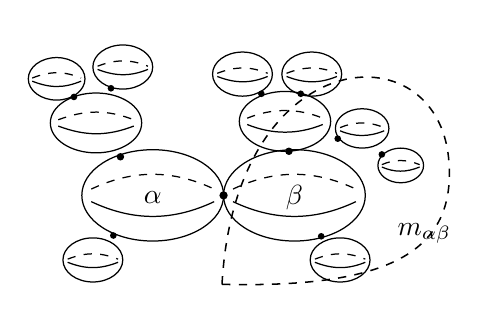
\begin{tikzpicture}[x=1cm,y=1cm,line width=0.45pt]
  \draw (-0.9,0) ellipse (0.9 and 0.58);
  \draw (0.9,0) ellipse (0.9 and 0.58);
  \draw[dashed] (-1.68,0.08) .. controls (-1.15,0.33) and (-0.65,0.33) .. (-0.12,0.08);
  \draw[dashed] (0.12,0.08) .. controls (0.65,0.33) and (1.15,0.33) .. (1.68,0.08);
  \draw (-1.68,-0.08) .. controls (-1.15,-0.33) and (-0.65,-0.33) .. (-0.12,-0.08);
  \draw (0.12,-0.08) .. controls (0.65,-0.33) and (1.15,-0.33) .. (1.68,-0.08);
  \node at (-0.9,-0.03) {$\alpha$};
  \node at (0.9,-0.03) {$\beta$};
  \fill (0,0) circle (1.5pt);

  \draw (-1.62,0.92) ellipse (0.58 and 0.38);
  \draw[dashed] (-2.1,0.96) .. controls (-1.75,1.09) and (-1.48,1.09) .. (-1.14,0.96);
  \draw (-2.1,0.88) .. controls (-1.75,0.75) and (-1.48,0.75) .. (-1.14,0.88);
  \fill (-1.31,0.49) circle (1.35pt);
  \draw (-2.12,1.48) ellipse (0.36 and 0.27);
  \draw[dashed] (-2.43,1.49) .. controls (-2.2,1.58) and (-2.03,1.58) .. (-1.81,1.49);
  \draw (-2.43,1.45) .. controls (-2.2,1.36) and (-2.03,1.36) .. (-1.81,1.45);
  \fill (-1.9,1.25) circle (1.2pt);
  \draw (-1.28,1.63) ellipse (0.38 and 0.28);
  \draw[dashed] (-1.6,1.64) .. controls (-1.37,1.73) and (-1.18,1.73) .. (-0.96,1.64);
  \draw (-1.6,1.60) .. controls (-1.37,1.51) and (-1.18,1.51) .. (-0.96,1.60);
  \fill (-1.43,1.36) circle (1.2pt);
  \draw (-1.66,-0.82) ellipse (0.38 and 0.28);
  \draw[dashed] (-1.98,-0.81) .. controls (-1.75,-0.72) and (-1.57,-0.72) .. (-1.34,-0.81);
  \draw (-1.98,-0.85) .. controls (-1.75,-0.94) and (-1.57,-0.94) .. (-1.34,-0.85);
  \fill (-1.4,-0.51) circle (1.2pt);

  \draw (0.78,0.94) ellipse (0.58 and 0.38);
  \draw[dashed] (0.3,0.98) .. controls (0.62,1.11) and (0.94,1.11) .. (1.26,0.98);
  \draw (0.3,0.90) .. controls (0.62,0.77) and (0.94,0.77) .. (1.26,0.90);
  \fill (0.83,0.56) circle (1.35pt);
  \draw (0.24,1.54) ellipse (0.38 and 0.28);
  \draw[dashed] (-0.08,1.55) .. controls (0.15,1.64) and (0.34,1.64) .. (0.56,1.55);
  \draw (-0.08,1.51) .. controls (0.15,1.42) and (0.34,1.42) .. (0.56,1.51);
  \fill (0.48,1.29) circle (1.2pt);
  \draw (1.12,1.54) ellipse (0.38 and 0.28);
  \draw[dashed] (0.8,1.55) .. controls (1.03,1.64) and (1.22,1.64) .. (1.44,1.55);
  \draw (0.8,1.51) .. controls (1.03,1.42) and (1.22,1.42) .. (1.44,1.51);
  \fill (0.98,1.29) circle (1.2pt);
  \draw (1.76,0.85) ellipse (0.34 and 0.25);
  \draw[dashed] (1.48,0.86) .. controls (1.67,0.94) and (1.84,0.94) .. (2.04,0.86);
  \draw (1.48,0.82) .. controls (1.67,0.74) and (1.84,0.74) .. (2.04,0.82);
  \fill (1.45,0.72) circle (1.2pt);
  \draw (2.25,0.38) ellipse (0.29 and 0.22);
  \draw[dashed] (2.01,0.39) .. controls (2.17,0.46) and (2.32,0.46) .. (2.49,0.39);
  \draw (2.01,0.36) .. controls (2.17,0.29) and (2.32,0.29) .. (2.49,0.36);
  \fill (2.01,0.52) circle (1.2pt);
  \draw (1.48,-0.82) ellipse (0.38 and 0.28);
  \draw[dashed] (1.16,-0.81) .. controls (1.39,-0.72) and (1.58,-0.72) .. (1.8,-0.81);
  \draw (1.16,-0.85) .. controls (1.39,-0.94) and (1.58,-0.94) .. (1.8,-0.85);
  \fill (1.24,-0.52) circle (1.2pt);

  \draw[dashed,line width=0.55pt]
    (-0.02,-1.13) .. controls (0.15,1.95) and (2.72,2.12) .. (2.86,0.45)
    .. controls (2.96,-0.72) and (2.1,-1.18) .. (-0.02,-1.13);
  \node at (2.55,-0.48) {$m_{\alpha\beta}$};
\end{tikzpicture}
\caption{\BookRecordIndex{T0340}稳定映射。}\label{fig:5-1-1}
\end{figure}

\begin{exercise}\label{ex:5-1-2}
\BookRecordIndex{T0178}加权树是配备\BookRecordIndex{T0291}权函数 $\mathrm w:T\to[0,\infty)$ 的\BookRecordIndex{T0084}带标号树 $(T,E,\Lambda)$。\BookRecordIndex{T0178}加权树的
总权是数
\[
  W(T):=\sum_{\alpha\in T}\mathrm w(\alpha).
\]
若每个满足 $\mathrm w(\alpha)=0$ 的顶点 $\alpha$ 都满足稳定性条件 (D.2.1)，则称\BookRecordIndex{T0178}加权树
$(T,E,\Lambda,\mathrm w)$ 稳定。利用引理 D.2.3 证明：对每棵至少有一条边的稳定加权
$n$-\BookRecordIndex{T0084}带标号树 $T$，边数满足
\[
  e(T)\le\frac{2W(T)}{\hbar}+n-3,
\]
其中 $\hbar$ 是其非零权的最小值。举例说明，当 $W(T)=0$ 时这个估计是尖锐的。特别地，
若 $\hbar$ 是命题~\ref{prop:4-1-4} 的常数，且 $(\mathbf u,\mathbf z)$ 是一个以 $T$ 为
模型、带 $n$ 个\BookRecordIndex{T0066}标记点的\BookRecordIndex{T0340}稳定映射，则
\begin{equation}\label{eq:5-1-2}
  e(T)\le\frac{2E(\mathbf u)}{\hbar}+n-3.
\end{equation}
\zhindex{jiaquanshu}{加权树}
\end{exercise}

\begin{exercise}\label{ex:5-1-3}
\begin{enumerate}[label=(\roman*),leftmargin=3em]
\item 证明：任意树 $T$ 的顶点 $\alpha_1,\ldots,\alpha_N$ 都可以适当排序，使得对每个
$i$，子集 $T_i:=\{\alpha_1,\ldots,\alpha_i\}$ 都是一棵树。证明任意顶点
$\alpha_1\in T$ 都可以选作这种排序的起点。
\item 给定 (i) 中的排序，证明对每个 $i\ge2$，都存在唯一指标 $j_i<i$，使
$\alpha_{j_i}E\alpha_i$。因此，一棵有 $N$ 个顶点的树可与整数向量
$\mathbf j=(j_2,\ldots,j_N)$ 等同，其中对每个 $i$ 都有 $1\le j_i<i$。
\item 令 $V_k:=\{i\mid j_i=k\}$，并注意对每个 $i\in V_k$ 都有 $k<i$。若 $k<i$，
证明 $\alpha_kE\alpha_i$ 当且仅当 $j_i=k$。
\end{enumerate}
\end{exercise}

\paragraph{\BookRecordIndex{T0413}重参数化群。}
\zhindex{chongcanshuhuaqun}{重参数化群}

\begin{definition}\label{def:5-1-4}
设\BookRecordIndex{T0340}稳定映射 $(\mathbf u,\mathbf z)$ 与 $(\widetilde{\mathbf u},\widetilde{\mathbf z})$ 分别以
\BookRecordIndex{T0084}带标号树 $(T,\Lambda)$ 与 $(\widetilde T,\widetilde\Lambda)$ 为模型。若存在\BookRecordIndex{T0304}树同构
$f:T\to\widetilde T$，以及函数
\[
  T\longrightarrow G=\operatorname{PSL}(2,\mathbb C),
  \qquad \alpha\longmapsto\phi_\alpha,
\]
即给每个顶点指定一个\BookRecordIndex{T0126}分式线性变换，使得
\begin{equation}\label{eq:5-1-3}
  \widetilde u_{f(\alpha)}\circ\phi_\alpha=u_\alpha,
  \qquad
  \widetilde z_{f(\alpha)f(\beta)}=\phi_\alpha(z_{\alpha\beta}),
  \qquad
  \widetilde z_i=\phi_{\alpha_i}(z_i),
\end{equation}
则称这两个\BookRecordIndex{T0340}稳定映射等价。由此可得，对每个 $\alpha\in T$，
$\Lambda_\alpha=\widetilde\Lambda_{f(\alpha)}$。
\end{definition}

对每棵\BookRecordIndex{T0084}带标号树 $T$，都有一个相应的群 $G_T$ 作用在以 $T$ 为模型的\BookRecordIndex{T0340}稳定映射集上，其轨道
空间就是相应的等价类集合。$G_T$ 的元素是元组
\[
  g=(f,\{\phi_\alpha\}_{\alpha\in T}),
\]
其中 $f$ 是满足
\[
  \Lambda_\alpha=\Lambda_{f(\alpha)}
\]
的 $T$ 的自同构，而对每个 $\alpha\in T$，$\phi_\alpha\in G$。所以在
$T=\widetilde T$ 的情形，$f$ 只能移动没有\BookRecordIndex{T0066}标记点的顶点 $\alpha$。群运算为
\[
  g'\cdot g
  =\left(f'\circ f,
    \{\phi'_{f(\alpha)}\circ\phi_\alpha\}_{\alpha\in T}\right).
\]
把 $f$ 看成给每个\BookRecordIndex{T0126}分式线性变换 $\phi_\alpha$ 指定靶球面的映射，并把
$\phi_\alpha$ 看成从二维球面 $\Sigma_\alpha$ 到 $\Sigma_{f(\alpha)}$ 的映射，会很有
帮助。群 $G_T$ 按
\[
  g\cdot(\mathbf u,\mathbf z)
  :=(\widetilde{\mathbf u},\widetilde{\mathbf z})
\]
作用在以 $T$ 为模型的\BookRecordIndex{T0340}稳定映射空间上，其中
$(\widetilde{\mathbf u},\widetilde{\mathbf z})$ 由式~\eqref{eq:5-1-3} 给出。显然，它的轨道
恰好定义以 $T$ 为模型的\BookRecordIndex{T0340}稳定映射的等价类。

定义~\ref{def:5-1-1} 中的稳定性条件保证每个\BookRecordIndex{T0340}稳定映射的\BookRecordIndex{T0342}稳定子群有限。通常这个\BookRecordIndex{T0342}稳定子群
是平凡的。不过，例如当 $T$ 有两个顶点 $\alpha,\beta$、没有标号且
$u_\alpha=u_\beta$ 时，它就是非平凡的。
\zhindex{wendingziqun}{稳定子群}

\begin{exercise}\label{ex:5-1-5}
群 $G_T$ 作用在以 $T$ 为模型的\BookRecordIndex{T0340}稳定映射的定义域 $\Sigma(\mathbf z)$ 所组成的集合上。
当 $T$ 是有五个顶点 $\alpha_1,\ldots,\alpha_5$、满足对 $i>1$ 有
$\alpha_1E\alpha_i$ 且没有标号的树时，描述这个作用的轨道。证明 $G_T$ 在这种定义域
$\Sigma(\mathbf z)$ 的集合上传递作用，当且仅当对每个 $\alpha$ 都有 $\#Z_\alpha\le3$。
\end{exercise}

\begin{exercise}\label{ex:5-1-6}
设 $T$ 是 $n$-\BookRecordIndex{T0084}带标号树，$(\mathbf u,\mathbf z)$ 是以 $T$ 为模型的\BookRecordIndex{T0340}稳定映射。证明
$G_T$ 的每个连通分支都有复维数 $3e(T)+3$。证明：当 $n+e(T)\le3$ 时，保持\BookRecordIndex{T0320}特殊点
（但不保持映射）的子群 $G_{T,\mathbf z}\subset G_T$ 的复维数为 $e(T)+3-n$；当
$n+e(T)\ge3$ 时，
\[
  e(T)+3-n\le\dim_{\mathbb C}G_{T,\mathbf z}\le2e(T).
\]
举例说明所有非负的可能值都会出现。
\end{exercise}

\paragraph{\BookRecordIndex{T0246}模空间。}
到 $M$ 的\BookRecordIndex{T0340}稳定映射构成范畴 $\mathcal{SC}_{0,n}(M;J)$ 的对象（字母
$\mathcal{SC}$ 可理解为“\BookRecordIndex{T0338}稳定范畴”）。从对象
$(\mathbf u,\mathbf z)\in\mathcal{SC}_{0,n}(M;J)$ 到
$(\widetilde{\mathbf u},\widetilde{\mathbf z})\in\mathcal{SC}_{0,n}(M;J)$ 的态射，是满足
定义~\ref{def:5-1-4} 中式~\eqref{eq:5-1-3} 的元组
$(f,\{\phi_\alpha\}_{\alpha\in T})$。因此，每个态射都是同构；两个\BookRecordIndex{T0340}稳定映射
$(\mathbf u,\mathbf z)$ 与 $(\widetilde{\mathbf u},\widetilde{\mathbf z})$ 等价，当且仅当
它们在范畴 $\mathcal{SC}_{0,n}(M;J)$ 中同构。定义~\ref{def:5-1-4} 的等价关系下，\BookRecordIndex{T0340}稳定映射
$(\mathbf u,\mathbf z)$ 的等价类记作 $[\mathbf u,\mathbf z]$。

现在固定球面同调类 $A\in H_2(M;\mathbb Z)$。若
$(\mathbf u,\mathbf z)\in\mathcal{SC}_{0,n}(M;J)$ 满足
\begin{equation}\label{eq:5-1-4}
  A=\sum_{\alpha\in T}u_{\alpha*}[S^2],
\end{equation}
则称它表示类 $A$。表示 $A$ 的\BookRecordIndex{T0340}稳定映射所组成的子范畴记作
\[
  \mathcal{SC}_{0,n}(M,A;J)
  :=\bigl\{(\mathbf u,\mathbf z)\in\mathcal{SC}_{0,n}(M;J)
  \bigm| \mathbf u\text{ 满足式~\eqref{eq:5-1-4}}\bigr\}.
\]
稍稍滥用逻辑学的标准约定，我们假装这些等价类构成一个集合，并把它记作
$\overline{\mathcal M}_{0,n}(M,A;J)$，或简记为
$\overline{\mathcal M}_{0,n}(A;J)$。（如附录 D.2 所述，若只考虑顶点取自某个给定集合的
树，这种说法就是完全严格的。）\BookRecordIndex{T0246}模空间 $\overline{\mathcal M}_{0,n}(M,A;J)$ 带有一个
称为\BookRecordIndex{T0142}格罗莫夫拓扑的自然拓扑。本章的目标是定义这一拓扑，并证明它使
$\overline{\mathcal M}_{0,n}(M,A;J)$ 成为紧且\BookRecordIndex{T0212}可度量化的空间。

\paragraph{\BookRecordIndex{T0072}层。}
对每棵\BookRecordIndex{T0084}带标号树 $T=(T,E,\Lambda)$ 与同调类 $A\in H_2(M;\mathbb Z)$，以
$\widetilde{\mathcal M}_{0,T}(M,A;J)$，或简记为
$\widetilde{\mathcal M}_{0,T}(A;J)$，表示所有以 $T$ 为模型且表示类 $A$ 的\BookRecordIndex{T0340}稳定映射所成的
空间。注意，$\widetilde{\mathcal M}_{0,T}(A;J)$ 是分别对应于 $A$ 的各种整同调类分解
\[
  A=\sum_{\alpha\in T}A_\alpha
\]
的子集之不交并。由命题~\ref{prop:4-1-5}，这些子集中只有有限多个非空。\BookRecordIndex{T0413}重参数化群 $G_T$
作用所得的商记作
\begin{equation}\label{eq:5-1-5}
  \mathcal M_{0,T}(M,A;J):=\mathcal M_{0,T}(A;J)
  :=\widetilde{\mathcal M}_{0,T}(A;J)/G_T.
\end{equation}
因此
\[
  \overline{\mathcal M}_{0,n}(A;J)
  =\bigcup_T\mathcal M_{0,T}(A;J),
\]
其中并取遍 $n$-\BookRecordIndex{T0084}带标号树的所有同构类。由练习~\ref{ex:5-1-2}，这个并中只有有限多个集合
非空。稍稍滥用术语，我们有时称 $\mathcal M_{0,T}(A;J)$ 为
$\overline{\mathcal M}_{0,n}(A;J)$ 的\BookRecordIndex{T0072}层；这并不表示
$\overline{\mathcal M}_{0,n}(A;J)$ 在严格意义下是分\BookRecordIndex{T0072}层空间。不过，第 6 章将证明：对一般的
与 $\omega$ \BookRecordIndex{T0348}相容的\BookRecordIndex{T0088}殆复结构 $J$，简单稳定元所成的子集
$\mathcal M^*_{0,T}(A;J)\subset\mathcal M_{0,T}(A;J)$ 是一个流形，相对于\BookRecordIndex{T0106}顶层的余维为
$2e(T)$。
\zhindex{ceng}{层}

与只有一个顶点的 $n$-\BookRecordIndex{T0084}带标号树 $T_n$ 对应的\BookRecordIndex{T0072}层称为\BookRecordIndex{T0106}顶层，记作
\[
  \mathcal M_{0,n}(A;J):=\mathcal M_{0,T_n}(A;J)
  =\widetilde{\mathcal M}_{0,n}(A;J)/G,
  \qquad
  \widetilde{\mathcal M}_{0,n}(A;J):=\widetilde{\mathcal M}_{0,T_n}(A;J).
\]
当 $A\ne0$ 且 $k=0,1$ 时，用第 3 章的术语，这些空间可描述为
\[
  \widetilde{\mathcal M}_{0,0}(A;J)=\mathcal M(A;J),
  \qquad
  \widetilde{\mathcal M}_{0,1}(A;J)=\mathcal M(A;J)\times S^2,
\]
以及
\[
  \mathcal M_{0,0}(A;J)=\mathcal M(A;J)/G,
  \qquad
  \mathcal M_{0,1}(A;J)=\mathcal M(A;J)\times_G S^2.
\]
当 $A=0$ 时，由于 $\widetilde{\mathcal M}_{0,k}(A;J)$ 中的元素还要满足稳定性条件，这些
恒等式不再成立。
\zhindex{dingceng}{顶层}

\personlater{geluomofu}{格罗莫夫}{Gromov}在 \srcite{160} 中引入了“\BookRecordIndex{T0181}尖点曲线”一词；它
对应于 $\overline{\mathcal M}_{0,0}(A;J)$ 中一个至少有两个分支的元素的像。\BookRecordIndex{T0181}尖点曲线可以
由定义域为任意\BookRecordIndex{T0191}节点黎曼曲面的映射来参数化。这个概念不如\BookRecordIndex{T0340}稳定映射精确，因为定义域的结构
丢失了。若目的仅仅是建立\BookRecordIndex{T0058}半正流形的\BookRecordIndex{T0143}格罗莫夫--威滕不变量的存在性，这一概念已经足够；但
不使用\BookRecordIndex{T0340}稳定映射，就无法看出这些不变量的完整结构（见第 7.5 节）。
\zhindex{jiandianquxian}{尖点曲线}

在代数几何中，人们用既约、不可约等词描述曲线。这里的重点仍是曲线的像，更确切地说，是
把曲线看成某些方程的解集。因此，每条曲线都是有限多个分支的并，每个分支还带有某个重数。
若曲线仅由一个重数为一的分支组成，就称它不可约；否则称它可约。若所有分支的重数都是一，
就称它既约。用我们的语言，一条曲线不可约，当且仅当它是某个单映射 $u:S^2\to M$ 的像。
\BookRecordIndex{T0176}既约曲线的概念也将很重要，因此我们引入\emph{\BookRecordIndex{T0184}简单稳定映射}
$(\mathbf u,\mathbf z)$：其中每个非常值分支 $u_\alpha$ 都是单映射，而且任意两个指标
$\alpha\ne\beta$ 的非常值映射之像 $\operatorname{im}u_\alpha$ 与
$\operatorname{im}u_\beta$ 都不重合。以 $T$ 为模型的\BookRecordIndex{T0184}简单稳定映射构成\BookRecordIndex{T0072}层
$\mathcal M_{0,T}(A;J)$ 的开子集 $\mathcal M^*_{0,T}(A;J)$，其性质将在第 6.2 节讨论。
显然，一条曲线在代数几何意义下既约，当且仅当它是一个\BookRecordIndex{T0184}简单稳定映射的像。最后要指出，
代数几何学家常用“\BookRecordIndex{T0386}有理曲线”表示亏格为零的曲线。

\begin{remark}[记号]\label{rem:5-1-7}
我们在一种语境中用字母 $\mathcal M$ 表示映射空间，在另一种语境中又用它表示映射等价类，
这多少有些不尽如人意。不过，两种用法都已约定俗成。许多论文（包括本书第一版）用类似
$\mathcal M(A;J)$ 的记号表示映射空间，而用 $\mathcal M_{0,n}(A;J)$ 与
$\overline{\mathcal M}_{0,n}(A;J)$ 表示\BookRecordIndex{T0340}稳定映射等价类的\BookRecordIndex{T0246}模空间也很常见。为了帮助读者
区分这两种记号，当 $\mathcal M(A;J)$ 表示映射空间时，我们绝不使用下标。此外，在需要
同时谈论这两类空间的场合，我们用 $\widetilde{\mathcal M}_{0,0}(A;J)$，而不用
$\mathcal M(A;J)$，表示 $J$-全纯球面空间。需要提醒读者，许多其他作者直接把
$\overline{\mathcal M}_{0,n}(A;J)$ 的元素 $[\mathbf u,\mathbf z]$ 称为\BookRecordIndex{T0340}稳定映射，而不再
明说这些元素是等价类。
\end{remark}

\paragraph{\BookRecordIndex{T0339}稳定曲线。}
若靶空间 $M$ 是一点，则
\[
  \overline{\mathcal M}_{0,n}
  :=\overline{\mathcal M}_{0,n}(\{\mathrm{pt}\},0;J)
\]
是带 $n$ 个\BookRecordIndex{T0066}标记点的亏格零\BookRecordIndex{T0339}稳定曲线的 Grothendieck--Knudsen \BookRecordIndex{T0246}模空间。附录 D 将详细讨论
这个\BookRecordIndex{T0246}模空间。它是复维数 $n-3$ 的光滑代数流形，并可写成各\BookRecordIndex{T0072}层的不交并
\[
  \overline{\mathcal M}_{0,n}=\coprod_T\mathcal M_{0,T},
\]
其中 $T$ 取遍稳定 $n$-\BookRecordIndex{T0084}带标号树的所有同构类。开\BookRecordIndex{T0072}层 $\mathcal M_{0,n}$ 由 $S^2$ 中 $n$ 个
互异\BookRecordIndex{T0066}标记点的所有构型对 $G=\operatorname{PSL}(2,\mathbb C)$ 的作用取商得到。每一\BookRecordIndex{T0072}层
$\mathcal M_{0,T}$ 的闭包 $\overline{\mathcal M}_{0,T}$ 都是
$\overline{\mathcal M}_{0,n}$ 中复余维为 $e(T)$ 的光滑子流形，而且任意两个这样的子流形
都\BookRecordIndex{T0136}干净相交（交集是子流形，交集的切空间等于二者切空间之交）。此外，子流形
$\overline{\mathcal M}_{0,T}$ 加性生成 $\overline{\mathcal M}_{0,n}$ 的上同调
\srcite{208}。\BookRecordIndex{T0246}模空间 $\overline{\mathcal M}_{0,3}$ 是一点，
$\overline{\mathcal M}_{0,4}$ 微分同胚于二维球面，而 $\overline{\mathcal M}_{0,5}$ 微分
同胚于 $S^2\times S^2$ 沿对角线上的三个点吹起所得的空间；见附录 D.7。

附录 D 说明了如何把 Grothendieck--Knudsen \BookRecordIndex{T0246}模空间 $\overline{\mathcal M}_{0,n}$ 嵌入若干
二维球面的乘积。在开\BookRecordIndex{T0072}层 $\mathcal M_{0,n}$ 上，这个嵌入由\BookRecordIndex{T0185}交比
\[
  w(z_i,z_j,z_k,z_\ell)
  =\frac{(z_j-z_k)(z_\ell-z_i)}{(z_i-z_j)(z_k-z_\ell)}
  \in\mathbb C\cup\{\infty\}
\]
给出。只要 $z_i,z_j,z_k,z_\ell$ 中没有三个相等，这个定义仍有意义，而且得到一个在 $G$
作用下不变的映射。例如，由于 $w(0,1,\infty,z)=z$，\BookRecordIndex{T0185}交比给出自然微分同胚
$\overline{\mathcal M}_{0,4}\to S^2$。附录 D.4 把\BookRecordIndex{T0185}交比延拓为函数
\[
  w_{ijk\ell}:\overline{\mathcal M}_{0,n}\longrightarrow S^2,
\]
具体如下。对每个顶点 $\alpha\in T$ 与每个指标 $i\in\{1,\ldots,n\}$，定义
$z_{\alpha i}\in S^2$ 为 $\alpha$-球面上指向\BookRecordIndex{T0066}标记点 $z_i$ 的元素，即
\begin{equation}\label{eq:5-1-6}
  z_{\alpha i}:=
  \begin{cases}
    z_i, & \alpha_i=\alpha,\\
    z_{\alpha\beta}, & \alpha_i\in T_{\alpha\beta}.
  \end{cases}
\end{equation}
对任意四个指标 $i,j,k,\ell$，都存在顶点 $\alpha$，使得
$z_{\alpha i},z_{\alpha j},z_{\alpha k},z_{\alpha\ell}$ 中没有三个相等；而且所得\BookRecordIndex{T0185}交比与这类
顶点 $\alpha$ 的选择无关。可以把得到的函数 $w_{ijk\ell}$ 看成遗忘除
$i,j,k,\ell$ 所标号者以外全部\BookRecordIndex{T0066}标记点的\BookRecordIndex{T0377}遗忘映射
$\overline{\mathcal M}_{0,n}\to S^2:=\overline{\mathcal M}_{0,4}$。这些函数给出上述嵌入，
也可以用来定义 $\overline{\mathcal M}_{0,n}$ 上的拓扑（见附录 D.5）。此外，每一\BookRecordIndex{T0072}层
$\mathcal M_{0,T}$ 的闭包 $\overline{\mathcal M}_{0,T}$ 映到一个复余维为 $e(T)$ 的复
子流形上，而 $\mathcal M_{0,n}$ 在 $\overline{\mathcal M}_{0,n}$ 中开且稠密。因此，
$\overline{\mathcal M}_{0,n}$ 的确是 $\mathcal M_{0,n}$ 的自然紧化。

\paragraph{\BookRecordIndex{T0377}遗忘映射。}
当 $n\ge3$ 时，有\BookRecordIndex{T0377}遗忘映射
\[
  \pi:\overline{\mathcal M}_{0,n}(A;J)\longrightarrow\overline{\mathcal M}_{0,n}.
\]
它的定义需要稍加小心。删去映射 $u_\alpha$ 后，得到元组
\[
  \mathbf z:=\bigl(\{z_{\alpha\beta}\}_{\alpha E\beta},
  \{\alpha_i,z_i\}_{1\le i\le n}\bigr),
\]
可把它看成一条以\BookRecordIndex{T0084}带标号树 $T$ 为模型、有\BookRecordIndex{T0191}节点且带 $n$ 个\BookRecordIndex{T0066}标记点的亏格零曲线。一般而言，
这条曲线不再稳定；不过，压缩只有一或两个\BookRecordIndex{T0320}特殊点的每个顶点（分支），并相应地显然调整
$T$ 上的关系 $E$，便可把它唯一约化为一条\BookRecordIndex{T0339}稳定曲线
\sourcefootnote{原书此处写成压缩只有一或两个“\BookRecordIndex{T0066}标记点”的顶点；但定义~\ref{def:5-1-1}
中的稳定性由\BookRecordIndex{T0320}特殊点数决定，而\BookRecordIndex{T0320}特殊点包括\BookRecordIndex{T0191}节点与\BookRecordIndex{T0066}标记点，故改作“\BookRecordIndex{T0320}特殊点”。}。所得\BookRecordIndex{T0339}稳定曲线
记作 $\mathbf z^s$，并定义
\[
  \pi([\mathbf u,\mathbf z]):=[\mathbf z^s].
\]
也可用\BookRecordIndex{T0185}交比给出\BookRecordIndex{T0377}遗忘映射的另一定义。式~\eqref{eq:5-1-6} 和 $w_{ijk\ell}$ 的定义不仅适用于
\BookRecordIndex{T0339}稳定曲线，也适用于\BookRecordIndex{T0340}稳定映射。因此，\BookRecordIndex{T0185}交比定义了一个从
$\overline{\mathcal M}_{0,n}(A;J)$ 到若干二维球面之乘积的映射；它等于 $\pi$ 与
$\overline{\mathcal M}_{0,n}$ 到同一乘积的嵌入之复合。第~\ref{sec:5-6} 节将证明，\BookRecordIndex{T0377}遗忘
映射 $\pi$ 关于\BookRecordIndex{T0142}格罗莫夫拓扑连续。注意，当 $n<3$ 时 $\overline{\mathcal M}_{0,n}$ 为空，
故 $\pi$ 在这种情形下没有定义。

\begin{exercise}\label{ex:5-1-8}
证明存在压缩映射
\[
  [T,\Lambda]\longmapsto[T^s,\Lambda^s],
\]
它把预稳定树的每个同构类 $[T,\Lambda]$ 映到稳定树的一个同构类
$[T^s,\Lambda^s]$。通过删去不稳定顶点构造这个映射。若
$[\mathbf u,\mathbf z]$ 以 $(T,\Lambda)$ 为模型，证明
$\pi([\mathbf u,\mathbf z])$ 以 $(T^s,\Lambda^s)$ 为模型。
\end{exercise}

\begin{exercise}\label{ex:5-1-9}
定义遗忘最后一个\BookRecordIndex{T0066}标记点的映射
\[
  \overline{\mathcal M}_{0,n}(A;J)
  \longrightarrow\overline{\mathcal M}_{0,n-1}(A;J),
\]
并说明它在树的\BookRecordIndex{T0072}层面上如何作用（见附录 D.6 中对\BookRecordIndex{T0377}遗忘映射 (D.6.1) 的讨论）。比较这个映射与
\BookRecordIndex{T0377}遗忘映射 $\overline{\mathcal M}_{0,n}(A;J)\to\overline{\mathcal M}_{0,n}$，找出只被其中一个
映射压缩而不被另一个压缩的分支实例。是否存在同时被两个映射压缩的分支？证明显然的交换图
确实交换。
\end{exercise}

\begin{exercise}\label{ex:5-1-10}
对 $0\le n\le3$，描述\BookRecordIndex{T0246}模空间
$\overline{\mathcal M}_{0,n}(\mathbb{CP}^1,2L;J_0)$，其中
$L=[\mathbb{CP}^1]$，$J_0$ 是标准复结构（参见 \srcite{268}）。
\end{exercise}

\begin{exercise}\label{ex:5-1-11}
对每个 $i\in\{1,\ldots,n\}$，都有\BookRecordIndex{T0283}求值映射
\[
  \operatorname{ev}_i:\overline{\mathcal M}_{0,n}(M,A;J)\longrightarrow M,
\]
定义为
\begin{equation}\label{eq:5-1-7}
  \operatorname{ev}_i([\mathbf u,\mathbf z])=u_{\alpha_i}(z_i),
  \qquad [\mathbf u,\mathbf z]\in\overline{\mathcal M}_{0,n}(M,A;J).
\end{equation}
证明这个映射是良定义的；也就是说，若 $(\mathbf u,\mathbf z)$ 与
$(\widetilde{\mathbf u},\widetilde{\mathbf z})$ 等价，则
$u_{\alpha_i}(z_i)=\widetilde u_{\widetilde\alpha_i}(\widetilde z_i)$。利用第~\ref{sec:5-6} 节
中\BookRecordIndex{T0142}格罗莫夫拓扑的定义与性质证明 $\operatorname{ev}_i$ 连续。
\end{exercise}


\section{\BookRecordIndex{T0141}格罗莫夫收敛}\label{sec:5-2}
\zhindex{geluomofushoulian}{格罗莫夫收敛}

在本章其余部分，我们将发展\BookRecordIndex{T0340}稳定映射列\BookRecordIndex{T0141}格罗莫夫收敛的概念。它是第 D.5 节中\BookRecordIndex{T0339}稳定曲线
相应概念的细化；\BookRecordIndex{T0339}稳定曲线的情形不涉及分析，因而简单得多。

下面正式定义一列 $J^\nu$-全纯曲线 $u^\nu:S^2\to M$ 收敛到\BookRecordIndex{T0340}稳定映射
$(\mathbf u,\mathbf z)\in\mathcal{SC}_{0,n}(M;J)$ 的含义。回顾第 D.1 节：若映射列
$v^\nu:S^2\to M$ 在 $S^2\setminus X$ 的每个紧子集上按 $C^\infty$ 拓扑收敛到
$v:S^2\to M$，就称它在 $S^2\setminus X$ 上\emph{\BookRecordIndex{T0416}逐紧一致收敛}（u.c.s.）。还要回顾
定义~\ref{def:5-1-1} 中的记号
\[
  Z_\alpha:=\{z_{\alpha\beta}\mid \alpha E\beta\},
  \qquad
  Y_\alpha:=Z_\alpha\cup\{z_i\mid \alpha_i=\alpha\}.
\]

\begin{definition}[\BookRecordIndex{T0141}格罗莫夫收敛]\label{def:5-2-1}
设 $J^\nu$ 是 $M$ 上一列被 $\omega$ \BookRecordIndex{T0372}驯服的\BookRecordIndex{T0088}殆复结构，它在 $C^\infty$ 拓扑下收敛到
$J\in\mathcal J_\tau(M,\omega)$；设
\[
  (\mathbf u,\mathbf z)
  =\bigl(\{u_\alpha\}_{\alpha\in T},
    \{z_{\alpha\beta}\}_{\alpha E\beta},
    \{\alpha_i,z_i\}_{1\le i\le n}\bigr)
  \in\mathcal{SC}_{0,n}(M;J)
\]
是一个\BookRecordIndex{T0340}稳定映射；又设 $u^\nu:S^2\to M$ 是一列带有 $n$ 个两两不同\BookRecordIndex{T0066}标记点
$z_1^\nu,\ldots,z_n^\nu\in S^2$ 的 $J^\nu$-全纯映射。若存在一族 \BookRecordIndex{T0040}Möbius 变换
\[
  \{\phi_\alpha^\nu\}_{\alpha\in T,\,\nu\in\mathbb N},
\]
使下列条件成立，就称映射列
$(u^\nu,\mathbf z^\nu):=(u^\nu,z_1^\nu,\ldots,z_n^\nu)$
\emph{\BookRecordIndex{T0141}格罗莫夫收敛}到 $(\mathbf u,\mathbf z)$。

\medskip
\noindent\textup{（映射）}
对每个 $\alpha\in T$，映射列
\[
  u_\alpha^\nu:=u^\nu\circ\phi_\alpha^\nu:S^2\to M
\]
在 $S^2\setminus Z_\alpha$ 上\BookRecordIndex{T0416}逐紧一致收敛到 $u_\alpha$。

\medskip
\noindent\textup{（能量）}
若 $\alpha E\beta$，且 $m_{\alpha\beta}(\mathbf u)$ 由式~\eqref{eq:5-1-1} 定义，则
\begin{equation}\label{eq:5-2-1}
  m_{\alpha\beta}(\mathbf u)
  =\lim_{\varepsilon\to0}\lim_{\nu\to\infty}
  E\bigl(u_\alpha^\nu;B_\varepsilon(z_{\alpha\beta})\bigr).
\end{equation}

\medskip
\noindent\textup{（重标度）}
若 $\alpha E\beta$，则映射列
\[
  \phi_{\alpha\beta}^\nu
  :=(\phi_\alpha^\nu)^{-1}\circ\phi_\beta^\nu
\]
在 $S^2\setminus\{z_{\beta\alpha}\}$ 上\BookRecordIndex{T0416}逐紧一致收敛到 $z_{\alpha\beta}$。

\medskip
\noindent\textup{（\BookRecordIndex{T0066}标记点）}
对 $i=1,\ldots,n$，有
\[
  z_i=\lim_{\nu\to\infty}
  (\phi_{\alpha_i}^\nu)^{-1}(z_i^\nu).
\]
\end{definition}

这个定义既复杂又重要，值得花些篇幅解释。理解它的一处困难在于，原映射列 $u^\nu$
除了出现在复合
\[
  u_\alpha^\nu:=u^\nu\circ\phi_\alpha^\nu
\]
中以外，并不显式出现；这是因为我们只关心它在群 $G$ 的作用模掉之后的极限行为。
因此，最好从某个顶点 $\alpha$ 的视角观察收敛。（映射）公理说明，$u_\alpha^\nu$
在 $S^2\setminus Z_\alpha$ 的所有紧子集
$S^2\setminus B_\varepsilon(Z_\alpha)$ 上收敛。进一步，对每个与 $\alpha$ 相邻的顶点
$\beta$，相应映射 $u_\beta^\nu$ 是 $u_\alpha^\nu$ 的重标度，含义如下。

所谓一个\emph{以 $x$ 为源、以 $y$ 为靶的 $S^2$ 重标度}，是指一列\BookRecordIndex{T0126}分式线性变换
$\phi^\nu\in G$，它在 $S^2\setminus\{x\}$ 上\BookRecordIndex{T0416}逐紧一致收敛到 $y$。设
$\phi_i^\nu$ 对 $i=0,1$ 分别是以 $x_i$ 为源、以 $y_i$ 为靶的重标度列。若
$y_0\ne x_1$，则复合 $\phi_1^\nu\circ\phi_0^\nu$ 是以 $x_0$ 为源、以 $y_1$
为靶的重标度列。此外，由习题 D.1.3，以 $x$ 为源、以 $y$ 为靶的 $S^2$ 重标度列之逆，
是以 $y$ 为源、以 $x$ 为靶的重标度列。用这一术语，（重标度）公理说明
$\phi_{\alpha\beta}^\nu$ 是以 $z_{\beta\alpha}$ 为源、以 $z_{\alpha\beta}$ 为靶的
重标度列。由于当 $\alpha\ne\gamma$ 时
$z_{\beta\alpha}\ne z_{\beta\gamma}$，复合
\[
  \phi_{\alpha\gamma}^\nu
  =\phi_{\alpha\beta}^\nu\circ\phi_{\beta\gamma}^\nu
\]
也是一个重标度列，其源为 $z_{\gamma\beta}$、靶为 $z_{\alpha\beta}$。\BookRecordIndex{T0411}重标度后的映射列
\[
  u_\beta^\nu=u_\alpha^\nu\circ\phi_{\alpha\beta}^\nu
\]
在 $S^2\setminus B_\varepsilon(Z_\beta)$ 的紧子集上收敛。它从
$u_\alpha^\nu$ 在\BookRecordIndex{T0243}冒泡点 $z_{\alpha\beta}$ 的小邻域
\[
  \phi_{\alpha\beta}^\nu
  \bigl(S^2\setminus B_\varepsilon(z_{\beta\alpha})\bigr)
\]
中截取出一部分并将其“放大”。类似地，从 $\beta$-\BookRecordIndex{T0275}气泡的视角观察 $\alpha$-\BookRecordIndex{T0275}气泡时，
$u_\alpha^\nu$ 是 $u_\beta^\nu$ 在 $z_{\beta\alpha}$ 的小邻域
\[
  \phi_{\beta\alpha}^\nu
  \bigl(S^2\setminus B_\varepsilon(z_{\alpha\beta})\bigr)
\]
中那一部分的放大。

（\BookRecordIndex{T0066}标记点）公理说明\BookRecordIndex{T0066}标记点收敛，而（能量）公理说明没有能量损失。为解释后一条件的
重要性，定义映射列 $v^\nu:S^2\to M$ 在点 $z$ 处的\emph{\BookRecordIndex{T0276}气泡能量}为极限
\[
  E(\{v^\nu\};z)
  :=\lim_{\varepsilon\to0}\lim_{\nu\to\infty}
  E\bigl(v^\nu;B_\varepsilon(z)\bigr).
\]
每当使用\BookRecordIndex{T0276}气泡能量时，我们都假设右端极限存在，并且对某个 $\varepsilon>0$，映射列
$v^\nu$ 在 $B_\varepsilon(z)\setminus\{z\}$ 上\BookRecordIndex{T0416}逐紧一致收敛。在这种情形下，称
$v^\nu$ \emph{在 $z$ 处伴随\BookRecordIndex{T0243}冒泡收敛}。依此术语，（能量）公理断言：映射列
$u_\alpha^\nu$ 在 $z_{\alpha\beta}$ 处的\BookRecordIndex{T0276}气泡能量，等于极限\BookRecordIndex{T0340}稳定映射
$(\mathbf u,\mathbf z)$ 在从 $\alpha$ 指向 $\beta$ 的边所分离出的那部分树上的能量
$m_{\alpha\beta}(\mathbf u)$。这意味着重标度的选取没有损失能量。特别地，若
$m_{\alpha\beta}(\mathbf u)>0$，则映射列
\[
  \psi^\nu:=\phi_{\alpha\beta}^\nu
\]
满足命题~\ref{prop:4-7-2} 的要求，其中
\[
  u^\nu=u_\alpha^\nu,
  \qquad v^\nu=u_\beta^\nu,
  \qquad z_0:=z_{\alpha\beta},
  \qquad z_\infty:=z_{\beta\alpha}.
\]

定义~\ref{def:5-2-1} 的（能量）公理蕴含命题~\ref{prop:4-7-1} 的假设 (b)。因此，
它包含了相邻顶点 $\alpha,\beta$ 所对应的\BookRecordIndex{T0275}气泡彼此相连这一信息。于是，只要建立这种形式
的能量估计，就能证明格罗莫夫极限是连通的。

后面的各节将证明：极限在等价意义下唯一，而且每一列能量一致有界的
$J^\nu$-全纯球面 $u^\nu$ 都有一个在定义~\ref{def:5-2-1} 意义下收敛的子列。
作为开端，我们先\BookRecordIndex{T0326}推出\BookRecordIndex{T0139}格罗莫夫紧性的几个并非完全直接的后果。例如，若
$x^\nu\in u^\nu(S^2)$ 收敛，则其极限落在极限曲线的像中；同伦类在\BookRecordIndex{T0141}格罗莫夫收敛下
也保持不变。注意，下述 (iii) 中的点 $z_{\alpha i}$ 由式~\eqref{eq:5-1-6} 定义。
此外，(iv) 关于\BookRecordIndex{T0185}交比 $w_{ijk\ell}$ 的断言说明：\BookRecordIndex{T0141}格罗莫夫收敛列在\BookRecordIndex{T0377}遗忘映射下的像，
在\BookRecordIndex{T0339}稳定曲线\BookRecordIndex{T0246}模空间中收敛（见附录 D）。

\begin{theorem}\label{thm:5-2-2}
设 $(u^\nu,\mathbf z^\nu)$ 如定义~\ref{def:5-2-1} 所述，\BookRecordIndex{T0141}格罗莫夫收敛到\BookRecordIndex{T0340}稳定映射
$(\mathbf u,\mathbf z)$。则：
\begin{enumerate}[label=(\roman*),leftmargin=3em]
\item 若 $x^\nu\in u^\nu(S^2)$ 收敛到 $x\in M$，则对某个 $\alpha\in T$，有
$x\in u_\alpha(S^2)$；
\item 当 $\nu$ 充分大时，映射 $u^\nu:S^2\to M$ 与\BookRecordIndex{T0227}连通和
$\#_{\alpha\in T}u_\alpha$ 同伦；
\item 对每个 $\alpha\in T$ 和每个 $i$，
\[
  z_{\alpha i}=\lim_{\nu\to\infty}
  (\phi_\alpha^\nu)^{-1}(z_i^\nu);
\]
\item 对所有 $i,j,k,\ell$，
\[
  w_{ijk\ell}(\mathbf z)
  =\lim_{\nu\to\infty}w_{ijk\ell}(\mathbf z^\nu).
\]
\end{enumerate}
\end{theorem}

\begin{proof}
先证 (i)。设 $x^\nu=u^\nu(z^\nu)$ 收敛到 $x$。必要时取子列，不失一般性，可假设
对每个 $\alpha$，点列 $(\phi_\alpha^\nu)^{-1}(z^\nu)$ 都收敛到某个
$z_\alpha\in S^2$。若存在 $\alpha\in T$，使得对每个满足 $\alpha E\beta$ 的
$\beta\in T$ 都有 $z_\alpha\ne z_{\alpha\beta}$，则
\[
  x=\lim_{\nu\to\infty}u^\nu(z^\nu)
   =\lim_{\nu\to\infty}
    u_\alpha^\nu\bigl((\phi_\alpha^\nu)^{-1}(z^\nu)\bigr)
   =u_\alpha(z_\alpha),
\]
结论成立。

若不存在这样的 $\alpha$，我们断言树 $T$ 中存在一条边 $\alpha E\beta$，使得
\begin{equation}\label{eq:5-2-2}
  z_\alpha=z_{\alpha\beta},
  \qquad z_\beta=z_{\beta\alpha}.
\end{equation}
事实上，从任意顶点 $\alpha_0$ 出发，存在唯一的顶点列
$\alpha_0,\alpha_1,\alpha_2,\ldots$，使得
\[
  \alpha_iE\alpha_{i+1},
  \qquad z_{\alpha_i}=z_{\alpha_i\alpha_{i+1}}.
\]
必有某个 $j$ 满足 $\alpha_j=\alpha_{j+2}$，否则这些 $\alpha_i$ 将构成两两不同顶点的
无限序列。于是 $\alpha=\alpha_j$ 与 $\beta=\alpha_{j+1}$ 满足
式~\eqref{eq:5-2-2}。

若 $m_{\alpha\beta}(\mathbf u)=0$，则由式~\eqref{eq:5-2-1} 和
定理~\ref{thm:4-6-1}，映射列 $u_\alpha^\nu$ 在 $z_{\alpha\beta}$ 的一个邻域上一致
收敛到 $u_\alpha$。故仍有
\[
  x=\lim_{\nu\to\infty}u^\nu(z^\nu)=u_\alpha(z_{\alpha\beta}).
\]
若 $m_{\alpha\beta}(\mathbf u)\ne0$，则命题~\ref{prop:4-7-2} 可用于映射列
$u_\alpha^\nu$，其中
\[
  u:=u_\alpha,
  \qquad v:=u_\beta,
  \qquad z_0:=z_{\alpha\beta},
  \qquad z_\infty:=z_{\beta\alpha},
  \qquad \psi^\nu:=\phi_{\alpha\beta}^\nu.
\]
由式~\eqref{eq:5-2-2}，$z_0=z_\alpha$ 且 $z_\infty=z_\beta$，所以
\[
  z_0=\lim_{\nu\to\infty}\zeta^\nu,
  \qquad
  z_\infty=\lim_{\nu\to\infty}(\psi^\nu)^{-1}(\zeta^\nu),
  \qquad
  \zeta^\nu:=(\phi_\alpha^\nu)^{-1}(z^\nu).
\]
命题~\ref{prop:4-7-2} 因而说明
$u^\nu(z^\nu)=u_\alpha^\nu(\zeta^\nu)$ 收敛到
$u(z_0)=v(z_\infty)$
\sourcefootnote{原书此处写作 $u(z_0)=v(\infty)$；但本段已定义
$z_\infty:=z_{\beta\alpha}$，命题~\ref{prop:4-7-2} 的坐标不变结论及紧接着的
$u_\beta(z_{\beta\alpha})$ 都唯一要求此处为 $v(z_\infty)$。}。于是
\[
  x=\lim_{\nu\to\infty}u^\nu(z^\nu)
   =u_\alpha(z_{\alpha\beta})
   =u_\beta(z_{\beta\alpha}),
\]
这就证明了 (i)。

下面证明 (ii)。固定一条边 $\alpha E\beta$。对小于 $2$-球直径的 $r>0$ 和
$\nu\in\mathbb N$，定义
\[
  \begin{aligned}
  A_r^\nu(\alpha,\beta)
  &:=\phi_\alpha^\nu\bigl(B_r(z_{\alpha\beta})\bigr)
    \cap\phi_\beta^\nu\bigl(B_r(z_{\beta\alpha})\bigr)\\
  &=\bigl\{z\in S^2\bigm|
    d\bigl((\phi_\alpha^\nu)^{-1}(z),z_{\alpha\beta}\bigr)<r,\ 
    d\bigl((\phi_\beta^\nu)^{-1}(z),z_{\beta\alpha}\bigr)<r\bigr\}.
  \end{aligned}
\]
因为 $\phi_{\beta\alpha}^\nu$ 在 $S^2\setminus\{z_{\alpha\beta}\}$ 上\BookRecordIndex{T0416}逐紧一致收敛到
$z_{\beta\alpha}$，只要 $\nu\ge\nu_0(r)$ 充分大，像
\[
  \phi_{\beta\alpha}^\nu
  \bigl(S^2\setminus B_r(z_{\alpha\beta})\bigr)
\]
就是 $B_r(z_{\beta\alpha})$ 中的一个小圆盘。因此，当 $\nu\ge\nu_0(r)$ 时，集合
$A_r^\nu(\alpha,\beta)$ 与
\[
  \phi_{\beta\alpha}^\nu\bigl(B_r(z_{\alpha\beta})\bigr)
  \cap B_r(z_{\beta\alpha})
\]
微分同胚，从而是一个\BookRecordIndex{T0170}环域。我们将证明：对每个 $\varepsilon>0$，都存在常数
$r>0$ 和 $\nu_0\in\mathbb N$，使得
\begin{equation}\label{eq:5-2-3}
  \nu\ge\nu_0
  \quad\Longrightarrow\quad
  \sup_{z\in A_r^\nu(\alpha,\beta)}
  d\bigl(u^\nu(z),u_\alpha(z_{\alpha\beta})\bigr)<\varepsilon.
\end{equation}

先设 $m_{\alpha\beta}(\mathbf u)=0$。此时在 $z_{\alpha\beta}$ 处没有\BookRecordIndex{T0243}冒泡，所以
$u_\alpha^\nu$ 在 $z_{\alpha\beta}$ 的一个邻域上一致收敛到 $u_\alpha$。给定
$\varepsilon>0$，取充分小的 $r>0$，使得对
$\zeta\in B_r(z_{\alpha\beta})$ 有
\[
  d\bigl(u_\alpha(\zeta),u_\alpha(z_{\alpha\beta})\bigr)<\varepsilon/2,
\]
并且 $u_\alpha^\nu$ 在 $B_r(z_{\alpha\beta})$ 上一致收敛到 $u_\alpha$。再取
$\nu_0$，使得当 $\zeta\in B_r(z_{\alpha\beta})$ 且 $\nu\ge\nu_0$ 时，
\[
  d\bigl(u_\alpha^\nu(\zeta),u_\alpha(\zeta)\bigr)<\varepsilon/2.
\]
由三角不等式，式~\eqref{eq:5-2-3} 成立。

再设 $m_{\alpha\beta}(\mathbf u)>0$。命题~\ref{prop:4-7-2} 可用于映射列
$u^\nu:=u_\alpha^\nu$、
$\psi^\nu:=\phi_{\alpha\beta}^\nu$
\sourcefootnote{原书此处写作 $\psi^\nu:=\phi_{\beta\alpha}^\nu$；但按
$\phi_{\alpha\beta}^\nu=(\phi_\alpha^\nu)^{-1}\circ\phi_\beta^\nu$，只有取
$\psi^\nu=\phi_{\alpha\beta}^\nu$ 才同时满足
$u_\beta^\nu=u_\alpha^\nu\circ\psi^\nu$，并使下文
$(\psi^\nu)^{-1}((\phi_\alpha^\nu)^{-1}(z))
=(\phi_\beta^\nu)^{-1}(z)$。原书的反向次序不能\BookRecordIndex{T0326}推出所需距离估计。}，映射
$u:=u_\alpha$，以及点 $z_0:=z_{\alpha\beta}$、$z_\infty:=z_{\beta\alpha}$。
给定 $\varepsilon>0$，按命题~\ref{prop:4-7-2} 选取 $\delta>0$ 和 $\nu_0$，并令
$r:=\delta/2$。若 $\nu\ge\nu_0$、$z\in A_r^\nu(\alpha,\beta)$，且
$\zeta:=(\phi_\alpha^\nu)^{-1}(z)$，则
\[
  d(\zeta,z_0)+d\bigl((\psi^\nu)^{-1}(\zeta),z_\infty\bigr)<2r=\delta.
\]
由于 $z_0=z_{\alpha\beta}$，这里的中心值应为
$u_\alpha(z_{\alpha\beta})$
\sourcefootnote{原书此处把\BookRecordIndex{T0191}节点写成不存在的 $u_{\alpha\beta}$，从而出现
$u_\alpha(u_{\alpha\beta})$；由本段定义 $z_0:=z_{\alpha\beta}$ 以及
命题~\ref{prop:4-7-2} 的结论，唯一有类型的表达式是
$u_\alpha(z_{\alpha\beta})$。}，因而
\[
  d\bigl(u^\nu(z),u_\alpha(z_{\alpha\beta})\bigr)
  =d\bigl(u_\alpha^\nu(\zeta),u_\alpha(z_0)\bigr)<\varepsilon.
\]
式~\eqref{eq:5-2-3} 得证。

现在选取小于 $M$ 的\BookRecordIndex{T0093}单射半径一半的 $\varepsilon>0$，并固定使
式~\eqref{eq:5-2-3} 成立的 $r>0$ 与 $\nu_0\in\mathbb N$。必要时缩小 $r$，可以假设
对每个 $\alpha$，所有满足 $\alpha E\beta$ 的闭圆盘
$\overline B_r(z_{\alpha\beta})$ 两两不交。定义
\[
  S_\alpha:=S^2\setminus
  \bigcup_{\alpha E\beta}\overline B_r(z_{\alpha\beta}).
\]
对每条边 $\alpha E\beta$，用一个标准\BookRecordIndex{T0170}环域
$A_{\alpha\beta}\cong[0,1]\times S^1$ 连接
$\partial B_r(z_{\alpha\beta})\subset S_\alpha$ 与
$\partial B_r(z_{\beta\alpha})\subset S_\beta$，从而构造曲面 $\Sigma_r$。于是，
$A_{\alpha\beta}$ 中每条弧 $[0,1]\times e^{i\theta}$ 都把
$\partial B_r(z_{\alpha\beta})\subset S_\alpha$ 中的一点连接到
$\partial B_r(z_{\beta\alpha})\subset S_\beta$ 中的一点。曲面 $\Sigma_r$ 与 $S^2$
同胚。定义 $u_r:\Sigma_r\to M$，使
\[
  u_r|_{S_\alpha}:=u_\alpha,
\]
并在每个\BookRecordIndex{T0170}环域上，用连接两侧边界对应点之给定像的唯一极短测地线定义 $u_r$。
对 $\nu\ge\nu_0$，类似地定义 $u_r^\nu:\Sigma_r\to M$，使
\[
  u_r^\nu|_{S_\alpha}:=u_\alpha^\nu
  =u^\nu\circ\phi_\alpha^\nu,
\]
并在\BookRecordIndex{T0170}环域上仍用 $M$ 中的测地线连接两侧边界对应点的像。于是，$u_r$ 是各
$u_\alpha$ 的\BookRecordIndex{T0227}连通和，而 $u_r^\nu$ 一致收敛到 $u_r$。

我们断言，当 $\nu$ 充分大时，存在一个同胚
\[
  \psi_r^\nu:\Sigma_r\to S^2,
\]
使得 $u_r^\nu$ 与 $u^\nu\circ\psi_r^\nu$ 同伦。$\psi_r^\nu$ 在 $S_\alpha$ 上的限制
由 $\phi_\alpha^\nu$ 给出，其像为
\[
  S_\alpha^\nu:=\psi_r^\nu(S_\alpha)
  =\phi_\alpha^\nu(S_\alpha)
  =S^2\setminus\bigcup_{\alpha E\beta}
    \phi_\alpha^\nu\bigl(B_r(z_{\alpha\beta})\bigr).
\]
补集 $S^2\setminus\bigcup_\alpha S_\alpha^\nu$ 恰是各\BookRecordIndex{T0170}环域
$A_r^\nu(\alpha,\beta)$ 的并。因此，$\psi_r^\nu$ 可以延拓到\BookRecordIndex{T0170}环域上，成为从
$\Sigma_r$ 到 $S^2$ 的保定向同胚。复合 $u^\nu\circ\psi_r^\nu$ 在每个
$S_\alpha$ 上与 $u_r^\nu$ 相同，并且由式~\eqref{eq:5-2-3}，它在每个\BookRecordIndex{T0170}环域上都与
$u_r^\nu$ 在 $C^0$ 意义下接近。因此 $u^\nu\circ\psi_r^\nu$ 与 $u_r^\nu$ 同伦。
这证明了 (ii)。

下面证明 (iii)。设 $i\in\{1,\ldots,n\}$。我们要证明，对每个顶点 $\alpha$，都有
\[
  z_{\alpha i}=\lim_{\nu\to\infty}(\phi_\alpha^\nu)^{-1}(z_i^\nu).
\]
对从 $\alpha_i$ 到 $\alpha$ 的边数 $k$ 作归纳。当 $k=0$ 时，$\alpha=\alpha_i$，
由式~\eqref{eq:5-1-6}，$z_{\alpha i}=z_{\alpha_i i}:=z_i$，所以结论正是
定义~\ref{def:5-2-1} 的（\BookRecordIndex{T0066}标记点）公理。现在设 $k>0$，并归纳假设：对所有能由不超过
$k-1$ 条边的链从 $\alpha_i$ 到达的顶点，结论都已成立。设 $\alpha$ 可由一条顶点链
$\gamma_0,\ldots,\gamma_k$ 从 $\alpha_i$ 到达，其中
$\gamma_0=\alpha_i$、$\gamma_k=\alpha$（见第 D.2 节）。归纳假设给出
\begin{equation}\label{eq:5-2-4}
  z_{\gamma_{k-1}i}
  =\lim_{\nu\to\infty}
  (\phi_{\gamma_{k-1}}^\nu)^{-1}(z_i^\nu).
\end{equation}
另一方面，由定义~\ref{def:5-2-1} 的（重标度）公理，映射列
\[
  \phi_{\gamma_k\gamma_{k-1}}^\nu
  =(\phi_{\gamma_k}^\nu)^{-1}\circ\phi_{\gamma_{k-1}}^\nu
\]
在 $S^2\setminus\{z_{\gamma_{k-1}\gamma_k}\}$ 上\BookRecordIndex{T0416}逐紧一致收敛到
\[
  z_{\gamma_k\gamma_{k-1}}=z_{\gamma_k i}.
\]
因为 $z_{\gamma_{k-1}i}\ne z_{\gamma_{k-1}\gamma_k}$，这说明
\[
  \begin{aligned}
  z_{\gamma_k i}
  &=\lim_{\nu\to\infty}
    \phi_{\gamma_k\gamma_{k-1}}^\nu(z_{\gamma_{k-1}i})\\
  &=\lim_{\nu\to\infty}
    \phi_{\gamma_k\gamma_{k-1}}^\nu
    \bigl((\phi_{\gamma_{k-1}}^\nu)^{-1}(z_i^\nu)\bigr)\\
  &=\lim_{\nu\to\infty}(\phi_{\gamma_k}^\nu)^{-1}(z_i^\nu).
  \end{aligned}
\]
第二个等号用到了式~\eqref{eq:5-2-4}。因此 (iii) 得证。

断言 (iv) 由 (iii) 和\BookRecordIndex{T0185}交比在 \BookRecordIndex{T0040}Möbius 变换下的不变性立即得到；参见附录 D。
定理~\ref{thm:5-2-2} 得证。
\end{proof}

\begin{remark}\label{rem:5-2-3}
在复几何中，复维 $n$ 的流形上秩为 $k$ 的向量丛的全纯截面，与这些截面的零点集所形成
的复维 $n-k$ 次簇之间存在一种对偶。当 $n-k=1$ 时，这些次簇是曲线；它们还可描述为
全纯映射 $u:\Sigma\to M$ 的像。在许多情形下，全纯曲线的带参数映射描述与不带参数的
次簇描述相当接近；$M=\mathbb{CP}^2$ 的情形见习题~\ref{ex:4-2-7}。在另一些情形中
（例如 $M=\mathbb{CP}^1$），若仅把一条全纯曲线与其像等同，就会丢失大部分信息。
事实上，当 $M$ 本身是黎曼曲面时，代数几何学家也把全纯曲线作为映射研究，并用分歧点
和\BookRecordIndex{T0097}单值化数据编码其几何信息。本章的\BookRecordIndex{T0192}紧性结果所关注的是映射的极限行为，并同时从定义域
和像两方面解释这种行为。\personlater{geluomofu}{格罗莫夫}{Gromov}在其原始论文
\srcite{160} 中以颇为不同的方式理解这种收敛：他从像次簇上的诱导度量来分析它。
\end{remark}


\section{\BookRecordIndex{T0139}格罗莫夫紧性}\label{sec:5-3}
\zhindex{geluomofujinxing}{格罗莫夫紧性}

本节将证明，每一列能量一致有界的 $J$-全纯球面都有\BookRecordIndex{T0141}格罗莫夫收敛子列。

\begin{theorem}[\BookRecordIndex{T0139}格罗莫夫紧性]\label{thm:5-3-1}
设 $(M,\omega)$ 是紧\BookRecordIndex{T0358}辛流形，且
$J^\nu\in\mathcal J_\tau(M,\omega)$ 是 $M$ 上一列被 $\omega$ \BookRecordIndex{T0372}驯服的\BookRecordIndex{T0088}殆复结构，
它在 $C^\infty$ 拓扑下收敛到 $J\in\mathcal J_\tau(M,\omega)$。设
$u^\nu:S^2\to M$ 是一列 $J^\nu$-全纯球面，满足
$\sup_\nu E(u^\nu)<\infty$，并设
$\mathbf z^\nu=(z_1^\nu,\ldots,z_n^\nu)$ 是 $S^2$ 中两两不同的点所成的一列
$n$-元组。则 $(u^\nu,\mathbf z^\nu)$ 有\BookRecordIndex{T0141}格罗莫夫收敛子列。
\end{theorem}

由定理~\ref{thm:5-3-1} 和定理~\ref{thm:5-2-2} 可知，对每个与 $\omega$ \BookRecordIndex{T0348}相容的
\BookRecordIndex{T0088}殆复结构 $J$，在辛面积有固定上界时，只有有限多个同伦类能够由 $J$-全纯球面表示。
（命题~\ref{prop:4-1-5} 给出了一个更容易的证明。）因此，由习题~\ref{ex:5-1-2}，
只有有限多个这样的同伦类能够由亏格为零的\BookRecordIndex{T0340}稳定映射表示。下面的推论把这一观察推广到
\BookRecordIndex{T0088}殆复结构族。

\begin{corollary}\label{cor:5-3-2}
设 $\Lambda$ 是紧度量空间，且映射
\[
  \Lambda\longrightarrow\mathcal J(M,\omega):\lambda\longmapsto J_\lambda
\]
相对于 $\mathcal J(M,\omega)$ 上的 $C^\infty$ 拓扑连续。则对每个 $c>0$，只有有限多个
满足 $\langle[\omega],A\rangle\le c$ 的同伦类 $A\in\pi_2(M)$，能够对某个
$\lambda\in\Lambda$ 由 $J_\lambda$-全纯\BookRecordIndex{T0340}稳定映射（亏格为零）表示。
\end{corollary}

\begin{proof}
由命题~\ref{prop:4-1-4}，只需证明：只有有限多个满足
$\langle[\omega],A\rangle\le c$ 的同伦类 $A\in\pi_2(M)$，能够对某个 $\lambda$ 由
$J_\lambda$-全纯球面表示。反设不然，则存在序列 $\lambda^\nu\in\Lambda$，以及一列
$J_{\lambda^\nu}$-全纯球面 $u^\nu:S^2\to M$；其中每个球面表示一个不同的同伦类
$A^\nu$，且 $\langle[\omega],A^\nu\rangle\le c$。由定理~\ref{thm:5-3-1}，
$u^\nu$ 有\BookRecordIndex{T0141}格罗莫夫收敛子列 $u^{\nu_j}$。由定理~\ref{thm:5-2-2}，当 $j$ 充分大时，
该子列的各项表示同一个同伦类。这与假设矛盾。
\end{proof}

\begin{exercise}\label{ex:5-3-3}
用命题~\ref{prop:4-1-5} 的方法，给出推论~\ref{cor:5-3-2} 的另一个简单得多的证明；
即使映射
$\Lambda\to\mathcal J(M,\omega):\lambda\mapsto J_\lambda$
仅相对于 $\mathcal J(M,\omega)$ 上的 $C^0$ 拓扑连续，这个证明仍然成立。
\end{exercise}

我们先证明没有\BookRecordIndex{T0066}标记点时的\BookRecordIndex{T0192}紧性定理。这个论证大量依赖第~\ref{sec:4-7} 节的结果。

\begin{proof}[定理~\ref{thm:5-3-1} 在 $n=0$ 时的证明]
设 $u^\nu:S^2\to M$ 是一列 $J^\nu$-全纯球面。不失一般性，可以假设
$E(u^\nu)$ 收敛，并把其极限记为
\[
  E=\lim_{\nu\to\infty}E(u^\nu).
\]
为了实施归纳，把有 $N$ 个顶点的树 $T$ 写成向量
$\mathbf j=(j_2,\ldots,j_N)$ 会很方便，其中对每个 $i$ 都有 $j_i<i$，如
习题~\ref{ex:5-1-3} 所述。我们将用归纳法构造：
\begin{enumerate}[label=(\alph*),leftmargin=3em]
\item 一个 $(3N-2)$-元组
\[
  \mathbf u=(u_1,\ldots,u_N;j_2,\ldots,j_N;z_2,\ldots,z_N),
\]
其中 $u_i:S^2\to M$ 是 $J$-全纯球面；当 $i\ge2$ 时，$j_i<i$ 是正整数；
$z_i\in\mathbb C$ 且 $|z_i|\le1$；$u_1$ 非常值；当 $k\ne k'$ 且
$j_k=j_{k'}$ 时，就有 $z_k\ne z_{k'}$
\sourcefootnote{原书只写“只要 $j_k=j_{k'}$，就有 $z_k\ne z_{k'}$”，遗漏了
$k\ne k'$；按字面取 $k=k'$ 会自相矛盾，而这里所需且由后文唯一确定的条件，是同一
母顶点上的不同子分支具有互异的附着点，故补上 $k\ne k'$。}；并且当
$i=2,\ldots,N$ 时，
$u_{j_i}(z_i)=u_i(\infty)$；
\item 对 $i=1,\ldots,N$，有限子集 $Z_i\subset B_1$，其中
$Z_1\subset\{0\}$，并且只要 $u_i$ 是常值映射，就有 $\#Z_i\ge2$；
\item 对 $i=1,\ldots,N$，\BookRecordIndex{T0040}Möbius 变换列
$\{\phi_i^\nu\}_{\nu\in\mathbb N}$；
\end{enumerate}
使某个适当的子列满足以下条件：
\begin{enumerate}[label=(\roman*),leftmargin=3em]
\item $u^\nu\circ\phi_1^\nu$ 在 $S^2\setminus Z_1$ 上\BookRecordIndex{T0416}逐紧一致收敛到 $u_1$。
当 $i=2,\ldots,N$ 时，$u^\nu\circ\phi_i^\nu$ 在 $\mathbb C\setminus Z_i$ 上
\BookRecordIndex{T0416}逐紧一致收敛到 $u_i$。

\item 对每个 $z\in Z_i$，极限
\[
  m_i(z)=\lim_{\varepsilon\to0}\lim_{\nu\to\infty}
  E\bigl(u^\nu\circ\phi_i^\nu;B_\varepsilon(z)\bigr)
\]
存在且为正。若 $Z_1=\{0\}$，则 $E=E(u_1)+m_1(0)$。若 $i\ge2$，则
$z_i\in Z_{j_i}$，且
\[
  m_{j_i}(z_i)=E(u_i)+\sum_{z\in Z_i}m_i(z).
\]

\item 当 $i=2,\ldots,N$ 时，$(\phi_{j_i}^\nu)^{-1}\circ\phi_i^\nu$ 在
$\mathbb C=S^2\setminus\{\infty\}$ 上\BookRecordIndex{T0416}逐紧一致收敛到 $z_i$。

\item $Z_N=\varnothing$，且
\[
  Z_i=\{z_k\mid i<k\le N,\ j_k=i\},
  \qquad i=1,\ldots,N-1.
\]
\end{enumerate}

解释一下这些条件。条件 (i) 和 (ii) 的第一部分合起来说明，每列
$u^\nu\circ\phi_i^\nu$ 恰好在 $Z_i$ 的各点\BookRecordIndex{T0243}冒泡。因此，第一个\BookRecordIndex{T0275}气泡 $u_1$ 至多有一个
\BookRecordIndex{T0243}冒泡点 $Z_1$，从而是树 $T$ 的端点；而由 (a)，当 $i>1$ 时，第 $i$ 个\BookRecordIndex{T0275}气泡 $u_i$
在点 $u_i(\infty)=u_{j_i}(z_i)$ 处附着于第 $j_i$ 个\BookRecordIndex{T0275}气泡。此外，(ii) 的第二部分
说明，$u_{j_i}$ 在 $z_i$ 处的全部能量，都由 $u_i$ 与它在 $Z_i$ 处的\BookRecordIndex{T0275}气泡之并捕获。
由于只有当 $i>j$ 时才会有 $j_i=j$，树 $T$ 不含圈。我们先构造至多有一个\BookRecordIndex{T0243}冒泡点的
$u_1$，再用归纳法构造 $u_i$ 和 $Z_i$，使 (i)--(iii) 成立。归纳完成时，(iv) 也将
成立。换言之，对每个 $i$，$u_i$ 的全部\BookRecordIndex{T0243}冒泡都将由满足 $k>i$ 且 $j_k=i$ 的分支
$u_k$ 捕获。注意，(b) 包含了稳定性条件：我们把 $u_1$ 构造成非常值映射；当 $u_i$
为常值映射时，我们要求 $\#Z_i\ge2$ 而不是 $3$，因为当 $i\ge2$
时，$\infty$ 是第 $i$ 个球面上的另一个\BookRecordIndex{T0191}节点
\sourcefootnote{原书此处写作 $i\ge1$；但根分支 $i=1$ 没有指向母分支的\BookRecordIndex{T0191}节点
$\infty$，而且前文已经规定 $u_1$ 非常值，故这里唯一相关的指标范围是 $i\ge2$。}。

在整个证明中，我们把 $u^\nu$ 看成从 $\mathbb C$ 到 $M$ 的函数，并用
$|du^\nu(z)|$ 表示微分
$du^\nu(z):\mathbb C\to T_{u^\nu(z)}M$ 关于 $\mathbb C$ 上通常度量的范数。于是，
对每个 $\nu$，$du^\nu(z)$ 关于 Fubini--Study 度量的范数有界，并且
\[
  |du^\nu(z)|_{\mathrm{FS}}=|du^\nu(z)|(1+|z|^2)
\]
（见习题~\ref{ex:4-2-3}）。因此，当 $|z|\to\infty$ 时，每个函数 $|du^\nu(z)|$ 都必须趋于
零。所以存在序列 $z^\nu\in\mathbb C$，使得
\[
  |du^\nu(z^\nu)|=\sup_{z\in\mathbb C}|du^\nu(z)|=:c^\nu.
\]
现在注意，序列
\[
  v^\nu(z):=u^\nu(z^\nu+z/c^\nu)
\]
满足 $\sup|dv^\nu|=1=|dv^\nu(0)|$，因而有一个子列在
$\mathbb C=S^2\setminus\{\infty\}$ 上\BookRecordIndex{T0416}逐紧一致收敛到一条非常值 \BookRecordIndex{T0003}$J$-全纯曲线 $v$。
再取子列，可以假设 $E(v^\nu;\mathbb C\setminus B_1)$ 收敛。于是，函数
\[
  u_1(z)=v(1/z),
  \qquad
  \phi_1^\nu(z)=z^\nu+\frac1{c^\nu z}
\]
以 $Z_1=\varnothing$ 或 $Z_1=\{0\}$ 满足 (i) 和 (ii)。当 $N=1$ 时，条件 (iii)
为空。若 $Z_1=\varnothing$，则 $u^\nu\circ\phi_1^\nu$ 在整个 $S^2$ 上一致且连同
所有阶导数一起收敛到 $u_1$，定理已经得证。因此，以下假设 $Z_1=\{0\}$。

设 $\ell\ge1$，并归纳假设：当 $i\le\ell$ 时，已经构造了
$u_i,j_i,z_i,Z_i$ 和 $\{\phi_i^\nu\}_{\nu\in\mathbb N}$，使它们满足
(i)--(iii) 而尚未满足 (iv)，其中以 $\ell$ 代替 $N$。于是存在 $j\le\ell$，使得
$Z_j\ne\{z_i\mid j<i\le\ell,\ j_i=j\}$。记
\begin{equation}\label{eq:5-3-1}
  Z_{j;\ell}:=Z_j\setminus\{z_i\mid j<i\le\ell,\ j_i=j\},
\end{equation}
任选 $z_{\ell+1}\in Z_{j;\ell}$，并把命题~\ref{prop:4-7-1} 应用于序列
$u^\nu\circ\phi_j^\nu$ 和点 $z_0=z_{\ell+1}$。仍照常以 $\nu$ 标记所得子列，便得到
满足命题~\ref{prop:4-7-1} 要求的元素 $\psi^\nu\in G$。特别地，
$u^\nu\circ\phi_j^\nu\circ\psi^\nu$ 在 $S^2\setminus Z$ 上\BookRecordIndex{T0416}逐紧一致收敛到一条
$J$-全纯球面 $u_{\ell+1}:S^2\to M$，其中 $Z\subset B_1$ 是有限集。
命题~\ref{prop:4-7-1} 还表明，$\psi^\nu$ 在
$\mathbb C=S^2\setminus\{\infty\}$ 上\BookRecordIndex{T0416}逐紧一致收敛到 $z_{\ell+1}$。此外，由
命题~\ref{prop:4-7-2}，
\[
  u_{\ell+1}(\infty)=u_j(z_{\ell+1}).
\]
这说明，当 $i\le\ell+1$ 时，以 $\ell+1$ 代替 $N$，并令
\[
  j_{\ell+1}:=j,
  \qquad Z_{\ell+1}:=Z,
  \qquad \phi_{\ell+1}^\nu:=\phi_j^\nu\circ\psi^\nu,
\]
条件 (i)--(iii) 均成立。归纳构造完成。

我们断言，这一归纳在有限步后终止。为此，在第 $\ell$ 步考察树
$T_\ell=(j_2,\ldots,j_\ell)$，赋予权重
\[
  m(j;\ell)=E(u_j)+\sum_{z\in Z_{j;\ell}}m_j(z),
  \qquad j=1,\ldots,\ell,
\]
其中 $Z_{j;\ell}$ 由式~\eqref{eq:5-3-1} 给出。（\BookRecordIndex{T0178}加权树定义于
习题~\ref{ex:5-1-2}。）可以把这个量理解为 $u_j$ 的能量，加上那些尚未被放大成
满足 $j<i\le\ell$ 的\BookRecordIndex{T0275}气泡 $u_i$ 的\BookRecordIndex{T0243}冒泡点能量。注意，只有当 $u_j$ 是常值映射、且它的
所有\BookRecordIndex{T0243}冒泡点都已处理完毕时，才有 $m(j;\ell)=0$。由 (b)，这说明 $j$ 是\BookRecordIndex{T0178}加权树
$T_\ell$ 的稳定分支。此外，$\hbar$ 是各非零权重 $m(j;\ell)$ 的统一正下界
\sourcefootnote{原书称 $\hbar$ 为这些非零权重的“最小值”；命题~\ref{prop:4-1-4}
只保证每个非零权重至少为 $\hbar$，下文也只需要这一统一正下界，故据此改正。}。
我们接着断言
\begin{equation}\label{eq:5-3-2}
  \sum_{j=1}^{\ell}m(j;\ell)=E.
\end{equation}
当 $\ell=1$ 时，这显然成立，因为
$E=E(u_1)+m_1(0)=m(1;1)$。现设式~\eqref{eq:5-3-2} 已对某个整数 $\ell\ge1$
成立。注意，只要 $j\ne j_{\ell+1}$ 且 $j\le\ell$，就有
$m(j;\ell+1)=m(j;\ell)$，而
\[
  m(j_{\ell+1};\ell+1)
  =m(j_{\ell+1};\ell)-m_{j_{\ell+1}}(z_{\ell+1}),
\]
并且由取 $i=\ell+1$ 的 (ii)，
\[
  m(\ell+1;\ell+1)=m_{j_{\ell+1}}(z_{\ell+1}).
\]
所以，以 $\ell+1$ 代替 $\ell$ 时，式~\eqref{eq:5-3-2} 仍成立。这样就对每个整数
$\ell\ge1$ 证明了式~\eqref{eq:5-3-2}。由习题~\ref{ex:5-1-2}，$T_\ell$ 的边数
不超过 $2E/\hbar$，故归纳必定终止。

于是，我们已经证明存在 $i=1,\ldots,N$ 时的
$u_i,j_i,z_i$ 和 $\{\phi_i^\nu\}_{\nu\in\mathbb N}$，使某个适当的子列满足
(i)--(iv)。在这些假设下，我们断言子列 $u^\nu$ \BookRecordIndex{T0141}格罗莫夫收敛到\BookRecordIndex{T0340}稳定映射
$\mathbf u$。先验证 $\mathbf u$ 稳定。注意，对顶点 $j$ 和 $i>j$，它们由一条边连接
当且仅当 $j=j_i$。此外，用定义~\ref{def:5-1-1} 的记号，
$z_{j_i i}=z_i$ 且 $z_{i j_i}=\infty$。因此，对顶点
$j\in\{2,\ldots,N\}$，其奇异集是 $Z_j\cup\{\infty\}$，其中 $Z_j$ 如 (iv) 所示；
而顶点 $1$ 的奇异集是 $Z_1$。若 $u_i$ 是常值映射，则 $i\ge2$ 且 $\#Z_i\ge2$。
所以 $\mathbf u$ 如所断言是稳定的。

还须验证定义~\ref{def:5-2-1} 的四个条件。当 $n=0$ 时，（\BookRecordIndex{T0066}标记点）公理为空；
（映射）和（重标度）公理由 (i) 和 (a) 得出。因此，只须验证（能量）公理。

用 $T_i$ 表示如下顶点 $i'$ 的集合：从 $j_i$ 出发，沿着以 $j_i$ 到 $i$ 的边为首边的
\BookRecordIndex{T0064}边链可以到达 $i'$。在第~\ref{sec:5-1} 节的记号中，$T_i=T_{j_i i}$。这些集合可以
按 $i=N,N-1,\ldots,1$ 递归定义为
\[
  T_i:=\{i\}\cup\bigcup_{j_k=i}T_k.
\]
特别地，若不存在满足 $k>i$ 且 $j_k=i$ 的 $k$，则 $T_i=\{i\}$。先对 $T_i$ 的元素
个数作归纳，证明
\begin{equation}\label{eq:5-3-3}
  m_{j_i}(z_i)=\sum_{i'\in T_i}E(u_{i'}).
\end{equation}
当 $Z_i=\varnothing$，因而 $T_i=\{i\}$ 时，这立即来自 (ii)。因此，假设这个公式已经
对 $\#T_i\le m$ 得证。设 $\#T_i=m+1$，并令
\[
  \{i_1,\ldots,i_s\}:=\{k>i\mid j_k=i\}.
\]
于是 $\{i_1,\ldots,i_s\}\cup\{j_i\}$ 是与 $i$ 相邻的顶点集，而且对
$r=1,\ldots,s$，有 $\#T_{i_r}\le m$。所以，由归纳假设，
\[
  m_i(z_{i_r})=\sum_{i'\in T_{i_r}}E(u_{i'}),
  \qquad r=1,\ldots,s.
\]
另一方面，由 (ii)，
\[
  m_{j_i}(z_i)=E(u_i)+\sum_{r=1}^s m_i(z_{i_r}).
\]
代入前面的公式，并使用
$T_i=\{i\}\cup\bigcup_rT_{i_r}$，便得到式~\eqref{eq:5-3-3}。它等价于
式~\eqref{eq:5-2-1} 取 $\alpha=j_i$、$\beta=i$ 的情形。

现在考察 $\alpha=i$、$\beta=j_i$ 的情形。此时
$T_{\alpha\beta}=\{1,\ldots,N\}\setminus T_i$ 且 $z_{\alpha\beta}=\infty$，
所以式~\eqref{eq:5-2-1} 成为
\begin{equation}\label{eq:5-3-4}
  m_i(\infty):=\lim_{R\to\infty}\lim_{\nu\to\infty}
  E\bigl(u^\nu\circ\phi_i^\nu;\mathbb C\setminus B_R\bigr)
  =\sum_{i'\notin T_i}E(u_{i'}).
\end{equation}
为证明这一点，注意
\[
  \begin{aligned}
  E-m_i(\infty)
  &=\lim_{R\to\infty}\lim_{\nu\to\infty}
    E\bigl(u^\nu\circ\phi_i^\nu;B_R\bigr)\\
  &=E(u_i)+\sum_{z\in Z_i}m_i(z)\\
  &=m_{j_i}(z_i)\\
  &=\sum_{i'\in T_i}E(u_{i'}).
  \end{aligned}
\]
第一个等号来自 $E:=\lim_{\nu\to\infty}E(u^\nu)$ 和 $m_i(\infty)$ 的定义；
第二个来自 $m_i(z)$ 的定义；第三个来自 (ii)；第四个来自式~\eqref{eq:5-3-3}。
此外，在式~\eqref{eq:5-3-2} 中取 $\ell=N$，得到
$E=\sum_{i=1}^NE(u_i)$；把它与上式结合，便得到式~\eqref{eq:5-3-4}。
定理~\ref{thm:5-3-1} 在 $n=0$ 时得证。
\end{proof}

下面考虑有\BookRecordIndex{T0066}标记点时的情形。归纳假设序列
$(u^\nu,z_1^\nu,\ldots,z_k^\nu)$ \BookRecordIndex{T0141}格罗莫夫收敛到\BookRecordIndex{T0340}稳定映射
\[
  (\mathbf u,\mathbf z)
  =\bigl(\{u_\alpha\}_{\alpha\in T},
    \{z_{\alpha\beta}\}_{\alpha E\beta},
    \{z_i\}_{1\le i\le k}\bigr)
  \in\mathcal{SC}_{0,k}(M;J)
\]
其中 $k\ge0$；对每个 $\alpha\in T$，对应的变换列为 $\phi_\alpha^\nu\in G$。
我们来考察再加入一列\BookRecordIndex{T0066}标记点
$\zeta^\nu\in S^2\setminus\{z_1^\nu,\ldots,z_k^\nu\}$
\sourcefootnote{原书在此处及随后引理~\ref{lem:5-3-4} 的假设中，两次把集合下标的
起点印作未定义的 $i$；此时已有且新增点必须避开的是全部 $k$ 个\BookRecordIndex{T0066}标记点，故统一改为
$1$。} 后发生的情形。取子列后，
可以假设对所有 $\alpha\in T$，极限
\begin{equation}\label{eq:5-3-5}
  \zeta_\alpha=\lim_{\nu\to\infty}(\phi_\alpha^\nu)^{-1}(\zeta^\nu)
\end{equation}
都存在。回忆
$Z_\alpha=\{z_{\alpha\beta}\mid\beta\in T,\ \alpha E\beta\}$，它是
$\alpha$-球面上相邻\BookRecordIndex{T0275}气泡的附着点集。

\begin{lemma}\label{lem:5-3-4}
设 $(u^\nu,z_1^\nu,\ldots,z_k^\nu)$ 通过 $\phi_\alpha^\nu\in G$ \BookRecordIndex{T0141}格罗莫夫收敛到
\BookRecordIndex{T0340}稳定映射 $(\mathbf u,\mathbf z)\in\mathcal{SC}_{0,k}(M;J)$，并且序列
$\zeta^\nu\in S^2\setminus\{z_1^\nu,\ldots,z_k^\nu\}$ 满足
式~\eqref{eq:5-3-5}。则以下条件恰有一个成立：
\begin{enumerate}[label=(\Roman*),leftmargin=3em]
\item 存在唯一的顶点 $\alpha\in T$，使得
\[
  \zeta_\alpha\notin
  Y_\alpha(\mathbf u,\mathbf z)
  =Z_\alpha\cup\{z_i\mid\alpha_i=\alpha\}.
\]

\item 存在唯一的指标 $i\in\{1,\ldots,k\}$，使得
$\zeta_{\alpha_i}=z_i$。

\item 存在唯一的边 $\alpha E\beta$，使得
$\zeta_\alpha=z_{\alpha\beta}$ 且 $\zeta_\beta=z_{\beta\alpha}$。
\end{enumerate}
\end{lemma}

\begin{proof}
先注意，集合族 $\{\zeta_\alpha\}_{\alpha\in T}$ 满足
\begin{equation}\label{eq:5-3-6}
  \alpha E\gamma,\quad \zeta_\alpha\ne z_{\alpha\gamma}
  \quad\Longrightarrow\quad
  \zeta_\gamma=z_{\gamma\alpha}.
\end{equation}
这是式~\eqref{eq:5-3-5} 以及下述事实的推论：序列
$\phi_{\gamma\alpha}^\nu=(\phi_\gamma^\nu)^{-1}\circ\phi_\alpha^\nu$
在 $S^2\setminus\{z_{\alpha\gamma}\}$ 上\BookRecordIndex{T0416}逐紧一致收敛到 $z_{\gamma\alpha}$。
现设存在某个 $\alpha\in T$，使得只要 $\alpha E\gamma$，就有
$\zeta_\alpha\ne z_{\alpha\gamma}$。于是式~\eqref{eq:5-3-6} 表明，对每个
$\beta\ne\alpha$ 都有 $\zeta_\beta\in Z_\beta$。事实上，给定
$\beta\ne\alpha$，选取从 $\gamma_0=\alpha$ 到 $\gamma_m=\beta$ 的\BookRecordIndex{T0064}边链
$\gamma_0,\ldots,\gamma_m\in T$。用式~\eqref{eq:5-3-6} 和
$\zeta_{\gamma_0}\ne z_{\gamma_0\gamma_1}$ 作归纳，得到
\[
  \zeta_{\gamma_i}=z_{\gamma_i\gamma_{i-1}},
  \qquad i=1,\ldots,m.
\]
这同时证明了 (I) 和 (II) 中的唯一性。

再证明 (III) 中的唯一性。设有两对 $\alpha E\beta$ 和
$\alpha' E\beta'$，满足
\[
  \zeta_\alpha=z_{\alpha\beta},\qquad
  \zeta_\beta=z_{\beta\alpha},\qquad
  \zeta_{\alpha'}=z_{\alpha'\beta'},\qquad
  \zeta_{\beta'}=z_{\beta'\alpha'}.
\]
令 $\gamma_0,\ldots,\gamma_m\in T$ 是从 $\gamma_0=\alpha$ 到
$\gamma_m=\beta'$ 的\BookRecordIndex{T0064}边链。必要时交换 $\alpha$ 和 $\beta$，并在\BookRecordIndex{T0064}边链中添加一项，
可以假设 $\gamma_1=\beta$；同理，可以假设 $\gamma_{m-1}=\alpha'$。若 $m\ge2$，
则 $\zeta_{\gamma_1}=z_{\gamma_1\gamma_0}\ne z_{\gamma_1\gamma_2}$，由
式~\eqref{eq:5-3-6}，$\zeta_{\gamma_2}=z_{\gamma_2\gamma_1}$。归纳可得
$\zeta_{\gamma_i}=z_{\gamma_i\gamma_{i-1}}$ 对所有 $i\ge1$ 成立，因而
\[
  \zeta_{\alpha'}=z_{\gamma_{m-1}\gamma_{m-2}}
  \ne z_{\alpha'\beta'}.
\]
这与假设矛盾，故 $m=1$，从而
$\{\alpha,\beta\}=\{\alpha',\beta'\}$。

现在假设 (I) 和 (II) 都不成立。则对每个 $\alpha\in T$，存在
$\beta\in T$，使 $\alpha E\beta$ 且 $\zeta_\alpha=z_{\alpha\beta}$。我们证明存在一对
$\alpha E\beta$，同时满足
$\zeta_\alpha=z_{\alpha\beta}$ 和 $\zeta_\beta=z_{\beta\alpha}$。任取一对
$\alpha_0E\alpha_1$，使 $\zeta_{\alpha_0}=z_{\alpha_0\alpha_1}$。若
$\zeta_{\alpha_1}\ne z_{\alpha_1\alpha_0}$，则
$\zeta_{\alpha_1}=z_{\alpha_1\alpha_2}$ 对某个 $\alpha_2\ne\alpha_0$ 成立；由此可以构造
序列 $\alpha_i\in T$，满足 $\alpha_iE\alpha_{i+1}$ 且
$\zeta_{\alpha_i}=z_{\alpha_i\alpha_{i+1}}$。这个序列只有在某个 $i$ 满足
$\zeta_{\alpha_{i+1}}=z_{\alpha_{i+1}\alpha_i}$
\sourcefootnote{原书此处印作 $\zeta_{i+1}$；但式~\eqref{eq:5-3-5} 只定义了按树顶点
$\alpha$ 标记的量 $\zeta_\alpha$，故补为 $\zeta_{\alpha_{i+1}}$。}
时才会终止，而因为 $T$ 是有限集，它必定终止。因此，(I)、(II)、(III) 中至少有一个
成立。容易看出，这三个条件两两互斥。
\end{proof}

还须说明怎样在上述三种情形中容纳新增的\BookRecordIndex{T0066}标记点。情形 (I) 很直接；但在另外两种
情形中，必须给树添加一个新顶点。

\begin{proof}[定理~\ref{thm:5-3-1} 在 $n>0$ 时的证明]
设 $(u^\nu,z_1^\nu,\ldots,z_n^\nu)$ 是一列 $J^\nu$-全纯球面，每个球面都有
$n$ 个两两不同的\BookRecordIndex{T0066}标记点。我们对 $k$ 作归纳，证明
$(u^\nu,z_1^\nu,\ldots,z_k^\nu)$ 的某个子列\BookRecordIndex{T0141}格罗莫夫收敛到\BookRecordIndex{T0340}稳定映射
\[
  (\mathbf u,\mathbf z)
  =\bigl(\{u_\alpha\}_{\alpha\in T},
    \{z_{\alpha\beta}\}_{\alpha E\beta},
    \{z_i\}_{1\le i\le k}\bigr)
  \in\mathcal{SC}_{0,k}(M;J),
\]
其对应的 \BookRecordIndex{T0040}Möbius 变换为 $\phi_\alpha^\nu$。$k=0$ 的情形已经证明。设 $k\ge1$，
并归纳假设以 $k-1$ 代替 $k$ 时结论成立。必要时再取子列，可以假设对所有 $\alpha$，
极限
\begin{equation}\label{eq:5-3-7}
  z_{\alpha k}:=\lim_{\nu\to\infty}(\phi_\alpha^\nu)^{-1}(z_k^\nu)
\end{equation}
都存在，因而可以应用引理~\ref{lem:5-3-4}。所以，条件 (I)--(III) 恰有一个成立。

若 (I) 成立，则存在唯一元素 $\alpha_k\in T$，使得
$z_{\alpha_k k}\notin Y_{\alpha_k}(\mathbf u,\mathbf z)$。此时在
$\alpha_k$-球面上引入新\BookRecordIndex{T0066}标记点
\[
  z_k^{\mathrm{new}}:=z_{\alpha_k k}.
\]

若 (II) 成立，则存在唯一指标 $i\le k-1$，使得 $z_{\alpha_i k}=z_i$。此时选取
\BookRecordIndex{T0040}Möbius 变换列 $\psi^\nu\in G$，满足
\[
  \psi^\nu(0)=z_i^\nu,
  \qquad
  \psi^\nu(1)=z_k^\nu,
  \qquad
  \psi^\nu(\infty)=\phi_{\alpha_i}^\nu(w),
\]
其中选取 $w\in S^2\setminus\{z_i\}$，使得对所有 $\nu$ 都有
$\phi_{\alpha_i}^\nu(w)\notin\{z_i^\nu,z_k^\nu\}$。于是序列
$(\phi_{\alpha_i}^\nu)^{-1}\circ\psi^\nu(0)$ 和
$(\phi_{\alpha_i}^\nu)^{-1}\circ\psi^\nu(1)$ 都收敛到 $z_i$，而序列
$(\psi^\nu)^{-1}\circ\phi_{\alpha_i}^\nu(w)$ 恒为 $\infty$。所以，由引理 D.1.4，
$(\phi_{\alpha_i}^\nu)^{-1}\circ\psi^\nu$ 在
$\mathbb C=S^2\setminus\{\infty\}$ 上\BookRecordIndex{T0416}逐紧一致收敛到 $z_i$。

现在给树 $T$ 添加一个新顶点 $\gamma$；它只与 $\alpha_i$ 相连，并承载\BookRecordIndex{T0066}标记点
$z_i$ 和 $z_k$。令相应的变换列 $\phi_\gamma^\nu$ 等于 $\psi^\nu$。于是
\[
  (\phi_\gamma^\nu)^{-1}(z_i^\nu)=0,
  \qquad
  (\phi_\gamma^\nu)^{-1}(z_k^\nu)=1,
\]
并且 $(\phi_{\alpha_i}^\nu)^{-1}\circ\phi_\gamma^\nu$ 在
$S^2\setminus\{\infty\}$ 上\BookRecordIndex{T0416}逐紧一致收敛到 $z_i$。由于
$z_i\notin Z_{\alpha_i}$，序列 $u^\nu\circ\phi_\gamma^\nu$ 在
$\mathbb C=S^2\setminus\{\infty\}$ 上\BookRecordIndex{T0416}逐紧一致收敛到常值函数
$u_\gamma(z)\equiv u_{\alpha_i}(z_i)$。新的\BookRecordIndex{T0340}稳定映射由
$T^{\mathrm{new}}:=T\cup\{\gamma\}$ 以及
\[
  z_{\gamma\alpha_i}^{\mathrm{new}}:=\infty,
  \qquad z_{\alpha_i\gamma}^{\mathrm{new}}:=z_i,
  \qquad \alpha_k^{\mathrm{new}}:=\gamma,
  \qquad z_k^{\mathrm{new}}:=1,
  \qquad \alpha_i^{\mathrm{new}}:=\gamma,
  \qquad z_i^{\mathrm{new}}:=0
\]
给出。这个新\BookRecordIndex{T0275}气泡是“\BookRecordIndex{T0384}幽灵气泡”，即对应映射 $u_\gamma$ 为常值。为验证
定义~\ref{def:5-2-1} 对新顶点 $\gamma$ 的（能量）公理，注意
$\gamma$-球面只有一个\BookRecordIndex{T0191}节点 $z_{\gamma\alpha_i}^{\mathrm{new}}=\infty$。由于极限
$u_\gamma$ 为常值，对每个 $R>0$，
$E(u^\nu\circ\phi_\gamma^\nu;B_R)$ 都收敛到零，因而
\[
  \lim_{\nu\to\infty}
  E\bigl(u^\nu\circ\phi_\gamma^\nu;\mathbb C\setminus B_R\bigr)
  =\lim_{\nu\to\infty}E(u^\nu)=E(\mathbf u).
\]
这证明了（能量）公理。

若 (III) 成立，则存在唯一的边 $\alpha E\beta$，使
$z_{\alpha k}=z_{\alpha\beta}$ 且 $z_{\beta k}=z_{\beta\alpha}$。我们证明存在
\BookRecordIndex{T0040}Möbius 变换列 $\psi^\nu\in G$，满足以下条件：
\begin{enumerate}[label=(\roman*),leftmargin=3em]
\item 对所有 $\nu$，$(\psi^\nu)^{-1}(z_k^\nu)=1$。

\item $(\phi_\alpha^\nu)^{-1}\circ\psi^\nu$ 在 $S^2\setminus\{\infty\}$ 上
\BookRecordIndex{T0416}逐紧一致收敛到 $z_{\alpha\beta}$，而
$(\phi_\beta^\nu)^{-1}\circ\psi^\nu$ 在 $S^2\setminus\{0\}$ 上\BookRecordIndex{T0416}逐紧一致收敛到
$z_{\beta\alpha}$。

\item $u^\nu\circ\psi^\nu$ 在 $S^2\setminus\{0,\infty\}$ 上\BookRecordIndex{T0416}逐紧一致收敛到
$u_\alpha(z_{\alpha\beta})=u_\beta(z_{\beta\alpha})$。

\item 对每个 $r>0$，
\[
  \lim_{\nu\to\infty}E(u^\nu\circ\psi^\nu;B_r)=m_{\alpha\beta}(\mathbf u),
  \qquad
  \lim_{\nu\to\infty}E(u^\nu\circ\psi^\nu;\mathbb C\setminus B_r)
  =m_{\beta\alpha}(\mathbf u).
\]
\end{enumerate}
为证明这一点，考察序列
\[
  \phi_{\alpha\beta}^\nu
  :=(\phi_\alpha^\nu)^{-1}\circ\phi_\beta^\nu,
  \qquad
  \xi^\nu:=(\phi_\beta^\nu)^{-1}(z_k^\nu),
\]
于是 $\xi^\nu\to z_{\beta\alpha}$ 且
$\phi_{\alpha\beta}^\nu(\xi^\nu)\to z_{\alpha\beta}$。不失一般性，可以假设
\[
  z_{\alpha\beta}=0,
  \qquad z_{\beta\alpha}=\infty.
\]
否则，选取 \BookRecordIndex{T0040}Möbius 变换 $\psi_\alpha$ 和 $\psi_\beta$，使
$\psi_\alpha(0)=z_{\alpha\beta}$、$\psi_\beta(\infty)=z_{\beta\alpha}$，并把
$\phi_\alpha^\nu$ 和 $\phi_\beta^\nu$ 分别替换为
$\phi_\alpha^\nu\circ\psi_\alpha$ 和 $\phi_\beta^\nu\circ\psi_\beta$。此外，不失
一般性，可以假设 $\phi_{\alpha\beta}^\nu(\infty)=\infty$。否则，由于
$\phi_{\beta\alpha}^\nu(\infty)\to\infty$，可以选取一列一致收敛到恒等映射的
等距变换 $\rho^\nu\in\operatorname{SO}(3)$，使得
$\rho^\nu\circ\phi_{\beta\alpha}^\nu(\infty)=\infty$，并把 $\phi_\beta^\nu$ 替换为
$\phi_\beta^\nu\circ(\rho^\nu)^{-1}$。经过这些调整，序列
$\phi_{\alpha\beta}^\nu$ 具有形式
\[
  \phi_{\alpha\beta}^\nu(z)=z^\nu+\varepsilon^\nu z,
\]
其中 $z^\nu,\varepsilon^\nu\in\mathbb C$ 都收敛到零，且对所有 $\nu$ 都有
$\varepsilon^\nu\ne0$。现在回忆
\[
  \lim_{\nu\to\infty}\xi^\nu=\infty,
  \qquad
  \lim_{\nu\to\infty}\varepsilon^\nu\xi^\nu=0.
\]
因此，对充分大的 $\nu$，重新定义序列 $\rho^\nu\in G$ 为
\[
  \rho^\nu(w):=\frac{w-z^\nu}{\varepsilon^\nu\xi^\nu}.
\]
它满足：
\begin{enumerate}[label=(\alph*),leftmargin=3em]
\item $\rho^\nu$ 在
$S^2\setminus\{z_{\alpha\beta}\}=S^2\setminus\{0\}$ 上\BookRecordIndex{T0416}逐紧一致收敛到 $\infty$；
\item $\rho^\nu\circ\phi_{\alpha\beta}^\nu$ 在
$S^2\setminus\{z_{\beta\alpha}\}=S^2\setminus\{\infty\}$ 上\BookRecordIndex{T0416}逐紧一致收敛到 $0$；
\item 对所有 $\nu$，
$\rho^\nu\circ(\phi_\alpha^\nu)^{-1}(z_k^\nu)=1$。
\end{enumerate}
令
\[
  \psi^\nu:=\phi_\alpha^\nu\circ(\rho^\nu)^{-1}.
\]
于是 $(\psi^\nu)^{-1}(z_k^\nu)=
\rho^\nu\circ(\phi_\alpha^\nu)^{-1}(z_k^\nu)=1$；由 (a)、(b)，
$(\phi_\alpha^\nu)^{-1}\circ\psi^\nu$ 在 $S^2\setminus\{\infty\}$ 上\BookRecordIndex{T0416}逐紧一致收敛到
$z_{\alpha\beta}$，而 $(\phi_\beta^\nu)^{-1}\circ\psi^\nu$ 在
$S^2\setminus\{0\}$ 上\BookRecordIndex{T0416}逐紧一致收敛到 $z_{\beta\alpha}$。所以，由
引理~\ref{lem:5-4-2}，$u^\nu\circ\psi^\nu$ 在 $S^2\setminus\{0,\infty\}$ 上
\BookRecordIndex{T0416}逐紧一致收敛到常值 $u_\alpha(z_{\alpha\beta})=u_\beta(z_{\beta\alpha})$，并且对每个
$r>0$，
\[
  \lim_{\nu\to\infty}E(u^\nu\circ\psi^\nu;B_r)=m_{\alpha\beta}(\mathbf u),
  \qquad
  \lim_{\nu\to\infty}E(u^\nu\circ\psi^\nu;\mathbb C\setminus B_r)
  =m_{\beta\alpha}(\mathbf u).
\]
所以序列 $\psi^\nu$ 如所断言满足 (i)--(iv)。

现在给树 $T$ 添加一个与重标度 $\phi_\gamma^\nu=\psi^\nu$ 对应的新顶点
$\gamma$。相应的极限映射 $u_\gamma$ 是常值映射：
\[
  u_\gamma(z)\equiv u_\alpha(z_{\alpha\beta})=u_\beta(z_{\beta\alpha}).
\]
这个\BookRecordIndex{T0275}气泡承载\BookRecordIndex{T0066}标记点 $z_k=1$。此外，对新的序列 $\phi_\gamma^\nu$，
式~\eqref{eq:5-3-7} 中的极限仍然存在。在新的\BookRecordIndex{T0340}稳定映射中，$\alpha$ 和 $\beta$ 不再相邻，
而由 $\gamma$ 隔开，并且
\[
  z_{\alpha\gamma}^{\mathrm{new}}=z_{\alpha\beta},
  \qquad z_{\beta\gamma}^{\mathrm{new}}=z_{\beta\alpha},
  \qquad z_{\gamma\alpha}^{\mathrm{new}}=\infty,
  \qquad z_{\gamma\beta}^{\mathrm{new}}=0,
  \qquad \alpha_k^{\mathrm{new}}=\gamma,
  \qquad z_k^{\mathrm{new}}=1.
\]
由 (i)--(iv)，定义~\ref{def:5-2-1} 的全部条件都成立。归纳和
定理~\ref{thm:5-3-1} 的证明完成。
\end{proof}


\section{格罗莫夫极限的唯一性}\label{sec:5-4}
\zhindex{geluomofujixiandeweiyixing}{格罗莫夫极限的唯一性}

本节专门证明下面的唯一性结论。

\begin{theorem}\label{thm:5-4-1}
设 $J^\nu\in\mathcal J_\tau(M,\omega)$ 是一列被 $\omega$ \BookRecordIndex{T0372}驯服的\BookRecordIndex{T0088}殆复结构，并在
$C^\infty$ 拓扑下收敛到 $J\in\mathcal J_\tau(M,\omega)$。设
$(u^\nu,z_1^\nu,\ldots,z_n^\nu)$ 是一列带 $n$ 个两两不同\BookRecordIndex{T0066}标记点的
$J^\nu$-全纯球面，并且\BookRecordIndex{T0141}格罗莫夫收敛到两个\BookRecordIndex{T0340}稳定映射
$(\mathbf u,\mathbf z)$ 和 $(\widetilde{\mathbf u},\widetilde{\mathbf z})$。则
$(\mathbf u,\mathbf z)$ 与 $(\widetilde{\mathbf u},\widetilde{\mathbf z})$ 等价。
\end{theorem}

为了证明这个结论，必须比较\BookRecordIndex{T0141}格罗莫夫收敛定义中出现的两组重标度映射
$\phi_\alpha^\nu$ 和 $\widetilde\phi_{\widetilde\alpha}^\nu$ 的行为。第一个引理说明：
若 $\alpha,\beta$ 是 $(\mathbf u,\mathbf z)$ 的树 $T$ 中两个相邻顶点，则任何重标度
$\psi^\nu$ 都不可能在它们之间产生一个非平凡\BookRecordIndex{T0275}气泡，因为没有足够的能量形成这样的
\BookRecordIndex{T0275}气泡。

\begin{lemma}\label{lem:5-4-2}
设 $J^\nu$ 如定理~\ref{thm:5-4-1} 所述，并设带\BookRecordIndex{T0066}标记点的 $J^\nu$-全纯球面列
$(u^\nu,z_1^\nu,\ldots,z_n^\nu)$ 通过重参数化序列 $\phi_\alpha^\nu\in G$
\BookRecordIndex{T0141}格罗莫夫收敛到\BookRecordIndex{T0340}稳定映射
$(\mathbf u,\mathbf z)\in\mathcal{SC}_{0,n}(M;J)$。再设 $\alpha E\beta$ 是一条边，
且 $\psi^\nu\in G$ 是满足以下条件的序列：
\begin{enumerate}[label=(\alph*),leftmargin=3em]
\item $(\phi_\alpha^\nu)^{-1}\circ\psi^\nu$ 在 $S^2\setminus\{w_0\}$ 上
\BookRecordIndex{T0416}逐紧一致收敛到 $z_{\alpha\beta}$；
\item $(\phi_\beta^\nu)^{-1}\circ\psi^\nu$ 在 $S^2\setminus\{w_1\}$ 上
\BookRecordIndex{T0416}逐紧一致收敛到 $z_{\beta\alpha}$。
\end{enumerate}
则 $u^\nu\circ\psi^\nu$ 在 $S^2\setminus\{w_0,w_1\}$ 上\BookRecordIndex{T0416}逐紧一致收敛到
$u_\alpha(z_{\alpha\beta})=u_\beta(z_{\beta\alpha})$，而且只要
$r<d_{S^2}(w_0,w_1)$，就有
\begin{equation}\label{eq:5-4-1}
  \begin{aligned}
  \lim_{\nu\to\infty}E\bigl(u^\nu\circ\psi^\nu;B_r(w_0)\bigr)
  &=m_{\beta\alpha}(\mathbf u),\\
  \lim_{\nu\to\infty}E\bigl(u^\nu\circ\psi^\nu;B_r(w_1)\bigr)
  &=m_{\alpha\beta}(\mathbf u).
  \end{aligned}
\end{equation}
此外，若 $\alpha_i\in T_{\alpha\beta}$，则
$(\psi^\nu)^{-1}(z_i^\nu)$ 收敛到 $w_1$；若
$\alpha_i\in T_{\beta\alpha}$，则它收敛到 $w_0$。
\end{lemma}

\begin{proof}
固定常数 $\varepsilon>0$。当 $\nu$ 充分大时，
\[
  \phi_{\beta\alpha}^\nu
  \bigl(S^2\setminus B_\varepsilon(z_{\alpha\beta})\bigr)
  \subset B_\varepsilon(z_{\beta\alpha}).
\]
两边作用 $\phi_\beta^\nu$，得到
\[
  \phi_\alpha^\nu\bigl(S^2\setminus B_\varepsilon(z_{\alpha\beta})\bigr)
  \cap
  \phi_\beta^\nu\bigl(S^2\setminus B_\varepsilon(z_{\beta\alpha})\bigr)
  =\varnothing.
\]
另一方面，由 (a)、(b)，当 $\nu$ 充分大时，
\[
  \begin{aligned}
  \phi_\alpha^\nu\bigl(S^2\setminus B_\varepsilon(z_{\alpha\beta})\bigr)
  &\subset\psi^\nu(B_\varepsilon(w_0)),\\
  \phi_\beta^\nu\bigl(S^2\setminus B_\varepsilon(z_{\beta\alpha})\bigr)
  &\subset\psi^\nu(B_\varepsilon(w_1)).
  \end{aligned}
\]
在这两个集合上积分形式 $(u^\nu)^*\omega$，得到
\[
  \begin{aligned}
  E\bigl(u^\nu\circ\psi^\nu;B_\varepsilon(w_0)\bigr)
  &\ge E\bigl(u_\alpha^\nu;S^2\setminus B_\varepsilon(z_{\alpha\beta})\bigr)
   =E(\mathbf u)-E\bigl(u_\alpha^\nu;B_\varepsilon(z_{\alpha\beta})\bigr),\\
  E\bigl(u^\nu\circ\psi^\nu;B_\varepsilon(w_1)\bigr)
  &\ge E\bigl(u_\beta^\nu;S^2\setminus B_\varepsilon(z_{\beta\alpha})\bigr)
   =E(\mathbf u)-E\bigl(u_\beta^\nu;B_\varepsilon(z_{\beta\alpha})\bigr).
  \end{aligned}
\]
对 $i=0,1$，记
\[
  m_\varepsilon(w_i)
  :=\liminf_{\nu\to\infty}
  E\bigl(u^\nu\circ\psi^\nu;B_\varepsilon(w_i)\bigr).
\]
函数 $\varepsilon\mapsto m_\varepsilon(w_i)$ 单调不减；由定义~\ref{def:5-2-1}
中的（能量）公理，
\[
  \begin{aligned}
  m(w_0):=\lim_{\varepsilon\to0}m_\varepsilon(w_0)
  &\ge E(\mathbf u)-m_{\alpha\beta}(\mathbf u)
   =m_{\beta\alpha}(\mathbf u),\\
  m(w_1):=\lim_{\varepsilon\to0}m_\varepsilon(w_1)
  &\ge E(\mathbf u)-m_{\beta\alpha}(\mathbf u)
   =m_{\alpha\beta}(\mathbf u).
  \end{aligned}
\]
若 $B_\varepsilon(w_0)\cap B_\varepsilon(w_1)=\varnothing$，则
\[
  m_{\beta\alpha}(\mathbf u)
  \le m_\varepsilon(w_0)
  \le E(\mathbf u)-m_\varepsilon(w_1)
  \le E(\mathbf u)-m_{\alpha\beta}(\mathbf u)
  =m_{\beta\alpha}(\mathbf u).
\]
这就\BookRecordIndex{T0326}推出式~\eqref{eq:5-4-1}，并说明 $u^\nu\circ\psi^\nu$ 在
$S^2\setminus\{w_0,w_1\}$ 上\BookRecordIndex{T0416}逐紧一致收敛到一个常值。下面证明这个常值等于
$u_\alpha(z_{\alpha\beta})=u_\beta(z_{\beta\alpha})$。任选
$z\in S^2\setminus\{w_0,w_1\}$，并考察序列
\[
  \zeta^\nu:=(\phi_\alpha^\nu)^{-1}\circ\psi^\nu(z).
\]
于是 $\zeta^\nu\to z_{\alpha\beta}$，且
$(\phi_{\alpha\beta}^\nu)^{-1}(\zeta^\nu)\to z_{\beta\alpha}$。因此，
命题~\ref{prop:4-7-2} 的假设成立，其中分别以
$u_\alpha^\nu,u_\beta^\nu,\phi_{\alpha\beta}^\nu,z_{\alpha\beta},
z_{\beta\alpha},u_\alpha,u_\beta$ 代替
$u^\nu,v^\nu,\psi^\nu,z_0,z_\infty,u,v$。所以序列
\[
  u^\nu\circ\psi^\nu(z)=u_\alpha^\nu(\zeta^\nu)
\]
收敛到 $u_\alpha(z_{\alpha\beta})$。

现在设 $\alpha_i\in T_{\alpha\beta}$。则 $z_{\alpha i}=z_{\alpha\beta}$，并且由
定理~\ref{thm:5-2-2}\textup{(iii)}，
\[
  z_{\beta i}
  =\lim_{\nu\to\infty}(\phi_\beta^\nu)^{-1}(z_i^\nu)
  \ne z_{\beta\alpha}.
\]
这说明 $(\psi^\nu)^{-1}(z_i^\nu)$ 收敛到 $w_1$；否则，取适当子列后，对这个序列
作用 \BookRecordIndex{T0040}Möbius 变换 $(\phi_\beta^\nu)^{-1}\circ\psi^\nu$，会得到极限
$z_{\beta\alpha}$。同理，只要 $\alpha_i\in T_{\beta\alpha}$，就有
$(\psi^\nu)^{-1}(z_i^\nu)\to w_0$。引理~\ref{lem:5-4-2} 得证。
\end{proof}

下一个引理说明：若 $\psi^\nu$ 是一个重标度，并且 $u^\nu\circ\psi^\nu$ 在某个
有限集之外收敛，则 $\psi^\nu$ 的尺度必定与某个 $\phi_\alpha^\nu$ 相当；这里的
含义是，复合序列 $(\phi_\alpha^\nu)^{-1}\circ\psi^\nu$ 有收敛子列。稳定性条件正是在
这里起关键作用。

\begin{lemma}\label{lem:5-4-3}
设 $J^\nu,J,(u^\nu,z_1^\nu,\ldots,z_n^\nu),(\mathbf u,\mathbf z)$ 和
$\phi_\alpha^\nu$ 如引理~\ref{lem:5-4-2} 所述。设 $\psi^\nu$ 是 $G$ 中的序列，
$Z\subset S^2$ 是有限集，且 $v:S^2\to M$ 是 $J$-全纯球面，并满足：
\begin{enumerate}[label=(\alph*),leftmargin=3em]
\item $v^\nu:=u^\nu\circ\psi^\nu$ 在 $S^2\setminus Z$ 上\BookRecordIndex{T0416}逐紧一致收敛到 $v$，
并在 $Z$ 处发生\BookRecordIndex{T0243}冒泡；
\item 对每个 $i$，极限
$\zeta_i=\lim_{\nu\to\infty}(\psi^\nu)^{-1}(z_i^\nu)$ 存在；
\item 若 $v$ 是常值映射，则 $\#Y\ge3$，其中
$Y:=Z\cup\{\zeta_i\mid1\le i\le n\}$。
\end{enumerate}
则存在顶点 $\alpha\in T$，使序列
$(\phi_\alpha^\nu)^{-1}\circ\psi^\nu$ 有收敛子列。
\end{lemma}

\begin{proof}
反设不存在这样的顶点，并任取 $\alpha_0\in T$。于是序列
\[
  \chi^\nu:=(\phi_{\alpha_0}^\nu)^{-1}\circ\psi^\nu\in G
\]
没有收敛子列。因此，由引理 D.1.2，存在 $w_0,z_0\in S^2$，使 $\chi^\nu$ 的一个
子列（仍记作 $\chi^\nu$）在 $S^2\setminus\{w_0\}$ 上\BookRecordIndex{T0416}逐紧一致收敛到 $z_0$。
我们断言
\begin{equation}\label{eq:5-4-2}
  z_0\in Z_{\alpha_0},
  \qquad w_0\in Z.
\end{equation}
反设 $z_0\notin Z_{\alpha_0}$。于是 $u_{\alpha_0}^\nu$ 在 $z_0$ 的一个邻域中一致
收敛到 $u_{\alpha_0}$。所以
$v^\nu=u_{\alpha_0}^\nu\circ\chi^\nu$ 在 $S^2\setminus\{w_0\}$ 上\BookRecordIndex{T0416}逐紧一致收敛到
常值 $u_{\alpha_0}(z_0)$。因而 $v$ 为常值，且 $Z\subset\{w_0\}$。此外，因为
$z_0\notin Z_{\alpha_0}$，至多有一个指标 $i$ 满足 $z_{\alpha_0i}=z_0$。若有这样的
$i$，则对 $j\ne i$，序列
$(\phi_{\alpha_0}^\nu)^{-1}(z_j^\nu)$ 收敛到
$z_{\alpha_0j}\ne z_0$，故
\[
  w_0
  =\lim_{\nu\to\infty}(\chi^\nu)^{-1}
     \bigl((\phi_{\alpha_0}^\nu)^{-1}(z_j^\nu)\bigr)
  =\lim_{\nu\to\infty}(\psi^\nu)^{-1}(z_j^\nu).
\]
因此 $Y\subset\{w_0,\zeta_i\}$。若不存在这样的 $i$，则
$Y=Z\subset\{w_0\}$。两种情形都与 (c) 矛盾。所以
$z_0\in Z_{\alpha_0}$；类似的论证表明 $w_0\in Z$。

由式~\eqref{eq:5-4-2}，存在一点 $w_0\in Z$ 和一个满足
$\alpha_0E\alpha_1$ 的顶点 $\alpha_1\in T$，使得必要时取子列后，
\[
  (\phi_{\alpha_0}^\nu)^{-1}\circ\psi^\nu
\]
在 $S^2\setminus\{w_0\}$ 上\BookRecordIndex{T0416}逐紧一致收敛到 $z_{\alpha_0\alpha_1}$。
序列 $(\phi_{\alpha_1}^\nu)^{-1}\circ\psi^\nu$ 仍没有收敛子列。于是用同样的论证，
再取子列后，可以假设存在
$z_{\alpha_1\alpha_2}\in Z_{\alpha_1}$ 和 $w_1\in Z$，使
\[
  (\phi_{\alpha_1}^\nu)^{-1}\circ\psi^\nu
\]
在 $S^2\setminus\{w_1\}$ 上\BookRecordIndex{T0416}逐紧一致收敛到 $z_{\alpha_1\alpha_2}$。
我们断言 $\alpha_0\ne\alpha_2$。否则，可以对满足 $\alpha_0E\alpha_1$ 的顶点
$\alpha=\alpha_0$、$\beta=\alpha_1$ 应用引理~\ref{lem:5-4-2}。那就会\BookRecordIndex{T0326}推出
$u^\nu\circ\psi^\nu$ 在 $S^2\setminus\{w_0,w_1\}$ 上\BookRecordIndex{T0416}逐紧一致收敛到常值
$u_{\alpha_0}(z_{\alpha_0\alpha_1})$，且对每个 $i$，
$(\psi^\nu)^{-1}(z_i^\nu)$ 收敛到 $w_0$ 或 $w_1$。但这会说明 $v$ 为常值且
$Z\subset\{w_0,w_1\}$，与 (c) 矛盾。所以 $\alpha_0\ne\alpha_2$。
归纳可得 $T$ 中的无限序列 $\alpha_0,\alpha_1,\alpha_2,\ldots$，满足对所有 $i$，
$\alpha_iE\alpha_{i+1}$ 且 $\alpha_i\ne\alpha_{i+2}$。在树中，这样的序列由两两不同的
顶点组成，与 $T$ 的有限性矛盾。引理~\ref{lem:5-4-3} 得证。
\end{proof}

\begin{proof}[定理~\ref{thm:5-4-1} 的证明]
设 $\{\phi_\alpha^\nu\}_{\alpha\in T}$ 和
$\{\widetilde\phi_{\widetilde\alpha}^\nu\}_{\widetilde\alpha\in\widetilde T}$
是\BookRecordIndex{T0141}格罗莫夫收敛定义中出现的两组序列。我们分五步证明
$(\mathbf u,\mathbf z)$ 与 $(\widetilde{\mathbf u},\widetilde{\mathbf z})$ 等价。
首先，把\BookRecordIndex{T0141}格罗莫夫收敛定义中的（重标度）条件推广到不由边连接的顶点对
$\alpha,\beta$。为此，把记号 $z_{\alpha\beta}$ 推广到任意一对不同顶点
$\alpha,\beta\in T$。具体地，若 $\alpha\ne\beta$，则有唯一一个与 $\alpha$ 相邻的
顶点 $\gamma\in T$，使得 $\beta$ 位于从 $\alpha$ 经 $\gamma$ 可达的子集
$T_{\alpha\gamma}$ 中。记
\[
  z_{\alpha\beta}:=z_{\alpha\gamma},
  \qquad \beta\in T_{\alpha\gamma}.
\]
对任意 $\alpha,\beta\in T$，还使用记号
\[
  \phi_{\alpha\beta}^\nu
  :=(\phi_\alpha^\nu)^{-1}\circ\phi_\beta^\nu.
\]

\medskip
\noindent\textbf{步骤 1.}\quad
\emph{若 $\alpha,\beta\in T$ 且 $\alpha\ne\beta$，则
$\phi_{\alpha\beta}^\nu$ 在 $S^2\setminus\{z_{\beta\alpha}\}$ 上\BookRecordIndex{T0416}逐紧一致收敛到
$z_{\alpha\beta}$。}

设 $\gamma_0,\ldots,\gamma_m$ 是 $T$ 中从 $\gamma_0=\alpha$ 到
$\gamma_m=\beta$ 的\BookRecordIndex{T0064}边链。由假设，$\phi_{\gamma_{i-1}\gamma_i}^\nu$ 在
$S^2\setminus\{z_{\gamma_i\gamma_{i-1}}\}$ 上\BookRecordIndex{T0416}逐紧一致收敛到
$z_{\gamma_{i-1}\gamma_i}$。由于 $\gamma_{i-2}\ne\gamma_i$，有
$z_{\gamma_{i-1}\gamma_i}\ne z_{\gamma_{i-1}\gamma_{i-2}}$。因此，
$\phi_{\gamma_{i-2}\gamma_i}^\nu$ 在
$S^2\setminus\{z_{\gamma_i\gamma_{i-2}}\}$ 上\BookRecordIndex{T0416}逐紧一致收敛到
$z_{\gamma_{i-2}\gamma_i}$。归纳可知，$\phi_{\gamma_0\gamma_i}^\nu$ 在
$S^2\setminus\{z_{\gamma_i\gamma_0}\}$ 上\BookRecordIndex{T0416}逐紧一致收敛到
$z_{\gamma_0\gamma_i}$。取 $i=m$，便得到步骤 1 的断言。

\medskip
\noindent\textbf{步骤 2.}\quad
\emph{存在唯一双射 $f:T\to\widetilde T$，以及一个仍以
$(u^\nu,z_i^\nu,\phi_\alpha^\nu)$ 表示的子列，使得对每个 $\alpha\in T$，极限}
\begin{equation}\label{eq:5-4-3}
  \psi_\alpha
  =\lim_{\nu\to\infty}
  (\phi_\alpha^\nu)^{-1}\circ\widetilde\phi_{f(\alpha)}^\nu
\end{equation}
\emph{都存在；这里的收敛在整个 $S^2$ 上一致。}

对序列 $\psi^\nu:=\widetilde\phi_{\widetilde\alpha}^\nu$ 应用
引理~\ref{lem:5-4-3}，得到顶点 $\alpha\in T$，使序列
$(\phi_\alpha^\nu)^{-1}\circ\widetilde\phi_{\widetilde\alpha}^\nu$ 有一致收敛的子列。
由步骤 1，$\alpha$ 是唯一的。现在，对这个子列以及任意另一个元素
$\widetilde\beta\in\widetilde T$ 再次应用引理~\ref{lem:5-4-3}，并归纳进行。
由此得到映射 $g:\widetilde T\to T$，以及一族 \BookRecordIndex{T0040}Möbius 变换
$\{\chi_{\widetilde\alpha}\}_{\widetilde\alpha\in\widetilde T}$，使得对每个
$\widetilde\alpha\in\widetilde T$，
\[
  \chi_{\widetilde\alpha}
  =\lim_{\nu\to\infty}
  (\phi_{g(\widetilde\alpha)}^\nu)^{-1}
  \circ\widetilde\phi_{\widetilde\alpha}^\nu.
\]
交换 $\mathbf u$ 与 $\widetilde{\mathbf u}$ 的角色，可知 $g$ 是双射。于是
$f:=g^{-1}:T\to\widetilde T$ 与 \BookRecordIndex{T0040}Möbius 变换
$\psi_\alpha:=\chi_{f(\alpha)}$ 满足步骤 2 的要求。

\medskip
\noindent\textbf{步骤 3.}\quad
\emph{设 $f$ 和 $\psi_\alpha$ 如步骤 2 所述。则}
\begin{equation}\label{eq:5-4-4}
  \widetilde u_{f(\alpha)}=u_\alpha\circ\psi_\alpha,
  \qquad
  \widetilde z_{f(\alpha)i}=\psi_\alpha^{-1}(z_{\alpha i}),
  \qquad
  \widetilde z_{f(\alpha)f(\beta)}=\psi_\alpha^{-1}(z_{\alpha\beta}),
\end{equation}
\emph{其中 $\alpha,\beta\in T$、$\alpha\ne\beta$，且 $i=1,\ldots,n$
\sourcefootnote{原书此处以及步骤 4 都把\BookRecordIndex{T0066}标记点指标的上界印作 $k$；但
定理~\ref{thm:5-4-1} 从头到尾固定的是 $n$ 个\BookRecordIndex{T0066}标记点，而本证明没有定义 $k$，故两处
统一改为 $n$。}。此外，若 $\alpha E\beta$，则序列
$u^\nu\circ\widetilde\phi_{f(\alpha)}^\nu$ 在点
$\widetilde z_{f(\alpha)f(\beta)}$ 处的\BookRecordIndex{T0276}气泡能量为}
\begin{equation}\label{eq:5-4-5}
  E\bigl(\{u^\nu\circ\widetilde\phi_{f(\alpha)}^\nu\};
    \widetilde z_{f(\alpha)f(\beta)}\bigr)
  =m_{\alpha\beta}(\mathbf u).
\end{equation}

式~\eqref{eq:5-4-4} 的第一个等式来自式~\eqref{eq:5-4-3}，即
\[
  u_\alpha\circ\psi_\alpha
  =\lim_{\nu\to\infty}u^\nu\circ\phi_\alpha^\nu\circ\psi_\alpha
  =\lim_{\nu\to\infty}u^\nu\circ\widetilde\phi_{f(\alpha)}^\nu
  =\widetilde u_{f(\alpha)}.
\]
这里的极限应理解为\BookRecordIndex{T0247}模冒泡收敛。式~\eqref{eq:5-4-4} 的第二个等式也用到
式~\eqref{eq:5-4-3}：
\[
  \psi_\alpha^{-1}(z_{\alpha i})
  =\psi_\alpha^{-1}\left(
    \lim_{\nu\to\infty}(\phi_\alpha^\nu)^{-1}(z_i^\nu)\right)
  =\lim_{\nu\to\infty}(\widetilde\phi_{f(\alpha)}^\nu)^{-1}(z_i^\nu)
  =\widetilde z_{f(\alpha)i}.
\]
为证明式~\eqref{eq:5-4-4} 的第三个等式，取不同的
$\alpha,\beta\in T$。由步骤 1，$\phi_{\alpha\beta}^\nu$ 在
$S^2\setminus\{z_{\beta\alpha}\}$ 上\BookRecordIndex{T0416}逐紧一致收敛到 $z_{\alpha\beta}$。因此，对
$z\ne z_{\beta\alpha}$，由式~\eqref{eq:5-4-3} 得
\[
  \begin{aligned}
  \psi_\alpha^{-1}(z_{\alpha\beta})
  &=\psi_\alpha^{-1}\left(
    \lim_{\nu\to\infty}\phi_{\alpha\beta}^\nu(z)\right)\\
  &=\lim_{\nu\to\infty}
    (\widetilde\phi_{f(\alpha)}^\nu)^{-1}\circ\phi_\beta^\nu(z)\\
  &=\lim_{\nu\to\infty}
    \widetilde\phi_{f(\alpha)f(\beta)}^\nu
    \bigl(\psi_\beta^{-1}(z)\bigr).
  \end{aligned}
\]
所以 $\widetilde\phi_{f(\alpha)f(\beta)}^\nu$ 在
$S^2\setminus\{\psi_\beta^{-1}(z_{\beta\alpha})\}$ 上\BookRecordIndex{T0416}逐紧一致收敛到
$\psi_\alpha^{-1}(z_{\alpha\beta})$。这就证明了式~\eqref{eq:5-4-4}。

为证明式~\eqref{eq:5-4-5}，注意函数
\[
  \varepsilon\longmapsto
  \lim_{\nu\to\infty}
  E\bigl(u^\nu\circ\widetilde\phi_{f(\alpha)}^\nu;
    B_\varepsilon(\widetilde z_{f(\alpha)f(\beta)})\bigr)
\]
在 $\varepsilon\to0$ 时的极限不会改变，如果把球
\[
  B_\varepsilon(\widetilde z_{f(\alpha)f(\beta)})
  =B_\varepsilon(\psi_\alpha^{-1}(z_{\alpha\beta}))
\]
换成集合 $\psi_\alpha^{-1}(B_\varepsilon(z_{\alpha\beta}))$。现在
\[
  \begin{aligned}
  &\lim_{\nu\to\infty}
  E\bigl(u^\nu\circ\widetilde\phi_{f(\alpha)}^\nu;
    \psi_\alpha^{-1}(B_\varepsilon(z_{\alpha\beta}))\bigr)\\
  &\quad=\lim_{\nu\to\infty}
  E\bigl(u^\nu\circ\widetilde\phi_{f(\alpha)}^\nu\circ\psi_\alpha^{-1};
    B_\varepsilon(z_{\alpha\beta})\bigr)\\
  &\quad=\lim_{\nu\to\infty}
  E\Bigl((u^\nu\circ\phi_\alpha^\nu)\circ
    \bigl((\phi_\alpha^\nu)^{-1}\circ
      \widetilde\phi_{f(\alpha)}^\nu\circ\psi_\alpha^{-1}\bigr);
    B_\varepsilon(z_{\alpha\beta})\Bigr)\\
  &\quad=\lim_{\nu\to\infty}
  E\bigl(u^\nu\circ\phi_\alpha^\nu;B_\varepsilon(z_{\alpha\beta})\bigr).
  \end{aligned}
\]
最后一个等号来自
\[
  \operatorname{id}
  =\lim_{\nu\to\infty}
  (\phi_\alpha^\nu)^{-1}\circ
  \widetilde\phi_{f(\alpha)}^\nu\circ\psi_\alpha^{-1}.
\]
再令 $\varepsilon\to0$，便得到式~\eqref{eq:5-4-5}。步骤 3 得证。

\medskip
\noindent\textbf{步骤 4.}\quad
\emph{设 $\alpha,\beta\in T$ 且 $\alpha\ne\beta$
\sourcefootnote{原书在此未写 $\alpha\ne\beta$；但上文只对不同顶点定义了
$z_{\alpha\beta}$，而边关系也只连接不同顶点，故补上这一条件。}。则
$\alpha E\beta$ 当且仅当}
\begin{equation}\label{eq:5-4-6}
  E\bigl(\{u_\alpha^\nu\};z_{\alpha\beta}\bigr)
  +E\bigl(\{u_\beta^\nu\};z_{\beta\alpha}\bigr)
  =E(\mathbf u)
\end{equation}
\emph{并且不存在 $i\in\{1,\ldots,n\}$ 同时满足
$z_{\alpha i}=z_{\alpha\beta}$ 和 $z_{\beta i}=z_{\beta\alpha}$。}

若 $\alpha E\beta$，则这些条件由\BookRecordIndex{T0141}格罗莫夫收敛的定义直接得到。反过来，设
$\alpha,\beta\in T$ 满足上述两个条件，并且对每个 $i$，都有
$z_{\alpha i}\ne z_{\alpha\beta}$ 或 $z_{\beta i}\ne z_{\beta\alpha}$。选取 $T$ 中
从 $\gamma_0=\alpha$ 到 $\gamma_m=\beta$ 的\BookRecordIndex{T0064}边链
$\gamma_0,\ldots,\gamma_m$。那么式~\eqref{eq:5-4-6} 等价于
\[
  m_{\gamma_0\gamma_1}(\mathbf u)
  +m_{\gamma_m\gamma_{m-1}}(\mathbf u)=E(\mathbf u).
\]
这\BookRecordIndex{T0326}推出
\[
  m_{\gamma_0\gamma_1}(\mathbf u)
  =m_{\gamma_{m-1}\gamma_m}(\mathbf u).
\]
若 $m\ne1$，则对每个
$\gamma\in T_{\gamma_0\gamma_1}\setminus T_{\gamma_{m-1}\gamma_m}$ 都有
$E(u_\gamma)=0$，而这个集合非空。因此，其中必有一个球面分支承载某个\BookRecordIndex{T0066}标记点
$z_i$。对这个 $i$，有
$z_{\alpha i}=z_{\alpha\beta}$ 且 $z_{\beta i}=z_{\beta\alpha}$，与假设矛盾。
所以 $m=1$，从而 $\alpha E\beta$。步骤 4 得证。

\medskip
\noindent\textbf{步骤 5.}\quad
\emph{$f$ 是\BookRecordIndex{T0304}树同构。}

步骤 3 表明，若 $\alpha E\beta$，则
\[
  E\bigl(\{u^\nu\circ\widetilde\phi_{f(\alpha)}^\nu\};
    \widetilde z_{f(\alpha)f(\beta)}\bigr)
  +E\bigl(\{u^\nu\circ\widetilde\phi_{f(\beta)}^\nu\};
    \widetilde z_{f(\beta)f(\alpha)}\bigr)
  =E(\widetilde{\mathbf u}).
\]
此外，对每个 $i$，都有
$\widetilde z_{f(\alpha)i}\ne\widetilde z_{f(\alpha)f(\beta)}$ 或
$\widetilde z_{f(\beta)i}\ne\widetilde z_{f(\beta)f(\alpha)}$。所以由步骤 4，
$f(\alpha)\,\widetilde E\,f(\beta)$。把 $f$ 换成 $f^{-1}$，可知
$f(\alpha)\,\widetilde E\,f(\beta)$ 又\BookRecordIndex{T0326}推出 $\alpha E\beta$。所以 $f$ 是\BookRecordIndex{T0304}树同构。
由步骤 5 和步骤 3，$(\mathbf u,\mathbf z)$ 与
$(\widetilde{\mathbf u},\widetilde{\mathbf z})$ 等价。定理~\ref{thm:5-4-1} 得证。
\end{proof}


\section{\BookRecordIndex{T0340}稳定映射的\BookRecordIndex{T0139}格罗莫夫紧性}\label{sec:5-5}
\zhindex{wendingyingshedegeluomofujinxing}{稳定映射的格罗莫夫紧性}

本节先为（亏格为零的）\BookRecordIndex{T0340}稳定映射列定义\BookRecordIndex{T0141}格罗莫夫收敛，并证明每一列\BookRecordIndex{T0340}稳定映射都有一个
\BookRecordIndex{T0141}格罗莫夫收敛子列。然后证明极限在定义~\ref{def:5-1-4} 的等价关系下唯一。接下来，
我们用适当的非负数
$\rho_\varepsilon(\mathbf x,\mathbf x')\ge0$
\sourcefootnote{原书此处写作 $\rho_\varepsilon(\mathbf x,\mathbf x')>0$；但本节定义允许
其取零，且注~\ref{rem:5-5-7} 明确指出等价\BookRecordIndex{T0340}稳定映射之间的该量为零，故补为非负。}
衡量两个\BookRecordIndex{T0340}稳定映射
$\mathbf x=(\mathbf u,\mathbf z)$ 与
$\mathbf x'=(\mathbf u',\mathbf z')$ 之间的距离。这些数并不定义度量，但当
$\varepsilon$ 充分小时，它们具有如下性质：$\mathbf x^\nu$ 收敛到 $\mathbf x$，当且仅当
$\rho_\varepsilon(\mathbf x,\mathbf x^\nu)$ 在 $\nu\to\infty$ 时收敛到零。第~\ref{sec:5-6}节
将说明，这些结果会在\BookRecordIndex{T0340}稳定映射\BookRecordIndex{T0246}模空间上给出一个自然拓扑。

\paragraph{\BookRecordIndex{T0141}格罗莫夫收敛。}
设\BookRecordIndex{T0340}稳定映射 $(\mathbf u,\mathbf z)\in\mathcal{SC}_{0,n}(M;J)$ 以树 $T$ 为模型。
对顶点 $\alpha\in T$ 和开集 $U_\alpha\subset S^2$，记
\[
  E_\alpha(\mathbf u;U_\alpha)
  :=E(u_\alpha;U_\alpha)
    +\sum_{\substack{\beta\in T\\
                     \alpha E\beta,\ z_{\alpha\beta}\in U_\alpha}}
      m_{\alpha\beta}(\mathbf u).
\]
对 $z\in S^2$ 和 $\varepsilon>0$，用 $B_\varepsilon(z)\subset S^2$ 表示相对于
Fubini--Study 度量、中心为 $z$、半径为 $\varepsilon$ 的开球。

\begin{definition}[\BookRecordIndex{T0141}格罗莫夫收敛]\label{def:5-5-1}
设 $J^\nu\in\mathcal J_\tau(M,\omega)$ 是 $M$ 上一列被 $\omega$ \BookRecordIndex{T0372}驯服的\BookRecordIndex{T0088}殆复结构，
并收敛到 $J\in\mathcal J_\tau(M,\omega)$。设\BookRecordIndex{T0340}稳定映射列
\[
  (\mathbf u^\nu,\mathbf z^\nu)
  =\bigl(\{u_\alpha^\nu\}_{\alpha\in T^\nu},
    \{z_{\alpha\beta}^\nu\}_{\alpha E^\nu\beta},
    \{\alpha_i^\nu,z_i^\nu\}_{1\le i\le n}\bigr)
  \in\mathcal{SC}_{0,n}(M;J^\nu).
\]
若对每个充分大的 $\nu$，都存在满射\BookRecordIndex{T0305}树同态
\[
  f^\nu:T\longrightarrow T^\nu
\]
和一族 \BookRecordIndex{T0040}Möbius 变换 $\{\phi_\alpha^\nu\}_{\alpha\in T}$，使下列条件成立，就称
$(\mathbf u^\nu,\mathbf z^\nu)$ \emph{\BookRecordIndex{T0141}格罗莫夫收敛}到\BookRecordIndex{T0340}稳定映射
\[
  (\mathbf u,\mathbf z)
  =\bigl(\{u_\alpha\}_{\alpha\in T},
    \{z_{\alpha\beta}\}_{\alpha E\beta},
    \{\alpha_i,z_i\}_{1\le i\le n}\bigr)
  \in\mathcal{SC}_{0,n}(M;J).
\]

\medskip
\noindent\textup{（映射）}
对每个 $\alpha\in T$，映射列
\[
  u_{f^\nu(\alpha)}^\nu\circ\phi_\alpha^\nu:S^2\to M
\]
在 $S^2\setminus Z_\alpha$ 上\BookRecordIndex{T0416}逐紧一致收敛到 $u_\alpha$。

\medskip
\noindent\textup{（能量）}
若 $\alpha E\beta$，则
\begin{equation}\label{eq:5-5-1}
  m_{\alpha\beta}(\mathbf u)
  =\lim_{\varepsilon\to0}\lim_{\nu\to\infty}
  E_{f^\nu(\alpha)}
  \bigl(\mathbf u^\nu;
    \phi_\alpha^\nu(B_\varepsilon(z_{\alpha\beta}))\bigr).
\end{equation}

\medskip
\noindent\textup{（重标度）}
设 $\alpha,\beta\in T$ 满足 $\alpha E\beta$，并设 $\nu_j$ 是一个满足
$f^{\nu_j}(\alpha)=f^{\nu_j}(\beta)$ 的子列。则
\[
  \phi_{\alpha\beta}^{\nu_j}
  :=(\phi_\alpha^{\nu_j})^{-1}\circ\phi_\beta^{\nu_j}
\]
在 $S^2\setminus\{z_{\beta\alpha}\}$ 上\BookRecordIndex{T0416}逐紧一致收敛到 $z_{\alpha\beta}$。

\medskip
\noindent\textup{（\BookRecordIndex{T0191}节点）}
设 $\alpha,\beta\in T$ 满足 $\alpha E\beta$，并设 $\nu_j$ 是一个满足
$f^{\nu_j}(\alpha)\ne f^{\nu_j}(\beta)$ 的子列。则
\[
  z_{\alpha\beta}
  =\lim_{j\to\infty}
  (\phi_\alpha^{\nu_j})^{-1}
  \bigl(z_{f^{\nu_j}(\alpha)f^{\nu_j}(\beta)}^{\nu_j}\bigr).
\]

\medskip
\noindent\textup{（\BookRecordIndex{T0066}标记点）}
对所有 $i=1,\ldots,n$，有
\[
  \alpha_i^\nu=f^\nu(\alpha_i),
  \qquad
  z_i=\lim_{\nu\to\infty}
  (\phi_{\alpha_i}^\nu)^{-1}(z_i^\nu).
\]
\end{definition}

（重标度）、（\BookRecordIndex{T0191}节点）和（\BookRecordIndex{T0066}标记点）公理只涉及底\BookRecordIndex{T0072}层\BookRecordIndex{T0396}预稳定曲线 $\mathbf z^\nu$ 的极限行为，
与定义 D.5.1 中\BookRecordIndex{T0339}稳定曲线 \BookRecordIndex{T0022}GK 收敛的相应部分完全相同。（映射）和（能量）公理则是
定义~\ref{def:5-2-1} 中相应公理的自然推广。注意，固定 $T$ 后，能由 $T$ 满射到达的树
$T'$ 只有有限多个同构类型；因此，在模掉同构之后，$T^\nu$ 与 $f^\nu$ 只有有限种可能。
所以，一个\BookRecordIndex{T0141}格罗莫夫收敛列是有限多个子列的并，并且在每个子列上都可把 $T^\nu$ 和
$f^\nu$ 取为常值。关于\BookRecordIndex{T0340}稳定映射列的重要结果因而可以化归到已经证明的全纯球面列结果。
关键观察，是把定义~\ref{def:5-5-1} 中\BookRecordIndex{T0340}稳定映射的\BookRecordIndex{T0141}格罗莫夫收敛，与
定义~\ref{def:5-2-1} 中单个 $J$-全纯球面列的\BookRecordIndex{T0141}格罗莫夫收敛联系起来。

设 $(\mathbf u,\mathbf z)\in\mathcal{SC}_{0,n}(M;J)$ 是以\BookRecordIndex{T0084}带标号树
$(T,E,\Lambda)$ 为模型的\BookRecordIndex{T0340}稳定映射，并设 $T_0\subset T$ 是一个\BookRecordIndex{T0417}子树。
$(\mathbf u,\mathbf z)$ \emph{在 $T_0$ 上的限制}是\BookRecordIndex{T0340}稳定映射
$(\mathbf u_0,\mathbf z_0)$，其模型是\BookRecordIndex{T0084}带标号树 $(T_0,E_0,\Lambda_0)$，其中
\[
  E_0:=E\cap(T_0\times T_0),
  \qquad
  \Lambda_{0\alpha}:=\Lambda_\alpha
    \cup\{\beta\in T\setminus T_0\mid \alpha E\beta\},
  \quad \alpha\in T_0.
\]
对满足 $\alpha E\beta$ 的 $\alpha,\beta\in T_0$，定义
\[
  u_{0\alpha}:=u_\alpha,
  \qquad z_{0\alpha\beta}:=z_{\alpha\beta}.
\]
其\BookRecordIndex{T0066}标记点以集合
\[
  I_0:=\{i\in I\mid \alpha_i\in T_0\}
  \cup\{\beta\in T\setminus T_0\mid
    \text{存在 }\alpha\in T_0\text{ 使 }\alpha E\beta\}
\]
为指标，并定义为
\[
  (\alpha_{0i},z_{0i}):=(\alpha_i,z_i)
  \quad(i\in I,\ \alpha_i\in T_0),
\]
以及
\[
  (\alpha_{0\beta},z_{0\beta}):=(\alpha,z_{\alpha\beta})
  \quad(\alpha\in T_0,\ \beta\in T\setminus T_0,\ \alpha E\beta).
\]
下面的命题将在本节稍后证明。

\begin{proposition}\label{prop:5-5-2}
设 $(\mathbf u^\nu,\mathbf z^\nu)\in\mathcal{SC}_{0,n}(M;J^\nu)$ 是一列以\BookRecordIndex{T0084}带标号树
$(T',E',\Lambda')$ 为模型的\BookRecordIndex{T0340}稳定映射，并通过满射\BookRecordIndex{T0305}树同态 $f:T\to T'$ \BookRecordIndex{T0141}格罗莫夫收敛到
以 $(T,E,\Lambda)$ 为模型的\BookRecordIndex{T0340}稳定映射
$(\mathbf u,\mathbf z)\in\mathcal{SC}_{0,n}(M;J)$。则对每个 $\alpha'\in T'$，
带\BookRecordIndex{T0066}标记点的 $J^\nu$-全纯球面列 $(u_{\alpha'}^\nu,Y_{\alpha'}^\nu)$ 在
定义~\ref{def:5-2-1} 的意义下\BookRecordIndex{T0141}格罗莫夫收敛到
$(\mathbf u,\mathbf z)$ 在\BookRecordIndex{T0417}子树 $f^{-1}(\alpha')\subset T$ 上的限制。
\end{proposition}

\begin{theorem}[极限的唯一性]\label{thm:5-5-3}
设 $J^\nu\in\mathcal J_\tau(M,\omega)$ 是 $M$ 上一列被 $\omega$ \BookRecordIndex{T0372}驯服的\BookRecordIndex{T0088}殆复结构，
并在 $C^\infty$ 拓扑下收敛到 $J\in\mathcal J_\tau(M,\omega)$。设\BookRecordIndex{T0340}稳定映射列
$(\mathbf u^\nu,\mathbf z^\nu)\in\mathcal{SC}_{0,n}(M;J^\nu)$ \BookRecordIndex{T0141}格罗莫夫收敛到两个
\BookRecordIndex{T0340}稳定映射 $(\mathbf u,\mathbf z)$ 和 $(\widetilde{\mathbf u},\widetilde{\mathbf z})$。
则这两个\BookRecordIndex{T0340}稳定映射等价。
\end{theorem}

\begin{proof}
取子列后，由前面的讨论，可以假设所有\BookRecordIndex{T0340}稳定映射
$(\mathbf u^\nu,\mathbf z^\nu)$ 都以同一棵树 $T'$ 为模型，而且\BookRecordIndex{T0141}格罗莫夫收敛定义中的
满射\BookRecordIndex{T0305}树同态
\[
  f^\nu:T\to T',
  \qquad
  \widetilde f^\nu:\widetilde T\to T'
\]
分别等于固定映射 $f:T\to T'$ 与
$\widetilde f:\widetilde T\to T'$。在此假设下，每个顶点 $\alpha'\in T'$ 决定一列带有
\BookRecordIndex{T0066}标记点 $Y_{\alpha'}^\nu$ 的 $J^\nu$-全纯曲线 $u_{\alpha'}^\nu$；这些\BookRecordIndex{T0066}标记点由原有\BookRecordIndex{T0066}标记点
与\BookRecordIndex{T0191}节点 $z_{\alpha'\beta'}^\nu$ 组成。由命题~\ref{prop:5-5-2}，映射列
$(u_{\alpha'}^\nu,Y_{\alpha'}^\nu)$ 在定义~\ref{def:5-2-1} 的意义下既\BookRecordIndex{T0141}格罗莫夫收敛到
$(\mathbf u,\mathbf z)$ 在\BookRecordIndex{T0417}子树 $f^{-1}(\alpha')$ 上的限制，也\BookRecordIndex{T0141}格罗莫夫收敛到
$(\widetilde{\mathbf u},\widetilde{\mathbf z})$ 在\BookRecordIndex{T0417}子树
$\widetilde f^{-1}(\alpha')$ 上的限制。因此，由定理~\ref{thm:5-4-1}，分别以
$f^{-1}(\alpha')$ 与 $\widetilde f^{-1}(\alpha')$ 为模型的两条\BookRecordIndex{T0176}既约曲线等价。
再由定义~\ref{def:5-1-4}，$(\mathbf u,\mathbf z)$ 与
$(\widetilde{\mathbf u},\widetilde{\mathbf z})$ 等价。
\end{proof}

\begin{theorem}[同伦类的收敛]\label{thm:5-5-4}
设 $J^\nu\in\mathcal J_\tau(M,\omega)$ 是 $M$ 上一列被 $\omega$ \BookRecordIndex{T0372}驯服的\BookRecordIndex{T0088}殆复结构，
并在 $C^\infty$ 拓扑下收敛到 $J\in\mathcal J_\tau(M,\omega)$。设\BookRecordIndex{T0340}稳定映射列
$(\mathbf u^\nu,\mathbf z^\nu)\in\mathcal{SC}_{0,n}(M;J^\nu)$ \BookRecordIndex{T0141}格罗莫夫收敛到
\BookRecordIndex{T0340}稳定映射
$(\mathbf u,\mathbf z)\in\mathcal{SC}_{0,n}(M;J)$
\sourcefootnote{原书把极限\BookRecordIndex{T0340}稳定映射所属空间印作
$\mathcal{SC}_{0,n}(M;J^\nu)$；但 $J^\nu$ 随 $\nu$ 变化，而格罗莫夫极限按
定义~\ref{def:5-5-1} 是 $J$-全纯\BookRecordIndex{T0340}稳定映射，故补为
$\mathcal{SC}_{0,n}(M;J)$。}。则：
\begin{enumerate}[label=(\roman*),leftmargin=3em]
\item 若
$x^\nu\in\bigcup_{\alpha\in T^\nu}u_\alpha^\nu(S^2)$ 收敛到 $x\in M$，则
$x\in\bigcup_{\alpha\in T}u_\alpha(S^2)$；
\item 当 $\nu$ 充分大时，\BookRecordIndex{T0227}连通和
$\#_{\alpha\in T^\nu}u_\alpha^\nu$ 与
$\#_{\alpha\in T}u_\alpha$ 同伦。
\end{enumerate}
\end{theorem}

\begin{proof}
与定理~\ref{thm:5-5-3} 的证明一样，只须考虑所有\BookRecordIndex{T0340}稳定映射都以同一棵树 $T'$ 为模型，
且配有同一个从 $T$ 到 $T'$ 的满射\BookRecordIndex{T0305}树同态的情形。在这一情形，对各顶点
$\alpha'\in T'$ 分别应用命题~\ref{prop:5-5-2} 和定理~\ref{thm:5-2-2}，即得结论。
\end{proof}

\begin{theorem}[\BookRecordIndex{T0139}格罗莫夫紧性]\label{thm:5-5-5}
设 $J^\nu\in\mathcal J_\tau(M,\omega)$ 是 $M$ 上一列被 $\omega$ \BookRecordIndex{T0372}驯服的\BookRecordIndex{T0088}殆复结构，
并在 $C^\infty$ 拓扑下收敛到 $J\in\mathcal J_\tau(M,\omega)$。设
$(\mathbf u^\nu,\mathbf z^\nu)\in\mathcal{SC}_{0,n}(M;J^\nu)$ 是满足
\[
  \sup_\nu E(\mathbf u^\nu)<\infty
\]
的\BookRecordIndex{T0340}稳定映射列。则 $(\mathbf u^\nu,\mathbf z^\nu)$ 有一个\BookRecordIndex{T0141}格罗莫夫收敛子列。
\end{theorem}

\begin{proof}
令 $c:=\sup_\nu E(\mathbf u^\nu)$。由命题~\ref{prop:4-1-4} 证明中的平均值估计，
可以对收敛族 $J^\nu\to J$ 一致选取一个正的球面能量下界
\sourcefootnote{原书称命题~\ref{prop:4-1-4} 的最大阈值
$\hbar(M,\omega,J)$ 连续依赖于 $J$，并据此\BookRecordIndex{T0326}推出
$\inf_\nu\hbar(M,\omega,J^\nu)>0$；正文并未证明这个由可实现全纯球面能量的下确界
所定义函数的连续性，一般也不应期待这种连续性。此处只需局部一致的正下界，而
$J^\nu\to J$ 所成紧参数族上的平均值估计常数可一致选取，已足以得到该结论。}，因而
\[
  \inf_\nu\hbar(M,\omega,J^\nu)>0.
\]
所以，由习题~\ref{ex:5-1-2}，在同构意义下，与能量不超过 $c$ 的稳定
$J^\nu$-全纯曲线对应的树只有有限多棵。取子列后，可以假设各树 $T^\nu$ 都同构。
对每个 $\nu$ 选取一个同构
\[
  T':=T^1\longrightarrow T^\nu.
\]
现在由定理~\ref{thm:5-3-1}，存在一个仍记为
$(\mathbf u^\nu,\mathbf z^\nu)$ 的子列，使得对每个 $\alpha'\in T'$，带\BookRecordIndex{T0066}标记点的
$J^\nu$-全纯球面列 $(u_{\alpha'}^\nu,Y_{\alpha'}^\nu)$ \BookRecordIndex{T0141}格罗莫夫收敛到一个带\BookRecordIndex{T0066}标记点的
稳定 $J$-全纯映射。随后，对每对 $\alpha'E'\beta'$ 引入一条附加边，把这些极限曲线连接
成一棵树，即得结论。
\end{proof}

下面的引理既用于证明命题~\ref{prop:5-5-2}，也用于下一节中\BookRecordIndex{T0340}稳定映射之间距离的数值衡量。
它说明，（重标度）与（\BookRecordIndex{T0191}节点）公理中的假设 $\alpha E\beta$ 可以删去；同时还给出
（\BookRecordIndex{T0066}标记点）公理的自然推广。为简单起见，只陈述\BookRecordIndex{T0305}树同态
$f^\nu:T\to T^\nu$ 固定并等于 $f:T\to T'$ 的情形。需要时，对 $\alpha\in T$ 使用
记号 $\alpha':=f(\alpha)$。因为 $f$ 是\BookRecordIndex{T0084}带标号树的同态，它必须把 $\alpha_i$ 映到
$T'$ 中承载第 $i$ 个\BookRecordIndex{T0066}标记点的分支 $\alpha_i'$；所以这个记号\BookRecordIndex{T0348}相容，$\alpha_i'$ 的含义
没有歧义。此外，对 $\gamma\in T_{\alpha\beta}$，约定
\[
  z_{\alpha\gamma}:=z_{\alpha\beta}.
\]

\begin{lemma}\label{lem:5-5-6}
设 $T=(T,E,\Lambda)$ 与 $T'=(T',E',\Lambda')$ 是带 $n$ 个标号的树，且
$f:T\to T'$ 是满射\BookRecordIndex{T0305}树同态。设
$\{\phi_\alpha^\nu\}_{\alpha\in T,\,\nu\in\mathbb N}$ 是一族满足
定义~\ref{def:5-5-1} 中（重标度）、（\BookRecordIndex{T0191}节点）与（\BookRecordIndex{T0066}标记点）公理的 \BookRecordIndex{T0040}Möbius 变换。则：
\begin{enumerate}[label=(\roman*),leftmargin=3em]
\item 若 $\alpha,\beta\in T$ 满足 $\alpha\ne\beta$ 且
$f(\alpha)=f(\beta)$，则映射列
\[
  \phi_{\alpha\beta}^\nu
  :=(\phi_\alpha^\nu)^{-1}\circ\phi_\beta^\nu
\]
在 $S^2\setminus\{z_{\beta\alpha}\}$ 上\BookRecordIndex{T0416}逐紧一致收敛到 $z_{\alpha\beta}$；
\item 若 $\alpha,\beta\in T$ 满足 $f(\alpha)\ne f(\beta)$，则
\[
  z_{\alpha\beta}
  =\lim_{\nu\to\infty}
  (\phi_\alpha^\nu)^{-1}
  \bigl(z_{f(\alpha)f(\beta)}^\nu\bigr);
\]
\item 对每个 $\alpha\in T$ 和每个 $i\in\{1,\ldots,n\}$，
\[
  z_{\alpha i}
  =\lim_{\nu\to\infty}
  (\phi_\alpha^\nu)^{-1}
  \bigl(z_{f(\alpha)i}^\nu\bigr).
\]
\end{enumerate}
\end{lemma}

\begin{proof}
断言 (i) 由定理~\ref{thm:5-4-1} 证明的步骤 1 得到。

下面证明 (ii)。对 $\alpha\in T$ 使用记号 $\alpha':=f(\alpha)$。设
$\gamma_0,\ldots,\gamma_m$ 是从 $\alpha$ 到 $\beta$ 的\BookRecordIndex{T0064}边链。选取 $\ell<m$，使得
\[
  \alpha'=\gamma_i'\quad(i\le\ell),
  \qquad
  \alpha'\ne\gamma_i'\quad(i>\ell).
\]
若 $\ell=0$，则由定义~\ref{def:5-5-1} 的（\BookRecordIndex{T0191}节点）公理直接有
\sourcefootnote{原书未单独处理\BookRecordIndex{T0305}树同态不塌缩首条边时可能出现的 $\ell=0$，而仍写出
$z_{\gamma_0\gamma_\ell}$；这会成为未定义的 $z_{\gamma_0\gamma_0}$。此时（\BookRecordIndex{T0191}节点）公理
直接给出所需极限；以下原证明则适用于 $\ell\ge1$，引理结论不变。}
\[
  z_{\alpha\beta}=z_{\gamma_0\gamma_1}
  =\lim_{\nu\to\infty}
    (\phi_{\gamma_0}^\nu)^{-1}
    \bigl(z_{\gamma_0'\gamma_1'}^\nu\bigr)
  =\lim_{\nu\to\infty}
    (\phi_\alpha^\nu)^{-1}(z_{\alpha'\beta'}^\nu).
\]

以下设 $\ell\ge1$。于是
\[
  z_{\alpha\beta}=z_{\gamma_0\gamma_1}=z_{\gamma_0\gamma_\ell},
  \qquad
  z_{\alpha'\beta'}^\nu
  =z_{\gamma_\ell'\gamma_{\ell+1}'}^\nu.
\]
由定义~\ref{def:5-5-1} 的（\BookRecordIndex{T0191}节点）公理，映射列
\[
  (\phi_{\gamma_\ell}^\nu)^{-1}
  \bigl(z_{\gamma_\ell'\gamma_{\ell+1}'}^\nu\bigr)
\]
收敛到
$z_{\gamma_\ell\gamma_{\ell+1}}\ne z_{\gamma_\ell\gamma_0}$。再由 (i)，
\[
  \begin{aligned}
  z_{\alpha\beta}=z_{\gamma_0\gamma_\ell}
  &=\lim_{\nu\to\infty}
    (\phi_{\gamma_0}^\nu)^{-1}
    \bigl(z_{\gamma_\ell'\gamma_{\ell+1}'}^\nu\bigr)\\
  &=\lim_{\nu\to\infty}
    (\phi_\alpha^\nu)^{-1}(z_{\alpha'\beta'}^\nu).
  \end{aligned}
\]
这证明了 (ii)。

为证明 (iii)，先注意，若 $\alpha=\alpha_i$，则
$z_{\alpha i}=z_i$ 且 $z_{\alpha'i}^\nu=z_i^\nu$，所以结论正是
定义~\ref{def:5-5-1} 的（\BookRecordIndex{T0066}标记点）公理。

若 $\alpha\ne\alpha_i$ 但 $\alpha'=\alpha_i'$，令
\[
  \zeta^\nu:=(\phi_{\alpha_i}^\nu)^{-1}(z_i^\nu).
\]
由（\BookRecordIndex{T0066}标记点）公理，$\zeta^\nu\to z_i$；而\BookRecordIndex{T0320}特殊点两两不同给出
$z_i\ne z_{\alpha_i\alpha}$。因此，由 (i)，转移映射
$(\phi_\alpha^\nu)^{-1}\circ\phi_{\alpha_i}^\nu$ 可在移动点 $\zeta^\nu$ 处取极限，
从而
\[
  \begin{aligned}
  z_{\alpha i}=z_{\alpha\alpha_i}
  &=\lim_{\nu\to\infty}
    (\phi_\alpha^\nu)^{-1}\circ\phi_{\alpha_i}^\nu(\zeta^\nu)\\
  &=\lim_{\nu\to\infty}(\phi_\alpha^\nu)^{-1}(z_i^\nu).
  \end{aligned}
\]
这里用移动点论证替代了原书的点集混写
\sourcefootnote{原书把上述点值极限的中间项印作
$(\phi_\alpha^\nu)^{-1}\circ\phi_{\alpha_i}^\nu(B_\delta(z_i))$，这是一个集合，
与等式两侧的点类型不合。令
$\zeta^\nu=(\phi_{\alpha_i}^\nu)^{-1}(z_i^\nu)\to z_i$，再用 (i) 在
$z_i\ne z_{\alpha_i\alpha}$ 的邻域上一致收敛，即唯一得到正文中的点值等式。}。

最后，若 $\alpha\ne\alpha_i$ 且 $\alpha'\ne\alpha_i'$，则
$z_{\alpha i}=z_{\alpha\alpha_i}$ 且
$z_{\alpha'i}^\nu=z_{\alpha'\alpha_i'}^\nu$。由 (ii)，
$(\phi_\alpha^\nu)^{-1}(z_{\alpha'i}^\nu)$ 收敛到 $z_{\alpha i}$。
引理得证。
\end{proof}

\begin{proof}[命题~\ref{prop:5-5-2} 的证明]
令 $T_0:=f^{-1}(\alpha')$，并以 $(\mathbf u_0,\mathbf z_0)$ 表示
$(\mathbf u,\mathbf z)$ 在 $T_0$ 上的限制。我们要证明，映射列
$(u_{\alpha'}^\nu,Y_{\alpha'}^\nu)$ 与变换族
$\{\phi_\alpha^\nu\}_{\alpha\in T_0,\,\nu\in\mathbb N}$ 满足
定义~\ref{def:5-2-1} 的要求。其（重标度）和（\BookRecordIndex{T0066}标记点）公理直接来自
定义~\ref{def:5-5-1} 中映射列 $(\mathbf u^\nu,\mathbf z^\nu)$ 的
（重标度）、（\BookRecordIndex{T0191}节点）与（\BookRecordIndex{T0066}标记点）公理。

为建立（映射）和（能量）公理，先由引理~\ref{lem:5-5-6} 得到
\begin{equation}\label{eq:5-5-2}
  \gamma\in T_{\alpha\beta}
  \quad\Longleftrightarrow\quad
  z_{\alpha\beta}
  =\lim_{\nu\to\infty}
  (\phi_\alpha^\nu)^{-1}(z_{\alpha'\gamma'}^\nu),
\end{equation}
其中 $\alpha,\beta,\gamma\in T$、$\alpha E\beta$，且
$\alpha':=f(\alpha)\ne\gamma':=f(\gamma)$。现在考虑集合
\[
  Z_{0\alpha}:=\{z_{\alpha\beta}\mid
    \beta\in T_0,\ \alpha E\beta\}.
\]
除非 $T=T_0$，否则对某些 $\alpha\in T_0$，它是 $Z_\alpha$ 的真子集。我们必须证明，
对每个 $\alpha\in T_0$，映射列
$u_{\alpha'}^\nu\circ\phi_\alpha^\nu$ 在
$S^2\setminus Z_{0\alpha}$ 上\BookRecordIndex{T0416}逐紧一致收敛到 $u_\alpha$。

设 $\alpha\in T_0$、$\beta\in T\setminus T_0$，且 $\alpha E\beta$。记
$\beta':=f(\beta)$。由式~\eqref{eq:5-5-2} 和定义~\ref{def:5-5-1} 的（能量）公理，
\[
  m_{\alpha\beta}(\mathbf u)
  =\lim_{\varepsilon\to0}\lim_{\nu\to\infty}
  \left(
    E\bigl(u_{\alpha'}^\nu\circ\phi_\alpha^\nu;
      B_\varepsilon(z_{\alpha\beta})\bigr)
    +m_{\alpha'\beta'}(\mathbf u^\nu)
  \right)
\]
以及
\[
  m_{\beta\alpha}(\mathbf u)
  =\lim_{\varepsilon\to0}\lim_{\nu\to\infty}
  \left(
    E\bigl(u_{\beta'}^\nu\circ\phi_\beta^\nu;
      B_\varepsilon(z_{\beta\alpha})\bigr)
    +m_{\beta'\alpha'}(\mathbf u^\nu)
  \right).
\]
另一方面，定义~\ref{def:5-5-1} 的（能量）与（映射）公理给出
\[
  \begin{aligned}
  E(\mathbf u)
  &=E(u_\alpha)+\sum_{\substack{\gamma\in T\\\alpha E\gamma}}
    m_{\alpha\gamma}(\mathbf u)\\
  &=\lim_{\varepsilon\to0}\lim_{\nu\to\infty}
    \Biggl(
      E\Bigl(u_{\alpha'}^\nu\circ\phi_\alpha^\nu;
        S^2\setminus\!\bigcup_{\substack{\gamma\in T\\\alpha E\gamma}}
        B_\varepsilon(z_{\alpha\gamma})\Bigr)\\[-0.4ex]
  &\hspace{8em}
      +\sum_{\substack{\gamma\in T\\\alpha E\gamma}}
       E_{\alpha'}\bigl(\mathbf u^\nu;
        \phi_\alpha^\nu(B_\varepsilon(z_{\alpha\gamma}))\bigr)
    \Biggr)\\
  &=\lim_{\nu\to\infty}
    \left(
      E(u_{\alpha'}^\nu\circ\phi_\alpha^\nu)
      +\sum_{\substack{\gamma'\in T'\\\alpha'E'\gamma'}}
       m_{\alpha'\gamma'}(\mathbf u^\nu)
    \right)
   =\lim_{\nu\to\infty}E(\mathbf u^\nu).
  \end{aligned}
\]
由于
\[
  E(\mathbf u)
  =m_{\alpha\beta}(\mathbf u)+m_{\beta\alpha}(\mathbf u),
  \qquad
  E(\mathbf u^\nu)
  =m_{\alpha'\beta'}(\mathbf u^\nu)
   +m_{\beta'\alpha'}(\mathbf u^\nu),
\]
可得
\begin{equation}\label{eq:5-5-3}
  \begin{gathered}
  m_{\alpha\beta}(\mathbf u)
  =\lim_{\nu\to\infty}m_{\alpha'\beta'}(\mathbf u^\nu),\\
  \lim_{\varepsilon\to0}\lim_{\nu\to\infty}
  E\bigl(u_{\alpha'}^\nu\circ\phi_\alpha^\nu;
    B_\varepsilon(z_{\alpha\beta})\bigr)=0.
  \end{gathered}
\end{equation}
这说明，对每个满足 $\beta\in T\setminus T_0$、$\alpha E\beta$ 的 $\beta$，映射列
$u_{\alpha'}^\nu\circ\phi_\alpha^\nu$ 在点 $z_{\alpha\beta}$ 附近不发生\BookRecordIndex{T0243}冒泡。因此，
它在 $S^2\setminus Z_{0\alpha}$ 上\BookRecordIndex{T0416}逐紧一致收敛到 $u_\alpha$。

最后验证定义~\ref{def:5-2-1} 的（能量）公理。设
$\alpha,\beta\in T_0$ 且 $\alpha E\beta$。由式~\eqref{eq:5-5-2} 与
式~\eqref{eq:5-5-3}，
\[
  \begin{aligned}
  m_{\alpha\beta}(\mathbf u_0)
  &=m_{\alpha\beta}(\mathbf u)
    -\sum_{\substack{\gamma_0,\gamma_1\in T_{\alpha\beta}\\
                      \gamma_0\in T_0,\ \gamma_1\notin T_0\\
                      \gamma_0E\gamma_1}}
      m_{\gamma_0\gamma_1}(\mathbf u)\\
  &=\lim_{\varepsilon\to0}\lim_{\nu\to\infty}
    \Biggl(
      E_{\alpha'}\bigl(\mathbf u^\nu;
        \phi_\alpha^\nu(B_\varepsilon(z_{\alpha\beta}))\bigr)
      -\sum_{\substack{\gamma\in T_{\alpha\beta}\\
                        \alpha'E'\gamma'}}
        m_{\alpha'\gamma'}(\mathbf u^\nu)
    \Biggr)\\
  &=\lim_{\varepsilon\to0}\lim_{\nu\to\infty}
    E\bigl(u_{\alpha'}^\nu\circ\phi_\alpha^\nu;
      B_\varepsilon(z_{\alpha\beta})\bigr).
  \end{aligned}
\]
命题得证。
\end{proof}

\paragraph{\BookRecordIndex{T0340}稳定映射之间距离的衡量。}
现在定义从一个\BookRecordIndex{T0340}稳定映射 $\mathbf x$ 到另一个\BookRecordIndex{T0340}稳定映射 $\mathbf x'$ 的“距离”
$\rho_\varepsilon(\mathbf x,\mathbf x')$。尽管有这个名称，它并非
$\mathbf x,\mathbf x'$ 的对称函数，也不满足三角不等式。设
\[
  \mathbf x=(\mathbf u,\mathbf z)
  =\bigl(\{u_\alpha\}_{\alpha\in T},
    \{z_{\alpha\beta}\}_{\alpha E\beta},
    \{\alpha_i,z_i\}_{1\le i\le n}\bigr)
  \in\mathcal{SC}_{0,n}(M,A;J)
\]
是带 $n$ 个\BookRecordIndex{T0066}标记点的亏格零稳定 \BookRecordIndex{T0003}$J$-全纯曲线，并固定充分小的常数
$\varepsilon>0$。对任意另一个\BookRecordIndex{T0340}稳定映射
\[
  \mathbf x'=(\mathbf u',\mathbf z')
  =\bigl(\{u_{\alpha'}'\}_{\alpha'\in T'},
    \{z_{\alpha'\beta'}'\}_{\alpha'E'\beta'},
    \{\alpha_i',z_i'\}_{1\le i\le n}\bigr)
  \in\mathcal{SC}_{0,n}(M,A;J),
\]
定义取值于 $[0,\infty]$ 的扩展非负实数
\[
  \rho_\varepsilon(\mathbf x,\mathbf x')
  :=\inf_{f:T\to T'}\ \inf_{\{\phi_\alpha\}}
  \rho_\varepsilon
  \bigl(\mathbf x,\mathbf x';f,\{\phi_\alpha\}\bigr),
\]
其中
\[
  \begin{aligned}
  &\rho_\varepsilon
    \bigl(\mathbf x,\mathbf x';f,\{\phi_\alpha\}\bigr)\\
  :={}&\sup_{\alpha E\beta}
    \Bigl|E_\alpha\bigl(\mathbf u;B_\varepsilon(z_{\alpha\beta})\bigr)
      -E_{f(\alpha)}\bigl(
        \mathbf u';\phi_\alpha(B_\varepsilon(z_{\alpha\beta}))\bigr)\Bigr|\\
  &+\sup_{\alpha\in T}\ 
    \sup_{S^2\setminus B_\varepsilon(Z_\alpha)}
    d\bigl(u_{f(\alpha)}'\circ\phi_\alpha,u_\alpha\bigr)\\
  &+\sup_{\substack{\alpha\ne\beta\\f(\alpha)=f(\beta)}}\ 
    \sup_{S^2\setminus B_\varepsilon(z_{\alpha\beta})}
    d\bigl(\phi_\beta^{-1}\circ\phi_\alpha,z_{\beta\alpha}\bigr)\\
  &+\sup_{f(\alpha)\ne f(\beta)}
    d\bigl(\phi_\beta^{-1}(z_{f(\beta)f(\alpha)}'),z_{\beta\alpha}\bigr)\\
  &+\sup_{\substack{\alpha\in T\\1\le i\le n}}
    d\bigl(\phi_\alpha^{-1}(z_{f(\alpha)i}'),z_{\alpha i}\bigr).
  \end{aligned}
\]
在 $\rho_\varepsilon$ 的定义中，下确界取遍所有
$\{\phi_\alpha\}_{\alpha\in T}\in G^T$，以及所有满足
$f(\alpha_i)=\alpha_i'$ 的满射\BookRecordIndex{T0305}树同态 $f:T\to T'$。若不存在这样的满射\BookRecordIndex{T0305}树同态，则规定
\[
  \rho_\varepsilon(\mathbf x,\mathbf x'):=\infty.
\]
上面的公式看起来颇为可畏，不过和式中的每一项都自然衡量了两个\BookRecordIndex{T0340}稳定映射可能不同的
一种方式。

\begin{remark}\label{rem:5-5-7}
依定义，函数
$\mathbf x'\mapsto\rho_\varepsilon(\mathbf x,\mathbf x')$ 可下降到\BookRecordIndex{T0340}稳定映射等价类的
\BookRecordIndex{T0246}模空间 $\overline{\mathcal M}_{0,n}(A;J)$ 上。因此，
\[
  \mathbf x'\equiv\mathbf y'
  \quad\Longrightarrow\quad
  \rho_\varepsilon(\mathbf x,\mathbf x')
  =\rho_\varepsilon(\mathbf x,\mathbf y'),
\]
而且
\[
  \mathbf x\equiv\mathbf x'
  \quad\Longrightarrow\quad
  \rho_\varepsilon(\mathbf x,\mathbf x')=0
\]
对所有
$\mathbf x,\mathbf x',\mathbf y'\in\mathcal{SC}_{0,n}(M,A;J)$ 成立。这里
$\equiv$ 表示范畴 $\mathcal{SC}_{0,n}(M,A;J)$ 上的等价关系。
\end{remark}

函数 $\rho_\varepsilon(\mathbf x,\mathbf x')$ 在如下意义下刻画\BookRecordIndex{T0141}格罗莫夫收敛。

\begin{lemma}\label{lem:5-5-8}
固定一条稳定 \BookRecordIndex{T0003}$J$-全纯曲线 $\mathbf x=(\mathbf u,\mathbf z)$。则存在常数
$\varepsilon_0>0$，使得对 $0<\varepsilon<\varepsilon_0$，下述结论成立：映射列
$\mathbf x^\nu=(\mathbf u^\nu,\mathbf z^\nu)$ \BookRecordIndex{T0141}格罗莫夫收敛到 $\mathbf x$，当且仅当
扩展非负实数列 $\rho_\varepsilon(\mathbf x,\mathbf x^\nu)$ 收敛到零。
\end{lemma}

\begin{proof}
选取充分小的 $\varepsilon_0>0$，使得对所有 $\alpha\in T$，
\[
  E\bigl(u_\alpha;B_{\varepsilon_0}(Z_\alpha)\bigr)<\hbar/2,
\]
并且
\[
  \alpha E\beta,\quad \alpha E\gamma,\quad\beta\ne\gamma
  \quad\Longrightarrow\quad
  B_{\varepsilon_0}(z_{\alpha\beta})
  \cap B_{\varepsilon_0}(z_{\alpha\gamma})=\varnothing.
\]
于是，对每个满足 $\alpha E\beta$ 的 $\alpha,\beta\in T$，都有
\[
  E_\alpha\bigl(\mathbf u;B_{\varepsilon_0}(z_{\alpha\beta})\bigr)
  =E\bigl(u_\alpha;B_{\varepsilon_0}(z_{\alpha\beta})\bigr)
   +m_{\alpha\beta}(\mathbf u).
\]
我们断言，这一 $\varepsilon_0$ 满足引理的要求。

若 $\mathbf x^\nu$ \BookRecordIndex{T0141}格罗莫夫收敛到 $\mathbf x$，则由定义和
引理~\ref{lem:5-5-6}，$\rho_\varepsilon(\mathbf x,\mathbf x^\nu)$ 收敛到零。
反过来，假设
\[
  \lim_{\nu\to\infty}
  \rho_\varepsilon(\mathbf x,\mathbf x^\nu)=0.
\]
当 $\nu\in\mathbb N$ 充分大时，存在满射\BookRecordIndex{T0305}树同态 $f^\nu:T\to T^\nu$ 和
$\{\phi_\alpha^\nu\}_{\alpha\in T}\in G^T$，使得
$f^\nu(\alpha_i)=\alpha_i^\nu$，且
\[
  \rho^\nu
  :=\rho_\varepsilon
    \bigl(\mathbf x,\mathbf x^\nu;f^\nu,
      \{\phi_\alpha^\nu\}\bigr)
  \le\rho_\varepsilon(\mathbf x,\mathbf x^\nu)+2^{-\nu}.
\]
我们证明这组数据满足定义~\ref{def:5-5-1} 的全部五个条件。以 $T$ 为定义域的满射\BookRecordIndex{T0305}树同态
只有有限种可能，所以只须考虑对所有 $\nu$ 都有
\[
  T^\nu=T^1=:T',
  \qquad
  f^\nu=f^1=:f:T\to T'
\]
的情形。需要时记 $\alpha':=f(\alpha)$。

（\BookRecordIndex{T0066}标记点）和（\BookRecordIndex{T0191}节点）公理显然成立。若 $\alpha E\beta$ 且 $\alpha'=\beta'$，则
$\rho^\nu\to0$ 说明
$(\phi_\alpha^\nu)^{-1}\circ\phi_\beta^\nu$ 在
$S^2\setminus B_\varepsilon(z_{\beta\alpha})$ 上收敛到 $z_{\alpha\beta}$，而
$(\phi_\beta^\nu)^{-1}\circ\phi_\alpha^\nu$ 在
$S^2\setminus B_\varepsilon(z_{\alpha\beta})$ 上收敛到 $z_{\beta\alpha}$。
由引理 D.1.4，前一个映射列在
$S^2\setminus\{z_{\beta\alpha}\}$ 上\BookRecordIndex{T0416}逐紧一致收敛到 $z_{\alpha\beta}$。
这证明了（重标度）公理。

为证明（映射）和（能量）公理，注意，由于 $\rho^\nu\to0$，映射列
\[
  u_\alpha^\nu:=u_{\alpha'}^\nu\circ\phi_\alpha^\nu
\]
在
$S^2\setminus\bigcup_{\alpha E\beta}B_\varepsilon(z_{\alpha\beta})$ 上一致收敛到
$u_\alpha$，而且当 $\alpha E\beta$ 时，
\begin{equation}\label{eq:5-5-4}
  m_{\alpha\beta}(\mathbf u)
  +E\bigl(u_\alpha;B_\varepsilon(z_{\alpha\beta})\bigr)
  =\lim_{\nu\to\infty}
  E_{\alpha'}\bigl(\mathbf u^\nu;
    \phi_\alpha^\nu(B_\varepsilon(z_{\alpha\beta}))\bigr).
\end{equation}
因此，由引理~\ref{lem:4-6-6}，$u_\alpha^\nu$ 在
$S^2\setminus\bigcup_{\alpha E\beta}B_\varepsilon(z_{\alpha\beta})$ 的紧子集上
一致且连同所有阶导数一起收敛到 $u_\alpha$。

还须证明，对任意 $\delta>0$，映射列 $u_\alpha^\nu$ 在
$B_\varepsilon(z_{\alpha\beta})\setminus B_\delta(z_{\alpha\beta})$ 中没有\BookRecordIndex{T0275}气泡。
由引理~\ref{lem:5-5-6}(ii)，对每个满足 $\alpha'\ne\gamma'$ 的 $\gamma\in T$，
\[
  z_{\alpha\gamma}
  =\lim_{\nu\to\infty}
  (\phi_\alpha^\nu)^{-1}(z_{\alpha'\gamma'}^\nu).
\]
这说明，对每个 $\delta>0$，存在 $\nu_0=\nu_0(\delta)$，使得当
$\nu\ge\nu_0$ 时，
\[
  \begin{aligned}
  &E_{\alpha'}\bigl(\mathbf u^\nu;
    \phi_\alpha^\nu(
      B_\varepsilon(z_{\alpha\beta})
      \setminus B_\delta(z_{\alpha\beta}))\bigr)\\
  &\qquad
  =E\bigl(u_\alpha^\nu;
      B_\varepsilon(z_{\alpha\beta})
      \setminus B_\delta(z_{\alpha\beta})\bigr).
  \end{aligned}
\]
所以，由式~\eqref{eq:5-5-4}，当 $0<\delta<\varepsilon$ 时，
\[
  \begin{aligned}
  &E\bigl(u_\alpha;
    B_\varepsilon(z_{\alpha\beta})
    \setminus B_\delta(z_{\alpha\beta})\bigr)\\
  &\qquad
  =\lim_{\nu\to\infty}
   E\bigl(u_\alpha^\nu;
    B_\varepsilon(z_{\alpha\beta})
    \setminus B_\delta(z_{\alpha\beta})\bigr).
  \end{aligned}
\]
由 $\varepsilon$ 的选取，这个极限不超过 $\hbar/2$，所以\BookRecordIndex{T0170}环域
$B_\varepsilon(z_{\alpha\beta})\setminus B_\delta(z_{\alpha\beta})$ 中不会发生\BookRecordIndex{T0243}冒泡。
因此，$u_\alpha^\nu$ 的每个子列都有一个进一步的子列，在
$B_\varepsilon(z_{\alpha\beta})\setminus\{z_{\alpha\beta}\}$ 上\BookRecordIndex{T0416}逐紧一致收敛到某条
\BookRecordIndex{T0003}$J$-全纯曲线。由\BookRecordIndex{T0333}唯一延拓定理，极限曲线总是 $u_\alpha$；所以整个映射列
$u_\alpha^\nu$ 都在该穿孔球上\BookRecordIndex{T0416}逐紧一致收敛到 $u_\alpha$。这证明了（映射）公理，
（能量）公理随即由式~\eqref{eq:5-5-4} 得到。因此
$\mathbf x^\nu=(\mathbf u^\nu,\mathbf z^\nu)$ \BookRecordIndex{T0141}格罗莫夫收敛到
$\mathbf x=(\mathbf u,\mathbf z)$，引理得证。
\end{proof}

函数 $\rho_\varepsilon$ 满足下面这个三角不等式的替代结论。

\begin{lemma}\label{lem:5-5-9}
设 $\mathbf x\in\mathcal{SC}_{0,n}(M,A;J)$，且
$0<\varepsilon<\varepsilon_0$，其中 $\varepsilon_0$ 如引理~\ref{lem:5-5-8} 中所选。
若 $\mathbf x'\in\mathcal{SC}_{0,n}(M,A;J)$ 满足
$\rho_\varepsilon(\mathbf x,\mathbf x')<\varepsilon$，且映射列
$\mathbf x^\nu\in\mathcal{SC}_{0,n}(M,A;J)$ \BookRecordIndex{T0141}格罗莫夫收敛到 $\mathbf x'$，则
\[
  \limsup_{\nu\to\infty}
  \rho_\varepsilon(\mathbf x,\mathbf x^\nu)
  \le\rho_\varepsilon(\mathbf x,\mathbf x').
\]
\end{lemma}

\begin{proof}
由假设，存在满射\BookRecordIndex{T0305}树同态 $g:T\to T'$ 和一族 \BookRecordIndex{T0040}Möbius 变换
$\{\psi_\alpha\}_{\alpha\in T}$，使得 $g(\alpha_i)=\alpha_i'$ 且
\begin{equation}\label{eq:5-5-5}
  \rho_\varepsilon
  \bigl(\mathbf x,\mathbf x';g,\{\psi_\alpha\}\bigr)<\varepsilon.
\end{equation}
需要时记 $\alpha':=g(\alpha)$。由式~\eqref{eq:5-5-5} 和
$\rho_\varepsilon$ 的定义，对每个满足 $\alpha'\ne\beta'$ 的
$\alpha,\beta\in T$ 以及每个 $i\in\{1,\ldots,n\}$，都有
\[
  d\bigl(\psi_\alpha^{-1}(z_{\alpha'\beta'}'),z_{\alpha\beta}\bigr)
  <\varepsilon,
  \qquad
  d\bigl(\psi_\alpha^{-1}(z_{\alpha'i}'),z_{\alpha i}\bigr)
  <\varepsilon.
\]
因此，对每个 $\alpha\in T$，
\begin{equation}\label{eq:5-5-6}
  Z_{\alpha'}(\mathbf x')
  \subset\psi_\alpha\bigl(B_\varepsilon(Z_\alpha(\mathbf x))\bigr).
\end{equation}

现设 $\mathbf x^\nu$ 通过满射\BookRecordIndex{T0305}树同态 $f^\nu:T'\to T^\nu$ 和 \BookRecordIndex{T0040}Möbius 变换
$\phi_{\alpha'}^\nu\in G$ \BookRecordIndex{T0141}格罗莫夫收敛到 $\mathbf x'$。我们断言
\begin{equation}\label{eq:5-5-7}
  \begin{aligned}
  &\rho_\varepsilon
  \bigl(\mathbf x,\mathbf x';g,\{\psi_\alpha\}\bigr)\\
  &\quad=\lim_{\nu\to\infty}
  \rho_\varepsilon\bigl(
    \mathbf x,\mathbf x^\nu;
    f^\nu\circ g,
    \{\phi_{g(\alpha)}^\nu\circ\psi_\alpha\}\bigr).
  \end{aligned}
\end{equation}
仍只须考虑对所有 $\nu$ 都有
\[
  T^\nu=T^1=:T'',
  \qquad
  f^\nu=f^1=:f:T'\to T''
\]
的情形。对 $\alpha\in T$ 简记
\[
  \alpha'':=f\circ g(\alpha),
  \qquad
  \chi_\alpha^\nu:=\phi_{\alpha'}^\nu\circ\psi_\alpha\in G,
  \qquad
  u_\alpha^\nu:=u_{\alpha''}^\nu\circ\chi_\alpha^\nu,
  \qquad
  Z_\alpha:=Z_\alpha(\mathbf x).
\]
由式~\eqref{eq:5-5-6}，映射列
$u_{\alpha''}^\nu\circ\phi_{\alpha'}^\nu$ 在
$S^2\setminus\psi_\alpha(B_\varepsilon(Z_\alpha))$ 上一致收敛到
$u_{\alpha'}'$。因而 $u_\alpha^\nu$ 在
$S^2\setminus B_\varepsilon(Z_\alpha)$ 上一致收敛到
$u_{\alpha'}'\circ\psi_\alpha$，所以
\[
  \sup_{S^2\setminus B_\varepsilon(Z_\alpha)}
  d\bigl(u_{\alpha'}'\circ\psi_\alpha,u_\alpha\bigr)
  =\lim_{\nu\to\infty}
  \sup_{S^2\setminus B_\varepsilon(Z_\alpha)}
  d(u_\alpha^\nu,u_\alpha).
\]

若 $\alpha,\beta\in T$ 满足 $\alpha\ne\beta$ 且
$\alpha'=\beta'$，则
\[
  \psi_\beta^{-1}\circ\psi_\alpha
  =(\chi_\beta^\nu)^{-1}\circ\chi_\alpha^\nu,
\]
从而
\[
  \sup_{S^2\setminus B_\varepsilon(z_{\alpha\beta})}
  d\bigl(\psi_\beta^{-1}\circ\psi_\alpha,z_{\beta\alpha}\bigr)
  =\sup_{S^2\setminus B_\varepsilon(z_{\alpha\beta})}
  d\bigl((\chi_\beta^\nu)^{-1}\circ\chi_\alpha^\nu,
    z_{\beta\alpha}\bigr).
\]

若 $\alpha'\ne\beta'$ 而 $\alpha''=\beta''$，则由
引理~\ref{lem:5-5-6}(i) 与式~\eqref{eq:5-5-6}，映射列
$(\phi_{\beta'}^\nu)^{-1}\circ\phi_{\alpha'}^\nu$ 在
$S^2\setminus\psi_\alpha(B_\varepsilon(z_{\alpha\beta}))$ 上一致收敛到
$z_{\beta'\alpha'}'$。所以
$(\chi_\beta^\nu)^{-1}\circ\chi_\alpha^\nu$ 在
$S^2\setminus B_\varepsilon(z_{\alpha\beta})$ 上一致收敛到
$\psi_\beta^{-1}(z_{\beta'\alpha'}')$，于是
\[
  \begin{aligned}
  d\bigl(\psi_\beta^{-1}(z_{\beta'\alpha'}'),z_{\beta\alpha}\bigr)
  =\lim_{\nu\to\infty}
  \sup_{S^2\setminus B_\varepsilon(z_{\alpha\beta})}
  d\bigl((\chi_\beta^\nu)^{-1}\circ\chi_\alpha^\nu,
    z_{\beta\alpha}\bigr).
  \end{aligned}
\]

若 $\alpha''\ne\beta''$，则
$(\phi_{\beta'}^\nu)^{-1}(z_{\beta''\alpha''}^\nu)$ 收敛到
$z_{\beta'\alpha'}'$，因而
\[
  d\bigl(\psi_\beta^{-1}(z_{\beta'\alpha'}'),z_{\beta\alpha}\bigr)
  =\lim_{\nu\to\infty}
  d\bigl((\chi_\beta^\nu)^{-1}(z_{\beta''\alpha''}^\nu),
    z_{\beta\alpha}\bigr).
\]
由引理~\ref{lem:5-5-6}(iii)，对每个 $\alpha'\in T'$ 和每个
$i\in\{1,\ldots,n\}$，映射列
$(\phi_{\alpha'}^\nu)^{-1}(z_{\alpha''i}^\nu)$ 收敛到 $z_{\alpha'i}'$。所以，对每个
$\alpha\in T$ 和每个 $i\in\{1,\ldots,n\}$，
\[
  d\bigl(\psi_\alpha^{-1}(z_{\alpha'i}'),z_{\alpha i}\bigr)
  =\lim_{\nu\to\infty}
  d\bigl((\chi_\alpha^\nu)^{-1}(z_{\alpha''i}^\nu),z_{\alpha i}\bigr).
\]
最后，若 $\alpha,\beta\in T$ 且 $\alpha E\beta$，则由
定义~\ref{def:5-5-1}，
\[
  E_{\alpha'}\bigl(\mathbf u';
    \psi_\alpha(B_\varepsilon(z_{\alpha\beta}))\bigr)
  =\lim_{\nu\to\infty}
  E_{\alpha''}\bigl(\mathbf u^\nu;
    \chi_\alpha^\nu(B_\varepsilon(z_{\alpha\beta}))\bigr).
\]
合并这些等式即得式~\eqref{eq:5-5-7}。最后对满足式~\eqref{eq:5-5-5} 的
$g$ 与 $\{\psi_\alpha\}$ 取下确界，便得到所需的上极限不等式。
\end{proof}


\section{\BookRecordIndex{T0142}格罗莫夫拓扑}\label{sec:5-6}
\zhindex{geluomofutuopu}{格罗莫夫拓扑}

我们希望利用定义~\ref{def:5-5-1} 在 $\overline{\mathcal M}_{0,n}(M,A;J)$ 上定义一个
称为\emph{\BookRecordIndex{T0142}格罗莫夫拓扑}的拓扑。在这个拓扑下，等价类序列
$[\mathbf u^\nu,\mathbf z^\nu]$ 应当收敛到 $[\mathbf u,\mathbf z]$，只要
$(\mathbf u^\nu,\mathbf z^\nu)$ \BookRecordIndex{T0141}格罗莫夫收敛到 $(\mathbf u,\mathbf z)$。若子集
$F\subset\overline{\mathcal M}_{0,n}(M,A;J)$ 中每个\BookRecordIndex{T0141}格罗莫夫收敛列的极限仍属于 $F$，
就称 $F$ \emph{\BookRecordIndex{T0138}格罗莫夫闭}。若子集
$U\subset\overline{\mathcal M}_{0,n}(M,A;J)$ 的补集\BookRecordIndex{T0138}格罗莫夫闭，就称 $U$
\emph{\BookRecordIndex{T0140}格罗莫夫开}。这些集合显然在 $\overline{\mathcal M}_{0,n}(M,A;J)$ 上定义一个
拓扑。不过，要证明关于这个拓扑的收敛等价于\BookRecordIndex{T0141}格罗莫夫收敛，还需要一些准备。
\zhindex{geluomofubi}{格罗莫夫闭}
\zhindex{geluomofukai}{格罗莫夫开}

\paragraph{拓扑与序列。}
设 $(X,\mathcal U)$ 是\BookRecordIndex{T0102}第一可数的\BookRecordIndex{T0163}豪斯多夫拓扑空间（也就是说，$X$ 中每一点都有可数邻域
基）。在这些假设下，极限是唯一的；而且，拓扑 $\mathcal U$ 完全由收敛序列描述。换言之，
子集 $A\subset X$ 的闭包 $\operatorname{cl}(A)$ 恰好由 $A$ 中收敛序列的所有极限组成。
详细说来，记
\[
  C=C(\mathcal U)\subset X\times X^{\mathbb N}
\]
为所有二元组 $(x_0,(x_n)_n)$ 所成的集合，其中 $x_0\in X$，$(x_n)_n$ 是 $X$ 中收敛到
$x_0$ 的序列。收敛序列族 $C$ 具有下列性质。

\emph{（常值）}若对所有 $n\in\mathbb N$ 都有 $x_n=x_0$，则
$(x_0,(x_n)_n)\in C$。

\emph{（子列）}若 $(x_0,(x_n)_n)\in C$，且 $g:\mathbb N\to\mathbb N$ 严格递增，则
$(x_0,(x_{g(n)})_n)\in C$。

\emph{（子列的子列）}若对每个严格递增函数 $g:\mathbb N\to\mathbb N$，都存在严格递增
函数 $f:\mathbb N\to\mathbb N$，使 $(x_0,(x_{g\circ f(n)})_n)\in C$，则
$(x_0,(x_n)_n)\in C$。

\emph{（对角）}若 $(x_0,(x_k)_k)\in C$，且对每个 $k$ 都有
$(x_k,(x_{k,n})_n)\in C$，则存在序列 $k_i,n_i\in\mathbb N$，使
$(x_0,(x_{k_i,n_i})_i)\in C$。

\emph{（唯一性）}若 $(x_0,(x_n)_n)\in C$ 且 $(y_0,(x_n)_n)\in C$，则 $x_0=y_0$。

现在反过来，从任意序列族 $C\subset X\times X^{\mathbb N}$ 出发，尝试在 $X$ 上定义
拓扑。给定 $C$，定义
\[
  \mathcal U(C)\subset 2^X
\]
为所有满足下述条件的子集 $U\subset X$ 所成的集合：
\[
  (x_0,(x_n)_n)\in C\cap(U\times X^{\mathbb N})
  \quad\Longrightarrow\quad
  \exists N\in\mathbb N\ \forall n\in\mathbb N
  \bigl(n\ge N\Longrightarrow x_n\in U\bigr).
\]
下面的练习~\ref{ex:5-6-1} 说明 $\mathcal U(C)$ 总是一个拓扑。不过，我们希望
$\mathcal U(C)$ 还具有如下性质：关于 $\mathcal U(C)$ 收敛的序列集合
$C(\mathcal U(C))$ 恰好就是原来的集合 $C$。我们将看到，（子列）公理保证对每个子集
$F\subset X$ 都有
\[
  X\setminus F\in\mathcal U(C)
  \quad\Longleftrightarrow\quad
  \bigl((x_0,(x_n)_n)\in C\cap(X\times F^{\mathbb N})
  \Longrightarrow x_0\in F\bigr).
\]
为了证明子集 $A\subset X$ 的闭包由所有满足如下条件的 $x_0\in X$ 组成：存在序列
$x_n\in A$ 使 $(x_0,(x_n)_n)\in C$，还需要（常值）与（对角）公理。要证明
$C(\mathcal U(C))=C$，则五条公理全都需要。

\begin{exercise}\label{ex:5-6-1}
设 $C$ 是 $X\times X^{\mathbb N}$ 的任意子集。证明 $\mathcal U(C)$ 是一个拓扑。证明
\[
  C\subset C(\mathcal U(C)),
  \qquad
  \mathcal U(C)=\mathcal U(C(\mathcal U(C))).
\]
\end{exercise}

\begin{exercise}\label{ex:5-6-2}
设 $C$ 满足（子列）公理，并令 $\mathcal F\subset 2^X$ 是所有满足
\[
  (x_0,(x_n)_n)\in C\cap(X\times F^{\mathbb N})
  \quad\Longrightarrow\quad x_0\in F
\]
的子集 $F\subset X$ 所成的集合。证明
\[
  F\in\mathcal F
  \quad\Longleftrightarrow\quad
  X\setminus F\in\mathcal U(C).
\]
\emph{提示：}只有在证明 $F\in\mathcal F\Longrightarrow X\setminus F\in\mathcal U(C)$
时才需要（子列）公理。
\end{exercise}

\begin{lemma}\label{lem:5-6-3}
设 $C$ 满足（常值）、（子列）和（对角）公理，$A\subset X$ 是任意子集。则 $A$ 关于
$\mathcal U(C)$ 的闭包为
\[
  \operatorname{cl}(A)
  =\bigl\{x_0\in X\bigm|
    \exists(x_n)_n\in A^{\mathbb N}\text{ 使 }(x_0,(x_n)_n)\in C\bigr\}.
\]
\end{lemma}

\begin{proof}
令 $F$ 为等号右端的集合。（常值）公理表明 $A\subset F$，而且由定义可知，每个包含 $A$
的闭集都包含 $F$。由练习~\ref{ex:5-6-2} 与（对角）公理，$F$ 是闭集。这就证明了引理。
\end{proof}

\begin{lemma}\label{lem:5-6-4}
设 $C$ 是 $X$ 中满足（常值）、（子列）、（子列的子列）、（对角）与（唯一性）公理的
序列族。那么，$X$ 上存在唯一拓扑 $\mathcal U$
\sourcefootnote{原书断言拓扑“唯一”，但随后的证明只构造并验证了序列化拓扑
$\mathcal U(C)$，即证明 $C(\mathcal U(C))=C$；一般拓扑未必由其收敛序列唯一决定。若把
范围限定为由序列刻画的序列型拓扑，则可得到相应的唯一性，但原文未加这一限制。}，使 $C$
恰为关于它收敛的序列集合。
\end{lemma}

\begin{proof}
由前面的讨论，只须验证 $C=C(\mathcal U(C))$。练习~\ref{ex:5-6-1} 给出
$C\subset C(\mathcal U(C))$，所以还须证明 $C(\mathcal U(C))\subset C$。用反证法，假设
$(x_0,(x_n)_n)\notin C$。由（子列的子列）公理，存在严格递增函数
$g:\mathbb N\to\mathbb N$，使得对每个严格递增函数 $f:\mathbb N\to\mathbb N$ 都有
\begin{equation}\label{eq:5-6-1}
  (x_0,(x_{g\circ f(n)})_n)\notin C.
\end{equation}
由（常值）公理，这蕴含存在 $N\in\mathbb N$，使对所有 $n\in\mathbb N$ 都有
\begin{equation}\label{eq:5-6-2}
  n\ge N\quad\Longrightarrow\quad x_{g(n)}\ne x_0.
\end{equation}
定义
\[
  F:=\operatorname{cl}\bigl(\{x_{g(n)}\mid n\ge N\}\bigr).
\]
我们断言 $x_0\notin F$。反之，若 $x_0\in F$，则由引理~\ref{lem:5-6-3}，存在整数序列
$n_i\ge N$，使 $(x_0,(x_{g(n_i)})_i)\in C$。若 $(n_i)_i$ 有界，由（子列）公理，不妨
假设对所有 $i$ 都有 $n_i=n\ge N$。由（常值）公理，
$(x_{g(n)},(x_{g(n_i)})_i)\in C$；于是（唯一性）公理给出
$x_0=x_{g(n)}$，与式~\eqref{eq:5-6-2} 矛盾。因此 $(n_i)_i$ 无界。再由（子列）公理，不妨
假设对所有 $i$ 都有 $n_{i+1}>n_i$。这样就找到了严格递增函数
$f:\mathbb N\to\mathbb N$，使 $(x_0,(x_{g\circ f(i)})_i)\in C$，与
式~\eqref{eq:5-6-1} 矛盾。因此 $x_0\notin F$，断言得证。于是我们找到了 $x_0$ 的开邻域
$U:=X\setminus F$ 与严格递增函数 $g:\mathbb N\to\mathbb N$，使得对所有 $n\ge N$ 都有
$x_{g(n)}\notin U$。所以 $(x_n)_n$ 关于拓扑 $\mathcal U(C)$ 不收敛到 $x_0$。引理得证。
\end{proof}

为了更好地理解拓扑 $\mathcal U(C)$，例如判断它何时是\BookRecordIndex{T0163}豪斯多夫的，我们需要知道它\BookRecordIndex{T0102}第一
可数，即 $X$ 中每一点都有可数邻域基。这还需要下面引理~\ref{lem:5-6-5} 中的进一步假设。

\paragraph{\BookRecordIndex{T0142}格罗莫夫拓扑。}
考虑\BookRecordIndex{T0340}稳定映射等价类空间 $X=\overline{\mathcal M}_{0,n}(A;J)$。\BookRecordIndex{T0340}稳定映射列的\BookRecordIndex{T0141}格罗莫夫收敛
定义具有这样的形式：它能下降到 $\overline{\mathcal M}_{0,n}(A;J)$。换言之，给定序列
$\mathbf x^\nu$ 与极限候选 $\mathbf x$，序列 $\mathbf x^\nu$ \BookRecordIndex{T0141}格罗莫夫收敛到
$\mathbf x$，当且仅当任取分别与 $\mathbf x^\nu$ 等价的\BookRecordIndex{T0340}稳定映射 $\mathbf y^\nu$ 以及
与 $\mathbf x$ 等价的\BookRecordIndex{T0340}稳定映射 $\mathbf y$，序列 $\mathbf y^\nu$ 都\BookRecordIndex{T0141}格罗莫夫收敛到
$\mathbf y$。因此，
讨论 $\overline{\mathcal M}_{0,n}(A;J)$ 中的\BookRecordIndex{T0141}格罗莫夫收敛列
$[\mathbf x^\nu]$ 是有意义的。此外，由注~\ref{rem:5-5-7} 与引理~\ref{lem:5-5-8}、
引理~\ref{lem:5-5-9}，这种收敛可以用一族函数 $\rho_\varepsilon(\mathbf x,\mathbf x')$ 来
描述，而这些函数满足下一个引理中的性质。因此，可以把下一个引理的结论用于
$X=\overline{\mathcal M}_{0,n}(A;J)$，并令 $C$ 为所有\BookRecordIndex{T0141}格罗莫夫收敛列
$([\mathbf x],[\mathbf x^\nu]_\nu)$ 所成的集合。

\begin{lemma}\label{lem:5-6-5}
设 $X$ 是集合，$C\subset X\times X^{\mathbb N}$ 是 $X$ 中满足（唯一性）公理的序列族。
假设对每个 $x\in X$，都存在常数 $\varepsilon_0(x)>0$，而且对每个
$0<\varepsilon<\varepsilon_0(x)$ 都有一族函数
\[
  X\longrightarrow[0,\infty],
  \qquad x'\longmapsto\rho_\varepsilon(x,x'),
\]
满足下列条件。
\begin{enumerate}[label=(\alph*),leftmargin=3em]
\item 若 $x\in X$ 且 $0<\varepsilon<\varepsilon_0(x)$，则
  $\rho_\varepsilon(x,x)=0$。
\item 若 $x\in X$、$0<\varepsilon<\varepsilon_0(x)$ 且
  $(x_n)_n\in X^{\mathbb N}$，则
  \[
    (x,(x_n)_n)\in C
    \quad\Longleftrightarrow\quad
    \lim_{n\to\infty}\rho_\varepsilon(x,x_n)=0.
  \]
\item 若 $x\in X$、$0<\varepsilon<\varepsilon_0(x)$ 且
  $(x',(x_n)_n)\in C$，则
  \[
    \rho_\varepsilon(x,x')<\varepsilon
    \quad\Longrightarrow\quad
    \limsup_{n\to\infty}\rho_\varepsilon(x,x_n)
    \le\rho_\varepsilon(x,x').
  \]
\end{enumerate}
那么 $C=C(\mathcal U(C))$。此外，拓扑 $\mathcal U(C)$ \BookRecordIndex{T0102}第一可数且为\BookRecordIndex{T0163}豪斯多夫拓扑。
\end{lemma}

\begin{proof}
由 (a) 与 (b)，$C$ 满足（常值）、（子列）和（子列的子列）公理。为证明（对角）公理，
假设 $(x,(x_k)_k)\in C$，而且对 $k\ge1$ 有 $(x_k,(x_{k,n})_n)\in C$。选取实数
$0<\varepsilon<\varepsilon_0(x)$。由 (b)，存在整数序列 $(k_i)_i$，使
\[
  \rho_\varepsilon(x,x_{k_i})\le2^{-i}\varepsilon.
\]
再由 (c)，存在整数序列 $(n_i)_i$，使
\[
  \rho_\varepsilon(x,x_{k_i,n_i})\le2^{1-i}\varepsilon.
\]
所以由 (b)，$(x,(x_{k_i,n_i})_i)\in C$。这说明 $C$ 满足全部五条公理；由
引理~\ref{lem:5-6-4}，$C=C(\mathcal U(C))$。

下面证明 $X$ 中每一点都有可数邻域基。给定 $x$，选取实数
$0<\varepsilon<\varepsilon_0(x)$，并考虑
\[
  U_n(x):=\{x'\in X\mid\rho_\varepsilon(x,x')<\varepsilon/n\},
  \qquad n\in\mathbb N.
\]
我们断言这些集合构成 $x$ 的开邻域基。先注意，若 $y_0\in U_n(x)$ 且
$(y_0,(y_k)_k)\in C$，则由 (c)
\[
  \limsup_{k\to\infty}\rho_\varepsilon(x,y_k)
  \le\rho_\varepsilon(x,y_0)<\varepsilon/n.
\]
所以充分大的 $k$ 都满足 $y_k\in U_n(x)$。由 $\mathcal U(C)$ 的定义，$U_n(x)$ 是开集。
特别地，对每个 $x\in X$ 与每个 $n\in\mathbb N$，$U_n(x)$ 都是 $x$ 的邻域。为证明
$U_n(x)$ 构成邻域基，用反证法。若不然，就存在 $x$ 的开邻域 $U$，它不包含任何
$U_n(x)$。于是对每个 $n$，都有一点 $x_n\in U_n(x)\setminus U$。由 (b)，
$(x,(x_n)_n)\in C$。因为 $U$ 是包含 $x$ 的开集，充分大的 $n$ 必有 $x_n\in U$，这与
假设矛盾。

由此已证明 $\mathcal U(C)$ \BookRecordIndex{T0102}第一可数。为了证明它是\BookRecordIndex{T0163}豪斯多夫的，须说明任意两个不同点
$x,y$ 都有不交的开邻域。我们证明：若 $x\ne y$，则存在整数
$n=n(x,y)$，使 $U_n(x)\cap U_n(y)=\varnothing$。否则就存在序列 $(x_n)_n\subset X$，使
对所有 $n$ 都有 $x_n\in U_n(x)\cap U_n(y)$。于是由 (b)，序列 $(x_n)_n$ 同时收敛到
$x$ 和 $y$，这与极限唯一的假设矛盾。引理得证。
\end{proof}

现在把\BookRecordIndex{T0246}模空间 $\overline{\mathcal M}_{0,n}(M,A;J)$ 上的\BookRecordIndex{T0142}格罗莫夫拓扑定义为
$\mathcal U(C)$，其中 $C$ 是所有\BookRecordIndex{T0141}格罗莫夫收敛列所成的集合。下一个定理说明，这个拓扑
具有所有预期性质。

\begin{theorem}\label{thm:5-6-6}
\begin{enumerate}[label=(\roman*),leftmargin=3em]
\item $\overline{\mathcal M}_{0,n}(M,A;J)$ 中的序列关于\BookRecordIndex{T0142}格罗莫夫拓扑收敛，当且仅当它
  \BookRecordIndex{T0141}格罗莫夫收敛。
\item $\overline{\mathcal M}_{0,n}(M,A;J)$ 是紧且\BookRecordIndex{T0212}可度量化的空间。特别地，它是\BookRecordIndex{T0163}豪斯多夫
  空间，并有可数稠密子集。
\item \BookRecordIndex{T0283}求值映射
  \[
    \operatorname{ev}_i:\overline{\mathcal M}_{0,n}(M,A;J)\longrightarrow M,
  \]
  投影
  \[
    \pi:\overline{\mathcal M}_{0,n}(M,A;J)
    \longrightarrow\overline{\mathcal M}_{0,n-1}(M,A;J),
  \]
  以及第~\ref{sec:5-1} 节的\BookRecordIndex{T0377}遗忘映射
  \[
    \pi:\overline{\mathcal M}_{0,n}(M,A;J)
    \longrightarrow\overline{\mathcal M}_{0,n}
  \]
  关于\BookRecordIndex{T0142}格罗莫夫拓扑连续。
\end{enumerate}
\end{theorem}

\begin{proof}
由定理~\ref{thm:5-5-3}，\BookRecordIndex{T0141}格罗莫夫收敛列的极限唯一。因此，由注~\ref{rem:5-5-7} 与
引理~\ref{lem:5-5-8}、\ref{lem:5-5-9}，\BookRecordIndex{T0141}格罗莫夫收敛列满足引理~\ref{lem:5-6-5} 的全部
假设。这证明了 (i)，并说明\BookRecordIndex{T0142}格罗莫夫拓扑\BookRecordIndex{T0102}第一可数且为\BookRecordIndex{T0163}豪斯多夫拓扑。

我们证明 $\overline{\mathcal M}_{0,n}(M,A;J)$ 上的\BookRecordIndex{T0142}格罗莫夫拓扑有可数基。为此，固定
$n$-\BookRecordIndex{T0084}带标号树 $T=(T,E,\Lambda)$。所有以 $T$ 为模型的
$\mathbf x\in\mathcal{SC}_{0,n}(M,A;J)$ 所成的集合
$\widetilde{\mathcal M}_{0,T}(M,A;J)$，是某个\BookRecordIndex{T0213}可分 Banach 流形的可数多个紧子集之并，
因而含有可数稠密子集。所以，每个空间 $\widetilde{\mathcal M}_{0,T}(M,A;J)$ 都有可数
稠密子集，其商\BookRecordIndex{T0072}层
\[
  \mathcal M_{0,T}(M,A;J)
  =\widetilde{\mathcal M}_{0,T}(M,A;J)/G_T
\]
也有可数稠密子集。由于\BookRecordIndex{T0072}层只有有限多个，
$\overline{\mathcal M}_{0,n}(M,A;J)$ 也有可数稠密子集。因此，
$\overline{\mathcal M}_{0,n}(M,A;J)$ 上的\BookRecordIndex{T0142}格罗莫夫拓扑有可数稠密子集。把这个可数稠密
子集内各点的可数邻域基取并，便得到\BookRecordIndex{T0142}格罗莫夫拓扑的可数基
\sourcefootnote{原书此处由\BookRecordIndex{T0102}第一可数性与可数稠密子集直接\BookRecordIndex{T0326}推出\BookRecordIndex{T0101}第二可数性；一般而言，这一
推理并不成立。要得到所声称的可数基，还需另行证明该\BookRecordIndex{T0142}格罗莫夫拓扑\BookRecordIndex{T0101}第二可数。}。

其次，由定理~\ref{thm:5-5-5}，$\overline{\mathcal M}_{0,n}(M,A;J)$ 中每个序列都有
\BookRecordIndex{T0141}格罗莫夫收敛子列。因此，\BookRecordIndex{T0142}格罗莫夫拓扑\BookRecordIndex{T0371}序列紧。每个有可数基的\BookRecordIndex{T0371}序列紧拓扑空间都是紧空间
（\srcite{338}，第 9 章第 2 节），故
$\overline{\mathcal M}_{0,n}(M,A;J)$ 是紧空间。\footnote{这里给出一个直接论证。设 $X$
是有可数基的\BookRecordIndex{T0371}序列紧拓扑空间。于是每个开覆盖都有可数加细
$\{U_n\}_{n\in\mathbb N}$，它由基中那些包含于原覆盖某个成员的元素组成。假设这个加细
没有有限子覆盖。取一个仍覆盖 $X$ 的子列后，不妨对每个 $n$ 都有
$U_n\not\subset U_1\cup\cdots\cup U_{n-1}$。因而可取序列 $x_n\in U_n$，使得对 $m<n$
都有 $x_n\notin U_m$。取收敛子列 $x_{n_i}\to x$。于是对某个 $m$ 有 $x\in U_m$，从而
存在 $i_0\in\mathbb N$，使得 $i\ge i_0$ 时 $x_{n_i}\in U_m$。取一个满足 $n_i>m$ 的
$i$，便得到矛盾。因此，该加细有有限子覆盖，原开覆盖也有有限子覆盖。}
现在，每个紧\BookRecordIndex{T0163}豪斯多夫空间都是正规空间（不交闭子集可用开集分离）。Urysohn \BookRecordIndex{T0212}可度量化定理
\srcite{338}（第 8 章第 3 节）断言，每个有可数基的正规拓扑空间都\BookRecordIndex{T0212}可度量化。这证明了
(ii)。

\BookRecordIndex{T0283}求值映射的连续性直接由定义得出。\BookRecordIndex{T0377}遗忘映射
$\overline{\mathcal M}_{0,n}(M,A;J)\to\overline{\mathcal M}_{0,n}$ 的连续性由
定理~\ref{thm:5-2-2}\textup{(iv)} 与命题~\ref{prop:5-5-2} 得出。投影
$\overline{\mathcal M}_{0,n}(M,A;J)\to
\overline{\mathcal M}_{0,n-1}(M,A;J)$ 的连续性证明留作练习。定理得证。
\end{proof}


\chapter{\BookRecordIndex{T0340}稳定映射的\BookRecordIndex{T0246}模空间}\label{ch:moduli-stable-maps}


设 $(M,\omega)$ 是闭\BookRecordIndex{T0358}辛流形，$J\in\mathcal J_\tau(M,\omega)$ 是被 $\omega$ \BookRecordIndex{T0372}驯服的
\BookRecordIndex{T0088}殆复结构。固定一个球面同调类 $A\in H_2(M)$ 和一个非负整数 $k$。当 $A\ne0$ 时，记
\[
  \mathcal M^*_{0,k}(A;J)
  :=\frac{\mathcal M^*(A;J)\times\bigl((S^2)^k\setminus\Delta_k\bigr)}{G}
\]
为元组 $(u,z_1,\ldots,z_k)$ 的等价类所成的\BookRecordIndex{T0246}模空间，其中
$u:S^2\to M$ 是表示类 $A$ 的单纯 \BookRecordIndex{T0003}$J$-全纯曲线，$z_i$ 是 $S^2$ 上两两不同的点。
记号 $\mathcal M^*(A;J)$ 见第~\ref{sec:3-1} 节；
$\Delta_k\subset(S^2)^k$ 是\BookRecordIndex{T0082}大对角线，即由 $S^2$ 中至少两个点重合的有序 $k$-元组组成的
集合。等价关系由\BookRecordIndex{T0413}重参数化群 $G=\operatorname{PSL}(2,\mathbb C)$ 的对角作用给出。当
$k\ge3$ 时，我们约定常值映射也是单纯的，从而把这一记号推广到类 $A=0$；当 $k<3$
时，则定义 $\mathcal M^*_{0,k}(0;J)$ 为空集。略微滥用语言，即使 $A=0$，我们仍称
$\mathcal M^*_{0,k}(A;J)$ 为\emph{类 $A$ 中带 $k$ 个\BookRecordIndex{T0066}标记点的单纯 $J$-全纯球面的\BookRecordIndex{T0246}模空间}。
用第~\ref{sec:5-1} 节的记号，它是表示类 $A$、带 $k$ 个\BookRecordIndex{T0066}标记点的亏格零\BookRecordIndex{T0340}稳定映射\BookRecordIndex{T0246}模空间
$\overline{\mathcal M}_{0,k}(A;J)$ 的\BookRecordIndex{T0106}顶层 $\mathcal M_{0,k}(A;J)$ 的一个开子集。
由第 3 章的结果，对通有的\BookRecordIndex{T0088}殆复结构 $J$，\BookRecordIndex{T0246}模空间 $\mathcal M^*_{0,k}(A;J)$ 是一个
（非紧）光滑流形，其维数为
\[
  \dim\mathcal M^*_{0,k}(A;J)
  =\mu(A,k):=2n+2c_1(A)+2k-6.
\]
本章的目标是给出条件，使\BookRecordIndex{T0283}求值映射
\[
  \operatorname{ev}:\mathcal M^*_{0,k}(A;J)\longrightarrow M^k,
  \qquad
  \operatorname{ev}([u,z_1,\ldots,z_k])
  :=\bigl(u(z_1),\ldots,u(z_k)\bigr)
\]
在 $M^k$ 中定义同调类
$\operatorname{ev}_*([\overline{\mathcal M}_{0,k}(A;J)])$。第 7 章将用这个类定义
\BookRecordIndex{T0143}格罗莫夫--威滕不变量。

直观地说，若映射 $f:V\to X$ 的定义域是一个非紧 $d$-维流形，而它的极限集
$f(\overline V\setminus V)$ 的维数至多为 $d-2$，那么 $f$ 在 $X$ 中表示一个 $d$ 维
同调类。这里，$\overline V$ 应理解为 $V$ 的某个适当紧化，$f$ 可以连续延拓到其上；维数条件
则是说，“边界” $\partial V:=\overline V\setminus V$ 在 $f$ 下的像包含在某个光滑映射
的像中，而该映射定义域的每个连通分支维数都不超过 $d-2$。我们称这样的映射
$f:V\to X$ 为一个 $d$ 维\emph{\BookRecordIndex{T0337}伪循环}；精确定义见第~\ref{sec:6-5} 节。为了验证\BookRecordIndex{T0283}求值映射
$\operatorname{ev}:\mathcal M^*_{0,k}(A;J)\to M^k$ 的\BookRecordIndex{T0337}伪循环条件，必须考察边界
\[
  \overline{\mathcal M}_{0,k}(A;J)\setminus\mathcal M^*_{0,k}(A;J)
\]
在延拓后的\BookRecordIndex{T0283}求值映射下的像。这个边界包含两类元素：
$\mathcal M_{0,k}(A;J)$ 中非单纯的元素，以及属于满足 $e(T)>0$ 的\BookRecordIndex{T0072}层
$\mathcal M_{0,T}(A;J)$ 的\BookRecordIndex{T0340}稳定映射；这里 $e(T)$ 是树 $T$ 的边数。我们将看到，每个\BookRecordIndex{T0072}层
$\mathcal M_{0,T}(A;J)$ 的虚维数都是 $\mu(A,k)-2e(T)$。因此，若能忽略非单纯元素，
并通过选取通有的 $J$ 使每个\BookRecordIndex{T0072}层正则化，那么所需的维数条件便会成立。

当然，一般而言这是做不到的。正如第 3 章一样，关于通有\BookRecordIndex{T0088}殆复结构 $J$ 的\BookRecordIndex{T0166}横截性结果，只能在
限制到\BookRecordIndex{T0184}简单稳定映射的子空间 $\mathcal M^*_{0,T}(\{B_\alpha\};J)$ 后建立。
命题~\ref{prop:6-1-2} 断言，只要考虑所有满足
\[
  A=\sum_{\alpha\in T}m_\alpha B_\alpha,
  \qquad m_\alpha>0,
\]
的类族 $\{B_\alpha\}_{\alpha\in T}$，就确实可以只用\BookRecordIndex{T0183}简单层
$\mathcal M^*_{0,T}(\{B_\alpha\};J)$ 来紧化 $\mathcal M^*_{0,k}(A;J)$。现在的问题是，
一般并不能保证\BookRecordIndex{T0072}层 $\mathcal M^*_{0,T}(\{B_\alpha\};J)$ 的维数
$\mu(B,k)-2e(T)$ 足够小，即不超过 $\mu(A,k)-2$。若要它对所有类 $A$ 都成立，就必须假设
$(M,\omega)$ \BookRecordIndex{T0058}半正；这意味着对通有的 $J$，不存在陈数为负的全纯球面。它是代数几何中
NEF 条件的辛版本。当 $e(T)=0$ 时，还必须谨慎处理陈数为零的全纯球面。

最终结果是：当 $(M,\omega)$ \BookRecordIndex{T0058}半正时，\BookRecordIndex{T0283}求值映射
\[
  \operatorname{ev}:\mathcal M^*_{0,k}(A;J)\longrightarrow M^k
\]
是一个\BookRecordIndex{T0337}伪循环，称为\emph{\BookRecordIndex{T0145}格罗莫夫--威滕伪循环}。我们将在第~\ref{sec:6-6} 节证明这一点。
证明的主要工具是定理~\ref{thm:6-2-6}；它断言，对通有的 $J$，\BookRecordIndex{T0246}模空间
$\mathcal M^*_{0,T}(\{B_\alpha\};J)$ 是有限维流形，且
\[
  \dim\mathcal M^*_{0,T}(\{B_\alpha\};J)
  =\mu(B,k)-2e(T),
  \qquad B:=\sum_{\alpha\in T}B_\alpha.
\]
若 $(M,\omega)$ \BookRecordIndex{T0058}半正，则对每个满足
$\sum_{\alpha\in T}m_\alpha B_\alpha=A$、$m_\alpha>0$ 的同调类族
$\{B_\alpha\}_\alpha$，以及每棵满足 $e(T)>0$ 的树 $T$，这个数都不超过
$\mu(A,k)-2$。当 $e(T)=0$ 时，只有在 $c_1(A)>0$ 时才会得到低维\BookRecordIndex{T0246}模空间。若
$A=mB\in H_2(M)$（$m>1$）是陈数为零的类的倍数，就需要更广的一类扰动来控制
$\mathcal M^*_{0,k}(A;J)$ 的边界。我们将在第~\ref{sec:6-7} 节说明，此时可以定义\BookRecordIndex{T0337}伪循环
\[
  \operatorname{ev}:\mathcal M^*_{0,k}(A;\{J_z\})\longrightarrow M^k,
\]
不过定义方程中的\BookRecordIndex{T0088}殆复结构 $J_z$ 现在依赖于基点 $z\in S^2$。这一办法还使我们能够定义
某些\BookRecordIndex{T0066}标记点固定的\BookRecordIndex{T0337}伪循环。

本章最后简要讨论\BookRecordIndex{T0283}求值映射与\BookRecordIndex{T0377}遗忘映射 $\pi$ 的乘积：
\[
  \operatorname{ev}\times\pi:
  \overline{\mathcal M}_{0,k}(A;J)\longrightarrow M^k\times\overline{\mathcal M}_{0,k}.
\]
上面提到的所有\BookRecordIndex{T0337}伪循环，无论\BookRecordIndex{T0066}标记点固定还是可变，都可以通过限制这一乘积映射，再投影到第一个
因子而得到。然而，对任意\BookRecordIndex{T0058}半正流形证明 $\operatorname{ev}\times\pi$ 本身是\BookRecordIndex{T0337}伪循环，需要
更广的一类扰动；因此，我们只处理一个很特殊的情形，见习题 6.7.13。

要为一般紧\BookRecordIndex{T0358}辛流形构造\BookRecordIndex{T0143}格罗莫夫--威滕不变量，就必须正则化整个紧化
$\overline{\mathcal M}_{0,k}(A;J)$，包括其中的\BookRecordIndex{T0113}多重覆盖曲线。这会导向格罗莫夫--威滕理论中
\BookRecordIndex{T0369}虚基本循环的构造；自二十世纪九十年代中期以来，这一直是大量研究的主题（见
Fukaya--Ono\,\srcite{127}、Li--Tian\,\srcite{239}、Ruan\,\srcite{343}、
Liu--Tian\,\srcite{249}、Siebert\,\srcite{376}、McDuff\,\srcite{267}）。
在近期一系列论文中，Hofer--Wysocki--Zehnder 用\BookRecordIndex{T0076}尺度微积分和 \BookRecordIndex{T0044}polyfold 重新表述了整套理论，
见 \srcite{184,185,186,187,188,189}。基于本书所讨论分析方法的较传统处理，可见
McDuff--Wehrheim\,\srcite{281}。本书不讨论\BookRecordIndex{T0369}虚基本循环，而只关注\BookRecordIndex{T0058}半正情形；在那里，可以
直接通过计数 \BookRecordIndex{T0003}$J$-全纯曲线来定义\BookRecordIndex{T0143}格罗莫夫--威滕不变量。

与前几章一样，我们的大多数论证都限于亏格零情形。不过，当 $u$ 的定义域
$(\Sigma,j_\Sigma)$ 是复结构固定的闭黎曼曲面时，其中有些论证经小幅修改仍然成立。

\section{\BookRecordIndex{T0184}简单稳定映射}\label{sec:6-1}
\zhindex{jiandanwendingyingshe}{简单稳定映射}

本节引入\BookRecordIndex{T0184}简单稳定映射的概念，并为每个\BookRecordIndex{T0340}稳定映射构造一个与它有相同像的\BookRecordIndex{T0184}简单稳定映射。
正是这个关键性质，使我们可以只用\BookRecordIndex{T0183}简单层对\BookRecordIndex{T0246}模空间 $\mathcal M^*_{0,k}(A;J)$ 作有用的紧化。

\begin{definition}\label{def:6-1-1}
设\BookRecordIndex{T0340}稳定映射
\[
  (\mathbf u,\mathbf z)\in\mathcal{SC}_{0,k}(M,A;J)
\]
以一棵 $k$-\BookRecordIndex{T0084}带标号树 $T=(T,E,\Lambda)$ 为模型。若每个非常值映射 $u_\alpha$ 都是单纯的，
并且对任意两个不同顶点 $\alpha\ne\beta$，只要 $u_\alpha,u_\beta$ 都非常值，就有
\[
  u_\alpha(S^2)\ne u_\beta(S^2),
\]
则称该\BookRecordIndex{T0340}稳定映射是\emph{简单的}。
\end{definition}

设 $T=(T,E,\Lambda)$ 是一棵 $k$-\BookRecordIndex{T0084}带标号树，并设函数
\[
  T\longrightarrow H_2(M;\mathbb Z),
  \qquad \alpha\longmapsto A_\alpha
\]
满足
\begin{equation}\label{eq:6-1-1}
  A_\alpha=0
  \quad\Longrightarrow\quad
  \#\bigl(\Lambda_\alpha\cup\{\beta\in T\mid\alpha E\beta\}\bigr)\ge3.
\end{equation}
用 $\widetilde{\mathcal M}^*_{0,T}(\{A_\alpha\};J)$ 表示所有以 $T$ 为模型、且对每个
$\alpha\in T$ 都满足 $[u_\alpha]=A_\alpha$ 的\BookRecordIndex{T0184}简单稳定映射
$(\mathbf u,\mathbf z)$ 所成的集合。由定义容易看出，\BookRecordIndex{T0413}重参数化群 $G_T$ 在
$\widetilde{\mathcal M}^*_{0,T}(\{A_\alpha\};J)$ 上的作用自由且恰当；记其商为
\[
  \mathcal M^*_{0,T}(\{A_\alpha\};J)
  :=\widetilde{\mathcal M}^*_{0,T}(\{A_\alpha\};J)/G_T.
\]
当 $T$ 没有边时，这个商正是本章导言中提到的带 $k$ 个\BookRecordIndex{T0066}标记点的单纯 $J$-全纯球面空间
$\mathcal M^*_{0,k}(A;J)$。由稳定性条件，当 $A=0$ 且 $k<3$ 时，这个空间为空。

任意\BookRecordIndex{T0340}稳定映射可能由于两种原因之一而不是简单的：它可能含有某些多重覆盖分支，或者含有若干
像相同的分支。本节余下部分将证明，每个\BookRecordIndex{T0340}稳定映射都覆盖一个与它具有相同像的\BookRecordIndex{T0184}简单稳定映射。
直观上这很清楚：只需删去像相同的分支，再把每个多重覆盖替换成其底\BookRecordIndex{T0072}层单纯映射即可。然而，
还须证明所得\BookRecordIndex{T0340}稳定映射仍以一棵树为模型，并且还必须追踪\BookRecordIndex{T0066}标记点。下一个命题给出详细说明。
回忆 $\operatorname{ev}_i$ 表示在第 $i$ 个\BookRecordIndex{T0066}标记点处求值，见习题~\ref{ex:5-1-11}。

\begin{proposition}\label{prop:6-1-2}
设
$(\mathbf u,\mathbf z)\in\widetilde{\mathcal M}_{0,T}(\{A_\alpha\};J)$
\sourcefootnote{原书把命题的输入空间印作带星号的
$\widetilde{\mathcal M}^{*}_{0,T}$；但本节刚把星号空间定义为\BookRecordIndex{T0184}简单稳定映射空间，而命题前文、
结论及以下三步证明均从任意\BookRecordIndex{T0340}稳定映射出发，故去掉星号。}
是一个以 $k$-\BookRecordIndex{T0084}带标号树 $(T,E,\Lambda)$ 为模型、并对 $\alpha\in T$ 表示类
$A_\alpha\in H_2(M;\mathbb Z)$ 的\BookRecordIndex{T0340}稳定映射。则存在一棵 $k$-\BookRecordIndex{T0084}带标号树
$T'=(T',E',\Lambda')$、两个函数
\[
  T'\longrightarrow H_2(M;\mathbb Z):\alpha'\longmapsto A'_{\alpha'},
  \qquad
  T'\longrightarrow\mathbb N:\alpha'\longmapsto m_{\alpha'},
\]
以及\BookRecordIndex{T0184}简单稳定映射
$(\mathbf u',\mathbf z')\in
\widetilde{\mathcal M}^*_{0,T'}(\{A'_{\alpha'}\};J)$，使得
\[
  \bigcup_{\alpha'\in T'}u'_{\alpha'}(S^2)
  =\bigcup_{\alpha\in T}u_\alpha(S^2),
  \qquad
  A=\sum_{\alpha'\in T'}m_{\alpha'}A'_{\alpha'},
\]
并且对 $i=1,\ldots,k$，
\[
  \operatorname{ev}_i(\mathbf u',\mathbf z')
  =\operatorname{ev}_i(\mathbf u,\mathbf z).
\]
\end{proposition}

\begin{proof}
我们证明 $k=0$，即没有\BookRecordIndex{T0066}标记点的情形；一般情形留作习题。定义一个（没有\BookRecordIndex{T0066}标记点的）
\emph{\BookRecordIndex{T0180}加权预稳定映射}为元组
\[
  (T,f,\mathbf m,\mathbf u,\mathbf z)
  =\bigl(T,f,\{m_\alpha\}_{\alpha\in T},
    \{u_\alpha\}_{\alpha\in T},
    \{z_\alpha\}_{\alpha\in T\setminus\{0\}}\bigr),
\]
其中 $(T,\preceq)$ 是最小元为 $0$ 的有限全序集，
$f:T\setminus\{0\}\to T$ 是一个函数（它起着习题~\ref{ex:5-1-3} 中向量
$\mathbf j$ 的作用），$m_\alpha\in\mathbb N$ 是正整数权，
$u_\alpha:S^2=\mathbb C\cup\{\infty\}\to M$ 是 $J$-全纯球面，
$z_\alpha\in\mathbb C$ 是复数，并且对每个 $\alpha\in T\setminus\{0\}$ 都满足
\[
  f(\alpha)\prec\alpha,
  \qquad
  u_{f(\alpha)}(z_\alpha)=u_\alpha(\infty).
\]
进一步假设，只要 $u_\alpha$ 是常值映射，集合
\[
  T_\alpha:=\{\beta\in T\mid\alpha\prec\beta, f(\beta)=\alpha\}
\]
就至少含两个点。可把这些数据看成对一棵 $J$-全纯球面树的归纳描述：每个新球面
$u_\alpha$ 都在点
$u_\alpha(\infty)=u_{f(\alpha)}(z_\alpha)$ 处连接到先前的某个球面，即
$u_{f(\alpha)}$。因此，应把点 $z_\alpha$ 看作属于由 $f(\alpha)$ 标号的球面。数
$m_\alpha$ 被理解为 $u_\alpha$ 的重数，而\BookRecordIndex{T0180}加权预稳定映射
$(T,f,\mathbf m,\mathbf u,\mathbf z)$ 所表示的同调类定义为
\[
  A:=\sum_{\alpha\in T}m_\alpha A_\alpha,
  \qquad A_\alpha:=[u_\alpha].
\]
预\BookRecordIndex{T0340}稳定映射不必稳定，因为并未要求同一球面上的\BookRecordIndex{T0191}节点两两不同。

若对所有 $\alpha,\beta\in T\setminus\{0\}$ 都有
\[
  \alpha\ne\beta,\quad f(\alpha)=f(\beta)
  \quad\Longrightarrow\quad z_\alpha\ne z_\beta,
\]
则称\BookRecordIndex{T0180}加权预稳定映射 $(T,f,\mathbf m,\mathbf u,\mathbf z)$ 是\emph{稳定的}。若每当
$u_\alpha$ 非常值时它都是单纯的，而且每当 $\alpha\ne\beta$ 且
$u_\alpha,u_\beta$ 都非常值时都有
$u_\alpha(S^2)\ne u_\beta(S^2)$，则称它是\emph{简单的}。我们分三步证明：对每个\BookRecordIndex{T0180}加权
预稳定映射 $(T,f,\mathbf m,\mathbf u,\mathbf z)$，都存在一个与它有相同像、表示相同同调类
的简单加权\BookRecordIndex{T0340}稳定映射 $(T',f',\mathbf m',\mathbf u',\mathbf z')$。

\emph{步骤 1。}
给定\BookRecordIndex{T0180}加权预稳定映射 $(T,f,\mathbf m,\mathbf u,\mathbf z)$，存在一个加权\BookRecordIndex{T0340}稳定映射
$(T',f',\mathbf m',\mathbf u',\mathbf z')$ 和一个单射 $\iota:T\to T'$，使得对每个
$\alpha\in T$，
\[
  u_\alpha=u'_{\iota(\alpha)},
  \qquad m_\alpha=m'_{\iota(\alpha)},
\]
而对每个 $\alpha'\in T'\setminus\iota(T)$，$u'_{\alpha'}$ 都是常值映射。特别地，两个映射
具有相同的像，并表示相同的同调类。

设存在顶点 $\alpha_0,\alpha_1\in T\setminus\{0\}$，使得
\[
  \alpha_0\ne\alpha_1,
  \qquad f(\alpha_0)=f(\alpha_1)=:\gamma,
  \qquad z_{\alpha_0}=z_{\alpha_1}.
\]
在 $\gamma$ 的紧继位置插入一个新元素 $\gamma'$，定义新树
$T':=T\cup\{\gamma'\}$。新次序为
\[
  \alpha\prec'\beta
  \quad\Longleftrightarrow\quad
  \begin{cases}
    \alpha\prec\beta, & \alpha,\beta\in T,\\
    \alpha\preceq\gamma, & \beta=\gamma',\ \alpha\in T,\\
    \gamma\prec\beta, & \alpha=\gamma',\ \beta\in T.
  \end{cases}
\]
新的权和全纯曲线定义为
\[
  m'_\alpha:=
  \begin{cases}
    m_\alpha,&\alpha\in T,\\
    1,&\alpha=\gamma',
  \end{cases}
  \qquad
  u'_\alpha:=
  \begin{cases}
    u_\alpha,&\alpha\in T,\\
    u_\gamma(z_{\alpha_0}),&\alpha=\gamma'.
  \end{cases}
\]
函数 $f':T'\setminus\{0\}\to T'$ 与\BookRecordIndex{T0191}节点定义为
\[
  f'(\alpha):=
  \begin{cases}
    f(\alpha),&\alpha\in T\setminus\{\alpha_0,\alpha_1\},\\
    \gamma',&\alpha\in\{\alpha_0,\alpha_1\},\\
    \gamma,&\alpha=\gamma',
  \end{cases}
  \qquad
  z'_\alpha:=
  \begin{cases}
    z_\alpha,&\alpha\in T\setminus\{\alpha_0,\alpha_1\},\\
    0,&\alpha=\alpha_0,\\
    1,&\alpha=\alpha_1,\\
    z_{\alpha_0},&\alpha=\gamma'.
  \end{cases}
\]
如此归纳下去，便能构造出与原预\BookRecordIndex{T0340}稳定映射有相同像的加权\BookRecordIndex{T0340}稳定映射。这证明了步骤 1。

\emph{步骤 2。}
给定\BookRecordIndex{T0180}加权预稳定映射 $(T,f,\mathbf m,\mathbf u,\mathbf z)$，存在一个与它有相同像、表示相同
同调类的加权\BookRecordIndex{T0340}稳定映射 $(T',f',\mathbf m',\mathbf u',\mathbf z')$，使得每个非常值
$u'_{\alpha'}$ 都是单纯的。

设某个 $\gamma\in T$ 对应的 $u_\gamma$ 非常值且为多重覆盖。由命题~\ref{prop:2-5-1}，
存在单纯 $J$-全纯球面 $v:S^2\to M$ 和次数
$d:=\deg(\phi)>1$ 的有理映射 $\phi:S^2\to S^2$，使得
$u_\gamma=v\circ\phi$ 且 $\phi(\infty)=\infty$。这给出一个\BookRecordIndex{T0180}加权预稳定映射
$(T,f,\mathbf m',\mathbf u',\mathbf z')$，其中对 $\alpha\in T$，
\[
  m'_\alpha:=
  \begin{cases}
    m_\alpha,&\alpha\ne\gamma,\\
    dm_\gamma,&\alpha=\gamma,
  \end{cases}
  \qquad
  u'_\alpha:=
  \begin{cases}
    u_\alpha,&\alpha\ne\gamma,\\
    v,&\alpha=\gamma,
  \end{cases}
\]
而对 $\alpha\in T\setminus\{0\}$，
\[
  z'_\alpha:=
  \begin{cases}
    z_\alpha,&f(\alpha)\ne\gamma,\\
    \phi(z_\alpha),&f(\alpha)=\gamma.
  \end{cases}
\]
应用步骤 1 使映射稳定，再归纳继续。这证明了步骤 2。

\emph{步骤 3。}
命题在 $k=0$ 时成立。

设 $(T,f,\mathbf m,\mathbf u,\mathbf z)$ 是加权\BookRecordIndex{T0340}稳定映射，且每个非常值 $u_\alpha$ 都是
单纯的。设存在顶点 $\gamma_0,\gamma_1\in T$，满足
\[
  \gamma_0\prec\gamma_1,
  \qquad
  u_{\gamma_0}(S^2)=u_{\gamma_1}(S^2),
\]
且 $u_{\gamma_0},u_{\gamma_1}$ 都非常值。由推论~\ref{cor:2-5-4}，存在 \BookRecordIndex{T0040}Möbius 变换
$\phi:S^2\to S^2$，使
\[
  u_{\gamma_1}=u_{\gamma_0}\circ\phi.
\]
令 $T':=T\setminus\{\gamma_1\}$，赋予它由 $(T,\prec)$ 诱导的次序，并对
$\alpha\in T'$ 令 $u'_\alpha:=u_\alpha$。对 $\alpha\in T'\setminus\{0\}$ 定义
\[
  f'(\alpha):=
  \begin{cases}
    f(\alpha),&f(\alpha)\ne\gamma_1,\\
    \gamma_0,&f(\alpha)=\gamma_1,
  \end{cases}
  \qquad
  z'_\alpha:=
  \begin{cases}
    z_\alpha,&f(\alpha)\ne\gamma_1,\\
    \phi(z_\alpha),&f(\alpha)=\gamma_1,
  \end{cases}
\]
并对 $\alpha\in T'$ 定义
\[
  m'_\alpha:=
  \begin{cases}
    m_\alpha,&\alpha\ne\gamma_0,\\
    m_{\gamma_0}+m_{\gamma_1},&\alpha=\gamma_0.
  \end{cases}
\]
然后用步骤 1 使映射稳定，再归纳继续。这便证明了命题在 $k=0$ 时成立。
\end{proof}

\begin{exercise}\label{ex:6-1-3}
证明命题~\ref{prop:6-1-2} 在 $k>0$ 时成立。提示：还须在\BookRecordIndex{T0184}简单稳定映射上选取\BookRecordIndex{T0066}标记点，使其像
与原曲线的\BookRecordIndex{T0066}标记点之像相同。这可能需要引入额外的（幽灵）顶点。
\end{exercise}

\begin{exercise}\label{ex:6-1-4}
证明\BookRecordIndex{T0413}重参数化群 $G_T$ 在空间
$\widetilde{\mathcal M}^*_{0,T}(\{A_\alpha\};J)$ 上的作用自由且恰当。
\end{exercise}


\section{\BookRecordIndex{T0184}简单稳定映射的\BookRecordIndex{T0166}横截性}\label{sec:6-2}
\zhindex{jiandanwendingyingshedehengjiexing}{简单稳定映射的横截性}

固定一棵 $k$-\BookRecordIndex{T0084}带标号树 $T=(T,E,\Lambda)$，以及满足稳定性条件
\eqref{eq:6-1-1} 的函数
\[
  T\longrightarrow H_2(M;\mathbb Z),
  \qquad \alpha\longmapsto A_\alpha.
\]
记
\[
  A:=\sum_{\alpha\in T}A_\alpha.
\]
我们要证明：对通有的\BookRecordIndex{T0088}殆复结构 $J\in\mathcal J_\tau(M,\omega)$，\BookRecordIndex{T0246}模空间
$\mathcal M^*_{0,T}(\{A_\alpha\};J)$ 是一个具有“正确”维数的光滑、定向有限维流形。
第一步是表述为此所需的 $J$ 应满足的条件。显然，对每个类 $A_\alpha$，$J$ 都应当在
定义~\ref{def:3-1-5} 的意义下正则，从而每个\BookRecordIndex{T0246}模空间
$\mathcal M^*(A_\alpha;J)$ 都是流形。然而，这还不够：还需要不同空间
$\mathcal M^*(A_\alpha;J)$ 彼此横截。

为理解这里需要什么条件，设 $\{A_\alpha\}_{\alpha\in T}$ 是
$H_2(M;\mathbb Z)$ 中任意有限个球面同调类，考虑由 $J$-全纯球面元组
$\mathbf u=\{u_\alpha\}_{\alpha\in T}$ 所成的空间
\[
  \mathcal M^*(\{A_\alpha\};J)
  \subset\prod_{\alpha\in T}\mathcal M^*(A_\alpha;J),
\]
其中 $[u_\alpha]=A_\alpha$，每个非常值 $u_\alpha$ 都单纯，并且只要
$\alpha\ne\beta$ 且 $u_\alpha,u_\beta$ 都非常值，就有
$u_\alpha(S^2)\ne u_\beta(S^2)$。因此，
$\mathcal M^*(\{A_\alpha\};J)$ 是第~\ref{sec:3-4} 节记作
$\mathcal M^*(A,\Sigma;J)$ 的、定义域
$\Sigma:=T\times S^2$ 不连通的\BookRecordIndex{T0091}单纯曲线空间的一个子集。

再考虑开集
\[
  Z(T)\subset(S^2)^E\times(S^2)^k,
\]
它由所有元组
\[
  \mathbf z=\bigl(\{z_{\alpha\beta}\}_{\alpha E\beta},
  \{z_i\}_{1\le i\le k}\bigr)
\]
组成，并且对每个 $\alpha$，所有满足 $\alpha E\beta$ 的点 $z_{\alpha\beta}$ 与所有满足
$\alpha_i=\alpha$ 的点 $z_i$ 两两不同。这里可以把 $E\subset T\times T$ 的元素看作
有向边。不过，如附录 D.2 所述，我们的一般约定是：除非明确另作说明，边都是无向的。
有一个\emph{\BookRecordIndex{T0065}边求值映射}
\[
  \operatorname{ev}^E:
  \mathcal M^*(\{A_\alpha\};J)\times Z(T)
  \longrightarrow M^E,
\]
定义为
\begin{equation}\label{eq:6-2-1}
  \operatorname{ev}^E(\mathbf u,\mathbf z)
  :=\{u_\alpha(z_{\alpha\beta})\}_{\alpha E\beta}.
\end{equation}
记 $\Delta^E\subset M^E$ 为由边关系确定的对角线：
\[
  \Delta^E
  :=\bigl\{\{x_{\alpha\beta}\}_{\alpha E\beta}\in M^E
  \bigm|x_{\alpha\beta}=x_{\beta\alpha}\bigr\}.
\]

\begin{definition}\label{def:6-2-1}
若被 $\omega$ \BookRecordIndex{T0372}驯服的\BookRecordIndex{T0088}殆复结构 $J\in\mathcal J_\tau(M,\omega)$ 满足下列条件，就称它对
$T$ 和 $\{A_\alpha\}$ \emph{正则}。
\begin{enumerate}[label=(\roman*),leftmargin=3em]
\item 对每个 $\mathbf u=\{u_\alpha\}\in
  \mathcal M^*(\{A_\alpha\};J)$ 和每个 $\alpha\in T$，$D_{u_\alpha}$ 都满射。
\item \BookRecordIndex{T0283}求值映射 $\operatorname{ev}^E$ 与 $\Delta^E$ 横截。
\end{enumerate}
\end{definition}

注意，条件 (i) 蕴含 $\operatorname{ev}^E$ 的定义域
$\mathcal M^*(\{A_\alpha\};J)\times Z(T)$ 是流形，所以条件 (ii) 是有意义的。下面给出
一个更显式的版本。

\begin{lemma}\label{lem:6-2-2}
\BookRecordIndex{T0065}边求值映射 $\operatorname{ev}^E$ 与 $\Delta^E$ 横截，当且仅当对每个\BookRecordIndex{T0184}简单稳定映射
\[
  (\mathbf u,\mathbf z)
  =\bigl(\{u_\alpha\}_{\alpha\in T},
    \{z_{\alpha\beta}\}_{\alpha E\beta},
    \{z_i\}_{1\le i\le k}\bigr)
  \in\widetilde{\mathcal M}^*_{0,T}(\{A_\alpha\};J)
\]
和每族满足
\[
  v_{\alpha\beta}\in T_{u_\alpha(z_{\alpha\beta})}M,
  \qquad v_{\alpha\beta}+v_{\beta\alpha}=0
\]
的切向量，都存在向量场 $\xi_\alpha\in\ker D_{u_\alpha}$ 和切向量
$\zeta_{\alpha\beta}\in T_{z_{\alpha\beta}}S^2$，使得对所有满足
$\alpha E\beta$ 的 $\alpha,\beta\in T$，
\begin{equation}\label{eq:6-2-2}
  v_{\alpha\beta}
  =\xi_\alpha(z_{\alpha\beta})
   +du_\alpha(z_{\alpha\beta})\zeta_{\alpha\beta}
   -\xi_\beta(z_{\beta\alpha})
   -du_\beta(z_{\beta\alpha})\zeta_{\beta\alpha}.
\end{equation}
\end{lemma}

\begin{proof}
把\BookRecordIndex{T0065}边求值映射写成
\[
  \operatorname{ev}^E
  =\{\operatorname{ev}_{\alpha\beta}\}_{\alpha E\beta},
\]
其中
\[
  \operatorname{ev}_{\alpha\beta}:
  \mathcal M^*(\{A_\alpha\};J)\times Z(T)\longrightarrow M,
  \qquad
  \operatorname{ev}_{\alpha\beta}(\mathbf u,\mathbf z)
  :=u_\alpha(z_{\alpha\beta}).
\]
于是，对 $\boldsymbol\xi=\{\xi_\alpha\}_{\alpha\in T}$ 和
$\boldsymbol\zeta=\{\zeta_{\alpha\beta}\}_{\alpha E\beta}$，
\[
  d\operatorname{ev}_{\alpha\beta}(\mathbf u,\mathbf z)
  (\boldsymbol\xi,\boldsymbol\zeta)
  =\xi_\alpha(z_{\alpha\beta})
   +du_\alpha(z_{\alpha\beta})\zeta_{\alpha\beta}.
\]
因此，式~\eqref{eq:6-2-2} 等价于
\[
  v_{\alpha\beta}
  =d\operatorname{ev}_{\alpha\beta}(\mathbf u,\mathbf z)
    (\boldsymbol\xi,\boldsymbol\zeta)
   -d\operatorname{ev}_{\beta\alpha}(\mathbf u,\mathbf z)
    (\boldsymbol\xi,\boldsymbol\zeta)
\]
对 $\alpha E\beta$ 成立。作此理解后，结论由习题~\ref{ex:6-2-3} 得出。
\end{proof}

\begin{exercise}\label{ex:6-2-3}
设 $V$ 是向量空间，$(T,E)$ 是一棵树，$\Delta^E\subset V^E$ 是\BookRecordIndex{T0061}边对角线，
$W\subset V^E$ 是一个子空间。证明
\[
  V^E=\Delta^E+W
\]
当且仅当对每个满足 $v_{\alpha\beta}+v_{\beta\alpha}=0$ 的元组
$\{v_{\alpha\beta}\}_{\alpha E\beta}\in V^E$，都存在元组
$\{w_{\alpha\beta}\}_{\alpha E\beta}\in W$，使得对 $\alpha E\beta$，
$v_{\alpha\beta}=w_{\alpha\beta}-w_{\beta\alpha}$。
\end{exercise}

\begin{exercise}\label{ex:6-2-4}
设 $\mathcal M^*(\{A_\alpha\};J)\ne\varnothing$。证明定义~\ref{def:6-2-1} 的条件
(i) 成立，当且仅当 $J$ 对所有 $A_\alpha$ 都在定义~\ref{def:3-1-5} 的意义下正则。
注意，只要存在一对顶点 $\alpha,\beta\in T$，满足
$\alpha\ne\beta$、$A_\alpha=A_\beta$，且类 $A_\alpha$ 中只有一个 $J$-全纯球面
（不计重参数化），就有 $\mathcal M^*(\{A_\alpha\};J)=\varnothing$。在什么其他情形下，
简单元组的\BookRecordIndex{T0246}模空间为空？
\end{exercise}

下一个习题说明，添加\BookRecordIndex{T0066}标记点不影响\BookRecordIndex{T0088}殆复结构的\BookRecordIndex{T0408}正则性。

\begin{exercise}\label{ex:6-2-5}
设 $T=(T,E,\Lambda)$ 是一棵 $k$-\BookRecordIndex{T0084}带标号树，并且映射
$T\to H_2(M;\mathbb Z):\alpha\mapsto A_\alpha$ 满足稳定性条件
\eqref{eq:6-1-1}。遗忘\BookRecordIndex{T0066}标记点，并删去所有满足 $A_\alpha=0$ 且承载少于三个\BookRecordIndex{T0191}节点的顶点，
由此得到约化树 $(T',E')$。证明：$J$ 对 $T$ 和
$\{A_\alpha\}_{\alpha\in T}$ 正则，当且仅当它对 $T'$ 和
$\{A_\alpha\}_{\alpha\in T'}$ 正则。提示：证明只需考虑
$T=T'\cup\{\gamma\}$、且至多有两条边以 $\gamma$ 为端点的情形。利用如下事实：当
$u_\alpha$ 是常值映射时，$\ker D_{u_\alpha}$ 由平凡丛
$u_\alpha^*TM=S^2\times T_{u_\alpha(z)}M$ 的常值截面组成。定理~\ref{thm:6-3-1}
在第~\ref{sec:6-3} 节给出的证明中也会用到相关论证。
\end{exercise}

以下用 $\mathcal J_{\mathrm{reg}}(T,\{A_\alpha\})$ 表示所有对
$T$ 和 $\{A_\alpha\}$ 正则的被 $\omega$ \BookRecordIndex{T0372}驯服\BookRecordIndex{T0088}殆复结构所成的集合，并记
\[
  \mathcal J_{\mathrm{reg}}(M,\omega)
  :=\bigcap_T\bigcap_{\{A_\alpha\}}
  \mathcal J_{\mathrm{reg}}(T,\{A_\alpha\})
\]
为对每棵 $T$ 和每个 $\{A_\alpha\}$ 都正则的\BookRecordIndex{T0088}殆复结构集合。注意这是可数交。一个\BookRecordIndex{T0088}殆复结构
$J\in\mathcal J_\tau(M,\omega)$ 属于 $\mathcal J_{\mathrm{reg}}(M,\omega)$，当且仅当
对每个单纯 $J$-全纯球面 $u$，算子 $D_u$ 都满射，并且对每棵 $T$ 与每个
$\{A_\alpha\}$，\BookRecordIndex{T0283}求值映射~\eqref{eq:6-2-1} 都与 $\Delta^E$ 横截。准备至此，可以陈述本节
的主要定理了。

\begin{theorem}\label{thm:6-2-6}
设 $T$ 是一棵 $k$-\BookRecordIndex{T0084}带标号树，并固定满足稳定性条件~\eqref{eq:6-1-1} 的映射
\[
  T\longrightarrow H_2(M;\mathbb Z),
  \qquad \alpha\longmapsto A_\alpha.
\]
\begin{enumerate}[label=(\roman*),leftmargin=3em]
\item 若 $J\in\mathcal J_{\mathrm{reg}}(T,\{A_\alpha\})$，则\BookRecordIndex{T0246}模空间
$\mathcal M^*_{0,T}(\{A_\alpha\};J)$ 是光滑定向流形，其维数为
\[
  \dim\mathcal M^*_{0,T}(\{A_\alpha\};J)
  =\mu(A,T):=2n+2c_1(A)+2k(T)-6-2e(T),
\]
其中 $k(T)$ 是\BookRecordIndex{T0066}标记点数，$e(T)$ 是边数。
\item 集合 $\mathcal J_{\mathrm{reg}}(T,\{A_\alpha\})$ 是
$\mathcal J_\tau(M,\omega)$ 中的\BookRecordIndex{T0300}剩余集。
\end{enumerate}
\end{theorem}

\begin{proof}[定理~\ref{thm:6-2-6} 的 (i)]
固定 $J\in\mathcal J_{\mathrm{reg}}(T,\{A_\alpha\})$。由定义~\ref{def:6-2-1}
的 (i) 与定理~\ref{thm:3-1-6}，\BookRecordIndex{T0246}模空间
$\mathcal M^*(\{A_\alpha\};J)$ 是光滑定向流形，维数为
\[
  \dim\mathcal M^*(\{A_\alpha\};J)
  =2n\bigl(e(T)+1\bigr)+2c_1(A).
\]
由定义~\ref{def:6-2-1} 的 (ii)，\BookRecordIndex{T0283}求值映射
\[
  \operatorname{ev}^E:
  \mathcal M^*(\{A_\alpha\};J)\times Z(T)\longrightarrow M^E
\]
与 $\Delta^E$ 横截，因此原像
\[
  \widetilde{\mathcal M}^*_{0,T}(\{A_\alpha\};J)
  =\bigl(\operatorname{ev}^E\bigr)^{-1}(\Delta^E)
\]
\sourcefootnote{原书在此处及第~\ref{sec:6-3} 节开头两次把原像映射误印为
$\pi^E$；本章定义的相应映射是\BookRecordIndex{T0065}边求值映射 $\operatorname{ev}^E$，且原像条件正是
\BookRecordIndex{T0191}节点两端取值相等，故两处均改正。}
是光滑定向流形。由于 $Z(T)$ 的维数为 $4e(T)+2k(T)$，而 $\Delta^E$ 的余维数为
$2ne(T)$，故
\[
  \dim\widetilde{\mathcal M}^*_{0,T}(\{A_\alpha\};J)
  =2n+2c_1(A)+2k(T)+4e(T).
\]
又因为 $G_T$ 的维数为 $6e(T)+6$，并且它在
$\widetilde{\mathcal M}^*_{0,T}(\{A_\alpha\};J)$
\sourcefootnote{原书此处把作用对象印作
$\widetilde{\mathcal M}^{*}(\{A_\alpha\};J)$，漏掉下标 $0,T$；前一显示刚定义的原像空间
才含有\BookRecordIndex{T0191}节点数据、其商才是本定理中的\BookRecordIndex{T0340}稳定映射\BookRecordIndex{T0246}模空间，故补回下标。}
上通过保定向微分同胚自由且恰当地作用，这就证明了定理~\ref{thm:6-2-6} 的 (i)。
\end{proof}

(ii) 的证明建立在命题~\ref{prop:3-2-1} 的如下推广之上。设 $T$ 是任意有限集，
$\{A_\alpha\}_{\alpha\in T}$ 是任意一族球面同调类。记
$\mathcal J^\ell=\mathcal J^\ell_\tau(M,\omega)$ 为所有 $C^\ell$ 类、被 $\omega$ \BookRecordIndex{T0372}驯服的
\BookRecordIndex{T0088}殆复结构所成的\BookRecordIndex{T0053}巴拿赫流形。相应的\BookRecordIndex{T0268}普适模空间为
\[
  \mathcal M^*(\{A_\alpha\};\mathcal J^\ell)
  :=\bigl\{(\mathbf u,J)\bigm|
    J\in\mathcal J^\ell,
    \ \mathbf u\in\mathcal M^*(\{A_\alpha\};J)\bigr\}.
\]
与第~\ref{sec:3-4} 节一样，可以把这个空间看作\BookRecordIndex{T0053}巴拿赫流形
$\mathcal B^{k,p}\times\mathcal J^\ell$ 的子集，其中
\[
  \mathcal B^{k,p}
  :=\bigl\{\{u_\alpha\}_{\alpha\in T}\bigm|
  u_\alpha\in W^{k,p}(S^2,M),\ [u_\alpha]=A_\alpha\bigr\}.
\]

\begin{proposition}\label{prop:6-2-7}
设 $\ell\ge2$ 是整数，$p>2$ 是实数，
$\{A_\alpha\}_{\alpha\in T}$ 是 $H_2(M;\mathbb Z)$ 中有限个球面同调类，并且
$k\in\{1,\ldots,\ell\}$。则
$\mathcal M^*(\{A_\alpha\}_{\alpha\in T};\mathcal J^\ell)$ 是
$\mathcal B^{k,p}\times\mathcal J^\ell$ 的一个 $C^{\ell-k}$ 巴拿赫子流形。
\end{proposition}

\begin{proof}
证明几乎逐字照搬命题~\ref{prop:3-2-1} 的证明。唯一的区别是，在\BookRecordIndex{T0166}横截性证明中，我们必须
同时处理一族 $L^q$ 类 $(0,1)$-形式
$\eta_\alpha\in\Omega^{0,1}(S^2,u_\alpha^*TM)$，并须证明：若对每个 $\alpha\in T$ 都有
$D_{u_\alpha}^*\eta_\alpha=0$，而且对每个
$Y\in T_J\mathcal J^\ell$ 都有
\begin{equation}\label{eq:6-2-3}
  \sum_{\alpha\in T}\int_{S^2}
  \bigl\langle\eta_\alpha,
  Y(u_\alpha)du_\alpha\circ i\bigr\rangle
  \,d\operatorname{vol}_{S^2}=0,
\end{equation}
则所有 $\eta_\alpha$ 都为零。

接下来的证明与命题~\ref{prop:3-2-1} 相同，只是在选取 $Y$ 时必须更加谨慎。令
$Z(u_\alpha)\subset S^2$ 表示 $u_\alpha$ 的\BookRecordIndex{T0119}非单射点集。由命题~\ref{prop:2-5-1}，
$Z(u_\alpha)$ 至多可数，并且只能在 $u_\alpha$ 的\BookRecordIndex{T0233}临界点处聚集。由
命题~\ref{prop:2-4-4}，当 $\beta\ne\alpha$ 时，集合
$u_\alpha^{-1}(u_\beta(S^2))$ 也有相同性质。于是，仿照命题~\ref{prop:3-2-1} 的证明，
由式~\eqref{eq:6-2-3} 可知，$\eta_\alpha$ 必须在
\[
  Z(u_\alpha)\cup
  \bigcup_{\beta\ne\alpha}u_\alpha^{-1}(u_\beta(S^2))
\]
的补集中的每一点都为零。该补集在 $S^2$ 中开且稠密，故对每个 $\alpha$ 都有
$\eta_\alpha\equiv0$。作此理解后，论证便与命题~\ref{prop:3-2-1} 的证明相同。这证明了
命题~\ref{prop:6-2-7}。
\end{proof}

现在固定一棵 $k$-\BookRecordIndex{T0084}带标号树 $T=(T,E,\Lambda)$，考虑普适\BookRecordIndex{T0065}边求值映射
\[
  \operatorname{ev}^E:
  \mathcal M^*(\{A_\alpha\};\mathcal J^\ell)\times Z(T)
  \longrightarrow M^E,
\]
定义为
\[
  \operatorname{ev}^E(\mathbf u,\mathbf z,J)
  :=\{u_\alpha(z_{\alpha\beta})\}_{\alpha E\beta}.
\]

\begin{proposition}\label{prop:6-2-8}
对每个 $\ell\ge2$、每棵 $k$-\BookRecordIndex{T0084}带标号树 $T=(T,E,\Lambda)$，以及
$H_2(M;\mathbb Z)$ 中每族球面同调类 $\{A_\alpha\}_{\alpha\in T}$，普适\BookRecordIndex{T0065}边求值映射
$\operatorname{ev}^E$ 都与 $\Delta^E$ 横截。
\end{proposition}

\begin{proof}
见第~\ref{sec:6-3} 节。
\end{proof}

当 $T$ 只有一条边时，$\Delta^E$ 是 $M^2$ 的子流形，因此该命题由
命题~\ref{prop:3-4-2} 得出。一般而言，对固定的 $E$，$\Delta^E$ 是各条边所对应的
对角子流形之交；等价地，它是各成对子对角线的乘积。举例说，若有两条边，那么
$\Delta^E$ 是 $M^4$ 中分别由方程 $x_1=x_2$ 与 $x_3=x_4$ 给出的两个子流形之交
\sourcefootnote{原书把 $\Delta^E$ 两度描述为这些子流形的“并”，并进而称其为由不同维数
子流形组成的分\BookRecordIndex{T0072}层空间；但定义~\ref{def:6-2-1} 要求同时满足所有边等式，且下文使用的
$\operatorname{codim}\Delta^E=2ne(T)$ 也只与交（等价于成对子对角线的乘积）一致，故据此
改正。}。推广到多条边并不困难——我们将对边数作归纳——不过，为免打断当前论证的行文，
把它推迟到下一节。

\begin{proof}[定理~\ref{thm:6-2-6} 的 (ii)]
由命题~\ref{prop:6-2-7}，
$\mathcal M^*(\{A_\alpha\};\mathcal J^\ell)$ 是\BookRecordIndex{T0213}可分的
$C^{\ell-1}$ \BookRecordIndex{T0053}巴拿赫流形；由命题~\ref{prop:6-2-8}，\BookRecordIndex{T0269}普适求值映射
$\operatorname{ev}^E$ 与 $\Delta^E$ 横截。因此，由\BookRecordIndex{T0380}隐函数定理 A.3.3，
$\Delta^E$ 在 $\operatorname{ev}^E$ 下的原像是\BookRecordIndex{T0213}可分的 $C^{\ell-1}$ \BookRecordIndex{T0053}巴拿赫流形。这个原像
就是以树 $T$ 为模型、表示同调类 $A_\alpha$、对应某个
$J\in\mathcal J^\ell$ 的\BookRecordIndex{T0184}简单稳定映射的\BookRecordIndex{T0268}普适模空间
\begin{equation}\label{eq:6-2-4}
  \widetilde{\mathcal M}^*_{0,T}(\{A_\alpha\};\mathcal J^\ell)
  :=\bigl\{(\mathbf u,\mathbf z,J)\bigm|
  J\in\mathcal J^\ell,
  \ (\mathbf u,\mathbf z)\in
  \widetilde{\mathcal M}^*_{0,T}(\{A_\alpha\};J)\bigr\}.
\end{equation}
现在考虑投影
\[
  p^\ell:\mathcal M^*(\{A_\alpha\};\mathcal J^\ell)
  \longrightarrow\mathcal J^\ell,
  \qquad
  \pi^\ell:\widetilde{\mathcal M}^*_{0,T}
  (\{A_\alpha\};\mathcal J^\ell)\longrightarrow\mathcal J^\ell.
\]
它们都是弗雷德霍姆映射，指标分别为
\[
  \operatorname{index}(p^\ell)
  =2n\bigl(1+e(T)\bigr)+2c_1(A),
  \qquad
  \operatorname{index}(\pi^\ell)=\mu(A,T)+\dim G_T.
\]
于是，由 萨德--斯梅尔定理 A.5.1，当 $\ell$ 充分大时，$p^\ell$ 与 $\pi^\ell$ 的共同
\BookRecordIndex{T0409}正则值集合
$\mathcal J^\ell_{\mathrm{reg}}(T,\{A_\alpha\})$ 是
$\mathcal J^\ell$ 中的\BookRecordIndex{T0300}剩余集。此外，\BookRecordIndex{T0088}殆复结构 $J\in\mathcal J^\ell$ 是
$p^\ell$ 和 $\pi^\ell$ 的共同\BookRecordIndex{T0409}正则值，当且仅当它满足定义~\ref{def:6-2-1} 的条件。

现在，对每个 $K>0$，考虑子集
$\mathcal M^*_K(\{A_\alpha\};\mathcal J^\ell)
\subset\mathcal M^*(\{A_\alpha\};\mathcal J^\ell)$，它由所有满足下列条件的元组
$(\mathbf u,J)$ 组成：对每个 $\alpha\in T$，
\begin{equation}\label{eq:6-2-5}
  \lVert du_\alpha\rVert_{L^\infty}\le K,
\end{equation}
而且存在一族点 $\{z_\alpha\}_{\alpha\in T}\subset S^2$，使得对每个
$\alpha\in T$ 及 $\beta\in T\setminus\{\alpha\}$，
\begin{equation}\label{eq:6-2-6}
  \inf_{\zeta\in S^2\setminus\{z_\alpha\}}
  \frac{d\bigl(u_\alpha(z_\alpha),u_\alpha(\zeta)\bigr)}
       {d(z_\alpha,\zeta)}
  \ge\frac1K,
  \qquad
  \inf_{\zeta\in S^2}
  d\bigl(u_\alpha(z_\alpha),u_\beta(\zeta)\bigr)
  \ge\frac1K.
\end{equation}
类似地，令 $Z_K(T)\subset Z(T)$ 为所有满足如下条件的元组
$\mathbf z\in Z(T)$ 所成的集合：只要相应各点位于同一个 $\alpha$-球面上，就有
\[
  d(z_{\alpha\beta},z_{\alpha\gamma})\ge\frac1K,
  \qquad
  d(z_i,z_j)\ge\frac1K,
  \qquad
  d(z_{\alpha\beta},z_i)\ge\frac1K;
\]
更明确地说，这些不等式分别对
$\alpha E\beta$、$\alpha E\gamma$、$\beta\ne\gamma$，
$i\ne j$、$\alpha_i=\alpha_j=\alpha$，以及
$\alpha E\beta$、$\alpha_i=\alpha$ 成立。对 $J\in\mathcal J^\ell$，记
\[
  \widetilde{\mathcal M}^*_{0,T;K}(\{A_\alpha\};J)
  :=\bigl\{(\mathbf u,\mathbf z)\in
    \widetilde{\mathcal M}^*_{0,T}(\{A_\alpha\};J)
    \bigm|(\mathbf u,J)\in
    \mathcal M^*_K(\{A_\alpha\};\mathcal J^\ell),\quad
    \mathbf z\in Z_K(T)\bigr\},
\]
并以
$\widetilde{\mathcal M}^*_{0,T;K}
(\{A_\alpha\};\mathcal J^\ell)$
表示这些纤维组成的普适空间。
于是，投影
\[
  p_K^\ell:\mathcal M^*_K(\{A_\alpha\};\mathcal J^\ell)
  \longrightarrow\mathcal J^\ell,
  \qquad
  \pi_K^\ell:\widetilde{\mathcal M}^*_{0,T;K}
  (\{A_\alpha\};\mathcal J^\ell)\longrightarrow\mathcal J^\ell
\]
是恰当弗雷德霍姆映射。因此，当 $\ell$ 充分大时，$p_K^\ell$ 与 $\pi_K^\ell$ 的共同
\BookRecordIndex{T0409}正则值集合 $\mathcal J^\ell_{\mathrm{reg},K}(T,\{A_\alpha\})$ 在
$\mathcal J^\ell$ 中开且稠密。同理，集合
\[
  \mathcal J_{\mathrm{reg},K}(T,\{A_\alpha\})
  :=\mathcal J^\ell_{\mathrm{reg},K}(T,\{A_\alpha\})
  \cap\mathcal J_\tau(M,\omega)
\]
在 $\mathcal J_\tau(M,\omega)$ 中开。此外，由于当 $\ell$ 充分大时
$\mathcal J^\ell_{\mathrm{reg},K}(T,\{A_\alpha\})$ 在 $\mathcal J^\ell$ 中稠密，仿照
定理~\ref{thm:3-1-6} 的证明可知，
$\mathcal J_{\mathrm{reg},K}(T,\{A_\alpha\})$ 在
$\mathcal J_\tau(M,\omega)$ 中稠密。因此
\[
  \mathcal J_{\mathrm{reg}}(T,\{A_\alpha\})
  =\bigcap_{K\in\mathbb N}
  \mathcal J_{\mathrm{reg},K}(T,\{A_\alpha\})
\]
\sourcefootnote{原书把交集指标印作所有实数 $K>0$，随即称其为“可数交”。这里的
$K$-有界子集随 $K$ 单调并穷竭\BookRecordIndex{T0246}模空间，故取正整数这一可数共尾子集即可，依此改正。}
是开稠密集的可数交，因而是 $\mathcal J_\tau(M,\omega)$ 中的剩余子集。这证明了
定理~\ref{thm:6-2-6} 的 (ii)。
\end{proof}

\begin{exercise}\label{ex:6-2-9}
证明投影
$\pi^\ell:\widetilde{\mathcal M}^*_{0,T}
(\{A_\alpha\};\mathcal J^\ell)\to\mathcal J^\ell$
是一个弗雷德霍姆映射，其指标为
\[
  \mu(A,T)+\dim G_T
  =2n+2c_1(A)+2k+4e(T).
\]
\end{exercise}

与第 3 章一样，为了在\BookRecordIndex{T0184}简单稳定映射的\BookRecordIndex{T0246}模空间之间得到光滑配边，我们引入一类适当的\BookRecordIndex{T0088}殆复结构
\BookRecordIndex{T0407}正则同伦。设 $J_0,J_1\in\mathcal J_{\mathrm{reg}}(T,\{A_\alpha\})$，并设
\[
  [0,1]\longrightarrow\mathcal J_\tau(M,\omega),
  \qquad \lambda\longmapsto J_\lambda
\]
是 $M$ 上被 $\omega$ \BookRecordIndex{T0372}驯服的\BookRecordIndex{T0088}殆复结构的一条光滑同伦。与之相应的\BookRecordIndex{T0184}简单稳定映射\BookRecordIndex{T0246}模空间为
\[
  \mathcal W^*(\{A_\alpha\};\{J_\lambda\})
  :=\bigl\{(\lambda,\mathbf u)\bigm|
  0\le\lambda\le1,\quad
  \mathbf u\in\mathcal M^*(\{A_\alpha\};J_\lambda)\bigr\},
\]
而以 $T$ 为模型的空间为
\[
  \widetilde{\mathcal W}^*_{0,T}(\{A_\alpha\};\{J_\lambda\})
  :=\bigl\{(\lambda,\mathbf u,\mathbf z)\bigm|
  0\le\lambda\le1,
  \ (\mathbf u,\mathbf z)\in
  \widetilde{\mathcal M}^*_{0,T}(\{A_\alpha\};J_\lambda)\bigr\},
\]
其关于\BookRecordIndex{T0413}重参数化群的商记为
\[
  \mathcal W^*_{0,T}(\{A_\alpha\};\{J_\lambda\})
  :=\widetilde{\mathcal W}^*_{0,T}(\{A_\alpha\};\{J_\lambda\})/G_T.
\]
用 $\mathcal J_\tau(J_0,J_1)$ 表示 $M$ 上所有从 $J_0$ 到 $J_1$ 的、被 $\omega$ \BookRecordIndex{T0372}驯服\BookRecordIndex{T0088}殆复
结构的光滑同伦所成的集合。

\begin{definition}\label{def:6-2-10}
若同伦 $\{J_\lambda\}\in\mathcal J_\tau(J_0,J_1)$ 满足
$J_0,J_1\in\mathcal J_{\mathrm{reg}}(T,\{A_\alpha\})$ 以及下列条件，就称它（对
$T$ 和 $\{A_\alpha\}$）\emph{正则}。
\begin{enumerate}[label=(\roman*),leftmargin=3em]
\item 对每个 $\lambda\in[0,1]$、每个元组
$\mathbf u\in\mathcal M^*(\{A_\alpha\};J_\lambda)$ 和每个 $\alpha\in T$，
\[
  \Omega^{0,1}(S^2,u_\alpha^*TM)
  =\operatorname{im}D_{u_\alpha}+\mathbb R v_\lambda,
\]
其中
$v_\lambda:=(\partial_\lambda J_\lambda)du_\alpha\circ j$
是道路 $\lambda\mapsto J_\lambda$ 的切向量的像。
\item \BookRecordIndex{T0283}求值映射
\[
  \mathcal W^*(\{A_\alpha\};\{J_\lambda\})\times Z(T)
  \longrightarrow M^E,
  \qquad
  (\lambda,\mathbf u,\mathbf z)
  \longmapsto\{u_\alpha(z_{\alpha\beta})\}_{\alpha E\beta}
\]
与 $\Delta^E$ 横截。
\end{enumerate}
\end{definition}

与定义~\ref{def:6-2-1} 的情形一样，条件 (i) 蕴含\BookRecordIndex{T0283}求值映射的定义域是流形，故条件 (ii)
有意义。显式地说，这一条件如下：对每个
\[
  (\lambda,\mathbf u,\mathbf z)
  \in\widetilde{\mathcal W}^*_{0,T}
  (\{A_\alpha\};\{J_\lambda\})
\]
以及每族满足
$v_{\alpha\beta}\in T_{u_\alpha(z_{\alpha\beta})}M$、
$v_{\alpha\beta}+v_{\beta\alpha}=0$ 的切向量，都存在向量场
$\xi_\alpha\in\Omega^0(S^2,u_\alpha^*TM)$ 和切向量
$\zeta_{\alpha\beta}\in T_{z_{\alpha\beta}}S^2$，使得
$D_{u_\alpha}\xi_\alpha\in\mathbb Rv_\lambda$，并且对所有 $\alpha E\beta$，
\[
  v_{\alpha\beta}
  =\xi_\alpha(z_{\alpha\beta})
   +du_\alpha(z_{\alpha\beta})\zeta_{\alpha\beta}
   -\xi_\beta(z_{\beta\alpha})
   -du_\beta(z_{\beta\alpha})\zeta_{\beta\alpha}.
\]

记 $\mathcal J_{\mathrm{reg}}(T,\{A_\alpha\};J_0,J_1)$ 为对
$T$ 和 $\{A_\alpha\}$ 正则的同伦集合，并记
$\mathcal J_{\mathrm{reg}}(M,\omega;J_0,J_1)$ 为这些集合对所有树 $T$ 和所有
$\{A_\alpha\}$ 的交。以下结果是定理~\ref{thm:6-2-6} 的直接推广。将
定理~\ref{thm:6-2-6} 的证明与定理~\ref{thm:3-1-8} 的证明相结合即可证明它；细节留给
读者作为习题。

\begin{theorem}\label{thm:6-2-11}
设 $T$ 是一棵 $k$-\BookRecordIndex{T0084}带标号树，固定满足稳定性条件~\eqref{eq:6-1-1} 的映射
\[
  T\longrightarrow H_2(M;\mathbb Z),
  \qquad \alpha\longmapsto A_\alpha,
\]
并设 $J_0,J_1\in\mathcal J_{\mathrm{reg}}(T,\{A_\alpha\})$。
\begin{enumerate}[label=(\roman*),leftmargin=3em]
\item 若
$\{J_\lambda\}\in
\mathcal J_{\mathrm{reg}}(T,\{A_\alpha\};J_0,J_1)$，则\BookRecordIndex{T0246}模空间
$\mathcal W^*_{0,T}(\{A_\alpha\};\{J_\lambda\})$ 是光滑定向带边流形，而且
\[
  \partial\mathcal W^*_{0,T}(\{A_\alpha\};\{J_\lambda\})
  =\mathcal M^*_{0,T}(\{A_\alpha\};J_1)
   \cup\bigl(-\mathcal M^*_{0,T}(\{A_\alpha\};J_0)\bigr).
\]
\item 集合
$\mathcal J_{\mathrm{reg}}(T,\{A_\alpha\};J_0,J_1)$ 是
$\mathcal J_\tau(J_0,J_1)$ 中的\BookRecordIndex{T0300}剩余集。
\end{enumerate}
\end{theorem}


\section{\BookRecordIndex{T0283}求值映射的\BookRecordIndex{T0166}横截性}\label{sec:6-3}
\zhindex{qiuzhiyingshedehengjiexing}{求值映射的横截性}

本节证明命题~\ref{prop:6-2-8}：对任意树 $T$，\BookRecordIndex{T0283}求值映射
\[
  \operatorname{ev}^E:
  \mathcal M^*(\{A_\alpha\};\mathcal J^\ell)\times Z(T)
  \longrightarrow M^E
\]
与对角线 $\Delta^E$ 横截。事实证明，在比树更一般的对象上证明这个结果会很方便；也就是说，
不再假设任意两个顶点都能由一条\BookRecordIndex{T0064}边链连接。若有限集 $T$ 配备的关系
$E\subset T\times T$ 满足附录 D.2 的（对称性）、（反自反性）与（无圈）条件，则称它为
一个\emph{\BookRecordIndex{T0297}森林}；这里不要求（连通性）公理。若没有\BookRecordIndex{T0064}边链连接 $\alpha$ 与 $\beta$，记
$[\alpha,\beta]:=\varnothing$。本章所有定义都以显然的方式推广到\BookRecordIndex{T0297}森林。例如，与
式~\eqref{eq:6-2-4} 相同，\BookRecordIndex{T0184}简单稳定映射的\BookRecordIndex{T0268}普适模空间是\BookRecordIndex{T0269}普适求值映射下对角线的原像
\[
  \widetilde{\mathcal M}^*_{0,T}(\{A_\alpha\};\mathcal J^\ell)
  =\bigl(\operatorname{ev}^E\bigr)^{-1}(\Delta^E)
  \subset
  \mathcal M^*(\{A_\alpha\};\mathcal J^\ell)\times Z(T),
\]
而\BookRecordIndex{T0413}重参数化群 $G_T$ 的定义与先前相同。只要 $\operatorname{ev}^E$ 与带标号\BookRecordIndex{T0297}森林
$(T,E,\Lambda)$ 的\BookRecordIndex{T0061}边对角线 $\Delta^E$ 横截，空间
$\widetilde{\mathcal M}^*_{0,T}(\{A_\alpha\};\mathcal J^\ell)$ 就是
$C^{\ell-1}$ \BookRecordIndex{T0053}巴拿赫流形。在这种情形下，$G_T$ 通过 $C^{\ell-1}$ 微分同胚自由且恰当地
作用在这个空间上，因为对每个
$(\mathbf u,\mathbf z,J)\in
\widetilde{\mathcal M}^*_{0,T}(\{A_\alpha\};\mathcal J^\ell)$，每个 $u_\alpha$ 都属于
$W^{\ell+1,p}$ 类。因此，只要 $\operatorname{ev}^E$ 与 $\Delta^E$ 横截，商
\[
  \mathcal M^*_{0,T}(\{A_\alpha\};\mathcal J^\ell)
  :=\widetilde{\mathcal M}^*_{0,T}
  (\{A_\alpha\};\mathcal J^\ell)/G_T
\]
就是 $C^{\ell-1}$ \BookRecordIndex{T0053}巴拿赫流形。

命题~\ref{prop:6-2-8} 的证明建立在命题~\ref{prop:3-4-2} 的如下对应版本之上。与
第~\ref{sec:3-4} 节一样，一个较弱的陈述有初等证明：对角线的补集完全由\BookRecordIndex{T0283}求值映射
$\operatorname{ev}_{ij}$ 的\BookRecordIndex{T0409}正则值组成。该证明利用
$\operatorname{Diff}(M,\omega)$ 在\BookRecordIndex{T0268}普适模空间
$\mathcal M^*_{0,T}(\{A_\alpha\};\mathcal J^\ell)$ 上的作用；细节留给读者。这里说明一个复杂
得多的论证，它用来证明对角线上的每一点也都是\BookRecordIndex{T0409}正则值。

\begin{theorem}\label{thm:6-3-1}
设 $T=(T,E,\Lambda)$ 是一个 $k$-带标号\BookRecordIndex{T0297}森林，并设映射
\[
  T\longrightarrow H_2(M;\mathbb Z),
  \qquad \alpha\longmapsto A_\alpha
\]
满足稳定性条件~\eqref{eq:6-1-1}。假设\BookRecordIndex{T0065}边求值映射
\[
  \operatorname{ev}^E:
  \mathcal M^*(\{A_\alpha\};\mathcal J^\ell)\times Z(T)
  \longrightarrow M^E
\]
与 $\Delta^E$ 横截。设 $i,j\in\{1,\ldots,k\}$，且顶点
$\alpha_i,\alpha_j$ 属于 $T$ 的不同连通分支，即
$[\alpha_i,\alpha_j]=\varnothing$。则 $M\times M$ 中的每一点都是\BookRecordIndex{T0283}求值映射
\[
  \operatorname{ev}_{ij}:
  \mathcal M^*_{0,T}(\{A_\alpha\};\mathcal J^\ell)
  \longrightarrow M\times M
\]
的\BookRecordIndex{T0409}正则值；该映射定义为
\[
  \operatorname{ev}_{ij}([\mathbf u,\mathbf z,J])
  :=\bigl(u_{\alpha_i}(z_i),u_{\alpha_j}(z_j)\bigr).
\]
\end{theorem}

\begin{proof}
由命题~\ref{prop:6-2-7}，
$\mathcal M^*(\{A_\alpha\};\mathcal J^\ell)$ 是\BookRecordIndex{T0053}巴拿赫流形；由假设，\BookRecordIndex{T0269}普适求值映射
$\operatorname{ev}^E$ 与 $\Delta^E$ 横截。于是，\BookRecordIndex{T0380}隐函数定理说明\BookRecordIndex{T0184}简单稳定映射的\BookRecordIndex{T0268}普适模空间
\[
  \widetilde{\mathcal M}^*_{0,T}(\{A_\alpha\};\mathcal J^\ell)
  =\bigl(\operatorname{ev}^E\bigr)^{-1}(\Delta^E)
\]
\sourcefootnote{原书此处把\BookRecordIndex{T0246}模空间的同调类参数印作总类 $A$；但定理固定的是整族
$\{A_\alpha\}$，本节前后的\BookRecordIndex{T0268}普适模空间也都以这族分支类为参数，故改正。}
是\BookRecordIndex{T0053}巴拿赫流形。它在点 $(\mathbf u,\mathbf z,J)$ 处的切空间由所有元组
\[
  (\boldsymbol\xi,\boldsymbol\zeta,Y)
  =\bigl(\{\xi_\alpha\}_{\alpha\in T},
    \{\zeta_{\alpha\beta}\}_{\alpha E\beta},
    \{\zeta_i\}_{1\le i\le k},Y\bigr)
\]
组成，其中
$\xi_\alpha\in W^{\ell,p}(S^2,u_\alpha^*TM)$、
$\zeta_{\alpha\beta}\in T_{z_{\alpha\beta}}S^2$、
$\zeta_i\in T_{z_i}S^2$、$Y\in T_J\mathcal J^\ell$，并且满足
\begin{equation}\label{eq:6-3-1}
  D_{u_\alpha}\xi_\alpha
  +\frac12Y(u_\alpha)\circ du_\alpha\circ j=0,
\end{equation}
以及对所有 $\alpha E\beta$，
\begin{equation}\label{eq:6-3-2}
  \xi_\alpha(z_{\alpha\beta})
  +du_\alpha(z_{\alpha\beta})\zeta_{\alpha\beta}
  =\xi_\beta(z_{\beta\alpha})
  +du_\beta(z_{\beta\alpha})\zeta_{\beta\alpha}.
\end{equation}
注意，式~\eqref{eq:6-3-2} 正是条件
$u_\alpha(z_{\alpha\beta})=u_\beta(z_{\beta\alpha})$ 的导数。\BookRecordIndex{T0283}求值映射
$\operatorname{ev}_{ij}$ 在 $(\mathbf u,\mathbf z,J)$ 处的微分为
\begin{equation}\label{eq:6-3-3}
\begin{aligned}
  &d\operatorname{ev}_{ij}(\mathbf u,\mathbf z,J)
  (\boldsymbol\xi,\boldsymbol\zeta,Y)\\
  &\qquad=
  \bigl(\xi_{\alpha_i}(z_i)+du_{\alpha_i}(z_i)\zeta_i,
        \xi_{\alpha_j}(z_j)+du_{\alpha_j}(z_j)\zeta_j\bigr).
\end{aligned}
\end{equation}
我们证明：对每个
$(\mathbf u,\mathbf z,J)\in
\widetilde{\mathcal M}^*_{0,T}(\{A_\alpha\};\mathcal J^\ell)$，这个微分都满射。由 $i,j$
之间的对称性，只需证明子空间 $T_{u_{\alpha_i}(z_i)}M\times\{0\}$ 包含在
$d\operatorname{ev}_{ij}(\mathbf u,\mathbf z,J)$ 的像中。为此，固定向量
$v_i\in T_{u_{\alpha_i}(z_i)}M$。我们要证明 $(v_i,0)$ 属于该微分的像。

先假设 $u_{\alpha_i}$ 非常值。由命题~\ref{prop:2-5-1} 和命题~\ref{prop:2-4-4}，
存在 $u_{\alpha_i}$ 的\BookRecordIndex{T0094}单射点 $w_i\in S^2$，使得对每个
$\beta\ne\alpha_i$，
$u_{\alpha_i}(w_i)\notin u_\beta(S^2)$。选取 $\varepsilon>0$，使得对每个
$\beta\in T$，
\[
  \beta\ne\alpha_i
  \quad\Longrightarrow\quad
  B_\varepsilon(u_{\alpha_i}(w_i))\cap u_\beta(S^2)=\varnothing.
\]
于是，由引理~\ref{lem:3-4-3}，存在一对 $(\xi_{\alpha_i},Y)$，它对
$\alpha=\alpha_i$ 满足式~\eqref{eq:6-3-1}，并且
\[
  \xi_{\alpha_i}(z_i)=v_i,
  \qquad
  \xi_{\alpha_i}(z_{\alpha_i\beta})=0
  \qquad
  \operatorname{supp}Y\subset B_\varepsilon(u_{\alpha_i}(w_i))
\]
\sourcefootnote{原书把这里的向量场误印作带两个顶点下标的
$\xi_{\alpha_i\beta}$；切向量元组只定义了按顶点标号的 $\xi_\alpha$，故改为
$\xi_{\alpha_i}$。}
对每个满足 $\alpha_iE\beta$ 的 $\beta\in T$ 成立。因此，对
$\beta\ne\alpha_i$，有 $Y\circ u_\beta\equiv0$。在元组
$(\boldsymbol\xi,\boldsymbol\zeta,Y)$ 中令
$\boldsymbol\zeta:=0$，并对 $\beta\ne\alpha_i$ 令 $\xi_\beta:=0$，则它满足
式~\eqref{eq:6-3-1} 与式~\eqref{eq:6-3-2}。此外，
$\alpha_j\ne\alpha_i$，故
\[
  d\operatorname{ev}_{ij}(\mathbf u,\mathbf z,J)
  (\boldsymbol\xi,\boldsymbol\zeta,Y)=(v_i,0).
\]

现在设 $u_{\alpha_i}$ 是常值映射，考虑\BookRecordIndex{T0417}子树
\[
  T_i:=\bigl\{\alpha\in T\bigm|
  [\alpha_i,\alpha]\ne\varnothing,
  \ A_\beta=0\text{ 对每个 }\beta\in[\alpha_i,\alpha]\bigr\}.
\]
它由所有能通过一条\BookRecordIndex{T0382}幽灵分支链与 $\alpha_i$ 相连的顶点组成。对每个 $\alpha\in T_i$，都有
$u_\alpha\equiv u_{\alpha_i}(z_i)$。记
\[
  V_i:=\{\beta\in T\setminus T_i\mid
  \text{存在 }\alpha\in T_i\text{ 使 }\alpha E\beta\}
\]
为与 $T_i$ 相邻的顶点集合。于是，对每个 $\beta\in V_i$ 都有 $A_\beta\ne0$；并且存在
唯一映射 $f:V_i\to T_i$，使得对每个 $\beta\in V_i$ 都有 $f(\beta)E\beta$。
此外，由命题~\ref{prop:2-5-1} 和命题~\ref{prop:2-4-4}，对每个
$\beta\in V_i$，都存在 $u_\beta$ 的\BookRecordIndex{T0094}单射点 $w_\beta\in S^2$，使得对每个
$\gamma\in T\setminus\{\beta\}$，
$u_\beta(w_\beta)\notin u_\gamma(S^2)$。选取 $\varepsilon>0$，使对所有
$\beta,\gamma\in T$ 都有
\[
  \beta\in V_i,\quad\beta\ne\gamma
  \quad\Longrightarrow\quad
  B_\varepsilon(u_\beta(w_\beta))\cap u_\gamma(S^2)=\varnothing.
\]

现在设 $\beta\in V_i$。由引理~\ref{lem:3-4-3}，存在一对
$(\xi_\beta,Y_\beta)$，它满足式~\eqref{eq:6-3-1}，并且
\[
  \xi_\beta(z_{\beta f(\beta)})=v_i,
  \qquad
  \xi_\beta(z_{\beta\gamma})=0,
  \qquad
  \operatorname{supp}Y_\beta
  \subset B_\varepsilon(u_\beta(w_\beta))
\]
对每个满足 $\beta E\gamma$ 的
$\gamma\in T\setminus\{f(\beta)\}$ 成立。因此，当 $\beta\in V_i$ 且
$\gamma\ne\beta$ 时，$Y_\beta\circ u_\gamma\equiv0$。在元组
$(\boldsymbol\xi,\boldsymbol\zeta,Y)$ 中，对 $\beta\in V_i$ 采用刚刚选定的
$\xi_\beta$，并定义
\[
  \boldsymbol\zeta:=0,
  \qquad
  \xi_\alpha:=
  \begin{cases}
    v_i,&\alpha\in T_i,\\
    0,&\alpha\in T\setminus(T_i\cup V_i),
  \end{cases}
  \qquad
  Y:=\sum_{\beta\in V_i}Y_\beta.
\]
于是，对每个 $\alpha\in T\setminus V_i$，都有
$\xi_\alpha\in\ker D_{u_\alpha}$ 且 $Y\circ u_\alpha=0$；对每个
$\beta\in V_i$，则有 $Y\circ u_\beta=Y_\beta\circ u_\beta$。因此，元组
$(\boldsymbol\xi,\boldsymbol\zeta,Y)$ 满足式~\eqref{eq:6-3-1} 与
式~\eqref{eq:6-3-2}。此外，$\alpha_j\notin T_i\cup V_i$，故
\[
  d\operatorname{ev}_{ij}(\mathbf u,\mathbf z,J)
  (\boldsymbol\xi,\boldsymbol\zeta,Y)=(v_i,0).
\]
这证明了定理~\ref{thm:6-3-1}。
\end{proof}

\begin{proof}[命题~\ref{prop:6-2-8} 的证明]
我们证明一个更强的结果：对每个\BookRecordIndex{T0297}森林 $(T,E,\Lambda)$，
$\operatorname{ev}^E$ 都与 $\Delta^E$ 横截。当\BookRecordIndex{T0297}森林没有边时，断言为空。设 $N$ 是非负整数，
并归纳假设该断言已对至多有 $N$ 条边的所有\BookRecordIndex{T0297}森林成立。设 $T$ 是有 $N+1$ 条边的
$k$-带标号\BookRecordIndex{T0297}森林。任选一条边 $\alpha E\beta$，切断这条边，并把两个点
$z_{\alpha\beta},z_{\beta\alpha}$ 加入\BookRecordIndex{T0066}标记点族，由此得到带标号\BookRecordIndex{T0297}森林
$T'=(T',E',\Lambda')$。它定义为
\[
  T':=T,
  \qquad
  E':=E\setminus\{(\alpha,\beta),(\beta,\alpha)\},
\]
以及
\[
  \Lambda'_\gamma:=
  \begin{cases}
    \Lambda_\gamma,&\gamma\notin\{\alpha,\beta\},\\
    \{\alpha\beta\}\cup\Lambda_\gamma,&\gamma=\alpha,\\
    \{\beta\alpha\}\cup\Lambda_\gamma,&\gamma=\beta.
  \end{cases}
\]
这些标号由集合
\[
  I':=\{\alpha\beta,\beta\alpha\}\cup\{1,\ldots,k\}
\]
编号。注意 $Z(T')=Z(T)$。归纳假设断言，\BookRecordIndex{T0269}普适求值映射
\[
  \operatorname{ev}^{E'}:
  \mathcal M^*(\{A_\gamma\};\mathcal J^\ell)\times Z(T)
  \longrightarrow M^{E'}
\]
与 $\Delta^{E'}$ 横截。因此
\[
  \widetilde{\mathcal M}^*_{0,T'}(\{A_\alpha\};\mathcal J^\ell)
  =\bigl(\operatorname{ev}^{E'}\bigr)^{-1}(\Delta^{E'})
\]
是 $C^{\ell-1}$ \BookRecordIndex{T0053}巴拿赫流形。考虑\BookRecordIndex{T0283}求值映射
\[
  \operatorname{ev}_{\alpha\beta}:
  \widetilde{\mathcal M}^*_{0,T'}(\{A_\alpha\};\mathcal J^\ell)
  \longrightarrow M\times M,
\]
定义为
\[
  \operatorname{ev}_{\alpha\beta}(\mathbf u,\mathbf z,J)
  :=\bigl(u_\alpha(z_{\alpha\beta}),u_\beta(z_{\beta\alpha})\bigr).
\]
由定理~\ref{thm:6-3-1}，$M\times M$ 中每一点都是
$\operatorname{ev}_{\alpha\beta}$ 的\BookRecordIndex{T0409}正则值。因此，
$\operatorname{ev}_{\alpha\beta}$ 与对角线 $\Delta\subset M\times M$ 横截。由下面的
习题~\ref{ex:6-3-2}，可知
\[
  \operatorname{ev}^E
  =\operatorname{ev}^{E'}\times\operatorname{ev}_{\alpha\beta}
  \quad\text{与}\quad
  \Delta^E=\Delta^{E'}\times\Delta
\]
横截。这完成了归纳，也证明了命题~\ref{prop:6-2-8}。
\end{proof}

\begin{exercise}\label{ex:6-3-2}
设 $f_0:X\to Y_0$ 和 $f_1:X\to Y_1$ 是 $C^\ell$ \BookRecordIndex{T0053}巴拿赫流形之间的
$C^\ell$ 映射，而 $Z_0\subset Y_0$ 与 $Z_1\subset Y_1$ 是 $C^\ell$ 子流形。假设
$f_0$ 与 $Z_0$ 横截，并且 $f_1$ 在 $f_0^{-1}(Z_0)$ 上的限制与 $Z_1$ 横截。证明
$f_0\times f_1$ 与 $Z_0\times Z_1$ 横截。
\end{exercise}

考虑一棵有一个顶点和一个\BookRecordIndex{T0066}标记点的树。设
\[
  \operatorname{ev}:\mathcal M^*_{0,1}(A;\mathcal J)\longrightarrow M
\]
是相应的（光滑）\BookRecordIndex{T0269}普适求值映射。虽然这个\BookRecordIndex{T0283}求值映射总是浸没，但并不能由此\BookRecordIndex{T0326}推出存在某个\BookRecordIndex{T0088}殆复
结构 $J\in\mathcal J$，使\BookRecordIndex{T0283}求值映射
\[
  \operatorname{ev}_J:\mathcal M^*_{0,1}(A;J)\longrightarrow M
\]
是浸没。例如，\BookRecordIndex{T0246}模空间 $\mathcal M^*_{0,1}(A;J)$ 的维数可能就是太小。在下一个习题的
情形中还可以构造其他例子。该习题也说明了为何定理~\ref{thm:6-2-6} 必须限制到\BookRecordIndex{T0184}简单稳定
映射。它用到如下事实：若 $E$ 是
$\mathbb{CP}^2\#\overline{\mathbb{CP}}^{\,2}$ 中例外除子的类，则对通有的\BookRecordIndex{T0348}相容\BookRecordIndex{T0088}殆复结构
$J$，\BookRecordIndex{T0246}模空间
$\overline{\mathcal M}_{0,0}(E;J)$ 恰含一个元素（见例 7.1.15）。因此，由\BookRecordIndex{T0186}交点正性，
类 $2E$ 没有单纯代表。

\begin{exercise}\label{ex:6-3-3}
证明：对通有的 $J$，
\[
  \overline{\mathcal M}_{0,0}
  (\mathbb{CP}^2\#\overline{\mathbb{CP}}^{\,2},2E;J)
\]
是 $4$ 维流形，而它的虚维数为 $2$。当 $T$ 有两个顶点且没有\BookRecordIndex{T0066}标记点时，计算\BookRecordIndex{T0072}层
\[
  \mathcal M_{0,T}
  (\mathbb{CP}^2\#\overline{\mathbb{CP}}^{\,2},2E;J)
\]
的实际维数，并与虚维数比较。
\end{exercise}


\section{\BookRecordIndex{T0058}半正性}\label{sec:6-4}
\zhindex{banzhengxing}{半正性}

本节考察一些能够控制 $\overline{\mathcal M}_{0,k}(A;J)$ 较高\BookRecordIndex{T0072}层维数的假设。这些条件的
关键，是能够由 $J$-全纯球面表示的同调类 $A\in H_2(M;\mathbb Z)$ 的第一陈数
\[
  c_1(A)=\langle c_1(TM,J),A\rangle
\]
所取的值。事实上，如本章导言所述，我们需要一些条件，以保证对一般的 $J$ 不存在陈数为
负的 $J$-全纯球面。

若存在数 $\tau>0$，使得对每个 $A\in\pi_2(M)$ 都有
\[
  c_1(A)=\tau\omega(A),
\]
就称\BookRecordIndex{T0358}辛流形 $(M,\omega)$ 是\emph{（球面）单调的}；若上述等式对某个 $\tau\ge0$ 成立，
则称它是\emph{\BookRecordIndex{T0056}半单调的}。这是一个自然但非常强的条件。例如，考虑 \BookRecordIndex{T0017}Fano 簇，即反\BookRecordIndex{T0103}典范丛
$K^*=\Lambda^{n,0}TM$ 丰富的复流形 $(M,J)$。在单连通情形，这等价于存在一个 凯勒
度量，使其 凯勒 形式 $\omega$ 是\BookRecordIndex{T0284}球面单调的。
\footnote{一般而言，\BookRecordIndex{T0207}凯勒 流形 $(M,J)$ 的反\BookRecordIndex{T0103}典范丛丰富，当且仅当 $c_1(TM)$ 类中存在
凯勒 形式。因此，对所有同调类 $A$，而不仅是\BookRecordIndex{T0285}球面类，都有
$[\omega](A)=c_1(A)$。}
\sourcefootnote{原书脚注 1 把“反\BookRecordIndex{T0103}典范丛”误写成“\BookRecordIndex{T0103}典范丛”；但正文刚定义
$K^*=\Lambda^{n,0}TM$，且脚注随后要求 凯勒 类等于 $c_1(TM)$，两者都唯一确定此处
应为反\BookRecordIndex{T0103}典范丛。}
对我们而言，更切合需要的是下面这个专为当前用途而设、但很有用的定义。

\begin{definition}\label{def:6-4-1}
若对每个 $A\in\pi_2(M)$ 都有
\[
  \omega(A)>0,\qquad c_1(A)\ge3-n
  \qquad\Longrightarrow\qquad c_1(A)\ge0,
\]
就称\BookRecordIndex{T0358}辛流形 $(M,\omega)$ 是\emph{\BookRecordIndex{T0058}半正的}。
\end{definition}

因此，\BookRecordIndex{T0056}半单调\BookRecordIndex{T0358}辛流形是\BookRecordIndex{T0058}半正的；光滑的 NEF 射影簇（即数值有效簇）也是如此。
\footnote{本书第一版用“弱单调”一词代替“\BookRecordIndex{T0058}半正”。不过，现在的文献似乎更多使用后一个
名称。还要注意，因为这个定义只是为方便而采用，有时会依具体情形作相应修改。}
反过来，许多\BookRecordIndex{T0058}半正流形 $(M,\omega)$ 对某个\BookRecordIndex{T0363}辛形式 $\omega'$ 是\BookRecordIndex{T0056}半单调的，但 $\omega'$ 很
可能不同于 $\omega$。为了刻画\BookRecordIndex{T0058}半正流形，我们作如下定义。

\begin{definition}\label{def:6-4-2}
设 $(M,\omega)$ 是紧\BookRecordIndex{T0358}辛流形。$(M,\omega)$ 的\emph{\BookRecordIndex{T0418}最小陈数}是整数
\[
  N=\inf\bigl\{k>0\bigm|\text{存在 }A\in\pi_2(M),\ c_1(A)=k\bigr\}.
\]
若对每个 $A\in\pi_2(M)$ 都有 $c_1(A)=0$，则约定\BookRecordIndex{T0418}最小陈数为 $N=\infty$。若
$N\ne\infty$，则
\[
  \langle c_1,\pi_2(M)\rangle=N\mathbb Z.
\]
\end{definition}
\zhindex{zuixiaochenshu}{最小陈数}

\begin{exercise}\label{ex:6-4-3}
证明：\BookRecordIndex{T0358}辛流形 $(M,\omega)$ \BookRecordIndex{T0058}半正，当且仅当下列条件之一成立。
\begin{enumerate}[label=(\roman*),leftmargin=3em]
\item $(M,\omega)$ \BookRecordIndex{T0056}半单调；
\item 对每个 $A\in\pi_2(M)$，都有 $c_1(A)=0$；
\item \BookRecordIndex{T0418}最小陈数 $N$ 满足 $N\ge n-2$。
\end{enumerate}
这些条件并不互斥。我们特别强调 $c_1$ 在 $\pi_2(M)$ 上为零的情形，是因为它包含重要的
Calabi--Yau 流形情形；不过，这恰是 (iii) 中 $N=\infty$ 的情形。还要注意，(iii) 蕴含
每个维数不超过六的\BookRecordIndex{T0358}辛流形都是\BookRecordIndex{T0058}半正的。它还包含 $c_1$ 在 $\pi_2(M)$ 上的限制是
$[\omega]$ 的负倍数的某些情形。
\end{exercise}

下面的引理突出了\BookRecordIndex{T0058}半正性最重要的推论。

\begin{lemma}\label{lem:6-4-4}
设 $(M,\omega)$ 是\BookRecordIndex{T0058}半正\BookRecordIndex{T0358}辛流形，$J$ 是被 $\omega$ \BookRecordIndex{T0372}驯服的\BookRecordIndex{T0088}殆复结构，而
$u:S^2\to M$ 是 $J$-全纯球面。若 $D_u$ 的余核维数为零或一，则
$c_1(A)\ge0$，其中 $A\in\pi_2(M)$ 是 $u$ 的同伦类。
\end{lemma}

\begin{proof}
若 $u$ 是常值映射，则 $c_1(A)=0$，故设 $u$ 非常值。于是
$\omega(A)=E(u)>0$。此外，若 $\zeta\in\operatorname{Vect}(S^2)$ 是无穷小 \BookRecordIndex{T0040}Möbius
变换，则 $du\circ\zeta\in\ker D_u$，所以 $\dim\ker D_u\ge6$。由于
$\dim\operatorname{coker}D_u\le1$，这给出
\[
  \operatorname{index}D_u=2n+2c_1(A)\ge5.
\]
因而 $c_1(A)\ge3-n$；再由\BookRecordIndex{T0058}半正性假设，$c_1(A)\ge0$。
\end{proof}

条件 $(M,\omega)$ \BookRecordIndex{T0058}半正只依赖于上同调类 $[\omega]$ 和
$c_1=c_1(TM,J)$；但实际需要的是前一引理的结论，而它涉及具体\BookRecordIndex{T0088}殆复结构 $J$ 的性质。
因此，下面的定义很有用。

\begin{definition}\label{def:6-4-5}
设 $(M,\omega)$ 是\BookRecordIndex{T0358}辛流形，$\kappa>0$。若每个能量 $E(u)\le\kappa$ 的
$J$-全纯球面 $u:\mathbb{CP}^1\to M$ 都有非负陈数，就称被 $\omega$ \BookRecordIndex{T0372}驯服的\BookRecordIndex{T0088}殆复结构
$J\in\mathcal J_\tau(M,\omega)$ 是\emph{$\kappa$-\BookRecordIndex{T0058}半正的}。若 $J$ 对每个 $\kappa$
都是 $\kappa$-\BookRecordIndex{T0058}半正的，就称 $J$ 是\emph{\BookRecordIndex{T0058}半正的}；这就是说，每个 $J$-全纯球面都有
非负陈数。
\end{definition}

用 $\mathcal J_+(M,\omega;\kappa)$ 表示 $M$ 上所有被 $\omega$ \BookRecordIndex{T0372}驯服且
$\kappa$-\BookRecordIndex{T0058}半正的\BookRecordIndex{T0088}殆复结构之集，并记
\[
  \mathcal J_+(M,\omega)
  :=\bigcap_{\kappa>0}\mathcal J_+(M,\omega;\kappa)
\]
为所有被 $\omega$ \BookRecordIndex{T0372}驯服的\BookRecordIndex{T0058}半正\BookRecordIndex{T0088}殆复结构之集。（注意，这些集合可能为空。）

\begin{remark}\label{rem:6-4-6}
这里我们使用所有被 $\omega$ \BookRecordIndex{T0372}驯服的\BookRecordIndex{T0088}殆复结构组成的空间
$\mathcal J_\tau(M,\omega)$，所以上述定义也以这类 $J$ 表述。不过，若改为考虑所有与
$\omega$ \BookRecordIndex{T0348}相容的\BookRecordIndex{T0088}殆复结构组成的空间 $\mathcal J(M,\omega)$，并把各处“被 $\omega$
\BookRecordIndex{T0372}驯服”换成“与 $\omega$ \BookRecordIndex{T0348}相容”，本节的全部结果仍然成立。使用被 $\omega$ \BookRecordIndex{T0372}驯服的\BookRecordIndex{T0088}殆复
结构的好处是，可以在不改变 $J$ 的情况下改变 $\omega$。
\end{remark}

\begin{lemma}\label{lem:6-4-7}
设 $(M,\omega)$ 是紧辛 $2n$-流形。则对每个 $\kappa>0$，集合
$\mathcal J_+(M,\omega;\kappa)$ 在 $\mathcal J_\tau(M,\omega)$ 的
$C^\infty$ 拓扑下是开的。
\end{lemma}

\begin{proof}
设 $J_\nu\in\mathcal J_\tau(M,\omega)$ 是一列并非 $\kappa$-\BookRecordIndex{T0058}半正的\BookRecordIndex{T0088}殆复结构，并在
$C^\infty$ 拓扑下收敛到 $J\in\mathcal J_\tau(M,\omega)$。于是存在一列
$J_\nu$-全纯球面 $u_\nu:\mathbb{CP}^1\to M$，满足
\[
  c_1(u_\nu)<0,\qquad E(u_\nu)\le\kappa.
\]
由定理~\ref{thm:5-3-1}，$u_\nu$ 有一个子列\BookRecordIndex{T0141}格罗莫夫收敛到\BookRecordIndex{T0340}稳定映射
$\mathbf u$。由定理~\ref{thm:5-2-2}，它的某个分支 $u_\alpha$ 必有负陈数，而所有分支
都满足 $E(u_\alpha)\le\kappa$。因此 $J$ 不是 $\kappa$-\BookRecordIndex{T0058}半正的。
\end{proof}

即使 $J$ \BookRecordIndex{T0058}半正，由 $\kappa$-\BookRecordIndex{T0058}半正结构组成的 $J$ 的邻域大小仍可能依赖于 $\kappa$。
所以，紧\BookRecordIndex{T0358}辛流形上的\BookRecordIndex{T0058}半正\BookRecordIndex{T0088}殆复结构之集未必是开的；不过，它是剩余的。此外，它本身虽未必
道路连通，逼近它的集合 $\mathcal J_+(M,\omega;\kappa)$ 却道路连通，而这已经足够用于
我们的目的；见定理~\ref{thm:6-6-1} 的证明。

\begin{lemma}\label{lem:6-4-8}
设 $(M,\omega)$ 是紧\BookRecordIndex{T0058}半正\BookRecordIndex{T0358}辛流形。则 $\mathcal J_+(M,\omega)$ 在
$\mathcal J_\tau(M,\omega)$ 中稠密；而且对每个 $\kappa>0$，集合
$\mathcal J_+(M,\omega;\kappa)$ 都是开且道路连通的。
\end{lemma}

\begin{proof}
考虑所有满足下述条件的被 $\omega$ \BookRecordIndex{T0372}驯服的\BookRecordIndex{T0088}殆复结构 $J$ 组成的集合
$\mathcal J_r$：对每个 $J$-全纯球面 $u$，算子 $D_u$ 的余核维数至多为一。由
引理~\ref{lem:6-4-4}，$\mathcal J_r\subset\mathcal J_+(M,\omega)$；由
定理~\ref{thm:3-1-8}，$\mathcal J_r$ 是\BookRecordIndex{T0300}剩余集。因此
$\mathcal J_+(M,\omega)$ 在 $\mathcal J_\tau(M,\omega)$ 中稠密。

现在取 $\kappa>0$ 和
$J_0,J_1\in\mathcal J_+(M,\omega;\kappa)$。由于
$\mathcal J_+(M,\omega;\kappa)$ 在 $\mathcal J_\tau(M,\omega)$ 中是开的，可在其中
任意小地扰动端点，故不失一般性可设
$J_0,J_1\in\mathcal J_{\mathrm{reg}}(M,\omega)$。定理~\ref{thm:3-1-8} 断言，
$J_0$ 与 $J_1$ 可由定义~\ref{def:3-1-7} 意义下的\BookRecordIndex{T0407}正则同伦
$\{J_\lambda\}$ 连接。由\BookRecordIndex{T0407}正则同伦的定义，对每个 $\lambda$ 和每个
$J_\lambda$-全纯球面 $u:S^2\to M$，都有
$\dim\operatorname{coker}D_u\le1$。所以，对每个 $\lambda\in[0,1]$，
\[
  J_\lambda\in\mathcal J_r\subset\mathcal J_+(M,\omega).
\]
这证明了引理。
\end{proof}

最后要指出，有些有趣的\BookRecordIndex{T0358}辛流形并不\BookRecordIndex{T0058}半正，但对某些（并非所有）正则且被 $\omega$ \BookRecordIndex{T0372}驯服的
\BookRecordIndex{T0088}殆复结构，仍然有引理~\ref{lem:6-4-4} 的结论。在这种情形，本书发展的技术可以定义流形
$(M,\omega)$ 的不变量，而先验看来它可能依赖于 $J$ 的选择；见
注~\ref{rem:6-6-2}。若使用\BookRecordIndex{T0143}格罗莫夫--威滕不变量可对所有\BookRecordIndex{T0358}辛流形定义这一事实，就能\BookRecordIndex{T0326}推出
这些不变量与 $J$ 无关。但即使只在本书的框架内，我们仍能得到三元组 $(M,\omega,J)$ 的
有趣不变量。这在 凯勒 几何中特别重要，因为人们关心的往往更多是底\BookRecordIndex{T0072}层复流形
$(M,J)$ 的性质，而不是某个具体 凯勒 形式 $\omega$ 的选择。

举例来说，考虑射影空间的乘积
\[
  M=\mathbb{CP}^{n_1}\times\cdots\times\mathbb{CP}^{n_k},
\]
配备\BookRecordIndex{T0363}辛形式
\[
  \omega_\lambda=\sum_{i=1}^k\lambda_i\omega_i,
\]
其中 $\omega_i$ 是 $\mathbb{CP}^{n_i}$ 上通常 凯勒 形式到 $M$ 的拉回，并归一化为在
每条复直线上的积分等于 $\pi$。那么，$M$ 单调当且仅当所有比值
$\lambda_i/(1+n_i)$ 相等。在大多数其他情形，流形 $(M,\omega_\lambda)$ 甚至不是\BookRecordIndex{T0058}半正的。

\begin{exercise}\label{ex:6-4-9}
求乘积流形
$(\mathbb{CP}^{n_1}\times\cdots\times\mathbb{CP}^{n_k},\omega_\lambda)$ \BookRecordIndex{T0058}半正的
充要条件。另一方面，证明：若
$J_{\mathrm{split}}=J_1\times\cdots\times J_k$ 是各因子上\BookRecordIndex{T0088}殆复结构 $J_i$ 的乘积，
则每个非常值 $J_{\mathrm{split}}$-全纯球面都有正陈数。
\end{exercise}

\begin{exercise}\label{ex:6-4-10}
考虑流形
\[
  M=S^2\times S^2
\]
和\BookRecordIndex{T0363}辛形式
\[
  \omega_\lambda:=\lambda\pi_1^*\sigma\oplus\pi_2^*\sigma.
\]
（见例~\ref{ex:3-3-6}。）这个流形上的标准复结构是\BookRecordIndex{T0058}半正的。当 $\lambda=1$ 时，
$(S^2\times S^2,\omega_\lambda)$ 单调，所以每个与 $\omega_\lambda$ \BookRecordIndex{T0348}相容的 $J$ 都是正的，
即每条 \BookRecordIndex{T0003}$J$-全纯曲线都有正陈数。

现在把 $S^2$ 等同于 $\mathbb C\cup\{\infty\}$，使得
\[
  \sigma=\frac{dx\wedge dy}{(1+x^2+y^2)^2}
\]
（见习题~\ref{ex:4-2-1}）。对 $m>0$，定义嵌入
\[
  u_m:S^2\longrightarrow S^2\times S^2,
  \qquad u_m(z):=(z,\overline z^{\,m}).
\]
证明：$u_m$ 关于 $\omega_\lambda$ 是辛嵌入，当且仅当 $\lambda>m^2$。\BookRecordIndex{T0326}推出：对每个
$\lambda>m^2$，都存在一个与 $\omega_\lambda$ \BookRecordIndex{T0348}相容的 $J$，使它容许一条陈数为
$2-2m$ 的 $J$-全纯球面。
\sourcefootnote{原书把该球面的陈数写成 $2-m$；但
$[u_m]=(1,-m)$，而 $c_1(T(S^2\times S^2))=(2,2)$，故其陈数唯一为 $2-2m$。
同句又误称“Exercise 3.3.6”，实际对应例~\ref{ex:3-3-6}，一并改正。}
（事实上，如例~\ref{ex:3-3-6} 所说明的，只要 $\lambda>m$，上述结论就成立；但用目前
这些很初等的方法很难看出这一点。）
\end{exercise}


\section{\BookRecordIndex{T0337}伪循环}\label{sec:6-5}
\zhindex{weixunhuan}{伪循环}

定义\BookRecordIndex{T0143}格罗莫夫--威滕不变量的下一步，是发展一种合适的循环概念。设 $X$ 是光滑
$m$ 维流形。若任意子集 $B\subset X$ 包含在某个映射 $g:W\to X$ 的像中，且流形
$W$ 的每个连通分支维数都不超过 $d$，就称 $B$ 的维数\emph{至多为 $d$}。
\footnote{本书的所有流形都是 $\sigma$-紧的，也就是说，它们都可由可数多个紧集覆盖。}
这时记作 $\dim B\le d$。

\begin{definition}\label{def:6-5-1}
$X$ 中的一个 $d$ 维\emph{\BookRecordIndex{T0337}伪循环}，是定义在定向 $d$ 维流形 $V$ 上的光滑映射
\[
  f:V\longrightarrow X,
\]
使得 $\overline{f(V)}$ 紧，并且
\[
  \dim\Omega_f\le\dim V-2,
  \qquad
  \Omega_f:=
  \bigcap_{\substack{K\subset V\\K\text{ 紧}}}
  \overline{f(V\setminus K)}.
\]
集合 $\Omega_f$ 称为 $f$ 的\emph{\BookRecordIndex{T0001}$\omega$-极限集}。两个 $d$ 维\BookRecordIndex{T0337}伪循环
$f_0:V_0\to X$ 与 $f_1:V_1\to X$ 称为\emph{配边的}，如果存在一个定向
$(d+1)$ 维流形 $W$，满足
\[
  \partial W=V_1\sqcup(-V_0),
\]
以及一个光滑映射 $F:W\to X$，使得 $\overline{F(W)}$ 紧，并且
\[
  F|_{V_0}=f_0,\qquad
  F|_{V_1}=f_1,\qquad
  \dim\Omega_F\le d-1.
\]
\end{definition}
\zhindex{omegajixianji}{$\omega$-极限集}

粗略地说，\BookRecordIndex{T0001}$\omega$-极限集可以理解为 $V$ 的边界在 $f$ 下的像。下一个习题说明，当
$V$ 是一个带边流形 $\overline V$ 的内部，并且 $f$ 连续延拓到 $\overline V$ 时，确实
如此。不过，一般而言，把这一条件直接列入定义会过强。

\begin{exercise}\label{ex:6-5-2}
\begin{enumerate}[label=(\roman*),leftmargin=3em]
\item 证明：$x\in\Omega_f$，当且仅当存在一列在 $V$ 中没有收敛子列的
$v_\nu\in V$，使 $f(v_\nu)\to x$。（这与动力系统中 \BookRecordIndex{T0001}$\omega$-极限集的概念一致。）
证明 $\Omega_f$ 总是紧的。
\item 若 $V$ 是紧带边流形 $\overline V$ 的内部，而 $f$ 连续延拓为
$\overline f:\overline V\to X$，证明
\[
  \Omega_f=\overline f(\partial\overline V).
\]
举例说明，即使 $\dim V\le\dim X$，$\Omega_f$ 仍可能严格大于
$\overline{f(V)}\setminus f(V)$。（当 $d\ge\dim X+2$ 时，每个映射
$f:V\to X$ 都是\BookRecordIndex{T0337}伪循环。）
\sourcefootnote{原书括号内断言只由维数条件自动得到
$\dim\Omega_f\le d-2$，却没有保证定义~\ref{def:6-5-1} 还要求的
$\overline{f(V)}$ 紧；例如恒等映射
$\mathbb R^d\to\mathbb R^d$ 的像闭包并不紧。若另假设 $X$ 紧或 $f(V)$ 预紧，
该断言才成立。原书在例~\ref{ex:6-5-12} 又重复了同一缺条件说法。}
\end{enumerate}
\end{exercise}

$X$ 中\BookRecordIndex{T0337}伪循环的配边类在不交并所给的加法下构成阿贝尔群。零元是在空流形
$V=\varnothing$ 上定义的空映射；$f:V\to X$ 的逆元由反转 $V$ 的定向得到。可以把
$X$ 的\emph{\BookRecordIndex{T0336}伪同调}定义为\BookRecordIndex{T0337}伪循环配边类之群。Schwarz \srcite{359} 与
Zinger \srcite{429} 已经证明，由此得到的同调群与奇异同调一致；不过，我们不会用到
这一事实。

\begin{remark}\label{rem:6-5-3}
为了用\BookRecordIndex{T0337}伪循环 $f:V\to X$ 表示一个 $d$ 维奇异同调类 $\beta$，先用定义在无边界、
$d$ 维有限定向单纯复形 $P$ 上的映射 $f:P\to X$ 表示它。无边界条件意味着，顶维
单形的定向面两两抵消。因此，$P$ 带有一个 $d$ 维基本同调类 $[P]$，并且依定义
\[
  \beta=f_*[P].
\]
现在把 $f$ 逼近为在每个单形上光滑的映射 $f'$。把 $P$ 的 $d$ 维面与
$(d-1)$ 维面之并看成一个光滑 $d$ 维流形 $V$，再把 $f'$ 逼近为跨越
$(d-1)$ 维单形也光滑的映射。可以把这一光滑化 $f''$ 构造成可连续延拓到 $P$。于是
\[
  \Omega_{f''}=f''(P\setminus V),
\]
即 $P$ 中余维至少为二的那些面的像。稍微滥用语言，我们把这类\BookRecordIndex{T0337}伪循环
$f'':V\to X$ 称为\emph{光滑循环}。任意两个表示 $\beta$ 的光滑循环都是配边的。
\end{remark}

当然，若使用有理同调 $H_*(X;\mathbb Q)$，事情会容易一些。Thom 的定理
\srcite{395} 断言：对每个整系数奇异同调类
$\alpha\in H_*(X;\mathbb Z)$，都存在一个整数 $k$，使 $k\alpha$ 可由 $X$ 的某个
紧定向无边子流形表示。因此，$H_*(X;\mathbb Q)$ 有一组基，其中每个元素都可由
$X$ 的光滑闭子流形表示。

\begin{exercise}\label{ex:6-5-4}
设 $X$ 是满足 $\dim X\ge3$ 的光滑流形。证明：每个二维整系数同调类
$A\in H_2(X;\mathbb Z)$ 都可由一个定向嵌入曲面表示。

\emph{提示：}依奇异同调的定义，$A$ 可由定义在无边界紧二维单纯复形上的连续映射
表示。把成对\BookRecordIndex{T0254}粘合的边整理起来，并在必要时分离顶点的不同局部分支，就可用一个无边界
光滑紧二维流形来替代该复形。
\sourcefootnote{原书直接称每个这样的二维复形本身都可赋予闭光滑曲面结构；一般复形的
一个顶点可能有多个圆周状局部分支，须先分离这些分支（即作顶点正规化）。这一处理不改变
所表示的二维循环，并给出正文中的闭曲面。}
所以，$A$ 可由定义在闭二维流形 $\Sigma$ 上的连续映射
$f:\Sigma\to X$ 表示。把 $f$ 逼近为光滑映射，再用一般位置论证使 $f$ 成为浸入；当
$\dim X=4$ 时，它只有有限多个\BookRecordIndex{T0167}横截自交点。当 $\dim X=3$ 或 $4$ 时，用适当改变
$\Sigma$ 的局部手术消去自交；当 $\dim X>4$ 时，用一般位置论证得到嵌入。
\end{exercise}

若两个\BookRecordIndex{T0337}伪循环 $e:U\to X$ 与 $f:V\to X$ 满足
\[
  \Omega_e\cap\overline{f(V)}=\varnothing,
  \qquad
  \overline{e(U)}\cap\Omega_f=\varnothing,
\]
并且
\[
  e(u)=f(v)=x
  \qquad\Longrightarrow\qquad
  T_xX=\operatorname{im}de(u)+\operatorname{im}df(v),
\]
就称它们\emph{\BookRecordIndex{T0281}强横截}。若 $e$ 与 $f$ \BookRecordIndex{T0281}强横截，则
\[
  \{(u,v)\in U\times V\mid e(u)=f(v)\}
\]
是维数为 $\dim U+\dim V-\dim X$ 的紧流形。特别地，若 $U$ 与 $V$ 的维数互补，
这个集合是有限集。
\zhindex{qianghengjie}{强横截}

\begin{lemma}\label{lem:6-5-5}
设 $e:U\to X$ 与 $f:V\to X$ 是维数互补的\BookRecordIndex{T0337}伪循环。
\begin{enumerate}[label=(\roman*),leftmargin=3em]
\item 存在\BookRecordIndex{T0300}剩余集
\[
  \operatorname{Diff}_{\mathrm{reg}}(X,e,f)
  \subset\operatorname{Diff}(X),
\]
使得对每个 $\phi\in\operatorname{Diff}_{\mathrm{reg}}(X,e,f)$，$e$ 都与
$\phi\circ f$ \BookRecordIndex{T0281}强横截。
\item 若 $e$ 与 $f$ \BookRecordIndex{T0281}强横截，则集合
\[
  \{(u,v)\in U\times V\mid e(u)=f(v)\}
\]
有限。这时定义 $e$ 与 $f$ 的\emph{交数}为
\[
  e\cdot f
  =\sum_{\substack{u\in U,\ v\in V\\e(u)=f(v)}}\nu(u,v),
\]
其中 $\nu(u,v)$ 是 $e(U)$ 与 $f(V)$ 在 $e(u)=f(v)$ 处的\BookRecordIndex{T0201}局部交数。
\item 交数 $e\cdot f$ 只依赖于 $e,f$ 的配边类。
\end{enumerate}
\end{lemma}
\zhindex{jiaoshu}{交数}

\begin{proof}
这可由微分拓扑中的标准论证证明，例如见 Milnor \srcite{289} 和
Guillemin--Pollack \srcite{165}。下面列出要点。断言 (i) 可用与
第~\ref{sec:6-2}节相同的技术证明，只须把参数空间 $\mathcal J$ 换成
$\operatorname{Diff}(X)$。先证明映射
\[
  U\times V\times\operatorname{Diff}(X)\longrightarrow X\times X,
  \qquad
  (u,v,\phi)\longmapsto\bigl(e(u),\phi(f(v))\bigr)
\]
横截于对角线；因而普适空间
\[
  \mathcal M
  =\{(u,v,\phi)\mid e(u)=\phi(f(v))\}
  \subset U\times V\times\operatorname{Diff}(X)
\]
是流形。再考察投影 $\mathcal M\to\operatorname{Diff}(X)$ 的\BookRecordIndex{T0409}正则值，即得对一般的
$\phi$，$e$ 与 $\phi\circ f$ 横截。与第~\ref{sec:6-2}节一样，要使这一步严格成立，
须把参数空间完备化为 $C^\ell$ 微分同胚组成的\BookRecordIndex{T0053}巴拿赫流形。

现在选取光滑映射 $e_0:U_0\to X$ 与 $f_0:V_0\to X$，使得
\[
  \dim U_0=\dim U-2,\qquad \Omega_e\subset e_0(U_0),
\]
并对 $f$ 作同样选择。把上述论证分别用于
$(e_0,f)$、$(e,f_0)$ 和 $(e_0,f_0)$，便可\BookRecordIndex{T0326}推出对一般的 $\phi$，
\[
  \overline{e(U)}\cap\phi(\Omega_f)=\varnothing,
  \qquad
  \Omega_e\cap\overline{\phi(f(V))}=\varnothing.
\]
这证明了 (i)。

断言 (ii) 直接来自\BookRecordIndex{T0281}强横截的定义。为证明 (iii)，设\BookRecordIndex{T0337}伪循环 $f:V\to X$ 与空集配边，
相应配边为 $F:W\to X$。与 (i) 的证明一样，可把这个配边选成与 $e$ \BookRecordIndex{T0281}强横截，并且
\[
  \Omega_e\cap\overline{F(W)}=\varnothing,
  \qquad
  \overline{e(U)}\cap\Omega_F=\varnothing.
\]
于是
\[
  Y:=\{(u,v)\in U\times W\mid e(u)=F(v)\}
\]
是紧定向一维流形，其边界为
\[
  \partial Y
  =\{(u,v)\in U\times V\mid e(u)=f(v)\}.
\]
所以 $e\cdot f=0$，引理得证。
\end{proof}

每个 $d$ 维\BookRecordIndex{T0337}伪循环 $e:U\to X$ 按如下方式决定一个同态
\[
  \Phi_e:H_{m-d}(X;\mathbb Z)\longrightarrow\mathbb Z.
\]
依注~\ref{rem:6-5-3}，用光滑循环 $f:V\to X$ 表示同调类
$\beta\in H_{m-d}(X;\mathbb Z)$。任意两个这样的表示都是配边的，所以由
引理~\ref{lem:6-5-5}(iii)，交数
\begin{equation}\label{eq:6-5-1}
  \Phi_e(\beta)=e\cdot f
\end{equation}
与表示 $\beta$ 的循环 $f$ 的选择无关。同样，若 $e_0$ 与 $e_1$ 配边，则对每个循环
$f$ 都有 $e_0\cdot f=e_1\cdot f$。这证明了下述结论。

\begin{lemma}\label{lem:6-5-6}
同态 $\Phi_e$ 只依赖于 $e$ 的配边类。
\end{lemma}

至此已经证明，每个 $d$ 维\BookRecordIndex{T0337}伪循环 $e:U\to X$ 都决定一个同态
$\Phi_e:H_{m-d}(X;\mathbb Z)\to\mathbb Z$，从而决定空间
\[
  H^{m-d}(X)
  :=H^{m-d}(X;\mathbb Z)\big/\text{挠元}
  =\operatorname{Hom}\bigl(H_{m-d}(X;\mathbb Z),\mathbb Z\bigr)
\]
中的一个元素，记作
\[
  a_e:=[\Phi_e]\in H^{m-d}(X).
\]
这定义了一个从\BookRecordIndex{T0337}伪循环配边类到 $H^{m-d}(X)$ 的同态。若 $e$ 实际上是一个光滑循环
（如注~\ref{rem:6-5-3}），则
\[
  a_e=\operatorname{PD}([e]),
\]
也就是说，$e$ 的同调类是 $a_e$ 的庞加莱对偶。一般而言，$e$ 只是同调类
\[
  \alpha_e:=\operatorname{PD}(a_e)\in H_d(X)
\]
的一个\emph{\BookRecordIndex{T0292}弱代表元}。这里称 $d$ 维\BookRecordIndex{T0337}伪循环 $e:U\to X$ 是同调类
$\alpha\in H_d(X)$ 的\BookRecordIndex{T0292}弱代表元，如果对每个同调类
$\beta\in H_{m-d}(X;\mathbb Z)$ 以及每个表示 $\beta$ 的光滑循环 $f$，都有
\[
  e\cdot f=\alpha\cdot\beta.
\]
要使这个定义有意义，还须证明：当 $f:V\to X$ 是按刚才意义弱表示 $\beta$ 的任意\BookRecordIndex{T0337}伪循环
时，公式~\eqref{eq:6-5-1} 仍成立。这个断言并不显然，因为同一同调类
$\beta\in H_d(X)$ 的两个\BookRecordIndex{T0292}弱代表元未必配边。
\footnote{事实上，由上面提到的 Schwarz \srcite{359} 与 Zinger \srcite{429} 的结果，
该结果只有在 $H_d(X)$ 没有挠元时才保证它们配边。}

\begin{lemma}\label{lem:6-5-7}
设 $e:U\to X$ 是 $d$ 维\BookRecordIndex{T0337}伪循环。若 $(m-d)$ 维\BookRecordIndex{T0337}伪循环 $f:V\to X$ 是同调类
$\beta\in H_{m-d}(X)$ 的\BookRecordIndex{T0292}弱代表元，则
\[
  \Phi_e(\beta)=e\cdot f.
\]
\end{lemma}

\begin{proof}
只须证明 $\beta=0$ 的情形。于是设 $f$ 与每个 $d$ 维光滑循环的交数都为零。我们要证明
$f$ 与每个 $d$ 维\BookRecordIndex{T0337}伪循环的交数也为零。为此，由引理~\ref{lem:6-5-5}，可设
$d$ 维\BookRecordIndex{T0337}伪循环 $e:U\to X$ 处于一般位置，即与 $f$ \BookRecordIndex{T0281}强横截。由维数原因，
$\overline{e(U)}$ 不与紧极限集 $\Omega_f$ 相交。取 $\Omega_f$ 的充分小开邻域
$W\subset X$，使其边界光滑且横截于 $f$。于是
\[
  V_0:=f^{-1}(X\setminus W)
\]
是带边紧流形，而 $f$ 在 $V_0$ 上的限制是光滑映射
\[
  f_0:(V_0,\partial V_0)\longrightarrow(X\setminus W,\partial W).
\]
这个映射与 $X\setminus W$ 中每个光滑 $d$ 维循环的交数都为零。因此，存在整数
$\ell>0$，使 $f_0$ 的 $\ell$ 倍在
$H_{m-d}(X\setminus W,\partial W;\mathbb Z)$ 中为边界。这蕴含\BookRecordIndex{T0337}伪循环
$e:U\to X\setminus W$ 与 $f_0$ 的交数为零，从而它与 $f$ 的交数也为零。
\end{proof}

\begin{remark}[模 $2$ 系数]\label{rem:6-5-8}
我们通常使用整系数或有理系数，但有时模 $2$ 计算更方便。上面已经看到，每个 $d$ 维
\BookRecordIndex{T0337}伪循环 $e:U\to X$ 都由交积决定同态
\[
  \Phi_e:H_{m-d}(X;\mathbb Z)\longrightarrow\mathbb Z;
\]
若 $f:V\to X$ 表示同调类 $\beta$，则 $\Phi_e(\beta):=e\cdot f$。模 $2$ 约化给出同态
\[
  \Phi_e:H_{m-d}(X;\mathbb Z)\longrightarrow\mathbb Z/2\mathbb Z,
\]
满足 $\Phi_e(\beta)=e\cdot f\pmod2$。因此，$e$ 唯一决定一个元素
\[
  a_e\in H^{m-d}(X;\mathbb Z/2\mathbb Z),
\]
进而由庞加莱对偶唯一决定 $H_d(X;\mathbb Z/2\mathbb Z)$ 中的元素。读者可以验证：若把
$H_*(X)$ 和 $H^*(X)$ 理解为以 $\mathbb Z/2\mathbb Z$ 为系数的（上）同调，
引理~\ref{lem:6-5-7} 仍成立。
\end{remark}

\paragraph{乘积与\BookRecordIndex{T0166}横截性。}
后面我们将考察乘积流形中的\BookRecordIndex{T0337}伪循环 $\pi\times e:U\to X\times Y$ 与各因子 $X,Y$ 中
\BookRecordIndex{T0337}伪循环之间的关系。本节余下部分讨论一些相关的函子性质。

\begin{lemma}\label{lem:6-5-9}
设 $f:Y\to Z$ 是光滑流形之间的光滑映射。若 $e:U\to Y$ 是 $Y$ 中的\BookRecordIndex{T0337}伪循环，则
$f\circ e:U\to Z$ 是 $Z$ 中的\BookRecordIndex{T0337}伪循环。
\end{lemma}

\begin{proof}
由定义，
\[
  \Omega_{f\circ e}=f(\Omega_e).
\]
这里需要用到 $\overline{e(U)}$ 在 $Y$ 中紧这一事实。
\end{proof}

引理~\ref{lem:6-5-9} 表明，若 $Y$ 是 $Z$ 的闭子流形，则映射 $e:U\to Y$ 是 $Y$ 中的
\BookRecordIndex{T0337}伪循环，当且仅当它与包含映射的复合也是 $Z$ 中的\BookRecordIndex{T0337}伪循环。此外，若
$\pi\times e:U\to X\times Y$ 是\BookRecordIndex{T0337}伪循环，则 $\pi:U\to X$ 和 $e:U\to Y$ 也都是
\BookRecordIndex{T0337}伪循环；但反命题未必成立。例如，若 $U$ 的维数为 $d=4$，而 $X,Y$ 的维数都为 $2$，
则任意光滑映射 $\pi:U\to X$ 和 $e:U\to Y$ 都是\BookRecordIndex{T0337}伪循环，但乘积
$\pi\times e:U\to X\times Y$ 未必是\BookRecordIndex{T0337}伪循环。
\sourcefootnote{原书在双向断言中只假设 $Y$ 是 $Z$ 的子流形；逆向还须假设 $Y$ 在
$Z$ 中闭（等价地，此处的包含映射恰当），才能由像在 $Z$ 中有紧闭包\BookRecordIndex{T0326}推出其在 $Y$ 中
也有紧闭包。例如，$Y=S^2\setminus\{p\}\subset S^2=Z$ 且 $e=\operatorname{id}_Y$
时，复合映射是二维\BookRecordIndex{T0337}伪循环，而 $e:Y\to Y$ 的像闭包并不紧。后文只用正向推论，不受影响。}
\sourcefootnote{这里再次沿用了例~\ref{ex:6-5-12} 前的缺条件说法；要断言任意
$\pi,e$ 都是\BookRecordIndex{T0337}伪循环，仍须假设各自的像有紧闭包（例如 $X,Y$ 紧）。后面的具体反例取
$X=Y=S^2$，不受此缺口影响。}
为处理这种乘积，我们引入下面的\BookRecordIndex{T0166}横截性
概念。

\begin{definition}\label{def:6-5-10}
设 $X$ 是流形，$X_T\subset X$ 是余维为 $\ell$ 的闭子流形。如果存在有限族光滑映射
\[
  g_i:W_i\longrightarrow X,\qquad i=0,\ldots,d-2,
\]
满足下列条件，就称 $d$ 维\BookRecordIndex{T0337}伪循环 $f:U\to X$ 与 $X_T$\emph{\BookRecordIndex{T0294}弱横截}：
\begin{enumerate}[label=(\roman*),leftmargin=3em]
\item 对每个 $i$，$W_i$ 都是 $i$ 维流形，并且
\[
  \Omega_f\subset\bigcup_{i=0}^{d-2}g_i(W_i);
\]
\item $f:U\to X$ 横截于 $X_T$；
\item 当 $d-2-\ell<i\le d-2$ 时，$g_i:W_i\to X$ 横截于 $X_T$。
\end{enumerate}
\end{definition}
\zhindex{ruohengjie}{弱横截}

(ii)、(iii) 中的\BookRecordIndex{T0166}横截性取通常意义。特别地，我们不要求
$\Omega_f\cap X_T=\varnothing$。因此，定义~\ref{def:6-5-10} 的要求弱于
引理~\ref{lem:6-5-5} 前定义的\BookRecordIndex{T0281}强横截性，但强于 (ii) 所表达的通常\BookRecordIndex{T0166}横截性。

\begin{example}\label{ex:6-5-11}
令 $U:=\mathbb C$，$X:=S^2$，并设 $f:U\to S^2$ 是把 $\mathbb C$ 嵌入
$S^2\setminus\{x_\infty\}$ 的球极平面投影嵌入。于是
$\Omega_f=\{x_\infty\}$，所以 $f$ 是\BookRecordIndex{T0337}伪循环。它与
$X_T:=\{x_0\}$ \BookRecordIndex{T0294}弱横截，当且仅当 $x_0\ne x_\infty$；它与嵌入圆周
$X_T\subset S^2$ \BookRecordIndex{T0294}弱横截，当且仅当 $x_\infty\notin X_T$。
\end{example}

\begin{example}\label{ex:6-5-12}
若 $d=\dim U\ge\dim X+2$，则每个光滑映射 $f:U\to X$ 都是\BookRecordIndex{T0337}伪循环。
\sourcefootnote{与习题~\ref{ex:6-5-2}(ii) 的括号说明相同，这一断言还需要
$\overline{f(U)}$ 紧；单有维数不等式并不足够。此处保留原书表述，疑点见前注。}
在这种情形，$f$ 与闭子流形 $X_T\subset X$ \BookRecordIndex{T0294}弱横截，当且仅当它在通常意义下横截于
$X_T$。为看出这一点，当 $i\ne\dim X$ 时取 $W_i=\varnothing$，而当
$i=\dim X\le d-2$ 时取
\[
  W_i:=X,\qquad g_i:=\operatorname{id}_X.
\]
\end{example}

\begin{exercise}\label{ex:6-5-13}
证明：对一般的点 $x\in X$，\BookRecordIndex{T0337}伪循环 $f:U\to X\times Y$ 与
$\{x\}\times Y$ \BookRecordIndex{T0294}弱横截。类似地，可以扰动 $X$ 的任意子流形 $W$，使 $f$ 与
$W\times Y$ \BookRecordIndex{T0294}弱横截。
\end{exercise}

\begin{lemma}\label{lem:6-5-14}
设 $X_T\subset X$ 是余维为 $\ell$ 的闭子流形，而 $f:U\to X$ 是与 $X_T$ \BookRecordIndex{T0294}弱横截的
$d$ 维\BookRecordIndex{T0337}伪循环。令
\[
  U_T:=f^{-1}(X_T)\subset U.
\]
则限制映射 $f_T:U_T\to X$ 是 $X_T$ 中的 $(d-\ell)$ 维\BookRecordIndex{T0337}伪循环，因而也是 $X$ 中的
\BookRecordIndex{T0337}伪循环。
\end{lemma}

\begin{proof}
当 $i\le d-2-\ell$ 时令 $W_{Ti}:=W_i$；当 $i>d-2-\ell$ 时令
$W_{Ti}:=g_i^{-1}(X_T)$。于是对每个 $i$ 都有
$\dim W_{Ti}\le d-\ell-2$，并且
\[
  \Omega_{f_T}\subset\bigcup_i g_i(W_{Ti}).
\]
\end{proof}

\begin{lemma}\label{lem:6-5-15}
设 $X,Y$ 是流形，$X_T\subset X$ 是闭子流形，并且
$\pi\times e:U\to X\times Y$ 是\BookRecordIndex{T0337}伪循环。若 $\pi\times e$ 与
$X_T\times Y$ \BookRecordIndex{T0294}弱横截，则 $\pi:U\to X$ 与 $X_T$ \BookRecordIndex{T0294}弱横截。
\end{lemma}

\begin{proof}
若 $g_i\times h_i:W_i\to X\times Y$ 横截于 $X_T\times Y$，则
$g_i:W_i\to X$ 横截于 $X_T$。
\end{proof}

\begin{example}\label{ex:6-5-16}
引理~\ref{lem:6-5-15} 的逆命题未必成立。例如，令
\[
  U:=\mathbb C^2,\qquad X=Y:=S^2,
\]
设 $f:\mathbb C\to S^2$ 是例~\ref{ex:6-5-11} 中的\BookRecordIndex{T0337}伪循环，并定义
$\pi:U\to S^2$ 与 $e:U\to S^2$ 为
\[
  \pi(z_1,z_2):=f(z_1),\qquad e(z_1,z_2):=f(z_2).
\]
那么 $\pi\times e$ 与 $\pi$ 都是\BookRecordIndex{T0337}伪循环，其极限集分别为
\[
  \Omega_{\pi\times e}
  =\bigl(\{x_\infty\}\times S^2\bigr)
   \cup\bigl(S^2\times\{x_\infty\}\bigr),
  \qquad
  \Omega_\pi=S^2.
\]
所以，$\pi\times e$ 不与 $\{x_\infty\}\times S^2$ \BookRecordIndex{T0294}弱横截；但
$x_\infty$ 不属于 $\pi$ 的像，故由例~\ref{ex:6-5-12}，$\pi$ 与
$X_T:=\{x_\infty\}$ \BookRecordIndex{T0294}弱横截。
\end{example}

\begin{proposition}\label{prop:6-5-17}
设 $X,Y$ 是光滑闭流形，$X_T\subset X$ 是余维为 $\ell$ 的闭子流形。假设
\[
  \pi\times e:U\longrightarrow X\times Y
\]
是与 $X_T\times Y$ \BookRecordIndex{T0294}弱横截的 $d$ 维\BookRecordIndex{T0337}伪循环。那么限制
\[
  e_T:U_T:=\pi^{-1}(X_T)\longrightarrow Y
\]
是 $(d-\ell)$ 维\BookRecordIndex{T0337}伪循环。此外，若 $f:V\to Y$ 是维数满足
\[
  \dim V=\dim Y+\ell-d
\]
的\BookRecordIndex{T0337}伪循环，则
\begin{equation}\label{eq:6-5-2}
  e_T\cdot_Y f
  =(\pi\times e)\cdot_{X\times Y}\bigl([X_T]\times f\bigr).
\end{equation}
\end{proposition}

\begin{proof}
由引理~\ref{lem:6-5-14}，$\pi\times e$ 在 $U_T$ 上的限制
\[
  \pi_T\times e_T:U_T\longrightarrow X\times Y
\]
是 $(d-\ell)$ 维\BookRecordIndex{T0337}伪循环。因此，由引理~\ref{lem:6-5-9}，$e_T$ 是\BookRecordIndex{T0337}伪循环。为证明关于
交数的断言，在 $Y$ 中对 $f$ 作同痕，使它与\BookRecordIndex{T0337}伪循环 $e_T:U_T\to Y$ \BookRecordIndex{T0281}强横截；结论便直接
来自定义。
\end{proof}


\section{\BookRecordIndex{T0145}格罗莫夫--威滕伪循环}\label{sec:6-6}
\zhindex{geluomofuweitengweixunhuan}{格罗莫夫--威滕伪循环}

现在说明本章的主要结果：在适当条件下，\BookRecordIndex{T0283}求值映射
\[
  \operatorname{ev}:\mathcal M^*_{0,k}(A;J)\longrightarrow M^k
\]
是\BookRecordIndex{T0337}伪循环。当 $A=mB$、$m>1$，而 $c_1(B)=0$ 时，这里给出的论证并不适用。处理这种
情形的最佳方法，是用曲线 $u:S^2\to M$ 的图像代替曲线本身；下一节将讨论这一方法。

回忆第~\ref{sec:6-2}节中集合
\[
  \mathcal J_{\mathrm{reg}}(M,\omega)
  :=\bigcap_T\ \bigcap_{\{A_\alpha\}}
    \mathcal J_{\mathrm{reg}}(T,\{A_\alpha\})
\]
的定义。它由 $M$ 上所有被 $\omega$ \BookRecordIndex{T0372}驯服并满足下述条件的\BookRecordIndex{T0088}殆复结构 $J$ 组成：对每个
单纯 $J$-全纯球面 $u:\mathbb{CP}^1\to M$，$D_u$ 都满射；而且对每棵\BookRecordIndex{T0084}带标号树 $T$
及每族球面同调类 $\{A_\alpha\}$，\BookRecordIndex{T0283}求值映射
\[
  \operatorname{ev}^E:
  \mathcal M^*(\{A_\alpha\};J)\times Z(T)
  \longrightarrow M^E
\]
都横截于 $\Delta^E$。由定理~\ref{thm:6-2-6}，
$\mathcal J_{\mathrm{reg}}(M,\omega)$ 在
$\mathcal J_\tau(M,\omega)$ 中是剩余的。

\begin{theorem}\label{thm:6-6-1}
设 $(M,\omega)$ 是闭\BookRecordIndex{T0058}半正辛 $2n$-流形，且
$J\in\mathcal J_{\mathrm{reg}}(M,\omega)$。设 $A\in H_2(M;\mathbb Z)$ 满足：对每个
正整数 $m$ 和每个球面同调类 $B\in H_2(M;\mathbb Z)$，
\begin{equation}\label{eq:6-6-1}
  A=mB,\qquad c_1(B)=0
  \qquad\Longrightarrow\qquad m=1.
\end{equation}
则\BookRecordIndex{T0283}求值映射
\[
  \operatorname{ev}:\mathcal M^*_{0,k}(A;J)\longrightarrow M^k
\]
是维数
\[
  \mu(A,k)=2n+2c_1(A)+2k-6
\]
的\BookRecordIndex{T0337}伪循环，而且它的配边类与 $J$ 的选择无关。
\end{theorem}

\begin{proof}
\BookRecordIndex{T0139}格罗莫夫紧性定理（定理~\ref{thm:5-3-1}）蕴含：\BookRecordIndex{T0283}求值映射
$\operatorname{ev}$ 的极限集
\[
  \Omega_{\operatorname{ev}}
  :=
  \bigcap_{\substack{K\subset\mathcal M^*_{0,k}(A;J)\\K\text{ 紧}}}
  \overline{\operatorname{ev}
  \bigl(\mathcal M^*_{0,k}(A;J)\setminus K\bigr)}
\]
由下述各像之并覆盖：其一，是至少带一条边的各棵 $k$-\BookRecordIndex{T0084}带标号树 $T$ 所对应的\BookRecordIndex{T0072}层
$\mathcal M_{0,T}(A;J)$ 在\BookRecordIndex{T0283}求值映射
\sourcefootnote{原书此处写成“至少两条边”；但一条边的\BookRecordIndex{T0340}稳定映射同样是主\BookRecordIndex{T0072}层的边界，
而下文的维数论证明确对所有 $e(T)>0$ 的树进行。故唯一补为“至少一条边”。}
\[
  \operatorname{ev}_T:\mathcal M_{0,T}(A;J)\longrightarrow M^k,
  \qquad
  \operatorname{ev}_T(\mathbf u,\mathbf z)
  :=\bigl(u_{\alpha_1}(z_1),\ldots,u_{\alpha_k}(z_k)\bigr)
\]
下的像；其二，是\BookRecordIndex{T0113}多重覆盖曲线空间
$\mathcal M_{0,k}(A;J)\setminus\mathcal M^*_{0,k}(A;J)$ 在
$\operatorname{ev}$ 下的像。

接着注意，由命题~\ref{prop:6-1-2}，只要扩大所容许的表示同调类的范围，就可以用\BookRecordIndex{T0184}简单
稳定映射的像覆盖 $\Omega_{\operatorname{ev}}$。具体地，
\begin{equation}\label{eq:6-6-2}
  \Omega_{\operatorname{ev}}
  \subset
  \bigcup_T\ \bigcup_{\{B_\alpha\}}
  \operatorname{ev}_T
  \bigl(\mathcal M^*_{0,T}(\{B_\alpha\};J)\bigr),
\end{equation}
其中并集遍历所有 $k$-\BookRecordIndex{T0084}带标号树 $T$ 以及所有满足下列条件的球面同调类族
$\{B_\alpha\}_{\alpha\in T}$：
\begin{equation}\label{eq:6-6-3}
  A=\sum_{\alpha\in T}m_\alpha B_\alpha
\end{equation}
以及
\begin{equation}\label{eq:6-6-4}
  e(T)=0\qquad\Longrightarrow\qquad B\ne A,
\end{equation}
这里 $\{m_\alpha\}_{\alpha\in T}$ 是某族正整数。

这一公式对每个紧\BookRecordIndex{T0358}辛流形 $(M,\omega)$ 和每个\BookRecordIndex{T0088}殆复结构
$J\in\mathcal J(M,\omega)$ 都成立。由于
$J\in\mathcal J_{\mathrm{reg}}(M,\omega)$，定理~\ref{thm:6-2-6} 表明\BookRecordIndex{T0246}模空间
$\mathcal M^*_{0,T}(\{B_\alpha\};J)$ 是光滑流形，其维数为
\[
  \dim\mathcal M^*_{0,T}(\{B_\alpha\};J)
  =\mu(B,k)-2e(T),
  \qquad
  B:=\sum_{\alpha\in T}B_\alpha.
\]
由引理~\ref{lem:6-4-4}，\BookRecordIndex{T0058}半正性假设保证
$\mathcal M^*_{0,T}(\{B_\alpha\};J)$ 为空，除非对每个 $\alpha\in T$ 都有
\[
  c_1(B_\alpha)\ge0.
\]
由式~\eqref{eq:6-6-3}，对每个非空的\BookRecordIndex{T0072}层，这蕴含
$\mu(B,k)\le\mu(A,k)$。所以，对每棵满足 $e(T)>0$ 的树，都有
\[
  \mu(B,k)-2e(T)\le\mu(A,k)-2.
\]
若 $e(T)=0$，则由式~\eqref{eq:6-6-3} 和~\eqref{eq:6-6-4}，有
$A=mB$，其中 $m\ge2$ 是整数。由式~\eqref{eq:6-6-1}，这蕴含
$c_1(B)\ne0$；再由\BookRecordIndex{T0058}半正性，$c_1(B)>0$，所以
\[
  \mu(B,k)\le\mu(A,k)-2.
\]
这就证明了
$\operatorname{ev}:\mathcal M^*_{0,k}(A;J)\to M^k$ 是\BookRecordIndex{T0337}伪循环。

现在取 $J_0,J_1\in\mathcal J_{\mathrm{reg}}(M,\omega)$，并考虑相应的\BookRecordIndex{T0283}求值映射
\[
  \operatorname{ev}_0:\mathcal M^*_{0,k}(A;J_0)\longrightarrow M^k,
  \qquad
  \operatorname{ev}_1:\mathcal M^*_{0,k}(A;J_1)\longrightarrow M^k.
\]
我们证明，这两个映射在定义~\ref{def:6-5-1} 的意义下作为\BookRecordIndex{T0337}伪循环彼此配边。回忆，
$\mathcal J_{\mathrm{reg}}(M,\omega;J_0,J_1)$ 表示所有连接 $J_0,J_1$ 的光滑同伦
$\{J_\lambda\}_{0\le\lambda\le1}$ 所成的集合，其中同伦对每棵树 $T$ 和每族同调类
$\{A_\alpha\}_{\alpha\in T}$ 都在定义~\ref{def:6-2-10} 的意义下正则。由
定理~\ref{thm:6-2-11}，集合
$\mathcal J_{\mathrm{reg}}(M,\omega;J_0,J_1)$ 非空。固定\BookRecordIndex{T0407}正则同伦
\[
  \{J_\lambda\}\in
  \mathcal J_{\mathrm{reg}}(M,\omega;J_0,J_1),
\]
并考虑\BookRecordIndex{T0283}求值映射
\[
  \operatorname{ev}:
  \mathcal W^*_{0,k}(A;\{J_\lambda\})
  \longrightarrow M^k.
\]
由定理~\ref{thm:6-2-11}，空间
$\mathcal W^*_{0,k}(A;\{J_\lambda\})$ 是定向光滑带边流形，并且
\[
  \partial\mathcal W^*_{0,k}(A;\{J_\lambda\})
  =
  \mathcal M^*_{0,k}(A;J_1)
  \sqcup\bigl(-\mathcal M^*_{0,k}(A;J_0)\bigr).
\]
它的维数为
\[
  \dim\mathcal W^*_{0,k}(A;\{J_\lambda\})
  =\mu(A,k)+1,
\]
而\BookRecordIndex{T0283}求值映射在 $\lambda=0$ 与 $\lambda=1$ 两个边界部分上的限制，显然分别是
$\operatorname{ev}_0$ 与 $\operatorname{ev}_1$。

再次由定理~\ref{thm:5-3-1} 和命题~\ref{prop:6-1-2}，
\[
  \bigcap_{\substack{
    K\subset\mathcal W^*_{0,k}(A;\{J_\lambda\})\\K\text{ 紧}}}
  \overline{\operatorname{ev}
  \bigl(\mathcal W^*_{0,k}(A;\{J_\lambda\})\setminus K\bigr)}
  \subset
  \bigcup_T\ \bigcup_{\{B_\alpha\}}
  \operatorname{ev}_T
  \bigl(\mathcal W^*_{0,T}(\{B_\alpha\};\{J_\lambda\})\bigr),
\]
其中并集遍历所有 $k$-\BookRecordIndex{T0084}带标号树 $T$ 和所有满足式~\eqref{eq:6-6-3}
与~\eqref{eq:6-6-4} 的球面同调类族 $\{B_\alpha\}_{\alpha\in T}$。由
定理~\ref{thm:6-2-11}，这个并集中的\BookRecordIndex{T0246}模空间维数为
\[
  \dim\mathcal W^*_{0,T}(\{B_\alpha\};\{J_\lambda\})
  =\mu(B,k)+1-2e(T)
  \le\mu(A,k)-1.
\]
最后一个不等式来自证明第一部分中的同一论证。注意，这里必须把
引理~\ref{lem:6-4-4} 用于未必正则的 $J_\lambda$；不过，它们满足
$\dim\operatorname{coker}D_u\le1$。因此，
\[
  \operatorname{ev}:
  \mathcal W^*_{0,k}(A;\{J_\lambda\})\longrightarrow M^k
\]
正是从 $\operatorname{ev}_0$ 到 $\operatorname{ev}_1$ 的所需配边。
\end{proof}

\begin{remark}\label{rem:6-6-2}
在非\BookRecordIndex{T0058}半正情形，只要仅考虑开集
\[
  \mathcal J_+(M,\omega;\kappa)
  \subset\mathcal J_\tau(M,\omega),
  \qquad \kappa=\omega(A),
\]
中的\BookRecordIndex{T0088}殆复结构，定理~\ref{thm:6-6-1} 的断言仍成立（见
引理~\ref{lem:6-4-7}）。在这种情形，对每个
\[
  J\in
  \mathcal J_{\mathrm{reg}}(M,\omega)
  \cap\mathcal J_+(M,\omega;\kappa),
\]
\BookRecordIndex{T0283}求值映射都是\BookRecordIndex{T0337}伪循环。不过，一般而言
$\mathcal J_+(M,\omega;\kappa)$ 可能为空；即使非空，也可能不连通。关于与 $J$ 选择
无关的断言，只对上述交集中属于 $\mathcal J_+(M,\omega;\kappa)$ 同一道路连通分支的
那些 $J$ 成立。
\end{remark}

\begin{exercise}\label{ex:6-6-3}
设 $(M,\omega)$ 是紧\BookRecordIndex{T0058}半正\BookRecordIndex{T0358}辛流形，
$J\in\mathcal J_{\mathrm{reg}}(M,\omega)$。设 $T$ 是 $k$-\BookRecordIndex{T0084}带标号树，
$\{A_\alpha\}_{\alpha\in T}$ 是满足稳定性条件~\eqref{eq:6-1-1} 的球面同调类族。
假设每个类 $A_\alpha$ 都满足式~\eqref{eq:6-6-1}。证明\BookRecordIndex{T0283}求值映射
\[
  \operatorname{ev}_T:
  \mathcal M^*_{0,T}(\{A_\alpha\};J)
  \longrightarrow M^k
\]
是维数为 $\mu(A,k)-2e(T)$ 的\BookRecordIndex{T0337}伪循环。
\end{exercise}

\paragraph{\BookRecordIndex{T0150}固定标记点。}
$S^2$ 上互异点的有限族
$\mathbf w:=(w_1,\ldots,w_k)$ 决定\BookRecordIndex{T0283}求值映射
\[
  \operatorname{ev}_{\mathbf w}:
  \mathcal M^*(A;J)\longrightarrow M^k.
\]
人们可能会预期，对一般的\BookRecordIndex{T0088}殆复结构，这是一个维数为
$2n+2c_1(A)$ 的\BookRecordIndex{T0337}伪循环。然而，除非对 $(M,\omega)$ 和\BookRecordIndex{T0066}标记点数施加相当强的限制，
事实似乎并非如此。如下例所示，问题在于：在含\BookRecordIndex{T0113}多重覆盖曲线的\BookRecordIndex{T0072}层上，会失去对\BookRecordIndex{T0066}标记点位置
的控制。

\begin{example}\label{ex:6-6-4}
设 $(M,\omega)$ 是一个含有类 $A$ 的六维流形，且 $c_1(A)=2$。例如，可以取
\[
  M=S^2\times\mathbb{CP}^2,\qquad A=[S^2\times\mathrm{pt}].
\]
考虑\BookRecordIndex{T0283}求值映射
\[
  \operatorname{ev}_{\mathbf w}:
  \mathcal M^*(2A;J)\longrightarrow M^5.
\]
完全可能发生如下情形：对某个正则 $J$，一列类 $2A$ 中的单纯 \BookRecordIndex{T0003}$J$-全纯曲线收敛到
一条双重覆盖的 $A$-曲线；见下文。因此，$\operatorname{ev}_{\mathbf w}$ 的极限集含有
形如 $u\circ\phi$ 的双重覆盖 $A$-曲线，其中 $u:S^2\to M$ 单纯，而
$\phi:S^2\to S^2$ 的度数为 $2$。$S^2$ 上二次全纯自映射的空间有复维数 $5$；用齐次
坐标可将它们写成
\[
  [z:w]\longmapsto
  [az^2+bzw+cw^2:dz^2+ezw+fw^2].
\]
容易验证，存在这样的映射把任意一个由五个互异点组成的集合 $\mathbf w$ 映到任意另一
个由五个互异点组成的集合。因此，若试图沿用定理~\ref{thm:6-6-1} 的证明，用
$u\circ\phi$ 的底\BookRecordIndex{T0072}层单纯映射 $u$ 代替它，为覆盖这个边界\BookRecordIndex{T0072}层，就必须允许求值点
$\mathbf w$ 在 $S^2$ 上自由变化。所以，这个\BookRecordIndex{T0072}层由定义域为
$\mathcal M_{0,5}(A;J)$ 的\BookRecordIndex{T0283}求值映射覆盖，而该空间与
$\mathcal M^*(2A;J)$ 维数相同。

为说明这个问题并不只是证明方法造成的假象，考虑如下例子。设 $L_{-1}$ 是
$\mathbb{CP}^2$ 上的线丛，其陈类在直线 $\ell$ 上取值 $-1$，并令
\[
  M:=\mathbb P(L_{-1}\oplus\mathbb C).
\]
那么 $M$ 含有一个\BookRecordIndex{T0117}法丛为 $L_{-1}$ 的 $\mathbb{CP}^2$ 副本 $Z$。若 $A$ 是 $Z$ 中
直线 $\ell$ 的类，则 $c_1(A)=2$。此外，类 $2A$ 中的邻近曲线是
$Z=\mathbb{CP}^2$ 中的圆锥曲线；可以验证，对 $\ell$ 上任意五个点
$x_1,\ldots,x_5$ 和任意 $\mathbf w$，都存在一列嵌入圆锥曲线
$u^\nu:S^2\to Z$，使得
\[
  u^\nu(w_i)\longrightarrow x_i,\qquad i=1,\ldots,5,
\]
当 $\nu\to\infty$。为看出这一点，选取收敛到 $x_i$ 的点 $y_i^\nu$，使它们对每个
$\nu$ 都落在一对接近 $\ell$ 的直线上，再把这对直线稍作扰动，得到非退化圆锥曲线。
\end{example}

注意，在上例中，尽管 $A$-曲线的\BookRecordIndex{T0246}模空间维数小于 $2A$-曲线的\BookRecordIndex{T0246}模空间维数（因为
$c_1(A)>0$），这种维数降低仍不足以补偿对\BookRecordIndex{T0066}标记点失去的控制。不过，若假设\BookRecordIndex{T0066}标记点数
$k$ 相对于\BookRecordIndex{T0418}最小陈数 $N$ 足够小，就能证明
$\operatorname{ev}_{\mathbf w}$ 是\BookRecordIndex{T0337}伪循环。下面的习题~\ref{ex:6-6-5} 给出一个示例
结果。这种解决方案显然不能令人满意。像本书第一版那样，通过更细致的讨论可以得到更强
的结果；但好得多的思路，是扩大所容许的 $J$ 的扰动范围，从而完全避开麻烦的\BookRecordIndex{T0113}多重覆盖
曲线。下一节采用的正是这种方法。

下一个例子对流形 $M$ 施加了很强的限制；作为交换，它适用于更一般的\BookRecordIndex{T0283}求值映射，其中只有
一部分\BookRecordIndex{T0066}标记点在定义域中固定。

\begin{exercise}\label{ex:6-6-5}
设 $(M,\omega)$ 是\BookRecordIndex{T0418}最小陈数为 $N$ 的单调\BookRecordIndex{T0358}辛流形，且
$J\in\mathcal J_{\mathrm{reg}}(M,\omega)$。固定同调类
$A\in H_2(M;\mathbb Z)$、整数 $k\ge3$、指标集
$I\subset\{1,\ldots,k\}$，并假设
\[
  3\le\#I\le N+2.
\]
再固定 $S^2$ 上互异点的有限族
\[
  \mathbf w:=\{w_i\}_{i\in I}.
\]
考虑所有元组 $(u,z_1,\ldots,z_k)$ 组成的\BookRecordIndex{T0246}模空间
$\mathcal M^*_{0,k}(A;\mathbf w,J)$，其中 $u:S^2\to M$ 是类 $A$ 中的单纯
$J$-全纯球面，$z_1,\ldots,z_k$ 是 $S^2$ 上两两互异的点，并且当 $i\in I$ 时
$z_i=w_i$。证明\BookRecordIndex{T0283}求值映射
\[
  \operatorname{ev}_{\mathbf w}:
  \mathcal M^*_{0,k}(A;\mathbf w,J)\longrightarrow M^k,
\]
定义为
\[
  \operatorname{ev}_{\mathbf w}(u,z_1,\ldots,z_k)
  :=\bigl(u(z_1),\ldots,u(z_k)\bigr),
\]
是维数为
\[
  2n+2c_1(A)+2(k-\#I)
\]
的\BookRecordIndex{T0337}伪循环。

\emph{提示：}设
$(u^\nu,z_1^\nu,\ldots,z_k^\nu)$ 是
$\mathcal M^*_{0,k}(A;\mathbf w,J)$ 中的一列，并且没有以
$\mathcal M^*_{0,k}(A;\mathbf w,J)$ 中元素为极限的收敛子列。由
定理~\ref{thm:5-3-1}，它仍有一个子列\BookRecordIndex{T0141}格罗莫夫收敛到某个\BookRecordIndex{T0340}稳定映射
$(\mathbf u,\mathbf z)$，其模型是一棵 $k$-\BookRecordIndex{T0084}带标号树 $(T,E,\Lambda)$。证明存在唯一的
\BookRecordIndex{T0321}特殊顶点 $0\in T$，其特征是诸点 $z_{0i}$（$i\in I$）两两互异。还要证明，与这个\BookRecordIndex{T0321}特殊
顶点相应的 $J$-全纯球面 $u_0:S^2\to M$ 可参数化为：对每个 $i\in I$，
$z_{0i}=w_i$。

接着考虑极限\BookRecordIndex{T0340}稳定映射单纯，而且边数满足
\[
  1\le e(T)\le\#I-3
\]
的情形。证明在这一假设下，\BookRecordIndex{T0321}特殊顶点承载指标集 $I$ 中至少
\[
  \#I-e(T)\ge3
\]
个\BookRecordIndex{T0066}标记点。证明：删去这些点中的 $\#I-e(T)-2$ 个，并允许其余点（至少两个）自由变化
后，所得映射仍然稳定，而且属于一个维数为
\[
  2n+2c_1(A)+2(k-\#I)-2
\]
的\BookRecordIndex{T0246}模空间。在所有其他情形，证明既约的\BookRecordIndex{T0184}简单稳定映射（带任意\BookRecordIndex{T0066}标记点）属于维数严格小于
$2n+2c_1(A)+2(k-\#I)$ 的\BookRecordIndex{T0246}模空间。
\end{exercise}

\begin{exercise}\label{ex:6-6-6}
设 $M=\mathbb{CP}^2$，$L=[\mathbb{CP}^1]$，而 $J_0$ 是 $M$ 上的标准复结构。
\begin{enumerate}[label=(\roman*),leftmargin=3em]
\item 证明非单纯元素
\[
  \mathcal M_{0,5}(2L;J_0)\setminus
  \mathcal M^*_{0,5}(2L;J_0)
\]
构成流形，并计算其维数。把它与底\BookRecordIndex{T0072}层\BookRecordIndex{T0183}简单层
$\mathcal M_{0,5}(L;J_0)$ 的维数比较。
\item 证明对每个 $k$，\BookRecordIndex{T0283}求值映射
\[
  \operatorname{ev}:\mathcal M^*_{0,k}(2L;J_0)\longrightarrow M^k
\]
都是\BookRecordIndex{T0337}伪循环。
\item 考虑习题~\ref{ex:6-6-5} 中 $k=|I|=4$ 的情形，并取
\[
  \mathbf w:=(0,1,\infty,-1).
\]
证明\BookRecordIndex{T0283}求值映射
\[
  \operatorname{ev}_{\mathbf w}:
  \mathcal M^*_{0,4}(2L;\mathbf w,J_0)
  \longrightarrow M^4
\]
是\BookRecordIndex{T0337}伪循环。注意，
$\operatorname{ev}_{\mathbf w}$ 是相同维数流形之间的映射。
\end{enumerate}
\end{exercise}


\section{\BookRecordIndex{T0324}图像伪循环}\label{sec:6-7}

上一节的结果不能用于\BookRecordIndex{T0058}半正流形中的所有类 $A$，主要原因是主\BookRecordIndex{T0246}模空间
$\mathcal M_{0,k}(A;J)$ 中可能含有非单纯元素。这种情形只会在 $A$ 本身是倍数类时发生。
处理这个问题有若干可能的方法。其思路是修改基本方程 $\bar\partial_J(u)=0$，使它不再有
多重覆盖解：或者加入一个非齐次扰动项，或者让 $J$ 随定义域中的点 $z$ 变化。本节采用后
一种方法。这是第~8 章所述更一般构造的一个特例；那个构造还涉及一些在几何上颇有意思的
扰动。

我们将尽可能对任意亏格的定义域 $(\Sigma,j_\Sigma)$ 展开论证。不过，本节的主要结果
（定理~\ref{thm:6-7-1}）只对亏格零成立。原因在于，高亏格常值曲线无法通过\BookRecordIndex{T0088}殆复结构的
通有（依赖于 $z$ 的）扰动达到横截；如第~8 章所述，这需要更一般的扰动。映入二维球面的
次数一亏格一曲线清楚地说明了这一现象：这样的曲线并不存在，但用 Hamilton 扰动定义的
\BookRecordIndex{T0143}格罗莫夫--威滕不变量却非零（例 8.6.12）。

\paragraph{\BookRecordIndex{T0324}图像伪循环。}
本节研究的基本对象，是方程
\begin{equation}\label{eq:6-7-1}
  du(z)+J_z(u(z))\circ du(z)\circ j_\Sigma(z)=0
\end{equation}
的解 $u:\Sigma\to M$ 所成的空间，其中 $z\in\Sigma$，$j=j_\Sigma$ 是 $\Sigma$ 上固定的
复结构，而
\[
  \mathbf J=\{J_z\}_{z\in\Sigma}
\]
是由 $\Sigma$ 中的点参数化的、$M$ 上被 $\omega$ \BookRecordIndex{T0372}驯服（或与 $\omega$ \BookRecordIndex{T0348}相容）的\BookRecordIndex{T0088}殆复结构
光滑族。以下一律用
\[
  \mathcal J_\tau(\Sigma;M,\omega)
  :=C^\infty\bigl(\Sigma,\mathcal J_\tau(M,\omega)\bigr)
\]
表示光滑映射空间
\[
  \Sigma\longrightarrow\mathcal J_\tau(M,\omega),
  \qquad z\longmapsto J_z.
\]
因为 $\mathcal J_\tau(M,\omega)$ 可缩，所以 $\mathcal J_\tau(\Sigma;M,\omega)$ 也可缩。
在与 $\omega$ \BookRecordIndex{T0348}相容的情形，这一结论仍成立。事实上，本节全部结果对 $\omega$-\BookRecordIndex{T0348}相容和
$\omega$-\BookRecordIndex{T0372}驯服两种情形都成立。我们用 $\omega$-\BookRecordIndex{T0372}驯服\BookRecordIndex{T0088}殆复结构来表述它们，因为这对应用更
方便。

回忆：$\mathcal J_+(M,\omega;\kappa)$ 表示 $M$ 上所有 $\kappa$-\BookRecordIndex{T0058}半正且被 $\omega$ \BookRecordIndex{T0372}驯服的
\BookRecordIndex{T0088}殆复结构之集。也就是说，$J\in\mathcal J_\tau(M,\omega)$ 属于
$\mathcal J_+(M,\omega;\kappa)$，当且仅当每个 $\omega$-能量满足 $E(v)\le\kappa$ 的
$J$-全纯球面 $v:S^2\to M$ 都有非负 Chern 数。若 $(M,\omega)$ \BookRecordIndex{T0058}半正，则由
引理~\ref{lem:6-4-8}，对每个 $\kappa>0$，集合 $\mathcal J_+(M,\omega;\kappa)$ 都非空、
开且道路连通。因此，所有满足对每个 $z\in\Sigma$ 都有
$J_z\in\mathcal J_+(M,\omega;\kappa)$ 的
$\mathbf J=\{J_z\}\in\mathcal J_\tau(\Sigma;M,\omega)$ 也构成非空开集。记
\[
  \mathcal J_+(\Sigma;M,\omega;\kappa)
  :=\Bigl\{\{J_z\}\in\mathcal J_\tau(\Sigma;M,\omega)\ \Big|\
      J_z\in\mathcal J_+(M,\omega;\kappa)\ \forall z\in\Sigma,
      \ \{J_z\}\sim\mathrm{const}\Bigr\}
\]
为其中包含常值映射的连通分支。

现在设 $\Sigma=S^2$，并在其上取标准复结构。给定
$\{J_z\}\in\mathcal J_+(S^2;M,\omega;\kappa)$、满足 $\omega(A)\le\kappa$ 的同调类
$A\in H_2(M;\mathbb Z)$、子集 $I\subset\{1,\ldots,k\}$，以及 $S^2$ 上两两不同的点所成的
元组 $\mathbf w=\{w_i\}_{i\in I}$，考察\BookRecordIndex{T0246}模空间
\[
  \mathcal M^*_{0,k}(A;\mathbf w,\{J_z\}),
\]
它由所有元组 $(u,\mathbf z)$ 组成，其中 $u:S^2\to M$ 是类 $A$ 中式~\eqref{eq:6-7-1}
的一个解，而 $\mathbf z=(z_1,\ldots,z_k)$ 是 $S^2$ 上两两不同的点所成的元组，并且当
$i\in I$ 时 $z_i=w_i$。这个\BookRecordIndex{T0246}模空间带有\BookRecordIndex{T0283}求值映射
\begin{equation}\label{eq:6-7-2}
  \operatorname{ev}:\mathcal M^*_{0,k}(A;\mathbf w,\{J_z\})\longrightarrow M^k,
  \qquad
  \operatorname{ev}(u,\mathbf z):=(u(z_1),\ldots,u(z_k)).
\end{equation}

\begin{theorem}\label{thm:6-7-1}
设 $(M,\omega)$ 是紧\BookRecordIndex{T0058}半正\BookRecordIndex{T0358}辛流形，$A\in H_2(M;\mathbb Z)$，$k\ge0$ 是整数，且
$I\subset\{1,\ldots,k\}$。设 $\mathbf w=\{w_i\}_{i\in I}$ 是 $S^2$ 上两两不同的点所成的
元组，并设 $\kappa\ge\omega(A)$。则
$\mathcal J_\tau(S^2;M,\omega)$ 中存在剩余子集
$\mathcal J_{\mathrm{reg}}(S^2;M,\omega;\mathbf w)$，使得对每个
\[
  \mathbf J=\{J_z\}_{z\in S^2}
  \in\mathcal J_{\mathrm{reg}}(S^2;M,\omega;\mathbf w)
    \cap\mathcal J_+(S^2;M,\omega;\kappa)
\]
都有以下结论。
\begin{enumerate}[label=\textup{(\roman*)},leftmargin=3em]
\item \BookRecordIndex{T0283}求值映射~\eqref{eq:6-7-2} 是维数为
\[
  \dim\mathcal M^*_{0,k}(A;\mathbf w,\{J_z\})
  =2n+2c_1(A)+2(k-\#I)
\]
的\BookRecordIndex{T0337}伪循环。
\sourcefootnote{原书把末项印作 $2(k-2\#I)$；但解空间指标为
$2n+2c_1(A)$，加入 $k$ 个可变点贡献 $2k$ 维，而固定每个定义域点只减 $2$ 维。
定理~\ref{thm:6-7-11}\textup{(i)} 在 $e(T)=0$ 时以及本节稍后的同伦\BookRecordIndex{T0246}模空间维数也都给出
$2n+2c_1(A)+2k-2\#I$，故据此补正。}
\item (i) 中\BookRecordIndex{T0337}伪循环的配边类与 $\{J_z\}$ 和 $\mathbf w$ 无关。
\item 若 $A$ 满足定理~\ref{thm:6-6-1} 的假设且 $\#I=3$，则 (i) 中的\BookRecordIndex{T0337}伪循环与
\BookRecordIndex{T0145}格罗莫夫--威滕伪循环
$\operatorname{ev}:\mathcal M^*_{0,k}(A;J)\to M^k$ 配边。
\end{enumerate}
\end{theorem}

$\mathcal J_{\mathrm{reg}}(S^2;M,\omega;\mathbf w)$ 中元素所满足的精确条件将在下面的
定义~\ref{def:6-7-10} 中列出。等我们发展出描述证明所需的适当语言后，会在本节末尾给出
证明。

上一定理只涉及 $M$ 中的曲线；只要把前几章的全部论证推广到 $J$ 依赖于 $z$ 的情形，
原则上就可以证明它。不过，若不把\BookRecordIndex{T0246}模空间 $\mathcal M(A,\Sigma;\{J_z\})$ 中式
\eqref{eq:6-7-1} 的类 $A$ 解对应到 $M$ 中的曲线，而是对应到乘积流形
\[
  \widetilde M:=\Sigma\times M
\]
中的图像，这项工作会容易得多。具体地说，可把式~\eqref{eq:6-7-1} 的解看成
$\widetilde M$ 中的\BookRecordIndex{T0334}伪全纯曲线。每个族
$\mathbf J=\{J_z\}\in\mathcal J_\tau(\Sigma;M,\omega)$ 都通过公式
\begin{equation}\label{eq:6-7-3}
  \widetilde J(z,x):=j(z)\oplus J_z(x)
  \in\operatorname{Aut}(T_z\Sigma\oplus T_xM)
\end{equation}
在 $\widetilde M$ 上给出唯一的\BookRecordIndex{T0088}殆复结构 $\widetilde J$。显然，光滑函数
$u:\Sigma\to M$ 是式~\eqref{eq:6-7-1} 的解，当且仅当其\BookRecordIndex{T0325}图像映射
$\widetilde u:\Sigma\to\widetilde M$，
\[
  \widetilde u(z):=(z,u(z)),
\]
是一条 $\widetilde J$-全纯曲线。这说明，只要 $\Sigma$ 上的复结构固定，第~4、5 章的\BookRecordIndex{T0192}紧性
论证在亏格零情形可以原封不动地搬过来，在高亏格情形也只须作少量修改。然而，第~3 章的
\BookRecordIndex{T0166}横截性论证必须因当前情形作出调整，原因有二。第一，我们只考虑 $\widetilde J$-全纯截面，
因而自然应在\BookRecordIndex{T0346}线性化算子作用于竖直向量场的空间时考察它。第二，我们只考虑与\BookRecordIndex{T0279}纤维化
$\pi:\widetilde M\to\Sigma$ \BookRecordIndex{T0348}相容的\BookRecordIndex{T0088}殆复结构 $\widetilde J$，这里“\BookRecordIndex{T0348}相容”是指 $\pi$ 全纯，且
$\pi$ 的纤维是 $\widetilde M$ 的殆复子流形。式~\eqref{eq:6-7-3} 形状的\BookRecordIndex{T0088}殆复结构满足这些
条件。

\begin{remark}\label{rem:6-7-2}
给定同调类 $A\in H_2(M;\mathbb Z)$，定义 $\widetilde A\in H_2(\widetilde M;\mathbb Z)$ 为
\[
  \widetilde A:=\iota_*A+[\Sigma\times\mathrm{pt}],
\]
其中 $\iota:M\to\widetilde M$ 表示纤维的包含映射。比较\BookRecordIndex{T0246}模空间
$\mathcal M(A,\Sigma;\{J_z\})$ 与\BookRecordIndex{T0246}模空间
$\mathcal M(\widetilde A,\Sigma;\widetilde J)/G_\Sigma$ 很有启发性；后者由类
$\widetilde A$ 的所有 $\widetilde J$-全纯代表对 $(\Sigma,j_\Sigma)$ 的复自同构群
$G_\Sigma$ 取商而得。若
$\widetilde u\in\mathcal M(\widetilde A,\Sigma;\widetilde J)$，则复合
$\phi:=\pi\circ\widetilde u$ 是 $\Sigma$ 的复自同构，因而
$\widetilde u\circ\phi^{-1}$ 是 $\pi:\widetilde M\to\Sigma$ 的
$\widetilde J$-全纯截面。换言之，存在
$u\in\mathcal M(A,\Sigma;\{J_z\})$ 和唯一的自同构 $\phi\in G_\Sigma$，使得
\[
  \widetilde u(z):=(\phi(z),u\circ\phi(z)).
\]
因此，从 $\mathcal M(A,\Sigma;\{J_z\})$ 到商空间
$\mathcal M(\widetilde A,\Sigma;\widetilde J)/G_\Sigma$ 有一个自然双射。当 $g=0$ 时，
这个商就是空间 $\mathcal M_{0,0}(\widetilde A;\widetilde J)$。在 $g>0$ 的情形，后一记号
通常留给 $\Sigma$ 的复结构可在 Teichmüller 空间中自由变化的空间，而我们的方法只处理
$j_\Sigma$ 固定的情形。Teichmüller 空间中的这种变化，正是下面注~\ref{rem:6-7-5} 所提到
的算子 $D_{\widetilde u}$ 的余核所具有的几何意义。还要注意，若
$(\Sigma,j_\Sigma)$ 是亏格 $g>1$ 的一般黎曼曲面，则它没有自同构
\sourcefootnote{若这里的“没有自同构”意指没有非平凡自同构，则原书的范围 $g>1$ 并不
包含亏格 $2$：每个亏格 $2$ 曲面都有超椭圆对合；相应的通有无非平凡自同构结论应取
$g>2$。若这里只意指没有连续的或无穷小的自同构，则原范围成立。}；而对一般的 $j$，
$(\mathbb T^2,j)$ 的自同构群有两个连通分支。
\end{remark}

\paragraph{图像\BookRecordIndex{T0246}模空间。}
给定紧黎曼曲面 $(\Sigma,j_\Sigma)$、\BookRecordIndex{T0088}殆复结构
$\{J_z\}\in\mathcal J_\tau(\Sigma;M,\omega)$ 和同调类 $A\in H_2(M;\mathbb Z)$，记表示
类 $A$ 的 $\{J_z\}$-全纯曲线 $u:\Sigma\to M$ 所成的\BookRecordIndex{T0246}模空间为
\[
  \mathcal M(A,\Sigma;\{J_z\})
  :=\bigl\{u:\Sigma\to M\mid u\text{ 满足式~\eqref{eq:6-7-1}},\ [u]=A\bigr\}.
\]
当 $\Sigma=S^2$ 时，简记
\[
  \mathcal M(A;\{J_z\}):=\mathcal M(A,S^2;\{J_z\}).
\]
要理解这个\BookRecordIndex{T0246}模空间，必须考察\BookRecordIndex{T0346}线性化算子
\[
  D_u=D_{u,\mathbf J}:\Omega^0(\Sigma,u^*TM)
  \longrightarrow\Omega^{0,1}(\Sigma,u^*TM).
\]
如第~\ref{sec:3-1} 节所述，该算子由公式
\begin{equation}\label{eq:6-7-4}
  D_u\xi
  :=\frac12\bigl(\nabla\xi+J_z(u)\nabla\xi\circ j_\Sigma\bigr)
    -\frac12J_z(u)(\nabla_\xi J_z)\partial_J(u)
\end{equation}
给出；但现在 $\nabla=\nabla^z$ 表示由 $\omega$ 和 $J_z$ 依式~\eqref{eq:2-1-1} 确定的
黎曼度量
\[
  \langle\cdot,\cdot\rangle_z
  :=\frac12\bigl(\omega(\cdot,J_z\cdot)-\omega(J_z\cdot,\cdot)\bigr)
\]
的 \BookRecordIndex{T0034}Levi--Civita 联络。因此，对每个 $z\in\Sigma$，我们都用联络 $\nabla^z$ 和\BookRecordIndex{T0088}殆复结构
$J_z$ 来计算 $(D_u\xi)(z)$。同以前一样，这是实线性\BookRecordIndex{T0210}柯西--黎曼算子，所以由定理 C.1.10，
它是\BookRecordIndex{T0128}弗雷德霍姆算子，且
\[
  \operatorname{index}D_u=n(2-2g)+2c_1(A),
\]
其中 $g$ 是 $\Sigma$ 的亏格。

\begin{remark}\label{rem:6-7-3}
引入这个算子的动机与第~\ref{sec:3-1} 节相同。对每个
$u\in C^\infty(\Sigma,M)$，都有映射
\[
  \mathcal F_u:\Omega^0(\Sigma,u^*TM)\longrightarrow\Omega^{0,1}(\Sigma,u^*TM),
\]
定义为
\[
  \mathcal F_u(\xi):=\Phi_u(\xi)^{-1}
  \bar\partial_{\mathbf J}\bigl(\exp_u(\xi)\bigr),
\]
其中 $\exp_{u(z)}:T_{u(z)}M\to M$ 表示度量 $\langle\cdot,\cdot\rangle_z$ 的指数映射，而
\[
  \Phi_{u(z)}(\xi(z)):T_{u(z)}M\longrightarrow T_{\exp_{u(z)}(\xi(z))}M
\]
表示关于\BookRecordIndex{T0052}埃尔米特联络 $\widetilde\nabla^z$ 的\BookRecordIndex{T0263}平行移动；如第~\ref{sec:2-1} 节所述，这一联络
由 $\nabla^z$ 得到。在这些约定下，
\[
  D_u=d\mathcal F_u(0).
\]
证明与命题~\ref{prop:3-1-1} 的证明逐字相同，故从略。与第~\ref{sec:3-1} 节一样，这套设置
可推广到适当的索伯列夫完备化。
\end{remark}

\begin{remark}\label{rem:6-7-4}
若每个 $J_z$ 都与 $\omega$ \BookRecordIndex{T0348}相容，则 $D_u$ 的复线性部分把每个
$\xi\in\Omega^0(\Sigma,u^*TM)$ 映到 $1$-形式
$\widetilde\nabla\xi\in\Omega^1(\Sigma,u^*TM)$ 的复线性部分，其中
\[
  \widetilde\nabla\xi
  :=\nabla\xi-\frac12J(\nabla_{du}J)\xi-\frac12J\dot J\xi.
\]
这里的线性映射
\[
  T\Sigma\longrightarrow\Omega^0(M,\operatorname{End}(TM)),
  \qquad \zeta\longmapsto\dot J_\zeta,
\]
表示映射 $z\mapsto J_z$ 的微分。于是，把 $D_u$ 分解成复线性部分和复反线性部分
（如注~\ref{rem:3-1-3} 中的式~\eqref{eq:3-1-6}），得到
\[
  D_u\xi=(\widetilde\nabla\xi)^{0,1}
    +\frac14N_J(\xi,\partial_J(u))
    +\frac12(J\dot J\xi)^{0,1}.
\]
这里，对每个 $z\in\Sigma$，$N_J$ 表示 $J_z$ 的 \BookRecordIndex{T0042}Nijenhuis 张量。这个公式的证明只须直接
推广引理 C.7.3 证明中的论证，故从略。
\end{remark}

\begin{remark}\label{rem:6-7-5}
设 $u:\Sigma\to M$ 是任意光滑映射，并以
$\widetilde u:\Sigma\to\widetilde M$ 表示由
$\widetilde u(z):=(z,u(z))$ 定义的映射。与第~\ref{sec:3-1} 节一样，映射
$\widetilde u(z)=(z,u(z))$ 对应一个算子
\[
  D_{\widetilde u}:\Omega^0(\Sigma,\widetilde u^*T\widetilde M)
  \longrightarrow\Omega^{0,1}(\Sigma,\widetilde u^*T\widetilde M).
\]
其指标为
\[
  \operatorname{index}D_{\widetilde u}
  =(n+1)(2-2g)+2c_1(\widetilde A)
  =\operatorname{index}D_u+6-6g.
\]
它与 $D_u$ 的关系如下。复向量丛之间有自然同构
\[
  \widetilde u^*T\widetilde M\cong T\Sigma\oplus u^*TM.
\]
一般而言，\BookRecordIndex{T0308}竖直切丛和水平切丛都不在 $D_{\widetilde u}$ 下不变。不过，若 $u$ 是式
\eqref{eq:6-7-1} 的解，且 $\widetilde J$ 由式~\eqref{eq:6-7-3} 给出，则在局部坐标中考察
算子可得
\begin{equation}\label{eq:6-7-5}
  D_{\widetilde u}(\zeta,\xi)
  =\left(\bar\partial\zeta,
    D_u\xi-\frac12J_z(u)\dot J_\zeta(u)\partial_J(u)\right)
\end{equation}
其中 $\zeta\in\Omega^0(\Sigma,T\Sigma)$，而
$\xi\in\Omega^0(\Sigma,u^*TM)$。式~\eqref{eq:6-7-5} 表明，竖直子丛
$u^*TM\subset\widetilde u^*T\widetilde M$ 在 $D_{\widetilde u}$ 下不变，且 $D_u$ 是
$D_{\widetilde u}$ 在该子丛上的限制。此外，若 $\Sigma=S^2$，而
$u:S^2\to M$ 是式~\eqref{eq:6-7-1} 的解，则 $D_u$ 满射当且仅当
$D_{\widetilde u}$ 满射。要说明这一点，注意算子
\[
  \bar\partial:\Omega^0(S^2,TS^2)\longrightarrow\Omega^{0,1}(S^2,TS^2)
\]
满射，其核由全纯向量场组成；而只要 $u:S^2\to M$ 是式~\eqref{eq:6-7-1} 的解，且
$\zeta\in\Vect(S^2)$ 是全纯向量场，就有
\[
  \frac12J_z(u)\dot J_\zeta(u)\partial_J(u)=D_u(du\circ\zeta).
\]
所以，当 $\bar\partial\zeta=0$ 时，项
$J_z(u)\dot J_\zeta(u)\partial_J(u)$ 对 $D_{\widetilde u}$ 的像没有贡献任何
$D_u$ 的像中尚未包含的东西。另一方面，当 $g>0$ 时，$\bar\partial$ 有非零余核，故
$D_{\widetilde u}$ 从不满射。在亏格零情形，$D_{\widetilde u}$ 的额外高维核恰好给出
$\widetilde u$ 在\BookRecordIndex{T0413}重参数化群 $G=\operatorname{PSL}(2,\mathbb C)$ 作用下轨道的切空间。
\end{remark}

一个重要观察是：第~3 章的\BookRecordIndex{T0166}横截性论证对式~\eqref{eq:6-7-1} 的所有解 $u$ 都成立，而无论
它们是否某处单射。直观地说，这是因为图像总是嵌入的。作为热身，我们证明在
$\Sigma=S^2$ 时，式~\eqref{eq:6-7-1} 的常值解都是正则的。

\begin{lemma}\label{lem:6-7-6}
设 $(\Sigma,j_\Sigma)$ 是闭连通黎曼曲面，$u:\Sigma\to M$ 是取值为 $x\in M$ 的常值映射，
而 $\mathbf J=\{J_z\}$ 是 $M$ 上被 $\omega$ \BookRecordIndex{T0372}驯服的\BookRecordIndex{T0088}殆复结构光滑族。令 $D_{x,\mathbf J}$
为式~\eqref{eq:6-7-4} 定义的算子。则 $D_{x,\mathbf J}$ 的核由常值映射
$\xi:\Sigma\to T_xM$ 组成。此外，$D_{x,\mathbf J}$ 满射当且仅当 $\Sigma$ 的亏格为零。
\end{lemma}

\begin{proof}
算子
\[
  D_{x,\mathbf J}:\Omega^0(\Sigma,T_xM)\longrightarrow\Omega^{0,1}(\Sigma,T_xM)
\]
由
\[
  (D_{x,\mathbf J}\xi)(z)
  =\frac12\bigl(\nabla\xi(z)+J(z)\nabla\xi(z)\circ j_\Sigma(z)\bigr)
\]
给出，其中 $\xi:\Sigma\to T_xM$，$z\in\Sigma$。若 $J$ 与 $z$ 无关，第一个断言显然成立，
因为它等价于说 $\Sigma$ 上任意全纯函数都是常值。在一般情形，论证如下。由于
$u(z)\equiv x$，$\xi$ 的协变导数就是普通导数。以 $|\nabla\xi(z)|$ 表示线性映射
$\nabla\xi(z):T_z\Sigma\to T_xM$ 的范数，其中 $T_xM$ 上的内积由 $\omega$ 和 $J_z$ 依
式~\eqref{eq:2-1-1} 确定（见习题 2.2.3）。于是
\begin{equation}\label{eq:6-7-6}
  D_x\xi=0
  \quad\Longrightarrow\quad
  \frac12|\nabla\xi|^2\,\mathrm{dvol}_\Sigma=\xi^*\omega_x.
\end{equation}
\sourcefootnote{原书在式~\eqref{eq:6-7-6} 中把体积形式的下标印作 $S^2$，但本引理的定义域
是任意闭黎曼曲面 $\Sigma$，紧随其后的局部计算也使用 $\mathrm{dvol}_\Sigma$。原书随后又把
共形度量 $\lambda^2(ds^2+dt^2)$ 误称为体积形式；正文分别改为正确的
$\mathrm{dvol}_\Sigma$，并明确相应体积形式为 $\lambda^2ds\wedge dt$。}
为验证这一点，取 $\Sigma$ 上的\BookRecordIndex{T0149}共形坐标 $s+it$，并设这些坐标下的共形度量为
$\lambda^2(ds^2+dt^2)$，因而
$\mathrm{dvol}_\Sigma=\lambda^2ds\wedge dt$。若 $D_x\xi=0$，则
$\partial_s\xi+J_{s,t}(x)\partial_t\xi=0$，从而
\begin{align*}
  \lambda^2|\nabla\xi|^2
  &=|\partial_s\xi|^2+|\partial_t\xi|^2\\
  &=\omega(\partial_s\xi,J_{s,t}(x)\partial_s\xi)
    +\omega(\partial_t\xi,J_{s,t}(x)\partial_t\xi)\\
  &=2\omega(\partial_s\xi,\partial_t\xi).
\end{align*}
这就证明了式~\eqref{eq:6-7-6}。在 $\Sigma$ 上积分可知，每个
$\xi\in\ker D_{x,\mathbf J}$ 都满足 $\nabla\xi\equiv0$，因而是常值。这证明了第一个断言。
对第二个断言，由定理 C.1.10，算子 $D_{x,\mathbf J}$ 的\BookRecordIndex{T0129}弗雷德霍姆指标为
$n(2-2g)$，其中 $g$ 是 $\Sigma$ 的亏格。刚才已经证明它的核维数为 $2n$。所以
$D_{x,\mathbf J}$ 满射当且仅当 $g=0$。
\end{proof}

相应的\BookRecordIndex{T0088}殆复结构\emph{正则族}之集记作\footnote{这里的
$\mathcal J_{\mathrm{reg}}(\Sigma;A)$ 不等于第~\ref{sec:3-1} 节所考察的集合
$\mathcal J_{\mathrm{reg}}(A,\Sigma)$；后者由所有与 $z$ 无关、且使类 $A$ 中的单纯
\BookRecordIndex{T0003}$J$-全纯曲线 $u:\Sigma\to M$ 正则的\BookRecordIndex{T0088}殆复结构 $J$ 组成。本节的全部讨论都针对依赖于
$z$ 的\BookRecordIndex{T0088}殆复结构，二者记号相近不应造成混淆。}
\[
  \mathcal J_{\mathrm{reg}}(\Sigma;A)
  :=\Bigl\{\{J_z\}\in\mathcal J_\tau(\Sigma;M,\omega)\ \Big|\
      u\in\mathcal M(A,\Sigma;\{J_z\})\Longrightarrow D_u\text{ 满射}\Bigr\}.
\]
给定 $\mathcal J_\tau(\Sigma;M,\omega)$ 中的两个\BookRecordIndex{T0088}殆复结构族
$\mathbf J^0=\{J_z^0\}$ 与 $\mathbf J^1=\{J_z^1\}$，以
$\mathcal J_\tau(\Sigma;M,\omega;\mathbf J^0,\mathbf J^1)$ 表示从 $\mathbf J^0$ 到
$\mathbf J^1$ 的光滑同伦
\[
  [0,1]\times\Sigma\longrightarrow\mathcal J_\tau(M,\omega),
  \qquad (\lambda,z)\longmapsto J_z^\lambda
\]
所成的空间。给定这样的同伦，考察\BookRecordIndex{T0246}模空间
\[
  \mathcal W(A,\Sigma;\{J_z^\lambda\})
  :=\bigl\{(\lambda,u)\mid 0\le\lambda\le1,
      \ u\in\mathcal M(A,\Sigma;\mathbf J^\lambda)\bigr\}.
\]
若 $\{J_z^0\},\{J_z^1\}\in\mathcal J_{\mathrm{reg}}(\Sigma;A)$，并且对每个
$(\lambda,u)\in\mathcal W(A,\Sigma;\{J_z^\lambda\})$ 都有
\[
  \Omega^{0,1}(\Sigma,u^*TM)
  =\operatorname{im}D_u
    +\mathbb R(\partial_\lambda J_z^\lambda(u))du\circ j_\Sigma,
\]
就称同伦 $\{J_z^\lambda\}$ \emph{（关于 $A$）正则}。从 $\mathbf J^0$ 到 $\mathbf J^1$
的\BookRecordIndex{T0407}正则同伦之集记作
$\mathcal J_{\mathrm{reg}}(\Sigma;A;\mathbf J^0,\mathbf J^1)$。

\begin{proposition}\label{prop:6-7-7}
设 $A\ne0$ 或 $\Sigma=S^2$。
\begin{enumerate}[label=\textup{(\roman*)},leftmargin=3em]
\item $\mathcal J_{\mathrm{reg}}(\Sigma;A)$ 是
$\mathcal J_\tau(\Sigma;M,\omega)$ 中的\BookRecordIndex{T0300}剩余集。
\item 若 $\{J_z\}\in\mathcal J_{\mathrm{reg}}(\Sigma;A)$，则
$\mathcal M(A,\Sigma;\{J_z\})$ 是光滑定向流形，其维数为
\[
  \dim\mathcal M(A,\Sigma;\{J_z\})=n(2-2g)+2c_1(A).
\]
\item 设
$\{J_z^0\},\{J_z^1\}\in\mathcal J_{\mathrm{reg}}(\Sigma;A)$。则
$\mathcal J_{\mathrm{reg}}(\Sigma;A;\mathbf J^0,\mathbf J^1)$ 是
$\mathcal J_\tau(\Sigma;M,\omega;\mathbf J^0,\mathbf J^1)$ 中的\BookRecordIndex{T0300}剩余集。此外，若
$\{J_z^\lambda\}\in
\mathcal J_{\mathrm{reg}}(\Sigma;A;\mathbf J^0,\mathbf J^1)$，则
$\mathcal W(A,\Sigma;\{J_z^\lambda\})$ 是光滑定向带边流形，且
\[
  \partial\mathcal W(A,\Sigma;\{J_z^\lambda\})
  =\mathcal M(A,\Sigma;\{J_z^1\})
    \cup\bigl(-\mathcal M(A,\Sigma;\{J_z^0\})\bigr).
\]
\end{enumerate}
\end{proposition}

\begin{proof}
当 $\Sigma=S^2$ 且 $A=0$ 时，结论显然来自引理~\ref{lem:6-7-6}。当 $A\ne0$ 时，证明遵循
定理~\ref{thm:3-1-6} 和定理~\ref{thm:3-1-8} 的同一模式。先证明\BookRecordIndex{T0268}普适模空间是流形
（对应于命题~\ref{prop:3-2-1}），再考察从这个普适空间到\BookRecordIndex{T0088}殆复结构参数空间
$\mathcal J_\tau(\Sigma;M,\omega)$ 的投影，以证明 (i) 和 (ii)。

更准确地说，记 $\mathcal J^\ell=\mathcal J_\tau^\ell(\Sigma;M,\omega)$ 为 $M$ 上被
$\omega$ \BookRecordIndex{T0372}驯服的 $C^\ell$ \BookRecordIndex{T0088}殆复结构族所成的空间；这意味着 $\widetilde M$ 上的诱导复结构
$\widetilde J$ 属于 $C^\ell$。考察\BookRecordIndex{T0268}普适模空间
\[
  \mathcal M(A,\Sigma;\mathcal J^\ell)
  :=\bigl\{(u,\{J_z\})\mid \{J_z\}\in\mathcal J^\ell,
      \ u\in\mathcal M(A,\Sigma;\{J_z\})\bigr\}.
\]
我们证明，该空间是
$W^{1,p}(\Sigma,M)\times\mathcal J^\ell$ 的 $C^{\ell-1}$ 巴拿赫子流形。依照命题
~\ref{prop:3-2-1} 证明中的论证，须证明\BookRecordIndex{T0346}线性化算子
\[
  W^{1,p}(\Sigma,u^*TM)\times T_{\{J_z\}}\mathcal J^\ell
  \longrightarrow\Omega^{0,1}(\Sigma,u^*TM),
  \qquad
  (\xi,\{Y_z\})\longmapsto
  D_u\xi+\frac12Y_z(u)du\circ j_\Sigma
\]
在每个 $(u,\{J_z\})\in\mathcal M(A,\Sigma;\mathcal J^\ell)$ 处都满射。为此，取满足
$1/p+1/q=1$ 的 $q>1$，并设
\[
  \eta\in L^q\bigl(\Sigma,T^*\Sigma\otimes_{\{J_z\}}u^*TM\bigr)
\]
零化这个算子的像。于是 $\eta\in W^{\ell,q}$
\sourcefootnote{原书把\BookRecordIndex{T0329}椭圆正则性提升后的空间印作 $W^{\ell,p}$；但 $\eta$ 起初属于
$L^q$，其中 $q$ 是 $p$ 的对偶指数，作用于伴随算子 $D_u^*$ 的\BookRecordIndex{T0329}椭圆正则性保持这一积分
指数，故应为 $W^{\ell,q}$。}，且
\[
  D_u^*\eta=0,
\]
并且对每个 $\{Y_z\}\in T_{\{J_z\}}\mathcal J^\ell$ 都有
\begin{equation}\label{eq:6-7-7}
  \int_\Sigma\bigl\langle\eta,Y_z(u)du\circ j_\Sigma\bigr\rangle
  \,\mathrm{dvol}_\Sigma=0.
\end{equation}
由于 $A\ne0$，函数 $u$ 不可能是常值。引理~\ref{lem:2-4-1} 的\BookRecordIndex{T0233}临界点分析可以照搬过来，
并说明 $du$ 只可能在有限多个点处消失。我们证明：对每个满足 $du(z)\ne0$ 的
$z\in\Sigma$，都有 $\eta(z)=0$。反设不然，即对某个 $z_0\in\Sigma$，有
$du(z_0)\ne0$ 且 $\eta(z_0)\ne0$。于是，由引理~\ref{lem:3-2-2}，存在\BookRecordIndex{T0343}无穷小殆复结构
$\{Y_z\}\in T_{\{J_z\}}\mathcal J^\ell$，使函数
\[
  z\longmapsto\bigl\langle\eta(z),Y_z(u(z))du(z)\circ j_\Sigma\bigr\rangle
\]
在 $z_0$ 处为正，因而在 $z_0$ 的某个邻域 $U\subset\Sigma$ 中为正。取支集位于 $U$ 内且
$\beta(z_0)=1$ 的光滑\BookRecordIndex{T0188}截断函数 $\beta:\Sigma\to[0,1]$。则\BookRecordIndex{T0343}无穷小殆复结构
$z\mapsto\beta(z)Y_z$ 违反条件~\eqref{eq:6-7-7}。这个矛盾说明 $\eta$ 几乎处处为零，从而
$\eta\equiv0$。因此，\BookRecordIndex{T0346}线性化算子满射，\BookRecordIndex{T0268}普适模空间
$\mathcal M(A,\Sigma;\mathcal J^\ell)$ 是\BookRecordIndex{T0213}可分的 $C^{\ell-1}$ \BookRecordIndex{T0053}巴拿赫流形。证明的其余部分
与定理~\ref{thm:3-1-6} 和定理~\ref{thm:3-1-8} 的证明逐字相同，故从略。
\end{proof}

\paragraph{纤维中的 $J$-全纯球面。}
\BookRecordIndex{T0246}模空间 $\mathcal M(A,\Sigma;\{J_z\})$ 的 Gromov--Kontsevich 紧化会涉及 $M$ 中的
$J_z$-全纯球面。从\BookRecordIndex{T0141}格罗莫夫收敛定义里的重标度性质可以清楚看出这一点。设
$u_\nu:\Sigma\to M$ 是式~\eqref{eq:6-7-1} 的一列解，其一阶导数在
$z\in\Sigma$ 附近发散；又设 $\phi_\nu:B_{R_\nu}\to\Sigma$ 是一列全纯嵌入，它在每个
紧子集上收敛到 $z$。那么，序列 $u_\nu\circ\phi_\nu$ 的极限（若存在）将是一条
$J_z$-全纯球面。因此，我们必须考察所有二元组 $(z,v)$ 所成的\BookRecordIndex{T0246}模空间，其中
$v:S^2\to M$ 是 $J_z$-全纯球面。也可以把它们看成
$\widetilde M=\Sigma\times M$ 中竖直的 $\widetilde J$-全纯球面。

给定球面同调类 $A\in H_2(M;\mathbb Z)$ 和\BookRecordIndex{T0088}殆复结构
$\mathbf J=\{J_z\}\in\mathcal J_\tau(\Sigma;M,\omega)$，考察 $\widetilde M$ 中表示类 $A$
的单纯竖直 $J_z$-全纯球面\BookRecordIndex{T0246}模空间
\[
  \mathcal M^{\mathrm{Vert},*}(A;\{J_z\})
  :=\bigl\{(z,v)\mid z\in\Sigma,\ v\in\mathcal M^*(A;J_z)\bigr\}.
\]
相应的\BookRecordIndex{T0346}线性化算子
\begin{equation}\label{eq:6-7-8}
  D_{z,v}:T_z\Sigma\oplus\Omega^0(S^2,v^*TM)
  \longrightarrow\Omega^{0,1}(S^2,v^*TM)
\end{equation}
由
\[
  D_{z,v}(\zeta,\xi)
  =D_{v,J_z}\xi-\frac12J_z(v)\dot J_\zeta(v)\partial_{J_z}(v)
\]
给出，其中线性映射
\[
  T\Sigma\longrightarrow\Omega^0(M,\operatorname{End}(TM)),
  \qquad \zeta\longmapsto\dot J_\zeta
\]
表示映射 $z\mapsto J_z$ 的微分，如注~\ref{rem:6-7-4} 所述。为说明这个公式，先固定两条
道路
\[
  \mathbb R\longrightarrow\Sigma:\lambda\longmapsto z(\lambda),
  \qquad
  \mathbb R\longrightarrow M:\lambda\longmapsto x(\lambda).
\]
道路 $\lambda\mapsto z(\lambda)$ 在拉回切丛 $x^*TM$ 上定义一个复结构；它在
$T_{x(\lambda)}M$ 上由 $J_{z(\lambda)}(x(\lambda))$ 给出。对沿 $x$ 的向量场
$\xi(\lambda)\in T_{x(\lambda)}M$，公式
\[
  \widetilde\nabla_\lambda\xi
  :=\nabla_\lambda\xi
    -\frac12J(\nabla_{\dot x(\lambda)}J)\xi
    -\frac12J\dot J_{\dot z(\lambda)}\xi
\]
在 $x^*TM$ 上定义一个保持此复结构的联络。这里，$\nabla_\lambda\xi$ 表示关于由
$J_{z(\lambda)}$ 关联的 \BookRecordIndex{T0034}Levi--Civita 联络，沿 $\lambda$ 方向对 $\xi$ 所取的协变导数。
给定 $\zeta\in T_z\Sigma$ 和 $\xi\in T_xM$，以
\[
  \Phi_{z,x}(\zeta,\xi):T_xM\longrightarrow T_{\exp_x(\xi)}M
\]
表示沿道路 $\lambda\mapsto\exp_x(\lambda\xi)$ 的\BookRecordIndex{T0263}平行移动；所用联络是与道路
$\lambda\mapsto\exp_z(\lambda\zeta)$ 对应的 $\widetilde\nabla$。于是，与注
~\ref{rem:6-7-3} 一样，有映射
\[
  \mathcal F_{z,v}:T_z\Sigma\oplus\Omega^0(S^2,v^*TM)
  \longrightarrow\Omega^{0,1}(S^2,v^*TM),
\]
它把 $(\zeta,\xi)$ 映为 $(0,1)$-形式
\[
  \mathcal F_{z,v}(\zeta,\xi)
  :=\Phi_{z,v}(\zeta,\xi)^{-1}
    \bar\partial_{J_{\exp_z(\zeta)}}\bigl(\exp_v(\xi)\bigr).
\]
用这个记号，可以像命题~\ref{prop:3-1-1} 那样证明
$D_{z,v}=d\mathcal F_{z,v}(0)$。

\begin{remark}\label{rem:6-7-8}
给定光滑映射 $v:S^2\to M$ 和点 $z\in\Sigma$，定义
\[
  \widetilde v:S^2\longrightarrow\widetilde M,
  \qquad \widetilde v(z'):=(z,v(z')).
\]
则 $v$ 是 $M$ 中的 $J_z$-全纯球面，当且仅当 $\widetilde v$ 是 $\widetilde M$ 中的
$\widetilde J$-全纯球面。相应地，有\BookRecordIndex{T0346}线性化算子
\[
  D_{\widetilde v}:\Omega^0(S^2,\widetilde v^*T\widetilde M)
  \longrightarrow\Omega^{0,1}(S^2,\widetilde v^*T\widetilde M).
\]
$D_{\widetilde v}$ 和 $D_{z,v}$ 都是\BookRecordIndex{T0128}弗雷德霍姆算子，且指标相同：
\[
  \operatorname{index}D_{z,v}
  =\operatorname{index}D_{\widetilde v}
  =2n+2+2c_1(A).
\]
此外，两者有如下关系。以 $\pi:\widetilde M\to\Sigma$ 表示自然投影，则
\[
  d\pi(\widetilde v)\circ D_{\widetilde v}
  =\bar\partial\circ d\pi(\widetilde v),
\]
其中
\[
  \bar\partial:\Omega^0(S^2,T_z\Sigma)
  \longrightarrow\Omega^{0,1}(S^2,T_z\Sigma)
\]
是平凡丛 $S^2\times T_z\Sigma\to S^2$ 上的\BookRecordIndex{T0210}柯西--黎曼算子。这个恒等式说明，算子
$D_{\widetilde v}$ 把子空间
\[
  \bigl\{\widetilde\xi\in\Omega^0(S^2,\widetilde v^*T\widetilde M)
    \mid d\pi(\widetilde v)\widetilde\xi=\mathrm{const}\bigr\}
\]
映到 $d\pi(\widetilde v)$ 的核中，而 $D_{\widetilde v}$ 在此子空间上的限制恰是
$D_{z,v}$。由于 $\bar\partial$ 满射，且其核是常值函数
$S^2\to T_z\Sigma$ 所成的空间，$D_{\widetilde v}$ 与 $D_{z,v}$ 有相同的核以及同构的
余核。特别地，$D_{\widetilde v}$ 满射当且仅当 $D_{z,v}$ 满射。因此，竖直球面
$\widetilde v$ 作为乘积 $\widetilde M$ 中的曲线正则，当且仅当它在 Buse
\srcite{54} 所定义的意义下\BookRecordIndex{T0071}参数正则。另一个相关例子见例 8.4.3。
\end{remark}

下面的命题明确给出竖直 $J_z$-全纯球面的相应\BookRecordIndex{T0166}横截性结果。用
\[
  \mathcal J_{\mathrm{reg}}^{\mathrm{Vert}}(\Sigma;A)
  :=\Bigl\{\{J_z\}\in\mathcal J_\tau(\Sigma;M,\omega)\ \Big|\
      z\in\Sigma,\ v\in\mathcal M^*(A;J_z)
      \Longrightarrow D_{z,v}\text{ 满射}\Bigr\}
\]
表示类 $A$ 中竖直 $J_z$-全纯球面的正则\BookRecordIndex{T0088}殆复结构族之空间。同伦
$\{J_z^\lambda\}\in
\mathcal J_\tau(\Sigma;M,\omega;\mathbf J^0,\mathbf J^1)$ 确定\BookRecordIndex{T0246}模空间
\[
  \mathcal W^{\mathrm{Vert},*}(A;\{J_z^\lambda\})
  :=\bigl\{(\lambda,z,v)\mid 0\le\lambda\le1,\ z\in\Sigma,
      \ v\in\mathcal M^*(A;J_z^\lambda)\bigr\}.
\]
\sourcefootnote{原书在这里把参数区间印作 $0\le\lambda<1$；但同伦的定义域是闭区间
$[0,1]$，且命题~\ref{prop:6-7-9}\textup{(iii)} 随即把 $\lambda=1$ 的\BookRecordIndex{T0246}模空间列为配边的一侧，
故补上端点 $\lambda=1$。}
若
$\mathbf J^0,\mathbf J^1\in\mathcal J_{\mathrm{reg}}^{\mathrm{Vert}}(\Sigma;A)$，并且对
每个 $(\lambda,z,v)\in\mathcal W^{\mathrm{Vert},*}(A;\{J_z^\lambda\})$ 都有
\begin{equation}\label{eq:6-7-9}
  \Omega^{0,1}(S^2,v^*TM)
  =\operatorname{im}D_{z,v}
    +\mathbb R(\partial_\lambda J_z^\lambda(v))dv\circ j_{S^2},
\end{equation}
\sourcefootnote{原书把式~\eqref{eq:6-7-9} 左端的定义域印作 $\Sigma$；但
$v:S^2\to M$，式~\eqref{eq:6-7-8} 中 $D_{z,v}$ 的靶空间以及右端
$dv\circ j_{S^2}$ 都定义在 $S^2$ 上，故补正为 $S^2$。}
就称该同伦\emph{（关于 $A$）\BookRecordIndex{T0311}竖直正则}。从 $\mathbf J^0$ 到 $\mathbf J^1$ 的\BookRecordIndex{T0311}竖直正则
同伦之集记作
$\mathcal J_{\mathrm{reg}}^{\mathrm{Vert}}
(\Sigma;A;\mathbf J^0,\mathbf J^1)$。下面的结果可以看作定理~\ref{thm:3-1-6} 和
定理~\ref{thm:3-1-8} 的参数化版本。证明只是直接改写第~\ref{sec:3-2} 节中的论证，故从略。

\begin{proposition}\label{prop:6-7-9}
设 $A\in H_2(M;\mathbb Z)$ 是球面同调类。
\begin{enumerate}[label=\textup{(\roman*)},leftmargin=3em]
\item $\mathcal J_{\mathrm{reg}}^{\mathrm{Vert}}(\Sigma;A)$ 是
$\mathcal J_\tau(\Sigma;M,\omega)$ 中的\BookRecordIndex{T0300}剩余集。
\item 若 $\{J_z\}\in\mathcal J_{\mathrm{reg}}^{\mathrm{Vert}}(\Sigma;A)$，则
$\mathcal M^{\mathrm{Vert},*}(A;\{J_z\})$ 是光滑定向流形，其维数为
\[
  \dim\mathcal M^{\mathrm{Vert},*}(A;\{J_z\})=2n+2+2c_1(A).
\]
\item 设
$\mathbf J^0,\mathbf J^1\in\mathcal J_{\mathrm{reg}}^{\mathrm{Vert}}(\Sigma;A)$。则
$\mathcal J_{\mathrm{reg}}^{\mathrm{Vert}}
(\Sigma;A;\mathbf J^0,\mathbf J^1)$ 是
$\mathcal J_\tau(\Sigma;M,\omega;\mathbf J^0,\mathbf J^1)$ 中的\BookRecordIndex{T0300}剩余集。此外，若
$\{J_z^\lambda\}\in\mathcal J_{\mathrm{reg}}^{\mathrm{Vert}}
(\Sigma;A;\mathbf J^0,\mathbf J^1)$，则
$\mathcal W^{\mathrm{Vert},*}(A;\{J_z^\lambda\})$ 是光滑定向带边流形，且
\[
  \partial\mathcal W^{\mathrm{Vert},*}(A;\{J_z^\lambda\})
  =\mathcal M^{\mathrm{Vert},*}(A;\{J_z^1\})
    \cup\bigl(-\mathcal M^{\mathrm{Vert},*}(A;\{J_z^0\})\bigr).
\]
\end{enumerate}
\end{proposition}

\paragraph{\BookRecordIndex{T0340}稳定映射。}
为便于叙述，现在把注意力限制到 $\Sigma=S^2$ 的情形，这样就可以不作任何修改地直接应用
第~5 章的记号和结果。第~8 章将在 Hamilton 扰动的背景下详细讨论怎样把这些结果推广到
高亏格情形。

固定 $M$ 上被 $\omega$ \BookRecordIndex{T0372}驯服的\BookRecordIndex{T0088}殆复结构光滑族
$\mathbf J=\{J_z\}_{z\in S^2}\in\mathcal J_\tau(S^2;M,\omega)$，并以
$\widetilde J$ 表示乘积流形 $\widetilde M:=S^2\times M$ 上相应的\BookRecordIndex{T0088}殆复结构。于是，式
~\eqref{eq:6-7-1} 的解以及 $M$ 中的 $J_z$-全纯球面，都可以表成 $\widetilde M$ 中的
$\widetilde J$-全纯球面。设 $T=(T,E,\Lambda)$ 是一棵带 $k$ 个标号、具有\BookRecordIndex{T0321}特殊顶点（即根）
$0\in T$ 的树，并设 $\{A_\alpha\}_{\alpha\in T}$ 是 $H_2(M;\mathbb Z)$ 中的一族同调类。
令 $\iota:M\to\widetilde M$ 为纤维的包含映射，并记
\[
  \widetilde A_\alpha
  :=\begin{cases}
    \iota_*A_0+[S^2\times\mathrm{pt}],&\alpha=0,\\
    \iota_*A_\alpha,&\alpha\ne0.
  \end{cases}
\]
于是
\[
  \pi_*\widetilde A_\alpha
  =\begin{cases}
    [S^2],&\alpha=0,\\
    0,&\alpha\ne0,
  \end{cases}
\]
其中 $\pi:\widetilde M\to S^2$ 表示投影。对每个 $\alpha\in T\setminus\{0\}$，类
$\widetilde A_\alpha$ 中的 $\widetilde J$-全纯球面 $\widetilde u_\alpha$ 与二元组
$(z_\alpha,u_\alpha)$ 一一对应，其中 $u_\alpha$ 是类 $A_\alpha$ 中的
$J_{z_\alpha}$-全纯球面。同样，满足 $\pi\circ\widetilde u_0=\operatorname{id}$ 的类
$\widetilde A_0$ 中 $\widetilde J$-全纯球面 $\widetilde u_0$，与类 $A_0$ 中式
~\eqref{eq:6-7-1} 的解 $u_0$ 一一对应。

现在考察第~5 章定义的单纯\BookRecordIndex{T0340}稳定映射\BookRecordIndex{T0246}模空间
\[
  \mathcal M^*_{0,T}(\widetilde M,\{\widetilde A_\alpha\};\widetilde J)
  :=\widetilde{\mathcal M}^*_{0,T}
      (\widetilde M,\{\widetilde A_\alpha\};\widetilde J)/G_T.
\]
本节将在一点上偏离第~5 章的记号：我们总是假定\BookRecordIndex{T0340}稳定映射
$(\widetilde{\mathbf u},\mathbf z)\in
\widetilde{\mathcal M}^*_{0,T}
(\widetilde M,\{\widetilde A_\alpha\};\widetilde J)$ 的分支
$\widetilde u_0:S^2\to\widetilde M$ 满足
\[
  \pi\circ\widetilde u_0=\operatorname{id},
\]
因而是 $\widetilde M$ 的 $\widetilde J$-全纯截面。因此，\BookRecordIndex{T0413}重参数化群 $G_T$ 由元组
$(f,\{\phi_\alpha\}_{\alpha\in T})$ 组成，其中 $f:T\to T$ 是树自同构，并满足
$f(0)=0$、$\phi_0=\operatorname{id}$，而当 $\alpha\ne0$ 时
$\phi_\alpha\in G=\operatorname{PSL}(2,\mathbb C)$。它像定义~\ref{def:5-1-4} 中那样作用在
\BookRecordIndex{T0340}稳定映射\BookRecordIndex{T0246}模空间上。

现在考察这个\BookRecordIndex{T0246}模空间中某些\BookRecordIndex{T0066}标记点固定的子集。任取指标集
$I\subset\{1,\ldots,k\}$，并固定由 $I$ 标号的、$S^2$ 上两两不同的点所成的元组
\[
  \mathbf w=\{w_i\}_{i\in I}.
\]
这样的元组确定一个子集
\[
  \mathcal M^*_{0,T}
    (\widetilde M,\{\widetilde A_\alpha\};\mathbf w,\widetilde J)
  :=\widetilde{\mathcal M}^*_{0,T}
    (\widetilde M,\{\widetilde A_\alpha\};\mathbf w,\widetilde J)/G_T,
\]
它由满足下述条件的\BookRecordIndex{T0340}稳定映射等价类
$[\widetilde{\mathbf u},\mathbf z]\in
\mathcal M^*_{0,T}(\widetilde M,\{\widetilde A_\alpha\};\widetilde J)$ 组成：
\begin{equation}\label{eq:6-7-10}
  i\in I
  \quad\Longrightarrow\quad
  \pi\bigl(\widetilde u_{\alpha_i}(z_i)\bigr)=w_i.
\end{equation}
这意味着：当 $\alpha_i=0$，亦即 $z_i$ 位于特殊分支上时，$z_i=w_i$；否则，相应\BookRecordIndex{T0275}气泡
$\widetilde u_{\alpha_i}$ 的像包含在纤维 $\{w_i\}\times M$ 中。

可以按如下方式把这个\BookRecordIndex{T0246}模空间描述成\BookRecordIndex{T0283}求值映射的原像。如第~\ref{sec:6-2} 节，有一个单纯元组
$\widetilde{\mathbf u}=\{\widetilde u_\alpha\}_{\alpha\in T}$ 所成的\BookRecordIndex{T0246}模空间
$\mathcal M^*(\widetilde M,\{\widetilde A_\alpha\};\widetilde J)$，其中各
$\widetilde u_\alpha$ 都是表示类 $\widetilde A_\alpha$ 的 $\widetilde J$-全纯球面。只要
$\mathbf J\in\mathcal J_{\mathrm{reg}}(S^2;A_0)$，且对每个
$\alpha\in T\setminus\{0\}$ 都有
$\mathbf J\in\mathcal J_{\mathrm{reg}}^{\mathrm{Vert}}(S^2;A_\alpha)$，这个空间就是定向
有限维流形。仍如第~\ref{sec:6-2} 节，定义
\[
  Z(T)\subset(S^2)^E\times(S^2)^k
\]
为所有元组
$\mathbf z=(\{z_{\alpha\beta}\}_{\alpha E\beta},\{z_i\}_{1\le i\le k})$ 所成的集合；
对每个 $\alpha\in T$，其中满足 $\alpha E\beta$ 的点 $z_{\alpha\beta}\in S^2$，连同满足
$\alpha_i=\alpha$ 的点 $z_i\in S^2$，两两不同。于是有\BookRecordIndex{T0283}求值映射
\begin{equation}\label{eq:6-7-11}
  \widetilde{\operatorname{ev}}^E\times\pi^I:
  \mathcal M^*(\widetilde M,\{\widetilde A_\alpha\};\widetilde J)\times Z(T)
  \longrightarrow\widetilde M^E\times(S^2)^I,
\end{equation}
定义为
\[
  \widetilde{\operatorname{ev}}^E(\widetilde{\mathbf u},\mathbf z)
  :=\{\widetilde u_\alpha(z_{\alpha\beta})\}_{\alpha E\beta},
  \qquad
  \pi^I(\widetilde{\mathbf u},\mathbf z)
  :=\{\pi(\widetilde u_{\alpha_i}(z_i))\}_{i\in I}.
\]
满足式~\eqref{eq:6-7-10} 的单纯\BookRecordIndex{T0340}稳定映射\BookRecordIndex{T0246}模空间，是
$\widetilde{\operatorname{ev}}^E\times\pi^I$ 下子流形
$\widetilde\Delta^E\times\{\mathbf w\}$ 的原像。这引出下面的定义。

\begin{definition}\label{def:6-7-10}
若 $M$ 上被 $\omega$ \BookRecordIndex{T0372}驯服的\BookRecordIndex{T0088}殆复结构光滑族
$\mathbf J=\{J_z\}\in\mathcal J_\tau(S^2;M,\omega)$ 满足下列条件，就称它
\emph{关于 $\mathbf w$ 正则}。
\begin{description}[leftmargin=3.4em,style=nextline]
\item[\textup{(H)}] 对式~\eqref{eq:6-7-1} 的每个解 $u:S^2\to M$，$D_u$ 都满射。
\item[\textup{(V)}] 对每个 $z\in S^2$ 和每个单纯 $J_z$-全纯球面
$v:S^2\to M$，$D_{z,v}$ 都满射。
\sourcefootnote{原书的条件 (V) 遗漏了“单纯”。然而命题~\ref{prop:6-7-9} 只对
$v\in\mathcal M^*(A;J_z)$ 证明\BookRecordIndex{T0071}参数正则性，而定理~\ref{thm:6-7-11} 证明的步骤 4 又直接以
该命题\BookRecordIndex{T0326}推出 (V)；对任意多重覆盖球面要求同一结论一般过强，故依这两处上下文补正。}
\item[\textup{(E)}] 对每一棵带 $k$ 个标号、具有\BookRecordIndex{T0321}特殊顶点 $0$ 的树 $T$，以及每一族
$H_2(M;\mathbb Z)$ 中的同调类 $\{A_\alpha\}_{\alpha\in T}$，\BookRecordIndex{T0283}求值映射
~\eqref{eq:6-7-11} 都与 $\widetilde\Delta^E\times\{\mathbf w\}$ 横截。
\end{description}
关于 $\mathbf w$ 正则的\BookRecordIndex{T0088}殆复结构族之集记作
$\mathcal J_{\mathrm{reg}}(S^2;M,\omega;\mathbf w)$。
\end{definition}

准备至此，可以陈述如今已经标准的\BookRecordIndex{T0408}正则性定理。证明并不完全是例行公事，因为我们要求
\BookRecordIndex{T0088}殆复结构 $\widetilde J$ 保持 $\widetilde M$ 的纤维结构；见步骤 2。

\begin{theorem}\label{thm:6-7-11}
设 $\mathbf w=\{w_i\}_{i\in I}$ 是 $S^2$ 上两两不同的点所成的元组。
\begin{enumerate}[label=\textup{(\roman*)},leftmargin=3em]
\item 若 $\mathbf J\in\mathcal J_{\mathrm{reg}}(S^2;M,\omega;\mathbf w)$，则对每一棵具有
\BookRecordIndex{T0321}特殊顶点 $0$ 的树 $T$，以及每一族 $H_2(M;\mathbb Z)$ 中的球面同调类
$\{A_\alpha\}_{\alpha\in T}$，\BookRecordIndex{T0246}模空间
$\mathcal M^*_{0,T}
(\widetilde M,\{\widetilde A_\alpha\};\mathbf w,\widetilde J)$ 都是光滑定向流形，其维数为
\[
  \dim\mathcal M^*_{0,T}
  (\widetilde M,\{\widetilde A_\alpha\};\mathbf w,\widetilde J)
  =2n+2c_1(A)+2k-2|I|-2e(T),
\]
其中 $A:=\sum_{\alpha\in T}A_\alpha$。
\item $\mathcal J_{\mathrm{reg}}(S^2;M,\omega;\mathbf w)$ 是
$\mathcal J_\tau(S^2;M,\omega)$ 中的\BookRecordIndex{T0300}剩余集。
\end{enumerate}
\end{theorem}

\begin{proof}
由定义~\ref{def:6-7-10}，映射 $\widetilde{\operatorname{ev}}^E\times\pi^I$ 与
$\widetilde\Delta^E\times\{\mathbf w\}$ 横截，且
\[
  \widetilde{\mathcal M}^*_{0,T}
  (\widetilde M,\{\widetilde A_\alpha\};\mathbf w,\widetilde J)
  =(\widetilde{\operatorname{ev}}^E\times\pi^I)^{-1}
    (\widetilde\Delta^E\times\{\mathbf w\}).
\]
由命题~\ref{prop:6-7-7} 和命题~\ref{prop:6-7-9}，\BookRecordIndex{T0246}模空间
$\mathcal M^*(\widetilde M,\{\widetilde A_\alpha\};\widetilde J)$ 的维数为
\[
  \dim\mathcal M^*(\widetilde M,\{\widetilde A_\alpha\};\widetilde J)
  =2n+(2n+2)e(T)+2c_1(A).
\]
又因为
\[
  \dim Z(T)=4e(T)+2k,
  \qquad
  \operatorname{codim}(\widetilde\Delta^E\times\{\mathbf w\})
  =(2n+2)e(T)+2|I|,
\]
所以
\[
  \dim\widetilde{\mathcal M}^*_{0,T}
  (\widetilde M,\{\widetilde A_\alpha\};\mathbf w,\widetilde J)
  =2n+2c_1(A)+2k-2|I|+4e(T).
\]
群 $G_T$ 的维数为 $6e(T)$，且以保定向微分同胚作用在
$\widetilde{\mathcal M}^*_{0,T}
(\widetilde M,\{\widetilde A_\alpha\};\mathbf w,\widetilde J)$ 上，故 (i) 成立。

(ii) 的证明分四步进行；如第~\ref{sec:6-3} 节给出的命题~\ref{prop:6-2-8} 的证明那样，
对\BookRecordIndex{T0297}森林作归纳。步骤 2 最值得注意，因为我们在那里证明当前设置具有提供所需\BookRecordIndex{T0166}横截性的足够
灵活性。

\medskip
\noindent\textbf{步骤 1.}\quad
\BookRecordIndex{T0268}普适模空间
$\mathcal M^*(\widetilde M,\{\widetilde A_\alpha\};\mathcal J^\ell)$ 是\BookRecordIndex{T0053}巴拿赫流形，其中
$\mathcal J^\ell=\mathcal J_\tau^\ell(S^2;M,\omega)$ 表示 $M$ 上所有被 $\omega$ \BookRecordIndex{T0372}驯服的
$C^\ell$ \BookRecordIndex{T0088}殆复结构族所成的空间。

这是命题~\ref{prop:3-2-1} 与命题~\ref{prop:6-2-7} 证明中论证的改写。

\medskip
\noindent\textbf{步骤 2.}\quad
设 $T=(T,E,\Lambda)$ 是带 $k$ 个标号的\BookRecordIndex{T0297}森林，并设\BookRecordIndex{T0065}边求值映射
\[
  \widetilde{\operatorname{ev}}^{E,\mathcal J}:
  \mathcal M^*(\widetilde M,\{\widetilde A_\alpha\};\mathcal J^\ell)\times Z(T)
  \longrightarrow\widetilde M^E
\]
与 $\widetilde\Delta^E$ 横截。考察\BookRecordIndex{T0268}普适模空间
\[
  \widetilde{\mathcal M}^*_{0,T}
  (\widetilde M,\{\widetilde A_\alpha\};\mathcal J^\ell)
  :=(\widetilde{\operatorname{ev}}^{E,\mathcal J})^{-1}(\widetilde\Delta^E).
\]
则 $S^2$ 中两两不同的点所成的每个元组
$\mathbf w=\{w_i\}_{i\in I}$，都是普适投影
\[
  \pi^{I,\mathcal J}:
  \widetilde{\mathcal M}^*_{0,T}
  (\widetilde M,\{\widetilde A_\alpha\};\mathcal J^\ell)
  \longrightarrow(S^2)^I
\]
的\BookRecordIndex{T0409}正则值。

空间
$\widetilde{\mathcal M}^*_{0,T}
(\widetilde M,\{\widetilde A_\alpha\};\mathcal J^\ell)$ 由元组
\[
  (u_0,\{z_\alpha,u_\alpha\},\{z_{\alpha\beta}\},\{z_i\},\{J_z\})
\]
组成，其中 $z_\alpha$ 标记\BookRecordIndex{T0275}气泡 $u_\alpha$ 所在的纤维。这些元组满足
\begin{align*}
  \bar\partial_{\{J_z\}}(u_0)&=0,
  &\bar\partial_{J_{z_\alpha}}(u_\alpha)&=0
    &&(\alpha\in T\setminus\{0\}),\\
  0E\alpha&\Longrightarrow
  &u_0(z_{0\alpha})&=u_\alpha(z_{\alpha0}),
    &z_\alpha&=z_{0\alpha},\\
  \alpha E\beta,\quad\alpha\ne0,\quad\beta\ne0
  &\Longrightarrow
  &u_\alpha(z_{\alpha\beta})&=u_\beta(z_{\beta\alpha}),
    &z_\alpha&=z_\beta.
\end{align*}
为理解其切空间，注意：若 $S\subset T\setminus\{0\}$ 是\BookRecordIndex{T0417}子树，也就是说 $S$ 中任意两个
顶点都能由 $S$ 中的一条\BookRecordIndex{T0064}边链相连，则 $S$ 中所有\BookRecordIndex{T0275}气泡必定位于同一纤维内。因此，描述纤维
无穷小移动的向量 $\zeta_\alpha$ 对所有 $\alpha\in S$ 必须相同。此外，若某个顶点
$\beta\in S$ 由一条边与 $0$ 相连，则 $\zeta_\beta$ 必须等于描述根分支上附着点
$z_{0\beta}$ 无穷小移动的向量 $\zeta_{0\beta}$。所以，切空间由满足下列各式的元组
$(\xi_0,\{\zeta_\alpha,\xi_\alpha\},\{\zeta_{\alpha\beta}\},
\{\zeta_i\},\{Y_z\})$ 组成：
\begin{equation}\label{eq:6-7-12}
  D_{u_0}\xi_0+\frac12Y_z(u_0)du_0\circ j=0,
\end{equation}
\begin{equation}\label{eq:6-7-13}
  D_{u_\alpha}\xi_\alpha
  +\frac12Y_{z_\alpha}(u_\alpha)du_\alpha\circ j
  =\frac12\dot J_{\zeta_\alpha}(u_\alpha)du_\alpha\circ j
  \qquad(\alpha\ne0),
\end{equation}
\begin{equation}\label{eq:6-7-14}
  \xi_0(z_{0\alpha})+du_0(z_{0\alpha})\zeta_{0\alpha}
  =\xi_\alpha(z_{\alpha0})+du_\alpha(z_{\alpha0})\zeta_{\alpha0},
  \qquad \zeta_\alpha=\zeta_{0\alpha},
\end{equation}
\begin{equation}\label{eq:6-7-15}
  \xi_\alpha(z_{\alpha\beta})+du_\alpha(z_{\alpha\beta})\zeta_{\alpha\beta}
  =\xi_\beta(z_{\beta\alpha})+du_\beta(z_{\beta\alpha})\zeta_{\beta\alpha},
  \qquad \zeta_\alpha=\zeta_\beta.
\end{equation}
式~\eqref{eq:6-7-14} 对 $0E\alpha$ 成立，而式~\eqref{eq:6-7-15} 对满足
$\alpha E\beta$ 的 $\alpha,\beta\in T\setminus\{0\}$ 成立。式~\eqref{eq:6-7-13}
右端来自第 $\alpha$ 个\BookRecordIndex{T0275}气泡沿 $\zeta_\alpha$ 方向的水平移动。

$\pi^I$ 的微分为
\[
  (\xi_0,\{\zeta_\alpha,\xi_\alpha\},\{\zeta_{\alpha\beta}\},
    \{\zeta_i\},\{Y_z\})
  \longmapsto
  \left\{\begin{array}{ll}
    \zeta_i,&\alpha_i=0,\\
    \zeta_{\alpha_i},&\alpha_i\ne0
  \end{array}\right\}_{i\in I},
\]
其中照例由 $\alpha_i$ 标记包含\BookRecordIndex{T0066}标记点 $z_i$ 的分支。设相应基点
$(\widetilde{\mathbf u},\mathbf z)$ 满足
$\pi^I(\widetilde{\mathbf u},\mathbf z)=\mathbf w$，于是
\[
  w_i=\begin{cases}
    z_i,&\alpha_i=0,\\
    z_{\alpha_i},&\alpha_i\ne0,
  \end{cases}
  \qquad i\in I.
\]
\sourcefootnote{原书在这里误把微分方向的切向量元组代入非线性映射 $\pi^I$；但
$\pi^I$ 的定义域是\BookRecordIndex{T0246}模空间中的基点，紧接着的 $w_i=z_i$ 或 $z_{\alpha_i}$ 也只描述基点，
故改用相应的 $(\widetilde{\mathbf u},\mathbf z)$。}
任给切向量元组 $\widehat w_i\in T_{w_i}S^2$（$i\in I$），须证明存在满足式
~\eqref{eq:6-7-12}--\eqref{eq:6-7-15} 的元组
\[
  (\xi_0,\{\zeta_\alpha,\xi_\alpha\},\{\zeta_{\alpha\beta}\},
  \{\zeta_i\},\{Y_z\}),
\]
使得当 $i\in I$ 且 $\alpha_i=0$ 时
$\zeta_i=\widehat w_i$，而当 $i\in I$ 且 $\alpha_i\ne0$ 时
$\zeta_{\alpha_i}=\widehat w_i$。对 $\alpha_i=0$，这显然成立：只须取
$\zeta_i:=\widehat w_i$，并把元组的所有其他分量取为零。对 $\alpha_i\ne0$，论证如下。

取满足 $\alpha_i\ne0$ 的 $i\in I$，并考察相应\BookRecordIndex{T0417}子树
\[
  T_i:=\{\alpha\in T\setminus\{0\}\mid
    z_\alpha=w_i,\ [\alpha,\alpha_i]\ne\varnothing\}.
\]
连接顶点 $0$ 与 $T_i$ 的边至多有一条。（也可能一条都没有，因为这一步假定 $T$ 是\BookRecordIndex{T0297}森林，
而非树。）取
\[
  \zeta_{\alpha\beta}:=
  \begin{cases}
    \widehat w_i,&\alpha=0,\ \alpha E\beta,\ \beta\in T_i,\\
    0,&\text{其他情形},
  \end{cases}
  \qquad
  \zeta_\alpha:=
  \begin{cases}
    \widehat w_i,&\alpha\in T_i,\\
    0,&\alpha\in T\setminus(T_i\cup\{0\}),
  \end{cases}
\]
以及
\[
  \xi_\alpha:=0,
  \qquad \alpha\in T\setminus T_i.
\]
于是，式~\eqref{eq:6-7-15} 对
$\alpha,\beta\in T\setminus(T_i\cup\{0\})$ 成立，而式~\eqref{eq:6-7-14} 对满足
$0E\alpha$ 的 $\alpha\in T\setminus T_i$ 成立。因此，式~\eqref{eq:6-7-14} 和
~\eqref{eq:6-7-15} 等价于
\begin{equation}\label{eq:6-7-16}
  \xi_\beta(z_{\beta0})=du_0(w_i)\widehat w_i
  \quad(\beta\in T_i,\ 0E\beta),
  \qquad
  \xi_\alpha(z_{\alpha\beta})=\xi_\beta(z_{\beta\alpha})
  \quad(\alpha,\beta\in T_i,\ \alpha E\beta).
\end{equation}
\sourcefootnote{原书在式~\eqref{eq:6-7-16} 的第二个等式后只写
$\alpha,\beta\in T_i$，遗漏了 $\alpha E\beta$；\BookRecordIndex{T0191}节点 $z_{\alpha\beta}$ 仅沿树边定义，且该式
正是式~\eqref{eq:6-7-15} 沿边的化简，故补上边关系。}
所以，只须选取 $Y_z$ 与 $\{\xi_\alpha\}_{\alpha\in T_i}$，使式
~\eqref{eq:6-7-16} 成立，并满足
\begin{equation}\label{eq:6-7-17}
  Y_z(u_0(z))\equiv0,
  \qquad
  Y_{z_\alpha}(u_\alpha)\equiv0
  \quad\bigl(\alpha\in T\setminus(T_i\cup\{0\})\bigr),
\end{equation}
\begin{equation}\label{eq:6-7-18}
  D_{u_\alpha}\xi_\alpha
  +\frac12Y_{w_i}(u_\alpha)du_\alpha\circ j
  =\frac12\dot J_{\widehat w_i}(u_\alpha)du_\alpha\circ j
  \qquad(\alpha\in T_i).
\end{equation}
现在用引理~\ref{lem:3-4-3} 证明中的式~\eqref{eq:3-4-3} 来说明这些选择存在。回忆记号
$Z_\alpha:=\{z_{\alpha\beta}\mid\alpha E\beta\}$。

先假设没有边连接 $0$ 与 $T_i$。可以按如下方式进行。把 $Y_z$ 定义为
\begin{equation}\label{eq:6-7-19}
  Y_z:=\rho(z)\sum_{\alpha\in T_i}Y_\alpha,
\end{equation}
其中 $\rho:S^2\to[0,1]$ 是支集位于 $w_i$ 附近、且 $\rho(w_i)=1$ 的光滑\BookRecordIndex{T0188}截断函数；
$Y_\alpha$ 选取如下。若 $u_\alpha$ 是\BookRecordIndex{T0382}幽灵分支，即 $du_\alpha\equiv0$，就定义
$\xi_\alpha:=0$、$Y_\alpha:=0$。若 $du_\alpha\not\equiv0$，则用式
~\eqref{eq:3-4-3} 找到满足式~\eqref{eq:6-7-18} 的二元组
$(\xi_\alpha,Y_\alpha)$，使
$\xi_\alpha(Z_\alpha)=0$，对于满足 $z_\beta=w_i$ 的
$\beta\in T\setminus\{0,\alpha\}$ 有 $Y_\alpha(u_\beta)\equiv0$，并且
$Y_\alpha$ 在 $u_0(w_i)$ 附近消失。于是元组
$(\{Y_z\},\{\xi_\alpha\}_{\alpha\in T_i})$ 满足式~\eqref{eq:6-7-16}、
~\eqref{eq:6-7-17} 和~\eqref{eq:6-7-18}。

现在假设有一条边连接 $0$ 与 $T_i$，并以 $\beta_i\in T_i$ 表示满足 $0E\beta_i$ 的唯一
顶点。若 $\beta_i$ 是\BookRecordIndex{T0382}幽灵分支，以 $S_i\subset T_i$ 表示 $T_i$ 中所有能通过幽灵顶点链
与 $\beta_i$ 相连的幽灵顶点所成的\BookRecordIndex{T0417}子树。令 $V_i\subset T_i\setminus S_i$ 为所有不属于
$S_i$、但通过一条边与 $S_i$ 相连的顶点之集
\sourcefootnote{原书只说 $V_i\subset T_i$ 由“通过一条边与 $S_i$ 相连”的所有顶点组成，
未排除 $S_i$ 自身；按字面会纳入 $S_i$ 内部彼此相邻的幽灵顶点，并与紧接着的
“$u_\alpha$ 对每个 $\alpha\in V_i$ 都非常值”以及映射 $f$ 的唯一性冲突，故补明
$V_i\subset T_i\setminus S_i$。原书还把随后映射的靶写成 $S_i$，但在
$du_{\beta_i}\not\equiv0$ 的情形又令 $S_i=\varnothing$、$f(\beta_i)=0$；为同时涵盖这两种
情形，正文把靶补为 $S_i\cup\{0\}$。}，并以 $f:V_i\to S_i\cup\{0\}$ 表示满足
$\alpha E f(\alpha)$（$\alpha\in V_i$）的唯一映射。注意，对每个 $\alpha\in V_i$，
$u_\alpha$ 都非常值。若 $du_{\beta_i}\not\equiv0$，则定义
$S_i:=\varnothing$、$V_i:=\{\beta_i\}$，并记 $f(\beta_i):=0$。注意，对每个
$\alpha\in S_i$，都有 $u_\alpha\equiv u_0(w_i)$。定义
\[
  \xi_\alpha:=du_0(w_i)\widehat w_i,
  \qquad Y_\alpha:=0
  \qquad(\alpha\in S_i).
\]
于是式~\eqref{eq:6-7-18} 对每个 $\alpha\in S_i$ 成立。对 $\alpha\in V_i$，任选
$\xi'_\alpha\in W^{\ell,p}$，使
\[
  \xi'_\alpha(z_{\alpha f(\alpha)})=du_0(w_i)\widehat w_i,
  \qquad
  \xi'_\alpha\bigl(Z_\alpha\setminus\{z_{\alpha f(\alpha)}\}\bigr)=0.
\]
由式~\eqref{eq:3-4-3}，存在 $\xi''_\alpha\in W^{\ell,p}$ 与
$Y_\alpha\in C^\ell$，使
\[
  \xi''_\alpha(Z_\alpha)=0,
  \qquad
  D_{u_\alpha}(\xi'_\alpha+\xi''_\alpha)
  +\frac12Y_\alpha(u_\alpha)du_\alpha\circ j
  =\frac12\dot J_{\widehat w_i}(u_\alpha)du_\alpha\circ j;
\]
此外，$Y_\alpha$ 在 $u_0(w_i)$ 附近消失，并且对每个满足 $z_\beta=w_i$ 的
$\beta\in T\setminus\{0,\alpha\}$ 都有 $Y_\alpha(u_\beta)\equiv0$。定义
\[
  \xi_\alpha:=\xi'_\alpha+\xi''_\alpha.
\]

再考察其余顶点 $\alpha\in T_i\setminus(V_i\cup S_i)$。它们没有通过一条边与
$S_i\cup\{0\}$ 相连，因而可像第一种情形那样进行：若 $du_\alpha\equiv0$，就定义
$\xi_\alpha:=0$、$Y_\alpha:=0$；若 $du_\alpha\not\equiv0$，则用式
~\eqref{eq:3-4-3} 找到满足式~\eqref{eq:6-7-18} 的二元组
$(\xi_\alpha,Y_\alpha)$，使 $\xi_\alpha(Z_\alpha)=0$，对每个
$\beta\in T\setminus\{0,\alpha\}$ 且 $z_\beta=w_i$ 都有
$Y_\alpha(u_\beta)\equiv0$
\sourcefootnote{原书在这里仅要求 $\beta\in T_i\setminus\{\alpha\}$ 时消失；但\BookRecordIndex{T0297}森林中还可能
有不属于 $T_i$、却位于同一纤维 $w_i$ 的分支，而式~\eqref{eq:6-7-17} 要求这些分支不受
$Y_{w_i}$ 扰动。前面两次运用同一构造时也都对所有满足 $z_\beta=w_i$ 的其他分支施加了
消失条件，故据此补全。}，且 $Y_\alpha$ 在
$u_0(w_i)$ 附近消失。仍取支集位于 $w_i$ 附近的适当\BookRecordIndex{T0188}截断函数
$\rho:S^2\to[0,1]$，并用式~\eqref{eq:6-7-19} 定义 $Y_z$。于是
$(\{Y_z\},\{\xi_\alpha\}_{\alpha\in T_i})$ 如所需满足式~\eqref{eq:6-7-16}、
~\eqref{eq:6-7-17} 和~\eqref{eq:6-7-18}。

\medskip
\noindent\textbf{步骤 3.}\quad
对每个带 $k$ 个标号的\BookRecordIndex{T0297}森林 $T=(T,E,\Lambda)$，\BookRecordIndex{T0065}边求值映射
\[
  \widetilde{\operatorname{ev}}^{E,\mathcal J}:
  \mathcal M^*(\widetilde M,\{\widetilde A_\alpha\};\mathcal J^\ell)\times Z(T)
  \longrightarrow\widetilde M^E
\]
都与 $\widetilde\Delta^E$ 横截。

与命题~\ref{prop:6-2-8} 一样，可对\BookRecordIndex{T0297}森林归纳证明这一点：每一步把 $T'$ 中一对\BookRecordIndex{T0066}标记点
$(z_{\alpha\beta},z_{\beta\alpha})$ 变成新\BookRecordIndex{T0297}森林 $T$ 中一条边的两个端点。归纳步骤是证明
相应\BookRecordIndex{T0283}求值映射
\[
  \operatorname{ev}_{\alpha\beta}:
  \mathcal M^*_{0,T'}(\widetilde M,\{\widetilde A_\alpha\};\mathcal J^\ell)
  \longrightarrow\widetilde M\times\widetilde M
\]
与对角线横截。令
$\pi_{\alpha\beta}:=(\pi\times\pi)\circ\operatorname{ev}_{\alpha\beta}$。
由步骤 2，$\pi_{\alpha\beta}$ 横截于对角线
$\Delta_S\subset S^2\times S^2$
\sourcefootnote{原书在尚未定义 $\pi_{\alpha\beta}$ 时，称其与到 $S^2\times S^2$
的投影之复合映射横截；但复合的类型与紧接着的原像定义唯一确定
$\pi_{\alpha\beta}=(\pi\times\pi)\circ\operatorname{ev}_{\alpha\beta}$，原文亦把复合次序写反。}。
因此，由习题~\ref{ex:6-3-2}，只须再证明映射
\[
  \pi_M\circ\operatorname{ev}_{\alpha\beta}:
  \mathcal M^*_{0,T'}
    (\widetilde M,\{\widetilde A_\alpha\};\Delta_S,\mathcal J^\ell)
  :=\pi_{\alpha\beta}^{-1}(\Delta_S)
  \longrightarrow M\times M
\]
与对角线 $\Delta_M\subset M\times M$ 横截；这里
$\pi_M:\widetilde M\times\widetilde M\to M\times M$ 是自然投影。这一点来自定理
~\ref{thm:6-3-1} 证明中的论证。

\medskip
\noindent\textbf{步骤 4.}\quad
证明 (ii)。

由命题~\ref{prop:6-7-7} 和命题~\ref{prop:6-7-9}，满足定义~\ref{def:6-7-10} 中条件
(H) 与 (V) 的所有\BookRecordIndex{T0088}殆复结构
$\mathbf J\in\mathcal J_\tau(S^2;M,\omega)$，在
$\mathcal J_\tau(S^2;M,\omega)$ 中构成\BookRecordIndex{T0300}剩余集。现在令 $T$ 和
$\{A_\alpha\}_{\alpha\in T}$ 如定理所述。由步骤 2、3，还有一个\BookRecordIndex{T0268}普适模空间
\[
  \widetilde{\mathcal M}^*_{0,T}
    (\widetilde M,\{\widetilde A_\alpha\};\mathbf w,\mathcal J^\ell)
  :=(\pi^{I,\mathcal J})^{-1}(\mathbf w).
\]
考察投影
\[
  \pi_{T,\{A_\alpha\}}:
  \widetilde{\mathcal M}^*_{0,T}
    (\widetilde M,\{\widetilde A_\alpha\};\mathbf w,\mathcal J^\ell)
  \longrightarrow\mathcal J^\ell.
\]
这是弗雷德霍姆映射，并且 $\mathbf J\in\mathcal J^\ell$ 是
$\pi_{T,\{A_\alpha\}}$ 的\BookRecordIndex{T0409}正则值，当且仅当它对 $T$ 与 $\{A_\alpha\}$ 满足定义
~\ref{def:6-7-10} 中的条件 (E)。当 $\ell$ 充分大时，萨德--斯梅尔定理断言这些\BookRecordIndex{T0409}正则值在
$\mathcal J^\ell$ 中构成\BookRecordIndex{T0300}剩余集。从 $C^\infty$ 情形化归到 $C^\ell$ 情形，再次使用定理
~\ref{thm:3-1-6} 证明中的 Taubes 论证。因此，投影 $\pi_{T,\{A_\alpha\}}$ 的所有光滑
\BookRecordIndex{T0409}正则值在 $\mathcal J_\tau(S^2;M,\omega)$ 中构成\BookRecordIndex{T0300}剩余集。对所有 $T$ 与
$\{A_\alpha\}$ 取交，便知
$\mathcal J_{\mathrm{reg}}(S^2;M,\omega;\mathbf w)$ 是
$\mathcal J_\tau(S^2;M,\omega)$ 中的\BookRecordIndex{T0300}剩余集。所有这些细节都只是本书其他地方已有论证的
重复，留给读者在当前情形下验证。
\end{proof}

\begin{proof}[定理~\ref{thm:6-7-1} 的证明]
第一个断言立即来自定理~\ref{thm:6-7-11}\textup{(i)} 和命题~\ref{prop:6-1-2}。
只须再注意：\BookRecordIndex{T0246}模空间 $\mathcal M^*_{0,k}(A;\mathbf w,\mathbf J)$ 的紧化中新出现的每个边界
\BookRecordIndex{T0340}稳定映射，都以至少有一条边的树为模型
\sourcefootnote{原书说紧化中的“每个\BookRecordIndex{T0340}稳定映射”都有至少一条边；但紧化包含原主\BookRecordIndex{T0072}层，而主\BookRecordIndex{T0072}层
对应无边树。此处\BookRecordIndex{T0337}伪循环论证所考察的是逃离主\BookRecordIndex{T0246}模空间的序列所产生的新增边界极限，只有这些
\BookRecordIndex{T0340}稳定映射必有至少一条边，故据此限定。}，而且每个竖直 $J_z$-全纯球面都有非负 Chern 数。

为证明 (ii)，设对 $i=0,1$ 有
\[
  \mathbf J^i=\{J_z^i\}
  \in\mathcal J_{\mathrm{reg}}(S^2;M,\omega;\mathbf w^i)
    \cap\mathcal J_+(S^2;M,\omega;\kappa).
\]
若从 $(\mathbf w^0,\mathbf J^0)$ 到 $(\mathbf w^1,\mathbf J^1)$ 的同伦
$\{\mathbf w^\lambda,J_z^\lambda\}$ 满足以下条件，就称它正则。
\begin{description}[leftmargin=3.8em,style=nextline]
\item[\textup{(HV)}] 对每个 $A\in H_2(M;\mathbb Z)$，都有
\[
  \{J_z^\lambda\}
  \in\mathcal J_{\mathrm{reg}}(S^2;A;\mathbf J^0,\mathbf J^1)
  \cap\mathcal J_{\mathrm{reg}}^{\mathrm{Vert}}
    (S^2;A;\mathbf J^0,\mathbf J^1).
\]
\item[\textup{(E)}] 对每一棵带 $k$ 个标号、具有\BookRecordIndex{T0321}特殊顶点 $0$ 的树 $T$，以及每一族
$H_2(M;\mathbb Z)$ 中的同调类 $\{A_\alpha\}_{\alpha\in T}$，\BookRecordIndex{T0283}求值映射
\[
  \widetilde{\operatorname{ev}}^E\times\pi^I:
  \mathcal W^*(\widetilde M,\{\widetilde A_\alpha\};
    \{\widetilde J^\lambda\})\times Z(T)
  \longrightarrow\widetilde M^E\times[0,1]\times(S^2)^I
\]
与
$\widetilde\Delta^E\times
\{(\lambda,\mathbf w^\lambda)\}_\lambda$ 横截。这里，
$\mathcal W^*(\widetilde M,\{\widetilde A_\alpha\};
\{\widetilde J^\lambda\})$ 表示二元组 $(\lambda,\widetilde{\mathbf u})$ 所成的\BookRecordIndex{T0246}模空间，其中
$0\le\lambda\le1$，且
$\widetilde{\mathbf u}\in
\mathcal M^*(\widetilde M,\{\widetilde A_\alpha\};\widetilde J^\lambda)$。
\item[\textup{(P)}] 对每个 $\lambda\in[0,1]$，都有
\[
  \{J_z^\lambda\}_{z\in S^2}
  \in\mathcal J_+(S^2;M,\omega;\kappa).
\]
\end{description}
注意，条件 (E) 是有意义的，因为条件 (HV) 蕴含\BookRecordIndex{T0246}模空间
$\mathcal W^*(\widetilde M,\{\widetilde A_\alpha\};
\{\widetilde J^\lambda\})$ 是光滑有限维流形。从
$(\mathbf w^0,\mathbf J^0)$ 到 $(\mathbf w^1,\mathbf J^1)$ 存在\BookRecordIndex{T0407}正则同伦
$\{\mathbf w^\lambda,\mathbf J^\lambda\}$，这可由定理~\ref{thm:6-7-11} 证明中的类似论证
得到。这里还用到空间 $\mathcal J_+(S^2;M,\omega;\kappa)$ 是开且道路连通的。

与\BookRecordIndex{T0407}正则同伦 $\{\mathbf w^\lambda,J_z^\lambda\}$ 相伴的\BookRecordIndex{T0246}模空间
$\mathcal W^*_{0,k}(A;\{\mathbf w^\lambda,J_z^\lambda\})$，由元组
$(\lambda,u,\mathbf z)$ 组成，其中 $\lambda\in[0,1]$，
$u\in\mathcal M(A,S^2;\mathbf J^\lambda)$ 是式~\eqref{eq:6-7-1} 的解，并在该式中取
$J_z=J_z^\lambda$，且 $[u]=A$；而
$\mathbf z=(z_1,\ldots,z_k)$ 是 $S^2$ 中两两不同的点所成的元组，并在 $i\in I$ 时满足
$z_i=w_i^\lambda$。仅由条件 (HV) 和命题~\ref{prop:6-7-7} 已经可知，这个\BookRecordIndex{T0246}模空间是光滑
定向带边流形，维数为
\[
  \dim\mathcal W^*_{0,k}
  (A;\{\mathbf w^\lambda,J_z^\lambda\})
  =2n+2c_1(A)+2k-2|I|+1,
\]
且其边界为
\[
  \partial\mathcal W^*_{0,k}
  (A;\{\mathbf w^\lambda,J_z^\lambda\})
  =\mathcal M^*_{0,k}(A;\mathbf w^1,\{J_z^1\})
  \cup\bigl(-\mathcal M^*_{0,k}(A;\mathbf w^0,\{J_z^0\})\bigr).
\]
条件 (HV)、(E) 和 (P) 合起来说明，自然的\BookRecordIndex{T0283}求值映射
\begin{equation}\label{eq:6-7-20}
  \operatorname{ev}:\mathcal W^*_{0,k}(A;\{\mathbf w^\lambda,J_z^\lambda\})
  \longrightarrow M^k
\end{equation}
正是所需的\BookRecordIndex{T0337}伪循环配边。这就证明了 (ii)。

断言 (iii) 来自类似论证。唯一的区别是，此时 $\mathbf J^0$ 与 $z$ 无关，而
$\lambda=0$ 时的\BookRecordIndex{T0246}模空间只由单纯 $J^0$-全纯球面组成。以 $i\in I$ 为指标的三个\BookRecordIndex{T0066}标记点，
用来消去 $\lambda=0$ 时\BookRecordIndex{T0413}重参数化群 $G=\operatorname{PSL}(2,\mathbb C)$ 的作用。作此修改
以后，仍如上可知：对适当的同伦 $\{J_z^\lambda\}$，\BookRecordIndex{T0283}求值映射~\eqref{eq:6-7-20} 是\BookRecordIndex{T0337}伪循环
之间的配边。
\end{proof}

\begin{remark}\label{rem:6-7-12}
下面基于\BookRecordIndex{T0380}隐函数定理，概述定理~\ref{thm:6-7-1}\textup{(iii)} 的另一种证明。这个证明只能
说明两个\BookRecordIndex{T0337}伪循环（弱）表示同一个同调类。固定 $S^2$ 中两两不同的三个点所成的元组
\[
  \mathbf w=(w_1,w_2,w_3)
\]
以及\BookRecordIndex{T0088}殆复结构 $J\in\mathcal J_{\mathrm{reg}}(M,\omega)$。设
$X\subset M^k$ 是紧定向子流形，余维为
\[
  \operatorname{codim}X=2n+2c_1(A)+2k-6.
\]
可以选择 $X$，使得对每个 $T$ 和每个 $B$，\BookRecordIndex{T0283}求值映射
\[
  \operatorname{ev}_{J,T}:\mathcal M^*_{0,T}(B;J)\longrightarrow M^k
\]
都与 $X$ 横截。于是，\BookRecordIndex{T0283}求值映射
\[
  \operatorname{ev}_J:\mathcal M^*_{0,k}(A;\mathbf w,J)\longrightarrow M^k
\]
在\BookRecordIndex{T0337}伪循环的意义下与 $X$ \BookRecordIndex{T0281}强横截。现在取一列收敛到 $J$ 的
\[
  \{J_z^\nu\}\in
  \mathcal J_{\mathrm{reg}}(S^2;M,\omega;\mathbf w).
\]
由\BookRecordIndex{T0139}格罗莫夫紧性（定理~\ref{thm:5-5-5}），当 $\nu$ 充分大时，\BookRecordIndex{T0246}模空间
$\mathcal M^*_{0,k}(A;\mathbf w,\mathbf J^\nu)$ 的紧化中所有\BookRecordIndex{T0072}层上的\BookRecordIndex{T0283}求值映射都不交于
$X$。此外，由\BookRecordIndex{T0380}隐函数定理，$\mathcal M^*_{0,k}(A;\mathbf w,J)$ 的任意给定紧子集，在
$\nu$ 充分大时都嵌入 $\mathcal M^*_{0,k}(A;\mathbf w,\mathbf J^\nu)$。再用定理
~\ref{thm:5-3-1}，可以证明 $\operatorname{ev}_J:\mathcal M^*_{0,k}(A;\mathbf w,J)\to M^k$ 与 $X$
的交点，同 $\operatorname{ev}_{\mathbf J^\nu}:\mathcal M^*_{0,k}(A;\mathbf w,\mathbf J^\nu)\to M^k$
与 $X$ 的交点之间一一对应。因此，两个\BookRecordIndex{T0337}伪循环同每个子流形的交数都相同，故它们是同一个
同调类的弱表示。
\end{remark}

\paragraph{完整的\BookRecordIndex{T0145}格罗莫夫--威滕伪循环。}
最后，我们对更一般的\BookRecordIndex{T0143}格罗莫夫--威滕不变量作几点说明，并解释本书的结果如何纳入这一
背景。基本思路是考察\BookRecordIndex{T0283}求值映射与\BookRecordIndex{T0377}遗忘映射的乘积
\[
  \operatorname{ev}\times\pi:
  \overline{\mathcal M}_{0,k}(A;J)
  \longrightarrow M^k\times\overline{\mathcal M}_{0,k}.
\]
这个映射的靶空间是光滑紧流形（定理 D.4.2），而源空间是紧可度量空间
（定理~\ref{thm:5-6-6}）。暂且假装源空间也是流形，那么它带有基本类
$[\overline{\mathcal M}_{0,k}(A;J)]$；可以从
$M^k\times\overline{\mathcal M}_{0,k}$ 拉回上同调类，并在这个基本类上求值，以定义
\BookRecordIndex{T0143}格罗莫夫--威滕不变量。通过 Poincaré 对偶，可以如下解释这件事。取子流形
$W\subset\overline{\mathcal M}_{0,k}$，使它对偶于所要从
$\overline{\mathcal M}_{0,k}$ 拉回的类，并与 $\pi$ 横截。再考察其原像
\[
  \overline{\mathcal M}_{0,k}(A;W,J)
  :=\pi^{-1}(W)
  =\bigl\{(\mathbf u,\mathbf z)\in\overline{\mathcal M}_{0,k}(A;J)
      \mid\pi(\mathbf u,\mathbf z)\in W\bigr\},
\]
并在限制后的\BookRecordIndex{T0283}求值映射
\[
  \operatorname{ev}_W:\overline{\mathcal M}_{0,k}(A;W,J)\longrightarrow M^k
\]
下，对 $M^k$ 上上同调类的拉回作积分。习题~\ref{ex:6-6-5} 与定理~\ref{thm:6-7-1}
中的构造可以这样理解。这里必须取\BookRecordIndex{T0150}固定标记点
$\mathbf w=\{w_i\}_{i\in I}$ 所给出的子流形
$W\subset\overline{\mathcal M}_{0,k}$。用附录 D 的语言说，这相当于固定所有指标取自集合
$I$ 的\BookRecordIndex{T0185}交比。定理~\ref{thm:6-6-1} 的\BookRecordIndex{T0145}格罗莫夫--威滕伪循环对应于
$W=\overline{\mathcal M}_{0,k}$ 的情形，而\BookRecordIndex{T0150}固定标记点的\BookRecordIndex{T0283}求值映射则对应于
$W=\{\mathrm{pt}\}$ 的情形。

在能够证明\BookRecordIndex{T0246}模空间 $\overline{\mathcal M}_{0,k}(A;J)$ 确实带有自然基本循环
$[\overline{\mathcal M}_{0,k}(A;J)]^{\mathrm{virt}}$，且这个循环的同调类与 $J$ 无关之前，
以上仍只是启发式讨论。后一个条件的含义是：与
$\mathcal J_\tau(M,\omega)$ 中任意道路 $\{J_t\}_{0\le t\le1}$ 相伴的\BookRecordIndex{T0246}模空间，都带有一条
链，其边界是与 $J_0$ 和 $J_1$ 相伴的基本循环之差。若这些都成立，那么对
$\overline{\mathcal M}_{0,k}$ 的每个子流形 $W$，都可以定义同调类
\[
  \operatorname{ev}_*\bigl([\overline{\mathcal M}_{0,k}(A,[W];J)]^{\mathrm{virt}}\bigr)
  \in H_*(M^k),
\]
办法是对 $M^k$ 的每个子流形 $X$ 规定
\[
  \operatorname{ev}_*\bigl([\overline{\mathcal M}_{0,k}(A,[W];J)]^{\mathrm{virt}}\bigr)\cdot X
  :=(\operatorname{ev}\times\pi)_*
    [\overline{\mathcal M}_{0,k}(A;J)]^{\mathrm{virt}}\cdot[X\times W].
\]
这将在 $M^k$ 中给出只依赖于 $W$ 的同调类的良定义有理同调类。接下来的问题，是怎样对
$W$ 的特定选择，适当解释类
$[\overline{\mathcal M}_{0,k}(A,[W];J)]^{\mathrm{virt}}$。关于一般紧\BookRecordIndex{T0358}辛流形的
\BookRecordIndex{T0143}格罗莫夫--威滕不变量，近年来很多工作的目的正是如此；见
\srcite{127,239,249,343,376,189,281}。以与上述讨论相近的精神研究这一问题的工作，见
Cieliebak--Mohnke \,\srcite{68} 和 Ionel \,\srcite{197}。

如命题 7.4.3 所示，有一些特殊例子（带紧 Lie 群传递作用的 \BookRecordIndex{T0207}凯勒 流形），其中每个亏格
零\BookRecordIndex{T0340}稳定映射都正则。利用复结构的可积性，可以证明在这种情形下，\BookRecordIndex{T0246}模空间
$\overline{\mathcal M}_{0,k}(A;J)$ 自然具有\BookRecordIndex{T0135}复轨形结构。（见 Fulton--Pandharipande
\srcite{133}、Behrend--Manin \,\srcite{34}、Robbin--Ruan--Salamon \,\srcite{333}。）
所以，在这种情形下，$\overline{\mathcal M}_{0,k}(A;J)$ 确实带有自然有理基本循环。
不过，在这个基本循环上的积分是否真是辛结构的形变不变量，远非显然。

本书并不试图解释紧化 $\overline{\mathcal M}_{0,k}(A;J)$ 的同调。我们所证明的是：在
\BookRecordIndex{T0058}半正情形，对通有\BookRecordIndex{T0088}殆复结构，\BookRecordIndex{T0283}求值映射在最高\BookRecordIndex{T0072}层上的限制由定理~\ref{thm:6-6-1} 是\BookRecordIndex{T0337}伪循环。
同样，由习题~\ref{ex:6-6-3}，它在每一\BookRecordIndex{T0072}层
$\mathcal M^*_{0,T}(\{A_\alpha\};J)$ 上的限制都是\BookRecordIndex{T0337}伪循环。再把\BookRecordIndex{T0088}殆复结构的类别扩展到依赖于
$z\in S^2$ 的族 $\{J_z\}$，定理~\ref{thm:6-7-1} 说明：\BookRecordIndex{T0283}求值映射在最高\BookRecordIndex{T0072}层的子集
$\mathcal M^*_{0,k}(A;\mathbf w,\{J_z\})$ 上的限制也是\BookRecordIndex{T0337}伪循环；在该子集上，点
$w_i$（$i\in I$）固定。

来看看这在 $k=4$ 的简单情形下意味着什么。$\overline{\mathcal M}_{0,4}$ 的最高\BookRecordIndex{T0072}层可与
$S^2\setminus\{0,1,\infty\}$ 等同，而三个非平凡\BookRecordIndex{T0072}层各由一点组成。因此，取
$[W]=[\mathrm{pt}]$，就有两种不同方法定义应与
$[\overline{\mathcal M}_{0,4}(A,[\mathrm{pt}];J)]^{\mathrm{virt}}$ 对应的循环。第一种是
\[
  \operatorname{ev}_T:\mathcal M^*_{0,T}(\{A_\alpha\};J)\longrightarrow M^4,
\]
其中 $T$ 是一个非平凡\BookRecordIndex{T0072}层；第二种是
\[
  \operatorname{ev}:\mathcal M^*_{0,4}(A;\mathbf w,\{J_z\})\longrightarrow M^4,
\]
其中 $I=\{1,2,3,4\}$，而 $\mathbf w$ 是
$\overline{\mathcal M}_{0,4}$ 最高\BookRecordIndex{T0072}层中的一个固定点。从这些定义完全看不出两个循环表示
同一个同调类：前者由两条相交曲线表示，每条曲线各带两个\BookRecordIndex{T0066}标记点；后者则由带四个\BookRecordIndex{T0066}标记点、
\BookRecordIndex{T0185}交比固定的单条曲线表示。这两个循环同调，是一个深刻结果，也是\BookRecordIndex{T0256}粘合定理的一个特例。我们
将在定理 7.5.10 中以更一般的形式陈述它，并在第~10 章证明。第~7.2 节算出了一个简单
例子；见注 7.2.10。

自然会问，乘积
\[
  \operatorname{ev}\times\pi:\mathcal M^*_{0,k}(A;J)
  \longrightarrow M^k\times\overline{\mathcal M}_{0,k}
\]
是否也是\BookRecordIndex{T0337}伪循环。由习题~\ref{ex:6-5-13} 和引理~\ref{lem:6-5-14}，这意味着对通有元素
$\mathbf w\in\overline{\mathcal M}_{0,k}$，
\[
  \operatorname{ev}_{\mathbf w}:\mathcal M^*(A;J)\longrightarrow M^k
\]
是\BookRecordIndex{T0337}伪循环。例~\ref{ex:6-6-4} 已经讨论了怎样尝试证明这一点。那里把 $J$ 限制为固定且不
依赖于 $z$ 的\BookRecordIndex{T0088}殆复结构，却遇到如下困难：命题~\ref{prop:6-1-2} 中到某个底\BookRecordIndex{T0072}层单纯\BookRecordIndex{T0340}稳定映射
的约化，一般无法选成保持\BookRecordIndex{T0066}标记点的\BookRecordIndex{T0185}交比。定理~\ref{thm:6-7-1} 已经表明，只要允许 $J$
依赖于 $z\in S^2$，就能绕过这一问题。这足以说明每个 $\operatorname{ev}_{\mathbf w}$ 都是\BookRecordIndex{T0337}伪循环。
不过，$\operatorname{ev}\times\pi$ 是\BookRecordIndex{T0337}伪循环这一陈述还要更强，它还要求控制
$\operatorname{im}(\operatorname{ev}\times\pi)$ 中那些位于 $\overline{\mathcal M}_{0,k}$ 所有\BookRecordIndex{T0072}层上方的
极限点。对一般\BookRecordIndex{T0058}半正 $(M,\omega)$ 做到这一点，需要考察方程更为一般的扰动。

我们在这里不继续讨论，因为这个一般构造不会产生新的不变量：\BookRecordIndex{T0339}稳定曲线\BookRecordIndex{T0246}模空间
$\overline{\mathcal M}_{0,k}$ 的同调由与\BookRecordIndex{T0084}带标号树相伴的子流形生成（定理 D.6.4），而由
习题~\ref{ex:6-6-3}，我们已经知道它们给出\BookRecordIndex{T0337}伪循环。不过，值得指出的是，若对
$(M,\omega)$ 作相当强的限制性假设，则与习题~\ref{ex:6-6-5} 类似的论证确实可以说明，
相应的映射到 $M^k\times\overline{\mathcal M}_{0,k}$ 是\BookRecordIndex{T0337}伪循环。此外，在这种情形，借助
命题~\ref{prop:6-5-17} 中的构造，可以自然解释相应的\BookRecordIndex{T0337}伪循环
$\operatorname{ev}_{\mathbf w}$。下面的习题请读者验证细节。

\begin{exercise}\label{ex:6-7-13}
设 $(M,\omega)$ 是最小 Chern 数为 $N$ 的单调\BookRecordIndex{T0358}辛流形，并设
$J\in\mathcal J_{\mathrm{reg}}(M,\omega)$。固定同调类 $A\in H_2(M;\mathbb Z)$、整数
$k\ge3$ 和指标集 $I\subset\{1,\ldots,k\}$，并满足
\[
  3\le\#I\le N+2.
\]
以 $\overline{\mathcal M}_{0,I}$ 表示\BookRecordIndex{T0066}标记点指标集为 $I$ 的（光滑）亏格零\BookRecordIndex{T0339}稳定曲线\BookRecordIndex{T0246}模空间
（见附录 D）。
\begin{enumerate}[label=\textup{(\roman*)},leftmargin=3em]
\item 证明乘积映射
\[
  \operatorname{ev}\times\pi_I:\mathcal M^*_{0,k}(A;J)
  \longrightarrow M^k\times\overline{\mathcal M}_{0,I}
\]
是\BookRecordIndex{T0337}伪循环，其中 $\pi_I$ 是删去映射 $\mathbf u$ 以及\BookRecordIndex{T0066}标记点
$z_i$（$i\notin I$）的\BookRecordIndex{T0377}遗忘映射。

\emph{提示：}先考察 $I=\{1,\ldots,k\}$ 的情形。$\operatorname{ev}\times\pi$ 的极限集由满足
\[
  \mathbf w=\lim_{\nu\to\infty}\pi([\mathbf z^\nu]),
  \qquad
  x_i=\lim_{\nu\to\infty}u^\nu(z_i^\nu),
  \quad 1\le i\le k,
\]
的点
$(\mathbf x,\mathbf w)\in M^k\times\overline{\mathcal M}_{0,k}$ 组成；这里序列
$(u^\nu,\mathbf z^\nu)\in\mathcal M^*_{0,k}(A;J)$ 没有极限位于
$\mathcal M^*_{0,k}(A;J)$ 中的收敛子列。现在分析\BookRecordIndex{T0066}标记点在极限中的行为。这个论证与习题
~\ref{ex:6-6-5} 中的十分相似，只是极限\BookRecordIndex{T0339}稳定曲线 $\mathbf w$ 的结构比先前更复杂。

\item 设
$\mathbf w\in\mathcal M_{0,I}\subset\overline{\mathcal M}_{0,I}$ 是开\BookRecordIndex{T0072}层中的一点。证明
$\operatorname{ev}\times\pi_I$ 与 $M^k\times\{\mathbf w\}$ \BookRecordIndex{T0294}弱横截。把习题~\ref{ex:6-6-5} 的\BookRecordIndex{T0337}伪循环
$\operatorname{ev}_{\mathbf w}$ 解释为\BookRecordIndex{T0283}求值映射在
$\mathcal M^*_{0,k}(A;\mathbf w,J)=\pi_I^{-1}(\mathbf w)$ 上的限制；这是
$\mathcal M^*_{0,k}(A;J)$ 的一个子流形（见命题~\ref{prop:6-5-17}）。
\end{enumerate}
\end{exercise}


\chapter{\BookRecordIndex{T0143}格罗莫夫--威滕不变量}\label{ch:gromov-witten-invariants}


\BookRecordIndex{T0143}格罗莫夫--威滕不变量可以解释为对\BookRecordIndex{T0358}辛流形中孤立的 \BookRecordIndex{T0003}$J$-全纯曲线进行计数。这里所谓
\emph{孤立曲线}，是指它属于一个零维\BookRecordIndex{T0246}模空间。用 Kontsevich--Manin \srcite{216} 的
记号，几何图景如下。

设 $(M,\omega)$ 是紧\BookRecordIndex{T0358}辛流形，固定同调类 $A\in H_2(M;\mathbb Z)$ 以及两个非负整数
$k$ 和 $g$。给定被 $\omega$ \BookRecordIndex{T0372}驯服的\BookRecordIndex{T0088}殆复结构 $J\in\mathcal J_\tau(M,\omega)$，我们
关心紧化\BookRecordIndex{T0246}模空间 $\overline{\mathcal M}_{g,k}(A;J)$：它由 $M$ 中表示同调类 $A$、带
$k$ 个\BookRecordIndex{T0066}标记点的亏格 $g$ 的 \BookRecordIndex{T0003}$J$-全纯曲线组成。在这一一般框架中，不固定某个特定黎曼
曲面 $\Sigma$ 上的复结构，而是考虑所有亏格 $g$ 的 \BookRecordIndex{T0003}$J$-全纯曲线；紧化应在
格罗莫夫--Kontsevich 意义下理解为带 $k$ 个\BookRecordIndex{T0066}标记点的亏格 $g$ \BookRecordIndex{T0340}稳定映射（$g=0$ 时见
第~\ref{ch:stable-maps} 章）。这个\BookRecordIndex{T0246}模空间带有到 $M^k$ 的自然\BookRecordIndex{T0283}求值映射，以及到带 $k$
个\BookRecordIndex{T0066}标记点的亏格 $g$ \BookRecordIndex{T0339}稳定曲线之 Deligne--Mumford 空间
$\overline{\mathcal M}_{g,k}$ 的自然投影，即\BookRecordIndex{T0377}遗忘映射。后一个空间具有紧轨形结构；在
亏格零时，它还是光滑紧流形。（$g=0$ 的介绍见附录 D；任意 $g$ 的介绍见
\srcite{337}。）考虑交换图
\[
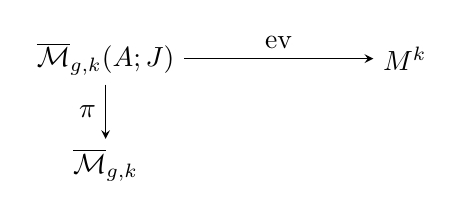
\begin{tikzpicture}[baseline=(current bounding box.center),>=stealth]
  \node (mod) at (0,0) {$\overline{\mathcal M}_{g,k}(A;J)$};
  \node (mk) at (3.8,0) {$M^k$};
  \node (dm) at (0,-1.35) {$\overline{\mathcal M}_{g,k}$};
  \draw[->] (mod) -- node[above] {$\operatorname{ev}$} (mk);
  \draw[->] (mod) -- node[left] {$\pi$} (dm);
\end{tikzpicture}
\]
暂且假装这三个空间都是光滑紧流形。此时，\BookRecordIndex{T0143}格罗莫夫--威滕不变量可以解释为群同态
\[
  \operatorname{GW}^{M}_{g,k,A}:
  H^*(M;\mathbb Q)^{\otimes k}\otimes
  H_*\bigl(\overline{\mathcal M}_{g,k};\mathbb Q\bigr)
  \longrightarrow\mathbb Q,
\]
其定义为
\[
  \operatorname{GW}^{M}_{g,k,A}(a_1,\ldots,a_k;\beta)
  :=\int_{\overline{\mathcal M}_{g,k}(A;J)}
  \operatorname{ev}_1^*a_1\smile\cdots\smile
  \operatorname{ev}_k^*a_k\smile\pi^*\operatorname{PD}(\beta).
\]
从几何上看，可以把这个不变量理解为对如下曲线计数：带 $k$ 个\BookRecordIndex{T0066}标记点的亏格 $g$
\BookRecordIndex{T0003}$J$-全纯曲线，在第 $i$ 个\BookRecordIndex{T0066}标记点处通过与 $a_i$ 庞加莱对偶的循环 $X_i\subset M$，并且
曲线在投影 $\pi$ 下的像被限制在表示类 $\beta$ 的循环
$Y\subset\overline{\mathcal M}_{g,k}$ 中。只要各类 $a_i$ 与 $\beta$ 满足维数条件
\[
  \sum_{i=1}^k\deg(a_i)
  =n(2-2g)+2c_1(A)+\deg(\beta),
\]
原则上这一构造应当给出一个零维约化\BookRecordIndex{T0246}模空间。

所得不变量取有理数值；\BookRecordIndex{T0246}模空间 $\overline{\mathcal M}_{g,k}$ 和
$\overline{\mathcal M}_{g,k}(A;J)$ 都有轨形奇点。前者是因为黎曼曲面可能有非平凡
自同构，后者则是因为\BookRecordIndex{T0113}多重覆盖曲线处可能有非平凡\BookRecordIndex{T0342}稳定子群。

要在完全一般的情形下精确定义这些不变量，需要在紧化\BookRecordIndex{T0246}模空间
$\overline{\mathcal M}_{g,k}(A;J)$ 上构造有理基本循环。这是一个远超本书范围的漫长故事
（参见第~6 章最末的讨论）。本章只解释这幅图景中的一小部分。第一，我们只考虑亏格零；
第二，只考虑\BookRecordIndex{T0058}半正\BookRecordIndex{T0358}辛流形 $(M,\omega)$；第三，只考虑\BookRecordIndex{T0246}模空间
$\overline{\mathcal M}_{0,k}$ 中特殊的同调类 $\beta$，也就是固定指标集
$\{1,\ldots,k\}$ 的某个子集 $I$ 所对应的\BookRecordIndex{T0066}标记点而得到的那些类。最后一个限制并非真正
必要，而且很容易去掉，因为 $\overline{\mathcal M}_{0,k}$ 的同调已经得到充分理解。
不过，另外两个限制（亏格零和\BookRecordIndex{T0058}半正性）在本书发展的分析框架中是本质的。需要强调的是，
\BookRecordIndex{T0058}半正情形下的亏格零不变量在整系数（上）同调类上取整数值。

\BookRecordIndex{T0058}半正流形的亏格零不变量最早由 Ruan \srcite{342,340} 引入辛几何。
\personlater{geluomofu}{格罗莫夫}{Gromov}在 \srcite{160} 中、McDuff 在
\srcite{259} 中曾用其特殊情形研究\BookRecordIndex{T0358}辛流形的结构。\BookRecordIndex{T0150}固定标记点的不变量出现在 sigma 模型
的语境中，并由 Witten \srcite{421} 研究。设
$\beta_{k,I}\in H_{2(k-\#I)}(\overline{\mathcal M}_{0,k};\mathbb Z)$ 的庞加莱对偶，是
最高维群 $H^{2\#I-6}(\overline{\mathcal M}_{0,I};\mathbb Z)$ 的生成元在投影
\[
  \pi_{k,I}:\overline{\mathcal M}_{0,k}\longrightarrow
  \overline{\mathcal M}_{0,I}
\]
下的拉回；与这些同调类 $\beta_{k,I}$ 相联系的亏格零不变量，对应于 Ruan--Tian
\srcite{345} 所谓的\emph{\BookRecordIndex{T0172}混合不变量}，其中只固定指标集 $I$ 所对应的\BookRecordIndex{T0066}标记点。
Kontsevich 和 Manin 在 \srcite{216} 中把\BookRecordIndex{T0143}格罗莫夫--威滕不变量表成群同态
\[
  \operatorname{GW}^{M}_{g,k,A}:
  H^*(M;\mathbb Q)^{\otimes k}
  \longrightarrow H^*(\overline{\mathcal M}_{g,k};\mathbb Q).
\]
按他们的术语，\BookRecordIndex{T0066}标记点可变（$\beta=[\overline{\mathcal M}_{0,k}]$）的不变量是余维零类，
\BookRecordIndex{T0066}标记点固定（$\beta=[\mathrm{pt}]$）的不变量是最高余维类，\BookRecordIndex{T0172}混合不变量则是中间情形
（$\beta_{k,I}$ 对应余维 $2\#I-6$）
\sourcefootnote{原书把 $\overline{\mathcal M}_{0,I}$ 的最高维上同调群印作
$H^{\#I-3}$，并把 $\beta_{k,I}$ 的余维印作 $2\#I$；但
$\dim_{\mathbb R}\overline{\mathcal M}_{0,I}=2\#I-6$，且
$\beta_{k,I}\in H_{2(k-\#I)}(\overline{\mathcal M}_{0,k})$，故两处次数都唯一应为
$2\#I-6$。}。下文省略自变量 $\beta$ 和亏格指标，并把与
$\beta_{k,I}$ 相联系的亏格零不变量记作 $\operatorname{GW}^{M,I}_{A,k}$。当
$\#I=3$ 时，简写为
$\operatorname{GW}^{M}_{A,k}:=\operatorname{GW}^{M,I}_{A,k}$。若从上下文可知流形 $M$，
则省略上标 $M$。

本章首先仔细定义计数不变量 $\operatorname{GW}$，并给出最初的一批例子。为方便读者，
其中也讨论前几章的一些相关结果。第~\ref{sec:7-2} 节发展主构造的若干变体；例如，我们
为以固定树为模型的曲线以及固定某个\BookRecordIndex{T0066}标记点子集的曲线定义不变量。我们还讨论\BookRecordIndex{T0399}障碍丛，
它使我们能够用非正则但足够良好的\BookRecordIndex{T0088}殆复结构来计算不变量。第~\ref{sec:7-3} 节引入与
\BookRecordIndex{T0335}伪全纯图像相联系的不变量 $\operatorname{GW}^I$，并把它们与 $\operatorname{GW}$ 联系
起来。第~\ref{sec:7-4} 节用射影空间中的曲线为例说明这些思想。最后一节叙述
\BookRecordIndex{T0143}格罗莫夫--威滕不变量的 Kontsevich--Manin 公理，并用 $\operatorname{GW}^I$ 解释这些
公理。为展示其威力，我们还会给出 Kontsevich 对 $\mathbb{CP}^2$ 中通过 $3d-1$ 个一般
点的 $d$ 次\BookRecordIndex{T0386}有理曲线数 $N_d$ 的计算。全章都限于亏格零；第~8 章会讨论一些高亏格例子，
见例~\ref{ex:8-6-12}。

\section{计数伪全纯球面}\label{sec:7-1}
\zhindex{jishuweiquanchunqiumian}{计数伪全纯球面}

本节定义\BookRecordIndex{T0143}格罗莫夫--威滕不变量 $\operatorname{GW}_{A,k}$，并在一些简单情形下计算它们。
在给出正式定义之前，我们先说明庞加莱对偶与\BookRecordIndex{T0337}伪循环的若干事项。

与第~\ref{sec:6-5} 节一样，以下用记号
\[
  H^*(M):=H^*(M;\mathbb Z)/\operatorname{Tor}
\]
表示 $H^*(M;\mathbb Z)$ 的自由部分，同调群也采用类似记号。依定义，奇异上同调类
$a\in H^k(M)$ 由它在 $H_*(M)$ 中各同调类上的取值唯一确定，并可等同于相应的群同态
$H_*(M)\to\mathbb Z$。若一个 $(2n-k)$ 维\BookRecordIndex{T0337}伪循环 $f:U\to M$ 对每个闭定向 $k$ 维
子流形 $X\subset M$ 都满足
\[
  \int_X a=f\cdot X,
\]
就称 $f$ 与 $a$（庞加莱）对偶。于是，若 $f:U\to M$ 与 $a$ 对偶，而
$g:V\to M$ 与 $b$ 对偶，则
\[
  \int_M a\wedge b=f\cdot g
\]
（见引理~\ref{lem:6-5-7}）。用第~\ref{sec:6-5} 节的术语，与上同调类 $a$ 对偶的
\BookRecordIndex{T0337}伪循环，是同调类 $\operatorname{PD}(a)$ 的\BookRecordIndex{T0292}弱代表元。

现在设 $(M,\omega)$ 是闭\BookRecordIndex{T0058}半正辛 $2n$ 维流形，$A\in H_2(M;\mathbb Z)$ 是满足
式~\eqref{eq:6-6-1} 的球面同调类，且 $k$ 是非负整数。定理~\ref{thm:6-6-1} 断言，对
每个 $J\in\mathcal J_{\mathrm{reg}}(M,\omega)$（见定义~\ref{def:6-2-1}），\BookRecordIndex{T0283}求值映射
\[
  \operatorname{ev}_J:\mathcal M^*_{0,k}(A;J)\longrightarrow M^k
\]
都是维数
\[
  \mu(A,k):=2n+2c_1(A)+2k-6
\]
的\BookRecordIndex{T0337}伪循环。

\begin{theorem}\label{thm:7-1-1}
设 $(M,\omega)$ 是闭\BookRecordIndex{T0058}半正辛 $2n$ 维流形，$k$ 是非负整数，而
$A\in H_2(M;\mathbb Z)$ 是球面同调类，并且不是任何满足 $c_1(B)=0$ 的球面同调类
$B$ 的非平凡整数倍。则由
\begin{equation}\label{eq:7-1-1}
  \operatorname{GW}^{M}_{A,k}(a_1,\ldots,a_k):=f\cdot\operatorname{ev}_J
\end{equation}
定义的群同态
\[
  \operatorname{GW}^{M}_{A,k}:H^*(M)^{\otimes k}\longrightarrow\mathbb Z
\]
与\BookRecordIndex{T0088}殆复结构 $J$ 以及定义它所用的\BookRecordIndex{T0337}伪循环 $f$ 无关。这里
$J\in\mathcal J_{\mathrm{reg}}(M,\omega)$，而 $f:U\to M^k$ 是与
$\pi_1^*a_1\smile\cdots\smile\pi_k^*a_k$ 庞加莱对偶的\BookRecordIndex{T0337}伪循环，
$\pi_i:M^k\to M$ 表示到第 $i$ 个因子的投影。
\end{theorem}

\begin{proof}
由定理~\ref{thm:6-6-1}，$\operatorname{ev}_J$ 的配边类与 $J$ 无关。因此，由
引理~\ref{lem:6-5-5}，交数 $f\cdot\operatorname{ev}_J$ 与 $J$ 无关。再由
引理~\ref{lem:6-5-7}，它只依赖于\BookRecordIndex{T0337}伪循环 $f$ 所表示的同调类。这就证明了定理。
\end{proof}

上述群同态
$\operatorname{GW}^{M}_{A,k}:H^*(M)^{\otimes k}\to\mathbb Z$
称为 $(M,\omega)$ 在同调类 $A$ 中的\emph{$k$ 点亏格零\BookRecordIndex{T0143}格罗莫夫--威滕不变量}。

\begin{exercise}\label{ex:7-1-2}
证明：$\operatorname{GW}^{M}_{A,k}(a_1,\ldots,a_k)$ 也可定义为
$\operatorname{ev}$ 与乘积循环 $f_1\times\cdots\times f_k$ 的交数，其中
$f_j:U_j\to M$ 分别是与上同调类 $a_j$ 对偶的\BookRecordIndex{T0337}伪循环。换言之，可以在乘积循环这一类
之内达到横截。

\emph{提示：}把引理~\ref{lem:6-5-5}(i) 略作修改，用于 $f$ 是乘积循环而 $\phi$
是乘积微分同胚的情形。
\end{exercise}

回忆第~6 章，当 $A\ne0$ 时，\BookRecordIndex{T0246}模空间 $\mathcal M^*_{0,k}(A;J)$ 是元组
$(u,z_1,\ldots,z_k)$ 的等价类之集，其中 $u:S^2\to M$ 是表示类 $A$ 的单纯
$J$-全纯球面，而 $z_i$ 是 $S^2$ 上两两不同的点。等价关系由\BookRecordIndex{T0413}重参数化群
$G=\operatorname{PSL}(2,\mathbb C)$ 的自然作用给出。由定理~\ref{thm:3-1-6}，对每个
$J\in\mathcal J_{\mathrm{reg}}(A)$，这个空间都是维数为 $\mu(A,k)$ 的光滑定向流形。
定理~\ref{thm:6-6-1} 更强的断言，即它对每个
$J\in\mathcal J_{\mathrm{reg}}(M,\omega)$ 都是\BookRecordIndex{T0337}伪循环，意味着紧化中出现的所有\BookRecordIndex{T0072}层维数
至多为 $\mu(A,k)-2$。现在设每个类 $a_i\in H^*(M)$ 都与一般位置的定向子流形
$X_i\subset M$ 对偶。此时，\BookRecordIndex{T0143}格罗莫夫--威滕不变量
$\operatorname{GW}^{M}_{A,k}(a_1,\ldots,a_k)$ 就是类 $A$ 中通过各子流形 $X_i$ 的
$J$-全纯球面的带适当符号计数：
\[
  \operatorname{GW}^{M}_{A,k}(a_1,\ldots,a_k)
  =\#\Bigl\{[u,z_1,\ldots,z_k]\in\mathcal M^*_{0,k}(A;J)
  \ \Big|\ u(z_i)\in X_i\Bigr\}.
\]
只要各类 $a_i$ 的次数之和等于\BookRecordIndex{T0246}模空间维数，这个公式作为模 $2$ 不变量便是严格成立的：
\begin{equation}\label{eq:7-1-2}
  \sum_{i=1}^k\deg(a_i)=\mu(A,k)=2n+2c_1(A)+2k-6.
\end{equation}
在其余所有情形，不变量依定义为零。注意，一般位置假设不仅意味着\BookRecordIndex{T0283}求值映射横截于
$X_1\times\cdots\times X_k$，还意味着这个乘积不与紧化中各低维\BookRecordIndex{T0072}层所对应\BookRecordIndex{T0283}求值映射的像
相交。

\begin{example}\label{ex:7-1-3}
情形 $A=0$ 需要单独讨论。由于每个常值分支必须带至少三个\BookRecordIndex{T0320}特殊点，
$\mathcal M^*_{0,k}(0;J)$ 在 $k<3$ 时为空。当 $k\ge3$ 时，它由元组
$(x,z_1,\ldots,z_k)$ 组成，其中 $x\in M$（把它看作常值 $J$-全纯球面
$u(z)\equiv x$），而 $z_i$ 是 $S^2$ 上两两不同的点。当 $k>3$ 时，式~\eqref{eq:7-1-2}
说明，与类 $a_i$ 对偶的循环 $X_i$ 的总余维严格大于 $2n$，故它们处于一般位置时没有
交点。因此，$A=0$ 的\BookRecordIndex{T0143}格罗莫夫--威滕不变量在 $k\ne3$ 时为零。若 $k=3$，数
$\operatorname{GW}^{M}_{0,3}(a_1,a_2,a_3)$ 计数各庞加莱对偶的三重交。这说明
\[
  \operatorname{GW}^{M}_{0,3}(a_1,a_2,a_3)
  =\int_M a_1\smile a_2\smile a_3.
\]
\end{example}

\begin{example}\label{ex:7-1-4}
另一个有趣的特殊情形是 $k=0$。若同时有 $A=0$，便没有可计数的对象，我们把不变量
定义为零。不过，当 $A\ne0$ 时，可以把流形 $M^k$ 看成一个点，从而定义\BookRecordIndex{T0348}相容且有趣的
不变量。只要 $J\in\mathcal J_{\mathrm{reg}}(A)$，且\BookRecordIndex{T0246}模空间
$\mathcal M^*_{0,0}(A;J)$ 的维数
$\mu(A,0)=2n+2c_1(A)-6$ 大于零，\BookRecordIndex{T0283}求值映射
\[
  \operatorname{ev}_J:\mathcal M^*_{0,0}(A;J)\longrightarrow\{\mathrm{pt}\}
\]
自动是\BookRecordIndex{T0337}伪循环。然而在这种情形，它的同调类由于维数原因等于零。因此，不变量只有在
\[
  2n+2c_1(A)=6
\]
时才可能非零，此时\BookRecordIndex{T0246}模空间 $\mathcal M^*_{0,0}(A;J)$ 是零维的。若
$J\in\mathcal J_{\mathrm{reg}}(M,\omega)$，紧化中的所有边界\BookRecordIndex{T0072}层都有负虚维数，因而为空。
于是 $\mathcal M^*_{0,0}(A;J)$ 是有限集，而不变量
\[
  \operatorname{GW}(A):=\operatorname{GW}_{A,0}(1)\in\mathbb Z
\]
是 $\mathcal M^*_{0,0}(A;J)$ 中元素的带适当符号计数。当 $M=S^2$ 且 $c_1(A)=2$ 时，
这个数为一。若 $\dim M=4$、$c_1(A)=1$ 且 $A\cdot A=-1$，不变量计数表示类 $A$ 的例外
除子数目（见下文例~\ref{ex:7-1-15}）。由\BookRecordIndex{T0186}交点正性，这个数只能是零或一。不过，若
$A\cdot A\ge0$，不变量也可能取零、一以外的值（见下文习题~\ref{ex:7-1-17}）。最重要
的情形是 Calabi--Yau 流形（$\dim M=6$ 且 $c_1(A)=0$）。此时，去掉 $A$ 必须是本原类
这一假设至关重要；见注~\ref{rem:7-3-8}。
\end{example}

最后给出两个习题，说明这些不变量的一些基本几何性质；参见第~\ref{sec:7-5} 节列出的
（除子）公理和（基本类）公理。

\begin{exercise}\label{ex:7-1-5}
设 $(M,\omega)$ 是紧辛四维流形，而 $A$ 是满足 $c_1(A)=1$ 的球面同调类。证明：若
$a_k\in H^2(M)$ 且 $k\ge1$，则
\[
  \operatorname{GW}_{A,k}(a_1,\ldots,a_k)
  =\operatorname{GW}_{A,k-1}(a_1,\ldots,a_{k-1})\cdot\int_A a_k.
\]
这里的几何想法是，每条 $A$-曲线与 $\operatorname{PD}(a_k)$ 相交
$\int_Aa_k$ 次；因此无须分别记录这些交点。
\end{exercise}

\begin{exercise}\label{ex:7-1-6}
设 $(M,\omega)$ 是紧\BookRecordIndex{T0058}半正\BookRecordIndex{T0358}辛流形且 $A\ne0$。证明：当 $k\ge1$ 时，
\[
  \operatorname{GW}_{A,k}(a_1,\ldots,a_{k-1},1)=0,
\]
其中 $1:=\operatorname{PD}([M])\in H^0(M)$。这里的想法是，由于最后一个\BookRecordIndex{T0066}标记点不受
约束，相关交点永远不是孤立的，故不变量为零。
\end{exercise}

\paragraph{关于定义的说明。}

\paragraph{\BookRecordIndex{T0058}半正性。}
如果不存在满足
\[
  \omega(A)>0,
  \qquad
  2-n<c_1(A)<0
\]
的球面同调类 $A\in H_2(M;\mathbb Z)$，就称紧\BookRecordIndex{T0358}辛流形 $(M,\omega)$ 是\BookRecordIndex{T0058}半正的。特别地，
每个维数 $2n\le6$ 的\BookRecordIndex{T0358}辛流形都满足这一条件。正如第~\ref{sec:6-4} 节所解释的，这一条件
保证：对通有的 $J$，不存在第一陈数为负的 $J$-全纯球面。要理解其意义，先回忆：若
\BookRecordIndex{T0340}稳定映射的每个非常值分支都是单纯的（即不是多重覆盖），并且任意两个非常值分支的像
都不同，就称它为\BookRecordIndex{T0184}简单稳定映射。其次，只要 $J\in\mathcal J_{\mathrm{reg}}(M,\omega)$，
以带 $k$ 个标号的树 $T$ 为模型的\BookRecordIndex{T0184}简单稳定映射\BookRecordIndex{T0246}模空间
$\mathcal M^*_{0,T}(B;J)$ 就是维数为 $\mu(B,k)-2e(T)$ 的光滑流形
（定理~\ref{thm:6-2-6}）。第三，对类 $A$ 中每个非\BookRecordIndex{T0184}简单稳定映射，都存在某个类 $B$ 中
的底\BookRecordIndex{T0072}层\BookRecordIndex{T0184}简单稳定映射，它与原\BookRecordIndex{T0340}稳定映射有相同的像，并在各\BookRecordIndex{T0066}标记点处取相同的值
（命题~\ref{prop:6-1-2}）。现在，若每个 $J$-全纯球面的陈数都非负，则
$c_1(B)\le c_1(A)$，所以紧化中的所有边界\BookRecordIndex{T0072}层维数都小于 $\mu(A,k)$
\sourcefootnote{原书此处把比较对象印作 $\mu(A,T)$；但紧邻上文给出的 $T$-\BookRecordIndex{T0072}层预期维数
本身就是 $\mu(B,k)-2e(T)$（当 $B=A$ 时即为 $\mu(A,T)$），而且不同边界\BookRecordIndex{T0072}层的树 $T$
并不固定。\BookRecordIndex{T0337}伪循环论证所需、并由 $e(T)>0$ 得到的统一比较对象，是主\BookRecordIndex{T0072}层维数
$\mu(A,k)$。}。这正是证明
$J\in\mathcal J_{\mathrm{reg}}(M,\omega)$ 时\BookRecordIndex{T0283}求值映射为\BookRecordIndex{T0337}伪循环的关键成分
（定理~\ref{thm:6-6-1}）。若只考虑那些使所有相关 $J$-全纯球面都有非负陈数的\BookRecordIndex{T0088}殆复
结构，便可以放宽\BookRecordIndex{T0058}半正性条件（注~\ref{rem:6-6-2}）。

\paragraph{符号的确定。}
计算\BookRecordIndex{T0143}格罗莫夫--威滕不变量的另一个重要环节，是确定正确的符号。若 $J$ 可积，我们在
注~\ref{rem:3-2-6} 中已经看到，\BookRecordIndex{T0246}模空间带有与其定向\BookRecordIndex{T0348}相容的复结构。因此在这种情形，通常
很容易确定交点符号（见下文例~\ref{ex:7-1-15}）。然而，若 $J$ 不可积，这个问题一般
要微妙得多。

\paragraph{识别正则\BookRecordIndex{T0088}殆复结构。}
为了计算不变量，必须能够识别一个给定\BookRecordIndex{T0088}殆复结构 $J$ 何时属于
$\mathcal J_{\mathrm{reg}}(M,\omega)$。这意味着：对所有单纯 $J$-全纯球面，\BookRecordIndex{T0346}线性化算子
$D_u$ 都满射；并且对所有树，\BookRecordIndex{T0065}边求值映射都横截于\BookRecordIndex{T0061}边对角线（见定义~\ref{def:6-2-1}）。
这些条件蕴含所有\BookRecordIndex{T0184}简单稳定映射的\BookRecordIndex{T0246}模空间都有预期维数，因而对任意 $A$ 和 $k$，
$\operatorname{ev}_J:\mathcal M^*_{0,k}(A;J)\to M^k$ 都是\BookRecordIndex{T0337}伪循环。为计算不变量
$\operatorname{GW}_{A,k}$，只须对确实出现在
$\mathcal M^*_{0,k}(A;J)$ 的紧化中的那些树 $T$ 和同调类 $\{B_\alpha\}$ 验证这些条件。
这些类必须对某组正整数 $m_\alpha$ 满足
\[
  \sum_{\alpha\in T}m_\alpha B_\alpha=A.
\]
当 $A$ 不容许任何这种非平凡分解时，情形尤其简单。

\begin{definition}\label{def:7-1-7}
若类 $A$ 不能写成
\[
  A=A_1+\cdots+A_k,
\]
其中 $k\ge2$，且每个 $A_i$ 都有非常值球面 $J$-全纯代表元，就称 $A$ 是
\emph{\BookRecordIndex{T0002}$J$-不可分解的}。
\end{definition}

\begin{lemma}\label{lem:7-1-8}
设 $A\in H_2(M;\mathbb Z)$ 且 $J\in\mathcal J_{\mathrm{reg}}(A)$（即对每个表示类
$A$ 的单纯 $J$-全纯球面 $u$，$D_u$ 都满射）。若 $A$ 是 \BookRecordIndex{T0002}$J$-不可分解的，则对每个整数
$k\ge0$，\BookRecordIndex{T0283}求值映射
\[
  \operatorname{ev}_J:\mathcal M^*_{0,k}(A;J)\longrightarrow M^k
\]
都是\BookRecordIndex{T0337}伪循环，并且可以用 $\operatorname{ev}_J$ 计算 $\operatorname{GW}_{A,k}$。
\end{lemma}

\begin{proof}
由于 $J\in\mathcal J_{\mathrm{reg}}(A)$，对每个表示类 $A$ 的单纯 $J$-全纯球面
$u:S^2\to M$，算子 $D_u$ 都满射。因此，类 $A$ 中不带标记的单纯 $J$-曲线\BookRecordIndex{T0246}模空间
\[
  \mathcal M^*_{0,0}(A;J)=\mathcal M^*(A;J)/G
\]
是预期维数 $2n+2c_1(A)-6$ 的流形
\sourcefootnote{原书此处漏掉了除以\BookRecordIndex{T0413}重参数化群 $G$ 所减少的六个实维数，把
$\mathcal M^*_{0,0}(A;J)$ 的预期维数印作 $2n+2c_1(A)$；由紧邻的商空间定义以及
$\mu(A,0)=2n+2c_1(A)-6$，唯一应补为这里的数值。}。我们断言它是紧的。首先，由于 $A$ 是
\BookRecordIndex{T0002}$J$-不可分解的，每条表示类 $A$ 的 $J$-曲线都是单纯的。其次，由
定理~\ref{thm:5-3-1}，$\mathcal M_{0,0}(A;J)$ 中任意序列都有\BookRecordIndex{T0141}格罗莫夫收敛子列。由于
没有\BookRecordIndex{T0066}标记点，其极限只有一个分支，因而必属于
$\mathcal M_{0,0}(A;J)=\mathcal M^*_{0,0}(A;J)$。（注意，若在所有具有 $J$-全纯
代表元的类中，$A$ 具有最小能量，那么同一结论也可由简单得多的
定理~\ref{thm:4-2-11} 得到。）

当 $k\ge2$ 时，相应空间 $\mathcal M^*_{0,k}(A;J)$ 不会是紧的，因为\BookRecordIndex{T0066}标记点必须始终
互异。不过，位于边界\BookRecordIndex{T0072}层的\BookRecordIndex{T0340}稳定映射由一个表示类 $A$ 的主分支，以及若干用于容纳\BookRecordIndex{T0066}标记点
的\BookRecordIndex{T0382}幽灵分支组成。这些\BookRecordIndex{T0072}层总是正则的，而且维数为 $\mu-2e(T)$（见
习题~\ref{ex:7-1-9}）。因此，紧化中的所有\BookRecordIndex{T0072}层都有预期维数，引理得证。
\end{proof}
\begin{exercise}\label{ex:7-1-9}
设 $A$ 是 \BookRecordIndex{T0002}$J$-不可分解的，且
$J\in\mathcal J_{\mathrm{reg}}(A,\mathbb{CP}^1)$。则类 $A$ 中每个\BookRecordIndex{T0340}稳定映射都包含一个
表示类 $A$ 的主分支，还可能包含若干带有\BookRecordIndex{T0066}标记点的\BookRecordIndex{T0382}幽灵分支。验证：对每棵树 $T$，都有
$J\in\mathcal J_{\mathrm{reg}}(A,T)$。（参见习题~\ref{ex:6-2-5}。）
\end{exercise}

\begin{exercise}\label{ex:7-1-10}
设 $A\in H_2(M;\mathbb Z)$。证明：使 $A$ 为 \BookRecordIndex{T0002}$J$-不可分解类的所有被 $\omega$ \BookRecordIndex{T0372}驯服
\BookRecordIndex{T0088}殆复结构 $J$，在 $\mathcal J_\tau(M,\omega)$ 中构成开集。
\end{exercise}

\begin{remark}\label{rem:7-1-11}
\BookRecordIndex{T0363}辛形式 $\omega$ 的一个\emph{形变}，是从 $\omega_0=\omega$ 出发的\BookRecordIndex{T0363}辛形式光滑单参数族
\[
  [0,1]\longrightarrow\Omega^2(M),
  \qquad t\longmapsto\omega_t.
\]
与同痕的概念不同，这里不要求上同调类保持不变。由于\BookRecordIndex{T0372}驯服条件是开的，被 $\omega$ \BookRecordIndex{T0372}驯服
的\BookRecordIndex{T0088}殆复结构 $J$ 也被所有充分接近 $\omega$ 的\BookRecordIndex{T0363}辛形式\BookRecordIndex{T0372}驯服。因此，在 $\omega$ 的形变
$\omega_t$ 下，\BookRecordIndex{T0143}格罗莫夫--威滕不变量 $\operatorname{GW}^{M}_{A,k}$ 不变，只要
对每个 $t\in[0,1]$，$(M,\omega_t)$ 都是\BookRecordIndex{T0058}半正的。
\footnote{当然，一旦构造出\BookRecordIndex{T0370}虚模循环，这个附加条件便不再必要。因此，现在已知这些不变量
只依赖于 $(M,\omega)$ 的形变类型。}
除非碰巧有 $\dim M\le6$ 或 $c_1$ 在 $\pi_2$ 上消失，否则这个关于 $\omega_t$ 的条件
相当苛刻。在上述两种情形中，$(M,\omega_t)$ 对某一个形式 $\omega_t$ \BookRecordIndex{T0058}半正，当且仅当它
对形变中的所有形式 $\omega_t$ 都\BookRecordIndex{T0058}半正。因此在这些情形，\BookRecordIndex{T0143}格罗莫夫--威滕不变量只依赖于
$(M,\omega)$ 的形变类型。四维时还有更强的结论：Taubes 证明，嵌入曲线（可能有更高
亏格）的 Gromov 不变量与 Seiberg--Witten 不变量相同，因而这些 Gromov 不变量只依赖于
$M$ 的光滑结构。不过六维时并非如此；见第~\ref{ch:applications-symplectic-topology} 章关于 Ruan 例子的讨论。
\end{remark}

\begin{remark}[同调的不变量]\label{rem:7-1-12}
到目前为止，我们用 $M$ 的上同调定义\BookRecordIndex{T0143}格罗莫夫--威滕不变量。然而在某些情形，把它们看成
由同调类决定会更方便。给定 $\alpha_1,\ldots,\alpha_k\in H_*(M)$，定义
\[
  \operatorname{GW}^{M}_{A,k}(\alpha_1,\ldots,\alpha_k)
  :=\operatorname{GW}^{M}_{A,k}
  \bigl(\operatorname{PD}(\alpha_1),\ldots,\operatorname{PD}(\alpha_k)\bigr).
\]
它计数\BookRecordIndex{T0283}求值映射
$\operatorname{ev}:\mathcal M^*_{0,k}(A;J)\to M^k$ 与乘积类
$\alpha_1\times\cdots\times\alpha_k\in H_*(M^k)$ 的交数。
\end{remark}

\paragraph{例子。}

\begin{example}\label{ex:7-1-13}
考虑带乘积\BookRecordIndex{T0363}辛形式的乘积流形
\[
  \widetilde M:=S^2\times M,
\]
并假设 $\widetilde M$ \BookRecordIndex{T0058}半正。例如，当 $\dim M\le4$ 或 $\pi_2(M)=0$ 时便是如此。考虑
球面同调类
\[
  \widetilde A:=[S^2\times\mathrm{pt}]
  \in H_2(S^2\times M;\mathbb Z),
\]
并设 $\widetilde J$ 是一个被 $\widetilde\omega$ \BookRecordIndex{T0372}驯服的乘积\BookRecordIndex{T0088}殆复结构。由
推论~\ref{cor:3-3-5}，$\widetilde J\in\mathcal J_{\mathrm{reg}}(\widetilde A)$，而且类
$\widetilde A$ 是 $\widetilde J$-不\BookRecordIndex{T0213}可分解的。此外，通过 $\widetilde M$ 中每一点恰有一个
$\widetilde J$-全纯 $\widetilde A$-球面。因此由引理~\ref{lem:7-1-8}，\BookRecordIndex{T0283}求值映射
\[
  \operatorname{ev}:\mathcal M_{0,1}(\widetilde A;\widetilde J)
  \longrightarrow\widetilde M
\]
是微分同胚。故
\[
  \operatorname{GW}^{\widetilde M}_{\widetilde A,1}(\widetilde a)
  =\int_{\widetilde M}\widetilde a.
\]
\end{example}

\begin{example}[射影空间中的直线]\label{ex:7-1-14}
$\mathbb{CP}^n$ 中任意两点位于唯一一条直线上。这应当转化成公式
\[
  \operatorname{GW}^{\mathbb{CP}^n}_{L,2}(c^n,c^n)=1,
\]
其中
\[
  L:=[\mathbb{CP}^1]\in H_2(\mathbb{CP}^n;\mathbb Z),
\]
$c$ 是 $H^2(\mathbb{CP}^n;\mathbb Z)$ 的正生成元，而
$c^n=\operatorname{PD}([\mathrm{pt}])\in H^{2n}(\mathbb{CP}^n;\mathbb Z)$。为验证这一点，
先注意 $c_1(L)=n+1$ 且 $k=2$，所以维数条件~\eqref{eq:7-1-2} 在
$\mu(L,2)=4n$ 时成立。此外，标准复结构 $J_0$ 满足引理~\ref{lem:3-3-2} 的假设。事实上，
若 $u:\mathbb{CP}^1\to\mathbb{CP}^n$ 是一条直线，则拉回切丛
$u^*T\mathbb{CP}^n\to\mathbb{CP}^1$ 分裂成全纯线丛的直和，其中一个线丛的陈数为二，
其余线丛的陈数为一。陈数为一的线丛可实现为
$\mathbb{CP}^{k-1}\subset\mathbb{CP}^k$ 的\BookRecordIndex{T0117}法丛，其中 $k=2,\ldots,n$。这说明
$J_0\in\mathcal J_{\mathrm{reg}}(L)$。由于 $L$ 是 $J_0$-不\BookRecordIndex{T0213}可分解类，引理~\ref{lem:7-1-8}
断言我们可以用 $J_0$ 计算 $\operatorname{GW}_{L,2}$。因此，
$\operatorname{GW}_{L,2}(c^n,c^n)$ 恰为通过两点的直线数，故等于一。

另一个初等\BookRecordIndex{T0143}格罗莫夫--威滕不变量是
$\operatorname{GW}^{\mathbb{CP}^3}_{L,3}(c^2,c^2,c^3)$。它计数三维射影空间中通过一点
并与两条一般直线相交的直线。维数条件~\eqref{eq:7-1-2} 成立，所以这个数可能非零。
此外，满足这些关联条件的直线唯一，即分别取过该点与其中一条直线的两个平面，它们的
交线。为了\BookRecordIndex{T0326}推出
\[
  \operatorname{GW}^{\mathbb{CP}^3}_{L,3}(c^2,c^2,c^3)=1,
\]
还需确认\BookRecordIndex{T0283}求值映射
$\operatorname{ev}:\mathcal M(L,J_0)\to(\mathbb{CP}^3)^3$ 横截于类
$[\mathrm{pt}]\times L\times L$ 的一般代表元。这可以直接验证，也可由下文
命题~\ref{prop:7-4-5} 得到。
\end{example}

\begin{example}[例外除子]\label{ex:7-1-15}
用 $\overline{\mathbb{CP}^2}$ 表示取反向定向的复射影平面。注意，它不是复流形。若
$E\in H_2(\overline{\mathbb{CP}^2};\mathbb Z)$ 表示子流形 $\mathbb{CP}^1$（带标准定向）
的同调类，则 $E\cdot E=-1$。

设 $(M,\omega)$ 是复 凯勒 曲面，而 $(\widetilde M,\widetilde J)$ 表示它在点 $x$ 处的
吹起。这意味着，用所有通过 $x$ 的直线之集替代 $x$。这个直线集是
$\mathbb{CP}^1$ 的一个副本，称为例外除子 $\Sigma$。$\Sigma$ 的\BookRecordIndex{T0117}法丛是
$\mathbb{CP}^1$ 上欧拉类为 $-1$ 的\BookRecordIndex{T0414}重言线丛，由此存在微分同胚
\[
  \widetilde M\cong M\#\overline{\mathbb{CP}^2},
\]
把 $\Sigma$ 识别为 $\overline{\mathbb{CP}^2}$ 中的一条复直线。这个构造在辛范畴中也
成立（见第~\ref{sec:9-3} 节）；特别地，复吹起 $(\widetilde M,\widetilde J)$ 是
凯勒 的。更多细节见第~\ref{sec:9-3} 节。

令 $E=[\Sigma]$ 表示例外除子的同调类。于是，\BookRecordIndex{T0246}模空间
$\mathcal M(E;\widetilde J)$ 在重参数化意义下只含一条 $\widetilde J$-全纯曲线，即例外
除子本身。为说明这一点，注意同一类中的任何另一条 $\widetilde J$-全纯曲线都必须以交数
$-1$ 与 $\Sigma$ 相交；但任意两条不同的 $\widetilde J$-全纯曲线交数非负，这是不可能
的。此外，由引理~\ref{lem:3-3-3}，曲线 $\Sigma$ 正则，这与维数公式
\[
  \dim\mathcal M^*(E;\widetilde J)=4+2c_1(E)=6
\]
相符。因此，由引理~\ref{lem:7-1-8} 和习题~\ref{ex:7-1-5}，
\[
  \operatorname{GW}^{M\#\overline{\mathbb{CP}^2}}_{E,1}
  \bigl(\operatorname{PD}(E)\bigr)=E\cdot E=-1.
\]

于是，对 $\widetilde M$ 上每个被 $\widetilde\omega$ \BookRecordIndex{T0372}驯服的 $J$，类 $E$ 都必须有一个
$J$-全纯代表元。这个代表元可能是可约的。例如，若 $M=\mathbb{CP}^2$，则
$M\#\overline{\mathbb{CP}^2}$ 微分同胚于射影化丛
$\mathbb P(\mathcal L_3\oplus\mathbb C)$，其中线丛
$\mathcal L_3\to\mathbb{CP}^1$ 的陈数为三。子丛 $\mathcal L_3$ 给出
$\mathbb P(\mathcal L_3\oplus\mathbb C)$ 的一个自交数为 $-3$ 的截面，并表示类
\[
  2E-L\in H_2(\mathbb{CP}^2\#\overline{\mathbb{CP}^2};\mathbb Z).
\]
因此，对某个适当的\BookRecordIndex{T0088}殆复结构 $J$，类 $E$ 由这个 $(-3)$-球面与投影
$\mathbb P(\mathcal L_3\oplus\mathbb C)\to\mathbb{CP}^1$ 的纤维 $L-E$ 之并表示。不过，
由于 $(2E-L)$-曲线不可能正则，这种情形对通有的 $J$ 不会发生。
\end{example}

\begin{exercise}\label{ex:7-1-16}
\begin{enumerate}[label=(\roman*),leftmargin=3em]
\item 证明：对 $\mathbb{CP}^2$ 中任意五个点，只要其中没有三个共线，就存在一个二次
齐次多项式 $f$，其零点集通过这五点，并且 $f$ 在非零常数倍意义下唯一
\sourcefootnote{原书说存在“唯一的二次齐次多项式 $f$”，但 $f$ 的任意非零常数倍定义
同一零点集；唯一的是 $f$ 的射影类，等价地说，是二次曲线 $C_f$。}。直接计算证明，
它的零点集 $C_f$ 非奇异，并且是某个
二次映射 $u:\mathbb C\cup\{\infty\}\to\mathbb{CP}^2$ 的像。由此\BookRecordIndex{T0326}推出
\[
  \operatorname{GW}^{\mathbb{CP}^2}_{2L,5}(c^2,c^2,c^2,c^2,c^2)=1.
\]
\emph{提示：}相关计算的一些细节见例~\ref{ex:7-2-9}。

\item 证明
\[
  \operatorname{GW}^{\mathbb{CP}^3}_{L,4}(c^2,c^2,c^2,c^2)=2.
\]
这是三维射影空间中与四条一般直线相交的直线数。
\emph{提示：}由例~\ref{ex:7-1-14}，通过一点并与两条一般直线相交的直线唯一。因此，
固定三条一般直线后，与三者都相交的直线构成一族（让交点沿其中一条直线移动）。证明这
一族上的点集构成一个二次曲面，即某个二次齐次多项式的零点集。这个\BookRecordIndex{T0143}格罗莫夫--威滕
不变量记作 $N_1(4,0)$，也可以用 WDVV 方程计算；见习题~\ref{ex:7-5-17}。
\end{enumerate}
\end{exercise}

\begin{exercise}\label{ex:7-1-17}
设 $M=\mathbb{CP}^2$，而 $L=[\mathbb{CP}^1]$ 如例~\ref{ex:7-1-14}。用维数计数证明
\[
  k\ne8
  \qquad\Longrightarrow\qquad
  \operatorname{GW}_{3L,k}(c^2,\ldots,c^2)=0.
\]
事实上，
\[
  \operatorname{GW}^{\mathbb{CP}^2}_{3L,8}(c^2,\ldots,c^2)=12
\]
（见命题~\ref{prop:7-5-11}）。在八个点处吹起 $\mathbb{CP}^2$，构造一个辛四维流形 $M$ 和一个类
$A$，使 $c_1(A)=1$ 且
\[
  \operatorname{GW}(A):=\operatorname{GW}^{M}_{A,0}(1)>1.
\]
（记号见例~\ref{ex:7-1-4}。）
\end{exercise}


\section{定义的若干变体}\label{sec:7-2}
\zhindex{dingyideruoganbianti}{定义的若干变体}

本节首先讨论：当流形 $M$ 有一个自然的（例如可积的）、但非正则的\BookRecordIndex{T0088}殆复结构时，如何
计算\BookRecordIndex{T0143}格罗莫夫--威滕不变量。随后，我们为以固定树为模型或带\BookRecordIndex{T0150}固定标记点的\BookRecordIndex{T0340}稳定映射定义
一些相关不变量。

实际计算 $\operatorname{GW}_{A,k}$ 时，并不需要假设\BookRecordIndex{T0088}殆复结构 $J_0$ 正则，即属于
$\mathcal J_{\mathrm{reg}}(M,\omega)$。关键在于，\BookRecordIndex{T0283}求值映射
\[
  \operatorname{ev}_{J_0}:\mathcal M^*_{0,k}(A;J_0)\longrightarrow M^k
\]
应当是一个\BookRecordIndex{T0337}伪循环，并且表示与正则 $J$ 情形相同的同调类。为此，$J_0$ 只须满足下面
两个条件。

\begin{enumerate}[label=(\alph*),leftmargin=3em]
\item $J_0$ 对 $A$-曲线正则，即对每个表示类 $A$ 的 $J_0$-全纯球面，\BookRecordIndex{T0346}线性化算子
$D_u$ 都满射。于是对任意 $k$，\BookRecordIndex{T0246}模空间 $\mathcal M^*_{0,k}(A;J_0)$ 都有正确维数
\[
  d:=2n+2c_1(A)+2k-6.
\]
\item “边界”
\[
  \overline{\mathcal M}_{0,k}(A;J_0)
  \setminus\mathcal M^*_{0,k}(A;J_0)
\]
在 $\operatorname{ev}_{J_0}$ 下的像，其维数（在第~\ref{sec:6-5} 节的意义下）至多为
$d-2$。
\sourcefootnote{原书在条件 (b) 中把主\BookRecordIndex{T0072}层误写成
$\mathcal M^*_{0,k}(A;J)$，并在下文证明中重复了这一写法；但此处讨论的是
$\operatorname{ev}_{J_0}$ 的边界，且 $J$ 尚未指定，故两处均应为
$\mathcal M^*_{0,k}(A;J_0)$。}
\end{enumerate}
这些条件蕴含 $\operatorname{ev}_{J_0}$ 是一个 $d$ 维\BookRecordIndex{T0337}伪循环（见
定义~\ref{def:6-5-1}）。

\begin{lemma}\label{lem:7-2-1}
设 $J_0$ 是闭\BookRecordIndex{T0058}半正\BookRecordIndex{T0358}辛流形 $(M,\omega)$ 上被 $\omega$ \BookRecordIndex{T0372}驯服的\BookRecordIndex{T0088}殆复结构，并满足上述条件
(a)、(b)。则\BookRecordIndex{T0283}求值映射
\[
  \operatorname{ev}_{J_0}:\mathcal M^*_{0,k}(A;J_0)\longrightarrow M^k
\]
是由 $J\in\mathcal J_{\mathrm{reg}}(M,\omega)$ 时的
$\operatorname{ev}_J$ 所给\BookRecordIndex{T0145}格罗莫夫--威滕伪循环的\BookRecordIndex{T0292}弱代表元。
\end{lemma}

\begin{proof}
由引理~\ref{lem:6-5-7}，只须证明：对每个定义在维数为 $2nk-d$ 的紧定向光滑流形 $X$
上的光滑映射 $f:X\to M^k$，$\operatorname{ev}_{J_0}$ 与 $f$ 的交数都等于
$J\in\mathcal J_{\mathrm{reg}}(M,\omega)$ 时 $\operatorname{ev}_J$ 与 $f$ 的交数。
依假设，可以选取 $f:X\to M^k$，使得
\[
  \operatorname{ev}_{J_0}\Bigl(
  \overline{\mathcal M}_{0,k}(A;J_0)
  \setminus\mathcal M^*_{0,k}(A;J_0)\Bigr)
  \cap f(X)=\varnothing.
\]
设 $J^\nu\in\mathcal J_{\mathrm{reg}}(M,\omega)$ 收敛到 $J_0$。把\BookRecordIndex{T0380}隐函数定理应用于
$\operatorname{ev}_{J_0}$ 可知，对每个充分大的 $\nu$，
$\operatorname{ev}_{J^\nu}$ 与 $f$ 的交点数至少和
$\operatorname{ev}_{J_0}$ 与 $f$ 的交点数一样多。假设对所有充分大的 $\nu$，前者还有
更多交点；那么这些多出的交点必收敛到一个与 $\operatorname{im}f$ 相交的
$J_0$-全纯\BookRecordIndex{T0340}稳定映射，但由\BookRecordIndex{T0380}隐函数定理的唯一性部分，它不属于
$\operatorname{ev}_{J_0}(\mathcal M^*_{0,k}(A;J_0))$。这与 $f$ 避开
$\overline{\mathcal M}_{0,k}(A;J_0)\setminus\mathcal M^*_{0,k}(A;J_0)$ 的像矛盾。
因此，\BookRecordIndex{T0380}隐函数定理给出 $\operatorname{ev}_{J^\nu}$ 与 $f$ 的交点和
$\operatorname{ev}_{J_0}$ 与 $f$ 的交点之间的保定向一一对应。故充分大的 $\nu$ 满足
\[
  \operatorname{ev}_{J^\nu}\cdot f=\operatorname{ev}_{J_0}\cdot f,
\]
引理得证。
\end{proof}

\begin{example}\label{ex:7-2-2}
令 $M=S^2\times S^2$，记
\[
  A_1=[S^2\times\{\mathrm{pt}\}],
  \qquad
  A_2=[\{\mathrm{pt}\}\times S^2],
\]
取 $A$ 为对角类 $A_1+A_2$，并选择 $J_0$，使反对角类 $A_1-A_2$ 有一个嵌入
$J_0$-全纯代表元 $C$。由引理~\ref{lem:3-3-3}，$J_0$ 对类 $A$ 正则，故
$\mathcal M^*_{0,3}(A;J_0)$ 的维数为 $12$。反对角类没有正则代表元
（由引理~\ref{lem:3-3-2}），所以\BookRecordIndex{T0088}殆复结构 $J_0$ 不属于
$\mathcal J_{\mathrm{reg}}(M,\omega)$。另一方面，\BookRecordIndex{T0186}交点正性蕴含
$\mathcal M_{0,0}(A_1;J_0)$ 为空，并且 $C$ 唯一。因此，
$\overline{\mathcal M}_{0,3}(A;J_0)\setminus\mathcal M^*_{0,3}(A;J_0)$ 中仅有如下并集：
反对角曲线 $C$ 与类 $2A_2$ 的某个代表元之并；后者或者由两个不同球面组成，或者是一个
球面的二重覆盖。因此，它在 $M^3$ 中的像维数至多为 $10$。所以 $J_0$ 满足上述条件
(a)、(b)，可以用它计算 $\operatorname{GW}_{A,3}$。
\end{example}

\paragraph{\BookRecordIndex{T0399}障碍丛。}
即使 $J_0$ 不满足定理~\ref{thm:7-1-1} 的\BookRecordIndex{T0408}正则性条件，有时仍可通过研究非正则\BookRecordIndex{T0246}模空间
$\mathcal M(A;J_0)$ 来计算 $A$ 的\BookRecordIndex{T0143}格罗莫夫--威滕不变量。微分拓扑中有一个类似情形：
利用向量丛的函子性质来计算其欧拉类，而不是计数横截截面的零点。我们只讨论一种非常
简单的情形：不带参数的 $A$-曲线\BookRecordIndex{T0246}模空间
\[
  \widehat{\mathcal M}_{J_0}:=\mathcal M(A;J_0)/G
\]
是光滑紧流形，并且 $\mathcal M(A;J_0)$ 在每条曲线 $u$ 处的切空间等于 $D_u$ 的核。
这时，各余核秩恒定，并拼成 $\widehat{\mathcal M}_{J_0}$ 上的一个向量丛，称为\BookRecordIndex{T0399}障碍丛。
如果这个向量丛的秩还等于 $\widehat{\mathcal M}_{J_0}$ 的维数，那么问题的指标为零，
也就是说，人们预期只有有限条 $A$-曲线。下面的结果说明，所得不变量恰为\BookRecordIndex{T0399}障碍丛的欧拉数。
更精确地说，我们考虑如下情形。

\medskip
\noindent\textbf{(H)}
\emph{设 $(M,\omega)$ 是紧\BookRecordIndex{T0058}半正辛 $2n$ 维流形，$J_0$ 是 $M$ 上被 $\omega$ \BookRecordIndex{T0372}驯服的\BookRecordIndex{T0088}殆复
结构，而 $A\in H_2(M;\mathbb Z)$ 是满足
\[
  2n+2c_1(A)-6=0
\]
的同调类。假设每个表示类 $A$ 的 $J_0$-全纯\BookRecordIndex{T0340}稳定映射都是单纯 $J_0$-全纯球面，
$\mathcal M(A;J_0)$ 是 $C^\infty(S^2,M)$ 中可定向的光滑子流形，商空间
$\widehat{\mathcal M}_{J_0}:=\mathcal M(A;J_0)/G$ 紧，并且对每个
$u\in\mathcal M(A;J_0)$ 都有
\[
  T_u\mathcal M(A;J_0)=\ker D_u.
\]}

在这些假设下，群 $G=\operatorname{PSL}(2,\mathbb C)$ 在 $\mathcal M(A;J_0)$ 上自由
作用，所以 $\widehat{\mathcal M}_{J_0}$ 是光滑紧流形。令
$E_{J_0}\to\mathcal M(A;J_0)$ 表示可定向实向量丛，其纤维为
\begin{equation}\label{eq:7-2-1}
  E_{u,J_0}:=(\operatorname{im}D_u)^\perp
  \cong\operatorname{coker}D_u
  =\Omega^{0,1}(S^2,u^*TM)/\operatorname{im}D_u.
\end{equation}
这里的正交补相对于 $\Omega^{0,1}(S^2,u^*TM)$ 上的 $L^2$ 内积；该内积由 $M$ 上与
$\omega$、$J_0$ 相联系的黎曼度量决定。由于一形式空间上的内积只依赖于 $S^2$ 上的
复结构，而不依赖于体积形式，向量丛 $E_{J_0}$ 在
$G=\operatorname{PSL}(2,\mathbb C)$ 的作用下不变（见注~\ref{rem:3-1-2}）。由于 $D_u$ 的
\BookRecordIndex{T0129}弗雷德霍姆指标为 $2n+2c_1(A)=6$，商丛
\[
  \widehat E_{J_0}:=E_{J_0}/G\longrightarrow\widehat{\mathcal M}_{J_0}
\]
的秩为
\[
  \operatorname{rank}\widehat E_{J_0}
  =\dim\operatorname{coker}D_u
  =\dim\ker D_u-6
  =\dim\widehat{\mathcal M}_{J_0}=:d.
\]
向量丛 $\widehat E_{J_0}\to\widehat{\mathcal M}_{J_0}$ 称为\emph{\BookRecordIndex{T0399}障碍丛}。

\begin{theorem}[\BookRecordIndex{T0399}障碍丛]\label{thm:7-2-3}
假设 (H) 成立。则\BookRecordIndex{T0143}格罗莫夫--威滕不变量等于\BookRecordIndex{T0399}障碍丛的欧拉数：
\begin{equation}\label{eq:7-2-2}
  \operatorname{GW}^{M}_{A,0}
  =\int_{\widehat{\mathcal M}_{J_0}}e(\widehat E_{J_0}).
\end{equation}
\end{theorem}

为理解这个公式，注意向量丛 $E_{J_0}\to\mathcal M(A;J_0)$ 的总空间在零截面元素处的
切空间，是底空间切空间与 $E_{J_0}$ 纤维的直和；也就是说，对每个
$u\in\mathcal M(A;J_0)$，
\[
  T_{(u,0)}E_{J_0}=\ker D_u\oplus\operatorname{coker}D_u.
\]
因此，$D_u$ 的\BookRecordIndex{T0162}行列式线的定向确定了\BookRecordIndex{T0399}障碍丛总空间 $\widehat E_{J_0}$ 的定向。虽然\BookRecordIndex{T0246}模空间
$\mathcal M(A;J_0)$ 未必有自然定向，我们可以任意固定它的一个定向，从而也固定
$\widehat{\mathcal M}_{J_0}$ 的定向。反转 $\widehat{\mathcal M}_{J_0}$ 的定向时，
$\widehat E_{J_0}$ 各纤维的定向也随之反转。因此，式~\eqref{eq:7-2-2} 的右端保持不变。

恒等式~\eqref{eq:7-2-2} 与 Cieliebak--Mundet--Salamon \srcite{66} 关于具有紧零点集的
Hilbert 空间丛之弗雷德霍姆截面的（等变）欧拉类的结果密切相关。不过，他们的论证不能
直接应用于当前情形，因为他们假设\BookRecordIndex{T0413}重参数化群 $G$ 紧，并且在相关 Hilbert 空间丛上光滑
作用。为绕开这个问题，我们采用\BookRecordIndex{T0265}平衡映射 $u:S^2\to M$。

\begin{exercise}\label{ex:7-2-4}
令 $x_1,x_2,x_3:S^2\to\mathbb R$ 表示 $S^2\subset\mathbb R^3$ 上的标准坐标函数。如果
二形式 $\sigma\in\Omega^2(S^2)$ 满足
\begin{equation}\label{eq:7-2-3}
  \int_{S^2}x_i\sigma=0,
  \qquad i=1,2,3,
\end{equation}
就称它是\emph{平衡的}。这等价于说，把 $(S^2,\sigma)$ 看成 $\mathbb R^3$ 的子集时，
其质心位于原点。若光滑映射 $u:S^2\to M$ 使 $u^*\omega$ 是 $S^2$ 上的平衡二形式，
就称 $u$ 是\emph{平衡的}。设 $\sigma\in\Omega^2(S^2)$ 且
$\int_{S^2}\sigma\ne0$。证明：存在 $\phi\in\operatorname{PSL}(2,\mathbb C)$，使
$\phi^*\sigma$ 平衡；在右侧乘以 $\operatorname{SO}(3)$ 的元素的意义下，这样的 $\phi$
唯一。（见 Cieliebak--Gaio--Salamon \srcite{64}，命题 3.3。）
\end{exercise}

\begin{proof}[定理~\ref{thm:7-2-3} 的证明]
证明分六步进行。

\medskip
\noindent\textbf{步骤 1（平衡条件）。}\quad
令 $\mathcal B\subset C^\infty(S^2,M)$ 为表示同调类 $A$ 的光滑映射
$u:S^2\to M$ 所成的空间，并令
\[
  \mathcal B_0:=\bigl\{u\in C^\infty(S^2,M)\mid
  [u]=A\text{ 且 }u^*\omega\text{ 满足式~\eqref{eq:7-2-3}}\bigr\}
\]
为表示类 $A$ 的\BookRecordIndex{T0265}平衡映射之空间。则 $\mathcal B_0$ 是 $\mathcal B$ 中光滑的余维三
弗雷歇子流形，其在 $u$ 处的切空间由所有沿 $u$ 的向量场
$\xi\in\Omega^0(S^2,u^*TM)$ 组成，并满足
\begin{equation}\label{eq:7-2-4}
  \int_{S^2}dx_i\wedge\omega\bigl(\xi,du(\,\cdot\,)\bigr)=0,
  \qquad i=1,2,3.
\end{equation}
包含映射 $\mathcal B_0\hookrightarrow\mathcal B$ 诱导双射
\[
  \mathcal B_0/\operatorname{SO}(3)
  \cong\mathcal B/\operatorname{PSL}(2,\mathbb C).
\]

\BookRecordIndex{T0130}弗雷歇流形 $\mathcal B$ 带有\BookRecordIndex{T0363}辛形式
\[
  (\xi,\eta)\longmapsto
  \int_{S^2}\omega(\xi,\eta)\,\mathrm{dvol}_{S^2},
  \qquad
  \xi,\eta\in\Omega^0(S^2,u^*TM)=T_u\mathcal B.
\]
$\operatorname{SO}(3)$ 在 $\mathcal B$ 上的作用是哈密顿群作用，由等变\BookRecordIndex{T0204}矩映射
\[
  \mathcal B\longrightarrow\mathbb R^3:
  u\longmapsto
  \left(\int_{S^2}x_1u^*\omega,
        \int_{S^2}x_2u^*\omega,
        \int_{S^2}x_3u^*\omega\right)
\]
生成。由于 $\omega(A)>0$，习题~\ref{ex:7-2-4} 蕴含：对每个 $u\in\mathcal B$，都存在
\BookRecordIndex{T0040}Möbius 变换 $\phi\in G$，使 $u\circ\phi$ 平衡；在右侧复合一个保定向等距同构的意义下，
$\phi$ 唯一。此外，由于 $\operatorname{SO}(3)$ 在 $\mathcal B$ 上的作用只有有限\BookRecordIndex{T0342}稳定
子群，零是这个\BookRecordIndex{T0204}矩映射的\BookRecordIndex{T0409}正则值，故 $\mathcal B_0$ 是 $\mathcal B$ 的余维三子流形。这就
证明了步骤 1。

\medskip
\noindent\textbf{步骤 2。}\quad
表示类 $A$ 的平衡 $J_0$-全纯曲线之空间
\[
  \mathcal M_{J_0}:=\mathcal M(A;J_0)\cap\mathcal B_0
\]
是 $\mathcal B_0$ 中维数为 $d+3$ 的光滑紧子流形。群 $\operatorname{SO}(3)$ 在
$\mathcal M_{J_0}$ 上自由作用，而且
\[
  \widehat{\mathcal M}_{J_0}
  =\mathcal M_{J_0}/\operatorname{SO}(3).
\]
$E_{J_0}$ 在 $\mathcal M_{J_0}$ 上的限制（仍记为 $E_{J_0}$）是
$\operatorname{SO}(3)$-等变向量丛，而\BookRecordIndex{T0399}障碍丛
$\widehat E_{J_0}\to\widehat{\mathcal M}_{J_0}$ 是商丛
$E_{J_0}/\operatorname{SO}(3)$。

步骤 2 立即来自假设 (H) 与步骤 1。

\medskip
\noindent\textbf{步骤 3（延拓\BookRecordIndex{T0399}障碍丛）。}\quad
固定常数 $p>2$，简记 $\mathcal J:=\mathcal J_\tau(M,\omega)$，并令
$\mathcal E\to\mathcal B\times\mathcal J$ 表示纤维为
\[
  \mathcal E_{u,J}:=\Omega_J^{0,1}(S^2,u^*TM)
\]
的向量丛。则存在 $\mathcal M_{J_0}$ 在 $\mathcal B_0$ 中的一个
$\operatorname{SO}(3)$-不变邻域 $\mathcal U_0\subset\mathcal B_0$，它在
$\mathcal B_0$ 的 $W^{1,p}$ 拓扑中开；还存在 $J_0$ 在 $\mathcal J$ 中的一个邻域
$\mathcal V_0\subset\mathcal J$，它在 $\mathcal J$ 的 $C^0$ 拓扑中开；使得向量丛
$E_{J_0}\to\mathcal M_{J_0}$ 延拓为 $\mathcal E$ 在
$\mathcal U_0\times\mathcal V_0$ 上的一个 $\operatorname{SO}(3)$-等变实秩 $d$ 子丛。
把这个延拓子丛记作
\[
  E\longrightarrow\mathcal U_0\times\mathcal V_0.
\]

对 $u\in\mathcal B$ 和 $J\in\mathcal J$，令
\[
  \pi_{u,J}:\Omega^1(S^2,u^*TM)
  \longrightarrow\Omega_J^{0,1}(S^2,u^*TM)
\]
表示自然投影。于是映射 $(u,\eta)\mapsto\pi_{u,J}\eta$ 是 $G$-等变的。给 $M$ 配备由
$\omega$、$J_0$ 确定的黎曼度量，并用 $\mathcal N$ 表示
$\mathcal M_{J_0}$ 在 $\mathcal B$ 中的\BookRecordIndex{T0117}法丛。$\mathcal N$ 的元素是偶对 $(u,\xi)$，
其中 $u\in\mathcal M_{J_0}$，而
$\xi\in\Omega^0(S^2,u^*TM)=T_u\mathcal B$ 在 $L^2$ 意义下正交于
$D_u$ 的核与 $T_u\mathcal B_0$ 的交；即
\[
  D_u\xi_0=0,\quad
  \xi_0\text{ 满足式~\eqref{eq:7-2-4}}
  \quad\Longrightarrow\quad
  \int_{S^2}\langle\xi,\xi_0\rangle\,\mathrm{dvol}_{S^2}=0.
\]
\BookRecordIndex{T0117}法丛 $\mathcal N$ 在 $\operatorname{SO}(3)$ 的作用下不变，而且映射
\begin{equation}\label{eq:7-2-5}
  \mathcal N\longrightarrow\mathcal B:
  (u,\xi)\longmapsto\exp_u(\xi)
\end{equation}
是 $\operatorname{SO}(3)$-等变的。需要强调，以协变导数定义的 $\xi$ 的
$W^{1,p}$ 范数，在 $\mathcal N$ 上的 $\operatorname{SO}(3)$ 作用下不变。\BookRecordIndex{T0380}隐函数定理
断言，当 $\delta>0$ 充分小时，指数映射~\eqref{eq:7-2-5} 在集合
\[
  \mathcal N_\delta:=
  \bigl\{(u,\xi)\in\mathcal N\mid
  \|\xi\|_{L^p}+\|\nabla\xi\|_{L^p}<\delta\bigr\}
\]
上的限制，是从 $\mathcal N_\delta$ 到 $\mathcal M_{J_0}$ 的某个
$\operatorname{SO}(3)$-不变邻域 $\mathcal U_\delta\subset\mathcal B$ 的微分同胚；
$\mathcal U_\delta$ 在 $W^{1,p}$ 拓扑下开。对
$(u,\xi)\in\mathcal N_\delta$，用
\[
  \Phi(u,\xi):\Omega^1(S^2,u^*TM)
  \longrightarrow\Omega^1(S^2,\exp_u(\xi)^*TM)
\]
表示沿测地线 $t\mapsto\exp_{u(z)}(t\xi(z))$ \BookRecordIndex{T0263}平行移动所给的同构。若 $\delta>0$ 充分小，
且 $J\in\mathcal J$ 在 $C^0$ 拓扑中充分接近 $J_0$，那么对每个
$(u,\xi)\in\mathcal N_\delta$，线性映射
\[
  \pi_{\exp_u(\xi),J}\Phi(u,\xi):
  \Omega^1(S^2,u^*TM)
  \longrightarrow
  \Omega_J^{0,1}(S^2,\exp_u(\xi)^*TM)
\]
在子空间 $E_{u,J_0}$ 上的限制是单射
\sourcefootnote{原书把这个线性映射两端的一形式空间底空间都印作 $M$；但
$u:S^2\to M$，且紧邻定义的 $\Phi(u,\xi)$ 与 $\pi_{u,J}$ 都作用在 $S^2$ 上的形式，
故两端唯一应以 $S^2$ 为底。}。因此，存在 $J_0$ 在 $\mathcal J$ 中的一个 $C^0$ 开邻域
$\mathcal V_0$ 以及 $\delta>0$，使公式
\begin{equation}\label{eq:7-2-6}
  E_{\exp_u(\xi),J}
  :=\pi_{\exp_u(\xi),J}\Phi(u,\xi)E_{u,J_0},
  \qquad
  (u,\xi)\in\mathcal N_\delta,
  \quad J\in\mathcal V_0,
\end{equation}
定义 $\mathcal U_\delta\times\mathcal V_0$ 上一个
$\operatorname{SO}(3)$-等变光滑秩 $d$ 向量丛 $E$，它在
$\mathcal M_{J_0}\times\{J_0\}$ 上的限制与 $E_{J_0}$ 一致。定义
$\mathcal U_0:=\mathcal U_\delta\cap\mathcal B_0$，并把 $E$ 限制到乘积
$\mathcal U_0\times\mathcal V_0$。这个向量丛满足步骤 3 的要求。

\medskip
\noindent\textbf{步骤 4（关键估计）。}\quad
固定常数 $p>2$，令 $E\to\mathcal U_0\times\mathcal V_0$ 为步骤 3 中构造的
$\mathcal E$ 的子丛~\eqref{eq:7-2-6}。则对每个整数 $k\geq0$ 和每个
$(u,J)\in\mathcal U_0\times\mathcal V_0$，都存在常数
$c_k=c_k(u,J)>0$，使得
\begin{equation}\label{eq:7-2-7}
  \|\eta\|_{W^{k+1,p}}
  \leq c_k(u,J)\|\eta\|_{W^{k,p}}
  \qquad\text{对所有 }\eta\in E_{u,J}.
\end{equation}
常数 $c_k$ 只依赖于 $u$ 的 $W^{k+1,p}$ 范数和 $J$ 的 $C^{k+1}$ 范数。当
$J=J_0$ 且 $u\in\mathcal M_{J_0}$ 时，这一点显然成立：对每个这样的 $u$，
$E_{u,J_0}$ 都是由光滑 $(0,1)$-形式组成的有限维向量空间，而
$\mathcal M_{J_0}$ 紧。一般情形下，取
$(\exp_u(\xi),J)\in\mathcal U_0\times\mathcal V_0$，考虑同构
\[
  \pi_{\exp_u(\xi),J}\Phi(u,\xi):
  E_{u,J_0}\longrightarrow E_{\exp_u(\xi),J}.
\]
这个同构及其逆在两端 $W^{k+1,p}$ 范数下的算子范数，由 $\xi$ 的
$W^{k+1,p}$ 范数和 $J$ 的 $C^{k+1}$ 范数控制。这就证明了步骤 4。

\medskip
\noindent\textbf{步骤 5（选择邻域）。}\quad
令 $E\to\mathcal U_0\times\mathcal V_0$ 为步骤 3 中构造的
$\mathcal E$ 的秩 $d$ 子丛。存在 $\mathcal M_{J_0}$ 在 $\mathcal U_0$ 中的邻域
$\mathcal U\subset\mathcal U_0$，以及 $J_0$ 在 $\mathcal V_0$ 中的邻域
$\mathcal V\subset\mathcal V_0$，二者均在 $C^\infty$ 拓扑下开，并满足下列性质。
分别用 $\overline{\mathcal U}$ 和 $\overline{\mathcal V}$ 表示
$\mathcal U$、$\mathcal V$ 的 $C^\infty$ 闭包。
\begin{enumerate}[label=(\alph*),leftmargin=3em]
\item 向量丛 $E$ 延拓到
$\overline{\mathcal U}\times\overline{\mathcal V}$ 上，$\mathcal V$ 连通，且
$\operatorname{SO}(3)$ 在 $\overline{\mathcal U}$ 上自由作用。
\item 对 $J\in\overline{\mathcal V}$ 定义
\begin{equation}\label{eq:7-2-8}
  \mathcal M_{J,E}:=
  \bigl\{u\in\overline{\mathcal U}\mid
  \bar\partial_J(u)\in E_{u,J}\bigr\}\subset\mathcal B_0.
\end{equation}
则 $\mathcal M_{J_0,E}=\mathcal M_{J_0}$，并且对每个
$J\in\overline{\mathcal V}$ 都有 $\mathcal M_{J,E}\subset\mathcal U$。
\item 对每个紧集 $K\subset\overline{\mathcal V}$，集合
$\bigcup_{J\in K}\mathcal M_{J,E}\subset\mathcal U$ 都是紧的。
\item 对每个 $J\in\overline{\mathcal V}$，令
$\mathcal E_J\to\overline{\mathcal U}$ 为纤维
\[
  \mathcal E_{u,J}:=\Omega_J^{0,1}(S^2,u^*TM)
\]
的无限维向量丛，并令 $E_J\to\overline{\mathcal U}$ 为纤维 $E_{u,J}$ 的秩 $d$
子丛。则截面
\[
  \overline{\mathcal U}\longrightarrow\mathcal E_J,
  \qquad u\longmapsto\bar\partial_J(u),
\]
与 $E_J$ 横截。
\item 若 $J\in\overline{\mathcal V}$，则每个表示类 $A$ 的 $J$-全纯\BookRecordIndex{T0340}稳定映射，都是
落在 $\mathcal U$ 中的单纯 $J$-全纯球面。
\end{enumerate}

断言 (a) 是显然的。先证明可以选择 $\mathcal U$，使 (b)、(d) 对 $J=J_0$ 成立。
固定满足 (a) 的开集 $\mathcal U\subset\mathcal U_0$ 与
$\mathcal V\subset\mathcal V_0$。由式~\eqref{eq:7-2-1}，沿子流形
$\mathcal M_{J_0}\subset\mathcal M_{J_0,E}$，子丛
$E_{J_0}\subset\mathcal E_{J_0}$ 与截面
\[
  \overline{\mathcal U}\longrightarrow\mathcal E_{J_0},
  \qquad u\longmapsto\bar\partial_{J_0}(u)
\]
横截。在适当的 Banach 流形框架中应用\BookRecordIndex{T0380}隐函数定理可知，$\mathcal M_{J_0}$ 是
$\mathcal M_{J_0,E}$ 的孤立子集；换言之，$\mathcal M_{J_0}$ 在
$\overline{\mathcal U}$ 中有一个 $W^{1,p}$ 开邻域，其中没有
$\mathcal M_{J_0,E}$ 的其他元素。必要时缩小 $\mathcal U$，便得到
$\mathcal M_{J_0,E}=\mathcal M_{J_0}$。所以 (b)、(d) 对 $J=J_0$ 成立。

接着证明可选择 $\mathcal V$，使 (b) 对每个 $J\in\overline{\mathcal V}$ 成立。
反设对 $J_0$ 的每个 $C^\infty$ 邻域，(b) 都不成立。则存在序列
$J^\nu\in\mathcal J$ 和 $u^\nu\in\overline{\mathcal U}\setminus\mathcal U$，使
$J^\nu$ 在 $C^\infty$ 拓扑下收敛到 $J_0$，且
$\bar\partial_{J^\nu}(u^\nu)\in E_{u^\nu,J^\nu}$。按假设，$u^\nu$ 在
$W^{1,p}$ 中一致有界。由步骤 4 的估计~\eqref{eq:7-2-7} 和\BookRecordIndex{T0330}椭圆自举，$u^\nu$ 对每个
$k\geq0$ 都在 $W^{k,p}$ 中一致有界。因此，$u^\nu$ 有一个在 $C^\infty$ 拓扑下
收敛的子列，其极限 $u^0\in\overline{\mathcal U}\setminus\mathcal U$ 满足
$\bar\partial_{J_0}(u^0)\in E_{u^0,J_0}$；这与
$\mathcal M_{J_0,E}=\mathcal M_{J_0}$ 矛盾。故可选择 $\mathcal V$，使 (b) 对每个
$J\in\overline{\mathcal V}$ 都成立。

现在证明 $\mathcal U$、$\mathcal V$ 满足 (c)。设
$K\subset\overline{\mathcal V}$ 紧，且 $J^\nu\in K$、
$u^\nu\in\mathcal M_{J^\nu,E}$。取子列后可设 $J^\nu$ 在 $C^\infty$ 拓扑下收敛于
$J\in K$。再次使用式~\eqref{eq:7-2-7} 和\BookRecordIndex{T0330}椭圆自举可知，$u^\nu$ 对每个整数
$k\geq0$ 都在 $W^{k,p}$ 中一致有界。进一步取子列后，不妨设 $u^\nu$ 在
$C^\infty$ 拓扑下收敛于某个 $u\in\overline{\mathcal U}$。极限满足
$\bar\partial_J(u)\in E_{u,J}$，故属于
$\mathcal M_{J,E}\subset\mathcal U$。这就证明了 (c)。

必要时进一步缩小 $\mathcal V$。由于\BookRecordIndex{T0166}横截性是开条件，可得到 (d)；由\BookRecordIndex{T0139}格罗莫夫紧性和
假设 (H)，可得到 (e)。步骤 5 得证。

\medskip
\noindent\textbf{步骤 6。}\quad
下面证明定理。令 $E\to\mathcal U_0\times\mathcal V_0$ 为步骤 3 中构造的
$\mathcal E$ 的秩 $d$ 子丛~\eqref{eq:7-2-6}，并取步骤 5 中的
$\mathcal U\subset\mathcal U_0$ 与 $\mathcal V\subset\mathcal V_0$。对
$J\in\mathcal V$，令 $\mathcal M_{J,E}\subset\mathcal B_0$ 由
式~\eqref{eq:7-2-8} 定义。由 (b)、(c)、(d)，对每个 $J\in\mathcal V$，
$\mathcal M_{J,E}$ 都是无边界的 $d+3$ 维紧流形。它还带有
$\operatorname{SO}(3)$ 的光滑自由作用。秩 $d$ 向量丛
$E_J\to\mathcal M_{J,E}$ 是 $\operatorname{SO}(3)$-等变的，因而下降为商丛
\[
  \widehat E_J:=E_J/\operatorname{SO}(3)
  \longrightarrow
  \widehat{\mathcal M}_{J,E}:=
  \mathcal M_{J,E}/\operatorname{SO}(3).
\]
由 (a)、(c)，$\widehat E_J\to\widehat{\mathcal M}_{J,E}$ 的欧拉数与 $J$ 无关。
此外，对每个 $J\in\mathcal V$，存在光滑的 $\operatorname{SO}(3)$-等变截面
\[
  S_J:\mathcal M_{J,E}\longrightarrow E_J,
  \qquad S_J(u):=\bar\partial_J(u)\in E_{u,J},
\]
它在 $J=J_0$ 时恒为零。现在取 $J\in\mathcal V$ 为正则\BookRecordIndex{T0088}殆复结构，即对每个
$u\in\mathcal M(A;J)$，$D_{u,J}$ 都满射（这样的 $J$ 由
定理~\ref{thm:3-1-6} 存在）。则诱导截面
\[
  \widehat S_J:\widehat{\mathcal M}_{J,E}\longrightarrow\widehat E_J
\]
与零截面横截；由 (e)，其带符号计数的零点数正是所求\BookRecordIndex{T0143}格罗莫夫--威滕不变量。因此
\[
  \int_{\widehat{\mathcal M}_{J_0}}e(\widehat E_{J_0})
  =\int_{\widehat{\mathcal M}_{J_0,E}}e(\widehat E_{J_0})
  =\int_{\widehat{\mathcal M}_{J,E}}e(\widehat E_J)
  =\operatorname{GW}^{M}_{A,0}.
\]
这就证明了定理~\ref{thm:7-2-3}。
\end{proof}

下面的例子说明如何使用公式~\eqref{eq:7-2-2}。

\begin{example}\label{ex:7-2-5}
设 $L\to S^2\times S^2$ 是双次数为 $(1,-2)$ 的线丛。换言之，令
\[
  B_1:=[S^2\times\{\mathrm{pt}\}],
  \qquad
  B_2:=[\{\mathrm{pt}\}\times S^2],
\]
则
\[
  \langle c_1(L),B_1\rangle=1,
  \qquad
  \langle c_1(L),B_2\rangle=-2.
\]
把 $(M,J_0)$ 定义为射影化
\[
  (M,J_0):=(\mathbb P(L\oplus\mathbb C),J_0).
\]
具体地说，$M$ 是由 $T^3=S^1\times S^1\times S^1$ 在 $\mathbb C^6$ 上的如下作用
得到的约化空间：
\[
  (\lambda_1,\lambda_2,\lambda_3)\cdot
  (z_0,z_1,w_0,w_1,v_0,v_1)
  :=(\lambda_1z_0,\lambda_1z_1,
     \lambda_2w_0,\lambda_2w_1,
     \lambda_1\lambda_2^{-2}\lambda_3v_0,\lambda_3v_1).
\]
这个作用的\BookRecordIndex{T0204}矩映射为
\[
  \mu:(z,w,v)\longmapsto
  \bigl(|z|^2+|v_0|^2,\ |w|^2-2|v_0|^2,\ |v|^2\bigr),
\]
其中 $|z|^2:=|z_0|^2+|z_1|^2$，其余类似。定义
\[
  M:=\mu^{-1}(3,1,1)/T^3.
\]
于是 $M$ 是环面\BookRecordIndex{T0358}辛流形。注意其\BookRecordIndex{T0363}辛形式 $\omega$ 是整的，并且 $H_2(M;\mathbb Z)$ 由
下列球面生成：
\[
\begin{aligned}
  [z_0:z_1]&\longmapsto[z_0:z_1:0:1:0:1],\\
  [w_0:w_1]&\longmapsto[3:0:w_0:w_1:0:1],\\
  [v_0:v_1]&\longmapsto
  [0:\sqrt{3-|v_0|^2}:0:\sqrt{1+2|v_0|^2}:v_0:v_1].
\end{aligned}
\]
它们的辛面积依次为 $3,1,1$。

$S^2\times S^2$ 中的 $B_2$-球面 $w\mapsto(z,w)$ 提升为 $M$ 中由
\[
  u_z(w)=[z_0:z_1:w_0:w_1:0:1]
\]
给出的一族球面。这些球面都位于\BookRecordIndex{T0279}纤维化 $M\to S^2\times S^2$ 的截面
$V_-:=\{v_0=0\}$ 中，该截面的\BookRecordIndex{T0117}法丛是 $L$。因此，若 $A$ 表示这些提升球面所代表的类，
则
\[
  A\cdot[V_-]=-2,
  \qquad
  \omega(A)=1.
\]
截面 $V_-$ 是全纯的，故\BookRecordIndex{T0186}交点正性（见习题~\ref{ex:2-6-1}）蕴含：$M$ 中仅有的
$J_0$-全纯 $A$-球面，正是上述完全落在 $V_-$ 中的球面。因此，这些球面的\BookRecordIndex{T0246}模空间
\[
  \widehat{\mathcal M}:=\mathcal M(A;J_0)/G
\]
紧，并可等同于 $S^2$。另一方面，由于 $L$ 在每个 $A$-球面上的限制陈数为 $-2$，
$c_1(A)=0$；我们处于例~\ref{ex:7-1-4} 中 $\mu(A,0)=0$ 的情形。因此目标是计算类
$A$ 的 $J$-全纯代表元之数 $\operatorname{GW}^{M}_{A,0}$。

$M$ 上的自然复结构 $J_0$ 不是正则的。不过，对每个 $u\in\mathcal M(A;J_0)$，曲线
$C_z:=\operatorname{im}u_z$ 的\BookRecordIndex{T0117}法丛分解为
\[
  L_0\oplus L|_{C_z}\cong L_0\oplus L_{-2},
\]
这里 $L_k$ 表示 $S^2$ 上陈数为 $k$ 的全纯线丛。因此，$D_u$ 的核是
$L_2\oplus L_0$ 的全纯截面空间，其中把 $L_2$ 看作 $C_z$ 的切丛。于是
$\ker D_u$ 可与 $T_u\mathcal M(A;J_0)$ 等同，正如定理~\ref{thm:7-2-3} 所要求的；
我们可以利用\BookRecordIndex{T0399}障碍丛 $E$ 计算 $\operatorname{GW}^{M}_{A,0}$。

按定义，$E$ 在 $u$ 处的纤维就是 $\operatorname{coker}D_u$。由
引理~\ref{lem:3-3-1}，若 $u=u_z$，则可以把对偶空间
$(\operatorname{coker}D_u)^*$ 等同于全纯截面空间
\[
  H^0\bigl(S^2,L^*|_{C_z}\otimes K_{C_z}\bigr),
\]
其中 $L^*|_{C_z}\otimes K_{C_z}$ 是平凡线丛，而 $K_C=T^*C$ 表示 $C$ 的\BookRecordIndex{T0103}典范丛。
因此，对每个 $u$，向量空间 $(\operatorname{coker}D_u)^*$ 的复维数都是 $1$。各线丛
$K_{C_z}$ 拼成 $V_-=S^2\times S^2$ 上双次数为 $(0,-2)$ 的全纯线丛
$K\to V_-$，相应的空间 $(\operatorname{coker}D_u)^*$ 也拼成
$\widehat{\mathcal M}$ 上一个全纯线丛 $\widehat E^*\to\widehat{\mathcal M}$ 的纤维。
又因为 $L^*\otimes K\to V_-$ 同构于第一因子投影所拉回的
$L_{-1}\to S^2$，且 $(\operatorname{coker}D_u)^*$ 中的元素是常值截面，所以
$\widehat E^*$ 在 $u_z$ 处的纤维可与 $L_{-1}$ 在 $z$ 处的纤维
$L_z^{-1}$ 等同。因此，\BookRecordIndex{T0399}障碍丛
$\widehat E\to\widehat{\mathcal M}$ 可等同于 $S^2$ 上欧拉数（亦即陈数）为 $1$ 的线丛
$L_1\to S^2$。所以由式~\eqref{eq:7-2-2}，
\[
  \operatorname{GW}^{M}_{A,0}=1.
\]
\end{example}

\begin{exercise}\label{ex:7-2-6}
把定理~\ref{thm:7-2-3} 的结果推广到如下情形：
$2n+2c_1(A)-6=\mu>0$；\BookRecordIndex{T0246}模空间 $\mathcal M(A;J_0)$ 是维数为
$\mu+6+d>\mu+6$ 的光滑流形，其切丛由各核 $\ker D_u$ 组成；并且商空间
$\mathcal M(A;J_0)/G$ 紧。
\end{exercise}

上一习题的结果仍然十分受限。在许多有意义的情形中，虽然
$\mathcal M(A;J_0)/G$ 是\BookRecordIndex{T0074}超额维数 $d>0$ 的光滑流形，却并不紧。此时，理解\BookRecordIndex{T0399}障碍丛向紧化
的延拓结构非常重要，因为边界上的扭曲可能改变其欧拉类，因而也可能改变相应的
\BookRecordIndex{T0143}格罗莫夫--威滕不变量。代数几何学家已经发展出许多处理这一问题的精细方法；在此讨论
会使我们离题太远。有兴趣的读者可以先参阅 Okounkov--Pandharipande
\srcite{311,312}、Zinger \srcite{426,427,428} 及其中的参考文献。还要注意，代数几何中
所关心的枚举不变量并不总与\BookRecordIndex{T0143}格罗莫夫--威滕不变量相同；比较例~\ref{ex:8-6-12}。

本节最后讨论几种略有不同的不变量，它们计数具有特殊性质的曲线或\BookRecordIndex{T0340}稳定映射。

\paragraph{\BookRecordIndex{T0303}树不变量。}
设 $(M,\omega)$ 是紧\BookRecordIndex{T0058}半正\BookRecordIndex{T0358}辛流形。固定一棵 $k$-\BookRecordIndex{T0084}带标号树
$T=(T,E,\Lambda)$，以及一族球面同调类
$\{A_\gamma\}_{\gamma\in T}\subset H_2(M;\mathbb Z)$，它们满足第~\ref{sec:6-1} 节
的稳定性条件~\eqref{eq:6-1-1} 和定理~\ref{thm:6-6-1} 中的条件~\eqref{eq:6-6-1}。
（例如，若 $(M,\omega)$ 单调，则每个非零 $A_\gamma$ 都满足
式~\eqref{eq:6-6-1}。）由习题~\ref{ex:6-6-3}，对每个
$J\in\mathcal J_{\mathrm{reg}}(M,\omega)$，\BookRecordIndex{T0283}求值映射
\[
  \operatorname{ev}_{T,J,\{A_\gamma\}}:
  \mathcal M^*_{0,T}(\{A_\gamma\};J)\longrightarrow M^k
\]
都是维数为 $\mu(A,k)-2e(T)$ 的\BookRecordIndex{T0337}伪循环，其中
\[
  A:=\sum_\gamma[A_\gamma].
\]
因此可以定义不变量
\[
  \operatorname{GW}^{M}_{\{A_\gamma\},T}:
  H^*(M)^{\otimes k}\longrightarrow\mathbb Z
\]
为
\[
  \operatorname{GW}^{M}_{\{A_\gamma\},T}(a_1,\ldots,a_k)
  :=f\cdot\operatorname{ev}_{T,J,\{A_\gamma\}},
\]
这里 $f:U\to M^k$ 是与
$\pi_1^*a_1\smile\cdots\smile\pi_k^*a_k$ 对偶的\BookRecordIndex{T0337}伪循环。与
定理~\ref{thm:7-1-1} 的证明相同，这个数与 $J$ 无关。仅当各 $a_i$ 满足维数条件
\begin{equation}\label{eq:7-2-9}
  \sum_{i=1}^{k}\deg(a_i)
  =2n+2c_1(A)+2k-6-2e(T)
\end{equation}
时，它才可能非零。此外，定义
\[
  \operatorname{GW}^{M}_{A,T}(a_1,\ldots,a_k)
  :=\sum_{\substack{\{A_\gamma\}:\\
                     \sum_\gamma[A_\gamma]=A}}
    \operatorname{GW}^{M}_{\{A_\gamma\},T}(a_1,\ldots,a_k).
\]
从几何上说，不变量 $\operatorname{GW}^{M}_{A,T}(a_1,\ldots,a_k)$ 计数所有表示类 $A$、
以 $T$ 为模型的\BookRecordIndex{T0340}稳定映射 $(\mathbf u,\mathbf z)$，并且其第 $i$ 个\BookRecordIndex{T0066}标记点通过一个与
$a_i$ 对偶的循环 $Y_i$。

\begin{example}\label{ex:7-2-7}
令 $M=\mathbb{CP}^2$，令 $T$ 是有两个顶点 $0,1$ 的树，标号为
$\Lambda_0=\{1,2\}$、$\Lambda_1=\{3,4\}$，并令 $A_0=A_1=L$。给定四个互异点
$x_1,x_2,x_3,x_4\in\mathbb{CP}^2$，假设其中任意三点不共线。则存在唯一一对互异直线
$u_0,u_1:\mathbb{CP}^1\to\mathbb{CP}^2$，其中 $u_0$ 通过 $x_1,x_2$，而 $u_1$ 通过
$x_3,x_4$。由于两条直线的交点不等于任何 $x_i$，它们构成一个以 $T$ 为模型的\BookRecordIndex{T0340}稳定映射。
因此，用例~\ref{ex:7-1-14} 的记号，
\[
  \operatorname{GW}^{\mathbb{CP}^2}_{\{L,L\},T}
  (c^2,c^2,c^2,c^2)=1.
\]
注意，相应\BookRecordIndex{T0246}模空间的维数为 $16$，所以本例满足维数条件~\eqref{eq:7-2-9}。此外，$2L$ 的
其他分解 $\{0,2L\}$ 与 $\{2L,0\}$ 在这里都没有贡献，故
\[
  \operatorname{GW}^{\mathbb{CP}^2}_{2L,T}(c^2,c^2,c^2,c^2)=1.
\]
\end{example}

\begin{exercise}\label{ex:7-2-8}
选取上同调 $H^*(M)$ 的一组基 $\{e_0,\ldots,e_N\}$，并令 $g^{\nu\mu}$ 表示矩阵
\[
  g_{\nu\mu}:=\int_M e_\nu\smile e_\mu
\]
的逆矩阵。则上同调类
\[
  \sum_{\nu,\mu}e_\nu g^{\nu\mu}e_\mu
\]
与 $M\times M$ 的对角线庞加莱对偶。若 $T$ 与上一例相同，证明
\[
  \operatorname{GW}^{M}_{A,T}(a_1,\ldots,a_4)
  =\sum_{A_0+A_1=A}\sum_{\nu,\mu}
  \operatorname{GW}^{M}_{A_0,3}(a_1,a_2,e_\nu)
  g^{\nu\mu}
  \operatorname{GW}^{M}_{A_1,3}(e_\mu,a_3,a_4).
\]
\end{exercise}

\paragraph{\BookRecordIndex{T0150}固定标记点。}
下一节将定义\BookRecordIndex{T0143}格罗莫夫--威滕不变量 $\operatorname{GW}^{M,I}_{A,k}$，其中与指标集 $I$
相联系的\BookRecordIndex{T0066}标记点固定。这就是 Ruan--Tian \srcite{345} 所谓的\emph{\BookRecordIndex{T0172}混合不变量}。该定义
需要像第~\ref{sec:6-7} 节那样，用以底点 $z\in S^2$ 为参数的光滑\BookRecordIndex{T0088}殆复结构族来修正
Cauchy--Riemann 方程。作为准备，我们先用与 $z$ 无关的\BookRecordIndex{T0088}殆复结构讨论这类不变量的构造。
为此，必须对\BookRecordIndex{T0358}辛流形和指标集 $I$ 的基数施加相当强的限制。

假设 $(M,\omega)$ 单调，\BookRecordIndex{T0418}最小陈数为 $N$。固定满足条件~\eqref{eq:6-6-1} 的同调类
$A\in H_2(M;\mathbb Z)$、整数 $k\geq3$、子集 $I\subset\{1,\ldots,k\}$，使得
\[
  3\leq\#I\leq N+2,
\]
再固定 $S^2$ 上互异点所成的元组 $\mathbf w=\{w_i\}_{i\in I}$。回顾
习题~\ref{ex:6-6-5}：对 $J\in\mathcal J_{\mathrm{reg}}(M,\omega)$，\BookRecordIndex{T0283}求值映射
\[
  \operatorname{ev}_{\mathbf w,J}:
  \mathcal M^*_{0,k}(A,\mathbf w;J)\longrightarrow M^k
\]
是维数为 $2n+2c_1(A)+2(k-\#I)$ 的\BookRecordIndex{T0337}伪循环。因此，可以定义不变量
$\operatorname{GW}^{M,I}_{A,k}:H^*(M)^{\otimes k}\to\mathbb Z$：
\begin{equation}\label{eq:7-2-10}
  \operatorname{GW}^{M,I}_{A,k}(a_1,\ldots,a_k)
  :=f\cdot\operatorname{ev}_{\mathbf w,J}.
\end{equation}
这里 $f:U\to M^k$ 是与
$\pi_1^*a_1\smile\cdots\smile\pi_k^*a_k$ 对偶的\BookRecordIndex{T0337}伪循环，
$\pi_i:M^k\to M$ 是到第 $i$ 个因子的投影。与定理~\ref{thm:7-1-1} 的证明相同，这个数
与 $J$、$\mathbf w$ 都无关。仅当各 $a_i$ 满足维数条件
\begin{equation}\label{eq:7-2-11}
  \sum_{i=1}^{k}\deg(a_i)
  =2n+2c_1(A)+2k-2\#I
\end{equation}
时，它才可能非零。

从几何上说，不变量 $\operatorname{GW}^{M,I}_{A,k}(a_1,\ldots,a_k)$ 带适当符号计数
偶对
\[
  (u,\mathbf z)=\bigl(u,\{z_i\}_{i\notin I}\bigr),
\]
其中 $u:S^2\to M$ 是表示类 $A$ 的 $J$-全纯球面，而对
$i\in\{1,\ldots,k\}\setminus I$，各 $z_i$ 是
$S^2\setminus\{w_i\mid i\in I\}$ 中互异的点；此外，$i\in I$ 时
$u(w_i)\in X_i$，$i\notin I$ 时 $u(z_i)\in X_i$。所以，与 $I$ 中指标相联系的\BookRecordIndex{T0066}标记点
固定在 $S^2$ 上，其余\BookRecordIndex{T0066}标记点则可以自由变动。注意，上述定义对\BookRecordIndex{T0150}固定标记点的个数有很强的
限制 $\#I\leq N+2$。当 $N\geq2$ 时，它仍允许我们处理单调\BookRecordIndex{T0358}辛流形中重要的
$\#I=4$ 情形。

\begin{example}\label{ex:7-2-9}
为说明 $\operatorname{GW}$ 与 $\operatorname{GW}^{I}$ 的区别，考虑复射影平面
$M=\mathbb{CP}^2$ 中的二次曲线。注意，当 $A=2L$ 且所有 $a_i$ 都与点对偶时，
$I=\{1,\ldots,k\}$ 的 $\operatorname{GW}^{I}$ 所对应维数条件~\eqref{eq:7-2-11}
在 $k=4$ 时成立，而 $\operatorname{GW}$ 的维数条件~\eqref{eq:7-1-2} 在 $k=5$ 时
成立。经典地说，二次曲线是二次齐次多项式 $f$ 的零点集 $C_f$。五个一般位置点
（即任意三点不共线）唯一确定一条二次曲线这一熟知事实蕴含
\[
  \operatorname{GW}^{\mathbb{CP}^2}_{2L,5}(c^2,c^2,c^2,c^2,c^2)=1.
\]
（更多细节见习题~\ref{ex:7-1-16} 和定理~\ref{thm:7-4-1} 的证明。）于是，
$\mathbb{CP}^2$ 中通过四个固定一般位置点 $x_0,\ldots,x_3$ 的所有二次曲线构成实维数为
$2$ 的族。要从中选出唯一一条曲线，可以要求它通过 $\mathbb{CP}^2$ 中另一个点
（这给出不变量 $\operatorname{GW}$），也可以固定点 $x_0,\ldots,x_3$ 的原像
$w_0,\ldots,w_3$ 的\BookRecordIndex{T0185}交比。后一方法导出不变量
\[
  \operatorname{GW}^{\mathbb{CP}^2,\{1,\ldots,4\}}_{2L,4}
  (c^2,\ldots,c^2)
\]
的计算。

下面给出解析细节。给定 $w\in\mathbb C\setminus\{0,1\}$，存在唯一的二次全纯曲线
$u_w:\mathbb C\cup\{\infty\}\to\mathbb{CP}^2$，使得
\[
\begin{aligned}
  u_w(0)&=[1:0:0]=:x_0,
  &u_w(1)&=[0:1:0]=:x_1,\\
  u_w(\infty)&=[0:0:1]=:x_2,
  &u_w(w)&=[1:1:1]=:x_3,
\end{aligned}
\]
即
\[
  u_w(z)=[w(z-1):z(w-1):z(z-1)].
\]
此外，四元组 $(x_0,x_1,x_2,x_3)$ 是\BookRecordIndex{T0283}求值映射
\[
  \mathcal M^*(\mathbb{CP}^2,2L;J_0)
  \longrightarrow(\mathbb{CP}^2)^4,
  \qquad
  u\longmapsto\bigl(u(0),u(1),u(\infty),u(w)\bigr)
\]
的\BookRecordIndex{T0409}正则值。（这可以直接计算，也可以像命题~\ref{prop:7-4-5} 那样，考虑映射族
$g\circ u_w$，其中 $g\in\operatorname{PSL}(3,\mathbb C)$。）这说明
\[
  \operatorname{GW}^{\mathbb{CP}^2,\{1,\ldots,4\}}_{2L,4}
  (c^2,\ldots,c^2)=1.
\]

现在，对每个满足
$z_1\notin\{0,1\}$、$z_2\notin\{0,1\}$ 且 $z_1\ne z_2$ 的点
$x_4=[1:z_1:z_2]\in\mathbb{CP}^2$，存在唯一一对 $(w,z)$ 使 $u_w(z)=x_4$
\sourcefootnote{原书这里只要求 $z_1\ne1$、$z_2\ne0$，但这不足以保证前文所要求的
$w\notin\{0,1\}$ 以及 $z\notin\{0,1,\infty,w\}$。由显示公式直接化简，这些条件还要求
$z_1\ne0$、$z_2\ne1$、$z_1\ne z_2$；加上它们仍给出一个开稠密的 $x_4$ 集合，足以完成
一般点处的计数。}，即
\[
  w=\frac{z_1-z_2}{z_2(z_1-1)},
  \qquad
  z=\frac{z_1-z_2}{z_1-1}.
\]
而且，只要 $z\notin\{0,1,\infty,w\}$，映射
$(w,z)\mapsto u_w(z)$ 在 $(w,z)$ 处的微分便满射。因此，只要
$x_4=[1:z_1:z_2]$ 满足上述条件，点
$\mathbf x:=(x_0,x_1,x_2,x_3,x_4)$ 就是\BookRecordIndex{T0283}求值映射
\[
  \operatorname{ev}:\mathcal M^*_{0,5}(\mathbb{CP}^2,2L;J_0)
  \longrightarrow(\mathbb{CP}^2)^5
\]
的\BookRecordIndex{T0409}正则值，并且只有一个原像。故
\[
  \operatorname{GW}^{\mathbb{CP}^2}_{2L,5}(c^2,c^2,c^2,c^2,c^2)=1.
\]
\end{example}

\begin{remark}\label{rem:7-2-10}
上述论证表明
\[
  \operatorname{GW}^{\mathbb{CP}^2,\{1,\ldots,4\}}_{2L,4}
  (c^2,\ldots,c^2)=1.
\]
这个数等于例~\ref{ex:7-2-7} 中树 $T$ 的相应不变量
$\operatorname{GW}^{\mathbb{CP}^2}_{2L,T}(c^2,c^2,c^2,c^2)$；由
第~\ref{sec:6-7} 节最末关于完整\BookRecordIndex{T0145}格罗莫夫--威滕伪循环的讨论可知，该等式是粘接定理的
推论。
\end{remark}


\section{计数\BookRecordIndex{T0335}伪全纯图像}\label{sec:7-3}
\zhindex{jishuweiquanchuntuxiang}{计数伪全纯图像}

本节考察紧\BookRecordIndex{T0058}半正\BookRecordIndex{T0358}辛流形 $(M,\omega)$ 上与\BookRecordIndex{T0088}殆复结构光滑族
\[
  S^2\longrightarrow\mathcal J_\tau(M,\omega),
  \qquad z\longmapsto J_z
\]
相关联的\BookRecordIndex{T0143}格罗莫夫--威滕不变量，正如第~\ref{sec:6-7}节所述。固定常数
$\kappa>0$，并回忆
\[
  \mathcal J_+(M,\omega;\kappa)\subset\mathcal J_\tau(M,\omega)
\]
表示 $M$ 上所有满足如下条件的被 $\omega$ \BookRecordIndex{T0372}驯服的\BookRecordIndex{T0088}殆复结构 $J$ 所成的空间：每个能量
\[
  E(u)=\int_{S^2}u^*\omega\le\kappa
\]
的 $J$-全纯球面 $u:S^2\to M$ 都有非负 Chern 数。由引理~\ref{lem:6-4-8}，这是
$\mathcal J_\tau(M,\omega)$ 的一个非空、道路连通的开子集。还要回忆，
\[
  \mathcal J_+(S^2;M,\omega;\kappa)
  \subset C^\infty\bigl(S^2,\mathcal J_+(M,\omega;\kappa)\bigr)
\]
表示所有可缩光滑映射
\[
  S^2\longrightarrow\mathcal J_+(M,\omega;\kappa),
  \qquad z\longmapsto J_z
\]
所成的集合。这同样是
$C^\infty(S^2,\mathcal J_\tau(M,\omega))$ 的一个非空、道路连通的开子集。在几何上，
可以把 $\mathcal J_+(S^2;M,\omega;\kappa)$ 看成所有充分接近常值族的\BookRecordIndex{T0088}殆复结构光滑族所成的
集合。若要改用 $M$ 上任意的被 $\omega$ \BookRecordIndex{T0372}驯服的\BookRecordIndex{T0088}殆复结构族，就必须施加一个比\BookRecordIndex{T0058}半正性更强的
条件，即对每个 $A\in H_2(M;\mathbb Z)$，
\[
  \omega(A)>0,\qquad c_1(A)\ge 2-n
  \qquad\Longrightarrow\qquad c_1(A)\ge0.
\]

现在固定非负整数 $k$、指标集 $I\subset\{1,\ldots,k\}$，以及 $S^2$ 上两两不同的点所成的
元组 $\mathbf w=\{w_i\}_{i\in I}$。令
\[
  \mathbf J=\{J_z\}_{z\in S^2}
  \in\mathcal J_{\mathrm{reg}}(S^2;M,\omega;\mathbf w,\kappa)
  :=\mathcal J_{\mathrm{reg}}(S^2;M,\omega;\mathbf w)
    \cap\mathcal J_+(S^2;M,\omega;\kappa)
\]
为第~\ref{sec:6-7}节（见定义~\ref{def:6-7-10}）所定义的\BookRecordIndex{T0088}殆复结构正则族。设
$A\in H_2(M;\mathbb Z)$ 满足 $\omega(A)\le\kappa$。于是，类 $A$ 中的
$\{J_z\}$-全纯球面 $u:S^2\to M$ 所成的\BookRecordIndex{T0246}模空间
\[
  \mathcal M(A;\mathbf J)
  :=\bigl\{u:S^2\to M\mid
  du(z)\circ j=J_z(u(z))\circ du(z),\ [u]=A\bigr\}
\]
是维数 $2n+2c_1(A)$ 的光滑流形。相应的带标记球面\BookRecordIndex{T0246}模空间
\[
  \mathcal M_{0,k}(A;\mathbf w,\mathbf J)
  :=\bigl\{(u,\mathbf z)\in\mathcal M(A;\mathbf J)\times(S^2)^k
  \mid z_i\ne z_j\ (i\ne j),\ z_i=w_i\ \forall i\in I\bigr\}
\]
的维数是
\[
  \mu(A,k,I):=2n+2c_1(A)+2(k-\#I).
\]
定理~\ref{thm:6-7-1} 说明，只要
$\mathbf J\in\mathcal J_{\mathrm{reg}}(S^2;M,\omega;\mathbf w,\kappa)$ 且
$\omega(A)\le\kappa$，\BookRecordIndex{T0283}求值映射
\[
  \operatorname{ev}_{\mathbf w,\mathbf J}:
  \mathcal M_{0,k}(A;\mathbf w,\mathbf J)\longrightarrow M^k
\]
就是\BookRecordIndex{T0337}伪循环。这便如下给出了\BookRecordIndex{T0335}伪全纯图像的\BookRecordIndex{T0143}格罗莫夫--威滕不变量。记
$\pi_i:M^k\to M$ 为到第 $i$ 个因子的投影。

\begin{theorem}\label{thm:7-3-1}
设 $(M,\omega)$ 是闭\BookRecordIndex{T0058}半正辛 $2n$-流形，$\kappa>0$，且球面同调类
$A\in H_2(M;\mathbb Z)$ 满足 $\omega(A)\le\kappa$。设 $k$ 是非负整数，
$I\subset\{1,\ldots,k\}$ 是指标集，$\mathbf w=\{w_i\}_{i\in I}$ 是 $S^2$ 上两两不同的
点所成的元组。设
$\mathbf J\in\mathcal J_{\mathrm{reg}}(S^2;M,\omega;\mathbf w,\kappa)$。则对
$a_i\in H^*(M)$，取对偶于
$\pi_1^*a_1\smile\cdots\smile\pi_k^*a_k$ 的\BookRecordIndex{T0337}伪循环 $f:U\to M^k$，由
\begin{equation}\label{eq:7-3-1}
  \widetilde{\mathrm{GW}}^{M,I}_{A,k}(a_1,\ldots,a_k)
  :=f\mathbin{\boldsymbol\cdot}\operatorname{ev}_{\mathbf w,\mathbf J}
\end{equation}
定义的同态
\[
  \widetilde{\mathrm{GW}}^{M,I}_{A,k}:
  H^*(M)^{\otimes k}\longrightarrow\mathbb Z
\]
与\BookRecordIndex{T0150}固定标记点元组 $\mathbf w$、正则\BookRecordIndex{T0088}殆复结构族
$\mathbf J\in\mathcal J_{\mathrm{reg}}(S^2;M,\omega;\mathbf w,\kappa)$ 以及定义中所用的
\BookRecordIndex{T0337}伪循环 $f$ 都无关。
\end{theorem}

\begin{proof}
由定理~\ref{thm:6-7-1}，$\operatorname{ev}_{\mathbf w,\mathbf J}$ 的配边类与
$\mathbf w$ 和 $\mathbf J$ 无关。因此，由引理~\ref{lem:6-5-5}，交数
$f\mathbin{\boldsymbol\cdot}\operatorname{ev}_{\mathbf w,\mathbf J}$ 与
$\mathbf w$ 和 $\mathbf J$ 无关。再由引理~\ref{lem:6-5-7}，它只依赖于\BookRecordIndex{T0337}伪循环 $f$ 所代表的
上同调类。这就证明了定理。
\end{proof}

式~\eqref{eq:7-3-1} 定义的不变量称为\emph{类 $A$ 中、由 $I$ 标号的\BookRecordIndex{T0066}标记点固定的
$k$-点图像\BookRecordIndex{T0143}格罗莫夫--威滕不变量}。它在几何上可作如下解释。选取一般位置的循环 $X_i$，
使其 Poincaré 对偶为 $a_i$；再固定 $S^2$ 上两两不同的点所成的元组
$\mathbf w=\{w_i\}_{i\in I}$。那么，式~\eqref{eq:7-3-1} 带符号计数元组
\[
  (u,\mathbf z)=\bigl(u,\{z_i\}_{i\notin I}\bigr),
\]
其中 $u:S^2\to M$ 是代表类 $A$ 的 $\{J_z\}$-全纯球面，而对
$i\in\{1,\ldots,k\}\setminus I$，各点 $z_i$ 在
$S^2\setminus\{w_i\mid i\in I\}$ 中两两不同；所有\BookRecordIndex{T0066}标记点都被映到相应的循环，即
\[
  u(w_i)\in X_i\quad(i\in I),
  \qquad
  u(z_i)\in X_i\quad(i\notin I).
\]
这确实可良定义为\BookRecordIndex{T0337}伪循环的交数，恰是定理~\ref{thm:7-3-1} 的断言。我们强调这一定义的如下
特点。
\begin{itemize}
\item 定义该不变量时，可以假设\BookRecordIndex{T0337}伪循环 $f$ 实际上是定向子流形
$X=X_1\times\cdots\times X_k\subset M^k$。代价是必须把上同调类 $a_i$ 换成适当的整数倍；
若要得到整数值不变量，则可能需要使用 $a_i$ 的更一般代表。
\item 不变量 $\widetilde{\mathrm{GW}}^{M,I}_{A,k}(a_1,\ldots,a_k)$ 只有在各类 $a_i$
满足维数条件
\begin{equation}\label{eq:7-3-2}
  \sum_{i=1}^k\deg(a_i)=2n+2c_1(A)+2k-2\#I
\end{equation}
时才可能非零。
\item 当 $\#I<3$ 时，$\widetilde{\mathrm{GW}}^{M,I}_{A,k}$ 恒为零，除非
$A=0$ 且 $k=\#I$（见习题~\ref{ex:7-3-4}）。这是扰动会破坏对称性的结果。若用
$G=\operatorname{PSL}(2,\mathbb C)$ 的元素重参数化一个 $\{J_z\}$-全纯球面，它便不再满足
同一个方程。因此，我们不能对 $G$ 的作用取商，以把\BookRecordIndex{T0246}模空间降到其“正确”维数。这一点也
体现在我们的设置中：除非 $u$ 为常值（从而 $A=0$），否则 $u$ 与 $u\circ\phi$ 的图像彼此
不同。
\item 若 $\#I=3$ 且 $A$ 满足式~\eqref{eq:6-6-1}，则不变量
$\widetilde{\mathrm{GW}}^{M,I}_{A,k}$ 与 $\mathrm{GW}^M_{A,k}$ 相同（见
命题~\ref{prop:7-3-2}）。
\end{itemize}

\begin{proposition}\label{prop:7-3-2}
设 $(M,\omega)$ 是紧\BookRecordIndex{T0058}半正\BookRecordIndex{T0358}辛流形，$k\ge3$ 是整数，并假设
$A\in H_2(M;\mathbb Z)$ 满足式~\eqref{eq:6-6-1}。则
\[
  \widetilde{\mathrm{GW}}^{M,\{1,2,3\}}_{A,k}
  =\mathrm{GW}^M_{A,k}:H^*(M)^{\otimes k}\longrightarrow\mathbb Z.
\]
\end{proposition}

\begin{proof}
这直接来自定理~\ref{thm:6-7-1}\textup{(iii)}。
\end{proof}

\begin{exercise}\label{ex:7-3-3}
设 $(M,\omega)$ 单调，最小 Chern 数为 $N$。设 $k$ 是正整数，并设指标集
$I\subset\{1,\ldots,k\}$ 满足 $3\le\#I\le N+2$。固定同调类
$A\in H_2(M;\mathbb Z)$，并设 $a_1,\ldots,a_k\in H^*(M)$ 是一族满足
式~\eqref{eq:7-3-2} 的上同调类。证明
\[
  \widetilde{\mathrm{GW}}^{M,I}_{A,k}(a_1,\ldots,a_k)
  =\mathrm{GW}^{M,I}_{A,k}(a_1,\ldots,a_k).
\]
\end{exercise}

\begin{exercise}\label{ex:7-3-4}
假设 $\#I<3$。证明 $\widetilde{\mathrm{GW}}^{M,I}_{A,k}=0$，除非 $A=0$ 且
$k=\#I$。还要证明
\[
  \widetilde{\mathrm{GW}}^{M,\{1\}}_{0,1}(a)=\int_M a,
  \qquad
  \widetilde{\mathrm{GW}}^{M,\{1,2\}}_{0,2}(a_1,a_2)
  =\int_M a_1\smile a_2.
\]

\emph{提示：}为证明第一个断言，选取一列收敛到与 $z$ 无关的\BookRecordIndex{T0088}殆复结构
$J\in\mathcal J_{\mathrm{reg}}(M,\omega)$ 的\BookRecordIndex{T0088}殆复结构族 $\{J_z^\nu\}$。利用维数说明，不存在
代表类 $A$、并穿过与 $a_i$ 对偶的一般循环的 $J$-\BookRecordIndex{T0340}稳定映射。为证明第二个断言，利用能量
说明式~\eqref{eq:6-7-1} 在类 $A=0$ 中的解只能是常值映射。由
引理~\ref{lem:6-7-6}，常值解是正则的。
\end{exercise}

\begin{example}[杯积]\label{ex:7-3-5}
当 $A=0$ 时，不变量 $\widetilde{\mathrm{GW}}$ 由杯积给出。更确切地说，只要
$a_i\in H^*(M)$ 满足 $\sum_i\deg(a_i)=2n$，就有
\[
  \widetilde{\mathrm{GW}}^{M,\{1,\ldots,k\}}_{0,k}(a_1,\ldots,a_k)
  =\int_M a_1\smile\cdots\smile a_k.
\]
事实上，每个代表类 $A=0$ 的 $\{J_z\}$-全纯球面都是常值的，因而\BookRecordIndex{T0246}模空间
$\mathcal M(0,\mathbf w;\mathbf J)$ 微分同胚于 $M$。由习题~\ref{ex:7-3-4}，这个公式对
所有 $k\ge1$ 都成立。另请比较例~\ref{ex:7-1-3}。
\end{example}

下一个命题把定理~\ref{thm:7-3-1} 的不变量 $\widetilde{\mathrm{GW}}$ 与乘积流形
$\widetilde M:=S^2\times M$ 的\BookRecordIndex{T0143}格罗莫夫--威滕不变量作比较，其中假设
$\widetilde M$ 本身\BookRecordIndex{T0058}半正。

\begin{proposition}\label{prop:7-3-6}
假设乘积流形 $\widetilde M:=S^2\times M$ \BookRecordIndex{T0058}半正。设
$A\in H_2(M;\mathbb Z)$ 是球面同调类，并记
\[
  \widetilde A:=[S^2\times\mathrm{pt}]+\iota_*A
  \in H_2(\widetilde M;\mathbb Z),
\]
其中 $\iota:M\to S^2\times M$ 是纤维的包含映射。则对 $a_i\in H^*(M)$，有
\[
  \widetilde{\mathrm{GW}}^{M,I}_{A,k}(a_1,\ldots,a_k)
  =\mathrm{GW}^{\widetilde M}_{\widetilde A,k}
  (\widetilde a_1,\ldots,\widetilde a_k),
\]
其中
\[
  \widetilde a_i:=
  \begin{cases}
    \operatorname{pr}^*a_i\smile\pi^*\sigma,&i\in I,\\
    \operatorname{pr}^*a_i,&i\notin I.
  \end{cases}
\]
这里 $\operatorname{pr}:\widetilde M\to M$ 是到第二个因子的投影，
$\pi:\widetilde M\to S^2$ 是到第一个因子的投影，而 $\sigma$ 是 $H^2(S^2)$ 的正生成元。
\end{proposition}

\begin{proof}
假设各类 $a_i$ 满足式~\eqref{eq:7-3-2}。则各类 $\widetilde a_i$ 满足把 $M,A$ 分别换成
$\widetilde M,\widetilde A$ 后的式~\eqref{eq:7-1-2}：
\[
  \sum_{i=1}^k\deg(\widetilde a_i)
  =\dim M+2c_1(A)+2k
  =\dim\widetilde M+2c_1(\widetilde A)+2k-6.
\]
条件 $\pi_*\widetilde A=[S^2]$ 保证 $\widetilde A$ 不是任何其他同调类的非平凡整数倍，
因而满足式~\eqref{eq:6-6-1}，可以按定理~\ref{thm:7-1-1} 定义亏格零\BookRecordIndex{T0143}格罗莫夫--威滕
不变量。

固定 $S^2$ 上两两不同的点所成的元组 $\mathbf w=\{w_i\}_{i\in I}$，并取常数
$\kappa\ge\omega(A)$。令
\[
  \mathbf J=\{J_z\}_{z\in S^2}
  \in\mathcal J_{\mathrm{reg}}(S^2;M,\omega;\mathbf w,\kappa).
\]
由 $\mathbf J$ 和 $S^2$ 上的标准复结构 $j$ 决定的乘积\BookRecordIndex{T0088}殆复结构
$\widetilde J\in\mathcal J(\widetilde M)$ 被\BookRecordIndex{T0363}辛形式
\[
  \widetilde\omega
  :=\operatorname{pr}^*\omega+\pi^*\operatorname{dvol}_{S^2}
  \in\Omega^2(\widetilde M)
\]
\BookRecordIndex{T0372}驯服。\sourcefootnote{原书称 $\widetilde J$ 与 $\widetilde\omega$ \BookRecordIndex{T0348}相容；但本段只假设
每个 $J_z$ 被 $\omega$ \BookRecordIndex{T0372}驯服，这只能\BookRecordIndex{T0326}推出乘积结构被 $\widetilde\omega$ \BookRecordIndex{T0372}驯服。\BookRecordIndex{T0348}相容性还需
额外假设每个 $J_z$ 与 $\omega$ \BookRecordIndex{T0348}相容。}此外，由正则族
$\mathbf J=\{J_z\}_{z\in S^2}$ 的定义可知：对每棵带\BookRecordIndex{T0321}特殊顶点
$0$ 的树 $T$，以及每族满足
\[
  \pi_*\widetilde A_0=[S^2],
  \qquad
  \pi_*\widetilde A_\alpha=0\quad(\alpha\in T\setminus\{0\})
\]
的同调类 $\{\widetilde A_\alpha\}_{\alpha\in T}\subset H_2(\widetilde M;\mathbb Z)$，
$\widetilde J$ 都满足定义~\ref{def:6-2-1} 的要求。尽管这不一定意味着
$\widetilde J\in\mathcal J_{\mathrm{reg}}(\widetilde M,\widetilde\omega)$，但已经足以用
$\widetilde J$ 构造定理~\ref{thm:7-1-1} 中类 $\widetilde A$ 的不变量。

现在假设对 $i=1,\ldots,k$，$a_i$ 是定向子流形 $X_i\subset M$ 的 Poincaré 对偶。则
$\widetilde a_i$ 对偶于子流形
\[
  \widetilde X_i:=
  \begin{cases}
    \{w_i\}\times X_i,&i\in I,\\
    S^2\times X_i,&i\notin I.
  \end{cases}
\]
此外，每条代表同调类 $\widetilde A_0$ 且满足
$\pi_*\widetilde A_0=[S^2]$ 的 $\widetilde J$-全纯曲线
$\widetilde u_0:S^2\to\widetilde M$，都能唯一地重参数化成 $\widetilde M$ 的
$\widetilde J$-全纯截面。因此，
$\mathrm{GW}^{\widetilde M}_{\widetilde A,k}(\widetilde a_1,\ldots,\widetilde a_k)$
计数元组 $\bigl(u,\{z_i\}_{i\notin I}\bigr)$，其中 $u:S^2\to M$ 是代表类 $A$ 的
$\{J_z\}$-全纯球面，且
\[
  u(w_i)\in X_i\quad(i\in I),
  \qquad
  u(z_i)\in X_i\quad(i\notin I).
\]
两个不变量相等，是因为具有这些性质的每个元组
$\bigl(u,\{z_i\}_{i\notin I}\bigr)$ 对两个不变量的贡献符号相同。这就证明了命题。
\end{proof}

命题~\ref{prop:7-3-2} 和习题~\ref{ex:7-3-3} 提示了下面的定义：对\BookRecordIndex{T0058}半正\BookRecordIndex{T0358}辛流形
$(M,\omega)$ 的任意同调类 $A\in H_2(M;\mathbb Z)$，无论它是否满足
式~\eqref{eq:6-6-1}，都可定义其\BookRecordIndex{T0143}格罗莫夫--威滕不变量。此外，这一定义允许任取\BookRecordIndex{T0150}固定标记点
集 $I\subset\{1,\ldots,k\}$，从而去除了式~\eqref{eq:7-2-10} 中
$\mathrm{GW}^{M,I}_{A,k}$ 定义里的那些很强的限制。

\begin{definition}\label{def:7-3-7}
设 $(M,\omega)$ 是闭\BookRecordIndex{T0058}半正\BookRecordIndex{T0358}辛流形，$k\ge3$ 是整数，
$I\subset\{1,\ldots,k\}$ 满足 $\#I\ge3$，且 $A\in H_2(M;\mathbb Z)$。定义 $M$ 中类
$A$ 的带 $k$ 个\BookRecordIndex{T0066}标记点的\emph{亏格零\BookRecordIndex{T0143}格罗莫夫--威滕不变量}为同态
\[
  \mathrm{GW}^M_{A,k}
  :=\widetilde{\mathrm{GW}}^{M,\{1,2,3\}}_{A,k}:
  H^*(M)^{\otimes k}\longrightarrow\mathbb Z,
\]
并定义\emph{由 $I$ 标号的\BookRecordIndex{T0066}标记点固定的不变量}为
\[
  \mathrm{GW}^{M,I}_{A,k}
  :=\widetilde{\mathrm{GW}}^{M,I}_{A,k}:
  H^*(M)^{\otimes k}\longrightarrow\mathbb Z.
\]
这里 $\widetilde{\mathrm{GW}}^{M,I}_{A,k}$ 如定理~\ref{thm:7-3-1} 所定义。
\end{definition}

\begin{remark}\label{rem:7-3-8}
当 $k<3$ 且 $A\ne0$ 时，不能直接从 $\widetilde{\mathrm{GW}}$ 恢复第~\ref{sec:7-1}节的
不变量 $\mathrm{GW}$；参见习题~\ref{ex:7-3-4}。另一方面，只要
$\mathrm{GW}^M_{A,k}$ 有定义，$k<3$ 且 $A\ne0$ 时就可借助除子公理从三点不变量恢复它
（见习题~\ref{ex:7-1-5}）。因此，对 $A\ne0$，可如下\BookRecordIndex{T0348}相容地定义零点、一点和两点不变量。
给定非零类 $A\in H_2(M;\mathbb Z)$，选取 $h\in H^2(M;\mathbb Z)$ 使
\[
  h(A)=\int_A h\ne0,
\]
并定义
\[
  \begin{aligned}
  \mathrm{GW}^M_{A,0}
  &:=\frac{1}{h(A)^3}
    \widetilde{\mathrm{GW}}^{M,\{1,2,3\}}_{A,3}(h,h,h),\\
  \mathrm{GW}^M_{A,1}(a)
  &:=\frac{1}{h(A)^2}
    \widetilde{\mathrm{GW}}^{M,\{1,2,3\}}_{A,3}(a,h,h),\\
  \mathrm{GW}^M_{A,2}(a,b)
  &:=\frac{1}{h(A)}
    \widetilde{\mathrm{GW}}^{M,\{1,2,3\}}_{A,3}(a,b,h).
  \end{aligned}
\]
特别地，当 $M$ 是满足 $c_1=0$ 的六维流形时，这给出了一种计数给定同调类中所有曲线
（包括\BookRecordIndex{T0113}多重覆盖曲线）数目的方法。（见第~11.3.4 节。）当 $A=0$ 时，$0\le k<3$ 的不变量
$\mathrm{GW}^M_{0,k}$ 与 $\mathrm{GW}^{M,I}_{0,k}$ 已在例~\ref{ex:7-1-3}、
例~\ref{ex:7-3-5} 和习题~\ref{ex:7-3-4} 中定义。它们全都为零，只有
$\#I=k\ne0$ 时例外；这时它们由杯积给出。
\end{remark}

\begin{remark}\label{rem:7-3-9}
在本书的解析框架内，不变量 $\mathrm{GW}^M$ 和 $\mathrm{GW}^{M,I}$ 也可以对某些非\BookRecordIndex{T0058}半正\BookRecordIndex{T0358}辛
流形 $(M,\omega)$ 定义。我们可以改为假设存在
$J_0\in\mathcal J_\tau(M,\omega)$，它在如下意义下是 $\kappa$-\BookRecordIndex{T0058}半正的：每个满足
$\int u^*\omega\le\kappa$ 的 $J_0$-全纯球面 $u:S^2\to M$ 都有非负 Chern 数；然后用
\BookRecordIndex{T0337}伪循环 $\operatorname{ev}_{J_0}$ 如前定义不变量。正如注~\ref{rem:6-6-2} 所指出的，所得
不变量此时可能依赖于\BookRecordIndex{T0088}殆复结构 $J_0$，因为被 $\omega$ \BookRecordIndex{T0372}驯服的 $\kappa$-\BookRecordIndex{T0058}半正\BookRecordIndex{T0088}殆复结构空间
可能不连通。因此，我们必须改变看法：把\BookRecordIndex{T0088}殆复结构 $J_0$ 而非\BookRecordIndex{T0363}辛形式 $\omega$ 视为给定的
数据。所以，这一推广在 凯勒 情形中特别有意义，因为此时首要数据是复结构，而非\BookRecordIndex{T0363}辛
形式。\footnote{与注~\ref{rem:7-1-11} 一样，这些顾虑事实上并无必要；\BookRecordIndex{T0370}虚模循环的存在表明，
这些不变量其实并不依赖于 $J_0$ 的选择。}下面精确陈述这一结果；它直接来自
注~\ref{rem:6-6-2}。

设 $(M,\omega)$ 是紧\BookRecordIndex{T0358}辛流形，且 $J_0\in\mathcal J_\tau(M,\omega)$ 关于 $\omega$ 是
$\kappa$-\BookRecordIndex{T0058}半正的。设 $A\in H_2(M;\mathbb Z)$ 满足 $\omega(A)\le\kappa$。则在 $M$ 上
所有\BookRecordIndex{T0088}殆复结构所成的空间中，存在 $J_0$ 的邻域 $\mathcal N(J_0)$，使同态
\[
  \mathrm{GW}^M_{A,k}=\mathrm{GW}^{M;J}_{A,k}:
  H^*(M^k)\longrightarrow\mathbb Z
\]
可由
\[
  \mathrm{GW}^{M;J}_{A,k}(a)
  =f\mathbin{\boldsymbol\cdot}\operatorname{ev}_J,
  \qquad
  \operatorname{ev}_J:\mathcal M^*_{0,k}(A;J)\longrightarrow M^k
\]
良定义，其中 $f:U\to M^k$ 是任意对偶于 $a$ 的\BookRecordIndex{T0337}伪循环；并且此同态与定义中所用的
$J\in\mathcal J_{\mathrm{reg}}(M,\omega)\cap\mathcal N(J_0)$ 的选择无关。只要
$\kappa\ge\omega(A)$，它也与\BookRecordIndex{T0372}驯服形式 $\omega$ 无关。它只依赖于 $J_0$ 在
$\kappa$-\BookRecordIndex{T0058}半正（殆）复结构族中的形变类。
\end{remark}

\begin{remark}\label{rem:7-3-10}
尽管我们几乎始终使用系数 $\mathbb Z$ 或 $\mathbb Q$，在应用中有时也适合忘掉定向而模
$2$ 计数曲线。在这种情形，与注~\ref{rem:6-5-8} 一样，应把记号 $H_*(M),H^*(M)$ 分别
理解为同调群 $H_*(M;\mathbb Z/2\mathbb Z)$ 与
$H^*(M;\mathbb Z/2\mathbb Z)$。前两节几乎所有结果都可显然地改写到这一设置中。例如，
定义~\ref{def:7-3-7} 的\BookRecordIndex{T0143}格罗莫夫--威滕不变量此时是同态
\[
  H^*(M;\mathbb Z/2\mathbb Z)^{\otimes k}
  \longrightarrow\mathbb Z/2\mathbb Z.
\]
不过，在某些情形中使用有理系数至关重要，例如像注~\ref{rem:7-3-8} 那样计数\BookRecordIndex{T0113}多重覆盖
曲线时。
\end{remark}


\section{射影空间中的\BookRecordIndex{T0386}有理曲线}\label{sec:7-4}
\zhindex{sheyingkongjianzhongdeyouliquxian}{射影空间中的有理曲线}

射影空间中的曲线具有错综而迷人的性质，对它们的研究也有悠久历史。不过我们将看到，
若目的仅仅是计算 $\mathbb{CP}^n$ 中的亏格零\BookRecordIndex{T0143}格罗莫夫--威滕不变量，那么它们的大多数
复杂行为都无关紧要。

$n=1$ 的情形并不有趣。这是因为，当 $M=\mathbb{CP}^1$ 时，带 $k$ 个\BookRecordIndex{T0066}标记点的次数
$d>1$ 全纯球面（即有理映射）\BookRecordIndex{T0246}模空间维数为
\[
  \mu(dL,k)=2(k+2d-2)>2k,
\]
所以除非 $d=1$，\BookRecordIndex{T0145}格罗莫夫--威滕伪循环
\[
  \operatorname{ev}:\mathcal M^*_{0,k}(dL;J)\longrightarrow(\mathbb{CP}^1)^k
\]
都是平凡的。不过，计数更高亏格的曲线确实会得到有趣的不变量。它们称为
\BookRecordIndex{T0045}Riemann--Hurwitz 数，并与 \BookRecordIndex{T0050}Toda 晶格有深刻联系；见 Okounkov--Pandharipande
\srcite{311, 312}。

以下假设 $n\ge2$。这时，带 $k$ 个\BookRecordIndex{T0066}标记点的次数 $d$ 全纯球面\BookRecordIndex{T0246}模空间的虚维数为
\[
  \dim\mathcal M^*_{0,k}(dL;J_0)=2m,
  \qquad
  m:=d(n+1)+n+k-3.
\]
下面将看到，这正是其实际维数，而且 $J_0$ 在定义~\ref{def:6-2-1} 的意义下正则。为了
得到非零不变量，必须假设 $m\le nk$，等价地，
\[
  (n-1)k\ge d(n+1)+n-3.
\]
例~\ref{ex:7-4-11} 表明，即使满足维数条件，不变量仍可能为零。不过我们将看到，当
$k=3d-1$ 时它总是非零。本节末尾还会讨论其他非零情形。先证明下面的定理。

\begin{theorem}\label{thm:7-4-1}
设 $n\ge2$ 且 $d,k\ge1$。则\BookRecordIndex{T0283}求值映射
\[
  \operatorname{ev}_{J_0}:\mathcal M^*_{0,k}(dL;J_0)
  \longrightarrow(\mathbb{CP}^n)^k
\]
是实维数 $2d(n+1)+2n+2k-6$ 的\BookRecordIndex{T0337}伪循环。此外，若 $k=3d-1$，它代表非零同调类。
\end{theorem}

这个定理的两个部分有不同的证明。第一个断言是初等的；它成立是因为复流形
$(\mathbb{CP}^n,J_0)$ 有一个传递作用的复自同构群
$\operatorname{PSL}(n+1)$。第二个断言较难证明。它很容易由 $n=2$ 的情形\BookRecordIndex{T0326}推出，而后一
情形来自 Kontsevich 关于 $\mathbb{CP}^2$ 中次数 $d$ 球面数目的递推公式
（命题~\ref{prop:7-5-11}）。但若要建立这个二维结论，就必须使用第~10 章的\BookRecordIndex{T0256}粘合定理，
或代数几何中一些颇为精细的方法。本节给出的定理~\ref{thm:7-4-1} 的证明是完整的，不过
确实需要定理~\ref{thm:2-6-4} 的\BookRecordIndex{T0055}伴随公式，具体采用如下形式。

\begin{remark}\label{rem:7-4-2}
设 $u:\Sigma\to M^4$ 是单纯 \BookRecordIndex{T0003}$J$-全纯曲线。回忆，$\Sigma$ 中两个不同点
$z_1,z_2$ 所成的无序对称为 $u$ 的一个\emph{\BookRecordIndex{T0167}横截自交点}，如果
\[
  u(z_1)=u(z_2)=:x,
  \qquad
  T_xM=\operatorname{im}du(z_1)\oplus\operatorname{im}du(z_2).
\]
若 $u:\Sigma\to\mathbb{CP}^2$ 是一条亏格为 $g$、次数为 $d$、有 $\delta$ 个\BookRecordIndex{T0167}横截自交点
的单纯 $J_0$-全纯曲线，则由定理~\ref{thm:2-6-4}，
\[
  g+\delta\le\frac{(d-1)(d-2)}2,
\]
并且等号成立当且仅当 $u$ 是浸入，且只有\BookRecordIndex{T0167}横截自交点。这里允许多重交点；也就是说，可能
存在 $k$ 个点 $z_1,\ldots,z_k$，使每个无序对 $z_i,z_j$（$i\ne j$）都满足上述条件。
\end{remark}

\paragraph{标准复结构的\BookRecordIndex{T0408}正则性。}
我们将证明 $J_0\in\mathcal J_{\mathrm{reg}}(\mathbb{CP}^n,\omega_0)$，其中 $\omega_0$
表示 Fubini--Study 度量的\BookRecordIndex{T0363}辛形式。这个证明也适用于自同构群 $G$ 传递作用的任意 \BookRecordIndex{T0207}凯勒
流形 $(M,J_0,\omega_0)$，例如格拉斯曼流形和对称空间 $G/T$。当
$M=\mathbb{CP}^n$ 时，相应的群是 $G=\operatorname{PSL}(n+1)$。回忆，
$J_0\in\mathcal J_{\mathrm{reg}}(M,\omega_0)$ 当且仅当：对每个单纯 $J_0$-全纯球面
$u:S^2\to M$，算子 $D_u$ 都满射；而且对每棵\BookRecordIndex{T0084}带标号树 $T$ 和每族满足稳定性条件
\eqref{eq:6-1-1} 的球面同调类 $\{A_\alpha\}_{\alpha\in T}$，\BookRecordIndex{T0065}边求值映射
\[
  \operatorname{ev}^E:
  \mathcal M^*(\{A_\alpha\};J_0)\times Z(T)
  \longrightarrow M^E
\]
都横截于 $\Delta^E$。下面的证明还表明，在我们的假设下，连多重覆盖的
$J_0$-全纯球面也是正则的。

\begin{proposition}\label{prop:7-4-3}
设 $(M,J_0,\omega_0)$ 是紧 \BookRecordIndex{T0207}凯勒 流形，Lie 群 $G$ 通过全纯微分同胚传递作用于 $M$。
则
\[
  J_0\in\mathcal J_{\mathrm{reg}}(M,\omega_0),
\]
而且 $M$ 中每个非常值 $J_0$-全纯球面的 Chern 数都至少为 $2$。
\end{proposition}

\begin{proof}
证明分四步。

\emph{步骤 1. 对每个 $x\in M$，无穷小作用 $\mathfrak g\to T_xM$ 都满射。}

这是因为，$TM$ 中由 $\mathfrak g$ 张成的子丛是一个\BookRecordIndex{T0123}分布，其积分子流形就是 $G$ 的轨道。
根据假设，每个轨道都是整个流形 $M$。

\emph{步骤 2. 每个 $J_0$-全纯球面 $u:S^2\to M$ 都正则。}

由步骤 1，切丛 $TM$ 在每一点都由全局全纯向量场
\[
  X_\xi(x):=\left.\frac d{dt}\right|_{t=0}\exp(t\xi)x,
  \qquad \xi\in\mathfrak g,
\]
张成。现在设 $u:S^2\to M$ 是 $J_0$-全纯球面。由 Grothendieck 定理，拉回切丛分裂成
全纯线丛的直和
\[
  u^*TM=L_1\oplus\cdots\oplus L_n.
\]
记 $\pi_i:u^*TM\to L_i$ 为投影。每个全纯向量场
$X\in\operatorname{Vect}(M)$ 都下降为 $L_i$ 的全纯截面
$s_i:=\pi_iX(u)$。因此，由步骤 1，每个子丛 $L_i$ 都有非零全纯截面，从而次数非负。于是
由引理~\ref{lem:3-3-2}，$D_u$ 满射。

\emph{步骤 3. 每个非常值 $J_0$-全纯球面的 Chern 数都至少为 $2$。}

设 $A\in H_2(M;\mathbb Z)$ 是可由非常值 $J_0$-全纯球面代表的同调类。带一个\BookRecordIndex{T0066}标记点的
\BookRecordIndex{T0246}模空间 $\mathcal M_{0,1}(A;J_0)$ 非空，而且由步骤 2，它正则，维数为
$2n+2c_1(A)-4$。由于 $G$ 的作用传递，\BookRecordIndex{T0283}求值映射
\[
  \operatorname{ev}:\mathcal M_{0,1}(A;J_0)\longrightarrow M
\]
满射。\sourcefootnote{原书此处把\BookRecordIndex{T0283}求值映射的定义域印作
$\mathcal M^*_{0,1}(A;J_0)$；但上一句讨论的是包含给定非常值球面的完整\BookRecordIndex{T0246}模空间
$\mathcal M_{0,1}(A;J_0)$，命题结论也包括多重覆盖球面。故据此补去星号。}
所以这个\BookRecordIndex{T0246}模空间的维数至少为 $2n$，从而 $c_1(A)\ge2$。

\emph{步骤 4. 对每棵\BookRecordIndex{T0084}带标号树 $T$ 和每族球面同调类
$\{A_\alpha\}_{\alpha\in T}\subset H_2(M;\mathbb Z)$，\BookRecordIndex{T0065}边求值映射}
\[
  \operatorname{ev}^E:
  \mathcal M(\{A_\alpha\};J_0)\times Z(T)\longrightarrow M^E
\]
\emph{都横截于 $\Delta^E$。}

这是步骤 1 的直接推论。以下论证给出细节。给定
\[
  \mathbf u=\{u_\alpha\}_{\alpha\in T}
  \in\mathcal M(\{A_\alpha\};J_0),
  \qquad
  \mathbf z=
  \bigl(\{z_{\alpha\beta}\}_{\alpha E\beta},
  \{z_i\}_{1\le i\le k}\bigr)\in Z(T),
\]
记
\[
  \mathbf x:=\operatorname{ev}^E(\mathbf u,\mathbf z)\in\Delta^E.
\]
这意味着 $\mathbf x=\{x_{\alpha\beta}\}_{\alpha E\beta}$，其中
$x_{\alpha\beta}:=u_\alpha(z_{\alpha\beta})$，且对 $\alpha E\beta$ 有
$x_{\alpha\beta}=x_{\beta\alpha}$。记
\[
  V_{\mathbf x}:=
  \bigl\{\{X_{\xi_\alpha}(x_{\alpha\beta})\}_{\alpha E\beta}
  \mid \xi_\alpha\in\mathfrak g\bigr\}
  \subset T_{\mathbf x}M^E.
\]
我们将证明
\begin{equation}\label{eq:7-4-1}
  V_{\mathbf x}+T_{\mathbf x}\Delta^E=T_{\mathbf x}M^E.
\end{equation}
由于群 $G^T$ 作用于\BookRecordIndex{T0246}模空间 $\mathcal M(\{A_\alpha\};J_0)$，子空间
$V_{\mathbf x}$ 包含在微分 $d\operatorname{ev}^E(\mathbf u,\mathbf z)$ 的像中。因此
式~\eqref{eq:7-4-1} 表明 $\operatorname{ev}^E$ 横截于 $\Delta^E$，正如所断言的。

$T_{\mathbf x}\Delta^E$ 的一个补空间由满足
\[
  \alpha E\beta\qquad\Longrightarrow\qquad
  v_{\alpha\beta}+v_{\beta\alpha}=0
\]
的向量
$\mathbf v=\{v_{\alpha\beta}\}_{\alpha E\beta}\in T_{\mathbf x}M^E$ 张成。因此，为证明
式~\eqref{eq:7-4-1}，只须证明：对每个这样的 $\mathbf v$，都存在
$\{\xi_\alpha\}_{\alpha\in T}\in\mathfrak g^T$，使得对 $\alpha E\beta$ 有
\begin{equation}\label{eq:7-4-2}
  v_{\alpha\beta}
  =X_{\xi_\alpha}(x_{\alpha\beta})
   -X_{\xi_\beta}(x_{\beta\alpha}).
\end{equation}
我们对边数作归纳。若没有边，便无须证明。因而假设 $e(T)>0$，并假定对每棵边数至多为
$e(T)-1$ 的\BookRecordIndex{T0417}子树 $T_0\subset T$，式~\eqref{eq:7-4-2} 已经成立。取树的一个端点
$\alpha_0\in T$，并令 $\beta_0\in T_0:=T\setminus\{\alpha_0\}$ 是满足
$\alpha_0E\beta_0$ 的唯一顶点。归纳假设表明，存在
$\{\xi_\alpha\}_{\alpha\in T_0}\in\mathfrak g^{T_0}$，使式~\eqref{eq:7-4-2}
对所有满足 $\alpha E\beta$ 的 $\alpha,\beta\in T_0$ 成立。由步骤 1，存在
$\xi_{\alpha_0}\in\mathfrak g$，使式~\eqref{eq:7-4-2} 对
$\alpha=\alpha_0,\beta=\beta_0$ 成立。由于只有一条边邻接 $\alpha_0$，该式于是对所有
$\alpha E\beta$ 成立。这证明了式~\eqref{eq:7-4-1}。
\end{proof}

\begin{remark}\label{rem:7-4-4}
在 $M=\mathbb{CP}^n$ 且 $G=\operatorname{PSL}(n+1)$ 的情形，命题~\ref{prop:7-4-3}
证明中的全纯向量场 $X_\xi$ 有如下显式形式。把元素
$\ell\in\mathbb{CP}^n$ 看成 $\mathbb C^{n+1}$ 中的一条直线，并把切空间等同于
\[
  T_\ell\mathbb{CP}^n
  =\operatorname{Hom}(\ell,\mathbb C^{n+1}/\ell).
\]
那么，Lie 代数
$\mathfrak g:=\operatorname{Lie}(G)=\mathfrak{sl}(n+1)$ 的无穷小作用为
\[
  X_\xi(\ell)=\pi_\ell\circ\xi\circ\iota_\ell,
  \qquad \xi\in\mathfrak g,
\]
其中 $\iota_\ell:\ell\to\mathbb C^{n+1}$ 是包含映射，
$\pi_\ell:\mathbb C^{n+1}\to\mathbb C^{n+1}/\ell$ 是投影。这些向量场是切丛的全纯截面，
而且显然在每个 $\ell$ 处张成切空间 $T_\ell\mathbb{CP}^n$。
\end{remark}

下一个结果给出\BookRecordIndex{T0143}格罗莫夫--威滕不变量非零的一个充分条件。其思路是：若上同调类 $a_i$ 是
复子流形 $X_i$ 的 Poincaré 对偶，且乘积 $X_1\times\cdots\times X_k$ 横截于所有\BookRecordIndex{T0283}求值映射
\[
  \operatorname{ev}_{T,J_0}:\mathcal M^*_{0,T}(A;J_0)\longrightarrow M^k,
\]
那么每条穿过各 $X_i$ 的 $J_0$-全纯球面对\BookRecordIndex{T0143}格罗莫夫--威滕不变量的贡献都是正的。因此，只须
找到一个解。

\begin{proposition}\label{prop:7-4-5}
设 $(M,J_0,\omega_0)$ 和 $G$ 如命题~\ref{prop:7-4-3}，并假设
$A\in H_2(M;\mathbb Z)$ 与 $a_1,\ldots,a_k\in H^*(M)$ 满足维数条件
\eqref{eq:7-1-2}。进一步假设存在紧复子流形 $X_1,\ldots,X_k\subset M$、
$J_0$-全纯球面 $u:\mathbb{CP}^1\to M$，以及 $\mathbb{CP}^1$ 中两两不同的点所成的元组
$\mathbf z=(z_1,\ldots,z_k)$，使得对 $i=1,\ldots,k$ 有
\[
  a_i=\operatorname{PD}([X_i]),
  \qquad
  u(z_i)\in X_i,
\]
且\BookRecordIndex{T0283}求值映射
\[
  \operatorname{ev}_{J_0}:\mathcal M^*_{0,k}(A;J_0)\longrightarrow M^k
\]
在 $[u,\mathbf z]$ 处横截于乘积 $X_1\times\cdots\times X_k$。则
\[
  \mathrm{GW}^M_{A,k}(a_1,\ldots,a_k)>0.
\]
\end{proposition}

\begin{proof}
先假设乘积 $\mathbf X:=X_1\times\cdots\times X_k$ 对每棵 $k$-\BookRecordIndex{T0084}带标号树 $T$ 和每个球面
同调类 $B\in H_2(M;\mathbb Z)$，都横截于\BookRecordIndex{T0283}求值映射
\[
  \operatorname{ev}_{T,J_0}:\mathcal M^*_{0,T}(B;J_0)
  \longrightarrow\mathbf M:=M^k.
\]
那么集合
\[
  \mathcal M^*_{0,k}(A,\mathbf X;J_0)
  :=\operatorname{ev}_{J_0}^{-1}(\mathbf X)
  =\bigl\{[u,\mathbf z]\in\mathcal M^*_{0,k}(A;J_0)\mid
  u(z_i)\in X_i\bigr\}
\]
是有限的；按定义，其元素带适当符号的计数等于
$\mathrm{GW}^M_{A,k}(a_1,\ldots,a_k)$。由假设，
$\mathcal M^*_{0,k}(A,\mathbf X;J_0)$ 非空。此外，因为 $J_0$ 可积，且
$\mathbf X$ 是 $\mathbf M$ 的复子流形，所以对每个
$[u,\mathbf z]\in\mathcal M^*_{0,k}(A,\mathbf X;J_0)$，在
$\mathbf x:=(u(z_1),\ldots,u(z_k))\in\mathbf X$ 处，直和分解
\[
  T_{\mathbf x}\mathbf M
  =T_{\mathbf x}\mathbf X
   \oplus\operatorname{im}d\operatorname{ev}_{J_0}([u,\mathbf z])
\]
中的每个空间都是 $T_{\mathbf x}\mathbf M$ 的复子空间。因此，每个解
$[u,\mathbf z]$ 对不变量贡献 $1$，从而
\[
  \mathrm{GW}^M_{A,k}(a_1,\ldots,a_k)
  =\#\mathcal M^*_{0,k}(A,\mathbf X;J_0)>0.
\]

现在考虑任意子流形 $\mathbf X$，并令
$\mathbf G_{\mathrm{reg}}\subset\mathbf G:=G^k$ 表示所有满足如下条件的元组
$\mathbf g=(g_1,\ldots,g_k)\in\mathbf G$ 所成的集合：对每个 $T$ 和 $B$，
$\mathbf g\mathbf X$ 都横截于 $\operatorname{ev}_{T,J_0}$。我们证明
$\mathbf G_{\mathrm{reg}}$ 在 $\mathbf G$ 中是剩余的。更一般地，以定义在光滑流形 $U$ 上的
任意光滑映射 $f:U\to\mathbf M$ 代替 $\operatorname{ev}_{T,J_0}$，并构造空间
\[
  Y_f:=\bigl\{(\mathbf g,\mathbf x,u)\in
  \mathbf G\times\mathbf X\times U\mid f(u)=\mathbf g\mathbf x\bigr\}.
\]
这是 $\mathbf G\times\mathbf X\times U$ 的光滑子流形。事实上，由于 $\mathbf G$ 传递作用于
$\mathbf M$，映射
\[
  \mathbf G\times\mathbf X\times U\longrightarrow\mathbf M\times\mathbf M,
  \qquad
  (\mathbf g,\mathbf x,u)\longmapsto(\mathbf g\mathbf x,f(u))
\]
横截于对角线。元素 $\mathbf g\in\mathbf G$ 是投影 $Y_f\to\mathbf G$ 的\BookRecordIndex{T0409}正则值，当且仅当
$\mathbf g\mathbf X$ 横截于 $f$。所以，由 \BookRecordIndex{T0296}萨德定理，对每个光滑映射
$f:U\to\mathbf M$，所有使 $\mathbf g\mathbf X$ 横截于 $f$ 的
$\mathbf g\in\mathbf G$ 所成的集合 $\mathbf G_{\mathrm{reg}}(f)$ 都是剩余的。因而上述集合
$\mathbf G_{\mathrm{reg}}$ 在 $\mathbf G$ 中是剩余的，正如所断言的。

由我们的假设，只要 $\mathbf g\in\mathbf G_{\mathrm{reg}}$ 充分接近恒等元 $\mathbf1$，就有
$\mathcal M^*_{0,k}(A,\mathbf g\mathbf X;J_0)\ne\varnothing$。于是由证明的第一部分，
该不变量为正。这就证明了命题。
\end{proof}

\begin{remark}\label{rem:7-4-6}
考察射影特殊线性群
$G=\operatorname{PSL}(n+1,\mathbb C)$ 的作用，可以对 $\mathbb{CP}^n$ 中的\BookRecordIndex{T0386}有理曲线
获得一些有用认识。\sourcefootnote{原书把
$G=\operatorname{PSL}(n+1,\mathbb C)$ 称为“general linear group”；但该记号表示射影特殊
线性群，故据群的明确定义补正名称。}\BookRecordIndex{T0246}模空间
$\widetilde{\mathcal M}_{0,0}(\mathbb{CP}^n,dL;J_0)$ 中的每个元素 $u$ 都具有形式
\[
  u(z)=[u_0(z):\cdots:u_n(z)],
  \qquad z\in\mathbb C\cup\{\infty\},
\]
其中 $u_i$ 是次数不超过 $d$ 的多项式。因此，以 $u_i$ 的系数作为齐次坐标，可把
$\widetilde{\mathcal M}_{0,0}(\mathbb{CP}^n,dL;J_0)$ 等同于射影空间
$\mathbb{CP}^N$ 的一个开稠密子集，其中
\[
  N=(d+1)(n+1)-1.
\]
我们并没有得到整个 $\mathbb{CP}^N$，因为其中有些元素是退化的，并不代表正确的同调类；
例如当 $k<d$ 时的 $[1:z^k:0:\cdots:0]$。

对这样的 $u$，令 $F(u)$ 为一个 $(n+1)\times(d+1)$ 矩阵，其第 $i$ 行由多项式 $u_i$ 的
系数组成。这个矩阵在乘以一个标量的意义下良定义。记 $r(u)$ 为 $F(u)$ 的秩。于是
$r(u)-1$ 是包含曲线 $\operatorname{im}(u)$ 的射影子空间的最小维数。由于
$r(u)-1\le d$，每条二次曲线（即次数 $2$ 的曲线）都位于一个 $2$-平面中，每条三次曲线
都位于一个 $3$-平面中，依此类推。

用矩阵 $F(u)$ 表示，$G$ 的元素通过矩阵乘法作用：
\[
  F(g\circ u)=gF(u),
  \qquad g\in G.
\]
当 $d\le n$ 时，这个作用在所有满足 $r(u)=d+1$ 的 $u$ 所成的集合上传递。特别地，当
$d=n$ 时，这个轨道由如下\emph{\BookRecordIndex{T0387}有理正规曲线} $C_d$ 生成：
\[
  z\longmapsto[1:z:z^2:\cdots:z^d].
\]
（当 $d=3$ 时，这条曲线也称为\emph{\BookRecordIndex{T0258}扭曲三次曲线}。）
\end{remark}

\begin{exercise}\label{ex:7-4-7}
考虑 $\mathbb{CP}^n$ 中一条满足 $r(u)-1<n$ 的\BookRecordIndex{T0386}有理曲线。证明它位于
$\mathbb{CP}^n$ 的一个 $(r(u)-1)$-维线性子空间 $H$ 中。进一步证明，它是一条具有最大秩
\[
  r=\min(d+1,n+1)
\]
的曲线在适当投影
\sourcefootnote{原书把矩阵 $F(u)$ 的最大秩印作
$\max(d+1,n+1)$；但 $F(u)$ 是 $(n+1)\times(d+1)$ 矩阵，其秩至多为
$\min(d+1,n+1)$，故唯一补正。}
\[
  \pi_Q:\mathbb{CP}^n\setminus Q\longrightarrow H\subset\mathbb{CP}^n
\]
下的像，其中 $Q$ 是 $\mathbb{CP}^n\setminus H$ 中的一个 $(n-r(u))$-维平面，而
$\pi_Q(q)$ 表示 $H$ 与由 $Q$ 及点 $q\notin Q$ 张成的线性子空间的唯一
交点。

\emph{提示：}先考虑 $d=n$ 的情形。
\end{exercise}

\paragraph{$\mathbb{CP}^2$ 中穿过 $3d-1$ 个点的曲线计数。}
本节中强调环境流形很重要，因此我们采用记号
\[
  \mathcal M_{0,k}(M,A;J):=\mathcal M_{0,k}(A;J)
\]
表示 $M$ 中代表类 $A$ 的带标记 $J$-全纯球面\BookRecordIndex{T0246}模空间。考虑\BookRecordIndex{T0283}求值映射
\[
  \operatorname{ev}_{J_0}:
  \mathcal M^*_{0,k}(\mathbb{CP}^n,dL;J_0)
  \longrightarrow(\mathbb{CP}^n)^k.
\]

由于 $J_0$ 可积，\BookRecordIndex{T0246}模空间 $\mathcal M^*_{0,k}(\mathbb{CP}^n,dL;J_0)$ 有自然的复结构
（见注~\ref{rem:3-2-6}），而且\BookRecordIndex{T0283}求值映射 $\operatorname{ev}_{J_0}$ 是全纯的。当 $n=2$ 且
$k=3d-1$ 时，\BookRecordIndex{T0246}模空间的复维数为
\[
  \dim_{\mathbb C}\mathcal M^*_{0,3d-1}(\mathbb{CP}^2,dL;J_0)=6d-2.
\]
注意，这也是 $(\mathbb{CP}^2)^{3d-1}$ 的维数。相应的\BookRecordIndex{T0143}格罗莫夫--威滕不变量
\[
  N_d:=\mathrm{GW}^{\mathbb{CP}^2}_{dL,3d-1}
  (c^2,\ldots,c^2)
\]
计数 $\mathbb{CP}^2$ 中穿过 $3d-1$ 个一般点的次数 $d$ 曲线数。（回忆例
\ref{ex:7-1-14}：$c$ 表示 $H^2(\mathbb{CP}^2;\mathbb Z)$ 的正生成元。）这个数也可解释为
\BookRecordIndex{T0283}求值映射 $\operatorname{ev}_{J_0}$ 的度数；它是良定义的，因为由命题~\ref{prop:7-4-3}
和定理~\ref{thm:6-6-1}，该映射是\BookRecordIndex{T0337}伪循环。全纯映射在\BookRecordIndex{T0405}正则点保持定向，因此 $N_d\ge0$，
并且等号成立当且仅当 $\operatorname{ev}_{J_0}$ 处处不具有最大秩。

\begin{proposition}\label{prop:7-4-8}
对每个整数 $d\ge1$，都有 $N_d>0$。
\sourcefootnote{原书把范围印作 $d\ge0$；但上文
$N_d:=\mathrm{GW}^{\mathbb{CP}^2}_{dL,3d-1}$ 在 $d=0$ 时会有负的\BookRecordIndex{T0066}标记点数，因而
$N_0$ 未由该式定义，且下述证明从正次数开始。故唯一补为 $d\ge1$。}
\end{proposition}

下面说明 Harris--Morrison \srcite{168} 对这一结果的证明。这一论证也可用来展示本书
所讲的全纯曲线辛方法与代数几何方法在观点上的差别。因为我们不假设读者有任何代数几何
知识，所以会解释许多初等细节。

设 $(M,J_0,\omega_0)$ 是 凯勒 曲面。$M$ 中的\emph{\BookRecordIndex{T0389}有效除子}是一个形式和
\[
  C=\sum_i m_iC_i,
\]
其中 $m_i$ 是正整数，每个 $C_i$ 都是 $M$ 中不可约的复一维子簇。用本书的语言，这意味着
\[
  C_i=u_i(\Sigma_i)
\]
是一条单纯 $J_0$-全纯曲线 $u_i:\Sigma_i\to M$ 的像，其中 $\Sigma_i$ 是紧致、连通、无边
Riemann 曲面。在上述 $C$ 的表达式中，我们假设 $i\ne j$ 时 $C_i\ne C_j$。每个\BookRecordIndex{T0389}有效除子
$C$ 都可描述为某个全纯线丛 $L\to M$ 的一个非零全纯截面 $s$ 的零点集；而且复丛同构意义
下的偶对 $(L,s)$ 由 $C$ 唯一确定。因此，每个除子都决定一个上同调类
$c_1(L)\in H^2(M;\mathbb Z)$；用我们的术语说，它是由 $J_0$-全纯曲线的形式和所代表的
同调类
\[
  A=\sum_i m_iA_i
\]
的 Poincaré 对偶。全纯曲线与线丛全纯截面之间的这种对偶，是研究 凯勒 曲面中全纯曲线
的有力工具；在殆复或辛范畴中，没有同等程度的工具可用。

例如，考虑 $M=\mathbb{CP}^2$，令 $L\to\mathbb{CP}^2$ 表示\BookRecordIndex{T0414}重言线丛的第 $d$ 次张量幂。
具体地说，$L$ 是 $\mathbb C^3\times\mathbb C$ 对 $\mathbb C^*$ 取商所得的空间，其中
$\lambda\in\mathbb C^*$ 的作用为
\[
  \lambda\mathbin{\boldsymbol\cdot}(z_0,z_1,z_2,\zeta)
  :=(\lambda z_0,\lambda z_1,\lambda z_2,\lambda^d\zeta).
\]
所以 $L$ 的一个全纯截面是次数为 $d$ 的复系数齐次多项式
\[
  f(z_0,z_1,z_2)
  =\sum_{i+j+k=d}c_{ijk}z_0^iz_1^jz_2^k.
\]
记这种多项式所成的空间为 $\mathcal F_d$。为了描述全纯截面与除子之间的关系，需要使用
代数几何中的三个基本事实；Atiyah--MacDonald \srcite{21} 是很好的参考资料。

\emph{（唯一分解）}多项式环 $\mathbb C[z_0,\ldots,z_n]$ 是\BookRecordIndex{T0332}唯一分解整环。这意味着：若
$f=f_0f_1$ 蕴含 $f_0,f_1$ 中至少一个是常数，就称多项式 $f$ \emph{不可约}。因此，按定义，
每个多项式都\BookRecordIndex{T0213}可分解成不可约因子。唯一分解性质断言，这种分解在重排因子和乘以非零常数的
意义下是唯一的。

\emph{（Noether 性）}多项式环 $\mathbb C[z_0,\ldots,z_n]$ 是 \BookRecordIndex{T0043}Noether 环。这意味着每个
理想都是有限生成的。

\emph{（\BookRecordIndex{T0236}零点定理）}对每个理想 $\mathcal I\subset\mathbb C[z_0,\ldots,z_n]$，记
$\mathcal V(\mathcal I)\subset\mathbb C^{n+1}$ 为 $\mathcal I$ 中元素的公共零点集，并记
$\mathcal I(\mathcal V(\mathcal I))$ 为
$\mathbb C[z_0,\ldots,z_n]$ 中所有在 $\mathcal V(\mathcal I)$ 上消失的多项式所成的理想。
Hilbert \BookRecordIndex{T0236}零点定理断言
\[
  \mathcal I(\mathcal V(\mathcal I))=\sqrt{\mathcal I},
\]
其中\BookRecordIndex{T0146}根理想 $\sqrt{\mathcal I}$ 是所有满足如下性质的多项式
$f\in\mathbb C[z_0,\ldots,z_n]$ 所成的集合：存在正整数 $k$，使 $f^k\in\mathcal I$。

现在回到 $n=2$ 的情形。齐次多项式的零点集在标量乘法下不变，因而可等同于
$\mathbb{CP}^2$ 的子集。其次，齐次多项式的不可约因子也齐次。第三，可以证明，非零不可约
齐次多项式 $f\in\mathcal F_d$ 的零点集
\[
  C_f:=\bigl\{[z_0:z_1:z_2]\in\mathbb{CP}^2\mid
  f(z_0,z_1,z_2)=0\bigr\}
\]
是一条定义在闭连通 Riemann 曲面 $\Sigma$ 上的 $J_0$-全纯曲线
$u:\Sigma\to\mathbb{CP}^2$ 的像（一个简单例子见习题~\ref{ex:7-1-16}）。

把 Hilbert \BookRecordIndex{T0236}零点定理用于由 $f$ 生成的主理想，可知当 $f$ 不可约时，
$\mathbb C^3$ 上每个在 $C_f$ 上消失的多项式都能被 $f$ 整除。因此，次数为 $d$ 的不可约
齐次多项式 $f$ 由其零点集 $C_f$ 在相差常数因子的意义下唯一确定。在可约情形，我们用
$C_f$ 表示 $f$ 的各不可约因子零点集的形式和。这是 $\mathbb{CP}^2$ 中的\BookRecordIndex{T0389}有效除子；由唯一
分解性质和\BookRecordIndex{T0236}零点定理，每个非零多项式 $f\in\mathcal F_d$ 都由其除子 $C_f$ 在相差常数因子的
意义下唯一确定。因此，$\mathbb{CP}^2$ 中次数为 $d$ 的\BookRecordIndex{T0389}有效除子之集可自然地等同于射影空间
\[
  \mathcal P_d:=\mathbb P\mathcal F_d.
\]
注意，$\mathcal P_d$ 的复维数为
\[
  \dim_{\mathbb C}\mathcal P_d=m:=\frac12d(d+3).
\]
$\mathcal P_d$ 在元素 $[f]$ 处的切空间可等同于商空间
$\mathcal F_d/\mathbb C f$。不过，这个等同并非典范的，而依赖于 $f$：把 $f$ 换成
$\lambda f$，会把切向量 $\phi\in\mathcal F_d/\mathbb C f$ 换成 $\lambda\phi$。

若想从\BookRecordIndex{T0389}有效除子的代数几何描述中恢复 $J_0$-全纯球面的\BookRecordIndex{T0246}模空间，就会考虑那些非零多项式
$f\in\mathcal F_d$，其零点集 $C_f$ 是 $\mathbb{CP}^2$ 中代表类 $dL$ 的单纯
$J_0$-全纯球面的像。这恰好是所谓的\emph{\BookRecordIndex{T0049}Severi 簇}
\[
  \mathcal V_d
  :=\bigl\{[f]\in\mathcal P_d\mid
  f\text{ 不可约，且 }C_f\text{ 的亏格为零}\bigr\}
\]
（见 Harris--Morrison \srcite{168}，第 1.F 章）。集合 $\mathcal V_d$ 相当复杂，因而值得
专注于开子集 $\mathcal U_d\subset\mathcal V_d$：它由所有不可约的亏格零次数 $d$ \BookRecordIndex{T0389}有效除子
组成，并且这些除子的奇点全都是简单\BookRecordIndex{T0191}节点。代表元 $f\in\mathcal F_d$ 的零点集 $C_f$ 是一个
带\BookRecordIndex{T0167}横截自交点的浸入球面，每点至多有两个分支。注~\ref{rem:7-4-2} 断言，此时\BookRecordIndex{T0167}横截自交点的
数目为
\begin{equation}\label{eq:7-4-3}
  \delta_d:=\frac12(d-1)(d-2),
\end{equation}
反过来，每条具有 $\delta_d$ 个\BookRecordIndex{T0167}横截自交点的不可约次数 $d$ 的 $J_0$-全纯曲线都必为浸入
球面。因此，$\mathcal U_d$ 有如下初等描述。给定非零齐次多项式
$f\in\mathcal F_d$，记 $S_f\subset C_f$ 为 $C_f$ 的所有简单\BookRecordIndex{T0191}节点之集，即
\[
  S_f:=\left\{[z_0:z_1:z_2]\in\mathbb{CP}^2\ \middle|\
  f(z)=0,\ \frac{\partial f}{\partial z_i}(z)=0,\
  \operatorname{rank}\left(\frac{\partial^2f}{\partial z_i\partial z_j}(z)\right)=2
  \right\}.
\]
（例如，$C_{z_0z_1}$ 在 $[0:0:1]$ 处有简单\BookRecordIndex{T0191}节点，而
$C_{z_0^2-z_1^3}$ 没有。\sourcefootnote{原书在此直接以非齐次式
$z_0^2-z_1^3$ 标记 $\mathbb{CP}^2$ 中的曲线；这可理解为仿射图 $z_2=1$ 上的局部尖点
方程，若写成齐次方程则为 $z_0^2z_2-z_1^3=0$。}）于是
\begin{equation}\label{eq:7-4-4}
  \mathcal U_d
  =\bigl\{[f]\in\mathcal P_d\mid f\text{ 不可约，}\#S_f=\delta_d\bigr\}.
\end{equation}
令 $\mathcal U_d^*\subset\mathcal U_d$ 表示所有如下等价类 $[f]\in\mathcal U_d$ 的子集：
不可约多项式 $f$ 的\BookRecordIndex{T0191}节点集 $S_f$ 处于一般位置，即
\begin{equation}\label{eq:7-4-5}
  \mathcal U_d^*:=\bigl\{[f]\in\mathcal U_d\mid S_f\text{ 正则}\bigr\}.
\end{equation}
这里称有限集 $S\subset\mathbb{CP}^2$ \emph{正则}，如果
$\dim\mathcal F_d/\mathcal H_S=\#S$，其中 $\mathcal H_S\subset\mathcal F_d$ 是线性子空间
\begin{equation}\label{eq:7-4-6}
  \mathcal H_S
  :=\bigl\{\phi\in\mathcal F_d\mid\phi(p)=0\ \forall p\in S\bigr\}.
\end{equation}
给定 $\mathbb C^3$ 上的齐次函数 $\phi$ 和点 $p\in\mathbb{CP}^2$，方程 $\phi(p)=0$ 是指
$\phi$ 在 $p$ 的某个提升、从而每个提升上消失。对每个 $p\in S$ 选取一个提升
$z_p\in\mathbb C^3$ 后，在各点 $z_p$ 求值便给出以 $\mathcal H_S$ 为核的线性映射
$\mathcal F_d\to\mathbb C^S$。所以，$S$ 正则恰好等价于该映射满射。例如，
$\mathbb{CP}^2$ 中四个不同的共线点所成的集合在 $d\ge3$ 时正则，而在 $d\le2$ 时不正则。
这是因为，次数 $d$ 的单变量多项式中有四个指定零点的多项式空间，在所有次数 $d$ 多项式
所成空间中的余维恰好在 $d\ge3$ 时为 $4$。

我们对命题~\ref{prop:7-4-8} 的证明分五步。前两步先观察到 $\mathcal U_d^*$ 是
$\mathcal P_d$ 的复维数 $3d-1$ 的光滑子流形。为了说明 $\mathcal U_d^*$ 非空，我们在步骤
3 和 4 中从 $d$ 条直线的并出发，通过消解 $d-1$ 个\BookRecordIndex{T0191}节点来构造 $\mathcal U_d^*$ 的元素。
这是第~10 章辛\BookRecordIndex{T0254}粘合构造的代数版本。最后，我们用一个运用 Hilbert \BookRecordIndex{T0236}零点定理的\BookRecordIndex{T0166}横截性论证，
证明从 $\mathcal U_d^*$ 出发的\BookRecordIndex{T0283}求值映射具有正的度数。

\begin{proof}[命题~\ref{prop:7-4-8} 的证明]
考虑集合
\[
  \mathcal S_d
  :=\bigl\{([f],p)\in\mathcal P_d\times\mathbb{CP}^2
  \mid f(p)=0,\ df(p)=0\bigr\}.
\]
它由所有偶对 $([f],p)\in\mathcal P_d\times\mathbb{CP}^2$ 组成，其中 $p$ 是 $C_f$ 的
奇点。

\emph{步骤 1. $\mathcal S_d$ 是 $\mathcal P_d\times\mathbb{CP}^2$ 的余维 $3$ 的光滑闭
子流形。此外，投影 $\pi:\mathcal S_d\to\mathcal P_d$ 在
$([f],p)\in\mathcal S_d$ 附近是浸入，当且仅当 $p$ 是 $C_f$ 的简单\BookRecordIndex{T0191}节点。此时，$\pi$ 在
$([f],p)$ 处的微分之像为}
\[
  \operatorname{im}d\pi([f],p)=\mathcal H_p/\mathbb C f,
  \qquad
  \mathcal H_p:=\bigl\{\phi\in\mathcal F_d\mid\phi(p)=0\bigr\}.
\]

$\mathbb{CP}^2$ 上的仿射坐标卡，是一个像不经过原点的仿射映射
$\mathbb C^2\to\mathbb C^3$。在这样的坐标 $(x,y)\in\mathbb C^2$ 中，
$\mathcal F_d$ 里的多项式具有形式
\[
  f_a(x,y)=\sum_{i+j\le d}a_{ij}x^iy^j.
\]
共有 $m+1$ 个系数 $a_{ij}$，其中 $m:=(d^2+3d)/2$。若
$([f_a],x,y)\in\mathcal S_d$，则 $f_a$ 不可能是线性的。因此，可以选取一对指标
$i_0,j_0\ge0$，满足 $1<i_0+j_0\le d$，并施加条件 $a_{i_0j_0}=1$，以此规范化 $f_a$。
这在 $\mathcal P_d\times\mathbb{CP}^2$ 上给出局部坐标
$(a,x,y)\in\mathbb C^m\times\mathbb C^2$。在这些坐标中，点
$([f_a],x,y)$ 属于 $\mathcal S_d$，当且仅当
\[
  f_a(x,y)=0,
  \qquad \partial_xf_a(x,y)=0,
  \qquad \partial_yf_a(x,y)=0.
\]
我们强调，给定任意点 $p\in\mathbb{CP}^2$，都可选取仿射坐标卡，使 $p$ 的坐标为
$x=0,y=0$。

现在考虑映射 $F:\mathbb C^m\times\mathbb C^2\to\mathbb C^3$，定义为
\[
  F(a,x,y):=\bigl(f_a(x,y),\partial_xf_a(x,y),\partial_yf_a(x,y)\bigr).
\]
该映射的零点集就是 $\mathcal S_d$。不失一般性，假设 $F(a,0,0)=0$。于是
$a_{00}=a_{10}=a_{01}=0$，而 $F$ 在 $(a,0,0)$ 处的微分为
\[
  dF(a,0,0)=
  \begin{pmatrix}
    1&0&0&0&\cdots&0&0&0\\
    0&1&0&0&\cdots&0&2a_{20}&a_{11}\\
    0&0&1&0&\cdots&0&a_{11}&2a_{02}
  \end{pmatrix},
\]
其中前三列是关于 $a_{00},a_{10},a_{01}$ 的导数，最后两列是关于 $x,y$ 的导数。因此
$dF(a,0,0)$ 满射，从而 $\mathcal S_d$ 是
$\mathcal P_d\times\mathbb{CP}^2$ 的余维 $3$ 子流形。

仍假设 $F(a,0,0)=0$。容易看出，$C:=f_a^{-1}(0)$ 在原点的奇点是简单\BookRecordIndex{T0191}节点，当且仅当
\[
  a_{11}^2-4a_{20}a_{02}\ne0.
\]
$dF(a,0,0)$ 的公式表明，这又等价于投影
\[
  \ker dF(a,0,0)\longrightarrow\mathbb C^m,
  \qquad(\alpha,\xi,\eta)\longmapsto\alpha
\]
是单射。此外，这个投影的像是所有满足 $\alpha_{00}=0$ 的
$\alpha\in\mathbb C^m$ 所成的集合。用内蕴语言说，这意味着
$([f],p)\in\mathcal S_d$ 在 $p$ 处有简单\BookRecordIndex{T0191}节点，当且仅当投影
$\pi:\mathcal S_d\to\mathcal P_d$ 在 $([f],p)$ 处的微分是单射；在这种情形，
$d\pi([f],p)$ 的像与 $\mathcal P_d$ 中所有在 $p$ 点消失的多项式所成的子流形相切。
步骤 1 得证。

\emph{步骤 2. $\mathcal U_d^*$ 是 $\mathcal P_d$ 中复余维
$\delta:=\delta_d$ 的子流形，而且对每个 $[f]\in\mathcal U_d^*$，}
\[
  T_{[f]}\mathcal U_d^*=\mathcal H_{S_f}/\mathbb C f.
\]

取 $[f]\in\mathcal U_d^*$，并记
$\{p_1,\ldots,p_\delta\}:=S_f\subset C_f$ 为 $C_f$ 的简单\BookRecordIndex{T0191}节点集。于是对
$j=1,\ldots,\delta$，都有 $([f],p_j)\in\mathcal S_d$；由步骤 1，投影
$\pi:\mathcal S_d\to\mathcal P_d$ 在每个 $([f],p_j)$ 处的微分都单射。
\sourcefootnote{原书此句末误印作“for every $k$”；本段只以 $j$ 标号\BookRecordIndex{T0191}节点，故据紧邻定义
唯一补为“对每个 $j$”。}选取 $([f],p_j)$ 的两两不交的开邻域
$\mathcal N_j\subset\mathcal S_d$，使 $\pi$ 在每个 $\mathcal N_j$ 上的限制都是嵌入。
由于 $S_f$ 正则，只要这些邻域取得充分小，这些限制就横截相交。因此，集合
\[
  \mathcal W:=\bigcap_{j=1}^\delta\pi(\mathcal N_j)
\]
是 $\mathcal P_d$ 中复余维为 $\delta$ 的子流形。\sourcefootnote{原书此处误称 $\mathcal W$
的复维数为 $\delta$；它是 $\delta$ 个横截超曲面的交，故复余维为 $\delta$，这也与本步
陈述及下一步的维数计算一致。}现在由注~\ref{rem:7-4-2} 回忆，
$C_f$ 除了这些 $p_j$ 以外没有其他奇点。所以，如果 $f'\in\mathcal F_d$ 接近 $f$ 且同样有
$\delta$ 个简单\BookRecordIndex{T0191}节点，那么这些\BookRecordIndex{T0191}节点必接近各 $p_j$，从而 $[f']$ 必属于 $\mathcal W$。
反过来，按定义 $\mathcal W\subset\mathcal U_d$。因此 $\mathcal W$ 是
$\mathcal U_d^*$ 中 $[f]$ 的一个邻域。这证明了步骤 2。

下面说明如何从 $k+1$ 条曲线的可约并
$C_{f_0}\cup\cdots\cup C_{f_k}$ 构造一条\BookRecordIndex{T0070}不可约曲线：在每个集合
$C_{f_i}\cap C_{f_0}$（$i=1,\ldots,k$）中选一个交点，共消解（即光滑化）$k$ 个交点。

\emph{步骤 3. 设 $f_i\in\mathcal F_{d_i}$ 对 $i=0,\ldots,k$ 都不可约。定义}
\[
  f:=f_0f_1\cdots f_k\in\mathcal F_d,
  \qquad d:=d_0+d_1+\cdots+d_k,
\]
\sourcefootnote{原书把多项式 $f=f_0\cdots f_k$ 印作属于射影化空间 $\mathcal P_d$；
但 $f_i$ 及其乘积都是 $\mathcal F$ 中的多项式，而下文才使用其射影类 $[f]\in\mathcal P_d$，
故唯一补为 $f\in\mathcal F_d$。}
\emph{并假设 $C_f$ 的奇点全都是简单\BookRecordIndex{T0191}节点。对每个 $i=1,\ldots,k$，选取 $f$ 的一个简单
\BookRecordIndex{T0191}节点 $p_i\in C_{f_0}\cap C_{f_i}$。则存在 $([f],p_i)$ 的邻域
$\mathcal N_i\subset\mathcal S_d$ 和 $[f]$ 的邻域 $\mathcal W\subset\mathcal P_d$，使得}
\[
  [f']\in\mathcal W\setminus\bigcup_{i=1}^k\pi(\mathcal N_i)
  \qquad\Longrightarrow\qquad f'\text{ 不可约}.
\]

由步骤 1，可把 $\mathcal N_i$ 取得足够小，使投影
$\pi:\mathcal N_i\to\mathcal P_d$ 是嵌入。对每个 $i=1,\ldots,k$，取 $p_i$ 的开邻域
$U_i\subset\mathbb{CP}^2$ 和 $[f]$ 的开邻域 $\mathcal W\subset\mathcal P_d$，使
\[
  (\mathcal W\times U_i)\cap\mathcal S_d\subset\mathcal N_i.
\]
这意味着，若
$[f']\in\mathcal W\setminus\bigcup_i\pi(\mathcal N_i)$，则对每个 $p'\in U_i$，都有
$([f'],p')\notin\mathcal S_d$，所以 $C_{f'}$ 在 $U_i$ 中没有奇点。由于 $C_f$ 的奇点全是
简单\BookRecordIndex{T0191}节点，缩小 $\mathcal W$ 后可以假设：对每个 $[f']\in\mathcal W$，$C_{f'}$ 的奇点
也全是简单\BookRecordIndex{T0191}节点，而且位于 $C_f$ 中那些未消解的简单\BookRecordIndex{T0191}节点附近。现在，对每个 $i$，在
$U_i$ 的边界上固定两个\BookRecordIndex{T0405}正则点 $q_i\in C_{f_i}$ 和 $q_{i0}\in C_{f_0}$。若 $f'$ 充分接近
$f$ 且 $[f']\notin\pi(\mathcal N_i)$，则在 $C_{f'}$ 中存在附近的点
$q_i',q_{i0}'$，它们可由 $C_{f'}$ 中的一条正则道路连接。容易\BookRecordIndex{T0326}推出，$C_{f'}$ 中任意两个
\BookRecordIndex{T0405}正则点都可由其中的正则道路连接，因而 $f'$ 不可约。因此，可以选取 $\mathcal W$，使步骤
3 的结论成立。

\emph{步骤 4. $\mathcal U_d^*$ 非空。}

在 $\mathbb{CP}^2$ 中选取一般位置的 $d$ 条直线 $L_1,\ldots,L_d$（即两两不同，且没有
三重交点）。对 $i=1,\ldots,d$，选取非零线性多项式 $f_i\in\mathcal F_1$，使
$C_{f_i}=L_i$。那么多项式
\[
  f:=f_1\cdots f_d\in\mathcal F_d
\]
有 $\delta+d-1=\tfrac12d(d-1)$ 个简单\BookRecordIndex{T0191}节点，且没有其他奇点。（回忆由
式~\eqref{eq:7-4-3}，$\delta=\delta_d=\tfrac12(d-1)(d-2)$。）记 $f$ 的简单\BookRecordIndex{T0191}节点集为
\[
  S_f:=\{p_{ij}\mid1\le i<j\le d\},
  \qquad p_{ij}=L_i\cap L_j.
\]
当 $i<j$ 时，函数
\[
  g_{ij}:=\prod_{k\ne i,j}f_k
\]
的零点集是 $\bigcup_{k\ne i,j}L_k$，所以它在 $S_f$ 中除 $p_{ij}$ 外的所有点都消失。
选取二次多项式 $q_{ij}\in\mathcal F_2$，使 $q_{ij}$ 在 $p_{ij}$ 处不消失。那么多项式
$q_{ij}g_{ij}\in\mathcal F_d$ 在商空间
$\mathcal F_d/\mathcal H_{S_f}$ 中给出 $\#S_f$ 个线性无关的元素。因此，集合 $S_f$ 正则。

现在选取 $([f],p_{ij})$ 的小邻域 $\mathcal N_{ij}\subset\mathcal S_d$。由于 $S_f$ 正则，
集合
\[
  \mathcal W':=\bigcap_{2\le i<j\le d}\pi(\mathcal N_{ij}),
  \qquad
  \mathcal W_j'':=\mathcal W'\cap\pi(\mathcal N_{1j}),
  \quad 2\le j\le d,
\]
是 $\mathcal P_d$ 的子流形，并且
\[
  \operatorname{codim}_{\mathbb C}\mathcal W'=\delta=\delta_d,
  \qquad
  \operatorname{codim}_{\mathbb C}\mathcal W_j''=\delta+1.
\]
所以 $\mathcal W'':=\mathcal W_2''\cup\cdots\cup\mathcal W_d''$ 是
$\mathcal W'$ 的真子集。由步骤 3，每个充分接近 $f$ 且满足
$[f']\in\mathcal W'\setminus\mathcal W''$ 的元素 $f'\in\mathcal F_d$ 都不可约。此外，对
每个这样的 $f'$，曲线 $C_{f'}$ 恰有 $\delta$ 个简单\BookRecordIndex{T0191}节点，而且这些简单\BookRecordIndex{T0191}节点所成的集合
正则。由注~\ref{rem:7-4-2}，$C_{f'}$ 是浸入球面，因而
$[f']\in\mathcal U_d^*$。这证明了步骤 4。

\emph{步骤 5. 证明命题。}

取 $[f]\in\mathcal U_d^*$。由\BookRecordIndex{T0236}零点定理，$\mathcal F_d$ 中每个在 $C_f$ 上消失的多项式
都是 $f$ 的标量倍。这可写成
\[
  \bigcap_{p\in C_f}\mathcal H_p=\mathbb C f.
\]
按 $\mathcal U_d^*$ 的定义，集合 $S_f$ 正则，所以所有 $p\in S_f$ 对应的超平面
$\mathcal H_p$ 之交为 $\mathcal H_{S_f}$。其维数为
\[
  \dim\mathcal F_d-\#S_f
  =\frac12d(d+3)+1-\delta
  =\frac12d(d+3)+1-\frac12(d-1)(d-2)
  =3d.
\]
归纳可知，存在有限集 $X\subset C_f\setminus S_f$，使得
\[
  \mathcal H_{S_f}\cap\mathcal H_X=\mathbb C f,
  \qquad \#X=3d-1.
\]
另一方面，由步骤 2，$\mathcal U_d^*$ 是维数 $3d-1$ 的光滑流形，其切空间为
$T_{[f]}\mathcal U_d^*=\mathcal H_{S_f}/\mathbb C f$。所以
$\mathcal U_d^*$ 在 $[f]$ 处横截于射影空间
$\mathbb P\mathcal H_X\subset\mathcal P_d$。因而对每个满足 $\#Y=3d-1$ 且充分接近
$X$ 的有限集 $Y\subset\mathbb{CP}^2$，都有
\[
  \mathcal U_d\cap\mathbb P\mathcal H_Y\ne\varnothing.
\]
所以\BookRecordIndex{T0283}求值映射
\[
  \operatorname{ev}_{J_0}:
  \mathcal M^*_{0,3d-1}(\mathbb{CP}^2,dL;J_0)
  \longrightarrow(\mathbb{CP}^2)^{3d-1}
\]
的像包含 $(\mathbb{CP}^2)^{3d-1}$ 的一个开子集。因此，其像中存在一个\BookRecordIndex{T0409}正则值；再由
命题~\ref{prop:7-4-5}，$N_d>0$。命题~\ref{prop:7-4-8} 得证。
\end{proof}

Kontsevich 在文献~\srcite{215} 中发现了一个优美的递推公式，可用于计算 $N_d$。我们将在
下文命题~\ref{prop:7-5-11} 中介绍其思想。

\paragraph{高维情形。}
我们必须证明，\BookRecordIndex{T0145}格罗莫夫--威滕伪循环
\[
  \operatorname{ev}_{J_0}:
  \mathcal M^*_{0,3d-1}(\mathbb{CP}^n,dL;J_0)
  \longrightarrow(\mathbb{CP}^n)^{3d-1}
\]
（其复维数为 $n(d+1)+4(d-1)$）对每个 $d$ 和每个 $n\ge3$ 都代表非零同调类。
\sourcefootnote{原书此处的\BookRecordIndex{T0145}格罗莫夫--威滕伪循环定义域漏印星号；定理~\ref{thm:7-4-1}
及本节前文的同一\BookRecordIndex{T0283}求值映射均以\BookRecordIndex{T0091}单纯曲线\BookRecordIndex{T0246}模空间
$\mathcal M^*_{0,3d-1}$ 为定义域，故唯一补出。}作为热身，先考虑 $d=2$。我们给出两个
证明，第一个是几何证明，第二个包含更多细节。

\begin{proposition}\label{prop:7-4-9}
\begin{equation}\label{eq:7-4-7}
  \mathrm{GW}^{\mathbb{CP}^n}_{2L,5}(c^2,c^2,c^n,c^n,c^n)=1.
\end{equation}
\end{proposition}

\begin{proof}[第一个证明]
我们先断言，恰有一条二次曲线（即次数为 $2$ 的球面）穿过两个复余维为 $2$ 的一般平面
$X_1,X_2$ 和三个一般点 $p_3,p_4,p_5$。事实上，这三个点确定唯一的 $2$-平面 $P$。由
例~\ref{ex:7-2-9}，$P$ 中恰有一条二次曲线穿过这三个点以及两个交点
$X_1\cap P,X_2\cap P$。由注~\ref{rem:7-4-6}，每条二次曲线都位于一个平面中，所以恰有
一条二次曲线 $u$ 满足给定条件。

还须验证\BookRecordIndex{T0283}求值映射
\[
  \operatorname{ev}:
  \mathcal M^*_{0,5}(\mathbb{CP}^n,2L;J_0)
  \longrightarrow(\mathbb{CP}^n)^5
\]
在 $u$ 处横截地满足这些约束。
\sourcefootnote{原书在命题~\ref{prop:7-4-9} 的两个证明中把该映射的定义域简写成
$\mathcal M(\mathbb{CP}^n,2L;J_0)$；但靶有五个因子，且后文的点为
$[u,\mathbf z]$，故必须使用带五个\BookRecordIndex{T0066}标记点的\BookRecordIndex{T0091}单纯曲线\BookRecordIndex{T0246}模空间
$\mathcal M^*_{0,5}(\mathbb{CP}^n,2L;J_0)$。}在交点 $X_i\cap P$ 处，只须覆盖切于 $P$
的方向，这可由例~\ref{ex:7-2-9} 的论证做到；而在三个点处，只要移动这些点并利用二次
曲线的唯一性，就可得到\BookRecordIndex{T0166}横截性。请读者使用第二个证明中的技巧，把这个论证写得更明确。
\end{proof}

\begin{proof}[第二个证明]
对 $n$ 作归纳。$n=2$ 的情形来自例~\ref{ex:7-2-9}。因此设 $n\ge3$，并归纳假设结论对
$n-1$ 已成立。选取五个射影子空间
\[
  X_1,X_2,X_3,X_4,X_5\subset\mathbb{CP}^{n-1},
\]
使 $X_i$ 在 $i=1,2$ 时维数为 $n-3$，在 $i=3,4,5$ 时维数为零。命题
\ref{prop:7-4-5} 的证明表明，可以把 $X_i$ 选得使其乘积
\[
  \mathbf X:=X_1\times\cdots\times X_5
  \subset(\mathbb{CP}^{n-1})^5
\]
对每棵 $5$-\BookRecordIndex{T0084}带标号树 $T$ 和每个同调类
$B\in H_2(\mathbb{CP}^{n-1};\mathbb Z)$，都横截于\BookRecordIndex{T0283}求值映射
\[
  \operatorname{ev}_{T,J_0}:
  \mathcal M^*_{0,T}(\mathbb{CP}^{n-1},B;J_0)
  \longrightarrow(\mathbb{CP}^{n-1})^5.
\]
因为类 $2L$ 的唯一分解是两条相交直线，所以这意味着：每条穿过三个点
$X_3,X_4,X_5$ 之一并穿过两个 $(n-3)$-平面 $X_1,X_2$ 的直线，都与穿过另两个点的直线
不相交；而每条穿过三个点中任意两个的直线，都不与两个 $(n-3)$-平面相交。由归纳假设，
$\mathbb{CP}^{n-1}$ 中恰有一条穿过 $X_1,\ldots,X_5$ 的二次曲线。

现在定义射影空间 $Y_1,\ldots,Y_5\subset\mathbb{CP}^n$：当 $i=3,4,5$ 时令
$Y_i:=X_i$；当 $i=1,2$ 时，令 $Y_i$ 为包含 $X_i$ 和点
\[
  p:=[0:\cdots:0:1]\in\mathbb{CP}^n\setminus\mathbb{CP}^{n-1}
\]
的唯一 $(n-2)$-平面。我们断言，$\mathbb{CP}^n$ 中每个穿过各 $Y_i$ 的次数二\BookRecordIndex{T0340}稳定映射，
都必是 $\mathbb{CP}^{n-1}$ 中的一条二次曲线。首先，若它是二次曲线，则它是次数二全纯映射
$u=[u_0:\cdots:u_n]$ 的像；它在三个点处与超平面 $u_n=0$ 相交，因而 $u_n$ 必恒为零。
还剩一对相交直线的情形。其中一条直线必包含三个点中的两个，比如 $Y_4,Y_5$；另一条
直线必须穿过 $Y_1,Y_2,Y_3$。根据对循环 $X_i$ 的假设，这条直线不能包含在
$\mathbb{CP}^{n-1}$ 中，因而只在点 $Y_3$ 处与 $\mathbb{CP}^{n-1}$ 相交。但这说明两条直线
并不相交，所以不能组成\BookRecordIndex{T0340}稳定映射。由此证明：$\mathbb{CP}^n$ 中恰有一个穿过各 $Y_i$ 的
次数二\BookRecordIndex{T0340}稳定映射，而且它就是 $\mathbb{CP}^{n-1}$ 中的二次曲线。

还须证明\BookRecordIndex{T0283}求值映射
\[
  \operatorname{ev}:
  \mathcal M^*_{0,5}(\mathbb{CP}^n,2L;J_0)
  \longrightarrow(\mathbb{CP}^n)^5
\]
在满足 $u(z_i)\in Y_i$ 的唯一点
$[u,\mathbf z]\in\mathcal M^*_{0,5}(\mathbb{CP}^n,2L;J_0)$ 处横截于
$\mathbf Y:=Y_1\times\cdots\times Y_5$。为此，注意 $\mathbb{CP}^n$ 中 $u$ 附近的每条
次数二曲线都具有形式 $v=[v_0:\cdots:v_n]$，其中
$[v_0:\cdots:v_{n-1}]:\mathbb{CP}^1\to\mathbb{CP}^{n-1}$ 是
$\mathbb{CP}^{n-1}$ 中接近 $u$ 的二次曲线，而 $v_n$ 是二次多项式。这个多项式由它在三个
\BookRecordIndex{T0066}标记点 $z_3,z_4,z_5$ 处的值唯一确定。这恰好给出了在 $\mathbb{CP}^n$ 中证明对
$\mathbf Y$ 横截所需的额外三个参数。因此，该不变量等于 $1$。命题得证。
\end{proof}

\begin{proof}[定理~\ref{thm:7-4-1} 的证明]
我们对 $n$ 作归纳，证明
\begin{equation}\label{eq:7-4-8}
  \mathrm{GW}^{\mathbb{CP}^n}_{dL,3d-1}
  (\underbrace{c^2,\ldots,c^2}_{2d-2},
   \underbrace{c^n,\ldots,c^n}_{d+1})
  \ge N_d.
\end{equation}
当 $n=2$ 时，这由 $N_d$ 的定义成立。当 $n\ge3$ 时，可作如下说明。由于这个不变量计数
穿过 $d+1$ 个一般点 $p_1,\ldots,p_{d+1}$ 的次数 $d$ 曲线，每条有关曲线都位于这些点张成
的 $d$-平面中。其余约束与这个平面相交于 $2d-2$ 个点。由二维结果，共有 $N_d$ 条这样的
曲线。\sourcefootnote{这段概述按字面只适用于 $d=2$：当 $d>2$ 时，复余维为 $2$ 的
约束与 $\mathbb{CP}^d$ 的一般交仍是复余维为 $2$ 的子空间，而不是点。一般情形应以下文
对 $n$ 的逐步归纳为准。}

具体地，设 $n\ge3$，并归纳假设结论对 $n-1$ 已成立。选取 $3d-1$ 个射影子空间
\[
  X_1,\ldots,X_{3d-1}\subset\mathbb{CP}^{n-1},
\]
使 $X_i$ 在 $i=1,\ldots,2d-2$ 时维数为 $n-3$，在
$i=2d-1,\ldots,3d-1$ 时维数为零。命题~\ref{prop:7-4-5} 的证明表明，可以把 $X_i$ 选得
使其乘积
\[
  \mathbf X:=X_1\times\cdots\times X_{3d-1}
  \subset(\mathbb{CP}^{n-1})^{3d-1}
\]
对每棵树 $T$ 和每个同调类 $B\in H_2(\mathbb{CP}^{n-1};\mathbb Z)$，都横截于\BookRecordIndex{T0283}求值映射
\[
  \operatorname{ev}_{T,J_0}:
  \mathcal M^*_{0,T}(\mathbb{CP}^{n-1},B;J_0)
  \longrightarrow(\mathbb{CP}^{n-1})^{3d-1}.
\]
由归纳假设，存在次数为 $d$ 的全纯球面
$u:\mathbb{CP}^1\to\mathbb{CP}^{n-1}$ 和 $3d-1$ 个互异点
$z_1,\ldots,z_{3d-1}\in\mathbb{CP}^1$，使对每个 $i$ 都有
\[
  u(z_i)\in X_i.
\]
事实上，归纳假设断言这样的元组 $(u,z_1,\ldots,z_{3d-1})$ 至少有 $N_d$ 个。现在令
$p:=[0:\cdots:0:1]\in\mathbb{CP}^n\setminus\mathbb{CP}^{n-1}$，并定义射影子空间
$Y_i\subset\mathbb{CP}^n$ 如下：
\[
  Y_i\cap\mathbb{CP}^{n-1}=X_i,
  \qquad p\in Y_i,
  \qquad \dim_{\mathbb C}Y_i=n-2,
  \qquad i=1,\ldots,2d-2,
\]
以及
\[
  Y_i:=X_i,
  \qquad i=2d-1,\ldots,3d-1.
\]
我们断言，\BookRecordIndex{T0283}求值映射
\[
  \operatorname{ev}_{J_0}:
  \mathcal M^*_{0,3d-1}(\mathbb{CP}^n,dL;J_0)
  \longrightarrow(\mathbb{CP}^n)^{3d-1}
\]
\sourcefootnote{原书在本证明的三处\BookRecordIndex{T0283}求值映射中把定义域下标印作 $k$；但本段固定了
$3d-1$ 个约束，靶为 $(\mathbb{CP}^n)^{3d-1}$，且式~\eqref{eq:7-4-8} 也使用
$3d-1$ 个\BookRecordIndex{T0066}标记点，故三处统一补正为 $3d-1$。}
在点 $[u,\mathbf z]$ 处横截于乘积
$\mathbf Y:=Y_1\times\cdots\times Y_{3d-1}$；这里把
$\mathbb{CP}^{n-1}$ 等同于 $\mathbb{CP}^n$ 中的超平面 $y_n=0$，从而把 $u$ 看成映入
$\mathbb{CP}^n$ 的映射。为说明这一点，把 $u$ 写成
\[
  u([s:t])=[u_0(s,t):\cdots:u_{n-1}(s,t):0],
\]
其中每个 $u_i$ 都是次数为 $d$ 的齐次多项式，而且各 $u_i$ 在
$\mathbb C^2\setminus\{0\}$ 中没有公共零点。于是，$u$ 附近的每条次数 $d$ 全纯曲线都具有
形式
\[
  v(z)=[v_0(z):\cdots:v_n(z)],
\]
其中当 $i\le n-1$ 时 $v_i$ 接近 $u_i$，而 $v_n$ 接近零。由于 $v_n$ 次数为 $d$，它由
$d+1$ 个点 $z_{2d-1},\ldots,z_{3d-1}$ 处的值唯一确定。结合
$\mathbf X$ 横截于\BookRecordIndex{T0283}求值映射
\[
  \operatorname{ev}_{J_0}:
  \mathcal M^*_{0,3d-1}(\mathbb{CP}^{n-1},dL;J_0)
  \longrightarrow(\mathbb{CP}^{n-1})^{3d-1}
\]
这一事实，可知 $\mathbf Y$ 横截于
$\operatorname{ev}_{J_0}:\mathcal M^*_{0,3d-1}(\mathbb{CP}^n,dL;J_0)\longrightarrow
(\mathbb{CP}^n)^{3d-1}$。所以定理~\ref{thm:7-4-1} 来自命题~\ref{prop:7-4-5}。
\end{proof}

\begin{remark}\label{rem:7-4-10}
\textup{(i)} 若愿意使用如下事实，上面的证明可大幅缩短：
$\mathbb{CP}^n$ 中两个互补维数的全纯子簇的每个交点，对交数的贡献都是正的。这样便无须
验证曲线横截地满足约束。因此，可以专门考虑 $d+1$ 个点约束都位于同一个 $2$-平面 $Y$
中的情形。由\BookRecordIndex{T0186}交点正性，次数 $d$ 曲线也必须位于 $Y$ 中。其余约束与 $Y$ 相交于 $2d-2$ 个
点，故二维结果表明，穿过这些约束的曲线有 $N_d$ 条。

\textup{(ii)} 定理~\ref{thm:7-4-1} 证明中的归纳论证通过投影，把 $\mathbb{CP}^n$ 的
\BookRecordIndex{T0143}格罗莫夫--威滕不变量联系到 $\mathbb{CP}^{n-1}$（最终联系到 $\mathbb{CP}^2$）的不变量。
假设我们已经知道，$\mathbb{CP}^{n-1}$ 中穿过约束
\[
  p_1,\ldots,p_\ell,Z_1,\ldots,Z_m
\]
的次数 $d$ 曲线有 $N$ 条，其中 $p_i$ 是点，$Z_i$ 是适当维数的复平面。若
$p_0\in\mathbb{CP}^n$ 是任意一个不在 $\mathbb{CP}^{n-1}$ 上的点，则显然的投影
\[
  \pi:\mathbb{CP}^n\setminus\{p_0\}
  \longrightarrow\mathbb{CP}^{n-1}
\]
\sourcefootnote{原书先定义投影中心为 $p_0$，但在该式及随后两个补集中误写成未定义的
$p$；由投影中心及本段末句再次出现的 $p_0$，唯一补为 $p_0$。}
把 $\mathbb{CP}^n\setminus\{p_0\}$ 等同于 $\mathbb{CP}^{n-1}$ 上一个线丛的全空间。沿
次数 $d$ 映射 $u:\mathbb{CP}^1\to\mathbb{CP}^{n-1}$ 拉回这个线丛，所得线丛次数为
$d$。因此，提升给定 $u$ 的次数 $d$ 映射
$v:\mathbb{CP}^1\to\mathbb{CP}^n$ 所成的空间，可等同于
$\mathbb{CP}^1$ 上一个次数 $d$ 线丛的截面空间。穿过 $d+1$ 个点的这种截面恰有一个。
所以，只要 $\ell>d+1$，$\mathbb{CP}^{n-1}$ 中穿过约束
$p_1,\ldots,p_\ell,Z_1,\ldots,Z_m$ 的曲线 $u$，与
$\mathbb{CP}^n\setminus\{p_0\}$ 中满足如下条件的曲线 $v$ 之间存在双射：$v$ 穿过
$d+1$ 个点 $q_1,\ldots,q_{d+1}$，其中 $\pi(q_i)=p_i$；它还与
\[
  \pi^{-1}(p_j),\quad d+1<j\le\ell,
  \qquad\text{以及}\qquad
  \pi^{-1}(Z_j),\quad1\le j\le m,
\]
相交。因此，$\mathbb{CP}^n$ 中相应的\BookRecordIndex{T0143}格罗莫夫--威滕不变量至少与
$\mathbb{CP}^{n-1}$ 中的一样大。

它可能严格更大，因为我们忽略了穿过 $p_0$ 的曲线。例如，若选取四个一般点
$q_1,\ldots,q_4$ 和四条都穿过点
$p_0\in\mathbb{CP}^3\setminus\mathbb{CP}^2$ 的直线
$\ell_1,\ldots,\ell_4$，那么穿过 $q_1,\ldots,q_4,p_0$ 的三次曲线很可能对不变量
\[
  N_3(4,4):=
  \mathrm{GW}^{\mathbb{CP}^3}_{3L,8}
  (c^2,c^2,c^2,c^2,c^3,c^3,c^3,c^3)
\]
有贡献，却不对应于 $\mathbb{CP}^2$ 中的曲线。事实上，习题~\ref{ex:7-5-17} 将证明
$N_3(4,4)=30>12$。
\end{remark}

\begin{exercise}\label{ex:7-4-11}
证明
\[
  \mathrm{GW}^{\mathbb{CP}^3}_{2L,4}(c^3,c^3,c^3,c^3)=0,
\]
尽管维数条件~\eqref{eq:7-1-2} 成立。

\emph{提示：}使用注~\ref{rem:7-4-6} 中每条二次曲线都位于一个 $2$-平面内这一事实。
\end{exercise}

也存在 $k\ne3d-1$ 的非零\BookRecordIndex{T0143}格罗莫夫--威滕不变量。例如，当 $d=1$ 时，穿过两个点和任意
多个额外超平面的直线数给出非零不变量。再举一个不那么平凡的例子：
$\mathbb{CP}^3$ 中与五个一般点和两条直线相交的三次曲线\BookRecordIndex{T0246}模空间维数为零。为判断是否存在
这样的曲线，可以考虑其中四个点共面的特殊情形。这时，该平面中有一个穿过这四个点的
二次曲线单参数族，并且有一条直线穿过另一个点且与给定的两条异面直线相交。因此，存在
一条可约三次曲线，由一条直线和一条二次曲线的连通并组成，并穿过这七个循环。要证明当
这些循环被扰动到一般位置时这条曲线仍然存在，并非平凡之事。可以使用第~10 章所讨论的
\BookRecordIndex{T0254}粘合技巧，也可以使用下一习题所勾勒的初等方法。

\begin{exercise}\label{ex:7-4-12}
证明
\[
  \mathrm{GW}^{\mathbb{CP}^3}_{3L,7}
  (c^2,c^2,c^3,c^3,c^3,c^3,c^3)>0.
\]

\emph{提示：}固定五个互异点 $x_1,\ldots,x_5\in\mathbb{CP}^3$，使其中任意三个不共线、
任意四个不共面。证明：对 $\mathbb{CP}^1$ 中五个互异点的每个元组
$\mathbf z=(z_1,\ldots,z_5)$，都存在唯一的次数三全纯曲线
$u_{\mathbf z}:\mathbb{CP}^1\to\mathbb{CP}^3$，使得
\[
  u_{\mathbf z}(z_i)=x_i,
  \qquad i=1,\ldots,5.
\]
固定点 $z_1,z_2,z_3$，并证明映射
\[
  (z_4,z_5,z_6,z_7)
  \longmapsto
  \bigl(u_{\mathbf z}(z_6),u_{\mathbf z}(z_7)\bigr)
\]
的微分在某个四元组 $(z_4,z_5,z_6,z_7)$ 处秩为 $4$。\BookRecordIndex{T0326}推出这个映射横截于两条一般直线的
乘积 $X_6\times X_7$，且
$u_{\mathbf z}(z_6)\in X_6$、$u_{\mathbf z}(z_7)\in X_7$。由此证明子流形
\[
  \{(x_1,\ldots,x_5)\}\times X_6\times X_7
  \subset(\mathbb{CP}^3)^7
\]
横截于\BookRecordIndex{T0283}求值映射
\[
  \operatorname{ev}_{J_0}:
  \mathcal M^*_{0,7}(\mathbb{CP}^3,3L;J_0)
  \longrightarrow(\mathbb{CP}^3)^7.
\]
然后使用命题~\ref{prop:7-4-5}。（习题~\ref{ex:7-5-17} 将说明该不变量的值为 $5$。）
\end{exercise}


\section{\BookRecordIndex{T0143}格罗莫夫--威滕不变量的公理}\label{sec:7-5}
\zhindex{geluomofuweitengbubianliangdegongli}{格罗莫夫--威滕不变量的公理}

让我们回到本章开头的启发式讨论。那里把同调类
$A\in H_2(M;\mathbb Z)$ 和整数 $k\ge3$ 的\BookRecordIndex{T0143}格罗莫夫--威滕不变量描述为同态
\[
  \operatorname{GW}_{A,k}^M:
  H^*(M)^{\otimes k}\otimes H_*(\overline{\mathcal M}_{0,k})
  \longrightarrow\mathbb Q,
\]
其形式定义为
\[
  \operatorname{GW}_{A,k}^M(a_1,\ldots,a_k;\beta)
  :=\int_{\overline{\mathcal M}_{0,k}(A;J)}
  \operatorname{ev}_1^*a_1\smile\cdots\smile
  \operatorname{ev}_k^*a_k\smile\pi^*\operatorname{PD}(\beta).
\]
回忆，$\operatorname{ev}_i:\overline{\mathcal M}_{0,k}(A;J)\to M$ 是在第 $i$ 个\BookRecordIndex{T0066}标记点处的
\BookRecordIndex{T0283}求值映射，而
\[
  \pi:\overline{\mathcal M}_{0,k}(A;J)
  \longrightarrow\overline{\mathcal M}_{0,k}
\]
是\BookRecordIndex{T0377}遗忘映射，它把每个\BookRecordIndex{T0340}稳定映射送到其底\BookRecordIndex{T0072}层约化\BookRecordIndex{T0339}稳定曲线。在
$\overline{\mathcal M}_{0,k}(A;J)$ 上积分，应理解为把上同调类在\BookRecordIndex{T0246}模空间的\BookRecordIndex{T0369}虚基本循环上
取值。

在这里讨论的一般性下，即使把\BookRecordIndex{T0143}格罗莫夫--威滕不变量取在整（上）同调类上，也必须允许
它取有理数值。不过，如果 $(M,\omega)$ \BookRecordIndex{T0058}半正，那么亏格零不变量在整同调类上取整数值。
高亏格时会出现有理数值，因为当 $g>0$ 时曲线\BookRecordIndex{T0246}模空间 $\overline{\mathcal M}_{g,k}$ 只是
一个轨形；非\BookRecordIndex{T0058}半正情形也会出现有理数值，因为此时以\BookRecordIndex{T0370}虚模循环定义计数不变量时，
\BookRecordIndex{T0113}多重覆盖曲线会起作用。虽然本书并不以这种形式建立理论，考察这一表述下\BookRecordIndex{T0143}格罗莫夫--威滕
不变量的形式性质仍然很有意思。附录~D 将证明，亏格零\BookRecordIndex{T0339}稳定曲线的
Grothendieck--Knudsen \BookRecordIndex{T0246}模空间 $\overline{\mathcal M}_{0,k}$ 是光滑流形。对每棵稳定\BookRecordIndex{T0084}带标号树
$T=(T,E,\Lambda)$，以 $T$ 为模型的\BookRecordIndex{T0339}稳定曲线之集的闭包构成光滑子流形
$\overline{\mathcal M}_{0,T}$；由 Keel \srcite{208} 的结果，所有这类子流形共同生成
$\overline{\mathcal M}_{0,k}$ 的同调。（见定理 D.4.7 和 D.6.4；那里提到的子流形 $V_S$
由定理 D.4.7(iv) 都具有 $\overline{\mathcal M}_{0,T}$ 的形式。）

正如本章导言所指出的，$\operatorname{GW}_{A,k}^M$ 在几何上应理解为如下代数计数：计数
$M$ 中表示类 $A$、带 $k$ 个\BookRecordIndex{T0066}标记点的\BookRecordIndex{T0340}稳定映射，它们在各\BookRecordIndex{T0066}标记点处通过与 $a_i$ Poincaré
对偶的循环 $X_i\subset M$，而且其约化\BookRecordIndex{T0339}稳定曲线属于代表类
$\beta$ 的循环 $Y\subset\overline{\mathcal M}_{0,k}$。在第~\ref{sec:7-1}、\ref{sec:7-3}
节中，我们已经在 $(M,\omega)$ \BookRecordIndex{T0058}半正，并且 $\beta$ 或者由某棵 $k$-\BookRecordIndex{T0084}带标号树 $T$ 对应的
子流形 $\overline{\mathcal M}_{0,T}\subset\overline{\mathcal M}_{0,k}$ 表示，或者由\BookRecordIndex{T0150}固定
标记点 $\mathbf w:=\{w_i\}_{i\in I}$ 所得的子流形 $Y_{k,I}$ 表示的假设下，严格定义了
这些不变量。

Kontsevich 和 Manin 在 \srcite{216} 中列出了\BookRecordIndex{T0143}格罗莫夫--威滕不变量的如下公理。他们考察
所有亏格的不变量；这里专门讨论亏格零，并且先假设 $k\ge3$（$0\le k\le2$ 的情形见
注~\ref{rem:7-5-2}）。如定理 D.4.2 所述，我们用\BookRecordIndex{T0185}交比函数
$\mathbf z\mapsto w_{ijk\ell}(\mathbf z)$ 把 $\overline{\mathcal M}_{0,k}$ 与它在
$(S^2)^N$ 中的像 $\overline M_{0,k}$ 等同，因此将其中的元素记作元组
$\{w_{ijk\ell}\}$。

\paragraph{（有效性）}
若 $\omega(A)<0$，则 $\operatorname{GW}_{A,k}^M=0$。

\paragraph{（对称性）}
对每个置换 $\sigma\in S_k$，
\[
  \operatorname{GW}_{A,k}^M
  (a_{\sigma(1)},\ldots,a_{\sigma(k)};\sigma_*\beta)
  =\varepsilon(\sigma;a)\,
  \operatorname{GW}_{A,k}^M(a_1,\ldots,a_k;\beta).
\]
这里
\[
  \varepsilon(\sigma;a)
  :=(-1)^{\#\{i<j\mid \sigma(i)>\sigma(j),\,
                  \deg(a_i)\deg(a_j)\in2\mathbb Z+1\}}
\]
表示在奇数次数类上诱导的置换之符号；$\sigma_*\beta$ 表示
$\beta\in H_*(\overline{\mathcal M}_{0,k})$ 在如下微分同胚下的上推：
\[
  \{w_{i_0i_1i_2i_3}\}
  \longmapsto
  \sigma_*\{w_{i_0i_1i_2i_3}\}
  :=\{w_{\sigma(i_0)\sigma(i_1)\sigma(i_2)\sigma(i_3)}\}.
\]

\paragraph{（分次）}
若 $\operatorname{GW}_{A,k}^M(a_1,\ldots,a_k;\beta)\ne0$，则
\[
  \sum_{i=1}^k\deg(a_i)-\deg(\beta)=2n+2c_1(A).
\]

\paragraph{（同调）}
对每个 $A\in H_2(M;\mathbb Z)$ 和每个整数 $k\ge3$，都存在同调类
\[
  \sigma_{A,k}\in
  H_{2n+2c_1(A)+2k-6}
  \bigl(M^k\times\overline{\mathcal M}_{0,k}\bigr),
\]
使得
\[
  \operatorname{GW}_{A,k}^M(a_1,\ldots,a_k;\beta)
  =\bigl\langle
    \pi_1^*a_1\smile\cdots\smile\pi_k^*a_k
      \smile\pi_0^*\operatorname{PD}(\beta),\,
    \sigma_{A,k}\bigr\rangle.
\]
其中 $\pi_i:M^k\times\overline{\mathcal M}_{0,k}\to M$ 是到第 $i$ 个因子的投影，
$\pi_0:M^k\times\overline{\mathcal M}_{0,k}\to\overline{\mathcal M}_{0,k}$ 是到最后一个因子的
投影。

\paragraph{（基本类）}
令
\[
  \pi_{0,k}:\overline{\mathcal M}_{0,k}
  \longrightarrow\overline{\mathcal M}_{0,k-1}
\]
表示遗忘最后一个\BookRecordIndex{T0066}标记点的映射，并令
$1:=\operatorname{PD}([M])\in H^0(M)$。若 $(A,k)\ne(0,3)$，则
\[
  \operatorname{GW}_{A,k}^M(a_1,\ldots,a_{k-1},1;\beta)
  =\operatorname{GW}_{A,k-1}^M
    (a_1,\ldots,a_{k-1};(\pi_{0,k})_*\beta).
\]
特别地，当 $\beta=[\overline{\mathcal M}_{0,k}]$ 时，这个不变量为零。

\paragraph{（除子）}
若 $(A,k)\ne(0,3)$ 且 $\deg(a_k)=2$，则
\[
  \operatorname{GW}_{A,k}^M
  \bigl(a_1,\ldots,a_k;
    \operatorname{PD}(\pi_{0,k}^*\operatorname{PD}(\beta))\bigr)
  =\operatorname{GW}_{A,k-1}^M(a_1,\ldots,a_{k-1};\beta)
    \int_Aa_k.
\]

\paragraph{（零类）}
若 $A=0$，则当 $\deg(\beta)>0$ 时
$\operatorname{GW}_{0,k}^M(a_1,\ldots,a_k;\beta)=0$，并且
\[
  \operatorname{GW}_{0,k}^M(a_1,\ldots,a_k;[\mathrm{pt}])
  =\int_Ma_1\smile\cdots\smile a_k.
\]

\paragraph{（分裂）}
固定 $H^*(M)$ 的一组基 $e_0,\ldots,e_N$，令
\[
  g_{\nu\mu}:=\int_Me_\nu\smile e_\mu,
\]
并用 $g^{\nu\mu}$ 表示逆矩阵。再固定指标集的分拆
$\{1,\ldots,k\}=S_0\sqcup S_1$，其中
$k_i:=\#S_i\ge2$（$i=0,1$），并令
\[
  \phi_S:\overline{\mathcal M}_{0,k_0+1}
  \times\overline{\mathcal M}_{0,k_1+1}
  \longrightarrow\overline{\mathcal M}_{0,k}
\]
为如下典范映射：它把第一条\BookRecordIndex{T0339}稳定曲线的最后一个\BookRecordIndex{T0066}标记点与第二条\BookRecordIndex{T0339}稳定曲线的第一个\BookRecordIndex{T0066}标记点
\BookRecordIndex{T0254}粘合。其余指标有唯一的次序，使相对次序保持不变，且
$\overline{\mathcal M}_{0,k_0+1}$ 中的前 $k_0$ 个点映到以 $S_0$ 为指标的点，
$\overline{\mathcal M}_{0,k_1+1}$ 中的后 $k_1$ 个点映到以 $S_1$ 为指标的点。固定
\[
  \beta_0\in H_*(\overline{\mathcal M}_{0,k_0+1}),\qquad
  \beta_1\in H_*(\overline{\mathcal M}_{0,k_1+1}).
\]
则
\begin{align*}
 &\operatorname{GW}_{A,k}^M
   (a_1,\ldots,a_k;\phi_{S*}(\beta_0\otimes\beta_1))\\
 &\quad=\varepsilon(S,a)
   \sum_{A_0+A_1=A}
   \operatorname{GW}_{A_0,k_0+1}^M
      (\{a_i\}_{i\in S_0},e_\nu;\beta_0)\,g^{\nu\mu}\,
   \operatorname{GW}_{A_1,k_1+1}^M
      (e_\mu,\{a_j\}_{j\in S_1};\beta_1),
\end{align*}
这里对 $\nu,\mu$ 采用双重求和约定，并定义
\[
  \varepsilon(S,a)
  :=(-1)^{\#\{j<i\mid i\in S_0,\ j\in S_1,\,
                  \deg(a_i)\deg(a_j)\in2\mathbb Z+1\}}.
\]

\begin{remark}\label{rem:7-5-1}
\begin{enumerate}[label=\textup{(\roman*)},leftmargin=3em]
\item （有效性）公理来自如下事实：该不变量以表示类 $A$ 的 $J$-全纯\BookRecordIndex{T0340}稳定映射之\BookRecordIndex{T0246}模空间
$\overline{\mathcal M}_{0,k}(A;J)$ 为基础。若 $\omega(A)<0$，\BookRecordIndex{T0249}能量恒等式说明这个\BookRecordIndex{T0246}模空间
为空。
\item （对称性）公理来自如下事实：对称群 $S_k$ 通过置换\BookRecordIndex{T0066}标记点，以显然的方式作用在
$\overline{\mathcal M}_{0,k}(A;J)$ 上；\BookRecordIndex{T0283}求值映射
$\operatorname{ev}:\overline{\mathcal M}_{0,k}(A;J)\to M^k$ 与投影
$\pi:\overline{\mathcal M}_{0,k}(A;J)\to\overline{\mathcal M}_{0,k}$ 对此作用等变。
\item （分次）公理来自\BookRecordIndex{T0246}模空间 $\overline{\mathcal M}_{0,k}(A;J)$ 的维数公式，也可以从
（同调）公理\BookRecordIndex{T0326}推出。
\item （同调）公理中的同调类
$\sigma_{A,k}\in H_*(M^k\times\overline{\mathcal M}_{0,k})$，应理解为虚基本类
\[
  [\overline{\mathcal M}_{0,k}(A;J)]^{\mathrm{virt}}
  \in H_*(\overline{\mathcal M}_{0,k}(A;J))
\]
在乘积映射
\[
  \operatorname{ev}_J\times\pi:
  \overline{\mathcal M}_{0,k}(A;J)
  \longrightarrow M^k\times\overline{\mathcal M}_{0,k}
\]
下的上推。在本书的框架内，这条公理仍是启发式陈述，因为只有在很受限的假设下
$\operatorname{ev}_J\times\pi$ 才是\BookRecordIndex{T0337}伪循环；参见习题~\ref{ex:6-7-13} 之前的讨论。正如
那里所说，要在一般情形建立这条公理，需要超出本书范围的分析技术。

不过，如果 $(M,\omega)$ \BookRecordIndex{T0058}半正，那么 $\sigma_{A,k}$ 在投影
$M^k\times\overline{\mathcal M}_{0,k}\to M^k$ 下的上推，在当前框架中有严格意义：它就是
由定理~\ref{thm:7-1-1} 的\BookRecordIndex{T0145}格罗莫夫--威滕伪循环
\[
  \operatorname{ev}_J:\mathcal M^*_{0,k}(A;J)\longrightarrow M^k
\]
所表示的同调类
\[
  \tau_{A,k}\in H_{2n+2c_1(A)+2k-6}(M^k).
\]
再者，若 $T$ 是 $k$-\BookRecordIndex{T0084}带标号树，则 $\sigma_{A,k}$ 与上同调类
$\operatorname{PD}([\overline{\mathcal M}_{0,T}])
\in H^{2e(T)}(\overline{\mathcal M}_{0,k})$ 的配对（或斜积），可以解释为同调类
\[
  \tau_{A,T}\in H_{2n+2c_1(A)+2k-6-2e(T)}(M^k),
\]
它由习题~\ref{ex:6-6-3} 和第~\ref{sec:7-2} 节所讨论的\BookRecordIndex{T0337}伪循环
\[
  \operatorname{ev}_{T,J}:\mathcal M^*_{0,T}(A;J)\longrightarrow M^k
\]
表示。类似地，当 $\#I\ge3$ 时，在\BookRecordIndex{T0066}标记点
$\mathbf w=\{w_i\}_{i\in I}$ 固定的子流形所表示的类
\[
  [Y_{k,I}]\in H_{2(k-\#I)}(\overline{\mathcal M}_{0,k})
\]
的 Poincaré 对偶为
\[
  \operatorname{PD}([Y_{k,I}])
  =\pi_{k,I}^*\operatorname{PD}([\mathrm{pt}])
  \in H^{2\#I-6}(\overline{\mathcal M}_{0,k}),
\]
其中 $\pi_{k,I}:\overline{\mathcal M}_{0,k}\to\overline{\mathcal M}_{0,I}$ 是\BookRecordIndex{T0377}遗忘映射。
所以，假如 $\sigma_{A,k}$ 这样的类存在，它与
$\pi_{k,I}^*\operatorname{PD}([\mathrm{pt}])$ 的配对上推后会得到同调类
\[
  \tau_{A,I}\in H_{2n+2c_1(A)+2(k-\#I)}(M^k),
\]
它由定理~\ref{thm:7-3-1} 的\BookRecordIndex{T0337}伪循环
$\operatorname{ev}_{\mathbf w,J}:\mathcal M_{0,k}(A,\mathbf w;J)\to M^k$ 表示。

注意，我们只在 $\mathbf w$ 属于 $\overline{\mathcal M}_{0,I}$ 的最高\BookRecordIndex{T0072}层时，证明了这个
\BookRecordIndex{T0337}伪循环与 $\mathbf w$ 的选择无关。换言之，由于不能假定 $\sigma_{A,k}$ 存在，我们对
$\tau_{A,I}$ 的定义原则上可能依赖于所选的 $[Y_{k,I}]$ 代表元。下面将看到，（分裂）公理
说明，尽管不能允许完全任意的 $[Y_{k,I}]$ 代表元，至少可以任取一点
$\mathbf w\in\overline{\mathcal M}_{0,I}$。
\item 在\BookRecordIndex{T0058}半正情形，（基本类）、（除子）和（零类）公理很容易从第~\ref{sec:7-1}、
\ref{sec:7-3} 节中\BookRecordIndex{T0143}格罗莫夫--威滕不变量的定义\BookRecordIndex{T0326}推出（见例~\ref{ex:7-1-3}、
\ref{ex:7-3-5} 以及习题~\ref{ex:7-1-5}、\ref{ex:7-1-6}）。下面会为不变量
$\operatorname{GW}$ 和
$\operatorname{GW}^I$ 重述这些公理。
\item \BookRecordIndex{T0143}格罗莫夫--威滕不变量最重要的性质是（分裂）公理。其名称来自如下观察：它可以
解释为与指标集 $\{1,\ldots,k\}$ 的一个分拆相应的同调类 $\sigma_{A,k}$ 分解公式。
公理中的和是有限的，这来自（有效性）和（零类）公理。它的证明用到 \BookRecordIndex{T0003}$J$-全纯曲线的
\BookRecordIndex{T0256}粘合定理；下面以及第~10、11 章将更详细地讨论这一点。现在先注意，它给出的不是计数
全部 $A$-曲线的“通常”\BookRecordIndex{T0143}格罗莫夫--威滕不变量，而是定义域位于
$\overline{\mathcal M}_{0,k}$ 中形如
$\beta=\phi_{S*}(\beta_0\otimes\beta_1)$ 的边界\BookRecordIndex{T0072}层时的受限不变量。最简单的情形是
$k=4$ 且 $\beta_0,\beta_1$ 都等于
$[\mathrm{pt}]=[\overline{\mathcal M}_{0,3}]$。此时
$\phi_{S*}(\beta_0\otimes\beta_1)=[\mathrm{pt}]
\in H_0(\overline{\mathcal M}_{0,4})$，故
\[
  \operatorname{GW}_{A,4}^M
  (a_1,\ldots,a_4;\phi_{S*}(\beta_0\otimes\beta_1))
  =\operatorname{GW}_{A,4}^{M,\{1,2,3,4\}}(a_1,\ldots,a_4),
\]
即\BookRecordIndex{T0185}交比固定的四点不变量。（分裂）公理说明，它化为三点不变量的乘积。此外，如
习题~\ref{ex:7-2-8} 所解释，这个乘积恰是对应于分拆
$\{1,2,3,4\}=S_0\sqcup S_1$ 所给\BookRecordIndex{T0072}层 $T$ 的不变量
$\operatorname{GW}_{A,T}^M(a_1,\ldots,a_4)$。在这个简单情形，\BookRecordIndex{T0072}层 $T$ 是单点，所以也可以
把该乘积看成由\BookRecordIndex{T0337}伪循环 $\operatorname{ev}_{\mathbf w}$ 定义，其中
$\mathbf w$ 不在 $\overline{\mathcal M}_{0,4}$ 的最高\BookRecordIndex{T0072}层。正是在这个意义下，（分裂）公理
与上面 (iv) 中关于（同调）公理的讨论有关。（另请比较习题~\ref{ex:6-7-13} 之前的说明。）
\end{enumerate}
\end{remark}

\begin{remark}\label{rem:7-5-2}
以后有时还需要考虑 $0\le k\le2$ 时带 $k$ 个\BookRecordIndex{T0066}标记点的\BookRecordIndex{T0143}格罗莫夫--威滕不变量
$\operatorname{GW}_{A,k}^M(a_1,\ldots,a_k;\beta)$。由于少于三个\BookRecordIndex{T0066}标记点的亏格零\BookRecordIndex{T0339}稳定曲线
不存在，此时空间 $\overline{\mathcal M}_{0,k}$ 为空，所以这些不变量不属于上述框架。
不过，可以形式地把 $\overline{\mathcal M}_{0,k}$ 看成一个维数为 $2k-6$ 的负维空间，
其基本循环为
$\beta_k\in H_{2k-6}(\overline{\mathcal M}_{0,k})$，并按照注~\ref{rem:7-3-8} 把
$\operatorname{GW}_{A,k}^M(a_1,\ldots,a_k;\beta_k)$ 定义为不变量
$\operatorname{GW}_{A,k}^M(a_1,\ldots,a_k)$；这样（分次）公理依定义成立。此外，当
$k\ge4$ 时，
\[
  \beta_k=\operatorname{PD}
  \bigl(\pi_{0,k}^*\operatorname{PD}(\beta_{k-1})\bigr).
\]
若把这个恒等式形式地延拓到 $k\le3$，那么（除子）公理就化为习题~\ref{ex:7-1-5}
中的陈述，
因而也依定义成立。现在考察（基本类）公理。容易直接验证，当 $A\ne0$ 且 $k\le3$ 时，
\[
  \operatorname{GW}_{A,k}^M(a_1,\ldots,a_{k-1},1;\beta_k)=0.
\]
我们还断言
\[
  \operatorname{GW}_{0,k}^M(a_1,\ldots,a_k;\beta_k)=0,
  \qquad k=0,1,2.
\]
这来自维数理由。这个不变量应当计数与 $a_1,\ldots,a_k$ 的 Poincaré 对偶循环相交的
常值球面。（分次）公理蕴含
\[
  \sum_i\deg(a_i)=\dim M+2k-6<\dim M.
\]
因此，这些循环不相交，不变量为零。（比较例~\ref{ex:7-1-3}，那里从另一观点得到了类似结论。）
这同时延拓了（基本类）与（零类）公理。（有效性）和（对称性）公理仍然成立，而
（同调）和（分裂）公理不适用。下面的习题说明，这些额外的不变量中有些并不为零。
\end{remark}

\begin{exercise}\label{ex:7-5-3}
用 $L$ 表示 $\mathbb{CP}^n$ 中由一条直线表示的类，并令
$c\in H^2(\mathbb{CP}^n)$ 满足 $c(L)=1$。验证：对每个 $n\ge1$，
\[
  \operatorname{GW}_{L,0}^{\mathbb{CP}^1}(\beta_0)
  =\operatorname{GW}_{L,1}^{\mathbb{CP}^1}(c;\beta_1)=1,
  \qquad
  \operatorname{GW}_{L,2}^{\mathbb{CP}^n}(c^n,c^n;\beta_2)=1,
\]
并且当 $k=0,1$、$n\ge2$ 时
$\operatorname{GW}_{L,k}^{\mathbb{CP}^n}=0$。
\end{exercise}

\paragraph{作为积分的\BookRecordIndex{T0143}格罗莫夫--威滕不变量。}
在\BookRecordIndex{T0058}半正情形，只要用微分形式表示各类 $a_i$，而这些微分形式支撑在其对偶循环的足够小
邻域中，并且这些对偶循环与\BookRecordIndex{T0246}模空间 $\mathcal M^*_{0,k}(A;J)$ 上的\BookRecordIndex{T0283}求值映射横截，就能严格
实现\BookRecordIndex{T0143}格罗莫夫--威滕不变量的积分表述。此时，乘积 $a_1\wedge\cdots\wedge a_k$ 在\BookRecordIndex{T0283}求值映射
下的拉回具有紧支撑，故积分有意义。为了证明积分与形式的选择无关，需要证明任意\BookRecordIndex{T0403}正合形式
的拉回积分为零，即
\[
  \int_{\mathcal M^*_{0,k}(A;J)}\operatorname{ev}^*d\sigma=0.
\]
直观地说，这应当成立，因为 $\mathcal M^*_{0,k}(A;J)$ 的边界余维为二，所以 $\sigma$ 在
边界上的积分应当为零。然而，要严格说明这一点并不容易。在相交理论的做法中，可以借助
\BookRecordIndex{T0296}萨德定理避开这个问题。

积分表述突出了\BookRecordIndex{T0143}格罗莫夫--威滕不变量与其他规范理论不变量的相似之处，例如可参见
Ruan \srcite{342}、Givental \srcite{151} 和 Manin \srcite{286}。

\paragraph{代数重述。}
Kontsevich 和 Manin 在 \srcite{216} 中把\BookRecordIndex{T0143}格罗莫夫--威滕不变量描述为同态
\[
  I_{A,k}:H^*(M)^{\otimes k}\longrightarrow
  H^*(\overline{\mathcal M}_{0,k}),
  \qquad k\ge2.
\]
把同态 $I_{A,k}$ 与 $H_*(\overline{\mathcal M}_{0,k})$ 中的同调类配对，就得到不变量
$\operatorname{GW}_{A,k}$：
\[
  \operatorname{GW}_{A,k}(a_1,\ldots,a_k;\beta)
  =\bigl\langle I_{A,k}(a_1,\ldots,a_k),\beta\bigr\rangle.
\]
于是，\BookRecordIndex{T0254}粘合规则可以看成赋予 $H^*(M)$ 一个\BookRecordIndex{T0299}上同调场论的结构（见
\srcite{286}，定义 0.3.1）。第二种重述强调
$\overline{\mathcal M}_{0,k+1}$ 的同调在 $M$ 的上同调上的作用；它来自对同态 $I_{A,k}$
作部分对偶。所得多重线性映射
\[
  m_{A,k}:H_*(\overline{\mathcal M}_{0,k+1})
  \otimes H^*(M)^{\otimes k}\longrightarrow H^*(M)
\]
由下式定义：
\[
  \bigl\langle m_{A,k}(\beta;a_1,\ldots,a_k),
                 \operatorname{PD}(a_{k+1})\bigr\rangle
  :=\bigl\langle\beta,I_{A,k+1}(a_1,\ldots,a_{k+1})\bigr\rangle.
\]
特别地，若 $k=2$，则 $\overline{\mathcal M}_{0,3}$ 是一点；取
$\beta=[\overline{\mathcal M}_{0,3}]$，得到双线性映射
\[
  m_A:H^*(M)\otimes H^*(M)\longrightarrow H^*(M).
\]
（分裂）公理的一个推论是：把这些 $m_A$ 对 $A$ 求和，会在 $H^*(M)$ 上定义结合乘法，
常称为\BookRecordIndex{T0349}小量子乘法。\footnote{为了严格定义这个乘法，必须用 Novikov 环扩张
$H=H^*(M)$ 的系数，以记录 $A$；见第~11 章。}物理学家猜想了这一乘法的结合性；事实上，
这只是他们认为各映射 $m_{A,k}$ 应满足的一族方程中的第一个。最容易的情形
（$\beta=[\overline{\mathcal M}_{0,3}]$ 且 $(M,\omega)$ \BookRecordIndex{T0058}半正）最先由 Ruan--Tian 在
\srcite{346} 中证明；其他类 $\beta$ 及高亏格情形在 \srcite{348} 中处理。不过，一般
$(M,\omega)$ 的情形必须等到\BookRecordIndex{T0370}虚模循环得到理解之后才能解决。第~11 章会更详细地描述
量子乘法，第~10 章会证明其结合性（在\BookRecordIndex{T0058}半正情形）。

\begin{remark}\label{rem:7-5-4}
$\overline{\mathcal M}_{0,k}$ 上有一些与\BookRecordIndex{T0143}格罗莫夫--威滕不变量发生有趣相互作用的自然上同调
类，它们是典范线丛
\[
  L_i\longrightarrow\overline{\mathcal M}_{0,k},
  \qquad i=1,\ldots,k
\]
的第一 Chern 类。$L_i$ 在 $\mathbf w$ 处的纤维，是 $\mathbf w$ 对应的\BookRecordIndex{T0339}稳定曲线在第 $i$ 个
\BookRecordIndex{T0066}标记点处的余切空间。等价地，把 $\overline{\mathcal M}_{0,k}$ 看作
$\overline{\mathcal M}_{0,k+1}$ 中由第 $i$ 个\BookRecordIndex{T0066}标记点决定的子流形时，$L_i$ 是它的余\BookRecordIndex{T0117}法丛。
$L_i$ 的第一 Chern 类给出所谓的\BookRecordIndex{T0379}引力祖先；\BookRecordIndex{T0340}稳定映射\BookRecordIndex{T0246}模空间上类似线丛则给出\BookRecordIndex{T0378}引力后裔。
更多信息见 Coates \srcite{72}、Givental \srcite{151} 和 Manin \srcite{286}。
\end{remark}

\paragraph{$\operatorname{GW}$ 与 $\operatorname{GW}^I$ 的公理。}
现在更仔细地考察这些公理，并为第~\ref{sec:7-1}、\ref{sec:7-3} 节定义的不变量
$\operatorname{GW}$ 和 $\operatorname{GW}^I$ 重述它们。如果能证明具有上述全部性质的
\BookRecordIndex{T0143}格罗莫夫--威滕不变量确实存在，那么这些 $\operatorname{GW}$ 和
$\operatorname{GW}^I$ 应有如下解释：
\[
  \operatorname{GW}_{A,k}^M(a_1,\ldots,a_k)
  =:\operatorname{GW}_{A,k}^M
     (a_1,\ldots,a_k;[\overline{\mathcal M}_{0,k}]),
\]
而对满足 $\#I\ge3$ 的指标集 $I\subset\{1,\ldots,k\}$，
\[
  \operatorname{GW}_{A,k}^{M,I}(a_1,\ldots,a_k)
  =:\operatorname{GW}_{A,k}^M(a_1,\ldots,a_k;\beta_{k,I}).
\]
这里的同调类
$\beta_{k,I}\in H_*(\overline{\mathcal M}_{0,k})$ 定义为
\[
  \beta_{k,I}
  :=\operatorname{PD}\bigl(
    \pi_{k,I}^*\operatorname{PD}([\mathrm{pt}])\bigr)
  \in H_{2(k-\#I)}(\overline{\mathcal M}_{0,k}),
\]
其中
\[
  \pi_{k,I}:\overline{\mathcal M}_{0,k}
  \longrightarrow\overline{\mathcal M}_{0,I}
\]
是遗忘不属于指标集 $I$ 的\BookRecordIndex{T0066}标记点的映射。这意味着，$\beta_{k,I}$ 可以由\BookRecordIndex{T0150}固定标记点
$\mathbf w:=\{w_i\}_{i\in I}$ 所得的 $\overline{\mathcal M}_{0,k}$ 中的循环表示。事实上，
下面的引理~\ref{lem:7-5-5} 将证明，它可由 $\pi_{k,I}$ 的任意\BookRecordIndex{T0409}正则值
$\mathbf w\in\overline{\mathcal M}_{0,I}$ 的逆像 $\pi_{k,I}^{-1}(\mathbf w)$ 表示。注意，
当 $\#I=3$ 时，$\beta_{k,I}$ 是 $\overline{\mathcal M}_{0,k}$ 的基本循环。

现在说明 $\operatorname{GW}$ 和 $\operatorname{GW}^I$ 确实具有预期性质。证明以同调类
$\beta_{k,I}$ 的性质为基础。通常如第~\ref{sec:7-3} 节那样，选取
$\mathbf w\in\overline{\mathcal M}_{0,I}$ 的开\BookRecordIndex{T0072}层
$\mathcal M_{0,I}$，也就是令 $w_i$（$i\in I$）为 $S^2$ 上两两不同的点。但后面的论证中，
选取一个更典范、各 $w_i$ 尽可能分开的 $\mathbf w$ 会更方便；换言之，我们让
$\mathbf w$ 以具有尽可能多分支的树为模型。为此，写
\[
  I=:\{i_0,\ldots,i_\ell\},
  \qquad \ell:=\#I-1,
\]
并令 $T$ 为具有 $\ell-1$ 个顶点
$\alpha_1,\ldots,\alpha_{\ell-1}$ 的树，其中
$\alpha_jE\alpha_{j+1}$（$j=1,\ldots,\ell-2$）。定义
$\mathbf w_I\in\overline{\mathcal M}_{0,I}$ 为对应于 $I$-\BookRecordIndex{T0084}带标号树 $(T,\Lambda,E)$ 的唯一
元素，其中
\begin{equation}\label{eq:7-5-1}
  i_0,i_1\in\Lambda_{\alpha_1},\qquad
  i_j\in\Lambda_{\alpha_j},\qquad
  i_{\ell-1},i_\ell\in\Lambda_{\alpha_{\ell-1}}.
\end{equation}
因此，对 $0\le j_0<j_1<j_2<j_3\le\ell$，$\mathbf w_I$ 的分量满足
\[
  w_{i_{j_0}i_{j_1}i_{j_2}i_{j_3}}=\infty.
\]

\begin{lemma}\label{lem:7-5-5}
设 $I\subset\{1,\ldots,k\}$ 且 $\#I\ge3$。
\begin{enumerate}[label=\textup{(\roman*)},leftmargin=3em]
\item 类 $\beta_{k,I}$ 可以由循环
$Y_{k,I}:=\pi_{k,I}^{-1}(\mathbf w_I)$ 表示。
\item 用 $\pi_{0,k}:\overline{\mathcal M}_{0,k}\to
\overline{\mathcal M}_{0,k-1}$ 表示遗忘最后一个\BookRecordIndex{T0066}标记点的投影。当 $k\notin I$ 时，
\[
  \beta_{k,I}
  =\operatorname{PD}\bigl(\pi_{0,k}^*\operatorname{PD}(\beta_{k-1,I})\bigr).
\]
此外，
\[
  (\pi_{0,k})_*\beta_{k,I}
  =\begin{cases}
    \beta_{k-1,I\setminus\{k\}},&k\in I,\ \#I\ge4,\\
    0,&k\notin I.
  \end{cases}
\]
\end{enumerate}
\end{lemma}

\begin{proof}
设 $f:X\to Y$ 是闭定向流形之间的光滑映射。利用 Poincaré 对偶，可以定义\BookRecordIndex{T0323}同调拉回
（或“上惊叹”）
\[
  f^!:H_*(Y)\longrightarrow H_*(X),
  \qquad f^!(a):=\operatorname{PD}_Xf^*\operatorname{PD}_Y(a).
\]
几何上，如果 $H_*(Y)$ 中的一个同调类由与 $f$ 横截的定向子流形 $Z\subset Y$ 表示，
则它在 $f^!$ 下的像由定向子流形 $f^{-1}(Z)\subset X$ 表示。\BookRecordIndex{T0323}同调拉回具有函子性：
$(f\circ g)^!=g^!\circ f^!$。用这种语言，
$\beta_{k,I}=\pi_{k,I}^!([\mathrm{pt}])$。

为证明 (i)，需要验证 $\mathbf w_I$ 是 $\pi_{k,I}$ 的\BookRecordIndex{T0409}正则值。只须证明：对每个
$\mathbf z\in Y_{k,I}$，$\overline{\mathcal M}_{0,I}$ 中 $\mathbf w_I$ 附近的局部坐标都能
扩充为 $\overline{\mathcal M}_{0,k}$ 中 $\mathbf z$ 附近的一组局部坐标。每个这样的点
$\mathbf z$ 都属于某个子流形 $\overline{\mathcal M}_{0,T,\Lambda}$，其中 $\Lambda$ 是满足
式~\eqref{eq:7-5-1} 的 $T$ 的一个 $k$-标号。因此，断言来自定理 D.4.2 的证明。
$\mathbf w_I$ 附近 $\overline{\mathcal M}_{0,I}$ 上的坐标对应于指标集 $I$ 的商树中的边；
再按照定理 D.4.2 证明中的方法选取 $\overline{\mathcal M}_{0,T,\Lambda}$ 上的坐标，就能把
它们扩充为 $\mathbf z$ 附近 $\overline{\mathcal M}_{0,k}$ 上的一组坐标。这就证明了 (i)。

为证明 (ii)，先设 $k\notin I$。此时
$\pi_{k,I}=\pi_{k-1,I}\circ\pi_{0,k}$，故关于 $\beta_{k,I}$ 的恒等式来自\BookRecordIndex{T0323}同调拉回的函子性。
再考察上推 $(\pi_{0,k})_*\beta_{k,I}$。显然
$\pi_{0,k}(Y_{k,I})=Y_{k-1,I\setminus\{k\}}$，其中
$Y_{k,I}:=\pi_{k,I}^{-1}(\mathbf w_I)$。若 $k\in I$ 且 $\#I\ge4$，则两个循环具有相同维数
$2(k-\#I)$，并且 $\pi_{0,k}$ 在 $Y_{k,I}$ 上的限制是从 $Y_{k,I}$ 到
$Y_{k-1,I\setminus\{k\}}$ 的全纯微分同胚。\sourcefootnote{原书把这里两个循环的维数印作
$2(k-2\#I)$；但由 $Y_{k,I}=\pi_{k,I}^{-1}(\mathbf w_I)$ 的余维以及本节前面对
$\beta_{k,I}$ 次数的定义，维数均为 $2(k-\#I)$，故据此补正。}这证明了第二个断言。最后，
若 $k\notin I$，则 $\pi_{0,k}$ 把 $Y_{k,I}$ 映到一个较低维流形，因而最后一个断言成立。
\end{proof}

下面是对不变量 $\operatorname{GW}^M$ 的（除子）、（基本类）与（零类）公理的重述。

\begin{proposition}\label{prop:7-5-6}
设 $(M,\omega)$ 是紧\BookRecordIndex{T0058}半正\BookRecordIndex{T0358}辛流形，$A\in H_2(M;\mathbb Z)$，$k\ge1$，并且
$a_1,\ldots,a_k\in H^*(M)$。则有：
\begin{description}[leftmargin=2em,style=nextline]
\item[（除子）] 若 $(A,k)\ne(0,3)$ 且 $\deg(a_k)=2$，则
\[
  \operatorname{GW}_{A,k}^M(a_1,\ldots,a_k)
  =\operatorname{GW}_{A,k-1}^M(a_1,\ldots,a_{k-1})\int_Aa_k.
\]
\item[（基本类）] 若 $(A,k)\ne(0,3)$，则
\[
  \operatorname{GW}_{A,k}^M(a_1,\ldots,a_{k-1},1)=0.
\]
\item[（零类）] 若 $k\ne3$，则 $\operatorname{GW}_{0,k}^M=0$；若 $k=3$，则
\[
  \operatorname{GW}_{0,3}^M(a_1,a_2,a_3)
  =\int_Ma_1\smile a_2\smile a_3.
\]
\end{description}
\end{proposition}

\begin{proof}
留作习题。（零类）公理的详细讨论见例~\ref{ex:7-1-3}、\ref{ex:7-3-5}；另两条公理背后的
几何直观见习题~\ref{ex:7-1-6}、\ref{ex:7-1-5}。
\end{proof}

下面给出 $\operatorname{GW}^{M,I}$ 的相应结果。注意，现在基本类公理更为微妙，这反映了
完整不变量族 $\operatorname{GW}_{A,k}^M(a_1,\ldots,a_k;\beta)$ 的公理结构。

\begin{proposition}\label{prop:7-5-7}
设 $(M,\omega)$ 是紧\BookRecordIndex{T0058}半正\BookRecordIndex{T0358}辛流形，$A\in H_2(M;\mathbb Z)$，$k\ge3$，
$I\subset\{1,\ldots,k\}$ 且 $\#I\ge3$，并且 $a_1,\ldots,a_k\in H^*(M)$。则有：
\begin{description}[leftmargin=2em,style=nextline]
\item[（除子）] 若 $k\notin I$ 且 $\deg(a_k)=2$，则
\[
  \operatorname{GW}_{A,k}^{M,I}(a_1,\ldots,a_k)
  =\operatorname{GW}_{A,k-1}^{M,I}(a_1,\ldots,a_{k-1})\int_Aa_k.
\]
\item[（基本类）] 若 $k\in I$ 且 $\#I\ge4$，则
\[
  \operatorname{GW}_{A,k}^{M,I}(a_1,\ldots,a_{k-1},1)
  =\operatorname{GW}_{A,k-1}^{M,I\setminus\{k\}}(a_1,\ldots,a_{k-1}).
\]
若 $k\notin I$，则
$\operatorname{GW}_{A,k}^{M,I}(a_1,\ldots,a_{k-1},1)=0$。
\item[（零类）] 若 $\#I<k$，则 $\operatorname{GW}_{0,k}^{M,I}=0$；若 $\#I=k$，则
\[
  \operatorname{GW}_{0,k}^{M,\{1,\ldots,k\}}(a_1,\ldots,a_k)
  =\int_Ma_1\smile\cdots\smile a_k.
\]
\end{description}
\end{proposition}

\begin{proof}
留作习题。
\end{proof}

\begin{exercise}\label{ex:7-5-8}
为不变量 $\operatorname{GW}$ 和 $\operatorname{GW}^I$ 表述并证明（对称性）公理。由于置换群
$S_k$ 通过同痕于恒等映射的微分同胚作用在 $\overline{\mathcal M}_{0,k}(A;J)$ 上，公式中的
符号来自 $S_k$ 在乘积 $M^k$ 的上同调上的作用。
\end{exercise}

下面考察（分裂）公理中出现的乘积映射
\[
  \phi_S:\overline{\mathcal M}_{0,k_0+1}
  \times\overline{\mathcal M}_{0,k_1+1}
  \longrightarrow\overline{\mathcal M}_{0,k}.
\]
直观地说，它把 $\overline{\mathcal M}_{0,k_0+1}$ 中\BookRecordIndex{T0339}稳定曲线的最后一个\BookRecordIndex{T0066}标记点与
$\overline{\mathcal M}_{0,k_1+1}$ 中\BookRecordIndex{T0339}稳定曲线的第一个\BookRecordIndex{T0066}标记点等同，从而把两条\BookRecordIndex{T0339}稳定曲线连接
起来。所得曲线在连接处有一个\BookRecordIndex{T0191}节点，因而只剩 $k_0+k_1$ 个\BookRecordIndex{T0066}标记点。现在说明：当某些\BookRecordIndex{T0066}标记点
固定时，必须假定将要\BookRecordIndex{T0254}粘合的两个点也固定；否则，第一条曲线上的固定点与第二条曲线上的
固定点之间的关系可能变化。这正是下文两个子集 $I_{S_0},I_{S_1}$ 的定义所表达的内容。

设 $I_0,I_1\subset\{1,\ldots,k\}$ 是不交子集，满足
\[
  \#I_0\ge2,\qquad \#I_1\ge2,
\]
并记
\[
  I:=I_0\cup I_1.
\]
用 $\mathcal S(I_0,I_1)$ 表示指标集 $\{1,\ldots,k\}$ 的所有分拆
$S=(S_0,S_1)$ 所成的集合，其中 $I_0\subset S_0$ 且 $I_1\subset S_1$。给定
\[
  S=(S_0,S_1)\in\mathcal S(I_0,I_1),
\]
令 $k_i:=\#S_i$，并令
\[
  \sigma_0:\{1,\ldots,k_0\}\longrightarrow\{1,\ldots,k\},
  \qquad
  \sigma_1:\{2,\ldots,k_1+1\}\longrightarrow\{1,\ldots,k\}
\]
为满足 $\operatorname{im}\sigma_0=S_0$、$\operatorname{im}\sigma_1=S_1$ 的唯一保序单射。
定义 $I_{S_i}\subset\{1,\ldots,k_i+1\}$ 为
\[
  I_{S_0}:=\sigma_0^{-1}(I)\cup\{k_0+1\},
  \qquad
  I_{S_1}:=\{1\}\cup\sigma_1^{-1}(I).
\]

\begin{lemma}[Keel]\label{lem:7-5-9}
\[
  \beta_{k,I}
  =\sum_{S\in\mathcal S(I_0,I_1)}
    \phi_{S*}\bigl(
      \beta_{k_0+1,I_{S_0}}\otimes\beta_{k_1+1,I_{S_1}}
    \bigr).
\]
\end{lemma}

\begin{proof}
先明确描述映射 $\phi_S$。它由
\[
  \phi_S(\mathbf w^0,\mathbf w^1):=\mathbf w^S
\]
给出，其中 $\mathbf w^S$ 由下列条件定义：当
$i,i'\in S_0$ 且 $j,j'\in S_1$ 时，
\[
  w^S_{ii'jj'}:=\infty;
\]
当 $i,i',i''\in\{1,\ldots,k_0\}$ 且
$j,j',j''\in\{2,\ldots,k_1+1\}$ 时，
\[
  w^S_{\sigma_0(i)\sigma_0(i')\sigma_0(i'')\sigma_1(j)}
  :=w^0_{ii'i''\,k_0+1},
  \qquad
  w^S_{\sigma_0(i)\sigma_1(j)\sigma_1(j')\sigma_1(j'')}
  :=w^1_{1jj'j''};
\]
并且，当 $i_0,i_1,i_2,i_3\in S_i$、$i=0,1$ 时，
\[
  w^S_{i_0i_1i_2i_3}
  :=w^i_{\sigma_i^{-1}(i_0)\sigma_i^{-1}(i_1)
              \sigma_i^{-1}(i_2)\sigma_i^{-1}(i_3)}.
\]

现在考察引理~\ref{lem:7-5-5} 证明中定义的子流形
$Y_{k,I}\subset\overline{\mathcal M}_{0,k}$。我们断言
\[
  Y_{k,I}
  =\bigcup_{S\in\mathcal S(I_0,I_1)}
    \phi_S\bigl(Y_{k_0+1,I_{S_0}}\times Y_{k_1+1,I_{S_1}}\bigr).
\]
从前面给出的\BookRecordIndex{T0257}粘合映射 $\phi_S$ 的几何描述来看，这是显然的。若要从上面的逐坐标描述验证，
只须注意
\[
  Y_{k,I}:=\bigl\{\mathbf w\in\overline{\mathcal M}_{0,k}\bigm|
  i_0,i_1,i_2,i_3\in I,\ i_0<i_1<i_2<i_3
  \Longrightarrow w_{i_0i_1i_2i_3}=\infty\bigr\}.
\]
子流形 $Y_{k,I}$ 与
$Y_{k_0+1,I_{S_0}}\times Y_{k_1+1,I_{S_1}}$ 具有相同维数 $2(k-\#I)$。此外，
$\phi_S$ 在后一子流形上的限制，是到 $Y_{k,I}$ 的若干连通分支之并上的全纯微分同胚。
这就证明了引理。
\end{proof}

把引理~\ref{lem:7-5-9} 与（分裂）公理合起来，就得到\BookRecordIndex{T0143}格罗莫夫--威滕不变量
$\operatorname{GW}^{M,I}$ 的如下\BookRecordIndex{T0256}粘合定理。

\begin{theorem}[\BookRecordIndex{T0254}粘合]\label{thm:7-5-10}
设 $(M,\omega)$ \BookRecordIndex{T0058}半正。则
\begin{align*}
  \operatorname{GW}_{A,k}^{M,I}(a_1,\ldots,a_k)
  &={}
  \sum_{S\in\mathcal S(I_0,I_1)}\varepsilon(S,a)
  \sum_{A_0+A_1=A}\sum_{\nu,\mu}
  \operatorname{GW}_{A_0,k_0+1}^{M,I_{S_0}}
     (\{a_i\}_{i\in S_0},e_\nu)\,g^{\nu\mu}\\
  &\hspace{7em}\cdot
  \operatorname{GW}_{A_1,k_1+1}^{M,I_{S_1}}
     (e_\mu,\{a_j\}_{j\in S_1}).
\end{align*}
特别地，
\begin{align*}
  &\operatorname{GW}_{A,k}^{M,\{1,2,3,4\}}(a_1,\ldots,a_k)\\
  &\quad={}
  \sum_{S\in\mathcal S(\{1,2\},\{3,4\})}\varepsilon(S,a)
  \sum_{A_0+A_1=A}\sum_{\nu,\mu}
  \operatorname{GW}_{A_0,k_0+1}^M(\{a_i\}_{i\in S_0},e_\nu)
  \,g^{\nu\mu}\\
  &\qquad\cdot
  \operatorname{GW}_{A_1,k_1+1}^M(e_\mu,\{a_j\}_{j\in S_1}),
\end{align*}
而当 $k_0+k_1=k$ 且 $k_0,k_1\ge2$ 时，
\begin{align*}
  &\operatorname{GW}_{A,k}^{M,\{1,\ldots,k\}}(a_1,\ldots,a_k)\\
  &\quad={}
  \sum_{A_0+A_1=A}\sum_{\nu,\mu}
  \operatorname{GW}_{A_0,k_0+1}^{M,\{1,\ldots,k_0+1\}}
     (a_1,\ldots,a_{k_0},e_\nu)\,g^{\nu\mu}\,
  \operatorname{GW}_{A_1,k_1+1}^{M,\{1,\ldots,k_1+1\}}
     (e_\mu,a_{k_0+1},\ldots,a_k).
\end{align*}
\end{theorem}

为说明这些规则的含义，考察
\[
  k=\#I=4
\]
的情形。此时 $\overline{\mathcal M}_{0,4}$ 是二维球面，其中有三个\BookRecordIndex{T0320}特殊点
$\mathbf w_0,\mathbf w_1,\mathbf w_\infty$，对应于三棵有两个顶点的树。若
$\mathbf w$ 不等于这三个\BookRecordIndex{T0320}特殊点中的任何一个，则
$\operatorname{GW}_{A,4}^{M,\{1,2,3,4\}}(a_1,\ldots,a_4)$ 计数带四个\BookRecordIndex{T0150}固定标记点
$w_i$ 的 $A$-曲线，其中各 $w_i$ 通过与 $a_i$ 对偶的循环。让其中两个\BookRecordIndex{T0066}标记点彼此靠拢，
等价地说，考察 $\overline{\mathcal M}_{0,4}$ 的三个\BookRecordIndex{T0320}特殊点之一，就可以说明同一个不变量
计数具有两个分支的\BookRecordIndex{T0340}稳定映射，每个分支通过两个循环。要证明这两种描述确实给出同一不变量，
必须证明一个\BookRecordIndex{T0256}粘合定理，说明怎样由一对分支构造一条 $A$-曲线。这个结果将在第~10 章证明。

\paragraph{Kontsevich 递推公式。}
现在说明定理~\ref{thm:7-5-10} 的重要性：用它计算 $\mathbb{CP}^2$ 中通过
$3d-1$ 个一般点的 $d$ 次\BookRecordIndex{T0386}有理曲线数
\[
  N_d:=\operatorname{GW}_{dL,3d-1}^{\mathbb{CP}^2}
       (c^2,\ldots,c^2).
\]

\begin{proposition}[Kontsevich]\label{prop:7-5-11}
各数 $N_d$ 由初始条件 $N_1=1$ 和递推公式
\begin{equation}\label{eq:7-5-2}
  N_d=\sum_{k+\ell=d}N_kN_\ell
  \left(
    k^2\ell^2\binom{3d-4}{3k-2}
    -k^3\ell\binom{3d-4}{3k-1}
  \right),
  \qquad d\ge2,
\end{equation}
决定。最初几个值为
\[
  N_2=1,\qquad N_3=12,\qquad N_4=620,\qquad N_5=87{,}304,
\]
\[
  N_6=26{,}312{,}976,\qquad N_7=14{,}616{,}808{,}192.
\]
\end{proposition}

\begin{proof}
由于 $\mathbb{CP}^2$ 的上同调均为偶数次，定理~\ref{thm:7-5-10} 中所有符号都是正号。
考察 $H^*(\mathbb{CP}^2)$ 的标准基
\[
  e_\nu:=c^\nu,\qquad \nu=0,1,2.
\]
于是
\[
  g^{20}=g^{02}=g^{11}=1,
\]
而对 $\nu,\mu$ 的所有其他取值，$g^{\nu\mu}=0$。所以\BookRecordIndex{T0254}粘合公式中有贡献的三对
$(e_\nu,e_\mu)$ 是 $(1,c^2)$、$(c,c)$ 和 $(c^2,1)$。我们将取
$I=\{1,2,3,4\}$ 应用\BookRecordIndex{T0254}粘合公式，使 $I_0,I_1$ 各有两个元素；因而其右端的不变量都是
$\operatorname{GW}^I$ 的形式，其中 $\#I=3$。因此，由（基本类）公理，
任何含 $1$ 的项都为零，除非相应的类 $A_i$ 为零。

下一个观察是，由命题~\ref{prop:7-5-6}，
\begin{equation}\label{eq:7-5-3}
  \operatorname{GW}_{dL,3d+k}^{\mathbb{CP}^2}
  (\underbrace{c,\ldots,c}_{k+1},c^2,\ldots,c^2)
  =d^{k+1}N_d,
\end{equation}
这里前 $k+1$ 个自变量等于 $c$。若 $c$ 型自变量的数目不同，则由维数理由，该不变量为零。

现在计数带四个\BookRecordIndex{T0150}固定标记点、通过两条直线 $\ell_1,\ell_2$ 和
$3d-2$ 个点 $p_1,\ldots,p_{3d-2}$ 的曲线。\BookRecordIndex{T0254}粘合规则说明，当把指标集
$\{1,2,3,4\}$ 分成两对 $I_0:=\{1,2\}$ 与 $I_1:=\{3,4\}$ 时，这个计数怎样分解。
约束 $\operatorname{PD}(a_i)$ 本质上有两种不同的分配方式：或者要求
$I_0$ 中的\BookRecordIndex{T0066}标记点 $w_1,w_2$ 都位于直线上，或者要求其中一个位于直线上、另一个位于一点上。
如下计算表明，这就给出了递推公式。

应用定理~\ref{thm:7-5-10}，取指标集
\[
  I_0:=\{1,2\},\qquad I_1:=\{3,4\},
\]
并把约束排序，使 $w_1,w_2$ 位于直线上，得到
\begin{align*}
 &\operatorname{GW}_{dL,3d}^{\mathbb{CP}^2,\{1,2,3,4\}}
   (c,c,c^2,\ldots,c^2)\\
 &=\sum_{d_0+d_1=d}\binom{3d-4}{3d_0}
   \operatorname{GW}_{d_0L,3d_0+3}^{\mathbb{CP}^2}
     (1,c,c,c^2,\ldots,c^2)
   \operatorname{GW}_{d_1L,3d_1-1}^{\mathbb{CP}^2}
     (c^2,\ldots,c^2)\\
 &\quad+
   \sum_{d_0+d_1=d}\binom{3d-4}{3d_0-1}
   \operatorname{GW}_{d_0L,3d_0+2}^{\mathbb{CP}^2}
     (c,c,c,c^2,\ldots,c^2)
   \operatorname{GW}_{d_1L,3d_1}^{\mathbb{CP}^2}
     (c,c^2,\ldots,c^2)\\
 &=N_d+
   \sum_{d_0+d_1=d}\binom{3d-4}{3d_0-1}
     d_0^3d_1N_{d_0}N_{d_1}.
\end{align*}
第一个等号在\BookRecordIndex{T0254}粘合公式中展开代表对角线的三对
$(e_\nu,e_\mu)=(1,c^2),(c,c),(c^2,1)$，并使用了式~\eqref{eq:7-5-3}。第一个二项式系数
计数指标集 $\{1,\ldots,3d\}$ 的分拆，其中
$1,2\in S_0$、$3,4\in S_1$，且
\[
  \#S_0=3d_0+2,\qquad \#S_1=3d_1-2.
\]
（若这些数值条件不成立，由式~\eqref{eq:7-5-3}，不变量为零。）第二个二项式系数是
\[
  \#S_0=3d_0+1,\qquad \#S_1=3d_1-1
\]
时相应的数目。$(\nu,\mu)=(c^2,1)$ 的第三项由命题~\ref{prop:7-5-6} 的（基本类）公理
为零，这解释了第一个等号。第二个等号也使用了同一事实：由于
\[
  \operatorname{GW}_{d_0L,3d_0+3}^{\mathbb{CP}^2}
  (1,c,c,c^2,\ldots,c^2)=0
\]
除非 $d_0=0$，第一重和唯一的贡献计数如下\BookRecordIndex{T0340}稳定映射：它的第一个分支是恰好带两个\BookRecordIndex{T0066}标记点
$w_1,w_2$、映到两条直线的交点 $\ell_1\cap\ell_2$ 的\BookRecordIndex{T0382}幽灵分支；第二个分支是一条
$d_1=d$ 次曲线，通过 $3d-1$ 个点
$\ell_1\cap\ell_2,p_1,\ldots,p_{3d-2}$。第二重和的求值使用了（除子）公理。

如上所述，置换前四个 $a_i$ 不会改变不变量，但会使约束在分裂中有不同的分配，因为现在
$w_1,w_3$ 位于两条直线上。与上面相同的论证给出
\begin{align*}
  &N_d+
   \sum_{d_0+d_1=d}\binom{3d-4}{3d_0-1}
      d_0^3d_1N_{d_0}N_{d_1}\\
  &=\operatorname{GW}_{dL,3d}^{\mathbb{CP}^2,\{1,2,3,4\}}
      (c,c^2,c,c^2,\ldots,c^2)\\
  &=\sum_{d_0+d_1=d}\binom{3d-4}{3d_0-2}
    \operatorname{GW}_{d_0L,3d_0+1}^{\mathbb{CP}^2}
      (c,c,c^2,\ldots,c^2)
    \operatorname{GW}_{d_1L,3d_1+1}^{\mathbb{CP}^2}
      (c,c,c^2,\ldots,c^2)\\
  &=\sum_{d_0+d_1=d}\binom{3d-4}{3d_0-2}
      d_0^2d_1^2N_{d_0}N_{d_1}.
\end{align*}
这就证明了命题~\ref{prop:7-5-11} 的递推公式。
\end{proof}

\begin{exercise}\label{ex:7-5-12}
用式~\eqref{eq:7-5-2} 验证 $N_2=1$、$N_3=12$。在两种情形都明确描述计算中出现的\BookRecordIndex{T0340}稳定映射
的几何形态。注意，同一种几何构型可能贡献多次：一方面，它可能以不同方式与约束相互作用；
另一方面，它可能有不同的参数化。例如，一条直线与一条圆锥曲线的并可按两种方式参数化为
三次\BookRecordIndex{T0340}稳定映射，因为定义域中的唯一\BookRecordIndex{T0191}节点可以映到直线与圆锥曲线的两个交点中的任一个。
\end{exercise}

Kontsevich 和 Manin 在 \srcite{216} 中还说明，原则上怎样由\BookRecordIndex{T0256}粘合定理计算高维射影空间的
\BookRecordIndex{T0143}格罗莫夫--威滕不变量。他们引入数
\[
  N_d(k_2,\ldots,k_n)
  :=\operatorname{GW}_{dL,k}^{\mathbb{CP}^n}
  (\underbrace{c^2,\ldots,c^2}_{k_2},
   \underbrace{c^3,\ldots,c^3}_{k_3},\ldots,
   \underbrace{c^n,\ldots,c^n}_{k_n}),
\]
其中 $k:=k_2+\cdots+k_n$，上同调类 $c^\nu$ 出现 $k_\nu$ 次。例如，
$N_d(k_2,k_3)$ 是 $\mathbb{CP}^3$ 中通过 $k_2$ 条直线和 $k_3$ 个点的 $d$ 次\BookRecordIndex{T0386}有理曲线数。
只有当这些上同调类满足维数条件~\eqref{eq:7-1-2} 时，这些数才可能非零；在当前情形，
该条件为
\begin{equation}\label{eq:7-5-4}
  \sum_{\nu=2}^n(\nu-1)k_\nu=n+d(n+1)-3.
\end{equation}

各数 $N_d(k_2,\ldots,k_n)$ 是\BookRecordIndex{T0144}格罗莫夫--威滕势的系数。这个生成函数把所有（亏格零）
\BookRecordIndex{T0143}格罗莫夫--威滕不变量的信息汇集在一个表达式中。对 $\mathbb{CP}^n$，它具有如下形式。
把 $H^*(\mathbb{CP}^n)$ 中具有复系数的上同调类写成形式线性组合
\[
  a_t:=t_0+t_1c+t_2c^2+\cdots+t_nc^n,
  \qquad t:=(t_0,\ldots,t_n).
\]
则 $\mathbb{CP}^n$ 的\BookRecordIndex{T0144}格罗莫夫--威滕势是形式幂级数
\begin{equation}\label{eq:7-5-5}
  \Phi^{\mathbb{CP}^n}(s,t_0,\ldots,t_n)
  :=\sum_{d\ge0}\sum_{k\ge0}\frac{s^d}{k!}
    \operatorname{GW}_{dL,k}^{\mathbb{CP}^n}(a_t,\ldots,a_t).
\end{equation}
这里也纳入了 $k<3$ 的项（按注~\ref{rem:7-5-2} 定义），因为这会加强 $\Phi$ 的形式性质。
由命题~\ref{prop:7-5-6} 和注~\ref{rem:7-5-2}，类 $d=0$ 对这个幂级数的贡献是如下三次
多项式：
\begin{align*}
  \phi^{\mathbb{CP}^n}(t)
  &:=\frac16\int_Ma_t\smile a_t\smile a_t\\
  &=\frac16\sum_{i+j+k=n}t_it_jt_k\\
  &=\sum_{i<j<n-i-j}t_it_jt_{n-i-j}
    +\frac12\sum_{\substack{2i\le n\\n\ne3i}}t_i^2t_{n-2i}
    +\frac16t_{n/3}^3.
\end{align*}
这里最后一项只在 $n$ 能被 $3$ 整除时出现。

\begin{lemma}[Kontsevich--Manin]\label{lem:7-5-13}
当 $n\ge2$ 时，
\[
  \Phi^{\mathbb{CP}^n}(s,t)
  =\phi^{\mathbb{CP}^n}(t)
   +\sum_{d>0}\sum_{k_2,\ldots,k_n}
    N_d(k_2,\ldots,k_n)
    \frac{t_2^{k_2}\cdots t_n^{k_n}}{k_2!\cdots k_n!}
    e^{dt_1}s^d.
\]
\end{lemma}

\begin{proof}
省略上标 $\mathbb{CP}^n$。由（零类）公理，
\[
  \phi(t)=\frac16\operatorname{GW}_{0,3}(a_t,a_t,a_t)
  =\sum_{k\ge3}\frac1{k!}\operatorname{GW}_{0,k}(a_t,\ldots,a_t).
\]
此外，由（基本类）公理和习题~\ref{ex:7-5-3}，差
$\Phi_0:=\Phi-\phi$ 与 $t_0$ 无关，并且只含 $k\ge2$ 的 $k$ 点不变量。因此
\begin{align*}
  \Phi_0(s,t)
  &=\sum_{d>0}\sum_{k\ge2}\frac{s^d}{k!}
    \operatorname{GW}_{dL,k}(a_t,\ldots,a_t)\\
  &=\sum_{d>0}\sum_{k\ge2}\sum_{\nu_1,\ldots,\nu_k}
    \frac{s^d}{k!}
    \operatorname{GW}_{dL,k}(c^{\nu_1},\ldots,c^{\nu_k})
    t_{\nu_1}\cdots t_{\nu_k}\\
  &=\sum_{d>0}\sum_{k\ge2}
    \sum_{k_1+\cdots+k_n=k}
    \frac{s^dt_1^{k_1}\cdots t_n^{k_n}}{k_1!\cdots k_n!}
    \operatorname{GW}_{dL,k}
      (c^{\otimes k_1},(c^2)^{\otimes k_2},\ldots,(c^n)^{\otimes k_n})\\
  &=\sum_{d>0}\sum_{k_1+\cdots+k_n\ge2}
    d^{k_1}N_d(k_2,\ldots,k_n)
    \frac{s^dt_1^{k_1}\cdots t_n^{k_n}}{k_1!\cdots k_n!}\\
  &=\sum_{d>0}\sum_{k_2+\cdots+k_n\ge2}
    N_d(k_2,\ldots,k_n)
    \frac{t_2^{k_2}\cdots t_n^{k_n}}{k_2!\cdots k_n!}
    e^{dt_1}s^d.
\end{align*}
第四个等号来自（除子）公理。最后一个等号使用了如下事实：当 $d>0$ 且
$k_2+\cdots+k_n<2$ 时，$N_d(k_2,\ldots,k_n)=0$。这就证明了引理。
\end{proof}

用\BookRecordIndex{T0144}格罗莫夫--威滕势表示，（零类）公理可以写成偏微分方程
\begin{equation}\label{eq:7-5-6}
  \partial_0\partial_i\partial_j\Phi=g_{ij}.
\end{equation}
这里 $\partial_i=\partial/\partial t_i$，常数 $g_{ij}$ 如（分裂）公理中所定义。对
$H^*(\mathbb{CP}^n)$ 的标准基，它们为
\[
  g_{ij}=g^{ij}:=
  \begin{cases}
    1,&i+j=n,\\
    0,&i+j\ne n.
  \end{cases}
\]
此外，事实证明，对任意四个整数
$i,j,k,\ell\in\{0,\ldots,n\}$，函数
$\Phi=\Phi^{\mathbb{CP}^n}$ 都满足如下非凡的二次三阶偏微分方程：
\begin{equation}\label{eq:7-5-7}
  \sum_{\nu,\mu=0}^n
  \partial_i\partial_j\partial_\nu\Phi\,g^{\nu\mu}\,
  \partial_\mu\partial_k\partial_\ell\Phi
  =\sum_{\nu,\mu=0}^n
  \partial_j\partial_k\partial_\nu\Phi\,g^{\nu\mu}\,
  \partial_\mu\partial_i\partial_\ell\Phi.
\end{equation}
这称为 WDVV 方程（见 Dubrovin \srcite{93}）。它是一族高度超定的偏微分方程；令人惊讶的
是，它居然有解。Kontsevich 和 Manin 在 \srcite{216} 中说明，（分裂）公理怎样蕴含
\BookRecordIndex{T0144}格罗莫夫--威滕势满足 WDVV 方程。亏格零\BookRecordIndex{T0143}格罗莫夫--威滕不变量在\BookRecordIndex{T0058}半正情形满足（分裂）公理，
最先由 Ruan--Tian \srcite{345} 证明（稍后 Liu \srcite{248} 以及本书 1994 年版也对单调
情形给出了证明）。这里沿用 Kontsevich--Manin 的论证，说明定理~\ref{thm:7-5-10} 蕴含
$\Phi^{\mathbb{CP}^n}$ 满足式~\eqref{eq:7-5-7}。更详尽的讨论见第~11 章。

\begin{proposition}\label{prop:7-5-14}
$\mathbb{CP}^n$ 的\BookRecordIndex{T0144}格罗莫夫--威滕势 $\Phi^{\mathbb{CP}^n}$ 满足 WDVV 方程。
\end{proposition}

\begin{proof}
我们说明，$\mathbb{CP}^n$ 的 WDVV 方程来自定理~\ref{thm:7-5-10} 中的\BookRecordIndex{T0254}粘合规则。注意，
$\Phi$ 的三阶导数可以写成
\[
  \partial_i\partial_j\partial_\nu\Phi(s,t)
  =\sum_{d\ge0}\sum_{m\ge0}\frac{s^d}{m!}
    \operatorname{GW}_{dL,m+3}
    (a_t,\ldots,a_t,c^i,c^j,c^\nu).
\]
因此，式~\eqref{eq:7-5-7} 左端具有形式
\[
  \sum_{\nu=0}^n
  \partial_i\partial_j\partial_\nu\Phi(s,t)\,
  \partial_{n-\nu}\partial_k\partial_\ell\Phi(s,t)
  =\sum_{d\ge0}\sum_{m\ge0}\frac{s^d}{m!}
    \Psi_{ijk\ell}^{d,m}(t),
\]
其中 $\Psi_{ijk\ell}^{d,m}$ 是 $t$ 的 $m$ 次齐次多项式
\begin{align*}
  \Psi_{ijk\ell}^{d,m}(t)
  &:={}
  \sum_{d_0+d_1=d}\sum_{m_0+m_1=m}\sum_{\nu=0}^n
  \binom{m}{m_0}
  \operatorname{GW}_{d_0L,m_0+3}
    (a_t,\ldots,a_t,c^i,c^j,c^\nu)\\
  &\hspace{8em}\cdot
  \operatorname{GW}_{d_1L,m_1+3}
    (c^{n-\nu},c^k,c^\ell,a_t,\ldots,a_t).
\end{align*}
WDVV 方程断言
\[
  \Psi_{ijk\ell}^{d,m}(t)=\Psi_{jki\ell}^{d,m}(t).
\]
由于全部上同调类的次数都是偶数，这个等式来自定理~\ref{thm:7-5-10} 的第二个恒等式。
\end{proof}

原则上，可以用 WDVV 方程计算 $\mathbb{CP}^n$ 的\BookRecordIndex{T0144}格罗莫夫--威滕势的系数
$N_d(k_2,\ldots,k_n)$。Kontsevich 和 Manin 在 \srcite{216}，定理 3.1 中证明，这些系数
由这个方程以及事实 $N_1(0,\ldots,0,2)=1$ 唯一决定。在定理~\ref{thm:7-4-1} 的证明中，
我们已经
看到
\[
  N_d(2d-2,0,\ldots,0,d+1)\ge N_d.
\]
下面三个习题中，简记
\[
  \Phi_{ijk}:=\partial_i\partial_j\partial_k\Phi,
  \qquad i,j,k\in\{0,1,\ldots,n\}.
\]

\begin{exercise}\label{ex:7-5-15}
设 $n=1$，证明
\[
  \Phi^{\mathbb{CP}^1}=\frac12t_0^2t_1+e^{t_1}s.
\]
这里 $\Phi_{001}=1$，而 WDVV 方程不包含新信息。
\end{exercise}

\begin{exercise}\label{ex:7-5-16}
设 $n=2$，证明
\[
  \Phi^{\mathbb{CP}^2}
  =\frac12t_0^2t_2+\frac12t_0t_1^2
   +\sum_{d>0}N_d\frac{t_2^{3d-1}}{(3d-1)!}e^{dt_1}s^d.
\]
这里 $\Phi_{011}=\Phi_{002}=1$。证明 WDVV 方程等价于
\[
  \Phi_{111}\Phi_{122}+\Phi_{222}=(\Phi_{112})^2,
\]
并验证比较系数会给出命题~\ref{prop:7-5-11} 的递推公式。
\end{exercise}

\begin{exercise}\label{ex:7-5-17}
设 $n=3$。此时式~\eqref{eq:7-5-4} 为 $k_2+2k_3=4d$。证明\BookRecordIndex{T0144}格罗莫夫--威滕势为
\[
  \Phi^{\mathbb{CP}^3}
  =t_0t_1t_2+\frac12t_0^2t_3+\frac16t_1^3
   +\sum_{d=1}^\infty\sum_{k=0}^{2d}
    N_d(4d-2k,k)
    \frac{t_2^{4d-2k}t_3^k}{(4d-2k)!k!}e^{dt_1}s^d.
\]
这里 $\Phi_{012}=\Phi_{003}=1$，而对 $i\le j$，其他所有 $\Phi_{0ij}$ 都为零。由于
$g_{03}=g_{12}=g_{21}=g_{30}=1$，把 $i,j,k,\ell$ 取遍 $\{1,2,3\}$，WDVV 方程给出如下
六个非平凡方程：
\begin{align}
  2\Phi_{123}
    &=\Phi_{111}\Phi_{222}-\Phi_{112}\Phi_{122},\notag\\
  \Phi_{133}
    &=\Phi_{111}\Phi_{223}-\Phi_{113}\Phi_{122},\notag\\
  \Phi_{233}
    &=\Phi_{222}\Phi_{113}-\Phi_{112}\Phi_{223},\notag\\
  \Phi_{333}
    &=(\Phi_{123})^2+\Phi_{113}\Phi_{223}
      -\Phi_{122}\Phi_{133}-\Phi_{112}\Phi_{233},\label{eq:7-5-8}\\
  2\Phi_{123}\Phi_{113}
    &=\Phi_{111}\Phi_{233}+\Phi_{112}\Phi_{133},\notag\\
  2\Phi_{123}\Phi_{223}
    &=\Phi_{222}\Phi_{133}+\Phi_{122}\Phi_{233}.\notag
\end{align}
证明：如果 $i,j,k,\ell$ 中有一个为零，则方程恒真；最后两个方程可由前三个\BookRecordIndex{T0326}推出。因此，
$\mathbb{CP}^3$ 的 WDVV 方程等价于式~\eqref{eq:7-5-8} 中的前四个方程。

比较系数，把 WDVV 方程化成数
\[
  N_{d,k}:=N_d(4d-2k,k),
  \qquad d\ge1,\quad k=0,1,2,\ldots,2d
\]
的递推公式。因此，$N_{d,k}$ 是 $\mathbb{CP}^3$ 中通过 $k$ 个一般点和
$4d-2k$ 条一般直线的 $d$ 次\BookRecordIndex{T0386}有理曲线数。证明式~\eqref{eq:7-5-8} 的第一个方程给出
\begin{align*}
  2dN_{d,k+1}-N_{d,k}
  ={}&\sum_{\substack{d_0+d_1=d\\k_0+k_1=k}}
  \binom{k}{k_0}
  \left(
    d_0^3\binom{4d-2k-3}{4d_0-2k_0}
    -d_0^2d_1\binom{4d-2k-3}{4d_0-2k_0-1}
  \right)\\
  &\hspace{16em}\cdot N_{d_0,k_0}N_{d_1,k_1}
\end{align*}
对 $0\le k\le2d-\frac32$ 成立。证明第二个方程给出
\begin{align*}
  dN_{d,k+1}-N_{d,k}
  ={}&\sum_{\substack{d_0+d_1=d\\k_0+k_1=k}}
  \binom{4d-2k-2}{4d_0-2k_0}
  \left(
    d_0^3\binom{k-1}{k_0}
    -d_0^2d_1\binom{k-1}{k_1}
  \right)\\
  &\hspace{16em}\cdot N_{d_0,k_0}N_{d_1,k_1}
\end{align*}
对 $1\le k\le2d-1$ 成立。证明第三个方程给出
\begin{align*}
  N_{d,k+1}
  ={}&\sum_{\substack{d_0+d_1=d\\k_0+k_1=k}}
  \binom{k-1}{k_0}
  \left(
    d_1^2\binom{4d-2k-3}{4d_1-2k_1}
    -d_0^2\binom{4d-2k-3}{4d_0-2k_0-1}
  \right)\\
  &\hspace{16em}\cdot N_{d_0,k_0}N_{d_1,k_1}
\end{align*}
对 $1\le k\le2d-\frac32$ 成立。这些公式再次表明 WDVV 方程高度超定。把它们与任意两个
不同点之间有唯一一条 $\mathbb{CP}^3$ 中的直线这一事实结合，证明
\[
  N_{1,2}=1,\qquad N_{1,1}=1,\qquad N_{1,0}=2,
\]
\[
  N_{2,4}=0,\qquad N_{2,3}=1,\qquad N_{2,2}=4,
  \qquad N_{2,1}=18,\qquad N_{2,0}=92,
\]
\[
  N_{3,6}=1,\qquad N_{3,5}=5,\qquad N_{3,4}=30,
  \qquad N_{3,3}=190.
\]
考察这些数的几何意义。直接验证 $N_{1,1}=1$ 与 $N_{1,0}=2$（见例~\ref{ex:7-1-14}
和习题~\ref{ex:7-1-16}），并求 $N_{3,2},N_{3,1},N_{3,0}$ 的值。
\end{exercise}


\chapter{\BookRecordIndex{T0157}哈密顿扰动}\label{ch:hamiltonian-perturbations}


考虑扰动\BookRecordIndex{T0209}柯西--黎曼方程
\begin{equation*}
  \tag{$*$}
  \bar\partial_J(u)=\nu(u),
\end{equation*}
的解往往很有用，其中 $\nu(u)\in\Omega^{0,1}(\Sigma,u^*TM)$。产生这种扰动的一种自然方式
如下。令 $\nu$ 为丛
\[
  \pi_1^*\Lambda^{0,1}T^*\Sigma\otimes\pi_2^*TM
  \longrightarrow \Sigma\times M
\]
的一个截面；它在 $(z,x)$ 处的纤维是复反线性同态 $T_z\Sigma\to T_xM$ 所成的空间。
然后，把 $\nu(u)\in\Omega^{0,1}(\Sigma,u^*TM)$ 定义为 $\nu$ 在嵌入
$\widetilde u:\Sigma\to\Sigma\times M$ 下的拉回，其中
\[
  \widetilde u(z):=(z,u(z)).
\]
在这种情形，\personlater{geluomofu}{格罗莫夫}{Gromov}在 \srcite{160} 中说明了如何在乘积
$\widetilde M:=\Sigma\times M$ 上定义\BookRecordIndex{T0088}殆复结构 $\widetilde J_\nu$，使得
$\widetilde M$ 的 $\widetilde J_\nu$-全纯截面恰好是方程 $(*)$ 的解的图像
$\widetilde u$。因此，我们可以用前面的方法分析 $(*)$ 的解。

\BookRecordIndex{T0370}虚模循环通常构造为：其元素是某个一般扰动 $\nu$ 所对应的 $(*)$ 的解。在这种情形，
人们只关心解的计数，所以解的精确性质并不重要。本章的重点略有不同。我们把注意力限制在
一类几何上自然的扰动上；对这类扰动，$(*)$ 是 弗洛尔方程的无坐标版本。此时解具有几何
意义；下一章将看到一些应用。

注意，每个扰动一形式 $\nu$ 在 $\{z\}\times M$ 上的限制，是一个从 $T_z\Sigma$ 到
$M$ 上向量场空间的线性映射之复反线性部分。一种格外良好的情形是：这个映射的像中的
向量场都是\BookRecordIndex{T0160}哈密顿向量场。此时称 $\nu$ 为\emph{\BookRecordIndex{T0157}哈密顿扰动}。我们将说明，相应的\BookRecordIndex{T0088}殆复结构
$\widetilde J_\nu$ 可用纤维丛 $\Sigma\times M\to\Sigma$ 上的联络作出自然的几何解释。

到这里已经没有必要局限于平凡丛；可以改为考虑任意\BookRecordIndex{T0200}局部哈密顿纤维化。于是，我们要考察
黎曼曲面上一般纤维丛 $\widetilde M\to\Sigma$ 的截面。这一框架有许多有趣的应用（见
\personlater{geluomofu}{格罗莫夫}{Gromov}\srcite{160}、Floer
\srcite{113,114,116}、Seidel \srcite{362,363}、Polterovich
\srcite{325,326,327}、Entov \srcite{104}、Akveld--Salamon \srcite{11}、
Piunikhin--Salamon--Schwarz \srcite{323}、McDuff \srcite{269}）。不过，本书许多结果
并不需要把理论推广到辛纤维丛；本章的写法允许读者略过这一推广。

第一节介绍带\BookRecordIndex{T0157}哈密顿扰动的\BookRecordIndex{T0209}柯西--黎曼方程，并解释它们与乘积丛上的辛联络之间的关系；
同时建立本章其余部分所用的记号。第~\ref{sec:8-2} 节把这些概念推广到更一般的纤维丛。
第~\ref{sec:8-3} 节讨论全纯截面的\BookRecordIndex{T0246}模空间，并概述相应\BookRecordIndex{T0166}横截性结果的证明。第~\ref{sec:8-4} 节考察
纤维中的全纯球面，第~\ref{sec:8-5} 节引入伪全纯截面的\BookRecordIndex{T0337}伪循环。第~\ref{sec:8-6} 节定义相应的
\BookRecordIndex{T0143}格罗莫夫--威滕不变量，并解释几个基本例子。整章可以看作第~\ref{sec:6-7} 节与
第~\ref{sec:7-3} 节在稍一般背景下的扩展版。
我们始终允许底流形 $\Sigma$ 有任意亏格。最终定义的\BookRecordIndex{T0143}格罗莫夫--威滕不变量计数
$J$-全纯截面 $u:\Sigma\to\widetilde M$ 的数目，其中底空间带有固定复结构 $j_\Sigma$。
最后一个例子将展示这一背景下出现的一些新特点。

\section{平凡丛}\label{sec:8-1}

本节讨论扰动\BookRecordIndex{T0209}柯西--黎曼方程 $(*)$ 的解，其中扰动
$\nu(u)\in\Omega^{0,1}(\Sigma,u^*TM)$ 是哈密顿的。这意味着，$\nu$ 是 $\Sigma$ 上一个
一形式的复反线性部分，而该一形式取值于 $M$ 上的\BookRecordIndex{T0160}哈密顿向量场空间。每个这样的扰动都由
一个一形式
\[
  H\in\Omega^1(\Sigma,C_0^\infty(M))
\]
唯一生成；它取值于 $M$ 上平均值为零的光滑函数空间 $C_0^\infty(M)$。我们把 $H$ 写成
\[
  T_z\Sigma\longrightarrow C_0^\infty(M):\quad
  \zeta\longmapsto H_\zeta.
\]
相应的、取值于\BookRecordIndex{T0160}哈密顿向量场空间的一形式为 $\zeta\mapsto X_{H_\zeta}$。给定光滑映射
$u:\Sigma\to M$，用 $X_H(u)\in\Omega^1(\Sigma,u^*TM)$ 表示沿 $u$ 的一形式
\[
  T_z\Sigma\longrightarrow T_{u(z)}M:\quad
  \zeta\longmapsto X_{H_\zeta}(u(z)),
\]
其值位于拉回切丛中。现在固定一族光滑的、被 $\omega$ \BookRecordIndex{T0372}驯服的\BookRecordIndex{T0088}殆复结构
\[
  \Sigma\longrightarrow\mathcal J_\tau(M,\omega):\quad z\longmapsto J_z.
\]
于是扰动\BookRecordIndex{T0209}柯西--黎曼方程 $(*)$ 具有形式
\begin{equation}\label{eq:8-1-1}
  \bar\partial_J(u)+X_H(u)^{0,1}=0,
\end{equation}
其中 $X_H(u)^{0,1}$ 表示 $X_H(u)$ 的复反线性部分：
\[
  X_H(u)^{0,1}(z)
  :=\frac12\bigl(X_H(u(z))+J_z\circ X_H(u(z))\circ j_\Sigma(z)\bigr).
\]
注意，上式第一项是\BookRecordIndex{T0160}哈密顿向量场，而第二项是梯度向量场。它们与
式~\eqref{eq:8-1-1} 左端的 $\bar\partial_J(u)$ 合在一起，构成\emph{协变导数}
\[
  d_H(u):=du+X_H(u)
\]
的复反线性部分，记作
\[
  \bar\partial_{J,H}(u):=d_H(u)^{0,1}
  =\bar\partial_J(u)+X_H(u)^{0,1}.
\]

\paragraph{\BookRecordIndex{T0155}哈密顿联络。}
为了从几何上理解式~\eqref{eq:8-1-1}，适宜在乘积流形
$\widetilde M:=\Sigma\times M$ 上工作，并用 $u$ 的图像
$\widetilde u:\Sigma\to\Sigma\times M$ 代替 $u$，其中
\[
  \widetilde u(z):=(z,u(z)).
\]
这样，$\widetilde u$ 是 $\widetilde M$ 的截面；相对于与扰动 $H$ 对应的辛联络，
它的协变导数 $d_H(u)$ 可以解释为底空间上的、沿 $\widetilde u$ 取值于水平切丛的一形式。
更明确地，每个 $H\in\Omega^1(\Sigma,C_0^\infty(M))$ 都给出
$\widetilde M$ 上的实值一形式 $\widetilde\sigma_H\in\Omega^1(\widetilde M)$，定义为
\[
  \widetilde\sigma_H(\zeta,\xi):=H_\zeta(x),
  \qquad \zeta\in T_z\Sigma,\quad \xi\in T_xM.
\]
注意，这不是 $H$ 到 $\widetilde M$ 的拉回（后者取值于 $C_0^\infty(M)$ 而非
$\mathbb R$），而是先拉回，再把所得函数在 $M$ 的相应点处求值。我们把
$\widetilde M$ 看成经由显然的投影
\[
  \pi:\widetilde M=\Sigma\times M\longrightarrow\Sigma
\]
\BookRecordIndex{T0279}纤维化在 $\Sigma$ 上。

一形式 $\widetilde\sigma_H$ 是水平的，即它在\BookRecordIndex{T0308}竖直切丛 $\ker d\pi$ 上消失。然而，
$d\widetilde\sigma_H$ 没有这一性质：它在一对竖直向量上消失，但只有一个向量竖直时完全
可能非零。考虑二形式
\begin{equation}\label{eq:8-1-2}
  \widetilde\omega=\widetilde\omega_H
  :=\operatorname{pr}^*\omega-d\widetilde\sigma_H
  \in\Omega^2(\widetilde M),
\end{equation}
其中 $\operatorname{pr}:\widetilde M\to M$ 是显然的投影。在 $\Sigma$ 的坐标片 $U$ 上取
局部\BookRecordIndex{T0149}共形坐标 $z=s+it\in\mathbb C$，则
$H\in\Omega^1(\Sigma,C_0^\infty(M))$ 可写成
\[
  H=F\,ds+G\,dt,
  \qquad F,G\in C^\infty(U,C_0^\infty(M)).
\]
因而
\begin{equation}\label{eq:8-1-3}
  \widetilde\omega_H
  =\omega-d'F\wedge ds-d'G\wedge dt
   +(\partial_tF-\partial_sG)\,ds\wedge dt,
\end{equation}
其中 $d'$ 表示对 $M$ 中变量取外微分。

二形式 $\widetilde\omega_H$ 是纤维上形式 $\omega$ 的一个闭延拓，因而在
Guillemin--Lerman--Sternberg \srcite{163} 和 McDuff--Salamon \srcite{277} 第 6 章的
术语中是一个\emph{\BookRecordIndex{T0224}联络形式}。相应的 $T\widetilde M$ 中的\BookRecordIndex{T0314}水平分布，在
$\widetilde M$ 的点 $\widetilde x$ 处为
\begin{equation}\label{eq:8-1-4}
  \operatorname{Hor}_{H;\widetilde x}
  :=\bigl\{\widetilde v\in T_{\widetilde x}\widetilde M
  \mid \widetilde\omega_H(\widetilde v,\widetilde w)=0
  \text{ 对所有 }\widetilde w\in\ker d\pi(\widetilde x)\bigr\}.
\end{equation}

尽管 $\widetilde\omega_H$ 从来不是 $\widetilde M$ 上的\BookRecordIndex{T0363}辛形式（见习题~\ref{ex:8-1-3}），
它在每条纤维上的限制都是辛的；当 $M$ 紧时，给它加上底空间 $\Sigma$ 上某个面积形式拉回
的适当大倍数，就能使它成为\BookRecordIndex{T0363}辛形式。因此，对 $\Sigma$ 中任意嵌入弧 $\gamma$，
$\widetilde\omega_H$ 在 $\widetilde M$ 中超曲面 $\pi^{-1}(\gamma)$ 上的限制都具有最大秩
\sourcefootnote{原书此处印作 ``nondegenerate''；但 $\pi^{-1}(\gamma)$ 是奇维超曲面，
而且紧接着的句子明确给出这一限制的一维核，故应理解为具有最大秩。}，其核恰由
$\gamma$ 的切向量的\BookRecordIndex{T0317}水平提升张成。因此，沿 $\gamma$ 的\BookRecordIndex{T0263}平行移动由这个超曲面上特征流的适当参数化给出，从而
保持纤维上的\BookRecordIndex{T0363}辛形式。如下引理表明，它实际上由 $M$ 的一族哈密顿辛同胚给出。

\begin{lemma}\label{lem:8-1-1}
设 $H\in\Omega^1(\Sigma,C_0^\infty(M))$。相对于
$\widetilde\omega_H$ 所确定的联络~\eqref{eq:8-1-4}，沿 $\Sigma$ 中任意路径的\BookRecordIndex{T0263}平行移动，
都是 $M$ 的哈密顿辛同胚。
\end{lemma}

\begin{proof}
令 $\gamma:[0,1]\to\Sigma$ 为光滑路径，$x:[0,1]\to M$ 为其\BookRecordIndex{T0317}水平提升。这意味着
\begin{align*}
  0
  &=\widetilde\omega_H\bigl((\dot\gamma(t),\dot x(t)),(0,\xi)\bigr)\\
  &=\omega(\dot x,\xi)
    -d\widetilde\sigma_H\bigl((\dot\gamma,\dot x),(0,\xi)\bigr)\\
  &=\omega(\dot x,\xi)+dH_{\dot\gamma}(x)\xi\\
  &=\omega\bigl(\dot x+X_{H_{\dot\gamma}}(x),\xi\bigr)
\end{align*}
对每个 $t\in[0,1]$ 和每个 $\xi\in T_{x(t)}M$ 都成立。等价地，$x$ 满足含时哈密顿微分方程
\[
  \dot x+X_{H_{\dot\gamma}}(x)=0.
\]
沿 $\gamma$ 的\BookRecordIndex{T0263}平行移动就是 $x(0)\mapsto x(1)$ 的时间 $1$ 映射，引理得证。
\end{proof}

\paragraph{曲率。}
$\Sigma\times M$ 上的\BookRecordIndex{T0155}哈密顿联络，是平凡 $G$-丛 $P=\Sigma\times G$ 上联络的特殊情形。
这里结构群 $G$ 是 $M$ 的哈密顿辛同胚群，其李代数
$\mathfrak g=\operatorname{Lie}(G)$ 是平均值为零的哈密顿函数空间 $C_0^\infty(M)$，
李代数结构由 Poisson 括号给出。\BookRecordIndex{T0223}联络势是 $\Sigma$ 上取值于李代数的一形式 $H$，其曲率
是取值于李代数的二形式。把曲率形式写成 $R_H\,\mathrm{dvol}_\Sigma$ 很方便，其中
$R_H:\Sigma\times M\to\mathbb R$ 是光滑函数。它由
\[
  R_H\,\mathrm{dvol}_\Sigma
  =dH+\frac12\{H\wedge H\}
  \in\Omega^2(\Sigma,C_0^\infty(M))
\]
给出。从几何上说，对任意一对向量场
$v,w\in\operatorname{Vect}(\Sigma)$，曲率在 $(v,w)$ 上的值，是它们的\BookRecordIndex{T0317}水平提升
$v^\#,w^\#\in\operatorname{Vect}(\widetilde M)$ 的李括号 $[v^\#,w^\#]$ 的竖直部分。
这个竖直部分在纤维 $\{z\}\times M$ 上的限制，是哈密顿函数
\[
  R_H(z,\mathord\cdot)\,\mathrm{dvol}_\Sigma(v(z),w(z))
  \in C_0^\infty(M)
\]
所对应的 $M$ 上的\BookRecordIndex{T0160}哈密顿向量场。

\begin{exercise}\label{ex:8-1-2}
设 $\widetilde\omega_H$ 在局部坐标中由式~\eqref{eq:8-1-3} 给出。证明曲率形式为
\[
  R_H\lambda=\partial_sG-\partial_tF+\{F,G\},
\]
其中 $\lambda\,ds\wedge dt$ 是 $U$ 上的体积形式，$\{\mathord\cdot,\mathord\cdot\}$
表示 $M$ 上的 Poisson 括号。由此\BookRecordIndex{T0326}推出，对 $\Sigma$ 上任意一对向量场 $v,w$，都有
\[
  R_H\,\mathrm{dvol}(v,w)=-\widetilde\omega_H(v^\#,w^\#).
\]
提示：利用向量场
\[
  \partial_s^\#=(\partial_s,-X_F),
  \qquad
  \partial_t^\#=(\partial_t,-X_G)
\]
是水平的这一事实，并计算 $[\partial_s^\#,\partial_t^\#]$ 的竖直部分。
\end{exercise}

\begin{exercise}\label{ex:8-1-3}
利用习题~\ref{ex:8-1-2} 的结果证明，曲率 $R_H:\Sigma\times M\to\mathbb R$ 由公式
\[
  \frac{\widetilde\omega_H^{n+1}}{(n+1)!}
  =-R_H\,\pi^*\mathrm{dvol}_\Sigma\wedge
    \operatorname{pr}^*\frac{\omega^n}{n!}
\]
确定，其中 $\pi:\Sigma\times M\to\Sigma$ 与
$\operatorname{pr}:\Sigma\times M\to M$ 是显然的投影。因为 $R_H$ 在每条纤维上的平均值
为零，这个公式说明二形式 $\widetilde\omega_H\in\Omega^2(\widetilde M)$ 不可能是\BookRecordIndex{T0363}辛形式。
不过，若光滑函数 $\kappa:\Sigma\to\mathbb R$ 满足
\begin{equation}\label{eq:8-1-5}
  \kappa(z)>R_H(z,x)
\end{equation}
对所有 $z\in\Sigma$ 和 $x\in M$ 都成立，则二形式
\[
  \widetilde\omega_{H,\kappa}
  :=\widetilde\omega_H+\pi^*(\kappa\,\mathrm{dvol}_\Sigma)
\]
是 $\widetilde M$ 上的\BookRecordIndex{T0363}辛形式。
\end{exercise}

\paragraph{\BookRecordIndex{T0088}殆复结构。}
现在介绍 \personlater{geluomofu}{格罗莫夫}{Gromov}的一个构造，它表明，扰动\BookRecordIndex{T0209}柯西--黎曼
方程的解的图像，可以解释为 $\widetilde M$ 上关于某个适当\BookRecordIndex{T0088}殆复结构的全纯曲线。
相关的\BookRecordIndex{T0088}殆复结构 $\widetilde J_H$ 具有如下性质：它在纤维 $\{z\}\times M$ 上的限制等于
$J_z$；投影 $\pi$ 关于 $\widetilde J_H$ 与 $j_\Sigma$ 是全纯的；而且
$\widetilde J_H$ 适配于\BookRecordIndex{T0224}联络形式 $\widetilde\omega_H$，即它保持\BookRecordIndex{T0314}水平分布
$\operatorname{Hor}_H$。给定 $\{J_z\}$ 与 $j_\Sigma$ 后，这些条件唯一确定
$\widetilde J_H$。它由
\[
  \widetilde J_H(z,x):=
  \begin{pmatrix}
    j_\Sigma(z) & 0\\
    J(z,x)\circ X_H(z,x)-X_H(z,x)\circ j_\Sigma(z) & J(z,x)
  \end{pmatrix}
\]
给出；这里 $X_H(z,x):T_z\Sigma\to T_xM$ 表示线性映射
$\zeta\mapsto X_{H_\zeta}(x)$，并记 $J(z,x):=J_z(x)$。

\begin{exercise}\label{ex:8-1-4}
令 $\kappa:\Sigma\to\mathbb R$ 为满足式~\eqref{eq:8-1-5} 的光滑函数。证明：
$\widetilde J_H$ 被\BookRecordIndex{T0363}辛形式 $\widetilde\omega_{H,\kappa}$ \BookRecordIndex{T0372}驯服，当且仅当每个 $J_z$ 都被
$\omega$ \BookRecordIndex{T0372}驯服。类似地，$\widetilde J_H$ 与 $\widetilde\omega_{H,\kappa}$ \BookRecordIndex{T0348}相容，当且仅当
每个 $J_z$ 都与 $\omega$ \BookRecordIndex{T0348}相容。提示：使用公式
\begin{align*}
  &\widetilde\omega_H
    \bigl((\sigma,\tau,\xi),(\sigma',\tau',\xi')\bigr)\\
  &\quad=
  \omega\bigl(\xi+\sigma X_F+\tau X_G,
               \xi'+\sigma'X_F+\tau'X_G\bigr)
  -(\sigma\tau'-\tau\sigma')R_H,
\end{align*}
其中 $\sigma,\tau,\sigma',\tau'\in\mathbb R$，$\xi,\xi'\in T_xM$。
\end{exercise}

\begin{exercise}\label{ex:8-1-5}
证明：光滑映射 $u:\Sigma\to M$ 是式~\eqref{eq:8-1-1} 的解，当且仅当其图像
$\widetilde u:\Sigma\to\widetilde M$，$\widetilde u(z):=(z,u(z))$，是
$\widetilde M=\Sigma\times M$ 的 $\widetilde J_H$-全纯截面。
\end{exercise}

\paragraph{局部坐标。}
在 $\Sigma$ 的一个开子集上选取\BookRecordIndex{T0149}共形坐标 $z=s+it\in U\subset\mathbb C$。在这样的坐标中，
一形式 $H\in\Omega^1(\Sigma,C_0^\infty(M))$ 可写成
$H=F\,ds+G\,dt$，其中 $F,G\in C^\infty(U,C_0^\infty(M))$。如上所见，
\[
  \widetilde\omega_H
  =\omega-d'F\wedge ds-d'G\wedge dt
   +(\partial_tF-\partial_sG)\,ds\wedge dt,
\]
其中 $d'$ 表示对 $M$ 中变量取外微分，而曲率的局部公式为
\[
  R_H\lambda=\partial_sG-\partial_tF+\{F,G\},
\]
这里 $\lambda\,ds\wedge dt$ 表示 $U$ 上的体积形式。在 $TU$ 的\BookRecordIndex{T0067}标架
$\partial_s,\partial_t$ 下，水平子空间由向量 $(1,0,-X_F)$ 与 $(0,1,-X_G)$ 张成。因此
\begin{equation}\label{eq:8-1-6}
  \widetilde J_H=
  \begin{pmatrix}
    0&-1&0\\
    1&0&0\\
    JX_F-X_G&JX_G+X_F&J_{s,t}
  \end{pmatrix}.
\end{equation}

在局部坐标中，协变导数 $d_H(u)$ 具有形式
\[
  d_H(u)=(\partial_su+X_F(u))\,ds+(\partial_tu+X_G(u))\,dt,
\]
其中 $X_F=X_{F_{s,t}}$ 与 $X_G=X_{G_{s,t}}$ 分别表示 $F$ 与 $G$ 的\BookRecordIndex{T0160}哈密顿向量场。
因此，光滑映射 $u:\Sigma\to M$ 满足式~\eqref{eq:8-1-1}，当且仅当它在局部坐标中满足
\begin{equation}\label{eq:8-1-7}
  \partial_su+X_F(s,t,u)
  +J(s,t,u)\bigl(\partial_tu+X_G(s,t,u)\bigr)=0.
\end{equation}
读者可以验证，$u:U\to M$ 满足这个方程，当且仅当映射
$(s,t)\mapsto(s,t,u(s,t))$ 是 $\widetilde J_H$-全纯曲线。

\paragraph{\BookRecordIndex{T0249}能量恒等式。}
固定一个\BookRecordIndex{T0157}哈密顿扰动 $H\in\Omega^1(\Sigma,C_0^\infty(M))$，以及一族光滑的、被
$\omega$ \BookRecordIndex{T0372}驯服的\BookRecordIndex{T0088}殆复结构
\[
  J=\{J_z\}_{z\in\Sigma}
  \in C^\infty(\Sigma,\mathcal J_\tau(M,\omega)).
\]
光滑映射 $u:\Sigma\to M$ 的能量，定义为其协变导数 $d_H(u)$ 的 $L^2$-范数平方的一半：
\begin{equation}\label{eq:8-1-8}
  E_H(u):=\frac12\int_\Sigma\lvert d_H(u)\rvert_J^2\,
  \mathrm{dvol}_\Sigma.
\end{equation}
当 $H=0$ 时，这就归结为通常的能量概念。但现在非常值映射的能量也可能为零。事实上，
$E_H(u)=0$ 当且仅当 $\widetilde u(z)=(z,u(z))$ 是 $\widetilde M$ 的\BookRecordIndex{T0315}水平截面。\BookRecordIndex{T0249}能量恒等式
涉及曲率 $R_H$，具有如下形式。

\begin{lemma}\label{lem:8-1-6}
设 $u:\Sigma\to M$ 是式~\eqref{eq:8-1-1} 的解。则
\begin{equation}\label{eq:8-1-9}
  E_H(u)=\int_\Sigma u^*\omega
  +\int_\Sigma R_H(\widetilde u)\,\mathrm{dvol}_\Sigma.
\end{equation}
\end{lemma}

\begin{proof}
在 $U$ 上的局部坐标中，被积函数具有形式
\begin{align*}
  \lvert\partial_su+X_F(u)\rvert^2
  &:=\omega\bigl(\partial_su+X_F(u),\partial_tu+X_G(u)\bigr)\\
  &=\omega(\partial_su,\partial_tu)
    +d'F(u)\partial_tu-d'G(u)\partial_su+\{F,G\}\circ u\\
  &=\widetilde\omega_H\bigl((1,0,\partial_su),(0,1,\partial_tu)\bigr)
    +(\partial_sG-\partial_tF+\{F,G\})\circ u\\
  &=\widetilde\omega_H(\partial_s\widetilde u,\partial_t\widetilde u)
    +\frac{R_H\circ\widetilde u}{\lambda},
\end{align*}
其中 $\lambda\,ds\wedge dt$ 是 $U$ 上的体积形式。因为 $\widetilde\omega_H$ 与
$\operatorname{pr}^*\omega$ 相差一个\BookRecordIndex{T0403}正合形式，$\widetilde u^*\widetilde\omega_H$ 在
$\Sigma$ 上的积分等于 $u^*\omega$ 的积分。这就证明了式~\eqref{eq:8-1-9}。
\end{proof}

\begin{remark}\label{rem:8-1-7}
曲率 $R=R_H$ 的 \emph{\BookRecordIndex{T0028}Hofer 范数}定义为
\[
  \lVert R_H\rVert
  :=\int_\Sigma
  \left(\max_{x\in M}R_H(z,x)-\min_{x\in M}R_H(z,x)\right)
  \mathrm{dvol}_\Sigma(z).
\]
注意，这个范数与 $\Sigma$ 上体积形式的选取无关。由\BookRecordIndex{T0249}能量恒等式~\eqref{eq:8-1-9}，
式~\eqref{eq:8-1-1} 的每个解都满足
\[
  E_H(u)\le\int_\Sigma u^*\omega+\lVert R_H\rVert.
\]
这个能量上界不再是纯拓扑量，因为它还依赖于联络的曲率。它的优点是：即使图像
$\widetilde u(z)=(z,u(z))$ 的总能量没有定义或无界，它仍然有定义且有界；例如，注
~\ref{rem:8-1-9} 所考虑的 弗洛尔方程就有非紧定义域。
\end{remark}

\begin{exercise}\label{ex:8-1-8}
令 $u$ 为式~\eqref{eq:8-1-1} 的解，并考虑其图像
$\widetilde u:\Sigma\to\widetilde M$。以
$E_{H,\kappa}(\widetilde u)$ 表示它关于 $\widetilde\omega_{H,\kappa}$ 与
$\widetilde J_H$ 所确定度量的能量，其中 $\kappa:\Sigma\to\mathbb R$ 满足
式~\eqref{eq:8-1-5}（见习题~\ref{ex:8-1-3}、\ref{ex:8-1-4}、\ref{ex:8-1-5}）。证明
\begin{align*}
  E_{H,\kappa}(\widetilde u)
  &=\int_\Sigma
    \left(\frac12\lvert d_Hu\rvert_J^2+\kappa-R_H(\widetilde u)\right)
    \mathrm{dvol}_\Sigma\\
  &=\int_\Sigma\widetilde u^*\widetilde\omega_{H,\kappa}
   =\int_\Sigma u^*\omega+\int_\Sigma\kappa\,\mathrm{dvol}_\Sigma.
\end{align*}
由此得到估计
\[
  E_H(u)\le\int_\Sigma u^*\omega+\int_\Sigma\kappa\,\mathrm{dvol}_\Sigma.
\]
\end{exercise}

\begin{remark}[弗洛尔方程]\label{rem:8-1-9}
考虑带标准复结构的圆柱 $\Sigma:=\mathbb R\times S^1$ 上的扰动\BookRecordIndex{T0209}柯西--黎曼
方程~\eqref{eq:8-1-7}。此时有整体全纯坐标 $s+it$，其中
$s\in\mathbb R$，$t\in S^1=\mathbb R/\mathbb Z$。假设\BookRecordIndex{T0088}殆复结构和\BookRecordIndex{T0157}哈密顿扰动具有与
$\mathbb R$-作用相联系的额外对称性：$J_{s,t}=J_t$ 与变量 $s$ 无关，而\BookRecordIndex{T0157}哈密顿扰动具有
形式 $F\,ds+G\,dt$，其中对所有 $s,t$ 都有 $F_{s,t}=0$、$G_{s,t}=-H_t$。于是
式~\eqref{eq:8-1-7} 化为 Floer 所研究的方程
\[
  \partial_su+J_t(u)\bigl(\partial_tu-X_{H_t}(u)\bigr)=0.
\]
因此，我们的扰动\BookRecordIndex{T0209}柯西--黎曼方程可解释为依赖于 $s$ 的 弗洛尔方程。第~\ref{ch:applications-symplectic-topology} 章的一些应用
将使用这一观察。
\end{remark}

\begin{remark}[拉格朗日边界条件]\label{rem:8-1-10}
上面对 $J$-全纯截面的讨论可推广到非紧纤维 $(M,\omega)$，也可推广到带边界
$\partial\Sigma$ 的紧黎曼曲面 $\Sigma$。此时\BookRecordIndex{T0249}能量恒等式会多出一个边界项，它来自
$\widetilde u^*d\widetilde\sigma_H$ 的积分。现在\BookRecordIndex{T0249}能量恒等式为
\begin{equation}\label{eq:8-1-10}
  E_H(u)=\int_\Sigma u^*\omega
  +\int_\Sigma R_H(u)\,\mathrm{dvol}_\Sigma
  -\int_{\partial\Sigma}H(u),
\end{equation}
对式~\eqref{eq:8-1-1} 的每个解 $u:\Sigma\to M$ 都成立；这里
$H(u)\in\Omega^1(\Sigma)$ 表示一形式
\[
  T_z\Sigma\longrightarrow\mathbb R:\quad
  \zeta\longmapsto H_\zeta(u(z)).
\]
在有边界的情形，考察拉格朗日子丛
$\widetilde L\subset\partial\Sigma\times M$ 很有意思；其纤维
\[
  L_z:=\{x\in M\mid(z,x)\in\widetilde L\}
\]
对每个 $z\in\partial\Sigma$ 都是 $M$ 的\BookRecordIndex{T0219}拉格朗日子流形。在这种情形，形式
$\widetilde\omega_H=\widetilde\omega-d\widetilde\sigma_H$ 在
$T\widetilde L$ 上消失，当且仅当 $\widetilde L$ 在沿 $\partial\Sigma$ 的\BookRecordIndex{T0263}平行移动下不变
（见 \srcite{11}，引理 3.1）。若此条件成立，就可以考虑满足边界条件
\begin{equation}\label{eq:8-1-11}
  u(z)\in L_z\qquad(z\in\partial\Sigma)
\end{equation}
的式~\eqref{eq:8-1-1} 的解。Akveld--Salamon 在 \srcite{11} 中用
式~\eqref{eq:8-1-1} 与~\eqref{eq:8-1-11} 的解，从下方估计固定\BookRecordIndex{T0158}哈密顿同痕类中\BookRecordIndex{T0219}拉格朗日
子流形环路的 Hofer 长度。
\end{remark}

在应用中，我们常假设\BookRecordIndex{T0088}殆复结构 $J=\{J_z\}$ 固定，而扰动 $H$ 在集合
\[
  \mathcal H(\kappa)\subset\Omega^1(\Sigma,C_0^\infty(M))
\]
中变化；这个集合由曲率被 $\kappa$ 控制的所有一形式组成。由此得到
$\widetilde M$ 上一族\BookRecordIndex{T0088}殆复结构 $\widetilde J_H$。第~\ref{sec:8-3} 节将看到，这个族足够大，
通常的\BookRecordIndex{T0166}横截性论证可以进行。换言之，对一般的 $H\in\mathcal H(\kappa)$，表示同调类
$A\in H_2(M;\mathbb Z)$ 的式~\eqref{eq:8-1-1} 的解所成的\BookRecordIndex{T0246}模空间
$\mathcal M(A;J,H)$ 是光滑流形。于是第~\ref{sec:6-7} 节的论证适用于当前情形，从而可以用扰动
\BookRecordIndex{T0209}柯西--黎曼方程的解定义\BookRecordIndex{T0143}格罗莫夫--威滕不变量。本章稍后会在\BookRecordIndex{T0200}局部哈密顿纤维化
$\pi:\widetilde M\to\Sigma$ 的更一般情形下给出细节。第~\ref{ch:applications-symplectic-topology} 章的许多应用不需要这一推广，
读者可以直接跳到第~\ref{sec:8-3} 节。


\section{\BookRecordIndex{T0200}局部哈密顿纤维化}\label{sec:8-2}

本节把上面引入的概念推广到非平凡纤维丛
\[
  \pi:\widetilde M\longrightarrow\Sigma
\]
的情形。先讨论适当的\BookRecordIndex{T0156}哈密顿纤维化、联络与\BookRecordIndex{T0088}殆复结构概念。

\begin{definition}\label{def:8-2-1}
设 $(M,\omega)$ 是维数为 $2n$ 的紧\BookRecordIndex{T0358}辛流形，
$(\Sigma,\mathrm{dvol}_\Sigma,j_\Sigma)$ 是紧连通黎曼曲面。以 $(M,\omega)$ 为纤维的
$\Sigma$ 上的\emph{\BookRecordIndex{T0200}局部哈密顿纤维化}，是满足下列性质的三元组
$(\widetilde M,\pi,\widetilde\omega)$：
\begin{enumerate}[label=\textup{(\roman*)},leftmargin=3em]
\item $\widetilde M$ 是紧光滑流形，$\pi:\widetilde M\to\Sigma$ 是浸没；
\item $\widetilde\omega$ 是 $\widetilde M$ 上的闭二形式，而且对每个 $z\in\Sigma$，它在
纤维 $M_z:=\pi^{-1}(z)$ 上的限制 $\omega_z$ 都非退化；
\item 对每个 $z\in\Sigma$，纤维 $(M_z,\omega_z)$ 都辛同胚于 $(M,\omega)$；
\item $\pi_*\widetilde\omega^{n+1}=0$，其中
$\pi_*:\Omega^{2n+2}(\widetilde M)\to\Omega^2(\Sigma)$ 表示\BookRecordIndex{T0374}沿纤维积分。
\end{enumerate}
\end{definition}

条件 (i) 断言投影 $\pi:\widetilde M\to\Sigma$ 是局部平凡\BookRecordIndex{T0279}纤维化。定义~\ref{def:8-2-1}
中的二形式 $\widetilde\omega$，在 Guillemin--Lerman--Sternberg \srcite{163} 和
McDuff--Salamon \srcite{277} 第 6 章的术语中是一个\BookRecordIndex{T0224}联络形式。$T\widetilde M$ 中相应的
\BookRecordIndex{T0314}水平分布为
\begin{equation}\label{eq:8-2-1}
  \operatorname{Hor}_{\widetilde x}
  :=\bigl\{\widetilde v\in T_{\widetilde x}\widetilde M
  \mid \widetilde\omega(\widetilde v,\widetilde w)=0,
  \ \forall\widetilde w\in\ker d\pi(\widetilde x)\bigr\}.
\end{equation}
如命题~\ref{prop:8-2-2} 将说明的，$\widetilde\omega$ 为闭这一事实蕴含：绕
$\Sigma$ 中每条可缩环路的\BookRecordIndex{T0164}和乐都是纤维的哈密顿辛同胚。因此，当
$\Sigma=\mathbb{CP}^1$ 时，\BookRecordIndex{T0200}局部哈密顿纤维化在 Lalonde--McDuff \srcite{227} 的意义下
是哈密顿的，也就是说，绕底空间中\emph{每条}环路的\BookRecordIndex{T0164}和乐都是哈密顿辛同胚。不过，
当 $\pi_1(\Sigma)\ne0$ 时未必如此。例如，若
$f:\Sigma\to\Sigma$ 是不与恒等映射同痕的保面积微分同胚，而
\[
  Y_f:=\mathbb R\times\Sigma/(t+1,z)\sim(t,f(z))
\]
是它的\BookRecordIndex{T0381}映射圆，就很容易在四维流形
\[
  X_f:=S^1\times Y_f\longrightarrow\mathbb T^2
\]
上赋予\BookRecordIndex{T0200}局部哈密顿纤维化结构。但它的结构群不能约化到哈密顿辛同胚群
$\operatorname{Ham}(\Sigma)$，因为后者是连通的。条件 (iv) 是归一化条件，它蕴含二形式
$\widetilde\omega$ 由其所定义的联络唯一确定；这就是
Guillemin--Lerman--Sternberg \srcite{163} 的\emph{\BookRecordIndex{T0260}耦合形式}。

\begin{proposition}\label{prop:8-2-2}
设 $(\widetilde M,\pi,\widetilde\omega)$ 是紧黎曼曲面
$(\Sigma,\mathrm{dvol}_\Sigma,j_\Sigma)$ 上以 $(M,\omega)$ 为纤维的\BookRecordIndex{T0200}局部哈密顿纤维化。
则存在 $\Sigma$ 的开覆盖 $\{U_\alpha\}_\alpha$ 与一族局部平凡化
\[
  \widetilde\psi_\alpha:\pi^{-1}(U_\alpha)\longrightarrow U_\alpha\times M,
\]
满足下列条件。
\begin{enumerate}[label=\textup{(\roman*)},leftmargin=3em]
\item 转移映射具有形式
\[
  \widetilde\psi_\beta\circ\widetilde\psi_\alpha^{-1}(z,x)
  =(z,\psi_{\beta\alpha}(z)(x)),
\]
其中 $z\in U_\alpha\cap U_\beta$、$x\in M$，并且
$\psi_{\beta\alpha}:U_\alpha\cap U_\beta\to\operatorname{Diff}(M,\omega)$ 给每个
$z\in U_\alpha\cap U_\beta$ 指派 $(M,\omega)$ 的一个辛同胚
$\psi_{\beta\alpha}(z)$。
\item 对每个 $\alpha$，由
\[
  \widetilde\psi_\alpha^*\widetilde\omega_\alpha=\widetilde\omega
\]
定义的二形式 $\widetilde\omega_\alpha\in\Omega^2(U_\alpha\times M)$ 具有形式
\begin{equation}\label{eq:8-2-2}
  \widetilde\omega_\alpha
  =\omega-d'F_\alpha\wedge ds-d'G_\alpha\wedge dt
   +(\partial_tF_\alpha-\partial_sG_\alpha)\,ds\wedge dt,
\end{equation}
其中 $s+it:U_\alpha\to\mathbb C$ 是 $\Sigma$ 上的全纯坐标卡，$F_\alpha$ 与
$G_\alpha$ 是 $U_\alpha\times M$ 上的实值函数，并且对每个 $z\in U_\alpha$，它们在
$\{z\}\times M$ 上的平均值为零；$d'$ 表示对第二个因子取微分。
\end{enumerate}
\end{proposition}

\begin{proof}
因为 $\widetilde\omega$ 是闭的，由 Cartan 公式，沿光滑曲线
$\gamma:[0,1]\to\Sigma$ 的\BookRecordIndex{T0263}平行移动保持纤维上的\BookRecordIndex{T0363}辛形式。更明确地，若
\[
  u_t:M_{\gamma(0)}\longrightarrow M_{\gamma(t)}\subset\widetilde M
\]
是沿 $\gamma$ 的水平\BookRecordIndex{T0263}平行移动族，\sourcefootnote{原书把 $u_t$ 的定义域印作
$\Sigma$；但此处 $u_t^*\widetilde\omega$、$du_t$ 以及沿 $\gamma$ 的纤维间\BookRecordIndex{T0263}平行移动都要求
定义域为起始纤维 $M_{\gamma(0)}$，故据此补正。}则
\[
  \partial_tu_t^*\widetilde\omega=d\alpha_t,
  \qquad
  \alpha_t:=\widetilde\omega(\partial_tu_t,du_t\,\mathord\cdot)=0.
\]
（另见引理~\ref{lem:8-1-1} 前的讨论。）因此，沿适当的路径族作\BookRecordIndex{T0263}平行移动，就可以构造
满足 (i) 中条件的平凡化。

在可缩开集 $U_\alpha\subset\Sigma$ 上给定这样的平凡化，并在其上取\BookRecordIndex{T0149}共形坐标 $s+it$。
考察底空间中的环路可知，向量场 $\partial_s$、$\partial_t$ 到 $U_\alpha\times M$ 的\BookRecordIndex{T0317}水平
提升 $(\partial_s,-X_{s,t})$、$(\partial_t,-Y_{s,t})$ 沿 $M$ 是哈密顿的。这就是说，
$X_{s,t}$ 与 $Y_{s,t}$ 对所有 $s,t$ 都是 $M$ 上的\BookRecordIndex{T0160}哈密顿向量场，因而分别由 $M$ 上的函数族
$F_\alpha(s,t,\mathord\cdot)$ 与 $G_\alpha(s,t,\mathord\cdot)$ 生成。（详细证明见
\srcite{277}，定理 6.21。）这些函数可以选成在 $M$ 上平均值为零。由\BookRecordIndex{T0314}水平分布的定义，
\[
  \widetilde\omega_\alpha
  =\omega-d'F_\alpha\wedge ds-d'G_\alpha\wedge dt+f\,ds\wedge dt.
\]
由于 $\widetilde\omega_\alpha$ 是闭的，得到
$d'f=\partial_td'F_\alpha-\partial_sd'G_\alpha$；这把 $f$ 确定到相差一个 $s+it$ 的函数。
最后可以验证，定义~\ref{def:8-2-1} 中的耦合条件 (iv)，等价于 $f$ 在每条纤维
$\{s+it\}\times M$ 上平均值为零。因此
$f=\partial_tF_\alpha-\partial_sG_\alpha$，正如式~\eqref{eq:8-2-2} 所示。
\end{proof}

\paragraph{曲率。}
$\widetilde\omega$ 所确定的 $\widetilde M$ 上联络之曲率，是 $\Sigma$ 上取值于某个丛的
二形式 $R\,\mathrm{dvol}_\Sigma$；这个丛在 $z$ 处的纤维为
$C_0^\infty(M_z)$，即 $M_z$ 上关于体积形式 $\omega_z^n$ 平均值为零的光滑函数空间。
这与通常的曲率概念一致，因为 $C_0^\infty(M)$（等价地，$M$ 上\BookRecordIndex{T0160}哈密顿向量场所成的空间）
是纤维丛结构群的李代数。我们仍把曲率形式写成 $R\,\mathrm{dvol}_\Sigma$，于是
$R:\widetilde M\to\mathbb R$ 是光滑函数。

曲率在任意一对向量场 $v,w\in\operatorname{Vect}(\Sigma)$ 上的值，是它们的\BookRecordIndex{T0317}水平提升
$v^\#,w^\#\in\operatorname{Vect}(\widetilde M)$ 的李括号 $[v^\#,w^\#]$ 的竖直部分
（见 \srcite{277}，注 6.31）；这里竖直部分定义为 $[v^\#,w^\#]$ 在沿\BookRecordIndex{T0314}水平分布的投影
\[
  \Pi:T\widetilde M\longrightarrow T^{\mathrm{Vert}}\widetilde M
\]
下的像。因此，对每个 $z\in\Sigma$，$[v^\#,w^\#]^{\mathrm{vert}}$ 在 $M_z$ 上的限制，
是函数
\[
  R(z)\,\mathrm{dvol}_\Sigma(v(z),w(z))\in C_0^\infty(M_z)
\]
的\BookRecordIndex{T0160}哈密顿向量场。取 $v:=\partial_s$、$w:=\partial_t$，可以证明在
命题~\ref{prop:8-2-2} 的局部平凡化中，曲率形式由
\[
  R_\alpha\lambda_\alpha
  =\partial_sG_\alpha-\partial_tF_\alpha+\{F_\alpha,G_\alpha\}
\]
给出。这里 $R_\alpha:U_\alpha\times M\to\mathbb R$ 由
$R_\alpha\circ\widetilde\psi_\alpha=R$ 定义，而
$\lambda_\alpha:U_\alpha\to\mathbb R$ 通过
$\mathrm{dvol}_\Sigma=\lambda_\alpha\,ds\wedge dt$ 确定 $\Sigma$ 上的体积形式。因此，
由下面习题~\ref{ex:8-2-3} 中的式~\eqref{eq:8-2-4}，有
\begin{equation}\label{eq:8-2-3}
  R\,\mathrm{dvol}(v,w)=-\widetilde\omega(v^\#,w^\#)
\end{equation}
其中 $v,w$ 是 $\Sigma$ 上任意一对向量。（更多细节见 \srcite{277}，第 6 章。\footnote{尽管
这里的整体符号约定与 \srcite{277} 相同，本节称为 $F,G$ 的函数，分别相当于
\srcite{277} 习题 6.30 中的 $-H_i,-H_j$。此外，\srcite{277} 引理 6.28 有一个符号错误；
$d\tau$ 的公式中所有项都应取正号。}）

\begin{exercise}\label{ex:8-2-3}
沿用命题~\ref{prop:8-2-2} 的记号。证明，$\widetilde\omega_\alpha$ 在水平向量场
\[
  \partial_s^\#=(\partial_s,-X_{F_\alpha}),
  \qquad
  \partial_t^\#=(\partial_t,-X_{G_\alpha})
\]
上的值为
\begin{equation}\label{eq:8-2-4}
  \widetilde\omega_\alpha(\partial_s^\#,\partial_t^\#)
  =-\partial_sG_\alpha+\partial_tF_\alpha-\{F_\alpha,G_\alpha\},
\end{equation}
其中 $\{\mathord\cdot,\mathord\cdot\}$ 表示 $M$ 上的 Poisson 括号。
\end{exercise}

\begin{exercise}\label{ex:8-2-4}
设 $\psi_{\beta\alpha}:U_\alpha\cap U_\beta\to\operatorname{Diff}(M,\omega)$ 如
命题~\ref{prop:8-2-2} 所示。证明，这些辛同胚族由\BookRecordIndex{T0160}哈密顿向量场生成。（辛同胚
$\psi_{\beta\alpha}(z)$ 本身未必是哈密顿的，但它们彼此\BookRecordIndex{T0158}哈密顿同痕。）在
$U_\alpha\cap U_\beta$ 上给定\BookRecordIndex{T0149}共形坐标 $s+it$，用条件
\[
  \partial_s\psi_{\beta\alpha}
  +X_{F_{\beta\alpha}}\circ\psi_{\beta\alpha}=0,
  \qquad
  \partial_t\psi_{\beta\alpha}
  +X_{G_{\beta\alpha}}\circ\psi_{\beta\alpha}=0
\]
以及如下归一化条件定义函数
\[
  F_{\beta\alpha},G_{\beta\alpha}:
  (U_\alpha\cap U_\beta)\times M\longrightarrow\mathbb R:
\]
对每个 $z\in U_\alpha\cap U_\beta$，$F_{\beta\alpha}$ 与 $G_{\beta\alpha}$ 在
$\{z\}\times M$ 上平均值为零。证明在 $U_\alpha\cap U_\beta$ 上
\[
  F_\alpha=(F_\beta-F_{\beta\alpha})\circ\psi_{\beta\alpha},
  \qquad
  G_\alpha=(G_\beta-G_{\beta\alpha})\circ\psi_{\beta\alpha}.
\]
由此\BookRecordIndex{T0326}推出
\[
  \partial_sG_\alpha-\partial_tF_\alpha+\{F_\alpha,G_\alpha\}
  =\bigl(\partial_sG_\beta-\partial_tF_\beta+\{F_\beta,G_\beta\}\bigr)
   \circ\psi_{\beta\alpha}.
\]
\end{exercise}

\begin{exercise}\label{ex:8-2-5}
设 $\kappa:\Sigma\to\mathbb R$ 是光滑函数，并且
$\kappa\circ\pi-R:\widetilde M\to\mathbb R$ 处处不为零。证明二形式
\[
  \widetilde\omega_\kappa
  :=\widetilde\omega+\pi^*(\kappa\,\mathrm{dvol}_\Sigma)
\]
是 $\widetilde M$ 上的\BookRecordIndex{T0363}辛形式。（见习题~\ref{ex:8-1-3}。）
\end{exercise}

\paragraph{\BookRecordIndex{T0088}殆复结构。}
我们关心\BookRecordIndex{T0200}局部哈密顿纤维化的伪全纯截面。为此，需要考虑如下意义下适配于\BookRecordIndex{T0279}纤维化的\BookRecordIndex{T0088}殆复结构。
设 $(\widetilde M,\pi,\widetilde\omega)$ 是紧黎曼曲面
$(\Sigma,\mathrm{dvol}_\Sigma,j_\Sigma)$ 上的\BookRecordIndex{T0200}局部哈密顿纤维化，其纤维辛同胚于
$(M,\omega)$。

\begin{definition}\label{def:8-2-6}
若 $(\widetilde M,\widetilde\omega)$ 上的\BookRecordIndex{T0088}殆复结构 $\widetilde J$ 满足下列条件，就称它
\emph{与\BookRecordIndex{T0279}纤维化\BookRecordIndex{T0348}相容}。
\begin{enumerate}[label=\textup{(\roman*)},leftmargin=3em]
\item 投影 $\pi:\widetilde M\to\Sigma$ 是全纯的，即
\[
  d\pi\circ\widetilde J=j_\Sigma\circ d\pi.
\]
\item 对每个 $z\in\Sigma$，$\widetilde J$ 在
$M_z=\pi^{-1}(z)$ 上的限制 $J_z$ 都被 $\omega_z$ \BookRecordIndex{T0372}驯服。
\item \BookRecordIndex{T0314}水平分布 $\operatorname{Hor}\subset T\widetilde M$ 在 $\widetilde J$ 下不变。
\end{enumerate}
$\widetilde M$ 上与\BookRecordIndex{T0279}纤维化\BookRecordIndex{T0348}相容的\BookRecordIndex{T0088}殆复结构所成的集合记作
$\mathcal J(\widetilde M,\pi,\widetilde\omega)$。
\end{definition}

有时我们只关心 $\widetilde J$ 的竖直部分。因此作如下定义。注意我们的约定：
$\widetilde J$ 表示整个 $T\widetilde M$ 上的\BookRecordIndex{T0088}殆复结构，而
$J=\{J_z\}$ 只涉及它的竖直子丛。

\begin{definition}\label{def:8-2-7}
$\widetilde M$ 上一个\emph{被 $\widetilde\omega$ \BookRecordIndex{T0372}驯服的\BookRecordIndex{T0306}竖直殆复结构}，是\BookRecordIndex{T0308}竖直切丛
\[
  T^{\mathrm{Vert}}\widetilde M:=\ker d\pi\subset T\widetilde M
\]
上的自同构 $J$，满足 $J^2=-\mathbf1$，而且对每个非零向量
$\widetilde v\in T^{\mathrm{Vert}}\widetilde M$
\sourcefootnote{原书把严格不等式写成对每个竖直向量都成立，因而错误地包含了零向量；
\BookRecordIndex{T0372}驯服条件只对非零向量要求严格正，故补上这一限制。}都有
\[
  \widetilde\omega(\widetilde v,J\widetilde v)>0.
\]
这类\BookRecordIndex{T0088}殆复结构所成的空间记作
$\mathcal J^{\mathrm{Vert}}(\widetilde M,\pi,\widetilde\omega)$。
\end{definition}

等价地，一个被 $\widetilde\omega$ \BookRecordIndex{T0372}驯服的\BookRecordIndex{T0306}竖直殆复结构，可以描述为纤维 $M_z$ 上\BookRecordIndex{T0088}殆复结构
的光滑族 $J=\{J_z\}_{z\in\Sigma}$，并且每个 $z\in\Sigma$ 都满足
$J_z\in\mathcal J_\tau(M_z,\omega_z)$。若
$J\in\mathcal J^{\mathrm{Vert}}(\widetilde M,\pi,\widetilde\omega)$，则式~\eqref{eq:2-1-1}
在 $T^{\mathrm{Vert}}\widetilde M$ 上定义一个内积。

\begin{lemma}\label{lem:8-2-8}
对每个 $J\in\mathcal J^{\mathrm{Vert}}(\widetilde M,\pi,\widetilde\omega)$，存在唯一的
$\widetilde J\in\mathcal J(\widetilde M,\pi,\widetilde\omega)$ 与\BookRecordIndex{T0279}纤维化\BookRecordIndex{T0348}相容，并且在竖直
子丛 $T^{\mathrm{Vert}}\widetilde M$ 上限制为 $J$。
\end{lemma}

\begin{proof}
这直接来自定义。
\end{proof}

上述概念与第~\ref{sec:8-1} 节引入的概念一致。因此，在命题~\ref{prop:8-2-2} 的局部
平凡化中，\BookRecordIndex{T0088}殆复结构 $\widetilde J$ 由公式~\eqref{eq:8-1-6} 给出，而相应的
$\widetilde J$-全纯曲线由式~\eqref{eq:8-1-7} 给出。现在令
$\widetilde J\in\mathcal J(\widetilde M,\pi,\widetilde\omega)$，并令
$\widetilde u:\Sigma\to\widetilde M$ 为 $\widetilde J$-全纯截面。$\widetilde u$ 的
\emph{\BookRecordIndex{T0307}竖直能量}定义为微分
\[
  d\widetilde u:T\Sigma\longrightarrow\widetilde u^*T\widetilde M
\]
的竖直部分
$\Pi d\widetilde u\in\Omega^1(\Sigma,\widetilde u^*T^{\mathrm{Vert}}\widetilde M)$
的 $L^2$-范数平方的一半。这里投影
$\Pi:T\widetilde M\to T^{\mathrm{Vert}}\widetilde M$ 由
\begin{equation}\label{eq:8-2-5}
  \Pi(\widetilde x)\widetilde v
  :=\widetilde v-\bigl(d\pi(\widetilde x)\widetilde v\bigr)^\#
\end{equation}
给出，其中 $\widetilde v\in T_{\widetilde x}\widetilde M$，而
$\zeta^\#\in T_{\widetilde x}\widetilde M$ 表示
$\zeta\in T_{\pi(\widetilde x)}\Sigma$ 的\BookRecordIndex{T0317}水平提升。因此
\[
  E^{\mathrm{Vert}}(\widetilde u)
  :=\frac12\int_\Sigma\lvert\Pi d\widetilde u\rvert_{\widetilde J}^2
  \,\mathrm{dvol}_\Sigma.
\]
\BookRecordIndex{T0307}竖直能量为零，当且仅当 $\widetilde u$ 是 $\widetilde M$ 的\BookRecordIndex{T0315}水平截面。\BookRecordIndex{T0307}竖直能量恒等式涉及
$\widetilde\omega$ 所确定联络的曲率，并且具有与前面相同的形式；参见
式~\eqref{eq:8-1-9}。

\begin{lemma}\label{lem:8-2-9}
设 $(\widetilde M,\pi,\widetilde\omega)$ 是 $\Sigma$ 上的\BookRecordIndex{T0200}局部哈密顿纤维化，
$\widetilde J\in\mathcal J(\widetilde M,\pi,\widetilde\omega)$，且
$\widetilde u:\Sigma\to\widetilde M$ 是 $\widetilde J$-全纯截面。则
\[
  E^{\mathrm{Vert}}(\widetilde u)
  =\int_\Sigma\widetilde u^*\widetilde\omega
   +\int_\Sigma R(\widetilde u)\,\mathrm{dvol}_\Sigma.
\]
\end{lemma}

\begin{proof}
在带坐标 $z=s+it$ 的局部坐标卡 $U_\alpha\subset\Sigma$ 中，局部能量满足下式。
\sourcefootnote{原书把第一行 $E^{\mathrm{Vert}}(\widetilde u;U_\alpha)$ 的积分域误印为
$\Sigma$；该量是 $U_\alpha$ 上的局部能量，且随后各行均在 $U_\alpha$ 上积分，故补正为
$U_\alpha$。}
\begin{align*}
  E^{\mathrm{Vert}}(\widetilde u;U_\alpha)
  &=\frac12\int_{U_\alpha}
    \lvert\Pi d\widetilde u\rvert_{\widetilde J}^2\,
    \mathrm{dvol}_\Sigma\\
  &=\int_{U_\alpha}
    \widetilde\omega(\Pi\partial_s\widetilde u,
                     \Pi\widetilde J\partial_s\widetilde u)
    \,\mathrm{dvol}_\Sigma\\
  &=\int_{U_\alpha}
    \left(
      \widetilde\omega(\Pi\partial_s\widetilde u+\partial_s^\#,
                       \Pi\partial_t\widetilde u+\partial_t^\#)
      -\widetilde\omega(\partial_s^\#,\partial_t^\#)
    \right)\mathrm{dvol}_\Sigma\\
  &=\int_{U_\alpha}
    \left(\widetilde\omega(\partial_s\widetilde u,
                            \partial_t\widetilde u)
          +R(\widetilde u)\right)\mathrm{dvol}_\Sigma.
\end{align*}
第一行使用了 $\Pi$ 与 $\widetilde J$ 可交换这一事实；第二行使用了按定义向量的水平部分
与竖直部分关于 $\widetilde\omega$ 正交；最后一行使用式~\eqref{eq:8-2-3}。也可以利用
命题~\ref{prop:8-2-2} 的局部平凡化，从式~\eqref{eq:8-1-9} \BookRecordIndex{T0326}推出这一公式。
\end{proof}

\begin{remark}[\BookRecordIndex{T0224}联络形式族]\label{rem:8-2-10}
给定\BookRecordIndex{T0224}联络形式 $\widetilde\omega$ 与\BookRecordIndex{T0306}竖直殆复结构 $J=\{J_z\}$，由
引理~\ref{lem:8-2-8}，存在唯一的、与 $\widetilde\omega$ \BookRecordIndex{T0348}相容的\BookRecordIndex{T0088}殆复结构
$\widetilde J$，从而有唯一确定的\BookRecordIndex{T0209}柯西--黎曼方程。为了证明\BookRecordIndex{T0408}正则性结果，需要考虑一族方程。
得到这种方程族的一种方式是扰动 $J$。不过，另一种很有用的办法是固定 $J$，转而扰动
\BookRecordIndex{T0224}联络形式 $\widetilde\omega$。

因此，我们要考虑 $\widetilde M\to\Sigma$ 上的\BookRecordIndex{T0224}联络形式族，它们在各纤维上都等于给定形式
$\widetilde\omega$。每个这样的\BookRecordIndex{T0224}联络形式都可以写成 $\widetilde\omega$ 的\BookRecordIndex{T0402}正合扰动
\[
  \widetilde\omega_H:=\widetilde\omega-d\widetilde\sigma_H,
\]
其中一形式 $\widetilde\sigma_H$ 在纤维上消失。此外，由命题~\ref{prop:8-2-2}(ii)，
$\widetilde\omega$ 和 $\widetilde\omega_H$ 在局部坐标中都由形如~\eqref{eq:8-2-2} 的表达式
给出。因此，实值一形式 $\widetilde\sigma_H$ 必须具有第~\ref{sec:8-1} 节所考察的类型。
换言之，它来自 $\Sigma$ 上的一个一形式 $H$，这个一形式取值于如下函数丛：其在
$z\in\Sigma$ 处的纤维是 $C_0^\infty(M_z)$。若后一形式记作
\[
  T_z\Sigma\longrightarrow C_0^\infty(M_z):\quad
  \zeta\longmapsto H_\zeta,
\]
则 $\widetilde M$ 上相应的一形式 $\widetilde\sigma_H$ 由
\[
  \widetilde\sigma_H(\widetilde x;\widetilde v)=H_\zeta(\widetilde x),
  \qquad
  \zeta:=d\pi_{\widetilde x}(\widetilde v),
\]
给出，其中 $\widetilde v\in T_{\widetilde x}\widetilde M$。在此记号下，与\BookRecordIndex{T0224}联络形式
$\widetilde\omega-d\widetilde\sigma_H$ 对应的 $\widetilde x\in\widetilde M$ 处水平子空间为
\[
  \operatorname{Hor}_{H;\widetilde x}
  =\bigl\{\widetilde v-X_{H_\zeta}(\widetilde x)
  \mid \widetilde v\in\operatorname{Hor}_{\widetilde x},\ 
  \zeta=d\pi_{\widetilde x}(\widetilde v)\bigr\},
\]
其中 $\operatorname{Hor}_{\widetilde x}\subset T_{\widetilde x}\widetilde M$ 是与
$\widetilde\omega$ 对应的水平子空间（由式~\eqref{eq:8-2-1} 给出），而对
$\zeta\in T_z\Sigma$，$X_{H_\zeta}\in\operatorname{Vect}(M_z,\omega_z)$ 表示哈密顿函数
$H_\zeta:M_z\to\mathbb R$ 所对应的\BookRecordIndex{T0160}哈密顿向量场。由此得到
\[
  \widetilde J_H\widetilde v
  =\widetilde J\widetilde v
   +JX_{H_\zeta}(\widetilde x)-X_{H_{j\zeta}}(\widetilde x),
  \qquad
  \zeta:=d\pi_{\widetilde x}(\widetilde v),
\]
其中 $\widetilde v\in T_{\widetilde x}\widetilde M$，$j:=j_\Sigma$。
\end{remark}

\paragraph{哈密顿辛同胚环路。}
本节最后在（局部平凡的）\BookRecordIndex{T0156}哈密顿纤维化
\[
  \pi:\widetilde M\longrightarrow S^2
\]
上显式构造\BookRecordIndex{T0224}联络形式。最重要的一点是注~\ref{rem:8-2-11}(iv)，第~\ref{sec:9-6} 节将会用到它。
由命题~\ref{prop:8-2-2}，纤维丛 $\pi:\widetilde M\to S^2$ 在每个半球上都可平凡化；
因此，可以把总空间 $\widetilde M$ 表为圆盘上两个平凡丛之并，它们沿公共边界\BookRecordIndex{T0254}粘合。
这个\BookRecordIndex{T0257}粘合映射是哈密顿辛同胚的一条环路。反过来，给定这样一条环路，可以如下构造
$S^2$ 上的\BookRecordIndex{T0279}纤维化。

令 $(M,\omega)$ 为紧\BookRecordIndex{T0358}辛流形，并令
\[
  \mathbb R/\mathbb Z\longrightarrow\operatorname{Diff}(M,\omega):
  \quad t\longmapsto\psi_t
\]
为哈密顿辛同胚的一条环路。与环路 $\psi=\{\psi_t\}$ 对应的\BookRecordIndex{T0156}哈密顿纤维化
\[
  M\lhook\joinrel\longrightarrow\widetilde M_\psi
  \xrightarrow{\ \pi\ }S^2
\]
由环路 $\psi$ \BookRecordIndex{T0254}粘合两份 $\mathbb C\times M$ 定义：
\begin{equation}\label{eq:8-2-6}
  \widetilde M_\psi:=\{\pm1\}\times\mathbb C\times M/\sim,
\end{equation}
其中
\[
  (1,e^{2\pi(s+it)},x)
  \sim(-1,e^{2\pi(-s-it)},\psi_t^{-1}(x)).
\]
投影 $\pi:\widetilde M_\psi\to S^2=\mathbb C\cup\{\infty\}$ 由
$\pi([1,z,x]):=z$ 给出。我们常在 $\mathbb C\setminus\{0\}$ 上使用极坐标 $s,t$，令
$z=e^{2\pi(s+it)}$。在此记号下，$\widetilde M_\psi$ 的一个截面是一对
$\widetilde u=(u^+,u^-)$，其中
$u^\pm:\mathbb R\times\mathbb R/\mathbb Z\to M$ 是光滑函数，满足
\[
  u^+(s,t)=\psi_t\bigl(u^-(-s,-t)\bigr),
\]
并且映射
\[
  \mathbb C\setminus\{0\}\longrightarrow M:\quad
  e^{2\pi(s+it)}\longmapsto u^\pm(s,t)
\]
都能光滑延拓过原点。

\begin{remark}\label{rem:8-2-11}
\begin{enumerate}[label=\textup{(\roman*)},leftmargin=3em]
\item \BookRecordIndex{T0224}联络形式 $\widetilde\omega\in\Omega^2(\widetilde M_\psi)$ 可以表示为一对二形式
$\omega^\pm\in\Omega^2(\mathbb C\times M)$。在极坐标中把它们写成
\[
  \omega^\pm
  =\omega-d'F^\pm\wedge ds-d'G^\pm\wedge dt
   +(\partial_tF^\pm-\partial_sG^\pm)\,ds\wedge dt,
\]
其中 $d'$ 表示 $M$ 上的微分，而且函数
\[
  e^{2\pi(s+it)}\longmapsto
  e^{2\pi(-s-it)}\bigl(F^\pm_{s,t}+iG^\pm_{s,t}\bigr)
\]
都能光滑延拓过原点。函数 $F^\pm$ 与 $G^\pm$ 满足关系
\[
  F^+_{s,t}\circ\psi_t+F^-_{-s,-t}=0,
  \qquad
  G^+_{s,t}\circ\psi_t+G^-_{-s,-t}=-H_t\circ\psi_t,
\]
其中哈密顿函数 $H_t=H_{t+1}:M\to\mathbb R$ 通过
$\partial_t\psi_t=X_{H_t}\circ\psi_t$ 生成哈密顿环路 $\psi$，并且对每个 $t$ 都满足
\[
  \int_MH_t\omega^n=0.
\]

\item 令 $\sigma\in\Omega^2(S^2)$ 为 $S^2=\mathbb C\cup\{\infty\}$ 上总体积为
$\pi$ 的标准体积形式。在极坐标
\[
  \mathbb R\times\mathbb R/\mathbb Z\longrightarrow\mathbb C:\quad
  (s,t)\longmapsto e^{2\pi(s+it)}
\]
下，这个体积形式为
\[
  \sigma=\frac{4\pi^2e^{4\pi s}}{(1+e^{4\pi s})^2}\,ds\wedge dt.
\]

\item 如 (i) 中的\BookRecordIndex{T0224}联络形式
$\widetilde\omega\in\Omega^2(\widetilde M_\psi)$ 的曲率，是 $S^2$ 上取值于纤维上平均值
为零的函数丛的二形式 $R_{\widetilde\omega}\sigma$。这里函数
$R=R_{\widetilde\omega}:\widetilde M_\psi\to\mathbb R$ 在两个平凡化中由
\[
  R^\pm(s,t,x)
  :=\frac{(1+e^{4\pi s})^2}{4\pi^2e^{4\pi s}}
  \left(
    \partial_sG^\pm_{s,t}(x)-\partial_tF^\pm_{s,t}(x)
    +\{F^\pm_{s,t},G^\pm_{s,t}\}(x)
  \right)
\]
给出。

\item 令 $\kappa\in\Omega^0(S^2)$，并记
\[
  \kappa^\pm(s,t):=\kappa(e^{\pm2\pi(s+it)}),
  \qquad
  \omega^\pm_\kappa:=\omega^\pm+\kappa^\pm\pi^*\sigma.
\]
公式
\[
  \frac{(\omega^\pm_\kappa)^{n+1}}{(n+1)!}
  =(\kappa^\pm-R^\pm_{\widetilde\omega})\,
    \sigma\wedge\frac{\omega^n}{n!}
\]
表明，可以由二形式
$\widetilde\omega_\kappa:=\widetilde\omega+\pi^*(\kappa\sigma)$，通过\BookRecordIndex{T0374}沿纤维积分恢复函数
$\kappa$：
\[
  \kappa\sigma
  :=\frac1{\operatorname{Vol}(M)}
    \int_{\mathrm{fiber}}
    \frac{\widetilde\omega_\kappa^{n+1}}{(n+1)!}.
\]
这个公式还表明，$\widetilde\omega_\kappa$ 是\BookRecordIndex{T0363}辛形式，当且仅当函数
$\kappa\circ\pi-R_{\widetilde\omega}$ 处处不为零。约定
\[
  \widetilde\omega_\kappa^{n+1}>0
  \quad\Longleftrightarrow\quad
  \kappa\circ\pi>R_{\widetilde\omega},
  \qquad
  \widetilde\omega_\kappa^{n+1}<0
  \quad\Longleftrightarrow\quad
  \kappa\circ\pi<R_{\widetilde\omega}.
\]
\end{enumerate}
\end{remark}


\section{伪全纯截面}\label{sec:8-3}

我们的下一个目标是考察\BookRecordIndex{T0200}局部哈密顿纤维化的伪全纯截面\BookRecordIndex{T0246}模空间。以下始终设
\[
  \pi:\widetilde M\longrightarrow\Sigma
\]
是闭黎曼曲面 $(\Sigma,\mathrm{dvol}_\Sigma,j_\Sigma)$ 上的\BookRecordIndex{T0200}局部哈密顿纤维化，并配有
定义~\ref{def:8-2-1} 意义下的\BookRecordIndex{T0224}联络形式
$\widetilde\omega\in\Omega^2(\widetilde M)$。我们固定定义~\ref{def:8-2-7} 中的\BookRecordIndex{T0306}竖直
殆复结构 $J=\{J_z\}$，并证明：对保持各纤维上\BookRecordIndex{T0363}辛形式的通有\BookRecordIndex{T0402}正合扰动
$\widetilde\omega$，$\widetilde M$ 的伪全纯截面\BookRecordIndex{T0246}模空间是光滑的。多数证明都与
第~\ref{sec:6-7} 节十分接近，我们只作概述。虽然结果是在一般\BookRecordIndex{T0200}局部哈密顿纤维化的框架
中表述的，读者也可以专门考虑第~\ref{sec:8-1} 节讨论的平凡丛
$\pi:\widetilde M=\Sigma\times M\to\Sigma$。在这种情形，初始\BookRecordIndex{T0224}联络形式应取为
$\omega$ 在显然投影 $\operatorname{pr}:\widetilde M\to M$ 下的拉回
\[
  \widetilde\omega_0:=\operatorname{pr}^*\omega.
\]
此外，\BookRecordIndex{T0306}竖直殆复结构空间
$\mathcal J^{\mathrm{Vert}}(\widetilde M,\pi,\widetilde\omega)$ 可与族
\[
  C^\infty\bigl(\Sigma,\mathcal J_\tau(M,\omega)\bigr)
  \ni J:=\{J_z\}_{z\in\Sigma}
\]
的空间等同。每个这样的族都在 $(\widetilde M,\widetilde\omega_0)$ 上给出\BookRecordIndex{T0088}殆复结构
$\widetilde J$，它在 $T_{z,x}(\Sigma\times M)$ 上等于 $(j_\Sigma,J_z)$。

\paragraph{全纯截面的\BookRecordIndex{T0246}模空间。}
固定\BookRecordIndex{T0306}竖直殆复结构
$J\in\mathcal J^{\mathrm{Vert}}(\widetilde M,\pi,\widetilde\omega)$，并令
$\widetilde J\in\mathcal J(\widetilde M,\pi,\widetilde\omega)$ 为 $\widetilde M$ 上相应的
\BookRecordIndex{T0088}殆复结构。给定同调类 $\widetilde A\in H_2(\widetilde M;\mathbb Z)$，考察\BookRecordIndex{T0246}模空间
\[
  \mathcal M(\widetilde A;\widetilde J)
  :=\bigl\{\widetilde u:\Sigma\to\widetilde M\mid
  \bar\partial_{\widetilde J}(\widetilde u)=0,\
  \pi\circ\widetilde u=\operatorname{id}_\Sigma,\
  [\widetilde u]=\widetilde A\bigr\},
\]
它由表示类 $\widetilde A$ 的 $\widetilde J$-全纯截面
$\widetilde u:\Sigma\to\widetilde M$ 组成。注意，只有当
$\pi_*\widetilde A=[\Sigma]$ 时，这个空间才可能非空。若此条件成立，而
$\widetilde u:\Sigma\to\widetilde M$ 是表示类 $\widetilde A$ 的任意
$\widetilde J$-全纯曲线，则
$\pi\circ\widetilde u:\Sigma\to\Sigma$ 是全纯微分同胚。因此
$\widetilde u\circ(\pi\circ\widetilde u)^{-1}$ 是 $\widetilde J$-全纯截面。由此，\BookRecordIndex{T0246}模空间
$\mathcal M(\widetilde A;\widetilde J)$ 可与如下商空间等同：$\widetilde M$ 中所有表示类
$\widetilde A$ 的 $\widetilde J$-全纯曲线所成空间，对 $\Sigma$ 的全纯自同构群取商。
特别地，若 $\Sigma$ 唯一的这种自同构是恒等映射，这里的记号便与
第~\ref{sec:3-1} 节一致。

以下始终固定\BookRecordIndex{T0306}竖直殆复结构 $J$ 和竖直\BookRecordIndex{T0363}辛形式 $\omega_z$，并考察
\[
  \widetilde\omega_H=\widetilde\omega-d\widetilde\sigma_H
\]
这类\BookRecordIndex{T0224}联络形式的\BookRecordIndex{T0402}正合扰动，如式~\eqref{eq:8-1-2} 与注~\ref{rem:8-2-10} 所述。这里
$H$ 是 $\Sigma$ 上的一形式，其值落在由各纤维上均值为零的光滑函数组成的向量丛中。
用 $\mathcal H$ 表示所有这类\BookRecordIndex{T0157}哈密顿扰动所成的空间。若
$\widetilde M=\Sigma\times M$，则可取
$\widetilde\omega=\widetilde\omega_0$，使每个 $z\in\Sigma$ 都有
$\omega_z=\omega$，并使用第~\ref{sec:8-1} 节的公式。

给定 $H\in\mathcal H$，令
$\widetilde J_H\in\mathcal J(\widetilde M,\pi,\widetilde\omega_H)$ 表示由 $J$ 诱导的
\BookRecordIndex{T0088}殆复结构。由习题~\ref{ex:8-1-5}，$\widetilde M$ 的 $\widetilde J_H$-全纯截面在局部是
扰动\BookRecordIndex{T0209}柯西--黎曼方程之解的图像。此外，注~\ref{rem:8-2-10} 表明，截面
$\widetilde u:\Sigma\to\widetilde M$ 是 $\widetilde J_H$-全纯曲线，当且仅当它满足
方程\sourcefootnote{原书式~(8.3.1) 将扰动项印作 $X_H(u)$，但本节没有定义未加波浪号的
$u$，且紧接着把该一形式定义为 $X_H(\widetilde u)$；据此补正自变量。}
\begin{equation}\label{eq:8-3-1}
  \bar\partial_{\widetilde J}(\widetilde u)
  +X_H(\widetilde u)^{0,1}=0,
\end{equation}
其中
\[
  X_H(\widetilde u)
  \in\Omega^1\bigl(\Sigma,\widetilde u^*T^{\mathrm{Vert}}\widetilde M\bigr)
\]
是取值于\BookRecordIndex{T0308}竖直切丛
$T^{\mathrm{Vert}}\widetilde M\subset T\widetilde M$ 的拉回丛的一形式，它由
\[
  T_z\Sigma\longrightarrow T^{\mathrm{Vert}}_{\widetilde u(z)}\widetilde M,
  \qquad \zeta\longmapsto X_{H_\zeta}(\widetilde u(z))
\]
给出。记
\[
  \mathcal M(\widetilde A;J,H)
  :=\mathcal M(\widetilde A;\widetilde J_H)
\]
为表示类 $\widetilde A$ 的 $\widetilde J_H$-全纯截面\BookRecordIndex{T0246}模空间。我们要证明：给定
$J\in\mathcal J^{\mathrm{Vert}}(\widetilde M,\pi,\widetilde\omega)$，对通有\BookRecordIndex{T0157}哈密顿扰动，
这个\BookRecordIndex{T0246}模空间是光滑有限维流形。相应的正则扰动之集记为
\begin{equation}\label{eq:8-3-2}
  \mathcal H_{\mathrm{reg}}(\widetilde A,J)
  :=\bigl\{H\in\mathcal H\mid
  \widetilde u\in\mathcal M(\widetilde A;J,H)
  \Longrightarrow D_{J,H,\widetilde u}\text{ 满射}\bigr\}.
\end{equation}
这里用
\[
  D_{\widetilde u}=D_{J,H,\widetilde u}:
  \Omega^0\bigl(\Sigma,\widetilde u^*T^{\mathrm{Vert}}\widetilde M\bigr)
  \longrightarrow
  \Omega^{0,1}\bigl(\Sigma,\widetilde u^*T^{\mathrm{Vert}}\widetilde M\bigr)
\]
表示与\BookRecordIndex{T0209}柯西--黎曼方程~\eqref{eq:8-3-1} 相联系的\BookRecordIndex{T0346}线性化算子；它的精确定义将在下文给出。
下面的定理是本节的主要结果，其证明将在本节末尾概述。我们用
$c_1^{\mathrm{Vert}}$ 表示\BookRecordIndex{T0308}竖直切丛的第一 Chern 类。

\begin{theorem}\label{thm:8-3-1}
固定同调类 $\widetilde A\in H_2(\widetilde M;\mathbb Z)$ 和\BookRecordIndex{T0306}竖直殆复结构
$J\in\mathcal J^{\mathrm{Vert}}(\widetilde M,\pi,\widetilde\omega)$。
\begin{enumerate}[label=\textup{(\roman*)},leftmargin=3em]
\item 若 $H\in\mathcal H_{\mathrm{reg}}(\widetilde A,J)$，则
$\mathcal M(\widetilde A;J,H)$ 是光滑流形，维数为
\[
  \dim\mathcal M(\widetilde A;J,H)
  =n(2-2g)+2c_1^{\mathrm{Vert}}(\widetilde A).
\]
它带有自然定向。
\item 集合 $\mathcal H_{\mathrm{reg}}(\widetilde A,J)$ 是 $\mathcal H$ 中的\BookRecordIndex{T0300}剩余集。
\end{enumerate}
\end{theorem}


证明几乎与定理~\ref{thm:3-1-6} 的证明相同，只有两点不同。第一，如
第~\ref{sec:6-7} 节一样，我们只考察截面，所以截面空间 $\mathcal B$ 在
$\widetilde u$ 处的切空间 $T_{\widetilde u}\mathcal B$ 由沿 $\widetilde u$ 的竖直向量场
组成。第二，这里考察的是\BookRecordIndex{T0088}殆复结构的受限集合 $\mathcal J_H$，而不是所有被
$\widetilde\omega$ \BookRecordIndex{T0372}驯服（或与 $\widetilde\omega$ \BookRecordIndex{T0348}相容）的\BookRecordIndex{T0088}殆复结构。不过，
$\mathcal J_H$ 是流形，并且由注~\ref{rem:8-2-10} 中的显式公式容易检验：在每一点
$(z,x)\in M_z\subset\widetilde M$，由扰动变化给出的切向量
$(X_h(\widetilde u))^{0,1}$ 张成竖直切空间 $T_xM_z$。这对应于
引理~\ref{lem:3-2-2}，也正是证明相应\BookRecordIndex{T0268}普适模空间为流形所需的事实；参见
注~\ref{rem:3-2-3} 和下文定理~\ref{thm:8-3-1} 的证明。

\begin{remark}\label{rem:8-3-2}
若光滑截面 $\widetilde u:\Sigma\to\widetilde M$ 对每个
$\zeta\in T_z\Sigma$ 和每个 $\widetilde v\in T_{\widetilde u(z)}\widetilde M$ 都满足
\[
  d\pi(\widetilde u(z))\widetilde v=0
  \quad\Longrightarrow\quad
  \widetilde\omega_H\bigl(d\widetilde u(z)\zeta,\widetilde v\bigr)=0,
\]
就称它相对于 $\widetilde\omega_H$ 是\emph{水平的}。这样的截面对每个\BookRecordIndex{T0306}竖直殆复结构
$J$ 都是 $\widetilde J_H$-全纯的。在许多有趣例子中，\BookRecordIndex{T0315}水平截面是唯一能显式写出的
$\widetilde M$ 的 $\widetilde J_H$-全纯截面，有时可用来计算不变量；例如参见 Seidel
\srcite{362, 363}、Polterovich \srcite{325, 326} 和 Akveld--Salamon \srcite{11} 的工作。

也可以在固定 $H$（从而固定\BookRecordIndex{T0314}水平分布）的条件下，对通有\BookRecordIndex{T0306}竖直殆复结构 $J$ 证明类似于
定理~\ref{thm:8-3-1} 的\BookRecordIndex{T0166}横截性结果；不过，这个论证只适用于非\BookRecordIndex{T0315}水平截面。撇开证明的技术
细节，不难看出为何扰动 $J$ 无法使\BookRecordIndex{T0315}水平截面达到横截。若
$\widetilde u:\Sigma\to\widetilde M$ 是 $\widetilde\omega_H$ 的\BookRecordIndex{T0315}水平截面，而算子
$D_{H,\widetilde u}$ 的指标为负，则 $\widetilde u$ 对每个 $J$ 都是
$\widetilde J_H$-全纯的，但 $D_{H,\widetilde u}$ 绝不可能满射。
\end{remark}

\paragraph{配边。}
一如既往，我们需要证明\BookRecordIndex{T0246}模空间的配边类与选择无关。下面的讨论是标准的；为完整起见仍将
其列出。

设
$H_0\in\mathcal H_{\mathrm{reg}}(\widetilde A,J_0)$、
$H_1\in\mathcal H_{\mathrm{reg}}(\widetilde A,J_1)$。任取从 $J_0$ 到 $J_1$ 的\BookRecordIndex{T0306}竖直殆复
结构光滑同伦
\[
  [0,1]\longrightarrow
  \mathcal J^{\mathrm{Vert}}(\widetilde M,\pi,\widetilde\omega),
  \qquad \lambda\longmapsto J_\lambda.
\]
对从 $H_0$ 到 $H_1$ 的光滑同伦
$[0,1]\to\mathcal H:\lambda\mapsto H_\lambda$，定义
\[
  \mathcal W(\widetilde A;\{J_\lambda,H_\lambda\}_\lambda)
  :=\bigl\{(\lambda,\widetilde u)\mid 0\le\lambda\le1,\
  \widetilde u\in\mathcal M(\widetilde A;J_\lambda,H_\lambda)\bigr\}.
\]
记 $\mathcal H(H_0,H_1)$ 为连接 $H_0$ 与 $H_1$ 的所有\BookRecordIndex{T0157}哈密顿扰动光滑同伦之空间。若
$\{H_\lambda\}_\lambda\in\mathcal H(H_0,H_1)$ 满足端点正则，并且对每个
$(\lambda,\widetilde u)\in
\mathcal W(\widetilde A;\{J_\lambda,H_\lambda\}_\lambda)$ 都有
\[
\begin{split}
  \Omega^{0,1}\bigl(\Sigma,\widetilde u^*T^{\mathrm{Vert}}\widetilde M\bigr)
  ={}&\operatorname{im}D_{J_\lambda,H_\lambda,\widetilde u}\\
  &+\mathbb R\left(
  \frac12(\partial_\lambda J_\lambda)
    d_{H_\lambda}(\widetilde u)j_\Sigma
  +(X_{\partial_\lambda H_\lambda}(\widetilde u))^{0,1}\right),
\end{split}
\]
就称它\emph{（关于 $\widetilde A$ 与 $\{J_\lambda\}_\lambda$）正则}。这里
\[
  d_H(\widetilde u):=\Pi_H(\widetilde u)d\widetilde u:
  T\Sigma\longrightarrow\widetilde u^*T^{\mathrm{Vert}}\widetilde M
\]
是 $d\widetilde u$ 与投影 $\Pi_H$ 的复合；$\Pi_H$ 沿由
$\widetilde\omega-d\widetilde\sigma_H$ 确定的\BookRecordIndex{T0314}水平分布投影到\BookRecordIndex{T0308}竖直切丛。\BookRecordIndex{T0407}正则同伦所成的空间
记为
$\mathcal H_{\mathrm{reg}}(\widetilde A,\{J_\lambda\}_\lambda;H_0,H_1)$。下面的结果与
定理~\ref{thm:8-3-1} 相仿，证明从略。

\begin{theorem}\label{thm:8-3-3}
设 $\widetilde A\in H_2(\widetilde M;\mathbb Z)$，
$H_0\in\mathcal H_{\mathrm{reg}}(\widetilde A,J_0)$，
$H_1\in\mathcal H_{\mathrm{reg}}(\widetilde A,J_1)$，并设
\[
  [0,1]\longrightarrow
  \mathcal J^{\mathrm{Vert}}(\widetilde M,\pi,\widetilde\omega),
  \qquad \lambda\longmapsto J_\lambda
\]
是从 $J_0$ 到 $J_1$ 的\BookRecordIndex{T0306}竖直殆复结构光滑同伦。
\begin{enumerate}[label=\textup{(\roman*)},leftmargin=3em]
\item 若
$\{H_\lambda\}_\lambda\in
\mathcal H_{\mathrm{reg}}(\widetilde A,\{J_\lambda\}_\lambda;H_0,H_1)$，则
$\mathcal W(\widetilde A;\{J_\lambda,H_\lambda\}_\lambda)$ 是带边光滑定向流形，且
\[
  \partial\mathcal W(\widetilde A;\{J_\lambda,H_\lambda\}_\lambda)
  =\mathcal M(\widetilde A;J_1,H_1)
   -\mathcal M(\widetilde A;J_0,H_0).
\]
负号表示反向定向。
\item 集合
$\mathcal H_{\mathrm{reg}}(\widetilde A,\{J_\lambda\}_\lambda;H_0,H_1)$ 是
$\mathcal H(H_0,H_1)$ 中的\BookRecordIndex{T0300}剩余集。
\end{enumerate}
\end{theorem}

为准备定理~\ref{thm:8-3-1} 的证明，现在讨论\BookRecordIndex{T0200}局部哈密顿纤维化伪全纯截面的解析设置。
我们先在\BookRecordIndex{T0308}竖直切丛
$T^{\mathrm{Vert}}\widetilde M\to\widetilde M$ 上定义一个自然联络，再用它导出线性化
\[
  D_{J,H,\widetilde u}:
  \Omega^0\bigl(\Sigma,\widetilde u^*T^{\mathrm{Vert}}\widetilde M\bigr)
  \longrightarrow
  \Omega^{0,1}\bigl(\Sigma,\widetilde u^*T^{\mathrm{Vert}}\widetilde M\bigr)
\]
的显式公式。正如第~\ref{sec:3-1} 节开头所指出的，证明定理~\ref{thm:8-3-1} 实际上
不需要这样的公式：若 $\widetilde u$ 是 $\widetilde J_H$-全纯的，则
$D_{J,H,\widetilde u}$ 不依赖于联络，并可理解为\BookRecordIndex{T0310}竖直微分。只需知道它是\BookRecordIndex{T0210}柯西--黎曼算子，
从而是\BookRecordIndex{T0128}弗雷德霍姆算子。承认这一点，便可不借助下文的显式公式来理解
定理~\ref{thm:8-3-1} 的证明。

\paragraph{\BookRecordIndex{T0312}竖直 Levi--Civita 联络。}
向量丛 $T^{\mathrm{Vert}}\widetilde M\to\widetilde M$ 带有一个由\BookRecordIndex{T0306}竖直殆复结构 $J$ 和
$\widetilde\omega$ 的\BookRecordIndex{T0314}水平分布诱导的联络 $\nabla$。它称为\emph{\BookRecordIndex{T0312}竖直 Levi--Civita
联络}，并由下列公理刻画。

\medskip
\noindent\textbf{（竖直）}\quad
$\nabla$ 在每个纤维 $(M_z,\omega_z)$ 上的限制，是度量
\[
  g_z=\frac12\bigl(\omega_z(\,\cdot\,,J_z\,\cdot\,)
    -\omega_z(J_z\,\cdot\,,\,\cdot\,)\bigr)
\]
的 \BookRecordIndex{T0034}Levi--Civita 联络。

\medskip
\noindent\textbf{（水平）}\quad
设 $\gamma:\mathbb R\to\Sigma$ 是光滑路径，并以
$\psi_t:M_{\gamma(0)}\to M_{\gamma(t)}$ 表示关于 $\widetilde\omega$ 的\BookRecordIndex{T0314}水平分布的\BookRecordIndex{T0263}平行
移动。假设 $(\widetilde x,\xi):\mathbb R\to T^{\mathrm{Vert}}\widetilde M$ 是
$\gamma$ 的\BookRecordIndex{T0317}水平提升，即
\[
  \pi(\widetilde x(t))=\gamma(t),\qquad
  \widetilde x(t)=\psi_t(\widetilde x(0)),\qquad
  \xi(t)=d\psi_t(\widetilde x(0))\xi(0).
\]
则沿 $\widetilde x$ 的竖直向量场 $\xi$ 关于 $\nabla$ 平行。

\medskip
\noindent\textbf{（自然性）}\quad
若 $\psi:\widetilde M_0\to\widetilde M_1$ 是逐纤维微分同胚，且
$\psi^*\widetilde\omega_1=\widetilde\omega_0$、$\psi^*J_1=J_0$，则
$\psi^*\nabla_1=\nabla_0$。

\medskip
\noindent\textbf{（哈密顿）}\quad
设 $\widetilde\sigma_H\in\Omega^1(\widetilde M)$ 是水平一形式。则由 $J$ 与
$\widetilde\omega-d\widetilde\sigma_H$ 所决定的\BookRecordIndex{T0312}竖直 Levi--Civita 联络 $\nabla_H$ 满足
\begin{equation}\label{eq:8-3-3}
  \nabla_{H,\widetilde v}\xi(\widetilde x)
  =\nabla_{\widetilde v}\xi(\widetilde x)
   +\nabla_\xi X_{H_\zeta}(\widetilde x),
  \qquad \zeta:=d\pi(\widetilde x)\widetilde v,
\end{equation}
其中 $\xi:\widetilde M\to T^{\mathrm{Vert}}\widetilde M$ 是任意竖直向量场，
$\widetilde v\in T_{\widetilde x}\widetilde M$。

\BookRecordIndex{T0312}竖直 Levi--Civita 联络由前两条公理唯一确定。换言之，$\nabla$ 只是逐纤维
\BookRecordIndex{T0034}Levi--Civita 联络与纤维丛 $T^{\mathrm{Vert}}\widetilde M\to\Sigma$ 中辛联络的组合。
前两条条件显然在逐纤维微分同胚下不变，故与（自然性）公理\BookRecordIndex{T0348}相容。在平凡丛
$\widetilde M=\Sigma\times M$ 上，也可把（哈密顿）公理视为\BookRecordIndex{T0312}竖直 Levi--Civita 联络的
定义；这时还须验证它满足（水平）公理，而这直接来自注~\ref{rem:8-2-10} 中
$\widetilde\omega_H$ 的\BookRecordIndex{T0314}水平分布公式。明确这一点后，可用（哈密顿）公理在
命题~\ref{prop:8-2-2} 的局部平凡化中定义联络，再用（自然性）公理证明它在整体上良定。

\begin{exercise}\label{ex:8-3-4}
设 $\nabla$ 是 $\widetilde\omega$ 的\BookRecordIndex{T0312}竖直 Levi--Civita 联络，
$H\in\mathcal H$ 是\BookRecordIndex{T0157}哈密顿扰动，并设 $\nabla_H$ 是由式~\eqref{eq:8-3-3} 定义在
$T^{\mathrm{Vert}}\widetilde M\to\widetilde M$ 上的联络。证明：$\nabla_H$ 对
$\widetilde\omega_H$ 满足（水平）公理。提示：考虑
$\widetilde M=\Sigma\times M$、$\widetilde\omega=\operatorname{pr}^*\omega$ 的情形。
\end{exercise}

\begin{exercise}\label{ex:8-3-5}
设 $\nabla$ 是由 $\widetilde\omega$ 与 $J$ 诱导的
$T^{\mathrm{Vert}}\widetilde M$ 上的\BookRecordIndex{T0312}竖直 Levi--Civita 联络。设
\[
  \mathbb R^2\longrightarrow\widetilde M,
  \qquad(s,t)\longmapsto\widetilde x(s,t)
\]
是满足 $d\pi(\widetilde x)\partial_t\widetilde x=0$ 的光滑映射。证明
\[
  \nabla_s\partial_t\widetilde x
  =\nabla_s\bigl(\Pi(\widetilde x)\partial_t\widetilde x\bigr),
\]
其中 $\Pi:T\widetilde M\to T^{\mathrm{Vert}}\widetilde M$ 表示沿\BookRecordIndex{T0314}水平分布
$\operatorname{Hor}$ 投影到竖直子空间的投影（见式~\eqref{eq:8-2-5}）。
\end{exercise}

一般而言，\BookRecordIndex{T0312}竖直 Levi--Civita 联络沿自身并非竖直的方向并不保持竖直内积。与
第~\ref{sec:3-1} 节一样，下一步是定义同时保持\BookRecordIndex{T0088}殆复结构与内积的联络
$\widetilde\nabla$。下面的引理说明仍可使用先前的同一个公式。

\begin{lemma}\label{lem:8-3-6}
设 $(\widetilde M,\pi,\widetilde\omega)$ 是黎曼曲面
$(\Sigma,j_\Sigma,\mathrm{dvol}_\Sigma)$ 上的\BookRecordIndex{T0200}局部哈密顿纤维化，且
$J\in\mathcal J^{\mathrm{Vert}}(\widetilde M,\pi,\widetilde\omega)$。令 $\nabla$ 为
$T^{\mathrm{Vert}}\widetilde M$ 上相应的\BookRecordIndex{T0312}竖直 Levi--Civita 联络。则公式
\[
  \widetilde\nabla_{\widetilde v}X
  :=\nabla_{\widetilde v}X-\frac12J(\nabla_{\widetilde v}J)X,
  \qquad X\in\Omega^0(\widetilde M,T^{\mathrm{Vert}}\widetilde M),
\]
在 $T^{\mathrm{Vert}}\widetilde M$ 上定义了一个\BookRecordIndex{T0052}埃尔米特联络。
\end{lemma}

\begin{proof}
只须考虑平凡丛 $\mathbb R\times M$。此时\BookRecordIndex{T0306}竖直殆复结构是光滑映射
\[
  \mathbb R\longrightarrow\mathcal J(M,\omega),
  \qquad t\longmapsto J_t,
\]
且
\[
  \widetilde\omega_H=\omega-dH\wedge dt,
\]
其中 $H:\mathbb R\times M\to\mathbb R$。在方便时记 $H_t(x):=H(t,x)$，并用
$X_t:=X_{H_t}\in\Vect(M,\omega)$ 表示 $H_t$ 的\BookRecordIndex{T0160}哈密顿向量场。考察路径
\[
  \mathbb R\longrightarrow\mathbb R\times M,
  \qquad t\longmapsto(t,x(t))
\]
以及沿它的竖直向量场 $\xi(t)\in T_{x(t)}M$。于是
\[
  \nabla_{H,t}\xi=\nabla_t\xi+\nabla_\xi X_t(x),
\]
其中 $\nabla=\nabla^t$ 表示 $TM$ 上度量 $\omega(\,\cdot\,,J_t\,\cdot\,)$ 的
\BookRecordIndex{T0034}Levi--Civita 联络。直接计算可得
\[
  \nabla_{H,t}J(x)
  =\nabla_{\dot x+X_t(x)}J_t(x)+(\partial_tJ_t)(x)
   -\mathcal L_{X_t}J_t(x),
\]
这里
\[
  (\mathcal L_XJ)\xi
  =(\nabla_XJ)\xi-\nabla_{J\xi}X+J\nabla_\xi X
\]
表示 $J$ 沿 $X$ 方向的 Lie 导数。因此
\begin{align*}
  \widetilde\nabla_{H,t}\xi
  &=\nabla_{H,t}\xi-\frac12J(\nabla_{H,t}J)\xi\\
  &=\nabla_t\xi-\frac12J(\partial_tJ)\xi
    -\frac12J(\nabla_{\dot x+X}J)\xi
    +\nabla_\xi X+\frac12J(\mathcal L_XJ)\xi.
\end{align*}
这里略去了下标 $t$ 和自变量 $x$。公式
\[
  \frac d{dt}\langle\xi_1,\xi_2\rangle
  =\langle\nabla_t\xi_1,\xi_2\rangle
   +\langle\xi_1,\nabla_t\xi_2\rangle
   -\langle\xi_1,J(\partial_tJ)\xi_2\rangle
\]
表明 $\nabla_t-\frac12J(\partial_tJ)$ 是黎曼联络。此外，
$T_xM$ 的自同态 $J(\nabla_{\dot x+X}J)$ 是\BookRecordIndex{T0350}斜伴随的。公式
\[
  \langle\xi_1,\nabla_{\xi_2}X\rangle
  +\langle\nabla_{\xi_1}X,\xi_2\rangle
  +\langle\xi_1,J(\mathcal L_XJ)\xi_2\rangle=0
\]
（对\BookRecordIndex{T0160}哈密顿向量场成立）说明自同态
\[
  \xi\longmapsto\nabla_\xi X+\frac12J(\mathcal L_XJ)\xi
\]
也是\BookRecordIndex{T0350}斜伴随的。因此 $\widetilde\nabla_H$ 保持黎曼度量；它保持\BookRecordIndex{T0088}殆复结构则直接来自定义。
\end{proof}

\paragraph{\BookRecordIndex{T0346}线性化算子。}
现在可以引入 $\widetilde J$-全纯截面的\BookRecordIndex{T0346}线性化算子。固定无边紧黎曼曲面
$(\Sigma,j_\Sigma,\mathrm{dvol}_\Sigma)$、带\BookRecordIndex{T0224}联络形式 $\widetilde\omega$ 的\BookRecordIndex{T0200}局部哈密顿
纤维化 $\pi:\widetilde M\to\Sigma$，以及\BookRecordIndex{T0306}竖直殆复结构
$J\in\mathcal J^{\mathrm{Vert}}(\widetilde M,\pi,\widetilde\omega)$。对任意光滑截面
$\widetilde u:\Sigma\to\widetilde M$，定义线性算子
\[
  D_{\widetilde u}=D_{J,\widetilde u}:
  \Omega^0\bigl(\Sigma,\widetilde u^*T^{\mathrm{Vert}}\widetilde M\bigr)
  \longrightarrow
  \Omega^{0,1}\bigl(\Sigma,\widetilde u^*T^{\mathrm{Vert}}\widetilde M\bigr)
\]
为
\[
  D_{\widetilde u}\xi
  :=(\nabla\xi)^{0,1}
   -\frac12J(\nabla_\xi J)\partial_{\widetilde J}(\widetilde u),
\]
其中 $\nabla$ 表示\BookRecordIndex{T0312}竖直 Levi--Civita 联络，$\widetilde J$ 表示由
$\widetilde\omega$ 与 $J$ 诱导的 $\widetilde M$ 上\BookRecordIndex{T0088}殆复结构。与第~\ref{sec:3-1} 节一样，
这是实线性\BookRecordIndex{T0210}柯西--黎曼算子。若 $J$ 与 $\widetilde\omega$ 属于 $C^\ell$ 类，而
$\widetilde u$ 属于 $W^{\ell,p}$ 类，其中 $\ell$ 是整数、$p>2$，则对每个
$k\in\{1,\ldots,\ell\}$，$D_{\widetilde u}$ 都良定地把
$\widetilde u^*T^{\mathrm{Vert}}\widetilde M$ 的 $W^{k,p}$ 截面映到 $\Sigma$ 上取值于该
拉回丛的 $W^{k-1,p}$ 类 $(0,1)$-形式。它是 $W^{\ell-1,p}$ 类的实线性\BookRecordIndex{T0210}柯西--黎曼算子，
所以定理 C.2.3 适用。因此，命题~\ref{prop:3-1-11} 推广到算子
\[
  D_{\widetilde u}:
  W^{k,p}\bigl(\Sigma,\widetilde u^*T^{\mathrm{Vert}}\widetilde M\bigr)
  \longrightarrow
  W^{k-1,p}\bigl(\Sigma,
  \Lambda^{0,1}T^*\Sigma\otimes_J
  \widetilde u^*T^{\mathrm{Vert}}\widetilde M\bigr).
\]
特别地，该算子是弗雷德霍姆的，且
\[
  \operatorname{index}D_{\widetilde u}
  =n(2-2g)+2\bigl\langle c_1(T^{\mathrm{Vert}}\widetilde M),[\widetilde u]\bigr\rangle.
\]

\begin{remark}\label{rem:8-3-7}
引入这个算子的几何动机来自与第~\ref{sec:3-1} 节类似的抽象设置。对任意截面
$\widetilde u:\Sigma\to\widetilde M$，无论它是否 $\widetilde J$-全纯，都有映射
\[
  \mathcal F_{\widetilde u}:
  \Omega^0\bigl(\Sigma,\widetilde u^*T^{\mathrm{Vert}}\widetilde M\bigr)
  \longrightarrow
  \Omega^{0,1}\bigl(\Sigma,\widetilde u^*T^{\mathrm{Vert}}\widetilde M\bigr),
\]
定义为
\[
  \mathcal F_{\widetilde u}(\xi)
  :=\Phi_{\widetilde u}(\xi)^{-1}
  \bar\partial_{\widetilde J}\bigl(\exp_{\widetilde u}(\xi)\bigr).
\]
这里，$\exp_{\widetilde x}:T_{\widetilde x}M_z\to M_z$ 表示由 $\omega_z$ 与 $J_z$ 确定的
度量 $g_z$ 所对应的竖直指数映射，而
\[
  \Phi_{\widetilde x}(\xi):T_{\widetilde x}M_z
  \longrightarrow T_{\exp_{\widetilde x}(\xi)}M_z
\]
表示关于 $\widetilde\nabla$ 沿竖直测地线的\BookRecordIndex{T0263}平行移动。与命题~\ref{prop:3-1-1} 一样，
$\mathcal F_{\widetilde u}$ 在零点的微分为
$d\mathcal F_{\widetilde u}(0)=D_{\widetilde u}$。
\end{remark}

\begin{remark}\label{rem:8-3-8}
设 $\widetilde\sigma_H\in\Omega^1(\widetilde M)$ 是注~\ref{rem:8-2-10} 中的水平一形式。
把相应的非线性\BookRecordIndex{T0210}柯西--黎曼算子，即式~\eqref{eq:8-3-1} 的左端，记为
\[
  \bar\partial_{J,H}(\widetilde u)
  :=\bar\partial_{\widetilde J}(\widetilde u)
    +(X_H(\widetilde u))^{0,1}_J.
\]
则与 $J$ 和 $\widetilde\omega-d\widetilde\sigma_H$ 相联系的\BookRecordIndex{T0346}线性化算子
\[
  D_{H,\widetilde u}=D_{J,H,\widetilde u}:
  \Omega^0\bigl(\Sigma,\widetilde u^*T^{\mathrm{Vert}}\widetilde M\bigr)
  \longrightarrow
  \Omega^{0,1}\bigl(\Sigma,\widetilde u^*T^{\mathrm{Vert}}\widetilde M\bigr)
\]
由下式给出：
\begin{align*}
  D_{H,\widetilde u}\xi
  &=(\nabla_H\xi)^{0,1}
    -\frac12J(\nabla_\xi J)\partial_{J,H}(\widetilde u)\\
  &=D_{\widetilde u}\xi
    +\left(\nabla_\xi X_H(\widetilde u)
      -\frac12J(\nabla_\xi J)X_H(\widetilde u)\right)^{0,1}.
\end{align*}
这里 $\nabla_H$ 表示由\BookRecordIndex{T0224}联络形式
$\widetilde\omega-d\widetilde\sigma_H$ 和\BookRecordIndex{T0306}竖直殆复结构 $J$ 所决定的
$T^{\mathrm{Vert}}\widetilde M$ 上的\BookRecordIndex{T0312}竖直 Levi--Civita 联络。
\end{remark}

\begin{proof}[定理~\ref{thm:8-3-1} 的证明]
由定义和\BookRecordIndex{T0380}隐函数定理 A.3.3，对每个
$H\in\mathcal H_{\mathrm{reg}}(\widetilde A,J)$，
$\mathcal M(\widetilde A;J,H)$ 都是具有所述维数的流形。其自然定向与
定理~\ref{thm:3-1-6}\textup{(i)} 的证明相同。

为证明 (ii)，固定整数 $\ell\ge2$，用 $\mathcal H^\ell$ 表示 $C^\ell$ 类\BookRecordIndex{T0157}哈密顿扰动所成
的巴拿赫空间，并考察\BookRecordIndex{T0268}普适模空间
\[
  \mathcal M(\widetilde A;J,\mathcal H^\ell)
  :=\bigl\{(\widetilde u,H)\mid H\in\mathcal H^\ell,\
  \widetilde u\in\mathcal M(\widetilde A;J,H)\bigr\}.
\]
这个空间是\BookRecordIndex{T0053}巴拿赫流形 $\mathcal B^{1,p}\times\mathcal H^\ell$ 上一个
$C^{\ell-1}$ 巴拿赫空间丛的 $C^{\ell-1}$ 截面的零点集；这里
$\mathcal B^{1,p}$ 表示所有表示类 $\widetilde A$ 的 $W^{1,p}$ 截面
$\widetilde u:\Sigma\to\widetilde M$ 所成的空间。为证明这个\BookRecordIndex{T0268}普适模空间本身是
$C^{\ell-1}$ \BookRecordIndex{T0053}巴拿赫流形，我们会遇到\BookRecordIndex{T0346}线性化算子
\[
  W^{1,p}\bigl(\Sigma,\widetilde u^*T^{\mathrm{Vert}}\widetilde M\bigr)
  \times\mathcal H^\ell
  \longrightarrow
  L^p\bigl(\Sigma,\Lambda^{0,1}T^*\Sigma\otimes_J
    \widetilde u^*T^{\mathrm{Vert}}\widetilde M\bigr),
\]
它由
\[
  (\xi,h)\longmapsto D_{H,\widetilde u}\xi+(X_h(\widetilde u))^{0,1}
\]
给出。必须证明：对每个 $H\in\mathcal H^\ell$ 和每个
$\widetilde u\in\mathcal M(\widetilde A;J,H)$，这个算子都满射。

为此，取 $q>1$ 使 $1/p+1/q=1$，并设截面
\[
  \eta\in L^q\bigl(\Sigma,\Lambda^{0,1}T^*\Sigma\otimes_J
  \widetilde u^*T^{\mathrm{Vert}}\widetilde M\bigr)
\]
消去该算子的像。由于 $\widetilde J_H$ 是 $C^{\ell-1}$ 类\BookRecordIndex{T0088}殆复结构，由
命题~\ref{prop:3-1-10}，$\widetilde u$ 属于 $W^{\ell,p}$ 类，从而
$D_{H,\widetilde u}$ 是 $W^{\ell-1,p}$ 类的实线性\BookRecordIndex{T0210}柯西--黎曼算子。因此由定理 C.2.3，
$\eta\in W^{\ell,q}$\sourcefootnote{原书把\BookRecordIndex{T0329}椭圆正则性提升后的空间印作
$W^{\ell,p}$；但 $\eta$ 起初属于 $L^q$，其中 $q$ 是 $p$ 的对偶指数，对伴随算子
$D^*_{H,\widetilde u}$ 应用\BookRecordIndex{T0329}椭圆正则性时积分指数仍为 $q$。这与第~\ref{sec:6-7} 节
同型论证中的指数一致。}，且
\[
  D^*_{H,\widetilde u}\eta=0,
\]
并且对每个 $h\in\mathcal H^\ell$ 都有
\begin{equation}\label{eq:8-3-4}
  \int_\Sigma\bigl\langle\eta,X_h(\widetilde u)\bigr\rangle
  \,\mathrm{dvol}_\Sigma=0.
\end{equation}
我们证明 $\eta$ 必须为零。否则，存在 $z_0\in\Sigma$ 使 $\eta(z_0)\ne0$。于是存在
线性映射
\[
  T_{z_0}\Sigma\longrightarrow C_0^\infty(M_{z_0}),
  \qquad \zeta\longmapsto h_{0,\zeta},
\]
使得
\[
  \bigl\langle\eta(z_0),X_{h_0}(\widetilde u(z_0))\bigr\rangle>0.
\]
任取在 $z=z_0$ 处与 $h_0$ 相同的\BookRecordIndex{T0157}哈密顿扰动 $h\in\mathcal H^\ell$。那么标量函数
$\langle\eta,X_h(\widetilde u)\rangle$ 在 $z_0$ 的某个邻域
$U_0\subset\Sigma$ 中为正。选取支集位于 $U_0$ 且 $\beta(z_0)=1$ 的光滑\BookRecordIndex{T0188}截断函数
$\beta:\Sigma\to[0,1]$。把式~\eqref{eq:8-3-4} 中的 $h$ 换成 $\beta h$ 后，左端积分为
正，矛盾。因此 $\eta$ 必须消失，普适\BookRecordIndex{T0346}线性化算子在每个
$(\widetilde u,H)\in\mathcal M(\widetilde A;J,\mathcal H^\ell)$ 处都满射。

由\BookRecordIndex{T0380}隐函数定理 A.3.3，$\mathcal M(\widetilde A;J,\mathcal H^\ell)$ 是
$C^{\ell-1}$ \BookRecordIndex{T0053}巴拿赫流形。作为\BookRecordIndex{T0213}可分\BookRecordIndex{T0053}巴拿赫流形的子流形，它本身也\BookRecordIndex{T0213}可分，即含有可数稠密
子集。现在把 萨德--斯梅尔定理应用于投影
\[
  \mathcal M(\widetilde A;J,\mathcal H^\ell)\longrightarrow\mathcal H^\ell.
\]
余下论证与定理~\ref{thm:3-1-6} 完全相同，故从略。这就证明了
定理~\ref{thm:8-3-1}。
\end{proof}


\section{纤维中的伪全纯球面}\label{sec:8-4}

我们的目标是证明，截面\BookRecordIndex{T0246}模空间上的一个适当\BookRecordIndex{T0283}求值映射是\BookRecordIndex{T0337}伪循环。与
第~\ref{sec:6-7} 节讨论的图像情形一样，截面空间边界中的\BookRecordIndex{T0340}稳定映射由一个截面和若干位于
纤维中的球面组成。对一般\BookRecordIndex{T0279}纤维化 $\widetilde M\to\Sigma$，这些球面的分析与
$\widetilde M$ 是乘积的情形几乎完全相同，所以这里只陈述结果。

设
\[
  J\in\mathcal J^{\mathrm{Vert}}
  :=\mathcal J^{\mathrm{Vert}}(\widetilde M,\pi,\widetilde\omega)
\]
是\BookRecordIndex{T0306}竖直殆复结构，以 $\widetilde J$ 表示由 $J$ 与 $\widetilde\omega$ 确定的
$\widetilde M$ 上\BookRecordIndex{T0088}殆复结构，并设
$\widetilde A\in H_2(\widetilde M;\mathbb Z)$ 是满足
\[
  \pi_*\widetilde A=0
\]
的球面同调类。于是存在唯一的一族球面同调类
$A_z\in H_2(M_z;\mathbb Z)$（$z\in\Sigma$），使得
$\iota_{z*}A_z=\widetilde A$；这里
$\iota_z:M_z\to\widetilde M$ 表示纤维的包含映射。条件
$\pi_*\widetilde A=0$ 蕴含：对每个 $\widetilde J$-全纯球面
$\widetilde v:S^2\to\widetilde M$，复合 $\pi\circ\widetilde v$ 都是常值映射。此外，
\[
  c_1^{\mathrm{Vert}}(\widetilde A)
  =\langle c_1(TM_z),A_z\rangle
  =\langle c_1(T\widetilde M),\widetilde A\rangle
  =c_1(\widetilde A).
\]

以下考察\BookRecordIndex{T0246}模空间
\[
  \mathcal M^*(\widetilde A;\widetilde J)
  :=\bigl\{(z,v)\mid z\in\Sigma,\ v\in\mathcal M^*(A_z;J_z)\bigr\},
\]
它由各纤维中表示类 $\widetilde A$ 的单纯 $\widetilde J$-全纯球面组成。与
$\widetilde J$-全纯球面 $\widetilde v:S^2\to\widetilde M$ 相联系的是
第~\ref{sec:3-1} 节引入的\BookRecordIndex{T0210}柯西--黎曼算子
\[
  D_{\widetilde v}=D_{\widetilde J,\widetilde v}:
  \Omega^0(S^2,\widetilde v^*T\widetilde M)
  \longrightarrow
  \Omega^{0,1}(S^2,\widetilde v^*T\widetilde M).
\]
需要强调的是，\BookRecordIndex{T0088}殆复结构 $\widetilde J$ 和算子 $D_{\widetilde v}$ 都依赖于\BookRecordIndex{T0224}联络形式
$\widetilde\omega$，尽管\BookRecordIndex{T0246}模空间
$\mathcal M^*(\widetilde A;\widetilde J)$ 只依赖于\BookRecordIndex{T0306}竖直殆复结构 $J$。不过，正如
注~\ref{rem:6-7-8}，对每个（竖直的）$\widetilde J$-全纯球面
$\widetilde v:S^2\to\widetilde M$，$D_{\widetilde v}$ 的核与这个选择无关。具体地说，
每个这样的球面都满足 $\pi\circ\widetilde v\equiv\mathrm{const}$，因而可考察限制算子
\[
  D_{\widetilde v}^{\mathrm{Vert}}:
  \bigl\{\widetilde\xi\in\Omega^0(S^2,\widetilde v^*T\widetilde M)\mid
  d\pi(\widetilde v)\widetilde\xi\equiv\mathrm{const}\bigr\}
  \longrightarrow
  \Omega^{0,1}(S^2,\widetilde v^*T^{\mathrm{Vert}}\widetilde M).
\]
公式
\[
  d\pi(\widetilde v)\circ D_{\widetilde v}
  =\bar\partial\circ d\pi(\widetilde v)
\]
表明这个算子良定，它与 $D_{\widetilde v}$ 有相同的核，并且两个算子的余核同构。因此
$D_{\widetilde v}$ 与 $D_{\widetilde v}^{\mathrm{Vert}}$ 是指标相同的\BookRecordIndex{T0128}弗雷德霍姆算子，且
\[
  \operatorname{index}D_{\widetilde v}^{\mathrm{Vert}}
  =\operatorname{index}D_{\widetilde v}
  =2n+2+2c_1(\widetilde A).
\]
而且，$D_{\widetilde v}^{\mathrm{Vert}}$ 满射当且仅当 $D_{\widetilde v}$ 满射。留给读者
验证 $D_{\widetilde v}^{\mathrm{Vert}}$ 与 $\widetilde\omega$ 的选择无关。注意，在平凡丛
情形，$D_{\widetilde v}^{\mathrm{Vert}}$ 正是式~\eqref{eq:6-7-8} 的算子 $D_{z,v}$，以上
断言已经在注~\ref{rem:6-7-8} 中证明。

设 $\widetilde A\in H_2(\widetilde M;\mathbb Z)$ 满足
$\pi_*\widetilde A=0$。若对每个表示类 $\widetilde A$ 的单纯 $\widetilde J$-全纯球面
$\widetilde v:S^2\to\widetilde M$，算子 $D_{\widetilde v}$ 都满射，就称\BookRecordIndex{T0306}竖直殆复结构
$J\in\mathcal J^{\mathrm{Vert}}$ \emph{关于 $\widetilde A$ 正则}。关于
$\widetilde A$ 正则的\BookRecordIndex{T0306}竖直殆复结构之集记为
\[
  \mathcal J_{\mathrm{reg}}^{\mathrm{Vert}}(\widetilde A).
\]
下述定理的证明几乎与定理~\ref{thm:3-1-6} 的证明逐字相同，故从略。

\begin{theorem}\label{thm:8-4-1}
设 $\widetilde A\in H_2(\widetilde M;\mathbb Z)$ 满足
$\pi_*\widetilde A=0$。
\begin{enumerate}[label=\textup{(\roman*)},leftmargin=3em]
\item 若 $J\in\mathcal J_{\mathrm{reg}}^{\mathrm{Vert}}(\widetilde A)$，则
$\mathcal M^*(\widetilde A;\widetilde J)$ 是光滑定向流形，维数为
\[
  \dim\mathcal M^*(\widetilde A;\widetilde J)
  =2n+2+2c_1(\widetilde A).
\]
\item 集合 $\mathcal J_{\mathrm{reg}}^{\mathrm{Vert}}(\widetilde A)$ 是
$\mathcal J^{\mathrm{Vert}}$ 中的\BookRecordIndex{T0300}剩余集。
\end{enumerate}
\end{theorem}

现在取
$J_0,J_1\in\mathcal J_{\mathrm{reg}}^{\mathrm{Vert}}(\widetilde A)$，并设
\[
  [0,1]\longrightarrow\mathcal J^{\mathrm{Vert}},
  \qquad\lambda\longmapsto J_\lambda
\]
是从 $J_0$ 到 $J_1$ 的光滑同伦。对任意这样的同伦考察\BookRecordIndex{T0246}模空间
\[
  \mathcal W^*(\widetilde A;\{\widetilde J_\lambda\}_\lambda)
  :=\bigl\{(\lambda,\widetilde v)\mid0\le\lambda\le1,\
  \widetilde v\in\mathcal M^*(\widetilde A;\widetilde J_\lambda)\bigr\}.
\]
若 $J_0,J_1\in\mathcal J_{\mathrm{reg}}^{\mathrm{Vert}}(\widetilde A)$，且对每个
$\lambda\in[0,1]$ 和每个表示类 $\widetilde A$ 的单纯
$\widetilde J_\lambda$-全纯球面 $\widetilde v:S^2\to\widetilde M$ 都有
\[
  \Omega^{0,1}(S^2,\widetilde v^*T^{\mathrm{Vert}}\widetilde M)
  =\operatorname{im}D^{\mathrm{Vert}}_{J_\lambda,\widetilde v}
   +\mathbb R(\partial_\lambda J_\lambda)d\widetilde v\circ i,
\]
就称同伦 $\{J_\lambda\}_\lambda$ \emph{正则}。\BookRecordIndex{T0407}正则同伦之空间记为
$\mathcal J_{\mathrm{reg}}^{\mathrm{Vert}}(\widetilde A;J_0,J_1)$，所有光滑同伦之空间记为
$\mathcal J^{\mathrm{Vert}}(J_0,J_1)$。下面的定理几乎与定理~\ref{thm:3-1-8} 逐字相同，
证明可从略。

\begin{theorem}\label{thm:8-4-2}
设 $J_0,J_1\in\mathcal J_{\mathrm{reg}}^{\mathrm{Vert}}(\widetilde A)$，且
$\widetilde A\in H_2(\widetilde M;\mathbb Z)$ 满足 $\pi_*\widetilde A=0$。
\begin{enumerate}[label=\textup{(\roman*)},leftmargin=3em]
\item 若
$\{J_\lambda\}_\lambda\in
\mathcal J_{\mathrm{reg}}^{\mathrm{Vert}}(\widetilde A;J_0,J_1)$，则
$\mathcal W^*(\widetilde A;\{\widetilde J_\lambda\}_\lambda)$ 是带边光滑定向流形，且
\[
  \partial\mathcal W^*(\widetilde A;\{\widetilde J_\lambda\}_\lambda)
  =\mathcal M^*(\widetilde A;\widetilde J_1)
   -\mathcal M^*(\widetilde A;\widetilde J_0).
\]
\item 集合
$\mathcal J_{\mathrm{reg}}^{\mathrm{Vert}}(\widetilde A;J_0,J_1)$ 是
$\mathcal J^{\mathrm{Vert}}(J_0,J_1)$ 中的\BookRecordIndex{T0300}剩余集。
\end{enumerate}
\end{theorem}

\begin{example}\label{ex:8-4-3}
令 $M=S^2\times S^2$，赋予乘积辛结构
\[
  \omega_\lambda:=\lambda\pi_1^*\sigma+\pi_2^*\sigma,
  \qquad\lambda>1,
\]
其中 $\sigma$ 是 $S^2$ 上的标准面积形式，$\pi_i$ 是到第 $i$ 个因子的投影。考察\BookRecordIndex{T0279}纤维化
$\pi_1:M\to S^2$。$M$ 上有一个圆周作用
$\{\psi_t\}_{t\in S^1}$，它旋转每个纤维，并固定对角线
\[
  \{(x,x)\mid x\in S^2\subset\mathbb R^3\}
\]
和反对角线
\[
  \{(x,-x)\mid x\in S^2\subset\mathbb R^3\}
\]
上的点。（这个作用的公式见下文式~\eqref{eq:9-7-1}。）我们将在命题~\ref{prop:9-7-2}\textup{(ii)} 中证明，
当 $\lambda>1$ 时，环路 $\{\psi_t\}$ 在
$\Ham(M,\omega_\lambda)$ 中同痕于环路 $\{\psi_t^\lambda\}$。按照
注~\ref{rem:8-2-11} 前的讨论，用此环路构造纤维丛
\sourcefootnote{原书把纤维写成 $(M,\omega)$；但本例只定义了 $\omega_\lambda$，且构造
所用环路明确位于 $\Ham(M,\omega_\lambda)$，故纤维的\BookRecordIndex{T0363}辛形式应为 $\omega_\lambda$。}
\[
  (M,\omega_\lambda)\longrightarrow\widetilde M\longrightarrow S^2.
\]
反对角线在 $M$ 中的类 $\widetilde A$ 在 $M$ 中的自交数为 $-2$，Chern 数为 $0$，故对
通有的被 $\omega_\lambda$ \BookRecordIndex{T0372}驯服的 $J$，它没有 $J$-全纯代表元（比较
例~\ref{ex:7-2-2}）。不过，Le--Ono \srcite{236} 证明了
\[
  c_1(\widetilde M)(\widetilde A)=1,
  \qquad
  \operatorname{GW}^{\widetilde M}_{\widetilde A,0}=1.
\]
他们用参数\BookRecordIndex{T0143}格罗莫夫--威滕不变量解释了这个结果；另见 Buse \srcite{54}。这里的解析要点
是：若曲线
\[
  \widetilde v=\iota\circ v:
  S^2\xrightarrow{v}M\xhookrightarrow{\iota}\widetilde M
\]
位于单个纤维中，则上面描述的\BookRecordIndex{T0346}线性化算子
$D_{\widetilde v}^{\mathrm{Vert}}$ 的像，与 $M$ 中相应算子 $D_v$ 的像有所不同；差别来自
族 $J_z$ 关于基变量 $z\in\Sigma$ 的导数项。精确公式见式~\eqref{eq:6-7-9}。
\end{example}

\begin{remark}\label{rem:8-4-4}
我们正在发展的方法稍后将用于构造 \BookRecordIndex{T0047}Seidel 表示（见例 8.6.8）；它的一个应用是证明，
\BookRecordIndex{T0156}哈密顿纤维化 $(\widetilde M,\widetilde\omega)\to\Sigma$ 的总空间之有理同调是乘积：
\[
  H_*(\widetilde M;\mathbb Q)
  \cong H_*(\Sigma;\mathbb Q)\otimes H_*(M;\mathbb Q).
\]
当 $(M,\omega)$ \BookRecordIndex{T0058}半正时，这一点由命题 11.4.5 证明，其思路来自
Lalonde--McDuff--Polterovich \srcite{228}。一般情形的证明见 McDuff \srcite{269}。
因此，有理类 $A_z\in H_2(M_z;\mathbb Q)$ 由 $\widetilde A$ 唯一确定，并可等同于单个类
$A\in H_2(M;\mathbb Q)$。（这里用到了如下事实：$\widetilde M\to\Sigma$ 的每个纤维
$M_z$ 都能由一个辛微分同胚与参考纤维等同，而这个辛微分同胚在\BookRecordIndex{T0158}哈密顿同痕的意义下良定。）

上述关于 $H_*(\widetilde M;\mathbb Q)$ 结构的断言对曲面上的一般\BookRecordIndex{T0200}局部哈密顿纤维化并不
成立。例如，考虑第~\ref{sec:8-2} 节中的\BookRecordIndex{T0381}映射圆 $Y_f\to\mathbb T^2$，其中构造它的映射
$f:S^2\times S^2\to S^2\times S^2$ 交换两个球面。

本节的思想可以推广到更广的框架：若只关心纤维中的球面，就不必把\BookRecordIndex{T0279}纤维化限制在曲面上，
事实上基底甚至不必是\BookRecordIndex{T0358}辛流形。若干很有意思的应用见 Seidel \srcite{372}，特别是其中的
例 1.13。
\end{remark}


\section{截面的\BookRecordIndex{T0337}伪循环}\label{sec:8-5}

本节从截面\BookRecordIndex{T0246}模空间 $\mathcal M(\widetilde A;J,H)$ 出发，在 $\widetilde M^k$ 中构造
\BookRecordIndex{T0337}伪循环。所需的许多概念与第~\ref{sec:6-7} 节十分接近。不过，我们现在的视角略有不同：
第~\ref{sec:6-7} 节的设置强调 $M$ 中的曲线 $u$ 而非其图像 $\widetilde u$，这里则完全用
$\widetilde u$ 来讨论。

固定\BookRecordIndex{T0306}竖直殆复结构 $J\in\mathcal J^{\mathrm{Vert}}$、满足
\[
  \pi_*\widetilde A=[\Sigma]
\]
的同调类 $\widetilde A\in H_2(\widetilde M;\mathbb Z)$，以及正则\BookRecordIndex{T0157}哈密顿扰动
$H\in\mathcal H_{\mathrm{reg}}(\widetilde A,J)$。这些数据确定表示类 $\widetilde A$ 的
$\widetilde J_H$-全纯截面所成的光滑\BookRecordIndex{T0246}模空间
$\mathcal M(\widetilde A;J,H)$。记
\[
  \mathcal M_{\Sigma,k}(\widetilde A;J,H)
  :=\bigl\{(\widetilde u,z_1,\ldots,z_k)\mid
  z_i\ne z_j\ \forall i\ne j\bigr\}
  \subset\mathcal M(\widetilde A;J,H)\times\Sigma^k.
\]
它的维数为
\[
  \dim\mathcal M_{\Sigma,k}(\widetilde A;J,H)
  =\mu(\widetilde A,g,k)
  :=n(2-2g)+2c_1^{\mathrm{Vert}}(\widetilde A)+2k,
\]
其中 $c_1^{\mathrm{Vert}}\in H^2(\widetilde M;\mathbb Z)$ 是\BookRecordIndex{T0308}竖直切丛的第一 Chern 类，
$g$ 是 $\Sigma$ 的亏格（见定理~\ref{thm:8-3-1}）。我们的目标是找出条件，使\BookRecordIndex{T0283}求值映射
\[
  \widetilde{\operatorname{ev}}
  =\widetilde{\operatorname{ev}}_{J,H}:
  \mathcal M_{\Sigma,k}(\widetilde A;J,H)\longrightarrow\widetilde M^k,
\]
\[
  \widetilde{\operatorname{ev}}(\widetilde u,z_1,\ldots,z_k)
  :=\bigl(\widetilde u(z_1),\ldots,\widetilde u(z_k)\bigr),
\]
成为\BookRecordIndex{T0337}伪循环。

我们需要对纤维施加一个比\BookRecordIndex{T0058}半正性略强的条件。这个条件必须保证：在正则情形，纤维中的
所有 $J$-全纯球面都有非负 Chern 数。\footnote{第~\ref{sec:6-7} 节不需要这个更强的
假设，因为在那里可以假定族 $\{J_z\}$ 几乎常值；比较
$\mathcal J_+(S^2;M,\omega;\kappa)$ 的定义。}由于已经假设基底 $\Sigma$ 连通，所有纤维
都辛同胚于同一个流形 $(M,\omega)$；对 $(M,\omega)$ 的相关条件是：它\BookRecordIndex{T0056}半单调，或者其第一
Chern 类在球面上为零，或者其最小 Chern 数 $N\ge n-1$。这个条件也可以写成
\begin{equation}\label{eq:8-5-1}
  \omega(A)>0,\qquad c_1(A)\ge2-n
  \quad\Longrightarrow\quad c_1(A)\ge0
\end{equation}
对每个 $A\in\pi_2(M)$ 都成立；这里
$c_1:=c_1(TM,J)\in H^2(M;\mathbb Z)$。它蕴含：定义~\ref{def:6-4-1} 中的\BookRecordIndex{T0058}半正性条件对
由 $(\widetilde M,\widetilde\omega)$ 各纤维内球面表示的类成立。若 $\Sigma$ 的亏格为正，
则只要 $\kappa:\Sigma\to\mathbb R$ 满足式~\eqref{eq:8-1-5}，
$(\widetilde M,\widetilde\omega_\kappa)$ 就是\BookRecordIndex{T0058}半正\BookRecordIndex{T0358}辛流形。不过，当 $\Sigma=S^2$ 时，
条件~\eqref{eq:8-5-1} 比 $\widetilde M$ 的\BookRecordIndex{T0058}半正性弱。第~\ref{sec:9-6} 节的主要应用所涉及的是
二维球面上的\BookRecordIndex{T0156}哈密顿纤维化，其中纤维单调，但总空间不\BookRecordIndex{T0058}半正。

\begin{theorem}\label{thm:8-5-1}
设 $(\widetilde M,\pi,\widetilde\omega)$ 是亏格为 $g$ 的紧黎曼曲面
$(\Sigma,j_\Sigma,\mathrm{dvol}_\Sigma)$ 上的\BookRecordIndex{T0200}局部哈密顿纤维化，其紧纤维维数为 $2n$，
并满足式~\eqref{eq:8-5-1}。固定整数 $k\ge0$ 和满足
$\pi_*\widetilde A=[\Sigma]$ 的同调类
$\widetilde A\in H_2(\widetilde M;\mathbb Z)$。则存在\BookRecordIndex{T0300}剩余集
\[
  \mathcal J\mathcal H_{\mathrm{reg}}
  (\widetilde M,\pi,\widetilde\omega)
  \subset\mathcal J^{\mathrm{Vert}}\times\mathcal H,
\]
具有以下性质。
\begin{enumerate}[label=\textup{(\roman*)},leftmargin=3em]
\item 对每个
$(J,H)\in\mathcal J\mathcal H_{\mathrm{reg}}
(\widetilde M,\pi,\widetilde\omega)$，\BookRecordIndex{T0283}求值映射
\[
  \widetilde{\operatorname{ev}}_{J,H}:
  \mathcal M_{\Sigma,k}(\widetilde A;J,H)\longrightarrow\widetilde M^k
\]
是维数为
$n(2-2g)+2c_1^{\mathrm{Vert}}(\widetilde A)+2k$ 的\BookRecordIndex{T0337}伪循环。
\item 若
$(J_0,H_0),(J_1,H_1)\in
\mathcal J\mathcal H_{\mathrm{reg}}(\widetilde M,\pi,\widetilde\omega)$，则
$\widetilde{\operatorname{ev}}_{J_0,H_0}$ 与
$\widetilde{\operatorname{ev}}_{J_1,H_1}$ 配边。
\end{enumerate}
\end{theorem}

集合
$\mathcal J\mathcal H_{\mathrm{reg}}(\widetilde M,\pi,\widetilde\omega)$ 的元素满足
第~\ref{sec:6-7} 节定义~\ref{def:6-7-10} 中条件的类似版本。精确表述见下文
定义~\ref{def:8-5-2}。

\paragraph{\BookRecordIndex{T0340}稳定映射。}
适当的\BookRecordIndex{T0340}稳定映射概念与第~\ref{sec:6-7} 节基本相同。固定\BookRecordIndex{T0306}竖直殆复结构
$J\in\mathcal J^{\mathrm{Vert}}$ 和\BookRecordIndex{T0157}哈密顿扰动 $H\in\mathcal H$。再固定一棵带 $k$ 个
标号、具有\BookRecordIndex{T0321}特殊顶点 $0\in T$ 的树 $T=(T,E,\Lambda)$，以及一族同调类
$\{\widetilde A_\alpha\}_{\alpha\in T}$，其中根类 $\widetilde A_0$ 是\BookRecordIndex{T0189}截面类，
$\alpha\ne0$ 时 $\widetilde A_\alpha$ 是\BookRecordIndex{T0309}竖直球面类；\sourcefootnote{原书此处及本节后文
多次把整族 $\{\widetilde A_\alpha\}$ 统称为“球面同调类”。但式~(8.5.2) 规定
$\pi_*\widetilde A_0=[\Sigma]$，且根分支
$\widetilde u_0:\Sigma\to\widetilde M$ 是截面；只有 $\alpha\ne0$ 的类满足
$\pi_*\widetilde A_\alpha=0$ 并由纤维中的球面表示。故后文均按根类为\BookRecordIndex{T0189}截面类、其余为
\BookRecordIndex{T0309}竖直球面类表述。}假设它们满足稳定性条件~\eqref{eq:6-1-1} 以及
\begin{equation}\label{eq:8-5-2}
  \pi_*\widetilde A_0=[\Sigma],
  \qquad
  \pi_*\widetilde A_\alpha=0
  \quad(\alpha\in T\setminus\{0\}).
\end{equation}
与这些数据相联系的\BookRecordIndex{T0340}稳定映射\BookRecordIndex{T0246}模空间为
\[
  \mathcal M_{\Sigma,T}(\{\widetilde A_\alpha\};J,H)
  :=\widetilde{\mathcal M}_{\Sigma,T}
  (\{\widetilde A_\alpha\};J,H)/G_T,
\]
定义如下。$\widetilde{\mathcal M}_{\Sigma,T}
(\{\widetilde A_\alpha\};J,H)$ 的一个元素是\BookRecordIndex{T0340}稳定映射
\[
  (\widetilde{\mathbf u},\mathbf z)
  =\bigl(\{\widetilde u_\alpha\}_{\alpha\in T},
    \{z_{\alpha\beta}\}_{\alpha E\beta},
    \{z_i\}_{1\le i\le k}\bigr),
\]
其中每个 $\widetilde u_\alpha:\Sigma_\alpha\to\widetilde M$ 都是表示类
$\widetilde A_\alpha$ 的 $\widetilde J_H$-全纯曲线；对每个 $\alpha\in T$，满足
$\alpha E\beta$ 的点 $z_{\alpha\beta}\in\Sigma_\alpha$，连同满足
$\alpha_i=\alpha$ 的点 $z_i\in\Sigma_\alpha$，两两不同；并且当 $\alpha E\beta$ 时
\[
  \widetilde u_\alpha(z_{\alpha\beta})
  =\widetilde u_\beta(z_{\beta\alpha}).
\]
此外，还要求
\[
  \Sigma_0=\Sigma,
  \qquad \pi\circ\widetilde u_0=\operatorname{id}_\Sigma,
  \qquad \Sigma_\alpha=\mathbb{CP}^1\quad(\alpha\ne0).
\]
这就是把\BookRecordIndex{T0340}稳定映射概念自然推广到伪全纯截面。\BookRecordIndex{T0413}重参数化群 $G_T$ 的元素是元组
$(f,\{\phi_\alpha\}_{\alpha\in T})$，其中 $f:T\to T$ 是满足 $f(0)=0$ 的树自同构，
$\phi_0=\operatorname{id}$，且当 $\alpha\ne0$ 时
$\phi_\alpha\in G=\operatorname{PSL}(2,\mathbb C)$。它像定义~\ref{def:5-1-4} 中那样作用
在\BookRecordIndex{T0340}稳定映射\BookRecordIndex{T0246}模空间上。当 $\Sigma=\mathbb{CP}^1$ 时，这只是第~5 章定义的一个特例。

定理~\ref{thm:8-5-1} 只涉及所有\BookRecordIndex{T0066}标记点均可自由变化的截面\BookRecordIndex{T0246}模空间的性质。所得\BookRecordIndex{T0337}伪循环定义
\BookRecordIndex{T0066}标记点不受限制的\BookRecordIndex{T0143}格罗莫夫--威滕不变量。命题 8.6.5 将说明：选取 $\widetilde M$ 中
Poincaré 对偶可由某个纤维的子流形表示的上同调类，便能恢复\BookRecordIndex{T0150}固定标记点的不变量。不过，
为了计算这些不变量并证明相关\BookRecordIndex{T0256}粘合定理，有时让某些\BookRecordIndex{T0066}标记点固定更为方便。这促使我们考察
部分\BookRecordIndex{T0066}标记点固定的\BookRecordIndex{T0340}稳定映射\BookRecordIndex{T0246}模空间。（后续应用中只考虑两个极端情形：或者没有点固定，或者
所有点都固定。这里为完整起见纳入一般情形。）

固定子集 $I\subset\{1,\ldots,k\}$，以及由 $I$ 标号的 $\Sigma$ 上两两不同的点所成元组
$\mathbf w=\{w_i\}_{i\in I}\in\Sigma^I$。它确定子集
\[
  \mathcal M_{\Sigma,T}(\{\widetilde A_\alpha\};\mathbf w,J,H)
  :=\widetilde{\mathcal M}_{\Sigma,T}
    (\{\widetilde A_\alpha\};\mathbf w,J,H)/G_T,
\]
由所有还满足下列条件的\BookRecordIndex{T0340}稳定映射 $(\widetilde{\mathbf u},\mathbf z)$ 组成：
\begin{equation}\label{eq:8-5-3}
  i\in I
  \quad\Longrightarrow\quad
  \pi\bigl(\widetilde u_{\alpha_i}(z_i)\bigr)=w_i.
\end{equation}
相应的\BookRecordIndex{T0184}简单稳定映射\BookRecordIndex{T0246}模空间记为
\[
  \mathcal M^*_{\Sigma,T}(\{\widetilde A_\alpha\};\mathbf w,J,H)
  :=\widetilde{\mathcal M}^*_{\Sigma,T}
    (\{\widetilde A_\alpha\};\mathbf w,J,H)/G_T;
\]
其定义与第~\ref{sec:6-1} 节完全相同。特别地，
\begin{equation}\label{eq:8-5-4}
  \mathcal M_{\Sigma,k}(\widetilde A;\mathbf w,J,H)
  :=\mathcal M(\widetilde A;J,H)\times\Sigma^k(\mathbf w),
\end{equation}
其中 $\Sigma^k(\mathbf w)\subset\Sigma^k$ 是由 $\Sigma$ 上两两不同点构成的所有
$k$-元组 $\mathbf z=(z_1,\ldots,z_k)$ 之集，并满足 $i\in I$ 时 $z_i=w_i$。

与第~\ref{sec:6-2} 节一样，\BookRecordIndex{T0184}简单稳定映射之集可描述为\BookRecordIndex{T0283}求值映射的原像。有一个由表示各类
$\widetilde A_\alpha$ 的简单元组 $\{\widetilde u_\alpha\}$ 构成的\BookRecordIndex{T0246}模空间
$\mathcal M^*(\{\widetilde A_\alpha\};J,H)$。若对每个
$\alpha\in T\setminus\{0\}$ 都有
$J\in\mathcal J_{\mathrm{reg}}^{\mathrm{Vert}}(\widetilde A_\alpha)$，并且
$H\in\mathcal H_{\mathrm{reg}}(\widetilde A_0,J)$，则它是定向有限维流形（见
式~\eqref{eq:8-3-2}）。再以 $Z(T)$ 表示所有元组
\[
  \mathbf z=\bigl(\{z_{\alpha\beta}\}_{\alpha E\beta},
    \{z_i\}_{1\le i\le k}\bigr)
\]
之集，其中对每个 $\alpha\in T$，满足 $\alpha E\beta$ 的点
$z_{\alpha\beta}\in\Sigma_\alpha$，连同满足 $\alpha_i=\alpha$ 的点
$z_i\in\Sigma_\alpha$，两两不同。于是有\BookRecordIndex{T0283}求值映射
\begin{equation}\label{eq:8-5-5}
  \widetilde{\operatorname{ev}}^E\times\pi^I:
  \mathcal M^*(\{\widetilde A_\alpha\};J,H)\times Z(T)
  \longrightarrow\widetilde M^E\times\Sigma^I,
\end{equation}
定义为
\[
  \widetilde{\operatorname{ev}}^E(\widetilde{\mathbf u},\mathbf z)
  :=\{\widetilde u_\alpha(z_{\alpha\beta})\}_{\alpha E\beta},
  \qquad
  \pi^I(\widetilde{\mathbf u},\mathbf z)
  :=\{\pi(\widetilde u_{\alpha_i}(z_i))\}_{i\in I}.
\]
满足式~\eqref{eq:8-5-3} 的\BookRecordIndex{T0184}简单稳定映射\BookRecordIndex{T0246}模空间，是
$\widetilde{\operatorname{ev}}^E\times\pi^I$ 下子流形
$\widetilde\Delta^E\times\{\mathbf w\}$ 的原像。这引出下面的定义。

\begin{definition}\label{def:8-5-2}
设
$\mathbf w\in\Sigma^I$。\sourcefootnote{原书在定义 8.5.2 与定理 8.5.3 中均把此处的
$\Sigma^I$ 印作 $\Sigma_I$；但前文只定义了由 $I$ 标号点组成的乘积 $\Sigma^I$，而
式~\eqref{eq:8-5-5} 及下文普适投影的靶也都是 $\Sigma^I$，故两处统一补正为上标。}
若 $(J,H)\in\mathcal J^{\mathrm{Vert}}\times\mathcal H$ 满足下列条件，就称它
\emph{关于 $\mathbf w$ 正则}。
\begin{description}[leftmargin=3.8em,style=nextline]
\item[\textup{(H)}] 对每个满足 $\pi_*\widetilde A=[\Sigma]$ 的
$\widetilde A\in H_2(\widetilde M;\mathbb Z)$，都有
$H\in\mathcal H_{\mathrm{reg}}(\widetilde A,J)$。
\item[\textup{(V)}] 对每个满足 $\pi_*\widetilde A=0$ 的球面同调类
$\widetilde A\in H_2(\widetilde M;\mathbb Z)$，都有
$J\in\mathcal J_{\mathrm{reg}}^{\mathrm{Vert}}(\widetilde A)$。
\item[\textup{(EW)}] 对每一棵带 $k$ 个标号、具有\BookRecordIndex{T0321}特殊顶点 $0$ 的树
$T=(T,E,\Lambda)$，以及每一族满足稳定性条件~\eqref{eq:6-1-1} 和
式~\eqref{eq:8-5-2} 的同调类（根为\BookRecordIndex{T0189}截面类，其余为\BookRecordIndex{T0309}竖直球面类），\BookRecordIndex{T0283}求值映射
\eqref{eq:8-5-5} 都与 $\widetilde\Delta^E\times\{\mathbf w\}$ 横截。
\end{description}
关于 $\mathbf w$ 正则的二元组 $(J,H)$ 之集一般记为
$\mathcal J\mathcal H_{\mathrm{reg}}
(\widetilde M,\pi,\widetilde\omega;\mathbf w)$；当 $I=\varnothing$ 时记为
$\mathcal J\mathcal H_{\mathrm{reg}}
(\widetilde M,\pi,\widetilde\omega)$。
\end{definition}

\paragraph{主要结果的证明。}

\begin{theorem}\label{thm:8-5-3}
对每个 $\mathbf w\in\Sigma^I$，集合
$\mathcal J\mathcal H_{\mathrm{reg}}
(\widetilde M,\pi,\widetilde\omega;\mathbf w)$ 都是
$\mathcal J^{\mathrm{Vert}}\times\mathcal H$ 中的\BookRecordIndex{T0300}剩余集。
\end{theorem}

\begin{proof}[证明概述]
给定带 $k$ 个标号的\BookRecordIndex{T0297}森林 $T=(T,E,\Lambda)$ 和一族满足式~\eqref{eq:8-5-2} 的同调类
$\{\widetilde A_\alpha\}_{\alpha\in T}$，用
$\mathcal J\mathcal H^\ell_{\mathrm{reg}}
(T,\{\widetilde A_\alpha\};\mathbf w)$ 表示所有 $C^\ell$ 类二元组
\[
  (J,H)\in\mathcal J^{\mathrm{Vert},\ell}\times\mathcal H^\ell
\]
中对 $T$ 与 $\{\widetilde A_\alpha\}$ 满足定义~\ref{def:8-5-2} 要求者之集。\BookRecordIndex{T0213}可分四步
证明：对所有 $T$ 与 $\{\widetilde A_\alpha\}$，集合
$\mathcal J\mathcal H^\ell_{\mathrm{reg}}
(T,\{\widetilde A_\alpha\};\mathbf w)$ 在
$\mathcal J^{\mathrm{Vert},\ell}\times\mathcal H^\ell$ 中稠密。

第一步是观察到\BookRecordIndex{T0268}普适模空间
\[
  \mathcal M^*(\{\widetilde A_\alpha\};
    \mathcal J^{\mathrm{Vert},\ell},\mathcal H^\ell)
\]
是\BookRecordIndex{T0053}巴拿赫流形。这来自命题~\ref{prop:3-2-1}、命题~\ref{prop:6-2-7} 和
定理~\ref{thm:8-3-1} 证明中论证的组合。

第二步是证明：若\BookRecordIndex{T0269}普适求值映射
\[
  \widetilde{\operatorname{ev}}^{E,\mathcal J,\mathcal H}:
  \mathcal M^*(\{\widetilde A_\alpha\};
    \mathcal J^{\mathrm{Vert},\ell},\mathcal H^\ell)
  \times Z(T)\longrightarrow\widetilde M^E
\]
与 $\widetilde\Delta^E$ 横截，那么每个 $\mathbf w\in\Sigma^I$ 都是普适投影
\[
  \pi^{I,\mathcal J,\mathcal H}:
  \mathcal M^*_{\Sigma,T}
  (\{\widetilde A_\alpha\};
    \mathcal J^{\mathrm{Vert},\ell},\mathcal H^\ell)
  :=\bigl(\widetilde{\operatorname{ev}}^{E,\mathcal J,\mathcal H}\bigr)^{-1}
    (\widetilde\Delta^E)
  \longrightarrow\Sigma^I
\]
的\BookRecordIndex{T0409}正则值。这与定理~\ref{thm:6-7-11} 证明的步骤 2 相同。

第三步是证明\BookRecordIndex{T0283}求值映射
$\widetilde{\operatorname{ev}}^{E,\mathcal J,\mathcal H}$ 确实与
$\widetilde\Delta^E$ 横截。对\BookRecordIndex{T0297}森林的边数归纳即可；归纳步骤把第二步与
定理~\ref{thm:6-3-1} 证明中的论证组合起来，正如定理~\ref{thm:6-7-11} 证明的步骤 3。

第四步考察投影
\[
  \pi^\ell:
  \mathcal M^*_{\Sigma,T}
  (\{\widetilde A_\alpha\};\mathbf w,
    \mathcal J^{\mathrm{Vert},\ell},\mathcal H^\ell)
  :=\bigl(\pi^{I,\mathcal J,\mathcal H}\bigr)^{-1}(\mathbf w)
  \longrightarrow\mathcal J^{\mathrm{Vert},\ell}\times\mathcal H^\ell.
\]
这是弗雷德霍姆映射；二元组
$(J,H)\in\mathcal J^{\mathrm{Vert},\ell}\times\mathcal H^\ell$ 是 $\pi^\ell$ 的\BookRecordIndex{T0409}正则值，
当且仅当
$(J,H)\in\mathcal J\mathcal H^\ell_{\mathrm{reg}}
(T,\{\widetilde A_\alpha\};\mathbf w)$。因此 萨德--斯梅尔定理断言，后一集合在
$\mathcal J^{\mathrm{Vert},\ell}\times\mathcal H^\ell$ 中稠密。

像定理~\ref{thm:3-1-6} 的证明一样，用 Taubes 的论证把 $C^\infty$ 情形化归到
$C^\ell$ 情形。最后，对所有 $T$ 与 $\{\widetilde A_\alpha\}$ 取可数交，便知
$\mathcal J\mathcal H_{\mathrm{reg}}
(\widetilde M,\pi,\widetilde\omega;\mathbf w)$ 是
$\mathcal J^{\mathrm{Vert}}\times\mathcal H$ 中的\BookRecordIndex{T0300}剩余集。这就证明了
定理~\ref{thm:8-5-3}。
\end{proof}

\begin{proof}[定理~\ref{thm:8-5-1} 的证明]
证明与定理~\ref{thm:6-7-1} 类似，这里只概述要点。取
$(J,H)\in\mathcal J\mathcal H_{\mathrm{reg}}
(\widetilde M,\pi,\widetilde\omega)$。对任意带 $k$ 个标号、具有\BookRecordIndex{T0321}特殊顶点 $0\in T$ 的树
$T$，以及任意一族满足稳定性条件~\eqref{eq:6-1-1} 与式~\eqref{eq:8-5-2} 的同调类
$\{\widetilde B_\alpha\}_{\alpha\in T}$（根为\BookRecordIndex{T0189}截面类，其余为\BookRecordIndex{T0309}竖直球面类），考察\BookRecordIndex{T0283}求值映射
\[
  \widetilde{\operatorname{ev}}_T:
  \mathcal M^*_{\Sigma,T}(\{\widetilde B_\alpha\})
  \longrightarrow\widetilde M^k,
\]
\[
  \widetilde{\operatorname{ev}}_T(\widetilde{\mathbf u},\mathbf z)
  :=\bigl(\widetilde u_{\alpha_1}(z_1),\ldots,
    \widetilde u_{\alpha_k}(z_k)\bigr).
\]
简单的维数计数给出
\begin{equation}\label{eq:8-5-6}
  \dim\mathcal M^*_{\Sigma,T}(\{\widetilde B_\alpha\})
  =\mu(\widetilde B,g,k)-2e(T),
  \qquad
  \widetilde B:=\sum_{\alpha\in T}\widetilde B_\alpha.
\end{equation}
此外，由式~\eqref{eq:8-5-1}，除非
\[
  c_1(\widetilde B_\alpha)\ge0
  \qquad(\alpha\in T\setminus\{0\}),
\]
否则这个\BookRecordIndex{T0246}模空间为空。\sourcefootnote{原书把此非负性写成对每个 $\alpha\in T$ 都成立；
但条件~(8.5.1) 只约束纤维中的\BookRecordIndex{T0285}球面类，而根类满足
$\pi_*\widetilde B_0=[\Sigma]$，是\BookRecordIndex{T0189}截面类，其竖直 Chern 数不必非负。故唯一可\BookRecordIndex{T0326}推出的范围是
$\alpha\ne0$。下文投影次数之和为一还蕴含根类重数为一，所以这一补正不影响随后所需的
维数比较。}

现在，由\BookRecordIndex{T0139}格罗莫夫紧性（当 $\Sigma=\mathbb{CP}^1$ 时是定理~\ref{thm:5-3-1}，高亏格
情形作显然推广）和命题~\ref{prop:6-1-2}，\BookRecordIndex{T0283}求值映射
$\widetilde{\operatorname{ev}}$ 的极限集可由上述\BookRecordIndex{T0283}求值映射
$\widetilde{\operatorname{ev}}_T$ 的像之并覆盖；这里遍历所有具有\BookRecordIndex{T0321}特殊顶点 $0$ 的带
$k$ 个标号树 $T$，以及所有满足稳定性条件~\eqref{eq:6-1-1}、式~\eqref{eq:8-5-2}、
$e(T)>0$ 和
\begin{equation}\label{eq:8-5-7}
  \widetilde A
  =\sum_{\alpha\in T}m_\alpha\widetilde B_\alpha
\end{equation}
的同调类族，其中 $\{m_\alpha\}_{\alpha\in T}$ 是正整数族。

关键观察是，由\BookRecordIndex{T0141}格罗莫夫收敛的重标度公理，极限\BookRecordIndex{T0340}稳定映射中出现的每个\BookRecordIndex{T0275}气泡都取值于
$\widetilde M$ 的单个纤维。也可以这样论证：对极限\BookRecordIndex{T0340}稳定映射中的每条
$\widetilde J_H$-全纯曲线
$\widetilde u_\alpha:\Sigma_\alpha\to\widetilde M$，投影
$\pi\circ\widetilde u_\alpha:\Sigma_\alpha\to\Sigma$ 是全纯的，故次数非负。由于
$\pi_*\widetilde A=[\Sigma]$，这些次数之和为一。因此，其中一个
$\pi\circ\widetilde u_\alpha$ 的次数为一，其余次数为零。次数为一的分支是单纯的，
故底\BookRecordIndex{T0072}层\BookRecordIndex{T0184}简单稳定映射也具有同样性质。现在，维数公式~\eqref{eq:8-5-6} 表明所有这些\BookRecordIndex{T0246}模空间
的维数至多为 $\mu(\widetilde A,g,k)-2$。这证明了 (i)。

现在令
$(J_i,H_i)\in\mathcal J\mathcal H_{\mathrm{reg}}
(\widetilde M,\pi,\widetilde\omega)$（$i=0,1$），并考察相应的\BookRecordIndex{T0283}求值映射
\[
  \widetilde{\operatorname{ev}}_0:
  \mathcal M_{\Sigma,k}(\widetilde A;J_0,H_0)\to\widetilde M^k,
  \qquad
  \widetilde{\operatorname{ev}}_1:
  \mathcal M_{\Sigma,k}(\widetilde A;J_1,H_1)\to\widetilde M^k.
\]
我们证明，在定义~\ref{def:6-5-1} 的意义下，
$\widetilde{\operatorname{ev}}_1$ 与
$\widetilde{\operatorname{ev}}_0$ 配边。这里只概述所需的同伦论证。选取同伦
\[
  [0,1]\longrightarrow\mathcal J^{\mathrm{Vert}}\times\mathcal H,
  \qquad \lambda\longmapsto(J_\lambda,H_\lambda),
\]
使它满足下列条件。
\begin{description}[leftmargin=3.8em,style=nextline]
\item[\textup{(H)}] 对每个满足 $\pi_*\widetilde A=[\Sigma]$ 的
$\widetilde A\in H_2(\widetilde M;\mathbb Z)$，都有
$\{H_\lambda\}\in
\mathcal H_{\mathrm{reg}}(\widetilde A,\{J_\lambda\};H_0,H_1)$。
\item[\textup{(V)}] 对每个满足 $\pi_*\widetilde A=0$ 的球面同调类
$\widetilde A\in H_2(\widetilde M;\mathbb Z)$，都有
$\{J_\lambda\}\in
\mathcal J_{\mathrm{reg}}^{\mathrm{Vert}}(\widetilde A;J_0,J_1)$。
\item[\textup{(EW)}] 对每一棵带 $k$ 个标号、具有\BookRecordIndex{T0321}特殊顶点 $0$ 的树
$T=(T,E,\Lambda)$，以及每一族满足稳定性条件~\eqref{eq:6-1-1} 和
式~\eqref{eq:8-5-2} 的同调类（根为\BookRecordIndex{T0189}截面类，其余为\BookRecordIndex{T0309}竖直球面类），\BookRecordIndex{T0283}求值映射
\[
  \widetilde{\operatorname{ev}}^E:
  \mathcal W^*(\{\widetilde A_\alpha\};\{J_\lambda,H_\lambda\})
  \times Z(T)\longrightarrow\widetilde M^E
\]
都与 $\widetilde\Delta^E$ 横截。
\end{description}
这种\BookRecordIndex{T0407}正则同伦的存在性与定理~\ref{thm:8-5-3} 的证明相同。选定\BookRecordIndex{T0407}正则同伦后，考察\BookRecordIndex{T0246}模空间
\[
  \mathcal W_{\Sigma,k}
  (\widetilde A;\{J_\lambda,H_\lambda\})
  :=\bigl\{(\lambda,\widetilde u,\mathbf z)\mid0\le\lambda\le1,\
  (\widetilde u,\mathbf z)
  \in\mathcal M_{\Sigma,k}(\widetilde A;J_\lambda,H_\lambda)\bigr\}.
\]
由定理~\ref{thm:8-3-3}，这是带边光滑定向流形，且
\[
  \partial\mathcal W_{\Sigma,k}
  (\widetilde A;\{J_\lambda,H_\lambda\})
  =\mathcal M_{\Sigma,k}(\widetilde A;J_1,H_1)
   \cup\bigl(-\mathcal M_{\Sigma,k}(\widetilde A;J_0,H_0)\bigr).
\]
它的维数为 $\mu(\widetilde A,g,k)+1$，并带有\BookRecordIndex{T0283}求值映射
\begin{equation}\label{eq:8-5-8}
  \widetilde{\operatorname{ev}}:
  \mathcal W_{\Sigma,k}
  (\widetilde A;\{J_\lambda,H_\lambda\})
  \longrightarrow\widetilde M^k,
\end{equation}
\[
  \widetilde{\operatorname{ev}}
  (\lambda,\widetilde u,z_1,\ldots,z_k)
  :=\bigl(\widetilde u(z_1),\ldots,\widetilde u(z_k)\bigr).
\]
再次由\BookRecordIndex{T0139}格罗莫夫紧性和命题~\ref{prop:6-1-2}，\BookRecordIndex{T0283}求值映射~\eqref{eq:8-5-8} 的极限集可由
\BookRecordIndex{T0283}求值映射
\[
  \widetilde{\operatorname{ev}}_T:
  \mathcal W^*_{\Sigma,T}
  (\{\widetilde B_\alpha\};\{J_\lambda,H_\lambda\})
  \longrightarrow\widetilde M^k
\]
的像之并覆盖；这里遍历所有带 $k$ 个标号的树 $T$ 和所有满足稳定性条件
~\eqref{eq:6-1-1}、式~\eqref{eq:8-5-2}、$e(T)>0$ 及式~\eqref{eq:8-5-7} 的同调类族
$\{\widetilde B_\alpha\}_{\alpha\in T}$。这个并集中的\BookRecordIndex{T0246}模空间维数为
\[
  \mu(\widetilde B,g,k)+1-2e(T)
  \le\mu(\widetilde A,g,k)-1.
\]
因此\BookRecordIndex{T0283}求值映射~\eqref{eq:8-5-8} 是\BookRecordIndex{T0337}伪循环，并给出从
$\widetilde{\operatorname{ev}}_0$ 到
$\widetilde{\operatorname{ev}}_1$ 的所需配边。这就完成了定理~\ref{thm:8-5-1} 的证明
概述。
\end{proof}

下面的习题在某些\BookRecordIndex{T0066}标记点固定时定义类似的\BookRecordIndex{T0337}伪循环。

\begin{exercise}\label{ex:8-5-4}
固定整数 $k\ge0$ 和子集 $I\subset\{1,\ldots,k\}$。$\Sigma$ 上两两不同点所成的任意
元组 $\mathbf w=\{w_i\}_{i\in I}$ 确定乘积 $\widetilde M^k$ 的子流形
\[
  \widetilde M^k(\mathbf w)
  :=\bigl\{\widetilde{\mathbf x}
  =(\widetilde x_1,\ldots,\widetilde x_k)\in\widetilde M^k\mid
  \pi(\widetilde x_i)=w_i\text{ 对 }i\in I\bigr\},
\]
以及式~\eqref{eq:8-5-4} 中的\BookRecordIndex{T0246}模空间
$\mathcal M_{\Sigma,k}(\widetilde A;\mathbf w,J,H)$。证明：若
\[
  (J,H)\in\mathcal J\mathcal H_{\mathrm{reg}}
  (\widetilde M,\pi,\widetilde\omega;\mathbf w),
\]
则\BookRecordIndex{T0283}求值映射
\begin{equation}\label{eq:8-5-9}
  \widetilde{\operatorname{ev}}_{\mathbf w}
  =\widetilde{\operatorname{ev}}_{\mathbf w,J,H}:
  \mathcal M_{\Sigma,k}(\widetilde A;\mathbf w,J,H)
  \longrightarrow\widetilde M^k(\mathbf w),
\end{equation}
\[
  \widetilde{\operatorname{ev}}_{\mathbf w}
  (\widetilde u,z_1,\ldots,z_k)
  :=\bigl(\widetilde u(z_1),\ldots,\widetilde u(z_k)\bigr)
\]
是维数为
\[
  n(2-2g)+2c_1^{\mathrm{Vert}}(\widetilde A)+2k-2|I|
\]
的\BookRecordIndex{T0337}伪循环。再设 $\widetilde{\operatorname{ev}}_I$ 是
$\widetilde{\operatorname{ev}}_{\mathbf w}$ 与包含映射
$\widetilde M^k(\mathbf w)\to\widetilde M^k$ 的复合，\BookRecordIndex{T0326}推出映射
\begin{equation}\label{eq:8-5-10}
  \widetilde{\operatorname{ev}}_I:
  \mathcal M_{\Sigma,k}(\widetilde A;\mathbf w,J,H)
  \longrightarrow\widetilde M^k
\end{equation}
也是同一维数的\BookRecordIndex{T0337}伪循环。
\end{exercise}


\section{计数伪全纯截面}\label{sec:8-6}
\zhindex{jishuweiquanchunjiemian}{计数伪全纯截面}

现在来考察与辛纤维丛相联系的\BookRecordIndex{T0143}格罗莫夫--威滕不变量。设
$(\widetilde M,\pi,\widetilde\omega)$ 是以紧黎曼曲面
$(\Sigma,j_\Sigma,\mathrm{dvol}_\Sigma)$ 为底的\BookRecordIndex{T0200}局部哈密顿纤维化，其中 $\Sigma$ 的亏格为
$g$，各纤维 $(M_z,\omega_z)$ 都辛同胚于某个紧辛 $2n$ 维流形 $(M,\omega)$。以下始终
假设各纤维满足强\BookRecordIndex{T0058}半正性条件~\eqref{eq:8-5-1}；这个条件保证，与 $M$ 上一般的二参数
$\omega$-\BookRecordIndex{T0372}驯服\BookRecordIndex{T0088}殆复结构族相联系的所有伪全纯球面都具有非负 Chern 数。选取
$\widetilde A\in H_2(\widetilde M;\mathbb Z)$，使
$\pi_*\widetilde A=[\Sigma]$；令 $k$ 为非负整数，并令
$(J,H)\in\mathcal{JH}_{\mathrm{reg}}(\widetilde M,\pi,\widetilde\omega)$ 是
定义~\ref{def:8-5-2} 意义下的正则偶对。于是，由定理~\ref{thm:8-5-1}，\BookRecordIndex{T0283}求值映射
\[
  \widetilde{\operatorname{ev}}_{J,H}:
  \mathcal M_{\Sigma,k}(\widetilde A;J,H)\longrightarrow\widetilde M^k
\]
是维数
\[
  \mu(\widetilde A,g,k)
  =n(2-2g)+2c_1^{\mathrm{Vert}}(\widetilde A)+2k
\]
的\BookRecordIndex{T0337}伪循环。由此可如下定义伪全纯截面的\BookRecordIndex{T0143}格罗莫夫--威滕不变量。

\begin{theorem}\label{thm:8-6-1}
设 $(M,\omega)$ 是满足条件~\eqref{eq:8-5-1} 的闭辛 $2n$ 维流形，而
$(\widetilde M,\pi,\widetilde\omega)$ 是以紧黎曼曲面
$(\Sigma,j_\Sigma,\mathrm{dvol}_\Sigma)$ 为底、各纤维辛同胚于 $(M,\omega)$ 的\BookRecordIndex{T0200}局部哈密顿
纤维化。设 $\widetilde A\in H_2(\widetilde M;\mathbb Z)$ 满足
$\pi_*\widetilde A=[\Sigma]$，$k$ 是非负整数，并且
$(J,H)\in\mathcal{JH}_{\mathrm{reg}}(\widetilde M,\pi,\widetilde\omega)$。则由
\begin{equation}\label{eq:8-6-1}
  \operatorname{GW}^{\widetilde M}_{\widetilde A,k}(\widetilde a)
  :=\widetilde f\mathbin{\boldsymbol\cdot}
    \widetilde{\operatorname{ev}}_{J,H}
\end{equation}
定义的群同态
\[
  \operatorname{GW}^{\widetilde M}_{\widetilde A,k}:
  H^*(\widetilde M^k)\longrightarrow\mathbb Z
\]
与正则偶对
$(J,H)\in\mathcal{JH}_{\mathrm{reg}}(\widetilde M,\pi,\widetilde\omega)$ 以及定义中
所用的\BookRecordIndex{T0337}伪循环
$\widetilde f:U\to\widetilde M^k$ 无关；这里 $\widetilde f$ 与
$\widetilde a$ Poincaré 对偶。
\end{theorem}

\begin{proof}
由定理~\ref{thm:8-5-1}，$\widetilde{\operatorname{ev}}_{J,H}$ 的配边类与 $J,H$
无关。因此，由引理~\ref{lem:6-5-5}，交数
$\widetilde f\mathbin{\boldsymbol\cdot}\widetilde{\operatorname{ev}}_{J,H}$ 与
$J,H$ 无关。再由引理~\ref{lem:6-5-7}，它只依赖于\BookRecordIndex{T0337}伪循环 $\widetilde f$ 所表示的
同调类。这就证明了定理。
\end{proof}

式~\eqref{eq:8-6-1} 定义的不变量称为 $\widetilde M$ 中类 $\widetilde A$ 的
\emph{$k$ 点伪全纯截面的\BookRecordIndex{T0143}格罗莫夫--威滕不变量}。对
$\widetilde a_1,\ldots,\widetilde a_k\in H^*(\widetilde M)$，简记
\[
  \operatorname{GW}^{\widetilde M}_{\widetilde A,k}
  (\widetilde a_1,\ldots,\widetilde a_k)
  :=\operatorname{GW}^{\widetilde M}_{\widetilde A,k}
  \bigl(\pi_1^*\widetilde a_1\smile\cdots\smile
  \pi_k^*\widetilde a_k\bigr),
\]
其中 $\pi_i:\widetilde M^k\to\widetilde M$ 表示到第 $i$ 个因子的投影。这个不变量在
几何上可作如下解释。固定一般位置的 $k$ 个循环
$\widetilde X_i\subset\widetilde M$，使它们分别与上同调类 $\widetilde a_i$ Poincaré
对偶。则该不变量带符号计数元组
$(\widetilde u,z_1,\ldots,z_k)$ 的个数，其中
$\widetilde u:\Sigma\to\widetilde M$ 是 $\widetilde J_H$-全纯截面，各 $z_i$ 是
$\Sigma$ 上两两不同的点，并且 $\widetilde u(z_i)\in\widetilde X_i$。

如下文将见，$\operatorname{GW}^{\widetilde M}_{\widetilde A,k}$ 所计数的曲线适配于
\BookRecordIndex{T0279}纤维化这一事实，赋予这些不变量额外的结构。用同调而非上同调来说明这一点最为方便。
因此，以下大部分讨论采用注~\ref{rem:7-1-12} 中的同调不变量：给定
$\widetilde M$ 中的同调类
$\widetilde\alpha_1,\ldots,\widetilde\alpha_k$，令
$\widetilde a_i:=\operatorname{PD}(\widetilde\alpha_i)$，定义
\[
  \operatorname{GW}^{\widetilde M}_{\widetilde A,k}
  (\widetilde\alpha_1,\ldots,\widetilde\alpha_k)
  :=\operatorname{GW}^{\widetilde M}_{\widetilde A,k}
  (\widetilde a_1,\ldots,\widetilde a_k).
\]

\begin{exercise}\label{ex:8-6-2}
证明：不变量 $\operatorname{GW}^{\widetilde M}_{\widetilde A,k}$ 与 $j_\Sigma$ 无关。

\emph{提示：}修改定理~\ref{thm:8-5-1} 的证明，使 $\Sigma$ 上的复结构也可以变化。
\end{exercise}

\begin{remark}\label{rem:8-6-3}
若 $\Sigma=S^2$，且 $(\widetilde M,\widetilde\omega)$ 本身\BookRecordIndex{T0058}半正，则对
$H_2(\widetilde M)$ 中所有\BookRecordIndex{T0285}球面类 $B$，定理~\ref{thm:7-1-1} 都定义了
$\widetilde M$ 的\BookRecordIndex{T0143}格罗莫夫--威滕不变量
$\operatorname{GW}^{\widetilde M}_{B,k}$。正如记号所示，当 $B$ 是\BookRecordIndex{T0189}截面类
$\widetilde A$ 时，这些先前定义的不变量与定理~\ref{thm:8-6-1} 的新不变量一致。在
这种情形，定理~\ref{thm:8-6-1} 的内容是说明：
$\operatorname{GW}^{\widetilde M}_{\widetilde A,k}$ 可以只用适配于\BookRecordIndex{T0279}纤维化的那一类
$\widetilde\omega$-\BookRecordIndex{T0372}驯服\BookRecordIndex{T0088}殆复结构，即形如 $\widetilde J_H$ 的\BookRecordIndex{T0088}殆复结构来计算。换言之，
这一类\BookRecordIndex{T0088}殆复结构足够丰富，能够保证\BookRecordIndex{T0166}横截性。由于投影
$\widetilde M\to S^2$ 是 $(\widetilde J_H,j_{S^2})$-全纯的，每条表示\BookRecordIndex{T0189}截面类的
$\widetilde J_H$-全纯曲线 $v:S^2\to\widetilde M$，投影到 $S^2$ 后都是次数为一的
全纯曲线。因此 $\operatorname{im}v$ 是一个截面。新定义已经内置了这一事实：\BookRecordIndex{T0246}模空间
$\mathcal M_{\Sigma,k}(\widetilde A;J,H)$ 只由带自然参数化的截面组成。

另一个特殊情形仍取 $\Sigma=S^2$，但\BookRecordIndex{T0279}纤维化是平凡的：
\[
  \widetilde M:=S^2\times M,
  \qquad \widetilde\omega=\operatorname{pr}^*\omega,
\]
其中 $\operatorname{pr}:\widetilde M\to M$ 是显然的投影。此时我们断言，定理
~\ref{thm:8-6-1} 的不变量与定理~\ref{thm:7-3-1} 定义的不变量
$\widetilde{\operatorname{GW}}^{M,I}_{A,k}$ 包含相同的信息。（不过要注意，现在的
观点稍有不同：此处通过 $\widetilde M^k$ 中的相交而非 $M^k$ 中的相交来计算不变量。）
为解释这一点，固定指标集 $I\subset\{1,\ldots,k\}$。我们断言
\begin{equation}\label{eq:8-6-2}
  \widetilde{\operatorname{GW}}^{M,I}_{A,k}
  (\alpha_1,\ldots,\alpha_k)
  =\operatorname{GW}^{\widetilde M}_{\widetilde A,k}
  (\widetilde\alpha_1,\ldots,\widetilde\alpha_k)
\end{equation}
对 $\alpha_i\in H_*(M)$ 成立，其中 $\widetilde\alpha_i\in H_*(\widetilde M)$ 定义为
\[
  \widetilde\alpha_i:=
  \begin{cases}
    \iota_*\alpha_i,&i\in I,\\
    [S^2]\times\alpha_i,&i\notin I.
  \end{cases}
\]
这里 $\iota:M\to\widetilde M$ 表示纤维的包含映射。对 Poincaré 对偶的上同调类而言，
这意味着，当 $i\in I$ 时
$\widetilde a_i=\operatorname{pr}^*a_i\smile\operatorname{PD}(\text{纤维})$，而当
$i\notin I$ 时 $\widetilde a_i=\operatorname{pr}^*a_i$。换言之，在 $M$ 的
$\widetilde{\operatorname{GW}}$ 不变量中固定由 $I$ 标号的\BookRecordIndex{T0066}标记点，对应于和位于某个
纤维中的循环 $\iota_*\alpha_i$ 相交。这个断言只是命题~\ref{prop:7-3-6} 的同调版本，
也可用同样的论证证明。注意，命题~\ref{prop:7-3-6} 中的\BookRecordIndex{T0058}半正性假设在这里已不再需要，
因为由定理~\ref{thm:8-6-1}，不变量
$\operatorname{GW}^{\widetilde M}_{\widetilde A,k}$ 已有良好定义。
\end{remark}

\begin{exercise}\label{ex:8-6-4}
由式~\eqref{eq:7-3-2}，式~\eqref{eq:8-6-2} 左边仅在
\[
  2nk-\sum_i\deg(\alpha_i)
  =2n+2c_1(A)+2(k-\#I)
\]
时才可能非零。验证这与右边非平凡所需的维数条件一致，并从几何上解释两个计数为何
对应。
\end{exercise}

现在说明一般\BookRecordIndex{T0156}哈密顿纤维化 $\widetilde M\to\Sigma$ 也有类似结论。仍用同调不变量来叙述
最为方便：
\[
  \operatorname{GW}^{\widetilde M}_{\widetilde A,k}:
  H_*(\widetilde M^k)\longrightarrow\mathbb Z.
\]
回忆习题~\ref{ex:8-5-4} 中定义的 $\widetilde M^k$ 的子流形
\[
  \widetilde M^k(\mathbf w)
  :=\bigl\{\widetilde{\mathbf x}
  =(\widetilde x_1,\ldots,\widetilde x_k)\in\widetilde M^k
  \bigm|\pi(\widetilde x_i)=w_i\text{ for }i\in I\bigr\}.
\]
我们将使用习题~\ref{ex:8-5-4} 构造的\BookRecordIndex{T0337}伪循环
\[
  \widetilde{\operatorname{ev}}_{\mathbf w}
  =\widetilde{\operatorname{ev}}_{\mathbf w,J,H}:
  \mathcal M_{\Sigma,k}(\widetilde A;\mathbf w,J,H)
  \longrightarrow\widetilde M^k(\mathbf w),
\]
并以
\[
  \iota_{\mathbf w}:\widetilde M^k(\mathbf w)\longrightarrow\widetilde M^k
\]
表示显然的包含映射。

\begin{proposition}\label{prop:8-6-5}
设 $(M,\omega)$、$(\widetilde M,\pi,\widetilde\omega)$、$\Sigma$ 和
$\widetilde A\in H_2(\widetilde M;\mathbb Z)$ 如定理~\ref{thm:8-6-1}。设 $k$ 为正整数，
$I\subset\{1,\ldots,k\}$，$\mathbf w=\{w_i\}_{i\in I}$ 是 $\Sigma$ 上两两不同的
点所成的元组，并且
$(J,H)\in\mathcal{JH}_{\mathrm{reg}}
(\widetilde M,\pi,\widetilde\omega;\mathbf w)$。则
\[
  \operatorname{GW}^{\widetilde M}_{\widetilde A,k}
  (\iota_{\mathbf w*}\widetilde\alpha)
  =\widetilde{\operatorname{ev}}_{\mathbf w}
    \mathbin{\boldsymbol\cdot}\widetilde\alpha
\]
对每个 $\widetilde\alpha\in H_*(\widetilde M^k(\mathbf w))$ 都成立。
\end{proposition}

\begin{proof}
习题~\ref{ex:8-5-4} 已经说明
$\widetilde{\operatorname{ev}}_{\mathbf w}$ 是\BookRecordIndex{T0337}伪循环，故右边有良好定义。不失一般性，
假设 $\widetilde\alpha$ 可由定向子流形
$X\subset\widetilde M^k(\mathbf w)$ 表示（见注~\ref{rem:6-5-3}）。由
引理~\ref{lem:6-5-5}，可以选取 $X$，使它与\BookRecordIndex{T0337}伪循环
$\widetilde{\operatorname{ev}}_{\mathbf w}$ \BookRecordIndex{T0281}强横截。于是，子流形
$\iota_{\mathbf w}(X)\subset\widetilde M^k$ 与\BookRecordIndex{T0337}伪循环
\[
  \widetilde{\operatorname{ev}}:
  \mathcal M_{\Sigma,k}(\widetilde A;J,H)\longrightarrow\widetilde M^k
\]
\BookRecordIndex{T0281}强横截。（这是因为 $\mathcal M_{\Sigma,k}(\widetilde A;J,H)$ 中每个元素都是截面；
因此，在 $w_i$ 处沿纤维法向方向所需的额外\BookRecordIndex{T0166}横截性，可以通过移动第 $i$ 个\BookRecordIndex{T0066}标记点得到。）
所以
$\iota_{\mathbf w}(X)\mathbin{\boldsymbol\cdot}\widetilde{\operatorname{ev}}
=X\mathbin{\boldsymbol\cdot}\widetilde{\operatorname{ev}}_{\mathbf w}$，命题得证。
\end{proof}

在解释这个结果的含义之前，先为 $\widetilde M$ 中通过计数截面得到的\BookRecordIndex{T0143}格罗莫夫--威滕
不变量引入如下记号。由于我们允许 $\pi_1(\Sigma)$ 在纤维的（上）同调上作非平凡作用，
这些不变量可能依赖于把各纤维等同于 $M$ 的方式。为简单起见（而且后文只会用到这一
情形），以下限制在 $I=\{1,\ldots,k\}$ 的情形。

\begin{definition}\label{def:8-6-6}
设 $(M,\omega)$、$(\widetilde M,\pi,\widetilde\omega)$、$\Sigma$ 和
$\widetilde A\in H_2(\widetilde M;\mathbb Z)$ 如定理~\ref{thm:8-6-1}。令 $k$ 为非负
整数，而 $\mathbf w=\{w_i\}_{1\le i\le k}$ 是 $\Sigma$ 上两两不同的点所成的 $k$ 元组。
对 $i=1,\ldots,k$，令 $\iota_i:M\to\widetilde M$ 为满足
$\iota_i(M)=\pi^{-1}(w_i)$ 的辛嵌入，并记
\[
  \iota:=\iota_1\times\cdots\times\iota_k:
  M^k\longrightarrow\widetilde M^k.
\]
定义如下群同态\sourcefootnote{原书把定义域印作单个 $H_*(M)$，但紧接着的定义以 $k$ 个同调类
$\alpha_1,\ldots,\alpha_k$ 为输入，严格说这是一个 $k$ 重多线性映射，等价地定义在
$H_*(M)^{\otimes k}$ 上；式中再由交叉积把纯张量送入 $H_*(M^k)$。}：
\[
  \operatorname{GW}^{\widetilde M,\mathbf w}_{\widetilde A,k}:
  H_*(M)^{\otimes k}\longrightarrow\mathbb Z
\] 其值为
\begin{equation}\label{eq:8-6-3}
  \operatorname{GW}^{\widetilde M,\mathbf w}_{\widetilde A,k}
  (\alpha_1,\ldots,\alpha_k)
  :=\operatorname{GW}^{\widetilde M}_{\widetilde A,k}
  \bigl(\iota_*(\alpha_1\times\cdots\times\alpha_k)\bigr).
\end{equation}
相应的上同调不变量通过 $M$ 中的 Poincaré 对偶定义：
\[
  \operatorname{GW}^{\widetilde M,\mathbf w}_{\widetilde A,k}
  (a_1,\ldots,a_k)
  :=\operatorname{GW}^{\widetilde M,\mathbf w}_{\widetilde A,k}
  \bigl(\operatorname{PD}_M(a_1),\ldots,\operatorname{PD}_M(a_k)\bigr),
  \qquad a_1,\ldots,a_k\in H^*(M).
\]
\end{definition}

命题~\ref{prop:8-6-5} 表明，式~\eqref{eq:8-6-3} 的不变量既可以表示为
$\widetilde{\operatorname{ev}}$ 与 $\widetilde M^k$ 中类
$\iota_*(\alpha_1\times\cdots\times\alpha_k)$ 的一个代表元之交数，也可以表示为
$\iota^{-1}\circ\widetilde{\operatorname{ev}}_{\mathbf w}$ 与 $M^k$ 中类
$\alpha_1\times\cdots\times\alpha_k$ 的一个代表元之交数。其作用在于：当
\[
  (J,H)\in\mathcal{JH}_{\mathrm{reg}}
  (\widetilde M,\pi,\widetilde\omega;\mathbf w)
\]
且 $\widetilde X_i\subset\pi^{-1}(w_i)$ 是表示同调类 $\iota_{i*}\alpha_i$ 的子流形时，
可以在各自的纤维中（而不是在环境流形 $\widetilde M$ 中）扰动
$\widetilde X_i$，使乘积
\[
  \widetilde X:=\widetilde X_1\times\cdots\times\widetilde X_k
\]
与\BookRecordIndex{T0337}伪循环 $\widetilde{\operatorname{ev}}$ \BookRecordIndex{T0281}强横截。因此，这些不变量具有与
$\widetilde{\operatorname{GW}}^{M,I}_{A,k}$ 相同的形式性质；特别地，它们满足
（分裂）公理的一个类似版本，见定理~11.4.6。这是讨论 \BookRecordIndex{T0047}Seidel 表示时的一个重要要素。

\paragraph{例子。}
现在给出一些例子。前两个本质上用到了\BookRecordIndex{T0156}哈密顿纤维化，最后一个则没有。最后一个例子
利用了如下事实：当复结构 $j_\Sigma$ 固定时，我们现在已经精确定义了高亏格不变量；
它将展示这种不变量的一些新特征。

\begin{example}[\BookRecordIndex{T0032}Lefschetz 数]\label{ex:8-6-7}
这个例子出自 Ionel--Parker \srcite{199}。它与辛\BookRecordIndex{T0132}弗洛尔同调、三维流形的
Seiberg--Witten 不变量以及 Turaev 版本的 Reidemeister \BookRecordIndex{T0248}挠率有一些有趣联系。设
$(M,\omega)$ 是满足强\BookRecordIndex{T0058}半正性条件~\eqref{eq:8-5-1} 的紧\BookRecordIndex{T0358}辛流形，并设
\[
  f:M\longrightarrow M
\]
为辛同胚。把
\[
  M_f:=\mathbb R\times M\big/\bigl((t,f(x))\sim(t+1,x)\bigr)
\]
称为\BookRecordIndex{T0381}映射圆。考虑\BookRecordIndex{T0200}局部哈密顿纤维化
\[
  \widetilde M_f:=S^1\times M_f\longrightarrow\mathbb T^2.
\]
由于 $f$ 是辛同胚，$\omega$ 在投影 $S^1\times\mathbb R\times M\to M$ 下的拉回
下降为\BookRecordIndex{T0224}联络形式 $\widetilde\omega_f\in\Omega^2(\widetilde M_f)$。现在任取
$M$ 上的 $\omega$-\BookRecordIndex{T0372}驯服\BookRecordIndex{T0088}殆复结构族
$J=\{J_t\}_{t\in\mathbb R}$，满足 $J_{t+1}=f^*J_t$。则 $J$ 是
$\widetilde M_f$ 上的\BookRecordIndex{T0306}竖直殆复结构，因而与 $\widetilde\omega_f$ 一起确定
$\widetilde M_f$ 上的\BookRecordIndex{T0088}殆复结构 $\widetilde J_f$。每个不动点
$x\in\operatorname{Fix}(f)$ 都确定一个截面
$\widetilde u_x(s,t):=x$，从而确定一个同调类
\[
  \widetilde A_x:=[\widetilde u_x]\in H_2(\widetilde M_f;\mathbb Z).
\]
由定义容易看出，竖直 Fredholm 算子 $D_{\widetilde u_x}$ 的指标为零。这个算子双射
当且仅当 $x$ 是非退化不动点，即
\[
  \det\bigl(\mathbf 1-df(x)\bigr)\ne0.
\]
此外，可以证明，截面 $\widetilde u_x$ 对不变量的贡献等于不动点指数
$\operatorname{sign}\det(\mathbf 1-df(x))$。由于 $\widetilde\omega_f$ 的曲率为零，
引理~\ref{lem:8-2-9} 的\BookRecordIndex{T0307}竖直能量恒等式说明，$\widetilde M_f$ 中每个表示类
$\widetilde A_x$ 的 $\widetilde J_f$-全纯截面都必须是水平的，因而对应于 $f$ 的一个
不动点。

现在假设 $f$ 的所有不动点都非退化，并设
$\widetilde A\in H_2(\widetilde M_f;\mathbb Z)$ 是满足
\[
  \pi_*\widetilde A=[\Sigma],\qquad
  \widetilde\omega_f(\widetilde A)=0,\qquad
  c_1^{\mathrm{Vert}}(\widetilde A)=0
\]
的同调类。称这样的类为\emph{\BookRecordIndex{T0316}水平类}。上述讨论表明，\BookRecordIndex{T0316}水平类 $\widetilde A$ 的无标记
\BookRecordIndex{T0143}格罗莫夫--威滕不变量等于 \BookRecordIndex{T0032}Lefschetz 数：
\[
  \operatorname{GW}^{\widetilde M_f}_{\widetilde A,0}(1)
  =L(f;\widetilde A)
  :=\sum_{\substack{x\in\operatorname{Fix}(f)\\
                    \widetilde A_x=\widetilde A}}
    \operatorname{sign}\det\bigl(\mathbf 1-df(x)\bigr).
\]
对所有\BookRecordIndex{T0316}水平类 $\widetilde A$ 求和，便得到完整的 \BookRecordIndex{T0032}Lefschetz 数
\[
  \sum_{\widetilde A\text{ 为\BookRecordIndex{T0316}水平类}}
  \operatorname{GW}^{\widetilde M_f}_{\widetilde A,0}(1)
  =L(f)=\operatorname{trace}(f_{\mathrm{ev}})
       -\operatorname{trace}(f_{\mathrm{odd}}),
\]
其中
$f_{\mathrm{odd}}:H_{\mathrm{odd}}(M)\to H_{\mathrm{odd}}(M)$ 表示 $f$ 在奇数维同调上
诱导的同态，$f_{\mathrm{ev}}$ 的定义类似。$f$ 的 zeta 函数与迭代 $f^k$ 的
\BookRecordIndex{T0032}Lefschetz 数之间有关系
\[
  \zeta_f(t)
  =\exp\left(\sum_{k=1}^{\infty}\frac{L(f^k)t^k}{k}\right)
  =\frac{\det(\mathbf 1-tf_{\mathrm{odd}})}
         {\det(\mathbf 1-tf_{\mathrm{ev}})}.
\]
若要用 $\widetilde M_f$ 的\BookRecordIndex{T0143}格罗莫夫--威滕不变量的生成函数来解释这个 zeta 函数，
就必须考虑同调类
$\widetilde A\in H_2(\widetilde M_f;\mathbb Z)$
\sourcefootnote{原书此处把同调群印作 $H_2(\widetilde M;\mathbb Z)$；但本例的总空间
从头至尾都是 $\widetilde M_f$，且紧接着也在其中考察全纯曲线，故补回下标 $f$。}，满足
\[
  \pi_*\widetilde A=k[\Sigma]
\] 并考察 $\widetilde M_f$ 中截面以外的全纯曲线。
Ionel 和 Parker 在 \srcite{199} 中完成了这项工作；本书不讨论这一推广。
\end{example}

\begin{example}[\BookRecordIndex{T0047}Seidel 表示]\label{ex:8-6-8}
设 $(M,\omega)$ 是紧单调\BookRecordIndex{T0358}辛流形。Seidel 在 \srcite{363} 中为哈密顿辛同胚的每个环路
\[
  \psi=\{\psi_t\}_{t\in\mathbb R/\mathbb Z}
\]
配上一个称为 \emph{\BookRecordIndex{T0046}Seidel 元}的上同调类
$\mathcal S(\psi)\in H^*(M)$。每个这样的环路都像式~\eqref{eq:8-2-6} 那样定义一个
\BookRecordIndex{T0156}哈密顿纤维化 $\widetilde M_\psi$，而类 $\mathcal S(\psi)$ 是通过让
$\widetilde M_\psi$ 的全纯截面\BookRecordIndex{T0246}模空间与一个纤维相交得到的。更准确地说，定义
\[
  \mathcal S(\psi):=\sum_{\widetilde A}\mathcal S_{\widetilde A}(\psi),
\]
其中上同调类
$\mathcal S_{\widetilde A}(\psi)\in H^{2c}(M)$ 与如下\BookRecordIndex{T0337}伪循环在 $M$ 中表示的同调类
Poincaré 对偶：
\[
  \widetilde{\operatorname{ev}}_{\mathbf w,J,H}:
  \mathcal M(\widetilde A;J,H)\longrightarrow M.
\]
这里\BookRecordIndex{T0246}模空间由类 $\widetilde A$ 中带一个\BookRecordIndex{T0150}固定标记点 $\mathbf w$ 的截面组成；
$-c:=c_1^{\mathrm{Vert}}(\widetilde A)$ 是 $\widetilde A$ 的竖直 Chern 数，并且我们把
$\widetilde M_\psi$ 在 $\mathbf w$ 上的纤维等同于 $M$。这个和遍历所有满足
\[
  \widetilde A\in H_2(\widetilde M_\psi;\mathbb Z),
  \qquad \pi_*\widetilde A=[S^2]
\]
的同调类。故 $\widetilde A$ 只有在 $-2n\le-c\le0$ 时才有贡献；$(M,\omega)$ 的
单调性说明这个和是有限的。等价地，可以用定义~\ref{def:8-6-6} 的\BookRecordIndex{T0143}格罗莫夫--威滕
不变量
\[
  \operatorname{GW}^{\widetilde M_\psi,\mathbf w}_{\widetilde A,1}:
  H^{2n-2c}(M)\longrightarrow\mathbb Z
\]
按下式表示 $\mathcal S_{\widetilde A}(\psi)$：
\begin{equation}\label{eq:8-6-4}
  \mathcal S_{\widetilde A}(\psi)
  :=\sum_{\nu,\mu}
  \operatorname{GW}^{\widetilde M_\psi,\mathbf w}_{\widetilde A,1}(e_\nu)
  g^{\nu\mu}e_\mu
  \in H^{2c}(M).
\end{equation}
这里仍把 $M$ 与 $\mathbf w$ 上的纤维等同。照例，
$e_0,\ldots,e_m$ 表示 $H^*(M)$ 的一组基，而 $g^{\nu\mu}$ 是矩阵
$g_{\nu\mu}$ 的逆矩阵，其中
\[
  g_{\nu\mu}:=\int_M e_\nu\smile e_\mu.
\]

对一般流形 $(M,\omega)$，必须按不同的类 $\widetilde A$ 分开
$\mathcal S(\psi)$ 的各项贡献。最自然的做法是使用\BookRecordIndex{T0229}量子上同调。事实上，第~11.4 节将
说明，$\mathcal S(\psi)$ 可以解释为 $(M,\omega)$ 的\BookRecordIndex{T0229}量子上同调环
$QH^*(M)$ 中的可逆元。此外，映射
\[
  \pi_1(\operatorname{Ham}(M,\omega))\longrightarrow H^*(M),
  \qquad \psi\longmapsto\mathcal S(\psi)
\]
是从 $(M,\omega)$ 的哈密顿辛同胚群之基本群到 $QH^*(M)$ 可逆元乘法群的群同态。让
$\mathcal S(\phi)$ 通过量子乘法作用在 $\Lambda$-模 $QH^*(M)$ 上，就得到
$\pi_1(\operatorname{Ham}(M,\omega))$ 在 $QH^*(M)$ 作为左 $QH^*(M)$-模的自同构群中
的一个表示，称为 \emph{\BookRecordIndex{T0047}Seidel 表示}。

要使上述陈述成立，当环路
$\psi=\{\psi_t\}_{t\in\mathbb R/\mathbb Z}$ 可缩时，就应有
$\mathcal S(\psi)=1$。为验证这一点，注意此时\BookRecordIndex{T0156}哈密顿纤维化
$\widetilde M_\psi$ 逐纤维辛同胚于乘积 $S^2\times M$。因此，由习题~\ref{ex:7-3-4}，
当 $\widetilde A\ne0$ 时不变量为零；而由习题~\ref{ex:7-3-5}，
\[
  \operatorname{GW}^{\widetilde M_\psi,\mathbf w}_{0,1}(a)=\int_Ma.
\]
所以 $\mathcal S(\psi)=\mathcal S_0(\psi)=1$。第~\ref{sec:9-6} 节还会回到这个例子。
\end{example}

现在考虑 $[\omega]$ 在 $\pi_2(M)$ 上消失这一特殊情形。此时对任何 $J$ 都不存在
$J$-全纯球面，因而 $M$ 的\BookRecordIndex{T0229}量子上同调环结构就是通常的杯积。在这种情形，\BookRecordIndex{T0047}Seidel 表示的
乘法性质具有如下形式。

\begin{theorem}[Seidel]\label{thm:8-6-9}
设 $(M,\omega)$ 是紧\BookRecordIndex{T0358}辛流形，并且 $[\omega]$ 在 $\pi_2(M)$ 上消失。则对
$M$ 的哈密顿辛同胚的任意两个环路
$\psi=\{\psi_t\}_{t\in\mathbb R/\mathbb Z}$ 和
$\phi=\{\phi_t\}_{t\in\mathbb R/\mathbb Z}$，都有
\[
  \mathcal S(\psi\phi)=\mathcal S(\psi)\smile\mathcal S(\phi).
\]
\end{theorem}

\begin{proof}
见第~11.4 节。
\end{proof}

下面这个有趣的推论将在第~\ref{sec:9-1} 节得到更完整的解释。当第一 Chern 类在 $\pi_2(M)$ 上
消失时，Schwarz 在 \srcite{360} 中利用可追溯至 Seidel 的思想证明了它。主要步骤是
说明，对这类流形，\BookRecordIndex{T0046}Seidel 元 $\mathcal S(\psi)$ 的首项
$\mathcal S(\psi)_0\in H^0(M)$ 等于 $\pm1$。

\begin{corollary}[Schwarz]\label{cor:8-6-10}
设 $(M,\omega)$ 是紧\BookRecordIndex{T0358}辛流形，且 $[\omega]$ 在 $\pi_2(M)$ 上消失；设
$\{\psi_t\}_{t\in\mathbb R/\mathbb Z}$ 是 $M$ 的哈密顿辛同胚环路。令
$H_t:M\to\mathbb R$ 是生成 $\psi_t$、均值为零的哈密顿量，即
\[
  \partial_t\psi_t=X_{H_t}\circ\psi_t,\qquad
  \iota(X_{H_t})\omega=dH_t,\qquad
  \int_M H_t\omega^n=0.
\]
设 $\mathbb D\subset\mathbb C$ 是闭单位圆盘，而 $u:\mathbb D\to M$ 是满足
\[
  u(e^{2\pi it})=\psi_t(x_0),\qquad x_0:=u(1)
\]
的光滑映射。则
\[
  \int_{\mathbb D}u^*\omega
  +\int_0^1H_t\bigl(\psi_t(x_0)\bigr)\,dt=0.
\]
\end{corollary}

\begin{proof}
设 $\pi:\widetilde M_\psi\to S^2$ 是式~\eqref{eq:8-2-6} 的\BookRecordIndex{T0156}哈密顿纤维化，并令
$\widetilde\omega\in\Omega^2(\widetilde M_\psi)$ 是注~\ref{rem:8-2-11} 中的\BookRecordIndex{T0224}联络形式，
其数据为
\[
  F^\pm=0,\qquad
  G^+_{s,t}=-\rho(s)H_t,\qquad
  G^-_{s,t}=-\rho(s)H_{-t}\circ\psi_{-t},
\]
其中 $\rho:\mathbb R\to[0,1]$ 是光滑\BookRecordIndex{T0188}截断函数，满足：当 $s\le-1$ 时
$\rho(s)=0$，当 $s\ge1$ 时 $\rho(s)=1$，并且对所有 $s$ 都有
$\rho(s)+\rho(-s)=1$。不失一般性，假设
\[
  u(e^{2\pi(s+it)})=\psi_t(x_0)\qquad(s\ge-1),
\]
并以
\[
  \widetilde u^+(s,t):=u(e^{2\pi(s+it)}),\qquad
  \widetilde u^-(s,t):=
  \psi_{-t}\bigl(u(e^{2\pi(-s-it)})\bigr)
\]
定义截面 $\widetilde u:S^2\to\widetilde M_\psi$。则
\[
  a(\psi):=-\int_{S^2}\widetilde u^*\widetilde\omega
  =-\int_{\mathbb D}u^*\omega
   -\int_0^1H_t\bigl(\psi_t(x_0)\bigr)\,dt.
\]
由于 $[\omega]$ 在 $\pi_2(M)$ 上消失，这个积分与 $\widetilde M_\psi$ 的截面
$\widetilde u$ 无关，因而尤其与点 $x_0$ 的选择无关。我们必须证明 $a(\psi)=0$。

固定 $\widetilde M_\psi$ 上的\BookRecordIndex{T0306}竖直殆复结构 $J$。给定任意水平 1-形式
$\widetilde\sigma_K\in\Omega^1(\widetilde M_\psi)$
\sourcefootnote{原书此处印作
$\widetilde\sigma_K\in H^1(\widetilde M_\psi)$；但紧接着要取
$d\widetilde\sigma_K$ 并用它改变\BookRecordIndex{T0224}联络形式，故该对象唯一应属于
$\Omega^1(\widetilde M_\psi)$。}，以 $\widetilde J_K$ 表示由 $J$ 与
$\widetilde\omega-d\widetilde\sigma_K$ 在 $\widetilde M_\psi$ 上诱导的\BookRecordIndex{T0088}殆复结构，并以
$\mathcal M(J,K)$ 表示 $\widetilde M_\psi$ 的所有 $\widetilde J_K$-全纯截面所成的
\BookRecordIndex{T0246}模空间。因为 $[\omega]$ 在 $\pi_2(M)$ 上消失，这个\BookRecordIndex{T0246}模空间是紧的。若 $K$ 在
式~\eqref{eq:8-3-2} 的意义下正则，则由定理~\ref{thm:8-3-1}，
$\mathcal M(J,K)$ 是紧定向光滑流形。它的不同连通分支可能具有不同维数：与同调类
$\widetilde A\in H_2(\widetilde M_\psi;\mathbb Z)$ 对应的连通分支维数为
\[
  2n+2c_1^{\mathrm{Vert}}(\widetilde A).
\]
记 $\mathcal M_0(J,K)$ 为 Chern 数为零的连通分支之并。在正则情形，\BookRecordIndex{T0283}求值映射
\[
  \operatorname{ev}_K:\mathcal M(J,K)\longrightarrow M
\]
表示同调类 $\operatorname{PD}(\mathcal S(\psi))$，而限制后的\BookRecordIndex{T0283}求值映射
\[
  \operatorname{ev}_{K,0}:\mathcal M_0(J,K)\longrightarrow M
\]
表示首项
\[
  \mathcal S(\psi)_0
  =\deg(\operatorname{ev}_{K,0})\,1\in H^0(M).
\]
由定理~\ref{thm:8-6-9}，
$\mathcal S(\psi)\smile\mathcal S(\psi^{-1})=1$。这只有在\BookRecordIndex{T0283}求值映射
$\operatorname{ev}_{K,0}:\mathcal M_0(J,K)\to M$ 的度数为 $+1$ 或 $-1$ 时才可能。

现在考虑\BookRecordIndex{T0283}求值映射
\[
  \widetilde{\operatorname{ev}}_{K,0}:
  \mathcal M_0(J,K)\times S^2\longrightarrow\widetilde M_\psi,
\]
并对 $\widetilde\omega^{n+1}\in
\Omega^{2n+2}(\widetilde M_\psi)$ 的拉回积分，得到
\[
\begin{aligned}
  a(\psi)\deg(\operatorname{ev}_{K,0})
  \int_M\frac{\omega^n}{n!}
  &=
  a(\psi)\int_{\mathcal M_0(J,K)}
  \frac{\operatorname{ev}_{K,0}^*\omega^n}{n!}\\
  &=-\int_{\mathcal M_0(J,K)\times S^2}
  \frac{\widetilde{\operatorname{ev}}_{K,0}^*
  \widetilde\omega^{n+1}}{(n+1)!}\\
  &=-\deg(\widetilde{\operatorname{ev}}_{K,0})
  \int_{\widetilde M_\psi}
  \frac{\widetilde\omega^{n+1}}{(n+1)!}\\
  &=0.
\end{aligned}
\]
第一个和第三个等式来自度数定理，第二个等式来自下面的习题~\ref{ex:8-6-11}，最后一个
来自习题~\ref{ex:8-1-3}。因为
$\deg(\operatorname{ev}_{K,0})\ne0$，所以得到所需的 $a(\psi)=0$。推论得证。
\end{proof}

\begin{exercise}\label{ex:8-6-11}
设 $X$ 是紧定向 $2n$ 维流形，而
$\tau\in\Omega^2(X\times S^2)$ 是闭 2-形式。设
$\iota_X:X\to X\times S^2$ 与
$\iota_{S^2}:S^2\to X\times S^2$ 是嵌入
\[
  \iota_X(x):=(x,z_0),\qquad
  \iota_{S^2}(z):=(x_0,z).
\]
证明
\[
  \int_{X\times S^2}\frac{\tau^{n+1}}{(n+1)!}
  =
  \left(\int_X\frac{\iota_X^*\tau^n}{n!}\right)
  \left(\int_{S^2}\iota_{S^2}^*\tau\right).
\]

\emph{提示：}由于 $S^2$ 单连通，Künneth 公式断言，存在闭 2-形式
$\tau_X\in\Omega^2(X)$ 和 $\tau_{S^2}\in\Omega^2(S^2)$，使
\[
  \tau-\pi_X^*\tau_X-\pi_{S^2}^*\tau_{S^2}
\]
为\BookRecordIndex{T0403}正合形式。
\end{exercise}

\begin{example}\label{ex:8-6-12}
考虑 $M=\mathbb{CP}^n$ 的情形，并设 $\Sigma$ 是亏格为 $g$ 的黎曼曲面。取
$d\ge0$，使
\[
  m:=(n+1)(d+1-g)+g-1\ge0.
\]
这个数是次数为 $d$ 的全纯映射 $u:\Sigma\to\mathbb{CP}^n$ 之\BookRecordIndex{T0246}模空间虚维数的一半。
令 $c\in H^2(\mathbb{CP}^n;\mathbb Z)$ 表示正生成元，并选取整数
$m_1,\ldots,m_k\in\mathbb N$，满足
\[
  0\le m_i\le n,\qquad \sum_{i=1}^k m_i=m.
\]
则
\begin{equation}\label{eq:8-6-5}
  \operatorname{GW}^{\mathbb{CP}^n,\{1,\ldots,k\}}_{\Sigma,dL,k}
  (c^{m_1},\ldots,c^{m_k})=(n+1)^g.
\end{equation}
正如记号所示，这个不变量可以只用到 $\mathbb{CP}^n$ 的亏格 $g$ \BookRecordIndex{T0340}稳定映射来定义。
不过，把这些\BookRecordIndex{T0340}稳定映射等同于平凡丛 $\Sigma\times\mathbb{CP}^n$ 的截面有时很有用。
（式~\eqref{eq:8-6-5} 的证明见 Bertram--Daskalopoulos--Wentworth \srcite{36}，
另见 Cieliebak--Gaio--Mundet--Salamon \srcite{67}。）

更仔细地考察 $n=g=d=1$ 这一特殊情形很有意思。此时 $m=2$，可以取
$k=2$ 且 $m_1=m_2=1$。由式~\eqref{eq:8-6-5}，这个不变量等于 $2$，尽管不存在
从二维环面到二维球面的次数为一的全纯映射。不过，次数 $d=1$、亏格 $g=1$ 的\BookRecordIndex{T0340}稳定映射
确实构成一个非空\BookRecordIndex{T0246}模空间：$\mathbb T^2$ 上的复结构固定，且有 $k=2$ 个\BookRecordIndex{T0066}标记点
$z_1,z_2$，它们到环面的投影分别固定在 $w_1,w_2\in\mathbb T^2$。每个这样的\BookRecordIndex{T0340}稳定映射
都由一个亏格一的常值分支和一条次数为一的非常值\BookRecordIndex{T0386}有理曲线组成；后者在环面上的某一点
附着于前者，我们把这个点称为\BookRecordIndex{T0191}节点。若\BookRecordIndex{T0191}节点属于 $\{w_1,w_2\}$，还可能有一个包含相应
\BookRecordIndex{T0066}标记点的\BookRecordIndex{T0384}幽灵气泡。不过要注意，此时两个\BookRecordIndex{T0066}标记点在 $M=S^2$ 中的像相同。在乘积
$\mathbb T^2\times S^2$ 中，常值分支表现为常值映射的图像，而\BookRecordIndex{T0386}有理曲线表现为\BookRecordIndex{T0191}节点上方纤维中
的全纯球面。

这里共有五个\BookRecordIndex{T0072}层：一个\BookRecordIndex{T0072}层中，环面上的\BookRecordIndex{T0191}节点不属于 $\{w_1,w_2\}$；其余四个\BookRecordIndex{T0072}层中，\BookRecordIndex{T0191}节点为
$w_1$ 或 $w_2$，而相应的\BookRecordIndex{T0066}标记点位于\BookRecordIndex{T0386}有理曲线上或\BookRecordIndex{T0384}幽灵气泡上。由此容易看出，在这个
空间中，恰有两个\BookRecordIndex{T0340}稳定映射把两个\BookRecordIndex{T0066}标记点送到预先指定的两个不同点
$x_1,x_2\in S^2$。其中一个把环面映到 $x_1$，\BookRecordIndex{T0191}节点为 $w_2$，第二个\BookRecordIndex{T0066}标记点位于球面上
并映到 $x_2$；另一个把环面映到 $x_2$，\BookRecordIndex{T0191}节点为 $w_1$，第一个\BookRecordIndex{T0066}标记点位于球面上并映到
$x_1$。一般的\BookRecordIndex{T0157}哈密顿扰动会给出扰动\BookRecordIndex{T0209}柯西--黎曼方程的两个正则解
\[
  u:\mathbb T^2\longrightarrow S^2,\qquad
  u(w_1)=x_1,\quad u(w_2)=x_2.
\]

计数 $\mathbb{CP}^2$ 中的全纯曲线时也有类似情形。经典枚举不变量给出通过适当数目
点的亏格 $g$、次数 $d$ 曲线之数目。它们与计数通过这些约束的所有\BookRecordIndex{T0340}稳定映射之相应
\BookRecordIndex{T0143}格罗莫夫--威滕不变量有关，但除亏格零的情形外，两者不必相同。造成差异的一个原因，
是上例中的幽灵（即常值）环面所造成的影响。进一步讨论可见 Ionel \srcite{196} 和
Zinger \srcite{426,427} 的论文。
\end{example}

\begin{remark}\label{rem:8-6-13}
上述\BookRecordIndex{T0156}哈密顿纤维化的讨论，大多集中于能阐明纤维 $M$ 性质的那些理论侧面。不过，以任意
光滑流形为底的\BookRecordIndex{T0156}哈密顿纤维化也有一套有趣的一般理论。这里的一个公开问题是
Lalonde--McDuff \srcite{227} 提出的 $c$-分裂猜想：一个光滑\BookRecordIndex{T0156}哈密顿纤维化的（紧）总空间
之有理上同调，作为加法群，是否同构于底空间与纤维的上同调之张量积？（注
~\ref{rem:8-4-4} 已经提到，当底空间为 $S^2$ 时，可以用 \BookRecordIndex{T0047}Seidel 表示证明这一点；
凯勒 情形也成立。）

更有意思的是辛 \BookRecordIndex{T0033}Lefschetz 纤维化的研究。这类\BookRecordIndex{T0279}纤维化是光滑映射
\[
  f:(M,\omega)\longrightarrow S^2,
\]
其纤维除有限个孤立奇点外都是辛的；在每个奇点附近，局部模型为
\[
  (z_1,\ldots,z_n)\longmapsto\sum_{i=1}^n z_i^2,
\]
其中 $(z_1,\ldots,z_n)\in\mathbb C^n$ 是局部 \BookRecordIndex{T0081}达布坐标卡中的坐标。因此，它们是
Morse 函数的复版本；Donaldson \srcite{85} 证明，只要
$[\omega]\in H^2(M;\mathbb Q)$，任意闭\BookRecordIndex{T0358}辛流形经适当爆破后都存在这种\BookRecordIndex{T0279}纤维化。辛
\BookRecordIndex{T0033}Lefschetz 纤维化在四维最为有用，因为此时纤维是二维的。例如，
Auroux--Muñoz--Presas \srcite{29} 已用它们研究辛四维流形中拉格朗日球面的同痕类以及
\BookRecordIndex{T0365}辛映射类群。
\end{remark}


\chapter{辛拓扑中的应用}\label{ch:applications-symplectic-topology}


本章介绍 $J$-全纯球面在辛拓扑中的应用。我们将详细证明若干基本结果，并指出进一步
发展的方向。这里讨论的许多应用都源于
\personlater{geluomofu}{格罗莫夫}{Gromov}\srcite{160}，不过我们并不总是采用他的证明。
这个领域近年来发展极为活跃，因而不可能在此面面俱到。

第一节讨论哈密顿系统的周期轨道。我们证明：\BookRecordIndex{T0058}半正\BookRecordIndex{T0358}辛流形上的每个哈密顿系统都存在一条
周期轨道。在\BookRecordIndex{T0355}辛非球面的情形，我们重新得到 Schwarz 的一个定理：除非时间--$1$ 映射
是恒等映射，否则存在两条作用量不同的周期轨道；并说明如何用这一结果证明 \BookRecordIndex{T0027}Hofer 度量
的非退化性。第~\ref{sec:9-2} 节讨论\BookRecordIndex{T0219}拉格朗日子流形。我们证明
\personlater{geluomofu}{格罗莫夫}{Gromov}关于两件事的定理：一是存在边界落在\BookRecordIndex{T0219}拉格朗日
子流形上的非常值全纯圆盘，二是\BookRecordIndex{T0219}拉格朗日子流形与其任意哈密顿形变的交非空。所有这些
结果的证明都基于同一个想法：从一族\BookRecordIndex{T0209}柯西--黎曼方程形变之解的极限中，构造出一个有意义
的几何对象，例如周期轨道、$J$-全纯圆盘、\BookRecordIndex{T0131}弗洛尔连接轨道或拉格朗日交点。这里的形变
就是第~8 章所讨论的\BookRecordIndex{T0157}哈密顿扰动；不过相应的丛是平凡的，而且我们力求使不熟悉该章全部
细节的读者也能读懂这里的讨论。

接着，我们给出\BookRecordIndex{T0120}非挤压定理的一种证明，它使用吹起方法而不是原来的\BookRecordIndex{T0175}极小曲面论证。
第~\ref{sec:9-4} 节依循 \personlater{geluomofu}{格罗莫夫}{Gromov}\srcite{160} 与 McDuff
\srcite{258} 讨论有理曲面和直纹曲面的结构，第~\ref{sec:9-5} 节则证明
\personlater{geluomofu}{格罗莫夫}{Gromov}关于
$\mathbb R^4$、$\mathbb CP^2$ 和 $S^2\times S^2$ 的辛同胚群之结果。第~\ref{sec:9-6} 节介绍
\BookRecordIndex{T0003}$J$-全纯曲线技巧在 Hofer 几何中的若干应用。这一方向最早的工作是 Lalonde--McDuff
\srcite{223,224}。这里我们解释 Polterovich \srcite{325,326,327} 与 Seidel
\srcite{363,364} 关于 Seidel 同态的一项应用。最后，第~\ref{sec:9-7} 节讨论 Ruan \srcite{340}
和 McDuff \srcite{254} 的一些例子，其中用 $J$-全纯球面来区分\BookRecordIndex{T0358}辛流形。

这里讨论的应用限于亏格零情形，并且在精神上仍很接近
\personlater{geluomofu}{格罗莫夫}{Gromov}最初的想法。我们主要关注不必计数全纯曲线
数目（或者更准确地说，不必计数到超过一）的情形，而是从一张全纯圆盘或球面的存在性、
或者从这样一族曲线的存在性中提取信息，其中每一点都通过一条曲线。在这些情形中，无须
使用第~10 章的\BookRecordIndex{T0256}粘合定理。相反，对全纯球面计数所得的信息可以组织成\BookRecordIndex{T0229}量子上同调
（第~11 章），而这确实需要\BookRecordIndex{T0256}粘合定理。Floer 研究了圆柱、条带之类的非紧
\BookRecordIndex{T0003}$J$-全纯曲线，由此产生了如今所谓的\BookRecordIndex{T0132}弗洛尔同调，并带来许多卓越的应用。（概览见
第~12 章。）辛弗洛尔理论的出现早于\BookRecordIndex{T0229}量子上同调的发展，但二者联系紧密；它还需要另一类
\BookRecordIndex{T0256}粘合定理，而本书并不讨论这种定理。在四维情形及其接触几何中的三维对应物里，近年来
出现了基于非紧 \BookRecordIndex{T0003}$J$-全纯曲线研究的许多有趣进展，这些曲线可以拼合成有限能量叶状结构。
这一方法由 Hofer \srcite{178} 和 Hofer--Wysocki--Zehnder \srcite{183} 开创，Hind
\srcite{174} 与 Wendl \srcite{418} 又给出了更多有趣应用。本书不涉及这些结果，但它们
在精神上与本章介绍的若干思想十分接近。

\section{哈密顿系统的周期轨道}\label{sec:9-1}
\zhindex{hamidunxitongdezhouqiguidao}{哈密顿系统的周期轨道}

哈密顿系统周期解的研究有着悠久而精彩的历史，曾吸引 Weierstrass、Poincaré 和 Moser
等数学家。尤其是存在性问题，推动了辛拓扑中的许多进展；这一课题的文献浩如烟海，我们
不可能在这里展开讨论。我们只关注如下存在性定理：若不存在 Chern 数为负的
$J$-全纯球面，则周期哈密顿系统有 $1$-周期解。这个论证只给出一条周期轨道（附加一个
假设时给出两条），应把它看作一个原型，用来展示椭圆方法为何与这一问题相关。我们的
证明研究\BookRecordIndex{T0209}柯西--黎曼方程越来越大的扰动，因而与
\personlater{geluomofu}{格罗莫夫}{Gromov}\srcite{160} 的一些论证相似，但几何背景
不同：\personlater{geluomofu}{格罗莫夫}{Gromov}考虑边界落在\BookRecordIndex{T0219}拉格朗日子流形上的圆盘，
这里则考虑受扰 $J$-全纯球面，它们在极限中产生圆柱上的 弗洛尔方程之解。此外，
\personlater{geluomofu}{格罗莫夫}{Gromov}的结论稍弱：他只断言哈密顿流的时间--$1$
映射存在不动点，而不是存在可缩的 $1$-周期轨道。尽管如此，他的论文仍是这里所述思想的
基础。论文发表数年后，Floer \srcite{113,114,116} 发展出一种新的同调理论，即\BookRecordIndex{T0132}弗洛尔
同调，从而提供了计数周期轨道的方法。

设 $(M,\omega)$ 是紧\BookRecordIndex{T0358}辛流形，且
\[
  \mathbb R\times M\longrightarrow\mathbb R,
  \qquad (t,x)\longmapsto H_t(x)
\]
是光滑哈密顿函数，对每个 $t$ 都有 $H_t=H_{t+1}$。\sourcefootnote{原书把该哈密顿函数的类型误印为 $\mathbb R\to M$；但输入是
$(t,x)$，且 $H_t(x)$ 为实值，故其源、靶唯一应为
$\mathbb R\times M\to\mathbb R$。}
以 $X_{H_t}\in\operatorname{Vect}(M)$ 表示 $H_t$ 对应的\BookRecordIndex{T0160}哈密顿向量场，即
\[
  \iota(X_{H_t})\omega=dH_t,
\]
并考虑微分方程
\begin{equation}\label{eq:9-1-1}
  \dot x(t)=X_{H_t}(x(t)).
\end{equation}
若式~\eqref{eq:9-1-1} 的解 $x:\mathbb R\to M$ 对每个 $t$ 都满足
$x(t)=x(t+1)$，便称它是 $1$-周期的。用 $\mathcal P(H)$ 表示式~\eqref{eq:9-1-1}
的 $1$-周期解之集，用 $\mathcal P_0(H)$ 表示其中可缩的 $1$-周期解之集。

\begin{theorem}\label{thm:9-1-1}
设 $(M,\omega)$ 是闭连通\BookRecordIndex{T0358}辛流形。假设存在一个被 $\omega$ \BookRecordIndex{T0372}驯服的\BookRecordIndex{T0088}殆复结构
$J\in\mathcal J_\tau(M,\omega)$，使每个 $J$-全纯球面都有非负 Chern 数。则对于每个
哈密顿函数 $H:\mathbb R/\mathbb Z\times M\to\mathbb R$，方程
\eqref{eq:9-1-1} 都有一个可缩的 $1$-周期解。
\end{theorem}

每个哈密顿辛同胚 $\phi$ 都由某个 $1$-周期哈密顿函数生成，所以该定理蕴含：哈密顿群
$\operatorname{Ham}(M,\omega)$ 的每个元素 $\phi$ 都有不动点 $x$。（这就是
\personlater{geluomofu}{格罗莫夫}{Gromov}在 \srcite{160} 中对 $\omega$ 在
$\pi_2(M)$ 上为零的流形所证明的结果。）进一步，若
$\{\phi_t\}_{0\le t\le1}$ 是 $\operatorname{Ham}(M,\omega)$ 中从恒等映射到 $\phi$
的任意道路，则可选取 $x$，使环路 $t\mapsto\phi_t(x)$ 在 $M$ 中可缩。这带来如下有些
出人意料的推论。

\begin{corollary}\label{cor:9-1-2}
设 $(M,\omega)$ 满足定理~\ref{thm:9-1-1} 的假设，并设
\[
  \mathbb R/\mathbb Z\longrightarrow\operatorname{Ham}(M,\omega),
  \qquad t\longmapsto\phi_t
\]
是哈密顿辛同胚环路。则对每个 $x\in M$，环路
$\mathbb R/\mathbb Z\to M:t\mapsto\phi_t(x)$ 都可缩。换言之，由
$\{\phi_t\}\mapsto\{\phi_t(x)\}$ 给出的\BookRecordIndex{T0283}求值映射
\[
  \pi_1(\operatorname{Ham}(M,\omega))\longrightarrow\pi_1(M,x)
\]
是平凡的。
\end{corollary}

\begin{proof}
由定理~\ref{thm:9-1-1}，环路
$\mathbb R/\mathbb Z\to M:t\mapsto\phi_t(x)$ 中至少有一个可缩。因此它们全都可缩。
\end{proof}

这个推论意味着，对这样的流形 $(M,\omega)$，可以给哈密顿辛同胚 $\phi$ 的每个不动点
$x_0$ 指派 $\pi_1(M,x)$ 中的一个共轭类：它就是环路
$\{\phi_t(x_0)\}_{t\in[0,1]}$ 的自由同伦类，其中 $\phi_t$ 是时间--$1$ 映射为 $\phi$
的任意哈密顿道路。特别地，每个这样的 $\phi$ 都有一个良好定义的可缩不动点集
$\operatorname{Fix}_0(\phi)$，它由使上述环路可缩的点组成。

这里是用解析方法证明了一个纯拓扑结果。尽管这一推论另有证明（例如见 \srcite{228}），
但据我们所知，所有这些证明都以某种形式使用了 \BookRecordIndex{T0003}$J$-全纯曲线理论。

\paragraph{Arnold 猜想。}
在证明定理~\ref{thm:9-1-1} 之前，先把这个结果置于更大的背景中。Arnold
\srcite{16} 在 20 世纪 60 年代猜想：对每个哈密顿函数
$H:\mathbb R/\mathbb Z\times M\to\mathbb R$，都有
\begin{equation}\label{eq:9-1-2}
  \#\mathcal P_0(H)\ge \operatorname{Crit}(M),
\end{equation}
其中 $\operatorname{Crit}(M)$ 表示函数 $f:M\to\mathbb R$ 的\BookRecordIndex{T0233}临界点数目之最小值。这里
既可以允许任意的 $H$ 和 $f$，也可以限制在二者都非退化的情形。（这意味着 $f$ 是
Morse 函数，而且 $H$ 的周期轨道附近线性化流的时间--$1$ 映射没有等于 $1$ 的特征值。）
这一形式的猜想至今仍未解决。

这个猜想的同调版本更容易处理。在非退化情形，它断言：只要所有可缩的 $1$-周期解都
非退化，就有
\begin{equation}\label{eq:9-1-3}
  \#\mathcal P_0(H)\ge\dim H^*(M;\mathbb Q).
\end{equation}
这个结果最早由 Eliashberg \srcite{98} 对黎曼曲面证明，并由 Conley--Zehnder
\srcite{75} 对标准 $2n$-维环面证明。Floer \srcite{112,113,114,116} 的工作带来了
突破：他对单调\BookRecordIndex{T0358}辛流形证明了非退化 Arnold 猜想。此后关于这个问题的所有工作都建立在
Floer 的思想之上。Hofer--Salamon \srcite{180} 与 Ono \srcite{313} 把结果推广到\BookRecordIndex{T0058}半正
情形；第 12.1 节将概述他们的证明。现在 Fukaya--Ono \srcite{127} 与 Liu--Tian
\srcite{249} 已对所有紧\BookRecordIndex{T0358}辛流形证明了式~\eqref{eq:9-1-3} 形式的非退化 Arnold 猜想。
因此，定理~\ref{thm:9-1-1} 中关于全纯球面 Chern 数的假设可以去掉。

\begin{remark}\label{rem:9-1-3}
\begin{enumerate}[label=\textnormal{(\roman*)}]
\item 当哈密顿函数 $H$ 与 $t$ 无关时，每个 $H$ 的\BookRecordIndex{T0233}临界点都给出
$\mathcal P_0(H)$ 的一个元素，故估计~\eqref{eq:9-1-2} 可由 Morse 理论\BookRecordIndex{T0326}推出。当 $M$
的奇数维同调为零时，它也可由 Lefschetz 不动点公式\BookRecordIndex{T0326}推出。进一步，若 $M$ 的 Euler
示性数非零，则 Lefschetz 不动点公式蕴含 $H$ 的流之时间--$1$ 映射有不动点；不过它并不
断言这个不动点是可缩的，也就是说，它未必对应可缩环路。

\item （Conley 猜想）Conley 猜想 $2n$-维环面上的每个哈密顿系统都有无穷多条两两不同、
周期为整数的周期解。这样的断言应当对更一般的流形成立，但不是对所有流形都成立；
例如 $S^2$ 上的无理旋转只有两个周期点。Salamon--Zehnder \srcite{356} 在假设
$[\omega]$ 在 $\pi_2(M)$ 上为零、且每个 $1$-周期解至少有一个不等于 $1$ 的 Floquet
乘子时，证明了无穷多条周期轨道的存在性。完整的猜想如今已经解决：Hingston
\srcite{176} 首先解决了环面情形，Ginzburg \srcite{143} 随后解决了任意闭\BookRecordIndex{T0355}辛非球面
情形。不过，它成立的最大流形类别仍不清楚。

\item （Weinstein 猜想）这个猜想最初的形式断言：辛 Euclidean 空间中任意闭\BookRecordIndex{T0187}接触型超
曲面上的特征流都有周期轨道。Viterbo \srcite{402} 在一篇重要的早期论文中证实了这个
猜想；该工作在 Conley--Zehnder 关于环面 Arnold 猜想的工作 \srcite{75} 与
Ekeland--Hofer 的辛容量变分理论 \srcite{97} 之间建立了关键联系。下面给出的
定理~\ref{thm:9-1-1} 之证明所用的思想，后来由 Hofer--Viterbo \srcite{182}、
Liu--Tian \srcite{251} 和 Lu \srcite{253} 推广，从而在相当一般的假设下证明了周期
轨道的存在性。Frauenfelder 与 Schlenk 的精致论文 \srcite{123} 以及 Albers--Hofer
\srcite{12} 中可以找到这个课题的一些新结果。Taubes \srcite{394} 用后来又被他推广
以构造 Seiberg--Witten--Floer 理论与 Hutchings--Sullivan \BookRecordIndex{T0208}嵌入接触同调之间同构的论证，
成功对三维接触流形上的 Reeb 流证明了该猜想。不过，并非 Euclidean 空间中的每个闭超
曲面都容许这样的轨道；Ginzburg \srcite{141,142} 与 Herman \srcite{172,424} 找到了
有趣的反例。
\end{enumerate}
\end{remark}

定理~\ref{thm:9-1-1} 的证明建立在二维球面上的非线性\BookRecordIndex{T0209}柯西--黎曼方程及第~\ref{sec:8-1} 节所讨论
类型的扰动之上。我们假设读者熟悉该节。受扰方程形如
\begin{equation}\label{eq:9-1-4}
  \bar\partial_J(v)+X_K(v)^{0,1}=0,
\end{equation}
其中 $J\in C^\infty(S^2,\mathcal J_\tau(M,\omega))$，且
$K\in\Omega^1(S^2,C_0^\infty(M))$。这里 $C_0^\infty(M)$ 表示均值为零的光滑函数空间。
由引理~\ref{lem:8-1-6} 和注~\ref{rem:8-1-7}，式~\eqref{eq:9-1-4} 的解
$v:S^2\to M$ 的能量满足
\begin{equation}\label{eq:9-1-5}
  E_K(v):=\int_{S^2}|dv+X_K(v)|_J^2\,\mathrm{dvol}_{S^2}
  \le \int_{S^2}v^*\omega+\|R_K\|,
\end{equation}
其中 $\|R_K\|$ 表示曲率的 \BookRecordIndex{T0028}Hofer 范数。回忆
$\mathcal J_+(M,\omega;\kappa)$ 的定义：它由所有这样的
$\omega$-\BookRecordIndex{T0372}驯服\BookRecordIndex{T0088}殆复结构 $J\in\mathcal J_\tau(M,\omega)$ 组成，即每个满足
$E(v)\le\kappa$ 的 $J$-全纯球面 $v:S^2\to M$ 都有非负 Chern 数。由
引理~\ref{lem:6-4-7}，这是 $\mathcal J_\tau(M,\omega)$ 的开子集（可能为空）。

\begin{proposition}\label{prop:9-1-4}
设 $(M,\omega)$ 是紧\BookRecordIndex{T0358}辛流形，$J=\{J_z\}_{z\in S^2}$ 是一族光滑的
$\omega$-\BookRecordIndex{T0372}驯服\BookRecordIndex{T0088}殆复结构，且 $K\in\Omega^1(S^2,C_0^\infty(M))$。若存在实数
$\kappa>\|R_K\|$，使每个 $z$ 都有 $J_z\in\mathcal J_+(M,\omega;\kappa)$，则
式~\eqref{eq:9-1-4} 存在一个解 $v:S^2\to M$，其能量满足
\[
  E_K(v)\le\|R_K\|.
\]
\end{proposition}

在证明命题之前，我们先用它证明主要结果。

\begin{proof}[定理~\ref{thm:9-1-1} 的证明]
设 $J$ 是 $M$ 上被 $\omega$ \BookRecordIndex{T0372}驯服的\BookRecordIndex{T0088}殆复结构，并且每个 $J$-全纯球面都有非负 Chern 数；
这样的\BookRecordIndex{T0088}殆复结构由假设存在。对每个 $T>0$，取\BookRecordIndex{T0188}截断函数
$\beta_T:\mathbb R\to[0,1]$，使它在 $[-T,T]$ 上等于一、支集包含在
$[-T-1,T+1]$ 中，并且在 $[T,T+1]$ 上非增、在 $[-T-1,-T]$ 上非减。给定光滑
哈密顿函数
\[
  \mathbb R/\mathbb Z\longrightarrow C_0^\infty(M),\qquad t\longmapsto H_t,
\]
考虑受扰\BookRecordIndex{T0209}柯西--黎曼方程
\begin{equation}\label{eq:9-1-6}
  \partial_su+J(u)\bigl(\partial_tu-\beta_T(s)X_{H_t}(u)\bigr)=0
\end{equation}
及其光滑映射解 $u:\mathbb R\times\mathbb R/\mathbb Z\to M$。通过球极投影把
$S^2$ 与 Riemann 球面 $\mathbb C\cup\{\infty\}$ 等同，并通过全纯微分同胚
\[
  \phi:\mathbb R\times\mathbb R/\mathbb Z\longrightarrow
  \mathbb C\setminus\{0\}\subset S^2,
  \qquad \phi(s,t):=e^{2\pi(s+it)}
\]
把圆柱与 $S^2\setminus\{0,\infty\}$ 等同。由\BookRecordIndex{T0214}可去奇点定理
（定理~\ref{thm:4-1-2}），式~\eqref{eq:9-1-6} 的解 $u$ 具有有限能量
\[
  E(u):=\int_0^1\int_{-\infty}^{\infty}|\partial_su|^2\,ds\,dt<\infty
\]
当且仅当函数 $v_u:=u\circ\phi^{-1}:S^2\setminus\{0,\infty\}\to M$ 能延拓为
$S^2\to M$ 的光滑映射。此外，$v_u$ 是式~\eqref{eq:9-1-4} 的解，其中扰动
$K=K_T$ 在圆柱上的拉回为
$\phi^*K_T=-\beta_T(s)H_t\,dt$。关键观察是，$K_T$ 曲率的 \BookRecordIndex{T0028}Hofer 范数为
\[
  \|R_{K_T}\|
  =\int_{-\infty}^{\infty}\int_0^1|\dot\beta_T(s)|
    \left(\max_MH_t-\min_MH_t\right)\,dt\,ds
  =2\|H\|.
\]
因此，由命题~\ref{prop:9-1-4}，对每个 $T>0$ 都存在式~\eqref{eq:9-1-6}
的一个解 $u_T:\mathbb R\times\mathbb R/\mathbb Z\to M$，并且
$E(u_T)\le2\|H\|$。把 $u_T$ 限制在子集
$[-T,T]\times\mathbb R/\mathbb Z$ 上，\sourcefootnote{原书此处把圆柱的第二因子误印为
$\mathbb R$；但 $u_T$ 的定义域及随后对 $t\in[0,1]$ 的积分都唯一确定该因子应为
$\mathbb R/\mathbb Z$。}可得
\[
  \int_0^1\int_{-T}^{T}
  |\partial_tu_T-X_{H_t}(u_T)|^2\,ds\,dt
  \le E(u_T)\le2\|H\|.
\]
所以存在 $s_T\in[-T,T]$，使环路 $x_T(t):=u_T(s_T,t)$ 满足
\[
  \int_0^1|\dot x_T(t)-X_{H_t}(x_T(t))|^2\,dt\le\frac{\|H\|}{T}.
\]
由于 $M$ 紧，存在序列 $T_\nu\to\infty$，使 $x_{T_\nu}$ 在 $W^{1,2}$ 拓扑下收敛到
式~\eqref{eq:9-1-1} 的一个 $1$-周期解
$x:\mathbb R/\mathbb Z\to M$。每个 $x_{T_\nu}$ 都可缩，因为它是定义域为二维球面的映射
$v_{T_\nu}$ 的限制。因此 $x$ 也可缩。定理得证。
\end{proof}

\begin{proof}[命题~\ref{prop:9-1-4} 的证明]
我们先证明一个稍弱、但已足够用于这里应用的结果。固定常数 $\kappa>0$，使命题的假设
成立。于是 $\mathcal J_+(M,\omega;\kappa)$ 非空，并由引理~\ref{lem:6-4-7} 知它是
$\mathcal J_\tau(M,\omega)$ 的开子集。固定
$J_0\in\mathcal J_+(M,\omega;\kappa)$，并以 $\mathcal J_0(\kappa)$ 表示所有光滑映射
\[
  S^2\longrightarrow\mathcal J_+(M,\omega;\kappa),\qquad z\longmapsto J_z
\]
所成的空间，其中这些映射与常值映射 $J_z\equiv J_0$ 同伦。以
$\mathcal H_0(\kappa)$ 表示所有满足如下条件的\BookRecordIndex{T0157}哈密顿扰动
$K\in\Omega^1(S^2,C_0^\infty(M))$ 之集：在微分同胚
\[
  \phi:\mathbb R\times\mathbb R/\mathbb Z\longrightarrow S^2\setminus\{0,\infty\},
  \qquad \phi(s,t):=e^{2\pi(s+it)}
\]
\sourcefootnote{原书把 $\phi$ 称为到整个 $S^2$ 的微分同胚；但该指数映射的像是
$S^2\setminus\{0,\infty\}$，且前文也正是用它等同圆柱与双穿孔球面，故补正其靶。}
下，$K$ 的拉回形如 $\phi^*K=G\,dt$，且曲率的 \BookRecordIndex{T0028}Hofer 范数满足
\[
  \|R_K\|=
  \int_{\mathbb R\times\mathbb R/\mathbb Z}
  \left(\max_M\partial_sG-\min_M\partial_sG\right)\,ds\,dt<\kappa.
\]
注意 $\mathcal H_0(\kappa)$ 可缩：若 $K\in\mathcal H_0(\kappa)$，则对
$0\le\lambda\le1$ 有 $\lambda K\in\mathcal H_0(\kappa)$。

与 $J\in\mathcal J_0(\kappa)$ 和 $K\in\mathcal H_0(\kappa)$ 相联系的是
式~\eqref{eq:9-1-4} 的可缩解 $v:S^2\to M$ 的\BookRecordIndex{T0246}模空间
\[
  \mathcal M_0(J,K):=
  \bigl\{v:S^2\to M\bigm|v\text{ 满足式~\eqref{eq:9-1-4}，且 }v\text{ 可缩}\bigr\}.
\]
我们断言，对 $\mathcal J_0(\kappa)\times\mathcal H_0(\kappa)$ 中稠密的偶对
$(J,K)$，$\mathcal M_0(J,K)$ 非空。证明依赖\BookRecordIndex{T0249}能量恒等式~\eqref{eq:9-1-5}；在当前
情形，它化为
\[
  E_K(v)\le\|R_K\|<\kappa.
\]
以 $\mathcal J\mathcal H_{\mathrm{reg}}(\kappa)$ 表示所有偶对
$(J,K)\in\mathcal J_0(\kappa)\times\mathcal H_0(\kappa)$ 中，在定义
~\ref{def:8-5-2} 的意义下对 $k=\#I=1$ 和点 $w=0$ 正则者之集。定理
~\ref{thm:8-5-3} 断言，该集合在
$\mathcal J_0(\kappa)\times\mathcal H_0(\kappa)$ 中是剩余的。若
$(J,K)\in\mathcal J\mathcal H_{\mathrm{reg}}(\kappa)$，则由定理~\ref{thm:8-5-1}，
\BookRecordIndex{T0283}求值映射
\[
  \operatorname{ev}_{J,K}:\mathcal M_0(J,K)\longrightarrow M,
  \qquad \operatorname{ev}_{J,K}(u):=u(0)
\]
是维数 $2n=\dim M$ 的\BookRecordIndex{T0337}伪循环。由于 $\mathcal J_0(\kappa)$ 与
$\mathcal H_0(\kappa)$ 都连通，它所表示的 $H_{2n}(M)$ 中同调类与 $J,K$ 无关。相应的
\BookRecordIndex{T0143}格罗莫夫--威滕不变量为
\[
  \operatorname{GW}_{0,1}^M(a)
  =\operatorname{ev}_{J,K}\mathbin{\boldsymbol\cdot}\mathrm{pt}=1,
  \qquad a:=\operatorname{PD}([\mathrm{pt}])\in H^{2n}(M).
\]
这里把\BookRecordIndex{T0283}求值映射写成 $\operatorname{ev}_{J,K}$。
\sourcefootnote{原书在本式及下文一般偶对的对应公式中两次误印为
$\operatorname{ev}_{J,H}$；本段扰动变量始终是 $K$，且紧邻处定义的也是
$\operatorname{ev}_{J,K}$，故据此补正。}
为看出不变量等于一，考虑零哈密顿量。由引理~\ref{lem:6-7-6}，每个 $K=0$ 的偶对
$(J,K)$ 都属于正则集 $\mathcal J\mathcal H_{\mathrm{reg}}(\kappa)$；而对每个
$x_0\in M$，式~\eqref{eq:9-1-4} 在 $K=0$ 时恰有一个满足 $v(0)=x_0$ 的可缩解，即
常值解 $v(z)\equiv x_0$。所以对每个
$(J,K)\in\mathcal J\mathcal H_{\mathrm{reg}}(\kappa)$，都有
$\mathcal M_0(J,K)\ne\varnothing$。

现在取 $J\in\mathcal J_0(\kappa)$、$K\in\mathcal H_0(\kappa)$，并选取在
$C^\infty$ 拓扑下收敛到 $(J,K)$ 的正则序列
$(J_\nu,K_\nu)\in\mathcal J\mathcal H_{\mathrm{reg}}(\kappa)$。由刚才所证，
对每个 $\nu$ 都有 $\mathcal M_0(J_\nu,K_\nu)\ne\varnothing$；任取
$v_\nu\in\mathcal M_0(J_\nu,K_\nu)$。由于 $K_\nu$ 的曲率一致有界，由
注~\ref{rem:8-1-7}，乘积流形 $S^2\times M$ 上存在一个\BookRecordIndex{T0363}辛形式
$\omega_{K,\kappa}$，对每个 $\nu$ 都\BookRecordIndex{T0372}驯服由 $J_\nu,K_\nu$ 诱导的\BookRecordIndex{T0088}殆复结构
$\widetilde J_\nu$（见习题~\ref{ex:8-1-4}）。因此，可以把定理~\ref{thm:4-6-1}
用于 $S^2\times M$ 中 $v_\nu$ 的图像序列，得到有限集 $Z\subset S^2$ 及一个子列；
该子列在 $S^2\setminus Z$ 的每个紧子集上连同所有阶导数一致收敛到式
~\eqref{eq:9-1-4} 的解 $v:S^2\to M$。因为
$E_{K_\nu}(v_\nu)\le\|R_{K_\nu}\|$ 且 $R_{K_\nu}\to R_K$，极限解满足所需的能量
界 $E_K(v)\le\|R_K\|$。

至此，我们对
$\mathcal J_0(\kappa)\times\mathcal H_0(\kappa)$ 中的偶对 $(J,K)$ 证明了命题；
这已经足以证明定理~\ref{thm:9-1-1}。对一般偶对，可以如下推广上述论证。固定
$\kappa>0$，用 $\mathcal H(\kappa)$ 表示满足 $\|R_K\|<\kappa$ 的所有\BookRecordIndex{T0157}哈密顿扰动
$K\in\Omega^1(S^2,C_0^\infty(M))$ 之集，用 $\mathcal J(\kappa)$ 表示所有光滑映射
\[
  S^2\longrightarrow\mathcal J_+(M,\omega;\kappa),\qquad z\longmapsto J_z
\]
所成的空间。仍以 $\mathcal J\mathcal H_{\mathrm{reg}}(\kappa)$ 表示所有满足定义
~\ref{def:8-5-2} 中 $k=\#I=1$、$w=0$ 之条件的偶对
$(J,K)\in\mathcal J(\kappa)\times\mathcal H(\kappa)$。这一次，我们不知道
$\mathcal J(\kappa)\times\mathcal H(\kappa)$ 是否连通，因此在它的每个连通分支上得到
一个\BookRecordIndex{T0143}格罗莫夫--威滕不变量
\[
  \operatorname{GW}_{0,1}^M(\operatorname{PD}([\mathrm{pt}]))
  =\operatorname{ev}_{J,K}\mathbin{\boldsymbol\cdot}\mathrm{pt}.
\]
我们断言，该不变量在每个连通分支上都等于一。前面的论证适用于每个包含形如 $(J,0)$
之偶对的连通分支。现在设 $R_K=0$。于是存在哈密顿规范变换
\[
  S^2\longrightarrow\operatorname{Ham}(M,\omega),\qquad z\longmapsto\psi_z,
\]
使 $\psi^*K=0$。因此，对每个包含某个满足 $R_K=0$ 的偶对 $(J,K)$ 的连通分支，
上述不变量都等于一。由下面的习题~\ref{ex:9-1-5}，
$\mathcal J(\kappa)\times\mathcal H(\kappa)$ 的每个连通分支都包含这样的偶对，故不变量
总等于一。于是，对每个正则偶对
$(J,K)\in\mathcal J\mathcal H_{\mathrm{reg}}(\kappa)$，都有
$\mathcal M_0(J,K)\ne\varnothing$。最后采用与上面相同的逼近论证，便证明了命题
~\ref{prop:9-1-4}。
\end{proof}

证明的后一部分稍显笨重，原因是本书并未对所有紧\BookRecordIndex{T0358}辛流形定义\BookRecordIndex{T0143}格罗莫夫--威滕不变量。
因此，我们只能使用不存在负 Chern 数 $J$-全纯球面的\BookRecordIndex{T0088}殆复结构 $J$。所得空间
$\mathcal J(\kappa)$ 未必连通，于是还需要额外论证，证明每个连通分支上的不变量都等于
一。若采用\BookRecordIndex{T0143}格罗莫夫--威滕不变量的一般定义，这些额外论证就不再需要，命题
~\ref{prop:9-1-4} 中的假设 $J_z\in\mathcal J_+(M,\omega;\kappa)$ 也可以去掉。

\begin{exercise}\label{ex:9-1-5}
设 $K\in\Omega^1(S^2,C_0^\infty(M))$。证明存在光滑道路
\[
  [0,1]\longrightarrow\Omega^1(S^2,C_0^\infty(M)),\qquad
  \lambda\longmapsto K_\lambda,
\]
使得
\[
  R_{K_0}=0,\qquad K_1=K,\qquad
  \sup_{0\le\lambda\le1}\|R_{K_\lambda}\|\le\|R_K\|.
\]

\emph{提示：}考虑在嵌入
$\phi:\mathbb R\times\mathbb R/\mathbb Z\to S^2$ 下 $K$ 到
$\mathbb R\times\mathbb R/\mathbb Z$ 的拉回
\[
  \phi^*K=F\,ds+G\,dt.
\]
若 $F$ 或 $G$ 为零，结论很容易：只须考虑族 $\lambda K$。用一族规范变换同伦 $K$，使
$s\le1$ 时 $F_{s,t}=0$；再作同伦，使 $s\le0$ 时 $F=G=0$。然后对 $s\ge0$ 重复同样
的论证。注意，这个结果成立只是因为底\BookRecordIndex{T0072}层的\BookRecordIndex{T0156}哈密顿纤维化是平凡的。第~\ref{sec:9-6} 节将说明，
把 $\|R\|$ 做到任意小存在拓扑障碍。
\end{exercise}

\paragraph{辛作用量。}
下面讨论这些思想的一些推广，其中会用到辛作用泛函。最重要的结果只适用于如下情形：
$(M,\omega)$ 是紧连通\BookRecordIndex{T0358}辛流形，而且 $\omega$ 的上同调类在 $\pi_2(M)$ 上为零，即对每个
光滑映射 $v:S^2\to M$ 都有
\[
  \int_{S^2}v^*\omega=0.
\]
这样的流形称为\emph{\BookRecordIndex{T0355}辛非球面}。这个假设具有真正的几何意义，因为没有它时，作用泛函
只能定义在环路空间的一个覆叠上。此外，它蕴含不存在 $J$-全纯球面，因而证明在技术上
更简单。

以 $L_0M$ 表示可缩环路 $x:\mathbb R/\mathbb Z\to M$ 的空间，并以
$\widetilde{L_0M}$ 表示如下覆叠：其元素是偶对 $(x,[u])$，其中 $x\in L_0M$，而
$[u]$ 是 $x$ 到圆盘上的一个延拓。更准确地说，$[u]$ 表示光滑映射
\[
  u:\mathbb D\longrightarrow M,
  \qquad \mathbb D:=\{z\in\mathbb C\mid |z|\le1\}
\]
相对于边界的同伦类，并要求对 $t\in\mathbb R$ 有
$u(e^{2\pi it})=x(t)$。光滑哈密顿函数
$H:\mathbb R/\mathbb Z\times M\to\mathbb R$ 决定辛作用泛函
\[
  \mathcal A_H:\widetilde{L_0M}\longrightarrow\mathbb R,
\]
其定义为
\begin{equation}\label{eq:9-1-7}
  \mathcal A_H(x,[u])
  :=-\int_{\mathbb D}u^*\omega-\int_0^1H_t(x(t))\,dt.
\end{equation}
这里的符号选取使得 $\mathcal A_H$ 与 Euclidean 空间中沿环路的经典作用积分
$p\,dq-H\,dt$ 一致。下面的引理~\ref{lem:9-1-8} 将说明，$\mathcal A_H$ 的\BookRecordIndex{T0233}临界点
正是这样的偶对 $(x,[u])$：其中 $x$ 是 $H$ 所生成的\BookRecordIndex{T0158}哈密顿同痕
$\{\phi_t^H\}_{0\le t\le1}$ 的 $1$-周期轨道，因而是式~\eqref{eq:9-1-1} 的解。
进一步，由引理~\ref{lem:9-1-9}，若把每个 $H_t$ 归一化为均值零，则\BookRecordIndex{T0234}临界值
$\mathcal A_H(x,[u])$ 只依赖于哈密顿道路
$\{\phi_t^H\}_{0\le t\le1}$ 相对于端点的同伦类。（为了使这句话有意义，$u$ 必须随
$H$ 连续变化。）所以\BookRecordIndex{T0234}临界值集
\[
  \operatorname{Spec}(H)
  :=\{\mathcal A_H(x,[u])\mid x\in\mathcal P_0(H)\}
\]
只依赖于 $H$ 在哈密顿群的万有覆叠
$\widetilde{\operatorname{Ham}}(M,\omega)$ 中所定义的元素 $\widetilde\phi$。这里
$\widetilde\phi:=(\phi,[\phi_t])$，其中 $[\phi_t]$ 表示 $H$ 所生成的哈密顿流
$\{\phi_t\}_{0\le t\le1}$ 相对于固定端点的同伦类，而 $\phi$ 是时间--$1$ 映射
$\phi_1$。集合 $\operatorname{Spec}(H)$ 称为 $\widetilde\phi$ 的\emph{\BookRecordIndex{T0419}作用谱}
$\operatorname{Spec}(\widetilde\phi)$。Oh \srcite{305}、Schwarz \srcite{360} 和
Entov--Polterovich \srcite{105} 已经说明，它包含关于 $\widetilde\phi$ 性质的大量有趣
信息。进一步讨论见第 12.4 节。

若 $(M,\omega)$ \BookRecordIndex{T0355}辛非球面，则 $\mathcal A_H(x,[u])$ 与 $u$ 的选取无关，所以在这种
情形中将从记号里省略 $u$。对\BookRecordIndex{T0355}辛非球面流形，定理~\ref{thm:9-1-1} 可加强如下。

\begin{theorem}[Schwarz \srcite{360}]\label{thm:9-1-6}
设 $(M,\omega)$ 是紧连通\BookRecordIndex{T0355}辛非球面流形。设
$H:\mathbb R/\mathbb Z\times M\to\mathbb R$ 是光滑哈密顿函数，且它的时间--$1$
映射不等于恒等映射。则存在两条可缩周期轨道 $x,y\in\mathcal P_0(H)$，使得
\[
  -\int_0^1\max_MH_t\,dt
  \le\mathcal A_H(y)<\mathcal A_H(x)
  \le-\int_0^1\min_MH_t\,dt.
\]
\end{theorem}

Schwarz 在 \srcite{360} 中实际证明了：\BookRecordIndex{T0419}作用谱有两个特别指定的（并且互异的）元素
$\mathcal A_H(x_0)$ 和 $\mathcal A_H(y_0)$，它们的选取只依赖于 $H$ 的时间--$1$ 映射
$\phi$。这个更强的结果使用第 12.4 节构造的\BookRecordIndex{T0271}谱不变量，似乎无法由这里讨论的较初等方法
得到。他还证明，若 $H_t\in C_0^\infty(M)$，则作用量 $\mathcal A_H(x_0)$ 只依赖于
$x_0$ 和 $\phi$，而不依赖于从恒等映射到 $\phi$ 的\BookRecordIndex{T0158}哈密顿同痕。这同样是一个深刻的
结果。下面的习题~\ref{ex:9-1-11} 说明，两个不动点的相对作用量与\BookRecordIndex{T0158}哈密顿同痕无关。
这是一个初等观察，并且对任意流形都有类似结论。相比之下，绝对作用量的对应断言由推论
~\ref{cor:8-6-10} 得出，而后者又依赖 \BookRecordIndex{T0003}$J$-全纯曲线的\BookRecordIndex{T0256}粘合定理。此外，它只在非球面
情形成立。

Polterovich 在 \srcite{329} 中发现了定理~\ref{thm:9-1-6} 对\BookRecordIndex{T0358}辛流形上有限生成群作用
的卓越应用。例如，他证明了从 $\operatorname{SL}(3,\mathbb Z)$ 到正亏格黎曼曲面之
辛同胚群恒等连通分支的每个同态都必为平凡的。他的理论更一般地适用于任意维数的\BookRecordIndex{T0355}辛非
球面流形。

在开始证明定理~\ref{thm:9-1-6} 之前，我们再考察辛作用量的若干性质。先说明这里采用
的符号约定。

\begin{remark}[符号约定]\label{rem:9-1-7}
遗憾的是，常用文献中存在许多彼此不\BookRecordIndex{T0348}相容的符号约定。我们的选择受两条首要原则支配：
坐标为 $z=x+iy$ 的 $\mathbb R^2=\mathbb C$ 上，辛结构应为
$\omega=dx\wedge dy$；函数 $H:\mathbb R^2\to\mathbb R$ 所生成的哈密顿方程应为
\[
  \dot x=\frac{\partial H}{\partial y},
  \qquad
  \dot y=-\frac{\partial H}{\partial x}.
\]
因此，与这个流相切的向量场 $X_H$ 必须满足
\begin{equation}\label{eq:9-1-8}
  \omega(X_H,\,\cdot)=dH.
\end{equation}
（局部坐标中的哈密顿微分方程在文献里是标准的；不过许多作者同时改变
$\mathbb R^{2n}$ 上标准\BookRecordIndex{T0363}辛形式的符号以及式~\eqref{eq:9-1-8} 中的符号。）在上述约定
下，由 $H_t$ 生成的哈密顿辛同胚族 $\{\phi_t^H\}_{0\le t\le1}$ 满足
\begin{equation}\label{eq:9-1-9}
  \partial_t\phi_t^H(x)=X_{H_t}(\phi_t^H(x)).
\end{equation}
只要处于哈密顿动力学的范围内，我们都采用这些符号约定。不过，在辛\BookRecordIndex{T0279}纤维化上的\BookRecordIndex{T0155}哈密顿
联络这一几何背景中，为了使讨论与规范理论中的标准约定\BookRecordIndex{T0348}相容，我们选取的水平\BookRecordIndex{T0263}平行移动
方程是 $\partial_t\psi+X_{G_t}\circ\psi_t=0$，而不是式~\eqref{eq:9-1-9}。（见
第~\ref{sec:8-1}、\ref{sec:8-2} 和~\ref{sec:9-6} 节。）
\end{remark}

下面两个引理建立辛作用量最重要的性质。先说明 $\mathcal A_H$ 的\BookRecordIndex{T0233}临界点就是
式~\eqref{eq:9-1-1} 的可缩周期解。证明使用如下事实：由于 $\widetilde{L_0M}$ 是
$L_0M$ 的覆叠，它在 $(x,[u])$ 处的切空间可以与 $L_0M$ 在 $x$ 处的切空间等同。

\begin{lemma}\label{lem:9-1-8}
设 $(M,\omega)$ 是\BookRecordIndex{T0358}辛流形，并固定哈密顿函数
$H\in C^\infty(\mathbb R/\mathbb Z\times M)$。设
\[
  (x,[u])\in\widetilde{L_0M},
  \qquad
  \xi\in T_xL_0M=C^\infty(\mathbb R/\mathbb Z,x^*TM).
\]
则
\[
  d\mathcal A_H(x,[u])\xi
  =\int_0^1\omega\bigl(\dot x-X_{H_t}(x),\xi\bigr)\,dt.
\]
\end{lemma}

\begin{proof}
选取两个光滑映射
\[
  \mathbb R\times\mathbb R/\mathbb Z\longrightarrow M,
  \quad (s,t)\longmapsto x^s(t)=v(s,t),
  \qquad
  \mathbb R\times\mathbb D\longrightarrow M,
  \quad (s,z)\longmapsto u^s(z),
\]
使得
\[
  x^0(t)=x(t),\qquad u^0(z)=u(z),\qquad
  u^s(e^{2\pi it})=x^s(t),\qquad \partial_sv(0,t)=\xi(t).
\]
于是映射
$\mathbb R\to\widetilde{L_0M}:s\mapsto(x^s,[u^s])$ 是 $L_0M$ 中道路
$s\mapsto x^s$ 的提升，并通过 $(x^0,[u^0])=(x,[u])$。此外，
\[
  \mathcal A_H(x^{s_0},[u^{s_0}])
  =\mathcal A_0(x^0,[u^0])
  -\int_0^{s_0}\int_0^1\omega(\partial_sv,\partial_tv)\,dt\,ds
  -\int_0^1H_t(v(s_0,t))\,dt.
\]
所以
\[
  \frac d{ds}\mathcal A_H(x^s,[u^s])
  =-\int_0^1\omega\bigl(\partial_sv,\partial_tv-X_{H_t}(v)\bigr)\,dt,
\]
令 $s=0$ 即得结论。
\end{proof}

接着证明，\BookRecordIndex{T0419}作用谱 $\operatorname{Spec}(H)$ 只依赖于 $H$ 所生成的万有覆叠
$\widetilde{\operatorname{Ham}}$ 中的元素 $\widetilde\phi$。更准确地说，设
$(M,\omega)$ 是无边界紧连通\BookRecordIndex{T0358}辛流形，且
\[
  [0,1]\times\mathbb R/\mathbb Z\times M\longrightarrow\mathbb R,
  \qquad (\lambda,t,x)\longmapsto H_t^\lambda(x)
\]
是一族光滑的、归一化的 $1$-周期函数，因而对所有 $t,\lambda$ 都有
\begin{equation}\label{eq:9-1-10}
  \int_MH_t^\lambda\,\omega^n=0.
\end{equation}
对每个 $\lambda$，令 $\{\phi_t^\lambda\}_{t\in\mathbb R}$ 为 $H^\lambda$ 通过
\[
  \partial_t\phi_t^\lambda=X_t^\lambda\circ\phi_t^\lambda,
  \qquad \phi_0^\lambda=\operatorname{id},
  \qquad \iota(X_t^\lambda)\omega=dH_t^\lambda
\]
所生成的\BookRecordIndex{T0158}哈密顿同痕。假设时间--$1$ 映射 $\phi:=\phi_1^\lambda$ 与 $\lambda$ 无关。
下一个引理断言，在这些假设下，\BookRecordIndex{T0419}作用谱 $\operatorname{Spec}(H^\lambda)$ 与 $\lambda$
无关。

\begin{lemma}\label{lem:9-1-9}
设 $x_0\in\operatorname{Fix}_0(\phi)$ 是可缩不动点。对
$\lambda\in[0,1]$，定义环路
$x^\lambda:\mathbb R/\mathbb Z\to M$ 为
$x^\lambda(t):=\phi_t^\lambda(x_0)$，并设
\[
  [0,1]\times\mathbb D\longrightarrow M,
  \qquad (\lambda,z)\longmapsto u^\lambda(z)
\]
是任意光滑映射，满足对所有 $\lambda,t$ 都有
$u^\lambda(e^{2\pi it})=x^\lambda(t)$。若按式~\eqref{eq:9-1-10} 归一化
$H_t^\lambda$，则函数
\[
  \lambda\longmapsto\mathcal A_{H^\lambda}(x^\lambda,[u^\lambda])
\]
是常值函数。因此，每个
$\widetilde\phi\in\widetilde{\operatorname{Ham}}(M,\omega)$ 都有良好定义的\BookRecordIndex{T0419}作用谱。
\end{lemma}

\begin{proof}
对每个 $\lambda$，定义 $f^\lambda:M\to\mathbb R$ 为
\[
  f^\lambda(x):=-\int_{[0,1]^2}u_x^*\omega
  +\int_0^1\left(
    H_t^0(\phi_t^0(x))-H_t^\lambda(\phi_t^\lambda(x))
  \right)\,dt,
\]
其中 $u_x:[0,1]\times[0,1]\to M$ 定义为
$u_x(s,t):=\phi_t^{s\lambda}(x)$。注意，对每个 $x\in M$，$u_x$ 在方形边界上的限制
参数化环路 $\ell_x$：先沿道路 $\phi_t^\lambda(x)$ 从 $x$ 走到 $\phi(x)$，再沿
$\phi_{1-t}^0(x)$ 回到 $x$。这个环路由 $H_t^\lambda$ 与 $-H_{1-t}^0$ 拼接而成的
哈密顿函数 $K^\lambda$ 生成，故
\[
  f^\lambda(x)=\mathcal A_{K^\lambda}(\ell_x,[u_x]).
\]
因此，由引理~\ref{lem:9-1-8}，对所有 $x\in M$，$f^\lambda(x)$ 都是
$\mathcal A_{K^\lambda}:\widetilde{L_0M}\to\mathbb R$ 的\BookRecordIndex{T0234}临界值。由于 $M$ 连通，
$f^\lambda$ 必须是关于 $x$ 的常值函数。

现在对 $\lambda$ 求导，并使用引理~\ref{lem:9-1-8}，得到
\[
  \frac d{d\lambda}f^\lambda(x)
  =-\int_0^1(\partial_\lambda H_t^\lambda)(\phi_t^\lambda(x))\,dt.
\]
由刚才所证，这个表达式与 $x$ 无关。又因为每个 $H_t^\lambda$ 的均值为零，它在 $M$
上的积分为零。所以对每个 $\lambda,x$ 都有 $\partial_\lambda f^\lambda(x)=0$。
道路 $\lambda\mapsto f^\lambda(x_0)$ 的导数与
$\lambda\mapsto\mathcal A_{H^\lambda}(x^\lambda,[u^\lambda])$ 的导数相同，故引理得证。
\end{proof}

\begin{exercise}\label{ex:9-1-10}
直接计算证明，上述证明中的函数 $f^\lambda:M\to\mathbb R$ 是常值函数。

\emph{提示：}设 $\mathbb R\to M:r\mapsto x(r)$ 是任意光滑道路，并简记
$u_r:=u_{x(r)}$。利用 Cartan 公式和 Stokes 定理证明
\[
  \frac d{dr}\int_{[0,1]^2}u_r^*\omega
  =\frac d{dr}\int_0^1\left(
    H_t^0(\phi_t^0(x(r)))-H_t^\lambda(\phi_t^\lambda(x(r)))
  \right)\,dt.
\]
\end{exercise}

\begin{exercise}\label{ex:9-1-11}
设 $\mathcal P_\omega\subset\mathbb R$ 为 $\omega$ 的周期所成子群，即
\[
  \mathcal P_\omega:=\{\omega(A)\mid A\in\pi_2(M)\}.
\]
对每个 $\phi\in\operatorname{Ham}(M,\omega)$，定义一对可缩不动点
$x^0,x^1\in\operatorname{Fix}_0(\phi)$ 的\emph{\BookRecordIndex{T0347}相对辛作用量}为
\[
  \mathcal A_\phi(x^0,x^1)
  :=\int_{[0,1]^2}v^*\omega\in\mathbb R/\mathcal P_\omega,
\]
其中 $v:[0,1]\times[0,1]\to M$ 是满足
\[
  v(0,t)=x^0,\qquad v(1,t)=x^1,\qquad v(s,0)=\phi(v(s,1))
\]
的光滑映射。因此，$\mathcal A_\phi(x^0,x^1)$ 是道路 $s\mapsto v(s,0)$ 从 $x^0$
到 $x^1$ 与其在 $\phi^{-1}$ 下的像
$v(s,1)=\phi^{-1}(v(s,0))$ 之间的面积（模 $\mathcal P_\omega$）。证明
\[
  \mathcal A_\phi(x^0,x^1)
  =\mathcal A_H(x^0,[u^0])-\mathcal A_H(x^1,[u^1])
  \pmod{\mathcal P_\omega},
\]
其中 $H\in C^\infty(\mathbb R/\mathbb Z\times M)$ 是一个哈密顿函数，其\BookRecordIndex{T0158}哈密顿同痕
$t\mapsto\phi_t$ 的时间--$1$ 映射为 $\phi_1=\phi$；对 $i=0,1$，令
$x^i(t):=\phi_t(x^i)$，而 $(x^i,[u^i])$ 是 $x^i$ 到 $\widetilde{L_0M}$ 的任意提升。
由此\BookRecordIndex{T0326}推出，$\mathcal A_\phi(x^0,x^1)$ 与 $v$ 无关，并作为
$\mathbb R/\mathcal P_\omega$ 的元素有良好定义。

\emph{提示：}为了证明 $v$ 存在，任取 $L_0M$ 中从 $x^0$ 到 $x^1$ 的道路
\[
  [0,1]\longrightarrow L_0M,\qquad s\longmapsto x^s,
\]
并令 $v(s,t):=\phi_t^{-1}(x^s(t))$。再选取单位圆盘
$\mathbb D$\sourcefootnote{原书此处把圆盘记作 $B$，但本节只定义了单位圆盘
$\mathbb D$，且紧接着仍以 $e^{2\pi it}$ 参数化其边界，故统一改为 $\mathbb D$。}
上的光滑映射
\[
  [0,1]\times\mathbb D\longrightarrow M,
  \qquad (s,z)\longmapsto u^s(z),
\]
使得对所有 $s,t$ 都有 $u^s(e^{2\pi it})=x^s(t)$。利用引理~\ref{lem:9-1-8}
对曲线 $s\mapsto\mathcal A_H(x^s,[u^s])$ 求导，并证明
\[
  \frac d{ds}\mathcal A_H(x^s,[u^s])
  =-\int_0^1\omega(\partial_sv(s,t),\partial_tv(s,t))\,dt.
\]
（简记 $u(s,t):=u^s(e^{2\pi it})$，并分别对 $s,t$ 求导恒等式
$u(s,t)=\phi_t(v(s,t))$。）另一种做法是定义
$w:[0,1]^2\to M$ 为 $w(s,t):=\phi_t(v(s,1))$，证明
$u^0-u^1+v+w$ 是一个 $2$-循环（所表示的类属于 Hurewicz 同态
$\pi_2(M)\to H_2(M)$ 的像），再在这个循环上积分 $\omega$。（$w^*\omega$ 的积分
给出哈密顿项。）
\end{exercise}

\paragraph{弗洛尔方程。}
定理~\ref{thm:9-1-6} 的证明发展了定理~\ref{thm:9-1-1} 证明中的思想；不过非球面
情形没有\BookRecordIndex{T0243}冒泡，因而证明更容易。我们先把那里引入的一些概念形式化。

固定一族光滑的单参数 $\omega$-\BookRecordIndex{T0348}相容\BookRecordIndex{T0088}殆复结构
$J_t=J_{t+1}\in\mathcal J(M,\omega)$。这样的族在每个切空间
\[
  T_xL_0M=C^\infty(\mathbb R/\mathbb Z,x^*TM)
\]
上决定 $L^2$ 内积
\[
  \langle\xi,\eta\rangle
  :=\int_0^1\omega(\xi(t),J_t(x)\eta(t))\,dt.
\]
由引理~\ref{lem:9-1-8}，$\mathcal A_H$ 关于该内积的梯度为
\[
  \operatorname{grad}\mathcal A_H(x)
  =J_t(x)(\dot x-X_{H_t}(x)).
\]
因此，$\mathcal A_H$ 的一条（负）梯度流线就是满足 \emph{弗洛尔方程}
\begin{equation}\label{eq:9-1-11}
  \partial_su+J_t(u)(\partial_tu-X_{H_t}(u))=0
\end{equation}
的光滑函数 $u:\mathbb R\times\mathbb R/\mathbb Z\to M$。即使 $(M,\omega)$ 不是\BookRecordIndex{T0355}辛非
球面的，或者 $J_t$ 只被 $\omega$ \BookRecordIndex{T0372}驯服，方程~\eqref{eq:9-1-11} 仍有意义。Floer
\srcite{114} 在研究\BookRecordIndex{T0132}弗洛尔同调时引入了它。式~\eqref{eq:9-1-11} 的一个解 $u$ 的
能量定义为
\[
  E_H(u):=\frac12\int_{-\infty}^{\infty}\int_0^1
  \left(|\partial_su|_{J_t}^2
  +|\partial_tu-X_{H_t}(u)|_{J_t}^2\right)\,dt\,ds.
\]
以 $\mathcal M^{\mathrm{Floer}}(H,J)$ 表示式~\eqref{eq:9-1-11} 的可缩有限能量解之集。
下一个引理说明，若某个 $J$ 使 $\mathcal M^{\mathrm{Floer}}(H,J)\ne\varnothing$，则
$\mathcal P_0(H)\ne\varnothing$。尽管引理是对\BookRecordIndex{T0355}辛非球面流形表述的，这一结论一般也成立。

\begin{lemma}\label{lem:9-1-12}
设 $(M,\omega)$ 是紧\BookRecordIndex{T0355}辛非球面流形。设
$H:\mathbb R/\mathbb Z\times M\to\mathbb R$ 是光滑哈密顿函数，
$J_t=J_{t+1}$ 是 $M$ 上一族光滑的 $\omega$-\BookRecordIndex{T0372}驯服\BookRecordIndex{T0088}殆复结构，并且
$u\in\mathcal M^{\mathrm{Floer}}(H,J)$。则有：
\begin{enumerate}[label=\textnormal{(\roman*)}]
\item $\displaystyle\lim_{s\to\pm\infty}\sup_{t\in\mathbb R}
|\partial_su(s,t)|=0$。

\item 存在 $x,y\in\mathcal P_0(H)$，使
\[
  E_H(u)=\mathcal A_H(x)-\mathcal A_H(y),
\]
并且
\[
  \mathcal A_H(x)=\sup_{s\in\mathbb R}\mathcal A_H(u(s,\cdot)),
  \qquad
  \mathcal A_H(y)=\inf_{s\in\mathbb R}\mathcal A_H(u(s,\cdot)).
\]

\item 若 $\mathcal P_0(H)$ 是有限集，则 (ii) 中的周期解 $x,y$ 可以选成满足
\[
  \lim_{s\to-\infty}u(s,t)=x(t),
  \qquad
  \lim_{s\to\infty}u(s,t)=y(t),
\]
且收敛关于 $t$ 一致。
\end{enumerate}
\end{lemma}

\begin{proof}
先证明 $\sup_{s,t}|\partial_su(s,t)|<\infty$。因为 $E_H(u)<\infty$，存在 $T>0$，使
$u$ 在集合 $(\mathbb R\setminus[-T,T])\times[0,1]$ 上的限制之能量，小于每个全纯
球面的能量（对每个 $J_t$ 都如此）。因此，第~\ref{sec:4-2} 节中的\BookRecordIndex{T0243}冒泡论证说明函数
$(s,t)\mapsto|\partial_su(s,t)|$ 有界。

证明 (i)。反设存在序列 $s_\nu,t_\nu\in\mathbb R$ 和常数 $\delta>0$，使
$|s_\nu|\to\infty$、$0\le t_\nu\le1$，且
$|\partial_su(s_\nu,t_\nu)|\ge\delta$。由于 $|\partial_su|$ 有界，附录 B 的\BookRecordIndex{T0330}椭圆自举
分析以及 \personlater{geluomofu}{格罗莫夫}{Gromov}的图像构造（它把
式~\eqref{eq:9-1-11} 之解的图像解释为 $\widetilde J_H$-全纯曲线；见注
~\ref{rem:8-1-9}）说明，存在子列 $\nu_i$，使序列
\[
  (s,t)\longmapsto u(s_{\nu_i}+s,t)
\]
在紧集上 $C^\infty$ 收敛到式~\eqref{eq:9-1-11} 的一个解 $u^\infty(s,t)$。对每个
固定的 $T$，$u$ 在区域 $[s_{\nu_i}-T,s_{\nu_i}+T]\times[0,1]$ 上的能量趋于零，
所以极限函数 $u^\infty$ 的能量必为零。于是
$\partial_su(s_{\nu_i},t_{\nu_i})\to0$，矛盾。这证明了 (i)。

证明 (ii)。由引理~\ref{lem:9-1-8}，对 $a<b$ 有
\begin{align}
  0&\le E_H(u;[a,b]\times[0,1])\notag\\
   &=\int_a^b\int_0^1
     \omega(\partial_su,\partial_tu-X_{H_t}(u))\,dt\,ds\label{eq:9-1-12}\\
   &=\mathcal A_H(u(a,\cdot))-\mathcal A_H(u(b,\cdot)).\notag
\end{align}
只须证明，当 $s\to\pm\infty$ 时，$\mathcal A_H(u(s,\cdot))$ 的极限是
$\mathcal A_H$ 的\BookRecordIndex{T0234}临界值。为此先注意，当 $|s|\to\infty$ 时，
$|\partial_tu-X_{H_t}(u)|$ 关于 $t$ 一致趋于零。因此，对任意序列 $s_\nu\to\infty$，
都存在子列 $\nu_i$ 及 $y\in\mathcal P_0(H)$，使
$u(s_{\nu_i},t)$ 关于 $t$ 一致收敛到 $y(t)$。又因为当 $|s|\to\infty$ 时
$\partial_tu-X_{H_t}(u)\to0$，所以 $u(s_{\nu_i},\cdot)$ 在 $C^1$ 拓扑下收敛到
$y$，进而 $\mathcal A_H(u(s_{\nu_i},\cdot))\to\mathcal A_H(y)$。对
$s_\nu\to-\infty$ 的序列同样成立。这证明了 (ii)。

证明 (iii)。若 $\mathcal P_0(H)$ 有限，则式~\eqref{eq:9-1-1} 的可缩 $1$-周期解都是
孤立的。因此，极限 $x$ 与序列 $s_\nu\to-\infty$ 的选取无关，极限 $y$ 与序列
$s_\nu\to+\infty$ 的选取无关。这证明了 (iii)，也证明了引理。
\end{proof}

由引理~\ref{lem:9-1-12}，周期轨道的存在性定理可以归结为 弗洛尔方程解的存在性定理。
回忆哈密顿函数
$\mathbb R/\mathbb Z\to C^\infty(M):t\mapsto H_t$ 的 \BookRecordIndex{T0028}Hofer 范数定义为
\[
  \|H\|:=\int_0^1\left(\max_MH_t-\min_MH_t\right)\,dt.
\]
下一个定理的证明推迟到本节末尾。

\begin{theorem}\label{thm:9-1-13}
设 $(M,\omega)$ 是紧\BookRecordIndex{T0355}辛非球面流形，$H\in C^\infty(\mathbb R/\mathbb Z\times M)$，
且 $\{J_t\}_{t\in\mathbb R/\mathbb Z}$ 是 $\mathcal J_\tau(M,\omega)$ 中的光滑环路。
则对每个 $x_0\in M$，存在 $u\in\mathcal M^{\mathrm{Floer}}(H,J)$，使
$u(0,0)=x_0$、$E_H(u)\le\|H\|$，并且对每个 $s\in\mathbb R$ 都有
\begin{equation}\label{eq:9-1-13}
  -\int_0^1\max_MH_t\,dt
  \le\mathcal A_H(u(s,\cdot))
  \le-\int_0^1\min_MH_t\,dt.
\end{equation}
\end{theorem}

\begin{proof}[定理~\ref{thm:9-1-6} 的证明]
设 $t\mapsto\phi_t$ 是 $H$ 所生成的\BookRecordIndex{T0158}哈密顿同痕，并设
$\phi_1\ne\operatorname{id}$。选取 $x_0\in M$ 使 $\phi_1(x_0)\ne x_0$，再任取 $M$ 上
一族光滑的 $\omega$-\BookRecordIndex{T0372}驯服\BookRecordIndex{T0088}殆复结构
$\{J_t\}_{t\in\mathbb R/\mathbb Z}$。由定理~\ref{thm:9-1-13}，存在满足
$u(0,0)=x_0$ 和式~\eqref{eq:9-1-13} 的
$u\in\mathcal M^{\mathrm{Floer}}(H,J)$。因为 $x_0$ 不是 $\phi_1$ 的不动点，
$E_H(u)>0$。所以引理~\ref{lem:9-1-12}(ii) 中的周期解
$x,y\in\mathcal P_0(H)$ 满足定理~\ref{thm:9-1-6} 的全部要求。
\end{proof}

定理~\ref{thm:9-1-13} 的另一个推论是：紧\BookRecordIndex{T0355}辛非球面流形的哈密顿辛同胚群上的 \BookRecordIndex{T0027}Hofer
度量是非退化的。（关于 \BookRecordIndex{T0027}Hofer 度量的更多细节，见下面第~\ref{sec:9-6} 节。）以
$\phi_H:M\to M$ 表示 $H\in C^\infty(\mathbb R/\mathbb Z\times M)$ 所生成的哈密顿
辛同胚。

\begin{corollary}[\BookRecordIndex{T0027}Hofer 度量]\label{cor:9-1-14}
设 $(M,\omega)$ 是紧\BookRecordIndex{T0355}辛非球面流形，且
$\phi\ne\operatorname{id}$ 是 $M$ 的哈密顿辛同胚。则
\[
  d(\phi,\operatorname{id})
  :=\inf\bigl\{\|H\|\bigm|
  H\in C^\infty(\mathbb R/\mathbb Z\times M),\ \phi_H=\phi\bigr\}>0.
\]
\end{corollary}

\begin{proof}
选取一族光滑\BookRecordIndex{T0088}殆复结构
$\mathbb R\to\mathcal J_\tau(M,\omega):t\mapsto J_t$，使对每个 $t$ 都有
$J_{t+1}=\phi^*J_t$。考虑光滑函数 $v:\mathbb R^2\to M$ 所满足的方程
\begin{equation}\label{eq:9-1-14}
  \partial_sv+J_t(v)\partial_tv=0,
  \qquad v(s,t)=\phi(v(s,t+1)).
\end{equation}
定义 $v$ 的能量为
\[
  E(v):=\int_{-\infty}^{\infty}\int_0^1
  |\partial_sv(s,t)|_{J_t}^2\,dt\,ds.
\]
选取 $x_0\in M$ 使 $\phi(x_0)\ne x_0$。由\BookRecordIndex{T0192}紧性，
\begin{equation}\label{eq:9-1-15}
  \delta:=\inf\bigl\{E(v)\bigm|
  v\text{ 满足式~\eqref{eq:9-1-14}},\ v(0,0)=x_0,\ E(v)<\infty\bigr\}>0.
\end{equation}
现在令 $H\in C^\infty(\mathbb R/\mathbb Z\times M)$ 满足 $\phi_H=\phi$，并以
$t\mapsto\phi_t$ 表示 $H$ 所生成的\BookRecordIndex{T0158}哈密顿同痕。则 $v$ 是式~\eqref{eq:9-1-14} 的解，
当且仅当函数 $u(s,t):=\phi_t(v(s,t))$ 是式~\eqref{eq:9-1-11} 的解，其中 $J_t$
换成 $\phi_{t*}J_t$。此外，$E_H(u)=E(v)$ 且 $u(0,0)=v(0,0)$。由定理
~\ref{thm:9-1-13}，式~\eqref{eq:9-1-11} 存在有限能量解 $u$（其中 $J_t$ 换成
$\phi_{t*}J_t$），使得 $u(0,0)=x_0$ 且 $E_H(u)\le\|H\|$。于是
\[
  v(s,t):=\phi_t^{-1}(u(s,t))
\]
是式~\eqref{eq:9-1-14} 的有限能量解，且 $v(0,0)=x_0$。故
\[
  \delta\le E(v)=E_H(u)\le\|H\|.
\]
推论得证。
\end{proof}

\begin{exercise}\label{ex:9-1-15}
证明式~\eqref{eq:9-1-15} 中的 $\delta>0$。
\end{exercise}

现在来证明定理~\ref{thm:9-1-13}。与定理~\ref{thm:9-1-1} 的情形一样，我们把所需的
弗洛尔轨道构造成二维球面上受扰\BookRecordIndex{T0209}柯西--黎曼方程~\eqref{eq:9-1-4} 之解的极限。给定光滑
\BookRecordIndex{T0088}殆复结构族 $J:S^2\to\mathcal J_\tau(M,\omega)$ 及\BookRecordIndex{T0157}哈密顿扰动
$K\in\Omega^1(S^2,C_0^\infty(M))$，仍以 $\mathcal M_0(J,K)$ 表示
式~\eqref{eq:9-1-4} 的可缩解之空间。

\begin{proposition}\label{prop:9-1-16}
设 $(M,\omega)$ 是紧\BookRecordIndex{T0355}辛非球面流形，
$J\in C^\infty(S^2,\mathcal J_\tau(M,\omega))$，且
$K\in\Omega^1(S^2,C_0^\infty(M))$。则对每个 $w\in S^2$，\BookRecordIndex{T0283}求值映射
\[
  \operatorname{ev}_{w,J,K}:\mathcal M_0(J,K)\longrightarrow M,
  \qquad \operatorname{ev}_{w,J,K}(v):=v(w)
\]
都是满射。
\end{proposition}

\begin{proof}
由定理~\ref{thm:4-6-1}，对每个
$J\in\mathcal J:=C^\infty(S^2,\mathcal J_\tau(M,\omega))$ 和每个
$K\in\mathcal H:=\Omega^1(S^2,C_0^\infty(M))$，\BookRecordIndex{T0246}模空间 $\mathcal M_0(J,K)$ 都紧。
给定 $J\in\mathcal J$，以 $\mathcal H_{\mathrm{reg}}(J)$ 表示所有满足如下条件的\BookRecordIndex{T0157}哈密顿
扰动 $K$ 之集：对式~\eqref{eq:9-1-4} 的每个解 $v:S^2\to M$，竖直\BookRecordIndex{T0346}线性化算子
$D_{K,v}$ 都是满射（见第~\ref{sec:8-3} 节）。于是，当
$K\in\mathcal H_{\mathrm{reg}}(J)$ 时，\BookRecordIndex{T0246}模空间是紧定向光滑 $2n$ 维流形
（定理~\ref{thm:8-3-1}），而且它的配边类与 $J\in\mathcal J$ 及
$K\in\mathcal H_{\mathrm{reg}}(J)$ 无关（定理~\ref{thm:8-3-3}）。如命题
~\ref{prop:9-1-4} 的证明一样，当 $J=J_0$、$K=0$ 时，\BookRecordIndex{T0283}求值映射
$\operatorname{ev}_{w,J,K}:\mathcal M_0(J,K)\to M$ 的次数为一。因此，对每个
$J\in\mathcal J$ 和每个 $K\in\mathcal H_{\mathrm{reg}}(J)$，这仍成立。又因为
$\mathcal H_{\mathrm{reg}}(J)$ 在 $\mathcal H$ 中稠密（定理~\ref{thm:8-3-1}），\BookRecordIndex{T0192}紧性
蕴含：对每个 $J\in\mathcal J$、$K\in\mathcal H$ 和 $w\in S^2$，
$\operatorname{ev}_{w,J,K}$ 都是满射。
\end{proof}

\begin{proof}[定理~\ref{thm:9-1-13} 的证明]
如式~\eqref{eq:9-1-6}，令
$K_T\in\Omega^1(S^2,C_0^\infty(M))$ 为如下 $1$-形式：它到
$\mathbb R\times\mathbb R/\mathbb Z$ 的拉回是
\[
  \phi^*K_T=-\beta_T(s)H_t\,dt,
\]
其中 $\beta_T:\mathbb R\to[0,1]$ 是紧支光滑\BookRecordIndex{T0188}截断函数，在 $|s|\le T$ 时等于一，并且
在 $s\ge0$ 时非增、在 $s\le0$ 时非减。另选取光滑族
$J_T:S^2\to\mathcal J_\tau(M,\omega)$，使它在圆柱区域 $|s|\le T$ 上等于给定环路
$J_t$，并在两极邻域光滑延拓；这样的延拓因
$\mathcal J_\tau(M,\omega)$ 可缩而存在。\sourcefootnote{原书在随后直接使用了未定义的
$J_T$。这里根据中央圆柱上必须还原 弗洛尔方程所用的 $J_t$，以及\BookRecordIndex{T0372}驯服\BookRecordIndex{T0088}殆复结构空间的
可缩性，补出这一光滑延拓族。}固定 $x_0\in M$，在命题
~\ref{prop:9-1-16} 中取 $w=1\in\mathbb C\subset S^2$，得到式
~\eqref{eq:9-1-4} 的一个可缩解 $v_T:S^2\to M$，其中 $K=K_T$、$J=J_T$，且
$v_T(1)=x_0$。于是映射
\[
  u_T(s,t):=v_T(e^{2\pi(s+it)})
\]
在 $|s|\le T$ 时满足式~\eqref{eq:9-1-11}，并且 $u_T(0,0)=x_0$。此外，对
$-T\le s\le T$ 有
\begin{equation}\label{eq:9-1-16}
  -\int_0^1\max_MH_t\,dt
  \le\mathcal A_H(u_T(s,\cdot))
  \le-\int_0^1\min_MH_t\,dt.
\end{equation}
为了说明这一点，注意当 $s\ge-T$ 时，
\begin{align*}
  \frac d{ds}\mathcal A_{\beta_T(s)H}(u_T(s,\cdot))
  &=-\int_0^1|\partial_su_T(s,t)|_{J_T}^2\,dt
    -\int_0^1\dot\beta_T(s)H_t(u_T(s,t))\,dt\\
  &\le-\dot\beta_T(s)\int_0^1\max_MH_t\,dt.
\end{align*}
又注意，当 $s\to\infty$ 时，
$\mathcal A_{\beta_T(s)H}(u_T(s,\cdot))\to0$。在区间 $[s,\infty)$ 上积分，便得到
式~\eqref{eq:9-1-16} 中第一个不等式；第二个不等式同理可证。

由式~\eqref{eq:9-1-16} 和~\eqref{eq:9-1-12}，$u_T$ 在圆柱
$[-T,T]\times\mathbb R/\mathbb Z$ 上的能量不超过 $\|H\|$。由于不存在
$J$-全纯球面，我们得到无\BookRecordIndex{T0243}冒泡的\BookRecordIndex{T0192}紧性。因此，函数
$(s,t)\mapsto|\partial_su_T(s,t)|$ 在每个紧集上一致有界（见第~\ref{sec:4-2} 节）。再由定理
B.4.2（用于图像），存在序列 $T_\nu\to\infty$，使 $u_{T_\nu}$ 在每个紧集上的
$C^\infty$ 拓扑中收敛到式~\eqref{eq:9-1-11} 的一个有限能量解 $u$。极限满足
$u(0,0)=x_0$，而式~\eqref{eq:9-1-13} 由式~\eqref{eq:9-1-16} 得出。此外，每个
$u_T$ 都可缩，故 $u$ 也可缩。定理得证。
\end{proof}


\section{拉格朗日嵌入的障碍}\label{sec:9-2}

以下把 $\mathbb C^n$ 中的向量写成 $z=(z_1,\ldots,z_n)$，并约定
$\mathbb C^n$ 配备标准\BookRecordIndex{T0363}辛形式
\[
  \omega_0:=\sum_{j=1}^n dx_j\wedge dy_j,
  \qquad z_j=:x_j+iy_j,
\]
又以
\[
  \mathbb D:=\{s+it\in\mathbb C\mid s^2+t^2\le 1\}
\]
表示 $\mathbb C$ 中的闭单位圆盘。Gromov 在 \srcite{160} 中证明了\BookRecordIndex{T0222}黎曼映射定理的如下
推广。

\begin{theorem}[Gromov]\label{thm:9-2-1}
设 $L\subset\mathbb C^n$ 是紧\BookRecordIndex{T0219}拉格朗日子流形。则存在非常值全纯圆盘
$u:\mathbb D\to\mathbb C^n$，使得 $u(\partial\mathbb D)\subset L$。
\end{theorem}

他还对每个 $n>1$ 构造了 $\mathbb C^n$ 上的一个\BookRecordIndex{T0363}辛形式 $\omega$，它容许一个如下意义下
的闭\BookRecordIndex{T0401}正合拉格朗日子流形 $L$：$\omega$ 的某个原始 $1$-形式 $\lambda$ 在 $L$ 上的限制
$\lambda|_L$ 是正合的。（由于 $1$-形式 $\lambda$ 满足 $d\lambda=\omega$，这个限制当然
是闭的。）定理~\ref{thm:9-2-1} 蕴含这一辛结构 $\omega$ 是奇异的，即
$(\mathbb C^n,\omega)$ 不能嵌入标准欧氏空间 $(\mathbb C^n,\omega_0)$。关于这个主题的
进一步讨论见 \srcite{277}，近期的相关结果见 McLean \srcite{283}。

该定理还蕴含：欧氏空间 $(\mathbb C^n,\omega_0)$ 中的任意嵌入\BookRecordIndex{T0219}拉格朗日子流形 $L$ 都有
$H^1(L;\mathbb R)\ne0$。事实上，$1$-形式
\[
  \lambda:=\frac12\sum_{j=1}^n(x_j\,dy_j-y_j\,dx_j)
\]
在 $L$ 上的限制沿环路
$\mathbb R/2\pi\mathbb Z\to L:\theta\mapsto u(e^{i\theta})$ 的积分非零，因而代表一个
非零上同调类。相比之下，确有单连通的浸入拉格朗日流形。例如浸入
\[
  \iota:S^n\longrightarrow\mathbb C^n,
  \qquad
  \iota(x_0,x_1,\ldots,x_n)
  :=(x_1,x_0x_1,\ldots,x_n,x_0x_n)
\]
就是拉格朗日的，并把两点 $(\pm1,0,\ldots,0)$ 映到原点。

不过，关于哪些流形能拉格朗日嵌入欧氏空间，定理~\ref{thm:9-2-1} 并未提供太多其他
信息，这个问题至今仍未完全解决。可以作出一些简单观察。例如，若
$L\subset\mathbb C^n$ 是任意定向嵌入\BookRecordIndex{T0219}拉格朗日子流形，则其 Euler 示性数必为零。为此
注意，\BookRecordIndex{T0117}法丛通过
\[
  T_zL\longrightarrow T_zL^\perp:\zeta\longmapsto i\zeta
\]
同构于切丛。因此 $L$ 的自交数等于
\[
  L\mathbin{\boldsymbol\cdot}L=(-1)^{n(n-1)/2}\chi(L).
\]
但 $\mathbb C^n$ 的每个闭可定向子流形的自交数均为零。因此，环面是仅有的能拉格朗日
嵌入 $\mathbb C^2$ 的可定向曲面。在不可定向情形，同一论证表明 Euler 示性数必须为
偶数。具有偶 Euler 示性数的不可定向曲面是 $g+1$ 个 Klein 瓶的\BookRecordIndex{T0227}连通和：
\[
  K_g:=K\mathbin{\#}\cdots\mathbin{\#}K
  \cong K\mathbin{\#}\Sigma_g,
  \qquad \chi(K_g)=-2g.
\]
人们早已知道，对每个 $g>0$，$K_g$ 都能拉格朗日嵌入 $\mathbb C^2$；见 Givental
\srcite{144}，亦见 Lalonde--Sikorav \srcite{230}。$g=0$ 的情形最近由 Nemirovski
\srcite{298} 解决：他证明 Klein 瓶不能拉格朗日嵌入 $\mathbb C^2$。

\begin{remark}\label{rem:9-2-2}
此后，定理~\ref{thm:9-2-1} 得到了细化：人们找到了边界落在 $L$ 上的全纯圆盘之\BookRecordIndex{T0242}马斯洛夫
数的估计。Audin 在 \srcite{22} 中猜想，环面的每个拉格朗日嵌入
$\iota:\mathbb T^n\to\mathbb C^n$ 都容许一个\BookRecordIndex{T0242}马斯洛夫数为二的（不必全纯的）圆盘
\[
  u:(\mathbb D,\partial\mathbb D)\longrightarrow(\mathbb C^n,L),
  \qquad L:=\iota(\mathbb T^n).
\]
Viterbo \srcite{403} 对 $n=2$ 证明了这一点。对单调\BookRecordIndex{T0219}拉格朗日子流形
$L\subset\mathbb C^n$，Polterovich \srcite{324} 证明存在\BookRecordIndex{T0242}马斯洛夫数
$\mu\le n+1$ 的全纯圆盘；Oh \srcite{304} 在 $n\le24$ 的假设下找到\BookRecordIndex{T0242}马斯洛夫数为 $2$
的全纯圆盘（仍在单调情形）；Seidel 又在一项未发表工作中把后一结果推广到所有维数。
Biran 和 Cieliebak 在 \srcite{42} 中证明，对 $\mathbb C^n$ 的一般紧\BookRecordIndex{T0219}拉格朗日子流形，乃至
次临界 Stein 流形中的一般紧\BookRecordIndex{T0219}拉格朗日子流形，都存在\BookRecordIndex{T0242}马斯洛夫数满足
\[
  3-n\le\mu\le n+1
\]
的全纯圆盘。（关于不等式 $\mu\le n+1$，亦见下文注~\ref{rem:9-2-5}。）Buhovsky
\srcite{50} 已经对 $\mathbb R^{2n}$ 中的单调环面证明了 Audin 猜想。更近一些，Damian
\srcite{77} 把 Audin 猜想推广到 $\mathbb C^n$ 中一类更一般的单调\BookRecordIndex{T0219}拉格朗日子流形。不过，
截至本书写作时，非单调的 Audin 猜想仍未解决。另一个相关的公开问题（由 Paul Biran
向作者指出）是：$\mathbb C^n$ 的每个\BookRecordIndex{T0219}拉格朗日子流形，不论是否为环面，其\BookRecordIndex{T0241}马斯洛夫类是否
都非零。
\end{remark}


定理~\ref{thm:9-2-1} 的证明思路，是研究偶对 $(\lambda,u)$ 所满足的如下扰动
\BookRecordIndex{T0209}柯西--黎曼方程，其中 $0\le\lambda\le1$，而
$u:\mathbb D\to\mathbb C^n$ 是边界落在 $L$ 上的圆盘：
\begin{equation}\label{eq:9-2-1}
  \partial_su+J_0\partial_tu
  =\nabla H^\lambda_{s,t}(u),
  \qquad u(\partial\mathbb D)\subset L,
  \qquad [u]=A_0.
\end{equation}
这里 $A_0\in\pi_2(\mathbb C^n,L)$ 表示常值映射的同伦类，$\nabla$ 表示相对于标准度量的
梯度。函数族 $H^\lambda$（$\lambda\in[0,1]$）由
\[
  [0,1]\times\mathbb D\times\mathbb C^n\longrightarrow\mathbb R,
  \qquad(\lambda,s,t,z)\longmapsto H^\lambda_{s,t}(z)
\]
给出；它从 $H^0_{s,t}(z)=0$ 出发，以线性映射
$H^1_{s,t}(z)=\langle a,z\rangle$ 结束，其中 $a\in\mathbb C^n$ 是适当选取的向量；并且
存在常数 $c>0$，使所有中间的 $\lambda$ 都满足
\begin{equation}\label{eq:9-2-2}
  H^\lambda_{s,t}(z)=\lambda\langle a,z\rangle,
  \qquad |z|\ge c.
\end{equation}
我们将在引理~\ref{lem:9-2-4} 中证明，适当选择 $a,c$ 后，方程~\eqref{eq:9-2-1} 在
$\lambda=1$ 时无解。另一方面，当 $\lambda=0$ 时，通过 $L$ 中每一点恰有一个解（常值
映射）。我们还会看到，对一般的 $H$，方程~\eqref{eq:9-2-1} 的全部解
$(\lambda,u)$（$\lambda\in[0,1]$）中通过 $L$ 内一个一般点的那些构成一维流形。关键
在于：这个解空间不可能紧，因为若它紧，它就是只有一个边界点的紧一维流形。但我们会
看到，非\BookRecordIndex{T0192}紧性只能来自 $J$-全纯圆盘或球面的\BookRecordIndex{T0243}冒泡。由于 $\mathbb C^n$ 不含 $J$-全纯球面，
必然存在边界落在 $L$ 上的某个 $J$-全纯圆盘。

\begin{remark}\label{rem:9-2-3}
注意，这里考察的是满足拉格朗日边界条件的 $J$-全纯圆盘。虽然第~4 章讨论过这类圆盘的
\BookRecordIndex{T0243}冒泡，但第~3 章没有明确处理相应的边值问题。不过，如下文所示，它和闭曲线情形没有太大
区别。在我们的应用中，主要问题是验证线性化方程是 Fredholm 的；这由定理 C.1.10
给出。在当前情形，像第~8 章那样作\BookRecordIndex{T0157}哈密顿扰动，便足以实现
\BookRecordIndex{T0166}横截性。（另一种做法是像第~\ref{sec:6-7} 节那样让 $J$ 依赖于定义域中的点。）若所处的
几何情形要求在 $M$ 上找到一般的\BookRecordIndex{T0088}殆复结构，那么正如第~\ref{sec:3-2} 节所做，需要考察
某处单射圆盘。然而，无处单射圆盘的结构远比第~\ref{sec:2-5} 节所述闭曲线情形复杂，
因为圆盘会以错综复杂的方式缠绕自身。Lazzarini \srcite{234,235} 和 Kwon--Oh
\srcite{220} 的论文解释了一般圆盘的结构（亦见 Zehmisch \srcite{425}）；
Biran--Cornea \srcite{43, §3} 利用这一结构找到了这样的一般 $J$。
\end{remark}

下面给出定理~\ref{thm:9-2-1} 证明中的第一个关键引理。

\begin{lemma}\label{lem:9-2-4}
设 $a\in\mathbb C^n$，固定常数 $c\ge\sup_{z\in L}|z|$，并设
$u:\mathbb D\to\mathbb C^n$ 满足 $u(\partial\mathbb D)\subset L$。

\begin{enumerate}[label=\textup{(\roman*)}]
\item 若 $u$ 满足方程 $\partial_su+J_0\partial_tu=a$，则 $|a|\le2c$。
\item 若 $\mathbb D\times\mathbb C^n\to\mathbb R:(s,t,z)\mapsto H_{s,t}(z)$ 是光滑
函数，满足
\[
  |z|\ge c\quad\Longrightarrow\quad H_{s,t}(z)=\langle a,z\rangle,
\]
并且 $u$ 满足方程
$\partial_su+J_0\partial_tu=\nabla H_{s,t}(u)$，则
$\sup_{s,t}|u(s,t)|\le c$。
\end{enumerate}
\end{lemma}

\begin{proof}
第二个断言的证明基于如下观察：方程
$\partial_su+J_0\partial_tu=a$ 的每个解都是调和的，因而满足
\[
  \Delta|u|^2=2|\partial_su|^2+2|\partial_tu|^2\ge0,
\]
其中 $\Delta:=\partial_s^2+\partial_t^2$ 表示 Laplace 算子。这说明 $|u|^2$ 在开集
\[
  \Omega:=\{s+it\in\mathbb D\mid |u(s,t)|>c\}
\]
上是次调和的。由于 $c\ge\sup_{z\in L}|z|$，该集合包含于 $\mathbb D$ 的内部。我们断言
$\Omega=\varnothing$。否则，由\BookRecordIndex{T0079}次调和函数的\BookRecordIndex{T0266}平均值不等式，$|u|$ 在 $\Omega$ 的每个连通
分支上都恒定；但在 $\partial\Omega$ 上 $|u|=c$，这是不可能的。这证明了 (ii)。为证明
(i)，由散度定理，
\[
\begin{aligned}
  |a|
  &=\frac1\pi\left|\int_{\mathbb D}
      (\partial_su+J_0\partial_tu)\,ds\,dt\right| \\
  &=\frac1\pi\left|\int_0^{2\pi}
      (\cos\theta+\sin\theta J_0)u(e^{i\theta})\,d\theta\right| \\
  &\le\frac1\pi\int_0^{2\pi}|u(e^{i\theta})|\,d\theta
  \le2c.
\end{aligned}
\]
引理得证。
\end{proof}

\begin{proof}[定理~\ref{thm:9-2-1} 的证明]
反设不存在非常值全纯圆盘
$u:(\mathbb D,\partial\mathbb D)\to(\mathbb C^n,L)$。任取 $a\in\mathbb C^n$ 使
\[
  |a|>c,
  \qquad c:=2\sup_{z\in L}|z|.
\]
记 $\mathcal H\subset C^\infty([0,1]\times\mathbb D\times\mathbb C^n)$ 为满足
\[
  H^0_{s,t}(z)=0,
  \qquad H^1_{s,t}(z)=\langle a,z\rangle,
\]
以及式~\eqref{eq:9-2-2} 的光滑哈密顿函数 $H$ 之集合。对每个
$H\in\mathcal H$，考察\BookRecordIndex{T0246}模空间
\[
  \mathcal M(H):=\bigl\{(\lambda,u)\bigm|0\le\lambda\le1,
  \ u:\mathbb D\to\mathbb C^n\text{ 满足式~\eqref{eq:9-2-1}}\bigr\}.
\]
我们证明，对每个 $H\in\mathcal H$，$\mathcal M(H)$ 都是紧的。$\mathbb C^n$ 中没有
全纯球面；依假设，其中也没有边界落在 $L$ 上的全纯圆盘。此外，由引理
~\ref{lem:9-2-4}(ii)，方程~\eqref{eq:9-2-1} 的每个解
$u:\mathbb D\to\mathbb C^n$ 都取值于紧集
$\{z\in\mathbb C^n\mid |z|\le c\}$。\BookRecordIndex{T0249}能量恒等式为
\[
\begin{aligned}
  E(u)&:=\int_{\mathbb D}|\partial_su|^2\,ds\,dt\\
  &=\int_{\mathbb D}
    \bigl\langle\partial_su,-J_0\partial_tu
      +\nabla H^\lambda_{s,t}(u)\bigr\rangle\,ds\,dt\\
  &=\int_{\mathbb D}\omega_0(\partial_su,\partial_tu)\,ds\,dt
    +\int_{\mathbb D}\partial_s(H^\lambda_{s,t}\circ u)\,ds\,dt
    -\int_{\mathbb D}(\partial_sH^\lambda_{s,t})\circ u\,ds\,dt\\
  &=\int_0^{2\pi}\cos\theta\,
      H^\lambda_{e^{i\theta}}(u(e^{i\theta}))\,d\theta
    -\int_{\mathbb D}(\partial_sH^\lambda_{s,t})\circ u\,ds\,dt,
\end{aligned}
\]
其中最后一个等式用到了 $[u]=0$。因此，\BookRecordIndex{T0246}模空间 $\mathcal M(H)$ 的元素有一致能量上界。
现在把定理~\ref{thm:4-6-1} 应用于紧\BookRecordIndex{T0358}辛流形
\[
  \widetilde M:=\mathbb D\times\{z\in\mathbb C^n\mid |z|\le c\},
\]
由 $J_0,H$ 经式~\eqref{eq:8-1-6} 诱导的 $\widetilde M$ 上\BookRecordIndex{T0088}殆复结构
$\widetilde J$，以及\BookRecordIndex{T0219}拉格朗日子流形 $\widetilde L:=S^1\times L$，即可\BookRecordIndex{T0326}推出
$\mathcal M(H)$ 紧。这里用到如下事实：正如第~\ref{sec:6-7} 节与第~\ref{sec:8-5} 节，
若定义域的一点 $z$ 处发生\BookRecordIndex{T0243}冒泡，则\BookRecordIndex{T0275}气泡的像必位于 $z$ 上方的纤维中，因而必为全纯圆盘
或球面。

其次注意，定理~\ref{thm:8-3-1} 与定理~\ref{thm:8-3-3} 的证明可以直接移植到当前
情形，并说明：对一般的\BookRecordIndex{T0157}哈密顿扰动 $H\in\mathcal H_{\mathrm{reg}}$，\BookRecordIndex{T0246}模空间
$\mathcal M(H)$ 是光滑的 $n+1$ 维流形。关键是，方程~\eqref{eq:9-2-1} 的每个解
$u:\mathbb D\to\mathbb C^n$ 必通过区域 $\{|z|<c\}$，我们可以在其中扰动 $H$；这是因为
$u(\partial\mathbb D)\subset L$，而 $L$ 包含在该区域中。明确这一点后，通常的论证即
适用：先证明由三元组 $(\lambda,u,H)$ 组成的\BookRecordIndex{T0268}普适模空间
$\mathcal M(\mathcal H^\ell)$ 是 $C^{\ell-1}$ Banach 流形，其中
$H\in\mathcal H^\ell$ 且 $(\lambda,u)\in\mathcal M(H)$；再考察投影
\[
  \pi:\mathcal M(\mathcal H^\ell)\longrightarrow\mathcal H^\ell
\]
的\BookRecordIndex{T0409}正则值集合 $\mathcal H^\ell_{\mathrm{reg}}$。上述\BookRecordIndex{T0192}紧性结果表明该投影是恰当的，因此其
\BookRecordIndex{T0409}正则值集合是开集；而采用 萨德--斯梅尔定理的通常论证表明该集合稠密。进一步，由定理
C.1.10 的指标公式，
\[
  \dim\mathcal M(H)=n+1,
  \qquad H\in\mathcal H_{\mathrm{reg}}.
\]
这是因为，对代表常值映射同伦类 $A_0=0$ 的每个光滑映射
$u:(\mathbb D,\partial\mathbb D)\to(\mathbb C^n,L)$，丛偶
$(\mathbb D\times\mathbb C^n,u^*TL)$ 的\BookRecordIndex{T0062}边界马斯洛夫指标均为零。

现设 $H\in\mathcal H_{\mathrm{reg}}$，并考察\BookRecordIndex{T0283}求值映射
\[
  \operatorname{ev}:\mathcal M(H)\longrightarrow L,
  \qquad \operatorname{ev}(\lambda,u):=u(1,0).
\]
令 $z_0\in L$ 是 $\operatorname{ev}$ 的\BookRecordIndex{T0409}正则值。则集合
\[
  \mathcal M(H;z_0):=\operatorname{ev}^{-1}(z_0)\subset\mathcal M(H)
\]
是光滑紧一维流形，其边界为
\[
  \partial\mathcal M(H;z_0)
  =\{(\lambda,u)\in\mathcal M(H)\mid
      \lambda\in\{0,1\},\ u(1,0)=z_0\}.
\]
由引理~\ref{lem:9-2-4}(i)，\BookRecordIndex{T0246}模空间 $\mathcal M(H)$ 没有 $\lambda=1$ 的元素。因此
$\mathcal M(H;z_0)$ 的边界仅由一点 $(0,u_0)$ 组成，其中
$u_0(s,t)\equiv z_0$。这与紧一维流形的分类矛盾。因此，不存在非常值全纯圆盘的假设必定
错误。定理得证。
\end{proof}

\begin{remark}\label{rem:9-2-5}
\begin{enumerate}[label=\textup{(\roman*)}]
\item 上述论证的一个细化表明，对每个紧嵌入\BookRecordIndex{T0219}拉格朗日子流形
$L\subset\mathbb C^n$，存在\BookRecordIndex{T0242}马斯洛夫数
\[
  \mu(v)\le n+1
\]
的非常值全纯圆盘
$v:(\mathbb D,\partial\mathbb D)\to(\mathbb C^n,L)$。为看出这一点，需要把\BookRecordIndex{T0192}紧性定理
~\ref{thm:5-3-1} 推广到全纯圆盘。关键在于，同伦类在\BookRecordIndex{T0141}格罗莫夫收敛下保持不变（见
Frauenfelder \srcite{120}）。于是，\BookRecordIndex{T0192}紧性的失效会给出一个（连通的）非空有限全纯圆盘
族
\[
  u_j:(\mathbb D,\partial\mathbb D)\longrightarrow(\mathbb C^n,L),
  \qquad j=1,\ldots,N,
\]
以及一个扰动方程的解
$u_0:(\mathbb D,\partial\mathbb D)\to(\mathbb C^n,L)$，使\BookRecordIndex{T0242}马斯洛夫数之和为零：
\[
  \sum_{j=0}^N\mu(u_j)=0.
\]
而对一般\BookRecordIndex{T0157}哈密顿扰动，\BookRecordIndex{T0166}横截性说明当 $\mu<-n-1$ 时，扰动方程的解\BookRecordIndex{T0246}模空间为空。因此
\[
  \sum_{j=1}^N\mu(u_j)=-\mu(u_0)\le n+1,
\]
从而 $\mu(u_1),\ldots,\mu(u_N)$ 中至少一个不超过 $n+1$。所以，如果不存在
$\mu\le n+1$ 的全纯圆盘，\BookRecordIndex{T0246}模空间便是紧的，又会像定理~\ref{thm:9-2-1} 的上述证明那样
导出矛盾。

\item 定理~\ref{thm:9-2-1} 也适用于 Stein 区域中\BookRecordIndex{T0215}可位移的闭\BookRecordIndex{T0219}拉格朗日子流形（Stein
区域是带全局\BookRecordIndex{T0111}多重次调和函数的正合\BookRecordIndex{T0358}辛流形；见下文定义~\ref{def:9-2-6}）。
\end{enumerate}
\end{remark}
\subsection*{凸性}

为了准备下一条关于拉格朗日交点的定理，我们先讨论凸性的概念。Eliashberg 和 Gromov
\srcite{100} 引入了这个概念，以便把 \BookRecordIndex{T0003}$J$-全纯曲线理论推广到非紧\BookRecordIndex{T0358}辛流形。因为在非紧
情形，需要一个假设来保证 \BookRecordIndex{T0003}$J$-全纯曲线不能逃出 $M$ 的某个适当紧子集，从而仍可应用
\BookRecordIndex{T0139}格罗莫夫紧性（见推论~\ref{cor:9-2-11}）。

\begin{definition}\label{def:9-2-6}
称非紧\BookRecordIndex{T0358}辛流形 $(M,\omega)$（在无穷远处）\emph{凸}，如果存在偶对 $(f,J)$，其中 $J$ 是
$\omega$-\BookRecordIndex{T0348}相容\BookRecordIndex{T0088}殆复结构，而 $f:M\to[0,\infty)$ 是恰当光滑函数，并且在 $M$ 的某个紧
子集之外，对每个 $x$ 与每个 $v\in T_xM$ 都有
\begin{equation}\label{eq:9-2-3}
  \omega_f(v,Jv)\ge0,
  \qquad \omega_f:=-d(df\circ J).
\end{equation}
这样的函数 $f$ 称为\emph{\BookRecordIndex{T0111}多重次调和函数}。若 $(M,\omega)$ 是带边界的紧\BookRecordIndex{T0358}辛流形，则称
$M$ 的边界是\emph{凸的}，如果存在偶对 $(f,J)$，其中
$J\in\mathcal J(M,\omega)$，函数 $f:M\to(-\infty,0]$ 在边界附近满足
式~\eqref{eq:9-2-3}，且 $\partial M=f^{-1}(0)$。称这样的\BookRecordIndex{T0088}殆复结构 $J$\emph{适配于边界}。
\end{definition}

\begin{remark}\label{rem:9-2-7}
有些作者对\BookRecordIndex{T0111}多重次调和函数采用更强的定义，要求 $\omega_f=\omega$ 在整个 $M$ 上成立。
有些流形满足弱凸性假设却不满足强凸性假设；见习题~\ref{ex:9-2-14}。定义
~\ref{def:9-2-6} 的一个优点是，两个凸流形的乘积仍然凸。关于辛凸性与复凸性之间极其
密切联系的全面论述，见 Cieliebak--Eliashberg \srcite{63}。
\end{remark}

下一引理给出流形具有凸边界的一个几何判据。

\begin{lemma}\label{lem:9-2-8}
设 $(M,\omega)$ 是带边界的紧\BookRecordIndex{T0358}辛流形，$X\in\operatorname{Vect}(M)$ 是一个在边界附近满足
$\mathcal L_X\omega=\omega$、并在边界处指向外的向量场。则 $(M,\omega)$ 具有凸边界。
\end{lemma}

\begin{proof}
令 $\phi_t\in\operatorname{Diff}(M)$（$t\le0$）为 $X$ 的流。沿边界选取\BookRecordIndex{T0088}殆复结构
$J=\{J(x)\}_{x\in\partial M}$，使得
\begin{equation}\label{eq:9-2-4}
  J(x)X(x)\in T_x\partial M,
  \qquad \omega(v,J(x)X(x))=0,
  \qquad \omega(X(x),J(x)X(x))=1
\end{equation}
对所有 $x\in\partial M$ 与 $v\in T_x\partial M$ 成立。再借助 $X$ 的流把 $J$ 延拓到边界
的一个邻域：
\[
  J(\phi_t(x)):=d\phi_t(x)J(x)d\phi_t(x)^{-1},
  \qquad -\varepsilon<t\le0.
\]
式~\eqref{eq:9-2-4} 的前两个条件说明，相对于度量 $\omega(\,·,J\,·)$，$X$ 垂直于
边界；因此，对每个 $x\in\partial M$，
\sourcefootnote{原书此处把点 $x$ 误写成 $x\in T_xM$；由随后的切空间
$T_xM$ 以及“对每个边界点”的上下文，唯一应为 $x\in\partial M$。}
子空间
$\{v\in T_xM\mid\omega(X(x),v)=0\}$ 在 $J(x)$ 下不变。现选取一个光滑函数
$f:M\to(-\infty,0]$，使得
\[
  f(\phi_t(x))=e^t-1,
  \qquad x\in\partial M,\quad -\varepsilon<t\le0.
\]
\sourcefootnote{原书此处印作 $f(\phi_t(x))=e^t$，但同时规定
$f:M\to(-\infty,0]$ 且 $\partial M=f^{-1}(0)$；在 $t=0$ 时原式给出 $f=1$。唯一\BookRecordIndex{T0348}相容的
归一化是 $e^t-1$。}
则在边界附近，相对于度量 $\omega(\,·,J\,·)$ 有 $\nabla f=X$。于是
$df=-\iota(JX)\omega$，故
\[
  -d(df\circ J)=d\iota(X)\omega=\mathcal L_X\omega=\omega.
\]
引理得证。
\end{proof}

\begin{exercise}\label{ex:9-2-9}
\begin{enumerate}[label=\textup{(\roman*)}]
\item 证明：满足 $\mathcal L_X\omega=\omega$ 的向量场 $X$ 的流 $\phi_t$ 把 $\omega$ 伸缩
$e^t$ 倍，即 $\phi_t^*\omega=e^t\omega$。这样的 $X$ 称为\BookRecordIndex{T0237}刘维尔向量场。

\item 若\BookRecordIndex{T0237}刘维尔向量场 $X$ 定义在 $\partial M$ 附近并与边界横截，证明
$1$-形式 $\alpha:=\iota(X)\omega$ 是 $\partial M$ 上的接触形式。再者，若 $X'$ 是另一个
与 $\partial M$ 横截且指向同一侧的\BookRecordIndex{T0237}刘维尔向量场，则两个接触形式 $\alpha,\alpha'$
同痕，即可由 $\partial M$ 上的一族接触形式相连。因此 $\partial M$ 上诱导出唯一的接触
结构。具有此性质的边界 $\partial M$ 称为\emph{\BookRecordIndex{T0187}接触型}。

\item 证明：若 $Q$ 是 $M$ 中任意闭超曲面，且限制 $\omega|_Q$ 正合，则积分
\[
  \int_Q\alpha\wedge\omega^{n-1}
\]
与满足 $\omega|_Q=d\alpha$ 的 $1$-形式 $\alpha$ 的选取无关。
\end{enumerate}
\end{exercise}

下一引理表明，定义~\ref{def:9-2-6} 中的凸性概念抓住了复情形的重要特征。仍以
$\Delta:=\partial_s^2+\partial_t^2$ 表示标准 Laplace 算子。

\begin{lemma}\label{lem:9-2-10}
设 $J$ 是 $M$ 上的 $\omega$-\BookRecordIndex{T0348}相容\BookRecordIndex{T0088}殆复结构，$\Omega\subset\mathbb C$ 是开集，
$u:\Omega\to M$ 是 \BookRecordIndex{T0003}$J$-全纯曲线，而 $f:M\to\mathbb R$ 是一个在 $u$ 的像的邻域上满足
式~\eqref{eq:9-2-3} 的光滑函数。则 $f\circ u$ 是次调和的：
\[
  \Delta(f\circ u)=\omega_f(\partial_su,J\partial_su)\ge0.
\]
\end{lemma}

\begin{proof}
对 \BookRecordIndex{T0003}$J$-全纯曲线，恒等式
\begin{equation}\label{eq:9-2-5}
  \Delta(f\circ u)=\omega_f(\partial_su,J\partial_su)
\end{equation}
可用两种方法证明。简记 $g:=f\circ u$。由于 $u$ 是 $J$-全纯的，
\[
  u^*(df\circ J)=dg\circ i
  =(\partial_sg\,ds+\partial_tg\,dt)\circ i
  =\partial_tg\,ds-\partial_sg\,dt,
\]
因而
\[
  u^*\omega_f
  =-d\,u^*(df\circ J)
  =-d(\partial_tg\,ds-\partial_sg\,dt)
  =(\Delta g)\,ds\wedge dt.
\]
\sourcefootnote{原书在第二行微分号内把前一行的差
$\partial_tg\,ds-\partial_sg\,dt$ 误印成了和；保留负号时只有这里写成差，才能得到
$(\Delta g)\,ds\wedge dt$。}
这等价于式~\eqref{eq:9-2-5}。

式~\eqref{eq:9-2-5} 的第二种证明基于恒等式
\begin{equation}\label{eq:9-2-6}
  \langle\nabla_\xi\nabla f,\xi\rangle
  +\langle\nabla_{J\xi}\nabla f,J\xi\rangle
  =\omega_f(\xi,J\xi).
\end{equation}
这里 $\nabla$ 是由 $\omega,J$ 确定的度量之 \BookRecordIndex{T0034}Levi--Civita 联络。为证明
式~\eqref{eq:9-2-6}，把恒等式
\[
  d\alpha(X,Y)=\partial_X(\alpha(Y))-\partial_Y(\alpha(X))+\alpha([X,Y])
\]
用于 $1$-形式 $\alpha_f:=-df\circ J=\langle J\nabla f,\,·\rangle$，得到
\[
\begin{aligned}
  \omega_f(X,Y)
  &=\partial_X\langle J\nabla f,Y\rangle
    -\partial_Y\langle J\nabla f,X\rangle
    +\langle J\nabla f,[X,Y]\rangle\\
  &=\langle J\nabla_X\nabla f,Y\rangle
    -\langle J\nabla_Y\nabla f,X\rangle
    +\langle(\nabla_XJ)\nabla f,Y\rangle
    +\langle(\nabla_YJ)X,\nabla f\rangle\\
  &=\langle J\nabla_X\nabla f,Y\rangle
    -\langle J\nabla_Y\nabla f,X\rangle
    -\langle(\nabla_{\nabla f}J)Y,X\rangle
\end{aligned}
\]
对 $X,Y\in\operatorname{Vect}(M)$ 成立；最后一个等式用了式~(C.7.2)。令
$Y=JX$，并利用 $J\nabla_{\nabla f}J$ 是斜自伴随自同态这一事实（比较
式~(C.7.4)），便得到式~\eqref{eq:9-2-6}。其次，每条 \BookRecordIndex{T0003}$J$-全纯曲线
$u:\Omega\to M$ 都是\BookRecordIndex{T0105}调和映射，即满足
$\nabla_s\partial_su+\nabla_t\partial_tu=0$（见注~\ref{rem:4-3-6}）。因此
\[
  \Delta(f\circ u)
  =\langle\nabla_{\partial_su}\nabla f,\partial_su\rangle
   +\langle\nabla_{\partial_tu}\nabla f,\partial_tu\rangle
  =\omega_f(\partial_su,J\partial_su).
\]
最后一个等式来自式~\eqref{eq:9-2-6} 和
$\partial_tu=J\partial_su$。这完成了式~\eqref{eq:9-2-5} 的第二个证明，也证明了引理。
\end{proof}

\begin{corollary}\label{cor:9-2-11}
设 $(M,\omega)$ 是具有凸边界的紧\BookRecordIndex{T0358}辛流形，而 $J$ 是任意适配于边界的 $\omega$-\BookRecordIndex{T0348}相容\BookRecordIndex{T0088}殆复
结构。设 $\Sigma$ 是无边界的连通黎曼曲面，$U\subset M$ 是 $\partial M$ 的邻域，且
$u:\Sigma\to M$ 是光滑映射，其在 $u^{-1}(U)$ 上的限制是 $J$-全纯的。则
\[
  u(\Sigma)\cap\partial M\ne\varnothing
  \quad\Longleftrightarrow\quad
  u(\Sigma)\subset\partial M.
\]
\end{corollary}

\begin{proof}
集合 $\Sigma_0:=\{z\in\Sigma\mid u(z)\in\partial M\}$ 是闭的；由引理
~\ref{lem:9-2-10} 和\BookRecordIndex{T0079}次调和函数的\BookRecordIndex{T0266}平均值不等式，它也是开的。因此它要么为空，要么等于
$\Sigma$。推论得证。
\end{proof}

\begin{example}\label{ex:9-2-12}
$\mathbb C^n$ 上的函数 $f(z)=|z|^2/4$ 是多重次调和的。它的梯度向量场
$X(z)=z/2$ 满足 $\mathcal L_X\omega=\omega$。
\end{example}

\begin{example}\label{ex:9-2-13}
设 $L$ 是紧黎曼流形，以 $\omega_{\mathrm{can}}$ 表示余切丛
$M:=T^*L$ 上的典范辛结构。则纤维中的径向向量场 $X$ 是 $T^*L$ 上的全局\BookRecordIndex{T0237}刘维尔
向量场。为看出这一点，把 $T^*L$ 的元素写成 $(x,y)$，其中
$x\in L$ 且 $y\in T_x^*L$。在局部坐标中，典范 $1$-形式
$\lambda_{\mathrm{can}}\in\Omega^1(T^*L)$ 与典范\BookRecordIndex{T0363}辛形式
$\omega_{\mathrm{can}}=-d\lambda_{\mathrm{can}}\in\Omega^2(T^*L)$ 为
\sourcefootnote{原书把 $\omega_{\mathrm{can}}$ 的类型误印为
$\Omega^1(T^*L)$；它是 $2$-形式，且紧随其后的局部公式也是二次形式。}
\[
  \lambda_{\mathrm{can}}=\sum_i y_i\,dx^i,
  \qquad
  \omega_{\mathrm{can}}=\sum_i dx^i\wedge dy_i,
\]
而 $X:=\sum_i y_i\partial/\partial y_i$。于是
$\iota(X)\omega_{\mathrm{can}}=-\lambda_{\mathrm{can}}$，故
$\mathcal L_X\omega_{\mathrm{can}}=\omega_{\mathrm{can}}$。$L$ 上的度量 $g$ 在 $T^*L$ 上
诱导函数 $\rho_g$，其在 $(x,y)$ 处的值是 $y$ 的长度平方。由于 $X$ 横截于水平集
$\rho_g=1$，我们可如引理~\ref{lem:9-2-8} 在这个水平集上定义 $J$，再沿 $X$ 的流把它
延拓到零截面 $0_L$ 的补集，使 $\rho_g$ 在 $T^*L\setminus0_L$ 上多重次调和。

事实上，度量 $g$ 定义了一个典范的 $J$，使 $\rho_g$ 处处 $J$-多重次调和。这可由如下
公式验证。在局部坐标中，$T^*L$ 上的度量为
\[
\begin{aligned}
  |(\xi,\eta)|^2
  ={}&\sum_{i,j}\xi^ig_{ij}\xi^j\\
  &+\sum_{i,j}
    \left(\eta_i-\sum_{\kappa,\lambda}
      \Gamma^\lambda_{i\kappa}(x)y_\lambda\xi^\kappa\right)
    g^{ij}
    \left(\eta_j-\sum_{k,\ell}
      \Gamma^\ell_{jk}(x)y_\ell\xi^k\right),
\end{aligned}
\]
其中 $\Gamma^\ell_{jk}(x)$ 是 Christoffel 符号。相应的\BookRecordIndex{T0088}殆复结构 $J$ 把 $(x,y)$ 处纤维
的切空间映到其正交补；它由 $J(\xi,\eta)=(\widehat\xi,\widehat\eta)$ 给出，其中
\[
\begin{aligned}
  \widehat\xi^i
  &:=-\sum_jg^{ij}
     \left(\eta_j-\sum_{k,\ell}
       \Gamma^\ell_{jk}(x)y_\ell\xi^k\right),\\
  \widehat\eta_j-
    \sum_{k,\ell}\Gamma^\ell_{jk}(x)y_\ell\widehat\xi^k
  &:=\sum_kg_{jk}\xi^k.
\end{aligned}
\]
于是函数 $f:T^*L\to[0,\infty)$，
\[
  f(x,y):=\frac12|y|^2,
\]
相对于 $J$ 是多重次调和的，因为 $df\circ J=\lambda_{\mathrm{can}}$。
\end{example}

\begin{exercise}\label{ex:9-2-14}
设 $\pi:E\to\Sigma$ 是闭定向二维流形 $\Sigma$ 上次数为 $k$ 的复 Hermitian 线丛，
$P\subset E$ 是单位圆丛。于是 $P$ 是主圆丛，因而带有由向量场 $\partial_\theta$ 生成的
$S^1$-作用。选取总面积为一的面积形式 $\sigma\in\Omega^2(\Sigma)$。则 $P$ 上存在
$S^1$-不变的 $1$-形式 $\alpha$，满足
\[
  \alpha(\partial_\theta)=\frac1{2\pi},
  \qquad d\alpha=-k\pi^*\sigma.
\]
（Bott--Tu \srcite{45, Chapter I, §6} 称之为\emph{\BookRecordIndex{T0289}全局角形式}；可用单位分解把局部解
拼接起来构造它。）以 $r$ 表示 $E$ 上的径向变量。当 $k\le0$ 时，证明
\[
  \omega:=\pi^*\sigma+d(\pi r^2\alpha)
\]
是 $E$ 上的\BookRecordIndex{T0363}辛形式。用引理~\ref{lem:9-2-10} 证明它在\BookRecordIndex{T0344}无穷远处凸。证明：只有当 $k<0$
时，$\omega$ 才满足注~\ref{rem:9-2-7} 中较强的凸性条件。当 $k>0$ 时，证明 $\omega$
不是\BookRecordIndex{T0363}辛形式，但存在有界函数 $\beta:[0,\infty)\to[0,\infty)$，它在 $r=0$ 附近等于
$\pi r^2$，且使
$\omega_\beta:=\pi^*\sigma+d(\beta(r)\alpha)$ 成为\BookRecordIndex{T0363}辛形式。不过，$\omega_\beta$ 在
无穷远处绝不凸。

\emph{提示 1：}证明：当 $k>0$ 时，$(E,\omega_\beta)$ 中的水平集
$Q_c:=\{r=c\}$ 是习题~\ref{ex:9-2-9} 意义下的\BookRecordIndex{T0187}接触型。不过，相应的刘维尔场
$X$ 指向区域 $r<c$，
\sourcefootnote{原书此处写作 $r<r_0$，但上下文只定义了水平集参数 $c$，并未定义
$r_0$；相应刘维尔场指向的正是 $Q_c$ 内侧 $r<c$。}
所以本习题 (iii) 中的积分
$\int_Q\alpha\wedge\omega_\beta$ 是 $c$ 的递减函数，形如
$\operatorname{const}-\operatorname{Vol}(\{r\le c\})$。由此\BookRecordIndex{T0326}推出
$(E,\omega_\beta)$ 不可能在\BookRecordIndex{T0344}无穷远处凸。$k=0$ 时的论证类似。

\emph{提示 2：}$P$ 同构于 $E$ 的\BookRecordIndex{T0067}标架丛，$A:=2\pi i\alpha$ 是一个\BookRecordIndex{T0224}联络形式。证明在下
一习题的记号中，
$\omega=\pi^*\sigma+d(\pi r^2\alpha)=\widetilde\omega$。
\end{exercise}

\begin{exercise}\label{ex:9-2-15}
上述讨论可推广到闭黎曼曲面 $(\Sigma,j,\sigma)$ 上更一般的\BookRecordIndex{T0279}纤维化
\[
  \pi:\widetilde M=P\times_GM\longrightarrow\Sigma.
\]
这里 $G$ 是紧 Lie 群，其 Lie 代数为 $\mathfrak g=\operatorname{Lie}(G)$；
$\pi_P:P\to\Sigma$ 是主 $G$-丛；$(M,\omega)$ 是带哈密顿$G$-作用的\BookRecordIndex{T0358}辛流形。把作用
记作 $(g,x)\mapsto gx$，无穷小作用记作
$\mathfrak g\to\operatorname{Vect}(M):\xi\mapsto X_\xi$。设
$\mu:M\to\mathfrak g^*$ 是该作用的等变\BookRecordIndex{T0204}矩映射，使得
\[
  \omega(X_\xi(x),\widehat x)
  =\langle d\mu(x)\widehat x,\xi\rangle,
  \qquad
  \omega(X_\xi(x),X_\eta(x))
  =\langle\mu(x),[\xi,\eta]\rangle
\]
对 $\widehat x\in T_xM$ 与 $\xi,\eta\in\mathfrak g$ 成立。设
$A\in\mathcal A(P)\subset\Omega^1(P,\mathfrak g)$ 是联络 $1$-形式，其曲率为
$F_A\in\Omega^2(P,\mathfrak g)$。对 $p\in P$，以
$\iota_p:M\to\widetilde M$ 表示纤维的包含，即 $\iota_p(x):=[p,x]$。

\begin{enumerate}[label=\arabic*.]
\item 证明 $2$-形式
$\omega_A:=\omega-d\langle\mu,A\rangle\in\Omega^2(P\times M)$ 下沉为
$\widetilde M$ 上的 $2$-形式
$\widetilde\omega_A\in\Omega^2(\widetilde M)$。证明对
$\widehat x_i\in T_xM$ 与 $v_i\in T_pP$，
\[
\begin{aligned}
  \widetilde\omega_A([v_1,\widehat x_1],[v_2,\widehat x_2])
  ={}&\omega\bigl(\widehat x_1+X_{A_p(v_1)}(x),
                   \widehat x_2+X_{A_p(v_2)}(x)\bigr)\\
     &-\langle\mu(x),F_A(v_1,v_2)\rangle.
\end{aligned}
\]
所以 $(\widetilde M,\widetilde\omega_A)$ 是\BookRecordIndex{T0156}哈密顿纤维化，且对 $p\in P$ 有
$\iota_p^*\widetilde\omega_A=\omega$。

\item 假设对 $x\in M$ 与 $v_i\in T_pP$，
\begin{equation}\label{eq:9-2-7}
  \pi_P^*\sigma(v_1,v_2)>0
  \quad\Longrightarrow\quad
  \langle\mu(x),F_A(v_1,v_2)\rangle\le0.
\end{equation}
证明 $\widetilde\omega:=\pi^*\sigma+\widetilde\omega_A$ 是 $\widetilde M$ 上的\BookRecordIndex{T0363}辛形式。

\item 设 $J$ 是 $M$ 上一个 $G$-不变的 $\omega$-\BookRecordIndex{T0372}驯服\BookRecordIndex{T0088}殆复结构。
\sourcefootnote{原书写作“$X$ 上”的\BookRecordIndex{T0088}殆复结构，但本习题中并未定义流形 $X$；$J$ 的定义域
只能是带 $G$-作用的纤维 $M$。}
证明 $\widetilde M$ 上存在唯一的\BookRecordIndex{T0088}殆复结构 $\widetilde J$，使
$\pi:\widetilde M\to\Sigma$ 和 $\iota_p:M\to\widetilde M$ 对每个 $p\in P$ 都全纯。证明
$\widetilde J$ 是 $\widetilde\omega$-\BookRecordIndex{T0372}驯服的。

\item 设 $K\subset M$ 是 $G$-不变紧集，而 $f:M\to[0,\infty)$ 是 $G$-不变恰当光滑
函数，它在 $M\setminus K$ 上多重次调和，并满足
\begin{equation}\label{eq:9-2-8}
  df(x)JX_{\mu(x)}(x)\ge0,
  \qquad x\in M\setminus K.
\end{equation}
\sourcefootnote{原书式~\eqref{eq:9-2-8} 把 $\mu(x)\in\mathfrak g^*$ 直接作为只对
$\xi\in\mathfrak g$ 定义的向量场 $X_\xi$ 的下标；除非另行指定一个
$\operatorname{Ad}$-不变内积来识别 $\mathfrak g^*\cong\mathfrak g$，该式没有类型意义。
原书未给出这种识别，故这里保留其最低解释度的记号。}
证明函数 $\widetilde f:\widetilde M\to[0,\infty)$，
$\widetilde f([p,x]):=f(x)$，在紧集 $\widetilde K:=P\times_GK$ 的补集上满足
式~\eqref{eq:9-2-3}。（\srcite{135} 用不等式~\eqref{eq:9-2-8} 得到\BookRecordIndex{T0356}辛涡旋方程的
凸性。）
\end{enumerate}
\end{exercise}

\subsection*{拉格朗日交点}

下一条定理断言，\BookRecordIndex{T0219}拉格朗日子流形 $L$ 与它的任意哈密顿变形之间存在交点。它与
Arnold 猜想的一个拉格朗日版本有关。

\begin{theorem}[Gromov]\label{thm:9-2-16}
设 $(M,\omega)$ 是无边界\BookRecordIndex{T0358}辛流形，并假设它在\BookRecordIndex{T0344}无穷远处凸。设 $L\subset M$ 是紧\BookRecordIndex{T0219}拉格朗日
子流形，且 $[\omega]$ 在 $\pi_2(M,L)$ 上消失。若
$\psi:M\to M$ 是\BookRecordIndex{T0161}哈密顿辛微分同胚，则
\[
  \psi(L)\cap L\ne\varnothing.
\]
\end{theorem}

Gromov 在 \srcite{160} 中证明至少存在一个交点。Floer 在 \srcite{113,114} 中证明了
更强的定理：在定理~\ref{thm:9-2-16} 的假设下，只要 $L$ 与 $\psi(L)$ 横截相交，就有
\[
  \#\bigl(L\cap\psi(L)\bigr)\ge\dim H_*(L;\mathbb Z_2).
\]
因此，他在 $\omega$ 于 $\pi_2(M,L)$ 上消失的情形解决了 Arnold 猜想的拉格朗日版本。
Floer 的论文考察的是紧\BookRecordIndex{T0358}辛流形；不过，只要 $(M,\omega)$ 在\BookRecordIndex{T0344}无穷远处凸，证明可逐字移植
到非紧情形。这里给出的论证同样受到 Floer 思想的启发。我们用全纯带直接证明定理
~\ref{thm:9-2-16}，而不通过 Gromov \srcite{160, 2.3.B3'} 的“8 字技巧”从定理
~\ref{thm:9-2-1} \BookRecordIndex{T0326}推出它。

定理~\ref{thm:9-2-16} 中 $[\omega]$ 在 $\pi_2(M,L)$ 上消失的假设不能去掉。例如，若
一条可缩嵌入圆周在二维环面上围成的面积严格小于其补集的面积，便可通过\BookRecordIndex{T0158}哈密顿同痕
把它与自身分开。不过，也有 $[\omega]$ 不在 $\pi_2(M,L)$ 上消失而定理
~\ref{thm:9-2-16} 的结论仍成立的情形。最简单的例子是二维球面上的大圆；另一个例子是
$M=\mathbb{CP}^n$ 且 $L=\mathbb{RP}^n$ 的情形（见 Oh \srcite{303} 和
Abreu--Macarini \srcite{6}）。Fukaya--Oh--Ohta--Ono \srcite{128,129} 发展的拉格朗日
\BookRecordIndex{T0132}弗洛尔同调之 $A_\infty$ 版本，以及 Entov--Polterovich \srcite{106} 的辛刚性理论，都
进一步阐明了这个问题。

回忆定理~\ref{thm:9-2-1} 的断言：$\mathbb C^n$ 的紧\BookRecordIndex{T0219}拉格朗日子流形不能是正合的。这也
可由定理~\ref{thm:9-2-16} \BookRecordIndex{T0326}推出。事实上，若 $L\subset\mathbb C^n$ 是紧\BookRecordIndex{T0219}拉格朗日子流形，
则存在\BookRecordIndex{T0161}哈密顿辛微分同胚 $\psi:\mathbb C^n\to\mathbb C^n$，使
$\psi(L)\cap L=\varnothing$。因此，定理~\ref{thm:9-2-16} 中 $[\omega]$ 在
$\pi_2(\mathbb C^n,L)$ 上消失的假设不可能满足，故 $L$ 不正合。这样，定理
~\ref{thm:9-2-16} 的断言也可理解为拉格朗日嵌入的障碍，而非拉格朗日交点的存在定理。

当 $M$ 紧且 $\omega$ 在 $\pi_2(M)$ 上消失时，定理~\ref{thm:9-1-1} 也可由定理
~\ref{thm:9-2-16} \BookRecordIndex{T0326}推出。事实上，把定理~\ref{thm:9-2-16} 应用于乘积流形
$\widetilde M:=M\times M$、\BookRecordIndex{T0363}辛形式
$\widetilde\omega:=\pi_2^*\omega-\pi_1^*\omega$、对角线
$\widetilde L:=\Delta$，以及由 $H$ 生成的辛微分同胚之图
$\widetilde\psi(x,y):=(x,\psi_H(y))$ 即可。事实上，我们将看到定理
~\ref{thm:9-2-16} 与定理~\ref{thm:9-1-1} 的证明基于同一思路。

\BookRecordIndex{T0235}邻近拉格朗日猜想断言：紧流形之余切丛中的每个\BookRecordIndex{T0401}正合拉格朗日子流形，都与零截面
\BookRecordIndex{T0158}哈密顿同痕。这个猜想仍是公开问题，但利用 \BookRecordIndex{T0021}Fukaya 范畴已经取得了很大进展；例如见
Fukaya--Seidel--Smith \srcite{131}、Abouzaid \srcite{1} 和 Kragh \srcite{217}。
定理~\ref{thm:9-2-16} 的下一推论说明，每个\BookRecordIndex{T0401}正合拉格朗日子流形至少必须与零截面相交。
这一点由 Gromov \srcite{160} 证明；关于它与各纤维相交的第二个断言由
Lalonde--Sikorav \srcite{230} 证明。

\begin{corollary}[Gromov、Lalonde--Sikorav]\label{cor:9-2-17}
设 $L$ 是紧流形，$\Lambda\subset T^*L$ 是\BookRecordIndex{T0401}正合拉格朗日子流形（即
$\lambda_{\mathrm{can}}$ 在 $\Lambda$ 上的限制正合）。则 $\Lambda$ 必与 $T^*L$ 的零
截面以及投影 $\pi:T^*L\to L$ 的每条纤维相交。
\end{corollary}

\begin{proof}
首先，由例~\ref{ex:9-2-13}，余切丛在\BookRecordIndex{T0344}无穷远处凸。其次，由于 $\Lambda$ 正合，
$[\omega_{\mathrm{can}}]$ 在 $\pi_2(T^*L,\Lambda)$ 上消失。因此
$(T^*L,\Lambda)$ 满足定理~\ref{thm:9-2-16} 的假设，从而对每个\BookRecordIndex{T0161}哈密顿辛微分同胚
$\psi:T^*L\to T^*L$，均有
$\psi(\Lambda)\cap\Lambda\ne\varnothing$。

反设 $\Lambda$ 不与零截面相交。考察拉格朗日嵌入
$\iota_t:\Lambda\to T^*L$
\sourcefootnote{原书把靶空间印作本推论中未定义的 $M$；缩放公式及前后的\BookRecordIndex{T0158}哈密顿同痕均在
余切丛 $T^*L$ 中，故唯一应为 $T^*L$。}，
\[
  \iota_t(x,y):=(x,ty),
  \qquad (x,y)\in\Lambda.
\]
下面构造一个满足 $\psi_t(\Lambda)=\iota_t(\Lambda)$ 的\BookRecordIndex{T0158}哈密顿同痕
$\psi_t:T^*L\to T^*L$。但当 $t$ 充分大时
$\iota_t(\Lambda)\cap\Lambda=\varnothing$，这与定理~\ref{thm:9-2-16} 矛盾。

为构造 $\psi_t$，先注意，因为 $\iota_1^*\lambda_{\mathrm{can}}$ 正合，存在紧支撑光滑函数
$H_1:T^*L\to\mathbb R$，它在零截面的一个邻域中消失，并满足
\[
  \iota_1^*\lambda_{\mathrm{can}}+d(H_1\circ\iota_1)=0.
\]
定义
\[
  H_t:T^*L\longrightarrow\mathbb R,
  \qquad H_t(x,y):=tH_1(x,y/t).
\]
于是 $H_t\circ\iota_t=tH_1\circ\iota_1$，恒等式
$\iota_t^*\lambda_{\mathrm{can}}=t\iota_1^*\lambda_{\mathrm{can}}$ 又蕴含
\[
  d(H_t\circ\iota_t)
  =-\iota_t^*\lambda_{\mathrm{can}}
  =\omega_{\mathrm{can}}(\partial_t\iota_t,d\iota_t\,·).
\]
故对每个 $q\in\Lambda$，
\[
  X_{H_t}(\iota_t(q))\in\partial_t\iota_t(q)+\operatorname{im}d\iota_t(q).
\]
所以由 $H_t$ 生成的\BookRecordIndex{T0158}哈密顿同痕 $\psi_t:T^*L\to T^*L$ 满足所需的
$\psi_t(\Lambda)=\iota_t(\Lambda)$。

现设存在 $x_0\in L$，使 $\Lambda$ 不与 $x_0$ 上方的纤维相交。选取 $x_0$ 的开邻域
$U\subset L$，使 $\Lambda\cap\pi^{-1}(U)=\varnothing$；再取光滑函数
$f:L\to\mathbb R$，使 $f$ 的全部\BookRecordIndex{T0233}临界点都属于 $U$。考察\BookRecordIndex{T0158}哈密顿同痕
\[
  \psi_t(x,y):=(x,y+t\,df(x)).
\]
当 $t$ 充分大时，该同痕也会把 $\Lambda$ 与自身分开，而这由定理
~\ref{thm:9-2-16} 不可能发生。推论得证。
\end{proof}

定理~\ref{thm:9-2-16} 的证明几乎逐字照搬上一节定理~\ref{thm:9-1-1} 的证明。相关的
中间结果（见命题~\ref{prop:9-1-4}）涉及单位圆盘
\[
  \mathbb D:=\{s+it\mid s^2+t^2\le1\}\subset\mathbb C
\]
\sourcefootnote{原书把单位圆盘的条件误印为 $t^2+t^2\le1$；圆盘坐标为 $s+it$，故首项
唯一应为 $s^2$。}
上函数 $v:\mathbb D\to M$ 的扰动\BookRecordIndex{T0209}柯西--黎曼方程。它们形如
\begin{equation}\label{eq:9-2-9}
  \partial_sv+X_{F_{s,t}}(v)
  +J(v)\bigl(\partial_tv+X_{G_{s,t}}(v)\bigr)=0,
  \qquad v(\partial\mathbb D)\subset L.
\end{equation}
简记
$K:=F\,ds+G\,dt\in\Omega^1(\mathbb D,C^\infty(M))$，并以
$\|R_K\|$ 表示曲率的 \BookRecordIndex{T0028}Hofer 范数（见注~\ref{rem:8-1-7}）。我们只考察在
$\mathbb D\times M$ 中具有紧支撑并满足
\[
  \zeta\in T_z\partial\mathbb D
  \quad\Longrightarrow\quad K_{z,\zeta}|_L\equiv0
\]
的扰动 $K\in\Omega^1(\mathbb D,C^\infty(M))$。这意味着，相对于由\BookRecordIndex{T0157}哈密顿扰动
$K$ 决定的\BookRecordIndex{T0363}辛形式 $\widetilde\omega_K$，$\widetilde M:=\mathbb D\times M$ 中的
$S^1\times L$ 是\BookRecordIndex{T0219}拉格朗日子流形。以
$\mathcal H(L)\subset\Omega^1(\mathbb D,C^\infty(M))$ 表示这类扰动的集合。由于
$[\omega]$ 在 $\pi_2(M,L)$ 上消失，由引理~\ref{lem:8-2-9}，式~\eqref{eq:9-2-9}
的每个解 $v:\mathbb D\to M$（其中 $K\in\mathcal H(L)$）都满足能量上界
\[
  E_K(v)=\int_{\mathbb D}|\partial_sv+X_F(v)|_J^2\,ds\,dt
  \le\|R_K\|.
\]
以 $\mathcal M(L;K)$ 表示式~\eqref{eq:9-2-9} 的全部解所成空间。

\begin{proposition}\label{prop:9-2-18}
设 $(M,\omega,L)$ 如定理~\ref{thm:9-2-16}，$(f,J)$ 如定义~\ref{def:9-2-6}。则对
每个 $K\in\mathcal H(L)$ 和每个 $w\in\partial\mathbb D$，\BookRecordIndex{T0283}求值映射
\[
  \mathcal M(L;K)\longrightarrow L,
  \qquad v\longmapsto v(w)
\]
都是满射。
\end{proposition}

\begin{proof}
固定常数 $c>0$，使式~\eqref{eq:9-2-3} 在区域 $f\ge c$ 中成立，且 $L$ 包含于集合
$f\le c$。以 $\mathcal H_c(L)$ 表示所有如下\BookRecordIndex{T0157}哈密顿扰动
$K=F_{s,t}\,ds+G_{s,t}\,dt\in\mathcal H(L)$ 的集合：$F_{s,t},G_{s,t}$ 都支撑在紧集
$f\le c$ 中。若 $K\in\mathcal H_c(L)$，则由推论~\ref{cor:9-2-11}，
式~\eqref{eq:9-2-9} 的每个解 $v$ 都取值于紧集
\[
  M^c:=\{x\in M\mid f(x)\le c\},
\]
因为式~\eqref{eq:9-2-3} 在 $M\setminus M^c$ 中成立，且 $L\subset M^c$。其次，我们的
假设保证 $M$ 中没有全纯球面，也没有边界落在 $L$ 上的全纯圆盘。因此，由定理
~\ref{thm:4-6-1}，对每个 $K\in\mathcal H_c(L)$，$\mathcal M(L;K)$ 都是紧的。这里把
定理~\ref{thm:4-6-1} 应用于紧流形
$\widetilde M:=\mathbb D\times M^c$ 和\BookRecordIndex{T0219}拉格朗日子流形
$\widetilde L:=S^1\times L$；$\widetilde M$ 配备由\BookRecordIndex{T0157}哈密顿扰动 $K$ 决定的\BookRecordIndex{T0363}辛形式
$\widetilde\omega_K$ 和\BookRecordIndex{T0088}殆复结构 $\widetilde J_K$。

定理~\ref{thm:8-3-1} 可以显然的方式推广到边值问题~\eqref{eq:9-2-9}，并给出如下结论。
记 $\mathcal H_c^{\mathrm{reg}}(L)\subset\mathcal H_c(L)$ 为所有这样的\BookRecordIndex{T0157}哈密顿扰动
$K\in\mathcal H_c(L)$ 之集合：对每个 $v\in\mathcal M(L;K)$，\BookRecordIndex{T0346}线性化算子
\[
  D_v:
  \Omega^0_{v|_{\partial\mathbb D}^*TL}(\mathbb D,v^*TM)
  \longrightarrow\Omega^{0,1}(\mathbb D,v^*TM)
\]
都是满射。则定理~\ref{thm:8-3-1} 的证明表明，
$\mathcal H_c^{\mathrm{reg}}(L)$ 在 $\mathcal H_c(L)$ 中是\BookRecordIndex{T0300}剩余集。它还表明，对
$K\in\mathcal H_c^{\mathrm{reg}}(L)$，\BookRecordIndex{T0246}模空间 $\mathcal M(L;K)$ 是紧光滑流形，且
\[
  \dim\mathcal M(L;K)=n=\dim L.
\]

现考察\BookRecordIndex{T0283}求值映射
\[
  \operatorname{ev}_K:\mathcal M(L;K)\longrightarrow L,
  \qquad \operatorname{ev}_K(v):=v(w),
  \qquad K\in\mathcal H_c(L).
\]
结合定理~\ref{thm:4-6-1} 与定理~\ref{thm:8-3-3} 可见，对任意两个正则扰动
$K_0,K_1\in\mathcal H_c^{\mathrm{reg}}(L)$，\BookRecordIndex{T0283}求值映射
$\operatorname{ev}_{K_0}$ 与 $\operatorname{ev}_{K_1}$ 由紧配边相连。因此
$\operatorname{ev}_K$ 的模 $2$ 度与 $K\in\mathcal H_c^{\mathrm{reg}}(L)$ 的选择无关。
对零扰动，\BookRecordIndex{T0246}模空间由常值映射组成，故 $\operatorname{ev}_0$ 是微分同胚。因此
$\deg_2(\operatorname{ev}_K)=1$，从而只要
$K\in\mathcal H_c^{\mathrm{reg}}(L)$，$\operatorname{ev}_K$ 就是满射。由于
$\mathcal H_c^{\mathrm{reg}}(L)$ 在 $\mathcal H_c(L)$ 中稠密，显然的\BookRecordIndex{T0192}紧性论证说明，对每个
$K\in\mathcal H_c(L)$，$\operatorname{ev}_K$ 都是满射。又因 $c$ 可任意取大，命题得证。
\end{proof}

\begin{proof}[定理~\ref{thm:9-2-16} 的证明]
固定定义~\ref{def:9-2-6} 中的偶对 $(f,J)$。对每个紧支撑哈密顿函数
\[
  H:\mathbb R\times[0,1]\times M\longrightarrow\mathbb R,
  \qquad(s,t,x)\longmapsto H_{s,t}(x),
\]
\sourcefootnote{原书把该函数的类型误印为
$\mathbb R\times[0,1]\to M$，却仍写三元输入 $(s,t,x)$ 与实值 $H_{s,t}(x)$；其唯一
\BookRecordIndex{T0348}相容的源靶是 $\mathbb R\times[0,1]\times M\to\mathbb R$。}
考察函数 $u:\mathbb R\times[0,1]\to M$ 所满足的方程
\begin{equation}\label{eq:9-2-10}
  \partial_su+J(u)(\partial_tu-X_{H_{s,t}}(u))=0,
  \qquad u(s,0),u(s,1)\in L.
\end{equation}
我们断言：对每个紧支撑哈密顿函数 $H$ 和每个 $x_0\in L$，存在
式~\eqref{eq:9-2-10} 的解 $u:\mathbb R\times[0,1]\to M$，满足 $u(0,0)=x_0$ 和能量
上界
\[
  E(u):=\int_0^1\int_{-\infty}^{\infty}|\partial_su|_J^2\,ds\,dt
  \le\|\partial_sH\|.
\]
为此，考察全纯微分同胚
$\phi:\mathbb R\times[0,1]\to\mathbb D\setminus\{\pm1\}$，
\begin{equation}\label{eq:9-2-11}
  \phi(s,t):=\frac{e^{\pi(s+it)}-i}{e^{\pi(s+it)}+i}.
\end{equation}
不失一般性，可假设对所有 $s,t$，$H_{s,t}$ 的平均值为零；令
$K\in\Omega^1(\mathbb D,C^\infty(M))$ 是唯一满足
$\phi^*K=-H\,dt$ 的\BookRecordIndex{T0157}哈密顿扰动。则
$K\in\mathcal H(L)$ 且 $\|R_K\|=\|\partial_sH\|$。此外，
$v:\mathbb D\to M$ 是式~\eqref{eq:9-2-9} 的解，当且仅当
$u:=v\circ\phi$ 是式~\eqref{eq:9-2-10} 的解。二者能量相同，且
$v(-i)=u(0,0)$。所以断言由命题~\ref{prop:9-2-18} 得证。

其余论证与定理~\ref{thm:9-1-1} 的证明非常相似。考察\BookRecordIndex{T0157}哈密顿扰动
\[
  H_{T;s,t}:=\beta_T(s)H_t:
  \mathbb R\times[0,1]\times M\longrightarrow\mathbb R,
\]
\sourcefootnote{原书在同一页再次漏掉哈密顿函数的流形变量，把定义域印作
$\mathbb R\times[0,1]$；但 $H_t$ 是 $M$ 上的函数，且下文使用其\BookRecordIndex{T0160}哈密顿向量场，故补入
$M$。}
其中 $\beta_T:\mathbb R\to[0,1]$ 是紧支撑光滑\BookRecordIndex{T0188}截断函数，满足
$\beta_T(s)=1$（$|s|\le T$），以及
$\pm\dot\beta_T(s)\le0$（$\pm s\ge0$）。于是，对每个 $T$，存在
式~\eqref{eq:9-2-10} 在 $H=H_T$ 时的解 $u_T$，满足
\[
  E(u_T)\le\|\partial_sH_T\|=2\|H\|.
\]
进而存在形如 $x_T(t)=u_T(s_T,t)$ 的道路 $x_T:[0,1]\to M$，其中
$s_T\in[-T,T]$，并且
\[
  \int_0^1|\dot x_T(t)-X_{H_t}(x_T(t))|^2\,dt
  \le\frac{\|H\|}{T},
  \qquad x_T(0),x_T(1)\in L.
\]
令 $T\to\infty$，得到哈密顿微分方程
$\dot x(t)=X_{H_t}(x(t))$ 的一个解 $x:[0,1]\to M$，它满足边界条件
$x(0),x(1)\in L$。因此 $x(1)=\psi(x(0))$，从而
$x(1)\in L\cap\psi(L)$ 就是所求交点。定理得证。
\end{proof}

\begin{exercise}\label{ex:9-2-19}
在定理~\ref{thm:9-2-16} 的假设下，证明 $L$ 与 $\psi(L)$ 至少存在两个交点。

\emph{提示：}证明：在端点位于 $L$ 且同伦于常值道路的道路空间上，存在良定义的辛作用
泛函。证明，当 $H_{s,t}=H_t$ 时，式~\eqref{eq:9-2-10} 的解正是这个作用泛函相对于由
$J$ 决定的 $L^2$ 内积的梯度流线。
\end{exercise}


\section{\BookRecordIndex{T0120}非挤压定理}\label{sec:9-3}

\personlater{geluomofu}{格罗莫夫}{Gromov}的\BookRecordIndex{T0120}非挤压定理是辛拓扑的一块基石。它断言，
辛同胚不可能把一个球挤进半径更小的柱体。用 $B^{2n}(r)$ 表示
$\mathbb R^{2n}$ 中以原点为中心、半径为 $r$ 的闭球。

\begin{theorem}[格罗莫夫]\label{thm:9-3-1}
若 $\iota:B^{2n}(r)\to\mathbb R^{2n}$ 是满足
\[
  \iota\bigl(B^{2n}(r)\bigr)\subset B^2(R)\times\mathbb R^{2n-2}
\]
的辛嵌入，则 $r\le R$。
\end{theorem}

反过来，这一性质刻画了辛同胚与反辛同胚；该结论由 Eliashberg \srcite{98} 和
Ekeland--Hofer \srcite{97} 独立证明。由此得到辛刚性的一种体现：辛同胚群关于
$C^0$ 拓扑是闭的。这个现象在 \srcite{277} 第 12 章中已有完整讨论，故此处不再展开。
我们转而集中给出\BookRecordIndex{T0120}非挤压定理如下推广的完整证明。

\begin{theorem}\label{thm:9-3-2}
设 $(V,\tau)$ 是维数为 $2n-2$ 的紧\BookRecordIndex{T0358}辛流形，且 $\pi_2(V)=0$。若球
$(B^{2n}(r),\omega_0)$ 可以辛嵌入 $B^2(R)\times V$，则 $r\le R$。
\end{theorem}

定理~\ref{thm:9-3-2} 蕴含定理~\ref{thm:9-3-1}。事实上，一个辛嵌入
\[
  B^{2n}(r)\lhook\joinrel\longrightarrow B^2(R)\times\mathbb R^{2n-2}
\]
会诱导辛嵌入
$B^{2n}(r)\lhook\joinrel\longrightarrow B^2(R)\times V$，其中
\[
  V:=\mathbb R^{2n-2}/\lambda\mathbb Z^{2n-2}
\]
是 $(2n-2)$-维环面，而 $\lambda>0$ 取得充分大。因此由定理~\ref{thm:9-3-2}，
$R\ge r$，这就证明了定理~\ref{thm:9-3-1}。

为证明定理~\ref{thm:9-3-2}，把二维圆盘 $B^2(R)$ 换成二维球面。论证建立在如下观察
之上：对乘积 $M:=S^2\times V$ 和类 $A:=[S^2\times\mathrm{pt}]$，\BookRecordIndex{T0143}格罗莫夫--威滕
不变量为
\[
  \operatorname{GW}^{M}_{A,1}\bigl(\operatorname{PD}(\mathrm{pt})\bigr)=1.
\]
由于\BookRecordIndex{T0246}模空间 $\mathcal M(A;J)/G$ 紧，这意味着：对 $M$ 上每个被乘积\BookRecordIndex{T0363}辛形式\BookRecordIndex{T0372}驯服的\BookRecordIndex{T0088}殆复
结构，以及每个点 $x_0\in M$，都必有一条通过 $x_0$ 的 $J$-全纯 $A$-球面。特别地，
当 $\iota^*J=J_0$ 且 $x_0=\iota(0)$ 时亦然。在这个特殊情形，相应的 \BookRecordIndex{T0003}$J$-全纯曲线
拉回到 $B^{2n}(r)$ 中一张通过原点的\BookRecordIndex{T0175}极小曲面。\BookRecordIndex{T0092}单调性定理断言，这张曲面的面积至少为
$\pi r^2$。因而，类 $A$ 的辛面积（它等于该二维球面的面积）必至少为 $\pi r^2$。
下面将改造这个论证，以辛吹起构造绕开\BookRecordIndex{T0175}极小曲面\BookRecordIndex{T0092}单调性定理。Lalonde--Pinsonnault
\srcite{229} 中也有类似论证。该文还对\BookRecordIndex{T0137}高阶宽度作了有趣的讨论：给定
$M$ 的辛同胚群第 $k$ 个同伦群中的非平凡元 $\alpha$，他们考察这样一种辛球的最大半径：
在 $\alpha$ 的某个代表元中，所有辛同胚都固定该球的像。

\paragraph{吹起构造。}

在点 $x_0$ 处吹起复流形 $(M,J)$ 的朴素想法，是用通过 $x_0$ 的所有复直线之集替代
$x_0$。为了把这个定义说得更正式，考虑 $\mathbb{CP}^{n-1}$ 上\BookRecordIndex{T0414}重言线丛的全空间
\[
  L:=\bigl\{(z,[w_1:\cdots:w_n])\in\mathbb C^n\times\mathbb{CP}^{n-1}
  \mid z\in\mathbb Cw\bigr\}.
\]
映射 $(z,[w_1:\cdots:w_n])\mapsto z$ 把 $L$ 中零截面的补集与
$\mathbb C^n\setminus\{0\}$ 识别。因此，$L$ 可以看成 $\mathbb C^n$ 的一个副本，其中
原点 $0$ 已被 $L$ 的零截面替代。零截面正是 $\mathbb C^n$ 中通过 $0$ 的所有直线之集，
故可把 $L$ 看作 $\mathbb C^n$ 在 $0$ 处吹起的模型。

一般复流形的吹起如下进行。选取复嵌入
$\iota:B^{2n}(\delta)\to M$，使 $\iota(0)=x_0$，并对
$0<r<\delta$ 考虑 $L$ 的 $r$-球子丛\sourcefootnote{原书定义嵌入时只给出半径
$\delta$，随后直接使用 $U_r$，却漏写了保证 $\iota(z)$ 有定义所必需的
$0<r<\delta$。}
\[
  U_r:=\bigl\{(z,[w_1:\cdots:w_n])\in\mathbb C^n\times\mathbb{CP}^{n-1}
  \mid z\in\mathbb Cw,\ |z|<r\bigr\}.
\]
把吹起 $\widetilde M$ 定义为并集
\[
  \widetilde M:=(M\setminus\{x_0\})\cup U_r\big/\sim,
\]
其中等价关系把点
$(z,[z_1:\cdots:z_n])\in U_r\setminus\mathbb{CP}^{n-1}$ 与
$\iota(z)\in M$ 识别。于是 $\widetilde M$ 是复流形，并且有嵌入
$\widetilde\iota:\mathbb{CP}^{n-1}\to\widetilde M$：它是零截面嵌入
\[
  \mathbb{CP}^{n-1}\longrightarrow U_r,
  \qquad [w_1:\cdots:w_n]\longmapsto(0,[w_1:\cdots:w_n])
\]
与包含 $U_r\lhook\joinrel\longrightarrow\widetilde M$ 的复合。其像是\emph{例外除子}
\[
  E:=\widetilde\iota(\mathbb{CP}^{n-1})\subset\widetilde M.
\]
此外，有全纯投影 $\pi:\widetilde M\to M$，满足 $E=\pi^{-1}(x_0)$，并且 $\pi$ 在
$\widetilde M\setminus E$ 上限制为到 $M\setminus\{x_0\}$ 的微分同胚。称
$(\widetilde M,\widetilde J)$ 为 $(M,J)$ 在 $x_0$ 处的\emph{复吹起}。可以证明，所得
流形的双全纯同构类与嵌入 $\iota$ 的选择无关。

需要强调的是，$M$ 上每个满足 $\iota^*J=J_0$ 的\BookRecordIndex{T0088}殆复结构 $J$，都会诱导
$\widetilde M$ 上唯一的\BookRecordIndex{T0088}殆复结构 $\widetilde J$，使投影 $\pi$ 全纯。复吹起的另一个有用
事实是，任意通过 $x_0$ 的 \BookRecordIndex{T0003}$J$-全纯曲线都能提升到吹起。因为这是局部陈述，只需考察
非常值 $J_0$-全纯映射 $u:(B^2,0)\to(\mathbb C^n,0)$ 的提升。每个这样的映射都形如
\begin{equation}\label{eq:9-3-1}
  u(z)=z^k\bigl(h_1(z),\ldots,h_n(z)\bigr),
  \qquad k\ge1,
\end{equation}
其中某个 $i$ 满足 $h_i(0)\ne0$；它提升为
\[
  \widetilde u(z)=
  \bigl(z^kh_1(z),\ldots,z^kh_n(z),[h_1(z):\cdots:h_n(z)]\bigr)\in L.
\]

若 $(M,J)$ 支持\BookRecordIndex{T0363}辛形式 $\omega$，则不难在吹起 $\widetilde M$ 上定义一个\BookRecordIndex{T0363}辛形式
$\widetilde\omega$，使它在例外除子 $E$ 中一条直线上的积分很小。不过，这种做法会掩盖
辛吹起与 $(M,\omega)$ 中嵌入球之间的紧密联系。McDuff \srcite{257} 指出，理解辛吹起
最具几何性的方式如下：切掉一个辛嵌入球
$B=\iota(B^{2n}(\rho))$ 的内部，再经由 Hopf 映射把边界球面
$\partial B\cong S^{2n-1}$ 压缩成例外除子 $E\cong\mathbb{CP}^{n-1}$。由此得到吹起的
另一种描述，即（适当光滑化的）商
\[
  \widetilde M_\rho:=M\setminus\iota(\operatorname{int}B)\big/\sim,
\]
其中，对 $z\in\partial B^{2n}(\rho)$ 和 $\lambda\in S^1$，令
$\iota(z)\sim\iota(\lambda z)$。在这个表述中，例外除子就是
$\iota(\partial B)$ 关于 $S^1$-作用的商。由于该 $S^1$-作用保持 $\omega$，形式
$\omega$ 可下降到此商；换言之，例外除子是相应的辛约化空间，也就是带有
Fubini--Study 形式 $\omega_{\mathrm{FS}}$ 的适当倍数的 $\mathbb{CP}^{n-1}$。因此，
吹起 $\widetilde M_\rho$ 从 $M$ 继承\BookRecordIndex{T0363}辛形式 $\widehat\omega_\rho$；它在
$M\setminus B$ 上与 $\omega$ 一致，在例外除子 $E$ 上限制为
$\rho^2\omega_{\mathrm{FS}}$，这里把 $\omega_{\mathrm{FS}}$ 归一化为在任意直线上的
积分等于 $\pi$。下面给出 $\widehat\omega_\rho$ 的精确公式。

辛吹起的这个描述揭示了它与嵌入球的联系，也就使它与\BookRecordIndex{T0120}非挤压定理的相关性变得可信。这个
思想已被形式化为\emph{\BookRecordIndex{T0360}辛切割}的概念，见 Lerman \srcite{237}。还要注意，这一过程可以
逆转：设 $(M,\omega)$ 中有一个辛嵌入的
$(\mathbb{CP}^{n-1},\rho^2\omega_{\mathrm{FS}})$ 副本 $E$，其法线丛可与\BookRecordIndex{T0414}重言线丛
识别；切掉 $E$ 的一个小邻域并粘入一个适当半径 $\rho+\varepsilon$ 的球，就得到一个
\BookRecordIndex{T0358}辛流形，称为 $(M,\omega)$ 沿 $E$ 的\emph{吹下}。（有些反直觉的是，吹起会减小
$M$ 的体积，而吹下则增大它。这个术语显然来自复范畴中的吹起操作；在复范畴中，吹起的确
把点 $x_0$ 扩大成了整个子流形。）

不过，上述定义不便于理解 $M$ 中的全纯曲线和其吹起中全纯曲线的关系，所以现在介绍
McDuff--Polterovich \srcite{263} 发展的另一种辛吹起方法。

\begin{proposition}\label{prop:9-3-3}
设 $(M,\omega)$ 是\BookRecordIndex{T0358}辛流形，$\iota:B^{2n}(r)\to M$ 是辛嵌入，而
$J\in\mathcal J(M,\omega)$ 是满足 $\iota^*J=J_0$ 的 $\omega$-\BookRecordIndex{T0348}相容\BookRecordIndex{T0088}殆复结构。则对每个
$\rho<r$，$(M,J)$ 在 $x_0:=\iota(0)$ 处的复吹起
$(\widetilde M,\widetilde J)$ 上都有\BookRecordIndex{T0363}辛形式 $\widetilde\omega_\rho$，满足：
\begin{enumerate}[label=(\roman*),leftmargin=3em]
\item 二形式 $\pi^*\omega$ 在
$\pi^{-1}\bigl(M\setminus\iota(B_r)\bigr)\subset\widetilde M$ 上与
$\widetilde\omega_\rho$ 一致；
\item $\widetilde\iota^*\widetilde\omega_\rho=\rho^2\omega_{\mathrm{FS}}$，即每条直线
上的积分为 $\rho^2\pi$ 的 Fubini--Study 形式；
\item $\widetilde\omega_\rho$ 与 $\widetilde J$ \BookRecordIndex{T0348}相容；
\item 若 $\Sigma$ 是闭定向二维流形，且
$\widetilde u:\Sigma\to\widetilde M$ 是光滑映射，则
\[
  \int_\Sigma(\pi\circ\widetilde u)^*\omega
  =\int_\Sigma\widetilde u^*\widetilde\omega_\rho
   +\pi\rho^2(\widetilde u\mathbin{\boldsymbol\cdot}E).
\]
\end{enumerate}
\end{proposition}

\begin{proof}
先证明\BookRecordIndex{T0414}重言线丛 $L\to\mathbb{CP}^{n-1}$ 零截面的一个邻域辛同胚于
$\mathbb R^{2n}$ 中的球壳。上面已经看到，$\delta$-球丛 $U_\delta$ 有坐标
$(z_1,\ldots,z_n,[z_1:\cdots:z_n])$。Fubini--Study 形式在齐次坐标中为
$\frac{i}{2}\partial\bar\partial\log|z|^2$
\sourcefootnote{原书把\BookRecordIndex{T0301}势函数印作 $\log|z^2|$；紧接着的公式及齐次坐标中的标准
Fubini--Study \BookRecordIndex{T0301}势函数均唯一确定此处应为 $\log|z|^2$。}，故二形式
\[
\begin{split}
  \omega_\rho
  &:=\frac{i}{2}\partial\bar\partial
       \bigl(|z|^2+\rho^2\log|z|^2\bigr)\\
  &=\frac{i}{2}\left(
      dz\wedge d\bar z
      +\rho^2\frac{dz\wedge d\bar z}{|z|^2}
      -\rho^2\frac{\bar z\mathbin{\boldsymbol\cdot}dz\wedge
                         z\mathbin{\boldsymbol\cdot}d\bar z}{|z|^4}
    \right)
\end{split}
\]
延拓为 $U_\delta$ 上的形式，并在例外除子上限制为
$\rho^2\omega_{\mathrm{FS}}$。这里记
\[
  dz\wedge d\bar z:=\sum_jdz_j\wedge d\bar z_j,
  \qquad
  \bar z\mathbin{\boldsymbol\cdot}dz:=\sum_j\bar z_j\,dz_j.
\]
现在考虑微分同胚
\[
  h_\rho:B^{2n}(\delta)\setminus\{0\}
  \longrightarrow B^{2n}\bigl(\sqrt{\rho^2+\delta^2}\bigr)
                   \setminus B^{2n}(\rho),
\]
其定义为
\[
  h_\rho(z):=\sqrt{|z|^2+\rho^2}\frac{z}{|z|}
  =\sqrt{1+\frac{\rho^2}{|z|^2}}\,z.
\]
一个略显繁琐但初等的计算表明，$h_\rho$ 对标准\BookRecordIndex{T0363}辛形式的拉回为
\[
  h_\rho^*\omega_0
  =\frac{i}{2}\left(
      dz\wedge d\bar z
      +\rho^2\frac{dz\wedge d\bar z}{|z|^2}
      -\rho^2\frac{\bar z\mathbin{\boldsymbol\cdot}dz\wedge
                         z\mathbin{\boldsymbol\cdot}d\bar z}{|z|^4}
    \right)
  =\omega_\rho.
\]
这个公式使我们能够精确描述吹起
$(\widetilde M_\rho,\widehat\omega_\rho)$。设
$\iota:B^{2n}(r)\to M$ 是辛嵌入。对任意 $\rho<r$，在
$M\setminus\iota(B^{2n}(\rho))$ 上令 $\widehat\omega_\rho=\omega$。这个形式可以光滑
延拓到例外除子上，因为可借助与 $h_\rho$ 相应的逆映射，把球壳
$\iota(B^{2n}(r)\setminus B^{2n}(\rho))$ 与
$U_\varepsilon\setminus\mathbb{CP}^{n-1}$ 识别。
\sourcefootnote{原书把识别映射印作 $h_\rho\circ\iota^{-1}$；按前一行给出的
$h_\rho$ 的源靶，这个复合映向欧氏球壳而非 $U_\varepsilon$，方向不合。此外，原书没有
定义这里的 $\varepsilon$。正文只保留证明所需的逆向识别，不擅自指定
$\varepsilon$ 的公式。}

接着构造微分同胚 $f:\widetilde M\to\widetilde M_\rho$，使拉回形式
$\widetilde\omega_\rho:=f^*\widehat\omega_\rho$ 满足命题要求。选取 $\delta>0$，使
\[
  \rho^2+\delta^2<(r-\delta)^2,
\]
并取光滑函数 $\beta:[0,r]\to[\rho,r]$，满足
\[
  \beta(s)=
  \begin{cases}
    \sqrt{s^2+\rho^2},&0\le s\le\delta,\\
    s,&r-\delta\le s\le r,
  \end{cases}
  \qquad
  0<s\le r\quad\Longrightarrow\quad0<\beta'(s)\le1.
\]
定义 $f:\widetilde M\to\widetilde M_\rho$ 为
\[
  f(\widetilde x):=
  \begin{cases}
    \pi(\widetilde x),
      &\pi(\widetilde x)\in M\setminus\iota(B^{2n}(r-\delta)),\\[2pt]
    \displaystyle\iota\left(\frac{\beta(|z|)z}{|z|}\right),
      &\pi(\widetilde x)=\iota(z),\quad0<|z|<r,\\[6pt]
    [\iota(w)],
      &\widetilde x=\widetilde\iota([w]),\quad[w]\in\mathbb{CP}^{n-1}.
  \end{cases}
\]
由构造，$\widehat\omega_\rho$ 在例外除子的一个删去邻域上的限制，可与球壳
$B^{2n}(\sqrt{\rho^2+\delta^2})\setminus B^{2n}(\rho)$ 上的标准形式
$\omega_0$ 识别。因此拉回形式
$\widetilde\omega_\rho:=f^*\widehat\omega_\rho$ 满足 (i) 和 (ii)。此外，直接计算可知，
只要对 $s>0$ 有 $\beta'(s)>0$，映射
$z\mapsto\beta(|z|)z/|z|$ 对 $\omega_0$ 的拉回便与 $J_0$ \BookRecordIndex{T0348}相容（见下面的
习题~\ref{ex:9-3-5}）。这说明 $\widetilde\omega_\rho$ 与 $\widetilde J$ \BookRecordIndex{T0348}相容。

为证明 (iv)，先设 $\widetilde u\mathbin{\boldsymbol\cdot}E=0$。由一般位置论证，还可
假设 $\widetilde u$ 横截于 $E$。沿 $E$ 中连接交数相反的交点的曲线作手术，可以在不改变
$\widetilde u$ 的同调类的前提下，使
$\widetilde u(\Sigma)\cap E=\varnothing$；不过，在消去交点的过程中，可能会减少
$\Sigma$ 的连通分支数，或增大某个连通分支的亏格。由此，$\widetilde u$ 与一个取值于
$M\setminus\iota(B^{2n}(r))\subset\widetilde M$ 的映射同调。对任何这样的映射，断言
(iv) 显然成立。这就证明了
$\widetilde u\mathbin{\boldsymbol\cdot}E=0$ 的情形。

现在令 $\widetilde u:\Sigma\to\widetilde M$ 是任意光滑映射，并记
$k:=\widetilde u\mathbin{\boldsymbol\cdot}E$。取光滑映射
$v:S^2\to\mathbb{CP}^{n-1}$ 表示同调类 $k[\mathbb{CP}^1]$，并记
$\widetilde v:=\widetilde\iota\circ v:S^2\to\widetilde M$。则
\[
  \widetilde v\mathbin{\boldsymbol\cdot}E=-k,
  \qquad
  \int_{S^2}\widetilde v^*\widetilde\omega_\rho=\rho^2\pi k,
  \qquad
  \int_{S^2}(\pi\circ\widetilde v)^*\omega=0.
\]
所以 $\widetilde u$ 与 $\widetilde v$ 的不交并和 $E$ 的交数为零。这就证明了 (iv)，也完成
命题~\ref{prop:9-3-3} 的证明。
\end{proof}

\begin{proof}[定理~\ref{thm:9-3-2} 的证明]
固定常数 $\varepsilon>0$，取面积形式 $\sigma\in\Omega^2(S^2)$，使
\[
  \int_{S^2}\sigma=\pi R^2+\varepsilon,
\]
并选取球 $B^2(R)$ 到 $S^2$ 的保面积嵌入。于是，题设给出的
$B^{2n}(r)$ 到 $B^2(R)\times V$ 的辛嵌入诱导辛嵌入
\[
  \iota:B^{2n}(r)\longrightarrow M:=S^2\times V.
\]
考虑由辛嵌入 $\iota$ 和常数 $\rho<r$ 按命题~\ref{prop:9-3-3} 确定的
$M$ 的吹起 $(\widetilde M,\widetilde\omega_\rho)$。令
\[
  A:=[S^2\times\{\mathrm{pt}\}]\in H_2(M;\mathbb Z),
\]
并用 $\widetilde A\in H_2(\widetilde M;\mathbb Z)$ 表示它到 $\widetilde M$ 中的提升。
因此，只要 $y\in V$ 满足
$x_0:=\iota(0)\notin S^2\times\{y\}$，类 $\widetilde A$ 就由子流形
$\pi^{-1}(S^2\times\{y\})$ 表示。

对每个 $J\in\mathcal J(M,\omega)$，$A$ 都是 \BookRecordIndex{T0002}$J$-不可分解的，故
引理~\ref{lem:7-1-8} 说明\BookRecordIndex{T0246}模空间 $\mathcal M(A;J)/G$ 对每个这样的 $J$ 都紧。选取
$M=S^2\times V$ 上的乘积\BookRecordIndex{T0088}殆复结构可知，对某个、因而对每个
$J\in\mathcal J_{\mathrm{reg}}$，\BookRecordIndex{T0283}求值映射
\[
  \operatorname{ev}:\mathcal M_{0,1}(A;J)\longrightarrow M
\]
的度数为一。因此
$\operatorname{GW}^{M}_{A,1}(\operatorname{PD}(\mathrm{pt}))=1$。由于\BookRecordIndex{T0246}模空间紧，
这意味着：对每个 $J\in\mathcal J(M,\omega)$ 和每个 $x\in M$，$M$ 中都有一条表示
类 $A$ 且通过 $x$ 的 $J$-全纯球面。

现在存在 $M$ 上一个 $\omega$-\BookRecordIndex{T0348}相容\BookRecordIndex{T0088}殆复结构 $J$，使 $\iota^*J$ 等于
$B^{2n}(r)$ 上的标准复结构 $J_0$。取 $J$-全纯球面
$u_0:S^2\to M$，使 $[u_0]=A$ 且 $x_0\in u_0(S^2)$。由
引理~\ref{lem:2-4-1}，集合 $Z_0:=u_0^{-1}(x_0)$ 有限。考虑映射
\[
  \widetilde u_0:=\pi^{-1}\circ u_0:
  S^2\setminus Z_0\longrightarrow\widetilde M.
\]
因为全纯曲线总能提升到复吹起，$\widetilde u_0$ 延拓为 $\widetilde M$ 中的
$\widetilde J$-全纯球面，仍记作 $\widetilde u_0$。由构造，延拓后的球面满足
$\widetilde u_0(Z_0)\subset E$。因此，由习题~\ref{ex:2-6-1}（\BookRecordIndex{T0186}交点正性的简单情形），
\[
  \widetilde u_0\mathbin{\boldsymbol\cdot}E>0.
\]
现在由命题~\ref{prop:9-3-3}(iv)，
\[
\begin{split}
  \pi R^2+\varepsilon
  &=\operatorname{Vol}(S^2)
   =\int_{S^2}u_0^*\omega
   =\int_{S^2}(\pi\circ\widetilde u_0)^*\omega\\
  &=\int_{S^2}\widetilde u_0^*\widetilde\omega_\rho
    +\pi\rho^2(\widetilde u_0\mathbin{\boldsymbol\cdot}E)
  \ge\pi\rho^2.
\end{split}
\]
因为这对每个 $\varepsilon>0$ 和每个 $\rho<r$ 都成立，所以 $R\ge r$。
\end{proof}

\begin{remark}\label{rem:9-3-4}
定理~\ref{thm:9-3-2} 的证明真正需要的是 $M=S^2\times V$ 上一个\BookRecordIndex{T0088}殆复结构 $J$，使
$\iota^*J$ 可积并被 $f_\beta^*\omega_0$ \BookRecordIndex{T0372}驯服，其中
\[
  f_\beta:B^{2n}(r)\setminus\{0\}
  \longrightarrow B^{2n}(r)\setminus B^{2n}(\rho),
  \qquad
  f_\beta(z):=\beta(|z|)|z|^{-1}z.
\]
一般而言，对任何这样的 $J$，投影 $S^2\times V\to S^2$ 都未必全纯。因此，我们施加了
$\pi_2(V)=0$，而不只是要求 $V$ \BookRecordIndex{T0058}半正。（若 $(M,\omega)$ \BookRecordIndex{T0058}半正，上述论证也成立。）若要把
证明推广到所有紧\BookRecordIndex{T0358}辛流形，就需要某种技术保证：对 $S^2\times V$ 上的每个\BookRecordIndex{T0088}殆复结构，
都有一条通过 $S^2\times V$ 中每个给定点、表示类 $[S^2\times\mathrm{pt}]$ 的稳定
\BookRecordIndex{T0003}$J$-全纯曲线。借助\BookRecordIndex{T0370}虚模循环可以做到这一点。
\end{remark}

\begin{exercise}\label{ex:9-3-5}
设 $f:(\mathbb C^n,0)\to(\mathbb C^n,0)$ 是形如
\[
  f(z)=\frac{\beta(|z|)}{|z|}z,
  \qquad \beta'(r)\ge0
\]
的微分同胚。证明 $\omega:=f^*\omega_0$ 与 $J_0$ \BookRecordIndex{T0348}相容。

\emph{提示：}对 $f$ 求微分，得到
\[
  df(z)\zeta=\beta'(|z|)\zeta_0+\frac{\beta(|z|)}{|z|}\zeta_1,
\]
其中 $\zeta_0$ 是 $\zeta$ 到 $\mathbb Rz$ 上的正交投影，且
$\zeta_0+\zeta_1=\zeta$。
\end{exercise}

到目前为止的讨论尚未涉及 $(M,\omega)$ 与其吹起
$(\widetilde M,\widetilde\omega)$ 的\BookRecordIndex{T0143}格罗莫夫--威滕不变量之间的关系。Hu \srcite{191}
利用 Li--Ruan \srcite{238} 和 Ionel--Parker \srcite{201} 的辛和公式，在非常一般的
情形解决了这个问题。用本书目前已有的工具很难表述十分一般的定理，因为\BookRecordIndex{T0058}半正流形 $M$
的吹起几乎从不\BookRecordIndex{T0058}半正，除非 $\dim M\le6$。下面的陈述留作习题。

\begin{exercise}\label{ex:9-3-6}
设 $(\widetilde M,\widetilde\omega)$ 是维数不超过六的\BookRecordIndex{T0358}辛流形 $(M,\omega)$ 的吹起。设
$a_1,\ldots,a_k\in H^*(M)$ 都是正次数类，并记
$\widetilde a_i:=\pi^*a_i\in H^*(\widetilde M)$。再给定
$A\in H_2(M)$，以循环 $Z_A\subset M\setminus\{x_0\}$ 表示；用
$\widetilde A\in H_2(\widetilde M)$ 表示 $\pi^{-1}(Z_A)$ 所代表的类。则
\[
  \operatorname{GW}^{\widetilde M}_{\widetilde A,k}
  (\widetilde a_1,\ldots,\widetilde a_k)
  =\operatorname{GW}^{M}_{A,k}(a_1,\ldots,a_k).
\]

\emph{提示：}考虑\BookRecordIndex{T0088}殆复结构 $J,\widetilde J$，其中 $J$ 在 $x_0$ 附近可积，且吹下映射
$\pi:(\widetilde M,\widetilde J)\to(M,J)$ 全纯。若 $C$ 是通过 $x_0$ 的
\BookRecordIndex{T0003}$J$-全纯曲线，则它到 $\widetilde M$ 的提升表示类 $\widetilde A-kL$，其中 $k$ 如
式~\eqref{eq:9-3-1}，而 $L$ 是例外除子 $E$ 中直线的类。因此，本习题归结为找到上述
\BookRecordIndex{T0088}殆复结构 $J$，使它对 $A$ 正则，并使对
$\operatorname{GW}^{M}_{A,k}(a_1,\ldots,a_k)$ 有贡献的 \BookRecordIndex{T0003}$J$-全纯曲线都不通过点 $x_0$。
\end{exercise}

\begin{exercise}\label{ex:9-3-7}
设 $Z$ 是 $(M,\omega)$ 中余维为 $2k$ 的辛子流形。明确构造 $M$ 沿 $Z$ 的法方向作辛
吹起的过程。

\emph{提示：}也许最简洁的做法，是把 $Z$ 的一个邻域与丛
$P\times_{U(k)}\mathbb C^k$ 中零截面的一个邻域识别，其中
$P\to Z$ 是主 $U(k)$-丛；然后以 $\mathbb C^k$ 在原点的吹起替换纤维
$\mathbb C^k$。见 Lerman \srcite{237}。
\end{exercise}

\paragraph{\BookRecordIndex{T0120}非挤压定理的推广。}

第一种推广，是考虑乘积流形
\[
  (M,\omega):=(S^2\times V,\pi_1^*\sigma+\pi_2^*\tau)
\]
中半径为 $r$ 的嵌入球，其中 $(V,\tau)$ 是任意\BookRecordIndex{T0358}辛流形。若 $V$ 闭，并假设任意闭\BookRecordIndex{T0358}辛流形
都有\BookRecordIndex{T0143}格罗莫夫--威滕不变量，则前面的论证无需本质修改便可成立，并给出预期的不等式
\eqref{eq:9-3-2}（见习题~\ref{ex:9-3-8}）。即使没有这一假设，Lalonde--McDuff
\srcite{223} 也通过一个相当复杂的几何构造证明了该不等式。这个构造适用于完全任意、
甚至非紧的\BookRecordIndex{T0358}辛流形 $V$。

第二种推广，是紧辛 $(2n-2)$-维流形 $V$ 上的辛二维球面丛
$S^2\lhook\joinrel\longrightarrow M\to V$。在这种情形，同样的技术适用；只要标准球
$(B^{2n}(r),\omega_0)$ 可辛嵌入 $(M,\omega)$，它们就证明不等式
\eqref{eq:9-3-2}，其中 $A$ 取纤维类。这个版本的\BookRecordIndex{T0120}非挤压定理在 Biran
\srcite{38,39} 的工作中起重要作用。

还可以考虑底为 $S^2$、纤维为 $(V,\tau)$ 的更一般哈密顿纤维丛。也就是说，假设存在
浸没 $\pi:M\to S^2$，使 $\omega$ 在每条纤维上的限制非退化，并辛同胚于
$(V,\tau)$。此时可以用比值
\[
  \operatorname{area}(M,\omega)
  :=\frac{\operatorname{Vol}(M,\omega)}{\operatorname{Vol}(V,\tau)}
  =\frac{\displaystyle\int_M\omega^n}
         {\displaystyle n\int_V\tau^{n-1}}
\]
度量 $(M,\omega,\pi)$ 的大小。若任意辛嵌入球的半径 $r$ 都满足
$\pi r^2\le\operatorname{area}(M,\omega)$，就称\BookRecordIndex{T0120}非挤压定理对
$(M,\omega,\pi)$ 成立。它不再在所有情形成立。不过，当纤维 $(V,\tau)$ \BookRecordIndex{T0355}辛非球面时，它
确实成立；证明及进一步结果见 McDuff \srcite{271}。这些思想的后续发展将在第~\ref{sec:9-6} 节
讨论。

也可以考虑更一般的底流形。不过，这个研究方向似乎希望不大，因为当 $\Sigma$ 是正亏格
黎曼曲面时，\BookRecordIndex{T0120}非挤压定理甚至并非对所有乘积
$(\Sigma\times V,\pi_1^*\sigma+\pi_2^*\tau)$ 都成立；见
\srcite{277}，习题 12.4。

\begin{exercise}\label{ex:9-3-8}
设 $(V,\tau)$ 是维数为 $2n-2$ 的\BookRecordIndex{T0358}辛流形，
$\sigma\in\Omega^2(S^2)$ 是\BookRecordIndex{T0363}辛形式，
$\iota:B^{2n}(r)\to S^2\times V$ 是辛嵌入，而
\[
  J\in\mathcal J(S^2\times V,\pi_1^*\sigma+\pi_2^*\tau)
\]
是满足 $\iota^*J=J_0$ 的\BookRecordIndex{T0088}殆复结构。假设存在一个表示同调类
$A:=[S^2\times\mathrm{pt}]\in H_2(S^2\times V;\mathbb Z)$、并通过点
$x_0:=\iota(0)$ 的 $J$-全纯\BookRecordIndex{T0340}稳定映射。证明
\begin{equation}\label{eq:9-3-2}
  \pi r^2\le\int_{S^2}\sigma.
\end{equation}
\end{exercise}

\begin{remark}[辛嵌入问题]\label{rem:9-3-9}
推广\BookRecordIndex{T0120}非挤压定理的另一个方向，是同时改变嵌入的定义域和靶。例如，可以考察嵌入多个等大
球、任意一组球、辛椭球或\BookRecordIndex{T0110}多圆盘。许多这类问题在四维已经解决，但人们对高维情形仍所知
甚少。对此感兴趣的读者，可以从论文 \srcite{65,167,175,278,231,56} 开始阅读。
\end{remark}


\section{辛四维流形}\label{sec:9-4}

本节证明辛四维流形上辛结构的若干经典唯一性结果。相关问题还有很多，其中一些在
注~\ref{rem:9-4-3} 中讨论，另一些留到第~\ref{sec:9-7} 节。

\personlater{geluomofu}{格罗莫夫}{Gromov}在 \srcite{160} 中证明：若非紧辛四维流形
$(M,\omega)$ 在无穷远处辛同胚于 $(\mathbb R^4,\omega_0)$，并且 $\omega$ 在
$\pi_2(M)$ 上消失，则 $M$ 必辛同胚于 $\mathbb R^4$。他还证明了
$S^2\times S^2$ 上\BookRecordIndex{T0363}辛形式的一个唯一性结果：设\BookRecordIndex{T0363}辛形式 $\omega$ 在两个球面
\[
  C_A:=S^2\times\{\mathrm{pt}\},
  \qquad
  C_B:=\{\mathrm{pt}\}\times S^2
\]
上非退化；若这两个球面有相同面积，则 $\omega$ 微分同胚于标准乘积形式
$\pi_1^*\sigma+\pi_2^*\sigma$。他由此\BookRecordIndex{T0326}推出下面定理~\ref{thm:9-4-1}(iii) 的唯一性陈述。
McDuff \srcite{258} 在他的思想基础上证明了有理曲面和直纹曲面的如下辛分类定理。回顾：
所谓\emph{辛直纹曲面}，是指具有如下局部平凡\BookRecordIndex{T0279}纤维化结构的辛四维流形 $(M,\omega)$：
\[
  \pi:M\longrightarrow\Sigma,
\]
其中 $\Sigma$ 是黎曼曲面，各纤维都是二维球面，且 $\omega$ 在其上非退化。

\begin{theorem}[McDuff]\label{thm:9-4-1}
设 $(M,\omega)$ 是闭连通辛四维流形，它含有一个自交数非负的辛嵌入二维球面，却不含
自交数为 $-1$ 的辛嵌入二维球面。则：
\begin{enumerate}[label=(\roman*),leftmargin=3em]
\item 存在自交数为零或一的辛嵌入二维球面 $C$；
\item 若存在自交数 $C\mathbin{\boldsymbol\cdot}C=0$ 的辛嵌入二维球面 $C$，则
$M$ 辛同胚于一个直纹曲面；
\item 若存在自交数 $C\mathbin{\boldsymbol\cdot}C=1$ 的辛嵌入二维球面 $C$，则流形对
$(M,C)$ 与 $(\mathbb{CP}^2,\mathbb{CP}^1)$ 辛同胚。
\end{enumerate}
\end{theorem}

格罗莫夫的基本思想很简单。他证明，每个球面 $C_A,C_B$ 都属于一族球面，而且 $M$ 的
每个点都通过该族中的一个球面。此外，每个 $A$-球面都和每个 $B$-球面恰好横截相交一次。
由此可知这些球面都是嵌入的，因而给出 $M$ 上的新坐标。最后一步是证明，在这些新坐标
下，$\omega$ 是乘积形式。定理~\ref{thm:9-4-7} 将完成这个证明。第一步和最后一步相当
直接，中间一步却要用到定理~\ref{thm:2-6-3} 的\BookRecordIndex{T0186}交点正性，证明起来困难得多。（遗憾的是，
习题~\ref{ex:2-6-1} 描述的简单情形并不足够，因为还必须排除在两条曲线上都为奇异点的
交点。）定理~\ref{thm:9-4-1} 还需要更多准备。除了 \BookRecordIndex{T0003}$J$-全纯曲线的一般性质外，证明还
依赖 McDuff 的\BookRecordIndex{T0055}伴随公式（定理~\ref{thm:2-6-4}）以及 McDuff \srcite{257} 中关于辛吹起
和吹下的结果。下面的证明大体遵循 Lalonde--McDuff \srcite{226} 的叙述。不过，其中
一些更具几何性的论证（例如 \srcite{257} 的引理 3.5）在此由分析论证替代，后者使用实
线性\BookRecordIndex{T0210}柯西--黎曼算子的性质。

把定理~\ref{thm:9-4-1} 与格罗莫夫 \srcite{160} 的定理 0.3.C 结合起来，得到如下结果。
若 $V\subset\mathbb R^m$ 满足：$x\in V$ 时，对每个 $t\in[0,1]$ 都有 $tx\in V$，就称
$V$ 为\emph{星形的}。

\begin{theorem}[Gromov--McDuff]\label{thm:9-4-2}
设 $(M,\omega)$ 是连通辛四维流形，$K\subset M$ 是紧子集，并且满足：
\begin{enumerate}[label=(\roman*),leftmargin=3em]
\item $M$ 中不存在自交数
$S\mathbin{\boldsymbol\cdot}S=-1$ 的辛嵌入二维球面 $S$；
\item 存在辛同胚
$\psi:\mathbb R^4\setminus V\to M\setminus K$，其中
$V\subset\mathbb R^4$ 是星形紧集。
\end{enumerate}
则 $(M,\omega)$ 辛同胚于 $(\mathbb R^4,\omega_0)$。此外，对 $K$ 的每个开邻域
$U\subset M$，可以选取该辛同胚，使它在 $M\setminus U$ 上等于 $\psi^{-1}$。
\end{theorem}

在证明定理~\ref{thm:9-4-1} 和定理~\ref{thm:9-4-2} 之前，先讨论若干相关进展，并把
这些结果置于其背景中。

\begin{remark}\label{rem:9-4-3}
\begin{enumerate}[label=(\roman*),leftmargin=3em]
\item 设 $M\to\Sigma$ 是直纹曲面。McDuff \srcite{258} 在 $\Sigma=S^2$ 的情形、
Lalonde--McDuff \srcite{225} 在一般情形证明：若 $M$ 上两个上同调的\BookRecordIndex{T0363}辛形式都容许纤维
类中的辛嵌入球面，则它们微分同胚。此外，可选取微分同胚使这两个纤维类中的辛球面彼此
对应。例如，若丛 $M\to S^2$ 平凡，则 $\omega$ 微分同胚于乘积形式
$\pi_1^*\sigma_1+\pi_2^*\sigma_2$。这项工作可以理解为定理~\ref{thm:9-4-1}(ii) 的
加强。它用到一种称为\emph{\BookRecordIndex{T0359}辛膨胀}的技术，以控制\BookRecordIndex{T0363}辛形式上同调类的变化。（见
命题~\ref{prop:9-7-2} 的证明；这个方法的更多应用见 McDuff \srcite{266} 和 Biran
\srcite{38,39}。）在乘积 $M=S^2\times S^2$ 的情形，只要假设另有一个辛嵌入球面，就
可以不使用膨胀。这里需要的论证见定理~\ref{thm:9-4-7}；除了当两个球面的大小不同时，
$A,B$-曲线可能退化所造成的技术细节外，这些论证本质上出自格罗莫夫。它们也是
定理~\ref{thm:9-4-1}(iii) 证明的基础。

\item Taubes 在 \srcite{392,393} 中证明：对 $\mathbb{CP}^2$ 上每个\BookRecordIndex{T0363}辛形式 $\omega$ 和
每个\BookRecordIndex{T0088}殆复结构 $J\in\mathcal J(\mathbb{CP}^2,\omega)$，都有一条 $J$-全纯球面表示
$H_2(\mathbb{CP}^2;\mathbb Z)$ 中的 $\omega$-正生成元。把这个结果与
定理~\ref{thm:9-4-1}(iii) 结合，可知 $\mathbb{CP}^2$ 上每个体积为 $\pi^2/2$ 的\BookRecordIndex{T0363}辛形式
都辛同胚于 Fubini--Study 形式 $\omega_{\mathrm{FS}}$。注意，反向形式
$-\omega_{\mathrm{FS}}$ 经由保定向微分同胚
\[
  f:\mathbb{CP}^2\to\mathbb{CP}^2,
  \qquad
  f([z_0:z_1:z_2]):=[\bar z_0:\bar z_1:\bar z_2]
\]
辛同胚于 $\omega_{\mathrm{FS}}$。

类似地，Li--Liu \srcite{240} 利用 Taubes--Seiberg--Witten 理论证明：直纹曲面 $M$ 上
的每个\BookRecordIndex{T0363}辛形式都容许纤维类中的嵌入辛球面。结合上面讨论过的
Lalonde--McDuff \srcite{258,225,226} 的工作，可知 $M$ 上任意两个上同调的\BookRecordIndex{T0363}辛形式都
微分同胚。

\item $(M^4,\omega)$ 中自交数为 $-1$ 的辛嵌入二维球面称为\emph{例外球面}。若
$(M,\omega)$ 不含例外球面，就称它\emph{极小}。McDuff 在 \srcite{258} 中证明：若在
任意辛四维流形 $(M,\omega)$ 中吹下一族极大的两两不交例外球面，则所得\BookRecordIndex{T0358}辛流形
$(\overline M,\overline\omega)$ 是极小的。此外，她在 \srcite{260} 中利用若干曲线
\BookRecordIndex{T0246}模空间的拓扑性质证明：除非 $(\overline M,\overline\omega)$ 是有理曲面或直纹曲面，
吹下的辛同胚型与所有选择无关。如今，这个结果已经推广到光滑范畴，并且最好视作
Taubes--Seiberg--Witten 理论的推论；比较 Li--Liu \srcite{240}、Li \srcite{241}。

\item 若存在微分同胚 $f:M\to M'$ 和光滑\BookRecordIndex{T0363}辛形式族
\[
  [0,1]\longrightarrow\Omega^2(M),
  \qquad t\longmapsto\omega_t,
\]
其中各 $\omega_t$ 未必属于同一上同调类，并满足
$\omega_0=\omega$、$\omega_1=f^*\omega'$，就称两个\BookRecordIndex{T0358}辛流形
$(M,\omega)$ 与 $(M',\omega')$ \emph{形变等价}\footnote{有些作者把这个关系称为
等价，另一些作者则称之为弱形变等价。}，也称它们\emph{在形变意义下辛同胚}。现在已经
知道：对任意两个整数 $N\ge2$ 和 $k\ge1$，都存在一个 $4k$-维流形 $M$ 及其上的\BookRecordIndex{T0363}辛形式
$\omega_1,\ldots,\omega_N$，使相应\BookRecordIndex{T0358}辛流形
$(M,\omega_1),\ldots,(M,\omega_N)$ 两两不形变等价。McMullen--Taubes
\srcite{284} 给出了 $N=2,k=1$ 的首批例子，Smith \srcite{382} 则证明了上述一般结果。
他的流形由 $\mathcal J(M,\omega_i)$ 中元素的第一 Chern 类 $c_1(J)$ 的可除性区分。
与之相反，以上 (i)、(ii) 中的结果蕴含：直纹曲面上的任意两个\BookRecordIndex{T0363}辛形式在形变意义下辛同胚。

\item 设 $M$ 是闭定向 $2n$-维流形，$a\in H^2(M;\mathbb R)$ 是可由\BookRecordIndex{T0363}辛形式表示的
上同调类。用 $\Omega_a\subset\Omega^2(M)$ 表示所有代表类 $a$ 的\BookRecordIndex{T0363}辛形式所成的空间。
一个自然问题是：这个空间是否连通？若答案肯定，则 Moser 同痕说明代表类 $a$ 的任意两个
\BookRecordIndex{T0363}辛形式都微分同胚。在二维，$\Omega_a$ 总是凸的，因而连通。在六维，McDuff 给出了
$\Omega_a$ 不连通的例子（见第~\ref{sec:9-7} 节）。然而在四维，这个问题无论朝哪个方向都完全
未解：没有任何一个光滑四维流形 $M$ 和上同调类 $a\in H^2(M;\mathbb R)$，使
$\Omega_a$ 已知不连通；也没有任何一个例子，使 $\Omega_a$ 非空且已知连通。

当 $M=\mathbb{CP}^2$ 时，由以上以及第~\ref{sec:9-5} 节所述格罗莫夫、McDuff 和 Taubes 的结果，
$\Omega_a$ 连通，当且仅当 $\mathbb{CP}^2$ 上每个在同调上诱导恒等的微分同胚都同痕于
恒等映射。反过来，可以问同一上同调类 $a$ 中的两个\BookRecordIndex{T0363}辛形式能否有不同的 Chern 类；若能，
当然会\BookRecordIndex{T0326}推出 $\Omega_a$ 不连通。对 $\mathbb{CP}^2$ 的任意有限点吹起，已知同一上同调类中
的所有\BookRecordIndex{T0363}辛形式也有相同的第一 Chern 类 \srcite{240}。在 (iv) 所述 Smith 的例子中，尚不
知道那些第一 Chern 类不同的\BookRecordIndex{T0363}辛形式能否选在同一上同调类中。

\item 辛拓扑中有一个长期猜想：四维环面上的每个\BookRecordIndex{T0363}辛形式都能在同一上同调类中形变为常系数
形式。这会肯定回答 (v) 中提出的唯一性问题。写作本书时，这仍是公开问题。Donaldson
\srcite{86} 提议用一个新的几何流方程来研究这个猜想，以及 K3 曲面上的等价猜想，这一
途径颇有希望。（另见 Tosatti--Weinkove \srcite{397} 及其中的参考文献。）Taubes
\srcite{390,391} 基于 Seiberg--Witten 理论证明：四维环面或 K3 曲面上的每个\BookRecordIndex{T0363}辛形式都
有零第一 Chern 类。在 K3 曲面的情形，Donaldson 以这个论证为基础并使用上同调定向作了
改进，证明 K3 曲面上的任意两个\BookRecordIndex{T0363}辛形式（与标准定向\BookRecordIndex{T0348}相容）都属于同一个非退化二形式的同伦
类。即使这个较弱的问题，对 $T^4$ 也仍未解决。（第一 Chern 类为零的非退化二形式的同伦
类，由 $H^3(M;\mathbb Z)\oplus\mathbb Z_2$ 中的一个不变量分类。）

\item 考察辛四维流形和 凯勒 曲面之间的关系很有意思。有两个自然问题：
\begin{enumerate}[label=(\Roman*),leftmargin=3em]
\item 给定闭辛四维流形 $(M,\omega)$，是否存在与 $\omega$ \BookRecordIndex{T0348}相容的可积复结构 $J$？
\item 给定闭辛四维流形 $(M,\omega)$，$M$ 上是否存在一个与 $\omega$ 表示同一上同调类的
凯勒 形式？
\end{enumerate}
由定理~\ref{thm:9-4-1} 和 (ii) 中提到的唯一性结果，对 $\mathbb{CP}^2$ 和直纹曲面，
问题 (I) 的答案是肯定的。Kodaira 的复曲面分类定理蕴含：四维环面上的每个 凯勒 形式
都微分同胚于线性形式。比 (vi) 中问题稍弱的是，证明四维环面上的每个\BookRecordIndex{T0363}辛形式都微分同胚于
线性形式。由 Kodaira 分类，这等价于肯定回答四维环面的 (I)。

更弱的问题 (II) 涉及流形 $M$ 的\emph{\BookRecordIndex{T0367}辛锥}（即有辛代表元的上同调类所成的集合）与
\emph{凯勒 锥}（即由 $M$ 上某个复结构的 凯勒 形式表示的类所成的集合）之间的关系。
Thurston 的一个经典例子说明，\BookRecordIndex{T0358}辛流形的 凯勒 锥可以为空；这时当然对每个\BookRecordIndex{T0363}辛形式
$\omega$，问题 (I) 的答案都是否定的。如今已有许多这样的例子，其中也包括单连通例子。
不过，若两个锥都非空，已知它们不同的例子却很少。即使对
$\mathbb{CP}^2$ 的九点或更多点吹起，这个问题的答案也未知；见 Biran 关于 Nagata 猜想
的工作 \srcite{40}。然而，当 $M$ 是四维环面的单点吹起时（见
Latschev--McDuff--Schlenk \srcite{231}，推论 1.3），或当 $M$ 是二维环面上非平凡
$S^2$-丛的单点吹起时（见 Cascini--Panov \srcite{60}），这两个锥确实不同。

Tian-Jun Li 在 \srcite{243} 中提出的另一个相关问题，是理解 Kodaira 维数为零的辛
四维流形，即满足
\[
  \omega\mathbin{\boldsymbol\cdot}c_1(TM)=c_1(TM)^2=0
\]
的辛四维流形。目前已知的这类流形只有 K3 曲面、Enriques 曲面、超\BookRecordIndex{T0328}椭圆曲面和
$T^2$ 上的 $T^2$-丛。（其中包括 凯勒 锥为空的 Thurston 例子。）尽管尚不清楚这份
清单是否完备，Bauer \srcite{32} 和 Li \srcite{244} 已证明，每个这样的流形都和清单中
某个成员有相同的上同调环。关于环面丛的进一步资料另见 Smith \srcite{383}，类似问题的
讨论见 Li \srcite{245}。Streets--Tian 在 \srcite{386} 中研究的新流，即 Kähler--Ricci
流的一个辛版本，也许最终能为其中一些问题带来启发。

\item 最后要指出，本节的方法和结果是四维特有的：证明大量使用\BookRecordIndex{T0055}伴随公式，而该公式说明
在这个维数，同调信息可以给出几何信息。在更高维，类似命题~\ref{prop:9-4-4} 的论证至多
只能确定\BookRecordIndex{T0283}求值映射的度数，而不能证明它是微分同胚。相关结果见 McDuff \srcite{259}。
其中还证明了 Eliashberg--Floer--McDuff 对定理~\ref{thm:9-4-2} 的一个推广：若
$(M,\omega)$ 满足 $\omega$ 在 $\pi_2(M)$ 上消失，并且在某个紧集外辛同胚于欧氏空间，
则 $M$ 可缩。不过，当 $n>2$ 时，仍不知道无穷远附近定义的这个到 $\mathbb R^{2n}$ 的
辛同胚能否延拓成整个 $M$ 上定义的辛同胚。
\end{enumerate}
\end{remark}

说完这些，现在开始证明各定理。先证明定理~\ref{thm:9-4-1}(i)、(ii)，再证明
定理~\ref{thm:9-4-2}，最后证明定理~\ref{thm:9-4-1}(iii)。论证基于两个基本结果。
第一个涉及自交数为 $p$ 的嵌入 $A$-球面\BookRecordIndex{T0246}模空间，其中 $p$ 非负且极小。在这种情形，
命题~\ref{prop:9-4-4} 断言无标记球面的\BookRecordIndex{T0246}模空间 $\mathcal M(A;J)/G$ 紧，并且带适当数目
\BookRecordIndex{T0066}标记点的\BookRecordIndex{T0283}求值映射是微分同胚。由此可知，要么 $p=1$ 且 $M=\mathbb{CP}^2$，要么
$p=0$ 且 $M$ 是直纹曲面。第二个基本结果是定理~\ref{thm:9-4-7}，它细致分析了在集合
\[
  X:=S^2\times\{\mathrm{pt}\}\cup\{\mathrm{pt}\}\times S^2
\]
附近为标准形式的 $S^2\times S^2$ 上\BookRecordIndex{T0363}辛形式。

在下一个命题中，$\Delta^k\subset M^k$ 表示\BookRecordIndex{T0082}大对角线，即所有不两两互异的
$k$-元组 $\mathbf x=(x_1,\ldots,x_k)$ 所成的集合。

\begin{proposition}\label{prop:9-4-4}
设 $(M,\omega)$ 是紧连通辛四维流形，$J$ 是 $M$ 上任意 $\omega$-\BookRecordIndex{T0372}驯服\BookRecordIndex{T0088}殆复结构，而
$A\in H_2(M;\mathbb Z)$ 满足
\[
  A\mathbin{\boldsymbol\cdot}A=:p\ge0.
\]
假设 $A$ 可由辛嵌入二维球面表示，且不存在满足
$-1\le S\mathbin{\boldsymbol\cdot}S<p$ 的辛嵌入二维球面 $S$。再假设每个非常值
$J$-全纯球面的 Chern 数都为正。则表示类 $A$ 的每个 $J$-全纯球面都是嵌入的（因而
正则），\BookRecordIndex{T0246}模空间 $\mathcal M(A;J)/G$ 紧，并且\BookRecordIndex{T0283}求值映射
\begin{equation}\label{eq:9-4-1}
  \operatorname{ev}:\mathcal M_{0,p+1}(A;J)
  \longrightarrow M^{p+1}\setminus\Delta^{p+1}
\end{equation}
是微分同胚。
\end{proposition}

这里的 $J$ 是使每个非常值 $J$-全纯球面都有正 Chern 数的任意\BookRecordIndex{T0372}驯服\BookRecordIndex{T0088}殆复结构；我们不假设
它正则。在四维，这个假设略弱于\BookRecordIndex{T0408}正则性：事实上，引理~\ref{lem:6-4-4} 的证明说明，若
$J\in\mathcal J_{\mathrm{reg}}(M,\omega)$，则每个非常值 $J$-全纯球面
$u:S^2\to M$ 都有正 Chern 数。还要注意，对 $A$ 的假设涉及嵌入 \BookRecordIndex{T0003}$J$-全纯曲线的性质。
因此，需要用\BookRecordIndex{T0055}伴随公式\BookRecordIndex{T0326}推出 $A$ 是 \BookRecordIndex{T0002}$J$-不可分解的；如引理~\ref{lem:7-1-8} 所述，这又
蕴含 $\mathcal M(A;J)/G$ 的\BookRecordIndex{T0192}紧性。我们证明\BookRecordIndex{T0283}求值映射为微分同胚时，要像
引理~\ref{lem:3-3-2} 的\BookRecordIndex{T0408}正则性结果的证明那样使用实线性\BookRecordIndex{T0210}柯西--黎曼算子的
Riemann--Roch 定理。

\begin{corollary}[格罗莫夫]\label{cor:9-4-5}
令 $M:=\mathbb{CP}^2$，并令 $\omega=\omega_{\mathrm{FS}}$ 为标准\BookRecordIndex{T0363}辛形式。则对每个
$J\in\mathcal J_\tau(\mathbb{CP}^2,\omega_{\mathrm{FS}})$ 和任意两个不同的点
$x_1,x_2\in\mathbb{CP}^2$，都存在一个在重参数化意义下唯一的 $J$-全纯球面
$u:S^2\to\mathbb{CP}^2$，满足
$[u]=[\mathbb{CP}^1]$ 且 $x_1,x_2\in u(S^2)$。
\end{corollary}

\begin{proof}
取 $p=1$ 时，命题~\ref{prop:9-4-4} 的假设都成立。特别地，因为
$\mathbb{CP}^2$ 单调，每个非常值 $J$-全纯球面都有正 Chern 数。
\end{proof}

命题~\ref{prop:9-4-4} 的证明以如下观察为基础。

\begin{lemma}\label{lem:9-4-6}
设 $(M,\omega,J)$ 和 $A$ 满足命题~\ref{prop:9-4-4} 的假设，则 $A$ 是
\BookRecordIndex{T0002}$J$-不可分解的。
\end{lemma}

\begin{proof}
反设不然。则存在同调类 $A_i\in H_2(M;\mathbb Z)$ 和正整数 $m_i$，使每个类 $A_i$
都由单纯 $J$-全纯球面 $u_i:S^2\to M$ 表示，并且
\[
  A=\sum_{i=1}^Nm_iA_i,
  \qquad
  \sum_{i=1}^Nm_i>1,
  \qquad
  A_i\ne A_j\quad(i\ne j).
\]
下面证明，对所有 $i,j$，
\begin{equation}\label{eq:9-4-2}
  A_i\mathbin{\boldsymbol\cdot}A_j\ge0,
  \qquad
  A_i\mathbin{\boldsymbol\cdot}A_i\ge c_1(A_i)>0.
\end{equation}
第一个不等式来自\BookRecordIndex{T0186}交点正性（定理~\ref{thm:2-6-3}）。为证明第二个，注意每个 $u_i$
都是非常值 $J$-全纯球面，因而有正 Chern 数；又因 $\sum_i m_i>1$，故对每个 $i$ 都有
\[
  0<c_1(A_i)<c_1(A).
\]
此外，由\BookRecordIndex{T0054}伴随不等式（定理~\ref{thm:2-6-4}），
\[
  A_i\mathbin{\boldsymbol\cdot}A_i\ge c_1(A_i)-2,
\]
且等号成立当且仅当 $u_i$ 是嵌入。若 $u_i$ 不是嵌入，则
$A_i\mathbin{\boldsymbol\cdot}A_i>c_1(A_i)-2$；又因为
$A_i\mathbin{\boldsymbol\cdot}A_i-c_1(A_i)$ 总是偶数，便有
$A_i\mathbin{\boldsymbol\cdot}A_i\ge c_1(A_i)$。所以，对 $u_i$ 非嵌入的每个 $i$，
式~\eqref{eq:9-4-2} 的第二个不等式成立。另一方面，若 $u_i$ 是嵌入，则
$A_i\mathbin{\boldsymbol\cdot}A_i=c_1(A_i)-2$。把它与等式
$A\mathbin{\boldsymbol\cdot}A=c_1(A)-2$ 和不等式
$1\le c_1(A_i)<c_1(A)$ 结合，得到
\[
  -1\le A_i\mathbin{\boldsymbol\cdot}A_i
  <A\mathbin{\boldsymbol\cdot}A,
\]
这被题设排除。至此证明了式~\eqref{eq:9-4-2}。

现在考虑恒等式
\[
\begin{split}
  -2
  &=A\mathbin{\boldsymbol\cdot}A-c_1(A)\\
  &=\sum_{i=1}^N(m_i^2-m_i)
       A_i\mathbin{\boldsymbol\cdot}A_i
    +2\sum_{i<j}m_im_jA_i\mathbin{\boldsymbol\cdot}A_j\\
  &\qquad
    +\sum_{i=1}^Nm_i
       \bigl(A_i\mathbin{\boldsymbol\cdot}A_i-c_1(A_i)\bigr).
\end{split}
\]
由式~\eqref{eq:9-4-2}，右边每一项都非负，矛盾。因此反设不成立，故 $A$ 是
\BookRecordIndex{T0002}$J$-不可分解的。
\end{proof}

\begin{proof}[命题~\ref{prop:9-4-4} 的证明]
先假设\BookRecordIndex{T0246}模空间 $\mathcal M(A;J)$ 非空。因为 $A$ 可由辛嵌入球面表示，
\[
  c_1(A)=A\mathbin{\boldsymbol\cdot}A+2.
\]
故由定理~\ref{thm:2-6-4}，表示类 $A$ 的每个单纯 $J$-全纯球面都是嵌入的。此外，由
引理~\ref{lem:9-4-6}，$A$ 是 \BookRecordIndex{T0002}$J$-不可分解的。因此，类 $A$ 中每个 $J$-全纯球面都
单纯，进而嵌入。由引理~\ref{lem:3-3-3}，对每个 $J$-全纯球面
$u\in\mathcal M(A;J)$，算子 $D_u$ 都满射。于是，由定理~\ref{thm:3-1-6}，\BookRecordIndex{T0246}模空间
$\mathcal M(A;J)$ 是维数
\[
  \dim\mathcal M(A;J)=2p+8
\]
的光滑流形。由于 $A$ 是 \BookRecordIndex{T0002}$J$-不可分解的，定理~\ref{thm:5-3-1} 说明商空间
$\mathcal M(A;J)/G$ 紧。

先证明\BookRecordIndex{T0283}求值映射~\eqref{eq:9-4-1} 单射。若
$\operatorname{ev}(u,\mathbf z)=\operatorname{ev}(u',\mathbf z')$，则曲线 $u,u'$ 在
$p+1$ 个不同点相交。由于 $A\mathbin{\boldsymbol\cdot}A=p$，且两条曲线都是嵌入的，
习题~\ref{ex:2-6-7} 断言 $u(S^2)=u'(S^2)$。因此，由推论~\ref{cor:2-5-4}，存在唯一
\BookRecordIndex{T0040}Möbius 变换
$\varphi:S^2\to S^2$，使 $u\circ\varphi=u'$。因为 $u,u'$ 都是嵌入，便有
$\varphi(z_i')=z_i$，$i=0,\ldots,p$，所以
$[u,\mathbf z]=[u',\mathbf z']$。

证明 $d\widetilde{\operatorname{ev}}$ 处处满射略为困难。为此，注意带点映射\BookRecordIndex{T0246}模空间
$\widetilde{\mathcal M}_{0,p+1}(A;J)$ 在
$(u,\mathbf z)=(u,z_0,\ldots,z_p)$ 处的切空间是
\[
  T_{(u,\mathbf z)}\widetilde{\mathcal M}_{0,p+1}(A;J)
  =\ker D_u\oplus T_{z_0}S^2\oplus\cdots\oplus T_{z_p}S^2,
\]
且\BookRecordIndex{T0283}求值映射的微分各分量为
\[
  d\widetilde{\operatorname{ev}}_i(u,\mathbf z)(\xi,\boldsymbol\zeta)
  =\xi(z_i)+du(z_i)\zeta_i,
\]
其中 $\xi\in\ker D_u$，$\zeta_i\in T_{z_i}S^2$。令
$L_0:=\operatorname{im}du\subset u^*TM$ 为曲线 $\operatorname{im}u$ 的切丛，并用
$L_1\subset u^*TM$ 表示它的正交补。于是 $L_0$ 的 Chern 数为二，$L_1$ 的 Chern 数
为 $p$。此外，算子 $D_u$ 分裂为
\[
  D_u(\xi_0+\xi_1)=D_{00}\xi_0+D_{01}\xi_1+D_{11}\xi_1,
\]
其中
$D_{jj}:\Omega^0(S^2,L_j)\to\Omega^{0,1}(S^2,L_j)$ 是实线性\BookRecordIndex{T0210}柯西--黎曼算子，而
$D_{01}:\Omega^0(S^2,L_1)\to\Omega^{0,1}(S^2,L_0)$ 是零阶算子。

先证明映射
\begin{equation}\label{eq:9-4-3}
  \ker D_{11}\longrightarrow
  L_{1,z_0}\oplus\cdots\oplus L_{1,z_p},
  \qquad
  \xi_1\longmapsto\bigl(\xi_1(z_0),\ldots,\xi_1(z_p)\bigr)
\end{equation}
是双射。首先，式~\eqref{eq:9-4-3} 是两个同为 $2p+2$ 维的向量空间之间的实线性映射，
所以只需证明它单射。否则，存在非零截面 $\xi_1\in\ker D_{11}$，在 $p+1$ 个不同点
消失。然而，由于 $D_{11}$ 是实线性\BookRecordIndex{T0210}柯西--黎曼算子，$\xi_1$ 的每个零点都有正的交指标。
（正如在定理~C.1.10 的证明末尾所见，这是因为 $\xi_1$ 属于某个复线性\BookRecordIndex{T0210}柯西--黎曼算子的
核，因而关于 $L_1$ 上某个合适的复结构全纯。）因为 $L_1\to S^2$ 是次数为 $p$ 的复
线丛，$\xi_1$ 至多有 $p$ 个零点，矛盾。因此式~\eqref{eq:9-4-3} 是双射。

明白这一点后，立刻可知 $d\widetilde{\operatorname{ev}}(u,\mathbf z)$ 的核就是\BookRecordIndex{T0413}重参数化群
$\operatorname{PSL}(2,\mathbb C)$ 在 $\widetilde{\mathcal M}_{0,p+1}(A;J)$ 上作用时，经过
$(u,\mathbf z)$ 的轨道切空间。所以，商空间上 $\operatorname{ev}$ 的微分是单射。由于
$\operatorname{ev}$ 是两个同为 $4p+4$ 维的流形之间的光滑映射，它的微分在每一点都是
双射。

下一步证明\BookRecordIndex{T0283}求值映射~\eqref{eq:9-4-1} 是恰当的。设
$[u^\nu,\mathbf z^\nu]$ 是 $\mathcal M_{0,p+1}(A;J)$ 中的序列，并且
\[
  \mathbf x^\nu:=\operatorname{ev}(u^\nu,\mathbf z^\nu)
  \in M^{p+1}\setminus\Delta^{p+1}
\]
收敛到 $\mathbf x\in M^{p+1}\setminus\Delta^{p+1}$。由于
$\mathcal M(A;J)/G$ 紧，必要时重参数化 $u^\nu$ 后，可假设
$(u^\nu,\mathbf z^\nu)$ 有收敛子列。令
$(u,\mathbf z)\in\mathcal M(A;J)\times(S^2)^{p+1}$ 为其极限。因为
$\mathbf x\in M^{p+1}$ 是一个各点两两不同的元组，
$\mathbf z\in(S^2)^{p+1}$ 也由两两不同的点组成。因此，该子列在
$\mathcal M_{0,p+1}(A;J)$ 中收敛。至此，\BookRecordIndex{T0283}求值映射~\eqref{eq:9-4-1} 已被证明为恰当的
单射，并且其微分在每一点都是双射。这说明，只要 $\mathcal M(A;J)\ne\varnothing$，
式~\eqref{eq:9-4-1} 就是微分同胚。

还需证明，对每个使所有非常值 $J$-全纯球面都有正 Chern 数的 $\omega$-\BookRecordIndex{T0372}驯服 $J$，
$\mathcal M(A;J)$ 都非空。首先注意，$M$ 上的 $\omega$-\BookRecordIndex{T0348}相容\BookRecordIndex{T0088}殆复结构是某个纤维可缩丛
的截面，故可构造 $J\in\mathcal J(M,\omega)$，使 $C$ 为 $J$-全纯的。由
引理~\ref{lem:3-3-3}，$C$ 是正则 \BookRecordIndex{T0003}$J$-全纯曲线，因而在 $J$ 的小扰动下持续存在。
所以，存在邻近的\BookRecordIndex{T0088}殆复结构
$J'\in\mathcal J_{\mathrm{reg}}(M,\omega)$，容许类 $A$ 中的 $J'$-全纯球面。因为
$J'$ 正则，每个非常值 $J'$-全纯球面都有正 Chern 数。上面已经证明，在这些条件下，相应
的\BookRecordIndex{T0283}求值映射~\eqref{eq:9-4-1} 是微分同胚。因此得到非平凡\BookRecordIndex{T0143}格罗莫夫--威滕不变量
\[
  \operatorname{GW}^{M}_{A,p+1}(a,\ldots,a)=\pm1,
  \qquad
  a:=\operatorname{PD}([\mathrm{pt}])\in H^4(M).
\]
这又蕴含：对每个 $J\in\mathcal J_\tau(M,\omega)$，类 $A$ 都可由
$J$-全纯\BookRecordIndex{T0340}稳定映射表示。若每个非常值 $J$-全纯球面都有正 Chern 数，则由
引理~\ref{lem:9-4-6}，这种\BookRecordIndex{T0340}稳定映射只能是嵌入 $J$-全纯球面，因而在这种情形
$\mathcal M(A;J)\ne\varnothing$。命题得证。
\end{proof}

\begin{proof}[定理~\ref{thm:9-4-1}(i)、(ii) 的证明]
设 $C\subset M$ 是自交数
$C\mathbin{\boldsymbol\cdot}C=:p\ge0$ 的辛嵌入二维球面，并假设不存在自交数介于
$-1$ 与 $p-1$ 之间的辛嵌入二维球面。令
$A:=[C]$，并取 $J\in\mathcal J_{\mathrm{reg}}(M,\omega)$。则由
命题~\ref{prop:9-4-4}，每条 $A$-曲线都是嵌入的，且\BookRecordIndex{T0283}求值映射
\[
  \operatorname{ev}:\mathcal M_{0,p+1}(A;J)
  \longrightarrow M^{p+1}\setminus\Delta^{p+1}
\]
是微分同胚。

我们通过证明否则类 $A$ 中会有非嵌入曲线，来证明 $p=0$ 或 $p=1$。设 $p\ge2$。
固定 $p-1$ 个不同的点 $x_0,x_3,\ldots,x_p\in M$，并取
$v_1,v_2\in T_{x_0}M$，使向量 $v_1,Jv_1,v_2,Jv_2$ 构成 $T_{x_0}M$ 的一组基。考虑
序列
\[
  x_1^\nu:=\exp_{x_0}(2^{-\nu}v_1),
  \qquad
  x_2^\nu:=\exp_{x_0}(2^{-\nu}v_2).
\]
因为式~\eqref{eq:9-4-1} 是微分同胚，对每个 $\nu$ 都存在唯一的 $J$-全纯球面
$u^\nu:S^2\to M$ 表示类 $A$，满足
\[
  u^\nu(0)=x_0,
  \qquad
  u^\nu(1)=x_1^\nu,
  \qquad
  u^\nu(2)=x_2^\nu,
  \qquad
  x_i\in u^\nu(S^2)\quad(i\ge3).
\]
由于 $\mathcal M(A;J)/G$ 紧，存在 \BookRecordIndex{T0040}Möbius 变换列 $\varphi^\nu\in G$，使
$\varphi^\nu(0)=0$，且 $u^\nu\circ\varphi^\nu$ 有收敛子列。取此子列后，不妨设
\[
  u:=\lim_{\nu\to\infty}u^\nu\circ\varphi^\nu
\]
在 $C^\infty$ 拓扑下存在。再取子列，可假设极限
\[
  z_1:=\lim_{\nu\to\infty}(\varphi^\nu)^{-1}(1),
  \qquad
  z_2:=\lim_{\nu\to\infty}(\varphi^\nu)^{-1}(2)
\]
存在。于是
\[
  u(z_1)
  =\lim_{\nu\to\infty}u^\nu\circ\varphi^\nu
       \bigl((\varphi^\nu)^{-1}(1)\bigr)
  =\lim_{\nu\to\infty}u^\nu(1)
  =\lim_{\nu\to\infty}x_1^\nu=x_0,
\]
同理 $u(z_2)=x_0$。断言 $z_1,z_2$ 不可能都等于零。事实上，若
$z_1^\nu:=(\varphi^\nu)^{-1}(1)\to0$，再取子列后，可假设商
$z_1^\nu/|z_1^\nu|$ 在 $S^1$ 中收敛。考察局部坐标中的差商
\[
  \frac{u^\nu\circ\varphi^\nu(z_1^\nu)
        -u^\nu\circ\varphi^\nu(0)}{|z_1^\nu|}
  =\frac{x_1^\nu-x_0}{|z_1^\nu|},
\]
可知向量 $v_1\in T_{x_0}M$ 属于 $du(0)$ 的像。同一论证适用于序列
$z_2^\nu:=(\varphi^\nu)^{-1}(2)$。但按构造，向量 $v_1,v_2$ 复线性无关，故不可能都属于
$du(0)$ 的像。因此 $z_1\ne0$ 或 $z_2\ne0$。无论哪种情形，$u$ 都有一个自交点；这与
表示类 $A$ 的所有 $J$-全纯球面均为嵌入矛盾。因此 $p\ge2$ 的假设错误，故 $p\le1$，
这证明了 (i)。

下面证明 (ii)。设 $A$ 是辛嵌入球面 $C$ 的同调类，且
$C\mathbin{\boldsymbol\cdot}C=0$；取
$J\in\mathcal J_{\mathrm{reg}}(M,\omega)$。每个非常值 $J$-全纯球面都有正 Chern 数，
所以由命题~\ref{prop:9-4-4} 和定理~\ref{thm:2-6-3}，\BookRecordIndex{T0246}模空间
$\mathcal M(A;J)$ 有如下性质：
\begin{enumerate}[label=(\alph*),leftmargin=3em]
\item 每个 $u\in\mathcal M(A;J)$ 都是嵌入；此外，若
$u_0,u_1\in\mathcal M(A;J)$ 且
$u_0(S^2)\cap u_1(S^2)\ne\varnothing$，则
$u_0(S^2)=u_1(S^2)$；
\item 对每个 $u\in\mathcal M(A;J)$，$D_u$ 都满射；
\item 商空间 $\mathcal M(A;J)/G$ 紧；
\item \BookRecordIndex{T0283}求值映射
$\operatorname{ev}:\mathcal M_{0,1}(A;J)\to M$ 是微分同胚。
\end{enumerate}
现在，$\mathcal M_{0,1}(A;J)$ 是紧定向二维流形 $\mathcal M(A;J)/G$ 上的一个丛，
纤维微分同胚于 $S^2$。此外，拉回形式 $\operatorname{ev}^*\omega$ 在这些纤维上非退化，
因为它们被映为 $M$ 中的 \BookRecordIndex{T0003}$J$-全纯曲线。这证明了定理~\ref{thm:9-4-1}(ii)。
\end{proof}

定理~\ref{thm:9-4-1}(iii) 的证明建立在下面将说明的
$S^2\times S^2$ 上\BookRecordIndex{T0363}辛形式结构定理之上。

\begin{theorem}\label{thm:9-4-7}
设 $(M,\omega)$ 是不含自交数为 $-1$ 的辛嵌入二维球面的紧连通辛四维流形。设
$A,B\in H_2(M;\mathbb Z)$ 满足
\[
  A\mathbin{\boldsymbol\cdot}A=B\mathbin{\boldsymbol\cdot}B=0,
  \qquad
  A\mathbin{\boldsymbol\cdot}B=1,
\]
并假设 $A,B$ 都可由辛嵌入二维球面表示。取面积形式
$\sigma\in\Omega^2(S^2)$，满足 $\int_{S^2}\sigma=1$。则：
\begin{enumerate}[label=(\roman*),leftmargin=3em]
\item 存在微分同胚 $\psi:S^2\times S^2\to M$，使
\[
  \psi^*\omega=a\pi_1^*\sigma+b\pi_2^*\sigma,
  \qquad
  a:=\int_A\omega,
  \quad
  b:=\int_B\omega.
\]
\item 设 $U\subset S^2$ 是开圆盘，而
\[
  \iota:(S^2\times U)\cup(U\times S^2)\longrightarrow M
\]
是嵌入，满足
\[
  \iota^*\omega=a\pi_1^*\sigma+b\pi_2^*\sigma,
  \qquad
  \iota_*[S^2\times\{w\}]=A,
  \quad
  \iota_*[\{z\}\times S^2]=B
\]
对所有 $z,w\in U$ 成立。若 $D\subset U$ 是任意紧集，则 (i) 中的微分同胚 $\psi$ 可
选成在 $(S^2\times D)\cup(D\times S^2)$ 上与 $\iota$ 一致。
\end{enumerate}
\end{theorem}

\begin{proof}
取 $J\in\mathcal J_{\mathrm{reg}}(M,\omega)$。我们在定理~\ref{thm:9-4-1}(ii) 的证明
中已经看到，\BookRecordIndex{T0246}模空间 $\mathcal M(A;J)$ 的元素都是嵌入球面，其像或者不交，或者重合。
\BookRecordIndex{T0246}模空间 $\mathcal M(B;J)$ 同样如此。由\BookRecordIndex{T0186}交点正性（定理~\ref{thm:2-6-3}），每个
$J$-全纯球面 $u\in\mathcal M(A;J)$ 都与每个
$J$-全纯球面 $v\in\mathcal M(B;J)$ 恰好横截相交一次。因此映射
\[
  \Psi:\mathcal M(A;J)/G\times\mathcal M(B;J)/G\longrightarrow M,
  \qquad
  \Psi([u],[v]):=\operatorname{im}[u]\cap\operatorname{im}[v]
\]
良定义。下面证明它是微分同胚。

由取 $p=0$ 的命题~\ref{prop:9-4-4}，\BookRecordIndex{T0283}求值映射
\[
  \operatorname{ev}_A:\mathcal M_{0,1}(A;J)\to M,
  \qquad
  \operatorname{ev}_B:\mathcal M_{0,1}(B;J)\to M
\]
都是微分同胚。所以，通过 $M$ 中每一点都恰有一条 $A$-曲线和一条 $B$-曲线。因此
$\Psi$ 是双射，而其逆可表示为复合
\[
  \Psi^{-1}
  =(\pi_A\times\pi_B)\circ
    (\operatorname{ev}_A\times\operatorname{ev}_B)^{-1}\circ\iota_\Delta,
\]
其中
\[
  \pi_A:\mathcal M_{0,1}(A;J)\to\mathcal M(A;J)/G,
  \qquad
  \pi_B:\mathcal M_{0,1}(B;J)\to\mathcal M(B;J)/G
\]
是显然的投影，$\iota_\Delta:M\to M\times M$ 是对角线的包含映射。故
$\Psi^{-1}$ 光滑。此外，在满足 $u(z)=v(w)$ 的点
$([u,z],[v,w])$ 处，$\operatorname{ev}_A\times\operatorname{ev}_B$ 的微分把竖直空间
映到子空间 $\operatorname{im}du(z)\times\operatorname{im}dv(w)$，而这个子空间横截于
对角线。因此，$(\operatorname{ev}_A\times\operatorname{ev}_B)^{-1}$ 的微分把对角线
的切空间映到一个水平空间。于是 $\Psi^{-1}$ 的微分在每一点都是双射，故 $\Psi$ 是
微分同胚。

现在固定 $u_*\in\mathcal M(A;J)$、$v_*\in\mathcal M(B;J)$。因为 $\Psi$ 是微分同胚，
它在子集
$\mathcal M(A;J)/G\times\{[v_*]\}$ 上的限制诱导到 $v_*$ 的像上的微分同胚
\[
  g:\mathcal M(A;J)/G\longrightarrow\operatorname{im}v_*;
\]
它把每条无参数曲线 $[u]$ 映为该曲线与 $\operatorname{im}v_*$ 的交点。把 $g$ 的逆与
$v_*$ 预复合，得到微分同胚
\[
  g^{-1}\circ v_*:S^2\longrightarrow\mathcal M(A;J)/G,
  \qquad
  w\longmapsto[u_w],
\]
其中 $[u_w]$ 是通过 $v_*(w)$ 的 $\mathcal M(A;J)/G$ 中唯一元素。类似地，有微分同胚
$S^2\to\mathcal M(B;J)/G$，它把 $z$ 映到唯一的
$[v_z]\in\mathcal M(B;J)/G$，其像在点 $u_*(z)$ 与 $u_*$ 的像相交。将微分同胚
$(z,w)\mapsto([u_w],[v_z])$ 与 $\Psi$ 复合，得到微分同胚
\begin{equation}\label{eq:9-4-4}
  \psi=\psi_J:S^2\times S^2\longrightarrow M,
  \qquad
  \psi(z,w):=\operatorname{im}[u_w]\cap\operatorname{im}[v_z].
\end{equation}
对每个 $w\in S^2$，$S^2\times\{w\}$ 在 $\psi$ 下的像是表示类 $A$ 的嵌入
$J$-全纯球面 $\operatorname{im}[u_w]$。所以，对每个 $w\in S^2$，
$S^2\times\{w\}$ 是 $S^2\times S^2$ 中的 $\psi^*J$-全纯球面，且关于
$\psi^*\omega$ 的面积为 $a$。同样，对每个 $z\in S^2$，子流形
$\{z\}\times S^2$ 是面积为 $b$ 的 $\psi^*J$-全纯曲线。因此，$\psi^*\omega$ 与
形式
\[
  \omega_0:=a\pi_1^*\sigma+b\pi_2^*\sigma
\]
上同调\sourcefootnote{原书把二形式 $\psi^*\omega$ 与 $\omega_0$ 称为
``homologous''；Moser 同痕所需且由前述积分确定的是二者的上同调类相同。}。此外，
$T(S^2\times S^2)$ 的竖直子丛和水平子丛关于 $\omega_0$ 互为辛正交补，并且关于
$\psi^*J$ 都是复子丛。因此 $\omega_0$ \BookRecordIndex{T0372}驯服 $\psi^*J$。因为 $\psi^*\omega$ 也\BookRecordIndex{T0372}驯服
$\psi^*J$，二形式
\[
  \omega_t:=\omega_0+t(\psi^*\omega-\omega_0)
\]
对每个 $t\in[0,1]$ 都是\BookRecordIndex{T0363}辛形式。（也可像稍后那样援引习题~\ref{ex:9-4-8} 来说明这
一步。）Moser 同痕论证（见下面的注~\ref{rem:9-4-9}）说明，存在微分同胚
$f:S^2\times S^2\to S^2\times S^2$，使
\[
  f^*\psi^*\omega=\omega_0.
\]
所以复合 $\psi\circ f:S^2\times S^2\to M$ 是辛同胚。这证明了 (i)。

为证明 (ii)，需要更仔细地选取 $J$。必要时缩小 $U$，可假设辛嵌入 $\iota$ 光滑延拓到
$(S^2\times U)\cup(U\times S^2)$ 的闭包的某个开邻域。用 $K\subset M$ 表示该闭包在
$\iota$ 下的像，并选取\BookRecordIndex{T0088}殆复结构 $J\in\mathcal J(M,\omega)$，使拉回结构
$\iota^*J$ 在子集 $(S^2\times U)\cup(U\times S^2)$ 上是标准乘积结构 $J_0$。断言还可
假设每个非常值 $J$-全纯球面都有正 Chern 数。事实上，像完全含于 $K$ 中的每个
$J$-全纯球面都拉回为 $S^2\times S^2$ 中关于标准复结构的全纯球面，因此只要非常值，
它就有正 Chern 数。这表明，每个 Chern 数非正的非常值全纯球面都必须与 $K$ 的补集相交。
由于维数原因，这些球面不可能正则，故可通过在 $M\setminus K$ 中扰动 $J$ 将其排除；
比较注~\ref{rem:3-2-3}。

现在固定 $z_*,w_*\in D$，并令 $u_*,v_*$ 分别等于 $\iota$ 在球面
$S^2\times\{w_*\}$、$\{z_*\}\times S^2$ 上的限制，即
\[
  u_*(z):=\iota(z,w_*),
  \qquad
  v_*(w):=\iota(z_*,w).
\]
令 $\psi:S^2\times S^2\to M$ 为式~\eqref{eq:9-4-4} 定义的微分同胚。则
$\psi(z,w)$ 是通过 $\iota(z_*,w)$ 的 $A$-球面 $[u_w]$ 与通过
$\iota(z,w_*)$ 的 $B$-球面 $[v_z]$ 的唯一交点。因此 $\psi$ 有如下性质：
\begin{enumerate}[label=(\alph*),leftmargin=3em]
\item 若 $w\in U$，则 $\psi(z,w)\in\iota(S^2\times\{w\})$；若 $z\in U$，则
$\psi(z,w)\in\iota(\{z\}\times S^2)$。此外，对所有 $z,w\in S^2$，
\[
  \psi(z,w_*)=\iota(z,w_*),
  \qquad
  \psi(z_*,w)=\iota(z_*,w).
\]
\item 对所有 $z,w\in S^2$，子流形 $S^2\times\{w\}$ 和 $\{z\}\times S^2$ 关于
$\psi^*\omega$ 都是辛的。
\end{enumerate}
由 (a)，$\psi$ 在集合
\[
  X:=S^2\times\{w_*\}\cup\{z_*\}\times S^2
\]
以及 $U\times U$ 上与 $\iota$ 一致。现在的策略是把 $\psi$ 改造成微分同胚 $\psi'$，
使它在 $(S^2\setminus D)\times D$ 和 $D\times(S^2\setminus D)$ 上与 $\iota$ 一致，
并仍满足 (b)。一旦做到这一点，余下证明便和前面一样。事实上，由下面的
习题~\ref{ex:9-4-8}，
\[
  \omega_0\wedge(\psi')^*\omega>0,
\]
所以线性路径
\[
  \omega_t:=(1-t)\omega_0+t(\psi')^*\omega,
  \qquad0\le t\le1,
\]
仍由\BookRecordIndex{T0363}辛形式组成。由构造，$\omega_t=\omega_0$ 在
$(S^2\setminus D)\times D\cup D\times(S^2\setminus D)$ 上成立，故 Moser 论证给出支集
包含于 $(S^2\setminus D)\times(S^2\setminus D)$ 的微分同胚 $f$，满足
$f^*(\psi')^*\omega=\omega_0$；见注~\ref{rem:9-4-9}。于是 $\psi'\circ f$ 满足全部
要求。

因此只需构造 $\psi'$。令它在两个集合
$(S^2\setminus U)\times U$ 和 $U\times(S^2\setminus U)$ 之外等于 $\psi$。这两个集合
不交，所以\BookRecordIndex{T0213}可分别处理。因而只需在 $(S^2\setminus U)\times U$ 上构造 $\psi'$。
当 $w\in U$ 时，像曲线 $\psi(S^2\times\{w\})$ 与
$\iota(S^2\times\{w\})$ 相等，故可写成
\[
  \psi(z,w)=\iota(\varphi(z,w),w),
  \qquad z\in S^2,\quad w\in U.
\]
当 $z\in U$ 或 $w=w_*$ 时，$\varphi(z,w)=z$。\footnote{若 $d\psi$ 在球面
$w=w_*$ 上也等于恒等映射的微分，那么可以把 $\psi$ 与形如
$(z,w)\mapsto(g_t(z,w),w)$ 的 $C^1$-小同痕复合来定义 $\psi'$。然而实际未必如此；修正
同痕关于 $C^1$-范数可能必须很大。二维辛丛纤维的拉直问题曾在若干场合出现。此处给出的
论证利用了 $J$ 在 $(S^2\setminus U)\times U$ 上可积这一特殊事实，但这并非必要；
McDuff \srcite{262} 引理 3.11 中有更一般的版本。}此外，对每个 $z\in S^2$，球面
$\{z\}\times S^2$ 在 $\psi$ 下的像是 $B$-曲线 $\operatorname{im}[v_z]$，故
\[
  \iota^{-1}(\operatorname{im}[v_z])\cap(S^2\times U)
  =\bigl\{(\varphi(z,w),w)\mid w\in U\bigr\}.
\]
因为 $\iota^*J$ 在 $S^2\times U$ 上是标准复结构，这个集合是
$S^2\times U$ 的复子流形，所以对每个 $z\in S^2$，映射
\[
  U\longrightarrow S^2,
  \qquad w\longmapsto\varphi(z,w)
\]
关于通常复结构全纯。特别地，它的 Jacobian 行列式处处非负，因而把面积形式拉回为非负
形式。

现在选取光滑映射 $\rho:S^2\to S^2$，使
\[
  \rho(U)\subset U,
  \qquad
  \rho(D)=w_*,
  \qquad
  \rho(w)=w\quad(w\notin U),
  \qquad
  \det(d\rho(w))\ge0\quad(w\in S^2).
\]
例如，把 $U$ 与 $\mathbb C$ 中的单位圆盘识别后，可取
$\rho(w)=\beta(|w|)w$，其中 $\beta$ 是单调\BookRecordIndex{T0188}截断函数。于是断言
\[
  \psi'(z,w):=\iota(\varphi(z,\rho(w)),w),
  \qquad z\in S^2,\quad w\in U,
\]
在 $U\times U$ 上与 $\psi$ 一致（因为 $z\in U$ 时
$\varphi(z,w)=z$），并且具有所需性质。唯一不显然之处，是对所有 $z$，$\omega$ 在曲线
$w\mapsto\psi'(z,w)$ 的像上非退化。由于
$\iota^*\omega=\omega_0$ 在 $S^2\times U$ 上成立
\sourcefootnote{原书在此印作 $U\times(S^2\setminus U)$；但当前曲线的第二坐标
$w$ 属于 $U$，其像落在 $S^2\times U$，而定理假设正是在这整个区域上给出标准形式。
原印的因子次序与区域不合。}，只需验证 $\omega_0$ 在曲线
\[
  w\longmapsto(\varphi(z,\rho(w)),w)
\]
的像上非退化。这是成立的，因为由构造，该映射第一分量的 Jacobian 行列式非负。
定理得证。
\end{proof}

\begin{exercise}\label{ex:9-4-8}
设 $(V,\omega_0)$ 是四维辛向量空间，$W$ 是 $V$ 的二维辛子空间。用 $W^\perp$ 表示
$W$ 的辛正交补。设 $\omega$ 是 $V$ 上另一个\BookRecordIndex{T0363}辛形式，它在 $W$ 和 $W^\perp$ 上的限制
都是\BookRecordIndex{T0404}正面积形式。证明 $\omega\wedge\omega_0>0$。
\end{exercise}

\begin{remark}[Moser 同痕]\label{rem:9-4-9}
设 $t\mapsto\omega_t$ 是紧\BookRecordIndex{T0358}辛流形 $M$ 上一族光滑且彼此上同调的\BookRecordIndex{T0363}辛形式。则存在光滑同痕
$t\mapsto f_t$，使 $f_0=\operatorname{id}$，且对每个 $t$ 都有
$f_t^*\omega_t=\omega_0$。先选取一形式族 $\beta_t$，使
$d\beta_t=\partial_t\omega_t$。现在设法把 $f_t$ 构造成一族向量场 $X_t$ 对应的同痕。若
这些向量场选成满足
$\iota(X_t)\omega_t+\beta_t=0$，则
\[
  \frac d{dt}f_t^*\omega_t
  =f_t^*\left(\mathcal L_{X_t}\omega_t+\frac d{dt}\omega_t\right)
  =f_t^*d\bigl(\iota(X_t)\omega_t+\beta_t\bigr)=0,
\]
这正是所需结论。

若 $\omega_t$ 在单连通开子集 $U\subset M$ 上不依赖于 $t$，而 $K\subset U$ 是紧集，
则一形式 $\beta_t$ 可选成在 $K$ 上消失。于是每个 $X_t$ 都在 $K$ 上消失，从而每个
$f_t$ 都在 $K$ 上为恒等。注意，只有选定二形式 $\partial_t\omega_t$ 的原函数
$\beta_t$ 之后，同痕才被确定。可以通过选取 $\beta_t$ 为\BookRecordIndex{T0393}余恰形式来消除这种不确定性：
即关于某个度量，令 $\beta_t$ 属于算子
$d^*:\Omega^2(M)\to\Omega^1(M)$ 的像。这样，构造就完全不涉及选择。更多细节见
\srcite{277} 第 3.2 节。
\end{remark}

与其现在完成定理~\ref{thm:9-4-1} 的证明，不如先证明关于欧氏空间上\BookRecordIndex{T0363}辛形式结构的
定理~\ref{thm:9-4-2}，这样更有效率。下一个引理用来控制我们所构造的辛同胚的支集。

\begin{lemma}\label{lem:9-4-10}
设 $V\subset\mathbb R^{2n}$ 是星形紧集，并假设
$f:\mathbb R^{2n}\setminus V\to\mathbb R^{2n}$ 是在无穷远附近等于恒等映射的辛嵌入。
则对 $V$ 的每个开邻域 $W\subset\mathbb R^{2n}$，都存在辛同胚
$g:\mathbb R^{2n}\to\mathbb R^{2n}$，使
$g|_{\mathbb R^{2n}\setminus W}=f$。
\end{lemma}

\begin{proof}
把 $V$ 换成它与一个以原点为中心的小球之并，不失一般性可假设
$0\in\operatorname{int}(V)$。于是存在常数 $T>1$，使对每个
$x\in\mathbb R^{2n}\setminus V$ 都有 $f(Tx)=Tx$。定义
\[
  f_t:\mathbb R^{2n}\setminus V\longrightarrow\mathbb R^{2n},
  \qquad
  f_t(x):=t^{-1}f(tx),
  \qquad1\le t\le T.
\]
则 $f_1=f$、$f_T=\operatorname{id}$，并且对 $1\le t\le T$ 都有
$f_t^*\omega_0=\omega_0$
\sourcefootnote{原书先只在 $1\le t\le T$ 定义 $f_t$，随后却把这句话的量词印作
``all $t\ge1$''；此处唯一需要且有定义的范围是 $1\le t\le T$。}。记
\[
\begin{split}
  V_t&:=\bigl\{x\in\mathbb R^{2n}\mid
    tx\notin f(\mathbb R^{2n}\setminus tV)\bigr\},\\
  W_t&:=\bigl\{x\in\mathbb R^{2n}\mid
    tx\notin f(\mathbb R^{2n}\setminus tW)\bigr\}.
\end{split}
\]
之所以需要这些颇为曲折的定义，是因为 $f$ 并非处处有定义。事实上，$V_t$ 是
$\mathbb R^{2n}$ 中以
\[
  f_t(\partial V)=t^{-1}f(t\partial V)
\]
为边界的紧区域\sourcefootnote{原书把这里的环境空间印作 $\mathbb R^4$，但引理及整个
证明都在 $\mathbb R^{2n}$ 中进行。}。所以 $V_t$ 紧，$f_t$ 是从
$\mathbb R^{2n}\setminus V$ 到 $\mathbb R^{2n}\setminus V_t$ 的微分同胚，$W_t$ 是
$V_t$ 的开邻域，而且 $f_t$ 把 $\mathbb R^{2n}\setminus W$ 微分同胚地映到
$\mathbb R^{2n}\setminus W_t$。

用
\[
  \frac d{dt}f_t=X_t\circ f_t
\]
定义向量场
$X_t\in\operatorname{Vect}(\mathbb R^{2n}\setminus V_t)$。因为
$f_t^*\omega_0=\omega_0$，一形式
$\alpha_t:=\iota(X_t)\omega_0$ 对每个 $t$ 都闭。此外，$\alpha_t$ 在无穷远附近消失。
由于 $\mathbb R^{2n}\setminus V_t$ 是补集紧的连通开集，这蕴含 $\alpha_t$ 正合（即使
$n=1$ 也如此）。所以存在光滑哈密顿函数族
$F_t\in C^\infty(\mathbb R^{2n}\setminus V_t)$，使
\[
  \iota(X_t)\omega_0=dF_t,
\]
且 $F_t$ 在无穷远附近消失。现在选取光滑\BookRecordIndex{T0188}截断函数族
$\rho_t:\mathbb R^{2n}\to[0,1]$，使 $\rho_t$ 在 $V_t$ 的某个邻域中等于零，并在
$\mathbb R^{2n}\setminus W_t$ 上等于一。于是函数
\[
  G_t:=\rho_tF_t:\mathbb R^{2n}\longrightarrow\mathbb R
\]
在整个 $\mathbb R^{2n}$ 上良定义；它在 $V_t$ 上等于零，并且有（关于 $t$ 一致的）紧
支集。令 $g_t$ 是 $G_t$ 生成的\BookRecordIndex{T0158}哈密顿同痕，即
\[
  \frac d{dt}g_t=Y_t\circ g_t,
  \qquad
  g_T=\operatorname{id},
  \qquad
  \iota(Y_t)\omega_0=dG_t.
\]
则 $g:=g_1$ 是 $\mathbb R^{2n}$ 的辛同胚，并且在
$\mathbb R^{2n}\setminus W$ 上与 $f$ 一致。
\end{proof}

在下面的证明中，记
\[
  D_r:=\{z\in\mathbb C\mid |z|\le r\}
\]
为 $\mathbb C$ 中半径为 $r$ 的闭圆盘，并记
$\Delta_r:=D_r\times D_r$ 为
$\mathbb C^2=\mathbb R^4$ 中半径为 $r$ 的闭\BookRecordIndex{T0110}多圆盘。

\begin{proof}[定理~\ref{thm:9-4-2} 的证明]
取正实数 $R,r,\varepsilon$，使 $R-\varepsilon>r$ 且 $V\subset\Delta_r$。记
\[
  M_R:=\psi(\operatorname{int}(\Delta_R)\setminus V)\cup K
  =M\setminus\psi(\mathbb R^4\setminus\operatorname{int}(\Delta_R)).
\]
（若 $\psi$ 处处有定义，$M_R$ 就只是 $\operatorname{int}(\Delta_R)$ 在 $\psi$ 下的像。）
现在把视作 $S^2\times S^2$ 子集的内部
$\operatorname{int}(\Delta_R)$ 替换为 $M_R$，以构造紧\BookRecordIndex{T0358}辛流形 $\widetilde M$。更明确地，
选取面积形式 $\sigma\in\Omega^2(S^2)$，使
$\int_{S^2}\sigma=\pi R^2$；取保面积嵌入
$\iota:\operatorname{int}(D_R)\to S^2\setminus\{z_*\}$，并定义
\[
  \widetilde M:=
  \bigl((S^2\times S^2)\setminus(\iota\times\iota)(V)\bigr)
  \cup M_R\big/\sim.
\]
这里的等价关系经由
\[
  (\iota(z_1),\iota(z_2))\sim\psi(z_1,z_2),
  \qquad
  (z_1,z_2)\in\operatorname{int}(\Delta_R)\setminus V,
\]
把 $M_R\setminus K$ 与
$(\iota\times\iota)(\operatorname{int}(\Delta_R)\setminus V)$ 识别。因为
$\iota\times\iota$ 和 $\psi$ 都是辛同胚，$\widetilde M$ 上存在唯一\BookRecordIndex{T0363}辛形式
$\widetilde\omega$，它在 $M_R\setminus K$ 上与 $\omega$ 一致，并在
$(S^2\times S^2)\setminus(\iota\times\iota)(V)$ 上与
$\pi_1^*\sigma+\pi_2^*\sigma$ 一致。

由定理~\ref{thm:9-4-7}(ii)，存在微分同胚
$\widetilde\psi:S^2\times S^2\to\widetilde M$，它在
\[
  (S^2\times S^2)\setminus(\iota\times\iota)(\Delta_{R-\varepsilon})
\]
上等于恒等映射，并满足
\[
  \widetilde\psi^*\widetilde\omega
  =\pi_1^*\sigma+\pi_2^*\sigma.
\]
定义映射 $\psi':\mathbb R^4\to M$ 为
\[
  \psi'(z_1,z_2):=
  \begin{cases}
    \widetilde\psi(\iota(z_1),\iota(z_2)),
      &(z_1,z_2)\in\operatorname{int}(\Delta_R),\\
    \psi(z_1,z_2),&(z_1,z_2)\notin\Delta_{R-\varepsilon}.
  \end{cases}
\]
则 $\psi'$ 是良定义的辛同胚，并在
$\mathbb R^4\setminus\Delta_{R-\varepsilon}$ 上与原映射 $\psi$ 一致。

现在令 $U$ 是 $K$ 的开邻域，并记
\[
  W:=V\cup\psi^{-1}(U\setminus K),
\]
于是
\[
  \psi(\mathbb R^4\setminus W)=M\setminus U.
\]
考虑辛嵌入
\[
  f:=(\psi')^{-1}\circ\psi:
  \mathbb R^4\setminus V\longrightarrow\mathbb R^4.
\]
因为 $V$ 星形，由引理~\ref{lem:9-4-10}，存在辛同胚
$g:\mathbb R^4\to\mathbb R^4$，使
$g|_{\mathbb R^4\setminus W}=f$。定义
$\psi'':=\psi'\circ g:\mathbb R^4\to M$。则 $\psi''$ 是辛同胚，它在
$\mathbb R^4\setminus W$ 上与 $\psi$ 一致，并把
$\mathbb R^4\setminus W$ 映到 $M\setminus U$ 上。定理得证。
\end{proof}

有了这个结果，现在可以证明定理~\ref{thm:9-4-1} 的最后一部分。

\begin{proof}[定理~\ref{thm:9-4-1}(iii) 的证明]
设 $C\subset M$ 是微分同胚于二维球面、自交数
$C\mathbin{\boldsymbol\cdot}C=1$，且面积
$\int_C\omega=\pi$ 的辛子流形。辛邻域定理断言，存在
$\mathbb{CP}^1$ 在 $\mathbb{CP}^2$ 中的开邻域 $U$ 以及嵌入
$\iota:U\to M$，使
\[
  \iota^*\omega=\omega_{\mathrm{FS}},
  \qquad
  \iota(\mathbb{CP}^1)=C;
\]
比较 \srcite{277} 的定理 3.30。这里 $\omega_{\mathrm{FS}}$ 是
$\mathbb{CP}^2$ 上使 $\mathbb{CP}^1$ 面积为 $\pi$ 的 Fubini--Study 形式。现在，
$\mathbb{CP}^2\setminus\mathbb{CP}^1$ 辛同胚于 $\mathbb R^4$ 中的开单位球；见下面的
习题~\ref{ex:9-4-11}。任选这样的辛同胚
\[
  \psi:\operatorname{int}(B_1)
  \longrightarrow\mathbb{CP}^2\setminus\mathbb{CP}^1,
  \qquad
  \psi^*\omega_{\mathrm{FS}}=\omega_0.
\]
选取常数 $\varepsilon>0$，使
$\psi(\operatorname{int}(B_1)\setminus B_{1-2\varepsilon})\subset U$，并考虑\BookRecordIndex{T0358}辛流形
\[
  \widetilde M:=(M\setminus C)\cup(\mathbb R^4\setminus B_{1-2\varepsilon})\big/\sim,
\]
其中等价关系为
\[
  x\sim z
  \quad\Longleftrightarrow\quad
  x=\iota(\psi(z)),
  \qquad
  x\in M\setminus C,
  \quad
  z\in\operatorname{int}(B_1)\setminus B_{1-2\varepsilon}.
\]
由定理~\ref{thm:9-4-2}，存在辛同胚
$f:\mathbb R^4\to\widetilde M$，它在
$\mathbb R^4\setminus B_{1-\varepsilon}$ 上等于恒等映射。因此，$f$ 限制为从
$\operatorname{int}(B_1)$ 到 $M\setminus C$ 的辛同胚，并在
$\operatorname{int}(B_1)\setminus B_{1-\varepsilon}$ 上等于 $\iota\circ\psi$。于是辛同胚
\[
  M\longrightarrow\mathbb{CP}^2,
  \qquad
  x\longmapsto
  \begin{cases}
    \psi(f^{-1}(x)),&x\in M\setminus C,\\
    \iota^{-1}(x),&x\in M\setminus f(B_{1-\varepsilon})
  \end{cases}
\]
满足定理要求。
\end{proof}

\begin{exercise}\label{ex:9-4-11}
通过嵌入
\[
  \mathbb{CP}^1\longrightarrow\mathbb{CP}^2,
  \qquad
  [z_0:z_1]\longmapsto[0:z_0:z_1]
\]
的像来识别 $\mathbb{CP}^1$。证明：辛同胚
$\psi:\operatorname{int}(B_1)\to\mathbb{CP}^2\setminus\mathbb{CP}^1$ 的一个显式例子，
是微分同胚
\[
\begin{split}
  \operatorname{int}(B_1)&\longrightarrow\mathbb C^2,\\
  (\zeta_1,\zeta_2)&\longmapsto
  \left(
    \frac{\zeta_1}{\sqrt{1-|\zeta_1|^2-|\zeta_2|^2}},
    \frac{\zeta_2}{\sqrt{1-|\zeta_1|^2-|\zeta_2|^2}}
  \right)
\end{split}
\]
与嵌入
\[
  \mathbb C^2\longrightarrow\mathbb{CP}^2,
  \qquad
  (z_1,z_2)\longmapsto[1:z_1:z_2]
\]
的复合。

\emph{提示：}使用命题~\ref{prop:9-3-3} 的证明中给出的
$\omega_{\mathrm{FS}}$ 公式。
\end{exercise}

\begin{remark}\label{rem:9-4-12}
在高于四维的情形，仅仅存在 $J$-全纯球面并不能给出信息；因为由格罗莫夫的辛嵌入定理，
这种球面既太常见，又会在扰动 $J$ 时消失。见 Gromov \srcite{161} 的
第 3.4(B) 节和 Eliashberg--Mishachev \srcite{102}。一个非平凡\BookRecordIndex{T0143}格罗莫夫--威滕不变量的
存在性更有意义，不过迄今人们对这个条件的几何和动力学后果还远未完全理解。目前大多数
应用都来自小\BookRecordIndex{T0229}量子上同调环的性质；正如第~11.1 节将看到的，这个环由亏格零三点
\BookRecordIndex{T0143}格罗莫夫--威滕不变量得到。

另一个可能有趣的条件，是如下形式的\BookRecordIndex{T0143}格罗莫夫--威滕不变量非零：
\[
  \operatorname{GW}^{M}_{A,k}
  \bigl(\operatorname{PD}(\mathrm{pt}),a_2,\ldots,a_k\bigr)\ne0.
\]
具有这种性质的流形称为\emph{\BookRecordIndex{T0354}辛单有理的}。这一条件有多种几何后果。例如，像第~\ref{sec:9-3} 节
那样可知，一条单有理化曲线所代表之类 $A$ 的辛面积 $\omega(A)$ 会限制辛嵌入球的大小；又如
Hofer--Viterbo \srcite{182} 和 Lu \srcite{253} 所示，单有理条件有助于解决
注~\ref{rem:9-1-3}(iii) 中讨论的 Weinstein 猜想。Hu--Li--Ruan \srcite{192} 证明，
单有理性质在
吹起和吹下下不变，所以用他们的术语说，它是一个双有理辛不变量。

一个有趣的公开问题是：每个单调\BookRecordIndex{T0358}辛流形是否都单有理，就像 \BookRecordIndex{T0207}凯勒 流形那样？（这里，若
不假设 $[\omega]=c_1$ 在 $H_2(M)$ 而非只在 $\pi_2(M)$ 上成立，还应假设 $M$ 单连通。）
另一个问题是理解何种几何条件会迫使这样的\BookRecordIndex{T0143}格罗莫夫--威滕不变量非零。例如，对每个
$\omega$-\BookRecordIndex{T0372}驯服的 $J$，若通过每个点都有一个 $J$-全纯球面，这是否足够？由
定理~\ref{thm:9-4-1} 及其对吹起的推广，这在四维成立。在高维，唯一相关的结果涉及带
$S^1$-作用的流形：McDuff 在 \srcite{273} 中证明它们单有理。Kollár 和 Ruan
\srcite{214,192} 证明，每个单有理光滑射影簇都\BookRecordIndex{T0354}辛单有理。然而，对\emph{\BookRecordIndex{T0385}有理连通}性质
尚不知道类似结果；在辛语境中，这意味着某个不变量
\[
  \operatorname{GW}^{M}_{A,k}
  \bigl(\operatorname{PD}(\mathrm{pt}),\operatorname{PD}(\mathrm{pt}),
  a_3,\ldots,a_k\bigr)
\]
非零。关于这类问题近期一些非常有趣的工作，见 Voisin \srcite{410} 和
Z.~Tian \srcite{396}。
\end{remark}


\section{\BookRecordIndex{T0362}辛微分同胚群}\label{sec:9-5}

本节将证明 Gromov \srcite{160} 关于 $S^2\times S^2$ 与 $\mathbb{CP}^2$ 的\BookRecordIndex{T0362}辛微分同胚
群，以及 $\mathbb R^4$ 的紧支撑辛微分同胚的三个结果。先陈述这些结果。设
$\sigma\in\Omega^2(S^2)$ 是面积为一的标准面积形式，并以
\begin{equation}\label{eq:9-5-1}
  \omega:=\pi_1^*\sigma+\pi_2^*\sigma
  \in\Omega^2(S^2\times S^2)
\end{equation}
表示 $S^2\times S^2$ 上的标准乘积\BookRecordIndex{T0363}辛形式。由于 $S^2\times S^2$ 单连通，其\BookRecordIndex{T0362}辛微分
同胚群的恒等连通分支就是\BookRecordIndex{T0161}哈密顿辛微分同胚群。以下始终把 $S^2$ 与黎曼球面
$\mathbb C\cup\{\infty\}$ 视为同一个空间。

\begin{theorem}[Gromov]\label{thm:9-5-1}
配备\BookRecordIndex{T0363}辛形式~\eqref{eq:9-5-1} 的 $S^2\times S^2$ 之\BookRecordIndex{T0362}辛微分同胚群有两个连通分支。恒等
连通分支同伦等价于 $\operatorname{SO}(3)\times\operatorname{SO}(3)$。
\end{theorem}

\begin{theorem}[Gromov]\label{thm:9-5-2}
设 $V\subset\mathbb R^4$ 是星形紧集，并假设 $0\in\operatorname{int}(V)$。则
$\mathbb R^4$ 的标准\BookRecordIndex{T0363}辛形式 $\omega_0$ 下、支撑在 $V$ 中的辛微分同胚所成群
$\operatorname{Symp}_V(\mathbb R^4,\omega_0)$ 可缩。
\end{theorem}

\begin{theorem}[Gromov]\label{thm:9-5-3}
配备 Fubini--Study 形式 $\omega_{\mathrm{FS}}$ 的 $\mathbb{CP}^2$ 之\BookRecordIndex{T0362}辛微分同胚群同伦
等价于 $\operatorname{PU}(3)$。
\end{theorem}

\begin{remark}\label{rem:9-5-4}
\begin{enumerate}[label=\textup{(\roman*)}]
\item 定理~\ref{thm:9-5-1} 与定理~\ref{thm:9-5-3} 表明：当
$M=\mathbb{CP}^2$，或当 $M=S^2\times S^2$ 且两个因子面积相等时，$M$ 的一个辛微分
同胚光滑同痕于恒等映射，当且仅当它\BookRecordIndex{T0361}辛同痕于恒等映射。Abreu--McDuff \srcite{5} 把
这一结果推广到任意\BookRecordIndex{T0363}辛形式下的 $S^2\times S^2$ 和 $\mathbb{CP}^2$ 的单点吹起。不过，
即便对 $S^2$ 与任意黎曼曲面的乘积，目前也不知道该结论是否对所有\BookRecordIndex{T0363}辛形式成立；它确实在
一个适当的稳定范围内成立，比较 McDuff \srcite{270} 与 Buse \srcite{55}。对一般辛
四维流形，该结论当然不成立。例如，由 Seidel \srcite{368}，余切丛 $T^*S^2$ 的紧支撑
\BookRecordIndex{T0362}辛微分同胚群不具有这个性质。Seidel 在 \srcite{362} 中构造了许多闭辛四维流形的例子，
它们容许光滑同痕于恒等映射、却不\BookRecordIndex{T0361}辛同痕于恒等映射的辛微分同胚。这些例子是沿嵌入
拉格朗日球面 $L\subset M$ 的\BookRecordIndex{T0152}广义 Dehn 扭转 $\tau_L$ 的平方。证明在多数情形
$\tau_L\circ\tau_L$ 不\BookRecordIndex{T0361}辛同痕于恒等映射要用到 \BookRecordIndex{T0132}弗洛尔同调，超出了本书范围。（更多细节
见注~12.6.1。）乘积 $M=S^2\times S^2$ 是一个值得注意的例外：这里反对角线
$L\subset M$ 是拉格朗日球面，但定理~\ref{thm:9-5-1} 表明，此时辛微分同胚
$\tau_L\circ\tau_L$ \BookRecordIndex{T0361}辛同痕于恒等映射。

Seidel 构造的 $\pi_0(\operatorname{Symp}(M,\omega))$ 中的非平凡元素是\emph{脆弱的}：
稍微扰动形式 $\omega$ 的上同调类后，它们就\BookRecordIndex{T0361}辛同痕于恒等映射。Seidel 在
\srcite{372} 中还阐释了\BookRecordIndex{T0365}辛映射类群
$\pi_0(\operatorname{Symp}(M,\omega))$ 的许多其他思想。支持该群应由\BookRecordIndex{T0152}广义 Dehn 扭转
生成这一想法的证据，见 Auroux--Muñoz--Presas \srcite{29}；亦见 Li--Wu
\srcite{246} 及其中的参考文献。除此之外，人们对
$\pi_0(\operatorname{Symp}(M,\omega))$ 的性质研究得相当少；较早的结果有 Ruan
\srcite{339} 关于 $M$ 是 del Pezzo 曲面或 Fano 三维流形的工作，亦见 Li--Li
\srcite{242}。Evans 最近的论文 \srcite{108} 包含其他结果与参考文献。

\item Gromov 早在 \srcite{160} 中就指出，当 $S^2\times S^2$ 的一个球面大于另一个
时，其\BookRecordIndex{T0362}辛微分同胚群的同伦型会改变。他用一个间接论证说明，在这种情形，\BookRecordIndex{T0362}辛微分同胚群的
基本群中存在无限阶元素。后来发现，这个元素同伦于 Hirzebruch 曲面
$\mathbb P(L_2\oplus\mathbb C)$ 上由旋转纤维诱导的圆周作用所成的环路。（记号见例
~\ref{ex:3-3-6}。）如第~\ref{sec:9-7} 节将见，这构成了 \srcite{254} 中在
$S^2\times S^2\times\mathbb T^2$ 上构造不同痕\BookRecordIndex{T0363}辛形式的基础。它也推动了 Abreu
\srcite{3}、Abreu--McDuff \srcite{5} 与 McDuff \srcite{270} 对直纹曲面之\BookRecordIndex{T0362}辛微分
同胚群结构的大量研究。
\end{enumerate}
\end{remark}

对以 $S^2$ 为底的直纹曲面，每当两个球面大小之比越过一个整数，同伦型就会改变。有理
同伦型现已完全清楚；当这个比值位于区间 $(1,2]$ 时，Anjos \srcite{13} 算出了整数同伦
型。此外，她与 Granja 合作证明 \srcite{14}，在这种情形群 $G$ 具有下列群与群同态之图
的\BookRecordIndex{T0326}推出的同伦型：
\[
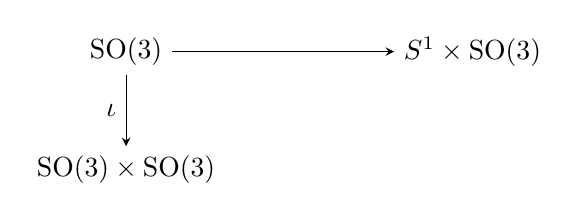
\begin{tikzpicture}[baseline=(current bounding box.center),>=stealth]
  \node (a) at (0,0) {$\operatorname{SO}(3)$};
  \node (b) at (4.4,0) {$S^1\times\operatorname{SO}(3)$};
  \node (c) at (0,-1.5) {$\operatorname{SO}(3)\times\operatorname{SO}(3)$};
  \draw[->] (a) -- (b);
  \draw[->] (a) -- node[left] {$\iota$} (c);
\end{tikzpicture}
\]
竖直同态 $\iota$ 把 $\operatorname{SO}(3)$ 识别为
$\operatorname{SO}(3)\times\operatorname{SO}(3)$ 的对角子群。因此，在同伦理论意义下，
$G$ 是 $\operatorname{SO}(3)\times\operatorname{SO}(3)$ 与
$S^1\times\operatorname{SO}(3)$ 沿 $\operatorname{SO}(3)$ 的\BookRecordIndex{T0068}并合自由积。注意，子群
$S^1\times\operatorname{SO}(3)$ 作为 Hirzebruch 结构 $J_2$ 的自同构群出现在 $G$ 中；
同样，$\operatorname{SO}(3)\times\operatorname{SO}(3)$ 是乘积结构 $J_0$ 的自同构群。
这一思路在 Abreu--Granja--Kitchloo 的论文 \srcite{4} 中达到顶点。

人们或许希望在吹起 $S^2\times S^2$ 的若干点时证明类似结果。Lalonde 和 Pinsonnault
\srcite{229} 在研究单点吹起的\BookRecordIndex{T0362}辛微分同胚群时，发现该群的拓扑与吹起和两个球面的大小
之比之间存在非常有趣的相互作用。另一种观点见 Seidel \srcite{372, Example 1.13}。

现在转入本节开头三个定理的证明。它们的逻辑顺序就是陈述顺序，因为每个定理的证明都
依赖前一个定理。也请注意它与上一节的平行之处。

在证明定理~\ref{thm:9-5-1} 前先引入一些记号。简记
\[
  M:=S^2\times S^2.
\]
由于 $(M,\omega)$ 单调，每个 $\omega$-\BookRecordIndex{T0348}相容\BookRecordIndex{T0088}殆复结构
$J\in\mathcal J:=\mathcal J(M,\omega)$ 都满足命题~\ref{prop:9-4-4} 的假设，即每个
非常值 $J$-全纯球面都有正 Chern 数。以
\[
  A:=[S^2\times\{\mathrm{pt}\}],
  \qquad B:=[\{\mathrm{pt}\}\times S^2]
\]
表示 $H_2(M;\mathbb Z)$ 的标准生成元。令
\[
  \operatorname{Symp}_0:=\operatorname{Symp}_0(M,\omega)
\]
表示在 $H_2(M;\mathbb Z)$ 上诱导恒等映射的辛微分同胚所成群。由于两个球面可以交换，
商群
$\operatorname{Symp}(M,\omega)/\operatorname{Symp}_0(M,\omega)$ 有两个元素。我们需要
证明子群 $\operatorname{Symp}_0(M,\omega)$ 同伦等价于
$\operatorname{SO}(3)\times\operatorname{SO}(3)$。

\begin{proof}[定理~\ref{thm:9-5-1} 的证明]
群 $\operatorname{Symp}_0$ 按
\[
  \operatorname{Symp}_0\times\mathcal J\longrightarrow\mathcal J,
  \qquad(\psi,J)\longmapsto\psi_*J
\]
作用在 $\mathcal J$ 上。乘积复结构 $J_0\in\mathcal J$ 的稳定子是
$\operatorname{SO}(3)\times\operatorname{SO}(3)\subset\operatorname{Symp}_0$。
所以，$\operatorname{Symp}_0$ 在 $J_0$ 上的作用通过
\[
  \operatorname{Symp}_0/
  \bigl(\operatorname{SO}(3)\times\operatorname{SO}(3)\bigr)
  \longrightarrow\mathcal J,
  \qquad\psi\longmapsto\psi_*J_0
\]
把这个商空间与 $J_0$ 的轨道识别起来。该映射显然不是满射；例如，它的像中每个元素都
可积。我们的目标是证明该映射有左逆。

基本思路是：对每个 $J$，指定 $M$ 中通过点 $(0,0)$、分别表示类 $A,B$ 的两个嵌入
$J$-全纯球面。然后还必须为这两条曲线选取参数化。给定两个全纯参数化，正如定理
~\ref{thm:9-4-7}(i) 的证明，可得到微分同胚 $f_J:M\to M$；再用 Moser 同痕以典范方式
把它同痕到一个辛微分同胚。所得辛微分同胚依赖于所选两个 $J$-全纯球面的参数化；模掉
$\operatorname{SO}(3)\times\operatorname{SO}(3)$ 中元素的右乘后，它并非良定义。我们
可以像习题~\ref{ex:7-2-4} 那样选取平衡参数化来绕开这个问题，但从 $\psi_*J_0$ 得到的
陪集未必等于原陪集
$\psi\circ(\operatorname{SO}(3)\times\operatorname{SO}(3))$，尽管二者会以典范方式
同伦。因此，这种做法构造的是同伦左逆。

为了构造严格左逆，注意辛微分同胚 $\psi\in\operatorname{Symp}_0$ 不仅给出\BookRecordIndex{T0088}殆复结构
$J:=\psi_*J_0$，还给出相关两条 \BookRecordIndex{T0003}$J$-全纯曲线的参数化
\[
  z\longmapsto\psi(z,w_*),
  \qquad w\longmapsto\psi(z_*,w),
\]
其中 $\psi(z_*,w_*)=(0,0)$。这提示我们把两条曲线的参数化也纳入参数空间
$\mathcal J$；换言之，考察\BookRecordIndex{T0268}普适模空间
\[
  \mathcal M_0:=\bigl\{(u,v,J)\bigm|
  J\in\mathcal J, u\in\mathcal M(A;J),\ v\in\mathcal M(B;J),
  \ (0,0)\in\operatorname{im}u\cap\operatorname{im}v\bigr\}.
\]
\BookRecordIndex{T0413}重参数化群 $G\times G$ 在这个空间上自由右作用。把命题~\ref{prop:9-4-4} 用于 $p=0$
可知，$(G\times G)$-不变投影 $\mathcal M_0\to\mathcal J$ 是浸没，其纤维就是
$(G\times G)$-轨道。换言之，$\mathcal M_0$ 是结构群为 $G\times G$、底空间为可缩空间
$\mathcal J$ 的主丛。因此它同伦等价于 $G\times G$，进而同伦等价于
$\operatorname{SO}(3)\times\operatorname{SO}(3)$。

考察交换图
\[
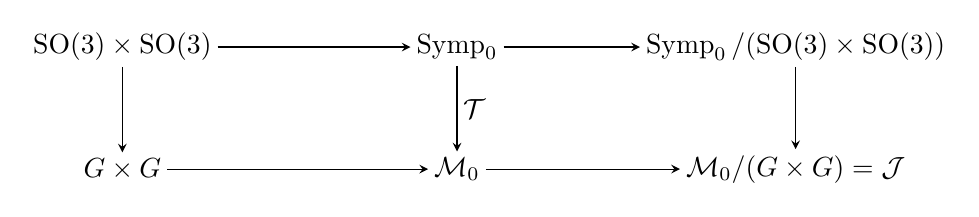
\begin{tikzpicture}[baseline=(current bounding box.center),>=stealth,
  every node/.style={inner sep=2pt}]
  \node (a) at (0,0) {$\operatorname{SO}(3)\times\operatorname{SO}(3)$};
  \node (b) at (4.25,0) {$\operatorname{Symp}_0$};
  \node (c) at (8.55,0)
    {$\operatorname{Symp}_0/(\operatorname{SO}(3)\times\operatorname{SO}(3))$};
  \node (d) at (0,-1.55) {$G\times G$};
  \node (e) at (4.25,-1.55) {$\mathcal M_0$};
  \node (f) at (8.55,-1.55) {$\mathcal M_0/(G\times G)=\mathcal J$};
  \draw[->] (a) -- (b);
  \draw[->] (b) -- (c);
  \draw[->] (d) -- (e);
  \draw[->] (e) -- (f);
  \draw[->] (a) -- (d);
  \draw[->] (b) -- node[right] {$\mathcal T$} (e);
  \draw[->] (c) -- (f);
\end{tikzpicture}
\]
其中嵌入 $\mathcal T:\operatorname{Symp}_0\to\mathcal M_0$ 定义为
\[
  \mathcal T(\psi)
  :=\bigl(\psi(\,·,w_*),\psi(z_*,\,·),\psi_*J_0\bigr),
  \qquad(z_*,w_*):=\psi^{-1}(0,0).
\]
由于 $\mathcal T$ 关于 $\operatorname{SO}(3)\times\operatorname{SO}(3)$ 的右作用等变，
它诱导出从
$\operatorname{Symp}_0/(\operatorname{SO}(3)\times\operatorname{SO}(3))$ 到可缩空间
$\mathcal M_0/(\operatorname{SO}(3)\times\operatorname{SO}(3))$ 的连续映射。因此诱导映射
$\mathcal T:\operatorname{SO}(3)\times\operatorname{SO}(3)\to\mathcal M_0$ 是同伦等价。
而 $\mathcal T$ 在 $\operatorname{SO}(3)\times\operatorname{SO}(3)$ 上单射，其像为
\[
  \mathcal M_{00}:=\bigl\{(u,v,J_0)\bigm|
  u(z)=(\phi(z),0),\ v(w)=(0,\phi'(w)),\
  \phi,\phi'\in\operatorname{SO}(3)\bigr\}.
\]
故存在同伦 $\Psi_t:\mathcal M_0\to\mathcal M_0$（$0\le t\le1$），满足
\[
  \Psi_0(\mathcal M_0)\subset\mathcal M_{00},
  \qquad \Psi_1=\operatorname{id},
  \qquad \Psi_t|_{\mathcal M_{00}}=\operatorname{id}\quad(0\le t\le1).
\]
所以，只要构造 $\mathcal T$ 的左逆
$\mathcal F:\mathcal M_0\to\operatorname{Symp}_0$，复合
\[
  \mathcal F\circ\Psi_t\circ\mathcal T:
  \operatorname{Symp}_0\longrightarrow\operatorname{Symp}_0
\]
就给出所需的变形收缩，把 $\operatorname{Symp}_0$ 收缩到
$\operatorname{SO}(3)\times\operatorname{SO}(3)$。

如下构造 $\mathcal F:\mathcal M_0\to\operatorname{Symp}_0$。三元组
$(u,v,J)\in\mathcal M_0$ 决定两个光滑映射
\[
  S^2\longrightarrow\mathcal M(A;J)/G:w\longmapsto[u_w],
  \qquad
  S^2\longrightarrow\mathcal M(B;J)/G:z\longmapsto[v_z],
\]
使得 $u(z)\in\operatorname{im}[v_z]$ 且
$v(w)\in\operatorname{im}[u_w]$。定义
$\psi=\psi_{u,v,J}:M\to M$ 为
\[
  \psi(z,w):=\operatorname{im}[u_w]\cap\operatorname{im}[v_z].
\]
定理~\ref{thm:9-4-7} 的证明说明，该映射是微分同胚，而且
\begin{equation}\label{eq:9-5-2}
  \psi(z,w_*)=u(z),
  \qquad \psi(z_*,w)=v(w)
\end{equation}
对所有 $z,w\in S^2$ 成立；其中 $z_*,w_*\in S^2$ 选成满足
$u(z_*)=v(w_*)=(0,0)$。该证明还说明，
\[
  \omega_t:=\omega+t(\psi^*\omega-\omega)
\]
对 $0\le t\le1$ 都是\BookRecordIndex{T0363}辛形式。由于 $\psi$ 在 $H^2(M;\mathbb R)$ 上作用为恒等映射，这些
形式彼此上同调。故可用典范 Moser 同痕把 $\psi$ 变形成辛微分同胚：由注
~\ref{rem:9-4-9}，存在只依赖 $\psi$ 的道路 $f_t\in\operatorname{Diff}(M)$，使
$f_0=\operatorname{id}$ 且
\[
  f_1^*\psi^*\omega=\omega.
\]
定义
\[
  \mathcal F(u,v,J):=\psi_{u,v,J}\circ f_1.
\]
注意，只要 $\psi_{u,v,J}$ 本身是辛微分同胚，就有
$\mathcal F(u,v,J)=\psi_{u,v,J}$。所以由式~\eqref{eq:9-5-2}，
$\mathcal F\circ\mathcal T=\operatorname{id}:\operatorname{Symp}_0\to
\operatorname{Symp}_0$，正合所需。定理得证。
\end{proof}


\begin{remark}\label{rem:9-5-5}
定理~\ref{thm:9-5-1} 中，只须证明
$\operatorname{Symp}_0/(\operatorname{SO}(3)\times\operatorname{SO}(3))$ 的所有同伦群
都消失，因为这个商空间具有某个可数 CW 复形的弱同伦型。

这个经典结果似乎没有显然可引的出处，故在此概述论证细节。由 Milnor
\srcite{288, Theorem 1}，只需证明当 $M$ 是闭\BookRecordIndex{T0358}辛流形时，$\operatorname{Symp}(M)$ 具有
\BookRecordIndex{T0206}绝对邻域收缩核（ANR）的同伦型。由 Moser 同痕论证，$\operatorname{Symp}(M)$ 是
$\operatorname{Diff}(M)$ 某个开子集的变形收缩核。因此，只须验证
$\operatorname{Diff}(M)$ 是 ANR。Kriegl--Michor \srcite{218} 指出，
$\operatorname{Diff}(M)$ 自由作用在把 $M$ 光滑嵌入某个固定 Hilbert 空间
$\mathcal H$ 的可缩空间 $\operatorname{Emb}(M,\mathcal H)$ 上。该嵌入空间是 Fréchet
空间的开子集，因而是 ANR。此外，$\operatorname{Diff}(M)$ 是如下投影的纤维：从
$\operatorname{Emb}(M,\mathcal H)$ 投到光滑 Fréchet 流形 $\mathcal M(M)$，后者由
$\mathcal H$ 中所有与 $M$ 微分同胚的嵌入子流形组成。因此，
$\operatorname{Diff}(M)$ 又是 $\operatorname{Emb}(M,\mathcal H)$ 某个开子集的收缩核，
故其自身也是 ANR。
\end{remark}

为了阐明 $S^2\times S^2$ 与 $\mathbb R^4$ 的\BookRecordIndex{T0362}辛微分同胚群之间的关系，考察支撑在闭
双圆盘 $\Delta_r:=D_r\times D_r$ 中的辛微分同胚所成群
$\operatorname{Symp}_{\Delta_r}(\mathbb R^4,\omega_0)$。可把这个群识别为
\[
  \mathcal G_\varepsilon
  :=\bigl\{\psi\in\operatorname{Symp}(S^2\times S^2,\omega)
    \bigm|\psi|_{X_\varepsilon}=\operatorname{id}\bigr\},
\]
其中
\[
  X_\varepsilon:=(S^2\times D_\varepsilon)\cup(D_\varepsilon\times S^2),
  \qquad D_\varepsilon\subset\mathbb C\subset S^2.
\]
$\varepsilon,r$ 的具体取值无关紧要。

\begin{lemma}\label{lem:9-5-6}
当 $r<R$ 时，包含映射
\[
  \operatorname{Symp}_{\Delta_r}(\mathbb R^4,\omega_0)
  \lhook\joinrel\longrightarrow
  \operatorname{Symp}_{\Delta_R}(\mathbb R^4,\omega_0)
\]
零伦。
\sourcefootnote{原书在本引理中把环境写成 $\mathbb R^{2n}$，但此处
$\Delta_r=D_r\times D_r$、与 $S^2\times S^2$ 的紧化以及紧随其后的整个证明都只针对
$\mathbb R^4$；故把环境唯一补正为 $\mathbb R^4$。}
\end{lemma}

\begin{proof}
需要证明，对 $\delta<\varepsilon$，包含
$\mathcal G_\varepsilon\hookrightarrow\mathcal G_\delta$ 同伦于常值映射。考察
\[
  \mathcal J_\varepsilon
  :=\bigl\{J\in\mathcal J(S^2\times S^2,\omega)
  \bigm|J|_{X_\varepsilon}=J_0\bigr\}.
\]
我们将构造光滑映射
$\mathcal F:\mathcal J_\varepsilon\to\mathcal G_\delta$，使对每个
$\psi\in\mathcal G_\varepsilon$ 都有
$\mathcal F(\psi_*J_0)=\psi$。结论便由 $\mathcal J_\varepsilon$ 可缩\BookRecordIndex{T0326}推出。

为构造 $\mathcal F$，采用定理~\ref{thm:9-4-7}(ii) 证明中的论证。在当前情形，
$X_\varepsilon$ 是
$(S^2\times\{0\})\cup(\{0\}\times S^2)$ 的邻域，故取 $z_*=w_*=0$，并定义
\[
  u_*(z)=(z,0),
  \qquad v_*(w)=(0,w).
\]
对每个 $J\in\mathcal J_\varepsilon$，如前定义
$\psi_J\in\operatorname{Diff}(S^2\times S^2)$。于是
\[
  \psi_J(z,w)=\operatorname{im}u_w\cap\operatorname{im}v_z,
\]
其中 $[u_w]\in\mathcal M(A;J)$ 由 $(0,w)\in\operatorname{im}u_w$ 确定，
$[v_z]\in\mathcal M(B;J)$ 由 $(z,0)\in\operatorname{im}v_z$ 确定。该映射形如
\[
  \psi_J(z,w)=
  \begin{cases}
    (z,\phi_2(z,w)),&z\in D_\varepsilon,\\
    (\phi_1(z,w),w),&w\in D_\varepsilon,
  \end{cases}
\]
其中对所有 $z,w\in S^2$，$\phi_1(z,0)=z$ 且 $\phi_2(0,w)=w$。为使该映射在
$X_\delta$ 上为恒等映射，一劳永逸地选定光滑映射 $\rho:S^2\to S^2$，满足
\[
  \rho(z)=z\quad(z\notin D_\varepsilon),
  \qquad \rho=0\quad\text{在 $D_\delta$ 的一个邻域中},
  \qquad \det(d\rho(z))\ge0.
\]
定义 $\psi'_J:M\to M$：在 $M\setminus X_\varepsilon$ 上令
$\psi'_J:=\psi_J$，而在 $X_\varepsilon$ 上令
\[
  \psi'_J(z,w):=
  \begin{cases}
    (z,\phi_2(\rho(z),w)),&z\in D_\varepsilon,\\
    (\phi_1(z,\rho(w)),w),&w\in D_\varepsilon.
  \end{cases}
\]
如前，$\psi'_J=\operatorname{id}$ 在 $X_\delta$ 的一个邻域中成立；而对所有
$z,w\in S^2$，子流形 $\{z\}\times S^2$ 与 $S^2\times\{w\}$ 相对于
$(\psi'_J)^*\omega$ 都是辛的。因此
\[
  \omega\wedge(\psi'_J)^*\omega>0
\]
（习题~\ref{ex:9-4-8}），从而可使用 Moser 同痕。具体而言，满足
\[
  d^*\beta_J=0,
  \qquad d\beta_J=(\psi'_J)^*\omega-\omega
\]
的 $1$-形式 $\beta_J$ 在 $X_\delta$ 的一个邻域中正合，故可按典范方式修改为在
$X_\delta$ 上消失。于是得到只依赖 $\psi'_J$ 的微分同胚 $f_J:M\to M$，满足
\[
  f_J^*(\psi'_J)^*\omega=\omega,
  \qquad f_J|_{X_\delta}=\operatorname{id}.
\]
现在定义
\[
  \mathcal F:\mathcal J_\varepsilon\longrightarrow\mathcal G_\delta,
  \qquad \mathcal F(J):=\psi'_J\circ f_J.
\]
对每个 $\psi\in\mathcal G_\varepsilon$，它满足
$\mathcal F(\psi_*J_0)=\psi$。事实上，若 $J=\psi_*J_0$，则
$\psi_J=\psi$ 在 $X_\varepsilon$ 上是恒等映射，故
$\psi'_J=\psi_J$ 且 $f_J=\operatorname{id}$。引理得证。
\end{proof}

\begin{proof}[定理~\ref{thm:9-5-2} 的证明]
结论由引理~\ref{lem:9-5-6} \BookRecordIndex{T0326}推出。选取实数 $r>0$ 与 $T>1$，使
\[
  \frac1T V\subset\Delta_r\subset\operatorname{int}(V),
\]
并对 $1\le t\le T$ 考察映射族
\[
  \mathcal F_t:\operatorname{Symp}_V(\mathbb R^4,\omega_0)
  \longrightarrow\operatorname{Symp}_V(\mathbb R^4,\omega_0),
  \qquad \mathcal F_t(\phi)(x):=\frac1t\phi(tx).
\]
对每个 $\phi\in\operatorname{Symp}_V(\mathbb R^4,\omega_0)$ 有
$\mathcal F_1(\phi)=\phi$；对所有 $t$ 有
$\mathcal F_t(\operatorname{id})=\operatorname{id}$；并且
\[
  \mathcal F_T\bigl(\operatorname{Symp}_V(\mathbb R^4,\omega_0)\bigr)
  \subset\operatorname{Symp}_{\Delta_r}(\mathbb R^4,\omega_0).
\]
\sourcefootnote{原书在这一个包含式的左端把标准形式下标漏掉，写成了
$\operatorname{Symp}_V(\mathbb R^4,\omega)$；本证明始终固定的是
$\omega_0$，而缩放公式也保持 $\omega_0$，故补上该下标。}
由引理~\ref{lem:9-5-6}，包含
$\operatorname{Symp}_{\Delta_r}(\mathbb R^4,\omega_0)
\hookrightarrow\operatorname{Symp}_V(\mathbb R^4,\omega_0)$ 零伦。因此可把
$\mathcal F_t$ 延拓为区间 $1\le t\le T+1$ 上的同伦，使对每个
$\psi\in\operatorname{Symp}_V(\mathbb R^4,\omega_0)$ 都有
$\mathcal F_{T+1}(\psi)=\operatorname{id}$。所以该群可缩。定理得证。
\end{proof}
\begin{proof}[定理~\ref{thm:9-5-3} 的证明]
为突出主要思想，先证明 $\mathbb{CP}^2$ 的\BookRecordIndex{T0362}辛微分同胚群连通。以
$A:=[\mathbb{CP}^1]\in H_2(\mathbb{CP}^2;\mathbb Z)$ 表示标准生成元，以
$\omega_{\mathrm{FS}}\in\Omega^2(\mathbb{CP}^2)$ 表示满足
$\omega_{\mathrm{FS}}(A)=\pi$ 的 Fubini--Study 形式，并以
$J_0\in\mathcal J:=\mathcal J(\mathbb{CP}^2,\omega_{\mathrm{FS}})$ 表示标准复结构。

给定 $\psi\in\operatorname{Symp}(\mathbb{CP}^2,\omega_{\mathrm{FS}})$，选取从 $J_0$ 到
$J_1=\psi_*J_0$ 的\BookRecordIndex{T0088}殆复结构光滑同伦
$[0,1]\to\mathcal J:t\mapsto J_t$。
\sourcefootnote{原书把终点印作 $J_1=\psi_*J$，但此处只给定了初始标准结构 $J_0$，并且
随后要求 $u_1=\psi\circ u_0$；唯一\BookRecordIndex{T0348}相容的终点是 $\psi_*J_0$。}
由推论~\ref{cor:9-4-5}，存在一族光滑依赖于 $t$、模重参数化唯一的 $J_t$-全纯球面
$u_t\in\mathcal M(A;J_t)$，满足
\[
  u_t(0)=[1:0:0],
  \qquad u_t(\infty)=[0:1:0],
  \qquad u_0(z)=[1:z:0],
  \qquad u_1=\psi\circ u_0.
\]
\sourcefootnote{原书同时固定所有 $u_t$ 的两个\BookRecordIndex{T0066}标记点之像，并要求
$u_1=\psi\circ u_0$；但一般的 $\psi$ 不固定 $[1:0:0]$ 与 $[0:1:0]$，故这些条件并不
\BookRecordIndex{T0348}相容。一种可能的补法是让\BookRecordIndex{T0066}标记点之像随 $t$ 移动，但原书未指定具体选择。后续实际需要的
是连接 $u_0$ 与 $\psi\circ u_0$ 的带\BookRecordIndex{T0067}标架曲线族，因而论证意图仍可辨认。}
这里把 $S^2\cong\mathbb C\cup\{\infty\}$。由于 $S^2$ 单连通，存在辛向量丛同构的光滑
同伦
\[
  \Psi_t:(u_0^*T\mathbb{CP}^2,J_0,\omega_{\mathrm{FS}})
  \longrightarrow(u_t^*T\mathbb{CP}^2,J_t,\omega_{\mathrm{FS}}),
\]
从 $\Psi_0:=\operatorname{id}$ 连到 $\Psi_1:=d\psi(u_0)$，并在如下意义下与 $du_t$ \BookRecordIndex{T0348}相容：
\begin{equation}\label{eq:9-5-3}
  \Psi_0=\operatorname{id},
  \qquad \Psi_tdu_0=du_t,
  \qquad \Psi_tJ_0=J_t\Psi_t,
  \qquad \Psi_t^*\omega_{\mathrm{FS}}=\omega_{\mathrm{FS}}.
\end{equation}
称三元组 $\{J_t,u_t,\Psi_t\}_{0\le t\le1}$ 为 \BookRecordIndex{T0003}$J$-全纯曲线的\emph{\BookRecordIndex{T0085}带标架同痕}。
我们希望构造\BookRecordIndex{T0361}辛同痕
\[
  [0,1]\longrightarrow\operatorname{Symp}(\mathbb{CP}^2,\omega_{\mathrm{FS}}),
  \qquad t\longmapsto\psi_t,
\]
从 $\psi_0=\operatorname{id}$ 连到 $\psi_1=\psi$，并使
\begin{equation}\label{eq:9-5-4}
  \psi_t\circ u_0=u_t,
  \qquad d\psi_t(u_0)=\Psi_t.
\end{equation}
按通常方式，寻找由一族哈密顿函数 $H_t$ 生成的同痕：
\begin{equation}\label{eq:9-5-5}
  \frac d{dt}\psi_t=X_t\circ\psi_t,
  \qquad \iota(X_t)\omega_{\mathrm{FS}}=dH_t.
\end{equation}
回忆，$H_t$ 的辛梯度 $X_t$ 与它相对于度量
$\omega_{\mathrm{FS}}(\,·,J_t\,·)$ 的梯度之间满足
$\operatorname{grad}H_t=J_tX_t$。

式~\eqref{eq:9-5-4} 的第一个条件转化为
\[
  X_t(u_t(z))=\partial_t\psi_t(u_0(z))=\partial_tu_t(z),
  \qquad z\in S^2.
\]
为满足第二个条件，还必须控制 $X_t$ 沿曲线 $\operatorname{im}u_t$ 法方向的导数。事实上，
对每个 $v\in T_{u_0(z)}\mathbb{CP}^2$，需要
\[
\begin{aligned}
  \nabla_t(\Psi_t(z)v)
  &=\nabla_t(d\psi_t(u_0(z))v)\\
  &=\nabla_{d\psi_t(u_0(z))v}X_t(\psi_t(u_0(z)))\\
  &=\nabla_{\Psi_t(z)v}X_t(u_t(z)).
\end{aligned}
\]
这里 $\nabla$ 表示度量 $\omega_{\mathrm{FS}}(\,·,J_t\,·)$ 的 \BookRecordIndex{T0034}Levi--Civita 联络
\sourcefootnote{原书此处写作 $\omega(\,\cdot,J_t\,\cdot)$，但本段的靶流形是
$\mathbb{CP}^2$，其固定\BookRecordIndex{T0363}辛形式为 $\omega_{\mathrm{FS}}$；本节此前的裸记号 $\omega$
专指 $S^2\times S^2$ 上的乘积形式，故补全下标。}，$\nabla_t$
表示相对于时间的协变微分。用 $\operatorname{grad}H_t=J_tX_t$ 表示后，这些条件成为
\begin{equation}\label{eq:9-5-6}
  \begin{aligned}
    \operatorname{grad}H_t(u_t)&=J_t(u_t)\partial_tu_t,\\
    \nabla_{\Psi_tv}(\operatorname{grad}H_t)
      &=J_t\nabla_t(\Psi_tv)
        +(\nabla_{\Psi_t(v)}J_t)\partial_tu_t,
        \qquad v\in u_0^*T\mathbb{CP}^2.
  \end{aligned}
\end{equation}
由于 $\Psi_tdu_0=du_t$，当 $v\in\operatorname{im}du_0(z)$ 时第二个方程归结为第一个。
所以这些条件彼此\BookRecordIndex{T0348}相容，并存在解 $H_t$。

现令 $\{\psi_t\}_{0\le t\le1}$ 是由哈密顿函数 $H_t$ 经式~\eqref{eq:9-5-5} 生成、且
满足 $\psi_1=\psi$ 的\BookRecordIndex{T0158}哈密顿同痕。由式~\eqref{eq:9-5-6}，$\psi_t$ 对每个 $t$ 都满足
式~\eqref{eq:9-5-4}。辛微分同胚 $\psi_0$ 未必等于恒等映射，不过，对每个
$x\in\mathbb{CP}^1:=\operatorname{im}u_0$ 与每个
$\xi\in T_x\mathbb{CP}^2$，它满足
\[
  \psi_0(x)=x,
  \qquad d\psi_0(x)\xi=\xi.
\]

还需两步把 $\psi_0$ 同痕到恒等映射。第一步是让 $\psi_0$ 在 $\mathbb{CP}^1$ 的某个
邻域上等于恒等映射；这可用 Moser 同痕做到。先选取从 $\psi_0$ 到一个在
$\mathbb{CP}^1$ 附近等于恒等映射的微分同胚之光滑同痕，再对拉回微分形式作同痕。由于
$\psi_0$ 沿 $\mathbb{CP}^1$ 已经与恒等映射符合到一阶，可把这些同痕取得
$C^1$-小，因此上述做法成立。论证与辛邻域定理的证明相同（见
\srcite{277, Theorem 3.30}），这里不再重复。第二步是在保持
$\mathbb{CP}^1$ 的一个邻域不动的同时，把所得辛微分同胚同痕到恒等映射；这立即来自定理
~\ref{thm:9-5-2} 与习题~\ref{ex:9-4-11}。

至此已证明 $\mathbb{CP}^2$ 的\BookRecordIndex{T0362}辛微分同胚群连通。它收缩到 $\operatorname{PU}(3)$ 的证明
是同一论证的带参数版本。由于
$\operatorname{Symp}(\mathbb{CP}^2,\omega_{\mathrm{FS}})$ 具有可数 CW 复形的弱同伦型
（细节见注~\ref{rem:9-5-5}），只须证明：由紧光滑流形 $S$ 参数化的任意光滑辛微分
同胚族
\[
  S\longrightarrow\operatorname{Symp}(\mathbb{CP}^2,\omega_{\mathrm{FS}}),
  \qquad s\longmapsto\psi_s
\]
都同伦于光滑映射
$S\to\operatorname{PU}(3):s\mapsto\phi_s$。

第一步是为这样的映射 $S\to\operatorname{PU}(3)$ 找到适当候选。令
$x_0:=[1:0:0]=u_0(0)\in\mathbb{CP}^2$，并以
\[
  \operatorname{Sp}_0^+
  \subset\operatorname{Sp}(T_{x_0}\mathbb{CP}^2,\omega_{\mathrm{FS}})
\]
表示相对于标准内积对称正定的 $T_{x_0}\mathbb{CP}^2$ 之辛自同构的集合。也就是说，
$\operatorname{Sp}_0^+$ 是所有满足
\[
  \Psi_0^{-1}=-J_0\Psi_0J_0,
  \qquad \omega_{\mathrm{FS}}(v,J_0\Psi_0v)>0
  \quad(0\ne v\in T_{x_0}\mathbb{CP}^2)
\]
的 $\Psi_0\in\operatorname{Sp}(T_{x_0}\mathbb{CP}^2,\omega_{\mathrm{FS}})$ 之集合。注意
$\operatorname{Sp}_0^+$ 可缩（见 \srcite{277}）。此外，对
$T_{x_0}\mathbb{CP}^2$ 的每个 $\omega_{\mathrm{FS}}$-\BookRecordIndex{T0348}相容复自同构 $J$，存在唯一
$\Psi_0\in\operatorname{Sp}_0^+$ 使 $\Psi_0J_0=J\Psi_0$；它就是 $-JJ_0$ 的平方根。
因此存在唯一光滑映射
$S\to\operatorname{Sp}_0^+:s\mapsto\Psi_{0s}$，使
\[
  \Psi_{0s}J_0=J_s\Psi_{0s},
  \qquad J_s:=\psi_{s*}J_0.
\]
由于 $\operatorname{PU}(3)$ 是 $\mathbb{CP}^2$ 的等距群，存在唯一映射
$S\to\operatorname{PU}(3):s\mapsto\phi_s$，使对每个 $s\in S$ 都有
\[
  \phi_s(x_s)=x_0,
  \qquad d\phi_s(x_s)=(\Psi_{0s})^{-1}d\psi_s(x_s),
  \qquad x_s:=\psi_s^{-1}(x_0).
\]

现在断言映射
\[
  S\longrightarrow\operatorname{Symp}(\mathbb{CP}^2,\omega_{\mathrm{FS}}),
  \qquad s\longmapsto\psi_s\circ\phi_s^{-1}
\]
零伦。为看出这一点，以 $\mathcal M_0$ 表示所有三元组 $(J,u,\Psi)$ 所成的\BookRecordIndex{T0268}普适模空间，
其中 $J\in\mathcal J$，$u:S^2\to\mathbb{CP}^2$ 是满足 $u(0)=x_0$、表示类 $A$ 的
\BookRecordIndex{T0003}$J$-全纯曲线，而
$\Psi:u_0^*T\mathbb{CP}^2\to u^*T\mathbb{CP}^2$ 是满足
\[
  \Psi J_0=J\Psi,
  \qquad \Psi^*\omega_{\mathrm{FS}}=\omega_{\mathrm{FS}},
  \qquad \Psi du_0=du,
  \qquad \Psi(0)\in\operatorname{Sp}_0^+
\]
的\BookRecordIndex{T0067}标架。空间 $\mathcal M_0$ 可缩（见习题~\ref{ex:9-5-7}）。故存在 \BookRecordIndex{T0003}$J$-全纯曲线的
\BookRecordIndex{T0085}带标架同痕
\[
  S\times[0,1]\longrightarrow\mathcal M_0,
  \qquad(s,t)\longmapsto(J_{s,t},u_{s,t},\Psi_{s,t}),
\]
满足
\[
\begin{gathered}
  J_{s,0}=J_0,
  \qquad u_{s,0}=u_0,
  \qquad \Psi_{s,0}=\operatorname{id},\\
  J_{s,1}=J_s,
  \qquad u_{s,1}=\psi_s\circ\phi_s^{-1}\circ u_0,
  \qquad \Psi_{s,1}=d(\psi_s\circ\phi_s^{-1})(u_0).
\end{gathered}
\]
从这里起，论证与连通性的证明完全相同，只是三个步骤中的同痕都还依赖附加参数 $s$。
余下细节留作习题。定理得证。
\end{proof}

最后给出几个关于 $\mathbb{CP}^2$ 的习题。

\begin{exercise}\label{ex:9-5-7}
证明定理~\ref{thm:9-5-3} 的证明中的\BookRecordIndex{T0268}普适模空间 $\mathcal M_0$ 可缩。
\end{exercise}

\begin{exercise}\label{ex:9-5-8}
设 $J\in\mathcal J_\tau(\mathbb{CP}^2,\omega_{\mathrm{FS}})$，并记
$A:=[\mathbb{CP}^1]\in H_2(\mathbb{CP}^2;\mathbb Z)$。证明：对每个
$x\in\mathbb{CP}^2$ 和每条复直线 $L_x\subset T_x\mathbb{CP}^2$，存在唯一通过 $x$
且切于 $L_x$ 的 \BookRecordIndex{T0003}$J$-全纯曲线
$[u]\in\mathcal M(A;J)/G$。由此\BookRecordIndex{T0326}推出：对每个非零向量
$\xi\in T_x\mathbb{CP}^2$，以及每个满足 $x\notin C$、表示类 $A$ 的嵌入 $J$-全纯球面
$C\subset\mathbb{CP}^2$，存在唯一 \BookRecordIndex{T0003}$J$-全纯曲线
$u_\xi\in\mathcal M(A;J)$，满足
\[
  u_\xi(0)=x,
  \qquad du_\xi(0)1=\xi,
  \qquad u_\xi(\infty)\in C.
\]
证明对 $\lambda\in\mathbb C^*$ 有\sourcefootnote{原书把这里的参数范围写成
$\lambda\in\mathbb C$；但 $u_{\lambda\xi}$ 只对非零初速度 $\lambda\xi$ 定义，
故必须排除 $\lambda=0$。}
\[
  u_{\lambda\xi}(z)=u_\xi(\lambda z).
\]

\emph{提示：}用\BookRecordIndex{T0186}交点正性（定理~\ref{thm:2-6-3}）证明唯一性。为证明存在性，使用推论
~\ref{cor:9-4-5}，并考察像通过 $x$ 与
$\exp_x(2^{-\nu}\xi)$ 的序列 $u^\nu$。
\end{exercise}

\begin{exercise}\label{ex:9-5-9}
\begin{enumerate}[label=\textup{(\roman*)}]
\item 理解上述证明的另一种方法（它让人想起定理~\ref{thm:9-5-1} 的证明）是考察群
$\operatorname{Symp}(\mathbb{CP}^2,\omega_{\mathrm{FS}})$ 在 $\mathbb{CP}^2$ 中\emph{带
\BookRecordIndex{T0067}标架复直线}空间 $\mathcal{CL}$ 上的作用。这里一条带\BookRecordIndex{T0067}标架直线是三元组 $(J,u,\Psi)$，
其中 $J\in\mathcal J(\mathbb{CP}^2,\omega_{\mathrm{FS}})$，
$u:S^2\to\mathbb{CP}^2$ 是表示类 $A=[\mathbb{CP}^1]$ 的 $J$-全纯球面，而
$\Psi:u_0^*T\mathbb{CP}^2\to u^*T\mathbb{CP}^2$ 是满足
\[
  \Psi du_0=du,
  \qquad \Psi^*\omega_{\mathrm{FS}}=\omega_{\mathrm{FS}},
  \qquad \Psi^*J=J_0
\]
的向量丛同构（但不必满足归一化条件 $u(0)=x_0$，也不必满足
$\Psi(0)\in\operatorname{Sp}_0^+$）。证明
$\operatorname{Symp}(\mathbb{CP}^2,\omega_{\mathrm{FS}})$ 按
\[
  \psi_*(J,u,\Psi):=(\psi_*J,\psi\circ u,d\psi(u)\Psi)
\]
自由作用在 $\mathcal{CL}$ 上。进一步证明 $\mathcal{CL}$ 同伦等价于
$\operatorname{PU}(3)$。构造映射
\[
  \operatorname{Symp}(\mathbb{CP}^2,\omega_{\mathrm{FS}})
  \longrightarrow\mathcal{CL},
  \qquad
  \psi\longmapsto(\psi_*J_0,\psi\circ u_0,d\psi(u_0))
\]
的同伦逆。

\item 定义 $\mathbb{CP}^2$ 中\emph{带\BookRecordIndex{T0067}标架辛直线}空间 $\mathcal{SL}$ 为所有偶对
$(u,\Psi)$ 之集合，其中 $u:S^2\to\mathbb{CP}^2$ 是表示类 $A$ 的辛嵌入，而
$\Psi:u_0^*T\mathbb{CP}^2\to u^*T\mathbb{CP}^2$ 是满足
$\Psi du_0=du$ 与 $\Psi^*\omega_{\mathrm{FS}}=\omega_{\mathrm{FS}}$ 的向量丛同构。
证明 $\operatorname{Symp}(\mathbb{CP}^2,\omega_{\mathrm{FS}})$ 在
$\mathcal{SL}$ 上传递作用，一个点的稳定子可缩，并且 $\mathcal{SL}$ 同伦等价于
$\operatorname{PU}(3)$。
\end{enumerate}
\end{exercise}

\begin{exercise}\label{ex:9-5-10}
证明：对每个 $J\in\mathcal J_\tau(\mathbb{CP}^2,\omega_{\mathrm{FS}})$，\BookRecordIndex{T0246}模空间
$\mathcal M(A;J)/G$ 微分同胚于 $\mathbb{CP}^2$；对每个
$x\in\mathbb{CP}^2$，子集
\[
  \{[v]\in\mathcal M(A;J)/G\mid x\notin\operatorname{im}v\}
\]
微分同胚于 $\mathbb R^4$。（比较 McKay \srcite{282} 与 Sikorav \srcite{380}。）

\emph{提示 1：}证明：对每条光滑道路
$[0,1]\to\mathcal J_\tau(\mathbb{CP}^2,\omega_{\mathrm{FS}}):
\lambda\mapsto J_\lambda$，
\[
  \mathcal W:=\bigl\{(\lambda,[u])\bigm|
  \lambda\in[0,1],\ u\in\mathcal M(A;J_\lambda)/G\bigr\}
\]
都是乘积配边。

\emph{提示 2：}证明：对每个点 $x\in\mathbb{CP}^2$，存在唯一对偶直线 $L_x$，它相对于
Fubini--Study 度量与每条通过 $x$ 的直线正交。证明若 $x=[0:0:1]$，则 $L_x$ 是嵌入
\[
  \mathbb{CP}^1\longrightarrow\mathbb{CP}^2,
  \qquad[z_0:z_1]\longmapsto[z_0:z_1:0]
\]
的像。
\end{exercise}


\section{Hofer 几何}\label{sec:9-6}

Hofer 在 \srcite{177} 中定义了欧氏空间之紧支撑\BookRecordIndex{T0362}辛微分同胚群上的一个度量，并通过研究
相关哈密顿流的周期轨道发展了它的性质。Lalonde--McDuff \srcite{223,224} 采用了更具
几何味道的方法，把 \BookRecordIndex{T0027}Hofer 度量与\BookRecordIndex{T0156}哈密顿纤维化的若干问题联系起来。本节将解释
Polterovich 对这些思想的一项优美推广。我们的讨论会保持相当集中的范围；关于这个主题
的一般背景，读者可查阅 Polterovich \srcite{330,328} 或
\srcite{277, Chapter 12}。以下始终假设 $(M,\omega)$ 是紧\BookRecordIndex{T0358}辛流形。讨论中最重要的部分
将考察单调情形，不过下面说明的许多结果在更一般的情形仍成立。

设
\[
  \mathbb R\longrightarrow\operatorname{Symp}(M,\omega),
  \qquad t\longmapsto\psi_t=\psi_{t+1}
\]
是\BookRecordIndex{T0161}哈密顿辛微分同胚的环路。则存在光滑哈密顿函数
\[
  \mathbb R\longrightarrow C^\infty(M),
  \qquad t\longmapsto H_t,
\]
使每个 $t\in\mathbb R$ 都满足
\[
  \frac d{dt}\psi_t=X_{H_t}\circ\psi_t,
  \qquad H_t=H_{t+1}.
\]
为以后使用，最好把哈密顿函数归一化为平均值全为零：
\[
  \int_M H_t\omega^n=0.
\]
环路 $t\mapsto\psi_t$ 的 \emph{Hofer 长度}定义为
\[
  \ell(\{\psi_t\}):=\int_0^1\|H_t\|\,dt,
  \qquad
  \|H_t\|:=\max_MH_t-\min_MH_t.
\]
注意，这个长度不依赖上述归一化。

\begin{example}\label{ex:9-6-1}
设 $\omega_{\mathrm{FS}}\in\Omega^2(\mathbb{CP}^n)$ 是体积为 $\pi^n/n!$ 的
Fubini--Study 形式。考察环路
\[
  \mathbb R/\mathbb Z\longrightarrow
  \operatorname{Symp}(\mathbb{CP}^n,\omega_{\mathrm{FS}}),
  \qquad t\longmapsto\psi_t^k,
\]
其中
\[
  \psi_t^k([z_0:\cdots:z_n])
  :=[z_0:e^{2\pi it}z_1:\cdots:e^{2\pi it}z_k:z_{k+1}:\cdots:z_n].
\]
该环路由与时间无关的哈密顿函数
\begin{equation}\label{eq:9-6-1}
  H^k([z_0:\cdots:z_n])
  :=\pi\left(
    \frac{k}{n+1}
    -\frac{|z_1|^2+\cdots+|z_k|^2}
      {|z_0|^2+\cdots+|z_n|^2}
  \right)
\end{equation}
生成。由于 $\|H^k\|=\pi$，可得
\[
  \ell(\{\psi_t^k\})=\pi.
\]
Lalonde--McDuff 在 \srcite{224} 中证明，当 $n=k=1$ 时，环路
$t\mapsto\psi_t$ 不能通过哈密顿变形缩短。他们的论证使用嵌入球和以 $S^2$ 为底的
\BookRecordIndex{T0156}哈密顿纤维化之\BookRecordIndex{T0120}非挤压定理。本节的目的是解释 Polterovich 给出的另一种证明：它使用例
~\ref{ex:8-6-8} 的 \BookRecordIndex{T0047}Seidel 表示，并且对所有 $1\le k\le n$ 都成立。我们还将说明环路的
另一些几何定义的不变量；它们最终都与该环路的 Hofer 长度相等。
\end{example}

Polterovich 在 \srcite{325,326,327} 中考察了 $M$ 上\BookRecordIndex{T0161}哈密顿辛微分同胚环路
$\psi=\{\psi_t\}_{t\in\mathbb R/\mathbb Z}$ 所关联的三个不变量。第一个是所有与
$\psi$ \BookRecordIndex{T0158}哈密顿同痕的哈密顿环路之最小 Hofer 长度：
\[
  \lambda(\psi):=\inf_{\psi'\sim\psi}\ell(\psi').
\]
第二个是在由式~\eqref{eq:8-2-6} 定义的\BookRecordIndex{T0156}哈密顿纤维化
$\widetilde M_\psi$ 上，所有\BookRecordIndex{T0224}联络形式之曲率 $R_{\widetilde\omega}$ 的 \BookRecordIndex{T0028}Hofer 范数下确界：
\[
  \kappa(\psi):=
  \inf_{\widetilde\omega\in\mathcal T_0(\widetilde M_\psi)}
  \|R_{\widetilde\omega}\|.
\]
这里 $\mathcal T_0(\widetilde M_\psi)$ 表示注~\ref{rem:8-2-11} 中所有\BookRecordIndex{T0224}联络形式
$\widetilde\omega\in\Omega^2(\widetilde M_\psi)$ 所成空间。第三个是\emph{\BookRecordIndex{T0122}非辛区间的
长度}：
\[
  \varepsilon(\psi):=
  \inf_{\widetilde\omega_c^{n+1}>0}\int_{S^2}c\sigma
  -\sup_{\widetilde\omega_c^{n+1}<0}\int_{S^2}c\sigma.
\]
这里第一个下确界取遍所有\BookRecordIndex{T0224}联络形式
\[
  \widetilde\omega_c
  =\widetilde\omega+\pi^*(c\sigma)
  \in\Omega^2(\widetilde M_\psi),
\]
其中 $\widetilde\omega\in\mathcal T_0(\widetilde M_\psi)$、
$c\in\Omega^0(S^2)$，且 $\widetilde\omega_c^{n+1}>0$（等价地，
$c\circ\pi>R_{\widetilde\omega}$）。上确界作同样理解。

\begin{remark}\label{rem:9-6-2}
这个\BookRecordIndex{T0122}非辛区间长度与第~\ref{sec:9-3} 节末定义的以 $S^2$ 为底之辛纤维丛的面积有关。在
当前情形，该面积为
\[
  \operatorname{area}(\widetilde M_\psi,\widetilde\omega_c)
  :=\frac{\operatorname{Vol}(\widetilde M_\psi,\widetilde\omega_c)}
    {\operatorname{Vol}(M,\omega)}
  =\int_{S^2}c\sigma.
\]
所以
$\varepsilon(\psi)=\varepsilon^+(\psi)+\varepsilon^-(\psi)$，其中
$\varepsilon^+(\psi)$ 是 $\widetilde M_\psi$ 上一个\BookRecordIndex{T0224}联络形式的最小面积，而
$\varepsilon^-(\psi):=\varepsilon^+(\psi^{-1})$。上面定义的另两个不变量也都分解为两
部分之和，因为任意归一化函数 $R$ 的总变差 $\|R\|$ 可写成
$\|R\|_++\|R\|_-$，其中
\[
  \|R\|_+:=\max_MR,
  \qquad \|R\|_-:=-\min_MR=\|-R\|_+.
\]
事实上，Polterovich 的结果讨论的是这些“单侧”不变量。更多细节见 Polterovich
\srcite{325,326,327} 与 McDuff \srcite{271}。
\end{remark}

Polterovich 在 \srcite{325,326,327} 中证明这三个不变量全都相等。我们复述他对下述较弱
结论的证明。

\begin{proposition}[Polterovich]\label{prop:9-6-3}
设 $(M,\omega)$ 是紧\BookRecordIndex{T0358}辛流形，
$\psi=\{\psi_t\}_{t\in\mathbb R/\mathbb Z}$ 是 $M$ 的\BookRecordIndex{T0161}哈密顿辛微分同胚环路。则
\[
  \lambda(\psi)\ge\kappa(\psi)\ge\varepsilon(\psi).
\]
\end{proposition}

\begin{proof}
首先注意，存在\BookRecordIndex{T0224}联络形式
$\widetilde\omega\in\mathcal T_0(\widetilde M_\psi)$，使
\[
  \|R_{\widetilde\omega}\|=\ell(\psi).
\]
\sourcefootnote{原书在这里把\BookRecordIndex{T0224}联络形式所属空间印作
$\mathcal T(\widetilde M_\psi)$，但本节只定义并使用
$\mathcal T_0(\widetilde M_\psi)$；紧随其后的公式也正是注~\ref{rem:8-2-11} 中该空间的
\BookRecordIndex{T0224}联络形式，故补上下标 $0$。}
在注~\ref{rem:8-2-11} 的记号中，一个显式公式是
\[
  F_{s,t}^{\pm}:=0,
  \qquad G_{s,t}^+:=-\rho(s)H_t,
  \qquad G_{s,t}^-:=-\rho(s)H_{-t}\circ\psi_{-t},
\]
其中 $\rho:\mathbb R\to[0,1]$ 是光滑\BookRecordIndex{T0188}截断函数，在 $s\le-1$ 时消失，在 $s\ge1$ 时等于
一，并满足 $\rho(s)+\rho(-s)\equiv1$。

其次，若两个哈密顿环路 $\psi,\psi'$ \BookRecordIndex{T0158}哈密顿同痕，则相应\BookRecordIndex{T0156}哈密顿纤维化
$\widetilde M_\psi,\widetilde M_{\psi'}$（逐纤维）同构。为看出这一点，任取\BookRecordIndex{T0158}哈密顿同痕
\[
  \mathbb R\times\mathbb R/\mathbb Z
  \longrightarrow\operatorname{Symp}(M,\omega),
  \qquad(s,t)\longmapsto\psi_{s,t},
\]
使 $s\le-1$ 时 $\psi_{s,t}=\psi_t$，而 $s\ge1$ 时
$\psi_{s,t}=\psi'_t$。定义微分同胚
$\Psi:\widetilde M_\psi\to\widetilde M_{\psi'}$：在正平凡化上令
\[
  \Psi^+(s,t,x^+)
  :=(s,t,\psi_{s,t}\circ\psi_t^{-1}(x^+)),
\]
在负平凡化上令
\[
  \Psi^-(s,t,x^-)
  :=(s,t,(\psi'_{-t})^{-1}\circ\psi_{-s,-t}(x^-)).
\]
对每个
$\widetilde\omega'\in\mathcal T_0(\widetilde M_{\psi'})$，都有
$R_{\Psi^*\widetilde\omega'}=R_{\widetilde\omega'}\circ\Psi$，故
$\|R_{\Psi^*\widetilde\omega'}\|=\|R_{\widetilde\omega'}\|$。上面已经找到满足
$\|R_{\widetilde\omega'}\|=\ell(\psi')$ 的\BookRecordIndex{T0224}联络形式，因此
$\kappa(\psi)\le\lambda(\psi)$。

第三，证明 $\varepsilon(\psi)\le\kappa(\psi)$。固定 $\delta>0$，并选取\BookRecordIndex{T0224}联络形式
$\widetilde\omega\in\mathcal T_0(\widetilde M_\psi)$，使
\[
  \|R_{\widetilde\omega}\|<\kappa(\psi)+\delta.
\]
则存在光滑函数 $c,K:S^2\to\mathbb R$，使
\[
  c(z)<\min_{\pi^{-1}(z)}R_{\widetilde\omega}(z)
  \le\max_{\pi^{-1}(z)}R_{\widetilde\omega}(z)<K(z),
  \qquad
  \int_{S^2}(K-c)\sigma<\kappa(\psi)+\delta.
\]
记
$\widetilde\omega_c:=\widetilde\omega+\pi^*(c\sigma)$ 与
$\widetilde\omega_K:=\widetilde\omega+\pi^*(K\sigma)$。则
$\widetilde\omega_K^{n+1}>0$ 且
$\widetilde\omega_c^{n+1}<0$，因而
\[
  \varepsilon(\psi)
  \le\int_{S^2}(K-c)\sigma
  <\kappa(\psi)+\delta.
\]
该式对每个 $\delta>0$ 都成立，所以
$\varepsilon(\psi)\le\kappa(\psi)$。命题得证。
\end{proof}

\begin{proposition}[Polterovich--Seidel]\label{prop:9-6-4}
设
\[
  \mathbb{CP}^n\lhook\joinrel\longrightarrow
  \widetilde M^k\longrightarrow S^2
\]
是例~\ref{ex:9-6-1} 中环路 $\psi^k$ 所关联的\BookRecordIndex{T0156}哈密顿纤维化。则对
$k=1,\ldots,n$，存在同调类
$\widetilde A^k\in H_2(\widetilde M^k;\mathbb Z)$，使每个\BookRecordIndex{T0224}联络形式
$\widetilde\omega\in\mathcal T_0(\widetilde M^k)$ 都满足
\begin{equation}\label{eq:9-6-2}
  \mathcal S(\psi^k)=\mathcal S_{\widetilde A^k}(\psi^k)=c^{n+1-k},
  \qquad
  \int_{\widetilde A^k}\widetilde\omega
  =-\frac{\pi(n+1-k)}{n+1}.
\end{equation}
这里 $c\in H^2(\mathbb{CP}^n)$ 表示正生成元，而
$\mathcal S(\psi)\in H^*(\mathbb{CP}^n)$ 是例~\ref{ex:8-6-8} 中由式~\eqref{eq:8-6-4}
定义的。
\end{proposition}

\begin{proof}
环路
$\psi_t^k\in\operatorname{Symp}(\mathbb{CP}^n,\omega_{\mathrm{FS}})$ 保持度量，并由与
时间无关的哈密顿函数 $H^k:\mathbb{CP}^n\to\mathbb R$ 生成（见式
~\eqref{eq:9-6-1}）。因此，标准复结构 $J_0$ 在 $\widetilde M^k$ 上定义了\BookRecordIndex{T0306}竖直殆复结构。
在注~\ref{rem:8-2-11} 的记号中，一个\BookRecordIndex{T0224}联络形式
$\widetilde\omega\in\mathcal T_0(\widetilde M^k)$ 由公式
\begin{equation}\label{eq:9-6-3}
  F^\pm:=0,
  \qquad G_{s,t}^\pm:=-\rho(s)H^k
\end{equation}
给出，其中 $\rho:\mathbb R\to[0,1]$ 是光滑\BookRecordIndex{T0188}截断函数，满足：$s\le-1$ 时
$\rho(s)=0$，$s\ge1$ 时 $\rho(s)=1$，并且对所有 $s$，
$\dot\rho(s)\ge0$ 且 $\rho(s)+\rho(-s)=1$。注意
\[
  R_{\widetilde\omega}\sigma=-\dot\rho(s)H^k\,ds\wedge dt.
\]
以 $\widetilde J$ 表示由 $J_0,\widetilde\omega$ 决定的 $\widetilde M^k$ 上\BookRecordIndex{T0088}殆复结构，并以
$\mathcal M(\widetilde A;J_0,\widetilde\omega)$ 表示\BookRecordIndex{T0156}哈密顿纤维化
$\widetilde M^k\to S^2$ 的 $\widetilde J$-全纯截面空间。

现考察临界流形
\[
  Z^k:=\bigl\{[0:z_1:\cdots:z_k:0:\cdots:0]
  \bigm|(z_1,\ldots,z_k)\in\mathbb C^k\setminus\{0\}\bigr\}
  \subset\mathbb{CP}^n.
\]
函数 $H^k$ 在这个子流形上取得极小值
$\pi(k-n-1)/(n+1)$。每个常值映射
$u^\pm(s,t)\equiv x\in Z^k$ 都定义一个\BookRecordIndex{T0315}水平截面
$\widetilde u:S^2\to\widetilde M^k$，因而是 $\widetilde J$-全纯的。以
$\widetilde A^k\in H_2(\widetilde M^k;\mathbb Z)$ 表示这些常值截面
$\widetilde u$ 的同调类。由引理~\ref{lem:8-2-9}，
\[
\begin{aligned}
  \int_{\widetilde A^k}\widetilde\omega
  &=E^{\mathrm{Vert}}(\widetilde u)
    -\int_{S^2}(R_{\widetilde\omega}\circ\widetilde u)\sigma\\
  &=\int_0^1\int_{-\infty}^{\infty}
      \dot\rho(s)H^k(x)\,ds\,dt
   =\frac{\pi(k-n-1)}{n+1}.
\end{aligned}
\]
这说明式~\eqref{eq:9-6-2} 的第二个等式对某个\BookRecordIndex{T0224}联络形式成立，因而对每个
$\widetilde\omega\in\mathcal T_0(\widetilde M^k)$ 都成立。

考察沿取值于 $Z^k$ 的一个水平解的\BookRecordIndex{T0308}竖直切丛，可见它分裂成复线丛的直和：其中 $k-1$
个的 Chern 数为零（它们构成截面沿 $Z^k$ 切方向的\BookRecordIndex{T0117}法丛），另外 $n+1-k$ 个的 Chern 数
为 $-1$。所以竖直第一 Chern 数为
\[
  c_1^{\mathrm{Vert}}(\widetilde A^k)=k-1-n.
\]
此外，每个这类常值截面的\BookRecordIndex{T0346}线性化算子都是满射。下面证明该同调类中不可能有其他
$\widetilde J$-全纯截面。事实上，若
$\widetilde u=(u^+,u^-)\in
\mathcal M(\widetilde A^k;J_0,\widetilde\omega)$，则由引理~\ref{lem:8-2-9}，
\[
\begin{aligned}
  0&\le E^{\mathrm{Vert}}(\widetilde u)\\
   &=\int_{S^2}\widetilde u^*\widetilde\omega
     +\int_{S^2}(R_{\widetilde\omega}\circ\widetilde u)\sigma\\
   &=\frac{\pi(k-n-1)}{n+1}
     -\int_0^1\int_{-\infty}^{\infty}
       \dot\rho(s)H^k(u^\pm(s,t))\,ds\,dt\\
   &\le\frac{\pi(k-n-1)}{n+1}
     -\int_0^1\int_{-\infty}^{\infty}
       \dot\rho(s)\min_{\mathbb{CP}^n}H^k\,ds\,dt
    =0.
\end{aligned}
\]
因此处处取等号，每条表示类 $\widetilde A^k$ 的 $\widetilde J$-全纯曲线都必须水平，故
必为上面已考察的常值截面之一。（其他\BookRecordIndex{T0315}水平截面对应于 $H^k$ 的极大值；它们的 Chern 数
不同，因而不表示类 $\widetilde A^k$。）
\sourcefootnote{原书把括号中“其他\BookRecordIndex{T0315}水平截面”说成对应 $H^k$ 的极小值；但前文已说明
$Z^k$ 正是极小值流形，而其余固定分支是极大值流形。故把 minima 唯一补正为 maxima。}
现在\BookRecordIndex{T0283}求值映射
\[
  \operatorname{ev}_0:
  \mathcal M(\widetilde A^k;J_0,\widetilde\omega)
  \longrightarrow\mathbb{CP}^n
\]
显然是到 $Z^k$ 上的微分同胚。由于
$Z^k\subset\mathbb{CP}^n$ 是复维 $k-1$ 的射影子空间，便有
\[
  \operatorname{GW}^{\widetilde M^k,\{1\}}_{\widetilde A^k,1}(c^{k-1})=1,
  \qquad \mathcal S_{\widetilde A^k}(\psi^k)=c^{n+1-k}.
\]
为完成证明，还须说明
\[
  \widetilde A\ne\widetilde A^k
  \quad\Longrightarrow\quad
  \mathcal S_{\widetilde A}(\psi^k)=0.
\]
注意，若 $\mathcal S_{\widetilde A}(\psi^k)\ne0$，则 $\widetilde A$ 必须满足
\[
  \pi_*\widetilde A=[S^2],
  \qquad -n\le c_1^{\mathrm{Vert}}(\widetilde A)\le0.
\]
当 $1\le k\le n$ 时，唯一这样的类就是 $\widetilde A^k$。命题得证。
\end{proof}

\begin{theorem}[Polterovich]\label{thm:9-6-5}
设 $\psi^k=\{\psi_t^k\}_{t\in\mathbb R/\mathbb Z}$ 是例~\ref{ex:9-6-1} 中讨论的环路。
若 $k\in\{1,\ldots,n\}$，则
\[
  \lambda(\psi^k)=\kappa(\psi^k)=\varepsilon(\psi^k)=\pi.
\]
\end{theorem}

\begin{proof}
由命题~\ref{prop:9-6-3}，
\[
  \varepsilon(\psi^k)\le\kappa(\psi^k)
  \le\lambda(\psi^k)\le\pi.
\]
所以只须证明
$\varepsilon(\psi^k)\ge\pi$。为此，设
$\widetilde\omega\in\mathcal T_0(\widetilde M^k)$ 与
$c\in\Omega^0(S^2)$ 满足
\[
  \widetilde\omega_c^{n+1}>0,
  \qquad \widetilde\omega_c:=\widetilde\omega+c\sigma.
\]
令 $\widetilde A^k\in H_2(\widetilde M^k;\mathbb Z)$ 是命题~\ref{prop:9-6-4} 中的同调
类，并固定 $\mathbf w\in S^2$。由定理~\ref{thm:8-5-3}，正则偶对集合
$\mathcal{JH}_{\mathrm{reg}}(\widetilde M^k,\pi,\widetilde\omega;\mathbf w)$ 在
$\mathcal J^{\mathrm{Vert}}\times\mathcal H$ 中关于 $C^\infty$ 拓扑稠密。因此，对
$\widetilde\omega$ 作任意小的\BookRecordIndex{T0402}正合扰动后，可假设存在\BookRecordIndex{T0306}竖直殆复结构
$J\in\mathcal J^{\mathrm{Vert}}(\widetilde M^k,\pi,\widetilde\omega)$，使偶对 $(J,0)$
对 $\mathbf w$ 正则（定义~\ref{def:8-5-2} 的意义下），并且条件
$\widetilde\omega_c^{n+1}>0$ 仍然满足。记
$\mathcal M(\widetilde A^k;J,\widetilde\omega)$ 为 $\widetilde M^k$ 中表示类
$\widetilde A^k$ 的 $\widetilde J$-全纯截面之\BookRecordIndex{T0246}模空间，其中 $\widetilde J$ 是由
$J,\widetilde\omega$ 诱导的 $\widetilde M^k$ 上\BookRecordIndex{T0088}殆复结构（见引理~\ref{lem:8-2-8}）。
\sourcefootnote{原书在此处\BookRecordIndex{T0283}求值映射的定义域把\BookRecordIndex{T0246}模空间类漏写了上标 $k$，印作
$\mathcal M(\widetilde A;J,\widetilde\omega)$；本段始终固定命题~\ref{prop:9-6-4} 的类
$\widetilde A^k$，故补全。}
于是由定理~\ref{thm:8-5-1}，\BookRecordIndex{T0283}求值映射
\[
  \widetilde{\operatorname{ev}}_{\mathbf w}:
  \mathcal M(\widetilde A^k;J,\widetilde\omega)
  \longrightarrow\mathbb{CP}^n,
  \qquad
  \widetilde{\operatorname{ev}}_{\mathbf w}(\widetilde u)
  :=\widetilde\iota_{\mathbf w}^{-1}(\widetilde u(\mathbf w))
\]
是\BookRecordIndex{T0337}伪循环；由命题~\ref{prop:9-6-4}，它在 $\mathbb{CP}^n$ 中表示非零同调类。因此
$\mathcal M(\widetilde A^k;J,\widetilde\omega)\ne\varnothing$。由于
$\widetilde\omega_c$ 是 $\widetilde M^k$ 上的\BookRecordIndex{T0363}辛形式，这蕴含
\[
  0\le\langle[\widetilde\omega_c],\widetilde A^k\rangle
  =\int_{S^2}c\sigma-\frac{\pi(n+1-k)}{n+1},
\]
其中第二个等式来自式~\eqref{eq:9-6-2}。因此已证明
\[
  \inf_{\substack{
    \widetilde\omega\in\mathcal T_0(\widetilde M^k),\ c\in\Omega^0(S^2)\\
    \widetilde\omega_c^{n+1}>0}}
  \int_{S^2}c\sigma
  \ge\frac{\pi(n+1-k)}{n+1}.
\]
由于环路 $t\mapsto\psi_{-t}^k$ \BookRecordIndex{T0158}哈密顿同痕于
$t\mapsto\psi_t^{n+1-k}$，可得
\[
\begin{aligned}
  -\sup_{\substack{
    \widetilde\omega\in\mathcal T_0(\widetilde M^k),\ c\in\Omega^0(S^2)\\
    \widetilde\omega_c^{n+1}<0}}
  \int_{S^2}c\sigma
  &={}\inf_{\substack{
    \widetilde\omega\in\mathcal T_0(\widetilde M^{n+1-k}),\ c\in\Omega^0(S^2)\\
    \widetilde\omega_c^{n+1}>0}}
  \int_{S^2}c\sigma\\
  &\ge\frac{\pi k}{n+1}.
\end{aligned}
\]
合并这两个不等式，得到所需的
$\varepsilon(\psi^k)\ge\pi$。定理得证。
\end{proof}

\begin{remark}\label{rem:9-6-6}
\begin{enumerate}[label=\textup{(\roman*)}]
\item \BookRecordIndex{T0028}Hofer 范数在 $\operatorname{Ham}(M)$ 上给出一个\BookRecordIndex{T0313}双不变 Finsler 度量。（人们常稍微
滥用语言，把这个度量中从恒等元到
$\phi\in\operatorname{Ham}(M)$ 的距离
$d(\operatorname{id},\phi)$ 称为 $\phi$ 的\emph{\BookRecordIndex{T0028}Hofer 范数}。）在 Ostrover--Wagner
\srcite{317} 工作的基础上，Buhovsky 与 Ostrover \srcite{51} 最近证明，它是唯一一个
$C^\infty$-连续的这种度量。不过，$\operatorname{Ham}(M,\omega)$ 上还有并非 Finsler 型
的其他双不变度量；比较习题~12.4.8 与 Viterbo \srcite{404}。

\item Chekanov 在 \srcite{61} 中把 \BookRecordIndex{T0027}Hofer 度量推广到\BookRecordIndex{T0219}拉格朗日子流形空间。他证明：若
$(P,\omega)$ 是闭\BookRecordIndex{T0358}辛流形，而 $\mathcal L(P,\omega,L)$ 是给定\BookRecordIndex{T0219}拉格朗日子流形 $L$ 在
哈密顿群 $\operatorname{Ham}(P,\omega)$ 作用下的轨道，则可把两个\BookRecordIndex{T0219}拉格朗日子流形
$L_0,L_1$ 之间的距离取为所有如下道路
$\{\phi_t\}_{t\in[0,1]}$ 的长度下确界：它们位于
$\operatorname{Ham}(P,\omega)$ 中，并满足
$\phi_0=\operatorname{id}$ 与 $\phi_1(L_0)=L_1$。

\item Polterovich 估计哈密顿环路长度的方法也能推广到拉格朗日情形。Akveld 与 Salamon
在 \srcite{11} 中考察带拉格朗日边界条件、以圆盘为底的辛\BookRecordIndex{T0279}纤维化，由此为\BookRecordIndex{T0219}拉格朗日子流形
的环路定义了类似不变量。在有利情形，相对\BookRecordIndex{T0143}格罗莫夫--威滕不变量给出拉格朗日环路的一个
给定\BookRecordIndex{T0158}哈密顿同痕类中 Hofer 长度的下界。因此，对 $\mathbb{CP}^n$ 中实射影空间的环路，可以
仿照定理~\ref{thm:9-6-5} 得到显式长度估计。

\item 用 $(M,\omega)$ 的辛微分同胚之图代替该辛微分同胚，可把哈密顿群嵌入
$(M\times M,\pi_2^*\omega-\pi_1^*\omega)$ 的嵌入\BookRecordIndex{T0219}拉格朗日子流形空间。Ostrover
\srcite{315} 最近给出的一个优美例子说明，包含
\[
  \operatorname{Ham}(M,\omega)
  \lhook\joinrel\longrightarrow
  \mathcal L(M\times M,\pi_2^*\omega-\pi_1^*\omega,\operatorname{diag})
\]
会严重扭曲度量：他构造了
$\operatorname{Ham}(\mathbb T^{2n},\omega_0)$ 中一个直径无限的集合，而它在拉格朗日
空间中的像却有界。尽管如此，Akveld--Salamon \srcite{11} 的结果表明，Polterovich 的
环路长度估计足够稳健，至少在某些情形进入拉格朗日语境后仍然有效。Usher
\srcite{400} 描述了其他一些情形，其中 $\operatorname{Ham}(M)$ 的子集嵌入拉格朗日
空间时，度量不发生扭曲。

\item 命题~\ref{prop:9-6-4} 的证明中的论证已由 McDuff--Tolman \srcite{279} 推广到
许多其他圆周作用；例~11.4.8 与例~11.4.11 提到了其中一些推论。这些结果表明，如下意义
下的\BookRecordIndex{T0059}半自由哈密顿圆周作用在所有同伦环路中使 Hofer 长度最小：每一点的稳定子要么是
平凡群，要么是整个圆周。类似地，对充分小的 $T>0$，哈密顿群中由与时间无关的哈密顿
函数生成的道路
$\{\phi_t^H\}_{0\le t\le T}$ 是绝对长度最短的；见 McDuff \srcite{271}。这些证明把
\BookRecordIndex{T0028}Hofer 范数与第~\ref{sec:9-1} 节\BookRecordIndex{T0419}作用谱
$\operatorname{Spec}(H)$ 的某些不变量等同起来。
\footnote{一般而言，\BookRecordIndex{T0028}Hofer 范数与\BookRecordIndex{T0272}谱范数不同；但在这个特殊情形二者相同。}
$\operatorname{Spec}(H)$ 的性质最好像第~12.4 节那样在 弗洛尔理论中研究。

\item \BookRecordIndex{T0161}哈密顿辛微分同胚群 $\operatorname{Ham}(M,\omega)$ 的拓扑、几何和一般性质是一个
非常活跃的研究主题。一个有趣的公开问题是：该群相对于 \BookRecordIndex{T0027}Hofer 度量是否总有无限直径。
关于这个问题的近期结果，见 Usher \srcite{400} 与 McDuff \srcite{274}。另一组问题
涉及 $\operatorname{Ham}(M,\omega)$ 上\BookRecordIndex{T0253}拟同态的存在性与性质。其中一些（如
\srcite{105} 中的\BookRecordIndex{T0253}拟同态）由第~12.4 节讨论的\BookRecordIndex{T0271}谱不变量构造，另一些则来自其他微分几何
构造；例如见 Py \srcite{332} 与 Shelukhin \srcite{374}。Polterovich 及其合作者近期的
工作 \srcite{107,52,331} 表明，\BookRecordIndex{T0253}拟同态与量子物理有非常有趣的联系，并带来新的辛刚性
现象。Müller 与 Oh \srcite{308} 的工作催生了研究 $C^0$-辛拓扑的新方法，Viterbo
\srcite{407} 与 Buhovsky--Seyfaddini \srcite{53} 展示了这些方法。更多问题与参考文献见
Polterovich \srcite{330} 或 McDuff \srcite{272}。
\end{enumerate}
\end{remark}


\section{区分辛结构}\label{sec:9-7}
\zhindex{qufenxinjiegou}{区分辛结构}

本章最后讨论用 $J$-全纯球面区分\BookRecordIndex{T0358}辛流形的若干情形。这样的例子比人们可能预期的要少。
一个困难在于\BookRecordIndex{T0143}格罗莫夫--威滕不变量不易计算。（有了辛和公式以后，这件事容易了一些；
见 Ionel--Parker \srcite{200,201} 与 Li--Ruan \srcite{238}。）更根本的问题是，球面的
行为往往与所研究的问题无关。

一个基本事实是，在四维情形，Taubes \srcite{390,391,392,393} 和 Ionel--Parker
\srcite{198} 的工作说明，最初等的\BookRecordIndex{T0143}格罗莫夫--威滕不变量（即计数通过适当数目点的、
任意亏格的嵌入 \BookRecordIndex{T0003}$J$-全纯曲线的那些不变量）与 Seiberg--Witten 不变量包含相同信息，
因而只依赖于 $M$ 的光滑结构。因此在四维中，我们不能用\BookRecordIndex{T0143}格罗莫夫--威滕不变量区分同一
光滑流形上的不同辛结构。此外，尽管同胚四维流形在与 $S^2$ 作乘积后会成为微分同胚的，
下面的例~\ref{ex:9-7-1} 将说明，\BookRecordIndex{T0143}格罗莫夫--威滕不变量的差异在这一操作下仍然存在。这与
Donaldson 关于 Lefschetz 铅笔的工作 \srcite{85} 一起表明：与光滑情形不同，\BookRecordIndex{T0358}辛流形
的拓扑并不会随着维数增加而变得更容易理解。事实上，Donaldson 猜想，两个辛四维流形
$(M,\omega)$ 与 $(M',\omega')$ 微分同胚，当且仅当带乘积辛结构的六维流形
$M\times S^2$ 与 $M'\times S^2$ 形变等价。（值得注意的是，Smith 在 \srcite{382}
中构造了一些例子，说明若把二维球面换成第一 Chern 类可被某个整数 $N>2$ 整除的任意
\BookRecordIndex{T0358}辛流形，例如二维环面或 $\mathbb CP^2$，则这个猜想的“仅当”部分不成立。）

因此，近期许多理解\BookRecordIndex{T0358}辛流形结构的工作都集中在四维情形，\footnote{六维中也开始出现一些
有趣的新构造；见 Fine--Panov \srcite{109}。}并被纳入理解光滑流形这一更大的问题中。
人们投入了大量精力构造有趣的例子。这个方向的早期工作见 Gompf \srcite{154}、
Fintushel--Stern \srcite{110}、Szabo \srcite{387} 及其中的参考文献。较近以来，
人们多次尝试在与 $\mathbb CP^2$ 的 $k$ 点吹起同胚的流形上寻找奇异光滑结构或辛结构。
在本书写作时，存在这种结构的最小 $k$ 值仍然未知，当前纪录是 $k=2$；见
Akhmedov--Park \srcite{10}、Baldridge--Kirk \srcite{30} 与 Fintushel--Stern
\srcite{111}。另一项重要任务称为\emph{\BookRecordIndex{T0100}地理问题}：给定基本群，研究辛四维流形
$(M,\omega)$ 上 $\omega$-\BookRecordIndex{T0372}驯服\BookRecordIndex{T0088}殆复结构的示性数所给出的传统不变量之取值范围。

无论如何，本书所讨论的亏格零\BookRecordIndex{T0143}格罗莫夫--威滕不变量并未给这些问题带来新信息，因为
Li--Liu \srcite{240} 证明了，它们只在有理流形和直纹流形的吹起（带标准光滑结构）上
非零。迄今为止，用来探测给定光滑四维流形 $X$ 上不同\BookRecordIndex{T0363}辛形式的唯一不变量，是相应被\BookRecordIndex{T0372}驯服
\BookRecordIndex{T0088}殆复结构的 Chern 类；见注~\ref{rem:9-4-3}(iv)。Donaldson--Smith 的论文 \srcite{89} 所开启的
发展，或许会使高亏格 \BookRecordIndex{T0003}$J$-全纯曲线在理解辛四维流形时更有用。探测辛四维流形之间更细微
差异的一种可能方法，是像 Auroux--Katzarkov \srcite{28} 的工作那样，把它们看成
$\mathbb CP^2$ 的分支覆叠；也见 Auroux 的综述 \srcite{27}。

本节只介绍两个例子，二者都在六维。通过与若干个 $S^2$ 作乘积，它们可以推广到更高
维数。我们先概述 Ruan 的一项工作；它无疑影响了 Donaldson 提出上述猜想。然后介绍
McDuff 的一项工作，其中构造了两个上同调的\BookRecordIndex{T0363}辛形式：它们能由形变相连，却不能由同痕
相连。这里使用的不变量取自\BookRecordIndex{T0283}求值映射所携带的同伦信息，而不是同调信息。关于利用 \BookRecordIndex{T0021}Fukaya
范畴性质研究这个问题的一种全新方法，见 Seidel \srcite{373}。

\begin{example}[非形变等价的六维流形]\label{ex:9-7-1}
这个例子源于 Ruan \srcite{340}，并且只是许多例子中的一个。设 $X$ 是
$\mathbb CP^2$ 在 $8$ 个点处的吹起，$Y$ 是 Barlow 曲面。这两个流形都是单连通的，
而且具有相同的相交形式，所以它们同胚，但并不微分同胚。由 Wall 的结果，稳定化流形
\[
  X':=X\times S^2,\qquad Y':=Y\times S^2
\]
微分同胚。此外，二者都是 \BookRecordIndex{T0207}凯勒 流形，并且可以选取微分同胚
\[
  \psi:X'\longrightarrow Y'
\]
使它保持各自复结构的 Chern 类。后一陈述意味着，$\psi$ 把 $X'$ 上的乘积复结构 $J_X$
送到与 $Y'$ 上乘积复结构 $J_Y$ 同伦的结构 $\psi_*J_X$。此外，利用杯积的一个简单论证
可得 $\psi_*[X\times\mathrm{pt}]=[Y\times\mathrm{pt}]$。由此可说明，同态
\[
  \psi_*:H_2(X')\longrightarrow H_2(Y')
\]
把子集 $H_2(X)\subset H_2(X')$ 与 $H_2(Y)\subset H_2(Y')$ 等同起来，而且所得同构
$H_2(X)\to H_2(Y)$ 保持相交形式。

在任意 \BookRecordIndex{T0207}凯勒 流形上，凯勒 形式之集都是凸锥，所以任意两个这样的形式都可以由一个
形变相连。因此，\BookRecordIndex{T0207}凯勒 流形 $X',Y'$ 带有在形变意义下唯一确定的\BookRecordIndex{T0363}辛形式
$\omega_{X'},\omega_{Y'}$；自然要问，偶对 $(X',\omega_{X'})$ 与
$(Y',\omega_{Y'})$ 是否形变等价。Ruan 通过证明\BookRecordIndex{T0143}格罗莫夫--威滕不变量
\[
  \operatorname{GW}_{E',1}^{X'}(\operatorname{PD}(E'))=-1
\]
说明答案是否定的。这里 $E'\in H_2(X';\mathbb Z)$ 是 $X$ 中一个吹起点的类
$E\in H_2(X;\mathbb Z)$ 在同态
$H_2(X;\mathbb Z)\to H_2(X';\mathbb Z)$ 下的像；而对
$F':=\psi_*E'$，相应的不变量为零：
\[
  \operatorname{GW}_{F',1}^{Y'}(\operatorname{PD}(F'))=0.
\]
\BookRecordIndex{T0143}格罗莫夫--威滕不变量在形变等价下不变，所以这说明
$(X',\omega_{X'})$ 与 $(Y',\omega_{Y'})$ 不等价。

还须计算这两个\BookRecordIndex{T0143}格罗莫夫--威滕不变量。因为 $c_1(E')=1$ 且
$\dim X'=2n=6$，有
\[
  \dim\mathcal M_{0,1}(E')
  =2n+2c_1(E')+2-6=4=2n-\deg(E'),
\]
所以定义 $\operatorname{GW}_{E',1}^{X'}(\operatorname{PD}(E'))$ 所需的维数条件成立。
此外，$X$ 中恰有一个表示 $E$ 的全纯球面 $C$。因此，
$X'=X\times S^2$ 中的 $E'$-曲线恰是 $z\in S^2$ 时的曲线
$C\times\{z\}$。故\BookRecordIndex{T0283}求值映射
\[
  \operatorname{ev}:\mathcal M_{0,1}(E';J_X)\longrightarrow X'
\]
的像是子流形 $C\times S^2\subset X'$。于是
$\operatorname{ev}\mathbin{\boldsymbol\cdot}E'=-1$，从而
\[
  \operatorname{GW}_{E',1}^{X'}(\operatorname{PD}(E'))=-1.
\]

另一方面，Barlow 曲面 $Y$ 是极小的，所以不存在自交数为 $-1$ 的嵌入全纯球面。又由
上面的讨论，同调类
\[
  F':=\psi_*E'\in H_2(Y')
\]
是某个自交数 $F\mathbin{\boldsymbol\cdot}F=-1$ 的类 $F\in H_2(Y)$ 在同态
$H_2(Y)\to H_2(Y')$ 下的像。由于 $J_Y$ 与 $\psi_*J_X$ 同伦，有 $c_1(F)=1$。
现在固定 $Y$ 上一个与 $\omega_Y$ \BookRecordIndex{T0348}相容的\BookRecordIndex{T0088}殆复结构，使每个全纯球面都有正 Chern 数，
并仍以 $J_Y$ 表示 $Y'=Y\times S^2$ 上相应的乘积结构。我们断言，不存在表示 $F'$ 的
亏格零 $J_Y$-全纯\BookRecordIndex{T0340}稳定映射。事实上，对这样的\BookRecordIndex{T0340}稳定映射的每个分支，与投影
$Y'\to S^2$ 的复合都有非负次数。$F'$ 在诱导同态
$H_2(Y')\to H_2(S^2)$ 下的像为零，故\BookRecordIndex{T0340}稳定映射的每个分支都投影到 $S^2$ 中的一点。
因此，$Y$ 中必须存在表示 $F$ 的\BookRecordIndex{T0340}稳定映射。这样一张\BookRecordIndex{T0340}稳定映射的每个分支都有正 Chern
数，所以它只能有一个 Chern 数为一且自交数为负一的分支。由\BookRecordIndex{T0054}伴随不等式，这样的全纯
球面必为嵌入，这与 $Y$ 的极小性矛盾。因此 $F'$ 不能由 $J_Y$-全纯\BookRecordIndex{T0340}稳定映射表示，
从而\BookRecordIndex{T0363}辛形式 $\omega_{Y'}$ 的\BookRecordIndex{T0143}格罗莫夫--威滕不变量
$\operatorname{GW}_{F',1}^{Y'}$ 为零。
\end{example}

第二个例子建立在 $S^2\times S^2$ 的如下微分同胚环路的性质之上：对
$t\in\mathbb R/\mathbb Z$，定义
$\psi_t:S^2\times S^2\to S^2\times S^2$ 为
\begin{equation}\label{eq:9-7-1}
  \psi_t(z,w)=(z,\Phi_{z,t}(w)),
\end{equation}
其中 $\Phi_{z,t}$ 表示把单位球面 $S^2\subset\mathbb R^3$ 绕通过 $z,-z$ 的轴旋转
角度 $2\pi t$。因此，$\psi_t$ 固定 $S^2\times S^2$ 的对角线
$\{(z,z)\mid z\in S^2\}$ 上的所有点，也固定反对角线
$\{(z,-z)\mid z\in S^2\}$ 上的所有点。

以 $\sigma$ 表示 $S^2$ 上总面积为 $4\pi$ 的标准面积形式，并考虑
$S^2\times S^2$ 上的\BookRecordIndex{T0363}辛形式族
\[
  \omega_\lambda:=\lambda\pi_1^*\sigma+\pi_2^*\sigma,
  \qquad \lambda\ge1.
\]
这里把第一个球面选成较大的那个；我们把它看成纤维丛
$\pi_1:S^2\times S^2\to S^2$ 的底。令 $\mathcal H$ 表示从
$S^2\times S^2$ 到自身、并在同调上诱导恒等映射的连续映射之空间。

\begin{proposition}\label{prop:9-7-2}
\begin{enumerate}[label=\textnormal{(\roman*)}]
\item 环路 $\{\psi_t\}$ 在 $\pi_1(\mathcal H,\operatorname{id})$ 中具有无穷阶。
\item 环路 $\{\psi_t\}$ 同痕于
$\operatorname{Ham}(S^2\times S^2,\omega_\lambda)$ 中的一条环路，当且仅当
$\lambda>1$。
\end{enumerate}
\end{proposition}

注意，(ii) 中的“仅当”部分立即由 (i) 以及
$\operatorname{Ham}(S^2\times S^2,\omega_1)$ 与
$\operatorname{SO}(3)\times\operatorname{SO}(3)$ 同伦等价这一事实\BookRecordIndex{T0326}推出（见定理
~\ref{thm:9-5-1}）。这意味着
$\pi_1(\operatorname{Ham}(S^2\times S^2,\omega_1))$ 是有限群，因而不可能包含
一个在更大空间中具有无穷阶的元素 $\{\psi_t\}$。实际上，当 $0<\lambda<1$ 时，
$\{\psi_t\}$ 也不能同伦到 $\operatorname{Ham}(S^2\times S^2,\omega_\lambda)$
中，但这需要进一步的论证。这里我们只考虑 $\lambda\ge1$，所以无须讨论这种情形。
(ii) 中“如果”部分的证明推迟到本节末尾。例 11.4.9 还将概述 (ii) 的另一种证明；它
使用 \BookRecordIndex{T0047}Seidel 表示的性质，而不使用定理~\ref{thm:9-4-7}。

断言 (i) 是下一个引理的直接推论；该引理也将在本节末尾证明。它基于映射
$Y\to S^2$ 的广义 Hopf 不变量之性质，其中定义域 $Y$ 是紧定向光滑三维流形，而且映射
诱导零同态 $H_2(Y)\to H_2(S^2)$。为简便起见，我们称这样的映射在 $H_2$ 上为零。

\begin{lemma}\label{lem:9-7-3}
固定一点 $w_0\in S^2$。对 $k\in\mathbb Z$，定义
$F^k:S^1\times S^2\to S^2$ 为
\[
  F^k(t,z):=\Phi_{z,kt}(w_0).
\]
则 $F^k$ 与 $F^\ell$ 能够通过一个在 $H_2$ 上为零的映射配边，当且仅当 $k=\ell$。
\end{lemma}

\begin{proof}[命题~\ref{prop:9-7-2}(i) 的证明]
每个环路 $\mathbb R/\mathbb Z\to\mathcal H:t\mapsto\psi_t$ 都通过
\[
  F_\psi(t,z):=\pi_2(\psi_t(z,w_0))
\]
决定连续映射 $F_\psi:S^1\times S^2\to S^2$，其中
$\pi_2:S^2\times S^2\to S^2$ 是到第二个因子的投影。若两个环路 $\psi,\psi'$ 同伦，
则相应的映射 $F_\psi,F_{\psi'}$ 也同伦。进一步，由于 $F_\psi,F_{\psi'}$ 本身在
$H_2$ 上为零，连接它们的任意同伦在 $H_2$ 上也为零。令
$\psi^k=\{\psi_t^k\}$ 表示环路 $t\mapsto\psi_{kt}$，其中 $\psi_t$ 由式
~\eqref{eq:9-7-1} 定义。于是 $F_{\psi^k}=F^k$。由引理~\ref{lem:9-7-3}，
$\psi^k$ 与 $\psi^\ell$ 同伦当且仅当 $k=\ell$。这证明了命题
~\ref{prop:9-7-2}(i)。
\end{proof}

考虑 $X:=S^2\times S^2\times\mathbb T^2$ 上的如下两族形式。第一族是乘积形式
\[
  \tau_\lambda^0:=\lambda\pi_1^*\sigma+\pi_2^*\sigma+ds\wedge dt,
\]
第二族是 $\tau_\lambda^1:=\Psi_*\tau_\lambda^0$，其中微分同胚
$\Psi:X\to X$ 定义为
\[
  \Psi(z,w,s,t)=(z,\Phi_{z,t}(w),s,t),
\]
而形式上的推前 $\Psi_*$ 定义为 $(\Psi^{-1})^*$。

\begin{theorem}\label{thm:9-7-4}
当 $\lambda>1$ 时，$S^2\times S^2\times\mathbb T^2$ 上的\BookRecordIndex{T0363}辛形式
$\tau_\lambda^0$ 与 $\tau_\lambda^1$ 同痕。当 $\lambda=1$ 时，它们上同调，并且可以
由一条\BookRecordIndex{T0363}辛形式道路相连，但并不同痕。
\end{theorem}

\begin{proof}
当 $\lambda>1$ 时，两形式同痕是命题~\ref{prop:9-7-2} 的推论。事实上，此时 $\Psi$
同痕于形如
\[
  (z,w,s,t)\longmapsto(\psi_t'(z,w),s,t)
\]
的微分同胚 $\Psi'$，其中 $(\psi_t')^*\omega_\lambda=\omega_\lambda$。所以
$\Psi'_*\tau_\lambda^0$ 形如
$\tau_\lambda^0+dt\wedge\pi^*\alpha_t$，其中 $\alpha_t$ 是
$S^2\times S^2$ 上一族光滑的正合 $1$-形式，而
$\pi:X\to S^2\times S^2$ 是显然的投影。因此，线性道路
\[
  \mu\Psi'_*\tau_\lambda^0+(1-\mu)\tau_\lambda^0
\]
由彼此上同调的\BookRecordIndex{T0363}辛形式组成。现在应用 Moser 同痕（见注~\ref{rem:9-4-9}）。

由此也可知，\BookRecordIndex{T0363}辛形式 $\tau_1^0$ 与 $\tau_1^1$ 能由一条\BookRecordIndex{T0363}辛形式道路相连。它们因而定义相同
的 Chern 类，而且显然彼此上同调。所以，这对形式的“经典不变量”相同。

为了说明 $\tau_1^0$ 与 $\tau_1^1$ 并不同痕，考察类
\[
  A:=[S^2\times\mathrm{pt}\times\mathrm{pt}]
\]
中球面的\BookRecordIndex{T0246}模空间 $\mathcal M(A;J)$。由于 $\lambda=1$，$A$ 是不\BookRecordIndex{T0213}可分解类。因此，对每个
$J\in\mathcal J(X,\tau_1^0)$，$\mathcal M(A;J)/G$ 都紧。若 $J$ 对 $A$ 正则且与
$\tau_1^0$ \BookRecordIndex{T0348}相容，则 $\mathcal M(A;J)/G$ 是紧光滑四维流形。显然的乘积结构 $J^0$
对 $A$ 正则并与 $\tau_1^0$ \BookRecordIndex{T0348}相容。\BookRecordIndex{T0246}模空间 $\mathcal M(A;J^0)/G$ 可通过微分同胚
\[
  S^2\times\mathbb T^2\longrightarrow\mathcal M(A;J^0)/G,
  \qquad (w,s,t)\longmapsto[u_{w,s,t}],
  \qquad u_{w,s,t}(z):=(z,w,s,t)
\]
与 $S^2\times\mathbb T^2$ 等同。再考虑与 $\tau_1^1$ \BookRecordIndex{T0348}相容的\BookRecordIndex{T0088}殆复结构
$J^1:=\Psi_*J^0$。它与 $J^0$ 微分同胚，因而也对 $A$ 正则。
$\mathcal M(A;J^1)$ 的元素是等价类 $[\Psi\circ u_{w,s,t}]$。

反设\BookRecordIndex{T0363}辛形式 $\tau_1^0,\tau_1^1$ 通过一族光滑的彼此上同调的\BookRecordIndex{T0363}辛形式
$\tau_1^r$（$0\le r\le1$）同痕。于是存在一族正则\BookRecordIndex{T0088}殆复结构
$J^r\in\mathcal J(X,\tau_1^r)$（$0\le r\le1$），使相应的\BookRecordIndex{T0246}模空间
\[
  \mathcal W(A;\{J^r\})
  :=\{(r,u)\mid0\le r\le1,\ u\in\mathcal M(A;J^r)\}
\]
给出从 $\mathcal M(A;J^0)/G$ 到 $\mathcal M(A;J^1)/G$ 的紧\BookRecordIndex{T0107}定向配边
$\mathcal W(A;\{J^r\})/G$。相应的\BookRecordIndex{T0283}求值映射
\[
  \operatorname{ev}:\mathcal W(A;\{J^r\})\times_GS^2
  \longrightarrow[0,1]\times X,
  \qquad \operatorname{ev}([r,u,z]):=(r,u(z))
\]
是两个带边紧定向七维流形之间的光滑映射。考虑嵌入圆周
$\gamma^0,\gamma^1\subset X$：
\[
  \gamma^0:=\{(z_0,w_0,s_0,t)\mid t\in S^1\},
  \qquad
  \gamma^1:=\{(z_0,\Phi_{z_0,t}(w_0),s_0,t)\mid t\in S^1\}
  =\Psi(\gamma^0).
\]
这两个子流形都微分同胚于圆周，并且\BookRecordIndex{T0107}定向配边；也就是说，存在定向二维流形
$\sigma\subset[0,1]\times X$，其边界为
\[
  \partial\sigma
  =\sigma\cap(\{0,1\}\times X)
  =(\{0\}\times\gamma^0)\cup(\{1\}\times\gamma^1).
\]
注意，$\operatorname{ev}$ 在
$\mathcal W(A;\{J^r\})\times_GS^2$ 的边界上的限制与 $\partial\sigma$ 横截。必要时在
$[0,1]\times X$ 的内部扰动 $\sigma$，还可假设 $\operatorname{ev}$ 与 $\sigma$
横截。于是
$\Sigma:=\operatorname{ev}^{-1}(\sigma)$ 是带边紧定向光滑二维流形。它由
\[
  \Sigma=\mathcal W(A,\sigma;\{J^r\})/G
\]
给出，其中
\[
  \mathcal W(A,\sigma;\{J^r\})
  :=\bigl\{(r,u,z)\bigm|0\le r\le1,\ u\in\mathcal M(A;J^r),\ z\in S^2,
  \ (r,u(z))\in\sigma\bigr\},
\]
而其边界是
$\partial\Sigma=(\{0\}\times\Gamma^0)\cup(\{1\}\times\Gamma^1)$。这里
$\Gamma^0\subset\mathcal M(A;J^0)\times_GS^2$ 与
$\Gamma^1\subset\mathcal M(A;J^1)\times_GS^2$ 是嵌入圆周
\[
  \Gamma^0:=\{[u_{w_0,s_0,t},z_0]\mid t\in S^1\},
  \qquad
  \Gamma^1:=\{[\Psi\circ u_{w_0,s_0,t},z_0]\mid t\in S^1\}.
\]

现在考虑\BookRecordIndex{T0246}模空间
\[
  W:=\mathcal W(A,\sigma;\{J^r\})\times_GS^2,
\]
其边界为 $\partial W=(\{0\}\times Y^0)\cup(\{1\}\times Y^1)$，其中
$Y^0,Y^1$ 都微分同胚于 $S^1\times S^2$。\BookRecordIndex{T0246}模空间 $W$ 带有纤维为 $S^2$ 的投影
$\pi:W\to\Sigma$，以及\BookRecordIndex{T0283}求值映射 $F:W\to S^2$；后者由
$F([r,u,z,z']):=\pi_2(u(z'))$ 给出，其中
$\pi_2:S^2\times S^2\times\mathbb T^2\to S^2$ 是到第二个因子的投影：
\[
\begin{tikzpicture}[baseline=(current bounding box.center),>=stealth]
  \node (w) at (0,0) {$W$};
  \node (s2) at (3.2,0) {$S^2$};
  \node (sig) at (0,-1.25) {$\Sigma$};
  \draw[->] (w) -- node[above] {$F$} (s2);
  \draw[->] (w) -- node[left] {$\pi$} (sig);
\end{tikzpicture}
\]
在与 $S^1\times S^2$ 的等同下，$F$ 到两个边界分支的限制分别是
\[
  F^0(t,z')=w_0,
  \qquad
  F^1(t,z')=\Phi_{z',t}(w_0).
\]
由于 $W$ 是 $\Sigma$ 上的局部平凡\BookRecordIndex{T0279}纤维化，$F$ 到 $W$ 的所有具有非空边界的连通分支
之并的限制在 $H_2$ 上为零，并给出从 $F^0$ 到 $F^1$ 的配边。这与引理
~\ref{lem:9-7-3} 矛盾，从而证明了定理~\ref{thm:9-7-4}。
\end{proof}

\begin{proof}[引理~\ref{lem:9-7-3} 的证明]
设 $Y$ 是紧定向光滑三维流形。光滑映射 $S^3\to S^2$ 的 Hopf 不变量，可以如下推广到
在 $H_2$ 上为零的光滑映射 $F:Y\to S^2$。设 $x,y$ 是 $F$ 的两个\BookRecordIndex{T0409}正则值，并用
\[
  \alpha:=F^{-1}(x),\qquad \beta:=F^{-1}(y)
\]
表示它们的原像。由于诱导映射 $F_*:H_2(Y)\to H_2(S^2)$ 为零，定向一维流形
$\alpha,\beta$ 都零同调。选取边界为 $\partial\Sigma=\alpha$ 的定向光滑链
$\Sigma\subset Y$，定义 $F$ 的 \emph{Hopf 数}为
\[
  \chi(F):=\Sigma\mathbin{\boldsymbol\cdot}\beta.
\]
若 $\Sigma'$ 是另一条这样的链，则 $\Sigma\cup(-\Sigma')$ 在 $Y$ 中定义闭链。由于
$\beta$ 零同调，它与这条闭链的相交数为零，所以 $\chi(F)$ 与 $\Sigma$ 的选取无关。
它与 $x,y$ 的选取也无关，这可由微分拓扑中的通常论证得出，参见 Milnor \srcite{289}。

现在设 $F_0:Y_0\to S^2$ 与 $F_1:Y_1\to S^2$ 能够通过一个在 $H_2$ 上为零的映射
配边。于是存在紧定向光滑四维流形 $W$ 和光滑映射 $F:W\to S^2$，使
\[
  \partial W=\overline Y_0\cup Y_1,
  \qquad F|_{Y_0}=F_0,
  \qquad F|_{Y_1}=F_1,
\]
其中 $\overline Y_0$ 表示反转 $Y_0$ 的定向。取 $x,y\in S^2$ 为
$F_0,F_1,F$ 的两个互异公共\BookRecordIndex{T0409}正则值，并记
\[
  \alpha_0:=F_0^{-1}(x),\quad
  \alpha_1:=F_1^{-1}(x),\quad
  \sigma:=F^{-1}(x),
\]
\[
  \beta_0:=F_0^{-1}(y),\quad
  \beta_1:=F_1^{-1}(y),\quad
  \tau:=F^{-1}(y).
\]
于是 $\sigma,\tau\subset W$ 是定向二维流形，其边界分别为
$\partial\sigma=\overline\alpha_0\cup\alpha_1$ 与
$\partial\tau=\overline\beta_0\cup\beta_1$。选取定向链
$\Sigma_0\subset Y_0$、$\Sigma_1\subset Y_1$，使
$\partial\Sigma_0=\alpha_0$、$\partial\Sigma_1=\alpha_1$。于是
$\Sigma:=\Sigma_0\cup\sigma\cup\overline\Sigma_1$ 是 $W$ 中的闭链，因而
\[
  \chi(F_0)-\chi(F_1)
  =\beta_0\mathbin{\boldsymbol\cdot}\Sigma_0
   +\beta_1\mathbin{\boldsymbol\cdot}\overline\Sigma_1
  =\tau\mathbin{\boldsymbol\cdot}\Sigma=0.
\]
第二个等号来自把 $\Sigma$ 扰动成 $W$ 内部的一般链，并使用
$\tau\cap\sigma=\varnothing$。最后一个等号来自如下事实：$F$ 在 $H_2$ 上为零，所以
对每个 $y\in S^2$，$F^{-1}(y)$ 在 $H_2(W,\partial W)$ 中零同调。

我们断言，对每个 $k\in\mathbb Z$ 都有 $\chi(F^k)=k$。先设 $k=1$，考虑
$F(t,z):=F^1(t,z)=\Phi_{z,t}(w_0)$。每个 $x\ne w_0$ 都是 $F$ 的\BookRecordIndex{T0409}正则值。取
$x:=-w_0$，则其原像是子流形
\[
  \alpha:=F^{-1}(-w_0)
  =\{(t,z)\mid t=1/2,\ z\perp w_0\}.
\]
这里把 $S^2$ 与 $\mathbb R^3$ 中的单位球面等同，并用 $\mathbb R^3$ 的标准内积定义
$\perp$。再任取另一个\BookRecordIndex{T0409}正则值 $y\in S^2\setminus\{\pm w_0\}$。原像
$\beta:=F^{-1}(y)$ 是所有满足如下条件的偶对 $(t,z)$ 之集：$z$ 垂直于 $y-w_0$，并且
在垂直于 $z$ 的定向平面中，从 $w_0$ 到 $y$ 的角度为 $2\pi t$。所以 $\beta$ 与
$\{1/2\}\times S^2\setminus\alpha$ 的每个半球恰好横截于一点。两个交点形如
$(1/2,z)$，其中 $z$ 垂直于 $y-w_0$，并位于通过 $w_0,y$ 的大圆上。这说明
$|\chi(F)|=1$；符号留给读者验证。

当 $k>0$ 时，不变量 $\chi(F^k)$ 的公式同理可证。具体地，
$\alpha_k:=(F^k)^{-1}(-w_0)$ 是 $k$ 个不交圆周
\[
  \bigl\{((2i-1)/2k,z)\bigm|z\perp w_0\bigr\},
  \qquad i=1,\ldots,k,
\]
之并。与上面一样，$\beta_k:=(F^k)^{-1}(y)$ 与
$\{(2i-1)/2k\}\times S^2\setminus\alpha_k$ 的每个半球恰交于一点。把 $k$ 换成
$-k$，等价于反转 $S^1\times S^2$ 的定向而保持 $F^k$ 不变。于是共有三处符号改变，
分别来自 $\alpha_k$、$\beta_k$ 与 $S^1\times S^2$ 的定向。因此
$\chi(F^{-k})=-\chi(F^k)$，引理得证。
\end{proof}

\begin{proof}[命题~\ref{prop:9-7-2}(ii) 的第一个证明]
命题陈述之后已经证明了“仅当”部分，所以只须考虑“如果”部分。下面给出两个证明：
第一个直接计算，第二个更具概念性。

注意，微分同胚 $\psi_t$ 定义了 $S^2\times S^2$ 上的光滑 $S^1$-作用。把\BookRecordIndex{T0363}辛形式
$\omega_\lambda$ 关于这个作用平均，得到闭 $2$-形式
\[
  \omega_\lambda':=\int_0^1\psi_t^*\omega_\lambda\,dt.
\]
由构造，它表示与 $\omega_\lambda$ 相同的上同调类，并且对每个 $t$ 都由 $\psi_t$
保持。直接计算（习题~\ref{ex:9-7-5}）表明
\begin{align}
&\omega'_{\lambda,(z,w)}
  \bigl((\dot z_1,\dot w_1),(\dot z_2,\dot w_2)\bigr)\notag\\
&\quad=\lambda\langle z\times\dot z_1,\dot z_2\rangle
  +\langle w\times\dot w_1,\dot w_2\rangle\notag\\
&\qquad-\langle z\times\dot z_1,\dot w_2\rangle
  +\langle z\times\dot z_2,\dot w_1\rangle
  +2\langle z,w\rangle\langle z\times\dot z_1,\dot z_2\rangle.
  \label{eq:9-7-2}
\end{align}
这里 $\times$ 表示向量积，$\langle\cdot,\cdot\rangle$ 表示 $\mathbb R^3$ 上的标准内积。
为了证明对每个 $\lambda>1$，$\omega_\lambda'$ 都非退化，须对每个
$(z,w)\in S^2\times S^2$ 及每对切向量
$\dot z_1\in T_zS^2$、$\dot w_1\in T_wS^2$ 证明：若式~\eqref{eq:9-7-2}
右边对所有 $\dot w_2,\dot z_2$ 都为零，则 $\dot w_1=\dot z_1=0$。给定这样一对切向量
$(\dot z_1,\dot w_1)$。令 $\dot z_2=0$ 并让 $\dot w_2$ 自由变化，可得
\begin{equation}\label{eq:9-7-3}
  \dot w_1+w\times(z\times\dot z_1)=0.
\end{equation}
所以对每个 $\dot z_2\in T_zS^2$ 都有
\begin{equation}\label{eq:9-7-4}
  \langle z\times\dot z_2,\dot w_1\rangle
  +\langle z,w\rangle
   \langle z\times\dot z_1,\dot z_2\rangle=0.
\end{equation}
（对 $\dot z_j\perp z$，使用公式
$(z\times\dot z_1)\times(z\times\dot z_2)
=\langle z\times\dot z_1,\dot z_2\rangle z$。）现在再令 $\dot w_2=0$，由式
~\eqref{eq:9-7-4} 得
\[
  (\lambda+\langle z,w\rangle)
  \langle z\times\dot z_1,\dot z_2\rangle=0
\]
对每个 $\dot z_2\in T_zS^2$ 都成立。因为
$|\langle z,w\rangle|\le1<\lambda$，这蕴含 $\dot z_1=0$；再由式
~\eqref{eq:9-7-3}，$\dot w_1=0$。所以 $\omega_\lambda'$ 对 $\lambda>1$ 非退化。
类似论证还说明，$2$-形式
\[
  \omega_{\lambda,s}:=\omega_\lambda+s(\omega_\lambda'-\omega_\lambda)
\]
对每个 $s\in[0,1]$ 都非退化。由 Moser 同痕（见注~\ref{rem:9-4-9}），存在与恒等映射同痕的
微分同胚 $\phi:S^2\times S^2\to S^2\times S^2$，使
$\phi^*\omega_\lambda'=\omega_\lambda$。因此，环路
$t\mapsto\phi^{-1}\circ\psi_t\circ\phi$ 与 $t\mapsto\psi_t$ 光滑同痕，并且保持\BookRecordIndex{T0363}辛
形式 $\omega_\lambda$。这就完成了命题~\ref{prop:9-7-2}(ii) 的第一个证明。
\end{proof}

\begin{exercise}\label{ex:9-7-5}
推导命题~\ref{prop:9-7-2} 的上述证明中的公式~\eqref{eq:9-7-2}。

\emph{提示：}把 $S^2$ 与 $\mathbb R^3$ 中的单位球面等同。于是，$S^2$ 上总面积为
$4\pi$ 的标准\BookRecordIndex{T0363}辛形式是
\[
  \sigma_w(\dot w_1,\dot w_2)
  =\langle w\times\dot w_1,\dot w_2\rangle,
\]
而微分同胚 $\Phi_{z,t}:S^2\to S^2$ 为
\[
  \Phi_{z,t}(w)
  =\cos(2\pi t)\bigl(w-\langle z,w\rangle z\bigr)
   +\langle z,w\rangle z+\sin(2\pi t)z\times w.
\]
给定道路 $\mathbb R\to S^2:s\mapsto z(s)$，证明 $S^2$ 的同痕
$s\mapsto\Phi_{z(s),t}$ 由向量场
\[
  X_{z,\dot z,t}(w)
  :=\bigl(\sin(2\pi t)\dot z
  +(1-\cos(2\pi t))z\times\dot z\bigr)\times w
\]
生成，其中 $z\in S^2$、$\dot z\in T_zS^2$、$t\in\mathbb R$。证明
$\Phi_{z,t}^*X_{z,\dot z,t}=-X_{z,\dot z,-t}$。再证明，在微分同胚
$\psi_t(z,w)=(z,\Phi_{z,t}(w))$ 下，$S^2\times S^2$ 上的竖直\BookRecordIndex{T0363}辛形式
$\pi_2^*\sigma$ 的拉回为
\[
  (\psi_t^*\pi_2^*\sigma)_{z,w}
  \bigl((\dot z_1,\dot w_1),(\dot z_2,\dot w_2)\bigr)
  =\sigma_w\bigl(
    \dot w_1-X_{z,\dot z_1,-t}(w),
    \dot w_2-X_{z,\dot z_2,-t}(w)
  \bigr).
\]
计算并对 $t$ 取平均。
\end{exercise}

\begin{proof}[命题~\ref{prop:9-7-2}(ii) 的第二个证明]
当 $\lambda>1$ 时，有多种方法可以看出 $\{\psi_t\}$ 能同伦到
$\operatorname{Ham}(S^2\times S^2,\omega_\lambda)$ 中。文献 \srcite{254} 的
引理~3.1 所给证明使用 Hirzebruch 曲面的性质。从当前观点看，最容易的论证或许是把
$S^2\times S^2$ 与\BookRecordIndex{T0279}纤维化
\[
  (\widetilde M_{\phi^2},\widetilde\omega_c)\longrightarrow S^2
\]
的总空间等同；该\BookRecordIndex{T0279}纤维化如第~\ref{sec:9-6} 节那样，由环路
$\phi_t^k\in\operatorname{Ham}(S^2,\sigma)$ 在 $k=2$（且 $n=1$）时构造。因此
\[
  \widetilde M_{\phi^2}=S^3\times_{S^1}S^2,
\]
其中 $S^1$ 在 $S^3\times S^2$ 上的作用是
\[
  t\mathbin{\boldsymbol\cdot}(z_1,z_2;[w_0:w_1])
  =(e^{2\pi it}z_1,e^{2\pi it}z_2;[w_0:e^{4\pi it}w_1]).
\]
由于环路 $\phi^2$ 可缩，存在交换图
\[
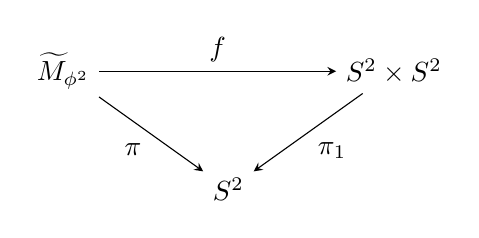
\begin{tikzpicture}[baseline=(current bounding box.center),>=stealth]
  \node (m) at (0,0) {$\widetilde M_{\phi^2}$};
  \node (prod) at (4.2,0) {$S^2\times S^2$};
  \node (base) at (2.1,-1.5) {$S^2$};
  \draw[->] (m) -- node[above] {$f$} (prod);
  \draw[->] (m) -- node[below left] {$\pi$} (base);
  \draw[->] (prod) -- node[below right] {$\pi_1$} (base);
\end{tikzpicture}
\]
其中 $f$ 是微分同胚。如命题~\ref{prop:9-6-4} 的证明所述，\BookRecordIndex{T0279}纤维化
$\pi:\widetilde M_{\phi^2}\to S^2$ 有由生成哈密顿量的两个\BookRecordIndex{T0233}临界点
$[1:0],[0:1]$ 给出的两个自然截面；可以定义 $f$，把它们分别送到平凡丛
$\pi_1:S^2\times S^2\to S^2$ 的对角截面和反对角截面。因此，在
$S^2\times S^2$ 的模型 $\widetilde M_{\phi^2}=S^3\times_{S^1}S^2$ 中，环路
$\{\psi_t\}$ 旋转 $S^2$ 因子：
\[
  t\mathbin{\boldsymbol\cdot}[z_1,z_2;[w_0:w_1]]
  =[z_1,z_2;[w_0:e^{2\pi it}w_1]].
\]
显然，若取
$\widetilde\omega_c=\widetilde\omega+\kappa\pi^*\sigma$，其中
$\widetilde\omega$ 如式~\eqref{eq:9-6-3}，则这个作用保持 $\widetilde\omega_c$。由于生成函数
$H:S^2\to\mathbb R$ 的值落在 $[-1,1]$ 内，对任意 $\lambda>1$ 都可选
$\kappa=\lambda$。于是 $f_*\widetilde\omega_\lambda$（这里用 $f_*$ 表示
$(f^{-1})^*$）与 $\omega_\lambda$ 上同调；只须证明这两个形式同痕。

我们显式应用\BookRecordIndex{T0359}辛膨胀过程来证明这一点。这是一个一般过程：对具有足够多非零 Gromov
不变量的所有辛四维流形，它可以把形变转化为同痕；见 McDuff \srcite{266}。这一过程
最早由 Lalonde 与 McDuff \srcite{258,221,225} 引入，后来又由 Biran
\srcite{38,39} 用于\BookRecordIndex{T0366}辛装填问题。

先同痕 $f$，使 $f_*\widetilde\omega_\lambda=\omega_\lambda$ 在对角线 $\Delta$ 的某个
邻域 $U$ 上成立，再考虑线性道路
\[
  t f_*\widetilde\omega_\lambda+(1-t)\omega_\lambda,
  \qquad 0\le t\le1.
\]
这些形式在 $\pi_1$ 的纤维上非退化。因此，加入拉回 $\pi_1^*\sigma$ 的适当倍数后，
可得到一族（彼此不上同调的）\BookRecordIndex{T0363}辛形式 $\tau_t$，它连接
$\tau_0=\omega_\lambda$ 与 $\tau_1=f_*\widetilde\omega_\lambda$；并且在 $U$ 上有
\[
  \tau_t=c_t\pi_1^*\sigma+\pi_2^*\sigma,
\]
其中 $c_t\ge\lambda$，且当 $t$ 接近 $0,1$ 时等号成立。现在要把形变 $\tau_t$ 转化为
同痕
\[
  \omega_{\lambda,t}
  =\frac1{1+\kappa_t}(\tau_t+\kappa_t\rho_t),
  \qquad t\in[0,1],
\]
它从 $\omega_{\lambda,0}=\omega_\lambda$ 连接到
$\omega_{\lambda,1}=f_*\widetilde\omega_\lambda$。这里形式 $\rho_t$ 支持在 $\Delta$
附近，并表示与 $\Delta$ Poincaré 对偶的类；常数
\[
  \kappa_t:=\frac{c_t-\lambda}{\lambda-1}
\]
选取成使 $[\omega_{\lambda,t}]$ 保持不变。（正是在这里需要 $\lambda>1$。）因此必须
找到 $\rho_t$，使得给 $\tau_t$ 加上它的任意大倍数都不影响非退化性。这些形式之所以
存在，是因为 $\tau_t$ 在 $\Delta$ 上不消失。

细节如下。用 $\pi:L\to S^2$ 表示 Chern 数为 $2$ 的复线丛，并设 $\alpha$ 是相应
$S^1$-丛上的联络 $1$-形式，使
\[
  -d\alpha=2\pi^*\sigma.
\]
若 $r:L\to\mathbb R$ 是纤维中的径向坐标，而
$\beta:[0,1]\to[0,1]$ 是在 $r=0$ 附近等于一的非增\BookRecordIndex{T0188}截断函数，则紧支形式
$-d(\beta(r)\alpha)$ 在每条纤维上的积分为一，在零截面 $L_0$ 上的积分为二。由辛邻域
定理，存在一族光滑嵌入 $g_t:(U,\Delta)\to(L,L_0)$，满足
\[
  (g_t)_*(c_t\pi_1^*\sigma+\pi_2^*\sigma)
  =\frac{c_t+1}{2}\,d\bigl((r^2-1)\alpha\bigr),
  \qquad t\in[0,1].
\]
这里补正外微分的作用对象与系数。
\sourcefootnote{原书右端印作
$\frac{c_t}{2}(d(r^2-1)\alpha)$：其一，括号使 $d$ 只施于标量 $r^2-1$，漏掉
$(r^2-1)d\alpha$ 项；其二，分子还漏了加项 $+1$（等价地系数少了 $1/2$）。事实上，左端在对角线上的限制为
$(c_t+1)\sigma$，而由 $-d\alpha=2\pi^*\sigma$，
$d((r^2-1)\alpha)$ 在零截面上的限制为 $2\pi^*\sigma$，故右端唯一应为
$\frac{c_t+1}{2}d((r^2-1)\alpha)$。}
现在对每个 $t$ 选取支集包含在 $g_t$ 像中的\BookRecordIndex{T0188}截断函数 $\beta_t$，并令
$\rho_t=-d(\beta_t(r)\alpha)$。它们在 $g_t$ 下的拉回具有所需的全部性质。这就完成了
命题~\ref{prop:9-7-2}(ii) 的第二个证明。
\end{proof}

类似论证表明，形式
\[
  \tau_1^k:=(\Psi^{\circ k})_*\tau_1^0,
  \qquad k\ge0,
\]
中任意两个都不同痕，尽管它们全都彼此上同调且形变等价。还可改进这一构造，在如下
八维流形 $\widetilde Y$ 上得到一族形变等价、彼此上同调但不微分同胚的形式：先给
$S^2\times S^2\times\mathbb T^2$ 再乘一个 $S^2$ 因子得到 $Y$，然后沿子流形
\[
  Z:=S^2\times\{w_1\}\times\mathbb T^2\times\{x_1\}
\]
吹起。由于 $Z$ 的余维为 $4$，\personlater{geluomofu}{格罗莫夫}{Gromov}的辛嵌入
定理（见 \srcite{161}，也见 Eliashberg--Mishenko \srcite{102}）说明，对
$j=0,1$，它都能关于 $\tau_1^j+\pi_3^*\sigma$ 辛嵌入到 $Y$ 中。因此，这两个形式在
吹起后给出 $\widetilde Y$ 上的两个\BookRecordIndex{T0363}辛形式 $\widetilde\tau_1^j$；它们在 $Z$ 的吹起
$\widetilde Z$ 上非退化。现在反设存在微分同胚
\[
  f:(\widetilde Y,\widetilde\tau_1^0)
  \longrightarrow(\widetilde Y,\widetilde\tau_1^1).
\]
考察例外除子类 $E$ 中曲线的\BookRecordIndex{T0246}模空间，可以证明（粗略地说）：由
$\pi_2\circ f$ 给出的、从 $\widetilde Z$ 到 $\widetilde Y$ 中第二个 $S^2$ 因子的映射
必为零伦的。另一方面，$(\widetilde Y,\widetilde\tau_1^j)$ 的子流形
\[
  W=S^2\times S^2\times\mathbb T^2\times\{x_2\}
\]
包含一参数 $A$-全纯曲线族，它们绕第二个 $S^2$ 因子扭转 $j$ 次。由于 $Z$ 可以同伦
到 $W$ 中，把这一事实与从 $E$-曲线所得的信息比较，就会导出矛盾。

这里有一个值得注意的解析问题。由于 $\widetilde\tau_1^j(E)$ 很小，类
$A\in H_2(\widetilde Y)$ 不再不\BookRecordIndex{T0213}可分解，\BookRecordIndex{T0246}模空间 $\mathcal M(A;J)$ 具有非空边界。对每个
$J$，我们关心的是一参数 $A$-曲线族的性质，所以必须考虑
$\mathcal M(A;J_t)$（$t\in[0,1]$）中元素的二参数族。因此，这些族一般不紧；我们不能
再通过扰动道路 $\{J_t\}$ 来避免碰到边界。不过，可以分析极限\BookRecordIndex{T0340}稳定映射，并证明它们不
影响不变量 $\chi$。根本原因是，投影
$\pi_2:\widetilde Y\to S^2$ 在极限\BookRecordIndex{T0340}稳定映射的每个分支上次数都为零。若一条 $A$-曲线
能分解为一条 $(A-B)$-曲线与一条 $B$-曲线之和，则这个论证会失效；这里 $B$ 表示第二个
球面的类。这种情形只在 $\lambda>1$ 时可能发生，而此时我们知道论证确实失效。更多
细节见 \srcite{254}。


\chapter{\BookRecordIndex{T0254}粘合}\label{ch:gluing}


本章将证明第~7 章中讨论的\BookRecordIndex{T0143}格罗莫夫--威滕不变量\BookRecordIndex{T0125}分裂公理（定理~\ref{thm:7-5-10}）。
其基础是如下观察：两条以适当方式横截相交的 $J$-全纯球面可以\BookRecordIndex{T0254}粘合起来，从而产生一族
代表原球面同调类之和的 $J$-全纯球面。这在某种意义上是\BookRecordIndex{T0139}格罗莫夫紧性的逆过程。为了证明
它，首先用\BookRecordIndex{T0227}连通和构造一条近似 $J$-全纯球面，再用\BookRecordIndex{T0380}隐函数定理确定附近确有一条真正的
$J$-全纯球面。在\BookRecordIndex{T0334}伪全纯曲线的背景下，最早的此类\BookRecordIndex{T0256}粘合定理由 Floer
\srcite{113,114,116} 给出；他考察的是连接两条周期轨道的轨线之\BookRecordIndex{T0246}模空间。由于假定周期轨道
非退化，这一情形略为容易。$J$-全纯球面的\BookRecordIndex{T0256}粘合定理最早由 Ruan--Tian \srcite{345}
证明，随后 Liu \srcite{248} 又用与我们略有不同的方法给出证明。这里的论证是本书第一版
论证的改进。后来又出现了许多其他版本，例如见 Fukaya--Ono \srcite{127}、
Ionel--Parker \srcite{201} 和 Zinger \srcite{426}。

第一节建立记号并陈述主要\BookRecordIndex{T0256}粘合定理（定理~\ref{thm:10-1-2}）。随后的六节用于证明它。
第~\ref{sec:10-8} 节证明分裂定理~\ref{thm:7-5-10}。最后，在定理~\ref{thm:10-9-1} 中，我们用
主要\BookRecordIndex{T0256}粘合定理描述紧化\BookRecordIndex{T0246}模空间 $\overline{\mathcal M}_{0,4}(A,J)$ 中单\BookRecordIndex{T0191}节点单纯\BookRecordIndex{T0340}稳定映射之集
的一个邻域结构。我们还会说明，这个简化的\BookRecordIndex{T0256}粘合定理足以建立量子乘法的结合律。最后两节
只用到\BookRecordIndex{T0256}粘合定理的陈述而不用其证明，因此读完第~\ref{sec:10-1} 节便可立即阅读它们。

定理~\ref{thm:10-1-2} 之证明的基本想法，是先用\BookRecordIndex{T0188}截断函数拼合与所求对象非常接近的对象，
再用 Newton 型迭代得到精确解。第一步是从两条相交的 $J$-全纯球面构造一族近似
$J$-全纯球面 $u^R$（$R$ 很大）。这一步称为\emph{\BookRecordIndex{T0394}预粘合}，将在
第~\ref{sec:10-2} 节讨论。下一节为沿\BookRecordIndex{T0395}预粘合曲线 $u^R$ 的向量场和 $1$-形式引入合适的
\BookRecordIndex{T0179}加权索伯列夫范数。为应用第~\ref{sec:3-5} 节的\BookRecordIndex{T0380}隐函数定理，我们需要\BookRecordIndex{T0346}线性化算子
$D_{u^R}$ 的适当\BookRecordIndex{T0392}右逆关于这些\BookRecordIndex{T0177}加权范数的一致估计。依循 Donaldson--Kronheimer
\srcite{88}，我们先构造\BookRecordIndex{T0196}近似右逆 $T_{u^R}$，再得到与 $T_{u^R}$ 有相同像的\BookRecordIndex{T0197}精确右逆
$Q_{u^R}$。

为使这一方案成立，必须使用性质精细的\BookRecordIndex{T0188}截断函数 $\beta$；这些性质在
第~\ref{sec:10-4} 节建立。主要构造见第~\ref{sec:10-5} 节。在那里，我们定义近似逆族
$T_{u^R}$ 和真正的逆族 $Q_{u^R}$，再应用逆函数定理定义\BookRecordIndex{T0257}粘合映射
$\iota_c^{\delta,R}$。我们还会建立它的大部分性质，把一些细节留到技术性的
第~\ref{sec:10-6} 节。定理~\ref{thm:10-1-2} 证明的剩余部分涉及满射性。要证明这一点，
必须理解\BookRecordIndex{T0254}粘合在哪种意义下是\BookRecordIndex{T0192}紧性的逆过程；为此将用到引理~\ref{lem:4-7-3} 关于低能量长
圆柱性质的结论。细节见第~\ref{sec:10-7} 节。第~\ref{sec:10-6}、\ref{sec:10-7} 节
不可避免地较为技术化。为了把握构造的全貌，读者不妨先集中阅读
第~\ref{sec:10-1}、\ref{sec:10-2} 和~\ref{sec:10-5} 节。

\section{\BookRecordIndex{T0256}粘合定理}\label{sec:10-1}

\BookRecordIndex{T0003}$J$-全纯曲线的\BookRecordIndex{T0256}粘合定理可以看作\BookRecordIndex{T0139}格罗莫夫紧性定理的逆。粗略地说，它断言：若两条（或
更多条）\BookRecordIndex{T0003}$J$-全纯曲线相交并满足适当的\BookRecordIndex{T0166}横截性条件，那么代表其同调类之和的一列
\BookRecordIndex{T0003}$J$-全纯曲线可以在\BookRecordIndex{T0141}格罗莫夫收敛的意义下（见定义~\ref{def:5-2-1}）逼近它们。我们的证明
改造了 Donaldson--Kronheimer \srcite{88, pp.~287--295} 为四维流形上的反自对偶瞬子建立\BookRecordIndex{T0256}粘合
定理的方法。要精确陈述定理还需作一些准备。我们将在第~\ref{sec:6-7} 节的框架下描述
\BookRecordIndex{T0257}粘合映射，其中 $J$ 依赖于 $z\in S^2$。因为 $J$ 在一个紧族中变化，这对分析并无本质
影响，却使结果适用得更广。当 $J$ 与 $z$ 无关时会有额外的对称性，从而得到一个略为
简单、可用\BookRecordIndex{T0340}稳定映射和\BookRecordIndex{T0141}格罗莫夫收敛语言陈述的\BookRecordIndex{T0256}粘合定理版本。第~\ref{sec:10-9} 节将讨论
这个版本，并说明如何用它证明最简单版本的分裂原理。

\paragraph{\BookRecordIndex{T0226}连通对的\BookRecordIndex{T0246}模空间。}
如上所述，设
$J^0=\{J_z^0\}_{z\in S^2}$ 和 $J^\infty=\{J_z^\infty\}_{z\in S^2}$
是 $M$ 上两族光滑的 $\omega$-\BookRecordIndex{T0372}驯服\BookRecordIndex{T0088}殆复结构，并设常数 $\kappa>0$ 满足
\begin{equation}\label{eq:10-1-1}
  |z|<\kappa
  \quad\Longrightarrow\quad
  J_z^0=J_{1/\bar z}^{\infty}=:J.
\end{equation}
固定两个同调类 $A^0,A^\infty\in H_2(M;\mathbb Z)$。回忆，
$\mathcal M(A^0;\{J_z^0\})$ 表示 $M$ 中代表类 $A^0$ 的
$\{J_z^0\}$-全纯曲线空间；$\mathcal M(A^\infty;\{J_z^\infty\})$ 的含义类似。
愿意的话，读者可以只考虑与 $z$ 无关的 $J$，但此时应只考察单纯映射。

\begin{definition}\label{def:10-1-1}
称
$(J^0,J^\infty)\in\mathcal J_\tau(S^2;M,\omega)\times
\mathcal J_\tau(S^2;M,\omega)$ 对 $(A^0,A^\infty)$ \emph{正则}，如果
$J^0\in\mathcal J_{\mathrm{reg}}(S^2;A^0)$ 和
$J^\infty\in\mathcal J_{\mathrm{reg}}(S^2;A^\infty)$ 对某个 $\kappa>0$
满足~\eqref{eq:10-1-1}，并且\BookRecordIndex{T0283}求值映射
\begin{equation}\label{eq:10-1-2}
  \begin{aligned}
  \operatorname{ev}:\mathcal M(A^0;J^0)\times\mathcal M(A^\infty;J^\infty)
  &\longrightarrow M\times M,\\
  \operatorname{ev}(u^0,u^\infty)&:=(u^0(0),u^\infty(\infty))
  \end{aligned}
\end{equation}
横截于对角线。所有这样的\BookRecordIndex{T0406}正则对之集记作
$\mathcal J_{\mathrm{reg}}(S^2;A^{0,\infty})$。
\end{definition}

由命题~\ref{prop:6-7-7}，集合
$\mathcal J_{\mathrm{reg}}(S^2;A^0)$ 和
$\mathcal J_{\mathrm{reg}}(S^2;A^\infty)$ 在所有满足~\eqref{eq:10-1-1} 的
$\omega$-\BookRecordIndex{T0372}驯服族 $\{J_z\}\in\mathcal J_\tau(S^2;M,\omega)$ 的空间中都是\BookRecordIndex{T0300}剩余集。
此外，定理~\ref{thm:6-3-1} 的证明表明，对于通有的偶对 $(J^0,J^\infty)$，\BookRecordIndex{T0283}求值映射
\eqref{eq:10-1-2} 横截于对角线。因此，
$\mathcal J_{\mathrm{reg}}(S^2;A^{0,\infty})$ 在所有满足~\eqref{eq:10-1-1} 的对
\[
  (J^0,J^\infty)\in\mathcal J_\tau(S^2;M,\omega)\times
  \mathcal J_\tau(S^2;M,\omega)
\]
中是\BookRecordIndex{T0300}剩余集。再者，若
$(J^0,J^\infty)\in\mathcal J_{\mathrm{reg}}(S^2;A^{0,\infty})$，则\BookRecordIndex{T0246}模空间
\[
  \mathcal M(A^{0,\infty};J^{0,\infty})
  :=\bigl\{(u^0,u^\infty)\in
  \mathcal M(A^0;J^0)\times\mathcal M(A^\infty;J^\infty)
  \bigm|u^0(0)=u^\infty(\infty)\bigr\}
\]
是维数为 $2n+2c_1(A^0+A^\infty)$ 的光滑有限维流形。

给定常数 $c>0$，用
\[
  \mathcal M(c):=\mathcal M(A^{0,\infty};J^{0,\infty},c)
\]
表示所有满足
\[
  \|du^0\|_{L^\infty}\le c,
  \qquad
  \|du^\infty\|_{L^\infty}\le c
\]
的\BookRecordIndex{T0226}连通对 $(u^0,u^\infty)\in\mathcal M(A^{0,\infty};J^{0,\infty})$ 所成的紧子集。
在定理~\ref{thm:10-1-2} 中，我们将考察第一球面上的\BookRecordIndex{T0283}求值映射
\begin{equation}\label{eq:10-1-3}
  \begin{aligned}
  \operatorname{ev}^0:\mathcal M(c)\times
  \bigl(S^2\setminus\operatorname{int}B_{1/c}(0)\bigr)&\longrightarrow M,\\
  \operatorname{ev}^0(u^0,u^\infty,z)&:=u^0(z).
  \end{aligned}
\end{equation}
以下讨论中，$c$ 始终视为任意大的固定常数。

\paragraph{\BookRecordIndex{T0256}粘合定理的陈述。}
以下固定同调类 $A^0,A^\infty\in H_2(M;\mathbb Z)$，并记
\[
  A:=A^0+A^\infty.
\]
还固定\BookRecordIndex{T0406}正则对
$(J^0,J^\infty)\in\mathcal J_{\mathrm{reg}}(S^2;A^{0,\infty})$。
我们将证明：对每个 $c>0$ 和每个充分大的 $R>0$，\BookRecordIndex{T0246}模空间
$\mathcal M(A^{0,\infty};J^{0,\infty},c)$ 都可嵌入\BookRecordIndex{T0246}模空间
$\mathcal M(A;J^R)$，其中
\begin{equation}\label{eq:10-1-4}
  J_z^R:=
  \begin{cases}
    J_z^0,& |z|\ge 1/R,\\
    J_{R^2z}^\infty,& |z|\le 1/R.
  \end{cases}
\end{equation}
这个 $J^R$ 的公式展示了\BookRecordIndex{T0254}粘合如何作用于定义域：
$\mathcal M(A;J^R)$ 的每个元素都是从黎曼球面
$S^2=\mathbb C\cup\{\infty\}$ 到 $M$ 的映射，其中圆盘 $\{|z|\ge1/R\}$ 应与
$u^0$ 定义域中的相应圆盘等同，而圆盘 $\{|z|\le1/R\}$ 在作重标度
$z\mapsto R^2z$ 后，应与 $u^\infty$ 定义域中的圆盘 $\{|z|\le R\}$ 等同。
因此，$R$ 是一个重标度参数（见注~\ref{rem:10-2-4}）。

\BookRecordIndex{T0257}粘合映射 $\mathcal M(c)\to\mathcal M(A;J^R)$ 还依赖另一参数 $\delta$，其倒数对应于
“\BookRecordIndex{T0147}颈部的长度”。式~\eqref{eq:10-5-4} 最清楚地展示了它的作用。三个常数 $c,R,\delta$ 的关系如下：
给定大常数 $c>0$，先固定小常数 $\delta<\delta_0(c)$，再考察所有充分大的 $R$。事实上，
对 $R$ 的有关条件形如 $\delta R>1/\delta_0(c)$；$\delta$ 与 $R$ 确定了\BookRecordIndex{T0170}环域
$\delta/R\le|z|\le1/(\delta R)$，重要的分析将在其上进行。对每个 $\delta_0>0$，记
\BookRecordIndex{T0171}环域参数集为
\begin{equation}\label{eq:10-1-5}
  \mathcal A(\delta_0)
  :=\bigl\{(\delta,R)\bigm|0<\delta<\delta_0,\ \delta R>1/\delta_0\bigr\}.
\end{equation}
下一个定理陈述所得\BookRecordIndex{T0257}粘合映射
\[
  \iota_c^{\delta,R}:\mathcal M(c)\longrightarrow\mathcal M(A;J^R)
\]
的主要性质。由 (iv)，对每个 $(\delta,R)\in\mathcal A(\delta_0)$，它都是保定向的光滑
嵌入。性质 (i) 说明\BookRecordIndex{T0257}粘合映射光滑地依赖于 $R$；性质 (ii) 说明\BookRecordIndex{T0254}粘合曲线
$\widetilde u^R$ 在 $R\to\infty$ 时收敛到它的两个组成部分 $(u^0,u^\infty)$；(v) 则
说明，它的像包含所有经适当重标度后充分接近 $\mathcal M(c-1)$ 的 $J^R$-全纯映射。
最后，(iii) 说明\BookRecordIndex{T0283}求值映射在 $C^1$ 拓扑中收敛。（注意，$C^0$ 收敛由 (ii) 得出；但是要
控制 $\operatorname{ev}^R$ 与 $M$ 中给定循环的\BookRecordIndex{T0166}横截性，还需要 $C^1$ 收敛；见
第~\ref{sec:10-8} 节。）

\begin{theorem}[\BookRecordIndex{T0254}粘合]\label{thm:10-1-2}
固定两个同调类 $A^0,A^\infty\in H_2(M;\mathbb Z)$、一个\BookRecordIndex{T0088}殆复结构\BookRecordIndex{T0406}正则对
$(J^0,J^\infty)\in\mathcal J_{\mathrm{reg}}(S^2;A^{0,\infty})$ 以及常数 $c>1$。
如上记 $\mathcal M(c):=\mathcal M(A^{0,\infty};J^{0,\infty},c)$。则存在常数
$\delta_0>0$、$\varepsilon>0$，并且对每个
$(\delta,R)\in\mathcal A(\delta_0)$ 有映射
\[
  \iota_c^{\delta,R}=\iota_c^R:
  \mathcal M(c)\longrightarrow\mathcal M(A;J^R),
\]
使得下列条件成立。

\begin{enumerate}[label=\textnormal{(\roman*)}]
\item 固定常数 $0<\delta<\delta_0$。则映射
\[
  (1/(\delta\delta_0),\infty)\times\mathcal M(c)
  \longrightarrow C^\infty(S^2,M),
  \qquad (R,u^0,u^\infty)\longmapsto\iota_c^R(u^0,u^\infty)
\]
光滑，并且对每个 $R>1/(\delta\delta_0)$，映射
$\iota_c^R:\mathcal M(c)\to\mathcal M(A;J^R)$ 都是嵌入。

\item 固定常数 $0<\delta<\delta_0$。设
$(u_\nu^0,u_\nu^\infty)$ 是 $\mathcal M(c)$ 中在 $C^\infty$ 拓扑下收敛到
$(u^0,u^\infty)\in\mathcal M(c)$ 的序列，并设
$R_\nu>1/(\delta\delta_0)$ 趋于无穷。记
\[
  \widetilde u_\nu:=\iota_c^{\delta,R_\nu}(u_\nu^0,u_\nu^\infty).
\]
则当 $\nu\to\infty$ 时，$\widetilde u_\nu(z)$ 在
$S^2\setminus\{0\}$ 的紧子集上一致连同各阶导数收敛到 $u^0(z)$，而
$\widetilde u_\nu(z/R_\nu^2)$ 在 $S^2\setminus\{\infty\}$ 的紧子集上一致连同各阶
导数收敛到 $u^\infty(z)$。

\item 固定常数 $0<\delta<\delta_0$；对 $R>1/(\delta\delta_0)$，令
\[
  \operatorname{ev}^R:\mathcal M(A;J^R)\times S^2\longrightarrow M
\]
为自然\BookRecordIndex{T0283}求值映射。则复合
\[
  \operatorname{ev}^R\circ(\iota_c^{\delta,R}\times\operatorname{id}):
  \mathcal M(c)\times\bigl(S^2\setminus\operatorname{int}B_{1/c}(0)\bigr)
  \longrightarrow M
\]
当 $R\to\infty$ 时在 $C^1$ 拓扑中收敛到\BookRecordIndex{T0283}求值映射~\eqref{eq:10-1-3}。

\item 对每个 $(\delta,R)\in\mathcal A(\delta_0)$，嵌入
$\iota_c^{\delta,R}$ 都保定向。

\item 若 $(\delta,R)\in\mathcal A(\delta_0)$、
$(u^0,u^\infty)\in\mathcal M(c-1)$，并且
$v\in\mathcal M(A;J^R)$ 满足
\[
  \sup_{|z|\ge1}d(v(z),u^0(z))<\varepsilon,
  \qquad
  \sup_{|z|\le1}d(v(z/R^2),u^\infty(z))<\varepsilon,
\]
则 $v$ 属于 $\iota_c^{\delta,R}$ 的像。
\end{enumerate}
\end{theorem}

\begin{remark}\label{rem:10-1-3}
\begin{enumerate}[label=\textnormal{(\roman*)}]
\item 定理~\ref{thm:10-1-2} 证明中的构造表明，映射
$\iota_c^{\delta,R}:\mathcal M(c)\to\mathcal M(A;J^R)$ 与 $c$ 无关。换言之，若
$0<c<c'$，并把 $\delta_0>0$ 取得充分小，则对每个
$(\delta,R)\in\mathcal A(\delta_0)$，映射 $\iota_c^{\delta,R}$ 与
$\iota_{c'}^{\delta,R}$ 在共同定义域 $\mathcal M(c)$ 上一致。

\item 我们的构造在适当重标度的意义下关于两个分支 $u^0,u^\infty$ 对称。因此，
定理~\ref{thm:10-1-2}(iii) 蕴含如下结论。考察由
\[
  \operatorname{ev}^\infty(u^0,u^\infty,z):=u^\infty(z)
\]
定义的\BookRecordIndex{T0283}求值映射
$\operatorname{ev}^\infty:\mathcal M(c)\times B_c(0)\to M$。若记
$u_c^{\delta,R}:=\iota_c^{\delta,R}(u^0,u^\infty)$，则\BookRecordIndex{T0283}求值映射
\[
  \mathcal M(c)\times B_c(0)\longrightarrow M,
  \qquad (u^0,u^\infty,z)\longmapsto u_c^{\delta,R}(z/R^2)
\]
在 $R\to\infty$ 时于 $C^1$ 拓扑中收敛到 $\operatorname{ev}^\infty$。
\end{enumerate}
\end{remark}

定理~\ref{thm:10-1-2}(v) 的满射性陈述略显微妙。对依赖于
$z\in S^2$ 的通有 $J^\infty$，一个映射 $v$ 至多对一个 $R$ 是 $J^R$-全纯的。然而，
若这一条件不成立，则每个 $v$ 都会对某个 $R$ 值的开子集满足 (v) 的条件，而 (v) 蕴含
\BookRecordIndex{T0257}粘合映射 $\iota_c^{\delta,R}$ 的像会随 $R$ 改变而彼此重叠。还要注意，对
$v\in\operatorname{im}\iota_c^{\delta,R}$，$|dv(0)|$ 被常数乘 $R^2$ 控制。因此，对固定
$R$，$\iota_c^{\delta,R}$ 的像不包含一整列\BookRecordIndex{T0141}格罗莫夫收敛序列；如下推论所示，为捕捉
这样的整个序列，必须允许 $R\to\infty$。第~\ref{sec:10-9} 节将对与 $z$ 无关的\BookRecordIndex{T0088}殆复
结构给出一个涉及所有 $R$ 值的\BookRecordIndex{T0256}粘合定理版本，并把 $R$ 的选取与四个\BookRecordIndex{T0066}标记点的\BookRecordIndex{T0185}交比联系起来。

\begin{corollary}\label{cor:10-1-4}
设 $A^0,A^\infty\in H_2(M;\mathbb Z)$，且
$(J^0,J^\infty)\in\mathcal J_{\mathrm{reg}}(S^2;A^{0,\infty})$。固定两个常数
$c>1$ 与 $0<\delta<\delta_0(c)$。设 $R_\nu\to\infty$，且
$u_\nu\in\mathcal M(A;J^{R_\nu})$ 是在 $S^2\setminus\{0\}$ 的紧子集上一致连同各阶
导数收敛到 $u^0(z)$ 的序列；再假设其重标度
$z\mapsto u_\nu(z/R_\nu^2)$ 在 $S^2\setminus\{\infty\}$ 的紧子集上一致连同各阶
导数收敛到 $u^\infty(z)$，其中 $(u^0,u^\infty)\in\mathcal M(c-1)$。则存在常数
$\nu_0$，使得对 $\nu\ge\nu_0$，都有
$u_\nu\in\operatorname{im}\iota_c^{\delta,R_\nu}$。
\end{corollary}

\begin{proof}
当 $\nu$ 充分大时，二元组 $(u_\nu,R_\nu)$ 满足定理~\ref{thm:10-1-2}(v) 的假设。
\end{proof}

定理~\ref{thm:10-1-2} 的证明策略如下。给定两条曲线
$u^0\in\mathcal M(A^0;J^0)$ 和 $u^\infty\in\mathcal M(A^\infty;J^\infty)$，且
$u^0(0)=u^\infty(\infty)$，我们将考察一族近似 $J^R$-全纯曲线
$u^R=u^0\mathbin{\#_R}u^\infty$（$R$ 充分大），并证明其附近存在真正的
$J^R$-全纯曲线 $\widetilde u^R$。论证中需要证明\BookRecordIndex{T0128}弗雷德霍姆算子 $D_{u^R}$ 满射，并估计
它的一个\BookRecordIndex{T0392}右逆；这些步骤依赖于关于\BookRecordIndex{T0188}截断函数的一些初等而精细的观察。随后，要验证所得映射
$\iota_c^R$ 具有上述 (i)--(iii) 性质相当容易。论证的这些步骤在
第~\ref{sec:10-5} 节完成。建立 (iv)、(v) 还需若干进一步估计，但没有本质上的新思想。
为了便于读者理解要点，我们把这部分论证留到第~\ref{sec:10-6}、\ref{sec:10-7} 节。


\section{\BookRecordIndex{T0003}$J$-全纯曲线的\BookRecordIndex{T0227}连通和}\label{sec:10-2}

本节将构造一族映射
\[
  \mathcal M(A^{0,\infty};J^{0,\infty})
  \longrightarrow C^\infty(S^2,M),
  \qquad
  (u^0,u^\infty)\longmapsto
  u^R:=u^0\mathbin{\#_R}u^\infty,
\]
它为每个 $J$-全纯球面的\BookRecordIndex{T0226}连通对 $(u^0,u^\infty)$ 指派一条近似 $J^R$-全纯球面 $u^R$。
更准确地说，该映射只定义在\BookRecordIndex{T0246}模空间 $\mathcal M(A^{0,\infty};J^{0,\infty})$ 的紧子集上，
而且对每个紧子集，只在 $R$ 充分大时定义。近似 $J^R$-全纯曲线
$u^R:S^2=\mathbb C\cup\{\infty\}\to M$ 在远离 $0$ 处与 $u^0$ 一致，在非常靠近
$0$ 处则与重标度曲线 $u^\infty(R^2z)$ 一致。条件
$u^0(0)=u^\infty(\infty)$ 保证这些映射在中心圆周 $|z|=1/R$ 上近似相等。我们将把这个
圆周加厚为宽度约为 $1/(\delta R)$ 的\BookRecordIndex{T0170}环域，并用\BookRecordIndex{T0188}截断函数构造\BookRecordIndex{T0254}粘合曲线 $u^R$，使它在该
\BookRecordIndex{T0170}环域上等于交点 $u^0(0)=u^\infty(\infty)$。在极限 $R\to\infty$ 时，我们得到\BookRecordIndex{T0139}格罗莫夫
紧性的逆过程：曲线 $u^R$ 将在定义~\ref{def:5-2-1} 的意义下收敛到对
$(u^0,u^\infty)$。

下面给出细节。固定常数 $c,\kappa>0$，并假设 $J^0,J^\infty$ 以这个常数 $\kappa$
满足~\eqref{eq:10-1-1}。取 $\varepsilon>0$ 小于 $M$ 关于由 $\omega$ 和
式~\eqref{eq:10-1-1} 中\BookRecordIndex{T0088}殆复结构 $J$ 经~\eqref{eq:2-1-1} 所确定度量的\BookRecordIndex{T0093}单射半径。固定光滑
\BookRecordIndex{T0188}截断函数 $\rho:\mathbb C\to[0,1]$，使得
\[
  \rho(z)=
  \begin{cases}
    0,& |z|\le1,\\
    1,& |z|\ge2.
  \end{cases}
\]

对每个 $(u^0,u^\infty)\in\mathcal M(c)$ 和任意满足 $0<\delta<1$ 且 $\delta R$
充分大的两个实数 $\delta,R$，构造近似 $J^R$-全纯曲线
\[
  u^{\delta,R}=:u^R:=u^0\mathbin{\#_R}u^\infty:S^2\longrightarrow M,
\]
它满足
\begin{equation}\label{eq:10-2-1}
  u^R(z)=
  \begin{cases}
    u^\infty(R^2z),& |z|\le\delta/(2R),\\
    u^0(0)=u^\infty(\infty),& \delta/R\le|z|\le1/(\delta R),\\
    u^0(z),& 2/(\delta R)\le|z|.
  \end{cases}
\end{equation}
因此，当 $z$ 非常接近 $0$ 时，$u^R$ 是 $u^\infty$ 的重标度；它在 $|z|=1/R$ 周围的
中心\BookRecordIndex{T0170}环域上为常值；而在该\BookRecordIndex{T0170}环域外足够远处等于 $u^0$。为在剩下的两个\BookRecordIndex{T0170}环域上定义 $u^R$，
把曲线 $u^0,u^\infty$ 的交点记作
\[
  x:=u^0(0)=u^\infty(\infty),
\]
并使用该点邻域中的指数映射。我们断言
\[
  |z|<\tan(\varepsilon/c),\quad |z|<\kappa
  \quad\Longrightarrow\quad
  d_J(u^0(z),x)<\varepsilon,
\]
以及
\[
  |z|>\cot(\varepsilon/c),\quad |z|>1/\kappa
  \quad\Longrightarrow\quad
  d_J(u^\infty(z),x)<\varepsilon.
\]
事实上，由~\eqref{eq:10-1-1}，当 $|z|<\kappa$ 时
$J_z^0=J_{1/\bar z}^\infty=J$；又有
$\|du^0\|_{L^\infty}\le c$ 和 $\|du^\infty\|_{L^\infty}\le c$（因而 $u^0,u^\infty$
都是 Lipschitz 常数为 $c$ 的连续映射）；而 $S^2$ 上的 Fubini--Study 度量满足
$d_{\mathrm{FS}}(z,0)=\tan^{-1}(|z|)$。

对 $|z|<\min\{\kappa,\tan(\varepsilon/c)\}$，令
$\zeta^0(z)\in T_xM$；对
$|z|>\max\{1/\kappa,\cot(\varepsilon/c)\}$，令
$\zeta^\infty(z)\in T_xM$；它们分别是唯一满足范数小于 $\varepsilon$ 且
\[
  u^0(z)=\exp_x(\zeta^0(z)),
  \qquad
  u^\infty(z)=\exp_x(\zeta^\infty(z))
\]
的切向量。现在对 $\delta/(2R)\le|z|\le2/(\delta R)$ 定义
\begin{equation}\label{eq:10-2-2}
  u^R(z):=u^{\delta,R}(z)
  :=\exp_x\left(
    \rho(\delta Rz)\zeta^0(z)
    +\rho\left(\frac{\delta}{Rz}\right)\zeta^\infty(R^2z)
  \right).
\end{equation}
只要
\begin{equation}\label{eq:10-2-3}
  0<\delta<1,
  \qquad
  \delta R>\frac{2}{\tan(\varepsilon/c)},
  \qquad
  \delta R>\frac{2}{\kappa},
\end{equation}
这一定义便是良好的。此外，式~\eqref{eq:10-2-2} 的第一项只在 $|z|\ge1/(\delta R)$
时非零，第二项只在 $|z|\le\delta/R$ 时非零。不过，映射 $u^R$ 并非
$J^R$-全纯曲线；我们将看到，其误差在 $R\to\infty$ 时趋于零。我们的目标是在 $u^R$
附近构造一条真正的 $J^R$-全纯曲线 $\widetilde u^R:=\widetilde u^{\delta,R}$。

\begin{remark}\label{rem:10-2-1}
固定常数 $0<\delta<1$。则曲线 $u^R:=u^{\delta,R}$ 在
定义~\ref{def:5-2-1} 的意义下收敛到对 $(u^0,u^\infty)$。更准确地说，$u^R(z)$ 在
$S^2\setminus\{0\}$ 的紧子集上一致连同各阶导数收敛到 $u^0(z)$，而
$u^R(z/R^2)$ 在 $S^2\setminus\{\infty\}$ 的紧子集上一致连同各阶导数收敛到
$u^\infty(z)$。下面构造的 $J^R$-全纯曲线 $\widetilde u^R$ 将以同样方式收敛到
$(u^0,u^\infty)$。
\end{remark}

\begin{remark}\label{rem:10-2-2}
考察一族在原\BookRecordIndex{T0226}连通对 $u^0,u^\infty$ 与其\BookRecordIndex{T0394}预粘合 $u^R$ 之间过渡的曲线对，会很有用。为此，
令 $r:=\delta R$，并考察由下式定义的曲线
$u^{0,r},u^{\infty,r}:S^2\to M$：
\[
  u^{0,r}(z):=
  \begin{cases}
    u^R(z),& |z|\ge1/r,\\
    u^0(0),& |z|\le1/r,
  \end{cases}
  \qquad
  u^{\infty,r}(z):=
  \begin{cases}
    u^R(z/R^2),& |z|\le r,\\
    u^\infty(\infty),& |z|\ge r.
  \end{cases}
\]
这样，$u^{0,r}$ 和 $u^{\infty,r}$ 分别是 $u^0$ 和 $u^\infty$ 的小扰动，并且分别在
$z=0$ 和 $z=\infty$ 附近被压平（即变成常值）。由下面的引理~\ref{lem:10-4-3}，当
$r\to\infty$ 时，$u^{0,r}$ 在 $W^{1,p}$ 范数下收敛到 $u^0$，而 $u^{\infty,r}$ 在
$W^{1,p}$ 范数下收敛到 $u^\infty$。因为 $du^0$ 和 $du^\infty$ 对所有
$(u^0,u^\infty)\in\mathcal M(c)$ 都一致地由 $c$ 控制，所以该收敛在所有这些对上一致。
虽然 $u^{0,r}$ 和 $u^{\infty,r}$ 不在 $C^1$ 范数下收敛，但这个 $W^{1,p}$ 收敛足以
说明：在用\BookRecordIndex{T0263}平行移动等同定义域空间与靶空间后，当 $r\to\infty$ 时，$D_{u^{0,r}}$ 和
$D_{u^{\infty,r}}$ 分别在算子范数下收敛到 $D_{u^0}$ 和 $D_{u^\infty}$。这由
第~\ref{sec:3-5} 节给出的 $D_u$ 公式立即得出。
\end{remark}

\begin{example}\label{ex:10-2-3}
考察 $M=S^2=\mathbb C\cup\{\infty\}$ 配备标准复结构的情形。全纯曲线
\[
  u^0(z)=1+z,
  \qquad
  u^\infty(z)=1+1/z
\]
满足所需的
$u^0(0)=u^\infty(\infty)=1$\sourcefootnote{原书此处误印为
$u(0)=v(\infty)=1$；本例只定义了 $u^0,u^\infty$，故按紧邻定义唯一补正其上标与字母。}。
上述映射 $u^R=u^{\delta,R}:S^2\to S^2$ 满足
\[
  u^R(z)=
  \begin{cases}
    1+1/(R^2z),& |z|\le\delta/(2R),\\
    1,& \delta/R\le|z|\le1/(\delta R),\\
    1+z,& 2/(\delta R)\le|z|.
  \end{cases}
\]
附近的 \BookRecordIndex{T0003}$J$-全纯曲线由
\[
  \widetilde u^R(z)
  =u^\infty(R^2z)+u^0(z)-1
  =\frac{z^2+z+1/R^2}{z}
\]
给出；它们如注~\ref{rem:10-2-1} 所述收敛到对 $(u^0,u^\infty)$。
\end{example}

\begin{remark}\label{rem:10-2-4}
应把\BookRecordIndex{T0254}粘合看作\BookRecordIndex{T0141}格罗莫夫收敛的逆过程。由于构造 \BookRecordIndex{T0003}$J$-全纯曲线很困难，一般过程颇为复杂。
不过，它仍适用于简单得多的\BookRecordIndex{T0339}稳定曲线情形，其中所有映射都是平凡的。例如，考察带四个
\BookRecordIndex{T0066}标记点的亏格零\BookRecordIndex{T0339}稳定曲线\BookRecordIndex{T0246}模空间 $\overline{\mathcal M}_{0,4}$。如第 D.7 节所述，通过\BookRecordIndex{T0185}交比
可将它与 $S^2$ 等同。开\BookRecordIndex{T0072}层 $S^2\setminus\{0,1,\infty\}$ 由元素
$\tau_z=[0,1,\infty,z]$ 组成，另有三个特殊元素 $\tau_0,\tau_1,\tau_\infty$，其定义域
各有两个分支。在这个背景下，\BookRecordIndex{T0141}格罗莫夫收敛描述当 $z\to a$（$a=0,1,\infty$）时元素
$\tau_z$ 如何收敛到 $\tau_a$；\BookRecordIndex{T0254}粘合则描述如何在
$\overline{\mathcal M}_{0,4}$ 中构造 $\tau_a$ 的一个邻域。

由于这个邻域有两个实维，其元素由一个复参数 $\epsilon$ 描述。采用当前记号并取 $a=0$，
可将 $\tau_0$ 等同于\BookRecordIndex{T0339}稳定曲线 $[z_1^0,z_2^0,z_3^0,z_4^0]$；它的定义域是两个
$S^2$ 副本 $S_0^2,S_\infty^2$ 的不交并，其中 $S_0^2$ 中的 $0$ 与
$S_\infty^2$ 中的 $\infty$ 等同，\BookRecordIndex{T0066}标记点为
\[
  z_2^0=1,
  \quad z_3^0=\infty\quad\text{位于 }S_0^2,
  \qquad
  z_1^0=0,
  \quad z_4^0=1\quad\text{位于 }S_\infty^2.
\]
于是，对给定参数 $|\epsilon|<1$，$\tau_\epsilon$ 是\BookRecordIndex{T0339}稳定曲线
$[z_1^\epsilon,z_2^\epsilon,z_3^\epsilon,z_4^\epsilon]$，其中
\[
  \begin{aligned}
  z_2^\epsilon=z_2^0=1,
  &\qquad z_3^\epsilon=z_3^0=\infty &&\text{于 }S_0^2,\\
  z_1^\epsilon=\epsilon z_1^0=0,
  &\qquad z_4^\epsilon=\epsilon z_4^0=\epsilon &&\text{于 }S_\infty^2.
  \end{aligned}
\]
因此 $\tau_\epsilon=[0,1,\infty,\epsilon]$。注意，当
$\epsilon=|\epsilon|$ 为实数时，在 $\epsilon=1/R^2$ 的对应下，这个稳定四元组可自然地
与\BookRecordIndex{T0394}预粘合 $u^R$ 的定义域等同。

我们将对实\BookRecordIndex{T0255}粘合参数完成主要\BookRecordIndex{T0254}粘合构造，但结果立即推广到复参数
$\epsilon=|\epsilon|e^{i\theta}$，因为乘以 $e^{i\theta}$ 是让两个球面彼此相对旋转的
等距映射。事实上，若族 $\{J_z^0,J_z^\infty\}$ 只依赖于 $|z|$，则整个构造都是
$S^1$-不变的。（见 McDuff \srcite{268} 以及第~\ref{sec:10-9} 节中定理~\ref{thm:10-9-1} 的证明。）
\end{remark}


\section{\BookRecordIndex{T0177}加权范数}\label{sec:10-3}

为了应用\BookRecordIndex{T0380}隐函数定理，必须指明 $\bar\partial_J(u^R)$ 在哪一种范数下很小。选择范数时的
指导原则，是曲线 $u^0$ 与 $u^\infty$ 在这个\BookRecordIndex{T0254}粘合论证中地位相同。然而，映射
$u^\infty$ 以重标度后的形式出现，并集中在半径 $1/R$ 的球内。因此，为赋予 $u^0$ 与
$u^\infty$ 相同的权重，我们考察 $2$-球面上一族依赖于 $R$ 的度量，使半径 $1/R$ 球的
体积近似等于 $S^2$ 关于标准 Fubini--Study 度量的体积。重标度后的度量形如
\begin{equation}\label{eq:10-3-1}
  g^R:=(\theta^R)^{-2}(ds^2+dt^2),
\end{equation}
其中
\[
  \theta^R(z):=
  \begin{cases}
    R^{-2}+R^2|z|^2,& |z|\le1/R,\\
    1+|z|^2,& |z|\ge1/R.
  \end{cases}
\]
相应的体积形式是
$\mathrm{dvol}^R:=(\theta^R)^{-2}\,ds\wedge dt$，而 $S^2$ 关于这个度量的面积为
\begin{equation}\label{eq:10-3-2}
  \operatorname{Vol}^R(S^2)
  =\int_{\mathbb C}(\theta^R)^{-2}\,ds\wedge dt
  \le2\pi.
\end{equation}

有两种方式可以理解这个度量。首先注意，对合
$z\mapsto1/(R^2z)$ 是关于 $g^R$ 的等距映射，并交换两个圆盘
$\{|z|\le1/R\}$ 与 $\{|z|\ge1/R\}$。因此，许多计算只须在外圆盘
$\{|z|\ge1/R\}$ 上进行；那里诱导的度量就是通常的 Fubini--Study 度量。考察重标度
$z\mapsto R^2z$ 也很有用。它给出从配备度量 $g^R$ 的圆盘 $\{|z|\le1/R\}$ 到配备
Fubini--Study 度量 $g^1$ 的圆盘 $\{|z|\le R\}$ 的等距映射。因此，这个度量对沿
$u^R$ 的向量场之 $L^p$ 和 $W^{1,p}$ 范数有如下作用。若把支集位于
$B_{\delta/(2R)}$ 中的向量场 $\xi(z)\in T_{u^R(z)}M$ 重标度为沿 $u^\infty$ 的向量场
\[
  \xi^\infty(z):=\xi(z/R^2)\in T_{u^\infty(z)}M,
\]
那么重标度后向量场 $\xi^\infty$ 的标准范数与原向量场 $\xi$ 的\BookRecordIndex{T0177}加权范数一致。

更明确地说，回忆\BookRecordIndex{T0088}殆复结构 $J^R=\{J_z^R\}_{z\in S^2}$ 由
式~\eqref{eq:10-1-4} 定义，并定义\BookRecordIndex{T0177}加权范数
\[
  \|\xi\|_{0,p,R}
  :=\left(
  \int_{\mathbb C}\theta^R(z)^{-2}|\xi(z)|_{J_z^R}^p\,ds\,dt
  \right)^{1/p},
\]
\[
  \|\xi\|_{1,p,R}
  :=\left(
  \int_{\mathbb C}
  \left(
    \theta^R(z)^{-2}|\xi(z)|_{J_z^R}^p
    +\theta^R(z)^{p-2}|\nabla\xi(z)|_{J_z^R}^p
  \right)ds\,dt
  \right)^{1/p}.
\]
这里 $\nabla=\nabla^{R,z}$ 表示由 $\omega$ 和 $J_z^R$ 经~\eqref{eq:2-1-1} 确定的
$M$ 上度量之 \BookRecordIndex{T0034}Levi--Civita 联络。此外，我们在 $\mathbb C$ 上使用坐标 $z=s+it$，并写
\[
  |\nabla\xi(z)|_J^2
  :=|\nabla_s\xi(z)|_J^2+|\nabla_t\xi(z)|_J^2.
\]
对
$\eta=\eta_1\,ds+\eta_2\,dt\in\Omega^1(S^2,(u^R)^*TM)$，写
\[
  |\eta|^2:=|\eta_1|^2+|\eta_2|^2,
  \qquad
  |\nabla\eta|_J^2
  :=|\nabla_s\eta_1|_J^2+|\nabla_t\eta_1|_J^2
    +|\nabla_s\eta_2|_J^2+|\nabla_t\eta_2|_J^2,
\]
并定义
\[
  \|\eta\|_{0,p,R}
  :=\left(
  \int_{\mathbb C}\theta^R(z)^{p-2}|\eta(z)|_{J_z^R}^p\,ds\,dt
  \right)^{1/p},
\]
\[
  \|\eta\|_{0,\infty,R}
  :=\sup_{z\in\mathbb C}\theta^R(z)|\eta(z)|_{J_z^R},
\]
\[
  \|\eta\|_{1,p,R}
  :=\left(
  \int_{\mathbb C}
  \left(
    \theta^R(z)^{p-2}|\eta(z)|_{J_z^R}^p
    +\theta^R(z)^{2p-2}|\nabla\eta(z)|_{J_z^R}^p
  \right)ds\,dt
  \right)^{1/p}.
\]

当 $R=1$ 且 $J_z^R\equiv J$ 时，这些就是把 $\mathbb C$ 看作
$\mathbb{CP}^1$ 的坐标片后，关于 Fubini--Study 度量的通常 $L^p$ 与 $W^{1,p}$ 范数。
对一般的 $R$，应分两部分理解这些范数。在区域 $|z|\ge1/R$ 中，它们仍是通常的范数；
而在区域 $|z|\le1/R$ 中，它们与沿 $u^\infty(z)$、位于半径 $R$ 球内的重标度向量场
\[
  \xi^\infty(z):=\xi(z/R^2)
\]
或 $1$-形式
\[
  \eta^\infty
  :=R^{-2}\bigl(\eta_1(z/R^2)\,ds+\eta_2(z/R^2)\,dt\bigr)
\]
关于 $\mathbb C$ 上 Fubini--Study 度量的通常范数一致。因此，如下引理所示，我们得到
常数与 $R$ 无关的通常索伯列夫估计。

\begin{lemma}\label{lem:10-3-1}
设 $A^0,A^\infty\in H_2(M;\mathbb Z)$，并给定满足~\eqref{eq:10-1-1} 的
$J^0,J^\infty\in\mathcal J(S^2;M,\omega)$。固定常数 $c>0$ 和 $p\ge1$，其中
$p\ne2$。则存在常数 $c_0=c_0(p,c)>0$，使得对所有满足~\eqref{eq:10-2-3} 的
$\delta,R$ 以及所有 $u=(u^0,u^\infty)\in\mathcal M(c)$，下列结论成立；其中
$u^R=u^{\delta,R}:S^2\to M$ 由~\eqref{eq:10-2-1}、\eqref{eq:10-2-2} 给出。

\begin{enumerate}[label=\textnormal{(\roman*)}]
\item 若 $p>2$，则
\[
  \|\xi\|_{L^\infty}\le c_0\|\xi\|_{1,p,R},
  \qquad
  \|\eta\|_{0,\infty,R}\le c_0\|\eta\|_{1,p,R},
\]
其中
$\xi\in\Omega^0(S^2,(u^R)^*TM)$，
$\eta\in\Omega^1(S^2,(u^R)^*TM)$。

\item 若 $1\le p<2$ 且 $1\le q\le2p/(2-p)$，则
\[
  \|\xi\|_{0,q,R}\le c_0\|\xi\|_{1,p,R},
  \qquad
  \|\eta\|_{0,q,R}\le c_0\|\eta\|_{1,p,R},
\]
其中
$\xi\in\Omega^0(S^2,(u^R)^*TM)$，
$\eta\in\Omega^1(S^2,(u^R)^*TM)$。
\end{enumerate}
\end{lemma}

\begin{proof}
两个断言都分别在区域 $\{|z|\ge1/R\}$ 和 $\{|z|\le1/R\}$ 上证明。先考察区域
$\{|z|\ge1/R\}$，并利用其中的度量是 $S^2\setminus B_{1/R}$ 上的
Fubini--Study 度量（因而与 $R$ 无关）这一事实。对 $p>2$，函数的结论由附录 B 的结果
得出。每一点 $z_0\in S^2\setminus B_{1/R}$ 都包含在
$S^2\setminus B_{1/R}$ 内某个半径为 $\pi/4$ 的圆盘 $D$ 中。所有这样的圆盘彼此等距；
又因为 $d_{\mathrm{FS}}(z,0)=\tan^{-1}(|z|)$，它们可与
$(\mathbb C,g^1)$ 中的单位圆盘 $B_1(0)$ 等同。这个度量与欧氏度量等价，所以
结论由引理 B.1.16 和命题 B.1.9 立即得出。向量场 $\xi$ 与 $1$-形式 $\eta$ 的相应结论
可仿照注~\ref{rem:3-5-1} 证明。

在 $p<2$ 的情形，考察引理 B.1.17 的证明。该证明表明：对单位球外为零的函数，沿着从
单位球外出发、平行于实轴和虚轴的射线积分，可在区域 $\{|z|\ge1/R\}$ 上得到常数一致的
估计。现在用\BookRecordIndex{T0188}截断函数作分解：一部分位于 $|z|=1/R$ 附近且支集包含在 $B_1$ 中，另一部分
的支集包含在 $S^2\setminus B_{1/2}$ 中；由此便得到整个
$S^2\setminus B_{1/R}$ 上的一致估计。前面的论证也适用于支集包含在
$S^2\setminus B_{1/2}$ 中的函数，因为这个区域同样可以等同于 $\mathbb C$ 中以原点为
中心的一个球，其度量与欧氏度量等价。

这证明了区域 $\{|z|\ge1/R\}$ 上的估计。在区域 $\{|z|\le1/R\}$ 中，结论由映射
$u^R$ 和\BookRecordIndex{T0291}权函数 $\theta^R$ 定义公式中的对合对称性得出（见下面的习题~\ref{ex:10-5-2}）。
引理得证。
\end{proof}

下一个引理在我们应用\BookRecordIndex{T0380}隐函数定理（定理~\ref{thm:3-5-2}）时起关键作用。后一定理的陈述
方式使它适用于如下情形：黎曼曲面 $\Sigma=\mathbb{CP}^1$ 上的度量具有一致有界的
索伯列夫嵌入常数，而光滑映射 $u:\Sigma\to M$ 的一阶导数具有一致的 $L^p$ 上界。
引理~\ref{lem:10-3-1} 断言度量 $(\theta^R)^{-2}(ds^2+dt^2)$ 满足第一个假设；下面的
引理~\ref{lem:10-3-2} 则断言\BookRecordIndex{T0227}连通和 $u^R$ 满足第二个假设。其证明方法是以后更精细计算的
范例。

\begin{lemma}\label{lem:10-3-2}
设 $A^0,A^\infty$ 和 $J^0,J^\infty$ 如引理~\ref{lem:10-3-1}。固定两个常数
$c>0$ 与 $p>2$。则存在常数 $c_0=c_0(c,p)>0$，使得下列结论成立。若 $\delta,R$
满足~\eqref{eq:10-2-3}，则对每个 $(u^0,u^\infty)\in\mathcal M(c)$，由
\eqref{eq:10-2-1}、\eqref{eq:10-2-2} 定义的函数 $u^R$ 都满足估计
\[
  \|du^R\|_{0,\infty,R}\le c_0,
  \qquad
  \|du^R\|_{0,p,R}\le c_0,
  \qquad
  \|\bar\partial_{J^R}(u^R)\|_{0,p,R}
  \le c_0(\delta R)^{-2/p}.
\]
\end{lemma}

\begin{proof}
前两个估计的证明是容易的习题。它利用了式~\eqref{eq:10-2-2} 关于 $u^0,u^\infty$ 的
对称性（这将在下面的习题~\ref{ex:10-5-2} 中明确写出），以及如下事实：由于 $\zeta^0(0)=0$，
在区域 $|z|\le2/(\delta R)$ 中，乘积 $\delta R\zeta^0(z)$ 一致地由一个与
$\delta,R$ 及 $(u^0,u^\infty)$ 无关的常数控制。

为证明第三个估计，令 $r:=\delta R$，并回忆注~\ref{rem:10-2-2}：当 $|z|\ge1/R$ 时
$u^R(z)=u^{0,r}(z)$，而在 $r\to\infty$ 时，$u^{0,r}$ 在 $W^{1,p}$ 范数下收敛到
$u^0$。再次利用对称性可得
\[
  \|\bar\partial_{J^R}(u^R)\|_{0,p,R}\longrightarrow0.
\]
为得到更精确的收敛速率估计，注意当 $|z|\le2/r$ 且 $r=\delta R$ 充分大时（见
式~\eqref{eq:10-2-2}），
\[
  u^{0,r}(z)=\exp_x(\rho(rz)\zeta^0(z)),
  \qquad
  \exp_x(\zeta^0(z))=u^0(z).
\]
因此，项 $\bar\partial_{J^0}(u^{0,r})$ 的支集包含在\BookRecordIndex{T0170}环域
$B_{2/r}\setminus B_{1/r}$ 中，并且在该区域上可写成两项之和。一项含有\BookRecordIndex{T0188}截断函数
$\rho(rz)$ 的一阶导数（其增长阶为 $r$）乘以函数 $\zeta^0(z)$；当 $|z|\le2/r$ 时，
后者被常数乘 $1/r$ 控制，故该乘积一致有界。另一项含有 $\zeta^0(z)$ 的一阶导数，它们
也一致有界。由于这个估计中的积分区域面积至多为 $4\pi r^{-2}$，引理得证。
\end{proof}

\begin{exercise}\label{ex:10-3-3}
本习题说明命题~\ref{prop:3-1-1} 中定义的算子 $D_{u^R}$ 一致有界。设
$A^0,A^\infty\in H_2(M;\mathbb Z)$，并取
$(J^0,J^\infty)\in\mathcal J_{\mathrm{reg}}(S^2;A^{0,\infty})$。固定两个常数
$c>0$ 与 $p>2$。证明存在常数 $c_0$，使下列结论对所有满足~\eqref{eq:10-2-3} 的
$\delta,R$ 都成立：若 $(u^0,u^\infty)\in\mathcal M(c)$，且
$u^R:S^2\to M$ 由~\eqref{eq:10-2-2} 定义，则对每个
$\xi\in\Omega^0(S^2,(u^R)^*TM)$，都有
\[
  \|D_{u^R}\xi\|_{0,p,R}\le c_0\|\xi\|_{1,p,R}.
\]
\end{exercise}

\begin{remark}\label{rem:10-3-4}
固定一对 $(u^0,u^\infty)\in\mathcal M(A^{0,\infty};J^{0,\infty})$。对每对满足
\eqref{eq:10-2-3} 的实数 $\delta,R$，用~\eqref{eq:10-2-2} 定义
$u^R:S^2\to M$。于是每个算子 $D_{u^R}$ 都满足形如
\begin{equation}\label{eq:10-3-3}
  \|\xi\|_{k+1,p,R}
  \le c_{k,p,\delta,R}
  \bigl(\|D_{u^R}\xi\|_{k,p,R}+\|\xi\|_{k,p,R}\bigr)
\end{equation}
的估计，其中 $\xi\in\Omega^0(S^2,(u^R)^*TM)$。此时可以问：常数
$c_{k,p,\delta,R}$ 是否能选得与 $R$ 无关？值得注意的是，$k=0$ 时答案为是，而
$kp>2$ 时答案为否。

$k=0$ 时的结论很不平凡。先考察 $u^0,u^\infty$ 都是常值的情形，再通过
引理~\ref{lem:10-4-2} 对内边界上一点处消失的\BookRecordIndex{T0170}环域函数所作的一项改进，把一般情形归约到
这一情形，便可由下面的命题~\ref{prop:10-5-1} 得出结论。因为我们的\BookRecordIndex{T0254}粘合论证审慎地避开了
估计~\eqref{eq:10-3-3}，这里不展开细节。

为考察 $kp>2$ 的情形，考虑两条常值曲线 $u^0(z)\equiv u^\infty(z)\equiv x$。于是
\BookRecordIndex{T0395}预粘合曲线 $u^R$ 也为常值，$D_{u^R}$ 是从 $S^2$ 到 $T_xM$ 的函数之标准
\BookRecordIndex{T0210}柯西--黎曼算子。因此，问题在于\BookRecordIndex{T0291}权函数 $\theta^R$ 对 \BookRecordIndex{T0012}Calderón--Zygmund 不等式
有何影响。如下形式的截面给出一个富有启发性的例子：
\[
  \xi^R(z):=\beta^R(z)\left(z+\frac{1}{R^2z}\right)\xi_0,
\]
其中 $\xi_0\in T_xM$ 是非零向量，而乘以 $i=\sqrt{-1}$ 要通过点 $x\in M$ 处的\BookRecordIndex{T0088}殆复
结构 $J(x)$ 来理解。假设 $\beta^R:\mathbb C\to[0,1]$ 是光滑\BookRecordIndex{T0188}截断函数，在区域
$|z|\ge1$ 中与 $R$ 无关，并满足
\[
  \beta^R(z)=\beta^R\left(\frac{1}{R^2z}\right)
  =
  \begin{cases}
    1,& 1/R^2\le|z|\le1,\\
    0,& |z|\ge2\text{ 或 }|z|\le1/(2R^2).
  \end{cases}
\]
由对称性，只须考察区域 $|z|\ge1/R$ 中估计式的各项。函数
$z\mapsto z+1/(R^2z)$ 是全纯的，且其各阶导数在区域 $1\le|z|\le2$ 中一致有界，故
\[
  \sup_R\|\bar\partial\xi^R\|_{k,p,R}<\infty
\]
对每个 $k$ 和每个 $p$ 都成立。$\xi^R$ 的 $(k,p,R)$-范数由其在 $|z|=1/R$ 附近的
行为决定；在这里，项 $z\mapsto1/(R^2z)$ 在区域 $1/R\le|z|\le1$ 中占主导。简单计算
表明，只要 $(k-1)p<2$，$\xi^R$ 的 $(k,p,R)$-范数就一致有界。同一计算还表明，对每个
满足 $kp>2$ 的整数 $k$，存在常数 $c=c(k,p)>0$，使得
\[
  c^{-1}R^{k-2/p}
  \le\|\xi^R\|_{k+1,p,R}
  \le cR^{k-2/p}.
\]
这意味着，只要 $k\ge1$ 且 $kp>2$，式~\eqref{eq:10-3-3} 中的常数
$c_{k,p,\delta,R}$ 就不能选得与 $R$ 无关。
\end{remark}


\section{\BookRecordIndex{T0188}截断函数}\label{sec:10-4}

迄今为止，我们用任意光滑\BookRecordIndex{T0188}截断函数 $\rho$ 定义\BookRecordIndex{T0394}预粘合 $u^R$。其余构造也都将通过拼合
分别定义在区域 $\{|z|\ge1/R\}$ 和 $\{|z|\le1/R\}$ 上的对象来完成。然而，为使所需
估计成立，必须使用一个经过精细调节的\BookRecordIndex{T0188}截断函数，记为 $\beta$。本节中所有积分都理解为
关于 Lebesgue 测度的积分。读者初读时完全可以跳过本节，待读到命题~\ref{prop:10-5-1} 的证明中
$\beta$ 的各种性质如何被使用后再返回。

\begin{lemma}\label{lem:10-4-1}
对任意两个实数 $0<\delta<\varepsilon$，存在 Lipschitz 连续\BookRecordIndex{T0188}截断函数
$\beta=\beta_{\delta,\varepsilon}:\mathbb R^2\to[0,1]$，使得
\[
  \beta(z)=
  \begin{cases}
    1,& |z|\le\delta,\\
    0,& |z|\ge\varepsilon,
  \end{cases}
  \qquad
  \int_{\mathbb R^2}|\nabla\beta|^2
  =\frac{2\pi}{\log(\varepsilon/\delta)}.
\]
\end{lemma}

\begin{proof}
定义 $\beta:\mathbb R^2\to[0,1]$：当 $|z|\le\delta$ 时令 $\beta(z):=1$，当
$|z|\ge\varepsilon$ 时令 $\beta(z):=0$，而在中间区域令
\begin{equation}\label{eq:10-4-1}
  \beta(z):=
  \frac{\log\varepsilon-\log|z|}{\log\varepsilon-\log\delta},
  \qquad \delta\le|z|\le\varepsilon.
\end{equation}
于是 $|\nabla\beta(z)|=1/(|z|\log(\varepsilon/\delta))$，从而
\[
  \begin{aligned}
  \int_{\mathbb R^2}|\nabla\beta(z)|^2
  &=\int_{\delta\le|z|\le\varepsilon}
    \frac{1}{|z|^2\log(\varepsilon/\delta)^2}\\
  &=\int_\delta^\varepsilon
    \frac{2\pi}{s\log(\varepsilon/\delta)^2}\,ds
   =\frac{2\pi}{\log(\varepsilon/\delta)}.
  \end{aligned}
\]
引理得证。
\end{proof}

要强调的是，引理~\ref{lem:10-4-1} 中 $\nabla\beta$ 的 $L^2$ 范数只依赖于比值
$\varepsilon/\delta$。这说明在二维中，导数的 $L^2$ 范数具有共形不变性。此外，若将常数
$2\pi/\log(\varepsilon/\delta)$ 换成任意更大的常数，显然可以把\BookRecordIndex{T0188}截断函数 $\beta$ 选成
光滑的。因此，$\mathbb R^2$ 上存在一列紧支函数，它们在 $W^{1,2}$ 范数下收敛到零，
但不在 $L^\infty$ 范数下收敛到零（固定常数 $\varepsilon>0$，让 $\delta$ 趋于零即可）。
这是索伯列夫估计的临界情形。当 $p>2$ 时存在嵌入
$W^{1,p}(\mathbb R^2)\hookrightarrow C(\mathbb R^2)$，所以若把前一引理中
$\nabla\beta$ 的 $L^2$ 范数换成 $p>2$ 时的 $L^p$ 范数，其断言便不再成立。下面将看到，
在二维\BookRecordIndex{T0254}粘合构造中证明一阶算子满射时，所需的恰好是 $L^2$ 范数。$n$ 维中的类似论证要求
$\nabla\beta$ 的 $L^n$ 范数很小，这同样是索伯列夫临界情形。$n=4$ 的情形与反自对偶
瞬子的\BookRecordIndex{T0254}粘合有关；Donaldson--Kronheimer \srcite{88, pp.~287--295} 对此作了解释。

现在令 $\beta$ 由~\eqref{eq:10-4-1} 给出，并取
$\xi\in W^{1,q}(\mathbb R^2)$，其中 $1\le q<2$。于是，对某个合适的常数 $r\ge2$，有
如下估计\sourcefootnote{原书在式~\eqref{eq:10-4-2} 最后一项中误印为
$2\pi c/\log(\varepsilon/\delta)$。由引理~\ref{lem:10-4-1}，
$\|\nabla\beta\|_{L^2}=\sqrt{2\pi/\log(\varepsilon/\delta)}$，故该项唯一应为这里的
平方根形式。}：
\begin{equation}\label{eq:10-4-2}
  \begin{aligned}
  \|\nabla\beta\cdot\xi\|_{L^q}
  &\le\|\nabla\beta\|_{L^2}\|\xi\|_{L^r}
   \le c\|\nabla\beta\|_{L^2}\|\xi\|_{W^{1,q}}\\
  &\le c\sqrt{\frac{2\pi}{\log(\varepsilon/\delta)}}
  \|\xi\|_{W^{1,q}}.
  \end{aligned}
\end{equation}
这里，第一个不等式使用 Hölder 不等式
\[
  \left(\int|uv|^q\right)^{1/q}
  \le
  \left(\int|u|^s\right)^{1/s}
  \left(\int|v|^r\right)^{1/r},
  \qquad
  \frac1s+\frac1r=\frac1q,
\]
其中 $s=2$。因此必须取 $r:=2q/(2-q)$；由定理 B.1.12，有索伯列夫嵌入
$W^{1,q}\hookrightarrow L^r$，这给出上面的第二个不等式。第三个不等式由
引理~\ref{lem:10-4-1} 得出。

由~\eqref{eq:10-4-2} 可知，只要 $q<2$，乘法算子
\[
  W^{1,q}(\mathbb R^2)\longrightarrow L^q(\mathbb R^2),
  \qquad \xi\longmapsto\nabla\beta_{\delta,\varepsilon}\cdot\xi
\]
就在 $\delta\to0$ 时于算子范数下收敛到零。这个原样的断言对 $q>2$ 不再成立。不过，
在 $q>2$ 的情形，可以把这些算子限制到所有在原点消失的函数所成子空间。下一个引理说明，
当 $q>2$ 时，这些受限算子在 $\delta\to0$ 时仍于算子范数下收敛到零。记
\[
  B_r:=\{z\in\mathbb R^2\mid |z|\le r\},
  \qquad
  A(r,R):=\{z\in\mathbb R^2\mid r\le|z|\le R\}.
\]

\begin{lemma}\label{lem:10-4-2}
对每个 $p>2$，存在具有如下性质的常数 $c>0$。给定 $0<\delta<\varepsilon$，用
\eqref{eq:10-4-1} 定义 $\beta:\mathbb R^2\to[0,1]$。则对每个满足
$\xi(0)=0$ 的 $\xi\in W^{1,p}(B_\varepsilon)$，都有
\[
  \|\nabla\beta\cdot\xi\|_{L^p(A(\delta,\varepsilon))}
  \le
  \frac{c}{\log(\varepsilon/\delta)^{1-1/p}}
  \|\xi\|_{W^{1,p}(B_\varepsilon)}.
\]
\end{lemma}

\begin{proof}
由引理~\ref{lem:10-4-1} 的证明，$\nabla\beta$ 的支集包含在\BookRecordIndex{T0170}环域
$A(\delta,\varepsilon)$ 中，并且当 $\delta\le|z|\le\varepsilon$ 时，
\[
  |\nabla\beta(z)|=\frac{1}{|z|\log(\varepsilon/\delta)}.
\]
此外，由定理 B.1.11，每个 $\xi\in W^{1,p}(\mathbb R^2)$ 都以指数
$\mu=1-2/p$ Hölder 连续。更准确地说，存在只依赖于 $p>2$ 的常数 $c>0$，使得
\begin{equation}\label{eq:10-4-3}
  z_0,z_1\in B
  \quad\Longrightarrow\quad
  |\xi(z_1)-\xi(z_0)|
  \le c\|\xi\|_{W^{1,p}(B)}|z_1-z_0|^{1-2/p}
\end{equation}
对每个球 $B\subset\mathbb R^2$ 和每个 $\xi\in W^{1,p}(B)$ 都成立（见
引理 B.1.16 的证明）。因此，每个在 $z=0$ 处消失的
$\xi\in W^{1,p}(B_\varepsilon)$ 都满足估计
\[
  \begin{aligned}
  \int_{\delta\le|z|\le\varepsilon}
  |\nabla\beta(z)|^p|\xi(z)|^p
  &\le
  \frac{c^p}{\log(\varepsilon/\delta)^p}
  \int_{\delta\le|z|\le\varepsilon}\frac{1}{|z|^2}
  \|\xi\|_{W^{1,p}(B_\varepsilon)}^p\\
  &=\frac{2\pi c^p}{\log(\varepsilon/\delta)^p}
  \int_\delta^\varepsilon\frac1s\,ds\,
  \|\xi\|_{W^{1,p}(B_\varepsilon)}^p\\
  &=\frac{2\pi c^p}{\log(\varepsilon/\delta)^{p-1}}
  \|\xi\|_{W^{1,p}(B_\varepsilon)}^p.
  \end{aligned}
\]
引理得证。
\end{proof}

我们还需要任意光滑\BookRecordIndex{T0188}截断函数 $\rho:\mathbb C\to[0,1]$ 的如下结论；这里 $\rho$ 在
$|z|\le1$ 时等于零，在 $|z|\ge2$ 时等于一。

\begin{lemma}\label{lem:10-4-3}
设 $p>2$，且 $\xi\in W^{1,p}(B_1)$ 满足 $\xi(0)=0$。记
$\rho_R(z):=\rho(Rz)$。则
\[
  \lim_{R\to\infty}\|\xi-\rho_R\xi\|_{W^{1,p}(B_1)}=0.
\]
\end{lemma}

\begin{proof}
我们证明存在常数 $c>0$，使得
\begin{equation}\label{eq:10-4-4}
  \|\xi-\rho_R\xi\|_{W^{1,p}(B_1)}
  \le c\|\xi\|_{W^{1,p}(B_{2/R})}.
\end{equation}
首先注意，若把 $W^{1,p}$ 范数换成 $L^p$ 范数，则这个估计取 $c=1$ 即成立。其次，
\[
  \nabla(\xi-\rho_R\xi)
  =(1-\rho_R)\nabla\xi-(\nabla\rho_R)\xi.
\]
第一项的 $L^p$ 范数以 $c=1$ 满足所需不等式。为估计第二项，注意
$\|\nabla\rho_R\|_{L^\infty}=Rc_0$，其中
$c_0:=\|\nabla\rho\|_{L^\infty}$。此外，由~\eqref{eq:10-4-3}，存在常数 $c_1>0$，使得
\[
  |\xi(z)|
  \le c_1|z|^{1-2/p}\|\xi\|_{W^{1,p}(B_{2/R})},
  \qquad |z|\le2/R.
\]
因此
\[
  \begin{aligned}
  \|(\nabla\rho_R)\xi\|_{L^p}
  &\le c_0c_1R
  \left(\int_{|z|\le2/R}|z|^{p-2}\right)^{1/p}
  \|\xi\|_{W^{1,p}(B_{2/R})}\\
  &=c_0c_1\left(\frac{2^{p+1}\pi}{p}\right)^{1/p}
  \|\xi\|_{W^{1,p}(B_{2/R})}.
  \end{aligned}
\]
这证明了~\eqref{eq:10-4-4}，也证明了引理。
\end{proof}


\section{\BookRecordIndex{T0257}粘合映射的构造}\label{sec:10-5}

本节定义\BookRecordIndex{T0257}粘合映射 $\iota_c^R$，并证明它具有定理~\ref{thm:10-1-2} 的性质
(i)、(ii) 与 (iii)。如导言所述，其思路是在\BookRecordIndex{T0394}预粘合
$u^R:=u^{\delta,R}$ 附近应用\BookRecordIndex{T0380}隐函数定理，找到一条真正的全纯曲线
\[
  \widetilde u^R:=\iota_c^R(u^0,u^\infty).
\]
为此必须证明：只要 $\delta>0$ 充分小而 $\delta R$ 充分大，
\BookRecordIndex{T0128}弗雷德霍姆算子 $D_{u^R}$ 就满射，并且具有一致有界的\BookRecordIndex{T0392}右逆。

\paragraph{\BookRecordIndex{T0392}右逆的估计。}
第一步是沿用 Donaldson--Kronheimer \srcite{88} 的方法构造\BookRecordIndex{T0196}近似右逆
$T_{u^R}$。下面的命题概括它的主要性质。回忆式~\eqref{eq:10-1-5}：
$\mathcal A(\delta_0)$ 表示实数偶对 $(\delta,R)$ 的集合，其中
$0<\delta<\delta_0$ 且 $\delta R>1/\delta_0$。

\begin{proposition}\label{prop:10-5-1}
设 $A^0,A^\infty\in H_2(M;\mathbb Z)$，并设
\[
  (J^0,J^\infty)\in
  \mathcal J_{\mathrm{reg}}(S^2;A^{0,\infty}).
\]
固定常数 $c>0$ 与 $p>2$。则存在常数 $\delta_0>0$、$c_0>0$，以及一个
光滑映射；它为每个 $u=(u^0,u^\infty)\in\mathcal M(c)$ 和每个
$(\delta,R)\in\mathcal A(\delta_0)$ 指派有界线性算子
\[
  T_{u^R}:
  L^p\bigl(S^2,\Lambda^{0,1}\otimes_{J^R}(u^R)^*TM\bigr)
  \longrightarrow
  W^{1,p}\bigl(S^2,(u^R)^*TM\bigr),
\]
这里 $u^R:S^2\to M$ 是由式~\eqref{eq:10-2-1} 和~\eqref{eq:10-2-2}
定义的\BookRecordIndex{T0395}预粘合曲线，并且对每个
$\eta\in L^p(S^2,\Lambda^{0,1}\otimes_{J^R}(u^R)^*TM)$ 都有
\begin{equation}\label{eq:10-5-1}
  \bigl\|D_{u^R}T_{u^R}\eta-\eta\bigr\|_{0,p,R}
  \le\frac12\|\eta\|_{0,p,R},
  \qquad
  \bigl\|T_{u^R}\eta\bigr\|_{1,p,R}
  \le\frac{c_0}{2}\|\eta\|_{0,p,R}.
\end{equation}
\end{proposition}

在开始证明之前，先引入一些简化记号。我们先改述 $J$ 的\BookRecordIndex{T0408}正则性条件。对
$u:S^2\to M$ 和 $J=\{J_z\}_{z\in S^2}$，简记
\[
  W_u^{1,p}:=W^{1,p}(S^2,u^*TM),
  \qquad
  L_{u,J}^p:=L^p(S^2,\Lambda^{0,1}\otimes_Ju^*TM).
\]
给定满足 $u^0(0)=u^\infty(\infty)$ 的映射
$u^0,u^\infty:S^2\to M$，记
\[
  W_{u^{0,\infty}}^{1,p}
  :=\bigl\{(\xi^0,\xi^\infty)\in
  W_{u^0}^{1,p}\times W_{u^\infty}^{1,p}
  \bigm|\xi^0(0)=\xi^\infty(\infty)\bigr\}.
\]
最后这个定义只有在 $p>2$ 时才有意义，因为只有此时 $W^{1,p}$ 截面才连续，
从而可以在一点处求值。定义~\ref{def:10-1-1} 中的\BookRecordIndex{T0166}横截性假设蕴含算子
\[
  D_{0,\infty}:=D_{u^0,u^\infty}:
  W_{u^{0,\infty}}^{1,p}
  \longrightarrow L_{u^0,J^0}^p\times L_{u^\infty,J^\infty}^p
\]
为满射；这里
\[
  D_{0,\infty}(\xi^0,\xi^\infty)
  :=(D_{u^0}\xi^0,D_{u^\infty}\xi^\infty).
\]
为说明这一点，对 $a=0,\infty$ 给定 $\eta^a\in L_{u^a,J^a}^p$，
并选取 $\xi^a\in W_{u^a}^{1,p}$ 使 $D_{u^a}\xi^a=\eta^a$。再选取切向量
$\zeta^a\in T_{u^a}\mathcal M(A^a;J^a)$，使
\[
  d\operatorname{ev}(u^0,u^\infty)(\zeta^0,\zeta^\infty)
  =(\zeta^0(0),\zeta^\infty(\infty))
  \in(\xi^0(0),\xi^\infty(\infty))+T_{(x,x)}\Delta.
\]
于是 $(\xi^0-\zeta^0,\xi^\infty-\zeta^\infty)$ 属于
$W_{u^{0,\infty}}^{1,p}$，并且在 $D_{0,\infty}$ 下的像仍为
$(\eta^0,\eta^\infty)$。所以 $D_{0,\infty}$ 有一个随偶对
$(u^0,u^\infty)$ 光滑变化的\BookRecordIndex{T0392}右逆；当该偶对在紧空间
\[
  \mathcal M(c):=
  \mathcal M(A^{0,\infty};J^{0,\infty},c)
\]
中变化时，这个\BookRecordIndex{T0392}右逆满足一致界。\sourcefootnote{原书在这里把\BookRecordIndex{T0226}连通对空间缩写为
$\mathcal M(A^{0,\infty};J,c)$；但固定数据始终是偶对
$J^{0,\infty}=(J^0,J^\infty)$，且本节下一节也明确采用
$\mathcal M(A^{0,\infty};J^{0,\infty},c)$，故补出上标。}

更准确地说，令
\[
  \mathcal W_{u^{0,\infty}}\subset W_{u^{0,\infty}}^{1,p}
\]
为 $\ker D_{0,\infty}$ 的 $L^2$-正交补。于是
$D_{0,\infty}$ 在 $\mathcal W_{u^{0,\infty}}$ 上的限制是双射有界线性算子，
所需算子就是其逆：
\[
  Q_{0,\infty}:=Q_{u^0,u^\infty}
  :=\left(D_{0,\infty}\big|_{\mathcal W_{u^{0,\infty}}}\right)^{-1}.
\]
它随偶对 $(u^0,u^\infty)$ 光滑变化；其范数的一致估计来自
$\mathcal M(c)$ 的\BookRecordIndex{T0192}紧性。注意，算子的定义域和值域实际上依赖
$(u^0,u^\infty)$。因此，为准确表述这种连续依赖性，必须对邻近的偶对
$(u^0,u^\infty)$、$(v^0,v^\infty)$，选取
$W_{u^{0,\infty}}^{1,p}$ 与 $W_{v^{0,\infty}}^{1,p}$ 之间的等同。
这可以像定理~\ref{thm:3-5-2} 的证明那样，沿短测地线作\BookRecordIndex{T0263}平行移动。

现在考虑注~\ref{rem:10-2-2} 中定义的映射
$u^{0,r},u^{\infty,r}$，仍令 $r:=\delta R$。它们是
$u^0,u^\infty$ 的 $W^{1,p}$-小扰动，因此可以把
$W_{u^{0,\infty}}^{1,p}$ 看作沿这些\BookRecordIndex{T0373}压平曲线的向量场空间
$W_{u^{0,\infty},r}^{1,p}$ 在 $r\to\infty$ 时的极限。此外，算子
\[
  D_{0,\infty,r}:=D_{u^{0,r},u^{\infty,r}}
\]
是\BookRecordIndex{T0346}线性化算子 $D_{0,\infty}:=D_{u^0,u^\infty}$ 的
$W^{1,p}$-小扰动，所以它也有\BookRecordIndex{T0392}右逆。以下选取唯一的\BookRecordIndex{T0392}右逆，使其像为
$\ker D_{0,\infty,r}$ 的 $L^2$-正交补，并记为
\[
  Q_{0,\infty,r}:=Q_{u^{0,r},u^{\infty,r}}:
  L_{u^{0,r},J^0}^p\times L_{u^{\infty,r},J^\infty}^p
  \longrightarrow W_{u^{0,\infty},r}^{1,p}.
\]
由于 $D_{0,\infty,r}$ 是 $D_{0,\infty}$ 的小扰动，它确实有一致有界的\BookRecordIndex{T0392}右逆。
不过，这里使用的是一族特定的\BookRecordIndex{T0392}右逆 $Q_{0,\infty,r}$，其像与
$\ker D_{0,\infty,r}$ 在 $L^2$ 意义下正交，所以还须为它们建立一致估计。
这些估计将在引理~\ref{lem:10-6-1} 中陈述和证明。这里所需的是如下结论：
对每个 $c>0$，都存在正数 $\delta_0,c_0$，使
\begin{equation}\label{eq:10-5-2}
  \|Q_{0,\infty,r}\eta\|_{W^{1,p}}
  \le c_0\|\eta\|_{L^p}
\end{equation}
对所有 $u=(u^0,u^\infty)\in\mathcal M(c)$、$r>1/\delta_0$ 及
\[
  \eta=(\eta^0,\eta^\infty)
  \in L_{u^{0,r},J^0}^p\times L_{u^{\infty,r},J^\infty}^p
\]
都成立。

现在的策略是用算子 $Q_{0,\infty,r}$，在 $r=\delta R$ 充分大时构造沿
\BookRecordIndex{T0395}预粘合曲线 $u^R$ 的算子 $D_{u^R}$ 的\BookRecordIndex{T0196}近似右逆 $T_{u^R}$，并为这些\BookRecordIndex{T0196}近似右逆
建立一致估计。

\begin{proof}[命题~\ref{prop:10-5-1} 的证明]
先定义算子
\[
  T_{u^R}:L_{u^R,J^R}^p\longrightarrow W_{u^R}^{1,p}.
\]
其构造可由下面的交换图概括，其中竖直映射由\BookRecordIndex{T0188}截断函数给出：
\begin{equation}\label{eq:10-5-3}
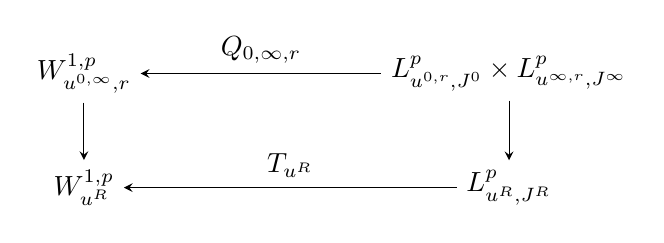
\begin{tikzpicture}[baseline=(current bounding box.center),>=stealth]
  \node (wt) at (0,1.45) {$W_{u^{0,\infty},r}^{1,p}$};
  \node (lt) at (5.4,1.45)
    {$L_{u^{0,r},J^0}^p\times L_{u^{\infty,r},J^\infty}^p$};
  \node (wb) at (0,0) {$W_{u^R}^{1,p}$};
  \node (lb) at (5.4,0) {$L_{u^R,J^R}^p$};
  \draw[<-] (wt) -- node[above] {$Q_{0,\infty,r}$} (lt);
  \draw[->] (wt) -- (wb);
  \draw[->] (lt) -- (lb);
  \draw[<-] (wb) -- node[above] {$T_{u^R}$} (lb);
\end{tikzpicture}
\end{equation}
下面给出细节。给定 $\eta\in L_{u^R,J^R}^p$，先沿圆周 $|z|=1/R$
截断 $\eta$，定义偶对
\[
  (\eta^0,\eta^\infty)
  \in L_{u^{0,r},J^0}^p\times L_{u^{\infty,r},J^\infty}^p
\]
如下：
\[
  \eta^0(z):=
  \begin{cases}
    \eta(z),&|z|\ge1/R,\\
    0,&|z|\le1/R,
  \end{cases}
  \qquad
  \eta^\infty(z):=
  \begin{cases}
    R^{-2}\eta(z/R^2),&|z|\le R,\\
    0,&|z|\ge R.
  \end{cases}
\]
$\eta^0,\eta^\infty$ 的不连续性不会造成问题，因为估计中只出现它们的
$L^p$-范数。第二步，定义
\[
  (\xi^0,\xi^\infty):=
  Q_{0,\infty,r}(\eta^0,\eta^\infty),
\]
并注意向量场 $\xi^0,\xi^\infty$ 有相同的中心值
\[
  \xi^0(0)=\xi^\infty(\infty)=:\xi_0\in T_{u^0(0)}M.
\]
第三步，令 $1-\beta_{\delta,R}:\mathbb C\to\mathbb R$ 为
引理~\ref{lem:10-4-1} 的\BookRecordIndex{T0188}截断函数，其中 $\delta,\varepsilon$ 分别换成
$\delta/R,1/R$。于是
\[
  \beta_{\delta,R}(z)=0\quad(|z|\le\delta/R),\qquad
  \beta_{\delta,R}(z)=1\quad(|z|\ge1/R),
\]
并且
\[
  \beta_{\delta,R}(z)
  :=\frac{\log(R|z|/\delta)}{\log(1/\delta)},
  \qquad \frac{\delta}{R}\le|z|\le\frac1R.
\]
第四步，定义 $T_{u^R}\eta:=\xi^R$，其中
\begin{equation}\label{eq:10-5-4}
\xi^R(z):=
\begin{cases}
\xi^0(z),
  & |z|\ge\dfrac1{\delta R},\\[3pt]
\xi^0(z)+\beta_{\delta,R}\!\left(\dfrac1{R^2z}\right)
  \bigl(\xi^\infty(R^2z)-\xi_0\bigr),
  & \dfrac1R\le|z|\le\dfrac1{\delta R},\\[6pt]
\xi^0(z)+\xi^\infty(R^2z)-\xi_0,
  & |z|=\dfrac1R,\\[3pt]
\xi^\infty(R^2z)+\beta_{\delta,R}(z)\bigl(\xi^0(z)-\xi_0\bigr),
  & \dfrac{\delta}{R}\le|z|\le\dfrac1R,\\[6pt]
\xi^\infty(R^2z),
  & |z|\le\dfrac{\delta}{R}.
\end{cases}
\end{equation}

理解这个定义最容易的情形是中心值 $\xi_0$ 为零，且 $z$ 位于\BookRecordIndex{T0170}环域
\[
  \frac{\delta}{R}\le|z|\le\frac1{\delta R}=\frac1r.
\]
在这个\BookRecordIndex{T0170}环域中，映射 $u^{0,r}(z)$、$u^{\infty,r}(R^2z)$ 与 $u^R(z)$
都取常值
\[
  x:=u^0(0)=u^\infty(\infty),
\]
而
\[
  \xi^R:\left\{\frac{\delta}{R}\le|z|\le\frac1{\delta R}\right\}
  \longrightarrow T_xM
\]
正是函数
$\beta_{\delta,R}(z)\xi^0(z)$ 与
$\beta_{\delta,R}(1/R^2z)\xi^\infty(R^2z)$ 的叠加。关键在于：第一项中的
\BookRecordIndex{T0188}截断函数 $\beta_{\delta,R}(z)$ 只在 $|z|\le1/R$ 的区域内起作用，而在这里
\[
  D_{0,r}\xi^0:=D_{u^{0,r}}\xi^0=0.
\]
见图~\ref{fig:10-5-1}。第二项同理，因为该构造关于
$u^{0,r}$ 与 $u^{\infty,r}$ 完全对称。当 $\xi_0\ne0$ 时，也可以按同样方式
理解公式，只须把“原点”换成 $\xi_0$。

\begin{figure}[htbp]
\centering
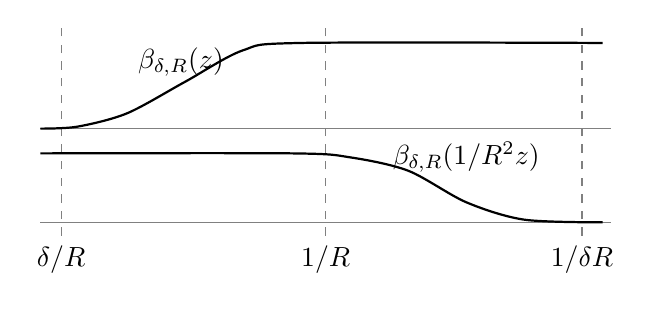
\begin{tikzpicture}[x=1.05cm,y=0.85cm]
  \draw[gray] (0.3,1.55)--(7.2,1.55);
  \draw[gray] (0.3,0.15)--(7.2,0.15);
  \draw[dashed,gray] (0.55,-0.05)--(0.55,3.05);
  \draw[dashed,gray] (3.75,-0.05)--(3.75,3.05);
  \draw[dashed,gray] (6.85,-0.05)--(6.85,3.05);
  \draw[thick]
    plot[smooth] coordinates
    {(0.3,1.55) (0.75,1.58) (1.35,1.78) (2.05,2.25)
     (2.75,2.72) (3.45,2.83) (7.1,2.83)};
  \draw[thick]
    plot[smooth] coordinates
    {(0.3,1.18) (3.35,1.18) (4.05,1.12) (4.75,0.92)
     (5.45,0.45) (6.15,0.19) (7.1,0.15)};
  \node at (2.0,2.55) {$\beta_{\delta,R}(z)$};
  \node at (5.45,1.12) {$\beta_{\delta,R}(1/R^2z)$};
  \node[below] at (0.55,-0.05) {$\delta/R$};
  \node[below] at (3.75,-0.05) {$1/R$};
  \node[below] at (6.85,-0.05) {$1/\delta R$};
\end{tikzpicture}
\caption{\BookRecordIndex{T0188}截断函数。}\label{fig:10-5-1}
\end{figure}

这样，对每个 $\eta\in L_{u^R,J^R}^p$ 都定义了元素
$T_{u^R}\eta=\xi^R$；现在必须证明
\begin{equation}\label{eq:10-5-5}
  \|D_{u^R}\xi^R-\eta\|_{0,p,R}
  \le\frac12\|\eta\|_{0,p,R}.
\end{equation}
由于 $D_{u^{0,r}}\xi^0=\eta^0$ 且
$D_{u^{\infty,r}}\xi^\infty=\eta^\infty$，左端在
$|z|\ge1/\delta R$ 以及 $|z|\le\delta/R$ 时为零。由公式的对称性，只须在\BookRecordIndex{T0170}环域
\[
  \frac{\delta}{R}\le|z|\le\frac1R
\]
中估计左端。在这个区域，如上所述，
\[
  u^{0,r}(z)=u^{\infty,r}(R^2z)=u^R(z)=x
\]
都是常值映射。因此，这个\BookRecordIndex{T0170}环域上的向量场 $\xi^R$ 取值于固定向量空间
$T_xM$，相应的算子 $D_{u^{0,r}}$、$D_{u^{\infty,r}}$ 与 $D_{u^R}$
都等于通常的 $\bar\partial_J$ 算子，特别是在常函数 $\xi_0$ 上为零。
此外，$\xi^\infty$ 的定义蕴含
$D_{u^R}\xi^\infty(R^2\mathord\cdot)=\eta$ 在 $|z|\le1/R$ 内成立。
因此，在 $|z|\le1/R$ 时，
\[
\begin{aligned}
  D_{u^R}\xi^R-\eta
  &=D_{u^{0,r}}\bigl(\beta_{\delta,R}(\xi^0-\xi_0)\bigr)\\
  &=\beta_{\delta,R}D_{u^{0,r}}(\xi^0-\xi_0)
    +\bar\partial\beta_{\delta,R}\otimes(\xi^0-\xi_0)\\
  &=\bar\partial\beta_{\delta,R}\otimes(\xi^0-\xi_0).
\end{aligned}
\]
这里用到了构造中的关键事实：
$D_{u^{0,r}}\xi^0=\eta^0=0$ 在 $|z|\le R^{-1}$ 内成立。

现在估计这个 $1$-形式关于依赖 $R$ 的度量之 $L^p$-范数。另一个关键点是，
$1$-形式的\BookRecordIndex{T0291}权函数为 $\theta^R(z)^{p-2}$。由于 $p>2$，且在
$|z|\le1/R$ 内有 $\theta^R(z)\le\theta^1(z)\le2$，这个 $1$-形式的
$(0,p,R)$-范数不超过通常 $L^p$-范数的一个小于 $2$ 的普适倍数。因而
\[
\begin{aligned}
 \|D_{u^R}\xi^R-\eta\|_{0,p,R;B_{1/R}}
 &\le2\|D_{u^R}\xi^R-\eta\|_{L^p(B_{1/R})}\\
 &=2\|\bar\partial\beta_{\delta,R}\otimes(\xi^0-\xi_0)\|_{L^p(B_{1/R})}\\
 &\le\frac{c_2}{|\log\delta|^{1-1/p}}\,
       \|\xi^0-\xi_0\|_{W^{1,p}}\\
 &\le\frac{c_3}{|\log\delta|^{1-1/p}}
       \bigl(\|\eta^0\|_{L^p}+\|\eta^\infty\|_{L^p}\bigr)\\
 &\le\frac{2c_3}{|\log\delta|^{1-1/p}}\,
       \|\eta\|_{0,p,R}.
\end{aligned}
\]
第三个不等式使用引理~\ref{lem:10-4-2} 的估计，第四个不等式来自
$D_{0,\infty,r}$ 的\BookRecordIndex{T0392}右逆 $Q_{0,\infty,r}$ 的一致估计~\eqref{eq:10-5-2}。
这里还用到：向量 $\xi_0:=\xi^0(0)$ 的长度受 $\xi^0$ 的 $C^0$-范数控制，
从而也受其 $W^{1,p}$-范数控制。最后一个不等式则来自
$\eta^0,\eta^\infty$ 以及 $1$-形式的 $(0,p,R)$-范数之定义。

根据习题~\ref{ex:10-5-2} 中详述的对称性，在 $|z|\ge1/R$ 的区域也有类似估计。
因此，只要 $\delta$ 充分小且 $R$ 充分大，算子 $T_{u^R}$ 就满足
式~\eqref{eq:10-5-1} 的第一个不等式。事实上，可以先选取足够小的 $\delta$，
使 $|\log\delta|^{1-1/p}\ge4c_3$，再选取足够大的 $R$，使乘积 $\delta R$
满足式~\eqref{eq:10-2-3}。适当选取 $\delta_0$ 后，这些条件对所有
$(\delta,R)\in\mathcal A(\delta_0)$ 都成立。

为证明式~\eqref{eq:10-5-1} 的第二个不等式，考察 $\nabla\xi$ 的
$L^p$-范数。两个关键项都含有\BookRecordIndex{T0188}截断函数 $\beta_{\delta,R}$；由公式的对称性，
只须考察其中一项。我们取式~\eqref{eq:10-5-4} 右端第四项的第二个加项。
对此项求导，会在 $\delta/R\le|z|\le1/R$ 中遇到形如
\[
  z\longmapsto
  \nabla\beta_{\delta,R}(z)\otimes(\xi^0(z)-\xi_0)
\]
的表达式。再用该区域内 $\theta^R(z)\le\theta^1(z)\le2$ 这一事实，
由引理~\ref{lem:10-4-2} 得如下估计。\sourcefootnote{原书在下式第一行把右端乘积的范数印作
$W^{1,p}$ 范数；但这里比较的是加权零阶范数与普通 $L^p$ 范数，且
引理~\ref{lem:10-4-2} 恰好只给出乘法算子 $W^{1,p}\to L^p$ 的估计。
若取 $W^{1,p}$ 范数则会无依据地要求\BookRecordIndex{T0188}截断函数的二阶导数，故补正为 $L^p$ 范数。}
\[
\begin{aligned}
 \|\nabla\beta_{\delta,R}\otimes(\xi^0-\xi_0)\|_{0,p,R}
 &\le2^{1-2/p}
   \|\nabla\beta_{\delta,R}\otimes(\xi^0-\xi_0)\|_{L^p}\\
 &\le\frac{c_4}{|\log\delta|^{1-1/p}}\|\xi^0\|_{W^{1,p}}\\
 &\le\frac{c_5}{|\log\delta|^{1-1/p}}\|\eta\|_{0,p,R}.
\end{aligned}
\]
在 $|z|\ge1/R$ 的区域也有类似不等式。因此，只要
$\delta\le\delta_0(c)<1/e$，便得到式~\eqref{eq:10-5-1} 的第二个估计，
其中 $c_0:=2c_5$。
\end{proof}

\begin{exercise}\label{ex:10-5-2}
考察函数
\[
  \widetilde u^0(z):=u^\infty(1/z),\qquad
  \widetilde u^\infty(z):=u^0(1/z),\qquad
  \widetilde u^R(z):=u^R(1/R^2z)
\]
以及向量场
\[
  \widetilde\xi^0(z):=\xi^\infty(1/z),\qquad
  \widetilde\xi^\infty(z):=\xi^0(1/z),\qquad
  \widetilde\xi(z):=\xi(1/R^2z),
\]
核对命题~\ref{prop:10-5-1} 上述证明中
$\xi=T_{u^R}\eta$ 的公式之对称性。
\end{exercise}

\paragraph{\BookRecordIndex{T0257}粘合映射的构造。}
现在可以说明\BookRecordIndex{T0257}粘合映射
$\iota_c^R=\iota_c^{\delta,R}$ 的构造了。固定两个同调类
$A^0,A^\infty\in H_2(M;\mathbb Z)$、一个\BookRecordIndex{T0088}殆复结构\BookRecordIndex{T0406}正则对
\[
  (J^0,J^\infty)\in
  \mathcal J_{\mathrm{reg}}(S^2;A^{0,\infty}),
\]
以及两个常数 $p>2$ 和 $c>0$。特别地，$J^0,J^\infty$ 对某个常数
$\kappa>0$ 满足式~\eqref{eq:10-1-1}；对 $R\ge2/\kappa$，由
式~\eqref{eq:10-1-4} 定义
$J^R=\{J_z^R\}_{z\in S^2}\in\mathcal J_\tau(S^2;M,\omega)$。
选取常数 $\delta_0>0$ 和 $c_0\ge1$，使下列条件成立。

\begin{enumerate}[label=(\alph*)]
\item 每个 $(\delta,R)\in\mathcal A(\delta_0)$ 都满足
式~\eqref{eq:10-2-3}。

\item 对每个 $R\ge2/\kappa$，定理~\ref{thm:3-5-2} 对常数
$c_0$、$\delta=4c_0^2\delta_0^{2/p}$ 以及 $J=J^R$ 成立。
（定理~\ref{thm:3-5-2} 中的\BookRecordIndex{T0088}殆复结构虽不依赖 $z$，但如
注~\ref{rem:3-5-4} 所述，其证明可以逐字用于依赖 $z$ 的情形。）

\item 对所有 $(\delta,R)\in\mathcal A(\delta_0)$，
引理~\ref{lem:10-3-1} 和~\ref{lem:10-3-2} 都以 $c_0$ 成立。

\item 命题~\ref{prop:10-5-1} 以 $c_0$ 和 $\delta_0$ 成立。
\end{enumerate}

条件 (a) 保证每个 $(\delta,R)\in\mathcal A(\delta_0)$ 都有
$R\ge2/\kappa$，因而 $J^R$ 定义良好。条件 (a) 还保证
式~\eqref{eq:10-2-2} 中的映射 $u^R$ 对
$(\delta,R)\in\mathcal A(\delta_0)$ 定义良好。因此，条件 (a)
其实已经隐含在条件 (d) 中；为了清楚起见仍将它单列。接下来，对
$(\delta,R)\in\mathcal A(\delta_0)$ 构造映射
\[
  \iota^{\delta,R}:\mathcal M(c)\longrightarrow
  \mathcal M(A;J^R).
\]
与前面一样，我们省略上标中的 $\delta$。

固定 $(\delta,R)\in\mathcal A(\delta_0)$。定义\BookRecordIndex{T0394}预粘合映射
$f^R:\mathcal M(c)\to C^\infty(S^2,M)$ 为
\begin{equation}\label{eq:10-5-6}
  f^R(u^0,u^\infty):=u^R,
\end{equation}
其中 $u^R$ 由式~\eqref{eq:10-2-1} 和~\eqref{eq:10-2-2} 给出。
现固定 $(u^0,u^\infty)\in\mathcal M(c)$，并记
$u^R:=f^R(u^0,u^\infty)$。由引理~\ref{lem:10-3-2}，有
\begin{equation}\label{eq:10-5-7}
  \|du^R\|_{0,p,R}\le c_0,
  \qquad
  \|\bar\partial_{J^R}(u^R)\|_{0,p,R}
  \le\frac{c_0}{(\delta R)^{2/p}}
  <\frac{4c_0^2\delta_0^{2/p}}{4c_0},
\end{equation}
其中最后一个不等式用到了 $1/(\delta R)<\delta_0$。由
命题~\ref{prop:10-5-1}，算子
\[
  Q_{u^R}:=T_{u^R}(D_{u^R}T_{u^R})^{-1}
  =\sum_{k=0}^{\infty}T_{u^R}
    (\operatorname{id}-D_{u^R}T_{u^R})^k:
  L_{u^R,J^R}^p\longrightarrow W_{u^R}^{1,p}
\]
满足估计
\begin{equation}\label{eq:10-5-8}
  D_{u^R}Q_{u^R}=\operatorname{id},
  \qquad
  \|Q_{u^R}\eta\|_{1,p,R}\le c_0\|\eta\|_{0,p,R},
  \qquad \eta\in L_{u^R,J^R}^p.
\end{equation}
注意，$Q_{u^R}$ 是 $D_{u^R}$ 中与 $T_{u^R}$ 有相同像的唯一\BookRecordIndex{T0392}右逆。

定义映射
\[
  \mathcal F_{u^R}:W_{u^R}^{1,p}\longrightarrow L_{u^R,J^R}^p
\]
为
\[
  \mathcal F_{u^R}(\xi)
  :=\Phi^R(u^R,\xi)^{-1}
    \bigl(\bar\partial_{J^R}\exp_{u^R}(\xi)\bigr),
\]
这里
$\Phi^R(x,\xi)=\Phi^{R,z}(x,\xi):T_xM\to T_{\exp_x(\xi)}M$
表示关于\BookRecordIndex{T0052}埃尔米特联络
\[
  \widetilde\nabla=\widetilde\nabla^{R,z}
  :=\nabla^{R,z}-\frac12J_z^R(\nabla^{R,z}J_z^R)
\]
的\BookRecordIndex{T0263}平行移动；如第~\ref{sec:2-1} 节所述，该联络对应于由 $\omega$ 和 $J_z^R$
确定的 $M$ 上度量。于是，由注~\ref{rem:6-7-3}（亦见
命题~\ref{prop:3-1-1}），有
\begin{equation}\label{eq:10-5-9}
  \mathcal F_{u^R}(0)=\bar\partial_{J^R}(u^R),
  \qquad
  d(\mathcal F_{u^R}\circ Q_{u^R})(0)=\operatorname{id}.
\end{equation}

有了这些估计，就可以对 $\mathcal F_{u^R}$ 应用\BookRecordIndex{T0380}隐函数定理~\ref{thm:3-5-2}。
为说明这一点，记 $S^2$ 上度量~\eqref{eq:10-3-1} 的体积形式为
$\mathrm{dvol}^R$。由引理~\ref{lem:10-3-1}，定理~\ref{thm:3-5-2}
中出现的索伯列夫常数 $c_p(\mathrm{dvol}^R)$ 以 $c_0$ 为上界。因此，
由式~\eqref{eq:10-5-7} 和~\eqref{eq:10-5-8}，当在
定理~\ref{thm:3-5-2} 中取
\[
  \Sigma=S^2,\quad J=J^R,\quad u=u^R,\quad Q_u=Q_{u^R},
  \quad \xi_0=0,
\]
取 $S^2$ 上的度量为式~\eqref{eq:10-3-1} 中的 $g^R$，取其中的常数
$\delta$ 为 $4c_0^2\delta_0^{2/p}$，并把 $c_0$ 取为上面选定的常数时，
该定理的全部条件都成立。（$S^2=\mathbb C\cup\{\infty\}$ 上的度量
$g^R$ 沿圆周 $|z|=1/R$ 仅连续这一点无关紧要；
定理~\ref{thm:3-5-2} 的证明并不使用 $g^R$ 的导数。）换言之，条件 (b)
断言定理~\ref{thm:3-5-2} 可用于此情形，故给出唯一的元素
$\widetilde\xi^R\in W_{u^R}^{1,p}$，满足
\begin{equation}\label{eq:10-5-10}
  \mathcal F_{u^R}(\widetilde\xi^R)=0,
  \qquad
  \|\widetilde\xi^R\|_{1,p,R}<4c_0^2\delta_0^{2/p},
  \qquad
  \widetilde\xi^R\in\operatorname{im}Q_{u^R}.
\end{equation}
而且，该定理表明 $\widetilde\xi^R$ 其实远小于
$4c_0^2\delta_0^{2/p}$，即
\begin{equation}\label{eq:10-5-11}
  \|\widetilde\xi^R\|_{1,p,R}
  \le2c_0\|\bar\partial_{J^R}(u^R)\|_{0,p,R}
  \le\frac{2c_0^2}{(\delta R)^{2/p}}.
\end{equation}
定义映射
$\iota_c^R=\iota_c^{\delta,R}:\mathcal M(c)\to\mathcal M(A;J^R)$ 为
\begin{equation}\label{eq:10-5-12}
  \iota_c^R(u^0,u^\infty):=\widetilde u^R
  :=\exp_{u^R}(\widetilde\xi^R),
  \qquad u^R:=f^R(u^0,u^\infty),
\end{equation}
其中 $\widetilde\xi^R\in\operatorname{im}Q_{u^R}$ 是
式~\eqref{eq:10-5-10} 的唯一解。

\begin{remark}\label{rem:10-5-3}
常数 $p>2$ 和 $c>0$ 只参与常数 $\delta_0,c_0$ 的选取，并不参与
映射 $\iota_c^{\delta,R}=\iota_{c;p}^{\delta,R}$ 的定义。为说明这一点，
注意命题~\ref{prop:10-5-1}、引理~\ref{lem:10-3-1} 与
引理~\ref{lem:10-3-2} 中的常数 $\delta_0,c_0$，以及
定理~\ref{thm:3-5-2} 中的常数 $\delta_1$，都连续依赖于 $p>2$。
（注意 $\delta_1=1/(2c_0c)$，其中 $c$ 如命题~\ref{prop:3-5-3}。）
现设 $2<p_1<p_2<\infty$，并设 $\delta_0,c_0$ 对区间
$[p_1,p_2]$ 中的每个 $p$ 都满足条件 (a)--(d)。则由
式~\eqref{eq:10-5-10} 中解的唯一性，所得映射
$\iota_{c;p}^{\delta,R}$ 对 $p_1\le p\le p_2$ 都相同。由定义也显然可见：
当 $0<c'<c$ 时，映射 $\iota_c^{\delta,R}$ 与
$\iota_{c'}^{\delta,R}$ 在公共定义域 $\mathcal M(c')$ 上相同。
\end{remark}

本节最后证明，\BookRecordIndex{T0257}粘合映射是满足定理~\ref{thm:10-1-2} 中条件 (i)、(ii)、
(iii) 的嵌入。证明的关键是对\BookRecordIndex{T0257}粘合映射的微分作估计。按构造，\BookRecordIndex{T0257}粘合映射
$\iota_c^R$ 是\BookRecordIndex{T0394}预粘合映射 $u\mapsto u^R$ 与扰动映射
$u^R\mapsto\widetilde u^R:=\exp_{u^R}(\widetilde\xi^R)$ 的复合。
必须沿 \BookRecordIndex{T0003}$J$-全纯曲线\BookRecordIndex{T0226}连通对的\BookRecordIndex{T0246}模空间 $\mathcal M(c)$ 的切方向对这两个映射
求导。下面将看到，\BookRecordIndex{T0394}预粘合映射 $f^R$ 的导数颇易理解，而扰动映射的导数要
复杂得多。下一个命题给出关键估计，其证明留到下一节。

\begin{proposition}\label{prop:10-5-4}
对每个 $c>0$ 和 $p>2$，存在常数 $\delta_0,c_0>0$，使下述结论对
所有 $(\delta,R)\in\mathcal A(\delta_0)$ 成立。设
$t\mapsto u_t:=(u_t^0,u_t^\infty)$ 是 $\mathcal M(c)$ 中的光滑道路，
$u_t^R:=f^R(u_t)$，且 $\widetilde\xi_t^R\in\operatorname{im}Q_{u_t^R}$
满足
\[
  \widetilde u_t^R:=\exp_{u_t^R}(\widetilde\xi_t^R)
  =\iota_c^R(u_t).
\]
则对每个 $t$，都有
\begin{equation}\label{eq:10-5-13}
  \|\nabla_t\widetilde\xi_t^R\|_{1,p,R}
  \le c_0(\delta R)^{-2/p}
  \left(
    \|\partial_tu_t^0\|_{L^2}
    +\|\partial_tu_t^\infty\|_{L^2}
  \right).
\end{equation}
\end{proposition}

\begin{remark}\label{rem:10-5-5}
设 $M$ 是紧黎曼流形。则存在两族光滑的线性映射
\[
  E_i(x,\xi):T_xM\longrightarrow T_{\exp_x(\xi)}M,
  \qquad i=1,2,
\]
由下述性质刻画：若 $\gamma:\mathbb R\to M$ 是任意光滑道路，
$v(t)\in T_{\gamma(t)}M$ 是沿此道路的任意光滑向量场，则道路
$t\mapsto\exp_{\gamma(t)}(v(t))$ 的导数由公式
\[
  \frac{d}{dt}\exp_\gamma(v)
  =E_1(\gamma,v)\dot\gamma+E_2(\gamma,v)\nabla_tv
\]
给出。读者可核对，对每个 $x\in M$ 都有
\[
  E_1(x,0)=E_2(x,0)=\operatorname{id}:T_xM\longrightarrow T_xM.
\]
因此，当 $\xi$ 充分小时，$E_i(x,\xi)$ 一致可逆。我们常把这一事实用于
$x$ 遍历光滑映射 $u:S^2\to M$ 的像中各点、而
$\exp_{u(z)}$ 对应于度量 $g_{J_z}$ 的情形。特别地，当 $u=u^R$ 且
$J=J^R$ 时，所得线性映射记作
$E_i^R=E_i^R(u^R(z),\xi(z))$。
\end{remark}

\begin{proof}[定理~\ref{thm:10-1-2} (i)--(iii) 的证明]
固定常数 $p>2$ 和 $c>0$。选取正数 $\delta_0,c_0$，使条件 (a)--(d)
成立，再固定 $0<\delta<\delta_0$。

先证明定理~\ref{thm:10-1-2} (i)。对每个 $R$，映射
$\iota_c^R:\mathcal M(c)\to C^\infty(S^2,M)$ 的光滑性是显然的：
\BookRecordIndex{T0394}预粘合映射 $f^R:\mathcal M(c)\to C^\infty(S^2,M)$ 按构造是光滑的，
而式~\eqref{eq:10-5-12} 中的映射
$u^R\mapsto\widetilde u^R$ 由\BookRecordIndex{T0380}隐函数定理也是光滑的。关于 $R$ 的光滑依赖
略微细致一些，因为 $f^R$ 的定义中变量 $R$ 出现在 $u^\infty$ 的自变量里；
这由 $\mathcal M(c)$ 的所有元素经\BookRecordIndex{T0329}椭圆正则性均为光滑映射这一事实\BookRecordIndex{T0326}推出。

接着证明，当 $\delta R$ 充分大时，$\iota_c^R$ 是浸入。设
$t\mapsto u_t:=(u_t^0,u_t^\infty)$ 是 $\mathcal M(c)$ 中的光滑道路，并记
\[
  \widetilde u_t^R:=\iota_c^R(u_t)
  =\exp_{u_t^R}(\widetilde\xi_t^R),
  \qquad u_t^R:=f^R(u_t).
\]
用注~\ref{rem:10-5-5} 的记号，
\[
  \partial_t\widetilde u_t^R
  =E_1\partial_tu_t^R+E_2\nabla_t\widetilde\xi_t^R,
\]
其中
\[
  E_i:=E_i^R(u_t^R,\widetilde\xi_t^R):
  T_{u_t^R(z)}M\longrightarrow T_{\widetilde u_t^R(z)}M.
\]
由式~\eqref{eq:10-5-10} 和~\eqref{eq:10-5-11}，只要
$r:=\delta R$ 取得充分大，$\widetilde\xi_t^R$ 的 $W^{1,p}$-范数便可任意小。
又因 $\xi$ 较小时 $E_i(x,\xi)$ 一致可逆，故存在正数 $\delta_1,c_1$，使
\begin{equation}\label{eq:10-5-14}
  \|\partial_t\widetilde u_t^R\|_{1,p,R}
  \ge\delta_1\|\partial_tu_t^R\|_{1,p,R}
    -c_1\|\nabla_t\widetilde\xi_t^R\|_{1,p,R}.
\end{equation}
我们须理解右端的每一项。现在
$\partial_tu_t^R=df^R(u_t)\partial_tu_t$；按 $f^R$ 的定义，对每个
$u=(u^0,u^\infty)\in\mathcal M(c)$ 及每个
$\zeta=(\zeta^0,\zeta^\infty)\in\ker D_u=T_u\mathcal M(c)$，有
\[
  \|df^R(u)(\zeta^0,\zeta^\infty)\|_{0,2,R}^2
  \ge
  \|\zeta^0\|_{L^2(\mathbb C\setminus B_{2/(\delta R)})}^2
  +\|\zeta^\infty\|_{L^2(B_{\delta R/2})}^2.
\]
右端的 $L^2$-范数均关于 $2$-球面上的 Fubini--Study 度量
$(1+|z|^2)^{-2}(ds^2+dt^2)$ 理解。由于
$\zeta^a\in\ker D_{u^a}$（$a=0,\infty$），\BookRecordIndex{T0333}唯一延拓性表明
$\zeta^a$ 在一个球补集上的 $L^2$-范数控制它在整个 $S^2$ 上的
$L^2$-范数。因此存在常数 $c_2>0$，使
\begin{equation}\label{eq:10-5-15}
  \|\zeta^0\|_{L^2}+\|\zeta^\infty\|_{L^2}
  \le c_2\|df^R(u)\zeta\|_{1,p,R},
  \qquad \zeta=(\zeta^0,\zeta^\infty)\in\ker D_u.
\end{equation}
另一方面，式~\eqref{eq:10-5-14} 右端第二项由
命题~\ref{prop:10-5-4} 估计为
\[
  \|\nabla_t\widetilde\xi_t^R\|_{1,p,R}
  \le c_0(\delta R)^{-2/p}
  \left(
    \|\partial_tu_t^0\|_{L^2}
    +\|\partial_tu_t^\infty\|_{L^2}
  \right).
\]
所以
\[
\begin{aligned}
  \|\partial_t\widetilde u_t^R\|_{1,p,R}
  &\ge\left(\frac{\delta_1}{c_2}
      -c_0c_1(\delta R)^{-2/p}\right)
    \left(
      \|\partial_tu_t^0\|_{L^2}
      +\|\partial_tu_t^\infty\|_{L^2}
    \right)\\
  &\ge\delta_2\left(
      \|\partial_tu_t^0\|_{W^{1,p}}
      +\|\partial_tu_t^\infty\|_{W^{1,p}}
    \right).
\end{aligned}
\]
这里，只要 $(\delta R)^{2/p}\ge2c_0c_1c_2/\delta_1$，第二个不等式
就对某个适当常数 $\delta_2>0$ 成立；其中还用到切向量
$(\partial_tu_t^0,\partial_tu_t^\infty)\in T_{u_t}\mathcal M(c)$ 的
$L^2$-范数控制其 $W^{1,p}$-范数这一事实。上述估计表明，只要
$(\delta R)^{2/p}\ge2c_0c_1c_2/\delta_1$，$\iota_c^R$ 的微分就在
$\mathcal M(c)$ 的每一点单射。因此，当 $\delta R$ 充分大时，
$\iota_c^R$ 是浸入。此外，逆映射的一致估计说明：存在常数
$\varepsilon>0$，使得在同一条件下，$\iota_c^R$ 限制到每个半径为
$\varepsilon$ 的 $W^{1,p}$-球都是单射。此时把 $\delta_0$ 再减小，使
$\delta_0\le(\delta_1/(2c_0c_1c_2))^{p/2}$。

下面证明，当 $\delta R$ 充分大时，$\iota_c^R$ 是单射。固定
$u:=(u^0,u^\infty)\in\mathcal M(c)$；对
$(\delta,R)\in\mathcal A(\delta_0)$，定义
\begin{equation}\label{eq:10-5-16}
  u^R:=f^R(u),
  \qquad
  \widetilde u^R:=\exp_{u^R}(\widetilde\xi^R)=\iota_c^R(u),
\end{equation}
其中 $\widetilde\xi^R\in\operatorname{im}Q_{u^R}$ 是
式~\eqref{eq:10-5-10} 的唯一解。由式~\eqref{eq:10-5-11} 和
引理~\ref{lem:10-3-1} 的索伯列夫不等式，
\[
  \|\widetilde\xi^R\|_{L^\infty}
  \le c_0\|\widetilde\xi^R\|_{1,p,R}
  \le\frac{c_3}{(\delta R)^{2/p}},
\]
其中 $c_3:=2c_0^3$。因而
\begin{equation}\label{eq:10-5-17}
  \sup_{z\in S^2}d_{J_z^R}(u^R(z),\widetilde u^R(z))
  \le\frac{c_3}{(\delta R)^{2/p}},
\end{equation}
这里 $d_{J_z^R}$ 表示与度量 $g_{J_z^R}$ 相应的距离函数。由
式~\eqref{eq:10-2-1} 和~\eqref{eq:10-2-2} 中 $u^R$ 的定义，进而有
\begin{equation}\label{eq:10-5-18}
  \sup_{|z|\ge2/(\delta R)}d_{J_z^0}(u^0(z),\widetilde u^R(z))
  +\sup_{|z|\le\delta R/2}
    d_{J_z^\infty}(u^\infty(z),\widetilde u^R(z/R^2))
  \le\frac{2c_3}{(\delta R)^{2/p}}.
\end{equation}
由于 $\mathcal M(c)$ 中元素的一阶导数一致有界，这意味着：若
$\mathcal M(c)$ 中两个元素在 $\iota_c^R$ 下有相同的像，则它们在
$C^0$ 意义下相近，因而在 $W^{1,p}$ 意义下也相近。上面已经看到，
$\iota_c^R$ 在每个半径为 $\varepsilon$ 的 $W^{1,p}$-球上单射。因此，当
$\delta R$ 充分大时，$\iota_c^R$ 是整体单射，故为嵌入。

再证明定理~\ref{thm:10-1-2} (ii)。固定 $0<\delta<\delta_0$，取趋于无穷的
序列 $R_\nu>1/(\delta\delta_0)$，以及在 $C^\infty$ 拓扑中收敛到
$(u^0,u^\infty)\in\mathcal M(c)$ 的序列
$(u_\nu^0,u_\nu^\infty)\in\mathcal M(c)$。令
\[
  u_\nu:=f^{R_\nu}(u_\nu^0,u_\nu^\infty),
  \qquad
  \widetilde u_\nu:=\iota_c^{R_\nu}(u_\nu^0,u_\nu^\infty).
\]
则 $\widetilde u_\nu$ 满足式~\eqref{eq:10-5-18}，其中
$R=R_\nu$，而 $(u^0,u^\infty)$ 换成
$(u_\nu^0,u_\nu^\infty)$。所以当 $\nu\to\infty$ 时，
$\widetilde u_\nu$ 按所需意义收敛到偶对 $(u^0,u^\infty)$。这就证明了 (ii)。

最后证明定理~\ref{thm:10-1-2} (iii)。由定义显然可见
$\operatorname{ev}^R\circ(\iota_c^R\times\operatorname{id})$ 在
$C^0$ 拓扑中收敛到 $\operatorname{ev}$。为证明 $C^1$ 收敛，固定一条光滑道路
\[
  [0,1]\longrightarrow\mathcal M(c)\times S^2:
  t\longmapsto(u_t^0,u_t^\infty,z_t),
\]
使所有 $t$ 都有 $z_t\ne0$。定义
\[
  u_t^R:=f^R(u_t^0,u_t^\infty),
\]
并取 $\widetilde\xi_t^R$ 为沿 $u_t^R$ 的唯一小向量场，使
\[
  \bar\partial_{J^R}(\widetilde u_t^R)=0,
  \qquad
  \widetilde u_t^R:=\exp_{u_t^R}(\widetilde\xi_t^R),
  \qquad
  \widetilde\xi_t^R\in\operatorname{im}Q_{u_t^R}.
\]
须证当 $R\to\infty$ 时，道路
$t\mapsto\widetilde u_t^R(z_t)$ 在 $C^1$ 拓扑中收敛到
$t\mapsto u_t^0(z_t)$。由注~\ref{rem:10-5-5}，前一道路的导数为
\begin{equation}\label{eq:10-5-19}
\begin{aligned}
  \frac{d}{dt}\widetilde u_t^R(z_t)
  ={}&E_1^R\bigl(u_t^R(z_t),\widetilde\xi_t^R(z_t)\bigr)
      \frac{d}{dt}u_t^R(z_t)\\
  &+E_2^R\bigl(u_t^R(z_t),\widetilde\xi_t^R(z_t)\bigr)
      \nabla_t\widetilde\xi_t^R(z_t).
\end{aligned}
\end{equation}
选取 $\varepsilon>0$，使对所有 $t$ 都有 $z_t\notin B_\varepsilon(0)$；并注意，
当 $R$ 充分大时，$u_t^R$ 在 $S^2\setminus B_\varepsilon(0)$ 上与
$u_t^0$ 相同。因此，对充分大的 $R$，式~\eqref{eq:10-5-19} 化为
\begin{equation}\label{eq:10-5-20}
\begin{aligned}
  \frac{d}{dt}\widetilde u_t^R(z_t)
  ={}&E_1^R\bigl(u_t^0(z_t),\widetilde\xi_t^R(z_t)\bigr)
      \frac{d}{dt}u_t^0(z_t)\\
  &+E_2^R\bigl(u_t^0(z_t),\widetilde\xi_t^R(z_t)\bigr)
      \nabla_t\widetilde\xi_t^R(z_t).
\end{aligned}
\end{equation}
由式~\eqref{eq:10-5-11} 和命题~\ref{prop:10-5-4}，当 $R\to\infty$ 时，
$\widetilde\xi_t^R$ 与 $\nabla_t\widetilde\xi_t^R$ 都在
$S^2\setminus B_\varepsilon(0)$ 上一致收敛到零。所以
式~\eqref{eq:10-5-20} 右端第一项收敛到
\[
  \frac{d}{dt}u_t^0(z_t)
  =(\partial_tu_t^0)(z_t)+du_t^0(z_t)\partial_tz_t,
\]
第二项则收敛到零。于是对每条道路都有所需收敛。再利用一致性即可得到
\BookRecordIndex{T0283}求值映射的 $C^1$ 收敛：$\widetilde\xi_t^R$ 的上确界范数受
$(\delta R)^{-2/p}$ 的常数倍控制，而
$\nabla_t\widetilde\xi_t^R$ 的上确界范数受
$(\delta R)^{-2/p}$ 与
$\|\partial_tu_t^0\|_{L^2}+\|\partial_tu_t^\infty\|_{L^2}$ 之积的常数倍控制，
这两个常数均与所选道路无关。这就证明了定理~\ref{thm:10-1-2} (iii)。
\end{proof}

\begin{remark}\label{rem:10-5-6}
上述方法也可用来\BookRecordIndex{T0254}粘合定义在高亏格黎曼曲面上的 $J$-全纯映射
$u_i:\Sigma_i\to M$。不过在这种情形，必须允许\BookRecordIndex{T0254}粘合后黎曼曲面
\[
  \Sigma=\Sigma_1\#\Sigma_2
\]
上的复结构发生变化。\BookRecordIndex{T0254}粘合会产生\BookRecordIndex{T0147}颈部非常细的黎曼曲面。反过来，由
\BookRecordIndex{T0139}格罗莫夫紧性可知，若一列 $(j_\nu,J)$-全纯曲线
$u_\nu:\Sigma\to M$ 裂成两个（或更多个）高亏格曲面，那么 $\Sigma$ 上的
复结构 $j_\nu$ 必须收敛到 Teichmüller 空间的边界。
\end{remark}


\section{\BookRecordIndex{T0257}粘合映射的导数}\label{sec:10-6}

本节先给出一些重要的技术结果，它们将用于证明命题~\ref{prop:10-5-4}；
上面正是用该命题建立了\BookRecordIndex{T0256}粘合定理的 (i)--(iii)。本节最后证明关于\BookRecordIndex{T0257}粘合映射
保持定向的 (iv)。这些论证虽然有时较长，但都是直接的。以下始终固定两个
同调类 $A^0,A^\infty\in H_2(M;\mathbb Z)$，以及一个\BookRecordIndex{T0088}殆复结构\BookRecordIndex{T0406}正则对
\[
  (J^0,J^\infty)\in
  \mathcal J_{\mathrm{reg}}(S^2;A^{0,\infty}).
\]
与前面一样，简记
\[
  \mathcal M(c):=\mathcal M(A^{0,\infty};J^{0,\infty},c),
\]
并常把 $\mathcal M(c)$ 的元素 $(u^0,u^\infty)$ 简记为 $u$。此外，把乘积
$\delta R$ 记作 $r$。于是，$(\delta,R)\in\mathcal A(\delta_0)$ 意味着
$r>1/\delta_0$。

第一个引理为中间映射族 $u^{0,r},u^{\infty,r}$ 上线性化\BookRecordIndex{T0210}柯西--黎曼算子的
\BookRecordIndex{T0392}右逆 $Q_{0,\infty,r}$ 建立精确估计，特别是证明上面用到的
估计~\eqref{eq:10-5-2}。这里必须谨慎，因为我们只对 $u^{a,r}$ 的一阶导数
有一致界，对其高阶导数则没有一致界。因此，只能使用沿这些曲线的向量场之
$L^p$ 与 $W^{1,p}$ 范数。

\begin{lemma}\label{lem:10-6-1}
固定 $p>2$ 和 $c>0$。则存在正数 $\delta_0,c_0$，使得对所有
$(u^0,u^\infty)\in\mathcal M(c)$、所有
$(\delta,R)\in\mathcal A(\delta_0)$，令 $r:=\delta R$ 后均有：

\begin{enumerate}[label=(\roman*)]
\item 对每个
$\xi=(\xi^0,\xi^\infty)\in W_{u^{0,\infty},r}^{1,p}$，
\[
  \|\xi\|_{W^{1,p}}
  \le c_0\bigl(\|D_{0,\infty,r}\xi\|_{L^p}
                 +\|\xi\|_{L^p}\bigr).
\]

\item 对每个
$\xi=(\xi^0,\xi^\infty)\in W_{u^{0,\infty},r}^{1,p}$，
\[
  D_{0,\infty,r}\xi=0
  \quad\Longrightarrow\quad
  \|\xi\|_{W^{1,p}}\le c_0\|\xi\|_{L^2}.
\]

\item 对每个
\[
  \eta=(\eta^0,\eta^\infty)
  \in L_{u^{0,r},J^0}^p\times L_{u^{\infty,r},J^\infty}^p
\]
都有
\[
  \|Q_{0,\infty,r}\eta\|_{W^{1,p}}
  \le c_0\|\eta\|_{L^p}.
\]
\end{enumerate}
\end{lemma}

\begin{proof}
当 $r$ 充分大时，经由\BookRecordIndex{T0263}平行移动等同定义域和靶之后，算子
$D_{0,\infty,r}$ 在算子范数意义下任意接近原算子 $D_{0,\infty}$。
所以 (i) 立即由 $D_{0,\infty}$ 的相应估计\BookRecordIndex{T0326}推出。为了证明其余估计，考虑
下面的抽象泛函分析情形。设
\[
  D:\mathcal W\longrightarrow\mathcal L
\]
是两个巴拿赫空间之间指标为 $d$ 的满射\BookRecordIndex{T0128}弗雷德霍姆算子。（可把
$\mathcal W=W^{1,p}$、$\mathcal L=L^p$、$D=D_{0,\infty}$
是一阶椭圆算子的情形作为模型。）设 $\mathcal W$ 配备内积
$\langle\cdot,\cdot\rangle$，并把相应范数记作
\[
  |\xi|:=\sqrt{\langle\xi,\xi\rangle}.
\]
（可把它想成 $L^2$ 内积。）再假设存在正数 $c,c_D$，使每个
$\xi\in\mathcal W$ 都有
\begin{equation}\label{eq:10-6-1}
  |\xi|\le c\|\xi\|_{\mathcal W},
\end{equation}
并且
\begin{equation}\label{eq:10-6-2}
  D\xi=0\quad\Longrightarrow\quad
  \|\xi\|_{\mathcal W}\le c_D|\xi|.
\end{equation}
在当前情形，后一条件成立是因为 $D$ 的核有限维。记
$Q:\mathcal L\to\mathcal W$ 为
$D$ 的\BookRecordIndex{T0392}右逆，其像是关于上述内积的 $\ker D$ 之正交补。

现设 $D':\mathcal W\to\mathcal L$ 是另一有界线性算子
（例如 $D_{0,\infty,r}$），且
\[
  \varepsilon:=\|D'-D\|\,\|Q\|<1.
\]
由于 $DQ=\operatorname{id}$，有
$\|D'Q-\operatorname{id}\|<1$，故 $D'$ 满射并有\BookRecordIndex{T0392}右逆
$Q(D'Q)^{-1}$。不过，我们要考察的是\BookRecordIndex{T0392}右逆
$Q':\mathcal L\to\mathcal W$，其像为
$\ker D'$ 的正交补。

先注意，若 $D'\zeta=0$，则
$\|QD\zeta\|_{\mathcal W}\le\varepsilon\|\zeta\|_{\mathcal W}$，且
$\|\zeta-QD\zeta\|_{\mathcal W}
\ge(1-\varepsilon)\|\zeta\|_{\mathcal W}$。因而
\begin{equation}\label{eq:10-6-3}
  D'\zeta=0
  \quad\Longrightarrow\quad
  \|QD\zeta\|_{\mathcal W}
  \le\frac{\varepsilon}{1-\varepsilon}
      \|\zeta-QD\zeta\|_{\mathcal W}.
\end{equation}
由于 $\zeta-QD\zeta\in\ker D$，有
\[
  \|\zeta-QD\zeta\|_{\mathcal W}
  \le c_D|\zeta-QD\zeta|
  \le c_D|\zeta|.
\]
最后一个不等式成立，是因为 $\zeta-QD\zeta$ 是 $\zeta$ 到 $\ker D$
上的正交投影。另一方面，上面已经看到
$\|(1-\varepsilon)\zeta\|_{\mathcal W}
\le\|\zeta-QD\zeta\|_{\mathcal W}$。所以
\[
  D'\zeta=0
  \quad\Longrightarrow\quad
  \|\zeta\|_{\mathcal W}\le\frac{c_D}{1-\varepsilon}|\zeta|.
\]
这就证明了 (ii)。

现设 $\xi\in\mathcal W$ 与 $\ker D'$ 正交。取 $\ker D$ 的一个标准正交基
$e_1,\ldots,e_d$，并定义 $\ker D'$ 的基
$e'_1,\ldots,e'_d$，使
\[
  e'_i-QDe'_i=e_i,
  \qquad i=1,\ldots,d.
\]
（映射
$\ker D'\to\ker D:\zeta\mapsto\zeta-QD\zeta$
是两个核之间的同构。）由于 $\xi-QD\xi\in\ker D$，有
\[
  \xi-QD\xi=\sum_{i=1}^d\langle\xi,e_i\rangle e_i.
\]
此外，
\[
  \langle\xi,e_i\rangle
  =\langle\xi,e_i-e'_i\rangle
  =\langle\xi,-QDe'_i\rangle;
\]
所以由式~\eqref{eq:10-6-3}，并结合
式~\eqref{eq:10-6-1}、\eqref{eq:10-6-2}，得到
\[
  |\langle\xi,e_i\rangle|
  \le c\|QDe'_i\|_{\mathcal W}\|\xi\|_{\mathcal W}
  \le\frac{c\varepsilon}{1-\varepsilon}
      \|e_i\|_{\mathcal W}\|\xi\|_{\mathcal W}
  \le\frac{cc_D\varepsilon}{1-\varepsilon}\|\xi\|_{\mathcal W}.
\]
结合前一恒等式，得
\[
  \|\xi-QD\xi\|_{\mathcal W}
  \le c_D|\xi-QD\xi|
  =c_D\left(\sum_{i=1}^d\langle\xi,e_i\rangle^2\right)^{1/2}
  \le\frac{\sqrt d\,c c_D^2\varepsilon}{1-\varepsilon}
      \|\xi\|_{\mathcal W}.
\]
因而
\[
\begin{aligned}
  \|\xi\|_{\mathcal W}
  &\le\|QD\xi\|_{\mathcal W}+\|\xi-QD\xi\|_{\mathcal W}\\
  &\le\|Q\|\,\|D'\xi\|_{\mathcal L}
     +\|Q\|\,\|D'-D\|\,\|\xi\|_{\mathcal W}
     +\|\xi-QD\xi\|_{\mathcal W}\\
  &\le\|Q\|\,\|D'\xi\|_{\mathcal L}
     +\varepsilon\left(1+
       \frac{\sqrt d\,c c_D^2}{1-\varepsilon}\right)
       \|\xi\|_{\mathcal W}.
\end{aligned}
\]
若
\[
  \varepsilon\le\frac12,
  \qquad
  \varepsilon(1+2\sqrt d\,c c_D^2)\le\frac12,
\]
就\BookRecordIndex{T0326}推出每个与 $\ker D'$ 正交的 $\xi\in\mathcal W$ 都满足
\[
  \|\xi\|_{\mathcal W}\le2\|Q\|\,\|D'\xi\|_{\mathcal L}.
\]
回忆 $\|D'-D\|=\varepsilon/\|Q\|$，且 $D'$ 满射，故 $D'\xi$
遍历 $\mathcal L$ 的所有元素。于是存在 $\delta>0$，使
\[
  \|D'-D\|<\delta\quad\Longrightarrow\quad\|Q'\|\le2\|Q\|.
\]
$\delta$ 要取得多小，只依赖于 $Q$ 的算子范数以及常数 $d,c,c_D$。
这就证明了引理~\ref{lem:10-6-1}。
\end{proof}

接着考察近似逆 $T_{u^R}$ 随 $u$ 沿\BookRecordIndex{T0246}模空间 $\mathcal M(c)$ 中的道路
$u_t:=(u_t^0,u_t^\infty)$ 变化时的协变导数。为简化计算，对向量场使用
\BookRecordIndex{T0034}Levi--Civita 联络 $\nabla$；但对 $1$-形式必须使用\BookRecordIndex{T0052}埃尔米特联络
$\widetilde\nabla$，因为只有后者保持 $(0,1)$-形式。回忆
$\mathcal A(\delta_0)$ 表示容许偶对 $(\delta,R)$ 的集合，即
$(\delta,R)\in\mathcal A(\delta_0)$ 当且仅当
$0<\delta<\delta_0$ 且 $\delta R>1/\delta_0$。

\begin{lemma}\label{lem:10-6-2}
固定 $c>0$ 和 $p>2$。则存在正数 $\delta_0,c_0$，具有下述性质。
固定 $(\delta,R)\in\mathcal A(\delta_0)$；设
\[
  \mathbb R\longrightarrow\mathcal M(c):
  t\longmapsto(u_t^0,u_t^\infty)
\]
是一条光滑道路，并设 $t\mapsto u_t^R$ 是由
式~\eqref{eq:10-2-2} 定义的相应\BookRecordIndex{T0395}预粘合曲线道路。再设
$t\mapsto\eta_t^R$ 是沿 $u_t^R$ 的一族光滑 $(0,1)$-形式，即每个 $t$ 都有
\[
  \eta_t^R\in\Omega^{0,1}(S^2,(u_t^R)^*TM).
\]
则
\[
  \bigl\|\nabla_t(T_{u_t^R}\eta_t^R)
    -T_{u_t^R}\widetilde\nabla_t\eta_t^R\bigr\|_{1,p,R}
  \le c_0\|\partial_tu_t^R\|_{1,\infty,R}
         \|\eta_t^R\|_{0,p,R}.
\]
\end{lemma}

\begin{proof}
先在一个没有\BookRecordIndex{T0394}预粘合映射的简单情形下证明类似估计。设有一族球面映射
\[
  \mathbb R\times S^2\longrightarrow M:(t,z)\longmapsto u_t(z),
\]
记相应的线性化\BookRecordIndex{T0210}柯西--黎曼算子族为 $D_{u_t}$，并设
$\eta_t\in\Omega^{0,1}(S^2,u_t^*TM)$ 是沿 $u_t$ 的一族光滑
$(0,1)$-形式。始终假设存在常数 $c$，使每个 $t$ 都有
$\|du_t\|_{L^\infty}\le c$。还假设每个 $D_t:=D_{u_t}$ 都满射，
并记 $Q_t:=Q_{u_t}$ 为其像等于核之 $L^2$-正交补的\BookRecordIndex{T0392}右逆。定义
$\xi_t\in\Omega^0(S^2,u_t^*TM)$ 为
\[
  \xi_t:=Q_t\eta_t,
  \qquad \eta_t=D_t\xi_t.
\]
目标是得到估计
\begin{equation}\label{eq:10-6-4}
  \|\nabla_t\xi_t-Q_t\widetilde\nabla_t\eta_t\|_{W^{1,p}}
  \le C\|\partial_tu_t\|_{W^{1,\infty}}\|\eta_t\|_{L^p}.
\end{equation}
我们将使用不等式
\begin{equation}\label{eq:10-6-5}
  D_t\xi=0\quad\Longrightarrow\quad
  \|\xi\|_{W^{1,p}}\le c_1\|\xi\|_{L^2},
\end{equation}
\begin{equation}\label{eq:10-6-6}
  \|Q_t\eta\|_{W^{1,p}}\le c_2\|\eta\|_{L^p},
\end{equation}
\begin{equation}\label{eq:10-6-7}
  \|\xi\|_{L^2}\le c_3\|\xi\|_{W^{1,p}}.
\end{equation}
还要使用交换子估计
\begin{equation}\label{eq:10-6-8}
  \|\widetilde\nabla_t(D_t\xi_t)-D_t\nabla_t\xi_t\|_{L^p}
  \le c_4\|\partial_tu_t\|_{W^{1,\infty}}
          \|\xi_t\|_{W^{1,p}}.
\end{equation}
为证明式~\eqref{eq:10-6-8}，对 $1$-形式场
$t\mapsto D_t\xi_t$ 作协变微分，得到
\[
  \widetilde\nabla_t(D_t\xi_t)-D_t\nabla_t\xi_t
  =B_1(\nabla_tdu_t,\xi_t)
   +B_2(\partial_tu_t,\nabla\xi_t)
   +B_3(\partial_tu_t,du_t,\xi_t).
\]
这里 $B_1,B_2$ 是取值于 $TM$ 的 $TM$ 上双线性形式，$B_3$ 是取值于
$TM$ 的 $TM$ 上三线性形式；这些多重线性形式均一致有界。逐项考察右端即得
式~\eqref{eq:10-6-8}。

下面说明最后四个不等式如何合并\BookRecordIndex{T0326}推出式~\eqref{eq:10-6-4}。提醒读者，
$D_t$ 表示\BookRecordIndex{T0210}柯西--黎曼算子族；对 $t$ 的微分可记为 $\nabla_t$（对 $M$ 中张量
作微分时），也可记为 $\partial_t$（对以 $t$ 为参数的道路上的函数作微分时）。
首先，由式~\eqref{eq:10-6-6} 和~\eqref{eq:10-6-8}，
\[
\begin{aligned}
  \|Q_tD_t\nabla_t\xi_t-Q_t\widetilde\nabla_t\eta_t\|_{W^{1,p}}
  &\le c_2\|D_t\nabla_t\xi_t
              -\widetilde\nabla_t(D_t\xi_t)\|_{L^p}\\
  &\le c_2c_4\|\partial_tu_t\|_{W^{1,\infty}}
                 \|\xi_t\|_{W^{1,p}}\\
  &\le c_2^2c_4\|\partial_tu_t\|_{W^{1,\infty}}
                  \|\eta_t\|_{L^p}.
\end{aligned}
\]
现设 $t\mapsto\zeta_t$ 是 $\ker D_t$ 中的一条道路，且
$\|\zeta_t\|_{L^2}=1$。由于 $D_t\zeta_t=0$，有
\[
\begin{aligned}
  \|Q_tD_t\nabla_t\zeta_t\|_{L^p}
  &\le c_2\|D_t\nabla_t\zeta_t
              -\widetilde\nabla_t(D_t\zeta_t)\|_{L^p}\\
  &\le c_2c_4\|\partial_tu_t\|_{W^{1,\infty}}
                 \|\zeta_t\|_{W^{1,p}}\\
  &\le c_1c_2c_4\|\partial_tu_t\|_{W^{1,\infty}}.
\end{aligned}
\]
此外，
\[
  0=\partial_t\langle\xi_t,\zeta_t\rangle
   =\langle\nabla_t\xi_t,\zeta_t\rangle
    +\langle\xi_t,\nabla_t\zeta_t\rangle,
\]
故
\[
\begin{aligned}
  |\langle\nabla_t\xi_t,\zeta_t\rangle|
  &=|\langle\xi_t,\nabla_t\zeta_t\rangle|\\
  &=|\langle\xi_t,Q_tD_t\nabla_t\zeta_t\rangle|\\
  &\le c_1c_2c_3c_4
       \|\partial_tu_t\|_{W^{1,\infty}}\|\xi_t\|_{W^{1,p}}.
\end{aligned}
\]
取 $\ker D_t$ 的一个标准正交\BookRecordIndex{T0067}标架
$\zeta_{1t},\ldots,\zeta_{mt}$，其中 $m$ 是 $D$ 的\BookRecordIndex{T0129}弗雷德霍姆指标。于是
\[
\begin{aligned}
  \|\nabla_t\xi_t-Q_tD_t\nabla_t\xi_t\|_{W^{1,p}}
  &\le c_1\|\nabla_t\xi_t-Q_tD_t\nabla_t\xi_t\|_{L^2}\\
  &=c_1\left(
     \sum_{i=1}^m\langle\nabla_t\xi_t,\zeta_{it}\rangle^2
     \right)^{1/2}\\
  &\le\sqrt m\,c_1^2c_2c_3c_4
       \|\partial_tu_t\|_{W^{1,\infty}}\|\xi_t\|_{W^{1,p}}\\
  &\le\sqrt m\,c_1^2c_2^2c_3c_4
       \|\partial_tu_t\|_{W^{1,\infty}}\|\eta_t\|_{L^p}.
\end{aligned}
\]
这便以 $C:=c_2^2c_4(1+\sqrt m\,c_1^2c_3)$ 证明了
式~\eqref{eq:10-6-4}。

现在必须把式~\eqref{eq:10-6-4} 用于如下情形：$u_t$ 换成由
$u_t^0,u_t^\infty$ 按注~\ref{rem:10-2-2} 构造的\BookRecordIndex{T0226}连通对
$(u_t^{0,r},u_t^{\infty,r})$，而我们所关心的是\BookRecordIndex{T0395}预粘合曲线 $u_t^R$ 上的
算子 $D,T$。于是，令 $t\mapsto\eta_t^R$ 是引理假设中沿\BookRecordIndex{T0394}预粘合
$u_t^R$ 的 $(0,1)$-形式族，记
\[
  \eta_t:=(\eta_t^0,\eta_t^\infty)
\]
为命题~\ref{prop:10-5-1} 的证明中定义的、沿
$u_t^{0,r},u_t^{\infty,r}$ 的相应 $(0,1)$-形式偶对，并简记
\[
  D_{t,r}:=D_{u_t^{0,r},u_t^{\infty,r}},
  \qquad
  Q_{t,r}:=Q_{u_t^{0,r},u_t^{\infty,r}}.
\]
令
\[
  \xi_t:=(\xi_t^0,\xi_t^\infty)
  :=Q_{t,r}(\eta_t^0,\eta_t^\infty),
  \qquad
  \xi_t^R:=T_{u_t^R}\eta_t^R.
\]
这样，$\xi_t^R$ 是由命题~\ref{prop:10-5-1} 的证明中
式~\eqref{eq:10-5-4} 从偶对 $\xi_t$ 得到的。

由引理~\ref{lem:10-6-1}，算子 $D_{t,r},Q_{t,r}$ 以只依赖 $c,p$ 的
适当常数 $c_1,c_2,c_3,c_4$ 满足不等式~\eqref{eq:10-6-5}--
\eqref{eq:10-6-8}。所以，由刚才证明的结论，
\begin{equation}\label{eq:10-6-9}
  \|\nabla_t\xi_t-Q_{t,r}\widetilde\nabla_t\eta_t\|_{W^{1,p}}
  \le C\|\partial_tu_t^R\|_{1,\infty,R}
         \|\eta_t^R\|_{0,p,R}.
\end{equation}
这里还使用了不等式
\[
  \|\eta_t\|_{L^p}\le2\|\eta_t^R\|_{0,p,R},
  \qquad
  \|\partial_tu_t^{0,r}\|_{W^{1,\infty}}
  +\|\partial_tu_t^{\infty,r}\|_{W^{1,\infty}}
  \le2\|\partial_tu_t^R\|_{1,\infty,R}.
\]
式~\eqref{eq:10-5-4} 的右端定义有界线性算子
\[
  W_{u^{0,\infty},r}^{1,p}\longrightarrow W_{u^R}^{1,p}:
  \xi=(\xi^0,\xi^\infty)\longmapsto\xi^R,
\]
而且它与沿每条道路
$t\mapsto u_t:=(u_t^0,u_t^\infty)$ 的协变导数 $\nabla_t$ 交换。
（这是因为\BookRecordIndex{T0188}截断函数 $\beta$ 只依赖定义域中的点 $z$，与 $t$ 无关。）因此，
由式~\eqref{eq:10-6-9}，存在常数 $C'>0$，使
\[
  \|\nabla_t\xi_t^R-T_{u_t^R}\widetilde\nabla_t\eta_t^R\|_{1,p,R}
  \le C'\|\partial_tu_t^R\|_{1,\infty,R}
          \|\eta_t^R\|_{0,p,R}.
\]
这就证明了引理~\ref{lem:10-6-2}。
\end{proof}

下一个引理描述 $\mathcal M(c)$ 的切空间与\BookRecordIndex{T0395}预粘合曲线\BookRecordIndex{T0246}模空间的切空间之间的
同构。我们对 $T_u\mathcal M(c)=\ker D_u$ 中的元素使用 $L^2$-范数；
这只是为了方便：当 $u=(u^0,u^\infty)$ 遍历紧空间 $\mathcal M(c)$ 时，
这个有限维空间上的所有范数都以一致常数等价。另一方面，这一范数也很自然，
因为我们正是用 $\ker D_u$ 的 $L^2$-正交补选取唯一\BookRecordIndex{T0392}右逆。为与本节其余记号
一致，以下通常把 $D_{0,\infty}$ 写成 $D_u$。回忆
\[
  Q_{u^R}:=T_{u^R}(D_{u^R}T_{u^R})^{-1}
\]
是 $D_{u^R}$ 的\BookRecordIndex{T0392}右逆，其像等于命题~\ref{prop:10-5-1} 中算子
$T_{u^R}$ 的像。

\begin{lemma}\label{lem:10-6-3}
对每个 $c>0$ 和 $p>2$，存在正数 $\delta_0,c_0$，使得若
$u=(u^0,u^\infty)\in\mathcal M(c)$ 且
$(\delta,R)\in\mathcal A(\delta_0)$，则对每个
$(\xi^0,\xi^\infty)\in T_u\mathcal M(c)$ 都有
\begin{equation}\label{eq:10-6-10}
  \|(\xi^0,\xi^\infty)\|_{L^2}
  \le c_0\bigl\|
    (\operatorname{id}-Q_{u^R}D_{u^R})
    df^R(u)(\xi^0,\xi^\infty)
  \bigr\|_{1,p,R}.
\end{equation}
因而算子
\[
  (\operatorname{id}-Q_{u^R}D_{u^R})df^R(u)
\]
是从 $D_u:=D_{u^0,u^\infty}$ 的核到 $D_{u^R}$ 的核的同构。
\end{lemma}

\begin{proof}
简记
\[
  D^R:=D_{u^R},\qquad Q^R:=Q_{u^R},\qquad T^R:=T_{u^R}.
\]
我们将证明：对
$u=(u^0,u^\infty)\in\mathcal M(c)$ 和
$\xi=(\xi^0,\xi^\infty)\in\ker D_u=T_u\mathcal M(c)$，有
\begin{equation}\label{eq:10-6-11}
  \|D^Rdf^R(u)\xi\|_{0,p,R}
  \le c_2(\delta R)^{-2/p}\|\xi\|_{L^2}.
\end{equation}
把它与式~\eqref{eq:10-5-8} 及式~\eqref{eq:10-5-15} 中的估计
$\|\xi\|_{L^2}\le c_1\|df^R(u)\xi\|_{1,p,R}$ 合并，得到
\[
\begin{aligned}
  c_1\|(\operatorname{id}-Q^RD^R)df^R(u)\xi\|_{1,p,R}
  &\ge c_1\|df^R(u)\xi\|_{1,p,R}
     -c_0c_1\|D^Rdf^R(u)\xi\|_{0,p,R}\\
  &\ge\bigl(1-c_0c_1c_2(\delta R)^{-2/p}\bigr)
     \|\xi\|_{L^2}.
\end{aligned}
\]
所以，只要 $\delta R$ 充分大，式~\eqref{eq:10-6-10} 就成立。

为证明式~\eqref{eq:10-6-11}，简记
$\xi^R:=df^R(u)\xi$。按构造，$D^R\xi^R$ 在\BookRecordIndex{T0170}环域
\[
  \frac1{\delta R}\le|z|\le\frac2{\delta R},
  \qquad
  \frac\delta{2R}\le|z|\le\frac\delta R
\]
之外为零。为了在第一个\BookRecordIndex{T0170}环域 $1/r\le|z|\le2/r$（照例
$r=\delta R$）上估计 $D^R\xi^R$，沿 $\mathcal M(c)$ 中的一条道路对
$u^R$ 的定义公式~\eqref{eq:10-2-2} 求导，以得到 $\xi^R$ 的公式。把道路记作
$t\mapsto u_t:=(u_t^0,u_t^\infty)$，并在 $1/r\le|z|\le2/r$ 上写成
\[
  u_t^0(z)=:\exp_{x_t}(\zeta_t^0(z)),
  \qquad x_t:=u_t^0(0).
\]
于是 $u_t^R:=f^R(u_t^0,u_t^\infty)$ 在该\BookRecordIndex{T0170}环域上由
\[
  u_t^R(z)=\exp_{x_t}(\rho(rz)\zeta_t^0(z))
\]
给出。对这两个恒等式关于 $t$ 求导，并使用注~\ref{rem:10-5-5} 的记号，得
\[
\begin{aligned}
  \partial_tu_t^R
  & =E_1(x_t,\rho(rz)\zeta_t^0(z))\partial_tx_t
    +\rho(rz)E_2(x_t,\rho(rz)\zeta_t^0(z))
      \nabla_t\zeta_t^0(z),\\
  \partial_tu_t^0
  & =E_1(x_t,\zeta_t^0(z))\partial_tu_t^0(0)
    +E_2(x_t,\zeta_t^0(z))\nabla_t\zeta_t^0(z).
\end{aligned}
\]
由第二式解出 $\nabla_t\zeta_t^0(z)$ 并代入第一式，再令 $t=0$，使用
$\partial_tu_t^0|_{t=0}=\xi^0$ 与
$\partial_tu_t^R|_{t=0}=\xi^R$，得到
\begin{equation}\label{eq:10-6-12}
  \xi^R(z)
  =E_1(x,\rho(rz)\zeta^0(z))\xi^0(0)
   +E_2(x,\rho(rz)\zeta^0(z))\widehat\xi^0(z),
\end{equation}
其中 $x:=u^0(0)$，而 $\zeta^0(z),\widehat\xi^0(z)\in T_xM$ 由
\[
  u^0(z)=:\exp_x(\zeta^0(z))
\]
及
\begin{equation}\label{eq:10-6-13}
  \widehat\xi^0(z)
  :=\rho(rz)E_2(x,\zeta^0(z))^{-1}
    \bigl(\xi^0(z)-E_1(x,\zeta^0(z))\xi^0(0)\bigr)
\end{equation}
定义，且 $1/r\le|z|\le2/r$。这个显式公式表明，$\xi^R$ 在该\BookRecordIndex{T0170}环域中的
$C^1$-范数不超过 $\xi^0$ 的 $C^1$-范数的一个常数倍；另一个\BookRecordIndex{T0170}环域
$\delta/(2R)\le|z|\le\delta/R$ 同理。与引理~\ref{lem:10-3-2} 的证明
一样，现利用两个\BookRecordIndex{T0170}环域关于依赖 $R$ 的度量之面积均不超过
$(\delta R)^{-2}$ 的一个常数倍这一事实，\BookRecordIndex{T0326}推出
\[
  \|D^R\xi^R\|_{0,p,R}
  \le c_4(\delta R)^{-2/p}\|(\xi^0,\xi^\infty)\|_{C^1}
  \le c_5(\delta R)^{-2/p}\|(\xi^0,\xi^\infty)\|_{L^2}.
\]
最后一个不等式成立，是因为对 $D_{0,\infty}$ 核中的每个元素，其
$L^2$-范数控制 $C^1$-范数。这就证明了引理~\ref{lem:10-6-3}。
\end{proof}

\begin{exercise}\label{ex:10-6-4}
证明引理~\ref{lem:10-6-3} 的同构
\[
  (\operatorname{id}-Q_{u^R}D_{u^R})df^R(u):
  \ker D_u\longrightarrow\ker D_{u^R}
\]
保持定向。提示：先假设 $D_u,D_{u^R}$ 都是复线性的，并估计该同构的复反线性
部分；再通过同伦论证把一般情形化归为复线性情形。
\end{exercise}

\begin{proof}[命题~\ref{prop:10-5-4} 的证明]
设 $t\mapsto u_t:=(u_t^0,u_t^\infty)$ 是 $\mathcal M(c)$ 中的光滑道路，
记 $u_t^R:=f^R(u_t)$，并取
$\widetilde\xi_t^R\in\operatorname{im}Q_{u_t^R}$，使
\[
  \widetilde u_t^R:=\exp_{u_t^R}(\widetilde\xi_t^R)
  =\iota_c^R(u_t).
\]
以下简记
\[
  \widetilde D_t^R:=D_{\widetilde u_t^R},
  \qquad D_t^R:=D_{u_t^R},
  \qquad T_t^R:=T_{u_t^R},
  \qquad Q_t^R:=Q_{u_t^R}.
\]
由于 $\widetilde\xi_t^R\in\operatorname{im}T_t^R
=\operatorname{im}Q_t^R$，有
\[
  \widetilde\xi_t^R=T_t^R\eta_t^R,
  \qquad
  \eta_t^R:=(D_t^RT_t^R)^{-1}D_t^R\widetilde\xi_t^R.
\]
由式~\eqref{eq:10-5-11} 和~\eqref{eq:10-5-1}，存在常数 $c_2>0$，使
\begin{equation}\label{eq:10-6-14}
  \|\widetilde\xi_t^R\|_{1,p,R}+\|\eta_t^R\|_{0,p,R}
  \le c_2(\delta R)^{-2/p}.
\end{equation}
此外，把式~\eqref{eq:10-6-12} 和~\eqref{eq:10-6-13} 中的
$\xi^0,\xi^\infty,\xi^R$ 分别换成
$\partial_tu_t^0,\partial_tu_t^\infty,\partial_tu_t^R$，可知
$\partial_tu_t^R$ 的 $(1,\infty,R)$-范数可以由偶对
$(\partial_tu_t^0,\partial_tu_t^\infty)$ 的 $C^1$-范数估计。
由于该偶对属于 $D_{u_t^0,u_t^\infty}$ 的核，其 $L^2$-范数控制
$C^1$-范数。因此存在常数 $c_3>0$，使
\begin{equation}\label{eq:10-6-15}
  \|\partial_tu_t^R\|_{1,\infty,R}
  \le c_3\left(
    \|\partial_tu_t^0\|_{L^2}
    +\|\partial_tu_t^\infty\|_{L^2}
  \right).
\end{equation}
又由式~\eqref{eq:10-2-2} 中 $u_t^R$ 的定义，$(0,1)$-形式
$D_t^R\partial_tu_t^R$ 支撑在\BookRecordIndex{T0170}环域
\[
  \frac1{\delta R}\le|z|\le\frac2{\delta R},
  \qquad
  \frac\delta{2R}\le|z|\le\frac\delta R
\]
中；两个\BookRecordIndex{T0170}环域的面积都不超过 $4\pi(\delta R)^{-2}$。所以存在常数
$c_4>0$，使
\begin{equation}\label{eq:10-6-16}
  \|D_t^R\partial_tu_t^R\|_{0,p,R}
  \le c_4(\delta R)^{-2/p}\|\partial_tu_t^R\|_{1,\infty,R}.
\end{equation}
由引理~\ref{lem:10-6-2}，还存在常数 $c_5>0$，使
\begin{equation}\label{eq:10-6-17}
  \|\nabla_t\widetilde\xi_t^R
     -T_t^R\widetilde\nabla_t\eta_t^R\|_{1,p,R}
  \le c_5\|\partial_tu_t^R\|_{1,\infty,R}
          \|\eta_t^R\|_{0,p,R}.
\end{equation}

下面说明最后四个不等式如何\BookRecordIndex{T0326}推出命题结论。对恒等式
\[
  \bar\partial_{J^R}
    \bigl(\exp_{u_t^R}(\widetilde\xi_t^R)\bigr)=0
\]
关于 $t$ 求导，得
\begin{equation}\label{eq:10-6-18}
  \widetilde D_t^R
  \bigl(E_1^R\partial_tu_t^R
        +E_2^R\nabla_t\widetilde\xi_t^R\bigr)=0,
\end{equation}
其中 $E_i^R:=E_i^R(u_t^R,\widetilde\xi_t^R)$ 如
注~\ref{rem:10-5-5}。再简记
\begin{equation}\label{eq:10-6-19}
  \widehat\xi_t^R
  :=\nabla_t\widetilde\xi_t^R
    -T_t^R\widetilde\nabla_t\eta_t^R.
\end{equation}
于是，由式~\eqref{eq:10-6-14}、\eqref{eq:10-6-15} 与
\eqref{eq:10-6-17}，有
\begin{equation}\label{eq:10-6-20}
  \|\widehat\xi_t^R\|_{1,p,R}
  \le c_2c_3c_5(\delta R)^{-2/p}
  \left(
    \|\partial_tu_t^0\|_{L^2}
    +\|\partial_tu_t^\infty\|_{L^2}
  \right).
\end{equation}
此外，把式~\eqref{eq:10-6-18} 与~\eqref{eq:10-6-19} 合并，得到
\begin{equation}\label{eq:10-6-21}
  \widetilde D_t^RE_2^RT_t^R\widetilde\nabla_t\eta_t^R
  =-\widetilde D_t^R
    \bigl(E_1^R\partial_tu_t^R+E_2^R\widehat\xi_t^R\bigr).
\end{equation}

下面断言，上式中出现的乘积 $\widetilde D E T$ 是 $DT$ 的小扰动，因而
可逆。为证明这一点，记
\[
  \Phi^R:=\Phi^R(u_t^R,\widetilde\xi_t^R):
  T_{u_t^R}M\longrightarrow T_{\widetilde u_t^R}M
\]
为关于\BookRecordIndex{T0052}埃尔米特联络 $\widetilde\nabla$ 沿测地线\BookRecordIndex{T0263}平行移动所确定的复向量丛
同构。于是算子
\[
  (\Phi^R)^{-1}\widetilde D_t^RE_i^R:
  W_{u_t^R}^{1,p}\longrightarrow L_{u_t^R,J^R}^p
\]
在算子范数意义下是 $D_t^R$ 的小扰动。更准确地说，由
引理~\ref{lem:10-3-1}，对 $i=1,2$ 有估计
\begin{equation}\label{eq:10-6-22}
  \bigl\|
    \widetilde D_t^RE_i^R(u_t^R,\widetilde\xi_t^R)\zeta
    -\Phi^R(u_t^R,\widetilde\xi_t^R)D_t^R\zeta
  \bigr\|_{0,p,R}
  \le c_6\|\widetilde\xi_t^R\|_{1,p,R}\|\zeta\|_{1,p,R}.
\end{equation}
将此式与命题~\ref{prop:10-5-1} 及式~\eqref{eq:10-6-14} 合并，得到
\[
\begin{aligned}
 &\|\widetilde D_t^RE_2^RT_t^R\eta-\Phi^R\eta\|_{0,p,R}\\
 &\quad\le
   \|\Phi^R(D_t^RT_t^R\eta-\eta)\|_{0,p,R}
   +\|\widetilde D_t^RE_2^RT_t^R\eta
      -\Phi^RD_t^RT_t^R\eta\|_{0,p,R}\\
 &\quad\le\frac12\|\eta\|_{0,p,R}
   +c_6\|\widetilde\xi_t^R\|_{1,p,R}
          \|T_t^R\eta\|_{1,p,R}\\
 &\quad\le\frac12
   \bigl(1+c_0c_2c_6(\delta R)^{-2/p}\bigr)
   \|\eta\|_{0,p,R}.
\end{aligned}
\]
若 $c_0c_2c_6(\delta R)^{-2/p}\le1/2$，则算子
\[
  \widetilde D_t^RE_2^RT_t^R:
  L_{u_t^R,J^R}^p\longrightarrow L_{\widetilde u_t^R,J^R}^p
\]
可逆，且其逆的范数不超过 $4$。因此，由式~\eqref{eq:10-6-21}，
\[
\begin{aligned}
  \|\widetilde\nabla_t\eta_t^R\|_{0,p,R}
  \le{}&4\left(
    \|\widetilde D_t^R(E_1^R\partial_tu_t^R)\|_{0,p,R}
    +\|\widetilde D_t^R(E_2^R\widehat\xi_t^R)\|_{0,p,R}
  \right)\\
  \le{}&4\|\Phi^RD_t^R\partial_tu_t^R\|_{0,p,R}
    +4c_6\|\widetilde\xi_t^R\|_{1,p,R}
            \|\partial_tu_t^R\|_{1,p,R}
    +c_7\|\widehat\xi_t^R\|_{1,p,R}\\
  \le{}&4c_4(\delta R)^{-2/p}\|\partial_tu_t^R\|_{1,\infty,R}
    +4c_2c_6(\delta R)^{-2/p}\|\partial_tu_t^R\|_{1,p,R}\\
  &\quad+c_2c_3c_5c_7(\delta R)^{-2/p}
    \left(
      \|\partial_tu_t^0\|_{L^2}
      +\|\partial_tu_t^\infty\|_{L^2}
    \right)\\
  \le{}&c_8(\delta R)^{-2/p}
    \left(
      \|\partial_tu_t^0\|_{L^2}
      +\|\partial_tu_t^\infty\|_{L^2}
    \right).
\end{aligned}
\]
这里第二个不等式用到了式~\eqref{eq:10-6-22} 以及
习题~\ref{ex:10-3-3} 所给 $\widetilde D_t^R$ 的一致有界性；第三个不等式
由式~\eqref{eq:10-6-14}、\eqref{eq:10-6-16}、\eqref{eq:10-6-20} \BookRecordIndex{T0326}推出；
最后一个不等式则由式~\eqref{eq:10-6-15} \BookRecordIndex{T0326}推出。将它与
式~\eqref{eq:10-6-19} 合并，得到
\[
\begin{aligned}
  \|\nabla_t\widetilde\xi_t^R\|_{1,p,R}
  &\le\|\widehat\xi_t^R\|_{1,p,R}
     +\frac{c_0}{2}\|\widetilde\nabla_t\eta_t^R\|_{0,p,R}\\
  &\le c_9(\delta R)^{-2/p}
    \left(
      \|\partial_tu_t^0\|_{L^2}
      +\|\partial_tu_t^\infty\|_{L^2}
    \right).
\end{aligned}
\]
这里还用到了式~\eqref{eq:10-6-20}。这就证明了
命题~\ref{prop:10-5-4}。
\end{proof}

\begin{proof}[定理~\ref{thm:10-1-2} (iv) 的证明]
最后简述\BookRecordIndex{T0254}粘合嵌入 $\iota_c^R$ 保持定向的证明。这里再次把 $\iota_c^R$
分解为\BookRecordIndex{T0394}预粘合映射 $f^R$ 与近似映射；在
$u=(u^0,u^\infty)\in\mathcal M(c)$ 处，其导数
\[
  d\iota_c^R(u):\ker D_u\longrightarrow\ker D_{\widetilde u^R}
\]
相应地分解为引理~\ref{lem:10-6-3} 中的同构
\begin{equation}\label{eq:10-6-23}
  (\operatorname{id}-Q_{u^R}D_{u^R})df^R(u):
  \ker D_u\longrightarrow\ker D_{u^R},
\end{equation}
其中 $u^R:=f^R(u)$；以及一个同构
\begin{equation}\label{eq:10-6-24}
  \ker D_{u^R}\longrightarrow\ker D_{\widetilde u^R}.
\end{equation}
命题~\ref{prop:10-5-4} 证明中的估计表明，在核丛的一个适当平凡化中，
同构~\eqref{eq:10-6-24} 接近恒等映射，因而保持定向。另一方面，由
习题~\ref{ex:10-6-4}，\BookRecordIndex{T0394}预粘合同构~\eqref{eq:10-6-23} 也保持定向。
所以，只要 $\delta R$ 充分大，$\iota_c^R$ 就是保持定向的嵌入。这证明了
定理~\ref{thm:10-1-2} (iv)。
\end{proof}


\section{\BookRecordIndex{T0257}粘合映射的满射性}\label{sec:10-7}

现在回到\BookRecordIndex{T0256}粘合定理的证明，完成最后一步，即证明定理~\ref{thm:10-1-2}
中关于满射性的第（v）部分\sourcefootnote{原书在本段把关于满射性的结论写成第（iv）部分；但紧接着
的证明标题、四个步骤及证明结尾均明确指向定理~\ref{thm:10-1-2} 的第（v）部分，故补正。}
的证明。困难在于，我们所考虑的 $J^R$-全纯曲线 $v$ 仅在很弱的意义下接近
$\mathcal M(c-1)$：只假设存在一对
$(u^0,u^\infty)\in\mathcal M(c-1)$，使得 $v$ 在圆盘 $\{|z|\geq1\}$ 上的限制
在 $C^0$ 意义下接近 $u^0$，而它在圆盘 $\{|z|\leq1/R^2\}$ 上的限制在
$C^0$ 意义下接近重标度 $u^\infty(R^2z)$。我们必须仅凭这些有限的信息证明
$v$ 位于 $\iota_c^R$ 的像中。尽管逆函数定理包含唯一性陈述，该陈述却很受限制：
它只在我们已经找到一个\BookRecordIndex{T0394}预粘合元素 $u^R$，使得
$v=\exp_{u^R}(\xi)$、$\xi$ 位于逆算子 $Q_{u^R}$ 的像中且在 $W^{1,p}$ 意义下
充分小时才适用。因此，我们用逐次逼近来证明满射性：先假设 $v$ 满足一个相当强的
条件，再依次考虑越来越弱的条件。

\begin{proof}[定理~\ref{thm:10-1-2} 第（v）部分的证明]
证明分为四步。

\medskip
\noindent\textbf{步骤 1.}
\emph{存在常数 $\varepsilon_1>0$，使得对每个
$(\delta,R)\in\mathcal A(\delta_0)$，下述结论成立。若
$u:=(u^0,u^\infty)\in\mathcal M(c)$、$u^R:=f^R(u)$ 以及
$\xi^R\in\Omega^0(S^2,(u^R)^*TM)$ 满足}
\[
  \xi^R\in\operatorname{im}Q_{u^R},\qquad
  \bar\partial_{J^R}\bigl(\exp_{u^R}(\xi^R)\bigr)=0,
  \qquad \lVert\xi^R\rVert_{1,p,R}<\varepsilon_1,
\]
\emph{则 $\exp_{u^R}(\xi^R)=\iota_c^R(u)$。}

由式~\eqref{eq:10-5-12} 中定义\BookRecordIndex{T0257}粘合映射 $\iota_c^R$ 之前的讨论，这立即来自
定理~\ref{thm:3-5-2} 的唯一性结论，其中取
$u=u^R$、$\xi_0=0$、$\xi=\xi^R$。（关于依赖于 $z$ 的\BookRecordIndex{T0088}殆复结构，见
注~\ref{rem:3-5-4}。）

\medskip
\noindent\textbf{步骤 2.}
\emph{对每个 $\varepsilon_1>0$，存在正常数 $\delta_2$ 和 $\varepsilon_2$，
使得对每个 $(\delta,R)\in\mathcal A(\delta_2)$，下述结论成立。若
$u:=(u^0,u^\infty)\in\mathcal M(c-1)$、$u^R:=f^R(u)$ 以及
$\xi^R\in\Omega^0(S^2,(u^R)^*TM)$ 满足}
\begin{equation}\label{eq:10-7-1}
  v:=\exp_{u^R}(\xi^R)\in\mathcal M(A;J^R),
  \qquad \lVert\xi^R\rVert_{1,p,R}<\varepsilon_2,
\end{equation}
\emph{则存在一对 $\bar u:=(\bar u^0,\bar u^\infty)\in\mathcal M(c)$，以及沿
$\bar u^R:=f^R(\bar u)$ 的向量场
$\bar\xi^R\in\Omega^0(S^2,(\bar u^R)^*TM)$，使得}
\begin{equation}\label{eq:10-7-2}
  v=\exp_{\bar u^R}(\bar\xi^R),\qquad
  \bar\xi^R\in\operatorname{im}Q_{\bar u^R},\qquad
  \lVert\bar\xi^R\rVert_{1,p,R}\leq\varepsilon_1.
\end{equation}

固定 $(\delta,R)\in\mathcal A(\delta_0)$ 和 $v\in\mathcal M(A;J^R)$。
不妨假设 $c_0\varepsilon_1$ 小于 $M$ 关于任一度量 $g_{J_z^0}$ 和
$g_{J_z^\infty}$ 的\BookRecordIndex{T0093}单射半径。必要时，我们会在证明过程中进一步缩小
$\varepsilon_1$。记
\[
  \mathcal U_1\subset\mathcal M(c)
\]
为所有满足下述条件的偶对 $u:=(u^0,u^\infty)\in\mathcal M(c)$ 所成的集合：
存在某个向量场 $\xi^R=\xi^R(u)$，使得
\begin{equation}\label{eq:10-7-3}
  \exp_{u^R}(\xi^R)=v,\qquad
  \lVert\xi^R\rVert_{1,p,R}<\varepsilon_1.
\end{equation}
注意，由引理~\ref{lem:10-3-1}，
$\lVert\xi^R\rVert_{L^\infty}\leq c_0\lVert\xi^R\rVert_{1,p,R}
\leq c_0\varepsilon_1$，所以这样的向量场 $\xi^R$ 至多有一个。

我们必须找到一个具有如下意义的常数 $\varepsilon_2>0$：若存在
$u\in\mathcal U_1$ 使 $\lVert\xi^R(u)\rVert_{1,p,R}<\varepsilon_2$，则存在
$\bar u:=(\bar u^0,\bar u^\infty)\in\mathcal U_1$，使相应的向量场
\[
  \bar\xi^R:=\xi^R(\bar u)
  \in\Omega^0(S^2,(\bar u^R)^*TM)
\]
属于算子 $Q_{\bar u^R}$ 的像。为证明这一点，先注意
$\mathcal M(c)$ 是维数为
\[
  m:=2n+2c_1(A)
\]
的光滑流形。由引理~\ref{lem:10-6-3}，当 $u\in\mathcal M(c)$、
$u^R:=f^R(u)$ 且 $R$ 充分大时，这也是 $D_{u^R}$ 的核的维数。

接着在 $u\in\mathcal U_1$ 上选取光滑\BookRecordIndex{T0067}标架
\[
  u\longmapsto\Xi_i(u)\in\ker D_u,
  \qquad D_u:=D_{u^0,u^\infty},
  \qquad i=1,\ldots,m.
\]
当 $\varepsilon_1$ 充分小且 $\delta R$ 充分大时，这样的\BookRecordIndex{T0067}标架存在，因为此时
$\mathcal U_1$ 包含于 $\mathcal M(c)$ 的一个坐标卡中。定义
\[
  \Xi_i^R(u):=
  \bigl(\mathbf 1-Q_{u^R}D_{u^R}\bigr)df^R(u)\Xi_i(u),
  \qquad i=1,\ldots,m.
\]
我们证明，当 $\delta R$ 充分大时，这是 $u\in\mathcal U_1$ 上
$\ker D_{u^R}$ 的一个\BookRecordIndex{T0067}标架。事实上，由引理~\ref{lem:10-6-3}，当 $\delta R$
充分大时，线性映射
\[
  \bigl(\mathbf 1-Q_{u^R}D_{u^R}\bigr)df^R(u):
  \ker D_u\longrightarrow\ker D_{u^R}
\]
对 $u\in\mathcal U_1$ 和 $u^R:=f^R(u)$ 是同构，而且其逆有一致界。因此存在
正常数 $c_3$ 和 $\delta_2$，使得只要
$(\delta,R)\in\mathcal A(\delta_2)$，对每个 $u\in\mathcal U_1$ 和
$y=(y_1,\ldots,y_m)\in\mathbb R^m$ 都有
\begin{equation}\label{eq:10-7-4}
  |y|\leq c_3
  \left\lVert\sum_{i=1}^m y_i\Xi_i^R(u)\right\rVert_{1,p,R}.
\end{equation}
所以，正如所断言的，$u\mapsto(\Xi_i^R(u))_{i=1}^m$ 是一个\BookRecordIndex{T0067}标架。
必要时增大 $c_3$，还可以使 $\mathcal U_1$ 中每条光滑道路
$t\mapsto u_t$ 满足
\begin{equation}\label{eq:10-7-5}
  \bigl\lVert\nabla_t\Xi_i^R(u_t)\bigr\rVert_{1,p,R}
  \leq c_3\lVert\partial_tu_t\rVert_{L^2},
  \qquad i=1,\ldots,m.
\end{equation}
为说明这一点，先设
$\xi_t=(\xi_t^0,\xi_t^\infty)\in T_{u_t}\mathcal M(c)$ 是沿 $u_t$ 的任意
光滑向量场。于是 $\nabla_t(df^R(u_t)\xi_t)$ 的 $(1,p,R)$-范数可由
\[
  C\bigl(\lVert\nabla_t\xi_t\rVert_{W^{1,p}}
  +\lVert\xi_t\rVert_{W^{1,p}}
   \lVert\partial_tu\rVert_{W^{1,p}}\bigr)
\]
估计。把这个不等式用于 $\xi_t:=\Xi_i(u_t)$，再使用
引理~\ref{lem:10-6-2} 和式~\eqref{eq:10-6-8}，即得
式~\eqref{eq:10-7-5}。（类似的论证见下面式~\eqref{eq:10-7-9} 的证明。）

\begin{figure}[tbp]
\centering
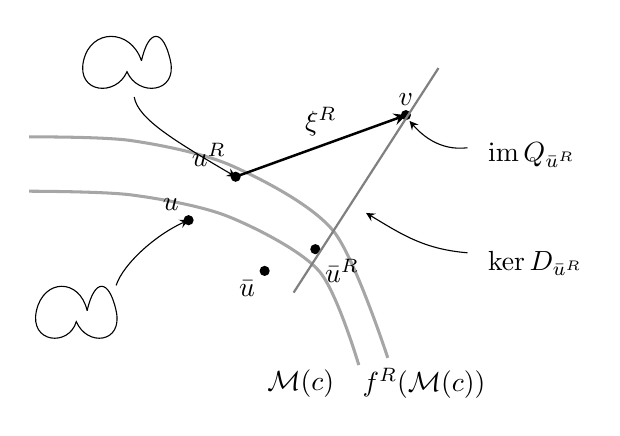
\begin{tikzpicture}[>=stealth,scale=.92]
  \draw[gray!70,line width=1.1pt]
    plot[smooth] coordinates {(-4.2,1.5) (-2.8,1.45) (-1.4,1.1) (0,.2) (.75,-1.55)};
  \draw[gray!70,line width=1.1pt]
    plot[smooth] coordinates {(-4.2,.75) (-2.8,.7) (-1.45,.4) (-.2,-.35) (.35,-1.65)};
  \node at (-.45,-1.9) {$\mathcal M(c)$};
  \node at (1.25,-1.9) {$f^R(\mathcal M(c))$};

  \coordinate (u) at (-2.0,.35);
  \coordinate (ub) at (-.95,-.35);
  \coordinate (uR) at (-1.35,.95);
  \coordinate (ubR) at (-.25,-.05);
  \coordinate (v) at (1.0,1.8);
  \fill (u) circle (2pt) node[above left] {$u$};
  \fill (ub) circle (2pt) node[below left] {$\bar u$};
  \fill (uR) circle (2pt) node[above left] {$u^R$};
  \fill (ubR) circle (2pt) node[below right] {$\bar u^R$};
  \fill (v) circle (2pt) node[above] {$v$};
  \draw[->,line width=.9pt] (uR) -- node[above] {$\xi^R$} (v);

  \draw[gray,line width=.8pt] (-.55,-.65) -- (1.45,2.45);
  \node[anchor=west] at (2.0,-.25) {$\ker D_{\bar u^R}$};
  \draw[->] (1.85,-.1) .. controls (1.25,-.05) and (.95,.15) .. (.45,.45);
  \node[anchor=west] at (2.0,1.25) {$\operatorname{im}Q_{\bar u^R}$};
  \draw[->] (1.85,1.35) .. controls (1.45,1.3) and (1.2,1.55) .. (1.05,1.72);

  \draw[thin] (-2.65,2.55) .. controls (-2.8,3.0) and (-3.35,3.0) .. (-3.45,2.55)
    .. controls (-3.55,2.1) and (-3.0,2.05) .. (-2.85,2.4)
    .. controls (-2.7,2.05) and (-2.15,2.1) .. (-2.25,2.55)
    .. controls (-2.35,3.0) and (-2.55,3.0) .. (-2.65,2.55);
  \draw[->] (-2.75,2.05) .. controls (-2.7,1.75) and (-2.2,1.45) .. (uR);
  \draw[thin] (-3.4,-.9) .. controls (-3.5,-.45) and (-4.0,-.45) .. (-4.1,-.9)
    .. controls (-4.2,-1.35) and (-3.65,-1.4) .. (-3.55,-1.05)
    .. controls (-3.4,-1.4) and (-2.9,-1.35) .. (-3.0,-.9)
    .. controls (-3.1,-.45) and (-3.3,-.45) .. (-3.4,-.9);
  \draw[->] (-3.0,-.55) .. controls (-2.9,-.25) and (-2.45,.15) .. (u);
\end{tikzpicture}
\caption{$f^R(\mathcal M(c))$ 的\BookRecordIndex{T0117}法丛。}\label{fig:10-7-2}
\end{figure}

定义光滑映射
\[
  h^R=(h_1^R,\ldots,h_m^R):\mathcal U_1\longrightarrow\mathbb R^m
\]
如下：
\begin{equation}\label{eq:10-7-6}
  \xi^R-Q_{u^R}D_{u^R}\xi^R
  =:\sum_{i=1}^m h_i^R(u)\Xi_i^R(u),
\end{equation}
其中 $u^R:=f^R(u)$，而 $\xi^R=\xi^R(u)$ 是沿 $u^R$、满足
式~\eqref{eq:10-7-3} 的唯一向量场。因此，$h^R(u)\in\mathbb R^m$ 是
$\xi^R(u)$ 沿 $Q_{u^R}$ 的像投影到 $D_{u^R}$ 的核后所得坐标向量。我们需要找到
一点 $\bar u$，使 $h^R(\bar u)$ 为零。由式~\eqref{eq:10-7-4}，存在常数
$c_4>0$，使得
\[
  |h^R(u)|\leq c_4\lVert\xi^R(u)\rVert_{1,p,R}.
\]
所以我们的假设蕴含：对某个可由我们选取的充分小 $\varepsilon_2$，存在
$u\in\mathcal U_1$ 使 $|h^R(u)|<c_4\varepsilon_2$。为找到 $h^R$ 的真正零点，
我们要应用命题 A.3.4。该命题是\BookRecordIndex{T0380}隐函数定理的一个版本：若映射 $h$ 在点 $x_1$ 有一个
近似零点，而且微分 $dh$ 在 $x_1$ 的一个充分大邻域上一致可逆，那么 $h$ 在非常靠近
$x_1$ 的地方有一个真正零点。

因此只须估计 $dh^R$ 的逆。其几何图像见图~\ref{fig:10-7-2}。向量
$\xi^R=\xi^R(u)$ 从 $u^R$ 指向 $v$。当 $u$ 沿切向量
$\dot u\in T_u\mathcal M(c)$ 的方向变化时，向量 $\xi^R\simeq v-u$ 大致沿
$-\dot u$ 的方向变化。由于 $h^R(u)$ 表示 $\xi^R(u)$ 到 $D_{u^R}$ 的核上的投影，
而该核几乎平行于 $D_u$ 的核，我们预期映射 $u\mapsto h^R(u)$ 的微分近似等于负恒等
映射；这里通过\BookRecordIndex{T0067}标架 $\Xi_1(u),\ldots,\Xi_m(u)$ 把
$T_u\mathcal M(c)$ 与 $\mathbb R^m$ 识别。下面把这一直观说法精确化。

记
\[
  H(u):=(H_1(u),\ldots,H_m(u)):\ker D_u\longrightarrow\mathbb R^m
\]
为\BookRecordIndex{T0067}标架 $\Xi_1(u),\ldots,\Xi_m(u)$ 所给出的同构，也就是说
\[
  \sum_{i=1}^m(H_i(u)\xi)\Xi_i(u)=\xi.
\]
于是，由 $\Xi_i^R(u)$ 的定义，对 $\xi\in\ker D_u=T_u\mathcal M(c)$ 有
\[
  \sum_{i=1}^m(H_i(u)\xi)\Xi_i^R(u)
  =\bigl(\mathbf 1-Q_{u^R}D_{u^R}\bigr)df^R(u)\xi.
\]
我们将证明存在常数 $c_5>0$，使得对每个
$u:=(u^0,u^\infty)\in\mathcal U_1$ 都有
\begin{equation}\label{eq:10-7-7}
  \lVert dh^R(u)+H(u)\rVert\leq c_5\varepsilon_1.
\end{equation}
这里 $\lVert\cdot\rVert$ 表示从 $\ker D_u$ 到 $\mathbb R^m$ 的线性映射的算子范数，
其中 $\mathbb R^m$ 取欧几里得范数，$\ker D_u$ 取 $L^2$-范数。由于线性映射
$H(u)$ 是同构，当 $\varepsilon_1$ 充分小时，式~\eqref{eq:10-7-7} 蕴含
$dh^R(u)$ 满足命题 A.3.4 的条件。步骤 2 立即\BookRecordIndex{T0326}推出。

为证明式~\eqref{eq:10-7-7}，沿 $\mathcal U_1$ 中一条光滑道路
$t\mapsto u_t:=(u_t^0,u_t^\infty)$ 对恒等式~\eqref{eq:10-7-6} 作协变微分。
记 $u_t^R:=f^R(u_t)$，并令
$\xi_t^R\in\Omega^0(S^2,(u_t^R)^*TM)$ 为沿 $u_t^R$、满足
\[
  \exp_{u_t^R}(\xi_t^R)=v,
  \qquad \lVert\xi_t^R\rVert_{1,p,R}\leq\varepsilon_1
\]
的唯一光滑向量场族。
由式~\eqref{eq:10-7-6}，有
\[
  \nabla_t(\xi_t^R-QD\xi_t^R)
  =\sum_{i=1}^m h_i^R(u_t)\nabla_t\Xi_i^R(u_t)
   +\sum_{i=1}^m\bigl(\partial_t h_i^R(u_t)\bigr)\Xi_i^R(u_t),
\]
其中 $Q:=Q_{u_t^R}$，$D:=D_{u_t^R}$。接着对恒等式
$\exp_{u_t^R}(\xi_t^R)=v$ 求微分，得到
\[
  E_1\partial_tu_t^R+E_2\nabla_t\xi_t^R=0,
\]
其中 $E_i:=E_i^R(u_t^R,\xi_t^R)$ 如注~\ref{rem:10-5-5} 中所定义。因此
\[
  \nabla_t\xi_t^R
  =-E_2^{-1}E_1\partial_tu_t^R
  =-E_2^{-1}E_1df^R(u_t)\partial_tu_t.
\]
为证明式~\eqref{eq:10-7-7}，需要估计函数
$\partial_th_i^R(u_t)+H_i(u_t)\partial_tu_t$。合并上述恒等式，得到
\begin{align}
 &\sum_{i=1}^m
 \bigl(\partial_th_i^R(u_t)+H_i(u_t)\partial_tu_t\bigr)\Xi_i^R(u_t)
 \notag\\
 &\quad=
 (\mathbf 1-QD)(\mathbf 1-E_2^{-1}E_1)df^R(u_t)\partial_tu_t
 \label{eq:10-7-8}\\
 &\qquad{}+QD\nabla_t\xi_t^R-\nabla_t(QD\xi_t^R)
 -\sum_{i=1}^m h_i^R(u_t)\nabla_t\Xi_i^R(u_t).
 \notag
\end{align}
由于
$|h^R(u_t)|\leq c_4\lVert\xi_t^R\rVert_{1,p,R}\leq c_4\varepsilon_1$，
由式~\eqref{eq:10-7-5} 可得
\[
  \left\lVert
  \sum_{i=1}^m h_i^R(u_t)\nabla_t\Xi_i^R(u_t)
  \right\rVert_{1,p,R}
  \leq\sqrt m\,c_3c_4\varepsilon_1
  \lVert\partial_tu_t\rVert_{L^2}.
\]
这处理了式~\eqref{eq:10-7-8} 右端的最后一项。对其右端第一项，可以使用逐点估计
\[
  \bigl|\mathbf 1-E_2(u_t^R,\xi_t^R)^{-1}E_1(u_t^R,\xi_t^R)\bigr|
  \leq c_5|\xi_t^R|.
\]
关于 $\xi_t^R$ 的一阶导数，也有 $\mathbf 1-E_2^{-1}E_1$ 的一阶导数的类似不等式
（这里固定 $t$）。所以式~\eqref{eq:10-7-8} 右端第一项可估计为
\[
  \bigl\lVert(\mathbf 1-E_2^{-1}E_1)df^R(u_t)\partial_tu_t
  \bigr\rVert_{1,p,R}
  \leq c_6\varepsilon_1\lVert\partial_tu_t\rVert_{L^2}.
\]
我们断言，剩余项满足如下形式的估计：
\begin{equation}\label{eq:10-7-9}
  \bigl\lVert\nabla_t(QD\xi_t^R)-QD\nabla_t\xi_t^R\bigr\rVert_{1,p,R}
  \leq c_7\lVert\xi_t^R\rVert_{1,p,R}
  \lVert\partial_tu_t^R\rVert_{1,\infty,R}.
\end{equation}
对算子 $T=T_{u_t^R}$，引理~\ref{lem:10-6-2} 已经证明了这样的估计；对算子
$D$，可以使用引理~\ref{lem:10-6-2} 证明中的式~\eqref{eq:10-6-8}。合并这些估计，
便得到交换子 $[DT,\widetilde\nabla_t]$ 的估计，继而得到
$[(DT)^{-1},\widetilde\nabla_t]$ 的估计。这又蕴含算子
$QD=T(DT)^{-1}D$ 与 $\widetilde\nabla_t$ 的交换子所需的估计。把
式~\eqref{eq:10-7-9} 与
$\lVert\xi_t^R\rVert_{1,p,R}\leq\varepsilon_1$ 以及
命题~\ref{prop:10-5-4} 证明中的式~\eqref{eq:10-6-15} 合并，得到
\[
  \bigl\lVert\nabla_t(QD\xi_t^R)-QD\nabla_t\xi_t^R\bigr\rVert_{1,p,R}
  \leq c_8\varepsilon_1\lVert\partial_tu_t\rVert_{L^2}.
\]
因此我们已经证明
\[
  \left\lVert\sum_{i=1}^m
  \bigl(\partial_th_i^R(u_t)+H_i(u_t)\partial_tu_t\bigr)\Xi_i^R(u_t)
  \right\rVert_{1,p,R}
  \leq c_9\varepsilon_1\lVert\partial_tu_t\rVert_{L^2}.
\]
式~\eqref{eq:10-7-7} 于是由式~\eqref{eq:10-7-4} \BookRecordIndex{T0326}推出。这证明了步骤 2。

\medskip
\noindent\textbf{步骤 3.}
\emph{对每个 $\varepsilon_2>0$，存在正常数 $\delta_3$ 和 $\varepsilon_3$，
使得对每个 $(\delta,R)\in\mathcal A(\delta_3)$，下述结论成立。若
$(u^0,u^\infty)\in\mathcal M^{0,\infty}(c)$ 和
$v\in\mathcal M(A;J^R)$ 满足}
\begin{equation}\label{eq:10-7-10}
  \sup_{|z|\geq1}d\bigl(v(z),u^0(z)\bigr)<\varepsilon_3,
  \qquad
  \sup_{|z|\leq1}d\bigl(v(z/R^2),u^\infty(z)\bigr)<\varepsilon_3,
\end{equation}
\emph{则沿曲线 $u^R:=f^R(u^0,u^\infty)$ 存在向量场
$\xi^R\in\Omega^0(S^2,(u^R)^*TM)$，使得}
\begin{equation}\label{eq:10-7-11}
  v=\exp_{u^R}(\xi^R),
  \qquad \lVert\xi^R\rVert_{1,p,R}\leq\varepsilon_2.
\end{equation}

反设该断言对某个常数 $\varepsilon_2>0$ 不成立。于是存在序列
\[
  \delta_\nu\longrightarrow0,\qquad R_\nu\longrightarrow\infty,\qquad
  (u_\nu^0,u_\nu^\infty)\in\mathcal M^{0,\infty}(c),
  \qquad v_\nu\in\mathcal M^{R_\nu},
\]
使 $\delta_\nu R_\nu$ 趋于无穷，并且
\[
  \lim_{\nu\to\infty}\sup_{|z|\geq1}
  d\bigl(v_\nu(z),u_\nu^0(z)\bigr)
  =\lim_{\nu\to\infty}\sup_{|z|\leq1}
  d\bigl(v_\nu(z/R_\nu^2),u_\nu^\infty(z)\bigr)=0,
\]
且对每个 $\nu$ 都有
\begin{equation}\label{eq:10-7-12}
  \inf\left\{
  \lVert\xi\rVert_{1,p,R_\nu}\ \middle|\
  \xi\in\Omega^0(S^2,(u_\nu^{R_\nu})^*TM),\ 
  v_\nu=\exp_{u_\nu^{R_\nu}}(\xi)
  \right\}\geq\varepsilon_2.
\end{equation}
按通常约定，空集上的下确界取作 $\infty$。

由于\BookRecordIndex{T0246}模空间 $\mathcal M(c)$ 紧，可以假设序列
$(u_\nu^0,u_\nu^\infty)$ 在 $C^\infty$ 拓扑下收敛到偶对
$u:=(u^0,u^\infty)$。此外，取子列后，可以假设
$v_\nu:S^2\setminus\{0\}\to M$ 在有限个\BookRecordIndex{T0275}气泡点之外\BookRecordIndex{T0416}逐紧一致收敛到某条极限曲线
$v^0$（定理~\ref{thm:4-6-1}）。注意，这里必须处理 $v_\nu$ 在
$S^2\setminus\{0\}$ 上的限制，因为 $J^{R_\nu}$ 正是在这里收敛。由假设，
当 $|z|\geq1$ 时 $v^0(z)=u^0(z)$；再由\BookRecordIndex{T0333}唯一延拓
（推论~\ref{cor:2-3-3}），这蕴含 $v^0=u^0$。同样的论证说明，\BookRecordIndex{T0412}重标度序列
\[
  v_\nu(\,\cdot\,/R_\nu^2):
  \mathbb C=S^2\setminus\{\infty\}\longrightarrow M
\]
在有限个\BookRecordIndex{T0275}气泡点之外收敛到 $u^\infty$。由于 $v_\nu$ 表示同调类
$A=A^0+A^\infty$，已无能量可供\BookRecordIndex{T0243}冒泡。因此 $v_\nu$ 在
$S^2\setminus\{0\}$ 的紧子集上一致收敛到 $u^0$，而\BookRecordIndex{T0412}重标度序列
$v_\nu(\,\cdot\,/R_\nu^2)$ 在 $S^2\setminus\{\infty\}$ 的紧子集上一致收敛
到 $u^\infty$。此外，由引理~\ref{lem:4-7-5}，
\[
  \lim_{\rho\to0}\lim_{\nu\to\infty}
  \sup_{1/(\rho R_\nu^2)\leq|z|\leq\rho}
  d\bigl(v_\nu(z),x\bigr)=0,
\]
其中 $x:=u^0(0)=u^\infty(\infty)$。由极限偶对 $(u^0,u^\infty)$ 构造的\BookRecordIndex{T0394}预粘合
序列 $u^{R_\nu}:=f^{R_\nu}(u^0,u^\infty)$ 满足相同条件，故
\[
  \lim_{\nu\to\infty}\sup_{z\in S^2}
  d\bigl(v_\nu(z),u^{R_\nu}(z)\bigr)=0.
\]
于是对每个充分大的 $\nu$，存在沿 $u^{R_\nu}$ 的唯一小向量场 $\xi_\nu$，使得
\[
  v_\nu=\exp_{u^{R_\nu}}(\xi_\nu).
\]
我们断言
\begin{equation}\label{eq:10-7-13}
  \lim_{\nu\to\infty}\lVert\xi_\nu\rVert_{1,p,R_\nu}=0,
\end{equation}
这与式~\eqref{eq:10-7-12} 矛盾。

为证明式~\eqref{eq:10-7-13}，回顾当
$1/(\kappa R_\nu^2)\leq|z|\leq\kappa$ 时 $J_z^{R_\nu}=J$。因此公式
\[
  w_\nu(s,t):=v_\nu(R_\nu^{-1}e^{s+it}),
  \qquad |s|\leq\log\kappa+\log R_\nu,
\]
定义了一列 \BookRecordIndex{T0003}$J$-全纯曲线；它在每个紧子集上一致且连同所有阶导数收敛到
$x:=u^0(0)=u^\infty(\infty)$。现在选取实数 $\mu$，使
$1-2/p<\mu<1$。由引理~\ref{lem:4-7-3} 中的式~\eqref{eq:4-7-19}，
存在常数 $c_{10}>0$，使得当 $\nu$ 充分大时
\[
  |\partial_sw_\nu(s,t)|
  \leq c_{10}e^{-\mu(\log R_\nu-|s|)},
  \qquad |s|\leq\log R_\nu+\log\kappa-\log2.
\]
由于
\[
  \sqrt2\,|\partial_sw_\nu(s,t)|
  =e^sR_\nu^{-1}|dv_\nu(R_\nu^{-1}e^{s+it})|,
\]
这转化为估计
\[
  \frac1{R_\nu}\leq|z|\leq\frac\kappa2
  \qquad\Longrightarrow\qquad
  |dv_\nu(z)|\leq\frac{\sqrt2c_{10}}{|z|^{1-\mu}}.
\]
因 $\mu>1-2/p$，有 $p\mu-p+2>0$，并且
\[
  \lVert dv_\nu\rVert_{L^p(A(1/R_\nu,\rho))}^p
  \leq c_{11}\int_{1/R_\nu\leq|z|\leq\rho}|z|^{p\mu-p}
  \leq c_{12}\rho^{p\mu-p+2}.
\]
这说明
\[
  \lim_{\rho\to0}\lim_{\nu\to\infty}
  \lVert dv_\nu\rVert_{L^p(A(1/R_\nu,\rho))}=0.
\]
按构造，函数 $u^{R_\nu}$ 满足同一条件，因而
\[
  \lim_{\rho\to0}\lim_{\nu\to\infty}
  \lVert\xi_\nu\rVert_{W^{1,p}(A(1/R_\nu,\rho))}=0.
\]
在\BookRecordIndex{T0170}环域 $A(1/R_\nu,\rho)$ 上，$W^{1,p}$-范数与 $(1,p,R_\nu)$-范数等价
（至多相差因子 $2$）。对 $|z|\leq1/R_\nu$，再次利用公式的对称性，可得类似结论。
这蕴含
\[
  \lim_{\rho\to0}\lim_{\nu\to\infty}
  \lVert\xi_\nu\rVert_{1,p,R_\nu;A(1/(\rho R_\nu^2),\rho)}=0.
\]
再结合 $v_\nu$ 在 $S^2\setminus\{0\}$ 上\BookRecordIndex{T0416}逐紧一致收敛到 $u^0$，以及
$v_\nu(R_\nu^{-2}\,\cdot\,)$ 在 $S^2\setminus\{\infty\}$ 上\BookRecordIndex{T0416}逐紧一致收敛到
$u^\infty$，便得到式~\eqref{eq:10-7-13}。这与式~\eqref{eq:10-7-12}
矛盾，从而证明了步骤 3。

\medskip
\noindent\textbf{步骤 4.}
\emph{证明第（v）部分。}

先选取 $\varepsilon_1>0$，使步骤 1 的断言成立。再选取 $\varepsilon_2>0$ 和
$\delta_2<\delta_0$，使步骤 2 的断言对这个 $\varepsilon_1$ 成立。最后，选取
$\varepsilon_3$ 和 $\delta_3\leq\delta_2$，使步骤 3 的断言对这个
$\varepsilon_2$ 成立。现在假设 $0<\delta<\delta_3$ 且
$\delta R>1/\delta_3$。设 $(u^0,u^\infty)\in\mathcal M^{0,\infty}(c-1)$ 和
$v\in\mathcal M(A;J^R)$ 满足式~\eqref{eq:10-7-10}。由步骤 3，沿
$u^R:=f^R(u^0,u^\infty)$ 存在向量场 $\xi^R$，使得
\[
  v=\exp_{u^R}(\xi^R),\qquad
  \lVert\xi^R\rVert_{1,p,R}\leq\varepsilon_2.
\]
所以由步骤 2，存在一对
$(\bar u^0,\bar u^\infty)\in\mathcal M^{0,\infty}(c)$ 和沿
$\bar u^R:=f^R(\bar u^0,\bar u^\infty)$ 的向量场 $\bar\xi^R$，使得
\[
  v=\exp_{\bar u^R}(\bar\xi^R),\qquad
  \bar\xi^R\in\operatorname{im}Q_{\bar u^R},\qquad
  \lVert\bar\xi^R\rVert_{1,p,R}\leq\varepsilon_1.
\]
再由步骤 1，$v=\iota_c^R(\bar u^0,\bar u^\infty)$。这证明了
定理~\ref{thm:10-1-2} 的第（v）部分。
\end{proof}


\section{\BookRecordIndex{T0125}分裂公理的证明}\label{sec:10-8}

先以略有不同但等价的形式重述\BookRecordIndex{T0125}分裂公理。以下始终假设 $(M,\omega)$ 是紧\BookRecordIndex{T0058}半正\BookRecordIndex{T0358}辛流形。
固定三个整数 $\ell^0,\ell^\infty\geq2$ 和 $k\geq\ell^0+\ell^\infty$，并记
\[
  I^0:=\{0,\ldots,\ell^0\},\qquad
  I^\infty:=\{0,\ldots,\ell^\infty\},\qquad
  I:=\{1,\ldots,\ell^0+\ell^\infty\}.
\]
这些集合为\BookRecordIndex{T0150}固定标记点 $\mathbf w$ 编号；前两个在先前的记号中对应
$I_{S_0},I_{S_1}$。令 $\mathcal S$ 表示指标集 $\{1,\ldots,k\}$ 的所有分裂
$S=(S^0,S^\infty)$ 所成的集合，其中
\[
  \{1,\ldots,\ell^0\}\subset S^0,
  \qquad
  \{\ell^0+1,\ldots,\ell^0+\ell^\infty\}\subset S^\infty.
\]
给定分裂 $S=(S^0,S^\infty)\in\mathcal S$，令
\[
  k^0:=k^0(S):=|S^0|\geq\ell^0,
  \qquad
  k^\infty:=k^\infty(S):=|S^\infty|\geq\ell^\infty,
\]
并以
\[
  \sigma^0:\{1,\ldots,k^0\}\longrightarrow\{1,\ldots,k\},
  \qquad
  \sigma^\infty:\{1,\ldots,k^\infty\}\longrightarrow\{1,\ldots,k\}
\]
表示满足 $\operatorname{im}\sigma^0=S^0$ 和
$\operatorname{im}\sigma^\infty=S^\infty$ 的唯一保序单射。因此，当
$1\leq i\leq\ell^0$ 时 $\sigma^0(i)=i$，而当
$1\leq i\leq\ell^\infty$ 时 $\sigma^\infty(i)=\ell^0+i$。用这些记号，
\BookRecordIndex{T0143}格罗莫夫--威滕不变量的\BookRecordIndex{T0125}分裂公理可表为如下形式。

\begin{theorem}[\BookRecordIndex{T0125}分裂公理]\label{thm:10-8-1}
对每个球面同调类 $A\in H_2(M;\mathbb Z)$ 和每一族上同调类
$a_1,\ldots,a_k\in H^*(M)$，有
\begin{align*}
  \operatorname{GW}_{A,k}^{M,I}(a_1,\ldots,a_k)
  ={}&\sum_{S\in\mathcal S}\sum_{A^0+A^\infty=A}
  \varepsilon(S,a)\varepsilon(S^0,a)\sum_{\nu,\mu}
  \operatorname{GW}_{A^0,k^0+1}^{M,I^0}
  \bigl(e_\nu,a_{\sigma^0(1)},\ldots,a_{\sigma^0(k^0)}\bigr)
  g^{\nu\mu}\\
  &\qquad{}\cdot
  \operatorname{GW}_{A^\infty,k^\infty+1}^{M,I^\infty}
  \bigl(e_\mu,a_{\sigma^\infty(1)},\ldots,
  a_{\sigma^\infty(k^\infty)}\bigr),
\end{align*}
其中 $e_\nu$ 构成 $H^*(M)$ 的一组基，
\[
  g_{\nu\mu}=\int_M e_\nu\smile e_\mu,
\]
$g^{\nu\mu}$ 是其逆矩阵，并且
\begin{align*}
  \varepsilon(S,a)
  &:={(-1)}^{\#\{(i,j)\in S^0\times S^\infty\mid
  j<i,\ \deg(a_i)\deg(a_j)\in2\mathbb Z+1\}},\\
  \varepsilon(S^0,a)
  &:={(-1)}^{\#\{i\in S^0\mid\deg(a_i)\in2\mathbb Z+1\}}.
\end{align*}
\end{theorem}

\begin{remark}\label{rem:10-8-2}
在定理~\ref{thm:10-8-1} 中，不变量
$\operatorname{GW}^{M,I^0}$ 和 $\operatorname{GW}^{M,I^\infty}$ 的\BookRecordIndex{T0066}标记点指标集分别
理解为 $\{0,\ldots,k^0\}$ 和 $\{0,\ldots,k^\infty\}$。
$\varepsilon(S,a)$ 的含义不变。额外符号 $\varepsilon(S^0,a)$ 的出现，是因为
类 $e_\nu$ 是 $\operatorname{GW}^{M,I^0}$ 的第一个而不是最后一个自变量。推导这个
符号公式时，我们使用了如下事实：$\operatorname{GW}^{M,I^0}$ 所取值的那些类的次数
之和总为偶数。
\end{remark}

\medskip
\noindent\textbf{\BookRecordIndex{T0226}连通对的\BookRecordIndex{T0283}求值映射。}
令 $\mathbf w^0=\{w_i^0\}_{1\leq i\leq\ell^0}$ 是
$S^2\setminus\{0\}$ 中两两不同的 $\ell^0$ 元组，令
$\mathbf w^\infty=\{w_j^\infty\}_{1\leq j\leq\ell^\infty}$ 是
$S^2\setminus\{\infty\}$ 中两两不同的 $\ell^\infty$ 元组。固定整数
$k\geq\ell^0+\ell^\infty$，取 $S=(S^0,S^\infty)\in\mathcal S$，记
\[
  k^0:=|S^0|,\qquad k^\infty:=|S^\infty|,
\]
并令 $\sigma^0,\sigma^\infty$ 如上为相应的重排映射。考虑\BookRecordIndex{T0246}模空间
\[
  \mathcal M_{0,S}(A^{0,\infty};\mathbf w^{0,\infty};J^{0,\infty})
  :=\mathcal M_{0,S}(A^0,A^\infty;
  \mathbf w^0,\mathbf w^\infty;J^0,J^\infty),
\]
它由所有元组
\[
  (u^0,u^\infty,\mathbf z^0,\mathbf z^\infty)
  =(u^0,u^\infty,z_1^0,\ldots,z_{k^0}^0,
  z_1^\infty,\ldots,z_{k^\infty}^\infty)
\]
组成，其中 $(u^0,u^\infty)\in\mathcal M(A^{0,\infty};J^{0,\infty})$，
$\mathbf z^0=\{z_i^0\}_{1\leq i\leq k^0}$ 是
$S^2\setminus\{0\}$ 中两两不同的 $k^0$ 元组，并满足下列条件
\sourcefootnote{原书把这里的指标上界印作 $\ell^\infty$；但
$\mathbf w^0$ 是 $\ell^0$ 元组，且本节前后固定在 $0$ 侧的恰为前
$\ell^0$ 个\BookRecordIndex{T0066}标记点，故补正为 $\ell^0$。}：
\[
  z_j^0=w_j^0,\qquad j=1,\ldots,\ell^0,
\]
而 $\mathbf z^\infty$ 的条件类似（见图~\ref{fig:10-8-3}）。与前面一样，假设
$J^0$ 和 $J^\infty$ 依赖于 $z$，从而无须限制到单纯映射。

\begin{figure}[tbp]
\centering
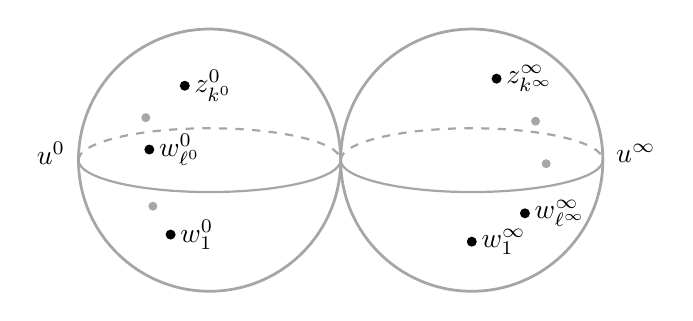
\begin{tikzpicture}[scale=.9]
  \draw[gray!70,line width=1pt] (-1.85,0) circle (1.85);
  \draw[gray!70,line width=1pt] (1.85,0) circle (1.85);
  \draw[gray!70,line width=.8pt] (-3.7,0) arc[start angle=180,end angle=360,x radius=1.85,y radius=.45];
  \draw[gray!70,dashed,line width=.8pt] (-3.7,0) arc[start angle=180,end angle=0,x radius=1.85,y radius=.45];
  \draw[gray!70,line width=.8pt] (0,0) arc[start angle=180,end angle=360,x radius=1.85,y radius=.45];
  \draw[gray!70,dashed,line width=.8pt] (0,0) arc[start angle=180,end angle=0,x radius=1.85,y radius=.45];
  \node[left] at (-3.75,.1) {$u^0$};
  \node[right] at (3.75,.1) {$u^\infty$};
  \fill (-2.2,1.05) circle (2pt) node[right] {$z_{k^0}^0$};
  \fill[gray!70] (-2.75,.6) circle (1.8pt);
  \fill (-2.7,.15) circle (2pt) node[right] {$w_{\ell^0}^0$};
  \fill (-2.4,-1.05) circle (2pt) node[right] {$w_1^0$};
  \fill[gray!70] (-2.65,-.65) circle (1.8pt);
  \fill (2.2,1.15) circle (2pt) node[right] {$z_{k^\infty}^\infty$};
  \fill[gray!70] (2.75,.55) circle (1.8pt);
  \fill[gray!70] (2.9,-.05) circle (1.8pt);
  \fill (2.6,-.75) circle (2pt) node[right] {$w_{\ell^\infty}^\infty$};
  \fill (1.85,-1.15) circle (2pt) node[right] {$w_1^\infty$};
\end{tikzpicture}
\caption{带\BookRecordIndex{T0066}标记点的\BookRecordIndex{T0226}连通对。}\label{fig:10-8-3}
\end{figure}

这个空间带有\BookRecordIndex{T0283}求值映射
\[
  \operatorname{ev}_{A^{0,\infty},S}:
  \mathcal M_{0,S}(A^{0,\infty};\mathbf w^{0,\infty};J^{0,\infty})
  \longrightarrow M^k,
\]
其定义为
$\operatorname{ev}_S(u^0,u^\infty,\mathbf z^0,\mathbf z^\infty)
:=(x_1,\ldots,x_k)$，其中
\[
  x_{\sigma^0(i)}:=u^0(z_i^0),\qquad
  x_{\sigma^\infty(j)}:=u^\infty(z_j^\infty),
\]
$i=1,\ldots,k^0$，$j=1,\ldots,k^\infty$。还要考虑这个\BookRecordIndex{T0283}求值映射在紧子集
\[
  \mathcal M_{0,S}(A^{0,\infty};\mathbf w^{0,\infty};J^{0,\infty},c)
  \subset
  \mathcal M_{0,S}(A^{0,\infty};\mathbf w^{0,\infty};J^{0,\infty})
\]
上的限制；该紧子集由所有满足
\[
  \lVert du^0\rVert_{L^\infty}\leq c,\qquad
  \lVert du^\infty\rVert_{L^\infty}\leq c
\]
以及
\[
  |z_i^0-z_{i'}^0|\geq\frac1c,\qquad
  |z_i^0|\geq\frac1c,\qquad
  |z_j^\infty-z_{j'}^\infty|\geq\frac1c,\qquad
  |z_j^\infty|\leq c
\]
的元组组成，其中 $i\ne i'$、$j\ne j'$。下一个推论立即来自
定理~\ref{thm:10-1-2} 第（iii）部分。

\begin{corollary}\label{cor:10-8-3}
固定两个同调类 $A^0,A^\infty\in H_2(M;\mathbb Z)$、一个\BookRecordIndex{T0088}殆复结构\BookRecordIndex{T0406}正则对
\[
  (J^0,J^\infty)\in\mathcal J_{\mathrm{reg}}(S^2;A^{0,\infty})
\]
以及常数 $c>0$。令 $A:=A^0+A^\infty$，并令
$\delta_0=\delta_0(c)$ 为定理~\ref{thm:10-1-2} 中的常数。假设
$0<\delta<\delta_0$，且对 $R>1/(\delta\delta_0)$，令
\[
  \iota_c^R=\iota_c^{\delta,R}:
  \mathcal M(A^{0,\infty};J^{0,\infty},c)
  \longrightarrow\mathcal M(A;J^R)
\]
为定理~\ref{thm:10-1-2} 中引入的映射。令
$\mathbf w^0=\{w_i^0\}_{1\leq i\leq\ell^0}$ 是
$S^2\setminus\{0\}$ 中两两不同的 $\ell^0$ 元组，令
$\mathbf w^\infty=\{w_j^\infty\}_{1\leq j\leq\ell^\infty}$ 是
$S^2\setminus\{\infty\}$ 中两两不同的 $\ell^\infty$ 元组。固定整数
$k\geq\ell^0+\ell^\infty$，取 $S=(S^0,S^\infty)\in\mathcal S$，并定义
\[
  w_i^R:=w_i^0\quad(i=1,\ldots,\ell^0),
  \qquad
  w_{\ell^0+j}^R:=w_j^\infty/R^2
  \quad(j=1,\ldots,\ell^\infty).
\]
考虑嵌入
\[
  \iota_{c,S}^R:
  \mathcal M_{0,S}(A^{0,\infty};\mathbf w^{0,\infty};J^{0,\infty},c)
  \longrightarrow
  \mathcal M_{0,k}^*(A;\mathbf w^R;J^R),
\]
它由
\[
  \iota_{c,S}^R(u^0,u^\infty,\mathbf z^0,\mathbf z^\infty)
  :=(\widetilde u^R,\mathbf z^R)
\]
给出，其中
\[
  \widetilde u^R:=\iota_c^R(u^0,u^\infty),
  \qquad z_{\sigma^0(i)}^R:=z_i^0,
  \qquad z_{\sigma^\infty(j)}^R:=z_j^\infty/R^2
\]
（$i=1,\ldots,k^0$，$j=1,\ldots,k^\infty$）。则当 $R$ 趋于无穷时，
\BookRecordIndex{T0283}求值映射
\[
  \operatorname{ev}^R:\mathcal M_{0,k}^*(A;\mathbf w^R;J^R)\longrightarrow M^k
\]
与 $\iota_{c,S}^R$ 的复合在 $C^1$ 拓扑下收敛到
$\operatorname{ev}_{A^{0,\infty},S}$。
\end{corollary}

\medskip
\noindent\textbf{\BookRecordIndex{T0226}连通对\BookRecordIndex{T0246}模空间的极限集。}
证明定理~\ref{thm:10-8-1} 的第一步，是说明\BookRecordIndex{T0283}求值映射
\[
  \operatorname{ev}_{A^{0,\infty},S}:
  \mathcal M_{0,S}^*(A^{0,\infty};\mathbf w^{0,\infty};J^{0,\infty})
  \longrightarrow M^k
\]
是一个\BookRecordIndex{T0337}伪循环。其证明与说明\BookRecordIndex{T0084}带标号树 $T$ 上的\BookRecordIndex{T0340}稳定映射的\BookRecordIndex{T0283}求值映射
\[
  \operatorname{ev}_T:\mathcal M_{0,T}^*(\{A_\alpha\};J)\longrightarrow M^k
\]
为\BookRecordIndex{T0337}伪循环时所需的证明几乎相同；见习题~\ref{ex:6-6-3}。不过，$J^0$ 和
$J^\infty$ 对 $z$ 的依赖带来了一些额外特征，下面对此加以说明。

第一步是理解定义域中\BookRecordIndex{T0141}格罗莫夫收敛序列的极限。由于 $J^0$ 和 $J^\infty$ 随定义域
$S^2$ 上的点变化，这些极限是带两个特殊分支的\BookRecordIndex{T0340}稳定映射：这两个分支分别标为 $0$ 和
$\infty$，并分别关于 $\{J_z^0\}$ 和 $\{J_z^\infty\}$ 全纯。其余分支都是\BookRecordIndex{T0275}气泡；
它们关于固定复结构 $J_{z_\alpha}^0$ 或 $J_{z_\alpha}^\infty$ 全纯，该复结构对应于
它们附着到某个特殊分支的点。与第~\ref{sec:6-7} 节一样，把问题看成
$u^0,u^\infty$ 的图像 $\widetilde u^0,\widetilde u^\infty$ 的收敛很有用。
但现在两个主分支之间也可能形成\BookRecordIndex{T0275}气泡。因此，极限还有第三部分，它关于式~\eqref{eq:10-1-1}
中与 $u^0$ 到 $u^\infty$ 的附着点相联系的 $J$ 全纯。稍后我们会更精确地表述上述讨论；
目前它只是为了引出下面的定义。

令 $\mathbf w^0=\{w_i^0\}_{1\leq i\leq\ell^0}$ 和
$\mathbf w^\infty=\{w_j^\infty\}_{1\leq j\leq\ell^\infty}$ 是 $S^2$ 上两两
不同的点的元组，并且对所有 $i,j$ 都有 $w_i^0\ne0$、$w_j^\infty\ne\infty$。
令 $T=(T,E,\Lambda)$ 是一棵带 $k$ 个标号的树，具有两个不同的\BookRecordIndex{T0321}特殊顶点
$0$ 和 $\infty$。定义\BookRecordIndex{T0417}子树 $T^0,T^\infty\subset T$ 为
\[
  T^0:=\{\alpha\in T\mid0\in[\alpha,\infty]\},
  \qquad
  T^\infty:=\{\alpha\in T\mid\infty\in[0,\alpha]\}.
\]
换言之，从 $0$ 沿指向 $\infty$ 的方向切去分支便得到 $T^0$，从 $\infty$ 沿指向
$0$ 的方向切去分支便得到 $T^\infty$。假设标号满足
\[
  \alpha_i\in T^0\quad(i=1,\ldots,\ell^0),
  \qquad
  \alpha_{\ell^0+j}\in T^\infty\quad(j=1,\ldots,\ell^\infty)
\]
（见图~\ref{fig:10-8-4}）。

固定一族同调类 $\mathbf B=\{B_\alpha\}_{\alpha\in T}\subset H_2(M;\mathbb Z)$，
并假设 $J^0,J^\infty$ 满足式~\eqref{eq:10-1-1}。\BookRecordIndex{T0246}模空间
\[
  \mathcal M_{0,T}^*(\{B_\alpha\};\mathbf w^{0,\infty};J^{0,\infty})
\]
由元组
\[
\begin{split}
  (\mathbf u,\mathbf z):={}&
  \bigl(u_0,u_\infty,
  \{z_\alpha,u_\alpha\}_{\alpha\in(T^0\cup T^\infty)\setminus\{0,\infty\}},\\
  &\{u_\alpha\}_{\alpha\in T\setminus(T^0\cup T^\infty)},
  \{z_{\alpha\beta}\}_{\alpha E\beta},
  \{\alpha_i,z_i\}_{1\leq i\leq k}\bigr)
\end{split}
\]
组成，并满足以下条件。

\begin{description}
\item[（映射）]
每个 $u_\alpha:S^2\to M$ 都是表示类 $B_\alpha$ 的光滑映射。此外，$u_0$ 是
$\{J_z^0\}$-全纯球面，$u_\infty$ 是 $\{J_z^\infty\}$-全纯球面；当
$\alpha\in T^0\setminus\{0\}$ 时，$u_\alpha$ 是 $J_{z_\alpha}^0$-全纯球面；
当 $\alpha\in T^\infty\setminus\{\infty\}$ 时，$u_\alpha$ 是
$J_{z_\alpha}^\infty$-全纯球面；当
$\alpha\in T\setminus(T^0\cup T^\infty)$ 时，$u_\alpha$ 是 $J$-全纯球面。

\item[（\BookRecordIndex{T0191}节点）]
若 $\alpha E\beta$，则
$u_\alpha(z_{\alpha\beta})=u_\beta(z_{\beta\alpha})$。此外，当
$\alpha E\beta$ 且 $\alpha,\beta\in T^0\setminus\{0\}$，或
$\alpha,\beta\in T^\infty\setminus\{\infty\}$ 时，有 $z_\alpha=z_\beta$。
若 $0E\alpha$ 且 $\infty E\beta$，则
\[
  z_{0\alpha}=\begin{cases}
    z_\alpha,&\alpha\in T^0,\\
    0,&\alpha\notin T^0,
  \end{cases}
  \qquad
  z_{\infty\beta}=\begin{cases}
    z_\beta,&\beta\in T^\infty,\\
    \infty,&\beta\notin T^\infty.
  \end{cases}
\]

\item[（稳定性）]
对 $\alpha E\beta$ 的点 $z_{\alpha\beta}$ 与对 $\alpha_i=\alpha$ 的点 $z_i$
两两不同；只要 $u_\alpha$ 为常值且 $\alpha\ne0,\infty$，这样的点至少有三个。

\item[（固定）]
若 $i\in\{1,\ldots,\ell^0\}$、$j\in\{1,\ldots,\ell^\infty\}$，则
\sourcefootnote{原书在右侧两个分支条件中把顶点下标印作 $\alpha_j$；但此处所固定的是
第 $\ell^0+j$ 个\BookRecordIndex{T0066}标记点，且同一分式的分子已经分别写成
$z_{\ell^0+j}$ 和 $z_{\alpha_{\ell^0+j}}$，故补正为 $\alpha_{\ell^0+j}$。}
\[
  w_i^0=\begin{cases}
    z_i,&\alpha_i=0,\\
    z_{\alpha_i},&\alpha_i\ne0,
  \end{cases}
  \qquad
  w_j^\infty=\begin{cases}
    z_{\ell^0+j},&\alpha_{\ell^0+j}=\infty,\\
    z_{\alpha_{\ell^0+j}},&\alpha_{\ell^0+j}\ne\infty.
  \end{cases}
\]

\item[（单纯）]
对每个 $z\in S^2$，\BookRecordIndex{T0417}子树
\[
  T_z^0:=\{\alpha\in T^0\mid z_\alpha=z\},
  \qquad
  T_z^\infty:=\{\alpha\in T^\infty\mid z_\alpha=z\}
\]
上的\BookRecordIndex{T0340}稳定映射都是单纯的，而\BookRecordIndex{T0417}子树 $T\setminus(T^0\cup T^\infty)$ 上的\BookRecordIndex{T0340}稳定映射也是
单纯的。
\end{description}

\begin{figure}[tbp]
\centering
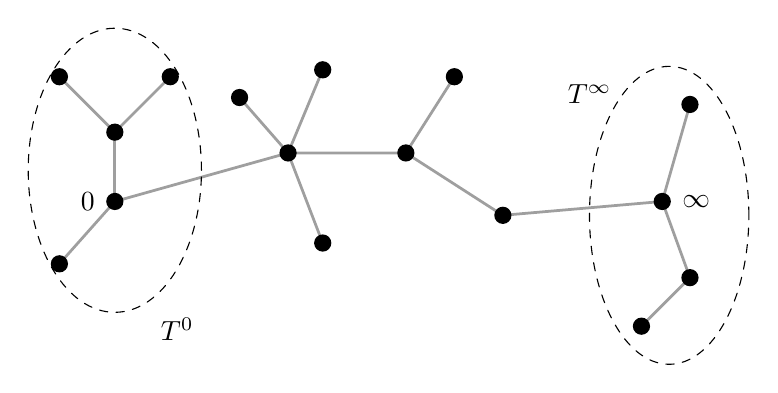
\begin{tikzpicture}[scale=.88,line cap=round,line join=round]
  \tikzset{v/.style={circle,fill,inner sep=2.2pt}}
  \draw[gray!75,line width=1pt]
    (-4,0)--(-1.5,.7)--(.2,.7)--(1.6,-.2)--(3.9,0);
  \draw[gray!75,line width=1pt] (-4,0)--(-4.8,-.9);
  \draw[gray!75,line width=1pt] (-4,0)--(-4,1);
  \draw[gray!75,line width=1pt] (-4,1)--(-4.8,1.8);
  \draw[gray!75,line width=1pt] (-4,1)--(-3.2,1.8);
  \draw[gray!75,line width=1pt] (-1.5,.7)--(-2.2,1.5);
  \draw[gray!75,line width=1pt] (-1.5,.7)--(-1,1.9);
  \draw[gray!75,line width=1pt] (-1.5,.7)--(-1,-.6);
  \draw[gray!75,line width=1pt] (.2,.7)--(.9,1.8);
  \draw[gray!75,line width=1pt] (3.9,0)--(4.3,1.4);
  \draw[gray!75,line width=1pt] (3.9,0)--(4.3,-1.1)--(3.6,-1.8);
  \foreach \p in {(-4,0),(-4.8,-.9),(-4,1),(-4.8,1.8),(-3.2,1.8),
    (-1.5,.7),(-2.2,1.5),(-1,1.9),(-1,-.6),(.2,.7),(.9,1.8),(1.6,-.2),
    (3.9,0),(4.3,1.4),(4.3,-1.1),(3.6,-1.8)}
    \node[v] at \p {};
  \draw[dashed] (-4,.45) ellipse (1.25 and 2.05);
  \draw[dashed] (4,-.2) ellipse (1.15 and 2.15);
  \node[left] at (-4.15,0) {$0$};
  \node[right] at (4.05,0) {$\infty$};
  \node at (-3.1,-1.85) {$T^0$};
  \node at (2.85,1.55) {$T^\infty$};
\end{tikzpicture}
\caption{带两个\BookRecordIndex{T0321}特殊顶点的\BookRecordIndex{T0275}气泡树。}\label{fig:10-8-4}
\end{figure}

为理解这一定义，考虑图像
$\widetilde u_0(z):=(z,u_0(z))$，把它看作
$\widetilde M:=S^2\times M$ 的一个 $\widetilde J^0$-全纯截面。这里
$\widetilde J^0$ 表示如下\BookRecordIndex{T0088}殆复结构：它在每个水平子空间
$T_zS^2\times\{0\}$ 上等于标准复结构，并且在嵌入
\[
  \iota_z:M\longrightarrow\widetilde M,
  \qquad \iota_z(x):=(z,x)
\]
下拉回为 $J_z^0$。对 $\alpha\in T^0\setminus\{0\}$，偶对
$(z_\alpha,u_\alpha)$ 给出竖直 $\widetilde J^0$-全纯球面
$\widetilde u_\alpha(z):=(z_\alpha,u_\alpha(z))$。用这些记号，（映射）、（\BookRecordIndex{T0191}节点）和
（稳定性）条件断言 $(\mathbf u,\mathbf z)$ 在\BookRecordIndex{T0417}子树 $T^0$ 上的限制是
$(\widetilde M,\widetilde J^0)$ 中的\BookRecordIndex{T0340}稳定映射。同样，它在 $T^\infty$ 上的限制是
$(\widetilde M,\widetilde J^\infty)$ 中的\BookRecordIndex{T0340}稳定映射。这两个\BookRecordIndex{T0340}稳定映射通过
$(M,J)$ 中的第三个\BookRecordIndex{T0340}稳定映射相连；后者以\BookRecordIndex{T0417}子树 $T\setminus(T^0\cup T^\infty)$ 为模型。
（固定）条件断言前 $\ell^0$ 个\BookRecordIndex{T0066}标记点属于 $T^0$ 并投影到点 $w_i^0$，接下来的
$\ell^\infty$ 个\BookRecordIndex{T0066}标记点属于 $T^\infty$ 并投影到点 $w_j^\infty$。

最后一个条件断言该\BookRecordIndex{T0340}稳定映射是单纯的。与第 6 章一样，这是对一般\BookRecordIndex{T0088}殆复结构族获得\BookRecordIndex{T0166}横截性所
必需的。事实上，与定理~\ref{thm:6-7-11} 的证明相同，可以选取\BookRecordIndex{T0088}殆复结构
$J$、$\{J_z^0\}_{z\in S^2}$ 和 $\{J_z^\infty\}_{z\in S^2}$，使
式~\eqref{eq:10-1-1} 成立，且所有相关的\BookRecordIndex{T0065}边求值映射都横截于相应的\BookRecordIndex{T0061}边对角线。因此每个
\BookRecordIndex{T0246}模空间
\[
  \mathcal M_{0,T}^*(\{B_\alpha\};\mathbf w^{0,\infty};J^{0,\infty})
\]
都是维数为
\[
  \dim\mathcal M_{0,T}^*(\{B_\alpha\};\mathbf w^{0,\infty};J^{0,\infty})
  =2n+2c_1(B)+2(k-\ell^0-\ell^\infty)-2(e(T)-1)
\]
的光滑流形，其中 $B:=\sum_{\alpha\in T}B_\alpha$。该\BookRecordIndex{T0246}模空间带有\BookRecordIndex{T0283}求值映射
\[
  \operatorname{ev}_{\{B_\alpha\},T}:
  \mathcal M_{0,T}^*(\{B_\alpha\};\mathbf w^{0,\infty};J^{0,\infty})
  \longrightarrow M^k,
\]
其定义为
\[
  \operatorname{ev}_{\{B_\alpha\},T}(\mathbf u,\mathbf z)
  :=\bigl(u_{\alpha_1}(z_1),\ldots,u_{\alpha_k}(z_k)\bigr).
\]
注意，$\operatorname{ev}_{A^{0,\infty},S}$ 对应于如下特殊情形：树 $T$ 恰有两个顶点
$0,\infty$，且标号由 $i\in S^0$ 时 $\alpha_i=0$、$i\in S^\infty$ 时
$\alpha_i=\infty$ 给出。对上述 $J,J^0,J^\infty$ 的选择，与
定理~\ref{thm:6-7-1} 的证明相同，\BookRecordIndex{T0283}求值映射
\[
  \operatorname{ev}_{A^{0,\infty},S}:
  \mathcal M_{0,S}(A^{0,\infty};\mathbf w^{0,\infty};J^{0,\infty})
  \longrightarrow M^k
\]
对所有类 $A^0,A^\infty$ 和所有分裂 $S\in\mathcal S$ 都是\BookRecordIndex{T0337}伪循环。

\begin{proof}[定理~\ref{thm:10-8-1} 的证明]
不妨假设上同调类 $a_i$ 是紧定向光滑子流形 $X_i\subset M$ 的庞加莱对偶：
\[
  a_i=\operatorname{PD}([X_i]).
\]
对 $a_i$ 取适当的整数倍后，这总能做到。引理~\ref{lem:6-5-5} 证明中的\BookRecordIndex{T0166}横截性论证说明，
可以选取子流形 $X_i$，使其乘积
\[
  \mathbf X:=X_1\times\cdots\times X_k\subset M^k
\]
横截于上面讨论的每个\BookRecordIndex{T0283}求值映射 $\operatorname{ev}_{\{B_\alpha\},T}$。于是，对每个
分裂 $S\in\mathcal S$ 和每对同调类
$A^0,A^\infty\in H_2(M;\mathbb Z)$，\BookRecordIndex{T0337}伪循环 $\mathbf X$ 都与\BookRecordIndex{T0283}求值映射
$\operatorname{ev}_{A^{0,\infty},S}$ \BookRecordIndex{T0281}强横截。

我们断言
\begin{align}
  \mathbf X\mathbin{\cdot}\operatorname{ev}_{A^{0,\infty},S}
  ={}&\varepsilon(S,a)\varepsilon(S^0,a)\sum_{\nu,\mu}
  \operatorname{GW}_{A^0,k^0+1}^{M,I^0}
  \bigl(e_\nu,a_{\sigma^0(1)},\ldots,a_{\sigma^0(k^0)}\bigr)
  g^{\nu\mu}\notag\\
  &\qquad{}\cdot
  \operatorname{GW}_{A^\infty,k^\infty+1}^{M,I^\infty}
  \bigl(e_\mu,a_{\sigma^\infty(1)},\ldots,
  a_{\sigma^\infty(k^\infty)}\bigr).
  \label{eq:10-8-1}
\end{align}
为说明这一点，考虑由所有元组
\[
  (\mathbf u,\mathbf z):=(u^0,u^\infty,\mathbf z^0,\mathbf z^\infty)
\]
组成的\BookRecordIndex{T0246}模空间 $\widehat{\mathcal M}(A^{0,\infty},S)$；它们满足\BookRecordIndex{T0246}模空间
$\mathcal M_{0,S}(A^{0,\infty};\mathbf w^{0,\infty};J^{0,\infty})$ 的全部条件，
唯一的例外是不要求 $u^0(0)=u^\infty(\infty)$。该空间带有\BookRecordIndex{T0283}求值映射
\[
  \widehat{\operatorname{ev}}_{A^{0,\infty},S}:
  \widehat{\mathcal M}(A^{0,\infty},S)
  \longrightarrow M^k\times M\times M,
\]
其定义为
\[
  \widehat{\operatorname{ev}}_{A^{0,\infty},S}(\mathbf u,\mathbf z)
  :=\bigl(\operatorname{ev}_{A^{0,\infty},S}(\mathbf u,\mathbf z),
  u^0(0),u^\infty(\infty)\bigr).
\]
我们的假设保证 $\widehat{\operatorname{ev}}_{A^{0,\infty},S}$ 是\BookRecordIndex{T0337}伪循环，而且
式~\eqref{eq:10-8-1} 左端等于该\BookRecordIndex{T0337}伪循环与乘积 $\mathbf X\times\Delta$ 的交数，其中
$\Delta\subset M\times M$ 是对角线：
\[
  \mathbf X\mathbin{\cdot}\operatorname{ev}_{A^{0,\infty},S}
  =(\mathbf X\times\Delta)\mathbin{\cdot}
  \widehat{\operatorname{ev}}_{A^{0,\infty},S}.
\]
对角线同调类的庞加莱对偶为
\begin{equation}\label{eq:10-8-2}
  \operatorname{PD}([\Delta])
  =\sum_{\nu,\mu}g^{\nu\mu}\pi_1^*e_\nu\smile\pi_2^*e_\mu,
\end{equation}
其中 $\pi_1,\pi_2:M\times M\to M$ 是自然投影。考察靶空间中相应置换所带来的符号
变化，便由此得到式~\eqref{eq:10-8-1}。

由式~\eqref{eq:10-8-1}，定理~\ref{thm:10-8-1} 的断言可写为
\begin{equation}\label{eq:10-8-3}
  \operatorname{GW}_{A,k}^{M,I}(a_1,\ldots,a_k)
  =\sum_{S\in\mathcal S}\sum_{A^0+A^\infty=A}
  \mathbf X\mathbin{\cdot}\operatorname{ev}_{A^{0,\infty},S}.
\end{equation}
现在用推论~\ref{cor:10-1-4} 和推论~\ref{cor:10-8-3} 证明这个等式。

记
\[
  \mathcal M^{0,\infty}(\mathbf X):=
  \bigcup_{\substack{A^0+A^\infty=A\\S\in\mathcal S}}
  \operatorname{ev}_{A^{0,\infty},S}^{-1}(\mathbf X),
\]
即所有元组
\[
  (\mathbf u,\mathbf z):=(u^0,u^\infty,\mathbf z^0,\mathbf z^\infty)
  \in\mathcal M_{0,S}(A^{0,\infty};\mathbf w^{0,\infty};J^{0,\infty})
\]
所成的集合；这里 $S$ 遍历 $\mathcal S$ 中所有分裂，$A^0,A^\infty$ 遍历所有满足
$A^0+A^\infty=A$ 的同调类，并且
$\operatorname{ev}_{A^{0,\infty},S}(\mathbf u,\mathbf z)\in\mathbf X$。类似地，记
\[
  \mathcal M^R(\mathbf X):=(\operatorname{ev}^R)^{-1}(\mathbf X)
  \subset\mathcal M_{0,k}(A;\mathbf w^R;J^R)
\]
为所有满足
$\operatorname{ev}^R(v^R,\mathbf z^R)\in\mathbf X$ 的元组
$(v^R,\mathbf z^R)\in\mathcal M_{0,k}(A;\mathbf w^R;J^R)$ 所成的集合。

依假设，$\mathcal M^{0,\infty}(\mathbf X)$ 是有限集，所以可以把常数 $c$ 取得充分大，
使该集合的每个元素都属于某个紧子集
\[
  \mathcal M_{0,S}(A^{0,\infty};\mathbf w^{0,\infty};J^{0,\infty},c-1).
\]
$\mathbf X$ 的\BookRecordIndex{T0166}横截性假设与推论~\ref{cor:10-8-3} 中\BookRecordIndex{T0283}求值映射的 $C^1$ 收敛说明，
每个这样的解都给出唯一的邻近元素
$(v^R,\mathbf z^R)\in\mathcal M_{0,k}(A;\mathbf w^R;J^R)$；它满足
$\operatorname{ev}^R(v^R,\mathbf z^R)\in\mathbf X$，并对不变量贡献相同的符号。
注意，映射 $v^R$ 一般不等于\BookRecordIndex{T0254}粘合
$\widetilde u^R:=\iota_c^R(\mathbf u)$，因为 $\widetilde u^R$ 的像未必在具有正确\BookRecordIndex{T0185}交比的
点处与 $\mathbf X$ 相交。不过，$v^R$ 会非常接近这个\BookRecordIndex{T0254}粘合。更准确地说，当 $R$ 充分大时，
存在唯一单射
\begin{equation}\label{eq:10-8-4}
  \mathcal T^R:\mathcal M^{0,\infty}(\mathbf X)
  \longrightarrow\mathcal M^R(\mathbf X),
\end{equation}
其定义如下。若
\[
  (\mathbf u,\mathbf z)\in\mathcal M^{0,\infty}(\mathbf X)
  \cap\mathcal M_{0,S}(A^{0,\infty};\mathbf w^{0,\infty};J^{0,\infty},c-1),
\]
则存在唯一的邻近元素
\[
  (\mathbf u',\mathbf z')
  \in\mathcal M_{0,S}(A^{0,\infty};\mathbf w^{0,\infty};J^{0,\infty},c)
\]
满足 $\operatorname{ev}^R\circ\iota_{c,S}^R(\mathbf u',\mathbf z')
\in\mathbf X$；于是定义
\[
  \mathcal T^R(\mathbf u,\mathbf z):=
  \iota_{c,S}^R(\mathbf u',\mathbf z')\in\mathcal M^R(\mathbf X).
\]

还须证明，当 $R$ 充分大时 $\mathcal T^R$ 满射。反设不然，则存在序列
$R_\nu\to\infty$，使 $\mathcal T^{R_\nu}$ 不是满射。取不属于
$\mathcal T^{R_\nu}$ 的像的元素
$(u_\nu,\mathbf z_\nu)\in\mathcal M^{R_\nu}(\mathbf X)$。我们断言
\begin{equation}\label{eq:10-8-5}
  \forall c>0,\quad\exists\nu_c\in\mathbb N,\quad
  \forall\nu\geq\nu_c,\quad
  (u_\nu,\mathbf z_\nu)\notin\operatorname{im}\iota_{c,S}^{R_\nu}.
\end{equation}
否则，存在常数 $c>0$、序列 $\nu_i\to\infty$、分裂 $S\in\mathcal S$、一对满足
$A^0+A^\infty=A$ 的同调类 $A^0,A^\infty\in H_2(M;\mathbb Z)$，以及序列
\[
  (\mathbf u_i,\mathbf z_i):=
  (u_i^0,u_i^\infty,\mathbf z_i^0,\mathbf z_i^\infty)
  \in\mathcal M_{0,S}(A^{0,\infty};\mathbf w^{0,\infty};J^{0,\infty},c),
\]
使得对每个 $i$ 都有
\[
  (u_{\nu_i},\mathbf z_{\nu_i})
  =\iota_{c,S}^{R_{\nu_i}}(\mathbf u_i,\mathbf z_i).
\]
由于 $(u_{\nu_i},\mathbf z_{\nu_i})\in\mathcal M^{R_{\nu_i}}(\mathbf X)$，
对每个 $i$ 都有
\[
  \operatorname{ev}^{R_{\nu_i}}\circ
  \iota_{c,S}^{R_{\nu_i}}(\mathbf u_i,\mathbf z_i)\in\mathbf X.
\]
又由于
$\mathcal M_{0,S}(A^{0,\infty};\mathbf w^{0,\infty};J^{0,\infty},c)$ 紧，必要时取子列，
可以假设 $(\mathbf u_i,\mathbf z_i)$ 收敛到
\[
  (\mathbf u,\mathbf z)
  \in\mathcal M_{0,S}(A^{0,\infty};\mathbf w^{0,\infty};J^{0,\infty},c).
\]
由推论~\ref{cor:10-8-3}，这个极限必属于
$\mathcal M^{0,\infty}(\mathbf X)$。于是根据式~\eqref{eq:10-8-4} 中
$\mathcal T^{R_{\nu_i}}$ 的定义，当 $i$ 充分大时
\[
  (u_{\nu_i},\mathbf z_{\nu_i})
  =\mathcal T^{R_{\nu_i}}(\mathbf u,\mathbf z),
\]
这与我们对原序列 $(u_{\nu_i},\mathbf z_{\nu_i})$ 的假设矛盾。因此
式~\eqref{eq:10-8-5} 得证。

现在由式~\eqref{eq:10-8-5} 和推论~\ref{cor:10-1-4}，
$(u_\nu,\mathbf z_\nu)$ 有一个子列\BookRecordIndex{T0141}格罗莫夫收敛到穿过 $\mathbf X$、具有多于两个分支的
\BookRecordIndex{T0340}稳定映射。更准确地说，取子列后，可以假设 $u_\nu(z)$ \BookRecordIndex{T0247}模冒泡收敛到
$S^2\setminus\{0\}$ 上的 $\{J_z^0\}$-全纯球面 $u^0$，而
$u_\nu(z/R_\nu^2)$ \BookRecordIndex{T0247}模冒泡收敛到 $S^2\setminus\{\infty\}$ 上的
$\{J_z^\infty\}$-全纯球面 $u^\infty$。第二个极限存在这一事实来自 $J^R$ 的定义。

为理解极限\BookRecordIndex{T0340}稳定映射，必须区分定理~\ref{thm:5-3-1} 证明中的三种情形。具体而言，
极限中除 $u^0$ 外的每个分支都是形如
$u_\nu(z_\nu+\varepsilon_\nu z)$ 的序列的极限，其中 $z_\nu$ 收敛到 $S^2$ 中一点，
$\varepsilon_\nu$ 收敛到零；参见命题~\ref{prop:4-7-1} 的证明，它是
定理~\ref{thm:5-3-1} 证明的主要步骤。这三种情形是
\begin{description}
\item[情形 1：] $\displaystyle\lim_{\nu\to\infty}|z_\nu|>0$；
\item[情形 2：] $\displaystyle\lim_{\nu\to\infty}|z_\nu|=0$ 且
$\displaystyle\lim_{\nu\to\infty}R_\nu^2|z_\nu|=\infty$；
\item[情形 3：] $\displaystyle\lim_{\nu\to\infty}R_\nu^2|z_\nu|<\infty$。
\end{description}
在第一种情形，极限\BookRecordIndex{T0340}稳定映射的相应分支属于\BookRecordIndex{T0417}子树 $T^0$；在第三种情形，它属于
$T^\infty$；在居中的第二种情形，它属于补集 $T\setminus(T^0\cup T^\infty)$。

我们断言，极限\BookRecordIndex{T0340}稳定映射以一棵具有多于两个顶点的树为模型。它至少有两个顶点，即标为
$0$ 和 $\infty$ 的顶点。事实上，若
\[
  [u^0]+[u^\infty]\ne A,
\]
则极限有非常值\BookRecordIndex{T0275}气泡。若 $[u^0]+[u^\infty]=A$，则已无能量可供\BookRecordIndex{T0243}冒泡，所以极限至多有
两个非常值分支，分别对应于\BookRecordIndex{T0321}特殊顶点 $0$ 和 $\infty$。因此 $u_\nu(z)$ 在区域
$\{|z|\geq1\}$ 上一致收敛到 $u^0(z)$，而 $u_\nu(z/R_\nu^2)$ 在区域
$\{|z|\leq1\}$ 上一致收敛到 $u^\infty(z)$。由推论~\ref{cor:10-1-4}，存在常数
$c>0$，使得当 $\nu$ 充分大时 $u_\nu\in\operatorname{im}\iota_c^{R_\nu}$。

现在假设没有任何\BookRecordIndex{T0066}标记点碰撞，即每个相应的\BookRecordIndex{T0066}标记点或者满足
$z_{\nu i}\to z_i^0\ne0$，或者满足
$R_\nu^2z_{\nu j}\to z_j^\infty\ne\infty$；而且当 $i\ne i'$、$j\ne j'$ 时，
$z_i^0\ne z_{i'}^0$ 且 $z_j^\infty\ne z_{j'}^\infty$。那么可\BookRecordIndex{T0326}推出：对某个固定常数
$c>0$、某个 $S\in\mathcal S$ 以及所有充分大的 $\nu$，
$(u_\nu,\mathbf z_\nu)\in\operatorname{im}\iota_{c,S}^{R_\nu}$；这与
式~\eqref{eq:10-8-5} 矛盾。因此，在 $[u^0]+[u^\infty]=A$ 的情形，必有某些\BookRecordIndex{T0066}标记点
碰撞，从而必有一个\BookRecordIndex{T0382}幽灵分支。

至此已经证明，极限\BookRecordIndex{T0340}稳定映射以一棵具有多于两个顶点、因而具有多于一条边的树为模型。
其底\BookRecordIndex{T0072}层单纯\BookRecordIndex{T0340}稳定映射仍至少有两条边，所以属于上面讨论的某个较低维\BookRecordIndex{T0246}模空间
\[
  \mathcal M_{0,T}^*(\{B_\alpha\};\mathbf w^{0,\infty};J^{0,\infty}).
\]
然而，$\mathbf X$ 被选为横截于所有\BookRecordIndex{T0283}求值映射
$\operatorname{ev}_{\{B_\alpha\},T}$，故由维数原因，这些\BookRecordIndex{T0283}求值映射的像必避开
$\mathbf X$，矛盾。这说明，我们关于 $R$ 充分大时 $\mathcal T^R$ 不满射的假设不成立。
所以正如所断言的，当 $R$ 很大时 $\mathcal T^R$ 是双射。这证明了
式~\eqref{eq:10-8-3} 和定理~\ref{thm:10-8-1}。
\end{proof}


\section{再论\BookRecordIndex{T0256}粘合定理}\label{sec:10-9}

本节考察如下特殊情形下的\BookRecordIndex{T0257}粘合映射：\BookRecordIndex{T0088}殆复结构
$J_z^0=J_z^\infty=:J$ 与 $z\in S^2$ 无关。在这种情形，本章建立的方法给出一个嵌入，
它把一个小二维圆盘与适当\BookRecordIndex{T0191}节点曲线\BookRecordIndex{T0246}模空间的乘积嵌入
$\overline{\mathcal M}_{0,4}(A;J)$。

固定两个同调类 $A^0,A^\infty\in H_2(M;\mathbb Z)$，并记
$A:=A^0+A^\infty$。令 $(T,E,\Lambda)$ 表示带四个标号的树
\[
  T:=(0,\infty),\qquad \Lambda_0:=(1,2),\qquad \Lambda_\infty:=(3,4),
\]
其中只有一条边连接顶点 $0$ 和 $\infty$。设 $J$ 是 $M$ 上被 $\omega$ \BookRecordIndex{T0372}驯服的\BookRecordIndex{T0088}殆复结构。
回顾
\[
  \mathcal M_{0,T}^*(A^{0,\infty};J)
  \subset\mathcal M_{0,T}(A^{0,\infty};J)
\]
表示如下单纯\BookRecordIndex{T0340}稳定映射的\BookRecordIndex{T0246}模空间：它们带四个\BookRecordIndex{T0066}标记点，以 $T$ 为模型，并表示同调类
$A^0,A^\infty$（见第~\ref{sec:5-1} 节和第~\ref{sec:6-1} 节）。把
$\mathcal M_{0,T}(A^{0,\infty};J)$ 的元素写成元组的等价类
\[
  [\mathbf u,\mathbf z]
  =[u^0,z^0,z_1^0,z_2^0;
    u^\infty,z^\infty,z_3^\infty,z_4^\infty],
\]
其中 $u^0,u^\infty:S^2\to M$ 是分别表示同调类 $A^0,A^\infty$ 的
\BookRecordIndex{T0003}$J$-全纯曲线，三元组 $(z^0,z_1^0,z_2^0)$ 和
$(z^\infty,z_3^\infty,z_4^\infty)$ 都由 $S^2$ 上两两不同的点组成，并且
\[
  u^0(z^0)=u^\infty(z^\infty).
\]
等价关系由 \BookRecordIndex{T0040}Möbius 变换偶对群 $G\times G$ 的作用给出；对
$\phi=(\phi^0,\phi^\infty)$，令
\[
  \phi^*(\mathbf u,\mathbf z)
  =\bigl(u^0\circ\phi^0,(\phi^0)^{-1}(z_i^0);
  u^\infty\circ\phi^\infty,(\phi^\infty)^{-1}(z_i^\infty)\bigr).
\]
还要回顾，$\mathcal M_{0,T}(A^{0,\infty};J)$ 是所有带四个\BookRecordIndex{T0066}标记点、表示类 $A$ 的
亏格零\BookRecordIndex{T0340}稳定映射\BookRecordIndex{T0246}模空间 $\overline{\mathcal M}_{0,4}(A;J)$ 的子集。记
\[
  \iota_T:\mathcal M_{0,T}(A^{0,\infty};J)
  \longrightarrow\overline{\mathcal M}_{0,4}(A;J)
\]
为自然包含映射。

对每个 $[\mathbf u,\mathbf z]\in\mathcal M_{0,T}(A^{0,\infty};J)$，存在唯一的
\BookRecordIndex{T0040}Möbius 变换偶对 $\phi^0,\phi^\infty\in G$，使得
\begin{equation}\label{eq:10-9-1}
\begin{gathered}
  \phi^0(z^0)=0,\qquad \phi^0(z_1^0)=1,\qquad \phi^0(z_2^0)=\infty,\\
  \phi^\infty(z^\infty)=\infty,\qquad
  \phi^\infty(z_3^\infty)=1,\qquad
  \phi^\infty(z_4^\infty)=0.
\end{gathered}
\end{equation}
对 $c>0$，定义
\[
  \mathcal M_{0,T}^*(c):=
  \left\{[\mathbf u,\mathbf z]\in\mathcal M_{0,T}^*(A^{0,\infty};J)
  \ \middle|\
  (u^0\circ\phi^0,u^\infty\circ\phi^\infty)\in\mathcal M^*(c)
  \right\},
\]
其中 $\phi^0,\phi^\infty$ 取为满足式~\eqref{eq:10-9-1} 的变换，而
$\mathcal M^*(c)\subset\mathcal M^*(A^{0,\infty};J)$ 是由条件 (6.2.5) 和
(6.2.6) 定义的紧集穷竭族。对 $\rho>0$，令 $B_\rho\subset\mathbb C$ 为以原点为
中心、半径为 $\rho$ 的闭圆盘。

\begin{theorem}\label{thm:10-9-1}
设 $J$ 是 $M$ 上被 $\omega$ \BookRecordIndex{T0372}驯服的\BookRecordIndex{T0088}殆复结构，并且在定义~\ref{def:6-2-1} 的意义下
对 $(A^0,A^\infty)$ 正则。对每个常数 $c>0$，存在常数 $\rho>0$ 和连续嵌入
\[
  \iota_{T,c}:\mathcal M_{0,T}^*(c)\times B_\rho
  \longrightarrow\overline{\mathcal M}_{0,4}(A;J),
\]
具有下列性质。
\begin{enumerate}[label=(\roman*)]
\item $\iota_{T,c}$ 在 $\mathcal M_{0,T}^*(c)\times\{0\}$ 上的限制是自然包含
$\iota_T$。
\item $\iota_{T,c}$ 的像是
$\overline{\mathcal M}_{0,4}(A;J)$ 中
$\iota_T(\mathcal M_{0,T}^*(c-1))$ 的一个邻域。
\item $\iota_{T,c}$ 在流形
$\mathcal M_{0,T}^*(c)\times(B_\rho\setminus\{0\})$ 上的限制，是到
$\mathcal M_{0,4}(A;J)$ 中的光滑保定向嵌入。
\item 对 $i=1,2,3,4$，令
\[
  \operatorname{ev}_i:\overline{\mathcal M}_{0,4}(A;J)\longrightarrow M
\]
表示在第 $i$ 个\BookRecordIndex{T0066}标记点处的\BookRecordIndex{T0283}求值映射。对 $\lambda\in B_\rho$，定义
$\operatorname{ev}_{i,\lambda}:\mathcal M_{0,T}^*(c)\to M$ 为复合
\[
  \operatorname{ev}_{i,\lambda}([\mathbf u,\mathbf z])
  :=\operatorname{ev}_i\circ
  \iota_{T,c}([\mathbf u,\mathbf z],\lambda).
\]
则当 $\lambda$ 趋于零时，
$\operatorname{ev}_{i,\lambda}:\mathcal M_{0,T}^*(c)\to M$ 在 $C^1$ 拓扑下收敛到
$\operatorname{ev}_i\circ\iota_T:\mathcal M_{0,T}^*(c)\to M$。
\end{enumerate}
\end{theorem}

\begin{remark}\label{rem:10-9-2}
由于 $J$ 不依赖于 $z$，一般而言，只能通过一般地选取 $J$ 来使单纯\BookRecordIndex{T0340}稳定映射达到正则。
这就是定理~\ref{thm:10-9-1} 援引定义~\ref{def:6-2-1} 而非定义~\ref{def:10-1-1}
的原因，也是定理~\ref{thm:10-1-2} 的\BookRecordIndex{T0257}粘合映射在这种情形只定义于子集
$\mathcal M^*(c)\subset\mathcal M(c)$、而不是整个 $\mathcal M(c)$ 上的原因。
\end{remark}

\begin{proof}[定理~\ref{thm:10-9-1} 的证明]
令 $0<\delta_0<1$ 如定理~\ref{thm:10-1-2} 中所取，并固定
$0<\delta<\delta_0$。对 $R>1/(\delta\delta_0)$，用
\[
  \iota_c^{\delta,R}:\mathcal M^*(c)\longrightarrow\mathcal M(A;J)
\]
表示定理~\ref{thm:10-1-2} 的\BookRecordIndex{T0257}粘合映射。任取满足下式的正数 $\rho$
\sourcefootnote{原书取 $\rho=(\delta\delta_0)^2$，同时把 $B_\rho$ 定义为闭圆盘，
却在随后对其所有非零元素使用严格不等式 $|\lambda|<\rho$，从而不能覆盖边界。
定理只要求某个正半径，故改为任取 $0<\rho<(\delta\delta_0)^2$；于是闭圆盘上的
$R=|\lambda|^{-1/2}$ 也始终满足所需的严格下界。}：
\[
  0<\rho<(\delta\delta_0)^2
\]
并如下定义
\[
  \iota_{T,c}:\mathcal M_{0,T}^*(c)\times B_\rho
  \longrightarrow\overline{\mathcal M}_{0,4}(A;J).
\]
当 $\lambda=0$ 时，定义
$\iota_{T,c}([\mathbf u,\mathbf z],0):=[\mathbf u,\mathbf z]$。现在固定
$\lambda\in B_\rho\setminus\{0\}$，并写成
\[
  \lambda=\frac{e^{i\theta}}{R^2}.
\]
由 $|\lambda|\leq\rho<(\delta\delta_0)^2$，有
$R>1/(\delta\delta_0)$。$\mathcal M_{0,T}^*(c)$ 中的每个等价类都有唯一代表元
$(\mathbf u,\mathbf z)$，满足
\begin{equation}\label{eq:10-9-2}
  z^0=0,\quad z_1^0=1,\quad z_2^0=\infty,\qquad
  z^\infty=\infty,\quad z_3^\infty=e^{i\theta},\quad z_4^\infty=0.
\end{equation}
该代表元满足 $u^0(0)=u^\infty(\infty)$，并且
$(u^0,u^\infty)\in\mathcal M^*(c)$。最后一个条件成立，是因为空间
$\mathcal M^*(c)$ 在 $S^1\times S^1$ 的重参数化作用下不变。定义如下元素
\sourcefootnote{原书在这里定义元素时漏写输入 $\lambda$，印作
$\iota_{T,c}([\mathbf u,\mathbf z])$；本映射的定义域是
$\mathcal M_{0,T}^*(c)\times B_\rho$，而右端也显式依赖 $\lambda$，故补全。}：
\[
  \iota_{T,c}([\mathbf u,\mathbf z],\lambda)
  =[u_\lambda,\mathbf z_\lambda]
  \in\overline{\mathcal M}_{0,4}(A;J)
\]
其中
\[
  u_\lambda:=\iota_c^{\delta,R}(u^0,u^\infty),
  \qquad \mathbf z_\lambda:=(1,\infty,\lambda,0).
\]
映射
\[
  \mathcal M_{0,T}^*(c)\times(B_\rho\setminus\{0\})
  \longrightarrow\mathcal M_{0,4}(A;J),
  \qquad ([\mathbf u,\mathbf z],\lambda)\longmapsto
  [u_\lambda,\mathbf z_\lambda]
\]
良定义，因为每个等价类只有一个满足式~\eqref{eq:10-9-2} 的代表元。此外，它依定义
满足条件（i），并且在
$\mathcal M_{0,T}^*(c)\times(B_\rho\setminus\{0\})$ 上光滑，因为由
定理~\ref{thm:10-1-2} 第（i）部分，映射
\[
  (1/(\delta\delta_0),\infty)\times\mathcal M^*(c)
  \longrightarrow\mathcal M(A;J),
  \qquad(R,u^0,u^\infty)\longmapsto
  \iota_c^{\delta,R}(u^0,u^\infty)
\]
是光滑的。\sourcefootnote{原书在这个光滑映射的定义域中把固定 $J$ 情形所需的
$\mathcal M^*(c)$ 漏掉星号，写成 $\mathcal M(c)$；同页单射性论证又把
$\mathcal M_{0,T}^*(c)$ 写成未定义的 $\mathcal M_{0,T}(c)$。由
注~\ref{rem:10-9-2} 及本证明开头\BookRecordIndex{T0257}粘合映射的定义域，两处均补上星号。}

下面证明
\[
  \iota_{T,c}:\mathcal M_{0,T}^*(c)\times B_\rho
  \longrightarrow\overline{\mathcal M}_{0,4}(A;J)
\]
是连续嵌入。当 $\lambda\ne0$ 时，点 $([\mathbf u,\mathbf z],\lambda)$ 处的连续性
来自它在 $\mathcal M_{0,T}^*(c)\times(B_\rho\setminus\{0\})$ 上的光滑性；点
$([\mathbf u,\mathbf z],0)$ 处的连续性来自定理~\ref{thm:10-1-2} 第（ii）部分的收敛
结论。为说明该映射单射，设
$([\mathbf u,\mathbf z],\lambda)$ 和
$([\mathbf u',\mathbf z'],\lambda')$ 是
$\mathcal M_{0,T}^*(c)\times B_\rho$ 的两个元素，且
\[
  \iota_{T,c}([\mathbf u,\mathbf z],\lambda)
  =\iota_{T,c}([\mathbf u',\mathbf z'],\lambda').
\]
于是 $\mathbf z_\lambda=\mathbf z_{\lambda'}$，从而 $\lambda=\lambda'$；再由
定理~\ref{thm:10-1-2} 中映射
$\iota_c^{\delta,R}:\mathcal M^*(c)\to\mathcal M(A;J)$ 的单射性，有
$[\mathbf u,\mathbf z]=[\mathbf u',\mathbf z']$。所以 $\iota_{T,c}$ 是连续单射。
它是恰当的，因为其定义域紧。因此 $\iota_{T,c}$ 是连续嵌入。

接着证明，当 $\rho$ 充分小时，$\iota_{T,c}$ 的像是
$\iota_T(\mathcal M_{0,T}^*(c-1))$ 的一个邻域。否则，存在不在其像中的序列
\[
  [u^\nu,\mathbf z^\nu]\in\overline{\mathcal M}_{0,4}(A;J),
\]
\BookRecordIndex{T0141}格罗莫夫收敛到某个
$[\mathbf u,\mathbf z]\in\mathcal M_{0,T}^*(c-1)$。于是
$[u^\nu,\mathbf z^\nu]$ 不可能属于\BookRecordIndex{T0072}层
$\mathcal M_{0,T}^*(A^{0,\infty};J)$，因而必属于
$\mathcal M_{0,4}(A;J)$。不妨把 $[u^\nu,\mathbf z^\nu]$ 的参数化选成满足
\[
  z_1^\nu=1,\qquad z_2^\nu=\infty,\qquad
  z_3^\nu=: \lambda^\nu,\qquad z_4^\nu=0.
\]
由于 $[u^\nu,\mathbf z^\nu]$ \BookRecordIndex{T0141}格罗莫夫收敛到
$\mathcal M_{0,T}^*(c-1)$ 中的元素，序列 $\lambda^\nu$ 必收敛到零。因此
$R^\nu:=|\lambda^\nu|^{-1/2}\to\infty$；必要时取子列，可以假设
$\arg\lambda^\nu=: \theta^\nu$ 收敛到 $\theta$。还可以不妨假设
$[\mathbf u,\mathbf z]$ 对这个 $\theta$ 满足归一化条件~\eqref{eq:10-9-2}。

序列 $[u^\nu,\mathbf z^\nu]$ \BookRecordIndex{T0141}格罗莫夫收敛到 $[\mathbf u,\mathbf z]$，意味着
$u^\nu$ 在 $S^2\setminus\{0\}$ 上\BookRecordIndex{T0416}逐紧一致收敛到 $u^0$，并且存在 \BookRecordIndex{T0040}Möbius 变换序列
$\phi^\nu$，使 $u^\nu\circ\phi^\nu$ 在 $S^2\setminus\{\infty\}$ 上\BookRecordIndex{T0416}逐紧一致
收敛到 $u^\infty$，且
\[
  \infty=\lim_{\nu\to\infty}(\phi^\nu)^{-1}(\infty),
  \qquad e^{i\theta}=\lim_{\nu\to\infty}(\phi^\nu)^{-1}(\lambda^\nu),
  \qquad 0=\lim_{\nu\to\infty}(\phi^\nu)^{-1}(0).
\]
把 $\phi^\nu$ 与另一个收敛到恒等映射的 \BookRecordIndex{T0040}Möbius 变换序列复合后，可以假设
\[
  \phi^\nu(z)=z/(R^\nu)^2,
  \qquad z\in S^2=\mathbb C\cup\{\infty\}.
\]
所以当 $\nu$ 很大时，映射 $u^\nu$ 对 $R=R^\nu$ 和偶对
$(u^0,u^\infty)\in\mathcal M^*(c-1)$ 满足定理~\ref{thm:10-1-2} 第（v）部分的
条件。这蕴含存在
$(\widetilde u^0,\widetilde u^\infty)\in\mathcal M^*(c)$，使得
\[
  u^\nu=\iota_c^{\delta,R^\nu}(\widetilde u^0,\widetilde u^\infty).
\]
因此依构造，
\[
  [u^\nu,\mathbf z^\nu]
  =\iota_{T,c}
  ([\widetilde u^0,0,1,\infty;
     \widetilde u^\infty,\infty,e^{i\theta^\nu},0],\lambda^\nu).
\]
这与假设矛盾，从而证明定理~\ref{thm:10-9-1} 第（ii）部分。第（iii）、（iv）部分
直接来自定理~\ref{thm:10-1-2} 的\BookRecordIndex{T0257}粘合映射 $\iota_c^{\delta,R}$ 的相应性质。
定理~\ref{thm:10-9-1} 得证。
\end{proof}

定理~\ref{thm:10-9-1} 的证明中构造的\BookRecordIndex{T0257}粘合映射还具有下述性质。\BookRecordIndex{T0255}粘合参数
\begin{equation}\label{eq:10-9-3}
  \lambda=w(z_4,z_1,z_2,z_3)
  =\frac1{w(z_1,z_2,z_3,z_4)}
\end{equation}
恰是\BookRecordIndex{T0257}粘合映射像中元素
$\iota_{T,c}([\mathbf u,\mathbf z],\lambda)$ 的\BookRecordIndex{T0066}标记点\BookRecordIndex{T0185}交比。在附加这个条件后，
殆复情形下不能指望\BookRecordIndex{T0283}求值映射
\[
  \operatorname{ev}_i\circ\iota_{T,c}:
  \mathcal M_{0,T}^*(c)\times B_\rho\longrightarrow M
\]
连续可微。不过，通过额外的重标度可以做到连续可微。

\begin{corollary}\label{cor:10-9-3}
定理~\ref{thm:10-9-1} 中的\BookRecordIndex{T0257}粘合映射
\[
  \iota_{T,c}:\mathcal M_{0,T}^*(c)\times B_\rho
  \longrightarrow\overline{\mathcal M}_{0,4}(A;J)
\]
可选成使\BookRecordIndex{T0283}求值映射
\[
  \operatorname{ev}_i\circ\iota_{T,c}:
  \mathcal M_{0,T}^*(c)\times B_\rho\longrightarrow M
\]
对 $i=1,2,3,4$ 都连续可微。
\end{corollary}

\begin{proof}
选取光滑函数 $\beta:[0,\infty)\to[0,\infty)$，使
$\dot\beta(0)=0$，且当 $s>0$ 时 $\dot\beta(s)>0$。把
定理~\ref{thm:10-9-1} 证明中的映射 $\iota_{T,c}$ 换成下列映射
\sourcefootnote{原书在这个定义的右端再次写成 $\iota_{T,c,\beta}$，使公式成为自指；
这里是在原\BookRecordIndex{T0257}粘合映射 $\iota_{T,c}$ 的参数中作额外重标度，故补正右端下标。}：
\[
  \iota_{T,c,\beta}([\mathbf u,\mathbf z],\lambda)
  :=\iota_{T,c}([\mathbf u,\mathbf z],\beta(|\lambda|)\lambda).
\]
由定理~\ref{thm:10-9-1} 第（iv）部分，
$\operatorname{ev}_i\circ\iota_{T,c,\beta}$ 关于
$\mathcal M_{0,T}^*(c)$ 中变量的导数，在
$\mathcal M_{0,T}^*(c)\times B_\rho$ 上连续。关于变量
$\lambda\in B_\rho$ 的偏导数连续延拓到
$\mathcal M_{0,T}^*(c)\times B_\rho$，并且在
$\mathcal M_{0,T}^*(c)\times\{0\}$ 上消失。最后一步来自
定理~\ref{thm:10-1-2} 证明中\BookRecordIndex{T0257}粘合映射的构造；细节留作读者的习题。
这证明了推论~\ref{cor:10-9-3}。
\end{proof}

本书中，\BookRecordIndex{T0254}粘合的主要应用是证明\BookRecordIndex{T0143}格罗莫夫--威滕不变量的\BookRecordIndex{T0125}分裂公理（见
定理~\ref{thm:7-5-10}），这已在第~\ref{sec:10-8} 节完成。那里讨论的一般情形相当
复杂。不过，我们对\BookRecordIndex{T0125}分裂公理的主要应用是证明量子乘法的结合律，而为此只需要
$\#I=4$ 时的\BookRecordIndex{T0125}分裂公理；比较命题 11.1.11。在这种情形，只须知道：在\BookRecordIndex{T0185}交比
$\lambda$ 固定的一组点处满足四个约束的曲线计数，等于曲线偶对计数的加权和；偶对中
每条曲线都通过两个约束以及一个适当的基类 $e_\nu$。上面定理~\ref{thm:10-9-1} 的表述
使这种对应变得清楚。它蕴含：当 $|\lambda|>0$ 充分小时，\BookRecordIndex{T0257}粘合映射
$\iota_{T,c}$ 的逆在前一种计数与穿过给定约束的相交曲线偶对计数之间建立双射。

为完成证明，还须使用“分裂对角线”的标准技巧。换言之，要用到 $M\times M$ 中的对角线
庞加莱对偶于
\[
  \sum_{\nu,\mu}g^{\nu\mu}\pi_1^*(e_\nu)\smile\pi_2^*(e_\mu)
\]
这一事实；比较式~\eqref{eq:10-8-2}。

\begin{exercise}\label{ex:10-9-4}
用定理~\ref{thm:10-9-1} 代替定理~\ref{thm:10-1-2}，并按需使用
定理~\ref{thm:10-8-1} 的有关细节，完成这一论证。
\end{exercise}


\chapter{\BookRecordIndex{T0229}量子上同调}\label{ch:quantum-cohomology}


近年来，全纯球面与\BookRecordIndex{T0143}格罗莫夫--威滕不变量引起了广泛兴趣，其中一个重要原因是：可以用它们
在紧\BookRecordIndex{T0358}辛流形的上同调环上定义一种新的乘法。本章将说明这一构造，并指出它与代数几何、可积
哈密顿系统和镜像对称等其他主题之间的一些联系。本书写作之时，这一领域正在许多有趣而
出人意料的方向上迅速发展，不可能逐一提及。关于\BookRecordIndex{T0229}量子上同调、\BookRecordIndex{T0019}Frobenius 代数和镜像对称的
更多资料，读者可参阅 Cox--Katz \srcite{76}、Dubrovin \srcite{94}、Manin
\srcite{286} 与 Voisin \srcite{409} 的著作。

本章首先讨论\BookRecordIndex{T0058}半正\BookRecordIndex{T0358}辛流形的（小）\BookRecordIndex{T0229}量子上同调环。作为加法群，它是取某个环 $\Lambda$ 为
系数的通常上同调，但其乘法经过了形变。在两个元素 $a,b\in H^*(M)$ 的通常杯积
$a\smile b$ 上，加进来自三点\BookRecordIndex{T0143}格罗莫夫--威滕不变量
$\operatorname{GW}_{A,3}^M(a,b,\,\cdot\,)$ 的若干“量子修正”项；需要系数环
$\Lambda$ 来区分不同同调类 $A\in H_2(M;\mathbb Z)$ 的贡献。\BookRecordIndex{T0228}量子杯积的结合律是\BookRecordIndex{T0125}分裂
公理的直接推论。\BookRecordIndex{T0228}量子杯积只使用了\BookRecordIndex{T0143}格罗莫夫--威滕不变量所包含的一小部分信息。在
第~\ref{sec:11-2} 节中，我们将说明所有这些信息都可编码在一个称为亏格零\BookRecordIndex{T0144}格罗莫夫--威滕
势的形式幂级数 $\Phi$ 中。我们还会说明，\BookRecordIndex{T0125}分裂公理如何化为 $\Phi$ 所满足的一组引人注目的
三阶二次偏微分方程，即 WDVV 方程。

第 11.3 节讨论四类重要例子：Fano \BookRecordIndex{T0169}环面流形、格拉斯曼流形、\BookRecordIndex{T0274}旗流形和 Calabi--Yau
流形。它们的\BookRecordIndex{T0229}量子上同调环是十分有趣的不变量，并分别与 \BookRecordIndex{T0050}Toda 晶格（\BookRecordIndex{T0274}旗流形情形）、
Verlinde 代数（格拉斯曼流形情形）和镜像对称猜想（Calabi--Yau 情形）有关。

接下来，我们定义从流形 $M$ 的哈密顿辛同胚群的基本群到其\BookRecordIndex{T0229}量子上同调环可逆元群的
\BookRecordIndex{T0047}Seidel 表示。作为应用，我们描述 Fano 与非 Fano \BookRecordIndex{T0169}环面流形的\BookRecordIndex{T0229}量子上同调。第 12 章在
\BookRecordIndex{T0132}弗洛尔同调的背景下还会回到这个主题。

最后一节重新考察第~\ref{sec:11-2} 节的讨论。它用\BookRecordIndex{T0144}格罗莫夫--威滕势在 $M$ 的上同调上
定义形式 \BookRecordIndex{T0020}Frobenius 流形结构；这一结构有时称为\BookRecordIndex{T0083}大量子上同调。该节还讨论 \BookRecordIndex{T0015}Dubrovin
联络，并说明它的平坦性等价于 Frobenius 乘积的结合律。

\section{小\BookRecordIndex{T0229}量子上同调环}\label{sec:11-1}

\paragraph{\BookRecordIndex{T0231}量子系数环。}
\BookRecordIndex{T0358}辛流形 $(M,\omega)$ 的小\BookRecordIndex{T0229}量子上同调环，作为加法群，是以适当环 $\Lambda$ 为系数的通常
上同调；选择这个环是为了能够定义新的环结构。两个类 $a,b\in H^*(M)$ 的\BookRecordIndex{T0228}量子杯积
$a*b$，是通常杯积 $a\smile b$ 与来自三点\BookRecordIndex{T0143}格罗莫夫--威滕不变量
$\operatorname{GW}_{A,3}^M(a,b,c)$（$c\in H^*(M)$）的若干量子修正项之和。形容词
“小”表示其定义只用到\BookRecordIndex{T0143}格罗莫夫--威滕不变量中很少的一部分信息。“大”\BookRecordIndex{T0229}量子上同调的结构
则以第~\ref{sec:11-2} 节所讨论的\BookRecordIndex{T0144}格罗莫夫--威滕势为形式，纳入所有亏格零\BookRecordIndex{T0143}格罗莫夫--威滕
不变量；依所采用的精确定义，它还可能包含所有高亏格不变量的信息（见 Manin
\srcite{286} 和 Usher \srcite{399, \S7}）。

对任意给定乘积 $a*b$，可能有无穷多个不同的同调类 $A$ 对它作出贡献。因此我们必须采用
允许上同调类按 $A\in H_2(M)$ 标号作无穷求和的系数环。选择很多，例如一个或多个变量的
多项式环、Laurent 级数环，或者由 $\omega$ 的上同调类确定的 Novikov 环。环的具体选择
既取决于底\BookRecordIndex{T0072}层\BookRecordIndex{T0358}辛流形，也取决于想在\BookRecordIndex{T0229}量子上同调的环结构中保留多少\BookRecordIndex{T0143}格罗莫夫--威滕不变量的
信息。若对某个实数 $\lambda$ 有 $c_1(TM)=\lambda[\omega]$，则 $\lambda>0$（单调
情形）、$\lambda=0$（Calabi--Yau 情形）与 $\lambda<0$ 三种情形颇为不同。粗略地说，
它们对应于代数几何中 Fano（正曲率）、椭圆（零曲率）和一般型（负曲率）之间的区别。

依循 Cieliebak--Salamon \srcite{69}，我们引入一个公理化框架，以统一处理这些不同选择。
\BookRecordIndex{T0358}辛流形 $(M,\omega)$ 的（辛）\emph{\BookRecordIndex{T0390}有效锥}定义为
\[
  K^{\mathrm{eff}}(M,\omega)
  :=\left\{A\in H_2(M)\ \middle|\
  \exists\,A_1,\ldots,A_N\in H_2(M):
  A=\sum_iA_i,\ 
  \operatorname{GW}_{A_i,3}^M\ne0\right\}.
\]
这是 $H_2(M):=H_2(M;\mathbb Z)/\text{挠子群}$ 中的一个锥，包含在 $\pi_2(M)$ 经
Hurewicz 同态的像内。因为 $\operatorname{GW}_{0,3}^M\ne0$，它包含零元。对每一个
$\omega$-\BookRecordIndex{T0372}驯服\BookRecordIndex{T0088}殆复结构 $J$，$K^{\mathrm{eff}}(M,\omega)$ 中的每个同调类都能由有限条
$J$-全纯球面表示。因此，$\omega$ 在这个锥的每个非零元素上取正值。

锥 $K^{\mathrm{eff}}(M,\omega)$ 是一个有用的概念工具，但可能很难计算。从辛几何观点
转到复几何观点时，会遇到\BookRecordIndex{T0390}有效锥的另一个自然定义；它在代数几何中起重要作用，而且有时
更易计算。

\begin{remark}\label{rem:11-1-1}
\begin{enumerate}[label=\textnormal{(\roman*)}]
\item 殆复流形 $(M,J)$ 的\emph{\BookRecordIndex{T0390}有效锥}定义为
\[
  K^{\mathrm{eff}}(M,J)
  :=\{A\in H_2(M)\mid \text{存在类 $A$ 中的 \BookRecordIndex{T0003}$J$-全纯曲线}\}.
\]
这是代数几何所用的定义。这里允许全纯曲线不连通、具有任意亏格，也包括常值曲线。若
$J$ 被\BookRecordIndex{T0363}辛形式 $\omega$ \BookRecordIndex{T0372}驯服，则
$K^{\mathrm{eff}}(M,\omega)\subset K^{\mathrm{eff}}(M,J)$，但这一包含通常不是等号
（即便把 $K^{\mathrm{eff}}(M,J)$ 换成由 $J$-全纯球面所表示的类的非负线性组合也一样）。
例如，K3 曲面或四维环面上的任意\BookRecordIndex{T0363}辛形式都满足 $K^{\mathrm{eff}}(M,\omega)=\{0\}$。
K3 曲面上的通有复结构没有全纯球面，但某些复结构有。经典研究还表明，大多数复四维环面
$M_\Lambda=\mathbb C^2/\Lambda$ 没有任何亏格的非常值紧全纯曲线；而与 Siegel 上半空间
相联系的那些环面则可嵌入射影空间，并有非平凡\BookRecordIndex{T0390}有效锥 $K^{\mathrm{eff}}(M_\Lambda,i)$，
当然其中只会出现亏格至少为一的全纯曲线。（关于辛四维环面与复四维环面的近期研究和更多
参考文献，见 Latschev--McDuff--Schlenk \srcite{231}。）

\item 设 $(M,J)$ 是无边紧复流形，复维数为 $n$。若其反典范线丛，即切丛的最高次复外幂
\[
  L:=\Lambda_{\mathbb C}^nTM=\Lambda^{n,0}TM,
\]
是 ample 的，则称 $(M,J)$ 为 \emph{Fano 流形}\srcite{170,233}。这意味着存在整数
$k>0$，使得 $L^{\otimes k}$ 的全纯截面定义了 $M$ 到射影空间的嵌入（即
$L^{\otimes k}$ 是 very ample 的）。\sourcefootnote{原书此处写作
“define an immersion”；但 very ample 的定义唯一给出到射影空间的嵌入，
故将 immersion 补正为 embedding。}此时，射影空间上 Fubini--Study 形式的拉回在 $M$
上定义一个 凯勒 形式 $\omega$，其上同调类满足 $[\omega]=kc_1(TM)$。
Nakai--Moishezon 判据断言，在当前情形下，闭复射影流形上的全纯线丛 $L\to M$ 是 ample
的，当且仅当对每个 $i$ 以及每个能由 $M$ 的复子簇表示的同调类
$\alpha\in H_{2i}(M;\mathbb Z)$，都有
\[
  \langle c_1(L)^i,\alpha\rangle>0
\]
（见 \srcite{171, Appendix~A, Theorem~5.1}）。因此，复射影曲面 $(M,J)$ 是 Fano 的，
当且仅当 $c_1(TM)^2>0$，并且 $c_1(TM)$ 在
$K^{\mathrm{eff}}(M,J)$ 的所有非零元素上取正值（见
\srcite{171, Chapter~V, Theorem~1.10}）。

\item 若闭复射影流形 $(M,J)$ 上的全纯线丛 $L\to M$ 的 $c_1(L)$ 在
$K^{\mathrm{eff}}(M,J)$ 上非负，则称 $L$ \emph{\BookRecordIndex{T0302}数值有效（NEF）}；这个名称来自代数几何
中的 numerically effective。Kleiman 的一个定理断言，这蕴含：对每个 $i$ 以及每个能由
$M$ 的复子簇表示的同调类 $\alpha\in H_{2i}(M;\mathbb Z)$，都有
$\langle c_1(L)^i,\alpha\rangle\ge0$（见 \srcite{233, Theorem~1.4.9}）。若复射影流形
$(M,J)$ 的反\BookRecordIndex{T0103}典范丛是 NEF，即 $c_1(TM)$ 在 $K^{\mathrm{eff}}(M,J)$ 上非负，则称
$(M,J)$ 为 NEF。

\item 若闭 \BookRecordIndex{T0207}凯勒 流形 $(M,\omega,J)$ 的底\BookRecordIndex{T0072}层复流形是 Fano 的，则称它为 Fano 流形。
此时可用一条 凯勒 形式路径把 $\omega$ 连到一个属于 $c_1(TM)$ 的形式。由
注~\ref{rem:7-3-9}，\BookRecordIndex{T0143}格罗莫夫--威滕不变量在这种形变下不变。因此在许多用途下，可以假定
Fano \BookRecordIndex{T0207}凯勒 流形是单调的。（Fano \BookRecordIndex{T0169}环面流形见第 11.3.1 小节。）

\item 把这些条件推广到辛几何背景有几种合理方式。可以把辛 Fano 流形 $(M,\omega)$ 定义
为这样一种流形：$\omega$ 能经一条\BookRecordIndex{T0363}辛形式路径连到属于 $c_1(TM)$ 的\BookRecordIndex{T0363}辛形式 $\omega'$。
也可以要求 $c_1(TM)$ 在锥 $K^{\mathrm{eff}}(M,\omega)$ 或 $K^{\mathrm{eff}}(M,J)$
之一的非零球面元素上取正值。目前尚不清楚这些不同条件之间的关系。NEF 条件也有类似的
推广。特别地，要求 $c_1(TM)$ 在某个（或每个）$\omega$-\BookRecordIndex{T0372}驯服\BookRecordIndex{T0088}殆复结构 $J$ 所对应的
$K^{\mathrm{eff}}(M,J)$ 的球面元素上非负，等价于说 $J$ 在定义~\ref{def:6-4-5} 的意义下
\BookRecordIndex{T0058}半正。对这样的流形，可以用本书现有的方法定义\BookRecordIndex{T0143}格罗莫夫--威滕不变量（见
注~\ref{rem:7-3-9}）。

\item 对某些应用，可能适合扩大锥 $K^{\mathrm{eff}}(M,\omega)$，允许出现满足
$\operatorname{GW}_{A_i,k}^M\ne0$（对某个 $k$）的类 $A_i$，或允许类 $A_i$ 的某个
高亏格不变量非零。另一种可能是把 $K^{\mathrm{eff}}$ 定义为 $\pi_2(M)$ 的子集，并把
$\operatorname{GW}_A^M$ 解释为固定同伦类中 \BookRecordIndex{T0003}$J$-全纯曲线的\BookRecordIndex{T0143}格罗莫夫--威滕不变量。
不过，除非特别说明，我们都采用上面给出的定义。
\end{enumerate}
\end{remark}

下一个引理概括\BookRecordIndex{T0390}有效锥的基本性质。证明是一道简单习题；它使用重要的有限性结果
推论~\ref{cor:5-3-2}。

\begin{lemma}\label{lem:11-1-2}
设 $(M,\omega)$ 是闭\BookRecordIndex{T0358}辛流形。则\BookRecordIndex{T0390}有效锥
$K^{\mathrm{eff}}:=K^{\mathrm{eff}}(M,\omega)$ 是含零元且包含于 Hurewicz 同态像内的
加法半群。此外，对每个 $A\in K^{\mathrm{eff}}$ 都有 $\omega(A)\ge0$，且等号成立当且
仅当 $A=0$。对每个 $A\in H_2(M)$，集合
\[
  \{B\in K^{\mathrm{eff}}\mid A-B\in K^{\mathrm{eff}}\}
\]
是有限集。
\end{lemma}

设 $R$ 是有单位元的交换环。实际中，$R$ 通常取复数的标准子环
$\mathbb Z,\mathbb Q,\mathbb R,\mathbb C$ 之一；应把它看作基本（或底）系数环。也可以模
$2$ 工作，不过这在弗洛尔上同调而非\BookRecordIndex{T0229}量子上同调中更常见。考虑 $2\mathbb Z$-分次交换环
\[
  \Gamma(M,\omega):=
  \left\{\lambda:K^{\mathrm{eff}}(M,\omega)\to R\ \middle|\
  \sup_{\lambda(A)\ne0}|c_1(A)|<\infty\right\}.
\]
对 $k\in2\mathbb Z$，次数 $k$ 部分 $\Gamma^k\subset\Gamma:=\Gamma(M,\omega)$ 由所有
映射 $\lambda:K^{\mathrm{eff}}\to R$ 组成，其中 $\lambda(A)$ 只可能在
$2c_1(A)=k$ 的类 $A\in K^{\mathrm{eff}}$ 上非零。$\Gamma$ 上的加法显然定义，乘法定义为
\[
  (\lambda\mu)(A):=\sum_{B\in K^{\mathrm{eff}}}\lambda(B)\mu(A-B),
  \qquad \lambda,\mu\in\Gamma.
\]
由引理~\ref{lem:11-1-2}，右端的和有限。这个乘法保持分次：若
$\lambda\in\Gamma^k$ 且 $\mu\in\Gamma^\ell$，则
$\lambda\mu\in\Gamma^{k+\ell}$。单位元是映射 $\delta:K^{\mathrm{eff}}\to R$，其中
$\delta(0):=1$，而当 $A\ne0$ 时 $\delta(A):=0$。

\begin{definition}\label{def:11-1-3}
设 $(M,\omega)$ 是紧\BookRecordIndex{T0358}辛流形，$R$ 是有单位元的交换环。$(M,\omega)$ 的一个以 $R$ 为底环
的\emph{\BookRecordIndex{T0231}量子系数环}是三元组 $(\Lambda,\phi,\iota)$，其中 $\Lambda$ 是有单位元的
$2\mathbb Z$-分次交换环，同时也是 $R$-模；
$\phi:\Gamma(M,\omega)\to\Lambda$ 是保持 $R$-模结构和分次的环同态；
$\iota:\Lambda\to R$ 是一个 $R$-模同态，它在非零次数元素上消失，并满足
$\iota(\phi(\lambda))=\lambda(0)$。
\end{definition}

给定定义~\ref{def:11-1-3} 中的\BookRecordIndex{T0231}量子系数环 $(\Lambda,\phi,\iota)$，对
$\lambda\in\Gamma(M,\omega)$ 使用记号
\[
  \phi(\lambda)=:\sum_{A\in K^{\mathrm{eff}}}\lambda(A)e^A.
\]
注意，由于不假定 $\phi$ 为单射，$\Lambda$ 中一个元素可能有多个这样的表达。若表达唯一，
通常称之为形式和。

一个显然的例子是取 $\Lambda:=\Gamma(M,\omega)$、$\phi:=\operatorname{id}$；它适用于
每个闭\BookRecordIndex{T0358}辛流形。然而这往往不是最佳选择，例如我们可能并不确切知道
$K^{\mathrm{eff}}(M,\omega)$。下面列出其他一些更有趣的例子。注意，对每个
$A\in K^{\mathrm{eff}}$，元素 $e^A\in\Lambda$ 表示函数
$\delta_A:K^{\mathrm{eff}}\to R$ 在 $\phi$ 下的像，其中 $\delta_A(A):=1$，而当
$B\ne A$ 时 $\delta_A(B):=0$。它的次数为
$\deg(e^A)=\deg(\delta_A)=2c_1(A)$。因为 $\phi$ 是环同态，这些元素满足关系
\[
  e^{A+B}=e^Ae^B.
\]
定义~\ref{def:11-1-3} 的假设保证，只要 $\lambda\in\Gamma(M,\omega)$，和
$\lambda:=\sum_A\lambda(A)e^A$ 就是 $\Lambda$ 中良定义的元素。这些和可能是无穷和；但若
$(M,\omega)$ 单调，则它们都是有限和。

\begin{example}\label{ex:11-1-4}
\begin{enumerate}[label=\textnormal{(\roman*)}]
\item 若 $(M,\omega)$ 单调，则
\begin{equation}\label{eq:11-1-1}
  \begin{gathered}
  A\in K^{\mathrm{eff}}(M,\omega),\quad A\ne0
  \quad\Longrightarrow\quad c_1(A)>0,\\
  \#\{A\in K^{\mathrm{eff}}(M,\omega)\mid c_1(A)\le c\}<\infty
  \qquad\forall c>0.
  \end{gathered}
\end{equation}
若存在一个 $\omega$-\BookRecordIndex{T0372}驯服复结构 $J$ 使 $(M,J)$ 为 Fano 流形，上述结论也成立；特别地，
它对每个 Fano \BookRecordIndex{T0207}凯勒 流形 $(M,\omega,J)$ 成立（见注~\ref{rem:11-1-1}）。假定
\eqref{eq:11-1-1}，可以选取单变量（次数为二）多项式环
\[
  \Lambda:=R[q].
\]
同态 $\phi:\Gamma(M,\omega)\to R[q]$ 由 $e^A:=q^{c_1(A)}$ 给出；等价地，
\[
  \phi(\lambda):=\sum_{A\in K^{\mathrm{eff}}}\lambda(A)q^{c_1(A)}.
\]
同态 $\iota:R[q]\to R$ 把多项式送到 $1=q^0$ 的系数。类似的例子是
$\Lambda:=R[q,q^{-1}]$，即关于 $q,q^{-1}$ 的 Laurent 多项式环；还可以取关于 $q$ 或
$q^{-1}$ 的 Laurent 级数环。若 $R$ 是域，则这两种 Laurent 级数环也都是域。注意在
Laurent 级数的例子中，$\Lambda$ 不是各 $\Lambda^k$ 的直和。

\item 假定~\eqref{eq:11-1-1}。可以选取 $H_2(M)$ 在 $R$ 上的群环作为 $\Lambda$；于是
$\Lambda$ 的元素是如下有限形式和：
\begin{equation}\label{eq:11-1-2}
  \lambda=\sum_{A\in H_2(M)}\lambda(A)e^A,
  \qquad \lambda(A)\in R.
\end{equation}
由~\eqref{eq:11-1-1}，$\Gamma=\Gamma(M,\omega)$ 是 $\Lambda$ 的子环，且
$\phi:\Gamma\to\Lambda$ 是自然包含。映射 $\iota:\Lambda\to R$ 由
$\iota(\lambda):=\lambda(0)$ 给出。

$H_2(M)$ 的一个整数基 $A_1,\ldots,A_m$ 给出其群环与多项式环
\[
  \Lambda:=R[q_1,\ldots,q_m,q_1^{-1},\ldots,q_m^{-1}]
\]
之间的同构，其中变量 $q_i,q_i^{-1}$ 满足
\[
  \deg(q_i)=2c_1(A_i).
\]
在此记号下，同态 $\Gamma\to\Lambda$ 由 $e^{A_i}:=q_i$ 给出，同态
$\iota:\Lambda\to R$ 则取常数项。若再假定 $K^{\mathrm{eff}}(M,\omega)$ 的每个元素都能
写成 $A=\sum_i d_iA_i$，其中系数 $d_i$ 非负，那么也可以改取
\[
  \Lambda:=R[q_1,\ldots,q_m],
\]
而 $\phi$ 与 $\iota$ 仍如上定义。也可以通过减少或增加变量 $q_i$ 的数目来调整这个例子。
令 $q_i:=q^{c_1(A_i)}$，便重新得到 (i) 的例子。

\item 现在设 $(M,\omega)$ 是任意闭\BookRecordIndex{T0358}辛流形，并定义
\begin{equation}\label{eq:11-1-3}
  \Lambda_\omega:=
  \left\{\sum_{A\in H_2(M)}\lambda(A)e^A\ \middle|\
  \#\left\{A\ \middle|\ \lambda(A)\ne0,\ \omega(A)\le c\right\}<\infty
  \ \forall c>0\right\}.
\end{equation}
这是 $H_2(M)$ 的群环的一个完备化，称为 $\omega$ 的 \emph{Novikov 环}。常用定义有几个
略有不同的版本。例如，可以对球面同调群 $H_2^S(M)$ 求和；也可以对 $H_2(M)$ 中的等价类
求和，其中 $A\sim B$ 当且仅当 $\omega(A)=\omega(B)$ 且 $c_1(A)=c_1(B)$。按上面的
定义，$\Gamma(M,\omega)$ 是 $\Lambda_\omega$ 的子环，$\phi$ 是自然包含，并且
$\iota(\lambda):=\lambda(0)$。若同态
$H_2(M)\to\mathbb R:A\mapsto\omega(A)$ 是单射且 $R$ 是域，则 $\Lambda_\omega$ 也是域
（见 Hofer--Salamon \srcite{180}）。

与 (ii) 一样，$H_2(M)$ 的一个基把 $\Lambda_\omega$ 等同于由变量 $q_i,q_i^{-1}$ 中
满足有限性条件的所有形式幂级数
$\lambda=\sum_{d\in\mathbb Z^m}\lambda_dq^d$ 所组成的环：对每个 $c\in\mathbb R$，
\[
  \#\{d\in\mathbb Z^m\mid \lambda_d\ne0,\ \omega(A_d)\le c\}<\infty,
  \qquad A_d:=\sum_i d_iA_i.
\]
同态 $\phi,\iota$ 仍由 $e^{A_i}:=q_i$ 和 $\iota(\lambda):=\lambda_0$ 给出。若对所有 $i$
都有 $\omega(A_i)>0$，而 $K^{\mathrm{eff}}$ 的每个元素都是 $A_i$ 的非负线性组合，则可以
把这个例子改为只取 $q_1,\ldots,q_m$ 中的形式幂级数环。此时 $\Lambda$ 的每个元素都自动
满足有限性条件。

要强调的是，除非 $c_1(TM)$ 是挠类，$\Lambda_\omega$ 并不是 $2\mathbb Z$-分次的。否则
$\Lambda_\omega$ 不是加法子群 $\Lambda_\omega^k$（即所有满足 $2c_1(A)=k$ 的类 $A$
上的形式和）的直和，因而不是定义~\ref{def:11-1-3} 意义下的\BookRecordIndex{T0231}量子系数环。为了恢复
$2\mathbb Z$-分次，可以取 $\Lambda_\omega^k$ 的直和，即
\begin{equation}\label{eq:11-1-4}
  \Lambda_{\omega,c}:=
  \left\{\lambda\in\Lambda_\omega\ \middle|\
  \sup_{\lambda(A)\ne0}|c_1(A)|<\infty\right\}.
\end{equation}
这是其零次子环 $\Lambda_\omega^0$ 上的模，并有自然的 $2\mathbb Z$-分次；一般而言它不是
域。另一种办法是把 $\Lambda_\omega$ 看作无分次\BookRecordIndex{T0231}量子系数环。这仍然有用，但必须记住，
此时相应的\BookRecordIndex{T0229}量子上同调或\BookRecordIndex{T0132}弗洛尔同调群只能是 $\mathbb Z_2$-分次的。

\item 假定 $(M,\omega)$ 是 Calabi--Yau 流形，因而切丛的第一陈类在 $\pi_2(M)$ 上消失。
此时可取 $\Lambda=\Lambda^0:=\Lambda^{\mathrm{univ}}$ 为由如下形式幂级数组成的
\emph{\BookRecordIndex{T0270}普适 Novikov 环}：
\[
  \lambda=\sum_{\varepsilon\in\mathbb R}\lambda_\varepsilon t^\varepsilon,
  \qquad
  \#\{\varepsilon\in\mathbb R\mid
  \lambda_\varepsilon\ne0,\ \varepsilon\le c\}<\infty
  \quad\forall c\in\mathbb R.
\]
系数 $\lambda_\varepsilon$ 属于底环 $R$。若 $R$ 是域，\BookRecordIndex{T0270}普适 Novikov 环也是域。在这个例子中，
同态 $\phi$ 定义为
\begin{equation}\label{eq:11-1-5}
  \phi(\lambda):=\sum_{A\in K^{\mathrm{eff}}}\lambda(A)t^{\omega(A)},
\end{equation}
而对 $\lambda=\sum_\varepsilon\lambda_\varepsilon t^\varepsilon
\in\Lambda^{\mathrm{univ}}$，令 $\iota(\lambda):=\lambda_0$。

\item 对一般\BookRecordIndex{T0358}辛流形 $(M,\omega)$，可以结合 (i) 与 (iv)，取
$\Lambda:=\Lambda^{\mathrm{univ}}[q,q^{-1}]$ 为系数在\BookRecordIndex{T0270}普适 Novikov 环中的单变量 Laurent
多项式环，其中 $q$ 的次数为二，并定义
\[
  \phi(\lambda):=\sum_{A\in K^{\mathrm{eff}}}
  \lambda(A)t^{\omega(A)}q^{c_1(A)}.
\]
类似地，也可以在 (iii) 中取 $\Lambda=\Lambda_\omega[q,q^{-1}]$，并赋每个元素 $e^A$
以零次，从而恢复分次。

\item 若愿意采用模 $2$ 分次，则即使第一陈类在 $\pi_2(M)$ 上不消失，也可以使用\BookRecordIndex{T0270}普适
Novikov 环（或把 $\Lambda_\omega$ 看作零次环）。许多作者，例如 \srcite{128}，采用这种
做法。Usher 在 \srcite{399, \S7} 中定义了一个“普适\BookRecordIndex{T0231}量子系数环” $R_M$，它可以特化为
上面定义的许多环。

\item 例如，采用实系数并取 $\Lambda=\mathbb R$ 会很有意思。人们或许想固定某个正实数
$t$，并用~\eqref{eq:11-1-5} 定义 $\phi$。但这样一来，必须把 $\Gamma$ 限制为只包含那些
使级数~\eqref{eq:11-1-5} 绝对收敛的映射
$\lambda:K^{\mathrm{eff}}\to\mathbb R$。下面将看到，在我们的应用中，系数 $\lambda(A)$
会是形如 $\operatorname{GW}_{A,3}^M(a,b,c)$ 的某些\BookRecordIndex{T0143}格罗莫夫--威滕不变量。这就引出了一个
有趣问题：级数
\[
  \sum_{A\in H_2(M)}\operatorname{GW}_{A,3}^M(a,b,c)t^{\omega(A)}
\]
是否对充分小的 $t>0$ 收敛。这似乎是一个困难的分析问题；在本书写作之时，它仍未解决。
这个问题在 Calabi--Yau 流形和镜像对称的背景下尤其重要。（关于处理该问题的方法，见
Cox--Katz \srcite{76, \S1.3} 的进一步讨论。）
\end{enumerate}
\end{example}

\begin{remark}\label{rem:11-1-5}
记号 $e^A:=\phi(\delta_A)\in\Lambda$ 仅对 $A\in K^{\mathrm{eff}}(M,\omega)$ 有意义。不过，
在大多数例子中，同态 $\phi:\Gamma(M,\omega)\to\Lambda$ 自然延拓到 $H_2(M)$ 的群环，
此时对每个 $A\in H_2(M)$，记号 $e^A:=\phi(\delta_A)\in\Lambda$ 都有意义。（某些情形
还需限制 $c_1(A)\ge0$。）在例~\ref{ex:11-1-4}(ii)、(iii) 中，
\[
  \iota(e^A)=
  \begin{cases}1,&A=0,\\0,&\text{其他情形},\end{cases}
\]
而在例~\ref{ex:11-1-4}(i)、(iv)、(v) 中，
\[
  \iota(e^A)=
  \begin{cases}1,&c_1(A)=\omega(A)=0,\\0,&\text{其他情形}.
  \end{cases}
\]
若把注意力限制在 $A\in K^{\mathrm{eff}}(M,\omega)$，这两个公式一致。
\end{remark}

\begin{remark}\label{rem:11-1-6}
Novikov \srcite{301} 最早在闭 $1$-形式的 Morse 理论背景下引入了例~\ref{ex:11-1-4}(iii)
中 $\Lambda_\omega$ 形式的环。在这种情形，$\pi_2(M)$（在我们的表述中相应为 $H_2(M)$）
由基本群 $\pi_1(M)$ 代替，而决定有限性条件~\eqref{eq:11-1-3} 的赋值
$\pi_1(M)\to\mathbb R$ 则由一个闭 $1$-形式 $\omega$ 诱导。

正如第 12 章将看到的，Novikov 环在\BookRecordIndex{T0132}弗洛尔同调中由 $M$ 的自由环路空间上的闭 $1$-形式
（辛作用量）产生。Hofer 与 Salamon 在 \srcite{180} 中利用这一点证明了\BookRecordIndex{T0058}半正情形的
Arnold 猜想；这也显示出\BookRecordIndex{T0229}量子上同调与\BookRecordIndex{T0132}弗洛尔同调之间的紧密联系。
\end{remark}
\paragraph{\BookRecordIndex{T0229}量子上同调。}
设 $(M,\omega)$ 是闭\BookRecordIndex{T0058}半正\BookRecordIndex{T0358}辛流形，$R$ 是有单位元的交换环，而
$(\Lambda,\phi,\iota)$ 是定义~\ref{def:11-1-3} 中以 $R$ 为底环的\BookRecordIndex{T0231}量子系数环。回忆
$H^*(M)$ 表示整数上同调群 $H^*(M;\mathbb Z)$ 对挠子模的商。$(M,\omega)$ 的
\emph{以 $\Lambda$ 为系数的\BookRecordIndex{T0229}量子上同调}定义为
\[
  \operatorname{QH}^*(M;\Lambda):=H^*(M)\otimes_{\mathbb Z}\Lambda.
\]
这是带单位元的分次 $R$-模。对 $k\in\mathbb Z$，$\operatorname{QH}^*(M;\Lambda)$ 的
$k$ 次部分为
\[
  \operatorname{QH}^k(M;\Lambda)
  =\bigoplus_iH^i(M)\otimes_{\mathbb Z}\Lambda^{k-i}.
\]
$\operatorname{QH}^*(M;\Lambda)$ 的每个元素都能写成有限和
$a=\sum_i a_i\otimes\lambda_i$，其中 $a_i\in H^*(M)$、$\lambda_i\in\Lambda$。\BookRecordIndex{T0229}量子上同调
有显然的 $\Lambda$-模结构，而 $\operatorname{QH}^k(M;\Lambda)$ 是 $\Lambda^0$-模。
在某些情形，$\operatorname{QH}^*(M;\Lambda)$ 不等于所有
$k\in\mathbb Z$ 的 $\Lambda^0$-模 $\operatorname{QH}^k(M;\Lambda)$ 的直和（见
例~\ref{ex:11-1-4}(i)）；当 $\Lambda$ 具有相应性质时，它才等于该直和。

通常上同调 $H^*(M)$ 经 $a\mapsto a\otimes1$ 嵌入 $\operatorname{QH}^*(M;\Lambda)$。
还要注意，$R$-模同态 $\iota:\Lambda\to R$ 诱导一个\emph{相交配对}
\[
  \operatorname{QH}^*(M;\Lambda)\otimes
  \operatorname{QH}^*(M;\Lambda)\longrightarrow R,
\]
它在通常上同调上的限制就是标准配对（取值于 $\mathbb Z\subset R$）。具体地，对
$a=\sum_i a_i\otimes\lambda_i$ 和 $b=\sum_jb_j\otimes\mu_j$，它由
\begin{equation}\label{eq:11-1-6}
  \langle a,b\rangle
  :=\sum_{i,j}\iota(\lambda_i\mu_j)\int_Ma_i\smile b_j
\end{equation}
给出。配对~\eqref{eq:11-1-6} 未必非退化（这里非退化指：若对所有 $b$ 都有
$\langle a,b\rangle=0$，则 $a=0$）。当配对
$\Lambda\times\Lambda\to R:(\lambda,\mu)\mapsto\iota(\lambda\mu)$ 非退化时，它是
非退化的；参见习题~\ref{ex:11-1-21}。此外，配对~\eqref{eq:11-1-6} 是分次交换的：
若 $a,b\in\operatorname{QH}^*(M;\Lambda)$ 次数纯齐，则
\[
  \langle b,a\rangle=(-1)^{\deg(a)\deg(b)}\langle a,b\rangle.
\]

\begin{remark}\label{rem:11-1-7}
设 $K^{\mathrm{eff}}\to H^*(M)\otimes_{\mathbb Z}R:A\mapsto a_A$ 是任意满足
$\sup_{a_A\ne0}|c_1(A)|<\infty$ 的函数。则可能为无穷和的
\begin{equation}\label{eq:11-1-7}
  a=\sum_Aa_A\otimes e^A
\end{equation}
自然地表示 $\operatorname{QH}^*(M;\Lambda)$ 中的一个元素。为看出这一点，选取
$H^*(M)$ 的整数基 $e_0,\ldots,e_N$，写成
$a_A:=\sum_{\nu=0}^Ne_\nu\otimes\lambda_\nu(A)$，其中 $\lambda_\nu(A)\in R$。依定义，
函数 $\lambda_\nu:K^{\mathrm{eff}}\to R$ 属于环 $\Gamma(M,\omega)$，因而把作为
$A\in K^{\mathrm{eff}}$ 上无穷和给出的类 $a$ 解释为有限和
\[
  a=\sum_{A\in K^{\mathrm{eff}}}a_A\otimes e^A
  :=\sum_{\nu=0}^Ne_\nu\otimes\phi(\lambda_\nu).
\]
读者可以验证，这个定义与基的选择无关。

现在假定 $R$ 是域 $\mathbb Q,\mathbb R,\mathbb C$ 之一，并且 $\Lambda$ 是 $H_2(M)$ 的
群环或 Novikov 环 $\Lambda_\omega$（见例~\ref{ex:11-1-4}(ii)、(iii)）。此时
$\operatorname{QH}^*(M;\Lambda)$ 的每个元素都是形如~\eqref{eq:11-1-7} 的有限或可能
无穷形式和，其中 $a_A\in H^*(M;R)$，求和遍历所有 $A\in H_2(M)$。在 Novikov 情形，
该和对每个 $c\in\mathbb R$ 都满足有限性条件
\[
  \#\{A\in H_2(M)\mid a_A\ne0,\ \omega(A)\le c\}<\infty.
\]
\end{remark}

\paragraph{\BookRecordIndex{T0228}量子杯积。}
$\operatorname{QH}^*(M;\Lambda)$ 上的环结构，也称\BookRecordIndex{T0228}量子杯积，是 $\Lambda$-模的双线性
同态
\[
  \operatorname{QH}^*(M;\Lambda)\otimes
  \operatorname{QH}^*(M;\Lambda)
  \longrightarrow\operatorname{QH}^*(M;\Lambda),
  \qquad(a,b)\longmapsto a*b.
\]
由于 $\operatorname{QH}^*(M;\Lambda)$ 作为 $\Lambda$-模由 $H^*(M)$ 中的元素生成，
\BookRecordIndex{T0228}量子杯积完全由它在 $a,b\in H^*(M)$ 上的值决定。为给这些元素定义环结构，选取
$H^*(M)$（作为 $\mathbb Z$-模）的一个整数基 $e_0,\ldots,e_N$，使
$e_0=1\in H^0(M)$，且每个 $e_\nu$ 次数纯齐。定义整数矩阵
\[
  g_{\nu\mu}:=\int_Me_\nu\smile e_\mu,
\]
并用 $g^{\nu\mu}$ 表示其逆矩阵。于是，次数纯齐的两个类 $a,b\in H^*(M)$ 的\BookRecordIndex{T0228}量子杯积
定义为
\begin{equation}\label{eq:11-1-8}
  a*b:=\sum_{A\in K^{\mathrm{eff}}}\sum_{\nu,\mu}
  \operatorname{GW}_{A,3}^M(a,b,e_\nu)g^{\nu\mu}e_\mu\otimes e^A.
\end{equation}
右端与三元组 $A,\nu,\mu$ 对应的项只有在
\[
  \deg(e_\nu)+\deg(e_\mu)=\dim M,\qquad
  \dim M+2c_1(A)=\deg(a)+\deg(b)+\deg(e_\nu)
\]
时才可能非零。因此得到维数条件
\[
  \deg(a)+\deg(b)-\dim M\le2c_1(A)\le\deg(a)+\deg(b).
\]
利用注~\ref{rem:11-1-7} 可知，\eqref{eq:11-1-8} 的右端是
$\operatorname{QH}^*(M;\Lambda)$ 中良定义的元素。还要注意
$\deg(a*b)=\deg(a)+\deg(b)$。量子积也可方便地写成
\[
  a*b=\sum_{A\in K^{\mathrm{eff}}}(a*b)_A\otimes e^A,\qquad
  (a*b)_A:=\sum_{\nu,\mu}
  \operatorname{GW}_{A,3}^M(a,b,e_\nu)g^{\nu\mu}e_\mu,
\]
其中 $e^A$ 的系数
\[
  (a*b)_A\in H^{\deg(a)+\deg(b)-2c_1(A)}(M)
\]
由下列条件刻画：
\begin{equation}\label{eq:11-1-9}
  \int_M(a*b)_A\smile c
  :=\operatorname{GW}_{A,3}^M(a,b,c),
  \qquad c\in H^*(M).
\end{equation}

\begin{remark}\label{rem:11-1-8}
采用注~\ref{rem:11-1-7} 的记号，两个\BookRecordIndex{T0229}量子上同调类
$a=\sum_Aa_A\otimes e^A$ 和 $b=\sum_Bb_B\otimes e^B$ 的量子积是
\[
  a*b=\sum_{A,B,C,\nu,\mu}
  \operatorname{GW}_{C,3}^M(a_A,b_B,e_\nu)g^{\nu\mu}e_\mu
  \otimes e^{A+B+C},
\]
而配对~\eqref{eq:11-1-6} 为
\[
  \langle a,b\rangle
  =\sum_{A,B}\iota(e^{A+B})\int_Ma_A\smile b_B
  =\alpha(a*b),
  \qquad
  \alpha(a):=\sum_A\iota(e^A)\int_Ma_A.
\]
这里不要求类 $a_A$ 次数纯齐，并把 $M$ 上的积分理解为取 $2n$ 次分量后积分。（记号
$\iota(e^A)$ 见注~\ref{rem:11-1-5}。）
\end{remark}

\begin{remark}\label{rem:11-1-9}
上同调类 $(a*b)_A\in H^*(M)$ 有如下几何解释。分别设
$f_0:X_0\to M$ 和 $f_1:X_1\to M$ 是与 $a,b$ Poincaré 对偶的\BookRecordIndex{T0337}伪循环。由
\eqref{eq:11-1-9}，$a,b$ 的量子积的 $A$-分量
\[
  (a*b)_A\in H^{\deg(a)+\deg(b)-2c_1(A)}(M)
\]
可由类 $A$ 中所有经过 $f_0,f_1$ 之像的单纯 $J$-全纯球面所成的\BookRecordIndex{T0337}伪循环表示。其定义域是
满足 $u(0)=f_0(x_0)$、$u(1)=f_1(x_1)$ 的三元组
\[
  (x_0,x_1,u)\in X_0\times X_1\times\mathcal M^*(A;J)
\]
之集，\BookRecordIndex{T0337}伪循环则是\BookRecordIndex{T0283}求值映射 $(x_0,x_1,u)\mapsto u(\infty)$。对通有三元组
$(f_0,f_1,J)$，该定义域是维数
$2n+2c_1(A)-\deg(a)-\deg(b)$ 的流形，而\BookRecordIndex{T0283}求值映射是\BookRecordIndex{T0337}伪循环。由~\eqref{eq:11-1-9}，
这个\BookRecordIndex{T0337}伪循环与上同调类 $(a*b)_A$ Poincaré 对偶。

例如，考虑射影空间 $M:=\mathbb{CP}^n$，记
\[
  L:=[\mathbb{CP}^1]\in H_2(\mathbb{CP}^n),\qquad
  c:=\operatorname{PD}([\mathbb{CP}^{n-1}])\in H^2(\mathbb{CP}^n).
\]
用一个 $(n-k)$-平面 $X\subset\mathbb{CP}^n$ 表示类 $\operatorname{PD}(c^k)$，用一个
$(n-\ell)$-平面 $Y\subset\mathbb{CP}^n$ 表示 $\operatorname{PD}(c^\ell)$。假定
$k+\ell>n$ 且 $X\cap Y=\varnothing$。上同调类 $(c^k*c^\ell)_L$ Poincaré 对偶于如下
同调类：它由位于同时经过 $X,Y$ 的直线上的点所成之集表示。这个集合是复维数
$2n-k-\ell+1$ 的射影线性子空间，故
\[
  (c^k*c^\ell)_L=c^{k+\ell-n-1}.
\]
这与下面例~\ref{ex:11-1-12} 的讨论一致。
\end{remark}

\begin{remark}\label{rem:11-1-10}
两个类 $a,b\in H^*(M)$ 的杯积可写成
\[
  a\smile b=\sum_{\nu,\mu}
  \left(\int_Ma\smile b\smile e_\nu\right)g^{\nu\mu}e_\mu.
\]
因此，三重交数
\[
  c_{ijk}:=\int_Me_i\smile e_j\smile e_k
\]
可看作上同调环的结构常数。用结构常数表示时，杯积的结合律等价于
\begin{equation}\label{eq:11-1-10}
  \sum_{\nu,\mu}c_{ij\nu}g^{\nu\mu}c_{\mu k\ell}
  =(-1)^{|e_i|(|e_j|+|e_k|)}
  \sum_{\nu,\mu}c_{jk\nu}g^{\nu\mu}c_{\mu i\ell},
\end{equation}
其中用了缩写 $|e|:=\deg(e)$。同样，可以把\BookRecordIndex{T0143}格罗莫夫--威滕不变量
\[
  c_{ijk}(A):=\operatorname{GW}_{A,3}^M(e_i,e_j,e_k)
\]
看作\BookRecordIndex{T0229}量子上同调的结构常数；有一个与其结合律等价的类似方程。这解释了
第~\ref{sec:11-2} 节所讨论的 WDVV 方程为何具有那种形式。
\end{remark}

下一个命题概括量子积的主要性质。结合律最早由 Ruan--Tian \srcite{345,346} 证明，后来
Liu \srcite{248} 和本书第一版又给出了证明。它是\BookRecordIndex{T0256}粘合定理的直接推论。

\begin{proposition}\label{prop:11-1-11}
\begin{enumerate}[label=\textnormal{(\roman*)}]
\item \BookRecordIndex{T0228}量子杯积对加法满足分配律，并在下述意义下分次交换：对次数纯齐的
$a,b\in H^*(M)$，
\[
  b*a=(-1)^{\deg(a)\deg(b)}a*b.
\]
它满足结合律，并与 $\Lambda$ 的作用交换。

\item \BookRecordIndex{T0228}量子杯积的首项是标准杯积，即对所有
$a,b\in\operatorname{QH}^*(M;\Lambda)$ 都有
\[
  (a*b)_0=a\smile b.
\]
此外，只要 $a\in H^0(M)$ 或 $a\in H^1(M)$，高阶项就都消失；也就是说，对所有
$b\in H^*(M)$ 都有 $a*b=a\smile b$。因此，典范生成元
$1\in H^0(M)$ 是\BookRecordIndex{T0229}量子上同调的单位元。

\item 由~\eqref{eq:11-1-6} 定义的配对
$\operatorname{QH}^*(M;\Lambda)\otimes\operatorname{QH}^*(M;\Lambda)\to R$
与\BookRecordIndex{T0228}量子杯积\BookRecordIndex{T0348}相容，即
\[
  \langle a*b,c\rangle=\langle a,b*c\rangle
\]
对 $a,b,c\in\operatorname{QH}^*(M;\Lambda)$ 成立。
\end{enumerate}
\end{proposition}

\begin{proof}
(i) 中唯一非平凡的断言是结合律。它由第 10 章建立的\BookRecordIndex{T0143}格罗莫夫--威滕不变量\BookRecordIndex{T0125}分裂公理
（定理~\ref{thm:7-5-10}）\BookRecordIndex{T0326}推出。对四个\BookRecordIndex{T0150}固定标记点的不变量，定理~\ref{thm:7-5-10} 断言：
令 $I:=\{1,2,3,4\}$，则
\[
  \operatorname{GW}_{A,4}^{M,I}(a_1,a_2,a_3,a_4)
  =\sum_{A_0+A_1=A}\sum_{\nu,\mu}
  \operatorname{GW}_{A_0,3}^M(a_1,a_2,e_\nu)g^{\nu\mu}
  \operatorname{GW}_{A_1,3}^M(e_\mu,a_3,a_4).
\]
因此，对任意三个次数纯齐的上同调类 $a_1,a_2,a_3\in H^*(M)$ 和每个
$A\in K^{\mathrm{eff}}$，有
\[
\begin{aligned}
  ((a_1*a_2)*a_3)_A
  &=\sum_B((a_1*a_2)_B*a_3)_{A-B}\\
  &=\sum_B\sum_{\nu,\mu}
    \operatorname{GW}_{B,3}^M(a_1,a_2,e_\nu)g^{\nu\mu}
    (e_\mu*a_3)_{A-B}\\
  &=\sum_B\sum_{\nu,\mu}\sum_{i,j}
    \operatorname{GW}_{B,3}^M(a_1,a_2,e_\nu)g^{\nu\mu}
    \operatorname{GW}_{A-B,3}^M(e_\mu,a_3,e_i)g^{ij}e_j\\
  &=\sum_{i,j}\operatorname{GW}_{A,4}^{M,\{1,2,3,4\}}
    (a_1,a_2,a_3,e_i)g^{ij}e_j\\
  &=\varepsilon\sum_{i,j}\operatorname{GW}_{A,4}^{M,\{1,2,3,4\}}
    (a_2,a_3,a_1,e_i)g^{ij}e_j\\
  &=\varepsilon((a_2*a_3)*a_1)_A\\
  &=(a_1*(a_2*a_3))_A,
\end{aligned}
\]
其中使用缩写 $|a|:=\deg(a)$，并且
\[
  \varepsilon:=(-1)^{|a_1|(|a_2|+|a_3|)}.
\]
这里用到了如下事实：当 $a,b,c,d\in H^*(M)$ 次数纯齐时，不变量
$\operatorname{GW}_{A,4}^{M,\{1,2,3,4\}}(a,b,c,d)$ 在其输入的置换下分次对称。这证明了
(i)。

(ii) 的第一个断言由~\eqref{eq:11-1-9} 以及
\[
  \operatorname{GW}_{0,3}^M(a,b,c)=\int_Ma\smile b\smile c
\]
\BookRecordIndex{T0326}推出。为证明第二个断言，需要说明：只要 $a\in H^i(M)$、$i=0,1$，就对所有
$A\in H_2(M)\setminus\{0\}$ 和 $b,c\in H^*(M)$ 有
\[
  \operatorname{GW}_{A,3}^M(a,b,c)=0.
\]
若 $a\in H^0(M)$，这是命题~\ref{prop:7-5-6} 中（基本类）公理的特例。下面给出一个直接
论证。若 $\deg(a)\le1$，并且 $a,b,c$ 满足维数条件
\[
  \deg(a)+\deg(b)+\deg(c)=\dim M+2c_1(A),
\]
则
\[
  \deg(b)+\deg(c)>\dim M+2c_1(A)-2
  =\dim\mathcal M_{0,2}^*(A;J).
\]
因此，对 $J\in\mathcal J_{\mathrm{reg}}(M,\omega)$，\BookRecordIndex{T0283}求值映射
$\operatorname{ev}:\mathcal M_{0,2}^*(A;J)\to M\times M$ 避开表示 $b,c$ 的 Poincaré
对偶的两个循环的通有乘积 $X\times Y$，故不变量为零。

为证明 (iii)，注意当 $a,b,c\in H^*(M)$ 次数纯齐时，
$\operatorname{GW}_{A,3}^M(a,b,c)$ 在三个输入的置换下分次对称，即
\[
  \operatorname{GW}_{A,3}^M(a,b,c)
  =(-1)^{|a|(|b|+|c|)}\operatorname{GW}_{A,3}^M(b,c,a).
\]
由~\eqref{eq:11-1-9}，这意味着
\[
  \langle(a*b)_A,c\rangle
  =(-1)^{|a|(|b|+|c|)}\langle(b*c)_A,a\rangle
  =\langle a,(b*c)_A\rangle.
\]
这对所有 $A\in K^{\mathrm{eff}}$ 以及所有满足
$|a|+|b|+|c|=\dim M+2c_1(A)$ 的 $a,b,c\in H^*(M)$ 成立。因此 (iii) 由
\eqref{eq:11-1-6} 与~\eqref{eq:11-1-9} \BookRecordIndex{T0326}推出。命题~\ref{prop:11-1-11} 得证。
\end{proof}

命题~\ref{prop:11-1-11} 表明，小\BookRecordIndex{T0229}量子上同调环 $\operatorname{QH}^*(M;\Lambda)$ 是一个
\BookRecordIndex{T0019}Frobenius 代数。这类代数有许多引人注目的性质，并产生平坦联络和可积哈密顿系统。我们将在
第 11.5 节详细讨论。

\paragraph{例与习题。}

\begin{example}[复射影空间]\label{ex:11-1-12}
考虑\BookRecordIndex{T0358}辛流形 $M:=\mathbb{CP}^n$，赋予其标准复结构以及与 Fubini--Study 度量相联系的
凯勒 形式 $\omega$。令 $L\in H_2(\mathbb{CP}^n)$ 为由直线 $\mathbb{CP}^1$ 表示的
标准生成元。$\mathbb{CP}^n$ 的第一陈类满足
\[
  c_1(L)=n+1.
\]
因此 $\mathbb{CP}^n$ 单调，可以取 $\Lambda$ 为多项式环 $\mathbb Z[q]$，其中
\[
  \deg(q):=2(n+1).
\]
上同调 $H^*(\mathbb{CP}^n)$ 是由满足 $c(L)=1$ 的类
$c\in H^2(\mathbb{CP}^n)$ 生成的截断多项式环。因此，若 $k$ 为奇数，\BookRecordIndex{T0229}量子上同调群
$\operatorname{QH}^k(M)=\operatorname{QH}^k(M;\Lambda)$ 为零；对每个偶数 $k$，它有唯一
生成元 $c^iq^\ell$，其中
\[
  k=2\bigl(i+\ell(n+1)\bigr),\qquad0\le i\le n.
\]
这描述了 $\operatorname{QH}^*(M)$ 的加法结构。

为确定乘法结构，只需计算 $0\le i,j\le n$ 时的 $c^i*c^j$。由维数原因，除非 $d=0,1$，
不变量 $\operatorname{GW}_{dL,3}^{\mathbb{CP}^n}(a,b,c)$ 都为零。由命题
\ref{prop:11-1-11}(i)，$d=0$ 对应常值曲线并给出通常杯积。此外，
\[
  \operatorname{GW}_{L,3}^{\mathbb{CP}^n}(c^i,c^j,c^k)
  =
  \begin{cases}
  1,&i+j+k=2n+1,\\
  0,&\text{其他情形}.
  \end{cases}
\]
为看出这一点，注意与两个通有子空间相交的直线空间充满一个子空间，其中两个通有子空间
的复维数分别为 $n-i$ 和 $n-j$。这个子空间的维数为 $n-i+n-j+1$，且其中每一点恰有一条
这样的直线通过。因此，若 $c^k$ 的 Poincaré 对偶具有互补维数，恰有一条直线对
\BookRecordIndex{T0143}格罗莫夫--威滕不变量作出贡献。由此
\[
  c^i*c^j=
  \begin{cases}
  c^{i+j},&i+j\le n,\\
  c^{i+j-n-1}q,&n+1\le i+j\le2n.
  \end{cases}
\]
因此，对 $i\le n$，$c^i$ 等于 $c$ 的 $i$ 重量子积
$c*\cdots*c=:c^{*i}$，而量子环中的关系由唯一的新关系
\[
  c*c^n=q
\]
生成。这可以写成
\[
  \operatorname{QH}^*(\mathbb{CP}^n)
  =\frac{\mathbb Z[p,q]}{\langle p^{n+1}=q\rangle},
\]
其中 $p$ 对应于类 $c$。令 $q=0$，就恢复 $\mathbb{CP}^n$ 的通常上同调环。
\end{example}

下一个例子虽然简单，却很好地展示了系数环 $\Lambda$ 的选择对\BookRecordIndex{T0229}量子上同调环的代数结构有何
影响。尽管\BookRecordIndex{T0228}量子杯积由\BookRecordIndex{T0143}格罗莫夫--威滕不变量决定，而后者在 $\omega$ 的形变下不变（见
注~\ref{rem:7-1-11}），$\Lambda$ 的可用选择却依赖于\BookRecordIndex{T0363}辛形式的上同调类 $[\omega]$。
因而，有时可以用\BookRecordIndex{T0229}量子上同调获取关于 $[\omega]$ 的信息；见下面例 11.4.9。

\begin{example}[$S^2\times S^2$ 的乘积]\label{ex:11-1-13}
考虑流形 $M:=S^2\times S^2$，赋予标准辛结构
$\omega=\pi_1^*\sigma+\pi_2^*\sigma$。定义
\[
  A:=[S^2\times\mathrm{pt}],\qquad B:=[\mathrm{pt}\times S^2]
\]
为 $H_2(M)$ 中的类，并令 $a,b$ 是 $H^2(M)$ 的对偶基；于是
$a=\operatorname{PD}(B)$、$b=\operatorname{PD}(A)$。因此 $H^*(M)$ 有加法基
$1,a,b,ab:=a\smile b$。$M$ 中非平凡的三点不变量为
\[
  \operatorname{GW}_{A,3}^M(ab,a,a)=1,\qquad
  \operatorname{GW}_{B,3}^M(ab,b,b)=1,\qquad
  \operatorname{GW}_{A+B,3}^M(ab,ab,ab)=1.
\]
相应地，$a*b=a\smile b$（所以用 $ab$ 表示这个元素不会有歧义），其余量子积为
\[
\begin{gathered}
  a*a=1\otimes e^A,\qquad b*b=1\otimes e^B,\\
  a*ab=b\otimes e^A,\qquad b*ab=a\otimes e^B,\\
  ab*ab=1\otimes e^{A+B}.
\end{gathered}
\]
$a*a,a*b,b*b$ 的表达由结合律决定其他乘积（如 $a*ab$）；读者可以验证所有公式彼此
\BookRecordIndex{T0348}相容。

现在更仔细地考察系数环 $\Lambda$。\BookRecordIndex{T0390}有效锥为
\[
  K^{\mathrm{eff}}=\{d_1A+d_2B\mid d_1,d_2\ge0\},
\]
故 $\Gamma=\Gamma(M,\omega)$ 是 $K^{\mathrm{eff}}$ 的半群环，可等同于双变量多项式环。
下面分别考察 $\Lambda$ 为双变量多项式环、单变量多项式环和单变量 Laurent 级数域这三种
情形；所得\BookRecordIndex{T0229}量子上同调环的代数结构颇不相同。

先取 $\Lambda:=\mathbb C[q_1,q_2]$，其中同构 $\phi:\Gamma\to\Lambda$ 由
\[
  e^A:=q_1,\qquad e^B:=q_2
\]
给出（见例~\ref{ex:11-1-4}(ii)）。\sourcefootnote{原书此处回指例 11.1.4(iii)；
但此处的双变量多项式环正是例 11.1.4(ii) 中群环在选定整数基后的表示，
而 (iii) 定义的是 Novikov 完备化，故改正例号。}于是 $a*a=q_1$、$b*b=q_2$，从而
\[
  H^*(M;\mathbb C)\cong
  \frac{\mathbb C[p_1,p_2]}{\langle p_1^2=p_2^2=0\rangle},
  \qquad
  \operatorname{QH}^*(M;\Lambda)\cong
  \frac{\mathbb C[p_1,p_2,q_1,q_2]}
       {\langle p_1^2=q_1,\ p_2^2=q_2\rangle},
\]
其中
\[
  \deg(p_1)=\deg(p_2)=2,\qquad\deg(q_1)=\deg(q_2)=4.
\]
因此 $\operatorname{QH}^*(M;\Lambda)$ 同构于多项式环 $\mathbb C[p_1,p_2]$。后一种描述
隐藏了 $\Lambda$-模结构，却清楚显示这个环没有零因子。

由于处于单调情形，也可以取 $\Lambda:=\mathbb C[q]$ 为次数四的单变量多项式环，并令
$e^A:=e^B:=q$（例~\ref{ex:11-1-4}(i)）。这相当于在 $\mathbb C[q_1,q_2]$ 中把
$q_1,q_2$ 等同。此时 $a*a=b*b=q$，从而
\[
  \operatorname{QH}^*(M;\Lambda)\cong
  \frac{\mathbb C[p_1,p_2,q]}
       {\langle p_1^2=p_2^2=q\rangle}.
\]
这个环确有零因子，因为
$(p_1-p_2)(p_1+p_2)=p_1^2-p_2^2=0$。

最后令 $\Lambda$ 为复系数的 $q$-Laurent 级数域。单项式 $q$ 在 $\Lambda$ 中可逆，故
\[
  e_+:=\frac{q+ab}{2q},\qquad e_-:=\frac{q-ab}{2q}
\]
是\BookRecordIndex{T0229}量子上同调环中良定义的元素。关系式表明它们是两个相互交换的投影：
\[
  (e_\pm)^2=e_\pm,\qquad e_+e_-=e_-e_+=0.
\]
因此 $\operatorname{QH}^*(M;\Lambda)$ 是交换代数，并作为 $\Lambda$-向量空间由
$e_+,e_-,ae_+,ae_-$ 生成。由 $a^2=q$，可知它作为 $\Lambda$-代数同构于直和
\[
  e_+Q\oplus e_-Q,
\]
其中域 $Q$ 是给 $\Lambda$ 添加 $q$ 的平方根所得的扩张。这是 Abrams \srcite{7} 关于
某些单调流形以域为系数的\BookRecordIndex{T0229}量子上同调环结构之结果的一个特例。Entov--Polterovich
\srcite{105} 在哈密顿辛同胚群上构造量子同态时使用了这些观察。
\end{example}

\begin{exercise}\label{ex:11-1-14}
令
\[
  M:=\mathbb{CP}^2\#\overline{\mathbb{CP}}{}^{\,2}
\]
为 $\mathbb{CP}^2$ 的单点吹起。直接计算证明：存在系数环 $\Lambda$ 使
$\operatorname{QH}^*(M;\Lambda)$ 为域，当且仅当 $M$ 是\emph{大吹起}，即
\[
  3\omega(E)^2\ge\omega(L)^2,
\]
其中 $E$ 是例外除子的类，$L$ 是直线的类；比较 Ostrover \srcite{314, \S3.3}。现在，这一
现象已可用 $M$ 的标准环面结构中拉格朗日纤维的可移性性质完全解释：大吹起只有一条不可移
纤维，其他吹起则有两条。见 Fukaya--Oh--Ohta--Ono
\srcite{129, Theorem~1.12} 和 McDuff \srcite{275}。其他一些几何推论见 McDuff
\srcite{274} 的注 1.10 与 1.11。
\end{exercise}

\begin{example}[丛的\BookRecordIndex{T0246}模空间]\label{ex:11-1-15}
设 $\Sigma$ 是亏格 $g\ge2$ 的黎曼曲面，考虑其上具有固定次数一\BookRecordIndex{T0162}行列式线丛的稳定秩二全纯
向量丛之\BookRecordIndex{T0246}模空间 $M_\Sigma$。这是一个单连通的单调\BookRecordIndex{T0358}辛流形，且 $\pi_2=\mathbb Z$，因而其
\BookRecordIndex{T0229}量子上同调环良定义。Donaldson \srcite{83}、Muñoz \srcite{296} 和 Siebert--Tian
\srcite{377} 计算了这个环。详细描述这个例子会偏离主题太远，我们只指出其中几个有趣
特征。首先，Donaldson 的 $\mu$-映射给出同构
\[
  H_1(\Sigma;\mathbb Z)\longrightarrow H^3(M_\Sigma;\mathbb Z).
\]
因此奇数次上同调非常丰富，而且量子积在其中某些类上确实发生形变。换言之，存在
$a_1,a_2\in H^{\mathrm{odd}}(M_\Sigma)$、$a_3\in H^{\mathrm{ev}}(M_\Sigma)$ 以及
$0\ne A\in H_2(M_\Sigma)$，使得
\[
  \operatorname{GW}_{A,3}^{M_\Sigma}(a_1,a_2,a_3)\ne0.
\]
原则上没有理由要求奇数次类的\BookRecordIndex{T0143}格罗莫夫--威滕不变量消失，但要找出不消失的显式例子并不
容易；这是本书给出的唯一一个。精确公式例如见 Muñoz \srcite{296, \S4}。该文还很好地
展示了给出\BookRecordIndex{T0229}量子上同调环的表示与描述所有三点\BookRecordIndex{T0143}格罗莫夫--威滕不变量之间的区别；比较下面的
注 11.3.20。最后，该文对单调流形使用了稍有不同的\BookRecordIndex{T0229}量子上同调版本：在多项式系数环
$\mathbb Z[q]$ 中令 $q=1$。所得\BookRecordIndex{T0229}量子上同调环 $\operatorname{QH}^*(M)$ 与通常上同调环
$H^*(M;\mathbb Z)$ 含有完全相同的元素，但乘法发生形变，并且只模 $2N$ 分次，其中 $N$
是 $M$ 的\BookRecordIndex{T0418}最小陈数。在例~\ref{ex:8-6-8} 对 \BookRecordIndex{T0047}Seidel 表示的讨论中，我们实际上使用的就是
这个\BookRecordIndex{T0229}量子上同调版本。
\end{example}

\begin{example}\label{ex:11-1-16}
Donaldson 在 \srcite{83} 中计算了闭黎曼曲面上平坦 $\operatorname{SO}(3)$-丛之\BookRecordIndex{T0246}模空间
$M_\Sigma$ 的小\BookRecordIndex{T0229}量子上同调，所取的是最简单的非平凡情形：亏格为 $2$。由
Narasimhan--Seshadri 定理，该\BookRecordIndex{T0246}模空间同构于例~\ref{ex:11-1-15} 所讨论的\BookRecordIndex{T0246}模空间。它的实
维数为 $6$，\BookRecordIndex{T0418}最小陈数 $N=2$。计算的起点是如下观察：$M_\Sigma$ 辛同胚于
$\mathbb{CP}^5$ 中两个二次超曲面的横截交
\[
  M=X_1\cap X_2.
\]
用 $h\in H^2(M;\mathbb Z)$ 表示 $H^2(\mathbb{CP}^5;\mathbb Z)$ 的正生成元之拉回。则
$M$ 的陈类为
\[
  c_1(TM)=2h,\qquad c_2(TM)=3h^2,\qquad c_3(TM)=0.
\]
因此 $M$ 的 Euler 示性数为零；由 Lefschetz 超平面定理，其 Betti 数为
\[
  b_0=b_2=b_4=b_6=1,\qquad b_1=b_5=0,\qquad b_3=4.
\]
用 $h_0=1,h_2=h,h_4,h_6$ 表示偶数次生成元。于是 $h$ 与一个超平面截面对偶，$h_4$ 与
$M$ 中的一条直线对偶，$h_6$ 与一点对偶。因此
\[
  h\smile h=4h_4,\qquad h\smile h_4=h_6.
\]
（第二个等式显然，第一个来自恒等式 $h^3=4h_6$。）用
$(\alpha,\beta)\mapsto\langle\alpha,\beta\rangle$ 表示 $H^3(M)$ 上的相交配对，使得
\[
  \alpha\smile\beta=\langle\alpha,\beta\rangle h_6.
\]
Donaldson 证明，$M$ 中有 $4$ 条直线经过一个通有点，有 $2$ 条直线经过一对通有直线。由
这一几何信息出发，可用\BookRecordIndex{T0125}分裂公理计算类 $L,2L,3L$ 的\BookRecordIndex{T0143}格罗莫夫--威滕不变量，其中
$L\in H_2(M;\mathbb Z)$ 是正生成元，由 $M$ 中的直线表示。所得公式为
\[
\begin{gathered}
  \operatorname{GW}_{L}(h,h,h_6)=4,\qquad
  \operatorname{GW}_{L}(h,h_4,h_4)=2,\qquad
  \operatorname{GW}_{L}(\alpha,\beta,h_4)=-\langle\alpha,\beta\rangle,\\
  \operatorname{GW}_{2L}(h,h_6,h_6)=4,\qquad
  \operatorname{GW}_{2L}(h_4,h_4,h_6)=3,\qquad
  \operatorname{GW}_{3L}(h_6,h_6,h_6)=4.
\end{gathered}
\]
因此量子积为
\[
\begin{gathered}
  h*h=4h_4+4q,\qquad h*h_4=h_6+2hq,\qquad
  h*h_6=4h_4q+4q^2,\\
  h_4*h_4=2h_4q+3q^2,\qquad h_4*h_6=3hq^2,\qquad
  h_6*h_6=4h_4q^2+4q^3,
\end{gathered}
\]
并且对 $\alpha,\beta\in H^3(M)$，
\[
  h*\alpha=0,\qquad h_4*\alpha=-\alpha q,\qquad h_6*\alpha=0,\qquad
  \alpha*\beta=\langle\alpha,\beta\rangle(h_6-hq),
\]
其中 $\deg(q)=4$。所以 $M$ 的\BookRecordIndex{T0229}量子上同调环由一个次数二元素 $h$、次数三的类
$\alpha\in H^3(M)$ 以及一个次数四元素 $q$ 生成，并满足关系
\[
  h^4=16h^2q,\qquad h\alpha=0,\qquad
  \alpha\beta=\langle\alpha,\beta\rangle
  \left(\frac14h^3-4hq\right).
\]
而类 $h_4,h_6$ 可由 $h,q$ 表示为
\[
  h_4:=\frac14h^2-q,\qquad h_6:=\frac14h^3-3hq.
\]
这些公式与\BookRecordIndex{T0231}量子系数环的具体选择（例如取 $q$ 中的多项式、Laurent 多项式或 Laurent
级数）无关。
\end{example}

第 11.3 节还会给出更多\BookRecordIndex{T0229}量子上同调的例子。

\begin{exercise}\label{ex:11-1-17}
设 $a\in H^i(M)$、$b\in H^j(M)$，并写成
\[
  a*b=:\sum_A(a*b)_A\otimes e^A,
  \qquad (a*b)_A\in H^{i+j-2c_1(A)}(M).
\]
证明：$(a*b)_A$ 只有在 $A=0$ 且 $i+j=2n$ 时才可能是 $H^{2n}(M)$ 的非零元素。由此\BookRecordIndex{T0326}推出
\[
  \langle a*b,1\rangle=\langle a\smile b,1\rangle
  =\int_Ma\smile b.
\]
这给出了命题~\ref{prop:11-1-11}(iii) 一个特例的另一种证明。
\end{exercise}

现在推广到迭代乘积。令 $I:=\{1,\ldots,k\}$，考虑第~\ref{sec:7-3} 节定义的带\BookRecordIndex{T0150}固定标记点
的\BookRecordIndex{T0143}格罗莫夫--威滕不变量
\[
  \operatorname{GW}_{A,k}^{M,I}(a_1,\ldots,a_k),
  \qquad a_i\in H^*(M).
\]
（分裂）公理蕴含，这些不变量由三点不变量决定。下一个习题精确说明这一点，并证明它们
对应于迭代量子积。Entov 在 \srcite{104} 中以特殊酉矩阵乘积之特征值所满足的 ABW
不等式为语言，对格拉斯曼流形的这些数给出了一个优美解释。

\begin{exercise}[迭代量子积]\label{ex:11-1-18}
设 $(M,\omega)$ 是闭\BookRecordIndex{T0058}半正\BookRecordIndex{T0358}辛流形，$\Lambda=\Lambda_\omega$ 是
例~\ref{ex:11-1-4}(iii) 的整数系数 Novikov 环，即 $R=\mathbb Z$。
\sourcefootnote{原书把 $\Lambda_\omega$ 回指为例 11.1.4(iv)；但
$\Lambda_\omega$ 明确定义于例 11.1.4(iii)，而 (iv) 定义的是\BookRecordIndex{T0270}普适 Novikov 环，故改正
例号。}
回忆注~\ref{rem:11-1-7}：此时每个\BookRecordIndex{T0229}量子上同调类
$a\in\operatorname{QH}^*(M;\Lambda)$ 都形如
\[
  a=\sum_Aa_A\otimes e^A,
\]
其中求和遍历所有同调类 $A\in H_2(M)$，并且对每个 $c\in\mathbb R$ 都有
\[
  \#\{A\in H_2(M)\mid a_A\ne0,\ \omega(A)\le c\}<\infty.
\]
在这一情形，自然可以把带\BookRecordIndex{T0150}固定标记点的\BookRecordIndex{T0143}格罗莫夫--威滕不变量之定义延拓如下：令
$I_k:=\{1,\ldots,k\}$，得到同态
\[
  \operatorname{GW}_{A,k}^{M,I_k}:
  \underbrace{\operatorname{QH}^*(M;\Lambda)\times\cdots\times
  \operatorname{QH}^*(M;\Lambda)}_{k\ \text{个}}
  \longrightarrow\mathbb Z,
\]
其公式为
\[
  \operatorname{GW}_{A,k}^{M,I_k}(a_1,\ldots,a_k)
  :=\sum_{A_1,\ldots,A_k}
  \operatorname{GW}_{A-A_1-\cdots-A_k,k}^{M,I_k}
  (a_{1,A_1},\ldots,a_{k,A_k}),
\]
其中
\[
  a_i=\sum_Ba_{i,B}\otimes e^B\in\operatorname{QH}^*(M;\Lambda).
\]
依定义，$\operatorname{GW}_{A,k}^{M,I_k}$ 下降到
\[
  \operatorname{QH}^*(M;\Lambda)\otimes_\Lambda\cdots
  \otimes_\Lambda\operatorname{QH}^*(M;\Lambda).
\]
证明
\[
  \operatorname{GW}_{A,k}^{M,I_k}(a_1,\ldots,a_k)
  =\operatorname{GW}_{A,1}^{M,I_1}(a_1*\cdots*a_k)
  =\int_M(a_1*\cdots*a_k)_A,
\]
其中 $\operatorname{GW}_{A,1}^{M,I_1}$ 是习题~\ref{ex:7-3-4} 的一点不变量，按上述方式
延拓到 $\operatorname{QH}^*(M;\Lambda)$。因此迭代积可写成
\[
  a_1*\cdots*a_k=\sum_A(a_1*\cdots*a_k)_A\otimes e^A,
\]
其中上同调类 $(a_1*\cdots*a_k)_A\in H^*(M)$ 由
\[
  \langle(a_1*\cdots*a_k)_A,c\rangle
  :=\operatorname{GW}_{A,k+1}^{M,I_{k+1}}(a_1,\ldots,a_k,c),
  \qquad c\in H^*(M),
\]
定义。\emph{提示：}用归纳法，并在所有\BookRecordIndex{T0066}标记点都固定的情形使用定理~\ref{thm:7-5-10}
的\BookRecordIndex{T0254}粘合公式。
\end{exercise}

\begin{exercise}[Künneth 公式]\label{ex:11-1-19}
假定 $(M_1,\omega_1)$ 与 $(M_2,\omega_2)$ 以相同常数单调，因而
$(M_1\times M_2,\pi_1^*\omega_1+\pi_2^*\omega_2)$ 也单调。令
$A_i\in H_2(M_i)$，$a_i,b_i,c_i\in H^*(M_i)$（$i=1,2$）。

以下定义\sourcefootnote{原书把 $a,b,c$ 中两因子拉回类之间的杯积都误印成加号；但紧接着的
\BookRecordIndex{T0143}格罗莫夫--威滕不变量乘积分解、多线性和次数条件都要求这里取\BookRecordIndex{T0331}外杯积，故改正。原书随后
的四点公式又直接使用了未定义的 $d_1,d_2,d$；按前三组变量的同一模式补出其定义。}
采用\BookRecordIndex{T0331}外杯积，并记
\[
\begin{gathered}
  A:=\iota_{1*}A_1+\iota_{2*}A_2,\qquad
  a:=\pi_1^*a_1\smile\pi_2^*a_2,\\
  b:=\pi_1^*b_1\smile\pi_2^*b_2,\qquad
  c:=\pi_1^*c_1\smile\pi_2^*c_2.
\end{gathered}
\]
证明
\[
  \operatorname{GW}_{A,3}^{M_1\times M_2}(a,b,c)
  =\operatorname{GW}_{A_1,3}^{M_1}(a_1,b_1,c_1)\,
   \operatorname{GW}_{A_2,3}^{M_2}(a_2,b_2,c_2).
\]
由此\BookRecordIndex{T0326}推出：若像例~\ref{ex:11-1-4}(i) 那样取单变量多项式环 $\mathbb Z[q]$ 为系数，则
\[
  \operatorname{QH}^*(M_1\times M_2;\mathbb Z[q])
  \cong
  \operatorname{QH}^*(M_1;\mathbb Z[q])
  \otimes_{\mathbb Z[q]}
  \operatorname{QH}^*(M_2;\mathbb Z[q]).
\]
所以小\BookRecordIndex{T0229}量子上同调的乘积公式非常简单。\BookRecordIndex{T0083}大量子上同调的情形有趣得多，因为其中涉及
$k>3$ 的 $k$ 点不变量。再取 $d_i\in H^*(M_i)$，并令
$d:=\pi_1^*d_1\smile\pi_2^*d_2$。
证明在上述记号下，当 $k=4$ 时有恒等式
\[
\begin{aligned}
  \operatorname{GW}_{A,4}^{M_1\times M_2}(a,b,c,d)
  &=
  \operatorname{GW}_{A_1,4}^{M_1}(a_1,b_1,c_1,d_1)\,
  \operatorname{GW}_{A_2,4}^{M_2,\{1,2,3,4\}}(a_2,b_2,c_2,d_2)\\
  &\quad+
  \operatorname{GW}_{A_1,4}^{M_1,\{1,2,3,4\}}(a_1,b_1,c_1,d_1)\,
  \operatorname{GW}_{A_2,4}^{M_2}(a_2,b_2,c_2,d_2).
\end{aligned}
\]
一般 Künneth 公式的陈述见 Kaufmann \srcite{207}。
\end{exercise}

\begin{remark}[\BookRecordIndex{T0230}量子同调]\label{rem:11-1-20}
本节经由\BookRecordIndex{T0145}格罗莫夫--威滕伪循环的 Poincaré 对偶定义了\BookRecordIndex{T0228}量子杯积。采用上同调往往很合适，
但有时从同调角度思考更有用，因为它与几何的联系更直接。$M$ 的同调上的量子积是相交积的
形变，定义为\BookRecordIndex{T0228}量子杯积的 Poincaré 对偶。因此，两个次数纯齐的同调类
$\alpha,\beta\in H_*(M)$ 的量子积为
\begin{equation}\label{eq:11-1-11}
  \alpha*\beta:=
  \sum_A\sum_{\nu,\mu}
  \operatorname{GW}_{A,3}^M(\alpha,\beta,\varepsilon_\nu)
  g^{\nu\mu}\varepsilon_\mu\otimes e^{-A},
\end{equation}
其中 $\varepsilon_\nu$ 构成 $H_*(M)$ 的一个基，$g^{\nu\mu}$ 是相交矩阵
$g_{\nu\mu}:=\varepsilon_\nu\cdot\varepsilon_\mu$ 的逆矩阵。约定
$\deg(e^{-A}):=-2c_1(A)$ 后，量子积的次数满足
\[
  \deg(\alpha*\beta)=\deg(\alpha)+\deg(\beta)-2n,
\]
而首项（即 $A=0$ 时 $e^{-A}$ 的系数）就是相交积 $\alpha\cdot\beta$。还可以写成
$\alpha*\beta=\sum_A(\alpha*\beta)_A\otimes e^{-A}$，其中同调类
$(\alpha*\beta)_A$ 是 $\alpha$ 与 $\beta$ 的一种“增厚”相交；正如
注~\ref{rem:11-1-9} 更精确地说明的，它由所有同时与 $\alpha,\beta$ 相交的 $A$-曲线之并
表示。

为了使这个定义有意义，需要解释可能为无穷和的表达式
\begin{equation}\label{eq:11-1-12}
  \alpha=\sum_A\alpha_A\otimes e^{-A},
\end{equation}
其中 $\alpha_A\in H_{k-2c_1(A)}(M)$ 对每个 $c\in\mathbb R$ 满足
\[
  \#\{A\mid\alpha_A\ne0,\ \omega(-A)\ge c\}<\infty.
\]
\BookRecordIndex{T0230}量子同调应具有如下性质。第一，应存在 Poincaré 对偶同构
$\operatorname{PD}:\operatorname{QH}^k\to\operatorname{QH}_{2n-k}$，其在
形如~\eqref{eq:11-1-7} 的类上限制为
\[
  a=\sum_Aa_A\otimes e^A
  \longmapsto
  \operatorname{PD}(a):=\sum_A\operatorname{PD}(a_A)\otimes e^{-A}.
\]
第二，应存在一个（最好非退化的）配对
$\operatorname{QH}^*\times\operatorname{QH}_*\to R$，对分别具有
\eqref{eq:11-1-7} 与~\eqref{eq:11-1-12} 形式的 $a,\alpha$ 满足
\[
  \langle a,\alpha\rangle=\sum_A\int_{\alpha_{-A}}a_A.
\]

为严格化上述说法，假定 $(\Lambda,\phi,\iota)$ 是定义~\ref{def:11-1-3} 中以底环 $R$
为系数的\BookRecordIndex{T0231}量子系数环。定义\emph{\BookRecordIndex{T0108}对偶环} $\check\Lambda$：它作为环等于 $\Lambda$，但分次
反向，即
\[
  \check\Lambda^k:=\Lambda^{-k}.
\]
令 $r:\Lambda\to\check\Lambda$ 表示这个显然的（反转次数的）同构，并定义
\[
  \check\phi:=r\circ\phi:\Gamma(M,\omega)\to\check\Lambda,\qquad
  \check\iota:=\iota\circ r^{-1}:\check\Lambda\to R.
\]
三元组 $(\check\Lambda,\check\phi,\check\iota)$ 称为\emph{\BookRecordIndex{T0109}对偶量子系数环}。使用记号
\[
  e^{-A}:=r(e^A)=\check\phi(\delta_A)\in\check\Lambda
\]
很方便。现在定义
\[
  \operatorname{QH}_*(M;\check\Lambda)
  :=H_*(M)\otimes_{\mathbb Z}\check\Lambda.
\]
与注~\ref{rem:11-1-7} 一样，只要函数
$K^{\mathrm{eff}}\to H_*(M):A\mapsto\alpha_A$ 满足
$\sup_{\alpha_A\ne0}|c_1(A)|<\infty$，和~\eqref{eq:11-1-12} 就是
$\operatorname{QH}_*(M;\check\Lambda)$ 中良定义的元素。因此，公式~\eqref{eq:11-1-11}
在 $\operatorname{QH}_*(M;\check\Lambda)$ 上定义量子相交积。

此外，有 Poincaré 对偶同构
\[
\begin{aligned}
  \operatorname{QH}^k(M;\Lambda)&\longrightarrow
  \operatorname{QH}_{2n-k}(M;\check\Lambda),\\
  a=\sum_i a_i\otimes\lambda_i&\longmapsto
  \operatorname{PD}(a):=\sum_i\operatorname{PD}(a_i)\otimes r(\lambda_i),
\end{aligned}
\]
以及配对
\[
  \operatorname{QH}^k(M;\Lambda)\times
  \operatorname{QH}_k(M;\check\Lambda)\longrightarrow R,
  \qquad(a,\alpha)\longmapsto\langle a,\alpha\rangle,
\]
其中
\begin{equation}\label{eq:11-1-13}
  \langle a,\alpha\rangle
  :=\sum_{i,j}\langle\lambda_i,\check\lambda_j\rangle
  \int_{\alpha_j}a_i
\end{equation}
对 $a=\sum_i a_i\otimes\lambda_i$ 和
$\alpha=\sum_j\alpha_j\otimes\check\lambda_j$ 定义，而
\[
  \langle\lambda,\check\lambda\rangle
  :=\iota\bigl(\lambda r^{-1}(\check\lambda)\bigr).
\]
读者可以验证这些结构满足上述要求。在 Poincaré 对偶下，\BookRecordIndex{T0229}量子上同调与\BookRecordIndex{T0230}量子同调之间的配对
同构于 $\operatorname{QH}^*(M;\Lambda)$ 上的双线性形式~\eqref{eq:11-1-6}。它未必
非退化；当配对
\[
  \Lambda\times\check\Lambda\longrightarrow R,\qquad
  (\lambda,\check\lambda)\longmapsto
  \langle\lambda,\check\lambda\rangle
  :=\iota\bigl(\lambda r^{-1}(\check\lambda)\bigr)
\]
非退化时，它才非退化。
\end{remark}

\begin{exercise}\label{ex:11-1-21}
证明：对 Laurent 多项式环 $\Lambda=R[q,q^{-1}]$ 以及 $q$ 中的 Laurent 级数环，配对
$\Lambda\times\check\Lambda\to R$ 非退化。再证明：对多项式环 $\Lambda=R[q]$ 以及
$q$ 中的形式幂级数环，它是退化的。
\end{exercise}

\begin{exercise}\label{ex:11-1-22}
证明配对~\eqref{eq:11-1-13} 满足恒等式
\[
  \langle a,\operatorname{PD}(b)\rangle
  =\langle a*b,1\rangle
  =\langle a,b\rangle,
  \qquad a,b\in\operatorname{QH}^*(M).
\]
这里 $\langle a,\operatorname{PD}(b)\rangle$ 由~\eqref{eq:11-1-13} 定义，
$\langle a,b\rangle$ 由~\eqref{eq:11-1-6} 定义；Poincaré 对偶同构中的符号要选成使
这个恒等式在通常（上）同调上成立。
\end{exercise}


\section{\BookRecordIndex{T0144}格罗莫夫--威滕势}\label{sec:11-2}

上一节定义的\BookRecordIndex{T0228}量子杯积只用到了\BookRecordIndex{T0143}格罗莫夫--威滕不变量所提供的一小部分信息。本节定义一个
编码全部这些信息的形式幂级数，称为亏格零\BookRecordIndex{T0144}格罗莫夫--威滕势。我们将说明\BookRecordIndex{T0125}分裂公理如何化为
一组称为 WDVV 方程的三阶二次偏微分方程。本节的叙述受 Kontsevich 与 Manin
\srcite{216} 的工作启发。

设 $(M,\omega)$ 是紧\BookRecordIndex{T0058}半正\BookRecordIndex{T0358}辛流形，底环 $R$ 取为域
$\mathbb Q,\mathbb R,\mathbb C$ 之一。$R$ 的具体选择无关紧要，因为在\BookRecordIndex{T0058}半正情形，所有
至少有三个\BookRecordIndex{T0066}标记点的\BookRecordIndex{T0143}格罗莫夫--威滕不变量都是整数。与第~\ref{sec:11-1} 节一样，选取
$H^*(M)$ 的整数基 $e_0,\ldots,e_N$，使得 $e_0=1\in H^0(M)$，而每个基元素 $e_\nu$
次数纯齐；定义
\[
  g_{\nu\mu}:=\int_Me_\nu\smile e_\mu,
\]
并用 $g^{\nu\mu}$ 表示逆矩阵。接着引入 $N+1$ 个形式变量 $t_0,\ldots,t_N$，并定义以
$H^*(M)$ 为系数、关于 $t_0,\ldots,t_N$ 的线性多项式
\[
  a_t:=t_0e_0+t_1e_1+\cdots+t_Ne_N.
\]
$(M,\omega)$ 的\emph{\BookRecordIndex{T0144}格罗莫夫--威滕势}是变量 $t_0,\ldots,t_N$ 的形式幂级数，系数属于
Novikov 环 $\Lambda_\omega$；它定义为
\begin{equation}\label{eq:11-2-1}
  \Phi(t):=\sum_A\sum_p\frac1{p!}
  \operatorname{GW}_{A,p}^M(a_t,\ldots,a_t)e^A,
\end{equation}
其中形式求和遍历所有同调类 $A\in H_2(M)$ 和所有非负整数 $p$。其含义解释如下。

关键是把 $H^*(M)$ 看作带有偶坐标和奇坐标的\BookRecordIndex{T0075}超流形。若 $\deg(e_\nu)$ 为奇数，就称变量
$t_\nu$ 为奇变量，否则称为偶变量。在\BookRecordIndex{T0075}超流形中采用如下约定：奇变量反交换，偶变量交换。
因此
\begin{equation}\label{eq:11-2-2}
  t_\nu t_\mu=
  \begin{cases}
  -t_\mu t_\nu,&t_\nu,t_\mu\ \text{均为奇变量},\\
  t_\mu t_\nu,&\text{其他情形},
  \end{cases}
\end{equation}
并且
\begin{equation}\label{eq:11-2-3}
  t_\nu e_\mu=
  \begin{cases}
  -e_\mu t_\nu,&t_\nu,e_\mu\ \text{均为奇次数},\\
  e_\mu t_\nu,&\text{其他情形}.
  \end{cases}
\end{equation}
特别地，每个奇变量都满足 $(t_\nu)^2=0$。注意，$t_\nu$ 的交换关系恰好与
\BookRecordIndex{T0143}格罗莫夫--威滕不变量之输入 $e_\nu$ 的交换关系相同。此外，以任意交换环为系数、关于
$t_0,\ldots,t_N$ 的形式幂级数，都可写成
$\sum_\alpha\lambda_\alpha t^\alpha$，其中求和遍历整数向量
$\alpha=(\alpha_0,\ldots,\alpha_N)$，满足 $\alpha_\nu\ge0$，且只要 $t_\nu$ 为奇变量
就有 $\alpha_\nu\in\{0,1\}$。

为理解公式~\eqref{eq:11-2-1}，更仔细地考察其右端的项
$\operatorname{GW}_{A,p}^M(a_t,\ldots,a_t)$。它可写成
\begin{equation}\label{eq:11-2-4}
\begin{aligned}
  \frac1{p!}\operatorname{GW}_{A,p}^M(a_t,\ldots,a_t)
  &=
  \frac1{p!}\sum_{\nu_1,\ldots,\nu_p}
  \operatorname{GW}_{A,p}^M
  (t_{\nu_1}e_{\nu_1},\ldots,t_{\nu_p}e_{\nu_p})\\
  &=
  \sum_{\nu_1,\ldots,\nu_p}\frac{\varepsilon(\nu)}{p!}
  \operatorname{GW}_{A,p}^M(e_{\nu_1},\ldots,e_{\nu_p})
  t_{\nu_1}\cdots t_{\nu_p}\\
  &=
  \sum_{|\alpha|=p}\frac{\varepsilon(\alpha)}{\alpha!}
  \operatorname{GW}_{A,|\alpha|}^M(e^\alpha)t^\alpha.
\end{aligned}
\end{equation}
这里第一个和遍历所有满足 $0\le\nu_i\le N$ 的整数 $p$-元组
$(\nu_1,\ldots,\nu_p)$。符号
$\varepsilon(\nu)=\varepsilon(\alpha)\in\{\pm1\}$ 来自重新排列乘积
\[
  t_{\nu_1}e_{\nu_1}\cdots t_{\nu_p}e_{\nu_p}
  =\varepsilon(\nu)e_{\nu_1}\cdots e_{\nu_p}
  t_{\nu_1}\cdots t_{\nu_p}.
\]
因此
\[
  \varepsilon(\nu)=(-1)^{r(r+1)/2},
\]
其中 $r$ 是 $t_{\nu_1},\ldots,t_{\nu_p}$ 中奇变量的数目。
\sourcefootnote{原书此处把符号误印为
$\varepsilon(\nu)=r(r+1)/2$，并在习题 11.2.3 中再次把
$\varepsilon(\alpha)$ 误印为 $r_\alpha(r_\alpha+1)/2$，两处都漏掉了
$(-1)$ 及幂号；前文已明确 $\varepsilon\in\{\pm1\}$，且紧接着的定义唯一确定了补正。}
类似地，定义
\[
  \varepsilon(\alpha)=(-1)^{r(r+1)/2},\qquad
  r:=r_\alpha:=\#\{\nu\mid\alpha_\nu=1,\ t_\nu\ \text{为奇变量}\}.
\]
式~\eqref{eq:11-2-2} 中的符号约定是一种组合装置，它保证置换 $e_{\nu_i}$ 所引起的符号
变化与对 $t_{\nu_i}$ 作同一置换所引起的变化一致。于是得到~\eqref{eq:11-2-4} 的最后
一个表达式，其中
\[
  t^\alpha:=(t_0)^{\alpha_0}\cdots(t_N)^{\alpha_N},
  \qquad \alpha!:=\alpha_0!\cdots\alpha_N!,
\]
并且
\[
  \operatorname{GW}_{A,p}^M(e^\alpha)
  :=\operatorname{GW}_{A,p}^M(
  \underbrace{e_0,\ldots,e_0}_{\alpha_0},
  \underbrace{e_1,\ldots,e_1}_{\alpha_1},
  \ldots,
  \underbrace{e_N,\ldots,e_N}_{\alpha_N}).
\]
换言之，每个 $e_\nu$ 出现 $\alpha_\nu$ 次。\eqref{eq:11-2-4} 中最后一个和遍历所有满足
$|\alpha|:=\alpha_0+\cdots+\alpha_N=p$ 的非负整数向量
$\alpha=(\alpha_0,\ldots,\alpha_N)$。把~\eqref{eq:11-2-4} 代入~\eqref{eq:11-2-1}，
得到
\begin{equation}\label{eq:11-2-5}
  \Phi(t)=\sum_\alpha\sum_A\frac{\varepsilon(\alpha)}{\alpha!}
  \operatorname{GW}_{A,|\alpha|}^M(e^\alpha)e^At^\alpha.
\end{equation}
这里 $|\alpha|<3$ 的不变量按注~\ref{rem:7-5-2} 理解。维数条件
\begin{equation}\label{eq:11-2-6}
  \sum_{\nu=0}^N\alpha_\nu\deg(e_\nu)
  =\dim M+2c_1(A)+2|\alpha|-6
\end{equation}
保证级数~\eqref{eq:11-2-5} 中 $t^\alpha$ 的系数是 $\Lambda_\omega$ 中次数纯齐的元素，
其次数为
\[
  d_\alpha:=\sum_{\nu=0}^N\alpha_\nu\bigl(\deg(e_\nu)-2\bigr)+6-\dim M.
\]
换言之，若赋予每个 $t_\nu$ 次数 $2-\deg(e_\nu)$，则幂级数~\eqref{eq:11-2-5} 是次数
$6-\dim M$ 的齐次级数。

\begin{example}\label{ex:11-2-1}
把复系数上同调类 $a_t\in H^*(\mathbb{CP}^n)$ 写成形式线性组合
\[
  a_t:=t_0+t_1c+t_2c^2+\cdots+t_nc^n,
\]
其中 $t:=(t_0,\ldots,t_n)$，并用 $q$ 表示与
$H_2(\mathbb{CP}^n)$ 的生成元 $L$ 对应的变量。第~\ref{sec:7-5} 节已经看到，
$\mathbb{CP}^1$ 的\BookRecordIndex{T0144}格罗莫夫--威滕势为
\[
  \Phi(t_0,t_1)=\frac12t_0^2t_1+qe^{t_1},
\]
而 $\mathbb{CP}^2$ 的\BookRecordIndex{T0144}格罗莫夫--威滕势具有形式
\[
  \Phi^{\mathbb{CP}^2}(t_0,t_1,t_2)
  =\frac12(t_0^2t_2+t_0t_1^2)
  +\sum_{d>0}N_d\frac{(t_2)^{3d-1}}{(3d-1)!}q^de^{dt_1},
\]
其中 $N_d$ 是通过 $3d-1$ 个通有点的次数 $d$、亏格零曲线数。
\end{example}

下面适合这样选基：$e_1,\ldots,e_m$ 构成 $H^2(M)$ 的整数基。用
$A_1,\ldots,A_m$ 表示 $H_2(M)$ 的对偶基，使得
\[
  \int_{A_j}e_i=\delta_{ij},\qquad i,j=1,\ldots,m.
\]
于是，可通过同构 $\mathbb Z^m\to H_2(M):d\mapsto A_d$ 把 $H_2(M)$ 与 $\mathbb Z^m$
等同，其中
\[
  A_d:=d_1A_1+\cdots+d_mA_m,\qquad
  d=(d_1,\ldots,d_m)\in\mathbb Z^m.
\]
还引入形式变量 $q_i:=e^{A_i}$。于是，\BookRecordIndex{T0144}格罗莫夫--威滕势可写成 $q_i,t_\nu$ 的形式幂级数：
\begin{equation}\label{eq:11-2-7}
  \Phi(q,t):=\sum_\alpha\sum_d\frac{\varepsilon(\alpha)}{\alpha!}
  \operatorname{GW}_{A_d,|\alpha|}^M(e^\alpha)q^dt^\alpha.
\end{equation}
式~\eqref{eq:11-2-2} 保证 $\Phi$ 关于每个奇变量 $t_\nu$ 都是仿射的。

\begin{remark}\label{rem:11-2-2}
对奇变量求幂级数的导数时必须小心。例如，若 $t_\nu,t_\mu$ 是两个不同奇变量，则乘积
$t_\nu t_\mu$ 与 $t_\mu t_\nu$ 对 $t_\nu$ 的偏导数应符号相反，且分别等于
$\pm t_\mu$。我们采用如下约定：单项式 $t^\alpha$ 对奇变量 $t_\nu$ 的偏导数，通过先把
$t_\nu$ 移到最前面再删去它来定义。因此
\[
  \frac{\partial}{\partial t_\nu}t^\alpha
  :=\varepsilon(\nu,\alpha)\alpha_\nu\,t^\alpha/t_\nu
\]
只要 $\alpha_\nu>0$。\sourcefootnote{原书把此式的因子印作
$(-1)^{\varepsilon(\nu,\alpha)}$，而紧接着的~\eqref{eq:11-2-8} 又把
$\varepsilon(\nu,\alpha)$ 定义为取值于 $\{\pm1\}$ 的符号，两式不\BookRecordIndex{T0348}相容。也可把
$\varepsilon$ 定义成模二奇偶数并保留外\BookRecordIndex{T0072}层 $(-1)$；本译稿依本节前后一贯的“符号”约定，
直接乘以 $\varepsilon(\nu,\alpha)$。}
这里
\[
  t^\alpha/t_\nu:=t^{\alpha'},\qquad
  \alpha'_\mu:=
  \begin{cases}
  \alpha_\mu-1,&\mu=\nu,\\
  \alpha_\mu,&\mu\ne\nu,
  \end{cases}
\]
并且
\begin{equation}\label{eq:11-2-8}
  \varepsilon(\nu,\alpha):=
  (-1)^{\deg(e_\nu)\cdot
  \#\{\mu<\nu\mid t_\mu\ \text{为奇变量},\ \alpha_\mu=1\}}.
\end{equation}
在此约定下，对两个不同奇变量的偏导数反交换；其他所有情形的偏导数都交换。
\end{remark}

\begin{exercise}\label{ex:11-2-3}
给定整数向量 $\alpha$，用 $r_\alpha$ 表示满足 $\alpha_\nu=1$ 的奇变量数，令
\[
  \varepsilon(\alpha):=(-1)^{r_\alpha(r_\alpha+1)/2},
\]
并设 $\alpha'$ 是把 $\alpha_\nu$ 减去一所得的向量。
\begin{enumerate}[label=\textnormal{(\roman*)}]
\item 证明
\[
  \varepsilon(\alpha')
  =(-1)^{r_\alpha|e_\nu|}\varepsilon(\alpha),
\]
其中 $|e_\nu|$ 表示 $e_\nu$ 的次数。因此
\[
  \varepsilon(\alpha)t_\nu t^{\alpha'}
  =(-1)^{|e_\nu|}\varepsilon(\alpha')t^{\alpha'}t_\nu.
\]
\item 假定 $\alpha,\beta$ 没有共同的奇变量。证明
\[
  \varepsilon(\alpha)\varepsilon(\beta)
  =(-1)^{r_\alpha r_\beta}\varepsilon(\alpha+\beta).
\]
\end{enumerate}
\end{exercise}

下一个定理说明\BookRecordIndex{T0143}格罗莫夫--威滕不变量的公理如何化为\BookRecordIndex{T0144}格罗莫夫--威滕势的偏微分方程。
（基本类）公理化为\BookRecordIndex{T0345}弦方程，（除子）公理化为\BookRecordIndex{T0077}除子方程，（分裂）公理化为 WDVV 方程
（Witten--Dijkgraaf--Verlinde--Verlinde）。在当前背景下，这些方程非常简单；在高亏格
情形则有趣得多，见 Manin \srcite{286}。

\begin{theorem}\label{thm:11-2-4}
设 $(M,\omega)$ 是闭\BookRecordIndex{T0058}半正\BookRecordIndex{T0358}辛流形。则\BookRecordIndex{T0144}格罗莫夫--威滕势 $\Phi=\Phi^M$ 满足\BookRecordIndex{T0345}弦方程
\begin{equation}\label{eq:11-2-9}
  \partial_{t_0}\Phi(q,t)=\frac12\int_Ma_t\smile a_t,
\end{equation}
\BookRecordIndex{T0077}除子方程
\begin{equation}\label{eq:11-2-10}
  \partial_{t_i}\Phi(q,t)
  =q_i\partial_{q_i}\Phi(q,t)
  +\frac12\int_Me_i\smile a_t\smile a_t,
  \qquad i=1,\ldots,m,
\end{equation}
以及 WDVV 方程
\begin{equation}\label{eq:11-2-11}
\begin{aligned}
  \sum_{\nu,\mu}
  \partial_{t_i}\partial_{t_j}\partial_{t_\nu}\Phi\,
  g^{\nu\mu}\,
  \partial_{t_\mu}\partial_{t_k}\partial_{t_\ell}\Phi
  &=
  \varepsilon_{ijk}\sum_{\nu,\mu}
  \partial_{t_j}\partial_{t_k}\partial_{t_\nu}\Phi\,
  g^{\nu\mu}\,
  \partial_{t_\mu}\partial_{t_i}\partial_{t_\ell}\Phi,
\end{aligned}
\end{equation}
其中
\[
  \varepsilon_{ijk}:=
  (-1)^{\deg(e_i)(\deg(e_j)+\deg(e_k))}.
\]
\end{theorem}

\begin{proof}
首先写
\[
  \Phi(q,t)=\sum_d\Phi_d(t)q^d,
\]
其中 $\Phi_d$ 是变量 $t_0,\ldots,t_N$ 中具有有理系数的形式幂级数：
\[
  \Phi_d(t):=\sum_p\frac1{p!}
  \operatorname{GW}_{A_d,p}^M(a_t,\ldots,a_t)
  =\sum_\alpha\frac{\varepsilon(\alpha)}{\alpha!}
  \operatorname{GW}_{A_d,|\alpha|}^M(e^\alpha)t^\alpha.
\]
采用注~\ref{rem:11-2-2} 的符号约定和记号，$\Phi_d$ 对 $t_\nu$ 的偏导数为
\begin{equation}\label{eq:11-2-12}
\begin{aligned}
  \partial_{t_\nu}\Phi_d(t)
  &=
  \sum_{\alpha_\nu\ne0}
  \frac{\varepsilon(\alpha)\alpha_\nu}{\alpha!}
  \operatorname{GW}_{A_d,|\alpha|}^M(e_\nu,e^{\alpha'})t^{\alpha'}\\
  &=
  \sum_\alpha(-1)^{|e_\nu|}
  \frac{\varepsilon(\alpha)}{\alpha!}
  \operatorname{GW}_{A_d,|\alpha|+1}^M(e^\alpha,e_\nu)t^\alpha.
\end{aligned}
\end{equation}
第一个等式使用如下事实：对 $e_\nu,t_\nu$ 作同一置换不会改变符号；第二个等式使用
习题~\ref{ex:11-2-3}(i)。

先证明\BookRecordIndex{T0345}弦方程。在~\eqref{eq:11-2-12} 中取 $\nu=0$，得到
\[
\begin{aligned}
  \partial_{t_0}\Phi(q,t)
  &=
  \sum_\alpha\sum_d\frac{\varepsilon(\alpha)}{\alpha!}
  \operatorname{GW}_{A_d,|\alpha|+1}^M(e^\alpha,1)q^dt^\alpha\\
  &=
  \sum_{|\alpha|=2}\frac{\varepsilon(\alpha)}{\alpha!}
  \operatorname{GW}_{0,3}^M(1,e^\alpha)t^\alpha\\
  &=
  \frac12\sum_{i,j}\int_Mt_ie_i\smile t_je_j\\
  &=
  \frac12\int_Ma_t\smile a_t.
\end{aligned}
\]
第二个等式由（基本类）和（零类）公理\BookRecordIndex{T0326}推出。

再证明\BookRecordIndex{T0077}除子方程。在~\eqref{eq:11-2-12} 中取 $\nu=i\in\{1,\ldots,m\}$，得到
\[
\begin{aligned}
  \partial_{t_i}\Phi(q,t)
  &=
  \sum_\alpha\sum_d\frac{\varepsilon(\alpha)}{\alpha!}
  \operatorname{GW}_{A_d,|\alpha|+1}^M(e^\alpha,e_i)q^dt^\alpha\\
  &=
  \sum_\alpha\sum_{d\ne0}\frac{\varepsilon(\alpha)}{\alpha!}
  \operatorname{GW}_{A_d,|\alpha|}^M(e^\alpha)
  \left(\int_{A_d}e_i\right)q^dt^\alpha\\
  &\quad+
  \sum_{|\alpha|=2}\frac{\varepsilon(\alpha)}{\alpha!}
  \operatorname{GW}_{0,3}^M(e_i,e^\alpha)t^\alpha\\
  &=
  q_i\partial_{q_i}\Phi(q,t)
  +\frac12\int_Me_i\smile a_t\smile a_t.
\end{aligned}
\]
第二个等式来自（除子）和（零类）公理，第三个等式则使用
$\int_{A_d}e_i=d_i$ 以及对每个 $i$ 都有 $d_iq^d=q_i\partial_{q_i}q^d$。

最后证明 WDVV 方程。迭代恒等式~\eqref{eq:11-2-12}，得到
\[
  \partial_{t_i}\partial_{t_j}\partial_{t_\nu}\Phi_d(t)
  =
  \sum_\alpha(-1)^{r_\alpha}
  \frac{\varepsilon(\alpha)}{\alpha!}
  \operatorname{GW}_{A_d,|\alpha|+3}^M
  (e^\alpha,e_i,e_j,e_\nu)t^\alpha.
\]
这里用到了如下事实：\BookRecordIndex{T0143}格罗莫夫--威滕不变量只有在所代入各类的总次数为偶数时才可能非零，
故 $r_\alpha$ 与 $|e_i|+|e_j|+|e_\nu|$ 奇偶性相同。用
\[
  \Phi_{ijk\ell}(t):=\sum_d\Phi_{ijk\ell,d}(t)q^d
\]
表示~\eqref{eq:11-2-11} 左端。由刚才的观察，
\[
\begin{aligned}
  \Phi_{ijk\ell,d}(t)
  &=
  \sum_{d'+d''=d}\sum_{\nu,\mu}\sum_{\alpha,\beta}
  (-1)^{r_\alpha+r_\beta}
  \frac{\varepsilon(\alpha)\varepsilon(\beta)}{\alpha!\beta!}\\
  &\qquad\qquad{}\times
  \operatorname{GW}_{A_{d'}}^M(e^\alpha,e_i,e_j,e_\nu)g^{\nu\mu}
  \operatorname{GW}_{A_{d''}}^M(e^\beta,e_\mu,e_k,e_\ell)t^\alpha t^\beta.
\end{aligned}
\]
这里略去了记号中的\BookRecordIndex{T0066}标记点数，因为上下文已明确：两个不变量分别有 $|\alpha|+3$ 和
$|\beta|+3$ 个\BookRecordIndex{T0066}标记点。现在用恒等式
\[
  t^\alpha t^\beta=\varepsilon(\alpha,\beta)t^{\alpha+\beta}
\]
定义 $\varepsilon(\alpha,\beta)\in\{\pm1\}$，并回忆习题~\ref{ex:11-2-3}(ii) 给出的
\[
  \varepsilon(\alpha+\beta)
  =(-1)^{r_\alpha r_\beta}\varepsilon(\alpha)\varepsilon(\beta).
\]
于是
\[
  \Phi_{ijk\ell,d}(t)=\sum_\gamma\frac1{\gamma!}
  \Phi_{ijk\ell,d,\gamma}t^\gamma,
\]
其中
\[
\begin{aligned}
  \Phi_{ijk\ell,d,\gamma}
  &:=
  \sum_{\substack{d'+d''=d\\ \alpha+\beta=\gamma}}
  \sum_{\nu,\mu}
  (-1)^{r_\alpha+r_\beta+r_\alpha r_\beta}
  \varepsilon(\gamma)\varepsilon(\alpha,\beta)
  \frac{\gamma!}{\alpha!\beta!}\\
  &\qquad{}\times
  \operatorname{GW}_{A_{d'}}^M(e^\alpha,e_i,e_j,e_\nu)g^{\nu\mu}
  \operatorname{GW}_{A_{d''}}^M(e^\beta,e_\mu,e_k,e_\ell)\\
  &=
  \sum_{\substack{d'+d''=d\\ \alpha+\beta=\gamma}}
  \sum_{\nu,\mu}
  (-1)^{r_\alpha+r_\beta+r_\alpha r_\beta}
  \varepsilon(\gamma)\varepsilon(\alpha,\beta)
  \frac{\gamma!}{\alpha!\beta!}\\
  &\qquad{}\times
  \operatorname{GW}_{A_{d'}}^M(e^\alpha,e_i,e_j,e_\nu)g^{\nu\mu}
  \operatorname{GW}_{A_{d''}}^M(e_\mu,e_k,e_\ell,e^\beta)\\
  &=
  \sum_{\substack{d'+d''=d\\ \alpha+\beta=\gamma}}
  \sum_{\nu,\mu}
  (-1)^{r_\alpha r_\gamma}
  \varepsilon(\gamma)\varepsilon(\alpha,\beta)
  \frac{\gamma!}{\alpha!\beta!}\\
  &\qquad{}\times
  \operatorname{GW}_{A_{d'}}^M(e^\alpha,e_i,e_j,e_\nu)g^{\nu\mu}
  \operatorname{GW}_{A_{d''}}^M(e_\mu,e_k,e_\ell,e^\beta)\\
  &=
  \varepsilon(\gamma)
  \operatorname{GW}_{A_d,|\gamma|+4}^{M,\{1,2,3,4\}}
  (e_i,e_j,e_k,e_\ell,e^\gamma).
\end{aligned}
\]
最后一个等式来自定理~\ref{thm:7-5-10} 对四个\BookRecordIndex{T0150}固定标记点给出的（分裂）公理。为理解符号，
注意 $e^\alpha$ 越过 $e_i,e_j,e_\nu,e_\mu,e_k,e_\ell$ 六项时，其总奇偶性与
$e^\gamma$ 相同，这抵消符号 $(-1)^{r_\alpha r_\gamma}$。把 $e^\alpha,e^\beta$ 这对输入
合并为 $e^\gamma$ 时，又抵消符号 $\varepsilon(\alpha,\beta)$。明白这一点后，
方程~\eqref{eq:11-2-11} 就由\BookRecordIndex{T0143}格罗莫夫--威滕不变量对前三个变量的分次对称性\BookRecordIndex{T0326}推出。定理得证。
\end{proof}

\begin{exercise}\label{ex:11-2-5}
证明\BookRecordIndex{T0345}弦方程可写成
\begin{equation}\label{eq:11-2-13}
  \partial_{t_0}\partial_{t_i}\partial_{t_j}\Phi=g_{ij}.
\end{equation}
\emph{提示：}变量 $t_i,t_j$ 要么都是偶变量，要么都是奇变量。
\end{exercise}

\begin{exercise}\label{ex:11-2-6}
令 $\mathcal E$ 为形式微分算子
\[
  \mathcal E:=
  \sum_{i=1}^mc^iq_i\partial_{q_i}
  +\sum_{\nu=0}^N
  \left(1-\frac{\deg(e_\nu)}2\right)t_\nu\partial_{t_\nu},
\]
其中第一陈类 $c_1(TM)=\sum_i c^ie_i$。证明
\[
  \mathcal E\Phi=(3-n)\Phi,\qquad 2n:=\dim M.
\]
这是维数条件~\eqref{eq:11-2-6} 的结果。
\end{exercise}

第~\ref{sec:7-5} 节详细讨论了 $\mathbb{CP}^n$ 的\BookRecordIndex{T0144}格罗莫夫--威滕势
$\Phi^{\mathbb{CP}^n}$。特别地，我们在命题~\ref{prop:7-5-11} 中证明，
$\Phi^{\mathbb{CP}^2}$ 由 WDVV 方程和初始条件
\[
  \operatorname{GW}_{L,3}^{\mathbb{CP}^2}(c^2,c^2,c^2)=1
\]
确定。虽然这个结果可以推广（见下面定理 11.5.8），但它并非总成立；比较第 11.3.4 小节
关于 Calabi--Yau 流形的讨论。第 11.5 节将更详细地探讨 WDVV 方程的几何意义，并说明它
如何在\BookRecordIndex{T0358}辛流形的上同调上导出 \BookRecordIndex{T0015}Dubrovin 联络等有趣结构。该节将只考察偶数次上同调，从而
避免颇为棘手的符号问题干扰讨论。


\section{四个例子}\label{sec:11-3}

本节讨论 Fano \BookRecordIndex{T0169}环面流形、格拉斯曼流形和\BookRecordIndex{T0274}旗流形的\BookRecordIndex{T0229}量子上同调，并解释它们同 \BookRecordIndex{T0050}Toda
晶格及 Verlinde 代数的联系。所有这些流形都是 Fano 的，也就是说，对每个有全纯代表的
类 $A$，都有 $c_1(A)>0$（见注~\ref{rem:11-1-1}）。当这一条件不满足时，会出现新的
现象。这里我们用 Calabi--Yau 三维簇来说明这一点。另一个例子见第~\ref{sec:11-4} 节，
那里将描述非 Fano \BookRecordIndex{T0169}环面流形的\BookRecordIndex{T0229}量子上同调。在前三种情形，我们会给出\BookRecordIndex{T0229}量子上同调环的
表示。不过，正如注~\ref{rem:11-3-20} 所表明的，这甚至还不足以导出\BookRecordIndex{T0144}格罗莫夫--威滕势中
三次项的公式。在 Calabi--Yau 的例子中，这个势有一个最初由镜像对称得到的公式。

\subsection{Fano \BookRecordIndex{T0169}环面流形}\label{subsec:11-3-1}

本小节介绍 Batyrev \srcite{31} 最先给出的 Fano \BookRecordIndex{T0169}环面流形小\BookRecordIndex{T0229}量子上同调环公式。这个
公式在 Givental \srcite{150} 关于镜像对称的工作中起重要作用；他把它置于等变\BookRecordIndex{T0229}量子上
同调的框架中。下面简述 Cieliebak--Salamon \srcite{69} 基于\BookRecordIndex{T0356}辛涡旋方程的一种相当不同
的证明。McDuff--Tolman \srcite{279} 的另一个证明将在第~\ref{sec:11-4} 节中勾勒。
我们先描述\BookRecordIndex{T0169}环面流形的结构。虽然这需要一些工作，最终却会得到一族显式、易于掌握的
非平凡例子。更多资料可参见 Audin \srcite{23}、Cox--Katz \srcite{76}、
Guillemin--Sternberg \srcite{164} 或 Voisin \srcite{409}。

我们说明观察\BookRecordIndex{T0169}环面流形的两种方式。第一种是把它看成闭\BookRecordIndex{T0358}辛流形 $(M,\omega)$，其上带有
有效的哈密顿环面作用；环面的维数是 $M$ 维数的一半，而“有效”是指 $M$ 中存在一点，
环面在该点上的作用是自由的。第二种是把\BookRecordIndex{T0169}环面流形（或轨形）看成 $\mathbb C^N$ 上
线性环面作用在恰当\BookRecordIndex{T0204}矩映射下的辛商。要得到完整图景，须把两种观点结合起来。我们从
第二种开始。

设 $T$ 是 $k$ 维环面，以 $\mathfrak t$ 表示其李代数，并以
\[
  \Lambda:=\{\xi\in\mathfrak t\mid\exp(\xi)=1\}
\]
表示整数格，以
\[
  \Lambda^*:=\{w\in\mathfrak t^*\mid
  \langle w,\xi\rangle\in\mathbb Z\text{ 对所有 }\xi\in\Lambda\}
\]
表示对偶格。假设 $T$ 通过同态
\[
  \rho=\operatorname{diag}(\rho_1,\ldots,\rho_N):
  T\longrightarrow T^N\subset U(N)
\]
作用在 $\mathbb C^N$ 上；这里 $T^N$ 是 $U(N)$ 的对角子群。对
$\nu=1,\ldots,N$，把同态 $\rho_\nu:T\to S^1$ 写成
\begin{equation}\label{eq:11-3-1}
  \rho_\nu(\exp\xi)=e^{-2\pi i\langle w_\nu,\xi\rangle},
  \qquad \xi\in\mathfrak t,
\end{equation}
其中 $w_\nu\in\Lambda^*$。这个作用的一个\BookRecordIndex{T0204}矩映射
$\mu:\mathbb C^N\to\mathfrak t^*$ 为
\begin{equation}\label{eq:11-3-2}
  \mu(x):=\pi\sum_{\nu=1}^N|x_\nu|^2w_\nu.
\end{equation}
我们假设\BookRecordIndex{T0204}矩映射是恰当的，也就是说，$\mathfrak t^*$ 中存在一个包含所有 $w_\nu$ 的开半
空间。还假设作用有效，也就是说，向量 $w_\nu$ 张成 $\mathfrak t^*$ 中的整数格
$\Lambda^*$。

\BookRecordIndex{T0204}矩映射在\BookRecordIndex{T0409}正则值 $\tau\in\mathfrak t^*$ 处的辛商定义为\sourcefootnote{原书在此定义
及紧接着的复化商中把环境空间误印为 $\mathbb C^n$；但本段的作用、坐标和\BookRecordIndex{T0204}矩映射均定义在
$\mathbb C^N$ 上，故补正为 $\mathbb C^N$。}
\[
  M_\tau:=\mathbb C^N/\!/T(\tau):=\mu^{-1}(\tau)/T.
\]
当 $T$ 在 $\mu^{-1}(\tau)$ 上自由作用时，这个商是闭\BookRecordIndex{T0358}辛流形；否则它是闭辛轨形。商
$\mu^{-1}(\tau)/T$ 还可与 $U/T^{\mathbb C}$ 识别，其中 $U$ 是 $\mathbb C^N$ 的一个
适当开子集，而 $T^{\mathbb C}\cong(\mathbb C^*)^k$ 是实环面 $T$ 的复化。因此
$M_\tau$ 是 \BookRecordIndex{T0207}凯勒 流形，事实上是光滑射影簇，所以可按注~\ref{rem:11-1-1} 所讨论的
射影语境理解 Fano 一词。更多细节见上述文献或 McDuff--Tolman
\srcite{280, \S5}。

现在假设 $\tau$ 是 $\mu$ 的\BookRecordIndex{T0409}正则值，并且 $T$ 在 $\mu^{-1}(\tau)$ 上自由作用。对每个子集
$I\subset I_0:=\{1,\ldots,N\}$，考虑子空间
\[
  E_I:=\mathbb C^{I_0\setminus I}
  =\{x\in\mathbb C^N\mid x_\nu=0\text{ 对 }\nu\in I\},
\]
并以
\[
  \operatorname{cone}(I):=
  \left\{\sum_{\nu\in I}\eta_\nu w_\nu\,\middle|\,
  \eta_\nu\geq0\right\}\subset\mathfrak t^*
\]
表示由 $\{w_\nu\}_{\nu\in I}$ 张成的闭正锥。由式~\eqref{eq:11-3-2}，
\begin{equation}\label{eq:11-3-3}
  E_I\cap\mu^{-1}(\tau)\ne\varnothing
  \quad\Longleftrightarrow\quad
  \tau\in\operatorname{cone}(I_0\setminus I).
\end{equation}
相应的 $M_\tau$ 子流形
\begin{equation}\label{eq:11-3-4}
  X_I:=\bigl(E_I\cap\mu^{-1}(\tau)\bigr)/T
  =\{[x]\in M_\tau\mid x_\nu=0\text{ 对 }\nu\in I\}
\end{equation}
在如下意义下生成其上同调。若 $I=\{\nu\}$ 是单点集，则
\[
  X_\nu:=\{[x]\in M_\tau\mid x_\nu=0\}
\]
是光滑除子（即复余维一的子流形），并确定上同调类
$\overline w_\nu:=\operatorname{PD}([X_\nu])\in H^2(M_\tau)$。因此
$\overline w_\nu$ 是线丛
\begin{equation}\label{eq:11-3-5}
  L_\nu:=\mu^{-1}(\tau)\times_{\rho_\nu}\mathbb C\longrightarrow M_\tau
\end{equation}
的第一 Chern 类。注意，$\overline w_\nu=0$ 当且仅当 $X_\nu=\varnothing$，这恰发生在
$\tau\notin\operatorname{cone}(I_0\setminus\{\nu\})$ 时。此外，
$X_{I\cup I'}=X_I\cap X_{I'}$。
\sourcefootnote{原书把左端下标的并集误印为 $I\cap I'$；由
$X_I=\{[x]\mid x_\nu=0\text{ 对 }\nu\in I\}$ 的定义，两个零坐标条件的交集对应
指标集的并集，紧接着的 $X_{\{\nu_1,\ldots,\nu_k\}}$ 也印证了这一点。}
所以
\[
  X_{\{\nu_1,\ldots,\nu_k\}}=\varnothing
  \quad\Longrightarrow\quad
  \overline w_{\nu_1}\smile\cdots\smile\overline w_{\nu_k}=0.
\]
由式~\eqref{eq:11-3-5}，表示 $\rho_\nu$ 之间的每个关系
$\sum_\nu\eta_\nu w_\nu=0$ 都在上同调类之间给出相应关系
$\sum_\nu\eta_\nu\overline w_\nu=0$。事实证明，这些就是 $\overline w_\nu$ 之间的全部
关系。下述定理的证明见 Guillemin--Sternberg \srcite{164}。

\begin{theorem}\label{thm:11-3-1}
设 $\tau\in\mathfrak t^*$ 是 $\mu$ 的\BookRecordIndex{T0409}正则值，并假设 $T$ 在 $\mu^{-1}(\tau)$ 上自由作用。
则环同态
\[
  \mathbb R[u_1,\ldots,u_N]\longrightarrow H^*(M_\tau;\mathbb R),
  \qquad u_\nu\longmapsto\overline w_\nu
\]
诱导同构
\[
  H^*(M_\tau;\mathbb R)\cong\mathbb R[u_1,\ldots,u_N]/\mathcal I,
\]
其中理想 $\mathcal I\subset\mathbb R[u_1,\ldots,u_N]$ 由下列关系生成：
\begin{align}
  \sum_{\nu=1}^N\eta_\nu w_\nu=0
  &\quad\Longrightarrow\quad
  \sum_{\nu=1}^N\eta_\nu u_\nu=0,
  \label{eq:11-3-6}\\
  I\subset I_0,\quad
  \tau\notin\operatorname{cone}(I_0\setminus I)
  &\quad\Longrightarrow\quad
  \prod_{\nu\in I}u_\nu=0.
  \label{eq:11-3-7}
\end{align}
\end{theorem}

\begin{remark}\label{rem:11-3-2}
设 $\tau\in\mathfrak t^*$ 是 $\mu$ 的\BookRecordIndex{T0409}正则值。则 $T$ 在 $\mu^{-1}(\tau)$ 上自由作用，当且
仅当下述整性条件成立：对每个恰有 $k$ 个元素且满足
$\tau\in\operatorname{cone}(J)$ 的子集 $J\subset I_0$，向量
$\{w_\nu\mid\nu\in J\}$ 构成整数格 $\Lambda^*$ 的一组基。此外可以证明，
$TM_\tau$ 的第一 Chern 类以及\BookRecordIndex{T0363}辛形式
$\omega_\tau\in\Omega^2(M_\tau)$ 的上同调类分别为
\[
  c_1(M_\tau)=\overline w_1+\cdots+\overline w_N,
  \qquad [\omega_\tau]=\overline\tau,
\]
其中 $\overline\tau$ 是 $\tau\in\mathfrak t^*$ 在由式~\eqref{eq:11-3-1} 和
\eqref{eq:11-3-5} 构造的同态
\[
  \mathfrak t^*=\Lambda^*\otimes\mathbb R
  \longrightarrow H^2(M_\tau;\mathbb R),\qquad w\longmapsto\overline w
\]
下的像。因此，$M_\tau$ 单调当且仅当 $\tau$ 是向量
$w_1+\cdots+w_N$ 的正倍数。（更多细节见 Cieliebak--Salamon
\srcite{69, Appendix C}。）
\end{remark}

\begin{example}\label{ex:11-3-3}
这个构造最简单的情形是 $k=1$。此时每个正的 $\tau\in\mathfrak t^*\cong\mathbb R$ 都是
\BookRecordIndex{T0409}正则值，而 $\mu^{-1}(\tau)$ 是球面 $S^{2N-1}$。恰当性条件意味着，对
$i=1,\ldots,N$，每个权 $w_i$ 都是 $\Lambda^*=\mathbb Z$ 的一个选定生成元 $w$ 的
正整数倍 $a_iw$。所得商称为加权射影空间。

只要 $I\ne\varnothing$，每个非零的 $\tau\in\mathfrak t^*$ 都属于
$\operatorname{cone}(I)$。因而注~\ref{rem:11-3-2} 表明，只有当所有 $a_i=1$ 时，
$S^1$ 才在 $\mu^{-1}(\tau)$ 上自由作用。在这种情形，$T=S^1$ 在 $\mathbb C^N$ 上按
对角方式作用，商就是标准射影空间 $\mathbb{CP}^{N-1}$。定理~\ref{thm:11-3-1} 把它的
上同调环表示为 $\mathbb R[u_1,\ldots,u_N]/\mathcal I$，其中 $\mathcal I$ 由关系
\[
  u_1=\cdots=u_N,\qquad \prod_{i=1}^N u_i=0
\]
生成。注意，只有一个乘法关系，对应于 $I=I_0$；事实上，若 $I\ne I_0$，则
$\operatorname{cone}(I_0\setminus I)=[0,\infty)$，因而包含 $\tau$。
\sourcefootnote{原书最后一句把锥误写为 $\operatorname{cone}(I\setminus I_0)$；但
式~\eqref{eq:11-3-3}--\eqref{eq:11-3-7} 中始终出现的是 $I_0\setminus I$。原句的条件
$I\ne I_0$ 也须保留：这正说明除 $I=I_0$ 外不会产生乘法关系。}
\end{example}

以上用 $\mathfrak t^*$ 中的元素 $w_1,\ldots,w_N$ 与 $\tau$ 描述了 $M_\tau$ 的结构。
下面说明，这一描述可完全改写为商 $M_\tau$ 上 $T^N/\rho(T)$ 作用的矩多面体 $\Delta$
的语言；比较例~\ref{ex:11-3-7}。

定理~\ref{thm:11-3-1} 表明，$H^2(M_\tau)$ 是 $\mathfrak t^*$ 中整数格的一个商。因此其
对偶 $H_2(M_\tau)$ 可与 $\Lambda\subset\mathfrak t$ 的如下子格识别：
\[
  \Lambda(\tau):=\left\{\lambda\in\Lambda\,\middle|\,
  \tau\notin\operatorname{cone}(I_0\setminus\{\nu\})
  \Longrightarrow\langle w_\nu,\lambda\rangle=0\right\}.
\]
在许多情形，对所有 $\nu$ 都有
$\tau\in\operatorname{cone}(I_0\setminus\{\nu\})$（这是一个非退化条件），于是
$\Lambda(\tau)$ 就等于 $\mathfrak t$ 中的整数格 $\Lambda$。一般而言，它的维数为
$m\leq k$。

以 $C(\tau)\subset\mathfrak t^*$ 表示\BookRecordIndex{T0204}矩映射 $\mu$ 的\BookRecordIndex{T0409}正则值集合中包含 $\tau$ 的连通分支。
这个集合称为 $\tau$ 的\BookRecordIndex{T0280}腔；它是 $\mathfrak t^*$ 中的开凸锥，也称为 $M_\tau$ 的 凯勒
锥。整数格 $\Lambda(\tau)$ 中的对偶锥，是由所有满足如下条件的
$\lambda\in\Lambda(\tau)$ 组成的闭凸锥：对每个 $\tau'\in C(\tau)$，都有
$\langle\tau',\lambda\rangle\geq0$。当 $\lambda\ne0$ 时，由于 $C(\tau)$ 是开的，这一条件
等价于对每个 $\tau'\in C(\tau)$ 都有 $\langle\tau',\lambda\rangle>0$。文献
\srcite{76, 69} 证明，这个对偶锥由有效类生成，即由能被（可能为常值的）全纯曲线表示的
类生成。记作\footnote{第~\ref{sec:11-1} 节为
\BookRecordIndex{T0207}凯勒流形 $(M,\omega,J)$ 定义了两种\BookRecordIndex{T0390}有效锥：由具有
非平凡\BookRecordIndex{T0143}格罗莫夫--威滕不变量的类生成的\BookRecordIndex{T0367}辛锥 $K^{\mathrm{eff}}(M,\omega)$，以及由全纯曲线
所表示的类生成的代数锥 $K^{\mathrm{eff}}(M,J)$。因此
$\Lambda^{\mathrm{eff}}(\tau):=K^{\mathrm{eff}}(M_\tau,J)$。在 Fano 情形，
定理~\ref{thm:11-3-4} 蕴含这两个锥相同：式~\eqref{eq:11-3-10} 表明，对每个非零的
$\lambda\in\Lambda^{\mathrm{eff}}(\tau)$，都有某个\BookRecordIndex{T0143}格罗莫夫--威滕不变量
$\operatorname{GW}_{\lambda,k}\ne0$。不过，在证明它之前，我们只知道 \BookRecordIndex{T0207}凯勒 流形 $(M,\omega,J)$ 定义了两种\BookRecordIndex{T0390}有效锥：由具有
非平凡\BookRecordIndex{T0143}格罗莫夫--威滕不变量的类生成的\BookRecordIndex{T0367}辛锥 $K^{\mathrm{eff}}(M,\omega)$，以及由全纯曲线
所表示的类生成的代数锥 $K^{\mathrm{eff}}(M,J)$。因此
$\Lambda^{\mathrm{eff}}(\tau):=K^{\mathrm{eff}}(M_\tau,J)$。在 Fano 情形，
定理~\ref{thm:11-3-4} 蕴含这两个锥相同：式~\eqref{eq:11-3-10} 表明，对每个非零的
$\lambda\in\Lambda^{\mathrm{eff}}(\tau)$，都有某个\BookRecordIndex{T0143}格罗莫夫--威滕不变量
$\operatorname{GW}_{\lambda,k}\ne0$。不过，在证明它之前，我们只知道
$K^{\mathrm{eff}}(M,\omega)\subset K^{\mathrm{eff}}(M,J)$。}
\[
  \Lambda^{\mathrm{eff}}(\tau):=
  \{\lambda\in\Lambda(\tau)\mid
  \tau'\in C(\tau)\Longrightarrow\langle\tau',\lambda\rangle\geq0\}.
\]

由此，$M_\tau$ 为 Fano 当且仅当向量
$c:=\sum_{\nu=1}^Nw_\nu$ 在 $\Lambda^{\mathrm{eff}}(\tau)\setminus\{0\}$ 上取正值。等价地，
$c$ 属于\BookRecordIndex{T0280}腔 $C(\tau)$；所以不妨假设 $c=\tau$，即 $M_\tau$ 单调。

以下假设 Fano \BookRecordIndex{T0169}环面流形上的\BookRecordIndex{T0363}辛形式 $\tau$ 选得使 $M_\tau$ 单调。固定
$\Lambda(\tau)$ 的一组整数基 $v_1,\ldots,v_m$，使每个
$\langle\tau,v_i\rangle>0$，且 $\Lambda^{\mathrm{eff}}(\tau)$ 的每个元素都是 $v_i$ 的
非负线性组合。再像例~\ref{ex:11-1-4}（iii）那样，取多项式环
$\mathbb R[q_1,\ldots,q_m]$ 为\BookRecordIndex{T0231}量子系数环。对满足 $\ell_\nu\geq0$ 的整数向量
$\ell=(\ell_1,\ldots,\ell_N)$，记
\[
  \overline w^{*\ell}:=
  (\underbrace{\overline w_1*\cdots*\overline w_1}_{\ell_1\text{ 次}})*\cdots*
  (\underbrace{\overline w_N*\cdots*\overline w_N}_{\ell_N\text{ 次}})
  \in QH^*(M_\tau;\mathbb R[q_1,\ldots,q_m]).
\]
下一个定理给出单调\BookRecordIndex{T0169}环面流形的 Batyrev \BookRecordIndex{T0229}量子上同调公式。注意，第一类关系正是
定理~\ref{thm:11-3-1} 所述普通上同调环中的关系。

\begin{theorem}[Batyrev、Givental、Cieliebak--Salamon]\label{thm:11-3-4}
设
\[
  \tau:=\sum_{\nu=1}^Nw_\nu
\]
是 $\mu$ 的\BookRecordIndex{T0409}正则值，并假设 $T$ 在 $\mu^{-1}(\tau)$ 上自由作用。则环同态
\[
  \mathbb R[u_1,\ldots,u_N,q_1,\ldots,q_m]
  \longrightarrow QH^*(M_\tau;\mathbb R[q_1,\ldots,q_m]),
  \qquad u^\ell\longmapsto\overline w^{*\ell}
\]
诱导同构
\[
  QH^*(M_\tau;\mathbb R[q_1,\ldots,q_m])
  \cong
  \mathbb R[u_1,\ldots,u_N,q_1,\ldots,q_m]/\mathcal J,
\]
其中理想 $\mathcal J$ 由下列关系生成：
\begin{align}
  \sum_{\nu=1}^N\eta_\nu w_\nu=0
  &\quad\Longrightarrow\quad
  \sum_{\nu=1}^N\eta_\nu u_\nu=0,
  \label{eq:11-3-8}\\
  \tau\notin\operatorname{cone}(I_0\setminus\{\nu\})
  &\quad\Longrightarrow\quad u_\nu=0,
  \label{eq:11-3-9}\\
  \lambda\in\Lambda^{\mathrm{eff}}(\tau),\quad
  d_\nu^\pm:=\max\{\pm\langle w_\nu,\lambda\rangle,0\}
  &\quad\Longrightarrow\quad u^{d^+}=q^\lambda u^{d^-}.
  \label{eq:11-3-10}
\end{align}
这里，若 $\lambda=\sum_i\lambda_iv_i\in\Lambda(\tau)$，则
$q^\lambda:=q_1^{\lambda_1}\cdots q_m^{\lambda_m}$。
\end{theorem}

下面的习题解释，最后的关系~\eqref{eq:11-3-10} 为什么是普通上同调中乘积关系的形变。

\begin{exercise}\label{ex:11-3-5}
给定 $\lambda\in\Lambda^{\mathrm{eff}}(\tau)$，令
$I:=\{\nu\mid\langle w_\nu,\lambda\rangle>0\}$。证明
$\tau\notin\operatorname{cone}(I_0\setminus I)$，并\BookRecordIndex{T0326}推出
$\overline w^{d^+}=0$ 在 $H^*(M_\tau)$ 中成立。
\end{exercise}

Cieliebak 和 Salamon 在 \srcite{69, Theorem C} 中给出的定理证明，还要附加假设
$M_\tau$ 的\BookRecordIndex{T0418}最小陈数至少为二。证明基于\BookRecordIndex{T0356}辛涡旋方程的性质。正如第~12.7 节将更详细
说明的，这些方程的解，是带哈密顿群作用之\BookRecordIndex{T0358}辛流形上的 \BookRecordIndex{T0003}$J$-全纯曲线的类似物。在这里，
辛涡旋\BookRecordIndex{T0246}模空间是紧的，而且可以通过\BookRecordIndex{T0078}穿墙公式计算不变量。Gaio--Salamon \srcite{135} 的
一个结果允许在单调情形比较涡旋不变量与商 $M_\tau$ 的\BookRecordIndex{T0143}格罗莫夫--威滕不变量。于是得到
如下形式的关系：
\[
  \operatorname{GW}_{A}^{M_\tau}(\overline w^{*d^+},a)
  =\operatorname{GW}_{A-A_\lambda}^{M_\tau}(\overline w^{*d^-},a),
\]
其中 $\lambda$ 与 $d^\pm$ 如式~\eqref{eq:11-3-10}，而
$A_\lambda\in H_2(M_\tau)$ 是同构
$\Lambda(\tau)\cong H_2(M_\tau)$ 下与 $\lambda\in\Lambda(\tau)$ 对应的同调类。这些关系
等价于~\eqref{eq:11-3-10}。若令 $q_i=0$，定理~\ref{thm:11-3-4} 中的理想
$\mathcal J$ 就等于定理~\ref{thm:11-3-1} 中的理想 $\mathcal I$；\BookRecordIndex{T0229}量子上同调具有所述形式
便由此得出。习题~\ref{ex:11-3-5} 表明 $\mathcal I$ 包含在 $\mathcal J$ 的像中；相等性
的证明见 Batyrev \srcite{31} 或 \srcite{69, Theorem C.5}。这些关系还有一种矩多面体
语言的解释，见下式~\eqref{eq:11-3-16}。定理~\ref{thm:11-3-4} 的另一种证明基于圆周作用
的 \BookRecordIndex{T0047}Seidel 表示，将在第~\ref{sec:11-4} 节末勾勒。

现在转向\BookRecordIndex{T0169}环面流形的第二种描述：它是一个闭\BookRecordIndex{T0358}辛流形 $(\overline M,\overline\omega)$，
其上有一个维数为 $\dim\overline M/2$ 的环面作有效哈密顿作用。以 $\overline T$ 表示这个
环面，以 $\overline{\mathfrak t}$ 表示其李代数。这个作用由一个
$\overline T$-不变\BookRecordIndex{T0204}矩映射
\[
  \overline\mu:\overline M\longrightarrow\overline{\mathfrak t}^{\,*}
\]
生成；这里，$\overline{\mathfrak t}$ 中元素 $\xi$ 的无穷小作用
$X_\xi\in\operatorname{Vect}(\overline M)$，是哈密顿函数
$H_\xi:=\langle\overline\mu,\xi\rangle$ 的\BookRecordIndex{T0160}哈密顿向量场，即
\[
  \iota(X_\xi)\overline\omega=dH_\xi,
  \qquad H_\xi:=\langle\overline\mu,\xi\rangle.
\]
Guillemin--Sternberg 与 Atiyah 的一个著名结果断言，\BookRecordIndex{T0204}矩映射的像
\[
  \Delta:=\overline\mu(\overline M)\subset\overline{\mathfrak t}^{\,*}
\]
是凸多面体。若 $\eta\in\Delta$ 位于一个 $k$ 维面的内部，则其逆像
$\overline\mu^{-1}(\eta)$ 是 $\overline T$ 的一个 $k$ 维轨道，而且必为各向同性的。特别地，
边（一维面）的逆像是二维球面。把 $\Delta$ 的余维一面
$F_1,\ldots,F_K$ 称为面片。每个面片 $F_\nu$ 都由如下形式的方程给出：
\[
  \{\eta\in\overline{\mathfrak t}^{\,*}\mid
    \langle\eta,\overline e_\nu\rangle=\kappa_\nu\},
\]
其中 $\kappa_\nu\in\mathbb R$ 称为结构常数，而
$\overline e_\nu\in\overline{\mathfrak t}$ 是整数格中的本原向量，称为
$F_\nu$ 的法向量。我们把法向量选成向内的，于是
\[
  \Delta=\overline\mu(\overline M)
  =\{\eta\in\overline{\mathfrak t}^{\,*}\mid
  \langle\eta,\overline e_\nu\rangle\geq\kappa_\nu,
  \ \nu=1,\ldots,K\}.
\]

Delzant \srcite{79} 证明，凸多面体 $\Delta$ 是某个\BookRecordIndex{T0169}环面流形的\BookRecordIndex{T0204}矩映射像，当且仅当
$\Delta$ 的每个顶点都满足：该顶点恰在 $n:=\dim\overline T$ 个面片上，而且相应的 $n$
个法向量构成 $\overline{\mathfrak t}$ 中整数格的一组基。由此可以把\BookRecordIndex{T0169}环面流形
$\overline M$ 构造成上述商 $M_\tau$。这里不作证明，不过，从下面关于两个构造之关系的
讨论中可以提取出一个证明。另见 Audin \srcite{23} 或 \srcite{280, \S5}。

在 $\overline M=M_\tau$ 的情形，商环面
\[
  \overline T:=T^N/\rho(T)
\]
作用在 $\overline M$ 上。其李代数是商
$\overline{\mathfrak t}:=\mathbb R^N/\dot\rho(\mathfrak t)$，其中诱导的李代数同态
$\dot\rho:\mathfrak t\to\mathbb R^N$ 由
$\dot\rho_\nu(\xi)=\langle w_\nu,\xi\rangle$ 给出；比较式~\eqref{eq:11-3-1}。
$\overline{\mathfrak t}$ 的对偶可与子空间
\begin{equation}\label{eq:11-3-11}
  \overline{\mathfrak t}^{\,*}:=
  \left\{\eta\in(\mathbb R^N)^*\,\middle|\,
  \sum_{\nu=1}^N\eta_\nu w_\nu=0\right\}
\end{equation}
识别。因此有正合列
\[
  0\longrightarrow\mathfrak t\xrightarrow{\dot\rho}\mathbb R^N
  \longrightarrow\overline{\mathfrak t}\longrightarrow0,
  \qquad
  0\longrightarrow\overline{\mathfrak t}^{\,*}\longrightarrow(\mathbb R^N)^*
  \longrightarrow\mathfrak t^*\longrightarrow0.
\]
法向量 $\overline e_\nu$ 属于 $\overline{\mathfrak t}$，而 $\tau,w_\nu$ 属于
$\mathfrak t^*$。还要注意，$\mathbb R^N$ 的标准基投影到法向量
$\overline e_\nu$，而 $(\mathbb R^N)^*$ 的标准基投影到重数向量 $w_\nu$。选取
$-\tau\in\mathfrak t^*$ 的一个提升
$\kappa=(\kappa_1,\ldots,\kappa_N)\in(\mathbb R^N)^*$，使
\[
  \sum_{\nu=1}^N\kappa_\nu w_\nu=-\tau\in\mathfrak t^*.
\]
于是能级集是\sourcefootnote{原书把这个能级条件误印成逐坐标等式
$\pi|x_\nu|^2=-\kappa_\nu$。由
$\mu(x)=\pi\sum_\nu|x_\nu|^2w_\nu=\tau$ 与
$\sum_\nu\kappa_\nu w_\nu=-\tau$，正确且等价的条件是向量
$(\pi|x_\nu|^2+\kappa_\nu)_\nu$ 位于式~\eqref{eq:11-3-11} 的核中；原条件还会使紧接着
定义的 $\overline\mu$ 恒为零。}
\[
  \mu^{-1}(\tau)=
  \left\{x\in\mathbb C^N\,\middle|\,
  (\pi|x_1|^2+\kappa_1,\ldots,\pi|x_N|^2+\kappa_N)
  \in\overline{\mathfrak t}^{\,*}\right\}.
\]
若以
\[
  [x]\in\overline M=\mu^{-1}(\tau)/T
\]
表示 $x\in\mu^{-1}(\tau)\subset\mathbb C^N$ 的 $T$-轨道，则式~\eqref{eq:11-3-2}
表明
\[
  \overline\mu:\overline M\longrightarrow\overline{\mathfrak t}^{\,*},
  \qquad
  [x]\longmapsto
  (\pi|x_1|^2+\kappa_1,\ldots,\pi|x_N|^2+\kappa_N)
\]
是一个\BookRecordIndex{T0204}矩映射。其像是凸多面体
\[
  \Delta=\overline\mu(\overline M)
  =\left\{\eta\in(\mathbb R^N)^*\,\middle|\,
  \sum_{\nu=1}^N\eta_\nu w_\nu=0,
  \ \eta_\nu\geq\kappa_\nu\right\}
  \subset\overline{\mathfrak t}^{\,*}.
\]
每个子集 $I\subset I_0:=\{1,\ldots,N\}$ 确定一个（可能为空的）面
\[
  \Delta_I:=\{\eta\in\Delta\mid\eta_\nu=\kappa_\nu
  \text{ 对 }\nu\in I\}.
\]
于是 $\Delta_\varnothing=\Delta$，并由式~\eqref{eq:11-3-3} 得
\begin{equation}\label{eq:11-3-12}
  \Delta_I\ne\varnothing
  \quad\Longleftrightarrow\quad
  \tau\in\operatorname{cone}(I_0\setminus I).
\end{equation}
特别地，矩多面体 $\Delta$ 的面片数 $K$，等于满足
$\tau\in\operatorname{cone}(I_0\setminus\{\nu\})$ 的指标 $\nu\in I_0$ 的个数。为简单
起见，以下假设每个 $\nu$ 都满足这一条件，\footnote{如果从商 $M$ 出发，总可以选择环面
$T$ 和同态 $\rho:T\to T^N$，使这一条件成立。不过，有时把 $M$ 表示成某个 $M_\tau$
而允许一些 $F_\nu$ 为空会很有用；这些空面片称为\BookRecordIndex{T0383}幽灵面片。}从而每个
$F_\nu=\Delta_\nu\ne\varnothing$。这个条件还蕴含 $\Lambda=\Lambda(\tau)$ 与 $m=k$。
注意，对所有 $I$，$\Delta_I$ 都是 $\nu\in I$ 对应的面片 $\Delta_\nu$ 的交。此外，
$F_\nu$ 的法向量 $\overline e_\nu$，就是 $\mathbb R^N$ 的标准基向量在商
$\overline{\mathfrak t}=\mathbb R^N/\dot\rho(\mathfrak t)$ 中的投影。

\begin{example}\label{ex:11-3-6}
像例~\ref{ex:11-3-3} 那样，把 $\mathbb{CP}^2$ 看成
$S^5=\mu^{-1}(1)$ 关于 $S^1$ 对角作用的商。此时所有权向量都是
$w_\nu=1\in\mathfrak t^*\cong\mathbb R$，所以矩多面体包含在超平面
$\{\sum_{\nu=1}^3\eta_\nu=0\}\subset\mathbb R^3$ 中，而 $\kappa$ 满足
$\sum_\nu\kappa_\nu=-1$。假设通过投影到前两个坐标，把商
$\overline{\mathfrak t}=\mathbb R^3/\mathfrak t$ 与 $\mathbb R^2$ 识别。由于三个法向量
$\overline e_\nu$ 是标准基的像，便有
\[
  \overline e_1=(1,0),\qquad
  \overline e_2=(0,1),\qquad
  \overline e_3=(-1,-1).
\]
相应的嵌入
$\mathbb R^2\cong\overline{\mathfrak t}^{\,*}\to
\{\sum_{\nu=1}^3\eta_\nu=0\}\subset\mathbb R^3$ 为
$(\xi_1,\xi_2)\mapsto(\xi_1,\xi_2,-\xi_1-\xi_2)$。因此，由于
$-\kappa_3=1+\kappa_1+\kappa_2$，矩多面体在 $\mathbb R^2$ 中的像是三角形\sourcefootnote{原书在三角形的第三个不等式中误把 $\xi_1+\xi_2$ 印成
$\xi_1\xi_2$；由第三坐标
$-\xi_1-\xi_2\geq\kappa_3$ 唯一得到这里的和式。}
\[
  \Delta_\kappa:=\{(\xi_1,\xi_2)\mid
  \xi_1\geq\kappa_1,\ \xi_2\geq\kappa_2,\
  \xi_1+\xi_2\leq1+\kappa_1+\kappa_2\}.
\]
改变 $-\tau=-1$ 的提升 $\kappa$ 对应于平移多面体，而改变
$\overline{\mathfrak t}$ 与 $\mathbb R^2$ 的识别，则以整仿射变换改变它。（总把这一识别
选成使 $\overline{\mathfrak t}$ 的整数格为 $\mathbb Z^2\subset\mathbb R^2$。）
\end{example}

式~\eqref{eq:11-3-4} 中的辛子流形 $X_\nu$ 现在由
\[
  X_\nu:=\overline\mu^{-1}(\Delta_\nu)
\]
给出，而上同调类 $\overline w_\nu$ 定义为它的庞加莱对偶。由
式~\eqref{eq:11-3-11}，关系~\eqref{eq:11-3-6} 改写为：对每个
$\eta\in\overline{\mathfrak t}^{\,*}$，
$\sum_\nu\langle\eta,\overline e_\nu\rangle\overline w_\nu=0$。另一方面，关系
~\eqref{eq:11-3-9} 是冗余的，因为每个 $\Delta_\nu\ne\varnothing$。
\sourcefootnote{原书把这里的回指标号误印为 (11.3.7)。关系 (11.3.7) 是下式仍保留的
Stanley--Reisner 乘积关系；而 $\Delta_\nu\ne\varnothing$ 恰使单指标关系 (11.3.9)
不产生任何 $u_\nu=0$ 关系。}
在这种记号下，
定理~\ref{thm:11-3-1} 断言
\[
  H^*(\overline M;\mathbb R)\cong
  \frac{\mathbb R[u_1,\ldots,u_N]}{P(\Delta)+SR(\Delta)},
\]
其中 $P(\Delta)$ 与 $SR(\Delta)$ 是 $\mathbb R[u_1,\ldots,u_N]$ 中的理想：
\[
  P(\Delta):=
  \left\langle\sum_\nu\langle\eta,\overline e_\nu\rangle u_\nu
  \mathrel{\Big|}\eta\in\overline{\mathfrak t}^{\,*}\right\rangle,
  \qquad
  SR(\Delta):=
  \left\langle\prod_{\nu\in I}u_\nu
  \mathrel{\Big|}\Delta_I=\varnothing\right\rangle.
\]
理想 $SR(\Delta)$ 称为 Stanley--Reisner 理想。它由所有如下\BookRecordIndex{T0060}本原子集
$I\subset\{1,\ldots,N\}$ 生成：$\Delta_I=\varnothing$，但对每个真子集
$I'\subsetneq I$ 都有 $\Delta_{I'}\ne\varnothing$。同上可得
\begin{equation}\label{eq:11-3-13}
  H_2(\overline M)\cong
  D:=\left\{d\in\mathbb Z^N\,\middle|\,
  \sum_{\nu=1}^Nd_\nu\overline e_\nu=0\right\}
  \cong\Lambda\subset\mathfrak t.
\end{equation}

\begin{example}\label{ex:11-3-7}
例~\ref{ex:11-3-6} 已说明，$\overline M=\mathbb{CP}^2$ 有一个环面结构，其中
$\Delta$ 是 $\mathbb R^2$ 第一象限中由法向量
\[
  \overline e_1=(1,0),\qquad
  \overline e_2=(0,1),\qquad
  \overline e_3=(-1,-1)
\]
所确定的直线围成的三角形。$P(\Delta)$ 中的关系蕴含
$u_1=u_2=u_3$，而 $SR(\Delta)$ 由乘积 $u_1u_2u_3$ 生成。
\end{example}

\begin{exercise}\label{ex:11-3-8}
固定指标集 $J\subset I_0=\{1,\ldots,N\}$。证明，向量
$\{\overline e_\nu\}_{\nu\in J}$ 在 $\overline{\mathfrak t}$ 中线性无关，当且仅当
$\{w_\nu\}_{\nu\in I_0\setminus J}$ 张成 $\mathfrak t^*$。证明当
$\Delta_J\ne\varnothing$ 时这一条件成立。
\end{exercise}

现在用矩多面体解释定理~\ref{thm:11-3-4} 中的 Batyrev 关系。仍取 $\Lambda$ 的一组整数基
$v_1,\ldots,v_k$，并令 $y_i:=\dot\rho(v_i)$；它们构成式~\eqref{eq:11-3-13} 所定义的
子群 $D\subset\mathbb Z^N$ 的一组基。因此，$y_i$ 的第 $\nu$ 个坐标为
$\langle w_\nu,v_i\rangle$。
\sourcefootnote{原书把 $D$ 的环境格点误印为 $\mathbb Z^n$。由
$D=\dot\rho(\Lambda)$ 以及 $\dot\rho:\mathfrak t\to\mathbb R^N$ 可知，
$D$ 的元素有 $N$ 个坐标，故应为 $D\subset\mathbb Z^N$。}
定义同构
\begin{equation}\label{eq:11-3-14}
  \Lambda=\mathbb Z^k\longrightarrow D,
  \qquad
  \lambda\longmapsto d:=\sum_{i=1}^k\lambda_i y_i
  =\dot\rho(\lambda)
  =\begin{pmatrix}
    \langle w_1,\lambda\rangle\\[-1mm]
    \vdots\\[-1mm]
    \langle w_N,\lambda\rangle
  \end{pmatrix}.
\end{equation}
注意，由于非退化假设，现在 $k=m$。

下面勾勒为何在令 $q_i=0$ 时，定理~\ref{thm:11-3-1} 的理想 $\mathcal I$ 与
定理~\ref{thm:11-3-4} 的 $\mathcal J$ 一致。（完整细节见
\srcite{69, Appendices D and E}。）必须验证，当 $q=0$ 时，乘法关系
~\eqref{eq:11-3-10} 化为~\eqref{eq:11-3-7}。为此，考虑
$\overline{\mathfrak t}$ 中由向量 $\overline e_\nu$（$\nu\in I_0$）生成的扇。对满足
$\Delta_J\ne\varnothing$ 的 $J\subset I_0$，以
$\overline C_J\subset\overline{\mathfrak t}$ 表示由
$\overline e_\nu$（$\nu\in J$）张成的开锥；特别约定
$\overline C_\varnothing:=\{0\}$。由多面体与扇的对偶关系，集合族
$\{\overline C_J\mid\Delta_J\ne\varnothing\}$ 两两不交，并且其并是
$\overline{\mathfrak t}$。

固定本原指标集 $I\subset\{1,\ldots,N\}$，使得 $\Delta_I=\varnothing$，而对
$I'\subsetneq I$ 有 $\Delta_{I'}\ne\varnothing$。考虑向量\sourcefootnote{原书把 $\overline v(I)$ 误置于
$\overline{\mathfrak t}^{\,*}$；但每个 $\overline e_i$ 及扇锥
$\overline C_J$ 都位于 $\overline{\mathfrak t}$，故补正。}
\[
  \overline v(I):=\sum_{i\in I}\overline e_i
  \in\overline{\mathfrak t}.
\]
存在唯一指标集 $J\subset\{1,\ldots,N\}$，使 $\Delta_J\ne\varnothing$ 且
$\overline v(I)\in\overline C_J$。于是 $\overline v(I)$ 是
$\overline e_\nu$（$\nu\in J$）的正线性组合。系数是整数，因为
$\overline v(I)$ 是整的；由习题~\ref{ex:11-3-8}，这些系数由
$\overline v(I)$ 唯一确定。方便起见，把 $\nu\in J$ 的系数记作 $-d_\nu$，于是
$d_\nu<0$ 且
$\overline v(I)=\sum_{\nu\in J}|d_\nu|\overline e_\nu$。由下面的
习题~\ref{ex:11-3-9}，$I\cap J=\varnothing$。对 $\nu\in I$ 定义 $d_\nu:=1$，对
$\nu\notin I\cup J$ 定义 $d_\nu:=0$。于是坐标为 $d_\nu$ 的向量
$d=d(I)\in\mathbb Z^N$ 满足下列条件，并由这些条件唯一确定：
\begin{equation}\label{eq:11-3-15}
  \sum_\nu d_\nu\overline e_\nu=0,
  \qquad
  d_\nu
  \begin{cases}
    =1,&\nu\in I,\\
    \leq0,&\nu\notin I,
  \end{cases}
  \qquad
  \Delta_{\{d_\nu<0\}}\ne\varnothing.
\end{equation}
条件 $\sum_\nu d_\nu\overline e_\nu=0$ 断言 $d(I)$ 属于
式~\eqref{eq:11-3-13} 的子群 $D$。以 $\lambda(I)$ 表示同构~\eqref{eq:11-3-14} 下
相应的 $\Lambda$ 中元素，于是
$\langle w_\nu,\lambda(I)\rangle=d_\nu$。与 $\lambda(I)$ 对应的关系
~\eqref{eq:11-3-10} 便成为
\begin{equation}\label{eq:11-3-16}
  \prod_{\nu\in I}u_\nu
  =q^\lambda\prod_{\nu\notin I}u_\nu^{-d_\nu},
  \qquad
  \sum_{i=1}^k\lambda_i y_i=d(I).
\end{equation}
当 $I$ 本原时，由 $d(I)$ 的唯一性，以 $\prod_{\nu\in I}u_\nu$ 为左端的这种关系恰有
一个。所有本原 $I$ 的这些关系生成 Stanley--Reisner 理想的形变
\[
  SR_Q(\Delta)\subset
  \mathbb R[u_1,\ldots,u_N,q_1,\ldots,q_k],
\]
而定理~\ref{thm:11-3-4} 断言，当 $M$ 为 Fano 时，
\begin{equation}\label{eq:11-3-17}
  QH^*(M;\mathbb R[q_1,\ldots,q_k])
  \cong
  \frac{\mathbb R[u_1,\ldots,u_N,q_1,\ldots,q_k]}
  {P(\Delta)+SR_Q(\Delta)}.
\end{equation}
这些关系的几何解释见第~\ref{sec:11-4} 节末。

\begin{exercise}\label{ex:11-3-9}
假设 $I$ 本原，并且
\[
  \sum_{\nu\in I}\overline e_\nu
  =\sum_{\nu\in J}a_\nu\overline e_\nu,
  \qquad a_\nu>0\quad(\nu\in J).
\]
证明 $I\cap J=\varnothing$。提示：若 $I\cap J\ne\varnothing$，证明存在同样形式的关系，
其中 $I,J$ 分别由 $I'\subsetneq I$ 与 $J'\subset J$ 代替。此时
$\Delta_{I'}\ne\varnothing$，所以 $\overline C_{I'}$ 与 $\overline C_{J'}$ 不相交。
\end{exercise}

\begin{remark}\label{rem:11-3-10}
由于 $\tau=-\sum_\nu\kappa_\nu w_\nu$ 且
$c:=c_1=\sum_\nu\overline w_\nu$，与 $d$ 对应的同调类
$A_d\in H_2(M)$ 的第一 Chern 数与面积分别为
\begin{equation}\label{eq:11-3-18}
  c_1(A_d)=\sum_{\nu=1}^Nd_\nu,
  \qquad
  \omega(A_d)=-\sum_{\nu=1}^N\kappa_\nu d_\nu.
\end{equation}
更一般地，可以证明第 $k$ Chern 类由 $u_i$ 的第 $k$ 初等对称多项式给出。因此，它的
庞加莱对偶由 $\Delta$ 的全部余维 $k$ 面之和在\BookRecordIndex{T0204}矩映射下的逆像表示；比较
Davis--Januszkiewicz \srcite{78}。

商 $M=M_\tau$ 单调，当且仅当存在 $\alpha>0$，使得在所有 $A_d$ 上
$\tau=\alpha c$；这又当且仅当关系
$\sum_\nu(1+\alpha\kappa_\nu)d_\nu=0$ 是
$\sum_\nu d_\nu\overline e_\nu=0$ 的推论。因此，商恰在存在
$\eta\in\overline{\mathfrak t}^{\,*}$ 使
$\langle\eta,\overline e_\nu\rangle=1+\alpha\kappa_\nu$ 对每个 $\nu$ 成立时单调。特别地，
若所有 $\kappa_\nu=-1$ 且 $\alpha=1$，则可取 $\eta=0$。这样，单调性就完全用矩多面体
$\Delta$（即向量 $\overline e_\nu$ 和常数 $\kappa_\nu$）表达了。

Fano 条件也可用 $\Delta$ 表达。$M_\tau$ 上的诱导复结构是 $T$-不变的，而\BookRecordIndex{T0390}有效锥
\[
  \Lambda^{\mathrm{eff}}(\tau)\cong K^{\mathrm{eff}}(M_\tau,J)
\]
由 $\Delta$ 的边所表示的球面生成（见注~\ref{rem:11-1-1}）。因此，当 $c_1$ 在所有这些
球面上为正时，$M_\tau$ 是 Fano 的。故要看出给定的\BookRecordIndex{T0169}环面流形 $M_\tau$ 可以形变为单调
流形，只需验证存在一族结构常数 $\kappa_\nu^t$（$t\in[0,1]$），把
$\kappa_\nu^0=\kappa_\nu$ 连到 $\kappa_\nu^1=-1$，并且对每个 $t$，
$\tau^t:=-\sum_\nu\kappa_\nu^t w_\nu$ 都是\BookRecordIndex{T0204}矩映射 $\mu$ 的\BookRecordIndex{T0409}正则值。若 $M_\tau$ 是 Fano
的，可以选择 $\kappa_\nu^t$，使每个本原 $I$ 都满足
$\tau^t(A_{d(I)})>0$；此时只需验证该条件蕴含 $\tau^t$ 正则。直观地说，这是因为该条件
意味着矩多面体 $\Delta$ 的所有边在整段同伦中都保持正长度。
\end{remark}

\begin{exercise}\label{ex:11-3-11}
在例~\ref{ex:11-3-7} 的情形验证
\[
  QH^*(\mathbb{CP}^2;\mathbb R[q])
  \cong
  \frac{\mathbb R[u_1,u_2,u_3,q]}
  {\langle u_1=u_2=u_3,\ u_1u_2u_3=q\rangle}.
\]
此外，它的第一 Chern 类是 $u_1+u_2+u_3$。
\end{exercise}

\begin{example}\label{ex:11-3-12}
非平凡二维球面丛 $M\to S^2$ 能以无穷多种方式表示为 $\mathbb C^4$ 关于 $T^2$ 作用的
辛商 $M_\tau$。它的标准环面结构是单调的，并把它与 $\mathbb{CP}^2$ 的单点吹起
识别。相应环面作用由向量
\[
  w_1=(1,0),\qquad w_2=(1,1),\qquad w_3=w_4=(0,1)
\]
确定，而 $\tau\in\mathfrak t^*=\mathbb R^2$ 为
\[
  \tau:=w_1+w_2+w_3+w_4=(2,3).
\]
所以 $\tau$ 的\BookRecordIndex{T0280}腔为开锥
$C(\tau)=\{(\tau_1,\tau_2)\in\mathbb R^2\mid\tau_2>\tau_1>0\}$，而
$H_2(M)$ 中的\BookRecordIndex{T0390}有效锥是
\[
  \Lambda^{\mathrm{eff}}(\tau)
  =\{(\lambda_1,\lambda_2)\in\mathbb Z^2\mid
  \lambda_2\geq0,\ \lambda_1+\lambda_2\geq0\};
\]
见图~\ref{fig:11-3-1}。这个锥由 $v=(1,0)$ 与 $v'=(-1,1)$ 张成。坐标分别为
$d_\nu:=\langle w_\nu,v\rangle$ 和
$d'_\nu:=\langle w_\nu,v'\rangle$ 的向量 $d,d'\in\mathbb Z^4$ 为
\[
  d=(1,1,0,0),\qquad d'=(-1,0,1,1).
\]
于是由定理~\ref{thm:11-3-1} 与定理~\ref{thm:11-3-4}，
\[
  H^*(M_\tau)\cong
  \frac{\mathbb R[u_1,u_2,u_3,u_4]}
  {\langle u_3=u_4=u_2-u_1,\ u_1u_2=0,\ u_3u_4=0\rangle},
\]
以及
\[
  QH^*(M_\tau;\mathbb R[q_1,q_2])\cong
  \frac{\mathbb R[u_1,u_2,u_3,u_4,q_1,q_2]}
  {\langle u_3=u_4=u_2-u_1,\ u_1u_2=q_1,\ u_3u_4=q_2u_1\rangle}.
\]
这里使用
$q^\lambda:=q_1^{\lambda_1+\lambda_2}q_2^{\lambda_2}$，所以 $q_1$ 对应 $v$，而
$q_2$ 对应 $v'$。
\end{example}

\begin{figure}[tbp]
\centering
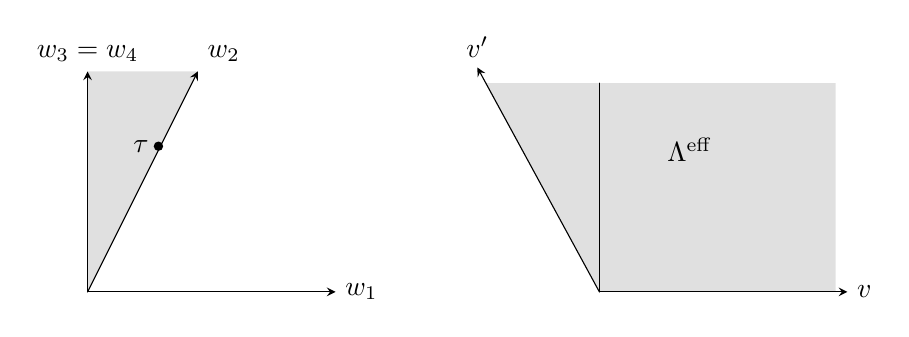
\begin{tikzpicture}[x=1.0cm,y=1.0cm,>=stealth,line cap=round,line join=round]
  \begin{scope}[shift={(-3.2,0)}]
    \fill[gray!24] (0,0) -- (0,2.8) -- (1.4,2.8) -- cycle;
    \draw[->] (0,0) -- (3.15,0) node[right] {$w_1$};
    \draw[->] (0,0) -- (0,2.8) node[above] {$w_3=w_4$};
    \draw[->] (0,0) -- (1.4,2.8) node[above right] {$w_2$};
    \fill (.9,1.85) circle (1.7pt) node[left] {$\tau$};
  \end{scope}
  \begin{scope}[shift={(3.3,0)}]
    \fill[gray!24] (0,0) -- (3.0,0) -- (3.0,2.65) -- (-1.45,2.65) -- cycle;
    \draw[->] (0,0) -- (3.15,0) node[right] {$v$};
    \draw[->] (0,0) -- (-1.55,2.85) node[above] {$v'$};
    \draw (0,0) -- (0,2.65);
    \node at (1.15,1.8) {$\Lambda^{\mathrm{eff}}$};
  \end{scope}
\end{tikzpicture}
\caption{作为商的环面簇。}\label{fig:11-3-1}
\end{figure}

在几何上，这个商流形是
\[
  M_\tau=
  \frac{\{x\in\mathbb C^4\mid
  |x_1|^2+|x_2|^2=2,\ |x_2|^2+|x_3|^2+|x_4|^2=3\}}
  {[x_1,x_2,x_3,x_4]\sim
  [e^{is}x_1,e^{i(s+t)}x_2,e^{it}x_3,e^{it}x_4]}.
\]
到 $S^2=\mathbb{CP}^1$ 的投影为
$[x_1,x_2,x_3,x_4]\mapsto[x_3:x_4]$。上同调类
$\overline w_\nu\in H^2(M_\tau)$ 是子流形
$\{x_\nu=0\}\subset M_\tau$ 的庞加莱对偶。因此，$\overline w_3=\overline w_4$ 是纤维类
$\phi\in H_2(M_\tau)$ 的庞加莱对偶，而 $\overline w_1,\overline w_2$ 是两个\BookRecordIndex{T0189}截面类
$\sigma_1,\sigma_2\in H_2(M_\tau)$ 的庞加莱对偶。这些类满足
\[
  \phi=\sigma_2-\sigma_1,
  \qquad \sigma_1\cdot\sigma_1=-1,
  \qquad \sigma_2\cdot\sigma_2=1,
  \qquad \phi\cdot\sigma_1=\phi\cdot\sigma_2=1.
\]
关系 $u_1u_2=q_1$ 表明：纤维类中通过两个截面和一个通有点的曲线之\BookRecordIndex{T0143}格罗莫夫--威滕
不变量为一。这可由直接观察明显看出。

这个流形的其他环面结构都不是 Fano 的；Spielberg \srcite{384} 证明，此时 Batyrev
公式不再成立。把这种\BookRecordIndex{T0229}量子上同调计算方法与 Ostrover \srcite{314} 的方法比较也颇有
启发。

\BookRecordIndex{T0169}环面流形的\BookRecordIndex{T0229}量子上同调环还可用 \BookRecordIndex{T0031}Landau--Ginzburg 势描述。（下面会在格拉斯曼流形的
情形解释这一表述。）即使在单调情形并采用适当域上的系数，这个环也未必半单；见
Ostrover--Tyomkin \srcite{316}。Fukaya--Oh--Ohta--Ono
\srcite{129, 130} 证明，它还与\BookRecordIndex{T0204}矩映射之环面纤维的拉格朗日\BookRecordIndex{T0132}弗洛尔同调密切相关。

\subsection{\BookRecordIndex{T0274}旗流形}\label{subsec:11-3-2}

Givental 和 Kim 在早期一篇优美论文 \srcite{153} 中计算了\BookRecordIndex{T0274}旗流形 $F_{n+1}$ 的\BookRecordIndex{T0229}量子上
同调环，并把它同 \BookRecordIndex{T0050}Toda 晶格联系起来。为此，他们对等变\BookRecordIndex{T0229}量子上同调的性质作了一些
假设，随后又在 \srcite{147, 210} 中证明了这些假设。Ciocan-Fontanine
\srcite{70} 给出了这个公式的另一种、更具代数意味的证明。这个例子引起了广泛兴趣，
既因为它与可积系统有非常直接的联系，也因为它和镜像对称有关。这些思想已推广到部分
\BookRecordIndex{T0274}旗流形；很好的参考资料是 Buch \srcite{49}。极端情形，即格拉斯曼流形 $G(k,n)$，将在
下一小节讨论。

\BookRecordIndex{T0274}旗流形 $F_{n+1}$ 是 $\mathbb C^{n+1}$ 中所有子空间列
\[
  E_1\subset E_2\subset\cdots\subset E_n,
  \qquad \dim_{\mathbb C}E_j=j,
\]
组成的空间。这个流形的实维数为 $n(n+1)$，它单连通，并带有自然复结构。把\BookRecordIndex{T0274}旗
$E_1\subset\cdots\subset E_n$ 映到 $E_1$ 的\BookRecordIndex{T0377}遗忘映射，是以 $F_n$ 为纤维、以
$\mathbb{CP}^n$ 为底的\BookRecordIndex{T0279}纤维化，由此可理解它的拓扑。例如，六维流形 $F_3$ 嵌入
$\mathbb{CP}^2\times\mathbb{CP}^2$，其像是满足关联关系 $\ell\subset P$ 的偶对
$(\ell,P)$ 所成的集合；这里把第二个 $\mathbb{CP}^2$ 看成
$\mathbb C^3$ 中复二维平面 $P$ 的空间。因此
\[
  F_3=\left\{([z_0:z_1:z_2],[w_0:w_1:w_2])\,\middle|\,
  \sum_i z_iw_i=0\right\}.
\]

\begin{remark}\label{rem:11-3-13}
虽然 $F_{n+1}$ 上有 $n$ 维环面的有效哈密顿作用，但即使在 $n=2$ 时它也不是\BookRecordIndex{T0169}环面流形，
因为 $2n<n(n+1)=\dim F_{n+1}$。另一方面，它可以实现为齐性空间
$U(n+1)/T^{n+1}$；也可表示为 $\mathbb C^N$ 关于群
$G:=U(1)\times\cdots\times U(n)$ 的哈密顿作用之辛商，其中
\[
  N:=\sum_{k=1}^n k(k+1).
\]
这是 Shaun Martin 向我们解释的。
\end{remark}

$F_{n+1}$ 的上同调由典范线丛
\[
  L_j:=E_{j+1}/E_j\longrightarrow F_{n+1},
  \qquad j=0,\ldots,n,
\]
的第一 Chern 类 $u_j\in H^2(F_{n+1};\mathbb Z)$ 生成。
\sourcefootnote{原书把这些类的所在空间误印为 $H^2(M;\mathbb Z)$；本段对象始终是
$F_{n+1}$，故补正。}
由于 Whitney 和 $L_0\oplus\cdots\oplus L_n$ 同构于平凡丛
$F_{n+1}\times\mathbb C^{n+1}$，这些类满足
\[
  u_0+\cdots+u_n=0.
\]
$F_{n+1}$ 的整个上同调环是商
\[
  H^*(F_{n+1})=
  \frac{\mathbb Z[u_0,\ldots,u_n]}
  {\langle\sigma_1(u),\ldots,\sigma_{n+1}(u)\rangle},
\]
其中 $\sigma_j(u)$ 是初等对称函数。为理解这一点，先注意上同调类
$c_j=\sigma_j(u)\in H^{2j}(F_{n+1})$ 是平凡丛
$L_0\oplus\cdots\oplus L_n$ 的 Chern 类，显然必须为零。上述公式断言，这些显然的关系
就是全部关系，而且 $F_{n+1}$ 的全部上同调都由 $u_j$ 通过杯积生成。一种证明方法是
考察\BookRecordIndex{T0279}纤维化序列
\[
  T\longrightarrow U\longrightarrow U/T\longrightarrow BT\longrightarrow BU,
\]
其中 $U:=U(n+1)$、$T:=T^{n+1}$，并把商 $U/T$ 与 $F_{n+1}$ 识别。诱导映射
$F_{n+1}:=U/T\to BT$ 把 $L_0\oplus\cdots\oplus L_n$ 分类为 $T$-丛。一个简单的谱序列
论证表明，$H^*(U/T)$ 中的关系由 $H^*(BU)$ 在 $H^*(BT)$ 中的像给出，也就是把 Chern
类写成变量 $u_i$ 的函数所得的关系。

$F_{n+1}$ 的上同调环还可用基
\[
  p_j=u_j+\cdots+u_n,
  \qquad j=1,\ldots,n
\]
表示。在这组基下，切丛 $TF_{n+1}$ 的第一 Chern 类为
\[
  c_1=2(p_1+\cdots+p_n).
\]
每个类 $p_j$ 都能由关于 $F_{n+1}$ 上显然复结构 $J$ \BookRecordIndex{T0058}半正的闭 $(1,1)$-形式代表。事实上，
上同调类 $a=\sum_j\lambda_jp_j$ 能由 凯勒 形式代表，当且仅当所有
$\lambda_j>0$。特别地，存在一个 凯勒 形式，使 $F_{n+1}$ 成为单调流形。还可\BookRecordIndex{T0326}推出：
对辛\BookRecordIndex{T0390}有效锥 $K^{\mathrm{eff}}(F_{n+1})\subset H_2(F_{n+1})$ 中的每个类 $A$，都有
$p_j(A)\geq0$；若 $A\ne0$，则至少有一个 $p_j(A)>0$。
\sourcefootnote{原书称每个 $p_j$ 本身由 凯勒 形式代表，并称
$\sum_j\lambda_jp_j$ 在 $\lambda_j\geq0$ 且其和为正时恰为 凯勒，进而断言每个
$p_j(A)>0$。但下一段的对偶基满足 $p_j(A_i)=\delta_{ij}$，在 $n>1$ 时直接排除这些
断言。$p_j$ 是到相应格拉斯曼流形之投影的 凯勒 类拉回，故本身仅\BookRecordIndex{T0058}半正；凯勒 锥的
内部条件是所有 $\lambda_j>0$，而有效类上的结论相应为逐项非负、非零类至少一项为正。}

令 $A_1,\ldots,A_n$ 是 $H_2(F_{n+1})$ 的整数基，它在
$p_j(A_i)=\delta_{ij}$ 的意义下与 $H^2(F_{n+1})$ 的基 $p_1,\ldots,p_n$ 对偶。我们使用
复系数，并取 $\Lambda:=\mathbb C[q_1,\ldots,q_n]$ 为\BookRecordIndex{T0231}量子系数环。定义~\ref{def:11-1-3}
中的同态 $\Gamma(F_{n+1})\to\Lambda(F_{n+1})$ 为
\[
  A\longmapsto e^A:=q^d:=q_1^{d_1}\cdots q_n^{d_n},
\]
其中 $d=(d_1,\ldots,d_n)$ 且 $d_j=p_j(A)\in\mathbb Z$。由于
$c_1=2(p_1+\cdots+p_n)$，每个 $q_i$ 的次数都是 $2c_1(A_i)=4$。简记
\[
  QH^*(F_{n+1}):=
  QH^*(F_{n+1};\mathbb C[q_1,\ldots,q_n])
  =H^*(F_{n+1})\otimes_{\mathbb Z}\mathbb C[q_1,\ldots,q_n].
\]
由于 $u_i$ 是 $H^*(F_{n+1})$ 的乘法生成元，一般原理（如下面
定理~\ref{thm:11-3-14} 的证明）表明，\BookRecordIndex{T0229}量子上同调环同构于多项式环
$\mathbb C[u_0,\ldots,u_n,q_1,\ldots,q_n]$ 的某个商。

Givental 和 Kim 在 \srcite{153} 中证明了自然同构
\[
  QH^*(F_{n+1})\cong
  \frac{\mathbb C[u_0,\ldots,u_n,q_1,\ldots,q_n]}{\mathcal I},
\]
其中理想 $\mathcal I$ 由下列矩阵的特征多项式各系数生成：
\[
  A_n=
  \begin{pmatrix}
    u_0&q_1&0&0&\cdots&0\\
    -1&u_1&q_2&0&\cdots&0\\
    0&-1&u_2&q_3&\ddots&\vdots\\
    \vdots&\ddots&\ddots&\ddots&\ddots&0\\
    0&\cdots&0&-1&u_{n-1}&q_n\\
    0&\cdots&\cdots&0&-1&u_n
  \end{pmatrix}.
\]
更明确地，考虑由公式
\[
  \det(A_n+\lambda\mathbf 1)
  =\lambda^{n+1}+c_1\lambda^n+\cdots+c_n\lambda+c_{n+1}
\]
确定的多项式 $c_j=\Sigma_j(u,q)$。理想 $\mathcal I$ 由这些函数 $\Sigma_j$ 生成。当
$q=0$ 时，它们就是初等对称函数
$\sigma_j(u)=\Sigma_j(u,0)$；因而在专门化到 $q=0$ 时，普通上同调环如预期般出现。换言
之，经典 Chern 类由初等对称函数给出，而多项式 $\Sigma_j$ 可视作 Chern 类的量子形变。

这个公式与可积哈密顿系统有一些很有意思的联系，现在加以说明。我们会看到，量子 Chern
类 $\Sigma_j$ 正是 \BookRecordIndex{T0050}Toda 晶格的 Poisson 对合积分；比较 \srcite{292}。

\BookRecordIndex{T0050}Toda 晶格是实直线上 $n+1$ 个单位质量质点的哈密顿微分方程，它们的位置为
$x_0,x_1,\ldots,x_n$。若
\[
  u_j=p_j-p_{j+1}=y_j=\dot x_j
\]
是位于 $x_j$ 的质点之动量，并且
\[
  q_j=e^{x_j-x_{j-1}},
\]
则 \BookRecordIndex{T0050}Toda 晶格的哈密顿函数为
\[
  H(x,y)=\frac12\operatorname{trace}(A_n^2)
  =\frac12\sum_{j=0}^ny_j^2-\sum_{j=1}^ne^{x_j-x_{j-1}}.
\]
（通常符号的反转对应于考察在 $x_0<x_1<\cdots<x_n$ 时相互排斥的力。）Moser 在
\srcite{292} 中发现，函数
$F_j(x,y)=\operatorname{trace}(A_n^j)$（$j=1,\ldots,n+1$）构成这个系统的一组完备
Poisson 对合积分。因此，由量子 Chern 类 $\Sigma_j$ 生成的理想 $\mathcal I$ 在 Poisson
括号下不变。

更精确地说，注意标准辛结构
$\omega=\sum_{j=0}^ndx_j\wedge dy_j$ 限制到零质心集合
$x_0+\cdots+x_n=0$ 和零动量集合 $y_0+\cdots+y_n=0$ 后，用变量
$q_1,\ldots,q_n,p_1,\ldots,p_n$ 写成
\[
  \omega=\frac{dq_1}{q_1}\wedge dp_1+\cdots+
  \frac{dq_n}{q_n}\wedge dp_n.
\]
Poisson 结构应相对于这个\BookRecordIndex{T0363}辛形式理解。

在几何上，\BookRecordIndex{T0363}辛形式 $\omega$ 可作如下解释。考虑复环面
\[
  T_{\mathbb C}:=H^2(F_{n+1};\mathbb C/2\pi i\mathbb Z)
  =\frac{H^2(F_{n+1};\mathbb C)}{H^2(F_{n+1};2\pi i\mathbb Z)},
\]
它由取值于 $\mathbb C^*=\mathbb C\setminus\{0\}$ 的坐标函数
\[
  q_j(a)=e^{\langle a,A_j\rangle}
\]
参数化。$T_{\mathbb C}$ 的余切丛可自然识别为
\[
  T^*T_{\mathbb C}
  =H^2(F_{n+1};\mathbb C/2\pi i\mathbb Z)
  \times H_2(F_{n+1};\mathbb C),
\]
其中 $p_j:H_2(F_{n+1};\mathbb C)\to\mathbb C$ 应理解为余切空间上的坐标函数。
\sourcefootnote{原书在这里把 $p_j$ 的定义域写成 $H_2(M;\mathbb C)$；本段所讨论的是
$T^*T_{\mathbb C}$，其余切纤维刚刚识别为 $H_2(F_{n+1};\mathbb C)$，故底空间应为
$F_{n+1}$。}
这些坐标函数
有上述 凯勒 形式锥所赋予的几何含义。形式 $\omega$ 可理解为余切丛
$T^*T_{\mathbb C}$ 上的复辛结构。在这种解释下，以上质点为
$x_0,\ldots,x_n$ 的哈密顿系统，在限制到零质心和零动量集合后，位于
$T^*T_{\mathbb C}$ 的实部上。

这给出\BookRecordIndex{T0229}量子上同调本身的一种几何解释。在识别
$u_j:=p_j-p_{j+1}$（$p_0=p_{n+1}=0$）下与 $\mathcal I$ 对应的理想
\[
  \mathcal J\subset\mathbb C[p_1,\ldots,p_n,q_1,\ldots,q_n]
\]
确定代数簇 $L\subset T^*T_{\mathbb C}$。这个簇定义为 $\mathcal J$ 中所有多项式的公共
零点集。因此，复系数\BookRecordIndex{T0229}量子上同调环
\[
  QH^*(F_{n+1})\cong
  \frac{\mathbb C[p_1,\ldots,p_n,q_1,\ldots,q_n]}{\mathcal J}
\]
可解释为 $L$ 上的函数空间。理想 $\mathcal J$ 在 Poisson 括号下的不变性，转化为簇
$L$ 是拉格朗日的这一条件。这初步展现了\BookRecordIndex{T0229}量子上同调中出现的结构（即镜像对称的所谓
“A 侧”）如何同“B 侧”相联；这也是 Givental 在 \srcite{148} 中证明\BookRecordIndex{T0274}旗流形镜像猜想时
所用的要素之一。

\subsection{格拉斯曼流形}\label{subsec:11-3-3}

格拉斯曼流形 $G(k,n)$ 的\BookRecordIndex{T0229}量子上同调环，已由 Bertram、Daskalopoulos 和 Wentworth
\srcite{36}、Witten \srcite{422} 以及 Siebert 和 Tian \srcite{378} 研究。Witten 在
\srcite{422} 中还把 $G(k,n)$ 的\BookRecordIndex{T0229}量子上同调同 $U(k)$ 表示的 Verlinde 代数联系起来。他
对这种联系的解释基于一个优美但启发式的路径积分考察。

以 $G(k,n)$ 表示 $\mathbb C^n$ 中 $k$ 维平面的格拉斯曼流形。因此，$G(k,n)$ 中一点是
$k$ 维子空间 $V\subset\mathbb C^n$。$V$ 的一个酉\BookRecordIndex{T0067}标架是矩阵
$B\in\mathbb C^{n\times k}$，满足
\[
  V=\operatorname{im}B,\qquad B^*B=\mathbf 1_{k\times k}.
\]
两个这样的\BookRecordIndex{T0067}标架 $B,B'$ 表示同一子空间 $V$，当且仅当存在酉矩阵 $U\in U(k)$ 使
$B'=BU$。所以格拉斯曼流形可与商空间
\[
  G(k,n)=\mathcal F(k,n)/U(k)
\]
识别，其中 $\mathcal F(k,n)\subset\mathbb C^{n\times k}$ 是所有酉 $k$-\BookRecordIndex{T0067}标架组成的集合。立即可见
\[
  \dim G(k,n)=2k(n-k).
\]

它也可解释为辛商或约化空间。空间 $\mathbb C^{n\times k}$ 是\BookRecordIndex{T0358}辛流形，群 $U(k)$ 在其上
的自然作用是哈密顿的，\BookRecordIndex{T0204}矩映射为 $\mu(B)=B^*B/2i$。要理解这一点，回忆\BookRecordIndex{T0204}矩映射取值于
$U(k)$ 李代数的对偶 $\mathfrak u(k)^*$；通过内积
$\langle\xi,\eta\rangle:=\operatorname{trace}(\xi^*\eta)$，可把它与
$\mathfrak u(k)$，即所有 $k\times k$ 斜埃尔米特矩阵的空间识别。于是
\[
  G(k,n)=\mu^{-1}(\mathbf 1/2i)/U(k).
\]

有两个自然复向量丛：秩 $k$ 的 $E\to G(k,n)$ 与秩 $n-k$ 的 $F\to G(k,n)$；它们的
Whitney 和自然同构于平凡丛 $G(k,n)\times\mathbb C^n$。在点 $V\in G(k,n)$ 处，$E$
的纤维就是 $V$ 本身，而 $F$ 的纤维是商 $\mathbb C^n/V$：
\[
  E_V=V,\qquad F_V=\mathbb C^n/V.
\]
把对偶丛 $E^*,F^*$ 的 Chern 类记为
\[
  x_j=c_j(E^*)\in H^{2j}(G(k,n)),
  \qquad
  y_j=c_j(F^*)\in H^{2j}(G(k,n)).
\]
这些类生成 $G(k,n)$ 的上同调。由于 $E\oplus F$ 同构于平凡丛，有显然的关系
\[
  \sum_{i=0}^j x_i y_{j-i}=0,
  \qquad j=1,\ldots,n,
\]
其中 $x_0=y_0=1$。当 $j>n$ 时，这个等式平凡地成立。对
$j=1,\ldots,n-k$，它通过
\[
  y_j=-x_1y_{j-1}-\cdots-x_{j-1}y_1-x_j,
  \qquad j=1,\ldots,n-k,
\]
把 $y_j$ 归纳地确定为 $x_1,\ldots,x_k$ 的函数。对 $j>n-k$，类 $y_j$ 为零，这给出
$x_j$ 之间的关系。这些就是全部关系，所以格拉斯曼流形的上同调环可与商
\[
  H^*(G(k,n);\mathbb C)\cong
  \frac{\mathbb C[x_1,\ldots,x_k]}
  {\langle y_{n-k+1},\ldots,y_n\rangle}
\]
识别。此外，切丛的第一 Chern 类为
$c_1(TG(k,n))=nx_1$，所以\BookRecordIndex{T0418}最小陈数为 $n$。

下述定理的本质内容由 Witten \srcite{422} 证明。Siebert 和 Tian
\srcite{378} 独立给出了包含全部细节的严格证明。

\begin{theorem}[Siebert--Tian、Witten]\label{thm:11-3-14}
以多项式环 $\mathbb C[q]$ 为系数的格拉斯曼流形\BookRecordIndex{T0229}量子上同调环同构于
\[
  QH^*(G(k,n);\mathbb C[q])
  \cong
  \frac{\mathbb C[x_1,\ldots,x_k,q]}
  {\langle y_{n-k+1},\ldots,y_{n-1},
  y_n+(-1)^{n-k}q\rangle}.
\]
这里 $x_j$ 是次数 $2j$ 的生成元，$q$ 是次数 $2n$ 的生成元。关系
$y_n+(-1)^{n-k}q=0$ 也可写成
\[
  x_ky_{n-k}=(-1)^{n-k}q.
\]
\end{theorem}

\begin{proof}
先指出，通过一个简单的归纳论证，$x_1,\ldots,x_k$ 仍生成 $G(k,n)$ 的\BookRecordIndex{T0229}量子上同调。这
意味着每个上同调类都能写成 $x_i$ 的量子积的线性组合。证明对次数归纳，并使用
$x*y-x\smile y$ 是次数严格低于 $x\smile y$ 的项之和这一事实。（细节见
\srcite{378, Lemma 2.1}。）同一论证还说明，经典上同调环中的原关系，通过加入若干低阶
项变成\BookRecordIndex{T0229}量子上同调中的关系。再次对次数归纳可知，这些新关系生成\BookRecordIndex{T0229}量子上同调中的关系理想。
（细节见 \srcite{378, Theorem 2.2}。）

据此，只需计算上同调环定义关系的量子形变。这里沿用 Witten 在 \srcite{422} 中的
论证。类 $x_i,y_j$ 的\BookRecordIndex{T0228}量子杯积是如下形式的幂级数：
\[
  x_i*y_j=\sum_d(x_i*y_j)_dq^d,
\]
其中
\[
  (x_i*y_j)_d\in H^{2i+2j-2nd}(G(k,n)),
  \qquad (x_i*y_j)_0=x_i\smile y_j.
\]
所以，除非 $i=k$ 且 $j=n-k$，\BookRecordIndex{T0228}量子杯积 $x_i*y_j$ 必须等于普通杯积
$x_i\smile y_j$。关系 $y_j=0$（$j=n-k+1,\ldots,n-1$）只涉及 $i<k$ 或
$j<n-k$ 的乘积 $x_iy_j$，因而在\BookRecordIndex{T0229}量子上同调中仍成立。不过，关系 $y_n=0$ 涉及乘积
$x_ky_{n-k}$，其量子形变唯一可能的非平凡贡献是
$(x_k*y_{n-k})_1\in H^0(G(k,n))$。我们断言
\begin{equation}\label{eq:11-3-19}
  (x_k*y_{n-k})_1=(-1)^{n-k}.
\end{equation}

为此，须考察次数
$\deg(u)=c_1(L)=1$ 的全纯曲线 $u:\mathbb{CP}^1\to G(k,n)$ 所成的\BookRecordIndex{T0246}模空间
$\mathcal M(L;J_0)$，其中 $J_0$ 是格拉斯曼流形的标准复结构。这个曲线空间的形式维数为
\[
  \dim\mathcal M(L;J_0)=2k(n-k)+2n.
\]
每条 $u\in\mathcal M(L;J_0)$ 都具有形式
\begin{equation}\label{eq:11-3-20}
  u([z_0:z_1])=\operatorname{span}
  \{z_0v_0+z_1v_1,v_2,\ldots,v_k\},
\end{equation}
其中 $v_0,\ldots,v_k\in\mathbb C^n$ 线性无关。这些映射确实组成一个维数为
$2n(k+1)-2k^2$ 的空间，与 $\mathcal M(L;J_0)$ 的维数公式一致。此外，由
命题~\ref{prop:7-4-3}，$J_0\in\mathcal J_{\mathrm{reg}}(G(k,n))$，所以
$\mathcal M(L;J_0)$ 中每条曲线都正则。

需要证明
\[
  \operatorname{GW}_{L,3}^M(x_k,y_{n-k},a)=(-1)^{n-k},
\]
其中 $a=\operatorname{PD}(\mathrm{pt})$ 生成 $H^{2k(n-k)}(G(k,n))$。
\sourcefootnote{原书把点类生成元所在空间写成 $M$；这里从\BookRecordIndex{T0246}模空间、曲线到插入类始终
讨论的是 $G(k,n)$，故应为 $H^{2k(n-k)}(G(k,n))$。}
向量丛的最高维 Chern
类之庞加莱对偶，可以用通有截面的零点集表示。例如，固定 $w\in\mathbb C^n$，考虑
截面 $G(k,n)\to E^*$，它给每个 $k$ 维平面 $V\subset\mathbb C^n$ 指派线性泛函
\[
  V\longrightarrow\mathbb C,\qquad v\longmapsto\langle w,v\rangle.
\]
这个截面横截于零截面，其零点集是子流形
\[
  X=\{V\in G(k,n)\mid w\perp V\}.
\]
这个子流形是 $G(k,n)$ 中的一份 $G(k,n-1)$，表示类
$\operatorname{PD}(x_k)\in H_{2k(n-k)-2k}(G(k,n))$。
\sourcefootnote{原书把这里的同调次数误印为 $2k$。零点集
$X\cong G(k,n-1)$ 的实维数为 $2k(n-k-1)=2k(n-k)-2k$，也正是次数 $2k$ 的类
$x_k$ 之庞加莱对偶的维数。}
再固定 $v_0\in\mathbb C^n$，考虑截面
$G(k,n)\to F$，它给每个 $V\in G(k,n)$ 指派等价类
$[v_0]\in\mathbb C^n/V=F_V$。其零点集是
\[
  Y=\{V\in G(k,n)\mid v_0\in V\}.
\]
这个子流形带自然定向，表示最高 Chern 类
$c_{n-k}(F)=(-1)^{n-k}c_{n-k}(F^*)$ 的庞加莱对偶。总之，
\[
  [X]=\operatorname{PD}(x_k),
  \qquad
  [Y]=(-1)^{n-k}\operatorname{PD}(y_{n-k}).
\]

任取 $V_0\in G(k,n)\setminus X$，使 $v_0\notin V_0$，并选取 $V_0$ 的一组基
$v_1,\ldots,v_k$，使 $v_2,\ldots,v_k$ 以及 $v_0+v_1$ 都垂直于 $w$。于是曲线
\[
  u([z_0:z_1])=\operatorname{span}
  \{z_0v_0+z_1v_1,v_2,\ldots,v_k\}
\]
满足
\[
  u([0:1])=V_0,\qquad u([1:1])\in X,\qquad u([1:0])\in Y.
\]
还容易看出，在 $u$ 处的相交数为一，并且没有另一条次数为一的曲线，其像同时与
$X,Y,V_0$ 相交。这算出同调不变量
$\operatorname{GW}_{L,3}^M(X,Y,\mathrm{pt})=1$，从而证明公式~\eqref{eq:11-3-19}。
所以在\BookRecordIndex{T0229}量子上同调中，形变后的关系为：当 $n-k+1\leq j\leq n-1$ 时 $y_j=0$，以及
$y_n+(-1)^{n-k}q=0$。定理~\ref{thm:11-3-14} 得证。
\end{proof}

定理~\ref{thm:11-3-14} 再次表明：若把 $q$ 看成复数而非变量，并专门化到 $q=0$，\BookRecordIndex{T0229}量子
上同调便退化为经典上同调环。更明确地，若定义 Chern 多项式
\[
  c_t(E^*)=1+\sum_{i=1}^kx_it^i,
  \qquad
  c_t(F^*)=1+\sum_{j=1}^{n-k}y_jt^j,
\]
\sourcefootnote{原书在这里及下文再次定义 $c_t(E^*)$ 时都从 $i=1$ 起求和，却同时使用
$c_t(E^*)c_t(F^*)=1$、$1/c_t(E^*)$ 以及式~\eqref{eq:11-3-22} 右端常数项为一的乘积。
因此两个 Chern 多项式都唯一缺少 $c_0=1$；这里及式~\eqref{eq:11-3-22} 补出常数项。}
则经典上同调环由关系 $c_t(E^*)c_t(F^*)=1$ 确定，而\BookRecordIndex{T0229}量子上同调环由
\begin{equation}\label{eq:11-3-21}
  c_t(E^*)c_t(F^*)=1+(-1)^{n-k}qt^n
\end{equation}
确定，其中 $q\in\mathbb C$。

\medskip
\noindent\textbf{Landau--Ginzburg 表述。}
经典上同调中的关系可以由单个函数
$W_0=W_0(x_1,\ldots,x_k)$ 的各偏导数生成。\BookRecordIndex{T0229}量子上同调中的关系也是如此，相应函数
$W=W(x_1,\ldots,x_k)$ 称为 \BookRecordIndex{T0031}Landau--Ginzburg 势。以下讨论紧随 Witten
\srcite{422} 的叙述。

考虑 Chern 多项式
\[
  c_t(E^*):=1+\sum_{i=1}^kx_it^i,
\]
其中 $x_i=c_i(E^*)\in H^{2i}(G(k,n))$。对 $j\geq0$，以公式
\[
  \frac1{c_t(E^*)}:=\sum_{j\geq0}y_jt^j
\]
定义多项式 $y_j=y_j(x_1,\ldots,x_k)$。于是格拉斯曼流形的经典上同调环由关系
$y_j(x)=0$（$n-k+1\leq j\leq n$）描述。这些关系蕴含当 $j>n$ 时
$y_j(x)=0$；当然，当 $1\leq j\leq n-k$ 时，$y_j$ 正是 $F^*$ 的 Chern 类。以下不施加
关系 $y_j(x)=0$，所以幂级数 $\sum_jy_jt^j$ 未必还是多项式。

考虑由等式
\[
  -\log c_t(E^*):=\sum_{r\geq0}U_r(x)t^r
\]
定义的全纯函数 $U_r=U_r(x_1,\ldots,x_k)$。对这个表达式关于 $x_j$ 求导，得到
\[
  -\frac{t^j}{c_t(E^*)}
  =\sum_{r\geq0}\frac{\partial U_r}{\partial x_j}t^r.
\]
比较系数可知，对 $1\leq j\leq k$，
$\partial U_r/\partial x_j=-y_{r-j}$。特别地，当 $r-j<0$ 时，该公式说明 $U_r$ 的相应
偏导数为零。最有意义的是 $r=n+1$。令
\[
  W_0:=(-1)^{n+1}U_{n+1},
\]
便有
\[
  \frac{\partial W_0}{\partial x_j}=(-1)^ny_{n+1-j},
  \qquad 1\leq j\leq k.
\]
所以格拉斯曼流形经典上同调的定义关系可以写成 $dW_0=0$。

现在考虑函数
\[
  W:=W_0+(-1)^kqx_1,
\]
其中 $q$ 是固定复数。条件 $dW=0$ 等价于
\[
  y_{n-k+1}=0,\quad\ldots,\quad y_{n-1}=0,
  \quad y_n+(-1)^{n-k}q=0,
\]
恰好就是 $G(k,n)$ \BookRecordIndex{T0229}量子上同调环的定义关系。注意，幂级数
$\sum_jy_jt^j$ 的高阶系数不再消失。比较等式
$c_t(E^*)\bigl(\sum_{j\geq0}y_jt^j\bigr)=1$ 中不超过 $n$ 阶的系数，得到
\[
  \left(1+\sum_{i=1}^kx_it^i\right)
  \left(1+\sum_{j=1}^{n-k}y_jt^j\right)
  =1+(-1)^{n-k}qt^n,
\]
这与式~\eqref{eq:11-3-21} 一致。

函数 $W$ 称为 \BookRecordIndex{T0031}Landau--Ginzburg 势。用 Chern 多项式的根
$\lambda_1,\ldots,\lambda_k$ 可方便地表示它：
\begin{equation}\label{eq:11-3-22}
  c_t(E^*)=1+\sum_{i=1}^kx_it^i
  =\prod_{i=1}^k(1+\lambda_it),
\end{equation}
即
\begin{equation}\label{eq:11-3-23}
  W(\lambda_1,\ldots,\lambda_k)
  =\sum_{i=1}^k\left(\frac{\lambda_i^{n+1}}{n+1}
  +(-1)^kq\lambda_i\right).
\end{equation}
从几何上说，$G(k,n)$ 的\BookRecordIndex{T0229}量子上同调环可解释为变量 $x_1,\ldots,x_k$ 的多项式限制到
$dW$ 零点集后所得的环。函数 $W:\mathbb C^k\to\mathbb C$ 只有有限多个\BookRecordIndex{T0233}临界点，而且任意
多项式 $f\in\mathbb C[x_1,\ldots,x_k]$ 模理想
\[
  \mathcal J_q:=
  \langle y_{n-k+1},\ldots,y_{n-1},y_n+(-1)^{n-k}q\rangle
  =\left\langle\frac{\partial W}{\partial x_1},\ldots,
  \frac{\partial W}{\partial x_k}\right\rangle
\]
的等价类，由 $f$ 在 $W$ 的\BookRecordIndex{T0233}临界点处的值确定。由此得到如下局部化公式：
\begin{equation}\label{eq:11-3-24}
  I(f)=\frac{(-1)^{k(k-1)/2}}{k!}
  \sum_{dW(x)=0}
  \det\left(\frac{\partial^2W}{\partial x_i\partial x_j}\right)^{-1}f(x),
\end{equation}
它对每个次数为 $2k(n-k)$ 的多项式 $f$ 成立。这里把变量 $x_i$ 理解为次数 $2i$，而
泛函 $I(f)$ 表示微分形式
$\omega_f\in\Omega^{2k(n-k)}(G(k,n))$ 的积分；该形式在同构
\[
  H^*(G(k,n);\mathbb C)
  =\frac{\mathbb C[x_1,\ldots,x_k]}{\langle dW_0\rangle}
\]
下与 $f$ 对应。注意，$f$ 所表示的\BookRecordIndex{T0229}量子上同调类
$c_f\in QH^*(G(k,n))$ 是 $[\omega_f]$ 与含 $q$ 的项之和。

\begin{exercise}\label{ex:11-3-15}
通过考察 $G(k,n)$ 中 $n-k$ 份 $G(k,n-1)$ 的交点，证明
\[
  \int_{G(k,n)}c_k(E^*)^{n-k}=1.
\]
再把公式~\eqref{eq:11-3-24} 用于多项式
\[
  f(x)=x_k^{n-k}=\prod_{i=1}^k\lambda_i^{n-k},
\]
验证该公式；这个多项式表示类 $c_k(E^*)^{n-k}$。由于
$H^{2k(n-k)}(G(k,n))$ 是一维的，一般情形由此即得。

提示：先作变量替换，并用留数演算把和式~\eqref{eq:11-3-24} 写成如下围道积分：
\[
  I(f)=\frac{(-1)^{k(k-1)/2}}{k!(2\pi i)^k}
  \int_{|\lambda_j|=R}
  \frac{f\prod_{i<j}(\lambda_i-\lambda_j)^2}
  {\prod_i\partial W/\partial\lambda_i}
  \,d\lambda_1\cdots d\lambda_k,
\]
其中 $R$ 很大。然后注意，分母中的
$\partial W/\partial\lambda_i=\lambda_i^n+(-1)^kq$ 可由
$\lambda_i^n-\lambda_i^{n-k}$ 代替而不改变积分值。再用一次留数演算求出新积分。细节见
\srcite{422} 和 \srcite{378}。
\end{exercise}

\medskip
\noindent\textbf{同 Verlinde 代数的关系。}
格拉斯曼流形 $G(k,n)$ 的上同调环与酉群 $U(k)$ 表示环的一个适当商之间，有一种非凡的
对应，下面加以说明。作为实向量空间，$G(k,n)$ 的上同调由 Schubert 循环生成。
$G(k,n)$ 中的一个 Schubert 循环，是与一面完全\BookRecordIndex{T0274}旗
\[
  \{0\}=\Lambda_0\subset\Lambda_1\subset\cdots\subset
  \Lambda_{n-1}\subset\Lambda_n=\mathbb C^n,
  \qquad \dim_{\mathbb C}\Lambda_\nu=\nu,
\]
以及一个非负整数的有限序列（称为分拆）
\[
  n-k\geq a_1\geq a_2\geq\cdots\geq a_k\geq0
\]
相联系的子流形。相应子流形
\[
  \Sigma_a:=\Sigma_a(\Lambda)=
  \Sigma_{a_1,\ldots,a_k}^{k,n}(\Lambda_0,\ldots,\Lambda_n)
  \subset G(k,n)
\]
由所有满足
\[
  \dim(V\cap\Lambda_{n-k+i-a_i})=i,
  \qquad
  \dim(V\cap\Lambda_{n-k+i-a_i-1})=i-1,
\]
$i=1,\ldots,k$ 的 $k$ 维子空间 $V\subset\mathbb C^n$ 组成。换言之，维数列
$\dim(V\cap\Lambda_\nu)$ 在 $\nu=n-k+i-a_i$ 处增加一。每个 Schubert 循环
$\Sigma_a(\Lambda)$ 都是 $G(k,n)$ 中复余维
\[
  \operatorname{codim}_{\mathbb C}\Sigma_a
  =a_1+\cdots+a_k=:|a|
\]
的光滑子流形。它的闭包为
\[
  \overline\Sigma_a=\bigcup_{b\succeq a}\Sigma_b,
  \qquad b\succeq a\quad\Longleftrightarrow\quad b_i\geq a_i
  \text{ 对所有 }i.
\]
\sourcefootnote{原书把闭包关系误印为 $b\preceq a$ 且 $b_i\leq a_i$。但由上面的精确跃迁
条件，闭包只能加入更特殊、余维更高的 Schubert 胞\BookRecordIndex{T0280}腔，即 $b_i\geq a_i$；例如
$G(1,2)$ 中 $a=1$ 的胞\BookRecordIndex{T0280}腔本身已是闭点。}
因此，$\Sigma_a$ 是定义~\ref{def:6-5-1} 意义下的\BookRecordIndex{T0337}伪循环，从而通过相交数表示同调类
\[
  \sigma_a:=[\Sigma_a]
  \in H_{2k(n-k)-2|a|}(G(k,n));
\]
见引理~\ref{lem:6-5-7}。这些同调类加法生成 $H_*(G(k,n))$，所以
\[
  \dim H_*(G(k,n))=\binom nk.
\]
此外，对两面通有\BookRecordIndex{T0274}旗 $\Lambda,\Lambda'$，Schubert 循环
$\Sigma_a(\Lambda)$ 与 $\Sigma_b(\Lambda')$ 横截相交；若二者维数互补，则
\[
  g_{ab}:=\sigma_a\cdot\sigma_b=
  \begin{cases}
    1,&a_{k+1-i}+b_i=n-k\text{ 对所有 }i,\\
    0,&\text{否则}.
  \end{cases}
\]
这些断言的证明见 Griffiths--Harris \srcite{159} 与 Milnor--Stasheff
\srcite{291}。

\begin{remark}\label{rem:11-3-16}
用 Schubert 循环表示，上同调类 $x_i,y_j$ 为
\[
  x_i=c_i(E^*)=\operatorname{PD}(\xi_i),
  \qquad
  y_j=c_j(F^*)=(-1)^j\operatorname{PD}(\eta_j),
\]
其中
\[
  \xi_i:=\sigma_{\underbrace{1,\ldots,1}_{i\text{ 次}},0,\ldots,0},
  \qquad
  \eta_j:=\sigma_{j,0,\ldots,0}.
\]
\end{remark}

\begin{remark}[Giambelli 公式]\label{rem:11-3-17}
固定整数 $n-k\geq a_1\geq\cdots\geq a_k\geq0$，并以
\[
  b_j:=\#\{i\mid a_i\geq j\}
\]
定义整数 $k\geq b_1\geq\cdots\geq b_{n-k}\geq0$。则
\[
  \sigma_a=
  \det\begin{pmatrix}
    \eta_{a_1}&\eta_{a_1+1}&\cdots&\eta_{a_1+k-1}\\
    \eta_{a_2-1}&\eta_{a_2}&\cdots&\eta_{a_2+k-2}\\
    \vdots&\vdots&\ddots&\vdots\\
    \eta_{a_k-k+1}&\eta_{a_k-k+2}&\cdots&\eta_{a_k}
  \end{pmatrix}.
\]
同一个类也可写成
\[
  \sigma_a=
  \det\begin{pmatrix}
    \xi_{b_1}&\xi_{b_1+1}&\cdots&\xi_{b_1+n-k-1}\\
    \xi_{b_2-1}&\xi_{b_2}&\cdots&\xi_{b_2+n-k-2}\\
    \vdots&\vdots&\ddots&\vdots\\
    \xi_{b_{n-k}-n+k+1}&\xi_{b_{n-k}-n+k+2}&\cdots&\xi_{b_{n-k}}
  \end{pmatrix}.
\]
这里的乘法应理解为相交积。
\end{remark}

群 $U(k)$ 的表示环 $\mathcal R(k)$ 定义为表示偶对 $\rho\mathbin\#\rho'$ 如 K 理论般取
等价类所得的集合。表示 $\rho:U(k)\to\operatorname{Aut}(V)$ 的特征标，是最大环面
$T^k\subset U(k)$ 上的函数
\[
  \theta_\rho:T^k\longrightarrow\mathbb C,
  \qquad \theta_\rho(t):=\operatorname{trace}_{\mathbb C}(\rho(t)).
\]
由于具有相同对角元、只差排列的两个对角矩阵彼此共轭，特征标是 $t$ 的坐标
$t_1,\ldots,t_k$ 的对称函数。特征标给出环同构
\[
  \mathcal R(k)\longrightarrow\mathcal S(k),
  \qquad \rho\longmapsto\theta_\rho,
\]
这里表示环采用直和与张量积，而 $\mathcal S(k)$ 是 $k$ 个变量的对称函数环。每个分拆
$a_1\geq\cdots\geq a_k\geq0$ 都确定一个不可约表示
$\rho_a:U(k)\to\operatorname{Aut}(V_a)$，在同构意义下唯一；它的特征标是下面
注~\ref{rem:11-3-19} 所定义的函数 $\theta_{\rho_a}=\theta_a$。明确地，表示空间 $V_a$
是子空间
\[
  V_a\subset
  (\Lambda^1\mathbb C^k)^{\otimes m_1}\otimes
  (\Lambda^2\mathbb C^k)^{\otimes m_2}\otimes\cdots\otimes
  (\Lambda^k\mathbb C^k)^{\otimes m_k},
\]
其中 $m_i:=a_i-a_{i+1}$；它定义为包含 $T^k$-不变子空间之张量积
\[
  (\mathbb Ce_1\wedge\cdots\wedge\mathbb Ce_i)^{\otimes m_i}
\]
的最小 $U(k)$-不变子空间。

\begin{remark}\label{rem:11-3-18}
特别有意义的是特殊表示
\[
  V_{\underbrace{1,\ldots,1}_{i\text{ 次}},0,\ldots,0}
  =\Lambda^i\mathbb C^k,
  \qquad
  V_{j,0,\ldots,0}=S^j\mathbb C^k.
\]
特别地，$V_{0,\ldots,0}=\mathbb C$ 是平凡表示，即表示环的乘法单位元。
\end{remark}

\begin{remark}[Jacobi--Trudi 恒等式]\label{rem:11-3-19}
在变量 $t_1,\ldots,t_k$ 中，对 $1\leq i\leq k$ 定义初等对称函数 $\phi_i$，对
$j\geq1$ 定义完全对称函数 $\psi_j$：
\[
  \phi_i=\sum_{1\leq\nu_1<\cdots<\nu_i\leq k}
  t_{\nu_1}\cdots t_{\nu_i},
  \qquad
  \psi_j=\sum_{1\leq\nu_1\leq\cdots\leq\nu_j\leq k}
  t_{\nu_1}\cdots t_{\nu_j}.
\]
令 $a_i,b_j$ 如注~\ref{rem:11-3-17}，并定义对称函数
\[
  \theta_a:=
  \frac{\det(t_i^{a_j+k-j})_{i,j=1}^k}
  {\det(t_i^{k-j})_{i,j=1}^k}.
\]
则
\[
  \theta_a=
  \det\begin{pmatrix}
    \psi_{a_1}&\psi_{a_1+1}&\cdots&\psi_{a_1+k-1}\\
    \psi_{a_2-1}&\psi_{a_2}&\cdots&\psi_{a_2+k-2}\\
    \vdots&\vdots&\ddots&\vdots\\
    \psi_{a_k-k+1}&\psi_{a_k-k+2}&\cdots&\psi_{a_k}
  \end{pmatrix}.
\]
等价地，
\[
  \theta_a=
  \det\begin{pmatrix}
    \phi_{b_1}&\phi_{b_1+1}&\cdots&\phi_{b_1+n-k-1}\\
    \phi_{b_2-1}&\phi_{b_2}&\cdots&\phi_{b_2+n-k-2}\\
    \vdots&\vdots&\ddots&\vdots\\
    \phi_{b_{n-k}-n+k+1}&\phi_{b_{n-k}-n+k+2}&\cdots&\phi_{b_{n-k}}
  \end{pmatrix}.
\]
\end{remark}

环 $\mathcal R(k)$ 由不可约表示 $\rho_a$ 加法生成。考虑 $\mathcal R(k)$ 的有限维商
$\mathcal R(k,n)$，它由满足
$n-k\geq a_1\geq\cdots\geq a_k\geq0$ 的不可约表示 $\rho_a$ 生成。由
注~\ref{rem:11-3-17} 和注~\ref{rem:11-3-19}，有环同构
\begin{equation}\label{eq:11-3-25}
  H^*(G(k,n))\longrightarrow\mathcal R(k,n),
  \qquad \operatorname{PD}(\sigma_a)\longmapsto\rho_a.
\end{equation}
逆同构可描述如下。特征标
$\theta_\rho:=\operatorname{trace}_{\mathbb C}\circ\rho:U(k)\to\mathbb C$ 是特征值的
对称多项式，因而\BookRecordIndex{T0333}唯一延拓为 $\mathbb C^{k\times k}$ 上共轭不变的多项式。再把这个延拓
限制到李代数 $\mathfrak u(k)$。固定\BookRecordIndex{T0103}典范丛 $E\to G(k,n)$ 上的一个 $U(k)$-联络 $A$，
并以
\[
  F_A\in\Omega^2(G(k,n);\operatorname{End}(E))
\]
表示其曲率。于是 $\theta_\rho(F_A/2\pi i)$ 是 $G(k,n)$ 上闭的实值
$2|a|$-形式，表示丛 $E$ 的一个示性类。事实证明，
\[
  [\theta_a(F_A/2\pi i)]=\operatorname{PD}(\sigma_a),
\]
\sourcefootnote{原书在这个等式中把联络 $A$ 的曲率 $F_A$ 误印为 $F_a$；前一句定义以及
紧接着的逆同构都唯一确定下标应为大写 $A$。}
所以逆同构由映射
\[
  \mathcal R(k)\longrightarrow H^*(G(k,n)),
  \qquad \rho\longmapsto[\theta_\rho(F_A/2\pi i)]
\]
诱导。这些观察见 Witten 的论文 \srcite{422}。（亦见 Salamon \srcite{354} 的介绍。）
注意，这个同构把 $x_i$ 映到 $\Lambda^i\mathbb C^k$，把 $y_j$ 映到
$S^j\mathbb C^k$；见注~\ref{rem:11-3-16} 与注~\ref{rem:11-3-18}。

Verlinde 代数是 $\mathcal R(k,n)$ 上环结构的形变，正如\BookRecordIndex{T0229}量子上同调是
$H^*(G(k,n))$ 上杯积的形变。Verlinde 代数的结构常数，定义为平坦 $U(k)$-联络\BookRecordIndex{T0246}模空间
上某些向量丛的全纯 Euler 示性数；这些\BookRecordIndex{T0246}模空间与一个整数 $d$ 及三个表示
$\rho_a,\rho_b,\rho_c$ 相联系，而三者满足同三点\BookRecordIndex{T0143}格罗莫夫--威滕不变量一样的维数条件：
\[
  |a|+|b|+|c|=k(n-k)+nd.
\]
Witten 的猜想断言，同构~\eqref{eq:11-3-25} 交织这两种形变后的乘积结构。该猜想还推广
到高亏格\BookRecordIndex{T0143}格罗莫夫--威滕不变量及相应的高亏格 Verlinde 代数。其动机之一是，Verlinde
\BookRecordIndex{T0254}粘合规则与\BookRecordIndex{T0143}格罗莫夫--威滕不变量的\BookRecordIndex{T0254}粘合规则相同。此外，Witten 用路径积分给出了一个
优美的启发式论证，解释为何应有这种对应 \srcite{422}。对\BookRecordIndex{T0229}量子上同调，Agnihotri
\srcite{9} 已证实这个猜想；与定理~\ref{thm:11-3-14} 的证明一样，论证归结为计算单个
不变量。

\begin{remark}[结构常数]\label{rem:11-3-20}
定理~\ref{thm:11-3-14} 那样的同构，并不给出\BookRecordIndex{T0229}量子上同调结构常数
\[
  N_d(a,b,c):=\operatorname{GW}_{dL,3}^M(a,b,c)
\]
的显式公式。这一点在普通上同调中已经显现。例如，虽然
$H^*(G(k,n))$ 很容易写成多项式环的商，其结构常数
\[
  N_0(a,b,c)=\sigma_a\cdot\sigma_b\cdot\sigma_c
  =\frac1{\operatorname{Vol}(G)}
  \int_G\theta_a(g)\theta_b(g)\theta_c(g)\det(g)^{k-n}\,dg
\]
（积分相对于 $G=U(k)$ 上的 Haar 测度理解），却由 Littlewood--Richardson 规则确定；
这些规则涉及 Young 表上的相当复杂的操作。这样的公式还没有推广到一般的 $d$。
\end{remark}

\subsection{Calabi--Yau 流形}\label{subsec:11-3-4}

一般\BookRecordIndex{T0058}半正\BookRecordIndex{T0358}辛流形的\BookRecordIndex{T0229}量子上同调环 $QH^*(M)$ 中，会出现一些单调情形没有的有趣现象。例如，
定义~\ref{def:11-1-3} 中的\BookRecordIndex{T0231}量子系数环 $\Lambda$ 一般不能再取成多项式环，而须像
例~\ref{ex:11-1-4}（iv）、（v）那样使用 Novikov 环 $\Lambda_\omega$ 或\BookRecordIndex{T0270}普适 Novikov
环。一个重要特例是第一 Chern 类为零的\BookRecordIndex{T0358}辛流形。此时
$\Lambda=\Lambda_0$，即 $\Lambda$ 中所有元素的次数都为零，并且
\[
  QH^k(M;\Lambda)=H^k(M)\otimes\Lambda.
\]

进一步限制到六维情形。此时\BookRecordIndex{T0246}模空间 $\mathcal M(A;J)/G$ 的维数
$\dim M+2c_1(A)-6$ 对每个类 $A$ 都为零，所以对通有\BookRecordIndex{T0088}殆复结构 $J$，每条单纯
\BookRecordIndex{T0003}$J$-全纯曲线都是孤立的。由此，三点不变量
$\operatorname{GW}_{A,3}^M(a_1,a_2,a_3)$ 只有在所有 $\deg(a_i)=2$ 时才可能非零。事实上，
条件~\eqref{eq:7-1-2} 表明这些次数之和必须为六；另一方面还必须有 $\deg(a_i)\leq2$，因为否则
庞加莱对偶 $\operatorname{PD}(a_i)$ 可由维数小于四的循环表示，而由于非常值
\BookRecordIndex{T0003}$J$-全纯曲线都是孤立的，可把这个循环选成避开所有这些曲线。因此，除 $H^2(M)$ 上之外，
量子积都等于通常的乘积。此外，它诱导乘法
\[
  H^2(M)\otimes H^2(M)\longrightarrow H^4(M)\otimes\Lambda.
\]
用庞加莱对偶把 $H^2(M)$ 与 $H^4(M)$ 识别，便在
$QH^2(M;\Lambda)=H^2(M)\otimes\Lambda$ 上得到一个形变乘积结构。

满足上述条件的流形包括六维环面 $T^6$，以及乘积 $T^2\times X$，其中
$X\subset\mathbb{CP}^3$ 是四次超曲面（著名的 K3 曲面）。在这两种情形，\BookRecordIndex{T0143}格罗莫夫--
威滕不变量都消失。不过，还有一大类量子积非平凡、而且单连通并且是 凯勒 的例子。
这些流形称为 Calabi--Yau 三维簇。Yau 的一个定理表明，它们容许 Ricci 张量为零的
凯勒 度量，即所谓 Kähler--Einstein 度量。Calabi--Yau 三维簇是现代场论的基本材料，
因而受到物理学家和数学家的广泛研究；例如见 Candelas--Ossa \srcite{57}、
Bryan--Pandharipande \srcite{48}，以及 Cox--Katz \srcite{76} 中的参考文献。

它们的性质相当复杂。例如，人们或许希望，任意 Calabi--Yau 三维簇上的复结构 $J$ 都可
在可积复结构类中形变为复结构 $J'$，使每个给定同调类中只有有限多条
$J'$-全纯曲线。（$M$ 上的通有\BookRecordIndex{T0088}殆复结构确实有这个性质。）然而事实并非如此：P.~M.~H.
Wilson 在 \srcite{419} 中给出了一个显式反例。

Calabi--Yau 三维簇可作为环面四维簇中的超曲面出现，也可作为射影空间中的完全交出现。
下面更详细地研究 $\mathbb{CP}^4$ 中超曲面的特殊情形。由这种方式定义的流形 $(M,J)$
自然成族出现：当定义方程变化时，复结构也随之变化。镜像对称猜想的各种表述都体现如下
直觉：由某个特定 Calabi--Yau 流形 $(M,\omega)$ 的辛结构产生的结构（例如\BookRecordIndex{T0143}格罗莫夫--
威滕不变量，即 A 侧），应当在 $M$ 上复结构 $J$ 的形变所产生的结构（即 B 侧）中有其
对应物。这个猜想的推论之一，是 Candelas--Ossa--Green--Parkes \srcite{58} 对
$\mathbb{CP}^4$ 中五次超曲面上\BookRecordIndex{T0091}单纯曲线数作出的惊人预言。这个猜想的精确性引起了极大
兴趣；同样令人瞩目的是，它建立在当时对数学来说全新的思想之上。把这些思想置于坚实
基础上的努力，是推动本章所述诸多发展的力量之一。

更确切地，回忆上文，量子积在 $H^2(M)\otimes\Lambda$ 上诱导一个乘法。在 凯勒
情形，还可限制到 $H^{1,1}(M)\otimes\Lambda$，因为乘积在 $H^{2,0}$ 和 $H^{0,2}$ 上
平凡。另一方面，$M$ 上复结构的形变环是在 $H^{1,2}$ 上的环结构，它给出一个类似于
下文 WDVV 方程的微分方程。镜像对称猜想的一种表述断言：与每个 Calabi--Yau 流形 $M$
相伴，都有一个镜像流形 $M^*$，使环 $H^{1,1}(M^*)$ 与 $H^{1,2}(M)$ 自然同构。
Givental \srcite{150} 对 $\mathbb{CP}^4$ 中的五次超曲面，以及更一般的\BookRecordIndex{T0169}环面流形中完全
交，证实了这个猜想。事实上 Givental 证明了远不止这些，因为对应还保持两侧丰富得多的
结构。第~\ref{sec:11-5} 节会描述 A 侧的部分附加结构，而完整信息还包括
注~\ref{rem:7-5-4} 所提到的\BookRecordIndex{T0378}引力后裔。更多镜像对称资料见 Cox--Katz \srcite{76} 与
Voisin \srcite{409}。

\medskip
\noindent\textbf{$\mathbb{CP}^4$ 中的五次超曲面。}
考虑 $\mathbb{CP}^4$ 中的 $k$ 次超曲面
\[
  Z_k:=\left\{[z_0:\cdots:z_4]\in\mathbb{CP}^4\,\middle|\,
  \sum_{j=0}^4z_j^k=0\right\}.
\]
这个流形单连通，其 Betti 数为
\[
  b_2=b_4=1,
  \qquad
  b_3=k^4-5k^3+10k^2-10k+4.
\]
特别地，等式 $b_2=b_4=1$ 来自超平面截面的 Lefschetz 定理。因此
\[
  \pi_2(Z_k)\cong H_2(Z_k)\cong\mathbb Z,
\]
所以\BookRecordIndex{T0363}辛形式 $\omega$ 在 $\pi_2(Z_k)$ 上不为零。
\sourcefootnote{原书在这句话中先把 $H_2(Z_k)$ 误印为 $H_2(M)$，随后又把
$\pi_2(Z_k)$ 漏写下标为 $\pi_2(Z)$；本段固定对象均为超曲面 $Z_k$，故统一补正。}
此外，$Z_k$ 的第一 Chern 类为
\[
  c_1=(5-k)\iota^*h,
\]
其中 $h\in H^2(\mathbb{CP}^4;\mathbb Z)$ 是 $\mathbb{CP}^4$ 上同调的标准生成元，而
$\iota:Z_k\to\mathbb{CP}^4$ 是把 $Z_k$ 作为超曲面嵌入的自然映射。

令 $A\in\pi_2(Z_k)$ 是满足 $\omega(A)>0$ 的同伦群生成元。例如，当 $k$ 为奇数时，
$A$ 有显式全纯代表
\[
  [z_0:z_1]\longmapsto[z_0:z_1:-z_0:-z_1:0].
\]
在所有情形，$A$ 都由 $Z_k$ 中的一条直线表示。因此在这个生成元上计算第一 Chern 类
得到
\[
  c_1(A)=5-k.
\]
所以当 $k\leq4$ 时，流形 $Z_k$ 单调。当 $k>5$ 时，对通有\BookRecordIndex{T0088}殆复结构不存在非常值
\BookRecordIndex{T0003}$J$-全纯曲线，因为 $\omega$ 为正的类都有负 Chern 数；由维数原因，它们对通有 $J$
没有代表。

因此最有意义的是第一 Chern 类为零的五次超曲面 $M=Z_5$。这是 Calabi--Yau 流形的
典型例子。为了计算量子积，需要算出所有非零不变量
$\operatorname{GW}_{dA,3}^M(a_1,a_2,a_3)$。由于 $b_2=1$，只需计算
$\operatorname{GW}_{dA,3}^M(h,h,h)$；这里 $h$ 是超平面\BookRecordIndex{T0189}截面类
\[
  H=[Z_5\cap\mathbb{CP}^3]\in H_4(Z_5)
\]
的庞加莱对偶。因此 $h$ 就是前面记为 $\iota^*h$ 的类，并满足 $h(A)=1$。注意，对通有
（殆复）$J$，\BookRecordIndex{T0091}单纯曲线都是孤立的。因此，对每个 $\ell$，类 $\ell A$ 中单纯
\BookRecordIndex{T0003}$J$-全纯曲线的数目 $N_\ell$ 有限。既然这些曲线是基本几何对象，我们希望用数 $N_\ell$
表示 $\operatorname{GW}_{dA,3}^M(h,h,h)$。

回忆注~\ref{rem:7-3-8}，按定义
\[
  \operatorname{GW}_{dA,3}^M(h,h,h)
  =d^3\operatorname{GW}_{dA,0}^M,
\]
其中 $\operatorname{GW}_{dA,0}^M$ 是格罗莫夫--威滕过程所计数的 $dA$ 类曲线数。这个
不变量并不直接计数 \BookRecordIndex{T0003}$J$-全纯曲线，而是计数某个\BookRecordIndex{T0209}柯西--黎曼方程的图；在该方程中 $J$
依赖于 $z$。我们的目标是理解单纯 \BookRecordIndex{T0003}$J$-全纯曲线的多重覆盖如何贡献于
$\operatorname{GW}_{dA,0}^M$。

先注意，因为 $Z_5$ 是 $\mathbb{CP}^4$ 中次数为五的超曲面，
\[
  \operatorname{GW}_{0,3}^M(h,h,h)
  =H\cdot H\cdot H=[\mathbb{CP}^1]\cdot Z_5=5.
\]
此外，若 $C$ 是 $dA$ 类中的\BookRecordIndex{T0091}单纯曲线，则 $C\cdot H=d$。所以，把 $H$ 扰动到一般位置
后，$C$ 与 $H$ 横截地交于 $d$ 个不同点。因此，曲线 $C$ 对
$\operatorname{GW}_{dA,3}^M(h,h,h)$ 的贡献恰为 $d^3$。

现在考察 $C$ 的 $m$ 重覆盖对 $\operatorname{GW}_{mdA,3}^M(h,h,h)$ 的贡献。
\sourcefootnote{原书在此把不变量的曲线类印为 $dA$；但 $C$ 本身属于 $dA$，其 $m$ 重覆盖
属于 $mdA$，紧接着的图也明确属于 $A_0+mdA$，故补正。}
选取 $C$
的全纯参数化 $u:\mathbb{CP}^1\to Z_5$，令
$\phi:\mathbb{CP}^1\to\mathbb{CP}^1$ 是次数为 $m$ 的有理映射，并考虑 $u\circ\phi$
的图
\[
  \widetilde v:\mathbb{CP}^1\longrightarrow\mathbb{CP}^1\times Z_5,
  \qquad
  \widetilde v(z)=(z,u(\phi(z))).
\]
这条曲线对复结构 $i\times J$ 不正则。它属于维数为 $6+4m+2$ 的曲线族
$\mathcal M(A_0+mdA;i\times J)$，而正则情形的维数应当只有
$8+2c_1(mdA)=8$。（这里 $4m+2$ 是参数化 $\phi$ 所成空间
$\operatorname{Rat}_m$ 的实维数。也可用引理~\ref{lem:3-3-1} 验证
$\widetilde v$ 不正则。）因此，为了看出 $C$ 如何贡献于
$\operatorname{GW}_{mdA,3}^M(h,h,h)$，应当像第~\ref{sec:7-3} 节那样，把复结构
$i\times J$ 扰动成通有元素 $\widetilde J$，并计数 $C$ 附近的
$\widetilde J$-全纯 $(A_0+mdA)$-曲线。如第~\ref{sec:6-7} 节所示，可以假设
$\widetilde J$ 由式~\eqref{eq:6-7-3} 那样依赖于 $z$ 的 $M$ 上\BookRecordIndex{T0088}殆复结构族 $\{J_z\}$ 给出。

按假设，只有有限多条单纯 $J$-全纯 $mdA$-曲线，而且它们全都正则，因而与 $C$ 分离。
所以在扰动 $i\times J\to\widetilde J$ 下，它们的图只稍稍移动，仍与 $C$ 分离。
\sourcefootnote{原书在这里把被扰动的乘积复结构误印为 $j\times J$；本段前文定义并始终
使用的是球面标准复结构 $i$，故补正为 $i\times J$。}
类似地，若 $A=m'A'$，任意 $A'$-曲线的 $m'$ 重覆盖在扰动后也与 $C$ 分离。于是可以把
$C$ 对 $\mathcal M(A_0+mdA;\widetilde J)$ 的贡献孤立出来。注意，这一贡献可由
定理~\ref{thm:7-2-3} 所讨论的方法计算，并归结为求相应\BookRecordIndex{T0399}障碍丛的 Euler 类。

Aspinwall 和 Morrison 在 \srcite{19} 中提出了另一种很自然的计算，使用来自代数几何
的方法求这一贡献。他们的答案是，$C$ 的每个 $m$ 重覆盖对
$\operatorname{GW}_{mdA,3}^M(h,h,h)$ 的贡献也应为 $d^3$。这意味着
$\mathcal M(A_0+mdA;\widetilde J)$ 中应恰有一个来自 $C$ 的元素。因此，当
$h\in H^2(M)$ 对偶于 $H$ 时，他们的定义给出下列优美的 $h*h$ 公式。沿用
第~\ref{sec:11-1} 节的记号，取 $q:=e^A$ 的形式幂级数环作为\BookRecordIndex{T0231}量子系数环 $\Lambda$。则
\begin{align*}
  \int_Hh*h
  &=\sum_{d=0}^\infty\int_H(h*h)_{dA}q^d\\
  &=\sum_{d=0}^\infty\operatorname{GW}_{dA,3}^M(h,h,h)q^d\\
  &=5+\sum_{d=1}^\infty\sum_{\deg(C)=d}
    d^3(q^d+q^{2d}+q^{3d}+\cdots)\\
  &=5+\sum_{d=1}^\infty N_dd^3\frac{q^d}{1-q^d}.
\end{align*}
第三行的第二个和遍历次数为 $d$ 的所有单纯全纯曲线 $C$。因此 Aspinwall--Morrison
公式等价于数 $N_d$ 与
\[
  \operatorname{GW}_{dA,0}^M:=\frac1{d^3}
  \operatorname{GW}_{dA,3}^M(h,h,h)
\]
之间的如下关系：
\begin{equation}\label{eq:11-3-26}
  \sum_{n=1}^\infty\operatorname{GW}_{nA,0}^M q^n
  =\sum_{d=1}^\infty N_d\sum_{m=1}^\infty\frac{q^{md}}{m^3}
  =\sum_{d=1}^\infty N_d\operatorname{Li}_3(q^d).
\end{equation}
\sourcefootnote{原书把右端印为
$\sum_{d\geq1}N_dq^d/(1-q^d)$，漏掉了覆盖次数的因子 $m^{-3}$。事实上，上一显示式给出
$\operatorname{GW}_{nA,3}^M=\sum_{d\mid n}N_dd^3$，而定义
$\operatorname{GW}_{nA,0}^M=n^{-3}\operatorname{GW}_{nA,3}^M$，故唯一得到这里的
$\sum_{d,m\geq1}N_dq^{md}/m^3$。}
Manin \srcite{285} 和 Voisin \srcite{408} 现已严格证明这个公式。（关于其中问题的一篇
精彩讨论，亦见 Voisin \srcite{409, Section 5.6}。）

下一个问题是：如何计算 $N_d$？与 $M=\mathbb{CP}^n$ 的情形不同，WDVV 方程在这里不给
出任何信息。从底\BookRecordIndex{T0072}层几何看，这很清楚：这些方程来自对不变量
$\operatorname{GW}_{A,k}^{M,I}$（$|I|\geq4$）作不同计算的比较，但这些不变量在当前情形
必须消失。1991 年，Candelas--de la Ossa--Green--Parkes \srcite{58} 用镜像对称的思想
预言了 $N_d$ 的值，最初几个为
\[
  N_1=2{,}875,\qquad
  N_2=609{,}250,\qquad
  N_3=317{,}206{,}375,\qquad\ldots.
\]
他们的猜想建立在对 B 侧的研究上，即镜像流形上混合 Hodge 结构的形变。解释其背后的
思想会使我们离题太远；完整讨论见 Cox--Katz \srcite{76} 或 Voisin \srcite{409}。虽然
$N_1$ 是经典已知的，而且 Katz 在 1986 年的 \srcite{205} 中算出了 $N_2$，其他 $N_d$
当时尚未知。直接计算已对 $d\leq4$ 证实该猜想；如今，由于 Givental 解决了这一情形的
镜像猜想，已知它对所有 $d$ 都成立；见 \srcite{147}。

最后再作一点说明。尽管数 $N_d$ 看来增长得非常快，Givental 的镜像公式却蕴含：\BookRecordIndex{T0144}格罗莫夫
--威滕势~\eqref{eq:11-3-26} 是关于 $q$ 的、收敛半径为正的幂级数。这是
例~\ref{ex:11-1-4}（viii）所讨论的收敛性问题的一个具体例子。现在人们预期所有亏格都有
类似结果。


\section{\BookRecordIndex{T0047}Seidel 表示}\label{sec:11-4}

本节为满足强\BookRecordIndex{T0058}半正性条件~\eqref{eq:8-5-1} 的\BookRecordIndex{T0358}辛流形定义 \BookRecordIndex{T0047}Seidel 表示。我们说明如何用它
理解一般\BookRecordIndex{T0169}环面流形的\BookRecordIndex{T0229}量子上同调环结构。作为另一个应用，我们还将计算任意\BookRecordIndex{T0156}哈密顿纤维化
$\widetilde M\to S^2$ 总空间的加性上同调，其中纤维是\BookRecordIndex{T0058}半正\BookRecordIndex{T0358}辛流形 $(M,\omega)$
（命题~\ref{prop:11-4-5}）。

在例~\ref{ex:8-6-8} 中，我们讨论了单调情形下的 \BookRecordIndex{T0047}Seidel 表示。在该情形中，可以把哈密顿
环路 $\psi$ 的不变量 $\mathcal S(\psi)$ 定义为 $M$ 的一个上同调元素。式~\eqref{eq:8-6-4}
中不变量 $\mathcal S_{\widetilde A}(\psi)$ 的定义原封不动地适用于\BookRecordIndex{T0058}半正情形。不过，现在可能有
无穷多个\BookRecordIndex{T0189}截面类 $\widetilde A$ 具有非零不变量 $\mathcal S_{\widetilde A}(\psi)$，而
$\mathcal S(\psi)$ 将定义为\BookRecordIndex{T0229}量子上同调中的一个（可逆）元素。下面给出细节。

设 $(M,\omega)$ 是满足~\eqref{eq:8-5-1} 的闭\BookRecordIndex{T0358}辛流形。则与 $M$ 上一般二参数\BookRecordIndex{T0088}殆复结构族
相联系的每条 \BookRecordIndex{T0003}$J$-全纯曲线都有非负陈数。令
$\psi=\{\psi_t\}_{t\in\mathbb R/\mathbb Z}$ 是 $M$ 的\BookRecordIndex{T0161}哈密顿辛微分同胚环路，并令
$\widetilde M_\psi\to S^2$ 是式~\eqref{eq:8-2-6} 中以 $M$ 的辛同胚副本为纤维的\BookRecordIndex{T0156}哈密顿
纤维化。由推论~\ref{cor:9-1-2}，对每个 $x\in M$，环路
$t\mapsto\psi_t(x)$ 都可缩。这蕴含\BookRecordIndex{T0279}纤维化 $\widetilde M_\psi$ 有截面。给定可由截面表示的
同调类 $\widetilde A\in H_2(\widetilde M_\psi)$，如式~\eqref{eq:8-6-4} 那样定义上同调类
\begin{equation}\label{eq:11-4-1}
  \mathcal S_{\widetilde A}(\psi)
  :=\sum_{\nu,\mu}
  \operatorname{GW}^{\widetilde M_\psi,\mathbf w}_{\widetilde A,1}(e_\nu)
  g^{\nu\mu}e_\mu
  \in H^{-2c}(M).
\end{equation}
这里 $c:=c_1^{\mathrm{Vert}}(\widetilde A)\le0$ 是 $\widetilde A$ 的竖直陈数，
$e_0,\ldots,e_N$\sourcefootnote{原书把全上同调基的末指标印作 $n$；但同句中的
$n=\dim_{\mathbb R}M/2$，而本章固定的上同调基是 $e_0,\ldots,e_N$，故补正为 $N$。}
是 $H^*(M)$ 的一个基，而 $g^{\nu\mu}$ 是矩阵
\[
  g_{\nu\mu}:=\int_M e_\nu\smile e_\mu
\]
的逆矩阵。\BookRecordIndex{T0143}格罗莫夫--威滕不变量
\[
  \operatorname{GW}^{\widetilde M_\psi,\mathbf w}_{\widetilde A,1}:
  H^{2n+2c}(M)\longrightarrow\mathbb Z
\]
按定义~\ref{def:8-6-6} 理解，其中有一个\BookRecordIndex{T0150}固定标记点 $w\in S^2$。具体地，通过嵌入
$\iota:M\to\widetilde M_\psi$，把 $M$ 与 $\widetilde M_\psi$ 在 $w\in S^2$ 上的纤维
等同；于是 $\mathcal S_{\widetilde A}(\psi)$ 是\BookRecordIndex{T0337}伪循环
\[
  \iota^{-1}\circ\widetilde{\operatorname{ev}}^{w,J,H}:
  \mathcal M(\widetilde A;J,H)\longrightarrow M
\]
的 Poincar\'e 对偶上同调类。该\BookRecordIndex{T0337}伪循环定义在 $\widetilde M_\psi$ 中类 $\widetilde A$ 的
$J$-全纯截面\BookRecordIndex{T0246}模空间上。从几何上说，它在子流形 $X\subset M$ 上的积分，是穿过
$\iota(X)$ 的类 $\widetilde A$ 的 $J$-全纯截面数，并计入适当的符号。因为嵌入 $\iota$
在 $M$ 的\BookRecordIndex{T0158}哈密顿同痕意义下唯一，上同调类 $\mathcal S_{\widetilde A}(\psi)$ 与 $\iota$ 的
选择无关。下面由这些上同调类构造\BookRecordIndex{T0229}量子上同调类。

\begin{definition}\label{def:11-4-1}
设 $(M,\omega)$ 是满足~\eqref{eq:8-5-1} 的闭\BookRecordIndex{T0358}辛流形，
$\psi=\{\psi_t\}_{t\in\mathbb R/\mathbb Z}$ 是\BookRecordIndex{T0161}哈密顿辛微分同胚环路，而
$\sigma:S^2\to\widetilde M_\psi$ 是一个截面。固定定义~\ref{def:11-1-3} 中任意一个\BookRecordIndex{T0231}量子
系数环 $\Lambda$。定义 \emph{\BookRecordIndex{T0046}Seidel 元}
\[
  \mathcal S(\psi,\sigma)\in\operatorname{QH}^*(M;\Lambda)
\]
为
\begin{equation}\label{eq:11-4-2}
  \mathcal S(\psi,\sigma)
  :=\sum_{A\in H_2(M)}
  \mathcal S_{[\sigma]+\iota_*A}(\psi)\otimes e^A.
\end{equation}
\end{definition}

作为例子，考虑环 $\Lambda:=\Lambda^{\mathrm{univ}}[q,q^{-1}]$，即以\BookRecordIndex{T0270}普适 Novikov 环为
系数的 $q,q^{-1}$ 多项式环（见例~\ref{ex:11-1-4}(v)）。变量 $q$ 的次数为二。借助
Guillemin--Lerman--Sternberg \srcite{163} 的耦合类
$u_\psi\in H^2(\widetilde M_\psi)$，便可消去 \BookRecordIndex{T0046}Seidel 元对截面 $\sigma$ 的依赖。该类定义为
闭二形式 $\widetilde\omega\in\Omega^2(\widetilde M_\psi)$ 的上同调类，其中
$\widetilde\omega$ 在每个纤维上的限制都是给定\BookRecordIndex{T0363}辛形式，并且
$\widetilde\omega^{n+1}$ 的\BookRecordIndex{T0374}沿纤维积分为零。其上同调类与 $\widetilde\omega$ 的选择无关
（见命题~\ref{prop:8-2-2}）。

\begin{definition}\label{def:11-4-2}
设 $(M,\omega)$ 和 $\psi$ 如定义~\ref{def:11-4-1}，并记
\[
  \Lambda:=\Lambda^{\mathrm{univ}}[q,q^{-1}].
\]
定义 \BookRecordIndex{T0046}Seidel 元 $\mathcal S(\psi)\in\operatorname{QH}^*(M;\Lambda)$ 为
\begin{equation}\label{eq:11-4-3}
  \mathcal S(\psi)
  :=\sum_{\widetilde A}
  \mathcal S_{\widetilde A}(\psi)
  \otimes q^{c(\widetilde A)}t^{\widetilde\omega(\widetilde A)}.
\end{equation}
这里 $\widetilde\omega\in\Omega^2(\widetilde M_\psi)$ 是 $\widetilde M_\psi$ 上一个
\BookRecordIndex{T0155}哈密顿联络的\BookRecordIndex{T0260}耦合形式，而 $c:=c_1^{\mathrm{Vert}}\in H^2(\widetilde M_\psi)$ 是竖直第一
陈类。求和遍历所有可由 $\widetilde M_\psi$ 的截面表示、并满足
$-\dim M\le2c(\widetilde A)\le0$ 的同调类
$\widetilde A\in H_2(\widetilde M_\psi)$。
\end{definition}

定义~\ref{def:11-4-2} 中 \BookRecordIndex{T0047}Seidel 表示的表述，是 Lalonde--McDuff--Polterovich
\srcite{228} 所用表述的一个变体：他们把 $\Lambda^{\mathrm{univ}}[q,q^{-1}]$ 换成
Novikov 环 $\Lambda_\omega$，其底群是球面同调类群 $H_2^S(M)$ 关于下述等价关系的商：
$A\sim B$ 当且仅当 $\omega(A)=\omega(B)$ 且 $c_1(A)=c_1(B)$。在嵌入
\[
  e^A\longmapsto q^{c_1(A)}t^{\omega(A)}
\]
下，这个 Novikov 环是 $\Lambda^{\mathrm{univ}}[q,q^{-1}]$ 的子环。换言之，把同调群
$H_2(M)$ 除以同态 $A\mapsto(\omega(A),c_1(A))$ 的核，等价于只保留同调类 $A$ 的
$\omega(A)$ 与 $c_1(A)$ 信息。

\begin{theorem}[Seidel]\label{thm:11-4-3}
设 $(M,\omega)$ 是满足\BookRecordIndex{T0058}半正性条件~\eqref{eq:8-5-1} 的闭\BookRecordIndex{T0358}辛流形，并令
$\Lambda:=\Lambda^{\mathrm{univ}}[q,q^{-1}]$。则对所有
$\phi,\psi\in\pi_1(\operatorname{Ham}(M,\omega))$，都有
\[
  \mathcal S(\phi\psi)=\mathcal S(\phi)*\mathcal S(\psi),
  \qquad
  \mathcal S(\operatorname{id})=1.
\]
因此，对每个 $\psi\in\pi_1(\operatorname{Ham}(M,\omega))$，\BookRecordIndex{T0046}Seidel 元
$\mathcal S(\psi)\in\operatorname{QH}^*(M;\Lambda)$ 都属于
$\operatorname{QH}^*(M;\Lambda)$ 的偶次乘法单位群，而且映射
$\psi\mapsto\mathcal S(\psi)$ 是群同态。
\end{theorem}

断言 $\mathcal S(\operatorname{id})=1$ 是关于乘积流形
$\widetilde M:=S^2\times M$ 的\BookRecordIndex{T0143}格罗莫夫--威滕不变量的陈述，由习题~\ref{ex:7-3-4}
成立。恒等式
$\mathcal S(\phi\psi)=\mathcal S(\phi)*\mathcal S(\psi)$ 可重述为\BookRecordIndex{T0156}哈密顿纤维化的
\BookRecordIndex{T0143}格罗莫夫--威滕不变量所满足的（分裂）公理的类似物；其证明仍基于第 10 章的\BookRecordIndex{T0254}粘合论证。
虽然这里给出的证明只适用于\BookRecordIndex{T0058}半正情形，该定理事实上对所有闭\BookRecordIndex{T0358}辛流形均成立；见 McDuff
\srcite{269}。还要注意，在量子乘法等于通常杯积的流形上，例如当 $[\omega]$ 在
$\pi_2(M)$ 上为零时，上述恒等式退化为定理~\ref{thm:8-6-9} 中的断言
$\mathcal S(\phi\psi)=\mathcal S(\phi)\smile\mathcal S(\psi)$。

\begin{remark}\label{rem:11-4-4}
\BookRecordIndex{T0046}Seidel 元 $\mathcal S(\phi)$ 通过
\[
  \operatorname{QH}^*(M;\Lambda)\longrightarrow
  \operatorname{QH}^*(M;\Lambda),
  \qquad a\longmapsto\mathcal S(\phi)*a
\]
诱导\BookRecordIndex{T0229}量子上同调的一个自同构，也记作 $\mathcal S(\phi)$。我们将在下面
定理~\ref{thm:11-4-3} 的证明中看到
\begin{equation}\label{eq:11-4-4}
  \mathcal S(\phi)*a
  =\sum_{\widetilde A,\nu,\mu}
  \operatorname{GW}^{\widetilde M_\phi,\mathbf w}_{\widetilde A,2}(a,e_\nu)
  g^{\nu\mu}e_\mu\otimes
  q^{c(\widetilde A)}t^{\widetilde\omega(\widetilde A)}.
\end{equation}
所以它由带两个\BookRecordIndex{T0150}固定标记点 $w_1,w_2$ 的截面不变量给出。这里应把类 $a$ 的 Poincar\'e
对偶看成由 $w_1\in S^2$ 上纤维 $M_1$ 中的循环表示，而把 $e_\nu$ 的 Poincar\'e 对偶
看成由 $w_2\in S^2$ 上纤维 $M_2$ 中的循环表示。不变量
$\operatorname{GW}^{\widetilde M,\mathbf w}_{\widetilde A,2}(a,e_\nu)$ 计数穿过这些循环的
$\widetilde M$ 中 $J$-全纯截面。由于每个纤维与 $M$ 的等同在\BookRecordIndex{T0161}哈密顿辛微分同胚意义下
良定义，$\mathcal S(\phi)$ 的确给出 $\operatorname{QH}^*(M)$ 的良定义自同构。

用同调语言说，给定由纤维 $M_1$ 中一个循环（也记作 $\alpha$）表示的类
$\alpha\in H_*(M)$，类 $\mathcal S(\phi)(\alpha)$ 是诸项
$\beta_{\widetilde A}\otimes q^{-c(\widetilde A)}t^{-\widetilde\omega(\widetilde A)}$ 之和，
其中同调类 $\beta_{\widetilde A}$ 由所有穿过 $\alpha$ 的类 $\widetilde A$ 截面与 $M_2$
的交表示。在这一解释下，\BookRecordIndex{T0046}Seidel 元
$\mathcal S(\phi):=\mathcal S(\phi)(1)$ 是单位元的像，而
定理~\ref{thm:11-4-3} 断言 $\mathcal S(\phi\psi)$ 是这些自同构的复合
$\mathcal S(\phi)\circ\mathcal S(\psi)$。因此群
$\pi_1(\operatorname{Ham}(M,\omega))$ 通过左右
$\operatorname{QH}^*(M)$-模同构作用在 $M$ 的\BookRecordIndex{T0229}量子上同调上，即
\[
  \mathcal S(\phi)*(a*b)
  =a*\bigl(\mathcal S(\phi)(b)\bigr)
  =\mathcal S(\phi)(a)*b,
  \qquad a,b\in\operatorname{QH}^*(M;\Lambda).
\]
\sourcefootnote{原书末项印作未定义的 $\mathcal S(a)*b$；本段定义的算子是
$\mathcal S(\phi)$，且左右模同态性质唯一要求此处为 $\mathcal S(\phi)(a)*b$。}
最近 Hutchings \srcite{194} 发现了这一表示的推广：它定义一系列群同态，从
$\pi_{2k+1}(\operatorname{Ham}(M,\omega))$ 到 $\operatorname{QH}^*(M)$ 的
$2k$ 次 $\operatorname{QH}^*(M)$-模自同态所成的加法群
$\operatorname{End}_{2k}(\operatorname{QH}^*)$。
\end{remark}

\BookRecordIndex{T0047}Seidel 表示有许多有趣应用。我们已经见过两个：在第~\ref{sec:8-6} 节中，我们用它考察
\BookRecordIndex{T0161}哈密顿辛微分同胚环路的辛作用量（见推论~\ref{cor:8-6-10}）；命题~\ref{prop:9-6-4}
则用它估计环路的 Hofer 长度。它也是 McDuff 关于单有理流形的工作 \srcite{273} 中的
关键成分，因为它能保证某些\BookRecordIndex{T0143}格罗莫夫--威滕不变量不消失。正如第 12 章将看到的，它是
哈密顿群上\BookRecordIndex{T0132}弗洛尔同调丛的\BookRecordIndex{T0095}单值化，因而也是理解\BookRecordIndex{T0271}谱不变量的重要工具（参见
\srcite{307,105,274}）。它对\BookRecordIndex{T0156}哈密顿纤维化也有推论。这里只给出取自
Lalonde--McDuff--Polterovich \srcite{228} 的最简单推论；这个方向上的进一步结果见
\srcite{228} 及 Lalonde--McDuff \srcite{227}。

\begin{proposition}\label{prop:11-4-5}
设 $(M,\omega)$ 是满足条件~\eqref{eq:8-5-1} 的闭\BookRecordIndex{T0358}辛流形，并令
$\pi:\widetilde M\to S^2$ 是纤维辛同胚于 $M$ 的\BookRecordIndex{T0156}哈密顿纤维化。则映射
\sourcefootnote{原书显示的映射不可能是所称同构：按紧随其后的定义，$\iota_!$ 把次数提高
二，而且投影公式给出 $\pi^*[S^2]\smile\iota_!b=0$。本证明实际由 $\iota_*$ 单射\BookRecordIndex{T0326}推出
$\iota^*$ 满射，从而在任选一个线性提升 $s:H^*(M)\to H^*(\widetilde M)$ 后得到
$a\otimes b\mapsto\pi^*a\smile s(b)$ 的非典范加性同构；原书未指定这样的提升，故此处
保留原显示式。}
\[
  H^*(S^2)\otimes H^*(M)\longrightarrow H^*(\widetilde M),
  \qquad a\otimes b\longmapsto\pi^*a\smile\iota_!b
\]
在有理上同调上是同构。这里 $\iota:M\to\widetilde M$ 表示一个纤维的包含映射，而
$\iota_!$ 是由通常的同调推前 $\iota_*$ 定义的上同调推前：
\[
  \iota_!:=\operatorname{PD}_{\widetilde M}\circ\iota_*\circ\operatorname{PD}_M.
\]
\end{proposition}

\begin{proof}
每个\BookRecordIndex{T0156}哈密顿纤维化 $\widetilde M\to S^2$ 都像式~\eqref{eq:8-2-6} 那样，由一个哈密顿环路
$\phi$ 把两份 $\mathbb C\times M$ 粘在一起而定义。因此，可把
$\widetilde M\to S^2$ 等同为形如 $\widetilde M_\phi\to S^2$ 的\BookRecordIndex{T0279}纤维化。只须证明纤维的
包含映射 $\iota:M\to\widetilde M_\phi$ 在有理同调上诱导单射。该结论立即由
定理~\ref{thm:11-4-3} 得到。因为映射
$a\mapsto\mathcal S(\phi)*a$ 是\BookRecordIndex{T0229}量子上同调的自同构，所以
$\mathcal S(\phi)*a\ne0$ 当且仅当 $a\ne0$。由式~\eqref{eq:11-4-4}，
$\mathcal S(\phi)*a$ 是一个和，其系数是形如
$\operatorname{GW}_{\widetilde A,2}(a,e_\nu)$ 的\BookRecordIndex{T0143}格罗莫夫--威滕不变量；除非对偶同调类
$\operatorname{PD}(a)\in H_*(M)$ 在 $H_*(\widetilde M)$ 中的像
$\iota_*\operatorname{PD}(a)$ 非零，这些不变量都消失。这就证明了命题。
\end{proof}

现在转向定理~\ref{thm:11-4-3} 的证明。它以 $2$-球面上\BookRecordIndex{T0156}哈密顿纤维化的
\BookRecordIndex{T0143}格罗莫夫--威滕不变量所满足的（分裂）公理类似物为基础。为表述该结果，先观察：给定两个
哈密顿环路 $\phi,\psi\in\pi_1(\operatorname{Ham}(M,\omega))$，由逐点乘积
$\{\phi_t\psi_t\}$ 确定的\BookRecordIndex{T0279}纤维化 $\widetilde M_{\phi\psi}$ 可与\BookRecordIndex{T0278}纤维和
$\widetilde M_\phi\#\widetilde M_\psi$ 等同。它提升了底球面上通常的\BookRecordIndex{T0227}连通和运算
$S^2\#S^2=S^2$：从 $\widetilde M_\phi,\widetilde M_\psi$ 各自切去一个纤维 $F$ 的邻域，
再沿边界适当地\BookRecordIndex{T0254}粘合余下两块。（准确公式见下文。还要注意，$\phi,\psi$ 的次序无关紧要，
因为环路 $\{\phi_t\psi_t\}$ 与 $\{\psi_t\phi_t\}$ 同伦；所以
$\widetilde M_{\phi\psi}=\widetilde M_{\psi\phi}$。）相应地，在 $\widetilde M$ 中可由截面
表示的同调类集合 $H_2^\sigma(\widetilde M)$ 上有\BookRecordIndex{T0227}连通和运算：取穿过被删纤维上对应点的
截面来表示这些类，再取其\BookRecordIndex{T0227}连通和所表示的类。把该映射记作
\[
  H_2^\sigma(\widetilde M_\phi)\times
  H_2^\sigma(\widetilde M_\psi)
  \longrightarrow H_2^\sigma(\widetilde M_{\phi\psi}),
  \qquad
  (\widetilde A,\widetilde B)\longmapsto\widetilde A\#\widetilde B.
\]
它满足
\begin{equation}\label{eq:11-4-5}
  c(\widetilde A\#\widetilde B)=c(\widetilde A)+c(\widetilde B),
  \qquad
  \widetilde\omega(\widetilde A\#\widetilde B)
  =\widetilde\omega(\widetilde A)+\widetilde\omega(\widetilde B).
\end{equation}

\begin{theorem}\label{thm:11-4-6}
设 $(M,\omega)$ 是满足~\eqref{eq:8-5-1} 的闭\BookRecordIndex{T0358}辛流形，并令
$\phi,\psi\in\pi_1(\operatorname{Ham}(M,\omega))$。则对所有
$\widetilde C\in H_2^\sigma(\widetilde M_{\phi\psi})$、所有
$a_1,\ldots,a_k\in H^*(M)$ 和任意整数 $0\le\ell\le k$，都有
\[
\begin{aligned}
  \operatorname{GW}^{\widetilde M_{\phi\psi}}_{\widetilde C,k}
  (a_1,\ldots,a_k)
  ={}&\sum_{\widetilde A\#\widetilde B=\widetilde C}
  \sum_{\nu,\mu}
  \operatorname{GW}^{\widetilde M_\phi}_{\widetilde A,\ell+1}
  (a_1,\ldots,a_\ell,e_\nu)g^{\nu\mu}\\
  &\qquad\qquad\cdot
  \operatorname{GW}^{\widetilde M_\psi}_{\widetilde B,k-\ell+1}
  (e_\mu,a_{\ell+1},\ldots,a_k).
\end{aligned}
\]
这里所有不变量均按具有\BookRecordIndex{T0150}固定标记点来理解，即
\[
  \operatorname{GW}^{\widetilde M}_{\widetilde A,j}
  :=\operatorname{GW}^{\widetilde M,\mathbf w}_{\widetilde A,j},
  \qquad \mathbf w:=\{w_1,\ldots,w_j\}.
\]
\end{theorem}

这是描述任意\BookRecordIndex{T0278}纤维和之\BookRecordIndex{T0143}格罗莫夫--威滕不变量的一般公式的一个很简单的特例；辛情形的一般
公式由 Ionel--Parker \srcite{201} 给出。

\begin{proof}[定理~\ref{thm:11-4-3} 的证明]
在定理~\ref{thm:11-4-6} 中取 $\psi_t\equiv\operatorname{id}$ 和 $k=2$，便有
\begin{equation}\label{eq:11-4-6}
  \operatorname{GW}^{\widetilde M_\phi}_{\widetilde A,2}(a,b)
  =\sum_{\widetilde B+\iota_*C=\widetilde A}
   \sum_{i,j}
   \operatorname{GW}^{\widetilde M_\phi}_{\widetilde B,1}(e_i)
   g^{ij}\operatorname{GW}^M_{C,3}(e_j,a,b)
\end{equation}
其中 $\widetilde A\in H_2^S(\widetilde M_\phi)$
\sourcefootnote{原书把这里的总空间印作 $\widetilde M_\psi$；但本步已取
$\psi_t\equiv\operatorname{id}$，式~\eqref{eq:11-4-6} 的左端、求和条件及类关系全都位于
$\widetilde M_\phi$，故补正下标为 $\phi$。}，且 $a,b\in H^*(M)$。这里用
式~\eqref{eq:8-6-2} 和定义~\ref{def:7-3-7} 把不变量
$\operatorname{GW}^{\widetilde M_\psi}_{\widetilde C,k}$ 等同于
$\operatorname{GW}^M_{C,k}$，又用式~\eqref{eq:11-4-5} 把 $\widetilde A$ 等同于
$\widetilde B+\iota_*C$。从现在起，$\operatorname{GW}$ 上标中的 $\mathbf w$ 均省略不写。
于是
\[
\begin{aligned}
  \mathcal S(\phi)*a
  &={}
  \sum_{\widetilde B,C,i,j}
  \operatorname{GW}^{\widetilde M_\phi}_{\widetilde B,1}(e_i)g^{ij}
  (e_j*a)_C\otimes
  q^{c(\widetilde B+\iota_*C)}
  t^{\widetilde\omega(\widetilde B+\iota_*C)}\\
  &={}
  \sum_{\widetilde B,C,i,j,\nu,\mu}
  \operatorname{GW}^{\widetilde M_\phi}_{\widetilde B,1}(e_i)g^{ij}
  \operatorname{GW}^M_{C,3}(e_j,a,e_\nu)g^{\nu\mu}e_\mu\otimes
  q^{c(\widetilde B+\iota_*C)}
  t^{\widetilde\omega(\widetilde B+\iota_*C)}\\
  &={}
  \sum_{\widetilde A,\nu,\mu}
  \operatorname{GW}^{\widetilde M_\phi}_{\widetilde A,2}(a,e_\nu)
  g^{\nu\mu}e_\mu\otimes
  q^{c(\widetilde A)}t^{\widetilde\omega(\widetilde A)}.
\end{aligned}
\]
最后一个等号由式~\eqref{eq:11-4-6} 得到。因此我们证明了式~\eqref{eq:11-4-4}。
进而
\[
\begin{aligned}
  \mathcal S(\phi)*\mathcal S(\psi)
  &={}
  \sum_{\widetilde A,\widetilde B,\nu,\mu}
  \operatorname{GW}^{\widetilde M_\phi}_{\widetilde A,2}
  \bigl(\mathcal S_{\widetilde B}(\psi),e_\nu\bigr)
  g^{\nu\mu}e_\mu\otimes
  q^{c(\widetilde A)+c(\widetilde B)}
  t^{\widetilde\omega(\widetilde A)+\widetilde\omega(\widetilde B)}\\
  &={}
  \sum_{\widetilde A,\widetilde B,\nu,\mu,i,j}
  \operatorname{GW}^{\widetilde M_\psi}_{\widetilde B,1}(e_i)g^{ij}
  \operatorname{GW}^{\widetilde M_\phi}_{\widetilde A,2}(e_j,e_\nu)g^{\nu\mu}e_\mu
  \otimes q^{c(\widetilde A\#\widetilde B)}
  t^{\widetilde\omega(\widetilde A\#\widetilde B)}\\
  &={}
  \sum_{\widetilde C,\nu,\mu}
  \operatorname{GW}^{\widetilde M_{\phi\psi}}_{\widetilde C,1}(e_\nu)
  g^{\nu\mu}e_\mu\otimes
  q^{c(\widetilde C)}t^{\widetilde\omega(\widetilde C)}\\
  &=\mathcal S(\phi\psi).
\end{aligned}
\]
这里第二个等号使用了式~\eqref{eq:11-4-5} 和 $\mathcal S_{\widetilde B}(\psi)$ 的公式，
第三个等号则来自取 $k=1$ 的定理~\ref{thm:11-4-6}。由于
$\psi\phi=\phi\psi\in\pi_1(\operatorname{Ham}(M))$，各项的次序无关紧要。这就证明了
定理~\ref{thm:11-4-3}。
\end{proof}

\begin{proof}[定理~\ref{thm:11-4-6} 的证明]
固定 $M$ 的两个\BookRecordIndex{T0161}哈密顿辛微分同胚环路
\[
  \phi^0=\{\phi_t^0\}_{t\in\mathbb R/\mathbb Z},
  \qquad
  \phi^\infty=\{\phi_t^\infty\}_{t\in\mathbb R/\mathbb Z}.
\]
证明的思路，是把第 10 章的\BookRecordIndex{T0256}粘合定理推广到\BookRecordIndex{T0156}哈密顿纤维化。若\BookRecordIndex{T0279}纤维化
\[
  \widetilde M^0:=\widetilde M_{\phi^0},
  \qquad
  \widetilde M^\infty:=\widetilde M_{\phi^\infty}
\]
的两个 $J$-全纯截面在一对纤维中相交（这两个纤维都与 $M$ 等同），并满足适当的\BookRecordIndex{T0166}横截性
条件，就可以把它们\BookRecordIndex{T0254}粘合成\BookRecordIndex{T0278}纤维和
\[
  \widetilde M^{\infty0}:=\widetilde M_{\phi^\infty\phi^0}
\]
的一个 $J$-全纯截面。理解设定和\BookRecordIndex{T0394}预粘合构造之后，第 10 章的证明便逐字适用于当前情形，
所以我们只描述主要思路。

根据式~\eqref{eq:8-2-6} 中的定义，\BookRecordIndex{T0156}哈密顿纤维化
$\widetilde M^0\to S^2$ 是商空间
\[
  \widetilde M^0=
  \frac{\{\pm1\}\times\mathbb C\times M}
  {(1,e^{2\pi(s+it)},x)\sim
   (-1,e^{-2\pi(s+it)},(\phi_t^0)^{-1}(x))}.
\]
下文简记
\[
  z=e^{2\pi(s+it)},
\]
所以 $2\pi t$ 是 $z$ 的幅角。注意，底球面
$S^2=\mathbb C\cup\{\infty\}$ 是两份 $\mathbb C_\pm$ 之并，其中
$\mathbb C_+\equiv\mathbb C$，而
$\mathbb C_-\equiv(\mathbb C\setminus\{0\})\cup\{\infty\}$。
$\widetilde M^0$ 的一个截面是一对光滑映射 $u_\pm^0:\mathbb C\to M$，满足
\[
  u_+^0(z)=\phi_t^0\bigl(u_-^0(z^{-1})\bigr),
\]
$\widetilde M^\infty$ 的情形类似。为形成\BookRecordIndex{T0278}纤维和，把 $\widetilde M^0$ 在
$0\in\mathbb C_+$（原点）上的\BookRecordIndex{T0278}纤维和 $\widetilde M^\infty$ 在
$0\in\mathbb C_-$（无穷远点）上的纤维都与 $M$ 等同。然后从
$\widetilde M^0$、$\widetilde M^\infty$ 中分别删去这些纤维的邻域
$\mathbb C_+\times M$、$\mathbb C_-\times M$，再用复合映射
$\phi_t^\infty\circ\phi_t^0$，把 $\widetilde M^0$ 中余下的
$\mathbb C_-\times M$ 与 $\widetilde M^\infty$ 中余下的
$\mathbb C_+\times M$ 粘在一起，形成\BookRecordIndex{T0278}纤维和。这正是 $\widetilde M^{\infty0}$；它的一个
截面是一对光滑映射 $u_\pm:\mathbb C\to M$，满足
\[
  u_+(z)=\phi_t^\infty\circ\phi_t^0\bigl(u_-(z^{-1})\bigr).
\]

现在采取如下策略。从 $\widetilde M^0$ 和 $\widetilde M^\infty$ 中在公共纤维上相合的两个
$J$-全纯截面 $\widetilde u^0,\widetilde u^\infty$ 出发，构造
$\widetilde M^{\infty0}$ 的一族近似 $J^R$-全纯截面 $\widetilde u^R$（\BookRecordIndex{T0394}预粘合构造）。随后，
第 10 章的\BookRecordIndex{T0254}粘合论证将给出附近一族真正的 $J^R$-全纯截面。建立这一点后，像第~\ref{sec:10-8}
节那样论证即可完成证明。具体地，在 $S^2\setminus\{0\}$ 上固定 $\ell$ 个\BookRecordIndex{T0066}标记点
（用于 $\widetilde M^0$），在 $S^2\setminus\{\infty\}$ 上固定 $k-\ell$ 个\BookRecordIndex{T0066}标记点
（用于 $\widetilde M^\infty$），并在这 $k$ 个纤维中选取表示给定上同调类的适当子流形。
当 $R$ 充分大时，必须比较两种数目：其一是 $\widetilde M^{\infty0}$ 中穿过这 $k$ 个纤维
内给定子流形的 $J^R$-全纯截面数；其二是由 $\widetilde M^0$ 与
$\widetilde M^\infty$ 中在\BookRecordIndex{T0066}标记点处满足相同约束的 $J$-全纯截面组成的\BookRecordIndex{T0226}连通对的数目。像
第~\ref{sec:10-8} 节一样，这立即由\BookRecordIndex{T0256}粘合定理得到。反过来，\BookRecordIndex{T0256}粘合定理也由\BookRecordIndex{T0394}预粘合构造和
第 10 章第~\ref{sec:10-3}--\ref{sec:10-7} 节中完全相同的论证得到。

下面给出当前情形下\BookRecordIndex{T0394}预粘合构造的细节。考虑 $\widetilde M^0$ 的截面
$\widetilde u^0=(u_+^0,u_-^0)$ 与 $\widetilde M^\infty$ 的截面
$\widetilde u^\infty=(u_+^\infty,u_-^\infty)$，并假设
\[
  u_+^0(0)=u_-^\infty(0)=:x.
\]
对每个充分大的实数 $R$，定义 $\widetilde M^{\infty0}$ 的截面
$\widetilde u^R=(u_+^R,u_-^R)$，使得
\[
u_+^R(z)=
\begin{cases}
  u_+^\infty(R^2z),& |z|\le\dfrac{\delta}{2R},\\[3pt]
  \phi_t^\infty(x),& \dfrac{\delta}{R}\le|z|\le\dfrac1{\delta R},\\[3pt]
  \phi_t^\infty(u_+^0(z)),& |z|\ge\dfrac2{\delta R},
\end{cases}
\]
以及
\[
u_-^R(1/z)=
\begin{cases}
  (\phi_t^0)^{-1}\bigl(u_-^\infty(1/(R^2z))\bigr),
    & |z|\le\dfrac{\delta}{2R},\\[3pt]
  (\phi_t^0)^{-1}(x),
    & \dfrac{\delta}{R}\le|z|\le\dfrac1{\delta R},\\[3pt]
  u_-^0(1/z),& |z|\ge\dfrac2{\delta R}.
\end{cases}
\]
读者可以核对，只要 $u_+^R(z)$ 和 $u_-^R(1/z)$ 已定义，就对所有 $R$ 以及所有
$z=e^{2\pi(s+it)}$ 有
\[
  \phi_t^\infty\circ\phi_t^0\bigl(u_-^R(1/z)\bigr)=u_+^R(z).
\]
当 $R$ 充分大时，可以像第~\ref{sec:10-2} 节那样，通过插值把 $u_+^R$ 延拓到整个
$\mathbb C$：在\BookRecordIndex{T0170}环域 $\delta/(2R)\le|z|\le\delta/R$ 上，利用 $u_-^\infty$ 在
$u_+^\infty$ 与 $\phi_t^\infty(x)$ 之间插值；在
$1/(\delta R)\le|z|\le2/(\delta R)$ 上，利用 $u_+^0$ 在
$\phi_t^\infty(x)$ 与 $\phi_t^\infty(u_+^0)$ 之间插值。更准确地说，因为
$u_+^0(0)=u_-^\infty(0)=x$，存在光滑映射
$\zeta_+^0,\zeta_-^\infty:\mathbb C\to T_xM$，使得当 $|z|$ 充分小时
\[
  u_+^0(z)=\exp_x(\zeta_+^0(z)),
  \qquad
  u_-^\infty(z)=\exp_x(\zeta_-^\infty(z)),
  \qquad
  \zeta_+^0(0)=\zeta_-^\infty(0)=0.
\]
取光滑\BookRecordIndex{T0188}截断函数 $\rho:\mathbb C\to[0,1]$，使其在 $|z|\le1$ 时为零，在
$|z|\ge2$ 时为一，并定义
\[
\begin{aligned}
u_+^R(z):={}&\phi_t^\infty\!\left(
  \exp_x\!\left(
  \rho\!\left(\frac\delta{Rz}\right)
  \zeta_-^\infty\!\left(\frac1{R^2z}\right)
  +\rho(\delta Rz)\zeta_+^0(z)
  \right)\right),\\
u_-^R(1/z):={}&(\phi_t^0)^{-1}\!\left(
  \exp_x\!\left(
  \rho\!\left(\frac\delta{Rz}\right)
  \zeta_-^\infty\!\left(\frac1{R^2z}\right)
  +\rho(\delta Rz)\zeta_+^0(z)
  \right)\right)
\end{aligned}
\]
其中 $\delta/(2R)\le|z|\le R/(2\delta)$。第~\ref{sec:10-2} 节的
式~\eqref{eq:10-2-2}，对应于对所有 $t$ 均有
$\phi_t^0=\phi_t^\infty=\operatorname{id}$ 的特例。

这个\BookRecordIndex{T0394}预粘合构造定义一族映射 $f^R$，其定义域是由
$\widetilde M^0,\widetilde M^\infty$ 中分别表示类
$\widetilde A^0,\widetilde A^\infty$、并满足
$u_+^0(0)=u_-^\infty(0)$ 的 $J$-全纯截面对
$(\widetilde u^0,\widetilde u^\infty)$ 组成的\BookRecordIndex{T0246}模空间
\[
  \mathcal M(\widetilde A^0,\widetilde A^\infty;J^0,J^\infty).
\]
它把该\BookRecordIndex{T0246}模空间映到 $\widetilde M^{\infty0}$ 中表示同调类
\[
  \widetilde A^{\infty0}:=\widetilde A^\infty\#\widetilde A^0
\]
的截面空间。为了使\BookRecordIndex{T0254}粘合论证成立，必须像第 10 章那样假设\BookRecordIndex{T0246}模空间
$\mathcal M(\widetilde A^0,J^0)$、$\mathcal M(\widetilde A^\infty,J^\infty)$ 都正则，
并且\BookRecordIndex{T0283}求值映射
\[
\begin{aligned}
  \mathcal M(\widetilde A^0,J^0)\times
  \mathcal M(\widetilde A^\infty,J^\infty)
  &\longrightarrow M\times M,\\
  (\widetilde u^0,\widetilde u^\infty)
  &\longmapsto(u_+^0(0),u_-^\infty(0))
\end{aligned}
\]
横截于对角线。从这里开始，证明逐字等同于第 10 章的证明，故略去。这就证明了
定理~\ref{thm:11-4-6}。
\end{proof}

\begin{remark}\label{rem:11-4-7}
\begin{enumerate}[label=(\roman*)]
\item 如果把 \BookRecordIndex{T0046}Seidel 元 $\mathcal S(\phi)$ 定义为弗洛尔上同调上的算子，那么
定理~\ref{thm:11-4-3} 是一个同义反复。不过，这一叙述中非平凡的部分，是把该观察翻译回
当前语境，即证明弗洛尔上同调上的算子与上面定义的 \BookRecordIndex{T0047}Seidel 表示一致。这种对应的证明涉及
与定理~\ref{thm:11-4-3} 上述证明同类的\BookRecordIndex{T0256}粘合定理。进一步讨论见第 12.5 节。

\item 我们在上面根据分裂规则定理~\ref{thm:11-4-6} 作计算，证明了
定理~\ref{thm:11-4-3}。如果像注~\ref{rem:11-4-4} 那样，把 \BookRecordIndex{T0046}Seidel 元
$\mathcal S(\phi)$ 看成单位元 $1$ 在自同构 $\mathcal S(\phi)$ 下的像，就能给出该论证的
如下几何解释。与往常一样，用同调语言来说明最为容易。为此，记
$\mathcal S_*(\phi)$ 为 $\operatorname{QH}_*(M;\Lambda)$ 的自同构，它把 $w_1$ 上纤维
中的同调类 $\alpha$ 送到 $w_2$ 上纤维中的类
\[
  \mathcal S_*(\phi)(\alpha):=
  \sum_{\widetilde A\in H_2^\sigma(\widetilde M_\phi)}
  \sum_{i,j}
  \operatorname{GW}^{\widetilde M_\phi,\mathbf w}_{\widetilde A,2}
  (\alpha,\varepsilon_i)g^{ij}\varepsilon_j,
\]
其中 $\varepsilon_i:=\operatorname{PD}(e_i)$。换言之，我们用式~\eqref{eq:11-4-4}
右端的同调版本定义 $\mathcal S_*(\phi)(\alpha)$。于是
\[
  \mathcal S_*(\phi)(\alpha)
  =\operatorname{PD}\circ\mathcal S(\phi)\circ\operatorname{PD}(\alpha),
\]
其中
$\operatorname{PD}:\operatorname{QH}^*(M;\Lambda)\to
\operatorname{QH}_*(M;\check\Lambda)$ 是注~\ref{rem:11-1-20} 中定义的 Poincar\'e 对偶
同构。我们的目标是证明复合规则
\[
  \mathcal S_*(\phi^\infty\phi^0)
  =\mathcal S_*(\phi^\infty)\circ\mathcal S_*(\phi^0).
\]
对 $a=0,\infty$，把 $\mathcal S_*(\phi^a)$ 看成一个自同构：它把
$\widetilde M^a$ 在 $0\in\mathbb C_-$（无穷远点）上的纤维 $M_\infty^a$ 的\BookRecordIndex{T0230}量子同调，
送到其在 $0\in\mathbb C_+$（原点）上的纤维 $M_0^a$ 的\BookRecordIndex{T0230}量子同调。循环
$\alpha\subset M_\infty^0$ 的像 $\mathcal S_*(\phi^0)(\alpha)$，由
$\widetilde M^0$ 中各截面与 $M_0^0$ 的交表示；所以复合
$\mathcal S_*(\phi^\infty)\circ\mathcal S_*(\phi^0)(\alpha)$ 的像，由在公共纤维上相合的
截面对与 $M_0^\infty$ 的交表示。另一方面，$\mathcal S_*(\phi^\infty\phi^0)(\alpha)$
按定义通过计数 $\widetilde M^{\infty0}$ 的截面得到。因此，计算化为
定理~\ref{thm:11-4-6} 的\BookRecordIndex{T0254}粘合陈述。在这一框架中还必须证明 $\mathcal S_*(\phi)$ 是模同态，
也就是
\[
  \mathcal S_*(\phi)(\alpha)
  =\mathcal S_*(\phi)(\alpha*1)
  =\alpha*\mathcal S_*(\phi)(1)
  =\mathcal S_*(\phi)*\alpha.
\]
这可仿照定理~\ref{thm:11-4-3} 证明的第一步，并取其中一个环路为平凡环路来得到。
文献 \srcite{228,269} 采取的正是这一观点。
\end{enumerate}
\end{remark}

\begin{example}\label{ex:11-4-8}
在多数已经算出 \BookRecordIndex{T0046}Seidel 元 $\mathcal S(\psi)\in\operatorname{QH}^*(M)$ 的情形中，环路
$\psi$ 由 $(M,\omega)$ 上的一个圆周作用表示。令 $K:M\to\mathbb R$ 是其\BookRecordIndex{T0204}矩映射，并作
归一化使
\[
  \int_M K\omega^n=0,
\]
再把相应环路记作 $\lambda_K$。则 $K$ 取得最大值的点组成一个连通辛子流形
$F_K\subset M$，且该子流形由作用固定：
\[
  K(F_K)=\max_{x\in M}K(x).
\]
进一步假设这个最大值分支是简单的，即圆周在 $F_K$ 的一个去心邻域
$U\setminus F_K$ 上自由作用。McDuff--Tolman \srcite{279} 证明了
\begin{equation}\label{eq:11-4-7}
  \mathcal S(\lambda_K)
  =\operatorname{PD}(F_K)\otimes
   q^{-\operatorname{codim}(F_K)/2}t^{\sup K}
  +\sum_{\widetilde\omega(\widetilde A)>\sup K}
   a_{\widetilde A}\otimes
   q^{c(\widetilde A)}t^{\widetilde\omega(\widetilde A)}.
\end{equation}
因此，$\mathcal S(\lambda_K)$ 的首项由几何以很简单的方式确定。举例来说，考虑由高度函数
$K$ 生成的 $S^2$ 旋转。这时
\[
  \mathcal S(\lambda_K)=\operatorname{PD}([\mathrm{pt}])\otimes q^{-1}t^\mu,
  \qquad
  \mu=\sup K=\frac12\int_{S^2}\omega.
\]
在若干有趣情形中，式~\eqref{eq:11-4-7} 有非零低阶项（参见 Seidel \srcite{363}）。
不过，文献 \srcite{279} 证明：若 $(M,\omega,\lambda_K)$ 是 Fano 的，也就是说，它有一个
不允许非正陈数 $J$-全纯球面的不变 $\omega$-\BookRecordIndex{T0372}驯服\BookRecordIndex{T0088}殆复结构；并且\BookRecordIndex{T0418}最小陈数 $N$ 至少是
$F_K$ 余维的一半，则这些项不会出现。例如，若 $\lambda_K$ 是 Fano 环面簇上固定一个面片的
圆周作用之一，这些项就不会出现。
\end{example}

\begin{example}\label{ex:11-4-9}
回到命题~\ref{prop:9-7-2} 中考虑的圆周作用。它按公式
\[
  \psi_t(z,w)=(z,\Phi_{z,t}(w))
\]
作用在 $S^2\times S^2$ 上，因而旋转到第一个球面的投影之纤维，并固定对角线与反对角线。
第 9 章给出了两个证明，说明当 $\lambda>1$ 时，$S^2\times S^2$ 上存在一个
$S^1$-不变\BookRecordIndex{T0363}辛形式，它\BookRecordIndex{T0361}辛同痕于标准形式
$\omega_\lambda:=\lambda\pi_1^*\sigma+\pi_2^*\sigma$。还可改写
例~\ref{ex:11-3-12} 的构造，给出
包含这一 $S^1$ 作用的 $S^2\times S^2$ 环面结构，从而得到第三个证明：只须把
$w_2$ 取作向量 $(2,1)$ 而非 $(1,1)$，并适当选择 $\tau$。命题~\ref{prop:9-7-2}
中更有趣的部分断言：当 $\lambda\le1$ 时，不可能把哈密顿环路 $\{\psi_t\}$ 同伦到
$(S^2\times S^2,\omega_\lambda)$ 的\BookRecordIndex{T0362}辛微分同胚群中。现在概述另一个证明。由连续性，只须
考虑 $\lambda=1$。

我们在例~\ref{ex:11-1-13} 中看到，单调情形的\BookRecordIndex{T0229}量子上同调环
$\operatorname{QH}^*(S^2\times S^2;\Lambda)$ 可构造成有零因子的环，而当 $\lambda>1$ 时
却没有零因子。取当前的 Novikov 环
$\Lambda_\lambda:=\Lambda^{\mathrm{univ}}[q,q^{-1}]$，这一现象非常清楚。记
\[
  A:=[S^2\times\mathrm{pt}],\qquad
  B:=[\mathrm{pt}\times S^2],\qquad
  a:=[\pi_1^*\sigma]=\operatorname{PD}(B),\qquad
  b:=[\pi_2^*\sigma]=\operatorname{PD}(A).
\]
则同态 $\varphi:\Gamma(M,\omega)\to\Lambda$ 给为
\[
  \varphi(A):=qt^\lambda,
  \qquad
  \varphi(B):=qt.
\]
因此，当 $\lambda=1$ 时，$a*a=qt$ 与 $b*b=qt^\lambda$ 相等。进一步，
\[
  (a+b)(a-b)=qt(1-t^{\lambda-1}).
\]
所以当 $\lambda>1$ 时，$a+b$ 是
$\operatorname{QH}^*(S^2\times S^2;\Lambda_\lambda)$ 中的单位，而当 $\lambda=1$ 时，
它是零因子。

圆周作用 $\{\psi_t\}$ 的最大不动点分支 $F_K$ 是对角线，其 Poincar\'e 对偶是
$H^2(S^2\times S^2)$ 中的类 $a+b$。Seidel \srcite{363} 通过直接计算证明
$\mathcal S(\psi)$ 中没有低阶项；这也由例~\ref{ex:11-4-8} 的讨论得到。因此，当
$\lambda>1$ 时，$\mathcal S(\psi)$ 形如 $(a+b)\otimes\mu_\lambda$，其中
$\mu_\lambda\in\Lambda_\lambda$。\BookRecordIndex{T0046}Seidel 元由 $\widetilde M_\psi$ 中的\BookRecordIndex{T0143}格罗莫夫--威滕
不变量给出，而这些不变量不依赖于 $M$ 上\BookRecordIndex{T0363}辛形式的形变类。因此，如果 $\psi$ 同伦于
$\operatorname{Symp}(M,\omega_1)$ 中的一个环路，其 \BookRecordIndex{T0046}Seidel 元
$\mathcal S(\psi)\in\operatorname{QH}^*(S^2\times S^2;\Lambda_1)$ 仍会形如
$(a+b)\otimes\mu_1$，其中 $\mu_1\in\Lambda_1$。由于这不是单位，该同伦不可能存在。
\end{example}

\paragraph{光滑环面簇的小\BookRecordIndex{T0229}量子上同调。}
现在回到第~\ref{subsec:11-3-1} 小节开始的\BookRecordIndex{T0169}环面流形小\BookRecordIndex{T0229}量子上同调环
$\operatorname{QH}^*(M)$ 的讨论。我们的叙述紧随 McDuff--Tolman \srcite{279}。假设
$(M,\omega)$ 是闭辛 $2n$-流形，并带有 $n$-环面 $T$ 的有效哈密顿群作用。令
$\mu:M\to\mathfrak t^*$ 是这一作用的\BookRecordIndex{T0204}矩映射，并记其像为 $\Delta:=\mu(M)$。回忆
$\Delta$ 是 $\mathfrak t^*$ 中的凸多面体，可写成
\[
  \Delta=\left\{\eta\in\mathfrak t^*\ \middle|\
  \langle\eta,\bar e_\nu\rangle\le\kappa_\nu\right\},
\]
其中 $\bar e_1,\ldots,\bar e_N\in\mathfrak t$ 属于整数格，且
$\kappa_1,\ldots,\kappa_N\in\mathbb R$（这里从面片的内法向量改用外法向量）。再回忆诸面
\[
  \Delta_I:=\left\{\eta\in\Delta\ \middle|\
  \nu\in I\Longrightarrow\langle\eta,\bar e_\nu\rangle=\kappa_\nu\right\},
  \qquad I\subset I_0:=\{1,\ldots,N\}.
\]
由式~\eqref{eq:11-3-15}，对每个\BookRecordIndex{T0060}本原子集 $I\subset I_0$（即
$\Delta_I=\varnothing$，而且只要 $I'\subsetneq I$ 就有
$\Delta_{I'}\ne\varnothing$），都存在唯一向量
$d=(d_1,\ldots,d_N)\in\mathbb Z^N$，满足
\begin{equation}\label{eq:11-4-8}
  \sum_{\nu=1}^N d_\nu\bar e_\nu=0,
  \qquad
  d_\nu=1\quad(\nu\in I),
  \qquad
  d_\nu\le0\quad(\nu\notin I).
\end{equation}
每个这样的整数向量 $d$ 对应一个同调类 $A_d\in H_2(M)$，其第一陈数和辛面积分别为
\begin{equation}\label{eq:11-4-9}
  c_1(A_d)=\sum_{\nu=1}^N d_\nu,
  \qquad
  \omega(A_d)=\sum_{\nu=1}^N\kappa_\nu d_\nu.
\end{equation}
（见式~\eqref{eq:11-3-18}，其中把 $\kappa_\nu$ 换成 $-\kappa_\nu$。）我们希望理解\BookRecordIndex{T0229}量子
上同调中与通常上同调关系 $\prod_{\nu\in I}u_\nu=0$ 对应的关系，其中 $I$ 是任意本原
指标集。

下面直接从几何上解释 Stanley--Reisner 关系的量子形变。因为面 $\Delta_\nu$ 的对偶向量
$\bar e_\nu$ 是整数向量，它在 $M$ 上诱导圆周作用 $\lambda_\nu$，即 $T$ 中与
$\bar e_\nu$ 相切的圆所给出的作用。它的\BookRecordIndex{T0204}矩映射是
$\langle\mu,\bar e_\nu\rangle:M\to\mathbb R$。所以关系
$\sum_{\nu=1}^N d_\nu\bar e_\nu=0$ 断言，$\pi_1(\operatorname{Ham}(M,\omega))$
中相应的乘积是常值环路：
\[
  \prod_{\nu=1}^N(\lambda_\nu)^{d_\nu}=1.
\]
由定理~\ref{thm:11-4-3}，该乘积在 \BookRecordIndex{T0047}Seidel 表示下的像必须是单位元。换言之，
\begin{equation}\label{eq:11-4-10}
  \prod_{\nu\in I}\mathcal S(\lambda_\nu)
  =\prod_{\nu\notin I}\mathcal S(\lambda_\nu)^{|d_\nu|}
  \in\operatorname{QH}^*(M;\Lambda).
\end{equation}
这里的乘积均在\BookRecordIndex{T0229}量子上同调中理解。如例~\ref{ex:11-4-8} 所指出的，在 Fano 情形中，
$\mathcal S(\lambda_\nu)$ 的表达式没有低阶项。此外，在所有情形中，第 $\nu$ 个圆周作用的
\BookRecordIndex{T0204}矩映射取得最大值的子流形 $X_\nu\subset M$，恰是第 $\nu$ 个面片在\BookRecordIndex{T0204}矩映射下的原像，故其
Poincar\'e 对偶为 $\bar w_\nu\in H^2(M)$：
\[
  \kappa_\nu=\sup_{x\in M}\langle\mu,\bar e_\nu\rangle
  =\langle\mu(X_\nu),\bar e_\nu\rangle,
  \qquad
  X_\nu:=\mu^{-1}(\Delta_\nu).
\]
所以例~\ref{ex:11-4-8} 给出
\[
  \mathcal S(\lambda_\nu)=\bar w_\nu\otimes q^{-1}t^{\kappa_\nu},
  \qquad
  \bar w_\nu:=\operatorname{PD}([X_\nu])\in H^2(M).
\]
这证明了定理~\ref{thm:11-3-4}（取式~\eqref{eq:11-3-17} 的版本），其中\BookRecordIndex{T0231}量子系数环为
\[
  \Lambda:=\Lambda^{\mathrm{univ}}[q,q^{-1}].
\]
这还不是完整结果，因为它只保留了同调类 $A\in H_2(M)$ 的陈数和面积信息。不过，下一则
注说明了如何证明完整结果。

\begin{remark}\label{rem:11-4-10}
因为 $M$ 是 Fano 的，可取多项式环
$\Lambda_0:=\mathbb Q[q_1,\ldots,q_k]$ 作为其\BookRecordIndex{T0230}量子同调的系数。对 $M$ 上每个圆周作用
$\lambda_\nu$，$\widetilde M_{\lambda_\nu}$ 中都有典范截面 $\sigma_\nu$，由点
$\{\pm1\}\times\mathbb C\times\{x\}$ 组成，其中 $x\in X_\nu$。类似地，对任意
$d\in\mathbb Z$，给定圆周作用 $\lambda_\nu^d$，把 $\widetilde M_{\lambda_\nu^d}$ 中\BookRecordIndex{T0204}矩映射
$dK_\nu$ 取得最大值的截面定义为 $(\sigma_\nu)^d$。文献 \srcite{279} 中的计算表明，
定义~\ref{def:11-4-1} 的 \BookRecordIndex{T0046}Seidel 元
$\mathcal S(\lambda_\nu,\sigma_\nu)\in\operatorname{QH}^*(M;\Lambda_0)$ 等于
$\bar w_\nu$。考虑上述关系 $\sum d_\nu\bar e_\nu=0$。由
定理~\ref{thm:11-4-6}，
\[
  \prod_{\nu=1}^N
  \mathcal S\bigl(\lambda_\nu^{d_\nu},(\sigma_\nu)^{d_\nu}\bigr)
  =\mathcal S(0,\sigma_d)=1\otimes e^A,
\]
其中 $\sigma_d$ 是把诸截面 $(\sigma_\nu)^{d_\nu}$ 串接而成的平凡丛截面，且属于
$H_2(S^2\times M)$ 中的类 $[S^2\times\mathrm{pt}]+A$。这说明
$\operatorname{QH}^*(M;\Lambda_0)$ 中有形如
\[
  \prod_{\nu\in I}\bar w_\nu
  =e^A\prod_{\nu\notin I}(\bar w_\nu)^{|d_\nu|}
\]
的关系。还须把 $A$ 与之前记作 $A_d$ 的元素等同。但对 $[\omega]$ 的每个选择，这两个类
在 $\Lambda^{\mathrm{univ}}[q,q^{-1}]$ 中的像都相同。由于 $[\omega]$ 可在 $H^2(M)$ 的一个
开子集中变化，遂有 $A=A_d$。

这一方法的优点在于，不论\BookRecordIndex{T0169}环面流形 $(M,\omega)$ 是否 Fano，关系~\eqref{eq:11-4-10}
总是成立。事实上，由例~\ref{ex:11-4-8}，\BookRecordIndex{T0046}Seidel 元总可写成
\[
  \mathcal S(\lambda_\nu)=y_\nu\otimes q^{-1}t^{\kappa_\nu},
  \qquad
  y_\nu=\bar w_\nu+\sum_k\sum_{\varepsilon>0}a_{k,\varepsilon}q^kt^\varepsilon.
\]
\sourcefootnote{原书把 $t$ 的指数印作本节从未定义的 $c_\nu$；紧前面的\BookRecordIndex{T0204}矩映射最大值公式及
\BookRecordIndex{T0046}Seidel 元首项均唯一给出该指数为 $\kappa_\nu$。}
如第~\ref{subsec:11-3-1} 小节所述，有满环同态
\[
  \frac{\Lambda[u_1,\ldots,u_N]}{P(\Delta)}
  \longrightarrow\operatorname{QH}^*(M;\Lambda),
  \qquad
  u_\nu\longmapsto\bar w_\nu,
  \qquad
  \Lambda:=\Lambda^{\mathrm{univ}}[q,q^{-1}].
\]
所以 $y_\nu\in\operatorname{QH}^*(M;\Lambda)$ 可提升为某个形如
$Y_\nu=u_\nu+\text{高阶项}$ 的元素
$Y_\nu\in\Lambda[u_1,\ldots,u_N]$。利用这些多项式，可以定义量子
Stanley--Reisner 理想 $SR_Y(\Delta)\subset\Lambda[u_1,\ldots,u_N]$：
\begin{equation}\label{eq:11-4-11}
  SR_Y(\Delta):=
  \left\langle
  \prod_{\nu\in I}Y_\nu
  =q^{c_1(A_d)}t^{\omega(A_d)}
   \prod_{\nu\notin I}Y_\nu^{|d_\nu|}
  \ \middle|\ I\text{ 是本原的}
  \right\rangle.
\end{equation}
这里 $d_\nu=d_\nu(I)$ 如式~\eqref{eq:11-4-8}，而 $c_1(A_d)$、$\omega(A_d)$ 由
式~\eqref{eq:11-4-9} 给出。注意，$SR_Y(\Delta)$ 依赖于 $Y_\nu$；一般而言，不预先知道
$\operatorname{QH}^*(M;\Lambda)$ 的环结构，就无法描述这些 $Y_\nu$。所以 $M$ 的小\BookRecordIndex{T0229}量子
上同调形如
\[
  \operatorname{QH}^*(M;\Lambda)
  \cong\frac{\Lambda[u_1,\ldots,u_N]}{P(\Delta)+SR_Y(\Delta)},
  \qquad
  \Lambda:=\Lambda^{\mathrm{univ}}[q,q^{-1}].
\]
\end{remark}

\begin{example}[NEF 环面簇]\label{ex:11-4-11}
假设 $M$ 是 NEF 的，即每个有全纯代表元的类 $B\in H_2(M)$ 都满足 $c_1(B)\ge0$。
在此情形中，\BookRecordIndex{T0046}Seidel 元 $y_\nu$ 里可能有高阶项。不过，文献 \srcite{279} 证明，这时
$\mathcal S(\lambda_\nu)$ 公式中出现的上同调类 $a_{k,\varepsilon}$ 次数都是零或二。因此，
它们自然提升到
$\Lambda[u_1,\ldots,u_N]$\sourcefootnote{原书把此处多项式环的末指标印作 $n$；但
本段由矩多面体的 $N$ 个面片定义变量 $u_1,\ldots,u_N$，前文环及
式~\eqref{eq:11-4-11} 也都以 $u_N$ 为末项，故补正为 $N$。}，而无须预先知道量子乘法。
所以，一旦算出 \BookRecordIndex{T0046}Seidel 元 $\mathcal S(\lambda_\nu)$，便可写出式~\eqref{eq:11-4-11}
中的\BookRecordIndex{T0232}量子 Stanley--Reisner 环。这一结果，尤其是把 Stanley--Reisner 环 $SR_Y$ 中的
$u_\nu$ 换成 $Y_\nu$，与 \srcite{76, 11.2.5.2} 所讨论的 Givental 变量替换公式有关。
Givental 镜像定理提供了计算 \BookRecordIndex{T0046}Seidel 元 $Y_i$ 的方法：它联系函数 $\widetilde I$ 与
$\widetilde J$，前者可由组合数据计算，后者则决定\BookRecordIndex{T0229}量子上同调中的关系；见
Gonzalez--Iritani \srcite{155}。
\end{example}


\section{\BookRecordIndex{T0020}Frobenius 流形}\label{sec:11-5}

回到第~\ref{sec:11-2} 节的讨论，并仍假设 $(M,\omega)$ 是\BookRecordIndex{T0058}半正流形。为简单起见，我们只
考察 $M$ 的偶数次上同调，从而可以在流形而非\BookRecordIndex{T0075}超流形上工作。因此现在假设
$e_0:=1,e_1,\ldots,e_N$ 是 $H^{\mathrm{ev}}(M)$ 的一个由纯次数元素组成的基，并且
$e_1,\ldots,e_m$ 张成 $H^2(M)$。为方便起见，还假设
$e_N=\operatorname{PD}(\mathrm{pt})$ 是 $H^{2n}(M)$ 的正生成元。对\BookRecordIndex{T0274}旗流形和 Grassmann
流形等许多应用而言，只取偶数次类已经足够。

因为这里只想展现这一课题的概貌，我们再作一个简化假设：对所有
$a,b,c\in H^*(M)$，级数
\begin{equation}\label{eq:11-5-1}
  \sum_{A\in K^{\mathrm{eff}}}
  \operatorname{GW}^M_{A,3}(a,b,c)q^{\omega(A)}
\end{equation}
对绝对值充分小的 $q\in\mathbb C$ 收敛。这时可以像例~\ref{ex:11-1-4}(viii) 那样，取\BookRecordIndex{T0231}量子
系数环为 $\Lambda:=\mathbb C$。记
\[
  \mathcal H=\operatorname{QH}^{\mathrm{ev}}(M;\mathbb C)
  =\bigoplus_{i=0}^n\operatorname{QH}^{2i}(M;\mathbb C),
\]
即 $M$ 的\BookRecordIndex{T0229}量子上同调的偶数次部分。上述假设蕴含\BookRecordIndex{T0228}量子杯积在 $\mathcal H$ 上良定义。下面
说明 $\mathcal H$ 是如下意义的 \BookRecordIndex{T0019}Frobenius 代数。

\begin{definition}\label{def:11-5-1}
域 $\mathbb F=\mathbb R$ 或 $\mathbb C$ 上的一个 \emph{\BookRecordIndex{T0019}Frobenius 代数} $\mathcal A$，是
$\mathbb F$ 上带单位元 $1$ 的交换结合代数，并配备一个 $\mathbb F$-线性函数
$\alpha:\mathcal A\to\mathbb F$，使配对
\[
  \langle a,b\rangle:=\alpha(ab)
\]
非退化，也就是说，若对所有 $b$ 都有 $\langle a,b\rangle=0$，则 $a=0$。
\end{definition}

这个定义也可表述为：要求存在一个非退化双线性配对
$(a,b)\mapsto\langle a,b\rangle\in\mathbb F$，满足
\[
  \langle ab,c\rangle=\langle a,bc\rangle,
  \qquad a,b,c\in\mathcal A,
\]
然后令 $\alpha(a):=\langle1,a\rangle$。

对 $\mathcal H$，把乘法定义为\BookRecordIndex{T0228}量子杯积，并把 $\alpha$ 定义为在 $M$ 的基本同调类上积分。
于是对 $a_t=\sum_i t_i e_i$，有
\[
  \alpha(a_t):=\int_M a_t=t_N\in\mathbb C.
\]
相应配对与命题~\ref{prop:11-1-11}(iii) 中的配对不同，因为后者取值于底环 $R$，且不在
$\Lambda:=\mathbb C$ 上线性。不过，命题~\ref{prop:11-1-11} 的证明仍表明，上述定义确实
使 $\mathcal H$ 成为 $\mathbb C$ 上的有限维 \BookRecordIndex{T0019}Frobenius 代数。如果系数必须取 Novikov 环
而非域，就应适当修改上述概念；见 Abrams \srcite{7}。

\begin{remark}\label{rem:11-5-2}
$\operatorname{QH}^*(M)$ 的 \BookRecordIndex{T0019}Frobenius 代数结构有助于理解它的性质；可比较 Abrams
\srcite{7} 以及文献 \srcite{273} 附录中的讨论。
\end{remark}

依照 Dubrovin \srcite{93}，现在把\BookRecordIndex{T0228}量子杯积
\[
  \mathcal H\times\mathcal H\longrightarrow\mathcal H,
  \qquad (a,b)\longmapsto a*b
\]
解释成 $\mathcal H$ 的切丛上的联络，定义为
\begin{equation}\label{eq:11-5-2}
  \nabla_YX(a)=dX(a)Y(a)+X(a)*Y(a),
\end{equation}
其中 $a\in\mathcal H$，而 $X,Y:\mathcal H\to\mathcal H$ 是两个向量场。这里以显然的方式
把 $\mathcal H$ 的所有切空间与 $\mathcal H$ 等同，故向量场 $X$ 是映射
$a\mapsto X(a)\in T_a\mathcal H\equiv\mathcal H$，而它在 $a$ 处的导数
$dX(a):T_a\mathcal H\to T_{X(a)}\mathcal H$ 是 $\mathcal H$ 到自身的线性映射。下一个
引理说明，量子乘法的交换律可解释为\BookRecordIndex{T0248}挠率消失，而结合律可解释为曲率消失。

\begin{lemma}\label{lem:11-5-3}
\begin{enumerate}[label=(\roman*)]
\item 联络~\eqref{eq:11-5-2} 无挠，即
\[
  [X,Y]=\nabla_YX-\nabla_XY.
\]

\item 联络~\eqref{eq:11-5-2} 平坦，即
\[
  \nabla_X\nabla_YZ-\nabla_Y\nabla_XZ+\nabla_{[X,Y]}Z=0.
\]

\item 联络~\eqref{eq:11-5-2} 满足
\[
  \nabla_X\mathbf 1=X,
\]
其中 $\mathbf 1$ 表示由单位元 $1\in\mathcal H$ 定义的常值向量场。
\end{enumerate}
\end{lemma}

\begin{proof}
这里对 Lie 括号采用符号约定
\[
  [X,Y]=dX\cdot Y-dY\cdot X,
\]
其中 $dX(a)$ 表示映射 $X:\mathcal H\to\mathcal H$ 的微分，应把它看成
$\mathcal H$ 的线性变换，把 $Y$ 送到 $dX\cdot Y$。第一条立刻可见。为证明平坦性，注意
\begin{align*}
  \nabla_X\nabla_YZ
  &=\nabla_X(dZ\cdot Y+Z*Y)\\
  &=d(dZ\cdot Y+Z*Y)\cdot X+(dZ\cdot Y+Z*Y)*X\\
  &=d^2Z(Y,X)+dZ\cdot dY\cdot X+Z*(dY\cdot X)\\
  &\quad +(dZ\cdot X)*Y+(dZ\cdot Y)*X+(Z*Y)*X\\
  &=\nabla_{dY\cdot X}Z+d^2Z(X,Y)+Z*(Y*X)\\
  &\quad +(dZ\cdot X)*Y+(dZ\cdot Y)*X.
\end{align*}
第三条也是显然的。
\end{proof}

上述联络相当特殊，因为一形式
\[
  A:T\mathcal H\longrightarrow\operatorname{End}(\mathcal H),
  \qquad A_a(x)y=x*y
\]
是常值的，不依赖基点 $a$。一般的联络一形式
$A\in\Omega^1(\mathcal H,\operatorname{End}(\mathcal H))$ 可解释成一族乘法
\begin{equation}\label{eq:11-5-3}
  \mathcal H\times\mathcal H\longrightarrow\mathcal H,
  \qquad (x,y)\longmapsto x*_a y,
\end{equation}
它以 $\mathcal H$ 自身的元素为参数，所用公式是
\begin{equation}\label{eq:11-5-4}
  A_a(x)y=x*_a y,
\end{equation}
其中 $a\in\mathcal H$，且 $x,y\in T_a\mathcal H=\mathcal H$。把相应联络看成微分算子
\[
  C^\infty(\mathcal H,\mathcal H)
  \longrightarrow\Omega^1(\mathcal H,\mathcal H),
\]
它由 $\nabla=d+A$ 给出；更明确地说，对两个向量场
$X,Y:\mathcal H\to\mathcal H$，有
\begin{equation}\label{eq:11-5-5}
  \nabla_YX(a)=dX(a)Y(a)+X(a)*_aY(a).
\end{equation}
\BookRecordIndex{T0015}Dubrovin 联络~\eqref{eq:11-5-5} 的性质与乘法~\eqref{eq:11-5-3} 有如下关系。这里假设映射
\[
  \mathcal H\times\mathcal H\times\mathcal H\longrightarrow\mathcal H,
  \qquad (a,x,y)\longmapsto x*_a y
\]
是全纯的，并且关于 $x,y$ 复双线性。还要考察如下情形：这些乘法连同常值内积
$\langle\,\cdot,\cdot\,\rangle$（假设它是双线性而非埃尔米特型的），在每个切空间
$T_a\mathcal H=\mathcal H$ 上确定一个 \BookRecordIndex{T0019}Frobenius 代数结构。

\begin{lemma}\label{lem:11-5-4}
假设每个乘法 $(x,y)\mapsto x*_a y$ 都满足 Frobenius 条件。则：
\begin{enumerate}[label=(\roman*)]
\item 联络~\eqref{eq:11-5-5} 无挠，当且仅当乘法~\eqref{eq:11-5-3} 交换，即对所有
$a,x,y\in\mathcal H$，都有
\[
  x*_a y=y*_a x.
\]

\item 假设联络~\eqref{eq:11-5-5} 无挠。那么一形式~\eqref{eq:11-5-4} 是闭的，当且仅当
存在全纯函数 $S:\mathcal H\to\mathbb C$，使
\begin{equation}\label{eq:11-5-6}
  \langle x*_a y,z\rangle=\partial^3S_a(x,y,z).
\end{equation}

\item 假设联络~\eqref{eq:11-5-5} 无挠。那么一形式~\eqref{eq:11-5-4} 满足
$A\wedge A=0$，当且仅当所有乘法~\eqref{eq:11-5-3} 都结合。

\item 联络~\eqref{eq:11-5-5} 满足 $\nabla_X\mathbf 1=X$，当且仅当 $\mathbf 1$ 是所有
乘法~\eqref{eq:11-5-3} 的单位元。
\end{enumerate}
\end{lemma}

\begin{proof}
第 (i)、(iii)、(iv) 条直接由引理~\ref{lem:11-5-3} 得到。为证明第 (ii) 条，注意函数
\[
  \phi_a(x,y,z)=\langle x*_a y,z\rangle
\]
关于 $x,y,z$ 对称。此外，直接计算表明，它的导数
\[
  \psi_a(w,x,y,z)
  =\left.\frac{d}{dt}\right|_{t=0}\phi_{a+tw}(x,y,z)
\]
关于 $w,x,y,z$ 对称，当且仅当式~\eqref{eq:11-5-4} 给出的一形式 $A$ 是闭的。而
$\psi_a$ 的对称性又等价于存在全纯函数 $S:\mathcal H\to\mathbb C$，使
\[
  \phi_a(x,y,z)=\partial^3S_a(x,y,z).
\]
事实上，$S$ 的一个显式公式是
\[
  S(a)=\frac12\int_0^1(1-t)^2\phi_{ta}(a,a,a)\,dt.
\]
引理得证。
\end{proof}
\begin{remark}\label{rem:11-5-5}
前一引理第 (ii) 条的证明，可以用上同调
$\mathcal H=H^{\mathrm{ev}}(M;\mathbb C)$ 的复基 $e_0,\ldots,e_N$ 更明确地表述。
\sourcefootnote{原书在本注中把本节开头固定的基 $e_0,\ldots,e_N$ 的末指标三次改印成
$n$，从而写成 $\mathbb C^{n+1}$ 及求和至 $n$；但本章的 $n=\dim_{\mathbb R}M/2$，一般
并不等于 $\dim_{\mathbb C}\mathcal H-1$，故此处统一恢复为 $N$。}
于是可用同构
\[
  \mathbb C^{N+1}\longrightarrow\mathcal H,
  \qquad x\longmapsto\sum_i x^i e_i
\]
把 $\mathcal H$ 与 $\mathbb C^{N+1}$ 等同。定义函数
$A_{ijk}:\mathbb C^{N+1}\to\mathbb C$ 为
\[
  A_{ijk}(x)=\langle e_i*_a e_j,e_k\rangle,
  \qquad a=\sum_{i=0}^N x^i e_i.
\]
按假设，这些函数是全纯的。它们在 $i,j,k$ 的置换下对称，当且仅当乘法~\eqref{eq:11-5-3}
交换并满足 Frobenius 条件。若此条件成立，则存在全纯函数
$S:\mathbb C^{N+1}\to\mathbb C$，满足
\[
  \frac{\partial^3S}{\partial x^i\partial x^j\partial x^k}=A_{ijk},
\]
当且仅当导数 $\partial_\ell A_{ijk}$ 在 $i,j,k,\ell$ 的置换下对称。$S$ 的一个显式公式是
\[
  S(x)=\frac12\int_0^1(1-t)^2
  \sum_{i,j,k}A_{ijk}(tx)x^ix^jx^k\,dt.
\]
\end{remark}

若全纯函数
\[
  S:\mathcal H\longrightarrow\mathbb C
\]
的三阶导数满足式~\eqref{eq:11-5-6}，就称它为 \BookRecordIndex{T0015}Dubrovin 联络~\eqref{eq:11-5-5} 的
\emph{\BookRecordIndex{T0301}势函数}。由引理~\ref{lem:11-5-4}，这样的函数存在，当且仅当该联络满足 Frobenius
条件、无挠并且联络一形式是闭的。反过来，给定\BookRecordIndex{T0301}势函数
$S:\mathcal H\to\mathbb C$，并用式~\eqref{eq:11-5-6} 定义乘法~\eqref{eq:11-5-3}，则
这些乘法自动交换并满足 Frobenius 条件。此外，$\mathbf1$ 是单位元，当且仅当 $S$ 满足
\begin{equation}\label{eq:11-5-7}
  \partial^3S_a(\mathbf1,x,y)=\langle x,y\rangle.
\end{equation}
结合律转化为 WDVV 方程
\begin{equation}\label{eq:11-5-8}
  \sum_{i,j}\partial^3S_a(w,x,e_i)g^{ij}
  \partial^3S_a(e_j,y,z)
  =
  \sum_{i,j}\partial^3S_a(w,z,e_i)g^{ij}
  \partial^3S_a(e_j,x,y),
\end{equation}
其中 $e_i$ 表示 $\mathcal H$ 的一个基，$g_{ij}:=\langle e_i,e_j\rangle$，而
$g^{ij}$ 表示逆矩阵。

\begin{remark}\label{rem:11-5-6}
像注~\ref{rem:11-5-5} 那样选取 $\mathcal H$ 的基，并令 $e_0=1$。则
条件~\eqref{eq:11-5-7} 具有形式
\begin{equation}\label{eq:11-5-9}
  \frac{\partial^3S}{\partial x^0\partial x^i\partial x^j}=g_{ij},
\end{equation}
而 WDVV 方程可写成
\[
  \sum_{\nu,\mu}
  \frac{\partial^3S}{\partial x^i\partial x^j\partial x^\nu}
  g^{\nu\mu}
  \frac{\partial^3S}{\partial x^\mu\partial x^k\partial x^\ell}
  =
  \sum_{\nu,\mu}
  \frac{\partial^3S}{\partial x^i\partial x^\ell\partial x^\nu}
  g^{\nu\mu}
  \frac{\partial^3S}{\partial x^\mu\partial x^j\partial x^k}
\]
对所有 $i,j,k,\ell$ 成立。
\end{remark}

具有这种结构的流形称为 \emph{\BookRecordIndex{T0020}Frobenius 流形}。更确切地说，一个（复）\BookRecordIndex{T0020}Frobenius
流形是三元组 $(\mathcal H,g,\nabla)$，由一个光滑复流形、一个平坦复双线性度量
$g(x,y):=\langle x,y\rangle$ 和第二个无挠复线性联络 $\nabla$（\BookRecordIndex{T0015}Dubrovin 联络）组成；它与
度量的 \BookRecordIndex{T0034}Levi--Civita 联络 $d$ 由
\[
  \nabla=d+A
\]
联系，其中 $A$ 是闭的且 $A\wedge A=0$。于是 $\mathcal H$ 的切空间都是 \BookRecordIndex{T0019}Frobenius
代数，并且联络具有\BookRecordIndex{T0301}势函数 $S$。下一个引理列出这些条件的不同等价表述。

\begin{lemma}\label{lem:11-5-7}
设 $S:\mathcal H\to\mathbb C$ 是满足~\eqref{eq:11-5-7} 的全纯函数，并用
式~\eqref{eq:11-5-3} 为 $a\in\mathcal H$ 定义量子乘法 $x*_a y$。则下列条件等价：
\begin{enumerate}[label=(\roman*)]
\item 乘法 $x*_a y$ 结合；
\item \BookRecordIndex{T0015}Dubrovin 联络~\eqref{eq:11-5-5} 平坦；
\item \BookRecordIndex{T0301}势函数 $S$ 满足 WDVV 方程~\eqref{eq:11-5-8}。
\end{enumerate}
\end{lemma}

\begin{proof}
第 (i) 与 (ii) 条等价，因为由引理~\ref{lem:11-5-4}(ii)，联络一形式
$A$ 是闭的；而由该引理第 (iii) 条，条件 $A\wedge A=0$ 等价于结合律。由于 $\nabla$ 的
曲率是取值于自同态的二形式
\[
  F_A=dA+A\wedge A,
\]
事实上还得到：结合律等价于所有联络
\[
  \nabla_\lambda=d+\lambda A,
  \qquad \lambda\in\mathbb R,
\]
都平坦。

为证明第 (i) 与 (iii) 条等价，注意
\[
  x=\sum_{i,j}\langle x,e_i\rangle g^{ij}e_j,
  \qquad
  \langle x,y\rangle
  =\sum_{i,j}\langle x,e_i\rangle g^{ij}\langle e_j,y\rangle
\]
对所有 $x,y\in\mathcal H$ 成立。这蕴含
\begin{align*}
  &\sum_{i,j}\partial^3S_a(w,x,e_i)g^{ij}
  \partial^3S_a(e_j,y,z)\\
  &\qquad
  =\sum_{i,j}\langle w*_a x,e_i\rangle g^{ij}
    \langle e_j,y*_a z\rangle\\
  &\qquad
  =\langle w*_a x,y*_a z\rangle\\
  &\qquad
  =\langle w,x*_a(y*_a z)\rangle.
\end{align*}
\sourcefootnote{原书第二行把逆度量展开式中的基向量误印为未定义的 $g_j$；这里唯一应为
$e_j$。}
所以结合律等价于式~\eqref{eq:11-5-8} 左端在 $x,y,z$ 的置换下对称。引理得证。
\end{proof}

如果考察不依赖 $a$ 的杯积量子形变（即\BookRecordIndex{T0349}小量子乘法），相应\BookRecordIndex{T0301}势函数 $S$ 就是三次多项式。
由\BookRecordIndex{T0228}量子杯积的定义，这个三次多项式为
\[
  S_3(a)=\frac1{3!}\sum_{A\in K^{\mathrm{eff}}}
  \operatorname{GW}^M_{A,3}(a,a,a).
\]
（为使该式有意义，我们假设例~\ref{ex:11-1-4}(viii) 中的级数收敛。）

\emph{\BookRecordIndex{T0083}大量子上同调}的\BookRecordIndex{T0301}势函数，是完整的\BookRecordIndex{T0144}格罗莫夫--威滕势
\[
  \Phi(q,t):=\sum_\alpha\sum_d\frac{\varepsilon(\alpha)}{\alpha!}
  \operatorname{GW}^M_{A_d,|\alpha|}(e^\alpha)q^dt^\alpha.
\]
定理~\ref{thm:11-2-4} 已说明，$\Phi$ 是变量
\[
  (q,t)\in\mathbb C^m\times\mathcal H=\mathbb C^{m+N+1}
\]
的形式幂级数环中 WDVV 方程~\eqref{eq:11-5-8} 的解。
\sourcefootnote{原书把 $\mathbb C^m\times\mathcal H$ 的维数印作 $m+N$；但本节固定
$\mathcal H$ 的基为 $e_0,\ldots,e_N$，故其复维数为 $N+1$，总维数唯一应为
$m+N+1$。}
如果 $\Phi(q,t)$ 在 $(0,0)\in\mathbb C^m\times\mathcal H$ 的某个开邻域中收敛，那么适当
选取 $q\in\mathbb C^m$ 后，它就在原点的某个邻域
$\mathcal U\subset\mathcal H$ 上定义全纯函数 $S_\Phi$。此外，\BookRecordIndex{T0345}弦方程正是
式~\eqref{eq:11-5-9}。因此 $\mathcal U$ 成为 \BookRecordIndex{T0020}Frobenius 流形。$\mathcal H$ 上相应的乘法族
$x*_a y$（$a\in\mathcal U$）称为\BookRecordIndex{T0083}大量子上同调。明确地说，$x*_a y$ 由
\[
  \langle x*_a y,z\rangle
  :=\sum_p\frac1{p!}\sum_A
  \operatorname{GW}^M_{A,p+3}(x,y,z,a,\ldots,a)
\]
定义。如果这个收敛假设不成立，就必须把 $\mathcal U$ 看成 $\mathcal H$ 中原点的形式邻域；
见 Manin \srcite{286, \S5.2.1}。

一般说来，\BookRecordIndex{T0083}大量子上同调比小\BookRecordIndex{T0229}量子上同调包含多得多的信息。不过，Kontsevich 和 Manin
在文献 \srcite{216} 中证明：若 $M$ 的上同调环 $H^*(M)$ 由 $H^2(M)$ 生成，则大量子
乘法不含新信息。

\begin{theorem}[Kontsevich--Manin]\label{thm:11-5-8}
设 $(M,\omega)$ 是\BookRecordIndex{T0058}半正\BookRecordIndex{T0358}辛流形，并且 $H^*(M)$ 作为环由 $H^2(M)$ 生成。那么
$\operatorname{QH}^*(M;\Lambda)$ 的结构常数决定\BookRecordIndex{T0144}格罗莫夫--威滕势。
\end{theorem}

对一般流形，只能说\BookRecordIndex{T0083}大量子上同调在 $H^2(M;\mathbb C)$ 上的限制由小数\BookRecordIndex{T0229}量子上同调决定。
换言之，$\mathcal H$ 上由 $a\in H^2(M;\mathbb C)$ 参数化的乘法族 $*_a$，由小乘法 $*$
决定。这等价于说，\BookRecordIndex{T0143}格罗莫夫--威滕不变量
\[
  \operatorname{GW}^M_{A,p+3}(x,y,z,a,\ldots,a),
  \qquad a\in H^2(M;\mathbb C),
\]
由不变量 $\operatorname{GW}^M_{A,3}(x,y,z)$ 决定；这是\BookRecordIndex{T0077}除子方程的直接推论。

\begin{exercise}\label{ex:11-5-9}
求乘法族 $h*_t h$ 在
\[
  \mathcal H:=\operatorname{QH}^2(Z_5;\mathbb C)
\]
上的显式公式，其中 $Z_5$ 是第~\ref{subsec:11-3-4} 小节讨论的
$\mathbb{CP}^4$ 中五次超曲面，而 $t$ 是一维空间 $\mathcal H$ 上的坐标。
\end{exercise}

\BookRecordIndex{T0020}Frobenius 流形有丰富而有趣的结构。它们出现在孤立奇点的万有形变、可积系统，以及更一般地，
带有自然平坦联络的\BookRecordIndex{T0246}模空间的研究中。这里无法描述一般理论，只会指出当前模型的若干特殊性质。

先来描述与\BookRecordIndex{T0077}除子方程对应的附加结构。\BookRecordIndex{T0077}除子方程蕴含，$\Phi(q,t)$ 是如下两项之和：一项是变量
\[
  t_0,\quad q_i e^{t_i}\ (i=1,\ldots,m),\quad
  t_\nu\ (\nu>m)
\]
的函数，另一项是变量 $t_\nu$（$0\le\nu\le N$）的二次多项式。因此，在参数化
$H^2(M;\mathbb C)$ 的变量 $t_1,\ldots,t_m$ 上加 $2\pi i$ 的整数倍，不会改变
$\partial^3S_\Phi$，从而也不改变联络。故 $\mathcal U\subset\mathcal H$ 上的 \BookRecordIndex{T0020}Frobenius
流形结构下降到商空间
\[
  \overline{\mathcal H}
  :=\frac{\operatorname{QH}^{\mathrm{ev}}(M;\mathbb C)}
  {H^2(M;2\pi i\mathbb Z)}
  =\mathbb C e_0\oplus H^2(M;\mathbb C/2\pi i\mathbb Z)
  \oplus\bigoplus_{i>1}\operatorname{QH}^{2i}(M;\mathbb C)
\]
的一个子集上。另一个推论是，$\mathcal U$ 上的 \BookRecordIndex{T0020}Frobenius 流形结构并不本质依赖为变量
$q_i$ 所选的值 $q_i\in\mathbb C$，因为改变这些值可由重标度 $t_i$（$1\le i\le m$）来
补偿。反过来，改变 $t_i$ 的值也可通过改变 $q_i\in\mathbb C$，等价地通过改变\BookRecordIndex{T0363}辛形式的类，
来补偿。
\footnote{这里要提醒读者注意记号：尽管我们的变量称为 $q,t$，它们与系数环
$\Lambda^{\mathrm{univ}}[q,q^{-1}]$ 中的变量 $q,t$ 含义不同。特别地，由式~\eqref{eq:11-5-1}
可见，现在的值 $q\in\mathbb C$ 携带了\BookRecordIndex{T0363}辛形式的信息。}
所以，\BookRecordIndex{T0019}Frobenius 代数族
$T_a\mathcal H$（$a\in H^2(M;\mathbb C)$）可与一族适当\BookRecordIndex{T0363}辛形式（或 K\"ahler 形式）
$\omega_q$ 所对应的 $(M,\omega_q)$ 的小\BookRecordIndex{T0229}量子上同调 \BookRecordIndex{T0019}Frobenius 代数族等同；可比较
习题~\ref{ex:11-5-9}。

把这一说明应用于 Calabi--Yau 三维流形。第~\ref{subsec:11-3-4} 小节已说明，
$H^2(M;\mathbb C)$ 上有一个依赖于\BookRecordIndex{T0363}辛形式类 $[\omega_q]$ 的诱导量子乘法结构。像上面那样
使用\BookRecordIndex{T0077}除子方程，可以说明该结构下降到 $M$ 的复化 \BookRecordIndex{T0030}K\"ahler 锥
\[
  \mathcal K:=H^2(M;\mathbb C/2\pi i\mathbb Z),
\]
并在平凡丛 $\mathcal K\times\mathcal H\to\mathcal K$ 上定义 \BookRecordIndex{T0015}Dubrovin 联络的一个类似物。
这个联络记录当类 $[\omega_q]$ 在 $\mathcal K$ 中变化时\BookRecordIndex{T0349}小量子乘法的变化，称为
\emph{\BookRecordIndex{T0010}A 模型联络}。虽然它是平坦的，却绕奇点 $q=0$ 具有非平凡\BookRecordIndex{T0095}单值化。这个联络恰与 Hodge
结构形变的 Gauss--Manin 联络互为镜像；见 Cox--Katz \srcite{76}。

\BookRecordIndex{T0144}格罗莫夫--威滕势 $\Phi$ 的另一个重要事实是：当
$\deg(t_\nu):=2-\deg(e_\nu)$ 时，它是次数 $6-\dim M$ 的齐次函数。此外，我们在
习题~\ref{ex:11-2-6} 中证明，存在微分算子 $\mathcal E$，使
\[
  \mathcal E\Phi=(3-n)\Phi.
\]
$\mathcal E$ 的公式包含诸项 $\sum c^iq_i\partial/\partial q_i$（其中
$\sum c^i e_i$ 是第一陈类），所以 $\mathcal E$ 不是 $\mathcal H$ 上的向量场。但是，把
这些项换成 $\sum_i c^i\partial/\partial t_i$，就得到 $\mathcal H$ 上的向量场
\[
  E(t)=\sum_{i=1}^m c^i e_i
  +\sum_{\nu=0}^N\left(1-\frac{\deg(e_\nu)}2\right)t_\nu e_\nu.
\]
（仍像前面那样，把向量场看成映射 $\mathcal H\to\mathcal H$；因此 $e_\nu$ 对应微分算子
$\partial/\partial e_\nu$。）\BookRecordIndex{T0077}除子方程蕴含 $E\Phi-(3-n)\Phi$ 是二次多项式。因此 $E$ 在
Frobenius 结构上作共形作用；见下面的习题~\ref{ex:11-5-10}。当 $E$ 满足称为\BookRecordIndex{T0057}半单性的
附加条件时，可以在 \BookRecordIndex{T0020}Frobenius 流形 $\mathcal H$ 上引入新的典范坐标。这是\BookRecordIndex{T0229}量子上同调所产生
的 \BookRecordIndex{T0020}Frobenius 流形结构中的重要部分。更多信息见 Manin \srcite{286}。

\begin{exercise}\label{ex:11-5-10}
设 $E$ 如上定义。验证对 $\mathcal H$ 上所有向量场 $X,Y$，都有
\[
  E\bigl(g(X,Y)\bigr)+g([E,X],Y)+g(X,[E,Y])=Dg(X,Y),
\]
其中 $D:=2-\dim M/2$，并且
\[
  -[E,X*Y]+[E,X]*Y+X*[E,Y]=X*Y.
\]
第一式说明 $E$ 是共形的，即 $\mathcal L_E(g)=Dg$。这里 $\mathcal L_E$ 表示 Lie 导数，
依照本书对向量场的符号约定定义为
\[
  \mathcal L_E(X):=-[E,X].
\]
第二式说明 $E$ 在乘法结构上也作共形作用，即
$\mathcal L_E(*)=d_0(*)$，其中 $d_0=1$。满足这两个恒等式的向量场称为 \BookRecordIndex{T0016}Euler 场。
\sourcefootnote{原书把 Lie 导数误印为 $\mathcal L_E(X):=-[X,Y]$，并把第二个恒等式首项
印成 $+[E,X*Y]$。按本书约定 $[X,Y]=dX\cdot Y-dY\cdot X$，前者唯一应为
$-[E,X]$；将这一导数作用于双线性乘法，后者首项也唯一应带负号。}
\end{exercise}

最后作几点说明，指出 Givental \srcite{150} 关于环面完全交镜像猜想的工作，以及他与
Coates \srcite{71,72,152} 进一步发展的 Frobenius 结构拉格朗日锥图景所深入研究的方向。

首先回忆，在引理~\ref{lem:11-5-7} 的证明中，我们注意到满足 WDVV 方程的\BookRecordIndex{T0301}势函数 $S$ 定义
一族平坦的 \BookRecordIndex{T0015}Dubrovin 联络
\[
  \nabla_\lambda:=d+\lambda A,
  \qquad \lambda\in\mathbb C.
\]
可以把 $\lambda$ 看成环 $\mathbb C[\lambda,\lambda^{-1}]$ 的元素，而该环又可解释成
$\mathbb C\setminus\{0\}$ 上的函数环（Manin 的观点），或 $BS^1$ 的局部化上同调环
（Givental 的观点）。在某种意义下，这在代数上相当于用 \BookRecordIndex{T0003}$J$-全纯曲线
$u:S^2\to M$ 的图像
\[
  \widetilde u:S^2\longrightarrow S^2\times M
\]
代替 $u$，然后使用关于 $S^2\times M$ 上圆周作用的等变理论，其中这个作用旋转球面。不过，
在文献 \srcite{146} 中，Givental 采用 $M$ 的环路空间上的等变 弗洛尔理论来思考。尽管这种
版本的 弗洛尔理论尚未建立，其基本思想已显示出强大力量，并启发了 Givental 随后在这一
领域的全部工作。

其次，Givental 发现，对所有 $\lambda$ 都 $\nabla_\lambda$-平坦的 $T\mathcal H$ 截面 $S$
在理论中扮演重要角色。他把这些平坦截面的适当分量组合成 \BookRecordIndex{T0004}$J$-函数；这是他研究镜像猜想的
关键成分，见 Cox--Katz \srcite{76}。理论的这两个方面彼此相关：Givental 找到了用带 $k$
个\BookRecordIndex{T0066}标记点的\BookRecordIndex{T0378}引力后裔表示平坦截面的公式，并在文献 \srcite{147} 中借助
$S^2\times M$ 上的 $S^1$-等变理论，通过局部化来解释它。（\BookRecordIndex{T0378}引力后裔来自不动点集\BookRecordIndex{T0117}法丛的
Euler 类。）

因此，考察\BookRecordIndex{T0168}后裔势 $\mathcal F$（亏格零\BookRecordIndex{T0378}引力后裔的生成函数），而不是这里考察的
\BookRecordIndex{T0144}格罗莫夫--威滕势 $\Phi$，会得到更令人满意的理论。作适当的线性变量替换（\BookRecordIndex{T0262}膨胀子平移）
之后，可把 $\mathcal F$ 看成空间 $\mathcal H[z]$ 上的（形式）函数，其中
$\mathcal H[z]$ 是以 $\mathcal H:=H^*(M;\mathbb C)$ 为系数的多项式函数空间。（这里应把
$z$ 解释成 $1/\lambda$，其中 $\lambda$ 参数化 \BookRecordIndex{T0015}Dubrovin 联络族。）它满足\BookRecordIndex{T0345}弦方程、\BookRecordIndex{T0077}除子方程
和 WDVV 方程的相应版本。在与 Coates 合作的工作中，Givental \srcite{71} 把这些基本方程
完全解释为余切丛 $T^*(\mathcal H[z])$ 中\BookRecordIndex{T0219}拉格朗日子流形 $\mathcal L$ 的几何性质，其中
$\mathcal L$ 是 $d\mathcal F$ 的图像。这为理解亏格零\BookRecordIndex{T0143}格罗莫夫--威滕不变量的结构提供了
非常有力的框架。特别地，由于 $\mathcal F$ 在所选坐标中是二次齐次的，$\mathcal L$ 是锥；
而 \BookRecordIndex{T0004}$J$-函数就是 $\mathcal L$ 与仿射子空间
\[
  \left.T^*(\mathcal H[z])\right|_{-z+\mathcal H}
\]
的交，后者由把余切丛限制到有限维切片 $-z+\mathcal H$ 得到。此外，证明环面完全交的
镜像定理时所需的变换，可以通过环境线性空间 $T^*(\mathcal H[z])$ 的辛变换及其对
$\mathcal L$ 的作用来理解。高亏格不变量的相应图景尚未得到理解。


\chapter{\BookRecordIndex{T0132}弗洛尔同调}\label{ch:floer-homology}


由弗洛尔对 Arnold 猜想的证明以及随之产生的\BookRecordIndex{T0132}弗洛尔同调概念，可以得到一种与此前完全
不同的\BookRecordIndex{T0229}量子上同调研究途径（参见 \srcite{113,116}）。本章将概述辛\BookRecordIndex{T0132}弗洛尔同调的构造，但
不提供实施这一纲领所需的额外分析细节。弗洛尔最初在单调\BookRecordIndex{T0358}辛流形的背景下发展了这一同调
理论；后来 Hofer--Salamon \srcite{180} 与 Ono \srcite{313} 把它推广到\BookRecordIndex{T0058}半正情形。下面
第~\ref{sec:12-1}、\ref{sec:12-2} 与 \ref{sec:12-3} 节所解释的正是这一推广。我们还将介绍
Piunikhin--Salamon--Schwarz \srcite{323} 的构造：它给出\BookRecordIndex{T0229}量子上同调到弗洛尔上同调的
一个同构，并把\BookRecordIndex{T0228}量子杯积与弗洛尔上同调上的\BookRecordIndex{T0217}裤形乘积交织起来。

本章叙述中略去的主要技术要点有三项：第一，圆柱上弗洛尔方程解的 Fredholm 理论以及
Conley--Zehnder 指数；第二，\BookRecordIndex{T0131}弗洛尔连接轨道的\BookRecordIndex{T0166}横截性理论；第三，弗洛尔\BookRecordIndex{T0256}粘合定理。除
弗洛尔的原始论文外，证明细节还可见 Floer--Hofer--Salamon \srcite{119}、
Floer--Hofer \srcite{118}、Schwarz \srcite{358}、Salamon--Zehnder \srcite{356}、
Robbin--Salamon \srcite{335,336}、Salamon \srcite{353} 以及 Audin--Damian
\srcite{24} 的专著。与此前一样，我们不讨论 Fukaya--Ono \srcite{127} 和
Liu--Tian \srcite{249} 对一般紧\BookRecordIndex{T0358}辛流形的推广。

引入基本设置后，我们将说明\BookRecordIndex{T0132}弗洛尔同调与\BookRecordIndex{T0161}哈密顿辛微分同胚群
$\operatorname{Ham}(M,\omega)$ 的研究有何关系。第~\ref{sec:12-4} 节描述其万有覆盖
$\widetilde{\operatorname{Ham}}(M,\omega)$ 中元素的\BookRecordIndex{T0271}谱不变量。这些不变量建立在辛作用
泛函给出的弗洛尔上链复形\BookRecordIndex{T0239}滤过之上，并产生 Schwarz 与 Oh 所提出的一种有趣的 \BookRecordIndex{T0027}Hofer
度量变体。我们的叙述主要遵循 Schwarz \srcite{360} 和 Oh \srcite{306,307}。除通常的
\BookRecordIndex{T0058}半正性假设外，为简化起见还假设 $[\omega]$ 是整数类。第~\ref{sec:12-5} 节将回到 \BookRecordIndex{T0047}Seidel 表示，
用\BookRecordIndex{T0132}弗洛尔同调来表述它，并解释它对\BookRecordIndex{T0271}谱不变量的影响。

辛\BookRecordIndex{T0132}弗洛尔同调还有一个本章不讨论的版本，用来研究\BookRecordIndex{T0219}拉格朗日子流形的交。弗洛尔
\srcite{113,114} 最早在两个\BookRecordIndex{T0219}拉格朗日子流形\BookRecordIndex{T0158}哈密顿同痕且 $\pi_2(M,L)=0$ 的假设下发展了
这一理论。Oh \srcite{303} 把它推广到单调情形；此后 Fukaya--Oh--Ohta--Ono
\srcite{128} 又为拉格朗日\BookRecordIndex{T0132}弗洛尔同调发展出适用于所有紧\BookRecordIndex{T0358}辛流形的障碍理论。

Donaldson 指出，可以把\BookRecordIndex{T0132}弗洛尔同调群看作一个范畴的态射；这个范畴的对象是给定\BookRecordIndex{T0358}辛流形
$(M,\omega)$ 的\BookRecordIndex{T0219}拉格朗日子流形（相应地，也可以是辛微分同胚）。复合律由计数全纯三角形
定义，它是\BookRecordIndex{T0217}裤形乘积的类似物。Fukaya \srcite{125} 进一步发展了这一观点，并发现了链\BookRecordIndex{T0072}层次
\BookRecordIndex{T0132}弗洛尔同调背后的 $A_\infty$ 结构。

第~\ref{sec:12-6} 节将概述 Donaldson 的辛微分同胚范畴。Seidel \srcite{362} 巧妙地运用所得乘积
结构，证明了存在光滑同痕但不\BookRecordIndex{T0361}辛同痕的辛微分同胚。他发现了辛\BookRecordIndex{T0132}弗洛尔同调中的一个正合
序列，并借此完成了许多应用，其中包括计算某些辛微分同胚的\BookRecordIndex{T0132}弗洛尔同调群，从而区分它们
的\BookRecordIndex{T0361}辛同痕类。Seidel 正合序列，尤其是它与 \BookRecordIndex{T0021}Fukaya 范畴的联系，产生了许多彼此不同而又
引人注目的推论，例如关于仿射 Calabi--Yau 流形的镜像对称，以及球面余切丛中\BookRecordIndex{T0401}正合
拉格朗日子流形的拓扑。

\BookRecordIndex{T0132}弗洛尔同调还有更多版本，例如作为三维流形的不变量 \srcite{117}；它们是带边光滑
四维流形之 Donaldson 不变量的重要取值对象。在这套理论中，四维流形上的反自对偶瞬子
扮演辛弗洛尔理论里 \BookRecordIndex{T0003}$J$-全纯曲线的角色。本章不讨论这一理论，尽管它与辛\BookRecordIndex{T0132}弗洛尔同调有
一些有趣联系（见 Dostoglou--Salamon \srcite{90,91,92}）。Donaldson 的新著
\srcite{87} 是这一组思想的极佳参考。

在三、四维 Floer--Donaldson 理论中十分明显的量子场论图景，也出现在
Eliashberg--Givental--Hofer \srcite{101} 关于辛拓扑的新近工作中。他们为接触流形发展了
\BookRecordIndex{T0132}弗洛尔同调的类似物，其最简单版本称为接触同调。这些同调群是带接触边界\BookRecordIndex{T0358}辛流形的
\BookRecordIndex{T0143}格罗莫夫--威滕不变量的取值对象；沿接触边界\BookRecordIndex{T0254}粘合便得到闭\BookRecordIndex{T0358}辛流形的\BookRecordIndex{T0143}格罗莫夫--威滕不变量。
这套理论同样有涉及接触边界中 Legendrian 子流形的拉格朗日版本。这些新进展有许多有趣
应用，但详述它们远远超出本书范围。

本章最后简要讨论\BookRecordIndex{T0356}辛涡旋方程（第~\ref{sec:12-7} 节）。它们是一组关于映入带哈密顿 $G$-作用之\BookRecordIndex{T0358}辛流形
$M$ 的映射的新方程，由 Salamon \srcite{64} 和 Mundet \srcite{294,295} 各自独立发现；
在物理文献中，它们称为规范化 sigma 模型。它们推广了黎曼曲面上复线丛截面的通常涡旋
方程。在平凡情形 $G=\{1\}$，它们就退化为 \BookRecordIndex{T0003}$J$-全纯曲线；对于适当选取的（无限维）环境
流形 $M$，它们还可特化为乘积四维流形 $\Sigma\times S$ 上的反自对偶瞬子方程或
Seiberg--Witten 方程。在有限维情形，它们自然出现于辛商中 \BookRecordIndex{T0003}$J$-全纯曲线的研究。正如
第~\ref{sec:11-3} 节已经提到的，辛涡旋不变量可用于计算许多有趣\BookRecordIndex{T0358}辛流形的\BookRecordIndex{T0229}量子上同调环。

\section{弗洛尔上链复形}\label{sec:12-1}

设 $(M,\omega)$ 是\BookRecordIndex{T0058}半正\BookRecordIndex{T0358}辛流形\sourcefootnote{原书此处印作
``semipositive monotone symplectic manifold''，同时要求“\BookRecordIndex{T0058}半正”和“单调”；但本节明确
讨论从单调情形到\BookRecordIndex{T0058}半正情形的推广，且后续命题与定理仅假设\BookRecordIndex{T0058}半正，故删去多余且与语境冲突的
``monotone''。}，并设
\[
  H_t=H_{t+1}:M\longrightarrow\mathbb R
\]
是一族光滑的 $1$-周期哈密顿函数。记 $X_t:M\to TM$ 为由
\[
  \iota(X_t)\omega=dH_t
\]
定义的\BookRecordIndex{T0160}哈密顿向量场，并考虑时间依赖的哈密顿微分方程
\begin{equation}\label{eq:12-1-1}
  \dot x(t)=X_t(x(t)).
\end{equation}
式~\eqref{eq:12-1-1} 的解通过
\[
  \frac d{dt}\psi_t=X_t\circ\psi_t,
  \qquad \psi_0=\operatorname{id}_M
  \sourcefootnote{原书把流的初值印作 $\psi_0=0$；映射流的初值应为恒等映射。}
\]
生成一族辛微分同胚 $\psi_t:M\to M$。按照定义，时间一映射 $\psi=\psi_1$ 的不动点与
式~\eqref{eq:12-1-1} 的 $1$-周期解一一对应。下面说明如何把可缩的 $1$-周期解解释为
$M$ 中可缩环路空间 $\mathcal L M$ 的万有覆盖上辛作用泛函的\BookRecordIndex{T0233}临界点。

对每条可缩环路 $x:\mathbb R/\mathbb Z\to M$，存在单位圆盘
$\mathbb D=\{z\in\mathbb C\mid |z|\leq1\}$ 上的光滑映射 $u:\mathbb D\to M$，满足
$u(e^{2\pi it})=x(t)$。若两张这样的圆盘 $u_1,u_2$ 的边界和
$u_1\#(-u_2)$ 在整数同调除去挠后的空间 $H_2(M)$ 中同调于零，就称它们等价。等价的偶对
记作 $[x,u_1]\sim[x,u_2]$，并以 $\widetilde{\mathcal L M}$ 表示等价类空间；它的元素也
记为 $\widetilde x$。$\widetilde{\mathcal L M}$ 是 $\mathcal L M$ 的唯一覆盖空间，其甲板
变换群是 Hurewicz 同态 $\pi_2(M)\to H_2(M)$ 的像 $H_2^S(M)\subset H_2(M)$。记
\[
  H_2^S(M)\times\widetilde{\mathcal L M}\longrightarrow
  \widetilde{\mathcal L M},\qquad (A,\widetilde x)\longmapsto A\#\widetilde x
\]
为 $H_2^S(M)$ 的显然作用。

辛作用泛函 $\mathcal A_H:\widetilde{\mathcal L M}\to\mathbb R$ 定义为
\[
  \mathcal A_H([x,u])=-\int_{\mathbb D}u^*\omega-\int_0^1H_t(x(t))\,dt,
\]
并满足
\begin{equation}\label{eq:12-1-2}
  \mathcal A_H(A\#\widetilde x)=\mathcal A_H(\widetilde x)-\omega(A).
\end{equation}
因此，与其把它看作覆盖空间上的函数，也可把它解释为环路空间 $\mathcal L M$ 上的闭
$1$-形式；这恰是 Novikov 所研究的情形（见注~\ref{rem:11-1-6}）。

第~\ref{sec:9-1} 节已经说明，$\mathcal A_H$ 的\BookRecordIndex{T0233}临界点恰是等价类 $[x,u]$，其中
$x(t)=x(t+1)$ 是式~\eqref{eq:12-1-1} 的可缩周期解（引理~\ref{lem:9-1-8}）。用
$\widetilde{\mathcal P}(H)\subset\widetilde{\mathcal L M}$ 表示\BookRecordIndex{T0233}临界点集，用
$\mathcal P_0(H)\subset\mathcal L M$ 表示相应周期解集。\BookRecordIndex{T0132}弗洛尔同调本质上是辛作用泛函
的无限维 Morse--Novikov 理论。以下始终假设所有可缩周期解都非退化，即对每个
$x\in\mathcal P_0(H)$，$d\psi_1(x(0))$ 的所有特征值都不等于 $1$。这意味着
$\mathcal A_H$ 是 $\widetilde{\mathcal L M}$ 上的 Morse 函数，也意味
$\mathcal P_0(H)$ 是有限集。

取由 $M$ 上\BookRecordIndex{T0088}殆复结构诱导的 $\mathcal L M$ 上 $L^2$-度量，并考虑 $\mathcal A_H$ 的向下
梯度流线。它们是方程
\begin{equation}\label{eq:12-1-3}
  \partial_su+J(u)\bigl(\partial_tu-X_t(u)\bigr)=0
\end{equation}
的解 $u:\mathbb R^2\to M$，满足 $u(s,t+1)=u(s,t)$ 以及
\begin{equation}\label{eq:12-1-4}
  \lim_{s\to\pm\infty}u(s,t)=x^\pm(t),
\end{equation}
其中 $x^\pm\in\mathcal P_0(H)$。记
$\mathcal M(\widetilde x^-,\widetilde x^+;H,J)$ 为这些解中满足
$\widetilde x^-\#u=\widetilde x^+$ 的空间，也简记为
$\mathcal M(\widetilde x^-,\widetilde x^+)$。它在时间平移
$u(s,t)\mapsto u(s+s_0,t)$（$s_0\in\mathbb R$）下不变；解的等价类通常称为\BookRecordIndex{T0131}弗洛尔连接
轨道或弗洛尔轨道。每个元素都有有限能量
\begin{equation}\label{eq:12-1-5}
\begin{aligned}
  E(u)&:=\frac12\int_{-\infty}^{\infty}\int_0^1
  \bigl(|\partial_su|^2+|\partial_tu-X_t(u)|^2\bigr)\,dt\,ds\\
  &=\mathcal A_H(\widetilde x^-)-\mathcal A_H(\widetilde x^+).
\end{aligned}
\end{equation}
而且，对一般的 $H:M\times\mathbb R/\mathbb Z\to\mathbb R$，此\BookRecordIndex{T0246}模空间是有限维流形，且
\[
  \dim\mathcal M(\widetilde x^-,\widetilde x^+)
  =\mu_{\mathrm{CZ}}(\widetilde x^-)-\mu_{\mathrm{CZ}}(\widetilde x^+).
\]
这里 $\mu_{\mathrm{CZ}}:\widetilde{\mathcal P}(H)\to\mathbb Z$ 是 Conley 与 Zehnder 提出的
Maslov 指数版本。定义 $\mu_{\mathrm{CZ}}([x,u])$ 时，先平凡化圆盘 $u(\mathbb D)$ 上的
切丛，再考察沿 $x(t)$ 的线性化哈密顿流所生成的辛矩阵道路。细节见
Salamon--Zehnder \srcite{356}、Dostoglou--Salamon \srcite{91}、
Robbin--Salamon \srcite{335} 与 Salamon \srcite{353}。这里只指出
\begin{equation}\label{eq:12-1-6}
  \mu_{\mathrm{CZ}}(A\#\widetilde x)=\mu_{\mathrm{CZ}}(\widetilde x)-2c_1(A)
\end{equation}
对 $\widetilde x\in\widetilde{\mathcal P}(H)$ 与 $A\in H_2^S(M)$ 成立。此外，指数可归一化
成：若 $H_t\equiv H$ 是 $C^2$-小的 Morse 函数，$x(t)\equiv x$ 是指标为
$\operatorname{ind}_H(x)$ 的\BookRecordIndex{T0233}临界点，而 $\widetilde x=[x,u]$ 中 $u(z)\equiv x$，则
\begin{equation}\label{eq:12-1-7}
  \mu_{\mathrm{CZ}}(\widetilde x)=n-\operatorname{ind}_H(x)
  =\operatorname{ind}_{-H}(x)-n.
\end{equation}

\begin{remark}\label{rem:12-1-1}
常用的归一化有多种。这里所选归一化强调：弗洛尔上同调可视为环路空间的“中维半无限
上同调”（参见 Cohen--James--Segal \srcite{73}、Givental \srcite{146}），所以把分次
中心放在零。因此，从弗洛尔上同调到\BookRecordIndex{T0229}量子上同调的自然同构把次数提高 $n$。
\end{remark}

当 $\mu_{\mathrm{CZ}}(\widetilde x)-\mu_{\mathrm{CZ}}(\widetilde y)=1$ 时，
$\mathcal M(\widetilde x,\widetilde y)$ 是一维流形，故商空间
$\mathcal M(\widetilde x,\widetilde y)/\mathbb R$ 的每一点都是孤立的。对一般的 $H$ 还有：

\begin{proposition}\label{prop:12-1-2}
设 $(M,\omega)$ \BookRecordIndex{T0058}半正。则对一般的\BookRecordIndex{T0088}殆复结构 $J$ 与一般的哈密顿量 $H$，任给
$\widetilde x,\widetilde y\in\widetilde{\mathcal P}(H)$ 满足
$\mu_{\mathrm{CZ}}(\widetilde x)-\mu_{\mathrm{CZ}}(\widetilde y)=1$，以及任意常数 $c$，都有
\[
  \sum_{\substack{\omega(A)\leq c\\c_1(A)=0}}
  \#\frac{\mathcal M(\widetilde x,A\#\widetilde y)}{\mathbb R}<\infty.
\]
\end{proposition}

这里对 $J$ 的条件是：所有单 $J$-全纯球面 $v:S^2\to M$ 都正则，即\BookRecordIndex{T0346}线性化算子 $D_v$
满射。对 $H$ 的条件是：\BookRecordIndex{T0131}弗洛尔连接轨道的\BookRecordIndex{T0346}线性化算子满射（即辛作用泛函
$\mathcal A_H$ 为 Morse--Smale），并且对所有
$\widetilde x,\widetilde y\in\widetilde{\mathcal P}(H)$ 与 $A\in H_2^S(M)$，\BookRecordIndex{T0283}求值映射
\[
\begin{split}
  &\mathcal M(\widetilde x,\widetilde y;J,H)\times S^1
  \times\mathcal M(A;J)\times_GS^2\longrightarrow M\times M,\\
  &(u,t,[v,z])\longmapsto(u(0,t),v(z))
\end{split}
\]
横截于对角线。

为证明命题~\ref{prop:12-1-2}，须证明有关\BookRecordIndex{T0246}模空间紧；若没有\BookRecordIndex{T0243}冒泡，\BookRecordIndex{T0192}紧性便成立。关键观察是：
对一般的 $J$，位于 Chern 数为零的 $J$-全纯球面上的点在 $M$ 中构成余维四的集合；因此
对一般的 $H$，这样的球面不会与孤立连接轨道相交。由 弗洛尔--\BookRecordIndex{T0139}格罗莫夫紧性，它们不可能
冒出。\BookRecordIndex{T0058}半正性又排除了负 Chern 数的 $J$-全纯球面。Chern 数至少为一的球面也不能冒出，
否则极限中会出现指标差为负的连接轨道，而一般情形下不存在这种轨道。这就是命题证明的
要点，细节见 Hofer--Salamon \srcite{180}。

每当 $\mu_{\mathrm{CZ}}(\widetilde x)-\mu_{\mathrm{CZ}}(\widetilde y)=1$，记
\[
  n(\widetilde x,\widetilde y):=
  \#\frac{\mathcal M(\widetilde x,\widetilde y)}{\mathbb R},
\]
其中连接轨道须按 Floer--Hofer \srcite{118} 中连接轨道\BookRecordIndex{T0246}模空间的一套协调定向所确定的适当
符号计数。这些数决定一个弗洛尔上链复形，现说明如下。

与\BookRecordIndex{T0229}量子上同调一样，系数环有许多选择。为简单起见，只取 Novikov 环 $\Lambda_\omega$
为系数。这里稍微修改例~\ref{ex:11-1-4}(iii) 的 $\Lambda_\omega$ 定义，只允许球面同调类。
固定带幺交换环 $R$，令 $\Lambda_\omega$ 为所有满足有限性条件
\[
  \#\{A\in H_2^S(M)\mid \lambda(A)\neq0,\ \omega(A)\leq c\}<\infty
\]
（对每个 $c\in\mathbb R$）的函数 $\lambda:H_2^S(M)\to R$ 之集。如例~\ref{ex:11-1-4}
所述，这是一个 $2\mathbb Z$-分次交换环与 $R$-模，分次由 $\deg(A):=2c_1(A)$ 给出。

定义弗洛尔上链群 $\operatorname{CF}^*:=\operatorname{CF}^*(H)$ 为所有函数
$\xi:\widetilde{\mathcal P}(H)\to R$ 之集，要求对每个 $c\in\mathbb R$ 都满足
\begin{equation}\label{eq:12-1-8}
  \#\{\widetilde x\in\widetilde{\mathcal P}(H)
  \mid \xi(\widetilde x)\neq0,\ \mathcal A_H(\widetilde x)\leq c\}<\infty.
\end{equation}
它是 Novikov 环 $\Lambda_\omega$ 上的模，其作用为
\[
  (\lambda*\xi)(\widetilde x):=\sum_A\lambda(A)\xi(A\#\widetilde x).
\]
分次定义为 $\deg(\widetilde x):=\mu_{\mathrm{CZ}}(\widetilde x)$；次数 $k$ 部分
$\operatorname{CF}^k$ 由仅在 $\mu_{\mathrm{CZ}}(\widetilde x)=k$ 的元素上非零的
$\xi\in\operatorname{CF}^*$ 构成。因此，除非 $\lambda$ 只在 $c_1(A)=0$ 时才可能非零，
作用 $\xi\mapsto\lambda*\xi$ 会改变次数。注意，$\operatorname{CF}^*(H)$ 作为
$\Lambda_\omega$-模的维数恰是哈密顿系统~\eqref{eq:12-1-1} 的可缩周期解数
$\#\mathcal P_0(H)$。事实上，此复形同构于由 $\Lambda$-模同态
$\xi:\widetilde{\mathcal P}(H)\to\Lambda$ 构成的上链复形；见注~\ref{rem:12-5-5}。

上述数 $n(\widetilde x,\widetilde y)$ 决定上边缘算子
$\delta:\operatorname{CF}^*(H)\to\operatorname{CF}^*(H)$，定义为
\begin{equation}\label{eq:12-1-9}
  (\delta\xi)(\widetilde x)=
  \sum_{\mu_{\mathrm{CZ}}(\widetilde y)=\mu_{\mathrm{CZ}}(\widetilde x)-1}
  n(\widetilde x,\widetilde y)\xi(\widetilde y).
\end{equation}
命题~\ref{prop:12-1-2} 与式~\eqref{eq:12-1-2} 保证右端对每个 $\widetilde x$ 都是
有限和，并且每个 $\xi\in\operatorname{CF}^*$ 都有
$\delta\xi\in\operatorname{CF}^*$。若 $\xi\in\operatorname{CF}^k$，则
$\delta\xi\in\operatorname{CF}^{k+1}$。

Floer \srcite{116} 在单调情形证明了 $\delta^2=0$（另见 McDuff \srcite{255} 与
Salamon--Zehnder \srcite{356}）。算子 $\delta\circ\delta$ 的系数计数从
$\widetilde x$ 到 $\widetilde y$ 的连接轨道偶对，其中 $\widetilde y$ 的指标比
$\widetilde x$ 小二。此时轨道\BookRecordIndex{T0246}模空间 $\mathcal M(\widetilde x,\widetilde y)$ 是二维的；
除去时间平移后，它形成一维定向流形，其边界正是 $\delta\circ\delta$ 所计数的那些偶对。
反过来，\BookRecordIndex{T0254}粘合构造说明每个这样的偶对都是 $\mathcal M(\widetilde x,\widetilde y)$ 某个分支
的边界。因此这些对象成对抵消，故 $\delta\circ\delta=0$。在单调情形这一论证成立，
因为任何\BookRecordIndex{T0243}冒泡都会产生负指标的\BookRecordIndex{T0131}弗洛尔连接轨道，而\BookRecordIndex{T0166}横截性排除了这种轨道。

要把论证推广到\BookRecordIndex{T0058}半正流形，必须检查\BookRecordIndex{T0243}冒泡不会造成干扰，例如不会使一维流形
$\mathcal M(\widetilde x,\widetilde y)/\mathbb R$ 出现连接轨道偶对以外的边界分支。
关键观察是：指标差为二的单参数连接轨道族仍避开 Chern 数为零的 $J$-全纯球面，因为这些
轨道在 $M$ 中构成三维集合，而那些球面构成余维四的集合。同样，Chern 数为一的全纯球面
只有与某条周期解相交时才可能冒出；对一般的 $H$ 这不会发生，因为这些球面上的点在 $M$
中构成余维二集合，而周期轨道构成一维集合。若 Chern 数至少为二的 $J$-全纯球面冒出，
它就必须附着在指标至多为零的连接轨道上；一般偶对 $(H,J)$ 不存在这种轨道，因为连接轨道
在一维时间平移下不变。因此，指标差为二的连接轨道不会\BookRecordIndex{T0243}冒泡，只能退化为两条指标差各为一
的轨道。与上述标准理论相同，这就证明 $\delta\circ\delta=0$。

故式~\eqref{eq:12-1-3} 的解决定上链复形 $(\operatorname{CF}^*,\delta)$，其同调群
\[
  \operatorname{HF}^*(H,J):=\operatorname{HF}^*(M,\omega,H,J)
  :=\frac{\ker\delta}{\operatorname{im}\delta}
\]
称为偶对 $(H,J)$ 的弗洛尔上同调群。由于上边缘映射在 $\Lambda_\omega$ 上线性，
弗洛尔上同调群构成 $\Lambda_\omega$-模。

下一个定理断言，弗洛尔上同调群与定义它时所用的\BookRecordIndex{T0088}殆复结构 $J$ 和哈密顿量 $H$ 无关。

\begin{theorem}\label{thm:12-1-3}
设 $(M,\omega)$ \BookRecordIndex{T0058}半正。若偶对 $(H^\alpha,J^\alpha)$ 与 $(H^\beta,J^\beta)$ 满足定义弗洛尔
上同调所需的\BookRecordIndex{T0408}正则性条件，则有自然同构
\[
  \Phi^{\alpha\beta}:\operatorname{HF}^*(M,\omega,H^\beta,J^\beta)
  \longrightarrow\operatorname{HF}^*(M,\omega,H^\alpha,J^\alpha).
\]
若 $(H^\gamma,J^\gamma)$ 是另一个这样的偶对，则
\[
  \Phi^{\alpha\gamma}=\Phi^{\alpha\beta}\circ\Phi^{\beta\gamma},
  \qquad \Phi^{\alpha\alpha}=\operatorname{id}.
\]
这些同构在 $\Lambda_\omega$ 上线性。
\end{theorem}

同构 $\Phi^{\alpha\beta}$ 称为\BookRecordIndex{T0133}弗洛尔延拓映射。为证明定理，选取从
$(H^\alpha,J^\alpha)$ 到 $(H^\beta,J^\beta)$ 的同伦 $(H_s,J_s)$，即当 $s$ 接近
$-\infty$ 时它等于前者，接近 $+\infty$ 时等于后者。再考虑方程~\eqref{eq:12-1-3}
的如下时间依赖版本之有限能量解：
\begin{equation}\label{eq:12-1-10}
  \partial_su+J_s(u)\bigl(\partial_tu-X_{s,t}(u)\bigr)=0,
\end{equation}
其中 $X_{s,t}\in\operatorname{Vect}(M)$ 由 $\iota(X_{s,t})\omega=dH_{s,t}$ 定义。
这里 $u$ 满足通常的周期条件 $u(s,t+1)=u(s,t)$。每个这样的解都有极限
\[
  \lim_{s\to-\infty}u(s,t)=x^\alpha(t),\qquad
  \lim_{s\to+\infty}u(s,t)=x^\beta(t),
\]
其中 $x^\alpha\in\mathcal P_0(H^\alpha)$、$x^\beta\in\mathcal P_0(H^\beta)$。取由延拓解
$u$ 拼接两端帽盘所确定的\BookRecordIndex{T0348}相容提升 $\widetilde x^\alpha$、$\widetilde x^\beta$
\sourcefootnote{原书在\BookRecordIndex{T0249}能量恒等式中省略了波浪号及帽盘数据；但辛作用泛函只定义在带帽轨道的
覆盖空间上，而两端提升的\BookRecordIndex{T0348}相容性由延拓解 $u$ 拼接帽盘确定。}。关键是
\BookRecordIndex{T0249}能量恒等式
\begin{equation}\label{eq:12-1-11}
\begin{aligned}
  E(u)&:=\int_{-\infty}^{\infty}\int_0^1|\partial_su|^2\,dt\,ds\\
  &=\mathcal A_{H^\alpha}(\widetilde x^\alpha)
  -\mathcal A_{H^\beta}(\widetilde x^\beta)
  -\int_{-\infty}^{\infty}\int_0^1(\partial_sH_{s,t})(u)\,dt\,ds.
\end{aligned}
\end{equation}
通常的\BookRecordIndex{T0192}紧性与\BookRecordIndex{T0166}横截性论证由此表明，式~\eqref{eq:12-1-10} 的解决定次数为零的链映射
$\operatorname{CF}^*(H^\beta)\to\operatorname{CF}^*(H^\alpha)$；再选同伦之间的同伦，
即可看出它在弗洛尔上同调上诱导的映射与同伦选择无关。这些论证与 Floer
\srcite{116} 在单调情形的原证明完全相同；当前情形见 Hofer--Salamon \srcite{180}。
（在 $H_2^S(M)$ 上 $c_1=[\omega]=0$ 的情形另见 Salamon--Zehnder \srcite{356}。）

\paragraph{计算弗洛尔上同调。}
依循弗洛尔的思想，可以把哈密顿量特化为一个与时间无关且 $C^2$-小的函数，并尝试证明
弗洛尔方程的相关解也与 $t$ 无关。于是弗洛尔上同调群自然同构于底流形 $M$ 取 Novikov
环 $\Lambda_\omega$ 系数的通常上同调，而后者恰是 $M$ 的\BookRecordIndex{T0229}量子上同调。为避免挠的问题，
取底环 $R$ 为 $\mathbb Q$、$\mathbb R$ 或 $\mathbb C$。尽管以下多数结果对任意底环仍然
成立，这里仍限于特征零域上的系数，以便与第~\ref{sec:11-1} 节把上同调除以挠子模的\BookRecordIndex{T0229}量子
上同调做法一致。

以下定理在单调情形由 Floer \srcite{116} 证明；当所有 $A\in\pi_2(M)$ 都满足
$c_1(A)=0$，或最小 Chern 数 $N\geq n$ 时，由 Hofer--Salamon \srcite{180} 证明。
一般情形由 Piunikhin--Salamon--Schwarz \srcite{323} 与 Liu--Tian \srcite{250} 以
不同方法处理。

\begin{theorem}\label{thm:12-1-4}
设 $(M,\omega)$ \BookRecordIndex{T0058}半正。对每个正则偶对 $(H^\alpha,J^\alpha)$，存在次数为 $n$ 的同构
\[
  \Phi^\alpha:\operatorname{HF}^*(M,\omega,H^\alpha,J^\alpha)
  \longrightarrow\operatorname{QH}^*(M;\Lambda_\omega).
\]
这些映射在如下意义下是自然的：
\[
  \Phi^\alpha\circ\Phi^{\alpha\beta}=\Phi^\beta,
\]
且它们在 $\Lambda_\omega$ 上线性。
\end{theorem}

由于稍后就会明白的理由，把此定理证明中构造的同构 $\Phi^\alpha$ 称为 PSS 映射；为清楚
起见，有时记作 $\Phi^*_{\mathrm{PSS}}$。

弗洛尔在单调情形的原证明，以及 Hofer--Salamon \srcite{180} 在\BookRecordIndex{T0058}半正情形的证明，都基于
如下思想。取 Morse 函数 $f:M\to\mathbb R$，使它关于度量
$\omega(\,\cdot\,,J\,\cdot\,)$ 的负梯度流为 Morse--Smale，并考虑与时间无关（或称自治）的哈密顿量
\[
  H_t:=-\varepsilon f,\qquad t\in\mathbb R.
\]
若 $\varepsilon$ 充分小，则式~\eqref{eq:12-1-1} 的 $1$-周期解恰为 $f$ 的\BookRecordIndex{T0233}临界点，即
$\mathcal P_0(H)=\operatorname{Crit}(f)$；由式~\eqref{eq:12-1-7}，Conley--Zehnder 指数与
Morse 指数的关系为
\[
  \mu_{\mathrm{CZ}}([x,u_x])=\operatorname{ind}_f(x)-n,
\]
其中 $u_x:\mathbb D\to M$ 是常值映射 $u_x(z)\equiv x$。函数 $f$ 的梯度流线
$u:\mathbb R\to M$ 满足常微分方程
\begin{equation}\label{eq:12-1-12}
  \dot u(s)+\nabla f(u(s))=0,
\end{equation}
它们也是偏微分方程~\eqref{eq:12-1-3} 中与 $t$ 无关的特殊解。这些解决定
\BookRecordIndex{T0037}Morse--Witten 上边缘算子
\[
  \delta_{\mathrm{MW}}:\operatorname{CM}^*(f;\Lambda_\omega)
  \longrightarrow\operatorname{CM}^*(f;\Lambda_\omega).
\]
此算子与弗洛尔上边缘 $\delta$ 定义在同一个上链复形上；由式~\eqref{eq:12-1-7}，两种
理论的上链复形分次相差 $n$。

更准确地说，上链复形 $\operatorname{CM}^*(f;\Lambda_\omega)$ 可认作所有满足下列有限性
条件的函数 $\xi:\operatorname{Crit}(f)\times H_2^S(M)\to R$ 所成的分次
$\Lambda_\omega$-模：
\begin{equation}\label{eq:12-1-13}
  \#\{(x,A)\mid \xi(x,A)\neq0,\ \omega(A)\geq c\}<\infty
\end{equation}
对每个 $c\in\mathbb R$ 成立。\footnote{当 $H_t=-f$ 时，
$\widetilde{\mathcal P}(H)$ 可与 $\operatorname{Crit}(f)\times H_2^S(M)$ 等同。在此对应下，
辛作用量是函数 $\mathcal A_f:\operatorname{Crit}(f)\times H_2^S(M)\to\mathbb R$，
$\mathcal A_f(x,A):=f(x)-\omega(A)$。因此，式~\eqref{eq:12-1-13} 的有限性条件等价于
$H_t=-f$ 时 $\operatorname{CF}^*(H)$ 定义中的有限性条件。}其 $\Lambda_\omega$-模结构由
\[
  (\lambda*\xi)(x,A):=\sum_B\lambda(B)\xi(x,A+B)
\]
给出，分次为 $\deg(x,A):=\operatorname{ind}_f(x)-2c_1(A)$，而上边缘算子为
\[
  (\delta_{\mathrm{MW}}\xi)(x,A):=\sum_y n_f(x,y)\xi(y,A).
\]
这里 $n_f(x,y)$ 是从 $x$ 到 $y$ 的连接轨道数，即式~\eqref{eq:12-1-12} 中满足
\[
  \lim_{s\to-\infty}u(s)=x,\qquad \lim_{s\to+\infty}u(s)=y
\]
之解的平移等价类数，并按适当符号计数。假设 $f$ 的梯度流为 Morse--Smale，故当
$\operatorname{ind}_f(x)-\operatorname{ind}_f(y)=1$ 时连接轨道数有限。按这些约定，
$\delta_{\mathrm{MW}}$ 是次数为一的 $\Lambda_\omega$-模同态，并满足
$\delta_{\mathrm{MW}}^2=0$；它称为 \BookRecordIndex{T0037}Morse--Witten 上边缘算子。其同调自然同构于 $M$
取 $\Lambda_\omega$ 系数的\BookRecordIndex{T0229}量子上同调：
\[
  \operatorname{QH}^*(M;\Lambda_\omega)
  \cong\operatorname{HM}^*(f;\Lambda_\omega)
  :=\frac{\ker\delta_{\mathrm{MW}}}{\operatorname{im}\delta_{\mathrm{MW}}}.
\]
参见 Witten \srcite{420}、Floer \srcite{115}、Salamon \srcite{351} 或 Schwarz 的专著
\srcite{357}。

当 $\varepsilon>0$ 充分小时，Morse 复形 $\operatorname{CM}^*(f;\Lambda_\omega)$ 与
弗洛尔复形 $\operatorname{CF}^*(-\varepsilon f)$ 作为群同构；因此若能证明两个边缘算子
相同，定理~\ref{thm:12-1-4} 就由定理~\ref{thm:12-1-3} 得出。为此，需要证明：若
$H_t\equiv-\varepsilon f$ 与 $t$ 无关，是充分 $C^2$-小的 Morse 函数，则所有满足
式~\eqref{eq:12-1-3}、\eqref{eq:12-1-4} 且指标
\[
  \mu(u):=\mu_{\mathrm{CZ}}(\widetilde x^-)-\mu_{\mathrm{CZ}}(\widetilde x^+)\leq1
\]
的解都与 $t$ 无关。要对一般的 $J$ 且不加解的能量上界证明这一点，必须假设下列三者
之一：$M$ 单调；所有 $A\in\pi_2(M)$ 均有 $c_1(A)=0$；最小 Chern 数 $N\geq n$。
在其余\BookRecordIndex{T0058}半正情形（即最小 Chern 数 $N=n-1$ 或 $N=n-2$）中，目前只能对给定能量上界的
式~\eqref{eq:12-1-3} 之解证明 $t$-无关性，而且所需的 $H$ 小性依赖于该上界。要用这种
结果证明定理~\ref{thm:12-1-4}，须采用弗洛尔上同调的另一种定义：先截断链复形，再取
逆极限与直极限。这些思想源于 Ono；他在 \srcite{313} 中用这一修改后的弗洛尔上同调定义
证明了定理~\ref{thm:12-1-4}。

弗洛尔工作的主要动机之一，是尝试解决关于\BookRecordIndex{T0161}哈密顿辛微分同胚不动点数的 Arnold 猜想。
如第~\ref{sec:9-1} 节所述，这一猜想有多种形式。此处相关的版本讨论非退化哈密顿量 $H$
之时间一映射的不动点数。即使采用 Ono 修改后的形式，定理~\ref{thm:12-1-4} 也立即\BookRecordIndex{T0326}推出
这类哈密顿量满足 Arnold 猜想。事实上，若 $H$ 的弗洛尔复形
$\operatorname{CF}^*(H)$ 的同调同构于 $H^*(M)\otimes\Lambda_\omega$，则
$\operatorname{CF}^*(H)$ 作为 $\Lambda_\omega$-模的秩至少是 $H^*(M)$ 的维数；而前面
已经指出，这个秩恰等于 $\mathcal P_0(H)$ 的元素数。于是得到如下结论。

\begin{corollary}[Arnold 猜想，\srcite{116,180,313}]\label{cor:12-1-5}
设 $(M,\omega)$ 是紧\BookRecordIndex{T0058}半正\BookRecordIndex{T0358}辛流形，且
$\psi:M\to M$ 是只有非退化不动点的\BookRecordIndex{T0161}哈密顿辛微分同胚，则
\[
  \#\operatorname{Fix}(\psi)\geq\sum_{j=0}^{2n}b_j(M),
\]
其中 $b_j(M)=\dim H^j(M)$ 是 $M$ 的第 $j$ 个 Betti 数。
\end{corollary}

\begin{remark}\label{rem:12-1-6}
上述推论~\ref{cor:12-1-5} 的证明中，\BookRecordIndex{T0088}殆复结构 $J$ 与 $t$ 无关这一点至关重要。若
$(M,\omega)$ 是任意\BookRecordIndex{T0058}半正\BookRecordIndex{T0358}辛流形，即使 $J$ 依赖于 $t$，仍可用相同技术定义弗洛尔上同调群。
但要证明弗洛尔上同调群与 $J_t$ 的选择无关，就必须知道：负 Chern 数的 $J$-全纯球面不会
出现在一般的三参数\BookRecordIndex{T0088}殆复结构族中。因此，必须假设 $(M,\omega)$ 满足强\BookRecordIndex{T0058}半正性条件
\eqref{eq:8-5-1}。

\BookRecordIndex{T0369}虚基本循环的新技术正是为处理负 Chern 数 $J$-全纯球面所引起的困难而发展出来的。借助
这些技术（见 Fukaya--Ono \srcite{127} 或 Liu--Tian \srcite{249}），可以完全一般地定义
弗洛尔上同调群，从而彻底去掉\BookRecordIndex{T0058}半正性假设。特别是，它们表明：若 $f$ 是任意 Morse 函数，
则当 $\varepsilon>0$ 充分小时，由弗洛尔复形 $\operatorname{CF}^*(-\varepsilon f)$
构造的\BookRecordIndex{T0370}虚模循环可与 Morse 复形 $\operatorname{CM}^*(f;\Lambda_\omega)$ 等同。不过，用
本书发展的技术，只能处理可以避开负 Chern 数 \BookRecordIndex{T0003}$J$-全纯曲线的\BookRecordIndex{T0358}辛流形。
\end{remark}

\paragraph{PSS 同构。}
要用弗洛尔群的原始定义证明定理~\ref{thm:12-1-4}，需要
Piunikhin--Salamon--Schwarz \srcite{323} 所发现的另一种方法。其思想是考虑扰动的
$J$-全纯平面 $u:\mathbb C\to M$，使 $r\to\infty$ 时 $u(re^{2\pi it})$ 收敛到时间依赖
哈密顿系统 $H^\alpha$ 的周期解 $y^\alpha(t)$。每个这样的 $u$ 都决定一个提升
$\widetilde y\in\widetilde{\mathcal P}(H)$。所得\BookRecordIndex{T0246}模空间记作
$\mathcal M(\widetilde y;H^\alpha,J^\alpha)$；按我们的 Conley--Zehnder 指数约定，它的
维数是 $n-\mu_{\mathrm{CZ}}(\widetilde y)$。

现固定 Morse 函数 $f:M\to\mathbb R$，使向下梯度流~\eqref{eq:12-1-12} 为
Morse--Smale；把\BookRecordIndex{T0233}临界点 $x\in\operatorname{Crit}(f)$
\sourcefootnote{原书此处把\BookRecordIndex{T0233}临界点集印作 $\operatorname{Crit}(H)$；本段已经固定的是 Morse
函数 $f$，且后续维数使用 $\operatorname{ind}_f(x)$，故改为 $\operatorname{Crit}(f)$。}
关于式~\eqref{eq:12-1-12} 的不稳定流形记作 $W^u(x,f)$。它的维数为
$\operatorname{ind}_f(x)$，余维为 $2n-\operatorname{ind}_f(x)$。假设横截，则所有满足
$u(0)\in W^u(x)$ 的 $u\in\mathcal M(\widetilde y;H^\alpha,J^\alpha)$ 构成维数
$\operatorname{ind}_f(x)-\mu_{\mathrm{CZ}}(\widetilde y)-n$ 的子流形。可以把它们看成
$J$-全纯\BookRecordIndex{T0182}尖盘；尖部是从 $x$ 流向 $u(0)$ 的梯度流线（见图~\ref{fig:12-1-1}）。

\begin{figure}[tbp]
\centering
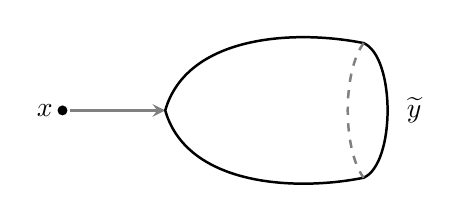
\begin{tikzpicture}[>=stealth,scale=.9]
  \fill (-3,0) circle (2pt) node[left] {$x$};
  \draw[->,gray,line width=1pt] (-2.9,0)--(-1.55,0);
  \draw[line width=.9pt] (-1.55,0)
    .. controls (-1.25,1.05) and (.25,1.15) .. (1.25,.95)
    .. controls (1.7,.75) and (1.7,-.75) .. (1.25,-.95)
    .. controls (.25,-1.15) and (-1.25,-1.05) .. (-1.55,0);
  \draw[gray,dashed,line width=.9pt] (1.25,.95)
    .. controls (.95,.55) and (.95,-.55) .. (1.25,-.95);
  \node[right] at (1.72,0) {$\widetilde y$};
\end{tikzpicture}
\caption{PSS 同构 $\Phi^\alpha:\operatorname{HF}^*\to\operatorname{QH}^*$。}
\label{fig:12-1-1}
\end{figure}

当 $\operatorname{ind}_f(x)-n=\mu_{\mathrm{CZ}}(\widetilde y)$ 时，\BookRecordIndex{T0182}尖盘\BookRecordIndex{T0246}模空间为零维，故可用
其元素数 $n(x,\widetilde y)$ 构造简称为 PSS 映射的链映射
\[
  \Phi^\alpha:\operatorname{CF}^*(H^\alpha)
  \longrightarrow\operatorname{CM}^*(f;\Lambda_\omega),
\]
定义为
\[
  (\Phi^\alpha\xi)(x,A):=
  \sum_{\mu_{\mathrm{CZ}}(\widetilde y)=\operatorname{ind}_f(x)-n}
  n(x,\widetilde y)\xi(A\#\widetilde y).
\]
这里 $\xi\in\operatorname{CF}^*(H^\alpha)$。为说明满足
$(\Phi^\alpha\xi)(x,A)\neq0$ 且 $\omega(A)\geq-c$ 的偶对 $(x,A)$ 只有有限多个，注意每个
这样的偶对都对应某个 $\widetilde y\in\widetilde{\mathcal P}(H^\alpha)$，使
$n(x,\widetilde y)\neq0$ 且 $\xi(A\#\widetilde y)\neq0$。后一不等式意味着存在常数
$c_\xi>0$，使 $\mathcal A_{H^\alpha}(A\#\widetilde y)\geq-c_\xi$；前一不等式意味着\BookRecordIndex{T0246}模空间
$\mathcal M(\widetilde y;H^\alpha,J^\alpha)$ 非空。因此由\BookRecordIndex{T0249}能量恒等式~\eqref{eq:12-1-11}，
存在只依赖 $(H^\alpha,J^\alpha)$ 的常数 $c_E>0$，使
\begin{equation}\label{eq:12-1-14}
  E(u)\leq c_E-\mathcal A_{H^\alpha}(\widetilde y)
  =c_E-\mathcal A_{H^\alpha}(A\#\widetilde y)-\omega(A)
  \leq c_E+c_\xi+c.
\end{equation}
这个一致能量界证明了所需有限性条件。

映射 $\Phi^\alpha$ 是把次数提高 $n$ 的 $\Lambda_\omega$-模同态。\BookRecordIndex{T0132}弗洛尔同调中的标准论证
（如 $\delta^2=0$ 的证明）说明它是链映射，因此在上同调上诱导仍记作 $\Phi^\alpha$ 的同态。
Piunikhin--Salamon--Schwarz \srcite{323} 证明了这个诱导同态是同构。其证明构造类似的
链映射
\[
  \Psi^\alpha:\operatorname{CM}^*(f;\Lambda_\omega)
  \longrightarrow\operatorname{CF}^*(H^\alpha),
\]
其公式为
\[
  (\Psi^\alpha\xi_0)(\widetilde x):=
  \sum_{\operatorname{ind}_f(y)-2c_1(A)=\mu_{\mathrm{CZ}}(\widetilde x)+n}
  n((-A)\#\widetilde x,y)\xi_0(y,A),
\]
其中 $\xi_0\in\operatorname{CM}^*(f;\Lambda_\omega)$。接下来须证明两个复合
$\Phi^\alpha\circ\Psi^\alpha$ 与 $\Psi^\alpha\circ\Phi^\alpha$ 都链同伦于恒等映射；
图~\ref{fig:12-1-2}、\ref{fig:12-1-3} 描绘了这一论证。技术核心是弗洛尔\BookRecordIndex{T0256}粘合定理以及
第~\ref{ch:gluing} 章证明的 \BookRecordIndex{T0003}$J$-全纯曲线\BookRecordIndex{T0256}粘合定理；如下方注~\ref{rem:12-1-7} 所述，
论证其余部分都是标准的。

\begin{figure}[tbp]
\centering
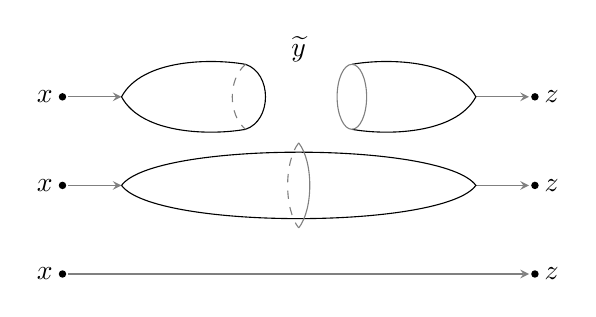
\begin{tikzpicture}[>=stealth,scale=.75]
  \foreach \y in {1.5,0,-1.5}{
    \fill (-4,\y) circle (1.8pt) node[left] {$x$};
    \fill (4,\y) circle (1.8pt) node[right] {$z$};
  }
  \draw[->,gray] (-3.9,1.5)--(-3,1.5);
  \draw[gray,->] (3,1.5)--(3.9,1.5);
  \draw (-3,1.5)
    .. controls (-2.65,2.15) and (-1.45,2.15) .. (-.9,2.05)
    .. controls (-.45,1.9) and (-.45,1.1) .. (-.9,.95)
    .. controls (-1.45,.85) and (-2.65,.85) .. (-3,1.5);
  \draw[gray,dashed] (-.9,2.05)
    .. controls (-1.2,1.8) and (-1.2,1.2) .. (-.9,.95);
  \draw (.9,2.05)
    .. controls (1.45,2.15) and (2.65,2.15) .. (3,1.5)
    .. controls (2.65,.85) and (1.45,.85) .. (.9,.95);
  \draw[gray] (.9,1.5) ellipse[x radius=.25,y radius=.55];
  \node at (0,2.3) {$\widetilde y$};
  \draw[->,gray] (-3.9,0)--(-3,0);
  \draw[gray,->] (3,0)--(3.9,0);
  \draw (-3,0)
    .. controls (-2.45,.75) and (2.45,.75) .. (3,0)
    .. controls (2.45,-.75) and (-2.45,-.75) .. (-3,0);
  \draw[gray,dashed] (0,.72)
    .. controls (-.25,.4) and (-.25,-.4) .. (0,-.72);
  \draw[gray] (0,.72)
    .. controls (.25,.4) and (.25,-.4) .. (0,-.72);
  \draw[->,gray] (-3.9,-1.5)--(3.9,-1.5);
\end{tikzpicture}
\caption{$\Phi^\alpha\circ\Psi^\alpha\simeq\operatorname{id}$。}
\label{fig:12-1-2}
\end{figure}

\begin{figure}[tbp]
\centering
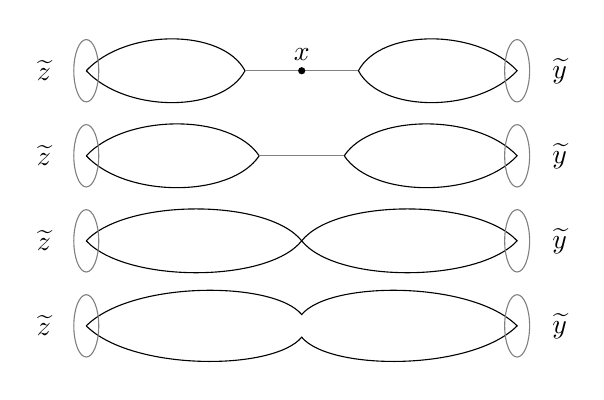
\begin{tikzpicture}[>=stealth,scale=.72]
  \foreach \y in {2.25,.75,-.75,-2.25}{
    \node[left] at (-4.25,\y) {$\widetilde z$};
    \node[right] at (4.25,\y) {$\widetilde y$};
  }
  \draw (-3.8,2.25) .. controls (-3.1,3) and (-1.4,3) .. (-1,2.25)
    .. controls (-1.4,1.5) and (-3.1,1.5) .. (-3.8,2.25);
  \draw (1,2.25) .. controls (1.4,3) and (3.1,3) .. (3.8,2.25)
    .. controls (3.1,1.5) and (1.4,1.5) .. (1,2.25);
  \draw[gray] (-1,2.25)--(1,2.25); \fill (0,2.25) circle (1.8pt) node[above] {$x$};
  \draw (-3.8,.75) .. controls (-3.1,1.5) and (-1.25,1.5) .. (-.75,.75)
    .. controls (-1.25,0) and (-3.1,0) .. (-3.8,.75);
  \draw (.75,.75) .. controls (1.25,1.5) and (3.1,1.5) .. (3.8,.75)
    .. controls (3.1,0) and (1.25,0) .. (.75,.75);
  \draw[gray] (-.75,.75)--(.75,.75);
  \draw (-3.8,-.75) .. controls (-3.1,0) and (-.6,0) .. (0,-.75)
    .. controls (-.6,-1.5) and (-3.1,-1.5) .. (-3.8,-.75);
  \draw (0,-.75) .. controls (.6,0) and (3.1,0) .. (3.8,-.75)
    .. controls (3.1,-1.5) and (.6,-1.5) .. (0,-.75);
  \draw (-3.8,-2.25) .. controls (-3,-1.45) and (-.5,-1.45) .. (0,-2.05)
    .. controls (.5,-1.45) and (3,-1.45) .. (3.8,-2.25)
    .. controls (3,-3.05) and (.5,-3.05) .. (0,-2.45)
    .. controls (-.5,-3.05) and (-3,-3.05) .. (-3.8,-2.25);
  \foreach \y in {2.25,.75,-.75,-2.25}{
    \draw[gray] (-3.8,\y) ellipse[x radius=.22,y radius=.55];
    \draw[gray] (3.8,\y) ellipse[x radius=.22,y radius=.55];
  }
\end{tikzpicture}
\caption{$\Psi^\alpha\circ\Phi^\alpha\simeq\operatorname{id}$。}
\label{fig:12-1-3}
\end{figure}

还要注意，若 $H=-f$ 与时间无关，并且处在弗洛尔原始论证适用的情形，那么可以证明：当
$\varepsilon>0$ 充分小时，对 PSS 映射有贡献的\BookRecordIndex{T0182}尖盘只有 $H$ 的\BookRecordIndex{T0233}临界点处的常值映射。因此
PSS 映射 $\operatorname{CF}^*(-\varepsilon f)\to\operatorname{CM}^*(f;\Lambda_\omega)$
就是显然的同构。由此，PSS 同构 $\Phi^\alpha$
\sourcefootnote{原书此处写作 $\Psi^\alpha$，但本段比较的是从弗洛尔上同调到\BookRecordIndex{T0229}量子上同调的
PSS 映射；按定理~\ref{thm:12-1-4} 及紧邻公式，该方向记为 $\Phi^\alpha$。}
在弗洛尔方法所构造的映射有定义时，与后者相同。

\begin{remark}\label{rem:12-1-7}
可以把 PSS 映射
\[
  \Phi^*_{\mathrm{PSS}}:\operatorname{CF}^*(H^\alpha)
  \longrightarrow\operatorname{CM}^*(f;\Lambda_\omega)
\]
看作 Seidel 同态 $\mathcal S(\phi)$ 的“一半”。如注~\ref{rem:11-4-4} 所述，Seidel 同态
通过计数 $S^2$ 上某个丛的截面给出，这些截面与位于两个固定点 $w_1,w_2$ 上纤维中的循环
相交。若用某个 Morse 流的不稳定流形表示 $w_1$ 上纤维中的循环，以稳定流形表示 $w_2$
上纤维中的循环，那么所计数的是带两个尖部的球面：一个尖部是从 $x$ 出发的梯度轨道，
另一个是流向 $z$ 的梯度轨道；参见图~\ref{fig:12-1-2}。在当前情形，计数的是带弗洛尔
边界条件的圆盘上截面。沿边界把两个定向相反的这种圆盘\BookRecordIndex{T0254}粘合，就得到 Seidel 所计数的一个
球面。

因此，$\Phi^*_{\mathrm{PSS}}\circ\Psi^*_{\mathrm{PSS}}$ 是\BookRecordIndex{T0229}量子上同调上的恒等映射这一
断言，等价于定义~\ref{def:11-4-1} 的 \BookRecordIndex{T0046}Seidel 元 $\mathcal S(\operatorname{id},\sigma_0)$
是 $\operatorname{QH}^0(M;\Lambda)$ 中的幺元。（这里 $\operatorname{id}$ 是群
$\pi_1(\operatorname{Ham}(M))$ 的单位元，$\sigma_0$ 表示 $S^2\times M$ 中的平凡\BookRecordIndex{T0189}截面类
$[S^2\times\{\mathrm{pt}\}]$。）在当前背景以及 Piunikhin--Salamon--Schwarz
\srcite{323} 的背景中，\BookRecordIndex{T0254}粘合在拓扑上平凡，产生平凡丛的一个截面。Seidel \srcite{363}
指出，这些思想可以调整后用于非平凡丛；见第~\ref{sec:12-5} 节。Lalonde \srcite{222} 进一步发展了
这一观点。
\end{remark}


\section{环结构}\label{sec:12-2}

弗洛尔上同调上有一个自然环结构，它由计数三穿孔二球面上的扰动 \BookRecordIndex{T0003}$J$-全纯曲线定义。
把穿孔理解为圆柱端，并如式~\eqref{eq:12-1-3} 那样在穿孔附近作\BookRecordIndex{T0157}哈密顿扰动。更准确地说，
令 $\Sigma$ 为带三个圆柱端的非紧亏格零黎曼曲面，即所谓裤形曲面。假设 $\Sigma$ 上的复
结构在圆柱端上是标准乘积结构。固定圆柱端的参数化
\[
  \phi^\alpha:(-\infty,0)\times\mathbb R/\mathbb Z\longrightarrow\Sigma,
  \qquad
  \phi^\beta,\phi^\gamma:(0,\infty)\times\mathbb R/\mathbb Z\longrightarrow\Sigma,
\]
它们的像互不相交，记
$U^\alpha:=\operatorname{im}\phi^\alpha$、
$U^\beta:=\operatorname{im}\phi^\beta$、
$U^\gamma:=\operatorname{im}\phi^\gamma$。假设补集
\[
  \Sigma'=\Sigma\setminus(U^\alpha\cup U^\beta\cup U^\gamma)
\]
微分同胚于挖去三个开圆盘的二球面；特别地，$\Sigma'$ 是紧的。选取 $\Sigma$ 上的复结构，
使它在三个圆柱端上拉回为标准结构 $s+it$。为定义适当的\BookRecordIndex{T0246}模空间，选取三个哈密顿函数
\[
  H^\alpha,H^\beta,H^\gamma:
  \mathbb R\times\mathbb R/\mathbb Z\times M\longrightarrow\mathbb R,
\]
它们在 $|s|\leq\tfrac12$ 时消失，在 $|s|\geq1$ 时与 $s$ 无关。考虑光滑映射
$u:\Sigma\to M$，要求 $u|_{\Sigma'}$ 是 \BookRecordIndex{T0003}$J$-全纯曲线，并且在圆柱端 $U^\alpha$ 上，
复合 $u^\alpha(s,t):=u\circ\phi^\alpha(s,t)$ 满足
\[
  \partial_su^\alpha+J(u^\alpha)
  \bigl(\partial_tu^\alpha-X^\alpha_{s,t}(u^\alpha)\bigr)=0,
\]
其中对所有 $s,t$ 都有 $\iota(X^\alpha_{s,t})\omega=dH^\alpha_{s,t}$；
$u^\beta:=u\circ\phi^\beta$ 与 $u^\gamma:=u\circ\phi^\gamma$ 满足类似方程。

这些方程的每个有限能量解都满足极限条件
\[
\begin{split}
  \lim_{s\to-\infty}u^\alpha(s,t)&=x^\alpha(t),\\
  \lim_{s\to+\infty}u^\beta(s,t)&=x^\beta(t),\\
  \lim_{s\to+\infty}u^\gamma(s,t)&=x^\gamma(t),
\end{split}
\]
其中 $x^\alpha\in\mathcal P(H^\alpha)$、$x^\beta\in\mathcal P(H^\beta)$、
$x^\gamma\in\mathcal P(H^\gamma)$。这里稍微滥用记号，以 $\mathcal P(H^\alpha)$ 表示
哈密顿量 $H^\alpha_{-\infty,t}$ 的周期解，$\beta,\gamma$ 情形亦同。正确同调类中这些解
$u$ 的空间记为
$\mathcal M(\widetilde x^\alpha;\widetilde x^\beta,\widetilde x^\gamma)$
（见图~\ref{fig:12-2-4}），其维数为
\[
\begin{split}
  \dim\mathcal M(\widetilde x^\alpha;\widetilde x^\beta,\widetilde x^\gamma)
  ={}&\mu_{\mathrm{CZ}}(\widetilde x^\alpha,H^\alpha)
  -\mu_{\mathrm{CZ}}(\widetilde x^\beta,H^\beta)\\
  &-\mu_{\mathrm{CZ}}(\widetilde x^\gamma,H^\gamma)-n.
\end{split}
\]
在零维情形，用与上文相同的论证可知解只有有限多个；其带符号的个数记为
$n(\widetilde x^\alpha;\widetilde x^\beta,\widetilde x^\gamma)$。这些数产生
$\Lambda_\omega$-模同态
\[
  \operatorname{CF}^k(H^\beta)\otimes\operatorname{CF}^\ell(H^\gamma)
  \longrightarrow\operatorname{CF}^{k+\ell+n}(H^\alpha),
  \qquad \xi^\beta\otimes\xi^\gamma\longmapsto\xi^\beta*\xi^\gamma.
\]

\begin{figure}[tbp]
\centering
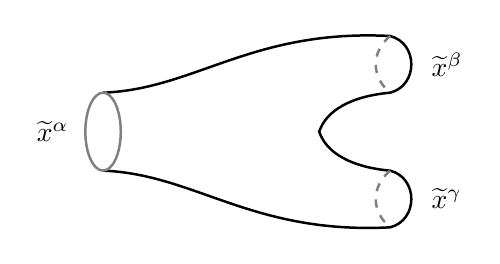
\begin{tikzpicture}[scale=.9]
  \draw[line width=.9pt]
    (-2.6,.55) .. controls (-1.3,.6) and (-.5,1.45) .. (1.45,1.35)
    .. controls (1.85,1.25) and (1.85,.65) .. (1.45,.55)
    .. controls (.9,.5) and (.55,.3) .. (.45,0)
    .. controls (.55,-.3) and (.9,-.5) .. (1.45,-.55)
    .. controls (1.85,-.65) and (1.85,-1.25) .. (1.45,-1.35)
    .. controls (-.5,-1.45) and (-1.3,-.6) .. (-2.6,-.55);
  \draw[gray,line width=.9pt] (-2.6,0) ellipse[x radius=.25,y radius=.55];
  \draw[gray,dashed,line width=.9pt] (1.45,1.35)
    .. controls (1.18,1.12) and (1.18,.78) .. (1.45,.55);
  \draw[gray,dashed,line width=.9pt] (1.45,-.55)
    .. controls (1.18,-.78) and (1.18,-1.12) .. (1.45,-1.35);
  \node[left] at (-2.95,0) {$\widetilde x^\alpha$};
  \node[right] at (1.9,.95) {$\widetilde x^\beta$};
  \node[right] at (1.9,-.95) {$\widetilde x^\gamma$};
\end{tikzpicture}
\caption{\BookRecordIndex{T0217}裤形乘积。}\label{fig:12-2-4}
\end{figure}

它由下式定义：
\[
  (\xi^\beta*\xi^\gamma)(\widetilde x^\alpha):=
  \sum_{\widetilde x^\beta,\widetilde x^\gamma}
  n(\widetilde x^\alpha;\widetilde x^\beta,\widetilde x^\gamma)
  \xi^\beta(\widetilde x^\beta)\xi^\gamma(\widetilde x^\gamma).
\]
\BookRecordIndex{T0132}弗洛尔同调中的通常\BookRecordIndex{T0254}粘合技术表明，此映射是上链同态，因而诱导弗洛尔上同调同态
\[
  \operatorname{HF}^k(H^\beta)\otimes\operatorname{HF}^\ell(H^\gamma)
  \longrightarrow\operatorname{HF}^{k+\ell+n}(H^\alpha).
\]
鉴于其构造，这一映射称为\BookRecordIndex{T0217}裤形乘积，简称 PP 乘积。

\BookRecordIndex{T0132}弗洛尔同调中的通常形变论证表明，\BookRecordIndex{T0217}裤形乘积与定义它时所用黎曼曲面 $\Sigma$ 上的复结构
无关；只要哈密顿函数 $H^\alpha,H^\beta,H^\gamma$ 在 $\pm\infty$ 处不变，它也与这些
函数无关。若在 $\pm\infty$ 处改变它们，再次用弗洛尔\BookRecordIndex{T0254}粘合技术便可证明：此乘积关于
定理~\ref{thm:12-1-3} 的同构是自然的。为在通常符号约定下证明乘积的斜交换性，选取保持
定向的微分同胚 $f:\Sigma\to\Sigma$，交换右侧两个圆柱端。该微分同胚改变 $\Sigma$ 的复
结构，却不影响所得弗洛尔上同调映射。

结合律的证明需要沿一条长圆柱\BookRecordIndex{T0254}粘合两个带三个圆柱端的曲面
$\Sigma_{\alpha;\beta\gamma}$ 与 $\Sigma_{\gamma;\delta\varepsilon}$
（见图~\ref{fig:12-2-5}）。这一过程抵消两个标为 $\gamma$ 的端，得到带四个圆柱端的黎曼
曲面 $\Sigma_{\alpha;\beta\delta\varepsilon}$。若\BookRecordIndex{T0147}颈部充分长，所得三重乘积对应复合
$\xi^\beta*(\xi^\delta*\xi^\varepsilon)$。现在改变
$\Sigma_{\alpha;\beta\delta\varepsilon}$ 上的复结构并以另一种方式分解它，即得
\[
  \xi^\beta*(\xi^\delta*\xi^\varepsilon)
  =(\xi^\beta*\xi^\delta)*\xi^\varepsilon.
\]
这一复结构变化对应于第~\ref{sec:11-1} 节证明\BookRecordIndex{T0229}量子上同调结合律时改变四个\BookRecordIndex{T0150}固定标记点的
\BookRecordIndex{T0185}交比。

\begin{figure}[tbp]
\centering
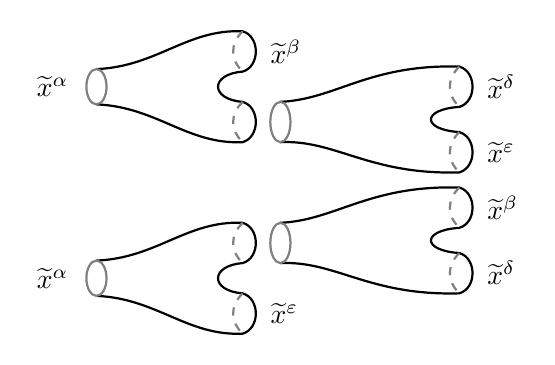
\begin{tikzpicture}[scale=.64,line width=.8pt]
  \draw (-4,2.45) .. controls (-2.8,2.5) and (-2.2,3.25) .. (-1.1,3.2)
    .. controls (-.75,3.1) and (-.75,2.5) .. (-1.1,2.4)
    .. controls (-1.75,2.35) and (-1.75,1.85) .. (-1.1,1.8)
    .. controls (-.75,1.7) and (-.75,1.1) .. (-1.1,1)
    .. controls (-2.2,.95) and (-2.8,1.7) .. (-4,1.75);
  \draw[gray] (-4,2.1) ellipse[x radius=.2,y radius=.35];
  \draw[gray,dashed] (-1.1,3.2) .. controls (-1.35,2.95) and (-1.35,2.65) .. (-1.1,2.4);
  \draw[gray,dashed] (-1.1,1.8) .. controls (-1.35,1.55) and (-1.35,1.25) .. (-1.1,1);
  \draw (-.35,1.8) .. controls (.75,1.85) and (1.4,2.55) .. (3.2,2.5)
    .. controls (3.55,2.4) and (3.55,1.8) .. (3.2,1.7)
    .. controls (2.45,1.65) and (2.45,1.25) .. (3.2,1.2)
    .. controls (3.55,1.1) and (3.55,.5) .. (3.2,.4)
    .. controls (1.4,.35) and (.75,1.05) .. (-.35,1);
  \draw[gray] (-.35,1.4) ellipse[x radius=.2,y radius=.4];
  \draw[gray,dashed] (3.2,2.5) .. controls (2.95,2.25) and (2.95,1.95) .. (3.2,1.7);
  \draw[gray,dashed] (3.2,1.2) .. controls (2.95,.95) and (2.95,.65) .. (3.2,.4);
  \node[left] at (-4.35,2.1) {$\widetilde x^\alpha$};
  \node[right] at (-.75,2.8) {$\widetilde x^\beta$};
  \node[right] at (3.55,2.1) {$\widetilde x^\delta$};
  \node[right] at (3.55,.8) {$\widetilde x^\varepsilon$};

  \draw (-4,-1.35) .. controls (-2.8,-1.3) and (-2.2,-.55) .. (-1.1,-.6)
    .. controls (-.75,-.7) and (-.75,-1.3) .. (-1.1,-1.4)
    .. controls (-1.75,-1.45) and (-1.75,-1.95) .. (-1.1,-2)
    .. controls (-.75,-2.1) and (-.75,-2.7) .. (-1.1,-2.8)
    .. controls (-2.2,-2.85) and (-2.8,-2.1) .. (-4,-2.05);
  \draw[gray] (-4,-1.7) ellipse[x radius=.2,y radius=.35];
  \draw[gray,dashed] (-1.1,-.6) .. controls (-1.35,-.85) and (-1.35,-1.15) .. (-1.1,-1.4);
  \draw[gray,dashed] (-1.1,-2) .. controls (-1.35,-2.25) and (-1.35,-2.55) .. (-1.1,-2.8);
  \draw (-.35,-.6) .. controls (.75,-.55) and (1.4,.15) .. (3.2,.1)
    .. controls (3.55,0) and (3.55,-.6) .. (3.2,-.7)
    .. controls (2.45,-.75) and (2.45,-1.15) .. (3.2,-1.2)
    .. controls (3.55,-1.3) and (3.55,-1.9) .. (3.2,-2)
    .. controls (1.4,-2.05) and (.75,-1.35) .. (-.35,-1.4);
  \draw[gray] (-.35,-1) ellipse[x radius=.2,y radius=.4];
  \draw[gray,dashed] (3.2,.1) .. controls (2.95,-.15) and (2.95,-.45) .. (3.2,-.7);
  \draw[gray,dashed] (3.2,-1.2) .. controls (2.95,-1.45) and (2.95,-1.75) .. (3.2,-2);
  \node[left] at (-4.35,-1.7) {$\widetilde x^\alpha$};
  \node[right] at (3.55,-.3) {$\widetilde x^\beta$};
  \node[right] at (3.55,-1.6) {$\widetilde x^\delta$};
  \node[right] at (-.75,-2.4) {$\widetilde x^\varepsilon$};
\end{tikzpicture}
\caption{结合律。}\label{fig:12-2-5}
\end{figure}

\paragraph{比较定理。}
由定理~\ref{thm:12-1-4}，弗洛尔上同调群 $\operatorname{HF}^*(H,J)$ 自然同构于\BookRecordIndex{T0229}量子
上同调群 $\operatorname{QH}^*(M)$；因而可以预期，在此同构下\BookRecordIndex{T0217}裤形乘积对应于杯积的量子
形变。即使 $\pi_2(M)=0$，即量子形变等于通常杯积时，这个问题也并不平凡。Schwarz
\srcite{358} 在其论文中证明了 $\pi_2(M)=0$ 的情形，Piunikhin--Salamon--Schwarz
\srcite{323} 证明了一般情形。Liu--Tian \srcite{250} 与 Ruan--Tian \srcite{347} 还
各自独立给出了其他证明；Sadov \srcite{350} 给出了物理学家的处理方式。

\begin{theorem}\label{thm:12-2-1}
设 $(M,\omega)$ \BookRecordIndex{T0058}半正，并设
\[
  \Phi^\alpha:\operatorname{HF}^*(M,\omega,H^\alpha,J^\alpha)
  \longrightarrow\operatorname{QH}^*(M)
\]
是定理~\ref{thm:12-1-4} 的 PSS 同构；$\Phi^\beta,\Phi^\gamma$ 类似。则
\[
  \Phi^\alpha(\xi^\beta*\xi^\gamma)
  =\Phi^\beta(\xi^\beta)*\Phi^\gamma(\xi^\gamma)
\]
对 $\xi^\beta\in\operatorname{HF}^*(H^\beta)$ 与
$\xi^\gamma\in\operatorname{HF}^*(H^\gamma)$ 成立。左侧乘积由裤形构造定义，右侧乘积是
杯积的量子形变。
\end{theorem}

证明思路如下。先用 Morse--Witten 复形以一种略微不同的方式表示杯积的量子形变。给定
三个 Morse 函数 $f^\alpha,f^\beta,f^\gamma:M\to\mathbb R$、三个\BookRecordIndex{T0233}临界点
$x^\alpha,x^\beta,x^\gamma$、三个互异点
$w^\alpha,w^\beta,w^\gamma\in\mathbb{CP}^1$，以及定义~\ref{def:6-7-10} 中的正则\BookRecordIndex{T0088}殆复
结构族
\[
  J=\{J_z\}_{z\in S^2}\in
  \mathcal J_{\mathrm{reg}}(S^2;M,\omega;\mathbf w)
\]
（$J_z$ 接近某个固定\BookRecordIndex{T0088}殆复结构 $J_0$），考虑空间
\[
  \mathcal M_A(x^\alpha;x^\beta,x^\gamma)
  =\mathcal M_A(x^\alpha;x^\beta,x^\gamma;f,J),
\]
它由满足
\[
\begin{split}
  u(w^\alpha)&\in W^u(x^\alpha,f^\alpha),\\
  u(w^\beta)&\in W^s(x^\beta,f^\beta),\\
  u(w^\gamma)&\in W^s(x^\gamma,f^\gamma)
\end{split}
\]
的全部 $J$-全纯 $A$-球面 $u:\mathbb{CP}^1\to M$ 组成。
\sourcefootnote{原书从本段开头\BookRecordIndex{T0150}固定标记点 $w^\alpha,w^\beta,w^\gamma$，但随后在\BookRecordIndex{T0246}模空间条件
中改用未定义的 $z^\alpha,z^\beta,z^\gamma$，并把度量下标写成 $J_{z^i}$；这里统一恢复为
$w^\alpha,w^\beta,w^\gamma$ 与 $J_{w^i}$。}
这里 $W^s(x,f)$、$W^u(x,f)$ 表示\BookRecordIndex{T0233}临界点 $x$ 关于 Morse 函数 $f$ 向下梯度流的稳定与
不稳定流形。$f^i$ 的梯度相对于 $J_{w^i}$ 诱导的度量理解，其中
$i=\alpha,\beta,\gamma$；假设这些梯度流为 Morse--Smale。可把
$\mathcal M_A(x^\alpha;x^\beta,x^\gamma)$ 的元素看成带尖部的 $J$-全纯球面
（见图~\ref{fig:12-2-6}）。

\begin{figure}[tbp]
\centering
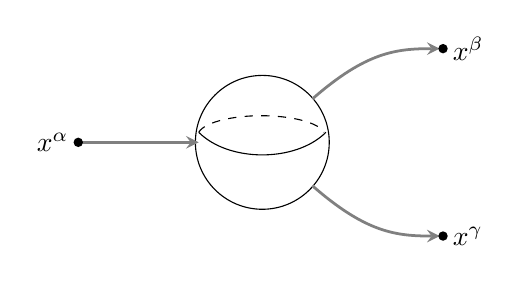
\begin{tikzpicture}[>=stealth,scale=.85]
  \draw (0,0) circle (1);
  \draw[dashed] (-.95,.15) arc[start angle=170,end angle=10,x radius=.95,y radius=.3];
  \draw (-.95,.15) .. controls (-.5,-.3) and (.5,-.3) .. (.95,.15);
  \draw[gray,->,line width=1pt] (-2.7,0)--(-.95,0);
  \draw[gray,->,line width=1pt] (.75,.65)..controls (1.55,1.35) and (2,1.4)..(2.65,1.4);
  \draw[gray,->,line width=1pt] (.75,-.65)..controls (1.55,-1.35) and (2,-1.4)..(2.65,-1.4);
  \fill (-2.75,0) circle (2pt) node[left] {$x^\alpha$};
  \fill (2.7,1.4) circle (2pt) node[right] {$x^\beta$};
  \fill (2.7,-1.4) circle (2pt) node[right] {$x^\gamma$};
\end{tikzpicture}
\caption{通过 Morse 理论得到的量子乘积。}\label{fig:12-2-6}
\end{figure}

由如下维数公式
\sourcefootnote{原书把第二式的不稳定流形误印作 $W^u(x,H)$；此段只涉及 Morse 函数 $f$，
且右端正是 $f$ 的 Morse 指数，故改为 $W^u(x,f)$。}：
\[
  \dim W^s(x,f)=2n-\operatorname{ind}_f(x),\qquad
  \dim W^u(x,f)=\operatorname{ind}_f(x),
\]
对一般的 Morse 函数 $f^\alpha,f^\beta,f^\gamma$，有
\[
  \dim\mathcal M_A(x^\alpha;x^\beta,x^\gamma)
  =2c_1(A)+\operatorname{ind}_{f^\alpha}(x^\alpha)
  -\operatorname{ind}_{f^\beta}(x^\beta)
  -\operatorname{ind}_{f^\gamma}(x^\gamma).
\]
当此维数为零时，把 $\mathcal M_A(x^\alpha;x^\beta,x^\gamma)$ 中按适当符号计数的点数记作
$n_A(x^\alpha;x^\beta,x^\gamma)$。于是得到链映射
\[
  \operatorname{CM}^*(f^\beta;\Lambda_\omega)
  \otimes\operatorname{CM}^*(f^\gamma;\Lambda_\omega)
  \longrightarrow\operatorname{CM}^*(f^\alpha;\Lambda_\omega),
  \qquad \xi^\beta\otimes\xi^\gamma\longmapsto\xi^\beta*\xi^\gamma,
\]
\sourcefootnote{原书在这里把三个 Morse--Witten 复形依次印作
$\operatorname{CF}^*(f^\beta;\Lambda_\omega)$、
$\operatorname{CF}^*(f^\gamma;\Lambda_\omega)$ 与
$C^*(f^\alpha;\Lambda_\omega)$；本节前文已把 Morse 复形统一记为
$\operatorname{CM}^*$，故将三处统一补正。}
其定义为
\begin{equation}\label{eq:12-2-1}
  (\xi^\beta*\xi^\gamma)(x^\alpha,A^\alpha)
  =\sum_{\substack{A,\,x^\beta,\,x^\gamma,\,A^\beta,\,A^\gamma\\
                    A+A^\alpha=A^\beta+A^\gamma}}
  n_A(x^\alpha;x^\beta,x^\gamma)
  \xi^\beta(x^\beta,A^\beta)\xi^\gamma(x^\gamma,A^\gamma).
\end{equation}
\sourcefootnote{原书此式的求和号仅列 $A^\beta+A^\gamma=A^\alpha$，因而把\BookRecordIndex{T0285}球面类 $A$ 与
\BookRecordIndex{T0233}临界点 $x^\beta,x^\gamma$ 留成自由变量，并在同调类约束中漏掉 $A$。紧邻的零维公式与
$\deg(x,A)=\operatorname{ind}_f(x)-2c_1(A)$ 唯一给出
$A+A^\alpha=A^\beta+A^\gamma$；这里也补齐全部求和变量。}
它在 Morse--Witten 上同调（取 $\Lambda_\omega$ 系数，上边缘映射为
$\delta_{\mathrm{MW}}$）上诱导乘积，因而也在\BookRecordIndex{T0229}量子上同调上诱导乘积。这个乘积等于\BookRecordIndex{T0228}量子
杯积，因为 Morse 函数\BookRecordIndex{T0233}临界点的稳定、不稳定流形表示生成 $M$ 上同调的上同调类。

\begin{figure}[tbp]
\centering
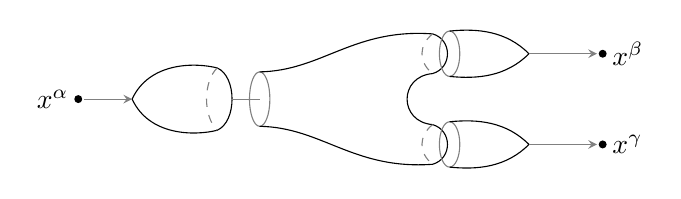
\begin{tikzpicture}[>=stealth,scale=.72]
  \fill (-5,0) circle (2pt) node[left] {$x^\alpha$};
  \draw[gray,->] (-4.9,0)--(-4.05,0);
  \draw (-4.05,0)
    .. controls (-3.75,.65) and (-2.95,.65) .. (-2.55,.55)
    .. controls (-2.2,.4) and (-2.2,-.4) .. (-2.55,-.55)
    .. controls (-2.95,-.65) and (-3.75,-.65) .. (-4.05,0);
  \draw[gray,dashed] (-2.55,.55)
    .. controls (-2.8,.3) and (-2.8,-.3) .. (-2.55,-.55);
  \draw[gray] (-2.3,0)--(-1.8,0);
  \draw[gray] (-1.8,0) ellipse[x radius=.18,y radius=.48];
  \draw (-1.8,.48) .. controls (-.7,.5) and (-.15,1.25) .. (1.25,1.15)
    .. controls (1.6,1.05) and (1.6,.55) .. (1.25,.45)
    .. controls (.65,.4) and (.65,-.4) .. (1.25,-.45)
    .. controls (1.6,-.55) and (1.6,-1.05) .. (1.25,-1.15)
    .. controls (-.15,-1.25) and (-.7,-.5) .. (-1.8,-.48);
  \draw[gray,dashed] (1.25,1.15) .. controls (1, .95) and (1,.65) .. (1.25,.45);
  \draw[gray,dashed] (1.25,-.45) .. controls (1,-.65) and (1,-.95) .. (1.25,-1.15);
  \draw[gray] (1.55,.8) ellipse[x radius=.18,y radius=.4];
  \draw[gray] (1.55,-.8) ellipse[x radius=.18,y radius=.4];
  \draw (1.55,1.2) .. controls (2.05,1.25) and (2.55,1.2) .. (2.95,.8)
    .. controls (2.55,.4) and (2.05,.35) .. (1.55,.4);
  \draw (1.55,-.4) .. controls (2.05,-.35) and (2.55,-.4) .. (2.95,-.8)
    .. controls (2.55,-1.2) and (2.05,-1.25) .. (1.55,-1.2);
  \draw[gray,->] (2.95,.8)--(4.15,.8);
  \draw[gray,->] (2.95,-.8)--(4.15,-.8);
  \fill (4.25,.8) circle (2pt) node[right] {$x^\beta$};
  \fill (4.25,-.8) circle (2pt) node[right] {$x^\gamma$};
\end{tikzpicture}
\caption{\BookRecordIndex{T0229}量子上同调与\BookRecordIndex{T0217}裤形乘积。}\label{fig:12-2-7}
\end{figure}

现在由\BookRecordIndex{T0132}弗洛尔同调中的标准\BookRecordIndex{T0254}粘合论证可知，定理~\ref{thm:12-1-4} 的 PSS 同构
\[
  \Phi^\alpha:\operatorname{HF}^*(H^\alpha)
  \longrightarrow\operatorname{QH}^*(M;\Lambda_\omega)
\]
按照 \srcite{323} 的描述交织这两种乘积结构。要看出这一点，须把三个 $J$-全纯\BookRecordIndex{T0182}尖盘粘到
一条 $J$-全纯裤形曲线的边界上。更准确地说，边界分支是邻接周期解的圆柱端，\BookRecordIndex{T0254}粘合时使用
弗洛尔\BookRecordIndex{T0256}粘合定理。结果得到上文所述带三个尖部的（扰动）$J$-全纯球面
（见图~\ref{fig:12-2-7}）。论证的更多细节见 \srcite{323}。注意，
定理~\ref{thm:12-2-1} 还给出了量子乘积结合律的另一个证明。


\section{Poincaré 对偶}\label{sec:12-3}

为得到\BookRecordIndex{T0132}弗洛尔同调而非上同调，可以把链复形 $\operatorname{CF}_*$ 定义为函数
$\eta:\widetilde{\mathcal P}(H)\to R$ 的集合，其中函数满足有限性条件
\[
  \#\bigl\{\widetilde x\in\widetilde{\mathcal P}(H)\bigm|
  \eta(\widetilde x)\ne0,\ \mathcal A_H(\widetilde x)\ge c\bigr\}<\infty
\]
对每个 $c\in\mathbb R$ 都成立。$\Lambda_\omega$ 在 $\operatorname{CF}_*$ 上的作用由
下式给出\sourcefootnote{原书在这个公式右端把此前定义的链 $\eta$ 误印为 $\xi$；定义对象
以及紧随其后的配对\BookRecordIndex{T0348}相容式都唯一确定这里应为 $\eta(A\#\widetilde x)$。}：
\[
  (\lambda*\eta)(\widetilde x)
  :=\sum_A\lambda(-A)\eta(A\#\widetilde x).
\]
有一个显然的配对 $\operatorname{CF}^*\otimes\operatorname{CF}_*\to R$，定义为
\begin{equation}\label{eq:12-3-1}
  \langle\xi,\eta\rangle
  :=\sum_{\widetilde x}\xi(\widetilde x)\eta(\widetilde x).
\end{equation}
它与 $\Lambda_\omega$-模结构\BookRecordIndex{T0348}相容，亦即
\[
  \langle\lambda*\xi,\eta\rangle=\langle\xi,\lambda*\eta\rangle.
\]
关于这个配对，$\delta$ 的转置
$\partial:\operatorname{CF}_*\to\operatorname{CF}_*$ 为
\[
  (\partial\eta)(\widetilde y)
  =\sum_{\mu_{\mathrm{CZ}}(\widetilde x)
  =\mu_{\mathrm{CZ}}(\widetilde y)+1}
  \eta(\widetilde x)n(\widetilde x,\widetilde y).
\]
$\operatorname{CF}_*$ 的分次仍由 Conley--Zehnder 指数给出，而 $\partial$ 把次数降低一。

\BookRecordIndex{T0132}弗洛尔同调上的 PSS 同构由链映射
\[
  \Phi^\alpha:\operatorname{CM}_*(f;\Lambda_\omega)
  \longrightarrow\operatorname{CF}_*(H^\alpha),
  \qquad
  \Psi^\alpha:\operatorname{CF}_*(H^\alpha)
  \longrightarrow\operatorname{CM}_*(f;\Lambda_\omega)
\]
诱导。这些链映射按第~\ref{sec:12-1} 节中的方式定义。注意，$\Phi^\alpha$ 把次数降低
$n$，而 $\Psi^\alpha$ 把次数提高 $n$。我们选择这套记号，使得不论把 PSS 映射
$\Phi^\alpha$ 用在上同调还是同调上，它计数的底\BookRecordIndex{T0072}层几何对象都相同；有时分别把它记作
$\Phi^*_{\mathrm{PSS}}$（上同调上）和 $\Phi^{\mathrm{PSS}}_*$（同调上）。关于
$\Psi^\alpha$ 也有类似说明。

\begin{exercise}\label{ex:12-3-1}
设 $(H,J)$ 是命题~\ref{prop:12-1-2} 中的\BookRecordIndex{T0406}正则对，并定义
$\widehat H:\mathbb R/\mathbb Z\times M\to\mathbb R$ 为
\[
  \widehat H_t:=-H_{-t}.
\]
证明存在自然同构
\[
  \operatorname{HF}^k(H,J)\cong\operatorname{HF}_{-k}(\widehat H,J).
\]
若 $J$ 如注~\ref{rem:12-1-6} 那样依赖于 $t$，还须把 $J$ 换成
$\widehat J_t:=J_{-t}$。

\emph{提示：}证明映射
\[
  \widetilde{\mathcal P}(H)\longrightarrow
  \widetilde{\mathcal P}(\widehat H),
  \qquad (x,u)\longmapsto(\widehat x,\widehat u),
\]
是双射，其中 $\widehat x(t):=x(-t)$、$\widehat u(z):=u(\overline z)$；它同时反转辛作用量
和 Conley--Zehnder 指数的符号。证明 $u$ 是弗洛尔方程~\eqref{eq:12-1-3} 的解，当且仅当
$\widehat u(s,t):=u(-s,-t)$ 是把 $H$ 换成 $\widehat H$ 后方程~\eqref{eq:12-1-3}
的解。
\end{exercise}

\begin{remark}\label{rem:12-3-2}
若 $H$ 生成万有覆叠 $\widetilde{\operatorname{Ham}}(M,\omega)$ 中的元素
$\widetilde\phi$，则 $\widehat H$ 生成 $\widetilde\phi^{-1}$。更准确地说，设
$H:\mathbb R/\mathbb Z\times M\to\mathbb R$ 是含时哈密顿函数，并设
$t\mapsto\phi_t$ 是 $H$ 生成的\BookRecordIndex{T0158}哈密顿同痕。于是对每个 $t$ 都有
$\phi_{t+1}=\phi_t\circ\phi_1$。因此，在区间 $0\le t\le1$ 上，
$\operatorname{Ham}(M,\omega)$ 中的道路 $t\mapsto\phi_{-t}$ 与
$t\mapsto\phi_t^{-1}$ 保端点同伦。一个显式同伦为
\[
  \phi_t^\lambda:=\phi_{\lambda t}^{-1}\circ\phi_{(\lambda-1)t}.
\]
\end{remark}

弗洛尔上同调上的 \emph{Poincaré 对偶}同构
\[
  \operatorname{PD}^H:\operatorname{HF}^k(H)
  \overset{\cong}{\longrightarrow}\operatorname{HF}_{-k}(H)
\]
可定义为如下复合：先取习题~\ref{ex:12-3-1} 的典范等同
$\operatorname{HF}^k(H)\cong\operatorname{HF}_{-k}(\widehat H)$，再取从
$\operatorname{HF}_{-k}(\widehat H)$ 到 $\operatorname{HF}_{-k}(H)$ 的\BookRecordIndex{T0133}弗洛尔延拓映射。
在 $\operatorname{PD}^H$ 两侧复合 PSS 同构，便得到\BookRecordIndex{T0229}量子上同调上的 Poincaré 对偶同构
\[
  \operatorname{PD}:=\Psi_*^{\mathrm{PSS}}\circ
  \operatorname{PD}^H\circ\Psi^*_{\mathrm{PSS}}:
  \operatorname{QH}^k(M;\Lambda)
  \longrightarrow\operatorname{QH}_{2n-k}(M;\check\Lambda).
\]
由定理~\ref{thm:12-1-4}（再加上符号方面的考虑）可知，这个复合确实与
注~\ref{rem:11-1-20} 中的 Poincaré 对偶同构一致。于是
\[
  \langle a,\operatorname{PD}(b)\rangle
  =\langle a*b,1\rangle\in R,
  \qquad a,b\in\operatorname{QH}^*(M;\Lambda),
\]
其中左边的配对由~\eqref{eq:11-1-13} 给出（见习题~\ref{ex:11-1-22}）。

\begin{remark}[\BookRecordIndex{T0245}帽积]\label{rem:12-3-3}
固定一个上同调类 $a\in H^*(M)$。Piunikhin--Salamon--Schwarz
\srcite{323} 的一个结果断言：通过计数与 $a$ 的一个通有 Poincaré 对偶循环相交的弗洛尔
轨道而得到的弗洛尔上同调算子，等于与 $a$ 在 PSS 同构下的像作\BookRecordIndex{T0217}裤形乘积。其证明类似于
PSS 同构保持环结构的证明：计数带尖部弗洛尔圆柱，等价于计数在一个端点接上一只\BookRecordIndex{T0182}尖盘的
裤形曲面。借助 Poincaré 对偶，可把它翻译成\BookRecordIndex{T0132}弗洛尔同调算子的一个断言，而这些算子可解释为
与 $a$ 作弗洛尔\BookRecordIndex{T0245}帽积。在 $a=\operatorname{PD}([\mathrm{pt}])$ 的情形，相关断言可以改述
如下。

假定 $(H,J)$ 是\BookRecordIndex{T0132}弗洛尔同调的\BookRecordIndex{T0406}正则对。于是存在算子
\[
  \Psi_0:\operatorname{HF}_n(H,J)\longrightarrow
  \operatorname{HF}_{-n}(H,J),
\]
它通过计数方程
\[
  \partial_su+J_t(u)(\partial_tu-X_{H_t}(u))=0,
  \qquad u(s,t)=u(s,t+1),
  \qquad u(0,0)=x_0
\]
的有限能量、指标为零的解来定义；这里 $x_0\in M$ 是通有点。若
$n_H(\widetilde x,\widetilde y;x_0)$ 表示这个方程从
$\widetilde x\in\widetilde{\mathcal P}(H)$ 到
$\widetilde y\in\widetilde{\mathcal P}(H)$ 的解的带符号计数，则在链\BookRecordIndex{T0072}层次上
\[
  (\Psi_0\eta)(\widetilde y)
  :=\sum_{\mu_{\mathrm{CZ}}(\widetilde x)=n}
  \eta(\widetilde x)n_H(\widetilde x,\widetilde y;x_0).
\]
我们断言
\begin{equation}\label{eq:12-3-2}
  \Psi_0\circ\Phi_*^{\mathrm{PSS}}([M])
  =\Phi_*^{\mathrm{PSS}}([\mathrm{pt}]).
\end{equation}
由于 $1=\operatorname{PD}([M])$，这在弗洛尔上同调中等价于
\begin{equation}\label{eq:12-3-3}
  \Psi^0\circ\Phi^*_{\mathrm{PSS}}(1)
  =\Phi^*_{\mathrm{PSS}}(\operatorname{PD}([\mathrm{pt}])).
\end{equation}

有两种方法可以看出这一点。第一种方法是，从每个对 $\Psi^0$ 有贡献的弗洛尔圆柱上分离
出一只\BookRecordIndex{T0182}尖盘，由此\BookRecordIndex{T0326}推出 $\Psi^0$ 是与
$\Phi^*_{\mathrm{PSS}}(\operatorname{PD}([\mathrm{pt}]))$ 作\BookRecordIndex{T0217}裤形乘积。于是
\eqref{eq:12-3-3} 来自 $\Phi^*_{\mathrm{PSS}}$ 把\BookRecordIndex{T0228}量子杯积与\BookRecordIndex{T0217}裤形乘积交织这一事实。另一种
方法是，在每个对 $\Psi^0$ 有贡献的弗洛尔圆柱两端各粘上一只\BookRecordIndex{T0182}尖盘（如
注~\ref{rem:12-1-7}），得到带三个\BookRecordIndex{T0066}标记点的（扰动）全纯球面，并且球面在其中一个\BookRecordIndex{T0066}标记点
通过 $x_0$。于是复合
$\Psi^*_{\mathrm{PSS}}\circ\Psi^0\circ\Phi^*_{\mathrm{PSS}}$ 由与
$\operatorname{PD}([\mathrm{pt}])$ 作\BookRecordIndex{T0228}量子杯积给出。由于与 $1$ 作量子积是\BookRecordIndex{T0229}量子上同调上的
恒等映射，我们得到
\[
  \Psi^*_{\mathrm{PSS}}\circ\Psi^0\circ\Phi^*_{\mathrm{PSS}}(1)
  =\operatorname{PD}([\mathrm{pt}]),
\]
再由 $\Phi^*_{\mathrm{PSS}}=(\Psi^*_{\mathrm{PSS}})^{-1}$ 即得
\eqref{eq:12-3-3}。
\end{remark}


\section{\BookRecordIndex{T0271}谱不变量}\label{sec:12-4}

作用泛函 $\mathcal A_H$ 沿\BookRecordIndex{T0131}弗洛尔连接轨道递减，因而可以定义弗洛尔（上）同调的\BookRecordIndex{T0239}滤过版本。
由此得到作用泛函 $\mathcal A_H$ 的（弗洛尔）\BookRecordIndex{T0322}同调本质临界值。这些\BookRecordIndex{T0234}临界值称为
\emph{\BookRecordIndex{T0271}谱不变量}。在这里讨论的一般情形中，\BookRecordIndex{T0271}谱不变量近来由 Oh \srcite{306} 引入；
对\BookRecordIndex{T0355}辛非球面流形，它们由 Schwarz \srcite{360} 引入。在生成函数的背景下，Viterbo
\srcite{404,406} 更早引入了类似不变量。这里我们使用第~\ref{sec:12-3} 节定义的\BookRecordIndex{T0132}弗洛尔
同调群，因为 Oh \srcite{306} 采用的正是这种方法；不过也完全可以改用上同调（见
Schwarz \srcite{360} 以及下面的习题~\ref{ex:12-4-7}）。我们始终假定 $(M,\omega)$
满足强\BookRecordIndex{T0058}半正性假设~\eqref{eq:8-5-1}，并且为简单起见（也因此损失一般性），假定 $\omega$
在每个球面同调类上的积分都是有理数：
\begin{equation}\label{eq:12-4-1}
  A\in\pi_2(M)\qquad\Longrightarrow\qquad\omega(A)\in\mathbb Q.
\end{equation}
用 $\mathcal H=\mathcal H(M,\omega)$ 表示所有光滑哈密顿函数
$H:\mathbb R/\mathbb Z\times M\to\mathbb R$ 的集合，其中对每个 $t$，
$H_t:=H(t,\cdot)$ 关于体积形式 $\omega^n$ 的均值为零。给定
$H\in\mathcal H(M,\omega)$，用 $\phi^H\in\operatorname{Ham}(M,\omega)$ 表示相应
哈密顿微分方程的时间--$1$ 映射，用
$\widetilde\phi^H\in\widetilde{\operatorname{Ham}}(M,\omega)$ 表示它向万有覆叠的提升。

回忆定理~\ref{thm:9-1-6} 前的讨论：哈密顿函数 $H\in\mathcal H$ 的\BookRecordIndex{T0419}作用谱
$\operatorname{Spec}(H)$ 是 $\mathcal A_H$ 的所有\BookRecordIndex{T0234}临界值的集合。由
引理~\ref{lem:9-1-9}，\BookRecordIndex{T0419}作用谱只依赖于 $H$ 确定的元素
$\widetilde\phi=\widetilde\phi^H\in
\widetilde{\operatorname{Ham}}(M,\omega)$，也记作
$\operatorname{Spec}(\widetilde\phi)$。给定实数 $\kappa\in\mathbb R$，用
$\mathcal H^\kappa=\mathcal H^\kappa(M,\omega)$ 表示所有满足
$\kappa\notin\operatorname{Spec}(H)$ 的 $H\in\mathcal H(M,\omega)$，并用
$\widetilde{\operatorname{Ham}}^\kappa(M,\omega)$ 表示所有满足
$\kappa\notin\operatorname{Spec}(\widetilde\phi)$ 的
$\widetilde\phi\in\widetilde{\operatorname{Ham}}(M,\omega)$。简记
$\mathcal J:=\mathcal J_\tau(M,\omega)$。

条件~\eqref{eq:12-4-1} 蕴含：对每个哈密顿函数 $H$，谱
$\operatorname{Spec}(H)$ 都是 $\mathbb R$ 的闭无处稠密子集（见下面的
习题~\ref{ex:12-4-1}）。Oh 的工作也适用于如下情形：$\omega$-周期映射
$\pi_2(M)\to\mathbb R$ 的像（从而任意哈密顿函数 $H$ 的谱
$\operatorname{Spec}(H)$）在 $\mathbb R$ 中稠密。在这种情形，下面
定理~\ref{thm:12-4-4} 的“连续性”和“谱性”公理的证明困难得多。

\begin{exercise}\label{ex:12-4-1}
设 $(M,\omega)$ 是满足~\eqref{eq:12-4-1} 的紧\BookRecordIndex{T0358}辛流形。证明：对每个
$H\in\mathcal H(M,\omega)$，$\operatorname{Spec}(H)$ 都是 $\mathbb R$ 的闭无处
稠密子集。
\end{exercise}

\begin{exercise}\label{ex:12-4-2}
证明\BookRecordIndex{T0419}作用谱在共轭下不变，即
\[
  \operatorname{Spec}(\psi\widetilde\phi\psi^{-1})
  =\operatorname{Spec}(\widetilde\phi)
\]
对所有 $\psi\in\operatorname{Symp}(M,\omega)$ 和
$\widetilde\phi\in\widetilde{\operatorname{Ham}}(M,\omega)$ 成立。\BookRecordIndex{T0326}推出
\[
  \operatorname{Spec}(\widetilde\phi\widetilde\psi)
  =\operatorname{Spec}(\widetilde\psi\widetilde\phi)
\]
对所有 $\widetilde\phi,\widetilde\psi\in
\widetilde{\operatorname{Ham}}(M,\omega)$ 成立。

\emph{提示：}为由第一个恒等式\BookRecordIndex{T0326}推出第二个恒等式，利用
$\operatorname{Ham}(M,\omega)$ 的基本群是交换群这一事实，因而
$\widetilde\psi\widetilde\phi\widetilde\psi^{-1}
=\psi\widetilde\phi\psi^{-1}$。再找出另一种直接证明。
\end{exercise}

\paragraph{\BookRecordIndex{T0240}滤过弗洛尔同调。}
对 $\kappa\in(\mathbb R\setminus\operatorname{Spec}(H))\cup\{\infty\}$，定义
$R$-模
\[
  \operatorname{CF}_*^\kappa(H)
  :=\bigl\{\eta\in\operatorname{CF}_*(H)\bigm|
  \eta(\widetilde x)\ne0\Longrightarrow
  \mathcal A_H(\widetilde x)\le\kappa\bigr\}.
\]
这不是 $\Lambda_\omega$-模，因为它只在乘以如下元素时保持不变：
$\lambda\in\Lambda_\omega$，且只要 $\lambda(A)\ne0$ 就有 $\omega(A)>0$。（关于
$\lambda*\eta$ 的定义见第~\ref{sec:12-3} 节。）注意，
$\operatorname{CF}_*^\kappa(H)$ 在弗洛尔边缘算子 $\partial$ 下不变。因此可以定义
\[
  \operatorname{HF}_*^\kappa(H,J)
  :=\frac{\ker\bigl(\partial|_{\operatorname{CF}_*^\kappa(H)}\bigr)}
  {\operatorname{im}\bigl(\partial|_{\operatorname{CF}_*^\kappa(H)}\bigr)}.
\]
特别地，$\kappa=\infty$ 时就恢复第~\ref{sec:12-3} 节的\BookRecordIndex{T0132}弗洛尔同调群。

\BookRecordIndex{T0240}滤过弗洛尔同调群 $\operatorname{HF}_*^\kappa(H,J)$ 在延拓下的不变性比未\BookRecordIndex{T0239}滤过情形更
微妙，因为\BookRecordIndex{T0240}滤过弗洛尔同调群只沿着对每个 $s$ 都满足
$\kappa\notin\operatorname{Spec}(H_s)$ 的道路 $(H_s,J_s)$ 不变。相应道路空间可能不
连通，所以所得延拓同构可能依赖于道路的同伦类。更准确地说，假定
$(H_0,J_0)$ 和 $(H_1,J_1)$ 是 $\mathcal H^\kappa\times\mathcal J$ 中的\BookRecordIndex{T0406}正则对（如
命题~\ref{prop:12-1-2}）。设
\[
  \mathbb R\longrightarrow\mathcal H^\kappa\times\mathcal J,
  \qquad s\longmapsto(H_s,J_s)
\]
是光滑同伦，并且 $s\le0$ 时 $(H_s,J_s)=(H_0,J_0)$，$s\ge1$ 时
$(H_s,J_s)=(H_1,J_1)$。我们希望用~\eqref{eq:12-1-10} 的解定义延拓同态
\[
  \Phi^\kappa_{\{H_s,J_s\}}:
  \operatorname{HF}_*^\kappa(H_0,J_0)
  \longrightarrow\operatorname{HF}_*^\kappa(H_1,J_1).
\]
关键是\BookRecordIndex{T0249}能量恒等式~\eqref{eq:12-1-11}。它给出
\[
  \mathcal A_{H_1}(\widetilde x_1)
  \le\mathcal A_{H_0}(\widetilde x_0)
  -\int_{-\infty}^{\infty}\int_0^1
  \min_M\partial_sH_{s,t}\,dt\,ds.
\]
于是，由于谱是离散的，当
\[
  \int_{-\infty}^{\infty}\int_0^1
  \min_M\partial_sH_{s,t}\,dt\,ds\ge-\varepsilon
\]
且 $\varepsilon>0$ 充分小时，\BookRecordIndex{T0133}弗洛尔延拓映射在链\BookRecordIndex{T0072}层次上保持子复形
$\operatorname{CF}_*^\kappa$。若这个条件不成立，当 $|s_1-s_0|$ 充分小时，我们仍得到
同构
\[
  \Phi^\kappa_{\{H_s,J_s\}}(s_1,s_0):
  \operatorname{HF}_*^\kappa(H_{s_0},J_{s_0})
  \longrightarrow\operatorname{HF}_*^\kappa(H_{s_1},J_{s_1}).
\]
要看出这一点，只须把 $(H_s,J_s)$ 换成同伦
$s\mapsto(H_{\beta(s)},J_{\beta(s)})$，其中
$\beta(s):=s_0+\rho(s)(s_1-s_0)$，而
$\rho:\mathbb R\to[0,1]$ 是满足 $s\le0$ 时 $\rho(s)=0$、$s\ge1$ 时
$\rho(s)=1$ 的光滑\BookRecordIndex{T0188}截断函数。对一般实数对 $s_0,s_1$，可以取区间
$[s_0,s_1]$ 的一个适当分割，把 $\Phi^\kappa_{\{H_s,J_s\}}(s_1,s_0)$ 定义为同构
$\Phi^\kappa_{\{H_s,J_s\}}(s_{i+1},s_i)$ 的复合。容易看出所得同构与分割无关。重复构造
\BookRecordIndex{T0132}弗洛尔同调群时的论证，可\BookRecordIndex{T0326}推出\BookRecordIndex{T0240}滤过弗洛尔同调上的延拓同构具有下列性质。

\begin{description}
\item[（自然性）] 若
$\mathbb R\to\mathcal H^\kappa\times\mathcal J:s\mapsto(H_s,J_s)$ 是光滑道路，且
$(H_{s_0},J_{s_0})$、$(H_{s_1},J_{s_1})$、$(H_{s_2},J_{s_2})$ 是\BookRecordIndex{T0406}正则对，则
\[
  \Phi^\kappa_{\{H_s,J_s\}}(s_0,s_0)=\operatorname{id},
  \qquad
  \Phi^\kappa_{\{H_s,J_s\}}(s_2,s_0)
  =\Phi^\kappa_{\{H_s,J_s\}}(s_2,s_1)
  \circ\Phi^\kappa_{\{H_s,J_s\}}(s_1,s_0).
\]

\item[（同伦性）] 同构 $\Phi^\kappa_{\{H_s,J_s\}}(s_1,s_0)$ 只依赖于道路
\[
  [s_0,s_1]\longrightarrow\mathcal H^\kappa\times\mathcal J,
  \qquad s\longmapsto(H_s,J_s)
\]
的保端点同伦类。

\item[（\BookRecordIndex{T0239}滤过性）] 对 $\kappa<\kappa'$ 以及道路
$s\mapsto(H_s,J_s)\in(\mathcal H^\kappa\cap\mathcal H^{\kappa'})
\times\mathcal J$，延拓映射与长正合列
\[
  \cdots\longrightarrow\operatorname{HF}_*^\kappa(H,J)
  \longrightarrow\operatorname{HF}_*^{\kappa'}(H,J)
  \longrightarrow\operatorname{HF}_*^{[\kappa,\kappa']}(H,J)
  \longrightarrow\operatorname{HF}_{*-1}^\kappa(H,J)
  \longrightarrow\cdots
\]
中的同态交换。这里 $\operatorname{HF}_*^{[\kappa,\kappa']}$ 表示商复形
$\operatorname{CF}_*^{\kappa'}/\operatorname{CF}_*^\kappa$ 的同调。

\item[（单调性）] 若对所有 $s,t$ 都有 $\partial_sH_{s,t}\ge0$，则弗洛尔延拓同态保持
子复形 $\operatorname{CF}_*^\kappa$，并在 $s_0<s_1$ 时诱导同态
\[
  \operatorname{HF}_*^\kappa(H_{s_0},J_{s_0})
  \longrightarrow\operatorname{HF}_*^\kappa(H_{s_1},J_{s_1}).
\]
若另外对每个 $s\in[s_0,s_1]$ 都有 $H_s\in\mathcal H^\kappa$，则它是同构，并且等于
$\Phi^\kappa_{\{H_s,J_s\}}(s_1,s_0)$。
\end{description}

这些公理表明，只要 $\kappa\notin\operatorname{Spec}(H)$，就可把群
$\operatorname{HF}_*^\kappa(H)$ 的定义延拓到任意可能退化的哈密顿函数 $H$。要点是，
$\operatorname{Spec}(H)$ 是随 $H$ 连续变化的 $\mathbb R$ 中闭无处稠密子集。因此，若
$\kappa\notin\operatorname{Spec}(H)$，则 $H$ 在 $\mathcal H^\kappa$ 中有一个可缩开邻域
$\mathcal U(H)$，其中的函数 $F$ 都不以 $\kappa$ 为谱值。（这里在
$\mathcal H^\kappa$ 上使用 $C^\infty$ 拓扑。）于是定义
$\operatorname{HF}_*^\kappa(H)$ 为任意这样非退化的 $F$ 所对应的群
$\operatorname{HF}_*^\kappa(F,J)$。“同伦性”公理在任意两个这样的选择之间给出典范
同构。用 Conley 的语言说，\BookRecordIndex{T0132}弗洛尔同调群 $\operatorname{HF}_*^\kappa(H)$ 是一个
\emph{\BookRecordIndex{T0225}连通单纯系统}，也就是一个小范畴，其中每个态射都是同构，并且任意两个对象之间
恰有一个同构。在这里，对象 $\operatorname{HF}_*^\kappa(F,J)$ 由\BookRecordIndex{T0406}正则对
$(F,J)\in\mathcal U(H)\times\mathcal J$ 标记，态射则是延拓同构。

注意，$\operatorname{HF}_*^\infty(H,J)=\operatorname{HF}_*(H,J)$ 与
第~\ref{sec:12-3} 节定义的通常\BookRecordIndex{T0132}弗洛尔同调群一致。在这种情形，\BookRecordIndex{T0239}滤过延拓同构也与通常的
延拓同构一致。因此，“\BookRecordIndex{T0239}滤过性”公理断言：对 $H\in\mathcal H^\kappa$，存在良定义的同态
\[
  \iota^\kappa(H):\operatorname{HF}_*^\kappa(H)
  \longrightarrow\operatorname{HF}_*(H),
\]
它在正则情形由链复形的包含诱导。“\BookRecordIndex{T0239}滤过性”公理还表明，每条道路
$[0,1]\to\mathcal H^\kappa:s\mapsto H_s$ 都确定交换图
\begin{equation}\label{eq:12-4-2}
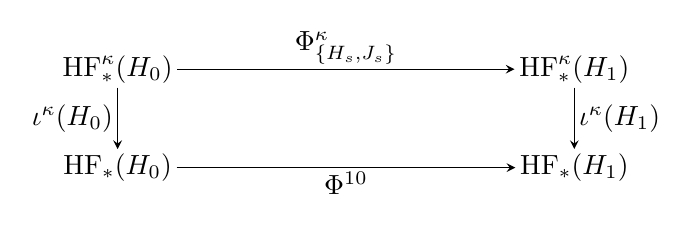
\begin{tikzpicture}[baseline=(current bounding box.center),>=stealth,
  every node/.style={inner sep=1.5pt}]
  \node (a) at (0,1.25) {$\operatorname{HF}_*^\kappa(H_0)$};
  \node (b) at (5.8,1.25) {$\operatorname{HF}_*^\kappa(H_1)$};
  \node (c) at (0,0) {$\operatorname{HF}_*(H_0)$};
  \node (d) at (5.8,0) {$\operatorname{HF}_*(H_1)$};
  \draw[->] (a) -- node[above] {$\Phi^\kappa_{\{H_s,J_s\}}$} (b);
  \draw[->] (a) -- node[left] {$\iota^\kappa(H_0)$} (c);
  \draw[->] (b) -- node[right] {$\iota^\kappa(H_1)$} (d);
  \draw[->] (c) -- node[below] {$\Phi^{10}$} (d);
\end{tikzpicture}
\end{equation}
其中 $\Phi^\kappa_{\{H_s,J_s\}}$ 是\BookRecordIndex{T0240}滤过弗洛尔同调的延拓同构，$\Phi^{10}$ 是典范的
弗洛尔延拓同构。

\paragraph{\BookRecordIndex{T0271}谱不变量。}
\BookRecordIndex{T0240}滤过弗洛尔同调群给出函数
\[
  \rho:\widetilde{\operatorname{Ham}}(M,\omega)
  \times\operatorname{QH}^*(M;\Lambda_\omega)
  \longrightarrow\mathbb R\cup\{-\infty\},
\]
定义为
\begin{equation}\label{eq:12-4-3}
  \rho(\widetilde\phi^H;a)
  :=\inf\bigl\{\kappa\in\mathbb R\setminus\operatorname{Spec}(H)
  \bigm|\Phi_*^{\mathrm{PSS}}(\operatorname{PD}(a))
  \in\operatorname{im}\iota^\kappa(H)\bigr\}.
\end{equation}
这里
\[
  \Phi_*^{\mathrm{PSS}}:
  \operatorname{QH}_*(M;\check\Lambda)
  \longrightarrow\operatorname{HF}_*(H)
\]
表示哈密顿函数 $H$ 的 PSS 同构，而
\[
  \operatorname{PD}:\operatorname{QH}^*(M;\Lambda_\omega)
  \longrightarrow\operatorname{QH}_*(M;\check\Lambda_\omega)
\]
表示注~\ref{rem:11-1-20} 定义的 Poincaré 对偶同构。交换图~\eqref{eq:12-4-2}
表明，数 $\rho(\widetilde\phi;a)$ 与定义它时所用的、满足
$\widetilde\phi^H=\widetilde\phi$ 的哈密顿函数 $H$ 无关。它称为
$\widetilde\phi\in\widetilde{\operatorname{Ham}}(M,\omega)$ 与
$a\in\operatorname{QH}^*(M;\Lambda_\omega)$ 的\emph{\BookRecordIndex{T0271}谱不变量}。

为从几何上理解 $\rho(\widetilde\phi;a)$，假定存在\BookRecordIndex{T0406}正则对 $(H,J)$，使得
$\widetilde\phi=\widetilde\phi^H$。再设
\[
  a=\sum_Aa_A\otimes e^A
  \in\operatorname{QH}^{2n-k}(M;\Lambda_\omega),
\]
其中 $a_A\in H^{2n-k-2c_1(A)}(M)$，并假定每个 $a_A$ 都是定向子流形
$X_A\subset M$（维数为 $k+2c_1(A)$）的基本循环的 Poincaré 对偶。那么 $a$ 的
Poincaré 对偶是\BookRecordIndex{T0230}量子同调类
\[
  \operatorname{PD}(a)=\sum_A[X_A]\otimes e^{-A}
  \in\operatorname{QH}_k(M;\check\Lambda_\omega).
\]
它在 PSS 同构
\[
  \Phi_*^{\mathrm{PSS}}:\operatorname{QH}_k(M;\check\Lambda_\omega)
  \longrightarrow\operatorname{HF}_{k-n}(H,J)
\]
下的像，是链 $\eta:\widetilde{\mathcal P}(H)\to\mathbb Z$ 的\BookRecordIndex{T0132}弗洛尔同调类，其中
\begin{equation}\label{eq:12-4-4}
  \eta(\widetilde y):=\sum_A n\bigl(X_A,(-A)\#\widetilde y\bigr).
\end{equation}
这里 $n(X,\widetilde x)$ 表示满足 $u(0)\in X$、如图~\ref{fig:12-1-1} 所示的\BookRecordIndex{T0182}尖盘
$u\in\mathcal M(\widetilde x;H,J)$ 的带符号计数。注意，数
$n(X_A,(-A)\#\widetilde y)$ 只有在
\[
\begin{aligned}
  n-\mu_{\mathrm{CZ}}(\widetilde y)-2c_1(A)
  &=\dim\mathcal M((-A)\#\widetilde y;H,J)\\
  &=\operatorname{codim}X_A\\
  &=2n-k-2c_1(A)
\end{aligned}
\]
时才可能非零，等价地，$\mu_{\mathrm{CZ}}(\widetilde y)=k-n$。因此，如所预期，
$\eta$ 的\BookRecordIndex{T0132}弗洛尔同调类属于 $\operatorname{HF}_{k-n}(H,J)$。条件
$\kappa\ge\rho(\widetilde\phi^H;a)$ 等价于存在弗洛尔链
$\eta'\in\operatorname{CF}_{k-n}^\kappa(H)$ 和
$\zeta\in\operatorname{CF}_{k-n+1}(H)$，使得 $\eta=\eta'+\partial\zeta$。

\begin{exercise}\label{ex:12-4-3}
证明在交换图~\eqref{eq:12-4-2} 中，只要 $\kappa<\kappa'$，
$\iota^\kappa(H)$ 的像就包含于 $\iota^{\kappa'}(H)$ 的像。因此把
$\rho(\widetilde\phi;a)$ 刻画为 $\operatorname{Spec}(\widetilde\phi)$ 中唯一满足如下
条件的元素：当 $\kappa>\rho(\widetilde\phi;a)$ 时，
$\Phi_*^{\mathrm{PSS}}(\operatorname{PD}(a))\in\operatorname{im}\iota^\kappa(H)$；当
$\kappa<\rho(\widetilde\phi;a)$ 时，
$\Phi_*^{\mathrm{PSS}}(\operatorname{PD}(a))\notin\operatorname{im}\iota^\kappa(H)$。
\end{exercise}

\begin{theorem}[Oh]\label{thm:12-4-4}
设 $(M,\omega)$ 是满足~\eqref{eq:8-5-1} 和~\eqref{eq:12-4-1} 的闭\BookRecordIndex{T0358}辛流形。则下列各项
成立。

\begin{description}
\item[（谱性）] 若 $a\ne0$，则对每个
$\widetilde\phi\in\widetilde{\operatorname{Ham}}(M,\omega)$ 都有
\[
  \rho(\widetilde\phi;a)\in\operatorname{Spec}(\widetilde\phi).
\]

\item[（辛不变性）] 对所有 $\psi\in\operatorname{Symp}(M,\omega)$、
$\widetilde\phi\in\widetilde{\operatorname{Ham}}(M,\omega)$ 以及
$a\in\operatorname{QH}^*(M;\Lambda)$，都有
\[
  \rho(\psi\widetilde\phi\psi^{-1};a)=\rho(\widetilde\phi;a).
\]
\sourcefootnote{原书对任意 $\psi\in\operatorname{Symp}(M,\omega)$ 固定 $a$ 写出此式；
一般的自然性公式还应同时施加 $\psi$ 在\BookRecordIndex{T0229}量子上同调上诱导的作用。因此，原式固定 $a$ 的
版本至少还需假定 $a$ 在该作用下不变；特别地，对
$\psi\in\operatorname{Symp}_0(M,\omega)$（包括下文实际使用的哈密顿情形）这一条件成立。}

\item[（连续性）] 若 $a\ne0$，则映射
\[
  \widetilde{\operatorname{Ham}}(M,\omega)\longrightarrow\mathbb R,
  \qquad \widetilde\phi\longmapsto\rho(\widetilde\phi;a)
\]
关于 $\widetilde{\operatorname{Ham}}(M,\omega)$ 上的 \BookRecordIndex{T0027}Hofer 度量连续。更准确地说，若
$a\ne0$，而 $H_0,H_1\in\mathcal H$ 是分别生成
$\widetilde\phi_0,\widetilde\phi_1\in
\widetilde{\operatorname{Ham}}(M,\omega)$ 的哈密顿函数，则
\begin{equation}\label{eq:12-4-5}
  \int_0^1\min_M(H_{1,t}-H_{0,t})\,dt
  \le\rho(\widetilde\phi_0;a)-\rho(\widetilde\phi_1;a)
  \le\int_0^1\max_M(H_{1,t}-H_{0,t})\,dt.
\end{equation}

\item[（零元）] 若 $0\ne a\in H^*(M)$ 且 $A\in H_2^S(M)$，则
\[
  \rho(\operatorname{id};a\otimes e^A)=\omega(A).
\]

\item[（乘积）] 对所有
$\widetilde\phi,\widetilde\psi\in\widetilde{\operatorname{Ham}}(M,\omega)$ 以及
$a,b\in\operatorname{QH}^*(M;\Lambda_\omega)$，都有
\[
  \rho(\widetilde\phi\widetilde\psi;a*b)
  \le\rho(\widetilde\phi;a)+\rho(\widetilde\psi;b).
\]

\item[（非退化性）] 对每个满足 $\phi\ne\operatorname{id}$ 的
$\phi\in\operatorname{Ham}(M,\omega)$，都存在常数 $\delta>0$，使得对每个
$H\in\mathcal H(M,\omega)$ 都有
\[
  \phi^H=\phi\qquad\Longrightarrow\qquad
  \rho(\widetilde\phi^H;1)+\rho((\widetilde\phi^H)^{-1};1)\ge\delta.
\]
\end{description}
\end{theorem}

\begin{proof}
我们略去“乘积”公理的证明；它本质上与 Schwarz \srcite{360} 给出的证明相同。在
假设~\eqref{eq:12-4-1} 下，我们概述其余公理的证明。一般情形参见 Usher
\srcite{398}。

由定义，每个\BookRecordIndex{T0132}弗洛尔同调类都属于某个 $\kappa$ 所对应映射
\[
  \iota^\kappa(H):\operatorname{HF}_*^\kappa(H,J)
  \longrightarrow\operatorname{HF}_*(H,J)
\]
的像。因此，对每个 $a$ 都有 $\rho(\widetilde\phi;a)<\infty$。若 $a\ne0$，则
$\Phi_*^{\mathrm{PSS}}(\operatorname{PD}(a))$ 非零，因而不可能对每个 $\kappa$ 都属于
$\iota^\kappa(H)$ 的像。（由下面的习题~\ref{ex:12-4-6}，这些像的交为零。）这表明，只要
$a\ne0$，$\rho(\widetilde\phi;a)$ 就是实数。这个数属于
$\widetilde\phi$ 的谱，是因为同态 $\iota^\kappa(H)$ 的像只有在 $\kappa$ 穿过
$\operatorname{Spec}(H)$ 中的元素时才可能改变。这证明了“谱性”公理。“辛不变性”公理
直接由定义得到。

“连续性”公理的证明分两步。关于
$\widetilde{\operatorname{Ham}}(M,\omega)$ 上 $C^1$-范数的连续性来自\BookRecordIndex{T0240}滤过弗洛尔同调的
“同伦性”公理：若 $H\in\mathcal H^\kappa$，而 $H'$ 在 $C^2$-范数下充分接近 $H$，则
$H'\in\mathcal H^\kappa$；事实上，$H'$ 可在 $\mathcal H^\kappa$ 中沿一条道路与 $H$
同伦。因此由交换图~\eqref{eq:12-4-2}，弗洛尔延拓同态
$\operatorname{HF}_*(H)\to\operatorname{HF}_*(H')$ 在
$\operatorname{im}\iota^\kappa(H)$ 与 $\operatorname{im}\iota^\kappa(H')$ 之间诱导同构。
这证明了关于 $C^1$-范数的连续性。

为证明~\eqref{eq:12-4-5}，假定存在\BookRecordIndex{T0088}殆复结构 $J_0,J_1\in\mathcal J$，使得
$(H_0,J_0)$ 与 $(H_1,J_1)$ 是\BookRecordIndex{T0132}弗洛尔同调的\BookRecordIndex{T0406}正则对。再令
$\mathbb R\to\mathcal J:s\mapsto J_s$ 是一条光滑道路，它在 $s\le0$ 时等于 $J_0$，
在 $s\ge1$ 时等于 $J_1$。取光滑\BookRecordIndex{T0188}截断函数 $\beta:\mathbb R\to[0,1]$，满足
\[
  \beta(s)=
  \begin{cases}
    0,&s\le0,\\
    1,&s\ge1,
  \end{cases}
  \qquad \partial_s\beta\ge0,
\]
并定义 $H_{s,t}:M\to\mathbb R$ 为
\[
  H_{s,t}:=\beta(s)H_{1,t}+(1-\beta(s))H_{0,t}.
\]
先假定 $\{H_s,J_s\}$ 是\BookRecordIndex{T0132}弗洛尔同调的\BookRecordIndex{T0407}正则同伦。令
\[
  \kappa>\rho(\widetilde\phi_0;a).
\]
于是存在\BookRecordIndex{T0132}弗洛尔同调循环 $\eta_0\in\operatorname{CF}_*(H_0)$，它代表\BookRecordIndex{T0132}弗洛尔同调类
\[
  \alpha_0:=\Phi_*^{\mathrm{PSS}}(\operatorname{PD}(a))
  \in\operatorname{HF}_*(H_0,J_0),
\]
并且对每个 $\widetilde x_0\in\widetilde{\mathcal P}(H_0)$ 都满足
\[
  \eta_0(\widetilde x_0)\ne0
  \qquad\Longrightarrow\qquad
  \mathcal A_{H_0}(\widetilde x_0)\le\kappa.
\]
对具有相同 Conley--Zehnder 指数的
$\widetilde x_0\in\widetilde{\mathcal P}(H_0)$ 与
$\widetilde x_1\in\widetilde{\mathcal P}(H_1)$，用
$n(\widetilde x_0,\widetilde x_1)$ 表示从 $\widetilde x_0$ 连接到
$\widetilde x_1$ 的方程~\eqref{eq:12-1-10} 之解的带符号计数。定义
$\eta_1\in\operatorname{CF}_*(H_1)$ 为
\[
  \eta_1(\widetilde x_1)
  :=\sum_{\widetilde x_0\in\widetilde{\mathcal P}(H_0)}
  \eta_0(\widetilde x_0)n(\widetilde x_0,\widetilde x_1).
\]
于是 $\eta_1$ 是一个弗洛尔链，代表 $[\eta_0]$ 在弗洛尔延拓同构下的像，即\BookRecordIndex{T0132}弗洛尔同调类
\[
  \alpha_1:=\Phi_*^{\mathrm{PSS}}(\operatorname{PD}(a))
  \in\operatorname{HF}_*(H_1,J_1).
\]
现在，方程~\eqref{eq:12-1-10} 的解所满足的\BookRecordIndex{T0249}能量恒等式~\eqref{eq:12-1-11} 表明，
$n(\widetilde x_0,\widetilde x_1)$ 只有在
\[
\begin{aligned}
  \mathcal A_{H_0}(\widetilde x_0)-\mathcal A_{H_1}(\widetilde x_1)
  &\ge\int_{-\infty}^{\infty}\int_0^1
  \min_M\partial_sH_{s,t}\,dt\,ds\\
  &=\int_0^1\min_M(H_{1,t}-H_{0,t})\,dt
\end{aligned}
\]
时才可能非零。最后一个等号来自同伦 $H_{s,t}$ 的特殊形式。因此，若
$\eta_1(\widetilde x_1)\ne0$，则存在
$\widetilde x_0\in\widetilde{\mathcal P}(H_0)$，使得
$\eta_0(\widetilde x_0)\ne0$ 且
$n(\widetilde x_0,\widetilde x_1)\ne0$，从而
\[
  \mathcal A_{H_1}(\widetilde x_1)
  \le\mathcal A_{H_0}(\widetilde x_0)
  -\int_0^1\min_M(H_{1,t}-H_{0,t})\,dt
  \le\kappa-\int_0^1\min_M(H_{1,t}-H_{0,t})\,dt.
\]
因为 $\eta_1$ 代表\BookRecordIndex{T0132}弗洛尔同调类
$\Phi_*^{\mathrm{PSS}}(\operatorname{PD}(a))\in\operatorname{HF}_*(H_1,J_1)$，故
\[
  \rho(\widetilde\phi_1;a)
  \le\kappa-\int_0^1\min_M(H_{1,t}-H_{0,t})\,dt.
\]
对所有 $\kappa>\rho(\widetilde\phi_0;a)$ 取下确界，得到
\[
  \rho(\widetilde\phi_1;a)
  \le\rho(\widetilde\phi_0;a)
  -\int_0^1\min_M(H_{1,t}-H_{0,t})\,dt.
\]
这在 $\{H_s,J_s\}$ 是\BookRecordIndex{T0407}正则同伦的假设下证明了~\eqref{eq:12-4-5} 的第一个不等式。一般
情形下，在正则端点之间用\BookRecordIndex{T0407}正则同伦逼近 $(H_s,J_s)$，再利用已经证明的如下连续性：在
$\widetilde{\operatorname{Ham}}(M,\omega)$ 上关于 $C^1$-范数连续，相应地在哈密顿函数
空间上关于 $C^2$-范数连续。交换 $H_0$ 与 $H_1$，即可由第一个不等式得到
\eqref{eq:12-4-5} 的第二个不等式。

为证明“零元”公理，可以取一列正则哈密顿函数
$H_i\in\mathcal H(M,\omega)$，使其在 $C^\infty$ 拓扑中收敛到零。于是存在一列
$\varepsilon_i>0$，满足 $\varepsilon_i\to0$，而且下列经补正的包含式成立
\sourcefootnote{原书在中项把 $\iota^\kappa$ 的自变量误印为 $H$；但
$\Psi^{f,H_i}$ 的定义域是 $\operatorname{HF}_*(H_i)$，且本段使用的正则逼近列也是
$H_i$，故唯一应为 $\operatorname{im}\iota^\kappa(H_i)$。}：
\[
  \operatorname{im}\iota^{\kappa-\varepsilon_i}(f)
  \subset\Psi^{f,H_i}\bigl(\operatorname{im}\iota^\kappa(H_i)\bigr)
  \subset\operatorname{im}\iota^{\kappa+\varepsilon_i}(f).
\]
这里采用下面习题~\ref{ex:12-4-6} 的记号。换言之，可以构造这些 PSS 映射，使\BookRecordIndex{T0249}能量
恒等式~\eqref{eq:12-1-14} 中的常数 $c_E$ 任意小。由此可以证明，对每个非零上同调类
$a\in H^*(M)$，$\rho(\widetilde\phi^{H_i};a)$ 都收敛到零。因此，在 $A=0$ 的情形，
“零元”公理由“连续性”公理得出。为证明 $A\ne0$ 的结论，可以使用\BookRecordIndex{T0132}弗洛尔同调在 Novikov
环上的模结构。

下面概述如下事实的证明：对每个满足 $\phi\ne\operatorname{id}$ 的
$\phi\in\operatorname{Ham}(M,\omega)$，存在常数 $\delta>0$，使得对每个
$H\in\mathcal H(M,\omega)$ 都有
\begin{equation}\label{eq:12-4-6}
  \phi^H=\phi\qquad\Longrightarrow\qquad
  \rho(\widetilde\phi^H;1)
  -\rho(\widetilde\phi^H;\operatorname{PD}([\mathrm{pt}]))\ge\delta.
\end{equation}
“非退化性”公理由~\eqref{eq:12-4-6} 和“乘积”公理立即\BookRecordIndex{T0326}推出。事实上，若
$\phi^H=\phi$，则
\[
\begin{aligned}
  \rho(\widetilde\phi^H;1)+\rho((\widetilde\phi^H)^{-1};1)
  &\ge\rho(\widetilde\phi^H;1)
  -\rho(\widetilde\phi^H;\operatorname{PD}([\mathrm{pt}]))
  +\rho(\operatorname{id};\operatorname{PD}([\mathrm{pt}]))\\
  &\ge\delta.
\end{aligned}
\]
第一个不等式来自“乘积”公理，最后一个来自“零元”公理与~\eqref{eq:12-4-6}。

为证明估计~\eqref{eq:12-4-6}，像推论~\ref{cor:9-1-14} 的证明那样定义常数
$\delta$：任取\BookRecordIndex{T0088}殆复结构的光滑族
$\mathbb R\to\mathcal J:t\mapsto\widetilde J_t$，满足
$\widetilde J_{t+1}=\phi^*\widetilde J_t$；取
$x_0\in M\setminus\operatorname{Fix}(\phi)$，对光滑函数
$\widetilde u:\mathbb R^2\to M$ 考虑方程
\begin{equation}\label{eq:12-4-7}
  \partial_s\widetilde u
  +\widetilde J_t(\widetilde u)\partial_t\widetilde u=0,
  \qquad
  \widetilde u(s,t)=\phi(\widetilde u(s,t+1)),
  \qquad
  \widetilde u(0,0)=x_0,
\end{equation}
并定义
\[
  \delta:=\min\bigl\{\min_t\hbar(\widetilde J_t),\delta_0\bigr\},
  \qquad
  \delta_0:=\inf\bigl\{E(\widetilde u)\bigm|
  \widetilde u\text{ 满足~\eqref{eq:12-4-7}},\ E(\widetilde u)<\infty\bigr\}.
\]
这里 $\hbar(\widetilde J_t)$ 表示非常值 $\widetilde J_t$-全纯球面的最小面积。由
命题~\ref{prop:4-1-4} 以及
$\hbar(\widetilde J_{t+1})=\hbar(\widetilde J_t)$，数
$\min_t\hbar(\widetilde J_t)$ 为正。数 $\delta_0$ 的正性来自一个显然的\BookRecordIndex{T0192}紧性论证：若
$\widetilde u_i$ 是~\eqref{eq:12-4-7} 的解且 $E(\widetilde u_i)\to0$，则有一个子列在
紧集上连同所有导数一致收敛到~\eqref{eq:12-4-7} 的解 $\widetilde u$，且
$E(\widetilde u)=0$；任意这样的解都必须形如
$\widetilde u(s,t)\equiv x_0=\phi(x_0)$，这与 $x_0$ 不是 $\phi$ 的不动点矛盾。因此
$\delta>0$。下面证明的一个推论是 $\delta<\infty$；这一点从定义并不明显。（另一种证明
见定理~\ref{thm:9-1-13}。）

取满足 $\phi^H=\phi$ 的 $H\in\mathcal H$，用 $\phi_t$ 表示 $H$ 确定的\BookRecordIndex{T0158}哈密顿同痕，
并由公式 $\phi_t^*J_t:=\widetilde J_t$ 定义 $J_t=J_{t+1}\in\mathcal J$。我们先在如下
假设下证明~\eqref{eq:12-4-6}：$(H,J)$ 是\BookRecordIndex{T0132}弗洛尔同调以及上面所选点 $x_0$ 的\BookRecordIndex{T0406}正则对。
在这个假设下，存在算子
\[
  \Psi_0:\operatorname{HF}_n(H,J)\longrightarrow\operatorname{HF}_{-n}(H,J),
\]
其定义为
\[
  (\Psi_0\eta)(\widetilde y)
  :=\sum_{\mu_{\mathrm{CZ}}(\widetilde x)=n}
  \eta(\widetilde x)n_H(\widetilde x,\widetilde y;x_0),
\]
其中 $n_H(\widetilde x,\widetilde y;x_0)$ 表示从 $\widetilde x$ 到 $\widetilde y$、通过
$x_0$ 的\BookRecordIndex{T0131}弗洛尔连接轨道的带符号计数。因此，
$n_H(\widetilde x,\widetilde y;x_0)$ 计数方程
\begin{equation}\label{eq:12-4-8}
  \partial_su+J_t(u)(\partial_tu-X_{H_t}(u))=0,
  \qquad u(s,t)=u(s,t+1),
  \qquad u(0,0)=x_0
\end{equation}
的解。正如注~\ref{rem:12-3-3} 指出的，
\begin{equation}\label{eq:12-4-9}
  \Psi_0\circ\Phi_*^{\mathrm{PSS}}([M])
  =\Phi_*^{\mathrm{PSS}}([\mathrm{pt}]).
\end{equation}
现在任取实数 $\kappa$，使得
\[
  \kappa\notin\operatorname{Spec}(\widetilde\phi^H),
  \qquad \rho(\widetilde\phi^H;1)<\kappa.
\]
于是存在\BookRecordIndex{T0132}弗洛尔同调循环 $\eta_1\in\operatorname{CF}_n(H)$，满足
$[\eta_1]=\Phi_*^{\mathrm{PSS}}([M])$，并且对每个
$\widetilde x\in\widetilde{\mathcal P}(H)$ 都有
\begin{equation}\label{eq:12-4-10}
  \mathcal A_H(\widetilde x)>\kappa
  \qquad\Longrightarrow\qquad \eta_1(\widetilde x)=0.
\end{equation}
定义 $\eta_0\in\operatorname{CF}_{-n}(H)$ 为
\[
  \eta_0(\widetilde y)
  :=\sum_{\mu_{\mathrm{CZ}}(\widetilde x)=n}
  \eta_1(\widetilde x)n_H(\widetilde x,\widetilde y;x_0).
\]
由~\eqref{eq:12-4-9}，$\eta_0$ 是\BookRecordIndex{T0132}弗洛尔同调循环，且
$[\eta_0]=\Phi_*^{\mathrm{PSS}}([\mathrm{pt}])$。此外，
\[
  \mathcal A_H(\widetilde y)>\kappa-\delta
  \qquad\Longrightarrow\qquad\eta_0(\widetilde y)=0.
\]
为看出这一点，注意~\eqref{eq:12-4-8} 的每个解 $u$ 都等价于
\eqref{eq:12-4-7} 的解
\[
  \widetilde u(s,t):=\phi_t^{-1}(u(s,t)),
\]
因而 $E(u)\ge\delta$。这说明，$\Psi_0(\eta_1)$ 定义中的系数
$n_H(\widetilde x,\widetilde y;x_0)$ 只有在
\[
  \mathcal A_H(\widetilde x)-\mathcal A_H(\widetilde y)\ge\delta
\]
时才可能非零。因此由~\eqref{eq:12-4-10}，$\eta_0(\widetilde y)$ 只有在存在
$\widetilde x\in\widetilde{\mathcal P}(H)$，满足
$\mu_{\mathrm{CZ}}(\widetilde x)=n$、$\eta_1(\widetilde x)\ne0$ 且
\[
  \mathcal A_H(\widetilde y)
  \le\mathcal A_H(\widetilde x)-\delta\le\kappa-\delta
\]
时才可能非零。于是我们证明了\BookRecordIndex{T0132}弗洛尔同调类
$\Phi_*^{\mathrm{PSS}}([\mathrm{pt}])=[\eta_0]$ 属于同态
\[
  \iota^{\kappa-\delta}(H):
  \operatorname{HF}_{-n}^{\kappa-\delta}(H,J)
  \longrightarrow\operatorname{HF}_{-n}(H,J)
\]
的像，因而
\[
  \rho(\widetilde\phi^H;\operatorname{PD}([\mathrm{pt}]))
  \le\kappa-\delta.
\]
这就在 $(H,J)$ 是\BookRecordIndex{T0406}正则对的情形证明了不等式~\eqref{eq:12-4-6}。

为证明一般结论，取一列收敛到 $(H,J)$ 的\BookRecordIndex{T0406}正则对 $(H_i,J_i)$，并用 $\delta_i$ 表示把
上面的 $(\phi,\widetilde J_t)$ 换成 $(\phi_{i1},\phi_{it}^*J_{it})$ 后得到的同一常数；这里
$\phi_{it}$ 表示 $H_i$ 生成的\BookRecordIndex{T0158}哈密顿同痕。我们断言
\begin{equation}\label{eq:12-4-11}
  \liminf_{i\to\infty}\delta_i\ge\delta.
\end{equation}
为此，固定正实数 $\varepsilon<\delta$。必须证明当 $i$ 充分大时
$\varepsilon<\delta_i$。反设不然。必要时取子列，可假定对每个 $i$ 都有
$\delta_i\le\varepsilon$。若存在序列 $i_\nu\to\infty$，使得
$\min_t\hbar(J_{i_\nu t})\le\varepsilon$，则由于
$\phi_{i_\nu t}^*J_{i_\nu t}$ 收敛到 $\widetilde J_t$，由\BookRecordIndex{T0139}格罗莫夫紧性可知
$\min_t\hbar(\widetilde J_t)\le\varepsilon<\delta$，这与 $\delta$ 的定义矛盾。因此，当
$i$ 充分大时必须有 $\min_t\hbar(J_{it})>\varepsilon$。又因为
$\delta_i\le\varepsilon$，存在~\eqref{eq:12-4-7} 的一列解 $\widetilde u_i$（其中把
$\phi$ 换成 $\phi_{i1}$、把 $\widetilde J_t$ 换成 $\phi_{it}^*J_{it}$），使得
$E(\widetilde u_i)\le\varepsilon$。按假设，对每个 $t$ 都有
$\varepsilon<\hbar(\widetilde J_t)$，故不能发生\BookRecordIndex{T0243}冒泡；于是 $\widetilde u_i$ 有一个子列
收敛到~\eqref{eq:12-4-7} 的解 $\widetilde u$。从而
$E(\widetilde u)\le\varepsilon<\delta$，再次与 $\delta$ 的定义矛盾。这就证明了
\eqref{eq:12-4-11}。

由已经证明的特殊情形，对每个 $i$ 都有
\[
  \rho(\widetilde\phi^{H_i};1)
  -\rho(\widetilde\phi^{H_i};\operatorname{PD}([\mathrm{pt}]))
  \ge\delta_i.
\]
令 $i\to\infty$ 并使用~\eqref{eq:12-4-11}，即得估计~\eqref{eq:12-4-6}。
\end{proof}

注意，一般而言，\BookRecordIndex{T0027}Hofer 度量在
$\widetilde{\operatorname{Ham}}(M,\omega)$ 上未必诱导出一个度量：当且仅当哈密顿环路的
每个非平凡同伦类都有正的最小 Hofer 长度时，它才诱导出度量。目前还没有发现支持最小
长度为零的不可缩环路的闭流形。若这样的环路确实存在，则“连续性”公理表明\BookRecordIndex{T0271}谱不变量下降到
$\operatorname{Ham}(M,\omega)$ 的一个更小覆叠空间。

$\rho$ 的“乘积”公理可以解释为\BookRecordIndex{T0271}谱不变量与量子乘法之间的\BookRecordIndex{T0348}相容性。Schwarz
\srcite{360} 首先在\BookRecordIndex{T0355}辛非球面情形注意到这一性质。所有最有趣的应用都以它为基础，例如用
\BookRecordIndex{T0271}谱不变量定义 \BookRecordIndex{T0028}Hofer 范数的类似物（见 Viterbo \srcite{404}、Schwarz \srcite{360}
和 Oh \srcite{307}），以及 Entov--Polterovich 在 \srcite{105} 中构造 Calabi \BookRecordIndex{T0253}拟同态。
这里不尝试解释这些应用。不过，在下面的引理~\ref{lem:12-5-3} 中，我们会描述群
$\pi_1(\operatorname{Ham}(M,\omega))$ 的一个扩张在\BookRecordIndex{T0271}谱不变量上的作用。

\begin{remark}\label{rem:12-4-5}
定理~\ref{thm:12-4-4} 的“辛不变性”公理可以改述为
\[
  \rho(\widetilde\phi\widetilde\psi;a)
  =\rho(\widetilde\psi\widetilde\phi;a)
\]
对所有 $\widetilde\phi,\widetilde\psi\in
\widetilde{\operatorname{Ham}}(M,\omega)$ 成立。为此，回忆习题~\ref{ex:12-4-2}：只要
$\widetilde\psi$ 是 $\psi$ 的提升，就有
$\widetilde\psi\widetilde\phi\widetilde\psi^{-1}
=\psi\widetilde\phi\psi^{-1}$ 于
$\widetilde{\operatorname{Ham}}(M,\omega)$ 中成立。
\end{remark}

\begin{exercise}\label{ex:12-4-6}
证明
\[
  \bigcap_\kappa\operatorname{im}\iota^\kappa(H)=\{0\}.
\]
\BookRecordIndex{T0326}推出对所有 $a\ne0$ 的 $(\widetilde\phi,a)$ 都有
$\rho(\widetilde\phi;a)>-\infty$。

\emph{提示：}以 Novikov 环为系数定义类似的\BookRecordIndex{T0239}滤过 Morse 同调群，并考虑同态
\[
  \iota^\kappa(f):\operatorname{HM}_*^\kappa(f;\Lambda_\omega)
  \longrightarrow\operatorname{HM}_*(f;\Lambda_\omega).
\]
证明
\[
  \bigcap_\kappa\operatorname{im}\iota^\kappa(f)=\{0\}.
\]
现在令
\[
  \Psi^{f,H}:\operatorname{HF}_*(H,J)
  \longrightarrow\operatorname{HM}_*(f;\Lambda_\omega)
\]
为 PSS 同构。利用\BookRecordIndex{T0249}能量恒等式~\eqref{eq:12-1-14} 证明：存在常数 $c>0$，使得对每个
$\kappa\in\mathbb R$ 都有
\[
  \Psi^{f,H}\bigl(\operatorname{im}\iota^\kappa(H)\bigr)
  \subset\operatorname{im}\iota^{\kappa+c}(f).
\]
然后利用如下事实：$\Psi^{f,H}$ 是同构
$\operatorname{QH}_*(M;\check\Lambda)\to
\operatorname{HM}_*(f;\Lambda_\omega)$ 与
$(\Phi_*^{\mathrm{PSS}})^{-1}$ 的复合。
\end{exercise}

\begin{exercise}\label{ex:12-4-7}
对 $\kappa\in(\mathbb R\setminus\operatorname{Spec}(H))\cup\{-\infty\}$，定义\BookRecordIndex{T0239}滤过上链群
\[
  \operatorname{CF}^*_\kappa(H)
  :=\bigl\{\xi\in\operatorname{CF}^*(H)\bigm|
  \xi(\widetilde x)\ne0\Longrightarrow
  \mathcal A_H(\widetilde x)\ge\kappa\bigr\}.
\]
验证弗洛尔上边缘算子 $\delta$ 把 $\operatorname{CF}^*_\kappa(H)$ 映入自身，并由此对
$H\in\mathcal H^\kappa$ 定义\BookRecordIndex{T0239}滤过弗洛尔上同调群
$\operatorname{HF}^*_\kappa(H)$。用
\[
  j_\kappa(H):\operatorname{HF}^*_\kappa(H)
  \longrightarrow\operatorname{QH}^*(M;\Lambda_\omega)
\]
表示同态 $\operatorname{HF}^*_\kappa(H,J)\to\operatorname{HF}^*(H,J)$ 与 PSS 同构
$\operatorname{HF}^*(H,J)\to\operatorname{QH}^*(M;\Lambda_\omega)$ 的复合。证明对每个
$a\in\operatorname{QH}^*(M;\Lambda_\omega)$ 都有
\begin{equation}\label{eq:12-4-12}
  \rho((\widetilde\phi^H)^{-1};a)
  =-\sup\bigl\{\kappa\in\mathbb R\setminus\operatorname{Spec}(H)
  \bigm|a\in\operatorname{im}j_\kappa(H)\bigr\}.
\end{equation}
\end{exercise}

\begin{exercise}\label{ex:12-4-8}
利用定理~\ref{thm:12-4-4} 证明
\[
  d(\phi,\psi)
  :=\inf_{\phi^H=\phi\psi^{-1}}
  \left(\rho(\widetilde\phi^H;1)
  +\rho((\widetilde\phi^H)^{-1};1)\right)
\]
是 $\operatorname{Ham}(M,\omega)$ 上的度量。
\end{exercise}


\section{\BookRecordIndex{T0047}Seidel 表示}\label{sec:12-5}

设 $(M,\omega)$ 是满足强\BookRecordIndex{T0058}半正性条件~\eqref{eq:8-5-1} 的闭\BookRecordIndex{T0358}辛流形，并设
$\psi=\{\psi_t\}_{t\in\mathbb R/\mathbb Z}$ 是 $M$ 的一条\BookRecordIndex{T0161}哈密顿辛微分同胚环路；它由
哈密顿函数
\[
  \mathbb R/\mathbb Z\times M\longrightarrow\mathbb R,
  \qquad(t,x)\longmapsto K_t(x)
\]
通过
\begin{equation}\label{eq:12-5-1}
  \partial_t\psi_t=Y_t\circ\psi_t,
  \qquad \iota(Y_t)\omega=dK_t
\end{equation}
生成。下文将看到，这样的环路自然作用在弗洛尔\BookRecordIndex{T0246}模空间上。不过，要把它提升为弗洛尔
上链复形上的作用，还须选取一种归一化，也就是\BookRecordIndex{T0156}哈密顿纤维化
$\widetilde M_\psi\to S^2$ 的一个截面同伦类 $\tau$。回忆式~\eqref{eq:8-2-6} 及
定理~\ref{thm:11-4-6} 的证明：$\widetilde M_\psi$ 的截面可以由一对光滑映射
$u_\pm:\mathbb C\to M$ 表示，它们对每个
$z=e^{2\pi(s+it)}\in\mathbb C\setminus\{0\}$ 满足
\[
  u_+(z)=\psi_t\bigl(u_-(1/z)\bigr).
\]
在同伦意义下，可以选取这个截面使得 $|z|\leq1$ 时 $u_+(z)\equiv x_0$。于是，$u_-$ 在
$\mathbb C$ 中单位圆盘上的限制是光滑函数
\[
  \tau:B:=\{z\in\mathbb C\mid |z|\leq1\}\longrightarrow M,
\]
并满足
\begin{equation}\label{eq:12-5-2}
  \tau(e^{-2\pi it})=\psi_t^{-1}(x_0),
  \qquad t\in\mathbb R.
\end{equation}
现在说明这样的偶对 $(\psi,\tau)$ 如何决定弗洛尔上同调的一个同构。

这个同构来自弗洛尔方程~\eqref{eq:12-1-3} 的自然性。设 $(H,J)$ 是
命题~\ref{prop:12-1-2} 中的正则偶对，不过现在允许 $J=J_t$ 依赖于 $t$。令
$u:\mathbb R^2\to M$ 是弗洛尔方程
\[
  \partial_su+J_t(u)\bigl(\partial_tu-X_t(u)\bigr)=0
\]
的一个解，其中 $\iota(X_t)\omega=dH_t$，并定义
\[
  v(s,t):=\psi_t^{-1}\bigl(u(s,t)\bigr).
\]
那么 $v$ 是偶对 $(\psi^*H,\psi^*J)$ 的弗洛尔方程之解，这个偶对定义为
\begin{equation}\label{eq:12-5-3}
  (\psi^*H)_t:=(H_t-K_t)\circ\psi_t,
  \qquad
  (\psi^*J)_t:=\psi_t^*J_t.
\end{equation}
此外，当 $s\to\pm\infty$ 时，$v$ 的极限是 $\psi^*H$ 的（可缩）周期轨道。从构造立即
可见，偶对 $(\psi^*H,\psi^*J)$ 满足与 $(H,J)$ 相同的\BookRecordIndex{T0408}正则性假设。因此，沿 $\psi$ 拉回
给出偶对 $(H,J)$ 与 $(\psi^*H,\psi^*J)$ 的\BookRecordIndex{T0131}弗洛尔连接轨道之间的显然一一对应，进而给出
相应 $1$-周期轨道集之间的一一对应。后一个对应是映射
\[
  \mathcal P_0(H)\longrightarrow\mathcal P_0(\psi^*H),
  \qquad x\longmapsto\psi^*x,
\]
其中
\[
  \psi^*x(t):=\psi_t^{-1}(x(t)),
  \qquad t\in\mathbb R.
\]

为了得到弗洛尔上同调的同构，必须选取一个双射
\[
  \widetilde{\mathcal P}(H)\longrightarrow
  \widetilde{\mathcal P}(\psi^*H),
\]
使它下降为双射 $\mathcal P_0(H)\to\mathcal P_0(\psi^*H)$，并且关于 $H_2^S(M)$ 的
作用等变。这样的双射有许多个，每一个都给出一个弗洛尔上同调同构；截面 $\tau$ 则提供
一个典范选择。为看清这一点，注意每个 $\widetilde x\in\widetilde{\mathcal P}(H)$ 都可
由偶对 $(x,u)$ 表示，并使得 $|z|\leq1/2$ 时 $u(z)=x_0$。定义
\[
  (\psi,\tau)^*\widetilde x
  \in\widetilde{\mathcal P}(\psi^*H)
  \sourcefootnote{原书把这里的陪域印作尚未定义的
  $\widetilde{\mathcal P}(H^\alpha)$；同页前后的双射与映射均明确给出陪域
  $\widetilde{\mathcal P}(\psi^*H)$，故据此补正。}
\]
为
\[
  (\psi,\tau)^*\widetilde x
  :=\bigl(\psi^*x,(\psi,\tau)^*u\bigr),
\]
其中
\[
  ((\psi,\tau)^*u)(re^{2\pi it}):=
  \begin{cases}
    \psi_t^{-1}\bigl(u(re^{2\pi it})\bigr),&1/2\leq r\leq1,\\
    \tau(2re^{-2\pi it}),&0\leq r\leq1/2.
  \end{cases}
\]
注意，映射
\[
  \widetilde{\mathcal P}(H)\longrightarrow
  \widetilde{\mathcal P}(\psi^*H),
  \qquad
  \widetilde x\longmapsto(\psi,\tau)^*\widetilde x
\]
关于 $H_2^S(M)$ 的作用等变。

\begin{exercise}\label{ex:12-5-1}
证明：对 $A\in H_2^S(M)$，有
\[
  (\psi,\tau)^*(A\#\widetilde x)
  =(\psi,\tau-\iota_*A)^*\widetilde x,
\]
并且
\[
  \mu_{\mathrm{CZ}}\bigl((\psi,\tau)^*\widetilde x\bigr)
  =\mu_{\mathrm{CZ}}(\widetilde x)+2c(\tau),
  \qquad
  \mathcal A_{\psi^*H}\bigl((\psi,\tau)^*\widetilde x\bigr)
  =\mathcal A_H(\widetilde x)+\widetilde\omega_\psi(\tau).
\]
这里
\[
  c:=c_1^{\mathrm{Vert}}\in H^2(\widetilde M_\psi)
\]
表示竖直第一 Chern 类，而
$\widetilde\omega_\psi\in\Omega^2(\widetilde M_\psi)$ 是一个\BookRecordIndex{T0155}哈密顿联络的\BookRecordIndex{T0260}耦合形式。
\end{exercise}

弗洛尔上链复形之间有一个同构
\[
  \mathcal S(\psi,\tau;H):
  \operatorname{CF}^*(H)\longrightarrow\operatorname{CF}^*(\psi^*H),
\]
定义为
\[
  \bigl(\mathcal S(\psi,\tau;H)\xi\bigr)
  \bigl((\psi,\tau)^*\widetilde x\bigr):=\xi(\widetilde x),
\]
其中 $\xi\in\operatorname{CF}^*(H)$、
$\widetilde x\in\widetilde{\mathcal P}(H)$。只要 $(H,J)$ 是命题~\ref{prop:12-1-2}
中的正则偶对，它就在弗洛尔上同调上诱导一个同构
\[
  \mathcal S(\psi,\tau;H,J):
  \operatorname{HF}^*(H,J)
  \longrightarrow
  \operatorname{HF}^*(\psi^*H,\psi^*J).
\]
所需的自同构
\[
  \mathcal S^{H,J}(\psi,\tau):
  \operatorname{HF}^*(H,J)\longrightarrow\operatorname{HF}^*(H,J)
\]
是同构 $\mathcal S(\psi,\tau;H,J)$（可以把它看作一次“扭曲”）与
定理~\ref{thm:12-1-3} 的延拓同构
\[
  \operatorname{HF}^*(\psi^*H,\psi^*J)
  \longrightarrow\operatorname{HF}^*(H,J)
\]
的复合。

沿用第~\ref{sec:12-1} 节的记号，简写
$\mathcal S^\alpha:=\mathcal S^{H^\alpha,J^\alpha}$。从构造显然可见，Seidel 同态关于
定理~\ref{thm:12-1-3} 的延拓同构是自然的，即
\[
  \mathcal S^\beta(\psi,\tau)\circ\Phi^{\beta\alpha}
  =\Phi^{\beta\alpha}\circ\mathcal S^\alpha(\psi,\tau)
\]
对所有 $\alpha,\beta$ 都成立；而且这确实是一个表示，也就是说
\[
  \mathcal S^\alpha(\phi,\sigma)\circ\mathcal S^\alpha(\psi,\tau)
  =\mathcal S^\alpha(\phi\psi,\sigma\#\tau)
\]
对任意两条哈密顿环路 $\phi,\psi$ 及其相应截面 $\sigma,\tau$ 都成立。我们把两个截面的
\BookRecordIndex{T0227}连通和 $\sigma\#\tau$ 的确切含义留给读者写出。关于这个运算，偶对 $(\phi,\sigma)$ 的
同伦类构成一个群 $\widetilde G$；它是
$G:=\pi_1(\operatorname{Ham}(M,\omega))$ 被环路空间 $\mathcal L M$ 的甲板变换群
$H_2^S(M)$ 扩张所得的群。\footnote{这里应把 $H_2^S(M)$ 理解为 Hurewicz 同态在无挠群
$H_2(M;\mathbb Z)/\operatorname{tor}$ 中的像；见注~\ref{rem:12-5-4}。}
赋值
\[
  (\phi,\sigma)\longmapsto\mathcal S^{H,J}(\phi,\sigma)
\]
定义了 $\widetilde G$ 在弗洛尔上同调这个 $\Lambda$-模的同构空间上的表示。Seidel 证明，
这些同构 $\mathcal S(\phi,\sigma)$ 保持
$\operatorname{HF}^*(H,J)$ 的右 $\operatorname{HF}^*(H,J)$-模结构，即
\[
  \mathcal S^{H,J}(\phi,\sigma)(a*b)
  =\bigl(\mathcal S^{H,J}(\phi,\sigma)a\bigr)*b
\]
对所有 $a,b\in\operatorname{HF}^*(H,J)$ 成立。从这个观点看，困难之处是证明弗洛尔
上同调上的 \BookRecordIndex{T0047}Seidel 表示，在定理~\ref{thm:12-1-4} 的同构下与\BookRecordIndex{T0229}量子上同调上的 \BookRecordIndex{T0047}Seidel 表示
一致。这正是下面定理的内容。

\begin{theorem}[Seidel]\label{thm:12-5-2}
设 $(M,\omega)$ 满足~\eqref{eq:8-5-1}。那么，对每个正则偶对
$(H^\alpha,J^\alpha)$、每条哈密顿环路 $\psi$ 以及每个相应截面 $\tau$，都有
\[
  \mathcal S(\psi,\tau)*(\Phi^\alpha\xi^\alpha)
  =\Phi^\alpha\bigl(\mathcal S^\alpha(\psi,\tau)\xi^\alpha\bigr)
\]
对每个 $\xi^\alpha\in\operatorname{HF}^*(H^\alpha,J^\alpha)$ 成立。这里
\[
  \Phi^\alpha:
  \operatorname{HF}^*(H^\alpha,J^\alpha)
  \longrightarrow\operatorname{QH}^*(M;\Lambda_\omega)
\]
是定理~\ref{thm:12-1-4} 的 PSS 同构，而
$\mathcal S(\psi,\tau)\in\operatorname{QH}^*(M;\Lambda_\omega)$ 是
第~\ref{sec:11-4} 节定义的 \BookRecordIndex{T0046}Seidel 元。
\end{theorem}

定理~\ref{thm:12-5-2} 的证明运用了注~\ref{rem:12-1-7} 中描述的思想。Seidel 同态
$\mathcal S^\alpha(\psi,\tau)$
\sourcefootnote{原书在这里把 $\mathcal S^\alpha(\psi,\tau)$ 称为 \BookRecordIndex{T0046}Seidel 元；但前文已将它
定义为弗洛尔上同调上的 Seidel 同态，而本定理中的量子 \BookRecordIndex{T0046}Seidel 元是不带 $\alpha$ 的
$\mathcal S(\psi,\tau)$，故据此改正对象名称。}
计数依赖于 $s$ 的弗洛尔方程之解，而 $\Phi^\alpha$ 计数\BookRecordIndex{T0182}尖盘。通过把两个\BookRecordIndex{T0182}尖盘
粘到一个弗洛尔圆柱的两端，可以得到定理~\ref{thm:12-5-2} 的关系；这样便构造出\BookRecordIndex{T0156}哈密顿
纤维化 $\widetilde M_\psi\to S^2$ 的一个 $J$-全纯截面。细节见 Seidel 
\srcite{363}。

\begin{lemma}\label{lem:12-5-3}
设
\[
  \mathbb R/\mathbb Z\longrightarrow\operatorname{Ham}(M,\omega),
  \qquad t\longmapsto\psi_t
\]
是满足 $\psi_0=\operatorname{id}$ 的一条\BookRecordIndex{T0161}哈密顿辛微分同胚环路，$\tau$ 是
$\widetilde M_\psi$ 的一个截面同伦类。设
$\widetilde\phi\in\widetilde{\operatorname{Ham}}(M,\omega)$ 是一条满足
$\phi_0=\operatorname{id}$ 的道路
\[
  [0,1]\longrightarrow\operatorname{Ham}(M,\omega),
  \qquad t\longmapsto\phi_t,
\]
的等价类。那么，对每个
$a\in\operatorname{QH}^*(M;\Lambda_\omega)$，都有
\[
  \rho(\psi^*\widetilde\phi;a)
  =\rho\bigl(\widetilde\phi;\mathcal S(\psi,\tau)a\bigr)
   +\widetilde\omega_\psi(\tau),
\]
其中 $\psi^*\widetilde\phi$ 表示道路
$t\mapsto\psi_t^{-1}\circ\phi_t$ 的等价类。
\end{lemma}

\begin{proof}
使用习题~\ref{ex:12-4-7} 中\BookRecordIndex{T0271}谱不变量的上同调描述。固定一个生成
$\widetilde\phi$ 的哈密顿函数
$H:\mathbb R/\mathbb Z\times M\to\mathbb R$。按构造，上面得到的同态
\[
  \mathcal S(\psi,\tau;H,J):
  \operatorname{HF}^*(H,J)
  \longrightarrow
  \operatorname{HF}^*(\psi^*H,\psi^*J)
\]
把 $\operatorname{HF}_\kappa^*(H,J)$ 同构地映到
$\operatorname{HF}_{\kappa+\widetilde\omega_\psi(\tau)}^*
(\psi^*H,\psi^*J)$。所以有交换图
\[
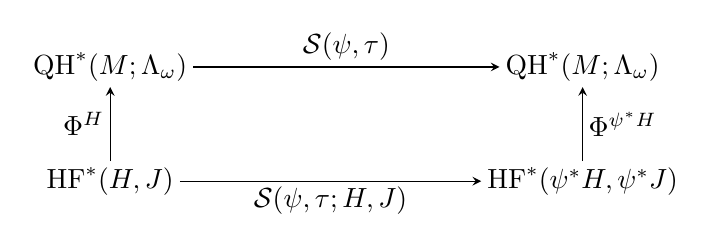
\begin{tikzpicture}[baseline=(current bounding box.center),>=stealth,
  every node/.style={inner sep=2pt}]
  \node (q1) at (0,1.45) {$\operatorname{QH}^*(M;\Lambda_\omega)$};
  \node (q2) at (6.0,1.45) {$\operatorname{QH}^*(M;\Lambda_\omega)$};
  \node (h1) at (0,0) {$\operatorname{HF}^*(H,J)$};
  \node (h2) at (6.0,0) {$\operatorname{HF}^*(\psi^*H,\psi^*J)$};
  \draw[->] (q1) -- node[above] {$\mathcal S(\psi,\tau)$} (q2);
  \draw[->] (h1) -- node[below] {$\mathcal S(\psi,\tau;H,J)$} (h2);
  \draw[->] (h1) -- node[left] {$\Phi^H$} (q1);
  \draw[->] (h2) -- node[right] {$\Phi^{\psi^*H}$} (q2);
\end{tikzpicture}
\]
其中上方水平箭头把 $j_\kappa(H)$ 的像同构地映到
$j_{\kappa+\widetilde\omega_\psi(\tau)}(\psi^*H)$ 的像。

现在令 $\kappa\in\mathbb R\setminus\operatorname{Spec}(H)$。由
习题~\ref{ex:12-5-1}，有
$\kappa+\widetilde\omega_\psi(\tau)\notin\operatorname{Spec}(\psi^*H)$。此外，由
习题~\ref{ex:12-4-7}，
\[
\begin{aligned}
  \kappa<-\rho(\widetilde\phi^{-1};a)
  &\quad\Longleftrightarrow\quad
  a\in\operatorname{im}j_\kappa(H)\\
  &\quad\Longleftrightarrow\quad
  \mathcal S(\psi,\tau)a
  \in\operatorname{im}j_{\kappa+\widetilde\omega_\psi(\tau)}(\psi^*H)\\
  &\quad\Longleftrightarrow\quad
  \kappa+\widetilde\omega_\psi(\tau)
  <-\rho\bigl((\psi^*\widetilde\phi)^{-1};
  \mathcal S(\psi,\tau)a\bigr).
\end{aligned}
\]
第二个等价关系来自上面的交换图，最后一个等价关系再次来自
习题~\ref{ex:12-4-7}。因此
\[
  \rho(\widetilde\phi^{-1};a)
  =\rho\bigl((\psi^*\widetilde\phi)^{-1};
  \mathcal S(\psi,\tau)a\bigr)
   +\widetilde\omega_\psi(\tau).
\]
把道路 $t\mapsto\phi_t$ 换成 $t\mapsto\phi_t^{-1}\circ\psi_t$，即得所断言的公式。
\end{proof}

Oh \srcite{306} 把 Seidel 作用下\BookRecordIndex{T0271}谱不变量的平移称为\emph{\BookRecordIndex{T0096}单值化平移}。使用系数环
\[
  \Lambda:=\Lambda^{\mathrm{univ}}[q,q^{-1}]
\]
时，可以通过把 $\tau$ 的选取标准化为 $\widetilde\omega_\psi(\tau)=0$ 来消去\BookRecordIndex{T0096}单值化平移
（见 Lalonde--McDuff--Polterovich \srcite{228}）。即便如此，如果\BookRecordIndex{T0229}量子上同调上的 Seidel
作用对某个流形非平凡，那么\BookRecordIndex{T0271}谱不变量所含信息仍只有不变部分才能下降到
$\operatorname{Ham}(M)$。下文注~\ref{rem:12-5-5} 将作更完整的解释；下一条注先给出
\BookRecordIndex{T0096}单值化平移的整体框架。

\begin{remark}[\BookRecordIndex{T0271}谱不变量：整体观点]\label{rem:12-5-4}
先构造一个以 $\operatorname{Ham}(M,\omega)$ 为底的纤维空间
$P\operatorname{Ham}(M,\omega)$，它的基本群是上面考虑的扩张 $\widetilde G$。为简单起见，
以下假设 $M$ 单连通且 $\pi_2(M)$ 无挠；于是 $\widetilde G$ 是 $G$ 被整个群
\[
  \pi_1(\mathcal L M)\cong\pi_2(M)
\]
扩张所得的群，而不是被其商群 $H_2^S(M)$ 扩张所得的群。

固定基点 $x_0\in M$，以 $P_0M$ 表示从 $\gamma(0)=x_0$ 出发的光滑道路
$\gamma:[0,1]\to M$ 所成的空间。记
\[
  P\operatorname{Ham}(M,\omega)
  \subset\operatorname{Ham}(M,\omega)\times P_0M
\]
为满足 $\gamma(1)=\phi^{-1}(x_0)$ 的偶对 $(\phi,\gamma)$ 所成的空间。有一个\BookRecordIndex{T0279}纤维化
\[
  \Omega M\longrightarrow P\operatorname{Ham}(M,\omega)
  \longrightarrow\operatorname{Ham}(M,\omega),
\]
其纤维是 $M$ 的基环路空间 $\Omega M$。同伦正合列中的\BookRecordIndex{T0063}边界映射
\[
  \pi_2(\operatorname{Ham}(M,\omega))
  \longrightarrow\pi_1(\Omega M)\cong\pi_2(M)
\]
由在基点处求值给出。众所周知，它的像由挠类组成（例如见 \srcite{227}）。所以，对 $M$
的假设蕴含这个映射为零。因而 $\pi_1(P\operatorname{Ham}(M,\omega))$ 是 $G$ 被
$\pi_2(M)$ 扩张所得的群，并且由式~\eqref{eq:12-5-2}，它同构于 $\widetilde G$。具体地，
每个偶对 $(\psi,\tau)$ 通过
\[
  \gamma_t(s):=\tau(se^{-2\pi it})
\]
决定一条环路
\[
  \mathbb R/\mathbb Z\longrightarrow P\operatorname{Ham}(M,\omega),
  \qquad t\longmapsto(\psi_t,\gamma_t),
\]
并由此诱导所需同构
$\widetilde G\to\pi_1(P\operatorname{Ham}(M,\omega))$。

把 $P\operatorname{Ham}(M,\omega)$ 的万有覆盖记作
$\widetilde{P\operatorname{Ham}}(M,\omega)$。它的元素是
$P\operatorname{Ham}(M,\omega)$ 中道路 $(\phi_t,\gamma_t)_{t\in[0,1]}$ 的等价类
$[\widetilde\phi,\widetilde\gamma]$，其中 $\phi_0=\operatorname{id}$，且 $\gamma_0$ 是
常值道路。群 $\widetilde G$ 以甲板变换作用在
$\widetilde{P\operatorname{Ham}}(M,\omega)$ 上：若 $(\psi,\tau)$ 代表
$\widetilde G$ 的一个元素，而 $[\widetilde\phi,\widetilde\gamma]$ 是
$\widetilde{P\operatorname{Ham}}(M,\omega)$ 中的等价类，则
$(\psi,\tau)\cdot[\widetilde\phi,\widetilde\gamma]$ 表示如下道路的等价类：先沿
$\psi,\tau$ 所确定的 $P\operatorname{Ham}(M,\omega)$ 中环路绕行一周，再沿道路
$(\phi_t,\gamma_t)$ 前进。

考察平凡线丛
\[
  \widetilde{P\operatorname{Ham}}(M,\omega)
  \times\operatorname{QH}^*(M;\Lambda)\times\mathbb R
  \longrightarrow
  \widetilde{P\operatorname{Ham}}(M,\omega)
  \times\operatorname{QH}^*(M;\Lambda).
\]
群 $\widetilde G$ 作用在这个线丛上：它在
$\widetilde{P\operatorname{Ham}}(M,\omega)$ 上作甲板变换，在\BookRecordIndex{T0229}量子上同调上作 \BookRecordIndex{T0047}Seidel
表示，在 $\mathbb R$ 上作\BookRecordIndex{T0096}单值化平移。更确切地，
\[
  (\psi,\tau)\cdot
  \bigl([\widetilde\phi,\widetilde\gamma];a;\kappa\bigr)
  =\bigl((\psi,\tau)\cdot[\widetilde\phi,\widetilde\gamma];
  \mathcal S(\psi,\tau)a;
  \kappa+\widetilde\omega_\psi(\tau)\bigr).
\]
引理~\ref{lem:12-5-3} 断言，\BookRecordIndex{T0271}谱不变量定义了这个丛的一个 $\widetilde G$-等变截面
\[
  \rho:
  \widetilde{P\operatorname{Ham}}(M,\omega)
  \times\operatorname{QH}^*(M;\Lambda)
  \longrightarrow
  \widetilde{P\operatorname{Ham}}(M,\omega)
  \times\operatorname{QH}^*(M;\Lambda)\times\mathbb R.
\]
对 $\widetilde G$ 取商后，得到相应实线丛 $L\to X$ 的一个截面；这里 $X$ 是\BookRecordIndex{T0279}纤维化
\[
  \operatorname{QH}^*(M;\Lambda)
  \longrightarrow
  X:=\widetilde{P\operatorname{Ham}}(M,\omega)
  \times_{\widetilde G}\operatorname{QH}^*(M;\Lambda)
  \longrightarrow P\operatorname{Ham}(M)
\]
的总空间。

谱值也有类似图景。由习题~\ref{ex:12-5-1}，$\widetilde G$ 在
$\widetilde{P\operatorname{Ham}}(M,\omega)\times\mathbb R$ 上的作用保持谱值子集
\[
  \mathfrak{spec}:=
  \bigl\{([\widetilde\phi,\widetilde\gamma],c)
  \in\widetilde{P\operatorname{Ham}}(M,\omega)\times\mathbb R
  \bigm|c\in\operatorname{Spec}(\widetilde\phi)\bigr\}.
\]
所以商 $\mathfrak{spec}/\widetilde G$ 是实线丛
\[
  L:=\widetilde{P\operatorname{Ham}}(M,\omega)
  \times_{\widetilde G}\mathbb R
  \longrightarrow P\operatorname{Ham}(M,\omega)
\]
的一个子集。
\end{remark}

\begin{remark}\label{rem:12-5-5}
弗洛尔（上）同调的定义有许多可能变体。下一节将为任意辛微分同胚 $\phi$ 定义精简版本
$\operatorname{HF}^*(\phi)$；作为引入，这里先简述其中两种变体。

\begin{enumerate}[label=(\roman*)]
\item 首先考虑以例~\ref{ex:11-1-4}(vi) 的环
\[
  \Lambda:=\Lambda^{\mathrm{univ}}[q,q^{-1}]
\]
为系数的弗洛尔上同调，其中基环为 $R$。在此情形，对每个正则哈密顿量 $H$，弗洛尔
上链复形 $\operatorname{CF}^*(H;\Lambda)$ 是所有函数
\[
  \xi:\widetilde{\mathcal P}(H)\longrightarrow\Lambda
\]
之集，它们在如下意义下等变：
\begin{equation}\label{eq:12-5-4}
  \xi(A\#\widetilde x)
  =\xi(\widetilde x)t^{\omega(A)}q^{c_1(A)}.
\end{equation}
这对每个 $\widetilde x\in\widetilde{\mathcal P}(H)$ 和每个
$A\in H_2^S(M)$
\sourcefootnote{原书把这里的量词印作 $A\in H_2(M)$；但
$A\#\widetilde x$ 只对第~\ref{sec:12-1} 节定义的甲板变换群 $H_2^S(M)$ 有定义，且本段
前后均使用该群，故补正。}
成立。这是有限生成自由 $\Lambda$-模。元素
$\xi\in\operatorname{CF}^*(H;\Lambda)$ 的次数为 $k$，当且仅当
$\xi(\widetilde x)$ 具有纯次数，并且
\[
  \mu_{\mathrm{CZ}}(\widetilde x)
  +\deg\bigl(\xi(\widetilde x)\bigr)=k
\]
对每个 $\widetilde x\in\widetilde{\mathcal P}(H)$ 成立。弗洛尔上边缘算子仍由
式~\eqref{eq:12-1-9} 定义；容易验证，只要 $\xi$ 满足~\eqref{eq:12-5-4}，
$\delta\xi$ 也满足该式。读者可以验证，$\delta\xi$ 的确是一个定义在
$\widetilde{\mathcal P}(H)$ 上、取值于 $\Lambda$ 的函数。第~\ref{sec:12-1}、
\ref{sec:12-2} 节的全部讨论都适用于这个弗洛尔上同调定义。

现在令 $t\mapsto\psi_t=\psi_{t+1}$ 是一条\BookRecordIndex{T0161}哈密顿辛微分同胚环路，并设哈密顿函数族
$K_t=K_{t+1}:M\to\mathbb R$ 通过式~\eqref{eq:12-5-1} 生成它。固定正则偶对 $(H,J)$，
并由~\eqref{eq:12-5-3} 定义 $(\psi^*H,\psi^*J)$。这条哈密顿环路诱导\BookRecordIndex{T0259}扭曲算子
\[
  \mathcal S(\psi;H,J):
  \operatorname{HF}^*(H,J)
  \longrightarrow\operatorname{HF}^*(\psi^*H,\psi^*J).
\]
在上链\BookRecordIndex{T0072}层次，它定义为
\[
  \bigl(\mathcal S(\psi;H,J)\xi\bigr)
  \bigl((\psi,\tau)^*\widetilde x\bigr)
  :=\xi(\widetilde x)
  t^{-\widetilde\omega_\psi(\tau)}q^{-c(\tau)},
\]
其中 $\xi\in\operatorname{CF}^*(H;\Lambda)$、
$\widetilde x\in\widetilde{\mathcal P}(H)$，而 $\tau$ 是 $\widetilde M_\psi$ 的任意截面。
由习题~\ref{ex:12-5-1} 和式~\eqref{eq:12-5-4}，右端与 $\tau$ 的选择无关。与前面相同，
$\mathcal S(\psi;H,J)$ 下降为弗洛尔上同调上的良定义同构，再经延拓诱导自同构
\[
  \mathcal S^{H,J}(\psi):
  \operatorname{HF}^*(H,J)\longrightarrow\operatorname{HF}^*(H,J).
\]
归根结底，我们得到 $G=\pi_1(\operatorname{Ham}(M,\omega))$ 在弗洛尔上同调上的一个表示。

\item 如果愿意使用模 $2$ 分次，就可以在上述讨论中令 $q=1$；这样得到的弗洛尔上同调群
以\BookRecordIndex{T0270}普适 Novikov 环 $\Lambda^{\mathrm{univ}}$ 为系数，并带模 $2$ 分次。此时弗洛尔上链复形
是所有满足
\[
  \xi(A\#\widetilde x)=\xi(\widetilde x)t^{\omega(A)}
\]
的函数 $\xi:\widetilde{\mathcal P}(H)\to\Lambda^{\mathrm{univ}}$ 所成的集合。这意味着映射
\[
  \widetilde x\longmapsto
  \xi(\widetilde x)t^{\mathcal A_H(\widetilde x)}
\]
在 $H_2^S(M)$ 的作用下不变，因而下降为从 $\mathcal P_0(H)$ 到
$\Lambda^{\mathrm{univ}}$ 的映射。所以弗洛尔上链复形是 $\Lambda^{\mathrm{univ}}$-模
\[
  \operatorname{CF}^*(H):=
  \operatorname{CF}^*(H;\Lambda^{\mathrm{univ}})
  =\operatorname{Map}\bigl(\mathcal P_0(H),\Lambda^{\mathrm{univ}}\bigr),
\]
而弗洛尔上边缘为
\[
  (\delta\xi)(x):=
  \sum_y\sum_\varepsilon n_\varepsilon(x,y)\xi(y)t^\varepsilon.
\]
这里 $n_\varepsilon(x,y)$ 表示能量 $E(u)=\varepsilon$、从 $x$ 到 $y$ 的指标为一的\BookRecordIndex{T0131}弗洛尔
连接轨道之带符号数。现在 \BookRecordIndex{T0047}Seidel 表示由
\[
  \bigl(\mathcal S(\psi;H)\xi\bigr)(\psi^*x):=\xi(x)
\]
给出，其中 $x\in\mathcal P_0(H)$、$\xi\in\operatorname{CF}^*(H)$。

事实表明，这个复形不保留生成哈密顿量 $H$ 的任何本质信息，完全可以只用时间一映射
$\phi\in\operatorname{Ham}(M,\omega)$ 来定义。不过，若这样做，则从
$\operatorname{HF}^*(\phi_0)$ 到 $\operatorname{HF}^*(\phi_1)$ 的\BookRecordIndex{T0133}弗洛尔延拓映射，一般
依赖于定义它的道路 $\phi_s$ 的同伦类。（这一依赖恰由 \BookRecordIndex{T0047}Seidel 表示度量。）此外，即使
$\phi$ 不是哈密顿的，这个定义仍然成立。于是我们自然走向下一节所讨论的、基础宽广得多的
弗洛尔理论。
\end{enumerate}
\end{remark}


\section{Donaldson 的量子范畴}\label{sec:12-6}

\paragraph{辛微分同胚。}
研究\BookRecordIndex{T0229}量子上同调的\BookRecordIndex{T0132}弗洛尔同调方法可以沿两个方向推广。为简单起见，假设\BookRecordIndex{T0358}辛流形
$(M,\omega)$ 紧、单连通且单调。此时由式~\eqref{eq:12-1-2} 和
\eqref{eq:12-1-6}，\BookRecordIndex{T0131}弗洛尔连接轨道的能量由其指标控制（比较例~\ref{ex:8-6-8}）。所以
不必使用 Novikov 环，而可以用整数系数定义弗洛尔上同调群。代价是这些群现在只带模
$2N$ 分次，其中 $N$ 是最小 Chern 数。事实上，把分次约化为模 $2$ 很有用，这样便无须
为归一化分次作额外选择。归根结底，对每个辛微分同胚 $\phi$，都可以定义一个带模 $2$
分次的弗洛尔上同调群 $\operatorname{HF}^*(\phi)$，其 Euler 示性数
\[
  \chi\bigl(\operatorname{HF}^*(\phi)\bigr)=L(\phi)
\]
是 $\phi$ 的 \BookRecordIndex{T0032}Lefschetz 数。

生成弗洛尔复形的\BookRecordIndex{T0233}临界点现在是 $\phi$ 的不动点；假设它们都非退化。连接轨道则是满足
\[
  \phi(u(s,1))=u(s,0),\qquad s\in\mathbb R,
\]
的 $J$-全纯映射 $u:\mathbb R\times[0,1]\to M$。可以把它们看作辛纤维丛
\[
  P\longrightarrow\mathbb R\times S^1
\]
的 $J$-全纯截面；该丛以 $M$ 为纤维，绕 $S^1$ 的\BookRecordIndex{T0164}和乐为 $\phi$。若有退化不动点，就必须
像第~\ref{sec:12-1} 节那样选取\BookRecordIndex{T0157}哈密顿扰动。所得弗洛尔上同调群与定义时所用的\BookRecordIndex{T0157}哈密顿扰动
和\BookRecordIndex{T0088}殆复结构无关。（更多细节见 Floer \srcite{116}、Floer--Hofer--Salamon
\srcite{119} 与 Dostoglou--Salamon \srcite{90}。）由于 $M$ 单连通，每条\BookRecordIndex{T0361}辛同痕
$\{\phi_s\}_{0\leq s\leq1}$ 都决定一个同构
\[
  \operatorname{HF}^*(\phi_0)\longrightarrow\operatorname{HF}^*(\phi_1).
\]
正如注~\ref{rem:12-5-5} 所指出的，这个同构一般依赖于\BookRecordIndex{T0361}辛同痕的同伦类。对任意两个辛
微分同胚 $\phi,\psi$，还有自然同构
\[
  \operatorname{HF}^*(\phi)
  \longrightarrow
  \operatorname{HF}^*(\psi\circ\phi\circ\psi^{-1}).
\]
此外，按照 Donaldson 的说法，还存在形变\BookRecordIndex{T0228}量子杯积的类似物，即一个斜对称且结合的配对
\[
  \operatorname{HF}^*(\phi)\otimes\operatorname{HF}^*(\psi)
  \longrightarrow
  \operatorname{HF}^*(\psi\circ\phi).
\]
它可以用辛纤维丛 $P\to S$ 的 $J$-全纯截面定义，其中 $P$ 的纤维为 $M$，而 $S$ 是一个
带三个穿孔的二维球面；绕这三个穿孔的\BookRecordIndex{T0164}和乐分别共轭于
$\phi,\psi,\psi\circ\phi$。这个乘积结构可以解释为一个范畴：对象是 $M$ 的辛微分同胚，
从 $\phi$ 到 $\psi$ 的态射是弗洛尔上同调群
\[
  \operatorname{HF}^*(\psi\circ\phi^{-1})
\]
的元素，两个态射的复合由量子积给出。

现在取 $\psi=\operatorname{id}$。由第~\ref{sec:12-1} 节的讨论，在单调情形，弗洛尔
上同调群同构于通常上同调群：
\[
  \operatorname{HF}^*(\operatorname{id})
  =\operatorname{QH}^*(M)=H^*(M),
\]
其中分次以 $2$ 为周期。所以 $M$ 的上同调作用在 $\phi$ 的弗洛尔上同调上：
\[
  H^*(M)\otimes\operatorname{HF}^*(\phi)
  \longrightarrow\operatorname{HF}^*(\phi).
\]
在这种情形，还可以用另一种方式理解量子积结构。具体地，可以用余维 $k$ 的子流形（或
\BookRecordIndex{T0337}伪循环）$V\subset M$ 表示一个次数为 $k$ 的上同调类，再让 $V$ 与构造
$\phi$ 的弗洛尔上同调群时出现的连接轨道空间相交。更一般地，可以让这些连接轨道空间与
道路空间
\[
  \Omega_\phi:=\{\gamma:[0,1]\to M\mid \phi(\gamma(1))=\gamma(0)\}
\]
的有限维子流形相交，从而得到（低次数）上同调 $H^*(\Omega_\phi)$ 在
$\operatorname{HF}^*(\phi)$ 上的作用。

进一步特化到 $\phi=\operatorname{id}$，便可看出上述乘积构造与
第~\ref{sec:12-2} 节的\BookRecordIndex{T0217}裤形乘积一致；因此在这种情形，Donaldson 范畴约化为 $M$ 的\BookRecordIndex{T0229}量子
上同调。

\begin{remark}\label{rem:12-6-1}
到目前为止，人们只对少数例子计算出了辛微分同胚的\BookRecordIndex{T0132}弗洛尔同调群。即使在二维，这个问题
也颇为非平凡。Seidel 在 \srcite{361} 中计算了黎曼曲面 $\Sigma$ 的 Dehn 扭转之弗洛尔
上同调；又在 \srcite{369} 中证明，可以把恒等映射作为 $H^*(\Sigma)$-模与所有其他映射
类区分开来：如果 $\phi$ 不与恒等映射（辛）同痕，那么 $H^2(\Sigma)$ 在
$\operatorname{HF}^*(\phi)$ 上的作用平凡。Ralf Gautschi 在 \srcite{137,138} 中成功计算了
有限型辛微分同胚 $\phi:\Sigma\to\Sigma$ 的弗洛尔上同调群；所谓有限型，是指其 Thurston
分解中没有伪 Anosov 分支。Seidel 在 \srcite{362,370} 中发现了辛\BookRecordIndex{T0132}弗洛尔同调中的一个正合
序列，它类似于三维流形的瞬子\BookRecordIndex{T0132}弗洛尔同调中的 弗洛尔正合序列。他用这个正合序列计算了
辛四维流形 $X$ 上\BookRecordIndex{T0152}广义 Dehn 扭转 $\tau:X\to X$ 的弗洛尔上同调群，由此证明，在许多
情形中，这种 Dehn 扭转的平方 $\tau\circ\tau$ 不与恒等映射\BookRecordIndex{T0361}辛同痕。这个结果很不寻常，
因为 $\tau\circ\tau$ 总与恒等映射光滑同痕。（\BookRecordIndex{T0152}广义 Dehn 扭转 $\tau$ 本身在 $X$ 的
上同调上有非平凡作用。）在这项工作中，弗洛尔上同调上的乘积结构起着关键作用。

Fukaya 在 \srcite{125} 中研究了链\BookRecordIndex{T0072}层次的乘积结构，并发现了其底\BookRecordIndex{T0072}层的 $A_\infty$ 结构。
Seidel 在较近期的工作 \srcite{366,367} 中继续研究 Fukaya $A_\infty$ 范畴；这些范畴
似乎是理解镜像对称之同调版本的基础。

\paragraph{\BookRecordIndex{T0381}映射圆。}
当\BookRecordIndex{T0358}辛流形 $M$ 是如下\BookRecordIndex{T0246}模空间时，Donaldson 乘积结构尤其有趣：设 $\Sigma$ 是一个高亏格
黎曼曲面，$P\to\Sigma$ 是结构群为 $\operatorname{SO}(3)$ 的非平凡主丛，令 $M_\Sigma$
为 $P$ 上平坦联络的\BookRecordIndex{T0246}模空间。此时，$\Sigma$ 的映射类群通过辛微分同胚
\[
  \phi_f:M_\Sigma\longrightarrow M_\Sigma
\]
作用在 $M_\Sigma$ 上，其中 $f:\Sigma\to\Sigma$ 是保定向微分同胚；我们可以考察这些
映射类所生成的弗洛尔上同调群 $\operatorname{HF}^*(\phi_f)$。另有一种替代构造，它以
三维流形的\BookRecordIndex{T0132}弗洛尔同调群及四维配边上的 Yang--Mills 瞬子为基础。每个微分同胚
$f:\Sigma\to\Sigma$ 都诱导一个\BookRecordIndex{T0381}映射圆
\[
  Y_f:=\Sigma\times\mathbb R/\sim,
\]
其中通过 $f$ 把 $\Sigma\times\{t\}$ 与 $\Sigma\times\{t+1\}$ 识别。这些三维流形决定
\BookRecordIndex{T0132}弗洛尔同调群 $\operatorname{HF}^*(Y_f)$；它由 $Y_f$ 上的平坦
$\operatorname{SO}(3)$-联络和 $Y_f\times\mathbb R$ 上的反自对偶瞬子构造。Atiyah 与
Floer 猜想、Dostoglou--Salamon \srcite{92} 证明了自然同构
\[
  \operatorname{HF}^*(\phi_f)\cong\operatorname{HF}^*(Y_f).
\]
在 Floer--Donaldson 理论中，有配对
\[
  \operatorname{HF}^*(Y_f)\otimes\operatorname{HF}^*(Y_g)
  \longrightarrow\operatorname{HF}^*(Y_{gf}),
\]
它由四维流形 $X$ 上的反自对偶瞬子决定；$X$ 以带三个穿孔的球面 $S$ 为底，以 $\Sigma$
为纤维，并且\BookRecordIndex{T0164}和乐分别为 $f,g,gf$。上述同构保持这两个乘积；这一点由 Salamon
在 \srcite{352} 中证明。

取 $g=\operatorname{id}$ 会得到一个有趣的特例。这时，$\phi_g$ 的辛弗洛尔上同调，进而
$Y_g$ 的瞬子弗洛尔上同调，等于以 $4$ 为周期的\BookRecordIndex{T0246}模空间 $M_\Sigma$ 的通常上同调。因此，
$M_\Sigma$ 的\BookRecordIndex{T0229}量子上同调作用在 $Y_f$ 的弗洛尔上同调上：
\[
  \operatorname{QH}^*(M_\Sigma)\otimes\operatorname{HF}^*(Y_f)
  \longrightarrow\operatorname{HF}^*(Y_f).
\]
$M_\Sigma$ 的上同调（以及\BookRecordIndex{T0229}量子上同调）已经得到充分理解，并与黎曼曲面 $\Sigma$ 本身的
同调密切相关；比较例~\ref{ex:11-1-15}。例如，有一个同态的普适构造
\[
  \mu:H_1(\Sigma)\longrightarrow H^3(\mathcal B_\Sigma^*),
  \qquad
  \mathcal B_\Sigma^*:=\mathcal A_\Sigma^*/\mathcal G_\Sigma,
\]
其中 $\mathcal B_\Sigma^*$ 表示 $P\to\Sigma$ 上不可约联络模\BookRecordIndex{T0153}规范等价的无限维位形空间。
这就是 Donaldson 的 $\mu$-映射。粗略地说，它可描述为斜积
\[
  \mu(\gamma)=-\frac14p_1(\mathcal P)/\gamma,
\]
其中 $p_1(\mathcal P)\in H^4(\mathcal B_\Sigma^*\times\Sigma)$ 表示普适
$\operatorname{SO}(3)$-丛
$\mathcal P\to\mathcal B_\Sigma^*\times\Sigma$ 的第一 Pontryagin 类。更明确地说，
$H^3(M_\Sigma)$ 中所诱导的上同调类由余维三子流形 $V_\gamma\subset M_\Sigma$ 表示；它
由绕 $\gamma$ 的\BookRecordIndex{T0164}和乐平凡的那些平坦联络组成。总而言之，有以下两个图：
\[
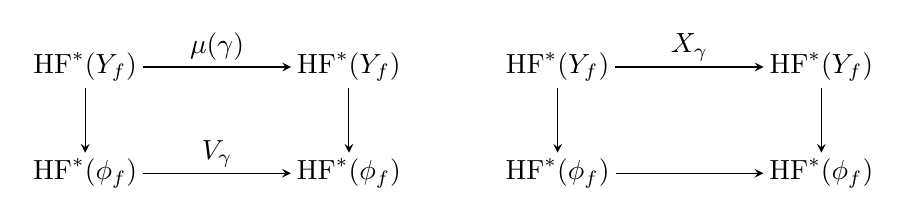
\begin{tikzpicture}[baseline=(current bounding box.center),>=stealth,
  every node/.style={inner sep=2pt}]
  \node (a1) at (0,1.35) {$\operatorname{HF}^*(Y_f)$};
  \node (a2) at (3.35,1.35) {$\operatorname{HF}^*(Y_f)$};
  \node (a3) at (0,0) {$\operatorname{HF}^*(\phi_f)$};
  \node (a4) at (3.35,0) {$\operatorname{HF}^*(\phi_f)$};
  \draw[->] (a1) -- node[above] {$\mu(\gamma)$} (a2);
  \draw[->] (a3) -- node[above] {$V_\gamma$} (a4);
  \draw[->] (a1) -- (a3);
  \draw[->] (a2) -- (a4);
  \node (b1) at (6.0,1.35) {$\operatorname{HF}^*(Y_f)$};
  \node (b2) at (9.35,1.35) {$\operatorname{HF}^*(Y_f)$};
  \node (b3) at (6.0,0) {$\operatorname{HF}^*(\phi_f)$};
  \node (b4) at (9.35,0) {$\operatorname{HF}^*(\phi_f)$};
  \draw[->] (b1) -- node[above] {$X_\gamma$} (b2);
  \draw[->] (b3) -- (b4);
  \draw[->] (b1) -- (b3);
  \draw[->] (b2) -- (b4);
\end{tikzpicture}
\]
每个图中的竖直箭头都是 \srcite{92} 的自然同构。左图的水平映射，是用适当子流形与连接
轨道的\BookRecordIndex{T0246}模空间相交、把这些\BookRecordIndex{T0246}模空间截低而定义的；右图的水平映射则由用配边定义的乘积结构
给出。例如，类 $\gamma\in H_1(\Sigma)$ 决定一个自然配边 $X_\gamma$，其边界为
\[
  \partial X_\gamma=(-Y_f)\cup Y_f.
\]
当然，在自然同构下，乘积的四种定义都应当一致。这些乘积结构之间的关系，在 Michael
Callaghan 关于 $M_\Sigma$ 的辛微分同胚（由分离型 Dehn 扭转诱导）之\BookRecordIndex{T0361}辛同痕问题的工作中
起着重要作用。遗憾的是，他的工作从未发表。

这些乘积结构在 Floer--Fukaya 构造中也起着重要作用；该构造为偶对 $(Y,\gamma)$ 给出
上同调群 $\operatorname{HFF}^*(Y,\gamma)$，其中 $Y$ 是三维流形、
$\gamma\in H_1(Y)$。另一方面，弗洛尔正合序列中的同态也可以用这些乘积结构来解释。

\paragraph{拉格朗日交。}
拉格朗日交的弗洛尔上同调中有类似结构；事实上，这正是 \BookRecordIndex{T0014}Donaldson 量子范畴构造的原始
背景。设 $M$ 如上，即紧、单连通且单调。对每一对满足 $H^1(L_i;\mathbb R)=0$ 的
\BookRecordIndex{T0219}拉格朗日子流形 $L_0,L_1$，都有弗洛尔上同调群 $\operatorname{HF}^*(L_0,L_1)$。此时
\BookRecordIndex{T0233}临界点是交点 $L_0\cap L_1$，连接轨道则是满足
\[
  u(s,0)\in L_0,
  \qquad u(s,1)\in L_1
\]
的 \BookRecordIndex{T0003}$J$-全纯曲线 $u:\mathbb R\times[0,1]\to M$。这是 Floer 在 \srcite{113} 中原始工作的
背景。弗洛尔上同调的 Euler 示性数现在是交数
\[
  \chi\bigl(\operatorname{HF}^*(L_0,L_1)\bigr)=L_0\cdot L_1.
\]
同样有由全纯三角形定义的配对
\[
  \operatorname{HF}^*(L_0,L_1)\otimes\operatorname{HF}^*(L_1,L_2)
  \longrightarrow\operatorname{HF}^*(L_0,L_2).
\]
Floer 在 \srcite{113} 中证明，只要 $\pi_2(M,L_0)=0$，
$\operatorname{HF}^*(L_0,L_0)$ 就同构于 $L_0$ 的通常上同调。在我们假设 $M$ 单连通的
情形，这个条件从不成立，相应断言仍是开放问题。Biran--Cornea 在 \srcite{44} 中把满足
$\operatorname{HF}^*(L_0,L_0)\cong H^*(L_0)$ 的\BookRecordIndex{T0219}拉格朗日子流形称为\emph{宽的}，把
$\operatorname{HF}^*(L_0,L_0)$ 消失的称为\emph{窄的}。在本书写作时，人们对这种二分仍
未充分理解。

这个乘法结构可以解释为一个量子范畴：对象是满足 $H^1(L;\mathbb R)=0$ 的\BookRecordIndex{T0219}拉格朗日
子流形 $L\subset M$，从 $L_0$ 到 $L_1$ 的态射是弗洛尔上同调群
$\operatorname{HF}^*(L_0,L_1)$ 的元素。上述辛微分同胚结构是它的特例，其中
\[
  M=N\times N,
  \qquad L_0=\Delta,
  \qquad L_1=\operatorname{graph}(\phi),
  \qquad L_2=\operatorname{graph}(\psi).
\]

把\BookRecordIndex{T0219}拉格朗日子流形解释为范畴的对象、把弗洛尔上同调群解释为态射空间的观点来自
Donaldson。后来 Fukaya 在链\BookRecordIndex{T0072}层次发现了底\BookRecordIndex{T0072}层的 $A_\infty$ 结构。所得范畴称为 \BookRecordIndex{T0021}Fukaya 范畴，
记作 $\mathcal F(M)$。即使在不会\BookRecordIndex{T0243}冒泡的简单情形，严格构造 \BookRecordIndex{T0021}Fukaya 范畴也涉及相当大量的
精细分析。例如，Seidel \srcite{371} 发展了计算仿射 Calabi--Yau 流形某些导出范畴
$D^b\mathcal F(M)$ 的技术。他的构造涉及对 Lefschetz 铅笔、消失循环和 Seidel 正合序列
作归纳论证。Fukaya--Seidel--Smith \srcite{131} 利用余切丛的 \BookRecordIndex{T0021}Fukaya 范畴取得了显著
成效。这里同样没有\BookRecordIndex{T0243}冒泡，却必须处理由非\BookRecordIndex{T0192}紧性造成的问题。一般情形见
Fukaya--Oh--Ohta--Ono \srcite{128}。Wehrheim 与 Woodward 在近期一系列论文
\srcite{414,415,416,417} 中证明了单调情形下 Donaldson 范畴关于拉格朗日对应的函子性。

\paragraph{Heegaard 分裂。}
拉格朗日交的弗洛尔理论与三维流形有如下联系。若 $Y$ 是同调三维球面，就在黎曼曲面
$\Sigma$ 上选取一个 Heegaard 分裂
\[
  Y=Y_0\cup Y_1.
\]
每个柄体 $Y_j$ 都在 $\Sigma$ 上平坦 $\operatorname{SU}(2)$-联络的（奇异）\BookRecordIndex{T0246}模空间
$M_\Sigma$ 中决定一个（奇异）\BookRecordIndex{T0219}拉格朗日子流形
$L_j=L_{Y_j}\subset M_\Sigma$。按照 Atiyah \srcite{20} 与 Floer 的观点，应当有自然同构
\[
  \operatorname{HF}^*(Y_0\cup Y_1)
  \cong\operatorname{HF}^*(L_0,L_1).
\]
和前面一样，有乘积结构
\[
  \operatorname{HF}^*(Y_0\cup Y_1)
  \otimes\operatorname{HF}^*(Y_1\cup Y_2)
  \longrightarrow\operatorname{HF}^*(Y_0\cup Y_2),
\]
它直接用适当四维配边上的 Yang--Mills 瞬子定义；在上述（猜想的）同构下，这两个乘积结构
应当相关。Katrin Wehrheim 在 \srcite{411,412,413} 中研究带拉格朗日边界条件的反自对偶
瞬子，并在这一猜想上取得了重要进展。作为中间步骤，这项工作在 Salamon--Wehrheim
\srcite{355} 中促成了带边三维流形的\BookRecordIndex{T0132}弗洛尔同调群之定义。（另一种设置可见 Fukaya
较早的工作 \srcite{126}。）

沿亏格为 $g$ 的黎曼曲面 $\Sigma$ 作 Heegaard 分裂，还会在 $g$ 重对称积
$\operatorname{Sym}^g\Sigma$ 中决定两个拉格朗日环面。从 \srcite{318} 开始的一长串论文中，
Ozsváth--Szabó 从他们的拉格朗日弗洛尔理论发展出一套强有力的新不变量，适用于低维流形
及纽结，称为 Heegaard--Floer 理论。他们又与若干合作者共同推进四维拓扑量子场论的构造；
参见 Lipshitz--Ozsváth--Thurston \srcite{247}。
\end{remark}


\section{\BookRecordIndex{T0356}辛涡旋方程}\label{sec:12-7}

本节讨论另一项与辛商的\BookRecordIndex{T0229}量子上同调密切相关的新进展。其出发点是把 \BookRecordIndex{T0003}$J$-全纯曲线的概念
推广到带哈密顿 $G$-作用的\BookRecordIndex{T0358}辛流形 $M$。新不变量由黎曼曲面 $\Sigma$ 上一种涡旋方程的解
构造；未知量的偶对由主 $G$-丛 $P\to\Sigma$ 上的一个联络，以及以 $M$ 为纤维的相伴丛
的一个截面组成。\BookRecordIndex{T0356}辛涡旋方程由 Salamon \srcite{64} 和 Ignasi Mundet i Riera
\srcite{294,295} 各自独立发现。当所论\BookRecordIndex{T0358}辛流形为 $\mathbb C^n$、$G$ 是
$\operatorname{U}(n)$ 的子群时，物理文献早已把这些方程称为规范化 sigma 模型。下面介绍
基本设置，并说明迄今在这个问题上得到的一些结果。

设 $(M,\omega)$ 是带紧 Lie 群 $G$ 的哈密顿作用的\BookRecordIndex{T0358}辛流形。这个作用由等变\BookRecordIndex{T0204}矩映射
\[
  \mu:M\longrightarrow\mathfrak g^*
\]
生成，其中 $\mathfrak g:=\operatorname{Lie}(G)$，而 $\mathfrak g^*$ 是其对偶。这意味着
元素 $\xi\in\mathfrak g$ 的无穷小作用 $X_\xi\in\operatorname{Vect}(M)$ 由
\[
  \iota(X_\xi)\omega=dH_\xi,
  \qquad H_\xi:=\langle\mu,\xi\rangle
\]
给出。令 $(\Sigma,j_\Sigma,\mathrm{dvol}_\Sigma)$ 为闭黎曼曲面，$P\to\Sigma$ 为
主 $G$-丛。\BookRecordIndex{T0356}辛涡旋方程的未知量是偶对 $(u,A)$，其中 $u:P\to M$ 是等变映射，
$A\in\mathcal A(P)$ 是联络；方程依赖参数 $\tau$，形式为
\begin{equation}\label{eq:12-7-1}
  \overline\partial_{J,A}(u)=0,
  \qquad *F_A+\mu(u)=\tau.
\end{equation}
这里 $J=\{J_z\}_{z\in\Sigma}$ 是 $M$ 上一族光滑的、$G$-不变且与 $\omega$ \BookRecordIndex{T0348}相容的\BookRecordIndex{T0088}殆复
结构。把联络看成等变的李代数值一形式 $A\in\Omega^1(P,\mathfrak g)$，也就是说
\[
  A_{pg}(vg)=g^{-1}A_p(v)g,
  \qquad v\in T_pP,\quad g\in G,
\]
并且它把竖直切空间与 $\mathfrak g$ 识别，即
\[
  A_p(p\xi)=\xi,
  \qquad p\in P,\quad \xi\in\mathfrak g.
\]
$u$ 关于 $A$ 的协变导数，是如下 $1$-形式：
\[
  d_Au\in\Omega^1(P,u^*TM),
  \qquad d_Au:=du+X_A(u).
\]
这个一形式等变且水平，因而下降为 $\Sigma$ 上取值于商丛 $u^*TM/G\to\Sigma$ 的一形式。
$M$ 上的\BookRecordIndex{T0088}殆复结构在这个向量丛上诱导复结构，而 $\overline\partial_{J,A}$ 表示 $d_Au$ 关于
这个复结构的复反线性部分。式~\eqref{eq:12-7-1} 中第二个方程把曲率
\[
  F_A:=dA+\frac12[A\wedge A]
  \in\Omega^2_{\mathrm{ad}}(P,\mathfrak g)
  =\Omega^2(\Sigma,\mathfrak g_P)
\]
与\BookRecordIndex{T0204}矩映射耦合。这里
\[
  *:\Omega^2(\Sigma,\mathfrak g_P)
  \longrightarrow\Omega^0(\Sigma,\mathfrak g_P^*)
\]
是 \BookRecordIndex{T0026}Hodge 星算子与同构 $\mathfrak g\to\mathfrak g^*$ 的复合，后一个同构由
$\mathfrak g$ 上的不变内积诱导。假设 $\tau\in Z(\mathfrak g^*)$ 属于中心，并且是\BookRecordIndex{T0204}矩映射
$\mu$ 的\BookRecordIndex{T0409}正则值。需要强调，$\Sigma$ 上的体积形式进入了~\eqref{eq:12-7-1} 的第二个方程；
因此，当 $J_z=J$ 与 $z$ 无关时，解空间在 $\Sigma$ 的复自同构群下不具有不变性。

规范群 $\mathcal G=\mathcal G(P)$ 由所有关于 $G$ 在自身上的共轭作用等变的光滑映射
$g:P\to G$ 组成。它在 $C_G^\infty(P,M)\times\mathcal A(P)$ 上有自然作用
\[
  g^*(u,A):=\bigl(g^{-1}u,g^{-1}dg+g^{-1}Ag\bigr),
\]
而这个作用保持式~\eqref{eq:12-7-1} 的解空间。

式~\eqref{eq:12-7-1} 的解是能量泛函
\[
  E(u,A):=\frac12\int_\Sigma
  \left(|d_Au|^2+|F_A|^2+|\mu(u)-\tau|^2\right)
  \mathrm{dvol}_\Sigma
\]
的绝对极小值。对式~\eqref{eq:12-7-1} 的解，能量由拓扑不变量给出：
\[
\begin{aligned}
  E(u,A)
  &=\int_\Sigma\left((d_Au)^*\omega
  -\langle\mu(u)-\tau,F_A\rangle\right)\\
  &=\int_\Sigma\left(u^*\omega
  -d\langle\mu(u)-\tau,A\rangle\right).
\end{aligned}
\]
这里两个被积式相等，并且都下降为 $\Sigma$ 上的二形式。这个积分可以解释为等变上同调类
\[
  [\omega-\mu+\tau]\in H_G^2(M)
\]
在等变同调类 $[u]\in H_2^G(M)$ 上的取值。（若 $\theta:P\to EG$ 是等变分类映射，则
$[u]$ 是基本类 $[\Sigma]\in H_2(\Sigma)$ 在如下映射下的像：这个映射
\[
  \Sigma\longrightarrow M_G:=M\times_GEG
\]
由 $u\times\theta:P\to M\times EG$ 诱导。）

\begin{remark}\label{rem:12-7-1}
\begin{enumerate}[label=(\roman*)]
\item 在 $\Sigma$ 上的局部全纯坐标 $s+it\in U$ 及 $P$ 的一个局部平凡化中，联络形如
\[
  A=\Phi\,ds+\Psi\,dt,
\]
其中 $\Phi,\Psi:U\to\mathfrak g$，而 $u$ 是从 $U$ 到 $M$ 的光滑映射。此时涡旋方程形如
\begin{equation}\label{eq:12-7-2}
\begin{aligned}
  \partial_su+X_\Phi(u)
  +J_{s,t}(u)\bigl(\partial_tu+X_\Psi(u)\bigr)&=0,\\
  \lambda^{-2}*_\mathfrak g
  \bigl(\partial_s\Psi-\partial_t\Phi+[\Phi,\Psi]\bigr)
  +\mu(u)&=\tau,
\end{aligned}
\end{equation}
其中 $*_\mathfrak g:\mathfrak g\to\mathfrak g^*$ 表示由 $\mathfrak g$ 上不变内积诱导的
同构，而局部坐标中的体积形式为
$\mathrm{dvol}_\Sigma=\lambda^2\,ds\wedge dt$。

\item 当 $G=\{1\}$ 时，式~\eqref{eq:12-7-1} 的解就是 $M$ 中的 \BookRecordIndex{T0003}$J$-全纯曲线。

\item 通常的涡旋方程是特例 $M=\mathbb C$、$G=S^1$。这时，式~\eqref{eq:12-7-1}
的第一个方程断言 $u$ 是复线丛 $L\to\Sigma$ 的全纯截面；设该线丛次数为 $d$，则在这种
情形，式~\eqref{eq:12-7-1} 的解模\BookRecordIndex{T0153}规范等价所得的\BookRecordIndex{T0246}模空间，自然等同于 $\Sigma$ 的 $d$ 重
对称积（见 Garcia-Prada \srcite{136}）。

\item 当 $M=\mathbb C^2$、$G=\operatorname{U}(2)$ 时，式~\eqref{eq:12-7-1} 的解\BookRecordIndex{T0246}模空间
是 \BookRecordIndex{T0011}Bradlow 偶对空间，即由 $\Sigma$ 上秩二全纯丛和一个全纯截面组成的稳定偶对之空间
\srcite{47}。此时参数 $\tau$ 决定稳定性条件。

\item 若 $M$ 是黎曼曲面 $S$ 上 $\operatorname{SU}(2)$-联络的无限维流形，而 $G$ 是
$S$ 上 $\operatorname{SU}(2)$-规范变换所成的空间，则式~\eqref{eq:12-7-1} 的解是乘积
$\Sigma\times S$ 上的反自对偶瞬子。

\item 若取 $M$ 为满足 $\overline\partial_A\Theta=0$ 的偶对
\[
  (\Theta,A)\in\Omega^0(S,E)\times\mathcal A(E)
\]
所成的空间，并取 $G=C^\infty(S,S^1)$，那么 $\Sigma\times S$ 上的
Seiberg--Witten 方程也作为式~\eqref{eq:12-7-1} 的特例出现；这里 $E\to S$ 是复线丛。
\end{enumerate}
\end{remark}

为了从式~\eqref{eq:12-7-1} 的解得到不变量，必须施加以下条件。当 $G=\{1\}$ 时，这些
条件等价于定义~\ref{def:9-2-6} 中的\BookRecordIndex{T0344}无穷远处凸性。

\begin{description}
\item[\normalfont\textbf{(H1)}]
\BookRecordIndex{T0204}矩映射
$\mu:M\to\mathfrak g^*$
\sourcefootnote{原书在这里把\BookRecordIndex{T0204}矩映射的陪域印作 $\mathfrak g$；但本节开头的定义以及同一
条件中的 $\tau\in Z(\mathfrak g^*)$ 均要求陪域为 $\mathfrak g^*$，故补正。}
是\BookRecordIndex{T0277}恰当映射，并且 $(M,\omega,\mu)$ 在如下意义下于\BookRecordIndex{T0344}无穷远处凸：存在
$G$-不变、与 $\omega$ \BookRecordIndex{T0348}相容的\BookRecordIndex{T0088}殆复结构 $J\in\mathcal J_G(M,\omega)$，一个 $G$-不变的
恰当光滑函数
\[
  f:M\longrightarrow[0,\infty),
\]
以及对每个 $\tau\in Z(\mathfrak g^*)$ 的紧集 $K_\tau\subset M$，使得
\[
  \omega_f(v,J(x)v)\geq0,
  \qquad
  df(x)J(x)X_{\mu(x)-\tau}\geq0
\]
对每个 $x\in M\setminus K_\tau$ 和每个 $v\in T_xM$ 成立。这里
\[
  \omega_f:=-d(df\circ J).
\]
\end{description}

要让式~\eqref{eq:12-7-1} 的解获得任何\BookRecordIndex{T0192}紧性，都需要假设 (H1)；没有它，便不能期待任何
有意义的结果。最简单却又非常有用的一类例子还满足

\begin{description}
\item[\normalfont\textbf{(H2)}]
$(M,\omega)$ \BookRecordIndex{T0355}辛非球面。
\end{description}

条件 (H1) 与 (H2) 合在一起迫使环境流形 $M$ 非紧。不过，它们蕴含：对每个
$B\in H_2^G(M)$，式~\eqref{eq:12-7-1} 中表示等变同调类 $[u]=B$ 的解，模基\BookRecordIndex{T0153}规范等价
所得的\BookRecordIndex{T0246}模空间 $\mathcal M_{B,\Sigma}(\tau)$ 是紧的（见 \srcite{64,67}）。由恰当\BookRecordIndex{T0204}矩映射
生成的 $\mathbb C^n$ 上每个线性作用都满足这两个假设。此外，只要
$\tau\in Z(\mathfrak g^*)$ 是\BookRecordIndex{T0204}矩映射的中心\BookRecordIndex{T0409}正则值且 $\Sigma$ 的体积充分大，这个\BookRecordIndex{T0246}模空间
就是正则的；这里正则是指规范群的作用具有有限稳定子。存在一个 $G$-等变\BookRecordIndex{T0283}求值映射
\[
  \operatorname{ev}:\mathcal M_{B,\Sigma}(\tau)\longrightarrow M,
\]
而参数 $\tau$ 处的不变量形如群同态
\[
  \operatorname{GGW}^{M,\mu-\tau}_{B,\Sigma}:
  H_G^*(M;\mathbb Q)\longrightarrow\mathbb Q.
\]
粗略地说，这个同态通过在商 $\mathcal M_{B,\Sigma}(\tau)/G$ 上“积分”等变上同调类
$a\in H_G^*(M;\mathbb Q)$ 的拉回来定义：
\begin{equation}\label{eq:12-7-3}
  \operatorname{GGW}^{M,\mu-\tau}_{B,\Sigma}(a)
  :=\int_{\mathcal M_{B,\Sigma}(\tau)/G}\operatorname{ev}^*a.
\end{equation}
这些就是\emph{\BookRecordIndex{T0154}规范化格罗莫夫--威滕不变量}。积分的严格定义不需要\BookRecordIndex{T0166}横截性；可以用一个
相伴 $G$-模问题的等变 Euler 类来理解它（见 Cieliebak--Mundet--Salamon
\srcite{66}），细节由 Cieliebak--Gaio--Mundet--Salamon 在 \srcite{67} 中给出。这个构造
还有若干细化版本，其中会改变\BookRecordIndex{T0066}标记点，或从联络空间拉回等变上同调类；这里不作讨论。

与第~\ref{sec:9-1} 节一样，可以用这些不变量证明时间依赖、$G$-等变哈密顿微分方程的
相对周期轨道存在，也就是证明存在模 $G$-作用闭合的解（见
Cieliebak--Gaio--Mundet--Salamon \srcite{67}）。另一个应用是：对适当流形 $M$，
Seiberg--Witten 不变量与\BookRecordIndex{T0154}规范化格罗莫夫--威滕不变量相对应（见
Cieliebak--Gaio--Mundet--Salamon \srcite{67} 和 Okonek--Teleman \srcite{309}）。这
重新得到了直纹曲面的 Seiberg--Witten 不变量之计算。事实上，假设 (H1--2) 下\BookRecordIndex{T0246}模空间紧，
所以涡旋不变量适于计算。一个有趣特征是它依赖参数 $\tau$。Cieliebak 与 Salamon 在
\srcite{69} 中对 $G$ 为环面的情形得到一个\BookRecordIndex{T0078}穿墙公式，描述当 $\tau$ 从一个\BookRecordIndex{T0280}腔跨入另一个\BookRecordIndex{T0280}腔
时不变量如何变化；他们还借此证明了单调\BookRecordIndex{T0169}环面流形的 Batyrev 公式。其证明的关键成分，是
\BookRecordIndex{T0154}规范化格罗莫夫--威滕不变量与辛商的\BookRecordIndex{T0143}格罗莫夫--威滕不变量之间的对应；下面解释这一点。

为简单起见，假设 $\tau=0$。要得到光滑商，还必须施加第三个条件：

\begin{description}
\item[\normalfont\textbf{(H3)}]
群 $G$ 在 $\mu^{-1}(0)$ 上自由作用。
\end{description}

在这个假设下，商
\[
  \overline M:=M/\!/G:=\mu^{-1}(0)/G
\]
是紧\BookRecordIndex{T0358}辛流形。\BookRecordIndex{T0003}$J$-全纯曲线 $\overline u:\Sigma\to\overline M$ 可以由满足
\begin{equation}\label{eq:12-7-4}
  \overline\partial_{J,A}(u)=0,
  \qquad \mu(u)=0
\end{equation}
的偶对
\[
  (u,A)\in C_G^\infty(P,M)\times\mathcal A(P)
\]
表示。要在式~\eqref{eq:12-7-1} 与~\eqref{eq:12-7-4} 的解之间建立对应，基本思路是研究
方程
\begin{equation}\label{eq:12-7-5}
  \overline\partial_{J,A}(u)=0,
  \qquad *F_A+\varepsilon^{-2}\mu(u)=0
\end{equation}
在 $\varepsilon$ 很小时的极限。Gaio 与 Salamon 在商单调的情形于 \srcite{134,135}
中完成了这一纲领，得到如下结果。

\begin{theorem}[Gaio--Salamon]\label{thm:12-7-2}
假设 (H1--3) 成立，并设 $c_1(T\overline M)$ 是 $[\overline\omega]$ 的正倍数。令
$\overline B\in H_2(\overline M;\mathbb Z)$，并令
$a_i\in H_G^*(M)$ 满足
\[
  \deg(a_i)<2N,
\]
其中 $N$ 是 $\overline M$ 的最小 Chern 数。以 $B\in H_2^G(M)$ 表示
$\overline B$ 在同态 $H_2(\overline M)\to H_2^G(M)$ 下的像，以
\[
  \overline a_i\in H^*(\overline M)
\]
表示 $a_i$ 在 Kirwan 同态
\[
  \kappa:H_G^*(M)\longrightarrow H^*(\overline M)
\]
下的像。那么
\[
  \operatorname{GW}^{\overline M}_{\overline B,\Sigma}
  (\overline a_1,\ldots,\overline a_k)
  =\operatorname{GGW}^{M,\mu}_{B,\Sigma}
  (a_1\smile\cdots\smile a_k).
\]
\end{theorem}

这里的\BookRecordIndex{T0143}格罗莫夫--威滕不变量使用\BookRecordIndex{T0157}哈密顿扰动、\BookRecordIndex{T0150}固定标记点和 $\Sigma$ 上的固定复结构来理解
（如第~\ref{ch:hamiltonian-perturbations} 章）。定理~\ref{thm:12-7-2} 的证明依赖于方程
\eqref{eq:12-7-5} 在 $\varepsilon\to0$ 时的绝热极限分析。这涉及颇为精细的估计，而证明
让人联想到 Dostoglou--Salamon \srcite{92} 对 Atiyah--Floer 猜想的证明。结合
定理~\ref{thm:12-7-2} 与习题~\ref{ex:11-1-18} 中把\BookRecordIndex{T0143}格罗莫夫--威滕不变量解释为从
$\overline M$ 的\BookRecordIndex{T0229}量子上同调到 $\mathbb Z$ 的同态，就得到下面的推论。

\begin{corollary}[Gaio--Salamon]\label{cor:12-7-3}
设 $(M,\omega,\mu)$ 如定理~\ref{thm:12-7-2}，并设 $\Lambda$ 是
定义~\ref{def:11-1-3} 意义下 $\overline M$ 的一个\BookRecordIndex{T0231}量子系数环。再假设 $M$ 的等变上同调
由次数小于 $2N$ 的类生成。那么存在唯一的环同态
\begin{equation}\label{eq:12-7-6}
  Q\kappa:H_G^*(M;\Lambda)
  \longrightarrow\operatorname{QH}^*(\overline M;\Lambda),
\end{equation}
它在次数小于 $2N$ 的类上与 Kirwan 同态
\[
  \kappa:H_G^*(M;\Lambda)\longrightarrow H^*(\overline M;\Lambda)
\]
一致。此外，$Q\kappa$ 满射，而且
\[
  \operatorname{GW}^{\overline M}_{\overline B,\Sigma}(Q\kappa(a))
  =\operatorname{GGW}^{M,\mu}_{B,\Sigma}(a)
\]
对每个 $\Sigma$、每个 $\overline B\in H_2(\overline M;\mathbb Z)$ 和每个
$a\in H_G^*(M)$ 成立。
\end{corollary}

由注~\ref{rem:11-3-13}，第~\ref{subsec:11-3-1}、\ref{subsec:11-3-2}、
\ref{subsec:11-3-3} 小节讨论的单调\BookRecordIndex{T0169}环面流形、\BookRecordIndex{T0274}旗流形和格拉斯曼流形的\BookRecordIndex{T0229}量子上同调环，都给出
推论~\ref{cor:12-7-3} 中环同态的例子，其中
\[
  M=\mathbb C^n,
  \qquad H_G^*(M;\Lambda)\cong H^*(BG;\Lambda).
\]

\begin{remark}[量子 Kirwan 同态]\label{rem:12-7-4}
\begin{enumerate}[label=(\roman*)]
\item 若削弱假设 (H3)，只假设零是\BookRecordIndex{T0204}矩映射的\BookRecordIndex{T0409}正则值，那么商 $\overline M$ 是辛轨形。
轨形的\BookRecordIndex{T0143}格罗莫夫--威滕不变量是一项新课题（见 Chen--Ruan \srcite{62}）。可以预期，
定理~\ref{thm:12-7-2} 以及推论~\ref{cor:12-7-3} 会相当直接地推广到商为单调辛轨形的
情形。

\item 正如 Gaio--Salamon \srcite{135} 所猜想的，推论~\ref{cor:12-7-3} 还应推广到非单调
情形；不过证明需要细化 \srcite{135} 中的分析，并涉及\BookRecordIndex{T0356}辛涡旋方程解的\BookRecordIndex{T0256}粘合定理。其中一个
成分，是通过复平面 $\Sigma=\mathbb C$ 上\BookRecordIndex{T0356}辛涡旋方程~\eqref{eq:12-7-2} 的有限能量解
（取 $\lambda\equiv1$），直接给出同态 $Q\kappa$ 的几何定义；比较 Ziltener
\srcite{430}。

\item 去掉假设 (H2) 则是另一回事；这个假设断言环境流形\BookRecordIndex{T0355}辛非球面。这样做需要在 $M$ 的
等变上同调中引入量子形变项。近年已有若干研究者在这些猜想上取得大量进展；参见
Ziltener \srcite{431,432}、Gonzalez--Woodward \srcite{156,157}、Ott \srcite{319}、
Nguyen--Woodward--Ziltener \srcite{299}。在这些文献中，式~\eqref{eq:12-7-6} 的同态
$Q\kappa$ 及其猜想推广称为\emph{量子 Kirwan 同态}。
\end{enumerate}
\end{remark}

\begin{remark}[\BookRecordIndex{T0203}矩弗洛尔同调]\label{rem:12-7-5}
\BookRecordIndex{T0132}弗洛尔同调有一个与\BookRecordIndex{T0356}辛涡旋方程相关的版本，正如标准辛\BookRecordIndex{T0132}弗洛尔同调与 \BookRecordIndex{T0003}$J$-全纯曲线相关。
在这个理论中，作用泛函定义在 $M$ 与 Lie 代数的乘积中环路
\[
  (x,\eta):\mathbb R/\mathbb Z\longrightarrow M\times\mathfrak g
\]
所成的空间上，形式为
\[
  \mathcal A_{H,\mu}(x,\eta)
  =-\int_Bu^*\omega
  +\int_0^1\left(
  \langle\mu(x(t)),\eta(t)\rangle-H_t(x(t))
  \right)dt.
\]
这里 $H_t=H_{t+1}:M\to\mathbb R$ 是一族光滑的、$1$-周期且 $G$-不变的哈密顿函数；并且
和第~\ref{sec:12-1} 节一样，$u:B\to M$ 是满足
$u(e^{2\pi it})=x(t)$ 的光滑映射。这个泛函的\BookRecordIndex{T0233}临界点模\BookRecordIndex{T0153}规范等价所得的类，可以等同于
$\mu^{-1}(0)$ 中哈密顿系统相对周期轨道的等价类。

Frauenfelder 在 \srcite{121,122} 中使用这个弗洛尔理论的拉格朗日版本，证明了带
$G$-作用的\BookRecordIndex{T0355}辛非球面流形之辛商的 Arnold--Givental 猜想。这个猜想断言：当所论\BookRecordIndex{T0219}拉格朗日
子流形是某个反辛对合的不动点集时，它与自身任一个哈密顿形变的交点个数有一个下界。
Fukaya--Oh--Ohta--Ono \srcite{128} 较早给出了单调情形的证明，不过不带商空间假设。
\end{remark}


\appendix
\ctexset{chapter={name={附录~,},number=\Alph{chapter}}}
\chapter{弗雷德霍姆理论}\label{app:fredholm-theory}


本附录回顾证明\BookRecordIndex{T0246}模空间构成光滑有限维流形所需的泛函分析基础。第 A.1 节介绍\BookRecordIndex{T0128}弗雷德霍姆算子
及其稳定性。第 A.2 节讨论两个巴拿赫空间之间的\BookRecordIndex{T0128}弗雷德霍姆算子空间上的\BookRecordIndex{T0162}行列式线丛；
这是确立\BookRecordIndex{T0246}模空间可定向性所需的。第 A.3 节给出巴拿赫空间情形下逆函数定理与\BookRecordIndex{T0380}隐函数定理
的证明。第 A.4 节说明\BookRecordIndex{T0388}有限维约化技术，有时也称为 \BookRecordIndex{T0029}Kuranishi 模型；它把奇异点附近
弗雷德霍姆映射零点集的局部分析化为有限维模型。第 A.5 节证明 萨德--斯梅尔定理。

\section{弗雷德霍姆理论}\label{sec:A-1}

本节讨论抽象\BookRecordIndex{T0128}弗雷德霍姆算子及其基本性质。巴拿赫空间之间的有界线性算子 $D:X\to Y$
若核有限维、像闭，且余核 $Y/\operatorname{im}D$ 有限维，就称为\emph{\BookRecordIndex{T0128}弗雷德霍姆算子}。
\BookRecordIndex{T0128}弗雷德霍姆算子 $D$ 的\emph{指标}定义为
\[
  \operatorname{index}D:=\dim\ker D-\dim\operatorname{coker}D.
\]
这里的核与余核都视作实向量空间。若 $D$ 是复巴拿赫空间之间的复线性\BookRecordIndex{T0128}弗雷德霍姆算子，
就必须区分实\BookRecordIndex{T0129}弗雷德霍姆指标和复\BookRecordIndex{T0129}弗雷德霍姆指标。显然，实指标是复指标的两倍。
下面的引理在证明给定线性算子 $D$ 具有弗雷德霍姆性质时起重要作用。

\begin{lemma}\label{lem:A-1-1}
设 $X,Y,Z$ 是巴拿赫空间，$D:X\to Y$ 是有界线性算子，$K:X\to Z$ 是紧算子。
假设存在常数 $c>0$，使得对每个 $x\in X$ 都有
\begin{equation}\label{eq:A-1-1}
  \|x\|_X\le c\bigl(\|Dx\|_Y+\|Kx\|_Z\bigr).
\end{equation}
则 $D$ 的像是闭的，核是有限维的。
\end{lemma}

\begin{proof}
要证明 $\ker D$ 有限维，只须证明其单位球紧。为此，取序列 $x_\nu\in X$，满足
\[
  \|x_\nu\|\le1,\qquad Dx_\nu=0.
\]
由于 $x_\nu$ 有界，可取一子序列，仍记作 $x_\nu$，使 $Kx_\nu$ 收敛。
因为 $x_\nu\in\ker D$，由式~\eqref{eq:A-1-1} 可知 $x_\nu$ 是柯西序列。
由于 $X$ 完备，$x_\nu$ 收敛。

现在不失一般性地假定 $D$ 是单射；否则，以 $\ker D$ 的一个补空间替换 $X$。
这样的补空间由 Hahn--Banach 定理保证存在：取 $\ker D$ 的一组基
$x_1,\ldots,x_N$，并选取 $x_k^*\in X^*$，使
$\langle x_k^*,x_j\rangle=\delta_{jk}$。于是
\[
  X_0:=\bigl\{x\in X\mid
  \langle x_1^*,x\rangle=\cdots=\langle x_N^*,x\rangle=0\bigr\}
\]
就是所需的补空间。

设 $y\in\operatorname{cl}(\operatorname{im}D)$。则存在序列 $x_\nu\in X$，使得
\[
  y=\lim_{\nu\to\infty}Dx_\nu.
\]
先证明 $x_\nu$ 有界。反设 $x_\nu$ 无界；必要时取子序列，可假定
$\|x_\nu\|\to\infty$。考虑序列
\[
  \xi_\nu:=\|x_\nu\|^{-1}x_\nu.
\]
它的每一项范数均为 $1$，且 $D\xi_\nu\to0$。再取子序列，可假定
$K\xi_\nu$ 收敛。由式~\eqref{eq:A-1-1} 可知 $\xi_\nu$ 是柯西序列。
其极限 $\xi:=\lim_{\nu\to\infty}\xi_\nu$ 的范数为 $1$，又满足 $D\xi=0$，
这与 $D$ 为单射矛盾。因此 $x_\nu$ 确实有界。再次利用 $K$ 的\BookRecordIndex{T0192}紧性、
估计~\eqref{eq:A-1-1} 和 $X$ 的完备性，可知 $x_\nu$ 有收敛子序列。
设其极限为 $x$，则 $y=Dx$。
\end{proof}

\begin{corollary}\label{cor:A-1-2}
设 $X,Y$ 是巴拿赫空间，$D:X\to Y$ 是像闭且核有限维的有界线性算子。
\begin{enumerate}[label=(\roman*)]
\item 对每个紧算子 $K:X\to Y$，算子 $D+K$ 的像也闭，核也有限维。
\item 存在 $\varepsilon>0$，使得若有界线性算子 $P:X\to Y$ 满足
$\|P\|<\varepsilon$，则 $D+P$ 的像闭，核有限维。
\end{enumerate}
\end{corollary}

\begin{proof}
设 $\dim\ker D=n$，并选取有界线性算子 $K_0:X\to\mathbb R^n$，使
$K_0$ 在 $\ker D$ 上的限制是向量空间同构。于是算子
$X\to Y\oplus\mathbb R^n:x\mapsto(Dx,K_0x)$ 为单射且像闭。
因此，由开映射定理，存在常数 $c>0$，使
\[
  \|x\|_X\le c\bigl(\|Dx\|_Y+\|K_0x\|_{\mathbb R^n}\bigr).
\]
于是对任意紧算子 $K:X\to Y$，有
\[
  \|x\|_X\le c\bigl(\|(D+K)x\|_Y+\|Kx\|_Y
  +\|K_0x\|_{\mathbb R^n}\bigr).
\]
同样，若 $\|P\|<1/c$，则
\[
  \|x\|_X\le\frac{c}{1-c\|P\|}
  \bigl(\|(D+P)x\|_Y+\|K_0x\|_{\mathbb R^n}\bigr).
\]
因此，结论由引理~\ref{lem:A-1-1} 得到。
\end{proof}

\begin{corollary}\label{cor:A-1-3}
设 $X,Y$ 是巴拿赫空间，$D:X\to Y$ 是像闭且余核有限维的有界线性算子。
\begin{enumerate}[label=(\roman*)]
\item 对每个紧算子 $K:X\to Y$，算子 $D+K$ 的像也闭，余核也有限维。
\item 存在 $\varepsilon>0$，使得若有界线性算子 $P:X\to Y$ 满足
$\|P\|<\varepsilon$，则 $D+P$ 的像闭，余核有限维。
\end{enumerate}
\end{corollary}

\begin{proof}
$D$ 的像闭当且仅当对偶算子 $D^*$ 的像闭；$D$ 的余核有限维当且仅当
$D^*$ 的核有限维。因此结论由推论~\ref{cor:A-1-2} 得到。
\end{proof}

\begin{exercise}\label{ex:A-1-4}
\begin{enumerate}[label=(\roman*)]
\item 证明：有界线性算子 $D:X\to Y$ 是\BookRecordIndex{T0128}弗雷德霍姆算子，当且仅当存在有界线性算子
$T:Y\to X$，使 $DT-\operatorname{id}$ 与 $TD-\operatorname{id}$ 都是紧算子。
提示：证明“若”时使用引理~\ref{lem:A-1-1}。
\item 若 $D:X\to Y$ 与 $T:Y\to Z$ 都是\BookRecordIndex{T0128}弗雷德霍姆算子，证明
$TD:X\to Z$ 也是\BookRecordIndex{T0128}弗雷德霍姆算子，且
\begin{equation}\label{eq:A-1-2}
  \operatorname{index}TD=\operatorname{index}D+\operatorname{index}T.
\end{equation}
\item 证明：有界线性算子 $D:X\to Y$ 是\BookRecordIndex{T0128}弗雷德霍姆算子，当且仅当它的对偶算子
$D^*:Y^*\to X^*$ 是\BookRecordIndex{T0128}弗雷德霍姆算子，且二者的指标满足
\[
  \operatorname{index}D^*=-\operatorname{index}D.
\]
\end{enumerate}
\end{exercise}

\BookRecordIndex{T0128}弗雷德霍姆算子最重要的性质与它们在扰动下的稳定性有关。这正是下面定理的内容。
特别地，定理~\ref{thm:A-1-5} 断言：\BookRecordIndex{T0128}弗雷德霍姆算子集在范数拓扑下是开集，
指标在每个连通分支上恒定。

\begin{theorem}\label{thm:A-1-5}
设 $D:X\to Y$ 是\BookRecordIndex{T0128}弗雷德霍姆算子。
\begin{enumerate}[label=(\roman*)]
\item 若 $K:X\to Y$ 是紧算子，则 $D+K$ 是\BookRecordIndex{T0128}弗雷德霍姆算子，且
$\operatorname{index}(D+K)=\operatorname{index}D$。
\item 存在 $\varepsilon>0$，使得若有界线性算子 $P:X\to Y$ 满足
$\|P\|<\varepsilon$，则 $D+P$ 是\BookRecordIndex{T0128}弗雷德霍姆算子，且
$\operatorname{index}(D+P)=\operatorname{index}D$。
\end{enumerate}
\end{theorem}

\begin{proof}
关于弗雷德霍姆性质的断言直接由推论~\ref{cor:A-1-2} 和~\ref{cor:A-1-3} 得到。
关于指标的断言留作附提示的习题。选取分解 $X=X_0\oplus X_1$、
$Y=Y_0\oplus Y_1$，使 $X_0:=\ker D$、$Y_1:=\operatorname{im}D$。
证明 $D+P$ 的指标等于如下有限维算子的指标：
\[
  P_{00}-P_{01}(D_{11}+P_{11})^{-1}P_{10}:X_0\longrightarrow Y_0,
\]
其中 $P_{ji}:X_i\to Y_j$ 表示先把 $P$ 限制在 $X_i$ 上，再投影到 $Y_j$；
$D_{ji}$ 的含义类似。
\end{proof}


\section{\BookRecordIndex{T0162}行列式线丛}\label{sec:A-2}

设 $X,Y$ 是巴拿赫空间，以 $\mathcal F(X,Y)$ 表示所有\BookRecordIndex{T0128}弗雷德霍姆算子
$D:X\to Y$ 的空间。\BookRecordIndex{T0128}弗雷德霍姆算子 $D\in\mathcal F(X,Y)$ 的\emph{行列式}定义为
一维实向量空间
\[
  \det(D):=\Lambda^{\max}(\ker D)\otimes\Lambda^{\max}(\ker D^*).
\]
下面将证明：当 $D$ 变化时，这些向量空间 $\det(D)$ 拼成 $\mathcal F(X,Y)$ 上的
局部平凡线丛。这里必须留意用于识别不同一维向量空间的同构。
\sourcefootnote{原书第二版勘误（2019 年 11 月 27 日，
\url{https://people.math.ethz.ch/~salamon/PREPRINTS/jholn-erratum.pdf}）指出，
印刷页 534--546 关于\BookRecordIndex{T0162}行列式线丛的讨论须重写以修正符号。以下保留锁定原书的论述；
涉及定向和同构的符号结论，不应视作已按勘误修正。}

把实直线 $\mathbb R$ 看作一维实向量空间。对任意两个一维实向量空间 $V,W$，
我们用 $V\cong W$ 表示它们\emph{自然同构}，即两者之间有一个显然的同构选择。
例如，当 $V$ 是一维空间时，有自然同构
\[
  V\otimes V^*\longrightarrow\mathbb R:
  v\otimes v^*\longmapsto v^*(v).
\]

自然同构的概念可以用范畴论语言表述得更精确。以 $\mathcal V$ 表示由一维实向量空间
及其同构组成的范畴，令 $\mathcal C$ 为任意其他范畴。两个函子
$\mathcal F_0,\mathcal F_1:\mathcal C\to\mathcal V$ 称为\emph{自然同构}，
如果存在自然变换
$\mathcal T:\operatorname{Ob}(\mathcal C)\to\operatorname{Mor}(\mathcal V)$，
它给每个对象 $A\in\operatorname{Ob}(\mathcal C)$ 指派一个向量空间同构
$\mathcal T(A):\mathcal F_0(A)\to\mathcal F_1(A)$，并且对
$A,B\in\operatorname{Ob}(\mathcal C)$、$T\in\operatorname{Mor}(A,B)$ 满足
\[
  \mathcal T(B)\circ\mathcal F_0(T)
  =\mathcal F_1(T)\circ\mathcal T(A).
\]
许多情形下，$\mathcal T(A)$ 的选择由上下文即可确定，我们便直接写作
$\mathcal F_0(A)\cong\mathcal F_1(A)$。上面的同构记作
$V\otimes V^*\cong\mathbb R$ 就是一个例子。

有限维实向量空间 $V$ 的\emph{最高外幂} $\Lambda^{\max}V$，是 $V$ 中有序
$n$ 元组 $v_1\wedge\cdots\wedge v_n$ 的等价类所成的空间，其中 $\dim V=n$。
两个这样的 $n$ 元组 $v_1\wedge\cdots\wedge v_n$ 和
$w_1\wedge\cdots\wedge w_n$ 等价，当且仅当它们都构成基且所诱导的
$V$ 的同构行列式为 $1$，或者两个元组都线性相关。因此，
$\Lambda^{\max}V$ 中的非零向量确定 $V$ 的一个定向。当 $\dim V=0$ 时，
定义 $\Lambda^{\max}V:=\mathbb R$。

两个一维实向量空间 $V,W$ 的\emph{张量积} $V\otimes W$，是有序对
$(v,w)\in V\times W$ 的等价类 $v\otimes w$ 所成的空间，其中对每个
$\lambda\in\mathbb R$ 都有 $\lambda v\otimes w=v\otimes\lambda w$。
对任意两个有限维实向量空间 $V,W$，有自然同构
\[
  \Lambda^{\max}V\otimes\Lambda^{\max}W
  \cong\Lambda^{\max}(V\oplus W).
\]
（请证明这一点！）

对每个 $n$ 维实向量空间 $V$，把最高外幂
$\Lambda^{\max}V^*:=\Lambda^{\max}(V^*)$ 看作 $V$ 上的交替 $n$-形式空间。
自然同构
\[
  \Lambda^{\max}V\otimes\Lambda^{\max}V^*\cong\mathbb R
\]
由如下映射给出：
\[
  (v_1\wedge\cdots\wedge v_n)
  \otimes(v_1^*\wedge\cdots\wedge v_n^*)
  \longmapsto\det\bigl(v_k^*(v_j)\bigr).
\]
它诱导同构
$\Lambda^{\max}V^*\cong(\Lambda^{\max}V)^*$。
同样，任意同构 $\Lambda^{\max}V\otimes\Lambda^{\max}W\to\mathbb R$
都诱导同构 $\Lambda^{\max}W\to(\Lambda^{\max}V)^*
\cong\Lambda^{\max}V^*$。

\begin{lemma}\label{lem:A-2-1}
设 $V$ 是有限维实向量空间，$W\subset V$ 是线性子空间。则有自然同构
\[
  \Lambda^{\max}V\cong\Lambda^{\max}W\otimes\Lambda^{\max}(V/W).
\]
\end{lemma}

\begin{proof}
令 $N:=\dim V$、$n:=\dim W$。以 $\mathcal B(V,W)$ 表示 $V$ 的所有基
$v_1,\ldots,v_N$ 构成的集合，其中前 $n$ 个向量张成 $W$。
对 $v\in V$，记 $[v]:=v+W$。映射
$\mathcal B(V,W)\to\Lambda^{\max}W\otimes\Lambda^{\max}(V/W)$，
\[
  (v_1,\ldots,v_N)\longmapsto
  (v_1\wedge\cdots\wedge v_n)
  \otimes([v_{n+1}]\wedge\cdots\wedge[v_N])
\]
诱导所需同构。验证这些同构构成自然变换，留给读者。
\end{proof}

经过这些准备，再考虑\BookRecordIndex{T0128}弗雷德霍姆算子族 $D$ 的\BookRecordIndex{T0162}行列式线
\[
  \det(D):=\Lambda^{\max}(\ker D)\otimes\Lambda^{\max}(\ker D^*).
\]

\begin{theorem}\label{thm:A-2-2}
空间
\[
  \det(X,Y):=\bigl\{(D,\sigma)\mid D\in\mathcal F(X,Y),\;
  \sigma\in\det(D)\bigr\}
\]
是 $\mathcal F(X,Y)$ 上的实线丛。
\end{theorem}

\begin{proof}
必须证明 $\det(X,Y)$ 在每个\BookRecordIndex{T0128}弗雷德霍姆算子 $D\in\mathcal F(X,Y)$ 的邻域中
有局部平凡化。先假定 $D$ 是满射。这时存在估计
$\|y^*\|_{Y^*}\le c\|D^*y^*\|_{X^*}$。
因此，只要 $P$ 足够小，$D+P:X\to Y$ 仍是满射。由定理~\ref{thm:A-1-5}，
$D$ 与 $D+P$ 的\BookRecordIndex{T0129}弗雷德霍姆指标相同，故二者的核同维。
选取 $D$ 的一个\BookRecordIndex{T0392}右逆 $T:Y\to X$，使 $DT=\operatorname{id}_Y$。
只要 $P$ 足够小，便有同构
\[
  \ker(D+P)\longrightarrow\ker D:
  x\longmapsto x+TPx.
\]
因此，在满射\BookRecordIndex{T0128}弗雷德霍姆算子的一个邻域中，$D+P$ 的核拼成
$\mathcal F(X,Y)$ 上的局部平凡向量丛。

现在把一般情形化为满射情形。首先，对任意\BookRecordIndex{T0128}弗雷德霍姆算子 $D_0:X\to Y$，
存在非负整数 $N$\sourcefootnote{原书称 $N$ 为正整数，随即又取
$N=\dim\operatorname{coker}D_0$；当 $D_0$ 满射时该维数为 $0$，
故这里据紧邻的构造改为“非负整数”。} 和单射线性映射
$\Phi:\mathbb R^N\to Y$，使得由
\[
  D_0\oplus\Phi:X\oplus\mathbb R^N\longrightarrow Y,
  \qquad (D_0\oplus\Phi)(x,\zeta):=D_0x+\Phi\zeta
\]
定义的算子 $D_0\oplus\Phi$ 为满射。事实上，令
$N=\dim\operatorname{coker}D_0$，并选取 $y_1,\ldots,y_N\in Y$，
使它们张成 $\operatorname{im}D_0$ 在 $Y$ 中的一个补空间。
则线性映射 $\Phi\zeta=\sum_j\zeta_jy_j$ 满足要求。

现在设 $D:X\to Y$ 是\BookRecordIndex{T0128}弗雷德霍姆算子，$\Phi:\mathbb R^N\to Y$ 是使
$D\oplus\Phi$ 为满射的线性映射。我们证明有自然同构
$\det(D)\cong\det(D\oplus\Phi)$。为此，考虑正合序列
\[
  0\longrightarrow\ker D\longrightarrow\ker(D\oplus\Phi)
  \longrightarrow\Phi^{-1}(\operatorname{im}D)\longrightarrow0,
\]
其中第二个映射是 $\ker D\to\ker(D\oplus\Phi):x\mapsto(x,0)$，
第三个映射是
$\ker(D\oplus\Phi)\to\Phi^{-1}(\operatorname{im}D):(x,\zeta)\mapsto\zeta$。
由正合性，后一个映射下降为同构
$\ker(D\oplus\Phi)/\ker D\cong\Phi^{-1}(\operatorname{im}D)$。
因此，由引理~\ref{lem:A-2-1} 得
\begin{equation}\label{eq:A-2-1}
  \Lambda^{\max}\ker(D\oplus\Phi)
  \cong\Lambda^{\max}(\ker D)
  \otimes\Lambda^{\max}\bigl(\Phi^{-1}(\operatorname{im}D)\bigr).
\end{equation}
由引理~\ref{lem:A-2-1} 还可知，对任意线性子空间
$W\subset\mathbb R^N$，有
$\Lambda^{\max}W\otimes\Lambda^{\max}(\mathbb R^N/W)
\cong\Lambda^{\max}\mathbb R^N\cong\mathbb R$，从而
$\Lambda^{\max}W\cong\Lambda^{\max}(\mathbb R^N/W)^*$。
取 $W=\Phi^{-1}(\operatorname{im}D)$，得到
\begin{equation}\label{eq:A-2-2}
  \Lambda^{\max}\bigl(\Phi^{-1}(\operatorname{im}D)\bigr)
  \cong\Lambda^{\max}
  \left(\frac{\mathbb R^N}{\Phi^{-1}(\operatorname{im}D)}\right)^*.
\end{equation}
由于 $Y=\operatorname{im}D+\operatorname{im}\Phi$，有同构
\[
  \frac{\mathbb R^N}{\Phi^{-1}(\operatorname{im}D)}
  \longrightarrow\frac{Y}{\operatorname{im}D}:
  [\zeta]\longmapsto[\Phi\zeta].
\]
于是
\begin{equation}\label{eq:A-2-3}
  \Lambda^{\max}
  \left(\frac{\mathbb R^N}{\Phi^{-1}(\operatorname{im}D)}\right)^*
  \cong\Lambda^{\max}\left(\frac{Y}{\operatorname{im}D}\right)^*
  \cong\Lambda^{\max}(\ker D^*).
\end{equation}
这里用到了商空间 $Y/Y_1$ 的对偶空间与 $Y^*$ 中 $Y_1$ 的零化子同构这一事实。
当 $Y_1:=\operatorname{im}D$ 时，该零化子等于 $\ker D^*$。
由式~\eqref{eq:A-2-2} 和~\eqref{eq:A-2-3} 得到
$\Lambda^{\max}(\Phi^{-1}(\operatorname{im}D))
\cong\Lambda^{\max}(\ker D^*)$。
再结合式~\eqref{eq:A-2-1}，得到
\[
  \det(D)=\Lambda^{\max}(\ker D)\otimes\Lambda^{\max}(\ker D^*)
  \cong\Lambda^{\max}\ker(D\oplus\Phi)=\det(D\oplus\Phi).
\]
这证明了定理~\ref{thm:A-2-2}。
\end{proof}

\begin{exercise}\label{ex:A-2-3}
设 $D:X\to Y$ 是\BookRecordIndex{T0128}弗雷德霍姆算子，$\Phi:\mathbb R^N\to Y$ 是线性映射
（不必为单射），且 $D\oplus\Phi$ 是满射。
\begin{enumerate}[label=(\roman*)]
\item 假设 $0<k:=\dim\ker D$，并且
$0<\ell:=\dim\ker D^*<N$。给定 $\ker D$ 的基
$x_1,\ldots,x_k$ 及 $\ker D^*$ 的基
$y_1^*,\ldots,y_\ell^*$，证明：存在 $\mathbb R^N$ 的基
$\zeta_1,\ldots,\zeta_N$ 和向量
$\xi_1,\ldots,\xi_{N-\ell}\in X$，使得
\[
\begin{aligned}
  \langle y_i^*,\Phi\zeta_{N-\ell+j}\rangle
    &=\delta_{ij}, &&i,j=1,\ldots,\ell,\\
  D\xi_j+\Phi\zeta_j&=0, &&j=1,\ldots,N-\ell,\\
  \det(\zeta_1\cdots\zeta_N)&=1.&&
\end{aligned}
\]
证明如下映射是良定义的线性同构，并与定理~\ref{thm:A-2-2} 的证明中构造的同构一致：
\[
\begin{aligned}
  \Lambda^{\max}(\ker D)\otimes\Lambda^{\max}(\ker D^*)
   &\longrightarrow\Lambda^{\max}\ker(D\oplus\Phi),\\
  (x_1\wedge\cdots\wedge x_k)
  \otimes(y_1^*\wedge\cdots\wedge y_\ell^*)
   &\longmapsto(x_1,0)\wedge\cdots\wedge(x_k,0)\\
   &\hphantom{\longmapsto{}}\wedge(\xi_1,\zeta_1)
   \wedge\cdots\wedge(\xi_{N-\ell},\zeta_{N-\ell}).
\end{aligned}
\]
\item 考察定理~\ref{thm:A-2-2} 中的同构
$\det(D)\cong\det(D\oplus\Phi)$，分别讨论 $k=0$、$\ell=0$，
以及 $k$ 任意而 $\ell=N$ 的情形。
\end{enumerate}
\end{exercise}

\noindent\textbf{交叉数。}
为了更好地理解指标为零时的线丛
$\det(X,Y)\to\mathcal F(X,Y)$，我们将沿道路
$D:[0,1]\to\mathcal F(X,Y)$ 的平凡化解释为交叉数。
记
\[
  \mathcal F^0(X,Y):=\bigl\{D\in\mathcal F(X,Y)
  \mid\operatorname{index}D=0\bigr\}
\]
并对每个整数 $k\ge0$ 考虑指标为零且核为 $k$ 维的\BookRecordIndex{T0128}弗雷德霍姆算子子集
\[
  \mathcal F_k^0(X,Y):=\bigl\{D\in\mathcal F(X,Y)
  \mid\operatorname{index}D=0,\ \dim\ker D=k\bigr\}.
\]
我们断言，这是余维数为 $k^2$ 的子流形。具体地，在
$D\in\mathcal F_k^0(X,Y)$ 处的切空间为
\[
  T_D\mathcal F_k^0(X,Y)
  =\bigl\{P\in\mathcal L(X,Y)\mid
  Px\in\operatorname{im}D\text{ 对每个 }x\in\ker D\bigr\}.
\]
因而，它有一个 $k^2$ 维的补空间，由从 $\ker D$ 到
$\operatorname{im}D$ 在 $Y$ 中的一个补空间的线性算子组成。并集
\sourcefootnote{原书将下式左侧记作 $\mathcal F_1^0(X,Y)$，但上文已用同一记号定义
$k=1$ 的单一\BookRecordIndex{T0072}层；此处保留原记号，并以右侧并集明确其所指。
下文“简单交叉”处则按前一定义理解为核维数等于 $1$。}
\[
  \mathcal F_1^0(X,Y)
  =\bigcup_{k\ge1}\mathcal F_k^0(X,Y)
\]
是一种余维数为 $1$ 的分\BookRecordIndex{T0072}层子簇；它在指标为零的\BookRecordIndex{T0128}弗雷德霍姆算子空间中的补集，
就是可逆算子空间。

现在考虑道路 $[0,1]\to\mathcal F^0(X,Y):t\mapsto D_t$，其端点
$D_0,D_1$ 都可逆。假设这条道路在强算子拓扑下连续可微，并对每个 $x\in X$ 定义
算子 $\dot D_t:X\to Y$ 为
\[
  \dot D_tx:=\frac{d}{dt}D_tx.
\]
若 $\dim\ker D_t>0$\sourcefootnote{原书写作 $\ker D_t>0$，
将向量空间与数比较；据本页的分\BookRecordIndex{T0072}层定义改写为核维数大于零。}，
则称 $t\in[0,1]$ 为一个\emph{交叉点}。若
\[
  x\in\ker D_t,\quad \dot D_tx\in\operatorname{im}D_t
  \quad\Longrightarrow\quad x=0,
\]
则称这个交叉是\emph{正则的}。这意味着 $\dot D_t$ 把 $\ker D_t$
双射到 $\operatorname{im}D_t$ 的一个补空间。若正则交叉 $t$ 还满足
$D_t\in\mathcal F_1^0(X,Y)$，则称之为\emph{简单交叉}。
注意，只要 $t$ 是正则交叉，在充分小的非零 $s$ 下 $D_{t+s}$ 都可逆。
因此，每个正则交叉都是孤立的。若道路 $t\mapsto D_t$ 只有正则交叉，
我们定义其\emph{交叉指标}为
\begin{equation}\label{eq:A-2-4}
  \mu(\{D_t\}):=\sum_t\dim\ker D_t.
\end{equation}

我们将证明，此数模 $2$ 的值是同伦不变量，并决定了沿道路
$t\mapsto D_t$ 平凡化\BookRecordIndex{T0162}行列式线丛 $\det(X,Y)$ 所得到的映射
$\det(D_0)\to\det(D_1)$ 的符号。更具体地，考虑单位区间上的线丛
\[
  L:=\bigl\{(t,\sigma)\mid t\in[0,1],\ \sigma\in\det(D_t)\bigr\}.
\]
该线丛的平凡化诱导一个同构 $\det(D_0)\to\det(D_1)$。
由于一维向量空间 $\det(D_t)$ 从 $X,Y$ 继承范数，这个同构可以唯一地选为等距映射。
又因 $\det(D_0)=\det(D_1)=\mathbb R$，这个同构就是乘以某个绝对值为 $1$ 的实数，
记作 $\nu(\{D_t\})\in\{\pm1\}$。

\begin{proposition}\label{prop:A-2-4}
设 $[0,1]\to\mathcal F^0(X,Y):t\mapsto D_t$ 是连续可微道路，
端点 $D_0,D_1$ 可逆，且仅有正则交叉。则沿这条道路的\BookRecordIndex{T0162}行列式线丛的任意平凡化，
都诱导符号为
\begin{equation}\label{eq:A-2-5}
  \nu(\{D_t\})=(-1)^{\mu(\{D_t\})}
  =\prod_t(-1)^{\dim\ker D_t}
\end{equation}
的同构 $\det(D_0)=\mathbb R\to\det(D_1)=\mathbb R$。
乘积取遍所有交叉点 $t$。特别地，交叉指标模 $2$ 在固定端点的同伦下不变。
\end{proposition}

\begin{proof}
考虑一条在 $t=0$ 处只有一个交叉的道路 $t\mapsto D_t$。
适当选取 $X,Y$ 的分解后，不失一般性，可设 $X=Y=X_0\oplus\mathbb R^k$，且
\[
  D_0=\begin{pmatrix}\operatorname{id}&0\\0&0\end{pmatrix},
  \qquad
  \dot D_0=\begin{pmatrix}A&0\\B&\operatorname{id}\end{pmatrix}.
\]
考虑线性映射 $\Phi:\mathbb R^k\to Y=X_0\oplus\mathbb R^k$，
$\Phi z=(0,z)$。则
\sourcefootnote{原书只假设道路连续可微，却在下式及后续的核嵌入式写 $O(t^2)$；
单由该假设一般只能\BookRecordIndex{T0326}推出 $o(t)$。此处保留原式，未替原证明补加更强\BookRecordIndex{T0408}正则性假设。}
\[
  D_t\oplus\Phi
  =\begin{pmatrix}
    \operatorname{id}+tA&0&0\\
    tB&t\operatorname{id}&\operatorname{id}
   \end{pmatrix}+O(t^2).
\]
因此，算子 $D_t\oplus\Phi$ 的核可由如下形式的嵌入
$\iota_t:\mathbb R^k\to X\oplus\mathbb R^k
=(X_0\oplus\mathbb R^k)\oplus\mathbb R^k$ 平凡化：
\[
  \iota_t=\begin{pmatrix}0\\\operatorname{id}\\-t\operatorname{id}\end{pmatrix}
  +O(t^2).
\]
这里，上面两个分块表示 $\ker(D_t\oplus\Phi)\subset X\oplus\mathbb R^k$
中的 $X$ 分量，第三个分块表示 $\mathbb R^k$ 分量。
对充分小的 $\varepsilon>0$，考虑复合映射
\[
  \mathbb R^k\longrightarrow\ker(D_{-\varepsilon}\oplus\Phi)
  \longrightarrow\ker(D_\varepsilon\oplus\Phi)
  \longrightarrow\mathbb R^k,
\]
其中最后一个同构由投影到 $\mathbb R^k$ 诱导，第一个同构是它的逆，
第二个同构由平凡化给出。由于 $\iota_t$ 中有因子
$-t\operatorname{id}$，此复合映射形如
$-\operatorname{id}+O(\varepsilon)$。当 $k$ 为奇数时它反转定向，
当 $k$ 为偶数时它保持定向。这在仅有一个正则交叉的情形下证明了
式~\eqref{eq:A-2-5}；一般情形显然随之得到。
\end{proof}

\begin{exercise}\label{ex:A-2-5}
设 $X=Y=H$ 是无限维希尔伯特空间。构造一条指标为零、交叉数为一的
\BookRecordIndex{T0128}弗雷德霍姆算子环路。由此\BookRecordIndex{T0326}推出，$H$ 上指标为零的\BookRecordIndex{T0128}弗雷德霍姆算子空间之上的
行列式丛没有平凡化。提示：选取一组正交归一基 $e_0,e_1,e_2,\ldots$。
当 $0\le t\le1/2$ 时，使 $A_t\in\mathcal L(H)$ 在每个
$(e_{2j},e_{2j+1})$ 平面上转动角度 $2\pi t$（$j\ge0$），从而
$A_0=\operatorname{id}$ 且 $A_{1/2}=-\operatorname{id}$。
当 $1/2\le t\le1$ 时，令 $A_te_0=-e_0$，并使 $A_t$ 在每个
$(e_{2j-1},e_{2j})$ 平面上转动角度 $2\pi t$（$j\ge1$）。
此时 $A_1$ 在 $\mathbb Re_0$ 上作用为负恒等映射，在其正交补上作用为恒等映射。
最后，用直线段将 $A_1$ 连到恒等映射。
\end{exercise}

\begin{exercise}\label{ex:A-2-6}
构造一条指标为 $1$ 的满射\BookRecordIndex{T0128}弗雷德霍姆算子环路，使其核组成莫比乌斯带。
\end{exercise}

\begin{exercise}\label{ex:A-2-7}
设 $X,Y$ 是复巴拿赫空间，
$[0,1]\to\mathcal F(X,Y):t\mapsto D_t$ 是一条由复线性\BookRecordIndex{T0128}弗雷德霍姆算子
组成的道路。那么，一维实向量空间 $\det(D_t)$ 从 $\ker D_t$ 与
$\ker D_t^*$ 的复结构继承自然定向。证明：实线丛
$\bigcup_t\det(D_t)$ 的任意平凡化都诱导保持定向的同构
\[
  \det(D_0)\longrightarrow\det(D_1).
\]
提示：考虑复线丛
\[
  \det^c(X,Y)\longrightarrow\mathcal F^c(X,Y),
\]
它在复线性\BookRecordIndex{T0128}弗雷德霍姆算子 $D\in\mathcal F^c(X,Y)$ 处的纤维，
是一维复向量空间
\[
  \det^c(D):=\Lambda_{\mathbb C}^{\max}\ker D
  \otimes_{\mathbb C}\Lambda_{\mathbb C}^{\max}\ker D^*.
\]
这里 $D^*:Y^*\to X^*$ 表示实对偶算子；若 $J:X\to X$ 是乘以 $i$，
则 $X^*$ 上的复结构由对偶算子 $J^*:X^*\to X^*$ 给出。
证明定理~\ref{thm:A-2-2} 的论证可移至复范畴，因此
$\det^c(X,Y)$ 是 $\mathcal F^c(X,Y)$ 上的局部平凡复线丛。
现在，对每个 $n$ 维复向量空间 $V$，有自然的二次映射
\[
  \Lambda_{\mathbb C}^{\max}V\longrightarrow\Lambda_{\mathbb R}^{\max}V:
  \tau\longmapsto i^n(-1)^{n(n-1)/2}\tau\wedge\bar\tau,
\]
其中 $\bar\tau\in\Lambda_{\mathbb C}^{\max}\bar V$。
这里 $\bar V$ 表示赋予相反复结构的向量空间，而
$\Lambda_{\mathbb C}^{\max}V$ 与
$\Lambda_{\mathbb C}^{\max}\bar V$ 都是
$\Lambda_{\mathbb R}^{\mathrm{mid}}V\otimes\mathbb C$
的自然线性子空间。按这些约定，上面的映射将
$v_1\wedge\cdots\wedge v_n$ 送到
$v_1\wedge(Jv_1)\wedge\cdots\wedge v_n\wedge(Jv_n)$。
\end{exercise}


\section{\BookRecordIndex{T0380}隐函数定理}\label{sec:A-3}

设 $X,Y$ 是巴拿赫空间，$f:X\to Y$ 是光滑映射。对每个 $x\in X$，
以 $df(x):X\to Y$ 表示 $f$ 在 $x$ 处的微分。若此算子是双射，
则由开映射定理，其逆 $df(x)^{-1}:Y\to X$ 是有界线性算子。
逆函数定理断言：在每个使 $df(x)$ 可逆的点 $x$ 附近，$f$ 都有局部逆。
用 $B_r(x;X)$ 表示巴拿赫空间 $X$ 中以 $x$ 为中心、半径为 $r$ 的开球。
当空间由上下文确定时，简记 $B_r(x):=B_r(x;X)$、$B_r:=B_r(0;X)$。

\begin{theorem}[逆函数定理]\label{thm:A-3-1}
设 $X,Y$ 是巴拿赫空间，$U\subset X$ 是开集，$f:U\to Y$ 连续可微。
设 $x_0\in U$，且微分 $df(x_0):X\to Y$ 是双射。
则存在 $x_0$ 的开邻域 $U_0\subset U$，使 $f$ 在 $U_0$ 上的限制为单射，
$V_0:=f(U_0)$ 是 $Y$ 中的开集，$f^{-1}:V_0\to U_0$ 连续可微，且对
$y\in V_0$ 有
\[
  df^{-1}(y)=\bigl(df(f^{-1}(y))\bigr)^{-1}.
\]
因此，若 $f$ 为 $C^\ell$ 类（$\ell$ 为正整数），则 $f^{-1}$ 也是 $C^\ell$ 类。
\end{theorem}

证明基于以下关于导数接近恒等映射的 $\psi:X\to X$ 的引理。

\begin{lemma}\label{lem:A-3-2}
设 $\gamma<1$ 与 $R$ 是正实数，$X$ 是巴拿赫空间，$x_0\in X$，
$\psi:B_R(x_0)\to X$ 连续可微，且对每个 $x\in B_R(x_0)$ 有
\[
  \|\operatorname{id}-d\psi(x)\|\le\gamma.
\]
则 $\psi$ 是单射，并将 $B_R(x_0)$ 映到 $X$ 中的开集，满足
\sourcefootnote{原书下式右端的球心印作 $x_0$，但在平移映射
$\psi(x)=x+a$（其导数为恒等映射）下即不成立；证明中的归一化步骤及左端球心
均表明右端应为 $\psi(x_0)$，故据此补正。}
\[
  B_{R(1-\gamma)}(\psi(x_0))
  \subset\psi(B_R(x_0))
  \subset B_{R(1+\gamma)}(\psi(x_0)).
\]
此外，$\psi^{-1}:\psi(B_R(x_0))\to B_R(x_0)$ 连续可微，且
\begin{equation}\label{eq:A-3-1}
  d\psi^{-1}(y)=d\psi(\psi^{-1}(y))^{-1}.
\end{equation}
因此，若 $\psi$ 为 $C^\ell$ 类（$\ell$ 为正整数），则 $\psi^{-1}$
也是 $C^\ell$ 类。
\end{lemma}

\begin{proof}
用映射 $x\mapsto\psi(x_0+x)-\psi(x_0)$ 替换 $\psi$，
可假设 $x_0=0$ 且 $\psi(x_0)=0$。证明分四步。

\noindent\textbf{第 1 步：$\psi$ 是到其像上的同胚，且
$\psi(B_R)\subset B_{R(1+\gamma)}$。}
考虑映射
\[
  \phi:=\operatorname{id}-\psi:B_R\to X.
\]
对每个 $x\in B_R$，它满足 $\|d\phi(x)\|\le\gamma$。因此，
对所有 $x_1,x_2\in B_R$ 有
\begin{equation}\label{eq:A-3-2}
  \|\phi(x_1)-\phi(x_2)\|\le\gamma\|x_1-x_2\|.
\end{equation}
于是由三角不等式，对所有 $x_1,x_2\in B_R$ 有
\begin{equation}\label{eq:A-3-3}
  (1-\gamma)\|x_1-x_2\|
  \le\|\psi(x_1)-\psi(x_2)\|
  \le(1+\gamma)\|x_1-x_2\|.
\end{equation}
右侧不等式表明 $\psi(B_R)\subset B_{R(1+\gamma)}$；
左侧不等式表明 $\psi$ 是单射，且 $\psi^{-1}$ 是（Lipschitz）连续的。

\noindent\textbf{第 2 步：$B_{R(1-\gamma)}\subset\psi(B_R)$。}
取 $y\in B_{R(1-\gamma)}$，由
$\|y\|=:(1-\gamma)(R-\varepsilon)$ 定义 $\varepsilon>0$。
在式~\eqref{eq:A-3-2} 中取 $x_2=0$，可知对 $x\in B_R$ 有
$\|\phi(x)\|\le\gamma\|x\|$，从而
\[
  \|x\|\le R-\varepsilon
  \quad\Longrightarrow\quad
  \|\phi(x)+y\|\le R-\varepsilon.
\]
因此，映射 $x\mapsto\phi(x)+y$ 是半径为 $R-\varepsilon$ 的闭球上的压缩映射。
由压缩映射原理，它有唯一不动点 $x$，满足 $\|x\|\le R-\varepsilon$。
此不动点满足 $\psi(x)=x-\phi(x)=y$，故 $y\in\psi(B_R)$。

\noindent\textbf{第 3 步：$\psi(B_R)$ 是开集。}
设 $y=\psi(x)$，其中 $x\in B_R$，并选取 $\varepsilon>0$，使
$B_\varepsilon(x)\subset B_R$。由第 2 步，
\[
  B_{\varepsilon(1-\gamma)}(\psi(x))
  \subset\psi(B_\varepsilon(x))\subset\psi(B_R).
\]

\noindent\textbf{第 4 步：$\psi^{-1}$ 连续可微，其导数由式~\eqref{eq:A-3-1} 给出。}
设 $y_0=\psi(x_0)$，其中 $x_0\in B_R$，记 $D:=d\psi(x_0)$。
于是 $\|\operatorname{id}-D\|\le\gamma$，故 $D$ 可逆，并且
\[
  D^{-1}=\sum_{k=0}^{\infty}(\operatorname{id}-D)^k,
  \qquad \|D^{-1}\|\le\frac1{1-\gamma}.
\]
我们证明 $\psi^{-1}$ 在 $y_0$ 处可微，且
$d\psi^{-1}(y_0)=D^{-1}$。
\sourcefootnote{原书此处写“$\psi$ 在 $y_0$ 处可微”，但下一式及结论均讨论
$\psi^{-1}$ 的微分，且 $y_0$ 属于逆映射的定义域；据此补正主语。}
为此，固定任意 $\varepsilon>0$。由于 $\psi$ 在 $x_0$ 处可微，存在
$\delta>0$，使得对每个 $x\in B_R$，
\[
  \|x-x_0\|<\frac\delta{1-\gamma}
  \quad\Longrightarrow\quad
  \|\psi(x)-\psi(x_0)-D(x-x_0)\|
  \le\varepsilon(1-\gamma)^2\|x-x_0\|.
\]
必要时缩小 $\delta$，由第 3 步可假设
$B_\delta(y_0)\subset\psi(B_R)$。现在设
$\|y-y_0\|<\delta$，记 $x:=\psi^{-1}(y)\in B_R$。
由式~\eqref{eq:A-3-3} 得
\[
  \|x-x_0\|\le\frac1{1-\gamma}\|y-y_0\|
  \le\frac\delta{1-\gamma}.
\]
因此
\[
\begin{aligned}
  \|\psi^{-1}(y)-\psi^{-1}(y_0)-D^{-1}(y-y_0)\|
  &=\|D^{-1}(y-y_0-D(x-x_0))\|\\
  &\le\frac1{1-\gamma}
   \|\psi(x)-\psi(x_0)-D(x-x_0)\|\\
  &\le\varepsilon(1-\gamma)\|x-x_0\|\\
  &\le\varepsilon\|y-y_0\|.
\end{aligned}
\]
所以 $\psi^{-1}$ 在 $y_0$ 处可微，其导数由式~\eqref{eq:A-3-1} 给出。
由第 1 步与式~\eqref{eq:A-3-1}，映射
$y\mapsto d\psi^{-1}(y)$ 关于 $\mathcal L(X)$ 上的范数拓扑连续。
这证明了引理~\ref{lem:A-3-2}。
\end{proof}

\begin{proof}[定理~\ref{thm:A-3-1} 的证明]
不失一般性，设 $x_0=0$ 且 $f(0)=0$。考虑映射
$\psi:B_\delta(0;X)\to X$，
\[
  \psi(x):=D^{-1}f(x),
\]
其中 $D:=df(x_0)$。取 $c>0$ 使 $c\ge\|D^{-1}\|$。
\sourcefootnote{原书在此证明中直接使用常数 $c$，未先定义；
由紧接着的算子范数估计及末尾的球半径，可取任意 $c>0$ 且
$c\ge\|D^{-1}\|$。}
其微分满足
\[
  \operatorname{id}-d\psi(x)
  =\operatorname{id}-D^{-1}df(x)
  =D^{-1}(D-df(x)),
\]
因此，缩小 $\delta>0$ 后，对每个 $x\in B_\delta(0;X)$ 有
\[
  \|\operatorname{id}-d\psi(x)\|
  \le c\|D-df(x)\|\le\frac12.
\]
在引理~\ref{lem:A-3-2} 中取 $R=\delta$、$\gamma=1/2$，
可知 $\psi$ 在 $B_\delta(0;X)$ 上有连续可微的逆，
且 $\psi(B_\delta(0;X))$ 是包含 $B_{\delta/2}(0;X)$ 的开集。
所以
\[
  f(B_\delta(0;X))
  =D\psi(B_\delta(0;X))
  \supset DB_{\delta/2}(0;X)
  \supset B_{\delta/(2c)}(0;Y),
\]
且 $f$ 的逆由
\[
  f^{-1}(y)=\psi^{-1}(D^{-1}y)
\]
给出。它连续可微，公式
$df^{-1}(y)=df(f^{-1}(y))^{-1}$ 由链式法则得到。
定理~\ref{thm:A-3-1} 得证。
\end{proof}

巴拿赫空间之间的光滑映射 $f:X\to Y$ 称为\emph{弗雷德霍姆映射}，
如果对每个 $x\in X$，其微分 $df(x):X\to Y$ 都是\BookRecordIndex{T0128}弗雷德霍姆算子。
由于\BookRecordIndex{T0129}弗雷德霍姆指标在小扰动下不变，$df(x)$ 的指标与 $x$ 的选取无关，
记为 $\operatorname{index}(f)$。对任何光滑映射 $f:X\to Y$，
无论它是否为弗雷德霍姆映射，向量 $y\in Y$ 称为 $f$ 的\emph{\BookRecordIndex{T0409}正则值}，
如果对每个 $x\in f^{-1}(y)$，算子 $df(x):X\to Y$ 都是满射且有\BookRecordIndex{T0392}右逆。
\BookRecordIndex{T0380}隐函数定理断言：$f$ 的每个\BookRecordIndex{T0409}正则值 $y$ 的原像 $f^{-1}(y)$ 都是光滑流形。
此外，若 $f$ 是弗雷德霍姆映射，则 $f^{-1}(y)$ 有限维，
其维数等于 $f$ 的\BookRecordIndex{T0129}弗雷德霍姆指标。

\begin{theorem}[\BookRecordIndex{T0380}隐函数定理]\label{thm:A-3-3}
设 $X,Y$ 是巴拿赫空间，$U\subset X$ 是开集，$\ell$ 是正整数。
若 $f:U\to Y$ 为 $C^\ell$ 类且 $y$ 是 $f$ 的\BookRecordIndex{T0409}正则值，则
\[
  \mathcal M:=f^{-1}(y)\subset X
\]
是 $C^\ell$ \BookRecordIndex{T0053}巴拿赫流形，并且对每个 $x\in\mathcal M$，有
\[
  T_x\mathcal M=\ker df(x).
\]
因此，若 $f$ 是弗雷德霍姆映射，则 $\mathcal M$ 有限维，且
\[
  \dim\mathcal M=\operatorname{index}(f).
\]
\end{theorem}

证明之前，先把这个几何陈述改写为更便于分析的形式。不失一般性，设 $y=0$。
若 $x_0\in\mathcal M$，则由假设，算子
\[
  D:=df(x_0):X\to Y
\]
为满射，并有\BookRecordIndex{T0392}右逆 $Q:Y\to X$，满足 $DQ=\operatorname{id}_Y$。
\BookRecordIndex{T0392}右逆存在，当且仅当存在分解
\[
  X=\ker D\oplus\operatorname{im}Q.
\]
这里 $\ker D$ 由线性化方程 $df(x_0)\xi=0$ 的解组成；
我们预期，完整非线性方程 $f(x)=0$ 的解空间在 $x_0$ 附近局部看起来像
$\ker D$。\BookRecordIndex{T0380}隐函数定理把这一点精确化。它断言 $\ker D$ 是
$\mathcal M=f^{-1}(0)$ 在 $x_0$ 处的切空间，等价于存在 $C^\ell$ 类映射
\sourcefootnote{原书此处称所构造的 $\phi$ 为“smooth”，但本定理只假设
$f$ 为 $C^\ell$ 类，后面的证明也只得出 $\phi$ 为 $C^\ell$ 类；
故按本定理的\BookRecordIndex{T0408}正则性补正。}
\[
  \phi:\ker D\to Y,
\]
满足 $d\phi(0)=0$，且当 $x$ 充分接近 $x_0$ 时，$f(x)=0$
当且仅当存在充分小的向量 $\xi$，使得
\[
  x=x_0+\xi+Q\phi(\xi),\qquad D\xi=0.
\]
因此，记 $x_1:=x_0+\xi$，我们要寻找某个
$\eta\in\operatorname{im}Q$，使 $f(x_1+\eta)=0$。
目前只知道 $x=x_1$ 是方程 $f(x)=0$ 的近似解；
我们并不假设 $f(x_0)=0$。
\sourcefootnote{原书此前明确取 $x_0\in\mathcal M=f^{-1}(0)$，
故在这段局部几何讨论中已有 $f(x_0)=0$。此句保留原文；
它只能理解为转入下一个命题的更一般设置，那里 $x_0$ 不必为零点。}
不过，下一命题说，只要 $f(x_1)$ 充分小，陪集
$C=x_1+\operatorname{im}Q$ 中就有真正的解。

\begin{proposition}\label{prop:A-3-4}
设 $X,Y$ 是巴拿赫空间，$U\subset X$ 是开集，$f:U\to Y$ 连续可微。
设 $x_0\in U$，使 $D:=df(x_0):X\to Y$ 为满射，且有一个（有界线性）
\BookRecordIndex{T0392}右逆 $Q:Y\to X$。选取正常数 $\delta,c$，使得
$\|Q\|\le c$、$B_\delta(x_0;X)\subset U$，且
\begin{equation}\label{eq:A-3-4}
  \|x-x_0\|<\delta
  \quad\Longrightarrow\quad
  \|df(x)-D\|\le\frac1{2c}.
\end{equation}
假设 $x_1\in X$ 满足
\begin{equation}\label{eq:A-3-5}
  \|f(x_1)\|<\frac\delta{4c},
  \qquad \|x_1-x_0\|<\frac\delta8.
\end{equation}
则存在唯一的 $x\in X$，满足
\[
  f(x)=0,\qquad x-x_1\in\operatorname{im}Q,
  \qquad \|x-x_0\|<\delta.
\]
此外，$\|x-x_1\|\le2c\|f(x_1)\|$。
\end{proposition}

\begin{proof}
定义映射 $h:U\to Y$ 为
\[
  h(x):=f(x)-D(x-x_1).
\]
于是
\begin{equation}\label{eq:A-3-6}
  x+Qh(x)=x_1
  \quad\Longleftrightarrow\quad
  f(x)=0,\quad x-x_1\in\operatorname{im}Q.
\end{equation}
为说明这一点，先设
$x+Qf(x)-QD(x-x_1)=x_1$，则 $x-x_1\in\operatorname{im}Q$。
因而 $QD(x-x_1)=x-x_1$，所以 $Qf(x)=0$。
由于 $Q$ 是单射，得 $f(x)=0$；反向同理。

因此，问题归结为在 $B_\delta(x_0;X)$ 中求解 $x+Qh(x)=x_1$。
把该方程写成 $\psi(x)=x_1$，其中 $\psi:U\to X$ 定义为
\[
  \psi(x):=x+Qh(x)=x+Q(f(x)-D(x-x_1)).
\]
我们将证明 $\psi$ 满足引理~\ref{lem:A-3-2} 的假设，且
$x_1\in\psi(B_\delta(x_0;X))$。

具体地，$d\psi(x)-\operatorname{id}=Q(df(x)-D)$，
故由式~\eqref{eq:A-3-4}，
\[
  \|x-x_0\|<\delta
  \quad\Longrightarrow\quad
  \|\operatorname{id}-d\psi(x)\|
  \le c\|df(x)-D\|\le\frac12.
\]
由引理~\ref{lem:A-3-2}，$\psi$ 把 $B_\delta(x_0;X)$
双射到 $X$ 中的一个开集，并且
\sourcefootnote{原书此处右端印作
$\psi(B_{2\delta}(x_0;X))$，但 $\psi$ 未必在整个
$B_{2\delta}(x_0;X)$ 上有定义；由引理~\ref{lem:A-3-2}
的上界应为以 $\psi(x_0)$ 为中心、半径 $3\delta/2$ 的球。}
\[
  B_{\delta/2}(\psi(x_0);X)
  \subset\psi(B_\delta(x_0;X))
  \subset B_{3\delta/2}(\psi(x_0);X).
\]
再由式~\eqref{eq:A-3-3} 和~\eqref{eq:A-3-5}，
\[
\begin{aligned}
  \|x_1-\psi(x_0)\|
  &=\|\psi(x_1)-\psi(x_0)-Qf(x_1)\|\\
  &\le2\|x_1-x_0\|+c\|f(x_1)\|<\delta/2.
\end{aligned}
\]
故存在唯一的 $x\in B_\delta(x_0;X)$，使 $\psi(x)=x_1$，
等价地，$x+Qh(x)=x_1$。由式~\eqref{eq:A-3-6}，
我们找到 $x\in x_1+\operatorname{im}Q$，使 $f(x)=0$。
另外，引理~\ref{lem:A-3-2} 证明中的式~\eqref{eq:A-3-3} 给出
\[
  \|x-x_1\|
  \le2\|\psi(x)-\psi(x_1)\|
  =2\|Qf(x_1)\|
  \le2c\|f(x_1)\|.
\]
这证明了命题~\ref{prop:A-3-4}。
\end{proof}

\begin{remark}\label{rem:A-3-5}
命题~\ref{prop:A-3-4} 的证明可以用 Newton--Picard 迭代来解释。
给定使 $f(x_1)$ 很小的 $x_1$，我们要寻找
$g(\eta):=f(x_1+Q\eta)=0$ 在 $\eta=0$ 附近的解 $\eta\in Y$。
直接的 Newton--Picard 迭代方案是递归定义
\[
  \eta_{i+1}:=\eta_i-dg(0)^{-1}g(\eta_i),
  \qquad \eta_1:=0.
\]
令 $x_i:=x_1+Q\eta_i$。由于
$dg(0)=DQ=\operatorname{id}_Y$\sourcefootnote{原书在此把
$dg(0)$ 写成 $DQ=\operatorname{id}_Y$，但按
$g(\eta)=f(x_1+Q\eta)$ 直接求导，应为 $dg(0)=df(x_1)Q$；
$D=df(x_0)$ 仅在 $x_1=x_0$ 或另有条件时才与之相同。
后文迭代式可视为用冻结导数 $D$ 的迭代；这里保留原论证，不把它冒充精确的 Newton 步。}，
这个公式便是
\[
  x_{i+1}:=x_i-Qf(x_i).
\]
沿命题~\ref{prop:A-3-4} 的证明追溯到引理~\ref{lem:A-3-2}
证明中第 2 步所用的压缩映射原理，论证归结为寻找映射
$x\mapsto x_1-Qh(x)$ 的不动点，其中仍取
$h(x):=f(x)-D(x-x_1)$。这个不动点问题的迭代为
\[
  x_{i+1}=x_1-Qh(x_i)
  =x_1+QD(x_i-x_1)-Qf(x_i).
\]
又因 $x_i-x_1\in\operatorname{im}Q$，有
$x_i=x_1+QD(x_i-x_1)$。因此，这正是上面所述的迭代。
\end{remark}

\begin{proof}[定理~\ref{thm:A-3-3} 的证明]
不失一般性，设 $y=0$。取 $x_0\in U$ 使 $f(x_0)=0$，并记
$D:=df(x_0)$。由假设，$D$ 有\BookRecordIndex{T0392}右逆 $Q:Y\to X$。
按命题~\ref{prop:A-3-4} 选取常数 $c,\delta$；必要时缩小 $\delta$，
还可假设
\[
  \|\xi\|<\delta/8
  \quad\Longrightarrow\quad
  \|f(x_0+\xi)-f(x_0)-df(x_0)\xi\|<2\|\xi\|/c.
\]
取 $\xi\in\ker D$ 且 $\|\xi\|<\delta/8$。则
$x_1:=x_0+\xi$ 满足式~\eqref{eq:A-3-5}。
由命题~\ref{prop:A-3-4}，存在唯一元素 $x=x(\xi)\in X$，满足
\[
  f(x)=0,\quad x-x_0-\xi\in\operatorname{im}Q,
  \quad \|x-x_0\|<\delta.
\]
由于 $Q$ 是单射，存在唯一的 $\phi(\xi)\in Y$，使得
\[
  x=x_0+\xi+Q\phi(\xi).
\]
命题~\ref{prop:A-3-4} 还给出
$\|Q\phi(\xi)\|\le2c\|f(x_0+\xi)\|<\delta/2$。

下面证明 $\phi$ 是 $C^\ell$ 类。定义 $\psi:B_\delta(x_0)\to X$ 为
\[
  \psi(x):=Qf(x)+x-x_0-QD(x-x_0).
\]
于是
\[
  \psi(x_0)=0,
  \qquad d\psi(x)-\operatorname{id}=Q(df(x)-D).
\]
由式~\eqref{eq:A-3-4}，每个 $x\in B_\delta(x_0)$ 都满足
$\|d\psi(x)-\operatorname{id}\|\le1/2$。
因此，由引理~\ref{lem:A-3-2}，$\psi$ 在 $B_{\delta/2}(0)$
上有 $C^\ell$ 类的逆。若 $\xi\in\ker D$ 且 $\|\xi\|<\delta/8$，
则 $\|\xi+Q\phi(\xi)\|<5\delta/8<\delta$，且
$\psi(x_0+\xi+Q\phi(\xi))=\xi$，所以
\[
  x_0+\xi+Q\phi(\xi)=\psi^{-1}(\xi).
\]
因 $DQ=\operatorname{id}_Y$，这意味着
\[
  \phi(\xi)=D\psi^{-1}(\xi)-Dx_0,
  \qquad \xi\in\ker D,\quad\|\xi\|<\delta/8.
\]
故 $\phi$ 如所断言为 $C^\ell$ 类；又因
$d\psi(x_0)=\operatorname{id}$，有 $d\phi(0)=0$。

此外，若 $x\in X$ 满足 $f(x)=0$，且
$\|x-x_0\|<\delta/[8(1+c\|D\|)]<\delta$，
则可写成
\[
  x=x_0+\xi+Q\eta,\quad
  \eta:=D(x-x_0),\quad
  \xi:=x-x_0-Q\eta\in\ker D.
\]
由 $\|\eta\|\le\|D\|\|x-x_0\|$，可得
\[
  \|\xi\|\le(1+c\|D\|)\|x-x_0\|<\delta/8.
\]
因此 $\eta=\phi(\xi)$，从而 $x=\psi^{-1}(\xi)$。
于是映射
\[
  \psi:f^{-1}(0)\cap
  B_{\delta/[8(1+c\|D\|)]}(x_0)\longrightarrow\ker D
\]
是 $f^{-1}(0)$ 上的一张坐标图。转移映射显然具有 $C^\ell$ \BookRecordIndex{T0408}正则性。
\sourcefootnote{原书此处称转移映射“smooth”，但本定理只假设 $f$ 为
$C^\ell$ 类，且刚构造的坐标图及逆映射只保证 $C^\ell$；
故这里按结论所需的\BookRecordIndex{T0408}正则性表述。}
这证明了定理~\ref{thm:A-3-3}。
\end{proof}

在巴拿赫空间中，$D$ 为满射并不保证它有\BookRecordIndex{T0392}右逆。
\BookRecordIndex{T0392}右逆存在，当且仅当 $\ker D$ 在 $X$ 中有补空间
（见下面的命题~\ref{prop:A-4-1}）。特别地，每个满射\BookRecordIndex{T0128}弗雷德霍姆算子都有\BookRecordIndex{T0392}右逆。
这一点还可推广到由
\[
  (D\oplus L)(x,z)=Dx+Lz
\]
定义的算子 $D\oplus L:X\oplus Z\to Y$，其中 $D:X\to Y$ 为\BookRecordIndex{T0128}弗雷德霍姆算子。

\begin{lemma}\label{lem:A-3-6}
设 $D:X\to Y$ 是\BookRecordIndex{T0128}弗雷德霍姆算子，$L:Z\to Y$ 是有界线性算子，
且 $D\oplus L:X\oplus Z\to Y$ 是满射。则 $D\oplus L$ 有\BookRecordIndex{T0392}右逆。
此外，投影 $\Pi:\ker(D\oplus L)\to Z$ 是\BookRecordIndex{T0128}弗雷德霍姆算子，
且 $\ker\Pi\cong\ker D$、
$\operatorname{coker}\Pi\cong\operatorname{coker}D$，从而
\[
  \operatorname{index}\Pi=\operatorname{index}D.
\]
\end{lemma}

\begin{proof}
选取 $\ker D$ 在 $X$ 中的一个补空间 $X_1$，再选取有限多个向量
$z_\nu\in Z$（$\nu=1,\ldots,N$），使 $Lz_\nu$ 张成
$\operatorname{im}D$ 在 $Y$ 中的一个补空间。
则 $D\oplus L$ 的一个\BookRecordIndex{T0392}右逆是算子
\[
  Y\longrightarrow X\oplus Z:
  y\longmapsto\left(x,\sum_{\nu=1}^N\lambda_\nu z_\nu\right),
\]
其中 $x$ 与 $\lambda_1,\ldots,\lambda_N$ 选得满足
\[
  x\in X_1,\qquad
  y=Dx+\sum_{\nu=1}^N\lambda_\nu Lz_\nu.
\]
现在 $\ker\Pi=\ker D\oplus\{0\}$，且
$\operatorname{im}\Pi=L^{-1}(\operatorname{im}D)$。
因此
\[
  \frac{Z}{\operatorname{im}\Pi}
  =\frac{Z}{L^{-1}(\operatorname{im}D)}
  \cong\frac{\operatorname{im}L}
  {\operatorname{im}D\cap\operatorname{im}L}
  \cong\frac{Y}{\operatorname{im}D}.
\]
第二个同构由 $L$ 诱导；最后一个同构之所以存在，是因为
$\operatorname{im}D+\operatorname{im}L=Y$。
\end{proof}

\begin{exercise}\label{ex:A-3-7}
设 $X$ 是无限维希尔伯特空间。与有限维情形不同，
在单位球外为零的 $C^\infty$ 光滑函数
$\phi:X\to\mathbb R$ 不一定有界（尽管 $X$ 的每个点都有一个使函数有界的邻域）。
构造一个支集位于单位球内的无界光滑函数。
提示：单位球内有无穷多个两两不交、半径均为 $1/4$ 的球。
\end{exercise}


\section{\BookRecordIndex{T0388}有限维约化}\label{sec:A-4}

本节说明如何为两个巴拿赫空间之间光滑映射 $f:X\to Y$ 的零点集构造局部的
有限维模型。这种\BookRecordIndex{T0388}有限维约化有时称为 \emph{\BookRecordIndex{T0029}Kuranishi 模型}。设 $f(0)=0$，
记 $D:=df(0):X\to Y$；按假设，$D$ 是有界线性算子。$D$ 的一个
\emph{\BookRecordIndex{T0252}拟逆}是有界线性算子 $T:Y\to X$，满足
\[
  TDT=T,\qquad DTD=D.
\]
下一个命题给出\BookRecordIndex{T0252}拟逆存在的充要条件。特别地，每个\BookRecordIndex{T0128}弗雷德霍姆算子都有\BookRecordIndex{T0252}拟逆。

\begin{proposition}\label{prop:A-4-1}
有界线性算子 $D:X\to Y$ 有\BookRecordIndex{T0252}拟逆，当且仅当它满足下列条件：
\begin{enumerate}[label=(\roman*)]
\item $D$ 的像是闭的；
\item $D$ 的核在 $X$ 中有补空间；
\item $D$ 的像在 $Y$ 中有补空间。
\end{enumerate}
\end{proposition}

\begin{proof}
先设 $D$ 满足上述三个条件，记
\[
  X_0:=\ker D,\qquad Y_1:=\operatorname{im}D,
\]
并选择补空间 $X_1,Y_0$，使
\[
  X=X_0\oplus X_1,\qquad Y=Y_0\oplus Y_1.
\]
于是 $X_1,Y_1$ 都是巴拿赫空间，$D$ 在 $X_1$ 上的限制给出双射的有界线性算子
$D_1:X_1\to Y_1$。读者容易验证，对 $y_0\in Y_0$、$y_1\in Y_1$ 定义的
算子 $T:Y\to X$，
\[
  T(y_0+y_1):=D_1^{-1}y_1,
\]
就是 $D$ 的\BookRecordIndex{T0252}拟逆。反过来，若 $T:Y\to X$ 是 $D$ 的\BookRecordIndex{T0252}拟逆，则所需补空间为
\[
  X_1:=\operatorname{im}T,\qquad Y_0:=\ker T.
\]
这是因为
\[
  P:=TD:X\to X,\qquad Q:=DT:Y\to Y
\]
都是投影算子，并且
\[
  \operatorname{im}P=\operatorname{im}T,\quad
  \ker P=\ker D,\quad
  \operatorname{im}Q=\operatorname{im}D,\quad
  \ker Q=\ker T.
\]
这也表明 $D$ 的像是闭的。
\end{proof}

\begin{remark}\label{rem:A-4-2}
设紧李群 $G$ 通过强连续映射作用在巴拿赫空间 $X,Y$ 上，即
\[
  G\to\mathcal L(X):g\mapsto\Phi_g,\qquad
  G\to\mathcal L(Y):g\mapsto\Psi_g.
\]
设 $D:X\to Y$ 是 $G$-等变的有界线性算子。若 $D$ 有\BookRecordIndex{T0252}拟逆，则它也有一个
$G$-等变的\BookRecordIndex{T0252}拟逆。事实上，若 $T$ 是任意\BookRecordIndex{T0252}拟逆，则
\[
  T_g=\Phi_gT\Psi_g^{-1}
\]
也是\BookRecordIndex{T0252}拟逆。因此，取 $G$ 上总体积为 $1$ 的 Haar 测度 $d\mu$，平均算子
\[
  S:=\int_G T_g\,d\mu(g)
\]
是 $G$-等变的，且满足 $DSD=D$。由此，
\[
  R:=SDS=\int_G\int_G T_gDT_h\,d\mu(g)\,d\mu(h)
\]
是 $D$ 的一个 $G$-等变\BookRecordIndex{T0252}拟逆。
\end{remark}

\begin{theorem}\label{thm:A-4-3}
设 $X,Y$ 是巴拿赫空间，$U\subset X$ 是零点的一个邻域，$\ell$ 是正整数。
设 $f:U\to Y$ 是 $C^\ell$ 映射，满足 $f(0)=0$，并设
$D:=df(0):X\to Y$ 有\BookRecordIndex{T0252}拟逆 $T:Y\to X$。则存在零点的开邻域 $W\subset X$、
局部 $C^\ell$ 微分同胚 $g:W\to g(W)$（其中 $g(W)\subset U$ 为开集），
以及 $C^\ell$ 映射 $f_0:W\to Y_0:=\ker T$，使得对 $x\in W$ 有
\[
  f\circ g(x)=f_0(x)+Dx,
\]
并且
\[
  g(0)=0,\qquad dg(0)=\operatorname{id},\qquad
  f_0(0)=0,\qquad df_0(0)=0.
\]
若 $f$ 对某紧李群 $G$ 在 $X,Y$ 上的强连续作用等变，则可以选取
$G$-等变的 $g$ 与 $f_0$。
\end{theorem}

\begin{proof}
考虑 $C^\ell$ 映射 $\psi:U\to X$，定义为
\[
  \psi(x):=x+T(f(x)-Dx).
\]
（这个公式与命题~\ref{prop:A-3-4} 的证明所用公式几乎相同，
只是略去了 $TDx_1$ 一项。）此映射满足
\[
  \psi(0)=0,\qquad d\psi(0)=\operatorname{id}.
\]
由定理~\ref{thm:A-3-1}，$\psi$ 在零点附近有局部逆。
取零点的开邻域 $U_0\subset U$，使 $\psi$ 在其上有逆；记
$W:=\psi(U_0)$，并定义 $g:W\to U_0$ 及
$f_0:W\to\ker T$ 为
\[
  g:=\psi^{-1},\qquad
  f_0:=(\operatorname{id}-DT)\circ f\circ\psi^{-1}.
\]
公式
\[
  D\psi(x)=Dx+DT(f(x)-Dx)=DTf(x)
\]
表明 $D=DT\circ f\circ\psi^{-1}$（等式两侧均视为 $W$ 上的映射），因此
\[
  f\circ g=f\circ\psi^{-1}
  =(\operatorname{id}-DT)\circ f\circ\psi^{-1}+D=f_0+D.
\]
若 $f$ 为 $G$-等变映射，则由注~\ref{rem:A-4-2} 可选取
$G$-等变的\BookRecordIndex{T0252}拟逆 $T$。此时上述公式表明 $g$ 和 $f_0$ 也等变。
\end{proof}

设 $g,f_0$ 如定理~\ref{thm:A-4-3}。则通过 $g$，零点附近 $f$ 的局部
零点集可与 $f_0:W\cap\ker D\to Y_0=\ker T$ 的零点集等同：
\[
  f^{-1}(0)\cap g(W)
  =\bigl\{g(x)\mid x\in W\cap\ker D,\ f_0(x)=0\bigr\}.
\]
要看出这一点，只须注意 $f_0(W)\subset Y_0$，而 $Y_0$ 是
$\operatorname{im}D$ 的补空间，因此
\[
  f_0(x)+Dx=0\quad\Longleftrightarrow\quad Dx=0,\ f_0(x)=0.
\]
当 $D$ 是\BookRecordIndex{T0128}弗雷德霍姆算子时，这一观察尤其有用。此时 $D$ 的核与余核都是有限维的，
因而 $f_0:W\cap\ker D\to Y_0\cong\operatorname{coker}D$ 是有限维向量空间
之间的 $C^\ell$ 映射。
\sourcefootnote{原书末段把 $f_0$ 的定义域印作 $U_0\cap\ker D$，
但定理及其证明定义 $f_0$ 于 $W=\psi(U_0)$；同段前一式也使用 $W\cap\ker D$，
故据此补正。原书此处又称其为 smooth 映射，在仅假设 $f$ 为 $C^\ell$ 时应为
$C^\ell$。}


\section{萨德--斯梅尔定理}\label{sec:A-5}

Smale~\srcite{381} 证明了下面这个\BookRecordIndex{T0296}萨德定理的无限维版本。

\begin{theorem}[萨德--斯梅尔]\label{thm:A-5-1}
设 $X,Y$ 是\BookRecordIndex{T0213}可分巴拿赫空间，$U\subset X$ 是开集。
设 $f:U\to Y$ 是 $C^\ell$ 类弗雷德霍姆映射，其中
\[
  \ell\ge\max\{1,\operatorname{index}(f)+1\}.
\]
则 $f$ 的\BookRecordIndex{T0409}正则值集
\[
  Y_{\mathrm{reg}}(f):=
  \bigl\{y\in Y\mid x\in U,\ f(x)=y
  \Longrightarrow\operatorname{im}df(x)=Y\bigr\}
\]
在贝尔意义下是\BookRecordIndex{T0300}剩余集，即它包含可数个开稠密集的交。
\end{theorem}

\BookRecordIndex{T0213}可分性条件不可或缺。若巴拿赫空间 $X$ 有稠密序列，就称 $X$ \emph{\BookRecordIndex{T0213}可分}。
每个度量空间都是仿紧的，因此每个巴拿赫空间也仿紧。这意味着 $X$ 的每个开覆盖
都可取局部有限加细。在\BookRecordIndex{T0213}可分情形下，每个局部有限覆盖都是可数的。
\footnote{若 $\{U_\alpha\}_\alpha$ 是局部有限覆盖，$\{x_i\}_i$ 是稠密序列，
则满足 $x_i\in U_\alpha$ 的对 $(\alpha,i)$ 只有可数多个。
由于每个 $U_\alpha$ 都含某个 $x_i$，映射 $(\alpha,i)\mapsto\alpha$ 是满射。}
既然可数加细的存在意味着可数子覆盖的存在，就得到以下结论。

\begin{proposition}\label{prop:A-5-2}
设 $X$ 是\BookRecordIndex{T0213}可分巴拿赫空间。则 $X$ 的每个开覆盖都有可数子覆盖。
\end{proposition}

\begin{proof}[定理~\ref{thm:A-5-1} 的证明]
我们证明：每个 $x_0\in U$ 都有开邻域 $U_0$，使得对每个闭子集
$V_0\subset U_0$，$f$ 在 $V_0$ 上的\BookRecordIndex{T0409}正则值集均为 $Y$ 中的开稠密集。
不失一般性，在定义域和陪域中分别平移坐标，使 $x_0=0\in U$ 且
$f(0)=0$，并取 $D:=df(0)$ 的\BookRecordIndex{T0252}拟逆 $T:Y\to X$。
\sourcefootnote{原书此处只令 $x_0=0$，未说明还须将靶坐标平移
$-f(x_0)$；所引用的定理~\ref{thm:A-4-3} 以 $f(0)=0$ 为假设。
以下 $f$ 与 $y$ 均在平移后的坐标中理解。}
由定理~\ref{thm:A-4-3}，存在零点的开邻域 $W\subset X$、
映到开集 $g(W)\subset X$ 上的 $C^\ell$ 微分同胚
$g:W\to g(W)$，以及 $C^\ell$ 映射 $f_0:W\to\ker T$，使
\[
  f\circ g=f_0+D.
\]
必要时缩小 $W$，可令它有界。
\sourcefootnote{原书随后用到“$V$ 有界”，但此前只要求 $V\subset W$；
这里把局部邻域 $W$ 缩为有界集，使这一推理成立。}
我们断言 $U_0:=g(W)$ 就是所需邻域。为此，回忆存在分解
\[
  X=X_0\oplus X_1,\qquad Y=Y_0\oplus Y_1,
\]
其中
\[
  X_0:=\ker D,\qquad X_1:=\operatorname{im}T,\qquad
  Y_0:=\ker T,\qquad Y_1:=\operatorname{im}D.
\]
把 $g:W\to X$ 看作 $X$ 上的坐标卡，将方程 $f(g(x))=y$ 写成
\[
  y_0=f_0(x_0,x_1),\qquad y_1=D_1x_1,
\]
其中 $x=x_0+x_1\in W$、$x_i\in X_i$，而 $D_1:X_1\to Y_1$
表示 $D$ 在 $X_1$ 上的限制。由此可知，$y=y_0+y_1$ 是
$f|_{g(W)}$ 的\BookRecordIndex{T0409}正则值，当且仅当 $y_0$ 是有限维映射
\[
  \bigl\{x_0\in X_0\mid x_0+D_1^{-1}y_1\in W\bigr\}
  \longrightarrow Y_0:
  x_0\longmapsto f_0(x_0,D_1^{-1}y_1)
\]
的\BookRecordIndex{T0409}正则值。

由于 $\dim X_0-\dim Y_0=\operatorname{index}(f)$，且
$\ell\ge\max\{1,\operatorname{index}(f)+1\}$，
有限维向量空间之间 $C^\ell$ 映射的\BookRecordIndex{T0296}萨德定理
（光滑映射见~\srcite{289}，$C^\ell$ 映射见~\srcite{2}）
表明 $f|_{g(W)}$ 的\BookRecordIndex{T0409}正则值集
\[
  Y_{\mathrm{reg}}(f;g(W)):=
  \bigl\{y\in Y\mid x\in g(W),\ f(x)=y
  \Longrightarrow\operatorname{im}df(x)=Y\bigr\}
\]
在 $Y$ 中稠密。因此，对每个子集 $V\subset W$，
$Y_{\mathrm{reg}}(f;g(V))\supset Y_{\mathrm{reg}}(f;g(W))$ 也是稠密的。

下面证明：若 $V\subset W$ 是 $X$ 中的闭集，则
$Y_{\mathrm{reg}}(f;g(V))$ 是开集。设
\[
  y_\nu=y_{\nu,0}+y_{\nu,1}\in Y
\]
是一列趋于 $y$ 的 $f|_{g(V)}$ 奇异值。于是存在 $x_\nu\in V$，使
$f(g(x_\nu))=y_\nu$，且 $df(g(x_\nu))$ 不满射。序列
\[
  x_{\nu,1}:=TDx_\nu=Ty_\nu
\]
收敛；又因为 $V$ 有界，序列
\[
  x_{\nu,0}:=x_\nu-TDx_\nu\in\ker D
\]
有界。$\ker D$ 有限维，因此可取子序列，使 $x_{\nu,0}$ 也收敛，
从而 $x_\nu=x_{\nu,0}+x_{\nu,1}$ 收敛。
由于 $V$ 是闭集，其极限 $x:=\lim_{\nu\to\infty}x_\nu$ 仍属于 $V$，
且 $f(g(x))=y$。此外，$df(g(x))$ 是具有非平凡余核的算子列的极限，
因此也不可能满射。故 $y$ 是 $f|_{g(V)}$ 的奇异值。

这样，每个 $x\in U$ 都有一个开邻域 $U_0$，使得对其每个闭子集
$V_0\subset U_0$，集合 $Y_{\mathrm{reg}}(f;V_0)$ 在 $Y$ 中开且稠密。
由于 $X$ \BookRecordIndex{T0213}可分，由命题~\ref{prop:A-5-2}，开集 $U$ 可由可数多个
这样的开邻域 $U_i$ 覆盖。因此，$U$ 也可由可数多个闭集 $V_i$ 覆盖，
且对每个 $i$，$Y_{\mathrm{reg}}(f;V_i)$ 都在 $Y$ 中开且稠密。
于是
\[
  Y_{\mathrm{reg}}(f)=\bigcap_i Y_{\mathrm{reg}}(f;V_i)
\]
是 $Y$ 中可数个开稠密集的交。
\sourcefootnote{原书从“对每个闭子集 $V_0\subset U_0$”直接过渡到最后的闭覆盖。
前面的闭性证明实际要求坐标逆像 $g^{-1}(V_0)$ 在整个 $X$ 中闭且有界；
仅知 $V_0$ 在 $U_0$ 中相对闭并不足够。一个可行的覆盖步骤是：
在各 $W$ 中选闭球 $B\subset W$，由\BookRecordIndex{T0213}可分性选出使 $g(B)$ 覆盖 $U$ 的可数族，
再直接对这些坐标闭球应用前面的闭性论证；原书未交代这一选择。}
\end{proof}


\chapter{\BookRecordIndex{T0329}椭圆正则性}\label{ch:B}


本附录介绍\BookRecordIndex{T0319}索伯列夫空间，以及\BookRecordIndex{T0334}伪全纯曲线理论所需的\BookRecordIndex{T0220}拉普拉斯算子 $L^p$ \BookRecordIndex{T0408}正则性理论。
在最后一节，我们仅假设二维\BookRecordIndex{T0220}拉普拉斯算子的内部\BookRecordIndex{T0408}正则性，便证明具有全实边界条件的\BookRecordIndex{T0334}伪全纯曲线的基本\BookRecordIndex{T0408}正则性与\BookRecordIndex{T0192}紧性定理。

第一节阐述\BookRecordIndex{T0319}索伯列夫空间，包括基本定义、\BookRecordIndex{T0035}Lipschitz 域上光滑函数在\BookRecordIndex{T0319}索伯列夫空间中的稠密性证明、\BookRecordIndex{T0261}庞加莱不等式及\BookRecordIndex{T0318}索伯列夫嵌入定理的证明，以及一个\BookRecordIndex{T0174}迹定理的版本。B.2 节依照 Gilbarg 与 Trudinger~\srcite{140} 的书证明 \BookRecordIndex{T0012}Calderón--Zygmund 不等式；B.3 节讨论\BookRecordIndex{T0220}拉普拉斯算子的内部\BookRecordIndex{T0408}正则性；B.4 节解释\BookRecordIndex{T0334}伪全纯曲线的\BookRecordIndex{T0330}椭圆自举技术。前三节虽然在 B.4 节的应用中只需处理 $n=2$，但仍对 $n$ 个变量的函数展开论述，因为在这种更一般的情形下，基本理论并不比二维情形更难。

\section{\BookRecordIndex{T0319}索伯列夫空间}\label{sec:B-1}

设 $\Omega\subset\mathbb R^n$ 是开集。记 $C^\infty(\overline\Omega)$ 为 $\mathbb R^n$ 上光滑函数限制到 $\overline\Omega$ 所得的空间，$C_0^\infty(\Omega)$ 为 $\Omega$ 上紧支撑的光滑函数空间。先提及对光滑紧支撑函数 $u,v:\mathbb R^n\to\mathbb R$ 成立的两个基本不等式：当 $1/p+1/q=1$ 时的 Hölder 不等式
\[
  \|uv\|_{L^1}\le\|u\|_{L^p}\|v\|_{L^q},
\]
以及 Young 不等式
\[
  \|u*v\|_{L^p}\le\|u\|_{L^1}\|v\|_{L^p}.
\]
这里
\[
  u*v(x)=\int_{\mathbb R^n}u(x-y)v(y)\,dy
\]
表示\BookRecordIndex{T0205}卷积，而
\[
  \|u\|_{L^p}=\left(\int_{\mathbb R^n}|u|^p\right)^{1/p}
\]
表示 $1\le p<\infty$ 时的 $L^p$ 范数。

\paragraph{\BookRecordIndex{T0293}弱导数。} 设 $u:\Omega\to\mathbb R$ 局部可积，固定多重指标 $\nu=(\nu_1,\ldots,\nu_n)$。若局部可积函数 $u_\nu:\Omega\to\mathbb R$ 满足
\[
  \int_\Omega u(x)\partial^\nu\phi(x)\,dx
  =(-1)^{|\nu|}\int_\Omega u_\nu(x)\phi(x)\,dx
\]
对所有 $\phi\in C_0^\infty(\Omega)$ 成立，则称 $u_\nu$ 是 $u$ 对应于 $\nu$ 的\emph{\BookRecordIndex{T0293}弱导数}。\BookRecordIndex{T0293}弱导数若存在，便由 $u$ 几乎处处唯一确定，记为
\[
  \partial^\nu u:=u_\nu.
\]
数 $|\nu|:=\nu_1+\cdots+\nu_n$ 称为导数的阶。由散度定理，任意 $C^k$ 函数 $u:\Omega\to\mathbb R$ 都有不超过 $k$ 阶的\BookRecordIndex{T0293}弱导数，且它们与通常的导数一致。

现在固定非负整数 $k$ 和 $1\le p\le\infty$。\emph{\BookRecordIndex{T0319}索伯列夫空间} $W^{k,p}(\Omega)$ 定义为所有满足下述条件的 $L^p(\Omega)$ 函数 $u$（的等价类）所成的空间：对每个 $|\nu|\le k$，\BookRecordIndex{T0293}弱导数 $\partial^\nu u$ 存在且属于 $L^p$。当 $1\le p<\infty$ 时，$u\in W^{k,p}(\Omega)$ 的 $W^{k,p}$ 范数定义为
\[
  \|u\|_{k,p}=\left(\int_\Omega\sum_{|\nu|\le k}|\partial^\nu u(x)|^p\,dx\right)^{1/p}.
\]
当 $p=\infty$ 时，$W^{k,\infty}$ 范数定义为所有 $|\nu|\le k$ 的\BookRecordIndex{T0293}弱导数 $\partial^\nu u$ 的 $L^\infty$ 范数之最大值。空间 $W^{k,p}_{\mathrm{loc}}(\Omega)$ 由局部 $p$ 可积函数 $u:\Omega\to\mathbb R$（的等价类）组成，它们限制到 $\Omega$ 中任何预紧开子集 $Q$ 后都属于 $W^{k,p}(Q)$。空间 $W^{k,p}_0(\Omega)$ 定义为 $C_0^\infty(\Omega)$ 在 $W^{k,p}(\Omega)$ 中的闭包，因此它是 $C_0^\infty(\Omega)$ 关于 $W^{k,p}$ 范数的完备化。

\begin{exercise}\label{ex:B-1-1}
证明 $W^{k,p}(\Omega)$ 是巴拿赫空间，并且在 $1<p<\infty$ 时自反。证明 $W^{k,p}_0(\Omega)$ 在 $1\le p<\infty$ 时\BookRecordIndex{T0213}可分。提示：对适当整数 $N$，把 $W^{k,p}(\Omega)$ 看作 $L^p(\Omega,\mathbb R^N)$ 的闭子空间。巴拿赫空间的任意闭子空间完备；自反巴拿赫空间的任意闭子空间自反。证明\BookRecordIndex{T0213}可分性时，可利用如下事实：每个光滑函数 $u:\Omega\to\mathbb R$ 都可由有理系数多项式序列逼近，而且各阶导数在每个紧集上一致收敛。
\end{exercise}
\begin{exercise}\label{ex:B-1-2}
设 $\Omega\subset\mathbb R^n$ 是有界开集。
\begin{enumerate}[label=(\roman*)]
\item 证明 $u\in W^{k+1,p}(\Omega)$ 当且仅当 $u\in W^{1,p}(\Omega)$，且\BookRecordIndex{T0293}弱导数 $\partial_i u=\partial u/\partial x_i$ 对 $i=1,\ldots,n$ 都属于 $W^{k,p}(\Omega)$。
\item 若 $u\in W^{k,p}(\Omega)$ 且 $v\in W^{k,\infty}(\Omega)$，证明 $uv\in W^{k,p}(\Omega)$，并且
\[
  \|uv\|_{k,p}\le c\|u\|_{k,p}\|v\|_{k,\infty},
\]
其中常数 $c$ 只依赖于 $k,n$。提示：证明比看上去困难。难点是证明：若 $u\in W^{1,p}(\Omega)$ 且 $v\in W^{1,\infty}(\Omega)$，则 $uv$ 的\BookRecordIndex{T0293}弱导数遵循 Leibniz 法则
$\partial_i(uv)=(\partial_i u)v+u(\partial_i v)$，$i=1,\ldots,n$。这些函数显然属于 $L^p$；有了这一步，结论就可归纳得到。证明 Leibniz 法则需要下面的命题~\ref{prop:B-1-4}。先在 $u$ 光滑时证明，再在 $\Omega$ 的紧子集上以一列光滑函数逼近 $u$。
\end{enumerate}
\end{exercise}

\paragraph{光滑函数逼近。} 接下来的目标是证明：对一大类域 $\Omega\subset\mathbb R^n$，\BookRecordIndex{T0319}索伯列夫空间 $W^{k,p}(\Omega)$ 可视为 $C^\infty(\overline\Omega)$ 关于 $W^{k,p}$ 范数的完备化。若开集 $\Omega\subset\mathbb R^n$ 的边界局部可表示为某个 Lipschitz 函数的图像，就称它为\emph{\BookRecordIndex{T0035}Lipschitz 域}。明确地说，对每个 $x\in\partial\Omega$，须有 $x$ 的邻域 $U$、非零向量 $\xi\in\mathbb R^n$、常数 $\delta>0$，以及满足 $f(0)=0$、$|\eta|<\delta$ 时 $|f(\eta)|<\delta$ 的 Lipschitz 连续函数 $f:\xi^\perp\to\mathbb R$，使得
\[
  \Omega\cap U=\{x+\eta+t\xi\mid\eta\in\xi^\perp,\ |\eta|<\delta,\ f(\eta)<t<\delta\}.
\]
这个定义的动机在于下述观察。

\begin{exercise}\label{ex:B-1-3}
设 $1\le p<\infty$，$\Omega\subset\mathbb R^n$ 为有界 \BookRecordIndex{T0035}Lipschitz 域。证明：对每个 $u\in W^{k,p}(\Omega)$，存在一列开集 $\Omega_j\subset\mathbb R^n$ 以及函数 $u_j\in W^{k,p}(\Omega_j)$，使得
\[
  \overline\Omega\subset\Omega_j,\qquad
  \lim_{j\to\infty}\|u_j-u\|_{W^{k,p}(\Omega)}=0.
\]
提示：先设 $u\in W^{k,p}(\Omega)$ 支撑于某边界点的足够小的邻域 $U$。证明函数 $u_\varepsilon(x):=u(x+\varepsilon\xi)$ 在 $\Omega$ 上按 $W^{k,p}$ 范数收敛到 $u$。一般情形则以适当的单位分解乘 $u$，并用习题~\ref{ex:B-1-2}(ii)。
\end{exercise}

\begin{proposition}\label{prop:B-1-4}
若 $\Omega\subset\mathbb R^n$ 是有界 \BookRecordIndex{T0035}Lipschitz 域，则对 $1\le p<\infty$ 和任意非负整数 $k$，$C^\infty(\overline\Omega)$ 在 $W^{k,p}(\Omega)$ 中稠密。
\end{proposition}
\begin{proof}
取 $u\in W^{k,p}(\Omega)$。先设 $u$ 在 $\Omega$ 中有紧支撑。取光滑非负函数 $\rho:\mathbb R^n\to\mathbb R$，使
\[
  \operatorname{supp}\rho\subset B_1,\qquad\int_{\mathbb R^n}\rho(x)\,dx=1,
\]
并对 $\delta>0$ 定义 $\rho_\delta(x)=\delta^{-n}\rho(\delta^{-1}x)$。于是 $\rho_\delta*u$ 光滑且有紧支撑。由\BookRecordIndex{T0293}弱导数定义直接得到，$\rho_\delta*u$ 的通常导数为
\begin{equation}\label{eq:B-1-1}
  \partial^\nu(\rho_\delta*u)=\rho_\delta*\partial^\nu u.
\end{equation}
故由 Young 不等式，
\begin{equation}\label{eq:B-1-2}
  \|\rho_\delta*u\|_{W^{k,p}}\le\|u\|_{W^{k,p}}.
\end{equation}
容易验证，对每个紧支撑连续函数 $f:\Omega\to\mathbb R$，$\delta\to0$ 时 $\rho_\delta*f$ 一致收敛到 $f$。由于紧支撑连续函数在 $L^p(\Omega)$ 中稠密（$1\le p<\infty$），取 $k=0$ 的不等式~\eqref{eq:B-1-2} 表明对任意 $f\in L^p(\Omega)$，$\rho_\delta*f$ 都按 $L^p$ 范数收敛到 $f$。于是由~\eqref{eq:B-1-1}，$\rho_\delta*u$ 按 $W^{k,p}$ 范数收敛到 $u$。这证明每个紧支撑的 $W^{k,p}$ 函数都可由紧支撑光滑函数序列逼近。

现在考虑一般情形，令 $\varepsilon>0$。由习题~\ref{ex:B-1-3}，有开集 $\Omega'\subset\mathbb R^n$ 和函数 $u'\in W^{k,p}(\Omega')$，使 $\overline\Omega\subset\Omega'$ 且 $\|u'-u\|_{W^{k,p}(\Omega)}\le\varepsilon/2$。不失一般性，可设 $u'$ 在 $\Omega'$ 中有紧支撑。由刚证明的结论，存在 $\Omega'$ 上的紧支撑光滑函数 $v$，使 $\|v-u'\|_{W^{k,p}(\Omega')}\le\varepsilon/2$。命题得证。
\end{proof}

命题~\ref{prop:B-1-4} 的证明中那样的一列光滑函数 $\rho_\delta$ 称为\emph{$\delta$ 函数的逼近}，算子 $u\mapsto\rho_\delta*u$ 称为\emph{\BookRecordIndex{T0151}光滑化算子}。

\begin{exercise}\label{ex:B-1-5}
本习题说明\BookRecordIndex{T0319}索伯列夫空间 $W^{k,p}$ 在右侧与 $C^{k-1,1}$ 微分同胚复合后不变；这里 $C^{k-1,1}$ 微分同胚是指其 $(k-1)$ 阶导数 Lipschitz 连续的 $C^{k-1}$ 微分同胚。设 $\Omega,\Omega'\subset\mathbb R^n$ 是有界 \BookRecordIndex{T0035}Lipschitz 域，$\psi:\Omega'\to\Omega$ 是一个 $C^{k-1,1}$ 微分同胚（即它是两个适当的闭包邻域之间的 $C^{k-1,1}$ 微分同胚的限制）。证明：若 $u\in W^{k,p}(\Omega)$，则 $u\circ\psi\in W^{k,p}(\Omega')$，且
\[
  \|u\circ\psi\|_{W^{k,p}(\Omega')}\le c\|u\|_{W^{k,p}(\Omega)},
\]
其中 $c$ 与 $u$ 无关。提示：利用习题~\ref{ex:B-1-2} 和命题~\ref{prop:B-1-4}，对 $k$ 作归纳。
\end{exercise}

\paragraph{\BookRecordIndex{T0261}庞加莱不等式。} 若 $u\in W^{1,p}(\Omega)$ 的所有导数都为零，它必在 $\Omega$ 的每个连通分支上为常数，这一点并非显然；证明需要下面的基本估计。一如既往，$\nabla u$ 表示 $u$ 的梯度。回忆函数的平均值，是其在定义域上的积分除以该域的体积。

\begin{lemma}[\BookRecordIndex{T0261}庞加莱不等式]\label{lem:B-1-6}
设 $1\le p<\infty$，$\Omega\subset\mathbb R^n$ 是有界开域。则对 $u\in W_0^{1,p}(\Omega)$，有
\[
  \|u\|_{L^p(\Omega)}\le\operatorname{diam}(\Omega)\|\nabla u\|_{L^p(\Omega)}.
\]
若 $\Omega=Q^n=(0,1)^n$ 是单位方块，则每个满足 $\int_{Q^n}u=0$ 的 $u\in W^{1,p}(\Omega)$ 都满足
\[
  \|u\|_{L^p(Q^n)}\le n\|\nabla u\|_{L^p(Q^n)}.
\]
\end{lemma}
\begin{proof}
第一项只须对 $u\in C_0^\infty(\Omega)$ 证明。不失一般性，设 $\Omega\subset\{x_n>0\}$ 且 $0\in\partial\Omega$。于是
\[
  u(x)=\int_0^{x_n}\partial_n u(x_1,\ldots,x_{n-1},t)\,dt.
\]
由于 $|x_n|\le\operatorname{diam}(\Omega)$，Hölder 不等式给出
\[
  |u(x)|^p\le\operatorname{diam}(\Omega)^{p-1}
  \int_0^\infty|\partial_nu(x_1,\ldots,x_{n-1},t)|^p\,dt.
\]
将两边在 $\mathbb R^{n-1}\times[0,\operatorname{diam}(\Omega)]$ 上积分，得到
\[
  \int_\Omega|u|^p\le\operatorname{diam}(\Omega)^p\int_\Omega|\partial_nu|^p.
\]
第一项得证。第二项对 $n$ 作归纳。$n=1$ 时估计是一个简单练习。设已对 $n\ge1$ 成立，并取平均值为零的 $u\in C^\infty(\overline{Q^{n+1}})$。定义
\[
  v(t)=\int_{Q^n}u(x_1,\ldots,x_n,t)\,dx_1\cdots dx_n.
\]
由于 $v\in C^\infty(\overline{Q^1})$ 且平均值为零，
\[
  \int_0^1|v(t)|^p\,dt\le\int_0^1|\dot v(t)|^p\,dt
  \le\int_{Q^{n+1}}|\partial_{n+1}u|^p\,dx.
\]
最后一步来自 Hölder 不等式。
对每个 $t$，归纳假设给出
\[
  \int_{Q^n}|u(x,t)-v(t)|^p\,dx
  \le n^p\int_{Q^n}|\nabla u(x,t)|^p\,dx.
\]
再对 $t$ 积分，得到 $\|u-v\|_{L^p}\le n\|\nabla u\|_{L^p}$。结合前一估计便有 $\|u\|_{L^p(Q^{n+1})}\le(n+1)\|\nabla u\|_{L^p(Q^{n+1})}$。这证明了光滑函数的第二项；一般情形由命题~\ref{prop:B-1-4} 得出。
\end{proof}

\begin{corollary}\label{cor:B-1-7}
设 $\Omega\subset\mathbb R^n$ 是有界开域，$u\in W^{1,p}(\Omega)$，且 $\partial u/\partial x_j\equiv0$，$j=1,\ldots,n$。则 $u$ 在 $\Omega$ 的每个连通分支上为常数。若还满足 $u\in W_0^{1,p}(\Omega)$，则 $u\equiv0$。
\end{corollary}
\begin{proof}
先设 $\Omega$ 是方块且 $u$ 的平均值为零。取平均值为零的光滑函数序列 $u_\nu\in C^\infty(\overline\Omega)$，使之按 $W^{1,p}$ 范数逼近 $u$。\BookRecordIndex{T0261}庞加莱不等式表明 $u_\nu$ 按 $L^p$ 范数收敛到零，故 $u=0$。于是，若 $u$ 的一阶导数在某方块上为零，它在那里便为常数；从而 $\nabla u\equiv0$ 的 $u\in W^{1,p}(\Omega)$ 在 $\Omega$ 的每个连通分支上为常数。若 $u\in W_0^{1,p}(\Omega)$，取 $u_\nu\in C_0^\infty(\Omega)$ 按 $W^{1,p}$ 范数收敛到 $u$。则 $\|\nabla u_\nu\|_{L^p}\to0$，故由引理~\ref{lem:B-1-6}，$\|u_\nu\|_{L^p}\to0$，从而 $u\equiv0$。
\end{proof}

上述推论也可由下一习题\BookRecordIndex{T0326}推出：它说明对任意开集 $\Omega\subset\mathbb R^n$，\BookRecordIndex{T0319}索伯列夫空间 $W_{\mathrm{loc}}^{1,\infty}(\Omega)$ 可自然地与 $\Omega$ 上局部 Lipschitz 连续函数空间 $C_{\mathrm{loc}}^{0,1}(\Omega)$ 等同。

\begin{exercise}\label{ex:B-1-8}
\begin{enumerate}[label=(\roman*)]
\item 若 $u\in L^1_{\mathrm{loc}}(\Omega)$，证明 $u_\delta(x)=\rho_\delta*u(x)$ 对几乎每个 $x\in\Omega$ 都收敛到 $u(x)$（见命题~\ref{prop:B-1-4} 的证明）。
\item 证明 $C_{\mathrm{loc}}^{0,1}(\Omega)\subset W_{\mathrm{loc}}^{1,\infty}(\Omega)$。提示：设 $u:\Omega\to\mathbb R$ 局部 Lipschitz 连续，固定 $\xi\in\mathbb R^n$。证明序列 $u_j(x)=j\bigl(u(x)-u(x-\xi/j)\bigr)$\sourcefootnote{原书差商括号内印为 $u(x-\xi/j)-u(x)$，其极限是沿 $\xi$ 方向导数的相反数，与紧随其后的\BookRecordIndex{T0293}弱导数恒等式符号相反；按该恒等式调整差商次序。} 有子序列在每个紧子集 $K\subset\Omega$ 上的 $L^2(K)$ 中弱收敛。证明极限函数 $u^\xi:\Omega\to\mathbb R$ 是 $u$ 沿 $\xi$ 方向的\BookRecordIndex{T0293}弱导数，即对所有 $\phi\in C_0^\infty(\Omega)$，
\[
  \int_\Omega u^\xi\phi=-\int_\Omega u\langle\nabla\phi,\xi\rangle.
\]
证明 $u^\xi$ 局部有界。
\item 证明 $W_{\mathrm{loc}}^{1,\infty}(\Omega)\subset C_{\mathrm{loc}}^{0,1}(\Omega)$。提示：若 $u\in W_{\mathrm{loc}}^{1,\infty}(\Omega)$，证明对 $\delta>0$，函数 $u_\delta=\rho_\delta*u$ 在 $B_r(x)$ 上局部 Lipschitz 连续，其 Lipschitz 常数可取 $c=\sup_{B_{r+\delta}(x)}|\nabla u|$。再利用 (i) 证明 $u$ 局部 Lipschitz 连续（可能需要在零测集上重新定义）。
\end{enumerate}
\end{exercise}

\paragraph{延拓。} 下一个命题是一个有用的辅助结果：只要 $\Omega$ 有 $C^{k-1,1}$ 边界，每个 $W^{k,p}(\Omega)$ 函数都可延拓为较大域上紧支撑的 $W^{k,p}$ 函数，而且延拓后函数的范数可由原函数范数控制。

\begin{proposition}\label{prop:B-1-9}
设 $\Omega\subset\mathbb R^n$ 是边界为 $C^{k-1,1}$ 类的有界开集，$\Omega'\subset\mathbb R^n$ 是满足 $\overline\Omega\subset\Omega'$ 的开集。\sourcefootnote{原书在此未明言 $k\ge1$，但 $C^{k-1,1}$ 边界与证明中的 $k$ 项反射公式在 $k=0$ 时均无定义；命题应至少按 $k\ge1$ 理解。}则存在有界线性算子
\[
E:W^{k,p}(\Omega)\to W_0^{k,p}(\Omega'),
\]
使得 $Eu|_\Omega=u$ 对每个 $u\in W^{k,p}(\Omega)$ 成立。
\end{proposition}
\begin{proof}
证明取自~\srcite{140}。先考虑 $\Omega=\mathbb H^n=\{x_n>0\}$ 的情形。在 $x_n\le0$ 时以
\[
(E_0u)(x_1,\ldots,x_{n-1},x_n):=\sum_{i=1}^kc_i u(x_1,\ldots,x_{n-1},-x_n/i)
\]
定义 $E_0:C^{k-1,1}(\mathbb H^n)\to C^{k-1,1}(\mathbb R^n)$，其中 $c_1,\ldots,c_k$ 满足
\[
\sum_{i=1}^kc_i\left(-\frac1i\right)^m=1,\qquad m=0,\ldots,k-1.
\]
容易验证，不超过 $k-1$ 阶的导数在边界上匹配；若 $|x|\ge R$ 时 $u(x)=0$，则 $|x|\ge kR$ 时 $E_0u(x)=0$；对紧支撑函数还有估计
\[
\|E_0u\|_{W^{k,p}(\mathbb R^n)}\le c_0\|u\|_{W^{k,p}(\mathbb H^n)}.
\]
现在设 $\Omega$ 是边界为 $C^{k-1,1}$ 类的任意有界开集，并记 $B_r:=\{x\in\mathbb R^n\mid |x|<r\}$。可取开覆盖 $\overline\Omega\subset U_0\cup\cdots\cup U_N$、开集 $U_j'$，以及 $C^{k-1,1}$ 微分同胚 $\psi_j:U_j'\to B_k$，$j=1,\ldots,N$，使得 $\overline U_0\subset\Omega$、$\overline U_j\subset U_j'\subset\Omega'$，且
\[
\psi_j(U_j)=B_1,\qquad\psi_j(U_j'\cap\Omega)=B_k\cap\mathbb H^n
\]
对 $j=1,\ldots,N$ 成立。取单位分解 $\beta_j:\mathbb R^n\to[0,1]$，满足 $\operatorname{supp}\beta_j\subset U_j$，且求和上界为 $N$。\sourcefootnote{原书此处求和上界印为 $n$，但单位分解与下式均以 $j=0,\ldots,N$ 为指标；据此改为 $N$。}
\[
\sum_{j=0}^{N}\beta_j(x)=1\qquad(x\in\Omega).
\]
定义 $E:C^{k-1,1}(\Omega)\to C_0^{k-1,1}(\Omega')$ 为
\[
Eu=\beta_0u+\sum_{j=1}^N\bigl(E_0((\beta_ju)\circ\psi_j^{-1})\bigr)\circ\psi_j.
\]
由命题~\ref{prop:B-1-4} 和习题~\ref{ex:B-1-5}，$E$ 延拓为从 $W^{k,p}(\Omega)$ 到 $W_0^{k,p}(\Omega')$ 的有界线性算子。
\end{proof}

\paragraph{\BookRecordIndex{T0318}索伯列夫嵌入定理。} 有\BookRecordIndex{T0293}弱导数的函数不一定连续。例如在 $\Omega=B_1=\{x\in\mathbb R^n\mid |x|<1\}$ 上取 $u(x):=|x|^{-\alpha}$，其中 $\alpha\in\mathbb R$。此时 $\partial_j u=-\alpha x_j|x|^{-\alpha-2}$，归纳可得
\[
|\partial^\nu u(x)|\le c_\nu|x|^{-\alpha-|\nu|}.
\]
函数 $x\mapsto|x|^{-\beta}$ 在 $B_1$ 上可积，当且仅当 $\beta<n$。故只要 $\alpha p+kp<n$，$u$ 的不超过 $k$ 阶导数便都属于 $L^p$。若 $kp<n$，取 $0<\alpha<n/p-k$，便得到 $W^{k,p}(B_1)$ 中一个在原点不连续的函数。若 $kp>n$，这种构造失效；事实上此时每个 $W^{k,p}$ 函数都连续。

\begin{exercise}\label{ex:B-1-10}
设 $u:\mathbb R^n\setminus\{0\}\to\mathbb R$ 光滑，且在单位球外为零。假设 $u$ 及其一阶导数 $\partial_i u$ 都有有限的 $L^p$ 范数。证明 $u\in W^{1,p}(\mathbb R^n)$。提示：$u$ 及其一阶导数在原点附近不必有界；须证明\BookRecordIndex{T0293}弱导数与通常导数一致。为此，取检验函数 $\phi\in C_0^\infty(\mathbb R^n)$，考虑 $(\partial_i\phi)u$ 在 $\mathbb R^n\setminus B_\varepsilon$ 上的积分。利用下面的定理~\ref{thm:B-1-11} 或定理~\ref{thm:B-1-12}，证明 $\varepsilon\to0$ 时边界项趋于零。
\end{exercise}

对 $0<\mu\le1$，定义 Hölder 范数
\[
\|u\|_{C^{0,\mu}}=\sup_{\substack{x,y\in\Omega\\x\ne y}}\frac{|u(x)-u(y)|}{|x-y|^\mu}+\sup_{x\in\Omega}|u(x)|,
\qquad
\|u\|_{C^{k,\mu}}=\sum_{|\nu|\le k}\|\partial^\nu u\|_{C^{0,\mu}}.
\]
记 $C^{k,\mu}(\Omega)$ 为所有具有有限 Hölder 范数 $\|u\|_{C^{k,\mu}}$ 的 $C^k$ 函数 $u:\Omega\to\mathbb R$ 所成的空间。

\begin{theorem}\label{thm:B-1-11}
设 $\Omega\subset\mathbb R^n$ 是有界 \BookRecordIndex{T0035}Lipschitz 域，且 $kp>n$，$0<\mu:=k-n/p<1$。则存在常数 $c=c(k,p,\Omega)>0$，使对 $u\in C^\infty(\overline\Omega)$，
\[
\|u\|_{C^{0,\mu}}\le c\|u\|_{W^{k,p}}.
\]
包含映射 $W^{k,p}(\Omega)\hookrightarrow C^0(\overline\Omega)$ 是紧的。
\end{theorem}

\begin{theorem}\label{thm:B-1-12}
设 $\Omega\subset\mathbb R^n$ 是有界 \BookRecordIndex{T0035}Lipschitz 域，且 $kp<n$。则存在常数 $c=c(k,p,\Omega)>0$，使对 $u\in C^\infty(\overline\Omega)$，
\[
\|u\|_{L^{np/(n-kp)}}\le c\|u\|_{W^{k,p}}.
\]
若 $q<np/(n-kp)$，则包含映射 $W^{k,p}(\Omega)\hookrightarrow L^q(\Omega)$ 是紧的。
\end{theorem}

这些就是\emph{索伯列夫估计}。定理~\ref{thm:B-1-12} 的\BookRecordIndex{T0192}紧性结论称为
\emph{Rellich 定理}。由定理~\ref{thm:B-1-11}，若
$\Omega\subset\mathbb R^n$ 是有界 \BookRecordIndex{T0035}Lipschitz 域，则对 $1\le p\le\infty$，
\[
C^\infty(\overline\Omega)=\bigcap_{k=1}^\infty W^{k,p}(\Omega).
\]
$kp=n$ 是这些估计的临界情形。这时 $W^{k,p}$ 不嵌入连续函数空间。不过，对 $p'<p$ 应用定理~\ref{thm:B-1-12} 可知它嵌入每个 $1\le q<\infty$ 的 $L^q$。这里尤其关心 $n=p=2$、$k=1$ 的情形。

\begin{remark}\label{rem:B-1-13}
我们在引理~\ref{lem:10-4-1} 中见过，单位圆盘 $B_1=\{(x,y)\in\mathbb R^2\mid x^2+y^2<1\}$ 上存在一列函数 $u_j\in W^{1,2}(B_1)$，满足
\[
u_j(0)=1,\qquad\lim_{j\to\infty}\|u_j\|_{W^{1,2}}=0.
\]
二维情形下，$W^{1,2}$ 与 $C^0$ 之间的关系颇为微妙。例如，$f(e^{i\theta})=\theta$，$0\le\theta<2\pi$，这个有单一跳跃不连续点的函数，不能延拓为 $B_1$ 上的 $W^{1,2}$ 函数。另一方面，$S^1$ 上也有不连续函数可以延拓为 $B_1$ 上的 $W^{1,2}$ 函数。为证第一项，把 $f:S^1\to\mathbb R$ 展成 Fourier 级数
\[
f(e^{i\theta})=\sum_{k\in\mathbb Z}a_ke^{ik\theta},\qquad a_{-k}=\overline{a_k}.
\]
则 $f$ 能延拓为 $u\in W^{1,2}(B_1)$，当且仅当满足下列条件。\sourcefootnote{原书权重印为 $k$，但对实值函数有 $a_{-k}=\overline{a_k}$，双边和恒为零，不能给出所述迹空间判据；据此改为 $|k|$。}
\[
\sum_{k\in\mathbb Z}|k||a_k|^2<\infty.
\]
函数 $f(e^{i\theta})=\theta$ 不满足此条件。为证第二项，利用引理~\ref{lem:10-4-1} 证明中的论证构造无界函数 $u\in W^{1,2}(\mathbb R^2)$。
\end{remark}

\begin{exercise}\label{ex:B-1-14}
证明包含映射 $W^{1,2}(\mathbb R^n)\hookrightarrow L^2(\mathbb R^n)$ 不是紧的。
\end{exercise}

\begin{exercise}\label{ex:B-1-15}
本习题表明定理~\ref{thm:B-1-12} 中 \BookRecordIndex{T0035}Lipschitz 域的假设不能删去。考虑如下有界开集 $\Omega\subset\mathbb R^2$：
\[
\begin{split}
\Omega:={}&\{(x,y)\in\mathbb R^2\mid 0<x<1,\ 0<y<\tfrac12\}\\
&\cup\bigcup_{m=0}^\infty\{(x,y)\in\mathbb R^2\mid 2^{-2m-1}<x<2^{-2m},\ \tfrac12\le y<1\}.
\end{split}
\]
证明嵌入 $W^{1,2}(\Omega)\hookrightarrow L^2(\Omega)$ 不是紧的。找出一个光滑函数 $u\in W^{1,2}(\Omega)$，使它对任意 $q>2$ 都不属于 $L^q(\Omega)$。
\end{exercise}

定理~\ref{thm:B-1-11} 与定理~\ref{thm:B-1-12} 在 $k\ge2$ 时的断言容易由 $k=1$ 的情形\BookRecordIndex{T0326}推出。此外，鉴于命题~\ref{prop:B-1-9}，只须对 $W_0^{1,p}(\Omega)$ 证明这些结论。

\begin{lemma}\label{lem:B-1-16}
每个 $u\in C_0^\infty(\mathbb R^n)$ 都满足
\[
\sup_{x\ne y}\frac{|u(x)-u(y)|}{|x-y|^\mu}\le c\|\nabla u\|_{L^p},
\qquad\sup|u|\le c(\|u\|_{L^p}+\|\nabla u\|_{L^p}),
\]
其中 $p>n$，$\mu:=1-n/p$，$c:=2^{n+1}\omega_n^{-1/p}\bigl((p-1)/(p-n)\bigr)^{1-1/p}$，而 $\omega_n$ 表示单位球面 $S^{n-1}\subset\mathbb R^n$ 的面积。
\end{lemma}
\begin{proof}
先设 $B\subset\mathbb R^n$ 是内部非空的有界凸集，$u:B\to\mathbb R$ 是平均值为零的光滑函数。则
\begin{equation}\label{eq:B-1-3}
|u(x)|\le\frac{d^n\omega_n}{nV\omega_n^{1/p}}
\left(\frac{p-1}{p-n}\right)^{1-1/p}
d^{1-n/p}\|\nabla u\|_{L^p(B)},
\end{equation}
其中 $d:=\operatorname{diam}(B)$、$V:=\operatorname{Vol}(B)$。为证此式，先由 $\int_Bu=0$ 得
\[
u(x)=\frac1V\int_B\int_0^1
\langle\nabla u(x+t(y-x)),x-y\rangle\,dt\,dy.
\]
将 $\nabla u:B\to\mathbb R^n$ 在 $B$ 外定义为零，便有
\begin{align*}
V|u(x)|
&\le\int_{|y|\le d}\int_0^1|\nabla u(x+ty)|\,|y|\,dt\,dy\\
&=\int_0^d r^{n-1}\left(\int_{|\eta|=1}\int_0^1
|\nabla u(x+tr\eta)|\,r\,dt\,dS(\eta)\right)dr\\
&=\int_0^d r^{n-1}\left(\int_{|y|\le r}|y|^{1-n}|\nabla u(x+y)|\,dy\right)dr\\
&\le\frac{d^n}{n}\int_B|y-x|^{1-n}|\nabla u(y)|\,dy\\
&\le\frac{d^n}{n}\left(\int_{|y|\le d}|y|^{q-nq}\,dy\right)^{1/q}
\|\nabla u\|_{L^p(B)}.
\end{align*}
第二个等号中的 $dS(\eta)$ 表示球面的体积形式。第三个等号由换元 $dy=|y|^{n-1}r\,dt\,dS(\eta)$ 得出。最后一步是 $1/p+1/q=1$ 的 Hölder 不等式。计算积分即得~\eqref{eq:B-1-3}。现在取
\[
B=B_r(x_0),\qquad x_0:=\frac{x+y}{2},\qquad r:=\frac{|x-y|}{2}.
\]
这时 $d=|x-y|$，$d^n\omega_n/(nV)=2^n$。记 $u_B=V^{-1}\int_Bu$，于是
\begin{align*}
|u(x)-u(y)|
&\le|u(x)-u_B|+|u_B-u(y)|\\
&\le\frac{2^{n+1}}{\omega_n^{1/p}}
\left(\frac{p-1}{p-n}\right)^{1-1/p}
|x-y|^{1-n/p}\|\nabla u\|_{L^p(B)}
\end{align*}
对所有光滑 $u:\mathbb R^n\to\mathbb R$ 成立。这证明了引理的第一个断言。第二个不等式容易由~\eqref{eq:B-1-3} \BookRecordIndex{T0326}推出，只须取 $B=B_1(x)$ 并以 $u-u_B$ 代替 $u$。
\end{proof}

\begin{lemma}\label{lem:B-1-17}
设 $p<n$。则每个 $u\in C_0^\infty(\mathbb R^n)$ 满足
\[
\|u\|_{L^{np/(n-p)}}\le\frac{p}{\sqrt n}\frac{n-1}{n-p}\|\nabla u\|_{L^p}.
\]
\end{lemma}
\begin{proof}
下面这个优美的论证出自 Nirenberg。恒等式
\[
u(x)=\int_{-\infty}^{x_i}\partial_i u(x_1,\ldots,x_{i-1},t,x_{i+1},\ldots,x_n)\,dt
\]
表明
\[
|u(x)|^{n/(n-1)}\le\prod_{i=1}^n\left(\int_{-\infty}^\infty|\partial_i u(x)|\,dx_i\right)^{1/(n-1)}.
\]
注意右端虽然有 $n$ 个因子，但第 $i$ 个因子不依赖于 $x_i$。因此对 $x_i$ 积分时，只有 $n-1$ 个因子起作用。依次对 $x_1,\ldots,x_n$ 积分，每一步都用取 $m=n-1$ 的广义 Hölder 不等式
\[
\|v_1\cdots v_m\|_{L^1}\le\|v_1\|_{L^m}\cdots\|v_m\|_{L^m}.
\]
第 $k$ 步给出
\begin{align*}
\int|u|^{n/(n-1)}\,dx_1\cdots dx_k
\le{}&\prod_{i=1}^k\left(\int|\partial_i u|\,dx_1\cdots dx_k\right)^{1/(n-1)}\\
&\cdot\prod_{i=k+1}^n\left(\int|\partial_i u|\,dx_1\cdots dx_k\,dx_i\right)^{1/(n-1)}.
\end{align*}
这里第 $k+1$ 个因子不依赖 $x_{k+1}$。现对 $x_{k+1}$ 积分，便得到以 $k+1$ 代替 $k$ 的同一不等式。取 $k=n$，得到
\[
\|u\|_{L^{n/(n-1)}}\le
\prod_{i=1}^n\left(\int|\partial_i u|\right)^{1/n}
\le\frac1n\sum_{i=1}^n\int|\partial_i u|
\le\frac1{\sqrt n}\int|\nabla u|.
\]
最后一步利用向量 $a$ 的欧几里得范数 $|a|=\sqrt{\sum_i|a_i|^2}$。这证明了 $p=1$ 的情形。

为证一般情形，考虑函数 $v:=|u|^\alpha$ 的 $L^{n/(n-1)}$ 范数，其中 $\alpha:=p(n-1)/(n-p)$。由于 $|\nabla v|=\alpha|u|^{\alpha-1}|\nabla u|$ 且 $\alpha n/(n-1)=np/(n-p)$，得到
\begin{align*}
\left(\int|u|^{np/(n-p)}\right)^{1-1/n}
&\le\frac\alpha{\sqrt n}\int|u|^{\alpha-1}|\nabla u|\\
&\le\frac\alpha{\sqrt n}
\left(\int|u|^{\alpha q-q}\right)^{1/q}
\left(\int|\nabla u|^p\right)^{1/p}\\
&\le\frac\alpha{\sqrt n}
\left(\int|u|^{np/(n-p)}\right)^{1-1/p}
\left(\int|\nabla u|^p\right)^{1/p}.
\end{align*}
第二步是 $1/p+1/q=1$ 的 Hölder 不等式，最后一步使用 $\alpha q-q=np/(n-p)$。故引理对一般 $p$ 也成立。
\end{proof}

\begin{proof}[定理~\ref{thm:B-1-11} 与定理~\ref{thm:B-1-12} 的证明]
由引理~\ref{lem:B-1-16}，当 $p>n$ 时有嵌入 $W_0^{1,p}(\Omega)\hookrightarrow C^{0,1-n/p}(\overline\Omega)$；故由 Arzelà--Ascoli 定理，当 $\Omega$ 有界时，$W_0^{1,p}(\Omega)\hookrightarrow C^0(\overline\Omega)$ 是紧的。类似地，由引理~\ref{lem:B-1-17}，当 $p<n$、$q=np/(n-p)$ 时有嵌入 $W_0^{1,p}(\Omega)\hookrightarrow L^q(\Omega)$。要证明有界域 $\Omega$ 上 $q<np/(n-p)$ 时此嵌入的\BookRecordIndex{T0192}紧性，还须另作论证。不等式
\[
\|u\|_{L^q}\le\|u\|_{L^1}^\lambda
\|u\|_{L^{np/(n-p)}}^{1-\lambda},
\qquad\frac1q=\lambda+\frac{1-\lambda}{np/(n-p)}
\]
表明，只须证明有界域上的包含映射 $\iota:W_0^{1,p}(\Omega)\to L^1(\Omega)$ 是紧的。为此，记 $S_\delta:L^1(\Omega)\to L^1(\Omega)$ 为\BookRecordIndex{T0151}光滑化算子 $S_\delta f:=\rho_\delta*f$。由 Arzelà--Ascoli 定理，$S_\delta$ 是紧算子：若 $u_i$ 是 $L^1(\Omega)$ 中有界序列，则 $S_\delta u_i\in C^0(\overline\Omega)$ 一致有界且等度连续，因而有子序列在 $C^0(\overline\Omega)$ 中收敛，进而在 $L^1(\Omega)$ 中收敛。故复合映射 $S_\delta\circ\iota:W_0^{1,p}(\Omega)\to L^1(\Omega)$ 是紧的。

此外，积分下式
\begin{align*}
|u(x)-u_\delta(x)|
&=\left|\int_{|y|\le1}\rho(y)\int_0^\delta
\langle\nabla u(x-ty),y\rangle\,dt\,dy\right|\\
&\le\int_{|y|\le1}\rho(y)\int_0^\delta
|\nabla u(x-ty)|\,dt\,dy
\end{align*}
可得对 $u\in W_0^{1,p}(\Omega)$，
\[
\|u-S_\delta u\|_{L^1}\le\delta\|\nabla u\|_{L^1}
\le\delta\operatorname{Vol}(\Omega)^{1-1/p}\|\nabla u\|_{L^p}.
\]
这说明当 $\delta\to0$ 时，紧算子 $S_\delta\circ\iota$ 在一致算子拓扑下收敛到 $\iota$，故极限算子 $\iota$ 也紧。至此，已在以 $W_0^{1,p}(\Omega)$ 代替 $W^{k,p}(\Omega)$ 的情形下证明两个定理，且不要求 $\Omega$ 的边界具有任何\BookRecordIndex{T0408}正则性。要证明 $k=1$ 时的结论，只须把 $W_0^{1,p}$ 的相应嵌入定理与延拓定理（命题~\ref{prop:B-1-9}）结合。一般 $k$ 归约到 $k=1$ 的步骤留作练习。
\end{proof}

\paragraph{插值。} 为了直观理解\BookRecordIndex{T0319}索伯列夫空间，常把 $W^{k,q}$ 函数看作具有 $k-n/q$ 阶连续导数。这样，\BookRecordIndex{T0318}索伯列夫嵌入定理~\ref{thm:B-1-12} 可表述为：若 $W^{k,q}$ 函数比 $W^{j,p}$ 函数具有更多导数，即 $j\le k$ 且 $j-n/p\le k-n/q$，便有连续嵌入 $W^{k,q}\hookrightarrow W^{j,p}$。在临界情形 $k-n/q=0$ 时须谨慎。下述插值不等式的证明可见~\srcite{124}。

\begin{proposition}[Gagliardo--Nirenberg]\label{prop:B-1-18}
设 $\Omega\subset\mathbb R^n$ 是边界为 $C^k$ 类的有界开域。设 $j,k\ge0$ 为满足 $j<k$ 的整数，$1\le p,q,r\le\infty$，且 $k-n/q+n/r\ge0$，并有
\[
j-\frac np=\lambda\left(k-\frac nq\right)
+(1-\lambda)\left(-\frac nr\right),
\qquad\frac jk\le\lambda\le1.
\]
若 $(k-j)q=n$，再假设 $\lambda\ne1$。则存在常数 $c>0$，使对 $u\in W^{k,q}(\Omega)$，
\[
\|u\|_{W^{j,p}}\le c\|u\|_{W^{k,q}}^\lambda\|u\|_{L^r}^{1-\lambda}.
\]
\end{proposition}

\paragraph{乘积估计。} 应把 $kp>n$ 看成各种运算均能顺利进行的好情形，例如与光滑函数复合以及取乘积。

\begin{proposition}\label{prop:B-1-19}
设 $\Omega\subset\mathbb R^n$ 是边界为 $C^k$ 类的有界开域。假设 $kp>n$、$j\in\{1,\ldots,k\}$ 且 $j-n/q\le k-n/p$。则存在常数 $c>0$，使
\begin{align*}
\|uv\|_{W^{j,q}}&\le c\|u\|_{W^{j,q}}\|v\|_{W^{k,p}},\\
\|f\circ u\|_{W^{k,p}}&\le c\|f\|_{C^{k-1,1}}
\bigl(\|u\|_{L^\infty}^{k-1}+1\bigr)
\bigl(\|u\|_{W^{k,p}}+1\bigr)
\end{align*}
对 $u,v\in C^\infty(\Omega)$ 与 $f\in C^{k-1,1}(\mathbb R)$ 成立。
\end{proposition}

命题~\ref{prop:B-1-19} 及下一结果的证明是直接的练习；它们用到 Hölder 不等式及命题~\ref{prop:B-1-18} 中 Gagliardo--Nirenberg 的一般插值不等式。

\begin{proposition}\label{prop:B-1-20}
设 $\Omega\subset\mathbb R^n$ 是边界为 $C^k$ 类的有界开域。假设 $kp>n$，且 $f\in C^{\ell-1,1}(\mathbb R)$，其中 $\ell\ge k$。则映射
\[
W^{k,p}(\Omega)\to W^{k,p}(\Omega):u\mapsto f\circ u
\]
是巴拿赫空间之间的 $C^{\ell-k}$ 映射。
\end{proposition}

\paragraph{\BookRecordIndex{T0174}迹定理。} 理解具有\BookRecordIndex{T0293}弱导数的函数向低维子流形的限制并不容易。例如，$C^k$ 函数限制到超平面上仍为 $C^k$ 类这一显然事实，在\BookRecordIndex{T0319}索伯列夫空间中没有对应物。$W^{k,p}$ 函数限制到边界时会损失导数。

\begin{proposition}\label{prop:B-1-21}
设 $1<p<\infty$，$\Omega\subset\mathbb R^n$ 为边界光滑的有界开集。则存在 $c>0$，使每个 $u\in C^\infty(\overline\Omega)$ 满足
\[
\|u\|_{L^p(\partial\Omega)}
\le c\|u\|_{L^p(\Omega)}^{1-1/p}\|u\|_{W^{1,p}(\Omega)}^{1/p}.
\]
\end{proposition}
\begin{proof}
对 $x\in\partial\Omega$，记 $\nu(x)$ 为外法单位向量。取光滑函数 $f:\overline\Omega\to\mathbb R^n$，使 $f(x)=\nu(x)$ 对 $x\in\partial\Omega$ 成立。于是
\begin{align*}
\int_{\partial\Omega}|u|^p
&=\int_\Omega\operatorname{div}(f|u|^p)\\
&=\int_\Omega\bigl((\operatorname{div}f)|u|^p
+p\langle f,\nabla u\rangle u|u|^{p-2}\bigr)\\
&\le c_1\int_\Omega|u|^{p-1}(|u|+|\nabla u|)\\
&\le c_1\left(\int_\Omega|u|^p\right)^{(p-1)/p}
\left(\int_\Omega(|u|+|\nabla u|)^p\right)^{1/p}\\
&\le c_2\|u\|_{L^p}^{p-1}\|u\|_{W^{1,p}}.
\end{align*}
命题得证。
\end{proof}
\begin{proposition}\label{prop:B-1-22}
设 $p,\Omega$ 如命题~\ref{prop:B-1-21}，且 $u\in W^{k,p}(\Omega)$。则 $u\in W_0^{k,p}(\Omega)$ 当且仅当 $\partial^\alpha u$ 对 $|\alpha|\le k-1$ 在 $\partial\Omega$ 上为零。
\end{proposition}
\begin{proof}
若 $u\in W_0^{k,p}(\Omega)$，取 $C_0^\infty(\Omega)$ 中收敛到 $u$ 的序列 $u_i$，并对 $\partial^\alpha(u-u_i)$ 应用命题~\ref{prop:B-1-21}，便知 $|\alpha|\le k-1$ 时 $\partial^\alpha u$ 在 $\partial\Omega$ 上为零。证明逆命题时只须考虑 $k=1$。设 $u\in W^{1,p}(\Omega)$ 在 $\partial\Omega$ 上为零，并把 $u$ 在 $\mathbb R^n\setminus\Omega$ 上定义为零，从而延拓到整个 $\mathbb R^n$。该延拓属于 $W^{1,p}(\mathbb R^n)$。为见此，由命题~\ref{prop:B-1-4} 取 $\overline\Omega$ 上一列光滑函数 $u_j:\Omega\to\mathbb R$ 逼近 $u$。命题~\ref{prop:B-1-21} 给出 $u_j|_{\partial\Omega}\to0$ 于 $L^p(\partial\Omega)$。于是散度定理表明
\begin{align*}
\int_\Omega\bigl(u(\partial_i\phi)+(\partial_i u)\phi\bigr)
&=\lim_{j\to\infty}\int_\Omega
\bigl(u_j(\partial_i\phi)+(\partial_i u_j)\phi\bigr)\\
&=\lim_{j\to\infty}\int_{\partial\Omega}\nu^i u_j\phi=0
\end{align*}
对任意检验函数 $\phi\in C^\infty(\overline\Omega)$ 都成立，而不只是对 $\phi\in C_0^\infty(\Omega)$ 成立。因此延拓函数属于 $W^{1,p}(\mathbb R^n)$。由于 $u$ 在 $\Omega$ 外为零，现在可用一列在 $\partial\Omega$ 附近为零的 $W^{1,p}(\Omega)$ 函数逼近 $u$，这些函数因而属于 $W_0^{1,p}(\Omega)$。（练习！）命题得证。
\end{proof}

\paragraph{向量丛的截面。}

\begin{remark}\label{rem:B-1-23}
设 $M$ 是 $n$ 维光滑紧流形，$\pi:E\to M$ 是光滑向量丛。若截面 $s:M\to E$ 在所有局部坐标中的表示都属于 $W^{k,p}$，则称 $s$ 为 $W^{k,p}$ 类截面。此定义不依赖坐标的选择。为此，注意若 $\phi\in\operatorname{Diff}(\mathbb R^n)$，$\Phi\in C^\infty(\mathbb R^n,\mathbb R^{N\times N})$ 是矩阵值函数，且 $u\in W_{\mathrm{loc}}^{k,p}(\mathbb R^n,\mathbb R^N)$，则乘积 $\Phi\cdot(u\circ\phi)$ 对每个有界开集 $\Omega\subset\mathbb R^n$ 都属于 $W^{k,p}(\Omega)$，并有估计。\sourcefootnote{原书右端范数写作 $\|u\|_{W^{k,p}(\Omega)}$，但左端取 $u\circ\phi$，一般须在 $\phi(\Omega)$ 上控制 $u$；按复合映射定义域补正。原书 $\Phi(u\circ\phi)$ 依矩阵值 $\Phi$ 的类型在此理解为矩阵作用于向量，而非将 $u\circ\phi$ 代入 $\Phi$。}
\[
\|\Phi\cdot(u\circ\phi)\|_{W^{k,p}(\Omega)}
\le c\|u\|_{W^{k,p}(\phi(\Omega))},
\]
其中 $c=c(\phi,\Phi,\Omega)$ 与 $u$ 无关（见习题~\ref{ex:B-1-2}、\ref{ex:B-1-5}）。
即使 $kp\le n$，这一结论仍成立。要在 $W^{k,p}$ 截面空间上定义范数，可以取覆盖 $M$ 的有限个坐标卡上的 $W^{k,p}$ 范数之和。
\end{remark}

\begin{remark}\label{rem:B-1-24}
对取值于流形的函数 $u$，情形很不相同，因为这时必须考虑 $\phi\circ u$ 形式的复合，其中 $\phi$ 是坐标变换。命题~\ref{prop:B-1-19} 表明，对这样的函数需要 $kp>n$。更准确地，设 $X,M$ 是光滑闭流形，并设 $kp>n:=\dim X$。则空间
\[
\mathcal X^{k,p}:=W^{k,p}(X,M)
\]
可定义为由连续函数 $u:X\to M$ 组成的空间，它们在局部坐标卡中由 $W^{k,p}$ 函数表示。与注~\ref{rem:B-1-23} 一样，此定义不依赖坐标的选择。也可先选嵌入 $M\hookrightarrow\mathbb R^N$，再将 $\mathcal X^{k,p}$ 定义为 $W^{k,p}(X,\mathbb R^N)$ 中取值于 $M$ 的函数所成的子集。两种定义等价，留给读者验证。第二种定义也适用于 $kp\le n$：要求 $u\in W^{k,p}(X,\mathbb R^N)$ 几乎处处取值于 $M$。不过在这种情形下，空间 $\mathcal X^{k,p}$ 依赖于所选的嵌入。
\end{remark}


\section{\BookRecordIndex{T0012}Calderón--Zygmund 不等式}\label{sec:B-2}

\paragraph{\BookRecordIndex{T0220}拉普拉斯算子。}
记
\[
  \Delta=\frac{\partial^2}{\partial x_1^2}
  +\frac{\partial^2}{\partial x_2^2}
  +\cdots+\frac{\partial^2}{\partial x_n^2}
\]
为 $\mathbb R^n$ 上的\BookRecordIndex{T0220}拉普拉斯算子。若开集 $\Omega\subset\mathbb R^n$ 上的
$C^2$ 函数 $u:\Omega\to\mathbb R$ 满足 $\Delta u=0$，就称 $u$ 为
\emph{\BookRecordIndex{T0104}调和函数}。\BookRecordIndex{T0104}调和函数是实解析的。（当 $n=2$ 时，函数调和当且仅当
它局部为某个全纯函数的实部。）\BookRecordIndex{T0104}调和函数由\emph{\BookRecordIndex{T0267}平均值性质}刻画
（见 John~\srcite{203}）。原书此处的半径幂次须按维数理解
\sourcefootnote{原书平均值公式分母印作 $\omega_n r^2$；$\omega_n$ 是单位球面的
面积，$n$ 维球体积为 $\omega_n r^n/n$，故一般维数下应为
$\omega_n r^n$。原式仅在 $n=2$ 时成立。}：
\[
  u(x)=\frac{n}{\omega_n r^n}\int_{B_r(x)}u(\xi)\,d\xi,
  \qquad B_r(x)\subset\Omega.
\]
这里 $\omega_n=2\pi^{n/2}\Gamma(n/2)^{-1}$ 是 $\mathbb R^n$ 中单位球面
的体积。特别地，$\omega_2=2\pi$。

\begin{exercise}\label{ex:B-2-1}
证明\BookRecordIndex{T0104}调和函数具有\BookRecordIndex{T0267}平均值性质。（参见引理~\ref{lem:4-3-3} 证明的步骤 1。）
\end{exercise}

拉普拉斯方程的\emph{\BookRecordIndex{T0173}基本解}是函数
\begin{equation}\label{eq:B-2-1}
  K(x):=\begin{cases}
    (2\pi)^{-1}\log|x|, & n=2,\\
    (2-n)^{-1}\omega_n^{-1}|x|^{2-n}, & n\ge3.
  \end{cases}
\end{equation}
其一阶和二阶导数如下；其中 $K_{jk}$ 的表达式取 $j\ne k$
\sourcefootnote{原书将 $K_{jk}=-nx_jx_k/(\omega_n|x|^{n+2})$ 写成
不加限制的二阶导数公式，随即另给 $K_{jj}$ 的正确公式；两式在
$j=k$ 时相矛盾，故前者须限于 $j\ne k$。}：
\[
  K_j(x)=\frac{x_j}{\omega_n|x|^n},\qquad
  K_{jk}(x)=\frac{-nx_jx_k}{\omega_n|x|^{n+2}},\qquad
  K_{jj}(x)=\frac{|x|^2-nx_j^2}{\omega_n|x|^{n+2}},
\]
其中 $K_j=\partial K/\partial x_j$，
$K_{jk}=\partial^2K/\partial x_j\partial x_k$。特别地，
当 $x\ne0$ 时 $\Delta K=0$。
函数 $K$ 及其一阶导数 $K_j$ 在紧集上可积，而二阶导数则不可积。因此，
对紧支撑函数 $f:\mathbb R^n\to\mathbb R$，有
$\partial_j(K*f)=K_j*f$，但二阶导数没有这样的公式。此外，
由于 $K$ 及其导数在整个 $\mathbb R^n$ 上均不可积，处理非紧支撑的
函数 $f$ 时必须小心。

每个紧支撑的 $C^2$ 函数 $u:\mathbb R^n\to\mathbb R$ 都满足
\[
  u=K*\Delta u,\qquad \partial_j u=K_j*\Delta u,
\]
其中 $*$ 表示\BookRecordIndex{T0205}卷积。反之，对 $f\in C_0^\infty(\mathbb R^n)$，有
\[
  \Delta(K*f)=f,\qquad \Delta(K_j*f)=\partial_jf
\]
（见~\srcite{203}）。这就是 Poisson 恒等式。一般而言，$K*f$ 并不
具有紧支撑。由于 $K$ 的二阶导数在紧集上不可积，存在连续函数
$f:\mathbb R^n\to\mathbb R$，使得 $K*f\notin C^2$。对于这样的
$f$，方程 $\Delta u=f$ 没有经典解。（这由下面两个引理\BookRecordIndex{T0326}推出。）
然而，\BookRecordIndex{T0295}弱解的情形却很不同。设 $f\in L^1_{\mathrm{loc}}(\Omega)$。
若 $u\in L^1_{\mathrm{loc}}(\Omega)$ 对每个
$\phi\in C_0^\infty(\Omega)$ 均满足
\[
  \int_\Omega u(x)\Delta\phi(x)\,dx
  =\int_\Omega f(x)\phi(x)\,dx,
\]
就称 $u$ 为 $\Delta u=f$ 的\emph{\BookRecordIndex{T0295}弱解}。类似地，若
$f\in L^1_{\mathrm{loc}}(\Omega)$ 且 $u\in L^1_{\mathrm{loc}}(\Omega)$
对每个 $\phi\in C_0^\infty(\Omega)$ 均满足
\[
  \int_\Omega u(x)\Delta\phi(x)\,dx
  =-\int_\Omega f(x)\partial_j\phi(x)\,dx,
\]
就称 $u$ 为 $\Delta u=\partial_jf$ 的\BookRecordIndex{T0295}弱解。

\begin{lemma}\label{lem:B-2-2}
设 $u,f\in L^1(\mathbb R^n)$，且二者均有紧支撑。
\begin{enumerate}[label=(\roman*)]
\item $u$ 是 $\Delta u=f$ 的\BookRecordIndex{T0295}弱解，当且仅当 $u=K*f$。
\item $u$ 是 $\Delta u=\partial_jf$ 的\BookRecordIndex{T0295}弱解，当且仅当 $u=K_j*f$。
\end{enumerate}
\end{lemma}

\begin{proof}
若 $u=K*f$，则对 $\phi\in C_0^\infty(\mathbb R^n)$，
\[
  \int u\Delta\phi
  =\int(K*f)\Delta\phi
  =\int f(K*\Delta\phi)
  =\int f\phi.
\]
反之，设 $u$ 是 $\Delta u=f$ 的\BookRecordIndex{T0295}弱解。如命题~\ref{prop:B-1-4}
的证明中那样选取 $\rho_\delta:\mathbb R^n\to\mathbb R$。于是，
对每个 $\phi\in C_0^\infty(\mathbb R^n)$，
\[
  \int(\Delta\rho_\delta*u)\phi
  =\int u(\Delta\rho_\delta*\phi)
  =\int f(\rho_\delta*\phi)
  =\int(\rho_\delta*f)\phi.
\]
因此 $\Delta(\rho_\delta*u)=(\Delta\rho_\delta)*u=\rho_\delta*f$。
这表明 $\rho_\delta*u-K*\rho_\delta*f$ 是一个有界\BookRecordIndex{T0104}调和函数，
且在无穷远处趋于零，故 $\rho_\delta*u=K*\rho_\delta*f$。
令 $\delta\to0$，得到 $u=K*f$。这证明了 (i)。
(ii) 的证明类似，留给读者。
\end{proof}

\begin{lemma}[Weyl 引理]\label{lem:B-2-3}
$\Delta u=0$ 的每个\BookRecordIndex{T0295}弱解 $u\in L^1_{\mathrm{loc}}(\Omega)$ 都是\BookRecordIndex{T0104}调和函数。
\end{lemma}

\begin{proof}
如引理~\ref{lem:B-2-2} 的证明中那样取 $\rho_\delta$。
函数 $u_\delta=\rho_\delta*u$ 在
\[
  \Omega_\delta:=\{x\in\Omega\mid B_\delta(x)\subset\Omega\}
\]
上调和，因而满足\BookRecordIndex{T0267}平均值性质。由于 $u_\delta$ 在 $\Omega$ 的每个
紧子集上以 $L^1$ 范数收敛于 $u$，可知 $u$ 也具有\BookRecordIndex{T0267}平均值性质。
于是 $u$ 调和（参见~\srcite{203}）。
\end{proof}

上述关于\BookRecordIndex{T0295}弱解的结果也可以用\BookRecordIndex{T0123}分布语言表述如下。$\Omega$ 上的一个
\emph{\BookRecordIndex{T0123}分布} $E$ 是试验函数空间 $C_0^\infty(\Omega)$ 的对偶空间中的
一个元素。因而，$L^1_{\mathrm{loc}}(\Omega)$ 中的函数 $u$ 按公式
\[
  E_u(\phi):=\int_\Omega u\phi
\]
定义一个\BookRecordIndex{T0123}分布 $E_u$，其中 $\phi\in C_0^\infty(\Omega)$。
每个线性微分算子 $L:C_0^\infty(\Omega)\to C_0^\infty(\Omega)$
都有形式伴随 $L^*$；它按显然的方式作用于\BookRecordIndex{T0123}分布：
$L^*E(\phi):=E(L\phi)$。恒等式
\[
  \int_\Omega u(\partial_j\phi)
  =-\int_\Omega(\partial_j u)\phi
\]
对 $u\in C^\infty(\Omega)$ 和 $\phi\in C_0^\infty(\Omega)$ 成立，
说明 $\partial_j^*$ 限制到 $C_0^\infty(\Omega)$ 后等于 $-\partial_j$。
由此可知，$L^*$ 限制到 $C_0^\infty(\Omega)$ 后仍是微分算子，
而其对偶 $L^{**}$ 限制到 $C_0^\infty(\Omega)$ 后与 $L$ 一致。
因此，$C_0^\infty(\Omega)$ 上的微分算子 $L$ 自然延拓到\BookRecordIndex{T0123}分布空间，
我们仍以 $L$ 表示这个延拓。注意\BookRecordIndex{T0220}拉普拉斯算子是对称的，即
$\Delta^*$ 限制到 $C_0^\infty(\Omega)$ 后与 $\Delta$ 一致。

现在考虑 $\Omega=\mathbb R^n$ 的情形。$\mathbb R^n$ 上的\BookRecordIndex{T0123}分布 $E$
与试验函数 $\phi\in C_0^\infty(\mathbb R^n)$ 的\emph{\BookRecordIndex{T0205}卷积}定义为
\[
  (E*\phi)(x):=E\bigl(\phi(x-\cdot)\bigr).
\]
注意 $E*\phi$ 是光滑函数，但不一定有紧支撑。$\delta$ 函数
起单位算子的作用。对于任何常系数微分算子 $L$ 及任意两个试验函数
$\phi,\psi\in C_0^\infty(\mathbb R^n)$，有
\[
  L(\phi*\psi)=(L\phi)*\psi=\phi*(L\psi).
\]
将其与恒等式
$\langle E*\psi,\bar\phi\rangle=E(\psi*\phi)$ 和
$L^*\bar\phi=\overline{L\phi}$ 结合，其中
$\bar\phi(x):=\phi(-x)$，便得到
\begin{equation}\label{eq:B-2-2}
  L(E*\psi)=(LE)*\psi=E*(L\psi)
\end{equation}
对每个\BookRecordIndex{T0123}分布 $E$ 和每个 $\psi\in C_0^\infty(\mathbb R^n)$ 均成立。

用这种语言，方程 $Lu=0$ 的一个\BookRecordIndex{T0173}基本解
$K\in L^1_{\mathrm{loc}}(\mathbb R^n)$ 就是\BookRecordIndex{T0123}分布方程
\[
  LK=\delta
\]
的一个解。因此，对于对称算子 $L=\Delta$，恒等式
$\phi=K*\Delta\phi$ 和 $\Delta(K*\phi)=\phi$
由式~\eqref{eq:B-2-2} 对试验函数成立。此外，$Lu=0$ 的\BookRecordIndex{T0295}弱解
$u\in L^1_{\mathrm{loc}}(\Omega)$，恰是其对应\BookRecordIndex{T0123}分布 $E_u$ 满足
$LE_u=0$ 的函数。

\paragraph{一个插值引理。}
对任意可测函数 $f:\mathbb R^n\to\mathbb R$，定义
\[
  \mu(t,f)=\bigl|\{x\in\mathbb R^n\mid |f(x)|>t\}\bigr|,
\]
其中 $t>0$，$|A|$ 表示集合 $A$ 的 Lebesgue 测度。

\begin{lemma}\label{lem:B-2-4}
对 $1\le p<\infty$ 和 $f\in L^p(\mathbb R^n)$，有
\[
  t^p\mu(t,f)\le\int_{\mathbb R^n}|f(x)|^p\,dx
  =p\int_0^\infty s^{p-1}\mu(s,f)\,ds.
\]
此外，
\[
  \mu(t,f+g)\le\mu(t/2,f)+\mu(t/2,g).
\]
\end{lemma}

\begin{proof}
对函数 $F:\mathbb R^{n+1}\to\mathbb R$ 积分即可；这里当
$0\le t\le|f(x)|$ 时，$F(x,t):=pt^{p-1}$，其余情形下 $F(x,t):=0$。
\end{proof}

\begin{lemma}[Marcinkiewicz]\label{lem:B-2-5}
设 $T:L^2(\mathbb R^n)\to L^2(\mathbb R^n)$ 是有界线性算子，
并假设存在常数 $C>0$，使得对每个 $t>0$ 和每个
$f\in L^2(\mathbb R^n)\cap L^1(\mathbb R^n)$，均有
\[
  \mu(t,Tf)\le\frac{C\|f\|_{L^1}}{t}.
\]
则对每个满足 $1<p<2$ 的实数 $p$，存在常数
$c=c(\|T\|,C,p)>0$，使得
\[
  \|Tf\|_{L^p}\le c\|f\|_{L^p}
\]
对每个 $f\in L^2(\mathbb R^n)\cap L^1(\mathbb R^n)$ 成立。
特别地，$T$ 在 $L^2(\mathbb R^n)\cap L^1(\mathbb R^n)$ 上的限制
（唯一地）延拓为 $L^p(\mathbb R^n)$ 到自身的有界线性算子。
\end{lemma}

\begin{proof}
以 $\|T\|$ 表示 $T$ 作为 $L^2(\mathbb R^n)$ 上算子的范数。
取 $f\in L^2(\mathbb R^n)\cap L^1(\mathbb R^n)$，考虑函数
$f_t,g_t:\mathbb R^n\to\mathbb R$，其定义为
\[
  f_t(x):=\begin{cases}
    f(x),&|f(x)|>t,\\ 0,&|f(x)|\le t,
  \end{cases}
  \qquad
  g_t(x):=\begin{cases}
    0,&|f(x)|>t,\\ f(x),&|f(x)|\le t.
  \end{cases}
\]
于是，对每个 $t\ge0$，$f=f_t+g_t$；由引理~\ref{lem:B-2-4}，
\[
  \mu(t,Tf)
  \le\mu(t/2,Tf_t)+\mu(t/2,Tg_t)
  \le\frac{2C}{t}\|f_t\|_{L^1}
     +\frac{4\|T\|^2}{t^2}\|g_t\|_{L^2}^2.
\]
因而再次由引理~\ref{lem:B-2-4}，
\begin{align*}
  \int_{\mathbb R^n}|Tf(x)|^p\,dx
  &=p\int_0^\infty t^{p-1}\mu(t,Tf)\,dt\\
  &\le2pC\int_0^\infty t^{p-2}\|f_t\|_{L^1}\,dt
   +4p\|T\|^2\int_0^\infty t^{p-3}\|g_t\|_{L^2}^2\,dt\\
  &=\left(\frac{2pC}{p-1}+\frac{4p\|T\|^2}{2-p}\right)
    \int_{\mathbb R^n}|f(x)|^p\,dx.
\end{align*}
最后一个等号由 Fubini 定理得到。这就证明了引理~\ref{lem:B-2-5}。
\end{proof}

\begin{exercise}\label{ex:B-2-6}
对 $f\in C_0^\infty(\mathbb R^n)$ 和 $1<p<2$，证明不等式
\[
  \|f\|_{L^p}
  \le\|f\|_{L^1}^{2/p-1}\|f\|_{L^2}^{2-2/p}.
\]
由此\BookRecordIndex{T0326}推出 $L^2(\mathbb R^n)\cap L^1(\mathbb R^n)
\subset L^p(\mathbb R^n)$。提示：使用 Hölder 不等式。
\end{exercise}

\paragraph{\BookRecordIndex{T0012}Calderón--Zygmund 不等式。}

\begin{theorem}[\BookRecordIndex{T0012}Calderón--Zygmund 不等式]\label{thm:B-2-7}
设 $K$ 是式~\eqref{eq:B-2-1} 给出的 $\mathbb R^n$ 上拉普拉斯方程
的\BookRecordIndex{T0173}基本解，并设 $1<p<\infty$。则存在常数 $c=c(n,p)>0$，使得
\begin{equation}\label{eq:B-2-3}
  \|\nabla(K_j*f)\|_{L^p}\le c\|f\|_{L^p}
\end{equation}
对 $f\in C_0^\infty(\mathbb R^n)$ 及 $j=1,\ldots,n$ 成立。
\end{theorem}

\begin{corollary}\label{cor:B-2-8}
对每个正整数 $n$ 及每个 $p>1$，存在常数 $c=c(n,p)>0$，使得
\[
  \sum_{j,k=1}^n\|\partial_j\partial_k u\|_{L^p}
  \le c\|\Delta u\|_{L^p}
\]
对每个 $u\in C_0^\infty(\mathbb R^n)$ 成立。
\end{corollary}

\begin{proof}
当 $n=1$ 时结论显然。对 $n\ge2$，由定理~\ref{thm:B-2-7}
和引理~\ref{lem:B-2-2} 立即得到。
\sourcefootnote{原书只引用定理 B.2.7 和引理 B.2.2，但其\BookRecordIndex{T0173}基本解
式 (B.2.1) 未覆盖 $n=1$；这一维情形可直接由
$\Delta u=\partial_1^2u$ 得到。}
\end{proof}

定理~\ref{thm:B-2-7} 是椭圆算子 $L^p$ 理论的基本估计。
证明依照~\srcite{140}。第一步是 $p=2$ 的情形。

\begin{lemma}\label{lem:B-2-9}
估计~\eqref{eq:B-2-3} 在 $p=2$ 时以 $c=1$ 成立。
\end{lemma}

\begin{proof}
设 $f:\mathbb R^n\to\mathbb R$ 是紧支撑光滑函数，定义
\[
  u:=K_j*f.
\]
此时 $u$ 未必有紧支撑。然而，由于
$\partial_i u=K_j*\partial_i f$
\sourcefootnote{原书此处左端印作 $\partial_i u_j$，但本证明只定义了
标量函数 $u:=K_j*f$，未定义 $u_j$；依\BookRecordIndex{T0205}卷积求导式改为
$\partial_i u$。} 和
$K_j(x)=x_j/(\omega_n|x|^n)$，存在常数 $c>0$，使得
\[
  |x|\ge c\quad\Longrightarrow\quad
  |u(x)|+|\nabla u(x)|\le\frac{c}{|x|^{n-1}}.
\]
现考虑等式
\[
  \int_{B_R}|\nabla u|^2
  =-\int_{B_R}u\Delta u+\int_{\partial B_R}u\frac{\partial u}{\partial\nu}.
\]
由 Poisson 恒等式，$\Delta u=\partial_jf$，因此右边第一项在
$R$ 足够大时与 $R$ 无关。而当 $R\to\infty$ 时，第二项趋于零。
于是 $\nabla u\in L^2(\mathbb R^n,\mathbb R^n)$，并且
\[
  \|\nabla u\|_{L^2}^2
  =-\langle u,\Delta u\rangle
  =-\langle u,\partial_jf\rangle
  =\langle\partial_j u,f\rangle
  \le\|\nabla u\|_{L^2}\|f\|_{L^2}.
\]
这里含 $u$ 的配对按与紧支撑函数的积分理解
\sourcefootnote{原书称这里所有内积都是 $L^2$ 内积；但当 $n=2$ 且
$\int f\ne0$ 时，$u=K_j*f$ 在无穷远处通常按 $|x|^{-1}$ 衰减，
不属于全局 $L^2$。此处 $\Delta u=\partial_jf$ 有紧支撑，
故 $\langle u,\Delta u\rangle$ 仍可作为积分使用。}。
现将不等式两边除以
$\|\nabla u\|_{L^2}$，便得到所需估计。
\end{proof}

引理~\ref{lem:B-2-9} 表明：若 $f\in C_0^\infty(\mathbb R^n)$，
则函数 $\partial_k(K_j*f)$ 属于 $L^2(\mathbb R^n)$（它未必有
紧支撑）；映射 $f\mapsto\partial_k(K_j*f)$ 延拓为
$L^2(\mathbb R^n)$ 到自身的有界线性算子，其范数至多为一。
\sourcefootnote{原书称此单个分量算子的范数为一；引理~\ref{lem:B-2-9}
仅给出上界一。实际上当 $j\ne k$ 时，其 Fourier 乘子为
$\xi_j\xi_k/|\xi|^2$，范数为 $1/2$；当 $j=k$ 时范数才为一。}
下一个引理表明，这个算子满足引理~\ref{lem:B-2-5} 的条件。

\begin{lemma}\label{lem:B-2-10}
存在常数 $c=c(n)>0$，使得每个
$f\in L^2(\mathbb R^n)\cap L^1(\mathbb R^n)$ 对
$j,k=1,\ldots,n$ 均满足估计
\[
  \mu\bigl(t,\partial_k(K_j*f)\bigr)
  \le\frac{c}{t}\int_{\mathbb R^n}|f(x)|\,dx.
\]
\end{lemma}

\begin{proof}
证明分三步。简记 $Tf:=\partial_k(\partial_jK*f)$。

\emph{步骤 1。}
存在常数 $c=c(n)>0$，使下述断言成立。设 $B$ 是
$\mathbb R^n$ 中一族可数个闭立方体 $Q_i$ 的并，且这些立方体的
内部两两不交。假设 $h\in L^1(\mathbb R^n)\cap L^2(\mathbb R^n)$
\sourcefootnote{原书此步骤只要求 $h\in L^1$，但此时 $T$ 仅由
引理~\ref{lem:B-2-9} 在 $L^2$ 上定义，尚未给出一般 $L^1$
函数的 $Th$ 的定义。步骤 3 的 $g$ 由 $f$ 在各立方体上取平均得到，
由 Jensen 不等式 $g\in L^2$，故实际使用的 $h=f-g$ 属于
$L^1\cap L^2$；将本步骤限于该交集足以完成证明。}
支撑在 $B$ 中，且
对每个 $i$ 满足
\[
  \int_{Q_i}h=0.
\]
则
\[
  \mu(t,Th)\le c\left(\operatorname{Vol}(B)
    +\frac1t\|h\|_{L^1}\right).
\]
以 $h_i\in L^1(\mathbb R^n)\cap L^2(\mathbb R^n)$ 表示在 $Q_i$
上等于 $h$、在 $\mathbb R^n\setminus Q_i$ 上等于零的函数。
设 $q_i$ 为 $Q_i$ 的中心，
并假设 $Q_i$ 的边长为 $2r_i$。于是 $Q_i$ 中任一点到 $q_i$ 的
最大距离为 $\sqrt n\,r_i$。因此，当 $x\notin Q_i$ 时，
\begin{align*}
  |Th_i(x)|
  &=\left|\int_{Q_i}\bigl(\partial_kK_j(x-y)
    -\partial_kK_j(x-q_i)\bigr)h_i(y)\,dy\right|\\
  &\le\max_{y\in Q_i}|\partial_kK_j(x-y)
    -\partial_kK_j(x-q_i)|\,\|h\|_{L^1(Q_i)}\\
  &\le\sqrt n\,r_i\max_{y\in Q_i}
    |\nabla\partial_kK_j(x-y)|\,\|h\|_{L^1(Q_i)}\\
  &\le c_1r_i\max_{y\in Q_i}\frac1{|x-y|^{n+1}}
    \|h\|_{L^1(Q_i)}\\
  &\le\frac{c_1r_i}{d(x,Q_i)^{n+1}}\|h\|_{L^1(Q_i)}.
\end{align*}
（以下用 $c_1,c_2,c_3$ 表示只依赖于 $n$ 的常数。）令
\[
  P_i:=\bigl\{x\in\mathbb R^n\mid
    |x-q_i|<2\sqrt n\,r_i\bigr\}\supset Q_i.
\]
当 $x\in\mathbb R^n\setminus P_i$ 时，
$d(x,Q_i)\ge|x-q_i|-\sqrt n\,r_i$。于是
\begin{align*}
  \int_{\mathbb R^n\setminus P_i}|Th_i|\,dx
  &\le c_1r_i\int_{|x|>2\sqrt n\,r_i}
    \frac{dx}{(|x|-\sqrt n\,r_i)^{n+1}}\,
    \|h\|_{L^1(Q_i)}\\
  &=c_1r_i\int_{2\sqrt n\,r_i}^{\infty}
    \frac{\omega_n\rho^{n-1}\,d\rho}
      {(\rho-\sqrt n\,r_i)^{n+1}}\,
    \|h\|_{L^1(Q_i)}\\
  &\le c_1\omega_n2^{n-1}r_i
    \int_{\sqrt n\,r_i}^{\infty}\frac{d\rho}{\rho^2}\,
    \|h\|_{L^1(Q_i)}\\
  &=c_2\|h\|_{L^1(Q_i)}.
\end{align*}
因此，令 $A:=\bigcup_iP_i$，得到
\[
  \int_{\mathbb R^n\setminus A}|Th|\,dx
  \le\sum_i\int_{\mathbb R^n\setminus P_i}|Th_i|\,dx
  \le c_2\sum_i\|h\|_{L^1(Q_i)}
  =c_2\|h\|_{L^1}.
\]
由于
$\operatorname{Vol}(A)\le\sum_i\operatorname{Vol}(P_i)
=c_3\sum_i\operatorname{Vol}(Q_i)=c_3\operatorname{Vol}(B)$，
从而
\begin{align*}
  t\mu(t,Th)
  &\le t\operatorname{Vol}(A)
    +t\bigl|\{x\in\mathbb R^n\setminus A\mid |Th(x)|>t\}\bigr|\\
  &\le t\operatorname{Vol}(A)
    +\int_{\mathbb R^n\setminus A}|Th(x)|\,dx\\
  &\le c_4\bigl(t\operatorname{Vol}(B)+\|h\|_{L^1}\bigr),
\end{align*}
其中 $c_4:=\max\{c_2,c_3\}$。步骤 1 得证。

\emph{步骤 2。}
设 $f\in L^2(\mathbb R^n)\cap L^1(\mathbb R^n)$ 且 $t>0$。
则存在可数个内部两两不交的闭立方体 $Q_i\subset\mathbb R^n$，
满足以下两条：
\begin{enumerate}[label=(\roman*)]
\item 对每个 $i$，
$t\operatorname{Vol}(Q_i)<\|f\|_{L^1(Q_i)}
\le2^nt\operatorname{Vol}(Q_i)$。
\item 对几乎每个 $x\in\mathbb R^n\setminus B$，有 $|f(x)|\le t$，
其中 $B:=\bigcup_iQ_i$。
\end{enumerate}
对 $k\in\mathbb Z^n$、$\ell\in\mathbb Z$，记
\[
  Q(k,\ell):=
  \bigl\{x\in\mathbb R^n\mid
    2^{-\ell}k_i\le x_i\le2^{-\ell}(k_i+1),
    \ i=1,\ldots,n\bigr\}.
\]
令
\[
  \mathcal Q:=\{Q(k,\ell)\mid k\in\mathbb Z^n,\ \ell\in\mathbb Z\},
\]
并令 $\mathcal Q_0\subset\mathcal Q$ 为所有满足
\[
  t\operatorname{Vol}(Q)<\|f\|_{L^1(Q)}
\]
且
\[
  Q\subsetneq Q'\in\mathcal Q
  \quad\Longrightarrow\quad
  \|f\|_{L^1(Q')}\le t\operatorname{Vol}(Q')
\]
的 $Q\in\mathcal Q$ 的集合。那么，$\mathcal Q$ 中的每个递减
立方体序列至多包含一个 $\mathcal Q_0$ 的元素。因此，
$\mathcal Q_0$ 的每个 $Q$ 都满足断言 (i)，且 $\mathcal Q_0$
中任意两个立方体的内部不交。现令
\[
  B:=\bigcup_{Q\in\mathcal Q_0}Q.
\]
那么，
\[
  x\in\mathbb R^n\setminus B,\qquad
  x\in Q\in\mathcal Q
  \quad\Longrightarrow\quad
  \frac{\|f\|_{L^1(Q)}}{\operatorname{Vol}(Q)}\le t.
\]
（否则，取包含 $x$ 且满足
$t\operatorname{Vol}(Q)<\|f\|_{L^1(Q)}$ 的极大立方体
$Q\in\mathcal Q$。此立方体属于 $\mathcal Q_0$，从而 $x\in B$。）
我们由此证明：对每个 $x\in\mathbb R^n\setminus B$，存在
一列包含 $x$ 的递减立方体 $Q_\ell\in\mathcal Q$，使得
$\operatorname{Vol}(Q_\ell)^{-1}\|f\|_{L^1(Q_\ell)}\le t$。
由 Lebesgue 微分定理可知，对几乎每个
$x\in\mathbb R^n\setminus B$，都有 $|f(x)|\le t$。
步骤 2 得证。

\emph{步骤 3。}我们证明本引理。
固定常数 $t>0$，取步骤 2 中的 $Q_i$，并记 $B:=\bigcup_iQ_i$。
由步骤 2，$t\operatorname{Vol}(B)\le\|f\|_{L^1}$。
定义 $g,h:\mathbb R^n\to\mathbb R$ 为
\[
  g(x):=\begin{cases}
    f(x),&x\notin B,\\
    \operatorname{Vol}(Q_i)^{-1}\displaystyle\int_{Q_i}f,
      &x\in Q_i,
  \end{cases}
  \qquad h:=f-g.
\]
则 $\|g\|_{L^1}\le\|f\|_{L^1}$，
$\|h\|_{L^1}\le2\|f\|_{L^1}$。由 Jensen 不等式，
$g\in L^2$，因此 $h\in L^2$。此外，$h$ 在
$\mathbb R^n\setminus B$ 上为零，且在每个 $Q_i$ 上的平均值为零，
因此满足步骤 1 的条件。于是存在只依赖于 $n$ 的常数 $c$，使得
\[
  \mu(t,Th)
  \le c\left(\operatorname{Vol}(B)+\frac1t\|h\|_{L^1}\right)
  \le\frac{3c}{t}\|f\|_{L^1}.
\]
又由步骤 2 可知，几乎处处有 $|g(x)|\le2^nt$。因此，
由引理~\ref{lem:B-2-4}，
\[
  \mu(t,Tg)
  \le\frac{\|g\|_{L^2}^2}{t^2}
  \le\frac{2^n\|g\|_{L^1}}{t}
  \le\frac{2^n\|f\|_{L^1}}{t}.
\]
结合上述不等式，再由引理~\ref{lem:B-2-4} 得
\[
  \mu(2t,Tf)
  \le\mu(t,Tg)+\mu(t,Th)
  \le\frac{2^{n+1}+6c}{2t}\|f\|_{L^1}.
\]
这就证明了引理~\ref{lem:B-2-10}。
\end{proof}

\begin{proof}[定理~\ref{thm:B-2-7} 的证明]
由引理~\ref{lem:B-2-9} 和引理~\ref{lem:B-2-10}，线性算子
$f\mapsto\partial_k(K_j*f)$ 满足引理~\ref{lem:B-2-5} 的条件。
这证明了 $1<p<2$ 的情形。对 $2<p<\infty$，我们使用对偶性。
取 $1<q<2$，使 $1/p+1/q=1$。则对
$f,g\in C_0^\infty(\mathbb R^n)$，有
\[
  \int g(x)\partial_k(K_j*f)(x)\,dx
  =\int\partial_k(K_j*g)(x)f(x)\,dx
  \le c\|f\|_{L^p}\|g\|_{L^q}.
\]
因而，对每个 $f\in C_0^\infty(\mathbb R^n)$，
$\|\partial_k(K_j*f)\|_{L^p}\le c\|f\|_{L^p}$。
\end{proof}


\section{\BookRecordIndex{T0220}拉普拉斯算子的\BookRecordIndex{T0408}正则性}\label{sec:B-3}

现在可以建立\BookRecordIndex{T0220}拉普拉斯算子的关键\BookRecordIndex{T0408}正则性定理与估计。

\begin{theorem}[内部\BookRecordIndex{T0408}正则性]\label{thm:B-3-1}
设 $1<p<\infty$，$k\ge 0$ 为整数，$\Omega\subset\mathbb R^n$ 为开域。
若 $u\in L^1_{\mathrm{loc}}(\Omega)$ 是方程
\[
  \Delta u=f,\qquad f\in W^{k,p}_{\mathrm{loc}}(\Omega)
\]
的\BookRecordIndex{T0295}弱解，则 $u\in W^{k+2,p}_{\mathrm{loc}}(\Omega)$。此外，对每个有界开集
$\Omega'\subset\mathbb R^n$，若 $\overline{\Omega'}\subset\Omega$，则存在常数
$c=c(k,p,n,\Omega',\Omega)>0$，使每个
$u\in C^\infty(\overline\Omega)$ 都满足
\[
  \|u\|_{W^{k+2,p}(\Omega')}
  \le c\bigl(\|\Delta u\|_{W^{k,p}(\Omega)}
  +\|u\|_{L^p(\Omega)}\bigr).
\]
\end{theorem}

\begin{proof}
设 $u,f,\Omega'$ 如定理所述。取包含 $\overline{\Omega'}$ 的有界开邻域
$U$，使 $\overline U\subset\Omega$。当 $n=1$ 时，
$u''=f$ 可在各区间上直接积分，以下\BookRecordIndex{T0205}卷积论证取 $n\ge2$。
\sourcefootnote{原书在一般 $n$ 下直接使用 $K$，但其定义式~\eqref{eq:B-2-1}
只覆盖 $n\ge2$。一维情形可由 $u''=f$ 直接处理；下文定理 B.3.2 的
\BookRecordIndex{T0205}卷积证明有同一省略。}
再取光滑\BookRecordIndex{T0188}截断函数
$\beta\in C^\infty_0(\Omega)$，使 $\beta|_U=1$，并定义
\[
  v:=K*(\beta f).
\]
我们证明 $v\in W^{k+2,p}_{\mathrm{loc}}(\Omega)$。为此，取一列支集同处
$\Omega$ 中某个固定紧集内的 $f_i\in C^\infty_0(\Omega)$，使
\[
  \lim_{i\to\infty}\|f_i-\beta f\|_{W^{k,p}(\Omega)}=0.
\]
令 $v_i:=K*f_i$。每个 $v_i$ 都是光滑的，因为局部可积函数与紧支光滑函数
的\BookRecordIndex{T0205}卷积是光滑函数。对任意有界开集 $V$，若
$\overline U\subset V$ 且 $\overline V\subset\Omega$，
$K$ 的局部可积性与 Young 不等式给出
$v_i\to v$ 于 $L^p(V)$；定理~\ref{thm:B-2-7} 还表明
$v_i$ 于 $W^{k+2,p}(V)$ 中为柯西列。因此
$v\in W^{k+2,p}(V)$。
\sourcefootnote{原书此处把 $L^p$ 收敛、$W^{k+2,p}$ 柯西性以及结论
均写在整个 $\Omega$ 上。但 $\Omega$ 未假设有界；例如在二维，
$K*\beta f$ 可在无穷远处呈对数增长，不必属于 $L^p(\Omega)$。
证明所需的结论是在 $U$ 附近的局部\BookRecordIndex{T0408}正则性，故此处将这些断言限制在
相对紧的有界开集 $V$ 上。}
由引理~\ref{lem:B-2-2} 的正向证明及逼近
\sourcefootnote{原书此处直接引用引理 B.2.2；该引理按其陈述要求
解与右端均有紧支撑，而这里的 $v=K*(\beta f)$ 一般没有紧支撑。
所需的正向\BookRecordIndex{T0123}分布恒等式可由该引理证明中的计算经逼近得到。}，
$v$ 是 $\Delta v=\beta f$ 的\BookRecordIndex{T0295}弱解。
于是 $u-v$ 在 $U$ 上弱满足 $\Delta(u-v)=0$。
由 Weyl 引理，$u-v$ 在 $U$ 上实解析，故
$u\in W^{k+2,p}(\Omega')$。第一个断言得证。

为证明估计，先注意：对每个有界开集 $\Omega\subset\mathbb R^n$ 及每个整数
$k\ge0$，存在常数 $c=c(k,n,p,\Omega)$，使所有
$u\in C^\infty_0(\Omega)$ 满足
\begin{equation}\label{eq:B-3-1}
  \|u\|_{W^{k+2,p}(\Omega)}
  \le c\|\Delta u\|_{W^{k,p}(\Omega)}.
\end{equation}
当 $k=0$ 时，这由推论~\ref{cor:B-2-8} 和引理~\ref{lem:B-1-6} 得出；
$k\ge1$ 时，可用归纳法证明（见习题 B.1.2）。由于
$C^\infty_0(\Omega)$ 在 $W^{k+2,p}_0(\Omega)$ 中稠密，
不等式~\eqref{eq:B-3-1} 也对每个
$u\in W^{k+2,p}_0(\Omega)$ 成立。

其次证明：对每个满足 $\overline{\Omega'}\subset\Omega$ 的有界开集
$\Omega'$
\sourcefootnote{原书在此估计及下文定理 B.3.2 中只写
$\overline{\Omega'}\subset\Omega$，未要求 $\Omega'$ 有界。
然而其证明要在 $\Omega'$ 外选支于 $\Omega$ 内的\BookRecordIndex{T0188}截断函数；
对一般无界 $\Omega'$，这种\BookRecordIndex{T0188}截断函数未必存在。这里补入
$\Omega'$ 有界这一充分条件。}
和每个 $p>1$，存在常数 $c=c(n,p,\Omega',\Omega)>0$，
使每个 $u\in W^{2,p}_{\mathrm{loc}}(\Omega)$ 满足
\begin{equation}\label{eq:B-3-2}
  \|u\|_{W^{1,p}(\Omega')}
  \le c\bigl(\|\Delta u\|_{L^p(\Omega)}
  +\|u\|_{L^p(\Omega)}\bigr).
\end{equation}
取 $\beta\in C^\infty_0(\Omega)$，使它在
$\overline{\Omega'}$ 的某个有界开邻域 $U$ 上等于 $1$，并令
$v:=K*(\beta\Delta u)$。由于 $\nabla v=\nabla K*(\beta\Delta u)$，
且 $\nabla K$ 在紧集上可积，Young 不等式给出以下局部估计
\sourcefootnote{原书这条\BookRecordIndex{T0205}卷积估计的左端写为
$\|v\|_{W^{1,p}(\Omega)}$。当 $\Omega$ 无界时，全局范数仍可能不存在；
在证明中只须取有界的 $U$。}：
\[
  \|v\|_{W^{1,p}(U)}
  \le c_1\|\beta\Delta u\|_{L^p(\Omega)}
  \le c_1\|\Delta u\|_{L^p(\Omega)}.
\]
函数 $v-u$ 在 $U$ 上调和。于是，\BookRecordIndex{T0104}调和函数及其一阶导数的\BookRecordIndex{T0267}平均值性质表明，
存在常数 $c_2>0$，使
\[
  \|v-u\|_{W^{1,p}(\Omega')}
  \le c_2\|v-u\|_{L^p(U)}
  \le c_2\bigl(\|v\|_{L^p(U)}+\|u\|_{L^p(U)}\bigr).
\]
将这些不等式相加，即得~\eqref{eq:B-3-2}。

现在设 $u\in W^{k+2,p}_{\mathrm{loc}}(\Omega)$，记
$f:=\Delta u\in W^{k,p}_{\mathrm{loc}}(\Omega)$，并设
$\overline{\Omega'}\subset\Omega$。取有界开集
$\Omega_0,\ldots,\Omega_{k+1}$，使
\[
  \overline{\Omega'}\subset\Omega_{k+1},\qquad
  \overline{\Omega_{j+1}}\subset\Omega_j,\qquad
  \overline{\Omega_0}\subset\Omega.
\]
对 $j=0,\ldots,k$，取
$\beta_j\in C^\infty_0(\Omega_j)$，使
$\beta_j|_{\Omega_{j+1}}=1$。于是
$\beta_j u\in W^{k+2,p}_0(\Omega_j)$，由~\eqref{eq:B-3-1} 得
\begin{align*}
  \|u\|_{W^{j+2,p}(\Omega_{j+1})}
  &\le \|\beta_j u\|_{W^{j+2,p}(\Omega_j)}\\
  &\le c_j\|\Delta(\beta_j u)\|_{W^{j,p}(\Omega_j)}\\
  &\le c'_j\bigl(\|\Delta u\|_{W^{j,p}(\Omega_j)}
    +\|u\|_{W^{j+1,p}(\Omega_j)}\bigr),
  \qquad j=0,\ldots,k.
\end{align*}
归纳可得
\[
  \|u\|_{W^{k+2,p}(\Omega_{k+1})}
  \le c\bigl(\|\Delta u\|_{W^{k,p}(\Omega_0)}
  +\|u\|_{W^{1,p}(\Omega_0)}\bigr).
\]
再将~\eqref{eq:B-3-2} 中的 $\Omega'$ 换成 $\Omega_0$，即得所需估计。
\end{proof}

有时需要考虑 $\Delta u=f$ 的\BookRecordIndex{T0295}弱解，其中 $f$ 不是函数，而是
$W^{-1,p}$ 中的\BookRecordIndex{T0123}分布。下面用方程
\[
  \Delta u=\operatorname{div}f,
  \qquad f\in L^p
\]
的\BookRecordIndex{T0295}弱解来表述这种情形。

\begin{theorem}\label{thm:B-3-2}
设 $1<p<\infty$，$\Omega'\subset\Omega\subset\mathbb R^n$ 为开集，
其中 $\Omega'$ 有界
\sourcefootnote{原书此定理未要求 $\Omega'$ 有界；
此处补入该条件，以保证证明中可取紧支于 $\Omega$、
在 $\Omega'$ 的邻域上为 $1$ 的\BookRecordIndex{T0188}截断函数。}，
且 $\overline{\Omega'}\subset\Omega$。则存在常数
$c=c(p,n,\Omega',\Omega)>0$，使下述结论成立。
设 $u\in L^1_{\mathrm{loc}}(\Omega)$，
$f=(f_0,\ldots,f_n)\in L^p_{\mathrm{loc}}(\Omega,\mathbb R^{n+1})$，
且对每个 $\phi\in C^\infty_0(\Omega)$ 有
\[
  \int_\Omega u(x)\Delta\phi(x)\,dx
  =\int_\Omega f_0(x)\phi(x)\,dx
   -\sum_{j=1}^n\int_\Omega f_j(x)\partial_j\phi(x)\,dx.
\]
则 $u\in W^{1,p}_{\mathrm{loc}}(\Omega)$，并且
\[
  \|u\|_{W^{1,p}(\Omega')}
  \le c\bigl(\|f\|_{L^p(\Omega)}+\|u\|_{L^p(\Omega)}\bigr).
\]
\end{theorem}

\begin{proof}
当 $n=1$ 时，由 $u''=f_0+\partial_1f_1$ 在区间上直接积分即可；
以下设 $n\ge2$。
取 $\overline{\Omega'}$ 的有界开邻域 $U$，使
$\overline U\subset\Omega$。令 $\beta\in C^\infty_0(\Omega)$
为在 $U$ 上等于 $1$ 的光滑\BookRecordIndex{T0188}截断函数，并定义
\[
  v:=K*(\beta f_0)+\sum_{j=1}^n K_j*(\beta f_j).
\]
定理~\ref{thm:B-2-7} 以及与定理~\ref{thm:B-3-1} 的证明相同的逼近论证
（留给读者）表明 $v\in W^{1,p}_{\mathrm{loc}}(\Omega)$，且有估计
\[
  \|v\|_{W^{1,p}(U)}
  \le c_1\|\beta f\|_{L^p(\Omega)}
  \le c_1\|f\|_{L^p(\Omega)}.
\]
这里也用到了\BookRecordIndex{T0261}庞加莱不等式。由引理~\ref{lem:B-2-2} 的正向证明及逼近，
$v$ 是下式的\BookRecordIndex{T0295}弱解：
\[
  \Delta v=\beta f_0+\sum_{j=1}^n\partial_j(\beta f_j),
\]
其中 $\partial_j(\beta f_j)$ 理解为\BookRecordIndex{T0123}分布。因此 $u-v$ 在 $U$ 上弱满足
$\Delta(u-v)=0$。由 Weyl 引理，$u-v$ 在 $U$ 上调和，
从而 $u\in W^{1,p}(\Omega')$。又由\BookRecordIndex{T0104}调和函数的\BookRecordIndex{T0267}平均值性质，
存在常数 $c_2>0$，使
\[
  \|v-u\|_{W^{1,p}(\Omega')}
  \le c_2\|v-u\|_{L^p(U)}
  \le c_2\bigl(\|v\|_{W^{1,p}(U)}+\|u\|_{L^p(U)}\bigr).
\]
将这些不等式相加，即得所需估计。
\end{proof}

\begin{exercise}\label{ex:B-3-3}
设 $\Omega\subset\mathbb C$ 为开集。\BookRecordIndex{T0209}柯西--黎曼方程可写为
\[
  \frac{\partial w}{\partial\bar z}=h,
  \qquad
  \frac{\partial}{\partial\bar z}
  :=\frac12\left(\frac{\partial}{\partial s}
  +i\frac{\partial}{\partial t}\right),
\]
其中 $s+it$ 是 $\Omega$ 的坐标。为\BookRecordIndex{T0210}柯西--黎曼算子表述并证明
定理~\ref{thm:B-3-1} 的类似结果。

\emph{提示：}写 $w=u+iv$，$h=(f+ig)/2$。
证明：若 $w$ 是\BookRecordIndex{T0209}柯西--黎曼方程的（弱）解，则 $u,v$ 分别是二阶方程
\[
  \Delta u=\partial_s f+\partial_t g,
  \qquad
  \Delta v=\partial_s g-\partial_t f
\]
的（弱）解。或者证明
$N(z):=1/(\pi z)$ 是\BookRecordIndex{T0209}柯西--黎曼方程的\BookRecordIndex{T0173}基本解，其含义是：
任意两个函数 $w,h\in C^\infty_0(\Omega,\mathbb C)$ 满足
$\partial w/\partial\bar z=h$，当且仅当 $w=N*h$。
注意 $N=4\partial K/\partial z$，其中
$K(z)=(2\pi)^{-1}\log|z|$ 是拉普拉斯方程的\BookRecordIndex{T0173}基本解。
\end{exercise}


\section{\BookRecordIndex{T0330}椭圆自举}\label{sec:B-4}

本节将证明以下两个定理：其一关于具有全实边界条件的 \BookRecordIndex{T0003}$J$-全纯曲线的光滑性，
其二关于导数的 $L^p$ 范数（$p>2$）具有一致上界的序列的\BookRecordIndex{T0192}紧性。
设 $M$ 是光滑的 $2n$ 维流形，$L\subset M$ 是闭的 $n$ 维子流形。
以 $\mathcal J^\ell(M,L)$ 表示 $M$ 上使 $L$ 为\BookRecordIndex{T0290}全实子流形的 $C^\ell$ 类\BookRecordIndex{T0088}殆复结构 $J$ 的集合
（即 $TL\cap J(TL)=\{0\}$）。当 $\ell=\infty$ 时，记
$\mathcal J(M,L):=\mathcal J^\infty(M,L)$。
设 $\Sigma$ 是带边界的定向二维流形，以 $\mathcal J(\Sigma)$ 表示 $\Sigma$ 上复结构的集合。

\begin{theorem}[\BookRecordIndex{T0408}正则性]\label{thm:B-4-1}
固定整数 $\ell\ge2$ 和数 $p>2$。设 $j\in\mathcal J(\Sigma)$、
$J\in\mathcal J^\ell(M,L)$，并设 $u:\Sigma\to M$ 是 $W^{1,p}$ 类映射，满足
$du\circ j=J\circ du$ 及 $u(\partial\Sigma)\subset L$。
则 $u$ 为 $W^{\ell,p}$ 类。若 $\ell=\infty$，则 $u$ 光滑。
\sourcefootnote{原书未要求 $\Sigma$ 紧致，却给出全局 $W^{\ell,p}$ 结论；
下文证明实际得到的是 $W^{\ell,p}_{\mathrm{loc}}$。在非紧定义域上，
局部\BookRecordIndex{T0408}正则性不自动给出全局 索伯列夫范数有限；此处保留原断言。}
\end{theorem}

\begin{theorem}[\BookRecordIndex{T0192}紧性]\label{thm:B-4-2}
固定整数 $\ell\ge2$ 和数 $p>2$。设 $J_\nu\in\mathcal J^\ell(M,L)$
是一列\BookRecordIndex{T0088}殆复结构，在 $C^\ell$ 拓扑下收敛到 $J\in\mathcal J^\ell(M,L)$；
设 $j_\nu$ 是 $\Sigma$ 上一列复结构，在 $C^\infty$ 拓扑下收敛到 $j$。
设 $U_\nu\subset\Sigma$ 是并集为 $\Sigma$ 的递增开集列，
$u_\nu:U_\nu\to M$ 是一列 $W^{1,p}$ 类的 $(j_\nu,J_\nu)$-全纯曲线，且
\[
  u_\nu(U_\nu\cap\partial\Sigma)\subset L.
\]
假设对每个具有光滑边界的紧集 $Q\subset\Sigma$，存在紧集 $K\subset M$
及常数 $c>0$，使得当 $\nu$ 充分大时
\[
  \|du_\nu\|_{L^p(Q)}\le c,\qquad u_\nu(Q)\subset K.
\]
则 $u_\nu$ 有一子序列，在 $\Sigma$ 的每个紧子集上以 $C^{\ell-1}$ 拓扑收敛。
\end{theorem}

\begin{remark}\label{rem:B-4-3}
若 $\partial\Sigma=\varnothing$，则只需 $\ell\ge1$；
在定理~\ref{thm:B-4-1} 中得到 $u\in W^{\ell+1,p}_{\mathrm{loc}}$，
在定理~\ref{thm:B-4-2} 中得到一个 $C^\ell$ 收敛的子序列。
此外，略为细致的讨论表明，采用 $C^{\ell-1,1}$ 类\BookRecordIndex{T0088}殆复结构已足够。
特别地，对内部\BookRecordIndex{T0408}正则性而言，可以采用 Lipschitz 连续的\BookRecordIndex{T0088}殆复结构。
\end{remark}

当 $J$ 可积且 $\Sigma$ 为闭曲面时，这两个定理显然成立，因为在全纯坐标中，
\BookRecordIndex{T0003}$J$-全纯曲线的每个分量都是\BookRecordIndex{T0104}调和函数。特别地，\BookRecordIndex{T0192}紧性定理由\BookRecordIndex{T0104}调和函数的\BookRecordIndex{T0267}平均值性质\BookRecordIndex{T0326}推出。
一般情形则困难得多。

两个定理的证明的主要思路，是以线性方程 $\partial_su+J'\partial_tu=0$
代替非线性方程 $\partial_su+J(u)\partial_tu=0$；这里
$J'(z)=J(u(z))$ 是定义在上半平面某个开子集 $\Omega\subset\mathbb H$
上的矩阵值函数。这需要在 $M$ 上选取适当坐标，使边界条件也成为线性的。
注意 $J'$ 与 $u$ 具有相同的光滑性，这便导向下文的\BookRecordIndex{T0330}椭圆自举论证。
更具体地，设 $J\in W^{1,p}(\Omega,\mathbb R^{2n\times2n})$ 满足
$J^2=-\mathbf 1$ 以及
\begin{equation}\label{eq:B-4-1}
  J(s,0)=J_0:=\begin{pmatrix}0&-\mathbf 1\\ \mathbf 1&0\end{pmatrix},
\end{equation}
其中 $J_0$ 是 $\mathbb R^{2n}$ 上的标准复结构。
设 $u\in W^{1,p}(\Omega,\mathbb R^{2n})$ 是边值问题
\[
  \partial_su+J\partial_tu=0,\qquad u(s,0)\in\mathbb R^n\times\{0\}
\]
的解。则导数 $v:=\partial_su$ 满足非齐次方程
\[
  \partial_sv+J\partial_tv=\eta,\qquad
  v(s,0)\in\mathbb R^n\times\{0\},\qquad
  \eta:=-(\partial_sJ)\partial_tu.
\]
从\BookRecordIndex{T0408}正则性定理中我们至多能期望：若 $\eta\in L^r(\Omega)$，其中 $r>1$，
则 $v\in W^{1,r}(\Omega)$。我们希望取 $r=p$，但假设只说明
$\partial_sJ,\partial_tu\in L^p$，故它们的乘积一般仅属于 $L^{p/2}$。
为解决这一问题，我们在保持 $\partial_sJ$ 的\BookRecordIndex{T0408}正则性不变的同时提高 $u$ 的\BookRecordIndex{T0408}正则性。
假设已证明 $\partial_tu\in L^q$，其中 $q>p/(p-1)$。
于是 $\eta\in L^r$，其中 $1/p+1/q=1/r$。由于 $r>1$，便有
$v\in W^{1,r}$，从而 $u\in W^{2,r}$。若 $1<r<2$，
则由定理~\ref{thm:B-1-12}，$u\in W^{1,q'}$，其中
$q':=2r/(2-r)>q$。因此\BookRecordIndex{T0408}正则性有所提高。现在重复此过程。
一旦得到大于 $2$ 的 $r$，定理~\ref{thm:B-1-11} 就表明
$\partial_tu$ 连续，因而 $\eta\in L^p$。
这一迭代是\BookRecordIndex{T0330}椭圆自举论证的一部分；它需要下面两个引理。

\begin{lemma}\label{lem:B-4-4}
给定 $p>2$，存在有限序列 $q_0<q_1<\cdots<q_m$，使得对
$j=0,\ldots,m-1$，有
\[
  \frac p{p-1}<q_0\le p,\qquad
  q_{m-1}<\frac{2p}{p-2}<q_m,
\]
以及
\[
  q_{j+1}=\frac{2r_j}{2-r_j},\qquad r_j:=\frac{pq_j}{p+q_j}.
\]
下文出现的 $r_m$ 也按同一公式定义。
\end{lemma}
\begin{proof}
考虑映射 $h:(p/(p-1),2p/(p-2))\to(2,\infty)$，其定义为
\[
  h(q):=\frac{2pq}{2p+2q-pq}=\frac{2r}{2-r},\qquad
  r:=\frac{pq}{p+q}<2.
\]
条件 $r<2$ 等价于 $q<2p/(p-2)$。映射 $h$ 是单调递增的微分同胚，
且 $h(q)>q$。取序列 $q_j$ 满足 $q_{j+1}=h(q_j)$ 即可。
\end{proof}

\begin{lemma}\label{lem:B-4-5}
设 $p>2$ 且 $1<r\le p$。则存在常数 $c=c(p,r)>0$，使得：
若 $f\in W^{1,p}(\mathbb R^2)$、$g\in W^{1,r}(\mathbb R^2)$，
则 $fg\in W^{1,r}(\mathbb R^2)$，且
\[
  \|fg\|_{W^{1,r}}\le c\|f\|_{W^{1,p}}\|g\|_{W^{1,r}}.
\]
\end{lemma}
\begin{proof}
考察 $d(fg)=(df)g+f(dg)$ 的 $L^r$ 范数。
项 $f(dg)$ 可由 $f$ 的上确界范数与 $g$ 的 $W^{1,r}$ 范数估计。
对项 $(df)g$，有
\[
  \|(df)g\|_{L^r}\le\|df\|_{L^p}\|g\|_{L^q},\qquad
  1/p+1/q=1/r.
\]
若 $r<2$，由于 $p>2$，有 $q=pr/(p-r)<2r/(2-r)$，
故 $g$ 的 $L^q$ 范数可由其 $W^{1,r}$ 范数估计。
当 $r\ge2$ 时，后一估计显然成立。
\end{proof}

接下来证明线性\BookRecordIndex{T0209}柯西–黎曼方程的解的局部估计。
设 $\mathbb H:=\{s+it\in\mathbb C\mid t\ge0\}$ 为闭上半平面，
$\Omega\subset\mathbb H$ 为开集。注意 $\Omega$ 未必是 $\mathbb C$ 中的开集。
以 $C_0^\infty(\Omega,\mathbb R^{2n})$ 表示支集为 $\Omega$ 中紧集的
光滑函数 $\phi:\Omega\to\mathbb R^{2n}$ 的空间。
这些函数在边界部分 $\Omega\cap\mathbb R$ 上不必为零。
同前，以 $W^{k,p}_{\mathrm{loc}}(\Omega)$ 表示在 $\Omega$ 的每个紧子集上
限制为 $W^{k,p}$ 类的函数空间；但在这里，此类函数也须在
$\Omega\cap\mathbb R$ 附近具有 $W^{k,p}$ \BookRecordIndex{T0408}正则性。
设 $u:\Omega\to\mathbb R^{2n}$ 是线性边值问题
\begin{equation}\label{eq:B-4-2}
  \partial_su+J\partial_tu=\eta,\qquad
  u(\Omega\cap\mathbb R)\subset\mathbb R^n\times\{0\}
\end{equation}
的解，其中 $\eta:\Omega\to\mathbb R^{2n}$、
$J:\Omega\to\mathbb R^{2n\times2n}$ 满足 $J^2=-\mathbf 1$ 及~\eqref{eq:B-4-1}。
先在对\BookRecordIndex{T0088}殆复结构 $J$ 和函数 $\eta$ 尽可能弱的\BookRecordIndex{T0408}正则性假设下证明 $u$ 的\BookRecordIndex{T0408}正则性。
首先假设 $J$ 为 $W^{1,p}$ 类。若 $u$ 是~\eqref{eq:B-4-2} 的解，
则分部积分给出
\begin{equation}\label{eq:B-4-3}
  \phi(\Omega\cap\mathbb R)\subset\mathbb R^n\times\{0\}
  \quad\Longrightarrow\quad
  \int_\Omega\langle\partial_s\phi+J^T\partial_t\phi,u\rangle
  =-\int_\Omega\langle\phi,\eta+(\partial_tJ)u\rangle
\end{equation}
对每个检验函数 $\phi\in C_0^\infty(\Omega,\mathbb R^{2n})$ 成立，
其中 $J^T$ 表示 $J$ 的转置。下一个引理断言其逆命题。

\begin{lemma}\label{lem:B-4-6}
设 $\Omega'\subset\Omega\subset\mathbb H$ 为开集，满足
$\overline{\Omega'}\subset\Omega$\sourcefootnote{原书仅要求
$\overline{\Omega'}\subset\Omega$，没有要求 $\Omega'$ 有界；若 $\Omega'$ 非有界，
这一包含关系并不保证统一的内缩距离，不能仅凭逐紧局部估计得到下文
对整个 $\Omega'$ 使用同一常数的估计。证明实际先在有界 Lipschitz 子域上估计；
命题~\ref{prop:B-4-9} 沿用相同开集条件，也有此疑点。此处保留原假设。}；
设 $p,q,r$ 为正实数（亦允许正无穷），满足
\[
  2<p,\qquad 1<r<\infty,\qquad 1/p+1/q=1/r.
\]
则对每个常数 $c_0>0$，存在常数 $c>0$，使得如下结论成立。
假设 $J\in W^{1,p}(\Omega,\mathbb R^{2n\times2n})$ 满足
$J^2=-\mathbf 1$、\eqref{eq:B-4-1}，且
\[
  \|J\|_{W^{1,p}(\Omega)}\le c_0.
\]
则有以下结论。
\begin{enumerate}[label=\textup{(\roman*)}]
\item 若 $u\in L^q_{\mathrm{loc}}(\Omega,\mathbb R^{2n})$ 和
$\eta\in L^r_{\mathrm{loc}}(\Omega,\mathbb R^{2n})$ 使~\eqref{eq:B-4-3} 成立，
则 $u\in W^{1,r}_{\mathrm{loc}}(\Omega,\mathbb R^{2n})$，
且 $u$ 几乎处处满足~\eqref{eq:B-4-2}。
\item 若 $u\in W^{1,r}_{\mathrm{loc}}(\Omega)$ 满足边界条件
$u(\Omega\cap\mathbb R)\subset\mathbb R^n\times\{0\}$，则
\[
  \|u\|_{W^{1,r}(\Omega')}\le
  c\bigl(\|\partial_su+J\partial_tu\|_{L^r(\Omega)}
  +\|u\|_{L^q(\Omega)}\bigr).
\]
\end{enumerate}
\end{lemma}

\begin{remark}\label{rem:B-4-7}
注意引理~\ref{lem:B-4-6} 的假设包括 $q=\infty$ 或 $p=\infty$ 的情形。
当 $q=\infty$ 时，结论以 $r=p<\infty$ 成立；
当 $p=\infty$ 时，以 $r=q<\infty$ 成立。总有 $r\le\min\{p,q\}$。
\end{remark}

\begin{remark}\label{rem:B-4-8}
在引理~\ref{lem:B-4-6} 的假设下，只要 $r<2$，就有
$q\le2r/(2-r)$。因而有包含 $W^{1,r}\hookrightarrow L^q$。
\end{remark}

\begin{proof}[引理~\ref{lem:B-4-6} 的证明]
设 $\psi:\Omega\to\mathbb R^{2n}$ 是具有紧支集的光滑检验函数，满足
\begin{equation}\label{eq:B-4-4}
  \psi(s,0)\in\mathbb R^n\times\{0\},\qquad
  \partial_t\psi(s,0)\in\{0\}\times\mathbb R^n
\end{equation}
对所有满足 $(s,0)\in\Omega$ 的 $s\in\mathbb R$ 成立。
于是函数 $\phi:=\partial_s\psi-J^T\partial_t\psi$ 属于
$W^{1,p}(\Omega,\mathbb R^{2n})$，满足
$\phi(\Omega\cap\mathbb R)\subset\mathbb R^n\times\{0\}$，并且
\[
  \partial_s\phi+J^T\partial_t\phi
  =\Delta\psi-(\partial_sJ)^T\partial_t\psi
  +(\partial_tJ)^TJ^T\partial_t\psi.
\]
由于在引理的假设下，\eqref{eq:B-4-3} 对紧支于 $\Omega$ 的
$W^{1,p}$ 类检验函数 $\phi$ 仍成立，我们得到
\begin{equation}\label{eq:B-4-5}
  \int_\Omega\langle\Delta\psi,u\rangle
  =-\int_\Omega\langle\partial_s\psi,f\rangle
   -\int_\Omega\langle\partial_t\psi,g\rangle,
\end{equation}
其中
\begin{equation}\label{eq:B-4-6}
  f:=(\partial_tJ)u+\eta,\qquad
  g:=-(\partial_sJ)u-J\eta.
\end{equation}
由假设和 Hölder 不等式，$f,g$ 均属于 $L^r_{\mathrm{loc}}$。
式~\eqref{eq:B-4-5} 表明 $u$ 是
\[
  \Delta u=\partial_sf+\partial_tg
\]
的\BookRecordIndex{T0295}弱解，这里右端应按\BookRecordIndex{T0123}分布意义理解。

先假设 $\Omega\cap\mathbb R=\varnothing$。
由定理~\ref{thm:B-3-2} 得 $u\in W^{1,r}_{\mathrm{loc}}$。
此外，对每个闭包包含在 $\Omega$ 内的有界开集 $\Omega'$，有估计
\begin{align*}
  \|u\|_{W^{1,r}(\Omega')}
  &\le c_1\bigl(\|f\|_{L^r(\Omega)}+\|g\|_{L^r(\Omega)}
       +\|u\|_{L^r(\Omega)}\bigr)\\
  &\le c_1\bigl(\|J\|_{W^{1,p}(\Omega)}\|u\|_{L^q(\Omega)}
       +\|u\|_{L^r(\Omega)}
       +\|J\|_{L^\infty(\Omega)}\|\eta\|_{L^r(\Omega)}
       +\|\eta\|_{L^r(\Omega)}\bigr)\\
  &\le c_2\bigl(1+\|J\|_{W^{1,p}(\Omega)}\bigr)
       \bigl(\|\eta\|_{L^r(\Omega)}+\|u\|_{L^q(\Omega)}\bigr).
\end{align*}
这里 $c_1,c_2$ 依赖于 $p,q,\Omega',\Omega$，而不依赖于 $u,J$。
在这些估计中，我们不失一般性地假设 $\Omega$ 是有界 \BookRecordIndex{T0035}Lipschitz 域，
从而可使用\BookRecordIndex{T0318}索伯列夫嵌入定理。分部积分表明 $u$ 几乎处处满足
\eqref{eq:B-4-2}。这证明了 $\Omega\cap\mathbb R=\varnothing$ 的情形。

为证明一般情形，考虑开集
\[
  \Omega_0:=\{s+it\in\mathbb C\mid s+i|t|\in\Omega\},
\]
并对 $t>0$ 以
\[
  u(s,-t):=Ru(s,t),\qquad f(s,-t):=Rf(s,t),\qquad
  g(s,-t):=-Rg(s,t)
\]
将 $u,f,g$ 延拓至 $\Omega_0$，其中
\[
  R:=\begin{pmatrix}\mathbf 1&0\\0&-\mathbf 1\end{pmatrix}.
\]
这些延拓函数对每个检验函数 $\psi\in C_0^\infty(\Omega_0)$
满足把 $\Omega$ 换成 $\Omega_0$ 后的~\eqref{eq:B-4-5}。
为此，写
\[
  \psi(s,t)=\psi_0(s,t)+\alpha_0(s)\beta_0(t)+\alpha_1(s)\beta_1(t),
\]
其中 $\psi_0$ 满足~\eqref{eq:B-4-4}，且
\[
  \alpha_0(s)\in\{0\}\times\mathbb R^n,\qquad
  \alpha_1(s)\in\mathbb R^n\times\{0\},
\]
\[
  \beta_0(t)=\beta_0(-t),\qquad
  \beta_1(t)=-\beta_1(-t),\qquad
  \beta_0(0)=\partial_t\beta_1(0)=1.
\]
注意 $\alpha_0,\alpha_1$ 由下式确定：
\[
  \psi(s,0)=\psi_0(s,0)+\alpha_0(s),\qquad
  \partial_t\psi(s,0)=\partial_t\psi_0(s,0)+\alpha_1(s).
\]
由 $u,f,g$ 的对称性，对 $i=0,1$ 有
\[
  \int_{\Omega_0}\langle\Delta(\alpha_i\beta_i),u\rangle
  =\int_{\Omega_0}\langle\partial_s(\alpha_i\beta_i),f\rangle
  =\int_{\Omega_0}\langle\partial_t(\alpha_i\beta_i),g\rangle=0.
\]
因此可在~\eqref{eq:B-4-5} 两边把 $\psi$ 换成 $\psi_0$，
而对 $\psi=\psi_0$，该恒等式已经成立。
于是从 $\Omega\cap\mathbb R=\varnothing$ 的情形可知
$u\in W^{1,r}_{\mathrm{loc}}(\Omega_0,\mathbb R^{2n})$，并满足所需估计。

还须证明几乎每个 $s\in\mathbb R\cap\Omega$ 都满足
$u(s,0)\in\mathbb R^n\times\{0\}$。
为此，取一列光滑函数 $v_i:\Omega_0\to\mathbb R^{2n}$，
使其在 $\Omega_0$ 的每个紧子集上以 $W^{1,r}$ 范数收敛到 $u$。
\sourcefootnote{原书将 $v_i$ 的陪域印作 $\mathbb R$，但下式要计算
$Rv_i$ 并与 $u:\Omega_0\to\mathbb R^{2n}$ 比较；据映射类型改为
$\mathbb R^{2n}$。}
于是序列
\[
  u_i(s,t):=\frac12\bigl(v_i(s,t)+Rv_i(s,-t)\bigr)
\]
在 $\Omega_0$ 的每个紧子集上也以 $W^{1,r}$ 范数收敛到 $u$。
此外，对每个 $s\in\mathbb R\cap\Omega$，有
$u_i(s,0)\in\mathbb R^n\times\{0\}$。
由命题~\ref{prop:B-1-21}，$u_i$ 在 $\mathbb R\cap\Omega$
的每个紧区间上以 $L^r$ 范数收敛到 $u$。
由于映射 $s\mapsto u_i(s,0)$ 与投影
$\mathbb R^{2n}\to\{0\}\times\mathbb R^n$ 的复合对每个 $i$ 都为零，
且在 $L^r_{\mathrm{loc}}$ 中收敛到映射
$s\mapsto u(s,0)$ 与同一投影的复合，
可知几乎每个 $s\in\mathbb R\cap\Omega$ 均满足
$u(s,0)\in\mathbb R^n\times\{0\}$。
\sourcefootnote{原书此处极限迹写作 $s\mapsto u(s,t)$；由所用迹命题
及同句中的边界投影，改为 $s\mapsto u(s,0)$。}
\end{proof}

\begin{proposition}\label{prop:B-4-9}
设 $\Omega'\subset\Omega\subset\mathbb H$ 是开集，满足
$\overline{\Omega'}\subset\Omega$\sourcefootnote{原书沿用引理~\ref{lem:B-4-6}
的开集条件。局部\BookRecordIndex{T0408}正则性断言不受影响；但 (ii) 中对整个 $\Omega'$ 的
统一估计，不能仅从未限定有界性的闭包包含关系\BookRecordIndex{T0326}推出，参见前述来源脚注。}，
$\ell$ 为正整数，$p>2$。
则对每个 $c_0>0$，存在 $c>0$，使得如下结论成立。
假设 $J\in W^{\ell,p}(\Omega,\mathbb R^{2n\times2n})$ 满足
$J^2=-\mathbf 1$、\eqref{eq:B-4-1}，且
$\|J\|_{W^{\ell,p}(\Omega)}\le c_0$。
则对每个 $k\in\{0,\ldots,\ell\}$，有以下结论。
\begin{enumerate}[label=\textup{(\roman*)}]
\item 若 $u\in L^p_{\mathrm{loc}}(\Omega,\mathbb R^{2n})$ 和
$\eta\in W^{k,p}_{\mathrm{loc}}(\Omega,\mathbb R^{2n})$
使~\eqref{eq:B-4-3} 成立，则
$u\in W^{k+1,p}_{\mathrm{loc}}(\Omega,\mathbb R^{2n})$，
且 $u$ 几乎处处满足~\eqref{eq:B-4-2}。
\item 若 $u\in W^{k+1,p}_{\mathrm{loc}}(\Omega)$ 满足
$u(\Omega\cap\mathbb R)\subset\mathbb R^n\times\{0\}$，则
\[
  \|u\|_{W^{k+1,p}(\Omega')}
  \le c\bigl(\|\partial_su+J\partial_tu\|_{W^{k,p}(\Omega)}
          +\|u\|_{W^{k,p}(\Omega)}\bigr).
\]
\end{enumerate}
\end{proposition}

\begin{proof}
证明分三步。

\emph{步骤 1：$k=0,\ell=1$ 时结论成立。}
由引理~\ref{lem:B-4-6} 和\BookRecordIndex{T0318}索伯列夫嵌入定理，
\[
  u\in L^q_{\mathrm{loc}},\quad
  \frac p{p-1}<q<\frac{2p}{p-2}
  \quad\Longrightarrow\quad
  u\in W^{1,r}_{\mathrm{loc}}\subset L^{q'}_{\mathrm{loc}},
\]
其中
\[
  r:=\frac{pq}{p+q}<2,\qquad q':=\frac{2r}{2-r}>q.
\]
现按引理~\ref{lem:B-4-4} 取 $q_j,r_j$，$j=0,\ldots,m$。
由于 $q_0\le p$，有 $u\in L^{q_0}_{\mathrm{loc}}$；
归纳得到对 $j=0,\ldots,m$ 均有 $u\in W^{1,r_j}_{\mathrm{loc}}$。
取 $j=m$，则 $q_m>2p/(p-2)$，因而
\[
  r_m=\frac{pq_m}{p+q_m}>2,
\]
所以 $u$ 连续。再取 $q=\infty,r=p$ 应用引理~\ref{lem:B-4-6}
（见注~\ref{rem:B-4-7}），得到 $u\in W^{1,p}_{\mathrm{loc}}$。
这证明了 $k=0,\ell=1$ 时的 (i)。

为证明 (ii)，取 $\Omega$ 内有界的开 \BookRecordIndex{T0035}Lipschitz 域
$\Omega_0,\ldots,\Omega_m$，满足
\[
  \overline{\Omega'}\subset\operatorname{int}_{\mathbb H}(\Omega_m),
  \qquad \overline{\Omega_j}\subset
  \operatorname{int}_{\mathbb H}(\Omega_{j-1}),
  \qquad \overline{\Omega_0}\subset\Omega.
\]
则对 $j=1,\ldots,m$，由引理~\ref{lem:B-4-6} 得
\begin{align*}
  \|u\|_{W^{1,r_j}(\Omega_j)}
  &\le c_1\bigl(\|\partial_su+J\partial_tu\|_{L^{r_j}(\Omega_{j-1})}
       +\|u\|_{L^{q_j}(\Omega_{j-1})}\bigr)\\
  &\le c_2\bigl(\|\partial_su+J\partial_tu\|_{L^p(\Omega)}
       +\|u\|_{W^{1,r_{j-1}}(\Omega_{j-1})}\bigr)\\
  &\le c_3\bigl(\|\partial_su+J\partial_tu\|_{L^p(\Omega)}
       +\|u\|_{W^{1,r_0}(\Omega_0)}\bigr)\\
  &\le c_4\bigl(\|\partial_su+J\partial_tu\|_{L^p(\Omega)}
       +\|u\|_{L^p(\Omega)}\bigr).
\end{align*}
第二个不等式由\BookRecordIndex{T0318}索伯列夫嵌入定理\BookRecordIndex{T0326}推出，第三个由归纳\BookRecordIndex{T0326}推出；
最后一个不等式用到了 $q_0\le p$。
取 $j=m$，有 $r_m>2$，故由定理~\ref{thm:B-1-11}
得到 $u$ 的 $L^\infty$ 范数估计。然后再次以 $q=\infty,r=p$
使用引理~\ref{lem:B-4-6} 的估计。

\emph{步骤 2：$k=\ell=1$ 时结论成立。}
取 $q,r>1$，满足 $1/p+1/q=1/r$。则
\begin{equation}\label{eq:B-4-7}
  u\in W^{1,q}_{\mathrm{loc}}
  \quad\Longrightarrow\quad u\in W^{2,r}_{\mathrm{loc}},
\end{equation}
且 $u$ 满足相应估计。为证明此点，注意函数
\[
  u':=\partial_su\in L^q_{\mathrm{loc}},\qquad
  \eta':=\partial_s\eta-(\partial_sJ)\partial_tu\in L^r_{\mathrm{loc}}
\]
对每个 $\phi\in C_0^\infty(\Omega,\mathbb R^{2n})$
满足~\eqref{eq:B-4-3}。故由引理~\ref{lem:B-4-6}，
$u'\in W^{1,r}_{\mathrm{loc}}$。
又由引理~\ref{lem:B-4-5}，
$\partial_tu=J(\partial_su-\eta)\in W^{1,r}_{\mathrm{loc}}$，
从而 $u\in W^{2,r}_{\mathrm{loc}}$。

为证明 $k=1$ 时的断言，按引理~\ref{lem:B-4-4} 取序列
$q_j,r_j$，并如步骤 1 那样归纳使用~\eqref{eq:B-4-7}，
得到对每个 $j$ 均有 $u\in W^{2,r_j}_{\mathrm{loc}}$。
取 $j=m$，$u$ 连续可微；再取 $q=\infty$ 使用~\eqref{eq:B-4-7}，
便有 $u\in W^{2,p}_{\mathrm{loc}}$。
这证明了 $k=\ell=1$ 时的 (i)。
为证明 (ii)，完全按步骤 1 论证；此处细节留给读者。

\emph{步骤 3：一般情形。}
归纳假设命题对某个 $k\ge1$ 成立，且 $J\in W^{k+1,p}$。
设 $\eta\in W^{k+1,p}_{\mathrm{loc}}$。
将归纳假设应用于步骤 2 中的 $u',\eta'$，得到
$\partial_su=u'$ 和 $\partial_tu=J(\partial_su-\eta)$
均为 $W^{k+1,p}_{\mathrm{loc}}$ 类，并满足形如
\begin{align*}
  \|u\|_{W^{k+2,p}(\Omega')}
  &\le c_1\bigl(\|u\|_{W^{k+1,p}(\Omega')}
       +\|u'\|_{W^{k+1,p}(\Omega')}
       +\|\eta\|_{W^{k+1,p}(\Omega')}\bigr)\\
  &\le c_2\bigl(\|\eta\|_{W^{k+1,p}(\Omega)}
       +\|u\|_{W^{k,p}(\Omega)}
       +\|\eta'\|_{W^{k,p}(\Omega)}
       +\|u'\|_{W^{k,p}(\Omega)}\bigr)\\
  &\le c_3\bigl(\|\eta\|_{W^{k+1,p}(\Omega)}
       +\|u\|_{W^{k+1,p}(\Omega)}\bigr)
\end{align*}
的估计。第一个不等式由命题~\ref{prop:B-1-19} \BookRecordIndex{T0326}推出
（因为 $\partial_tu=J(u'-\eta)$ 且 $(k+1)p>2$）；
第二个不等式由分别应用于 $u,u'$ 的归纳假设\BookRecordIndex{T0326}推出；
最后一个不等式由命题~\ref{prop:B-1-19} \BookRecordIndex{T0326}推出
（因为 $\eta'=\partial_s\eta-(\partial_sJ)\partial_tu$ 且 $kp>2$）。
命题~\ref{prop:B-4-9} 得证。
\end{proof}

\begin{proof}[定理~\ref{thm:B-4-1} 的证明]
只需在 $\Sigma$ 的局部全纯坐标和 $M$ 的局部坐标中证明结论。
若 $J$ 是 $C^\ell$ 类\BookRecordIndex{T0088}殆复结构，则 $M$ 上存在 $C^\ell$ 局部坐标卡，
它把 $L$ 与 $\mathbb R^n\times\{0\}$ 识别，且沿 $L$ 把 $J$ 与 $J_0$
识别（见下面的习题~\ref{ex:B-4-10}）。
用 $C^\ell$ 坐标卡推前 $J$，得到 $\mathbb R^{2n}$ 上的
$C^{\ell-1}$ 类\BookRecordIndex{T0088}殆复结构。因此可假设 $\Omega\subset\mathbb H$ 是开集，
$u:\Omega\to\mathbb R^{2n}$ 是边值问题
\[
  \partial_su+J(u)\partial_tu=0,\qquad
  u(\Omega\cap\mathbb R)\subset\mathbb R^n\times\{0\}
\]
的解，其中 $J:\mathbb R^{2n}\to\mathbb R^{2n\times2n}$
是 $C^{\ell-1}$ 类\BookRecordIndex{T0088}殆复结构，并满足
\begin{equation}\label{eq:B-4-8}
  x\in\mathbb R^n\times\{0\}\quad\Longrightarrow\quad J(x)=J_0.
\end{equation}
先取 $k=1$。则 $u\in W^{1,p}_{\mathrm{loc}}(\Omega,\mathbb R^{2n})$
满足命题~\ref{prop:B-4-9} 的条件，其中 $k=1$、$\eta=0$，
并用 $J\circ u\in W^{1,p}_{\mathrm{loc}}(\Omega,\mathbb R^{2n\times2n})$
代替 $J$。故 $u\in W^{2,p}_{\mathrm{loc}}$。
继续归纳，在有限 $\ell$ 的情形依次得到
$u\in W^{k+1,p}_{\mathrm{loc}}$，$k=1,\ldots,\ell-1$。
因而 $u\in W^{\ell,p}_{\mathrm{loc}}$；若 $\ell=\infty$，
则对每个有限阶数重复这一论证，得到 $u$ 光滑。
\sourcefootnote{原书在第一次提升后立即写 $J\circ u\in W^{2,p}_{\mathrm{loc}}$；
若仅有 $\ell=2$，推前的 $J$ 只有 $C^1$，该二阶复合\BookRecordIndex{T0408}正则性并不由此\BookRecordIndex{T0326}推出，
而且此时也无需再作下一步提升。这里按实际所需的归纳阶数表述。}
定理~\ref{thm:B-4-1} 得证。
\end{proof}

\begin{proof}[定理~\ref{thm:B-4-2} 的证明]
由于 $p>2$ 时包含 $W^{1,p}\hookrightarrow C$ 是紧的，
可假设 $u_\nu$ 在 $\Sigma$ 的紧子集上一致收敛到连续映射
$u:\Sigma\to M$。\sourcefootnote{原书仅说“一致收敛”，
但假设只在逐个紧集上给出 $W^{1,p}$ 一致界；当 $\Sigma$ 非紧时，
此处由局部紧嵌入与对角子序列得到的是\BookRecordIndex{T0416}逐紧一致收敛。}
故由下面的习题~\ref{ex:B-4-10}，可假设
$u_\nu:\Omega\to\mathbb R^{2n}$ 是一列 $W^{1,p}_{\mathrm{loc}}$ 类解，
满足一列边值问题；此处将原书的边界子空间补为
$\mathbb R^n\times\{0\}$。\sourcefootnote{原书将它印作
$\mathbb R^{2n}\times\{0\}$，与 $u_\nu$ 的靶 $\mathbb R^{2n}$
类型不合，且与紧邻的边界条件~\eqref{eq:B-4-8} 矛盾。}
\[
  \partial_su_\nu+J_\nu(u_\nu)\partial_tu_\nu=0,\qquad
  u_\nu(\Omega\cap\mathbb R)\subset\mathbb R^n\times\{0\},
\]
其中 $J_\nu\in C^{\ell-1}(\mathbb R^{2n},\mathbb R^{2n\times2n})$
在 $C^{\ell-1}$ 拓扑下收敛到 $J$，并满足~\eqref{eq:B-4-8}。
由命题~\ref{prop:B-4-9} 归纳可知，$u_\nu\in W^{\ell,p}_{\mathrm{loc}}$，
且对每个具有光滑边界的紧子集 $Q\subset\Omega$，有
\[
  \sup_\nu\|u_\nu\|_{W^{\ell,p}(Q)}<\infty.
\]
由定理~\ref{thm:B-1-11}，包含
$W^{\ell,p}(Q)\hookrightarrow C^{\ell-1}(Q)$ 是紧的。
因此在 $\Sigma$ 的任意给定紧子集上，存在一个在 $C^{\ell-1}$ 拓扑下
收敛的子序列。取 $\Sigma$ 的一列穷竭紧子集，再取对角子序列，
便得定理~\ref{thm:B-4-2}。
\end{proof}

\begin{exercise}\label{ex:B-4-10}
设 $J\in\mathcal J^\ell(M,L)$。证明：对 $L$ 中每个点，
存在邻域 $U$ 和一个 $C^\ell$ 坐标卡 $\psi:U\to\mathbb R^{2n}$，使得
\[
  \psi(U\cap L)=\psi(U)\cap(\mathbb R^n\times\{0\}),\qquad
  J_0d\psi(x)=d\psi(x)J(x)
\]
对 $x\in U\cap L$ 成立。若
$J_\nu\in\mathcal J^\ell(M,L)$ 在 $C^\ell$ 拓扑下收敛到 $J$，
证明可选取 $\psi_\nu$，使其在 $C^\ell$ 拓扑下收敛到 $\psi$。
提示：设 $\phi:V\to\mathbb R^n$ 是 $L$ 的开集 $V$ 上的坐标卡
（它可延拓到 $V$ 的闭包），令
\[
  U_J:=\{\exp_x(J(x)\xi)\mid x\in V,\ \xi\in T_xL,\ |\xi|<\delta\},
\]
并定义 $\psi_J:U_J\to\mathbb R^{2n}$ 为
\[
  \psi_J(\exp_x(J(x)\xi)) := (\phi(x),d\phi(x)\xi).
\]
\end{exercise}

\begin{exercise}\label{ex:B-4-11}
设 $\Omega\subset\mathbb H$ 是上半平面的开子集。
假设 $J\in C^\infty_{\mathrm{loc}}(\Omega,\mathbb R^{2n\times2n})$
满足 $J^2=-\mathbf 1$ 和~\eqref{eq:B-4-1}。
证明：命题~\ref{prop:B-4-9} 中的假设 $p>2$ 可以去掉。
\end{exercise}

\begin{exercise}\label{ex:B-4-12}
当 $J$ 可积且 $\Sigma$ 为闭曲面时，找出你所能给出的
定理~\ref{thm:B-4-1} 和定理~\ref{thm:B-4-2} 的最简证明。
\end{exercise}


\chapter{\BookRecordIndex{T0221}黎曼--罗赫定理}\label{ch:C}


本附录介绍带边黎曼曲面上的实\BookRecordIndex{T0210}柯西–黎曼算子，并证明这种情形下的\BookRecordIndex{T0221}黎曼--罗赫定理。第一节讨论基本背景并陈述该定理；C.2 节证明\BookRecordIndex{T0210}柯西–黎曼算子是弗雷德霍姆的；C.3 节介绍\BookRecordIndex{T0062}边界马斯洛夫指标；C.4 节证明\BookRecordIndex{T0221}黎曼--罗赫定理。C.5 节借助 Earle--Eells~\srcite{95} 的一个思路，说明如何由\BookRecordIndex{T0221}黎曼--罗赫定理推得\BookRecordIndex{T0222}黎曼映射定理。最后两节相对次要：前者简述非光滑丛上的\BookRecordIndex{T0210}柯西–黎曼算子，后者用\BookRecordIndex{T0358}辛流形切丛上可选取的各种联络来推导 $D_u$ 的公式。其结论已在注~\ref{rem:3-1-3} 中提及；它们并非本书其余部分所必需，只是为完整起见而收入。

在撰写本附录时，我们从与 Joel Robbin 的讨论中获益良多；他还慷慨同意将其对\BookRecordIndex{T0062}边界马斯洛夫指标的精彩阐述作为本书 C.3 节。

\section{\BookRecordIndex{T0210}柯西–黎曼算子}\label{sec:C-1}

设 $\Sigma$ 是带边紧致黎曼曲面，$E\to\Sigma$ 是光滑复向量丛。记 $j:T\Sigma\to T\Sigma$ 为 $\Sigma$ 上的复结构，$J:E\to E$ 为 $E$ 上的复结构。记
\[
\begin{aligned}
\Omega^k(\Sigma)&:\quad \Sigma\text{ 上光滑复值 $k$-形式的空间},\\
\Omega^{p,q}(\Sigma)&:\quad\text{其中 $(p,q)$ 型形式的空间},\\
\Omega^k(\Sigma,E)&:\quad\Sigma\text{ 上光滑 $E$ 值 $k$-形式的空间},\\
\Omega^{p,q}(\Sigma,E)&:\quad\text{其中 $(p,q)$ 型形式的空间}.
\end{aligned}
\]
这些空间分别是复向量丛 $\Lambda^kT^*\Sigma\otimes\mathbb C$、$\Lambda^{p,q}T^*\Sigma$、$\Lambda^kT^*\Sigma\otimes E$ 和 $\Lambda^{p,q}T^*\Sigma\otimes_{\mathbb C}E$ 的截面空间，因而是复向量空间。$\Sigma$ 上的复结构 $j$ 通过 $(a+ib,\alpha)\mapsto a\alpha+bj^*\alpha$ 在 $\Omega^k(\Sigma)$ 和 $\Omega^k(\Sigma,E)$ 上给出 $\mathbb C^*$ 作用；直和分解
\[
  \Omega^k(\Sigma)=\bigoplus_{p+q=k}\Omega^{p,q}(\Sigma),\qquad
  \Omega^k(\Sigma,E)=\bigoplus_{p+q=k}\Omega^{p,q}(\Sigma,E)
\]
的各项是这一作用的等型分量。将 $j$ 换为 $-j$ 会交换 $\Omega^{p,q}$ 与 $\Omega^{q,p}$。

记 $\bar\partial:\Omega^0(\Sigma)\to\Omega^{0,1}(\Sigma)$ 为外微分 $d:\Omega^0(\Sigma)\to\Omega^1(\Sigma)$ 与投影 $\Omega^1(\Sigma)=\Omega^{1,0}(\Sigma)\oplus\Omega^{0,1}(\Sigma)\to\Omega^{0,1}(\Sigma)$ 的复合。丛 $E\to\Sigma$ 上的（复线性、光滑）\emph{\BookRecordIndex{T0210}柯西–黎曼算子}是一个 $\mathbb C$-线性算子
\[
  D:\Omega^0(\Sigma,E)\longrightarrow\Omega^{0,1}(\Sigma,E),
\]
它满足 Leibniz 法则
\[
  D(f\xi)=f(D\xi)+(\bar\partial f)\xi
\]
（$\xi\in\Omega^0(\Sigma,E)$，$f\in\Omega^0(\Sigma)$）。例如，按坐标逐分量作用的 $\bar\partial$ 是平凡丛上的\BookRecordIndex{T0210}柯西–黎曼算子。算子 $D$ 唯一地延拓为满足同一 Leibniz 法则的斜楔导子 $D:\Omega^{p,q}(\Sigma,E)\to\Omega^{p,q+1}(\Sigma,E)$（名称相同，输入不同）。

\begin{remark}\label{rem:C-1-1}
丛 $E\to\Sigma$ 上的\BookRecordIndex{T0288}全纯结构是一个（极大）局部平凡化图册，其转换映射 $\phi$ 全纯。这样的结构唯一确定一个局部与 $\bar\partial$ 一致的\BookRecordIndex{T0210}柯西–黎曼算子 $D$，因为 $\bar\partial\phi=0$。每个（复线性、光滑）\BookRecordIndex{T0210}柯西–黎曼算子都以这种方式产生，这是一个深刻的定理（参见 Kobayashi~\srcite{212}）。因此，$E$ 上的\BookRecordIndex{T0288}全纯结构与 $E$ 上的\BookRecordIndex{T0210}柯西–黎曼算子一一对应。$E$ 上的\BookRecordIndex{T0288}全纯结构还确定全空间 $E$ 上的可积复结构：全纯局部平凡化给出 $E$ 上转换映射全纯的坐标图。
\end{remark}

\begin{remark}\label{rem:C-1-2}
$E$ 上的\emph{埃尔米特结构}是 $E$ 上一个实内积 $\langle\cdot,\cdot\rangle$，使复结构 $J$ 正交。$E$ 上的\emph{\BookRecordIndex{T0052}埃尔米特联络}是 $\mathbb C$-线性算子 $\nabla:\Omega^0(\Sigma,E)\to\Omega^1(\Sigma,E)$，使对所有 $f\in\Omega^0(\Sigma)$ 及 $\xi,\xi_1,\xi_2\in\Omega^0(\Sigma,E)$ 都有
\[
  \nabla(f\xi)=f\nabla\xi+(df)\xi,\qquad
  d\langle\xi_1,\xi_2\rangle
  =\langle\nabla\xi_1,\xi_2\rangle+\langle\xi_1,\nabla\xi_2\rangle.
\]
每个\BookRecordIndex{T0052}埃尔米特联络 $\nabla$ 都确定 $E$ 上的\BookRecordIndex{T0210}柯西–黎曼算子 $\bar\partial^\nabla$，定义为
\[
  \bar\partial^\nabla\xi:=(\nabla\xi)^{0,1}
  =\frac12\bigl(\nabla\xi+J\nabla\xi\circ j\bigr),
  \qquad \xi\in\Omega^0(\Sigma,E).
\]
反过来，对每个\BookRecordIndex{T0210}柯西–黎曼算子 $D$，存在唯一的\BookRecordIndex{T0052}埃尔米特联络 $\nabla$ 使 $D=\bar\partial^\nabla$。（证明这一点！）
\end{remark}

\begin{remark}\label{rem:C-1-3}
在 $E$ 上固定埃尔米特结构、\BookRecordIndex{T0052}埃尔米特联络 $\nabla$，并在 $\Sigma$ 上固定一个与 $j$ 确定的定向\BookRecordIndex{T0348}相容的体积形式 $\mathrm{dvol}$（即对 $0\ne v\in T\Sigma$，$\mathrm{dvol}(v,jv)>0$）。体积形式与埃尔米特结构在各空间 $\Omega^k(\Sigma,E)$ 上确定 $L^2$ 内积。我们断言，相对于这些内积，$\bar\partial^\nabla$ 的\BookRecordIndex{T0368}形式伴随算子为
\begin{equation}\label{eq:C-1-1}
  (\bar\partial^\nabla)^*=-*\partial^\nabla*=-*J\bar\partial^\nabla:
  \Omega^{0,1}(\Sigma,E)\longrightarrow\Omega^0(\Sigma,E).
\end{equation}
这里 $*$ 表示 \BookRecordIndex{T0026}Hodge 星算子；第二个等式来自对 $\eta\in\Omega^{0,1}(\Sigma,E)$ 有 $*\eta=-\eta\circ j=J\eta$。（若 $ds,dt$ 是 $T_z^*\Sigma$ 的正向标准正交基，则 $*ds=dt=-j^*ds$，$*dt=-ds=-j^*dt$。）\BookRecordIndex{T0368}形式伴随算子由恒等式
\begin{equation}\label{eq:C-1-2}
  \int_\Sigma\langle(\bar\partial^\nabla)^*\eta,\xi\rangle\,\mathrm{dvol}
  =\int_\Sigma\langle\eta,\bar\partial^\nabla\xi\rangle\,\mathrm{dvol}
\end{equation}
所刻画，其中 $\xi\in\Omega^0(\Sigma,E)$、$\eta\in\Omega^{0,1}(\Sigma,E)$，且一形式 $\langle\eta,J\xi\rangle$ 在 $T\partial\Sigma$ 上为零。因此，上述\BookRecordIndex{T0055}伴随公式由恒等式
\[
  -\langle*J\partial^\nabla\eta,\xi\rangle\,\mathrm{dvol}
  -\langle\eta,\bar\partial^\nabla\xi\rangle\,\mathrm{dvol}
  =d\langle\eta,J\xi\rangle
\]
得出。
\end{remark}

\begin{remark}\label{rem:C-1-4}
在 $\Sigma$ 上的局部全纯坐标中取 $E$ 的\BookRecordIndex{T0391}酉平凡化，记坐标为 $s+it\in\Omega\subset\mathbb H$，其中 $\mathbb H$ 是闭上半平面。在这种平凡化下，$J$ 等同于乘以 $i$，联络 $\nabla$ 写成
\[
  \nabla_s=\partial_s+\Phi,\qquad
  \nabla_t=\partial_t+\Psi,
\]
其中 $\Phi,\Psi:\Omega\to\mathfrak u(n)$。于是\BookRecordIndex{T0210}柯西–黎曼算子 $\bar\partial^\nabla$ 具有形式
\[
  \bar\partial^\nabla\xi
  =\frac12(\nabla_s\xi+i\nabla_t\xi)\,ds
   +\frac12(\nabla_t\xi-i\nabla_s\xi)\,dt,
  \qquad \xi:\Omega\to\mathbb C^n.
\]
$\Omega^{0,1}(\Omega,E)$ 中的元素写成 $\eta=\zeta\,ds-J\zeta\,dt$；对偶算子为
\[
  (\bar\partial^\nabla)^*(\zeta\,ds-i\zeta\,dt)
  =\lambda^{-2}(-\nabla_s\zeta+i\nabla_t\zeta),
\]
其中 $\Omega$ 上诱导的体积形式是 $\mathrm{dvol}=\lambda^2ds\wedge dt$。因此，把伴随算子视为作用于局部坐标中的函数 $\zeta$ 时，它就是 $\zeta\mapsto-2\lambda^{-2}\partial^\nabla\zeta$。
\end{remark}

\paragraph{实线性\BookRecordIndex{T0210}柯西–黎曼算子。} 在第 3 章的应用中，需要考虑更一般的\BookRecordIndex{T0210}柯西–黎曼算子，其零阶项是 $\mathbb R$-线性而非 $\mathbb C$-线性的。放宽光滑性假设也会有用。因此作如下定义。与注~\ref{rem:B-1-23} 一样，记 $W_F^{k,q}(\Sigma,E)$ 为
\[
  \Omega_F^0(\Sigma,E):=\{\xi\in\Omega^0(\Sigma,E)\mid\xi(\partial\Sigma)\subset F\}
\]
在\BookRecordIndex{T0319}索伯列夫空间 $W^{k,q}(\Sigma,E)$ 中的闭包；并记 $W_F^{k,q}(\Sigma,\Lambda^{0,1}T^*\Sigma\otimes E)$ 为
\[
  \Omega_F^{0,1}(\Sigma,E)
  :=\{\eta\in\Omega^{0,1}(\Sigma,E)\mid\eta(T\partial\Sigma)\subset F\}
\]
在 $W^{k,q}(\Sigma,\Lambda^{0,1}T^*\Sigma\otimes E)$ 中的闭包。

\begin{definition}\label{def:C-1-5}
设 $\ell$ 是正整数，$p>1$ 且 $\ell p>2$。$E$ 上一个 $W^{\ell-1,p}$ 类的\emph{实线性\BookRecordIndex{T0210}柯西–黎曼算子}是形如 $D=D_0+\alpha$ 的算子，其中 $\alpha\in W^{\ell-1,p}(\Sigma,\Lambda^{0,1}T^*\Sigma\otimes\operatorname{End}_{\mathbb R}(E))$，$D_0$ 是 $E$ 上光滑的复线性\BookRecordIndex{T0210}柯西–黎曼算子。
\end{definition}

实线性\BookRecordIndex{T0210}柯西–黎曼算子只对实值函数 $f$ 满足
\[
  D(f\xi)=f(D\xi)+(\bar\partial f)\xi.
\]
如复线性情形一样，它们也可由 $(E,J)$ 上的联络按公式
\[
  \bar\partial^\nabla\xi:=(\nabla\xi)^{0,1}
  =\frac12\bigl(\nabla\xi+J\nabla\xi\circ j\bigr)
\]
产生；但此时不再要求 $\nabla$ 是埃尔米特的，其\BookRecordIndex{T0223}联络势只需为 $W^{\ell-1,p}$ 类。因此，$\nabla$ 不必保持 $E$ 上的复结构或度量。更明确地说，任取 $E$ 上光滑的\BookRecordIndex{T0052}埃尔米特联络 $\nabla_0$，可写成
\[
  \nabla=\nabla_0+A,\qquad
  A\in W^{\ell-1,p}(\Sigma,T^*\Sigma\otimes_{\mathbb R}\operatorname{End}_{\mathbb R}(E)),
\]
从而 $D=\bar\partial^\nabla$ 具有形式
\[
  D\xi=D_0\xi+(A\xi)^{0,1},
\]
其中 $D_0=\bar\partial^{\nabla_0}$ 是与 $\nabla_0$ 关联的（复线性）\BookRecordIndex{T0210}柯西–黎曼算子。

\begin{exercise}\label{ex:C-1-6}
证明每个 $W^{\ell-1,p}$ 类的实线性\BookRecordIndex{T0210}柯西–黎曼算子，都等于某个 $W^{\ell-1,p}$ 类联络 $\nabla$ 的 $\bar\partial^\nabla$。
\end{exercise}

\begin{exercise}\label{ex:C-1-7}
证明每个实线性\BookRecordIndex{T0210}柯西–黎曼算子都\BookRecordIndex{T0213}可分解为一个复线性\BookRecordIndex{T0210}柯西–黎曼算子与一个零阶复反线性算子之和。
\end{exercise}

下面的习题表明，线丛上的每个复线性\BookRecordIndex{T0210}柯西–黎曼算子都与一个光滑的复线性\BookRecordIndex{T0210}柯西–黎曼算子\BookRecordIndex{T0153}规范等价。

\begin{exercise}\label{ex:C-1-8}
设 $E\to S$ 是闭黎曼曲面上的复线丛，$D$ 是 $S$ 上一个 $L^p$ 类复\BookRecordIndex{T0210}柯西–黎曼算子，$p>2$。证明
\[
  D=D_0+\alpha^{0,1},
\]
其中 $D_0$ 光滑且复线性，$\alpha\in L^p(S,T^*S\otimes_{\mathbb R}i\mathbb R)$。由 Hodge 理论，存在分解 $\alpha=\alpha_0+df+*dg$，其中 $f,g\in W^{1,p}(S,i\mathbb R)$，$\alpha_0\in\Omega^1(S,i\mathbb R)$ 为调和形式，因而光滑。证明由 $u:=e^{-f-ig}$ 给出的函数 $u\in W^{1,p}(S,\mathbb C^*)$ 满足 $u^{-1}\bar\partial u=-(df+*dg)^{0,1}$，从而
\[
  u^{-1}\circ D\circ u=D_0+\alpha_0^{0,1}.
\]
\end{exercise}

\paragraph{\BookRecordIndex{T0221}黎曼--罗赫定理。} 向量丛 $E\to\Sigma$ 上的黎曼--罗赫边值问题是算子
\[
  D_F:W_F^{\ell,p}(\Sigma,E)
  \longrightarrow W^{\ell-1,p}(\Sigma,\Lambda^{0,1}T^*\Sigma\otimes E),
\]
其中 $F\subset E|_{\partial\Sigma}$ 是全实子丛，而 $D_F$ 是 $W^{\ell-1,p}$ 类实线性\BookRecordIndex{T0210}柯西–黎曼算子 $D$ 在空间
\[
  W_F^{\ell,p}(\Sigma,E):=
  \{\xi\in W^{\ell,p}(\Sigma,E)\mid\xi(\partial\Sigma)\subset F\}
\]
上的限制。一如既往，假定 $p>1$ 且 $\ell p>2$。若 $E$ 上的埃尔米特内积 $\langle\cdot,\cdot\rangle$ 满足 $JF=F^\perp$，便称它与 $F$ \emph{\BookRecordIndex{T0348}相容}。相对于 $E$ 上这样的埃尔米特形式及 $\Sigma$ 上的体积形式 $\mathrm{dvol}$，$D_F$ 的对偶算子是\BookRecordIndex{T0368}形式伴随算子 $D^*$ 在子空间
\[
  W_F^{\ell,p}(\Sigma,\Lambda^{0,1}T^*\Sigma\otimes E)
  :=\{\eta\in W^{\ell,p}(\Sigma,\Lambda^{0,1}T^*\Sigma\otimes E)
        \mid\eta(T\partial\Sigma)\subset F\}
\]
上的限制，记作
\[
  D_F^*:W_F^{\ell,p}(\Sigma,\Lambda^{0,1}T^*\Sigma\otimes E)
  \longrightarrow W^{\ell-1,p}(\Sigma,E).
\]
以下引理是证明这些边界条件为弗雷德霍姆条件的关键；换言之，它们保证相应的算子 $D_F$ 与 $D_F^*$ 均为\BookRecordIndex{T0128}弗雷德霍姆算子（见定理~\ref{thm:C-2-3} 证明的步骤 3）。

\begin{lemma}\label{lem:C-1-9}
对任意 $\xi\in\Omega_F^0(\Sigma,E)$ 和 $\eta\in\Omega_F^{0,1}(\Sigma,E)$，
\[
  \int_\Sigma\langle D_F^*\eta,\xi\rangle\,\mathrm{dvol}
  =\int_\Sigma\langle\eta,D_F\xi\rangle\,\mathrm{dvol}.
\]
\end{lemma}
\begin{proof}
由于 $JF=F^\perp$，对所有 $\xi\in\Omega_F^0(\Sigma,E)$ 与 $\eta\in\Omega_F^{0,1}(\Sigma,E)$，一形式 $\langle\eta,J\xi\rangle$ 在 $T\partial\Sigma$ 上为零。因此，当 $D$ 光滑且复线性时，结论由注~\ref{rem:C-1-3} 得出。一般情形也直接成立，因为零阶算子 $\alpha$ 的形式伴随与其泛函分析意义下的伴随相同，即其转置 $\alpha^T$，逐点满足 $\langle\alpha^T\eta,\xi\rangle=\langle\eta,\alpha\xi\rangle$。
\end{proof}

现在陈述本附录的主定理。

\begin{theorem}[黎曼--罗赫]\label{thm:C-1-10}
设 $E\to\Sigma$ 是带边紧致黎曼曲面上的复向量丛，$F\subset E|_{\partial\Sigma}$ 是全实子丛。设 $D$ 是 $E$ 上 $W^{\ell-1,p}$ 类实线性\BookRecordIndex{T0210}柯西–黎曼算子，其中 $\ell$ 为正整数，$p>1$，且 $\ell p>2$。则对每个 $k\in\{1,\ldots,\ell\}$ 及每个满足 $k-2/q\le\ell-2/p$ 的实数 $q>1$，有：
\begin{enumerate}[label=(\roman*)]
\item 算子
\[
  D_F:W_F^{k,q}(\Sigma,E)\longrightarrow
  W^{k-1,q}(\Sigma,\Lambda^{0,1}T^*\Sigma\otimes E),
\]
\[
  D_F^*:W_F^{k,q}(\Sigma,\Lambda^{0,1}T^*\Sigma\otimes E)
  \longrightarrow W^{k-1,q}(\Sigma,E)
\]
是弗雷德霍姆的。此外，它们的核与 $k,q$ 无关，并有
\begin{equation}\label{eq:C-1-3}
  \eta\in\operatorname{im}D_F
  \quad\Longleftrightarrow\quad
  \int_\Sigma\langle\eta,\eta_0\rangle\,\mathrm{dvol}=0
  \quad\forall\eta_0\in\ker D_F^*
\end{equation}
（$\eta\in W^{k-1,q}(\Sigma,\Lambda^{0,1}T^*\Sigma\otimes E)$），以及
\begin{equation}\label{eq:C-1-4}
  \xi\in\operatorname{im}D_F^*
  \quad\Longleftrightarrow\quad
  \int_\Sigma\langle\xi,\xi_0\rangle\,\mathrm{dvol}=0
  \quad\forall\xi_0\in\ker D_F
\end{equation}
（$\xi\in W^{k-1,q}(\Sigma,E)$）。
\item $D_F$ 的实\BookRecordIndex{T0129}弗雷德霍姆指标为
\[
  \operatorname{index}(D_F)=n\chi(\Sigma)+\mu(E,F),
\]
其中 $\chi(\Sigma)$ 是 $\Sigma$ 的 Euler 示性数，$\mu(E,F)$ 是\BookRecordIndex{T0062}边界马斯洛夫指标（见 C.3 节），$n$ 是 $E$ 的复秩。当 $\partial\Sigma=\varnothing$ 时，\BookRecordIndex{T0062}边界马斯洛夫指标等于第一 Chern 数的两倍，即 $\mu(E)=2\langle c_1(E),[\Sigma]\rangle$。
\item 若 $n=1$，则
\[
  \mu(E,F)<0\quad\Longrightarrow\quad D_F\text{ 为单射},
\]
\[
  \mu(E,F)+2\chi(\Sigma)>0\quad\Longrightarrow\quad D_F\text{ 为满射}.
\]
\end{enumerate}
\end{theorem}

\paragraph{\BookRecordIndex{T0048}Serre 对偶。} 在定理~\ref{thm:C-1-10} 中，我们用 $\Sigma$ 上的黎曼度量和 $E$ 上的埃尔米特结构诱导的 $\Omega^0(\Sigma,E)$ 与 $\Omega^{0,1}(\Sigma,E)$ 的 $L^2$ 内积，把 $D_F:\Omega_F^0(\Sigma,E)\to\Omega^{0,1}(\Sigma,E)$ 的对偶算子写作从 $\Omega_F^{0,1}(\Sigma,E)$ 到 $\Omega^0(\Sigma,E)$ 的算子。这里给出复线性情形下对偶算子的另一种描述，它不要求 $\Sigma$ 上的体积形式或 $E$ 上的埃尔米特结构。考虑复向量丛
\[
  E^*:=\operatorname{Hom}^{\mathbb C}(E,\mathbb C)
\]
及其全实子丛
\[
  F^*:=\{(z,\zeta)\mid z\in\partial\Sigma,\
  \zeta\in\operatorname{Hom}^{\mathbb C}(E_z,\mathbb C),\
  \zeta(F_z)\subset\mathbb R\}\subset E^*|_{\partial\Sigma}.
\]
本小段中（且仅在本小段中），我们略微滥用记号，以 $T_z^*\Sigma=\operatorname{Hom}^{\mathbb C}(T_z\Sigma,\mathbb C)$ 表示 $T_z\Sigma$ 的复对偶空间，而不是本书其他地方的 $\Lambda^{1,0}T_z^*\Sigma$。因而
\[
  T^*\Sigma\otimes_{\mathbb C}E^*:=\operatorname{Hom}^{\mathbb C}(T\Sigma,E^*),
  \qquad
  T^*\partial\Sigma\otimes_{\mathbb R}F^*
  \subset\operatorname{Hom}^{\mathbb C}(T\Sigma,E^*)|_{\partial\Sigma}.
\]
$T^*\Sigma\otimes_{\mathbb C}E^*$ 的一个截面是 $\Sigma$ 上的 $E^*$ 值复线性一形式，即 $\Omega^0(\Sigma,T^*\Sigma\otimes_{\mathbb C}E^*)=\Omega^{1,0}(\Sigma,E^*)$；边界上全实子丛 $T^*\partial\Sigma\otimes_{\mathbb R}F^*$ 的截面，将边界切向量送入 $F^*$。存在自然的复双线性配对
\begin{equation}\label{eq:C-1-5}
  \Omega^0(\Sigma,T^*\Sigma\otimes_{\mathbb C}E^*)
  \times\Omega^{0,1}(\Sigma,E)
  \longrightarrow\mathbb C:
  (\zeta,\eta)\longmapsto\int_\Sigma\zeta\wedge\eta,
\end{equation}
其中二形式 $\zeta\wedge\eta\in\Omega^{1,1}(\Sigma)$ 由 $E^*$ 与 $E$ 的配对定义。依 Riesz 表示定理，此配对将 $T^*\Sigma\otimes_{\mathbb C}E^*$ 的 $L^2$ 截面空间等同于 $\Omega^{0,1}(\Sigma,E)$ 上对 $L^2$ 拓扑连续的复线性泛函空间。同样，有自然同构
\[
  \Omega^{0,1}(\Sigma,T^*\Sigma\otimes_{\mathbb C}E^*)
  \cong\Omega^{1,1}(\Sigma,E^*).
\]
具体而言，若 $\phi:T_z\Sigma\to\operatorname{Hom}^{\mathbb C}(T_z\Sigma,E_z^*)$ 是复反线性同态，对应的 $E_z^*$ 值二形式为
\begin{equation}\label{eq:C-1-6}
  \omega(\hat z_1,\hat z_2):=
  \phi(\hat z_1)(\hat z_2)-\phi(\hat z_2)(\hat z_1)
  \in E_z^*,\qquad \hat z_1,\hat z_2\in T_z\Sigma.
\end{equation}
逆映射将 $\omega\in\Lambda^{1,1}T_z^*\Sigma\otimes E_z^*$ 送到复反线性同态 $T_z\Sigma\to\operatorname{Hom}^{\mathbb C}(T_z\Sigma,E_z^*)$，即 $\hat z\mapsto\phi(\hat z):=\frac12\bigl(\omega(\hat z,\cdot)-i\omega(\hat z,i\cdot)\bigr)$。（习题：证明这些结论，并写出其局部坐标表达式。）因此又有复双线性配对
\begin{equation}\label{eq:C-1-7}
  \Omega^{0,1}(\Sigma,T^*\Sigma\otimes_{\mathbb C}E^*)
  \times\Omega^0(\Sigma,E)
  \longrightarrow\mathbb C:
  (\omega,\xi)\longmapsto\int_\Sigma\omega\wedge\xi,
\end{equation}
其中二形式 $\omega\wedge\xi\in\Omega^{1,1}(\Sigma)$ 由 $E^*$ 与 $E$ 的配对定义。

在 $E$ 上固定\BookRecordIndex{T0288}全纯结构，即取转换映射 $g_{\beta\alpha}:U_\alpha\cap U_\beta\to\mathrm{GL}(n,\mathbb C)$ 全纯的局部平凡化，并记相应\BookRecordIndex{T0210}柯西–黎曼算子为 $\bar\partial:\Omega^0(\Sigma,E)\to\Omega^{0,1}(\Sigma,E)$。$E^*$ 上有转换映射 $g_{\beta\alpha}^{T}$\sourcefootnote{原书将对偶丛的转换映射写为 $g_{\beta\alpha}^{T}$。若 $g_{\beta\alpha}$ 表示沿同一 $\alpha\to\beta$ 方向的纤维坐标变换，通常应为 $(g_{\beta\alpha}^{-1})^{T}$；原文未说明指标方向的约定，故此处保留原式而提示核对。} 的对应平凡化，它们确定\BookRecordIndex{T0210}柯西–黎曼算子 $\bar\partial:\Omega^0(\Sigma,E^*)\to\Omega^{0,1}(\Sigma,E^*)$。结合 $T^*\Sigma$ 上的\BookRecordIndex{T0288}全纯结构，得到\BookRecordIndex{T0210}柯西–黎曼算子
\[
  \bar\partial:\Omega^0(\Sigma,T^*\Sigma\otimes_{\mathbb C}E^*)
  \longrightarrow\Omega^{0,1}(\Sigma,T^*\Sigma\otimes_{\mathbb C}E^*).
\]
在 $\Omega^0(\Sigma,T^*\Sigma\otimes_{\mathbb C}E^*)\cong\Omega^{1,0}(\Sigma,E^*)$ 及 $\Omega^{0,1}(\Sigma,T^*\Sigma\otimes_{\mathbb C}E^*)\cong\Omega^{1,1}(\Sigma,E^*)$ 下，这就是延拓算子 $\bar\partial:\Omega^{1,0}(\Sigma,E^*)\to\Omega^{1,1}(\Sigma,E^*)$。现设
\[
  D=\bar\partial+A:\Omega^0(\Sigma,E)\longrightarrow\Omega^{0,1}(\Sigma,E)
\]
为一般\BookRecordIndex{T0210}柯西–黎曼算子，其中 $A\in\Omega^{0,1}(\Sigma,\operatorname{End}_{\mathbb R}(E))$，并记
\[
  D^*:=-\bar\partial+A^*:
  \Omega^0(\Sigma,T^*\Sigma\otimes_{\mathbb C}E^*)
  \longrightarrow\Omega^{0,1}(\Sigma,T^*\Sigma\otimes_{\mathbb C}E^*).
\]
（这里的记号不要与式~\eqref{eq:C-1-1} 中的\BookRecordIndex{T0368}形式伴随算子混淆。）于是 $D,D^*$ 满足恒等式\sourcefootnote{原书式 (C.1.8) 将右端的标量二形式误标为 $\Omega^{1,1}(\Sigma,E^*)$；由 $E^*$ 与 $E$ 的配对可知应属 $\Omega^{1,1}(\Sigma)$，此点亦见第二版 2019-11-27 勘误。}
\begin{equation}\label{eq:C-1-8}
  \zeta\wedge(D\xi)-(D^*\zeta)\wedge\xi
  =d(\zeta\wedge\xi)\in\Omega^{1,1}(\Sigma),
\end{equation}
其中 $\xi\in\Omega^0(\Sigma,E)$、$\zeta\in\Omega^0(\Sigma,T^*\Sigma\otimes_{\mathbb C}E^*)\cong\Omega^{1,0}(\Sigma,E^*)$，而一形式 $\zeta\wedge\xi\in\Omega^{1,0}(\Sigma)$ 仍通过 $E^*$ 与 $E$ 的配对理解。（习题：先设 $A=0$ 证明式~\eqref{eq:C-1-8}。）当 $A$ 仅为 $W^{\ell,p}$ 类时，此式仍成立。积分式~\eqref{eq:C-1-8} 得
\begin{equation}\label{eq:C-1-9}
  \int_\Sigma\zeta\wedge(D\xi)
  -\int_\Sigma(D^*\zeta)\wedge\xi
  =\int_{\partial\Sigma}\zeta\wedge\xi,
\end{equation}
其中 $\xi\in\Omega^0(\Sigma,E)$，$\zeta\in\Omega^0(\Sigma,T^*\Sigma\otimes_{\mathbb C}E^*)\cong\Omega^{1,0}(\Sigma,E^*)$。注意，若 $\xi(\partial\Sigma)\subset F$ 且 $\zeta(\partial\Sigma)\subset T^*\partial\Sigma\otimes_{\mathbb R}F^*$，则该一形式在 $\partial\Sigma$ 上的限制取实值。

\begin{corollary}[\BookRecordIndex{T0048}Serre 对偶]\label{cor:C-1-11}
设 $E\to\Sigma$ 为带边紧致黎曼曲面上的复向量丛，$F\subset E|_{\partial\Sigma}$ 为全实子丛。设 $D$ 是 $E$ 上一个 $W^{\ell-1,p}$ 类实线性\BookRecordIndex{T0210}柯西–黎曼算子，其中 $\ell$ 为正整数、$p>1$，且 $\ell p>2$。取 $\zeta\in L^r(\Sigma,T^*\Sigma\otimes_{\mathbb C}E^*)$，$r>1$。则以下两项等价：
\begin{enumerate}[label=(\roman*)]
\item 对每个 $\xi\in\Omega_F^0(\Sigma,E)$，$\int_\Sigma\zeta\wedge D\xi\in\mathbb R$；
\item $\zeta$ 为 $W^{\ell,p}$ 类，$D^*\zeta=0$，且 $\zeta|_{\partial\Sigma}$ 是子丛 $T^*\partial\Sigma\otimes_{\mathbb R}F^*$ 的截面。
\end{enumerate}
\end{corollary}
\begin{proof}
由上述讨论，(ii) 蕴涵 (i) 显然。为证明反向蕴涵，在 $\Sigma$ 上固定与复结构\BookRecordIndex{T0348}相容的黎曼度量，并如注~\ref{rem:C-1-2} 选取 $E$ 上使 $JF$ 与 $F$ 正交的实值埃尔米特内积 $\langle\cdot,\cdot\rangle_E$。记
\[
  \langle\cdot,\cdot\rangle_E^{\mathbb C}
  :=\langle\cdot,\cdot\rangle_E+i\langle J\cdot,\cdot\rangle_E
\]
为相应的复值埃尔米特形式：它对第一个自变量复反线性，对第二个自变量复线性。它诱导复反线性同构
\[
  \Omega_F^{0,1}(\Sigma,E)
  \longrightarrow\Omega^0_{T^*\partial\Sigma\otimes_{\mathbb R}F^*}
  (\Sigma,T^*\Sigma\otimes_{\mathbb C}E^*):
  \eta\longmapsto\zeta=\langle\eta,\cdot\rangle_E^{\mathbb C}.
\]
若 $\eta\in L^r(\Sigma,\Lambda^{0,1}T^*\Sigma\otimes_{\mathbb C}E)$，$\zeta:=\langle\eta,\cdot\rangle_E^{\mathbb C}$ 是相应的 $T^*\Sigma\otimes_{\mathbb C}E^*$ 的 $L^r$ 截面，则对每个 $\xi\in\Omega_F^0(\Sigma,E)$，
\[
  \operatorname{Im}\int_\Sigma\zeta\wedge D\xi
  =\int_\Sigma\langle J\eta\wedge D\xi\rangle_E
  =-\int_\Sigma\langle\eta\wedge JD\xi\rangle_E
  =-\int_\Sigma\langle\eta,D\xi\rangle_E\,\mathrm{dvol}_\Sigma.
\]
这里用到了 $JD\xi=-(D\xi)\circ j=*D\xi$，其中 $*$ 是一形式上的 \BookRecordIndex{T0026}Hodge 星算子。因此，若 $\zeta$ 满足 (i)，并选取 $q>1$ 使 $1/q+1/r=1$，则 $\eta\in L^r=(L^q)^*$ 消去算子
\[
  D_F:W_F^{1,q}(\Sigma,E)
  \longrightarrow L^q(\Sigma,\Lambda^{0,1}T^*\Sigma\otimes E)
\]
的像。由定理~\ref{thm:C-1-10}(i)，此像等于算子\sourcefootnote{原书对任意 $r>1$ 取其共轭指数 $q$，随即援引定理 C.1.10(i)；但该定理对 $k=1$ 还要求 $1-2/q\le\ell-2/p$，在 $\ell=1$ 且 $q>p$ 时不满足。此处保留原证明路线；未据此断定一般 $r$ 的结论错误，但该步尚需额外\BookRecordIndex{T0408}正则性论证。}
\[
  D_F^*:W_F^{1,r}(\Sigma,\Lambda^{0,1}T^*\Sigma\otimes E)
  \longrightarrow L^r(\Sigma,E)
\]
之核的湮灭子的湮灭子。由于自反巴拿赫空间中闭子空间的双重湮灭子就是它自身，$\eta$ 属于 $D_F^*$ 的核。再由定理~\ref{thm:C-1-10}(i)，此核与索伯列夫完备化的选择无关，故 $\eta\in W_F^{\ell,p}(\Sigma,\Lambda^{0,1}T^*\Sigma\otimes E)$。于是 $\zeta$ 为 $W^{\ell,p}$ 类，满足 $D^*\zeta=0$ 及所述边界条件，得证。
\end{proof}

\begin{remark}\label{rem:C-1-12}
对闭黎曼曲面上的光滑复线性\BookRecordIndex{T0210}柯西–黎曼算子，推论~\ref{cor:C-1-11} 断言，$\bar\partial:\Omega^0(\Sigma,T^*\Sigma\otimes_{\mathbb C}E^*)\to\Omega^{0,1}(\Sigma,T^*\Sigma\otimes_{\mathbb C}E^*)$ 的核，同构于 $\bar\partial:\Omega^0(\Sigma,E)\to\Omega^{0,1}(\Sigma,E)$ 的余核。这是 \BookRecordIndex{T0048}Serre 对偶的一个特例。一般地，\BookRecordIndex{T0048}Serre 对偶定理断言：若 $M$ 是复维数为 $n$ 的闭复流形，$E\to M$ 是全纯向量丛，则复向量空间间存在同构
\[
  H^q(M,\Omega^p(E^*))\cong H^{n-q}(M,\Omega^{n-p}(E))^*.
\]
这些是\BookRecordIndex{T0072}层上同调群；$\Omega^p(E)$ 表示 $M$ 上 $E$ 值全纯 $p$-形式的芽的\BookRecordIndex{T0072}层。
\end{remark}


\section{\BookRecordIndex{T0327}椭圆估计}\label{sec:C-2}

本节将证明\BookRecordIndex{T0210}柯西–黎曼算子的弗雷德霍姆性质以及定理~\ref{thm:C-1-10}(i) 中的对偶断言。主要关注指标公式证明的读者，可以直接读 C.3 和 C.4 节。

弗雷德霍姆性质的证明以引理~\ref{lem:A-1-1} 为基础：若算子 $D$ 满足某个估计，则它的像闭合，核有限维。光滑\BookRecordIndex{T0210}柯西–黎曼算子所需的估计由下述引理~\ref{lem:C-2-1} 建立，因而在光滑情形，$D_F$ 和 $D_F^*$ 都有有限维核与闭像。一般情形也一样，因为如下引理~\ref{lem:C-2-2} 将证明，每个 $W^{\ell-1,p}$ 类\BookRecordIndex{T0210}柯西–黎曼算子都是某个光滑\BookRecordIndex{T0210}柯西–黎曼算子的紧扰动。还须证明余核也有限维；这来自一个对偶定理，它把 $D_F$ 的余核与 $D_F^*$ 的核相互等同。下述定理~\ref{thm:C-2-3} 给出这一对偶断言的加强形式。证明以\BookRecordIndex{T0329}椭圆正则性为基础，由于 $D$ 的系数只具较弱的\BookRecordIndex{T0408}正则性，需要分成若干步骤。不过，如步骤 2、3 所说明，在光滑情形，结论直接来自引理~\ref{lem:C-1-9} 与 B.4 节的\BookRecordIndex{T0408}正则性结果。

以下始终假定 $(\Sigma,j,\mathrm{dvol})$ 是带边紧致黎曼曲面，$E$ 是 $\Sigma$ 上的复向量丛，$F\subset E|_{\partial\Sigma}$ 是全实子丛，$\langle\cdot,\cdot\rangle$ 是 $E$ 上满足 $JF=F^\perp$ 的埃尔米特内积。

\begin{lemma}\label{lem:C-2-1}
设 $D$ 是光滑的实线性\BookRecordIndex{T0210}柯西–黎曼算子。则对每个正整数 $k$ 及每个 $q>1$，存在常数 $c>0$，使对每个 $\xi\in W_F^{k,q}(\Sigma,E)$，
\[
  \|\xi\|_{W^{k,q}}\le c\bigl(\|D_F\xi\|_{W^{k-1,q}}+\|\xi\|_{W^{k-1,q}}\bigr),
\]
且对每个 $\eta\in W_F^{k,q}(\Sigma,\Lambda^{0,1}T^*\Sigma\otimes_{\mathbb C}E)$，
\[
  \|\eta\|_{W^{k,q}}\le c\bigl(\|D_F^*\eta\|_{W^{k-1,q}}+\|\eta\|_{W^{k-1,q}}\bigr).
\]
\end{lemma}
\begin{proof}
在 $\Sigma$ 上的局部全纯坐标图中取 $E$ 的局部平凡化，方程 $D_F\xi=\zeta$ 写作
\begin{equation}\label{eq:C-2-1}
  \partial_s\xi+\Phi\xi+i(\partial_t\xi+\Psi\xi)=\zeta,
  \qquad \xi(s,0)\in\mathbb R^n.
\end{equation}
这里 $s+it$ 是上半平面
\[
  \mathbb H:=\{s+it\in\mathbb C\mid t\ge0\}
\]
的开子集 $\Omega$ 上的坐标，$\Phi\,ds+\Psi\,dt$ 是相应联络 $\nabla$ 的\BookRecordIndex{T0223}联络势（见习题~\ref{ex:C-1-6}），故 $\Phi,\Psi\in C^\infty(\Omega,\operatorname{End}_{\mathbb R}(\mathbb C^n))$。函数 $\zeta\in W^{k-1,q}(\Omega,\mathbb C^n)$ 表示 $(0,1)$-形式 $\frac12(\zeta\,ds-i\zeta\,dt)$。对任意闭包包含于 $\Omega$ 的开集 $\Omega'$，命题~\ref{prop:B-4-9} 给出正数 $c,c'$，使方程~\eqref{eq:C-2-1} 的每个解 $\xi\in W^{k,q}_{\mathrm{loc}}(\Omega,\mathbb C^n)$ 满足
\[
\begin{aligned}
  \|\xi\|_{W^{k,q}(\Omega')}
  &\le c\bigl(\|\zeta-\Phi\xi-J\Psi\xi\|_{W^{k-1,q}(\Omega)}
                  +\|\xi\|_{W^{k-1,q}(\Omega)}\bigr)\\
  &\le c'\bigl(\|\zeta\|_{W^{k-1,q}(\Omega)}
                  +\|\xi\|_{W^{k-1,q}(\Omega)}\bigr).
\end{aligned}
\]
为得到全局估计，用有限个与 $\mathbb H$ 中开球双全纯的开集覆盖 $\Sigma$，并在每个开集上取 $E$ 的\BookRecordIndex{T0391}酉平凡化。第一项得证。

现在用 $E^*$ 表示同一底\BookRecordIndex{T0072}层丛 $E$，但将复结构换成 $-J$。由注~\ref{rem:C-1-3}，$D^*$ 与丛 $T\Sigma\otimes_{\mathbb C}E^*$ 上、边界全实子丛为 $T\partial\Sigma\otimes_{\mathbb R}F$ 的\BookRecordIndex{T0210}柯西–黎曼算子共轭。因此第二项由第一项\BookRecordIndex{T0326}推出。
\end{proof}

由引理~\ref{lem:A-1-1} 和~\ref{lem:C-2-1} 可知，在光滑情形，$D_F$、$D_F^*$ 的核均有限维且像闭合。推论~\ref{cor:A-1-2} 与下一引理说明，此结论也适用于 $W^{\ell-1,p}$ 类\BookRecordIndex{T0210}柯西–黎曼算子。

\begin{lemma}\label{lem:C-2-2}
设 $\ell$ 为整数，$p>1$ 且 $\ell p>2$，并设
\[
  A\in W^{\ell-1,p}(\Sigma,T^*\Sigma\otimes_{\mathbb R}\operatorname{End}_{\mathbb R}(E)).
\]
则对任意 $1\le k\le\ell$、$q>1$ 且 $k-2/q\le\ell-2/p$，线性算子
\[
  W^{k,q}(\Sigma,E)\longrightarrow
  W^{k-1,q}(\Sigma,\Lambda^{0,1}T^*\Sigma\otimes E):
  \xi\longmapsto(A\xi)^{0,1}
\]
良定义且紧。
\end{lemma}
\begin{proof}
若 $k=\ell$，则 $q\le p$，由 Hölder 不等式有 $W^{\ell-1,p}\subset W^{k-1,q}$。若 $k\le\ell-2$，则定理~\ref{thm:B-1-11} 给出对所有 $q$ 的包含
\[
  W^{\ell-1,p}\subset C^{k-1}\subset W^{k-1,q}.
\]
若 $k=\ell-1$，不等式 $k-2/q\le\ell-2/p$ 等价于 $2/p-1\le2/q$；因此在 $p<2$ 时有 $q\le2p/(2-p)$。于是由定理~\ref{thm:B-1-12}，仍有 $W^{\ell-1,p}\subset W^{k-1,q}$。综上，$A\in W^{k-1,q}$。

先设 $kq>2$。映射 $W^{k,q}\to W^{k-1,q}$，$\xi\mapsto(A\xi)^{0,1}$，分解经过包含映射 $W^{k,q}\hookrightarrow C^{k-1}$。由定理~\ref{thm:B-1-11}，该包含映射是紧的，故引理在 $kq>2$ 时成立。若 $kq\le2$，则 $k=1$、$q\le2$。此外，由定理~\ref{thm:B-1-12}，存在 $s>2$ 使 $A\in L^s$。取
\[
  r:=\frac{sq}{s-q}<\frac{2q}{2-q}.
\]
由定理~\ref{thm:B-1-12}，包含 $W^{1,q}\hookrightarrow L^r$ 是紧的\sourcefootnote{原书上式在 $q=2$ 时的上界 $2q/(2-q)$ 分母为零。此时 $r=2s/(s-2)<\infty$；取充分接近 $2$ 的 $q'<2$，由 $W^{1,2}\hookrightarrow W^{1,q'}$ 及定理 B.1.12，仍得到 $W^{1,2}\hookrightarrow L^r$ 的\BookRecordIndex{T0192}紧性。}。又因 $1/r+1/s=1/q$，Hölder 不等式表明乘以 $A$ 给出从 $L^r$ 到 $L^q$ 的有界线性算子。故引理在 $kq\le2$ 时也成立。
\end{proof}

为了证明\BookRecordIndex{T0210}柯西–黎曼算子的弗雷德霍姆性质，须将 $D_F$ 的余核与 $D_F^*$ 的核等同。这正是下述重述定理~\ref{thm:C-1-10}(i) 的定理所论述的。

\begin{theorem}\label{thm:C-2-3}
设 $D$ 是 $W^{\ell-1,p}$ 类的实线性\BookRecordIndex{T0210}柯西–黎曼算子，其中 $\ell$ 为正整数，$p>1$ 且 $\ell p>2$。设整数 $k$ 满足 $1\le k\le\ell$，$q,r>1$ 满足 $2/r-1\le k-2/q\le\ell-2/p$。则：
\begin{enumerate}[label=(\roman*)]
\item 算子
\[
  D_F:W_F^{k,q}(\Sigma,E)\to W^{k-1,q}(\Sigma,\Lambda^{0,1}T^*\Sigma\otimes_{\mathbb C}E),
\]
\[
  D_F^*:W_F^{k,q}(\Sigma,\Lambda^{0,1}T^*\Sigma\otimes_{\mathbb C}E)
  \to W^{k-1,q}(\Sigma,E)
\]
为\BookRecordIndex{T0128}弗雷德霍姆算子，且 $\operatorname{index}(D_F)+\operatorname{index}(D_F^*)=0$。$D_F$ 的\BookRecordIndex{T0129}弗雷德霍姆指标与 $D$ 的选择、$\Sigma$ 上的复结构以及 $k,q$ 的选择都无关。
\item 若 $\eta\in L^r(\Sigma,\Lambda^{0,1}T^*\Sigma\otimes_{\mathbb C}E)$ 和 $\xi\in W^{k-1,q}(\Sigma,E)$ 满足
\begin{equation}\label{eq:C-2-2}
  \int_\Sigma\langle\eta,D_F\zeta\rangle\,\mathrm{dvol}
  =\int_\Sigma\langle\xi,\zeta\rangle\,\mathrm{dvol}
\end{equation}
对所有 $\zeta\in W_F^{k,q}(\Sigma,E)$ 成立，则 $\eta\in W_F^{k,q}(\Sigma,\Lambda^{0,1}T^*\Sigma\otimes_{\mathbb C}E)$，且 $D_F^*\eta=\xi$。
\item 若 $\xi\in L^r(\Sigma,E)$、$\eta\in W^{k-1,q}(\Sigma,\Lambda^{0,1}T^*\Sigma\otimes_{\mathbb C}E)$ 满足
\begin{equation}\label{eq:C-2-3}
  \int_\Sigma\langle D_F^*\zeta,\xi\rangle\,\mathrm{dvol}
  =\int_\Sigma\langle\zeta,\eta\rangle\,\mathrm{dvol}
\end{equation}
对所有 $\zeta\in W_F^{k,q}(\Sigma,\Lambda^{0,1}T^*\Sigma\otimes_{\mathbb C}E)$ 成立，则 $\xi\in W_F^{k,q}(\Sigma,E)$，且 $D_F\xi=\eta$。
\end{enumerate}
\end{theorem}
\begin{proof}
证明分八步。步骤 1 说明 (ii)、(iii) 中的假设有意义；步骤 2、3 对光滑\BookRecordIndex{T0210}柯西–黎曼算子证明结论。

\paragraph{步骤 1。}（a）取 $s>1$ 使 $1/s+1/r=1$。则有包含 $W^{k-1,q}\hookrightarrow L^s$ 及 $L^r\hookrightarrow(W^{k-1,q})^*$。

（b）有包含 $W^{k,q}\hookrightarrow(W^{\ell-1,p})^*$。

（c）当且仅当 $-1/2\le k-2/q$ 时，有包含 $W^{k,q}\hookrightarrow(W^{k-1,q})^*$。

不等式 $-2/s=2/r-2\le k-1-2/q$ 表明：若 $(k-1)q<2$，则 $s\le2q/(2-(k-1)q)$。因此，$W^{k-1,q}\hookrightarrow L^s$ 由\BookRecordIndex{T0318}索伯列夫嵌入定理~\ref{thm:B-1-12} 给出，证明了 (a)。

若 $kq\ge2$ 或 $(\ell-1)p\ge2$，(b) 显然。故设 $kq<2$ 且 $(\ell-1)p<2$。定理~\ref{thm:B-1-12} 给出 $W^{k,q}\hookrightarrow L^{2q/(2-kq)}$，且又给出稠密包含
\[
  W^{\ell-1,p}\hookrightarrow L^{2p/(2+p-\ell p)},
  \qquad
  L^{2p/(p+\ell p-2)}\hookrightarrow(W^{\ell-1,p})^*.
\]
因为 $\ell p>2$，有 $2/q-k\le1\le1+\ell-2/p$，从而 $2q/(2-kq)\ge2p/(p+\ell p-2)$。这蕴涵
\[
  W^{k,q}\subset L^{2q/(2-kq)}
  \subset L^{2p/(p+\ell p-2)}
  \subset(W^{\ell-1,p})^*.
\]
故 (b) 得证。

当 $kq\ge2$ 时 (c) 显然。设 $kq<2$，于是 $k=1$、$1<q<2$。由\BookRecordIndex{T0318}索伯列夫嵌入定理~\ref{thm:B-1-12}，
\[
  W^{1,q}\hookrightarrow(L^q)^*\cong L^{q/(q-1)}
  \quad\Longleftrightarrow\quad
  \frac{q}{q-1}\le\frac{2q}{2-q}.
\]
这当且仅当 $q\ge4/3$，等价于 $-1/2\le1-2/q=k-2/q$。步骤 1 得证。

\paragraph{步骤 2。} 假定 $D$ 是光滑\BookRecordIndex{T0210}柯西–黎曼算子，证明 (ii) 和 (iii)。

考虑 $\Sigma$ 上局部全纯坐标 $s+it$ 和局部平凡化下的弱方程，其中体积形式为 $\lambda^2ds\wedge dt$。此时式~\eqref{eq:C-2-2} 写作
\begin{equation}\label{eq:C-2-4}
  \int_\Omega\langle\eta,\partial_s\zeta+i\partial_t\zeta\rangle\,ds\,dt
  =\int_\Omega\langle\lambda^2\xi-\Phi^*\eta+\Psi^*i\eta,\zeta\rangle\,ds\,dt,
\end{equation}
其中 $\eta\in L^r_{\mathrm{loc}}(\Omega,\mathbb C^n)$ 表示 $(0,1)$-形式 $\frac12(\eta\,ds-i\eta\,dt)$，$\xi\in W^{k-1,q}_{\mathrm{loc}}(\Omega,\mathbb C^n)$；测试函数 $\zeta\in C_0^\infty(\Omega,\mathbb C^n)$ 对 $\Omega\cap\mathbb R$ 上的 $s$ 满足 $\zeta(s,0)\in\mathbb R^n$。依假设，$\Phi,\Psi:\Omega\to\operatorname{End}_{\mathbb R}(\mathbb C^n)$ 光滑，$\Phi^*,\Psi^*$ 表示其（实）伴随矩阵。设 $\eta$ 对所有满足 $\zeta(\Omega\cap\mathbb R)\subset\mathbb R^n$ 的上述测试函数都满足式~\eqref{eq:C-2-4}。须证明 $\eta\in W^{k,q}_{\mathrm{loc}}(\Omega,\mathbb C^n)$。为此，注意
\[
  \lambda^2\xi-\Phi^*\eta+\Psi^*i\eta
  \in L^{r_0}_{\mathrm{loc}}(\Omega,\mathbb C^n),
  \qquad r_0:=\min\{r,q\}>1.
\]
故由引理~\ref{lem:B-4-6}（取 $p=\infty$），$\eta\in W^{1,r_0}_{\mathrm{loc}}$，且
\[
  -\partial_s\eta+i\partial_t\eta
  =\lambda^2\xi-\Phi^*\eta+\Psi^*i\eta,
  \qquad \eta(s,0)\in\mathbb R^n.
\]
若 $r_0\ge2$，定理~\ref{thm:B-1-12} 给出 $\eta\in L^q_{\mathrm{loc}}$。若 $r_0<2$，则 $\eta\in L^{2r_0/(2-r_0)}_{\mathrm{loc}}$，因而
\[
  \lambda^2\xi-\Phi^*\eta+\Psi^*i\eta
  \in L^{r_1}_{\mathrm{loc}}(\Omega,\mathbb C^n),
  \qquad r_1:=\min\{2r_0/(2-r_0),q\}.
\]
数 $r_1$ 或等于 $q$，或大于 $2$。后一情形再由引理~\ref{lem:B-4-6} 得 $\eta\in W^{1,2}_{\mathrm{loc}}$，进而由定理~\ref{thm:B-1-12} 得 $\eta\in L^q_{\mathrm{loc}}$。现由命题~\ref{prop:B-4-9} 可知：若对某个 $j\in\{1,\ldots,k\}$ 已有 $\eta\in W^{j-1,q}_{\mathrm{loc}}$，则 $\eta\in W^{j,q}_{\mathrm{loc}}$。归纳得到 $\eta\in W^{k,q}_{\mathrm{loc}}$。这里命题~\ref{prop:B-4-9} 中的 $p>2$ 条件是多余的，因为目前的（殆）复结构光滑（见习题~\ref{ex:B-4-11}）。

为完成步骤 2，用有限多个全纯坐标图覆盖 $\Sigma$，并在这些图上取 $E$ 的\BookRecordIndex{T0391}酉平凡化，应用刚得出的局部结果。

\paragraph{步骤 3。} 假定 $D$ 光滑，证明 (i)。

先设 $k=1$、$1/r+1/q=1$。则 $2/r-1=1-2/q$，所以 $r$ 满足定理中 $k=1$ 的假设。将 $D_F$ 与 $D_F^*$ 视为 $W_F^{1,q}\to L^q$ 的算子，我们断言
\begin{equation}\label{eq:C-2-5}
  L^q(\Sigma,\Lambda^{0,1}T^*\Sigma\otimes_{\mathbb C}E)
  =\operatorname{im}D_F\oplus\ker D_F^*.
\end{equation}
先证明交为零。若 $\eta_0\in\operatorname{im}D_F\cap\ker D_F^*$，则 $\eta_0\in W_F^{1,q}(\Sigma,\Lambda^{0,1}T^*\Sigma\otimes_{\mathbb C}E)$。由于 $D_F^*\eta_0=0$，引理~\ref{lem:C-1-9} 表明 $\eta_0$ 湮灭 $D_F:W_F^{1,r}\to L^r$ 的像。由步骤 2 交换 $r,q$ 的角色，$\eta_0$ 光滑。\footnote{此处可清楚看到证明的主要难点。若 $k=\ell=1$、$q=p$ 且 $1/r+1/q=1$，当 $D$ 仅为 $L^p$ 类\BookRecordIndex{T0210}柯西–黎曼算子时，我们只知道 $\lambda^2\xi-\Phi^*\eta+\Psi^*i\eta$ 局部可积，却没有 $L^1$ \BookRecordIndex{T0329}椭圆正则性理论；\BookRecordIndex{T0012}Calderón--Zygmund 不等式只对 $p>1$ 成立。主要应用中正会出现这种情况。}（注意，$k-2/r\le\ell-2/p$ 未必成立，但对光滑算子而言，这一条件无关紧要。）因此再由引理~\ref{lem:C-1-9}，$\eta_0$ 也湮灭 $D_F:W_F^{1,q}\to L^q$ 的像。由于 $\eta_0$ 属于该像，$\|\eta_0\|_{L^2}^2=0$，故 $\eta_0=0$。

还要证明直和为整个 $L^q(\Sigma,\Lambda^{0,1}T^*\Sigma\otimes_{\mathbb C}E)$。由引理~\ref{lem:C-2-1}，$D_F$ 的像闭合、$D_F^*$ 的核有限维，故其直和是 $L^q$ 的闭子空间。只需证明它稠密；由 Hahn--Banach 定理，只需其湮灭子为零。设 $\zeta\in L^r(\Sigma,\Lambda^{0,1}T^*\Sigma\otimes_{\mathbb C}E)$ 满足
\[
  \zeta\perp\operatorname{im}D_F\oplus\ker D_F^*.
\]
由 $\zeta\perp\operatorname{im}D_F$ 和步骤 2，$\zeta$ 光滑且 $D_F^*\zeta=0$。再由 $\zeta\perp\ker D_F^*$ 得 $\zeta=0$。这证明式~\eqref{eq:C-2-5}。交换 $D_F$、$D_F^*$ 的角色也得到类似公式，故二者都是\BookRecordIndex{T0128}弗雷德霍姆算子，且 $\operatorname{index}(D_F)+\operatorname{index}(D_F^*)=0$。这证明 $k=1$ 的断言。

现在设 $k\ge2$，并将 $D_F,D_F^*$ 视为 $W_F^{k,q}\to W^{k-1,q}$ 的算子。我们断言
\begin{equation}\label{eq:C-2-6}
\begin{aligned}
  W^{k-1,q}(\Sigma,\Lambda^{0,1}T^*\Sigma\otimes_{\mathbb C}E)
  &=\operatorname{im}D_F\oplus\ker D_F^*,\\
  W^{k-1,q}(\Sigma,E)
  &=\operatorname{im}D_F^*\oplus\ker D_F.
\end{aligned}
\end{equation}
先证第一式。交为零，因为 $D_F^*$ 的核由光滑截面组成，而 $D_F$ 的像包含在 $D_F:W_F^{1,q}\to L^q$ 的像中。任取 $\eta\in W^{k-1,q}(\Sigma,\Lambda^{0,1}T^*\Sigma\otimes_{\mathbb C}E)$，由式~\eqref{eq:C-2-5} 可写为
\[
  \eta=D_F\xi+\eta_0,\qquad D_F^*\eta_0=0,
\]
其中 $\eta_0\in W^{1,q}(\Sigma,\Lambda^{0,1}T^*\Sigma\otimes_{\mathbb C}E)$，$\xi\in W_F^{1,q}(\Sigma,E)$。如前，$\eta_0$ 光滑，因此 $D_F\xi=\eta-\eta_0\in W^{k-1,q}$。由\BookRecordIndex{T0318}索伯列夫嵌入定理~\ref{thm:B-1-11} 和~\ref{thm:B-1-12}，$\xi$ 连续。再由已在步骤 2 对光滑\BookRecordIndex{T0210}柯西–黎曼算子证明的 (iii)，得 $\xi\in W_F^{k,q}(\Sigma,E)$，从而式~\eqref{eq:C-2-6} 的第一式成立。交换 $D_F,D_F^*$ 的角色得到第二式。由式~\eqref{eq:C-2-6} 可知二者为\BookRecordIndex{T0128}弗雷德霍姆算子。其指标与 $k,q$ 无关，因为二者的核都是光滑截面。不同\BookRecordIndex{T0210}柯西–黎曼算子的差是从 $W_F^{k,q}(\Sigma,E)$ 到 $W^{k-1,q}(\Sigma,\Lambda^{0,1}T^*\Sigma\otimes E)$ 的紧算子，这是 Rellich 定理的结论（见定理~\ref{thm:B-1-12} 与定理~\ref{thm:A-1-5}）；故 $D_F$ 的指标与 $D$ 的选择无关。

为说明它与 $\Sigma$ 上复结构的选择也无关，沿一族光滑复结构 $\lambda\mapsto j_\lambda$ 作\BookRecordIndex{T0263}平行移动，构造丛同构的光滑族 $\Phi_\lambda:T\Sigma\to T\Sigma$，满足 $\Phi_0=\operatorname{id}$、$\Phi_\lambda j_0=j_\lambda\Phi_\lambda$。在 $E$ 上固定\BookRecordIndex{T0052}埃尔米特联络 $\nabla$；对每个 $\lambda$，令 $D_\lambda$ 为由 $\nabla$ 与 $j_\lambda$ 关联的\BookRecordIndex{T0210}柯西–黎曼算子。于是有连续的\BookRecordIndex{T0128}弗雷德霍姆算子族
\[
  W_F^{k,q}(\Sigma,E)
  \longrightarrow
  W^{k-1,q}(\Sigma,\Lambda^{0,1}_{j_0}T^*\Sigma\otimes E):
  \xi\longmapsto(D_\lambda\xi)\circ\Phi_\lambda.
\]
由定理~\ref{thm:A-1-5}，此族算子及 $D_\lambda$ 的\BookRecordIndex{T0129}弗雷德霍姆指标与 $\lambda$ 无关。步骤 3 得证。

至此已经对光滑\BookRecordIndex{T0210}柯西–黎曼算子证明定理。余下部分将结果延伸到 $W^{\ell-1,p}$ 类算子：步骤 4 建立弗雷德霍姆性质，步骤 5、6 处理 $-1/2\le k-2/q$ 的情形，步骤 7、8 处理一般情形。

\paragraph{以后各步的共同假设。} 从现在起，假定 $D$ 是 $E$ 上的 $W^{\ell-1,p}$ 类\BookRecordIndex{T0210}柯西–黎曼算子，$\ell$ 为正整数、$p>1$、$\ell p>2$；还假定 $k\in\{1,\ldots,\ell\}$、$q>1$ 且 $k-2/q<\ell-2/p$\sourcefootnote{原书此处的共同假设使用严格不等号，但定理 C.2.3 的陈述允许等号；本节后续步骤未单独讨论该端点。这里照录假设，端点情形的证明仍需核实。}，把 $D_F,D_F^*$ 看作从 $W_F^{k,q}$ 到 $W^{k-1,q}$ 的算子。

\paragraph{步骤 4。} 断言 (i) 在一般情形成立。步骤 3、引理~\ref{lem:C-2-2} 和定理~\ref{thm:A-1-5} 给出 $W^{\ell-1,p}$ 类\BookRecordIndex{T0210}柯西–黎曼算子的断言 (i)：引理~\ref{lem:C-2-2} 表明，每个这样的算子都是某个光滑\BookRecordIndex{T0210}柯西–黎曼算子的紧扰动，因此是\BookRecordIndex{T0128}弗雷德霍姆算子，且指标相同。

\paragraph{步骤 5。} 假设 $-1/2\le k-2/q$。则 $D_F,D_F^*$ 满足式~\eqref{eq:C-2-6}。此外，包含 $\ker D_F\hookrightarrow\operatorname{coker}D_F^*$ 及 $\ker D_F^*\hookrightarrow\operatorname{coker}D_F$ 是同构\sourcefootnote{原书步骤 5 此处第二个包含也误写成以 $\operatorname{coker}D_F^*$ 为目标；由伴随配对及本步骤下文可知，$\ker D_F^*$ 应映入 $\operatorname{coker}D_F$。}。

由步骤 4，二者为\BookRecordIndex{T0128}弗雷德霍姆算子，且 $\operatorname{index}(D_F)+\operatorname{index}(D_F^*)=0$。故
\begin{equation}\label{eq:C-2-7}
  \dim\ker D_F+\dim\ker D_F^*
  =\dim\operatorname{coker}D_F+\dim\operatorname{coker}D_F^*.
\end{equation}
由步骤 1(c)，$-1/2\le k-2/q$ 保证 $W^{k,q}$ 自然包含于 $W^{k-1,q}$ 的对偶空间。这样理解后，引理~\ref{lem:C-1-9} 表明：经包含 $W_F^{k,q}(\Sigma,E)\hookrightarrow(W_F^{k-1,q}(\Sigma,E))^*$，$D_F$ 的核映到 $D_F^*$ 的余核（即其像的湮灭子）；同样，$D_F^*$ 的核映到 $D_F$ 的余核。由维数式~\eqref{eq:C-2-7}，这两个包含必为同构。因而对 $W^{\ell-1,p}$ 类\BookRecordIndex{T0210}柯西–黎曼算子，只要 $k\le\ell$ 且 $-1/2\le k-2/q\le\ell-2/p$，式~\eqref{eq:C-2-6} 仍成立。

\paragraph{步骤 6。} 假设 $-1/2\le k-2/q$。则 $D_F,D_F^*$ 满足 (ii) 和 (iii)。

设 $\eta\in L^r(\Sigma,\Lambda^{0,1}T^*\Sigma\otimes_{\mathbb C}E)$、$\xi\in W^{k-1,q}(\Sigma,E)$\sourcefootnote{原书步骤 6 此处将 $\xi$ 的目标丛误印为 $F$；$F$ 只定义在边界上，而式 (C.2.2) 与定理 (ii) 均要求 $\xi$ 是 $E$ 值截面。} 满足式~\eqref{eq:C-2-2}。若 $kq<2$，则 $k=1$，不失一般性可设 $1/r+1/q=1$。（于是 $r$ 是满足 $2/r-1\le k-2/q$ 且 $k=1$ 的最小的、严格大于 $1$ 的实数。）由步骤 5 在目前假设下证明的式~\eqref{eq:C-2-6} 第二式，存在 $\xi_0\in W_F^{k,q}(\Sigma,E)$、$\eta_1\in W_F^{k,q}(\Sigma,\Lambda^{0,1}T^*\Sigma\otimes_{\mathbb C}E)$，使
\begin{equation}\label{eq:C-2-8}
  \xi=\xi_0+D_F^*\eta_1,\qquad D_F\xi_0=0.
\end{equation}
取 $s$ 满足 $1/r+1/s=1$。由步骤 1，有包含 $W^{k-1,q}\hookrightarrow L^s$，故有界线性泛函 $\langle\eta,\cdot\rangle:L^s\to\mathbb R$ 满足
\begin{equation}\label{eq:C-2-9}
  \langle\eta,D_F\zeta\rangle
  =\langle\xi,\zeta\rangle
  =\langle\xi_0+D_F^*\eta_1,\zeta\rangle
  =\langle\xi_0,\zeta\rangle+\langle\eta_1,D_F\zeta\rangle
\end{equation}
（$\zeta\in W_F^{k,q}(\Sigma,E)$）。最后一个等式来自引理~\ref{lem:C-1-9}，以及 $W^{k,q}$ 包含在 $W^{k-1,q}$ 的对偶空间这一事实。令 $\zeta=\xi_0$，得
\[
  \|\xi_0\|_{L^2}^2
  =\langle\xi_0,\xi_0\rangle
  =\langle\eta-\eta_1,D_F\xi_0\rangle=0.
\]
所以 $\xi_0=0$，从而对每个 $\zeta\in W_F^{k,q}(\Sigma,E)$ 有 $\langle\eta-\eta_1,D_F\zeta\rangle=0$。由步骤 5，$\ker D_F^*\hookrightarrow\operatorname{coker}D_F$ 是同构，故 $\eta-\eta_1\in\ker D_F^*$。于是存在 $\eta_0\in W_F^{k,q}(\Sigma,\Lambda^{0,1}T^*\Sigma\otimes_{\mathbb C}E)$，使
\[
  \eta=\eta_0+\eta_1,\qquad D_F^*\eta_0=0.
\]
因此 $\eta\in W_F^{k,q}(\Sigma,\Lambda^{0,1}T^*\Sigma\otimes_{\mathbb C}E)$ 且 $D_F^*\eta=D_F^*\eta_1=\xi$\sourcefootnote{原书步骤 6 末句两处将作用于 $\eta$ 的算子误印为 $D_F$；其定义域是 $E$ 值截面，故此处据类型及式 (C.2.8) 改为 $D_F^*$。}，证明 (ii)。(iii) 由交换 $D_F,D_F^*$ 的角色得出。

\paragraph{步骤 7。} 对每个 $\xi_0\in W_F^{k,q}(\Sigma,E)$，有
\begin{equation}\label{eq:C-2-10}
  D_F\xi_0=0\quad\Longrightarrow\quad\xi_0\in W_F^{\ell,p}(\Sigma,E).
\end{equation}
$D_F^*$ 也一样。此外，包含 $\ker D_F\hookrightarrow\operatorname{coker}D_F^*$ 和 $\ker D_F^*\hookrightarrow\operatorname{coker}D_F$ 是同构，且式~\eqref{eq:C-2-6} 成立。

先设 $kq<2$，取 $\xi_0\in W_F^{k,q}(\Sigma,E)$ 且 $D_F\xi_0=0$。由定理~\ref{thm:B-1-12}，
\[
  \xi_0\in L^r(\Sigma,E),\qquad r:=\frac{2q}{2-kq}.
\]
步骤 1(b) 的证明表明 $2/r-1\le\ell-2/p$ 且有包含 $L^r\hookrightarrow(W^{\ell-1,p})^*$。因此，由引理~\ref{lem:C-1-9}，对每个 $\zeta\in W_F^{\ell,p}(\Sigma,\Lambda^{0,1}T^*\Sigma\otimes_{\mathbb C}E)$，$\langle\xi_0,D_F^*\zeta\rangle=0$。步骤 6 已证明：当 $D_F,D_F^*$ 被视为从 $W_F^{\ell,p}$ 到 $W^{\ell-1,p}$ 的算子时，它们满足定理~\ref{thm:C-2-3}(iii)。在 $\eta=0$ 时应用该断言，得 $\xi_0\in W_F^{\ell,p}(\Sigma,E)$。于是 $kq<2$ 时式~\eqref{eq:C-2-10} 成立；$kq\ge2$ 时论证类似。

由于 $\ell p>2$，有包含 $W^{\ell,p}(\Sigma,E)\hookrightarrow(W^{k-1,q}(\Sigma,E))^*$。由式~\eqref{eq:C-2-10} 和引理~\ref{lem:C-1-9}，$D_F$ 的核自然地包含于 $D_F^*$ 的余核；$D_F^*$ 的核亦然。维数式~\eqref{eq:C-2-7} 表明这些包含是同构。这又表明：当 $-1/2>k-2/q$ 时，式~\eqref{eq:C-2-6} 仍成立。

\paragraph{步骤 8。} (ii) 和 (iii) 在一般情形成立。由步骤 7，$D_F$ 的核包含于 $W^{\ell,p}$，因而包含于 $W^{k-1,q}$ 的对偶空间。重复步骤 6 的论证时只需稍作如下调整。

设 $\eta\in L^r(\Sigma,\Lambda^{0,1}T^*\Sigma\otimes_{\mathbb C}E)$、$\xi\in W^{k-1,q}(\Sigma,E)$ 满足式~\eqref{eq:C-2-2}。由步骤 7 在目前假设下证明的式~\eqref{eq:C-2-6} 第二式，可将 $\xi$ 写成式~\eqref{eq:C-2-8} 的形式；此时 $\xi_0\in W_F^{\ell,p}(\Sigma,E)$，$\eta_1\in W_F^{k,q}(\Sigma,\Lambda^{0,1}T^*\Sigma\otimes_{\mathbb C}E)$，与前面一样。式~\eqref{eq:C-2-9} 对每个 $\zeta\in W_F^{\ell,p}(\Sigma,E)$ 成立。注意现在不再假设 $-1/2\le k-2/q$，所以未必有 $W^{k,q}$ 包含于 $W^{k-1,q}$ 的对偶空间；但 $W^{\ell,p}$ 包含于 $W^{k-1,q}$ 的对偶空间，而且由步骤 1 有 $W^{k,q}$ 包含于 $W^{\ell-1,p}$ 的对偶空间。因此，式~\eqref{eq:C-2-9} 的最后一个等式由引理~\ref{lem:C-1-9} 与这些观察\BookRecordIndex{T0326}推出。与步骤 6 一样，在式~\eqref{eq:C-2-9} 取 $\zeta=\xi_0$，得到 $\xi_0=0$，因而对 $\zeta\in W_F^{\ell,p}(\Sigma,E)$ 有 $\langle\eta-\eta_1,D_F\zeta\rangle=0$。由步骤 7，$\ker D_F^*\hookrightarrow\operatorname{coker}D_F$ 为同构，因此 $\eta-\eta_1\in W_F^{\ell,p}(\Sigma,\Lambda^{0,1}T^*\Sigma\otimes_{\mathbb C}E)$ 且 $D_F^*(\eta-\eta_1)=0$\sourcefootnote{原书步骤 8 此处将作用于 $\eta-\eta_1$ 的算子误印为 $D_F$；该量是 $(0,1)$-形式，故据定义域及前一句改为 $D_F^*$。}。故 $\eta\in W_F^{k,q}(\Sigma,\Lambda^{0,1}T^*\Sigma\otimes_{\mathbb C}E)$ 且 $D_F^*\eta=D_F^*\eta_1=\xi$\sourcefootnote{原书步骤 8 最后一次将作用于 $\eta,\eta_1$ 的算子误印为 $D_F$；据同一类型理由补为 $D_F^*$。}，证明 (ii)。(iii) 仍由交换 $D_F,D_F^*$ 的角色得到。
\end{proof}

\begin{proof}[定理~\ref{thm:C-1-10}(i) 的证明]
设
$\eta\in W^{k-1,q}(\Sigma,\Lambda^{0,1}T^*\Sigma\otimes_{\mathbb C}E)$
满足
\[
  \eta_0\in\ker D_F^*
  \subset W^{\ell,p}(\Sigma,\Lambda^{0,1}T^*\Sigma\otimes_{\mathbb C}E)
  \quad\Longrightarrow\quad
  \langle\eta,\eta_0\rangle=0.
\]
由~\eqref{eq:C-2-6} 和定理~\ref{thm:C-2-3} 证明的步骤 7，
存在 $\xi\in W_F^{k,q}(\Sigma,E)$ 及
$\eta_1\in W^{\ell,p}(\Sigma,\Lambda^{0,1}T^*\Sigma\otimes_{\mathbb C}E)$，
使
\[
  \eta=D_F\xi+\eta_1,\qquad D_F^*\eta_1=0.
\]
在上面的条件中取 $\eta_0=\eta_1$，可得 $\eta_1=0$，
故 $\eta\in\operatorname{im}D_F$。
\end{proof}


\section{\BookRecordIndex{T0062}边界马斯洛夫指标（Joel Robbin 撰）}\label{sec:C-3}

本节定义定理~\ref{thm:C-1-10} 的指标公式中出现的\BookRecordIndex{T0062}边界马斯洛夫指标，
并建立其性质。基本方法是对曲面 $\Sigma$ 的裤形分解作归纳。
这类分解的存在是 Morse 理论的一个简单应用；借此可将相关结论归结为圆盘上的丛。

\paragraph{裤形分解。}
这里的二维流形是指可能带边界的紧致、定向、连通二维流形 $\Sigma$。

\begin{definition}\label{def:C-3-1}
二维流形 $\Sigma_{02}$ 的一个\emph{分解}，是它的一对子流形 $\Sigma_{01},\Sigma_{12}$，满足
\[
  \Sigma_{02}=\Sigma_{01}\cup\Sigma_{12},\qquad
  \Sigma_{01}\cap\Sigma_{12}=\partial\Sigma_{01}\cap\partial\Sigma_{12}.
\]
于是
\[
  \partial\Sigma_{ij}=\Gamma_i\cup\Gamma_j,\qquad
  \Gamma_i\cap\Gamma_j=\varnothing,
\]
其中 $\Gamma_i$ 是 $\Sigma_{02}$ 中有限个互不相交圆周的并，且
$\Gamma_1=\Sigma_{01}\cap\Sigma_{12}$。
\end{definition}

\begin{definition}\label{def:C-3-2}
\emph{带 $h$ 个洞的圆盘}，是从一个闭圆盘中去掉 $h$ 个互不相交闭子圆盘的内部
所得的带边二维流形。\emph{裤形曲面}是带两个洞的圆盘。
连通二维流形 $\Sigma$ 的一个\emph{裤形分解}，是子流形序列
\[
  \Sigma_0\subset\Sigma_1\subset\Sigma_2\subset\cdots\subset\Sigma_n=\Sigma,
\]
其中 $\Sigma_0$ 是圆盘，且对 $k=1,2,\ldots,n$，
$\Sigma_k$ 按定义~\ref{def:C-3-1} 分解为 $\Sigma_{k-1}$ 与一个裤形曲面
（在 $k=n$ 时也可能是一个圆盘）。
\end{definition}

可借 Morse 理论构造裤形分解。在闭曲面情形，存在一个 Morse 函数
$f:\Sigma\to[0,1]$，恰有一个局部极小点和一个局部极大点。
扰动 $f$，使每个临界水平集只含一个\BookRecordIndex{T0233}临界点，再沿一列正则水平集切开 $\Sigma$，
便得到一个始于圆盘、终于圆盘（分别是极小点和极大点的邻域）的分解，
每越过一个临界水平集就添加一个裤形曲面。若 $\Sigma$ 的边界非空，
选取 $f$ 使 $f^{-1}(1)=\partial\Sigma$，且 $1$ 是\BookRecordIndex{T0409}正则值，再照此进行。

\paragraph{裤形归纳。}
假设我们想证明关于二维流形、或给定二维流形的所有二维子流形的一个定理，
并已证明如下两步：
\begin{quote}
\textbf{基础步：}该定理对圆盘成立；

\textbf{归纳步：}若 $\Sigma_{02}$ 分解为 $\Sigma_{01}$ 与 $\Sigma_{12}$，
且该定理对三个流形 $\Sigma_{ij}$ 中的两个成立，则它对第三个也成立。
\end{quote}
那么该定理普遍成立。事实上，先按洞数归纳可得它对带洞圆盘成立；
再按裤形分解的长度 $n$ 归纳，可得它对至少有两个边界分支的流形成立。
最后，带边界的流形可由边界分支少一个的流形去掉一个圆盘得到，
因此该定理对所有流形成立。

\paragraph{马斯洛夫指标。}
我们回顾 Arnold 对马斯洛夫指标的定义（另一种处理见文献~[277] 第 2 章）。令
\[
  R(n):=\operatorname{GL}(n,\mathbb C)/\operatorname{GL}(n,\mathbb R)
\]
为 $\mathbb C^n$ 中全实子空间的流形。注意，$\mathbb R^{2n}=\mathbb C^n$
中拉格朗日子空间组成的流形
\sourcefootnote{原书把拉格朗日 Grassmann 流形还写成
$\operatorname{Sp}(2n)/\operatorname{GL}(n,\mathbb R)$。
这按通常的稳定子嵌入并非同一流形：当 $n=1$ 时该商为二维，
而 $L(1)=\operatorname U(1)/\operatorname O(1)$ 为一维。
辛群作用的完整稳定子还含对称矩阵的幂零部分；此处保留原式以待复核。}
\[
  L(n):=\operatorname U(n)/\operatorname O(n)
  =\operatorname{Sp}(2n)/\operatorname{GL}(n,\mathbb R)\subset R(n)
\]
是 $R(n)$ 的形变收缩核。定义 $\rho:R(n)\to S^1$ 为
\[
  \rho\bigl(a\cdot\operatorname{GL}(n,\mathbb R)\bigr)
  :=\frac{\det(a^2)}{\det(a^*a)},
\]
其中 $a^*$ 表示共轭转置。设 $\Gamma$ 是无边界的紧致定向一维流形，
即若干圆周的不交并。映射 $\Lambda:\Gamma\to R(n)$ 的\emph{马斯洛夫指标}定义为
\begin{equation}\label{eq:C-3-1}
  \mu(\Lambda):=\deg(\rho\circ\Lambda).
\end{equation}
当 $\Gamma$ 连通时，有如下结论。

\begin{theorem}[Arnold~\textup{[17]}]\label{thm:C-3-3}
$R(n)$ 中的两个圈同伦，当且仅当它们的马斯洛夫指标相同。
\end{theorem}

圆周 $S^1$ 上的复向量丛 $E$ 可被平凡化，因为 $\operatorname{GL}(n,\mathbb C)$ 连通。
当 $E=S^1\times\mathbb C^n$ 时，全实子丛 $F\subset E$ 通过
$\Lambda(z):=F_z$ 给出映射 $\Lambda:S^1\to R(n)$。
应区分 $\Lambda$ 与实向量丛 $F$。由于 $\operatorname{GL}(n,\mathbb R)$ 有两个连通分支，
圆周上有两类实秩 $n$ 向量丛。因此，当 $F_1,F_2$ 的马斯洛夫指标同奇偶时，
它们作为实向量丛同构。由 $E=F_j\oplus iF_j$，实同构 $F_1\to F_2$
可延拓为复同构；换言之，存在圈 $U:S^1\to\operatorname{GL}(n,\mathbb C)$ 使
\[
  \Lambda_2(z)=U(z)\Lambda_1(z).
\]
这样的圈 $U$ 可缩，当且仅当 $\mu(\Lambda_1)=\mu(\Lambda_2)$。

\begin{definition}\label{def:C-3-4}
$\Sigma$ 上的\emph{\BookRecordIndex{T0080}丛对} $(E,F)$，由复向量丛 $E\to\Sigma$ 和边界上的全实子丛
$F\subset E|_{\partial\Sigma}$ 构成。
$\Sigma_{02}$ 上\BookRecordIndex{T0080}丛对 $(E_{02},F_{02})$ 的一个\emph{分解}，由两个\BookRecordIndex{T0080}丛对
$(E_{01},F_0\cup F_1)$ 和 $(E_{12},F_1\cup F_2)$ 构成；前者在 $\Sigma_{01}$ 上，
后者在 $\Sigma_{12}$ 上，且 $\Sigma_{01},\Sigma_{12}$ 如定义~\ref{def:C-3-1}
分解 $\Sigma_{02}$，并有 $F_i\subset E_{02}|_{\Gamma_i}$。
\end{definition}

下一个定理公理化地定义\BookRecordIndex{T0062}边界马斯洛夫指标。

\begin{theorem}\label{thm:C-3-5}
存在唯一一种运算，称为\emph{\BookRecordIndex{T0062}边界马斯洛夫指标}，它给每个\BookRecordIndex{T0080}丛对 $(E,F)$
指定一个整数 $\mu(E,F)$，并满足以下公理：

\noindent\textup{（同构）} 若 $\Phi:E_1\to E_2$ 是覆盖保向微分同胚
$\phi:\Sigma_1\to\Sigma_2$ 的向量丛同构，则
\[
  \mu(E_1,F_1)=\mu(E_2,\Phi(F_1)).
\]
\noindent\textup{（直和）}
\[
  \mu(E_1\oplus E_2,F_1\oplus F_2)=\mu(E_1,F_1)+\mu(E_2,F_2).
\]
\noindent\textup{（复合）} 对定义~\ref{def:C-3-4} 的分解，有
\[
  \mu(E_{02},F_{02})=\mu(E_{01},F_{01})+\mu(E_{12},F_{12}).
\]
\noindent\textup{（归一化）} 当 $\Sigma=\mathbb D$ 是单位圆盘，
$E=\mathbb D\times\mathbb C$ 为平凡丛，且对
$z=e^{i\theta}\in\partial\mathbb D=S^1$ 有
$F_z=\mathbb R e^{ik\theta/2}$ 时，
\[
  \mu(\mathbb D\times\mathbb C,F)=k.
\]
\end{theorem}

下面列出其主要性质。回忆：在边界非空的连通黎曼曲面上，
每个复向量丛都可平凡化；证明见下面的引理~\ref{lem:C-3-8}。

\begin{theorem}\label{thm:C-3-6}
\BookRecordIndex{T0062}边界马斯洛夫指标满足：

\noindent\textup{（平凡丛）} 若 $\partial\Sigma\ne\varnothing$ 且
$E=\Sigma\times\mathbb C^n$，则
\begin{equation}\label{eq:C-3-2}
  \mu(\Sigma\times\mathbb C^n,F)=\mu(\Lambda),
\end{equation}
其中右侧由式~\eqref{eq:C-3-1} 定义，而 $\Lambda$ 定义为
\begin{equation}\label{eq:C-3-3}
  \Lambda(z):=F_z,\qquad z\in\partial\Sigma.
\end{equation}
\noindent\textup{（陈类）} 若 $\partial\Sigma=\varnothing$，
则 $\mu(E,\varnothing)$ 是第一陈类 $c_1(E)\in H^2(\Sigma)$
在基本类 $[\Sigma]\in H_2(\Sigma)$ 上取值的两倍：
\begin{equation}\label{eq:C-3-4}
  \mu(E,\varnothing)=2\langle c_1(E),[\Sigma]\rangle.
\end{equation}
\end{theorem}

\begin{theorem}\label{thm:C-3-7}
同一流形 $\Sigma$ 上的两个\BookRecordIndex{T0080}丛对 $(E_1,F_1)$ 与 $(E_2,F_2)$
在底空间恒等映射之上同构，当且仅当 $E_1,E_2$ 的秩相同，
$\mu(E_1,F_1)=\mu(E_2,F_2)$，且对 $\partial\Sigma$ 的每个分支 $C$，
实向量丛 $F_1|_C$ 与 $F_2|_C$ 同构。
\end{theorem}

定理~\ref{thm:C-3-5}、\ref{thm:C-3-6}、\ref{thm:C-3-7} 的证明要用到以下辅助引理。
设 $F\to\Gamma$ 是紧致一维流形上的实秩 $n$ 向量丛。
$F$ 的一个\emph{部分\BookRecordIndex{T0067}标架}是一个分解 $F=L\oplus F'$，
其中 $L\to\Gamma$ 为实线丛，$F'\to\Gamma$ 为子丛，并给定
$F'$ 的\BookRecordIndex{T0067}标架，即处处构成一组基的 $(n-1)$ 个截面
$s_2,\ldots,s_n:\Gamma\to F'$。

\begin{lemma}\label{lem:C-3-8}
设 $\partial\Sigma\ne\varnothing$，且 $\Sigma$ 上\BookRecordIndex{T0080}丛对 $(E,F)$
带有部分\BookRecordIndex{T0067}标架 $(L,F',s_2,\ldots,s_n)$。则存在平凡化
$\Phi:E\to\Sigma\times\mathbb C^n$ 和映射
$\lambda:\partial\Sigma\to S^1$，使得对 $z\in\partial\Sigma$，
\[
  \Phi(L_z)=\sqrt{\lambda(z)}\,\mathbb R e_1,\qquad
  \Phi(s_i(z))=e_i,\quad i=2,\ldots,n,
\]
其中 $e_1,\ldots,e_n$ 是 $\mathbb C^n$ 的标准基。特别地，
\[
  \Phi(F_z)=\sqrt{\lambda(z)}\,\mathbb R\times\mathbb R^{n-1},
  \qquad z\in\partial\Sigma.
\]
\end{lemma}

\begin{proof}
因 $\partial\Sigma\ne\varnothing$，$\Sigma$ 与若干圆周的楔和同伦等价。
又因 $\pi_0(\operatorname{GL}(n,\mathbb C))=0$，
任意复向量丛 $E\to\Sigma$ 都平凡，故可设 $E=\Sigma\times\mathbb C^n$。
按式~\eqref{eq:C-3-3} 定义 $\Lambda$，并选取 $\lambda$，使对
$\partial\Sigma$ 的每个分支 $C$，
$\mu(\Lambda|_C)=\mu(\Lambda'|_C)$，其中
$\Lambda'(z)=\sqrt{\lambda(z)}\,\mathbb R\times\mathbb R^{n-1}$。
由 Arnold 定理，$\Lambda$ 与 $\Lambda'$ 同伦。取光滑映射
$U:\Gamma\to\operatorname{GL}(n,\mathbb C)$，使得对每个 $z\in\partial\Sigma$，
\[
  U(z)L_z=\sqrt{\lambda(z)}\,\mathbb R e_1,\qquad
  U(z)s_i(z)=e_i,\quad i=2,\ldots,n.
\]
则 $U(z)\Lambda(z)=\Lambda'(z)$。再由 Arnold 定理，
$U$ 在 $\partial\Sigma$ 每个分支上的限制可缩。
故 $U$ 可延拓为 $\partial\Sigma$ 的领状邻域上的映射（仍记 $U$），
且在该领状邻域的内侧边界上为恒等映射。再在 $\Sigma$ 其余部分将 $U$
延拓为恒等映射，并定义 $\Phi(z,v)=(z,U(z)v)$。
\end{proof}

\begin{corollary}\label{cor:C-3-9}
圆盘 $\mathbb D$ 上的任意秩一\BookRecordIndex{T0080}丛对 $(E,F)$ 都有平凡化
$\Phi:E\to\mathbb D\times\mathbb C$，使得对
$z=e^{i\theta}\in\partial\mathbb D=S^1$，
$\Phi(F_z)=\mathbb R e^{ik\theta/2}$。
\end{corollary}
\begin{proof}
在引理~\ref{lem:C-3-8} 的证明中取 $\lambda(e^{i\theta})=e^{ik\theta}$ 即得。
\end{proof}

\begin{proof}[定理~\ref{thm:C-3-5} 与定理~\ref{thm:C-3-6} 的证明]
定理~\ref{thm:C-3-5} 的唯一性直接由各公理、
推论~\ref{cor:C-3-9} 和裤形归纳\BookRecordIndex{T0326}推出。为证存在性，
按定理~\ref{thm:C-3-6} 所要求的方式定义 $\mu$，再验证各公理。
先须说明：若 $\partial\Sigma\ne\varnothing$ 且 $(E,F)$ 是 $\Sigma$ 上的\BookRecordIndex{T0080}丛对，则
\begin{equation}\label{eq:C-3-5}
  \mu(E,F)=\mu(\Lambda_\Phi),\qquad
  \Lambda_\Phi(z)=\Phi(F_z),
\end{equation}
不依赖所用平凡化 $\Phi:E\to\Sigma\times\mathbb C^n$。
另一平凡化 $\Psi:E\to\Sigma\times\mathbb C^n$ 确定
$U:\Sigma\to\operatorname{GL}(n,\mathbb C)$，满足
\[
  (\Phi\circ\Psi^{-1})(z,v)=(z,U(z)v),\quad z\in\Sigma,\ v\in\mathbb C^n,
\]
且 $U(z)\Lambda_\Psi(z)=\Lambda_\Phi(z)$，$z\in\partial\Sigma$。
若 $a\in\operatorname{GL}(n,\mathbb C)$ 满足
$a(\mathbb R^n)=\Lambda_\Psi(z)$，则
$(U(z)a)(\mathbb R^n)=\Lambda_\Phi(z)$。
故由式~\eqref{eq:C-3-1}，
\begin{equation}\label{eq:C-3-6}
  \rho(\Lambda_\Phi(z))=g(z)\rho(\Lambda_\Psi(z)),\qquad
  g(z)=\frac{\det(U(z)^2)}{\det(U(z)^*U(z))},
\end{equation}
$z\in\partial\Sigma$。但 $g:\partial\Sigma\to S^1$ 可延拓到 $\Sigma$，
故其次数为零。因此
$\mu(\Lambda_\Phi)=\deg(\rho\circ\Lambda_\Phi)
=\deg(\rho\circ\Lambda_\Psi)=\mu(\Lambda_\Psi)$，如所断言。

现可同时证明定理~\ref{thm:C-3-5} 的存在性和定理~\ref{thm:C-3-6}：
当 $\partial\Sigma\ne\varnothing$ 时按式~\eqref{eq:C-3-2}，
当 $\partial\Sigma=\varnothing$ 时按式~\eqref{eq:C-3-4} 定义
$\mu(E,F)$，并验证它满足定理~\ref{thm:C-3-5} 的公理。
除分解公理外，各公理都直接成立。计算 $\rho\circ\Lambda$ 的次数时，
默认 $\partial\Sigma$ 取从 $\Sigma$ 诱导的定向。因此对于分解公理中的分解，有
\[
  \mu(\Lambda_{02})=\mu(\Lambda_{01})+\mu(\Lambda_{12}),\qquad
  \Lambda_{ij}(z)=(F_{ij})_z,
\]
因为交界 $\Sigma_{01}\cap\Sigma_{12}$ 上的贡献相互抵消。
当 $\partial\Sigma_{02}\ne\varnothing$ 时，这就证明了分解公理。
当 $\partial\Sigma_{02}=\varnothing$ 时还须进一步论证；
为简化记号，将其改写为下面的定理。
\end{proof}

\begin{theorem}\label{thm:C-3-10}
设 $\partial\Sigma=\varnothing$，且 $\Sigma=\Sigma_0\cup\Sigma_1$
是定义~\ref{def:C-3-1} 意义下的分解，记
$\Gamma:=\Sigma_0\cap\Sigma_1=\partial\Sigma_0=\partial\Sigma_1$。
设 $E$ 是 $\Sigma$ 上的向量丛，$F\subset E|_\Gamma$ 是全实子丛，
并记 $E_i=E|_{\Sigma_i}$。则
\[
  2\langle c_1(E),[\Sigma]\rangle
  =\mu(E_0,F)+\mu(E_1,F).
\]
\end{theorem}

\begin{proof}
由引理~\ref{lem:C-3-8}，$E$ 分裂为一个线丛与平凡丛
$\Sigma\times\mathbb C^{n-1}$，且
$F\cap(\Gamma\times\mathbb C^{n-1})=\Gamma\times\mathbb R^{n-1}$。
故不失一般性可设 $n=1$。再设 $E$ 带有埃尔米特形式。
\BookRecordIndex{T0391}酉平凡化 $\Phi_i:E|_{\Sigma_i}\to\Sigma_i\times\mathbb C$
可写成 $\Phi_i^{-1}(z,v)=v s_i(z)$，其中 $s_i:\Sigma_i\to E_i$ 是范数为一的截面。
定义 $u:\Gamma\to S^1$ 为
\[
  s_1(z)=u(z)s_0(z),\qquad z\in\Gamma.
\]
并令 $\Lambda_i(z):=\Phi_i(F_z)\subset\mathbb C$。
于是 $\Lambda_0(z)=u(z)\Lambda_1(z)$，故如式~\eqref{eq:C-3-6} 那样，
$\rho(\Lambda_0)=u^2\rho(\Lambda_1)$。
现以 $\Sigma_0$ 的边界定向来定向 $\Gamma$，则
$\mu(E_0,F)=\deg(\rho\circ\Lambda_0)$，
$\mu(E_1,F)=-\deg(\rho\circ\Lambda_1)$。
因此，取次数得
\begin{equation}\label{eq:C-3-7}
  \mu(E_0,F)+\mu(E_1,F)=2\deg(u).
\end{equation}
取 $E$ 上\BookRecordIndex{T0052}埃尔米特联络 $\nabla$，并定义
\[
  \alpha_0:=s_0^{-1}\nabla s_0\in\Omega^1(\Sigma_0,i\mathbb R),\qquad
  \alpha_1:=s_1^{-1}\nabla s_1\in\Omega^1(\Sigma_1,i\mathbb R).
\]
则 $F^\nabla|_{\Sigma_0}=d\alpha_0$、
$F^\nabla|_{\Sigma_1}=d\alpha_1$，且
$(\alpha_1-\alpha_0)|_\Gamma=u^{-1}du$。故
\begin{align*}
  \langle c_1(E),[\Sigma]\rangle
  &=\frac{i}{2\pi}\int_\Sigma F^\nabla\\
  &=\frac{i}{2\pi}\int_{\Sigma_0}d\alpha_0
    +\frac{i}{2\pi}\int_{\Sigma_1}d\alpha_1\\
  &=\frac{i}{2\pi}\int_\Gamma(\alpha_0-\alpha_1)\\
  &=\frac{1}{2\pi i}\int_\Gamma u^{-1}du
  =\deg(u).
\end{align*}
由式~\eqref{eq:C-3-7} 即得结论。
\end{proof}

\begin{proof}[定理~\ref{thm:C-3-7} 的证明]
如定理~\ref{thm:C-3-10} 的证明，不失一般性可设秩为一。
先设 $\partial\Sigma\ne\varnothing$，并设
$E_1=E_2=\Sigma\times\mathbb C$。由假设可取
$u:\partial\Sigma\to\operatorname{GL}(1,\mathbb C)$，使得
$u(z)F_1(z)=F_2(z)$；须证明 $u$ 可延拓到 $\Sigma$。
不失一般性设 $|u|\equiv1$。由假设，$u$ 的总次数为零，
但它在单个边界分支上的限制未必次数为零。按边界分支数归纳：
若只有一个分支，则 $u$ 同伦于常值映射，利用该同伦可在领状邻域延拓，
再把其内侧边界上的常值映射延拓到 $\Sigma$ 其余部分。
若某个分支 $C$ 上 $u|_C$ 的次数为零，则可在该分支填入圆盘，
并将 $u$ 延拓到该圆盘，从而减少边界分支数。
若每个边界分支 $C$ 上 $u|_C$ 的次数均非零，
则不同的两个边界分支上存在 $u$ 取相同值的两点。
用一条弧连接这两点，在该弧上将 $u$ 延拓为公共值，
再沿弧切开，便减少了边界分支数。

$\partial\Sigma=\varnothing$ 的情形是熟知的：线丛由第一陈类刻画。
也可将 $\Sigma$ 分解为 $\Sigma'$ 与圆盘 $\mathbb D$，
引入全实子丛 $F_i\subset E_i|_{\partial\mathbb D}$，使
$\mu(E_1|_{\mathbb D},F_1)=\mu(E_2|_{\mathbb D},F_2)$，
再将边界非空的情形应用于 $E_i|_{\Sigma'}$。
利用定理~\ref{thm:C-3-10} 的证明，将 $c_1(E_i)$
与 $\mu(E_i|_{\mathbb D},F_i)$ 联系起来。
\end{proof}


\section{\BookRecordIndex{T0221}黎曼--罗赫定理的证明}\label{sec:C-4}

定理~\ref{thm:C-1-10} 的第一部分已由定理~\ref{thm:C-2-3} 证明。
因此只须建立指标公式，并证明 (iii) 中线丛的单射性与满射性结论。
注意，证明指标公式时只须考虑光滑复线性算子：
由引理~\ref{lem:C-2-2}，每个 $W^{\ell-1,p}$ 类\BookRecordIndex{T0210}柯西--黎曼算子
与这种算子相差一个紧算子，故由定理~\ref{thm:A-1-5}，两者指标相同。
又由定理~\ref{thm:C-1-10}(i)，只须在 $k=1$、$q=2$ 时证明指标公式。
然而 (iii) 的断言更为精细，必须研究给定的特定算子。

\begin{theorem}\label{thm:C-4-1}
若 $\Sigma=\mathbb D$ 是 $\mathbb C$ 中的闭单位圆盘，
且算子 $D$ 复线性，则定理~\ref{thm:C-1-10} 成立。
\end{theorem}

\begin{proof}
由\BookRecordIndex{T0062}边界马斯洛夫指标的直和公理及\BookRecordIndex{T0129}弗雷德霍姆指标相应的显然性质，
可设 $E\to\mathbb D$ 是复线丛。由推论~\ref{cor:C-3-9}，还可设
\[
  E=\mathbb D\times\mathbb C,\qquad
  F_{e^{i\theta}}=\mathbb R e^{ik\theta/2}
\]
对每个 $\theta\in\mathbb R$ 和某个整数 $k$ 成立。证明分四步。
设
\[
  X_F:=W_F^{1,2}(\mathbb D,\mathbb C),\qquad
  Y:=L^2(\mathbb D,\Lambda^{0,1}T^*\mathbb D\otimes\mathbb C),
\]
并记 $D_F:X_F\to Y$ 为由此子丛及零联络给出的\BookRecordIndex{T0210}柯西--黎曼算子：
\[
  D_F\xi=\frac12(\partial_s\xi+i\partial_t\xi)(ds-i\,dt).
\]
前三步直接计算 $D_F$，最后一步将结果推广到其他算子。

\noindent\textbf{步骤 1：} $\operatorname{im}D_F$ 的正交补是所有形如
$\zeta\,d\bar z$ 的 $(0,1)$ 形式，其中
$\zeta:\mathbb D\to\mathbb C$ 光滑且满足
\begin{equation}\label{eq:C-4-1}
  \partial_s\zeta-i\partial_t\zeta=0,\qquad
  \zeta(e^{i\theta})\in i e^{i\theta+ik\theta/2}\mathbb R.
\end{equation}
关于正交补中的形式光滑且满足第一式，
可由式~\eqref{eq:C-1-3} 及注~\ref{rem:C-1-4} 中的对偶算子公式\BookRecordIndex{T0326}推出。
现取 $\xi\in X_F$ 及满足 $\partial_s\zeta-i\partial_t\zeta=0$
的 $\zeta:\mathbb D\to\mathbb C$。则
\begin{align*}
  \int_{\mathbb D}\langle\zeta\,d\bar z,D_F\xi\rangle\,ds\,dt
  &=\operatorname{Re}\int_{\mathbb D}
      \bar\zeta(\partial_s\xi+i\partial_t\xi)\,ds\,dt
    +\operatorname{Re}\int_{\mathbb D}
      \overline{(\partial_s\zeta-i\partial_t\zeta)}\,\xi\,ds\,dt\\
  &=\operatorname{Re}\int_{\mathbb D}
      \bigl(\partial_s(\bar\zeta\xi)+i\partial_t(\bar\zeta\xi)\bigr)\,ds\,dt\\
  &=\operatorname{Re}\int_0^{2\pi}
      e^{i\theta}\bar\zeta(e^{i\theta})\xi(e^{i\theta})\,d\theta.
\end{align*}
右端对所有 $\xi\in X_F$ 消失，当且仅当 $\zeta$ 满足式~\eqref{eq:C-4-1}。

\noindent\textbf{步骤 2：} 若 $k\le-1$，则 $D_F$ 单射；
若 $k\ge0$，则 $\dim\ker D_F=1+k$。
若 $\xi\in X_F$ 且 $\bar\partial\xi=0$，则 $\xi$ 有幂级数展开
\[
  \xi(z)=\sum_{n\ge0}a_nz^n,
\]
其收敛半径至少为 $1$。边界条件为
$\xi(e^{i\theta})e^{-ik\theta/2}\in\mathbb R$，等价于
\[
  \xi(e^{i\theta})e^{-ik\theta}
  =\overline{\xi(e^{i\theta})},\qquad\theta\in\mathbb R.
\]
Fourier 系数为
\[
  a_n=\lim_{r\to1}\frac1{2\pi}\int_0^{2\pi}
    \xi(re^{i\theta})e^{-in\theta}\,d\theta
  =\frac1{2\pi}\int_0^{2\pi}
    \xi(e^{i\theta})e^{-in\theta}\,d\theta.
\]
故
\[
  a_{k-n}=\frac1{2\pi}\int_0^{2\pi}
    \xi(e^{i\theta})e^{-ik\theta}e^{in\theta}\,d\theta
  =\frac1{2\pi}\int_0^{2\pi}
    \overline{\xi(e^{i\theta})}e^{in\theta}\,d\theta
  =\bar a_n.
\]
因此 $k<0$ 时 $\xi=0$；而 $k\ge0$ 时
\[
  \xi(z)=a_0+a_1z+\cdots+a_kz^k,\qquad a_{k-n}=\bar a_n.
\]
于是 $k\ge0$ 时 $\dim\ker D_F=1+k$。

\noindent\textbf{步骤 3：} 若 $k\ge-1$，则 $D_F$ 满射；
若 $k\le-2$，则 $\dim\operatorname{coker}D_F=-k-1$。
暂把上述带边界条件 $F(e^{i\theta})=\mathbb R e^{ik\theta/2}$
的算子记作 $D_F(k)$。若 $\zeta$ 满足式~\eqref{eq:C-4-1}，
则 $\bar\zeta\in\ker D_F(-k-2)$。因此由步骤 1，
$D_F(k)$ 满射恰当且仅当 $D_F(-k-2)$ 单射。
由步骤 2，当 $-k-2\le-1$，即 $k\ge-1$ 时满足这一条件，
证明了第一项；第二项留给读者。

\noindent\textbf{步骤 4：} 证明定理。圆盘上任意复线性\BookRecordIndex{T0210}柯西--黎曼算子
均有形式 $D_F+\alpha$，其中
$\alpha\in W^{\ell-1,p}(\mathbb D,\Lambda^{0,1}T^*\mathbb D)$。
由步骤 3 在 $k=0$ 的结论，存在
$f\in W^{\ell,p}(\mathbb D,\mathbb C)$，使
$f(e^{i\theta})\in\mathbb R$ 且 $\bar\partial f=\alpha$。
于是 $w:=e^f:\mathbb D\to\mathbb C^*$ 满足
\[
  wF=F,\qquad w^{-1}\bar\partial w=\alpha.
\]
故 $w^{-1}\circ D_F\circ w=D_F+\alpha$。从而
$D_F+\alpha$ 的单射性或满射性恰与 $D_F$ 相同。
这完成了定理~\ref{thm:C-4-1} 的证明。
\end{proof}

下面的\BookRecordIndex{T0221}黎曼--罗赫定理证明，将使用 C.3 节说明的裤形归纳。
先建立归纳步骤。设
\[
  \Sigma_{02}=\Sigma_{01}\cup\Sigma_{12},\qquad
  \Sigma_{01}\cap\Sigma_{12}=\partial\Sigma_{01}\cap\partial\Sigma_{12}
\]
是定义~\ref{def:C-3-1} 中的分解。记
\[
  \partial\Sigma_{ij}=(-\Gamma_i)\cup\Gamma_j,
\]
其中 $\Gamma_i\cap\Gamma_j=\varnothing$，且
$\Gamma_1=\Sigma_{01}\cap\Sigma_{12}$。
此符号表示：$\Gamma_1$ 取 $\Sigma_{01}$ 的边界定向；
$\Gamma_2$ 取 $\Sigma_{02}$ 或 $\Sigma_{12}$ 的边界定向；
$\Gamma_0$ 的定向与作为 $\Sigma_{01}$ 或 $\Sigma_{02}$ 边界时的定向相反。
设 $\Sigma_{02}$ 上的\BookRecordIndex{T0080}丛对 $(E_{02},F_{02})$ 如定义~\ref{def:C-3-4}
分解为 $(E_{01},F_{01})$ 与 $(E_{12},F_{12})$，其中
$F_{ij}=F_i\cup F_j$，$F_i\subset E_{02}|_{\Gamma_i}$ 是全实子丛。记
\[
  X_{ij}:=W_{F_{ij}}^{1,2}(\Sigma_{ij},E_{ij}),\qquad
  Y_{ij}:=L^2(\Sigma_{ij},\Lambda^{0,1}T^*\Sigma_{ij}\otimes_{\mathbb C}E_{ij}),
\]
并设 $D_{ij}:X_{ij}\to Y_{ij}$ 是限制 $E_{02}$ 上某个光滑\BookRecordIndex{T0210}柯西--黎曼算子所得的算子。

\begin{theorem}\label{thm:C-4-2}
在上述情形，\BookRecordIndex{T0129}弗雷德霍姆指标满足
\begin{equation}\label{eq:C-4-2}
  \operatorname{index}(D_{02})
  =\operatorname{index}(D_{01})+\operatorname{index}(D_{12}).
\end{equation}
\end{theorem}

\begin{proof}
证明的基本想法相当直接。设 $E_1\to\Gamma_1$ 是 $E_{02}$
在 $\Gamma_1$ 上的限制，$\bar E_1\to\Gamma_1$ 是把 $E_1$
的复结构反转所得的丛。则 $\bar E_1\oplus E_1$ 中的全实子丛
$F_1\oplus F_1$，在任意平凡化下与对角线有相同的马斯洛夫指标，
因而二者可经全实子丛同伦相连。该同伦中的每个全实子丛，
都为\BookRecordIndex{T0210}柯西--黎曼算子给出非局部椭圆边界条件；结论遂由
\BookRecordIndex{T0129}弗雷德霍姆指标的形变不变性\BookRecordIndex{T0326}推出。
为使此思路精确，将边界条件的同伦转化为固定算子之低阶扰动的同伦更方便。
为便于叙述，先设 $\Gamma_1$ 连通；一般情形只须对 $\Gamma_1$
各分支重复下面的构造。证明分五步；前两步将给定算子在 $\Gamma_1$ 附近标准化。

\noindent\textbf{步骤 1：} 取 $\Gamma_1$ 的闭管状邻域 $U\subset\Sigma_{02}$，
并选微分同胚
\[
  \phi:[-1,1]\times\mathbb R/\mathbb Z\longrightarrow U,
\]
使 $\phi(0\times\mathbb R/\mathbb Z)=\Gamma_1$。
由定理~\ref{thm:C-2-3}，不失一般性可设 $\phi$ 全纯。
于是 $i=\phi^*j$ 是坐标 $s+it$ 下
$[-1,1]\times\mathbb R/\mathbb Z$ 上的标准复结构，
其中 $-1\le s\le1$、$t\in\mathbb R/\mathbb Z$。

\noindent\textbf{步骤 2：} 选复平凡化
$U\times\mathbb C^n\to E|_U:(z,\zeta)\mapsto\Phi(z)\zeta$。
我们将证明：不改变指标即可使 $D\circ\Phi=\Phi\circ\bar\partial$。
\sourcefootnote{原书在定义 $A$ 之前便称可假定此等式成立；
一般的 $D$ 尚有下文定义的零阶项 $A$，该等式是以 $D-B$ 代替 $D$
之后才得到的。此处依原书随后给出的构造调整叙述次序。}
对常值映射 $\zeta_0\in\mathbb C^n$，以
$A\zeta_0:=\Phi^{-1}D(\Phi\zeta_0)$ 定义
$A\in\Omega^{0,1}(U,\operatorname{End}_{\mathbb R}(\mathbb C^n))$。
于是对每个光滑映射 $\zeta:U\to\mathbb C^n$，有
\[
  D(\Phi\zeta)=\Phi(\bar\partial\zeta+A\zeta).
\]
将 $\Phi A\Phi^{-1}\in\Omega^{0,1}(U,\operatorname{End}_{\mathbb R}(E))$
延拓为全局的自同态值 $(0,1)$ 形式
$B\in\Omega^{0,1}(\Sigma,\operatorname{End}_{\mathbb R}(E))$，
并以指标相同的\BookRecordIndex{T0210}柯西--黎曼算子 $D-B$ 代替 $D$。
这就证明了步骤 2。

\noindent\textbf{步骤 3：} 定义空间
\begin{align*}
  X&:=W^{1,2}(\Sigma_{01},E_{01})\oplus
      W^{1,2}(\Sigma_{12},E_{12}),\\
  Y&:=L^2(\Sigma_{01},\Lambda^{0,1}T^*\Sigma_{01}\otimes E_{01})
      \oplus L^2(\Sigma_{12},\Lambda^{0,1}T^*\Sigma_{12}\otimes E_{12}),
\end{align*}
以及子空间
\begin{align*}
  X_0:=\{(\xi_{01},\xi_{12})\in X\mid&
     \ \xi_{01}(\Gamma_0)\subset F_0,
       \ \xi_{01}(\Gamma_1)\subset F_1,\\
    &\ \xi_{12}(\Gamma_1)\subset F_1,
       \ \xi_{12}(\Gamma_2)\subset F_2\},\\
  X_1:=\{(\xi_{01},\xi_{12})\in X\mid&
     \ \xi_{01}(\Gamma_0)\subset F_0,
       \ \xi_{12}(\Gamma_2)\subset F_2,\\
    &\ \xi_{01}(z)=\xi_{12}(z),\ z\in\Gamma_1\}.
\end{align*}
（参见定义~\ref{def:C-1-5} 前的注。）
于是 $D$ 所确定的算子 $D_0:X_0\to Y$ 和 $D_1:X_1\to Y$
是\BookRecordIndex{T0128}弗雷德霍姆算子，且
\[
  \operatorname{index}(D_0)
    =\operatorname{index}(D_{01})+\operatorname{index}(D_{12}),\qquad
  \operatorname{index}(D_1)=\operatorname{index}(D_{02}).
\]
$D_0$ 是 $D_{01}$ 与 $D_{12}$ 的直和，由定理~\ref{thm:C-1-10}(i)
可知它是\BookRecordIndex{T0128}弗雷德霍姆算子。$D_1$ 与 $D_{02}$ 同构：定义域的同构将
$\xi_{02}\in W_{F_{02}}^{1,2}(\Sigma_{02},E_{02})$
送到 $(\xi_{02}|_{\Sigma_{01}},\xi_{02}|_{\Sigma_{12}})\in X_1$；
值域同理。（注意：这里取 $k=1$，因为 $k\ge2$ 时映射
$\xi_{02}\mapsto(\xi_{02}|_{\Sigma_{01}},\xi_{02}|_{\Sigma_{12}})$
对 $W^{k,2}$ 并非满射。）这证明了步骤 3。

\noindent\textbf{步骤 4：} 对 $t\in\mathbb R/\mathbb Z$ 定义全实子空间
$\Lambda(t)\subset\mathbb C^n$ 为
\[
  \Lambda(t):=\Phi(z_t)^{-1}F_{1,z_t},\qquad z_t:=\phi(0,t)\in U.
\]
则存在光滑映射
$\Psi:[0,1]\times\mathbb R/\mathbb Z\to
  \operatorname{End}_{\mathbb R}(\mathbb C^n\oplus\mathbb C^n)$，满足
\begin{equation}\label{eq:C-4-3}
  \Psi(s,t)I=I\Psi(s,t),\qquad
  I:=\begin{pmatrix}-i&0\\0&i\end{pmatrix},
\end{equation}
对所有 $s,t$ 成立，且
\begin{equation}\label{eq:C-4-4}
  \Psi(0,t)^{-1}\Delta=\Lambda(t)\oplus\Lambda(t),
\end{equation}
并在 $1/2\le s\le1$ 时 $\Psi(s,t)=\mathbf 1$。
在 $(\mathbb C^n\oplus\mathbb C^n,I)$ 中，全实子空间圈
$\Lambda_0(t):=\Lambda(t)\oplus\Lambda(t)$ 的马斯洛夫指标为零，
故与常值圈
\[
  \Lambda_1(t):=\Delta:=\{(\zeta,\zeta)\mid\zeta\in\mathbb C^n\}
\]
同伦。选光滑同伦
$[0,1]\times\mathbb R/\mathbb Z\to R(\mathbb C^n\oplus\mathbb C^n,I)$，
$(s,t)\mapsto\Lambda(s,t)$，使 $\Lambda(0,t)=\Lambda_0(t)$，
且 $1/2\le s\le1$ 时 $\Lambda(s,t)=\Lambda_1(t)$。
再选 $\Lambda(s,t)$ 的全局光滑\BookRecordIndex{T0067}标架
$e_1(s,t),\ldots,e_{2n}(s,t)$，使对所有 $i$ 及 $1/2\le s\le1$，
$e_i(s,t)=e_i(1,t)$。令
\[
  \Psi(s,t)e_i(s,t):=e_i(1,t),\qquad
  \Psi(s,t)Ie_i(s,t):=Ie_i(1,t)
\]
对所有 $i,s,t$ 成立。于是 $\Psi$ 满足式~\eqref{eq:C-4-3}、
\eqref{eq:C-4-4}，且 $1/2\le s\le1$ 时 $\Psi(s,t)=\mathbf1$。
步骤 4 得证。

\noindent\textbf{步骤 5：} 存在希尔伯特空间同构
$\Psi_X:X_0\to X_1$、$\Psi_Y:Y\to Y$，
使算子 $D_1\circ\Psi_X-\Psi_Y\circ D_0:X_0\to Y$ 紧。
设 $\Psi$ 如步骤 4，并写
\[
  \Psi(s,t)=:
  \begin{pmatrix}A(s,t)&B(s,t)\\C(s,t)&D(s,t)\end{pmatrix}.
\]
由式~\eqref{eq:C-4-3}，$A(s,t),D(s,t)$ 为复线性自同态，
在 $s=1$ 附近均为 $\mathbf1$；$B(s,t),C(s,t)$ 为复反线性，
在 $s=1$ 附近均为零。定义 $\Psi_X:X_0\to X_1$ 为
$\Psi_X(\xi_{01},\xi_{12}):=(\widetilde\xi_{01},\widetilde\xi_{12})$，
其中 $\widetilde\xi_{ij}=\xi_{ij}$ 于 $\Sigma_{ij}\setminus U$，
而在 $\Sigma_{ij}\cap U$ 上，由下式定义：
\begin{equation}\label{eq:C-4-5}
  \widetilde\xi_{ij}(\phi(s,t))
  :=\Phi(\phi(s,t))\widetilde\zeta_{ij}(s,t),\qquad
  \xi_{ij}(\phi(s,t))=:\Phi(\phi(s,t))\zeta_{ij}(s,t),
\end{equation}
其中
\begin{equation}\label{eq:C-4-6}
\begin{aligned}
  \widetilde\zeta_{01}(s,t)
    &:=A(-s,t)\zeta_{01}(s,t)+B(-s,t)\zeta_{12}(-s,t),
      &&-1\le s\le0,\\
  \widetilde\zeta_{12}(s,t)
    &:=C(s,t)\zeta_{01}(-s,t)+D(s,t)\zeta_{12}(s,t),
      &&0\le s\le1.
\end{aligned}
\end{equation}
若 $(\xi_{01},\xi_{12})\in X_0$，则每个 $z\in\Gamma_1$ 上
$\xi_{01}(z),\xi_{12}(z)\in F_{1,z}$，因而
$(\zeta_{01}(0,t),\zeta_{12}(0,t))\in\Lambda(t)\oplus\Lambda(t)$。
故 $(\widetilde\zeta_{01}(0,t),\widetilde\zeta_{12}(0,t))\in\Delta$，
从而 $\widetilde\xi_{01}(z)=\widetilde\xi_{12}(z)$，$z\in\Gamma_1$。
这表明 $\Psi_X$ 将 $X_0$ 送入 $X_1$。

再定义 $\Psi_Y:Y\to Y$ 为
$\Psi_Y(\eta_{01},\eta_{12}):=(\widetilde\eta_{01},\widetilde\eta_{12})$，
其中 $\widetilde\eta_{ij}=\eta_{ij}$ 于 $\Sigma_{ij}\setminus U$，
而在 $\Sigma_{ij}\cap U$ 上，由下式定义：
\begin{equation}\label{eq:C-4-7}
  \phi^*\widetilde\eta_{ij}:=(\Phi\circ\phi)\widetilde\beta_{ij},\qquad
  \phi^*\eta_{ij}=:(\Phi\circ\phi)\beta_{ij}(s,t),
\end{equation}
其中
\begin{equation}\label{eq:C-4-8}
\begin{aligned}
  \widetilde\beta_{01}(s,t)
    &:=A(-s,t)\beta_{01}(s,t)-B(-s,t)\beta_{12}(-s,t),
      &&-1\le s\le0,\\
  \widetilde\beta_{12}(s,t)
    &:=-C(s,t)\beta_{01}(-s,t)+D(s,t)\beta_{12}(s,t),
      &&0\le s\le1.
\end{aligned}
\end{equation}
取 $(\xi_{01},\xi_{12})\in X_0$，并按式~\eqref{eq:C-4-5}、
\eqref{eq:C-4-6} 定义 $\zeta_{ij}(s,t),\widetilde\zeta_{ij}(s,t)\in\mathbb C^n$。
由于 $B$ 复反线性，链式法则给出下列两式。
\sourcefootnote{原书实体页 617 在第一式的最后一项把
$\zeta_{12}(-s,t)$ 写成 $\zeta_{12}(s,t)$，与式 (C.4.6) 的反射自变量不符；
在第二式把系数导数 $(\partial_sC+i\partial_tC)$ 前误置负号。
两处按式 (C.4.6) 直接求导补正，未改变其余项。}
当 $-1\le s\le0$ 时，
\begin{align*}
  (\partial_s+i\partial_t)\widetilde\zeta_{01}(s,t)
  ={}&A(-s,t)(\partial_s+i\partial_t)\zeta_{01}(s,t)\\
    &-B(-s,t)(\partial_s+i\partial_t)\zeta_{12}(-s,t)\\
    &+(-\partial_sA+i\partial_tA)(-s,t)\zeta_{01}(s,t)\\
    &+(-\partial_sB+i\partial_tB)(-s,t)\zeta_{12}(-s,t);
\end{align*}
当 $0\le s\le1$ 时，
\begin{align*}
  (\partial_s+i\partial_t)\widetilde\zeta_{12}(s,t)
  ={}&-C(s,t)(\partial_s+i\partial_t)\zeta_{01}(-s,t)\\
    &+D(s,t)(\partial_s+i\partial_t)\zeta_{12}(s,t)\\
    &+(\partial_sC+i\partial_tC)(s,t)\zeta_{01}(-s,t)\\
    &+(\partial_sD+i\partial_tD)(s,t)\zeta_{12}(s,t).
\end{align*}
但由步骤 1、2，$D_1(\Psi_X\xi)=\Phi(\phi)\bar\partial\widetilde\zeta$。
故据 $\Psi_Y$ 的定义，$D_1\Psi_X-\Psi_YD_0$ 为紧算子。
步骤 5 得证。

由步骤 5 与定理~\ref{thm:A-1-5}，$D_0,D_1$
具有相同的\BookRecordIndex{T0129}弗雷德霍姆指标，再由步骤 3 即得结论。
这证明了定理~\ref{thm:C-4-2}。
\end{proof}

\begin{proof}[定理~\ref{thm:C-1-10} 的证明]
断言 (i) 已在 C.2 节证明。断言 (ii) 的指标公式基于定理~\ref{thm:C-4-2}。
由式~\eqref{eq:C-4-2} 及\BookRecordIndex{T0062}边界马斯洛夫指标的复合公理，
若指标公式对分解中的三个曲面 $\Sigma_{ij}$ 中的两个成立，
则它对第三个也成立。因此，断言 (ii) 由定理~\ref{thm:C-4-1}
及 C.3 节的裤形归纳\BookRecordIndex{T0326}推出。

下面证明断言 (iii)。第一步，将 $\mu(E,F)<0$ 时的单射性结论，
通过把 $\Sigma$ 与其反向曲面\BookRecordIndex{T0254}粘合，归结为闭黎曼曲面的情形。
具体如下：设 $\Sigma$ 是带非空边界 $\partial\Sigma=\Gamma$
的紧致连通黎曼曲面，带有平凡丛 $\Sigma\times\mathbb C$；
设 $F\subset\Gamma\times\mathbb C$ 是边界上的全实子丛。
则存在函数 $\lambda:\Gamma\to S^1/\{\pm1\}$，使
\[
  F_z=\lambda(z)\mathbb R,\qquad z\in\Gamma.
\]
截面 $\xi:\Sigma\to\mathbb C$ 满足 $\xi(z)\in F_z$，
当且仅当
\[
  \overline{\xi(z)}=\lambda(z)^{-2}\xi(z),\qquad z\in\Gamma.
\]
考虑闭黎曼曲面
\[
  S:=\Sigma\times\{0,1\}/\sim,
\]
其中 $\Sigma\times\{1\}$ 上的复结构反向，且对 $z\in\Gamma$，
$(z,0)\sim(z,1)$。令 $\gamma:=\lambda^{-2}:\Gamma\to S^1$，
并考虑线丛
\[
  E:=E_0\times_\gamma E_1\longrightarrow S,
\]
其中 $E_0:=(\Sigma\times\{0\})\times\mathbb C$、
$E_1:=(\Sigma\times\{1\})\times\mathbb C$ 是平凡丛，
且对 $z\in\Gamma$、$\zeta\in\mathbb C$，
$(z,0,\zeta)\sim(z,1,\gamma(z)\zeta)$。
$E$ 的一个截面 $\zeta:S\to E$ 由函数对
$\zeta_0,\zeta_1:\Sigma\to\mathbb C$ 给出，满足
\[
  \zeta_1(z)=\gamma(z)\zeta_0(z),\qquad z\in\Gamma.
\]
由定理~\ref{thm:C-3-10}，原书写出 $E$ 的陈数为
\sourcefootnote{原书把反向曲面上的第二个\BookRecordIndex{T0062}边界马斯洛夫指标直接写成与第一个相同。
按 C.3 节从曲面诱导的边界定向定义，若第二份纤维仍取原复结构和同一平凡化，
其指标应变号；这里未明说为抵消该变号所需的共轭纤维约定。
此处保留原式，关于\BookRecordIndex{T0254}粘合后复线丛及陈数的约定需在复核时另行判定。}
\[
  2\langle c_1(E),[S]\rangle
   =\mu(E_0,F)+\mu(E_1,F)
   =2\mu(\Sigma\times\mathbb C,F)<0.
\]
要在光滑范畴中使这一构造精确，还须选取跨越边界曲线 $C$
的 $S$ 的坐标卡及 $E$ 的局部平凡化；$E$ 的光滑截面于是还须
在 $C$ 上满足各阶高导数的附加\BookRecordIndex{T0254}粘合条件。
不过，只处理 $W^{1,p}$ 截面和 $L^p$ 类\BookRecordIndex{T0210}柯西--黎曼算子时，
无需作这些选择。

现考虑 $\Sigma$ 上形如 $\bar\partial+\alpha$ 的\BookRecordIndex{T0210}柯西--黎曼算子，
其中对某个 $p>2$，
\[
  \alpha\in L^p(\Sigma,\Lambda^{0,1}T^*\Sigma
    \otimes\operatorname{End}_{\mathbb R}(\mathbb C)).
\]
此算子确定 $E$ 上一个 $L^p$ 类\BookRecordIndex{T0210}柯西--黎曼算子 $D$：
在 $\Sigma\times\{0\}$ 上为 $\bar\partial+\alpha$，
在 $\Sigma\times\{1\}$ 上为 $\partial+\bar\alpha$。这里
\[
  \bar\alpha(z,\widehat z):=
    \tau\circ\alpha(z,\widehat z)\circ\tau,
  \qquad \widehat z\in T_z\Sigma,
\]
其中 $\tau:\mathbb C\to\mathbb C$ 为复共轭。
若函数 $\xi\in W^{1,p}(\Sigma,\mathbb C)$ 满足
$\bar\partial\xi+\alpha\xi=0$ 及 $\xi(\partial\Sigma)\subset F$，
则由 $\zeta_0(z):=\xi(z)$、$\zeta_1(z):=\overline{\xi(z)}$
给出 $D$ 核中的截面 $\zeta\in W^{1,p}(S,E)$。
故只须在闭曲面上证明 $L^p$ 类\BookRecordIndex{T0210}柯西--黎曼算子的断言 (iii)。

现在令 $E\to S$ 是闭黎曼曲面 $S$ 上的复线丛，$D$ 是 $S$ 上的
$L^p$ 类\BookRecordIndex{T0210}柯西--黎曼算子，其中 $p>2$。我们要证明当 $\mu(E)<0$ 时
$D$ 单射。先考虑 $D$ 复线性的情形。由习题~\ref{ex:C-1-8}，
$D$ 经规范变换等价于光滑的复线性\BookRecordIndex{T0210}柯西--黎曼算子 $D_0$。
由注~\ref{rem:C-1-1}，$E$ 上存在使 $D_0$ 成为通常的 $\bar\partial$
算子的\BookRecordIndex{T0288}全纯结构。因此，$D_0$ 核中的任意截面 $\xi:S\to E$
在局部都可表示为开集上的全纯函数。若 $\xi$ 非零，则其零点孤立，
且指标为正。由于 $E$ 的陈数是仅有孤立零点的截面的各零点指标之和，
当 $\mu(E)=2c_1(E)<0$ 时，$D_0$ 的核只能为零。
$D$ 与 $D_0$ 的核同构，故定理~\ref{thm:C-1-10}(iii) 的第一个断言
对复线性\BookRecordIndex{T0210}柯西--黎曼算子成立。

处理实线性情形时，我们采用 Hofer--Lizan--Sikorav~\srcite{179}
的一个技巧。（定理~\ref{thm:2-3-5} 证明的第二步也用了同样的思路。）
在复线丛 $E\to S$ 上选择光滑的复线性\BookRecordIndex{T0210}柯西--黎曼算子 $D_0$，并写为
\[
  D=D_0+a,\qquad
  a\in L^p\bigl(S,\Lambda^{0,1}T^*S
       \otimes\operatorname{End}_{\mathbb R}(E)\bigr).
\]
令 $\xi\in W^{1,p}(S,E)$\sourcefootnote{原书在闭曲面 $S$ 上仍写
$W_F^{1,p}(S,E)$，但此时并无边界条件 $F$；据定义域改为
$W^{1,p}(S,E)$。} 满足 $D\xi=D_0\xi+a\xi=0$。
由于 $\xi$ 连续，而 $E$ 中两个元素的比是良定义的复数，
可以如下定义 $b\in L^p(S,\Lambda^{0,1}T^*S)$：
\[
  b(z,\widehat z):=
  \begin{cases}
    \bigl(a(z,\widehat z)\xi(z)\bigr)/\xi(z),&\xi(z)\ne0,\\
    0,&\text{其他情形},
  \end{cases}
  \qquad \widehat z\in T_zS.
\]
于是 $D_0+b$ 是复线性\BookRecordIndex{T0210}柯西--黎曼算子，且由构造知
$a\xi=b\xi$，从而 $D_0\xi+b\xi=0$。换言之，实线性\BookRecordIndex{T0210}柯西--黎曼
算子核中的每个元素，也属于同一线丛上的某个 $L^p$ 类复线性
\BookRecordIndex{T0210}柯西--黎曼算子的核。由刚证得的结论，负陈数复线丛上的
每个实线性\BookRecordIndex{T0210}柯西--黎曼算子均为单射。

这就证明了定理~\ref{thm:C-1-10}(iii) 的第一个断言在一般情形下成立。
为证明第二个断言，注意由定理~\ref{thm:C-1-10}(i) 的推论~\ref{cor:C-1-11}，
$D$ 的余核同构于\BookRecordIndex{T0080}丛对
\[
  \bigl(\Lambda^{1,0}T^*\Sigma\otimes_{\mathbb C}E^*,
       T\partial\Sigma\otimes_{\mathbb R}(E/F)^*\bigr)
\]
上某个\BookRecordIndex{T0210}柯西--黎曼算子的核；该\BookRecordIndex{T0080}丛对的\BookRecordIndex{T0062}边界马斯洛夫指标为
\[
  \mu\bigl(\Lambda^{1,0}T^*\Sigma\otimes_{\mathbb C}E^*,
       T\partial\Sigma\otimes_{\mathbb R}(E/F)^*\bigr)
  =-\mu(E,F)-2\chi(\Sigma).
\]
故当 $\mu(E,F)+2\chi(\Sigma)>0$ 时，余核消失。
这证明了定理~\ref{thm:C-1-10}。
\end{proof}


\section{\BookRecordIndex{T0222}黎曼映射定理}\label{sec:C-5}

本节利用圆盘上实\BookRecordIndex{T0210}柯西--黎曼算子的\BookRecordIndex{T0221}黎曼--罗赫定理，证明具有光滑边界的单连通域的
两种不同形式的\BookRecordIndex{T0222}黎曼映射定理。全文以
\[
  \mathbb D:=\{z\in\mathbb C\mid |z|\le1\}
\]
表示复平面中的闭单位圆盘，以 $\mathcal J(\mathbb D)$ 表示 $\mathbb D$ 上诱导标准定向的
\BookRecordIndex{T0088}殆复结构空间，以 $\operatorname{Diff}(\mathbb D)$ 表示 $\mathbb D$ 的保定向微分同胚群。

经典形式的\BookRecordIndex{T0222}黎曼映射定理断言：若 $\Omega\subset\mathbb C$ 是非空、不等于 $\mathbb C$ 的
连通单连通开集，则存在全纯微分同胚 $\phi:\operatorname{int}(\mathbb D)\to\Omega$。
如果假设存在从 $\operatorname{int}(\mathbb D)$ 到 $\Omega$ 的某个微分同胚，便可把 $\Omega$
上的标准复结构拉回到 $\operatorname{int}(\mathbb D)$，并用后者上可积的\BookRecordIndex{T0088}殆复结构重新表述
这一结论。在我们的定理版本中，不要求可积性，而假设\BookRecordIndex{T0088}殆复结构延拓到边界。
这一版本的推论包括黎曼映射在边界上的\BookRecordIndex{T0408}正则性，以及二维情形的可积性。
另一方面，我们不处理任意开域。

\begin{theorem}[\BookRecordIndex{T0222}黎曼映射定理]\label{thm:C-5-1}
对每个 $j\in\mathcal J(\mathbb D)$，存在唯一的微分同胚
$\psi\in\operatorname{Diff}(\mathbb D)$，使得
\begin{equation}\label{eq:C-5-1}
  \psi^*i=j,\qquad \psi(0)=0,\qquad \psi(1)=1.
\end{equation}
由此得到的映射 $\mathcal J(\mathbb D)\to\operatorname{Diff}(\mathbb D):j\mapsto\psi$
是连续的。
\end{theorem}

\begin{corollary}\label{cor:C-5-2}
设 $\Omega\subset\mathbb C$ 是具有光滑边界的连通单连通有界开集，则经典\BookRecordIndex{T0222}黎曼映射定理
对 $\Omega$ 成立。此外，每个全纯微分同胚
$\phi:\operatorname{int}(\mathbb D)\to\Omega$ 都延拓为微分同胚
$\mathbb D\to\overline\Omega$。
\end{corollary}

\begin{proof}
任取微分同胚 $f:\mathbb D\to\overline\Omega$，并取定理~\ref{thm:C-5-1} 中对应于
$j:=f^*i$ 的 $\psi:\mathbb D\to\mathbb D$。则
$f\circ\psi^{-1}:\mathbb D\to\overline\Omega$ 是全纯微分同胚。
故它在 $\operatorname{int}(\mathbb D)$ 上的限制与 $\phi$ 只差一个 \BookRecordIndex{T0040}Möbius 变换。
\end{proof}

定理~\ref{thm:C-5-1} 的另一重要推论是：即使流形有边界，其二维复结构仍可积。

\begin{corollary}[可积性]\label{cor:C-5-3}
二维流形 $\Sigma$（可以有边界）上的每个\BookRecordIndex{T0088}殆复结构 $j$ 都可积。
\end{corollary}

\begin{proof}
取 $p_0\in\Sigma$，并在它的开邻域 $U\subset\Sigma$ 上选取坐标卡
$\phi:U\to\Omega$，其中 $\Omega$ 是闭上半平面
$\mathbb H:=\{\zeta\in\mathbb C\mid\operatorname{Im}\zeta\ge0\}$ 中的开集。
将 $\phi$ 与 \BookRecordIndex{T0040}Möbius 变换
\begin{equation}\label{eq:C-5-2}
  \rho:\mathbb H\to\mathbb D,\qquad
  \rho(\zeta):=\frac{i-\zeta}{i+\zeta}
\end{equation}
复合，得到微分同胚 $\rho\circ\phi:U\to\rho(\Omega)\subset\mathbb D$。
必要时缩小 $U$，可不失一般性地假设 $\rho_*\phi_*j$ 延拓为
$\mathbb D$ 上的\BookRecordIndex{T0088}殆复结构 $j'$。由定理~\ref{thm:C-5-1}，存在微分同胚
$\psi:\mathbb D\to\mathbb D$ 使 $\psi^*i=j'$。因而
$\phi^*\rho^*\psi^*i=j$，于是
\[
  \rho^{-1}\circ\psi\circ\rho\circ\phi:
  U\longrightarrow\rho^{-1}\circ\psi\circ\rho(\Omega)\subset\mathbb H
\]
是 $U$ 上取值于 $\mathbb H$ 的开子集的全纯坐标卡。这就证明了推论。
\end{proof}

\begin{exercise}\label{ex:C-5-4}
设 $(\Sigma,j)$ 是带边界的黎曼曲面，$\Gamma\subset\partial\Sigma$ 是一个与圆周微分同胚
的边界连通分支。证明：当 $\varepsilon>0$ 充分小时，存在从 $\Gamma$ 的一个邻域
到\BookRecordIndex{T0170}环域 $\{z\in\mathbb C\mid1-\varepsilon\le|z|\le1\}$ 的全纯微分同胚。
\end{exercise}

\begin{corollary}\label{cor:C-5-5}
考虑嵌入
\begin{equation}\label{eq:C-5-3}
  \operatorname{PSL}(2,\mathbb R)\longrightarrow\operatorname{Diff}(\mathbb D),
\end{equation}
它把 $\operatorname{PSL}(2,\mathbb R)$ 的每个元素对应于：在
\eqref{eq:C-5-2} 的微分同胚
$\rho:\mathbb H\cup\{\infty\}\to\mathbb D$ 下与相应的 $\mathbb H$ 的 \BookRecordIndex{T0040}Möbius 变换共轭
所得的映射。映射~\eqref{eq:C-5-3} 是同伦等价。特别地，
$\operatorname{Diff}(\mathbb D)$ 是连通的。
\end{corollary}

\begin{proof}
令 $\mathcal J(\mathbb D)\to\operatorname{Diff}(\mathbb D):j\mapsto\psi_j$
把每个\BookRecordIndex{T0088}殆复结构 $j$ 对应于定理~\ref{thm:C-5-1} 中的微分同胚
$\psi_j:=\psi$。则映射
\[
  \operatorname{PSL}(2,\mathbb R)\times\mathcal J(\mathbb D)
  \longrightarrow\operatorname{Diff}(\mathbb D),\qquad
  (\phi,j)\longmapsto\phi\circ\psi_j
\]
是同胚，其逆映射为
$f\mapsto(f\circ\psi_{f^*i}^{-1},f^*i)$。因此推论~\ref{cor:C-5-5}
由 $\mathcal J(\mathbb D)$ 可缩\BookRecordIndex{T0326}推出。
\end{proof}

\begin{remark}\label{rem:C-5-6}
我们在附录 E 给出定理~\ref{thm:C-5-1} 的局部版本的另一种证明
（见定理 E.3.1）。注意，\BookRecordIndex{T0088}殆复结构 $j\in\mathcal J(\mathbb D)$
对应于唯一的度量共形类，使向量 $\xi$ 与 $j\xi$ 相差四分之一周的旋转
（该共形类由一切与 $j$ \BookRecordIndex{T0348}相容的度量组成）。因此，定理~\ref{thm:C-5-1}
也可看作圆盘的\BookRecordIndex{T0375}一致化定理；参见推论 E.3.2。
\end{remark}

我们关于定理~\ref{thm:C-5-1} 的第一个证明基于 Earle 与 Eells~\srcite{95} 的想法。
它只适用于 $j$ 可积的情形：为建立\BookRecordIndex{T0210}柯西--黎曼算子
$\bar\partial_j:\Omega^0_{T\partial\mathbb D}(\mathbb D,T\mathbb D)
\to\Omega^{0,1}_j(\mathbb D,T\mathbb D)$ 的弗雷德霍姆性质，这一点是必需的。
作为交换，该证明在精神上是几何性的，几乎不使用分析。第二个证明则基于延拓论证，
不要求可积性。

\emph{定理~\ref{thm:C-5-1} 的第一个证明：可积情形。}
依 Earle 与 Eells~\srcite{95}，考虑图式
\[
  \operatorname{PSL}(2,\mathbb R)
  \longrightarrow\operatorname{Diff}(\mathbb D)
  \longrightarrow\mathcal J(\mathbb D),
\]
其中第一个映射是嵌入~\eqref{eq:C-5-3}，第二个映射由
$\psi\mapsto\psi^*i$ 给出。

\emph{第一步：映射 $\operatorname{Diff}(\mathbb D)\to\mathcal J(\mathbb D)$，
$\psi\mapsto\psi^*i$ 是一个\BookRecordIndex{T0279}纤维化。}\sourcefootnote{原书本步先称证明
$\psi\mapsto\psi^*i$ 的路径提升，却在随后的初值与方程中使用
$\psi_t^*j_t=i$，即 $\psi_t$ 为所需拉回映射的逆；
两者经微分同胚群中的取逆对应。此处保留原证明的方程。}
我们须证明该映射具有\BookRecordIndex{T0238}路径提升性质。因此，设
$\mathbb R\to\mathcal J(\mathbb D):t\mapsto j_t$ 是一条光滑\BookRecordIndex{T0088}殆复结构路径。
给定 $\psi_0\in\operatorname{Diff}(\mathbb D)$，满足 $\psi_0^*j_0=i$，
我们须找出一条从 $\psi_0$ 出发的光滑路径
$\mathbb R\to\operatorname{Diff}(\mathbb D):t\mapsto\psi_t$，使得
\begin{equation}\label{eq:C-5-4}
  \psi_t^*j_t=i.
\end{equation}
依 Moser 的方法，寻找光滑向量场族
$\mathbb R\to\operatorname{Vect}(\mathbb D):t\mapsto\xi_t$，使得
\begin{equation}\label{eq:C-5-5}
  \frac{d}{dt}\psi_t=\xi_t\circ\psi_t.
\end{equation}
所得同痕满足~\eqref{eq:C-5-4}，当且仅当
\begin{equation}\label{eq:C-5-6}
  \mathcal L_{\xi_t}j_t+\frac{d}{dt}j_t=0,
  \qquad \xi_t(\partial\mathbb D)\subset T\partial\mathbb D.
\end{equation}
注意，切空间 $T_j\mathcal J(\mathbb D)$ 由所有满足与 $j$ 反交换的光滑映射
$\alpha:\mathbb D\to\mathbb R^{2\times2}$ 构成。可将其视为
$\mathbb D$ 上取值于切丛 $T\mathbb D=\mathbb D\times\mathbb R^2$ 的复反线性一形式空间：
\[
  T_j\mathcal J(\mathbb D)=\Omega^{0,1}_j(\mathbb D,T\mathbb D).
\]

把 $\mathbb D$ 上的向量场 $\xi$ 视为 $T\mathbb D$ 的截面。
则李导数与黎曼曲面 $(\mathbb D,j)$ 的\BookRecordIndex{T0210}柯西--黎曼算子
\sourcefootnote{原书将向量场空间写作 $\operatorname{Vect}(T\mathbb D)$，
但同一显示式将它等同于 $\Omega^0(\mathbb D,T\mathbb D)$；
按截面的定义，此处补为 $\operatorname{Vect}(\mathbb D)$。}
\[
  \bar\partial_j:\operatorname{Vect}(\mathbb D)
  =\Omega^0(\mathbb D,T\mathbb D)
  \longrightarrow\Omega^{0,1}_j(\mathbb D,T\mathbb D)
  =T_j\mathcal J(\mathbb D)
\]
由下式联系：
\begin{align*}
  (\mathcal L_\xi j)\eta
   &= [j\eta,\xi]-j[\eta,\xi]\\
   &= \nabla_\xi(j\eta)-\nabla_{j\eta}\xi
      -j\nabla_\xi\eta+j\nabla_\eta\xi\\
   &= j\nabla_\eta\xi-\nabla_{j\eta}\xi\\
   &=2j\bar\partial_j\xi(\eta).
\end{align*}
这里 $\nabla$ 是相对于某个与 $j$ \BookRecordIndex{T0348}相容的黎曼度量的 $\mathbb D$ 上的
\BookRecordIndex{T0034}Levi--Civita 联络；第三个等号利用 $\nabla j=0$。最后一式中的
$\bar\partial_j$ 是二维流形 $(\mathbb D,j)$ 的（全纯）切丛上的\BookRecordIndex{T0210}柯西--黎曼算子。
因此，按注~\ref{rem:C-1-2} 的记法，
$\bar\partial_j\xi=\frac12(\nabla\xi+j\nabla\xi\circ j)$。
\BookRecordIndex{T0080}丛对 $(T\mathbb D,T\partial\mathbb D)$ 的\BookRecordIndex{T0062}边界马斯洛夫指标为 $2$，
故由定理~\ref{thm:C-1-10}，对每个 $t$，方程~\eqref{eq:C-5-6} 都有解 $\xi_t$。
再加上条件 $\xi_t(0)=\xi_t(1)=0$，解便唯一，且光滑依赖于 $t$。
这就证明了\BookRecordIndex{T0238}路径提升性质。

\emph{第二步：若 $u:\mathbb D\to\mathbb D$ 是全纯微分同胚，且
$u(0)=0$、$u(1)=1$，则 $u=\operatorname{id}$。}
我们使用反射原理。定义 $v:\mathbb D\to\mathbb D$ 为
$v(z):=\overline{u(\bar z)}$。则 $v$ 是全纯微分同胚，满足
$v(0)=0$，且对 $z\in S^1$ 有 $u(1/z)v(z)=1$。因此，可通过
\[
  u(z):=\frac1{v(1/z)},\qquad |z|\ge1
\]
把 $u$ 延拓成二球面的全纯微分同胚。$u$ 的导数形如
\[
  u'(z)=\frac{v'(1/z)}{z^2v(1/z)^2},\qquad |z|\ge1.
\]
当 $z\to\infty$ 时，$zv(1/z)$ 收敛到 $v'(0)\ne0$，故 $u'$
是有界全纯函数，由刘维尔定理它是常数。结合 $u(0)=0$、$u(1)=1$，
得到所称的 $u=\operatorname{id}$。

由第一步得存在性，由第二步得唯一性。连续性的证明留作习题。
这就证明了定理~\ref{thm:C-5-1}，前提是 $\mathbb D$ 上每个\BookRecordIndex{T0088}殆复结构均可积。

定理~\ref{thm:C-5-1} 的第二个证明在技术上比第一个更复杂，却有更重要的推论：
它蕴含二维\BookRecordIndex{T0088}殆复结构的可积性，即使在边界点附近亦然。为完成证明，我们须处理如下
基本问题：给定 $\mathbb C$ 上的\BookRecordIndex{T0088}殆复结构 $j$ 和一个 $(i,j)$-全纯圆盘
$u:(\mathbb D,\partial\mathbb D)\to(\mathbb C,S^1)$，且其边界限制
$u|_{\partial\mathbb D}:\partial\mathbb D\to S^1$ 的度为一，为什么 $u$ 是闭圆盘的
微分同胚？较易证明 $u$ 在开单位圆盘上的限制是微分同胚；更微妙的是证明 $u$ 在边界上
不能有\BookRecordIndex{T0233}临界点。相关问题还有边界点处的\BookRecordIndex{T0333}唯一延拓。下文给出基于
定理~\ref{thm:2-3-5} 中 \BookRecordIndex{T0013}Carleman 相似原理的证明。该技术可推广到更高维。

\begin{lemma}\label{lem:C-5-7}
设 $j$ 是 $\mathbb C$ 上 $C^2$ 类\BookRecordIndex{T0088}殆复结构，$u:\mathbb D\to\mathbb C$
是满足
\begin{equation}\label{eq:C-5-7}
  \partial_su+j(u)\partial_tu=0,\qquad
  u(\partial\mathbb D)\subset S^1,\qquad
  \deg(u|_{\partial\mathbb D}:\partial\mathbb D\to S^1)=1
\end{equation}
的 $C^1$ 函数。则 $u$ 是 $\mathbb D$ 的 $C^1$ 微分同胚。
\end{lemma}

\begin{proof}
对 $\zeta\in\mathbb C\setminus S^1$，以 $\deg(u,\zeta)$ 表示 $u$ 在 $\zeta$ 处的
度。由于 $u|_{\partial\mathbb D}:\partial\mathbb D\to S^1$ 的度为一，
映射
\[
  u_\zeta:\partial\mathbb D\to S^1,\qquad
  u_\zeta(z):=\frac{u(z)-\zeta}{|u(z)-\zeta|}
\]
对每个 $|\zeta|<1$ 的 $\zeta$ 也有度一。因此，当 $|\zeta|<1$ 时，
$\deg(u,\zeta)=\deg(u_\zeta)=1$；当 $|\zeta|>1$ 时，
$\deg(u,\zeta)=\deg(u_\zeta)=0$。\sourcefootnote{原书此处将外部点条件印为 $|\zeta|>0$，与紧前 $|\zeta|<1$ 时度为一的结论矛盾；下文也明确在 $|\zeta|>1$ 时使用零度结论。故改为 $|\zeta|>1$。}
把定理~\ref{thm:2-3-5} 中的 \BookRecordIndex{T0013}Carleman 相似原理用于函数
$z\mapsto u(z_0+z)-\zeta$，可知 $u^{-1}(\zeta)$ 中每个点 $z_0$
对局部度都有正贡献；若 $z_0$ 是\BookRecordIndex{T0233}临界点，贡献还大于一。
故当 $|\zeta|>1$ 时 $u^{-1}(\zeta)=\varnothing$；当 $|\zeta|<1$ 时
$\#u^{-1}(\zeta)=1$，且每个 $|\zeta|<1$ 的点都是 $u$ 的\BookRecordIndex{T0409}正则值。
定理~\ref{thm:2-3-5} 还说明 $u(\operatorname{int}\mathbb D)$ 是开集。
因为 $u(\mathbb D)\subset\mathbb D$，这意味着
$u(\operatorname{int}\mathbb D)=\operatorname{int}\mathbb D$。
因此 $u$ 在开单位圆盘上的限制是 $C^1$ 微分同胚。

余下要证明 $u$ 在边界上没有\BookRecordIndex{T0233}临界点。我们首先归约到 $u$ 有边界不动点、
且 $j=i$ 沿边界成立的情形。使用 $\mathbb H$ 比使用 $\mathbb D$ 更方便。
为此，固定 $z_0=e^{i\theta}\in\partial\mathbb D$，定义
$\rho:\mathbb H\to\mathbb D$ 为
\[
  \rho(\zeta):=z_0\frac{i-\zeta}{i+\zeta},\qquad
  \rho(0)=z_0,\qquad \rho(\mathbb H)=\mathbb D\setminus\{-z_0\};
\]
又定义 \BookRecordIndex{T0040}Möbius 变换
\[
  \psi(z):=i\frac{1-\overline{u(z_0)}z}{1+\overline{u(z_0)}z},
  \qquad\psi(u(z_0))=0,\qquad
  \psi(\mathbb D\setminus\{-u(z_0)\})=\mathbb H,
\]
并记
\[
  j':=\psi_*j,\qquad
  u':=\psi\circ u\circ\rho:U'\to\mathbb C,\qquad
  U':=\{\zeta\in\mathbb H\mid u(\rho(\zeta))\ne-u(z_0)\}.
\]
于是 $j'$ 是 $\mathbb C\setminus\{-i\}$ 上的 $C^2$ \BookRecordIndex{T0088}殆复结构，
$u':U'\to\mathbb C\setminus\{-i\}$ 是 $j'$-全纯的 $C^1$ 函数，
满足 $u'(U'\cap\mathbb R)\subset\mathbb R$ 及 $u'(0)=0$。
选取零点的两个邻域 $\Omega'',\Omega'\subset\mathbb C$ 之间的 $C^2$ 微分同胚
$\chi:\Omega''\to\Omega'$，使得
\begin{equation}\label{eq:C-5-8}
  \chi(\zeta)=\zeta,\qquad
  (\chi^*j')(\zeta)=i\quad(\zeta\in\Omega''\cap\mathbb R).
\end{equation}
其一个显式公式为
\[
  \chi(\zeta):=\operatorname{Re}\zeta
       +(\operatorname{Im}\zeta)j'(\zeta)1.
\]
读者可验证，把 $\chi$ 限制到实轴的一个充分小的邻域后，
它是满足~\eqref{eq:C-5-8} 的 $C^2$ 微分同胚。定义
\[
  u'':=\chi^{-1}\circ u':U'':=(u')^{-1}(\Omega')\to\Omega'',
  \qquad j'':=\chi^*j'.
\]
则 $u''$ 和 $j''$ 满足下述引理~\ref{lem:C-5-8} 的假设：
$j''$ 是 $\Omega''$ 上 $C^1$ 类、在实轴上等于 $i$ 的\BookRecordIndex{T0088}殆复结构，且
$u'':U''\to\Omega''$ 是满足
\[
  \partial_su''+j''(u'')\partial_tu''=0,\qquad
  u''(U''\cap\mathbb R)\subset\mathbb R,\qquad u''(0)=0
\]
的 $C^1$ 函数。
由此存在正整数 $\nu$、实数 $\delta>0$ 与 $c\ne0$，使得当 $\zeta$
趋近零时
\[
  u''(\zeta)=c\zeta^\nu+O(|\zeta|^{\nu+\delta}).
\]
因为 $u$ 把 $\mathbb D$ 映到自身，$u''$ 便把上半平面 $\mathbb H$ 映到自身。
因此 $\nu=1$ 且 $c>0$；特别地，$du''(0)\ne0$，从而
$du(z_0)\ne0$。所以 $u$ 在边界上没有\BookRecordIndex{T0233}临界点，进而是闭单位圆盘
$\mathbb D$ 到自身的 $C^1$ 微分同胚。这就证明了引理~\ref{lem:C-5-7}。
\end{proof}

\begin{lemma}\label{lem:C-5-8}
固定实数 $p>2$，记 $\mathbb H\subset\mathbb C$ 为闭上半平面。
设 $j$ 是零点的某个连通开邻域 $\Omega\subset\mathbb C$ 上的
$W^{1,p}$ 类\BookRecordIndex{T0088}殆复结构，$W\subset\mathbb H$ 是零点的一个连通开邻域，
且 $w:W\to\Omega$ 是满足
\begin{equation}\label{eq:C-5-9}
  \partial_sw+j(w)\partial_tw=0,\qquad
  w(W\cap\mathbb R)\subset\mathbb R,\qquad w(0)=0
\end{equation}
的 $W^{1,p}$ 函数。假设 $j(\zeta)=i$ 对 $\zeta\in\mathbb R$ 成立，
且 $w$ 非常值。则存在正整数 $\nu$ 及非零实数 $c$，使得
\begin{equation}\label{eq:C-5-10}
  w(\zeta)=c\zeta^\nu+O(|\zeta|^{\nu+1-2/p}).
\end{equation}
\end{lemma}

\begin{proof}
把 Schwarz 反射式论证与定理~\ref{thm:2-3-5} 的 \BookRecordIndex{T0013}Carleman 相似原理结合，
即可得到结论；后者的证明本身又用到了单位圆盘上的简易\BookRecordIndex{T0221}黎曼--罗赫定理 C.4.1。
令 $\tau:\mathbb C\to\mathbb C$ 表示复共轭。定义
\[
  U:=W\cup\tau(W)\subset\mathbb C,\qquad
  u:U\to\mathbb C,\qquad
  J:U\to\operatorname{End}_{\mathbb R}(\mathbb C)
\]
为
\[
  u(\zeta):=
  \begin{cases}
    w(\zeta),&\zeta\in W,\\
    \overline{w(\bar\zeta)},&\zeta\in\tau(W),
  \end{cases}
  \qquad
  J(\zeta):=
  \begin{cases}
    j(w(\zeta)),&\zeta\in W,\\
    -\tau\circ j(w(\bar\zeta))\circ\tau,&\zeta\in\tau(W).
  \end{cases}
\]
则 $U\subset\mathbb C$ 是零点的开邻域。由于 $w(\zeta)\in\mathbb R$
且 $j(w(\zeta))\in\operatorname{End}_{\mathbb R}(\mathbb C)$
在 $\zeta\in\mathbb R$ 时是乘以 $i$，可得
$u\in W^{1,p}(U,\mathbb C)$、
$J\in W^{1,p}(U,\operatorname{End}_{\mathbb R}(\mathbb C))$。
此外，$u$ 与 $J$ 满足
\begin{equation}\label{eq:C-5-11}
  \partial_su(\zeta)+J(\zeta)\partial_tu(\zeta)=0,
  \qquad u(0)=0,\quad J(0)=i,
\end{equation}
其中 $\zeta=s+it\in U$。因此由定理~\ref{thm:2-3-5}，
存在常数 $r>0$，使
\[
  B_r:=\{\zeta\in\mathbb C\mid|\zeta|<r\}\subset U,
\]
并存在映射
$\Phi\in W^{1,p}(B_r,\operatorname{End}_{\mathbb R}(\mathbb C))$
及全纯函数 $\sigma:B_r\to\mathbb C$，使得 $\Phi(\zeta)$ 可逆，且
\begin{equation}\label{eq:C-5-12}
  u(\zeta)=\Phi(\zeta)\sigma(\zeta),\qquad
  \sigma(0)=0,\qquad J(\zeta)\Phi(\zeta)=\Phi(\zeta)i
\end{equation}
对所有 $\zeta\in B_r$ 成立。因为 $J(0)$ 是乘以 $i$，
而 $J\Phi=\Phi i$，可知 $\Phi(0)$ 为复线性映射。
故存在非零复数 $a$，使 $\Phi(0):\mathbb C\to\mathbb C$ 是乘以 $a$。
由于 $u=\Phi\sigma$ 非常值且 $\Phi$ 处处可逆，$\sigma$ 也非常值。
由 $\sigma(0)=0$，存在正整数 $\nu$ 与非零复数 $b$，使
\[
  \sigma(\zeta)=b\zeta^\nu+O(|\zeta|^{\nu+1}).
\]
记 $c:=ab\in\mathbb C\setminus\{0\}$。于是由~\eqref{eq:C-5-12}，
对 $\zeta\in B_r\cap\mathbb H$ 有
\begin{align*}
  w(\zeta)=u(\zeta)
   &=ab\zeta^\nu
      +(\Phi(\zeta)-\Phi(0))b\zeta^\nu
      +\Phi(\zeta)(\sigma(\zeta)-b\zeta^\nu)\\
   &=c\zeta^\nu+O(|\zeta|^{\nu+1-2/p}).
\end{align*}
最后一个等号来自\BookRecordIndex{T0318}索伯列夫嵌入定理~\ref{thm:B-1-11}：
$\Phi$ 以指数 $1-2/p$ Hölder 连续，故
$\Phi(\zeta)-\Phi(0)=O(|\zeta|^{1-2/p})$。
因为 $u(U\cap\mathbb R)\subset\mathbb R$，$c$ 必为实数。
这就证明了引理~\ref{lem:C-5-8}。
\end{proof}

\emph{定理~\ref{thm:C-5-1} 的第二个证明：一般情形。}
固定整数 $\ell\ge2$ 和实数 $p>2$。令 $\mathcal J^\ell(\mathbb C)$ 为
$\mathbb C$ 上所有 $C^\ell$ 类、且在半径为二的圆盘外等于 $i$ 的\BookRecordIndex{T0088}殆复结构的空间。
于是 $\mathcal J^\ell(\mathbb C)$ 是 Banach 流形。以
$\operatorname{Diff}^1(\mathbb D)$ 表示 $\mathbb D$ 的 $C^1$ 微分同胚群。定义
\[
  \mathcal M^\ell:=
  \{(j,u)\in\mathcal J^\ell(\mathbb C)
     \times\operatorname{Diff}^1(\mathbb D)
       \mid u^*j=i,\ u(0)=0,\ u(1)=1\}
\]
以及
\[
  \mathcal J^\ell_0:=
  \{j\in\mathcal J^\ell(\mathbb C)
    \mid\text{存在 }u\in\operatorname{Diff}^1(\mathbb D)
           \text{ 使 }(j,u)\in\mathcal M^\ell\}.
\]
我们分六步证明 $\mathcal J^\ell_0=\mathcal J^\ell(\mathbb C)$。

\emph{第一步：$\mathcal J^\ell_0$ 非空。}
因为 $(i,\operatorname{id})\in\mathcal M^\ell$，所以
$i\in\mathcal J^\ell_0$。

\emph{第二步：集合}
\[
  \mathcal U^{1,p}:=
  \left\{u\in W^{1,p}(\mathbb D,\mathbb C)\ \middle|\
    \begin{array}{l}
      u(\partial\mathbb D)\subset S^1,\\
      \deg(u|_{\partial\mathbb D}:\partial\mathbb D\to S^1)=1,\\
      u(0)=0,\ u(1)=1
    \end{array}\right\}
\]
是 $W^{1,p}(\mathbb D,\mathbb C)$ 的光滑 Banach 子流形，
且在 $u\in\mathcal U^{1,p}$ 处的切空间为 Banach 空间
\[
  T_u\mathcal U^{1,p}=
  \{\hat u\in W^{1,p}(\mathbb D,\mathbb C)
     \mid\hat u(z)\in T_{u(z)}S^1\ \forall z\in\partial\mathbb D,
     \ \hat u(0)=\hat u(1)=0\}.
\]
这是标准结果，证明留给读者。

\emph{第三步：若 $(j,u)\in\mathcal J^\ell(\mathbb C)\times\mathcal U^{1,p}$
且 $\partial_su+j(u)\partial_tu=0$，则
$u\in\operatorname{Diff}^1(\mathbb D)$。}
由于 $j$ 是 $C^\ell$ 类\BookRecordIndex{T0088}殆复结构，$\ell\ge2$，而 $u$ 是满足边值问题
\eqref{eq:C-5-7} 的 $W^{1,p}$ 解，$p>2$，由定理~\ref{thm:B-4-1}
知 $u$ 为 $W^{\ell,p}$ 函数。再因 $p>2$，由\BookRecordIndex{T0318}索伯列夫嵌入定理
\ref{thm:B-1-11} 知 $u$ 属 $C^{\ell-1}$ 类。因此第三步由
引理~\ref{lem:C-5-7} \BookRecordIndex{T0326}推出。

\emph{第四步：若 $(j,u)\in\mathcal M^\ell$，则算子}
\[
  D_{j,u}:T_u\mathcal U^{1,p}\to L^p(\mathbb D,\mathbb C),
  \qquad
  D_{j,u}\hat u:=\partial_s\hat u+j(u)\partial_t\hat u
               +(dj(u)\hat u)\partial_tu
\]
\emph{是双射。}
每个 $\hat u\in T_u\mathcal U^{1,p}$ 都形如 $\hat u=du\cdot\xi$，
其中 $\xi\in W^{1,p}(\mathbb D,\mathbb C)$ 满足下述条件。
\sourcefootnote{原书将 $\hat u=du\cdot\xi$ 的零点条件转给 $\xi$ 时，
末项印作 $\xi(1)=1$；由线性切空间条件 $\hat u(1)=0$ 及 $du(1)$ 可逆，
应为 $\xi(1)=0$。下文核的计算亦使用此条件。}
\[
  \xi(z)\in T_zS^1\quad(\forall z\in\partial\mathbb D),
  \qquad \xi(0)=0,\qquad\xi(1)=0.
\]
此外，由 $\partial_su+j(u)\partial_tu=0$ 可知，当 $\hat u=du\cdot\xi$ 时，
\[
  D_{j,u}\hat u=du\cdot(\partial_s\xi+i\partial_t\xi),
  \qquad
  D_{j,u}\hat u=0\quad\Longleftrightarrow\quad
  \partial_s\xi+i\partial_t\xi=0.
\]
因此，由定理 C.4.1 证明中的第二步（取 $k=2$）可知，
$D_{j,u}$ 的核中每个元素都形如
\[
  \hat u(z)=du(z)i(a+bz+\bar a z^2),
  \qquad a\in\mathbb C,\quad b\in\mathbb R.
\]
由于 $\hat u(0)=0$，有 $a=0$；又由 $\hat u(1)=0$，有 $b=0$。
故 $D_{j,u}$ 为单射。定理 C.4.1 还说明 $D_{j,u}$ 的\BookRecordIndex{T0129}弗雷德霍姆指标为零
（因为其定义域中的元素满足 $\hat u(0)=\hat u(1)=0$），
于是它是双射。这就证明了第四步。

\emph{第五步：$\mathcal J^\ell_0$ 是 $\mathcal J^\ell(\mathbb C)$ 的开子集。}
由第二步，$\mathcal J^\ell(\mathbb C)\times\mathcal U^{1,p}$ 是光滑
Banach 流形。定义映射
\[
  \mathcal F:\mathcal J^\ell(\mathbb C)\times\mathcal U^{1,p}
  \longrightarrow L^p(\mathbb D,\mathbb C),\qquad
  \mathcal F(j,u):=\partial_su+j(u)\partial_tu.
\]
此映射可连续微分 $\ell$ 次，在 $(j,u)$ 处的导数是线性算子
$d\mathcal F(j,u):T_j\mathcal J^\ell(\mathbb C)\times
T_u\mathcal U^{1,p}\to L^p(\mathbb D,\mathbb C)$，由
\[
  d\mathcal F(j,u)(\hat j,\hat u)
    =D_{j,u}\hat u+\hat j(u)\partial_tu
\]
给出。由第三步，$\mathcal F$ 的零点集是 $\mathcal M^\ell$。
若 $(j,u)\in\mathcal M^\ell$，则由第四步，算子
$D_{j,u}:T_u\mathcal U^{1,p}\to L^p(\mathbb D,\mathbb C)$ 是双射。
因此，由引理~\ref{lem:A-3-6}，$d\mathcal F(j,u)$ 满射且有\BookRecordIndex{T0392}右逆。
于是由\BookRecordIndex{T0380}隐函数定理~\ref{thm:A-3-3}，$\mathcal M^\ell$ 是
$\mathcal J^\ell(\mathbb C)\times\mathcal U^{1,p}$ 的 $C^\ell$ Banach 子流形。
它在 $(j,u)$ 处的切空间是 Banach 空间
\[
  T_{(j,u)}\mathcal M^\ell
   =\{(\hat j,\hat u)\in T_j\mathcal J^\ell(\mathbb C)
       \times T_u\mathcal U^{1,p}\mid
       D_{j,u}\hat u+\hat j(u)\partial_tu=0\}.
\]
由于 $D_{j,u}$ 是双射，投影
\[
  T_{(j,u)}\mathcal M^\ell\to T_j\mathcal J^\ell(\mathbb C),
  \qquad (\hat j,\hat u)\mapsto\hat j
\]
也是双射。这说明 $C^\ell$ Banach 流形之间的投影
$\mathcal M^\ell\to\mathcal J^\ell(\mathbb C):(j,u)\mapsto j$
是局部微分同胚。因此由逆函数定理~\ref{thm:A-3-1}，
其像 $\mathcal J^\ell_0$ 是 $\mathcal J^\ell(\mathbb C)$ 的开子集。
第五步得证。

\emph{第六步：$\mathcal J^\ell_0$ 是 $\mathcal J^\ell(\mathbb C)$ 的闭子集。}
设 $j^\nu$ 是 $\mathcal J^\ell_0$ 中一列在 $C^\ell$ 拓扑下收敛于
$j\in\mathcal J^\ell(\mathbb C)$ 的元素。对每个 $\nu$，选取
$u^\nu\in\operatorname{Diff}^1(\mathbb D)$，使
$(j^\nu,u^\nu)\in\mathcal M^\ell$。由定理~\ref{thm:B-4-1}，
每个 $u^\nu\in W^{\ell,p}(\mathbb D,\mathbb C)$。
我们声称 $u^\nu$ 的一阶导数一致有界。证得这一点后，
由定理~\ref{thm:B-4-2} 可知 $u^\nu$ 在 $C^\ell$ 拓扑下一致有界，
\sourcefootnote{原书在此由 B.4.2 直接说得到 $C^\ell$ 一致上界；
该定理陈述的是 $C^{\ell-1}$ 逐紧收敛子序列，足以\BookRecordIndex{T0326}推出下文所需的
$C^{\ell-1}$ 收敛。这里保留原文较强的中间断言。}
从而有子序列在 $C^{\ell-1}$ 拓扑下收敛于
$u:\mathbb D\to\mathbb C$。极限 $u$ 属于 $\mathcal U^{1,p}$，且满足
$\partial_su+j(u)\partial_tu=0$。因此由第三步
$(j,u)\in\mathcal M^\ell$，故 $j\in\mathcal J^\ell_0$。

为证明所需的一阶导数上界，我们在 $\mathbb C$ 上选取一列黎曼度量，
由\BookRecordIndex{T0088}殆复结构 $j^\nu$ 与标准体积形式 $\omega:=ds\wedge dt$ 按
$\langle\cdot,\cdot\rangle_{j^\nu}:=\omega(\cdot,j^\nu\cdot)$ 确定。
关于该度量，$u^\nu$ 的能量为
\[
  E(u^\nu)=\int_{\mathbb D}|\partial_su^\nu|^2_{j^\nu}\,ds\,dt
    =\int_{\mathbb D}(u^\nu)^*\omega=\pi.
\]
最后一个等号来自 $u^\nu|_{\partial\mathbb D}:\partial\mathbb D\to S^1$
的度等于一。此外，边界落在 $S^1$ 上的每个 $j$-全纯圆盘的能量
都是 $\pi$ 的整数倍。

现在反证，假设序列 $\sup_{\mathbb D}|du^\nu|$ 无界。
则由定理~\ref{thm:4-6-1}，取子序列后，$u^\nu$ 的一阶导数
在某个非空有限集 $Z\subset\mathbb D$ 的补集的每个紧子集上一致有界，
且对每个 $\zeta\in Z$，存在序列 $z^\nu\in\mathbb D$，满足
$z^\nu\to\zeta$ 且 $c^\nu:=|du^\nu(z^\nu)|\to\infty$。
这里 $\zeta\notin\operatorname{int}(\mathbb D)$；否则，\BookRecordIndex{T0412}重标度序列
$v_\nu(z):=u^\nu(z^\nu+z/c^\nu)$ 再取子序列后，
由定理~\ref{thm:B-4-2} 与定理~\ref{thm:4-1-2} 将收敛至
$\mathbb C$ 中的非恒定 $j$-全纯球面，而这样的球面不存在。
故 $Z\subset\partial\mathbb D$，且由定理~\ref{thm:4-6-1}，
\[
  \lim_{\varepsilon\to0}\lim_{\nu\to\infty}
  E(u^\nu,B_\varepsilon(\zeta)\cap\mathbb D)\ge\pi
  \qquad(\forall\zeta\in Z).
\]
因为 $u^\nu$ 的一阶导数在 $\mathbb D\setminus Z$ 的每个紧子集上一致有界，
定理~\ref{thm:B-4-2} 说明再取子序列后，$u^\nu$ 在
$\mathbb D\setminus Z$ 的每个紧子集上以 $C^{\ell-1}$ 拓扑收敛到
$j$-全纯映射 $u:\mathbb D\setminus Z\to\mathbb C$。
因为总能量 $E(u^\nu)=\pi$ 全部消耗在\BookRecordIndex{T0243}冒泡点处（\BookRecordIndex{T0243}冒泡点因而至多一个），
极限 $u$ 必为常值。然而 $u(0)=0$，且
$u(\partial\mathbb D\setminus Z)\subset S^1$，不可能为常值。
这一矛盾证明 $u^\nu$ 的一阶导数确实一致有界。第六步得证。

由于 $\mathcal J^\ell(\mathbb C)$ 连通，第一、五、六步\BookRecordIndex{T0326}推出
$\mathcal J^\ell_0=\mathcal J^\ell(\mathbb C)$。
现在设 $j$ 是 $\mathbb D$ 上的光滑\BookRecordIndex{T0088}殆复结构。把它延拓为
$\mathbb C$ 上的光滑\BookRecordIndex{T0088}殆复结构，仍记 $j$，并使其在半径为二的圆盘外等于 $i$
（见下文习题~\ref{ex:C-5-9}）。于是 $j\in\mathcal J^\ell(\mathbb C)$，
故由刚证得的结论，$j\in\mathcal J^\ell_0$。因此存在 $C^1$ 微分同胚
$u:\mathbb D\to\mathbb D$，使 $(j,u)\in\mathcal M^\ell$。
由 $j$ 光滑及定理~\ref{thm:B-4-1}，$u$ 光滑。
故 $\psi:=u^{-1}:\mathbb D\to\mathbb D$ 是满足~\eqref{eq:C-5-1} 的微分同胚。
这证明存在性。唯一性由定理~\ref{thm:C-5-1} 第一个证明中的第二步\BookRecordIndex{T0326}推出。
为证明连续性，可利用：对每个 $\ell$，投影
$\mathcal M^\ell\to\mathcal J^\ell(\mathbb C)$ 是 $C^\ell$ Banach 流形
之间的 $C^\ell$ 微分同胚。这完成了定理~\ref{thm:C-5-1} 一般情形的证明。

\begin{exercise}\label{ex:C-5-9}
设 $f:(-\infty,0]\to\mathbb R$ 是光滑函数。本习题说明如何将 $f$
延拓成整个 $\mathbb R$ 上的光滑函数，并使其在 $t\ge1$ 时为零。
选取光滑\BookRecordIndex{T0188}截断函数 $\beta:[0,\infty)\to[0,1]$，满足
\[
  \beta(t)=
  \begin{cases}
    1,&0\le t\le\frac12,\\
    0,&t\ge1.
  \end{cases}
\]
对 $k=0,1,2,3,\ldots$，选取 $a_k\in\mathbb R$ 与 $\varepsilon_k>0$，使
\sourcefootnote{原书以下上界式的分母写为 $|a_k|k^k$；若 $a_k=0$，
或在 $k=0$ 时不预设 $0^0$ 的约定，该表达式形式上未定义。
此处照录原式，不替作者增补约定。}
\[
  a_k:=\frac{f^{(k)}(0)}{k!},\qquad
  \varepsilon_k\le\frac1{|a_k|k^k},\qquad
  \varepsilon_k\le\frac12.
\]
对 $t\ge0$ 定义\sourcefootnote{原书下式令 $f_0(t)\equiv a_0$；若
$a_0=f(0)\ne0$，则按此式构造的 $f$ 在 $t\ge1$ 并不消失，
与习题开头的目标不符。此处照录原式，不替作者选定补救步骤。}
\begin{equation}\label{eq:C-5-13}
  f(t):=\sum_{k=0}^\infty f_k(t),\qquad
  f_k(t):=a_k\left(\beta\left(\frac{t}{\varepsilon_k}\right)t\right)^k.
\end{equation}
证明 $f:\mathbb R\to\mathbb R$ 是光滑的。提示：对每个 $\ell\in\mathbb N$，
存在常数 $c_\ell>0$，使对所有 $t\ge0$ 与 $k\in\mathbb N$ 都有
\begin{equation}\label{eq:C-5-14}
  \bigl|f_k^{(\ell)}(t)\bigr|
  \le c_\ell|a_k|k^\ell\varepsilon_k^{k-\ell}.
\end{equation}
证明每个光滑\BookRecordIndex{T0088}殆复结构 $j\in\mathcal J(\mathbb D)$ 都可延拓为
$\mathbb C$ 上的光滑\BookRecordIndex{T0088}殆复结构，且在半径为二的圆盘外等于 $i$。
\end{exercise}


\section{非光滑丛}\label{sec:C-6}

在若干应用中，我们必须考虑光滑性较弱的丛。例如，第 3 章中需要处理 $W^{\ell,p}$ 类的丛以及 $W^{\ell-1,p}$ 类的联络，其中 $\ell$ 是整数，$p>1$，且 $\ell p>2$。更明确地，令 $(E,F)$ 是定义~\ref{def:C-3-4} 所述的、带边紧黎曼曲面 $(\Sigma,j)$ 上的\BookRecordIndex{T0080}丛对，并设 $\langle\cdot,\cdot\rangle$ 是 $E$ 上的埃尔米特内积（即满足 $J^*=-J$ 的内积），且 $JF=F^\perp$。我们称三元组
\[
  (E,F,\langle\cdot,\cdot\rangle)
\]
为\emph{\BookRecordIndex{T0051}埃尔米特丛对}。\BookRecordIndex{T0051}埃尔米特丛对 $(E,F,\langle\cdot,\cdot\rangle)$ 具有一组酉局部平凡化
\[
  \phi_\alpha:\pi^{-1}(U_\alpha)\longrightarrow U_\alpha\times\mathbb C^n,
\]
其中 $\{U_\alpha\}_\alpha$ 是 $\Sigma$ 的适当开覆盖，并且
\[
  \phi_\alpha\bigl(\pi^{-1}(U_\alpha)\cap F\bigr)
  =(U_\alpha\cap\partial\Sigma)\times\mathbb R^n.
\]
转移函数
\[
  g_{\beta\alpha}:U_\alpha\cap U_\beta\longrightarrow U(n)
\]
由
\[
  (z,g_{\beta\alpha}(z)v):=\phi_\beta\circ\phi_\alpha^{-1}(z,v)
\]
定义，且满足
\begin{equation}\label{eq:C-6-1}
  g_{\gamma\beta}g_{\beta\alpha}=g_{\gamma\alpha},\qquad
  g_{\alpha\alpha}=\mathrm{id},\qquad
  g_{\beta\alpha}(U_\alpha\cap U_\beta\cap\partial\Sigma)\subset O(n).
\end{equation}
反过来，每一组满足~\eqref{eq:C-6-1} 的转移函数 $g_{\beta\alpha}:U_\alpha\cap U_\beta\to U(n)$ 都决定一个\BookRecordIndex{T0051}埃尔米特丛对 $(E,F,\langle\cdot,\cdot\rangle)$。（试证明！）在这些局部平凡化下，\BookRecordIndex{T0052}埃尔米特联络 $\nabla$ 具有形式
\[
  (\nabla\xi)_\alpha=d\xi_\alpha+A_\alpha\xi_\alpha
  \in\Omega^1(U_\alpha,\mathbb C^n),
\]
其中 $\xi_\alpha:U_\alpha\to\mathbb C^n$ 和 $(\nabla\xi)_\alpha\in\Omega^1(U_\alpha,\mathbb C^n)$ 由
\[
  \phi_\alpha\circ\xi(z)=:(z,\xi_\alpha(z)),\qquad
  \phi_\alpha^*(\nabla\xi)_\alpha:=\nabla\xi|_{U_\alpha}
\]
定义。$1$-形式 $A_\alpha\in\Omega^1(U_\alpha,\mathfrak u(n))$ 称为\emph{\BookRecordIndex{T0223}联络势}。注意 $\xi_\alpha$ 和 $A_\alpha$ 满足
\[
  g_{\beta\alpha}\xi_\alpha=\xi_\beta,\qquad
  A_\alpha=g_{\beta\alpha}^{-1}dg_{\beta\alpha}
    +g_{\beta\alpha}^{-1}A_\beta g_{\beta\alpha}.
\]

\begin{definition}\label{def:C-6-1}
令 $\ell$ 为整数，$p>1$，且 $\ell p>2$。若一个（连续的）\BookRecordIndex{T0051}埃尔米特丛对 $(E,F)$ 具有上述平凡化，且其转移函数 $g_{\alpha\beta}$ 属于 $W^{\ell,p}$ 类，则称它\emph{属于 $W^{\ell,p}$ 类}。若联络 $\nabla$ 的\BookRecordIndex{T0223}联络势 $A_\alpha$ 属于 $W^{\ell-1,p}$ 类，则称该联络属于 $W^{\ell-1,p}$ 类。$W^{\ell,p}$ 类\BookRecordIndex{T0051}埃尔米特丛对上的\emph{$W^{\ell-1,p}$ 类\BookRecordIndex{T0210}柯西--黎曼算子}是形如 $D=\bar\partial^\nabla$ 的算子，其中 $\nabla$ 是 $W^{\ell-1,p}$ 类\BookRecordIndex{T0052}埃尔米特联络。
\end{definition}

下面的习题表明，每个 $W^{\ell,p}$ 类\BookRecordIndex{T0051}埃尔米特丛对 $(E,F)$ 都与某个光滑\BookRecordIndex{T0051}埃尔米特丛对 $(E_0,F_0)$ 在 $W^{\ell,p}$ 类中等距同构。

\begin{exercise}[{$W^{\ell,p}$ 类丛}]\label{ex:C-6-2}
令 $(E,F)$ 是 $W^{\ell,p}$ 类\BookRecordIndex{T0051}埃尔米特丛对，局部平凡化为 $\phi_\alpha:\pi^{-1}(U_\alpha)\to U_\alpha\times\mathbb C^n$。
\begin{enumerate}[label=(\roman*)]
\item 选择一族光滑\BookRecordIndex{T0188}截断函数 $\sigma_\alpha:\Sigma\to[0,1]$，使 $\operatorname{supp}\sigma_\alpha\subset U_\alpha$，且 $\rho_\alpha:=\sigma_\alpha^2$ 构成单位分解。定义嵌入
\[
  E\longrightarrow\Sigma\times\mathbb C^N:\quad
  (z,e)\longmapsto(z,\Phi(z)e),\qquad
  \Phi(z)e:=\{\sigma_\alpha(z)\Phi_\alpha(z)e\}_\alpha,
\]
其中 $\Phi_\alpha(z):E_z\to\mathbb C^n$ 由 $\phi_\alpha(z,e)=(z,\Phi_\alpha(z)e)$ 给出。证明 $\Phi(z)$ 是线性等距嵌入，并且对 $z\in\partial\Sigma$ 有 $\Phi(z)F_z=\operatorname{im}\Phi(z)\cap\mathbb R^N$。
\item 令 $\Phi$ 如 (i) 所述，并定义 $\Pi:\Sigma\to\mathbb C^{N\times N}$ 为
\[
  \Pi(z):=\Phi(z)\bigl(\Phi(z)^*\Phi(z)\bigr)^{-1}\Phi(z)^*.
\]
证明 $\Pi(z)$ 是 $\mathbb C^N$ 到 $\Phi(z)$ 的像上的正交投影。证明 $\Pi\in W^{\ell,p}(\Sigma,\mathbb C^{N\times N})$，且 $\Pi(\partial\Sigma)\subset\mathbb R^{N\times N}$。
\item 令 $\Pi_0:\Sigma\to\mathbb C^{N\times N}$ 是光滑函数，且满足
\[
  \Pi_0(z)^2=\Pi_0(z)=\Pi_0(z)^*,\qquad
  \Pi_0(\partial\Sigma)\subset\mathbb R^{N\times N},\qquad
  \max_{z\in\Sigma}|\Pi(z)-\Pi_0(z)|<1.
\]
证明对每个 $z\in\Sigma$，都有 $\operatorname{rank}\Pi_0(z)=\operatorname{rank}\Pi(z)=n$。
\item 对 $z\in\Sigma$ 令 $E_{0z}:=\operatorname{im}\Pi_0(z)$，对 $z\in\partial\Sigma$ 令 $F_{0z}:=\operatorname{im}\Pi_0(z)\cap\mathbb R^N$，由此定义 $\Sigma$ 上的光滑\BookRecordIndex{T0051}埃尔米特丛对 $(E_0,F_0)$。证明映射 $\Psi_0:(E_0,F_0)\to(E,F)$，$\Psi_0:=\Phi^{-1}\Pi$，是 $W^{\ell,p}$ 类丛同构。证明
\[
  \Phi_0:=\Psi_0(\Psi_0^*\Psi_0)^{-1/2}
\]
是 $W^{\ell,p}$ 类埃尔米特丛同构。
\end{enumerate}
\end{exercise}

\begin{corollary}\label{cor:C-6-3}
令 $\ell$ 为正整数，$p>1$，且 $\ell p>2$。设 $(E,F)$ 是 $W^{\ell,p}$ 类\BookRecordIndex{T0051}埃尔米特丛对，$D$ 是 $E$ 上 $W^{\ell-1,p}$ 类\BookRecordIndex{T0210}柯西--黎曼算子。那么定理~\ref{thm:C-1-10} 的断言对满足 $k\in\{1,\ldots,\ell\}$、$q>1$ 且 $k-2/q\le\ell-2/p$ 的 $k,q$ 仍成立。
\end{corollary}
\begin{proof}
由习题~\ref{ex:C-6-2}，可以假设\BookRecordIndex{T0051}埃尔米特丛对 $(E,F)$ 是光滑的。于是结论由定理~\ref{thm:C-1-10} 得到。
\end{proof}


\section{\BookRecordIndex{T0088}殆复结构}\label{sec:C-7}

如第 2.1 节所述，一般的殆复流形 $(M,J)$ 并不存在既无挠又与 $J$ \BookRecordIndex{T0348}相容的联络；这里\BookRecordIndex{T0348}相容是指\BookRecordIndex{T0263}平行移动与 $J$ 交换。不过，它有自然的、与 $J$ \BookRecordIndex{T0348}相容的联络 $\widehat\nabla$，其\BookRecordIndex{T0248}挠率 $T$ 是 \BookRecordIndex{T0042}Nijenhuis 张量的一个倍数。本节将推导 $\widehat\nabla$ 的公式，并证明当 $J$ 与 $\omega$ \BookRecordIndex{T0348}相容时，它化为第 3.1 节考虑的联络
\[
  \widetilde\nabla_XY:=\nabla_XY-\frac12J(\nabla_XJ)Y.
\]
我们还将建立注~\ref{rem:3-1-3} 中关于 $D_u$ 的、以 $\widehat\nabla$ 表示的显式公式。

设 $(M,J)$ 为殆复流形。假定 $M$ 配有一个被 $J$ 保持的黎曼度量，以 $\nabla$ 表示该度量的 \BookRecordIndex{T0034}Levi--Civita 联络。下面的引理表明，$\nabla J=0$ 当且仅当 $M$ 是\BookRecordIndex{T0207}凯勒流形，即 $J$ 可积且 $2$-形式 $\omega:=\langle J\cdot,\cdot\rangle$ 为闭形式。

\begin{lemma}\label{lem:C-7-1}
设 $(M,J)$ 为配有一个被 $J$ 保持的黎曼度量的殆复流形，并令 $\omega:=\langle J\cdot,\cdot\rangle\in\Omega^2(M)$。则
\begin{equation}\label{eq:C-7-1}
  (\nabla_XJ)J+J(\nabla_XJ)=0,\qquad
  \langle(\nabla_XJ)Y,Z\rangle+\langle Y,(\nabla_XJ)Z\rangle=0,
\end{equation}
\begin{equation}\label{eq:C-7-2}
  d\omega(X,Y,Z)=\langle(\nabla_XJ)Y,Z\rangle
  +\langle(\nabla_YJ)Z,X\rangle
  +\langle(\nabla_ZJ)X,Y\rangle,
\end{equation}
\begin{equation}\label{eq:C-7-3}
  N(X,Y)=\bigl(J\nabla_YJ-\nabla_{JY}J\bigr)X
    -\bigl(J\nabla_XJ-\nabla_{JX}J\bigr)Y
\end{equation}
对 $X,Y,Z\in\Vect(M)$ 成立。若 $\omega$ 为闭形式，则
\begin{equation}\label{eq:C-7-4}
  \langle X,N(Y,Z)\rangle=2\langle J(\nabla_XJ)Y,Z\rangle,
\end{equation}
\begin{equation}\label{eq:C-7-5}
  J(\nabla_{JX}J)=\nabla_XJ,\qquad
  N(X,Y)=2J(\nabla_YJ)X-2J(\nabla_XJ)Y,
\end{equation}
\begin{equation}\label{eq:C-7-6}
  \langle X,N(Y,Z)\rangle+\langle Y,N(Z,X)\rangle
    +\langle Z,N(X,Y)\rangle=0
\end{equation}
对 $X,Y,Z\in\Vect(M)$ 成立。
\end{lemma}
\begin{proof}
对恒等式 $\langle Y,JZ\rangle+\langle JY,Z\rangle=0$ 与 $J^2=-\mathrm{id}$ 求导，可得~\eqref{eq:C-7-1}。为证明~\eqref{eq:C-7-2}，取向量场 $X,Y,Z$，使形如 $\nabla_XY$ 的六个协变导数在给定点 $x\in M$ 处全为零。于是三个李括号 $[X,Y]$、$[Y,Z]$、$[Z,X]$ 在 $x$ 处均为零，并且 $\nabla_X(\omega(Y,Z))=\langle(\nabla_XJ)Y,Z\rangle$ 在 $x$ 处成立。因此在该点有
\begin{align*}
  d\omega(X,Y,Z)
  &=\nabla_X\bigl(\omega(Y,Z)\bigr)+\nabla_Y\bigl(\omega(Z,X)\bigr)
    +\nabla_Z\bigl(\omega(X,Y)\bigr)\\
  &\quad+\omega([X,Y],Z)+\omega([Y,Z],X)+\omega([Z,X],Y)\\
  &=\langle(\nabla_XJ)Y,Z\rangle+\langle(\nabla_YJ)Z,X\rangle
    +\langle(\nabla_ZJ)X,Y\rangle.
\end{align*}
这证明了~\eqref{eq:C-7-2}。关于 \BookRecordIndex{T0042}Nijenhuis 张量的公式~\eqref{eq:C-7-3} 直接由
\[
  N(X,Y):=[X,Y]+J[JX,Y]+J[X,JY]-[JX,JY]
\]
以及公式 $[X,Y]=\nabla_YX-\nabla_XY$ \BookRecordIndex{T0326}推出。（我们的符号约定见第 2.1 节。）结合~\eqref{eq:C-7-3} 与 $d\omega=0$ 时的~\eqref{eq:C-7-2}，得到
\begin{align*}
  \langle X,N(Y,Z)\rangle
  &=\langle X,J(\nabla_ZJ)Y\rangle-\langle X,J(\nabla_YJ)Z\rangle\\
  &\quad-\langle X,(\nabla_{JZ}J)Y\rangle
    +\langle X,(\nabla_{JY}J)Z\rangle\\
  &=\langle X,J(\nabla_ZJ)Y\rangle-\langle X,J(\nabla_YJ)Z\rangle\\
  &\quad+\langle JZ,(\nabla_YJ)X\rangle+\langle Y,(\nabla_XJ)JZ\rangle\\
  &\quad-\langle JY,(\nabla_ZJ)X\rangle-\langle Z,(\nabla_XJ)JY\rangle\\
  &=2\langle J(\nabla_XJ)Y,Z\rangle.
\end{align*}
最后一个等号由~\eqref{eq:C-7-1} 得到。这便证明了~\eqref{eq:C-7-4}。再有
\begin{align*}
  2\langle J(\nabla_{JX}J)Y,Z\rangle
  &=\langle JX,N(Y,Z)\rangle\\
  &=-\langle X,JN(Y,Z)\rangle\\
  &=\langle X,N(Y,JZ)\rangle\\
  &=2\langle J(\nabla_XJ)Y,JZ\rangle\\
  &=2\langle(\nabla_XJ)Y,Z\rangle.
\end{align*}
其中第一、第四个等号由~\eqref{eq:C-7-4} 得到，第三个等号来自 \BookRecordIndex{T0042}Nijenhuis 张量在两个变量上均复反线性。这证明了 $J\nabla_{JX}J=\nabla_XJ$，于是~\eqref{eq:C-7-5} 由~\eqref{eq:C-7-3} \BookRecordIndex{T0326}推出。为证明~\eqref{eq:C-7-6}，注意
\begin{align*}
  &\langle X,N(Y,Z)\rangle+\langle Y,N(Z,X)\rangle
    +\langle Z,N(X,Y)\rangle\\
  &\quad=2\langle J(\nabla_XJ)Y,Z\rangle
    +2\langle J(\nabla_YJ)Z,X\rangle
    +2\langle J(\nabla_ZJ)X,Y\rangle\\
  &\quad=-2\langle(\nabla_{JX}J)Y,Z\rangle
    -2\langle(\nabla_YJ)Z,JX\rangle
    -2\langle(\nabla_ZJ)JX,Y\rangle\\
  &\quad=0.
\end{align*}
第一个等号来自~\eqref{eq:C-7-4}，第二个来自~\eqref{eq:C-7-5}，最后一个来自 $d\omega=0$ 时的~\eqref{eq:C-7-2}。
\end{proof}

现在假设\BookRecordIndex{T0363}辛形式 $\omega$ \BookRecordIndex{T0372}驯服 $J$，并如~\eqref{eq:2-1-1} 那样取黎曼度量
\begin{equation}\label{eq:C-7-7}
  \langle v,w\rangle:=\frac12\bigl(\omega(v,Jw)+\omega(w,Jv)\bigr).
\end{equation}
我们强调，除非 $J$ 与 $\omega$ \BookRecordIndex{T0348}相容，$2$-形式 $\langle J\cdot,\cdot\rangle$ 并不等于 $\omega$。令 $\nabla$ 为度量~\eqref{eq:C-7-7} 的 \BookRecordIndex{T0034}Levi--Civita 联络。则公式
\[
  \widetilde\nabla_XY:=\nabla_XY-\frac12J(\nabla_XJ)Y
\]
定义 $TM$ 上保持 $J$ 的联络。公式~\eqref{eq:C-7-1} 表明 $\widetilde\nabla$ 还保持度量。然而，这个联络一般并非无挠的。若 $J$ 与 $\omega$ \BookRecordIndex{T0348}相容，则公式~\eqref{eq:C-7-5} 表明 $\widetilde\nabla$ 的\BookRecordIndex{T0248}挠率是 \BookRecordIndex{T0042}Nijenhuis 张量的负四分之一：
\begin{align*}
  T^{\widetilde\nabla}(X,Y)
  &:=\widetilde\nabla_YX-\widetilde\nabla_XY-[X,Y]\\
  &=\frac12J(\nabla_XJ)Y-\frac12J(\nabla_YJ)X\\
  &=-\frac14N(X,Y).
\end{align*}

若 $J$ 仅被 $\omega$ \BookRecordIndex{T0372}驯服，则宜在 $TM$ 上引入联络 $\widehat\nabla$：
\begin{equation}\label{eq:C-7-8}
  \widehat\nabla_XY
  :=\widetilde\nabla_XY-\frac14\bigl(\nabla_{JY}J+J\nabla_YJ\bigr)X
  =\nabla_XY-Q(X,Y),
\end{equation}
其中
\begin{equation}\label{eq:C-7-9}
  4Q(X,Y):=(\nabla_{JY}J)X+J(\nabla_YJ)X+2J(\nabla_XJ)Y.
\end{equation}
联络 $\widehat\nabla$ 一般不保持度量；但下一个引理表明它保持 $J$，且其\BookRecordIndex{T0248}挠率恒等于 \BookRecordIndex{T0042}Nijenhuis 张量的负四分之一。

\begin{lemma}\label{lem:C-7-2}
设 $(M,\omega)$ 为\BookRecordIndex{T0358}辛流形，$J\in\mathcal J_\tau(M,\omega)$。以 $\nabla$ 表示度量~\eqref{eq:C-7-7} 的 \BookRecordIndex{T0034}Levi--Civita 联络，并由~\eqref{eq:C-7-8} 定义 $\widehat\nabla$。则 $\widehat\nabla$ 保持\BookRecordIndex{T0088}殆复结构 $J$，且其\BookRecordIndex{T0248}挠率为
\[
  T^{\widehat\nabla}(X,Y)
  :=\widehat\nabla_YX-\widehat\nabla_XY-[X,Y]
  =-\frac14N(X,Y).
\]
若 $J$ 与 $\omega$ \BookRecordIndex{T0348}相容，则 $\widehat\nabla=\widetilde\nabla$，因此 $\widehat\nabla$ 也保持度量。
\end{lemma}
\begin{proof}
$\widehat\nabla$ 保持 $J$ 可由直接计算得出。为计算其\BookRecordIndex{T0248}挠率，注意
\begin{align*}
  4\bigl(Q(X,Y)-Q(Y,X)\bigr)
  &=(\nabla_{JY}J)X-J(\nabla_YJ)X
    -(\nabla_{JX}J)Y+J(\nabla_XJ)Y\\
  &=-N(X,Y).
\end{align*}
最后一个等号来自~\eqref{eq:C-7-3}。\sourcefootnote{原书在此将最后一个等号归于 (C.7.5)，但本引理只假设 $J$ 被 $\omega$ \BookRecordIndex{T0372}驯服；(C.7.5) 要求 $J$ 与 $\omega$ \BookRecordIndex{T0348}相容。此等号直接由无须\BookRecordIndex{T0348}相容假设的 (C.7.3) 得出。}由于 $\nabla$ 无挠，$\widehat\nabla$ 的\BookRecordIndex{T0248}挠率公式随即得到。在 $\omega$-\BookRecordIndex{T0348}相容的情形，~\eqref{eq:C-7-5} 给出 $\widehat\nabla=\widetilde\nabla$。引理得证。
\end{proof}

现在证明注~\ref{rem:3-1-3} 所述的 $D_u$ 公式。

\begin{lemma}\label{lem:C-7-3}
若 $J$ 被 $\omega$ \BookRecordIndex{T0372}驯服，且 $u:\Sigma\to M$ 是光滑映射，则
\begin{equation}\label{eq:C-7-10}
  D_u\xi=(\widehat\nabla\xi)^{0,1}
    +\frac14N_J\bigl(\xi,\partial_J(u)\bigr)
    +\frac14\bigl(J(\nabla_{\bar\partial_J(u)}J)
                     +\nabla_{J\bar\partial_J(u)}J\bigr)\xi.
\end{equation}
特别地，当 $J$ 与 $\omega$ \BookRecordIndex{T0348}相容时，
\begin{equation}\label{eq:C-7-11}
  D_u\xi=(\widetilde\nabla\xi)^{0,1}
    +\frac14N_J\bigl(\xi,\partial_J(u)\bigr).
\end{equation}
\end{lemma}
\begin{proof}
注意
\[
  \nabla\xi=\widehat\nabla\xi
    +\frac12J(\nabla_{du}J)\xi
    +\frac14J(\nabla_\xi J)du
    +\frac14(\nabla_{J\xi}J)du,
\]
并且由~\eqref{eq:C-7-3}，
\begin{align*}
  N_J\bigl(\xi,\partial_J(u)\bigr)
  &=J(\nabla_{\partial_J(u)}J)\xi
    -(\nabla_{J\partial_J(u)}J)\xi\\
  &\quad-J(\nabla_\xi J)\partial_J(u)
    +(\nabla_{J\xi}J)\partial_J(u).
\end{align*}
因此
\begin{align*}
  D_u\xi
  &=\frac12\bigl(\nabla\xi+J\nabla\xi\circ j
            -J(\nabla_\xi J)\partial_J(u)\bigr)\\
  &=\frac12\bigl(\widehat\nabla\xi
            +J(u)\widehat\nabla\xi\circ j\bigr)
            -\frac12J(\nabla_\xi J)\partial_J(u)\\
  &\quad+\frac14J(\nabla_{du}J)\xi
    +\frac18J(\nabla_\xi J)du
    +\frac18(\nabla_{J\xi}J)du\\
  &\quad-\frac14(\nabla_{du\circ j}J)\xi
    -\frac18(\nabla_\xi J)du\circ j
    +\frac18J(\nabla_{J\xi}J)du\circ j\\
  &=(\widehat\nabla\xi)^{0,1}
    +\frac14J(\nabla_{du}J)\xi
    -\frac14(\nabla_{du\circ j}J)\xi\\
  &\quad-\frac14J(\nabla_\xi J)\partial_J(u)
    +\frac14(\nabla_{J\xi}J)\partial_J(u)\\
  &=(\widehat\nabla\xi)^{0,1}
    +\frac14N_J\bigl(\xi,\partial_J(u)\bigr)
    +\frac14J(\nabla_{\bar\partial_J(u)}J)\xi
    -\frac14(\nabla_{\bar\partial_J(u)\circ j}J)\xi.
\end{align*}
这证明了~\eqref{eq:C-7-10}。公式~\eqref{eq:C-7-11} 由~\eqref{eq:C-7-10} 与~\eqref{eq:C-7-5} 得到。
\end{proof}


\chapter{亏格零\BookRecordIndex{T0339}稳定曲线}\label{ch:D}


本附录将自足地证明：带\BookRecordIndex{T0066}标记点的亏格零曲线\BookRecordIndex{T0246}模空间的 Grothendieck--Knudsen 紧化是复代数流形。

D.1 节首先预备性地讨论黎曼球面上的\BookRecordIndex{T0185}交比与\BookRecordIndex{T0126}分式线性变换。D.2 节研究顶点由
$1$ 到 $n$ 的整数标号的稳定树 $T$。每个整数恰出现一次；一个顶点可以带多个标号，
也可以不带标号，但每个顶点处标号数与边数之和至少为三。切断一条边使指标集
$\{1,\ldots,n\}$ 分割为两个子集；我们将说明如何从相关的\BookRecordIndex{T0410}指标集分割集合 $S$
恢复树的同构类。

D.3 节主要由定义组成，引入带 $n$ 个\BookRecordIndex{T0066}标记点的亏格零稳定黎曼曲线的\BookRecordIndex{T0246}模空间
$\overline{\mathcal M}_{0,n}$。D.4 节说明如何利用由\BookRecordIndex{T0185}交比定义的函数
$w_{ijk\ell}:\overline{\mathcal M}_{0,n}\to S^2$，将
$\overline{\mathcal M}_{0,n}$ 嵌入二球面的乘积。D.4 节还证明此映射的像
$\overline{\mathcal M}_{0,n}$ 是 $(S^2)^N$ 的光滑子流形，且每棵\BookRecordIndex{T0084}带标号树确定一个
光滑子流形（Knudsen）。Keel 证明了这些子流形生成
$\overline{\mathcal M}_{0,n}$ 的上同调，并计算了环结构。D.5 节考察
$\overline{\mathcal M}_{0,n}$ 的拓扑，D.6 节讨论其泛性质，D.7 节说明它与
\BookRecordIndex{T0039}Mumford 商的关系。

我们通过\BookRecordIndex{T0185}交比构造 Grothendieck--Knudsen 紧化的方法显然是新的。所用数学技巧虽初等
却精妙。把 $\overline{\mathcal M}_{0,n}$ 嵌入二球面乘积，让人联想到 Fulton 与
MacPherson 对更高维簇的构造（参见~\srcite{132}）。扩展\BookRecordIndex{T0185}交比
$w_{ijk\ell}:\overline{\mathcal M}_{0,n}\to S^2$ 也出现在 Keel~\srcite{208} 的工作中。

\section{\BookRecordIndex{T0040}Möbius 变换与\BookRecordIndex{T0185}交比}\label{sec:D-1}

全文通过从北极出发的球极投影
\[
  S^2\longrightarrow\mathbb C\cup\{\infty\}:\quad
  x\longmapsto z=\frac{x_1+ix_2}{1-x_3}
\]
把单位球面 $S^2\subset\mathbb R^3$ 与黎曼球面 $\mathbb C\cup\{\infty\}$ 等同。
此微分同胚把两种标准复结构（$S^2$ 上的 $\xi\mapsto x\times\xi$ 与
$\mathbb C$ 上的 $i$）等同，并把 $S^2$ 上标准度量的四分之一与
$\mathbb C\cup\{\infty\}$ 上的 Fubini--Study 度量等同（见习题~\ref{ex:4-2-1}）。
相应体积形式为
\[
  \mathrm{dvol}=\frac{dx\wedge dy}{(1+x^2+y^2)^2},
\]
其中 $z=x+iy$。在这一度量下，二球面的面积为 $\pi$。

\noindent\textbf{\BookRecordIndex{T0040}Möbius 变换。}
\BookRecordIndex{T0040}Möbius 变换是二球面的全纯微分同胚。这种微分同胚具有形式
\[
  \phi(z)=\frac{az+b}{cz+d},\qquad ad-bc=1,
\]
也称为\emph{\BookRecordIndex{T0126}分式线性变换}。全文以 $G=\operatorname{PSL}(2,\mathbb C)$ 表示
\BookRecordIndex{T0040}Möbius 变换群。等距变换由条件 $d=\bar a$、$c=-\bar b$ 刻画，构成子群
\[
  \operatorname{SO}(3)=\operatorname{SU}(2)/\{\pm 1\}\subset G.
\]
这是 $G$ 的一个极大紧子群。

\noindent\textbf{\BookRecordIndex{T0185}交比。}
给定 $S^2=\mathbb C\cup\{\infty\}$ 中任意三个互异点 $z_0,z_1,z_2$，
存在唯一的 \BookRecordIndex{T0040}Möbius 变换 $\phi\in G$ 将它们依次映到 $0,1,\infty$。它由
$z\mapsto w(z_0,z_1,z_2,z)$ 给出，其中
\[
  w(z_0,z_1,z_2,z_3):=
  \frac{(z_1-z_2)(z_3-z_0)}{(z_0-z_1)(z_2-z_3)}.
\]
这个数称为 $z_0,z_1,z_2,z_3$ 的\emph{\BookRecordIndex{T0185}交比}。它对 $S^2$ 中每个四点互异的
四元组都有定义，且在该定义域上取值于 $S^2\setminus\{0,1,\infty\}$。
注意 $w(0,1,\infty,z)=z$。此外，$w$ 可连续延拓到所有至多两点相等的
四元组组成的集合；不允许三个点重合。因此
$w:(S^2)^4\setminus\Delta_3\to S^2$，其中
\[
  \Delta_3:=\{(z_0,z_1,z_2,z_3)\mid
    \exists\, i<j<k\text{ 使 }z_i=z_j=z_k\}.
\]
这一延拓具有以下性质。

\noindent\textbf{（分式线性性）}
在 $z_0,z_1,z_2,z_3$ 中任取三个互异点，\BookRecordIndex{T0185}交比作为第四个点的函数是\BookRecordIndex{T0126}分式线性变换。

\noindent\textbf{（不变性）}
对 $\phi\in G$ 与 $(z_0,z_1,z_2,z_3)\in(S^2)^4\setminus\Delta_3$，
\[
  w(\phi(z_0),\phi(z_1),\phi(z_2),\phi(z_3))=w(z_0,z_1,z_2,z_3).
\]

\noindent\textbf{（对称性）}
对 $\{i,j,k,\ell\}=\{0,1,2,3\}$ 的任意排列，简记
$w_{ijk\ell}:=w(z_i,z_j,z_k,z_\ell)$。则
\begin{equation}\label{eq:D-1-1}
  w_{jik\ell}=w_{ij\ell k}=1-w_{ijk\ell},\qquad
  w_{ikj\ell}=\frac{w_{ijk\ell}}{w_{ijk\ell}-1}.
\end{equation}

\noindent\textbf{（归一化）}
对 $(z_0,z_1,z_2,z_3)\in(S^2)^4\setminus\Delta_3$，
\begin{equation}\label{eq:D-1-2}
  w_{0123}=\begin{cases}
    \infty,&z_0=z_1\text{ 或 }z_2=z_3,\\
    1,&z_0=z_2\text{ 或 }z_3=z_1,\\
    0,&z_0=z_3\text{ 或 }z_1=z_2.
  \end{cases}
\end{equation}

\noindent\textbf{（递推性）}
若 $(z_0,z_1,z_2,z_3)$、$(z_0,z_1,z_2,z_4)$ 和
$(1,\infty,w_{0123},w_{0124})$ 都属于 $(S^2)^4\setminus\Delta_3$，则
\begin{equation}\label{eq:D-1-3}
  w_{1234}=\frac{w_{0124}-1}{w_{0124}-w_{0123}}.
\end{equation}

\begin{exercise}\label{ex:D-1-1}
证明上述递推性。提示：若 $z_0,z_1,z_2$ 互异，则存在唯一的 \BookRecordIndex{T0040}Möbius 变换，
把 $z_0,z_1,z_2,z_3,z_4$ 映到 $0,1,\infty,u,v$，其中
$u:=w_{0123}$、$v:=w_{0124}$。若 $z_1,z_2,z_3$ 互异，
则 $1,\infty,u$ 也互异，且把 $(1,\infty,u)$ 映到 $(0,1,\infty)$ 的
唯一元素 $\phi\in G$ 具有形式 $\phi(z)=(z-1)/(z-u)$。
故 $w_{1234}=w(1,\infty,u,v)=\phi(v)=(v-1)/(v-u)$。
\end{exercise}

\noindent\textbf{\BookRecordIndex{T0243}冒泡。}
群 $G$ 非紧。由习题~\ref{ex:4-2-3}，导数一致有界的任意序列
$\phi^\nu\in G$ 都有子序列在整个 $S^2$ 上连同所有阶导数一致收敛。
注意序列 $\phi^\nu(z):=\nu z+\nu^2$ 不存在这样的子序列，尽管对每个
$z\in S^2$ 都有 $\phi^\nu(z)\to\infty$。在每个有界集合
$\{|z|\le c\}$ 上，收敛是一致的；但在 $z=\infty$ 的任何邻域上都不是
一致的，因为 $\phi^\nu(-\nu)=0$。下面将刻画 $G$ 中没有收敛子序列的序列。

\begin{lemma}\label{lem:D-1-2}
设 $\phi^\nu:S^2\to S^2$ 是一列 \BookRecordIndex{T0040}Möbius 变换，没有一致收敛的子序列。
则存在 $x,y\in S^2$ 和子序列 $\phi^{\nu_i}$，使其在
$S^2\setminus\{x\}$ 的紧子集上\BookRecordIndex{T0416}逐紧一致收敛于 $y$。
\end{lemma}
\begin{proof}
选择 $\rho^\nu\in\operatorname{SO}(3)$，使
$\rho^\nu\circ(\phi^\nu)^{-1}(\infty)=\infty$。
取子序列后，可假设 $\rho^\nu$ 在整个 $S^2$ 上一致收敛于 $\rho$。
序列 $\psi^\nu:=\phi^\nu\circ(\rho^\nu)^{-1}$ 满足
$\psi^\nu(\infty)=\infty$，因而形如
\[
  \psi^\nu(z)=a^\nu z+b^\nu,\qquad a^\nu\ne0.
\]
必要时把 $\psi^\nu$ 换成 $(\psi^\nu)^{-1}$，\sourcefootnote{原书此处允许改用逆序列，但末尾仍用 $\phi^\nu=\psi^\nu\circ\rho^\nu$ 回推结论；若已改用逆序列，该等式便不再成立。需另行说明逆序列的\BookRecordIndex{T0416}逐紧一致收敛如何转回原序列，参见习题 D.1.3。}可假设 $a^\nu$ 有界；
再取子序列，可假设 $a^\nu\to a\in\mathbb C$。进一步取子序列，
可假设或者 $b^\nu\to b\in\mathbb C$，或者 $|b^\nu|\to\infty$。
若 $|b^\nu|\to\infty$，则 $\psi^\nu$ 在
$\mathbb C=S^2\setminus\{\infty\}$ 的紧子集上\BookRecordIndex{T0416}逐紧一致收敛于 $\infty$。
若 $b^\nu\to b$，则 $a^\nu\to0$，从而 $\psi^\nu$ 在
$\mathbb C$ 的紧子集上\BookRecordIndex{T0416}逐紧一致收敛于 $b$。两种情形下，$\psi^\nu$
都满足引理的结论，因此 $\phi^\nu=\psi^\nu\circ\rho^\nu$ 也满足。
这证明了引理~\ref{lem:D-1-2}。
\end{proof}

若 $\phi^\nu$ 在 $S^2\setminus\{x\}$ 的紧子集上\BookRecordIndex{T0416}逐紧一致收敛于 $y$，
我们说序列 $\phi^\nu$ 在 $S^2\setminus\{x\}$ 上\emph{\BookRecordIndex{T0416}逐紧一致收敛}
于 $y$。注意，这不对序列 $\phi^\nu(x)$ 的行为作任何断言。

\begin{exercise}\label{ex:D-1-3}
设 $\phi^\nu\in G$ 在 $S^2\setminus\{x\}$ 上\BookRecordIndex{T0416}逐紧一致收敛于
$y\in S^2$。对每个 $w\in S^2$，给出使 $\phi^\nu(x)\to w$ 的例子。
还要证明，在所有情形下，$(\phi^\nu)^{-1}$ 在
$S^2\setminus\{y\}$ 上\BookRecordIndex{T0416}逐紧一致收敛于 $x$。
\end{exercise}

以下技术引理将在 D.5 节和第 5 章中使用。

\begin{lemma}\label{lem:D-1-4}
设 $\phi^\nu:S^2\to S^2$ 是一列 \BookRecordIndex{T0040}Möbius 变换。假设
$x_0,y_0\in S^2$，且 $x_1^\nu,x_2^\nu,y^\nu\in S^2$
为收敛序列，满足
\[
  x_0\ne\lim_{\nu\to\infty}x_1^\nu
  \ne\lim_{\nu\to\infty}x_2^\nu\ne x_0,
  \qquad y_0\ne\lim_{\nu\to\infty}y^\nu,
\]
以及
\[
  \lim_{\nu\to\infty}\phi^\nu(x_1^\nu)
  =\lim_{\nu\to\infty}\phi^\nu(x_2^\nu)=y_0,
  \qquad
  \lim_{\nu\to\infty}(\phi^\nu)^{-1}(y^\nu)=x_0.
\]
则 $\phi^\nu$ 在 $S^2\setminus\{x_0\}$ 的紧子集上\BookRecordIndex{T0416}逐紧一致收敛于 $y_0$。
\end{lemma}
\begin{proof}
记 $y:=\lim_{\nu\to\infty}y^\nu$，以及
$x_i:=\lim_{\nu\to\infty}x_i^\nu$（$i=1,2$）。选取等距变换序列
$\sigma^\nu,\rho^\nu\in\operatorname{SO}(3)\subset G$，它们都一致收敛于恒等变换，
并满足
\[
  \rho^\nu(y^\nu)=y,\qquad
  \sigma^\nu\circ(\phi^\nu)^{-1}(y^\nu)=x_0.
\]
记 $\xi_1^\nu:=\sigma^\nu(x_1^\nu)$、
$\xi_2^\nu:=\sigma^\nu(x_2^\nu)$。于是序列
\[
  \psi^\nu:=\rho^\nu\circ\phi^\nu\circ(\sigma^\nu)^{-1}
\]
满足
\[
  \psi^\nu(x_0)=y,\qquad
  \lim_{\nu\to\infty}\psi^\nu(\xi_1^\nu)
  =\lim_{\nu\to\infty}\psi^\nu(\xi_2^\nu)=y_0.
\]
不失一般性，可假设 $y_0=0$ 且 $x_0=y=\infty$。此时
$\psi^\nu(\infty)=\infty$，故对某些 $a^\nu,b^\nu\in\mathbb C$，
\[
  \psi^\nu(z)=a^\nu z+b^\nu.
\]
这些序列满足
\[
  \lim_{\nu\to\infty}(a^\nu\xi_1^\nu+b^\nu)
  =\lim_{\nu\to\infty}(a^\nu\xi_2^\nu+b^\nu)=0,
\]
其中 $\lim_{\nu\to\infty}\xi_1^\nu=x_1\ne x_2
=\lim_{\nu\to\infty}\xi_2^\nu$。所以 $a^\nu$ 与 $b^\nu$ 都趋于零。
这意味着 $\psi^\nu$ 在
$\mathbb C=S^2\setminus\{\infty\}$ 的紧子集上\BookRecordIndex{T0416}逐紧一致收敛于
$y_0=0$。由于 $\sigma^\nu$ 和 $\rho^\nu$ 都在整个 $S^2$ 上一致收敛于
恒等变换，$\phi^\nu$ 也在 $\mathbb C$ 的紧子集上\BookRecordIndex{T0416}逐紧一致收敛于零。
这证明了引理~\ref{lem:D-1-4}。
\end{proof}


\section{树、标号与分割}\label{sec:D-2}

\emph{树}是没有圈的连通图。其顶点构成有限集 $T$，边构成关系
$E\subset T\times T$。（当 $\alpha E\beta$ 时，顶点 $\alpha$ 与 $\beta$
由一条边相连。）“没有圈的连通图”这一条件可表述为以下公理。

\noindent\textbf{（对称性）}若 $\alpha E\beta$，则 $\beta E\alpha$。

\noindent\textbf{（反自反性）}若 $\alpha E\beta$，则 $\alpha\ne\beta$。

\noindent\textbf{（连通性）}对任意 $\alpha,\beta\in T$ 且
$\alpha\ne\beta$，存在 $\gamma_0,\ldots,\gamma_m\in T$，满足
$\gamma_0=\alpha$、$\gamma_m=\beta$，且对所有 $i$ 有
$\gamma_iE\gamma_{i+1}$。

\noindent\textbf{（无圈性）}若 $\gamma_0,\ldots,\gamma_m\in T$，
对所有 $i$ 有 $\gamma_iE\gamma_{i+1}$、$\gamma_i\ne\gamma_{i+2}$，
则 $\gamma_0\ne\gamma_m$。

映射 $f:(T,E)\to(\widetilde T,\widetilde E)$ 称为\emph{\BookRecordIndex{T0305}树同态}，
若对所有 $\widetilde\alpha\in\widetilde T$，$f^{-1}(\widetilde\alpha)$
是一棵树，并且 $\alpha E\beta$ 蕴含
$f(\alpha)=f(\beta)$ 或 $f(\alpha)\widetilde E f(\beta)$。
若 $f$ 是双射，且 $f$ 与 $f^{-1}$ 都是\BookRecordIndex{T0305}树同态，则称为\emph{\BookRecordIndex{T0304}树同构}。
几何上，可把\BookRecordIndex{T0305}树同态看作将边压缩的映射。

设 $(T,E)$ 为树。对每对 $\alpha,\beta\in T$，存在唯一的有序顶点列
$\gamma_0,\ldots,\gamma_m\in T$（$m\ge0$），满足
\[
  \gamma_iE\gamma_{i+1},\qquad \gamma_i\ne\gamma_{i+2},\qquad
  \gamma_0=\alpha,\qquad\gamma_m=\beta.
\]
它称为从 $\alpha$ 到 $\beta$ 的\emph{（边）链}，链上的顶点集记作
\[
  [\alpha,\beta]:=[\beta,\alpha]:=\{\gamma_i\mid i=0,\ldots,m\}.
\]

\begin{figure}[tbp]
\centering
\input{chapters/appD/figures/fig-D-2-1.tex}
\caption{树。}\label{fig:D-2-1}
\end{figure}

特别地，$[\alpha,\alpha]=\{\alpha\}$。切断（即移除）任意一条边
$\alpha E\beta$，会把树 $T$ 分成两个连通分支。含 $\beta$ 的分支记为
$T_{\alpha\beta}$（见图~\ref{fig:D-2-1}）。它是从 $\alpha$
出发、经过 $\beta$ 的\BookRecordIndex{T0064}边链所能到达的所有顶点的集合。换言之，
\[
  T_{\alpha\beta}:=\{\gamma\in T\mid\beta\in[\alpha,\gamma]\}.
\]
此集合称为树 $T$ 的一个\emph{分支}。每条边 $\alpha E\beta$ 都把
$T$ 分解为分支 $T_{\alpha\beta}$ 与 $T_{\beta\alpha}$ 的不交并。

我们强调，树 $T$ 的边被视为无向的。因而可将边集与满足
$\alpha E\beta$ 的二元子集 $\{\alpha,\beta\}\subset T$ 组成的集合等同。
边数记为
\[
  e(T):=\#\{\text{边}\}=\#\{\text{顶点}\}-1.
\]
与此相对，$(\alpha,\beta)\in E$ 是有向边，其数目为
$2e(T)=\#E$。

\begin{exercise}\label{ex:D-2-1}
设 $(T,E)$ 与 $(\widetilde T,\widetilde E)$ 为树。证明：
$f:T\to\widetilde T$ 是\BookRecordIndex{T0305}树同态，当且仅当对所有 $\alpha,\beta\in T$ 有
$f([\alpha,\beta])=[f(\alpha),f(\beta)]$。
\end{exercise}

\begin{exercise}\label{ex:D-2-2}
设 $f:T\to\widetilde T$ 是满射\BookRecordIndex{T0305}树同态。证明：对
$\widetilde T$ 中的每条边 $\widetilde\alpha\widetilde E\widetilde\beta$，
$T$ 中存在唯一一条边 $\alpha E\beta$，使
$f(\alpha)=\widetilde\alpha$、$f(\beta)=\widetilde\beta$。
\end{exercise}

\noindent\textbf{标号。}
固定整数 $n\ge3$。一个\emph{带 $n$ 个标号的树}是三元组
$(T,E,\Lambda)$，其中 $(T,E)$ 是树，且
$\Lambda=\{\Lambda_\alpha\}_{\alpha\in T}$ 将指标集
$\{1,\ldots,n\}$ 分解为不交并
\[
  \{1,\ldots,n\}=\bigsqcup_{\alpha\in T}\Lambda_\alpha.
\]
若对每个 $\alpha\in T$ 都有
\begin{equation}\label{eq:D-2-1}
  n_\alpha=\#\Lambda_\alpha
    +\#\{\beta\in T\mid\alpha E\beta\}\ge3,
\end{equation}
则称此标号\emph{稳定}。带稳定 $n$-标号的树称为\emph{稳定树}。
两棵带 $n$ 个标号的树 $(T,E,\Lambda)$ 与
$(\widetilde T,\widetilde E,\widetilde\Lambda)$ 称为\emph{同构}，
若存在\BookRecordIndex{T0304}树同构 $f:T\to\widetilde T$，使得对每个 $\alpha\in T$ 有
$\widetilde\Lambda_{f(\alpha)}=\Lambda_\alpha$。
稳定带 $n$ 个标号树的同构类集合记为 $\mathcal L_n$。\footnote{这里滥用了记号。
严格说来，带 $n$ 个标号的树构成范畴而非集合，因此它们的同构类不构成集合。
不过此处略去这一点，权且把这些同构类当作集合。下文定理~\ref{thm:D-2-6}
表明，实际上这样的同构类只有有限多个。若要使术语完全严格，可只考虑顶点属于
某个给定集合的树，但这里不这样做。}

\begin{lemma}\label{lem:D-2-3}
设 $(T,E,\Lambda)$ 为带 $n$ 个标号的树。则
\[
  \sum_{\alpha\in T}(n_\alpha-3)+e(T)=n-3.
\]
\end{lemma}
\begin{proof}
记 $E_\alpha:=\{\beta\in T\mid\alpha E\beta\}$。则对
$\alpha\in T$，有 $n_\alpha=\#\Lambda_\alpha+\#E_\alpha$，并且
$\sum_{\alpha\in T}\#E_\alpha=\#E=2e(T)$。因此
\[
  \sum_{\alpha\in T}(n_\alpha-3)
  =\sum_{\alpha\in T}\#\Lambda_\alpha
   +\sum_{\alpha\in T}\#E_\alpha-3(e(T)+1)
  =n-3-e(T).
\]
这证明了引理。
\end{proof}

树 $(T,E)$ 的 $n$-标号也可表为函数
\[
  \{1,\ldots,n\}\longrightarrow T:\quad i\longmapsto\alpha_i,
\]
其中 $\alpha_i=\alpha$ 当且仅当 $i\in\Lambda_\alpha$。
给定任意三个互异指标 $i,j,k\in\{1,\ldots,n\}$，记
$\alpha(i,j,k)\in T$ 为满足
\begin{equation}\label{eq:D-2-2}
  \{\alpha(i,j,k)\}
   =[\alpha_i,\alpha_j]\cap[\alpha_j,\alpha_k]
       \cap[\alpha_k,\alpha_i]
\end{equation}
的唯一顶点（见习题~\ref{ex:D-2-4} 及图~\ref{fig:D-2-2}）。
若 $\alpha_i,\alpha_j,\alpha_k$ 两两不同，则 $\alpha=\alpha(i,j,k)$
的特征是：$\alpha_i,\alpha_j,\alpha_k$ 分别位于分解
\[
  T=\{\alpha\}\cup\bigcup_{\beta\in T,\,\alpha E\beta}T_{\alpha\beta}
\]
中的三个不同集合。另一方面，若 $\alpha_i,\alpha_j,\alpha_k$
中至少两个等于 $\beta$，则 $\alpha(i,j,k)=\beta$。

\begin{figure}[tbp]
\centering
\input{chapters/appD/figures/fig-D-2-2.tex}
\caption{树三角形。}\label{fig:D-2-2}
\end{figure}

\begin{exercise}\label{ex:D-2-4}
设 $(T,E)$ 为树。证明：对任意三个顶点 $\alpha,\beta,\gamma$，
交集 $[\alpha,\beta]\cap[\beta,\gamma]\cap[\gamma,\alpha]$
恰由一个点组成。
\end{exercise}

\begin{exercise}\label{ex:D-2-5}
证明稳定性条件~\eqref{eq:D-2-1} 等价于：每个 $\alpha\in T$
都可写成 $\alpha=\alpha(i,j,k)$，其中 $i,j,k$ 是三个互异指标。
\end{exercise}

Manin 在~\srcite{286} 第 III 章 $\S2.1$ 中引入以下术语。
他把\BookRecordIndex{T0084}带标号树定义为四元组 $(F,V,\delta,j)$，其中 $F,V$ 是有限集，
$\delta:F\to V$ 是映射，$j:F\to F$ 是对合。$F$ 的元素称为\BookRecordIndex{T0274}旗，
$V$ 的元素称为顶点，$\delta$ 称为\BookRecordIndex{T0063}边界映射。$j$ 的不动点对应\BookRecordIndex{T0066}标记点，
二元轨道对应边。因此\BookRecordIndex{T0274}旗集既包含所有满足 $\alpha E\beta$ 的有序顶点对
$(\alpha,\beta)$，又包含指示\BookRecordIndex{T0066}标记点位置的另外 $n$ 个\BookRecordIndex{T0274}旗。
几何上，\BookRecordIndex{T0274}旗 $f\in F$ 可看作在端点处附着于顶点 $\delta(f)$ 的半开区间。

\noindent\textbf{分割。}
下面将借助由切断边所得的指标集二分，给出带 $n$ 个标号树的另一种描述。
这些二分组成某些偏序集；我们将证明，可由相关分割系恢复稳定树的同构类。

我们用不含最后一个指标 $n$ 的子集 $I$ 描述一个分割。具体说，子集
$I\subset\{1,\ldots,n\}$ 称为一个\emph{\BookRecordIndex{T0008}$n$-分割}，若
\[
  2\le\#I\le n-2,\qquad n\notin I.
\]
注意若 $I$ 是分割，则 $I$ 与 $\{1,\ldots,n\}\setminus I$ 都至少含两个元素。
下文将看到，这一条件对应于稳定性。全体 \BookRecordIndex{T0008}$n$-分割的集合记为
$\mathcal I_n$。一个\emph{\BookRecordIndex{T0008}$n$-分割网络}是分割集
$S\subset\mathcal I_n$，满足\BookRecordIndex{T0348}相容性条件
\begin{equation}\label{eq:D-2-3}
  I,J\in S,\ I\cap J\ne\varnothing
  \quad\Longrightarrow\quad I\subset J\text{ 或 }J\subset I.
\end{equation}
此条件表明，按包含关系排序时，$S$ 是一个偏序集，
其中每个元素至多有一个紧邻的上方元素，但可以有多个紧邻的下方元素。
所有 \BookRecordIndex{T0008}$n$-分割网络构成的集合记为 $\mathcal S_n$。
空网络 $S=\varnothing$ 也属于 $\mathcal S_n$。

现在设 $(T,E,\Lambda)$ 是稳定的带 $n$ 个标号树。一个
\emph{$(T,E,\Lambda)$-分割}是满足下述条件的 \BookRecordIndex{T0008}$n$-分割
$I\in\mathcal I_n$：
\begin{equation}\label{eq:D-2-4}
  i,i'\in I,\ j,j'\notin I
  \quad\Longrightarrow\quad
  [\alpha_i,\alpha_{i'}]\cap[\alpha_j,\alpha_{j'}]=\varnothing.
\end{equation}
下述定理表明，可把这种分割视为移除一条边后，把 $T$ 分成两个连通\BookRecordIndex{T0417}子树。
它还表明，这些分割的全体构成一个 \BookRecordIndex{T0008}$n$-分割网络，并建立稳定\BookRecordIndex{T0084}带标号树与
\BookRecordIndex{T0008}$n$-分割网络之间的一一对应。

\begin{theorem}\label{thm:D-2-6}
\textup{(i)} 对每棵稳定的带 $n$ 个标号树 $(T,E,\Lambda)$，
其 $(T,E,\Lambda)$-分割的集合
\[
  S(T,E,\Lambda):=\{I\in\mathcal I_n\mid\text{$I$ 满足~\eqref{eq:D-2-4}}\}
\]
是一个 \BookRecordIndex{T0008}$n$-分割网络。

\textup{(ii)} 设 $(T,E,\Lambda)$ 是稳定的带 $n$ 个标号树，
$I\subset\{1,\ldots,n\}$。则 $I\in S(T,E,\Lambda)$ 当且仅当
存在边 $\alpha E\beta$，使 $\alpha_n\in T_{\alpha\beta}$ 且
\[
  I=I_{\beta\alpha}(T,E,\Lambda):=
    \{i\in\{1,\ldots,n\}\mid\alpha_i\in T_{\beta\alpha}\}.
\]

\textup{(iii)} 映射
$\mathcal L_n\to\mathcal S_n:[T,E,\Lambda]\mapsto S(T,E,\Lambda)$
是双射。

\textup{(iv)} 设 $(T,E,\Lambda)$ 与
$(\widetilde T,\widetilde E,\widetilde\Lambda)$ 是稳定的带 $n$ 个标号树。
对 $i=1,\ldots,n$，以 $i\in\Lambda_{\alpha_i}\cap
\widetilde\Lambda_{\widetilde\alpha_i}$ 定义
$\alpha_i\in T$ 与 $\widetilde\alpha_i\in\widetilde T$。则
\[
  S(\widetilde T,\widetilde E,\widetilde\Lambda)
  \subset S(T,E,\Lambda)
\]
当且仅当存在\BookRecordIndex{T0305}树同态 $f:T\to\widetilde T$，使对所有 $i$ 有
$f(\alpha_i)=\widetilde\alpha_i$。若成立，此\BookRecordIndex{T0305}树同态必为满射，
且对所有 $i,j,k$ 有 $f(\alpha(i,j,k))=\widetilde\alpha(i,j,k)$。
\end{theorem}

\begin{proof}
先证 (i)。设 $(T,E,\Lambda)$ 为稳定的带 $n$ 个标号树。
反设 $S(T,E,\Lambda)$ 不是 \BookRecordIndex{T0008}$n$-分割网络。则存在
$I,J\in S(T,E,\Lambda)$，满足
$I\cap J\ne\varnothing$、$I\not\subset J$、$J\not\subset I$。
选取 $i\in I\setminus J$、$j\in J\setminus I$ 与
$\nu\in I\cap J$。由于 $\nu,i\in I$，且 $j,n\notin I$，有
$[\alpha_\nu,\alpha_i]\cap[\alpha_j,\alpha_n]=\varnothing$；
又由于 $\nu,j\in J$，且 $i,n\notin J$，有
$[\alpha_\nu,\alpha_j]\cap[\alpha_i,\alpha_n]=\varnothing$。
但两条件不可能同时成立。这证明了 (i)。

再证 (ii)。先设 $I=I_{\beta\alpha}(T,E,\Lambda)$，其中
$\alpha E\beta$ 且 $\alpha_n\in T_{\alpha\beta}$。
显然 $n\notin I$。由~\eqref{eq:D-2-1}，树的每个端点至少带两个标号。
由于每个分支 $T_{\alpha\beta}$ 都包含至少一个端点，
故 $2\le\#I\le n-2$。当 $i,i'\in I$ 时，
$[\alpha_i,\alpha_{i'}]\subset T_{\beta\alpha}$；当 $j,j'\notin I$ 时，
$[\alpha_j,\alpha_{j'}]\subset T_{\alpha\beta}$。
故 $I$ 满足~\eqref{eq:D-2-4}，于是 $I\in S(T,E,\Lambda)$。

反过来，设 $I\in S(T,E,\Lambda)$，并定义
\[
  T_I:=\{\alpha(i,j,k)\mid\#(\{i,j,k\}\cap I)\ge2\}
    \subset\bigcup_{i,i'\in I}[\alpha_i,\alpha_{i'}],
\]
\[
  T_J:=\{\alpha(i,j,k)\mid\#(\{i,j,k\}\cap I)\le1\}
    \subset\bigcup_{j,j'\notin I}[\alpha_j,\alpha_{j'}].
\]
由习题~\ref{ex:D-2-5}，$T_I\cup T_J=T$；由~\eqref{eq:D-2-4}，
$T_I\cap T_J=\varnothing$。因此，上述两个包含关系实际上都是等号。
于是容易检查 $T_I$ 与 $T_J$ 都是树。具体说，若
$\alpha,\alpha'\in T_I$，\sourcefootnote{原书此处写 $\alpha,\alpha'\in T$，
但这里要证明 $T_I$ 的连通性，且随后要求连接链落在 $T_I$；按紧前的
$T_I$ 定义，改为 $\alpha,\alpha'\in T_I$。}
则存在 $i,i'\in I$，使得
\[
  [\alpha_i,\alpha]\cup[\alpha,\alpha']\cup
  [\alpha',\alpha_{i'}]=[\alpha_i,\alpha_{i'}]\subset T_I.
\]
由于 $T_I,T_J$ 都是树，存在唯一的边 $\alpha E\beta$，
其中 $\alpha\in T_I$、$\beta\in T_J$。于是
$T_I=T_{\beta\alpha}$、$T_J=T_{\alpha\beta}$。
因为 $i\in I$ 时 $\alpha_i\in T_I$，而 $j\notin I$ 时
$\alpha_j\in T_J$，得到 $I=I_{\beta\alpha}(T,E,\Lambda)$。
这证明了 (ii)。

为证 (iii)，我们构造逆映射 $\mathcal S_n\to\mathcal L_n$。
给定一个 \BookRecordIndex{T0008}$n$-分割网络 $S\in\mathcal S_n$，定义
\begin{equation}\label{eq:D-2-5}
  T:=S\cup\{\{1,\ldots,n\}\}.
\end{equation}
因此顶点 $\alpha\in T$ 是 $S$ 中的元素 $I$，连同整个指标集
$\{1,\ldots,n\}$。边关系 $E\subset T\times T$ 规定为
\begin{equation}\label{eq:D-2-6}
  \alpha E\beta\quad\Longleftrightarrow\quad
  \begin{cases}
    \alpha\subsetneq\beta\text{ 且 }
       (\alpha\subsetneq\gamma\subseteq\beta\Rightarrow\gamma=\beta),\\
    \text{或 }\beta\subsetneq\alpha\text{ 且 }
       (\beta\subsetneq\gamma\subseteq\alpha\Rightarrow\gamma=\alpha).
  \end{cases}
\end{equation}
其中蕴含式中的 $\gamma$ 取遍 $T$。$n$-标号 $\Lambda$ 由
\begin{equation}\label{eq:D-2-7}
  \Lambda_\alpha:=\alpha\setminus
    \bigcup_{\beta\subsetneq\alpha,\,\beta\in T}\beta
\end{equation}
给出。我们证明 $(T,E,\Lambda)$ 是\BookRecordIndex{T0084}带标号树。
$E$ 显然满足对称性、反自反性与连通性公理。
为证明无圈性，设 $\gamma_0,\ldots,\gamma_\ell\in T$，且对所有 $i$
有 $\gamma_iE\gamma_{i+1}$、$\gamma_i\ne\gamma_{i+2}$。
由 $E$ 的定义，存在 $k\in\{0,\ldots,\ell\}$，使
\[
  \gamma_0\subsetneq\cdots\subsetneq\gamma_{k-1}
  \subsetneq\gamma_k\supsetneq\gamma_{k+1}
  \supsetneq\cdots\supsetneq\gamma_\ell,
  \qquad \gamma_{k-1}\cap\gamma_{k+1}=\varnothing.
\]
这蕴含 $\gamma_0\ne\gamma_\ell$，故 $(T,E)$ 是树。

我们证明各 $\Lambda_\alpha$ 两两不交。若 $\alpha\cap\beta=\varnothing$，
则由 $\Lambda_\alpha\subset\alpha$、$\Lambda_\beta\subset\beta$，
得到 $\Lambda_\alpha\cap\Lambda_\beta=\varnothing$。
若 $\alpha\subsetneq\beta$，则
\[
  \Lambda_\beta=\beta\setminus
  \bigcup_{\gamma\subsetneq\beta,\,\gamma\in T}\gamma
  \subset\beta\setminus\alpha
  \subset\beta\setminus\Lambda_\alpha,
\]
因而仍有 $\Lambda_\alpha\cap\Lambda_\beta=\varnothing$。
若 $\alpha\ne\beta$，由~\eqref{eq:D-2-3}，两者或不交，或一方真包含另一方。

我们证明
\[
  \bigcup_{\alpha\in T}\Lambda_\alpha=\{1,\ldots,n\}.
\]
取 $j\in\{1,\ldots,n\}$，并考虑集合
\[
  A_j:=\{\alpha\in T\mid j\in\alpha\}.
\]
对所有 $\alpha,\beta\in A_j$，有 $\alpha\cap\beta\ne\varnothing$，
故由\BookRecordIndex{T0348}相容性条件~\eqref{eq:D-2-3}，$A_j$ 全序。
因此它有一个最小元素 $\alpha_j\in A_j$。
若 $\beta\subsetneq\alpha_j$，则 $\beta\notin A_j$，所以 $j\notin\beta$。
于是
\[
  j\in\alpha_j\setminus
  \bigcup_{\beta\subsetneq\alpha_j,\,\beta\in T}\beta
  =\Lambda_{\alpha_j},
\]
如所断言。

我们证明对每个 $\alpha\in T$，
\[
  n_\alpha=\#\Lambda_\alpha
  +\#\{\beta\in T\mid\alpha E\beta\}\ge3.
\]
若没有边，则 $\Lambda_\alpha=\{1,\ldots,n\}$，从而
$n_\alpha=n\ge3$。其次，假设恰有一个顶点 $\beta$ 满足
$\alpha E\beta$。若 $\alpha\subsetneq\beta$，则
$\Lambda_\alpha=\alpha$。若 $\beta\subsetneq\alpha$，
则 $\alpha=\{1,\ldots,n\}$，且
$\Lambda_\alpha=\{1,\ldots,n\}\setminus\beta$。
两种情形都满足 $\#\Lambda_\alpha\ge2$，故
$n_\alpha=1+\#\Lambda_\alpha\ge3$。
最后，假设恰有两个不同顶点 $\beta_1,\beta_2$ 满足
$\alpha E\beta_1$ 与 $\alpha E\beta_2$。
若 $\beta_1\subsetneq\alpha$ 且 $\beta_2\subsetneq\alpha$，
则 $\alpha=\{1,\ldots,n\}$，从而 $n\in\Lambda_\alpha$。
若 $\beta_1\subsetneq\alpha\subsetneq\beta_2$，则
$\Lambda_\alpha=\alpha\setminus\beta_1$ 至少含一个元素。
两种情形都有 $\#\Lambda_\alpha\ge1$，故
$n_\alpha=2+\#\Lambda_\alpha\ge3$。
这证明 $(T,E,\Lambda)$ 是稳定的带 $n$ 个标号树。

我们证明复合映射 $\mathcal S_n\to\mathcal L_n\to\mathcal S_n$
是恒等映射。设 $S$ 为 \BookRecordIndex{T0008}$n$-分割网络，$(T,E,\Lambda)$ 由
\eqref{eq:D-2-5}、\eqref{eq:D-2-6}、\eqref{eq:D-2-7} 给出。
设 $\alpha,\beta\in T$，且 $\alpha E\beta$、
$\alpha_n=\{1,\ldots,n\}\in T_{\alpha\beta}$。
须证明
\[
  \alpha=I_{\beta\alpha}(T,E,\Lambda)
  =\{i\in\{1,\ldots,n\}\mid\alpha_i\in T_{\beta\alpha}\}.
\]
首先注意 $\alpha\subsetneq\beta$；否则 $\alpha_n\notin T_{\alpha\beta}$。
于是由~\eqref{eq:D-2-6} 得
\[
  \gamma\in T_{\beta\alpha}\quad\Longleftrightarrow\quad
  \gamma\subseteq\alpha.
\]
这立即表明 $I_{\beta\alpha}(T,E,\Lambda)\subset\alpha$。
反过来，设 $i\in\alpha$，选取 $\gamma\in T$ 使
$i\in\Lambda_\gamma$。则 $\alpha\cap\gamma\ne\varnothing$，
所以 $\gamma\subseteq\alpha$ 或 $\alpha\subsetneq\gamma$。
若 $\alpha\subsetneq\gamma$，则
$\Lambda_\gamma\subset\gamma\setminus\alpha$，
与 $i\in\Lambda_\gamma$ 矛盾。因此 $\gamma\subseteq\alpha$，
故 $\gamma\in T_{\beta\alpha}$，进而
$i\in I_{\beta\alpha}(T,E,\Lambda)$。这证明所称等式。

再证明复合映射 $\mathcal L_n\to\mathcal S_n\to\mathcal L_n$
是恒等映射。设 $(T,E,\Lambda)$ 为带 $n$ 个标号的树，
且 $S:=S(T,E,\Lambda)$ 为对应的 \BookRecordIndex{T0008}$n$-分割网络。
定义自然双射
$f:T\to S\cup\{\{1,\ldots,n\}\}$ 如下：
\[
  f(\alpha):=\begin{cases}
    \{1,\ldots,n\},&\alpha=\alpha_n,\\
    I_{\beta\alpha}(T,E,\Lambda),
       &\alpha\ne\alpha_n,\ \alpha E\beta,\
        \alpha_n\in T_{\alpha\beta}.
  \end{cases}
\]
此映射显然把边关系 $E$ 与~\eqref{eq:D-2-6} 给出的边关系对应起来，
并满足
\[
  \Lambda_\alpha=f(\alpha)\setminus
  \bigcup_{f(\beta)\subsetneq f(\alpha)}f(\beta)
  =\Lambda_{f(\alpha)}.
\]
这证明了 (iii)。

\textup{(iv)} 简记 $S:=S(T,E,\Lambda)$，以及
$\widetilde S:=S(\widetilde T,\widetilde E,\widetilde\Lambda)$。
先假设 $f:T\to\widetilde T$ 是\BookRecordIndex{T0305}树同态，并对所有 $i$ 满足
$f(\alpha_i)=\widetilde\alpha_i$。由习题~\ref{ex:D-2-1}，
\begin{equation}\label{eq:D-2-8}
  f([\alpha_i,\alpha_j])
  =[\widetilde\alpha_i,\widetilde\alpha_j]
\end{equation}
对所有 $i,j$ 成立。因此，由~\eqref{eq:D-2-2} 得
\[
  f(\alpha(i,j,k))=\widetilde\alpha(i,j,k)
  \qquad(\forall i,j,k).
\]
特别地，$f$ 是满射。现取 $I\in\widetilde S$。
对 $i,i'\in I$ 与 $j,j'\notin I$，有
$[\widetilde\alpha_i,\widetilde\alpha_{i'}]\cap
[\widetilde\alpha_j,\widetilde\alpha_{j'}]=\varnothing$。
故由~\eqref{eq:D-2-8}，
$[\alpha_i,\alpha_{i'}]\cap[\alpha_j,\alpha_{j'}]=\varnothing$。
于是 $I\in S$，即 $\widetilde S\subset S$。

为证逆向，设 $\widetilde S\subset S$。若
$i,j,k,\ell\in\{1,\ldots,n\}$ 两两不同，则
$\alpha(i,j,k)=\alpha(i,j,\ell)$ 当且仅当分开 $i,j$ 的一条边
不能分开 $k,\ell$；等价地，对每个 $I\in S$，
$\#(\{i,j\}\cap I)=1$ 蕴含
$\#(\{k,\ell\}\cap I)\ne1$。
由于 $\widetilde S\subset S$，得
\begin{equation}\label{eq:D-2-9}
  \alpha(i,j,k)=\alpha(i,j,\ell)
  \quad\Longrightarrow\quad
  \widetilde\alpha(i,j,k)=\widetilde\alpha(i,j,\ell).
\end{equation}
若 $i,j,k\in\{1,\ldots,n\}$ 两两不同，则
$\alpha_i=\alpha(i,j,k)$ 当且仅当
$\alpha_i\in[\alpha_j,\alpha_k]$；等价地，对每个 $I\in S$，
$j,k\in I$ 蕴含 $i\in I$。由于 $\widetilde S\subset S$，得
\begin{equation}\label{eq:D-2-10}
  \alpha_i=\alpha(i,j,k)
  \quad\Longrightarrow\quad
  \widetilde\alpha_i=\widetilde\alpha(i,j,k).
\end{equation}
由~\eqref{eq:D-2-9} 与~\eqref{eq:D-2-10}，存在良定义的函数
$f:T\to\widetilde T$，满足
\[
  f(\alpha_i)=\widetilde\alpha_i,\qquad
  f(\alpha(i,j,k))=\widetilde\alpha(i,j,k)
\]
对所有 $i,j,k$ 成立。余下要证明 $f$ 是\BookRecordIndex{T0305}树同态。
为此，取不同顶点 $\alpha,\beta\in T$，记
$\widetilde\alpha:=f(\alpha)$、$\widetilde\beta:=f(\beta)$。
选取四个互异指标 $i,j,k,\ell\in\{1,\ldots,n\}$，
使\BookRecordIndex{T0064}边链 $[\alpha_i,\alpha_j]$ 与 $[\alpha_k,\alpha_\ell]$ 不交，
$\alpha\in[\alpha_i,\alpha_j]$、
$\beta\in[\alpha_k,\alpha_\ell]$，并且\BookRecordIndex{T0064}边链 $[\alpha,\beta]$
与 $[\alpha_i,\alpha_j]$ 仅在 $\alpha$ 相交，
与 $[\alpha_k,\alpha_\ell]$ 仅在 $\beta$ 相交。
这可写成
\[
  \alpha=\alpha(i,j,k)=\alpha(i,j,\ell),\qquad
  \beta=\alpha(i,k,\ell)=\alpha(j,k,\ell).
\]
于是 $\gamma\in[\alpha,\beta]$\sourcefootnote{原书接着声称链上每个顶点都可由四个已选指标之外的第五指标 $m$ 表出。若 $n=4$ 且树的两端分别带 $i,j$ 与 $k,\ell$，则 $[\alpha,\beta]$ 非空，却不存在这样的 $m$。此处保留原证明的断言；后续用这一表述证明\BookRecordIndex{T0305}树同态的步骤尚需补充论证。} 当且仅当存在
$m\in\{1,\ldots,n\}\setminus\{i,j,k,\ell\}$，使得
\[
  \gamma=\alpha(i,m,k)=\alpha(j,m,k)
       =\alpha(i,m,\ell)=\alpha(j,m,\ell).
\]
同样，$\widetilde\gamma\in[\widetilde\alpha,\widetilde\beta]$
当且仅当存在 $m\in\{1,\ldots,n\}\setminus\{i,j,k,\ell\}$，使
\[
  \widetilde\gamma
  =\widetilde\alpha(i,m,k)=\widetilde\alpha(j,m,k)
  =\widetilde\alpha(i,m,\ell)=\widetilde\alpha(j,m,\ell).
\]
这表明 $f([\alpha,\beta])=[f(\alpha),f(\beta)]$。
故由习题~\ref{ex:D-2-1}，$f$ 是\BookRecordIndex{T0305}树同态。
这证明了 (iv)，也完成了定理~\ref{thm:D-2-6} 的证明。
\end{proof}


\section{\BookRecordIndex{T0339}稳定曲线}\label{sec:D-3}

\begin{definition}[\BookRecordIndex{T0339}稳定曲线]\label{def:D-3-1}
设 $T=(T,E,\Lambda)$ 为一棵稳定的带 $n$ 个标号的树；对每个满足
$\alpha E\beta$ 的有序对 $(\alpha,\beta)\in T\times T$，取点
$z_{\alpha\beta}\in S^2$，并取 $z_1,\ldots,z_n\in S^2$。若对每个
$\alpha\in T$，各点 $z_{\alpha\beta}$（$\alpha E\beta$）及
$z_i$（$\alpha_i=\alpha$）两两互异，则元组
\[
  \mathbf z=\bigl(\{z_{\alpha\beta}\}_{\alpha E\beta},
  \{\alpha_i,z_i\}_{1\le i\le n}\bigr)
\]
称为带 $n$ 个\BookRecordIndex{T0066}标记点的\emph{亏格零\BookRecordIndex{T0339}稳定曲线}。这些点构成 $\alpha$ 球面上的\emph{\BookRecordIndex{T0320}特殊点}集
\[
  Y_\alpha:=Y_\alpha(\mathbf z):=
  \{z_{\alpha\beta}\mid\beta\in T,\ \alpha E\beta\}
  \cup\{z_i\mid 1\le i\le n,\ \alpha_i=\alpha\}.
\]
\end{definition}

这里，稳定性条件隐含在\BookRecordIndex{T0084}带标号树稳定这一假设之中：每个 $Y_\alpha$ 至少
包含三点。因此，\BookRecordIndex{T0339}稳定曲线的自同构只有恒等映射（见下文定义~\ref{def:D-3-4}）。

\begin{remark}\label{rem:D-3-2}
引入如下记号很有用：对 $\alpha\in T$ 和 $i\in\{1,\ldots,n\}$，令
\begin{equation}\label{eq:D-3-1}
  z_{\alpha i}:=\begin{cases}
    z_i,&\alpha_i=\alpha,\\
    z_{\alpha\beta},&\alpha_i\in T_{\alpha\beta}.
  \end{cases}
\end{equation}
若 $\alpha\ne\alpha_i$，可把 $z_{\alpha i}$ 看作 $\alpha$ 球面上的唯一
\BookRecordIndex{T0191}节点，沿此\BookRecordIndex{T0191}节点可连到 $z_i$ 所在的 $\alpha_i$ 球面（见图~\ref{fig:D-3-4}）。
\end{remark}

\begin{remark}\label{rem:D-3-3}
给定互异的指标 $i,j,k\in\{1,\ldots,n\}$，式~\eqref{eq:D-2-2}
定义的顶点 $\alpha(i,j,k)$ 也可刻画为使
$z_{\alpha i},z_{\alpha j},z_{\alpha k}$ 两两互异的唯一顶点
$\alpha\in T$。这是因为当 $i\ne j$ 时，
\[
  \alpha\in[\alpha_i,\alpha_j]
  \quad\Longleftrightarrow\quad z_{\alpha i}\ne z_{\alpha j}.
\]
\end{remark}

\begin{figure}[htbp]
  \centering\input{chapters/appD/figures/fig-D-3-3.tex}
  \caption{\BookRecordIndex{T0339}稳定曲线。}\label{fig:D-3-3}
\end{figure}

\begin{figure}[htbp]
  \centering\input{chapters/appD/figures/fig-D-3-4.tex}
  \caption{\BookRecordIndex{T0066}标记点。}\label{fig:D-3-4}
\end{figure}

\begin{definition}[等价]\label{def:D-3-4}
带 $n$ 个\BookRecordIndex{T0066}标记点的两条亏格零\BookRecordIndex{T0339}稳定曲线
\[
  \mathbf z=\bigl(\{z_{\alpha\beta}\}_{\alpha E\beta},
  \{\alpha_i,z_i\}_{1\le i\le n}\bigr),\qquad
  \widetilde{\mathbf z}=
  \bigl(\{\widetilde z_{\alpha\beta}\}_{\alpha\widetilde E\beta},
  \{\widetilde\alpha_i,\widetilde z_i\}_{1\le i\le n}\bigr)
\]
称为\emph{等价}，如果存在\BookRecordIndex{T0304}树同构 $f:T\to\widetilde T$ 及一族 \BookRecordIndex{T0040}Möbius 变换
$\phi=\{\phi_\alpha\}_{\alpha\in T}$，使对 $i=1,\ldots,n$ 与
$\alpha E\beta$ 有
\[
  \widetilde z_{f(\alpha)f(\beta)}=\phi_\alpha(z_{\alpha\beta}),
  \qquad\widetilde\alpha_i=f(\alpha_i),\qquad
  \widetilde z_i=\phi_{\alpha_i}(z_i).
\]
\end{definition}

对每一对等价曲线 $\mathbf z\sim\widetilde{\mathbf z}$，满足定义~\ref{def:D-3-4}
的\BookRecordIndex{T0304}树同构 $f:T\to\widetilde T$ 及 \BookRecordIndex{T0040}Möbius 变换族
$\phi=\{\phi_\alpha\}_{\alpha\in T}$ 均唯一。$f$ 的唯一性来自
$f(\alpha(i,j,k;\mathbf z))=\alpha(i,j,k;\widetilde{\mathbf z})$
对所有 $i,j,k$ 成立（见注~\ref{rem:D-3-3} 和习题~\ref{ex:D-2-5}）。
$\phi_\alpha$ 的唯一性则来自
$\phi_\alpha(z_{\alpha i})=\widetilde z_{f(\alpha)i}$，其中
$\widetilde z_{\widetilde\alpha i}$ 由式~\eqref{eq:D-3-1} 将
$T,\alpha,z_i$ 换为 $\widetilde T,\widetilde\alpha,\widetilde z_i$ 得到。

\noindent\textbf{\BookRecordIndex{T0246}模空间。}
以 $SC_{0,n}$ 表示所有带 $n$ 个\BookRecordIndex{T0066}标记点的亏格零\BookRecordIndex{T0339}稳定曲线构成的范畴。
Grothendieck--Knudsen \BookRecordIndex{T0246}模空间定义为等价关系~\ref{def:D-3-4} 下的商
\[
  \overline{\mathcal M}_{0,n}:=SC_{0,n}/\sim.
\]
其元素记为 $\zeta=[\mathbf z]$，其中 $\mathbf z$ 如定义~\ref{def:D-3-1}。
$\overline{\mathcal M}_{0,n}$ 有时也称 Deligne--Mumford 空间，不过这个名称
或许更应专用于较高亏格的情形。

可把一条亏格零\BookRecordIndex{T0339}稳定曲线 $\mathbf z$ 看成有限个二球面
$\{S_\alpha\}_{\alpha\in T}$，在 $z_{\alpha\beta}\in S_\alpha$ 处黏合，
并配以\BookRecordIndex{T0066}标记点 $z_i\in S_{\alpha_i}$。更正式地，与定义~\ref{def:D-3-1}
中的每条 $\mathbf z$ 相联系的是一张\emph{\BookRecordIndex{T0087}带节点的黎曼曲面}
\begin{equation}\label{eq:D-3-2}
  \Sigma(\mathbf z):=T\times S^2/\sim,
\end{equation}
其中 $(\alpha,z)\sim(\beta,w)$ 当且仅当或者 $\alpha=\beta$ 且 $z=w$，
或者 $\alpha E\beta$、$z=z_{\alpha\beta}$ 且 $w=z_{\beta\alpha}$。
用 $[\alpha,z]$ 表示 $(\alpha,z)\in T\times S^2$ 的等价类。
$[\alpha,z_{\alpha\beta}]=[\beta,z_{\beta\alpha}]$ 称为
$\Sigma(\mathbf z)$ 的\emph{\BookRecordIndex{T0191}节点}。各\emph{\BookRecordIndex{T0066}标记点}
$[\alpha_i,z_i]\in\Sigma(\mathbf z)$ 必须彼此互异且不同于\BookRecordIndex{T0191}节点。
此外，每个分支 $S_\alpha$ 至少包含三个\emph{\BookRecordIndex{T0320}特殊点}，即\BookRecordIndex{T0191}节点或\BookRecordIndex{T0066}标记点。
对于每对等价的 $\mathbf z,\widetilde{\mathbf z}\in SC_{0,n}$，
定义~\ref{def:D-3-4} 中唯一的元组 $(f,\{\phi_\alpha\}_{\alpha\in T})$
给出全纯微分同胚
\[
  \psi_{\widetilde{\mathbf z}\mathbf z}:\Sigma(\mathbf z)
  \longrightarrow\Sigma(\widetilde{\mathbf z}),\qquad
  \psi_{\widetilde{\mathbf z}\mathbf z}([\alpha,z])
  :=[f(\alpha),\phi_\alpha(z)],\quad\alpha\in T,\ z\in S^2.
\]
因此，每个等价类 $\zeta\in\overline{\mathcal M}_{0,n}$ 都对应空间
\begin{equation}\label{eq:D-3-3}
  \Sigma_\zeta:=\{(\mathbf z,x)\mid\mathbf z\in\zeta,\
  x\in\Sigma(\mathbf z)\}/\equiv,
\end{equation}
其中 $(\mathbf z_0,x_0)\equiv(\mathbf z_1,x_1)$ 当且仅当
$x_1=\psi_{\mathbf z_1\mathbf z_0}(x_0)$。由此，\BookRecordIndex{T0246}模空间
$\overline{\mathcal M}_{0,n}$ 可理解为各带 $n$ 个\BookRecordIndex{T0066}标记点的带\BookRecordIndex{T0191}节点黎曼曲面
$\Sigma_\zeta$ 的集合。D.7 节将对 $n=3,4,5$ 的
$\overline{\mathcal M}_{0,n}$ 作出明确描述。


\section{\BookRecordIndex{T0023}Grothendieck--Knudsen 流形}\label{sec:D-4}

\noindent\textbf{嵌入的构造。}
本节构造一个自然的单射 $\overline{\mathcal M}_{0,n}\to(S^2)^N$，其像记为
$\overline M_{0,n}$。主要工具是黎曼球面 $S^2=\mathbb C\cup\{\infty\}$
上四点的\BookRecordIndex{T0185}交比
\[
  w(z_0,z_1,z_2,z_3)=
  \frac{(z_1-z_2)(z_3-z_0)}{(z_0-z_1)(z_2-z_3)}.
\]
其定义域是 $(S^2)^4$ 中至少有三点相等的集合 $\Delta_3$ 的补集；
有关性质列于 D.1 节。该定义可扩展到\BookRecordIndex{T0339}稳定曲线上的任意四个互异\BookRecordIndex{T0066}标记点
$\{i,j,k,\ell\}$：先用忘掉除 $z_i,z_j,z_k,z_\ell$ 之外所有点的映射
$\overline{\mathcal M}_{0,n}\to\overline{\mathcal M}_{0,4}$，再复合\BookRecordIndex{T0185}交比映射
$\overline{\mathcal M}_{0,4}\to S^2$。下面的引理给出它的显式公式。

\begin{lemma}\label{lem:D-4-1}
设 $\mathbf z=\bigl(\{z_{\alpha\beta}\}_{\alpha E\beta},
\{\alpha_i,z_i\}_{1\le i\le n}\bigr)\in SC_{0,n}$，
且 $i,j,k,\ell\in\{1,\ldots,n\}$ 两两互异。则：
\begin{enumerate}
\item[(i)] 存在 $\alpha\in T$，使
$(z_{\alpha i},z_{\alpha j},z_{\alpha k},z_{\alpha\ell})\notin\Delta_3$；
\item[(ii)] 若 $\alpha,\beta\in T$ 对应的两个四元组都不在 $\Delta_3$ 中，则
\[
  w(z_{\alpha i},z_{\alpha j},z_{\alpha k},z_{\alpha\ell})
  =w(z_{\beta i},z_{\beta j},z_{\beta k},z_{\beta\ell}).
\]
\end{enumerate}
\end{lemma}
\begin{proof}
断言 (i) 由注~\ref{rem:D-3-3} 得出：取 $\alpha=\alpha(i,j,k)$，则
$z_{\alpha i},z_{\alpha j},z_{\alpha k}$ 两两互异。
为证明 (ii)，先假设四点 $z_{\alpha i},z_{\alpha j},z_{\alpha k},
z_{\alpha\ell}$ 两两互异。此时 $\alpha$ 是满足 (i) 的唯一顶点。
事实上，若 $\beta\ne\alpha$，则存在 $\gamma\in T$，使
$\alpha E\gamma$ 且 $\beta\in T_{\alpha\gamma}$。四个顶点
$\alpha_i,\alpha_j,\alpha_k,\alpha_\ell$ 中至少三个位于
$T_{\gamma\alpha}$，从 $\beta$ 出发沿同一条边到达它们。
故 $z_{\beta i},z_{\beta j},z_{\beta k},z_{\beta\ell}$ 中相应三点重合。

若 $z_{\alpha i},z_{\alpha j},z_{\alpha k},z_{\alpha\ell}$
并非两两互异，则由假设至多两点重合，比如
$z_{\alpha\ell}=z_{\alpha k}$。由此
\[
  [\alpha_i,\alpha_j]\cap[\alpha_k,\alpha_\ell]=\varnothing,
  \qquad w(z_{\alpha i},z_{\alpha j},z_{\alpha k},z_{\alpha\ell})=\infty.
\]
设 $\beta\in T$ 是使相应四元组不在 $\Delta_3$ 中的另一顶点。
若 $\beta\notin[\alpha_i,\alpha_j]$，则 $z_{\beta i}=z_{\beta j}$；
若 $\beta\notin[\alpha_k,\alpha_\ell]$，则
$z_{\beta k}=z_{\beta\ell}$。两种情况必居其一，故
$w(z_{\beta i},z_{\beta j},z_{\beta k},z_{\beta\ell})=\infty$。
\end{proof}

因此，对每个互异的 $i,j,k,\ell\in\{1,\ldots,n\}$ 定义映射
$w_{ijk\ell}:\overline{\mathcal M}_{0,n}\to S^2$：对
$\mathbf z\in SC_{0,n}$ 取满足引理~\ref{lem:D-4-1} 的 $\alpha$，令
\begin{equation}\label{eq:D-4-1}
  w_{ijk\ell}(\mathbf z):=
  w(z_{\alpha i},z_{\alpha j},z_{\alpha k},z_{\alpha\ell})
  =\frac{(z_{\alpha j}-z_{\alpha k})(z_{\alpha\ell}-z_{\alpha i})}
  {(z_{\alpha i}-z_{\alpha j})(z_{\alpha k}-z_{\alpha\ell})}.
\end{equation}
引理说明此定义不依赖 $\alpha$；\BookRecordIndex{T0185}交比的 Möbius 不变性又说明右边
在定义~\ref{def:D-3-4} 的等价关系下不变。

置换 $i,j,k,\ell$ 的效果由\BookRecordIndex{T0185}交比的对称性质支配：
\begin{equation}\label{eq:D-4-2}
  w_{jik\ell}=w_{ij\ell k}=1-w_{ijk\ell},\qquad
  w_{ikj\ell}=\frac{w_{ijk\ell}}{w_{ijk\ell}-1}.
\end{equation}
见 D.1 节。\BookRecordIndex{T0185}交比的递推性质~\eqref{eq:D-1-3} 给出条件
\begin{equation}\label{eq:D-4-3}
  (1,\infty,w_{ijk\ell},w_{ijkm})\notin\Delta_3
  \quad\Longrightarrow\quad
  w_{jk\ell m}=\frac{w_{ijkm}-1}{w_{ijkm}-w_{ijk\ell}}
\end{equation}
对任意两两互异的 $i,j,k,\ell,m\in\{1,\ldots,n\}$ 成立。
令 $N:=n(n-1)(n-2)(n-3)$，并把 $(S^2)^N$ 的点写成元组
$w=\{w_{ijk\ell}\}_{1\le i,j,k,\ell\le n}$，仅取四指标互异者。
定义
\begin{equation}\label{eq:D-4-4}
  \overline M_{0,n}:=
  \bigl\{w=\{w_{ijk\ell}\}\in(S^2)^N\mid
  w\text{ 满足~\eqref{eq:D-4-2} 和~\eqref{eq:D-4-3}}\bigr\}.
\end{equation}
下一个定理是本附录的主要结果。

\begin{theorem}\label{thm:D-4-2}
\begin{enumerate}
\item[(i)] 若 $\mathbf z\in SC_{0,n}$，则式~\eqref{eq:D-4-1}
定义的元组 $w_{ijk\ell}=w_{ijk\ell}(\mathbf z)$ 满足
式~\eqref{eq:D-4-2} 与~\eqref{eq:D-4-3}，从而属于 $\overline M_{0,n}$。
\item[(ii)] 式~\eqref{eq:D-4-1} 定义的映射
$\overline{\mathcal M}_{0,n}\to\overline M_{0,n}$ 是双射。
\item[(iii)] $\overline M_{0,n}$ 是
$(S^2)^{n(n-1)(n-2)(n-3)}$ 的复子流形。
\end{enumerate}
\end{theorem}

\noindent\textbf{定理~\ref{thm:D-4-2}(i) 的证明。}
令 $\alpha=\alpha(i,j,k)\in T$ 为使
$z_{\alpha i},z_{\alpha j},z_{\alpha k}$ 两两互异的唯一顶点
（见注~\ref{rem:D-3-3}）。不妨设
$z_{\alpha i}=0,z_{\alpha j}=1,z_{\alpha k}=\infty$，
$z_{\alpha\ell}=w_{ijk\ell}$，$z_{\alpha m}=w_{ijkm}$。
于是按假设 $(z_{\alpha j},z_{\alpha k},z_{\alpha\ell},
z_{\alpha m})\notin\Delta_3$，故
\[
  w_{jk\ell m}=
  \frac{(z_{\alpha k}-z_{\alpha\ell})(z_{\alpha m}-z_{\alpha j})}
  {(z_{\alpha j}-z_{\alpha k})(z_{\alpha\ell}-z_{\alpha m})}
  =\frac{w_{ijkm}-1}{w_{ijkm}-w_{ijk\ell}}.
\]
这证明了定理~\ref{thm:D-4-2}(i)。\qed

\noindent\textbf{逆映射的构造。}
证明定理~\ref{thm:D-4-2}(ii) 的主要工具是 \BookRecordIndex{T0009}$w$-分割。
它使我们能把 $w\in\overline M_{0,n}$ 对应的树结构恢复为指标集
$\{1,\ldots,n\}$ 的\BookRecordIndex{T0124}分割网络。固定 $w\in\overline M_{0,n}$。
若一个 \BookRecordIndex{T0008}$n$-分割 $I\in\mathcal I_n$ 满足
\[
  i,i'\in I,\quad j,j'\notin I
  \quad\Longrightarrow\quad w_{ii'jj'}=\infty,
\]
则称 $I$ 为\emph{\BookRecordIndex{T0009}$w$-分割}（或 $(w,n)$-分割）。
其全体记为 $S(w)$。

\begin{lemma}\label{lem:D-4-3}
若 $w\in\overline M_{0,n}$，则 $S(w)$ 是一个 \BookRecordIndex{T0008}$n$-分割网络。
此外，下图交换：
\begin{equation}\label{eq:D-4-5}
  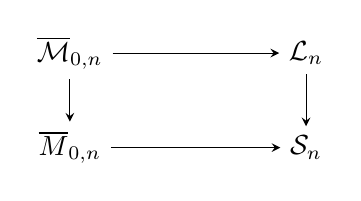
\begin{tikzpicture}[baseline=(current bounding box.center),>=stealth]
    \node (a) at (0,1.2) {$\overline{\mathcal M}_{0,n}$};
    \node (b) at (3,1.2) {$\mathcal L_n$};
    \node (c) at (0,0) {$\overline M_{0,n}$};
    \node (d) at (3,0) {$\mathcal S_n$};
    \draw[->] (a)--(b); \draw[->] (a)--(c);
    \draw[->] (b)--(d); \draw[->] (c)--(d);
  \end{tikzpicture}
\end{equation}
其中 $\overline{\mathcal M}_{0,n}\to\overline M_{0,n}$ 由
式~\eqref{eq:D-4-1} 定义；双射 $\mathcal L_n\to\mathcal S_n$
由定理 D.2.6 给出；$\overline{\mathcal M}_{0,n}\to\mathcal L_n$
把\BookRecordIndex{T0339}稳定曲线 $(T,E,\mathbf z)$ 送到\BookRecordIndex{T0084}带标号树
$(T,E,\Lambda(\mathbf z))$，其中
$\Lambda_\alpha(\mathbf z)=\{i\mid\alpha_i=\alpha\}$；
$\overline M_{0,n}\to\mathcal S_n$ 则是 $w\mapsto S(w)$。
\end{lemma}

\begin{proof}
取 $w\in\overline M_{0,n}$。反设 $S(w)$ 不是 \BookRecordIndex{T0008}$n$-分割网络，
则存在 $I,J\in S(w)$，使 $I\cap J\ne\varnothing$、$I\not\subset J$、
$J\not\subset I$。取 $i\in I\setminus J$、$j\in J\setminus I$、
$\nu\in I\cap J$。于是 $w_{\nu ijn}=w_{\nu jin}=\infty$，
与式~\eqref{eq:D-4-2} 矛盾。故有良定义的映射
$\overline M_{0,n}\to\mathcal S_n$（允许 $S(w)$ 为空）。

设 $\mathbf z$ 为对应带 $n$ 个标号树 $(T,E,\Lambda)$ 的亏格零\BookRecordIndex{T0339}稳定曲线，
记 $w=w(\mathbf z)\in\overline M_{0,n}$。需证
$S(w)=S(T,E,\Lambda)$。设 $I\in\mathcal I_n$ 是一个 \BookRecordIndex{T0008}$n$-分割，
并取互异的 $i,i'\in I$、$j,j'\notin I$。则
\[
  w_{ii'jj'}=\infty
  \quad\Longleftrightarrow\quad
  [\alpha_i,\alpha_{i'}]\cap[\alpha_j,\alpha_{j'}]=\varnothing.
\]
因此 $I\in S(w)$ 当且仅当 $I\in S(T,E,\Lambda)$，引理得证。
\end{proof}

下面的引理列出条件~\eqref{eq:D-4-3} 的几个重要推论。
\begin{lemma}\label{lem:D-4-4}
设 $w\in\overline M_{0,n}$。
\begin{enumerate}
\item[(i)] 若 $I\in S(w)$ 是 \BookRecordIndex{T0009}$w$-分割，且 $i,i',i''\in I$
两两互异，则对所有 $j,j'\notin I$，
$w_{ii'i''j}=w_{ii'i''j'}$。
\item[(ii)] 若 $w_{ijk\ell}=\infty$，则存在一个 \BookRecordIndex{T0009}$w$-分割
$I\in S(w)$，使 $i,j\in I$、$k,\ell\notin I$，或反之。
\end{enumerate}
\end{lemma}
\begin{proof}
先证 (i)。反设存在 $j,j'\notin I$ 使
$w_{ii'i''j}\ne w_{ii'i''j'}$。于是
$(1,\infty,w_{ii'i''j},w_{ii'i''j'})\notin\Delta_3$，由
式~\eqref{eq:D-4-3}，
\[
  w_{i'i''jj'}=
  \frac{w_{ii'i''j'}-1}{w_{ii'i''j'}-w_{ii'i''j}}
  \ne\infty,
\]
与 $I$ 是 \BookRecordIndex{T0009}$w$-分割矛盾。

为证 (ii)，先注意\BookRecordIndex{T0185}交比的对称性给出
\[
  w_{ijk\ell}=\infty\quad\Longrightarrow\quad
  w_{ij\ell k}=w_{k\ell ij}=w_{k\ell ji}=\infty.
\]
故可重排指标，使 $\ell>i,j,k$。在 $w_{ijk\ell}=\infty$ 时，
$I:=\{i,j\}$ 是指标集 $\{i,j,k,\ell\}$ 的分割。现在以归纳法用
如下断言构造把 $\{i,j\}$ 与 $\{k,\ell\}$ 分开的 $(w,n)$-分割。

\emph{断言。} 若 $I\in\mathcal I_{n-1}$ 是 $(w,n-1)$-分割，则
$I$ 或 $\{1,\ldots,n-1\}\setminus I$ 是 $(w,n)$-分割。

为证此断言，设 $I\in\mathcal I_{n-1}$ 为 $(w,n-1)$-分割。
我们将证明：或者
\[
  i,i'\in I,\ j\notin I\quad\Longrightarrow\quad
  w_{ii'jn}=\infty,
\]
因而 $I$ 是 $(w,n)$-分割；或者
\[
  i\in I,\ j,j'\notin I\quad\Longrightarrow\quad
  w_{injj'}=\infty,
\]
因而 $\{1,\ldots,n-1\}\setminus I$ 是 $(w,n)$-分割。
设某些 $i_0,i_1\in I$ 与 $j_0\notin I$ 满足
$w_{i_0i_1j_0n}\ne\infty$。因所有 $j\notin I$ 都有
$w_{i_0i_1j_0j}=\infty$，故
$(1,\infty,w_{i_0i_1j_0j},w_{i_0i_1j_0n})\notin\Delta_3$，
由式~\eqref{eq:D-4-3}，
\[
  w_{i_1j_0jn}=
  \frac{w_{i_0i_1j_0n}-1}{w_{i_0i_1j_0n}-w_{i_0i_1j_0j}}
  =0.
\]
这说明任意 $i\in I$、$j\notin I$ 均满足
$(1,\infty,w_{i_1j_0ji},w_{i_1j_0jn})\notin\Delta_3$，
由式~\eqref{eq:D-4-3} 得 $w_{j_0jin}=\infty$。
这里用到了 $w_{ii_1j_0j}=\infty$，从而 $w_{i_1j_0ji}=0$。
由于 $w_{j_0jin}=\infty$ 对所有 $j\notin I$ 成立，
由\BookRecordIndex{T0185}交比的对称性，$w_{j_0inj}=0$ 对所有 $j\notin I$ 成立。
于是
$(1,\infty,w_{j_0inj},w_{j_0inj'})\notin\Delta_3$，
由式~\eqref{eq:D-4-3}，
\[
  w_{injj'}=
  \frac{w_{j_0inj'}-1}{w_{j_0inj'}-w_{j_0inj}}=\infty
\]
对所有 $i\in I$、$j,j'\notin I$ 成立。这证明了 (ii) 与引理。
\end{proof}

\noindent\textbf{定理~\ref{thm:D-4-2}(ii) 的证明。}
先证 $\overline{\mathcal M}_{0,n}\to\overline M_{0,n}$ 为单射。
设 $\mathbf z,\widetilde{\mathbf z}\in SC_{0,n}$，且对所有互异
$i,j,k,\ell\in\{1,\ldots,n\}$ 有
$w_{ijk\ell}=w_{ijk\ell}(\mathbf z)=w_{ijk\ell}(\widetilde{\mathbf z})$。
由定理 D.2.6 与引理~\ref{lem:D-4-3}，两条曲线的\BookRecordIndex{T0084}带标号树同构。
不妨设 $T=\widetilde T$、$E=\widetilde E$，且
$\alpha_i=\widetilde\alpha_i$ 对所有 $i$ 成立。
任取顶点 $\alpha\in T$。对每条边 $\alpha E\beta$，选
$i_{\alpha\beta}\in\{1,\ldots,n\}$，使
$\alpha_{i_{\alpha\beta}}\in T_{\alpha\beta}$，并记
\[
  I_\alpha:=\{i\mid\alpha_i=\alpha\}
  \cup\{i_{\alpha\beta}\mid\alpha E\beta\}.
\]
于是 $\#I_\alpha\ge3$，且任意互异的
$i,j,k,\ell\in I_\alpha$ 满足
\[
  w(z_{\alpha i},z_{\alpha j},z_{\alpha k},z_{\alpha\ell})
  =w(\widetilde z_{\alpha i},\widetilde z_{\alpha j},
     \widetilde z_{\alpha k},\widetilde z_{\alpha\ell})
  \notin\{0,1,\infty\}.
\]
故有唯一 \BookRecordIndex{T0040}Möbius 变换 $\phi_\alpha$，使
$\phi_\alpha(z_{\alpha i})=\widetilde z_{\alpha i}$ 对所有
$i\in I_\alpha$ 成立。因此在 $\alpha_i=\alpha$ 时
$\phi_\alpha(z_i)=\widetilde z_i$，在 $\alpha E\beta$ 时
$\phi_\alpha(z_{\alpha\beta})=\widetilde z_{\alpha\beta}$。
由定义~\ref{def:D-3-4}，两曲线等价，故映射为单射。

再证满射。给定 $w\in\overline M_{0,n}$。由定理 D.2.6 和
引理~\ref{lem:D-4-3}，存在带 $n$ 个标号的树 $(T,E,\Lambda)$，
使 $S(T,E,\Lambda)=S(w)$。按边数归纳构造满足 $w(\mathbf z)=w$
的曲线 $\mathbf z$。
先设 $T=\{\mathrm{pt}\}$，没有 \BookRecordIndex{T0009}$w$-分割。
由引理~\ref{lem:D-4-4}(ii)，对所有互异 $i,j,k,\ell$，
$w_{ijk\ell}\notin\{0,1,\infty\}$。取
\[
  z_1=0,\quad z_2=1,\quad z_3=\infty,\quad
  z_\ell=w_{123\ell},\qquad \ell=4,\ldots,n.
\]
这些点两两互异，并满足所有 $w_{ijk\ell}=w(z_i,z_j,z_k,z_\ell)$。
当 $\{i,j,k\}=\{1,2,3\}$ 时，这是定义。由递推式~\eqref{eq:D-4-3}
及式~\eqref{eq:D-1-3}，对 $k,\ell\in\{4,\ldots,n\}$ 有
\[
  w_{12k\ell}=
  \frac{w_{312\ell}-1}{w_{312\ell}-w_{312k}}
  =w(z_1,z_2,z_k,z_\ell).
\]
因为 $w_{12k\ell}\ne\infty$，特别得 $z_k\ne z_\ell$（$k\ne\ell$）。
类似地，以 $j$ 代 $2$、以 $i$ 代 $1$，可证所有四指标情形。

一般情形取任意顶点 $\alpha\in T$。同单射证明，置
\[
  I_\alpha:=\{i\mid\alpha_i=\alpha\}
  \cup\{i_{\alpha\beta}\mid\alpha E\beta\},
\]
其中 $i_{\alpha\beta}\in\{1,\ldots,n\}$ 使
$\alpha_{i_{\alpha\beta}}\in T_{\alpha\beta}$。
引理~\ref{lem:D-4-4}(ii) 给出
$w_{ijk\ell}\notin\{0,1,\infty\}$（$i,j,k,\ell\in I_\alpha$）；
引理~\ref{lem:D-4-4}(i) 说明这些值不依赖 $i_{\alpha\beta}$ 的选取。
由上述第一步，对每个 $\alpha$ 存在一组两两互异的
$\zeta_i\in S^2$（$i\in I_\alpha$），满足
$w_{ijk\ell}=w(\zeta_i,\zeta_j,\zeta_k,\zeta_\ell)$。
当 $\alpha_i=\alpha$ 时令 $z_i:=\zeta_i$，当 $\alpha E\beta$ 时令
$z_{\alpha\beta}:=\zeta_{i_{\alpha\beta}}$。
这给出\BookRecordIndex{T0339}稳定曲线 $\mathbf z\in SC_{0,n}$，且 $w(\mathbf z)=w$。
定理~\ref{thm:D-4-2}(ii) 得证。\qed

\noindent\textbf{坐标图的构造。}
定理~\ref{thm:D-4-2}(iii) 的证明依靠显式坐标图。
给定 $w^0=w(\mathbf z^0)\in\overline M_{0,n}$，对应的\BookRecordIndex{T0084}带标号树为
$(T,E,\Lambda)$。我们选择 $n-3$ 个\BookRecordIndex{T0185}交比作为坐标，使其余\BookRecordIndex{T0185}交比在
$w^0$ 的邻域中可由这些坐标光滑重建。选择具有几何意义：
首先，每个顶点 $\alpha$ 取 $n_\alpha-3$ 个\BookRecordIndex{T0185}交比，它们在复自同构
意义下确定 $n_\alpha$ 个\BookRecordIndex{T0320}特殊点的位置；因为\BookRecordIndex{T0320}特殊点互异，
这些\BookRecordIndex{T0185}交比都在 $S^2\setminus\{0,1,\infty\}$ 中。
其次，对每条边 $\alpha E\beta$ 取一个“法向”坐标 $w_{ijk\ell}$，
它在 $w^0$ 处等于 $\infty$，且 $w_{ijk\ell}(w)=\infty$
当且仅当 $w$ 对应的树中有一条与 $\alpha E\beta$ 相应的边。
由引理 D.2.3 的公式
\[
  \sum_{\alpha\in T}(n_\alpha-3)+e(T)=n-3
\]
可知坐标总数为 $n-3$。

\noindent\textbf{定理~\ref{thm:D-4-2}(iii) 的证明。}
固定 $w^0=w(\mathbf z^0)\in\overline M_{0,n}$ 及其\BookRecordIndex{T0084}带标号树
$(T,E,\Lambda)$。记
\[
  I_{\alpha\beta}:=
  \{i\in\{1,\ldots,n\}\mid\alpha_i\in T_{\alpha\beta}\}.
\]
如定理~\ref{thm:D-4-2}(ii) 的证明，取函数
$E\to\{1,\ldots,n\}:(\alpha,\beta)\mapsto i_{\alpha\beta}$，
满足 $i_{\alpha\beta}\in I_{\alpha\beta}$。我们证明可选成还满足
\begin{equation}\label{eq:D-4-6}
  i_{\alpha\beta}\in I_\beta,\qquad
  I_\beta:=\Lambda_\beta\cup
  \{i_{\beta\gamma}\mid\gamma\in T,\ \beta E\gamma\},
  \qquad(\alpha,\beta)\in E.
\end{equation}
沿 $E$ 的递增子集列归纳构造。首先置
\[
  E^0:=\{(\alpha,\beta)\in E\mid\Lambda_\beta\ne\varnothing\},
\]
任取 $\lambda^0:E^0\to\{1,\ldots,n\}$，使
$\lambda^0(\alpha,\beta)\in\Lambda_\beta$。然后对每条
$\alpha E\beta$ 递归定义
$\Lambda_\beta=:\Lambda^0(\alpha,\beta)
\subset\Lambda^1(\alpha,\beta)\subset\cdots\subset
\Lambda^k(\alpha,\beta)$，并置
$E^k:=\{(\alpha,\beta)\in E\mid
\Lambda^k(\alpha,\beta)\ne\varnothing\}$。
若已有 $\lambda^k:E^k\to\{1,\ldots,n\}$，满足
$\lambda^k(\alpha,\beta)\in\Lambda^k(\alpha,\beta)$，则令
\begin{equation}\label{eq:D-4-7}
  \Lambda^{k+1}(\alpha,\beta):=\Lambda_\beta\cup
  \{\lambda^k(\beta,\gamma)\mid
  (\beta,\gamma)\in E^k,\ \gamma\ne\alpha\}.
\end{equation}
在 $E^k$ 上保持 $\lambda^{k+1}=\lambda^k$，在其余边上任取
$\lambda^{k+1}(\alpha,\beta)\in\Lambda^{k+1}(\alpha,\beta)$。
继续归纳。稍作思考可知，$E^k$ 恰为所有可作为一条至多含
$k+1$ 条边、终点为某个 $\Lambda_\gamma\ne\varnothing$ 的链之起点的
$(\alpha,\beta)\in E$。故有限步后 $\Lambda^k(\alpha,\beta)\ne\varnothing$
对所有边成立，且 $E^k=E$。由式~\eqref{eq:D-4-7} 归纳可知
$\Lambda^k(\alpha,\beta)\subset I_{\alpha\beta}$；
当 $E^k=E$ 时，置 $i_{\alpha\beta}:=\lambda^k(\alpha,\beta)$，
并注意每条边还满足
$\Lambda^{k+1}(\alpha,\beta)=I_\beta\setminus\{i_{\beta\alpha}\}$。

现在为树结构为 $(T,E,\Lambda)$ 的 $w^0$ 附近选择 $n-3$ 个坐标。
若顶点 $\alpha\in T$ 有 $n_\alpha\ge4$ 个\BookRecordIndex{T0320}特殊点，把
$I_\alpha$ 写成 $\{i_1(\alpha),\ldots,i_{n_\alpha}(\alpha)\}$。
这些点 $z^0_{\alpha i_\nu(\alpha)}$ 两两互异。选取分量
\begin{equation}\label{eq:D-4-8}
  x_{\alpha\nu}(w):=
  w_{i_1(\alpha)i_2(\alpha)i_3(\alpha)i_\nu(\alpha)}(w),
  \qquad\nu=4,\ldots,n_\alpha.
\end{equation}
若边 $\alpha E\beta$ 满足归一化条件 $\alpha_n\in T_{\beta\alpha}$，
则选四个互异指标
\[
  i,j\in I_\alpha\setminus\{i_{\alpha\beta}\},\qquad
  k,\ell\in I_\beta\setminus\{i_{\beta\alpha}\},\qquad
  i=i_{\beta\alpha},\quad k=i_{\alpha\beta},
\]
如图~\ref{fig:D-4-5}，并选取分量
\begin{equation}\label{eq:D-4-9}
  y_{\alpha\beta}(w):=w_{ijk\ell}(w).
\end{equation}

\begin{figure}[htbp]
  \centering\input{chapters/appD/figures/fig-D-4-5.tex}
  \caption{边 $\alpha E\beta$ 的坐标 $w_{ijk\ell}$。}
  \label{fig:D-4-5}
\end{figure}

需证明：在给定点 $w^0\in\overline M_{0,n}$ 的邻域中，$w$ 的
所有分量都能表示成式~\eqref{eq:D-4-8} 和~\eqref{eq:D-4-9}
给出的 $n-3$ 个坐标的光滑函数。按边数归纳。先设
$T=\{\mathrm{pt}\}$，所选坐标即
$w_{1234},w_{1235},\ldots,w_{123n}$。
由 D.1 节的递推公式~\eqref{eq:D-1-3}，在开集
\[
  U:=\{w\in\overline M_{0,n}\mid
  w_{ijk\ell}\notin\{0,1,\infty\}\text{ 对所有 }i,j,k,\ell\},
\]
每个 $w_{ijk\ell}$ 都是 $w_{123m}$（$m=4,\ldots,n$）的光滑函数。
若 $i,j,k,\ell\in\{4,\ldots,n\}$，显式公式为
\[
  w_{ijk\ell}=
  \frac{(w_{123j}-w_{123k})(w_{123\ell}-w_{123i})}
  {(w_{123i}-w_{123j})(w_{123k}-w_{123\ell})}.
\]
此公式按 D.1 节式~\eqref{eq:D-1-2} 的规则扩展到任意
$i,j,k,\ell$：
\[
  w_{ijk\ell}=\begin{cases}
    \infty,&i=j\text{ 或 }k=\ell,\\
    1,&i=k\text{ 或 }j=\ell,\\
    0,&i=\ell\text{ 或 }j=k.
  \end{cases}
\]

现在设 $e(T)=\#\{\text{边}\}\ge1$，且边数严格较少的树已得结论。
任取边 $\alpha E\beta$。必要时重排指标，不妨设
\[
  I_{\beta\alpha}=\{1,\ldots,m\},\qquad
  I_{\alpha\beta}=\{m+1,\ldots,n\},\qquad
  i_{\beta\alpha}=m,\quad i_{\alpha\beta}=m+1,
\]
\sourcefootnote{原书在选边坐标时要求 $\alpha_n\in T_{\beta\alpha}$，
而此处又令 $I_{\beta\alpha}=\{1,\ldots,m\}$（$m<n$），从而
$n\notin I_{\beta\alpha}$。两处有向边的朝向约定不一致；
本段保留原记号，按此处两侧指标集合核对后续公式。}
且与边 $\alpha E\beta$ 对应的坐标为
\[
  y_{\alpha\beta}(w)=w_{1,m,m+1,n}.
\]
考虑投影 $w\mapsto w_I$ 与 $w\mapsto w_J$，其中
\[
  w_I:=\{w_{ijk\ell}\}_{i,j,k,\ell\le m+1},\qquad
  w_J:=\{w_{ijk\ell}\}_{i,j,k,\ell\ge m}.
\]
注意 $w_I^0\in\overline M_{0,m+1}$ 对应的树为 $T_{\beta\alpha}$；
其中第 $m+1$ 个\BookRecordIndex{T0066}标记点对应于 $w^0$ 中的边 $\alpha E\beta$。
按归纳假设，与 $T_{\beta\alpha}$ 的顶点和边相关的 $m-2$ 个坐标
均不含大于 $m+1$ 的指标，因而属于 $w_I$。
所以在 $w^0$ 的邻域中，凡 $i,j,k,\ell\in\{1,\ldots,m+1\}$，
$w_{ijk\ell}$ 都可由这些坐标光滑重建。
类似地，对 $i,j,k,\ell\in\{m,\ldots,n\}$，
所有分量都可由对应于 $T_{\alpha\beta}$ 的 $n-m-2$ 个坐标光滑重建。
剩下只需证明：在 $w^0$ 的某邻域中，$w$ 的所有分量
都可作为 $w_{1,m,m+1,n}$ 及所有满足
$i,j,k,\ell\le m$ 或 $i,j,k,\ell\ge m+1$ 的
$w_{ijk\ell}$ 的光滑函数。

为此先注意 $w_{1,m+1,n,m}(w^0)=0$。由
式~\eqref{eq:D-4-3}，对 $1<i<m$ 有
\[
  w_{m,m+1,n,i}=
  \frac{w_{1,m,m+1,i}-1}
  {w_{1,m,m+1,i}-w_{1,m,m+1,n}}.
\]
\sourcefootnote{原书印刷第637页此式的左端及分式有误。此处将
$(1,m,m+1,n,i)$ 代入式~\eqref{eq:D-4-3}，并据下文
$w_{m,m+1,n,i}(w^0)=0$ 补正。第二版作者勘误所列分式为
$(w_{1,m,m+1,n}-1)/(w_{1,m,m+1,n}-w_{1,m,m+1,i})$；
它在 $w_{1,m,m+1,n}(w^0)=\infty$ 时趋于 $1$ 而非 $0$，
故与此处递推式和紧接的论证仍不符。}
若取 $i\le m-1$，则 $w_{m,m+1,n,i}(w^0)=0$，由
式~\eqref{eq:D-4-3}，
\[
  w_{m+1,n,i,j}=
  \frac{w_{m,m+1,n,j}-1}
  {w_{m,m+1,n,j}-w_{m,m+1,n,i}}
\]
对所有 $j$ 成立。若再取 $i,j\le m$，则
$w_{m+1,i,j,n}(w^0)=0$，再用式~\eqref{eq:D-4-3}，
\[
  w_{i,j,k,n}=
  \frac{w_{m+1,i,j,n}-1}
  {w_{m+1,i,j,n}-w_{m+1,i,j,k}}
\]
对所有 $k$ 成立。最后，当 $\ell\ge m+1$ 时，
$w_{nij\ell}(w^0)=0$，故仍由式~\eqref{eq:D-4-3}，
\[
  w_{ijk\ell}=
  \frac{w_{nij\ell}-1}{w_{nij\ell}-w_{nijk}}
\]
对所有 $\ell\ge m+1$、$i,j\le m$ 及所有 $k$ 成立。
这样，在 $w^0$ 的某邻域中，只要 $i,j\le m$ 且
$k,\ell\ge m+1$，或者 $i,j,k\le m$ 且 $\ell\ge m+1$，
便已把 $w_{ijk\ell}$ 写成所需形式。
$i\le m$、$j,k,\ell\ge m+1$ 的情形由对偶性得到。
定理~\ref{thm:D-4-2} 得证。\qed

\begin{exercise}\label{ex:D-4-5}
上面在 $\overline{\mathcal M}_{0,n}$ 每个元素 $\mathbf z$ 附近构造了
显式坐标图。请用第 10 章采用的黏合与黏合参数语言来解释这些坐标图。
\end{exercise}

\noindent\textbf{分\BookRecordIndex{T0072}层。}
群 $G$ 作用于 $S^2$ 上 $n$ 个互异点组成的空间
$(S^2)^n\setminus\Delta_n$。商空间
\begin{equation}\label{eq:D-4-10}
  \mathcal M_{0,n}:=\frac{(S^2)^n\setminus\Delta_n}{G}
\end{equation}
是带 $n$ 个穿孔的二球面上复结构的\BookRecordIndex{T0246}模空间。此商空间不紧；
由嵌入 $\overline{\mathcal M}_{0,n}\to(S^2)^N$ 诱导拓扑的
$\overline{\mathcal M}_{0,n}$ 是它的
\emph{Grothendieck--Knudsen 紧化}。在
$\mathcal M_{0,n}\to\overline{\mathcal M}_{0,n}$ 的识别下，
子集 $\mathcal M_{0,n}$ 对应于
\begin{equation}\label{eq:D-4-11}
  M_{0,n}:=\{w\in\overline M_{0,n}\mid
  w_{ijk\ell}\notin\{0,1,\infty\}
  \text{ 对所有 }i,j,k,\ell\}.
\end{equation}
下一个命题说明，$\overline M_{0,n}$ 中\BookRecordIndex{T0106}顶层 $M_{0,n}$ 的补集
是有限个实余维为 $2$ 的光滑子流形之并。先引入记号。
给定 \BookRecordIndex{T0008}$n$-分割 $I\in\mathcal I_n$，令
\begin{equation}\label{eq:D-4-12}
  V_I:=\{w\in\overline M_{0,n}\mid I\in S(w)\}.
\end{equation}
因此，一条\BookRecordIndex{T0339}稳定曲线 $\mathbf z\in SC_{0,n}$ 满足
$w(\mathbf z)\in V_I$，当且仅当有一条边把 $I$ 中的\BookRecordIndex{T0066}标记点
与不在 $I$ 中的\BookRecordIndex{T0066}标记点分开。更一般地，对任意 \BookRecordIndex{T0008}$n$-分割网络
$S\in\mathcal S_n$，定义
\begin{equation}\label{eq:D-4-13}
  V_S:=\{w\in\overline M_{0,n}\mid S\subset S(w)\}
  =\bigcap_{I\in S}V_I.
\end{equation}
注意 $w(\mathbf z)\in V_S$ 当且仅当 $\mathbf z$ 的树结构是
$S$ 对应树结构的一个细化；还要注意 $V_\varnothing=\overline M_{0,n}$。

\begin{exercise}\label{ex:D-4-6}
令 $n=8$，且
$S=\bigl\{\{1,2\},\{3,4\},\{5,6\},\{1,2,3,4,5,6\}\bigr\}$。
描述 $V_S$ 中的元素，并验证下一个定理的 (iv)。
\end{exercise}

\begin{theorem}[Knudsen]\label{thm:D-4-7}
\begin{enumerate}
\item[(i)] 对每个 \BookRecordIndex{T0008}$n$-分割 $I\in\mathcal I_n$，子集
$V_I\subset\overline M_{0,n}$ 是复余维为 $1$ 的紧复子流形。
\item[(ii)] 若 $S\subset\mathcal I_n$，则
\[
  V_S\ne\varnothing\quad\Longleftrightarrow\quad S\in\mathcal S_n.
\]
\item[(iii)] 对每个 \BookRecordIndex{T0008}$n$-分割网络
$S=\{I_1,\ldots,I_m\}\in\mathcal S_n$，
子流形 $V_{I_1},\ldots,V_{I_m}$ 横截相交，因而
\[
  V_S=\bigcap_{j=1}^m V_{I_j}\subset\overline M_{0,n}
\]
是复余维 $\operatorname{codim}V_S=\#S$ 的复子流形。
\item[(iv)] 若 $S\in\mathcal S_n$ 对应\BookRecordIndex{T0084}带标号树 $(T,E,\Lambda)$，
且 $n_\alpha$ 由式~\eqref{eq:D-2-1} 对 $\alpha\in T$ 定义，
则存在微分同胚
\[
  V_S\cong\prod_{\alpha\in T}\overline M_{0,n_\alpha}.
\]
\end{enumerate}
\end{theorem}
\begin{proof}
断言 (i) 与 (iii) 直接由定理~\ref{thm:D-4-2}(iii) 证明中
坐标图的构造得出。为说明这一点，固定
$w^0=w(\mathbf z^0)\in\overline M_{0,n}$，
令 $I\in S(w^0)$ 为对应边 $\alpha E\beta$ 的 $w^0$-分割，
并设指标 $i,j,k,\ell$ 满足
\begin{equation}\label{eq:D-4-14}
  i,j\in I,\qquad k,\ell\notin I,\qquad
  z^0_{\alpha i}\ne z^0_{\alpha j},\qquad
  z^0_{\beta k}\ne z^0_{\beta\ell}.
\end{equation}
使用三项观察。首先，条件~\eqref{eq:D-4-14} 成立当且仅当
$I$ 是唯一把指标对 $\{i,j\}$ 与 $\{k,\ell\}$ 分开的
$w(\mathbf z^0)$-分割。其次，若 $w$ 充分接近 $w^0$，则
\[
  S(w)\subset S(w^0).
\]
第三，若 $w_{ijk\ell}=\infty$，则由引理~\ref{lem:D-4-4}(ii)
存在一个把 $\{i,j\}$ 与 $\{k,\ell\}$ 分开的 \BookRecordIndex{T0009}$w$-分割。
前两项观察说明这只能是 $I$。故当 $w$ 接近 $w^0$ 时，
\begin{equation}\label{eq:D-4-15}
  I\in S(w)\quad\Longleftrightarrow\quad w_{ijk\ell}=\infty.
\end{equation}
而定理~\ref{thm:D-4-2}(iii) 的证明表明，$w^0$ 附近有
$\overline M_{0,n}$ 的坐标图，其中每个 $w^0$-分割
$I\in S(w^0)$ 都由一个满足~\eqref{eq:D-4-14} 的坐标表示。
这证明 (i) 与 (iii)。

为证 (ii)，设 $S\subset\mathcal I_n$ 是不满足式~\eqref{eq:D-2-3}
的 \BookRecordIndex{T0008}$n$-分割集合。则存在 $I,J\in S$，使
\[
  I\cap J\ne\varnothing,\qquad I\setminus J\ne\varnothing,
  \qquad J\setminus I\ne\varnothing.
\]
此时引理~\ref{lem:D-4-3} 表明 $V_I\cap V_J=\varnothing$。

为证 (iv)，对每个 $\alpha\in T$ 取指标集
$I_\alpha\subset\{1,\ldots,n\}$，使其包含 $\Lambda_\alpha$，
并且对每条边 $\alpha E\beta$，恰好含有集合
$I_{\alpha\beta}(T,E,\Lambda)$ 的一个元素，
如定理~\ref{thm:D-4-2} 的证明。考虑只记住 $I_\alpha$ 中指标的投影
\[
  \pi_\alpha:\overline M_{0,n}\longrightarrow
  \overline M_{0,n_\alpha}.
\]
这些投影给出显然单射的映射
\[
  \pi_S:V_S\longrightarrow
  \prod_{\alpha\in T}\overline M_{0,n_\alpha}.
\]
为证其满射，任取元组 $\{w_\alpha\}_{\alpha\in T}$，
其中 $w_\alpha\in\overline M_{0,n_\alpha}$，并用树结构
重建其余分量 $w_{ijk\ell}$：若某 $I\in S$ 满足
$i,j\in I$、$k,\ell\notin I$，则定义 $w_{ijk\ell}=\infty$；
另外两种配对分割的情形同理。若不存在把四指标分成两对的分割，
则存在顶点 $\alpha$ 与四个互异指标
  $i',j',k',\ell'\in I_\alpha$，使 $i=i'$ 或
$\alpha_i,\alpha_{i'}\in T_{\alpha\beta}$\sourcefootnote{原书此处写 $i,i'\in T_{\alpha\beta}$；$i,i'$ 是指标，而 $T_{\alpha\beta}$ 是顶点集。依本节 $I_{\alpha\beta}$ 的定义，改作指标所标记的顶点属于该分支。} 对某条边 $\alpha E\beta$ 成立；
$j',k',\ell'$ 亦然。在这种情形令
$w_{ijk\ell}:=w_{i'j'k'\ell'}$。
容易验证这样定义的元组 $w$ 满足式~\eqref{eq:D-4-2}
与~\eqref{eq:D-4-3}，因而属于 $\overline M_{0,n}$。
这说明 $\pi_S$ 是满射，且其逆映射光滑，定理得证。
\end{proof}


\section{\BookRecordIndex{T0142}格罗莫夫拓扑}\label{sec:D-5}

本节内在地描述\BookRecordIndex{T0246}模空间 $\overline{\mathcal M}_{0,n}$ 上的拓扑，并证明它与由嵌入到二维球面乘积所定义的外在拓扑等价。以下定义是\BookRecordIndex{T0340}稳定映射的\BookRecordIndex{T0141}格罗莫夫收敛在目标流形为单点时的特例（见定义~\ref{def:5-5-1}）。

\begin{definition}\label{def:D-5-1}
设
\[
  \mathbf z^\nu=\bigl(\{z^\nu_{\alpha\beta}\}_{\alpha E^\nu\beta},
  \{\alpha_i^\nu,z_i^\nu\}_{1\le i\le n}\bigr)\in SC_{0,n}
\]
是一列\BookRecordIndex{T0339}稳定曲线，并设
\[
  \mathbf z=\bigl(\{z_{\alpha\beta}\}_{\alpha E\beta},
  \{\alpha_i,z_i\}_{1\le i\le n}\bigr).
\]
若对充分大的 $\nu$，存在满射的\BookRecordIndex{T0305}树同态 $f^\nu:T\to T^\nu$ 及一族 \BookRecordIndex{T0040}Möbius 变换 $\{\phi_\alpha^\nu\}_{\alpha\in T}^{\nu\in\mathbb N}$，满足以下条件，就称 $\mathbf z^\nu$ \emph{\BookRecordIndex{T0141}格罗莫夫收敛}于 $\mathbf z$。

\noindent\textup{（重标度）}若 $\alpha,\beta\in T$ 且 $\alpha E\beta$，并且 $\nu_j$ 是满足 $f^{\nu_j}(\alpha)=f^{\nu_j}(\beta)$ 的子序列，则
\[
  \phi_{\alpha\beta}^{\nu_j}:=(\phi_\alpha^{\nu_j})^{-1}\circ\phi_\beta^{\nu_j}
  \longrightarrow z_{\alpha\beta}
\]
在 $S^2\setminus\{z_{\beta\alpha}\}$ 的紧子集上一致收敛。

\noindent\textup{（\BookRecordIndex{T0191}节点）}若 $\alpha,\beta\in T$ 且 $\alpha E\beta$，并且 $\nu_j$ 是满足 $f^{\nu_j}(\alpha)\ne f^{\nu_j}(\beta)$ 的子序列，则
\[
  z_{\alpha\beta}=\lim_{j\to\infty}
  (\phi_\alpha^{\nu_j})^{-1}
  \bigl(z_{f^{\nu_j}(\alpha)f^{\nu_j}(\beta)}^{\nu_j}\bigr).
\]

\noindent\textup{（\BookRecordIndex{T0066}标记点）}对每个 $i$，有 $\alpha_i^\nu=f^\nu(\alpha_i)$，并且
\[
  z_i=\lim_{\nu\to\infty}(\phi_{\alpha_i}^\nu)^{-1}(z_i^\nu).
\]
\end{definition}

因为每棵树 $T$ 的满射像只有有限多个同构类，任何\BookRecordIndex{T0141}格罗莫夫收敛序列都是有限个子序列的并；在每个子序列上，树 $T^\nu$ 和映射 $f^\nu$ 均同构。上面（重标度）与（\BookRecordIndex{T0191}节点）公理涉及的正是这些子序列。

本节的主要结论如下。

\begin{theorem}\label{thm:D-5-2}
$\overline{\mathcal M}_{0,n}$ 上存在唯一的拓扑，使其收敛序列恰为\BookRecordIndex{T0141}格罗莫夫收敛序列。此拓扑与定理~\ref{thm:D-4-2} 的嵌入所诱导的 $\overline{\mathcal M}_{0,n}$ 上的拓扑一致。
\end{theorem}

在此拓扑下，$\overline{\mathcal M}_{0,n}$ 与 $\overline M_{0,n}$ 同胚，因而具有紧致度量空间的结构，实际上还是紧致光滑代数簇。

\begin{proposition}\label{prop:D-5-3}
设 $\mathbf z^\nu,\mathbf z\in SC_{0,n}$。以下条件等价：
\begin{enumerate}[label=(\roman*)]
\item $\mathbf z^\nu$ \BookRecordIndex{T0141}格罗莫夫收敛于 $\mathbf z$；
\item 对充分大的 $\nu$，存在满射\BookRecordIndex{T0305}树同态 $f^\nu:T\to T^\nu$ 和 \BookRecordIndex{T0040}Möbius 变换 $\phi_\alpha^\nu\in G$，使 $f^\nu(\alpha_i)=\alpha_i^\nu$，并且对 $i\in\{1,\ldots,n\}$、$\alpha\in T$，
\begin{equation}\label{eq:D-5-1}
  z_{\alpha i}=\lim_{\nu\to\infty}(\phi_\alpha^\nu)^{-1}
  \bigl(z_{f^\nu(\alpha)i}^\nu\bigr);
\end{equation}
\item 对任意四个互异的整数 $i,j,k,\ell\in\{1,\ldots,n\}$，
\begin{equation}\label{eq:D-5-2}
  w_{ijk\ell}(\mathbf z)=\lim_{\nu\to\infty}w_{ijk\ell}(\mathbf z^\nu).
\end{equation}
\end{enumerate}
\end{proposition}

\begin{proof}[命题~\ref{prop:D-5-3} \BookRecordIndex{T0326}推出定理~\ref{thm:D-5-2}]
由引理~\ref{lem:5-6-4}，为了证明 $\overline{\mathcal M}_{0,n}$ 上存在唯一拓扑，其收敛序列恰为\BookRecordIndex{T0141}格罗莫夫收敛序列，只须核验（常值）、（子序列）、（子子序列）、（对角线）及（唯一性）这五条公理。命题~\ref{prop:D-5-3} 的 (i) 与 (iii) 等价，说明序列\BookRecordIndex{T0141}格罗莫夫收敛当且仅当其在 $\overline M_{0,n}$ 中的像收敛，故这些公理成立。所得拓扑与拉回拓扑具有相同的收敛序列，因而必定一致。
\end{proof}

\begin{proof}[命题~\ref{prop:D-5-3} 的证明]
先证 (i) 蕴含 (ii)。设 $\mathbf z^\nu$ \BookRecordIndex{T0141}格罗莫夫收敛于 $\mathbf z$，反设某个 $\alpha\in T$ 与 $i\in\{1,\ldots,n\}$ 不满足~\eqref{eq:D-5-1}。取子序列后可设
\begin{equation}\label{eq:D-5-3}
  \lim_{\nu\to\infty}(\phi_\alpha^\nu)^{-1}
  \bigl(z_{f^\nu(\alpha)i}^\nu\bigr)=z_0\ne z_{\alpha i}.
\end{equation}
再取子序列，可设 $T^\nu=T'$ 且\BookRecordIndex{T0305}树同态 $f^\nu=f:T\to T'$ 均不依赖于 $\nu$。写 $f(\alpha)=:\alpha'$；这与标记的记号\BookRecordIndex{T0348}相容，因为 $f(\alpha_i)=\alpha_i'$，其中 $\alpha_i\in T$、$\alpha_i'\in T'$ 分别是承载第 $i$ 个\BookRecordIndex{T0066}标记点的顶点。

由~\eqref{eq:D-5-3} 和（\BookRecordIndex{T0066}标记点）公理，$\alpha\ne\alpha_i$。取从 $\gamma_{-\ell}=\alpha_i$ 到 $\gamma_k=\alpha$ 的链
\[
  \gamma_{-\ell},\ldots,\gamma_{-1},\gamma_0,\ldots,\gamma_k,
\]
使标号满足 $\gamma_j'=\alpha'$（$j\ge0$）及 $\gamma_j'\ne\alpha'$（$j<0$）。首先断言
\begin{equation}\label{eq:D-5-4}
  z_{\gamma_0i}=\lim_{\nu\to\infty}(\phi_{\gamma_0}^\nu)^{-1}
  (z_{\gamma_0'i}^\nu).
\end{equation}
若 $\alpha'=\alpha_i'$，则 $\gamma_0=\alpha_i$，故 $z_{\gamma_0i}=z_i$ 且 $z_{\gamma_0'i}^\nu=z_i^\nu$；此时~\eqref{eq:D-5-4} 来自定义~\ref{def:D-5-1} 的（\BookRecordIndex{T0066}标记点）公理。若 $\alpha'\ne\alpha_i'$，则 $z_{\gamma_0i}=z_{\gamma_0\gamma_{-1}}$，且 $z_{\gamma_0'i}^\nu=z_{\gamma_0'\gamma_{-1}'}^\nu$；此时~\eqref{eq:D-5-4} 来自（\BookRecordIndex{T0191}节点）公理。

有了~\eqref{eq:D-5-4}，我们归纳证明
\begin{equation}\label{eq:D-5-5}
  z_{\gamma_ji}=\lim_{\nu\to\infty}(\phi_{\gamma_j}^\nu)^{-1}
  (z_{\gamma_j'i}^\nu),\qquad j=1,\ldots,k.
\end{equation}
设它对 $j\le k-1$ 成立。注意 $z_{\gamma_ji}=z_{\gamma_j\gamma_{j-1}}\ne z_{\gamma_j\gamma_{j+1}}$。由（重标度）公理，$(\phi_{\gamma_{j+1}}^\nu)^{-1}\circ\phi_{\gamma_j}^\nu$ 在 $S^2\setminus\{z_{\gamma_j\gamma_{j+1}}\}$ 的紧子集上一致收敛于 $z_{\gamma_{j+1}\gamma_j}=z_{\gamma_{j+1}i}$。因此得到 $j+1$ 时的~\eqref{eq:D-5-5}，归纳完成。取 $j=k$ 即与~\eqref{eq:D-5-3} 矛盾，故 (i) 蕴含 (ii)。

现证 (ii) 蕴含 (iii)。仍只须考虑对每个 $\nu$ 都有 $T^\nu=T'$、$f^\nu=f:T\to T'$ 的情形。任取互异的 $i,j,k,\ell\in\{1,\ldots,n\}$，选择 $\alpha\in T$ 使 $(z_{\alpha i},z_{\alpha j},z_{\alpha k},z_{\alpha\ell})\notin\Delta_3$。由假设，$\alpha'=f(\alpha)$ 时，$z_{\alpha i}=\lim_{\nu\to\infty}(\phi_\alpha^\nu)^{-1}(z_{\alpha'i}^\nu)$；其余三个指标同理。因此对充分大的 $\nu$，$(z_{\alpha'i}^\nu,z_{\alpha'j}^\nu,z_{\alpha'k}^\nu,z_{\alpha'\ell}^\nu)\notin\Delta_3$，且
\begin{align*}
  w_{ijk\ell}(\mathbf z)
  &=w(z_{\alpha i},z_{\alpha j},z_{\alpha k},z_{\alpha\ell})\\
  &=\lim_{\nu\to\infty}w\bigl((\phi_\alpha^\nu)^{-1}(z_{\alpha'i}^\nu),\ldots,
      (\phi_\alpha^\nu)^{-1}(z_{\alpha'\ell}^\nu)\bigr)\\
  &=\lim_{\nu\to\infty}w(z_{\alpha'i}^\nu,z_{\alpha'j}^\nu,
      z_{\alpha'k}^\nu,z_{\alpha'\ell}^\nu)\\
  &=\lim_{\nu\to\infty}w_{ijk\ell}(\mathbf z^\nu).
\end{align*}
这证明了~\eqref{eq:D-5-2}。

再证 (iii) 蕴含 (ii)。若 (iii) 成立，则充分大的 $\nu$ 满足
\[
  w_{ijk\ell}(\mathbf z)\ne\infty\quad\Longrightarrow\quad
  w_{ijk\ell}(\mathbf z^\nu)\ne\infty,
\]
从而 $S(\mathbf z^\nu)\subset S(\mathbf z)$。由定理~\ref{thm:D-2-6}(iv)，对这样的 $\nu$，存在唯一的满射\BookRecordIndex{T0305}树同态 $f^\nu:T\to T^\nu$，使所有 $i$ 均满足 $f^\nu(\alpha_i)=\alpha_i^\nu$。下文记 $\alpha^\nu:=f^\nu(\alpha)\in T^\nu$。对每个 $\alpha\in T$ 选取 $i,j,k\in\{1,\ldots,n\}$，使 $\alpha=\alpha(i,j,k;T)$。由定理~\ref{thm:D-2-6}(iv)，$\alpha^\nu=\alpha(i,j,k;T^\nu)$。依注~\ref{rem:D-3-3}，这意味着 $z_{\alpha i},z_{\alpha j},z_{\alpha k}$ 两两不同，且对充分大的 $\nu$，$z_{\alpha^\nu i}^\nu,z_{\alpha^\nu j}^\nu,z_{\alpha^\nu k}^\nu$ 也两两不同。因而存在唯一的 \BookRecordIndex{T0040}Möbius 变换 $\phi_\alpha^\nu\in G$，满足
\[
  \phi_\alpha^\nu(z_{\alpha i})=z_{\alpha^\nu i}^\nu,\qquad
  \phi_\alpha^\nu(z_{\alpha j})=z_{\alpha^\nu j}^\nu,\qquad
  \phi_\alpha^\nu(z_{\alpha k})=z_{\alpha^\nu k}^\nu.
\]
断言这一序列满足~\eqref{eq:D-5-1}。确实，
\begin{align*}
  w_{ijk\ell}(\mathbf z^\nu)
  &=w(z_{\alpha^\nu i}^\nu,z_{\alpha^\nu j}^\nu,
      z_{\alpha^\nu k}^\nu,z_{\alpha^\nu\ell}^\nu)\\
  &=\frac{(z_{\alpha j}-z_{\alpha k})(\zeta_{\alpha\ell}^\nu-z_{\alpha i})}
          {(z_{\alpha i}-z_{\alpha j})(z_{\alpha k}-\zeta_{\alpha\ell}^\nu)},
  \qquad
  \zeta_{\alpha\ell}^\nu:=(\phi_\alpha^\nu)^{-1}
       (z_{\alpha^\nu\ell}^\nu).
\end{align*}
\sourcefootnote{原书实体页 657 此分式的分母第二因子印为 $z_{\alpha i}-\zeta_{\alpha\ell}^\nu$。由前一行的\BookRecordIndex{T0185}交比 $w(z_{\alpha i},z_{\alpha j},z_{\alpha k},\zeta_{\alpha\ell}^\nu)$ 及 D.1 节的\BookRecordIndex{T0185}交比定义，该因子应为 $z_{\alpha k}-\zeta_{\alpha\ell}^\nu$，此处据此补正。}
利用 $w_{ijk\ell}(\mathbf z^\nu)\to w_{ijk\ell}(\mathbf z)$，可得
\[
  z_{\alpha\ell}=\lim_{\nu\to\infty}\zeta_{\alpha\ell}^\nu
\]
对所有 $\alpha\in T$、$\ell\in\{1,\ldots,n\}$ 成立，故 (ii) 得证。

最后证 (ii) 蕴含 (i)。若 (ii) 成立，定义~\ref{def:D-5-1} 的（\BookRecordIndex{T0066}标记点）公理显然成立（在~\eqref{eq:D-5-1} 中取 $\alpha=\alpha_i$）。为验证（\BookRecordIndex{T0191}节点）公理，选 $i$ 使 $z_{\alpha\beta}=z_{\alpha i}$，于是 $z_{\alpha^\nu\beta^\nu}^\nu=z_{\alpha^\nu i}^\nu$，再应用~\eqref{eq:D-5-1}。为验证（重标度）公理，设 $\alpha E\beta$ 且 $f^\nu(\alpha)=f^\nu(\beta)=\alpha^\nu$ 对所有 $\nu$ 成立。选指标 $j,j'$，使 $z_{\beta\alpha},z_{\beta j},z_{\beta j'}$ 两两不同，因而 $z_{\alpha j}=z_{\alpha j'}=z_{\alpha\beta}$。由~\eqref{eq:D-5-1}，
\[
  \lim_{\nu\to\infty}(\phi_\beta^\nu)^{-1}(z_{\alpha^\nu j}^\nu)
   =z_{\beta j}\ne z_{\beta j'}
   =\lim_{\nu\to\infty}(\phi_\beta^\nu)^{-1}(z_{\alpha^\nu j'}^\nu),
\]
\[
  \lim_{\nu\to\infty}(\phi_\alpha^\nu)^{-1}(z_{\alpha^\nu j}^\nu)
   =z_{\alpha\beta}
   =\lim_{\nu\to\infty}(\phi_\alpha^\nu)^{-1}
       (z_{\alpha^\nu j'}^\nu).
\]
交换 $\alpha,\beta$ 的角色，还可找到指标 $i$，使
\[
  \lim_{\nu\to\infty}(\phi_\alpha^\nu)^{-1}(z_{\alpha^\nu i}^\nu)
    =z_{\alpha i}\ne z_{\alpha\beta},\qquad
  \lim_{\nu\to\infty}(\phi_\beta^\nu)^{-1}(z_{\alpha^\nu i}^\nu)
    =z_{\beta\alpha}.
\]
由引理~\ref{lem:D-1-4}，$(\phi_\alpha^\nu)^{-1}\circ\phi_\beta^\nu$ 在 $S^2\setminus\{z_{\beta\alpha}\}$ 的紧子集上一致收敛于 $z_{\alpha\beta}$。命题得证。
\end{proof}


\section{上同调}\label{sec:D-6}

\BookRecordIndex{T0023}Grothendieck--Knudsen 流形 $\overline{\mathcal M}_{0,n}$ 有许多值得注意的性质。定理~\ref{thm:D-4-7} 已表明，每个 \BookRecordIndex{T0008}$n$-分割网络都确定一个复子流形。这些子流形生成 $\overline{\mathcal M}_{0,n}$ 的上同调，并提供关于其环结构的有用信息。在下面的讨论中，有时将 $\overline{\mathcal M}_{0,n}$ 看作装饰树的集合，有时则将其视为带坐标 $w\in(S^2)^N$ 的流形 $\overline M_{0,n}$，会比较方便。

\paragraph{普适曲线。}
存在自然投影
\begin{equation}\label{eq:D-6-1}
  \pi:\overline M_{0,n+1}\longrightarrow\overline M_{0,n},
\end{equation}
它只保留不含指标 $n+1$ 的坐标 $w_{ijk\ell}$。该映射显然全纯，且取值于 $\overline M_{0,n}$（见式~\eqref{eq:D-4-4}）。在定理~\ref{thm:D-4-2} 的双射 $\overline{\mathcal M}_{0,n+1}\cong\overline M_{0,n+1}$ 下，它对应于删除第 $n+1$ 个\BookRecordIndex{T0066}标记点。在几何上可以这样描述：若承载第 $n+1$ 个\BookRecordIndex{T0066}标记点的顶点 $\alpha$ 有至少四个\BookRecordIndex{T0320}特殊点，删除该\BookRecordIndex{T0066}标记点后所得曲线仍稳定。否则，该顶点恰有三个\BookRecordIndex{T0320}特殊点，其中至少一个是\BookRecordIndex{T0191}节点。\sourcefootnote{原书实体页 658 此处写作 ``exactly three marked points, at least one of them nodal''；\BookRecordIndex{T0191}节点并非\BookRecordIndex{T0066}标记点。由本句后续的两种\BookRecordIndex{T0191}节点情形及稳定性定义，将 ``marked points'' 改作“\BookRecordIndex{T0320}特殊点”。}若它有两个\BookRecordIndex{T0191}节点，就删除该顶点，改以连接 $\alpha$ 的两条边所连的两个顶点上的一对新\BookRecordIndex{T0191}节点代替。若它有一个\BookRecordIndex{T0191}节点，以及指标为 $m$ 和 $n+1$ 的两个\BookRecordIndex{T0066}标记点，就删除该顶点，改在与 $\alpha$ 以一条边相连的唯一顶点上安放第 $m$ 个\BookRecordIndex{T0066}标记点。

对 $i=1,\ldots,n$，令 $Z_i\subset\overline M_{0,n+1}$ 为对应于 $(n+1)$-分割 $I_i:=\{1,\ldots,n\}\setminus\{i\}$ 的子集。它由所有带 $n+1$ 个\BookRecordIndex{T0066}标记点的亏格零\BookRecordIndex{T0339}稳定曲线同构类组成，其中指标 $i$ 与 $n+1$ 的\BookRecordIndex{T0066}标记点同处一个顶点，而且该顶点恰有三个\BookRecordIndex{T0320}特殊点。定理~\ref{thm:D-4-2} 的双射将 $Z_i$ 映为
\begin{equation}\label{eq:D-6-2}
  Z_i:=\bigl\{w\in\overline M_{0,n+1}\mid
  w_{jj'in+1}=\infty\quad
  \forall j,j'\in\{1,\ldots,n\}\setminus\{i\}\bigr\}.
\end{equation}
由定理~\ref{thm:D-4-7}，这是 $\overline M_{0,n+1}$ 的复子流形，且投影~\eqref{eq:D-6-1} 在其上的限制是微分同胚 $\pi:Z_i\to\overline M_{0,n}$。其逆是 $\pi$ 的截面，记作
\begin{equation}\label{eq:D-6-3}
  \sigma_i:\overline M_{0,n}\longrightarrow\overline M_{0,n+1},
  \qquad \pi\circ\sigma_i=\mathrm{id},\qquad
  \sigma_i(\overline M_{0,n})=Z_i,\quad i=1,\ldots,n.
\end{equation}
显式地，$\sigma_i$ 将 $w\in\overline M_{0,n}$ 送到如下定义的 $\sigma_i(w)\in\overline M_{0,n+1}$：
\[
  (\sigma_i(w))_{jk\ell m}:=
  \begin{cases}
    w_{jk\ell m},&j,k,\ell,m\le n,\\
    w_{jk\ell i},&m=n+1,\quad j,k,\ell\ne i,\\
    w_{jkim},&\ell=n+1,\quad j,k,m\ne i,\\
    w_{ji\ell m},&k=n+1,\quad j,\ell,m\ne i,\\
    w_{ik\ell m},&j=n+1,\quad k,\ell,m\ne i,\\
    0,&\{j,m\}=\{i,n+1\}\text{ 或 }\{k,\ell\}=\{i,n+1\},\\
    1,&\{j,\ell\}=\{i,n+1\}\text{ 或 }\{k,m\}=\{i,n+1\},\\
    \infty,&\{j,k\}=\{i,n+1\}\text{ 或 }\{\ell,m\}=\{i,n+1\}.
  \end{cases}
\]
这里 $j,k,\ell,m\in\{1,\ldots,n+1\}$ 两两互异。从几何上看，截面 $\sigma_i$ 把第 $i$ 个\BookRecordIndex{T0066}标记点“加倍”：它在树中引入一个与 $\alpha_i$ 以边相连的新顶点，该顶点承载指标 $i$ 与 $n+1$ 的\BookRecordIndex{T0066}标记点。

\begin{exercise}\label{ex:D-6-1}
用建模在\BookRecordIndex{T0084}带标号树上的 $SC_{0,n}$ 元组，写出投影~\eqref{eq:D-6-1} 和截面~\eqref{eq:D-6-3} 的显式公式。
\end{exercise}

\begin{exercise}\label{ex:D-6-2}
证明映射 $\pi:\overline M_{0,n+1}\to\overline M_{0,n}$ 是一个\BookRecordIndex{T0191}节点族，即 $\pi$ 的每个\BookRecordIndex{T0233}临界点都是\BookRecordIndex{T0191}节点（见文献~\srcite{337} 的定义 4.2）。证明 $M_{0,n+1}$ 中各点均为 $\pi$ 的\BookRecordIndex{T0405}正则点，$M_{0,n}$ 是 $\pi$ 的\BookRecordIndex{T0409}正则值集（见式~\eqref{eq:D-4-11}）。\sourcefootnote{原书实体页 659 写作 ``$M_{0,n+1}$ is the set of regular points''。这不能表示\BookRecordIndex{T0405}正则点集恰等于 $M_{0,n+1}$：例如 $n=3$ 时底空间 $\overline M_{0,3}$ 是单点，$\pi$ 的全部点均正则，而 $M_{0,4}$ 不含边界点。此处只将原句改为可成立的包含断言。}
\end{exercise}

由习题~\ref{ex:D-6-2} 可知，$\pi:\overline M_{0,n+1}\to\overline M_{0,n}$ 的每条纤维都是带 $n$ 个\BookRecordIndex{T0066}标记点的\BookRecordIndex{T0191}节点黎曼曲面，其\BookRecordIndex{T0066}标记点由截面 $Z_1,\ldots,Z_n$ 给出。事实上，对每条\BookRecordIndex{T0339}稳定曲线 $\mathbf z\in SC_{0,n}$，在式~\eqref{eq:D-4-1} 定义的点 $w(\mathbf z)\in\overline M_{0,n}$ 上方的纤维，同构于式~\eqref{eq:D-3-2} 定义的空间 $\Sigma(\mathbf z)$ 本身：
\begin{equation}\label{eq:D-6-4}
  \pi^{-1}(w(\mathbf z))\cong\Sigma(\mathbf z),\qquad
  \pi^{-1}(w(\mathbf z))\cap Z_i\cong[\alpha_i,z_i].
\end{equation}
为说明这一点，若 $[\alpha,z]$ 既不是 $\Sigma(\mathbf z)$ 的\BookRecordIndex{T0191}节点，也不等于 $n$ 个\BookRecordIndex{T0066}标记点中任何一个，就可把它作为第 $n+1$ 个\BookRecordIndex{T0066}标记点加入，得到纤维中的一个元素。若它恰为\BookRecordIndex{T0191}节点或某个\BookRecordIndex{T0066}标记点，则可添加一个球面，得到纤维中的元素。

带 $n$ 个截面、满足如下条件的\BookRecordIndex{T0191}节点族 $(\pi_B:Q\to B,Z_1,\ldots,Z_n)$ 称为\emph{带 $n$ 个\BookRecordIndex{T0066}标记点的亏格零\BookRecordIndex{T0191}节点黎曼曲面普适族}（见文献~\srcite{337} 的定义 5.1 与 6.2）。

\noindent\textup{（I）}对任意另一\BookRecordIndex{T0191}节点族 $(\pi_A:P\to A,R_1,\ldots,R_n)$ 及任意纤维同构 $f:P_a\to Q_b$，若 $f(P_a\cap R_i)=Q_b\cap Z_i$ 对 $i=1,\ldots,n$ 成立，则 $f$ 在 $P$ 中 $P_a$ 的某个邻域上唯一地延拓为\BookRecordIndex{T0191}节点族态射。

\noindent\textup{（II）}$Q$ 的每条纤维都是带 $n$ 个\BookRecordIndex{T0066}标记点的亏格零\BookRecordIndex{T0339}稳定曲线；反之，每条带 $n$ 个\BookRecordIndex{T0066}标记点的亏格零\BookRecordIndex{T0339}稳定曲线都恰与其中一条纤维同构。

文献~\srcite{337} 的定理 5.4 表明，带 $n$ 个截面的\BookRecordIndex{T0191}节点族 $(\pi_B:Q\to B,Z_1,\ldots,Z_n)$ 满足（I），当且仅当与每条纤维关联的线性化\BookRecordIndex{T0210}柯西--黎曼算子为双射。该算子的定义域是沿纤维的向量场空间，其中向量场投影到基底的一个常值切向量，且与截面 $Z_i$ 相切；值域是纤维上取值于\BookRecordIndex{T0308}竖直切丛的 $(0,1)$-形式空间。由~\eqref{eq:D-6-1}、\eqref{eq:D-6-2} 定义的\BookRecordIndex{T0191}节点族 $(\pi:\overline M_{0,n+1}\to\overline M_{0,n},Z_1,\ldots,Z_n)$ 按定义满足（II）；它还满足（I），这正是下一个习题的内容。它通常称为 $\overline M_{0,n}$ 上的普适曲线。

\begin{exercise}\label{ex:D-6-3}
证明 $(\pi:\overline M_{0,n+1}\to\overline M_{0,n},Z_1,\ldots,Z_n)$ 是带 $n$ 个\BookRecordIndex{T0066}标记点的亏格零\BookRecordIndex{T0191}节点黎曼曲面普适族。
\end{exercise}

\paragraph{上同调的生成元。}
Keel 在文献~\srcite{208} 中证明，与 \BookRecordIndex{T0008}$n$-分割网络 $S\in\mathcal S_n$ 相应的复子流形 $V_S$ 在加法意义上生成 $\overline M_{0,n}$ 的上同调。

\begin{theorem}[Keel]\label{thm:D-6-4}
$\overline M_{0,n}$ 单连通，且 $H^{\mathrm{odd}}(\overline M_{0,n};\mathbb Z)=\{0\}$。此外，若 $a\in H^{2k}(\overline M_{0,n};\mathbb Z)$ 对每个满足 $\#S=n-3-k$ 的 \BookRecordIndex{T0008}$n$-分割网络 $S\in\mathcal S_n$ 都有 $\langle a,[V_S]\rangle=0$，则 $a=0$。
\end{theorem}

\begin{proof}[单连通性的证明]
$\overline M_{0,3}=\{\mathrm{pt}\}$ 显然单连通。令 $n\ge4$，归纳假设 $\overline M_{0,n-1}$ 单连通。取光滑圈 $\gamma:\mathbb R/\mathbb Z\to\overline M_{0,n}$。由标准\BookRecordIndex{T0166}横截性理论，可设 $\gamma$ 与每个 \BookRecordIndex{T0008}$n$-分割 $I\in\mathcal I_n$ 的 $V_I$ 横截，因而 $\gamma(t)$ 对所有 $t$ 均处于\BookRecordIndex{T0106}顶层 $M_{0,n}$。现在选圈的同伦
\[
  \mathbb R/\mathbb Z\times[0,1]\longrightarrow\overline M_{0,n},
  \qquad(t,\lambda)\longmapsto\gamma_\lambda(t),
\]
使 $i,j,k,\ell\le n-1$ 时 $w_{ijk\ell}(\gamma_\lambda(t))=w_{ijk\ell}(\gamma(t))$，且
\[
  w_{123n}(\gamma_\lambda(t))
  =(1-\lambda)w_{123n}(\gamma(t))
    +\lambda w_{123,n-1}(\gamma(t)).
\]
这些条件唯一确定 $\gamma_\lambda$，并保证 $\gamma_0(t)=\gamma(t)$，而 $\gamma_1(t)$ 位于投影 $\pi:\overline M_{0,n}\to\overline M_{0,n-1}$ 的一个光滑截面的像中。几何上，$\gamma_0$ 位于 $\overline M_{0,n}$ 的一个子集内，该子集可与 $M_{0,n-1}$ 上的一个复线丛等同（即 $i,j,k,\ell\le n-1$ 时 $w_{ijk\ell}\notin\{0,1,\infty\}$ 且 $w_{123n}\ne\infty$ 的子集），因此 $\gamma_0$ 同伦于这个线丛零截面中的圈。归纳假设说 $\overline M_{0,n-1}$ 单连通，故 $\gamma_1$ 可缩。这说明 $\overline M_{0,n}$ 单连通。
\end{proof}

Keel 定理的完整证明涉及吹起构造，这里不讨论该论证。若能找到\BookRecordIndex{T0246}模空间 $\overline M_{0,n}$ 上完美 Morse 函数的显式公式，将会很有意思。我们不知道已有文献中存在这样的构造。完美 Morse 函数的存在，对 $n=3,4,5$ 可由 D.7 节的讨论\BookRecordIndex{T0326}推出；对 $n\ge6$，则由证明 $h$-配边定理时使用的标准手柄消去过程\BookRecordIndex{T0326}推出。

\paragraph{\BookRecordIndex{T0378}引力后裔。}
对 $i=1,\ldots,n$，有复线丛 $L_i\to\overline M_{0,n}$，定义为在截面 $\sigma_i:\overline M_{0,n}\to Z_i$ 下拉回 $Z_i\subset\overline M_{0,n+1}$ 的余\BookRecordIndex{T0117}法丛。从几何上看，$L_i$ 在 $w(\mathbf z)$ 上的纤维可视为 $\Sigma(\mathbf z)$ 在第 $i$ 个\BookRecordIndex{T0066}标记点的余切空间。\sourcefootnote{原书实体页 660 在定义 $L_i$ 为截面 $Z_i$ 的余\BookRecordIndex{T0117}法丛拉回后，把纤维称为 ``tangent space''；余\BookRecordIndex{T0117}法丛的纤维应为纤维方向的余切空间。此处据紧邻定义补正。}记此线丛的第一陈类为
\begin{equation}\label{eq:D-6-5}
  \psi_i:=c_1(L_i)\in H^2(\overline M_{0,n};\mathbb Z).
\end{equation}
这些上同调类是所谓\emph{\BookRecordIndex{T0378}引力后裔}的最简单特例。以下结论由 Givental 在文献~\srcite{149} 中证明。

\begin{theorem}\label{thm:D-6-5}
设非负整数 $d_1,\ldots,d_n$ 满足 $d_1+\cdots+d_n=n-3$。则
\begin{equation}\label{eq:D-6-6}
  \int_{\overline M_{0,n}}\psi_1^{d_1}\smile\psi_2^{d_2}
    \smile\cdots\smile\psi_n^{d_n}
  =\frac{(n-3)!}{d_1!\cdots d_n!}.
\end{equation}
\end{theorem}
诸式~\eqref{eq:D-6-6} 可合写为一个等式
\begin{equation}\label{eq:D-6-7}
  \int_{\overline M_{0,n}}\prod_{i=1}^{n}\frac{1}{1-t_i\psi_i}
  =(t_1+\cdots+t_n)^{n-3}.
\end{equation}
等式两边都是变量 $t_1,\ldots,t_n$ 的形式幂级数，因此比较系数可知，\eqref{eq:D-6-6} 与~\eqref{eq:D-6-7} 等价。

定理~\ref{thm:D-6-5} 的证明基于 $\psi_i$ 类的递推公式。对 $n\ge3$ 和 $i=1,\ldots,n$，分别记投影~\eqref{eq:D-6-1} 为 $\pi_{n+1}:\overline M_{0,n+1}\to\overline M_{0,n}$，截面~\eqref{eq:D-6-3} 为 $\sigma_{i,n}:\overline M_{0,n}\to\overline M_{0,n+1}$，其像为 $Z_{i,n+1}\subset\overline M_{0,n+1}$，$\sigma_{i,n}$ 拉回 $Z_{i,n+1}$ 的余\BookRecordIndex{T0117}法丛为 $L_{i,n}\to\overline M_{0,n}$，其第一陈类~\eqref{eq:D-6-5} 为 $\psi_{i,n}\in H^2(\overline M_{0,n};\mathbb Z)$，并记
\[
  e_{i,n+1}:=\operatorname{PD}([Z_{i,n+1}])
     \in H^2(\overline M_{0,n+1};\mathbb Z)
\]
为子流形 $Z_{i,n+1}$ 的庞加莱对偶。于是 $\psi_{i,n}=-\sigma_{i,n}^{*}e_{i,n+1}$。

\begin{proof}[定理~\ref{thm:D-6-5} 的证明]
证明取自文献~\srcite{149}，分三步。

\emph{第一步。} 对 $i=1,\ldots,n$ 及 $n\ge3$，上同调类 $\psi_{i,n+1}$ 与 $\psi_{i,n}$ 满足递推公式
\begin{equation}\label{eq:D-6-8}
  \psi_{i,n+1}=\pi_{n+1}^{*}\psi_{i,n}+e_{i,n+1}.
\end{equation}
下面简述证明。线丛 $L_{i,n+1}$ 与 $\pi_{n+1}^{*}L_{i,n}$ 在 $\overline M_{0,n+1}\setminus Z_{i,n+1}$ 上同构。因此它们的第一陈类相差 $e_{i,n+1}$ 的某个整数倍；也就是说，存在整数 $k$，使 $\psi_{i,n+1}-\pi_{n+1}^{*}\psi_{i,n}=k e_{i,n+1}$。我们须证 $k=1$。注意 $L_{i,n+1}$ 限制到 $Z_{i,n+1}$ 后可平凡化，而 $\pi_{n+1}^{*}L_{i,n}$ 限制到 $Z_{i,n+1}$ 后是余\BookRecordIndex{T0117}法丛。因此 $\psi_{i,n+1}-\pi_{n+1}^{*}\psi_{i,n}$ 在 $Z_{i,n+1}$ 上的限制是\BookRecordIndex{T0117}法丛的欧拉类，从而等于 $e_{i,n+1}$ 在 $Z_{i,n+1}$ 上的限制。该类非零，故 $k=1$，第一步得证。\sourcefootnote{原书此步称限制类非零，但在所述范围的端点 $n=3$，$Z_{i,4}\cong\overline M_{0,3}$ 是单点，其 $H^2$ 为零；因此这一限制论证不能单独确定该端点的 $k$。此处保留原论证，提示端点须另行核验。}

\emph{第二步。} 若 $d_i\ge0$ 且 $d_1+\cdots+d_n=n-2$，则
\begin{equation}\label{eq:D-6-9}
  \int_{\overline M_{0,n+1}}\prod_{i=1}^{n}\psi_{i,n+1}^{d_i}
  =\sum_{d_i>0}\int_{\overline M_{0,n}}
    \psi_{i,n}^{d_i-1}\prod_{j\ne i}\psi_{j,n}^{d_j}.
\end{equation}
由于线丛 $L_{i,n+1}\to\overline M_{0,n+1}$ 在 $Z_{i,n+1}$ 上可平凡化，其第一陈类 $\psi_{i,n+1}$ 是一个与 $Z_{i,n+1}$ 不相交的子流形的庞加莱对偶。因此 $\psi_{i,n+1}\smile e_{i,n+1}=0$，再由~\eqref{eq:D-6-8} 得
\[
  \pi_{n+1}^{*}\psi_{i,n}^{d}
  =\psi_{i,n+1}^{d}+(-e_{i,n+1})^{d},\qquad d>0.
\]
于是
\begin{align*}
  0
  &=\int_{\overline M_{0,n+1}}\prod_{i=1}^{n}
       \pi_{n+1}^{*}\psi_{i,n}^{d_i}\\
  &=\int_{\overline M_{0,n+1}}\prod_{d_i>0}
       \bigl(\psi_{i,n+1}^{d_i}+(-e_{i,n+1})^{d_i}\bigr)\\
  &=\int_{\overline M_{0,n+1}}\prod_{i=1}^{n}\psi_{i,n+1}^{d_i}
    +\sum_{d_i>0}\int_{\overline M_{0,n+1}}
       (-e_{i,n+1})^{d_i}\prod_{j\ne i}
       \pi_{n+1}^{*}\psi_{j,n}^{d_j}\\
  &=\int_{\overline M_{0,n+1}}\prod_{i=1}^{n}\psi_{i,n+1}^{d_i}
    -\sum_{d_i>0}\int_{Z_{i,n+1}}
       (-e_{i,n+1})^{d_i-1}\prod_{j\ne i}
       \pi_{n+1}^{*}\psi_{j,n}^{d_j}\\
  &=\int_{\overline M_{0,n+1}}\prod_{i=1}^{n}\psi_{i,n+1}^{d_i}
    -\sum_{d_i>0}\int_{\overline M_{0,n}}
       \psi_{i,n}^{d_i-1}\prod_{j\ne i}\psi_{j,n}^{d_j}.
\end{align*}
第四个等号利用 $e_{i,n+1}$ 是子流形 $Z_{i,n+1}$ 的 Thom 类；最后一个等号则通过全纯微分同胚 $\sigma_{i,n}:\overline M_{0,n}\to Z_{i,n+1}$ 拉回被积式，由积分的度数定理得到。这就证明了~\eqref{eq:D-6-9}。

等式~\eqref{eq:D-6-9} 可写为
\begin{equation}\label{eq:D-6-10}
  \int_{\overline M_{0,n+1}}\prod_{i=1}^{n}\frac{1}{1-t_i\psi_i}
  =(t_1+\cdots+t_n)
    \int_{\overline M_{0,n}}\prod_{i=1}^{n}\frac{1}{1-t_i\psi_i}.
\end{equation}
这是\emph{\BookRecordIndex{T0345}弦方程}的一个特例。这里又把 $\psi_{i,n}$ 或 $\psi_{i,n+1}$ 简记为 $\psi_i$，第二下标可由上下文确定。

\emph{第三步。} 证明~\eqref{eq:D-6-6}。对 $n$ 归纳：当 $n=3$ 时，$\overline M_{0,3}$ 是一个点，结论显然成立。设对某个 $n\ge3$，\eqref{eq:D-6-6} 已成立，于是~\eqref{eq:D-6-7} 对该 $n$ 成立。由\BookRecordIndex{T0345}弦方程~\eqref{eq:D-6-10} 可得
\[
  \int_{\overline M_{0,n+1}}\prod_{i=1}^{n}\frac{1}{1-t_i\psi_i}
  =(t_1+\cdots+t_n)^{n-2}.
\]
因此，若非负整数 $d_1,\ldots,d_n$ 满足 $d_1+\cdots+d_n=n-2$，则
\begin{equation}\label{eq:D-6-11}
  \int_{\overline M_{0,n+1}}
    \psi_1^{d_1}\smile\psi_2^{d_2}\smile\cdots\smile\psi_n^{d_n}
  =\frac{(n-2)!}{d_1!\cdots d_n!}.
\end{equation}
现在令非负整数 $d_1,\ldots,d_{n+1}$ 满足 $d_1+\cdots+d_{n+1}=n-2$。其中必有一个 $d_i=0$。交换指标后由~\eqref{eq:D-6-11} 得
\begin{equation}\label{eq:D-6-12}
  \int_{\overline M_{0,n+1}}
    \psi_1^{d_1}\smile\psi_2^{d_2}\smile\cdots\smile\psi_{n+1}^{d_{n+1}}
  =\frac{(n-2)!}{d_1!\cdots d_{n+1}!}.
\end{equation}
这就完成了第三步及定理的证明。
\end{proof}


\section{例子}\label{sec:D-7}

空间 $\overline{\mathcal M}_{0,3}$ 只有一个点，因为可通过 \BookRecordIndex{T0040}Möbius 变换将三个\BookRecordIndex{T0066}标记点 $z_1,z_2,z_3$ 移到 $0,1,\infty$。对于 $\overline{\mathcal M}_{0,4}$，在\BookRecordIndex{T0106}顶层 $\mathcal M_{0,4}$ 中固定三个点为 $0,1,\infty$，便可消除群作用。第四个\BookRecordIndex{T0066}标记点 $z$ 可以取其余任意点，因此 $\mathcal M_{0,4}$ 可与 $S^2\setminus\{0,1,\infty\}$ 等同。容易核实，$\overline{\mathcal M}_{0,4}$ 还有且仅有三个元素 $\tau_0,\tau_1,\tau_\infty$。它们都以双顶点树 $T_2$ 为模型，只在\BookRecordIndex{T0066}标记点的配置上不同。由稳定性，$T_2$ 的每个顶点上须有两个\BookRecordIndex{T0066}标记点，因此这三条\BookRecordIndex{T0339}稳定曲线由指标集的三种分割区分：在 $\tau_0$ 中，第四个\BookRecordIndex{T0066}标记点 $z_4=z$ 与 $z_1=0$ 成对；在 $\tau_1$ 中，它与 $z_2=1$ 成对；在 $\tau_\infty$ 中，则与 $z_3=\infty$ 成对。关于 $\overline{\mathcal M}_{0,4}$ 上的 GK 拓扑，\BookRecordIndex{T0339}稳定曲线 $\tau_z$ 收敛到 $\tau_i$，当且仅当 $z$ 收敛到 $i$，其中 $i=0,1,\infty$。换言之，当两个\BookRecordIndex{T0066}标记点靠近时，会形成一个泡，把它们与另两个\BookRecordIndex{T0066}标记点分开。由此可见
\[
  \overline{\mathcal M}_{0,4}\cong\mathbb CP^1.
\]

任取四个两两不同的指标 $i,j,k,\ell\in\{1,\ldots,n\}$，遗忘其他\BookRecordIndex{T0066}标记点给出自然投影
\[
  \pi_{ijk\ell}:\overline{\mathcal M}_{0,n}\longrightarrow
     \overline{\mathcal M}_{0,4}.
\]
按上述方式将 $\overline{\mathcal M}_{0,4}$ 与黎曼球面 $S^2=\mathbb C\cup\{\infty\}$ 等同后，这些投影恰好是\BookRecordIndex{T0185}交比映射 $w_{ijk\ell}:\overline{\mathcal M}_{0,n}\to S^2$。它们在 Keel 的工作~\srcite{208} 中也起关键作用。

再看 $\overline{\mathcal M}_{0,5}$。遗忘最后一个\BookRecordIndex{T0066}标记点，得到映射 $\overline{\mathcal M}_{0,5}\to\overline{\mathcal M}_{0,4}=\mathbb CP^1$。这是一个奇异\BookRecordIndex{T0279}纤维化：除去有限个点的逆像（奇异纤维）后，所得是局部平凡纤维丛，其纤维称为\emph{一般纤维}。这里一般纤维为 $\mathbb CP^1$，三个特殊纤维各由两份相交的 $\mathbb CP^1$ 组成。可以显式描述该投影：选取二次线丛 $L\to\mathbb CP^2$ 的两个一般截面，在它们零点集给出的两条二次曲线的四个交点处作吹起。吹起后的 $\mathbb CP^2$ 被一个以 $\mathbb CP^1$ 为参数的二次曲线族扫过；该族恰有三条\BookRecordIndex{T0191}节点曲线，每条都由一对直线组成。因此
\[
  \overline{\mathcal M}_{0,5}\cong\mathbb CP^2\#4\overline{\mathbb CP}^{2}.
\]
对此可作如下直观想象：在平面上取四个一般位置的点，画出过它们的椭圆或双曲线族。三条\BookRecordIndex{T0191}节点曲线就是三对直线，它们各有一个交点（见图~\ref{fig:D-7-6}）。

还有一种对 $\overline{\mathcal M}_{0,5}$ 的描述。固定 $z_0=0,z_1=1,z_2=\infty$。则 $\overline{\mathcal M}_{0,5}$ 可由不等于 $(0,0),(1,1),(\infty,\infty)$ 的点对 $(z_3,z_4)$，连同三个二球面组成；后者表示 $z_3,z_4$ 同时与 $z_i$ 碰撞时的各种可能配置，其中 $i=0,1,2$。考察这些二球面的邻域，可得沿对角线上的三个点吹起的 $S^2\times S^2$；例如参见文献~\srcite{267}。这再次表明
\begin{figure}[htbp]
  \centering
  \input{chapters/appD/figures/fig-D-7-6.tex}
  \caption{四个一般位置的点确定的三对直线。}\label{fig:D-7-6}
\end{figure}
\[
  \overline{\mathcal M}_{0,5}
  \cong(S^2\times S^2)\#3\overline{\mathbb CP}^{2}
  \cong\mathbb CP^2\#4\overline{\mathbb CP}^{2}.
\]

类似构造还可用来研究复结构固定的高亏格曲面上\BookRecordIndex{T0066}标记点的\BookRecordIndex{T0246}模空间。具体地，固定亏格 $g\ge1$ 的黎曼曲面 $\Sigma$，记其复结构为 $j_\Sigma$。那么，在固定复结构 $j_\Sigma$ 的 $\Sigma$ 上取三个点所得的紧化\BookRecordIndex{T0246}模空间 $\overline{\mathcal M}_{g,3}(j_\Sigma)$，微分同胚于一个以 $\Sigma$ 为底空间的纤维丛，其在 $z\in\Sigma$ 上的纤维是将 $\Sigma\times\Sigma$ 在点 $(z,z)$ 处吹起后的空间。因此有\BookRecordIndex{T0279}纤维化
\[
  (\Sigma\times\Sigma)\#\overline{\mathbb CP}^{2}
  \hookrightarrow\overline{\mathcal M}_{g,3}(j_\Sigma)
  \longrightarrow\Sigma.
\]
等价地，$\overline{\mathcal M}_{g,3}(j_\Sigma)$ 自然微分同胚于把三重积 $\Sigma\times\Sigma\times\Sigma$ 沿对角线 $\Delta=\{(z,z,z)\mid z\in\Sigma\}$ 吹起后的空间。利用本附录的构造，可以将 $\overline{\mathcal M}_{g,n}(j_\Sigma)$ 作为子流形嵌入 $\bigl(\overline{\mathcal M}_{g,3}(j_\Sigma)\bigr)^N$，其中 $N=\binom n3$。这个嵌入是 Fulton 和 MacPherson 在文献~\srcite{132} 中对高维代数簇所作构造的一个特例。对任意复流形 $X$，他们把 $X_3$ 定义为将 $X\times X\times X$ 沿对角线 $\Delta=\{(x,x,x)\mid x\in X\}$ 吹起后的空间，然后考虑 $X$ 中 $n$ 个有序互异点的配置空间到 $(X_3)^N$ 的自然嵌入，并证明其像的闭包是光滑子流形。

\paragraph{\BookRecordIndex{T0039}Mumford 商。}
考察 $\overline{\mathcal M}_{0,n}$ 与 $X=(S^2)^n$ 在 $G=\mathrm{SO}(3)$ 对角作用下的 Marsden--Weinstein 商 $X/\!/G$ 的关系，是很有意思的。该作用是 Hamilton 作用。对每个因子，\BookRecordIndex{T0204}矩映射为把单位球面 $S^2$ 包含进 $\mathbb R^3\cong\mathfrak{so}(3)$ 的映射~\srcite{293}。因此，$X$ 上 $\mathrm{SO}(3)$ 作用的\BookRecordIndex{T0204}矩映射 $\mu:X\to\mathbb R^3$ 为
\[
  \mu(x_1,\ldots,x_n)=x_1+\cdots+x_n.
\]
从而 $\mu^{-1}(0)$ 是 $(S^2)^n$ 中平均值为零的 $n$ 元组 $(x_1,\ldots,x_n)$ 的集合。\BookRecordIndex{T0204}矩映射的\BookRecordIndex{T0233}临界点是所有向量 $x_i\in\mathbb R^3$ 两两线性相关、因而位于一条过原点直线上的 $n$ 元组。所以，$0$ 是 $\mu$ 的\BookRecordIndex{T0409}正则值，当且仅当 $n$ 为奇数。此外，要使 $G=\mathrm{SO}(3)$ 在 $\mu^{-1}(0)$ 上自由作用，每个 $n$ 元组中至少须有三个互异的 $x_i$。当 $n$ 为偶数时，这两个条件都不满足：$\mu^{-1}(0)$ 在恰有一半 $x_i$ 等于 $a$、另一半等于 $-a$ 的点处奇异，且 $G$ 在这些点处的作用并不自由。另一方面，当 $n$ 为奇数时，Marsden--Weinstein 商
\[
  X/\!/G:=\mu^{-1}(0)/G
\]
是紧致光滑\BookRecordIndex{T0358}辛流形，也称为\emph{约化空间}。

Kirwan 在文献~\srcite{293} 中证明，在这里这样的良好情形下，辛商 $X/\!/G$ 可与几何不变量理论中由复化群 $G^c$ 的作用定义的所谓 $X$ 的 \BookRecordIndex{T0039}Mumford 商等同。习题~\ref{ex:D-7-1} 表明，通常的商 $X/G^c$ 可能性质很差。Mumford 发现，$X$ 中有所谓\emph{半稳定点}构成的子集 $X^{ss}$，在良好情形下其商 $X^{ss}/G^c$ 是紧致光滑流形。一般说来，复几何中的 \BookRecordIndex{T0039}Mumford 商构造相当微妙，这里不予讨论。在辛几何中，若一点的复化群轨道的闭包与 $\mu^{-1}(0)$ 相交，就称它为\emph{半稳定}；若该轨道本身与 $\mu^{-1}(0)$ 相交，就称它为\emph{\BookRecordIndex{T0114}多重稳定}；若它\BookRecordIndex{T0114}多重稳定且其\BookRecordIndex{T0342}稳定子群有限，就称它为\emph{稳定}。半稳定点和稳定点分别构成 $X$ 的开子集，复商 $X^{ps}/G^c$ 自然同构于辛商 $X/\!/G$。所谓良好情形，是指 $0$ 是\BookRecordIndex{T0204}矩映射的\BookRecordIndex{T0409}正则值且 $G$ 在 $\mu^{-1}(0)$ 上自由作用。此时辛商是光滑流形（若\BookRecordIndex{T0204}矩映射恰当，则还紧致），每个半稳定点都是稳定点，Kirwan 定理给出辛商与复商的自然等同：
\[
  X/\!/G\cong X^s/G^c.
\]

在这里，复化群 $G^c=\mathrm{PSL}(2,\mathbb C)$ 通过 \BookRecordIndex{T0040}Möbius 变换在 $X=(S^2)^n$ 上作对角作用。$n$ 元组 $\mathbf z=(z_1,\ldots,z_n)\in X$ 半稳定，当且仅当至多 $n/2$ 个 $z_i$ 相等，即
\[
  X^{ss}=\{\mathbf z\in(S^2)^n\mid
  \text{若 }z_{i_1}=\cdots=z_{i_m},\ i_1<\cdots<i_m,
  \text{ 则 }2m\le n\}.
\]
它稳定，当且仅当少于 $n/2$ 个 $z_i$ 相等，即
\[
  X^s=\{\mathbf z\in(S^2)^n\mid
  \text{若 }z_{i_1}=\cdots=z_{i_m},\ i_1<\cdots<i_m,
  \text{ 则 }2m<n\}.
\]
它\BookRecordIndex{T0114}多重稳定，当且仅当它稳定，或者恰有两个点各出现 $n/2$ 次。当 $n$ 为偶数时，商 $X^{ss}/G^c$ 甚至不是 Hausdorff 空间，而 $X^s/G^c$ 虽是光滑流形，却不紧致，也不与 $X/\!/G$ 微分同胚。另一方面，若 $n\ge3$ 为奇数，则 $X^{ss}=X^{ps}=X^s$，商 $X^s/G^c$ 是维数 $2n-6$ 的紧致光滑流形，且与 $X/\!/G$ 微分同胚。

现在注意，\BookRecordIndex{T0246}模空间 $\overline{\mathcal M}_{0,n}$ 的开\BookRecordIndex{T0072}层 $\mathcal M_{0,n}=((S^2)^n\setminus\Delta_n)/G^c$ 可嵌入 $X^s/G^c$。当 $n$ 为奇数时，这个包含映射延拓为自然投影
\[
  \overline{\mathcal M}_{0,n}\longrightarrow X^s/G^c.
\]
下面给出 Mukai 向我们说明的显式描述。设 $\mathbf z=(\{z_{\alpha\beta}\}_{\alpha E\beta},\{\alpha_i,z_i\}_{1\le i\le n})$ 是以树 $T$ 为模型的\BookRecordIndex{T0339}稳定曲线。若 $(z_{\alpha1},\ldots,z_{\alpha n})\in X^s$，就称 $\alpha$ 为 $T$ 的\emph{\BookRecordIndex{T0038}Mumford 分量}。当 $n$ 为奇数时，每条\BookRecordIndex{T0339}稳定曲线 $\mathbf z$ 都有唯一的 \BookRecordIndex{T0038}Mumford 分量 $\alpha_{\mathbf z}$（试证之！）。所得映射 $[\mathbf z]\mapsto[z_{\alpha_{\mathbf z}1},\ldots,z_{\alpha_{\mathbf z}n}]$ 是光滑的。当 $n=3$ 或 $5$ 时，它是微分同胚；当 $n>5$ 时则不是。因此，若 $n$ 为奇数，$\mathcal M_{0,n}$ 的 Grothendieck--Knudsen 紧化 $\overline{\mathcal M}_{0,n}$ 是 \BookRecordIndex{T0039}Mumford 商 $(S^2)^n/\!/\mathrm{SO}(3)$ 的加细。

\begin{exercise}\label{ex:D-7-1}
如上设 $X=(\mathbb CP^1)^n$、$X^{ss}$、$G^c=\mathrm{PSL}(2,\mathbb C)$。直接证明，对每个 $n$，$X^{ss}/G^c$ 都紧致，尽管 $X^{ss}$ 不紧致。证明 $X/G^c$ 上的商拓扑不是 Hausdorff 拓扑。\emph{提示：}考虑 $z_1=\cdots=z_n$ 的点 $\mathbf z=(z_1,\ldots,z_n)$ 的轨道。证明 $\mathbf z$ 的等价类在 $X/G^c$ 中唯一的邻域是整个空间。
\end{exercise}

\begin{exercise}\label{ex:D-7-2}
证明映射 $\mathcal M_{0,6}\to X^{ss}/G^c$ 不能连续延拓到 $\overline{\mathcal M}_{0,6}$。证明当偶数 $n>4$ 时，$X^{ss}/G^c$ 非 Hausdorff。证明当 $n$ 为奇数时，映射 $\overline{\mathcal M}_{0,n}\to X^{ss}/G^c$ 定义良好。证明它在 $n=5$ 时是微分同胚，但在 $n=7$ 时不是。
\end{exercise}

\paragraph{文献评述。}
空间 $\overline{\mathcal M}_{0,n}$ 最早由 Grothendieck 和 Knudsen 发现。相应的高亏格曲线\BookRecordIndex{T0246}模空间 $\overline{\mathcal M}_{g,n}$ 由 Deligne 和 Mumford 构造。Knudsen 在文献~\srcite{211} 中证明，$\overline{\mathcal M}_{0,n}$ 是光滑射影代数簇。Kapranov 在文献~\srcite{206} 中，将 $\overline{\mathcal M}_{0,n}$ 描述为复 Grassmann 流形 $G(2,n)$ 关于极大环面 $H\subset\mathrm{GL}(n,\mathbb C)$ 的 Chow 商。他还把该\BookRecordIndex{T0246}模空间表示为一个吹起。Keel 在文献~\srcite{208} 中计算 $\overline{\mathcal M}_{0,n}$ 的上同调环，并证明它与 Chow 环同构。

与本附录类似的构造，也见于 Naraki 对 $\mathbb CP^3$ 中三次曲面的研究（参见文献~\srcite{297}）。每个这样的三次曲面 $S\subset\mathbb CP^3$ 包含 $27$ 条直线；对 $S$ 中每条直线 $L$，恰有五个平面 $H\subset\mathbb CP^3$ 同时包含 $L$ 与 $S$ 中另两条直线。从这五个平面中任取四个，即得一个\BookRecordIndex{T0185}交比：取与这四个平面都横截的任意直线 $L'$，它与四个平面的四个交点的\BookRecordIndex{T0185}交比与 $L'$ 的选取无关。这样产生 $135$ 个\BookRecordIndex{T0185}交比，其中 $45$ 个独立。Naraki 证明，这个构造把带 $27$ 条直线之排序的 $\mathbb CP^3$ 中三次曲面\BookRecordIndex{T0246}模空间嵌入 $45$ 份 $\mathbb CP^1$ 的乘积。


\chapter{奇点与相交}\label{ch:E}


\begin{center}
  （与 Laurent Lazzarini 合写）
\end{center}

本附录说明关于 \BookRecordIndex{T0003}$J$-全纯曲线的两种相关现象。第一种涉及奇点附近局部结构的精细分析
（全文假设所论曲线没有边界）。这部分的主要结果断言：\BookRecordIndex{T0334}伪全纯曲线的奇点可由一个
$C^1$-微分同胚共轭到全纯曲线的奇点~\srcite{287}。因此，每条单纯
\BookRecordIndex{T0003}$J$-全纯曲线只有有限多个自交点，两条不同的 \BookRecordIndex{T0003}$J$-全纯曲线也只能在有限多个点相交。\sourcefootnote{原书导言此句未写\BookRecordIndex{T0192}紧性或像不共享开集等限定；下文定理 E.1.2 对\BookRecordIndex{T0119}非单射点有限性要求定义域闭，定理 E.1.5 对两曲线还要求不存在像相同的非空开片。此处保留导言表述，精确适用条件以下文定理为准。}
第二种现象为四维所特有：两条不同 \BookRecordIndex{T0003}$J$-全纯曲线的每个交点都对交数作正贡献，
每个奇点也都对自交数作正贡献。由此得到\BookRecordIndex{T0054}伴随不等式
\[
  2g-2\le C\cdot C-\langle c_1(TM),C\rangle,
\]
它对 $M^4$ 中每条单纯 \BookRecordIndex{T0003}$J$-全纯曲线 $C$ 成立，且等号成立当且仅当 $C$ 为嵌入曲线。
局部分析的另一推论是：凡可由 \BookRecordIndex{T0003}$J$-全纯曲线表示的同调类
$A\in H_2(M;\mathbb Z)$，也可由某个浸入的 $J'$-全纯曲线表示，其中 $J'$ 在
$C^1$ 意义下接近 $J$。这一结论在任意维度都成立。

这些结果都是已知的；本附录旨在给出完整的阐述。Gromov~\srcite{160} 已指出交点的
有限性与正性。McDuff~\srcite{256} 首次给出了证明（勘正见~\srcite{264}），
该文也是首先陈述并证明\BookRecordIndex{T0054}伴随不等式的文献。Micallef 与 White~\srcite{287} 从另一
途径研究了这些问题。他们处理任意\BookRecordIndex{T0175}极小曲面，再将所得结果用于 \BookRecordIndex{T0003}$J$-全纯曲线这一
特例，因此其工作更为一般。Sikorav~\srcite{379} 给出了这一系列思想的第三种阐述。
他利用 \BookRecordIndex{T0013}Carleman 相似原理，得到了把伪全纯奇点共轭到全纯奇点的微分同胚的尖锐
\BookRecordIndex{T0408}正则性结果：它可取为 $C^{1+\mu}$ 类，其中 $\mu<1$，但未必为 $C^2$ 类。
该文发表于下述证明接近完成之际。

本附录安排如下。首先陈述 \BookRecordIndex{T0036}Micallef--White 定理，以及关于交点有限性和正性的主要
结果。E.2 节说明这些结果如何从 \BookRecordIndex{T0036}Micallef--White 定理\BookRecordIndex{T0326}推出。后者的证明又建立在
\BookRecordIndex{T0024}Hartman--Wintner 定理之上，该定理描述\BookRecordIndex{T0194}近似调和函数的最低阶项。要在所需的一般性
下证明它，须用到关于二维\BookRecordIndex{T0088}殆复结构可积性的经典结果（\BookRecordIndex{T0041}Newlander--Nirenberg 定理）
及\BookRecordIndex{T0098}等温坐标的存在性。E.3 节确立这些结果后，E.4 节证明 \BookRecordIndex{T0024}Hartman--Wintner 定理；
这些内容都相当标准。本方法的新意在于用 \BookRecordIndex{T0024}Hartman--Wintner 定理理解两条相交的
\BookRecordIndex{T0003}$J$-全纯曲线之差 $u-v$ 的最低阶项。这一步占据 E.5、E.6 两节。最后的 E.7 节说明
Micallef--White 的论证：如何在局部将 \BookRecordIndex{T0003}$J$-全纯曲线共轭到复多项式。

\section{主要结果}\label{sec:E-1}

本节陈述本附录所证明的主要结果。全文中，$(M,J)$ 是维数为 $2n$ 的光滑殆复流形，
不要求紧。$M$ 中一条 \BookRecordIndex{T0003}$J$-全纯曲线是定义在带复结构的二维流形 $(\Sigma,j)$ 上的光滑映射
$u:\Sigma\to M$，不要求 $\Sigma$ 紧，并满足
\[
  du\circ j=J\circ du.
\]
若不存在两个不交的非空开集 $U_0,U_1\subset\Sigma$ 使
$u(U_0)=u(U_1)$，则称 $u$ 为\emph{单纯的}。若 $\Sigma$ 是闭的，这意味着 $u$
在 $\Sigma$ 的每个连通分支上的限制均非多重覆盖，且不同分支在 $u$ 下的像不同。
给定 \BookRecordIndex{T0003}$J$-全纯曲线 $u:\Sigma\to M$，若 $du(z)=0$，则称 $z\in\Sigma$ 为 $u$ 的
\emph{\BookRecordIndex{T0233}临界点}；若 $z$ 不是\BookRecordIndex{T0233}临界点且 $u^{-1}(u(z))=\{z\}$，则称它为 $u$ 的
\emph{\BookRecordIndex{T0094}单射点}。

回顾引理~\ref{lem:2-4-1}：定义在闭黎曼曲面 $\Sigma$ 上的每条
\BookRecordIndex{T0003}$J$-全纯曲线 $u:\Sigma\to M$ 都只有有限多个\BookRecordIndex{T0233}临界点，而且是有限对一的，
即对每个 $x\in M$，集合 $u^{-1}(x)$ 有限。此外，命题~\ref{prop:2-5-1} 断言，
单纯 \BookRecordIndex{T0003}$J$-全纯曲线的\BookRecordIndex{T0119}非单射点集至多可数，且只能在 $u$ 的有限个\BookRecordIndex{T0233}临界点处聚集。
发展第 3、6 章的\BookRecordIndex{T0166}横截性理论只需要这些事实。不过，四维 \BookRecordIndex{T0003}$J$-全纯曲线的许多有趣
应用建立在\BookRecordIndex{T0186}交点正性和\BookRecordIndex{T0055}伴随公式之上（见第 9 章）；证明这些结果需要本附录所介绍
的精细局部分析。

设 $J$ 是 $\mathbb C^n$ 上的\BookRecordIndex{T0088}殆复结构，且 $J(0)=J_0$，其中 $J_0:=i$ 为
$\mathbb C^n$ 的标准复结构。记复平面中的闭单位圆盘为
\[
  \mathbb D:=\{z\in\mathbb C\mid |z|\le1\},
\]
并设 $u:(\mathbb D,0)\to(\mathbb C^n,0)$ 是非常值 \BookRecordIndex{T0003}$J$-全纯曲线。考察 $u$
在原点的 Taylor 展开（见引理~\ref{lem:2-4-1}），可知它具有形式
\begin{equation}\label{eq:E-1-1}
  u(z)=az^k+O(|z|^{k+1}),
\end{equation}
其中 $k\ge1$ 为整数，$a\in\mathbb C^n$ 非零。这表明 $u$ 在 $z=0$ 处有
切空间，即直线 $\mathbb Ca$（见注~\ref{rem:E-5-11}）。本附录的结果建立在
Micallef--White~\srcite{287} 给出的远为精细的\BookRecordIndex{T0199}局部标准形之上。该定理断言：
通过源上的 $C^2$-坐标变换和靶上的 $C^1$-坐标变换，$u$ 可共轭到如下形式的
全纯映射：
\[
  v(z)=z^k(a+p(z)),
\]
其中 $a\in\mathbb C^n$ 为非零向量，$p:\mathbb C\to\mathbb C^n$ 为在 $z=0$
处为零、取值于与 $a$ 正交的超平面的多项式。此外，对有限条曲线，可通过靶上的
同一个坐标变换同时得到这种标准形。我们将看到，\BookRecordIndex{T0186}交点正性和\BookRecordIndex{T0055}伴随公式很容易由此\BookRecordIndex{T0326}推出。

\begin{theorem}[Micallef--White]\label{thm:E-1-1}
设 $u:\Sigma\to M$ 为一条 \BookRecordIndex{T0003}$J$-全纯曲线，$\Omega\subset\Sigma$ 为闭包紧的
开集，$x_0\in u(\Omega)\setminus u(\partial\Omega)$，且
\[
  \{z_1,\ldots,z_N\}=u^{-1}(x_0)\cap\Omega.
\]
则存在定义在各 $z_i$ 的两两不交开邻域 $U_i\subset\Omega$ 上的 $C^2$-坐标图
$\phi_i:(U_i,z_i)\to(\mathbb C,0)$、酉矩阵 $L_i\in\mathbb C^{n\times n}$，
以及定义在 $x_0$ 的开邻域 $W\subset M$ 上的 $C^1$-坐标图
$\Psi:(W,x_0)\to(\mathbb C^n,0)$，满足：
\begin{enumerate}
  \item[(i)] $\Psi_*J(x_0)=J_0$，即
    $d\Psi(x_0)J(x_0)=J_0d\Psi(x_0)$；
  \item[(ii)] $u_i:=\Psi\circ u\circ\phi_i^{-1}:\phi_i(U_i)\to\mathbb C^n$
    是变量 $z$ 的多项式；
  \item[(iii)] $L_i u_i(z)=(z^{k_i},z^{k_i}p_i(z))$，其中 $k_i$ 为正整数，
    $p_i:\mathbb C\to\mathbb C^{n-1}$ 为 $z$ 的多项式且 $p_i(0)=0$。
    此外，矩阵 $L_i$ 仅依赖于 $u_i$ 在原点的切空间，即
    \[
      L_i^{-1}(\mathbb C\times\{0\})
      =L_j^{-1}(\mathbb C\times\{0\})\quad\Longrightarrow\quad L_i=L_j.
    \]
\end{enumerate}
\end{theorem}

证明分为三个主要步骤。由于结论是局部的，可将 $(W,x_0)$ 与
$(\mathbb C^n,0)$ 等同，并使 $\mathbb C^n$ 上的\BookRecordIndex{T0088}殆复结构在原点为标准结构。
于是函数 $u\circ\phi_i^{-1}:(\mathbb D,0)\to(\mathbb C^n,0)$ 可按 $z$ 与
$\bar z$ 的幂展开。为控制这些展开，E.5 节考虑一列递减的函数空间
$\mathcal O_\ell\supset\mathcal O_{\ell+1}$，其中 $\mathcal O_\ell$ 由穿孔圆盘
$\mathbb D\setminus\{0\}$ 上的光滑函数 $f$ 组成，它们在原点附近由常数倍
$|z|^\ell$ 控制（精确定义还包括 $f$ 的各阶导数的增长条件）。第一步改进
\eqref{eq:E-1-1}，找出 $C^2$-坐标图 $\phi_i$ 和复矩阵 $L_i$，使复合映射
$u_i:=L_i\circ u\circ\phi_i^{-1}$ 具有 $z\mapsto(z^{k_i},F_i(z))$ 的形式，
其中 $F_i\in\mathcal O_{k_i+1}$。这一步相对直接（见命题~\ref{prop:E-5-10}）。

第二步更为深入：对任意 $i\ne j$，证明差 $F_i-F_j$ 的最低阶项是 $z$ 的某次
幂 $z^\ell$ 的倍数，其中 $\ell>\min(k_i,k_j)$（见命题~\ref{prop:E-6-1}）。
论证在 $F_j=0$ 时也适用，因此还表明 $F_i$ 的最低阶项是全纯的。这一步使用
E.4 节的 \BookRecordIndex{T0024}Hartman--Wintner 定理，它是 Aronszajn~\srcite{18} 的定理在二维
情形下的精化。该定理表明 $F_i-F_j$ 的最低阶项是变量 $s,t$ 的齐次多项式
（其中 $z=s+it$）；由 Cauchy--Riemann 方程的局部分析可知，此多项式是全纯的
（见引理~\ref{lem:E-5-9}）。

最后一步是 Micallef--White 的一个优美论证：利用第二步所得信息，在靶空间 $M$
上构造合适的 $C^1$-坐标图。其思路是“聚焦值域”，使 $F_i-F_j$ 这类原先只近似
等于 $z$ 的幂的函数，精确地等于相应幂。注意，即使在可积情形，前两步是直接的，
最后一步也并非如此。例如，若 $u(z)=(z^k,z^{k+1}F(z))$，其中 $F$ 是任意全纯
函数，如何找到 $C^1$-微分同胚 $\Psi:(\mathbb C^n,0)\to(\mathbb C^n,0)$
使 $\Psi\circ u$ 成为多项式，并不显然。E.7 节实施这一步，且可独立于本附录
其他部分阅读。

定理~\ref{thm:E-1-1} 的第一个应用，是关于单纯 \BookRecordIndex{T0003}$J$-全纯曲线的\BookRecordIndex{T0119}非单射点数目
有限的如下结论。

\begin{theorem}\label{thm:E-1-2}
设 $(M,J)$ 为殆复流形，$(\Sigma,j)$ 为闭黎曼曲面（不要求连通），
$u:\Sigma\to M$ 为单纯 \BookRecordIndex{T0003}$J$-全纯曲线。则 $u$ 的\BookRecordIndex{T0119}非单射点集 $Z\subset\Sigma$ 有限。
\end{theorem}
\begin{proof}
我们证明以下两点。
\begin{enumerate}
  \item[(i)] 对角线在 $\Sigma\times\Sigma$ 中存在开邻域 $U$，使
    \[
      u(z_0)=u(z_1),\quad(z_0,z_1)\in U\quad\Longrightarrow\quad z_0=z_1.
    \]
  \item[(ii)] 自交集
    \[
      S(u):=\{(z_0,z_1)\in\Sigma\times\Sigma\mid
        u(z_0)=u(z_1),\ z_0\ne z_1\}
    \]
    是离散的。
\end{enumerate}
定理立即随之成立：由 (i)，$S(u)$ 是紧空间
$(\Sigma\times\Sigma)\setminus U$ 的闭子集，再由 (ii) 知它有限。
\BookRecordIndex{T0119}非单射点集 $Z$ 是 $S(u)$ 在第一因子上的投影与 $u$ 的\BookRecordIndex{T0233}临界点集之并；
后者由引理~\ref{lem:2-4-1} 知有限，所以 $Z$ 有限。

为证明 (i)，只须证明每个 $z_0\in\Sigma$ 都有邻域 $U_0$，使 $u|_{U_0}$
为单射。一旦如此，用有限多个这样的乘积邻域 $U_j\times U_j$ 覆盖对角线
$\Delta\subset\Sigma\times\Sigma$，并取 $U:=\bigcup_j(U_j\times U_j)$ 即可。
当 $du(z_0)\ne0$ 时，\BookRecordIndex{T0380}隐函数定理立即给出 $u$ 在 $z_0$ 附近的局部单射性。
故设 $du(z_0)=0$。由定理~\ref{thm:E-1-1}，不失一般性可令 $z_0=0$、
$M=\mathbb C^n$，且 $u:\mathbb D\to\mathbb C^n$ 具有形式
\[
  u(z)=(z^k,z^kp(z)),
\]
其中 $k$ 为正整数，$p:\mathbb C\to\mathbb C^{n-1}$ 为在原点为零的多项式。
反设 $u$ 在零附近不局部单射。则存在非零序列 $z_\nu,w_\nu\to0$，使每个 $\nu$
都满足 $u(z_\nu)=u(w_\nu)$ 且 $z_\nu\ne w_\nu$，从而
\[
  z_\nu^k=w_\nu^k,\qquad p(z_\nu)=p(w_\nu).
\]
必要时取子序列，可设存在 $k$ 次单位根 $\zeta\ne1$，使所有 $\nu$ 均有
$w_\nu=\zeta z_\nu$。于是多项式 $z\mapsto p(z)-p(\zeta z)$ 在无穷多个点
$z_\nu$ 处为零，故恒为零。这表明对每个 $z$ 都有 $u(\zeta z)=u(z)$，
与 $u$ 单纯矛盾。这证明了 (i)。

现证 (ii)。取 $(z_0,z_1)\in S(u)$，记 $x:=u(z_0)=u(z_1)$。
由定理~\ref{thm:E-1-1} 可选 $C^1$-坐标图
$\phi_i:(U_i,z_i)\to(\mathbb C,0)$ 与
$\Psi:(W,x)\to(\mathbb C^n,0)$，使映射
$u_i:=\Psi\circ u\circ\phi_i^{-1}$ 具有形式
\[
  u_0(z)=z^k(a+p(z)),\qquad
  u_1(z)=z^\ell(b+q(z)),\qquad p(0)=q(0)=0,
\]
其中 $a,b\in\mathbb C^n$ 非零，$k,\ell$ 为正整数，$p,q:\mathbb C\to
\mathbb C^n$ 为多项式。分两种情形。先设 $a,b$ 线性无关，此时两曲线不相切，
因而交点孤立。更具体地，存在 $\delta>0$，使对所有 $\lambda,\mu\in\mathbb C$，
\[
  |\lambda a+\mu b|\ge\delta(|\lambda|+|\mu|).
\]
又存在常数 $c>0$，使对所有 $z\in\mathbb D$ 有
$|p(z)|\le c|z|$、$|q(z)|\le c|z|$。所以对 $z,w\in\mathbb D$，
\begin{align*}
  |u_0(z)-u_1(w)|
  &\ge |z^ka-w^\ell b|-|z^kp(z)-w^\ell q(w)|\\
  &\ge |z|^k(\delta-c|z|)+|w|^\ell(\delta-c|w|).
\end{align*}
当 $|z|<\delta/c$ 且 $|w|<\delta/c$ 时，右端在 $(z,w)\ne(0,0)$
处为正。这表明，若 $a,b$ 线性无关，则 $(z_0,z_1)$ 是孤立自交点。

现设 $a,b$ 线性相关。由定理~\ref{thm:E-1-1}(iii)，可设
$a=b=(1,0)\in\mathbb C\times\mathbb C^{n-1}$，且 $p(z),q(z)$ 取值于
$\{0\}\times\mathbb C^{n-1}$。反设 $(z_0,z_1)$ 不是 $u$ 的孤立自交点。
则存在非零序列 $z_\nu,w_\nu\to0$，使每个 $\nu$ 都满足
$u_0(z_\nu^\ell)=u_1(w_\nu^k)$，因而
\[
  z_\nu^m=w_\nu^m,\qquad
  p(z_\nu^\ell)=q(w_\nu^k),\qquad m:=k\ell.
\]
必要时取子序列，可设存在 $m$ 次单位根 $\zeta$，使对每个 $\nu$ 有
$w_\nu=\zeta z_\nu$。于是多项式
$z\mapsto p(z^\ell)-q(\zeta^kz^k)$ 在无穷多个点 $z_\nu$ 为零，故恒为零。
因此，对每个 $z\in\mathbb D$ 有
$u_0(z^\ell)=u_1(\zeta^kz^k)$，与 $u$ 单纯矛盾。
这证明了 (ii)，也证明了定理。
\end{proof}

\begin{remark}\label{rem:E-1-3}
定理~\ref{thm:E-1-2} 的证明表明：单纯 \BookRecordIndex{T0003}$J$-全纯曲线 $u:\Sigma\to M$
的每个\BookRecordIndex{T0233}临界点 $z_0\in\Sigma$ 都有一个开邻域 $U$，使 $u|_U$ 单射，
且 $u|_{U\setminus\{z_0\}}$ 为嵌入。这里不要求 $\Sigma$ 为闭曲面。
\end{remark}

\BookRecordIndex{T0036}Micallef--White 定理最重要的推论发生在四维。我们将在 E.2 节证明，在四维情形下
它蕴涵 \BookRecordIndex{T0003}$J$-全纯曲线的\BookRecordIndex{T0186}交点正性。相关结果虽已在 2.6 节陈述，为方便读者，
这里再述一遍。

设 $\Sigma,\Sigma_0,\Sigma_1$ 为闭黎曼曲面，不要求连通；设
$u:\Sigma\to M$、$u_0:\Sigma_0\to M$、$u_1:\Sigma_1\to M$
为 \BookRecordIndex{T0003}$J$-全纯曲线。定义 $u_0$ 与 $u_1$ 的交点数为\sourcefootnote{原书此处定义 $\delta(u_0,u_1)$ 时将条件印作 $u(z_0)=u(z_1)$；由于 $z_i\in\Sigma_i$ 且 $u_i:\Sigma_i\to M$，据映射定义改作 $u_0(z_0)=u_1(z_1)$。}
\[
  \delta(u_0,u_1):=
  \#\{(z_0,z_1)\in\Sigma_0\times\Sigma_1\mid u_0(z_0)=u_1(z_1)\},
\]
并定义 $u$ 的自交点数为
\[
  \delta(u):=\frac12\#\{(z_0,z_1)\in\Sigma\times\Sigma\mid
    u(z_0)=u(z_1),\ z_0\ne z_1\}.
\]
由定理~\ref{thm:E-1-2}，若 $u$ 单纯，则 $\delta(u)$ 有限；若
$u_0,u_1$ 的不交并单纯，则 $\delta(u_0,u_1)$ 有限。

\begin{exercise}\label{ex:E-1-4}
设 $\Sigma_0,\Sigma_1$ 为两个闭连通黎曼曲面，
$u_0:\Sigma_0\to M$、$u_1:\Sigma_1\to M$ 为两条 \BookRecordIndex{T0003}$J$-全纯曲线，
且 $u_0(\Sigma_0)\ne u_1(\Sigma_1)$。证明 $\delta(u_0,u_1)<\infty$。
\end{exercise}

\begin{theorem}[\BookRecordIndex{T0186}交点正性]\label{thm:E-1-5}
设 $(M,J)$ 为四维殆复流形，$A_0,A_1\in H_2(M;\mathbb Z)$ 为分别由单纯
\BookRecordIndex{T0003}$J$-全纯曲线 $u_0:\Sigma_0\to M$ 和 $u_1:\Sigma_1\to M$ 表示的同调类。
假设对任意非空开集 $U_0\subset\Sigma_0$、$U_1\subset\Sigma_1$，
均有 $u_0(U_0)\ne u_1(U_1)$。则
\[
  \delta(u_0,u_1)\le A_0\cdot A_1,
\]
且等号成立当且仅当所有交点都横截，即若
$u_0(z_0)=u_1(z_1)=:x$，则
$\operatorname{im}du_0(z_0)+\operatorname{im}du_1(z_1)=T_xM$。
\end{theorem}

\begin{theorem}[\BookRecordIndex{T0055}伴随公式]\label{thm:E-1-6}
设 $(M,J)$ 为四维殆复流形，$(\Sigma,j)$ 为闭黎曼曲面，不要求连通，
$u:\Sigma\to M$ 为单纯 \BookRecordIndex{T0003}$J$-全纯曲线。记 $A\in H_2(M;\mathbb Z)$
为 $u$ 表示的同调类。则
\begin{equation}\label{eq:E-1-2}
  2\delta(u)\le A\cdot A-c_1(A)+\chi(\Sigma),
\end{equation}
且等号成立当且仅当 $u$ 为浸入且所有自交点横截，即当
$u(z_0)=u(z_1)=:x$ 且 $z_0\ne z_1$ 时，
$\operatorname{im}du(z_0)+\operatorname{im}du(z_1)=T_xM$。
\end{theorem}

\begin{corollary}[McDuff]\label{cor:E-1-7}
设 $M,\Sigma,u,A$ 如定理~\ref{thm:E-1-6}。则
\begin{equation}\label{eq:E-1-3}
  A\cdot A-c_1(A)+\chi(\Sigma)\ge0,
\end{equation}
且等号成立当且仅当 $u$ 为嵌入。
\end{corollary}
\begin{proof}
不等式~\eqref{eq:E-1-3} 由~\eqref{eq:E-1-2} 得出。
\eqref{eq:E-1-3} 中等号成立等价于~\eqref{eq:E-1-2} 中等号成立且
$\delta(u)=0$。
\end{proof}

\begin{remark}\label{rem:E-1-8}
关于~\eqref{eq:E-1-2} 中的亏量
$A\cdot A-c_1(A)+\chi(\Sigma)-2\delta(u)$ 的进一步讨论，见 Milnor~\srcite{290}。
\end{remark}


\section{\BookRecordIndex{T0186}交点正性}\label{sec:E-2}

现在从 \BookRecordIndex{T0036}Micallef--White 定理\BookRecordIndex{T0326}推出定理~\ref{thm:E-1-5} 和
定理~\ref{thm:E-1-6}。出发点是\BookRecordIndex{T0201}局部交数的定义。

\begin{definition}\label{def:E-2-1}
设 $M$ 为定向四维流形，$\Sigma_0,\Sigma_1$ 为两个定向二维流形，
$u_0:\Sigma_0\to M$、$u_1:\Sigma_1\to M$ 为光滑映射。
若 $(z_0,z_1)\in\Sigma_0\times\Sigma_1$ 满足
$u_0(z_0)=u_1(z_1)$，且 $z_i$ 分别有闭包紧的开邻域 $U_i\subset\Sigma_i$，
使对 $w_i\in\overline U_i$，
\[
  u_0(w_0)=u_1(w_1)\quad\Longrightarrow\quad w_0=z_0,\ w_1=z_1,
\]
则称 $(z_0,z_1)$ 为 $u_0,u_1$ 的一个\emph{孤立交点}。
在孤立交点 $(z_0,z_1)$ 处，两映射的\emph{\BookRecordIndex{T0201}局部交数}定义为
\[
  \iota(u_0,u_1;z_0,z_1):=v_0\cdot v_1,
\]
其中 $W\subset M$ 是 $u_0(z_0)=u_1(z_1)$ 的紧致可缩邻域，并满足
\[
  W\cap u_0(\partial U_0)=W\cap u_1(\partial U_1)=\varnothing;
\]
而 $v_i:U_i\to M$（$i=0,1$）是相互横截的光滑映射，且
$v_i$ 在 $U_i\setminus u_i^{-1}(W)$ 上与 $u_i$ 一致，并满足
$v_i(U_i\cap u_i^{-1}(W))\subset W$。

因为 $W$ 可缩，$v_0$ 的任意两种选取可通过一个取值于 $W$、支集包含在
$U_0\cap u_0^{-1}(W)$ 中的同伦相连。因此，\BookRecordIndex{T0201}局部交数与定义它所用的扰动
$v_0,v_1$ 的选择无关；随之也与邻域 $U_0,U_1,W$ 的选择无关。注意，
定义~\ref{def:E-2-1} 可原样推广到光滑映射 $u:\Sigma\to M$ 的自交点
$(z_0,z_1)\in\Sigma\times\Sigma$，其中 $u(z_0)=u(z_1)$ 且 $z_0\ne z_1$
（分别用 $z_0,z_1$ 的不交邻域代替 $\Sigma_0,\Sigma_1$）。
\end{definition}

\begin{proposition}\label{prop:E-2-2}
设 $(M,J)$ 为四维殆复流形，$(\Sigma,j)$ 为黎曼曲面，不要求闭或连通，
$u:\Sigma\to M$ 为单纯 \BookRecordIndex{T0003}$J$-全纯曲线。则 $u$ 的每个自交点
$(z_0,z_1)\in\Sigma\times\Sigma\setminus\Delta$ 都是孤立的，且满足
$\iota(u,u;z_0,z_1)\ge1$；等号成立当且仅当该交点横截。
\end{proposition}

为证明此命题，我们构造 $u$ 的适当扰动。形如
\[
  u(z)=z^k(1,p(z))
\]
的多项式 $u:\mathbb C\to\mathbb C\times\mathbb C^{n-1}$，其中 $p(0)=0$，
若在零的某个邻域上的限制为单射，就称为\emph{单纯的}。
等价地，对每个不等于 $1$ 的 $k$ 次单位根 $\zeta$，
都有 $p(z)\not\equiv p(\zeta z)$\sourcefootnote{原书此处写作“对每个 $k$ 次单位根 $\zeta$，$p(z)\not\equiv p(\zeta z)$”，漏排 $\zeta\ne1$；取 $\zeta=1$ 时该条件不可能成立。据前一定义及定理 E.1.2 的证明补上排除条件。}
（见定理~\ref{thm:E-1-2} 的证明）。又等价地，$u$ 不能写成
$u(z)=v(z^m)$，其中 $v$ 为多项式，$m>1$ 为整除 $k$ 的整数。

\begin{lemma}\label{lem:E-2-3}
设 $u:\mathbb D\to\mathbb C\times\mathbb C^{n-1}$ 为形如
$u(z)=z^k(1,p(z))$ 的单纯多项式，其中 $k$ 为正整数且 $p(0)=0$。
设 $U\subset\mathbb C$ 是零的开邻域，$V\subset\mathbb C$、
$W\subset\mathbb C^n$ 是零的闭邻域，满足
\[
  V\subset U,\qquad u(V)\subset\operatorname{int}(W),\qquad
  W\cap u(\partial U)=\varnothing.
\]
则对每个 $\varepsilon>0$，存在浸入 $v:U\to\mathbb C^n$，满足：
\begin{enumerate}
  \item[(i)] $v$ 在 $U\setminus u^{-1}(W)$ 上与 $u$ 一致，且
    $v(U\cap u^{-1}(W))\subset W$；
  \item[(ii)] $v$ 在 $V$ 中全纯，且 $\|u-v\|_{C^1}<\varepsilon$；
  \item[(iii)] $\#\{v^{-1}(0)\}=k$。
\end{enumerate}
\end{lemma}
\begin{proof}
定义
\begin{equation}\label{eq:E-2-1}
  u_\varepsilon(z):=f_\varepsilon(z)(1,p(z)),\qquad
  f_\varepsilon(z):=\prod_{j=0}^{k-1}(z+j\varepsilon).
\end{equation}
取零的一个开邻域 $U_1\subset\mathbb C$，使
\[
  z\in U_1\setminus\{0\},\quad \lambda^k=1,\quad\lambda\ne1
  \quad\Longrightarrow\quad p'(z)\ne0,\quad p(z)\ne p(\lambda z).
\]
由于 $f'_\varepsilon(0)\ne0$，$f_\varepsilon$ 与
$f'_\varepsilon$ 没有公共零点，而且
\[
  u'_\varepsilon=(f'_\varepsilon,f'_\varepsilon p+f_\varepsilon p'),
\]
所以 $u_\varepsilon$ 在 $U_1$ 上的限制是浸入。此外，对每个
$\varepsilon\ne0$，有\sourcefootnote{原书在 $f_\varepsilon(z)=\prod_{j=0}^{k-1}(z+j\varepsilon)$ 之后将零点印作 $\{j\varepsilon\}$；由乘积中的正号可唯一确定为 $\{-j\varepsilon\}$，故据式 (E.2.1) 改正。}
\[
  u_\varepsilon^{-1}(0)=\{-j\varepsilon\mid j=0,\ldots,k-1\}.
\]

现在把 $u_\varepsilon$ 与 $u$ 拼接起来，得到 $v$。取开集
$V'\subset U$，使 $V\subset V'$ 且
$\overline{V'}\subset\operatorname{int}(u^{-1}(W))$。
选取光滑\BookRecordIndex{T0188}截断函数 $\beta:U\to[0,1]$，满足
\[
  \beta(z)=\begin{cases}
    1,&z\in V,\\
    0,&z\in U\setminus V'.
  \end{cases}
\]
定义
\begin{equation}\label{eq:E-2-2}
  v_\varepsilon(z):=u(z)+\beta(z)(u_\varepsilon(z)-u(z)).
\end{equation}
当 $\varepsilon>0$ 足够小时，映射 $v:=v_\varepsilon:U\to\mathbb C^n$\sourcefootnote{原书此处把 $v$ 的靶印作 $\mathbb C^2$，但本引理设 $u:U\to\mathbb C^n$，式 (E.2.2) 也在 $\mathbb C^n$ 中定义 $v_\varepsilon$，故据引理陈述改作 $\mathbb C^n$。}
是浸入，在 $U\setminus u^{-1}(W)$ 上与 $u$ 一致，且满足
$v(U\cap u^{-1}(W))\subset W$。\sourcefootnote{原书证明末句将上述两个定义域写作 $U_1\setminus u^{-1}(W)$ 与 $U_1\cap u^{-1}(W)$，而引理 (i) 要求在 $U$ 上成立；由于\BookRecordIndex{T0188}截断函数定义在 $U$ 且支集位于 $V'\subset u^{-1}(W)$，据构造改作 $U$。}
由构造可知，它也满足 (ii)、(iii)：除 $\beta$ 的支集内可能不是
$J$-全纯的，在该支集中的点处，$v$ 可任意地在 $C^1$ 意义下接近 $u$。
\end{proof}

\begin{proof}[命题~\ref{prop:E-2-2} 的证明]
对 $i=0,1$，用 $u_i:\Sigma_i\to M$ 表示 $u$ 在 $z_i$ 的一个邻域上的限制。
由定理~\ref{thm:E-1-2} 中的局部论证\sourcefootnote{原书此处直接引用定理 E.1.2，但本命题允许 $\Sigma$ 非闭，而定理 E.1.2 的陈述要求 $\Sigma$ 闭；其证明中关于自交点孤立性的论证是局部的，不用闭性。此处据该证明改称“局部论证”。}，
$(z_0,z_1)$ 是 $u_0,u_1$ 的孤立交点。
由定理~\ref{thm:E-1-1}，不失一般性可令
$M=\mathbb C^2$、$\Sigma_0=\Sigma_1=\mathbb C$、$z_0=z_1=0$，
且存在矩阵 $L_i$，使 $L_i u_i$ 是形如
\[
  L_i u_i(z)=z^{k_i}(1,p_i(z))
\]
的多项式，其中 $k_i$ 为正整数且 $p_i(0)=0$。

\noindent\textbf{第一步：$k_0=k_1=1$ 时结论成立。}
若两曲线横截相交，结论显然。否则，由定理~\ref{thm:E-1-1} 可设
$L_0=L_1=\mathbb 1$。以
$\Psi(z,w)=(z,w-zp_0(z))$ 将 $u_i$ 换成 $\Psi\circ u_i$，
还可设 $u_0(z)=(z,0)$。于是
\[
  u_0(z)=(z,0),\qquad u_1(z)=(z,z^kq(z)),
\]
其中 $k\ge2$，$q:\mathbb C\to\mathbb C$ 为多项式且 $q(0)\ne0$。
$u_1$ 的第二分量 $z^kq$ 是一个在 $z=0$ 处有 $k$ 重零点的多项式。
因此，只要把它扰动成在圆盘 $|z|\le\varepsilon$ 中有 $k$ 个互异零点，
便得到与 $u_0$ 相交 $k$ 次的映射 $v_1$。具体如下：取零的一个开邻域
$U_1\subset\mathbb C$，使对 $z\in\overline U_1$ 有 $q(z)\ne0$；
令 $\beta:\mathbb C\to[0,1]$ 为支集包含在 $U_1$ 中、在零附近等于 $1$
的光滑\BookRecordIndex{T0188}截断函数，$f_\varepsilon$ 如~\eqref{eq:E-2-1}，并定义
\[
  v_1(z):=\bigl(z,\bigl(z^k+\beta(z)(f_\varepsilon(z)-z^k)\bigr)q(z)\bigr).
\]
当 $\varepsilon>0$ 足够小时，$v_1$ 是浸入，且
$\iota(u_0,u_1;0,0)=u_0\cdot v_1=k\ge2$，如所需。

\noindent\textbf{第二步：$k_0k_1>1$ 时结论成立。}
由假设，存在以零为中心的开圆盘 $U\subset\mathbb C$，使对
$w_0,w_1\in U\setminus\{0\}$ 有 $u_0(w_0)\ne u_1(w_1)$。
取以零为中心的闭球 $W\subset\mathbb C^2$，使
$W\cap u_0(\partial U)=W\cap u_1(\partial U)=\varnothing$。
再取闭圆盘 $V_0,V_1\subset U$，使
$u_0(V_0),u_1(V_1)\subset\operatorname{int}(W)$。
选取 $\varepsilon>0$，使
\[
  \inf_{\substack{w_0\in U\\w_1\in U\setminus V_1}}
  |u_0(w_0)-u_1(w_1)|>3\varepsilon,\qquad
  \inf_{\substack{w_0\in U\setminus V_0\\w_1\in U}}
  |u_0(w_0)-u_1(w_1)|>3\varepsilon.
\]
令 $v_0,v_1:U\to\mathbb C^2$ 为引理~\ref{lem:E-2-3} 所构造的浸入。
那么，除非 $w_0\in V_0$ 且 $w_1\in V_1$，否则
$v_0(w_0)\ne v_1(w_1)$。因此，两映射只在都全纯的区域相交。
由第一步，每个交点对交数 $v_0\cdot v_1$ 的贡献至少为 $1$。
此外，按构造，$v_i$ 恰有 $k_i$ 条分支经过原点。所以
\[
  \iota(u_0,u_1;0,0)=v_0\cdot v_1\ge k_0k_1>1,
\]
如所需。这证明了命题。
\end{proof}

至此完成\BookRecordIndex{T0201}局部交数的讨论。要证明\BookRecordIndex{T0055}伴随公式，还需要一个整体扰动结果。

\begin{proposition}\label{prop:E-2-4}
设 $(M,J)$ 为四维殆复流形，$(\Sigma,j)$ 为闭黎曼曲面，
$u:\Sigma\to M$ 为单纯 \BookRecordIndex{T0003}$J$-全纯曲线。取 $M$ 上使 $J$ \BookRecordIndex{T0350}斜伴随的
黎曼度量 $\langle\cdot,\cdot\rangle$，并记
\[
  \omega:=\langle J\cdot,\cdot\rangle\in\Omega^2(M).
\]
（不要求此形式闭。）则对每个 $\varepsilon>0$ 及 $\Sigma$ 中\BookRecordIndex{T0119}非单射点集
的每个邻域 $U$，存在浸入 $v:\Sigma\to M$，满足：
\begin{enumerate}
  \item[(i)] $v^*\omega$ 是 $\Sigma$ 上的\BookRecordIndex{T0404}正面积形式；
  \item[(ii)] $\|u-v\|_{C^1}<\varepsilon$；
  \item[(iii)] 对 $z\in\Sigma\setminus U$，有 $v(z)=u(z)$；
  \item[(iv)] $v$ 仅有\BookRecordIndex{T0167}横截自交点；
  \item[(v)] $v$ 满足不等式
    \begin{equation}\label{eq:E-2-3}
      \sum_{\substack{z_0\ne z_1\\v(z_0)=v(z_1)}}
        \iota(v,v;z_0,z_1)
      \ge
      \sum_{\substack{z_0\ne z_1\\u(z_0)=u(z_1)}}
        \iota(u,u;z_0,z_1),
    \end{equation}
    且等号成立当且仅当 $u$ 为浸入。
\end{enumerate}
\end{proposition}

\begin{proof}
记 $z_1,\ldots,z_N$ 为 $u$ 的奇点。由定理~\ref{thm:E-1-1}，
存在 $u(z_i)$ 的开邻域 $W_i\subset M$、$z_i$ 的开邻域
$U_i\subset\Sigma$、$C^1$-坐标图 $\Psi_i:W_i\to\mathbb C^2$、
$C^2$-坐标图 $\phi_i:U_i\to\mathbb C$、整数 $k_i>1$ 和多项式
$p_i:\mathbb C\to\mathbb C$，满足
$\phi_i(z_i)=0$、$\Psi_i(u(z_i))=0$，以及\sourcefootnote{原书此处将 $\Psi_i(u(z_i))=0$ 与 $u(U_i)\subset W_i$ 分别印作 $\Psi_i(u_i(z_i))=0$、$u_i(U_i)\subset W_i$。$u_i$ 在下文才定义为坐标表达式，不能以 $z_i$ 或 $U_i$ 为自变量；据映射定义改正。}
\[
  U_i\subset U,\qquad u(U_i)\subset W_i,\qquad
  d\Psi_i(u(z_i))J(u(z_i))=J_0d\Psi_i(u(z_i)),\qquad p_i(0)=0,
\]
并且
\[
  u_i(z):=\Psi_i\circ u\circ\phi_i^{-1}(z)
  =(z^{k_i},z^{k_i}p_i(z)),\qquad z\in\phi_i(U_i).
\]
必要时缩小 $U_i,W_i$，可设 $W_i$ 上的 $C^1$-\BookRecordIndex{T0088}殆复结构
$\Psi_i^*J_0$ 受未必闭的二形式 $\omega$ \BookRecordIndex{T0372}驯服。
对每个 $i$，固定光滑\BookRecordIndex{T0188}截断函数
$\beta_i:\phi_i(U_i)\to[0,1]$，使其在边界附近为零、在原点附近为一。
对 $\varepsilon>0$，定义 $u_\varepsilon:\Sigma\to M$ 为
\[
  u_\varepsilon(z):=\begin{cases}
    \Psi_i^{-1}\circ u_{i,\varepsilon}\circ\phi_i(z),&z\in U_i,\\
    u(z),&z\in\Sigma\setminus\bigcup_iU_i,
  \end{cases}
\]
其中
\[
  u_{i,\varepsilon}(z):=u_i(z)+\beta_i(z)
    \left(\prod_{j=0}^{k_i-1}(z+j\varepsilon)-z^{k_i}\right)(1,p_i(z)),
\]
如引理~\ref{lem:E-2-3} 的证明。令
\[
  V_i:=\{z\in U_i\mid\beta_i(\phi_i(z))=1\},\qquad
  V:=\bigcup_iV_i.
\]
于是 $u_\varepsilon|_{V_i}$ 是相对于 $\Psi_i^*J_0$ 的全纯浸入。
由于 $\Psi_i^*J_0$ 受 $\omega$ \BookRecordIndex{T0372}驯服，$u_\varepsilon^*\omega|_V$
是\BookRecordIndex{T0404}正面积形式。另一方面，$u^*\omega$ 在 $\Sigma\setminus V$ 上是\BookRecordIndex{T0404}正面积形式，
且 $u_\varepsilon$ 在 $C^1$ 拓扑下收敛于 $u$。故当 $\varepsilon>0$ 足够小时，
$u_\varepsilon^*\omega$ 是\BookRecordIndex{T0404}正面积形式。这样，我们证明了：当 $\varepsilon>0$
足够小时，$u_\varepsilon$ 是满足 (i)--(iii) 的 $C^1$-浸入。
由于 (i)、(ii) 是开条件，且 $u|_{\Sigma\setminus U}$ 是嵌入，
可在 $U$ 中扰动 $u_\varepsilon$，得到仅有横截\BookRecordIndex{T0116}二重点的光滑浸入
$v:\Sigma\to M$。因此 $v$ 满足 (i)--(iv)。为证明 (v)，先注意
\sourcefootnote{原书此处以 $v\cdot v=u_\varepsilon\cdot u_\varepsilon$ 记互异参数点处\BookRecordIndex{T0201}局部交数之和。若把 $v\cdot v$ 解释为同调类的自交数，通常还须计入\BookRecordIndex{T0117}法丛的第一陈类项；参见下文定理 E.1.6 的证明。这里保留原式，将点积仅按双点交数和理解。}
\[
  \sum_{\substack{z_0\ne z_1\\v(z_0)=v(z_1)}}
    \iota(v,v;z_0,z_1)
  =v\cdot v=u_\varepsilon\cdot u_\varepsilon
  =\sum_{\substack{z_0\ne z_1\\u_\varepsilon(z_0)=u_\varepsilon(z_1)}}
    \iota(u_\varepsilon,u_\varepsilon;z_0,z_1).
\]

$u_\varepsilon$ 的自交分两类：一类是 $z_0,z_1$ 不属于同一个 $U_i$
的点对（对应于 $u$ 的自交点）；另一类是某个 $i$ 下
$z_0,z_1\in U_i$ 的点对（对应于 $u$ 的\BookRecordIndex{T0233}临界点）。记
\begin{align*}
  S_{\varepsilon0}
  &:=\bigcup_i\{(z_0,z_1)\in U_i\times U_i\mid
      u_\varepsilon(z_0)=u_\varepsilon(z_1),\ z_0\ne z_1\},\\
  S_{\varepsilon1}
  &:=\{(z_0,z_1)\in\Sigma\times\Sigma\mid
      u_\varepsilon(z_0)=u_\varepsilon(z_1),\ z_0\ne z_1\}
      \setminus S_{\varepsilon0}.
\end{align*}
由定义~\ref{def:E-2-1}，有
\[
  \sum_{(z_0,z_1)\in S_{\varepsilon1}}
    \iota(u_\varepsilon,u_\varepsilon;z_0,z_1)
  =\sum_{\substack{z_0\ne z_1\\u(z_0)=u(z_1)}}
    \iota(u,u;z_0,z_1).
\]
此外，由 $u_\varepsilon$ 的构造，
\[
  \sum_{(z_0,z_1)\in S_{\varepsilon0}}
    \iota(u_\varepsilon,u_\varepsilon;z_0,z_1)\ge0,
\]
且等号成立当且仅当 $S_{\varepsilon0}=\varnothing$，即 $u$ 为浸入。
为说明这一点，注意若 $(z_0,z_1)\in S_{\varepsilon0}$ 是 $U_i$ 中的一对点，
则来自 $U_i$ 中点对的上述求和贡献至少为 $k_i(k_i-1)/2$。
命题得证。
\end{proof}

\begin{proof}[定理~\ref{thm:E-1-5} 的证明]
由于曲线 $u_0,u_1$ 的并是单纯的，由定理~\ref{thm:E-1-2} 可知
$u_0,u_1$ 的所有交点均孤立。因此
\[
  A_0\cdot A_1
  =\sum_{u_0(z_0)=u_1(z_1)}\iota(u_0,u_1;z_0,z_1).
\]
将命题~\ref{prop:E-2-2} 用于曲线 $u_0,u_1$ 的并，可知右边的和不小于
$\delta(u_0,u_1)$，且等号成立当且仅当所有交点横截。这证明了定理。
\end{proof}

\begin{proof}[定理~\ref{thm:E-1-6} 的证明]
设 $u:\Sigma\to M$ 为表示同调类 $A\in H_2(M;\mathbb Z)$ 的
\BookRecordIndex{T0003}$J$-全纯曲线。我们将证明
\begin{equation}\label{eq:E-2-4}
  A\cdot A-c_1(A)+\chi(\Sigma)
  \ge\sum_{\substack{z_0\ne z_1\\u(z_0)=u(z_1)}}
    \iota(u,u;z_0,z_1),
\end{equation}
且等号成立当且仅当 $u$ 为浸入。由命题~\ref{prop:E-2-2}，
右边的和不小于 $2\delta(u)$，且等号成立当且仅当所有自交点横截。
因此结论由~\eqref{eq:E-2-4} 得出。

为证明~\eqref{eq:E-2-4}，在 $M$ 上取任意使 $J$ \BookRecordIndex{T0350}斜伴随的黎曼度量
$\langle\cdot,\cdot\rangle$，记
$\omega:=\langle J\cdot,\cdot\rangle\in\Omega^2(M)$。
取满足命题~\ref{prop:E-2-4} 条件的浸入 $v:\Sigma\to M$。
由于 $v$ 是 $u$ 的扰动，故 $[v]=A$。又因 $v^*\omega$ 是 $\Sigma$
上的面积形式，存在分解
\[
  v^*TM\simeq T\Sigma\oplus\nu_v,
\]
其中 $\nu_v\to\Sigma$ 为辛向量丛；它在 $z\in\Sigma$ 上的纤维是
$T_{v(z)}M$ 中 $\operatorname{im}dv(z)$ 的\BookRecordIndex{T0351}辛补。并且
\[
  A\cdot A=\langle c_1(\nu_v),[\Sigma]\rangle
    +\sum_{\substack{z_0\ne z_1\\v(z_0)=v(z_1)}}
      \iota(v,v;z_0,z_1).
\]
由恒等式 $c_1(v^*TM)=c_1(T\Sigma)+c_1(\nu_v)$，得到
\[
  A\cdot A-c_1(A)+\chi(\Sigma)
  =\sum_{\substack{z_0\ne z_1\\v(z_0)=v(z_1)}}
    \iota(v,v;z_0,z_1).
\]
于是~\eqref{eq:E-2-4} 由命题~\ref{prop:E-2-4}(iv)--(v) 得出。
\end{proof}

\begin{remark}\label{rem:E-2-5}
设 $v:\Sigma\to M$ 是按命题~\ref{prop:E-2-4} 构造的曲线 $u$ 的扰动。
由于 $v$ 与 $u$ 同伦，和式\sourcefootnote{原书此处断言仅由互异参数点的\BookRecordIndex{T0201}局部交数之和等于同调类的自交数 $A\cdot A$。但本节定理 E.1.6 的证明在实体页 677 明确写出 $A\cdot A=\langle c_1(\nu_v),[\Sigma]\rangle+\sum\iota(v,v;z_0,z_1)$；一般还须计入\BookRecordIndex{T0117}法丛的 Euler／第一陈类项。此处保留原文断言，提醒读者核查。}
\[
  v\cdot v
  =\sum_{\substack{z_0\ne z_1\\v(z_0)=v(z_1)}}
    \iota(v,v;z_0,z_1)
\]
是同调类 $A:=[u_*(\Sigma)]$ 的自交数 $A\cdot A$。
可以在\BookRecordIndex{T0233}临界点 $z_0$ 处为 $u$ 定义\BookRecordIndex{T0201}局部交数 $\sigma(u;z_0)$，
用以计算 $z_0$ 对 $A$ 的总自交数的贡献。这样，$A\cdot A$ \BookRecordIndex{T0213}可分解为若干
贡献之和，每个\BookRecordIndex{T0119}非单射点各贡献一项。详见 McDuff~\srcite{256}。
\end{remark}

\begin{remark}\label{rem:E-2-6}
两条全纯曲线的交数可以解释为适当全纯函数的零点重数
（这是 Micallef--White~\srcite{287} 所采用的方法）。
更确切地，设多项式 $u:\mathbb C\to\mathbb C^2$ 具有形式
\[
  u(z)=(z^k,p(z)),
\]
其中 $k$ 为正整数，$p$ 被 $z^{k+1}$ 整除。定义
$f_u\in\mathbb C[x,y]$ 为
\[
  f_u(x,y):=\prod_{\lambda^k=x}(y-p(\lambda)).
\]
则 $f_u(x,y)=0$ 当且仅当 $(x,y)\in u(\mathbb C)$。
再定义 $m:=m(u)\in\mathbb N$ 为
\[
  m(u):=|\Gamma(u)|,\qquad
  \Gamma(u):=\{\lambda\in S^1\mid u(\lambda z)\equiv u(z)\}.
\]
于是 $m$ 整除 $k$。此外，$m(u)=1$ 当且仅当 $u$ 在零附近单射，
也当且仅当 $f_u$ 不可约（证明略）。由此可得多项式
$v:\mathbb C\to\mathbb C^2$，形如
$v(z)=(z^\ell,q(z))$，其中 $\ell:=k/m$，并满足
\[
  u(z)=v(z^m),\qquad f_u=f_v^m;
\]
而 $v$ 在原点附近单射，$f_v$ 不可约。现在可证明如下关于\BookRecordIndex{T0201}局部交数的
一般结论。

若 $u_0,u_1:(\mathbb D,0)\to(\mathbb C^2,0)$ 和
$f_0:(\mathbb D\times\mathbb D,0)\to(\mathbb C,0)$ 为全纯映射，
$f_0$ 在二变量全纯幂级数环中不可约，$u_0$ 为单射，
$f_0\circ u_1\not\equiv0$，并且对所有 $x,y\in\mathbb D$，
\[
  f_0(x,y)=0\quad\Longleftrightarrow\quad(x,y)\in u_0(\mathbb D),
\]
则 $(0,0)$ 为 $u_0,u_1$ 的孤立交点，且\BookRecordIndex{T0201}局部交数
\[
  \iota(u_0,u_1;0,0)=m(f_0\circ u_1)
\]
等于 $z=0$ 作为全纯函数 $f_0\circ u_1$ 零点的重数。
这里也省略证明（它使用 Hilbert \BookRecordIndex{T0236}零点定理和唯一分解性）。
这些观察给出了命题~\ref{prop:E-2-2} 的另一种证明。
\end{remark}


\section{可积性}\label{sec:E-3}

\BookRecordIndex{T0041}Newlander--Nirenberg 定理断言，\BookRecordIndex{T0042}Nijenhuis 张量为零的\BookRecordIndex{T0088}殆复结构都是可积的。在二维，\BookRecordIndex{T0042}Nijenhuis 张量总为零，所以每个\BookRecordIndex{T0088}殆复结构都可积。这等价于说黎曼曲面上的每个度量都共形平坦。下面对 $C^{1+\alpha}$ 类的\BookRecordIndex{T0088}殆复结构和度量证明这些经典结果。

记 $\mathcal J\subset\mathbb R^{2\times2}$ 为满足 $j^2=-\mathbf1$、且对每个非零 $v\in\mathbb R^2$，$\{v,jv\}$ 是 $\mathbb R^2$ 的正定向基的矩阵 $j$ 的集合。以 $i\in\mathcal J$ 记 $\mathbb R^2\cong\mathbb C$ 上的标准复结构。圆盘 $\mathbb D\subset\mathbb C$ 上的坐标写作 $s+it$。

\begin{theorem}[Newlander--Nirenberg]\label{thm:E-3-1}
设 $0<\alpha<1$，$j:\mathbb D\to\mathcal J$ 是 $C^{1+\alpha}$ 类\BookRecordIndex{T0088}殆复结构。则存在局部 $C^{2+\alpha}$ 微分同胚 $\psi:(\mathbb D,0)\to(\mathbb D,0)$，使 $\psi^*i=j$。若 $j$ 光滑，则 $\psi$ 也光滑。若 $j(0)=i$，还可取 $d\psi(0)=\mathbf1$。
\end{theorem}

方程 $\psi^*i=j$ 等价于其逆映射满足 $(\psi^{-1})^*j=i$。因此我们寻找局部 $j$-全纯曲线 $\psi^{-1}:(\mathbb C,i)\to(\mathbb D,j)$。附录 C 发展了求解\BookRecordIndex{T0209}柯西--黎曼方程的技术；定理~\ref{thm:E-3-1} 的证明将变形 $\psi^*i=j$，以便使用这些结果。在给出细节之前，先把定理改述成 E.4 节所需的形式。

$\mathbb D$ 上的黎曼度量可写作
\[
  g=E\,ds^2+2F\,ds\,dt+G\,dt^2,
\]
其中 $E,F,G:\mathbb D\to\mathbb R$ 视情形为光滑或 $C^{1+\alpha}$ 函数，并满足 $E>0$、$G>0$、$EG-F^2>0$。度量 $g$ 给出体积形式 $\mathrm{dvol}=\mathrm{dvol}_g\in\Omega^2(\mathbb D)$ 和\BookRecordIndex{T0088}殆复结构 $j=j_g:\mathbb D\to\mathcal J$：
\[
  \mathrm{dvol}_g:=\sqrt{EG-F^2}\,ds\wedge dt,
  \qquad
  j_g:=\frac1{\sqrt{EG-F^2}}
  \begin{pmatrix}-F&-G\\ E&F\end{pmatrix}.
\]
反过来，由均给出 $\mathbb D$ 标准定向的体积形式与\BookRecordIndex{T0088}殆复结构，可按通常公式 $g=\mathrm{dvol}(\cdot,j\cdot)$ 恢复度量。注意 $j=i$ 当且仅当 $E=G=: \lambda$ 且 $F=0$，即 $g=\lambda(ds^2+dt^2)$ 共形平坦。因此定理~\ref{thm:E-3-1} 可改述如下。

\begin{corollary}[\BookRecordIndex{T0098}等温坐标]\label{cor:E-3-2}
设 $0<\alpha<1$，$g=E\,ds^2+2F\,ds\,dt+G\,dt^2$ 是 $\mathbb D$ 上的 $C^{1+\alpha}$ 类度量。则存在保定向的局部 $C^{2+\alpha}$ 微分同胚 $\psi:(\mathbb D,0)\to(\mathbb D,0)$，使
\[
  \psi^*(ds^2+dt^2)=\lambda(E\,ds^2+2F\,ds\,dt+G\,dt^2),
  \qquad \lambda:=\frac{\det(d\psi)}{\sqrt{EG-F^2}},
\]
或等价地，
\[
  |\partial_s\psi|^2=\lambda E,\qquad
  \langle\partial_s\psi,\partial_t\psi\rangle=\lambda F,\qquad
  |\partial_t\psi|^2=\lambda G.
\]
若 $g$ 光滑，则 $\psi$ 也光滑。若 $E(0)=G(0)$ 且 $F(0)=0$，还可取 $d\psi(0)=\mathbf1$。
\end{corollary}

以 $\Delta_g$ 记度量 $g$ 的 Laplace--Beltrami 算子：
\begin{align*}
\Delta_g:={}&-d^*d\\
={}&\frac{G\partial_s^2-2F\partial_s\partial_t+E\partial_t^2}{EG-F^2}\\
&+\frac1{\sqrt{EG-F^2}}
 \left(\partial_s\frac{G}{\sqrt{EG-F^2}}-\partial_t\frac{F}{\sqrt{EG-F^2}}\right)\partial_s\\
&+\frac1{\sqrt{EG-F^2}}
 \left(\partial_t\frac{E}{\sqrt{EG-F^2}}-\partial_s\frac{F}{\sqrt{EG-F^2}}\right)\partial_t.
\end{align*}
若 $g=ds^2+dt^2$ 为标准度量，则 $\Delta_g=\Delta=\partial_s^2+\partial_t^2$ 为通常的\BookRecordIndex{T0220}拉普拉斯算子；若 $\psi:\mathbb D\to\mathbb D$ 是微分同胚，则
\begin{align*}
\Delta_{\psi^*(ds^2+dt^2)}f
={}&\bigl(\Delta(f\circ\psi^{-1})\bigr)\circ\psi\\
={}&\frac{|\partial_t\psi|^2\partial_s^2f
 -2\langle\partial_s\psi,\partial_t\psi\rangle\partial_s\partial_tf
 +|\partial_s\psi|^2\partial_t^2f}{\det(d\psi)^2}\\
&+\frac1{\det(d\psi)}\left(
 \partial_s\frac{|\partial_t\psi|^2}{\det(d\psi)}
 -\partial_t\frac{\langle\partial_s\psi,\partial_t\psi\rangle}{\det(d\psi)}\right)\partial_sf\\
&+\frac1{\det(d\psi)}\left(
 \partial_t\frac{|\partial_s\psi|^2}{\det(d\psi)}
 -\partial_s\frac{\langle\partial_s\psi,\partial_t\psi\rangle}{\det(d\psi)}\right)\partial_tf.
\end{align*}
这一算子的二阶部分记作
\begin{equation}\label{eq:E-3-1}
  (\psi^*\Delta):=
  \frac{|\partial_t\psi|^2\partial_s^2
  -2\langle\partial_s\psi,\partial_t\psi\rangle\partial_s\partial_t
  +|\partial_s\psi|^2\partial_t^2}{\det(d\psi)^2}.
\end{equation}
据此，推论~\ref{cor:E-3-2} 可再改述如下。

\begin{corollary}\label{cor:E-3-3}
设 $0<\alpha<1$，$a,b,c:\mathbb D\to\mathbb R$ 是满足 $a>0$、$c>0$、$ac-b^2>0$ 的 $C^{1+\alpha}$ 函数。则存在局部 $C^{2+\alpha}$ 微分同胚 $\psi:(\mathbb D,0)\to(\mathbb D,0)$，使
\[
  \psi^*\Delta=\lambda(a\partial_s^2+2b\partial_s\partial_t+c\partial_t^2),
  \qquad \lambda:=\frac1{\det(d\psi)\sqrt{ac-b^2}}.
\]
若 $a,b,c$ 光滑，则 $\psi$ 也光滑。若 $a(0)=c(0)$ 且 $b(0)=0$，还可取 $d\psi(0)=\mathbf1$。
\end{corollary}

\begin{proof}[定理~\ref{thm:E-3-1} 的证明]
全文对任意 $C^1$ 映射 $f:\mathbb D\to\mathbb C$ 记
\begin{equation}\label{eq:E-3-2}
  \partial f:=\frac12(\partial_sf-i\partial_tf),\qquad
  \bar\partial f:=\frac12(\partial_sf+i\partial_tf).
\end{equation}
证明分为五步。先将问题化为求解 Cauchy--Beltrami 方程，再求解该方程。

\emph{第一步。}设 $j:\mathbb D\to\mathcal J$ 是形如
\[
  j=\begin{pmatrix}b&-a\\c&-b\end{pmatrix},
  \qquad a>0,\quad c>0,\quad ac-b^2=1
\]
的 $C^1$ 类\BookRecordIndex{T0088}殆复结构，定义 $\mu:\mathbb D\to\mathbb C$ 为
\[
  \mu:=\frac{c-a-2ib}{a+c+2},
\]
并设 $\psi:\mathbb D\to\mathbb C$ 为 $C^2$ 函数。下列两条等价：
\begin{enumerate}
\item[(i)] $\psi$ 在零点某邻域上的限制是到零点开邻域的微分同胚，且 $\psi^*i=j$、$\psi(0)=0$、$\partial_s\psi(0)=1$；
\item[(ii)] $\psi$ 在零点某邻域满足 Cauchy--Beltrami 方程
\begin{equation}\label{eq:E-3-3}
  \bar\partial\psi=\mu\partial\psi,\qquad
  \psi(0)=0,\qquad \partial_s\psi(0)=1.
\end{equation}
\end{enumerate}
注意
\[
  d\psi\circ j=(b\partial_s\psi+c\partial_t\psi)\,ds
  -(a\partial_s\psi+b\partial_t\psi)\,dt.
\]
所以 $i\,d\psi=d\psi\circ j$ 当且仅当
\[
  (b-i)\partial_s\psi+c\partial_t\psi=0,
  \qquad a\partial_s\psi+(b+i)\partial_t\psi=0.
\]
因 $ac-b^2=1$，这两式等价；它们又与 $\bar\partial\psi=\mu\partial\psi$ 等价，因为
\[
  \bar\partial\psi-\mu\partial\psi
  =\frac{a+1+ib}{a+c+2}
   \left(\partial_s\psi+\frac{b+i}{a}\partial_t\psi\right).
\]
若 $\bar\partial\psi=\mu\partial\psi$ 且 $\partial_s\psi(0)=1$，则 $\partial_s\psi(0)$ 与 $\partial_t\psi(0)$ 在实数域上线性无关。由逆函数定理，$\psi$ 在零点附近是局部微分同胚。第一步得证。

现在设 $j:\mathbb D\to\mathcal J$ 为 $C^{1+\alpha}$ 类\BookRecordIndex{T0088}殆复结构，$\mu:\mathbb D\to\mathbb C$ 为第一步定义的 $C^{1+\alpha}$ 函数。处处有 $|\mu|<1$。下面四步证明 (E.3.3) 在零点附近有局部 $C^{2+\alpha}$ 解 $\psi:(\mathbb D,0)\to\mathbb C$，且当 $\mu$ 光滑时解也光滑。先处理光滑性。

\emph{第二步。}设 $\psi:\mathbb D\to\mathbb C$ 是式~\eqref{eq:E-3-3} 的一个 $C^{1+\alpha}$ 解，且 $W\subset\mathbb D$ 是零点的开邻域，$\psi|_W$ 是到开集 $U\subset\mathbb D$ 的微分同胚。若 $\mu$ 属于 $C^{k+\alpha}$（整数 $k>0$），则 $\psi$ 在 $W$ 上属于 $C^{k+1+\alpha}$。

令 $j:\mathbb D\to\mathcal J$ 为 $\mu$ 对应的\BookRecordIndex{T0088}殆复结构，$u:U\to W$ 为 $\psi$ 的逆映射。于是 $j\in C^{k+\alpha}$，由第一步有 $u^*j=i$，等价地，$\bar\partial_j(u)=0$。特别地，对每个 $p>2$ 有 $j\in W^{k,p}$；依定理 B.4.1 与注 B.4.3，对每个 $p>2$ 有 $u\in W^{k+1,p}$。由定理 B.1.11 \BookRecordIndex{T0326}推出 $u\in C^{k+\alpha}$。此外，$u$ 满足
\[
  \Delta u=\bigl(\partial_t(j\circ u)\bigr)\partial_su
           -\bigl(\partial_s(j\circ u)\bigr)\partial_tu.
\]
由于 $u$ 与 $j$ 局部属于 $C^{k+\alpha}$，故 $\Delta u\in C^{k-1+\alpha}$；再由 Schauder \BookRecordIndex{T0408}正则性（见 Gilbarg--Trudinger~\srcite{140}）得 $u\in C^{k+1+\alpha}$。因此 $\psi\in C^{k+1+\alpha}$，如所称。

\emph{第三步。}若 $\mu(0)=0$，则式~\eqref{eq:E-3-3} 在零点附近有局部 $C^{2+\alpha}$ 解 $\psi$。

对 $\beta>0$ 且 $\beta\notin\mathbb Z$，记 $C^\beta(\mathbb D)=C^\beta(\mathbb D,\mathbb C)$ 为复值函数的相应 Hölder 空间。由定理 C.4.1 和 Schauder \BookRecordIndex{T0408}正则性（见文献~\srcite{140}），\BookRecordIndex{T0210}柯西--黎曼算子 $\bar\partial:C^{1+\alpha}(\mathbb D)\to C^\alpha(\mathbb D)$ 限制在 Banach 空间
\[
  C_0:=\{\xi\in C^{1+\alpha}(\mathbb D)\mid
  \xi(e^{i\theta})\in\mathbb R e^{3i\theta/2}\}
\]
上，给出到 $C^\alpha(\mathbb D)$ 的满射 Fredholm 算子，其实指标为四。核由所有形如
\[
  \xi(z)=a_0+a_1z+\bar a_1z^2+\bar a_0z^3
\]
的多项式构成。因此线性映射
\[
  C_0\longrightarrow C^\alpha(\mathbb D)\times\mathbb C\times\mathbb C,
  \qquad \xi\longmapsto(\bar\partial\xi,\xi(0),\partial_s\xi(0))
\]
是 Banach 空间同构。以 $T:C^\alpha(\mathbb D)\times\mathbb C\times\mathbb C\to C^{1+\alpha}(\mathbb D)$ 记其逆。于是 $T(0,0,1)(z)=z+z^2$；若 $f\in C^\alpha(\mathbb D)$，则 $\psi:=T(f,0,1)$ 满足
\[
  \bar\partial\psi=f,\qquad \psi(0)=0,\qquad \partial_s\psi(0)=1.
\]
特别地，$\psi$ 满足式~\eqref{eq:E-3-3} 的归一化条件。（我们将上述算子的指标设为四，正是为了容纳这些条件。）现定义光滑非线性映射
\[
  \Phi:C^\alpha(\mathbb D)\times C^\alpha(\mathbb D)
  \longrightarrow C^\alpha(\mathbb D)\times C^\alpha(\mathbb D),
  \quad \Phi(f,\lambda):=(f-\lambda\partial(T(f,0,1)),\lambda).
\]
若 $\Phi(f,\lambda)=(0,\lambda)$，则 $\psi:=T(f,0,1)$ 满足 $\bar\partial\psi=f=\lambda\partial\psi$ 及 $\psi(0)=0$、$\partial_s\psi(0)=1$，即以 $\mu=\lambda$ 代入式~\eqref{eq:E-3-3} 所得的三个条件。因此只需证明当 $\lambda(0)=0$ 时，方程 $\Phi(f,\lambda)=(0,\lambda)$ 有局部解。

首先注意
\[
  (d\Phi(0,0)(\hat f,\hat\lambda))(z)
  =(\hat f-\hat\lambda(1+2z),\hat\lambda).
\]
此算子可逆，故由逆函数定理，$\Phi$ 在零点的某个开邻域 $U^\alpha\subset C^\alpha(\mathbb D)\times C^\alpha(\mathbb D)$ 上有光滑逆映射，并将零点映到零点。取光滑\BookRecordIndex{T0188}截断函数 $\chi:\mathbb D\to[0,1]$，在零点附近等于一，在 $|z|\ge1/2$ 时等于零，并在圆盘外延拓为零。\sourcefootnote{原书实体页 682 只将 $\chi$ 定义在 $\mathbb D$ 上，随即对全部 $z\in\mathbb D$ 使用 $\chi(z/\varepsilon)$；当 $|z|>\varepsilon$ 时后者的自变量不一定在 $\mathbb D$。因 $\chi$ 在 $|z|\ge1/2$ 为零，按零延拓即可使该式有定义。}对 $0<\varepsilon\le1$，定义 $\mu_\varepsilon:\mathbb D\to\mathbb C$ 为
\[
  \mu_\varepsilon(z):=\mu(z)\chi(z/\varepsilon).
\]
由 $\mu(0)=0$ 且 $\mu$ 连续可微，当 $\varepsilon\to0$ 时，$\mu_\varepsilon$ 在 $C^\alpha$ 范数下趋于零。因此充分小的 $\varepsilon$ 满足 $(0,\mu_\varepsilon)\in U^\alpha$。于是
\[
  \psi:=T(f,0,1),\qquad (f,\mu_\varepsilon):=\Phi^{-1}(0,\mu_\varepsilon)
\]
是式~\eqref{eq:E-3-3} 的局部 $C^{1+\alpha}$ 解。由第二步，$\psi\in C^{2+\alpha}$。

\emph{第四步。}若 $\mu$ 为常数，则式~\eqref{eq:E-3-3} 在 $\mathbb D$ 上有光滑解。显式公式为
\[
  \psi(s+it):=s+i\frac{1-\mu}{1+\mu}\,t.
\]

\emph{第五步。}证明定理。设 $\mu:\mathbb D\to\mathbb C$ 为处处满足 $|\mu|<1$ 的 $C^{1+\alpha}$ 函数。令 $\varphi:\mathbb D\to\mathbb C$ 是第四步构造的方程
\[
  \bar\partial\varphi=\mu(0)\partial\varphi,\qquad
  \varphi(0)=0,\qquad\partial_s\varphi(0)=1
\]
的解，置
\[
  \widetilde\mu:=
  \left(\frac{\partial\varphi}{\bar\partial\bar\varphi}
  \frac{\mu-\mu(0)}{1-\overline{\mu(0)}\mu}\right)\circ\varphi^{-1}.
\]
因 $\widetilde\mu(0)=0$，第三步保证以 $\widetilde\mu$ 代 $\mu$ 的式~\eqref{eq:E-3-3} 有局部 $C^{2+\alpha}$ 解 $\widetilde\psi:(\mathbb D,0)\to(\mathbb D,0)$。定义 $\psi:=\widetilde\psi\circ\varphi$。由恒等式
\[
  \mu_{\psi\circ\varphi^{-1}}
  =\left(\frac{\partial\varphi}{\bar\partial\bar\varphi}
  \frac{\mu_\psi-\mu_\varphi}
  {1-\bar\mu_\varphi\mu_\psi}\right)\circ\varphi^{-1},
  \qquad \mu_f:=\frac{\bar\partial f}{\partial f},
\]
可知 $\psi$ 是式~\eqref{eq:E-3-3} 的 $C^{2+\alpha}$ 解。若 $\mu$ 光滑，则 $\widetilde\mu$ 光滑，依第二步 $\widetilde\psi$ 光滑，从而 $\psi$ 光滑。第一步表明 $\psi$ 满足定理要求。
\end{proof}


\section{\BookRecordIndex{T0024}Hartman--Wintner 定理}\label{sec:E-4}

\BookRecordIndex{T0024}Hartman--Wintner 定理刻画近似调和实值函数的最低阶项。全文简记 $z:=s+it$，以 $u(z)$ 代替 $u(s,t)$。特别地，定理中的实齐次多项式函数 $h(z)$ 应视为变量 $s,t$（或 $z,\bar z$）的多项式；它不是全纯函数。

\begin{theorem}[Hartman--Wintner]\label{thm:E-4-1}
设 $0<\alpha<1$，$a,b,c:\mathbb D\to\mathbb R$ 为三个 $C^{1+\alpha}$ 函数，满足
\begin{equation}\label{eq:E-4-1}
  a>0,\qquad c>0,\qquad ac-b^2>0.
\end{equation}
设 $u:\mathbb D\to\mathbb R^N$ 为满足 $u(0)=0$ 和估计
\begin{equation}\label{eq:E-4-2}
  |a\partial_s^2u+2b\partial_s\partial_tu+c\partial_t^2u|
  \le C(|u|+|du|)
\end{equation}
的 $C^2$ 函数。若 $u$ 不恒为零，则存在整数 $m\ge1$ 及非零的 $m$ 次齐次多项式 $h:\mathbb C\to\mathbb R^N$，使
\[
  u(z)=h(z)+o(|z|^m),\qquad
  du(z)=dh(z)+o(|z|^{m-1}).
\]
\end{theorem}

\begin{remark}\label{rem:E-4-2}
该定理并非 Aronszajn 定理的推论，后者只说明 $u$ 在原点不是平坦的。$u$ 的最低阶项构成多项式是相当强的断言：即使 $u\in C^2$，这样的多项式也未必存在，例如 $(s,t)\mapsto|t|^3$。此外，Aronszajn 定理不提供关于导数 $du$ 的信息。\BookRecordIndex{T0024}Hartman--Wintner 定理也不能从 \BookRecordIndex{T0013}Carleman 相似原理\BookRecordIndex{T0326}推出，尽管两者都蕴含强\BookRecordIndex{T0333}唯一延拓定理。定理~\ref{thm:E-4-1} 的证明可参见原始论文~\srcite{169} 和 Jost~\srcite{204} 的引理 8.2.6。文献~\srcite{204} 的假设略强，但对所有在 $a=c=1$、$b=0$ 时满足式~\eqref{eq:E-4-2} 的函数，证明仍成立。下面用推论~\ref{cor:E-3-3} 将一般情形化为这一特殊情形。
\end{remark}

下面的命题是 $a=c=1$、$b=0$ 时 \BookRecordIndex{T0024}Hartman--Wintner 定理的另一表述。它涉及实值映射 $v:\mathbb D\to\mathbb R^N\subset\mathbb C^N$。注意导数 $dv(z)$ 在切向量 $\zeta\in T_z\mathbb D=\mathbb C$ 上的值 $dv(z)\zeta$，可写成 $2\operatorname{Re}(\zeta\partial v(z))$，其中 $\partial v(z)\in\mathbb C^N$ 如式~\eqref{eq:E-3-2} 定义，$\zeta$ 以乘法作用。

\begin{proposition}\label{prop:E-4-3}
设 $v:\mathbb D\to\mathbb R^N\subset\mathbb C^N$ 为满足
\begin{equation}\label{eq:E-4-3}
  |\Delta v|\le C(|v|+|dv|)
\end{equation}
的 $C^2$ 函数。若 $n$ 是正整数，且
\begin{equation}\label{eq:E-4-4}
  v(z)=o(|z|^n),
\end{equation}
则存在向量 $c\in\mathbb C^N$，使对每个 $\zeta\in\mathbb C$ 有
\[
  dv(z)\zeta=\operatorname{Re}(\zeta z^nc)+o(|z|^n)\zeta.
\]
若式~\eqref{eq:E-4-4} 对每个 $n$ 成立，则 $v$ 在零点某邻域恒为零。
\end{proposition}

\begin{proof}
第一项断言等价于 $z^{-n}\partial v(z)$ 在 $z\to0$ 时有极限。我们对 $n$ 作归纳，分四步证明。第一步建立 Green 公式与 Cauchy 公式；第二步据此给出逐点估计，第三步由自举论证\BookRecordIndex{T0326}推出 $z^{-n}\partial v(z)$ 有界，第四步结合 Green 公式取得第一项断言。第二项断言来自第三步的显式估计。

取 $k\in\{0,\ldots,n\}$。我们将证明：若
\begin{equation}\label{eq:E-4-5}
  \partial v(z)=o(|z|^{k-1}),
\end{equation}
则 $z^{-k}\partial v$ 在 $z\to0$ 时有极限。全文记
\[
  \mathbb D_R:=\{\zeta\in\mathbb C\mid|\zeta|\le R\},
  \qquad w(z):=|v(z)|+|\partial v(z)|.
\]
由于 $v$ 取值于 $\mathbb R^N$，而 $\partial v=(\partial_sv-i\partial_tv)/2$，故 $|\partial v|=|\bar\partial v|=|dv|/2$。

\emph{第一步。}若 $0\le k\le n$ 且 $v$ 满足式~\eqref{eq:E-4-3}--\eqref{eq:E-4-5}，则对 $0<R\le1$、$0<|z|<R$ 有
\begin{align}
z^{-k}v(z)
 &=\frac1{2\pi i}\int_{\partial\mathbb D_R}
    \frac{\zeta^{-k}v(\zeta)}{\zeta-z}\,d\zeta
   -\frac1\pi\int_{\mathbb D_R}
    \frac{\zeta^{-k}\bar\partial v(\zeta)}{\zeta-z}
    \frac{d\bar\zeta\wedge d\zeta}{2i},
    \label{eq:E-4-6}\\
z^{-k}\partial v(z)
 &=\frac1{2\pi i}\int_{\partial\mathbb D_R}
    \frac{\zeta^{-k}\partial v(\zeta)}{\zeta-z}\,d\zeta
   -\frac1{4\pi}\int_{\mathbb D_R}
    \frac{\zeta^{-k}\Delta v(\zeta)}{\zeta-z}
    \frac{d\bar\zeta\wedge d\zeta}{2i}.
    \label{eq:E-4-7}
\end{align}
Stokes 公式可写作
\[
  \int_{\partial\Omega}f(\zeta)\,d\zeta
  =\int_\Omega\bar\partial f(\zeta)\,d\bar\zeta\wedge d\zeta
\]
（对复值或复向量值函数逐分量使用）。\sourcefootnote{原书实体页 684 仅把这条 Stokes 公式表述给实值 $f$，随后却代入复向量值函数 $\zeta^{-k}(\zeta-z)^{-1}v(\zeta)$；公式按实部、虚部逐分量线性延拓即可适用。}这里 $\Omega\subset\mathbb C$ 为边界光滑的有界开集，$f$ 在 $\bar\Omega$ 上光滑。固定 $0<|z|<R$ 及 $\varepsilon>0$，使 $2\varepsilon<|z|$、$|z|+\varepsilon<R$。对
\[
  \Omega_\varepsilon:=\{\zeta\in\mathbb C\mid
  \varepsilon<|\zeta|<R,\ |\zeta-z|>\varepsilon\}
\]
及 $f(\zeta):=\zeta^{-k}(\zeta-z)^{-1}v(\zeta)$ 使用 Stokes 公式，得到
\begin{equation}\label{eq:E-4-8}
  \int_{\partial\Omega_\varepsilon}
    \frac{\zeta^{-k}v(\zeta)}{\zeta-z}\,d\zeta
  =\int_{\Omega_\varepsilon}
    \frac{\zeta^{-k}\bar\partial v(\zeta)}{\zeta-z}
    \,d\bar\zeta\wedge d\zeta.
\end{equation}

由式~\eqref{eq:E-4-5}，$|\bar\partial v(\zeta)|=|\partial v(\zeta)|=o(|\zeta|^{k-1})$。因此对固定 $z\ne0$，函数 $\zeta\mapsto\zeta^{-k}(\zeta-z)^{-1}\bar\partial v(\zeta)$ 在单位圆盘可积；当 $\varepsilon\to0$ 时，式~\eqref{eq:E-4-8} 右端趋于 $\mathbb D_R$ 上的积分。再者，
\begin{equation}\label{eq:E-4-9}
  \lim_{\varepsilon\to0}\int_{|\zeta|=\varepsilon}
    \frac{\zeta^{-k}v(\zeta)}{\zeta-z}\,d\zeta=0,
  \qquad
  \lim_{\varepsilon\to0}\int_{|\zeta-z|=\varepsilon}
    \frac{\zeta^{-k}v(\zeta)}{\zeta-z}\,d\zeta
    =2\pi i z^{-k}v(z).
\end{equation}
第二式总成立；第一式则由 $|v(\zeta)|=o(|\zeta|^{k-1})$ 得出。令 $\varepsilon\to0$，式~\eqref{eq:E-4-8} 与~\eqref{eq:E-4-9} 给出式~\eqref{eq:E-4-6}。为证明式~\eqref{eq:E-4-7}，在式~\eqref{eq:E-4-6} 的论证中以 $\partial v$ 代 $v$，以 $\bar\partial\partial v=\Delta v/4$ 代 $\bar\partial v$。同样成立，因为式~\eqref{eq:E-4-5} 给出 $\partial v(\zeta)=o(|\zeta|^{k-1})$，而式~\eqref{eq:E-4-3}--\eqref{eq:E-4-5} 保证 $\zeta\mapsto\zeta^{-k}(\zeta-z)^{-1}\Delta v(\zeta)$ 可积。

\emph{第二步。}若 $0\le k\le n$ 且 $v$ 满足式~\eqref{eq:E-4-3}--\eqref{eq:E-4-5}，则对 $0<R\le1$、$0<|z|\le R$ 有
\begin{equation}\label{eq:E-4-10}
  |z^{-k}w(z)|
  \le2\max_{R/2\le|\zeta|\le R}|\zeta^{-k}w(\zeta)|
   +\frac{C_1}{4\pi}
    \left\|\frac{\zeta^{-k}w(\zeta)}{\zeta-z}\right\|_{L^1(\mathbb D_R)},
  \qquad C_1:=C+4.
\end{equation}
其中 $C$ 是式~\eqref{eq:E-4-3} 中的常数。对 $0<|z|<R$，有弧长积分估计\sourcefootnote{原书实体页 685 把这里所需的积分绝对值上界印成 $\left|\int_{\partial\mathbb D_R}d\zeta/(\zeta-z)\right|$；该复积分恒为 $2\pi i$，不能直接上界带变权的边界积分。按紧接着的估计，实际所用的是绝对值置于被积式内的弧长积分，译文据此补正。}
\[
  \int_{\partial\mathbb D_R}\frac{|d\zeta|}{|\zeta-z|}
  \le\frac{2\pi R}{R-|z|}.
\]
故由式~\eqref{eq:E-4-3}、\eqref{eq:E-4-6} 和~\eqref{eq:E-4-7} 得
\begin{align*}
|z^{-k}w(z)|
&\le\frac{R}{R-|z|}\max_{\zeta\in\partial\mathbb D_R}
       |\zeta^{-k}w(\zeta)|\\
&\quad+\frac1{4\pi}\int_{\mathbb D_R}
  \frac{|\zeta^{-k}|}{|\zeta-z|}
  \bigl(Cw(\zeta)+4|\bar\partial v(\zeta)|\bigr)
  \frac{d\bar\zeta\wedge d\zeta}{2i}\\
&\le2\max_{\zeta\in\partial\mathbb D_R}
       |\zeta^{-k}w(\zeta)|
  +\frac{C+4}{4\pi}\int_{\mathbb D_R}
       \frac{|\zeta^{-k}|w(\zeta)}{|\zeta-z|}
       \frac{d\bar\zeta\wedge d\zeta}{2i}.
\end{align*}
最后一个不等式在 $0<|z|\le R/2$ 时成立，因而此范围满足式~\eqref{eq:E-4-10}；在 $R/2\le|z|\le R$ 时，该估计显然成立。

\emph{第三步。}若 $0\le k\le n$ 且 $v$ 满足式~\eqref{eq:E-4-3}--\eqref{eq:E-4-5}，则当 $0<R<1/(2C_1)$ 时，
\begin{equation}\label{eq:E-4-11}
  0<|z|\le R\quad\Longrightarrow\quad
  |z^{-k}w(z)|
  \le\frac{2-2C_1R}{1-2C_1R}
       \max_{R/2\le|\zeta|\le R}|\zeta^{-k}w(\zeta)|.
\end{equation}
固定 $0<R<1/(2C_1)$ 及 $z_0\in\mathbb D_R\setminus\{0\}$。将式~\eqref{eq:E-4-10} 的两边乘以 $|z-z_0|^{-1}$，在 $z\in\mathbb D_R$ 上积分。结合
\[
  \frac1{|z-z_0|\,|\zeta-z|}
  \le\frac1{|\zeta-z_0|}
      \left(\frac1{|z-z_0|}+\frac1{|\zeta-z|}\right)
\]
与
\[
  0<|\zeta|\le R\quad\Longrightarrow\quad
  \int_{\mathbb D_R}\frac{d\bar z\wedge dz}{2i|\zeta-z|}
  \le\int_{\mathbb D_{2R}}\frac{d\bar z\wedge dz}{2i|z|}
  =4\pi R,
\]
可得
\begin{align*}
&\int_{\mathbb D_R}\frac{|z^{-k}|w(z)}{|z-z_0|}
     \frac{d\bar z\wedge dz}{2i}\\
&\quad\le 2\max_{R/2\le|\zeta|\le R}|\zeta^{-k}w(\zeta)|
    \int_{\mathbb D_R}\frac{d\bar z\wedge dz}{2i|z-z_0|}\\
&\qquad+\frac{C_1}{4\pi}\int_{\mathbb D_R}
   \left(\int_{\mathbb D_R}\frac{d\bar z\wedge dz}{2i|z-z_0|}\right)
   \frac{|\zeta^{-k}|w(\zeta)}{|\zeta-z_0|}
   \frac{d\bar\zeta\wedge d\zeta}{2i}\\
&\qquad+\frac{C_1}{4\pi}\int_{\mathbb D_R}
   \left(\int_{\mathbb D_R}\frac{d\bar z\wedge dz}{2i|\zeta-z|}\right)
   \frac{|\zeta^{-k}|w(\zeta)}{|\zeta-z_0|}
   \frac{d\bar\zeta\wedge d\zeta}{2i}\\
&\quad\le 8\pi R\max_{R/2\le|\zeta|\le R}|\zeta^{-k}w(\zeta)|
  +2C_1R\int_{\mathbb D_R}
     \frac{|\zeta^{-k}|w(\zeta)}{|\zeta-z_0|}
     \frac{d\bar\zeta\wedge d\zeta}{2i}.
\end{align*}
由 $0<R<1/(2C_1)$，将 $z_0$ 重命名为 $z$ 后得到
\[
  \left\|\frac{\zeta^{-k}w(\zeta)}{\zeta-z}\right\|_{L^1(\mathbb D_R)}
  \le\frac{8\pi R}{1-2C_1R}
      \max_{R/2\le|\zeta|\le R}|\zeta^{-k}w(\zeta)|,
  \qquad 0<|z|\le R.
\]
结合式~\eqref{eq:E-4-10} 即得式~\eqref{eq:E-4-11}。

\emph{第四步。}极限 $c:=2\lim_{z\to0}z^{-n}\partial v(z)$ 存在。我们对 $k$ 归纳证明
\[
  \lim_{z\to0}z^{-k}\partial v(z)=0,
  \qquad k=0,\ldots,n-1.
\]
$k=0$ 时，由 $v\in C^2$ 及式~\eqref{eq:E-4-4} 可知 $dv(0)=0$，故结论成立。\sourcefootnote{原书实体页 686 仅以“$v$ 为 $C^2$ 函数”说明 $k=0$ 的极限为零；还须用假设 $v(z)=o(|z|^n)$（$n\ge1$）\BookRecordIndex{T0326}推出 $dv(0)=0$。此处补明所用条件。}设 $k\in\{1,\ldots,n-1\}$，并归纳假设 $z^{1-k}\partial v(z)\to0$。于是 $v$ 满足式~\eqref{eq:E-4-5}。由第三步，例如取 $R:=1/(4C_1)$，知 $z\mapsto z^{-k}w(z)$ 有界；式~\eqref{eq:E-4-3} 进而给出 $z\mapsto z^{-k}\Delta v(z)$ 有界。又当 $z\to0$ 时，函数 $\zeta\mapsto(\zeta-z)^{-1}$ 在 $L^1(\mathbb D)$ 中收敛于 $\zeta\mapsto\zeta^{-1}$。因此式~\eqref{eq:E-4-7} 的右端收敛，极限 $\lim_{z\to0}z^{-k}\partial v(z)$ 存在。记
\[
  c:=\lim_{z\to0}\frac{2\partial v(z)}{z^k}\in\mathbb C^N.
\]
于是
\begin{align*}
v(z)
 &=2\operatorname{Re}\left(\int_0^1\partial v(\tau z)z\,d\tau\right)\\
 &=\operatorname{Re}\left(\int_0^1c(\tau z)^kz\,d\tau\right)
   +o(|z|^{k+1})\\
 &=\operatorname{Re}\left(\frac{c}{k+1}z^{k+1}\right)
   +o(|z|^{k+1}).
\end{align*}
由于 $k\le n-1$ 且 $v(z)=o(|z|^n)$，必有 $c=0$，归纳完成。对 $k=n$ 重复归纳步骤的前半段，可知 $z^{-n}\partial v(z)$ 在 $z\to0$ 时收敛，第四步得证。

第四步给出 $\partial v(z)=\tfrac12z^nc+o(|z|^n)$，从而
\[
  dv(z)\zeta=2\operatorname{Re}(\partial v(z)\zeta)
  =\operatorname{Re}(\zeta z^nc)+o(|z|^n).
\]
这证明了命题的第一项断言。现在假设式~\eqref{eq:E-4-4} 对一切 $n$ 成立。回顾第三步的 $C_1=C+4$ 与 $k,n$ 无关。固定 $0<R<1/(2C_1)$ 和 $|z|<R/2$。由式~\eqref{eq:E-4-11}，对每个整数 $n>0$ 有
\begin{align*}
|v(z)|
&\le |z|^n\frac{2-2C_1R}{1-2C_1R}
   \max_{R/2\le|\zeta|\le R}|\zeta^{-n}w(\zeta)|\\
&\le\frac{2-2C_1R}{1-2C_1R}
   \max_{\zeta\in\mathbb D_R}w(\zeta)
   \left(\frac{2|z|}{R}\right)^n.
\end{align*}
令 $n\to\infty$，得到 $v(z)=0$。
\end{proof}

\begin{proof}[定理~\ref{thm:E-4-1} 的证明]
设 $a,b,c:\mathbb D\to\mathbb R$ 满足式~\eqref{eq:E-4-1}，$u:\mathbb D\to\mathbb R^N$ 为满足式~\eqref{eq:E-4-2} 的 $C^2$ 函数。

\emph{情形一。}假设 $u$ 在零点的任何邻域都不恒为零。取满足推论~\ref{cor:E-3-3} 的局部 $C^{2+\alpha}$ 微分同胚 $\psi:(\mathbb D,0)\to(\mathbb D,0)$。于是 $v:=u\circ\psi^{-1}$ 是满足式~\eqref{eq:E-4-3} 的 $C^2$ 函数。由命题~\ref{prop:E-4-3}，存在整数 $n>0$，使 $v(z)=o(|z|^n)$ 但 $v(z)\ne o(|z|^{n+1})$。同一命题还给出 $c\in\mathbb C^N$，满足
\[
  dv(z)\zeta=\operatorname{Re}(\zeta z^nc)+o(|z|^n)\zeta.
\]
又 $\psi(z)=Az+o(|z|)\in\mathbb R^2=\mathbb C$，其中 $A:=d\psi(0)\in\operatorname{GL}(2,\mathbb R)$。定义多项式 $h:\mathbb C\to\mathbb R^N$ 为
\[
  h(z):=\operatorname{Re}\left(\frac{(Az)^{n+1}}{n+1}c\right).
\]
则
\begin{align*}
du(z)\zeta
 &=dv(\psi(z))d\psi(z)\zeta\\
 &=dv(Az)A\zeta+o(|z|^n)\zeta\\
 &=\operatorname{Re}\bigl(A\zeta(Az)^nc\bigr)+o(|z|^n)\zeta\\
 &=dh(z)\zeta+o(|z|^n)\zeta,
\end{align*}
进而
\[
  u(z)=\int_0^1du(\tau z)z\,d\tau
      =\int_0^1dh(\tau z)z\,d\tau+o(|z|^{n+1})
      =h(z)+o(|z|^{n+1}).
\]
因 $v(z)\ne o(|z|^{n+1})$，也有 $u(z)\ne o(|z|^{n+1})$，故 $h$ 不为零。这证明了定理的第一部分。

\emph{情形二。}假设 $u$ 在零点某邻域恒为零。令 $R_{\max}$ 为使 $u$ 在闭圆盘 $\mathbb D_R$ 上恒为零的最大半径 $R\le1$。若 $R_{\max}<1$，则存在 $z_0\in\partial\mathbb D_{R_{\max}}$，使 $u$ 在 $z_0$ 的任何邻域都不恒为零。由情形一，存在某个 $m\ge1$ 次的非零齐次多项式 $h$，使
\[
  u(z)=h(z-z_0)+o(|z-z_0|^m).
\]
但这样的函数不可能在 $\mathbb D_R$ 的内部恒为零，矛盾。因此 $R_{\max}=1$，即 $u$ 恒为零。
\end{proof}

\begin{remark}\label{rem:E-4-4}
设 $J$ 是 $\mathbb R^{2n}$ 上的光滑\BookRecordIndex{T0088}殆复结构，$u:\mathbb D\to\mathbb R^{2n}$ 是非恒定的 \BookRecordIndex{T0003}$J$-全纯曲线（$\mathbb D$ 取标准复结构 $i$）。把算子 $\partial_s-J\partial_t$ 作用于 $\bar\partial_J(u)$，得
\[
  \Delta u+\partial_s(J\circ u)\partial_tu
  -\partial_t(J\circ u)\partial_su=0.
\]
因而 $u$ 满足式~\eqref{eq:E-4-3}。命题~\ref{prop:E-4-3} 表明 $u$ 在原点不是平坦的，即 $u$ 的各阶偏导数不可能在原点全为零。如第 2.3 节指出，类似论证给出\BookRecordIndex{T0333}唯一延拓定理 2.3.2。
\end{remark}


\section{局部行为}\label{sec:E-5}

证明定理~\ref{thm:E-1-1} 的第一步，是在靶流形 $M$ 与源曲面 $\Sigma$ 上找出坐标，使 \BookRecordIndex{T0003}$J$-全纯曲线写成
\[
  u(z)=(z^k,F(z)),\qquad F(z)=O(|z|^{k+1}),
\]
其中式~\eqref{eq:E-1-1} 所预示的误差项 $F=O(|z|^{k+1})$ 取值于 $\{0\}\times\mathbb C^{n-1}$。为此须研究在穿孔邻域内光滑、但未必全纯的函数。设 $U\subset\mathbb C$ 为原点的开邻域，$f:U\setminus\{0\}\to\mathbb C$ 光滑。若整数 $\ell$ 满足：对任意 $j,k\ge0$，存在 $c_{jk}>0$，使得
\begin{equation}\label{eq:E-5-1}
  |\partial_s^j\partial_t^k f(z)|\le c_{jk}|z|^{\ell-j-k}
  \qquad(z\in U\setminus\{0\}),
\end{equation}
则称 $f$ 在零点附近为\emph{$\ell$ 阶}。记此类函数为 $\mathcal O_\ell(U)$，并记 $\mathcal O_\ell:=\bigcup_U\mathcal O_\ell(U)$。对取值于复向量空间的函数，也采用同样记号。

\begin{remark}\label{rem:E-5-1}
若 $f:U\to\mathbb C$ 光滑且 $\ell\ge0$，则 $f\in\mathcal O_\ell$ 当且仅当 $f$ 在零点的所有低于 $\ell$ 阶的导数均为零；等价地，$f(z)=O(|z|^\ell)$。
\end{remark}

\begin{exercise}\label{ex:E-5-2}
设 $\ell\ge0$ 且 $1\le p<2$。证明 $\mathcal O_\ell(U)\subset W^{\ell,\infty}(U)\cap W^{\ell+1,p}(U)$。
\end{exercise}

\begin{lemma}\label{lem:E-5-3}
函数类 $\mathcal O_\ell$ 具有下列性质。
\begin{enumerate}[align=left,labelwidth=7em,leftmargin=7.6em,labelsep=0.6em,itemsep=0.15em]
\item[(单调性)] $\mathcal O_\ell\subset\mathcal O_{\ell-1}$。
\item[(求导)] 若 $f\in\mathcal O_\ell$，则 $\partial_s f,\partial_t f\in\mathcal O_{\ell-1}$。
\item[(极点--零点)] 对每个 $m\in\mathbb Z$，函数 $z\mapsto z^m$ 属于 $\mathcal O_m$。
\item[(Lipschitz 性)] 若 $f\in\mathcal O_1$，则 $f$ 在零点附近是 Lipschitz 连续的。
\item[(求和)] 若 $f,g\in\mathcal O_\ell$，则 $f+g\in\mathcal O_\ell$。
\item[(乘积)] 若 $f\in\mathcal O_k$、$g\in\mathcal O_\ell$，则 $fg\in\mathcal O_{k+\ell}$。
\item[(复合)] 设 $\ell,m$ 为正整数，$U$ 是原点的开邻域，$h:U\to\mathbb C$ 为属于 $\mathcal O_m$ 的光滑函数。若 $f\in\mathcal O_\ell$，则 $h\circ f\in\mathcal O_{m\ell}$。
\item[(逆映射)] 若 $\phi:(\mathbb C,0)\to(\mathbb C,0)$ 是局部 $C^1$ 微分同胚且 $\phi\in\mathcal O_1$，则 $\phi^{-1}\in\mathcal O_1$。
\end{enumerate}
\end{lemma}

\begin{proof}
除复合与逆映射外，各项均直接由定义得到。先证复合。用 $\mathbb N$ 表示非负整数集；对 $\alpha=(j,k)\in\mathbb N^2$，记 $\partial^\alpha:=\partial_s^j\partial_t^k$、$|\alpha|:=j+k$。$h\circ f$ 的导数可写为
\[
  \partial^\alpha(h\circ f)(z)
  =\sum_{N=1}^{|\alpha|}\sum_\beta m_\beta
    d^Nh(f(z))\bigl(\partial^{\beta_1}f(z),\ldots,
                       \partial^{\beta_N}f(z)\bigr),
\]
其中第二个和遍历 $\beta=(\beta_1,\ldots,\beta_N)\in(\mathbb N^2)^N$，满足 $|\beta_1|+\cdots+|\beta_N|=|\alpha|$，且 $m_\beta\ge0$ 为整数。由于
\[
  |d^Nh(f(z))|\le c_N|z|^{\ell(m-N)},
\]
和式中每一项均为 $m\ell-|\alpha|$ 阶。

再证逆映射。设 $\psi:=\phi^{-1}$。归纳可证\sourcefootnote{原书实体页 689 的逆映射导数公式以 $\det(\phi)$ 为分母，但 $\phi$ 是 $\mathbb R^2\to\mathbb R^2$ 的映射，不能取行列式；这里改为 $\det(d\phi)$。同一式中的第二个乘积下标 $\ell+j$ 改为与 $2|\alpha|$ 个指标一致的 $|\alpha|+j$。}
\[
  \partial^\alpha\psi(\phi)
  =\frac{1}{\det(d\phi)^{2|\alpha|-1}}
    \sum_{\beta,n}m_{\beta,n}
    \prod_{i=1}^{|\alpha|}(\partial^{\beta_i}\phi^1)^{n_i}
    \prod_{j=1}^{|\alpha|}
       (\partial^{\beta_{|\alpha|+j}}\phi^2)^{n_{|\alpha|+j}},
\]
其中 $\phi^1,\phi^2$ 为 $\phi$ 的两个实分量，$m_{\beta,n}\in\mathbb Z^2$，求和遍历 $\beta=(\beta_1,\ldots,\beta_{2|\alpha|})\in(\mathbb N^2)^{2|\alpha|}$ 及 $n=(n_1,\ldots,n_{2|\alpha|})\in\mathbb N^{2|\alpha|}$，满足
\[
  \sum_{j=1}^{2|\alpha|}|\beta_j|n_j=4|\alpha|-3,
  \qquad \sum_{j=1}^{2|\alpha|}n_j=3|\alpha|-2.
\]
由于 $\phi\in\mathcal O_1$，对充分小的 $|z|$，有 $|\partial^\alpha\psi(z)|\le c_\alpha|z|^{1-|\alpha|}$。
\end{proof}

\begin{remark}\label{rem:E-5-4}
上述证明说明复合性质还适用于以下情形。设 $\ell$ 为正整数、$m$ 为整数，$f\in\mathcal O_\ell$ 且在零点附近满足 $z\ne0\Rightarrow f(z)\ne0$，又设 $h\in\mathcal O_m$。则 $h\circ f\in\mathcal O_{m\ell}$。条件 $\ell>0$ 保证 $f$ 的值落在任意小的零点邻域内；$f(z)\ne0$ 保证复合在穿孔邻域上光滑。因此前述复合性质的证明仍然适用。
\end{remark}

\begin{remark}\label{rem:E-5-5}
复合性质的两个版本也适用于取值于复向量空间的函数。特别地，若 $E,F$ 为复向量空间，$h:E\to F$ 光滑且 $h(0)=0$，$f:U\to E$ 属于 $\mathcal O_\ell$，其中 $\ell\ge1$，则 $h\circ f:U\to F$ 属于 $\mathcal O_\ell$。
\end{remark}

下面研究\BookRecordIndex{T0210}柯西--黎曼算子相对于函数类 $\mathcal O_\ell$ 的\BookRecordIndex{T0408}正则性；下一个引理与习题~B.1.10 处理同一个问题。

\begin{lemma}\label{lem:E-5-6}
设 $p>1$。若 $h:\mathbb D\to\mathbb C$ 属于 $W^{1,p}(\mathbb D)$，在原点外光滑，并在 $\mathbb D\setminus\{0\}$ 上满足 $\bar\partial h=0$，则 $h$ 可延拓为 $\mathbb D$ 上的全纯函数。
\end{lemma}

\begin{proof}
须证明 $\bar\partial h$ 在\BookRecordIndex{T0123}分布意义下为零。取实值检验函数 $\varphi\in C_c^\infty(\mathbb D)$，记 $D_\varepsilon:=\{|z|\le\varepsilon\}$、$C_\varepsilon:=\{|z|=\varepsilon\}$。由 Stokes 公式，
\[
  \int_{\mathbb D\setminus D_\varepsilon}
     \bar\partial h\,\varphi\,d\bar z\wedge dz
  +\int_{\mathbb D\setminus D_\varepsilon}
     h\,\bar\partial\varphi\,d\bar z\wedge dz
  =-\int_{C_\varepsilon}h\varphi\,dz.
\]
因而
\[
  \int_{\mathbb D}h\bar\partial\varphi
  =-\lim_{\varepsilon\to0}\frac1{2i}
       \int_{C_\varepsilon}h\varphi\,dz.
\]
以 $1/p+1/q=1$，Hölder 不等式给出
\[
  \|h\varphi\|_{L^1(C_\varepsilon)}
  \le\|h\|_{L^p(C_\varepsilon)}
      \|\varphi\|_{L^q(C_\varepsilon)}.
\]
再利用\BookRecordIndex{T0174}迹定理（命题~\ref{prop:B-1-21}），原书写出估计\sourcefootnote{原书实体页 690 在此写 $\|h\|_{L^p(C_\varepsilon)}\le C\|h\|_{W^{1,p}(D_\varepsilon)}$，并把 $C$ 用作与 $\varepsilon$ 无关的常数。按通常未归一化的圆周测度，取常数函数 $h=1$ 即见此统一估计不成立；这里保留原书推导并提示该缩放疑点，结论可另由\BookRecordIndex{T0214}可去奇点定理核验。}
\[
  \|h\|_{L^p(C_\varepsilon)}
  \le C\|h\|_{W^{1,p}(D_\varepsilon)},
\]
于是
\[
  \|h\varphi\|_{L^1(C_\varepsilon)}
  \le C(2\pi\varepsilon)^{1/q}
      \|h\|_{W^{1,p}(\mathbb D)}\max_{\mathbb D}|\varphi|
  \longrightarrow0.
\]
这说明 $\bar\partial h=0$ 在\BookRecordIndex{T0123}分布意义下成立；引理~\ref{lem:B-4-6}(i) 因而给出 $h$ 全纯。
\end{proof}

\begin{lemma}\label{lem:E-5-7}
对每个整数 $\ell$，算子 $\bar\partial:\mathcal O_{\ell+1}\to\mathcal O_\ell$ 的像包含 $\mathcal O_{\ell+1}$。
\end{lemma}

\begin{proof}
算子 $\bar\partial:=\tfrac12(\partial_s+i\partial_t)$ 将 $\mathcal O_{\ell+1}$ 映入 $\mathcal O_\ell$，这直接由求导性质得到。为证其像包含 $\mathcal O_{\ell+1}$，通过乘以 $z^{-(\ell+1)}$，可化归到 $\ell=-1$ 的情形。设 $U$ 是圆盘，$f\in\mathcal O_0(U)$，取 $1<q<2$。由习题~\ref{ex:E-5-2}，$f\in W^{1,q}(U)$；由定理~\ref{thm:C-1-10}，存在 $g\in W^{2,q}(U)$，满足 $g(0)=0$ 且 $\bar\partial g=f$。\BookRecordIndex{T0329}椭圆正则性（命题~\ref{prop:B-4-9}）表明 $g$ 在原点外光滑。令 $\partial:=\tfrac12(\partial_s-i\partial_t)$。任意 $n\ge0$ 都满足
\[
  \bar\partial(z^n\partial^n g)=z^n\partial^n f
  \in\mathcal O_0(U)\subset W^{1,q}(U).
\]
故由\BookRecordIndex{T0329}椭圆正则性（命题~\ref{prop:B-4-9}），$z^n\partial^n g\in W^{2,q}_{\mathrm{loc}}(U)$。由 $W^{2,q}\subset W^{1,p}\subset C^{1-2/p}$（$p=2q/(2-q)>2$），这些函数均在原点连续。由此 $g\in\mathcal O_0$。
\end{proof}

\begin{remark}\label{rem:E-5-8}
引理~\ref{lem:E-5-7} 中不能用 $\mathcal O_\ell$ 取代像所包含的 $\mathcal O_{\ell+1}$。例如 $g(z)=z\sqrt{-\log|z|}$ 与 $\bar\partial g$ 都属于 $\mathcal O_0$，但不存在 $h\in\mathcal O_1$ 使 $\bar\partial h=\bar\partial g$。否则 $g-h\in W^{1,q}$，引理~\ref{lem:E-5-6} 表明 $h-g$ 在原点附近光滑，进而 $g\in\mathcal O_1$，矛盾。因此这些算子 $\bar\partial:\mathcal O_{\ell+1}\to\mathcal O_\ell$ 均非满射。
\end{remark}

\begin{lemma}\label{lem:E-5-9}
设 $k$ 为正整数，$f\in\mathcal O_k$，光滑函数 $u:\mathbb D\setminus\{0\}\to\mathbb C$ 满足 $\bar\partial u=f$。
\begin{enumerate}
\item[(i)] 若 $u$ 光滑延拓至 $\mathbb D$，则存在复多项式 $p(z)=a_0+a_1z+\cdots+a_kz^k$，使 $u-p\in\mathcal O_{k+1}$。
\item[(ii)] 若 $u$ 在原点附近有界，则存在次数至多 $k-1$ 的复多项式 $p$，使 $u-p\in\mathcal O_k$。
\end{enumerate}
\end{lemma}

\begin{proof}
(i) 取 $u$ 关于 $(s,t)$（或 $(z,\bar z)$）到 $k$ 阶的 Taylor 多项式 $p$，则 $u=p+R$ 且 $R\in\mathcal O_{k+1}$。因 $\bar\partial p=f-\bar\partial R\in\mathcal O_k$，其至 $k-1$ 阶的所有导数在零点为零；而 $\bar\partial p$ 的次数至多为 $k-1$，故 $\bar\partial p=0$。

(ii) 由引理~\ref{lem:E-5-7}，可写 $f=\bar\partial v$，其中 $v\in\mathcal O_k$。$u-v$ 在穿孔圆盘上全纯且有界。Cauchy 导数估计给出 $|du(z)-dv(z)|\le c|z|^{-1}$，故 $u-v\in W^{1,p}$（$1<p<2$）。由引理~\ref{lem:E-5-6}，$u-v$ 在原点全纯延拓。因此
\[
  u(z)=a_0+\cdots+a_{k-1}z^{k-1}+z^kw(z)+v(z),
\]
其中 $w$ 全纯，结论成立。
\end{proof}

现在可证明所需的局部结构定理。由于函数类 $\mathcal O_\ell$ 可精确控制换坐标映射 $\varphi$ 的性质，其结论比第 2 章（参看引理~2.4.1 的证明）更细。

\begin{proposition}\label{prop:E-5-10}
设 $J$ 是 $\mathbb C^n$ 上的光滑\BookRecordIndex{T0088}殆复结构，在原点等于标准复结构；设非常值映射 $u:\mathbb D\to\mathbb C^n$ 满足\BookRecordIndex{T0209}柯西--黎曼方程
\begin{equation}\label{eq:E-5-2}
  \partial_su+J(u)\partial_tu=0,\qquad u(0)=0.
\end{equation}
则存在正整数 $k$ 和非零向量 $a_0\in\mathbb C^n$，使得：
\begin{enumerate}
\item[(i)] 存在 $a_1,\ldots,a_{k-1}\in\mathbb C^n$，满足
\[
  u(z)=z^ka_0+z^{k+1}a_1+\cdots+z^{2k-1}a_{k-1}+R(z),
  \qquad R\in\mathcal O_{2k}.
\]
\item[(ii)] 对任意与复直线 $\mathbb Ca_0$ 横截的复超平面 $\Pi\subset\mathbb C^n$，存在局部 $C^{k,1}$ 微分同胚 $\varphi:(\mathbb D,0)\to(\mathbb D,0)$，满足
\[
  u\circ\varphi(z)=z^ka_0+F(z),\qquad
  \varphi(z)=z+\varphi_1(z),
\]
其中 $F:\mathbb D\to\Pi$ 属于 $\mathcal O_{k+1}$，$\varphi_1\in\mathcal O_2$。若 $k=1$，则可使 $\varphi$ 光滑。
\end{enumerate}
\end{proposition}

\begin{proof}
由于 $u$ 光滑而非常值，它在原点的导数不可能全部消失（见注~\ref{rem:E-4-4} 或定理~2.3.2）。因此存在最小整数 $k\ge1$，使 $d^ku(0)\ne0$，而 $j<k$ 时 $d^ju(0)=0$。这意味着 $u\in\mathcal O_k$。由式~\eqref{eq:E-5-2}，
\[
  \bar\partial u(z):=\tfrac12\bigl(\partial_su(z)+J_0\partial_tu(z)\bigr)
  =\tfrac12\bigl(J_0-J(u(z))\bigr)\partial_tu(z).
\]
复合性质给出 $(J_0-J)\circ u\in\mathcal O_k$，乘积及求导性质继而给出 $\bar\partial u\in\mathcal O_{2k-1}$。由引理~\ref{lem:E-5-9}(i)，存在次数至多 $2k-1$ 的复多项式 $P$，使 $u-P\in\mathcal O_{2k}$。由 $k$ 的定义及 Taylor 展开的唯一性，
\[
  P(z)=z^kp(z),\qquad
  p(z)=a_0+za_1+\cdots+z^{k-1}a_{k-1},\quad a_0\ne0.
\]
这证明了 (i)。

为证 (ii)，取 $\mathbb C^n$ 上的复线性坐标，使
\[
  a_0=(1,0,\ldots,0),\qquad
  \Pi=\{0\}\times\mathbb C^{n-1}.
\]
在 $z\ne0$ 时定义 $E(z):=z^{-k}R(z)$，并令 $E(0):=0$。极点--零点与乘积性质给出 $E\in\mathcal O_k$；注意 $E$ 在原点未必光滑。记 $\pi:\mathbb C^n\to\mathbb C$ 为首坐标投影，则 $\pi\circ p(0)=1$、$\pi\circ E(0)=0$。取原点附近小圆盘 $U$，使 $\pi p(z)$ 与 $\pi(p(z)+E(z))$ 的实部均为正。定义
\[
  \psi(z):=z\bigl(\pi p(z)+\pi E(z)\bigr)^{1/k},
  \qquad \psi_0(z):=z\bigl(\pi p(z)\bigr)^{1/k}.
\]
$\psi_0$ 是局部光滑微分同胚，$\psi$ 在 $U\setminus\{0\}$ 上光滑，并且
\[
  \psi(z)=\psi_0(z)(1+f(z))^{1/k},\qquad
  f:=(\pi\circ p)^{-1}\pi\circ E.
\]
由乘积性质，$f\in\mathcal O_k$；复合性质用于 $h(w)=(1+w)^{1/k}-1$，得 $(1+f)^{1/k}-1\in\mathcal O_k$，再由 $\psi_0\in\mathcal O_1$，得\sourcefootnote{原书实体页 692 在 $E=z^{-k}R\in\mathcal O_k$ 后，把 $f=(\pi p)^{-1}\pi E$ 及 $(1+f)^{1/k}-1$ 均写作 $\mathcal O_{k+1}$；按本节乘积与复合规则，二者只能保证为 $\mathcal O_k$。乘上 $\psi_0\in\mathcal O_1$ 后，原书所需的 $\psi-\psi_0\in\mathcal O_{k+1}$ 仍成立。}
\[
  \psi-\psi_0\in\mathcal O_{k+1}.
\]
特别地，$\psi$ 是局部 $C^{k,1}$ 微分同胚（习题~\ref{ex:E-5-2}）。令 $\varphi:=\psi^{-1}$，则 $\varphi$ 也是局部 $C^{k,1}$ 微分同胚，且由逆映射性质 $\varphi\in\mathcal O_1$。按 $\psi$ 的定义，
\[
  \psi(z)^k=\pi\bigl(z^kp(z)+z^kE(z)\bigr)=\pi u(z),
  \qquad \pi u(\varphi(z))=z^k.
\]
于是，记 $a_0\pi$ 为映射 $v\mapsto a_0\pi(v)$，并令\sourcefootnote{原书实体页 692 把 $F$ 写作 $u\circ\varphi-z^k=(\mathrm{id}-\pi)\circ u\circ\varphi$。这里 $u\circ\varphi$ 取值于 $\mathbb C^n$，而 $z^k$ 及 $\pi$ 取值于 $\mathbb C$；按已选 $a_0=(1,0,\ldots,0)$ 和 $\Pi=\ker\pi$，补全首坐标嵌入，使等式两侧均取值于 $\Pi$。}
\[
  F(z):=u\circ\varphi(z)-z^ka_0
       =(\mathrm{id}_{\mathbb C^n}-a_0\pi)\circ u\circ\varphi(z)
\]
取值于 $\Pi$。由于 $(\mathrm{id}_{\mathbb C^n}-a_0\pi)u=(\mathrm{id}_{\mathbb C^n}-a_0\pi)(u-z^ka_0)$ 是属于 $\mathcal O_{k+1}$ 的光滑函数，再由复合性质，$F\in\mathcal O_{k+1}$。

最后验证 $\varphi_1(z):=\varphi(z)-z\in\mathcal O_2$。$z\ne0$ 时 $\varphi(z)\ne0$，且 $\varphi\in\mathcal O_1$，故由注~\ref{rem:E-5-4}，$f\in\mathcal O_m$ 蕴涵 $f\circ\varphi\in\mathcal O_m$。设 $\psi_1:=\psi-z\in\mathcal O_2$，则
\[
  (\mathbb 1+d\psi_1(\varphi(z)))\,d\varphi(z)=\mathbb 1,
  \qquad
  d\varphi_1(z)=-d\psi_1(\varphi(z))\,d\varphi(z).
\]
因 $d\psi_1\in\mathcal O_1$，复合与乘积性质给出 $d\varphi_1\in\mathcal O_1$。又 $\varphi_1$ 在零点连续且 $\varphi_1(0)=0$，故 $\varphi_1\in\mathcal O_2$。$k=1$ 时 $\varphi$ 光滑，由构造即知。
\end{proof}

\begin{remark}\label{rem:E-5-11}
设连续映射 $u:\mathbb D\to\mathbb R^N$ 满足 $u(0)=0$。其在原点的\emph{\BookRecordIndex{T0282}切锥}定义为
\[
  \mathcal C_0(u):=\left\{\lambda\xi\ \middle|\ \lambda\ge0,
  \ \exists z_\nu\to0\text{ 使 }
  \frac{u(z_\nu)}{|u(z_\nu)|}\to\xi\right\}.
\]
若 $\psi:\mathbb R^N\to\mathbb R^N$ 是满足 $\psi(0)=0$ 的局部微分同胚，则
\[
  \mathcal C_0(\psi\circ u)=d\psi(0)\bigl(\mathcal C_0(u)\bigr).
\]
因此，任意连续映射 $u:\mathbb D\to M$ 在每一点 $z\in\mathbb D$ 都有内蕴\BookRecordIndex{T0282}切锥 $\mathcal C_z(u)\subset T_{u(z)}M$。当 $u$ 为非常值 \BookRecordIndex{T0003}$J$-全纯曲线时，命题~\ref{prop:E-5-10} 表明该锥是 $TM$ 的一维复子空间，称为 $u$ 在 $z$ 处的\emph{切空间}，记为 $T_z(u)$。

非常值 \BookRecordIndex{T0003}$J$-全纯曲线 $u:\Sigma\to M$ 在 $z_0\in\Sigma$ 处的\emph{阶数}，是使
\[
  \psi\circ u\circ\phi^{-1}\in
  \mathcal O_k\setminus\mathcal O_{k+1}
\]
成立的唯一整数 $k$，其中 $\phi:(\Sigma,z_0)\to(\mathbb C,0)$ 是 $\Sigma$ 的坐标图，$\psi:(M,u(z_0))\to(\mathbb C^n,0)$ 是 $M$ 的坐标图。由命题~\ref{prop:E-5-10} 及注~\ref{rem:E-5-4}、\ref{rem:E-5-5} 的复合性质，$k$ 存在且与所选坐标图无关。$z_0$ 是 $u$ 的\BookRecordIndex{T0405}正则点（即 $du(z_0)\ne0$）当且仅当 $k=1$；是奇点当且仅当 $k\ge2$。

现设 $u:\mathbb D\to M$ 是在 $z=0$ 有 $k\ge2$ 阶奇点的 \BookRecordIndex{T0003}$J$-全纯曲线。局部将 $M$ 识别为 $T_0(u)\times\mathbb C^{n-1}$，并把 $T_0(u)$ 识别为 $\mathbb C$。命题~\ref{prop:E-5-10} 给出局部 $C^2$ 重参数化 $\varphi:\mathbb D\to\mathbb D$，使
\[
  \varphi(0)=0,\qquad u\circ\varphi(z)=(z^k,F(z)),
  \qquad F(z)=o(z^k).
\]
因而，$u$ 的像在局部可看作其原点切空间上的多值图：它把 $\zeta$ 送至集合 $\{F(z)\mid z^k=\zeta\}$。代价是 $F$ 不全纯，而仅为 $C^2$；但我们只研究到 $C^1$ 共轭为止的 $J$-全纯奇点，这已足够。
\end{remark}


\section{\BookRecordIndex{T0127}分支接触}\label{sec:E-6}

本节完成定理~\ref{thm:E-1-1} 证明的第二步：精确分析两条不同的 \BookRecordIndex{T0003}$J$-全纯曲线在交点附近的距离。唯一非平凡的情形，是两曲线在交点处有相同的切空间与奇点阶数。由于问题是局部的，将 $M$ 识别为 $\mathbb C^n$，并假定曲线具有命题~\ref{prop:E-5-10} 给出的形式。

\begin{proposition}\label{prop:E-6-1}
设 $J$ 是 $\mathbb C^n$ 上在原点为标准结构的\BookRecordIndex{T0088}殆复结构，$k$ 为正整数。对 $j=1,2$，设 $U_j\subset\mathbb C$ 为原点的开邻域，$u_j:\overline U_j\to\mathbb C^n$ 是 \BookRecordIndex{T0003}$J$-全纯曲线，$\varphi_j:\mathbb D\to\overline U_j$ 是 $C^2$ 微分同胚，满足 $\varphi_j-\mathrm{id}\in\mathcal O_2$；当 $k=1$ 时还要求 $\varphi_j$ 光滑，并且
\[
  u_j\circ\varphi_j(z)=(z^k,F_j(z)),\qquad j=1,2,
\]
其中 $F_j:\mathbb D\to\mathbb C^{n-1}$ 属于 $\mathcal O_{k+1}$。若 $F_2-F_1$ 在零点的任何邻域内均不恒为零，则存在整数 $m>k$ 及非零向量 $a\in\mathbb C^{n-1}$，使
\[
  F_2(z)-F_1(z)=z^ma+R(z),\qquad R\in\mathcal O_{m+1}.
\]
\end{proposition}

证明思路如下。若重参数化 $\varphi_j$ 是全纯的，便可对差 $F_1-F_2$ 应用 \BookRecordIndex{T0024}Hartman--Wintner 定理，得到某个整数 $m>k$ 及非零的 $m$ 次齐次多项式 $h$，使 $F_1-F_2-h\in\mathcal O_{m+1}$。引理~\ref{lem:E-5-9} 随后可\BookRecordIndex{T0326}推出 $h$ 全纯，故为 $z^ma$ 的形式。但这里仅知复合映射 $u_j\circ\varphi_j$ 在每一点都有复切空间，须做更多工作才能验证 $F_1-F_2$ 满足 \BookRecordIndex{T0024}Hartman--Wintner 定理的假设。首先要在 $\mathbb C^n$ 的原点附近选取合适的\emph{\BookRecordIndex{T0400}正规坐标}，再考察此坐标下 $F_j$ 的性质。

\paragraph{\BookRecordIndex{T0400}正规坐标。}
下述命题构造与给定一维复子空间 $\Pi_0\subset T_{x_0}M$ 相切的嵌入 $J$-全纯圆盘，并将它扩充为一个以复余维一空间为参数的嵌入 $J$-全纯圆盘族。应用时，$x_0$ 是 \BookRecordIndex{T0003}$J$-全纯曲线的奇点，$\Pi_0$ 是该曲线的切空间；结果是在奇点附近得到一个有用的坐标图。

\begin{proposition}\label{prop:E-6-2}
设 $(M,J)$ 是光滑的殆复 $2n$-流形，$x_0\in M$，$\Pi_0\subset T_{x_0}M$ 是复直线。则存在光滑坐标图 $\Psi:(M,x_0)\to(\mathbb C^n,0)$，使
\[
  \Psi(x_0)=0,\qquad d\Psi(x_0)\Pi_0=\mathbb C\times\{0\},
  \qquad
  \Psi_*J=\begin{pmatrix}i&J_3\\0&J_4\end{pmatrix}
  \in\mathrm{GL}_{\mathbb R}(\mathbb C\times\mathbb C^{n-1}),
\]
其中 $J_3(0)=0$，$J_4(0)$ 是 $\mathbb C^{n-1}$ 上的标准复结构 $i$。
\end{proposition}

\begin{proof}
不妨设 $M=\mathbb C^n$、$x_0=0$，且 $J$ 是满足 $J(0)=i$ 的\BookRecordIndex{T0088}殆复结构。固定 $p>2$，定义
\[
  \mathcal X:=\left\{u\in W^{2,p}(\mathbb D,\mathbb C^n)\mid
    u(e^{i\theta})\in e^{3i\theta/2}\mathbb R^n\right\},
  \qquad
  \mathcal Y:=W^{1,p}(\mathbb D,\mathbb C^n)
     \times\mathbb C^n\times\mathbb C^n.
\]
定义 $\mathcal F:\mathcal X\to\mathcal Y$：
\[
  \mathcal F(u):=\left(\tfrac12(\partial_su+J(u)\partial_tu),
                        u(0),\partial_su(0)\right).
\]
于是对 $\xi\in\mathcal X$，有 $d\mathcal F(0)\xi=(\bar\partial\xi,\xi(0),\partial_s\xi(0))$。与定理~\ref{thm:E-3-1} 证明第 3 步相同的论证表明，$d\mathcal F(0)$ 是 Banach 空间同构。故由逆函数定理，$\mathcal F$ 在 $\mathcal Y$ 中零点的某开邻域 $\mathcal U$ 上有光滑逆映射，且将零映为零。

取 $\Pi_0$ 在 $\mathbb C^n$ 中的复补空间 $\Pi$，取 $\xi_0\in\Pi_0\setminus\{0\}$，并取 $\Pi$ 中原点的开邻域 $W$，使任意 $x\in W$ 均有 $(0,x,\xi_0)\in\mathcal U$。\sourcefootnote{原书实体页 694 写 $(0,\xi_0,x)\in\mathcal U$，但 $\mathcal F(u)=(\bar\partial_Ju,u(0),\partial_su(0))$，下一式又取 $\mathcal F^{-1}(0,x,\xi_0)$；故按此唯一参数顺序补正。}定义
\[
  \Phi:\mathbb D\times W\to\mathbb C^n,\qquad
  \Phi(z,x):=\mathcal F^{-1}(0,x,\xi_0)(z).
\]
对 $x\in W$，令 $u_x(z):=\Phi(z,x)$。则 $u_0(z)=z\xi_0+z^2\bar\xi_0$；$u_x$ 是 $u_0$ 附近满足 $u_x(0)=x$、$\partial_su_x(0)=\xi_0$ 及 $u_x(e^{i\theta})\in e^{3i\theta/2}\mathbb R^n$ 的唯一 $J$-全纯圆盘。\sourcefootnote{原书实体页 695 由 $u_0=\mathcal F^{-1}(0,0,\xi_0)$ 直接写出 $u_0(z)=z\xi_0+z^2\bar\xi_0$。该多项式满足标准复结构的全纯方程，但在此仅假定 $J(0)=i$，一般非恒定 $J$ 下未必是 $J$-全纯解；这里保留原断言并标出疑点。}由\BookRecordIndex{T0329}椭圆正则性，$u_x$ 光滑依赖于 $x$，故 $\Phi$ 光滑。又有
\[
  d\Phi(0)(\zeta,\xi)=\zeta\xi_0+\xi.
\]
于是 $\Phi(0)=0$ 且 $d\Phi(0)\in\mathrm{GL}(n,\mathbb C)$。由逆函数定理，$\Phi$ 在 $\mathbb D\times\Pi$ 中零点的足够小邻域上限制为到 $\mathbb C^n$ 中零点邻域的微分同胚。将 $\Pi$ 识别为 $\mathbb C^{n-1}$ 后，$\Psi:=\Phi^{-1}$ 即满足命题要求。
\end{proof}

\paragraph{具有复切空间的映射。}
现在回到命题~\ref{prop:E-6-1}。首先要证明，尽管重参数化
\[
  u\circ\varphi(z)=(z^k,F(z))
\]
未必是 $J$-全纯的，$F$ 在\BookRecordIndex{T0400}正规坐标下仍满足椭圆方程。证明只需直接运算，但代数整理较多。记
\[
  \{\Phi,F\}:=\partial_s\Phi\cdot\partial_tF
                    -\partial_t\Phi\cdot\partial_sF
\]
为函数 $\Phi:\mathbb D\to\operatorname{Hom}_{\mathbb R}(\mathbb C^k,\mathbb C^\ell)$ 与 $F:\mathbb D\to\mathbb C^k$ 的 Poisson 括号。

\begin{lemma}\label{lem:E-6-3}
设
\begin{equation}\label{eq:E-6-1}
  J:=\begin{pmatrix}i&J_3\\0&J_4\end{pmatrix}
  \in\operatorname{End}_{\mathbb R}(\mathbb C\oplus\mathbb C^{n-1})
\end{equation}
是 $\mathbb C^n$ 上的 $C^1$ \BookRecordIndex{T0088}殆复结构，$u:\mathbb D\to\mathbb C^n=\mathbb C\times\mathbb C^{n-1}$ 是形如 $u(z)=(f(z),F(z))$ 的 $C^2$ 映射。设 $f:\mathbb D\to\mathbb C$ 为非常值全纯函数，记 $Y:=\{z\in\mathbb D\mid f'(z)=0\}$，并假定 $u$ 在每一点 $z\in\mathbb D\setminus Y$ 都有一维 $J$-复切空间。定义 $A,B,C:\mathbb D\setminus Y\to\mathbb C$：
\begin{equation}\label{eq:E-6-2}
  A:=\frac1{f'}J_3(u)\partial_sF,\qquad
  B:=\frac1{f'}J_3(u)\partial_tF,\qquad
  C:=\left\{\frac1{f'}J_3(u),F\right\}.
\end{equation}
则 $F$ 在 $\mathbb D\setminus Y$ 上满足
\begin{align}
  \partial_sF+J_4(u)\cdot\partial_tF
    &=\operatorname{Re}(B)\partial_sF
       +\operatorname{Im}(B)\partial_tF,\label{eq:E-6-3}\\
  J_4(u)\cdot\partial_sF-\partial_tF
    &=\operatorname{Re}(A)\partial_sF
       +\operatorname{Im}(A)\partial_tF,\label{eq:E-6-4}
\end{align}
以及
\begin{align}
  \Delta F-\operatorname{Re}(B)\partial_s^2F
  +\operatorname{Im}(A)\partial_t^2F
  +\operatorname{Re}(A+iB)\partial_s\partial_tF
  &=\operatorname{Re}(C)\partial_sF
     +\operatorname{Im}(C)\partial_tF
     -\{J_4(u),F\}.\label{eq:E-6-5}
\end{align}
\end{lemma}

\begin{proof}
由于 $u$ 具有 $J$-复切空间，存在实值函数 $a,b,c,d:\mathbb D\setminus Y\to\mathbb R$，满足
\begin{align}
  J(u)\cdot(\partial_sf,\partial_sF)
    &=a\cdot(\partial_sf,\partial_sF)
      +b\cdot(\partial_tf,\partial_tF),\label{eq:E-6-6}\\
  J(u)\cdot(\partial_tf,\partial_tF)
    &=c\cdot(\partial_sf,\partial_sF)
      +d\cdot(\partial_tf,\partial_tF).\label{eq:E-6-7}
\end{align}
因 $\partial_sf=f'$、$\partial_tf=if'$，取上两式的首分量，得到
\[
  if'+J_3(f,F)\partial_sF=af'+ibf',\qquad
  -f'+J_3(f,F)\partial_tF=cf'+idf'.
\]
除以 $f'$ 并用式~\eqref{eq:E-6-2}，可得
\[
  a=\operatorname{Re}(A),\quad b=1+\operatorname{Im}(A),
  \qquad c=-1+\operatorname{Re}(B),\quad d=\operatorname{Im}(B).
\]
取式~\eqref{eq:E-6-6}、\eqref{eq:E-6-7} 的第二分量，即得式~\eqref{eq:E-6-3}、\eqref{eq:E-6-4}。计算 $\partial_s(\partial_sF+J_4\partial_tF)+\partial_t(\partial_tF-J_4\partial_sF)$，再用 $C=\partial_sB-\partial_tA$，即得式~\eqref{eq:E-6-5}。
\end{proof}

下面考察引理~\ref{lem:E-6-3} 中两映射 $u_j=(f_j,F_j)$ 的情形，其中 $f_1(z)=f_2(z)=z^k$，并研究差 $H:=F_2-F_1$\sourcefootnote{原书实体页 696 的引导段及实体页 698 的命题证明开头曾把 $H$ 写作 $F_1-F_2$，但紧接的引理 E.6.4、命题 E.6.1 的陈述及后续差分计算均取 $H=F_2-F_1$；据这些固定定义统一记号。}。关键是下述式~\eqref{eq:E-6-9}：它表明，对适当的实函数 $a,b,c:\mathbb D\to\mathbb R$，$H$ 满足 \BookRecordIndex{T0024}Hartman--Wintner 定理的假设。

\begin{lemma}\label{lem:E-6-4}
设 $J$ 如引理~\ref{lem:E-6-3}，且 $J(0)=i$。设 $k$ 为正整数，$F_1,F_2:\mathbb D\to\mathbb C^{n-1}$ 均属于 $\mathcal O_{k+1}$。记
\[
  u_j(z):=(z^k,F_j(z)),\qquad H:=F_2-F_1,
\]
并假定 $u_j$ 在每一点 $z\in\mathbb D\setminus\{0\}$ 均有 $J$-复切空间。则：
\begin{enumerate}
\item[(i)] 映射 $J_3(u_2)-J_3(u_1)$ 与 $J_4(u_2)-J_4(u_1)$ 可写为
\[
  J_3(u_2)(z)-J_3(u_1)(z)=\alpha(z)\cdot H(z),\qquad
  J_4(u_2)(z)-J_4(u_1)(z)=\beta(z)\cdot H(z),
\]
其中 $\alpha:\mathbb D\to\operatorname{Hom}_{\mathbb R}(\mathbb C^{n-1},
\operatorname{Hom}_{\mathbb R}(\mathbb C^{n-1},\mathbb C))$、
$\beta:\mathbb D\to\operatorname{Hom}_{\mathbb R}(\mathbb C^{n-1},
\operatorname{End}_{\mathbb R}(\mathbb C^{n-1}))$ 均属于 $\mathcal O_0$。
\item[(ii)] 映射 $\bar\partial H:=\tfrac12(\partial_sH+J_0\partial_tH)$ 具有形式
\begin{equation}\label{eq:E-6-8}
  \bar\partial H(z)=\varepsilon_1(z)\cdot H(z)
      +\varepsilon_2(z)\cdot\partial_sH(z)
      +\varepsilon_3(z)\cdot\partial_tH(z),
\end{equation}
其中 $\varepsilon_1,\varepsilon_2,\varepsilon_3:\mathbb D\to
\operatorname{End}_{\mathbb R}(\mathbb C^{n-1})$ 属于 $\mathcal O_k$。
\item[(iii)] 存在常数 $C>0$ 与实函数 $a,b,c:\mathbb D\to\mathbb R$，其中 $a-1,b,c-1\in\mathcal O_{k+1}$，满足 $a(0)=c(0)=1$、$b(0)=0$，并在零点附近满足\sourcefootnote{原书实体页 696 把 $a,b,c$ 本身均写作属于 $\mathcal O_{k+1}$，却同时要求 $a(0)=c(0)=1$；二者不\BookRecordIndex{T0348}相容。由本引理证明中的 $a=1-\operatorname{Re}B_2$、$2b=\operatorname{Re}(A_2+iB_2)$、$c=1+\operatorname{Im}A_2$ 及 $A_2,B_2\in\mathcal O_{k+1}$，唯一补正是 $a-1,b,c-1\in\mathcal O_{k+1}$。}
\begin{equation}\label{eq:E-6-9}
  |a\partial_s^2H+2b\partial_s\partial_tH+c\partial_t^2H|
  \le C\bigl(|H|+|\partial_sH|+|\partial_tH|\bigr).
\end{equation}
\end{enumerate}
\end{lemma}

\begin{proof}
对 $j=1,2$，按式~\eqref{eq:E-6-2} 定义 $A_j,B_j,C_j:\mathbb D\setminus\{0\}\to\mathbb C$，其中 $f(z)=z^k$，且以 $(u_j,F_j)$ 代替 $(u,F)$。则 $A_j,B_j\in\mathcal O_{k+1}$，$C_j\in\mathcal O_k$。事实上，$1/f'\in\mathcal O_{1-k}$、$\partial_sF_j\in\mathcal O_k$、$J_3(0)=0$，由引理~\ref{lem:E-5-3} 的复合性质及注~\ref{rem:E-5-5}，$J_3(f,F_j)\in\mathcal O_k$。故由乘积性质，$A_j=(1/f')J_3(f,F_j)\partial_sF_j\in\mathcal O_{k+1}$；$B_j$ 同理，进而 $C_j=\partial_sB_j-\partial_tA_j\in\mathcal O_k$。

先证 (i)。定义 $\alpha:\mathbb D\to\operatorname{Hom}_{\mathbb R}(\mathbb C^{n-1},\operatorname{Hom}_{\mathbb R}(\mathbb C^{n-1},\mathbb C))$：
\[
  \alpha(z)\xi:=\left(\int_0^1
       dJ_3\bigl(u_1(z)+\tau(0,H(z))\bigr)\,d\tau\right)
       \cdot(0,\xi),
\]
其中 $z\in\mathbb D$、$\xi\in\mathbb C^{n-1}$。由 $(0,H)=u_2-u_1$，
\[
  J_3(u_2)(z)-J_3(u_1)(z)=\alpha(z)\cdot H(z).
\]
这可与定理~2.3.2 证明中的 $J$ 公式比较。须证 $\alpha\in\mathcal O_0$。记
\[
  \alpha_\tau(z)\xi:=dJ_3\bigl(u_1(z)+\tau(0,H(z))\bigr)
      \cdot(0,\xi),\qquad
  \widehat\alpha\xi:=dJ_3(0)\cdot(0,\xi).
\]
由注~\ref{rem:E-5-5} 的复合性质，对每个 $\tau$ 均有 $\alpha_\tau-\widehat\alpha\in\mathcal O_k$，而 $\mathcal O_k$ 定义中的常数可独立于 $\tau$ 选取。因此\sourcefootnote{原书实体页 697 此式积分上限印作 $\tau$，但 $\alpha$ 在紧邻定义为从 $0$ 到 $1$ 的积分；据定义改为上限 $1$。} $\alpha-\widehat\alpha=\int_0^1(\alpha_\tau-\widehat\alpha)\,d\tau\in\mathcal O_k$，从而 $\alpha\in\mathcal O_0$。关于 $\beta$ 的证明相同。

再证 (ii)。由 $\alpha$ 的定义，
\[
  B_2-B_1=\frac1{f'}\bigl((\alpha\cdot H)\cdot\partial_tF_1
                       +J_3(u_2)\cdot\partial_tH\bigr).
\]
因 $1/f'\in\mathcal O_{1-k}$、$\partial_tF_1\in\mathcal O_k$、$\alpha\in\mathcal O_0$，乘积性质给出
\[
  (B_2-B_1)(z)=\beta_1(z)\cdot H(z)
                     +\beta_2(z)\cdot\partial_tH(z),
\]
其中 $\beta_1,\beta_2:\mathbb D\to\operatorname{Hom}_{\mathbb R}(\mathbb C^{n-1},\mathbb C)$ 均属于 $\mathcal O_1$。由引理~\ref{lem:E-6-3}，$F_j$ 满足式~\eqref{eq:E-6-3}：
\[
  \partial_sF_j+J_4(u_j)\cdot\partial_tF_j
   =\operatorname{Re}(B_j)\partial_sF_j
     +\operatorname{Im}(B_j)\partial_tF_j.
\]
两式相减得
\begin{align*}
  2\bar\partial H+(J_4(u_2)-J_4(u_1))\partial_tF_1
   +(J_4(u_2)-i)\partial_tH
   &=\operatorname{Re}(B_2-B_1)\partial_sF_1
     +\operatorname{Re}(B_2)\partial_sH\\
   &\quad+\operatorname{Im}(B_2-B_1)\partial_tF_1
     +\operatorname{Im}(B_2)\partial_tH.
\end{align*}
于是
\begin{align*}
  2\bar\partial H+(\beta\cdot H)\partial_tF_1
     +(J_4(u_2)-i)\partial_tH
  &=\operatorname{Re}(\beta_1\cdot H+\beta_2\cdot\partial_tH)
       \partial_sF_1
       +\operatorname{Re}(B_2)\partial_sH\\
  &\quad+\operatorname{Im}(\beta_1\cdot H+\beta_2\cdot\partial_tH)
       \partial_tF_1+\operatorname{Im}(B_2)\partial_tH.
\end{align*}
由于 $J_4(u_2)-i\in\mathcal O_k$，这便证明了 (ii)。

最后证 (iii)。类似计算表明
\begin{align*}
  A_1(z)-A_2(z)&=\alpha_1(z)\cdot H(z)
                     +\alpha_2(z)\cdot\partial_sH(z),\\
  C_1(z)-C_2(z)&=\gamma_1(z)\cdot H(z)
                     +\gamma_2(z)\cdot\partial_sH(z)
                     +\gamma_3(z)\cdot\partial_tH(z),
\end{align*}
其中 $\alpha_1,\alpha_2\in\mathcal O_1$、$\gamma_1,\gamma_2,\gamma_3\in\mathcal O_0$，它们的值均属于 $\operatorname{Hom}_{\mathbb R}(\mathbb C^{n-1},\mathbb C)$。由引理~\ref{lem:E-6-3}，$F_1,F_2$ 满足式~\eqref{eq:E-6-5}，即对 $j=1,2$ 有
\begin{multline*}
  \Delta F_j-\operatorname{Re}(B_j)\partial_s^2F_j
   +\operatorname{Im}(A_j)\partial_t^2F_j
   +\operatorname{Re}(A_j+iB_j)\partial_s\partial_tF_j\\
  =\operatorname{Re}(C_j)\partial_sF_j
    +\operatorname{Im}(C_j)\partial_tF_j
    -\{J_4(u_j),F_j\}.
\end{multline*}
两式相减，得到
\begin{align*}
  \Delta H&-\operatorname{Re}(B_2-B_1)\partial_s^2F_1
    -\operatorname{Re}(B_2)\partial_s^2H
    +\operatorname{Im}(A_2-A_1)\partial_t^2F_1
    +\operatorname{Im}(A_2)\partial_t^2H\\
  &+\operatorname{Re}\bigl(A_2-A_1+i(B_2-B_1)\bigr)
       \partial_s\partial_tF_1
    +\operatorname{Re}(A_2+iB_2)\partial_s\partial_tH\\
  &=\operatorname{Re}(C_2-C_1)\partial_sF_1
     +\operatorname{Re}(C_2)\partial_sH
     +\operatorname{Im}(C_2-C_1)\partial_tF_1
     +\operatorname{Im}(C_2)\partial_tH\\
  &\quad-\{J_4(u_2)-J_4(u_1),F_1\}-\{J_4(u_2),H\}.
\end{align*}
令 $a:=1-\operatorname{Re}(B_2)$、$2b:=\operatorname{Re}(A_2+iB_2)$、$c:=1+\operatorname{Im}(A_2)$。于是
\[
  a\partial_s^2H+2b\partial_s\partial_tH+c\partial_t^2H
   =\lambda_1\cdot H+\lambda_2\cdot\partial_sH
                        +\lambda_3\cdot\partial_tH,
\]
其中 $\lambda_1\in\mathcal O_k$，$\lambda_2,\lambda_3\in\mathcal O_{k-1}$，取值于 $\operatorname{End}_{\mathbb R}(\mathbb C^{n-1})$。这些映射尤其有界，因此引理得证。
\end{proof}

\begin{proof}[命题~\ref{prop:E-6-1} 的证明]
在命题的记号下，对 $j=1,2$ 有 $U_j\subset\mathbb C$ 为零点邻域、$u_j:\overline U_j\to\mathbb C^n$ 为 \BookRecordIndex{T0003}$J$-全纯曲线，$\varphi_j:\mathbb D\to\overline U_j$ 为 $C^2$ 微分同胚，且 $\varphi_j-\mathrm{id}\in\mathcal O_2$；当 $k=1$ 时 $\varphi_j$ 光滑，并有
\[
  u_j\circ\varphi_j(z)=(z^k,F_j(z)),\qquad j=1,2,
\]
其中 $F_j\in\mathcal O_{k+1}$，$k=1$ 时 $F_j$ 光滑。设 $F_2-F_1$ 在零点的任意邻域内均不恒为零。须证明 $F_2-F_1=z^ma+R$，其中 $a\ne0$、$R\in\mathcal O_{m+1}$。

先设 $J$ 满足正规形条件~\eqref{eq:E-6-1}。对命题所给的 $F_1,F_2$，引理~\ref{lem:E-6-4}(iii) 表明 $C^2$ 函数 $H:=F_2-F_1$ 在零点邻域内满足 \BookRecordIndex{T0024}Hartman--Wintner 定理的假设，其中适当的 $a,b,c:\mathbb D\to\mathbb R$ 具有 Lipschitz 连续的一阶导数，并满足式~\eqref{eq:E-4-1}。由于 $H$ 在零点的任何邻域内都不恒为零，由定理~\ref{thm:E-4-1}，存在正整数 $m$ 及非零的 $m$ 次齐次多项式 $h:\mathbb C\to\mathbb C^{n-1}$，使
\[
  H(z)=h(z)+o(z^m).
\]
因 $H\in\mathcal O_{k+1}$ 且 $h\ne0$，有 $m>k$。还须证明 $h$ 全纯且 $H-h\in\mathcal O_{m+1}$。

设 $H\in\mathcal O_\ell$，其中 $\ell\le m$。当 $k>1$ 时，式~\eqref{eq:E-6-8} 给出 $\bar\partial H\in\mathcal O_{\ell+1}$；当 $k=1$ 时则给出 $\bar\partial H\in\mathcal O_\ell$。两种情形下，引理~\ref{lem:E-5-9} 都给出次数至多 $\ell$ 的复多项式 $p$，使
\[
  H-p\in\mathcal O_{\ell+1}.
\]
因 $\ell\le m$，$h-p=(h-H)+(H-p)=o(z^\ell)$。若 $\ell<m$，则 $p=o(z^\ell)$，故 $p=0$ 且 $H\in\mathcal O_{\ell+1}$。归纳得 $H\in\mathcal O_m$。取 $\ell=m$ 重复论证，由 $h-p=o(z^m)$ 得
\[
  h(z)=p(z)=az^m
\]
其中 $0\ne a\in\mathbb C^{n-1}$，并且 $H-az^m\in\mathcal O_{m+1}$。这就证明了正规形情形。

一般情形下，命题~\ref{prop:E-6-2} 给出局部光滑微分同胚 $\Phi:(\mathbb C^n,0)\to(\mathbb C^n,0)$，使
\[
  d\Phi(0)(\mathbb C\times\{0\})=\mathbb C\times\{0\},
  \qquad
  \widetilde J:=\Phi^*J
      =\begin{pmatrix}i&\widetilde J_3\\0&\widetilde J_4\end{pmatrix},
\]
其中 $\widetilde J_3(0)=0$、$\widetilde J_4(0)=i$；所以 $d\Phi(0)$ 具有式~\eqref{eq:E-6-10} 的形式。对 $j=1,2$，映射 $\widetilde u_j:=\Phi^{-1}\circ u_j:U_j\to\mathbb C^n$ 是 $\widetilde J$-全纯曲线。按假设及注~\ref{rem:E-5-11}，它在 $z=0$ 处的复切空间为 $\mathbb C\times\{0\}$，阶数为 $k$。由命题~\ref{prop:E-5-10}，存在局部 $C^{k,1}$ 微分同胚 $\widetilde\varphi_j:(\mathbb D,0)\to(U_j,0)$，使
\[
  \widetilde\varphi_j-\mathrm{id}\in\mathcal O_2,
  \qquad
  \widetilde u_j\circ\widetilde\varphi_j(z)
   =(z^k,\widetilde F_j(z)),
\]
其中 $k=1$ 时 $\widetilde\varphi_j$ 光滑，且 $\widetilde F_j\in\mathcal O_{k+1}$。由正规形情形，存在整数 $m>k$ 与非零向量 $\widetilde a\in\mathbb C^{n-1}$，使
\[
  \widetilde H-\widetilde p\in\mathcal O_{m+1},\qquad
  \widetilde H:=\widetilde F_2-\widetilde F_1,\quad
  \widetilde p(z):=\widetilde a z^m.
\]
在下述引理~\ref{lem:E-6-5} 中取 $v_j:=\widetilde u_j\circ\widetilde\varphi_j$、$G_j:=\widetilde F_j$、$\psi_j:=\widetilde\varphi_j^{-1}\circ\varphi_j$，即可得到
\[
  H-p\in\mathcal O_{m+1},\qquad
  H:=F_2-F_1,\quad p(z):=C\widetilde a z^m.
\]
命题得证。
\end{proof}

给定整数 $k$ 与映射 $f:\mathbb D\to\mathbb C^m$、$g:\mathbb D\to\mathbb C^\ell$，若存在 $\alpha:\mathbb D\setminus\{0\}\to\operatorname{Hom}_{\mathbb R}(\mathbb C^\ell,\mathbb C^m)$，$\alpha\in\mathcal O_k$，并在充分小的 $z$ 处满足 $f(z)=\alpha(z)\cdot g(z)$，就记 $f=\mathcal O_k\cdot g$。

\begin{lemma}\label{lem:E-6-5}
设整数 $k\ge1$，局部微分同胚 $\Phi:(\mathbb C^n,0)\to(\mathbb C^n,0)$ 满足
\begin{equation}\label{eq:E-6-10}
  d\Phi(0):=\begin{pmatrix}A&B\\0&C\end{pmatrix},
\end{equation}
其中 $A\in\mathbb C\setminus\{0\}$、$B\in\operatorname{Hom}_{\mathbb C}(\mathbb C^{n-1},\mathbb C)$、$C\in\operatorname{GL}(n-1,\mathbb C)$。对 $j=1,2$，设 $v_j:(\mathbb C,0)\to(\mathbb C^n,0)$、$\psi_j:(\mathbb C,0)\to(\mathbb C,0)$ 满足 $\psi_j-\mathrm{id}\in\mathcal O_2$，且
\[
  v_j(z)=(z^k,G_j(z)),\qquad
  \Phi\circ v_j\circ\psi_j(z)=(z^k,F_j(z)),
\]
其中 $F_j,G_j\in\mathcal O_{k+1}$。则对任意 $b\in\mathbb C^{n-1}$、$m\in\mathbb Z$，
\[
  G_2(z)-G_1(z)-bz^m\in\mathcal O_{m+1}
  \quad\Longleftrightarrow\quad
  F_2(z)-F_1(z)-Cbz^m\in\mathcal O_{m+1}.
\]
\end{lemma}

\begin{proof}
记 $\Phi_2$ 为 $\Phi$ 的后 $n-1$ 个坐标，$\Psi_1$ 为 $\Psi:=\Phi^{-1}$ 的首坐标。于是 $\Phi_2(\psi_j(z)^k,G_j(\psi_j(z)))=F_j(z)$，从而
\[
  H:=F_2-F_1
    =\Phi_2(\psi_2^k,G_2\circ\psi_2)
     -\Phi_2(\psi_1^k,G_1\circ\psi_1)=H_1+H_2,
\]
其中
\begin{align*}
  H_1&:=\Phi_2(\psi_2^k,G_1\circ\psi_2)
        -\Phi_2(\psi_1^k,G_1\circ\psi_1),\\
  H_2&:=\Phi_2(\psi_2^k,G_2\circ\psi_2)
        -\Phi_2(\psi_2^k,G_1\circ\psi_2).
\end{align*}
用 $d_1$ 表示关于 $\mathbb C^n=\mathbb C\times\mathbb C^{n-1}$ 首分量坐标 $z_1=s_1+it_1$ 的微分，用 $d_2$ 表示关于其余分量的微分。由注~\ref{rem:E-5-5}，映射 $z\mapsto d_1\Phi_2(z^k,G_j(z))$ 及 $z\mapsto d_2\Phi_2(z^k,G_j(z))-C$ 都属于 $\mathcal O_k$。因此，记 $K:=G_2-G_1$，有
\[
  H_2=\left(\int_0^1d_2\Phi_2
     (\psi_2^k,G_1\circ\psi_2+\tau K\circ\psi_2)\,d\tau\right)
       \cdot(K\circ\psi_2)
     =(C+\mathcal O_k)\cdot(K\circ\psi_2).
\]
再令 $\Gamma(z):=\Phi_2(z^k,G_1(z))$，则 $H_1=\Gamma\circ\psi_2-\Gamma\circ\psi_1$，并有
\[
  d\Gamma(z)=kz^{k-1}d_1\Phi_2(z^k,G_1(z))
              +d_2\Phi_2(z^k,G_1(z))\,dG_1(z)
  \in\mathcal O_k.
\]
因此
\[
  H_1=\left(\int_0^1d\Gamma\bigl(\psi_1+\tau(\psi_2-\psi_1)\bigr)
      \,d\tau\right)\cdot(\psi_2-\psi_1)
      =\mathcal O_k\cdot(\psi_2-\psi_1).
\]
另一方面，$\psi_j(z)^k=\Psi_1(z^k,F_j(z))$，故
\[
  \psi_2^k-\psi_1^k
    =\left(\int_0^1d_2\Psi_1(z^k,F_1+\tau H)\,d\tau\right)
      \cdot H=\mathcal O_0\cdot H.
\]
又因 $\psi_j-\mathrm{id}\in\mathcal O_2$，有
\[
  \psi_2^k-\psi_1^k
   =(kz^{k-1}+\mathcal O_k)(\psi_2-\psi_1)
   =kz^{k-1}(1+\mathcal O_1)(\psi_2-\psi_1).
\]
由上两式可得 $\psi_2-\psi_1=\mathcal O_{1-k}\cdot(\psi_2^k-\psi_1^k)=\mathcal O_{1-k}\cdot H$，从而 $H_1=\mathcal O_1\cdot H$。于是
\[
  H=H_1+H_2
   =\mathcal O_1\cdot H+(C+\mathcal O_k)\cdot K,
\]
故
\[
  H=(\mathbb 1+\mathcal O_1)^{-1}(C+\mathcal O_k)\cdot K
    =(C+\mathcal O_1)\cdot K.
\]
因此对任意 $b\in\mathbb C^{n-1}$ 和整数 $m$，
\[
  K(z)=z^mb+\mathcal O_{m+1}
  \quad\Longrightarrow\quad
  H(z)=z^mCb+\mathcal O_{m+1}.
\]
反向蕴涵只需以 $\Phi^{-1}$ 代替 $\Phi$，并以 $\Phi\circ v_j\circ\psi_j$ 代替 $v_j$。引理得证。
\end{proof}


\section{\BookRecordIndex{T0003}$J$-全纯曲线的奇点}\label{sec:E-7}

现在完成 \BookRecordIndex{T0036}Micallef--White 定理的证明。该定理断言，$J$-全纯奇点不会比代数情形的奇点更坏：穿过给定点的一条 $J$-曲线的各局部分支，可同时通过一个 $C^1$ 共轭变为单复变量多项式的芽。

即使 $M=\mathbb C^n$，且曲线全纯并恰有一个分支，这也并不明显。事实上，设 $u$ 具有形式
\[
  u(z)=(z^k,f(z)),
\]
其中 $f(z)=a_{k+1}z^{k+1}+\cdots$ 是解析函数（可有无穷多个非零系数）。我们的任务是找一个局部微分同胚 $\Psi:(\mathbb C^n,0)\to(\mathbb C^n,0)$，使得
\[
  \Psi\circ u(z)=(z^k,a_{k+1}z^{k+1}+\cdots+a_mz^m),
\]
其中 $m>k$ 是充分大的整数。下文将看到，若 $u$ 为单射，只要 $z\mapsto(z^k,a_{k+1}z^{k+1}+\cdots+a_mz^m)$ 也为单射，就能做到这一点。我们将寻找如下形式的映射：
\[
  \Psi(x,y)=(x,y-\eta(x,y)f_m(x^{1/k})),
\]
其中 $\eta:\mathbb C^n\to[0,1]$ 是在 $u$ 的像上等于 $1$ 的\BookRecordIndex{T0188}截断函数，而
\begin{equation}\label{eq:E-7-1}
  f_m(z)=a_{m+1}z^{m+1}+a_{m+2}z^{m+2}+\cdots.
\end{equation}
除非说明如何选取本来多值的 $x^{1/k}$，否则此映射 $\Psi$ 尚未良定义。

虽然 $\Psi$ 必须延拓为全局 $C^1$ 微分同胚，其定义条件却只涉及 $\operatorname{im}u$ 上的点。这个集合可视为多值函数 $x\mapsto f(x^{1/k})$ 的图像。下文将说明，该函数的不同分支相隔足够远，因而可在各分支附近用不同公式定义 $\Psi$。为更精确地说明这一点，须先作准备。本节始终固定整数 $n\ge2$。对 $\ell\in\mathbb Z$，用 $\mathcal O_\ell$ 表示由偶对 $(U,f)$ 组成的空间，其中 $U\subset\mathbb C$ 是零点的开邻域，而 $f:U\setminus\{0\}\to\mathbb C^{n-1}$ 是满足 (E.5.1) 的光滑映射（见 E.5 节）。我们把 $\mathcal O_\ell$ 的元素视为映射而非芽，简写为 $f\in\mathcal O_\ell$。所以对 $f,g\in\mathcal O_\ell$，记号 $f=g$ 意味着二者定义域相同，且在定义域每一点都相等，而非仅在零点某个邻域上相等。对每个正整数 $k$ 及每个整数 $\ell$，$k$ 次单位根群
\[
  G(k):=\{\zeta\in\mathbb C\mid\zeta^k=1\}
\]
通过下式作用于 $\mathcal O_\ell$：
\[
  G(k)\times\mathcal O_\ell\to\mathcal O_\ell:
  (\zeta,f)\longmapsto f\circ\zeta,
\]
其中 $f\circ\zeta(z):=f(\zeta z)$。

\begin{definition}\label{def:E-7-1}
设 $k$ 为正整数，$\ell,m$ 为整数。若子集 $S\subset\mathcal O_\ell$ 在 $G(k)$ 的作用下不变，则称之为 \emph{\BookRecordIndex{T0005}$k$-不变}。若 $S\subset\mathcal O_\ell$ 为 \BookRecordIndex{T0005}$k$-不变集，且映射 $\Gamma:S\to\mathcal O_m$ 对每个 $\zeta\in G(k)$ 都满足
\[
  \Gamma(f\circ\zeta)=\Gamma(f)\circ\zeta,
\]
则称 $\Gamma$ 为 \emph{\BookRecordIndex{T0006}$k$-等变}。若子集 $S\subset\mathcal O_\ell$ 对任意两个不同元素 $f,g\in S$ 均满足：存在常数 $\varepsilon>0$，使得
\[
  |f(z)-g(z)|\ge\varepsilon|z|^m
\]
对充分小的 $z$ 成立，则称 $S$ 为 \emph{\BookRecordIndex{T0007}$m$-分离}。
\end{definition}

下一个引理处理 $N$ 条曲线 $u_i:=(z^k,f_i(z))$ 的情形。集合 $S_m$ 应被看作相应首阶项集合的 $G(k)$-轨道。

\begin{lemma}\label{lem:E-7-2}
设 $m\ge k\ge1$ 为整数，且 $f_1,\ldots,f_N\in\mathcal O_{k+1}$。设 $S_m\subset\mathcal O_{k+1}$ 是 \BookRecordIndex{T0005}$k$-不变且 \BookRecordIndex{T0007}$m$-分离的集合，$\widetilde f_1,\ldots,\widetilde f_N\in S_m$，满足
\[
  \widetilde f_j-f_j\in\mathcal O_{m+1},\qquad j=1,\ldots,N.
\]
设 $\Gamma:S_m\to\mathcal O_{m+1}$ 为 \BookRecordIndex{T0006}$k$-等变映射，且 $\eta>0$。则存在局部 $C^1$ 映射
\[
  E_\Gamma:(\mathbb C^n,0)\to(\mathbb C^{n-1},0),
\]
满足 $dE_\Gamma(0)=0$，并且当 $x\in\mathbb C$、$y\in\mathbb C^{n-1}$ 充分小时，
\[
  |y|>\eta|x|\quad\Longrightarrow\quad E_\Gamma(x,y)=0,
\]
且对 $j=1,\ldots,N$ 及充分小的 $z$ 有
\begin{equation}\label{eq:E-7-2}
  E_\Gamma(z^k,f_j(z))=\Gamma(\widetilde f_j)(z).
\end{equation}
\end{lemma}

有了这个引理，便可继续寻找所需的微分同胚 $\Psi$。我们只须把引理~\ref{lem:E-7-2} 用于 $N=1$ 和一个映射 $f\in\mathcal O_{k+1}$。若 $f$ 全纯，可取
\[
  S_m:=\{(f-f_m)\circ\zeta^j\mid1\le j\le k\},
  \qquad \Gamma(f-f_m):=f_m,
\]
其中 $f_m$ 表示 $f$ 的高阶项（见式~\eqref{eq:E-7-1}）。这里假设整数 $m$ 取得足够大，使得对每个 $\zeta\in G(k)$，$f\circ\zeta\ne f$ 都蕴含 $(f-f_m)\circ\zeta\ne f-f_m$。设 $E_\Gamma:(\mathbb C^n,0)\to(\mathbb C^{n-1},0)$ 是引理~\ref{lem:E-7-2} 给出的 $C^1$ 映射，定义
\[
  \Psi(x,y):=(x,y-E_\Gamma(x,y)).
\]
此映射在零点附近是局部 $C^1$ 微分同胚，并由~\eqref{eq:E-7-2} 对 $\widetilde f=f-f_m$ 得
\[
  \Psi(z^k,f(z))=(z^k,f(z)-E_\Gamma(z^k,f(z)))
  =(z^k,f(z)-f_m(z)).
\]
故 $\Psi$ 正是去掉 $u$ 的高阶项的微分同胚。

一般情形下 $f$ 不全纯，未必存在这样的截断复多项式 $f-f_m$。这就引出了 Micallef 与 White 证明中的第二个主要思路。对每个 $m>k$，他们在 $f$ 的轨道中取适当映射的平均，构造元素 $A_m^f\in\mathcal O_{k+1}$，使集合
\[
  S_m:=\{A_m^g\mid g\in G(k)\cdot f\}
\]
为 \BookRecordIndex{T0005}$k$-不变且 \BookRecordIndex{T0007}$m$-分离，并且 $f-A_m^f\in\mathcal O_{m+1}$。这便是下一个引理的内容。注意，即使在全纯情形，该引理也能给出更精细的 $u$ 的正规形，即 Puiseux 展开；见下文习题~\ref{ex:E-7-4}，以及 Eisenbud 与 Neumann 的书~\srcite{96} 第 1 章附录。

\begin{lemma}\label{lem:E-7-3}
设 $k$ 为正整数，$S\subset\mathcal O_{k+1}$ 是由定义域相同的映射组成的有限 \BookRecordIndex{T0005}$k$-不变集。假设对每对 $f,g\in S$ 且 $f\ne g$，存在整数 $m(f,g)>k$ 与非零向量 $a_{f,g}\in\mathbb C^{n-1}$，使得
\[
  f(z)-g(z)=z^{m(f,g)}a_{f,g}+\mathcal O_{m(f,g)+1}.
\]
置 $m(f,f):=\infty$ 及 $a_{f,f}:=0$。对 $f\in S$ 与 $m\ge k$，令 $A_m^f$ 表示 $S$ 中与 $f$ 一致到 $m+1$ 阶的映射之平均：
\[
  A_m^f:=\frac1{|S_m^f|}\sum_{g\in S_m^f}g,
  \qquad S_m^f:=\{g\in S\mid g-f\in\mathcal O_{m+1}\}.
\]
则集合 $S_m:=\{A_m^f\mid f\in S\}$ 为 \BookRecordIndex{T0005}$k$-不变且 \BookRecordIndex{T0007}$m$-分离，映射 $S\to S_m:f\mapsto A_m^f$ 为 \BookRecordIndex{T0006}$k$-等变。此外，对一切 $f,g\in S$、$f\ne g$ 及每个整数 $m>k$，有：
\begin{enumerate}
\item[\textup{(i)}] $f-A_m^f\in\mathcal O_{m+1}$。
\item[\textup{(ii)}] 若 $m\ge\max\{m(f,g)\mid g\in S\setminus\{f\}\}$，\sourcefootnote{原书此处的最大值在 $S=\{f\}$ 时取自空集，未给约定；在该情形下，依定义直接有 $S_m^f=\{f\}$ 与 $A_m^f=f$。}则 $A_m^f=f$。
\item[\textup{(iii)}] 若 $m\ge m(f,g)$，则 $A_m^f(z)-A_m^g(z)=z^{m(f,g)}a_{f,g}+\mathcal O_{m(f,g)+1}$。
\item[\textup{(iv)}] $A_m^f=A_m^g$ 当且仅当 $m<m(f,g)$。
\item[\textup{(v)}] 存在向量 $a_m^f\in\mathbb C^{n-1}$，使 $A_m^f(z)=A_{m-1}^f(z)+z^ma_m^f+\mathcal O_{m+1}$。
\end{enumerate}
\end{lemma}

有了此引理，便可在 $f$ 不全纯时如下进行。设 $f\in\mathcal O_{k+1}$，并假设集合 $S:=G(k)\cdot f$ 满足引理~\ref{lem:E-7-3} 的假设。对 $m>k$，定义 $\Gamma_m:S_m\to\mathcal O_{m+1}$：
\[
  \Gamma_m(A_m^f)(z):=A_m^f(z)-A_{m-1}^f(z)-a_m^fz^m,
\]
而 $\Gamma_k(A_k^f):=A_k^f$。由引理~\ref{lem:E-7-3}，$\Gamma_m$ 对所有 $m\ge k$ 均满足引理~\ref{lem:E-7-2} 的假设。关键是当 $m$ 充分大（例如 $m\ge N$）时 $A_m^f=f$ 且 $a_m^f=0$。定义
\[
  \Psi(x,y):=\left(x,y-\sum_{m=k}^{N}E_{\Gamma_m}(x,y)\right).
\]
下文将更详细地解释，公式
\[
  f(z)=A_k^f(z)+\sum_{m=k+1}^{N}
  \bigl(A_m^f(z)-A_{m-1}^f(z)-a_m^fz^m\bigr)
  +\sum_{m=k+1}^{N}a_m^fz^m
\]
蕴含
\[
  \Psi(z^k,f(z))=\left(z^k,\sum_{m=k+1}^{N}a_m^fz^m\right).
\]
这里每个 $E_{\Gamma_m}$ 都起到去掉 $f$ 中对应的高阶项 $A_m^f(z)-A_{m-1}^f(z)-a_m^fz^m$ 的作用。现在证明这两个引理，并说明它们如何\BookRecordIndex{T0326}推出一般形式的定理~\ref{thm:E-1-1}。

\begin{exercise}\label{ex:E-7-4}
设 $f:\mathbb C\to\mathbb C^2$ 为函数 $f(z)=(z^4,z^6+z^8+z^9e^z)$。利用上述过程寻找 $\Psi$，使 $\Psi\circ f(z)=(z^4,z^6+z^9)$。
\end{exercise}

\begin{proof}[引理~\ref{lem:E-7-2} 的证明]
固定常数 $\eta>0$。选取光滑\BookRecordIndex{T0188}截断函数 $\chi:[0,\infty)\to[0,1]$，使
\[
  \chi(r)=\begin{cases}
    1,&r\le1/4,\\
    0,&r\ge1/3.
  \end{cases}
\]
由于 $S_m$ 是 $\mathcal O_{k+1}$ 的有限子集，\sourcefootnote{原书在此使用 $S_m$ 有限，但引理 E.7.2 的陈述只假设 $S_m$ 为 \BookRecordIndex{T0005}$k$-不变、\BookRecordIndex{T0007}$m$-分离集。有限性或足以取得共同定义域、统一分离常数的一致性条件尚需补入；后文具体应用中的 $S_m$ 确实有限。}必要时缩小定义域，可假设每个 $f\in S_m$ 都定义在同一个以零点为中心的开圆盘 $U\subset\mathbb C$ 上。此外，对每个 $\alpha\in\mathbb N^2$，存在常数 $C_\alpha>0$，使
\[
  |\partial^\alpha f(z)|\le C_\alpha|z|^{k+1-|\alpha|}
\]
对每个 $f\in S_m$ 与每个 $z\in U$ 成立。\sourcefootnote{原书把上述估计的幂次写为 $m+1-|\alpha|$，但引理只假设 $S_m\subset\mathcal O_{k+1}$，不能\BookRecordIndex{T0326}推出 $m+1$ 阶的估计（取 $k=1$、$m>1$、$S_m=\{z^2\}$ 即是反例）。此处及下方 $\delta$ 的条件、式 (E.7.5) 的相应幂次据假设改为 $k+1$ 阶；结论不变。}回想 $S_m$ 为 \BookRecordIndex{T0007}$m$-分离集（见定义~\ref{def:E-7-1}）。因此，再缩小 $U$ 后，可假设存在常数 $\varepsilon>0$，使每对 $f,g\in S_m$ 且 $f\ne g$ 均满足
\begin{equation}\label{eq:E-7-3}
  |f(z)-g(z)|\ge\varepsilon|z|^m
\end{equation}
对 $z\in U$ 成立。可将 $\varepsilon$ 取得小于 $\eta$。

控制扰动 $E_\Gamma(x,y)$ 的支集非常重要。为此，注意到由于 $m\ge k$ 且 $\varepsilon<\eta$，可取常数 $\delta>0$，使
\[
  C_0\delta^{1/k}
    +\frac\varepsilon2\delta^{(m-k)/k}<\eta.
\]
这个常数的意义如下：若 $f\in S_m$、$z\in U$、$x\in\mathbb C$ 与 $y\in\mathbb C^{n-1}$ 满足
\begin{equation}\label{eq:E-7-4}
  z^k=x,\qquad |y-f(z)|\le\frac\varepsilon2|z|^m,
  \qquad |x|<\delta,
\end{equation}
则 $|y|\le\eta|x|$；事实上
\begin{equation}\label{eq:E-7-5}
  |y|\le|f(z)|+\frac\varepsilon2|z|^m
  \le\left(C_0|x|^{1/k}
    +\frac\varepsilon2|x|^{(m-k)/k}\right)|x|
  \le\eta|x|.
\end{equation}

给定 $(x,y)\in\mathbb C\times\mathbb C^{n-1}$，$0<|x|<\delta$，若存在满足~\eqref{eq:E-7-4} 的偶对 $(f,z)\in S_m\times U$，则定义
\[
  E_\Gamma(x,y):=
  \chi\!\left(\frac{|y-f(z)|}{\varepsilon|z|^m}\right)
  \Gamma(f)(z).
\]
若不存在这样的偶对（或 $x=0$ 且 $y=0$），则置 $E_\Gamma(x,y):=0$。由~\eqref{eq:E-7-3} 可知，对每个满足 $z^k=x$\sourcefootnote{原书此处写 $z^2=x$；本引理固定任意 $k\ge1$，且条件 (E.7.4) 与下文各处均为 $z^k=x$，故补正。}、$|x|<\delta$ 的 $z\in U$ 及每个 $y\in\mathbb C^{n-1}$，满足~\eqref{eq:E-7-4} 的 $f\in S_m$ 至多有一个。又偶对 $(f,z)$ 满足~\eqref{eq:E-7-4}，当且仅当 $(f\circ\zeta^{-1},\zeta z)$ 也满足。因而，满足~\eqref{eq:E-7-4} 的偶对在商空间 $S_m\times_{G(k)}U$ 中的等价类只取决于 $(x,y)$。由此 $f(z)$ 与 $\Gamma(f)(z)$ 不依赖 $f,z$ 的选择，所以 $E_\Gamma$ 良定义。

当 $|y|\ge\eta|x|$ 且 $|x|<\delta$ 时，$E_\Gamma(x,y)$ 显然为零：此时由~\eqref{eq:E-7-5} 可知，不存在满足~\eqref{eq:E-7-4} 的偶对。由构造也显然可得 $E_\Gamma$ 满足~\eqref{eq:E-7-2}：由于 $\widetilde f_j-f_j\in\mathcal O_{m+1}$，对充分小的 $z\in U$ 有
\[
  |f_j(z)-\widetilde f_j(z)|\le\frac\varepsilon4|z|^m,
\]
故偶对 $(\widetilde f_j,z)$ 在 $x:=z^k$、$y:=f_j(z)$ 时满足~\eqref{eq:E-7-4}，从而
\[
  E_\Gamma(z^k,f_j(z))=\Gamma(\widetilde f_j)(z).
\]

余下须证明 $E_\Gamma$ 连续可微且 $dE_\Gamma(0)=0$。定义开集 $\Omega\subset\mathbb C\times\mathbb C^{n-1}$：\sourcefootnote{原书以下最小值表达式在 $x=0$ 时含分母 $|z|^m=0$，未说明约定；$x=0,y\ne0$ 时可由附近 $x\ne0$ 的零值邻域延拓理解，零点则另行处理。}
\[
  \Omega:=\left\{(x,y)\ \middle|\ |x|<\delta,\ |y|>\eta|x|
  \text{ 或 }\min_{f\in S_m,\ z^k=x}
    \frac{|y-f(z)|}{\varepsilon|z|^m}>\frac13\right\}.
\]
由于 $\chi(r)=0$ 对 $r\ge1/3$ 成立，$E_\Gamma$ 在 $\Omega$ 上为零。因此只须考察 $\Omega$ 补集中的点附近的 $E_\Gamma$。设 $(x_0,y_0)\in\mathbb C\times\mathbb C^{n-1}$，\sourcefootnote{原书此处把 $y_0$ 所在空间印作 $\mathbb C^n$，但本引理的映射定义域及 $y$ 的维数均为 $\mathbb C^{n-1}$，据此补正。}且 $z_0\in U$ 满足
\[
  0<|x_0|<\delta,\quad |y_0|\le\eta|x_0|,
  \quad |y_0-f(z_0)|\le\frac\varepsilon3|z_0|^m,
  \quad z_0^k=x_0.
\]
则在 $x_0$ 附近存在光滑分支 $x\mapsto x^{1/k}$，其在 $x=x_0$ 时取值 $z_0$，并在 $(x_0,y_0)$ 的某邻域内满足
\[
  |y-f(x^{1/k})|<\frac\varepsilon2|x|^{m/k}.
\]
这表明 $E_\Gamma$ 在局部可写为
\begin{equation}\label{eq:E-7-6}
  E_\Gamma(x,y)=
  \chi\!\left(\frac{|y-f(x^{1/k})|}{\varepsilon|x|^{m/k}}\right)
  \Gamma(f)(x^{1/k}),
\end{equation}
因此在原点以外光滑。$E_\Gamma$ 在原点可微且 $dE_\Gamma(0)=0$，由以下估计\BookRecordIndex{T0326}推出：
\begin{equation}\label{eq:E-7-7}
  |E_\Gamma(x,y)|\le c|x|^{(m+1)/k}
\end{equation}
对充分小的 $x$ 成立。常数 $c>0$ 取使
\[
  |\Gamma(f)(z)|\le c|z|^{m+1}
\]
对每个 $f\in S_m$ 及充分小的 $z$ 成立（这是因为 $\Gamma(S_m)\subset\mathcal O_{m+1}$）。式~\eqref{eq:E-7-7} 随即由 $E_\Gamma(x,y)=0$，或 $E_\Gamma(x,y)=\chi(r)\Gamma(f)(z)$ 且 $r\ge0$、$f\in S_m$、$z\in U$、$z^k=x$ \BookRecordIndex{T0326}推出。

再证 $dE_\Gamma$ 在原点连续。这由下列估计\BookRecordIndex{T0326}推出：
\begin{equation}\label{eq:E-7-8}
  |dE_\Gamma(x,y)|\le C\left(|x|^{(m+1-k)/k}+|x|^{1/k}\right)
\end{equation}
对充分小的 $x$ 与适当常数 $C>0$ 成立。为证~\eqref{eq:E-7-8}，在 $x_0\ne0$ 附近选取局部 $k$ 次根 $x\mapsto x^{1/k}$；其导数具有形式 $x\mapsto x^{(1-k)/k}/k$。对~\eqref{eq:E-7-6} 右端求导。项 $\Gamma(f)'(x^{1/k})x^{(1-k)/k}$ 可由 $|x|^{(m+1-k)/k}$ 估计。映射 $y\mapsto |x|^{-m/k}|y-f(x^{1/k})|$ 的导数由 $|x|^{-m/k}$ 控制。在 $\chi$ 的导数不为零处，$|y-f(x^{1/k})|$ 由常数乘以 $|x|^{m/k}$ 控制，故映射 $x\mapsto |x|^{-m/k}|y-f(x^{1/k})|$ 的导数由 $|x|^{-1}+|x|^{(1-m)/k}$ 控制。\sourcefootnote{原书这里只给出 $|x|^{-1}$ 一项；这依赖于前述未被假设保证的 $m+1$ 阶估计。改用 $f\in\mathcal O_{k+1}$ 后还需计入第二项，乘上 $\Gamma(f)$ 的阶数后仍得到式 (E.7.8)。}这些项乘以 $|\Gamma(f)(x^{1/k})|\le c|x|^{(m+1)/k}$ 后，分别给出 $|x|^{1/k}$、$|x|^{(m+1-k)/k}$ 与 $|x|^{2/k}$ 的上界；最后一项可由 $|x|^{1/k}$ 控制。这证明~\eqref{eq:E-7-8}，引理得证。
\end{proof}

\begin{proof}[引理~\ref{lem:E-7-3} 的证明]
先证 (i)：$A_m^f$ 是有限多个满足 $f-g\in\mathcal O_{m+1}$ 的函数 $g\in\mathcal O_{k+1}$ 的平均，因此 $f-A_m^f\in\mathcal O_{m+1}$。

证 (ii)。假设对所有 $g\in S\setminus\{f\}$ 都有 $m\ge m(f,g)$。则 $S_m^f=\{f\}$。事实上，若 $g\in S$ 且 $g\ne f$，依假设 $g-f\notin\mathcal O_{m(f,g)+1}$，从而 $g-f\notin\mathcal O_{m+1}$，即 $g\notin S_m^f$。故 $A_m^f=f$。

证 (iii)。若 $m\ge m(f,g)$，由 (i) 得
\[
  A_m^f-A_m^g-(f-g)\in\mathcal O_{m+1}
    \subset\mathcal O_{m(f,g)+1}.
\]
又依假设 $f-g-z^{m(f,g)}a_{f,g}\in\mathcal O_{m(f,g)+1}$，故
\[
  A_m^f-A_m^g-z^{m(f,g)}a_{f,g}
    \in\mathcal O_{m(f,g)+1},
\]
如所称。

证 (iv)。若 $m<m(f,g)$，则 $f-g\in\mathcal O_{m(f,g)+1}\subset\mathcal O_{m+1}$，所以 $g\in S_m^f$。因而 $S_m^f=S_m^g$，进而 $A_m^f=A_m^g$。若 $m\ge m(f,g)$ 且 $f\ne g$，则由 (iii) 得 $A_m^f-A_m^g\notin\mathcal O_{m(f,g)+1}$，故 $A_m^f\ne A_m^g$。

证 (v)。先注意，对每个 $g\in S$，
\begin{equation}\label{eq:E-7-9}
  g\in S_{m-1}^f\setminus S_m^f
    \quad\Longleftrightarrow\quad m(f,g)=m.
\end{equation}
当 $g=f$ 时两侧显然均不成立。当 $g\ne f$ 时，依假设 $f-g\in\mathcal O_{m(f,g)}\setminus\mathcal O_{m(f,g)+1}$，故 $m=m(f,g)$ 当且仅当 $f-g\in\mathcal O_m\setminus\mathcal O_{m+1}$，亦即 $g\in S_{m-1}^f\setminus S_m^f$。定义
\[
  a_m^f:=\frac1{|S_{m-1}^f|}
     \sum_{m(f,g)=m}a_{f,g},
\]
求和遍历所有满足 $m(f,g)=m$ 的 $g\in S$。由 (i)，可见
\[
  A_m^f-A_{m-1}^f=f-A_{m-1}^f+\mathcal O_{m+1}.
\]
因此
\begin{align*}
  A_m^f-A_{m-1}^f
  &=\frac1{|S_{m-1}^f|}
      \sum_{g\in S_{m-1}^f}(f-g)+\mathcal O_{m+1}\\
  &=z^ma_m^f+\mathcal O_{m+1}.
\end{align*}
最后一个等式是因为由~\eqref{eq:E-7-9}，每个 $g\in S_{m-1}^f\setminus S_m^f$ 都满足 $m(f,g)=m$，而每个 $g\in S_m^f$ 都满足 $m<m(f,g)$。\sourcefootnote{原书此处将后一个不等号印为 $m>m(f,g)$；由 $S_m^f=\{g\mid g-f\in\mathcal O_{m+1}\}$ 及 $m(f,f)=\infty$，应为 $m<m(f,g)$。这也正是相应差在 $m$ 阶消失的条件。}

至此已证 (i)--(v)。再证集合 $S_m$ 为 \BookRecordIndex{T0007}$m$-分离集。若 $f,g\in S$ 且 $A_m^f\ne A_m^g$，则由 (iv) 得 $m\ge m(f,g)$。于是由 (iii)，对充分小的 $z$ 存在常数 $\varepsilon>0$，使
\[
  |A_m^f(z)-A_m^g(z)|
  \ge\varepsilon|z|^{m(f,g)}\ge\varepsilon|z|^m.
\]
映射 $S\to\mathcal O_{k+1}:f\mapsto A_m^f$ 由定义显然为 \BookRecordIndex{T0006}$k$-等变；因此 $S_m$ 为 \BookRecordIndex{T0005}$k$-不变集，引理得证。
\end{proof}

\begin{proof}[定理~\ref{thm:E-1-1} 的证明]
设 $u:\Sigma\to M$ 为一条 \BookRecordIndex{T0003}$J$-全纯曲线，$\Omega\subset\Sigma$ 为开集，满足 $\overline\Omega\subset\Sigma$ 紧，$x_0\in u(\Omega)\setminus u(\partial\Omega)$，并且
\[
  \{z_1,\ldots,z_N\}=u^{-1}(x_0)\cap\Omega.
\]
不失一般性，设 $M=\mathbb C^n$、$x_0=0$，且 $J$ 是 $\mathbb C^n$ 上在原点等于标准复结构的\BookRecordIndex{T0088}殆复结构。对 $j=1,\ldots,N$，令
\[
  T_j=\mathbb Cc_j\subset\mathbb C^n
\]
为 $u_j$ 在 $z=0$ 处的切空间，并设 $u_j$ 在 $z=0$ 的阶为 $k_j\ge1$（见注~\ref{rem:E-5-11}）。于是 $du_j(0)=0$ 当且仅当 $k_j\ge2$。记 $\Pi_j:=T_j^\perp$ 为 $T_j$ 的正交补。由命题~\ref{prop:E-5-10}，存在两两不交的邻域 $U_j\subset\Omega$ 和 $C^2$ 坐标卡 $\varphi_j:(U_j,z_j)\to(\mathbb D,0)$，使 $\varphi_j-\operatorname{id}\in\mathcal O_2$，当 $k_j=1$ 时 $\varphi_j$ 光滑，并且复合映射
\[
  \widetilde u_j:=u\circ\varphi_j^{-1}
\]
具有形式\sourcefootnote{原书此处写 $c_{\nu(j)}$，但本段只引入 $c_j$ 与阶数 $k_j$，未说明 $\nu(j)$ 的含义。这里保留原记号；首项系数须落在 $T_j$ 中，如何同 $c_j$ 精确对应，原文未说明。}
\[
  \widetilde u_j(z)=z^{k_j}c_{\nu(j)}+f_j(z),
\]
其中 $f_j:\mathbb D\to\Pi_j$ 属于 $\mathcal O_{k_j+1}$。先考虑所有切空间相等、所有曲线在零点具有同一阶数的情形。

\noindent\textbf{步骤 1。}固定正整数 $k$。假设每个 $j$ 均满足
\[
  T_j=\mathbb C\times\{0\},\qquad k_j=k.
\]
必要时在 $\mathbb C^n$ 中再作线性坐标变换，并在靶空间中对 $\varphi_j$ 作重标度，可假设
\[
  \widetilde u_j(z)=(z^k,f_j(z)),
\]
其中 $f_j:\mathbb D\to\mathbb C^{n-1}$ 属于 $\mathcal O_{k+1}$。定义 $S\subset\mathcal O_{k+1}$：
\[
  S:=\{f_j\circ\zeta^\ell\mid1\le j\le N,\ 1\le\ell\le k\},
\]
其中 $\zeta(z):=e^{2\pi i/k}z$。注意映射 $f_j\circ\zeta^\ell$ 与 $u_j$ 由同一公式联系，只须把 $\varphi_j$ 换成 $\zeta^{-\ell}\circ\varphi_j$。所以由命题~\ref{prop:E-6-1} 可知，存在一个以零点为中心的开圆盘 $U\subset\mathbb D$，使得：若 $f,g\in S$ 且 $f-g$ 在 $U$ 上不恒为零，则存在整数 $m(f,g)>k$ 和向量 $a_{f,g}\in\mathbb C^{n-1}$，满足
\[
  f(z)-g(z)-z^{m(f,g)}a_{f,g}\in\mathcal O_{m(f,g)+1}.
\]
以下把 $f\in S$ 记为其在 $U$ 上的限制。于是集合 $S$ 满足引理~\ref{lem:E-7-3} 的假设。

对每个 $f\in S$ 与每个整数 $m\ge k$，按引理~\ref{lem:E-7-3} 定义 $A_m^f\in\mathcal O_{k+1}$；当 $m>k$ 时再定义 $a_m^f\in\mathbb C^{n-1}$。\sourcefootnote{原书此处对所有 $m\ge k$ 同时称 $a_m^f$ 已由引理 E.7.3 定义，但该引理 (v) 只在 $m>k$ 时给出此系数；下文 $m=k$ 的定义只用 $A_k^f$。}记
\[
  S_m:=\{A_m^f\mid f\in S\},
\]
并定义映射 $\Gamma_m:S_m\to\mathcal O_{m+1}$：$\Gamma_k(A_k^f):=A_k^f$，以及
\[
  \Gamma_m(A_m^f)(z):=A_m^f(z)-A_{m-1}^f(z)-a_m^fz^m,
  \qquad m>k.
\]
我们证明这个映射良定义。$m=k$ 时由定义即知；当 $m>k$ 且 $A_m^f=A_m^g$ 时，有 $m<m(f,g)$，由引理~\ref{lem:E-7-3}(iv) 得 $A_{m-1}^f=A_{m-1}^g$。再由引理~\ref{lem:E-7-3}(v)，多项式 $z\mapsto z^m(a_m^f-a_m^g)$ 属于 $\mathcal O_{m+1}$，故 $a_m^f=a_m^g$。所以 $\Gamma_m$ 良定义。引理~\ref{lem:E-7-3} 还断言 $S_m$ 为 \BookRecordIndex{T0005}$k$-不变且 \BookRecordIndex{T0007}$m$-分离集。$\Gamma_m$ 的 \BookRecordIndex{T0006}$k$-等变性由其良定义性及映射 $f\mapsto A_m^f$ 的 \BookRecordIndex{T0006}$k$-等变性\BookRecordIndex{T0326}推出。因此，映射 $\Gamma_m:S_m\to\mathcal O_{m+1}$ 对 $\widetilde f_j:=A_m^{f_j}$ 满足引理~\ref{lem:E-7-2} 的全部要求。

对 $m\ge k$，令 $E_{\Gamma_m}:(\mathbb C^n,0)\to(\mathbb C^{n-1},0)$ 为引理~\ref{lem:E-7-2} 断言的局部 $C^1$ 映射。置 $m_0$\sourcefootnote{原书只对 $f\ne g$ 的集合取最大值；当 $S$ 只有一个元素时该集合为空，$m_0$ 未定义。并入 $\{k\}$ 可涵盖此端点，且不改变 $|S|\ge2$ 时的取值。} 为
\[
  m_0:=\max\bigl(\{k\}\cup
    \{m(f,g)\mid f,g\in S,\ f\ne g\}\bigr)
\]
并定义局部 $C^1$ 微分同胚 $\Psi:(\mathbb C^n,0)\to(\mathbb C^n,0)$：
\[
  \Psi(x,y):=\left(x,y-\sum_{m=k}^{m_0}E_{\Gamma_m}(x,y)\right),
\]
其中 $x\in\mathbb C$、$y\in\mathbb C^{n-1}$ 充分小。断言对每个 $f\in S$ 都有
\begin{equation}\label{eq:E-7-10}
  \Psi(z^k,f(z))=
  \left(z^k,\sum_{m=k+1}^{m_0}a_m^fz^m\right).
\end{equation}
事实上，由引理~\ref{lem:E-7-2}，当 $m>k$ 时，
\[
  E_{\Gamma_k}(z^k,f(z))=A_k^f(z),\qquad
  E_{\Gamma_m}(z^k,f(z))
    =A_m^f(z)-A_{m-1}^f(z)-a_m^fz^m.
\]
又由引理~\ref{lem:E-7-3}，
\[
  f(z)=A_k^f(z)+\sum_{m=k+1}^{m_0}
    \bigl(A_m^f(z)-A_{m-1}^f(z)-a_m^fz^m\bigr)
    +\sum_{m=k+1}^{m_0}a_m^fz^m.
\]
这里用到了对每个 $f\in S$ 均有 $A_{m_0}^f=f$。把最后两个等式代入 $\Psi$ 的定义，便得\sourcefootnote{原书下一式第一个求和的下限印为 $m=k+1$，漏掉 $E_{\Gamma_k}=A_k^f$；依 $\Psi$ 的定义及紧邻上式，须从 $m=k$ 起求和。}
\[
  \Psi(z^k,f(z))
  =\left(z^k,f(z)-\sum_{m=k}^{m_0}E_{\Gamma_m}(z^k,f(z))\right)
  =\left(z^k,\sum_{m=k+1}^{m_0}a_m^fz^m\right),
\]
如所称。由于 $f_j\in S$（$j=1,\ldots,N$），由~\eqref{eq:E-7-10} 知 $\Psi$ 与 $\varphi_j$ 在步骤 1 的假设下满足定理~\ref{thm:E-1-1} 的要求。

\noindent\textbf{步骤 2。}假设对每个 $j$ 均有 $T_j=\mathbb C\times\{0\}$。令 $k$ 为各 $k_j$ 的最小公倍数。对函数
\[
  v_j(z):=\widetilde u_j(z^{k/k_j})
\]
应用步骤 1，得到 $C^1$ 微分同胚 $\Psi:\mathbb C^n\to\mathbb C^n$，使得
\[
  \Psi\circ v_j(z)
    =\Psi(z^k,f_j(z^{k/k_j}))=(z^k,P_j(z)),
  \qquad j=1,\ldots,N,
\]
其中 $P_j$ 为如下形式的复多项式：
\[
  P_j(z)=a_{j,k+1}z^{k+1}+\cdots+a_{j,m_0}z^{m_0}.
\]
由 $v_j$ 的定义，$P_j\circ\zeta^{k_j}=P_j$。这表明当 $\ell\notin(k/k_j)\mathbb Z$ 时 $a_{j,\ell}=0$。因此
\[
  P_j(z)=Q_j(z^{k/k_j}),
\]
其中 $Q_j$ 是复多项式。于是对 $j=1,\ldots,N$，
\[
  \Psi(z^{k_j},f_j(z))=(z^{k_j},Q_j(z)).
\]

\noindent\textbf{步骤 3。}考虑一般情形。引理~\ref{lem:E-7-2} 表明，$\Psi$ 的支集（即不被 $\Psi$ 固定的点集之闭包）可选得任意接近 $\mathbb C\times\{0\}$。更精确地，
\[
  \operatorname{supp}(\Psi)
  \subset\{(x,y)\in\mathbb C\times\mathbb C^{n-1}\mid
             |y|\le\eta|x|\},
\]
其中 $\eta>0$ 可任意小。选取有限个两两线性无关的向量 $a_1,\ldots,a_r$，使每个子空间 $T_j$ 都等于某个 $\rho\in\{1,\ldots,r\}$ 对应的 $\mathbb Ca_\rho$。再取常数 $\eta>0$，使去心锥
\[
  V_\rho:=\{\lambda a_\rho+v\mid
       \lambda\in\mathbb C\setminus\{0\},\ v\perp a_\rho,
       \ 0\le|v|\le\eta|\lambda a_\rho|\},
  \qquad\rho=1,\ldots,r,
\]
两两不交。对每个 $\rho$，取酉矩阵 $\Lambda_\rho:\mathbb C^n\to\mathbb C^n$，使 $\Lambda_\rho(a_\rho\mathbb C)=\mathbb C\oplus\{0\}$。

由步骤 2，存在一族 $C^1$ 微分同胚 $\Psi_\rho$，其支集包含在 $\Lambda_\rho(\overline V_\rho)$ 中，且当 $c_j\in\mathbb Ca_\rho$ 时
\[
  \Psi_\rho\circ\Lambda_\rho\circ u_j\circ\varphi_j^{-1}(z)
    =(z^{k_j},z^{k_j}p_j(z)),
\]
其中每个 $p_j$ 都是零点处为零的复多项式。现在置
\[
  \Psi:=\prod_\rho
     \Lambda_\rho^{-1}\circ\Psi_\rho\circ\Lambda_\rho,
\]
并定义
\[
  L_j:=\Lambda_\rho,\qquad c_j\in\mathbb Ca_\rho.
\]
由于去心锥 $V_\rho$ 两两不交，这些映射满足定理~\ref{thm:E-1-1} 的全部条件。
\end{proof}




\BookIndexingfalse
\backmatter

\begingroup
\small
\renewcommand{\bibname}{参考文献}
\begin{thebibliography}{432}
\addcontentsline{toc}{chapter}{参考文献}

\bibitem{src-1} M. Abouzaid, Nearby Lagrangians with vanishing Maslov class are homotopy equivalent, arXiv:1005.0358.

\bibitem{src-2} R. Abraham and J.W. Robbin, \emph{Transversal Mappings and Flows}, Benjamin, New York–Amsterdam, 1970.

\bibitem{src-3} M. Abreu, Topology of symplectomorphism groups of $S^{2}\times S^{2}$, \emph{Inv. Math.}, 131 (1998), 1–23.

\bibitem{src-4} M. Abreu, G. Granja, and N. Kitchloo, Compatible complex structures on symplectic rational ruled surfaces, \emph{Duke Math.J.} 148 (2009), no. 3, 539–600.

\bibitem{src-5} M. Abreu and D. McDuff, Topology of symplectomorphism groups of rational ruled surfaces, SG/9910057, \emph{J. Amer. Math. Soc.} 13, (2000) 971–1009.

\bibitem{src-6} M. Abreu and L. Macarini, Remarks on Lagrangian intersections in toric manifolds, arXiv:1105.0640.

\bibitem{src-7} L. Abrams, The quantum Euler class and the quantum cohomology of the Grassmannian, \emph{Israel Math.J.} 117 (2000), 335–352.

\bibitem{src-8} B. Aebischer, M. Borer, Ch. Leuenberger, M. Kälin, and H.M. Reimann, \emph{Symplectic geometry, an introduction based on the Seminar at Berne, 1992}, Birkhäuser, Basel, 1994.

\bibitem{src-9} S. Agnihotri, \emph{Quantum Cohomology and the Verlinde Algebra}, PhD thesis, Oxford University, September 1995.

\bibitem{src-10} A. Akhmedov and B.D. Park, Exotic smooth structures on small 4-manifolds with odd signatures, \emph{Invent. Math.} 181 (2010), 577–603.

\bibitem{src-11} M. Akveld and D.A. Salamon, Loops of Lagrangian submanifolds and pseudoholomorphic disks, \emph{Geom. Funct. Anal.} 11 (2001), 609–650.

\bibitem{src-12} P. Albers and H. Hofer, On the Weinstein conjecture in higher dimensions, \emph{Comm. Math. Helv.} 84 (2009), no 2, 429–436.

\bibitem{src-13} S. Anjos, The homotopy type of symplectomorphism groups of $S^{2}\times S^{2}$, \emph{Geom.\ and Top.} 6 (2002), 195–218.

\bibitem{src-14} S. Anjos and G. Granja, Homotopy decomposition of a group of symplectomorphisms of $S^{2}\times S^{2}$, \emph{Topology} 43 (2004) (3), 599–618.

\bibitem{src-15} V.I. Arnold, \emph{Mathematical methods in classical mechanics}, Springer, Berlin, 1978.

\bibitem{src-16} V.I. Arnold, Sur une proprieté topologique des applications globalement canoniques et à mécanique classique, C.R. Acad. Sci. Paris 261 (1965), 3719–3722.

\bibitem{src-17} V.I. Arnold, On a characteristic class entering into conditions of quantization, \emph{Functional analysis} 1 (1967), 1-8.

\bibitem{src-18} N. Aronszajn, A unique continuation theorem for elliptic differential equations or inequalities of the second order, \emph{J. Math. Pures Appl.} 36 (1957), 235–249.

\bibitem{src-19} P.S. Aspinwall and D.R. Morrison, Topological Field Theory and rational curves, hep-th/9110048, \emph{Comm. Math. Physics} 151 (1993), 245–262.

\bibitem{src-20} M.F. Atiyah, New invariants for three and four dimensional manifolds, \emph{Proc. Symp. Pure Math.} 48 (1988), 285–299.

\bibitem{src-21} M.F. Atiyah and I.G. MacDonald, \emph{Introduction to Commutative Algebra}, Addison Wesley, 1969.

\bibitem{src-22} M. Audin, Fibrés normaux d’immersions en dimension moitié, points doubles d’immersions lagrangiennes et plongements totalement réels, \emph{Comment. Math. Helv.} 63 (1988), 593-623.

\bibitem{src-23} M. Audin, \emph{The Topology of Torus Actions on Symplectic Manifolds}, Progress in Mathematics 93, Birkhäuser, 1991.

\bibitem{src-24} M. Audin and M. Damian, \emph{Théorie de Morse et homologie de Floer}, Savoirs Actuels (les Ulis), EDP Sciences, Les Ulis, CNRS Éditions, Paris 2010.

\bibitem{src-25} M. Audin and F. Lafontaine, ed., \emph{Holomorphic Curves in Symplectic Geometry}, Progress in Mathematics 117, Birkhäuser 1994.

\bibitem{src-26} D. Auroux, Symplectic 4-manifolds as branched coverings of $\mathbb{C}P^{2}$, \emph{Invent. Math.} 139 (2000), 551–602.

\bibitem{src-27} D. Auroux, Monodromy invariants in symplectic topology, SG/0304113, notes of lectures given at IPAM, Los Angeles.

\bibitem{src-28} D. Auroux and L. Katzarkov, Branched coverings of $\mathbb{C}P^{2}$ and invariants of symplectic 4-manifolds, \emph{Invent. Math.} 142 (2000), 631–673.

\bibitem{src-29} D. Auroux, V. Muñoz, and F. Presas, Lagrangian submanifolds and Lefschetz pencils, \emph{J. Symplectic Geom.} 3 (2005), no 2, 171–219.

\bibitem{src-30} S. Baldridge and P. Kirk, A symplectic manifold homeomorphic but not diffeomorphic to $\mathbb{C}P^{2}\#3\overline{\mathbb{C}P}^{2}$, \emph{Geom. Topol.} 12 (2008), 919–940.

\bibitem{src-31} V. Batyrev, Quantum cohomology rings of toric manifolds, \emph{Astérisque} 218 (1993), 9–34.

\bibitem{src-32} S. Bauer, Almost complex 4-manifolds with vanishing first Chern class, \emph{J. Differential Geom.} 79 (2008), (1), 25–32.

\bibitem{src-33} A. Beauville, \emph{Surfaces Algébriques Complexes}, \emph{Astérisque} 54, 1978.

\bibitem{src-34} K. Behrend and Yu. Manin, Stacks of stable maps and Gromov-Witten invariants, \emph{Duke Math. J.} 85 (1996), 1–60.

\bibitem{src-35} R. Berndt, \emph{An Introduction to Symplectic Geometry}, Graduate Studies in Math.\ vol 26, A.M.S. (2001).

\bibitem{src-36} A. Bertram, G. Daskalopoulos, and R. Wentworth, Gromov invariant for holomorphic maps from Riemann surfaces to Grassmannians, \emph{J. Amer. Math. Soc.} 9 (1996), 529–571.

\bibitem{src-37} M. Bialy and L. Polterovich, Geodesics of Hofer’s metric on the group of Hamiltonian diffeomorphisms, \emph{Duke Math. J.} 76 (1994), 273–292.

\bibitem{src-38} P. Biran, Symplectic packing in dimension 4, \emph{Geometric and Functional Analysis} 7 (1997), 420–437.

\bibitem{src-39} P. Biran, A stability property of symplectic packing, \emph{Invent. Math.} 136 (1999), 123–155.

\bibitem{src-40} P. Biran, From symplectic packing to algebraic geometry and back, European Congress of Mathematics, Barcelone 2000, 507–524, in Progress in Math. 202, Birkhäuser, Basel, 2001.

\bibitem{src-41} P. Biran and K. Cieliebak, Symplectic topology on subcritical manifolds, \emph{Comm. Math. Helv} 76 (2001), 712–753.

\bibitem{src-42} P. Biran and K. Cieliebak, Lagrangian embeddings into subcritical Stein manifolds, \emph{Israel J. Math.}, 127 (2002), 221-244.

\bibitem{src-43} P. Biran and O. Cornea, Rigidity and uniruling for Lagrangian submanifolds, \emph{Geom. Topol.} 13 (2009), no. 5, 2881–2989.

\bibitem{src-44} P. Biran and O. Cornea, A Lagrangian Quantum homology, New perspectives and challenges in symplectic field theory, 1–44, CRM Proc. Lecture Notes 49, Amer. Math. Soc., Providence, RI, 2009.

\bibitem{src-45} R. Bott and L. Tu, \emph{Differential Forms in Algebraic Topology}, Springer, New York, Heidelberg, Berlin 1982.

\bibitem{src-46} F. Bourgeois, Y. Eliashberg, H. Hofer, K. Wysocki and E. Zehnder, Compactness results in Symplectic Field theory, \emph{Geom.\ and Top.} 7 (2003), 799-833.

\bibitem{src-47} S. Bradlow, Special metrics and stability for holomorphic bundles with global sections, \emph{J. Diff. Geom.} 33 (1991), 169–213.

\bibitem{src-48} J. Bryan and R. Pandharipande, Curves in Calabi–Yau 3-folds and topological quantum field theories, \emph{Duke Math. J.} 126 (2005), no. 2, 369–396.

\bibitem{src-49} A. Buch, Quantum cohomology of partial flag manifolds, \emph{Trans. Amer. Math. Soc.} 357 (2005), no. 2, 443-458.

\bibitem{src-50} L. Buhovsky, The Maslov class of Lagrangian tori and quantum products in Floer cohomology, \emph{J. Topol. Anal.} 2 (2010), 57-75.

\bibitem{src-51} L. Buhovsky and Y. Ostrover, On the uniqueness of Hofer’s Geometry, arXiv:1008.06661.

\bibitem{src-52} L. Buhovsky, M. Entov and L. Polterovich, Poisson brackets and symplectic invariants, arXiv:1102.3198.

\bibitem{src-53} L. Buhovsky and S. Seyfaddini, Uniqueness of generating Hamiltonian for continuous Hamiltonian flows, arXiv:1003.2612.

\bibitem{src-54} O. Buse, Relative family Gromov–Witten invariants and symplectomorphisms, \emph{Pacific J. Math.} 218 (2005), no. 2, 315–341.

\bibitem{src-55} O. Buse, Negative inflation and stability in symplectomorphism groups of ruled surfaces, \emph{J. Symplectic Geom.} 9 (2011), no. 2, 147–160.

\bibitem{src-56} O. Buse and R. Hind, Symplectic embeddings of ellipsoids in dimension greater than four, arXiv:1112.1452.

\bibitem{src-57} P. Candelas and X.C. de la Ossa, Moduli space of Calabi-Yau manifolds, \emph{Nuclear Physics} B355 (1991), 455–481.

\bibitem{src-58} P. Candelas, X.C. de la Ossa, P.S. Green, and L. Parkes, A pair of Calabi-Yau manifolds as an exactly soluble superconformal field theory, \emph{Nuclear Phys B} 359 (1991), 21–74.

\bibitem{src-59} A. Cannas da Silva, \emph{Lectures on Symplectic Geometry}, Lecture Notes in Mathematics vol 1764, Springer, Berlin, 2001.

\bibitem{src-60} P. Cascini and D. Panov, Symplectic generic complex structures on 4-manifolds with $b^{+}=1$, arXiv:1012.3644.

\bibitem{src-61} Yu. Chekanov, Invariant Finsler metrics on the space of Lagrangian embeddings, \emph{Math. Zeitschrift} 234 (2000), 605–619.

\bibitem{src-62} W. Chen and Y. Ruan, Orbifold Gromov–Witten theory, AG/0103156, in: Orbifolds in Mathematics and Physics (Madison 2001), Contemp. Math. 310 Amer. Math. Soc. (2002), 25–85.

\bibitem{src-63} K. Cieliebak and Ya. Eliashberg, \emph{From Stein to Weinstein and back: Symplectic geometry of affine complex manifolds}, Amer. Math. Soc., Providence, RI, 2012.

\bibitem{src-64} K. Cieliebak, A.R. Gaio, D.A. Salamon, $J$-holomorphic curves, moment maps, and invariants of Hamiltonian group actions, \emph{Int. Math. Res. Notes} 10 (2000), 831–882.

\bibitem{src-65} K. Cieliebak, H. Hofer, J. Latschev and F. Schlenk, Quantitative symplectic geometry, Dynamics, Ergodic Theory, Geometry MSRI, 54 (2007), 1–44.

\bibitem{src-66} K. Cieliebak, I. Mundet i Riera and D.A. Salamon, Equivariant moduli problems and the Euler class, \emph{Topology} 42 (2003), 641–700.

\bibitem{src-67} K. Cieliebak, R.A. Gaio, I. Mundet i Riera and D.A. Salamon, The symplectic vortex equations and invariants of Hamiltonian group actions, \emph{J. Sympl. Geom.} 1 (2002), 543–645.

\bibitem{src-68} K. Cieliebak and K. Mohnke, Symplectic hypersurfaces and transversality in Gromov–Witten theory, \emph{J. Symplectic Geom.} 3 (2005), no. 4, 589–654.

\bibitem{src-69} K. Cieliebak and D.A. Salamon, Wall crossing for symplectic vortices and quantum cohomology, \emph{Math. Ann.} 335 (2006), no. 1, 133–192.

\bibitem{src-70} I. Ciocan-Fontanine, Quantum cohomology of flag varieties, \emph{Int. Math. Res. Notes}, 2 (1995), 263–277.

\bibitem{src-71} T. Coates and A.B. Givental, Quantum Riemann–Roch, Lefschetz and Serre, \emph{Ann.\ of Math.} (2) 165 (2007), no. 1, 15–53.

\bibitem{src-72} T. Coates, Riemann-Roch theorems in Gromov–Witten theory, Ph.D. thesis, Berkeley (2003).

\bibitem{src-73} R. Cohen, J.D.S. Jones and G. Segal, Floer’s infinite dimensional Morse theory and homotopy theory, in [181], 297–325.

\bibitem{src-74} V. Colin, P. Ghiggini, and Ko Honda, Equivalence of Heegaard Floer homology and embedded contact homology via open book decompositions, \emph{Proc. Natl. Acad. Sci. USA} 108 (2011), no, 20, 8100–8105.

\bibitem{src-75} C. Conley and E. Zehnder, The Birkhoff–Lewis fixed point theorem and a conjecture of V.I. Arnold, \emph{Invent. Math.}, 73 (1983), 33–49.

\bibitem{src-76} D. Cox and S. Katz, \emph{Mirror Symmetry and Algebraic Geometry}, Math. Surveys and Monographs vol 68, AMS, Providence 1999.

\bibitem{src-77} M. Damian, Floer homology on the universal cover, a proof of Audin’s conjecture and other constraints on Lagrangian submanifolds. Preprint 2010, to appear in Comment. Math. Helv.

\bibitem{src-78} M. W. Davis and T. Januszkiewicz, Convex polytopes, Coxeter orbifolds and torus actions, \emph{Duke Math Journ.} 62 (1991), 417–451.

\bibitem{src-79} T. Delzant, Hamiltoniens périodiques et images convexes de l’application moment, \emph{Bull. Soc. Math. France} 116 (1988), 315–339.

\bibitem{src-80} R. Dijkgraaf, C. Faber, G. van der Geer, eds., \emph{The moduli space of curves}, Progress in Mathematics 129 Birkhäuser, 1995.

\bibitem{src-81} S.K. Donaldson, The orientation of Yang-Mills moduli spaces and 4-manifold topology, \emph{J. Diff. Geom.} 26 (1987), 397–428.

\bibitem{src-82} S.K. Donaldson, Gluing techniques in the cohomology of moduli spaces, in: \emph{Topological methods in modern mathematics (Stony Brook 1991)}, 137–170, Publish or Perish, TX, 1993.

\bibitem{src-83} S.K. Donaldson, Floer homology and algebraic geometry, in \emph{Vector Bundles in Algebraic Geometry (Durham 1993)}, 119–138, London Math. Soc. Lecture Notes 208, Cambridge Univ. Press, Cambridge 1995.

\bibitem{src-84} S.K. Donaldson, Symplectic submanifolds and almost-complex geometry, \emph{J. Diff. Geom.} 44 (1996), 666–705.

\bibitem{src-85} S.K. Donaldson, Lefschetz pencils on symplectic manifolds, \emph{J. Diff. Geom.} 53 (1999), 205–236.

\bibitem{src-86} S.K. Donaldson, Moment maps and diffeomorphisms, \emph{Asian J. Math.} 3 (1999), 1–15.

\bibitem{src-87} S.K. Donaldson, \emph{Floer homology groups in Yang–Mills Theory}, Cambridge University Press, Cambridge, 2002.

\bibitem{src-88} S.K. Donaldson and P. Kronheimer, \emph{The Geometry of Four-Manifolds}, Oxford University Press, Oxford, 1990.

\bibitem{src-89} S.K. Donaldson and I. Smith, Lefschetz pencils and the canonical class for symplectic 4-manifolds, \emph{Topology} 42 (2003), 743–785.

\bibitem{src-90} S. Dostoglou and D.A. Salamon, Instanton homology and symplectic fixed points, in \emph{Symplectic Geometry}, edited by D. Salamon, 57–93, LMS Lecture Notes Series 192, Cambridge University Press, 1993.

\bibitem{src-91} S. Dostoglou and D.A. Salamon, Cauchy–Riemann operators, self-duality, and the spectral flow, in \emph{First European Congress of Mathematics, Volume I, Invited Lectures (Part 1)}, edited by Joseph et al., 511–545, Birkhäuser, Progress in Mathematics, Vol. 119 (1994).

\bibitem{src-92} S. Dostoglou and D.A. Salamon, Self-dual instantons and holomorphic curves, \emph{Annals of Math.} 139 (1994), 581–640.

\bibitem{src-93} B. Dubrovin, Integrable systems in topological field theory, \emph{Nucl. Phys. B} 379 (1992), 627–689.

\bibitem{src-94} B. Dubrovin, Geometry of 2D topological field theories, in \emph{Springer Lecture Notes in Mathematics} 1620 (1996), 120–348.

\bibitem{src-95} C. Earle and J. Eells: A fibre bundle approach to Teichmüller theory, \emph{J. Diff. Geo.} 3 (1969), 19–43.

\bibitem{src-96} D. Eisenbud and W. Neumann, \emph{Three Dimensional Link Theory and Invariants of Plane Curve Singularities}, Annals of Mathematics Studies \# 110, Princeton Univ. Press, 1968.

\bibitem{src-97} I. Ekeland and H. Hofer, Symplectic topology and Hamiltonian dynamics, \emph{Math. Zeit.} 200 (1989), 355–378.

\bibitem{src-98} Y. Eliashberg, A theorem on the structure of wave fronts and its applications in symplectic topology, \emph{Functional Analysis and Applications} 21 (1987), 65–72.

\bibitem{src-99} Y. Eliashberg, D. Fuchs, T. Ratiu and A Weinstein, eds., \emph{Northern California Symplectic Geometry Seminar}, Amer. Math. Soc. Transl. (2) 196 (1999).

\bibitem{src-100} Y. Eliashberg and M. Gromov, Convex symplectic manifolds, in \emph{Several Complex Variables and Complex Geometry}, Part 2 (Santa Cruz CA 1989), Proc. Sympos. Pure Math. 52, Part 2, Amer. Math. Soc., Providence, RI (1991), 135–162.

\bibitem{src-101} Y. Eliashberg, A.B. Givental, and H. Hofer, Introduction to symplectic field theory, \emph{Geom. Funct. Anal.} 10 (2000), 560–673.

\bibitem{src-102} Y. Eliashberg and N. Mishachev, \emph{An introduction to the h-principle}, Graduate Texts \# 48, Amer. Math. Soc., Providence, RI, 2002.

\bibitem{src-103} Y. Eliashberg and L. Traynor, eds., \emph{Symplectic Geometry and Topology}, IAS/Park City Mathematics Series, Vol. 7, Amer. Math. Soc., Providence, RI, 1999.

\bibitem{src-104} M. Entov, $K$-area, Hofer metric and geometry of conjugacy classes in Lie groups, \emph{Invent. Math.} 146 (2001), 93–141.

\bibitem{src-105} M. Entov and L. Polterovich, Calabi quasimorphism and quantum homology, \emph{Int. Math. Res. Notes} (2003), no. 30, 1635–1676.

\bibitem{src-106} M. Entov and L. Polterovich, Rigid subsets of symplectic manifolds, \emph{Compos. Math.} 145 (2009), no. 3, 773–826.

\bibitem{src-107} M. Entov, L. Polterovich and F. Zapolsky, An “anit-Gleason” phenomenon and simultaneous measurement in Classical Mechanics, \emph{Foundations of Physics}, 37 (8), (1007)\sourcefootnote{原书题名作 “anit-Gleason”，年份作 “1007”；两者均疑为排印错误，但仅凭本书未能核定书目原题与准确年份，故照录。}, 1306–1316.

\bibitem{src-108} J.D. Evans, Symplectic mapping class groups of some Stein and rational surfaces, \emph{J. Symplectic Geom.} 9 (2011), no.1, 45–82.

\bibitem{src-109} J. Fine and D. Panov, The diversity of Calabi–Yau six-manifolds, arXiv:1108.5944.

\bibitem{src-110} R. Fintushel and R. Stern, Knots, links and 4-manifolds, \emph{Invent. Math.} 134 (1998), 363–400.

\bibitem{src-111} R. Fintushel and R. Stern, Pinwheels and nullhomologous surgery on 4-manifolds with $b^{+}=1$, \emph{Algeb. Geom. Topol.} 11 (2011), 1649–1699.

\bibitem{src-112} A. Floer, Proof of the Arnold conjecture for surfaces and generalizations to certain Kähler manifolds, \emph{Duke Math. J.} 53 (1986), 1–32.

\bibitem{src-113} A. Floer, Morse theory for Lagrangian intersections, \emph{J. Diff. Geom.} 28 (1988), 513–547.

\bibitem{src-114} A. Floer, The unregularized gradient flow of the symplectic action, \emph{Comm. Pure Appl. Math.} 41 (1988), 775–813.

\bibitem{src-115} A. Floer, Wittens complex and infinite dimensional Morse theory, \emph{J. Diff. Geom.} 30 (1989), 207–221.

\bibitem{src-116} A. Floer, Symplectic fixed points and holomorphic spheres, \emph{Comm. Math. Phys.} 120 (1989), 575–611.

\bibitem{src-117} A. Floer, An instanton invariant of 3-manifolds, \emph{Comm. Math. Phys.} 118 (1989), 215–240.

\bibitem{src-118} A. Floer and H. Hofer, Coherent orientations for periodic orbit problems in symplectic geometry, \emph{Math. Zeit.} 212 (1993), 13–38.

\bibitem{src-119} A. Floer, H. Hofer, and D.A. Salamon, Transversality in elliptic Morse theory for the symplectic action, \emph{Duke Math. J.} 80 (1995), 251–292.

\bibitem{src-120} U. Frauenfelder, Gromov convergence of pseudoholomorphic discs, Diploma thesis, ETH Zürich, February 2000.

\bibitem{src-121} U. Frauenfelder, Floer homology of symplectic quotients and the Arnold–Givental conjecture, PhD thesis, ETH-Zürich, January 2003.

\bibitem{src-122} U. Frauenfelder, The Arnold-Givental conjecture and moment Floer homology, \emph{IMRN} (2004), 2179–2269.

\bibitem{src-123} U. Frauenfelder and F. Schlenk, Hamiltonian dynamics on convex symplectic manifolds, \emph{Israel J. Math.} 159 (2007), 1–56.

\bibitem{src-124} A. Friedman, \emph{Partial Differential Equations}, Holt, Rinehart, and Winston, 1969.

\bibitem{src-125} K. Fukaya, Floer homology, $A^{\infty}$-categories, and topological field theory, in \emph{Proceedings of GARC Workshop on Geometry and Topology ‘93 (Seoul)}, ed H. Kim, Lecture Notes Ser 18, Seoul Nat. Univ, Seoul 1993, 1–102.

\bibitem{src-126} K. Fukaya, Floer homology for 3-manifolds with boundary, \emph{Topology, geometry and field theory}, 1–21, World Sci. Publ., River Edge, NJ, 1994. with update 1997 at \url{http://www.kusm.kyoto-u.ac.jp/fukaya/fukaya.html}.

\bibitem{src-127} K. Fukaya and K. Ono, Arnold conjecture and Gromov–Witten invariants for general symplectic manifolds, \emph{Topology} 38 (1999), 933–1048.

\bibitem{src-128} K. Fukaya, Y.-G. Oh, H. Ohta, K. Ono, \emph{Lagrangian Intersection Theory, Anomaly and Obstruction, Parts I and II}, AMS/IP Studies in Advanced Mathematics, Amer. Math. Soc. (Providence RI) and Internat. Press (Somerville MA), 2009.

\bibitem{src-129} K. Fukaya, Y.-G. Oh, H. Ohta, K. Ono, Lagrangian Floer theory on compact toric manifolds, I, \emph{Duke Math. J.} 151 (2010), no 1, 23-174.

\bibitem{src-130} K. Fukaya, Y.-G. Oh, H. Ohta, K. Ono, Lagrangian Floer theory on compact toric manifolds, II: bulk deformations, \emph{Selecta Math. (N.S.)} 17 (2011), no.3, 609–711.

\bibitem{src-131} K. Fukaya, P. Seidel and I. Smith, The symplectic geometry of cotangent bundles from a categorical viewpoint, in \emph{Homological mirror symmetry}, 1–26, Lecture Notes in Physics, vol 757, Springer, Berlin, 2009.

\bibitem{src-132} W. Fulton and R. MacPherson, A compactification of configuration space, \emph{Annals of Math.} 139 (1994), 183–225.

\bibitem{src-133} W. Fulton and R. Pandharipande, \emph{Notes on Stable Maps and Quantum Cohomology}, in \emph{Algebraic Geometry – Santa Cruz 1995}, eds. Kollar, Lazarsfeld and Morrison, Proc. Symp. Pure. Math. 62 part 2 (1997), 45–96.

\bibitem{src-134} A.R. Gaio, $J$-holomorphic curves and moment maps, PhD-thesis, University of Warwick, April 2000.

\bibitem{src-135} A.R. Gaio and D.A. Salamon, Gromov–Witten invariants of symplectic quotients and adiabatic limits, \emph{J. Symplectic Geom.} 3 (2005), no 1, 55–159. Erratum: J. Symplectic Geom. 7 (2009), no 3, 377–379.

\bibitem{src-136} O. Garcia-Prada, A direct existence proof for the vortex equations over a compact Riemann surface, \emph{Bull. London Math. Soc.} 26 (1994), 88–96.

\bibitem{src-137} R. Gautschi, Floer homology and surface diffeomorphisms, PhD thesis, ETH-Zürich, April 2002.


\bibitem{src-138} R. Gautschi, Floer homology of algebraically finite mapping classes, \emph{J. Symplectic Geom.} 1 (2003), no. 4, 715--765.
\bibitem{src-139} E. Getzler, Operads and moduli spaces of genus zero Riemann surfaces, in \cite{src-80}, 199--230.
\bibitem{src-140} D. Gilbarg and N.S. Trudinger, \emph{Elliptic Partial Differential Equations of the Second Order}, Springer, Berlin, 1983.
\bibitem{src-141} V.L. Ginzburg, An embedding $S^{2n-1}\to\mathbb R^{2n}$, $2n-1\geq 7$, whose Hamiltonian flow has no periodic trajectories. \emph{Int. Math. Res. Notes} 2 (1995), 83--98.
\bibitem{src-142} V.L. Ginzburg, A smooth counterexample to the Hamiltonian Seifert conjecture in $\mathbb R^6$, \emph{Int. Math. Res. Notes} (1997), 641--650.
\bibitem{src-143} V.L. Ginzburg, The Conley conjecture, \emph{Ann. of Math.} (2) 172 (2010), 1127--1180.
\bibitem{src-144} A.B. Givental, Lagrangian embeddings of surfaces and unfolded Whitney umbrella, \emph{Funkt. Anal. and Appl.} 20 (1986), 35--41.
\bibitem{src-145} A.B. Givental, Nonlinear generalization of the Maslov index, \emph{Theory of singularities and its applications}, 71--103, \emph{Adv. Soviet Math.} 1, Amer. Math. Soc., Providence, RI, 1990.
\bibitem{src-146} A.B. Givental, Homological geometry I, Projective Hypersurfaces, \emph{Selecta Math.} 1 (1995), 325--345.
\bibitem{src-147} A.B. Givental, Equivariant Gromov--Witten invariants, \emph{Int. Math. Res. Notes} 3 (1996), 613--663.
\bibitem{src-148} A.B. Givental, Stationary phase integrals, quantum Toda lattices, flag manifolds, and the mirror conjecture, \emph{Amer. Math. Soc. Transl.} (2), 180 (1997), 103--215.
\bibitem{src-149} A.B. Givental, \emph{Topics in Enumerative Algebraic Geometry} Lecture Notes (taken by Y.-P. Lee), August 1997.
\bibitem{src-150} A.B. Givental, A mirror theorem for toric complete intersections, AG/9701016, in: \emph{Topological Field Theory, Primitive Forms and Related Topics}, Kashiwara et al. eds, 141--175, Birkh\"auser 1998.
\bibitem{src-151} A.B. Givental, A tutorial on quantum cohomology, in \cite{src-103}, 231--264.
\bibitem{src-152} A.B. Givental, Symplectic geometry of Frobenius structures, \emph{Frobenius manifolds}, 91--112, \emph{Aspects Math.}, E36, Vieweg, Weisbaden, 2004.
\bibitem{src-153} A. Givental and B. Kim, Quantum cohomology of flag manifolds and Toda lattices, \emph{Comm. Math. Physics} 168 (1995), 609--641.
\bibitem{src-154} R. Gompf, A new construction for symplectic 4-manifolds, \emph{Annals of Mathematics}, 142 (1995), 527--595.
\bibitem{src-155} E. Gonzalez and H. Iritani, Seidel elements and mirror transformations, arXiv:1103.4171.
\bibitem{src-156} E. Gonzalez and C. Woodward. Deformations of symplectic vortices, \emph{Ann. Global Anal. Geom.} 39 (2011), 45-?82\sourcefootnote{原书页码范围印作 ``45-?82''，末页无法据本书唯一确定，故照录。}.
\bibitem{src-157} E. Gonzalez and C. Woodward, Gauged Gromov-Witten theory for small spheres, arXiv:0907.3869, to appear in \emph{Math. Zeit.}.
\bibitem{src-158} T. Graber and R. Pandharipande, Localization of virtual classes, \emph{Invent. Math.} 135 (1999), 487--518.
\bibitem{src-159} P. Griffiths and J. Harris, \emph{Principles of Algebraic Geometry}, Wiley 1978.
\bibitem{src-160} M. Gromov, Pseudo holomorphic curves in symplectic manifolds, \emph{Invent. Math.} 82 (1985), 307--347.
\bibitem{src-161} M. Gromov, \emph{Partial differential relations}, Springer, Berlin, 1986.
\bibitem{src-162} A. Grothendieck, Sur la classification des fibr\'es holomorphes sur la sph\`ere de Riemann, \emph{Amer. J. Math.} 76 (1957), 121--138.
\bibitem{src-163} V. Guillemin, E. Lerman, and S. Sternberg, \emph{Symplectic Fibrations and Multiplicity Diagrams}, Cambridge University Press 1996.
\bibitem{src-164} V. Guillemin, and S. Sternberg, \emph{Supersymmetry and Equivariant deRham Theory}, Springer, Berlin, 1999.
\bibitem{src-165} V. Guillemin and A. Pollack, \emph{Differential Topology}, Prentice Hall 1974.
\bibitem{src-166} S. Guillermou, M. Kashiwara, and P. Shapira, Sheaf quantization of Hamiltonian isotopies and applications to non displaceability problems, arXiv:1005.1517, to appear in \emph{Duke Math Journ.}
\bibitem{src-167} L. Guth, Symplectic embeddings of polydiscs, arXiv:math/0709.1957, \emph{Invent. Math.} 172 (2008), 477--489.
\bibitem{src-168} J. Harris and I. Morrison, \emph{Moduli of curves}, Graduate Texts in Mathematics \# 187, Springer, Berlin, 1998.
\bibitem{src-169} P. Hartman and A. Wintner, On the local behavior of solutions of non-parabolic partial differential equations, \emph{Amer. J. Math.} 75 (1953), 449--476.
\bibitem{src-170} R. Hartshorne, Ample vector bundles, \emph{Publications math\'ematiques de l'I.H.\'E.S.} 29 (1966), 63--94.
\bibitem{src-171} R. Hartshorne, \emph{Algebraic Geometry}, Graduate Texts in Mathematics \# 52, Springer, Berlin, 1977.
\bibitem{src-172} M. Herman, Exemple de flots hamiltoniens dont aucune perturbation en topologie $C^\infty$ n'a d'orbites p\'eriodiques sur un ouvert de surfaces d'energie, \emph{Comptes Rendus A.S.} 312 ser. 1 (1991), 989--994.
\bibitem{src-173} D. Hill and M. Taylor, Integrability of rough almost complex structures, \emph{J. Geom. Anal.} 13 (2003), 163--172.
\bibitem{src-174} R. Hind, Lagrangian spheres in $S^2\times S^2$, \emph{Geom. Funct. Anal}, 14 (2004), no 2, 303--318.
\bibitem{src-175} R. Hind and E. Kerman, New obstructions to symplectic embeddings, arXiv:0906.4296.
\bibitem{src-176} N. Hingston, Subharmonic solutions of Hamiltonian equations on tori, to appear in \emph{Ann. of Math.} (2), 170 (2009), no. 2, 529--560.
\bibitem{src-177} H. Hofer, On the topological properties of symplectic maps, \emph{Proc. Royal Soc. Edin.} 115 (1990), 25--38.
\bibitem{src-178} H. Hofer, Pseudoholomorphic curves in symplectizations with applications to the Weinstein conjecture in dimension three, \emph{Invent. Math.} 114 (1993), 515--563.
\bibitem{src-179} H. Hofer, V. Lizan, and J.C. Sikorav, On genericity of holomorphic curves in 4-dimensional almost complex manifolds, \emph{J. Geom. Anal.} 7 (1997), 149--159.
\bibitem{src-180} H. Hofer and D. Salamon, Floer homology and Novikov rings, in \cite{src-181}, 483--524.
\bibitem{src-181} H. Hofer, C.H. Taubes, A. Weinstein, and E. Zehnder, eds., \emph{The Floer Memorial Volume}, Birkh\"auser 1995.
\bibitem{src-182} H. Hofer and C. Viterbo, The Weinstein conjecture in the presence of holomorphic spheres, \emph{Comm. on Pure and Applied Math.} XLV (1992), 583--622.
\bibitem{src-183} H. Hofer, K. Wysocki, and E. Zehnder, Finite energy foliations of tight three-spheres and Hamiltonian dynamics, \emph{Ann. of Math.} (2) 157 (2003), 125--255.
\bibitem{src-184} H. Hofer, K. Wysocki, and E. Zehnder, A general Fredholm theory I, A splicing based differential geometry, \emph{J. Eur. Math. Soc. (JEMS)} 9 (2007), no 4, 841--876.
\bibitem{src-185} H. Hofer, K. Wysocki, and E. Zehnder, A general Fredholm theory II, Implicit Function theorems, \emph{Geom. Funct. Anal.} 19 (2009), no. 1, 206--293.
\bibitem{src-186} H. Hofer, K. Wysocki, and E. Zehnder, A general Fredholm theory III, Fredholm functors and polyfolds, \emph{Geom. Topol.} 13 (2009), no. 4, 2279--2387.
\bibitem{src-187} H. Hofer, K. Wysocki, and E. Zehnder, Integration theory on the zero sets of polyfold Fredholm sections, \emph{Math. Ann.} 346 (2010), no.1, 139--198.
\bibitem{src-188} H. Hofer, K. Wysocki, and E. Zehnder, sc-smoothness, retractions and new models for smooth spaces, \emph{Discrete Contin. Dyn. Syst.} 28 (2010), no. 2, 665--788.
\bibitem{src-189} H. Hofer, K. Wysocki, and E. Zehnder, Applications of Polyfold theory I: the Polyfolds of Gromov--Witten theory, arXiv:1107.2097.
\bibitem{src-190} H. Hofer and E. Zehnder, \emph{Symplectic capacities and Hamiltonian Dynamics}, Birkh\"auser, Basel 1994.
\bibitem{src-191} Jianxun Hu, Gromov--Witten invariants of blow-ups along surfaces, \emph{Compos. Math.} 125 (2001), 345--352.
\bibitem{src-192} J. Hu, T.-J. Li and Yongbin Ruan, Birational cobordism invariance of uniruled symplectic manifolds, \emph{Invent. Math.} 172 2008, no. 2, 231--275.
\bibitem{src-193} C. Hummel, \emph{Gromov's Compactness Theorem for Pseudoholomorphic curves}, Progress in Mathematics 151, Birkh\'auser 1997.
\bibitem{src-194} M. Hutchings, Floer homology of families I, \emph{Algebr. Geom. Topol.} 8 (2008), 435--492.
\bibitem{src-195} M. Hutchings and M. Sullivan, Rounding corners of polygons and the embedded contact homology of $T^3$, \emph{Geom. Topol.} (2006), 169--266.
\bibitem{src-196} E. Ionel, Genus 1 enumerative invariants in $\mathbb CP^n$ with fixed $j$ invariant, \emph{Duke Math. J.} 94 (1998), 279--324.
\bibitem{src-197} E. Ionel, GW invariants relative normal crossings divisors, arXiv:1103.3977
\bibitem{src-198} E. Ionel and T. Parker, The Gromov invariants of Ruan--Tian and Taubes, \emph{Math. Res. Lett.} 4 (1997), 521--532.
\bibitem{src-199} E. Ionel and T. Parker, Gromov invariants and symplectic maps, \emph{Math. Annalen} 314 (1999), 127--158.
\bibitem{src-200} E. Ionel and T. Parker, Relative Gromov--Witten invariants, \emph{Ann. of Math.} (2) 157 (2003), 45--96.
\bibitem{src-201} E. Ionel and T. Parker, The symplectic sum formula for Gromov--Witten invariants, \emph{Ann. of Math.} (2) 159 (2004), 935--1025.
\bibitem{src-202} S. Ivashkovich and V. Shevchishin, Structure of the moduli space in a neighborhood of a cusp-curve and meromorphic hulls, \emph{Invent. Math.} 136 (1999), 571--602.
\bibitem{src-203} F. John, \emph{Partial Differential Equations}, Springer, Berlin, 1984.
\bibitem{src-204} J. Jost, \emph{Riemannian Geometry and Geometric Analysis}, Springer, Berlin, 1998.
\bibitem{src-205} Sheldon Katz, On the finiteness of rational curves on quintic three folds, \emph{Compos. Math.} 60 (1986), no. 2, 151--162.
\bibitem{src-206} M.M. Kapranov, Chow quotients of Grassmannians I, \emph{Adv. Soviet Math.} 16 (1993), 29--110.
\bibitem{src-207} R. Kaufmann, The intersection form in $H^*(\overline M_{0,n})$ and the explicit K\"unneth formula in quantum cohomology, \emph{Internat. Math. Res. Notices} 19 (1996), 929--952.
\bibitem{src-208} S. Keel, Intersection theory of moduli spaces of $n$-pointed curves of genus zero. \emph{Trans. Amer. Math. Soc.} 330 (1992), 545--574.
\bibitem{src-209} J. L. Kelley, \emph{General Topology}, Van Norstrand, 1955.
\bibitem{src-210} B. Kim, Quantum cohomology of flag manifolds, $G/B$ and quantum Toda lattices, \emph{Ann. of Math.} 149 (1999), 129--148.
\bibitem{src-211} F.F. Knudsen, The projectivity of moduli spaces of stable curves II, \emph{Funct. Anal. Appl.} 19 (1983), 161--199.
\bibitem{src-212} S. Kobayashi, \emph{Differential Geometry of Complex Vector Bundles}, Publications of the Mathematical Society of Japan 15, Princeton University Press 1987.
\bibitem{src-213} S. Kobayashi and K. Nomizu, \emph{Foundations of Differential Geometry}, Wiley 1963.
\bibitem{src-214} J. Koll\'ar, Low degree polynomial equations: arithmetic, geometry, topology, \emph{European Congress of Mathematics}, Vol 1, (Budapest 1996), 255--288. Progress in Math 168, Birkhäuser, Basel, 1998.
\bibitem{src-215} M. Kontsevich, Enumeration of rational curves via torus actions, in \cite{src-80}, 335--368.
\bibitem{src-216} M. Kontsevich and Yu. Manin, Gromov-Witten classes, quantum cohomology, and enumerative geometry, \emph{Comm. Math. Phys.} 164 (1994), 525--562.
\bibitem{src-217} Parametrized ring spectra and the nearby Lagrangian conjecture\sourcefootnote{原书实体页 717 的该条目在编号后直接起题名，未列作者；此处不据外部资料猜补。}, arXiv:1107.4674.
\bibitem{src-218} A. Kriegl and P. Michor, \emph{The convenient setting of global analysis}, Mathematical Surveys and Monographs 53, Amer. Math. Soc. Providence 1997.
\bibitem{src-219} C. Kutluhan, Yi-Jen Lee and C. Taubes, $HF=HM1$\sourcefootnote{原书题名将 ``1'' 紧排在 $HM$ 后，同时在副题末另列卷号 ``I''；两者关系仅据本书无法判定，故保留原记法。}: Heegaard Floer homology and Seiberg--Witten--Floer homology, I, arXiv:1007.1979.
\bibitem{src-220} D. Kwon and Y. G.Oh, Structure of the image of (pseudo)-holomorphic discs with totally real boundary condition. With an appendix by Jean-Pierre Rosay. \emph{Comm. Anal. Geom.} 8 (1) (2000), 31--82.
\bibitem{src-221} F. Lalonde, Isotopy of symplectic balls, Gromov's radius, and structure of ruled symplectic manifolds, \emph{Mathematische Annalen} 300 (1994), 273--296.
\bibitem{src-222} F. Lalonde, A field theory for symplectic fibrations over surfaces, \emph{Geom. Topol.} 8 (2004), 1189--1226.
\bibitem{src-223} F. Lalonde and D. McDuff, The Geometry of Symplectic Energy, \emph{Annals of Math.} 141 (1995), 349--371.
\bibitem{src-224} F. Lalonde and D. McDuff, Hofer's $L^\infty$ geometry: geodesics and stability, I, II. \emph{Invent. Math.} 122 (1995), 1--33, 35--69.
\bibitem{src-225} F. Lalonde and D. McDuff, The classification of ruled symplectic 4-manifolds, \emph{Math. Res. Lett.} 3 (1996), 769--778.
\bibitem{src-226} F. Lalonde and D. McDuff, $J$-curves and the classification of rational and ruled symplectic 4-manifolds, in: \emph{Symplectic and Contact Geometry} ed. C. Thomas, Camb. Univ. Press 1996, pp 3--42.
\bibitem{src-227} F. Lalonde and D. McDuff, Symplectic structures on fiber bundles, SG/0010275, \emph{Topology} 42 (2003), 309--347.
\bibitem{src-228} F. Lalonde, D. McDuff and L. Polterovich, Topological rigidity of Hamiltonian loops and quantum homology, \emph{Invent. Math} 135 (1999), 369--385.
\bibitem{src-229} F. Lalonde and M. Pinsonnault, The topology of the space of symplectic balls in rational 4-manifolds, \emph{Duke Math. J.} 122 (2004), no.2, 347--397.
\bibitem{src-230} F. Lalonde and J.-P. Sikorav, Sous-Vari\'et\'es lagrangiennes et lagrangiennes exactes des fibr\'es cotangents, \emph{Comm. Math. Helv.} 66 (1991), 18--33.
\bibitem{src-231} J. Latschev, D. McDuff, and F. Schlenk, The Gromov width of 4-dimensional tori, arXiv:1111.6566
\bibitem{src-232} B. Lawson, \emph{Minimal Varieties in Real and Complex Geometry}, Sem. Math. Sup. Vol 57, Presses Universit\'e de Montr\'eal, 1974.
\bibitem{src-233} R. Lazarsfeld \emph{Positivity in Algebraic Geometry I; Classical Settings: Linear Bundles and Linear Series}, Ergebnisse der Mathematik 48, Springer, Berlin, 2004.
\bibitem{src-234} L. Lazzarini, Existence of a somewhere injective pseudoholomorphic disc, \emph{Geom. Funct. Anal.} 10 (2000), 829--862.
\bibitem{src-235} L. Lazzarini, Decomposition of a $J$-holomorphic curve, preprint. Can be downloaded at \texttt{http://www.math.jussieu.fr/lazzarin/articles.html}
\bibitem{src-236} Hong-Van Le and Kaoru Ono, Parameterized Gromov--Witten invariants and topology of symplectomorphism groups, \emph{Advanced Studies in Pure Math.} 52 (2008), 51--75.
\bibitem{src-237} E. Lerman, Symplectic Cuts, \emph{Math. Res. Lett.} 2 (1995), 247--258.
\bibitem{src-238} A.M. Li and Y. Ruan, Symplectic surgery and Gromov--Witten invariants of Calabi--Yau 3-folds, \emph{Invent. Math.} 145 (2001), 151--218.
\bibitem{src-239} Jun Li and G. Tian, Virtual moduli cycles and GW invariants of general symplectic manifolds, in \cite{src-385}, 47--83.
\bibitem{src-240} T.J. Li and A. Liu, Symplectic structure on ruled surfaces and generalized adjunction formula, \emph{Math. Res. Lett.} 2 (1995), 453--471.
\bibitem{src-241} T.J. Li, Smoothly embedded spheres in symplectic 4-manifolds, \emph{Proc. Amer. Math. Soc.} 127 (1999), 609--13.
\bibitem{src-242} Bang-He Li and T.-J. Li, Symplectic genus, minimal genus and diffeomorphisms, \emph{Asian J. Math.} 6 (2002), 123--144.
\bibitem{src-243} T.J. Li, The Kodaira dimension of symplectic 4-manifolds, \emph{Floer homology, gauge theory and low-dimensional topology}, 249--261, Clay Math. Proc. 5 Amer. Math. Soc., Providence, RI, 2006.
\bibitem{src-244} T.J. Li, Quaternionic bundles and Betti numbers of symplectic 4-manifolds with Kodaira dimension zero, \emph{Int. Math. Res. Not.} 2006 Art ID 37385, 28pp.
\bibitem{src-245} T.J. Li, The space of symplectic structures on closed 4-manifolds, \emph{Third International Conference of Chinese mathematicians}, AMS/IP Stud. Adv. Math., 42, part I,II, 259--277, Amer. Math. Soc., Providence, RI, 2008.
\bibitem{src-246} T.J. Li and Weiwei Wu, Lagrangian spheres, symplectic surfaces and the symplectic mapping class group, arXiv:1012.4146.
\bibitem{src-247} R. Lipshitz, P. Ozsv\'ath and D. Thurston, A tour of bordered Floer homology, \emph{Proc. Nat. Acad. Sci.} 108, (2011), 8085--8092.
\bibitem{src-248} G. Liu, Associativity of quantum multiplication, \emph{Comm. Math. Phys.} 191 (1998), 265--282.
\bibitem{src-249} G. Liu and G. Tian, Floer homology and Arnold conjecture, \emph{J. Diff. Geom.}, 49 (1998), 1--74.
\bibitem{src-250} G. Liu and G. Tian, On the equivalence of multiplicative structures in Floer homology and quantum homology, \emph{Acta Math. Sinica} 15 (1999), 53--80.
\bibitem{src-251} G. Liu and G. Tian, Weinstein conjecture and GW invariants, \emph{Commun. Contemp. Math.} 2 (2000), 405--459.
\bibitem{src-252} V. Lizan, About the bubbling off phenomenon in the limit of a sequence of $J$-curves, in: \emph{Geometry, Topology and Dynamics}, Lalonde, ed., 87--100, CRM Proceedings and Lecture Notes, Vol 15, Amer. Math. Soc. 1998.
\bibitem{src-253} GuangCun Lu, The Weinstein conjecture in the uniruled manifolds, \emph{Math. Res. Lett.} 7 (4) (2000), 383--387.
\bibitem{src-254} D. McDuff, Examples of symplectic structures, \emph{Invent. Math.} 89 (1987), 13--36.
\bibitem{src-255} D. McDuff, Elliptic methods in symplectic geometry, \emph{Bull. A.M.S.} 23 (1990), 311--358.
\bibitem{src-256} D. McDuff, The local behaviour of holomorphic curves in almost complex 4-manifolds, \emph{J. Diff. Geom.} 34 (1991), 143--164.
\bibitem{src-257} D. McDuff, Blowing up and symplectic embeddings in dimension 4, \emph{Topology}, 30, (1991), 409--421.
\bibitem{src-258} D. McDuff, The structure of rational and ruled symplectic 4-manifolds, \emph{J. Amer. Math. Soc.} 3 (1990), 679--712; Erratum: \emph{J. Amer. Math. Soc} 5 (1992), 987--988.
\bibitem{src-259} D. McDuff, Symplectic manifolds with contact-type boundaries, \emph{Invent. Math} 103 (1991), 651--671.
\bibitem{src-260} D. McDuff, Immersed spheres in symplectic 4-manifolds, \emph{Annal. de l'Inst Fourier} 42 (1991), 369--392.
\bibitem{src-261} D. McDuff, Singularities of $J$-holomorphic curves in almost complex 4-manifolds, \emph{J. Geom. Anal.} 3 (1992), 249--266.
\bibitem{src-262} D. McDuff, Notes on ruled symplectic 4-manifolds, \emph{Trans. Amer. Math. Soc.} 345 (1994), 623--639.
\bibitem{src-263} D. McDuff and L. Polterovich, Symplectic packings and algebraic geometry, \emph{Invent. Math.}, 115, (1994) 405--429.
\bibitem{src-264} D. McDuff, Singularities and positivity of intersections of $J$-holomorphic curves, with Appendix by G. Liu, in \cite{src-25}, 191--216.
\bibitem{src-265} D. McDuff, Lectures on Gromov invariants, in \emph{Gauge Theory and Symplectic Geometry}, ed. Hurtubise and Lalonde, NATO ASI Series, Kluwer, Dordrecht/Boston 1997.
\bibitem{src-266} D. McDuff, From symplectic deformation to isotopy, in \cite{src-385}, 85--100.
\bibitem{src-267} D. McDuff, The virtual moduli cycle, in \cite{src-99}, 73 -- 102.
\bibitem{src-268} D. McDuff, Almost complex structures on $S^2\times S^2$, \emph{Duke Math. J.} 101 (2000), 135--177.
\bibitem{src-269} D. McDuff, Quantum homology of fibrations over $S^2$, \emph{Internat. J. of Math.} 11 (2000), 665--721.
\bibitem{src-270} D. McDuff, Symplectomorphism Groups and Almost Complex Structures, SG/0010274, \emph{Enseignement Math.} 38 (2001), 1--30.
\bibitem{src-271} D. McDuff, Geometric variants of the Hofer norm, SG/0103089, \emph{J. Sympl. Geom.} 1 (2002), 197--252.
\bibitem{src-272} D. McDuff, Lectures on groups of symplectomorphisms, in Proceedings of Winter School (Srni), \emph{Rendiconti di Circolo di Mat, Palermo} Serie II Suppl. 72 (2004),43--78.
\bibitem{src-273} D. McDuff, Hamiltonian $S^1$-manifolds are uniruled, \emph{Duke Math. Journ.} 146 (2009), 449--507.
\bibitem{src-274} D. McDuff, Monodromy in Hamiltonian Floer theory, \emph{Comment. Math. Helv.} 85 (2010), 95--133.
\bibitem{src-275} D. McDuff, Displacing Lagrangian toric fibers via probes, \emph{Low-dimensional and Symplectic Topology}, 131--160, Proc. Sympos. Pure Math. 82 Amer. Math. Soc., Providence, RI, 2011.
\bibitem{src-276} D. McDuff and D.A. Salamon, \emph{$J$-holomorphic curves and quantum cohomology}, AMS Lecture Series 6, Amer. Math. Soc., Providence, RI, 1994.
\bibitem{src-277} D. McDuff and D.A. Salamon, \emph{Introduction to Symplectic Topology}, 2nd edition, Oxford University Press, 1998.
\bibitem{src-278} D. McDuff and F. Schlenk, The embedding capacity of 4-dimensional symplectic ellipsoids, to appear in the \emph{Annals of Math.} (2012).
\bibitem{src-279} D. McDuff and S. Tolman, Topological properties of Hamiltonian circle actions, \emph{International Mathematical Research Papers} Volume 2006 (2006). article ID 72826, pp 77.
\bibitem{src-280} D. McDuff and S. Tolman, Polytopes with mass linear functions, Part I, arxiv:math/0807.0900\sourcefootnote{原书预印本号印作 ``arxiv:math/0807.0900''，混用两种编号格式；此处照录，未据外部资料擅改。} \emph{IMRN} (2009) doi: 10.1093/imrn/rnp179
\bibitem{src-281} D. McDuff and K. Wehrheim, Smooth Kuranishi structures with trivial isotropy, Preprint 2012.
\bibitem{src-282} B. McKay, Dual curves and pseudoholomorphic curves, \emph{Selecta Math.} 9 (2003), 251--311.
\bibitem{src-283} M. McLean, Lefschetz fibrations and symplectic homology, \emph{Geom. Topol.} 13 (2009), no.4, 1877--1944.
\bibitem{src-284} C.T. McMullen and C.H. Taubes, 4-manifolds with inequivalent symplectic forms and 3-manifolds with inequivalent fibrations, \emph{Math. Res. Lett.} 6 (1999), 681--696.
\bibitem{src-285} Yu. Manin, Generating functions in algebraic geometry and sums over trees, in \cite{src-80}, 401--418.
\bibitem{src-286} Yu. Manin, \emph{Frobenius Manifolds, Quantum Cohomology and Moduli Spaces}, A.M.S. Colloq. Publ. Vol. 47, 1999.
\bibitem{src-287} M. Micallef and B. White, The structure of branch points in area minimizing surfaces and in pseudo-holomorphic curves, \emph{Annals of Math.} 141 (1995), 35--85.
\bibitem{src-288} J.W. Milnor, On spaces having the homotopy type of a CW-complex, \emph{Trans. A.M.S.} 90 (1959), 272--280.
\bibitem{src-289} J.W. Milnor, \emph{Topology from the Differential Viewpoint}, Univ. Press of Virginia, 1965.
\bibitem{src-290} J.W. Milnor, \emph{Singular Points of Complex Hypersurfaces}, Annals of Mathematics Studies \# 61, Princeton Univ. Press, 1968.
\bibitem{src-291} J.W. Milnor and J.D. Stasheff, \emph{Characteristic Classes}, Princeton Univ. Press, 1974.


\bibitem{src-292} J. Moser, Finitely many mass points on the line under the influence of an exponential potential -- an integrable system, in \emph{Dynamical Systems, Theory and Applications}, 467--497 Springer, Berlin, 1975.
\bibitem{src-293} D. Mumford, J. Fogarty, and F. Kirwan, \emph{Geometric Invariant Theory}, Springer, Berlin, 1994.
\bibitem{src-294} I. Mundet i Riera, Yang--Mills theory for symplectic fibrations, PhD thesis, Madrid, April 1999.
\bibitem{src-295} I. Mundet i Riera, Hamiltonian Gromov--Witten invariants, \emph{Topology} 42 (2003), 525--553.
\bibitem{src-296} V. Munoz, On the Gromov--Witten invariants of the moduli of bundles on a surface, AG/9910105, \emph{Forum Math.} 14 (2002), 759--774.
\bibitem{src-297} I. Naraki, Cross ratio variety as a moduli space of cubic surfaces, \emph{Proc. London Math. Soc.} 45 (1982), 1--30.
\bibitem{src-298} S. Nemirovski, Lagrangian Klein bottles in $\mathbb R^{2n}$, \emph{Geom. Funct. Anal.} 19 (2009), no. 3, 902--909.
\bibitem{src-299} K.L. Nguyen, C. Woodward, F. Ziltener, Morphisms of CohFT algebras and quantization of the Kirwan map, Preprint 2009, revised 2011. arXiv:0903.4459
\bibitem{src-300} A. Nijenhuis and W. Woolf, Some integration problems in almost-complex and complex manifolds, \emph{Annals of Math.} 77 (1963), 424--489.
\bibitem{src-301} S.P. Novikov, Multivalued functions and functionals -- an analogue of the Morse theory, \emph{Soviet Math. Dokl.} 24 (1981), 222--225.
\bibitem{src-302} Y.-G. Oh, Removal of boundary singularities of pseudo-holomorphic curves with Lagrangian boundary conditions, \emph{Comm. Pure Appl. Math.} 45 (1992), 121--139.
\bibitem{src-303} Y.-G. Oh, Floer cohomology of Lagrangian intersections discs and pseudoholomorphic discs I, II. \emph{Comm. Pure Appl. Math.}, 46 (1993), 949--94\sourcefootnote{原书第一篇页码范围止页印作 ``94''，明显不完整；无法仅据本书确定正确止页，故照录。}, 995--1012. III. Arnold--Givental conjecture, in \cite{src-181}, 555--574.
\bibitem{src-304} Y.-G. Oh, Floer cohomology, spectral sequences and the Maslov class of Lagrangian embeddings, \emph{Int. Math. Res. Notes} 7 (1996), 305--346.
\bibitem{src-305} Y.-G. Oh, Chain level Floer theory and Hofer’s geometry on the Hamiltonian diffeomorphism group, \emph{Asian J. Math.} 6 (2003), 579--624.
\bibitem{src-306} Y.-G. Oh, Spectral invariants, analysis of the Floer moduli space and geometry of the Hamiltonian diffeomorphism group, \emph{Duke Math. J.} 130 (2005), no. 2, 199--295.
\bibitem{src-307} Y.-G. Oh, Spectral invariants and length minimizing property of Hamiltonian paths, \emph{Asian J. Math.} 9 (2005), no. 1, 1--18.
\bibitem{src-308} Y.-G. Oh, The group of Hamiltonian homeomorphisms and $C^0$ symplectic topology, \emph{J. Symplectic Geom.} 5 (2007), no.2, 167--219.
\bibitem{src-309} C. Okonek and A. Teleman, Gauge theoretic equivariant Gromov--Witten invariants and the full Seiberg--Witten invariants of ruled surfaces, \emph{Commun. Math. Phys.} 227 (2002), 551--585.
\bibitem{src-310} C. Okonek and A. Teleman, Gauge theoretical Gromov--Witten invariants and virtual fundamental classes, \emph{The Fano conference}, 591--623, Univ. Torino, Turin, (2004).
\bibitem{src-311} A. Okounkov and R. Pandharipande, Gromov--Witten theory, Hurwitz numbers, and completed cycles, \emph{Ann. of Math.} (2) 163 (2006), no. 2, 517--560.
\bibitem{src-312} A. Okounkov and R. Pandharipande, The equivariant Gromov--Witten theory of $\mathbb P^1$, \emph{Ann. of Math.} (2) 163 (2006), no. 2, 561--605.
\bibitem{src-313} K. Ono, The Arnold conjecture for weakly monotone symplectic manifolds, \emph{Invent. Math.} 119 (1995), 519--537.
\bibitem{src-314} Y. Ostrover, Calabi quasi-morphisms for some non-monotone symplectic manifolds, \emph{Alg. Geom. Top.} 6 (2006), 405--434.
\bibitem{src-315} Y. Ostrover, A comparison of Hofer’s metrics on Hamiltonian diffeomorphisms and Lagrangian submanifolds, \emph{Commun. Contemp. Math} 5 (2003), no. 5, 803--811.
\bibitem{src-316} Y. Ostrover and I. Tyomkin, On the quantum homology algebra of toric Fano manifolds, \emph{Selecta Math.} (N.S.) 15 (2009), no. 1, 131--149.
\bibitem{src-317} Y. Ostrover and R. Wagner, On the extremality of Hofer’s metric on the group of Hamiltonian diffeomorphisms, \emph{Int. Math. Res. Not.} 2005, no 35, 2123--2141.
\bibitem{src-318} P. Ozsváth and Z. Szabó, Holomorphic discs and three-manifold invariants for closed 3-manifolds, \emph{Ann. Math.} 159 (2004), 1027--1158.
\bibitem{src-319} A. Ott. Removal of singularities and Gromov compactness for symplectic vortices, arXiv:0912.2500, to appear in \emph{J. Symplectic Geom.}
\bibitem{src-320} P. Pansu, Pseudo-holomorphic curves in symplectic manifolds, in \cite{src-25}, 233--250.
\bibitem{src-321} T.H. Parker and J.G. Wolfson, Pseudoholomorphic maps and bubble trees, \emph{J. Geom. Anal.} 3 (1993), 63--98.
\bibitem{src-322} M. Pinsonnault, Symplectomorphism groups and embeddings of balls into rational ruled 4-manifolds, \emph{Compos. Math.} 144 (2008), no. 3, 787--810.
\bibitem{src-323} S. Piunikhin, D. Salamon, M. Schwartz Symplectic Floer-Donaldson theory and quantum cohomology, in \emph{Contact and Symplectic Geometry}, edited by C.B. Thomas, Publications of the Newton Institute, Cambridge University Press 1996, 171--200.
\bibitem{src-324} L. Polterovich, Monotone Lagrangian submanifolds of linear spaces and the Maslov class in cotangent bundles, \emph{Math. Zeit.} 207 (1991), 217--222.
\bibitem{src-325} L. Polterovich, Gromov’s K-area and symplectic rigidity, \emph{Geom. Funct. Anal.} 6 (1996), 726--739.
\bibitem{src-326} L. Polterovich, Symplectic aspects of the first eigenvalue, \emph{J. Reine Angew. Math.} 502 (1998), 1--17.
\bibitem{src-327} L. Polterovich, Precise measurements in symplectic topology, in \emph{European Congress of Mathematics}, Vol. II (Budapest, 1996), 159--166, Progr.Math. 169, Birkhäuser, Basel, 1998.
\bibitem{src-328} L. Polterovich, Geometry on the group of Hamiltonian diffeomorphisms, Proceedings of the International Congress of Mathematicians, (Berlin 1998), \emph{Doc. Math.}, Extra Vol. II, 401--410.
\bibitem{src-329} L. Polterovich, Growth of maps, distortion in groups and symplectic geometry, \emph{Invent. Math.} 150 (2002), 655--686.
\bibitem{src-330} L. Polterovich, \emph{The Geometry of the Group of Symplectic Diffeomorphisms}, Lectures in Math, ETH, Birkhauser, 2001.
\bibitem{src-331} L. Polterovich, Quantum unsharpness and symplectic rigidity, arXiv:1110.5247
\bibitem{src-332} P. Py, Quasimorphisms and Calabi invariant, \emph{Ann. Sci. École Norm. Sup.} (4) 39 (2006), 177--194.
\bibitem{src-333} J.W. Robbin, Y. Ruan, and D.A. Salamon, The moduli space of regular stable maps \emph{Math. Zeit.} 259 (2008), 525--574.
\bibitem{src-334} J.W. Robbin and D.A. Salamon, The Maslov index for paths, \emph{Topology} 32 (1993), 827--844.
\bibitem{src-335} J.W. Robbin and D.A. Salamon, The spectral flow and the Maslov index, \emph{Bull. L.M.S.} 27 (1995), 1--33.
\bibitem{src-336} J.W. Robbin and D.A. Salamon, Asymptotic behaviour of holomorphic strips, \emph{Annales de l’Institut Henri Poincaré -- Analyse Nonlineaire} 18 (2001), 573--612.
\bibitem{src-337} J.W. Robbin and D.A. Salamon, A construction of the Deligne-Mumford orbifold, \emph{J. Europ. Math. Soc.} 8 (2006), 611--699.
\bibitem{src-338} H.L. Royden, \emph{Real Analysis}, 3rd Edition, Macmillan, New York, 1988.
\bibitem{src-339} Y. Ruan, Symplectic topology and extremal rays, \emph{Geom. Funct. Anal.} 3 (1993), 395--430.
\bibitem{src-340} Y. Ruan, Symplectic Topology on Algebraic 3-folds, \emph{J. Diff. Geom.} 39 (1994), 215--227.
\bibitem{src-341} Y. Ruan, Symplectic topology and complex surfaces, in: \emph{Geometry and Analysis on Complex manifolds}, ed Mabuchi, Noguchi, Ochiai, World Scientific (1994), 171--197.
\bibitem{src-342} Y. Ruan, Topological sigma model and Donaldson type invariants in Gromov theory, \emph{Duke Math J.} 83 (1996), 461--500.
\bibitem{src-343} Y. Ruan, Virtual neighborhoods and pseudoholomorphic curves, in \cite{src-385}, 101--116.
\bibitem{src-344} Y. Ruan, Surgery, quantum cohomology, and birational geometry, in \cite{src-99}, 183--199.
\bibitem{src-345} Y. Ruan and G. Tian, A mathematical theory of quantum cohomology, \emph{Math. Res. Letters} 1 (1994), 269--278.
\bibitem{src-346} Y. Ruan and G. Tian, A mathematical theory of quantum cohomology, \emph{J. Diff. Geom.} 42 (1995), 259--367.
\bibitem{src-347} Y. Ruan and G. Tian, Bott--type symplectic Floer cohomology and its multiplicative structures, \emph{Math. Res. Letters}, 2 (1995), 203--219.
\bibitem{src-348} Y. Ruan and G. Tian, Higher genus symplectic invariants and sigma model coupled with gravity, \emph{Invent. Math.} 130 (1997), 455--516.
\bibitem{src-349} J. Sacks and K. Uhlenbeck, The existence of minimal immersions of 2-spheres, \emph{Annals of Math.} 113 (1981), 1--24.
\bibitem{src-350} V. Sadov, On equivalence of Floer’s and quantum cohomology, hep-th/9310153, \emph{Commun. Math. Phys.} 173 (1995), 77--100.
\bibitem{src-351} D.A. Salamon, Morse theory, the Conley index and Floer homology, \emph{Bull. London.M.S.} 22 (1990), 113--140.
\bibitem{src-352} D.A. Salamon, Quantum products for mapping tori and the Atiyah-Floer conjecture, \emph{Amer. Math. Soc. Transl.} 196 (1999), 199--235.
\bibitem{src-353} D.A. Salamon, Lectures on Floer homology, in \cite{src-103}, 145--229.
\bibitem{src-354} D.A. Salamon, A survey of symmetric functions, Grassmannians, and representations of the unitary group. Unpublished Notes, University of Warwick, 1996. \url{http://www.math.ethz.ch/salamon/publications.html}
\bibitem{src-355} D.A. Salamon and K. Wehrheim, Instanton Floer homology with Lagrangian boundary conditions. \emph{Geometry \& Topology} 12 (2008), 747--918.
\bibitem{src-356} D.A. Salamon and E. Zehnder, Morse theory for periodic solutions of Hamiltonian systems and the Maslov index, \emph{Comm. Pure Appl. Math.} 45 (1992), 1303--1360.
\bibitem{src-357} M. Schwarz, \emph{Morse Homology}, Birkhäuser, 1993.
\bibitem{src-358} M. Schwarz, Cohomology operations from $S^1$-cobordisms in Floer theory, PhD thesis, ETH-Zürich, 1995.
\bibitem{src-359} M. Schwarz, Equivalences for Morse homology, in \emph{Geometric Topology in Dynamics}, ed. Barge and Kuperberg, \emph{Contemporary Mathematics} 246, Amer. Math. Soc. 1999.
\bibitem{src-360} M. Schwarz, On the action spectrum for closed symplectically aspherical manifolds, \emph{Pacific J. Math} 193 (2000), 419--461.
\bibitem{src-361} P. Seidel, Floer homology of a Dehn twist, \emph{Math. Res. Letters} 3 (1997), 829--834.
\bibitem{src-362} P. Seidel, \emph{Floer homology and the symplectic isotopy problem}, PhD thesis, Oxford, 1997.
\bibitem{src-363} P. Seidel, $\pi_1$ of symplectic automorphism groups and invertibles in quantum homology rings, \emph{Geom. Funct. Anal.} 7 (1997), 1046--1095.
\bibitem{src-364} P. Seidel, On the length of Hamiltonian loops, unpublished preprint (1997).
\bibitem{src-365} P. Seidel, On the group of symplectic automorphisms of $\mathbb CP^m\times\mathbb CP^n$, in \cite{src-99}, 237--250.
\bibitem{src-366} P. Seidel, Vanishing cycles and mutations, in: \emph{Third European Congress of Mathematics} (Barcelona 2000), Progress in Mathematics 202 Birkhäuser (2001), 65--86.
\bibitem{src-367} P. Seidel, More on vanishing cycles and mutations, in: \emph{Symplectic Geometry and Mirror Symmetry} (Seoul 2000), World Scientific (2001), 249--265.
\bibitem{src-368} P. Seidel, Symplectic automorphisms of $T^*S^2$, arXiv:DG/9803084.
\bibitem{src-369} P. Seidel, Symplectic Floer homology and the mapping class group, \emph{Pac. J. Math.} 206 (2002), 219--229.
\bibitem{src-370} P. Seidel, A long exact sequence for symplectic Floer homology, \emph{Topology} 42 (2003), 1003--1064.
\bibitem{src-371} P. Seidel, \emph{Fukaya Categories and Picard--Lefschetz theory}, Zurich Lectures in Advanced Mathematics, European Math. Soc. (EMS), Zurich, 2008.
\bibitem{src-372} P. Seidel, Lectures on four-dimensional Dehn twists, \emph{Symplectic four manifolds and algebraic surfaces}, 231--267, Lecture Notes in Math, 1938, Springer, Berlin, 2008.
\bibitem{src-373} P. Seidel, Abstract analogs of flux as symplectic invariants, arXiv:1108.0394.
\bibitem{src-374} E. Shelukhin, The action homomorphism, quasimorphisms, and moment maps on the space of almost complex structures, arXiv:1105.5814.
\bibitem{src-375} V. V. Shevchishin, Pseudoholomorphic curves and the symplectic isotopy problem, Habilitation thesis, Ruhr-Univ, Bochum, arXiv:0010262.
\bibitem{src-376} B. Siebert, Symplectic Gromov--Witten invariants, in: \emph{New Trends in Algebraic Geometry}, ed. Catanese, Peters, Reid, L.M.S. Lect. Notes 264, Camb. Univ. Press 1999, 375--424.
\bibitem{src-377} B. Siebert and G. Tian, Recursive relations for the cohomology ring of moduli spaces of stable bundles, \emph{Turkish Journal of Mathematics} 19 (1995), 131--144.
\bibitem{src-378} B. Siebert and G. Tian, On quantum cohomology rings of Fano manifolds and a formula of Vafa and Intriligator, \emph{Asian J. Math.} 1 (1997), 679--695.
\bibitem{src-379} J.-C. Sikorav, Singularities of $J$-holomorphic curves, \emph{Math. Zeitschrift} 226 (1997), 359--373.
\bibitem{src-380} J.-C. Sikorav, Dual elliptic planes, \emph{Actes des Journées Math. à la mémoire de Jean Leray}, 185--207, Sém. Congr., 9, Soc. Math. France, Paris, 2004.
\bibitem{src-381} S. Smale, An infinite dimensional version of Sard’s theorem, \emph{Am. J. Math.} 87 (1973), 213--221.
\bibitem{src-382} I. Smith, On moduli spaces of symplectic forms, \emph{Math. Res. Letters} 7 (2000), 779--788.
\bibitem{src-383} I. Smith, Torus fibrations on symplectic 4-manifolds, \emph{Turkish J. Math.} 25 (1) (2001), 69--95.
\bibitem{src-384} H. Spielberg, Counting Generic Genus 0 curves on Hirzebruch surfaces, \emph{Proc. Amer. Math. Soc.} 130 (2001), 1257--1264.
\bibitem{src-385} R. Stern, ed., \emph{Topics in Symplectic 4-manifolds} (Irvine CA 1996), Internat. Press Lecture Series, Vol 1, Internat. Press, Cambridge, MA, 1998.
\bibitem{src-386} J. Streets and G. Tian, Symplectic Curvature Flow, arXiv:1012.2104.
\bibitem{src-387} Z. Szabo, Simply connected irreducible 4-manifolds with no symplectic structure, \emph{Invent. Math.} 132 (1998), 457--466.
\bibitem{src-388} D. Tamarkin, Microlocal condition for non-displaceability, arXiv:0809.1584
\bibitem{src-389} C.H. Taubes, Counting pseudoholomorphic submanifolds in dimension 4, \emph{J. Diff. Geom.} 44 (1996), 818--893. (republished in \cite{src-393})
\bibitem{src-390} C.H. Taubes, The Seiberg-Witten invariants and symplectic forms, \emph{Math. Res. Lett.} 1 (1994), 809--822.
\bibitem{src-391} C.H. Taubes, More constraints on symplectic forms from Seiberg-Witten invariants, \emph{Math. Res. Lett.} 2 (1995), 9--14.
\bibitem{src-392} C.H. Taubes, The Seiberg-Witten and the Gromov invariants, \emph{Math. Res. Lett.} 2 (1995), 221--238.
\bibitem{src-393} C.H. Taubes, \emph{Seiberg--Witten and Gromov Invariants for Symplectic 4- Manifolds}, First Internat. Press Lecture Series vol 2, Internat. Press. Cambridge MA, 2000.
\bibitem{src-394} C.H. Taubes, The Seiberg--Witten equations and the Weinstein conjecture, \emph{Geom. Topol.} 11 (2007), 2117--2202.
\bibitem{src-395} R. Thom, Quelques propriétés globales des variétés différentiables, \emph{Comment. Math. Helv.} 29 (1954), 17--85.
\bibitem{src-396} Zhiyu Tian, Some examples of symplectic rationally connected 4-folds, arXiv:1112.1369.
\bibitem{src-397} V. Tosatti and B. Weinkove, The Calabi--Yau equation on the Kodaira--Thurston manifold, \emph{J. Inst. Math. Jussieu} 10 (2011), 437--447.
\bibitem{src-398} M. Usher, Spectral numbers in Floer theories, \emph{Compos. Math.} 144 (2008), 1581--1592.
\bibitem{src-399} M. Usher, Deformed Hamiltonian Floer theory, capacity estimates and Calabi quasimorphisms, \emph{Geom. Topol.} 15 (2011), 1313--1417.
\bibitem{src-400} M. Usher, Hofer’s metrics and boundary depth, arXiv:1107.4599
\bibitem{src-401} C. Vafa, Topological mirrors and quantum rings, in: \emph{Essays on Mirror Manifolds}, ed. S.-T. Yau, International Press, Hong Kong 1992.
\bibitem{src-402} C. Viterbo, A proof of the Weinstein conjecture in $\mathbb R^{2n}$, \emph{Annales de l’ Institut Henri Poincaré -- Analyse Nonlinéaire} 4 (1987), 337--357.
\bibitem{src-403} C. Viterbo, A new obstruction to embedding Lagrangian tori, \emph{Invent. Math.} 100 (1990), 301--320.
\bibitem{src-404} C. Viterbo, Symplectic topology as the geometry of generating functions. \emph{Math. Annalen}, 292 (1992), 685--710.
\bibitem{src-405} C. Viterbo, The cup-product on the Thom-Smale-Witten complex, and Floer cohomology, in \cite{src-181}, 609--626.
\bibitem{src-406} C. Viterbo, Functors and computations in Floer homology with applications, part I, \emph{Geom. Funct. Anal.} 9 (1999), 985--1033.
\bibitem{src-407} C. Viterbo, On the uniqueness of generating Hamiltonian for continuous limits of Hamiltonian flows, \emph{Int. Math. Res. Not} 2006, Art ID 34028, erratum Art ID 38784
\bibitem{src-408} C. Voisin, A mathematical proof of a formula of Aspinwall and Morrison, \emph{Compositio Math.}, 104, (1996), 135--151.
\bibitem{src-409} C. Voisin, \emph{Mirror Symmetry}, SMF/AMS texts and Monographs, Vol 1, Amer. Math. Soc., Providence, RI, 1996.
\bibitem{src-410} C. Voisin, Rationally connected 3-folds and symplectic geometry, \emph{Astérisque} 322 (2008), 1--21.
\bibitem{src-411} K. Wehrheim, Anti-self-dual instantons with Lagrangian boundary conditions, PhD thesis, ETH-Zürich, July 2002.
\bibitem{src-412} K. Wehrheim, Banach space valued Cauchy--Riemann equations with totally real boundary conditions, \emph{Commun. Contemp. Math.} 6 (2004), no. 4, 601--635.
\bibitem{src-413} K. Wehrheim, Anti-self-dual instantons with Lagrangian boundary conditions: elliptic theory, \emph{Comm. Math. Phys.} 254 (2005), no. 1, 45--89.
\bibitem{src-414} K. Wehrheim and C. Woodward, Functoriality for Lagrangian correspondences in Floer theory, \emph{Quantum Topol.} 1 (2010) no. 2, 129--170.
\bibitem{src-415} K. Wehrheim and C. Woodward, Floer Cohomology and Geometric Composition of Lagrangian Correspondences, arXiv:0905.1368
\bibitem{src-416} K. Wehrheim and C. Woodward, Pseudoholomorphic Quilts, arXiv:0905.1369
\bibitem{src-417} K. Wehrheim and C. Woodward, Quilted Floer Cohomology, \emph{Geom. Topol.} 14 (2010), no. 2, 192--210.
\bibitem{src-418} C. Wendl, Strongly fillable contact manifolds and $J$-holomorphic foliations, \emph{Duke Math. J.} 151 (2010), no.3, 337--384.
\bibitem{src-419} P.M.H. Wilson, The Kähler cone on Calabi-Yau threefolds, \emph{Invent. Math.} 107 (1992), 561--584.
\bibitem{src-420} E. Witten, Supersymmetry and Morse theory, \emph{J. Diff. Geom.} 17 (1982), 661--692.
\bibitem{src-421} E. Witten, Two dimensional gravity and intersection theory on moduli space, \emph{Surveys in Diff. Geom.} 1 (1991), 243--310.
\bibitem{src-422} E. Witten, The Verlinde algebra and the cohomology of the Grassmannian, hep-th/9312104, in \emph{Geometry, Topology and Physics} Conf. Proc. Lecture Notes Geom. Topology VI, Internat. Press, Cambridge MA, 1995, 357--422.
\bibitem{src-423} R. Ye, Gromov’s compactness theorem for pseudoholomorphic curves, \emph{Trans. Amer. Math. Soc.} 342 (1994), 671--694.
\bibitem{src-424} J.-C. Yoccoz, Travaux de Herman sur les tores invariants, Sem. Bourbaki, 1991-2, no 754, \emph{Astérisque} 206 (1992), 311--344.
\bibitem{src-425} K. Zehmisch, The annulus property of simple holomorphic discs, \emph{J. of Symplectic Geom.} (2012).
\bibitem{src-426} A. Zinger, Enumerative vs. Symplectic Invariants and Obstruction Bundles, \emph{J. Symplectic Geom.} 2 (2004), no. 4, 445--543.
\bibitem{src-427} A. Zinger, Enumeration of genus 2 curves with a fixed complex structure in $\mathbb P^2$ and $\mathbb P^3$, \emph{J. Differential Geom.} 65 (2003) no. 3, 341--467.
\bibitem{src-428} A. Zinger, Counting rational curves of arbitrary shape in projective spaces, \emph{Geom. Topol.} 9 (2005), no. 1, 35--81.
\bibitem{src-429} A. Zinger, Pseudocycles and integral homology, \emph{Trans. Amer. Math. Soc.} 360 (2008), no. 5, 2741--2765.
\bibitem{src-430} F. Ziltener, Symplectic vortices on the complex plane and quantum cohomology, Ph.D. thesis, ETH Zürich, 2006.
\bibitem{src-431} F. Ziltener, The Invariant Symplectic Action and Decay for Vortices, \emph{J. Symplectic Geom.} 7 (2009) no. 3, 357--376.
\bibitem{src-432} F. Ziltener, A Quantum Kirwan Map: Bubbling and Fredholm Theory, arXiv:0905.4047 and arXiv:1106.1729, to appear in \emph{Mem. Amer. Math. Soc.}

\end{thebibliography}
\endgroup


\chapter*{符号表}
\addcontentsline{toc}{chapter}{符号表}
\markboth{符号表}{符号表}
\noindent\emph{原书页码沿用英文版符号表；译本定位链接到相应章或附录的起页。}\par\medskip

\begingroup
\small
\setlength{\tabcolsep}{3pt}
\newcommand{\symitem}[3]{#1 & #2 & #3 \\}
\begin{longtable}{@{}p{.68\linewidth}p{.13\linewidth}p{.13\linewidth}@{}}
\toprule 符号 & 原书页码 & 译本定位\\\midrule
\endfirsthead
\toprule 符号 & 原书页码 & 译本定位\\\midrule
\endhead

\symitem{$A(r,R)$}{106}{\pageref{ch:compactness}}
\symitem{$A\#\widetilde{x}$}{489}{\pageref{ch:floer-homology}}
\symitem{$A\in H_2(M,\mathbb Z)$}{4}{\pageref{ch:introduction}}
\symitem{$A_d$}{422}{\pageref{ch:quantum-cohomology}}
\symitem{$\mathcal A_H:\widetilde{L_0M}\to\mathbb R$}{302}{\pageref{ch:applications-symplectic-topology}}
\symitem{$\mathcal A_H:\widetilde{\mathcal L_0M}\to\mathbb R$}{489}{\pageref{ch:floer-homology}}
\symitem{$\widetilde A:=\iota_*A+[\Sigma\times\mathrm{pt}]$}{184}{\pageref{ch:moduli-stable-maps}}
\symitem{$(a*b)_A$}{14}{\pageref{ch:introduction}}
\symitem{$[\alpha,\beta]$}{622}{\pageref{ch:D}}
\symitem{$\alpha E\beta$}{622}{\pageref{ch:D}}
\symitem{$|a|$}{427}{\pageref{ch:quantum-cohomology}}
\symitem{$a*b$}{14, 425}{\pageref{ch:introduction}, \pageref{ch:quantum-cohomology}}
\symitem{$a=0,\infty$}{389}{\pageref{ch:gluing}}
\symitem{$a=\sum_A a_A\otimes e^A$}{424}{\pageref{ch:quantum-cohomology}}
\symitem{$a_t:=t_0e_0+t_1e_1+\cdots+t_Ne_N$}{436}{\pageref{ch:quantum-cohomology}}

\symitem{$B^{2n}(r)$}{8}{\pageref{ch:introduction}}
\symitem{$B_\varepsilon$}{21}{\pageref{ch:j-holomorphic-curves}}
\symitem{$\mathcal B:=C^\infty(\Sigma,M)$}{19}{\pageref{ch:j-holomorphic-curves}}
\symitem{$\mathcal B^*$}{40}{\pageref{ch:moduli-spaces-transversality}}
\symitem{$\mathcal B_*^{k,p}$}{46}{\pageref{ch:moduli-spaces-transversality}}
\symitem{$\beta_{k,I}$}{245}{\pageref{ch:gromov-witten-invariants}}

\symitem{$C=\operatorname{Im}u$}{3}{\pageref{ch:introduction}}
\symitem{$C=u(\Sigma)$}{26}{\pageref{ch:j-holomorphic-curves}}
\symitem{$C^{k,\mu}(\Omega)$}{555}{\pageref{ch:B}}
\symitem{$\mathbb CP^1$}{3}{\pageref{ch:introduction}}
\symitem{$\mathbb C^n$}{2}{\pageref{ch:introduction}}
\symitem{$C^\infty(\overline\Omega),C_0^\infty(\Omega)$}{549}{\pageref{ch:B}}
\symitem{$\operatorname{coker}D$}{5}{\pageref{ch:introduction}}
\symitem{$c_1(A)$}{2}{\pageref{ch:introduction}}
\symitem{$c_i(TM)$}{2}{\pageref{ch:introduction}}

\symitem{$D:\Omega^0(\Sigma,E)\to\Omega^{0,1}(\Sigma,E)$}{580}{\pageref{ch:C}}
\symitem{$D_F^*$}{582}{\pageref{ch:C}}
\symitem{$D_u$}{40}{\pageref{ch:moduli-spaces-transversality}}
\symitem{$D_{0,\infty,r}$}{383}{\pageref{ch:gluing}}
\symitem{$D_{0,\infty}$}{383}{\pageref{ch:gluing}}
\symitem{$D_{\widetilde u}$}{185}{\pageref{ch:moduli-stable-maps}}
\symitem{$D_{\widetilde u}=D_{J,H,\widetilde u}$}{275}{\pageref{ch:hamiltonian-perturbations}}
\symitem{$\mathbb D$}{654}{\pageref{ch:E}}
\symitem{$\Delta=(\partial_s)^2+(\partial_t)^2$}{22}{\pageref{ch:j-holomorphic-curves}}
\symitem{$\Delta$}{562}{\pageref{ch:B}}
\symitem{$\Delta^E\subset M^E$}{159}{\pageref{ch:moduli-stable-maps}}

\symitem{$\Delta^m\subset M^m$}{62}{\pageref{ch:moduli-spaces-transversality}}
\symitem{$(\delta,R)\in\mathcal A(\delta_0)$}{371}{\pageref{ch:gluing}}
\symitem{$\bar\partial^\nabla\xi:=(\nabla\xi)^{0,1}$}{580}{\pageref{ch:C}}
\symitem{$\bar\partial_J$}{19}{\pageref{ch:j-holomorphic-curves}}
\symitem{$\bar\partial_{J,H}(u)=d_H(u)^{0,1}$}{258}{\pageref{ch:hamiltonian-perturbations}}
\symitem{$\delta_A$}{421}{\pageref{ch:quantum-cohomology}}
\symitem{$\delta(u),\delta(u_0,u_1)$}{657}{\pageref{ch:E}}
\symitem{$\delta_{\mathrm{MW}}:\mathrm{CM}^*(f;\Lambda_\omega)\to\mathrm{CM}^*(f;\Lambda_\omega)$}{494}{\pageref{ch:floer-homology}}
\symitem{$\det(D)$}{53}{\pageref{ch:moduli-spaces-transversality}}
\symitem{$\det(D)=\Lambda^{\max}(\ker D)\otimes\Lambda^{\max}(\ker D^*)$}{533}{\pageref{app:fredholm-theory}}
\symitem{$\partial_s,\partial_t$}{20}{\pageref{ch:j-holomorphic-curves}}
\symitem{$|du|_J^2$}{20}{\pageref{ch:j-holomorphic-curves}}
\symitem{$d\mathcal F(x)$}{5}{\pageref{ch:introduction}}
\symitem{$d\pi(u,J)$}{54}{\pageref{ch:moduli-spaces-transversality}}

\symitem{$E(u)$}{6, 20}{\pageref{ch:introduction}, \pageref{ch:j-holomorphic-curves}}
\symitem{$E(u;B)$}{81}{\pageref{ch:compactness}}
\symitem{$E(u;B_r)$}{96}{\pageref{ch:compactness}}
\symitem{$E^{\mathrm{Vert}}(\widetilde u)$}{268}{\pageref{ch:hamiltonian-perturbations}}
\symitem{$E_H(u)$}{262}{\pageref{ch:hamiltonian-perturbations}}
\symitem{$E_i(x,\xi):T_xM\to T_{\exp_x(\xi)}M$}{389}{\pageref{ch:gluing}}
\symitem{$\mathcal E_u^p$}{68}{\pageref{ch:moduli-spaces-transversality}}
\symitem{$\mathcal E^{k-1,p}\to\mathcal B^{k,p}\times\mathcal J^\ell$}{50}{\pageref{ch:moduli-spaces-transversality}}
\symitem{$\mathcal E_u=\Omega^{0,1}(\Sigma,u^*TM)$}{19}{\pageref{ch:j-holomorphic-curves}}
\symitem{$\operatorname{End}(TM,J,\omega)$}{49}{\pageref{ch:moduli-spaces-transversality}}
\symitem{$\operatorname{End}(\mathbb R^{2n})$}{23}{\pageref{ch:j-holomorphic-curves}}
\symitem{$\operatorname{End}_{\mathbb R}(\mathbb C^n)$}{24}{\pageref{ch:j-holomorphic-curves}}
\symitem{$\operatorname{ev}:\mathcal M^*_{0,k}(A;J)\to M^k$}{177}{\pageref{ch:moduli-stable-maps}}
\symitem{$\operatorname{ev}:\mathcal M_{0,k}(A;J)\to M^k$}{9}{\pageref{ch:introduction}}
\symitem{$\operatorname{ev}=\operatorname{ev}_J$}{8}{\pageref{ch:introduction}}
\symitem{$\operatorname{ev}\times\pi:\overline{\mathcal M}_{0,k}(A;J)\to M^k\times\overline{\mathcal M}_{0,k}$}{197}{\pageref{ch:moduli-stable-maps}}
\symitem{$\operatorname{ev}^E(\mathbf u,\mathbf z)$}{159}{\pageref{ch:moduli-stable-maps}}
\symitem{$\operatorname{ev}_{\mathbf w}:\mathcal M^*(A;J)\to M^k$}{180}{\pageref{ch:moduli-stable-maps}}
\symitem{$\operatorname{ev}_{\mathbf w,\mathcal J}$}{62}{\pageref{ch:moduli-spaces-transversality}}
\symitem{$\widetilde{\operatorname{ev}}:\mathcal M_{\Sigma,k}(\widetilde A;J,H)\to\widetilde M^k$}{280}{\pageref{ch:hamiltonian-perturbations}}
\symitem{$e(T)$}{623}{\pageref{ch:D}}
\symitem{$e\cdot f$}{173}{\pageref{ch:moduli-stable-maps}}
\symitem{$e^A$}{420}{\pageref{ch:quantum-cohomology}}
\symitem{$e^\alpha$}{437}{\pageref{ch:quantum-cohomology}}
\symitem{$e_\nu$}{12, 218}{\pageref{ch:introduction}, \pageref{ch:gromov-witten-invariants}}

\symitem{$\mathcal F:X\to Y$}{5}{\pageref{ch:introduction}}
\symitem{$\mathcal F_d$}{231}{\pageref{ch:gromov-witten-invariants}}
\symitem{$\mathcal F_u$}{41}{\pageref{ch:moduli-spaces-transversality}}


\symitem{$|\cdot|_{\mathrm{FS}}$}{82}{\pageref{ch:compactness}}
\symitem{$f^R$}{387}{\pageref{ch:gluing}}
\symitem{$\mathrm G(T)$}{118}{\pageref{ch:stable-maps}}
\symitem{$\mathrm G:=\operatorname{PSL}(2,\mathbb C)$}{6, 81}{\pageref{ch:introduction}, \pageref{ch:compactness}}
\symitem{$\mathrm{GW}_{A,k}^{M}(a_1,\ldots,a_k;\beta_{k,I})$}{245}{\pageref{ch:gromov-witten-invariants}}
\symitem{$\mathrm{GW}_{A,k}^{M}(a_1,\ldots,a_k;\beta)$}{239}{\pageref{ch:gromov-witten-invariants}}
\symitem{$\mathrm{GW}_{\widetilde A,k}^{\widetilde M,\mathbf w}$}{288}{\pageref{ch:hamiltonian-perturbations}}
\symitem{$\mathrm{GW}_{\widetilde A,k}^{\widetilde M}$}{285}{\pageref{ch:hamiltonian-perturbations}}
\symitem{$\mathrm{GW}_{A,k}^{M}(a_1,\ldots,a_k)$}{11, 203}{\pageref{ch:introduction}, \pageref{ch:gromov-witten-invariants}}
\symitem{$\mathrm{GW}_{A,k}^{M}:H^*(M)^{\otimes k}\to\mathbb Z$}{203}{\pageref{ch:gromov-witten-invariants}}
\symitem{$\mathrm{GW}_{A,k}^{M,I}$}{11, 223}{\pageref{ch:introduction}, \pageref{ch:gromov-witten-invariants}}
\symitem{$\Gamma(M,\omega)$}{420}{\pageref{ch:quantum-cohomology}}
\symitem{$\widehat{\mathrm G}$}{515}{\pageref{ch:floer-homology}}
\symitem{$\widetilde{\mathrm{GW}}_{A,k}^{M,I}$}{221}{\pageref{ch:gromov-witten-invariants}}
\symitem{$g_J(v,w)=\langle v,w\rangle_J$}{17}{\pageref{ch:j-holomorphic-curves}}
\symitem{$g_{\nu\mu},g^{\nu\mu}$}{12, 218}{\pageref{ch:introduction}, \pageref{ch:gromov-witten-invariants}}
\symitem{$H^*(M)$}{174, 203}{\pageref{ch:moduli-stable-maps}, \pageref{ch:gromov-witten-invariants}}
\symitem{$H_*(M)$}{14}{\pageref{ch:introduction}}
\symitem{$H_2^S(M)$}{84}{\pageref{ch:compactness}}
\symitem{$H_\zeta$}{258}{\pageref{ch:hamiltonian-perturbations}}
\symitem{$H_t$}{488}{\pageref{ch:floer-homology}}
\symitem{$\mathrm{HF}^*(L_0,L_0)$}{522}{\pageref{ch:floer-homology}}
\symitem{$\mathrm{HF}^*(M,\omega,H,J)$}{493}{\pageref{ch:floer-homology}}
\symitem{$\mathrm{HF}^*(\phi)$}{520}{\pageref{ch:floer-homology}}
\symitem{$\mathbb H\subset\mathbb C$}{77}{\pageref{ch:compactness}}
\symitem{$\mathrm{HM}^*(f;\Lambda_\omega)$}{495}{\pageref{ch:floer-homology}}
\symitem{$\operatorname{Ham}(M,\omega)$}{297}{\pageref{ch:applications-symplectic-topology}}
\symitem{$\mathcal H$}{478}{\pageref{ch:quantum-cohomology}}
\symitem{$\mathcal H(H_0,H_1)$}{272}{\pageref{ch:hamiltonian-perturbations}}
\symitem{$\mathcal H_{\mathrm{reg}}(\widetilde A,\{J_\lambda\}_\lambda;H_0,H_1)$}{273}{\pageref{ch:hamiltonian-perturbations}}
\symitem{$\widetilde{\operatorname{Ham}}(M,\omega)$}{302}{\pageref{ch:applications-symplectic-topology}}
\symitem{$\hbar:=\bar h(M,\omega,L,J)$}{80}{\pageref{ch:compactness}}
\symitem{$\operatorname{index}D_u$}{44}{\pageref{ch:moduli-spaces-transversality}}
\symitem{$\mathcal I_n$}{625}{\pageref{ch:D}}
\symitem{$\operatorname{index}D$}{5}{\pageref{ch:introduction}}
\symitem{$\iota_c^R=\iota_c^{\delta,R}$}{388}{\pageref{ch:gluing}}
\symitem{$J$}{1}{\pageref{ch:introduction}}
\symitem{$J^0,J^\infty$}{370}{\pageref{ch:gluing}}
\symitem{$J_z^R$}{371}{\pageref{ch:gluing}}
\symitem{$J_0$}{20}{\pageref{ch:j-holomorphic-curves}}
\symitem{$\mathcal J,\mathcal J^\ell$}{44}{\pageref{ch:moduli-spaces-transversality}}
\symitem{$\mathcal J(J_0,J_1)$}{45}{\pageref{ch:moduli-spaces-transversality}}
\symitem{$\mathcal J(M,\omega)$}{17}{\pageref{ch:j-holomorphic-curves}}
\symitem{$\mathcal J^\ell=\mathcal J^\ell(M,\omega)$}{46}{\pageref{ch:moduli-spaces-transversality}}
\symitem{$\mathcal J_+(M,\omega)$}{169}{\pageref{ch:moduli-stable-maps}}
\symitem{$\mathcal J_+(M,\omega;\kappa)$}{169}{\pageref{ch:moduli-stable-maps}}
\symitem{$\mathcal J_+(\Sigma;M,\omega;\kappa)$}{182}{\pageref{ch:moduli-stable-maps}}
\symitem{$\mathcal J_\tau(M,\omega)$}{2, 17}{\pageref{ch:introduction}, \pageref{ch:j-holomorphic-curves}}
\symitem{$\mathcal J_\tau(\Sigma;M,\omega)$}{182}{\pageref{ch:moduli-stable-maps}}
\symitem{$\mathcal J_{\mathrm{reg}}(A)$}{5}{\pageref{ch:introduction}}
\symitem{$\mathcal J_{\mathrm{reg}}(A):=\mathcal J_{\mathrm{reg}}(A,S^2)$}{45}{\pageref{ch:moduli-spaces-transversality}}
\symitem{$\mathcal J_{\mathrm{reg}}(A,\Sigma;J_0,J_1)$}{45}{\pageref{ch:moduli-spaces-transversality}}
\symitem{$\mathcal J_{\mathrm{reg}}(M,\omega)$}{160}{\pageref{ch:moduli-stable-maps}}

\symitem{$\mathcal J_{\mathrm{reg}}(S^2;A^{0,\infty})$}{370}{\pageref{ch:gluing}}
\symitem{$\mathcal J_{\mathrm{reg}}(S^2;M,\omega;\mathbf w)$}{183}{\pageref{ch:moduli-stable-maps}}
\symitem{$\mathcal J_{\mathrm{reg}}(T,\{A_\alpha\})$}{160}{\pageref{ch:moduli-stable-maps}}
\symitem{$\mathcal J_{\mathrm{reg}}(\Sigma;A)$}{187}{\pageref{ch:moduli-stable-maps}}
\symitem{$\mathcal J_{\mathrm{reg},K}$}{54}{\pageref{ch:moduli-spaces-transversality}}
\symitem{$\mathcal J_{\mathrm{reg}}^{\mathrm{Vert}}(\Sigma;A)$}{189}{\pageref{ch:moduli-stable-maps}}
\symitem{$\widetilde J(z,x)$}{183}{\pageref{ch:moduli-stable-maps}}
\symitem{$\widetilde J_H$}{261}{\pageref{ch:hamiltonian-perturbations}}
\symitem{$K^{\mathrm{eff}}(M,\omega)$}{418}{\pageref{ch:quantum-cohomology}}
\symitem{$\ker D$}{5}{\pageref{ch:introduction}}
\symitem{$(\Lambda,\phi,\iota)$}{420}{\pageref{ch:quantum-cohomology}}
\symitem{$L\in H_2(\mathbb CP^n;\mathbb Z)$}{208}{\pageref{ch:gromov-witten-invariants}}
\symitem{$L^*$}{57}{\pageref{ch:moduli-spaces-transversality}}
\symitem{$L^p_{u,J}$}{382}{\pageref{ch:gluing}}
\symitem{$\Lambda^{\mathrm{univ}}$}{422}{\pageref{ch:quantum-cohomology}}
\symitem{$\Lambda_\omega$}{422}{\pageref{ch:quantum-cohomology}}
\symitem{$\widetilde{\mathcal L M}$}{489}{\pageref{ch:floer-homology}}
\symitem{$\check\Lambda^k$}{435}{\pageref{ch:quantum-cohomology}}
\symitem{$\ell(\gamma_r)$}{77}{\pageref{ch:compactness}}
\symitem{$\lambda * \xi$}{492}{\pageref{ch:floer-homology}}
\symitem{$(M,J)$}{2}{\pageref{ch:introduction}}
\symitem{$(M,\omega)$}{1}{\pageref{ch:introduction}}
\symitem{$(\widetilde M,\pi,\widetilde\omega)$}{264}{\pageref{ch:hamiltonian-perturbations}}
\symitem{$M_\Sigma$}{521}{\pageref{ch:floer-homology}}
\symitem{$\mathcal M(A,\Sigma;\{J_z\})$}{184}{\pageref{ch:moduli-stable-maps}}
\symitem{$\mathcal M(A;J)$}{4}{\pageref{ch:introduction}}
\symitem{$\mathcal M(\widetilde x^-,\widetilde x^+,H,J)$}{490}{\pageref{ch:floer-homology}}
\symitem{$\mathcal M(\widetilde x^\alpha;\widetilde x^\beta,\widetilde x^\gamma)$}{499}{\pageref{ch:floer-homology}}
\symitem{$\mathcal M^*(A,\Sigma;\mathcal J^\ell)$}{44}{\pageref{ch:moduli-spaces-transversality}}
\symitem{$\mathcal M^*(A,\Sigma;\mathcal J^\ell)\subset\mathcal B^{k,p}\times\mathcal J^\ell$}{49}{\pageref{ch:moduli-spaces-transversality}}
\symitem{$\mathcal M^*(A;J)$}{4}{\pageref{ch:introduction}}
\symitem{$\mathcal M^*_{0,T}(\{A_\alpha\};J)$}{155}{\pageref{ch:moduli-stable-maps}}
\symitem{$\mathcal M^*_{0,k}(A;\mathbf w,J)$}{10}{\pageref{ch:introduction}}
\symitem{$\mathcal M_A(x^\alpha;x^\beta,x^\gamma)$}{501}{\pageref{ch:floer-homology}}
\symitem{$\mathcal M_{0,T}(M,A;J)$}{119}{\pageref{ch:stable-maps}}
\symitem{$\mathcal M_{0,k}(A;J)$}{9}{\pageref{ch:introduction}}
\symitem{$\mathcal M^*_{0,k}(A;J)$}{9}{\pageref{ch:introduction}}
\symitem{$\mathcal M_{0,n}(A;J)$}{119}{\pageref{ch:stable-maps}}
\symitem{$\widetilde M:=\Sigma\times M$}{183}{\pageref{ch:moduli-stable-maps}}
\symitem{$\widetilde M_\psi$}{269}{\pageref{ch:hamiltonian-perturbations}}
\symitem{$\widetilde{\mathcal M}_{0,T}(A;J)$}{119, 120}{\pageref{ch:stable-maps}}
\symitem{$\widetilde{\mathcal M}_{0,k}(A;J)$}{9}{\pageref{ch:introduction}}
\symitem{$\overline{\mathcal M}_{0,T}$}{120}{\pageref{ch:stable-maps}}
\symitem{$\overline{\mathcal M}_{0,n}:=SC_{0,n}/\sim$}{630}{\pageref{ch:D}}
\symitem{$\overline{\mathcal M}_{0,n}$}{11, 120}{\pageref{ch:introduction}, \pageref{ch:stable-maps}}
\symitem{$\overline{\mathcal M}_{0,n}(M,A;J)$}{119}{\pageref{ch:stable-maps}}
\symitem{$\mu(A,k)$}{9}{\pageref{ch:introduction}}
\symitem{$\mu(E,F)$}{583}{\pageref{ch:C}}
\symitem{$\mu_{\mathrm{CZ}}([x,u])$}{490}{\pageref{ch:floer-homology}}
\symitem{$N_J$}{18}{\pageref{ch:j-holomorphic-curves}}
\symitem{$\widehat\nabla,\widetilde\nabla$}{614}{\pageref{ch:C}}
\symitem{$\widetilde\nabla_XY$}{18}{\pageref{ch:j-holomorphic-curves}}
\symitem{$\widetilde\nabla$}{616}{\pageref{ch:C}}


\symitem{$\nabla$}{18}{\pageref{ch:j-holomorphic-curves}}
\symitem{$\nabla$}{580}{\pageref{ch:C}}
\symitem{$\nabla^z$}{184}{\pageref{ch:moduli-stable-maps}}
\symitem{$\nu(u,v)$}{173}{\pageref{ch:moduli-stable-maps}}
\symitem{$n(\widetilde x,\widetilde y)$}{491}{\pageref{ch:floer-homology}}
\symitem{$n_A(x^\alpha;x^\beta,x^\gamma)$}{502}{\pageref{ch:floer-homology}}
\symitem{$\Omega^{0,1}(u^*TM)$}{19}{\pageref{ch:j-holomorphic-curves}}
\symitem{$\Omega^{p,q}(\Sigma,E)$}{579}{\pageref{ch:C}}
\symitem{$\Omega_\phi$}{520}{\pageref{ch:floer-homology}}
\symitem{$\Omega_f$}{172}{\pageref{ch:moduli-stable-maps}}
\symitem{$\mathcal O_\ell(U),\mathcal O_\ell$}{673}{\pageref{ch:E}}
\symitem{$\omega(X_H,\cdot)=dH$}{303}{\pageref{ch:applications-symplectic-topology}}
\symitem{$\omega_0$}{1}{\pageref{ch:introduction}}
\symitem{$\omega_{\mathrm{FS}}$}{324}{\pageref{ch:applications-symplectic-topology}}
\symitem{$\widetilde\omega_H$}{259}{\pageref{ch:hamiltonian-perturbations}}
\symitem{$\operatorname{PD}(a)$}{174}{\pageref{ch:moduli-stable-maps}}
\symitem{$\Phi(t)$}{436}{\pageref{ch:quantum-cohomology}}
\symitem{$\Phi^*_{\mathrm{PSS}},\Phi^{\mathrm{PSS}}_*$}{503}{\pageref{ch:floer-homology}}
\symitem{$\Phi^\alpha:\operatorname{CF}^*(H^\alpha)\to\operatorname{CM}^*(f;\Lambda_\omega)$}{497}{\pageref{ch:floer-homology}}
\symitem{$\Phi^{\beta\alpha}$}{493}{\pageref{ch:floer-homology}}
\symitem{$\Phi_e(b)$}{174}{\pageref{ch:moduli-stable-maps}}
\symitem{$\Phi_u(\xi)$}{41}{\pageref{ch:moduli-spaces-transversality}}
\symitem{$\mathcal P_d$}{231}{\pageref{ch:gromov-witten-invariants}}
\symitem{$\Psi^*_{\mathrm{PSS}},\Psi^{\mathrm{PSS}}_*$}{503}{\pageref{ch:floer-homology}}
\symitem{$\Psi^\alpha:\operatorname{CM}^*(f;\Lambda_\omega)\to\operatorname{CF}^*(H^\alpha)$}{497}{\pageref{ch:floer-homology}}
\symitem{$\widetilde{P\operatorname{Ham}}(M,\omega)$}{517}{\pageref{ch:floer-homology}}
\symitem{$\pi_{0,k}$}{241}{\pageref{ch:gromov-witten-invariants}}
\symitem{$\pi_{k,I}$}{242}{\pageref{ch:gromov-witten-invariants}}
\symitem{$\widetilde{\mathcal P}(H),\mathcal P_0(H)$}{489}{\pageref{ch:floer-homology}}
\symitem{$\phi\in G$}{81}{\pageref{ch:compactness}}
\symitem{$\phi_f$}{521}{\pageref{ch:floer-homology}}
\symitem{$\pi:\mathcal M^*(A,\Sigma;\mathcal J^\ell)\to\mathcal J^\ell$}{54}{\pageref{ch:moduli-spaces-transversality}}
\symitem{$\pi:\mathcal M_{0,n}(A;J)\to\overline{\mathcal M}_{0,n}$}{11}{\pageref{ch:introduction}}
\symitem{$\pi:\overline{\mathcal M}_{0,n+1}\to\overline{\mathcal M}_{0,n}$}{643}{\pageref{ch:D}}
\symitem{$\pi:\overline{\mathcal M}_{0,n}(A;J)\to\overline{\mathcal M}_{0,n}$}{121}{\pageref{ch:stable-maps}}
\symitem{$\psi\in G$}{6}{\pageref{ch:introduction}}
\symitem{$Q_u=D_u^*(D_uD_u^*)^{-1}$}{68}{\pageref{ch:moduli-spaces-transversality}}
\symitem{$Q_{0,\infty,r}$}{383}{\pageref{ch:gluing}}
\symitem{$Q_{0,\infty}:=Q_{u^0,u^\infty}$}{383}{\pageref{ch:gluing}}
\symitem{$Q_{u^R}$}{387}{\pageref{ch:gluing}}
\symitem{$\operatorname{QH}^*(M;\Lambda)$}{424}{\pageref{ch:quantum-cohomology}}
\symitem{$q^d$}{422}{\pageref{ch:quantum-cohomology}}
\symitem{$R$}{420}{\pageref{ch:quantum-cohomology}}
\symitem{$R_H\,\mathrm{dvol}_\Sigma$}{260}{\pageref{ch:hamiltonian-perturbations}}
\symitem{$\mathbb R^{2n}$}{1}{\pageref{ch:introduction}}
\symitem{$\rho(\widetilde\phi;a)$}{508}{\pageref{ch:floer-homology}}
\symitem{$(\Sigma,j_\Sigma,\mathrm{dvol}_\Sigma)$}{17}{\pageref{ch:j-holomorphic-curves}}
\symitem{$S^2=\mathbb C\cup\{\infty\}$}{3}{\pageref{ch:introduction}}
\symitem{$\Sigma(\mathbf z)$}{630}{\pageref{ch:D}}
\symitem{$S(I_0,I_1)$}{248}{\pageref{ch:gromov-witten-invariants}}
\symitem{$S(\psi,\tau;H)$}{515}{\pageref{ch:floer-homology}}
\symitem{$S(\psi;H,J)$}{519}{\pageref{ch:floer-homology}}
\symitem{$S:\mathcal H\to\mathbb C$}{480}{\pageref{ch:quantum-cohomology}}
\symitem{$SC_{0,n}(M;J)$}{118}{\pageref{ch:stable-maps}}

\symitem{$S_*(\phi)$}{473}{\pageref{ch:quantum-cohomology}}
\symitem{$S_n$}{625}{\pageref{ch:D}}
\symitem{$\operatorname{Symp}_0(M,\omega)$}{346}{\pageref{ch:applications-symplectic-topology}}
\symitem{$\sigma_{A,k}$}{241}{\pageref{ch:gromov-witten-invariants}}
\symitem{$\operatorname{Spec}(H),\operatorname{Spec}(\widetilde\phi)$}{302}{\pageref{ch:applications-symplectic-topology}}
\symitem{$\widetilde\sigma_H$}{259}{\pageref{ch:hamiltonian-perturbations}}
\symitem{$T=(T,E,\Lambda)$}{623}{\pageref{ch:D}}
\symitem{$TM$}{1}{\pageref{ch:introduction}}
\symitem{$T^{\mathrm{Vert}}\widetilde M$}{267}{\pageref{ch:hamiltonian-perturbations}}
\symitem{$T_\ell(u)$}{26}{\pageref{ch:j-holomorphic-curves}}
\symitem{$T_u\mathcal B$}{40}{\pageref{ch:moduli-spaces-transversality}}
\symitem{$T_xM$}{2}{\pageref{ch:introduction}}
\symitem{$T_{\alpha\beta}$}{623}{\pageref{ch:D}}
\symitem{$T_{u^R}$}{384}{\pageref{ch:gluing}}
\symitem{$t^\alpha$}{437}{\pageref{ch:quantum-cohomology}}
\symitem{$t_\nu,t_\mu$}{436}{\pageref{ch:quantum-cohomology}}
\symitem{$(u,J)$}{49}{\pageref{ch:moduli-spaces-transversality}}
\symitem{$(\mathbf u,\mathbf z)$}{116}{\pageref{ch:stable-maps}}
\symitem{$[\mathbf u,\mathbf z]$}{11, 118}{\pageref{ch:introduction}, \pageref{ch:stable-maps}}
\symitem{$\|u\|_{k,p}$}{550}{\pageref{ch:B}}
\symitem{$\widetilde u(z):=(z,u(z))$}{183}{\pageref{ch:moduli-stable-maps}}
\symitem{$\widetilde u^R$}{388}{\pageref{ch:gluing}}
\symitem{$u:(\Sigma,j)\to(M,J)$}{3}{\pageref{ch:introduction}}
\symitem{$u^R:=u^{\delta,R}$}{374}{\pageref{ch:gluing}}
\symitem{$u^{0,r},u^{\infty,r}$}{375}{\pageref{ch:gluing}}
\symitem{$u_\alpha=u\circ\phi_\alpha^{-1}$}{19}{\pageref{ch:j-holomorphic-curves}}
\symitem{$\langle v,w\rangle$}{6}{\pageref{ch:introduction}}
\symitem{$W^s(x,f),W^u(x,f)$}{501}{\pageref{ch:floer-homology}}
\symitem{$W_u^{1,p}$}{382}{\pageref{ch:gluing}}
\symitem{$W_{\mathrm{loc}}^{2,2}(\Omega,\mathbb R^m)$}{23}{\pageref{ch:j-holomorphic-curves}}
\symitem{$W^{k,p}(M,E)$}{43}{\pageref{ch:moduli-spaces-transversality}}
\symitem{$W^{k,p}(\Sigma,M)$}{47}{\pageref{ch:moduli-spaces-transversality}}
\symitem{$W_{\mathrm{loc}}^{k,p}(\Omega)$}{550}{\pageref{ch:B}}
\symitem{$W_F^{k,q}(\Sigma,E)$}{581}{\pageref{ch:C}}
\symitem{$W^{k-1,p}(\Sigma,\Lambda^{0,1}\otimes_J u^*TM)$}{43, 50}{\pageref{ch:moduli-spaces-transversality}}
\symitem{$\mathcal W(A,\Sigma;\{J_\lambda\}_\lambda)$}{45}{\pageref{ch:moduli-spaces-transversality}}
\symitem{$\mathcal W(\widetilde A;J,\{H_\lambda\}_\lambda)$}{272}{\pageref{ch:hamiltonian-perturbations}}
\symitem{$w_{ijk\ell}(\mathbf z)$}{631}{\pageref{ch:D}}
\symitem{$\mathbf w=\{\mathbf w_i\}_{i\in I}$}{191}{\pageref{ch:moduli-stable-maps}}
\symitem{$X_H(u)^{0,1}$}{258}{\pageref{ch:hamiltonian-perturbations}}
\symitem{$X_t$}{489}{\pageref{ch:floer-homology}}
\symitem{$(\xi,Y)$}{51}{\pageref{ch:moduli-spaces-transversality}}
\symitem{$[x,u_1]\sim[x,u_2]$}{489}{\pageref{ch:floer-homology}}
\symitem{$\widetilde\xi^R\in\operatorname{im}Q_{u^R}$}{388}{\pageref{ch:gluing}}
\symitem{$\xi\in\operatorname{CF}^*(H)$}{491}{\pageref{ch:floer-homology}}
\symitem{$x*_a y$}{480}{\pageref{ch:quantum-cohomology}}
\symitem{$Y_\alpha:=Y_\alpha(\mathbf z)$}{629}{\pageref{ch:D}}
\symitem{$Y_f$}{521}{\pageref{ch:floer-homology}}
\symitem{$[\mathbf z]$}{12}{\pageref{ch:introduction}}
\symitem{$\langle\cdot,\cdot\rangle_z$}{184}{\pageref{ch:moduli-stable-maps}}
\symitem{$z=s+it$}{19}{\pageref{ch:j-holomorphic-curves}}
\symitem{$\mathbf z$}{629}{\pageref{ch:D}}

\end{longtable}
\endgroup


\chapter*{原书索引}
\addcontentsline{toc}{chapter}{原书索引}
\markboth{原书索引}{原书索引}
\noindent\emph{下列页码均指原书印刷页；条目顺序沿用原书英文字母序。}\par\medskip

\begingroup
\small
\setlength{\columnsep}{1.8em}
\raggedcolumns
\newcommand{\srcindexentry}[2]{%
  \par\begingroup\leftskip=#1em\relax\hangindent=1em\relax
  \noindent #2\par\endgroup}
\begin{multicols}{2}

\srcindexentry{0}{作用量，302--306}
\srcindexentry{1}{等变，528}
\srcindexentry{1}{过滤弗洛尔（上）同调，505}
\srcindexentry{1}{具有拉格朗日边界的路径，91}
\srcindexentry{1}{泛函，302}
\srcindexentry{1}{局部，91}
\srcindexentry{1}{单值化平移，516}
\srcindexentry{1}{相应的 Morse--Novikov 理论，489}
\srcindexentry{1}{环路空间上的作用量，302，489}
\srcindexentry{1}{相对，305}
\srcindexentry{1}{谱，302，505}
\srcindexentry{2}{与 Hofer 范数，359}
\srcindexentry{2}{整体性质，518}
\srcindexentry{1}{消失，291}
\srcindexentry{0}{绝热极限，527}
\srcindexentry{0}{伴随公式，36，658}
\srcindexentry{1}{在 $\mathbb CP^2$ 中，226}
\srcindexentry{1}{证明，662}
\srcindexentry{0}{殆复结构}
\srcindexentry{1}{$\kappa$-半正，169}
\srcindexentry{1}{与 $\omega$ 相容，17}
\srcindexentry{1}{受 $\omega$ 驯服，1，17}
\srcindexentry{1}{适应边界，315}
\srcindexentry{1}{适应拉格朗日子流形，88}
\srcindexentry{1}{与纤维化相容，267}
\srcindexentry{1}{正则的条件，56}
\srcindexentry{1}{联络，42，614--617}
\srcindexentry{1}{依赖于 $z$，182}
\srcindexentry{1}{族}
\srcindexentry{2}{对 $\mathbf w$ 正则，191}
\srcindexentry{2}{对 $A$ 正则，45}
\srcindexentry{2}{对 $T$ 正则，164}
\srcindexentry{1}{包含扰动，261}
\srcindexentry{1}{可积性，2，18}
\srcindexentry{1}{二维情形可积，604--613，664--668}
\srcindexentry{1}{Nijenhuis 张量，18}
\srcindexentry{1}{正规坐标，679}
\srcindexentry{1}{判定正则性，206}
\srcindexentry{1}{对 $A$ 正则，45}
\srcindexentry{1}{对 $T$ 正则，159}
\srcindexentry{1}{半正，169}
\srcindexentry{1}{光滑同伦，45}
\srcindexentry{1}{驯服与相容之别，2，20，170}

\srcindexentry{1}{在 $S^2\times S^2$ 上的各种情形，58}
\srcindexentry{1}{竖直，267}
\srcindexentry{1}{竖直正则，189}
\srcindexentry{0}{丰沛线丛，419}
\srcindexentry{0}{反典范丛，419}
\srcindexentry{0}{逼近}
\srcindexentry{1}{用光滑函数，551}
\srcindexentry{1}{对 $J$-曲线，373}
\srcindexentry{1}{对 $\delta$ 函数，552}
\srcindexentry{1}{对右逆，382}
\srcindexentry{0}{先验估计}
\srcindexentry{1}{能量密度，85--90}
\srcindexentry{0}{Arnold 猜想，297--302，423}
\srcindexentry{1}{拉格朗日版本，319，529}
\srcindexentry{1}{证明梗概，496}
\srcindexentry{0}{Arnold--Givental 猜想，529}
\srcindexentry{0}{Aronszajn 定理，22，668}
\srcindexentry{0}{Aspinwall--Morrison 公式，466}
\srcindexentry{0}{Atiyah--Floer 猜想，521，523}
\srcindexentry{0}{Audin 猜想，311}
\srcindexentry{0}{公理}
\srcindexentry{1}{边界马斯洛夫指标，595}
\srcindexentry{1}{收敛}
\srcindexentry{2}{球面的，122}
\srcindexentry{2}{稳定曲线的，640}
\srcindexentry{2}{稳定映射的，139}
\srcindexentry{1}{过滤弗洛尔同调，507}
\srcindexentry{1}{格罗莫夫--威滕不变量，240}
\srcindexentry{1}{谱不变量，508}
\srcindexentry{1}{树，622}
\srcindexentry{1}{竖直 Levi-Civita 联络，273}
\srcindexentry{0}{平衡面积形式，212}
\srcindexentry{0}{巴拿赫空间}
\srcindexentry{1}{$C^{k,\mu}(\Omega)$，555}
\srcindexentry{1}{可分，547}
\srcindexentry{1}{$W^{k,p}(\Omega)$，550}
\srcindexentry{0}{Barlow 曲面，361}
\srcindexentry{0}{Batyrev}
\srcindexentry{1}{论环面量子上同调，445}
\srcindexentry{0}{吹起与吹下，323--326}
\srcindexentry{0}{边界}
\srcindexentry{1}{接触型，316}
\srcindexentry{1}{凸型，315}

\srcindexentry{0}{边界马斯洛夫指标，593}
\srcindexentry{0}{边值问题，582}
\srcindexentry{0}{气泡}
\srcindexentry{1}{序列的能量，123}
\srcindexentry{1}{幽灵气泡，116}
\srcindexentry{1}{幽灵气泡与格罗莫夫--威滕不变量，292}
\srcindexentry{1}{纤维中的气泡，188，277}
\srcindexentry{0}{冒泡，75，80--85}
\srcindexentry{1}{次数有限，99}
\srcindexentry{1}{在二维圆盘上，82}
\srcindexentry{1}{在二维球面上，82，621--622}
\srcindexentry{1}{无能量损失，105--114}
\srcindexentry{0}{丛}
\srcindexentry{1}{$W^{\ell,p}$ 类，613}
\srcindexentry{1}{丛对，594}
\srcindexentry{0}{$\mathbb CP^2$}
\srcindexentry{1}{其中的直线，334，352}
\srcindexentry{1}{单点吹起，431}
\srcindexentry{1}{辛同胚群，350}
\srcindexentry{0}{$\mathbb CP^n$}
\srcindexentry{1}{计数其中的曲线，208，225--239}
\srcindexentry{1}{格罗莫夫--威滕势，252}
\srcindexentry{1}{圆作用的 Hofer 长度，353，356}
\srcindexentry{1}{量子上同调，428}
\srcindexentry{0}{Calabi--Yau 三维簇，463--467，484}
\srcindexentry{0}{Calderón--Zygmund 不等式，565--568}
\srcindexentry{0}{Carleman 相似性原理，23，668}
\srcindexentry{0}{柯西--黎曼方程，2，5，19--20}
\srcindexentry{1}{与拉普拉斯算子，571}
\srcindexentry{1}{哈密顿扰动，13，257--264}
\srcindexentry{1}{受扰线性方程，573}
\srcindexentry{1}{正则性，571}
\srcindexentry{1}{$J$ 依赖于 $z$，182}
\srcindexentry{0}{柯西--黎曼算子}
\srcindexentry{1}{与联络，581}
\srcindexentry{1}{与埃尔米特结构，580}
\srcindexentry{1}{与全纯结构，580}
\srcindexentry{1}{复线性，580}
\srcindexentry{1}{对偶，582}
\srcindexentry{1}{显式公式，581}
\srcindexentry{1}{形式伴随，580}
\srcindexentry{1}{指标计算，602}
\srcindexentry{1}{弗雷德霍姆性质，586}
\srcindexentry{1}{线性化}
\srcindexentry{2}{对图像，184}
\srcindexentry{2}{对截面，275}
\srcindexentry{2}{对球面，40}
\srcindexentry{1}{实线性，41，581}
\srcindexentry{0}{边链，622}
\srcindexentry{0}{陈类，2}
\srcindexentry{1}{量子，453}
\srcindexentry{0}{陈数，57}
\srcindexentry{1}{最小，169}
\srcindexentry{1}{零，463}
\srcindexentry{0}{Cieliebak--Mundet--Salamon}
\srcindexentry{1}{论 Euler 类，212}
\srcindexentry{0}{Cieliebak--Salamon}

\srcindexentry{1}{论 Fano 环面流形，445}
\srcindexentry{0}{圆作用}
\srcindexentry{1}{长度极小，359}
\srcindexentry{1}{在 $S^2\times S^2$ 上，362，475}
\srcindexentry{1}{其 Seidel 元，474}
\srcindexentry{0}{类，另见“同调类”}
\srcindexentry{0}{上同调}
\srcindexentry{1}{量子，424}
\srcindexentry{0}{评注}
\srcindexentry{1}{Givental 关于镜像对称的工作，485}
\srcindexentry{1}{关于 $\overline{\mathcal M}_{0,n}$，651}
\srcindexentry{1}{关于冒泡，80}
\srcindexentry{1}{关于区分流形，359}
\srcindexentry{1}{关于纤维化，293}
\srcindexentry{1}{关于粘合，375}
\srcindexentry{1}{关于格罗莫夫紧性，123}
\srcindexentry{1}{关于格罗莫夫--威滕不变量，197，239}
\srcindexentry{1}{关于 Hofer 范数，358}
\srcindexentry{1}{关于拉格朗日嵌入，310}
\srcindexentry{1}{关于非挤压，328}
\srcindexentry{1}{关于周期轨道，297}
\srcindexentry{1}{关于全纯球面的存在，343}
\srcindexentry{1}{关于 Seidel 表示，469}
\srcindexentry{1}{关于辛四维流形，330，343，345}
\srcindexentry{1}{关于辛同胚群，345}
\srcindexentry{1}{关于横截性论证，44}
\srcindexentry{1}{辛拓扑的各种研究途径，16}
\srcindexentry{0}{紧性，6--7，74--114，\texttt{pheres(126}\sourcefootnote{原书实体页 731 此索引条目的末段印作 \texttt{pheres(126}；无法仅凭本书唯一判明原意，此处照录。}}
\srcindexentry{1}{球面的，134}
\srcindexentry{1}{稳定映射的，139--146}
\srcindexentry{0}{条件}
\srcindexentry{1}{$kp>n$，47，560，561}
\srcindexentry{1}{稳定性，629}
\srcindexentry{0}{锥}
\srcindexentry{1}{辛与 Kähler 之别，333}
\srcindexentry{0}{共形}
\srcindexentry{1}{坐标，19}
\srcindexentry{1}{场论，244}
\srcindexentry{1}{映射，19，75}
\srcindexentry{1}{重标度，75}
\srcindexentry{0}{共形平坦度量，664}
\srcindexentry{0}{Conley 猜想，298}
\srcindexentry{0}{Conley--Zehnder}
\srcindexentry{1}{指标，490}
\srcindexentry{1}{论 Arnold 猜想，297}
\srcindexentry{0}{连通的简单系统，507}
\srcindexentry{0}{联络}
\srcindexentry{1}{形式，259}
\srcindexentry{1}{埃尔米特，18，580}
\srcindexentry{1}{Levi-Civita，18}
\srcindexentry{1}{具有挠率 $N(X,Y)$，616}
\srcindexentry{0}{收敛}
\srcindexentry{1}{模冒泡收敛，99--104}
\srcindexentry{1}{逐紧一致收敛（u.c.s），621}
\srcindexentry{1}{逐紧一致收敛（u.c.s.），122}
\srcindexentry{1}{一致收敛蕴含光滑收敛，104}
\srcindexentry{1}{伴随冒泡，123}


\srcindexentry{0}{凸性，315--318}
\srcindexentry{1}{等变情形中的凸性，526}
\srcindexentry{0}{计数}
\srcindexentry{1}{受约束曲线，61}
\srcindexentry{1}{$\mathbb{CP}^{1}$ 中的曲线，225}
\srcindexentry{1}{$\mathbb{CP}^{2}$ 中的曲线，229--235}
\srcindexentry{1}{$\mathbb{CP}^{3}$ 中的曲线，254}
\srcindexentry{1}{$\mathbb{CP}^{n}$ 中的曲线，236--239}
\srcindexentry{1}{Calabi--Yau 流形中的曲线，466}
\srcindexentry{1}{图像，220}
\srcindexentry{1}{高亏格曲线，182}
\srcindexentry{1}{截面}
\srcindexentry{2}{带固定标记点的截面，287}
\srcindexentry{1}{球面，203}
\srcindexentry{1}{环面，60, 288}
\srcindexentry{0}{耦合类，468}
\srcindexentry{0}{耦合形式，265}
\srcindexentry{0}{临界点}
\srcindexentry{1}{临界点数目有限，26}
\srcindexentry{1}{稳定与不稳定流形，501}
\srcindexentry{0}{交比，620--621}
\srcindexentry{1}{作为遗忘映射，121, 648}
\srcindexentry{1}{稳定曲线上的交比，631}
\srcindexentry{1}{递推性质，620}
\srcindexentry{1}{对称性，620, 632}
\srcindexentry{0}{交叉数，53, 536--538}
\srcindexentry{0}{杯积}
\srcindexentry{1}{比较裤形乘积（PP）与量子杯积，500}
\srcindexentry{1}{裤形乘积（PP），500}
\srcindexentry{1}{量子杯积，425}
\srcindexentry{0}{曲率，266}
\srcindexentry{1}{曲率的 Hofer 范数，262}
\srcindexentry{1}{局部坐标中的曲率，262}
\srcindexentry{1}{哈密顿联络的曲率，260}
\srcindexentry{0}{曲线，另见圆盘；另见球面}
\srcindexentry{1}{$J$-全纯曲线，3}
\srcindexentry{1}{伴随公式，36, 58}
\srcindexentry{1}{代数方法，3, 119, 230}
\srcindexentry{1}{曲线与除子，230}
\srcindexentry{1}{近似 $J$-全纯曲线，68}
\srcindexentry{1}{作为图像，182--199}
\srcindexentry{1}{作为调和映射，21, 90}
\srcindexentry{1}{作为截面，279--285}
\srcindexentry{1}{作为辛子流形，3}
\srcindexentry{1}{气泡，81}
\srcindexentry{1}{离散曲线的计数，205}
\srcindexentry{1}{临界点，26--29}
\srcindexentry{1}{尖点曲线，9, 63, 119}
\srcindexentry{1}{由无穷阶射流确定，22}
\srcindexentry{1}{能量，6, 20}
\srcindexentry{1}{具有切线，678}
\srcindexentry{1}{适用于曲线的隐函数定理，68}
\srcindexentry{1}{四维情形，59}
\srcindexentry{1}{单射点，4, 30}
\srcindexentry{1}{曲线的交点，27, 29}
\srcindexentry{1}{不可约曲线，120}
\srcindexentry{1}{孤立曲线，201}
\srcindexentry{1}{$J$-曲线，19}

\srcindexentry{1}{$J$-全纯曲线，19}
\srcindexentry{1}{局部标准形，676}
\srcindexentry{1}{两条曲线的局部标准形，678}
\srcindexentry{1}{最小能量，84}
\srcindexentry{1}{使能量最小，21}
\srcindexentry{1}{多重覆盖曲线，4, 30}
\srcindexentry{1}{非正则曲线}
\srcindexentry{2}{例子，58}
\srcindexentry{1}{奇点阶数，678}
\srcindexentry{1}{带参数的曲线，3}
\srcindexentry{1}{扰动为浸入曲线，659, 660}
\srcindexentry{1}{交点正性，35, 60, 209}
\srcindexentry{1}{预粘合曲线，373}
\srcindexentry{2}{定义，374}
\srcindexentry{1}{预稳定曲线，117}
\srcindexentry{1}{有理曲线，120}
\srcindexentry{1}{既约曲线，120}
\srcindexentry{1}{可约曲线，115, 120}
\srcindexentry{1}{正则性判据，56}
\srcindexentry{1}{单纯曲线，4, 30--34}
\srcindexentry{2}{在某处单射，30}
\srcindexentry{1}{奇异曲线，36, 60}
\srcindexentry{1}{在某处单射的曲线，4, 30--34}
\srcindexentry{1}{稳定曲线，120, 629}
\srcindexentry{1}{普适曲线，644}
\srcindexentry{1}{零亏格与高亏格的比较，59}
\srcindexentry{0}{尖点曲线，115}
\srcindexentry{0}{截断函数，380--382}
\srcindexentry{0}{循环}
\srcindexentry{1}{光滑循环，172}
\srcindexentry{0}{圆柱}
\srcindexentry{1}{低能量长圆柱，106}
\srcindexentry{0}{$D_u$}
\srcindexentry{1}{定义，40}
\srcindexentry{1}{图像情形的定义，184}
\srcindexentry{1}{公式，68, 617}
\srcindexentry{1}{指标}
\srcindexentry{2}{与光滑性无关，48}
\srcindexentry{1}{二次估计，72}
\srcindexentry{1}{与伴随算子 $D_u^*$ 的关系，48}
\srcindexentry{1}{右逆，68, 382--396}
\srcindexentry{1}{满射性，68}
\srcindexentry{0}{$D_{\widetilde u}$}
\srcindexentry{1}{与 $D_u$ 的比较，185}
\srcindexentry{1}{图像情形的定义，185}
\srcindexentry{1}{截面情形的定义，275}
\srcindexentry{0}{Darboux 定理，1}
\srcindexentry{0}{分解，595}
\srcindexentry{1}{分解法则，12}
\srcindexentry{0}{形变等价，331}
\srcindexentry{0}{形变杯积，另见杯积}
\srcindexentry{0}{Deligne--Mumford 空间，11}
\srcindexentry{0}{行列式丛，53, 533}
\srcindexentry{1}{交叉数，536--538}
\srcindexentry{1}{平凡化，536--538}
\srcindexentry{0}{维数}
\srcindexentry{1}{流形中子集的维数，9}

\srcindexentry{0}{维数条件，437}
\srcindexentry{0}{圆盘}
\srcindexentry{1}{作为环路空间中的路径，302}
\srcindexentry{1}{冒泡，82, 99}
\srcindexentry{1}{全纯圆盘的存在性，310}
\srcindexentry{1}{一般性说明，6}
\srcindexentry{1}{圆盘的可积性，605}
\srcindexentry{1}{多重覆盖圆盘，34}
\srcindexentry{1}{圆盘的黎曼--罗赫定理，598}
\srcindexentry{1}{尖盘，497}
\srcindexentry{1}{横截性问题，311}
\srcindexentry{0}{分布，563}
\srcindexentry{0}{除子}
\srcindexentry{1}{除子公理，205}
\srcindexentry{1}{除子方程，439}
\srcindexentry{2}{Frobenius 流形中的除子方程，483}
\srcindexentry{0}{Donaldson 的四--六猜想，360}
\srcindexentry{0}{Donaldson 量子范畴，519--524}
\srcindexentry{1}{拉格朗日子流形情形，522}
\srcindexentry{1}{映射圆情形，521}
\srcindexentry{0}{Dostoglou--Salamon}
\srcindexentry{1}{关于 Atiyah--Floer 猜想，521}
\srcindexentry{0}{Dubrovin 联络，479}
\srcindexentry{1}{与量子乘积，480}
\srcindexentry{1}{显式公式，481}
\srcindexentry{1}{联络族，485}
\srcindexentry{1}{平坦性，482}
\srcindexentry{1}{势函数，481}
\srcindexentry{0}{边}
\srcindexentry{1}{边链，622}
\srcindexentry{1}{边对角线，159}
\srcindexentry{0}{边求值映射，159}
\srcindexentry{1}{为浸没，165}
\srcindexentry{1}{图像情形的满射性，192}
\srcindexentry{1}{截面情形的满射性，282}
\srcindexentry{0}{有效锥}
\srcindexentry{1}{复有效锥，418}
\srcindexentry{1}{辛有效锥，418}
\srcindexentry{0}{Ekeland--Hofer}
\srcindexentry{1}{关于容量，298}
\srcindexentry{0}{Eliashberg}
\srcindexentry{1}{关于 Arnold 猜想，297}
\srcindexentry{0}{椭圆型}
\srcindexentry{1}{椭圆自举，75, 76, 571--578}
\srcindexentry{1}{椭圆自举的说明，572}
\srcindexentry{1}{有界蕴含紧性，571}
\srcindexentry{1}{椭圆正则性，46--48, 549, 571}
\srcindexentry{0}{嵌入问题，329}
\srcindexentry{0}{能量，20, 76--80}
\srcindexentry{1}{作为拓扑不变量，20}
\srcindexentry{1}{控制导数，85}
\srcindexentry{1}{共形不变性，75}
\srcindexentry{1}{能量密度，20}
\srcindexentry{1}{长圆柱上的指数衰减，106, 405}
\srcindexentry{1}{能量恒等式，20--21, 75, 76}
\srcindexentry{2}{纤维化情形，262}

\srcindexentry{2}{竖直能量恒等式，268}
\srcindexentry{1}{能量下界，78}
\srcindexentry{1}{能量无损失，109}
\srcindexentry{1}{竖直能量，268}
\srcindexentry{1}{带哈密顿扰动，262}
\srcindexentry{1}{带拉格朗日边界条件，263}
\srcindexentry{0}{Entov--Polterovich}
\srcindexentry{1}{关于 Calabi 拟同态，359, 513}
\srcindexentry{0}{求值映射，7}
\srcindexentry{1}{与定向，206}
\srcindexentry{1}{作为伪循环，10, 177--196}
\srcindexentry{1}{在边处的求值，159}
\srcindexentry{1}{固定标记点，10}
\srcindexentry{1}{求值映射的像，178}
\srcindexentry{2}{像的紧化，178}
\srcindexentry{1}{横截性，61--65, 165--168}
\srcindexentry{1}{普适求值映射，62}
\srcindexentry{1}{带固定标记点，180}
\srcindexentry{0}{例子}
\srcindexentry{1}{圆盘与球面的冒泡，82}
\srcindexentry{1}{比较 $\mathrm{GW}^{M}$ 与 $\mathrm{GW}^{M,I}$，219}
\srcindexentry{1}{比较 $C^0$ 与 $W^{1,2}$，555}
\srcindexentry{1}{使用 WDVV 方程计算，254}
\srcindexentry{1}{$\mathbb{CP}^{n}$ 中的二次曲线，236}
\srcindexentry{1}{映射圆截面的计数，288}
\srcindexentry{1}{环面计数，60}
\srcindexentry{1}{$\mathbb{CP}^{n}$ 中的曲线，238}
\srcindexentry{1}{计算 $\mathrm{GW}^{M}_{A,k}$，207}
\srcindexentry{1}{$\mathbb{CP}^{n}$ 的格罗莫夫--威滕势，251}
\srcindexentry{1}{$\mathbb{CP}^{n}$ 中的高亏格曲线，292}
\srcindexentry{1}{缺乏对标记点的控制，180}
\srcindexentry{1}{丛的模空间，431, 521}
\srcindexentry{1}{$N_d$ 为正，229--235}
\srcindexentry{1}{非正则的 $J$，58}
\srcindexentry{1}{$\overline{\mathcal M}_{0,n}$ 的例子，648}
\srcindexentry{1}{完整格罗莫夫--威滕伪循环的例子，199}
\srcindexentry{1}{量子上同调的例子，442--467}
\srcindexentry{1}{Möbius 群的例子，82}
\srcindexentry{1}{量子上同调，428}
\srcindexentry{1}{有理曲面}
\srcindexentry{2}{作为环面流形，450}
\srcindexentry{1}{使用障碍丛，215}
\srcindexentry{1}{$W^{k,p}$-函数，554}
\srcindexentry{0}{例外}
\srcindexentry{1}{例外除子，324}
\srcindexentry{1}{例外球面，331}
\srcindexentry{0}{$\mathcal F_u$}
\srcindexentry{1}{定义，41}
\srcindexentry{1}{二次估计，70}
\srcindexentry{0}{面片，446}
\srcindexentry{0}{Fano，另见辛流形、Kähler 流形}
\srcindexentry{0}{Fano 流形，419}
\srcindexentry{0}{大对角线，62}
\srcindexentry{0}{纤维和}
\srcindexentry{1}{纤维化的纤维和，470}


\srcindexentry{0}{纤维化}
\srcindexentry{1}{纤维和，470}
\srcindexentry{1}{哈密顿，264，293}
\srcindexentry{1}{Lefschetz，293}
\srcindexentry{1}{局部哈密顿，264}
\srcindexentry{1}{在 $S^2$ 上，269}
\srcindexentry{0}{有限维约化，545}
\srcindexentry{0}{有限性结果，490}
\srcindexentry{0}{第一陈类，2}
\srcindexentry{0}{固定点}
\srcindexentry{1}{可收缩，297}
\srcindexentry{0}{旗流形，451--454}
\srcindexentry{0}{Floer}
\srcindexentry{1}{连接轨道，490}
\srcindexentry{2}{对辛微分同胚，520}
\srcindexentry{1}{延拓映射，493}
\srcindexentry{1}{方程，306}
\srcindexentry{2}{依赖于 $s$，516}
\srcindexentry{2}{在哈密顿语境中，263}
\srcindexentry{1}{轨迹，490}
\srcindexentry{2}{作为极限构造，308}
\srcindexentry{0}{弗洛尔（上）同调，488--505}
\srcindexentry{1}{与 Morse--Witten 理论，494}
\srcindexentry{1}{与量子上同调，494}
\srcindexentry{1}{帽乘积，504}
\srcindexentry{1}{链复形，503}
\srcindexentry{1}{上链复形，491，518，519}
\srcindexentry{1}{Euler 示性数，522}
\srcindexentry{1}{滤过，505，506}
\srcindexentry{1}{$J$ 随 $t$ 变化，496}
\srcindexentry{1}{模 $2$ 分次，519}
\srcindexentry{1}{关于 $(H,J)$，493}
\srcindexentry{1}{辛微分同胚的，519--521}
\srcindexentry{1}{环路空间上的，485}
\srcindexentry{1}{裤形乘积，500}
\srcindexentry{1}{Poincaré 对偶，503--505}
\srcindexentry{1}{PSS 映射，494，497}
\srcindexentry{1}{PSS 映射与乘积，500}
\srcindexentry{1}{环结构，499--500}
\srcindexentry{1}{小的自治哈密顿量，494}
\srcindexentry{1}{谱不变量，505}
\srcindexentry{1}{采用不同系数，518}
\srcindexentry{0}{弗洛尔理论，另见弗洛尔（上）同调，6，15，297，487--488}
\srcindexentry{1}{关于拉格朗日子流形，319，522}
\srcindexentry{1}{关于涡旋方程，528}
\srcindexentry{0}{Floer--Donaldson 理论，521}
\srcindexentry{0}{Floer--Hofer}
\srcindexentry{1}{论弗洛尔理论，491}
\srcindexentry{0}{森林，165}
\srcindexentry{0}{遗忘映射，11，121，643}
\srcindexentry{0}{Frauenfelder 度量，86}
\srcindexentry{0}{弗雷德霍姆}
\srcindexentry{1}{映射，541}
\srcindexentry{2}{正则值，541}
\srcindexentry{1}{算子，5}
\srcindexentry{2}{行列式丛，53}
\srcindexentry{2}{指标，5}

\srcindexentry{2}{正则值，5，49}
\srcindexentry{2}{在扰动下稳定，533}
\srcindexentry{0}{弗雷德霍姆理论，4，531--533}
\srcindexentry{0}{Frobenius 代数，478}
\srcindexentry{0}{Frobenius 流形，478--485}
\srcindexentry{0}{Fubini--Study 度量}
\srcindexentry{1}{在二维球面上，82}
\srcindexentry{0}{Fukaya 范畴，488，521，523}
\srcindexentry{0}{Fulton--MacPherson 紧化，649}
\srcindexentry{0}{函子}
\srcindexentry{1}{自然同构，534}
\srcindexentry{0}{基本类公理，205}
\srcindexentry{1}{化为弦方程，439}
\srcindexentry{0}{基本解，564}
\srcindexentry{0}{Gagliardo--Nirenberg 插值，559}
\srcindexentry{0}{Gaio--Salamon 定理}
\srcindexentry{1}{关于等变上同调与量子上同调，527}
\srcindexentry{0}{规范化格罗莫夫--威滕不变量，526}
\srcindexentry{0}{Gauss--Manin 联络，484}
\srcindexentry{0}{幽灵，另见气泡}
\srcindexentry{0}{Giambelli 公式，460}
\srcindexentry{0}{Givental 定理}
\srcindexentry{1}{关于镜像猜想，478，485}
\srcindexentry{0}{Givental--Kim 旗流形公式，451}
\srcindexentry{0}{粘合，12，239，369--405}
\srcindexentry{1}{作为收敛的逆过程，375}
\srcindexentry{1}{映射的构造，387}
\srcindexentry{1}{截断函数，380}
\srcindexentry{1}{对 $Q_{0,\infty,r}$ 的估计，392}
\srcindexentry{1}{对 $T_{u^R}$ 的估计，382}
\srcindexentry{1}{协变导数的估计，394--399}
\srcindexentry{1}{在 $\mathbb C P^2$ 中的例子，375}
\srcindexentry{1}{在哈密顿纤维化中，471}
\srcindexentry{1}{预粘合，373}
\srcindexentry{1}{定理陈述，371--373}
\srcindexentry{2}{对固定的 $J$，414}
\srcindexentry{1}{加权范数，376}
\srcindexentry{0}{粘合映射}
\srcindexentry{1}{构造，387}
\srcindexentry{1}{为嵌入，388}
\srcindexentry{1}{为满射，400--405}
\srcindexentry{0}{格拉斯曼流形，455--463}
\srcindexentry{0}{引力后裔，245，485，645--647}
\srcindexentry{0}{格罗莫夫紧性}
\srcindexentry{1}{对球面，126--134}
\srcindexentry{1}{对稳定映射，141}
\srcindexentry{0}{格罗莫夫收敛，115，122--126}
\srcindexentry{1}{公理，122}
\srcindexentry{1}{稳定映射的，139--143}
\srcindexentry{1}{由此给出的拓扑，149}
\srcindexentry{1}{极限的唯一性，134--138，140}
\srcindexentry{0}{格罗莫夫定理}
\srcindexentry{1}{关于紧性，9}
\srcindexentry{1}{关于拉格朗日交点，319}

\srcindexentry{1}{关于 $\mathbb C^n$ 中的拉格朗日子流形，310}
\srcindexentry{1}{关于非挤压，8，323}
\srcindexentry{1}{关于星形区域，330}
\srcindexentry{1}{关于辛微分同胚群，344}
\srcindexentry{0}{格罗莫夫拓扑，147--151，640}
\srcindexentry{0}{格罗莫夫--McDuff 定理}
\srcindexentry{1}{关于 $S^2\times S^2$，338}
\srcindexentry{0}{格罗莫夫--威滕不变量，10--13，201--205}
\srcindexentry{1}{代数化重述，244}
\srcindexentry{1}{作为 Euler 数，211}
\srcindexentry{1}{作为积分，244}
\srcindexentry{1}{作为迭代乘积，433}
\srcindexentry{1}{公理，239--249}
\srcindexentry{1}{$\operatorname{GW}^{M}_{A,k}$ 的公理，247}
\srcindexentry{1}{$\operatorname{GW}^{M,I}_{A,k}$ 的公理，247}
\srcindexentry{1}{比较 $\operatorname{GW}$ 与 $\widetilde{\operatorname{GW}}$，222}
\srcindexentry{1}{比较 $\operatorname{GW}^{M}$ 与 $\operatorname{GW}^{M,I}$，219}
\srcindexentry{1}{计数图，220}
\srcindexentry{1}{计数截面，285}
\srcindexentry{1}{$\operatorname{GW}^{\widetilde M,\mathbf w}_{\widetilde A,k}$ 的定义，288}
\srcindexentry{1}{$\operatorname{GW}^{M}_{A,k}$ 的定义，203，223}
\srcindexentry{1}{$\operatorname{GW}^{M,I}_{A,k}$ 的定义，223}
\srcindexentry{1}{$\widetilde{\operatorname{GW}}^{M,I}_{A,k}$ 的定义，220}
\srcindexentry{1}{形变不变性，11，207}
\srcindexentry{1}{对六维流形，360}
\srcindexentry{1}{通过截面定义 $M$ 的，288}
\srcindexentry{1}{对离散曲线，205}
\srcindexentry{1}{对纤维和，471}
\srcindexentry{1}{对 Kähler 流形，224}
\srcindexentry{1}{对 $\mathbb C P^n$ 中的直线，208}
\srcindexentry{1}{完整的，11，197}
\srcindexentry{1}{规范化的，526}
\srcindexentry{1}{粘合规则，249}
\srcindexentry{1}{引力后裔，245，485}
\srcindexentry{1}{在类 $A=0$ 中，204}
\srcindexentry{1}{在同调中，286}
\srcindexentry{1}{对 $\mathbb C P^2$ 的迭代公式，249}
\srcindexentry{1}{混合的，202}
\srcindexentry{1}{模 $2$ 系数，225}
\srcindexentry{1}{以树为模型，217}
\srcindexentry{1}{无标记点，205}
\srcindexentry{1}{对奇类非平凡，431}
\srcindexentry{1}{在吹起上，208，328}
\srcindexentry{1}{带参数的，279}
\srcindexentry{1}{符号，206}
\srcindexentry{1}{分裂公理，406，427，436}
\srcindexentry{1}{使用非正则的 $J$，210}
\srcindexentry{1}{少于 $3$ 个标记点，224，243}
\srcindexentry{1}{$A=0$ 时为杯积，222}
\srcindexentry{1}{带固定标记点，11，218，223}
\srcindexentry{0}{格罗莫夫--威滕势，436--441}
\srcindexentry{1}{与后裔势，485}
\srcindexentry{1}{对 $\mathbb C P^n$，251}
\srcindexentry{1}{齐次性，437，441，484}
\srcindexentry{0}{格罗莫夫--威滕伪循环，177}
\srcindexentry{1}{由树定义，179}

\srcindexentry{1}{完整的，197}
\srcindexentry{1}{由图给出，183}
\srcindexentry{1}{由截面给出，280}
\srcindexentry{1}{带固定标记点，180}
\srcindexentry{0}{Grothendieck--Knudsen}
\srcindexentry{1}{紧化，638}
\srcindexentry{1}{空间，另见 $\overline{\mathcal M}_{0,n}$，11}
\srcindexentry{0}{哈密顿}
\srcindexentry{1}{联络，258}
\srcindexentry{2}{耦合形式，265}
\srcindexentry{2}{显式公式，261}
\srcindexentry{2}{族，268}
\srcindexentry{1}{动力学，14}
\srcindexentry{1}{纤维化}
\srcindexentry{2}{其上同调，279，469}
\srcindexentry{2}{显式公式，269}
\srcindexentry{2}{局部的，264}
\srcindexentry{2}{在 $S^2$ 上，269}
\srcindexentry{1}{流，489}
\srcindexentry{2}{周期轨道，297}
\srcindexentry{1}{环路，269}
\srcindexentry{1}{扰动，257--264}
\srcindexentry{1}{辛微分同胚}
\srcindexentry{2}{有固定点，297}
\srcindexentry{1}{向量场，296}
\srcindexentry{0}{哈密顿群}
\srcindexentry{1}{Hofer 直径，359}
\srcindexentry{1}{环路的 Hofer 长度，355}
\srcindexentry{1}{环路求值映射平凡，297}
\srcindexentry{1}{无限阶环路，362}
\srcindexentry{1}{其上的拟同态，359，430}
\srcindexentry{0}{调和函数，562}
\srcindexentry{1}{均值性质，562}
\srcindexentry{0}{Hartman--Wintner 定理，668--672}
\srcindexentry{0}{Heegaard 分割，523}
\srcindexentry{0}{Heegaard--Floer 理论，523}
\srcindexentry{0}{Heinz 技巧，87}
\srcindexentry{0}{埃尔米特度量}
\srcindexentry{1}{与 $F$ 相容，582}
\srcindexentry{0}{高亏格曲线}
\srcindexentry{1}{计数，60，182，258，292}
\srcindexentry{1}{正则性，59}
\srcindexentry{0}{Hirzebruch 曲面，279，345，367}
\srcindexentry{0}{Hofer 长度}
\srcindexentry{1}{哈密顿环路的，353}
\srcindexentry{1}{拉格朗日环路的，263，358}
\srcindexentry{0}{Hofer 范数}
\srcindexentry{1}{与辛面积，354}
\srcindexentry{1}{其中的畸变，358}
\srcindexentry{1}{非退化性，308}
\srcindexentry{1}{曲率的，262}
\srcindexentry{1}{函数的，307}
\srcindexentry{1}{在拉格朗日子流形空间上，358}
\srcindexentry{1}{单侧的，354}
\srcindexentry{1}{唯一性，358}
\srcindexentry{0}{Hofer--Salamon}
\srcindexentry{1}{论弗洛尔上同调，491}


\srcindexentry{0}{Hölder}
\srcindexentry{1}{不等式，380，549}
\srcindexentry{2}{推广形式，558}
\srcindexentry{1}{范数，555}
\srcindexentry{1}{空间，555}
\srcindexentry{0}{同调类}
\srcindexentry{1}{不可分解，206}
\srcindexentry{1}{由伪循环表示，172}
\srcindexentry{1}{球面类，7，84}
\srcindexentry{0}{Hopf 数，364}
\srcindexentry{0}{Hurewicz 同态，7}
\srcindexentry{0}{Hutchings 表示，469}
\srcindexentry{0}{隐函数定理，541--544}
\srcindexentry{1}{用于 $J$-全纯曲线，69}
\srcindexentry{1}{用于模空间，68--73}
\srcindexentry{0}{指标，另见 Conley--Zehnder 指标、马斯洛夫指标}
\srcindexentry{1}{计算，45，583，595--604}
\srcindexentry{1}{弗雷德霍姆算子的指标，531}
\srcindexentry{0}{指标集}
\srcindexentry{1}{$w$-分割，632}
\srcindexentry{1}{分割网络，625}
\srcindexentry{1}{分割，625}
\srcindexentry{1}{分割即标号，625}
\srcindexentry{0}{可积性定理，18，664}
\srcindexentry{1}{带边曲面，604--613}
\srcindexentry{0}{可积系统，453}
\srcindexentry{0}{插值不等式}
\srcindexentry{1}{对 $L^p$，565}
\srcindexentry{1}{对 $W^{k,p}$，559}
\srcindexentry{0}{相交}
\srcindexentry{1}{孤立，658}
\srcindexentry{1}{交数，657}
\srcindexentry{1}{局部交数，658}
\srcindexentry{1}{横截，35，658}
\srcindexentry{0}{反函数定理，539}
\srcindexentry{0}{等周不等式，75，91--96，112}
\srcindexentry{1}{对殆复流形，78}
\srcindexentry{1}{对带穿孔圆盘，96}
\srcindexentry{1}{对辛向量空间，93}
\srcindexentry{0}{等温坐标，664}
\srcindexentry{0}{同痕}
\srcindexentry{1}{带标架，350}
\srcindexentry{1}{光滑与辛同痕之别，345}
\srcindexentry{0}{$(J,J')$-全纯，2}
\srcindexentry{0}{$J$-全纯曲线，另见“曲线”}
\srcindexentry{0}{Jacobi--Trudi 恒等式，461}
\srcindexentry{0}{$K3$ 曲面}
\srcindexentry{1}{环面计数，60}
\srcindexentry{0}{Kähler 流形}
\srcindexentry{1}{与辛形变，360}
\srcindexentry{1}{Fano 簇，168，419}
\srcindexentry{1}{格罗莫夫--威滕不变量，224}
\srcindexentry{1}{NEF 簇，419}
\srcindexentry{0}{Kodaira 消失定理，57}
\srcindexentry{0}{Kodaira--Serre 对偶，57}

\srcindexentry{0}{Kontsevich}
\srcindexentry{1}{紧化，9}
\srcindexentry{1}{递推公式，249，254}
\srcindexentry{0}{Kontsevich--Manin 公理，12，201，239}
\srcindexentry{1}{评注，242}
\srcindexentry{0}{Kontsevich--Manin 定理，483}
\srcindexentry{0}{Kuranishi 模型，545}
\srcindexentry{0}{标号}
\srcindexentry{1}{稳定，623}
\srcindexentry{0}{拉格朗日}
\srcindexentry{1}{Audin 猜想，311}
\srcindexentry{1}{边界条件，6}
\srcindexentry{1}{嵌入}
\srcindexentry{2}{其障碍，13，310--322}
\srcindexentry{1}{在 $\mathbb C^n$ 中的嵌入，310}
\srcindexentry{1}{正合，310，319}
\srcindexentry{1}{弗洛尔（上）同调，522}
\srcindexentry{1}{相交，319--322，522}
\srcindexentry{1}{Klein 瓶，310}
\srcindexentry{1}{邻近拉格朗日猜想，319}
\srcindexentry{0}{Lalonde--McDuff}
\srcindexentry{1}{论 Hofer 长度，353}
\srcindexentry{0}{Lalonde--Sikorav 定理}
\srcindexentry{1}{论拉格朗日相交，320}
\srcindexentry{0}{Landau--Ginzburg 势，451}
\srcindexentry{0}{Landau--Ginzburg 势，457，459}
\srcindexentry{0}{拉普拉斯算子，562--571}
\srcindexentry{1}{基本解，562}
\srcindexentry{1}{内域正则性，568}
\srcindexentry{0}{Lazzarini}
\srcindexentry{1}{奇点附录，653}
\srcindexentry{0}{Leibnitz 法则，580}
\srcindexentry{0}{Levi-Civita 联络}
\srcindexentry{1}{竖直，273}
\srcindexentry{0}{线丛}
\srcindexentry{1}{丰沛，419}
\srcindexentry{1}{甚丰沛，419}
\srcindexentry{0}{刘维尔向量场，315}
\srcindexentry{0}{Lipschitz 域，551}
\srcindexentry{0}{Liu}
\srcindexentry{1}{论粘合，369}
\srcindexentry{0}{局部交数，658}
\srcindexentry{1}{作为零点的重数，663}
\srcindexentry{0}{环路}
\srcindexentry{1}{辛微分同胚构成的环路，269}
\srcindexentry{0}{环路空间}
\srcindexentry{1}{流形的环路空间，489}
\srcindexentry{1}{普适覆盖，489}
\srcindexentry{0}{$\overline{\mathcal M}_{0,n}$，120，619--651}
\srcindexentry{1}{作为 Chow 商，651}
\srcindexentry{1}{作为 Grothendieck--Knudsen 紧化，638}
\srcindexentry{1}{上同调，643，645}
\srcindexentry{1}{文献评注，651}
\srcindexentry{1}{与辛商比较，649}
\srcindexentry{1}{定义，630}
\srcindexentry{1}{嵌入球面的乘积，632}

\srcindexentry{1}{例子，648}
\srcindexentry{1}{其内蕴拓扑，640}
\srcindexentry{1}{其中的层，638}
\srcindexentry{1}{循环 $\beta_{k,I}$，246}
\srcindexentry{0}{$\overline{\mathcal M}_{0,n}(A;J)$}
\srcindexentry{1}{例子，121}
\srcindexentry{1}{遗忘映射，121}
\srcindexentry{1}{格罗莫夫拓扑，149}
\srcindexentry{1}{简单层是正则的，160}
\srcindexentry{1}{层，119}
\srcindexentry{0}{流形}
\srcindexentry{1}{Fréchet 与 Banach 之别，5}
\srcindexentry{1}{Frobenius，481}
\srcindexentry{0}{映射环面}
\srcindexentry{1}{与 Atiyah--Floer 猜想，521}
\srcindexentry{1}{截面计数，288}
\srcindexentry{0}{Marcinkiewicz 插值，564}
\srcindexentry{0}{马斯洛夫指标，490}
\srcindexentry{1}{边界的，593--598}
\srcindexentry{1}{拉格朗日环路的，594}
\srcindexentry{0}{马斯洛夫数，311}
\srcindexentry{0}{McDuff 定理}
\srcindexentry{1}{伴随公式，658}
\srcindexentry{1}{论不同痕的辛形式，363}
\srcindexentry{1}{论有理及直纹四维流形，330}
\srcindexentry{0}{McDuff--Tolman}
\srcindexentry{1}{论圆作用，474}
\srcindexentry{0}{平均值不等式，85}
\srcindexentry{0}{度量}
\srcindexentry{1}{Frauenfelder，86}
\srcindexentry{0}{Micallef--White}
\srcindexentry{1}{平均化论证，686}
\srcindexentry{0}{Micallef--White 定理}
\srcindexentry{1}{论奇点，655}
\srcindexentry{0}{极小}
\srcindexentry{1}{面积与 Hofer 范数，354}
\srcindexentry{1}{陈数，169}
\srcindexentry{1}{能量球面，84}
\srcindexentry{1}{环路长度，354}
\srcindexentry{1}{曲面，21，75}
\srcindexentry{2}{单调性，77，323}
\srcindexentry{2}{其奇点，37}
\srcindexentry{1}{辛四维流形，331}
\srcindexentry{0}{镜像对称猜想，423，454，464，478}
\srcindexentry{0}{Möbius 变换，81--84，619--621}
\srcindexentry{0}{模空间，4--6}
\srcindexentry{1}{作为伪循环，153--155}
\srcindexentry{1}{配边，46}
\srcindexentry{1}{其上的复结构，53}
\srcindexentry{1}{主要定理，39--46}
\srcindexentry{1}{标记点，9}
\srcindexentry{1}{记号，120}
\srcindexentry{1}{平坦联络的模空间，521}
\srcindexentry{1}{图像的模空间，184}
\srcindexentry{1}{截面的模空间，271}
\srcindexentry{1}{定向，52，206}
\srcindexentry{1}{简单层的正则性，158}

\srcindexentry{1}{普适，49}
\srcindexentry{1}{为流形，44，50}
\srcindexentry{1}{Yang--Mills，53}
\srcindexentry{0}{矩多面体，446}
\srcindexentry{0}{单调，另见“辛流形”}
\srcindexentry{0}{Morse--Novikov 理论，423，489}
\srcindexentry{0}{Morse--Witten 复形，495}
\srcindexentry{0}{Moser 同痕，341}
\srcindexentry{0}{Mumford 商，649}
\srcindexentry{0}{Nakai--Moishezon 判据，419}
\srcindexentry{0}{NEF，另见辛流形、Kähler 流形}
\srcindexentry{0}{Newlander--Nirenberg 可积性定理，18}
\srcindexentry{1}{二维情形，604--613，664--668}
\srcindexentry{0}{Newton--Picard 迭代，542}
\srcindexentry{0}{Nijenhuis 张量，18，614--617}
\srcindexentry{0}{Noether 环，231}
\srcindexentry{0}{非紧性}
\srcindexentry{1}{其后果，295，311}
\srcindexentry{0}{非挤压定理，8，323--329}
\srcindexentry{1}{推广，328}
\srcindexentry{0}{范数}
\srcindexentry{1}{$W^{k,p}$，550}
\srcindexentry{0}{正规坐标，27，679}
\srcindexentry{0}{记号}
\srcindexentry{1}{模空间，120}
\srcindexentry{1}{光滑性约定，50}
\srcindexentry{0}{Novikov 环，422，489}
\srcindexentry{1}{对偶，435}
\srcindexentry{1}{普适，422}
\srcindexentry{0}{零点定理（Nullstellensatz），231}
\srcindexentry{0}{曲线数，另见“计数”}
\srcindexentry{0}{障碍丛，211--216}
\srcindexentry{0}{Oh}
\srcindexentry{1}{论谱不变量，508}
\srcindexentry{0}{$\omega$-极限集，172}
\srcindexentry{0}{Ono}
\srcindexentry{1}{论 Floer 理论，496}
\srcindexentry{0}{定向}
\srcindexentry{1}{与交叉数，53}
\srcindexentry{1}{与谱流，53}
\srcindexentry{1}{粘合映射的定向，399}
\srcindexentry{1}{模空间的定向，53}
\srcindexentry{0}{定向与交叉数，536--538}
\srcindexentry{0}{裤形分解，593}
\srcindexentry{0}{周期轨道}
\srcindexentry{1}{哈密顿流的，297}
\srcindexentry{1}{相对，526}
\srcindexentry{0}{扰动}
\srcindexentry{1}{哈密顿一形式，258}
\srcindexentry{1}{对称性破缺，221}
\srcindexentry{0}{多重次调和函数，315}
\srcindexentry{0}{Poincaré}
\srcindexentry{1}{对偶，174}
\srcindexentry{1}{对偶性}


\srcindexentry{2}{用于弗洛尔上同调，503}
\srcindexentry{2}{用于量子上同调，434}
\srcindexentry{1}{不等式，552}
\srcindexentry{0}{点}
\srcindexentry{1}{临界点，26--29}
\srcindexentry{1}{标记点，630}
\srcindexentry{1}{节点，630}
\srcindexentry{1}{序列的奇异点，103}
\srcindexentry{1}{特殊点，630}
\srcindexentry{0}{Poisson 恒等式，562}
\srcindexentry{0}{Polterovich}
\srcindexentry{1}{关于群作用，303}
\srcindexentry{1}{关于 Hofer 长度，354--358}
\srcindexentry{0}{偏序集，625}
\srcindexentry{0}{交点正性，35, 59, 657}
\srcindexentry{1}{简单情形，35}
\srcindexentry{1}{证明，662}
\srcindexentry{0}{预粘合，373--376}
\srcindexentry{1}{定义，374}
\srcindexentry{1}{哈密顿纤维化中的预粘合，472}
\srcindexentry{1}{对称性，386}
\srcindexentry{0}{预稳定映射，156}
\srcindexentry{0}{乘积，另见杯积、量子上同调}
\srcindexentry{0}{伪循环，10, 171--177}
\srcindexentry{1}{配边，172}
\srcindexentry{1}{格罗莫夫--威滕伪循环，154}
\srcindexentry{1}{图像伪循环，182}
\srcindexentry{1}{$d$ 维伪循环，172}
\srcindexentry{1}{图像伪循环，182, 199}
\srcindexentry{1}{截面的伪循环，279--285}
\srcindexentry{1}{伪循环的乘积，175}
\srcindexentry{1}{强横截性，173}
\srcindexentry{1}{弱代表，174}
\srcindexentry{1}{弱横截性，176}
\srcindexentry{0}{拟逆，545}
\srcindexentry{1}{等变拟逆，545}
\srcindexentry{0}{量子}
\srcindexentry{1}{范畴，519, 520}
\srcindexentry{2}{拉格朗日情形，523}
\srcindexentry{1}{陈类，453}
\srcindexentry{1}{系数环，420}
\srcindexentry{1}{杯积}
\srcindexentry{2}{作为 $\mathrm{HF}^*(\phi)$ 上的作用，520}
\srcindexentry{2}{结合律，426}
\srcindexentry{1}{同调，434--435}
\srcindexentry{1}{Kirwan 同态，528}
\srcindexentry{0}{量子上同调，14--15, 417--435}
\srcindexentry{1}{与弗洛尔上同调，494}
\srcindexentry{1}{对特征值的应用，433}
\srcindexentry{1}{作为拉格朗日簇，454}
\srcindexentry{1}{大量子上同调，418}
\srcindexentry{1}{大量子上同调与小量子上同调，418, 483}
\srcindexentry{1}{系数，420}
\srcindexentry{1}{收敛问题，423, 466}
\srcindexentry{1}{杯积，245, 425--428}
\srcindexentry{2}{作为联络，479}

\srcindexentry{2}{结合律，12, 503}
\srcindexentry{2}{迭代，433}
\srcindexentry{2}{与弗洛尔乘积相同，500}
\srcindexentry{1}{定义，424}
\srcindexentry{1}{对 $[\omega]$ 的依赖，429, 475}
\srcindexentry{1}{系数的影响，429, 475}
\srcindexentry{1}{例子，428, 442--467}
\srcindexentry{1}{Frobenius 结构，428}
\srcindexentry{1}{几何解释，426}
\srcindexentry{1}{相交配对，424}
\srcindexentry{1}{Künneth 公式，433}
\srcindexentry{1}{模 $2$ 分次，423}
\srcindexentry{1}{$\mathbb{CP}^{n}$ 的量子上同调，15, 428}
\srcindexentry{1}{旗流形的量子上同调，15, 451--454}
\srcindexentry{1}{Grassmann 流形的量子上同调，455--462}
\srcindexentry{1}{环面流形的量子上同调，475--478}
\srcindexentry{2}{Fano 情形，442--451}
\srcindexentry{2}{NEF 情形，477}
\srcindexentry{1}{Poincaré 对偶，434}
\srcindexentry{1}{结构常数，426, 431, 442, 463, 483}
\srcindexentry{0}{拟同态，359}
\srcindexentry{0}{五次超曲面，464, 483}
\srcindexentry{0}{有理曲面}
\srcindexentry{1}{作为环面流形，431}
\srcindexentry{0}{正则}
\srcindexentry{1}{殆复结构，45, 159}
\srcindexentry{1}{殆复结构族，186, 191}
\srcindexentry{1}{同伦 $\{J_\lambda\}$，45, 164}
\srcindexentry{1}{偶对 $(J,H)$，282}
\srcindexentry{1}{弗雷德霍姆算子的正则值，5, 49, 541}
\srcindexentry{0}{正则性}
\srcindexentry{1}{与传递群作用，62, 226}
\srcindexentry{1}{处理正则集不连通的情形，301}
\srcindexentry{1}{正则性的不同含义，46}
\srcindexentry{1}{增加标记点的影响，160}
\srcindexentry{1}{圆盘的正则性，311}
\srcindexentry{1}{图像的正则性，191}
\srcindexentry{1}{截面的正则性，282}
\srcindexentry{1}{简单层的正则性，158}
\srcindexentry{1}{球面的正则性，45}
\srcindexentry{1}{$J$-全纯曲线的正则性，56, 58}
\srcindexentry{1}{射影空间上 $J_0$ 的正则性，226}
\srcindexentry{1}{四维流形中曲线的正则性，58}
\srcindexentry{1}{零亏格常值映射的正则性，186}
\srcindexentry{1}{简单层的正则性，160}
\srcindexentry{1}{主要论证的纲要，44}
\srcindexentry{1}{识别正则性，206}
\srcindexentry{1}{带逐点约束的正则性，61}
\srcindexentry{0}{Rellich 定理，47, 555}
\srcindexentry{0}{奇点可去性，75, 77, 96--99}
\srcindexentry{1}{殆复流形情形，78}
\srcindexentry{0}{$U(n)$ 的表示环，460}
\srcindexentry{0}{重缩放}
\srcindexentry{1}{源与靶的重缩放，123}

\srcindexentry{0}{剩余集，45, 547}
\srcindexentry{0}{黎曼映射定理，310, 604--613}
\srcindexentry{0}{黎曼曲面}
\srcindexentry{1}{分解，593}
\srcindexentry{1}{带节点的黎曼曲面，630}
\srcindexentry{0}{Riemann--Hurwitz 数，225}
\srcindexentry{0}{黎曼--罗赫定理，44, 582--583, 598--604}
\srcindexentry{1}{边值问题，582}
\srcindexentry{1}{圆盘情形，598}
\srcindexentry{1}{证明，602}
\srcindexentry{0}{右逆}
\srcindexentry{1}{存在性，544}
\srcindexentry{0}{Robbin}
\srcindexentry{1}{关于马斯洛夫指标，593}
\srcindexentry{0}{Ruan 定理}
\srcindexentry{1}{关于不等价六维流形，360}
\srcindexentry{0}{Ruan--Tian}
\srcindexentry{1}{关于量子乘积的结合律，426}
\srcindexentry{1}{关于粘合，369}
\srcindexentry{0}{$S^2\times S^2$}
\srcindexentry{1}{其上的圆周作用，475}
\srcindexentry{1}{格罗莫夫--威滕不变量，210, 279}
\srcindexentry{1}{其中的哈密顿环路，362--368}
\srcindexentry{1}{量子上同调，429}
\srcindexentry{1}{其上的辛形式，338}
\srcindexentry{1}{辛微分同胚群，345}
\srcindexentry{0}{Sacks--Uhlenbeck 冒泡，75}
\srcindexentry{0}{Sard--Smale 定理，5, 49, 54, 547}
\srcindexentry{0}{Schubert 循环，460}
\srcindexentry{0}{Schwarz}
\srcindexentry{1}{关于谱不变量，303, 505}
\srcindexentry{0}{Schwarz 定理}
\srcindexentry{1}{关于不动点，302}
\srcindexentry{0}{截面}
\srcindexentry{1}{水平截面，272}
\srcindexentry{0}{Seiberg--Witten 不变量，288, 359, 527}
\srcindexentry{0}{Seidel}
\srcindexentry{1}{Seidel 元，290, 467}
\srcindexentry{2}{作为自同构，469}
\srcindexentry{2}{在弗洛尔上同调中，516}
\srcindexentry{1}{正合序列，488, 521}
\srcindexentry{1}{关于广义 Dehn 扭转，345, 520}
\srcindexentry{0}{Seidel 表示，14, 467--475}
\srcindexentry{1}{对谱不变量的作用，516}
\srcindexentry{1}{与 PSS 映射，498}
\srcindexentry{1}{对 Hofer 长度的应用，356}
\srcindexentry{1}{应用，469}
\srcindexentry{1}{圆周作用情形，474}
\srcindexentry{1}{Fano 环面流形情形，474}
\srcindexentry{1}{弗洛尔上同调中的 Seidel 表示}
\srcindexentry{2}{扭曲算子，519}
\srcindexentry{1}{弗洛尔理论中的 Seidel 表示，514--519}
\srcindexentry{1}{同调中的 Seidel 表示，473}
\srcindexentry{1}{单调情形，289--292}
\srcindexentry{0}{自交}
\srcindexentry{1}{自交数，657}

\srcindexentry{0}{半正性，168--171, 205, 419}
\srcindexentry{1}{较强条件，280}
\srcindexentry{0}{Serre 对偶，583--585}
\srcindexentry{0}{Grassmann 流形的 Siebert--Tian 公式，456}
\srcindexentry{0}{$\sigma$-模型，202}
\srcindexentry{0}{符号，406}
\srcindexentry{1}{李括号的符号约定，18, 479}
\srcindexentry{1}{哈密顿流的符号约定，303}
\srcindexentry{1}{相交的符号，206}
\srcindexentry{1}{超流形上的符号，438}
\srcindexentry{0}{Sikorav}
\srcindexentry{1}{关于奇点，653}
\srcindexentry{0}{单纯}
\srcindexentry{1}{曲线，30--34}
\srcindexentry{1}{稳定映射，155--158}
\srcindexentry{0}{光滑化算子，552}
\srcindexentry{0}{光滑性}
\srcindexentry{1}{$W^{k,p}$ 类光滑性，561}
\srcindexentry{0}{索伯列夫}
\srcindexentry{1}{嵌入定理，47, 554}
\srcindexentry{1}{估计}
\srcindexentry{2}{临界情形，555}
\srcindexentry{2}{常数一致的估计，69, 377}
\srcindexentry{1}{插值不等式，559}
\srcindexentry{1}{范数，47}
\srcindexentry{1}{空间，549--561}
\srcindexentry{2}{迹定理，560}
\srcindexentry{0}{索伯列夫估计}
\srcindexentry{1}{临界情形，6, 75}
\srcindexentry{0}{特殊点，629}
\srcindexentry{0}{谱不变量，16, 359, 487, 505--514}
\srcindexentry{1}{与哈密顿群，517}
\srcindexentry{1}{公理，508}
\srcindexentry{1}{单值化平移，516}
\srcindexentry{0}{球面}
\srcindexentry{1}{纤维中的球面，188, 277}
\srcindexentry{1}{带尖部球面，502}
\srcindexentry{0}{分割}
\srcindexentry{1}{指标集分割，625--628}
\srcindexentry{0}{分裂公理，12, 241, 243, 249}
\srcindexentry{1}{化为 WDVV 方程，253, 439}
\srcindexentry{1}{四点情形，416}
\srcindexentry{1}{证明，406--413}
\srcindexentry{0}{稳定曲线，629}
\srcindexentry{1}{$n$ 个标记点，629}
\srcindexentry{1}{等价关系，630}
\srcindexentry{0}{稳定映射，9, 115}
\srcindexentry{1}{稳定映射间的距离，143}
\srcindexentry{1}{等价关系，117}
\srcindexentry{1}{图像情形，190}
\srcindexentry{1}{以树为模型，115}
\srcindexentry{1}{约化为简单稳定映射，156}
\srcindexentry{1}{重参数化群，117}
\srcindexentry{1}{表示同调类，118}
\srcindexentry{1}{限制到子树，140}
\srcindexentry{1}{简单稳定映射，120, 155}
\srcindexentry{1}{层，119}


\srcindexentry{1}{加权的，157}
\srcindexentry{0}{Stanley--Reisner 理想，448}
\srcindexentry{1}{量子的，449，477}
\srcindexentry{0}{星形，330}
\srcindexentry{0}{Stein 域，314}
\srcindexentry{0}{球极投影，82}
\srcindexentry{0}{层}
\srcindexentry{1}{非简单，168}
\srcindexentry{1}{简单，120}
\srcindexentry{1}{顶层，119}
\srcindexentry{0}{弦方程，439，441，483，647}
\srcindexentry{0}{子流形}
\srcindexentry{1}{全实，76}
\srcindexentry{0}{子集}
\srcindexentry{1}{维数不超过 $d$ 的，171}
\srcindexentry{1}{剩余的，45，547}
\srcindexentry{1}{星形的，330}
\srcindexentry{1}{辛凸的，315}
\srcindexentry{0}{超流形，436}
\srcindexentry{1}{符号约定，436，438}
\srcindexentry{0}{辛}
\srcindexentry{1}{吹起，323}
\srcindexentry{1}{容量，298}
\srcindexentry{1}{锥，333}
\srcindexentry{1}{切割，325}
\srcindexentry{1}{嵌入问题，329}
\srcindexentry{1}{纤维和，470}
\srcindexentry{1}{场论，6，488}
\srcindexentry{2}{紧性结果，75}
\srcindexentry{1}{弗洛尔同调，288}
\srcindexentry{1}{形式}
\srcindexentry{2}{形变，207}
\srcindexentry{2}{非同痕的，363}
\srcindexentry{2}{在 $S^2\times S^2$ 上，338，365--368}
\srcindexentry{1}{膨胀，331，367}
\srcindexentry{1}{同痕问题，37}
\srcindexentry{1}{映射类群，345}
\srcindexentry{1}{装填，367}
\srcindexentry{1}{商，215，443，649}
\srcindexentry{1}{刚性，323}
\srcindexentry{1}{直纹曲面，330}
\srcindexentry{1}{与 Kähler 比较，344}
\srcindexentry{1}{涡旋方程，445，524--529}
\srcindexentry{0}{辛四维流形}
\srcindexentry{1}{Hirzebruch 曲面，279，345，367}
\srcindexentry{0}{辛作用量，另见作用量}
\srcindexentry{0}{辛流形，1--3}
\srcindexentry{1}{四维的，13，329--343}
\srcindexentry{2}{说明，330}
\srcindexentry{1}{辛非球面的，302}
\srcindexentry{1}{说明，360}
\srcindexentry{1}{接触型边界，316}
\srcindexentry{1}{在无穷远处凸，315}
\srcindexentry{1}{形变等价的，331}
\srcindexentry{1}{Fano，419}
\srcindexentry{1}{Fano 与单调之比较，168，445}
\srcindexentry{1}{地理问题，360}
\srcindexentry{1}{其上的群作用，303}

\srcindexentry{1}{单调的，14，168，344}
\srcindexentry{1}{NEF，419}
\srcindexentry{1}{非等价的，360}
\srcindexentry{1}{非 Fano，442，463}
\srcindexentry{1}{有理连通的，344}
\srcindexentry{1}{半单调的，168}
\srcindexentry{1}{半正的，168}
\srcindexentry{2}{关于它的 Arnold 猜想，496}
\srcindexentry{1}{环面型的，215，431，442--451}
\srcindexentry{1}{辛单有理的，344}
\srcindexentry{1}{弱单调的，168}
\srcindexentry{0}{辛微分同胚}
\srcindexentry{1}{作用谱，302}
\srcindexentry{1}{其弗洛尔同调，519--522}
\srcindexentry{1}{Lefschetz 数，288，520}
\srcindexentry{0}{辛微分同胚群，13}
\srcindexentry{1}{其连通分支，345}
\srcindexentry{1}{求值映射，297}
\srcindexentry{1}{CW 复形的同伦型，348}
\srcindexentry{1}{$\mathbb C P^2$ 的，350}
\srcindexentry{1}{$S^2\times S^2$ 的，345}
\srcindexentry{1}{有理四维流形的，344--353}
\srcindexentry{0}{驯服与相容的 $J$ 之比较，21}
\srcindexentry{0}{驯服条件，1，5}
\srcindexentry{0}{Taubes 的论证，44，54}
\srcindexentry{0}{Taubes--Seiberg--Witten 理论，331，359}
\srcindexentry{0}{Toda 晶格，225，451，453}
\srcindexentry{0}{拓扑}
\srcindexentry{1}{由序列定义，147，640}
\srcindexentry{1}{格罗莫夫拓扑，147，640}
\srcindexentry{0}{环面流形，215，442--451}
\srcindexentry{1}{作为辛商，442}
\srcindexentry{1}{上同调，443}
\srcindexentry{1}{其矩多面体，446}
\srcindexentry{1}{量子上同调，445，475--478}
\srcindexentry{0}{全实的，571}
\srcindexentry{1}{边界条件，76}
\srcindexentry{0}{传递群作用}
\srcindexentry{1}{蕴含正则性，62，226}
\srcindexentry{0}{横截性，另见正则性}
\srcindexentry{1}{对圆盘，311}
\srcindexentry{1}{对弗雷德霍姆映射，49--56}
\srcindexentry{1}{边求值映射的，165}
\srcindexentry{1}{求值映射的，61--65}
\srcindexentry{0}{树，622}
\srcindexentry{1}{$n$-标号的，623}
\srcindexentry{1}{作为有序集，117}
\srcindexentry{1}{分支，623}
\srcindexentry{1}{边无定向，623}
\srcindexentry{1}{森林，165}
\srcindexentry{1}{同态，622}
\srcindexentry{1}{同构，622}
\srcindexentry{1}{标号即分割，625}
\srcindexentry{1}{稳定的，623}
\srcindexentry{1}{加权的，117}
\srcindexentry{0}{$\operatorname{U}(n)$ 表示环，460}
\srcindexentry{0}{逐紧一致收敛（u.c.s.），122，621}

\srcindexentry{0}{唯一延拓，21--25}
\srcindexentry{0}{唯一分解整环，231}
\srcindexentry{0}{普适}
\srcindexentry{1}{曲线，643--644}
\srcindexentry{1}{求值映射}
\srcindexentry{2}{为浸没，62}
\srcindexentry{1}{图模空间}
\srcindexentry{2}{为流形，192}
\srcindexentry{1}{模空间}
\srcindexentry{2}{为流形，50}
\srcindexentry{2}{带哈密顿扰动，276}
\srcindexentry{1}{截面模空间}
\srcindexentry{2}{为流形，282}
\srcindexentry{0}{无限阶消失，22}
\srcindexentry{0}{向量场}
\srcindexentry{1}{哈密顿，296}
\srcindexentry{1}{刘维尔，315}
\srcindexentry{0}{Verlinde 代数，460--463}
\srcindexentry{0}{竖直微分，41}
\srcindexentry{0}{甚丰沛线丛，419}
\srcindexentry{0}{虚基本循环，155}
\srcindexentry{0}{虚模循环，197，245，257，496}
\srcindexentry{0}{Viterbo}
\srcindexentry{1}{论滤过复形，513}
\srcindexentry{1}{论 Weinstein 猜想，298}
\srcindexentry{0}{涡旋方程，另见辛涡旋方程}
\srcindexentry{0}{$W^{k,p}$ 空间}
\srcindexentry{1}{丛，613}
\srcindexentry{1}{定义域的延拓，553}
\srcindexentry{1}{导数损失，560}
\srcindexentry{1}{在流形上，561}
\srcindexentry{1}{乘积估计，560，573}
\srcindexentry{1}{性质，550}
\srcindexentry{0}{WDVV 方程，426，439，481，482}
\srcindexentry{1}{不给出信息，466}
\srcindexentry{1}{在 $\mathbb C P^n$ 中，253--255}
\srcindexentry{0}{弱导数，550}
\srcindexentry{0}{弱解，22，562，564}
\srcindexentry{1}{其正则性，570}
\srcindexentry{0}{Weierstrass $p$-函数，84}
\srcindexentry{0}{加权}
\srcindexentry{1}{预稳定映射，156}
\srcindexentry{1}{树，117}
\srcindexentry{0}{加权范数，376--379}
\srcindexentry{1}{与共形重缩放，376}
\srcindexentry{1}{与一致 Sobolev 估计，378}
\srcindexentry{1}{对称性，376}
\srcindexentry{0}{Weinstein 猜想，298}
\srcindexentry{0}{Weyl 引理，563}
\srcindexentry{0}{Witten}
\srcindexentry{1}{关于格拉斯曼流形的公式，456}
\srcindexentry{1}{论 Verlinde 代数，455}
\srcindexentry{0}{Young 不等式，549}

\end{multicols}
\endgroup

\indexprologue{本索引使用译本正文印刷页码，按词条的汉语拼音排列。}
\printindex

\chapter*{勘误表}
\addcontentsline{toc}{chapter}{勘误表}
\markboth{勘误表}{勘误表}

本表汇总中译全过程发现的原书排印疑误，共 325 条，按章分组。正文相应位置均以
“译者注”脚注说明，本表撮其要，供对照原书阅读时参考。条目位置给出译稿小节号与
原书印刷页码（同一小节跨页时给出页码范围）。处置凡分两类：\textbf{径改}指译文
已按酌定改排补正；\textbf{存疑照排}指证据不足或两读可通，译文一仍原书之旧，
仅备案待考。

\subsection*{第\,2\,章}
\begin{description}[font=\normalfont,leftmargin=6em,itemsep=0.2em]
\item[§2.4，26-29] 原书在局部开集 $\Omega$ 的表述中 直接称 $u^{-1}(p)$ 为有限集；定理 2.3.5 在这里给出的是局部孤立性，而有限性还须使用 全局定义域 $\Sigma$ 的紧致性。（径改）
\item[§2.4，26-29] 原书此处仅由 $z_\nu\ne z_0$ 直接推出 $u_0(z_\nu)\ne u_0(z_0)$；这一推论对一般映射并不成立。这里利用 $du_0(z_0)\ne0$ 以及引理 2.4.2 给出的局部单射性补足此步。（径改）
\item[§2.6，35-37] 原书把 $v$ 的靶空间印作 $Q$；然而这里须计算 $v$ 与 $Q$ 的交点，且 $v$ 是保持边界值的 $u:B_1\to M$ 的扰动，故改为 $M$。（径改）
\item[§2.6，35-37] 原书此处把两条分量重合时的 $2\delta$ 写成 有限值；但按本节在定义~\ref{def:2-6-2} 后给出的 $\delta(u)$ 定义及紧接的说明， 非单纯曲线的 $\delta(u)$ 为无穷，与此不相容。译文照录原式，不自行重构作者意图。（存疑照排）
\end{description}

\subsection*{第\,3\,章}
\begin{description}[font=\normalfont,leftmargin=6em,itemsep=0.2em]
\item[§3.1，39-48] 原书此处写作 “\textit{simple $J$-holomorphic spheres}”；但本节随即固定任意紧黎曼曲面 $\Sigma$，且定理~\ref{thm:3-1-6} 与定理~\ref{thm:3-1-8} 也在这一范围内陈述， 故改作“曲线”。（径改）
\item[§3.1，39-48] 原书称 $\mathcal B^{k,p}$ 是 $W^{k,p}(\Sigma,M)$ 的一个连通分支； 但固定同调类一般不能唯一确定映射空间的同伦分支，故改作“若干连通分支之并”。（径改）
\item[§3.3，56-61] 原书此处写作“$(TM,J)$ 的每个线子丛 $L$”；然而该丛的底空间是 $M$，而这里的算子及其分裂定义在 $\mathbb{CP}^1$ 上。由紧邻的分裂式和下文 Dolbeault 算子的定义域可知，应为 $u^*TM$ 的全纯直和项。（径改）
\item[§3.3，56-61] 原书此处及证明末句均断言“当且仅当”。 按 $D$-不变子丛的通常含义，充分性成立，但必要性一般不成立：例如 $\mathbb{CP}^1$ 上有非平凡正合列 $0\to\mathcal O(-2)\to\mathcal O(-1)\oplus\mathcal O(-1) \to\mathcal O\to0$；中项的 Dolbeault 算子满射，而滤过的第一个商的陈数为 $-2$。 这里保留原书断言；下文引理~\ref{lem:3-3-3} 的滤过中，第一个子丛上的限制算子本身 满射，此时由相应的核余核正合列可知，总算子满射当且仅当商算子满射，故该应用不受此 反例影响。（存疑照排）
\item[§3.3，56-61] 原书此处写作 $\widetilde u^*TM$；但 $\widetilde u$ 的靶是 $\widetilde M=S^2\times M$，且紧随其后的 分解包含来自 $S^2$ 因子的陈数为 $2$ 的切向线丛，故改为 $\widetilde u^*T\widetilde M$。（径改）
\item[§3.4，61-68] 原书此处把测试截面写作 $\eta\in W^{1,p}(\Sigma,u^*TM)$；但 $\eta$ 已被假设为取值于 $\Lambda^{0,1}\otimes_Ju^*TM$ 的 $L^q$ 形式，而紧随其后的式子使用的是 $D_u\xi$。故依式~\eqref{eq:3-4-2} 唯一改为 $\xi$。（径改）
\item[§3.4，61-68] 原书此式右端漏印因子 $1/2$。由本证明前一显示式以及 $\eta=\Phi\eta_0$ 可唯一确定该因子；后文只使用这个表达式等于零，故原书后续论证 不受影响。（径改）
\item[§3.5，68-73] 原书此处把映射误写作 $\mathcal F_u(\xi):\mathcal X_u\to\mathcal Y_u$；但 $\mathcal F_u(\xi)$ 是 $\mathcal Y_u$ 中的取值，而紧邻上文定义的映射是 $\mathcal F_u$，故据源靶类型改正。（径改）
\item[§3.5，68-73] 原书在 $\Psi_x$ 的点态定义及紧随其后的说明中把 $\Phi_x$ 两次印作 $\Phi_u$；但此处给定的是 $x\in M$，相关测地线以 $x$ 为基点，且源靶均以 $x$ 标记， 故据类型以及随后从逐点 $\Psi_x$ 得到 $\Psi_u$ 的记号唯一改为 $\Phi_x$。（径改）
\item[§3.5，68-73] 原书把这个映射的定义域印作 $S^2$；但本节从始至终固定的是任意闭黎曼曲面 $\Sigma$，且 $\exp_u(\xi)$ 是逐点指数映射所得的 $\Sigma\to M$ 映射，故改为 $\Sigma$。（径改）
\item[§3.5，68-73] 原书在这个索伯列夫嵌入估计中漏印了 $\xi'$ 的撇号，因而把前一项 $\xi$ 的估计重复了一次。上一行含有因子 $\lVert\xi'\rVert_{L^\infty}$，而紧随其后的 式~\eqref{eq:3-5-4} 要把它估计为 $\lVert\xi'\rVert_{W^{1,p}}$；常数 $c_3=(c_0+1)c_0^2c_1c_2$ 也印证了这个唯一补正。（径改）
\end{description}

\subsection*{第\,4\,章}
\begin{description}[font=\normalfont,leftmargin=6em,itemsep=0.2em]
\item[§4.1，75-80] 原书作“Schwartz Lemma”；这里所指是共形映射的 Schwarz 引理，故据标准名称改正。（径改）
\item[§4.1，75-80] 原书正文拼作“Bourgeous”；同书参考文献 \srcite{46} 的作者 条目作“F. Bourgeois”，据此改正。（径改）
\item[§4.1，75-80] 原书此处写作 “$u:\mathbb D\to M$”；但这里正在证明定理~\ref{thm:4-1-2}\textup{(i)} 中定义在 穿孔圆盘上的映射可连续延拓，且下文考察 $z\to0$ 的极限，故补回 $\setminus\{0\}$。（径改）
\item[§4.1，75-80] 原书此处写作 $E(u)<\delta$；但按本书约定 $E(u)=\frac12\int|du|^2$，而上述估计的假设是 $\int|du|^2<\delta$，故充分条件应为 $E(u)<\delta/2$。等价地也可重命名阈值；命题只需某个正下界，结论不受影响。（径改）
\item[§4.1，75-80] 原书下式第二个下确界的映射域写作 $(B,\partial B)$，但 $B$ 在此尚未定义， 且命题~\ref{prop:4-1-4} 明确以闭单位圆盘 $\mathbb D$ 为域；故将这个定义域符号补正为 $(\mathbb D,\partial\mathbb D)$。（径改）
\item[§4.2，80-85] 原书此处写作 $z^\nu\in\Omega$；但此前 $z^\nu\in\Sigma$，而坐标域 $\Omega\subset\mathbb C$，故据坐标卡 $\phi:\Omega\to\Sigma$ 的源靶改作 $z^\nu\in\phi(\Omega)$。（径改）
\item[§4.2，80-85] 原书最后一行写作 $\le\lim_{\nu\to\infty}$，但并未建立右侧 能量列的极限存在；这里的目标式~\eqref{eq:4-2-1} 使用 $\liminf$，且由逐项包含关系 唯一得到的也是 $\liminf$，故据此补正。（径改）
\item[§4.3，85-91] 原书此处写作 “and $L$ is totally real”。但 $L$ 为全实子流形已是引理~\ref{lem:4-3-1} 的假设， 与度量选取无关；紧接着所引的引理~\ref{lem:4-3-4} 构造的正是使 $L$ 全测地的度量， 故据此改正。（径改）
\item[§4.3，85-91] 原书在 $a\ge0$ 的同时直接写出 $\int_{B_r}w<\pi/(8a)$，但该商式在 $a=0$ 时无定义；证明的步骤 3 明确把 $a=0$ 作为无须积分小量条件的次调和情形处理， 故按书内论证补明这一约定。（径改）
\item[§4.3，85-91] 原书此处写作 “$0\le\rho\le\varepsilon$”；但紧随其后的不等式含有 $1/\rho^2$，在 $\rho=0$ 处没有定义，故将左端点改为严格不等号。（径改）
\item[§4.3，85-91] 原书此处写作“由有限多个 截断函数组成的单位分解”。引理并未假设 $M$ 或 $L$ 紧；一般情形所需且足够的是局部有限 单位分解，故据此改正。（径改）
\item[§4.3，85-91] 原书此处写作 “$\Delta w$ 满足引理 4.3.3 的假设”； 但引理~\ref{lem:4-3-3} 的非负性、积分小量与微分不等式均以函数 $w$ 为对象，故改作 “$w$ 满足”。（径改）
\item[§4.4，91-96] 原书此处写作 $|a(u_\gamma)|$；但 $a$ 在本节中只定义在边界闭路 $\gamma$ 上，而 $u_\gamma$ 是填充 圆盘，故据作用量的参数类型改作 $|a(\gamma)|$。（径改）
\item[§4.4，91-96] 原书此处写作 $\alpha(\theta+2\pi)=\alpha(\theta)$；这会使 $\alpha$ 不可能成为圆周的提升微分同胚。由闭路参数的周期性，唯一应改为 $\alpha(\theta+2\pi)=\alpha(\theta)+2\pi$。（径改）
\item[§4.4，91-96] 原书断言它对任意 $Q\in\operatorname{GL}(n,\mathbb R)$ 都被 $\omega$ 驯服，但一般并不成立，例如 $Q=-I$ 即给出反例；相应二次型为正定才有驯服性， 等价地须要求 $Q$ 的对称部分正定。下述具体矩阵族在 $0<\varepsilon\le1$ 时对称部分为 $\varepsilon I$，故后续例族不受这一一般性过强的断言影响。（径改）
\item[§4.6，99-105] 原书此处的能量链末项写作 $\liminf_\nu E(u^\nu;B_\varepsilon(z_0))$；但 $z_0$ 允许位于边界，原映射只定义在 $\mathbb H$ 中，而上面的包含关系与目标式~\eqref{eq:4-6-1} 均含 $B_\varepsilon(z_0)\cap\mathbb H$，故补上 $\cap\mathbb H$。（径改）
\item[§4.6，99-105] 原书此处写作 $E(v;B_R)>\alpha\hbar$；但本情形中的 $v$ 只定义在 $\mathbb H$ 上，且紧接着的能量链 也使用 $B_R\cap\mathbb H$，故据定义域唯一补上 $\cap\mathbb H$。（径改）
\item[§4.7，105-114] 原书此处写作“满足该引理的假设”（the assumptions of the lemma）； 但引理~\ref{lem:4-7-5} 所需的重标度形式和无能量损失条件分别到步骤 2、3 才建立， 此处坐标变换保持的是命题~\ref{prop:4-7-2} 的假设，故改正引用对象。（径改）
\item[§4.7，105-114] 原书此处固定 $\mu=1/2$；但定理~\ref{thm:4-4-1}(iii) 在一般驯服情形 只给某个未受控制的等周常数，而引理~\ref{lem:4-7-3} 证明中的 $\mu$ 必须据此选取， 故不能一般地指定为 $1/2$。这里沿用该引理及注~\ref{rem:4-7-4} 给出的某个固定 $0<\mu<1$；原书步骤 3 的 $\delta/R$ 是 $\mu=1/2$ 时的特例，一般情形的对应项仍趋于零， 所以反证不变。（径改）
\end{description}

\subsection*{第\,5\,章}
\begin{description}[font=\normalfont,leftmargin=6em,itemsep=0.2em]
\item[§5.1，115-122] 原书把“建立格罗莫夫极限的唯一性”与“把收敛推广到稳定映射列”两项都归于 第 5.4 节；但第 5.4 节只证明唯一性，而稳定映射列的格罗莫夫收敛到第 5.5 节开头才定义， 故分别改作第 5.4 节与第 5.5 节。（径改）
\item[§5.1，115-122] 原书此处写成压缩只有一或两个“标记点”的顶点；但定义~\ref{def:5-1-1} 中的稳定性由特殊点数决定，而特殊点包括节点与标记点，故改作“特殊点”。（径改）
\item[§5.2，122-126] 原书此处写作 $u(z_0)=v(\infty)$；但本段已定义 $z_\infty:=z_{\beta\alpha}$，命题~\ref{prop:4-7-2} 的坐标不变结论及紧接着的 $u_\beta(z_{\beta\alpha})$ 都唯一要求此处为 $v(z_\infty)$。（径改）
\item[§5.2，122-126] 原书此处写作 $\psi^\nu:=\phi_{\beta\alpha}^\nu$；但按 $\phi_{\alpha\beta}^\nu=(\phi_\alpha^\nu)^{-1}\circ\phi_\beta^\nu$，只有取 $\psi^\nu=\phi_{\alpha\beta}^\nu$ 才同时满足 $u_\beta^\nu=u_\alpha^\nu\circ\psi^\nu$，并使下文 $(\psi^\nu)^{-1}((\phi_\alpha^\nu)^{-1}(z)) =(\phi_\beta^\nu)^{-1}(z)$。原书的反向次序不能推出所需距离估计。（径改）
\item[§5.2，122-126] 原书此处把节点写成不存在的 $u_{\alpha\beta}$，从而出现 $u_\alpha(u_{\alpha\beta})$；由本段定义 $z_0:=z_{\alpha\beta}$ 以及 命题~\ref{prop:4-7-2} 的结论，唯一有类型的表达式是 $u_\alpha(z_{\alpha\beta})$。（径改）
\item[§5.3，126-134] 原书只写“只要 $j_k=j_{k'}$，就有 $z_k\ne z_{k'}$”，遗漏了 $k\ne k'$；按字面取 $k=k'$ 会自相矛盾，而这里所需且由后文唯一确定的条件，是同一 母顶点上的不同子分支具有互异的附着点，故补上 $k\ne k'$。（径改）
\item[§5.3，126-134] 原书此处写作 $i\ge1$；但根分支 $i=1$ 没有指向母分支的节点 $\infty$，而且前文已经规定 $u_1$ 非常值，故这里唯一相关的指标范围是 $i\ge2$。（径改）
\item[§5.3，126-134] 原书称 $\hbar$ 为这些非零权重的“最小值”；命题~\ref{prop:4-1-4} 只保证每个非零权重至少为 $\hbar$，下文也只需要这一统一正下界，故据此改正。（径改）
\item[§5.3，126-134] 原书在此处及随后引理~\ref{lem:5-3-4} 的假设中，两次把集合下标的 起点印作未定义的 $i$；此时已有且新增点必须避开的是全部 $k$ 个标记点，故统一改为 $1$。（径改）
\item[§5.3，126-134] 原书此处印作 $\zeta_{i+1}$；但式~\eqref{eq:5-3-5} 只定义了按树顶点 $\alpha$ 标记的量 $\zeta_\alpha$，故补为 $\zeta_{\alpha_{i+1}}$。（径改）
\item[§5.4，134-139] 原书此处以及步骤 4 都把标记点指标的上界印作 $k$；但 定理~\ref{thm:5-4-1} 从头到尾固定的是 $n$ 个标记点，而本证明没有定义 $k$，故两处 统一改为 $n$。（径改）
\item[§5.4，134-139] 原书在此未写 $\alpha\ne\beta$；但上文只对不同顶点定义了 $z_{\alpha\beta}$，而边关系也只连接不同顶点，故补上这一条件。（径改）
\item[§5.5，139-147] 原书此处写作 $\rho_\varepsilon(\mathbf x,\mathbf x')>0$；但本节定义允许 其取零，且注~\ref{rem:5-5-7} 明确指出等价稳定映射之间的该量为零，故补为非负。（径改）
\item[§5.5，139-147] 原书把极限稳定映射所属空间印作 $\mathcal{SC}_{0,n}(M;J^\nu)$；但 $J^\nu$ 随 $\nu$ 变化，而格罗莫夫极限按 定义~\ref{def:5-5-1} 是 $J$-全纯稳定映射，故补为 $\mathcal{SC}_{0,n}(M;J)$。（径改）
\item[§5.5，139-147] 原书称命题~\ref{prop:4-1-4} 的最大阈值 $\hbar(M,\omega,J)$ 连续依赖于 $J$，并据此推出 $\inf_\nu\hbar(M,\omega,J^\nu)>0$；正文并未证明这个由可实现全纯球面能量的下确界 所定义函数的连续性，一般也不应期待这种连续性。此处只需局部一致的正下界，而 $J^\nu\to J$ 所成紧参数族上的平均值估计常数可一致选取，已足以得到该结论。（径改）
\item[§5.5，139-147] 原书未单独处理树同态不塌缩首条边时可能出现的 $\ell=0$，而仍写出 $z_{\gamma_0\gamma_\ell}$；这会成为未定义的 $z_{\gamma_0\gamma_0}$。此时（节点）公理 直接给出所需极限；以下原证明则适用于 $\ell\ge1$，引理结论不变。（径改）
\item[§5.5，139-147] 原书把上述点值极限的中间项印作 $(\phi_\alpha^\nu)^{-1}\circ\phi_{\alpha_i}^\nu(B_\delta(z_i))$，这是一个集合， 与等式两侧的点类型不合。令 $\zeta^\nu=(\phi_{\alpha_i}^\nu)^{-1}(z_i^\nu)\to z_i$，再用 (i) 在 $z_i\ne z_{\alpha_i\alpha}$ 的邻域上一致收敛，即唯一得到正文中的点值等式。（径改）
\item[§5.6，147-151] 原书断言拓扑“唯一”，但随后的证明只构造并验证了序列化拓扑 $\mathcal U(C)$，即证明 $C(\mathcal U(C))=C$；一般拓扑未必由其收敛序列唯一决定。若把 范围限定为由序列刻画的序列型拓扑，则可得到相应的唯一性，但原文未加这一限制。（径改）
\item[§5.6，147-151] 原书此处由第一可数性与可数稠密子集直接推出第二可数性；一般而言，这一 推理并不成立。要得到所声称的可数基，还需另行证明该格罗莫夫拓扑第二可数。（径改）
\end{description}

\subsection*{第\,6\,章}
\begin{description}[font=\normalfont,leftmargin=6em,itemsep=0.2em]
\item[§6.1，153-158] 原书把命题的输入空间印作带星号的 $\widetilde{\mathcal M}^{*}_{0,T}$；但本节刚把星号空间定义为简单稳定映射空间，而命题前文、 结论及以下三步证明均从任意稳定映射出发，故去掉星号。（径改）
\item[§6.2，158-164] 原书在此处及第~\ref{sec:6-3} 节开头两次把原像映射误印为 $\pi^E$；本章定义的相应映射是边求值映射 $\operatorname{ev}^E$，且原像条件正是 节点两端取值相等，故两处均改正。（径改）
\item[§6.2，158-164] 原书此处把作用对象印作 $\widetilde{\mathcal M}^{*}(\{A_\alpha\};J)$，漏掉下标 $0,T$；前一显示刚定义的原像空间 才含有节点数据、其商才是本定理中的稳定映射模空间，故补回下标。（径改）
\item[§6.2，158-164] 原书把 $\Delta^E$ 两度描述为这些子流形的“并”，并进而称其为由不同维数 子流形组成的分层空间；但定义~\ref{def:6-2-1} 要求同时满足所有边等式，且下文使用的 $\operatorname{codim}\Delta^E=2ne(T)$ 也只与交（等价于成对子对角线的乘积）一致，故据此 改正。（径改）
\item[§6.2，158-164] 原书把交集指标印作所有实数 $K>0$，随即称其为“可数交”。这里的 $K$-有界子集随 $K$ 单调并穷竭模空间，故取正整数这一可数共尾子集即可，依此改正。（径改）
\item[§6.3，165-168] 原书此处把模空间的同调类参数印作总类 $A$；但定理固定的是整族 $\{A_\alpha\}$，本节前后的普适模空间也都以这族分支类为参数，故改正。（径改）
\item[§6.3，165-168] 原书把这里的向量场误印作带两个顶点下标的 $\xi_{\alpha_i\beta}$；切向量元组只定义了按顶点标号的 $\xi_\alpha$，故改为 $\xi_{\alpha_i}$。（径改）
\item[§6.4，168-171] 原书脚注 1 把“反典范丛”误写成“典范丛”；但正文刚定义 $K^*=\Lambda^{n,0}TM$，且脚注随后要求 凯勒 类等于 $c_1(TM)$，两者都唯一确定此处 应为反典范丛。（径改）
\item[§6.4，168-171] 原书把该球面的陈数写成 $2-m$；但 $[u_m]=(1,-m)$，而 $c_1(T(S^2\times S^2))=(2,2)$，故其陈数唯一为 $2-2m$。 同句又误称“Exercise 3.3.6”，实际对应例~\ref{ex:3-3-6}，一并改正。（径改）
\item[§6.5，171-177] 原书括号内断言只由维数条件自动得到 $\dim\Omega_f\le d-2$，却没有保证定义~\ref{def:6-5-1} 还要求的 $\overline{f(V)}$ 紧；例如恒等映射 $\mathbb R^d\to\mathbb R^d$ 的像闭包并不紧。若另假设 $X$ 紧或 $f(V)$ 预紧， 该断言才成立。原书在例~\ref{ex:6-5-12} 又重复了同一缺条件说法。（径改）
\item[§6.5，171-177] 原书直接称每个这样的二维复形本身都可赋予闭光滑曲面结构；一般复形的 一个顶点可能有多个圆周状局部分支，须先分离这些分支（即作顶点正规化）。这一处理不改变 所表示的二维循环，并给出正文中的闭曲面。（径改）
\item[§6.5，171-177] 原书在双向断言中只假设 $Y$ 是 $Z$ 的子流形；逆向还须假设 $Y$ 在 $Z$ 中闭（等价地，此处的包含映射恰当），才能由像在 $Z$ 中有紧闭包推出其在 $Y$ 中 也有紧闭包。例如，$Y=S^2\setminus\{p\}\subset S^2=Z$ 且 $e=\operatorname{id}_Y$ 时，复合映射是二维伪循环，而 $e:Y\to Y$ 的像闭包并不紧。后文只用正向推论，不受影响。（径改）
\item[§6.5，171-177] 这里再次沿用了例~\ref{ex:6-5-12} 前的缺条件说法；要断言任意 $\pi,e$ 都是伪循环，仍须假设各自的像有紧闭包（例如 $X,Y$ 紧）。后面的具体反例取 $X=Y=S^2$，不受此缺口影响。（径改）
\item[§6.5，171-177] 与习题~\ref{ex:6-5-2}(ii) 的括号说明相同，这一断言还需要 $\overline{f(U)}$ 紧；单有维数不等式并不足够。此处保留原书表述，疑点见前注。（存疑照排）
\item[§6.6，177-181] 原书此处写成“至少两条边”；但一条边的稳定映射同样是主层的边界， 而下文的维数论证明确对所有 $e(T)>0$ 的树进行。故唯一补为“至少一条边”。（径改）
\item[§6.7，182-199] 原书把末项印作 $2(k-2\#I)$；但解空间指标为 $2n+2c_1(A)$，加入 $k$ 个可变点贡献 $2k$ 维，而固定每个定义域点只减 $2$ 维。 定理~\ref{thm:6-7-11}\textup{(i)} 在 $e(T)=0$ 时以及本节稍后的同伦模空间维数也都给出 $2n+2c_1(A)+2k-2\#I$，故据此补正。（径改）
\item[§6.7，182-199] 若这里的“没有自同构”意指没有非平凡自同构，则原书的范围 $g>1$ 并不 包含亏格 $2$：每个亏格 $2$ 曲面都有超椭圆对合；相应的通有无非平凡自同构结论应取 $g>2$。若这里只意指没有连续的或无穷小的自同构，则原范围成立。（径改）
\item[§6.7，182-199] 原书在式~\eqref{eq:6-7-6} 中把体积形式的下标印作 $S^2$，但本引理的定义域 是任意闭黎曼曲面 $\Sigma$，紧随其后的局部计算也使用 $\mathrm{dvol}_\Sigma$。原书随后又把 共形度量 $\lambda^2(ds^2+dt^2)$ 误称为体积形式；正文分别改为正确的 $\mathrm{dvol}_\Sigma$，并明确相应体积形式为 $\lambda^2ds\wedge dt$。（径改）
\item[§6.7，182-199] 原书把椭圆正则性提升后的空间印作 $W^{\ell,p}$；但 $\eta$ 起初属于 $L^q$，其中 $q$ 是 $p$ 的对偶指数，作用于伴随算子 $D_u^*$ 的椭圆正则性保持这一积分 指数，故应为 $W^{\ell,q}$。（径改）
\item[§6.7，182-199] 原书在这里把参数区间印作 $0\le\lambda<1$；但同伦的定义域是闭区间 $[0,1]$，且命题~\ref{prop:6-7-9}\textup{(iii)} 随即把 $\lambda=1$ 的模空间列为配边的一侧， 故补上端点 $\lambda=1$。（径改）
\item[§6.7，182-199] 原书把式~\eqref{eq:6-7-9} 左端的定义域印作 $\Sigma$；但 $v:S^2\to M$，式~\eqref{eq:6-7-8} 中 $D_{z,v}$ 的靶空间以及右端 $dv\circ j_{S^2}$ 都定义在 $S^2$ 上，故补正为 $S^2$。（径改）
\item[§6.7，182-199] 原书的条件 (V) 遗漏了“单纯”。然而命题~\ref{prop:6-7-9} 只对 $v\in\mathcal M^*(A;J_z)$ 证明参数正则性，而定理~\ref{thm:6-7-11} 证明的步骤 4 又直接以 该命题推出 (V)；对任意多重覆盖球面要求同一结论一般过强，故依这两处上下文补正。（径改）
\item[§6.7，182-199] 原书在这里误把微分方向的切向量元组代入非线性映射 $\pi^I$；但 $\pi^I$ 的定义域是模空间中的基点，紧接着的 $w_i=z_i$ 或 $z_{\alpha_i}$ 也只描述基点， 故改用相应的 $(\widetilde{\mathbf u},\mathbf z)$。（径改）
\item[§6.7，182-199] 原书在式~\eqref{eq:6-7-16} 的第二个等式后只写 $\alpha,\beta\in T_i$，遗漏了 $\alpha E\beta$；节点 $z_{\alpha\beta}$ 仅沿树边定义，且该式 正是式~\eqref{eq:6-7-15} 沿边的化简，故补上边关系。（径改）
\item[§6.7，182-199] 原书只说 $V_i\subset T_i$ 由“通过一条边与 $S_i$ 相连”的所有顶点组成， 未排除 $S_i$ 自身；按字面会纳入 $S_i$ 内部彼此相邻的幽灵顶点，并与紧接着的 “$u_\alpha$ 对每个 $\alpha\in V_i$ 都非常值”以及映射 $f$ 的唯一性冲突，故补明 $V_i\subset T_i\setminus S_i$。原书还把随后映射的靶写成 $S_i$，但在 $du_{\beta_i}\not\equiv0$ 的情形又令 $S_i=\varnothing$、$f(\beta_i)=0$；为同时涵盖这两种 情形，正文把靶补为 $S_i\cup\{0\}$。（径改）
\item[§6.7，182-199] 原书在这里仅要求 $\beta\in T_i\setminus\{\alpha\}$ 时消失；但森林中还可能 有不属于 $T_i$、却位于同一纤维 $w_i$ 的分支，而式~\eqref{eq:6-7-17} 要求这些分支不受 $Y_{w_i}$ 扰动。前面两次运用同一构造时也都对所有满足 $z_\beta=w_i$ 的其他分支施加了 消失条件，故据此补全。（径改）
\item[§6.7，182-199] 原书在尚未定义 $\pi_{\alpha\beta}$ 时，称其与到 $S^2\times S^2$ 的投影之复合映射横截；但复合的类型与紧接着的原像定义唯一确定 $\pi_{\alpha\beta}=(\pi\times\pi)\circ\operatorname{ev}_{\alpha\beta}$，原文亦把复合次序写反。（径改）
\item[§6.7，182-199] 原书说紧化中的“每个稳定映射”都有至少一条边；但紧化包含原主层，而主层 对应无边树。此处伪循环论证所考察的是逃离主模空间的序列所产生的新增边界极限，只有这些 稳定映射必有至少一条边，故据此限定。（径改）
\end{description}

\subsection*{第\,7\,章}
\begin{description}[font=\normalfont,leftmargin=6em,itemsep=0.2em]
\item[§7.1，201-209] 原书把 $\overline{\mathcal M}_{0,I}$ 的最高维上同调群印作 $H^{\#I-3}$，并把 $\beta_{k,I}$ 的余维印作 $2\#I$；但 $\dim_{\mathbb R}\overline{\mathcal M}_{0,I}=2\#I-6$，且 $\beta_{k,I}\in H_{2(k-\#I)}(\overline{\mathcal M}_{0,k})$，故两处次数都唯一应为 $2\#I-6$。（径改）
\item[§7.1，201-209] 原书此处把比较对象印作 $\mu(A,T)$；但紧邻上文给出的 $T$-层预期维数 本身就是 $\mu(B,k)-2e(T)$（当 $B=A$ 时即为 $\mu(A,T)$），而且不同边界层的树 $T$ 并不固定。伪循环论证所需、并由 $e(T)>0$ 得到的统一比较对象，是主层维数 $\mu(A,k)$。（径改）
\item[§7.1，201-209] 原书此处漏掉了除以重参数化群 $G$ 所减少的六个实维数，把 $\mathcal M^*_{0,0}(A;J)$ 的预期维数印作 $2n+2c_1(A)$；由紧邻的商空间定义以及 $\mu(A,0)=2n+2c_1(A)-6$，唯一应补为这里的数值。（径改）
\item[§7.1，201-209] 原书说存在“唯一的二次齐次多项式 $f$”，但 $f$ 的任意非零常数倍定义 同一零点集；唯一的是 $f$ 的射影类，等价地说，是二次曲线 $C_f$。（径改）
\item[§7.2，210-220] 原书在条件 (b) 中把主层误写成 $\mathcal M^*_{0,k}(A;J)$，并在下文证明中重复了这一写法；但此处讨论的是 $\operatorname{ev}_{J_0}$ 的边界，且 $J$ 尚未指定，故两处均应为 $\mathcal M^*_{0,k}(A;J_0)$。（径改）
\item[§7.2，210-220] 原书把这个线性映射两端的一形式空间底空间都印作 $M$；但 $u:S^2\to M$，且紧邻定义的 $\Phi(u,\xi)$ 与 $\pi_{u,J}$ 都作用在 $S^2$ 上的形式， 故两端唯一应以 $S^2$ 为底。（径改）
\item[§7.2，210-220] 原书这里只要求 $z_1\ne1$、$z_2\ne0$，但这不足以保证前文所要求的 $w\notin\{0,1\}$ 以及 $z\notin\{0,1,\infty,w\}$。由显示公式直接化简，这些条件还要求 $z_1\ne0$、$z_2\ne1$、$z_1\ne z_2$；加上它们仍给出一个开稠密的 $x_4$ 集合，足以完成 一般点处的计数。（径改）
\item[§7.3，220-225] 原书称 $\widetilde J$ 与 $\widetilde\omega$ 相容；但本段只假设 每个 $J_z$ 被 $\omega$ 驯服，这只能推出乘积结构被 $\widetilde\omega$ 驯服。相容性还需 额外假设每个 $J_z$ 与 $\omega$ 相容。（径改）
\item[§7.4，225-239] 原书此处把求值映射的定义域印作 $\mathcal M^*_{0,1}(A;J_0)$；但上一句讨论的是包含给定非常值球面的完整模空间 $\mathcal M_{0,1}(A;J_0)$，命题结论也包括多重覆盖球面。故据此补去星号。（径改）
\item[§7.4，225-239] 原书把 $G=\operatorname{PSL}(n+1,\mathbb C)$ 称为“general linear group”；但该记号表示射影特殊 线性群，故据群的明确定义补正名称。（径改）
\item[§7.4，225-239] 原书把矩阵 $F(u)$ 的最大秩印作 $\max(d+1,n+1)$；但 $F(u)$ 是 $(n+1)\times(d+1)$ 矩阵，其秩至多为 $\min(d+1,n+1)$，故唯一补正。（径改）
\item[§7.4，225-239] 原书把范围印作 $d\ge0$；但上文 $N_d:=\mathrm{GW}^{\mathbb{CP}^2}_{dL,3d-1}$ 在 $d=0$ 时会有负的标记点数，因而 $N_0$ 未由该式定义，且下述证明从正次数开始。故唯一补为 $d\ge1$。（径改）
\item[§7.4，225-239] 原书在此直接以非齐次式 $z_0^2-z_1^3$ 标记 $\mathbb{CP}^2$ 中的曲线；这可理解为仿射图 $z_2=1$ 上的局部尖点 方程，若写成齐次方程则为 $z_0^2z_2-z_1^3=0$。（径改）
\item[§7.4，225-239] 原书此句末误印作“for every $k$”；本段只以 $j$ 标号节点，故据紧邻定义 唯一补为“对每个 $j$”。（径改）
\item[§7.4，225-239] 原书此处误称 $\mathcal W$ 的复维数为 $\delta$；它是 $\delta$ 个横截超曲面的交，故复余维为 $\delta$，这也与本步 陈述及下一步的维数计算一致。（径改）
\item[§7.4，225-239] 原书把多项式 $f=f_0\cdots f_k$ 印作属于射影化空间 $\mathcal P_d$； 但 $f_i$ 及其乘积都是 $\mathcal F$ 中的多项式，而下文才使用其射影类 $[f]\in\mathcal P_d$， 故唯一补为 $f\in\mathcal F_d$。（径改）
\item[§7.4，225-239] 原书此处的格罗莫夫--威滕伪循环定义域漏印星号；定理~\ref{thm:7-4-1} 及本节前文的同一求值映射均以单纯曲线模空间 $\mathcal M^*_{0,3d-1}$ 为定义域，故唯一补出。（径改）
\item[§7.4，225-239] 原书在命题~\ref{prop:7-4-9} 的两个证明中把该映射的定义域简写成 $\mathcal M(\mathbb{CP}^n,2L;J_0)$；但靶有五个因子，且后文的点为 $[u,\mathbf z]$，故必须使用带五个标记点的单纯曲线模空间 $\mathcal M^*_{0,5}(\mathbb{CP}^n,2L;J_0)$。（径改）
\item[§7.4，225-239] 这段概述按字面只适用于 $d=2$：当 $d>2$ 时，复余维为 $2$ 的 约束与 $\mathbb{CP}^d$ 的一般交仍是复余维为 $2$ 的子空间，而不是点。一般情形应以下文 对 $n$ 的逐步归纳为准。（径改）
\item[§7.4，225-239] 原书在本证明的三处求值映射中把定义域下标印作 $k$；但本段固定了 $3d-1$ 个约束，靶为 $(\mathbb{CP}^n)^{3d-1}$，且式~\eqref{eq:7-4-8} 也使用 $3d-1$ 个标记点，故三处统一补正为 $3d-1$。（径改）
\item[§7.4，225-239] 原书先定义投影中心为 $p_0$，但在该式及随后两个补集中误写成未定义的 $p$；由投影中心及本段末句再次出现的 $p_0$，唯一补为 $p_0$。（径改）
\item[§7.5，239-255] 原书把这里两个循环的维数印作 $2(k-2\#I)$；但由 $Y_{k,I}=\pi_{k,I}^{-1}(\mathbf w_I)$ 的余维以及本节前面对 $\beta_{k,I}$ 次数的定义，维数均为 $2(k-\#I)$，故据此补正。（径改）
\end{description}

\subsection*{第\,8\,章}
\begin{description}[font=\normalfont,leftmargin=6em,itemsep=0.2em]
\item[§8.1，257-264] 原书此处印作 ``nondegenerate''；但 $\pi^{-1}(\gamma)$ 是奇维超曲面， 而且紧接着的句子明确给出这一限制的一维核，故应理解为具有最大秩。（径改）
\item[§8.2，264-270] 原书把 $u_t$ 的定义域印作 $\Sigma$；但此处 $u_t^*\widetilde\omega$、$du_t$ 以及沿 $\gamma$ 的纤维间平行移动都要求 定义域为起始纤维 $M_{\gamma(0)}$，故据此补正。（径改）
\item[§8.2，264-270] 原书把严格不等式写成对每个竖直向量都成立，因而错误地包含了零向量； 驯服条件只对非零向量要求严格正，故补上这一限制。（径改）
\item[§8.2，264-270] 原书把第一行 $E^{\mathrm{Vert}}(\widetilde u;U_\alpha)$ 的积分域误印为 $\Sigma$；该量是 $U_\alpha$ 上的局部能量，且随后各行均在 $U_\alpha$ 上积分，故补正为 $U_\alpha$。（径改）
\item[§8.3，270-277] 原书式~(8.3.1) 将扰动项印作 $X_H(u)$，但本节没有定义未加波浪号的 $u$，且紧接着把该一形式定义为 $X_H(\widetilde u)$；据此补正自变量。（径改）
\item[§8.3，270-277] 原书把椭圆正则性提升后的空间印作 $W^{\ell,p}$；但 $\eta$ 起初属于 $L^q$，其中 $q$ 是 $p$ 的对偶指数，对伴随算子 $D^*_{H,\widetilde u}$ 应用椭圆正则性时积分指数仍为 $q$。这与第~\ref{sec:6-7} 节 同型论证中的指数一致。（径改）
\item[§8.4，277-279] 原书把纤维写成 $(M,\omega)$；但本例只定义了 $\omega_\lambda$，且构造 所用环路明确位于 $\Ham(M,\omega_\lambda)$，故纤维的辛形式应为 $\omega_\lambda$。（径改）
\item[§8.5，279-285] 原书此处及本节后文 多次把整族 $\{\widetilde A_\alpha\}$ 统称为“球面同调类”。但式~(8.5.2) 规定 $\pi_*\widetilde A_0=[\Sigma]$，且根分支 $\widetilde u_0:\Sigma\to\widetilde M$ 是截面；只有 $\alpha\ne0$ 的类满足 $\pi_*\widetilde A_\alpha=0$ 并由纤维中的球面表示。故后文均按根类为截面类、其余为 竖直球面类表述。（径改）
\item[§8.5，279-285] 原书在定义 8.5.2 与定理 8.5.3 中均把此处的 $\Sigma^I$ 印作 $\Sigma_I$；但前文只定义了由 $I$ 标号点组成的乘积 $\Sigma^I$，而 式~\eqref{eq:8-5-5} 及下文普适投影的靶也都是 $\Sigma^I$，故两处统一补正为上标。（径改）
\item[§8.5，279-285] 原书把此非负性写成对每个 $\alpha\in T$ 都成立； 但条件~(8.5.1) 只约束纤维中的球面类，而根类满足 $\pi_*\widetilde B_0=[\Sigma]$，是截面类，其竖直 Chern 数不必非负。故唯一可推出的范围是 $\alpha\ne0$。下文投影次数之和为一还蕴含根类重数为一，所以这一补正不影响随后所需的 维数比较。（径改）
\item[§8.6，285-294] 原书把定义域印作单个 $H_*(M)$，但紧接着的定义以 $k$ 个同调类 $\alpha_1,\ldots,\alpha_k$ 为输入，严格说这是一个 $k$ 重多线性映射，等价地定义在 $H_*(M)^{\otimes k}$ 上；式中再由交叉积把纯张量送入 $H_*(M^k)$。（径改）
\item[§8.6，285-294] 原书此处把同调群印作 $H_2(\widetilde M;\mathbb Z)$；但本例的总空间 从头至尾都是 $\widetilde M_f$，且紧接着也在其中考察全纯曲线，故补回下标 $f$。（径改）
\item[§8.6，285-294] 原书此处印作 $\widetilde\sigma_K\in H^1(\widetilde M_\psi)$；但紧接着要取 $d\widetilde\sigma_K$ 并用它改变联络形式，故该对象唯一应属于 $\Omega^1(\widetilde M_\psi)$。（径改）
\end{description}

\subsection*{第\,9\,章}
\begin{description}[font=\normalfont,leftmargin=6em,itemsep=0.2em]
\item[§9.1，295-309] 原书把该哈密顿函数的类型误印为 $\mathbb R\to M$；但输入是 $(t,x)$，且 $H_t(x)$ 为实值，故其源、靶唯一应为 $\mathbb R\times M\to\mathbb R$。（径改）
\item[§9.1，295-309] 原书此处把圆柱的第二因子误印为 $\mathbb R$；但 $u_T$ 的定义域及随后对 $t\in[0,1]$ 的积分都唯一确定该因子应为 $\mathbb R/\mathbb Z$。（径改）
\item[§9.1，295-309] 原书把 $\phi$ 称为到整个 $S^2$ 的微分同胚；但该指数映射的像是 $S^2\setminus\{0,\infty\}$，且前文也正是用它等同圆柱与双穿孔球面，故补正其靶。（径改）
\item[§9.1，295-309] 原书在本式及下文一般偶对的对应公式中两次误印为 $\operatorname{ev}_{J,H}$；本段扰动变量始终是 $K$，且紧邻处定义的也是 $\operatorname{ev}_{J,K}$，故据此补正。（径改）
\item[§9.1，295-309] 原书此处把圆盘记作 $B$，但本节只定义了单位圆盘 $\mathbb D$，且紧接着仍以 $e^{2\pi it}$ 参数化其边界，故统一改为 $\mathbb D$。（径改）
\item[§9.1，295-309] 原书在随后直接使用了未定义的 $J_T$。这里根据中央圆柱上必须还原 弗洛尔方程所用的 $J_t$，以及驯服殆复结构空间的 可缩性，补出这一光滑延拓族。（径改）
\item[§9.2，310-322] 原书此处把点 $x$ 误写成 $x\in T_xM$；由随后的切空间 $T_xM$ 以及“对每个边界点”的上下文，唯一应为 $x\in\partial M$。（径改）
\item[§9.2，310-322] 原书此处印作 $f(\phi_t(x))=e^t$，但同时规定 $f:M\to(-\infty,0]$ 且 $\partial M=f^{-1}(0)$；在 $t=0$ 时原式给出 $f=1$。唯一相容的 归一化是 $e^t-1$。（径改）
\item[§9.2，310-322] 原书在第二行微分号内把前一行的差 $\partial_tg\,ds-\partial_sg\,dt$ 误印成了和；保留负号时只有这里写成差，才能得到 $(\Delta g)\,ds\wedge dt$。（径改）
\item[§9.2，310-322] 原书把 $\omega_{\mathrm{can}}$ 的类型误印为 $\Omega^1(T^*L)$；它是 $2$-形式，且紧随其后的局部公式也是二次形式。（径改）
\item[§9.2，310-322] 原书此处写作 $r<r_0$，但上下文只定义了水平集参数 $c$，并未定义 $r_0$；相应刘维尔场指向的正是 $Q_c$ 内侧 $r<c$。（径改）
\item[§9.2，310-322] 原书写作“$X$ 上”的殆复结构，但本习题中并未定义流形 $X$；$J$ 的定义域 只能是带 $G$-作用的纤维 $M$。（径改）
\item[§9.2，310-322] 原书式~\eqref{eq:9-2-8} 把 $\mu(x)\in\mathfrak g^*$ 直接作为只对 $\xi\in\mathfrak g$ 定义的向量场 $X_\xi$ 的下标；除非另行指定一个 $\operatorname{Ad}$-不变内积来识别 $\mathfrak g^*\cong\mathfrak g$，该式没有类型意义。 原书未给出这种识别，故这里保留其最低解释度的记号。（径改）
\item[§9.2，310-322] 原书把靶空间印作本推论中未定义的 $M$；缩放公式及前后的哈密顿同痕均在 余切丛 $T^*L$ 中，故唯一应为 $T^*L$。（径改）
\item[§9.2，310-322] 原书把单位圆盘的条件误印为 $t^2+t^2\le1$；圆盘坐标为 $s+it$，故首项 唯一应为 $s^2$。（径改）
\item[§9.2，310-322] 原书把该函数的类型误印为 $\mathbb R\times[0,1]\to M$，却仍写三元输入 $(s,t,x)$ 与实值 $H_{s,t}(x)$；其唯一 相容的源靶是 $\mathbb R\times[0,1]\times M\to\mathbb R$。（径改）
\item[§9.2，310-322] 原书在同一页再次漏掉哈密顿函数的流形变量，把定义域印作 $\mathbb R\times[0,1]$；但 $H_t$ 是 $M$ 上的函数，且下文使用其哈密顿向量场，故补入 $M$。（径改）
\item[§9.3，323-329] 原书定义嵌入时只给出半径 $\delta$，随后直接使用 $U_r$，却漏写了保证 $\iota(z)$ 有定义所必需的 $0<r<\delta$。（径改）
\item[§9.3，323-329] 原书把势函数印作 $\log|z^2|$；紧接着的公式及齐次坐标中的标准 Fubini--Study 势函数均唯一确定此处应为 $\log|z|^2$。（径改）
\item[§9.3，323-329] 原书把识别映射印作 $h_\rho\circ\iota^{-1}$；按前一行给出的 $h_\rho$ 的源靶，这个复合映向欧氏球壳而非 $U_\varepsilon$，方向不合。此外，原书没有 定义这里的 $\varepsilon$。正文只保留证明所需的逆向识别，不擅自指定 $\varepsilon$ 的公式。（存疑照排）
\item[§9.4，329-344] 原书把二形式 $\psi^*\omega$ 与 $\omega_0$ 称为 ``homologous''；Moser 同痕所需且由前述积分确定的是二者的上同调类相同。（径改）
\item[§9.4，329-344] 原书在此印作 $U\times(S^2\setminus U)$；但当前曲线的第二坐标 $w$ 属于 $U$，其像落在 $S^2\times U$，而定理假设正是在这整个区域上给出标准形式。 原印的因子次序与区域不合。（径改）
\item[§9.4，329-344] 原书先只在 $1\le t\le T$ 定义 $f_t$，随后却把这句话的量词印作 ``all $t\ge1$''；此处唯一需要且有定义的范围是 $1\le t\le T$。（径改）
\item[§9.4，329-344] 原书把这里的环境空间印作 $\mathbb R^4$，但引理及整个 证明都在 $\mathbb R^{2n}$ 中进行。（径改）
\item[§9.5，344-353] 原书在本引理中把环境写成 $\mathbb R^{2n}$，但此处 $\Delta_r=D_r\times D_r$、与 $S^2\times S^2$ 的紧化以及紧随其后的整个证明都只针对 $\mathbb R^4$；故把环境唯一补正为 $\mathbb R^4$。（径改）
\item[§9.5，344-353] 原书在这一个包含式的左端把标准形式下标漏掉，写成了 $\operatorname{Symp}_V(\mathbb R^4,\omega)$；本证明始终固定的是 $\omega_0$，而缩放公式也保持 $\omega_0$，故补上该下标。（径改）
\item[§9.5，344-353] 原书把终点印作 $J_1=\psi_*J$，但此处只给定了初始标准结构 $J_0$，并且 随后要求 $u_1=\psi\circ u_0$；唯一相容的终点是 $\psi_*J_0$。（径改）
\item[§9.5，344-353] 原书同时固定所有 $u_t$ 的两个标记点之像，并要求 $u_1=\psi\circ u_0$；但一般的 $\psi$ 不固定 $[1:0:0]$ 与 $[0:1:0]$，故这些条件并不 相容。一种可能的补法是让标记点之像随 $t$ 移动，但原书未指定具体选择。后续实际需要的 是连接 $u_0$ 与 $\psi\circ u_0$ 的带标架曲线族，因而论证意图仍可辨认。（径改）
\item[§9.5，344-353] 原书此处写作 $\omega(\,\cdot,J_t\,\cdot)$，但本段的靶流形是 $\mathbb{CP}^2$，其固定辛形式为 $\omega_{\mathrm{FS}}$；本节此前的裸记号 $\omega$ 专指 $S^2\times S^2$ 上的乘积形式，故补全下标。（径改）
\item[§9.5，344-353] 原书把这里的参数范围写成 $\lambda\in\mathbb C$；但 $u_{\lambda\xi}$ 只对非零初速度 $\lambda\xi$ 定义， 故必须排除 $\lambda=0$。（径改）
\item[§9.6，353-359] 原书在这里把联络形式所属空间印作 $\mathcal T(\widetilde M_\psi)$，但本节只定义并使用 $\mathcal T_0(\widetilde M_\psi)$；紧随其后的公式也正是注~\ref{rem:8-2-11} 中该空间的 联络形式，故补上下标 $0$。（径改）
\item[§9.6，353-359] 原书把括号中“其他水平截面”说成对应 $H^k$ 的极小值；但前文已说明 $Z^k$ 正是极小值流形，而其余固定分支是极大值流形。故把 minima 唯一补正为 maxima。（径改）
\item[§9.6，353-359] 原书在此处求值映射的定义域把模空间类漏写了上标 $k$，印作 $\mathcal M(\widetilde A;J,\widetilde\omega)$；本段始终固定命题~\ref{prop:9-6-4} 的类 $\widetilde A^k$，故补全。（径改）
\item[§9.7，359-368] 原书右端印作 $\frac{c_t}{2}(d(r^2-1)\alpha)$：其一，括号使 $d$ 只施于标量 $r^2-1$，漏掉 $(r^2-1)d\alpha$ 项；其二，分子还漏了加项 $+1$（等价地系数少了 $1/2$）。事实上，左端在对角线上的限制为 $(c_t+1)\sigma$，而由 $-d\alpha=2\pi^*\sigma$， $d((r^2-1)\alpha)$ 在零截面上的限制为 $2\pi^*\sigma$，故右端唯一应为 $\frac{c_t+1}{2}d((r^2-1)\alpha)$。（径改）
\end{description}

\subsection*{第\,10\,章}
\begin{description}[font=\normalfont,leftmargin=6em,itemsep=0.2em]
\item[§10.2，373-376] 原书此处误印为 $u(0)=v(\infty)=1$；本例只定义了 $u^0,u^\infty$，故按紧邻定义唯一补正其上标与字母。（径改）
\item[§10.4，380-382] 原书在式~\eqref{eq:10-4-2} 最后一项中误印为 $2\pi c/\log(\varepsilon/\delta)$。由引理~\ref{lem:10-4-1}， $\|\nabla\beta\|_{L^2}=\sqrt{2\pi/\log(\varepsilon/\delta)}$，故该项唯一应为这里的 平方根形式。（径改）
\item[§10.5，382-391] 原书在这里把连通对空间缩写为 $\mathcal M(A^{0,\infty};J,c)$；但固定数据始终是偶对 $J^{0,\infty}=(J^0,J^\infty)$，且本节下一节也明确采用 $\mathcal M(A^{0,\infty};J^{0,\infty},c)$，故补出上标。（径改）
\item[§10.5，382-391] 原书在下式第一行把右端乘积的范数印作 $W^{1,p}$ 范数；但这里比较的是加权零阶范数与普通 $L^p$ 范数，且 引理~\ref{lem:10-4-2} 恰好只给出乘法算子 $W^{1,p}\to L^p$ 的估计。 若取 $W^{1,p}$ 范数则会无依据地要求截断函数的二阶导数，故补正为 $L^p$ 范数。（径改）
\item[§10.7，400-405] 原书在本段把关于满射性的结论写成第（iv）部分；但紧接着 的证明标题、四个步骤及证明结尾均明确指向定理~\ref{thm:10-1-2} 的第（v）部分，故补正。（径改）
\item[§10.8，406-412] 原书把这里的指标上界印作 $\ell^\infty$；但 $\mathbf w^0$ 是 $\ell^0$ 元组，且本节前后固定在 $0$ 侧的恰为前 $\ell^0$ 个标记点，故补正为 $\ell^0$。（径改）
\item[§10.8，406-412] 原书在右侧两个分支条件中把顶点下标印作 $\alpha_j$；但此处所固定的是 第 $\ell^0+j$ 个标记点，且同一分式的分子已经分别写成 $z_{\ell^0+j}$ 和 $z_{\alpha_{\ell^0+j}}$，故补正为 $\alpha_{\ell^0+j}$。（径改）
\item[§10.9，413-416] 原书取 $\rho=(\delta\delta_0)^2$，同时把 $B_\rho$ 定义为闭圆盘， 却在随后对其所有非零元素使用严格不等式 $|\lambda|<\rho$，从而不能覆盖边界。 定理只要求某个正半径，故改为任取 $0<\rho<(\delta\delta_0)^2$；于是闭圆盘上的 $R=|\lambda|^{-1/2}$ 也始终满足所需的严格下界。（径改）
\item[§10.9，413-416] 原书在这里定义元素时漏写输入 $\lambda$，印作 $\iota_{T,c}([\mathbf u,\mathbf z])$；本映射的定义域是 $\mathcal M_{0,T}^*(c)\times B_\rho$，而右端也显式依赖 $\lambda$，故补全。（径改）
\item[§10.9，413-416] 原书在这个光滑映射的定义域中把固定 $J$ 情形所需的 $\mathcal M^*(c)$ 漏掉星号，写成 $\mathcal M(c)$；同页单射性论证又把 $\mathcal M_{0,T}^*(c)$ 写成未定义的 $\mathcal M_{0,T}(c)$。由 注~\ref{rem:10-9-2} 及本证明开头粘合映射的定义域，两处均补上星号。（径改）
\item[§10.9，413-416] 原书在这个定义的右端再次写成 $\iota_{T,c,\beta}$，使公式成为自指； 这里是在原粘合映射 $\iota_{T,c}$ 的参数中作额外重标度，故补正右端下标。（径改）
\end{description}

\subsection*{第\,11\,章}
\begin{description}[font=\normalfont,leftmargin=6em,itemsep=0.2em]
\item[§11.1，417-435] 原书此处写作 “define an immersion”；但 very ample 的定义唯一给出到射影空间的嵌入， 故将 immersion 补正为 embedding。（径改）
\item[§11.1，417-435] 原书此处回指例 11.1.4(iii)； 但此处的双变量多项式环正是例 11.1.4(ii) 中群环在选定整数基后的表示， 而 (iii) 定义的是 Novikov 完备化，故改正例号。（径改）
\item[§11.1，417-435] 原书把 $\Lambda_\omega$ 回指为例 11.1.4(iv)；但 $\Lambda_\omega$ 明确定义于例 11.1.4(iii)，而 (iv) 定义的是普适 Novikov 环，故改正 例号。（径改）
\item[§11.1，417-435] 原书把 $a,b,c$ 中两因子拉回类之间的杯积都误印成加号；但紧接着的 格罗莫夫--威滕不变量乘积分解、多线性和次数条件都要求这里取外杯积，故改正。原书随后 的四点公式又直接使用了未定义的 $d_1,d_2,d$；按前三组变量的同一模式补出其定义。（径改）
\item[§11.2，436-441] 原书此处把符号误印为 $\varepsilon(\nu)=r(r+1)/2$，并在习题 11.2.3 中再次把 $\varepsilon(\alpha)$ 误印为 $r_\alpha(r_\alpha+1)/2$，两处都漏掉了 $(-1)$ 及幂号；前文已明确 $\varepsilon\in\{\pm1\}$，且紧接着的定义唯一确定了补正。（径改）
\item[§11.2，436-441] 原书把此式的因子印作 $(-1)^{\varepsilon(\nu,\alpha)}$，而紧接着的~\eqref{eq:11-2-8} 又把 $\varepsilon(\nu,\alpha)$ 定义为取值于 $\{\pm1\}$ 的符号，两式不相容。也可把 $\varepsilon$ 定义成模二奇偶数并保留外层 $(-1)$；本译稿依本节前后一贯的“符号”约定， 直接乘以 $\varepsilon(\nu,\alpha)$。（径改）
\item[§11.3，442-466] 原书在此定义 及紧接着的复化商中把环境空间误印为 $\mathbb C^n$；但本段的作用、坐标和矩映射均定义在 $\mathbb C^N$ 上，故补正为 $\mathbb C^N$。（径改）
\item[§11.3，442-466] 原书把左端下标的并集误印为 $I\cap I'$；由 $X_I=\{[x]\mid x_\nu=0\text{ 对 }\nu\in I\}$ 的定义，两个零坐标条件的交集对应 指标集的并集，紧接着的 $X_{\{\nu_1,\ldots,\nu_k\}}$ 也印证了这一点。（径改）
\item[§11.3，442-466] 原书最后一句把锥误写为 $\operatorname{cone}(I\setminus I_0)$；但 式~\eqref{eq:11-3-3}--\eqref{eq:11-3-7} 中始终出现的是 $I_0\setminus I$。原句的条件 $I\ne I_0$ 也须保留：这正说明除 $I=I_0$ 外不会产生乘法关系。（径改）
\item[§11.3，442-466] 原书把这个能级条件误印成逐坐标等式 $\pi|x_\nu|^2=-\kappa_\nu$。由 $\mu(x)=\pi\sum_\nu|x_\nu|^2w_\nu=\tau$ 与 $\sum_\nu\kappa_\nu w_\nu=-\tau$，正确且等价的条件是向量 $(\pi|x_\nu|^2+\kappa_\nu)_\nu$ 位于式~\eqref{eq:11-3-11} 的核中；原条件还会使紧接着 定义的 $\overline\mu$ 恒为零。（径改）
\item[§11.3，442-466] 原书在三角形的第三个不等式中误把 $\xi_1+\xi_2$ 印成 $\xi_1\xi_2$；由第三坐标 $-\xi_1-\xi_2\geq\kappa_3$ 唯一得到这里的和式。（径改）
\item[§11.3，442-466] 原书把这里的回指标号误印为 (11.3.7)。关系 (11.3.7) 是下式仍保留的 Stanley--Reisner 乘积关系；而 $\Delta_\nu\ne\varnothing$ 恰使单指标关系 (11.3.9) 不产生任何 $u_\nu=0$ 关系。（径改）
\item[§11.3，442-466] 原书把 $D$ 的环境格点误印为 $\mathbb Z^n$。由 $D=\dot\rho(\Lambda)$ 以及 $\dot\rho:\mathfrak t\to\mathbb R^N$ 可知， $D$ 的元素有 $N$ 个坐标，故应为 $D\subset\mathbb Z^N$。（径改）
\item[§11.3，442-466] 原书把 $\overline v(I)$ 误置于 $\overline{\mathfrak t}^{\,*}$；但每个 $\overline e_i$ 及扇锥 $\overline C_J$ 都位于 $\overline{\mathfrak t}$，故补正。（径改）
\item[§11.3，442-466] 原书把这些类的所在空间误印为 $H^2(M;\mathbb Z)$；本段对象始终是 $F_{n+1}$，故补正。（径改）
\item[§11.3，442-466] 原书称每个 $p_j$ 本身由 凯勒 形式代表，并称 $\sum_j\lambda_jp_j$ 在 $\lambda_j\geq0$ 且其和为正时恰为 凯勒，进而断言每个 $p_j(A)>0$。但下一段的对偶基满足 $p_j(A_i)=\delta_{ij}$，在 $n>1$ 时直接排除这些 断言。$p_j$ 是到相应格拉斯曼流形之投影的 凯勒 类拉回，故本身仅半正；凯勒 锥的 内部条件是所有 $\lambda_j>0$，而有效类上的结论相应为逐项非负、非零类至少一项为正。（径改）
\item[§11.3，442-466] 原书在这里把 $p_j$ 的定义域写成 $H_2(M;\mathbb C)$；本段所讨论的是 $T^*T_{\mathbb C}$，其余切纤维刚刚识别为 $H_2(F_{n+1};\mathbb C)$，故底空间应为 $F_{n+1}$。（径改）
\item[§11.3，442-466] 原书把点类生成元所在空间写成 $M$；这里从模空间、曲线到插入类始终 讨论的是 $G(k,n)$，故应为 $H^{2k(n-k)}(G(k,n))$。（径改）
\item[§11.3，442-466] 原书把这里的同调次数误印为 $2k$。零点集 $X\cong G(k,n-1)$ 的实维数为 $2k(n-k-1)=2k(n-k)-2k$，也正是次数 $2k$ 的类 $x_k$ 之庞加莱对偶的维数。（径改）
\item[§11.3，442-466] 原书在这里及下文再次定义 $c_t(E^*)$ 时都从 $i=1$ 起求和，却同时使用 $c_t(E^*)c_t(F^*)=1$、$1/c_t(E^*)$ 以及式~\eqref{eq:11-3-22} 右端常数项为一的乘积。 因此两个 Chern 多项式都唯一缺少 $c_0=1$；这里及式~\eqref{eq:11-3-22} 补出常数项。（径改）
\item[§11.3，442-466] 原书把闭包关系误印为 $b\preceq a$ 且 $b_i\leq a_i$。但由上面的精确跃迁 条件，闭包只能加入更特殊、余维更高的 Schubert 胞腔，即 $b_i\geq a_i$；例如 $G(1,2)$ 中 $a=1$ 的胞腔本身已是闭点。（径改）
\item[§11.3，442-466] 原书在这个等式中把联络 $A$ 的曲率 $F_A$ 误印为 $F_a$；前一句定义以及 紧接着的逆同构都唯一确定下标应为大写 $A$。（径改）
\item[§11.3，442-466] 原书在这句话中先把 $H_2(Z_k)$ 误印为 $H_2(M)$，随后又把 $\pi_2(Z_k)$ 漏写下标为 $\pi_2(Z)$；本段固定对象均为超曲面 $Z_k$，故统一补正。（径改）
\item[§11.3，442-466] 原书在此把不变量的曲线类印为 $dA$；但 $C$ 本身属于 $dA$，其 $m$ 重覆盖 属于 $mdA$，紧接着的图也明确属于 $A_0+mdA$，故补正。（径改）
\item[§11.3，442-466] 原书在这里把被扰动的乘积复结构误印为 $j\times J$；本段前文定义并始终 使用的是球面标准复结构 $i$，故补正为 $i\times J$。（径改）
\item[§11.3，442-466] 原书把右端印为 $\sum_{d\geq1}N_dq^d/(1-q^d)$，漏掉了覆盖次数的因子 $m^{-3}$。事实上，上一显示式给出 $\operatorname{GW}_{nA,3}^M=\sum_{d\mid n}N_dd^3$，而定义 $\operatorname{GW}_{nA,0}^M=n^{-3}\operatorname{GW}_{nA,3}^M$，故唯一得到这里的 $\sum_{d,m\geq1}N_dq^{md}/m^3$。（径改）
\item[§11.4，467-477] 原书把全上同调基的末指标印作 $n$；但同句中的 $n=\dim_{\mathbb R}M/2$，而本章固定的上同调基是 $e_0,\ldots,e_N$，故补正为 $N$。（径改）
\item[§11.4，467-477] 原书末项印作未定义的 $\mathcal S(a)*b$；本段定义的算子是 $\mathcal S(\phi)$，且左右模同态性质唯一要求此处为 $\mathcal S(\phi)(a)*b$。（径改）
\item[§11.4，467-477] 原书显示的映射不可能是所称同构：按紧随其后的定义，$\iota_!$ 把次数提高 二，而且投影公式给出 $\pi^*[S^2]\smile\iota_!b=0$。本证明实际由 $\iota_*$ 单射推出 $\iota^*$ 满射，从而在任选一个线性提升 $s:H^*(M)\to H^*(\widetilde M)$ 后得到 $a\otimes b\mapsto\pi^*a\smile s(b)$ 的非典范加性同构；原书未指定这样的提升，故此处 保留原显示式。（存疑照排）
\item[§11.4，467-477] 原书把这里的总空间印作 $\widetilde M_\psi$；但本步已取 $\psi_t\equiv\operatorname{id}$，式~\eqref{eq:11-4-6} 的左端、求和条件及类关系全都位于 $\widetilde M_\phi$，故补正下标为 $\phi$。（径改）
\item[§11.4，467-477] 原书把 $t$ 的指数印作本节从未定义的 $c_\nu$；紧前面的矩映射最大值公式及 Seidel 元首项均唯一给出该指数为 $\kappa_\nu$。（径改）
\item[§11.4，467-477] 原书把此处多项式环的末指标印作 $n$；但 本段由矩多面体的 $N$ 个面片定义变量 $u_1,\ldots,u_N$，前文环及 式~\eqref{eq:11-4-11} 也都以 $u_N$ 为末项，故补正为 $N$。（径改）
\item[§11.5，478-485] 原书在本注中把本节开头固定的基 $e_0,\ldots,e_N$ 的末指标三次改印成 $n$，从而写成 $\mathbb C^{n+1}$ 及求和至 $n$；但本章的 $n=\dim_{\mathbb R}M/2$，一般 并不等于 $\dim_{\mathbb C}\mathcal H-1$，故此处统一恢复为 $N$。（径改）
\item[§11.5，478-485] 原书第二行把逆度量展开式中的基向量误印为未定义的 $g_j$；这里唯一应为 $e_j$。（径改）
\item[§11.5，478-485] 原书把 $\mathbb C^m\times\mathcal H$ 的维数印作 $m+N$；但本节固定 $\mathcal H$ 的基为 $e_0,\ldots,e_N$，故其复维数为 $N+1$，总维数唯一应为 $m+N+1$。（径改）
\item[§11.5，478-485] 原书把 Lie 导数误印为 $\mathcal L_E(X):=-[X,Y]$，并把第二个恒等式首项 印成 $+[E,X*Y]$。按本书约定 $[X,Y]=dX\cdot Y-dY\cdot X$，前者唯一应为 $-[E,X]$；将这一导数作用于双线性乘法，后者首项也唯一应带负号。（径改）
\end{description}

\subsection*{第\,12\,章}
\begin{description}[font=\normalfont,leftmargin=6em,itemsep=0.2em]
\item[§12.1，487-499] 原书此处印作 ``semipositive monotone symplectic manifold''，同时要求“半正”和“单调”；但本节明确 讨论从单调情形到半正情形的推广，且后续命题与定理仅假设半正，故删去多余且与语境冲突的 ``monotone''。（径改）
\item[§12.1，487-499] 原书把流的初值印作 $\psi_0=0$；映射流的初值应为恒等映射。（径改）
\item[§12.1，487-499] 原书在能量恒等式中省略了波浪号及帽盘数据；但辛作用泛函只定义在带帽轨道的 覆盖空间上，而两端提升的相容性由延拓解 $u$ 拼接帽盘确定。（径改）
\item[§12.1，487-499] 原书此处把临界点集印作 $\operatorname{Crit}(H)$；本段已经固定的是 Morse 函数 $f$，且后续维数使用 $\operatorname{ind}_f(x)$，故改为 $\operatorname{Crit}(f)$。（径改）
\item[§12.1，487-499] 原书此处写作 $\Psi^\alpha$，但本段比较的是从弗洛尔上同调到量子上同调的 PSS 映射；按定理~\ref{thm:12-1-4} 及紧邻公式，该方向记为 $\Phi^\alpha$。（径改）
\item[§12.2，499-503] 原书从本段开头固定标记点 $w^\alpha,w^\beta,w^\gamma$，但随后在模空间条件 中改用未定义的 $z^\alpha,z^\beta,z^\gamma$，并把度量下标写成 $J_{z^i}$；这里统一恢复为 $w^\alpha,w^\beta,w^\gamma$ 与 $J_{w^i}$。（径改）
\item[§12.2，499-503] 原书把第二式的不稳定流形误印作 $W^u(x,H)$；此段只涉及 Morse 函数 $f$， 且右端正是 $f$ 的 Morse 指数，故改为 $W^u(x,f)$。（径改）
\item[§12.2，499-503] 原书在这里把三个 Morse--Witten 复形依次印作 $\operatorname{CF}^*(f^\beta;\Lambda_\omega)$、 $\operatorname{CF}^*(f^\gamma;\Lambda_\omega)$ 与 $C^*(f^\alpha;\Lambda_\omega)$；本节前文已把 Morse 复形统一记为 $\operatorname{CM}^*$，故将三处统一补正。（径改）
\item[§12.2，499-503] 原书此式的求和号仅列 $A^\beta+A^\gamma=A^\alpha$，因而把球面类 $A$ 与 临界点 $x^\beta,x^\gamma$ 留成自由变量，并在同调类约束中漏掉 $A$。紧邻的零维公式与 $\deg(x,A)=\operatorname{ind}_f(x)-2c_1(A)$ 唯一给出 $A+A^\alpha=A^\beta+A^\gamma$；这里也补齐全部求和变量。（径改）
\item[§12.3，503-505] 原书在这个公式右端把此前定义的链 $\eta$ 误印为 $\xi$；定义对象 以及紧随其后的配对相容式都唯一确定这里应为 $\eta(A\#\widetilde x)$。（径改）
\item[§12.4，505-514] 原书对任意 $\psi\in\operatorname{Symp}(M,\omega)$ 固定 $a$ 写出此式； 一般的自然性公式还应同时施加 $\psi$ 在量子上同调上诱导的作用。因此，原式固定 $a$ 的 版本至少还需假定 $a$ 在该作用下不变；特别地，对 $\psi\in\operatorname{Symp}_0(M,\omega)$（包括下文实际使用的哈密顿情形）这一条件成立。（径改）
\item[§12.4，505-514] 原书在中项把 $\iota^\kappa$ 的自变量误印为 $H$；但 $\Psi^{f,H_i}$ 的定义域是 $\operatorname{HF}_*(H_i)$，且本段使用的正则逼近列也是 $H_i$，故唯一应为 $\operatorname{im}\iota^\kappa(H_i)$。（径改）
\item[§12.5，514-518] 原书把这里的陪域印作尚未定义的 $\widetilde{\mathcal P}(H^\alpha)$；同页前后的双射与映射均明确给出陪域 $\widetilde{\mathcal P}(\psi^*H)$，故据此补正。（径改）
\item[§12.5，514-518] 原书在这里把 $\mathcal S^\alpha(\psi,\tau)$ 称为 Seidel 元；但前文已将它 定义为弗洛尔上同调上的 Seidel 同态，而本定理中的量子 Seidel 元是不带 $\alpha$ 的 $\mathcal S(\psi,\tau)$，故据此改正对象名称。（径改）
\item[§12.5，514-518] 原书把这里的量词印作 $A\in H_2(M)$；但 $A\#\widetilde x$ 只对第~\ref{sec:12-1} 节定义的甲板变换群 $H_2^S(M)$ 有定义，且本段 前后均使用该群，故补正。（径改）
\item[§12.7，524-529] 原书在这里把矩映射的陪域印作 $\mathfrak g$；但本节开头的定义以及同一 条件中的 $\tau\in Z(\mathfrak g^*)$ 均要求陪域为 $\mathfrak g^*$，故补正。（径改）
\end{description}

\subsection*{附录\,A}
\begin{description}[font=\normalfont,leftmargin=6em,itemsep=0.2em]
\item[§A.2，533-538] 原书第二版勘误（2019 年 11 月 27 日， \url{https://people.math.ethz.ch/~salamon/PREPRINTS/jholn-erratum.pdf}）指出， 印刷页 534--546 关于行列式线丛的讨论须重写以修正符号。以下保留锁定原书的论述； 涉及定向和同构的符号结论，不应视作已按勘误修正。（径改）
\item[§A.2，533-538] 原书称 $N$ 为正整数，随即又取 $N=\dim\operatorname{coker}D_0$；当 $D_0$ 满射时该维数为 $0$， 故这里据紧邻的构造改为“非负整数”。（径改）
\item[§A.2，533-538] 原书将下式左侧记作 $\mathcal F_1^0(X,Y)$，但上文已用同一记号定义 $k=1$ 的单一层；此处保留原记号，并以右侧并集明确其所指。 下文“简单交叉”处则按前一定义理解为核维数等于 $1$。（存疑照排）
\item[§A.2，533-538] 原书写作 $\ker D_t>0$， 将向量空间与数比较；据本页的分层定义改写为核维数大于零。（径改）
\item[§A.2，533-538] 原书只假设道路连续可微，却在下式及后续的核嵌入式写 $O(t^2)$； 单由该假设一般只能推出 $o(t)$。此处保留原式，未替原证明补加更强正则性假设。（存疑照排）
\item[§A.3，538-544] 原书下式右端的球心印作 $x_0$，但在平移映射 $\psi(x)=x+a$（其导数为恒等映射）下即不成立；证明中的归一化步骤及左端球心 均表明右端应为 $\psi(x_0)$，故据此补正。（径改）
\item[§A.3，538-544] 原书此处写“$\psi$ 在 $y_0$ 处可微”，但下一式及结论均讨论 $\psi^{-1}$ 的微分，且 $y_0$ 属于逆映射的定义域；据此补正主语。（径改）
\item[§A.3，538-544] 原书在此证明中直接使用常数 $c$，未先定义； 由紧接着的算子范数估计及末尾的球半径，可取任意 $c>0$ 且 $c\ge\|D^{-1}\|$。（径改）
\item[§A.3，538-544] 原书此处称所构造的 $\phi$ 为“smooth”，但本定理只假设 $f$ 为 $C^\ell$ 类，后面的证明也只得出 $\phi$ 为 $C^\ell$ 类； 故按本定理的正则性补正。（径改）
\item[§A.3，538-544] 原书此前明确取 $x_0\in\mathcal M=f^{-1}(0)$， 故在这段局部几何讨论中已有 $f(x_0)=0$。此句保留原文； 它只能理解为转入下一个命题的更一般设置，那里 $x_0$ 不必为零点。（存疑照排）
\item[§A.3，538-544] 原书此处右端印作 $\psi(B_{2\delta}(x_0;X))$，但 $\psi$ 未必在整个 $B_{2\delta}(x_0;X)$ 上有定义；由引理~\ref{lem:A-3-2} 的上界应为以 $\psi(x_0)$ 为中心、半径 $3\delta/2$ 的球。（径改）
\item[§A.3，538-544] 原书在此把 $dg(0)$ 写成 $DQ=\operatorname{id}_Y$，但按 $g(\eta)=f(x_1+Q\eta)$ 直接求导，应为 $dg(0)=df(x_1)Q$； $D=df(x_0)$ 仅在 $x_1=x_0$ 或另有条件时才与之相同。 后文迭代式可视为用冻结导数 $D$ 的迭代；这里保留原论证，不把它冒充精确的 Newton 步。（存疑照排）
\item[§A.3，538-544] 原书此处称转移映射“smooth”，但本定理只假设 $f$ 为 $C^\ell$ 类，且刚构造的坐标图及逆映射只保证 $C^\ell$； 故这里按结论所需的正则性表述。（径改）
\item[§A.4，545-547] 原书末段把 $f_0$ 的定义域印作 $U_0\cap\ker D$， 但定理及其证明定义 $f_0$ 于 $W=\psi(U_0)$；同段前一式也使用 $W\cap\ker D$， 故据此补正。原书此处又称其为 smooth 映射，在仅假设 $f$ 为 $C^\ell$ 时应为 $C^\ell$。（径改）
\item[§A.5，547-548] 原书此处只令 $x_0=0$，未说明还须将靶坐标平移 $-f(x_0)$；所引用的定理~\ref{thm:A-4-3} 以 $f(0)=0$ 为假设。 以下 $f$ 与 $y$ 均在平移后的坐标中理解。（径改）
\item[§A.5，547-548] 原书随后用到“$V$ 有界”，但此前只要求 $V\subset W$； 这里把局部邻域 $W$ 缩为有界集，使这一推理成立。（径改）
\item[§A.5，547-548] 原书从“对每个闭子集 $V_0\subset U_0$”直接过渡到最后的闭覆盖。 前面的闭性证明实际要求坐标逆像 $g^{-1}(V_0)$ 在整个 $X$ 中闭且有界； 仅知 $V_0$ 在 $U_0$ 中相对闭并不足够。一个可行的覆盖步骤是： 在各 $W$ 中选闭球 $B\subset W$，由可分性选出使 $g(B)$ 覆盖 $U$ 的可数族， 再直接对这些坐标闭球应用前面的闭性论证；原书未交代这一选择。（径改）
\end{description}

\subsection*{附录\,B}
\begin{description}[font=\normalfont,leftmargin=6em,itemsep=0.2em]
\item[§B.1，549-561] 原书差商括号内印为 $u(x-\xi/j)-u(x)$，其极限是沿 $\xi$ 方向导数的相反数，与紧随其后的弱导数恒等式符号相反；按该恒等式调整差商次序。（径改）
\item[§B.1，549-561] 原书在此未明言 $k\ge1$，但 $C^{k-1,1}$ 边界与证明中的 $k$ 项反射公式在 $k=0$ 时均无定义；命题应至少按 $k\ge1$ 理解。（径改）
\item[§B.1，549-561] 原书此处求和上界印为 $n$，但单位分解与下式均以 $j=0,\ldots,N$ 为指标；据此改为 $N$。（径改）
\item[§B.1，549-561] 原书权重印为 $k$，但对实值函数有 $a_{-k}=\overline{a_k}$，双边和恒为零，不能给出所述迹空间判据；据此改为 $|k|$。（径改）
\item[§B.1，549-561] 原书右端范数写作 $\|u\|_{W^{k,p}(\Omega)}$，但左端取 $u\circ\phi$，一般须在 $\phi(\Omega)$ 上控制 $u$；按复合映射定义域补正。原书 $\Phi(u\circ\phi)$ 依矩阵值 $\Phi$ 的类型在此理解为矩阵作用于向量，而非将 $u\circ\phi$ 代入 $\Phi$。（径改）
\item[§B.2，562-568] 原书平均值公式分母印作 $\omega_n r^2$；$\omega_n$ 是单位球面的 面积，$n$ 维球体积为 $\omega_n r^n/n$，故一般维数下应为 $\omega_n r^n$。原式仅在 $n=2$ 时成立。（径改）
\item[§B.2，562-568] 原书将 $K_{jk}=-nx_jx_k/(\omega_n|x|^{n+2})$ 写成 不加限制的二阶导数公式，随即另给 $K_{jj}$ 的正确公式；两式在 $j=k$ 时相矛盾，故前者须限于 $j\ne k$。（径改）
\item[§B.2，562-568] 原书只引用定理 B.2.7 和引理 B.2.2，但其基本解 式 (B.2.1) 未覆盖 $n=1$；这一维情形可直接由 $\Delta u=\partial_1^2u$ 得到。（径改）
\item[§B.2，562-568] 原书此处左端印作 $\partial_i u_j$，但本证明只定义了 标量函数 $u:=K_j*f$，未定义 $u_j$；依卷积求导式改为 $\partial_i u$。（径改）
\item[§B.2，562-568] 原书称这里所有内积都是 $L^2$ 内积；但当 $n=2$ 且 $\int f\ne0$ 时，$u=K_j*f$ 在无穷远处通常按 $|x|^{-1}$ 衰减， 不属于全局 $L^2$。此处 $\Delta u=\partial_jf$ 有紧支撑， 故 $\langle u,\Delta u\rangle$ 仍可作为积分使用。（径改）
\item[§B.2，562-568] 原书称此单个分量算子的范数为一；引理~\ref{lem:B-2-9} 仅给出上界一。实际上当 $j\ne k$ 时，其 Fourier 乘子为 $\xi_j\xi_k/|\xi|^2$，范数为 $1/2$；当 $j=k$ 时范数才为一。（径改）
\item[§B.2，562-568] 原书此步骤只要求 $h\in L^1$，但此时 $T$ 仅由 引理~\ref{lem:B-2-9} 在 $L^2$ 上定义，尚未给出一般 $L^1$ 函数的 $Th$ 的定义。步骤 3 的 $g$ 由 $f$ 在各立方体上取平均得到， 由 Jensen 不等式 $g\in L^2$，故实际使用的 $h=f-g$ 属于 $L^1\cap L^2$；将本步骤限于该交集足以完成证明。（径改）
\item[§B.3，568-571] 原书在一般 $n$ 下直接使用 $K$，但其定义式~\eqref{eq:B-2-1} 只覆盖 $n\ge2$。一维情形可由 $u''=f$ 直接处理；下文定理 B.3.2 的 卷积证明有同一省略。（径改）
\item[§B.3，568-571] 原书此处把 $L^p$ 收敛、$W^{k+2,p}$ 柯西性以及结论 均写在整个 $\Omega$ 上。但 $\Omega$ 未假设有界；例如在二维， $K*\beta f$ 可在无穷远处呈对数增长，不必属于 $L^p(\Omega)$。 证明所需的结论是在 $U$ 附近的局部正则性，故此处将这些断言限制在 相对紧的有界开集 $V$ 上。（径改）
\item[§B.3，568-571] 原书此处直接引用引理 B.2.2；该引理按其陈述要求 解与右端均有紧支撑，而这里的 $v=K*(\beta f)$ 一般没有紧支撑。 所需的正向分布恒等式可由该引理证明中的计算经逼近得到。（径改）
\item[§B.3，568-571] 原书在此估计及下文定理 B.3.2 中只写 $\overline{\Omega'}\subset\Omega$，未要求 $\Omega'$ 有界。 然而其证明要在 $\Omega'$ 外选支于 $\Omega$ 内的截断函数； 对一般无界 $\Omega'$，这种截断函数未必存在。这里补入 $\Omega'$ 有界这一充分条件。（径改）
\item[§B.3，568-571] 原书这条卷积估计的左端写为 $\|v\|_{W^{1,p}(\Omega)}$。当 $\Omega$ 无界时，全局范数仍可能不存在； 在证明中只须取有界的 $U$。（径改）
\item[§B.3，568-571] 原书此定理未要求 $\Omega'$ 有界； 此处补入该条件，以保证证明中可取紧支于 $\Omega$、 在 $\Omega'$ 的邻域上为 $1$ 的截断函数。（径改）
\item[§B.4，571-578] 原书未要求 $\Sigma$ 紧致，却给出全局 $W^{\ell,p}$ 结论； 下文证明实际得到的是 $W^{\ell,p}_{\mathrm{loc}}$。在非紧定义域上， 局部正则性不自动给出全局 索伯列夫范数有限；此处保留原断言。（存疑照排）
\item[§B.4，571-578] 原书仅要求 $\overline{\Omega'}\subset\Omega$，没有要求 $\Omega'$ 有界；若 $\Omega'$ 非有界， 这一包含关系并不保证统一的内缩距离，不能仅凭逐紧局部估计得到下文 对整个 $\Omega'$ 使用同一常数的估计。证明实际先在有界 Lipschitz 子域上估计； 命题~\ref{prop:B-4-9} 沿用相同开集条件，也有此疑点。此处保留原假设。（径改）
\item[§B.4，571-578] 原书将 $v_i$ 的陪域印作 $\mathbb R$，但下式要计算 $Rv_i$ 并与 $u:\Omega_0\to\mathbb R^{2n}$ 比较；据映射类型改为 $\mathbb R^{2n}$。（径改）
\item[§B.4，571-578] 原书此处极限迹写作 $s\mapsto u(s,t)$；由所用迹命题 及同句中的边界投影，改为 $s\mapsto u(s,0)$。（径改）
\item[§B.4，571-578] 原书沿用引理~\ref{lem:B-4-6} 的开集条件。局部正则性断言不受影响；但 (ii) 中对整个 $\Omega'$ 的 统一估计，不能仅从未限定有界性的闭包包含关系推出，参见前述来源脚注。（径改）
\item[§B.4，571-578] 原书在第一次提升后立即写 $J\circ u\in W^{2,p}_{\mathrm{loc}}$； 若仅有 $\ell=2$，推前的 $J$ 只有 $C^1$，该二阶复合正则性并不由此推出， 而且此时也无需再作下一步提升。这里按实际所需的归纳阶数表述。（径改）
\item[§B.4，571-578] 原书仅说“一致收敛”， 但假设只在逐个紧集上给出 $W^{1,p}$ 一致界；当 $\Sigma$ 非紧时， 此处由局部紧嵌入与对角子序列得到的是逐紧一致收敛。（径改）
\item[§B.4，571-578] 原书将它印作 $\mathbb R^{2n}\times\{0\}$，与 $u_\nu$ 的靶 $\mathbb R^{2n}$ 类型不合，且与紧邻的边界条件~\eqref{eq:B-4-8} 矛盾。（径改）
\end{description}

\subsection*{附录\,C}
\begin{description}[font=\normalfont,leftmargin=6em,itemsep=0.2em]
\item[§C.1，579-585] 原书将对偶丛的转换映射写为 $g_{\beta\alpha}^{T}$。若 $g_{\beta\alpha}$ 表示沿同一 $\alpha\to\beta$ 方向的纤维坐标变换，通常应为 $(g_{\beta\alpha}^{-1})^{T}$；原文未说明指标方向的约定，故此处保留原式而提示核对。（存疑照排）
\item[§C.1，579-585] 原书式 (C.1.8) 将右端的标量二形式误标为 $\Omega^{1,1}(\Sigma,E^*)$；由 $E^*$ 与 $E$ 的配对可知应属 $\Omega^{1,1}(\Sigma)$，此点亦见第二版 2019-11-27 勘误。（径改）
\item[§C.1，579-585] 原书对任意 $r>1$ 取其共轭指数 $q$，随即援引定理 C.1.10(i)；但该定理对 $k=1$ 还要求 $1-2/q\le\ell-2/p$，在 $\ell=1$ 且 $q>p$ 时不满足。此处保留原证明路线；未据此断定一般 $r$ 的结论错误，但该步尚需额外正则性论证。（存疑照排）
\item[§C.2，586-593] 原书上式在 $q=2$ 时的上界 $2q/(2-q)$ 分母为零。此时 $r=2s/(s-2)<\infty$；取充分接近 $2$ 的 $q'<2$，由 $W^{1,2}\hookrightarrow W^{1,q'}$ 及定理 B.1.12，仍得到 $W^{1,2}\hookrightarrow L^r$ 的紧性。（径改）
\item[§C.2，586-593] 原书此处的共同假设使用严格不等号，但定理 C.2.3 的陈述允许等号；本节后续步骤未单独讨论该端点。这里照录假设，端点情形的证明仍需核实。（存疑照排）
\item[§C.2，586-593] 原书步骤 5 此处第二个包含也误写成以 $\operatorname{coker}D_F^*$ 为目标；由伴随配对及本步骤下文可知，$\ker D_F^*$ 应映入 $\operatorname{coker}D_F$。（径改）
\item[§C.2，586-593] 原书步骤 6 此处将 $\xi$ 的目标丛误印为 $F$；$F$ 只定义在边界上，而式 (C.2.2) 与定理 (ii) 均要求 $\xi$ 是 $E$ 值截面。（径改）
\item[§C.2，586-593] 原书步骤 6 末句两处将作用于 $\eta$ 的算子误印为 $D_F$；其定义域是 $E$ 值截面，故此处据类型及式 (C.2.8) 改为 $D_F^*$。（径改）
\item[§C.2，586-593] 原书步骤 8 此处将作用于 $\eta-\eta_1$ 的算子误印为 $D_F$；该量是 $(0,1)$-形式，故据定义域及前一句改为 $D_F^*$。（径改）
\item[§C.2，586-593] 原书步骤 8 最后一次将作用于 $\eta,\eta_1$ 的算子误印为 $D_F$；据同一类型理由补为 $D_F^*$。（径改）
\item[§C.3，593-598] 原书把拉格朗日 Grassmann 流形还写成 $\operatorname{Sp}(2n)/\operatorname{GL}(n,\mathbb R)$。 这按通常的稳定子嵌入并非同一流形：当 $n=1$ 时该商为二维， 而 $L(1)=\operatorname U(1)/\operatorname O(1)$ 为一维。 辛群作用的完整稳定子还含对称矩阵的幂零部分；此处保留原式以待复核。（存疑照排）
\item[§C.4，598-604] 原书在定义 $A$ 之前便称可假定此等式成立； 一般的 $D$ 尚有下文定义的零阶项 $A$，该等式是以 $D-B$ 代替 $D$ 之后才得到的。此处依原书随后给出的构造调整叙述次序。（径改）
\item[§C.4，598-604] 原书实体页 617 在第一式的最后一项把 $\zeta_{12}(-s,t)$ 写成 $\zeta_{12}(s,t)$，与式 (C.4.6) 的反射自变量不符； 在第二式把系数导数 $(\partial_sC+i\partial_tC)$ 前误置负号。 两处按式 (C.4.6) 直接求导补正，未改变其余项。（径改）
\item[§C.4，598-604] 原书把反向曲面上的第二个边界马斯洛夫指标直接写成与第一个相同。 按 C.3 节从曲面诱导的边界定向定义，若第二份纤维仍取原复结构和同一平凡化， 其指标应变号；这里未明说为抵消该变号所需的共轭纤维约定。 此处保留原式，关于粘合后复线丛及陈数的约定需在复核时另行判定。（存疑照排）
\item[§C.4，598-604] 原书在闭曲面 $S$ 上仍写 $W_F^{1,p}(S,E)$，但此时并无边界条件 $F$；据定义域改为 $W^{1,p}(S,E)$。（径改）
\item[§C.5，604-613] 原书本步先称证明 $\psi\mapsto\psi^*i$ 的路径提升，却在随后的初值与方程中使用 $\psi_t^*j_t=i$，即 $\psi_t$ 为所需拉回映射的逆； 两者经微分同胚群中的取逆对应。此处保留原证明的方程。（存疑照排）
\item[§C.5，604-613] 原书将向量场空间写作 $\operatorname{Vect}(T\mathbb D)$， 但同一显示式将它等同于 $\Omega^0(\mathbb D,T\mathbb D)$； 按截面的定义，此处补为 $\operatorname{Vect}(\mathbb D)$。（径改）
\item[§C.5，604-613] 原书此处将外部点条件印为 $|\zeta|>0$，与紧前 $|\zeta|<1$ 时度为一的结论矛盾；下文也明确在 $|\zeta|>1$ 时使用零度结论。故改为 $|\zeta|>1$。（径改）
\item[§C.5，604-613] 原书将 $\hat u=du\cdot\xi$ 的零点条件转给 $\xi$ 时， 末项印作 $\xi(1)=1$；由线性切空间条件 $\hat u(1)=0$ 及 $du(1)$ 可逆， 应为 $\xi(1)=0$。下文核的计算亦使用此条件。（径改）
\item[§C.5，604-613] 原书在此由 B.4.2 直接说得到 $C^\ell$ 一致上界； 该定理陈述的是 $C^{\ell-1}$ 逐紧收敛子序列，足以推出下文所需的 $C^{\ell-1}$ 收敛。这里保留原文较强的中间断言。（存疑照排）
\item[§C.5，604-613] 原书以下上界式的分母写为 $|a_k|k^k$；若 $a_k=0$， 或在 $k=0$ 时不预设 $0^0$ 的约定，该表达式形式上未定义。 此处照录原式，不替作者增补约定。（存疑照排）
\item[§C.5，604-613] 原书下式令 $f_0(t)\equiv a_0$；若 $a_0=f(0)\ne0$，则按此式构造的 $f$ 在 $t\ge1$ 并不消失， 与习题开头的目标不符。此处照录原式，不替作者选定补救步骤。（存疑照排）
\item[§C.7，614-617] 原书在此将最后一个等号归于 (C.7.5)，但本引理只假设 $J$ 被 $\omega$ 驯服；(C.7.5) 要求 $J$ 与 $\omega$ 相容。此等号直接由无须相容假设的 (C.7.3) 得出。（径改）
\end{description}

\subsection*{附录\,D}
\begin{description}[font=\normalfont,leftmargin=6em,itemsep=0.2em]
\item[§D.1，619-622] 原书此处允许改用逆序列，但末尾仍用 $\phi^\nu=\psi^\nu\circ\rho^\nu$ 回推结论；若已改用逆序列，该等式便不再成立。需另行说明逆序列的逐紧一致收敛如何转回原序列，参见习题 D.1.3。（径改）
\item[§D.2，622-628] 原书此处写 $\alpha,\alpha'\in T$， 但这里要证明 $T_I$ 的连通性，且随后要求连接链落在 $T_I$；按紧前的 $T_I$ 定义，改为 $\alpha,\alpha'\in T_I$。（径改）
\item[§D.2，622-628] 原书接着声称链上每个顶点都可由四个已选指标之外的第五指标 $m$ 表出。若 $n=4$ 且树的两端分别带 $i,j$ 与 $k,\ell$，则 $[\alpha,\beta]$ 非空，却不存在这样的 $m$。此处保留原证明的断言；后续用这一表述证明树同态的步骤尚需补充论证。（存疑照排）
\item[§D.4，631-639] 原书在选边坐标时要求 $\alpha_n\in T_{\beta\alpha}$， 而此处又令 $I_{\beta\alpha}=\{1,\ldots,m\}$（$m<n$），从而 $n\notin I_{\beta\alpha}$。两处有向边的朝向约定不一致； 本段保留原记号，按此处两侧指标集合核对后续公式。（存疑照排）
\item[§D.4，631-639] 原书印刷第637页此式的左端及分式有误。此处将 $(1,m,m+1,n,i)$ 代入式~\eqref{eq:D-4-3}，并据下文 $w_{m,m+1,n,i}(w^0)=0$ 补正。第二版作者勘误所列分式为 $(w_{1,m,m+1,n}-1)/(w_{1,m,m+1,n}-w_{1,m,m+1,i})$； 它在 $w_{1,m,m+1,n}(w^0)=\infty$ 时趋于 $1$ 而非 $0$， 故与此处递推式和紧接的论证仍不符。（径改）
\item[§D.4，631-639] 原书此处写 $i,i'\in T_{\alpha\beta}$；$i,i'$ 是指标，而 $T_{\alpha\beta}$ 是顶点集。依本节 $I_{\alpha\beta}$ 的定义，改作指标所标记的顶点属于该分支。（径改）
\item[§D.5，640-642] 原书实体页 657 此分式的分母第二因子印为 $z_{\alpha i}-\zeta_{\alpha\ell}^\nu$。由前一行的交比 $w(z_{\alpha i},z_{\alpha j},z_{\alpha k},\zeta_{\alpha\ell}^\nu)$ 及 D.1 节的交比定义，该因子应为 $z_{\alpha k}-\zeta_{\alpha\ell}^\nu$，此处据此补正。（径改）
\item[§D.6，643-647] 原书实体页 658 此处写作 ``exactly three marked points, at least one of them nodal''；节点并非标记点。由本句后续的两种节点情形及稳定性定义，将 ``marked points'' 改作“特殊点”。（径改）
\item[§D.6，643-647] 原书实体页 659 写作 ``$M_{0,n+1}$ is the set of regular points''。这不能表示正则点集恰等于 $M_{0,n+1}$：例如 $n=3$ 时底空间 $\overline M_{0,3}$ 是单点，$\pi$ 的全部点均正则，而 $M_{0,4}$ 不含边界点。此处只将原句改为可成立的包含断言。（径改）
\item[§D.6，643-647] 原书实体页 660 在定义 $L_i$ 为截面 $Z_i$ 的余法丛拉回后，把纤维称为 ``tangent space''；余法丛的纤维应为纤维方向的余切空间。此处据紧邻定义补正。（径改）
\item[§D.6，643-647] 原书此步称限制类非零，但在所述范围的端点 $n=3$，$Z_{i,4}\cong\overline M_{0,3}$ 是单点，其 $H^2$ 为零；因此这一限制论证不能单独确定该端点的 $k$。此处保留原论证，提示端点须另行核验。（存疑照排）
\end{description}

\subsection*{附录\,E}
\begin{description}[font=\normalfont,leftmargin=6em,itemsep=0.2em]
\item[§E.1，653-658] 原书导言此句未写紧性或像不共享开集等限定；下文定理 E.1.2 对非单射点有限性要求定义域闭，定理 E.1.5 对两曲线还要求不存在像相同的非空开片。此处保留导言表述，精确适用条件以下文定理为准。（径改）
\item[§E.1，653-658] 原书此处定义 $\delta(u_0,u_1)$ 时将条件印作 $u(z_0)=u(z_1)$；由于 $z_i\in\Sigma_i$ 且 $u_i:\Sigma_i\to M$，据映射定义改作 $u_0(z_0)=u_1(z_1)$。（径改）
\item[§E.2，658-663] 原书此处写作“对每个 $k$ 次单位根 $\zeta$，$p(z)\not\equiv p(\zeta z)$”，漏排 $\zeta\ne1$；取 $\zeta=1$ 时该条件不可能成立。据前一定义及定理 E.1.2 的证明补上排除条件。（径改）
\item[§E.2，658-663] 原书在 $f_\varepsilon(z)=\prod_{j=0}^{k-1}(z+j\varepsilon)$ 之后将零点印作 $\{j\varepsilon\}$；由乘积中的正号可唯一确定为 $\{-j\varepsilon\}$，故据式 (E.2.1) 改正。（径改）
\item[§E.2，658-663] 原书此处把 $v$ 的靶印作 $\mathbb C^2$，但本引理设 $u:U\to\mathbb C^n$，式 (E.2.2) 也在 $\mathbb C^n$ 中定义 $v_\varepsilon$，故据引理陈述改作 $\mathbb C^n$。（径改）
\item[§E.2，658-663] 原书证明末句将上述两个定义域写作 $U_1\setminus u^{-1}(W)$ 与 $U_1\cap u^{-1}(W)$，而引理 (i) 要求在 $U$ 上成立；由于截断函数定义在 $U$ 且支集位于 $V'\subset u^{-1}(W)$，据构造改作 $U$。（径改）
\item[§E.2，658-663] 原书此处直接引用定理 E.1.2，但本命题允许 $\Sigma$ 非闭，而定理 E.1.2 的陈述要求 $\Sigma$ 闭；其证明中关于自交点孤立性的论证是局部的，不用闭性。此处据该证明改称“局部论证”。（径改）
\item[§E.2，658-663] 原书此处将 $\Psi_i(u(z_i))=0$ 与 $u(U_i)\subset W_i$ 分别印作 $\Psi_i(u_i(z_i))=0$、$u_i(U_i)\subset W_i$。$u_i$ 在下文才定义为坐标表达式，不能以 $z_i$ 或 $U_i$ 为自变量；据映射定义改正。（径改）
\item[§E.2，658-663] 原书此处以 $v\cdot v=u_\varepsilon\cdot u_\varepsilon$ 记互异参数点处局部交数之和。若把 $v\cdot v$ 解释为同调类的自交数，通常还须计入法丛的第一陈类项；参见下文定理 E.1.6 的证明。这里保留原式，将点积仅按双点交数和理解。（存疑照排）
\item[§E.2，658-663] 原书此处断言仅由互异参数点的局部交数之和等于同调类的自交数 $A\cdot A$。但本节定理 E.1.6 的证明在实体页 677 明确写出 $A\cdot A=\langle c_1(\nu_v),[\Sigma]\rangle+\sum\iota(v,v;z_0,z_1)$；一般还须计入法丛的 Euler／第一陈类项。此处保留原文断言，提醒读者核查。（存疑照排）
\item[§E.3，664-668] 原书实体页 682 只将 $\chi$ 定义在 $\mathbb D$ 上，随即对全部 $z\in\mathbb D$ 使用 $\chi(z/\varepsilon)$；当 $|z|>\varepsilon$ 时后者的自变量不一定在 $\mathbb D$。因 $\chi$ 在 $|z|\ge1/2$ 为零，按零延拓即可使该式有定义。（径改）
\item[§E.4，668-673] 原书实体页 684 仅把这条 Stokes 公式表述给实值 $f$，随后却代入复向量值函数 $\zeta^{-k}(\zeta-z)^{-1}v(\zeta)$；公式按实部、虚部逐分量线性延拓即可适用。（径改）
\item[§E.4，668-673] 原书实体页 685 把这里所需的积分绝对值上界印成 $\left|\int_{\partial\mathbb D_R}d\zeta/(\zeta-z)\right|$；该复积分恒为 $2\pi i$，不能直接上界带变权的边界积分。按紧接着的估计，实际所用的是绝对值置于被积式内的弧长积分，译文据此补正。（径改）
\item[§E.4，668-673] 原书实体页 686 仅以“$v$ 为 $C^2$ 函数”说明 $k=0$ 的极限为零；还须用假设 $v(z)=o(|z|^n)$（$n\ge1$）推出 $dv(0)=0$。此处补明所用条件。（径改）
\item[§E.5，673-678] 原书实体页 689 的逆映射导数公式以 $\det(\phi)$ 为分母，但 $\phi$ 是 $\mathbb R^2\to\mathbb R^2$ 的映射，不能取行列式；这里改为 $\det(d\phi)$。同一式中的第二个乘积下标 $\ell+j$ 改为与 $2|\alpha|$ 个指标一致的 $|\alpha|+j$。（径改）
\item[§E.5，673-678] 原书实体页 690 在此写 $\|h\|_{L^p(C_\varepsilon)}\le C\|h\|_{W^{1,p}(D_\varepsilon)}$，并把 $C$ 用作与 $\varepsilon$ 无关的常数。按通常未归一化的圆周测度，取常数函数 $h=1$ 即见此统一估计不成立；这里保留原书推导并提示该缩放疑点，结论可另由可去奇点定理核验。（径改）
\item[§E.5，673-678] 原书实体页 692 在 $E=z^{-k}R\in\mathcal O_k$ 后，把 $f=(\pi p)^{-1}\pi E$ 及 $(1+f)^{1/k}-1$ 均写作 $\mathcal O_{k+1}$；按本节乘积与复合规则，二者只能保证为 $\mathcal O_k$。乘上 $\psi_0\in\mathcal O_1$ 后，原书所需的 $\psi-\psi_0\in\mathcal O_{k+1}$ 仍成立。（径改）
\item[§E.5，673-678] 原书实体页 692 把 $F$ 写作 $u\circ\varphi-z^k=(\mathrm{id}-\pi)\circ u\circ\varphi$。这里 $u\circ\varphi$ 取值于 $\mathbb C^n$，而 $z^k$ 及 $\pi$ 取值于 $\mathbb C$；按已选 $a_0=(1,0,\ldots,0)$ 和 $\Pi=\ker\pi$，补全首坐标嵌入，使等式两侧均取值于 $\Pi$。（径改）
\item[§E.6，678-685] 原书实体页 694 写 $(0,\xi_0,x)\in\mathcal U$，但 $\mathcal F(u)=(\bar\partial_Ju,u(0),\partial_su(0))$，下一式又取 $\mathcal F^{-1}(0,x,\xi_0)$；故按此唯一参数顺序补正。（径改）
\item[§E.6，678-685] 原书实体页 695 由 $u_0=\mathcal F^{-1}(0,0,\xi_0)$ 直接写出 $u_0(z)=z\xi_0+z^2\bar\xi_0$。该多项式满足标准复结构的全纯方程，但在此仅假定 $J(0)=i$，一般非恒定 $J$ 下未必是 $J$-全纯解；这里保留原断言并标出疑点。（存疑照排）
\item[§E.6，678-685] 原书实体页 696 的引导段及实体页 698 的命题证明开头曾把 $H$ 写作 $F_1-F_2$，但紧接的引理 E.6.4、命题 E.6.1 的陈述及后续差分计算均取 $H=F_2-F_1$；据这些固定定义统一记号。（径改）
\item[§E.6，678-685] 原书实体页 696 把 $a,b,c$ 本身均写作属于 $\mathcal O_{k+1}$，却同时要求 $a(0)=c(0)=1$；二者不相容。由本引理证明中的 $a=1-\operatorname{Re}B_2$、$2b=\operatorname{Re}(A_2+iB_2)$、$c=1+\operatorname{Im}A_2$ 及 $A_2,B_2\in\mathcal O_{k+1}$，唯一补正是 $a-1,b,c-1\in\mathcal O_{k+1}$。（径改）
\item[§E.6，678-685] 原书实体页 697 此式积分上限印作 $\tau$，但 $\alpha$ 在紧邻定义为从 $0$ 到 $1$ 的积分；据定义改为上限 $1$。（径改）
\item[§E.7，686-694] 原书此处的最大值在 $S=\{f\}$ 时取自空集，未给约定；在该情形下，依定义直接有 $S_m^f=\{f\}$ 与 $A_m^f=f$。（径改）
\item[§E.7，686-694] 原书在此使用 $S_m$ 有限，但引理 E.7.2 的陈述只假设 $S_m$ 为 $k$-不变、$m$-分离集。有限性或足以取得共同定义域、统一分离常数的一致性条件尚需补入；后文具体应用中的 $S_m$ 确实有限。（径改）
\item[§E.7，686-694] 原书把上述估计的幂次写为 $m+1-|\alpha|$，但引理只假设 $S_m\subset\mathcal O_{k+1}$，不能推出 $m+1$ 阶的估计（取 $k=1$、$m>1$、$S_m=\{z^2\}$ 即是反例）。此处及下方 $\delta$ 的条件、式 (E.7.5) 的相应幂次据假设改为 $k+1$ 阶；结论不变。（径改）
\item[§E.7，686-694] 原书此处写 $z^2=x$；本引理固定任意 $k\ge1$，且条件 (E.7.4) 与下文各处均为 $z^k=x$，故补正。（径改）
\item[§E.7，686-694] 原书以下最小值表达式在 $x=0$ 时含分母 $|z|^m=0$，未说明约定；$x=0,y\ne0$ 时可由附近 $x\ne0$ 的零值邻域延拓理解，零点则另行处理。（径改）
\item[§E.7，686-694] 原书此处把 $y_0$ 所在空间印作 $\mathbb C^n$，但本引理的映射定义域及 $y$ 的维数均为 $\mathbb C^{n-1}$，据此补正。（径改）
\item[§E.7，686-694] 原书这里只给出 $|x|^{-1}$ 一项；这依赖于前述未被假设保证的 $m+1$ 阶估计。改用 $f\in\mathcal O_{k+1}$ 后还需计入第二项，乘上 $\Gamma(f)$ 的阶数后仍得到式 (E.7.8)。（径改）
\item[§E.7，686-694] 原书此处将后一个不等号印为 $m>m(f,g)$；由 $S_m^f=\{g\mid g-f\in\mathcal O_{m+1}\}$ 及 $m(f,f)=\infty$，应为 $m<m(f,g)$。这也正是相应差在 $m$ 阶消失的条件。（径改）
\item[§E.7，686-694] 原书此处写 $c_{\nu(j)}$，但本段只引入 $c_j$ 与阶数 $k_j$，未说明 $\nu(j)$ 的含义。这里保留原记号；首项系数须落在 $T_j$ 中，如何同 $c_j$ 精确对应，原文未说明。（存疑照排）
\item[§E.7，686-694] 原书此处对所有 $m\ge k$ 同时称 $a_m^f$ 已由引理 E.7.3 定义，但该引理 (v) 只在 $m>k$ 时给出此系数；下文 $m=k$ 的定义只用 $A_k^f$。（径改）
\item[§E.7，686-694] 原书只对 $f\ne g$ 的集合取最大值；当 $S$ 只有一个元素时该集合为空，$m_0$ 未定义。并入 $\{k\}$ 可涵盖此端点，且不改变 $|S|\ge2$ 时的取值。（径改）
\item[§E.7，686-694] 原书下一式第一个求和的下限印为 $m=k+1$，漏掉 $E_{\Gamma_k}=A_k^f$；依 $\Psi$ 的定义及紧邻上式，须从 $m=k$ 起求和。（径改）
\end{description}

\chapter*{中英术语对照表}
\addcontentsline{toc}{chapter}{中英术语对照表}
\markboth{中英术语对照表}{中英术语对照表}

\begin{multicols}{2}[\section*{汉英对照（按拼音）}][8\baselineskip]
\small\raggedright\raggedcolumns\interlinepenalty=10000
\BookGlossEntry{埃尔米特丛对}{Hermitian bundle pair}
\BookGlossEntry{埃尔米特联络}{Hermitian connection}
\BookGlossEntry{A 模型联络}{A-model connection}
\BookGlossEntry{巴拿赫流形}{Banach manifold}
\BookGlossEntry{半单调}{semimonotone}
\BookGlossEntry{半单性}{semisimplicity}
\BookGlossEntry{伴随不等式}{adjunction inequality}
\BookGlossEntry{伴随公式}{adjunction formula}
\BookGlossEntry{半正}{semipositive}
\BookGlossEntry{半自由}{semifree}
\BookGlossEntry{本原子集}{primitive subset}
\BookGlossEntry{边对角线}{edge diagonal}
\BookGlossEntry{边界马斯洛夫指标}{boundary Maslov index}
\BookGlossEntry{边界映射}{boundary map (of flags)}
\BookGlossEntry{边链}{edge chain}
\BookGlossEntry{边求值映射}{edge evaluation map}
\BookGlossEntry{标架}{framing}
\BookGlossEntry{标记点}{marked point}
\BookGlossEntry{并合自由积}{amalgamated free product}
\BookGlossEntry{Bradlow 偶对}{Bradlow pair}
\BookGlossEntry{不带参数的曲线}{unparametrized curve}
\BookGlossEntry{不可约曲线}{irreducible curve}
\BookGlossEntry{Calderón--Zygmund 不等式}{Calderon--Zygmund inequality}
\BookGlossEntry{参数正则}{parametrically regular}
\BookGlossEntry{Carleman 相似原理}{Carleman similarity principle}
\BookGlossEntry{层}{stratum}
\BookGlossEntry{层论方法}{sheaf-theoretic methods}
\BookGlossEntry{超额维数}{excess dimension}
\BookGlossEntry{超流形}{supermanifold}
\BookGlossEntry{尺度微积分}{scale calculus}
\BookGlossEntry{穿墙公式}{wall-crossing formula}
\BookGlossEntry{除子方程}{divisor equation}
\BookGlossEntry{次调和函数}{subharmonic function}
\BookGlossEntry{丛对}{bundle pair}
\BookGlossEntry{达布坐标卡}{Darboux chart}
\BookGlossEntry{大对角线}{fat diagonal}
\BookGlossEntry{带标号树}{labelled tree}
\BookGlossEntry{带标架同痕}{framed isotopy}
\BookGlossEntry{殆复结构}{almost complex structure}
\BookGlossEntry{带尖部球面}{spiked sphere}
\BookGlossEntry{带节点的黎曼曲面}{nodal Riemann surface}
\BookGlossEntry{殆辛流形}{almost symplectic manifold}
\BookGlossEntry{大量子上同调}{big quantum cohomology}
\BookGlossEntry{单侧不变量}{one-sided invariant}
\BookGlossEntry{单纯曲线}{simple curve}
\BookGlossEntry{单调性定理}{monotonicity theorem}
\BookGlossEntry{单射半径}{injectivity radius}
\BookGlossEntry{单射点}{injective point}
\BookGlossEntry{单值化}{monodromy}
\BookGlossEntry{单值化平移}{monodromy shift}
\BookGlossEntry{单值化数据}{monodromy data}
\BookGlossEntry{地理问题}{geography problem}
\BookGlossEntry{等温坐标}{isothermal coordinates}
\BookGlossEntry{等周不等式}{isoperimetric inequality}
\BookGlossEntry{典范丛}{canonical bundle}
\BookGlossEntry{调和函数}{harmonic function}
\BookGlossEntry{调和映射}{harmonic map}
\BookGlossEntry{第二可数}{second countable}
\BookGlossEntry{顶层}{top stratum}
\BookGlossEntry{定向配边}{oriented cobordism}
\BookGlossEntry{第一可数}{first countable}
\BookGlossEntry{Donaldson 量子范畴}{Donaldson quantum category}
\BookGlossEntry{Dubrovin 联络}{Dubrovin connection}
\BookGlossEntry{对偶环}{dual ring}
\BookGlossEntry{对偶量子系数环}{dual quantum coefficient ring}
\BookGlossEntry{多圆盘}{polydisc}
\BookGlossEntry{多重次调和函数}{plurisubharmonic function}
\BookGlossEntry{多重对角线}{multidiagonal}
\BookGlossEntry{多重覆盖曲线}{multiply covered curve}
\BookGlossEntry{多重稳定}{polystable}
\BookGlossEntry{二次估计}{quadratic estimate}
\BookGlossEntry{二重点}{double point}
\BookGlossEntry{Euler 场}{Euler field}
\BookGlossEntry{法丛}{normal bundle}
\BookGlossEntry{Fano 簇}{Fano variety}
\BookGlossEntry{法向坐标}{normal coordinate}
\BookGlossEntry{非单射点}{non-injective point}
\BookGlossEntry{非挤压定理}{nonsqueezing theorem}
\BookGlossEntry{非奇异点}{nonsingular point}
\BookGlossEntry{非辛区间}{non-symplectic interval}
\BookGlossEntry{分布}{distribution}
\BookGlossEntry{分割网络}{network of splittings}
\BookGlossEntry{分裂公理}{splitting axiom}
\BookGlossEntry{分式线性变换}{fractional linear transformation}
\BookGlossEntry{分支接触}{contact between branches}
\BookGlossEntry{Frauenfelder 度量}{Frauenfelder metric}
\BookGlossEntry{Frobenius 代数}{Frobenius algebra}
\BookGlossEntry{Frobenius 流形}{Frobenius manifold}
\BookGlossEntry{复标架}{complex frame}
\BookGlossEntry{复轨形}{complex orbifold}
\BookGlossEntry{Fukaya 范畴}{Fukaya category}
\BookGlossEntry{弗雷德霍姆算子}{Fredholm operator}
\BookGlossEntry{弗雷德霍姆指标}{Fredholm index}
\BookGlossEntry{弗雷歇流形}{Fréchet manifold}
\BookGlossEntry{弗洛尔连接轨道}{Floer connecting orbit}
\BookGlossEntry{弗洛尔同调}{Floer homology}
\BookGlossEntry{弗洛尔延拓映射}{Floer continuation map}
\BookGlossEntry{干净相交}{clean intersection}
\BookGlossEntry{高阶宽度}{higher order width}
\BookGlossEntry{格罗莫夫闭}{Gromov closed}
\BookGlossEntry{格罗莫夫紧性}{Gromov compactness}
\BookGlossEntry{格罗莫夫开}{Gromov open}
\BookGlossEntry{格罗莫夫收敛}{Gromov convergence}
\BookGlossEntry{格罗莫夫拓扑}{Gromov topology}
\BookGlossEntry{格罗莫夫–威滕不变量}{Gromov–Witten invariant}
\BookGlossEntry{格罗莫夫--威滕势}{Gromov–Witten potential}
\BookGlossEntry{格罗莫夫--威滕伪循环}{Gromov--Witten pseudocycle}
\BookGlossEntry{根理想}{radical ideal}
\BookGlossEntry{GK 收敛}{GK-convergence}
\BookGlossEntry{共形重标度}{conformal rescaling}
\BookGlossEntry{共形坐标}{conformal coordinates}
\BookGlossEntry{Grothendieck--Knudsen 流形}{Grothendieck–Knudsen manifold}
\BookGlossEntry{光滑化算子}{smoothing operator}
\BookGlossEntry{广义 Dehn 扭转}{generalized Dehn twist}
\BookGlossEntry{固定标记点}{fixed marked point}
\BookGlossEntry{规范等价}{gauge equivalent}
\BookGlossEntry{规范化格罗莫夫--威滕不变量}{gauged Gromov–Witten invariant}
\BookGlossEntry{哈密顿联络}{Hamiltonian connection}
\BookGlossEntry{哈密顿扰动}{Hamiltonian perturbation}
\BookGlossEntry{哈密顿同痕}{Hamiltonian isotopy}
\BookGlossEntry{哈密顿微分同胚}{Hamiltonian diffeomorphism}
\BookGlossEntry{哈密顿向量场}{Hamiltonian vector field}
\BookGlossEntry{哈密顿纤维化}{Hamiltonian fibration}
\BookGlossEntry{哈密顿辛微分同胚}{Hamiltonian symplectomorphism}
\BookGlossEntry{豪斯多夫}{Hausdorff}
\BookGlossEntry{Hartman--Wintner 定理}{Hartman–Wintner theorem}
\BookGlossEntry{Heinz 技巧}{Heinz trick}
\BookGlossEntry{和乐}{holonomy}
\BookGlossEntry{横截交点}{transverse intersection}
\BookGlossEntry{横截性}{transversality}
\BookGlossEntry{横截自交点}{transverse self-intersection}
\BookGlossEntry{Hodge 星算子}{Hodge star}
\BookGlossEntry{Hofer 度量}{Hofer metric}
\BookGlossEntry{Hofer 范数}{Hofer norm}
\BookGlossEntry{后裔势}{descendant potential}
\BookGlossEntry{环面流形}{toric manifold}
\BookGlossEntry{环域}{annulus}
\BookGlossEntry{环域参数}{annulus parameter}
\BookGlossEntry{混合不变量}{mixed invariant}
\BookGlossEntry{$J$-不可分解}{J-indecomposable}
\BookGlossEntry{$J$-函数}{J-function}
\BookGlossEntry{简单层}{simple stratum}
\BookGlossEntry{简单稳定映射}{simple stable map}
\BookGlossEntry{尖点曲线}{cusp-curve}
\BookGlossEntry{尖盘}{spiked disc}
\BookGlossEntry{交比}{cross ratio}
\BookGlossEntry{交点正性}{positivity of intersections}
\BookGlossEntry{加权范数}{weighted norm}
\BookGlossEntry{加权树}{weighted tree}
\BookGlossEntry{加权索伯列夫范数}{weighted Sobolev norm}
\BookGlossEntry{加权预稳定映射}{weighted prestable map}
\BookGlossEntry{基本解}{fundamental solution}
\BookGlossEntry{迹定理}{trace theorem}
\BookGlossEntry{接触型}{contact type}
\BookGlossEntry{节点}{nodal point}
\BookGlossEntry{截断函数}{cutoff function}
\BookGlossEntry{截面类}{section class}
\BookGlossEntry{截面曲率}{sectional curvature}
\BookGlossEntry{颈部}{neck}
\BookGlossEntry{精确右逆}{exact right inverse}
\BookGlossEntry{径向重参数化}{radial reparametrization}
\BookGlossEntry{近似调和函数}{approximately harmonic function}
\BookGlossEntry{近似 $J$-全纯曲线}{approximate J-holomorphic curve}
\BookGlossEntry{近似局部极大点}{approximate local maximum}
\BookGlossEntry{近似右逆}{approximate right inverse}
\BookGlossEntry{紧性}{compactness}
\BookGlossEntry{极小曲面}{minimal surface}
\BookGlossEntry{既约曲线}{reduced curve}
\BookGlossEntry{$J$-全纯曲线}{J-holomorphic curve}
\BookGlossEntry{卷积}{convolution}
\BookGlossEntry{局部标准形}{local normal form}
\BookGlossEntry{局部哈密顿纤维化}{locally Hamiltonian fibration}
\BookGlossEntry{局部交数}{local intersection number}
\BookGlossEntry{局部辛作用量}{local symplectic action}
\BookGlossEntry{绝对邻域收缩核}{absolute neighborhood retract}
\BookGlossEntry{矩弗洛尔同调}{moment Floer homology}
\BookGlossEntry{矩映射}{moment map}
\BookGlossEntry{Kähler 锥}{Kähler cone}
\BookGlossEntry{凯勒流形}{Kähler manifold}
\BookGlossEntry{$k$-不变}{k-invariant}
\BookGlossEntry{$k$-等变}{k-equivariant}
\BookGlossEntry{可变标记点}{varying marked point}
\BookGlossEntry{可度量化}{metrizable}
\BookGlossEntry{可分}{separable}
\BookGlossEntry{可去奇点定理}{removable singularity theorem}
\BookGlossEntry{可位移}{displaceable}
\BookGlossEntry{柯西–黎曼方程}{Cauchy–Riemann equation}
\BookGlossEntry{柯西–黎曼算子}{Cauchy–Riemann operator}
\BookGlossEntry{可约曲线}{reducible curve}
\BookGlossEntry{宽的拉格朗日子流形}{wide Lagrangian}
\BookGlossEntry{Kuranishi 模型}{Kuranishi model}
\BookGlossEntry{裤形乘积}{pair-of-pants product}
\BookGlossEntry{拉格朗日子流形}{Lagrangian submanifold}
\BookGlossEntry{Landau--Ginzburg 势}{Landau–Ginzburg potential}
\BookGlossEntry{拉普拉斯算子}{Laplace operator}
\BookGlossEntry{Lefschetz 数}{Lefschetz number}
\BookGlossEntry{Lefschetz 纤维化}{Lefschetz fibration}
\BookGlossEntry{Levi–Civita 联络}{Levi–Civita connection}
\BookGlossEntry{量子杯积}{quantum cup product}
\BookGlossEntry{量子上同调}{quantum cohomology}
\BookGlossEntry{量子 Stanley--Reisner 环}{quantum Stanley–Reisner ring}
\BookGlossEntry{量子同调}{quantum homology}
\BookGlossEntry{量子系数环}{quantum coefficient ring}
\BookGlossEntry{联络势}{connection potential}
\BookGlossEntry{联络形式}{connection form}
\BookGlossEntry{连通单纯系统}{connected simple system}
\BookGlossEntry{连通对}{connected pair}
\BookGlossEntry{连通和}{connected sum}
\BookGlossEntry{黎曼--罗赫定理}{Riemann–Roch theorem}
\BookGlossEntry{黎曼映射定理}{Riemann mapping theorem}
\BookGlossEntry{零点定理}{Nullstellensatz}
\BookGlossEntry{临界点}{critical point}
\BookGlossEntry{临界值}{critical value}
\BookGlossEntry{邻近拉格朗日猜想}{nearby Lagrangian conjecture}
\BookGlossEntry{Lipschitz 域}{Lipschitz domain}
\BookGlossEntry{刘维尔向量场}{Liouville vector field}
\BookGlossEntry{滤过}{filtration}
\BookGlossEntry{滤过弗洛尔同调}{filtered Floer homology}
\BookGlossEntry{路径提升性质}{path lifting property}
\BookGlossEntry{帽积}{cap product}
\BookGlossEntry{冒泡}{bubbling}
\BookGlossEntry{冒泡现象}{bubbling phenomenon}
\BookGlossEntry{马斯洛夫类}{Maslov class}
\BookGlossEntry{马斯洛夫数}{Maslov number}
\BookGlossEntry{$m$-分离}{m-separated}
\BookGlossEntry{Micallef--White 定理}{Micallef–White theorem}
\BookGlossEntry{Möbius 变换}{Möbius transformation}
\BookGlossEntry{模空间}{moduli space}
\BookGlossEntry{模冒泡收敛}{convergence modulo bubbling}
\BookGlossEntry{Morse--Witten 上边缘算子}{Morse–Witten coboundary operator}
\BookGlossEntry{Mumford 分量}{Mumford component}
\BookGlossEntry{Mumford 商}{Mumford quotient}
\BookGlossEntry{挠率}{torsion}
\BookGlossEntry{能量恒等式}{energy identity}
\BookGlossEntry{能量集中}{energy concentration}
\BookGlossEntry{能量密度}{energy density}
\BookGlossEntry{Newlander--Nirenberg 定理}{Newlander–Nirenberg theorem}
\BookGlossEntry{$n$-分割}{n-splitting}
\BookGlossEntry{Nijenhuis 张量}{Nijenhuis tensor}
\BookGlossEntry{拟逆}{pseudoinverse}
\BookGlossEntry{拟同态}{quasimorphism}
\BookGlossEntry{扭曲三次曲线}{twisted cubic}
\BookGlossEntry{扭曲算子}{twisting operator}
\BookGlossEntry{Noether 环}{Noetherian ring}
\BookGlossEntry{$\omega$-极限集}{omega-limit set}
\BookGlossEntry{耦合形式}{coupling form}
\BookGlossEntry{庞加莱不等式}{Poincaré inequality}
\BookGlossEntry{膨胀子平移}{dilaton shift}
\BookGlossEntry{平衡形式}{balanced form}
\BookGlossEntry{平衡映射}{balanced map}
\BookGlossEntry{平均值不等式}{mean value inequality}
\BookGlossEntry{平均值性质}{mean value property}
\BookGlossEntry{平行移动}{parallel transport}
\BookGlossEntry{polyfold}{polyfold}
\BookGlossEntry{谱不变量}{spectral invariant}
\BookGlossEntry{谱范数}{spectral norm}
\BookGlossEntry{谱流}{spectral flow}
\BookGlossEntry{普适模空间}{universal moduli space}
\BookGlossEntry{普适 Novikov 环}{universal Novikov ring}
\BookGlossEntry{普适求值映射}{universal evaluation map}
\BookGlossEntry{旗}{flag (of a tree)}
\BookGlossEntry{恰当映射}{proper map}
\BookGlossEntry{腔}{chamber}
\BookGlossEntry{强横截}{strongly transverse}
\BookGlossEntry{嵌入接触同调}{embedded contact homology}
\BookGlossEntry{切锥}{tangent cone}
\BookGlossEntry{气泡}{bubble}
\BookGlossEntry{气泡能量}{bubble energy}
\BookGlossEntry{球面单调}{spherically monotone}
\BookGlossEntry{球面类}{spherical class}
\BookGlossEntry{求值映射}{evaluation map}
\BookGlossEntry{全测地}{totally geodesic}
\BookGlossEntry{全纯分歧覆盖映射}{holomorphic branched covering}
\BookGlossEntry{全纯结构}{holomorphic structure}
\BookGlossEntry{权函数}{weight function}
\BookGlossEntry{全局角形式}{global angular form}
\BookGlossEntry{全实子流形}{totally real submanifold}
\BookGlossEntry{Riemann--Hurwitz 数}{Riemann–Hurwitz number}
\BookGlossEntry{弱代表元}{weak representative}
\BookGlossEntry{弱导数}{weak derivative}
\BookGlossEntry{弱横截}{weakly transverse}
\BookGlossEntry{弱解}{weak solution}
\BookGlossEntry{萨德定理}{Sard theorem}
\BookGlossEntry{Seidel 表示}{Seidel representation}
\BookGlossEntry{Seidel 元}{Seidel element}
\BookGlossEntry{森林}{forest}
\BookGlossEntry{Serre 对偶}{Serre duality}
\BookGlossEntry{Severi 簇}{Severi variety}
\BookGlossEntry{上惊叹映射}{upper shriek map}
\BookGlossEntry{上同调场论}{Cohomological Field Theory}
\BookGlossEntry{剩余集}{residual set}
\BookGlossEntry{势函数}{potential function}
\BookGlossEntry{双不变 Finsler 度量}{bi-invariant Finsler metric}
\BookGlossEntry{树不变量}{invariant for trees}
\BookGlossEntry{水平分布}{horizontal distribution}
\BookGlossEntry{水平截面}{horizontal section}
\BookGlossEntry{水平类}{horizontal class}
\BookGlossEntry{水平提升}{horizontal lift}
\BookGlossEntry{树同构}{tree isomorphism}
\BookGlossEntry{树同态}{tree homomorphism}
\BookGlossEntry{竖直殆复结构}{vertical almost complex structure}
\BookGlossEntry{竖直 Levi--Civita 联络}{vertical Levi–Civita connection}
\BookGlossEntry{竖直能量}{vertical energy}
\BookGlossEntry{竖直切丛}{vertical tangent bundle}
\BookGlossEntry{竖直球面类}{vertical spherical class}
\BookGlossEntry{竖直微分}{vertical differential}
\BookGlossEntry{数值有效（NEF）}{numerically effective (NEF)}
\BookGlossEntry{竖直正则}{vertically regular}
\BookGlossEntry{索伯列夫空间}{Sobolev space}
\BookGlossEntry{索伯列夫嵌入定理}{Sobolev embedding theorem}
\BookGlossEntry{特殊点}{special point}
\BookGlossEntry{特殊顶点}{special vertex}
\BookGlossEntry{Toda 晶格}{Toda lattice}
\BookGlossEntry{同调本质临界值}{homologically essential critical value}
\BookGlossEntry{同调拉回}{homology pullback}
\BookGlossEntry{推出}{pushout}
\BookGlossEntry{椭圆估计}{elliptic estimates}
\BookGlossEntry{椭圆曲面}{elliptic surface}
\BookGlossEntry{椭圆正则性}{elliptic regularity}
\BookGlossEntry{椭圆自举}{elliptic bootstrapping}
\BookGlossEntry{图像伪循环}{graph pseudocycle}
\BookGlossEntry{图像映射}{graph map}
\BookGlossEntry{外杯积}{external cup product}
\BookGlossEntry{伪全纯曲线}{pseudoholomorphic curve}
\BookGlossEntry{伪全纯图像}{pseudoholomorphic graph}
\BookGlossEntry{伪同调}{pseudohomology}
\BookGlossEntry{伪循环}{pseudocycle}
\BookGlossEntry{唯一分解整环}{unique factorization domain}
\BookGlossEntry{唯一延拓}{unique continuation}
\BookGlossEntry{稳定范畴}{stable category}
\BookGlossEntry{稳定曲线}{stable curve}
\BookGlossEntry{稳定映射}{stable map}
\BookGlossEntry{稳定映射拓扑}{stable map topology}
\BookGlossEntry{稳定子群}{isotropy subgroup}
\BookGlossEntry{$w$-分割}{w-splitting}
\BookGlossEntry{无穷小殆复结构}{infinitesimal almost complex structure}
\BookGlossEntry{无穷远处凸}{convex at infinity}
\BookGlossEntry{弦方程}{string equation}
\BookGlossEntry{相对辛作用量}{relative symplectic action}
\BookGlossEntry{相容}{compatible}
\BookGlossEntry{纤维和}{fiber sum}
\BookGlossEntry{纤维化}{fibration}
\BookGlossEntry{线性化算子}{linearized operator}
\BookGlossEntry{小量子乘法}{small quantum multiplication}
\BookGlossEntry{斜伴随}{skew-adjoint}
\BookGlossEntry{辛补}{symplectic complement}
\BookGlossEntry{辛场论}{symplectic field theory}
\BookGlossEntry{辛吹下}{symplectic blowdown}
\BookGlossEntry{辛单有理}{symplectically uniruled}
\BookGlossEntry{辛非球面}{symplectically aspherical}
\BookGlossEntry{行列式线}{determinant line}
\BookGlossEntry{形式伴随算子}{formal adjoint operator}
\BookGlossEntry{辛宽度}{symplectic width}
\BookGlossEntry{辛流形}{symplectic manifold}
\BookGlossEntry{辛膨胀}{symplectic inflation}
\BookGlossEntry{辛切割}{symplectic cutting}
\BookGlossEntry{辛同痕}{symplectically isotopic}
\BookGlossEntry{辛微分同胚群}{symplectomorphism group}
\BookGlossEntry{辛涡旋方程}{symplectic vortex equation}
\BookGlossEntry{辛形式}{symplectic form}
\BookGlossEntry{辛形式形变}{symplectic deformation}
\BookGlossEntry{辛映射类群}{symplectic mapping class group}
\BookGlossEntry{辛装填}{symplectic packing}
\BookGlossEntry{辛锥}{symplectic cone}
\BookGlossEntry{虚基本循环}{virtual fundamental cycle}
\BookGlossEntry{序列紧}{sequentially compact}
\BookGlossEntry{虚模循环}{virtual moduli cycle}
\BookGlossEntry{驯服}{tame}
\BookGlossEntry{沿纤维积分}{fiber integration}
\BookGlossEntry{压平曲线}{flattened curve}
\BookGlossEntry{依赖定义域点的殆复结构}{domain-dependent almost complex structure}
\BookGlossEntry{映射圆}{mapping torus}
\BookGlossEntry{隐函数定理}{implicit function theorem}
\BookGlossEntry{引力后裔}{gravitational descendant}
\BookGlossEntry{引力祖先}{gravitational ancestor}
\BookGlossEntry{遗忘映射}{forgetful map}
\BookGlossEntry{一致化}{uniformization}
\BookGlossEntry{有理连通}{rationally connected}
\BookGlossEntry{幽灵分支}{ghost component}
\BookGlossEntry{幽灵面片}{ghost facet}
\BookGlossEntry{幽灵气泡}{ghost bubble}
\BookGlossEntry{有理曲线}{rational curve}
\BookGlossEntry{有理正规曲线}{rational normal curve}
\BookGlossEntry{右逆}{right inverse}
\BookGlossEntry{酉平凡化}{unitary trivialization}
\BookGlossEntry{有限维约化}{finite dimensional reduction}
\BookGlossEntry{有效除子}{effective divisor}
\BookGlossEntry{有效锥}{effective cone}
\BookGlossEntry{余恰形式}{coexact form}
\BookGlossEntry{预稳定曲线}{prestable curve}
\BookGlossEntry{预粘合}{pregluing}
\BookGlossEntry{预粘合曲线}{preglued curve}
\BookGlossEntry{在某处单射}{somewhere injective}
\BookGlossEntry{窄的拉格朗日子流形}{narrow Lagrangian}
\BookGlossEntry{障碍丛}{obstruction bundle}
\BookGlossEntry{粘合}{gluing}
\BookGlossEntry{粘合参数}{gluing parameter}
\BookGlossEntry{粘合定理}{gluing theorem}
\BookGlossEntry{粘合映射}{gluing map}
\BookGlossEntry{正规坐标}{normal coordinates}
\BookGlossEntry{正合拉格朗日子流形}{exact Lagrangian submanifold}
\BookGlossEntry{正合扰动}{exact perturbation}
\BookGlossEntry{正合形式}{exact form}
\BookGlossEntry{正面积形式}{positive area form}
\BookGlossEntry{正则点}{regular point}
\BookGlossEntry{正则对}{regular pair}
\BookGlossEntry{正则同伦}{regular homotopy}
\BookGlossEntry{正则性}{regularity}
\BookGlossEntry{正则值}{regular value}
\BookGlossEntry{指标集分割}{splitting of an index set}
\BookGlossEntry{重标度后的映射列}{renormalized sequence}
\BookGlossEntry{重标度序列}{rescaling sequence}
\BookGlossEntry{重参数化群}{reparametrization group}
\BookGlossEntry{重言线丛}{tautological line bundle}
\BookGlossEntry{逐点约束}{pointwise constraint}
\BookGlossEntry{逐紧一致收敛}{uniform convergence on compact subsets (u.c.s.)}
\BookGlossEntry{子树}{subtree}
\BookGlossEntry{最小陈数}{minimal Chern number}
\BookGlossEntry{作用谱}{action spectrum}
\end{multicols}

\begin{multicols}{2}[\section*{英汉对照（按字母）}][8\baselineskip]
\small\raggedright\raggedcolumns\interlinepenalty=10000
\BookGlossEntry{absolute neighborhood retract}{绝对邻域收缩核}
\BookGlossEntry{action spectrum}{作用谱}
\BookGlossEntry{adjunction formula}{伴随公式}
\BookGlossEntry{adjunction inequality}{伴随不等式}
\BookGlossEntry{almost complex structure}{殆复结构}
\BookGlossEntry{almost symplectic manifold}{殆辛流形}
\BookGlossEntry{amalgamated free product}{并合自由积}
\BookGlossEntry{A-model connection}{A 模型联络}
\BookGlossEntry{annulus}{环域}
\BookGlossEntry{annulus parameter}{环域参数}
\BookGlossEntry{approximate J-holomorphic curve}{近似 $J$-全纯曲线}
\BookGlossEntry{approximate local maximum}{近似局部极大点}
\BookGlossEntry{approximately harmonic function}{近似调和函数}
\BookGlossEntry{approximate right inverse}{近似右逆}
\BookGlossEntry{balanced form}{平衡形式}
\BookGlossEntry{balanced map}{平衡映射}
\BookGlossEntry{Banach manifold}{巴拿赫流形}
\BookGlossEntry{big quantum cohomology}{大量子上同调}
\BookGlossEntry{bi-invariant Finsler metric}{双不变 Finsler 度量}
\BookGlossEntry{boundary map (of flags)}{边界映射}
\BookGlossEntry{boundary Maslov index}{边界马斯洛夫指标}
\BookGlossEntry{Bradlow pair}{Bradlow 偶对}
\BookGlossEntry{bubble}{气泡}
\BookGlossEntry{bubble energy}{气泡能量}
\BookGlossEntry{bubbling}{冒泡}
\BookGlossEntry{bubbling phenomenon}{冒泡现象}
\BookGlossEntry{bundle pair}{丛对}
\BookGlossEntry{Calderon--Zygmund inequality}{Calderón--Zygmund 不等式}
\BookGlossEntry{canonical bundle}{典范丛}
\BookGlossEntry{cap product}{帽积}
\BookGlossEntry{Carleman similarity principle}{Carleman 相似原理}
\BookGlossEntry{Cauchy–Riemann equation}{柯西–黎曼方程}
\BookGlossEntry{Cauchy–Riemann operator}{柯西–黎曼算子}
\BookGlossEntry{chamber}{腔}
\BookGlossEntry{clean intersection}{干净相交}
\BookGlossEntry{coexact form}{余恰形式}
\BookGlossEntry{Cohomological Field Theory}{上同调场论}
\BookGlossEntry{compactness}{紧性}
\BookGlossEntry{compatible}{相容}
\BookGlossEntry{complex frame}{复标架}
\BookGlossEntry{complex orbifold}{复轨形}
\BookGlossEntry{conformal coordinates}{共形坐标}
\BookGlossEntry{conformal rescaling}{共形重标度}
\BookGlossEntry{connected pair}{连通对}
\BookGlossEntry{connected simple system}{连通单纯系统}
\BookGlossEntry{connected sum}{连通和}
\BookGlossEntry{connection form}{联络形式}
\BookGlossEntry{connection potential}{联络势}
\BookGlossEntry{contact between branches}{分支接触}
\BookGlossEntry{contact type}{接触型}
\BookGlossEntry{convergence modulo bubbling}{模冒泡收敛}
\BookGlossEntry{convex at infinity}{无穷远处凸}
\BookGlossEntry{convolution}{卷积}
\BookGlossEntry{coupling form}{耦合形式}
\BookGlossEntry{critical point}{临界点}
\BookGlossEntry{critical value}{临界值}
\BookGlossEntry{cross ratio}{交比}
\BookGlossEntry{cusp-curve}{尖点曲线}
\BookGlossEntry{cutoff function}{截断函数}
\BookGlossEntry{Darboux chart}{达布坐标卡}
\BookGlossEntry{descendant potential}{后裔势}
\BookGlossEntry{determinant line}{行列式线}
\BookGlossEntry{dilaton shift}{膨胀子平移}
\BookGlossEntry{displaceable}{可位移}
\BookGlossEntry{distribution}{分布}
\BookGlossEntry{divisor equation}{除子方程}
\BookGlossEntry{domain-dependent almost complex structure}{依赖定义域点的殆复结构}
\BookGlossEntry{Donaldson quantum category}{Donaldson 量子范畴}
\BookGlossEntry{double point}{二重点}
\BookGlossEntry{dual quantum coefficient ring}{对偶量子系数环}
\BookGlossEntry{dual ring}{对偶环}
\BookGlossEntry{Dubrovin connection}{Dubrovin 联络}
\BookGlossEntry{edge chain}{边链}
\BookGlossEntry{edge diagonal}{边对角线}
\BookGlossEntry{edge evaluation map}{边求值映射}
\BookGlossEntry{effective cone}{有效锥}
\BookGlossEntry{effective divisor}{有效除子}
\BookGlossEntry{elliptic bootstrapping}{椭圆自举}
\BookGlossEntry{elliptic estimates}{椭圆估计}
\BookGlossEntry{elliptic regularity}{椭圆正则性}
\BookGlossEntry{elliptic surface}{椭圆曲面}
\BookGlossEntry{embedded contact homology}{嵌入接触同调}
\BookGlossEntry{energy concentration}{能量集中}
\BookGlossEntry{energy density}{能量密度}
\BookGlossEntry{energy identity}{能量恒等式}
\BookGlossEntry{Euler field}{Euler 场}
\BookGlossEntry{evaluation map}{求值映射}
\BookGlossEntry{exact form}{正合形式}
\BookGlossEntry{exact Lagrangian submanifold}{正合拉格朗日子流形}
\BookGlossEntry{exact perturbation}{正合扰动}
\BookGlossEntry{exact right inverse}{精确右逆}
\BookGlossEntry{excess dimension}{超额维数}
\BookGlossEntry{external cup product}{外杯积}
\BookGlossEntry{Fano variety}{Fano 簇}
\BookGlossEntry{fat diagonal}{大对角线}
\BookGlossEntry{fiber integration}{沿纤维积分}
\BookGlossEntry{fiber sum}{纤维和}
\BookGlossEntry{fibration}{纤维化}
\BookGlossEntry{filtered Floer homology}{滤过弗洛尔同调}
\BookGlossEntry{filtration}{滤过}
\BookGlossEntry{finite dimensional reduction}{有限维约化}
\BookGlossEntry{first countable}{第一可数}
\BookGlossEntry{fixed marked point}{固定标记点}
\BookGlossEntry{flag (of a tree)}{旗}
\BookGlossEntry{flattened curve}{压平曲线}
\BookGlossEntry{Floer connecting orbit}{弗洛尔连接轨道}
\BookGlossEntry{Floer continuation map}{弗洛尔延拓映射}
\BookGlossEntry{Floer homology}{弗洛尔同调}
\BookGlossEntry{forest}{森林}
\BookGlossEntry{forgetful map}{遗忘映射}
\BookGlossEntry{formal adjoint operator}{形式伴随算子}
\BookGlossEntry{fractional linear transformation}{分式线性变换}
\BookGlossEntry{framed isotopy}{带标架同痕}
\BookGlossEntry{framing}{标架}
\BookGlossEntry{Frauenfelder metric}{Frauenfelder 度量}
\BookGlossEntry{Fréchet manifold}{弗雷歇流形}
\BookGlossEntry{Fredholm index}{弗雷德霍姆指标}
\BookGlossEntry{Fredholm operator}{弗雷德霍姆算子}
\BookGlossEntry{Frobenius algebra}{Frobenius 代数}
\BookGlossEntry{Frobenius manifold}{Frobenius 流形}
\BookGlossEntry{Fukaya category}{Fukaya 范畴}
\BookGlossEntry{fundamental solution}{基本解}
\BookGlossEntry{gauged Gromov–Witten invariant}{规范化格罗莫夫--威滕不变量}
\BookGlossEntry{gauge equivalent}{规范等价}
\BookGlossEntry{generalized Dehn twist}{广义 Dehn 扭转}
\BookGlossEntry{geography problem}{地理问题}
\BookGlossEntry{ghost bubble}{幽灵气泡}
\BookGlossEntry{ghost component}{幽灵分支}
\BookGlossEntry{ghost facet}{幽灵面片}
\BookGlossEntry{GK-convergence}{GK 收敛}
\BookGlossEntry{global angular form}{全局角形式}
\BookGlossEntry{gluing}{粘合}
\BookGlossEntry{gluing map}{粘合映射}
\BookGlossEntry{gluing parameter}{粘合参数}
\BookGlossEntry{gluing theorem}{粘合定理}
\BookGlossEntry{graph map}{图像映射}
\BookGlossEntry{graph pseudocycle}{图像伪循环}
\BookGlossEntry{gravitational ancestor}{引力祖先}
\BookGlossEntry{gravitational descendant}{引力后裔}
\BookGlossEntry{Gromov closed}{格罗莫夫闭}
\BookGlossEntry{Gromov compactness}{格罗莫夫紧性}
\BookGlossEntry{Gromov convergence}{格罗莫夫收敛}
\BookGlossEntry{Gromov open}{格罗莫夫开}
\BookGlossEntry{Gromov topology}{格罗莫夫拓扑}
\BookGlossEntry{Gromov–Witten invariant}{格罗莫夫–威滕不变量}
\BookGlossEntry{Gromov–Witten potential}{格罗莫夫--威滕势}
\BookGlossEntry{Gromov--Witten pseudocycle}{格罗莫夫--威滕伪循环}
\BookGlossEntry{Grothendieck–Knudsen manifold}{Grothendieck--Knudsen 流形}
\BookGlossEntry{Hamiltonian connection}{哈密顿联络}
\BookGlossEntry{Hamiltonian diffeomorphism}{哈密顿微分同胚}
\BookGlossEntry{Hamiltonian fibration}{哈密顿纤维化}
\BookGlossEntry{Hamiltonian isotopy}{哈密顿同痕}
\BookGlossEntry{Hamiltonian perturbation}{哈密顿扰动}
\BookGlossEntry{Hamiltonian symplectomorphism}{哈密顿辛微分同胚}
\BookGlossEntry{Hamiltonian vector field}{哈密顿向量场}
\BookGlossEntry{harmonic function}{调和函数}
\BookGlossEntry{harmonic map}{调和映射}
\BookGlossEntry{Hartman–Wintner theorem}{Hartman--Wintner 定理}
\BookGlossEntry{Hausdorff}{豪斯多夫}
\BookGlossEntry{Heinz trick}{Heinz 技巧}
\BookGlossEntry{Hermitian bundle pair}{埃尔米特丛对}
\BookGlossEntry{Hermitian connection}{埃尔米特联络}
\BookGlossEntry{higher order width}{高阶宽度}
\BookGlossEntry{Hodge star}{Hodge 星算子}
\BookGlossEntry{Hofer metric}{Hofer 度量}
\BookGlossEntry{Hofer norm}{Hofer 范数}
\BookGlossEntry{holomorphic branched covering}{全纯分歧覆盖映射}
\BookGlossEntry{holomorphic structure}{全纯结构}
\BookGlossEntry{holonomy}{和乐}
\BookGlossEntry{homologically essential critical value}{同调本质临界值}
\BookGlossEntry{homology pullback}{同调拉回}
\BookGlossEntry{horizontal class}{水平类}
\BookGlossEntry{horizontal distribution}{水平分布}
\BookGlossEntry{horizontal lift}{水平提升}
\BookGlossEntry{horizontal section}{水平截面}
\BookGlossEntry{implicit function theorem}{隐函数定理}
\BookGlossEntry{infinitesimal almost complex structure}{无穷小殆复结构}
\BookGlossEntry{injective point}{单射点}
\BookGlossEntry{injectivity radius}{单射半径}
\BookGlossEntry{invariant for trees}{树不变量}
\BookGlossEntry{irreducible curve}{不可约曲线}
\BookGlossEntry{isoperimetric inequality}{等周不等式}
\BookGlossEntry{isothermal coordinates}{等温坐标}
\BookGlossEntry{isotropy subgroup}{稳定子群}
\BookGlossEntry{J-function}{$J$-函数}
\BookGlossEntry{J-holomorphic curve}{$J$-全纯曲线}
\BookGlossEntry{J-indecomposable}{$J$-不可分解}
\BookGlossEntry{Kähler cone}{Kähler 锥}
\BookGlossEntry{Kähler manifold}{凯勒流形}
\BookGlossEntry{k-equivariant}{$k$-等变}
\BookGlossEntry{k-invariant}{$k$-不变}
\BookGlossEntry{Kuranishi model}{Kuranishi 模型}
\BookGlossEntry{labelled tree}{带标号树}
\BookGlossEntry{Lagrangian submanifold}{拉格朗日子流形}
\BookGlossEntry{Landau–Ginzburg potential}{Landau--Ginzburg 势}
\BookGlossEntry{Laplace operator}{拉普拉斯算子}
\BookGlossEntry{Lefschetz fibration}{Lefschetz 纤维化}
\BookGlossEntry{Lefschetz number}{Lefschetz 数}
\BookGlossEntry{Levi–Civita connection}{Levi–Civita 联络}
\BookGlossEntry{linearized operator}{线性化算子}
\BookGlossEntry{Liouville vector field}{刘维尔向量场}
\BookGlossEntry{Lipschitz domain}{Lipschitz 域}
\BookGlossEntry{local intersection number}{局部交数}
\BookGlossEntry{locally Hamiltonian fibration}{局部哈密顿纤维化}
\BookGlossEntry{local normal form}{局部标准形}
\BookGlossEntry{local symplectic action}{局部辛作用量}
\BookGlossEntry{mapping torus}{映射圆}
\BookGlossEntry{marked point}{标记点}
\BookGlossEntry{Maslov class}{马斯洛夫类}
\BookGlossEntry{Maslov number}{马斯洛夫数}
\BookGlossEntry{mean value inequality}{平均值不等式}
\BookGlossEntry{mean value property}{平均值性质}
\BookGlossEntry{metrizable}{可度量化}
\BookGlossEntry{Micallef–White theorem}{Micallef--White 定理}
\BookGlossEntry{minimal Chern number}{最小陈数}
\BookGlossEntry{minimal surface}{极小曲面}
\BookGlossEntry{mixed invariant}{混合不变量}
\BookGlossEntry{Möbius transformation}{Möbius 变换}
\BookGlossEntry{moduli space}{模空间}
\BookGlossEntry{moment Floer homology}{矩弗洛尔同调}
\BookGlossEntry{moment map}{矩映射}
\BookGlossEntry{monodromy}{单值化}
\BookGlossEntry{monodromy data}{单值化数据}
\BookGlossEntry{monodromy shift}{单值化平移}
\BookGlossEntry{monotonicity theorem}{单调性定理}
\BookGlossEntry{Morse–Witten coboundary operator}{Morse--Witten 上边缘算子}
\BookGlossEntry{m-separated}{$m$-分离}
\BookGlossEntry{multidiagonal}{多重对角线}
\BookGlossEntry{multiply covered curve}{多重覆盖曲线}
\BookGlossEntry{Mumford component}{Mumford 分量}
\BookGlossEntry{Mumford quotient}{Mumford 商}
\BookGlossEntry{narrow Lagrangian}{窄的拉格朗日子流形}
\BookGlossEntry{nearby Lagrangian conjecture}{邻近拉格朗日猜想}
\BookGlossEntry{neck}{颈部}
\BookGlossEntry{network of splittings}{分割网络}
\BookGlossEntry{Newlander–Nirenberg theorem}{Newlander--Nirenberg 定理}
\BookGlossEntry{Nijenhuis tensor}{Nijenhuis 张量}
\BookGlossEntry{nodal point}{节点}
\BookGlossEntry{nodal Riemann surface}{带节点的黎曼曲面}
\BookGlossEntry{Noetherian ring}{Noether 环}
\BookGlossEntry{non-injective point}{非单射点}
\BookGlossEntry{nonsingular point}{非奇异点}
\BookGlossEntry{nonsqueezing theorem}{非挤压定理}
\BookGlossEntry{non-symplectic interval}{非辛区间}
\BookGlossEntry{normal bundle}{法丛}
\BookGlossEntry{normal coordinate}{法向坐标}
\BookGlossEntry{normal coordinates}{正规坐标}
\BookGlossEntry{n-splitting}{$n$-分割}
\BookGlossEntry{Nullstellensatz}{零点定理}
\BookGlossEntry{numerically effective (NEF)}{数值有效（NEF）}
\BookGlossEntry{obstruction bundle}{障碍丛}
\BookGlossEntry{omega-limit set}{$\omega$-极限集}
\BookGlossEntry{one-sided invariant}{单侧不变量}
\BookGlossEntry{oriented cobordism}{定向配边}
\BookGlossEntry{pair-of-pants product}{裤形乘积}
\BookGlossEntry{parallel transport}{平行移动}
\BookGlossEntry{parametrically regular}{参数正则}
\BookGlossEntry{path lifting property}{路径提升性质}
\BookGlossEntry{plurisubharmonic function}{多重次调和函数}
\BookGlossEntry{Poincaré inequality}{庞加莱不等式}
\BookGlossEntry{pointwise constraint}{逐点约束}
\BookGlossEntry{polydisc}{多圆盘}
\BookGlossEntry{polyfold}{polyfold}
\BookGlossEntry{polystable}{多重稳定}
\BookGlossEntry{positive area form}{正面积形式}
\BookGlossEntry{positivity of intersections}{交点正性}
\BookGlossEntry{potential function}{势函数}
\BookGlossEntry{preglued curve}{预粘合曲线}
\BookGlossEntry{pregluing}{预粘合}
\BookGlossEntry{prestable curve}{预稳定曲线}
\BookGlossEntry{primitive subset}{本原子集}
\BookGlossEntry{proper map}{恰当映射}
\BookGlossEntry{pseudocycle}{伪循环}
\BookGlossEntry{pseudoholomorphic curve}{伪全纯曲线}
\BookGlossEntry{pseudoholomorphic graph}{伪全纯图像}
\BookGlossEntry{pseudohomology}{伪同调}
\BookGlossEntry{pseudoinverse}{拟逆}
\BookGlossEntry{pushout}{推出}
\BookGlossEntry{quadratic estimate}{二次估计}
\BookGlossEntry{quantum coefficient ring}{量子系数环}
\BookGlossEntry{quantum cohomology}{量子上同调}
\BookGlossEntry{quantum cup product}{量子杯积}
\BookGlossEntry{quantum homology}{量子同调}
\BookGlossEntry{quantum Stanley–Reisner ring}{量子 Stanley--Reisner 环}
\BookGlossEntry{quasimorphism}{拟同态}
\BookGlossEntry{radial reparametrization}{径向重参数化}
\BookGlossEntry{radical ideal}{根理想}
\BookGlossEntry{rational curve}{有理曲线}
\BookGlossEntry{rationally connected}{有理连通}
\BookGlossEntry{rational normal curve}{有理正规曲线}
\BookGlossEntry{reduced curve}{既约曲线}
\BookGlossEntry{reducible curve}{可约曲线}
\BookGlossEntry{regular homotopy}{正则同伦}
\BookGlossEntry{regularity}{正则性}
\BookGlossEntry{regular pair}{正则对}
\BookGlossEntry{regular point}{正则点}
\BookGlossEntry{regular value}{正则值}
\BookGlossEntry{relative symplectic action}{相对辛作用量}
\BookGlossEntry{removable singularity theorem}{可去奇点定理}
\BookGlossEntry{renormalized sequence}{重标度后的映射列}
\BookGlossEntry{reparametrization group}{重参数化群}
\BookGlossEntry{rescaling sequence}{重标度序列}
\BookGlossEntry{residual set}{剩余集}
\BookGlossEntry{Riemann–Hurwitz number}{Riemann--Hurwitz 数}
\BookGlossEntry{Riemann mapping theorem}{黎曼映射定理}
\BookGlossEntry{Riemann–Roch theorem}{黎曼--罗赫定理}
\BookGlossEntry{right inverse}{右逆}
\BookGlossEntry{Sard theorem}{萨德定理}
\BookGlossEntry{scale calculus}{尺度微积分}
\BookGlossEntry{second countable}{第二可数}
\BookGlossEntry{sectional curvature}{截面曲率}
\BookGlossEntry{section class}{截面类}
\BookGlossEntry{Seidel element}{Seidel 元}
\BookGlossEntry{Seidel representation}{Seidel 表示}
\BookGlossEntry{semifree}{半自由}
\BookGlossEntry{semimonotone}{半单调}
\BookGlossEntry{semipositive}{半正}
\BookGlossEntry{semisimplicity}{半单性}
\BookGlossEntry{separable}{可分}
\BookGlossEntry{sequentially compact}{序列紧}
\BookGlossEntry{Serre duality}{Serre 对偶}
\BookGlossEntry{Severi variety}{Severi 簇}
\BookGlossEntry{sheaf-theoretic methods}{层论方法}
\BookGlossEntry{simple curve}{单纯曲线}
\BookGlossEntry{simple stable map}{简单稳定映射}
\BookGlossEntry{simple stratum}{简单层}
\BookGlossEntry{skew-adjoint}{斜伴随}
\BookGlossEntry{small quantum multiplication}{小量子乘法}
\BookGlossEntry{smoothing operator}{光滑化算子}
\BookGlossEntry{Sobolev embedding theorem}{索伯列夫嵌入定理}
\BookGlossEntry{Sobolev space}{索伯列夫空间}
\BookGlossEntry{somewhere injective}{在某处单射}
\BookGlossEntry{special point}{特殊点}
\BookGlossEntry{special vertex}{特殊顶点}
\BookGlossEntry{spectral flow}{谱流}
\BookGlossEntry{spectral invariant}{谱不变量}
\BookGlossEntry{spectral norm}{谱范数}
\BookGlossEntry{spherical class}{球面类}
\BookGlossEntry{spherically monotone}{球面单调}
\BookGlossEntry{spiked disc}{尖盘}
\BookGlossEntry{spiked sphere}{带尖部球面}
\BookGlossEntry{splitting axiom}{分裂公理}
\BookGlossEntry{splitting of an index set}{指标集分割}
\BookGlossEntry{stable category}{稳定范畴}
\BookGlossEntry{stable curve}{稳定曲线}
\BookGlossEntry{stable map}{稳定映射}
\BookGlossEntry{stable map topology}{稳定映射拓扑}
\BookGlossEntry{stratum}{层}
\BookGlossEntry{string equation}{弦方程}
\BookGlossEntry{strongly transverse}{强横截}
\BookGlossEntry{subharmonic function}{次调和函数}
\BookGlossEntry{subtree}{子树}
\BookGlossEntry{supermanifold}{超流形}
\BookGlossEntry{symplectically aspherical}{辛非球面}
\BookGlossEntry{symplectically isotopic}{辛同痕}
\BookGlossEntry{symplectically uniruled}{辛单有理}
\BookGlossEntry{symplectic blowdown}{辛吹下}
\BookGlossEntry{symplectic complement}{辛补}
\BookGlossEntry{symplectic cone}{辛锥}
\BookGlossEntry{symplectic cutting}{辛切割}
\BookGlossEntry{symplectic deformation}{辛形式形变}
\BookGlossEntry{symplectic field theory}{辛场论}
\BookGlossEntry{symplectic form}{辛形式}
\BookGlossEntry{symplectic inflation}{辛膨胀}
\BookGlossEntry{symplectic manifold}{辛流形}
\BookGlossEntry{symplectic mapping class group}{辛映射类群}
\BookGlossEntry{symplectic packing}{辛装填}
\BookGlossEntry{symplectic vortex equation}{辛涡旋方程}
\BookGlossEntry{symplectic width}{辛宽度}
\BookGlossEntry{symplectomorphism group}{辛微分同胚群}
\BookGlossEntry{tame}{驯服}
\BookGlossEntry{tangent cone}{切锥}
\BookGlossEntry{tautological line bundle}{重言线丛}
\BookGlossEntry{Toda lattice}{Toda 晶格}
\BookGlossEntry{top stratum}{顶层}
\BookGlossEntry{toric manifold}{环面流形}
\BookGlossEntry{torsion}{挠率}
\BookGlossEntry{totally geodesic}{全测地}
\BookGlossEntry{totally real submanifold}{全实子流形}
\BookGlossEntry{trace theorem}{迹定理}
\BookGlossEntry{transversality}{横截性}
\BookGlossEntry{transverse intersection}{横截交点}
\BookGlossEntry{transverse self-intersection}{横截自交点}
\BookGlossEntry{tree homomorphism}{树同态}
\BookGlossEntry{tree isomorphism}{树同构}
\BookGlossEntry{twisted cubic}{扭曲三次曲线}
\BookGlossEntry{twisting operator}{扭曲算子}
\BookGlossEntry{uniform convergence on compact subsets (u.c.s.)}{逐紧一致收敛}
\BookGlossEntry{uniformization}{一致化}
\BookGlossEntry{unique continuation}{唯一延拓}
\BookGlossEntry{unique factorization domain}{唯一分解整环}
\BookGlossEntry{unitary trivialization}{酉平凡化}
\BookGlossEntry{universal evaluation map}{普适求值映射}
\BookGlossEntry{universal moduli space}{普适模空间}
\BookGlossEntry{universal Novikov ring}{普适 Novikov 环}
\BookGlossEntry{unparametrized curve}{不带参数的曲线}
\BookGlossEntry{upper shriek map}{上惊叹映射}
\BookGlossEntry{varying marked point}{可变标记点}
\BookGlossEntry{vertical almost complex structure}{竖直殆复结构}
\BookGlossEntry{vertical differential}{竖直微分}
\BookGlossEntry{vertical energy}{竖直能量}
\BookGlossEntry{vertical Levi–Civita connection}{竖直 Levi--Civita 联络}
\BookGlossEntry{vertically regular}{竖直正则}
\BookGlossEntry{vertical spherical class}{竖直球面类}
\BookGlossEntry{vertical tangent bundle}{竖直切丛}
\BookGlossEntry{virtual fundamental cycle}{虚基本循环}
\BookGlossEntry{virtual moduli cycle}{虚模循环}
\BookGlossEntry{wall-crossing formula}{穿墙公式}
\BookGlossEntry{weak derivative}{弱导数}
\BookGlossEntry{weakly transverse}{弱横截}
\BookGlossEntry{weak representative}{弱代表元}
\BookGlossEntry{weak solution}{弱解}
\BookGlossEntry{weighted norm}{加权范数}
\BookGlossEntry{weighted prestable map}{加权预稳定映射}
\BookGlossEntry{weighted Sobolev norm}{加权索伯列夫范数}
\BookGlossEntry{weighted tree}{加权树}
\BookGlossEntry{weight function}{权函数}
\BookGlossEntry{wide Lagrangian}{宽的拉格朗日子流形}
\BookGlossEntry{w-splitting}{$w$-分割}
\end{multicols}

\chapter*{双向人名检索表}
\addcontentsline{toc}{chapter}{双向人名检索表}
\markboth{双向人名检索表}{双向人名检索表}

\begin{multicols}{2}[\section*{汉英人名对照（按拼音）}][8\baselineskip]
\small\raggedright\raggedcolumns\interlinepenalty=10000
\BookGlossEntry{阿道夫·赫尔维茨}{Adolf Hurwitz}
\BookGlossEntry{阿尔伯特·奈恩黑斯}{Albert Nijenhuis}
\BookGlossEntry{阿尔弗雷德·塔斯基}{Alfred Tarski}
\BookGlossEntry{阿尔韦托·佩德罗·卡尔德龙}{Alberto Pedro Calderón}
\BookGlossEntry{爱德华·曾德尔}{Eduard Zehnder}
\BookGlossEntry{爱德华·威腾}{Edward Witten}
\BookGlossEntry{埃尔哈德·海因茨}{Erhard Heinz}
\BookGlossEntry{埃尔温·薛定谔}{Erwin Schrödinger}
\BookGlossEntry{埃里克·伊瓦尔·弗雷德霍姆}{Erik Ivar Fredholm}
\BookGlossEntry{埃里希·凯勒}{Erich Kähler}
\BookGlossEntry{埃利·约瑟夫·嘉当}{Élie Joseph Cartan}
\BookGlossEntry{艾伦·戴维·温斯坦}{Alan David Weinstein}
\BookGlossEntry{埃米·阿马莉·诺特}{Emmy Amalie Noether}
\BookGlossEntry{埃纳尔·卡尔·希勒}{Einar Carl Hille}
\BookGlossEntry{艾萨克·牛顿}{Isaac Newton}
\BookGlossEntry{安德烈·韦伊}{André Weil}
\BookGlossEntry{安德烈亚斯·弗洛尔}{Andreas Floer}
\BookGlossEntry{安东尼·什切潘·齐格蒙德}{Antoni Szczepan Zygmund}
\BookGlossEntry{昂利·勒贝格}{Henri Léon Lebesgue}
\BookGlossEntry{奥古斯丁-路易·柯西}{Augustin Louis Cauchy}
\BookGlossEntry{奥古斯特·费迪南德·莫比乌斯}{August Ferdinand Möbius}
\BookGlossEntry{奥克塔维安·科尔内亚}{Octavian Cornea}
\BookGlossEntry{奥斯瓦尔德·泰希米勒}{Oswald Teichmüller}
\BookGlossEntry{阿瑟·萨德}{Arthur Sard}
\BookGlossEntry{阿希尔·马里·加斯东·弗洛凯}{Achille Marie Gaston Floquet}
\BookGlossEntry{鲍里斯·莫伊舍宗}{Boris Moishezon}
\BookGlossEntry{保罗·比兰}{Paul Biran}
\BookGlossEntry{保罗·芬斯勒}{Paul Finsler}
\BookGlossEntry{保罗·塞德尔}{Paul Seidel}
\BookGlossEntry{贝恩德·西伯特}{Bernd Siebert}
\BookGlossEntry{彼得·狄利克雷}{Johann Peter Gustav Lejeune Dirichlet}
\BookGlossEntry{彼得·克朗海默}{Peter Benedict Kronheimer}
\BookGlossEntry{彼得·萨纳克}{Peter Sarnak}
\BookGlossEntry{布赖恩·康拉德}{Brian Conrad}
\BookGlossEntry{布鲁克·泰勒}{Brook Taylor}
\BookGlossEntry{仓西正武}{Masatake Kuranishi}
\BookGlossEntry{查尔斯·卡梅伦·康利}{Charles Cameron Conley}
\BookGlossEntry{陈国才}{Kuo-Tsai Chen}
\BookGlossEntry{陈省身}{Shiing-Shen Chern}
\BookGlossEntry{戴维·艾森巴德}{David Eisenbud}
\BookGlossEntry{戴维·芒福德}{David Bryant Mumford}
\BookGlossEntry{戴维·希尔伯特}{David Hilbert}
\BookGlossEntry{丹尼尔·克拉克·刘易斯}{Daniel Clark Lewis}
\BookGlossEntry{丹尼斯·帕内尔·沙利文}{Dennis Parnell Sullivan}
\BookGlossEntry{迪特马尔·阿尔诺·萨拉蒙}{Dietmar Arno Salamon}
\BookGlossEntry{杜萨·麦克达夫}{Margaret Dusa Waddington McDuff}
\BookGlossEntry{恩里科·贝蒂}{Enrico Betti}
\BookGlossEntry{费代里戈·恩里克斯}{Federigo Enriques}
\BookGlossEntry{费迪南德·弗罗贝尼乌斯}{Ferdinand Georg Frobenius}
\BookGlossEntry{费利克斯·豪斯多夫}{Felix Hausdorff}
\BookGlossEntry{费利克斯·克莱因}{Felix Klein}
\BookGlossEntry{费利克斯·施伦克}{Felix Schlenk}
\BookGlossEntry{菲利普·坎德拉斯}{Philip Candelas}
\BookGlossEntry{弗拉基米尔·伊戈列维奇·阿诺德}{Vladimir Igorevich Arnold}
\BookGlossEntry{弗朗茨·雷利希}{Franz Rellich}
\BookGlossEntry{弗朗索瓦·拉隆德}{François Lalonde}
\BookGlossEntry{弗朗西丝·柯万}{Frances Kirwan}
\BookGlossEntry{弗兰克·威尔逊}{Frank Wilson}
\BookGlossEntry{弗雷德里克·布尔乔亚}{Frédéric Bourgeois}
\BookGlossEntry{弗里德里希·希策布鲁赫}{Friedrich Hirzebruch}
\BookGlossEntry{弗里杰什·里斯}{Frigyes Riesz}
\BookGlossEntry{格奥尔格·弗里德里希·伯恩哈德·黎曼}{Georg Friedrich Bernhard Riemann}
\BookGlossEntry{格雷姆·西格尔}{Graeme Segal}
\BookGlossEntry{戈特弗里德·威廉·莱布尼茨}{Gottfried Wilhelm Leibniz}
\BookGlossEntry{圭多·富比尼}{Guido Fubini}
\BookGlossEntry{古斯塔夫·罗赫}{Gustav Roch}
\BookGlossEntry{海恩斯·米勒}{Haynes Miller}
\BookGlossEntry{海因茨·霍普夫}{Heinz Hopf}
\BookGlossEntry{汉斯·哈恩}{Hans Hahn}
\BookGlossEntry{汉斯·马丁·赖曼}{Hans Martin Reimann}
\BookGlossEntry{哈斯勒·惠特尼}{Hassler Whitney}
\BookGlossEntry{赫伯特·塞弗特}{Herbert Seifert}
\BookGlossEntry{赫尔曼·金特·格拉斯曼}{Hermann Günther Grassmann}
\BookGlossEntry{赫尔曼·克劳斯·胡戈·外尔}{Hermann Klaus Hugo Weyl}
\BookGlossEntry{赫尔曼·洛伦茨·屈内特}{Hermann Lorenz Künneth}
\BookGlossEntry{赫尔曼·舒伯特}{Hermann Schubert}
\BookGlossEntry{赫尔穆特·霍费尔}{Helmut Hofer}
\BookGlossEntry{吉诺·法诺}{Gino Fano}
\BookGlossEntry{卡尔·古斯塔夫·雅各布·雅可比}{Carl Gustav Jacob Jacobi}
\BookGlossEntry{卡尔·路德维希·西格尔}{Carl Ludwig Siegel}
\BookGlossEntry{卡尔·诺伊曼}{Carl Gottfried Neumann}
\BookGlossEntry{卡尔·特奥多尔·威廉·魏尔斯特拉斯}{Karl Theodor Wilhelm Weierstrass}
\BookGlossEntry{凯伦·乌伦贝克}{Karen Keskulla Uhlenbeck}
\BookGlossEntry{凯·齐利巴克}{Kai Cieliebak}
\BookGlossEntry{卡米耶·若尔当}{Marie Ennemond Camille Jordan}
\BookGlossEntry{卡姆朗·瓦法}{Cumrun Vafa}
\BookGlossEntry{克利福德·亨利·陶布斯}{Clifford Henry Taubes}
\BookGlossEntry{克里斯蒂娜·库珀伯格}{Krystyna Kuperberg}
\BookGlossEntry{克洛德·维泰博}{Claude Viterbo}
\BookGlossEntry{克日什托夫·维索茨基}{Krzysztof Wysocki}
\BookGlossEntry{拉尔夫·亚伯拉罕}{Ralph Abraham}
\BookGlossEntry{莱昂哈德·欧拉}{Leonhard Euler}
\BookGlossEntry{拉乌尔·博特}{Raoul Bott}
\BookGlossEntry{勒内-路易·贝尔}{René-Louis Baire}
\BookGlossEntry{勒内·莫里斯·弗雷歇}{René Maurice Fréchet}
\BookGlossEntry{勒内·托姆}{René Thom}
\BookGlossEntry{理查德·托马斯}{Richard P. Thomas}
\BookGlossEntry{列昂尼德·波尔捷罗维奇}{Leonid Polterovich}
\BookGlossEntry{列夫·布霍夫斯基}{Lev Buhovsky}
\BookGlossEntry{列夫·谢苗诺维奇·庞特里亚金}{Lev Semenovich Pontryagin}
\BookGlossEntry{李骏}{Jun Li}
\BookGlossEntry{莉萨·特雷诺}{Lisa Traynor}
\BookGlossEntry{刘刚}{Gang Liu}
\BookGlossEntry{鲁道夫·奥托·西吉斯蒙德·利普希茨}{Rudolf Otto Sigismund Lipschitz}
\BookGlossEntry{路德维希·奥托·赫尔德}{Ludwig Otto Hölder}
\BookGlossEntry{卢广存}{Guangcun Lu}
\BookGlossEntry{罗宾}{Joel W. Robbin}
\BookGlossEntry{罗宾·哈茨霍恩}{Robin Hartshorne}
\BookGlossEntry{罗伯特·戈姆普夫}{Robert Edward Gompf}
\BookGlossEntry{罗伯特·劳伦斯·米尔斯}{Robert Laurence Mills}
\BookGlossEntry{罗伊·瓦格纳}{Roy Wagner}
\BookGlossEntry{路易斯·尼伦伯格}{Louis Nirenberg}
\BookGlossEntry{马蒂亚斯·施瓦茨}{Matthias Schwarz}
\BookGlossEntry{迈克尔·恩托夫}{Michael Entov}
\BookGlossEntry{迈克尔·厄舍}{Michael Usher}
\BookGlossEntry{迈克尔·弗朗西斯·阿蒂亚}{Michael Francis Atiyah}
\BookGlossEntry{迈克尔·赫尔曼}{Michael Herman}
\BookGlossEntry{马克斯·德恩}{Max Dehn}
\BookGlossEntry{马克西姆·孔采维奇}{Maxim Lvovich Kontsevich}
\BookGlossEntry{马里乌斯·索菲斯·李}{Marius Sophus Lie}
\BookGlossEntry{马斯顿·莫尔斯}{Harold Calvin Marston Morse}
\BookGlossEntry{蒙代特·里耶拉}{Ignasi Mundet i Riera}
\BookGlossEntry{米哈伊·达米安}{Mihai Damian}
\BookGlossEntry{米哈伊尔·列昂尼多维奇·格罗莫夫}{Mikhail Leonidovich Gromov}
\BookGlossEntry{米沙·比亚利}{Misha Bialy}
\BookGlossEntry{米歇尔·奥丹}{Michèle Audin}
\BookGlossEntry{穆罕默德·阿布扎伊德}{Mohammed Abouzaid}
\BookGlossEntry{纳赫曼·阿龙沙因}{Nachman Aronszajn}
\BookGlossEntry{内森·塞伯格}{Nathan Seiberg}
\BookGlossEntry{内森·雅各布森}{Nathan Jacobson}
\BookGlossEntry{尼古拉·布尔巴基}{Nicolas Bourbaki}
\BookGlossEntry{欧几里得}{Euclid of Alexandria}
\BookGlossEntry{欧文·索尔·科恩}{Irvin Sol Cohen}
\BookGlossEntry{帕斯夸莱·德尔·佩佐}{Pasquale del Pezzo}
\BookGlossEntry{皮埃尔·阿尔方斯·洛朗}{Pierre Alphonse Laurent}
\BookGlossEntry{皮埃尔·德利涅}{Pierre René Deligne}
\BookGlossEntry{皮埃尔·多尔博}{Pierre Dolbeault}
\BookGlossEntry{皮埃尔·潘苏}{Pierre Pansu}
\BookGlossEntry{皮埃尔-西蒙·拉普拉斯}{Pierre-Simon Laplace}
\BookGlossEntry{乔恩·沃尔夫森}{Jon Wolfson}
\BookGlossEntry{乔·哈里斯}{Joe Harris}
\BookGlossEntry{乔纳森·萨克斯}{Jonathan Sacks}
\BookGlossEntry{乔治·昂利·雷布}{Georges Henri Reeb}
\BookGlossEntry{乔治·格林}{George Green}
\BookGlossEntry{乔治·加布里埃尔·斯托克斯}{George Gabriel Stokes}
\BookGlossEntry{切萨雷·阿尔泽拉}{Cesare Arzelà}
\BookGlossEntry{丘成桐}{Shing-Tung Yau}
\BookGlossEntry{让-巴蒂斯特·约瑟夫·傅里叶}{Jean Baptiste Joseph Fourier}
\BookGlossEntry{让·布尔甘}{Jean Bourgain}
\BookGlossEntry{让·加斯东·达布}{Jean Gaston Darboux}
\BookGlossEntry{让-克里斯托夫·约科兹}{Jean-Christophe Yoccoz}
\BookGlossEntry{让-克洛德·西科拉夫}{Jean-Claude Sikorav}
\BookGlossEntry{让·勒雷}{Jean Leray}
\BookGlossEntry{让-皮埃尔·塞尔}{Jean-Pierre Albert Achille Serre}
\BookGlossEntry{阮黄金}{Hoang Kim Nguyen}
\BookGlossEntry{阮勇斌}{Yongbin Ruan}
\BookGlossEntry{儒勒·昂利·庞加莱}{Jules Henri Poincaré}
\BookGlossEntry{深谷贤治}{Kenji Fukaya}
\BookGlossEntry{什洛莫·斯特恩伯格}{Shlomo Zvi Sternberg}
\BookGlossEntry{斯蒂芬·斯梅尔}{Stephen Smale}
\BookGlossEntry{斯蒂文·克莱曼}{Steven Kleiman}
\BookGlossEntry{斯特凡·巴拿赫}{Stefan Banach}
\BookGlossEntry{斯特凡·穆勒}{Stefan Müller}
\BookGlossEntry{索布汉·赛法迪尼}{Sobhan Seyfaddini}
\BookGlossEntry{所罗门·莱夫谢茨}{Solomon Lefschetz}
\BookGlossEntry{太田啓史}{Hiroshi Ohta}
\BookGlossEntry{唐纳德·克莱顿·斯宾塞}{Donald Clayton Spencer}
\BookGlossEntry{田刚}{Gang Tian}
\BookGlossEntry{图利奥·列维-奇维塔}{Tullio Levi-Civita}
\BookGlossEntry{托尔斯滕·卡尔曼}{Torsten Carleman}
\BookGlossEntry{托马斯·帕克}{Thomas H. Parker}
\BookGlossEntry{维克托·金茨堡}{Viktor Ginzburg}
\BookGlossEntry{维克托·吉耶曼}{Victor William Guillemin}
\BookGlossEntry{维克托·帕夫洛维奇·马斯洛夫}{Viktor Pavlovich Maslov}
\BookGlossEntry{维克托·皮瑟}{Victor Puiseux}
\BookGlossEntry{威廉·富尔顿}{William Fulton}
\BookGlossEntry{威廉·亨利·杨}{William Henry Young}
\BookGlossEntry{威廉·罗恩·哈密顿}{William Rowan Hamilton}
\BookGlossEntry{威廉·瓦伦斯·道格拉斯·霍奇}{William Vallance Douglas Hodge}
\BookGlossEntry{威廉·伍尔夫}{William B. Woolf}
\BookGlossEntry{维托尔德·胡雷维茨}{Witold Hurewicz}
\BookGlossEntry{沃尔特·道格拉斯·诺伊曼}{Walter Douglas Neumann}
\BookGlossEntry{乌尔斯·弗劳恩费尔德}{Urs Frauenfelder}
\BookGlossEntry{吴龙根}{Yong-Geun Oh}
\BookGlossEntry{夏尔·埃尔米特}{Charles Hermite}
\BookGlossEntry{夏尔·埃米尔·皮卡}{Charles Émile Picard}
\BookGlossEntry{小林昭七}{Shōshichi Kobayashi}
\BookGlossEntry{小平邦彦}{Kunihiko Kodaira}
\BookGlossEntry{小野薫}{Kaoru Ono}
\BookGlossEntry{谢尔盖·利沃维奇·索伯列夫}{Sergei Lvovich Sobolev}
\BookGlossEntry{谢尔盖·诺维科夫}{Sergei Petrovich Novikov}
\BookGlossEntry{谢尔盖·亚历山德罗维奇·皮乌尼欣}{Sergey Aleksandrovich Piunikhin}
\BookGlossEntry{西梅翁-德尼·泊松}{Siméon Denis Poisson}
\BookGlossEntry{西蒙·昂利}{Simon Henry}
\BookGlossEntry{西蒙·柯万·唐纳森}{Simon Kirwan Donaldson}
\BookGlossEntry{雅科夫·马特维耶维奇·埃利亚什伯格}{Yakov Matveevich Eliashberg}
\BookGlossEntry{雅克·拉封丹}{Jacques Lafontaine}
\BookGlossEntry{亚历山大·格罗滕迪克}{Alexander Grothendieck}
\BookGlossEntry{亚历山大·吉文塔尔}{Alexander Givental}
\BookGlossEntry{亚龙·奥斯特罗弗}{Yaron Ostrover}
\BookGlossEntry{杨振宁}{Chen-Ning Yang}
\BookGlossEntry{叶如钢}{Rick Rugang Ye}
\BookGlossEntry{伊莱·克尔曼}{Ely Kerman}
\BookGlossEntry{伊莱亚斯·斯坦因}{Elias Stein}
\BookGlossEntry{伊瓦尔·埃克兰}{Ivar Ekeland}
\BookGlossEntry{伊万·史密斯}{Ivan Smith}
\BookGlossEntry{永田雅宜}{Masayoshi Nagata}
\BookGlossEntry{尤金·勒曼}{Eugene Lerman}
\BookGlossEntry{尤金尼奥·卡拉比}{Eugenio Calabi}
\BookGlossEntry{尤里·切卡诺夫}{Yuri Vladimirovich Chekanov}
\BookGlossEntry{尤利乌什·帕韦乌·绍德尔}{Juliusz Pawel Schauder}
\BookGlossEntry{约翰·卡尔·弗里德里希·高斯}{Johann Carl Friedrich Gauss}
\BookGlossEntry{约翰·科尔曼·穆尔}{John Coleman Moore}
\BookGlossEntry{约翰·利特尔伍德}{John Littlewood}
\BookGlossEntry{约翰·威拉德·米尔诺}{John Willard Milnor}
\BookGlossEntry{于尔根·库尔特·莫泽}{Jürgen Kurt Moser}
\BookGlossEntry{于尔根·约斯特}{Jürgen Jost}
\BookGlossEntry{约瑟夫·刘维尔}{Joseph Liouville}
\BookGlossEntry{约瑟夫-路易·拉格朗日}{Joseph-Louis Lagrange}
\BookGlossEntry{扎波尔斯基}{Frol Zapolsky}
\BookGlossEntry{詹姆斯·斯塔谢夫}{James D. Stasheff}
\BookGlossEntry{詹姆斯·亚历山大}{James Waddell Alexander II}
\BookGlossEntry{中井喜和}{Yoshikazu Nakai}
\BookGlossEntry{周炜良}{Wei-Liang Chow}
\BookGlossEntry{朱利奥·阿斯科利}{Giulio Ascoli}
\end{multicols}

\begin{multicols}{2}[\section*{英汉人名对照（按姓氏字母）}][8\baselineskip]
\small\raggedright\raggedcolumns\interlinepenalty=10000
\BookGlossEntry{Abouzaid, Mohammed}{穆罕默德·阿布扎伊德}
\BookGlossEntry{Abraham, Ralph}{拉尔夫·亚伯拉罕}
\BookGlossEntry{Alexander, James Waddell II}{詹姆斯·亚历山大}
\BookGlossEntry{Arnold, Vladimir Igorevich}{弗拉基米尔·伊戈列维奇·阿诺德}
\BookGlossEntry{Aronszajn, Nachman}{纳赫曼·阿龙沙因}
\BookGlossEntry{Arzelà, Cesare}{切萨雷·阿尔泽拉}
\BookGlossEntry{Ascoli, Giulio}{朱利奥·阿斯科利}
\BookGlossEntry{Atiyah, Michael Francis}{迈克尔·弗朗西斯·阿蒂亚}
\BookGlossEntry{Audin, Michèle}{米歇尔·奥丹}
\BookGlossEntry{Baire, René-Louis}{勒内-路易·贝尔}
\BookGlossEntry{Banach, Stefan}{斯特凡·巴拿赫}
\BookGlossEntry{Betti, Enrico}{恩里科·贝蒂}
\BookGlossEntry{Bialy, Misha}{米沙·比亚利}
\BookGlossEntry{Biran, Paul}{保罗·比兰}
\BookGlossEntry{Bott, Raoul}{拉乌尔·博特}
\BookGlossEntry{Bourbaki, Nicolas}{尼古拉·布尔巴基}
\BookGlossEntry{Bourgain, Jean}{让·布尔甘}
\BookGlossEntry{Bourgeois, Frédéric}{弗雷德里克·布尔乔亚}
\BookGlossEntry{Buhovsky, Lev}{列夫·布霍夫斯基}
\BookGlossEntry{Calabi, Eugenio}{尤金尼奥·卡拉比}
\BookGlossEntry{Calderón, Alberto Pedro}{阿尔韦托·佩德罗·卡尔德龙}
\BookGlossEntry{Candelas, Philip}{菲利普·坎德拉斯}
\BookGlossEntry{Carleman, Torsten}{托尔斯滕·卡尔曼}
\BookGlossEntry{Cartan, Élie Joseph}{埃利·约瑟夫·嘉当}
\BookGlossEntry{Cauchy, Augustin Louis}{奥古斯丁-路易·柯西}
\BookGlossEntry{Chekanov, Yuri Vladimirovich}{尤里·切卡诺夫}
\BookGlossEntry{Chen, Kuo-Tsai}{陈国才}
\BookGlossEntry{Chern, Shiing-Shen}{陈省身}
\BookGlossEntry{Chow, Wei-Liang}{周炜良}
\BookGlossEntry{Cieliebak, Kai}{凯·齐利巴克}
\BookGlossEntry{Cohen, Irvin Sol}{欧文·索尔·科恩}
\BookGlossEntry{Conley, Charles Cameron}{查尔斯·卡梅伦·康利}
\BookGlossEntry{Conrad, Brian}{布赖恩·康拉德}
\BookGlossEntry{Cornea, Octavian}{奥克塔维安·科尔内亚}
\BookGlossEntry{Damian, Mihai}{米哈伊·达米安}
\BookGlossEntry{Darboux, Jean Gaston}{让·加斯东·达布}
\BookGlossEntry{Dehn, Max}{马克斯·德恩}
\BookGlossEntry{Deligne, Pierre René}{皮埃尔·德利涅}
\BookGlossEntry{del Pezzo, Pasquale}{帕斯夸莱·德尔·佩佐}
\BookGlossEntry{Dirichlet, Johann Peter Gustav Lejeune}{彼得·狄利克雷}
\BookGlossEntry{Dolbeault, Pierre}{皮埃尔·多尔博}
\BookGlossEntry{Donaldson, Simon Kirwan}{西蒙·柯万·唐纳森}
\BookGlossEntry{Eisenbud, David}{戴维·艾森巴德}
\BookGlossEntry{Ekeland, Ivar}{伊瓦尔·埃克兰}
\BookGlossEntry{Eliashberg, Yakov Matveevich}{雅科夫·马特维耶维奇·埃利亚什伯格}
\BookGlossEntry{Enriques, Federigo}{费代里戈·恩里克斯}
\BookGlossEntry{Entov, Michael}{迈克尔·恩托夫}
\BookGlossEntry{Euclid of Alexandria}{欧几里得}
\BookGlossEntry{Euler, Leonhard}{莱昂哈德·欧拉}
\BookGlossEntry{Fano, Gino}{吉诺·法诺}
\BookGlossEntry{Finsler, Paul}{保罗·芬斯勒}
\BookGlossEntry{Floer, Andreas}{安德烈亚斯·弗洛尔}
\BookGlossEntry{Floquet, Achille Marie Gaston}{阿希尔·马里·加斯东·弗洛凯}
\BookGlossEntry{Fourier, Jean Baptiste Joseph}{让-巴蒂斯特·约瑟夫·傅里叶}
\BookGlossEntry{Frauenfelder, Urs}{乌尔斯·弗劳恩费尔德}
\BookGlossEntry{Fréchet, René Maurice}{勒内·莫里斯·弗雷歇}
\BookGlossEntry{Fredholm, Erik Ivar}{埃里克·伊瓦尔·弗雷德霍姆}
\BookGlossEntry{Frobenius, Ferdinand Georg}{费迪南德·弗罗贝尼乌斯}
\BookGlossEntry{Fubini, Guido}{圭多·富比尼}
\BookGlossEntry{Fukaya, Kenji}{深谷贤治}
\BookGlossEntry{Fulton, William}{威廉·富尔顿}
\BookGlossEntry{Gauss, Johann Carl Friedrich}{约翰·卡尔·弗里德里希·高斯}
\BookGlossEntry{Ginzburg, Viktor}{维克托·金茨堡}
\BookGlossEntry{Givental, Alexander}{亚历山大·吉文塔尔}
\BookGlossEntry{Gompf, Robert Edward}{罗伯特·戈姆普夫}
\BookGlossEntry{Grassmann, Hermann Günther}{赫尔曼·金特·格拉斯曼}
\BookGlossEntry{Green, George}{乔治·格林}
\BookGlossEntry{Gromov, Mikhail Leonidovich}{米哈伊尔·列昂尼多维奇·格罗莫夫}
\BookGlossEntry{Grothendieck, Alexander}{亚历山大·格罗滕迪克}
\BookGlossEntry{Guillemin, Victor William}{维克托·吉耶曼}
\BookGlossEntry{Hahn, Hans}{汉斯·哈恩}
\BookGlossEntry{Hamilton, William Rowan}{威廉·罗恩·哈密顿}
\BookGlossEntry{Harris, Joe}{乔·哈里斯}
\BookGlossEntry{Hartshorne, Robin}{罗宾·哈茨霍恩}
\BookGlossEntry{Hausdorff, Felix}{费利克斯·豪斯多夫}
\BookGlossEntry{Heinz, Erhard}{埃尔哈德·海因茨}
\BookGlossEntry{Henry, Simon}{西蒙·昂利}
\BookGlossEntry{Herman, Michael}{迈克尔·赫尔曼}
\BookGlossEntry{Hermite, Charles}{夏尔·埃尔米特}
\BookGlossEntry{Hilbert, David}{戴维·希尔伯特}
\BookGlossEntry{Hille, Einar Carl}{埃纳尔·卡尔·希勒}
\BookGlossEntry{Hirzebruch, Friedrich}{弗里德里希·希策布鲁赫}
\BookGlossEntry{Hodge, William Vallance Douglas}{威廉·瓦伦斯·道格拉斯·霍奇}
\BookGlossEntry{Hofer, Helmut}{赫尔穆特·霍费尔}
\BookGlossEntry{Hölder, Ludwig Otto}{路德维希·奥托·赫尔德}
\BookGlossEntry{Hopf, Heinz}{海因茨·霍普夫}
\BookGlossEntry{Hurewicz, Witold}{维托尔德·胡雷维茨}
\BookGlossEntry{Hurwitz, Adolf}{阿道夫·赫尔维茨}
\BookGlossEntry{Jacobi, Carl Gustav Jacob}{卡尔·古斯塔夫·雅各布·雅可比}
\BookGlossEntry{Jacobson, Nathan}{内森·雅各布森}
\BookGlossEntry{Jordan, Marie Ennemond Camille}{卡米耶·若尔当}
\BookGlossEntry{Jost, Jürgen}{于尔根·约斯特}
\BookGlossEntry{Kähler, Erich}{埃里希·凯勒}
\BookGlossEntry{Kerman, Ely}{伊莱·克尔曼}
\BookGlossEntry{Kirwan, Frances}{弗朗西丝·柯万}
\BookGlossEntry{Kleiman, Steven}{斯蒂文·克莱曼}
\BookGlossEntry{Klein, Felix}{费利克斯·克莱因}
\BookGlossEntry{Kobayashi, Shōshichi}{小林昭七}
\BookGlossEntry{Kodaira, Kunihiko}{小平邦彦}
\BookGlossEntry{Kontsevich, Maxim Lvovich}{马克西姆·孔采维奇}
\BookGlossEntry{Kronheimer, Peter Benedict}{彼得·克朗海默}
\BookGlossEntry{Künneth, Hermann Lorenz}{赫尔曼·洛伦茨·屈内特}
\BookGlossEntry{Kuperberg, Krystyna}{克里斯蒂娜·库珀伯格}
\BookGlossEntry{Kuranishi, Masatake}{仓西正武}
\BookGlossEntry{Lafontaine, Jacques}{雅克·拉封丹}
\BookGlossEntry{Lagrange, Joseph-Louis}{约瑟夫-路易·拉格朗日}
\BookGlossEntry{Lalonde, François}{弗朗索瓦·拉隆德}
\BookGlossEntry{Laplace, Pierre-Simon}{皮埃尔-西蒙·拉普拉斯}
\BookGlossEntry{Laurent, Pierre Alphonse}{皮埃尔·阿尔方斯·洛朗}
\BookGlossEntry{Lebesgue, Henri Léon}{昂利·勒贝格}
\BookGlossEntry{Lefschetz, Solomon}{所罗门·莱夫谢茨}
\BookGlossEntry{Leibniz, Gottfried Wilhelm}{戈特弗里德·威廉·莱布尼茨}
\BookGlossEntry{Leray, Jean}{让·勒雷}
\BookGlossEntry{Lerman, Eugene}{尤金·勒曼}
\BookGlossEntry{Levi-Civita, Tullio}{图利奥·列维-奇维塔}
\BookGlossEntry{Lewis, Daniel Clark}{丹尼尔·克拉克·刘易斯}
\BookGlossEntry{Li, Jun}{李骏}
\BookGlossEntry{Lie, Marius Sophus}{马里乌斯·索菲斯·李}
\BookGlossEntry{Liouville, Joseph}{约瑟夫·刘维尔}
\BookGlossEntry{Lipschitz, Rudolf Otto Sigismund}{鲁道夫·奥托·西吉斯蒙德·利普希茨}
\BookGlossEntry{Littlewood, John}{约翰·利特尔伍德}
\BookGlossEntry{Liu, Gang}{刘刚}
\BookGlossEntry{Lu, Guangcun}{卢广存}
\BookGlossEntry{Maslov, Viktor Pavlovich}{维克托·帕夫洛维奇·马斯洛夫}
\BookGlossEntry{McDuff, Margaret Dusa Waddington}{杜萨·麦克达夫}
\BookGlossEntry{Miller, Haynes}{海恩斯·米勒}
\BookGlossEntry{Mills, Robert Laurence}{罗伯特·劳伦斯·米尔斯}
\BookGlossEntry{Milnor, John Willard}{约翰·威拉德·米尔诺}
\BookGlossEntry{Möbius, August Ferdinand}{奥古斯特·费迪南德·莫比乌斯}
\BookGlossEntry{Moishezon, Boris}{鲍里斯·莫伊舍宗}
\BookGlossEntry{Moore, John Coleman}{约翰·科尔曼·穆尔}
\BookGlossEntry{Morse, Harold Calvin Marston}{马斯顿·莫尔斯}
\BookGlossEntry{Moser, Jürgen Kurt}{于尔根·库尔特·莫泽}
\BookGlossEntry{Müller, Stefan}{斯特凡·穆勒}
\BookGlossEntry{Mumford, David Bryant}{戴维·芒福德}
\BookGlossEntry{Mundet i Riera, Ignasi}{蒙代特·里耶拉}
\BookGlossEntry{Nagata, Masayoshi}{永田雅宜}
\BookGlossEntry{Nakai, Yoshikazu}{中井喜和}
\BookGlossEntry{Neumann, Carl Gottfried}{卡尔·诺伊曼}
\BookGlossEntry{Neumann, Walter Douglas}{沃尔特·道格拉斯·诺伊曼}
\BookGlossEntry{Newton, Isaac}{艾萨克·牛顿}
\BookGlossEntry{Nguyen, Hoang Kim}{阮黄金}
\BookGlossEntry{Nijenhuis, Albert}{阿尔伯特·奈恩黑斯}
\BookGlossEntry{Nirenberg, Louis}{路易斯·尼伦伯格}
\BookGlossEntry{Noether, Emmy Amalie}{埃米·阿马莉·诺特}
\BookGlossEntry{Novikov, Sergei Petrovich}{谢尔盖·诺维科夫}
\BookGlossEntry{Oh, Yong-Geun}{吴龙根}
\BookGlossEntry{Ohta, Hiroshi}{太田啓史}
\BookGlossEntry{Ono, Kaoru}{小野薫}
\BookGlossEntry{Ostrover, Yaron}{亚龙·奥斯特罗弗}
\BookGlossEntry{Pansu, Pierre}{皮埃尔·潘苏}
\BookGlossEntry{Parker, Thomas H.}{托马斯·帕克}
\BookGlossEntry{Picard, Charles Émile}{夏尔·埃米尔·皮卡}
\BookGlossEntry{Piunikhin, Sergey Aleksandrovich}{谢尔盖·亚历山德罗维奇·皮乌尼欣}
\BookGlossEntry{Poincaré, Jules Henri}{儒勒·昂利·庞加莱}
\BookGlossEntry{Poisson, Siméon Denis}{西梅翁-德尼·泊松}
\BookGlossEntry{Polterovich, Leonid}{列昂尼德·波尔捷罗维奇}
\BookGlossEntry{Pontryagin, Lev Semenovich}{列夫·谢苗诺维奇·庞特里亚金}
\BookGlossEntry{Puiseux, Victor}{维克托·皮瑟}
\BookGlossEntry{Reeb, Georges Henri}{乔治·昂利·雷布}
\BookGlossEntry{Reimann, Hans Martin}{汉斯·马丁·赖曼}
\BookGlossEntry{Rellich, Franz}{弗朗茨·雷利希}
\BookGlossEntry{Riemann, Georg Friedrich Bernhard}{格奥尔格·弗里德里希·伯恩哈德·黎曼}
\BookGlossEntry{Riesz, Frigyes}{弗里杰什·里斯}
\BookGlossEntry{Robbin, Joel W.}{罗宾}
\BookGlossEntry{Roch, Gustav}{古斯塔夫·罗赫}
\BookGlossEntry{Ruan, Yongbin}{阮勇斌}
\BookGlossEntry{Sacks, Jonathan}{乔纳森·萨克斯}
\BookGlossEntry{Salamon, Dietmar Arno}{迪特马尔·阿尔诺·萨拉蒙}
\BookGlossEntry{Sard, Arthur}{阿瑟·萨德}
\BookGlossEntry{Sarnak, Peter}{彼得·萨纳克}
\BookGlossEntry{Schauder, Juliusz Pawel}{尤利乌什·帕韦乌·绍德尔}
\BookGlossEntry{Schlenk, Felix}{费利克斯·施伦克}
\BookGlossEntry{Schrödinger, Erwin}{埃尔温·薛定谔}
\BookGlossEntry{Schubert, Hermann}{赫尔曼·舒伯特}
\BookGlossEntry{Schwarz, Matthias}{马蒂亚斯·施瓦茨}
\BookGlossEntry{Segal, Graeme}{格雷姆·西格尔}
\BookGlossEntry{Seiberg, Nathan}{内森·塞伯格}
\BookGlossEntry{Seidel, Paul}{保罗·塞德尔}
\BookGlossEntry{Seifert, Herbert}{赫伯特·塞弗特}
\BookGlossEntry{Serre, Jean-Pierre Albert Achille}{让-皮埃尔·塞尔}
\BookGlossEntry{Seyfaddini, Sobhan}{索布汉·赛法迪尼}
\BookGlossEntry{Siebert, Bernd}{贝恩德·西伯特}
\BookGlossEntry{Siegel, Carl Ludwig}{卡尔·路德维希·西格尔}
\BookGlossEntry{Sikorav, Jean-Claude}{让-克洛德·西科拉夫}
\BookGlossEntry{Smale, Stephen}{斯蒂芬·斯梅尔}
\BookGlossEntry{Smith, Ivan}{伊万·史密斯}
\BookGlossEntry{Sobolev, Sergei Lvovich}{谢尔盖·利沃维奇·索伯列夫}
\BookGlossEntry{Spencer, Donald Clayton}{唐纳德·克莱顿·斯宾塞}
\BookGlossEntry{Stasheff, James D.}{詹姆斯·斯塔谢夫}
\BookGlossEntry{Stein, Elias}{伊莱亚斯·斯坦因}
\BookGlossEntry{Sternberg, Shlomo Zvi}{什洛莫·斯特恩伯格}
\BookGlossEntry{Stokes, George Gabriel}{乔治·加布里埃尔·斯托克斯}
\BookGlossEntry{Sullivan, Dennis Parnell}{丹尼斯·帕内尔·沙利文}
\BookGlossEntry{Tarski, Alfred}{阿尔弗雷德·塔斯基}
\BookGlossEntry{Taubes, Clifford Henry}{克利福德·亨利·陶布斯}
\BookGlossEntry{Taylor, Brook}{布鲁克·泰勒}
\BookGlossEntry{Teichmüller, Oswald}{奥斯瓦尔德·泰希米勒}
\BookGlossEntry{Thom, René}{勒内·托姆}
\BookGlossEntry{Thomas, Richard P.}{理查德·托马斯}
\BookGlossEntry{Tian, Gang}{田刚}
\BookGlossEntry{Traynor, Lisa}{莉萨·特雷诺}
\BookGlossEntry{Uhlenbeck, Karen Keskulla}{凯伦·乌伦贝克}
\BookGlossEntry{Usher, Michael}{迈克尔·厄舍}
\BookGlossEntry{Vafa, Cumrun}{卡姆朗·瓦法}
\BookGlossEntry{Viterbo, Claude}{克洛德·维泰博}
\BookGlossEntry{Wagner, Roy}{罗伊·瓦格纳}
\BookGlossEntry{Weierstrass, Karl Theodor Wilhelm}{卡尔·特奥多尔·威廉·魏尔斯特拉斯}
\BookGlossEntry{Weil, André}{安德烈·韦伊}
\BookGlossEntry{Weinstein, Alan David}{艾伦·戴维·温斯坦}
\BookGlossEntry{Weyl, Hermann Klaus Hugo}{赫尔曼·克劳斯·胡戈·外尔}
\BookGlossEntry{Whitney, Hassler}{哈斯勒·惠特尼}
\BookGlossEntry{Wilson, Frank}{弗兰克·威尔逊}
\BookGlossEntry{Witten, Edward}{爱德华·威腾}
\BookGlossEntry{Wolfson, Jon}{乔恩·沃尔夫森}
\BookGlossEntry{Woolf, William B.}{威廉·伍尔夫}
\BookGlossEntry{Wysocki, Krzysztof}{克日什托夫·维索茨基}
\BookGlossEntry{Yang, Chen-Ning}{杨振宁}
\BookGlossEntry{Yau, Shing-Tung}{丘成桐}
\BookGlossEntry{Ye, Rick Rugang}{叶如钢}
\BookGlossEntry{Yoccoz, Jean-Christophe}{让-克里斯托夫·约科兹}
\BookGlossEntry{Young, William Henry}{威廉·亨利·杨}
\BookGlossEntry{Zapolsky, Frol}{扎波尔斯基}
\BookGlossEntry{Zehnder, Eduard}{爱德华·曾德尔}
\BookGlossEntry{Zygmund, Antoni Szczepan}{安东尼·什切潘·齐格蒙德}
\end{multicols}


\end{document}
